\section{Design}
This design section will go through the design of the highest lowpass filter with the specification derived from the requirements of band 1 also seen on \autoref{fig:band1_req}.
\begin{figure}[H]
\centering
\begin{subfigure}[t]{0.47\textwidth}
	\tikzsetnextfilename{Band1Req}
	\scalebox{0.5}{
	\input{figures/Band1Req.tex}}
	\caption{Band 1 requierments.}
	\label{fig:band1_req}
\end{subfigure}
\hspace{6mm} 
\begin{subfigure}[t]{0.35\textwidth}
	\tikzsetnextfilename{Band1ReqZoom}
	\scalebox{0.5}{
	% This file was created by matlab2tikz.
%
%The latest updates can be retrieved from
%  http://www.mathworks.com/matlabcentral/fileexchange/22022-matlab2tikz-matlab2tikz
%where you can also make suggestions and rate matlab2tikz.
%
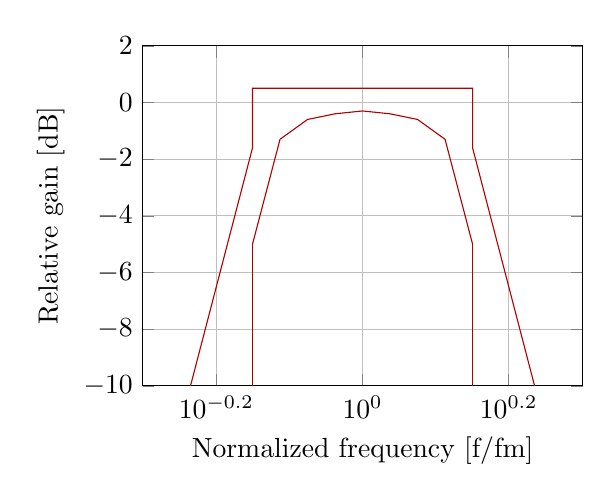
\begin{tikzpicture}

\begin{axis}[%
width=2.2in,
height=1.7in,
at={(0.758in,0.481in)},
scale only axis,
unbounded coords=jump,
xmode=log,
xmin=0.5,
xmax=2,
xminorticks=true,
xlabel={Normalized frequency [f/fm]},
xmajorgrids,
xminorgrids,
ytick = {2, 0, -2, -04, -6, -8, -10},
ymin=-10,
ymax=2,
ylabel={Relative gain [dB]},
ymajorgrids,
axis background/.style={fill=white}
]
\addplot [color=black!30!red,solid,forget plot]
  table[row sep=crcr]{%
1.4142	-5\\
1.4142	-10\\
};
\addplot [color=black!30!red,solid,forget plot]
  table[row sep=crcr]{%
0.7071	-5\\
0.7071	-10\\
};
\addplot [color=black!30!red,solid,forget plot]
  table[row sep=crcr]{%
0.0625	-60\\
0.125	-55\\
0.25	-41\\
0.5	-16.5\\
0.707106781186547	-1.6\\
0.707106781186547	0.5\\
0.77110541270397	0.5\\
0.840896415253715	0.5\\
0.917004043204671	0.5\\
1	0.5\\
1.09050773266526	0.5\\
1.18920711500272	0.5\\
1.29683955465101	0.5\\
1.4142135623731	0.5\\
1.4142135623731	-1.6\\
2	-16.5\\
4	-41\\
8	-55\\
16	-60\\
};
\addplot [color=black!30!red,solid,forget plot]
  table[row sep=crcr]
	\caption{Band 1 requierments zoomed in.}
	\label{fig:band1_reqZoom}
\end{subfigure}
\caption{Band 1 requierments without and with zoom.}
\label{fig:band1_reqOverview}
\end{figure}
Two points are selected giving the following specifications to the lowpass filter:
$F_{pass}=6.000 \enhed{Hz}$\\
$F_{stop}=-1 \enhed{dB}$\\
$A_{pass}=13.000 \enhed{Hz}$\\
$A_{stop}=-60 \enhed{dB}$\\
$Fs=48000 \enhed{Hz}$
The design method used for designing the filter is the Kaiser window method, explained in detail in \autoref{app:FIR_theory}. The reason for using the Kaiser window method is that it gives the approximate order of the filter and the beta value of the window applied to impulse reponse. This means that no trial and error method is needed to meet the requierments of the standard IEC 6964 (2001).

With the specification stated and using the matlab script explained in \autoref{app:FIR_Matlab} which uses the FIR theoy explained in \autoref{app:FIR_theory} about the Kaiser window method and deriving the coefficients of the filter the following filter is calculated. 
\begin{figure}[H]
\centering
\begin{subfigure}[t]{0.47\textwidth}
	\tikzsetnextfilename{Band1FiltZoom}
	\scalebox{0.5}{
	% This file was created by matlab2tikz.
%
%The latest updates can be retrieved from
%  http://www.mathworks.com/matlabcentral/fileexchange/22022-matlab2tikz-matlab2tikz
%where you can also make suggestions and rate matlab2tikz.
%
\definecolor{mycolor1}{rgb}{0.00000,0.44700,0.74100}%
%
\begin{tikzpicture}

\begin{axis}[%
width=4.521in,
height=1.493in,
at={(0.758in,0.481in)},
scale only axis,
xmode=log,
xmin=0,
xmax=24000,
xminorticks=true,
xlabel={Frequency (Hz)},
xmajorgrids,
xminorgrids,
ymin=-1500,
ymax=0,
ylabel={Phase (degrees)},
ymajorgrids,
axis background/.style={fill=white}
]
\addplot [color=mycolor1,solid,forget plot]
  table[row sep=crcr]{%
0	0\\
0.5	-0.045\\
1	-0.09\\
1.5	-0.135\\
2	-0.18\\
2.5	-0.225\\
3	-0.27\\
3.5	-0.315\\
4	-0.36\\
4.5	-0.405\\
5	-0.45\\
5.5	-0.495\\
6	-0.54\\
6.5	-0.585\\
7	-0.63\\
7.5	-0.675\\
8	-0.72\\
8.5	-0.765\\
9	-0.81\\
9.5	-0.855\\
10	-0.9\\
10.5	-0.945\\
11	-0.99\\
11.5	-1.035\\
12	-1.08\\
12.5	-1.125\\
13	-1.17\\
13.5	-1.215\\
14	-1.26\\
14.5	-1.305\\
15	-1.35\\
15.5	-1.395\\
16	-1.44\\
16.5	-1.485\\
17	-1.53\\
17.5	-1.575\\
18	-1.62\\
18.5	-1.665\\
19	-1.71\\
19.5	-1.755\\
20	-1.8\\
20.5	-1.845\\
21	-1.89\\
21.5	-1.935\\
22	-1.98\\
22.5	-2.025\\
23	-2.07\\
23.5	-2.115\\
24	-2.16\\
24.5	-2.205\\
25	-2.25\\
25.5	-2.295\\
26	-2.34\\
26.5	-2.385\\
27	-2.43\\
27.5	-2.475\\
28	-2.52\\
28.5	-2.565\\
29	-2.61\\
29.5	-2.655\\
30	-2.7\\
30.5	-2.745\\
31	-2.79\\
31.5	-2.835\\
32	-2.88\\
32.5	-2.925\\
33	-2.97\\
33.5	-3.015\\
34	-3.06\\
34.5	-3.105\\
35	-3.15\\
35.5	-3.195\\
36	-3.24\\
36.5	-3.285\\
37	-3.33\\
37.5	-3.375\\
38	-3.42\\
38.5	-3.465\\
39	-3.51\\
39.5	-3.555\\
40	-3.6\\
40.5	-3.645\\
41	-3.69\\
41.5	-3.735\\
42	-3.78\\
42.5	-3.825\\
43	-3.87\\
43.5	-3.915\\
44	-3.96\\
44.5	-4.005\\
45	-4.05\\
45.5	-4.095\\
46	-4.14\\
46.5	-4.185\\
47	-4.23\\
47.5	-4.275\\
48	-4.32\\
48.5	-4.365\\
49	-4.41\\
49.5	-4.455\\
50	-4.5\\
50.5	-4.545\\
51	-4.59\\
51.5	-4.635\\
52	-4.68\\
52.5	-4.725\\
53	-4.77\\
53.5	-4.815\\
54	-4.86\\
54.5	-4.905\\
55	-4.95\\
55.5	-4.995\\
56	-5.04\\
56.5	-5.085\\
57	-5.13\\
57.5	-5.175\\
58	-5.22\\
58.5	-5.265\\
59	-5.31\\
59.5	-5.355\\
60	-5.4\\
60.5	-5.445\\
61	-5.49\\
61.5	-5.535\\
62	-5.58\\
62.5	-5.625\\
63	-5.67\\
63.5	-5.715\\
64	-5.76\\
64.5	-5.805\\
65	-5.85\\
65.5	-5.895\\
66	-5.94\\
66.5	-5.985\\
67	-6.03\\
67.5	-6.075\\
68	-6.12\\
68.5	-6.165\\
69	-6.21\\
69.5	-6.255\\
70	-6.3\\
70.5	-6.345\\
71	-6.39\\
71.5	-6.435\\
72	-6.48\\
72.5	-6.525\\
73	-6.57\\
73.5	-6.615\\
74	-6.66\\
74.5	-6.705\\
75	-6.75\\
75.5	-6.795\\
76	-6.84\\
76.5	-6.885\\
77	-6.93\\
77.5	-6.975\\
78	-7.02\\
78.5	-7.065\\
79	-7.11\\
79.5	-7.155\\
80	-7.2\\
80.5	-7.245\\
81	-7.29\\
81.5	-7.335\\
82	-7.38\\
82.5	-7.425\\
83	-7.47\\
83.5	-7.515\\
84	-7.56\\
84.5	-7.605\\
85	-7.65\\
85.5	-7.695\\
86	-7.74\\
86.5	-7.785\\
87	-7.83\\
87.5	-7.875\\
88	-7.92\\
88.5	-7.965\\
89	-8.01\\
89.5	-8.055\\
90	-8.1\\
90.5	-8.145\\
91	-8.19\\
91.5	-8.235\\
92	-8.28\\
92.5	-8.325\\
93	-8.37\\
93.5	-8.415\\
94	-8.46\\
94.5	-8.505\\
95	-8.55\\
95.5	-8.595\\
96	-8.64\\
96.5	-8.685\\
97	-8.73\\
97.5	-8.775\\
98	-8.82\\
98.5	-8.865\\
99	-8.91\\
99.5	-8.955\\
100	-9\\
100.5	-9.045\\
101	-9.09\\
101.5	-9.135\\
102	-9.18\\
102.5	-9.225\\
103	-9.27\\
103.5	-9.315\\
104	-9.36\\
104.5	-9.405\\
105	-9.45\\
105.5	-9.495\\
106	-9.54\\
106.5	-9.585\\
107	-9.63\\
107.5	-9.675\\
108	-9.72\\
108.5	-9.765\\
109	-9.81\\
109.5	-9.855\\
110	-9.9\\
110.5	-9.945\\
111	-9.99\\
111.5	-10.035\\
112	-10.08\\
112.5	-10.125\\
113	-10.17\\
113.5	-10.215\\
114	-10.26\\
114.5	-10.305\\
115	-10.35\\
115.5	-10.395\\
116	-10.44\\
116.5	-10.485\\
117	-10.53\\
117.5	-10.575\\
118	-10.62\\
118.5	-10.665\\
119	-10.71\\
119.5	-10.755\\
120	-10.8\\
120.5	-10.845\\
121	-10.89\\
121.5	-10.935\\
122	-10.98\\
122.5	-11.025\\
123	-11.07\\
123.5	-11.115\\
124	-11.16\\
124.5	-11.205\\
125	-11.25\\
125.5	-11.295\\
126	-11.34\\
126.5	-11.385\\
127	-11.43\\
127.5	-11.475\\
128	-11.52\\
128.5	-11.565\\
129	-11.61\\
129.5	-11.655\\
130	-11.7\\
130.5	-11.745\\
131	-11.79\\
131.5	-11.835\\
132	-11.88\\
132.5	-11.925\\
133	-11.97\\
133.5	-12.015\\
134	-12.06\\
134.5	-12.105\\
135	-12.15\\
135.5	-12.195\\
136	-12.24\\
136.5	-12.285\\
137	-12.33\\
137.5	-12.375\\
138	-12.42\\
138.5	-12.465\\
139	-12.51\\
139.5	-12.555\\
140	-12.6\\
140.5	-12.645\\
141	-12.69\\
141.5	-12.735\\
142	-12.78\\
142.5	-12.825\\
143	-12.87\\
143.5	-12.915\\
144	-12.96\\
144.5	-13.005\\
145	-13.05\\
145.5	-13.095\\
146	-13.14\\
146.5	-13.185\\
147	-13.23\\
147.5	-13.275\\
148	-13.32\\
148.5	-13.365\\
149	-13.41\\
149.5	-13.455\\
150	-13.5\\
150.5	-13.545\\
151	-13.59\\
151.5	-13.635\\
152	-13.68\\
152.5	-13.725\\
153	-13.77\\
153.5	-13.815\\
154	-13.86\\
154.5	-13.905\\
155	-13.95\\
155.5	-13.995\\
156	-14.04\\
156.5	-14.085\\
157	-14.13\\
157.5	-14.175\\
158	-14.22\\
158.5	-14.265\\
159	-14.31\\
159.5	-14.355\\
160	-14.4\\
160.5	-14.445\\
161	-14.49\\
161.5	-14.535\\
162	-14.58\\
162.5	-14.625\\
163	-14.67\\
163.5	-14.715\\
164	-14.76\\
164.5	-14.805\\
165	-14.85\\
165.5	-14.895\\
166	-14.94\\
166.5	-14.985\\
167	-15.03\\
167.5	-15.075\\
168	-15.12\\
168.5	-15.165\\
169	-15.21\\
169.5	-15.255\\
170	-15.3\\
170.5	-15.345\\
171	-15.39\\
171.5	-15.435\\
172	-15.48\\
172.5	-15.525\\
173	-15.57\\
173.5	-15.615\\
174	-15.66\\
174.5	-15.705\\
175	-15.75\\
175.5	-15.795\\
176	-15.84\\
176.5	-15.885\\
177	-15.93\\
177.5	-15.975\\
178	-16.02\\
178.5	-16.065\\
179	-16.11\\
179.5	-16.155\\
180	-16.2\\
180.5	-16.245\\
181	-16.29\\
181.5	-16.335\\
182	-16.38\\
182.5	-16.425\\
183	-16.47\\
183.5	-16.515\\
184	-16.56\\
184.5	-16.605\\
185	-16.65\\
185.5	-16.695\\
186	-16.74\\
186.5	-16.785\\
187	-16.83\\
187.5	-16.875\\
188	-16.92\\
188.5	-16.965\\
189	-17.01\\
189.5	-17.055\\
190	-17.1\\
190.5	-17.145\\
191	-17.19\\
191.5	-17.235\\
192	-17.28\\
192.5	-17.325\\
193	-17.37\\
193.5	-17.415\\
194	-17.46\\
194.5	-17.505\\
195	-17.55\\
195.5	-17.595\\
196	-17.64\\
196.5	-17.685\\
197	-17.73\\
197.5	-17.775\\
198	-17.82\\
198.5	-17.865\\
199	-17.91\\
199.5	-17.955\\
200	-18\\
200.5	-18.045\\
201	-18.09\\
201.5	-18.135\\
202	-18.18\\
202.5	-18.225\\
203	-18.27\\
203.5	-18.315\\
204	-18.36\\
204.5	-18.405\\
205	-18.45\\
205.5	-18.495\\
206	-18.54\\
206.5	-18.585\\
207	-18.63\\
207.5	-18.675\\
208	-18.72\\
208.5	-18.765\\
209	-18.81\\
209.5	-18.855\\
210	-18.9\\
210.5	-18.945\\
211	-18.99\\
211.5	-19.035\\
212	-19.08\\
212.5	-19.125\\
213	-19.17\\
213.5	-19.215\\
214	-19.26\\
214.5	-19.305\\
215	-19.35\\
215.5	-19.395\\
216	-19.44\\
216.5	-19.485\\
217	-19.53\\
217.5	-19.575\\
218	-19.62\\
218.5	-19.665\\
219	-19.71\\
219.5	-19.755\\
220	-19.8\\
220.5	-19.845\\
221	-19.89\\
221.5	-19.935\\
222	-19.98\\
222.5	-20.025\\
223	-20.07\\
223.5	-20.115\\
224	-20.16\\
224.5	-20.205\\
225	-20.25\\
225.5	-20.295\\
226	-20.34\\
226.5	-20.385\\
227	-20.43\\
227.5	-20.475\\
228	-20.52\\
228.5	-20.565\\
229	-20.61\\
229.5	-20.655\\
230	-20.7\\
230.5	-20.745\\
231	-20.79\\
231.5	-20.835\\
232	-20.88\\
232.5	-20.925\\
233	-20.97\\
233.5	-21.015\\
234	-21.06\\
234.5	-21.105\\
235	-21.15\\
235.5	-21.195\\
236	-21.24\\
236.5	-21.285\\
237	-21.33\\
237.5	-21.375\\
238	-21.42\\
238.5	-21.465\\
239	-21.51\\
239.5	-21.555\\
240	-21.6\\
240.5	-21.645\\
241	-21.69\\
241.5	-21.735\\
242	-21.78\\
242.5	-21.825\\
243	-21.87\\
243.5	-21.915\\
244	-21.96\\
244.5	-22.005\\
245	-22.05\\
245.5	-22.095\\
246	-22.14\\
246.5	-22.185\\
247	-22.23\\
247.5	-22.275\\
248	-22.32\\
248.5	-22.365\\
249	-22.41\\
249.5	-22.455\\
250	-22.5\\
250.5	-22.545\\
251	-22.59\\
251.5	-22.635\\
252	-22.68\\
252.5	-22.725\\
253	-22.77\\
253.5	-22.815\\
254	-22.86\\
254.5	-22.905\\
255	-22.95\\
255.5	-22.995\\
256	-23.04\\
256.5	-23.085\\
257	-23.13\\
257.5	-23.175\\
258	-23.22\\
258.5	-23.265\\
259	-23.31\\
259.5	-23.355\\
260	-23.4\\
260.5	-23.445\\
261	-23.49\\
261.5	-23.535\\
262	-23.58\\
262.5	-23.625\\
263	-23.67\\
263.5	-23.715\\
264	-23.76\\
264.5	-23.805\\
265	-23.85\\
265.5	-23.895\\
266	-23.94\\
266.5	-23.985\\
267	-24.03\\
267.5	-24.075\\
268	-24.12\\
268.5	-24.165\\
269	-24.21\\
269.5	-24.255\\
270	-24.3\\
270.5	-24.345\\
271	-24.39\\
271.5	-24.435\\
272	-24.48\\
272.5	-24.525\\
273	-24.57\\
273.5	-24.615\\
274	-24.66\\
274.5	-24.705\\
275	-24.75\\
275.5	-24.795\\
276	-24.84\\
276.5	-24.885\\
277	-24.93\\
277.5	-24.975\\
278	-25.02\\
278.5	-25.065\\
279	-25.11\\
279.5	-25.155\\
280	-25.2\\
280.5	-25.245\\
281	-25.29\\
281.5	-25.335\\
282	-25.38\\
282.5	-25.425\\
283	-25.47\\
283.5	-25.515\\
284	-25.56\\
284.5	-25.605\\
285	-25.65\\
285.5	-25.695\\
286	-25.74\\
286.5	-25.785\\
287	-25.83\\
287.5	-25.875\\
288	-25.92\\
288.5	-25.965\\
289	-26.01\\
289.5	-26.055\\
290	-26.1\\
290.5	-26.145\\
291	-26.19\\
291.5	-26.235\\
292	-26.28\\
292.5	-26.325\\
293	-26.37\\
293.5	-26.415\\
294	-26.46\\
294.5	-26.505\\
295	-26.55\\
295.5	-26.595\\
296	-26.64\\
296.5	-26.685\\
297	-26.73\\
297.5	-26.775\\
298	-26.82\\
298.5	-26.865\\
299	-26.91\\
299.5	-26.955\\
300	-27\\
300.5	-27.045\\
301	-27.09\\
301.5	-27.135\\
302	-27.18\\
302.5	-27.225\\
303	-27.27\\
303.5	-27.315\\
304	-27.36\\
304.5	-27.405\\
305	-27.45\\
305.5	-27.495\\
306	-27.54\\
306.5	-27.585\\
307	-27.63\\
307.5	-27.675\\
308	-27.72\\
308.5	-27.765\\
309	-27.81\\
309.5	-27.855\\
310	-27.9\\
310.5	-27.945\\
311	-27.99\\
311.5	-28.035\\
312	-28.08\\
312.5	-28.125\\
313	-28.17\\
313.5	-28.215\\
314	-28.26\\
314.5	-28.305\\
315	-28.35\\
315.5	-28.395\\
316	-28.44\\
316.5	-28.485\\
317	-28.53\\
317.5	-28.575\\
318	-28.62\\
318.5	-28.665\\
319	-28.71\\
319.5	-28.755\\
320	-28.8\\
320.5	-28.845\\
321	-28.89\\
321.5	-28.935\\
322	-28.98\\
322.5	-29.025\\
323	-29.07\\
323.5	-29.115\\
324	-29.16\\
324.5	-29.205\\
325	-29.25\\
325.5	-29.295\\
326	-29.34\\
326.5	-29.385\\
327	-29.43\\
327.5	-29.475\\
328	-29.52\\
328.5	-29.565\\
329	-29.61\\
329.5	-29.655\\
330	-29.7\\
330.5	-29.745\\
331	-29.79\\
331.5	-29.835\\
332	-29.88\\
332.5	-29.925\\
333	-29.97\\
333.5	-30.015\\
334	-30.06\\
334.5	-30.105\\
335	-30.15\\
335.5	-30.195\\
336	-30.24\\
336.5	-30.285\\
337	-30.33\\
337.5	-30.375\\
338	-30.42\\
338.5	-30.465\\
339	-30.51\\
339.5	-30.555\\
340	-30.6\\
340.5	-30.645\\
341	-30.69\\
341.5	-30.735\\
342	-30.78\\
342.5	-30.825\\
343	-30.87\\
343.5	-30.915\\
344	-30.96\\
344.5	-31.005\\
345	-31.05\\
345.5	-31.095\\
346	-31.14\\
346.5	-31.185\\
347	-31.23\\
347.5	-31.275\\
348	-31.32\\
348.5	-31.365\\
349	-31.41\\
349.5	-31.455\\
350	-31.5\\
350.5	-31.545\\
351	-31.59\\
351.5	-31.635\\
352	-31.68\\
352.5	-31.725\\
353	-31.77\\
353.5	-31.815\\
354	-31.86\\
354.5	-31.905\\
355	-31.95\\
355.5	-31.995\\
356	-32.04\\
356.5	-32.085\\
357	-32.13\\
357.5	-32.175\\
358	-32.22\\
358.5	-32.265\\
359	-32.31\\
359.5	-32.355\\
360	-32.4\\
360.5	-32.445\\
361	-32.49\\
361.5	-32.535\\
362	-32.58\\
362.5	-32.625\\
363	-32.67\\
363.5	-32.715\\
364	-32.76\\
364.5	-32.805\\
365	-32.85\\
365.5	-32.895\\
366	-32.94\\
366.5	-32.985\\
367	-33.03\\
367.5	-33.075\\
368	-33.12\\
368.5	-33.165\\
369	-33.21\\
369.5	-33.255\\
370	-33.3\\
370.5	-33.345\\
371	-33.39\\
371.5	-33.435\\
372	-33.48\\
372.5	-33.525\\
373	-33.57\\
373.5	-33.615\\
374	-33.66\\
374.5	-33.705\\
375	-33.75\\
375.5	-33.795\\
376	-33.84\\
376.5	-33.885\\
377	-33.93\\
377.5	-33.975\\
378	-34.02\\
378.5	-34.065\\
379	-34.11\\
379.5	-34.155\\
380	-34.2\\
380.5	-34.245\\
381	-34.29\\
381.5	-34.335\\
382	-34.38\\
382.5	-34.425\\
383	-34.47\\
383.5	-34.515\\
384	-34.56\\
384.5	-34.605\\
385	-34.65\\
385.5	-34.695\\
386	-34.74\\
386.5	-34.785\\
387	-34.83\\
387.5	-34.875\\
388	-34.92\\
388.5	-34.965\\
389	-35.01\\
389.5	-35.055\\
390	-35.1\\
390.5	-35.145\\
391	-35.19\\
391.5	-35.235\\
392	-35.28\\
392.5	-35.325\\
393	-35.37\\
393.5	-35.415\\
394	-35.46\\
394.5	-35.505\\
395	-35.55\\
395.5	-35.595\\
396	-35.64\\
396.5	-35.685\\
397	-35.73\\
397.5	-35.775\\
398	-35.82\\
398.5	-35.865\\
399	-35.91\\
399.5	-35.955\\
400	-36\\
400.5	-36.045\\
401	-36.09\\
401.5	-36.135\\
402	-36.18\\
402.5	-36.225\\
403	-36.27\\
403.5	-36.315\\
404	-36.36\\
404.5	-36.405\\
405	-36.45\\
405.5	-36.495\\
406	-36.54\\
406.5	-36.585\\
407	-36.63\\
407.5	-36.675\\
408	-36.72\\
408.5	-36.765\\
409	-36.81\\
409.5	-36.855\\
410	-36.9\\
410.5	-36.945\\
411	-36.99\\
411.5	-37.035\\
412	-37.08\\
412.5	-37.125\\
413	-37.17\\
413.5	-37.215\\
414	-37.26\\
414.5	-37.305\\
415	-37.35\\
415.5	-37.395\\
416	-37.44\\
416.5	-37.485\\
417	-37.53\\
417.5	-37.575\\
418	-37.62\\
418.5	-37.665\\
419	-37.71\\
419.5	-37.755\\
420	-37.8\\
420.5	-37.845\\
421	-37.89\\
421.5	-37.935\\
422	-37.98\\
422.5	-38.025\\
423	-38.07\\
423.5	-38.115\\
424	-38.16\\
424.5	-38.205\\
425	-38.25\\
425.5	-38.295\\
426	-38.34\\
426.5	-38.385\\
427	-38.43\\
427.5	-38.475\\
428	-38.52\\
428.5	-38.565\\
429	-38.61\\
429.5	-38.655\\
430	-38.7\\
430.5	-38.745\\
431	-38.79\\
431.5	-38.835\\
432	-38.88\\
432.5	-38.925\\
433	-38.97\\
433.5	-39.015\\
434	-39.06\\
434.5	-39.105\\
435	-39.15\\
435.5	-39.195\\
436	-39.24\\
436.5	-39.285\\
437	-39.33\\
437.5	-39.375\\
438	-39.42\\
438.5	-39.465\\
439	-39.51\\
439.5	-39.555\\
440	-39.6\\
440.5	-39.645\\
441	-39.69\\
441.5	-39.735\\
442	-39.78\\
442.5	-39.825\\
443	-39.87\\
443.5	-39.915\\
444	-39.96\\
444.5	-40.005\\
445	-40.05\\
445.5	-40.095\\
446	-40.14\\
446.5	-40.185\\
447	-40.23\\
447.5	-40.275\\
448	-40.32\\
448.5	-40.365\\
449	-40.41\\
449.5	-40.455\\
450	-40.5\\
450.5	-40.545\\
451	-40.59\\
451.5	-40.635\\
452	-40.68\\
452.5	-40.725\\
453	-40.77\\
453.5	-40.815\\
454	-40.86\\
454.5	-40.905\\
455	-40.95\\
455.5	-40.995\\
456	-41.04\\
456.5	-41.085\\
457	-41.13\\
457.5	-41.175\\
458	-41.22\\
458.5	-41.265\\
459	-41.31\\
459.5	-41.355\\
460	-41.4\\
460.5	-41.445\\
461	-41.49\\
461.5	-41.535\\
462	-41.58\\
462.5	-41.625\\
463	-41.67\\
463.5	-41.715\\
464	-41.76\\
464.5	-41.805\\
465	-41.85\\
465.5	-41.895\\
466	-41.94\\
466.5	-41.985\\
467	-42.03\\
467.5	-42.075\\
468	-42.12\\
468.5	-42.165\\
469	-42.21\\
469.5	-42.255\\
470	-42.3\\
470.5	-42.345\\
471	-42.39\\
471.5	-42.435\\
472	-42.48\\
472.5	-42.525\\
473	-42.57\\
473.5	-42.615\\
474	-42.66\\
474.5	-42.705\\
475	-42.75\\
475.5	-42.795\\
476	-42.84\\
476.5	-42.885\\
477	-42.93\\
477.5	-42.975\\
478	-43.02\\
478.5	-43.065\\
479	-43.11\\
479.5	-43.155\\
480	-43.2\\
480.5	-43.245\\
481	-43.29\\
481.5	-43.335\\
482	-43.38\\
482.5	-43.425\\
483	-43.47\\
483.5	-43.515\\
484	-43.56\\
484.5	-43.605\\
485	-43.65\\
485.5	-43.695\\
486	-43.74\\
486.5	-43.785\\
487	-43.83\\
487.5	-43.875\\
488	-43.92\\
488.5	-43.965\\
489	-44.01\\
489.5	-44.055\\
490	-44.1\\
490.5	-44.145\\
491	-44.19\\
491.5	-44.235\\
492	-44.28\\
492.5	-44.325\\
493	-44.37\\
493.5	-44.415\\
494	-44.46\\
494.5	-44.505\\
495	-44.55\\
495.5	-44.595\\
496	-44.64\\
496.5	-44.685\\
497	-44.73\\
497.5	-44.775\\
498	-44.82\\
498.5	-44.865\\
499	-44.91\\
499.5	-44.955\\
500	-45\\
500.5	-45.045\\
501	-45.09\\
501.5	-45.135\\
502	-45.18\\
502.5	-45.225\\
503	-45.27\\
503.5	-45.315\\
504	-45.36\\
504.5	-45.405\\
505	-45.45\\
505.5	-45.495\\
506	-45.54\\
506.5	-45.585\\
507	-45.63\\
507.5	-45.675\\
508	-45.72\\
508.5	-45.765\\
509	-45.81\\
509.5	-45.855\\
510	-45.9\\
510.5	-45.945\\
511	-45.99\\
511.5	-46.035\\
512	-46.08\\
512.5	-46.125\\
513	-46.17\\
513.5	-46.215\\
514	-46.26\\
514.5	-46.305\\
515	-46.35\\
515.5	-46.395\\
516	-46.44\\
516.5	-46.485\\
517	-46.53\\
517.5	-46.575\\
518	-46.62\\
518.5	-46.665\\
519	-46.71\\
519.5	-46.755\\
520	-46.8\\
520.5	-46.845\\
521	-46.89\\
521.5	-46.935\\
522	-46.98\\
522.5	-47.025\\
523	-47.07\\
523.5	-47.115\\
524	-47.16\\
524.5	-47.205\\
525	-47.25\\
525.5	-47.295\\
526	-47.34\\
526.5	-47.385\\
527	-47.43\\
527.5	-47.475\\
528	-47.52\\
528.5	-47.565\\
529	-47.61\\
529.5	-47.655\\
530	-47.7\\
530.5	-47.745\\
531	-47.79\\
531.5	-47.835\\
532	-47.88\\
532.5	-47.925\\
533	-47.97\\
533.5	-48.015\\
534	-48.06\\
534.5	-48.105\\
535	-48.15\\
535.5	-48.195\\
536	-48.24\\
536.5	-48.285\\
537	-48.33\\
537.5	-48.375\\
538	-48.42\\
538.5	-48.465\\
539	-48.51\\
539.5	-48.555\\
540	-48.6\\
540.5	-48.645\\
541	-48.69\\
541.5	-48.735\\
542	-48.78\\
542.5	-48.825\\
543	-48.87\\
543.5	-48.915\\
544	-48.96\\
544.5	-49.005\\
545	-49.05\\
545.5	-49.095\\
546	-49.14\\
546.5	-49.185\\
547	-49.23\\
547.5	-49.275\\
548	-49.32\\
548.5	-49.365\\
549	-49.41\\
549.5	-49.455\\
550	-49.5\\
550.5	-49.545\\
551	-49.59\\
551.5	-49.635\\
552	-49.68\\
552.5	-49.725\\
553	-49.77\\
553.5	-49.815\\
554	-49.86\\
554.5	-49.905\\
555	-49.95\\
555.5	-49.995\\
556	-50.04\\
556.5	-50.085\\
557	-50.13\\
557.5	-50.175\\
558	-50.22\\
558.5	-50.265\\
559	-50.31\\
559.5	-50.355\\
560	-50.4\\
560.5	-50.445\\
561	-50.49\\
561.5	-50.535\\
562	-50.58\\
562.5	-50.625\\
563	-50.67\\
563.5	-50.715\\
564	-50.76\\
564.5	-50.805\\
565	-50.85\\
565.5	-50.895\\
566	-50.94\\
566.5	-50.985\\
567	-51.03\\
567.5	-51.075\\
568	-51.12\\
568.5	-51.165\\
569	-51.21\\
569.5	-51.255\\
570	-51.3\\
570.5	-51.345\\
571	-51.39\\
571.5	-51.435\\
572	-51.48\\
572.5	-51.525\\
573	-51.57\\
573.5	-51.615\\
574	-51.66\\
574.5	-51.705\\
575	-51.75\\
575.5	-51.795\\
576	-51.84\\
576.5	-51.885\\
577	-51.93\\
577.5	-51.975\\
578	-52.02\\
578.5	-52.065\\
579	-52.11\\
579.5	-52.155\\
580	-52.2\\
580.5	-52.245\\
581	-52.29\\
581.5	-52.335\\
582	-52.38\\
582.5	-52.425\\
583	-52.47\\
583.5	-52.515\\
584	-52.56\\
584.5	-52.605\\
585	-52.65\\
585.5	-52.695\\
586	-52.74\\
586.5	-52.785\\
587	-52.83\\
587.5	-52.875\\
588	-52.92\\
588.5	-52.965\\
589	-53.01\\
589.5	-53.055\\
590	-53.1\\
590.5	-53.145\\
591	-53.19\\
591.5	-53.235\\
592	-53.28\\
592.5	-53.325\\
593	-53.37\\
593.5	-53.415\\
594	-53.46\\
594.5	-53.505\\
595	-53.55\\
595.5	-53.595\\
596	-53.64\\
596.5	-53.685\\
597	-53.73\\
597.5	-53.775\\
598	-53.82\\
598.5	-53.865\\
599	-53.91\\
599.5	-53.955\\
600	-54\\
600.5	-54.045\\
601	-54.09\\
601.5	-54.135\\
602	-54.18\\
602.5	-54.225\\
603	-54.27\\
603.5	-54.315\\
604	-54.36\\
604.5	-54.405\\
605	-54.45\\
605.5	-54.495\\
606	-54.54\\
606.5	-54.585\\
607	-54.63\\
607.5	-54.675\\
608	-54.72\\
608.5	-54.765\\
609	-54.81\\
609.5	-54.855\\
610	-54.9\\
610.5	-54.945\\
611	-54.99\\
611.5	-55.035\\
612	-55.08\\
612.5	-55.125\\
613	-55.17\\
613.5	-55.215\\
614	-55.26\\
614.5	-55.305\\
615	-55.35\\
615.5	-55.395\\
616	-55.44\\
616.5	-55.485\\
617	-55.53\\
617.5	-55.575\\
618	-55.62\\
618.5	-55.665\\
619	-55.71\\
619.5	-55.755\\
620	-55.8\\
620.5	-55.845\\
621	-55.89\\
621.5	-55.935\\
622	-55.98\\
622.5	-56.025\\
623	-56.07\\
623.5	-56.115\\
624	-56.16\\
624.5	-56.205\\
625	-56.25\\
625.5	-56.295\\
626	-56.34\\
626.5	-56.385\\
627	-56.43\\
627.5	-56.475\\
628	-56.52\\
628.5	-56.565\\
629	-56.61\\
629.5	-56.655\\
630	-56.7\\
630.5	-56.745\\
631	-56.79\\
631.5	-56.835\\
632	-56.88\\
632.5	-56.925\\
633	-56.97\\
633.5	-57.015\\
634	-57.06\\
634.5	-57.105\\
635	-57.15\\
635.5	-57.195\\
636	-57.24\\
636.5	-57.285\\
637	-57.33\\
637.5	-57.375\\
638	-57.42\\
638.5	-57.465\\
639	-57.51\\
639.5	-57.555\\
640	-57.6\\
640.5	-57.645\\
641	-57.69\\
641.5	-57.735\\
642	-57.78\\
642.5	-57.825\\
643	-57.87\\
643.5	-57.915\\
644	-57.96\\
644.5	-58.005\\
645	-58.05\\
645.5	-58.095\\
646	-58.14\\
646.5	-58.185\\
647	-58.23\\
647.5	-58.275\\
648	-58.32\\
648.5	-58.365\\
649	-58.41\\
649.5	-58.455\\
650	-58.5\\
650.5	-58.545\\
651	-58.59\\
651.5	-58.635\\
652	-58.68\\
652.5	-58.725\\
653	-58.77\\
653.5	-58.815\\
654	-58.86\\
654.5	-58.905\\
655	-58.95\\
655.5	-58.995\\
656	-59.04\\
656.5	-59.085\\
657	-59.13\\
657.5	-59.175\\
658	-59.22\\
658.5	-59.265\\
659	-59.31\\
659.5	-59.355\\
660	-59.4\\
660.5	-59.445\\
661	-59.49\\
661.5	-59.535\\
662	-59.58\\
662.5	-59.625\\
663	-59.67\\
663.5	-59.715\\
664	-59.76\\
664.5	-59.805\\
665	-59.85\\
665.5	-59.895\\
666	-59.94\\
666.5	-59.985\\
667	-60.03\\
667.5	-60.075\\
668	-60.12\\
668.5	-60.165\\
669	-60.21\\
669.5	-60.255\\
670	-60.3\\
670.5	-60.345\\
671	-60.39\\
671.5	-60.435\\
672	-60.48\\
672.5	-60.525\\
673	-60.57\\
673.5	-60.615\\
674	-60.66\\
674.5	-60.705\\
675	-60.75\\
675.5	-60.795\\
676	-60.84\\
676.5	-60.885\\
677	-60.93\\
677.5	-60.975\\
678	-61.02\\
678.5	-61.065\\
679	-61.11\\
679.5	-61.155\\
680	-61.2\\
680.5	-61.245\\
681	-61.29\\
681.5	-61.335\\
682	-61.38\\
682.5	-61.425\\
683	-61.47\\
683.5	-61.515\\
684	-61.56\\
684.5	-61.605\\
685	-61.65\\
685.5	-61.695\\
686	-61.74\\
686.5	-61.785\\
687	-61.83\\
687.5	-61.875\\
688	-61.92\\
688.5	-61.965\\
689	-62.01\\
689.5	-62.055\\
690	-62.1\\
690.5	-62.145\\
691	-62.19\\
691.5	-62.235\\
692	-62.28\\
692.5	-62.325\\
693	-62.37\\
693.5	-62.415\\
694	-62.46\\
694.5	-62.505\\
695	-62.55\\
695.5	-62.595\\
696	-62.64\\
696.5	-62.685\\
697	-62.73\\
697.5	-62.775\\
698	-62.82\\
698.5	-62.865\\
699	-62.91\\
699.5	-62.955\\
700	-63\\
700.5	-63.045\\
701	-63.09\\
701.5	-63.135\\
702	-63.18\\
702.5	-63.225\\
703	-63.27\\
703.5	-63.315\\
704	-63.36\\
704.5	-63.405\\
705	-63.45\\
705.5	-63.495\\
706	-63.54\\
706.5	-63.585\\
707	-63.63\\
707.5	-63.675\\
708	-63.72\\
708.5	-63.765\\
709	-63.81\\
709.5	-63.855\\
710	-63.9\\
710.5	-63.945\\
711	-63.99\\
711.5	-64.035\\
712	-64.08\\
712.5	-64.125\\
713	-64.17\\
713.5	-64.215\\
714	-64.26\\
714.5	-64.305\\
715	-64.35\\
715.5	-64.395\\
716	-64.44\\
716.5	-64.485\\
717	-64.53\\
717.5	-64.575\\
718	-64.62\\
718.5	-64.665\\
719	-64.71\\
719.5	-64.755\\
720	-64.8\\
720.5	-64.845\\
721	-64.89\\
721.5	-64.935\\
722	-64.98\\
722.5	-65.025\\
723	-65.07\\
723.5	-65.115\\
724	-65.16\\
724.5	-65.205\\
725	-65.25\\
725.5	-65.295\\
726	-65.34\\
726.5	-65.385\\
727	-65.43\\
727.5	-65.475\\
728	-65.52\\
728.5	-65.565\\
729	-65.61\\
729.5	-65.655\\
730	-65.7\\
730.5	-65.745\\
731	-65.79\\
731.5	-65.835\\
732	-65.88\\
732.5	-65.925\\
733	-65.97\\
733.5	-66.015\\
734	-66.06\\
734.5	-66.105\\
735	-66.15\\
735.5	-66.195\\
736	-66.24\\
736.5	-66.285\\
737	-66.33\\
737.5	-66.375\\
738	-66.42\\
738.5	-66.465\\
739	-66.51\\
739.5	-66.555\\
740	-66.6\\
740.5	-66.645\\
741	-66.69\\
741.5	-66.735\\
742	-66.78\\
742.5	-66.825\\
743	-66.87\\
743.5	-66.915\\
744	-66.96\\
744.5	-67.005\\
745	-67.05\\
745.5	-67.095\\
746	-67.14\\
746.5	-67.185\\
747	-67.23\\
747.5	-67.275\\
748	-67.32\\
748.5	-67.365\\
749	-67.41\\
749.5	-67.455\\
750	-67.5\\
750.5	-67.545\\
751	-67.59\\
751.5	-67.635\\
752	-67.68\\
752.5	-67.725\\
753	-67.77\\
753.5	-67.815\\
754	-67.86\\
754.5	-67.905\\
755	-67.95\\
755.5	-67.995\\
756	-68.04\\
756.5	-68.085\\
757	-68.13\\
757.5	-68.175\\
758	-68.22\\
758.5	-68.265\\
759	-68.31\\
759.5	-68.355\\
760	-68.4\\
760.5	-68.445\\
761	-68.49\\
761.5	-68.535\\
762	-68.58\\
762.5	-68.625\\
763	-68.67\\
763.5	-68.715\\
764	-68.76\\
764.5	-68.805\\
765	-68.85\\
765.5	-68.895\\
766	-68.94\\
766.5	-68.985\\
767	-69.03\\
767.5	-69.075\\
768	-69.12\\
768.5	-69.165\\
769	-69.21\\
769.5	-69.255\\
770	-69.3\\
770.5	-69.345\\
771	-69.39\\
771.5	-69.435\\
772	-69.48\\
772.5	-69.525\\
773	-69.57\\
773.5	-69.615\\
774	-69.66\\
774.5	-69.705\\
775	-69.75\\
775.5	-69.795\\
776	-69.84\\
776.5	-69.885\\
777	-69.93\\
777.5	-69.975\\
778	-70.02\\
778.5	-70.065\\
779	-70.11\\
779.5	-70.155\\
780	-70.2\\
780.5	-70.245\\
781	-70.29\\
781.5	-70.335\\
782	-70.38\\
782.5	-70.425\\
783	-70.47\\
783.5	-70.515\\
784	-70.56\\
784.5	-70.605\\
785	-70.65\\
785.5	-70.695\\
786	-70.74\\
786.5	-70.785\\
787	-70.83\\
787.5	-70.875\\
788	-70.92\\
788.5	-70.965\\
789	-71.01\\
789.5	-71.055\\
790	-71.1\\
790.5	-71.145\\
791	-71.19\\
791.5	-71.235\\
792	-71.28\\
792.5	-71.325\\
793	-71.37\\
793.5	-71.415\\
794	-71.46\\
794.5	-71.505\\
795	-71.55\\
795.5	-71.595\\
796	-71.64\\
796.5	-71.685\\
797	-71.73\\
797.5	-71.775\\
798	-71.82\\
798.5	-71.865\\
799	-71.91\\
799.5	-71.955\\
800	-72\\
800.5	-72.045\\
801	-72.09\\
801.5	-72.135\\
802	-72.18\\
802.5	-72.225\\
803	-72.27\\
803.5	-72.315\\
804	-72.36\\
804.5	-72.405\\
805	-72.45\\
805.5	-72.495\\
806	-72.54\\
806.5	-72.585\\
807	-72.63\\
807.5	-72.675\\
808	-72.72\\
808.5	-72.765\\
809	-72.81\\
809.5	-72.855\\
810	-72.9\\
810.5	-72.945\\
811	-72.99\\
811.5	-73.035\\
812	-73.08\\
812.5	-73.125\\
813	-73.17\\
813.5	-73.215\\
814	-73.26\\
814.5	-73.305\\
815	-73.35\\
815.5	-73.395\\
816	-73.44\\
816.5	-73.485\\
817	-73.53\\
817.5	-73.575\\
818	-73.62\\
818.5	-73.665\\
819	-73.71\\
819.5	-73.755\\
820	-73.8\\
820.5	-73.845\\
821	-73.89\\
821.5	-73.935\\
822	-73.98\\
822.5	-74.025\\
823	-74.07\\
823.5	-74.115\\
824	-74.16\\
824.5	-74.205\\
825	-74.25\\
825.5	-74.295\\
826	-74.34\\
826.5	-74.385\\
827	-74.43\\
827.5	-74.475\\
828	-74.52\\
828.5	-74.565\\
829	-74.61\\
829.5	-74.655\\
830	-74.7\\
830.5	-74.745\\
831	-74.79\\
831.5	-74.835\\
832	-74.88\\
832.5	-74.925\\
833	-74.97\\
833.5	-75.015\\
834	-75.06\\
834.5	-75.105\\
835	-75.15\\
835.5	-75.195\\
836	-75.24\\
836.5	-75.285\\
837	-75.33\\
837.5	-75.375\\
838	-75.42\\
838.5	-75.465\\
839	-75.51\\
839.5	-75.555\\
840	-75.6\\
840.5	-75.645\\
841	-75.69\\
841.5	-75.735\\
842	-75.78\\
842.5	-75.825\\
843	-75.87\\
843.5	-75.915\\
844	-75.96\\
844.5	-76.005\\
845	-76.05\\
845.5	-76.095\\
846	-76.14\\
846.5	-76.185\\
847	-76.23\\
847.5	-76.275\\
848	-76.32\\
848.5	-76.365\\
849	-76.41\\
849.5	-76.455\\
850	-76.5\\
850.5	-76.545\\
851	-76.59\\
851.5	-76.635\\
852	-76.68\\
852.5	-76.725\\
853	-76.77\\
853.5	-76.815\\
854	-76.86\\
854.5	-76.905\\
855	-76.95\\
855.5	-76.995\\
856	-77.04\\
856.5	-77.085\\
857	-77.13\\
857.5	-77.175\\
858	-77.22\\
858.5	-77.265\\
859	-77.31\\
859.5	-77.355\\
860	-77.4\\
860.5	-77.445\\
861	-77.49\\
861.5	-77.535\\
862	-77.58\\
862.5	-77.625\\
863	-77.67\\
863.5	-77.715\\
864	-77.76\\
864.5	-77.805\\
865	-77.85\\
865.5	-77.895\\
866	-77.94\\
866.5	-77.985\\
867	-78.03\\
867.5	-78.075\\
868	-78.12\\
868.5	-78.165\\
869	-78.21\\
869.5	-78.255\\
870	-78.3\\
870.5	-78.345\\
871	-78.39\\
871.5	-78.435\\
872	-78.48\\
872.5	-78.525\\
873	-78.57\\
873.5	-78.615\\
874	-78.66\\
874.5	-78.705\\
875	-78.75\\
875.5	-78.795\\
876	-78.84\\
876.5	-78.885\\
877	-78.93\\
877.5	-78.975\\
878	-79.02\\
878.5	-79.065\\
879	-79.11\\
879.5	-79.155\\
880	-79.2\\
880.5	-79.245\\
881	-79.29\\
881.5	-79.335\\
882	-79.38\\
882.5	-79.425\\
883	-79.47\\
883.5	-79.515\\
884	-79.56\\
884.5	-79.605\\
885	-79.65\\
885.5	-79.695\\
886	-79.74\\
886.5	-79.785\\
887	-79.83\\
887.5	-79.875\\
888	-79.92\\
888.5	-79.965\\
889	-80.01\\
889.5	-80.055\\
890	-80.1\\
890.5	-80.145\\
891	-80.19\\
891.5	-80.235\\
892	-80.28\\
892.5	-80.325\\
893	-80.37\\
893.5	-80.415\\
894	-80.46\\
894.5	-80.505\\
895	-80.55\\
895.5	-80.595\\
896	-80.64\\
896.5	-80.685\\
897	-80.73\\
897.5	-80.775\\
898	-80.82\\
898.5	-80.865\\
899	-80.91\\
899.5	-80.955\\
900	-81\\
900.5	-81.045\\
901	-81.09\\
901.5	-81.135\\
902	-81.18\\
902.5	-81.225\\
903	-81.27\\
903.5	-81.315\\
904	-81.36\\
904.5	-81.405\\
905	-81.45\\
905.5	-81.495\\
906	-81.54\\
906.5	-81.585\\
907	-81.63\\
907.5	-81.675\\
908	-81.72\\
908.5	-81.765\\
909	-81.81\\
909.5	-81.855\\
910	-81.9\\
910.5	-81.945\\
911	-81.99\\
911.5	-82.035\\
912	-82.08\\
912.5	-82.125\\
913	-82.17\\
913.5	-82.215\\
914	-82.26\\
914.5	-82.305\\
915	-82.35\\
915.5	-82.395\\
916	-82.44\\
916.5	-82.485\\
917	-82.53\\
917.5	-82.575\\
918	-82.62\\
918.5	-82.665\\
919	-82.71\\
919.5	-82.755\\
920	-82.8\\
920.5	-82.845\\
921	-82.89\\
921.5	-82.935\\
922	-82.98\\
922.5	-83.025\\
923	-83.07\\
923.5	-83.115\\
924	-83.16\\
924.5	-83.205\\
925	-83.25\\
925.5	-83.295\\
926	-83.34\\
926.5	-83.385\\
927	-83.43\\
927.5	-83.475\\
928	-83.52\\
928.5	-83.565\\
929	-83.61\\
929.5	-83.655\\
930	-83.7\\
930.5	-83.745\\
931	-83.79\\
931.5	-83.835\\
932	-83.88\\
932.5	-83.925\\
933	-83.97\\
933.5	-84.015\\
934	-84.06\\
934.5	-84.105\\
935	-84.15\\
935.5	-84.195\\
936	-84.24\\
936.5	-84.285\\
937	-84.33\\
937.5	-84.375\\
938	-84.42\\
938.5	-84.465\\
939	-84.51\\
939.5	-84.555\\
940	-84.6\\
940.5	-84.645\\
941	-84.69\\
941.5	-84.735\\
942	-84.78\\
942.5	-84.825\\
943	-84.87\\
943.5	-84.915\\
944	-84.96\\
944.5	-85.005\\
945	-85.05\\
945.5	-85.095\\
946	-85.14\\
946.5	-85.185\\
947	-85.23\\
947.5	-85.275\\
948	-85.32\\
948.5	-85.365\\
949	-85.41\\
949.5	-85.455\\
950	-85.5\\
950.5	-85.545\\
951	-85.59\\
951.5	-85.635\\
952	-85.68\\
952.5	-85.725\\
953	-85.77\\
953.5	-85.815\\
954	-85.86\\
954.5	-85.905\\
955	-85.95\\
955.5	-85.995\\
956	-86.04\\
956.5	-86.085\\
957	-86.13\\
957.5	-86.175\\
958	-86.22\\
958.5	-86.265\\
959	-86.31\\
959.5	-86.355\\
960	-86.4\\
960.5	-86.445\\
961	-86.49\\
961.5	-86.535\\
962	-86.58\\
962.5	-86.625\\
963	-86.67\\
963.5	-86.715\\
964	-86.76\\
964.5	-86.805\\
965	-86.85\\
965.5	-86.895\\
966	-86.94\\
966.5	-86.985\\
967	-87.03\\
967.5	-87.075\\
968	-87.12\\
968.5	-87.165\\
969	-87.21\\
969.5	-87.255\\
970	-87.3\\
970.5	-87.345\\
971	-87.39\\
971.5	-87.435\\
972	-87.48\\
972.5	-87.525\\
973	-87.57\\
973.5	-87.615\\
974	-87.66\\
974.5	-87.705\\
975	-87.75\\
975.5	-87.795\\
976	-87.84\\
976.5	-87.885\\
977	-87.93\\
977.5	-87.975\\
978	-88.02\\
978.5	-88.065\\
979	-88.11\\
979.5	-88.155\\
980	-88.2\\
980.5	-88.245\\
981	-88.29\\
981.5	-88.335\\
982	-88.38\\
982.5	-88.425\\
983	-88.47\\
983.5	-88.515\\
984	-88.56\\
984.5	-88.605\\
985	-88.65\\
985.5	-88.695\\
986	-88.74\\
986.5	-88.785\\
987	-88.83\\
987.5	-88.875\\
988	-88.92\\
988.5	-88.965\\
989	-89.01\\
989.5	-89.055\\
990	-89.1\\
990.5	-89.145\\
991	-89.19\\
991.5	-89.235\\
992	-89.28\\
992.5	-89.325\\
993	-89.37\\
993.5	-89.415\\
994	-89.46\\
994.5	-89.505\\
995	-89.55\\
995.5	-89.595\\
996	-89.64\\
996.5	-89.685\\
997	-89.73\\
997.5	-89.775\\
998	-89.82\\
998.5	-89.865\\
999	-89.91\\
999.5	-89.955\\
1000	-90\\
1000.5	-90.045\\
1001	-90.09\\
1001.5	-90.135\\
1002	-90.18\\
1002.5	-90.225\\
1003	-90.27\\
1003.5	-90.315\\
1004	-90.36\\
1004.5	-90.405\\
1005	-90.45\\
1005.5	-90.495\\
1006	-90.54\\
1006.5	-90.585\\
1007	-90.63\\
1007.5	-90.675\\
1008	-90.72\\
1008.5	-90.765\\
1009	-90.81\\
1009.5	-90.855\\
1010	-90.9\\
1010.5	-90.945\\
1011	-90.99\\
1011.5	-91.035\\
1012	-91.08\\
1012.5	-91.125\\
1013	-91.17\\
1013.5	-91.215\\
1014	-91.26\\
1014.5	-91.305\\
1015	-91.35\\
1015.5	-91.395\\
1016	-91.44\\
1016.5	-91.485\\
1017	-91.53\\
1017.5	-91.575\\
1018	-91.62\\
1018.5	-91.665\\
1019	-91.71\\
1019.5	-91.755\\
1020	-91.8\\
1020.5	-91.845\\
1021	-91.89\\
1021.5	-91.935\\
1022	-91.98\\
1022.5	-92.025\\
1023	-92.07\\
1023.5	-92.115\\
1024	-92.16\\
1024.5	-92.205\\
1025	-92.25\\
1025.5	-92.295\\
1026	-92.34\\
1026.5	-92.385\\
1027	-92.43\\
1027.5	-92.475\\
1028	-92.52\\
1028.5	-92.565\\
1029	-92.61\\
1029.5	-92.655\\
1030	-92.7\\
1030.5	-92.745\\
1031	-92.79\\
1031.5	-92.835\\
1032	-92.88\\
1032.5	-92.925\\
1033	-92.97\\
1033.5	-93.015\\
1034	-93.06\\
1034.5	-93.105\\
1035	-93.15\\
1035.5	-93.195\\
1036	-93.24\\
1036.5	-93.285\\
1037	-93.33\\
1037.5	-93.375\\
1038	-93.42\\
1038.5	-93.465\\
1039	-93.51\\
1039.5	-93.555\\
1040	-93.6\\
1040.5	-93.645\\
1041	-93.69\\
1041.5	-93.735\\
1042	-93.78\\
1042.5	-93.825\\
1043	-93.87\\
1043.5	-93.915\\
1044	-93.96\\
1044.5	-94.005\\
1045	-94.05\\
1045.5	-94.095\\
1046	-94.14\\
1046.5	-94.185\\
1047	-94.23\\
1047.5	-94.275\\
1048	-94.32\\
1048.5	-94.365\\
1049	-94.41\\
1049.5	-94.455\\
1050	-94.5\\
1050.5	-94.545\\
1051	-94.59\\
1051.5	-94.635\\
1052	-94.68\\
1052.5	-94.725\\
1053	-94.77\\
1053.5	-94.815\\
1054	-94.86\\
1054.5	-94.905\\
1055	-94.95\\
1055.5	-94.995\\
1056	-95.04\\
1056.5	-95.085\\
1057	-95.13\\
1057.5	-95.175\\
1058	-95.22\\
1058.5	-95.265\\
1059	-95.31\\
1059.5	-95.355\\
1060	-95.4\\
1060.5	-95.445\\
1061	-95.49\\
1061.5	-95.535\\
1062	-95.58\\
1062.5	-95.625\\
1063	-95.67\\
1063.5	-95.715\\
1064	-95.76\\
1064.5	-95.805\\
1065	-95.85\\
1065.5	-95.895\\
1066	-95.94\\
1066.5	-95.985\\
1067	-96.03\\
1067.5	-96.075\\
1068	-96.12\\
1068.5	-96.165\\
1069	-96.21\\
1069.5	-96.255\\
1070	-96.3\\
1070.5	-96.345\\
1071	-96.39\\
1071.5	-96.435\\
1072	-96.48\\
1072.5	-96.525\\
1073	-96.57\\
1073.5	-96.615\\
1074	-96.66\\
1074.5	-96.705\\
1075	-96.75\\
1075.5	-96.795\\
1076	-96.84\\
1076.5	-96.885\\
1077	-96.93\\
1077.5	-96.975\\
1078	-97.02\\
1078.5	-97.065\\
1079	-97.11\\
1079.5	-97.155\\
1080	-97.2\\
1080.5	-97.245\\
1081	-97.29\\
1081.5	-97.335\\
1082	-97.38\\
1082.5	-97.425\\
1083	-97.47\\
1083.5	-97.515\\
1084	-97.56\\
1084.5	-97.605\\
1085	-97.65\\
1085.5	-97.695\\
1086	-97.74\\
1086.5	-97.785\\
1087	-97.83\\
1087.5	-97.875\\
1088	-97.92\\
1088.5	-97.965\\
1089	-98.01\\
1089.5	-98.055\\
1090	-98.1\\
1090.5	-98.145\\
1091	-98.19\\
1091.5	-98.235\\
1092	-98.28\\
1092.5	-98.325\\
1093	-98.37\\
1093.5	-98.415\\
1094	-98.46\\
1094.5	-98.505\\
1095	-98.55\\
1095.5	-98.595\\
1096	-98.64\\
1096.5	-98.685\\
1097	-98.73\\
1097.5	-98.775\\
1098	-98.82\\
1098.5	-98.865\\
1099	-98.91\\
1099.5	-98.955\\
1100	-99\\
1100.5	-99.045\\
1101	-99.09\\
1101.5	-99.135\\
1102	-99.18\\
1102.5	-99.225\\
1103	-99.27\\
1103.5	-99.315\\
1104	-99.36\\
1104.5	-99.405\\
1105	-99.45\\
1105.5	-99.495\\
1106	-99.54\\
1106.5	-99.585\\
1107	-99.63\\
1107.5	-99.675\\
1108	-99.72\\
1108.5	-99.765\\
1109	-99.81\\
1109.5	-99.855\\
1110	-99.9\\
1110.5	-99.945\\
1111	-99.99\\
1111.5	-100.035\\
1112	-100.08\\
1112.5	-100.125\\
1113	-100.17\\
1113.5	-100.215\\
1114	-100.26\\
1114.5	-100.305\\
1115	-100.35\\
1115.5	-100.395\\
1116	-100.44\\
1116.5	-100.485\\
1117	-100.53\\
1117.5	-100.575\\
1118	-100.62\\
1118.5	-100.665\\
1119	-100.71\\
1119.5	-100.755\\
1120	-100.8\\
1120.5	-100.845\\
1121	-100.89\\
1121.5	-100.935\\
1122	-100.98\\
1122.5	-101.025\\
1123	-101.07\\
1123.5	-101.115\\
1124	-101.16\\
1124.5	-101.205\\
1125	-101.25\\
1125.5	-101.295\\
1126	-101.34\\
1126.5	-101.385\\
1127	-101.43\\
1127.5	-101.475\\
1128	-101.52\\
1128.5	-101.565\\
1129	-101.61\\
1129.5	-101.655\\
1130	-101.7\\
1130.5	-101.745\\
1131	-101.79\\
1131.5	-101.835\\
1132	-101.88\\
1132.5	-101.925\\
1133	-101.97\\
1133.5	-102.015\\
1134	-102.06\\
1134.5	-102.105\\
1135	-102.15\\
1135.5	-102.195\\
1136	-102.24\\
1136.5	-102.285\\
1137	-102.33\\
1137.5	-102.375\\
1138	-102.42\\
1138.5	-102.465\\
1139	-102.51\\
1139.5	-102.555\\
1140	-102.6\\
1140.5	-102.645\\
1141	-102.69\\
1141.5	-102.735\\
1142	-102.78\\
1142.5	-102.825\\
1143	-102.87\\
1143.5	-102.915\\
1144	-102.96\\
1144.5	-103.005\\
1145	-103.05\\
1145.5	-103.095\\
1146	-103.14\\
1146.5	-103.185\\
1147	-103.23\\
1147.5	-103.275\\
1148	-103.32\\
1148.5	-103.365\\
1149	-103.41\\
1149.5	-103.455\\
1150	-103.5\\
1150.5	-103.545\\
1151	-103.59\\
1151.5	-103.635\\
1152	-103.68\\
1152.5	-103.725\\
1153	-103.77\\
1153.5	-103.815\\
1154	-103.86\\
1154.5	-103.905\\
1155	-103.95\\
1155.5	-103.995\\
1156	-104.04\\
1156.5	-104.085\\
1157	-104.13\\
1157.5	-104.175\\
1158	-104.22\\
1158.5	-104.265\\
1159	-104.31\\
1159.5	-104.355\\
1160	-104.4\\
1160.5	-104.445\\
1161	-104.49\\
1161.5	-104.535\\
1162	-104.58\\
1162.5	-104.625\\
1163	-104.67\\
1163.5	-104.715\\
1164	-104.76\\
1164.5	-104.805\\
1165	-104.85\\
1165.5	-104.895\\
1166	-104.94\\
1166.5	-104.985\\
1167	-105.03\\
1167.5	-105.075\\
1168	-105.12\\
1168.5	-105.165\\
1169	-105.21\\
1169.5	-105.255\\
1170	-105.3\\
1170.5	-105.345\\
1171	-105.39\\
1171.5	-105.435\\
1172	-105.48\\
1172.5	-105.525\\
1173	-105.57\\
1173.5	-105.615\\
1174	-105.66\\
1174.5	-105.705\\
1175	-105.75\\
1175.5	-105.795\\
1176	-105.84\\
1176.5	-105.885\\
1177	-105.93\\
1177.5	-105.975\\
1178	-106.02\\
1178.5	-106.065\\
1179	-106.11\\
1179.5	-106.155\\
1180	-106.2\\
1180.5	-106.245\\
1181	-106.29\\
1181.5	-106.335\\
1182	-106.38\\
1182.5	-106.425\\
1183	-106.47\\
1183.5	-106.515\\
1184	-106.56\\
1184.5	-106.605\\
1185	-106.65\\
1185.5	-106.695\\
1186	-106.74\\
1186.5	-106.785\\
1187	-106.83\\
1187.5	-106.875\\
1188	-106.92\\
1188.5	-106.965\\
1189	-107.01\\
1189.5	-107.055\\
1190	-107.1\\
1190.5	-107.145\\
1191	-107.19\\
1191.5	-107.235\\
1192	-107.28\\
1192.5	-107.325\\
1193	-107.37\\
1193.5	-107.415\\
1194	-107.46\\
1194.5	-107.505\\
1195	-107.55\\
1195.5	-107.595\\
1196	-107.64\\
1196.5	-107.685\\
1197	-107.73\\
1197.5	-107.775\\
1198	-107.82\\
1198.5	-107.865\\
1199	-107.91\\
1199.5	-107.955\\
1200	-108\\
1200.5	-108.045\\
1201	-108.09\\
1201.5	-108.135\\
1202	-108.18\\
1202.5	-108.225\\
1203	-108.27\\
1203.5	-108.315\\
1204	-108.36\\
1204.5	-108.405\\
1205	-108.45\\
1205.5	-108.495\\
1206	-108.54\\
1206.5	-108.585\\
1207	-108.63\\
1207.5	-108.675\\
1208	-108.72\\
1208.5	-108.765\\
1209	-108.81\\
1209.5	-108.855\\
1210	-108.9\\
1210.5	-108.945\\
1211	-108.99\\
1211.5	-109.035\\
1212	-109.08\\
1212.5	-109.125\\
1213	-109.17\\
1213.5	-109.215\\
1214	-109.26\\
1214.5	-109.305\\
1215	-109.35\\
1215.5	-109.395\\
1216	-109.44\\
1216.5	-109.485\\
1217	-109.53\\
1217.5	-109.575\\
1218	-109.62\\
1218.5	-109.665\\
1219	-109.71\\
1219.5	-109.755\\
1220	-109.8\\
1220.5	-109.845\\
1221	-109.89\\
1221.5	-109.935\\
1222	-109.98\\
1222.5	-110.025\\
1223	-110.07\\
1223.5	-110.115\\
1224	-110.16\\
1224.5	-110.205\\
1225	-110.25\\
1225.5	-110.295\\
1226	-110.34\\
1226.5	-110.385\\
1227	-110.43\\
1227.5	-110.475\\
1228	-110.52\\
1228.5	-110.565\\
1229	-110.61\\
1229.5	-110.655\\
1230	-110.7\\
1230.5	-110.745\\
1231	-110.79\\
1231.5	-110.835\\
1232	-110.88\\
1232.5	-110.925\\
1233	-110.97\\
1233.5	-111.015\\
1234	-111.06\\
1234.5	-111.105\\
1235	-111.15\\
1235.5	-111.195\\
1236	-111.24\\
1236.5	-111.285\\
1237	-111.33\\
1237.5	-111.375\\
1238	-111.42\\
1238.5	-111.465\\
1239	-111.51\\
1239.5	-111.555\\
1240	-111.6\\
1240.5	-111.645\\
1241	-111.69\\
1241.5	-111.735\\
1242	-111.78\\
1242.5	-111.825\\
1243	-111.87\\
1243.5	-111.915\\
1244	-111.96\\
1244.5	-112.005\\
1245	-112.05\\
1245.5	-112.095\\
1246	-112.14\\
1246.5	-112.185\\
1247	-112.23\\
1247.5	-112.275\\
1248	-112.32\\
1248.5	-112.365\\
1249	-112.41\\
1249.5	-112.455\\
1250	-112.5\\
1250.5	-112.545\\
1251	-112.59\\
1251.5	-112.635\\
1252	-112.68\\
1252.5	-112.725\\
1253	-112.77\\
1253.5	-112.815\\
1254	-112.86\\
1254.5	-112.905\\
1255	-112.95\\
1255.5	-112.995\\
1256	-113.04\\
1256.5	-113.085\\
1257	-113.13\\
1257.5	-113.175\\
1258	-113.22\\
1258.5	-113.265\\
1259	-113.31\\
1259.5	-113.355\\
1260	-113.4\\
1260.5	-113.445\\
1261	-113.49\\
1261.5	-113.535\\
1262	-113.58\\
1262.5	-113.625\\
1263	-113.67\\
1263.5	-113.715\\
1264	-113.76\\
1264.5	-113.805\\
1265	-113.85\\
1265.5	-113.895\\
1266	-113.94\\
1266.5	-113.985\\
1267	-114.03\\
1267.5	-114.075\\
1268	-114.12\\
1268.5	-114.165\\
1269	-114.21\\
1269.5	-114.255\\
1270	-114.3\\
1270.5	-114.345\\
1271	-114.39\\
1271.5	-114.435\\
1272	-114.48\\
1272.5	-114.525\\
1273	-114.57\\
1273.5	-114.615\\
1274	-114.66\\
1274.5	-114.705\\
1275	-114.75\\
1275.5	-114.795\\
1276	-114.84\\
1276.5	-114.885\\
1277	-114.93\\
1277.5	-114.975\\
1278	-115.02\\
1278.5	-115.065\\
1279	-115.11\\
1279.5	-115.155\\
1280	-115.2\\
1280.5	-115.245\\
1281	-115.29\\
1281.5	-115.335\\
1282	-115.38\\
1282.5	-115.425\\
1283	-115.47\\
1283.5	-115.515\\
1284	-115.56\\
1284.5	-115.605\\
1285	-115.65\\
1285.5	-115.695\\
1286	-115.74\\
1286.5	-115.785\\
1287	-115.83\\
1287.5	-115.875\\
1288	-115.92\\
1288.5	-115.965\\
1289	-116.01\\
1289.5	-116.055\\
1290	-116.1\\
1290.5	-116.145\\
1291	-116.19\\
1291.5	-116.235\\
1292	-116.28\\
1292.5	-116.325\\
1293	-116.37\\
1293.5	-116.415\\
1294	-116.46\\
1294.5	-116.505\\
1295	-116.55\\
1295.5	-116.595\\
1296	-116.64\\
1296.5	-116.685\\
1297	-116.73\\
1297.5	-116.775\\
1298	-116.82\\
1298.5	-116.865\\
1299	-116.91\\
1299.5	-116.955\\
1300	-117\\
1300.5	-117.045\\
1301	-117.09\\
1301.5	-117.135\\
1302	-117.18\\
1302.5	-117.225\\
1303	-117.27\\
1303.5	-117.315\\
1304	-117.36\\
1304.5	-117.405\\
1305	-117.45\\
1305.5	-117.495\\
1306	-117.54\\
1306.5	-117.585\\
1307	-117.63\\
1307.5	-117.675\\
1308	-117.72\\
1308.5	-117.765\\
1309	-117.81\\
1309.5	-117.855\\
1310	-117.9\\
1310.5	-117.945\\
1311	-117.99\\
1311.5	-118.035\\
1312	-118.08\\
1312.5	-118.125\\
1313	-118.17\\
1313.5	-118.215\\
1314	-118.26\\
1314.5	-118.305\\
1315	-118.35\\
1315.5	-118.395\\
1316	-118.44\\
1316.5	-118.485\\
1317	-118.53\\
1317.5	-118.575\\
1318	-118.62\\
1318.5	-118.665\\
1319	-118.71\\
1319.5	-118.755\\
1320	-118.8\\
1320.5	-118.845\\
1321	-118.89\\
1321.5	-118.935\\
1322	-118.98\\
1322.5	-119.025\\
1323	-119.07\\
1323.5	-119.115\\
1324	-119.16\\
1324.5	-119.205\\
1325	-119.25\\
1325.5	-119.295\\
1326	-119.34\\
1326.5	-119.385\\
1327	-119.43\\
1327.5	-119.475\\
1328	-119.52\\
1328.5	-119.565\\
1329	-119.61\\
1329.5	-119.655\\
1330	-119.7\\
1330.5	-119.745\\
1331	-119.79\\
1331.5	-119.835\\
1332	-119.88\\
1332.5	-119.925\\
1333	-119.97\\
1333.5	-120.015\\
1334	-120.06\\
1334.5	-120.105\\
1335	-120.15\\
1335.5	-120.195\\
1336	-120.24\\
1336.5	-120.285\\
1337	-120.33\\
1337.5	-120.375\\
1338	-120.42\\
1338.5	-120.465\\
1339	-120.51\\
1339.5	-120.555\\
1340	-120.6\\
1340.5	-120.645\\
1341	-120.69\\
1341.5	-120.735\\
1342	-120.78\\
1342.5	-120.825\\
1343	-120.87\\
1343.5	-120.915\\
1344	-120.96\\
1344.5	-121.005\\
1345	-121.05\\
1345.5	-121.095\\
1346	-121.14\\
1346.5	-121.185\\
1347	-121.23\\
1347.5	-121.275\\
1348	-121.32\\
1348.5	-121.365\\
1349	-121.41\\
1349.5	-121.455\\
1350	-121.5\\
1350.5	-121.545\\
1351	-121.59\\
1351.5	-121.635\\
1352	-121.68\\
1352.5	-121.725\\
1353	-121.77\\
1353.5	-121.815\\
1354	-121.86\\
1354.5	-121.905\\
1355	-121.95\\
1355.5	-121.995\\
1356	-122.04\\
1356.5	-122.085\\
1357	-122.13\\
1357.5	-122.175\\
1358	-122.22\\
1358.5	-122.265\\
1359	-122.31\\
1359.5	-122.355\\
1360	-122.4\\
1360.5	-122.445\\
1361	-122.49\\
1361.5	-122.535\\
1362	-122.58\\
1362.5	-122.625\\
1363	-122.67\\
1363.5	-122.715\\
1364	-122.76\\
1364.5	-122.805\\
1365	-122.85\\
1365.5	-122.895\\
1366	-122.94\\
1366.5	-122.985\\
1367	-123.03\\
1367.5	-123.075\\
1368	-123.12\\
1368.5	-123.165\\
1369	-123.21\\
1369.5	-123.255\\
1370	-123.3\\
1370.5	-123.345\\
1371	-123.39\\
1371.5	-123.435\\
1372	-123.48\\
1372.5	-123.525\\
1373	-123.57\\
1373.5	-123.615\\
1374	-123.66\\
1374.5	-123.705\\
1375	-123.75\\
1375.5	-123.795\\
1376	-123.84\\
1376.5	-123.885\\
1377	-123.93\\
1377.5	-123.975\\
1378	-124.02\\
1378.5	-124.065\\
1379	-124.11\\
1379.5	-124.155\\
1380	-124.2\\
1380.5	-124.245\\
1381	-124.29\\
1381.5	-124.335\\
1382	-124.38\\
1382.5	-124.425\\
1383	-124.47\\
1383.5	-124.515\\
1384	-124.56\\
1384.5	-124.605\\
1385	-124.65\\
1385.5	-124.695\\
1386	-124.74\\
1386.5	-124.785\\
1387	-124.83\\
1387.5	-124.875\\
1388	-124.92\\
1388.5	-124.965\\
1389	-125.01\\
1389.5	-125.055\\
1390	-125.1\\
1390.5	-125.145\\
1391	-125.19\\
1391.5	-125.235\\
1392	-125.28\\
1392.5	-125.325\\
1393	-125.37\\
1393.5	-125.415\\
1394	-125.46\\
1394.5	-125.505\\
1395	-125.55\\
1395.5	-125.595\\
1396	-125.64\\
1396.5	-125.685\\
1397	-125.73\\
1397.5	-125.775\\
1398	-125.82\\
1398.5	-125.865\\
1399	-125.91\\
1399.5	-125.955\\
1400	-126\\
1400.5	-126.045\\
1401	-126.09\\
1401.5	-126.135\\
1402	-126.18\\
1402.5	-126.225\\
1403	-126.27\\
1403.5	-126.315\\
1404	-126.36\\
1404.5	-126.405\\
1405	-126.45\\
1405.5	-126.495\\
1406	-126.54\\
1406.5	-126.585\\
1407	-126.63\\
1407.5	-126.675\\
1408	-126.72\\
1408.5	-126.765\\
1409	-126.81\\
1409.5	-126.855\\
1410	-126.9\\
1410.5	-126.945\\
1411	-126.99\\
1411.5	-127.035\\
1412	-127.08\\
1412.5	-127.125\\
1413	-127.17\\
1413.5	-127.215\\
1414	-127.26\\
1414.5	-127.305\\
1415	-127.35\\
1415.5	-127.395\\
1416	-127.44\\
1416.5	-127.485\\
1417	-127.53\\
1417.5	-127.575\\
1418	-127.62\\
1418.5	-127.665\\
1419	-127.71\\
1419.5	-127.755\\
1420	-127.8\\
1420.5	-127.845\\
1421	-127.89\\
1421.5	-127.935\\
1422	-127.98\\
1422.5	-128.025\\
1423	-128.07\\
1423.5	-128.115\\
1424	-128.16\\
1424.5	-128.205\\
1425	-128.25\\
1425.5	-128.295\\
1426	-128.34\\
1426.5	-128.385\\
1427	-128.43\\
1427.5	-128.475\\
1428	-128.52\\
1428.5	-128.565\\
1429	-128.61\\
1429.5	-128.655\\
1430	-128.7\\
1430.5	-128.745\\
1431	-128.79\\
1431.5	-128.835\\
1432	-128.88\\
1432.5	-128.925\\
1433	-128.97\\
1433.5	-129.015\\
1434	-129.06\\
1434.5	-129.105\\
1435	-129.15\\
1435.5	-129.195\\
1436	-129.24\\
1436.5	-129.285\\
1437	-129.33\\
1437.5	-129.375\\
1438	-129.42\\
1438.5	-129.465\\
1439	-129.51\\
1439.5	-129.555\\
1440	-129.6\\
1440.5	-129.645\\
1441	-129.69\\
1441.5	-129.735\\
1442	-129.78\\
1442.5	-129.825\\
1443	-129.87\\
1443.5	-129.915\\
1444	-129.96\\
1444.5	-130.005\\
1445	-130.05\\
1445.5	-130.095\\
1446	-130.14\\
1446.5	-130.185\\
1447	-130.23\\
1447.5	-130.275\\
1448	-130.32\\
1448.5	-130.365\\
1449	-130.41\\
1449.5	-130.455\\
1450	-130.5\\
1450.5	-130.545\\
1451	-130.59\\
1451.5	-130.635\\
1452	-130.68\\
1452.5	-130.725\\
1453	-130.77\\
1453.5	-130.815\\
1454	-130.86\\
1454.5	-130.905\\
1455	-130.95\\
1455.5	-130.995\\
1456	-131.04\\
1456.5	-131.085\\
1457	-131.13\\
1457.5	-131.175\\
1458	-131.22\\
1458.5	-131.265\\
1459	-131.31\\
1459.5	-131.355\\
1460	-131.4\\
1460.5	-131.445\\
1461	-131.49\\
1461.5	-131.535\\
1462	-131.58\\
1462.5	-131.625\\
1463	-131.67\\
1463.5	-131.715\\
1464	-131.76\\
1464.5	-131.805\\
1465	-131.85\\
1465.5	-131.895\\
1466	-131.94\\
1466.5	-131.985\\
1467	-132.03\\
1467.5	-132.075\\
1468	-132.12\\
1468.5	-132.165\\
1469	-132.21\\
1469.5	-132.255\\
1470	-132.3\\
1470.5	-132.345\\
1471	-132.39\\
1471.5	-132.435\\
1472	-132.48\\
1472.5	-132.525\\
1473	-132.57\\
1473.5	-132.615\\
1474	-132.66\\
1474.5	-132.705\\
1475	-132.75\\
1475.5	-132.795\\
1476	-132.84\\
1476.5	-132.885\\
1477	-132.93\\
1477.5	-132.975\\
1478	-133.02\\
1478.5	-133.065\\
1479	-133.11\\
1479.5	-133.155\\
1480	-133.2\\
1480.5	-133.245\\
1481	-133.29\\
1481.5	-133.335\\
1482	-133.38\\
1482.5	-133.425\\
1483	-133.47\\
1483.5	-133.515\\
1484	-133.56\\
1484.5	-133.605\\
1485	-133.65\\
1485.5	-133.695\\
1486	-133.74\\
1486.5	-133.785\\
1487	-133.83\\
1487.5	-133.875\\
1488	-133.92\\
1488.5	-133.965\\
1489	-134.01\\
1489.5	-134.055\\
1490	-134.1\\
1490.5	-134.145\\
1491	-134.19\\
1491.5	-134.235\\
1492	-134.28\\
1492.5	-134.325\\
1493	-134.37\\
1493.5	-134.415\\
1494	-134.46\\
1494.5	-134.505\\
1495	-134.55\\
1495.5	-134.595\\
1496	-134.64\\
1496.5	-134.685\\
1497	-134.73\\
1497.5	-134.775\\
1498	-134.82\\
1498.5	-134.865\\
1499	-134.91\\
1499.5	-134.955\\
1500	-135\\
1500.5	-135.045\\
1501	-135.09\\
1501.5	-135.135\\
1502	-135.18\\
1502.5	-135.225\\
1503	-135.27\\
1503.5	-135.315\\
1504	-135.36\\
1504.5	-135.405\\
1505	-135.45\\
1505.5	-135.495\\
1506	-135.54\\
1506.5	-135.585\\
1507	-135.63\\
1507.5	-135.675\\
1508	-135.72\\
1508.5	-135.765\\
1509	-135.81\\
1509.5	-135.855\\
1510	-135.9\\
1510.5	-135.945\\
1511	-135.99\\
1511.5	-136.035\\
1512	-136.08\\
1512.5	-136.125\\
1513	-136.17\\
1513.5	-136.215\\
1514	-136.26\\
1514.5	-136.305\\
1515	-136.35\\
1515.5	-136.395\\
1516	-136.44\\
1516.5	-136.485\\
1517	-136.53\\
1517.5	-136.575\\
1518	-136.62\\
1518.5	-136.665\\
1519	-136.71\\
1519.5	-136.755\\
1520	-136.8\\
1520.5	-136.845\\
1521	-136.89\\
1521.5	-136.935\\
1522	-136.98\\
1522.5	-137.025\\
1523	-137.07\\
1523.5	-137.115\\
1524	-137.16\\
1524.5	-137.205\\
1525	-137.25\\
1525.5	-137.295\\
1526	-137.34\\
1526.5	-137.385\\
1527	-137.43\\
1527.5	-137.475\\
1528	-137.52\\
1528.5	-137.565\\
1529	-137.61\\
1529.5	-137.655\\
1530	-137.7\\
1530.5	-137.745\\
1531	-137.79\\
1531.5	-137.835\\
1532	-137.88\\
1532.5	-137.925\\
1533	-137.97\\
1533.5	-138.015\\
1534	-138.06\\
1534.5	-138.105\\
1535	-138.15\\
1535.5	-138.195\\
1536	-138.24\\
1536.5	-138.285\\
1537	-138.33\\
1537.5	-138.375\\
1538	-138.42\\
1538.5	-138.465\\
1539	-138.51\\
1539.5	-138.555\\
1540	-138.6\\
1540.5	-138.645\\
1541	-138.69\\
1541.5	-138.735\\
1542	-138.78\\
1542.5	-138.825\\
1543	-138.87\\
1543.5	-138.915\\
1544	-138.96\\
1544.5	-139.005\\
1545	-139.05\\
1545.5	-139.095\\
1546	-139.14\\
1546.5	-139.185\\
1547	-139.23\\
1547.5	-139.275\\
1548	-139.32\\
1548.5	-139.365\\
1549	-139.41\\
1549.5	-139.455\\
1550	-139.5\\
1550.5	-139.545\\
1551	-139.59\\
1551.5	-139.635\\
1552	-139.68\\
1552.5	-139.725\\
1553	-139.77\\
1553.5	-139.815\\
1554	-139.86\\
1554.5	-139.905\\
1555	-139.95\\
1555.5	-139.995\\
1556	-140.04\\
1556.5	-140.085\\
1557	-140.13\\
1557.5	-140.175\\
1558	-140.22\\
1558.5	-140.265\\
1559	-140.31\\
1559.5	-140.355\\
1560	-140.4\\
1560.5	-140.445\\
1561	-140.49\\
1561.5	-140.535\\
1562	-140.58\\
1562.5	-140.625\\
1563	-140.67\\
1563.5	-140.715\\
1564	-140.76\\
1564.5	-140.805\\
1565	-140.85\\
1565.5	-140.895\\
1566	-140.94\\
1566.5	-140.985\\
1567	-141.03\\
1567.5	-141.075\\
1568	-141.12\\
1568.5	-141.165\\
1569	-141.21\\
1569.5	-141.255\\
1570	-141.3\\
1570.5	-141.345\\
1571	-141.39\\
1571.5	-141.435\\
1572	-141.48\\
1572.5	-141.525\\
1573	-141.57\\
1573.5	-141.615\\
1574	-141.66\\
1574.5	-141.705\\
1575	-141.75\\
1575.5	-141.795\\
1576	-141.84\\
1576.5	-141.885\\
1577	-141.93\\
1577.5	-141.975\\
1578	-142.02\\
1578.5	-142.065\\
1579	-142.11\\
1579.5	-142.155\\
1580	-142.2\\
1580.5	-142.245\\
1581	-142.29\\
1581.5	-142.335\\
1582	-142.38\\
1582.5	-142.425\\
1583	-142.47\\
1583.5	-142.515\\
1584	-142.56\\
1584.5	-142.605\\
1585	-142.65\\
1585.5	-142.695\\
1586	-142.74\\
1586.5	-142.785\\
1587	-142.83\\
1587.5	-142.875\\
1588	-142.92\\
1588.5	-142.965\\
1589	-143.01\\
1589.5	-143.055\\
1590	-143.1\\
1590.5	-143.145\\
1591	-143.19\\
1591.5	-143.235\\
1592	-143.28\\
1592.5	-143.325\\
1593	-143.37\\
1593.5	-143.415\\
1594	-143.46\\
1594.5	-143.505\\
1595	-143.55\\
1595.5	-143.595\\
1596	-143.64\\
1596.5	-143.685\\
1597	-143.73\\
1597.5	-143.775\\
1598	-143.82\\
1598.5	-143.865\\
1599	-143.91\\
1599.5	-143.955\\
1600	-144\\
1600.5	-144.045\\
1601	-144.09\\
1601.5	-144.135\\
1602	-144.18\\
1602.5	-144.225\\
1603	-144.27\\
1603.5	-144.315\\
1604	-144.36\\
1604.5	-144.405\\
1605	-144.45\\
1605.5	-144.495\\
1606	-144.54\\
1606.5	-144.585\\
1607	-144.63\\
1607.5	-144.675\\
1608	-144.72\\
1608.5	-144.765\\
1609	-144.81\\
1609.5	-144.855\\
1610	-144.9\\
1610.5	-144.945\\
1611	-144.99\\
1611.5	-145.035\\
1612	-145.08\\
1612.5	-145.125\\
1613	-145.17\\
1613.5	-145.215\\
1614	-145.26\\
1614.5	-145.305\\
1615	-145.35\\
1615.5	-145.395\\
1616	-145.44\\
1616.5	-145.485\\
1617	-145.53\\
1617.5	-145.575\\
1618	-145.62\\
1618.5	-145.665\\
1619	-145.71\\
1619.5	-145.755\\
1620	-145.8\\
1620.5	-145.845\\
1621	-145.89\\
1621.5	-145.935\\
1622	-145.98\\
1622.5	-146.025\\
1623	-146.07\\
1623.5	-146.115\\
1624	-146.16\\
1624.5	-146.205\\
1625	-146.25\\
1625.5	-146.295\\
1626	-146.34\\
1626.5	-146.385\\
1627	-146.43\\
1627.5	-146.475\\
1628	-146.52\\
1628.5	-146.565\\
1629	-146.61\\
1629.5	-146.655\\
1630	-146.7\\
1630.5	-146.745\\
1631	-146.79\\
1631.5	-146.835\\
1632	-146.88\\
1632.5	-146.925\\
1633	-146.97\\
1633.5	-147.015\\
1634	-147.06\\
1634.5	-147.105\\
1635	-147.15\\
1635.5	-147.195\\
1636	-147.24\\
1636.5	-147.285\\
1637	-147.33\\
1637.5	-147.375\\
1638	-147.42\\
1638.5	-147.465\\
1639	-147.51\\
1639.5	-147.555\\
1640	-147.6\\
1640.5	-147.645\\
1641	-147.69\\
1641.5	-147.735\\
1642	-147.78\\
1642.5	-147.825\\
1643	-147.87\\
1643.5	-147.915\\
1644	-147.96\\
1644.5	-148.005\\
1645	-148.05\\
1645.5	-148.095\\
1646	-148.14\\
1646.5	-148.185\\
1647	-148.23\\
1647.5	-148.275\\
1648	-148.32\\
1648.5	-148.365\\
1649	-148.41\\
1649.5	-148.455\\
1650	-148.5\\
1650.5	-148.545\\
1651	-148.59\\
1651.5	-148.635\\
1652	-148.68\\
1652.5	-148.725\\
1653	-148.77\\
1653.5	-148.815\\
1654	-148.86\\
1654.5	-148.905\\
1655	-148.95\\
1655.5	-148.995\\
1656	-149.04\\
1656.5	-149.085\\
1657	-149.13\\
1657.5	-149.175\\
1658	-149.22\\
1658.5	-149.265\\
1659	-149.31\\
1659.5	-149.355\\
1660	-149.4\\
1660.5	-149.445\\
1661	-149.49\\
1661.5	-149.535\\
1662	-149.58\\
1662.5	-149.625\\
1663	-149.67\\
1663.5	-149.715\\
1664	-149.76\\
1664.5	-149.805\\
1665	-149.85\\
1665.5	-149.895\\
1666	-149.94\\
1666.5	-149.985\\
1667	-150.03\\
1667.5	-150.075\\
1668	-150.12\\
1668.5	-150.165\\
1669	-150.21\\
1669.5	-150.255\\
1670	-150.3\\
1670.5	-150.345\\
1671	-150.39\\
1671.5	-150.435\\
1672	-150.48\\
1672.5	-150.525\\
1673	-150.57\\
1673.5	-150.615\\
1674	-150.66\\
1674.5	-150.705\\
1675	-150.75\\
1675.5	-150.795\\
1676	-150.84\\
1676.5	-150.885\\
1677	-150.93\\
1677.5	-150.975\\
1678	-151.02\\
1678.5	-151.065\\
1679	-151.11\\
1679.5	-151.155\\
1680	-151.2\\
1680.5	-151.245\\
1681	-151.29\\
1681.5	-151.335\\
1682	-151.38\\
1682.5	-151.425\\
1683	-151.47\\
1683.5	-151.515\\
1684	-151.56\\
1684.5	-151.605\\
1685	-151.65\\
1685.5	-151.695\\
1686	-151.74\\
1686.5	-151.785\\
1687	-151.83\\
1687.5	-151.875\\
1688	-151.92\\
1688.5	-151.965\\
1689	-152.01\\
1689.5	-152.055\\
1690	-152.1\\
1690.5	-152.145\\
1691	-152.19\\
1691.5	-152.235\\
1692	-152.28\\
1692.5	-152.325\\
1693	-152.37\\
1693.5	-152.415\\
1694	-152.46\\
1694.5	-152.505\\
1695	-152.55\\
1695.5	-152.595\\
1696	-152.64\\
1696.5	-152.685\\
1697	-152.73\\
1697.5	-152.775\\
1698	-152.82\\
1698.5	-152.865\\
1699	-152.91\\
1699.5	-152.955\\
1700	-153\\
1700.5	-153.045\\
1701	-153.09\\
1701.5	-153.135\\
1702	-153.18\\
1702.5	-153.225\\
1703	-153.27\\
1703.5	-153.315\\
1704	-153.36\\
1704.5	-153.405\\
1705	-153.45\\
1705.5	-153.495\\
1706	-153.54\\
1706.5	-153.585\\
1707	-153.63\\
1707.5	-153.675\\
1708	-153.72\\
1708.5	-153.765\\
1709	-153.81\\
1709.5	-153.855\\
1710	-153.9\\
1710.5	-153.945\\
1711	-153.99\\
1711.5	-154.035\\
1712	-154.08\\
1712.5	-154.125\\
1713	-154.17\\
1713.5	-154.215\\
1714	-154.26\\
1714.5	-154.305\\
1715	-154.35\\
1715.5	-154.395\\
1716	-154.44\\
1716.5	-154.485\\
1717	-154.53\\
1717.5	-154.575\\
1718	-154.62\\
1718.5	-154.665\\
1719	-154.71\\
1719.5	-154.755\\
1720	-154.8\\
1720.5	-154.845\\
1721	-154.89\\
1721.5	-154.935\\
1722	-154.98\\
1722.5	-155.025\\
1723	-155.07\\
1723.5	-155.115\\
1724	-155.16\\
1724.5	-155.205\\
1725	-155.25\\
1725.5	-155.295\\
1726	-155.34\\
1726.5	-155.385\\
1727	-155.43\\
1727.5	-155.475\\
1728	-155.52\\
1728.5	-155.565\\
1729	-155.61\\
1729.5	-155.655\\
1730	-155.7\\
1730.5	-155.745\\
1731	-155.79\\
1731.5	-155.835\\
1732	-155.88\\
1732.5	-155.925\\
1733	-155.97\\
1733.5	-156.015\\
1734	-156.06\\
1734.5	-156.105\\
1735	-156.15\\
1735.5	-156.195\\
1736	-156.24\\
1736.5	-156.285\\
1737	-156.33\\
1737.5	-156.375\\
1738	-156.42\\
1738.5	-156.465\\
1739	-156.51\\
1739.5	-156.555\\
1740	-156.6\\
1740.5	-156.645\\
1741	-156.69\\
1741.5	-156.735\\
1742	-156.78\\
1742.5	-156.825\\
1743	-156.87\\
1743.5	-156.915\\
1744	-156.96\\
1744.5	-157.005\\
1745	-157.05\\
1745.5	-157.095\\
1746	-157.14\\
1746.5	-157.185\\
1747	-157.23\\
1747.5	-157.275\\
1748	-157.32\\
1748.5	-157.365\\
1749	-157.41\\
1749.5	-157.455\\
1750	-157.5\\
1750.5	-157.545\\
1751	-157.59\\
1751.5	-157.635\\
1752	-157.68\\
1752.5	-157.725\\
1753	-157.77\\
1753.5	-157.815\\
1754	-157.86\\
1754.5	-157.905\\
1755	-157.95\\
1755.5	-157.995\\
1756	-158.04\\
1756.5	-158.085\\
1757	-158.13\\
1757.5	-158.175\\
1758	-158.22\\
1758.5	-158.265\\
1759	-158.31\\
1759.5	-158.355\\
1760	-158.4\\
1760.5	-158.445\\
1761	-158.49\\
1761.5	-158.535\\
1762	-158.58\\
1762.5	-158.625\\
1763	-158.67\\
1763.5	-158.715\\
1764	-158.76\\
1764.5	-158.805\\
1765	-158.85\\
1765.5	-158.895\\
1766	-158.94\\
1766.5	-158.985\\
1767	-159.03\\
1767.5	-159.075\\
1768	-159.12\\
1768.5	-159.165\\
1769	-159.21\\
1769.5	-159.255\\
1770	-159.3\\
1770.5	-159.345\\
1771	-159.39\\
1771.5	-159.435\\
1772	-159.48\\
1772.5	-159.525\\
1773	-159.57\\
1773.5	-159.615\\
1774	-159.66\\
1774.5	-159.705\\
1775	-159.75\\
1775.5	-159.795\\
1776	-159.84\\
1776.5	-159.885\\
1777	-159.93\\
1777.5	-159.975\\
1778	-160.02\\
1778.5	-160.065\\
1779	-160.11\\
1779.5	-160.155\\
1780	-160.2\\
1780.5	-160.245\\
1781	-160.29\\
1781.5	-160.335\\
1782	-160.38\\
1782.5	-160.425\\
1783	-160.47\\
1783.5	-160.515\\
1784	-160.56\\
1784.5	-160.605\\
1785	-160.65\\
1785.5	-160.695\\
1786	-160.74\\
1786.5	-160.785\\
1787	-160.83\\
1787.5	-160.875\\
1788	-160.92\\
1788.5	-160.965\\
1789	-161.01\\
1789.5	-161.055\\
1790	-161.1\\
1790.5	-161.145\\
1791	-161.19\\
1791.5	-161.235\\
1792	-161.28\\
1792.5	-161.325\\
1793	-161.37\\
1793.5	-161.415\\
1794	-161.46\\
1794.5	-161.505\\
1795	-161.55\\
1795.5	-161.595\\
1796	-161.64\\
1796.5	-161.685\\
1797	-161.73\\
1797.5	-161.775\\
1798	-161.82\\
1798.5	-161.865\\
1799	-161.91\\
1799.5	-161.955\\
1800	-162\\
1800.5	-162.045\\
1801	-162.09\\
1801.5	-162.135\\
1802	-162.18\\
1802.5	-162.225\\
1803	-162.27\\
1803.5	-162.315\\
1804	-162.36\\
1804.5	-162.405\\
1805	-162.45\\
1805.5	-162.495\\
1806	-162.54\\
1806.5	-162.585\\
1807	-162.63\\
1807.5	-162.675\\
1808	-162.72\\
1808.5	-162.765\\
1809	-162.81\\
1809.5	-162.855\\
1810	-162.9\\
1810.5	-162.945\\
1811	-162.99\\
1811.5	-163.035\\
1812	-163.08\\
1812.5	-163.125\\
1813	-163.17\\
1813.5	-163.215\\
1814	-163.26\\
1814.5	-163.305\\
1815	-163.35\\
1815.5	-163.395\\
1816	-163.44\\
1816.5	-163.485\\
1817	-163.53\\
1817.5	-163.575\\
1818	-163.62\\
1818.5	-163.665\\
1819	-163.71\\
1819.5	-163.755\\
1820	-163.8\\
1820.5	-163.845\\
1821	-163.89\\
1821.5	-163.935\\
1822	-163.98\\
1822.5	-164.025\\
1823	-164.07\\
1823.5	-164.115\\
1824	-164.16\\
1824.5	-164.205\\
1825	-164.25\\
1825.5	-164.295\\
1826	-164.34\\
1826.5	-164.385\\
1827	-164.43\\
1827.5	-164.475\\
1828	-164.52\\
1828.5	-164.565\\
1829	-164.61\\
1829.5	-164.655\\
1830	-164.7\\
1830.5	-164.745\\
1831	-164.79\\
1831.5	-164.835\\
1832	-164.88\\
1832.5	-164.925\\
1833	-164.97\\
1833.5	-165.015\\
1834	-165.06\\
1834.5	-165.105\\
1835	-165.15\\
1835.5	-165.195\\
1836	-165.24\\
1836.5	-165.285\\
1837	-165.33\\
1837.5	-165.375\\
1838	-165.42\\
1838.5	-165.465\\
1839	-165.51\\
1839.5	-165.555\\
1840	-165.6\\
1840.5	-165.645\\
1841	-165.69\\
1841.5	-165.735\\
1842	-165.78\\
1842.5	-165.825\\
1843	-165.87\\
1843.5	-165.915\\
1844	-165.96\\
1844.5	-166.005\\
1845	-166.05\\
1845.5	-166.095\\
1846	-166.14\\
1846.5	-166.185\\
1847	-166.23\\
1847.5	-166.275\\
1848	-166.32\\
1848.5	-166.365\\
1849	-166.41\\
1849.5	-166.455\\
1850	-166.5\\
1850.5	-166.545\\
1851	-166.59\\
1851.5	-166.635\\
1852	-166.68\\
1852.5	-166.725\\
1853	-166.77\\
1853.5	-166.815\\
1854	-166.86\\
1854.5	-166.905\\
1855	-166.95\\
1855.5	-166.995\\
1856	-167.04\\
1856.5	-167.085\\
1857	-167.13\\
1857.5	-167.175\\
1858	-167.22\\
1858.5	-167.265\\
1859	-167.31\\
1859.5	-167.355\\
1860	-167.4\\
1860.5	-167.445\\
1861	-167.49\\
1861.5	-167.535\\
1862	-167.58\\
1862.5	-167.625\\
1863	-167.67\\
1863.5	-167.715\\
1864	-167.76\\
1864.5	-167.805\\
1865	-167.85\\
1865.5	-167.895\\
1866	-167.94\\
1866.5	-167.985\\
1867	-168.03\\
1867.5	-168.075\\
1868	-168.12\\
1868.5	-168.165\\
1869	-168.21\\
1869.5	-168.255\\
1870	-168.3\\
1870.5	-168.345\\
1871	-168.39\\
1871.5	-168.435\\
1872	-168.48\\
1872.5	-168.525\\
1873	-168.57\\
1873.5	-168.615\\
1874	-168.66\\
1874.5	-168.705\\
1875	-168.75\\
1875.5	-168.795\\
1876	-168.84\\
1876.5	-168.885\\
1877	-168.93\\
1877.5	-168.975\\
1878	-169.02\\
1878.5	-169.065\\
1879	-169.11\\
1879.5	-169.155\\
1880	-169.2\\
1880.5	-169.245\\
1881	-169.29\\
1881.5	-169.335\\
1882	-169.38\\
1882.5	-169.425\\
1883	-169.47\\
1883.5	-169.515\\
1884	-169.56\\
1884.5	-169.605\\
1885	-169.65\\
1885.5	-169.695\\
1886	-169.74\\
1886.5	-169.785\\
1887	-169.83\\
1887.5	-169.875\\
1888	-169.92\\
1888.5	-169.965\\
1889	-170.01\\
1889.5	-170.055\\
1890	-170.1\\
1890.5	-170.145\\
1891	-170.19\\
1891.5	-170.235\\
1892	-170.28\\
1892.5	-170.325\\
1893	-170.37\\
1893.5	-170.415\\
1894	-170.46\\
1894.5	-170.505\\
1895	-170.55\\
1895.5	-170.595\\
1896	-170.64\\
1896.5	-170.685\\
1897	-170.73\\
1897.5	-170.775\\
1898	-170.82\\
1898.5	-170.865\\
1899	-170.91\\
1899.5	-170.955\\
1900	-171\\
1900.5	-171.045\\
1901	-171.09\\
1901.5	-171.135\\
1902	-171.18\\
1902.5	-171.225\\
1903	-171.27\\
1903.5	-171.315\\
1904	-171.36\\
1904.5	-171.405\\
1905	-171.45\\
1905.5	-171.495\\
1906	-171.54\\
1906.5	-171.585\\
1907	-171.63\\
1907.5	-171.675\\
1908	-171.72\\
1908.5	-171.765\\
1909	-171.81\\
1909.5	-171.855\\
1910	-171.9\\
1910.5	-171.945\\
1911	-171.99\\
1911.5	-172.035\\
1912	-172.08\\
1912.5	-172.125\\
1913	-172.17\\
1913.5	-172.215\\
1914	-172.26\\
1914.5	-172.305\\
1915	-172.35\\
1915.5	-172.395\\
1916	-172.44\\
1916.5	-172.485\\
1917	-172.53\\
1917.5	-172.575\\
1918	-172.62\\
1918.5	-172.665\\
1919	-172.71\\
1919.5	-172.755\\
1920	-172.8\\
1920.5	-172.845\\
1921	-172.89\\
1921.5	-172.935\\
1922	-172.98\\
1922.5	-173.025\\
1923	-173.07\\
1923.5	-173.115\\
1924	-173.16\\
1924.5	-173.205\\
1925	-173.25\\
1925.5	-173.295\\
1926	-173.34\\
1926.5	-173.385\\
1927	-173.43\\
1927.5	-173.475\\
1928	-173.52\\
1928.5	-173.565\\
1929	-173.61\\
1929.5	-173.655\\
1930	-173.7\\
1930.5	-173.745\\
1931	-173.79\\
1931.5	-173.835\\
1932	-173.88\\
1932.5	-173.925\\
1933	-173.97\\
1933.5	-174.015\\
1934	-174.06\\
1934.5	-174.105\\
1935	-174.15\\
1935.5	-174.195\\
1936	-174.24\\
1936.5	-174.285\\
1937	-174.33\\
1937.5	-174.375\\
1938	-174.42\\
1938.5	-174.465\\
1939	-174.51\\
1939.5	-174.555\\
1940	-174.6\\
1940.5	-174.645\\
1941	-174.69\\
1941.5	-174.735\\
1942	-174.78\\
1942.5	-174.825\\
1943	-174.87\\
1943.5	-174.915\\
1944	-174.96\\
1944.5	-175.005\\
1945	-175.05\\
1945.5	-175.095\\
1946	-175.14\\
1946.5	-175.185\\
1947	-175.23\\
1947.5	-175.275\\
1948	-175.32\\
1948.5	-175.365\\
1949	-175.41\\
1949.5	-175.455\\
1950	-175.5\\
1950.5	-175.545\\
1951	-175.59\\
1951.5	-175.635\\
1952	-175.68\\
1952.5	-175.725\\
1953	-175.77\\
1953.5	-175.815\\
1954	-175.86\\
1954.5	-175.905\\
1955	-175.95\\
1955.5	-175.995\\
1956	-176.04\\
1956.5	-176.085\\
1957	-176.13\\
1957.5	-176.175\\
1958	-176.22\\
1958.5	-176.265\\
1959	-176.31\\
1959.5	-176.355\\
1960	-176.4\\
1960.5	-176.445\\
1961	-176.49\\
1961.5	-176.535\\
1962	-176.58\\
1962.5	-176.625\\
1963	-176.67\\
1963.5	-176.715\\
1964	-176.76\\
1964.5	-176.805\\
1965	-176.85\\
1965.5	-176.895\\
1966	-176.94\\
1966.5	-176.985\\
1967	-177.03\\
1967.5	-177.075\\
1968	-177.12\\
1968.5	-177.165\\
1969	-177.21\\
1969.5	-177.255\\
1970	-177.3\\
1970.5	-177.345\\
1971	-177.39\\
1971.5	-177.435\\
1972	-177.48\\
1972.5	-177.525\\
1973	-177.57\\
1973.5	-177.615\\
1974	-177.66\\
1974.5	-177.705\\
1975	-177.75\\
1975.5	-177.795\\
1976	-177.84\\
1976.5	-177.885\\
1977	-177.93\\
1977.5	-177.975\\
1978	-178.02\\
1978.5	-178.065\\
1979	-178.11\\
1979.5	-178.155\\
1980	-178.2\\
1980.5	-178.245\\
1981	-178.29\\
1981.5	-178.335\\
1982	-178.38\\
1982.5	-178.425\\
1983	-178.47\\
1983.5	-178.515\\
1984	-178.56\\
1984.5	-178.605\\
1985	-178.65\\
1985.5	-178.695\\
1986	-178.74\\
1986.5	-178.785\\
1987	-178.83\\
1987.5	-178.875\\
1988	-178.92\\
1988.5	-178.965\\
1989	-179.01\\
1989.5	-179.055\\
1990	-179.1\\
1990.5	-179.145\\
1991	-179.19\\
1991.5	-179.235\\
1992	-179.28\\
1992.5	-179.325\\
1993	-179.37\\
1993.5	-179.415\\
1994	-179.46\\
1994.5	-179.505\\
1995	-179.55\\
1995.5	-179.595\\
1996	-179.64\\
1996.5	-179.685\\
1997	-179.73\\
1997.5	-179.775\\
1998	-179.82\\
1998.5	-179.865\\
1999	-179.91\\
1999.5	-179.955\\
2000	-180\\
};
\addplot [color=mycolor1,solid,forget plot]
  table[row sep=crcr]{%
2000	-180\\
2000.5	-180.045\\
2001	-180.09\\
2001.5	-180.135\\
2002	-180.18\\
2002.5	-180.225\\
2003	-180.27\\
2003.5	-180.315\\
2004	-180.36\\
2004.5	-180.405\\
2005	-180.45\\
2005.5	-180.495\\
2006	-180.54\\
2006.5	-180.585\\
2007	-180.63\\
2007.5	-180.675\\
2008	-180.72\\
2008.5	-180.765\\
2009	-180.81\\
2009.5	-180.855\\
2010	-180.9\\
2010.5	-180.945\\
2011	-180.99\\
2011.5	-181.035\\
2012	-181.08\\
2012.5	-181.125\\
2013	-181.17\\
2013.5	-181.215\\
2014	-181.26\\
2014.5	-181.305\\
2015	-181.35\\
2015.5	-181.395\\
2016	-181.44\\
2016.5	-181.485\\
2017	-181.53\\
2017.5	-181.575\\
2018	-181.62\\
2018.5	-181.665\\
2019	-181.71\\
2019.5	-181.755\\
2020	-181.8\\
2020.5	-181.845\\
2021	-181.89\\
2021.5	-181.935\\
2022	-181.98\\
2022.5	-182.025\\
2023	-182.07\\
2023.5	-182.115\\
2024	-182.16\\
2024.5	-182.205\\
2025	-182.25\\
2025.5	-182.295\\
2026	-182.34\\
2026.5	-182.385\\
2027	-182.43\\
2027.5	-182.475\\
2028	-182.52\\
2028.5	-182.565\\
2029	-182.61\\
2029.5	-182.655\\
2030	-182.7\\
2030.5	-182.745\\
2031	-182.79\\
2031.5	-182.835\\
2032	-182.88\\
2032.5	-182.925\\
2033	-182.97\\
2033.5	-183.015\\
2034	-183.06\\
2034.5	-183.105\\
2035	-183.15\\
2035.5	-183.195\\
2036	-183.24\\
2036.5	-183.285\\
2037	-183.33\\
2037.5	-183.375\\
2038	-183.42\\
2038.5	-183.465\\
2039	-183.51\\
2039.5	-183.555\\
2040	-183.6\\
2040.5	-183.645\\
2041	-183.69\\
2041.5	-183.735\\
2042	-183.78\\
2042.5	-183.825\\
2043	-183.87\\
2043.5	-183.915\\
2044	-183.96\\
2044.5	-184.005\\
2045	-184.05\\
2045.5	-184.095\\
2046	-184.14\\
2046.5	-184.185\\
2047	-184.23\\
2047.5	-184.275\\
2048	-184.32\\
2048.5	-184.365\\
2049	-184.41\\
2049.5	-184.455\\
2050	-184.5\\
2050.5	-184.545\\
2051	-184.59\\
2051.5	-184.635\\
2052	-184.68\\
2052.5	-184.725\\
2053	-184.77\\
2053.5	-184.815\\
2054	-184.86\\
2054.5	-184.905\\
2055	-184.95\\
2055.5	-184.995\\
2056	-185.04\\
2056.5	-185.085\\
2057	-185.13\\
2057.5	-185.175\\
2058	-185.22\\
2058.5	-185.265\\
2059	-185.31\\
2059.5	-185.355\\
2060	-185.4\\
2060.5	-185.445\\
2061	-185.49\\
2061.5	-185.535\\
2062	-185.58\\
2062.5	-185.625\\
2063	-185.67\\
2063.5	-185.715\\
2064	-185.76\\
2064.5	-185.805\\
2065	-185.85\\
2065.5	-185.895\\
2066	-185.94\\
2066.5	-185.985\\
2067	-186.03\\
2067.5	-186.075\\
2068	-186.12\\
2068.5	-186.165\\
2069	-186.21\\
2069.5	-186.255\\
2070	-186.3\\
2070.5	-186.345\\
2071	-186.39\\
2071.5	-186.435\\
2072	-186.48\\
2072.5	-186.525\\
2073	-186.57\\
2073.5	-186.615\\
2074	-186.66\\
2074.5	-186.705\\
2075	-186.75\\
2075.5	-186.795\\
2076	-186.84\\
2076.5	-186.885\\
2077	-186.93\\
2077.5	-186.975\\
2078	-187.02\\
2078.5	-187.065\\
2079	-187.11\\
2079.5	-187.155\\
2080	-187.2\\
2080.5	-187.245\\
2081	-187.29\\
2081.5	-187.335\\
2082	-187.38\\
2082.5	-187.425\\
2083	-187.47\\
2083.5	-187.515\\
2084	-187.56\\
2084.5	-187.605\\
2085	-187.65\\
2085.5	-187.695\\
2086	-187.74\\
2086.5	-187.785\\
2087	-187.83\\
2087.5	-187.875\\
2088	-187.92\\
2088.5	-187.965\\
2089	-188.01\\
2089.5	-188.055\\
2090	-188.1\\
2090.5	-188.145\\
2091	-188.19\\
2091.5	-188.235\\
2092	-188.28\\
2092.5	-188.325\\
2093	-188.37\\
2093.5	-188.415\\
2094	-188.46\\
2094.5	-188.505\\
2095	-188.55\\
2095.5	-188.595\\
2096	-188.64\\
2096.5	-188.685\\
2097	-188.73\\
2097.5	-188.775\\
2098	-188.82\\
2098.5	-188.865\\
2099	-188.91\\
2099.5	-188.955\\
2100	-189\\
2100.5	-189.045\\
2101	-189.09\\
2101.5	-189.135\\
2102	-189.18\\
2102.5	-189.225\\
2103	-189.27\\
2103.5	-189.315\\
2104	-189.36\\
2104.5	-189.405\\
2105	-189.45\\
2105.5	-189.495\\
2106	-189.54\\
2106.5	-189.585\\
2107	-189.63\\
2107.5	-189.675\\
2108	-189.72\\
2108.5	-189.765\\
2109	-189.81\\
2109.5	-189.855\\
2110	-189.9\\
2110.5	-189.945\\
2111	-189.99\\
2111.5	-190.035\\
2112	-190.08\\
2112.5	-190.125\\
2113	-190.17\\
2113.5	-190.215\\
2114	-190.26\\
2114.5	-190.305\\
2115	-190.35\\
2115.5	-190.395\\
2116	-190.44\\
2116.5	-190.485\\
2117	-190.53\\
2117.5	-190.575\\
2118	-190.62\\
2118.5	-190.665\\
2119	-190.71\\
2119.5	-190.755\\
2120	-190.8\\
2120.5	-190.845\\
2121	-190.89\\
2121.5	-190.935\\
2122	-190.98\\
2122.5	-191.025\\
2123	-191.07\\
2123.5	-191.115\\
2124	-191.16\\
2124.5	-191.205\\
2125	-191.25\\
2125.5	-191.295\\
2126	-191.34\\
2126.5	-191.385\\
2127	-191.43\\
2127.5	-191.475\\
2128	-191.52\\
2128.5	-191.565\\
2129	-191.61\\
2129.5	-191.655\\
2130	-191.7\\
2130.5	-191.745\\
2131	-191.79\\
2131.5	-191.835\\
2132	-191.88\\
2132.5	-191.925\\
2133	-191.97\\
2133.5	-192.015\\
2134	-192.06\\
2134.5	-192.105\\
2135	-192.15\\
2135.5	-192.195\\
2136	-192.24\\
2136.5	-192.285\\
2137	-192.33\\
2137.5	-192.375\\
2138	-192.42\\
2138.5	-192.465\\
2139	-192.51\\
2139.5	-192.555\\
2140	-192.6\\
2140.5	-192.645\\
2141	-192.69\\
2141.5	-192.735\\
2142	-192.78\\
2142.5	-192.825\\
2143	-192.87\\
2143.5	-192.915\\
2144	-192.96\\
2144.5	-193.005\\
2145	-193.05\\
2145.5	-193.095\\
2146	-193.14\\
2146.5	-193.185\\
2147	-193.23\\
2147.5	-193.275\\
2148	-193.32\\
2148.5	-193.365\\
2149	-193.41\\
2149.5	-193.455\\
2150	-193.5\\
2150.5	-193.545\\
2151	-193.59\\
2151.5	-193.635\\
2152	-193.68\\
2152.5	-193.725\\
2153	-193.77\\
2153.5	-193.815\\
2154	-193.86\\
2154.5	-193.905\\
2155	-193.95\\
2155.5	-193.995\\
2156	-194.04\\
2156.5	-194.085\\
2157	-194.13\\
2157.5	-194.175\\
2158	-194.22\\
2158.5	-194.265\\
2159	-194.31\\
2159.5	-194.355\\
2160	-194.4\\
2160.5	-194.445\\
2161	-194.49\\
2161.5	-194.535\\
2162	-194.58\\
2162.5	-194.625\\
2163	-194.67\\
2163.5	-194.715\\
2164	-194.76\\
2164.5	-194.805\\
2165	-194.85\\
2165.5	-194.895\\
2166	-194.94\\
2166.5	-194.985\\
2167	-195.03\\
2167.5	-195.075\\
2168	-195.12\\
2168.5	-195.165\\
2169	-195.21\\
2169.5	-195.255\\
2170	-195.3\\
2170.5	-195.345\\
2171	-195.39\\
2171.5	-195.435\\
2172	-195.48\\
2172.5	-195.525\\
2173	-195.57\\
2173.5	-195.615\\
2174	-195.66\\
2174.5	-195.705\\
2175	-195.75\\
2175.5	-195.795\\
2176	-195.84\\
2176.5	-195.885\\
2177	-195.93\\
2177.5	-195.975\\
2178	-196.02\\
2178.5	-196.065\\
2179	-196.11\\
2179.5	-196.155\\
2180	-196.2\\
2180.5	-196.245\\
2181	-196.29\\
2181.5	-196.335\\
2182	-196.38\\
2182.5	-196.425\\
2183	-196.47\\
2183.5	-196.515\\
2184	-196.56\\
2184.5	-196.605\\
2185	-196.65\\
2185.5	-196.695\\
2186	-196.74\\
2186.5	-196.785\\
2187	-196.83\\
2187.5	-196.875\\
2188	-196.92\\
2188.5	-196.965\\
2189	-197.01\\
2189.5	-197.055\\
2190	-197.1\\
2190.5	-197.145\\
2191	-197.19\\
2191.5	-197.235\\
2192	-197.28\\
2192.5	-197.325\\
2193	-197.37\\
2193.5	-197.415\\
2194	-197.46\\
2194.5	-197.505\\
2195	-197.55\\
2195.5	-197.595\\
2196	-197.64\\
2196.5	-197.685\\
2197	-197.73\\
2197.5	-197.775\\
2198	-197.82\\
2198.5	-197.865\\
2199	-197.91\\
2199.5	-197.955\\
2200	-198\\
2200.5	-198.045\\
2201	-198.09\\
2201.5	-198.135\\
2202	-198.18\\
2202.5	-198.225\\
2203	-198.27\\
2203.5	-198.315\\
2204	-198.36\\
2204.5	-198.405\\
2205	-198.45\\
2205.5	-198.495\\
2206	-198.54\\
2206.5	-198.585\\
2207	-198.63\\
2207.5	-198.675\\
2208	-198.72\\
2208.5	-198.765\\
2209	-198.81\\
2209.5	-198.855\\
2210	-198.9\\
2210.5	-198.945\\
2211	-198.99\\
2211.5	-199.035\\
2212	-199.08\\
2212.5	-199.125\\
2213	-199.17\\
2213.5	-199.215\\
2214	-199.26\\
2214.5	-199.305\\
2215	-199.35\\
2215.5	-199.395\\
2216	-199.44\\
2216.5	-199.485\\
2217	-199.53\\
2217.5	-199.575\\
2218	-199.62\\
2218.5	-199.665\\
2219	-199.71\\
2219.5	-199.755\\
2220	-199.8\\
2220.5	-199.845\\
2221	-199.89\\
2221.5	-199.935\\
2222	-199.98\\
2222.5	-200.025\\
2223	-200.07\\
2223.5	-200.115\\
2224	-200.16\\
2224.5	-200.205\\
2225	-200.25\\
2225.5	-200.295\\
2226	-200.34\\
2226.5	-200.385\\
2227	-200.43\\
2227.5	-200.475\\
2228	-200.52\\
2228.5	-200.565\\
2229	-200.61\\
2229.5	-200.655\\
2230	-200.7\\
2230.5	-200.745\\
2231	-200.79\\
2231.5	-200.835\\
2232	-200.88\\
2232.5	-200.925\\
2233	-200.97\\
2233.5	-201.015\\
2234	-201.06\\
2234.5	-201.105\\
2235	-201.15\\
2235.5	-201.195\\
2236	-201.24\\
2236.5	-201.285\\
2237	-201.33\\
2237.5	-201.375\\
2238	-201.42\\
2238.5	-201.465\\
2239	-201.51\\
2239.5	-201.555\\
2240	-201.6\\
2240.5	-201.645\\
2241	-201.69\\
2241.5	-201.735\\
2242	-201.78\\
2242.5	-201.825\\
2243	-201.87\\
2243.5	-201.915\\
2244	-201.96\\
2244.5	-202.005\\
2245	-202.05\\
2245.5	-202.095\\
2246	-202.14\\
2246.5	-202.185\\
2247	-202.23\\
2247.5	-202.275\\
2248	-202.32\\
2248.5	-202.365\\
2249	-202.41\\
2249.5	-202.455\\
2250	-202.5\\
2250.5	-202.545\\
2251	-202.59\\
2251.5	-202.635\\
2252	-202.68\\
2252.5	-202.725\\
2253	-202.77\\
2253.5	-202.815\\
2254	-202.86\\
2254.5	-202.905\\
2255	-202.95\\
2255.5	-202.995\\
2256	-203.04\\
2256.5	-203.085\\
2257	-203.13\\
2257.5	-203.175\\
2258	-203.22\\
2258.5	-203.265\\
2259	-203.31\\
2259.5	-203.355\\
2260	-203.4\\
2260.5	-203.445\\
2261	-203.49\\
2261.5	-203.535\\
2262	-203.58\\
2262.5	-203.625\\
2263	-203.67\\
2263.5	-203.715\\
2264	-203.76\\
2264.5	-203.805\\
2265	-203.85\\
2265.5	-203.895\\
2266	-203.94\\
2266.5	-203.985\\
2267	-204.03\\
2267.5	-204.075\\
2268	-204.12\\
2268.5	-204.165\\
2269	-204.21\\
2269.5	-204.255\\
2270	-204.3\\
2270.5	-204.345\\
2271	-204.39\\
2271.5	-204.435\\
2272	-204.48\\
2272.5	-204.525\\
2273	-204.57\\
2273.5	-204.615\\
2274	-204.66\\
2274.5	-204.705\\
2275	-204.75\\
2275.5	-204.795\\
2276	-204.84\\
2276.5	-204.885\\
2277	-204.93\\
2277.5	-204.975\\
2278	-205.02\\
2278.5	-205.065\\
2279	-205.11\\
2279.5	-205.155\\
2280	-205.2\\
2280.5	-205.245\\
2281	-205.29\\
2281.5	-205.335\\
2282	-205.38\\
2282.5	-205.425\\
2283	-205.47\\
2283.5	-205.515\\
2284	-205.56\\
2284.5	-205.605\\
2285	-205.65\\
2285.5	-205.695\\
2286	-205.74\\
2286.5	-205.785\\
2287	-205.83\\
2287.5	-205.875\\
2288	-205.92\\
2288.5	-205.965\\
2289	-206.01\\
2289.5	-206.055\\
2290	-206.1\\
2290.5	-206.145\\
2291	-206.19\\
2291.5	-206.235\\
2292	-206.28\\
2292.5	-206.325\\
2293	-206.37\\
2293.5	-206.415\\
2294	-206.46\\
2294.5	-206.505\\
2295	-206.55\\
2295.5	-206.595\\
2296	-206.64\\
2296.5	-206.685\\
2297	-206.73\\
2297.5	-206.775\\
2298	-206.82\\
2298.5	-206.865\\
2299	-206.91\\
2299.5	-206.955\\
2300	-207\\
2300.5	-207.045\\
2301	-207.09\\
2301.5	-207.135\\
2302	-207.18\\
2302.5	-207.225\\
2303	-207.27\\
2303.5	-207.315\\
2304	-207.36\\
2304.5	-207.405\\
2305	-207.45\\
2305.5	-207.495\\
2306	-207.54\\
2306.5	-207.585\\
2307	-207.63\\
2307.5	-207.675\\
2308	-207.72\\
2308.5	-207.765\\
2309	-207.81\\
2309.5	-207.855\\
2310	-207.9\\
2310.5	-207.945\\
2311	-207.99\\
2311.5	-208.035\\
2312	-208.08\\
2312.5	-208.125\\
2313	-208.17\\
2313.5	-208.215\\
2314	-208.26\\
2314.5	-208.305\\
2315	-208.35\\
2315.5	-208.395\\
2316	-208.44\\
2316.5	-208.485\\
2317	-208.53\\
2317.5	-208.575\\
2318	-208.62\\
2318.5	-208.665\\
2319	-208.71\\
2319.5	-208.755\\
2320	-208.8\\
2320.5	-208.845\\
2321	-208.89\\
2321.5	-208.935\\
2322	-208.98\\
2322.5	-209.025\\
2323	-209.07\\
2323.5	-209.115\\
2324	-209.16\\
2324.5	-209.205\\
2325	-209.25\\
2325.5	-209.295\\
2326	-209.34\\
2326.5	-209.385\\
2327	-209.43\\
2327.5	-209.475\\
2328	-209.52\\
2328.5	-209.565\\
2329	-209.61\\
2329.5	-209.655\\
2330	-209.7\\
2330.5	-209.745\\
2331	-209.79\\
2331.5	-209.835\\
2332	-209.88\\
2332.5	-209.925\\
2333	-209.97\\
2333.5	-210.015\\
2334	-210.06\\
2334.5	-210.105\\
2335	-210.15\\
2335.5	-210.195\\
2336	-210.24\\
2336.5	-210.285\\
2337	-210.33\\
2337.5	-210.375\\
2338	-210.42\\
2338.5	-210.465\\
2339	-210.51\\
2339.5	-210.555\\
2340	-210.6\\
2340.5	-210.645\\
2341	-210.69\\
2341.5	-210.735\\
2342	-210.78\\
2342.5	-210.825\\
2343	-210.87\\
2343.5	-210.915\\
2344	-210.96\\
2344.5	-211.005\\
2345	-211.05\\
2345.5	-211.095\\
2346	-211.14\\
2346.5	-211.185\\
2347	-211.23\\
2347.5	-211.275\\
2348	-211.32\\
2348.5	-211.365\\
2349	-211.41\\
2349.5	-211.455\\
2350	-211.5\\
2350.5	-211.545\\
2351	-211.59\\
2351.5	-211.635\\
2352	-211.68\\
2352.5	-211.725\\
2353	-211.77\\
2353.5	-211.815\\
2354	-211.86\\
2354.5	-211.905\\
2355	-211.95\\
2355.5	-211.995\\
2356	-212.04\\
2356.5	-212.085\\
2357	-212.13\\
2357.5	-212.175\\
2358	-212.22\\
2358.5	-212.265\\
2359	-212.31\\
2359.5	-212.355\\
2360	-212.4\\
2360.5	-212.445\\
2361	-212.49\\
2361.5	-212.535\\
2362	-212.58\\
2362.5	-212.625\\
2363	-212.67\\
2363.5	-212.715\\
2364	-212.76\\
2364.5	-212.805\\
2365	-212.85\\
2365.5	-212.895\\
2366	-212.94\\
2366.5	-212.985\\
2367	-213.03\\
2367.5	-213.075\\
2368	-213.12\\
2368.5	-213.165\\
2369	-213.21\\
2369.5	-213.255\\
2370	-213.3\\
2370.5	-213.345\\
2371	-213.39\\
2371.5	-213.435\\
2372	-213.48\\
2372.5	-213.525\\
2373	-213.57\\
2373.5	-213.615\\
2374	-213.66\\
2374.5	-213.705\\
2375	-213.75\\
2375.5	-213.795\\
2376	-213.84\\
2376.5	-213.885\\
2377	-213.93\\
2377.5	-213.975\\
2378	-214.02\\
2378.5	-214.065\\
2379	-214.11\\
2379.5	-214.155\\
2380	-214.2\\
2380.5	-214.245\\
2381	-214.29\\
2381.5	-214.335\\
2382	-214.38\\
2382.5	-214.425\\
2383	-214.47\\
2383.5	-214.515\\
2384	-214.56\\
2384.5	-214.605\\
2385	-214.65\\
2385.5	-214.695\\
2386	-214.74\\
2386.5	-214.785\\
2387	-214.83\\
2387.5	-214.875\\
2388	-214.92\\
2388.5	-214.965\\
2389	-215.01\\
2389.5	-215.055\\
2390	-215.1\\
2390.5	-215.145\\
2391	-215.19\\
2391.5	-215.235\\
2392	-215.28\\
2392.5	-215.325\\
2393	-215.37\\
2393.5	-215.415\\
2394	-215.46\\
2394.5	-215.505\\
2395	-215.55\\
2395.5	-215.595\\
2396	-215.64\\
2396.5	-215.685\\
2397	-215.73\\
2397.5	-215.775\\
2398	-215.82\\
2398.5	-215.865\\
2399	-215.91\\
2399.5	-215.955\\
2400	-216\\
2400.5	-216.045\\
2401	-216.09\\
2401.5	-216.135\\
2402	-216.18\\
2402.5	-216.225\\
2403	-216.27\\
2403.5	-216.315\\
2404	-216.36\\
2404.5	-216.405\\
2405	-216.45\\
2405.5	-216.495\\
2406	-216.54\\
2406.5	-216.585\\
2407	-216.63\\
2407.5	-216.675\\
2408	-216.72\\
2408.5	-216.765\\
2409	-216.81\\
2409.5	-216.855\\
2410	-216.9\\
2410.5	-216.945\\
2411	-216.99\\
2411.5	-217.035\\
2412	-217.08\\
2412.5	-217.125\\
2413	-217.17\\
2413.5	-217.215\\
2414	-217.26\\
2414.5	-217.305\\
2415	-217.35\\
2415.5	-217.395\\
2416	-217.44\\
2416.5	-217.485\\
2417	-217.53\\
2417.5	-217.575\\
2418	-217.62\\
2418.5	-217.665\\
2419	-217.71\\
2419.5	-217.755\\
2420	-217.8\\
2420.5	-217.845\\
2421	-217.89\\
2421.5	-217.935\\
2422	-217.98\\
2422.5	-218.025\\
2423	-218.07\\
2423.5	-218.115\\
2424	-218.16\\
2424.5	-218.205\\
2425	-218.25\\
2425.5	-218.295\\
2426	-218.34\\
2426.5	-218.385\\
2427	-218.43\\
2427.5	-218.475\\
2428	-218.52\\
2428.5	-218.565\\
2429	-218.61\\
2429.5	-218.655\\
2430	-218.7\\
2430.5	-218.745\\
2431	-218.79\\
2431.5	-218.835\\
2432	-218.88\\
2432.5	-218.925\\
2433	-218.97\\
2433.5	-219.015\\
2434	-219.06\\
2434.5	-219.105\\
2435	-219.15\\
2435.5	-219.195\\
2436	-219.24\\
2436.5	-219.285\\
2437	-219.33\\
2437.5	-219.375\\
2438	-219.42\\
2438.5	-219.465\\
2439	-219.51\\
2439.5	-219.555\\
2440	-219.6\\
2440.5	-219.645\\
2441	-219.69\\
2441.5	-219.735\\
2442	-219.78\\
2442.5	-219.825\\
2443	-219.87\\
2443.5	-219.915\\
2444	-219.96\\
2444.5	-220.005\\
2445	-220.05\\
2445.5	-220.095\\
2446	-220.14\\
2446.5	-220.185\\
2447	-220.23\\
2447.5	-220.275\\
2448	-220.32\\
2448.5	-220.365\\
2449	-220.41\\
2449.5	-220.455\\
2450	-220.5\\
2450.5	-220.545\\
2451	-220.59\\
2451.5	-220.635\\
2452	-220.68\\
2452.5	-220.725\\
2453	-220.77\\
2453.5	-220.815\\
2454	-220.86\\
2454.5	-220.905\\
2455	-220.95\\
2455.5	-220.995\\
2456	-221.04\\
2456.5	-221.085\\
2457	-221.13\\
2457.5	-221.175\\
2458	-221.22\\
2458.5	-221.265\\
2459	-221.31\\
2459.5	-221.355\\
2460	-221.4\\
2460.5	-221.445\\
2461	-221.49\\
2461.5	-221.535\\
2462	-221.58\\
2462.5	-221.625\\
2463	-221.67\\
2463.5	-221.715\\
2464	-221.76\\
2464.5	-221.805\\
2465	-221.85\\
2465.5	-221.895\\
2466	-221.94\\
2466.5	-221.985\\
2467	-222.03\\
2467.5	-222.075\\
2468	-222.12\\
2468.5	-222.165\\
2469	-222.21\\
2469.5	-222.255\\
2470	-222.3\\
2470.5	-222.345\\
2471	-222.39\\
2471.5	-222.435\\
2472	-222.48\\
2472.5	-222.525\\
2473	-222.57\\
2473.5	-222.615\\
2474	-222.66\\
2474.5	-222.705\\
2475	-222.75\\
2475.5	-222.795\\
2476	-222.84\\
2476.5	-222.885\\
2477	-222.93\\
2477.5	-222.975\\
2478	-223.02\\
2478.5	-223.065\\
2479	-223.11\\
2479.5	-223.155\\
2480	-223.2\\
2480.5	-223.245\\
2481	-223.29\\
2481.5	-223.335\\
2482	-223.38\\
2482.5	-223.425\\
2483	-223.47\\
2483.5	-223.515\\
2484	-223.56\\
2484.5	-223.605\\
2485	-223.65\\
2485.5	-223.695\\
2486	-223.74\\
2486.5	-223.785\\
2487	-223.83\\
2487.5	-223.875\\
2488	-223.92\\
2488.5	-223.965\\
2489	-224.01\\
2489.5	-224.055\\
2490	-224.1\\
2490.5	-224.145\\
2491	-224.19\\
2491.5	-224.235\\
2492	-224.28\\
2492.5	-224.325\\
2493	-224.37\\
2493.5	-224.415\\
2494	-224.46\\
2494.5	-224.505\\
2495	-224.55\\
2495.5	-224.595\\
2496	-224.64\\
2496.5	-224.685\\
2497	-224.73\\
2497.5	-224.775\\
2498	-224.82\\
2498.5	-224.865\\
2499	-224.91\\
2499.5	-224.955\\
2500	-225\\
2500.5	-225.045\\
2501	-225.09\\
2501.5	-225.135\\
2502	-225.18\\
2502.5	-225.225\\
2503	-225.27\\
2503.5	-225.315\\
2504	-225.36\\
2504.5	-225.405\\
2505	-225.45\\
2505.5	-225.495\\
2506	-225.54\\
2506.5	-225.585\\
2507	-225.63\\
2507.5	-225.675\\
2508	-225.72\\
2508.5	-225.765\\
2509	-225.81\\
2509.5	-225.855\\
2510	-225.9\\
2510.5	-225.945\\
2511	-225.99\\
2511.5	-226.035\\
2512	-226.08\\
2512.5	-226.125\\
2513	-226.17\\
2513.5	-226.215\\
2514	-226.26\\
2514.5	-226.305\\
2515	-226.35\\
2515.5	-226.395\\
2516	-226.44\\
2516.5	-226.485\\
2517	-226.53\\
2517.5	-226.575\\
2518	-226.62\\
2518.5	-226.665\\
2519	-226.71\\
2519.5	-226.755\\
2520	-226.8\\
2520.5	-226.845\\
2521	-226.89\\
2521.5	-226.935\\
2522	-226.98\\
2522.5	-227.025\\
2523	-227.07\\
2523.5	-227.115\\
2524	-227.16\\
2524.5	-227.205\\
2525	-227.25\\
2525.5	-227.295\\
2526	-227.34\\
2526.5	-227.385\\
2527	-227.43\\
2527.5	-227.475\\
2528	-227.52\\
2528.5	-227.565\\
2529	-227.61\\
2529.5	-227.655\\
2530	-227.7\\
2530.5	-227.745\\
2531	-227.79\\
2531.5	-227.835\\
2532	-227.88\\
2532.5	-227.925\\
2533	-227.97\\
2533.5	-228.015\\
2534	-228.06\\
2534.5	-228.105\\
2535	-228.15\\
2535.5	-228.195\\
2536	-228.24\\
2536.5	-228.285\\
2537	-228.33\\
2537.5	-228.375\\
2538	-228.42\\
2538.5	-228.465\\
2539	-228.51\\
2539.5	-228.555\\
2540	-228.6\\
2540.5	-228.645\\
2541	-228.69\\
2541.5	-228.735\\
2542	-228.78\\
2542.5	-228.825\\
2543	-228.87\\
2543.5	-228.915\\
2544	-228.96\\
2544.5	-229.005\\
2545	-229.05\\
2545.5	-229.095\\
2546	-229.14\\
2546.5	-229.185\\
2547	-229.23\\
2547.5	-229.275\\
2548	-229.32\\
2548.5	-229.365\\
2549	-229.41\\
2549.5	-229.455\\
2550	-229.5\\
2550.5	-229.545\\
2551	-229.59\\
2551.5	-229.635\\
2552	-229.68\\
2552.5	-229.725\\
2553	-229.77\\
2553.5	-229.815\\
2554	-229.86\\
2554.5	-229.905\\
2555	-229.95\\
2555.5	-229.995\\
2556	-230.04\\
2556.5	-230.085\\
2557	-230.13\\
2557.5	-230.175\\
2558	-230.22\\
2558.5	-230.265\\
2559	-230.31\\
2559.5	-230.355\\
2560	-230.4\\
2560.5	-230.445\\
2561	-230.49\\
2561.5	-230.535\\
2562	-230.58\\
2562.5	-230.625\\
2563	-230.67\\
2563.5	-230.715\\
2564	-230.76\\
2564.5	-230.805\\
2565	-230.85\\
2565.5	-230.895\\
2566	-230.94\\
2566.5	-230.985\\
2567	-231.03\\
2567.5	-231.075\\
2568	-231.12\\
2568.5	-231.165\\
2569	-231.21\\
2569.5	-231.255\\
2570	-231.3\\
2570.5	-231.345\\
2571	-231.39\\
2571.5	-231.435\\
2572	-231.48\\
2572.5	-231.525\\
2573	-231.57\\
2573.5	-231.615\\
2574	-231.66\\
2574.5	-231.705\\
2575	-231.75\\
2575.5	-231.795\\
2576	-231.84\\
2576.5	-231.885\\
2577	-231.93\\
2577.5	-231.975\\
2578	-232.02\\
2578.5	-232.065\\
2579	-232.11\\
2579.5	-232.155\\
2580	-232.2\\
2580.5	-232.245\\
2581	-232.29\\
2581.5	-232.335\\
2582	-232.38\\
2582.5	-232.425\\
2583	-232.47\\
2583.5	-232.515\\
2584	-232.56\\
2584.5	-232.605\\
2585	-232.65\\
2585.5	-232.695\\
2586	-232.74\\
2586.5	-232.785\\
2587	-232.83\\
2587.5	-232.875\\
2588	-232.92\\
2588.5	-232.965\\
2589	-233.01\\
2589.5	-233.055\\
2590	-233.1\\
2590.5	-233.145\\
2591	-233.19\\
2591.5	-233.235\\
2592	-233.28\\
2592.5	-233.325\\
2593	-233.37\\
2593.5	-233.415\\
2594	-233.46\\
2594.5	-233.505\\
2595	-233.55\\
2595.5	-233.595\\
2596	-233.64\\
2596.5	-233.685\\
2597	-233.73\\
2597.5	-233.775\\
2598	-233.82\\
2598.5	-233.865\\
2599	-233.91\\
2599.5	-233.955\\
2600	-234\\
2600.5	-234.045\\
2601	-234.09\\
2601.5	-234.135\\
2602	-234.18\\
2602.5	-234.225\\
2603	-234.27\\
2603.5	-234.315\\
2604	-234.36\\
2604.5	-234.405\\
2605	-234.45\\
2605.5	-234.495\\
2606	-234.54\\
2606.5	-234.585\\
2607	-234.63\\
2607.5	-234.675\\
2608	-234.72\\
2608.5	-234.765\\
2609	-234.81\\
2609.5	-234.855\\
2610	-234.9\\
2610.5	-234.945\\
2611	-234.99\\
2611.5	-235.035\\
2612	-235.08\\
2612.5	-235.125\\
2613	-235.17\\
2613.5	-235.215\\
2614	-235.26\\
2614.5	-235.305\\
2615	-235.35\\
2615.5	-235.395\\
2616	-235.44\\
2616.5	-235.485\\
2617	-235.53\\
2617.5	-235.575\\
2618	-235.62\\
2618.5	-235.665\\
2619	-235.71\\
2619.5	-235.755\\
2620	-235.8\\
2620.5	-235.845\\
2621	-235.89\\
2621.5	-235.935\\
2622	-235.98\\
2622.5	-236.025\\
2623	-236.07\\
2623.5	-236.115\\
2624	-236.16\\
2624.5	-236.205\\
2625	-236.25\\
2625.5	-236.295\\
2626	-236.34\\
2626.5	-236.385\\
2627	-236.43\\
2627.5	-236.475\\
2628	-236.52\\
2628.5	-236.565\\
2629	-236.61\\
2629.5	-236.655\\
2630	-236.7\\
2630.5	-236.745\\
2631	-236.79\\
2631.5	-236.835\\
2632	-236.88\\
2632.5	-236.925\\
2633	-236.97\\
2633.5	-237.015\\
2634	-237.06\\
2634.5	-237.105\\
2635	-237.15\\
2635.5	-237.195\\
2636	-237.24\\
2636.5	-237.285\\
2637	-237.33\\
2637.5	-237.375\\
2638	-237.42\\
2638.5	-237.465\\
2639	-237.51\\
2639.5	-237.555\\
2640	-237.6\\
2640.5	-237.645\\
2641	-237.69\\
2641.5	-237.735\\
2642	-237.78\\
2642.5	-237.825\\
2643	-237.87\\
2643.5	-237.915\\
2644	-237.96\\
2644.5	-238.005\\
2645	-238.05\\
2645.5	-238.095\\
2646	-238.14\\
2646.5	-238.185\\
2647	-238.23\\
2647.5	-238.275\\
2648	-238.32\\
2648.5	-238.365\\
2649	-238.41\\
2649.5	-238.455\\
2650	-238.5\\
2650.5	-238.545\\
2651	-238.59\\
2651.5	-238.635\\
2652	-238.68\\
2652.5	-238.725\\
2653	-238.77\\
2653.5	-238.815\\
2654	-238.86\\
2654.5	-238.905\\
2655	-238.95\\
2655.5	-238.995\\
2656	-239.04\\
2656.5	-239.085\\
2657	-239.13\\
2657.5	-239.175\\
2658	-239.22\\
2658.5	-239.265\\
2659	-239.31\\
2659.5	-239.355\\
2660	-239.4\\
2660.5	-239.445\\
2661	-239.49\\
2661.5	-239.535\\
2662	-239.58\\
2662.5	-239.625\\
2663	-239.67\\
2663.5	-239.715\\
2664	-239.76\\
2664.5	-239.805\\
2665	-239.85\\
2665.5	-239.895\\
2666	-239.94\\
2666.5	-239.985\\
2667	-240.03\\
2667.5	-240.075\\
2668	-240.12\\
2668.5	-240.165\\
2669	-240.21\\
2669.5	-240.255\\
2670	-240.3\\
2670.5	-240.345\\
2671	-240.39\\
2671.5	-240.435\\
2672	-240.48\\
2672.5	-240.525\\
2673	-240.57\\
2673.5	-240.615\\
2674	-240.66\\
2674.5	-240.705\\
2675	-240.75\\
2675.5	-240.795\\
2676	-240.84\\
2676.5	-240.885\\
2677	-240.93\\
2677.5	-240.975\\
2678	-241.02\\
2678.5	-241.065\\
2679	-241.11\\
2679.5	-241.155\\
2680	-241.2\\
2680.5	-241.245\\
2681	-241.29\\
2681.5	-241.335\\
2682	-241.38\\
2682.5	-241.425\\
2683	-241.47\\
2683.5	-241.515\\
2684	-241.56\\
2684.5	-241.605\\
2685	-241.65\\
2685.5	-241.695\\
2686	-241.74\\
2686.5	-241.785\\
2687	-241.83\\
2687.5	-241.875\\
2688	-241.92\\
2688.5	-241.965\\
2689	-242.01\\
2689.5	-242.055\\
2690	-242.1\\
2690.5	-242.145\\
2691	-242.19\\
2691.5	-242.235\\
2692	-242.28\\
2692.5	-242.325\\
2693	-242.37\\
2693.5	-242.415\\
2694	-242.46\\
2694.5	-242.505\\
2695	-242.55\\
2695.5	-242.595\\
2696	-242.64\\
2696.5	-242.685\\
2697	-242.73\\
2697.5	-242.775\\
2698	-242.82\\
2698.5	-242.865\\
2699	-242.91\\
2699.5	-242.955\\
2700	-243\\
2700.5	-243.045\\
2701	-243.09\\
2701.5	-243.135\\
2702	-243.18\\
2702.5	-243.225\\
2703	-243.27\\
2703.5	-243.315\\
2704	-243.36\\
2704.5	-243.405\\
2705	-243.45\\
2705.5	-243.495\\
2706	-243.54\\
2706.5	-243.585\\
2707	-243.63\\
2707.5	-243.675\\
2708	-243.72\\
2708.5	-243.765\\
2709	-243.81\\
2709.5	-243.855\\
2710	-243.9\\
2710.5	-243.945\\
2711	-243.99\\
2711.5	-244.035\\
2712	-244.08\\
2712.5	-244.125\\
2713	-244.17\\
2713.5	-244.215\\
2714	-244.26\\
2714.5	-244.305\\
2715	-244.35\\
2715.5	-244.395\\
2716	-244.44\\
2716.5	-244.485\\
2717	-244.53\\
2717.5	-244.575\\
2718	-244.62\\
2718.5	-244.665\\
2719	-244.71\\
2719.5	-244.755\\
2720	-244.8\\
2720.5	-244.845\\
2721	-244.89\\
2721.5	-244.935\\
2722	-244.98\\
2722.5	-245.025\\
2723	-245.07\\
2723.5	-245.115\\
2724	-245.16\\
2724.5	-245.205\\
2725	-245.25\\
2725.5	-245.295\\
2726	-245.34\\
2726.5	-245.385\\
2727	-245.43\\
2727.5	-245.475\\
2728	-245.52\\
2728.5	-245.565\\
2729	-245.61\\
2729.5	-245.655\\
2730	-245.7\\
2730.5	-245.745\\
2731	-245.79\\
2731.5	-245.835\\
2732	-245.88\\
2732.5	-245.925\\
2733	-245.97\\
2733.5	-246.015\\
2734	-246.06\\
2734.5	-246.105\\
2735	-246.15\\
2735.5	-246.195\\
2736	-246.24\\
2736.5	-246.285\\
2737	-246.33\\
2737.5	-246.375\\
2738	-246.42\\
2738.5	-246.465\\
2739	-246.51\\
2739.5	-246.555\\
2740	-246.6\\
2740.5	-246.645\\
2741	-246.69\\
2741.5	-246.735\\
2742	-246.78\\
2742.5	-246.825\\
2743	-246.87\\
2743.5	-246.915\\
2744	-246.96\\
2744.5	-247.005\\
2745	-247.05\\
2745.5	-247.095\\
2746	-247.14\\
2746.5	-247.185\\
2747	-247.23\\
2747.5	-247.275\\
2748	-247.32\\
2748.5	-247.365\\
2749	-247.41\\
2749.5	-247.455\\
2750	-247.5\\
2750.5	-247.545\\
2751	-247.59\\
2751.5	-247.635\\
2752	-247.68\\
2752.5	-247.725\\
2753	-247.77\\
2753.5	-247.815\\
2754	-247.86\\
2754.5	-247.905\\
2755	-247.95\\
2755.5	-247.995\\
2756	-248.04\\
2756.5	-248.085\\
2757	-248.13\\
2757.5	-248.175\\
2758	-248.22\\
2758.5	-248.265\\
2759	-248.31\\
2759.5	-248.355\\
2760	-248.4\\
2760.5	-248.445\\
2761	-248.49\\
2761.5	-248.535\\
2762	-248.58\\
2762.5	-248.625\\
2763	-248.67\\
2763.5	-248.715\\
2764	-248.76\\
2764.5	-248.805\\
2765	-248.85\\
2765.5	-248.895\\
2766	-248.94\\
2766.5	-248.985\\
2767	-249.03\\
2767.5	-249.075\\
2768	-249.12\\
2768.5	-249.165\\
2769	-249.21\\
2769.5	-249.255\\
2770	-249.3\\
2770.5	-249.345\\
2771	-249.39\\
2771.5	-249.435\\
2772	-249.48\\
2772.5	-249.525\\
2773	-249.57\\
2773.5	-249.615\\
2774	-249.66\\
2774.5	-249.705\\
2775	-249.75\\
2775.5	-249.795\\
2776	-249.84\\
2776.5	-249.885\\
2777	-249.93\\
2777.5	-249.975\\
2778	-250.02\\
2778.5	-250.065\\
2779	-250.11\\
2779.5	-250.155\\
2780	-250.2\\
2780.5	-250.245\\
2781	-250.29\\
2781.5	-250.335\\
2782	-250.38\\
2782.5	-250.425\\
2783	-250.47\\
2783.5	-250.515\\
2784	-250.56\\
2784.5	-250.605\\
2785	-250.65\\
2785.5	-250.695\\
2786	-250.74\\
2786.5	-250.785\\
2787	-250.83\\
2787.5	-250.875\\
2788	-250.92\\
2788.5	-250.965\\
2789	-251.01\\
2789.5	-251.055\\
2790	-251.1\\
2790.5	-251.145\\
2791	-251.19\\
2791.5	-251.235\\
2792	-251.28\\
2792.5	-251.325\\
2793	-251.37\\
2793.5	-251.415\\
2794	-251.46\\
2794.5	-251.505\\
2795	-251.55\\
2795.5	-251.595\\
2796	-251.64\\
2796.5	-251.685\\
2797	-251.73\\
2797.5	-251.775\\
2798	-251.82\\
2798.5	-251.865\\
2799	-251.91\\
2799.5	-251.955\\
2800	-252\\
2800.5	-252.045\\
2801	-252.09\\
2801.5	-252.135\\
2802	-252.18\\
2802.5	-252.225\\
2803	-252.27\\
2803.5	-252.315\\
2804	-252.36\\
2804.5	-252.405\\
2805	-252.45\\
2805.5	-252.495\\
2806	-252.54\\
2806.5	-252.585\\
2807	-252.63\\
2807.5	-252.675\\
2808	-252.72\\
2808.5	-252.765\\
2809	-252.81\\
2809.5	-252.855\\
2810	-252.9\\
2810.5	-252.945\\
2811	-252.99\\
2811.5	-253.035\\
2812	-253.08\\
2812.5	-253.125\\
2813	-253.17\\
2813.5	-253.215\\
2814	-253.26\\
2814.5	-253.305\\
2815	-253.35\\
2815.5	-253.395\\
2816	-253.44\\
2816.5	-253.485\\
2817	-253.53\\
2817.5	-253.575\\
2818	-253.62\\
2818.5	-253.665\\
2819	-253.71\\
2819.5	-253.755\\
2820	-253.8\\
2820.5	-253.845\\
2821	-253.89\\
2821.5	-253.935\\
2822	-253.98\\
2822.5	-254.025\\
2823	-254.07\\
2823.5	-254.115\\
2824	-254.16\\
2824.5	-254.205\\
2825	-254.25\\
2825.5	-254.295\\
2826	-254.34\\
2826.5	-254.385\\
2827	-254.43\\
2827.5	-254.475\\
2828	-254.52\\
2828.5	-254.565\\
2829	-254.61\\
2829.5	-254.655\\
2830	-254.7\\
2830.5	-254.745\\
2831	-254.79\\
2831.5	-254.835\\
2832	-254.88\\
2832.5	-254.925\\
2833	-254.97\\
2833.5	-255.015\\
2834	-255.06\\
2834.5	-255.105\\
2835	-255.15\\
2835.5	-255.195\\
2836	-255.24\\
2836.5	-255.285\\
2837	-255.33\\
2837.5	-255.375\\
2838	-255.42\\
2838.5	-255.465\\
2839	-255.51\\
2839.5	-255.555\\
2840	-255.6\\
2840.5	-255.645\\
2841	-255.69\\
2841.5	-255.735\\
2842	-255.78\\
2842.5	-255.825\\
2843	-255.87\\
2843.5	-255.915\\
2844	-255.96\\
2844.5	-256.005\\
2845	-256.05\\
2845.5	-256.095\\
2846	-256.14\\
2846.5	-256.185\\
2847	-256.23\\
2847.5	-256.275\\
2848	-256.32\\
2848.5	-256.365\\
2849	-256.41\\
2849.5	-256.455\\
2850	-256.5\\
2850.5	-256.545\\
2851	-256.59\\
2851.5	-256.635\\
2852	-256.68\\
2852.5	-256.725\\
2853	-256.77\\
2853.5	-256.815\\
2854	-256.86\\
2854.5	-256.905\\
2855	-256.95\\
2855.5	-256.995\\
2856	-257.04\\
2856.5	-257.085\\
2857	-257.13\\
2857.5	-257.175\\
2858	-257.22\\
2858.5	-257.265\\
2859	-257.31\\
2859.5	-257.355\\
2860	-257.4\\
2860.5	-257.445\\
2861	-257.49\\
2861.5	-257.535\\
2862	-257.58\\
2862.5	-257.625\\
2863	-257.67\\
2863.5	-257.715\\
2864	-257.76\\
2864.5	-257.805\\
2865	-257.85\\
2865.5	-257.895\\
2866	-257.94\\
2866.5	-257.985\\
2867	-258.03\\
2867.5	-258.075\\
2868	-258.12\\
2868.5	-258.165\\
2869	-258.21\\
2869.5	-258.255\\
2870	-258.3\\
2870.5	-258.345\\
2871	-258.39\\
2871.5	-258.435\\
2872	-258.48\\
2872.5	-258.525\\
2873	-258.57\\
2873.5	-258.615\\
2874	-258.66\\
2874.5	-258.705\\
2875	-258.75\\
2875.5	-258.795\\
2876	-258.84\\
2876.5	-258.885\\
2877	-258.93\\
2877.5	-258.975\\
2878	-259.02\\
2878.5	-259.065\\
2879	-259.11\\
2879.5	-259.155\\
2880	-259.2\\
2880.5	-259.245\\
2881	-259.29\\
2881.5	-259.335\\
2882	-259.38\\
2882.5	-259.425\\
2883	-259.47\\
2883.5	-259.515\\
2884	-259.56\\
2884.5	-259.605\\
2885	-259.65\\
2885.5	-259.695\\
2886	-259.74\\
2886.5	-259.785\\
2887	-259.83\\
2887.5	-259.875\\
2888	-259.92\\
2888.5	-259.965\\
2889	-260.01\\
2889.5	-260.055\\
2890	-260.1\\
2890.5	-260.145\\
2891	-260.19\\
2891.5	-260.235\\
2892	-260.28\\
2892.5	-260.325\\
2893	-260.37\\
2893.5	-260.415\\
2894	-260.46\\
2894.5	-260.505\\
2895	-260.55\\
2895.5	-260.595\\
2896	-260.64\\
2896.5	-260.685\\
2897	-260.73\\
2897.5	-260.775\\
2898	-260.82\\
2898.5	-260.865\\
2899	-260.91\\
2899.5	-260.955\\
2900	-261\\
2900.5	-261.045\\
2901	-261.09\\
2901.5	-261.135\\
2902	-261.18\\
2902.5	-261.225\\
2903	-261.27\\
2903.5	-261.315\\
2904	-261.36\\
2904.5	-261.405\\
2905	-261.45\\
2905.5	-261.495\\
2906	-261.54\\
2906.5	-261.585\\
2907	-261.63\\
2907.5	-261.675\\
2908	-261.72\\
2908.5	-261.765\\
2909	-261.81\\
2909.5	-261.855\\
2910	-261.9\\
2910.5	-261.945\\
2911	-261.99\\
2911.5	-262.035\\
2912	-262.08\\
2912.5	-262.125\\
2913	-262.17\\
2913.5	-262.215\\
2914	-262.26\\
2914.5	-262.305\\
2915	-262.35\\
2915.5	-262.395\\
2916	-262.44\\
2916.5	-262.485\\
2917	-262.53\\
2917.5	-262.575\\
2918	-262.62\\
2918.5	-262.665\\
2919	-262.71\\
2919.5	-262.755\\
2920	-262.8\\
2920.5	-262.845\\
2921	-262.89\\
2921.5	-262.935\\
2922	-262.98\\
2922.5	-263.025\\
2923	-263.07\\
2923.5	-263.115\\
2924	-263.16\\
2924.5	-263.205\\
2925	-263.25\\
2925.5	-263.295\\
2926	-263.34\\
2926.5	-263.385\\
2927	-263.43\\
2927.5	-263.475\\
2928	-263.52\\
2928.5	-263.565\\
2929	-263.61\\
2929.5	-263.655\\
2930	-263.7\\
2930.5	-263.745\\
2931	-263.79\\
2931.5	-263.835\\
2932	-263.88\\
2932.5	-263.925\\
2933	-263.97\\
2933.5	-264.015\\
2934	-264.06\\
2934.5	-264.105\\
2935	-264.15\\
2935.5	-264.195\\
2936	-264.24\\
2936.5	-264.285\\
2937	-264.33\\
2937.5	-264.375\\
2938	-264.42\\
2938.5	-264.465\\
2939	-264.51\\
2939.5	-264.555\\
2940	-264.6\\
2940.5	-264.645\\
2941	-264.69\\
2941.5	-264.735\\
2942	-264.78\\
2942.5	-264.825\\
2943	-264.87\\
2943.5	-264.915\\
2944	-264.96\\
2944.5	-265.005\\
2945	-265.05\\
2945.5	-265.095\\
2946	-265.14\\
2946.5	-265.185\\
2947	-265.23\\
2947.5	-265.275\\
2948	-265.32\\
2948.5	-265.365\\
2949	-265.41\\
2949.5	-265.455\\
2950	-265.5\\
2950.5	-265.545\\
2951	-265.59\\
2951.5	-265.635\\
2952	-265.68\\
2952.5	-265.725\\
2953	-265.77\\
2953.5	-265.815\\
2954	-265.86\\
2954.5	-265.905\\
2955	-265.95\\
2955.5	-265.995\\
2956	-266.04\\
2956.5	-266.085\\
2957	-266.13\\
2957.5	-266.175\\
2958	-266.22\\
2958.5	-266.265\\
2959	-266.31\\
2959.5	-266.355\\
2960	-266.4\\
2960.5	-266.445\\
2961	-266.49\\
2961.5	-266.535\\
2962	-266.58\\
2962.5	-266.625\\
2963	-266.67\\
2963.5	-266.715\\
2964	-266.76\\
2964.5	-266.805\\
2965	-266.85\\
2965.5	-266.895\\
2966	-266.94\\
2966.5	-266.985\\
2967	-267.03\\
2967.5	-267.075\\
2968	-267.12\\
2968.5	-267.165\\
2969	-267.21\\
2969.5	-267.255\\
2970	-267.3\\
2970.5	-267.345\\
2971	-267.39\\
2971.5	-267.435\\
2972	-267.48\\
2972.5	-267.525\\
2973	-267.57\\
2973.5	-267.615\\
2974	-267.66\\
2974.5	-267.705\\
2975	-267.75\\
2975.5	-267.795\\
2976	-267.84\\
2976.5	-267.885\\
2977	-267.93\\
2977.5	-267.975\\
2978	-268.02\\
2978.5	-268.065\\
2979	-268.11\\
2979.5	-268.155\\
2980	-268.2\\
2980.5	-268.245\\
2981	-268.29\\
2981.5	-268.335\\
2982	-268.38\\
2982.5	-268.425\\
2983	-268.47\\
2983.5	-268.515\\
2984	-268.56\\
2984.5	-268.605\\
2985	-268.65\\
2985.5	-268.695\\
2986	-268.74\\
2986.5	-268.785\\
2987	-268.83\\
2987.5	-268.875\\
2988	-268.92\\
2988.5	-268.965\\
2989	-269.01\\
2989.5	-269.055\\
2990	-269.1\\
2990.5	-269.145\\
2991	-269.19\\
2991.5	-269.235\\
2992	-269.28\\
2992.5	-269.325\\
2993	-269.37\\
2993.5	-269.415\\
2994	-269.46\\
2994.5	-269.505\\
2995	-269.55\\
2995.5	-269.595\\
2996	-269.64\\
2996.5	-269.685\\
2997	-269.73\\
2997.5	-269.775\\
2998	-269.82\\
2998.5	-269.865\\
2999	-269.91\\
2999.5	-269.955\\
3000	-270\\
3000.5	-270.045\\
3001	-270.09\\
3001.5	-270.135\\
3002	-270.18\\
3002.5	-270.225\\
3003	-270.27\\
3003.5	-270.315\\
3004	-270.36\\
3004.5	-270.405\\
3005	-270.45\\
3005.5	-270.495\\
3006	-270.54\\
3006.5	-270.585\\
3007	-270.63\\
3007.5	-270.675\\
3008	-270.72\\
3008.5	-270.765\\
3009	-270.81\\
3009.5	-270.855\\
3010	-270.9\\
3010.5	-270.945\\
3011	-270.99\\
3011.5	-271.035\\
3012	-271.08\\
3012.5	-271.125\\
3013	-271.17\\
3013.5	-271.215\\
3014	-271.26\\
3014.5	-271.305\\
3015	-271.35\\
3015.5	-271.395\\
3016	-271.44\\
3016.5	-271.485\\
3017	-271.53\\
3017.5	-271.575\\
3018	-271.62\\
3018.5	-271.665\\
3019	-271.71\\
3019.5	-271.755\\
3020	-271.8\\
3020.5	-271.845\\
3021	-271.89\\
3021.5	-271.935\\
3022	-271.98\\
3022.5	-272.025\\
3023	-272.07\\
3023.5	-272.115\\
3024	-272.16\\
3024.5	-272.205\\
3025	-272.25\\
3025.5	-272.295\\
3026	-272.34\\
3026.5	-272.385\\
3027	-272.43\\
3027.5	-272.475\\
3028	-272.52\\
3028.5	-272.565\\
3029	-272.61\\
3029.5	-272.655\\
3030	-272.7\\
3030.5	-272.745\\
3031	-272.79\\
3031.5	-272.835\\
3032	-272.88\\
3032.5	-272.925\\
3033	-272.97\\
3033.5	-273.015\\
3034	-273.06\\
3034.5	-273.105\\
3035	-273.15\\
3035.5	-273.195\\
3036	-273.24\\
3036.5	-273.285\\
3037	-273.33\\
3037.5	-273.375\\
3038	-273.42\\
3038.5	-273.465\\
3039	-273.51\\
3039.5	-273.555\\
3040	-273.6\\
3040.5	-273.645\\
3041	-273.69\\
3041.5	-273.735\\
3042	-273.78\\
3042.5	-273.825\\
3043	-273.87\\
3043.5	-273.915\\
3044	-273.96\\
3044.5	-274.005\\
3045	-274.05\\
3045.5	-274.095\\
3046	-274.14\\
3046.5	-274.185\\
3047	-274.23\\
3047.5	-274.275\\
3048	-274.32\\
3048.5	-274.365\\
3049	-274.41\\
3049.5	-274.455\\
3050	-274.5\\
3050.5	-274.545\\
3051	-274.59\\
3051.5	-274.635\\
3052	-274.68\\
3052.5	-274.725\\
3053	-274.77\\
3053.5	-274.815\\
3054	-274.86\\
3054.5	-274.905\\
3055	-274.95\\
3055.5	-274.995\\
3056	-275.04\\
3056.5	-275.085\\
3057	-275.13\\
3057.5	-275.175\\
3058	-275.22\\
3058.5	-275.265\\
3059	-275.31\\
3059.5	-275.355\\
3060	-275.4\\
3060.5	-275.445\\
3061	-275.49\\
3061.5	-275.535\\
3062	-275.58\\
3062.5	-275.625\\
3063	-275.67\\
3063.5	-275.715\\
3064	-275.76\\
3064.5	-275.805\\
3065	-275.85\\
3065.5	-275.895\\
3066	-275.94\\
3066.5	-275.985\\
3067	-276.03\\
3067.5	-276.075\\
3068	-276.12\\
3068.5	-276.165\\
3069	-276.21\\
3069.5	-276.255\\
3070	-276.3\\
3070.5	-276.345\\
3071	-276.39\\
3071.5	-276.435\\
3072	-276.48\\
3072.5	-276.525\\
3073	-276.57\\
3073.5	-276.615\\
3074	-276.66\\
3074.5	-276.705\\
3075	-276.75\\
3075.5	-276.795\\
3076	-276.84\\
3076.5	-276.885\\
3077	-276.93\\
3077.5	-276.975\\
3078	-277.02\\
3078.5	-277.065\\
3079	-277.11\\
3079.5	-277.155\\
3080	-277.2\\
3080.5	-277.245\\
3081	-277.29\\
3081.5	-277.335\\
3082	-277.38\\
3082.5	-277.425\\
3083	-277.47\\
3083.5	-277.515\\
3084	-277.56\\
3084.5	-277.605\\
3085	-277.65\\
3085.5	-277.695\\
3086	-277.74\\
3086.5	-277.785\\
3087	-277.83\\
3087.5	-277.875\\
3088	-277.92\\
3088.5	-277.965\\
3089	-278.01\\
3089.5	-278.055\\
3090	-278.1\\
3090.5	-278.145\\
3091	-278.19\\
3091.5	-278.235\\
3092	-278.28\\
3092.5	-278.325\\
3093	-278.37\\
3093.5	-278.415\\
3094	-278.46\\
3094.5	-278.505\\
3095	-278.55\\
3095.5	-278.595\\
3096	-278.64\\
3096.5	-278.685\\
3097	-278.73\\
3097.5	-278.775\\
3098	-278.82\\
3098.5	-278.865\\
3099	-278.91\\
3099.5	-278.955\\
3100	-279\\
3100.5	-279.045\\
3101	-279.09\\
3101.5	-279.135\\
3102	-279.18\\
3102.5	-279.225\\
3103	-279.27\\
3103.5	-279.315\\
3104	-279.36\\
3104.5	-279.405\\
3105	-279.45\\
3105.5	-279.495\\
3106	-279.54\\
3106.5	-279.585\\
3107	-279.63\\
3107.5	-279.675\\
3108	-279.72\\
3108.5	-279.765\\
3109	-279.81\\
3109.5	-279.855\\
3110	-279.9\\
3110.5	-279.945\\
3111	-279.99\\
3111.5	-280.035\\
3112	-280.08\\
3112.5	-280.125\\
3113	-280.17\\
3113.5	-280.215\\
3114	-280.26\\
3114.5	-280.305\\
3115	-280.35\\
3115.5	-280.395\\
3116	-280.44\\
3116.5	-280.485\\
3117	-280.53\\
3117.5	-280.575\\
3118	-280.62\\
3118.5	-280.665\\
3119	-280.71\\
3119.5	-280.755\\
3120	-280.8\\
3120.5	-280.845\\
3121	-280.89\\
3121.5	-280.935\\
3122	-280.98\\
3122.5	-281.025\\
3123	-281.07\\
3123.5	-281.115\\
3124	-281.16\\
3124.5	-281.205\\
3125	-281.25\\
3125.5	-281.295\\
3126	-281.34\\
3126.5	-281.385\\
3127	-281.43\\
3127.5	-281.475\\
3128	-281.52\\
3128.5	-281.565\\
3129	-281.61\\
3129.5	-281.655\\
3130	-281.7\\
3130.5	-281.745\\
3131	-281.79\\
3131.5	-281.835\\
3132	-281.88\\
3132.5	-281.925\\
3133	-281.97\\
3133.5	-282.015\\
3134	-282.06\\
3134.5	-282.105\\
3135	-282.15\\
3135.5	-282.195\\
3136	-282.24\\
3136.5	-282.285\\
3137	-282.33\\
3137.5	-282.375\\
3138	-282.42\\
3138.5	-282.465\\
3139	-282.51\\
3139.5	-282.555\\
3140	-282.6\\
3140.5	-282.645\\
3141	-282.69\\
3141.5	-282.735\\
3142	-282.78\\
3142.5	-282.825\\
3143	-282.87\\
3143.5	-282.915\\
3144	-282.96\\
3144.5	-283.005\\
3145	-283.05\\
3145.5	-283.095\\
3146	-283.14\\
3146.5	-283.185\\
3147	-283.23\\
3147.5	-283.275\\
3148	-283.32\\
3148.5	-283.365\\
3149	-283.41\\
3149.5	-283.455\\
3150	-283.5\\
3150.5	-283.545\\
3151	-283.59\\
3151.5	-283.635\\
3152	-283.68\\
3152.5	-283.725\\
3153	-283.77\\
3153.5	-283.815\\
3154	-283.86\\
3154.5	-283.905\\
3155	-283.95\\
3155.5	-283.995\\
3156	-284.04\\
3156.5	-284.085\\
3157	-284.13\\
3157.5	-284.175\\
3158	-284.22\\
3158.5	-284.265\\
3159	-284.31\\
3159.5	-284.355\\
3160	-284.4\\
3160.5	-284.445\\
3161	-284.49\\
3161.5	-284.535\\
3162	-284.58\\
3162.5	-284.625\\
3163	-284.67\\
3163.5	-284.715\\
3164	-284.76\\
3164.5	-284.805\\
3165	-284.85\\
3165.5	-284.895\\
3166	-284.94\\
3166.5	-284.985\\
3167	-285.03\\
3167.5	-285.075\\
3168	-285.12\\
3168.5	-285.165\\
3169	-285.21\\
3169.5	-285.255\\
3170	-285.3\\
3170.5	-285.345\\
3171	-285.39\\
3171.5	-285.435\\
3172	-285.48\\
3172.5	-285.525\\
3173	-285.57\\
3173.5	-285.615\\
3174	-285.66\\
3174.5	-285.705\\
3175	-285.75\\
3175.5	-285.795\\
3176	-285.84\\
3176.5	-285.885\\
3177	-285.93\\
3177.5	-285.975\\
3178	-286.02\\
3178.5	-286.065\\
3179	-286.11\\
3179.5	-286.155\\
3180	-286.2\\
3180.5	-286.245\\
3181	-286.29\\
3181.5	-286.335\\
3182	-286.38\\
3182.5	-286.425\\
3183	-286.47\\
3183.5	-286.515\\
3184	-286.56\\
3184.5	-286.605\\
3185	-286.65\\
3185.5	-286.695\\
3186	-286.74\\
3186.5	-286.785\\
3187	-286.83\\
3187.5	-286.875\\
3188	-286.92\\
3188.5	-286.965\\
3189	-287.01\\
3189.5	-287.055\\
3190	-287.1\\
3190.5	-287.145\\
3191	-287.19\\
3191.5	-287.235\\
3192	-287.28\\
3192.5	-287.325\\
3193	-287.37\\
3193.5	-287.415\\
3194	-287.46\\
3194.5	-287.505\\
3195	-287.55\\
3195.5	-287.595\\
3196	-287.64\\
3196.5	-287.685\\
3197	-287.73\\
3197.5	-287.775\\
3198	-287.82\\
3198.5	-287.865\\
3199	-287.91\\
3199.5	-287.955\\
3200	-288\\
3200.5	-288.045\\
3201	-288.09\\
3201.5	-288.135\\
3202	-288.18\\
3202.5	-288.225\\
3203	-288.27\\
3203.5	-288.315\\
3204	-288.36\\
3204.5	-288.405\\
3205	-288.45\\
3205.5	-288.495\\
3206	-288.54\\
3206.5	-288.585\\
3207	-288.63\\
3207.5	-288.675\\
3208	-288.72\\
3208.5	-288.765\\
3209	-288.81\\
3209.5	-288.855\\
3210	-288.9\\
3210.5	-288.945\\
3211	-288.99\\
3211.5	-289.035\\
3212	-289.08\\
3212.5	-289.125\\
3213	-289.17\\
3213.5	-289.215\\
3214	-289.26\\
3214.5	-289.305\\
3215	-289.35\\
3215.5	-289.395\\
3216	-289.44\\
3216.5	-289.485\\
3217	-289.53\\
3217.5	-289.575\\
3218	-289.62\\
3218.5	-289.665\\
3219	-289.71\\
3219.5	-289.755\\
3220	-289.8\\
3220.5	-289.845\\
3221	-289.89\\
3221.5	-289.935\\
3222	-289.98\\
3222.5	-290.025\\
3223	-290.07\\
3223.5	-290.115\\
3224	-290.16\\
3224.5	-290.205\\
3225	-290.25\\
3225.5	-290.295\\
3226	-290.34\\
3226.5	-290.385\\
3227	-290.43\\
3227.5	-290.475\\
3228	-290.52\\
3228.5	-290.565\\
3229	-290.61\\
3229.5	-290.655\\
3230	-290.7\\
3230.5	-290.745\\
3231	-290.79\\
3231.5	-290.835\\
3232	-290.88\\
3232.5	-290.925\\
3233	-290.97\\
3233.5	-291.015\\
3234	-291.06\\
3234.5	-291.105\\
3235	-291.15\\
3235.5	-291.195\\
3236	-291.24\\
3236.5	-291.285\\
3237	-291.33\\
3237.5	-291.375\\
3238	-291.42\\
3238.5	-291.465\\
3239	-291.51\\
3239.5	-291.555\\
3240	-291.6\\
3240.5	-291.645\\
3241	-291.69\\
3241.5	-291.735\\
3242	-291.78\\
3242.5	-291.825\\
3243	-291.87\\
3243.5	-291.915\\
3244	-291.96\\
3244.5	-292.005\\
3245	-292.05\\
3245.5	-292.095\\
3246	-292.14\\
3246.5	-292.185\\
3247	-292.23\\
3247.5	-292.275\\
3248	-292.32\\
3248.5	-292.365\\
3249	-292.41\\
3249.5	-292.455\\
3250	-292.5\\
3250.5	-292.545\\
3251	-292.59\\
3251.5	-292.635\\
3252	-292.68\\
3252.5	-292.725\\
3253	-292.77\\
3253.5	-292.815\\
3254	-292.86\\
3254.5	-292.905\\
3255	-292.95\\
3255.5	-292.995\\
3256	-293.04\\
3256.5	-293.085\\
3257	-293.13\\
3257.5	-293.175\\
3258	-293.22\\
3258.5	-293.265\\
3259	-293.31\\
3259.5	-293.355\\
3260	-293.4\\
3260.5	-293.445\\
3261	-293.49\\
3261.5	-293.535\\
3262	-293.58\\
3262.5	-293.625\\
3263	-293.67\\
3263.5	-293.715\\
3264	-293.76\\
3264.5	-293.805\\
3265	-293.85\\
3265.5	-293.895\\
3266	-293.94\\
3266.5	-293.985\\
3267	-294.03\\
3267.5	-294.075\\
3268	-294.12\\
3268.5	-294.165\\
3269	-294.21\\
3269.5	-294.255\\
3270	-294.3\\
3270.5	-294.345\\
3271	-294.39\\
3271.5	-294.435\\
3272	-294.48\\
3272.5	-294.525\\
3273	-294.57\\
3273.5	-294.615\\
3274	-294.66\\
3274.5	-294.705\\
3275	-294.75\\
3275.5	-294.795\\
3276	-294.84\\
3276.5	-294.885\\
3277	-294.93\\
3277.5	-294.975\\
3278	-295.02\\
3278.5	-295.065\\
3279	-295.11\\
3279.5	-295.155\\
3280	-295.2\\
3280.5	-295.245\\
3281	-295.29\\
3281.5	-295.335\\
3282	-295.38\\
3282.5	-295.425\\
3283	-295.47\\
3283.5	-295.515\\
3284	-295.56\\
3284.5	-295.605\\
3285	-295.65\\
3285.5	-295.695\\
3286	-295.74\\
3286.5	-295.785\\
3287	-295.83\\
3287.5	-295.875\\
3288	-295.92\\
3288.5	-295.965\\
3289	-296.01\\
3289.5	-296.055\\
3290	-296.1\\
3290.5	-296.145\\
3291	-296.19\\
3291.5	-296.235\\
3292	-296.28\\
3292.5	-296.325\\
3293	-296.37\\
3293.5	-296.415\\
3294	-296.46\\
3294.5	-296.505\\
3295	-296.55\\
3295.5	-296.595\\
3296	-296.64\\
3296.5	-296.685\\
3297	-296.73\\
3297.5	-296.775\\
3298	-296.82\\
3298.5	-296.865\\
3299	-296.91\\
3299.5	-296.955\\
3300	-297\\
3300.5	-297.045\\
3301	-297.09\\
3301.5	-297.135\\
3302	-297.18\\
3302.5	-297.225\\
3303	-297.27\\
3303.5	-297.315\\
3304	-297.36\\
3304.5	-297.405\\
3305	-297.45\\
3305.5	-297.495\\
3306	-297.54\\
3306.5	-297.585\\
3307	-297.63\\
3307.5	-297.675\\
3308	-297.72\\
3308.5	-297.765\\
3309	-297.81\\
3309.5	-297.855\\
3310	-297.9\\
3310.5	-297.945\\
3311	-297.99\\
3311.5	-298.035\\
3312	-298.08\\
3312.5	-298.125\\
3313	-298.17\\
3313.5	-298.215\\
3314	-298.26\\
3314.5	-298.305\\
3315	-298.35\\
3315.5	-298.395\\
3316	-298.44\\
3316.5	-298.485\\
3317	-298.53\\
3317.5	-298.575\\
3318	-298.62\\
3318.5	-298.665\\
3319	-298.71\\
3319.5	-298.755\\
3320	-298.8\\
3320.5	-298.845\\
3321	-298.89\\
3321.5	-298.935\\
3322	-298.98\\
3322.5	-299.025\\
3323	-299.07\\
3323.5	-299.115\\
3324	-299.16\\
3324.5	-299.205\\
3325	-299.25\\
3325.5	-299.295\\
3326	-299.34\\
3326.5	-299.385\\
3327	-299.43\\
3327.5	-299.475\\
3328	-299.52\\
3328.5	-299.565\\
3329	-299.61\\
3329.5	-299.655\\
3330	-299.7\\
3330.5	-299.745\\
3331	-299.79\\
3331.5	-299.835\\
3332	-299.88\\
3332.5	-299.925\\
3333	-299.97\\
3333.5	-300.015\\
3334	-300.06\\
3334.5	-300.105\\
3335	-300.15\\
3335.5	-300.195\\
3336	-300.24\\
3336.5	-300.285\\
3337	-300.33\\
3337.5	-300.375\\
3338	-300.42\\
3338.5	-300.465\\
3339	-300.51\\
3339.5	-300.555\\
3340	-300.6\\
3340.5	-300.645\\
3341	-300.69\\
3341.5	-300.735\\
3342	-300.78\\
3342.5	-300.825\\
3343	-300.87\\
3343.5	-300.915\\
3344	-300.96\\
3344.5	-301.005\\
3345	-301.05\\
3345.5	-301.095\\
3346	-301.14\\
3346.5	-301.185\\
3347	-301.23\\
3347.5	-301.275\\
3348	-301.32\\
3348.5	-301.365\\
3349	-301.41\\
3349.5	-301.455\\
3350	-301.5\\
3350.5	-301.545\\
3351	-301.59\\
3351.5	-301.635\\
3352	-301.68\\
3352.5	-301.725\\
3353	-301.77\\
3353.5	-301.815\\
3354	-301.86\\
3354.5	-301.905\\
3355	-301.95\\
3355.5	-301.995\\
3356	-302.04\\
3356.5	-302.085\\
3357	-302.13\\
3357.5	-302.175\\
3358	-302.22\\
3358.5	-302.265\\
3359	-302.31\\
3359.5	-302.355\\
3360	-302.4\\
3360.5	-302.445\\
3361	-302.49\\
3361.5	-302.535\\
3362	-302.58\\
3362.5	-302.625\\
3363	-302.67\\
3363.5	-302.715\\
3364	-302.76\\
3364.5	-302.805\\
3365	-302.85\\
3365.5	-302.895\\
3366	-302.94\\
3366.5	-302.985\\
3367	-303.03\\
3367.5	-303.075\\
3368	-303.12\\
3368.5	-303.165\\
3369	-303.21\\
3369.5	-303.255\\
3370	-303.3\\
3370.5	-303.345\\
3371	-303.39\\
3371.5	-303.435\\
3372	-303.48\\
3372.5	-303.525\\
3373	-303.57\\
3373.5	-303.615\\
3374	-303.66\\
3374.5	-303.705\\
3375	-303.75\\
3375.5	-303.795\\
3376	-303.84\\
3376.5	-303.885\\
3377	-303.93\\
3377.5	-303.975\\
3378	-304.02\\
3378.5	-304.065\\
3379	-304.11\\
3379.5	-304.155\\
3380	-304.2\\
3380.5	-304.245\\
3381	-304.29\\
3381.5	-304.335\\
3382	-304.38\\
3382.5	-304.425\\
3383	-304.47\\
3383.5	-304.515\\
3384	-304.56\\
3384.5	-304.605\\
3385	-304.65\\
3385.5	-304.695\\
3386	-304.74\\
3386.5	-304.785\\
3387	-304.83\\
3387.5	-304.875\\
3388	-304.92\\
3388.5	-304.965\\
3389	-305.01\\
3389.5	-305.055\\
3390	-305.1\\
3390.5	-305.145\\
3391	-305.19\\
3391.5	-305.235\\
3392	-305.28\\
3392.5	-305.325\\
3393	-305.37\\
3393.5	-305.415\\
3394	-305.46\\
3394.5	-305.505\\
3395	-305.55\\
3395.5	-305.595\\
3396	-305.64\\
3396.5	-305.685\\
3397	-305.73\\
3397.5	-305.775\\
3398	-305.82\\
3398.5	-305.865\\
3399	-305.91\\
3399.5	-305.955\\
3400	-306\\
3400.5	-306.045\\
3401	-306.09\\
3401.5	-306.135\\
3402	-306.18\\
3402.5	-306.225\\
3403	-306.27\\
3403.5	-306.315\\
3404	-306.36\\
3404.5	-306.405\\
3405	-306.45\\
3405.5	-306.495\\
3406	-306.54\\
3406.5	-306.585\\
3407	-306.63\\
3407.5	-306.675\\
3408	-306.72\\
3408.5	-306.765\\
3409	-306.81\\
3409.5	-306.855\\
3410	-306.9\\
3410.5	-306.945\\
3411	-306.99\\
3411.5	-307.035\\
3412	-307.08\\
3412.5	-307.125\\
3413	-307.17\\
3413.5	-307.215\\
3414	-307.26\\
3414.5	-307.305\\
3415	-307.35\\
3415.5	-307.395\\
3416	-307.44\\
3416.5	-307.485\\
3417	-307.53\\
3417.5	-307.575\\
3418	-307.62\\
3418.5	-307.665\\
3419	-307.71\\
3419.5	-307.755\\
3420	-307.8\\
3420.5	-307.845\\
3421	-307.89\\
3421.5	-307.935\\
3422	-307.98\\
3422.5	-308.025\\
3423	-308.07\\
3423.5	-308.115\\
3424	-308.16\\
3424.5	-308.205\\
3425	-308.25\\
3425.5	-308.295\\
3426	-308.34\\
3426.5	-308.385\\
3427	-308.43\\
3427.5	-308.475\\
3428	-308.52\\
3428.5	-308.565\\
3429	-308.61\\
3429.5	-308.655\\
3430	-308.7\\
3430.5	-308.745\\
3431	-308.79\\
3431.5	-308.835\\
3432	-308.88\\
3432.5	-308.925\\
3433	-308.97\\
3433.5	-309.015\\
3434	-309.06\\
3434.5	-309.105\\
3435	-309.15\\
3435.5	-309.195\\
3436	-309.24\\
3436.5	-309.285\\
3437	-309.33\\
3437.5	-309.375\\
3438	-309.42\\
3438.5	-309.465\\
3439	-309.51\\
3439.5	-309.555\\
3440	-309.6\\
3440.5	-309.645\\
3441	-309.69\\
3441.5	-309.735\\
3442	-309.78\\
3442.5	-309.825\\
3443	-309.87\\
3443.5	-309.915\\
3444	-309.96\\
3444.5	-310.005\\
3445	-310.05\\
3445.5	-310.095\\
3446	-310.14\\
3446.5	-310.185\\
3447	-310.23\\
3447.5	-310.275\\
3448	-310.32\\
3448.5	-310.365\\
3449	-310.41\\
3449.5	-310.455\\
3450	-310.5\\
3450.5	-310.545\\
3451	-310.59\\
3451.5	-310.635\\
3452	-310.68\\
3452.5	-310.725\\
3453	-310.77\\
3453.5	-310.815\\
3454	-310.86\\
3454.5	-310.905\\
3455	-310.95\\
3455.5	-310.995\\
3456	-311.04\\
3456.5	-311.085\\
3457	-311.13\\
3457.5	-311.175\\
3458	-311.22\\
3458.5	-311.265\\
3459	-311.31\\
3459.5	-311.355\\
3460	-311.4\\
3460.5	-311.445\\
3461	-311.49\\
3461.5	-311.535\\
3462	-311.58\\
3462.5	-311.625\\
3463	-311.67\\
3463.5	-311.715\\
3464	-311.76\\
3464.5	-311.805\\
3465	-311.85\\
3465.5	-311.895\\
3466	-311.94\\
3466.5	-311.985\\
3467	-312.03\\
3467.5	-312.075\\
3468	-312.12\\
3468.5	-312.165\\
3469	-312.21\\
3469.5	-312.255\\
3470	-312.3\\
3470.5	-312.345\\
3471	-312.39\\
3471.5	-312.435\\
3472	-312.48\\
3472.5	-312.525\\
3473	-312.57\\
3473.5	-312.615\\
3474	-312.66\\
3474.5	-312.705\\
3475	-312.75\\
3475.5	-312.795\\
3476	-312.84\\
3476.5	-312.885\\
3477	-312.93\\
3477.5	-312.975\\
3478	-313.02\\
3478.5	-313.065\\
3479	-313.11\\
3479.5	-313.155\\
3480	-313.2\\
3480.5	-313.245\\
3481	-313.29\\
3481.5	-313.335\\
3482	-313.38\\
3482.5	-313.425\\
3483	-313.47\\
3483.5	-313.515\\
3484	-313.56\\
3484.5	-313.605\\
3485	-313.65\\
3485.5	-313.695\\
3486	-313.74\\
3486.5	-313.785\\
3487	-313.83\\
3487.5	-313.875\\
3488	-313.92\\
3488.5	-313.965\\
3489	-314.01\\
3489.5	-314.055\\
3490	-314.1\\
3490.5	-314.145\\
3491	-314.19\\
3491.5	-314.235\\
3492	-314.28\\
3492.5	-314.325\\
3493	-314.37\\
3493.5	-314.415\\
3494	-314.46\\
3494.5	-314.505\\
3495	-314.55\\
3495.5	-314.595\\
3496	-314.64\\
3496.5	-314.685\\
3497	-314.73\\
3497.5	-314.775\\
3498	-314.82\\
3498.5	-314.865\\
3499	-314.91\\
3499.5	-314.955\\
3500	-315\\
3500.5	-315.045\\
3501	-315.09\\
3501.5	-315.135\\
3502	-315.18\\
3502.5	-315.225\\
3503	-315.27\\
3503.5	-315.315\\
3504	-315.36\\
3504.5	-315.405\\
3505	-315.45\\
3505.5	-315.495\\
3506	-315.54\\
3506.5	-315.585\\
3507	-315.63\\
3507.5	-315.675\\
3508	-315.72\\
3508.5	-315.765\\
3509	-315.81\\
3509.5	-315.855\\
3510	-315.9\\
3510.5	-315.945\\
3511	-315.99\\
3511.5	-316.035\\
3512	-316.08\\
3512.5	-316.125\\
3513	-316.17\\
3513.5	-316.215\\
3514	-316.26\\
3514.5	-316.305\\
3515	-316.35\\
3515.5	-316.395\\
3516	-316.44\\
3516.5	-316.485\\
3517	-316.53\\
3517.5	-316.575\\
3518	-316.62\\
3518.5	-316.665\\
3519	-316.71\\
3519.5	-316.755\\
3520	-316.8\\
3520.5	-316.845\\
3521	-316.89\\
3521.5	-316.935\\
3522	-316.98\\
3522.5	-317.025\\
3523	-317.07\\
3523.5	-317.115\\
3524	-317.16\\
3524.5	-317.205\\
3525	-317.25\\
3525.5	-317.295\\
3526	-317.34\\
3526.5	-317.385\\
3527	-317.43\\
3527.5	-317.475\\
3528	-317.52\\
3528.5	-317.565\\
3529	-317.61\\
3529.5	-317.655\\
3530	-317.7\\
3530.5	-317.745\\
3531	-317.79\\
3531.5	-317.835\\
3532	-317.88\\
3532.5	-317.925\\
3533	-317.97\\
3533.5	-318.015\\
3534	-318.06\\
3534.5	-318.105\\
3535	-318.15\\
3535.5	-318.195\\
3536	-318.24\\
3536.5	-318.285\\
3537	-318.33\\
3537.5	-318.375\\
3538	-318.42\\
3538.5	-318.465\\
3539	-318.51\\
3539.5	-318.555\\
3540	-318.6\\
3540.5	-318.645\\
3541	-318.69\\
3541.5	-318.735\\
3542	-318.78\\
3542.5	-318.825\\
3543	-318.87\\
3543.5	-318.915\\
3544	-318.96\\
3544.5	-319.005\\
3545	-319.05\\
3545.5	-319.095\\
3546	-319.14\\
3546.5	-319.185\\
3547	-319.23\\
3547.5	-319.275\\
3548	-319.32\\
3548.5	-319.365\\
3549	-319.41\\
3549.5	-319.455\\
3550	-319.5\\
3550.5	-319.545\\
3551	-319.59\\
3551.5	-319.635\\
3552	-319.68\\
3552.5	-319.725\\
3553	-319.77\\
3553.5	-319.815\\
3554	-319.86\\
3554.5	-319.905\\
3555	-319.95\\
3555.5	-319.995\\
3556	-320.04\\
3556.5	-320.085\\
3557	-320.13\\
3557.5	-320.175\\
3558	-320.22\\
3558.5	-320.265\\
3559	-320.31\\
3559.5	-320.355\\
3560	-320.4\\
3560.5	-320.445\\
3561	-320.49\\
3561.5	-320.535\\
3562	-320.58\\
3562.5	-320.625\\
3563	-320.67\\
3563.5	-320.715\\
3564	-320.76\\
3564.5	-320.805\\
3565	-320.85\\
3565.5	-320.895\\
3566	-320.94\\
3566.5	-320.985\\
3567	-321.03\\
3567.5	-321.075\\
3568	-321.12\\
3568.5	-321.165\\
3569	-321.21\\
3569.5	-321.255\\
3570	-321.3\\
3570.5	-321.345\\
3571	-321.39\\
3571.5	-321.435\\
3572	-321.48\\
3572.5	-321.525\\
3573	-321.57\\
3573.5	-321.615\\
3574	-321.66\\
3574.5	-321.705\\
3575	-321.75\\
3575.5	-321.795\\
3576	-321.84\\
3576.5	-321.885\\
3577	-321.93\\
3577.5	-321.975\\
3578	-322.02\\
3578.5	-322.065\\
3579	-322.11\\
3579.5	-322.155\\
3580	-322.2\\
3580.5	-322.245\\
3581	-322.29\\
3581.5	-322.335\\
3582	-322.38\\
3582.5	-322.425\\
3583	-322.47\\
3583.5	-322.515\\
3584	-322.56\\
3584.5	-322.605\\
3585	-322.65\\
3585.5	-322.695\\
3586	-322.74\\
3586.5	-322.785\\
3587	-322.83\\
3587.5	-322.875\\
3588	-322.92\\
3588.5	-322.965\\
3589	-323.01\\
3589.5	-323.055\\
3590	-323.1\\
3590.5	-323.145\\
3591	-323.19\\
3591.5	-323.235\\
3592	-323.28\\
3592.5	-323.325\\
3593	-323.37\\
3593.5	-323.415\\
3594	-323.46\\
3594.5	-323.505\\
3595	-323.55\\
3595.5	-323.595\\
3596	-323.64\\
3596.5	-323.685\\
3597	-323.73\\
3597.5	-323.775\\
3598	-323.82\\
3598.5	-323.865\\
3599	-323.91\\
3599.5	-323.955\\
3600	-324\\
3600.5	-324.045\\
3601	-324.09\\
3601.5	-324.135\\
3602	-324.18\\
3602.5	-324.225\\
3603	-324.27\\
3603.5	-324.315\\
3604	-324.36\\
3604.5	-324.405\\
3605	-324.45\\
3605.5	-324.495\\
3606	-324.54\\
3606.5	-324.585\\
3607	-324.63\\
3607.5	-324.675\\
3608	-324.72\\
3608.5	-324.765\\
3609	-324.81\\
3609.5	-324.855\\
3610	-324.9\\
3610.5	-324.945\\
3611	-324.99\\
3611.5	-325.035\\
3612	-325.08\\
3612.5	-325.125\\
3613	-325.17\\
3613.5	-325.215\\
3614	-325.26\\
3614.5	-325.305\\
3615	-325.35\\
3615.5	-325.395\\
3616	-325.44\\
3616.5	-325.485\\
3617	-325.53\\
3617.5	-325.575\\
3618	-325.62\\
3618.5	-325.665\\
3619	-325.71\\
3619.5	-325.755\\
3620	-325.8\\
3620.5	-325.845\\
3621	-325.89\\
3621.5	-325.935\\
3622	-325.98\\
3622.5	-326.025\\
3623	-326.07\\
3623.5	-326.115\\
3624	-326.16\\
3624.5	-326.205\\
3625	-326.25\\
3625.5	-326.295\\
3626	-326.34\\
3626.5	-326.385\\
3627	-326.43\\
3627.5	-326.475\\
3628	-326.52\\
3628.5	-326.565\\
3629	-326.61\\
3629.5	-326.655\\
3630	-326.7\\
3630.5	-326.745\\
3631	-326.79\\
3631.5	-326.835\\
3632	-326.88\\
3632.5	-326.925\\
3633	-326.97\\
3633.5	-327.015\\
3634	-327.06\\
3634.5	-327.105\\
3635	-327.15\\
3635.5	-327.195\\
3636	-327.24\\
3636.5	-327.285\\
3637	-327.33\\
3637.5	-327.375\\
3638	-327.42\\
3638.5	-327.465\\
3639	-327.51\\
3639.5	-327.555\\
3640	-327.6\\
3640.5	-327.645\\
3641	-327.69\\
3641.5	-327.735\\
3642	-327.78\\
3642.5	-327.825\\
3643	-327.87\\
3643.5	-327.915\\
3644	-327.96\\
3644.5	-328.005\\
3645	-328.05\\
3645.5	-328.095\\
3646	-328.14\\
3646.5	-328.185\\
3647	-328.23\\
3647.5	-328.275\\
3648	-328.32\\
3648.5	-328.365\\
3649	-328.41\\
3649.5	-328.455\\
3650	-328.5\\
3650.5	-328.545\\
3651	-328.59\\
3651.5	-328.635\\
3652	-328.68\\
3652.5	-328.725\\
3653	-328.77\\
3653.5	-328.815\\
3654	-328.86\\
3654.5	-328.905\\
3655	-328.95\\
3655.5	-328.995\\
3656	-329.04\\
3656.5	-329.085\\
3657	-329.13\\
3657.5	-329.175\\
3658	-329.22\\
3658.5	-329.265\\
3659	-329.31\\
3659.5	-329.355\\
3660	-329.4\\
3660.5	-329.445\\
3661	-329.49\\
3661.5	-329.535\\
3662	-329.58\\
3662.5	-329.625\\
3663	-329.67\\
3663.5	-329.715\\
3664	-329.76\\
3664.5	-329.805\\
3665	-329.85\\
3665.5	-329.895\\
3666	-329.94\\
3666.5	-329.985\\
3667	-330.03\\
3667.5	-330.075\\
3668	-330.12\\
3668.5	-330.165\\
3669	-330.21\\
3669.5	-330.255\\
3670	-330.3\\
3670.5	-330.345\\
3671	-330.39\\
3671.5	-330.435\\
3672	-330.48\\
3672.5	-330.525\\
3673	-330.57\\
3673.5	-330.615\\
3674	-330.66\\
3674.5	-330.705\\
3675	-330.75\\
3675.5	-330.795\\
3676	-330.84\\
3676.5	-330.885\\
3677	-330.93\\
3677.5	-330.975\\
3678	-331.02\\
3678.5	-331.065\\
3679	-331.11\\
3679.5	-331.155\\
3680	-331.2\\
3680.5	-331.245\\
3681	-331.29\\
3681.5	-331.335\\
3682	-331.38\\
3682.5	-331.425\\
3683	-331.47\\
3683.5	-331.515\\
3684	-331.56\\
3684.5	-331.605\\
3685	-331.65\\
3685.5	-331.695\\
3686	-331.74\\
3686.5	-331.785\\
3687	-331.83\\
3687.5	-331.875\\
3688	-331.92\\
3688.5	-331.965\\
3689	-332.01\\
3689.5	-332.055\\
3690	-332.1\\
3690.5	-332.145\\
3691	-332.19\\
3691.5	-332.235\\
3692	-332.28\\
3692.5	-332.325\\
3693	-332.37\\
3693.5	-332.415\\
3694	-332.46\\
3694.5	-332.505\\
3695	-332.55\\
3695.5	-332.595\\
3696	-332.64\\
3696.5	-332.685\\
3697	-332.73\\
3697.5	-332.775\\
3698	-332.82\\
3698.5	-332.865\\
3699	-332.91\\
3699.5	-332.955\\
3700	-333\\
3700.5	-333.045\\
3701	-333.09\\
3701.5	-333.135\\
3702	-333.18\\
3702.5	-333.225\\
3703	-333.27\\
3703.5	-333.315\\
3704	-333.36\\
3704.5	-333.405\\
3705	-333.45\\
3705.5	-333.495\\
3706	-333.54\\
3706.5	-333.585\\
3707	-333.63\\
3707.5	-333.675\\
3708	-333.72\\
3708.5	-333.765\\
3709	-333.81\\
3709.5	-333.855\\
3710	-333.9\\
3710.5	-333.945\\
3711	-333.99\\
3711.5	-334.035\\
3712	-334.08\\
3712.5	-334.125\\
3713	-334.17\\
3713.5	-334.215\\
3714	-334.26\\
3714.5	-334.305\\
3715	-334.35\\
3715.5	-334.395\\
3716	-334.44\\
3716.5	-334.485\\
3717	-334.53\\
3717.5	-334.575\\
3718	-334.62\\
3718.5	-334.665\\
3719	-334.71\\
3719.5	-334.755\\
3720	-334.8\\
3720.5	-334.845\\
3721	-334.89\\
3721.5	-334.935\\
3722	-334.98\\
3722.5	-335.025\\
3723	-335.07\\
3723.5	-335.115\\
3724	-335.16\\
3724.5	-335.205\\
3725	-335.25\\
3725.5	-335.295\\
3726	-335.34\\
3726.5	-335.385\\
3727	-335.43\\
3727.5	-335.475\\
3728	-335.52\\
3728.5	-335.565\\
3729	-335.61\\
3729.5	-335.655\\
3730	-335.7\\
3730.5	-335.745\\
3731	-335.79\\
3731.5	-335.835\\
3732	-335.88\\
3732.5	-335.925\\
3733	-335.97\\
3733.5	-336.015\\
3734	-336.06\\
3734.5	-336.105\\
3735	-336.15\\
3735.5	-336.195\\
3736	-336.24\\
3736.5	-336.285\\
3737	-336.33\\
3737.5	-336.375\\
3738	-336.42\\
3738.5	-336.465\\
3739	-336.51\\
3739.5	-336.555\\
3740	-336.6\\
3740.5	-336.645\\
3741	-336.69\\
3741.5	-336.735\\
3742	-336.78\\
3742.5	-336.825\\
3743	-336.87\\
3743.5	-336.915\\
3744	-336.96\\
3744.5	-337.005\\
3745	-337.05\\
3745.5	-337.095\\
3746	-337.14\\
3746.5	-337.185\\
3747	-337.23\\
3747.5	-337.275\\
3748	-337.32\\
3748.5	-337.365\\
3749	-337.41\\
3749.5	-337.455\\
3750	-337.5\\
3750.5	-337.545\\
3751	-337.59\\
3751.5	-337.635\\
3752	-337.68\\
3752.5	-337.725\\
3753	-337.77\\
3753.5	-337.815\\
3754	-337.86\\
3754.5	-337.905\\
3755	-337.95\\
3755.5	-337.995\\
3756	-338.04\\
3756.5	-338.085\\
3757	-338.13\\
3757.5	-338.175\\
3758	-338.22\\
3758.5	-338.265\\
3759	-338.31\\
3759.5	-338.355\\
3760	-338.4\\
3760.5	-338.445\\
3761	-338.49\\
3761.5	-338.535\\
3762	-338.58\\
3762.5	-338.625\\
3763	-338.67\\
3763.5	-338.715\\
3764	-338.76\\
3764.5	-338.805\\
3765	-338.85\\
3765.5	-338.895\\
3766	-338.94\\
3766.5	-338.985\\
3767	-339.03\\
3767.5	-339.075\\
3768	-339.12\\
3768.5	-339.165\\
3769	-339.21\\
3769.5	-339.255\\
3770	-339.3\\
3770.5	-339.345\\
3771	-339.39\\
3771.5	-339.435\\
3772	-339.48\\
3772.5	-339.525\\
3773	-339.57\\
3773.5	-339.615\\
3774	-339.66\\
3774.5	-339.705\\
3775	-339.75\\
3775.5	-339.795\\
3776	-339.84\\
3776.5	-339.885\\
3777	-339.93\\
3777.5	-339.975\\
3778	-340.02\\
3778.5	-340.065\\
3779	-340.11\\
3779.5	-340.155\\
3780	-340.2\\
3780.5	-340.245\\
3781	-340.29\\
3781.5	-340.335\\
3782	-340.38\\
3782.5	-340.425\\
3783	-340.47\\
3783.5	-340.515\\
3784	-340.56\\
3784.5	-340.605\\
3785	-340.65\\
3785.5	-340.695\\
3786	-340.74\\
3786.5	-340.785\\
3787	-340.83\\
3787.5	-340.875\\
3788	-340.92\\
3788.5	-340.965\\
3789	-341.01\\
3789.5	-341.055\\
3790	-341.1\\
3790.5	-341.145\\
3791	-341.19\\
3791.5	-341.235\\
3792	-341.28\\
3792.5	-341.325\\
3793	-341.37\\
3793.5	-341.415\\
3794	-341.46\\
3794.5	-341.505\\
3795	-341.55\\
3795.5	-341.595\\
3796	-341.64\\
3796.5	-341.685\\
3797	-341.73\\
3797.5	-341.775\\
3798	-341.82\\
3798.5	-341.865\\
3799	-341.91\\
3799.5	-341.955\\
3800	-342\\
3800.5	-342.045\\
3801	-342.09\\
3801.5	-342.135\\
3802	-342.18\\
3802.5	-342.225\\
3803	-342.27\\
3803.5	-342.315\\
3804	-342.36\\
3804.5	-342.405\\
3805	-342.45\\
3805.5	-342.495\\
3806	-342.54\\
3806.5	-342.585\\
3807	-342.63\\
3807.5	-342.675\\
3808	-342.72\\
3808.5	-342.765\\
3809	-342.81\\
3809.5	-342.855\\
3810	-342.9\\
3810.5	-342.945\\
3811	-342.99\\
3811.5	-343.035\\
3812	-343.08\\
3812.5	-343.125\\
3813	-343.17\\
3813.5	-343.215\\
3814	-343.26\\
3814.5	-343.305\\
3815	-343.35\\
3815.5	-343.395\\
3816	-343.44\\
3816.5	-343.485\\
3817	-343.53\\
3817.5	-343.575\\
3818	-343.62\\
3818.5	-343.665\\
3819	-343.71\\
3819.5	-343.755\\
3820	-343.8\\
3820.5	-343.845\\
3821	-343.89\\
3821.5	-343.935\\
3822	-343.98\\
3822.5	-344.025\\
3823	-344.07\\
3823.5	-344.115\\
3824	-344.16\\
3824.5	-344.205\\
3825	-344.25\\
3825.5	-344.295\\
3826	-344.34\\
3826.5	-344.385\\
3827	-344.43\\
3827.5	-344.475\\
3828	-344.52\\
3828.5	-344.565\\
3829	-344.61\\
3829.5	-344.655\\
3830	-344.7\\
3830.5	-344.745\\
3831	-344.79\\
3831.5	-344.835\\
3832	-344.88\\
3832.5	-344.925\\
3833	-344.97\\
3833.5	-345.015\\
3834	-345.06\\
3834.5	-345.105\\
3835	-345.15\\
3835.5	-345.195\\
3836	-345.24\\
3836.5	-345.285\\
3837	-345.33\\
3837.5	-345.375\\
3838	-345.42\\
3838.5	-345.465\\
3839	-345.51\\
3839.5	-345.555\\
3840	-345.6\\
3840.5	-345.645\\
3841	-345.69\\
3841.5	-345.735\\
3842	-345.78\\
3842.5	-345.825\\
3843	-345.87\\
3843.5	-345.915\\
3844	-345.96\\
3844.5	-346.005\\
3845	-346.05\\
3845.5	-346.095\\
3846	-346.14\\
3846.5	-346.185\\
3847	-346.23\\
3847.5	-346.275\\
3848	-346.32\\
3848.5	-346.365\\
3849	-346.41\\
3849.5	-346.455\\
3850	-346.5\\
3850.5	-346.545\\
3851	-346.59\\
3851.5	-346.635\\
3852	-346.68\\
3852.5	-346.725\\
3853	-346.77\\
3853.5	-346.815\\
3854	-346.86\\
3854.5	-346.905\\
3855	-346.95\\
3855.5	-346.995\\
3856	-347.04\\
3856.5	-347.085\\
3857	-347.13\\
3857.5	-347.175\\
3858	-347.22\\
3858.5	-347.265\\
3859	-347.31\\
3859.5	-347.355\\
3860	-347.4\\
3860.5	-347.445\\
3861	-347.49\\
3861.5	-347.535\\
3862	-347.58\\
3862.5	-347.625\\
3863	-347.67\\
3863.5	-347.715\\
3864	-347.76\\
3864.5	-347.805\\
3865	-347.85\\
3865.5	-347.895\\
3866	-347.94\\
3866.5	-347.985\\
3867	-348.03\\
3867.5	-348.075\\
3868	-348.12\\
3868.5	-348.165\\
3869	-348.21\\
3869.5	-348.255\\
3870	-348.3\\
3870.5	-348.345\\
3871	-348.39\\
3871.5	-348.435\\
3872	-348.48\\
3872.5	-348.525\\
3873	-348.57\\
3873.5	-348.615\\
3874	-348.66\\
3874.5	-348.705\\
3875	-348.75\\
3875.5	-348.795\\
3876	-348.84\\
3876.5	-348.885\\
3877	-348.93\\
3877.5	-348.975\\
3878	-349.02\\
3878.5	-349.065\\
3879	-349.11\\
3879.5	-349.155\\
3880	-349.2\\
3880.5	-349.245\\
3881	-349.29\\
3881.5	-349.335\\
3882	-349.38\\
3882.5	-349.425\\
3883	-349.47\\
3883.5	-349.515\\
3884	-349.56\\
3884.5	-349.605\\
3885	-349.65\\
3885.5	-349.695\\
3886	-349.74\\
3886.5	-349.785\\
3887	-349.83\\
3887.5	-349.875\\
3888	-349.92\\
3888.5	-349.965\\
3889	-350.01\\
3889.5	-350.055\\
3890	-350.1\\
3890.5	-350.145\\
3891	-350.19\\
3891.5	-350.235\\
3892	-350.28\\
3892.5	-350.325\\
3893	-350.37\\
3893.5	-350.415\\
3894	-350.46\\
3894.5	-350.505\\
3895	-350.55\\
3895.5	-350.595\\
3896	-350.64\\
3896.5	-350.685\\
3897	-350.73\\
3897.5	-350.775\\
3898	-350.82\\
3898.5	-350.865\\
3899	-350.91\\
3899.5	-350.955\\
3900	-351\\
3900.5	-351.045\\
3901	-351.09\\
3901.5	-351.135\\
3902	-351.18\\
3902.5	-351.225\\
3903	-351.27\\
3903.5	-351.315\\
3904	-351.36\\
3904.5	-351.405\\
3905	-351.45\\
3905.5	-351.495\\
3906	-351.54\\
3906.5	-351.585\\
3907	-351.63\\
3907.5	-351.675\\
3908	-351.72\\
3908.5	-351.765\\
3909	-351.81\\
3909.5	-351.855\\
3910	-351.9\\
3910.5	-351.945\\
3911	-351.99\\
3911.5	-352.035\\
3912	-352.08\\
3912.5	-352.125\\
3913	-352.17\\
3913.5	-352.215\\
3914	-352.26\\
3914.5	-352.305\\
3915	-352.35\\
3915.5	-352.395\\
3916	-352.44\\
3916.5	-352.485\\
3917	-352.53\\
3917.5	-352.575\\
3918	-352.62\\
3918.5	-352.665\\
3919	-352.71\\
3919.5	-352.755\\
3920	-352.8\\
3920.5	-352.845\\
3921	-352.89\\
3921.5	-352.935\\
3922	-352.98\\
3922.5	-353.025\\
3923	-353.07\\
3923.5	-353.115\\
3924	-353.16\\
3924.5	-353.205\\
3925	-353.25\\
3925.5	-353.295\\
3926	-353.34\\
3926.5	-353.385\\
3927	-353.43\\
3927.5	-353.475\\
3928	-353.52\\
3928.5	-353.565\\
3929	-353.61\\
3929.5	-353.655\\
3930	-353.7\\
3930.5	-353.745\\
3931	-353.79\\
3931.5	-353.835\\
3932	-353.88\\
3932.5	-353.925\\
3933	-353.97\\
3933.5	-354.015\\
3934	-354.06\\
3934.5	-354.105\\
3935	-354.15\\
3935.5	-354.195\\
3936	-354.24\\
3936.5	-354.285\\
3937	-354.33\\
3937.5	-354.375\\
3938	-354.42\\
3938.5	-354.465\\
3939	-354.51\\
3939.5	-354.555\\
3940	-354.6\\
3940.5	-354.645\\
3941	-354.69\\
3941.5	-354.735\\
3942	-354.78\\
3942.5	-354.825\\
3943	-354.87\\
3943.5	-354.915\\
3944	-354.96\\
3944.5	-355.005\\
3945	-355.05\\
3945.5	-355.095\\
3946	-355.14\\
3946.5	-355.185\\
3947	-355.23\\
3947.5	-355.275\\
3948	-355.32\\
3948.5	-355.365\\
3949	-355.41\\
3949.5	-355.455\\
3950	-355.5\\
3950.5	-355.545\\
3951	-355.59\\
3951.5	-355.635\\
3952	-355.68\\
3952.5	-355.725\\
3953	-355.77\\
3953.5	-355.815\\
3954	-355.86\\
3954.5	-355.905\\
3955	-355.95\\
3955.5	-355.995\\
3956	-356.04\\
3956.5	-356.085\\
3957	-356.13\\
3957.5	-356.175\\
3958	-356.22\\
3958.5	-356.265\\
3959	-356.31\\
3959.5	-356.355\\
3960	-356.4\\
3960.5	-356.445\\
3961	-356.49\\
3961.5	-356.535\\
3962	-356.58\\
3962.5	-356.625\\
3963	-356.67\\
3963.5	-356.715\\
3964	-356.76\\
3964.5	-356.805\\
3965	-356.85\\
3965.5	-356.895\\
3966	-356.94\\
3966.5	-356.985\\
3967	-357.03\\
3967.5	-357.075\\
3968	-357.12\\
3968.5	-357.165\\
3969	-357.21\\
3969.5	-357.255\\
3970	-357.3\\
3970.5	-357.345\\
3971	-357.39\\
3971.5	-357.435\\
3972	-357.48\\
3972.5	-357.525\\
3973	-357.57\\
3973.5	-357.615\\
3974	-357.66\\
3974.5	-357.705\\
3975	-357.75\\
3975.5	-357.795\\
3976	-357.84\\
3976.5	-357.885\\
3977	-357.93\\
3977.5	-357.975\\
3978	-358.02\\
3978.5	-358.065\\
3979	-358.11\\
3979.5	-358.155\\
3980	-358.2\\
3980.5	-358.245\\
3981	-358.29\\
3981.5	-358.335\\
3982	-358.38\\
3982.5	-358.425\\
3983	-358.47\\
3983.5	-358.515\\
3984	-358.56\\
3984.5	-358.605\\
3985	-358.65\\
3985.5	-358.695\\
3986	-358.74\\
3986.5	-358.785\\
3987	-358.83\\
3987.5	-358.875\\
3988	-358.92\\
3988.5	-358.965\\
3989	-359.01\\
3989.5	-359.055\\
3990	-359.1\\
3990.5	-359.145\\
3991	-359.19\\
3991.5	-359.235\\
3992	-359.28\\
3992.5	-359.325\\
3993	-359.37\\
3993.5	-359.415\\
3994	-359.46\\
3994.5	-359.505\\
3995	-359.55\\
3995.5	-359.595\\
3996	-359.64\\
3996.5	-359.685\\
3997	-359.73\\
3997.5	-359.775\\
3998	-359.82\\
3998.5	-359.865\\
3999	-359.91\\
3999.5	-359.955\\
4000	-360\\
};
\addplot [color=mycolor1,solid,forget plot]
  table[row sep=crcr]{%
4000	-360\\
4000.5	-360.045\\
4001	-360.09\\
4001.5	-360.135\\
4002	-360.18\\
4002.5	-360.225\\
4003	-360.27\\
4003.5	-360.315\\
4004	-360.36\\
4004.5	-360.405\\
4005	-360.45\\
4005.5	-360.495\\
4006	-360.54\\
4006.5	-360.585\\
4007	-360.63\\
4007.5	-360.675\\
4008	-360.72\\
4008.5	-360.765\\
4009	-360.81\\
4009.5	-360.855\\
4010	-360.9\\
4010.5	-360.945\\
4011	-360.99\\
4011.5	-361.035\\
4012	-361.08\\
4012.5	-361.125\\
4013	-361.17\\
4013.5	-361.215\\
4014	-361.26\\
4014.5	-361.305\\
4015	-361.35\\
4015.5	-361.395\\
4016	-361.44\\
4016.5	-361.485\\
4017	-361.53\\
4017.5	-361.575\\
4018	-361.62\\
4018.5	-361.665\\
4019	-361.71\\
4019.5	-361.755\\
4020	-361.8\\
4020.5	-361.845\\
4021	-361.89\\
4021.5	-361.935\\
4022	-361.98\\
4022.5	-362.025\\
4023	-362.07\\
4023.5	-362.115\\
4024	-362.16\\
4024.5	-362.205\\
4025	-362.25\\
4025.5	-362.295\\
4026	-362.34\\
4026.5	-362.385\\
4027	-362.43\\
4027.5	-362.475\\
4028	-362.52\\
4028.5	-362.565\\
4029	-362.61\\
4029.5	-362.655\\
4030	-362.7\\
4030.5	-362.745\\
4031	-362.79\\
4031.5	-362.835\\
4032	-362.88\\
4032.5	-362.925\\
4033	-362.97\\
4033.5	-363.015\\
4034	-363.06\\
4034.5	-363.105\\
4035	-363.15\\
4035.5	-363.195\\
4036	-363.24\\
4036.5	-363.285\\
4037	-363.33\\
4037.5	-363.375\\
4038	-363.42\\
4038.5	-363.465\\
4039	-363.51\\
4039.5	-363.555\\
4040	-363.6\\
4040.5	-363.645\\
4041	-363.69\\
4041.5	-363.735\\
4042	-363.78\\
4042.5	-363.825\\
4043	-363.87\\
4043.5	-363.915\\
4044	-363.96\\
4044.5	-364.005\\
4045	-364.05\\
4045.5	-364.095\\
4046	-364.14\\
4046.5	-364.185\\
4047	-364.23\\
4047.5	-364.275\\
4048	-364.32\\
4048.5	-364.365\\
4049	-364.41\\
4049.5	-364.455\\
4050	-364.5\\
4050.5	-364.545\\
4051	-364.59\\
4051.5	-364.635\\
4052	-364.68\\
4052.5	-364.725\\
4053	-364.77\\
4053.5	-364.815\\
4054	-364.86\\
4054.5	-364.905\\
4055	-364.95\\
4055.5	-364.995\\
4056	-365.04\\
4056.5	-365.085\\
4057	-365.13\\
4057.5	-365.175\\
4058	-365.22\\
4058.5	-365.265\\
4059	-365.31\\
4059.5	-365.355\\
4060	-365.4\\
4060.5	-365.445\\
4061	-365.49\\
4061.5	-365.535\\
4062	-365.58\\
4062.5	-365.625\\
4063	-365.67\\
4063.5	-365.715\\
4064	-365.76\\
4064.5	-365.805\\
4065	-365.85\\
4065.5	-365.895\\
4066	-365.94\\
4066.5	-365.985\\
4067	-366.03\\
4067.5	-366.075\\
4068	-366.12\\
4068.5	-366.165\\
4069	-366.21\\
4069.5	-366.255\\
4070	-366.3\\
4070.5	-366.345\\
4071	-366.39\\
4071.5	-366.435\\
4072	-366.48\\
4072.5	-366.525\\
4073	-366.57\\
4073.5	-366.615\\
4074	-366.66\\
4074.5	-366.705\\
4075	-366.75\\
4075.5	-366.795\\
4076	-366.84\\
4076.5	-366.885\\
4077	-366.93\\
4077.5	-366.975\\
4078	-367.02\\
4078.5	-367.065\\
4079	-367.11\\
4079.5	-367.155\\
4080	-367.2\\
4080.5	-367.245\\
4081	-367.29\\
4081.5	-367.335\\
4082	-367.38\\
4082.5	-367.425\\
4083	-367.47\\
4083.5	-367.515\\
4084	-367.56\\
4084.5	-367.605\\
4085	-367.65\\
4085.5	-367.695\\
4086	-367.74\\
4086.5	-367.785\\
4087	-367.83\\
4087.5	-367.875\\
4088	-367.92\\
4088.5	-367.965\\
4089	-368.01\\
4089.5	-368.055\\
4090	-368.1\\
4090.5	-368.145\\
4091	-368.19\\
4091.5	-368.235\\
4092	-368.28\\
4092.5	-368.325\\
4093	-368.37\\
4093.5	-368.415\\
4094	-368.46\\
4094.5	-368.505\\
4095	-368.55\\
4095.5	-368.595\\
4096	-368.64\\
4096.5	-368.685\\
4097	-368.73\\
4097.5	-368.775\\
4098	-368.82\\
4098.5	-368.865\\
4099	-368.91\\
4099.5	-368.955\\
4100	-369\\
4100.5	-369.045\\
4101	-369.09\\
4101.5	-369.135\\
4102	-369.18\\
4102.5	-369.225\\
4103	-369.27\\
4103.5	-369.315\\
4104	-369.36\\
4104.5	-369.405\\
4105	-369.45\\
4105.5	-369.495\\
4106	-369.54\\
4106.5	-369.585\\
4107	-369.63\\
4107.5	-369.675\\
4108	-369.72\\
4108.5	-369.765\\
4109	-369.81\\
4109.5	-369.855\\
4110	-369.9\\
4110.5	-369.945\\
4111	-369.99\\
4111.5	-370.035\\
4112	-370.08\\
4112.5	-370.125\\
4113	-370.17\\
4113.5	-370.215\\
4114	-370.26\\
4114.5	-370.305\\
4115	-370.35\\
4115.5	-370.395\\
4116	-370.44\\
4116.5	-370.485\\
4117	-370.53\\
4117.5	-370.575\\
4118	-370.62\\
4118.5	-370.665\\
4119	-370.71\\
4119.5	-370.755\\
4120	-370.8\\
4120.5	-370.845\\
4121	-370.89\\
4121.5	-370.935\\
4122	-370.98\\
4122.5	-371.025\\
4123	-371.07\\
4123.5	-371.115\\
4124	-371.16\\
4124.5	-371.205\\
4125	-371.25\\
4125.5	-371.295\\
4126	-371.34\\
4126.5	-371.385\\
4127	-371.43\\
4127.5	-371.475\\
4128	-371.52\\
4128.5	-371.565\\
4129	-371.61\\
4129.5	-371.655\\
4130	-371.7\\
4130.5	-371.745\\
4131	-371.79\\
4131.5	-371.835\\
4132	-371.88\\
4132.5	-371.925\\
4133	-371.97\\
4133.5	-372.015\\
4134	-372.06\\
4134.5	-372.105\\
4135	-372.15\\
4135.5	-372.195\\
4136	-372.24\\
4136.5	-372.285\\
4137	-372.33\\
4137.5	-372.375\\
4138	-372.42\\
4138.5	-372.465\\
4139	-372.51\\
4139.5	-372.555\\
4140	-372.6\\
4140.5	-372.645\\
4141	-372.69\\
4141.5	-372.735\\
4142	-372.78\\
4142.5	-372.825\\
4143	-372.87\\
4143.5	-372.915\\
4144	-372.96\\
4144.5	-373.005\\
4145	-373.05\\
4145.5	-373.095\\
4146	-373.14\\
4146.5	-373.185\\
4147	-373.23\\
4147.5	-373.275\\
4148	-373.32\\
4148.5	-373.365\\
4149	-373.41\\
4149.5	-373.455\\
4150	-373.5\\
4150.5	-373.545\\
4151	-373.59\\
4151.5	-373.635\\
4152	-373.68\\
4152.5	-373.725\\
4153	-373.77\\
4153.5	-373.815\\
4154	-373.86\\
4154.5	-373.905\\
4155	-373.95\\
4155.5	-373.995\\
4156	-374.04\\
4156.5	-374.085\\
4157	-374.13\\
4157.5	-374.175\\
4158	-374.22\\
4158.5	-374.265\\
4159	-374.31\\
4159.5	-374.355\\
4160	-374.4\\
4160.5	-374.445\\
4161	-374.49\\
4161.5	-374.535\\
4162	-374.58\\
4162.5	-374.625\\
4163	-374.67\\
4163.5	-374.715\\
4164	-374.76\\
4164.5	-374.805\\
4165	-374.85\\
4165.5	-374.895\\
4166	-374.94\\
4166.5	-374.985\\
4167	-375.03\\
4167.5	-375.075\\
4168	-375.12\\
4168.5	-375.165\\
4169	-375.21\\
4169.5	-375.255\\
4170	-375.3\\
4170.5	-375.345\\
4171	-375.39\\
4171.5	-375.435\\
4172	-375.48\\
4172.5	-375.525\\
4173	-375.57\\
4173.5	-375.615\\
4174	-375.66\\
4174.5	-375.705\\
4175	-375.75\\
4175.5	-375.795\\
4176	-375.84\\
4176.5	-375.885\\
4177	-375.93\\
4177.5	-375.975\\
4178	-376.02\\
4178.5	-376.065\\
4179	-376.11\\
4179.5	-376.155\\
4180	-376.2\\
4180.5	-376.245\\
4181	-376.29\\
4181.5	-376.335\\
4182	-376.38\\
4182.5	-376.425\\
4183	-376.47\\
4183.5	-376.515\\
4184	-376.56\\
4184.5	-376.605\\
4185	-376.65\\
4185.5	-376.695\\
4186	-376.74\\
4186.5	-376.785\\
4187	-376.83\\
4187.5	-376.875\\
4188	-376.92\\
4188.5	-376.965\\
4189	-377.01\\
4189.5	-377.055\\
4190	-377.1\\
4190.5	-377.145\\
4191	-377.19\\
4191.5	-377.235\\
4192	-377.28\\
4192.5	-377.325\\
4193	-377.37\\
4193.5	-377.415\\
4194	-377.46\\
4194.5	-377.505\\
4195	-377.55\\
4195.5	-377.595\\
4196	-377.64\\
4196.5	-377.685\\
4197	-377.73\\
4197.5	-377.775\\
4198	-377.82\\
4198.5	-377.865\\
4199	-377.91\\
4199.5	-377.955\\
4200	-378\\
4200.5	-378.045\\
4201	-378.09\\
4201.5	-378.135\\
4202	-378.18\\
4202.5	-378.225\\
4203	-378.27\\
4203.5	-378.315\\
4204	-378.36\\
4204.5	-378.405\\
4205	-378.45\\
4205.5	-378.495\\
4206	-378.54\\
4206.5	-378.585\\
4207	-378.63\\
4207.5	-378.675\\
4208	-378.72\\
4208.5	-378.765\\
4209	-378.81\\
4209.5	-378.855\\
4210	-378.9\\
4210.5	-378.945\\
4211	-378.99\\
4211.5	-379.035\\
4212	-379.08\\
4212.5	-379.125\\
4213	-379.17\\
4213.5	-379.215\\
4214	-379.26\\
4214.5	-379.305\\
4215	-379.35\\
4215.5	-379.395\\
4216	-379.44\\
4216.5	-379.485\\
4217	-379.53\\
4217.5	-379.575\\
4218	-379.62\\
4218.5	-379.665\\
4219	-379.71\\
4219.5	-379.755\\
4220	-379.8\\
4220.5	-379.845\\
4221	-379.89\\
4221.5	-379.935\\
4222	-379.98\\
4222.5	-380.025\\
4223	-380.07\\
4223.5	-380.115\\
4224	-380.16\\
4224.5	-380.205\\
4225	-380.25\\
4225.5	-380.295\\
4226	-380.34\\
4226.5	-380.385\\
4227	-380.43\\
4227.5	-380.475\\
4228	-380.52\\
4228.5	-380.565\\
4229	-380.61\\
4229.5	-380.655\\
4230	-380.7\\
4230.5	-380.745\\
4231	-380.79\\
4231.5	-380.835\\
4232	-380.88\\
4232.5	-380.925\\
4233	-380.97\\
4233.5	-381.015\\
4234	-381.06\\
4234.5	-381.105\\
4235	-381.15\\
4235.5	-381.195\\
4236	-381.24\\
4236.5	-381.285\\
4237	-381.33\\
4237.5	-381.375\\
4238	-381.42\\
4238.5	-381.465\\
4239	-381.51\\
4239.5	-381.555\\
4240	-381.6\\
4240.5	-381.645\\
4241	-381.69\\
4241.5	-381.735\\
4242	-381.78\\
4242.5	-381.825\\
4243	-381.87\\
4243.5	-381.915\\
4244	-381.96\\
4244.5	-382.005\\
4245	-382.05\\
4245.5	-382.095\\
4246	-382.14\\
4246.5	-382.185\\
4247	-382.23\\
4247.5	-382.275\\
4248	-382.32\\
4248.5	-382.365\\
4249	-382.41\\
4249.5	-382.455\\
4250	-382.5\\
4250.5	-382.545\\
4251	-382.59\\
4251.5	-382.635\\
4252	-382.68\\
4252.5	-382.725\\
4253	-382.77\\
4253.5	-382.815\\
4254	-382.86\\
4254.5	-382.905\\
4255	-382.95\\
4255.5	-382.995\\
4256	-383.04\\
4256.5	-383.085\\
4257	-383.13\\
4257.5	-383.175\\
4258	-383.22\\
4258.5	-383.265\\
4259	-383.31\\
4259.5	-383.355\\
4260	-383.4\\
4260.5	-383.445\\
4261	-383.49\\
4261.5	-383.535\\
4262	-383.58\\
4262.5	-383.625\\
4263	-383.67\\
4263.5	-383.715\\
4264	-383.76\\
4264.5	-383.805\\
4265	-383.85\\
4265.5	-383.895\\
4266	-383.94\\
4266.5	-383.985\\
4267	-384.03\\
4267.5	-384.075\\
4268	-384.12\\
4268.5	-384.165\\
4269	-384.21\\
4269.5	-384.255\\
4270	-384.3\\
4270.5	-384.345\\
4271	-384.39\\
4271.5	-384.435\\
4272	-384.48\\
4272.5	-384.525\\
4273	-384.57\\
4273.5	-384.615\\
4274	-384.66\\
4274.5	-384.705\\
4275	-384.75\\
4275.5	-384.795\\
4276	-384.84\\
4276.5	-384.885\\
4277	-384.93\\
4277.5	-384.975\\
4278	-385.02\\
4278.5	-385.065\\
4279	-385.11\\
4279.5	-385.155\\
4280	-385.2\\
4280.5	-385.245\\
4281	-385.29\\
4281.5	-385.335\\
4282	-385.38\\
4282.5	-385.425\\
4283	-385.47\\
4283.5	-385.515\\
4284	-385.56\\
4284.5	-385.605\\
4285	-385.65\\
4285.5	-385.695\\
4286	-385.74\\
4286.5	-385.785\\
4287	-385.83\\
4287.5	-385.875\\
4288	-385.92\\
4288.5	-385.965\\
4289	-386.01\\
4289.5	-386.055\\
4290	-386.1\\
4290.5	-386.145\\
4291	-386.19\\
4291.5	-386.235\\
4292	-386.28\\
4292.5	-386.325\\
4293	-386.37\\
4293.5	-386.415\\
4294	-386.46\\
4294.5	-386.505\\
4295	-386.55\\
4295.5	-386.595\\
4296	-386.64\\
4296.5	-386.685\\
4297	-386.73\\
4297.5	-386.775\\
4298	-386.82\\
4298.5	-386.865\\
4299	-386.91\\
4299.5	-386.955\\
4300	-387\\
4300.5	-387.045\\
4301	-387.09\\
4301.5	-387.135\\
4302	-387.18\\
4302.5	-387.225\\
4303	-387.27\\
4303.5	-387.315\\
4304	-387.36\\
4304.5	-387.405\\
4305	-387.45\\
4305.5	-387.495\\
4306	-387.54\\
4306.5	-387.585\\
4307	-387.63\\
4307.5	-387.675\\
4308	-387.72\\
4308.5	-387.765\\
4309	-387.81\\
4309.5	-387.855\\
4310	-387.9\\
4310.5	-387.945\\
4311	-387.99\\
4311.5	-388.035\\
4312	-388.08\\
4312.5	-388.125\\
4313	-388.17\\
4313.5	-388.215\\
4314	-388.26\\
4314.5	-388.305\\
4315	-388.35\\
4315.5	-388.395\\
4316	-388.44\\
4316.5	-388.485\\
4317	-388.53\\
4317.5	-388.575\\
4318	-388.62\\
4318.5	-388.665\\
4319	-388.71\\
4319.5	-388.755\\
4320	-388.8\\
4320.5	-388.845\\
4321	-388.89\\
4321.5	-388.935\\
4322	-388.98\\
4322.5	-389.025\\
4323	-389.07\\
4323.5	-389.115\\
4324	-389.16\\
4324.5	-389.205\\
4325	-389.25\\
4325.5	-389.295\\
4326	-389.34\\
4326.5	-389.385\\
4327	-389.43\\
4327.5	-389.475\\
4328	-389.52\\
4328.5	-389.565\\
4329	-389.61\\
4329.5	-389.655\\
4330	-389.7\\
4330.5	-389.745\\
4331	-389.79\\
4331.5	-389.835\\
4332	-389.88\\
4332.5	-389.925\\
4333	-389.97\\
4333.5	-390.015\\
4334	-390.06\\
4334.5	-390.105\\
4335	-390.15\\
4335.5	-390.195\\
4336	-390.24\\
4336.5	-390.285\\
4337	-390.33\\
4337.5	-390.375\\
4338	-390.42\\
4338.5	-390.465\\
4339	-390.51\\
4339.5	-390.555\\
4340	-390.6\\
4340.5	-390.645\\
4341	-390.69\\
4341.5	-390.735\\
4342	-390.78\\
4342.5	-390.825\\
4343	-390.87\\
4343.5	-390.915\\
4344	-390.96\\
4344.5	-391.005\\
4345	-391.05\\
4345.5	-391.095\\
4346	-391.14\\
4346.5	-391.185\\
4347	-391.23\\
4347.5	-391.275\\
4348	-391.32\\
4348.5	-391.365\\
4349	-391.41\\
4349.5	-391.455\\
4350	-391.5\\
4350.5	-391.545\\
4351	-391.59\\
4351.5	-391.635\\
4352	-391.68\\
4352.5	-391.725\\
4353	-391.77\\
4353.5	-391.815\\
4354	-391.86\\
4354.5	-391.905\\
4355	-391.95\\
4355.5	-391.995\\
4356	-392.04\\
4356.5	-392.085\\
4357	-392.13\\
4357.5	-392.175\\
4358	-392.22\\
4358.5	-392.265\\
4359	-392.31\\
4359.5	-392.355\\
4360	-392.4\\
4360.5	-392.445\\
4361	-392.49\\
4361.5	-392.535\\
4362	-392.58\\
4362.5	-392.625\\
4363	-392.67\\
4363.5	-392.715\\
4364	-392.76\\
4364.5	-392.805\\
4365	-392.85\\
4365.5	-392.895\\
4366	-392.94\\
4366.5	-392.985\\
4367	-393.03\\
4367.5	-393.075\\
4368	-393.12\\
4368.5	-393.165\\
4369	-393.21\\
4369.5	-393.255\\
4370	-393.3\\
4370.5	-393.345\\
4371	-393.39\\
4371.5	-393.435\\
4372	-393.48\\
4372.5	-393.525\\
4373	-393.57\\
4373.5	-393.615\\
4374	-393.66\\
4374.5	-393.705\\
4375	-393.75\\
4375.5	-393.795\\
4376	-393.84\\
4376.5	-393.885\\
4377	-393.93\\
4377.5	-393.975\\
4378	-394.02\\
4378.5	-394.065\\
4379	-394.11\\
4379.5	-394.155\\
4380	-394.2\\
4380.5	-394.245\\
4381	-394.29\\
4381.5	-394.335\\
4382	-394.38\\
4382.5	-394.425\\
4383	-394.47\\
4383.5	-394.515\\
4384	-394.56\\
4384.5	-394.605\\
4385	-394.65\\
4385.5	-394.695\\
4386	-394.74\\
4386.5	-394.785\\
4387	-394.83\\
4387.5	-394.875\\
4388	-394.92\\
4388.5	-394.965\\
4389	-395.01\\
4389.5	-395.055\\
4390	-395.1\\
4390.5	-395.145\\
4391	-395.19\\
4391.5	-395.235\\
4392	-395.28\\
4392.5	-395.325\\
4393	-395.37\\
4393.5	-395.415\\
4394	-395.46\\
4394.5	-395.505\\
4395	-395.55\\
4395.5	-395.595\\
4396	-395.64\\
4396.5	-395.685\\
4397	-395.73\\
4397.5	-395.775\\
4398	-395.82\\
4398.5	-395.865\\
4399	-395.91\\
4399.5	-395.955\\
4400	-396\\
4400.5	-396.045\\
4401	-396.09\\
4401.5	-396.135\\
4402	-396.18\\
4402.5	-396.225\\
4403	-396.27\\
4403.5	-396.315\\
4404	-396.36\\
4404.5	-396.405\\
4405	-396.45\\
4405.5	-396.495\\
4406	-396.54\\
4406.5	-396.585\\
4407	-396.63\\
4407.5	-396.675\\
4408	-396.72\\
4408.5	-396.765\\
4409	-396.81\\
4409.5	-396.855\\
4410	-396.9\\
4410.5	-396.945\\
4411	-396.99\\
4411.5	-397.035\\
4412	-397.08\\
4412.5	-397.125\\
4413	-397.17\\
4413.5	-397.215\\
4414	-397.26\\
4414.5	-397.305\\
4415	-397.35\\
4415.5	-397.395\\
4416	-397.44\\
4416.5	-397.485\\
4417	-397.53\\
4417.5	-397.575\\
4418	-397.62\\
4418.5	-397.665\\
4419	-397.71\\
4419.5	-397.755\\
4420	-397.8\\
4420.5	-397.845\\
4421	-397.89\\
4421.5	-397.935\\
4422	-397.98\\
4422.5	-398.025\\
4423	-398.07\\
4423.5	-398.115\\
4424	-398.16\\
4424.5	-398.205\\
4425	-398.25\\
4425.5	-398.295\\
4426	-398.34\\
4426.5	-398.385\\
4427	-398.43\\
4427.5	-398.475\\
4428	-398.52\\
4428.5	-398.565\\
4429	-398.61\\
4429.5	-398.655\\
4430	-398.7\\
4430.5	-398.745\\
4431	-398.79\\
4431.5	-398.835\\
4432	-398.88\\
4432.5	-398.925\\
4433	-398.97\\
4433.5	-399.015\\
4434	-399.06\\
4434.5	-399.105\\
4435	-399.15\\
4435.5	-399.195\\
4436	-399.24\\
4436.5	-399.285\\
4437	-399.33\\
4437.5	-399.375\\
4438	-399.42\\
4438.5	-399.465\\
4439	-399.51\\
4439.5	-399.555\\
4440	-399.6\\
4440.5	-399.645\\
4441	-399.69\\
4441.5	-399.735\\
4442	-399.78\\
4442.5	-399.825\\
4443	-399.87\\
4443.5	-399.915\\
4444	-399.96\\
4444.5	-400.005\\
4445	-400.05\\
4445.5	-400.095\\
4446	-400.14\\
4446.5	-400.185\\
4447	-400.23\\
4447.5	-400.275\\
4448	-400.32\\
4448.5	-400.365\\
4449	-400.41\\
4449.5	-400.455\\
4450	-400.5\\
4450.5	-400.545\\
4451	-400.59\\
4451.5	-400.635\\
4452	-400.68\\
4452.5	-400.725\\
4453	-400.77\\
4453.5	-400.815\\
4454	-400.86\\
4454.5	-400.905\\
4455	-400.95\\
4455.5	-400.995\\
4456	-401.04\\
4456.5	-401.085\\
4457	-401.13\\
4457.5	-401.175\\
4458	-401.22\\
4458.5	-401.265\\
4459	-401.31\\
4459.5	-401.355\\
4460	-401.4\\
4460.5	-401.445\\
4461	-401.49\\
4461.5	-401.535\\
4462	-401.58\\
4462.5	-401.625\\
4463	-401.67\\
4463.5	-401.715\\
4464	-401.76\\
4464.5	-401.805\\
4465	-401.85\\
4465.5	-401.895\\
4466	-401.94\\
4466.5	-401.985\\
4467	-402.03\\
4467.5	-402.075\\
4468	-402.12\\
4468.5	-402.165\\
4469	-402.21\\
4469.5	-402.255\\
4470	-402.3\\
4470.5	-402.345\\
4471	-402.39\\
4471.5	-402.435\\
4472	-402.48\\
4472.5	-402.525\\
4473	-402.57\\
4473.5	-402.615\\
4474	-402.66\\
4474.5	-402.705\\
4475	-402.75\\
4475.5	-402.795\\
4476	-402.84\\
4476.5	-402.885\\
4477	-402.93\\
4477.5	-402.975\\
4478	-403.02\\
4478.5	-403.065\\
4479	-403.11\\
4479.5	-403.155\\
4480	-403.2\\
4480.5	-403.245\\
4481	-403.29\\
4481.5	-403.335\\
4482	-403.38\\
4482.5	-403.425\\
4483	-403.47\\
4483.5	-403.515\\
4484	-403.56\\
4484.5	-403.605\\
4485	-403.65\\
4485.5	-403.695\\
4486	-403.74\\
4486.5	-403.785\\
4487	-403.83\\
4487.5	-403.875\\
4488	-403.92\\
4488.5	-403.965\\
4489	-404.01\\
4489.5	-404.055\\
4490	-404.1\\
4490.5	-404.145\\
4491	-404.19\\
4491.5	-404.235\\
4492	-404.28\\
4492.5	-404.325\\
4493	-404.37\\
4493.5	-404.415\\
4494	-404.46\\
4494.5	-404.505\\
4495	-404.55\\
4495.5	-404.595\\
4496	-404.64\\
4496.5	-404.685\\
4497	-404.73\\
4497.5	-404.775\\
4498	-404.82\\
4498.5	-404.865\\
4499	-404.91\\
4499.5	-404.955\\
4500	-405\\
4500.5	-405.045\\
4501	-405.09\\
4501.5	-405.135\\
4502	-405.18\\
4502.5	-405.225\\
4503	-405.27\\
4503.5	-405.315\\
4504	-405.36\\
4504.5	-405.405\\
4505	-405.45\\
4505.5	-405.495\\
4506	-405.54\\
4506.5	-405.585\\
4507	-405.63\\
4507.5	-405.675\\
4508	-405.72\\
4508.5	-405.765\\
4509	-405.81\\
4509.5	-405.855\\
4510	-405.9\\
4510.5	-405.945\\
4511	-405.99\\
4511.5	-406.035\\
4512	-406.08\\
4512.5	-406.125\\
4513	-406.17\\
4513.5	-406.215\\
4514	-406.26\\
4514.5	-406.305\\
4515	-406.35\\
4515.5	-406.395\\
4516	-406.44\\
4516.5	-406.485\\
4517	-406.53\\
4517.5	-406.575\\
4518	-406.62\\
4518.5	-406.665\\
4519	-406.71\\
4519.5	-406.755\\
4520	-406.8\\
4520.5	-406.845\\
4521	-406.89\\
4521.5	-406.935\\
4522	-406.98\\
4522.5	-407.025\\
4523	-407.07\\
4523.5	-407.115\\
4524	-407.16\\
4524.5	-407.205\\
4525	-407.25\\
4525.5	-407.295\\
4526	-407.34\\
4526.5	-407.385\\
4527	-407.43\\
4527.5	-407.475\\
4528	-407.52\\
4528.5	-407.565\\
4529	-407.61\\
4529.5	-407.655\\
4530	-407.7\\
4530.5	-407.745\\
4531	-407.79\\
4531.5	-407.835\\
4532	-407.88\\
4532.5	-407.925\\
4533	-407.97\\
4533.5	-408.015\\
4534	-408.06\\
4534.5	-408.105\\
4535	-408.15\\
4535.5	-408.195\\
4536	-408.24\\
4536.5	-408.285\\
4537	-408.33\\
4537.5	-408.375\\
4538	-408.42\\
4538.5	-408.465\\
4539	-408.51\\
4539.5	-408.555\\
4540	-408.6\\
4540.5	-408.645\\
4541	-408.69\\
4541.5	-408.735\\
4542	-408.78\\
4542.5	-408.825\\
4543	-408.87\\
4543.5	-408.915\\
4544	-408.96\\
4544.5	-409.005\\
4545	-409.05\\
4545.5	-409.095\\
4546	-409.14\\
4546.5	-409.185\\
4547	-409.23\\
4547.5	-409.275\\
4548	-409.32\\
4548.5	-409.365\\
4549	-409.41\\
4549.5	-409.455\\
4550	-409.5\\
4550.5	-409.545\\
4551	-409.59\\
4551.5	-409.635\\
4552	-409.68\\
4552.5	-409.725\\
4553	-409.77\\
4553.5	-409.815\\
4554	-409.86\\
4554.5	-409.905\\
4555	-409.95\\
4555.5	-409.995\\
4556	-410.04\\
4556.5	-410.085\\
4557	-410.13\\
4557.5	-410.175\\
4558	-410.22\\
4558.5	-410.265\\
4559	-410.31\\
4559.5	-410.355\\
4560	-410.4\\
4560.5	-410.445\\
4561	-410.49\\
4561.5	-410.535\\
4562	-410.58\\
4562.5	-410.625\\
4563	-410.67\\
4563.5	-410.715\\
4564	-410.76\\
4564.5	-410.805\\
4565	-410.85\\
4565.5	-410.895\\
4566	-410.94\\
4566.5	-410.985\\
4567	-411.03\\
4567.5	-411.075\\
4568	-411.12\\
4568.5	-411.165\\
4569	-411.21\\
4569.5	-411.255\\
4570	-411.3\\
4570.5	-411.345\\
4571	-411.39\\
4571.5	-411.435\\
4572	-411.48\\
4572.5	-411.525\\
4573	-411.57\\
4573.5	-411.615\\
4574	-411.66\\
4574.5	-411.705\\
4575	-411.75\\
4575.5	-411.795\\
4576	-411.84\\
4576.5	-411.885\\
4577	-411.93\\
4577.5	-411.975\\
4578	-412.02\\
4578.5	-412.065\\
4579	-412.11\\
4579.5	-412.155\\
4580	-412.2\\
4580.5	-412.245\\
4581	-412.29\\
4581.5	-412.335\\
4582	-412.38\\
4582.5	-412.425\\
4583	-412.47\\
4583.5	-412.515\\
4584	-412.56\\
4584.5	-412.605\\
4585	-412.65\\
4585.5	-412.695\\
4586	-412.74\\
4586.5	-412.785\\
4587	-412.83\\
4587.5	-412.875\\
4588	-412.92\\
4588.5	-412.965\\
4589	-413.01\\
4589.5	-413.055\\
4590	-413.1\\
4590.5	-413.145\\
4591	-413.19\\
4591.5	-413.235\\
4592	-413.28\\
4592.5	-413.325\\
4593	-413.37\\
4593.5	-413.415\\
4594	-413.46\\
4594.5	-413.505\\
4595	-413.55\\
4595.5	-413.595\\
4596	-413.64\\
4596.5	-413.685\\
4597	-413.73\\
4597.5	-413.775\\
4598	-413.82\\
4598.5	-413.865\\
4599	-413.91\\
4599.5	-413.955\\
4600	-414\\
4600.5	-414.045\\
4601	-414.09\\
4601.5	-414.135\\
4602	-414.18\\
4602.5	-414.225\\
4603	-414.27\\
4603.5	-414.315\\
4604	-414.36\\
4604.5	-414.405\\
4605	-414.45\\
4605.5	-414.495\\
4606	-414.54\\
4606.5	-414.585\\
4607	-414.63\\
4607.5	-414.675\\
4608	-414.72\\
4608.5	-414.765\\
4609	-414.81\\
4609.5	-414.855\\
4610	-414.9\\
4610.5	-414.945\\
4611	-414.99\\
4611.5	-415.035\\
4612	-415.08\\
4612.5	-415.125\\
4613	-415.17\\
4613.5	-415.215\\
4614	-415.26\\
4614.5	-415.305\\
4615	-415.35\\
4615.5	-415.395\\
4616	-415.44\\
4616.5	-415.485\\
4617	-415.53\\
4617.5	-415.575\\
4618	-415.62\\
4618.5	-415.665\\
4619	-415.71\\
4619.5	-415.755\\
4620	-415.8\\
4620.5	-415.845\\
4621	-415.89\\
4621.5	-415.935\\
4622	-415.98\\
4622.5	-416.025\\
4623	-416.07\\
4623.5	-416.115\\
4624	-416.16\\
4624.5	-416.205\\
4625	-416.25\\
4625.5	-416.295\\
4626	-416.34\\
4626.5	-416.385\\
4627	-416.43\\
4627.5	-416.475\\
4628	-416.52\\
4628.5	-416.565\\
4629	-416.61\\
4629.5	-416.655\\
4630	-416.7\\
4630.5	-416.745\\
4631	-416.79\\
4631.5	-416.835\\
4632	-416.88\\
4632.5	-416.925\\
4633	-416.97\\
4633.5	-417.015\\
4634	-417.06\\
4634.5	-417.105\\
4635	-417.15\\
4635.5	-417.195\\
4636	-417.24\\
4636.5	-417.285\\
4637	-417.33\\
4637.5	-417.375\\
4638	-417.42\\
4638.5	-417.465\\
4639	-417.51\\
4639.5	-417.555\\
4640	-417.6\\
4640.5	-417.645\\
4641	-417.69\\
4641.5	-417.735\\
4642	-417.78\\
4642.5	-417.825\\
4643	-417.87\\
4643.5	-417.915\\
4644	-417.96\\
4644.5	-418.005\\
4645	-418.05\\
4645.5	-418.095\\
4646	-418.14\\
4646.5	-418.185\\
4647	-418.23\\
4647.5	-418.275\\
4648	-418.32\\
4648.5	-418.365\\
4649	-418.41\\
4649.5	-418.455\\
4650	-418.5\\
4650.5	-418.545\\
4651	-418.59\\
4651.5	-418.635\\
4652	-418.68\\
4652.5	-418.725\\
4653	-418.77\\
4653.5	-418.815\\
4654	-418.86\\
4654.5	-418.905\\
4655	-418.95\\
4655.5	-418.995\\
4656	-419.04\\
4656.5	-419.085\\
4657	-419.13\\
4657.5	-419.175\\
4658	-419.22\\
4658.5	-419.265\\
4659	-419.31\\
4659.5	-419.355\\
4660	-419.4\\
4660.5	-419.445\\
4661	-419.49\\
4661.5	-419.535\\
4662	-419.58\\
4662.5	-419.625\\
4663	-419.67\\
4663.5	-419.715\\
4664	-419.76\\
4664.5	-419.805\\
4665	-419.85\\
4665.5	-419.895\\
4666	-419.94\\
4666.5	-419.985\\
4667	-420.03\\
4667.5	-420.075\\
4668	-420.12\\
4668.5	-420.165\\
4669	-420.21\\
4669.5	-420.255\\
4670	-420.3\\
4670.5	-420.345\\
4671	-420.39\\
4671.5	-420.435\\
4672	-420.48\\
4672.5	-420.525\\
4673	-420.57\\
4673.5	-420.615\\
4674	-420.66\\
4674.5	-420.705\\
4675	-420.75\\
4675.5	-420.795\\
4676	-420.84\\
4676.5	-420.885\\
4677	-420.93\\
4677.5	-420.975\\
4678	-421.02\\
4678.5	-421.065\\
4679	-421.11\\
4679.5	-421.155\\
4680	-421.2\\
4680.5	-421.245\\
4681	-421.29\\
4681.5	-421.335\\
4682	-421.38\\
4682.5	-421.425\\
4683	-421.47\\
4683.5	-421.515\\
4684	-421.56\\
4684.5	-421.605\\
4685	-421.65\\
4685.5	-421.695\\
4686	-421.74\\
4686.5	-421.785\\
4687	-421.83\\
4687.5	-421.875\\
4688	-421.92\\
4688.5	-421.965\\
4689	-422.01\\
4689.5	-422.055\\
4690	-422.1\\
4690.5	-422.145\\
4691	-422.19\\
4691.5	-422.235\\
4692	-422.28\\
4692.5	-422.325\\
4693	-422.37\\
4693.5	-422.415\\
4694	-422.46\\
4694.5	-422.505\\
4695	-422.55\\
4695.5	-422.595\\
4696	-422.64\\
4696.5	-422.685\\
4697	-422.73\\
4697.5	-422.775\\
4698	-422.82\\
4698.5	-422.865\\
4699	-422.91\\
4699.5	-422.955\\
4700	-423\\
4700.5	-423.045\\
4701	-423.09\\
4701.5	-423.135\\
4702	-423.18\\
4702.5	-423.225\\
4703	-423.27\\
4703.5	-423.315\\
4704	-423.36\\
4704.5	-423.405\\
4705	-423.45\\
4705.5	-423.495\\
4706	-423.54\\
4706.5	-423.585\\
4707	-423.63\\
4707.5	-423.675\\
4708	-423.72\\
4708.5	-423.765\\
4709	-423.81\\
4709.5	-423.855\\
4710	-423.9\\
4710.5	-423.945\\
4711	-423.99\\
4711.5	-424.035\\
4712	-424.08\\
4712.5	-424.125\\
4713	-424.17\\
4713.5	-424.215\\
4714	-424.26\\
4714.5	-424.305\\
4715	-424.35\\
4715.5	-424.395\\
4716	-424.44\\
4716.5	-424.485\\
4717	-424.53\\
4717.5	-424.575\\
4718	-424.62\\
4718.5	-424.665\\
4719	-424.71\\
4719.5	-424.755\\
4720	-424.8\\
4720.5	-424.845\\
4721	-424.89\\
4721.5	-424.935\\
4722	-424.98\\
4722.5	-425.025\\
4723	-425.07\\
4723.5	-425.115\\
4724	-425.16\\
4724.5	-425.205\\
4725	-425.25\\
4725.5	-425.295\\
4726	-425.34\\
4726.5	-425.385\\
4727	-425.43\\
4727.5	-425.475\\
4728	-425.52\\
4728.5	-425.565\\
4729	-425.61\\
4729.5	-425.655\\
4730	-425.7\\
4730.5	-425.745\\
4731	-425.79\\
4731.5	-425.835\\
4732	-425.88\\
4732.5	-425.925\\
4733	-425.97\\
4733.5	-426.015\\
4734	-426.06\\
4734.5	-426.105\\
4735	-426.15\\
4735.5	-426.195\\
4736	-426.24\\
4736.5	-426.285\\
4737	-426.33\\
4737.5	-426.375\\
4738	-426.42\\
4738.5	-426.465\\
4739	-426.51\\
4739.5	-426.555\\
4740	-426.6\\
4740.5	-426.645\\
4741	-426.69\\
4741.5	-426.735\\
4742	-426.78\\
4742.5	-426.825\\
4743	-426.87\\
4743.5	-426.915\\
4744	-426.96\\
4744.5	-427.005\\
4745	-427.05\\
4745.5	-427.095\\
4746	-427.14\\
4746.5	-427.185\\
4747	-427.23\\
4747.5	-427.275\\
4748	-427.32\\
4748.5	-427.365\\
4749	-427.41\\
4749.5	-427.455\\
4750	-427.5\\
4750.5	-427.545\\
4751	-427.59\\
4751.5	-427.635\\
4752	-427.68\\
4752.5	-427.725\\
4753	-427.77\\
4753.5	-427.815\\
4754	-427.86\\
4754.5	-427.905\\
4755	-427.95\\
4755.5	-427.995\\
4756	-428.04\\
4756.5	-428.085\\
4757	-428.13\\
4757.5	-428.175\\
4758	-428.22\\
4758.5	-428.265\\
4759	-428.31\\
4759.5	-428.355\\
4760	-428.4\\
4760.5	-428.445\\
4761	-428.49\\
4761.5	-428.535\\
4762	-428.58\\
4762.5	-428.625\\
4763	-428.67\\
4763.5	-428.715\\
4764	-428.76\\
4764.5	-428.805\\
4765	-428.85\\
4765.5	-428.895\\
4766	-428.94\\
4766.5	-428.985\\
4767	-429.03\\
4767.5	-429.075\\
4768	-429.12\\
4768.5	-429.165\\
4769	-429.21\\
4769.5	-429.255\\
4770	-429.3\\
4770.5	-429.345\\
4771	-429.39\\
4771.5	-429.435\\
4772	-429.48\\
4772.5	-429.525\\
4773	-429.57\\
4773.5	-429.615\\
4774	-429.66\\
4774.5	-429.705\\
4775	-429.75\\
4775.5	-429.795\\
4776	-429.84\\
4776.5	-429.885\\
4777	-429.93\\
4777.5	-429.975\\
4778	-430.02\\
4778.5	-430.065\\
4779	-430.11\\
4779.5	-430.155\\
4780	-430.2\\
4780.5	-430.245\\
4781	-430.29\\
4781.5	-430.335\\
4782	-430.38\\
4782.5	-430.425\\
4783	-430.47\\
4783.5	-430.515\\
4784	-430.56\\
4784.5	-430.605\\
4785	-430.65\\
4785.5	-430.695\\
4786	-430.74\\
4786.5	-430.785\\
4787	-430.83\\
4787.5	-430.875\\
4788	-430.92\\
4788.5	-430.965\\
4789	-431.01\\
4789.5	-431.055\\
4790	-431.1\\
4790.5	-431.145\\
4791	-431.19\\
4791.5	-431.235\\
4792	-431.28\\
4792.5	-431.325\\
4793	-431.37\\
4793.5	-431.415\\
4794	-431.46\\
4794.5	-431.505\\
4795	-431.55\\
4795.5	-431.595\\
4796	-431.64\\
4796.5	-431.685\\
4797	-431.73\\
4797.5	-431.775\\
4798	-431.82\\
4798.5	-431.865\\
4799	-431.91\\
4799.5	-431.955\\
4800	-432\\
4800.5	-432.045\\
4801	-432.09\\
4801.5	-432.135\\
4802	-432.18\\
4802.5	-432.225\\
4803	-432.27\\
4803.5	-432.315\\
4804	-432.36\\
4804.5	-432.405\\
4805	-432.45\\
4805.5	-432.495\\
4806	-432.54\\
4806.5	-432.585\\
4807	-432.63\\
4807.5	-432.675\\
4808	-432.72\\
4808.5	-432.765\\
4809	-432.81\\
4809.5	-432.855\\
4810	-432.9\\
4810.5	-432.945\\
4811	-432.99\\
4811.5	-433.035\\
4812	-433.08\\
4812.5	-433.125\\
4813	-433.17\\
4813.5	-433.215\\
4814	-433.26\\
4814.5	-433.305\\
4815	-433.35\\
4815.5	-433.395\\
4816	-433.44\\
4816.5	-433.485\\
4817	-433.53\\
4817.5	-433.575\\
4818	-433.62\\
4818.5	-433.665\\
4819	-433.71\\
4819.5	-433.755\\
4820	-433.8\\
4820.5	-433.845\\
4821	-433.89\\
4821.5	-433.935\\
4822	-433.98\\
4822.5	-434.025\\
4823	-434.07\\
4823.5	-434.115\\
4824	-434.16\\
4824.5	-434.205\\
4825	-434.25\\
4825.5	-434.295\\
4826	-434.34\\
4826.5	-434.385\\
4827	-434.43\\
4827.5	-434.475\\
4828	-434.52\\
4828.5	-434.565\\
4829	-434.61\\
4829.5	-434.655\\
4830	-434.7\\
4830.5	-434.745\\
4831	-434.79\\
4831.5	-434.835\\
4832	-434.88\\
4832.5	-434.925\\
4833	-434.97\\
4833.5	-435.015\\
4834	-435.06\\
4834.5	-435.105\\
4835	-435.15\\
4835.5	-435.195\\
4836	-435.24\\
4836.5	-435.285\\
4837	-435.33\\
4837.5	-435.375\\
4838	-435.42\\
4838.5	-435.465\\
4839	-435.51\\
4839.5	-435.555\\
4840	-435.6\\
4840.5	-435.645\\
4841	-435.69\\
4841.5	-435.735\\
4842	-435.78\\
4842.5	-435.825\\
4843	-435.87\\
4843.5	-435.915\\
4844	-435.96\\
4844.5	-436.005\\
4845	-436.05\\
4845.5	-436.095\\
4846	-436.14\\
4846.5	-436.185\\
4847	-436.23\\
4847.5	-436.275\\
4848	-436.32\\
4848.5	-436.365\\
4849	-436.41\\
4849.5	-436.455\\
4850	-436.5\\
4850.5	-436.545\\
4851	-436.59\\
4851.5	-436.635\\
4852	-436.68\\
4852.5	-436.725\\
4853	-436.77\\
4853.5	-436.815\\
4854	-436.86\\
4854.5	-436.905\\
4855	-436.95\\
4855.5	-436.995\\
4856	-437.04\\
4856.5	-437.085\\
4857	-437.13\\
4857.5	-437.175\\
4858	-437.22\\
4858.5	-437.265\\
4859	-437.31\\
4859.5	-437.355\\
4860	-437.4\\
4860.5	-437.445\\
4861	-437.49\\
4861.5	-437.535\\
4862	-437.58\\
4862.5	-437.625\\
4863	-437.67\\
4863.5	-437.715\\
4864	-437.76\\
4864.5	-437.805\\
4865	-437.85\\
4865.5	-437.895\\
4866	-437.94\\
4866.5	-437.985\\
4867	-438.03\\
4867.5	-438.075\\
4868	-438.12\\
4868.5	-438.165\\
4869	-438.21\\
4869.5	-438.255\\
4870	-438.3\\
4870.5	-438.345\\
4871	-438.39\\
4871.5	-438.435\\
4872	-438.48\\
4872.5	-438.525\\
4873	-438.57\\
4873.5	-438.615\\
4874	-438.66\\
4874.5	-438.705\\
4875	-438.75\\
4875.5	-438.795\\
4876	-438.84\\
4876.5	-438.885\\
4877	-438.93\\
4877.5	-438.975\\
4878	-439.02\\
4878.5	-439.065\\
4879	-439.11\\
4879.5	-439.155\\
4880	-439.2\\
4880.5	-439.245\\
4881	-439.29\\
4881.5	-439.335\\
4882	-439.38\\
4882.5	-439.425\\
4883	-439.47\\
4883.5	-439.515\\
4884	-439.56\\
4884.5	-439.605\\
4885	-439.65\\
4885.5	-439.695\\
4886	-439.74\\
4886.5	-439.785\\
4887	-439.83\\
4887.5	-439.875\\
4888	-439.92\\
4888.5	-439.965\\
4889	-440.01\\
4889.5	-440.055\\
4890	-440.1\\
4890.5	-440.145\\
4891	-440.19\\
4891.5	-440.235\\
4892	-440.28\\
4892.5	-440.325\\
4893	-440.37\\
4893.5	-440.415\\
4894	-440.46\\
4894.5	-440.505\\
4895	-440.55\\
4895.5	-440.595\\
4896	-440.64\\
4896.5	-440.685\\
4897	-440.73\\
4897.5	-440.775\\
4898	-440.82\\
4898.5	-440.865\\
4899	-440.91\\
4899.5	-440.955\\
4900	-441\\
4900.5	-441.045\\
4901	-441.09\\
4901.5	-441.135\\
4902	-441.18\\
4902.5	-441.225\\
4903	-441.27\\
4903.5	-441.315\\
4904	-441.36\\
4904.5	-441.405\\
4905	-441.45\\
4905.5	-441.495\\
4906	-441.54\\
4906.5	-441.585\\
4907	-441.63\\
4907.5	-441.675\\
4908	-441.72\\
4908.5	-441.765\\
4909	-441.81\\
4909.5	-441.855\\
4910	-441.9\\
4910.5	-441.945\\
4911	-441.99\\
4911.5	-442.035\\
4912	-442.08\\
4912.5	-442.125\\
4913	-442.17\\
4913.5	-442.215\\
4914	-442.26\\
4914.5	-442.305\\
4915	-442.35\\
4915.5	-442.395\\
4916	-442.44\\
4916.5	-442.485\\
4917	-442.53\\
4917.5	-442.575\\
4918	-442.62\\
4918.5	-442.665\\
4919	-442.71\\
4919.5	-442.755\\
4920	-442.8\\
4920.5	-442.845\\
4921	-442.89\\
4921.5	-442.935\\
4922	-442.98\\
4922.5	-443.025\\
4923	-443.07\\
4923.5	-443.115\\
4924	-443.16\\
4924.5	-443.205\\
4925	-443.25\\
4925.5	-443.295\\
4926	-443.34\\
4926.5	-443.385\\
4927	-443.43\\
4927.5	-443.475\\
4928	-443.52\\
4928.5	-443.565\\
4929	-443.61\\
4929.5	-443.655\\
4930	-443.7\\
4930.5	-443.745\\
4931	-443.79\\
4931.5	-443.835\\
4932	-443.88\\
4932.5	-443.925\\
4933	-443.97\\
4933.5	-444.015\\
4934	-444.06\\
4934.5	-444.105\\
4935	-444.15\\
4935.5	-444.195\\
4936	-444.24\\
4936.5	-444.285\\
4937	-444.33\\
4937.5	-444.375\\
4938	-444.42\\
4938.5	-444.465\\
4939	-444.51\\
4939.5	-444.555\\
4940	-444.6\\
4940.5	-444.645\\
4941	-444.69\\
4941.5	-444.735\\
4942	-444.78\\
4942.5	-444.825\\
4943	-444.87\\
4943.5	-444.915\\
4944	-444.96\\
4944.5	-445.005\\
4945	-445.05\\
4945.5	-445.095\\
4946	-445.14\\
4946.5	-445.185\\
4947	-445.23\\
4947.5	-445.275\\
4948	-445.32\\
4948.5	-445.365\\
4949	-445.41\\
4949.5	-445.455\\
4950	-445.5\\
4950.5	-445.545\\
4951	-445.59\\
4951.5	-445.635\\
4952	-445.68\\
4952.5	-445.725\\
4953	-445.77\\
4953.5	-445.815\\
4954	-445.86\\
4954.5	-445.905\\
4955	-445.95\\
4955.5	-445.995\\
4956	-446.04\\
4956.5	-446.085\\
4957	-446.13\\
4957.5	-446.175\\
4958	-446.22\\
4958.5	-446.265\\
4959	-446.31\\
4959.5	-446.355\\
4960	-446.4\\
4960.5	-446.445\\
4961	-446.49\\
4961.5	-446.535\\
4962	-446.58\\
4962.5	-446.625\\
4963	-446.67\\
4963.5	-446.715\\
4964	-446.76\\
4964.5	-446.805\\
4965	-446.85\\
4965.5	-446.895\\
4966	-446.94\\
4966.5	-446.985\\
4967	-447.03\\
4967.5	-447.075\\
4968	-447.12\\
4968.5	-447.165\\
4969	-447.21\\
4969.5	-447.255\\
4970	-447.3\\
4970.5	-447.345\\
4971	-447.39\\
4971.5	-447.435\\
4972	-447.48\\
4972.5	-447.525\\
4973	-447.57\\
4973.5	-447.615\\
4974	-447.66\\
4974.5	-447.705\\
4975	-447.75\\
4975.5	-447.795\\
4976	-447.84\\
4976.5	-447.885\\
4977	-447.93\\
4977.5	-447.975\\
4978	-448.02\\
4978.5	-448.065\\
4979	-448.11\\
4979.5	-448.155\\
4980	-448.2\\
4980.5	-448.245\\
4981	-448.29\\
4981.5	-448.335\\
4982	-448.38\\
4982.5	-448.425\\
4983	-448.47\\
4983.5	-448.515\\
4984	-448.56\\
4984.5	-448.605\\
4985	-448.65\\
4985.5	-448.695\\
4986	-448.74\\
4986.5	-448.785\\
4987	-448.83\\
4987.5	-448.875\\
4988	-448.92\\
4988.5	-448.965\\
4989	-449.01\\
4989.5	-449.055\\
4990	-449.1\\
4990.5	-449.145\\
4991	-449.19\\
4991.5	-449.235\\
4992	-449.28\\
4992.5	-449.325\\
4993	-449.37\\
4993.5	-449.415\\
4994	-449.46\\
4994.5	-449.505\\
4995	-449.55\\
4995.5	-449.595\\
4996	-449.64\\
4996.5	-449.685\\
4997	-449.73\\
4997.5	-449.775\\
4998	-449.82\\
4998.5	-449.865\\
4999	-449.91\\
4999.5	-449.955\\
5000	-450\\
5000.5	-450.045\\
5001	-450.09\\
5001.5	-450.135\\
5002	-450.18\\
5002.5	-450.225\\
5003	-450.27\\
5003.5	-450.315\\
5004	-450.36\\
5004.5	-450.405\\
5005	-450.45\\
5005.5	-450.495\\
5006	-450.54\\
5006.5	-450.585\\
5007	-450.63\\
5007.5	-450.675\\
5008	-450.72\\
5008.5	-450.765\\
5009	-450.81\\
5009.5	-450.855\\
5010	-450.9\\
5010.5	-450.945\\
5011	-450.99\\
5011.5	-451.035\\
5012	-451.08\\
5012.5	-451.125\\
5013	-451.17\\
5013.5	-451.215\\
5014	-451.26\\
5014.5	-451.305\\
5015	-451.35\\
5015.5	-451.395\\
5016	-451.44\\
5016.5	-451.485\\
5017	-451.53\\
5017.5	-451.575\\
5018	-451.62\\
5018.5	-451.665\\
5019	-451.71\\
5019.5	-451.755\\
5020	-451.8\\
5020.5	-451.845\\
5021	-451.89\\
5021.5	-451.935\\
5022	-451.98\\
5022.5	-452.025\\
5023	-452.07\\
5023.5	-452.115\\
5024	-452.16\\
5024.5	-452.205\\
5025	-452.25\\
5025.5	-452.295\\
5026	-452.34\\
5026.5	-452.385\\
5027	-452.43\\
5027.5	-452.475\\
5028	-452.52\\
5028.5	-452.565\\
5029	-452.61\\
5029.5	-452.655\\
5030	-452.7\\
5030.5	-452.745\\
5031	-452.79\\
5031.5	-452.835\\
5032	-452.88\\
5032.5	-452.925\\
5033	-452.97\\
5033.5	-453.015\\
5034	-453.06\\
5034.5	-453.105\\
5035	-453.15\\
5035.5	-453.195\\
5036	-453.24\\
5036.5	-453.285\\
5037	-453.33\\
5037.5	-453.375\\
5038	-453.42\\
5038.5	-453.465\\
5039	-453.51\\
5039.5	-453.555\\
5040	-453.6\\
5040.5	-453.645\\
5041	-453.69\\
5041.5	-453.735\\
5042	-453.78\\
5042.5	-453.825\\
5043	-453.87\\
5043.5	-453.915\\
5044	-453.96\\
5044.5	-454.005\\
5045	-454.05\\
5045.5	-454.095\\
5046	-454.14\\
5046.5	-454.185\\
5047	-454.23\\
5047.5	-454.275\\
5048	-454.32\\
5048.5	-454.365\\
5049	-454.41\\
5049.5	-454.455\\
5050	-454.5\\
5050.5	-454.545\\
5051	-454.59\\
5051.5	-454.635\\
5052	-454.68\\
5052.5	-454.725\\
5053	-454.77\\
5053.5	-454.815\\
5054	-454.86\\
5054.5	-454.905\\
5055	-454.95\\
5055.5	-454.995\\
5056	-455.04\\
5056.5	-455.085\\
5057	-455.13\\
5057.5	-455.175\\
5058	-455.22\\
5058.5	-455.265\\
5059	-455.31\\
5059.5	-455.355\\
5060	-455.4\\
5060.5	-455.445\\
5061	-455.49\\
5061.5	-455.535\\
5062	-455.58\\
5062.5	-455.625\\
5063	-455.67\\
5063.5	-455.715\\
5064	-455.76\\
5064.5	-455.805\\
5065	-455.85\\
5065.5	-455.895\\
5066	-455.94\\
5066.5	-455.985\\
5067	-456.03\\
5067.5	-456.075\\
5068	-456.12\\
5068.5	-456.165\\
5069	-456.21\\
5069.5	-456.255\\
5070	-456.3\\
5070.5	-456.345\\
5071	-456.39\\
5071.5	-456.435\\
5072	-456.48\\
5072.5	-456.525\\
5073	-456.57\\
5073.5	-456.615\\
5074	-456.66\\
5074.5	-456.705\\
5075	-456.75\\
5075.5	-456.795\\
5076	-456.84\\
5076.5	-456.885\\
5077	-456.93\\
5077.5	-456.975\\
5078	-457.02\\
5078.5	-457.065\\
5079	-457.11\\
5079.5	-457.155\\
5080	-457.2\\
5080.5	-457.245\\
5081	-457.29\\
5081.5	-457.335\\
5082	-457.38\\
5082.5	-457.425\\
5083	-457.47\\
5083.5	-457.515\\
5084	-457.56\\
5084.5	-457.605\\
5085	-457.65\\
5085.5	-457.695\\
5086	-457.74\\
5086.5	-457.785\\
5087	-457.83\\
5087.5	-457.875\\
5088	-457.92\\
5088.5	-457.965\\
5089	-458.01\\
5089.5	-458.055\\
5090	-458.1\\
5090.5	-458.145\\
5091	-458.19\\
5091.5	-458.235\\
5092	-458.28\\
5092.5	-458.325\\
5093	-458.37\\
5093.5	-458.415\\
5094	-458.46\\
5094.5	-458.505\\
5095	-458.55\\
5095.5	-458.595\\
5096	-458.64\\
5096.5	-458.685\\
5097	-458.73\\
5097.5	-458.775\\
5098	-458.82\\
5098.5	-458.865\\
5099	-458.91\\
5099.5	-458.955\\
5100	-459\\
5100.5	-459.045\\
5101	-459.09\\
5101.5	-459.135\\
5102	-459.18\\
5102.5	-459.225\\
5103	-459.27\\
5103.5	-459.315\\
5104	-459.36\\
5104.5	-459.405\\
5105	-459.45\\
5105.5	-459.495\\
5106	-459.54\\
5106.5	-459.585\\
5107	-459.63\\
5107.5	-459.675\\
5108	-459.72\\
5108.5	-459.765\\
5109	-459.81\\
5109.5	-459.855\\
5110	-459.9\\
5110.5	-459.945\\
5111	-459.99\\
5111.5	-460.035\\
5112	-460.08\\
5112.5	-460.125\\
5113	-460.17\\
5113.5	-460.215\\
5114	-460.26\\
5114.5	-460.305\\
5115	-460.35\\
5115.5	-460.395\\
5116	-460.44\\
5116.5	-460.485\\
5117	-460.53\\
5117.5	-460.575\\
5118	-460.62\\
5118.5	-460.665\\
5119	-460.71\\
5119.5	-460.755\\
5120	-460.8\\
5120.5	-460.845\\
5121	-460.89\\
5121.5	-460.935\\
5122	-460.98\\
5122.5	-461.025\\
5123	-461.07\\
5123.5	-461.115\\
5124	-461.16\\
5124.5	-461.205\\
5125	-461.25\\
5125.5	-461.295\\
5126	-461.34\\
5126.5	-461.385\\
5127	-461.43\\
5127.5	-461.475\\
5128	-461.52\\
5128.5	-461.565\\
5129	-461.61\\
5129.5	-461.655\\
5130	-461.7\\
5130.5	-461.745\\
5131	-461.79\\
5131.5	-461.835\\
5132	-461.88\\
5132.5	-461.925\\
5133	-461.97\\
5133.5	-462.015\\
5134	-462.06\\
5134.5	-462.105\\
5135	-462.15\\
5135.5	-462.195\\
5136	-462.24\\
5136.5	-462.285\\
5137	-462.33\\
5137.5	-462.375\\
5138	-462.42\\
5138.5	-462.465\\
5139	-462.51\\
5139.5	-462.555\\
5140	-462.6\\
5140.5	-462.645\\
5141	-462.69\\
5141.5	-462.735\\
5142	-462.78\\
5142.5	-462.825\\
5143	-462.87\\
5143.5	-462.915\\
5144	-462.96\\
5144.5	-463.005\\
5145	-463.05\\
5145.5	-463.095\\
5146	-463.14\\
5146.5	-463.185\\
5147	-463.23\\
5147.5	-463.275\\
5148	-463.32\\
5148.5	-463.365\\
5149	-463.41\\
5149.5	-463.455\\
5150	-463.5\\
5150.5	-463.545\\
5151	-463.59\\
5151.5	-463.635\\
5152	-463.68\\
5152.5	-463.725\\
5153	-463.77\\
5153.5	-463.815\\
5154	-463.86\\
5154.5	-463.905\\
5155	-463.95\\
5155.5	-463.995\\
5156	-464.04\\
5156.5	-464.085\\
5157	-464.13\\
5157.5	-464.175\\
5158	-464.22\\
5158.5	-464.265\\
5159	-464.31\\
5159.5	-464.355\\
5160	-464.4\\
5160.5	-464.445\\
5161	-464.49\\
5161.5	-464.535\\
5162	-464.58\\
5162.5	-464.625\\
5163	-464.67\\
5163.5	-464.715\\
5164	-464.76\\
5164.5	-464.805\\
5165	-464.85\\
5165.5	-464.895\\
5166	-464.94\\
5166.5	-464.985\\
5167	-465.03\\
5167.5	-465.075\\
5168	-465.12\\
5168.5	-465.165\\
5169	-465.21\\
5169.5	-465.255\\
5170	-465.3\\
5170.5	-465.345\\
5171	-465.39\\
5171.5	-465.435\\
5172	-465.48\\
5172.5	-465.525\\
5173	-465.57\\
5173.5	-465.615\\
5174	-465.66\\
5174.5	-465.705\\
5175	-465.75\\
5175.5	-465.795\\
5176	-465.84\\
5176.5	-465.885\\
5177	-465.93\\
5177.5	-465.975\\
5178	-466.02\\
5178.5	-466.065\\
5179	-466.11\\
5179.5	-466.155\\
5180	-466.2\\
5180.5	-466.245\\
5181	-466.29\\
5181.5	-466.335\\
5182	-466.38\\
5182.5	-466.425\\
5183	-466.47\\
5183.5	-466.515\\
5184	-466.56\\
5184.5	-466.605\\
5185	-466.65\\
5185.5	-466.695\\
5186	-466.74\\
5186.5	-466.785\\
5187	-466.83\\
5187.5	-466.875\\
5188	-466.92\\
5188.5	-466.965\\
5189	-467.01\\
5189.5	-467.055\\
5190	-467.1\\
5190.5	-467.145\\
5191	-467.19\\
5191.5	-467.235\\
5192	-467.28\\
5192.5	-467.325\\
5193	-467.37\\
5193.5	-467.415\\
5194	-467.46\\
5194.5	-467.505\\
5195	-467.55\\
5195.5	-467.595\\
5196	-467.64\\
5196.5	-467.685\\
5197	-467.73\\
5197.5	-467.775\\
5198	-467.82\\
5198.5	-467.865\\
5199	-467.91\\
5199.5	-467.955\\
5200	-468\\
5200.5	-468.045\\
5201	-468.09\\
5201.5	-468.135\\
5202	-468.18\\
5202.5	-468.225\\
5203	-468.27\\
5203.5	-468.315\\
5204	-468.36\\
5204.5	-468.405\\
5205	-468.45\\
5205.5	-468.495\\
5206	-468.54\\
5206.5	-468.585\\
5207	-468.63\\
5207.5	-468.675\\
5208	-468.72\\
5208.5	-468.765\\
5209	-468.81\\
5209.5	-468.855\\
5210	-468.9\\
5210.5	-468.945\\
5211	-468.99\\
5211.5	-469.035\\
5212	-469.08\\
5212.5	-469.125\\
5213	-469.17\\
5213.5	-469.215\\
5214	-469.26\\
5214.5	-469.305\\
5215	-469.35\\
5215.5	-469.395\\
5216	-469.44\\
5216.5	-469.485\\
5217	-469.53\\
5217.5	-469.575\\
5218	-469.62\\
5218.5	-469.665\\
5219	-469.71\\
5219.5	-469.755\\
5220	-469.8\\
5220.5	-469.845\\
5221	-469.89\\
5221.5	-469.935\\
5222	-469.98\\
5222.5	-470.025\\
5223	-470.07\\
5223.5	-470.115\\
5224	-470.16\\
5224.5	-470.205\\
5225	-470.25\\
5225.5	-470.295\\
5226	-470.34\\
5226.5	-470.385\\
5227	-470.43\\
5227.5	-470.475\\
5228	-470.52\\
5228.5	-470.565\\
5229	-470.61\\
5229.5	-470.655\\
5230	-470.7\\
5230.5	-470.745\\
5231	-470.79\\
5231.5	-470.835\\
5232	-470.88\\
5232.5	-470.925\\
5233	-470.97\\
5233.5	-471.015\\
5234	-471.06\\
5234.5	-471.105\\
5235	-471.15\\
5235.5	-471.195\\
5236	-471.24\\
5236.5	-471.285\\
5237	-471.33\\
5237.5	-471.375\\
5238	-471.42\\
5238.5	-471.465\\
5239	-471.51\\
5239.5	-471.555\\
5240	-471.6\\
5240.5	-471.645\\
5241	-471.69\\
5241.5	-471.735\\
5242	-471.78\\
5242.5	-471.825\\
5243	-471.87\\
5243.5	-471.915\\
5244	-471.96\\
5244.5	-472.005\\
5245	-472.05\\
5245.5	-472.095\\
5246	-472.14\\
5246.5	-472.185\\
5247	-472.23\\
5247.5	-472.275\\
5248	-472.32\\
5248.5	-472.365\\
5249	-472.41\\
5249.5	-472.455\\
5250	-472.5\\
5250.5	-472.545\\
5251	-472.59\\
5251.5	-472.635\\
5252	-472.68\\
5252.5	-472.725\\
5253	-472.77\\
5253.5	-472.815\\
5254	-472.86\\
5254.5	-472.905\\
5255	-472.95\\
5255.5	-472.995\\
5256	-473.04\\
5256.5	-473.085\\
5257	-473.13\\
5257.5	-473.175\\
5258	-473.22\\
5258.5	-473.265\\
5259	-473.31\\
5259.5	-473.355\\
5260	-473.4\\
5260.5	-473.445\\
5261	-473.49\\
5261.5	-473.535\\
5262	-473.58\\
5262.5	-473.625\\
5263	-473.67\\
5263.5	-473.715\\
5264	-473.76\\
5264.5	-473.805\\
5265	-473.85\\
5265.5	-473.895\\
5266	-473.94\\
5266.5	-473.985\\
5267	-474.03\\
5267.5	-474.075\\
5268	-474.12\\
5268.5	-474.165\\
5269	-474.21\\
5269.5	-474.255\\
5270	-474.3\\
5270.5	-474.345\\
5271	-474.39\\
5271.5	-474.435\\
5272	-474.48\\
5272.5	-474.525\\
5273	-474.57\\
5273.5	-474.615\\
5274	-474.66\\
5274.5	-474.705\\
5275	-474.75\\
5275.5	-474.795\\
5276	-474.84\\
5276.5	-474.885\\
5277	-474.93\\
5277.5	-474.975\\
5278	-475.02\\
5278.5	-475.065\\
5279	-475.11\\
5279.5	-475.155\\
5280	-475.2\\
5280.5	-475.245\\
5281	-475.29\\
5281.5	-475.335\\
5282	-475.38\\
5282.5	-475.425\\
5283	-475.47\\
5283.5	-475.515\\
5284	-475.56\\
5284.5	-475.605\\
5285	-475.65\\
5285.5	-475.695\\
5286	-475.74\\
5286.5	-475.785\\
5287	-475.83\\
5287.5	-475.875\\
5288	-475.92\\
5288.5	-475.965\\
5289	-476.01\\
5289.5	-476.055\\
5290	-476.1\\
5290.5	-476.145\\
5291	-476.19\\
5291.5	-476.235\\
5292	-476.28\\
5292.5	-476.325\\
5293	-476.37\\
5293.5	-476.415\\
5294	-476.46\\
5294.5	-476.505\\
5295	-476.55\\
5295.5	-476.595\\
5296	-476.64\\
5296.5	-476.685\\
5297	-476.73\\
5297.5	-476.775\\
5298	-476.82\\
5298.5	-476.865\\
5299	-476.91\\
5299.5	-476.955\\
5300	-477\\
5300.5	-477.045\\
5301	-477.09\\
5301.5	-477.135\\
5302	-477.18\\
5302.5	-477.225\\
5303	-477.27\\
5303.5	-477.315\\
5304	-477.36\\
5304.5	-477.405\\
5305	-477.45\\
5305.5	-477.495\\
5306	-477.54\\
5306.5	-477.585\\
5307	-477.63\\
5307.5	-477.675\\
5308	-477.72\\
5308.5	-477.765\\
5309	-477.81\\
5309.5	-477.855\\
5310	-477.9\\
5310.5	-477.945\\
5311	-477.99\\
5311.5	-478.035\\
5312	-478.08\\
5312.5	-478.125\\
5313	-478.17\\
5313.5	-478.215\\
5314	-478.26\\
5314.5	-478.305\\
5315	-478.35\\
5315.5	-478.395\\
5316	-478.44\\
5316.5	-478.485\\
5317	-478.53\\
5317.5	-478.575\\
5318	-478.62\\
5318.5	-478.665\\
5319	-478.71\\
5319.5	-478.755\\
5320	-478.8\\
5320.5	-478.845\\
5321	-478.89\\
5321.5	-478.935\\
5322	-478.98\\
5322.5	-479.025\\
5323	-479.07\\
5323.5	-479.115\\
5324	-479.16\\
5324.5	-479.205\\
5325	-479.25\\
5325.5	-479.295\\
5326	-479.34\\
5326.5	-479.385\\
5327	-479.43\\
5327.5	-479.475\\
5328	-479.52\\
5328.5	-479.565\\
5329	-479.61\\
5329.5	-479.655\\
5330	-479.7\\
5330.5	-479.745\\
5331	-479.79\\
5331.5	-479.835\\
5332	-479.88\\
5332.5	-479.925\\
5333	-479.97\\
5333.5	-480.015\\
5334	-480.06\\
5334.5	-480.105\\
5335	-480.15\\
5335.5	-480.195\\
5336	-480.24\\
5336.5	-480.285\\
5337	-480.33\\
5337.5	-480.375\\
5338	-480.42\\
5338.5	-480.465\\
5339	-480.51\\
5339.5	-480.555\\
5340	-480.6\\
5340.5	-480.645\\
5341	-480.69\\
5341.5	-480.735\\
5342	-480.78\\
5342.5	-480.825\\
5343	-480.87\\
5343.5	-480.915\\
5344	-480.96\\
5344.5	-481.005\\
5345	-481.05\\
5345.5	-481.095\\
5346	-481.14\\
5346.5	-481.185\\
5347	-481.23\\
5347.5	-481.275\\
5348	-481.32\\
5348.5	-481.365\\
5349	-481.41\\
5349.5	-481.455\\
5350	-481.5\\
5350.5	-481.545\\
5351	-481.59\\
5351.5	-481.635\\
5352	-481.68\\
5352.5	-481.725\\
5353	-481.77\\
5353.5	-481.815\\
5354	-481.86\\
5354.5	-481.905\\
5355	-481.95\\
5355.5	-481.995\\
5356	-482.04\\
5356.5	-482.085\\
5357	-482.13\\
5357.5	-482.175\\
5358	-482.22\\
5358.5	-482.265\\
5359	-482.31\\
5359.5	-482.355\\
5360	-482.4\\
5360.5	-482.445\\
5361	-482.49\\
5361.5	-482.535\\
5362	-482.58\\
5362.5	-482.625\\
5363	-482.67\\
5363.5	-482.715\\
5364	-482.76\\
5364.5	-482.805\\
5365	-482.85\\
5365.5	-482.895\\
5366	-482.94\\
5366.5	-482.985\\
5367	-483.03\\
5367.5	-483.075\\
5368	-483.12\\
5368.5	-483.165\\
5369	-483.21\\
5369.5	-483.255\\
5370	-483.3\\
5370.5	-483.345\\
5371	-483.39\\
5371.5	-483.435\\
5372	-483.48\\
5372.5	-483.525\\
5373	-483.57\\
5373.5	-483.615\\
5374	-483.66\\
5374.5	-483.705\\
5375	-483.75\\
5375.5	-483.795\\
5376	-483.84\\
5376.5	-483.885\\
5377	-483.93\\
5377.5	-483.975\\
5378	-484.02\\
5378.5	-484.065\\
5379	-484.11\\
5379.5	-484.155\\
5380	-484.2\\
5380.5	-484.245\\
5381	-484.29\\
5381.5	-484.335\\
5382	-484.38\\
5382.5	-484.425\\
5383	-484.47\\
5383.5	-484.515\\
5384	-484.56\\
5384.5	-484.605\\
5385	-484.65\\
5385.5	-484.695\\
5386	-484.74\\
5386.5	-484.785\\
5387	-484.83\\
5387.5	-484.875\\
5388	-484.92\\
5388.5	-484.965\\
5389	-485.01\\
5389.5	-485.055\\
5390	-485.1\\
5390.5	-485.145\\
5391	-485.19\\
5391.5	-485.235\\
5392	-485.28\\
5392.5	-485.325\\
5393	-485.37\\
5393.5	-485.415\\
5394	-485.46\\
5394.5	-485.505\\
5395	-485.55\\
5395.5	-485.595\\
5396	-485.64\\
5396.5	-485.685\\
5397	-485.73\\
5397.5	-485.775\\
5398	-485.82\\
5398.5	-485.865\\
5399	-485.91\\
5399.5	-485.955\\
5400	-486\\
5400.5	-486.045\\
5401	-486.09\\
5401.5	-486.135\\
5402	-486.18\\
5402.5	-486.225\\
5403	-486.27\\
5403.5	-486.315\\
5404	-486.36\\
5404.5	-486.405\\
5405	-486.45\\
5405.5	-486.495\\
5406	-486.54\\
5406.5	-486.585\\
5407	-486.63\\
5407.5	-486.675\\
5408	-486.72\\
5408.5	-486.765\\
5409	-486.81\\
5409.5	-486.855\\
5410	-486.9\\
5410.5	-486.945\\
5411	-486.99\\
5411.5	-487.035\\
5412	-487.08\\
5412.5	-487.125\\
5413	-487.17\\
5413.5	-487.215\\
5414	-487.26\\
5414.5	-487.305\\
5415	-487.35\\
5415.5	-487.395\\
5416	-487.44\\
5416.5	-487.485\\
5417	-487.53\\
5417.5	-487.575\\
5418	-487.62\\
5418.5	-487.665\\
5419	-487.71\\
5419.5	-487.755\\
5420	-487.8\\
5420.5	-487.845\\
5421	-487.89\\
5421.5	-487.935\\
5422	-487.98\\
5422.5	-488.025\\
5423	-488.07\\
5423.5	-488.115\\
5424	-488.16\\
5424.5	-488.205\\
5425	-488.25\\
5425.5	-488.295\\
5426	-488.34\\
5426.5	-488.385\\
5427	-488.43\\
5427.5	-488.475\\
5428	-488.52\\
5428.5	-488.565\\
5429	-488.61\\
5429.5	-488.655\\
5430	-488.7\\
5430.5	-488.745\\
5431	-488.79\\
5431.5	-488.835\\
5432	-488.88\\
5432.5	-488.925\\
5433	-488.97\\
5433.5	-489.015\\
5434	-489.06\\
5434.5	-489.105\\
5435	-489.15\\
5435.5	-489.195\\
5436	-489.24\\
5436.5	-489.285\\
5437	-489.33\\
5437.5	-489.375\\
5438	-489.42\\
5438.5	-489.465\\
5439	-489.51\\
5439.5	-489.555\\
5440	-489.6\\
5440.5	-489.645\\
5441	-489.69\\
5441.5	-489.735\\
5442	-489.78\\
5442.5	-489.825\\
5443	-489.87\\
5443.5	-489.915\\
5444	-489.96\\
5444.5	-490.005\\
5445	-490.05\\
5445.5	-490.095\\
5446	-490.14\\
5446.5	-490.185\\
5447	-490.23\\
5447.5	-490.275\\
5448	-490.32\\
5448.5	-490.365\\
5449	-490.41\\
5449.5	-490.455\\
5450	-490.5\\
5450.5	-490.545\\
5451	-490.59\\
5451.5	-490.635\\
5452	-490.68\\
5452.5	-490.725\\
5453	-490.77\\
5453.5	-490.815\\
5454	-490.86\\
5454.5	-490.905\\
5455	-490.95\\
5455.5	-490.995\\
5456	-491.04\\
5456.5	-491.085\\
5457	-491.13\\
5457.5	-491.175\\
5458	-491.22\\
5458.5	-491.265\\
5459	-491.31\\
5459.5	-491.355\\
5460	-491.4\\
5460.5	-491.445\\
5461	-491.49\\
5461.5	-491.535\\
5462	-491.58\\
5462.5	-491.625\\
5463	-491.67\\
5463.5	-491.715\\
5464	-491.76\\
5464.5	-491.805\\
5465	-491.85\\
5465.5	-491.895\\
5466	-491.94\\
5466.5	-491.985\\
5467	-492.03\\
5467.5	-492.075\\
5468	-492.12\\
5468.5	-492.165\\
5469	-492.21\\
5469.5	-492.255\\
5470	-492.3\\
5470.5	-492.345\\
5471	-492.39\\
5471.5	-492.435\\
5472	-492.48\\
5472.5	-492.525\\
5473	-492.57\\
5473.5	-492.615\\
5474	-492.66\\
5474.5	-492.705\\
5475	-492.75\\
5475.5	-492.795\\
5476	-492.84\\
5476.5	-492.885\\
5477	-492.93\\
5477.5	-492.975\\
5478	-493.02\\
5478.5	-493.065\\
5479	-493.11\\
5479.5	-493.155\\
5480	-493.2\\
5480.5	-493.245\\
5481	-493.29\\
5481.5	-493.335\\
5482	-493.38\\
5482.5	-493.425\\
5483	-493.47\\
5483.5	-493.515\\
5484	-493.56\\
5484.5	-493.605\\
5485	-493.65\\
5485.5	-493.695\\
5486	-493.74\\
5486.5	-493.785\\
5487	-493.83\\
5487.5	-493.875\\
5488	-493.92\\
5488.5	-493.965\\
5489	-494.01\\
5489.5	-494.055\\
5490	-494.1\\
5490.5	-494.145\\
5491	-494.19\\
5491.5	-494.235\\
5492	-494.28\\
5492.5	-494.325\\
5493	-494.37\\
5493.5	-494.415\\
5494	-494.46\\
5494.5	-494.505\\
5495	-494.55\\
5495.5	-494.595\\
5496	-494.64\\
5496.5	-494.685\\
5497	-494.73\\
5497.5	-494.775\\
5498	-494.82\\
5498.5	-494.865\\
5499	-494.91\\
5499.5	-494.955\\
5500	-495\\
5500.5	-495.045\\
5501	-495.09\\
5501.5	-495.135\\
5502	-495.18\\
5502.5	-495.225\\
5503	-495.27\\
5503.5	-495.315\\
5504	-495.36\\
5504.5	-495.405\\
5505	-495.45\\
5505.5	-495.495\\
5506	-495.54\\
5506.5	-495.585\\
5507	-495.63\\
5507.5	-495.675\\
5508	-495.72\\
5508.5	-495.765\\
5509	-495.81\\
5509.5	-495.855\\
5510	-495.9\\
5510.5	-495.945\\
5511	-495.99\\
5511.5	-496.035\\
5512	-496.08\\
5512.5	-496.125\\
5513	-496.17\\
5513.5	-496.215\\
5514	-496.26\\
5514.5	-496.305\\
5515	-496.35\\
5515.5	-496.395\\
5516	-496.44\\
5516.5	-496.485\\
5517	-496.53\\
5517.5	-496.575\\
5518	-496.62\\
5518.5	-496.665\\
5519	-496.71\\
5519.5	-496.755\\
5520	-496.8\\
5520.5	-496.845\\
5521	-496.89\\
5521.5	-496.935\\
5522	-496.98\\
5522.5	-497.025\\
5523	-497.07\\
5523.5	-497.115\\
5524	-497.16\\
5524.5	-497.205\\
5525	-497.25\\
5525.5	-497.295\\
5526	-497.34\\
5526.5	-497.385\\
5527	-497.43\\
5527.5	-497.475\\
5528	-497.52\\
5528.5	-497.565\\
5529	-497.61\\
5529.5	-497.655\\
5530	-497.7\\
5530.5	-497.745\\
5531	-497.79\\
5531.5	-497.835\\
5532	-497.88\\
5532.5	-497.925\\
5533	-497.97\\
5533.5	-498.015\\
5534	-498.06\\
5534.5	-498.105\\
5535	-498.15\\
5535.5	-498.195\\
5536	-498.24\\
5536.5	-498.285\\
5537	-498.33\\
5537.5	-498.375\\
5538	-498.42\\
5538.5	-498.465\\
5539	-498.51\\
5539.5	-498.555\\
5540	-498.6\\
5540.5	-498.645\\
5541	-498.69\\
5541.5	-498.735\\
5542	-498.78\\
5542.5	-498.825\\
5543	-498.87\\
5543.5	-498.915\\
5544	-498.96\\
5544.5	-499.005\\
5545	-499.05\\
5545.5	-499.095\\
5546	-499.14\\
5546.5	-499.185\\
5547	-499.23\\
5547.5	-499.275\\
5548	-499.32\\
5548.5	-499.365\\
5549	-499.41\\
5549.5	-499.455\\
5550	-499.5\\
5550.5	-499.545\\
5551	-499.59\\
5551.5	-499.635\\
5552	-499.68\\
5552.5	-499.725\\
5553	-499.77\\
5553.5	-499.815\\
5554	-499.86\\
5554.5	-499.905\\
5555	-499.95\\
5555.5	-499.995\\
5556	-500.04\\
5556.5	-500.085\\
5557	-500.13\\
5557.5	-500.175\\
5558	-500.22\\
5558.5	-500.265\\
5559	-500.31\\
5559.5	-500.355\\
5560	-500.4\\
5560.5	-500.445\\
5561	-500.49\\
5561.5	-500.535\\
5562	-500.58\\
5562.5	-500.625\\
5563	-500.67\\
5563.5	-500.715\\
5564	-500.76\\
5564.5	-500.805\\
5565	-500.85\\
5565.5	-500.895\\
5566	-500.94\\
5566.5	-500.985\\
5567	-501.03\\
5567.5	-501.075\\
5568	-501.12\\
5568.5	-501.165\\
5569	-501.21\\
5569.5	-501.255\\
5570	-501.3\\
5570.5	-501.345\\
5571	-501.39\\
5571.5	-501.435\\
5572	-501.48\\
5572.5	-501.525\\
5573	-501.57\\
5573.5	-501.615\\
5574	-501.66\\
5574.5	-501.705\\
5575	-501.75\\
5575.5	-501.795\\
5576	-501.84\\
5576.5	-501.885\\
5577	-501.93\\
5577.5	-501.975\\
5578	-502.02\\
5578.5	-502.065\\
5579	-502.11\\
5579.5	-502.155\\
5580	-502.2\\
5580.5	-502.245\\
5581	-502.29\\
5581.5	-502.335\\
5582	-502.38\\
5582.5	-502.425\\
5583	-502.47\\
5583.5	-502.515\\
5584	-502.56\\
5584.5	-502.605\\
5585	-502.65\\
5585.5	-502.695\\
5586	-502.74\\
5586.5	-502.785\\
5587	-502.83\\
5587.5	-502.875\\
5588	-502.92\\
5588.5	-502.965\\
5589	-503.01\\
5589.5	-503.055\\
5590	-503.1\\
5590.5	-503.145\\
5591	-503.19\\
5591.5	-503.235\\
5592	-503.28\\
5592.5	-503.325\\
5593	-503.37\\
5593.5	-503.415\\
5594	-503.46\\
5594.5	-503.505\\
5595	-503.55\\
5595.5	-503.595\\
5596	-503.64\\
5596.5	-503.685\\
5597	-503.73\\
5597.5	-503.775\\
5598	-503.82\\
5598.5	-503.865\\
5599	-503.91\\
5599.5	-503.955\\
5600	-504\\
5600.5	-504.045\\
5601	-504.09\\
5601.5	-504.135\\
5602	-504.18\\
5602.5	-504.225\\
5603	-504.27\\
5603.5	-504.315\\
5604	-504.36\\
5604.5	-504.405\\
5605	-504.45\\
5605.5	-504.495\\
5606	-504.54\\
5606.5	-504.585\\
5607	-504.63\\
5607.5	-504.675\\
5608	-504.72\\
5608.5	-504.765\\
5609	-504.81\\
5609.5	-504.855\\
5610	-504.9\\
5610.5	-504.945\\
5611	-504.99\\
5611.5	-505.035\\
5612	-505.08\\
5612.5	-505.125\\
5613	-505.17\\
5613.5	-505.215\\
5614	-505.26\\
5614.5	-505.305\\
5615	-505.35\\
5615.5	-505.395\\
5616	-505.44\\
5616.5	-505.485\\
5617	-505.53\\
5617.5	-505.575\\
5618	-505.62\\
5618.5	-505.665\\
5619	-505.71\\
5619.5	-505.755\\
5620	-505.8\\
5620.5	-505.845\\
5621	-505.89\\
5621.5	-505.935\\
5622	-505.98\\
5622.5	-506.025\\
5623	-506.07\\
5623.5	-506.115\\
5624	-506.16\\
5624.5	-506.205\\
5625	-506.25\\
5625.5	-506.295\\
5626	-506.34\\
5626.5	-506.385\\
5627	-506.43\\
5627.5	-506.475\\
5628	-506.52\\
5628.5	-506.565\\
5629	-506.61\\
5629.5	-506.655\\
5630	-506.7\\
5630.5	-506.745\\
5631	-506.79\\
5631.5	-506.835\\
5632	-506.88\\
5632.5	-506.925\\
5633	-506.97\\
5633.5	-507.015\\
5634	-507.06\\
5634.5	-507.105\\
5635	-507.15\\
5635.5	-507.195\\
5636	-507.24\\
5636.5	-507.285\\
5637	-507.33\\
5637.5	-507.375\\
5638	-507.42\\
5638.5	-507.465\\
5639	-507.51\\
5639.5	-507.555\\
5640	-507.6\\
5640.5	-507.645\\
5641	-507.69\\
5641.5	-507.735\\
5642	-507.78\\
5642.5	-507.825\\
5643	-507.87\\
5643.5	-507.915\\
5644	-507.96\\
5644.5	-508.005\\
5645	-508.05\\
5645.5	-508.095\\
5646	-508.14\\
5646.5	-508.185\\
5647	-508.23\\
5647.5	-508.275\\
5648	-508.32\\
5648.5	-508.365\\
5649	-508.41\\
5649.5	-508.455\\
5650	-508.5\\
5650.5	-508.545\\
5651	-508.59\\
5651.5	-508.635\\
5652	-508.68\\
5652.5	-508.725\\
5653	-508.77\\
5653.5	-508.815\\
5654	-508.86\\
5654.5	-508.905\\
5655	-508.95\\
5655.5	-508.995\\
5656	-509.04\\
5656.5	-509.085\\
5657	-509.13\\
5657.5	-509.175\\
5658	-509.22\\
5658.5	-509.265\\
5659	-509.31\\
5659.5	-509.355\\
5660	-509.4\\
5660.5	-509.445\\
5661	-509.49\\
5661.5	-509.535\\
5662	-509.58\\
5662.5	-509.625\\
5663	-509.67\\
5663.5	-509.715\\
5664	-509.76\\
5664.5	-509.805\\
5665	-509.85\\
5665.5	-509.895\\
5666	-509.94\\
5666.5	-509.985\\
5667	-510.03\\
5667.5	-510.075\\
5668	-510.12\\
5668.5	-510.165\\
5669	-510.21\\
5669.5	-510.255\\
5670	-510.3\\
5670.5	-510.345\\
5671	-510.39\\
5671.5	-510.435\\
5672	-510.48\\
5672.5	-510.525\\
5673	-510.57\\
5673.5	-510.615\\
5674	-510.66\\
5674.5	-510.705\\
5675	-510.75\\
5675.5	-510.795\\
5676	-510.84\\
5676.5	-510.885\\
5677	-510.93\\
5677.5	-510.975\\
5678	-511.02\\
5678.5	-511.065\\
5679	-511.11\\
5679.5	-511.155\\
5680	-511.2\\
5680.5	-511.245\\
5681	-511.29\\
5681.5	-511.335\\
5682	-511.38\\
5682.5	-511.425\\
5683	-511.47\\
5683.5	-511.515\\
5684	-511.56\\
5684.5	-511.605\\
5685	-511.65\\
5685.5	-511.695\\
5686	-511.74\\
5686.5	-511.785\\
5687	-511.83\\
5687.5	-511.875\\
5688	-511.92\\
5688.5	-511.965\\
5689	-512.01\\
5689.5	-512.055\\
5690	-512.1\\
5690.5	-512.145\\
5691	-512.19\\
5691.5	-512.235\\
5692	-512.28\\
5692.5	-512.325\\
5693	-512.37\\
5693.5	-512.415\\
5694	-512.46\\
5694.5	-512.505\\
5695	-512.55\\
5695.5	-512.595\\
5696	-512.64\\
5696.5	-512.685\\
5697	-512.73\\
5697.5	-512.775\\
5698	-512.82\\
5698.5	-512.865\\
5699	-512.91\\
5699.5	-512.955\\
5700	-513\\
5700.5	-513.045\\
5701	-513.09\\
5701.5	-513.135\\
5702	-513.18\\
5702.5	-513.225\\
5703	-513.27\\
5703.5	-513.315\\
5704	-513.36\\
5704.5	-513.405\\
5705	-513.45\\
5705.5	-513.495\\
5706	-513.54\\
5706.5	-513.585\\
5707	-513.63\\
5707.5	-513.675\\
5708	-513.72\\
5708.5	-513.765\\
5709	-513.81\\
5709.5	-513.855\\
5710	-513.9\\
5710.5	-513.945\\
5711	-513.99\\
5711.5	-514.035\\
5712	-514.08\\
5712.5	-514.125\\
5713	-514.17\\
5713.5	-514.215\\
5714	-514.26\\
5714.5	-514.305\\
5715	-514.35\\
5715.5	-514.395\\
5716	-514.44\\
5716.5	-514.485\\
5717	-514.53\\
5717.5	-514.575\\
5718	-514.62\\
5718.5	-514.665\\
5719	-514.71\\
5719.5	-514.755\\
5720	-514.8\\
5720.5	-514.845\\
5721	-514.89\\
5721.5	-514.935\\
5722	-514.98\\
5722.5	-515.025\\
5723	-515.07\\
5723.5	-515.115\\
5724	-515.16\\
5724.5	-515.205\\
5725	-515.25\\
5725.5	-515.295\\
5726	-515.34\\
5726.5	-515.385\\
5727	-515.43\\
5727.5	-515.475\\
5728	-515.52\\
5728.5	-515.565\\
5729	-515.61\\
5729.5	-515.655\\
5730	-515.7\\
5730.5	-515.745\\
5731	-515.79\\
5731.5	-515.835\\
5732	-515.88\\
5732.5	-515.925\\
5733	-515.97\\
5733.5	-516.015\\
5734	-516.06\\
5734.5	-516.105\\
5735	-516.15\\
5735.5	-516.195\\
5736	-516.24\\
5736.5	-516.285\\
5737	-516.33\\
5737.5	-516.375\\
5738	-516.42\\
5738.5	-516.465\\
5739	-516.51\\
5739.5	-516.555\\
5740	-516.6\\
5740.5	-516.645\\
5741	-516.69\\
5741.5	-516.735\\
5742	-516.78\\
5742.5	-516.825\\
5743	-516.87\\
5743.5	-516.915\\
5744	-516.96\\
5744.5	-517.005\\
5745	-517.05\\
5745.5	-517.095\\
5746	-517.14\\
5746.5	-517.185\\
5747	-517.23\\
5747.5	-517.275\\
5748	-517.32\\
5748.5	-517.365\\
5749	-517.41\\
5749.5	-517.455\\
5750	-517.5\\
5750.5	-517.545\\
5751	-517.59\\
5751.5	-517.635\\
5752	-517.68\\
5752.5	-517.725\\
5753	-517.77\\
5753.5	-517.815\\
5754	-517.86\\
5754.5	-517.905\\
5755	-517.95\\
5755.5	-517.995\\
5756	-518.04\\
5756.5	-518.085\\
5757	-518.13\\
5757.5	-518.175\\
5758	-518.22\\
5758.5	-518.265\\
5759	-518.31\\
5759.5	-518.355\\
5760	-518.4\\
5760.5	-518.445\\
5761	-518.49\\
5761.5	-518.535\\
5762	-518.58\\
5762.5	-518.625\\
5763	-518.67\\
5763.5	-518.715\\
5764	-518.76\\
5764.5	-518.805\\
5765	-518.85\\
5765.5	-518.895\\
5766	-518.94\\
5766.5	-518.985\\
5767	-519.03\\
5767.5	-519.075\\
5768	-519.12\\
5768.5	-519.165\\
5769	-519.21\\
5769.5	-519.255\\
5770	-519.3\\
5770.5	-519.345\\
5771	-519.39\\
5771.5	-519.435\\
5772	-519.48\\
5772.5	-519.525\\
5773	-519.57\\
5773.5	-519.615\\
5774	-519.66\\
5774.5	-519.705\\
5775	-519.75\\
5775.5	-519.795\\
5776	-519.84\\
5776.5	-519.885\\
5777	-519.93\\
5777.5	-519.975\\
5778	-520.02\\
5778.5	-520.065\\
5779	-520.11\\
5779.5	-520.155\\
5780	-520.2\\
5780.5	-520.245\\
5781	-520.29\\
5781.5	-520.335\\
5782	-520.38\\
5782.5	-520.425\\
5783	-520.47\\
5783.5	-520.515\\
5784	-520.56\\
5784.5	-520.605\\
5785	-520.65\\
5785.5	-520.695\\
5786	-520.74\\
5786.5	-520.785\\
5787	-520.83\\
5787.5	-520.875\\
5788	-520.92\\
5788.5	-520.965\\
5789	-521.01\\
5789.5	-521.055\\
5790	-521.1\\
5790.5	-521.145\\
5791	-521.19\\
5791.5	-521.235\\
5792	-521.28\\
5792.5	-521.325\\
5793	-521.37\\
5793.5	-521.415\\
5794	-521.46\\
5794.5	-521.505\\
5795	-521.55\\
5795.5	-521.595\\
5796	-521.64\\
5796.5	-521.685\\
5797	-521.73\\
5797.5	-521.775\\
5798	-521.82\\
5798.5	-521.865\\
5799	-521.91\\
5799.5	-521.955\\
5800	-522\\
5800.5	-522.045\\
5801	-522.09\\
5801.5	-522.135\\
5802	-522.18\\
5802.5	-522.225\\
5803	-522.27\\
5803.5	-522.315\\
5804	-522.36\\
5804.5	-522.405\\
5805	-522.45\\
5805.5	-522.495\\
5806	-522.54\\
5806.5	-522.585\\
5807	-522.63\\
5807.5	-522.675\\
5808	-522.72\\
5808.5	-522.765\\
5809	-522.81\\
5809.5	-522.855\\
5810	-522.9\\
5810.5	-522.945\\
5811	-522.99\\
5811.5	-523.035\\
5812	-523.08\\
5812.5	-523.125\\
5813	-523.17\\
5813.5	-523.215\\
5814	-523.26\\
5814.5	-523.305\\
5815	-523.35\\
5815.5	-523.395\\
5816	-523.44\\
5816.5	-523.485\\
5817	-523.53\\
5817.5	-523.575\\
5818	-523.62\\
5818.5	-523.665\\
5819	-523.71\\
5819.5	-523.755\\
5820	-523.8\\
5820.5	-523.845\\
5821	-523.89\\
5821.5	-523.935\\
5822	-523.98\\
5822.5	-524.025\\
5823	-524.07\\
5823.5	-524.115\\
5824	-524.16\\
5824.5	-524.205\\
5825	-524.25\\
5825.5	-524.295\\
5826	-524.34\\
5826.5	-524.385\\
5827	-524.43\\
5827.5	-524.475\\
5828	-524.52\\
5828.5	-524.565\\
5829	-524.61\\
5829.5	-524.655\\
5830	-524.7\\
5830.5	-524.745\\
5831	-524.79\\
5831.5	-524.835\\
5832	-524.88\\
5832.5	-524.925\\
5833	-524.97\\
5833.5	-525.015\\
5834	-525.06\\
5834.5	-525.105\\
5835	-525.15\\
5835.5	-525.195\\
5836	-525.24\\
5836.5	-525.285\\
5837	-525.33\\
5837.5	-525.375\\
5838	-525.42\\
5838.5	-525.465\\
5839	-525.51\\
5839.5	-525.555\\
5840	-525.6\\
5840.5	-525.645\\
5841	-525.69\\
5841.5	-525.735\\
5842	-525.78\\
5842.5	-525.825\\
5843	-525.87\\
5843.5	-525.915\\
5844	-525.96\\
5844.5	-526.005\\
5845	-526.05\\
5845.5	-526.095\\
5846	-526.14\\
5846.5	-526.185\\
5847	-526.23\\
5847.5	-526.275\\
5848	-526.32\\
5848.5	-526.365\\
5849	-526.41\\
5849.5	-526.455\\
5850	-526.5\\
5850.5	-526.545\\
5851	-526.59\\
5851.5	-526.635\\
5852	-526.68\\
5852.5	-526.725\\
5853	-526.77\\
5853.5	-526.815\\
5854	-526.86\\
5854.5	-526.905\\
5855	-526.95\\
5855.5	-526.995\\
5856	-527.04\\
5856.5	-527.085\\
5857	-527.13\\
5857.5	-527.175\\
5858	-527.22\\
5858.5	-527.265\\
5859	-527.31\\
5859.5	-527.355\\
5860	-527.4\\
5860.5	-527.445\\
5861	-527.49\\
5861.5	-527.535\\
5862	-527.58\\
5862.5	-527.625\\
5863	-527.67\\
5863.5	-527.715\\
5864	-527.76\\
5864.5	-527.805\\
5865	-527.85\\
5865.5	-527.895\\
5866	-527.94\\
5866.5	-527.985\\
5867	-528.03\\
5867.5	-528.075\\
5868	-528.12\\
5868.5	-528.165\\
5869	-528.21\\
5869.5	-528.255\\
5870	-528.3\\
5870.5	-528.345\\
5871	-528.39\\
5871.5	-528.435\\
5872	-528.48\\
5872.5	-528.525\\
5873	-528.57\\
5873.5	-528.615\\
5874	-528.66\\
5874.5	-528.705\\
5875	-528.75\\
5875.5	-528.795\\
5876	-528.84\\
5876.5	-528.885\\
5877	-528.93\\
5877.5	-528.975\\
5878	-529.02\\
5878.5	-529.065\\
5879	-529.11\\
5879.5	-529.155\\
5880	-529.2\\
5880.5	-529.245\\
5881	-529.29\\
5881.5	-529.335\\
5882	-529.38\\
5882.5	-529.425\\
5883	-529.47\\
5883.5	-529.515\\
5884	-529.56\\
5884.5	-529.605\\
5885	-529.65\\
5885.5	-529.695\\
5886	-529.74\\
5886.5	-529.785\\
5887	-529.83\\
5887.5	-529.875\\
5888	-529.92\\
5888.5	-529.965\\
5889	-530.01\\
5889.5	-530.055\\
5890	-530.1\\
5890.5	-530.145\\
5891	-530.19\\
5891.5	-530.235\\
5892	-530.28\\
5892.5	-530.325\\
5893	-530.37\\
5893.5	-530.415\\
5894	-530.46\\
5894.5	-530.505\\
5895	-530.55\\
5895.5	-530.595\\
5896	-530.64\\
5896.5	-530.685\\
5897	-530.73\\
5897.5	-530.775\\
5898	-530.82\\
5898.5	-530.865\\
5899	-530.91\\
5899.5	-530.955\\
5900	-531\\
5900.5	-531.045\\
5901	-531.09\\
5901.5	-531.135\\
5902	-531.18\\
5902.5	-531.225\\
5903	-531.27\\
5903.5	-531.315\\
5904	-531.36\\
5904.5	-531.405\\
5905	-531.45\\
5905.5	-531.495\\
5906	-531.54\\
5906.5	-531.585\\
5907	-531.63\\
5907.5	-531.675\\
5908	-531.72\\
5908.5	-531.765\\
5909	-531.81\\
5909.5	-531.855\\
5910	-531.9\\
5910.5	-531.945\\
5911	-531.99\\
5911.5	-532.035\\
5912	-532.08\\
5912.5	-532.125\\
5913	-532.17\\
5913.5	-532.215\\
5914	-532.26\\
5914.5	-532.305\\
5915	-532.35\\
5915.5	-532.395\\
5916	-532.44\\
5916.5	-532.485\\
5917	-532.53\\
5917.5	-532.575\\
5918	-532.62\\
5918.5	-532.665\\
5919	-532.71\\
5919.5	-532.755\\
5920	-532.8\\
5920.5	-532.845\\
5921	-532.89\\
5921.5	-532.935\\
5922	-532.98\\
5922.5	-533.025\\
5923	-533.07\\
5923.5	-533.115\\
5924	-533.16\\
5924.5	-533.205\\
5925	-533.25\\
5925.5	-533.295\\
5926	-533.34\\
5926.5	-533.385\\
5927	-533.43\\
5927.5	-533.475\\
5928	-533.52\\
5928.5	-533.565\\
5929	-533.61\\
5929.5	-533.655\\
5930	-533.7\\
5930.5	-533.745\\
5931	-533.79\\
5931.5	-533.835\\
5932	-533.88\\
5932.5	-533.925\\
5933	-533.97\\
5933.5	-534.015\\
5934	-534.06\\
5934.5	-534.105\\
5935	-534.15\\
5935.5	-534.195\\
5936	-534.24\\
5936.5	-534.285\\
5937	-534.33\\
5937.5	-534.375\\
5938	-534.42\\
5938.5	-534.465\\
5939	-534.51\\
5939.5	-534.555\\
5940	-534.6\\
5940.5	-534.645\\
5941	-534.69\\
5941.5	-534.735\\
5942	-534.78\\
5942.5	-534.825\\
5943	-534.87\\
5943.5	-534.915\\
5944	-534.96\\
5944.5	-535.005\\
5945	-535.05\\
5945.5	-535.095\\
5946	-535.14\\
5946.5	-535.185\\
5947	-535.23\\
5947.5	-535.275\\
5948	-535.32\\
5948.5	-535.365\\
5949	-535.41\\
5949.5	-535.455\\
5950	-535.5\\
5950.5	-535.545\\
5951	-535.59\\
5951.5	-535.635\\
5952	-535.68\\
5952.5	-535.725\\
5953	-535.77\\
5953.5	-535.815\\
5954	-535.86\\
5954.5	-535.905\\
5955	-535.95\\
5955.5	-535.995\\
5956	-536.04\\
5956.5	-536.085\\
5957	-536.13\\
5957.5	-536.175\\
5958	-536.22\\
5958.5	-536.265\\
5959	-536.31\\
5959.5	-536.355\\
5960	-536.4\\
5960.5	-536.445\\
5961	-536.49\\
5961.5	-536.535\\
5962	-536.58\\
5962.5	-536.625\\
5963	-536.67\\
5963.5	-536.715\\
5964	-536.76\\
5964.5	-536.805\\
5965	-536.85\\
5965.5	-536.895\\
5966	-536.94\\
5966.5	-536.985\\
5967	-537.03\\
5967.5	-537.075\\
5968	-537.12\\
5968.5	-537.165\\
5969	-537.21\\
5969.5	-537.255\\
5970	-537.3\\
5970.5	-537.345\\
5971	-537.39\\
5971.5	-537.435\\
5972	-537.48\\
5972.5	-537.525\\
5973	-537.57\\
5973.5	-537.615\\
5974	-537.66\\
5974.5	-537.705\\
5975	-537.75\\
5975.5	-537.795\\
5976	-537.84\\
5976.5	-537.885\\
5977	-537.93\\
5977.5	-537.975\\
5978	-538.02\\
5978.5	-538.065\\
5979	-538.11\\
5979.5	-538.155\\
5980	-538.2\\
5980.5	-538.245\\
5981	-538.29\\
5981.5	-538.335\\
5982	-538.38\\
5982.5	-538.425\\
5983	-538.47\\
5983.5	-538.515\\
5984	-538.56\\
5984.5	-538.605\\
5985	-538.65\\
5985.5	-538.695\\
5986	-538.74\\
5986.5	-538.785\\
5987	-538.83\\
5987.5	-538.875\\
5988	-538.92\\
5988.5	-538.965\\
5989	-539.01\\
5989.5	-539.055\\
5990	-539.1\\
5990.5	-539.145\\
5991	-539.19\\
5991.5	-539.235\\
5992	-539.28\\
5992.5	-539.325\\
5993	-539.37\\
5993.5	-539.415\\
5994	-539.46\\
5994.5	-539.505\\
5995	-539.55\\
5995.5	-539.595\\
5996	-539.64\\
5996.5	-539.685\\
5997	-539.73\\
5997.5	-539.775\\
5998	-539.82\\
5998.5	-539.865\\
5999	-539.91\\
5999.5	-539.955\\
6000	-540\\
};
\addplot [color=mycolor1,solid,forget plot]
  table[row sep=crcr]{%
6000	-540\\
6000.5	-540.045\\
6001	-540.09\\
6001.5	-540.135\\
6002	-540.18\\
6002.5	-540.225\\
6003	-540.27\\
6003.5	-540.315\\
6004	-540.36\\
6004.5	-540.405\\
6005	-540.45\\
6005.5	-540.495\\
6006	-540.54\\
6006.5	-540.585\\
6007	-540.63\\
6007.5	-540.675\\
6008	-540.72\\
6008.5	-540.765\\
6009	-540.81\\
6009.5	-540.855\\
6010	-540.9\\
6010.5	-540.945\\
6011	-540.99\\
6011.5	-541.035\\
6012	-541.08\\
6012.5	-541.125\\
6013	-541.17\\
6013.5	-541.215\\
6014	-541.26\\
6014.5	-541.305\\
6015	-541.35\\
6015.5	-541.395\\
6016	-541.44\\
6016.5	-541.485\\
6017	-541.53\\
6017.5	-541.575\\
6018	-541.62\\
6018.5	-541.665\\
6019	-541.71\\
6019.5	-541.755\\
6020	-541.8\\
6020.5	-541.845\\
6021	-541.89\\
6021.5	-541.935\\
6022	-541.98\\
6022.5	-542.025\\
6023	-542.07\\
6023.5	-542.115\\
6024	-542.16\\
6024.5	-542.205\\
6025	-542.25\\
6025.5	-542.295\\
6026	-542.34\\
6026.5	-542.385\\
6027	-542.43\\
6027.5	-542.475\\
6028	-542.52\\
6028.5	-542.565\\
6029	-542.61\\
6029.5	-542.655\\
6030	-542.7\\
6030.5	-542.745\\
6031	-542.79\\
6031.5	-542.835\\
6032	-542.88\\
6032.5	-542.925\\
6033	-542.97\\
6033.5	-543.015\\
6034	-543.06\\
6034.5	-543.105\\
6035	-543.15\\
6035.5	-543.195\\
6036	-543.24\\
6036.5	-543.285\\
6037	-543.33\\
6037.5	-543.375\\
6038	-543.42\\
6038.5	-543.465\\
6039	-543.51\\
6039.5	-543.555\\
6040	-543.6\\
6040.5	-543.645\\
6041	-543.69\\
6041.5	-543.735\\
6042	-543.78\\
6042.5	-543.825\\
6043	-543.87\\
6043.5	-543.915\\
6044	-543.96\\
6044.5	-544.005\\
6045	-544.05\\
6045.5	-544.095\\
6046	-544.14\\
6046.5	-544.185\\
6047	-544.23\\
6047.5	-544.275\\
6048	-544.32\\
6048.5	-544.365\\
6049	-544.41\\
6049.5	-544.455\\
6050	-544.5\\
6050.5	-544.545\\
6051	-544.59\\
6051.5	-544.635\\
6052	-544.68\\
6052.5	-544.725\\
6053	-544.77\\
6053.5	-544.815\\
6054	-544.86\\
6054.5	-544.905\\
6055	-544.95\\
6055.5	-544.995\\
6056	-545.04\\
6056.5	-545.085\\
6057	-545.13\\
6057.5	-545.175\\
6058	-545.22\\
6058.5	-545.265\\
6059	-545.31\\
6059.5	-545.355\\
6060	-545.4\\
6060.5	-545.445\\
6061	-545.49\\
6061.5	-545.535\\
6062	-545.58\\
6062.5	-545.625\\
6063	-545.67\\
6063.5	-545.715\\
6064	-545.76\\
6064.5	-545.805\\
6065	-545.85\\
6065.5	-545.895\\
6066	-545.94\\
6066.5	-545.985\\
6067	-546.03\\
6067.5	-546.075\\
6068	-546.12\\
6068.5	-546.165\\
6069	-546.21\\
6069.5	-546.255\\
6070	-546.3\\
6070.5	-546.345\\
6071	-546.39\\
6071.5	-546.435\\
6072	-546.48\\
6072.5	-546.525\\
6073	-546.57\\
6073.5	-546.615\\
6074	-546.66\\
6074.5	-546.705\\
6075	-546.75\\
6075.5	-546.795\\
6076	-546.84\\
6076.5	-546.885\\
6077	-546.93\\
6077.5	-546.975\\
6078	-547.02\\
6078.5	-547.065\\
6079	-547.11\\
6079.5	-547.155\\
6080	-547.2\\
6080.5	-547.245\\
6081	-547.29\\
6081.5	-547.335\\
6082	-547.38\\
6082.5	-547.425\\
6083	-547.47\\
6083.5	-547.515\\
6084	-547.56\\
6084.5	-547.605\\
6085	-547.65\\
6085.5	-547.695\\
6086	-547.74\\
6086.5	-547.785\\
6087	-547.83\\
6087.5	-547.875\\
6088	-547.92\\
6088.5	-547.965\\
6089	-548.01\\
6089.5	-548.055\\
6090	-548.1\\
6090.5	-548.145\\
6091	-548.19\\
6091.5	-548.235\\
6092	-548.28\\
6092.5	-548.325\\
6093	-548.37\\
6093.5	-548.415\\
6094	-548.46\\
6094.5	-548.505\\
6095	-548.55\\
6095.5	-548.595\\
6096	-548.64\\
6096.5	-548.685\\
6097	-548.73\\
6097.5	-548.775\\
6098	-548.82\\
6098.5	-548.865\\
6099	-548.91\\
6099.5	-548.955\\
6100	-549\\
6100.5	-549.045\\
6101	-549.09\\
6101.5	-549.135\\
6102	-549.18\\
6102.5	-549.225\\
6103	-549.27\\
6103.5	-549.315\\
6104	-549.36\\
6104.5	-549.405\\
6105	-549.45\\
6105.5	-549.495\\
6106	-549.54\\
6106.5	-549.585\\
6107	-549.63\\
6107.5	-549.675\\
6108	-549.72\\
6108.5	-549.765\\
6109	-549.81\\
6109.5	-549.855\\
6110	-549.9\\
6110.5	-549.945\\
6111	-549.99\\
6111.5	-550.035\\
6112	-550.08\\
6112.5	-550.125\\
6113	-550.17\\
6113.5	-550.215\\
6114	-550.26\\
6114.5	-550.305\\
6115	-550.35\\
6115.5	-550.395\\
6116	-550.44\\
6116.5	-550.485\\
6117	-550.53\\
6117.5	-550.575\\
6118	-550.62\\
6118.5	-550.665\\
6119	-550.71\\
6119.5	-550.755\\
6120	-550.8\\
6120.5	-550.845\\
6121	-550.89\\
6121.5	-550.935\\
6122	-550.98\\
6122.5	-551.025\\
6123	-551.07\\
6123.5	-551.115\\
6124	-551.16\\
6124.5	-551.205\\
6125	-551.25\\
6125.5	-551.295\\
6126	-551.34\\
6126.5	-551.385\\
6127	-551.43\\
6127.5	-551.475\\
6128	-551.52\\
6128.5	-551.565\\
6129	-551.61\\
6129.5	-551.655\\
6130	-551.7\\
6130.5	-551.745\\
6131	-551.79\\
6131.5	-551.835\\
6132	-551.88\\
6132.5	-551.925\\
6133	-551.97\\
6133.5	-552.015\\
6134	-552.06\\
6134.5	-552.105\\
6135	-552.15\\
6135.5	-552.195\\
6136	-552.24\\
6136.5	-552.285\\
6137	-552.33\\
6137.5	-552.375\\
6138	-552.42\\
6138.5	-552.465\\
6139	-552.51\\
6139.5	-552.555\\
6140	-552.6\\
6140.5	-552.645\\
6141	-552.69\\
6141.5	-552.735\\
6142	-552.78\\
6142.5	-552.825\\
6143	-552.87\\
6143.5	-552.915\\
6144	-552.96\\
6144.5	-553.005\\
6145	-553.05\\
6145.5	-553.095\\
6146	-553.14\\
6146.5	-553.185\\
6147	-553.23\\
6147.5	-553.275\\
6148	-553.32\\
6148.5	-553.365\\
6149	-553.41\\
6149.5	-553.455\\
6150	-553.5\\
6150.5	-553.545\\
6151	-553.59\\
6151.5	-553.635\\
6152	-553.68\\
6152.5	-553.725\\
6153	-553.77\\
6153.5	-553.815\\
6154	-553.86\\
6154.5	-553.905\\
6155	-553.95\\
6155.5	-553.995\\
6156	-554.04\\
6156.5	-554.085\\
6157	-554.13\\
6157.5	-554.175\\
6158	-554.22\\
6158.5	-554.265\\
6159	-554.31\\
6159.5	-554.355\\
6160	-554.4\\
6160.5	-554.445\\
6161	-554.49\\
6161.5	-554.535\\
6162	-554.58\\
6162.5	-554.625\\
6163	-554.67\\
6163.5	-554.715\\
6164	-554.76\\
6164.5	-554.805\\
6165	-554.85\\
6165.5	-554.895\\
6166	-554.94\\
6166.5	-554.985\\
6167	-555.03\\
6167.5	-555.075\\
6168	-555.12\\
6168.5	-555.165\\
6169	-555.21\\
6169.5	-555.255\\
6170	-555.3\\
6170.5	-555.345\\
6171	-555.39\\
6171.5	-555.435\\
6172	-555.48\\
6172.5	-555.525\\
6173	-555.57\\
6173.5	-555.615\\
6174	-555.66\\
6174.5	-555.705\\
6175	-555.75\\
6175.5	-555.795\\
6176	-555.84\\
6176.5	-555.885\\
6177	-555.93\\
6177.5	-555.975\\
6178	-556.02\\
6178.5	-556.065\\
6179	-556.11\\
6179.5	-556.155\\
6180	-556.2\\
6180.5	-556.245\\
6181	-556.29\\
6181.5	-556.335\\
6182	-556.38\\
6182.5	-556.425\\
6183	-556.47\\
6183.5	-556.515\\
6184	-556.56\\
6184.5	-556.605\\
6185	-556.65\\
6185.5	-556.695\\
6186	-556.74\\
6186.5	-556.785\\
6187	-556.83\\
6187.5	-556.875\\
6188	-556.92\\
6188.5	-556.965\\
6189	-557.01\\
6189.5	-557.055\\
6190	-557.1\\
6190.5	-557.145\\
6191	-557.19\\
6191.5	-557.235\\
6192	-557.28\\
6192.5	-557.325\\
6193	-557.37\\
6193.5	-557.415\\
6194	-557.46\\
6194.5	-557.505\\
6195	-557.55\\
6195.5	-557.595\\
6196	-557.64\\
6196.5	-557.685\\
6197	-557.73\\
6197.5	-557.775\\
6198	-557.82\\
6198.5	-557.865\\
6199	-557.91\\
6199.5	-557.955\\
6200	-558\\
6200.5	-558.045\\
6201	-558.09\\
6201.5	-558.135\\
6202	-558.18\\
6202.5	-558.225\\
6203	-558.27\\
6203.5	-558.315\\
6204	-558.36\\
6204.5	-558.405\\
6205	-558.45\\
6205.5	-558.495\\
6206	-558.54\\
6206.5	-558.585\\
6207	-558.63\\
6207.5	-558.675\\
6208	-558.72\\
6208.5	-558.765\\
6209	-558.81\\
6209.5	-558.855\\
6210	-558.9\\
6210.5	-558.945\\
6211	-558.99\\
6211.5	-559.035\\
6212	-559.08\\
6212.5	-559.125\\
6213	-559.17\\
6213.5	-559.215\\
6214	-559.26\\
6214.5	-559.305\\
6215	-559.35\\
6215.5	-559.395\\
6216	-559.44\\
6216.5	-559.485\\
6217	-559.53\\
6217.5	-559.575\\
6218	-559.62\\
6218.5	-559.665\\
6219	-559.71\\
6219.5	-559.755\\
6220	-559.8\\
6220.5	-559.845\\
6221	-559.89\\
6221.5	-559.935\\
6222	-559.98\\
6222.5	-560.025\\
6223	-560.07\\
6223.5	-560.115\\
6224	-560.16\\
6224.5	-560.205\\
6225	-560.25\\
6225.5	-560.295\\
6226	-560.34\\
6226.5	-560.385\\
6227	-560.43\\
6227.5	-560.475\\
6228	-560.52\\
6228.5	-560.565\\
6229	-560.61\\
6229.5	-560.655\\
6230	-560.7\\
6230.5	-560.745\\
6231	-560.79\\
6231.5	-560.835\\
6232	-560.88\\
6232.5	-560.925\\
6233	-560.97\\
6233.5	-561.015\\
6234	-561.06\\
6234.5	-561.105\\
6235	-561.15\\
6235.5	-561.195\\
6236	-561.24\\
6236.5	-561.285\\
6237	-561.33\\
6237.5	-561.375\\
6238	-561.42\\
6238.5	-561.465\\
6239	-561.51\\
6239.5	-561.555\\
6240	-561.6\\
6240.5	-561.645\\
6241	-561.69\\
6241.5	-561.735\\
6242	-561.78\\
6242.5	-561.825\\
6243	-561.87\\
6243.5	-561.915\\
6244	-561.96\\
6244.5	-562.005\\
6245	-562.05\\
6245.5	-562.095\\
6246	-562.14\\
6246.5	-562.185\\
6247	-562.23\\
6247.5	-562.275\\
6248	-562.32\\
6248.5	-562.365\\
6249	-562.41\\
6249.5	-562.455\\
6250	-562.5\\
6250.5	-562.545\\
6251	-562.59\\
6251.5	-562.635\\
6252	-562.68\\
6252.5	-562.725\\
6253	-562.77\\
6253.5	-562.815\\
6254	-562.86\\
6254.5	-562.905\\
6255	-562.95\\
6255.5	-562.995\\
6256	-563.04\\
6256.5	-563.085\\
6257	-563.13\\
6257.5	-563.175\\
6258	-563.22\\
6258.5	-563.265\\
6259	-563.31\\
6259.5	-563.355\\
6260	-563.4\\
6260.5	-563.445\\
6261	-563.49\\
6261.5	-563.535\\
6262	-563.58\\
6262.5	-563.625\\
6263	-563.67\\
6263.5	-563.715\\
6264	-563.76\\
6264.5	-563.805\\
6265	-563.85\\
6265.5	-563.895\\
6266	-563.94\\
6266.5	-563.985\\
6267	-564.03\\
6267.5	-564.075\\
6268	-564.12\\
6268.5	-564.165\\
6269	-564.21\\
6269.5	-564.255\\
6270	-564.3\\
6270.5	-564.345\\
6271	-564.39\\
6271.5	-564.435\\
6272	-564.48\\
6272.5	-564.525\\
6273	-564.57\\
6273.5	-564.615\\
6274	-564.66\\
6274.5	-564.705\\
6275	-564.75\\
6275.5	-564.795\\
6276	-564.84\\
6276.5	-564.885\\
6277	-564.93\\
6277.5	-564.975\\
6278	-565.02\\
6278.5	-565.065\\
6279	-565.11\\
6279.5	-565.155\\
6280	-565.2\\
6280.5	-565.245\\
6281	-565.29\\
6281.5	-565.335\\
6282	-565.38\\
6282.5	-565.425\\
6283	-565.47\\
6283.5	-565.515\\
6284	-565.56\\
6284.5	-565.605\\
6285	-565.65\\
6285.5	-565.695\\
6286	-565.74\\
6286.5	-565.785\\
6287	-565.83\\
6287.5	-565.875\\
6288	-565.92\\
6288.5	-565.965\\
6289	-566.01\\
6289.5	-566.055\\
6290	-566.1\\
6290.5	-566.145\\
6291	-566.19\\
6291.5	-566.235\\
6292	-566.28\\
6292.5	-566.325\\
6293	-566.37\\
6293.5	-566.415\\
6294	-566.46\\
6294.5	-566.505\\
6295	-566.55\\
6295.5	-566.595\\
6296	-566.64\\
6296.5	-566.685\\
6297	-566.73\\
6297.5	-566.775\\
6298	-566.82\\
6298.5	-566.865\\
6299	-566.91\\
6299.5	-566.955\\
6300	-567\\
6300.5	-567.045\\
6301	-567.09\\
6301.5	-567.135\\
6302	-567.18\\
6302.5	-567.225\\
6303	-567.27\\
6303.5	-567.315\\
6304	-567.36\\
6304.5	-567.405\\
6305	-567.45\\
6305.5	-567.495\\
6306	-567.54\\
6306.5	-567.585\\
6307	-567.63\\
6307.5	-567.675\\
6308	-567.72\\
6308.5	-567.765\\
6309	-567.81\\
6309.5	-567.855\\
6310	-567.9\\
6310.5	-567.945\\
6311	-567.99\\
6311.5	-568.035\\
6312	-568.08\\
6312.5	-568.125\\
6313	-568.17\\
6313.5	-568.215\\
6314	-568.26\\
6314.5	-568.305\\
6315	-568.35\\
6315.5	-568.395\\
6316	-568.44\\
6316.5	-568.485\\
6317	-568.53\\
6317.5	-568.575\\
6318	-568.62\\
6318.5	-568.665\\
6319	-568.71\\
6319.5	-568.755\\
6320	-568.8\\
6320.5	-568.845\\
6321	-568.89\\
6321.5	-568.935\\
6322	-568.98\\
6322.5	-569.025\\
6323	-569.07\\
6323.5	-569.115\\
6324	-569.16\\
6324.5	-569.205\\
6325	-569.25\\
6325.5	-569.295\\
6326	-569.34\\
6326.5	-569.385\\
6327	-569.43\\
6327.5	-569.475\\
6328	-569.52\\
6328.5	-569.565\\
6329	-569.61\\
6329.5	-569.655\\
6330	-569.7\\
6330.5	-569.745\\
6331	-569.79\\
6331.5	-569.835\\
6332	-569.88\\
6332.5	-569.925\\
6333	-569.97\\
6333.5	-570.015\\
6334	-570.06\\
6334.5	-570.105\\
6335	-570.15\\
6335.5	-570.195\\
6336	-570.24\\
6336.5	-570.285\\
6337	-570.33\\
6337.5	-570.375\\
6338	-570.42\\
6338.5	-570.465\\
6339	-570.51\\
6339.5	-570.555\\
6340	-570.6\\
6340.5	-570.645\\
6341	-570.69\\
6341.5	-570.735\\
6342	-570.78\\
6342.5	-570.825\\
6343	-570.87\\
6343.5	-570.915\\
6344	-570.96\\
6344.5	-571.005\\
6345	-571.05\\
6345.5	-571.095\\
6346	-571.14\\
6346.5	-571.185\\
6347	-571.23\\
6347.5	-571.275\\
6348	-571.32\\
6348.5	-571.365\\
6349	-571.41\\
6349.5	-571.455\\
6350	-571.5\\
6350.5	-571.545\\
6351	-571.59\\
6351.5	-571.635\\
6352	-571.68\\
6352.5	-571.725\\
6353	-571.77\\
6353.5	-571.815\\
6354	-571.86\\
6354.5	-571.905\\
6355	-571.95\\
6355.5	-571.995\\
6356	-572.04\\
6356.5	-572.085\\
6357	-572.13\\
6357.5	-572.175\\
6358	-572.22\\
6358.5	-572.265\\
6359	-572.31\\
6359.5	-572.355\\
6360	-572.4\\
6360.5	-572.445\\
6361	-572.49\\
6361.5	-572.535\\
6362	-572.58\\
6362.5	-572.625\\
6363	-572.67\\
6363.5	-572.715\\
6364	-572.76\\
6364.5	-572.805\\
6365	-572.85\\
6365.5	-572.895\\
6366	-572.94\\
6366.5	-572.985\\
6367	-573.03\\
6367.5	-573.075\\
6368	-573.12\\
6368.5	-573.165\\
6369	-573.21\\
6369.5	-573.255\\
6370	-573.3\\
6370.5	-573.345\\
6371	-573.39\\
6371.5	-573.435\\
6372	-573.48\\
6372.5	-573.525\\
6373	-573.57\\
6373.5	-573.615\\
6374	-573.66\\
6374.5	-573.705\\
6375	-573.75\\
6375.5	-573.795\\
6376	-573.84\\
6376.5	-573.885\\
6377	-573.93\\
6377.5	-573.975\\
6378	-574.02\\
6378.5	-574.065\\
6379	-574.11\\
6379.5	-574.155\\
6380	-574.2\\
6380.5	-574.245\\
6381	-574.29\\
6381.5	-574.335\\
6382	-574.38\\
6382.5	-574.425\\
6383	-574.47\\
6383.5	-574.515\\
6384	-574.56\\
6384.5	-574.605\\
6385	-574.65\\
6385.5	-574.695\\
6386	-574.74\\
6386.5	-574.785\\
6387	-574.83\\
6387.5	-574.875\\
6388	-574.92\\
6388.5	-574.965\\
6389	-575.01\\
6389.5	-575.055\\
6390	-575.1\\
6390.5	-575.145\\
6391	-575.19\\
6391.5	-575.235\\
6392	-575.28\\
6392.5	-575.325\\
6393	-575.37\\
6393.5	-575.415\\
6394	-575.46\\
6394.5	-575.505\\
6395	-575.55\\
6395.5	-575.595\\
6396	-575.64\\
6396.5	-575.685\\
6397	-575.73\\
6397.5	-575.775\\
6398	-575.82\\
6398.5	-575.865\\
6399	-575.91\\
6399.5	-575.955\\
6400	-576\\
6400.5	-576.045\\
6401	-576.09\\
6401.5	-576.135\\
6402	-576.18\\
6402.5	-576.225\\
6403	-576.27\\
6403.5	-576.315\\
6404	-576.36\\
6404.5	-576.405\\
6405	-576.45\\
6405.5	-576.495\\
6406	-576.54\\
6406.5	-576.585\\
6407	-576.63\\
6407.5	-576.675\\
6408	-576.72\\
6408.5	-576.765\\
6409	-576.81\\
6409.5	-576.855\\
6410	-576.9\\
6410.5	-576.945\\
6411	-576.99\\
6411.5	-577.035\\
6412	-577.08\\
6412.5	-577.125\\
6413	-577.17\\
6413.5	-577.215\\
6414	-577.26\\
6414.5	-577.305\\
6415	-577.35\\
6415.5	-577.395\\
6416	-577.44\\
6416.5	-577.485\\
6417	-577.53\\
6417.5	-577.575\\
6418	-577.62\\
6418.5	-577.665\\
6419	-577.71\\
6419.5	-577.755\\
6420	-577.8\\
6420.5	-577.845\\
6421	-577.89\\
6421.5	-577.935\\
6422	-577.98\\
6422.5	-578.025\\
6423	-578.07\\
6423.5	-578.115\\
6424	-578.16\\
6424.5	-578.205\\
6425	-578.25\\
6425.5	-578.295\\
6426	-578.34\\
6426.5	-578.385\\
6427	-578.43\\
6427.5	-578.475\\
6428	-578.52\\
6428.5	-578.565\\
6429	-578.61\\
6429.5	-578.655\\
6430	-578.7\\
6430.5	-578.745\\
6431	-578.79\\
6431.5	-578.835\\
6432	-578.88\\
6432.5	-578.925\\
6433	-578.97\\
6433.5	-579.015\\
6434	-579.06\\
6434.5	-579.105\\
6435	-579.15\\
6435.5	-579.195\\
6436	-579.24\\
6436.5	-579.285\\
6437	-579.33\\
6437.5	-579.375\\
6438	-579.42\\
6438.5	-579.465\\
6439	-579.51\\
6439.5	-579.555\\
6440	-579.6\\
6440.5	-579.645\\
6441	-579.69\\
6441.5	-579.735\\
6442	-579.78\\
6442.5	-579.825\\
6443	-579.87\\
6443.5	-579.915\\
6444	-579.96\\
6444.5	-580.005\\
6445	-580.05\\
6445.5	-580.095\\
6446	-580.14\\
6446.5	-580.185\\
6447	-580.23\\
6447.5	-580.275\\
6448	-580.32\\
6448.5	-580.365\\
6449	-580.41\\
6449.5	-580.455\\
6450	-580.5\\
6450.5	-580.545\\
6451	-580.59\\
6451.5	-580.635\\
6452	-580.68\\
6452.5	-580.725\\
6453	-580.77\\
6453.5	-580.815\\
6454	-580.86\\
6454.5	-580.905\\
6455	-580.95\\
6455.5	-580.995\\
6456	-581.04\\
6456.5	-581.085\\
6457	-581.13\\
6457.5	-581.175\\
6458	-581.22\\
6458.5	-581.265\\
6459	-581.31\\
6459.5	-581.355\\
6460	-581.4\\
6460.5	-581.445\\
6461	-581.49\\
6461.5	-581.535\\
6462	-581.58\\
6462.5	-581.625\\
6463	-581.67\\
6463.5	-581.715\\
6464	-581.76\\
6464.5	-581.805\\
6465	-581.85\\
6465.5	-581.895\\
6466	-581.94\\
6466.5	-581.985\\
6467	-582.03\\
6467.5	-582.075\\
6468	-582.12\\
6468.5	-582.165\\
6469	-582.21\\
6469.5	-582.255\\
6470	-582.3\\
6470.5	-582.345\\
6471	-582.39\\
6471.5	-582.435\\
6472	-582.48\\
6472.5	-582.525\\
6473	-582.57\\
6473.5	-582.615\\
6474	-582.66\\
6474.5	-582.705\\
6475	-582.75\\
6475.5	-582.795\\
6476	-582.84\\
6476.5	-582.885\\
6477	-582.93\\
6477.5	-582.975\\
6478	-583.02\\
6478.5	-583.065\\
6479	-583.11\\
6479.5	-583.155\\
6480	-583.2\\
6480.5	-583.245\\
6481	-583.29\\
6481.5	-583.335\\
6482	-583.38\\
6482.5	-583.425\\
6483	-583.47\\
6483.5	-583.515\\
6484	-583.56\\
6484.5	-583.605\\
6485	-583.65\\
6485.5	-583.695\\
6486	-583.74\\
6486.5	-583.785\\
6487	-583.83\\
6487.5	-583.875\\
6488	-583.92\\
6488.5	-583.965\\
6489	-584.01\\
6489.5	-584.055\\
6490	-584.1\\
6490.5	-584.145\\
6491	-584.19\\
6491.5	-584.235\\
6492	-584.28\\
6492.5	-584.325\\
6493	-584.37\\
6493.5	-584.415\\
6494	-584.46\\
6494.5	-584.505\\
6495	-584.55\\
6495.5	-584.595\\
6496	-584.64\\
6496.5	-584.685\\
6497	-584.73\\
6497.5	-584.775\\
6498	-584.82\\
6498.5	-584.865\\
6499	-584.91\\
6499.5	-584.955\\
6500	-585\\
6500.5	-585.045\\
6501	-585.09\\
6501.5	-585.135\\
6502	-585.18\\
6502.5	-585.225\\
6503	-585.27\\
6503.5	-585.315\\
6504	-585.36\\
6504.5	-585.405\\
6505	-585.45\\
6505.5	-585.495\\
6506	-585.54\\
6506.5	-585.585\\
6507	-585.63\\
6507.5	-585.675\\
6508	-585.72\\
6508.5	-585.765\\
6509	-585.81\\
6509.5	-585.855\\
6510	-585.9\\
6510.5	-585.945\\
6511	-585.99\\
6511.5	-586.035\\
6512	-586.08\\
6512.5	-586.125\\
6513	-586.17\\
6513.5	-586.215\\
6514	-586.26\\
6514.5	-586.305\\
6515	-586.35\\
6515.5	-586.395\\
6516	-586.44\\
6516.5	-586.485\\
6517	-586.53\\
6517.5	-586.575\\
6518	-586.62\\
6518.5	-586.665\\
6519	-586.71\\
6519.5	-586.755\\
6520	-586.8\\
6520.5	-586.845\\
6521	-586.89\\
6521.5	-586.935\\
6522	-586.98\\
6522.5	-587.025\\
6523	-587.07\\
6523.5	-587.115\\
6524	-587.16\\
6524.5	-587.205\\
6525	-587.25\\
6525.5	-587.295\\
6526	-587.34\\
6526.5	-587.385\\
6527	-587.43\\
6527.5	-587.475\\
6528	-587.52\\
6528.5	-587.565\\
6529	-587.61\\
6529.5	-587.655\\
6530	-587.7\\
6530.5	-587.745\\
6531	-587.79\\
6531.5	-587.835\\
6532	-587.88\\
6532.5	-587.925\\
6533	-587.97\\
6533.5	-588.015\\
6534	-588.06\\
6534.5	-588.105\\
6535	-588.15\\
6535.5	-588.195\\
6536	-588.24\\
6536.5	-588.285\\
6537	-588.33\\
6537.5	-588.375\\
6538	-588.42\\
6538.5	-588.465\\
6539	-588.51\\
6539.5	-588.555\\
6540	-588.6\\
6540.5	-588.645\\
6541	-588.69\\
6541.5	-588.735\\
6542	-588.78\\
6542.5	-588.825\\
6543	-588.87\\
6543.5	-588.915\\
6544	-588.96\\
6544.5	-589.005\\
6545	-589.05\\
6545.5	-589.095\\
6546	-589.14\\
6546.5	-589.185\\
6547	-589.23\\
6547.5	-589.275\\
6548	-589.32\\
6548.5	-589.365\\
6549	-589.41\\
6549.5	-589.455\\
6550	-589.5\\
6550.5	-589.545\\
6551	-589.59\\
6551.5	-589.635\\
6552	-589.68\\
6552.5	-589.725\\
6553	-589.77\\
6553.5	-589.815\\
6554	-589.86\\
6554.5	-589.905\\
6555	-589.95\\
6555.5	-589.995\\
6556	-590.04\\
6556.5	-590.085\\
6557	-590.13\\
6557.5	-590.175\\
6558	-590.22\\
6558.5	-590.265\\
6559	-590.31\\
6559.5	-590.355\\
6560	-590.4\\
6560.5	-590.445\\
6561	-590.49\\
6561.5	-590.535\\
6562	-590.58\\
6562.5	-590.625\\
6563	-590.67\\
6563.5	-590.715\\
6564	-590.76\\
6564.5	-590.805\\
6565	-590.85\\
6565.5	-590.895\\
6566	-590.94\\
6566.5	-590.985\\
6567	-591.03\\
6567.5	-591.075\\
6568	-591.12\\
6568.5	-591.165\\
6569	-591.21\\
6569.5	-591.255\\
6570	-591.3\\
6570.5	-591.345\\
6571	-591.39\\
6571.5	-591.435\\
6572	-591.48\\
6572.5	-591.525\\
6573	-591.57\\
6573.5	-591.615\\
6574	-591.66\\
6574.5	-591.705\\
6575	-591.75\\
6575.5	-591.795\\
6576	-591.84\\
6576.5	-591.885\\
6577	-591.93\\
6577.5	-591.975\\
6578	-592.02\\
6578.5	-592.065\\
6579	-592.11\\
6579.5	-592.155\\
6580	-592.2\\
6580.5	-592.245\\
6581	-592.29\\
6581.5	-592.335\\
6582	-592.38\\
6582.5	-592.425\\
6583	-592.47\\
6583.5	-592.515\\
6584	-592.56\\
6584.5	-592.605\\
6585	-592.65\\
6585.5	-592.695\\
6586	-592.74\\
6586.5	-592.785\\
6587	-592.83\\
6587.5	-592.875\\
6588	-592.92\\
6588.5	-592.965\\
6589	-593.01\\
6589.5	-593.055\\
6590	-593.1\\
6590.5	-593.145\\
6591	-593.19\\
6591.5	-593.235\\
6592	-593.28\\
6592.5	-593.325\\
6593	-593.37\\
6593.5	-593.415\\
6594	-593.46\\
6594.5	-593.505\\
6595	-593.55\\
6595.5	-593.595\\
6596	-593.64\\
6596.5	-593.685\\
6597	-593.73\\
6597.5	-593.775\\
6598	-593.82\\
6598.5	-593.865\\
6599	-593.91\\
6599.5	-593.955\\
6600	-594\\
6600.5	-594.045\\
6601	-594.09\\
6601.5	-594.135\\
6602	-594.18\\
6602.5	-594.225\\
6603	-594.27\\
6603.5	-594.315\\
6604	-594.36\\
6604.5	-594.405\\
6605	-594.45\\
6605.5	-594.495\\
6606	-594.54\\
6606.5	-594.585\\
6607	-594.63\\
6607.5	-594.675\\
6608	-594.72\\
6608.5	-594.765\\
6609	-594.81\\
6609.5	-594.855\\
6610	-594.9\\
6610.5	-594.945\\
6611	-594.99\\
6611.5	-595.035\\
6612	-595.08\\
6612.5	-595.125\\
6613	-595.17\\
6613.5	-595.215\\
6614	-595.26\\
6614.5	-595.305\\
6615	-595.35\\
6615.5	-595.395\\
6616	-595.44\\
6616.5	-595.485\\
6617	-595.53\\
6617.5	-595.575\\
6618	-595.62\\
6618.5	-595.665\\
6619	-595.71\\
6619.5	-595.755\\
6620	-595.8\\
6620.5	-595.845\\
6621	-595.89\\
6621.5	-595.935\\
6622	-595.98\\
6622.5	-596.025\\
6623	-596.07\\
6623.5	-596.115\\
6624	-596.16\\
6624.5	-596.205\\
6625	-596.25\\
6625.5	-596.295\\
6626	-596.34\\
6626.5	-596.385\\
6627	-596.43\\
6627.5	-596.475\\
6628	-596.52\\
6628.5	-596.565\\
6629	-596.61\\
6629.5	-596.655\\
6630	-596.7\\
6630.5	-596.745\\
6631	-596.79\\
6631.5	-596.835\\
6632	-596.88\\
6632.5	-596.925\\
6633	-596.97\\
6633.5	-597.015\\
6634	-597.06\\
6634.5	-597.105\\
6635	-597.15\\
6635.5	-597.195\\
6636	-597.24\\
6636.5	-597.285\\
6637	-597.33\\
6637.5	-597.375\\
6638	-597.42\\
6638.5	-597.465\\
6639	-597.51\\
6639.5	-597.555\\
6640	-597.6\\
6640.5	-597.645\\
6641	-597.69\\
6641.5	-597.735\\
6642	-597.78\\
6642.5	-597.825\\
6643	-597.87\\
6643.5	-597.915\\
6644	-597.96\\
6644.5	-598.005\\
6645	-598.05\\
6645.5	-598.095\\
6646	-598.14\\
6646.5	-598.185\\
6647	-598.23\\
6647.5	-598.275\\
6648	-598.32\\
6648.5	-598.365\\
6649	-598.41\\
6649.5	-598.455\\
6650	-598.5\\
6650.5	-598.545\\
6651	-598.59\\
6651.5	-598.635\\
6652	-598.68\\
6652.5	-598.725\\
6653	-598.77\\
6653.5	-598.815\\
6654	-598.86\\
6654.5	-598.905\\
6655	-598.95\\
6655.5	-598.995\\
6656	-599.04\\
6656.5	-599.085\\
6657	-599.13\\
6657.5	-599.175\\
6658	-599.22\\
6658.5	-599.265\\
6659	-599.31\\
6659.5	-599.355\\
6660	-599.4\\
6660.5	-599.445\\
6661	-599.49\\
6661.5	-599.535\\
6662	-599.58\\
6662.5	-599.625\\
6663	-599.67\\
6663.5	-599.715\\
6664	-599.76\\
6664.5	-599.805\\
6665	-599.85\\
6665.5	-599.895\\
6666	-599.94\\
6666.5	-599.985\\
6667	-600.03\\
6667.5	-600.075\\
6668	-600.12\\
6668.5	-600.165\\
6669	-600.21\\
6669.5	-600.255\\
6670	-600.3\\
6670.5	-600.345\\
6671	-600.39\\
6671.5	-600.435\\
6672	-600.48\\
6672.5	-600.525\\
6673	-600.57\\
6673.5	-600.615\\
6674	-600.66\\
6674.5	-600.705\\
6675	-600.75\\
6675.5	-600.795\\
6676	-600.84\\
6676.5	-600.885\\
6677	-600.93\\
6677.5	-600.975\\
6678	-601.02\\
6678.5	-601.065\\
6679	-601.11\\
6679.5	-601.155\\
6680	-601.2\\
6680.5	-601.245\\
6681	-601.29\\
6681.5	-601.335\\
6682	-601.38\\
6682.5	-601.425\\
6683	-601.47\\
6683.5	-601.515\\
6684	-601.56\\
6684.5	-601.605\\
6685	-601.65\\
6685.5	-601.695\\
6686	-601.74\\
6686.5	-601.785\\
6687	-601.83\\
6687.5	-601.875\\
6688	-601.92\\
6688.5	-601.965\\
6689	-602.01\\
6689.5	-602.055\\
6690	-602.1\\
6690.5	-602.145\\
6691	-602.19\\
6691.5	-602.235\\
6692	-602.28\\
6692.5	-602.325\\
6693	-602.37\\
6693.5	-602.415\\
6694	-602.46\\
6694.5	-602.505\\
6695	-602.55\\
6695.5	-602.595\\
6696	-602.64\\
6696.5	-602.685\\
6697	-602.73\\
6697.5	-602.775\\
6698	-602.82\\
6698.5	-602.865\\
6699	-602.91\\
6699.5	-602.955\\
6700	-603\\
6700.5	-603.045\\
6701	-603.09\\
6701.5	-603.135\\
6702	-603.18\\
6702.5	-603.225\\
6703	-603.27\\
6703.5	-603.315\\
6704	-603.36\\
6704.5	-603.405\\
6705	-603.45\\
6705.5	-603.495\\
6706	-603.54\\
6706.5	-603.585\\
6707	-603.63\\
6707.5	-603.675\\
6708	-603.72\\
6708.5	-603.765\\
6709	-603.81\\
6709.5	-603.855\\
6710	-603.9\\
6710.5	-603.945\\
6711	-603.99\\
6711.5	-604.035\\
6712	-604.08\\
6712.5	-604.125\\
6713	-604.17\\
6713.5	-604.215\\
6714	-604.26\\
6714.5	-604.305\\
6715	-604.35\\
6715.5	-604.395\\
6716	-604.44\\
6716.5	-604.485\\
6717	-604.53\\
6717.5	-604.575\\
6718	-604.62\\
6718.5	-604.665\\
6719	-604.71\\
6719.5	-604.755\\
6720	-604.8\\
6720.5	-604.845\\
6721	-604.89\\
6721.5	-604.935\\
6722	-604.98\\
6722.5	-605.025\\
6723	-605.07\\
6723.5	-605.115\\
6724	-605.16\\
6724.5	-605.205\\
6725	-605.25\\
6725.5	-605.295\\
6726	-605.34\\
6726.5	-605.385\\
6727	-605.43\\
6727.5	-605.475\\
6728	-605.52\\
6728.5	-605.565\\
6729	-605.61\\
6729.5	-605.655\\
6730	-605.7\\
6730.5	-605.745\\
6731	-605.79\\
6731.5	-605.835\\
6732	-605.88\\
6732.5	-605.925\\
6733	-605.97\\
6733.5	-606.015\\
6734	-606.06\\
6734.5	-606.105\\
6735	-606.15\\
6735.5	-606.195\\
6736	-606.24\\
6736.5	-606.285\\
6737	-606.33\\
6737.5	-606.375\\
6738	-606.42\\
6738.5	-606.465\\
6739	-606.51\\
6739.5	-606.555\\
6740	-606.6\\
6740.5	-606.645\\
6741	-606.69\\
6741.5	-606.735\\
6742	-606.78\\
6742.5	-606.825\\
6743	-606.87\\
6743.5	-606.915\\
6744	-606.96\\
6744.5	-607.005\\
6745	-607.05\\
6745.5	-607.095\\
6746	-607.14\\
6746.5	-607.185\\
6747	-607.23\\
6747.5	-607.275\\
6748	-607.32\\
6748.5	-607.365\\
6749	-607.41\\
6749.5	-607.455\\
6750	-607.5\\
6750.5	-607.545\\
6751	-607.59\\
6751.5	-607.635\\
6752	-607.68\\
6752.5	-607.725\\
6753	-607.77\\
6753.5	-607.815\\
6754	-607.86\\
6754.5	-607.905\\
6755	-607.95\\
6755.5	-607.995\\
6756	-608.04\\
6756.5	-608.085\\
6757	-608.13\\
6757.5	-608.175\\
6758	-608.22\\
6758.5	-608.265\\
6759	-608.31\\
6759.5	-608.355\\
6760	-608.4\\
6760.5	-608.445\\
6761	-608.49\\
6761.5	-608.535\\
6762	-608.58\\
6762.5	-608.625\\
6763	-608.67\\
6763.5	-608.715\\
6764	-608.76\\
6764.5	-608.805\\
6765	-608.85\\
6765.5	-608.895\\
6766	-608.94\\
6766.5	-608.985\\
6767	-609.03\\
6767.5	-609.075\\
6768	-609.12\\
6768.5	-609.165\\
6769	-609.21\\
6769.5	-609.255\\
6770	-609.3\\
6770.5	-609.345\\
6771	-609.39\\
6771.5	-609.435\\
6772	-609.48\\
6772.5	-609.525\\
6773	-609.57\\
6773.5	-609.615\\
6774	-609.66\\
6774.5	-609.705\\
6775	-609.75\\
6775.5	-609.795\\
6776	-609.84\\
6776.5	-609.885\\
6777	-609.93\\
6777.5	-609.975\\
6778	-610.02\\
6778.5	-610.065\\
6779	-610.11\\
6779.5	-610.155\\
6780	-610.2\\
6780.5	-610.245\\
6781	-610.29\\
6781.5	-610.335\\
6782	-610.38\\
6782.5	-610.425\\
6783	-610.47\\
6783.5	-610.515\\
6784	-610.56\\
6784.5	-610.605\\
6785	-610.65\\
6785.5	-610.695\\
6786	-610.74\\
6786.5	-610.785\\
6787	-610.83\\
6787.5	-610.875\\
6788	-610.92\\
6788.5	-610.965\\
6789	-611.01\\
6789.5	-611.055\\
6790	-611.1\\
6790.5	-611.145\\
6791	-611.19\\
6791.5	-611.235\\
6792	-611.28\\
6792.5	-611.325\\
6793	-611.37\\
6793.5	-611.415\\
6794	-611.46\\
6794.5	-611.505\\
6795	-611.55\\
6795.5	-611.595\\
6796	-611.64\\
6796.5	-611.685\\
6797	-611.73\\
6797.5	-611.775\\
6798	-611.82\\
6798.5	-611.865\\
6799	-611.91\\
6799.5	-611.955\\
6800	-612\\
6800.5	-612.045\\
6801	-612.09\\
6801.5	-612.135\\
6802	-612.18\\
6802.5	-612.225\\
6803	-612.27\\
6803.5	-612.315\\
6804	-612.36\\
6804.5	-612.405\\
6805	-612.45\\
6805.5	-612.495\\
6806	-612.54\\
6806.5	-612.585\\
6807	-612.63\\
6807.5	-612.675\\
6808	-612.72\\
6808.5	-612.765\\
6809	-612.81\\
6809.5	-612.855\\
6810	-612.9\\
6810.5	-612.945\\
6811	-612.99\\
6811.5	-613.035\\
6812	-613.08\\
6812.5	-613.125\\
6813	-613.17\\
6813.5	-613.215\\
6814	-613.26\\
6814.5	-613.305\\
6815	-613.35\\
6815.5	-613.395\\
6816	-613.44\\
6816.5	-613.485\\
6817	-613.53\\
6817.5	-613.575\\
6818	-613.62\\
6818.5	-613.665\\
6819	-613.71\\
6819.5	-613.755\\
6820	-613.8\\
6820.5	-613.845\\
6821	-613.89\\
6821.5	-613.935\\
6822	-613.98\\
6822.5	-614.025\\
6823	-614.07\\
6823.5	-614.115\\
6824	-614.16\\
6824.5	-614.205\\
6825	-614.25\\
6825.5	-614.295\\
6826	-614.34\\
6826.5	-614.385\\
6827	-614.43\\
6827.5	-614.475\\
6828	-614.52\\
6828.5	-614.565\\
6829	-614.61\\
6829.5	-614.655\\
6830	-614.7\\
6830.5	-614.745\\
6831	-614.79\\
6831.5	-614.835\\
6832	-614.88\\
6832.5	-614.925\\
6833	-614.97\\
6833.5	-615.015\\
6834	-615.06\\
6834.5	-615.105\\
6835	-615.15\\
6835.5	-615.195\\
6836	-615.24\\
6836.5	-615.285\\
6837	-615.33\\
6837.5	-615.375\\
6838	-615.42\\
6838.5	-615.465\\
6839	-615.51\\
6839.5	-615.555\\
6840	-615.6\\
6840.5	-615.645\\
6841	-615.69\\
6841.5	-615.735\\
6842	-615.78\\
6842.5	-615.825\\
6843	-615.87\\
6843.5	-615.915\\
6844	-615.96\\
6844.5	-616.005\\
6845	-616.05\\
6845.5	-616.095\\
6846	-616.14\\
6846.5	-616.185\\
6847	-616.23\\
6847.5	-616.275\\
6848	-616.32\\
6848.5	-616.365\\
6849	-616.41\\
6849.5	-616.455\\
6850	-616.5\\
6850.5	-616.545\\
6851	-616.59\\
6851.5	-616.635\\
6852	-616.68\\
6852.5	-616.725\\
6853	-616.77\\
6853.5	-616.815\\
6854	-616.86\\
6854.5	-616.905\\
6855	-616.95\\
6855.5	-616.995\\
6856	-617.04\\
6856.5	-617.085\\
6857	-617.13\\
6857.5	-617.175\\
6858	-617.22\\
6858.5	-617.265\\
6859	-617.31\\
6859.5	-617.355\\
6860	-617.4\\
6860.5	-617.445\\
6861	-617.49\\
6861.5	-617.535\\
6862	-617.58\\
6862.5	-617.625\\
6863	-617.67\\
6863.5	-617.715\\
6864	-617.76\\
6864.5	-617.805\\
6865	-617.85\\
6865.5	-617.895\\
6866	-617.94\\
6866.5	-617.985\\
6867	-618.03\\
6867.5	-618.075\\
6868	-618.12\\
6868.5	-618.165\\
6869	-618.21\\
6869.5	-618.255\\
6870	-618.3\\
6870.5	-618.345\\
6871	-618.39\\
6871.5	-618.435\\
6872	-618.48\\
6872.5	-618.525\\
6873	-618.57\\
6873.5	-618.615\\
6874	-618.66\\
6874.5	-618.705\\
6875	-618.75\\
6875.5	-618.795\\
6876	-618.84\\
6876.5	-618.885\\
6877	-618.93\\
6877.5	-618.975\\
6878	-619.02\\
6878.5	-619.065\\
6879	-619.11\\
6879.5	-619.155\\
6880	-619.2\\
6880.5	-619.245\\
6881	-619.29\\
6881.5	-619.335\\
6882	-619.38\\
6882.5	-619.425\\
6883	-619.47\\
6883.5	-619.515\\
6884	-619.56\\
6884.5	-619.605\\
6885	-619.65\\
6885.5	-619.695\\
6886	-619.74\\
6886.5	-619.785\\
6887	-619.83\\
6887.5	-619.875\\
6888	-619.92\\
6888.5	-619.965\\
6889	-620.01\\
6889.5	-620.055\\
6890	-620.1\\
6890.5	-620.145\\
6891	-620.19\\
6891.5	-620.235\\
6892	-620.28\\
6892.5	-620.325\\
6893	-620.37\\
6893.5	-620.415\\
6894	-620.46\\
6894.5	-620.505\\
6895	-620.55\\
6895.5	-620.595\\
6896	-620.64\\
6896.5	-620.685\\
6897	-620.73\\
6897.5	-620.775\\
6898	-620.82\\
6898.5	-620.865\\
6899	-620.91\\
6899.5	-620.955\\
6900	-621\\
6900.5	-621.045\\
6901	-621.09\\
6901.5	-621.135\\
6902	-621.18\\
6902.5	-621.225\\
6903	-621.27\\
6903.5	-621.315\\
6904	-621.36\\
6904.5	-621.405\\
6905	-621.45\\
6905.5	-621.495\\
6906	-621.54\\
6906.5	-621.585\\
6907	-621.63\\
6907.5	-621.675\\
6908	-621.72\\
6908.5	-621.765\\
6909	-621.81\\
6909.5	-621.855\\
6910	-621.9\\
6910.5	-621.945\\
6911	-621.99\\
6911.5	-622.035\\
6912	-622.08\\
6912.5	-622.125\\
6913	-622.17\\
6913.5	-622.215\\
6914	-622.26\\
6914.5	-622.305\\
6915	-622.35\\
6915.5	-622.395\\
6916	-622.44\\
6916.5	-622.485\\
6917	-622.53\\
6917.5	-622.575\\
6918	-622.62\\
6918.5	-622.665\\
6919	-622.71\\
6919.5	-622.755\\
6920	-622.8\\
6920.5	-622.845\\
6921	-622.89\\
6921.5	-622.935\\
6922	-622.98\\
6922.5	-623.025\\
6923	-623.07\\
6923.5	-623.115\\
6924	-623.16\\
6924.5	-623.205\\
6925	-623.25\\
6925.5	-623.295\\
6926	-623.34\\
6926.5	-623.385\\
6927	-623.43\\
6927.5	-623.475\\
6928	-623.52\\
6928.5	-623.565\\
6929	-623.61\\
6929.5	-623.655\\
6930	-623.7\\
6930.5	-623.745\\
6931	-623.79\\
6931.5	-623.835\\
6932	-623.88\\
6932.5	-623.925\\
6933	-623.97\\
6933.5	-624.015\\
6934	-624.06\\
6934.5	-624.105\\
6935	-624.15\\
6935.5	-624.195\\
6936	-624.24\\
6936.5	-624.285\\
6937	-624.33\\
6937.5	-624.375\\
6938	-624.42\\
6938.5	-624.465\\
6939	-624.51\\
6939.5	-624.555\\
6940	-624.6\\
6940.5	-624.645\\
6941	-624.69\\
6941.5	-624.735\\
6942	-624.78\\
6942.5	-624.825\\
6943	-624.87\\
6943.5	-624.915\\
6944	-624.96\\
6944.5	-625.005\\
6945	-625.05\\
6945.5	-625.095\\
6946	-625.14\\
6946.5	-625.185\\
6947	-625.23\\
6947.5	-625.275\\
6948	-625.32\\
6948.5	-625.365\\
6949	-625.41\\
6949.5	-625.455\\
6950	-625.5\\
6950.5	-625.545\\
6951	-625.59\\
6951.5	-625.635\\
6952	-625.68\\
6952.5	-625.725\\
6953	-625.77\\
6953.5	-625.815\\
6954	-625.86\\
6954.5	-625.905\\
6955	-625.95\\
6955.5	-625.995\\
6956	-626.04\\
6956.5	-626.085\\
6957	-626.13\\
6957.5	-626.175\\
6958	-626.22\\
6958.5	-626.265\\
6959	-626.31\\
6959.5	-626.355\\
6960	-626.4\\
6960.5	-626.445\\
6961	-626.49\\
6961.5	-626.535\\
6962	-626.58\\
6962.5	-626.625\\
6963	-626.67\\
6963.5	-626.715\\
6964	-626.76\\
6964.5	-626.805\\
6965	-626.85\\
6965.5	-626.895\\
6966	-626.94\\
6966.5	-626.985\\
6967	-627.03\\
6967.5	-627.075\\
6968	-627.12\\
6968.5	-627.165\\
6969	-627.21\\
6969.5	-627.255\\
6970	-627.3\\
6970.5	-627.345\\
6971	-627.39\\
6971.5	-627.435\\
6972	-627.48\\
6972.5	-627.525\\
6973	-627.57\\
6973.5	-627.615\\
6974	-627.66\\
6974.5	-627.705\\
6975	-627.75\\
6975.5	-627.795\\
6976	-627.84\\
6976.5	-627.885\\
6977	-627.93\\
6977.5	-627.975\\
6978	-628.02\\
6978.5	-628.065\\
6979	-628.11\\
6979.5	-628.155\\
6980	-628.2\\
6980.5	-628.245\\
6981	-628.29\\
6981.5	-628.335\\
6982	-628.38\\
6982.5	-628.425\\
6983	-628.47\\
6983.5	-628.515\\
6984	-628.56\\
6984.5	-628.605\\
6985	-628.65\\
6985.5	-628.695\\
6986	-628.74\\
6986.5	-628.785\\
6987	-628.83\\
6987.5	-628.875\\
6988	-628.92\\
6988.5	-628.965\\
6989	-629.01\\
6989.5	-629.055\\
6990	-629.1\\
6990.5	-629.145\\
6991	-629.19\\
6991.5	-629.235\\
6992	-629.28\\
6992.5	-629.325\\
6993	-629.37\\
6993.5	-629.415\\
6994	-629.46\\
6994.5	-629.505\\
6995	-629.55\\
6995.5	-629.595\\
6996	-629.64\\
6996.5	-629.685\\
6997	-629.73\\
6997.5	-629.775\\
6998	-629.82\\
6998.5	-629.865\\
6999	-629.91\\
6999.5	-629.955\\
7000	-630\\
7000.5	-630.045\\
7001	-630.09\\
7001.5	-630.135\\
7002	-630.18\\
7002.5	-630.225\\
7003	-630.27\\
7003.5	-630.315\\
7004	-630.36\\
7004.5	-630.405\\
7005	-630.45\\
7005.5	-630.495\\
7006	-630.54\\
7006.5	-630.585\\
7007	-630.63\\
7007.5	-630.675\\
7008	-630.72\\
7008.5	-630.765\\
7009	-630.81\\
7009.5	-630.855\\
7010	-630.9\\
7010.5	-630.945\\
7011	-630.99\\
7011.5	-631.035\\
7012	-631.08\\
7012.5	-631.125\\
7013	-631.17\\
7013.5	-631.215\\
7014	-631.26\\
7014.5	-631.305\\
7015	-631.35\\
7015.5	-631.395\\
7016	-631.44\\
7016.5	-631.485\\
7017	-631.53\\
7017.5	-631.575\\
7018	-631.62\\
7018.5	-631.665\\
7019	-631.71\\
7019.5	-631.755\\
7020	-631.8\\
7020.5	-631.845\\
7021	-631.89\\
7021.5	-631.935\\
7022	-631.98\\
7022.5	-632.025\\
7023	-632.07\\
7023.5	-632.115\\
7024	-632.16\\
7024.5	-632.205\\
7025	-632.25\\
7025.5	-632.295\\
7026	-632.34\\
7026.5	-632.385\\
7027	-632.43\\
7027.5	-632.475\\
7028	-632.52\\
7028.5	-632.565\\
7029	-632.61\\
7029.5	-632.655\\
7030	-632.7\\
7030.5	-632.745\\
7031	-632.79\\
7031.5	-632.835\\
7032	-632.88\\
7032.5	-632.925\\
7033	-632.97\\
7033.5	-633.015\\
7034	-633.06\\
7034.5	-633.105\\
7035	-633.15\\
7035.5	-633.195\\
7036	-633.24\\
7036.5	-633.285\\
7037	-633.33\\
7037.5	-633.375\\
7038	-633.42\\
7038.5	-633.465\\
7039	-633.51\\
7039.5	-633.555\\
7040	-633.6\\
7040.5	-633.645\\
7041	-633.69\\
7041.5	-633.735\\
7042	-633.78\\
7042.5	-633.825\\
7043	-633.87\\
7043.5	-633.915\\
7044	-633.96\\
7044.5	-634.005\\
7045	-634.05\\
7045.5	-634.095\\
7046	-634.14\\
7046.5	-634.185\\
7047	-634.23\\
7047.5	-634.275\\
7048	-634.32\\
7048.5	-634.365\\
7049	-634.41\\
7049.5	-634.455\\
7050	-634.5\\
7050.5	-634.545\\
7051	-634.59\\
7051.5	-634.635\\
7052	-634.68\\
7052.5	-634.725\\
7053	-634.77\\
7053.5	-634.815\\
7054	-634.86\\
7054.5	-634.905\\
7055	-634.95\\
7055.5	-634.995\\
7056	-635.04\\
7056.5	-635.085\\
7057	-635.13\\
7057.5	-635.175\\
7058	-635.22\\
7058.5	-635.265\\
7059	-635.31\\
7059.5	-635.355\\
7060	-635.4\\
7060.5	-635.445\\
7061	-635.49\\
7061.5	-635.535\\
7062	-635.58\\
7062.5	-635.625\\
7063	-635.67\\
7063.5	-635.715\\
7064	-635.76\\
7064.5	-635.805\\
7065	-635.85\\
7065.5	-635.895\\
7066	-635.94\\
7066.5	-635.985\\
7067	-636.03\\
7067.5	-636.075\\
7068	-636.12\\
7068.5	-636.165\\
7069	-636.21\\
7069.5	-636.255\\
7070	-636.3\\
7070.5	-636.345\\
7071	-636.39\\
7071.5	-636.435\\
7072	-636.48\\
7072.5	-636.525\\
7073	-636.57\\
7073.5	-636.615\\
7074	-636.66\\
7074.5	-636.705\\
7075	-636.75\\
7075.5	-636.795\\
7076	-636.84\\
7076.5	-636.885\\
7077	-636.93\\
7077.5	-636.975\\
7078	-637.02\\
7078.5	-637.065\\
7079	-637.11\\
7079.5	-637.155\\
7080	-637.2\\
7080.5	-637.245\\
7081	-637.29\\
7081.5	-637.335\\
7082	-637.38\\
7082.5	-637.425\\
7083	-637.47\\
7083.5	-637.515\\
7084	-637.56\\
7084.5	-637.605\\
7085	-637.65\\
7085.5	-637.695\\
7086	-637.74\\
7086.5	-637.785\\
7087	-637.83\\
7087.5	-637.875\\
7088	-637.92\\
7088.5	-637.965\\
7089	-638.01\\
7089.5	-638.055\\
7090	-638.1\\
7090.5	-638.145\\
7091	-638.19\\
7091.5	-638.235\\
7092	-638.28\\
7092.5	-638.325\\
7093	-638.37\\
7093.5	-638.415\\
7094	-638.46\\
7094.5	-638.505\\
7095	-638.55\\
7095.5	-638.595\\
7096	-638.64\\
7096.5	-638.685\\
7097	-638.73\\
7097.5	-638.775\\
7098	-638.82\\
7098.5	-638.865\\
7099	-638.91\\
7099.5	-638.955\\
7100	-639\\
7100.5	-639.045\\
7101	-639.09\\
7101.5	-639.135\\
7102	-639.18\\
7102.5	-639.225\\
7103	-639.27\\
7103.5	-639.315\\
7104	-639.36\\
7104.5	-639.405\\
7105	-639.45\\
7105.5	-639.495\\
7106	-639.54\\
7106.5	-639.585\\
7107	-639.63\\
7107.5	-639.675\\
7108	-639.72\\
7108.5	-639.765\\
7109	-639.81\\
7109.5	-639.855\\
7110	-639.9\\
7110.5	-639.945\\
7111	-639.99\\
7111.5	-640.035\\
7112	-640.08\\
7112.5	-640.125\\
7113	-640.17\\
7113.5	-640.215\\
7114	-640.26\\
7114.5	-640.305\\
7115	-640.35\\
7115.5	-640.395\\
7116	-640.44\\
7116.5	-640.485\\
7117	-640.53\\
7117.5	-640.575\\
7118	-640.62\\
7118.5	-640.665\\
7119	-640.71\\
7119.5	-640.755\\
7120	-640.8\\
7120.5	-640.845\\
7121	-640.89\\
7121.5	-640.935\\
7122	-640.98\\
7122.5	-641.025\\
7123	-641.07\\
7123.5	-641.115\\
7124	-641.16\\
7124.5	-641.205\\
7125	-641.25\\
7125.5	-641.295\\
7126	-641.34\\
7126.5	-641.385\\
7127	-641.43\\
7127.5	-641.475\\
7128	-641.52\\
7128.5	-641.565\\
7129	-641.61\\
7129.5	-641.655\\
7130	-641.7\\
7130.5	-641.745\\
7131	-641.79\\
7131.5	-641.835\\
7132	-641.88\\
7132.5	-641.925\\
7133	-641.97\\
7133.5	-642.015\\
7134	-642.06\\
7134.5	-642.105\\
7135	-642.15\\
7135.5	-642.195\\
7136	-642.24\\
7136.5	-642.285\\
7137	-642.33\\
7137.5	-642.375\\
7138	-642.42\\
7138.5	-642.465\\
7139	-642.51\\
7139.5	-642.555\\
7140	-642.6\\
7140.5	-642.645\\
7141	-642.69\\
7141.5	-642.735\\
7142	-642.78\\
7142.5	-642.825\\
7143	-642.87\\
7143.5	-642.915\\
7144	-642.96\\
7144.5	-643.005\\
7145	-643.05\\
7145.5	-643.095\\
7146	-643.14\\
7146.5	-643.185\\
7147	-643.23\\
7147.5	-643.275\\
7148	-643.32\\
7148.5	-643.365\\
7149	-643.41\\
7149.5	-643.455\\
7150	-643.5\\
7150.5	-643.545\\
7151	-643.59\\
7151.5	-643.635\\
7152	-643.68\\
7152.5	-643.725\\
7153	-643.77\\
7153.5	-643.815\\
7154	-643.86\\
7154.5	-643.905\\
7155	-643.95\\
7155.5	-643.995\\
7156	-644.04\\
7156.5	-644.085\\
7157	-644.13\\
7157.5	-644.175\\
7158	-644.22\\
7158.5	-644.265\\
7159	-644.31\\
7159.5	-644.355\\
7160	-644.4\\
7160.5	-644.445\\
7161	-644.49\\
7161.5	-644.535\\
7162	-644.58\\
7162.5	-644.625\\
7163	-644.67\\
7163.5	-644.715\\
7164	-644.76\\
7164.5	-644.805\\
7165	-644.85\\
7165.5	-644.895\\
7166	-644.94\\
7166.5	-644.985\\
7167	-645.03\\
7167.5	-645.075\\
7168	-645.12\\
7168.5	-645.165\\
7169	-645.21\\
7169.5	-645.255\\
7170	-645.3\\
7170.5	-645.345\\
7171	-645.39\\
7171.5	-645.435\\
7172	-645.48\\
7172.5	-645.525\\
7173	-645.57\\
7173.5	-645.615\\
7174	-645.66\\
7174.5	-645.705\\
7175	-645.75\\
7175.5	-645.795\\
7176	-645.84\\
7176.5	-645.885\\
7177	-645.93\\
7177.5	-645.975\\
7178	-646.02\\
7178.5	-646.065\\
7179	-646.11\\
7179.5	-646.155\\
7180	-646.2\\
7180.5	-646.245\\
7181	-646.29\\
7181.5	-646.335\\
7182	-646.38\\
7182.5	-646.425\\
7183	-646.47\\
7183.5	-646.515\\
7184	-646.56\\
7184.5	-646.605\\
7185	-646.65\\
7185.5	-646.695\\
7186	-646.74\\
7186.5	-646.785\\
7187	-646.83\\
7187.5	-646.875\\
7188	-646.92\\
7188.5	-646.965\\
7189	-647.01\\
7189.5	-647.055\\
7190	-647.1\\
7190.5	-647.145\\
7191	-647.19\\
7191.5	-647.235\\
7192	-647.28\\
7192.5	-647.325\\
7193	-647.37\\
7193.5	-647.415\\
7194	-647.46\\
7194.5	-647.505\\
7195	-647.55\\
7195.5	-647.595\\
7196	-647.64\\
7196.5	-647.685\\
7197	-647.73\\
7197.5	-647.775\\
7198	-647.82\\
7198.5	-647.865\\
7199	-647.91\\
7199.5	-647.955\\
7200	-648\\
7200.5	-648.045\\
7201	-648.09\\
7201.5	-648.135\\
7202	-648.18\\
7202.5	-648.225\\
7203	-648.27\\
7203.5	-648.315\\
7204	-648.36\\
7204.5	-648.405\\
7205	-648.45\\
7205.5	-648.495\\
7206	-648.54\\
7206.5	-648.585\\
7207	-648.63\\
7207.5	-648.675\\
7208	-648.72\\
7208.5	-648.765\\
7209	-648.81\\
7209.5	-648.855\\
7210	-648.9\\
7210.5	-648.945\\
7211	-648.99\\
7211.5	-649.035\\
7212	-649.08\\
7212.5	-649.125\\
7213	-649.17\\
7213.5	-649.215\\
7214	-649.26\\
7214.5	-649.305\\
7215	-649.35\\
7215.5	-649.395\\
7216	-649.44\\
7216.5	-649.485\\
7217	-649.53\\
7217.5	-649.575\\
7218	-649.62\\
7218.5	-649.665\\
7219	-649.71\\
7219.5	-649.755\\
7220	-649.8\\
7220.5	-649.845\\
7221	-649.89\\
7221.5	-649.935\\
7222	-649.98\\
7222.5	-650.025\\
7223	-650.07\\
7223.5	-650.115\\
7224	-650.16\\
7224.5	-650.205\\
7225	-650.25\\
7225.5	-650.295\\
7226	-650.34\\
7226.5	-650.385\\
7227	-650.43\\
7227.5	-650.475\\
7228	-650.52\\
7228.5	-650.565\\
7229	-650.61\\
7229.5	-650.655\\
7230	-650.7\\
7230.5	-650.745\\
7231	-650.79\\
7231.5	-650.835\\
7232	-650.88\\
7232.5	-650.925\\
7233	-650.97\\
7233.5	-651.015\\
7234	-651.06\\
7234.5	-651.105\\
7235	-651.15\\
7235.5	-651.195\\
7236	-651.24\\
7236.5	-651.285\\
7237	-651.33\\
7237.5	-651.375\\
7238	-651.42\\
7238.5	-651.465\\
7239	-651.51\\
7239.5	-651.555\\
7240	-651.6\\
7240.5	-651.645\\
7241	-651.69\\
7241.5	-651.735\\
7242	-651.78\\
7242.5	-651.825\\
7243	-651.87\\
7243.5	-651.915\\
7244	-651.96\\
7244.5	-652.005\\
7245	-652.05\\
7245.5	-652.095\\
7246	-652.14\\
7246.5	-652.185\\
7247	-652.23\\
7247.5	-652.275\\
7248	-652.32\\
7248.5	-652.365\\
7249	-652.41\\
7249.5	-652.455\\
7250	-652.5\\
7250.5	-652.545\\
7251	-652.59\\
7251.5	-652.635\\
7252	-652.68\\
7252.5	-652.725\\
7253	-652.77\\
7253.5	-652.815\\
7254	-652.86\\
7254.5	-652.905\\
7255	-652.95\\
7255.5	-652.995\\
7256	-653.04\\
7256.5	-653.085\\
7257	-653.13\\
7257.5	-653.175\\
7258	-653.22\\
7258.5	-653.265\\
7259	-653.31\\
7259.5	-653.355\\
7260	-653.4\\
7260.5	-653.445\\
7261	-653.49\\
7261.5	-653.535\\
7262	-653.58\\
7262.5	-653.625\\
7263	-653.67\\
7263.5	-653.715\\
7264	-653.76\\
7264.5	-653.805\\
7265	-653.85\\
7265.5	-653.895\\
7266	-653.94\\
7266.5	-653.985\\
7267	-654.03\\
7267.5	-654.075\\
7268	-654.12\\
7268.5	-654.165\\
7269	-654.21\\
7269.5	-654.255\\
7270	-654.3\\
7270.5	-654.345\\
7271	-654.39\\
7271.5	-654.435\\
7272	-654.48\\
7272.5	-654.525\\
7273	-654.57\\
7273.5	-654.615\\
7274	-654.66\\
7274.5	-654.705\\
7275	-654.75\\
7275.5	-654.795\\
7276	-654.84\\
7276.5	-654.885\\
7277	-654.93\\
7277.5	-654.975\\
7278	-655.02\\
7278.5	-655.065\\
7279	-655.11\\
7279.5	-655.155\\
7280	-655.2\\
7280.5	-655.245\\
7281	-655.29\\
7281.5	-655.335\\
7282	-655.38\\
7282.5	-655.425\\
7283	-655.47\\
7283.5	-655.515\\
7284	-655.56\\
7284.5	-655.605\\
7285	-655.65\\
7285.5	-655.695\\
7286	-655.74\\
7286.5	-655.785\\
7287	-655.83\\
7287.5	-655.875\\
7288	-655.92\\
7288.5	-655.965\\
7289	-656.01\\
7289.5	-656.055\\
7290	-656.1\\
7290.5	-656.145\\
7291	-656.19\\
7291.5	-656.235\\
7292	-656.28\\
7292.5	-656.325\\
7293	-656.37\\
7293.5	-656.415\\
7294	-656.46\\
7294.5	-656.505\\
7295	-656.55\\
7295.5	-656.595\\
7296	-656.64\\
7296.5	-656.685\\
7297	-656.73\\
7297.5	-656.775\\
7298	-656.82\\
7298.5	-656.865\\
7299	-656.91\\
7299.5	-656.955\\
7300	-657\\
7300.5	-657.045\\
7301	-657.09\\
7301.5	-657.135\\
7302	-657.18\\
7302.5	-657.225\\
7303	-657.27\\
7303.5	-657.315\\
7304	-657.36\\
7304.5	-657.405\\
7305	-657.45\\
7305.5	-657.495\\
7306	-657.54\\
7306.5	-657.585\\
7307	-657.63\\
7307.5	-657.675\\
7308	-657.72\\
7308.5	-657.765\\
7309	-657.81\\
7309.5	-657.855\\
7310	-657.9\\
7310.5	-657.945\\
7311	-657.99\\
7311.5	-658.035\\
7312	-658.08\\
7312.5	-658.125\\
7313	-658.17\\
7313.5	-658.215\\
7314	-658.26\\
7314.5	-658.305\\
7315	-658.35\\
7315.5	-658.395\\
7316	-658.44\\
7316.5	-658.485\\
7317	-658.53\\
7317.5	-658.575\\
7318	-658.62\\
7318.5	-658.665\\
7319	-658.71\\
7319.5	-658.755\\
7320	-658.8\\
7320.5	-658.845\\
7321	-658.89\\
7321.5	-658.935\\
7322	-658.98\\
7322.5	-659.025\\
7323	-659.07\\
7323.5	-659.115\\
7324	-659.16\\
7324.5	-659.205\\
7325	-659.25\\
7325.5	-659.295\\
7326	-659.34\\
7326.5	-659.385\\
7327	-659.43\\
7327.5	-659.475\\
7328	-659.52\\
7328.5	-659.565\\
7329	-659.61\\
7329.5	-659.655\\
7330	-659.7\\
7330.5	-659.745\\
7331	-659.79\\
7331.5	-659.835\\
7332	-659.88\\
7332.5	-659.925\\
7333	-659.97\\
7333.5	-660.015\\
7334	-660.06\\
7334.5	-660.105\\
7335	-660.15\\
7335.5	-660.195\\
7336	-660.24\\
7336.5	-660.285\\
7337	-660.33\\
7337.5	-660.375\\
7338	-660.42\\
7338.5	-660.465\\
7339	-660.51\\
7339.5	-660.555\\
7340	-660.6\\
7340.5	-660.645\\
7341	-660.69\\
7341.5	-660.735\\
7342	-660.78\\
7342.5	-660.825\\
7343	-660.87\\
7343.5	-660.915\\
7344	-660.96\\
7344.5	-661.005\\
7345	-661.05\\
7345.5	-661.095\\
7346	-661.14\\
7346.5	-661.185\\
7347	-661.23\\
7347.5	-661.275\\
7348	-661.32\\
7348.5	-661.365\\
7349	-661.41\\
7349.5	-661.455\\
7350	-661.5\\
7350.5	-661.545\\
7351	-661.59\\
7351.5	-661.635\\
7352	-661.68\\
7352.5	-661.725\\
7353	-661.77\\
7353.5	-661.815\\
7354	-661.86\\
7354.5	-661.905\\
7355	-661.95\\
7355.5	-661.995\\
7356	-662.04\\
7356.5	-662.085\\
7357	-662.13\\
7357.5	-662.175\\
7358	-662.22\\
7358.5	-662.265\\
7359	-662.31\\
7359.5	-662.355\\
7360	-662.4\\
7360.5	-662.445\\
7361	-662.49\\
7361.5	-662.535\\
7362	-662.58\\
7362.5	-662.625\\
7363	-662.67\\
7363.5	-662.715\\
7364	-662.76\\
7364.5	-662.805\\
7365	-662.85\\
7365.5	-662.895\\
7366	-662.94\\
7366.5	-662.985\\
7367	-663.03\\
7367.5	-663.075\\
7368	-663.12\\
7368.5	-663.165\\
7369	-663.21\\
7369.5	-663.255\\
7370	-663.3\\
7370.5	-663.345\\
7371	-663.39\\
7371.5	-663.435\\
7372	-663.48\\
7372.5	-663.525\\
7373	-663.57\\
7373.5	-663.615\\
7374	-663.66\\
7374.5	-663.705\\
7375	-663.75\\
7375.5	-663.795\\
7376	-663.84\\
7376.5	-663.885\\
7377	-663.93\\
7377.5	-663.975\\
7378	-664.02\\
7378.5	-664.065\\
7379	-664.11\\
7379.5	-664.155\\
7380	-664.2\\
7380.5	-664.245\\
7381	-664.29\\
7381.5	-664.335\\
7382	-664.38\\
7382.5	-664.425\\
7383	-664.47\\
7383.5	-664.515\\
7384	-664.56\\
7384.5	-664.605\\
7385	-664.65\\
7385.5	-664.695\\
7386	-664.74\\
7386.5	-664.785\\
7387	-664.83\\
7387.5	-664.875\\
7388	-664.92\\
7388.5	-664.965\\
7389	-665.01\\
7389.5	-665.055\\
7390	-665.1\\
7390.5	-665.145\\
7391	-665.19\\
7391.5	-665.235\\
7392	-665.28\\
7392.5	-665.325\\
7393	-665.37\\
7393.5	-665.415\\
7394	-665.46\\
7394.5	-665.505\\
7395	-665.55\\
7395.5	-665.595\\
7396	-665.64\\
7396.5	-665.685\\
7397	-665.73\\
7397.5	-665.775\\
7398	-665.82\\
7398.5	-665.865\\
7399	-665.91\\
7399.5	-665.955\\
7400	-666\\
7400.5	-666.045\\
7401	-666.09\\
7401.5	-666.135\\
7402	-666.18\\
7402.5	-666.225\\
7403	-666.27\\
7403.5	-666.315\\
7404	-666.36\\
7404.5	-666.405\\
7405	-666.45\\
7405.5	-666.495\\
7406	-666.54\\
7406.5	-666.585\\
7407	-666.63\\
7407.5	-666.675\\
7408	-666.72\\
7408.5	-666.765\\
7409	-666.81\\
7409.5	-666.855\\
7410	-666.9\\
7410.5	-666.945\\
7411	-666.99\\
7411.5	-667.035\\
7412	-667.08\\
7412.5	-667.125\\
7413	-667.17\\
7413.5	-667.215\\
7414	-667.26\\
7414.5	-667.305\\
7415	-667.35\\
7415.5	-667.395\\
7416	-667.44\\
7416.5	-667.485\\
7417	-667.53\\
7417.5	-667.575\\
7418	-667.62\\
7418.5	-667.665\\
7419	-667.71\\
7419.5	-667.755\\
7420	-667.8\\
7420.5	-667.845\\
7421	-667.89\\
7421.5	-667.935\\
7422	-667.98\\
7422.5	-668.025\\
7423	-668.07\\
7423.5	-668.115\\
7424	-668.16\\
7424.5	-668.205\\
7425	-668.25\\
7425.5	-668.295\\
7426	-668.34\\
7426.5	-668.385\\
7427	-668.43\\
7427.5	-668.475\\
7428	-668.52\\
7428.5	-668.565\\
7429	-668.61\\
7429.5	-668.655\\
7430	-668.7\\
7430.5	-668.745\\
7431	-668.79\\
7431.5	-668.835\\
7432	-668.88\\
7432.5	-668.925\\
7433	-668.97\\
7433.5	-669.015\\
7434	-669.06\\
7434.5	-669.105\\
7435	-669.15\\
7435.5	-669.195\\
7436	-669.24\\
7436.5	-669.285\\
7437	-669.33\\
7437.5	-669.375\\
7438	-669.42\\
7438.5	-669.465\\
7439	-669.51\\
7439.5	-669.555\\
7440	-669.6\\
7440.5	-669.645\\
7441	-669.69\\
7441.5	-669.735\\
7442	-669.78\\
7442.5	-669.825\\
7443	-669.87\\
7443.5	-669.915\\
7444	-669.96\\
7444.5	-670.005\\
7445	-670.05\\
7445.5	-670.095\\
7446	-670.14\\
7446.5	-670.185\\
7447	-670.23\\
7447.5	-670.275\\
7448	-670.32\\
7448.5	-670.365\\
7449	-670.41\\
7449.5	-670.455\\
7450	-670.5\\
7450.5	-670.545\\
7451	-670.59\\
7451.5	-670.635\\
7452	-670.68\\
7452.5	-670.725\\
7453	-670.77\\
7453.5	-670.815\\
7454	-670.86\\
7454.5	-670.905\\
7455	-670.95\\
7455.5	-670.995\\
7456	-671.04\\
7456.5	-671.085\\
7457	-671.13\\
7457.5	-671.175\\
7458	-671.22\\
7458.5	-671.265\\
7459	-671.31\\
7459.5	-671.355\\
7460	-671.4\\
7460.5	-671.445\\
7461	-671.49\\
7461.5	-671.535\\
7462	-671.58\\
7462.5	-671.625\\
7463	-671.67\\
7463.5	-671.715\\
7464	-671.76\\
7464.5	-671.805\\
7465	-671.85\\
7465.5	-671.895\\
7466	-671.94\\
7466.5	-671.985\\
7467	-672.03\\
7467.5	-672.075\\
7468	-672.12\\
7468.5	-672.165\\
7469	-672.21\\
7469.5	-672.255\\
7470	-672.3\\
7470.5	-672.345\\
7471	-672.39\\
7471.5	-672.435\\
7472	-672.48\\
7472.5	-672.525\\
7473	-672.57\\
7473.5	-672.615\\
7474	-672.66\\
7474.5	-672.705\\
7475	-672.75\\
7475.5	-672.795\\
7476	-672.84\\
7476.5	-672.885\\
7477	-672.93\\
7477.5	-672.975\\
7478	-673.02\\
7478.5	-673.065\\
7479	-673.11\\
7479.5	-673.155\\
7480	-673.2\\
7480.5	-673.245\\
7481	-673.29\\
7481.5	-673.335\\
7482	-673.38\\
7482.5	-673.425\\
7483	-673.47\\
7483.5	-673.515\\
7484	-673.56\\
7484.5	-673.605\\
7485	-673.65\\
7485.5	-673.695\\
7486	-673.74\\
7486.5	-673.785\\
7487	-673.83\\
7487.5	-673.875\\
7488	-673.92\\
7488.5	-673.965\\
7489	-674.01\\
7489.5	-674.055\\
7490	-674.1\\
7490.5	-674.145\\
7491	-674.19\\
7491.5	-674.235\\
7492	-674.28\\
7492.5	-674.325\\
7493	-674.37\\
7493.5	-674.415\\
7494	-674.46\\
7494.5	-674.505\\
7495	-674.55\\
7495.5	-674.595\\
7496	-674.64\\
7496.5	-674.685\\
7497	-674.73\\
7497.5	-674.775\\
7498	-674.82\\
7498.5	-674.865\\
7499	-674.91\\
7499.5	-674.955\\
7500	-675\\
7500.5	-675.045\\
7501	-675.09\\
7501.5	-675.135\\
7502	-675.18\\
7502.5	-675.225\\
7503	-675.27\\
7503.5	-675.315\\
7504	-675.36\\
7504.5	-675.405\\
7505	-675.45\\
7505.5	-675.495\\
7506	-675.54\\
7506.5	-675.585\\
7507	-675.63\\
7507.5	-675.675\\
7508	-675.72\\
7508.5	-675.765\\
7509	-675.81\\
7509.5	-675.855\\
7510	-675.9\\
7510.5	-675.945\\
7511	-675.99\\
7511.5	-676.035\\
7512	-676.08\\
7512.5	-676.125\\
7513	-676.17\\
7513.5	-676.215\\
7514	-676.26\\
7514.5	-676.305\\
7515	-676.35\\
7515.5	-676.395\\
7516	-676.44\\
7516.5	-676.485\\
7517	-676.53\\
7517.5	-676.575\\
7518	-676.62\\
7518.5	-676.665\\
7519	-676.71\\
7519.5	-676.755\\
7520	-676.8\\
7520.5	-676.845\\
7521	-676.89\\
7521.5	-676.935\\
7522	-676.98\\
7522.5	-677.025\\
7523	-677.07\\
7523.5	-677.115\\
7524	-677.16\\
7524.5	-677.205\\
7525	-677.25\\
7525.5	-677.295\\
7526	-677.34\\
7526.5	-677.385\\
7527	-677.43\\
7527.5	-677.475\\
7528	-677.52\\
7528.5	-677.565\\
7529	-677.61\\
7529.5	-677.655\\
7530	-677.7\\
7530.5	-677.745\\
7531	-677.79\\
7531.5	-677.835\\
7532	-677.88\\
7532.5	-677.925\\
7533	-677.97\\
7533.5	-678.015\\
7534	-678.06\\
7534.5	-678.105\\
7535	-678.15\\
7535.5	-678.195\\
7536	-678.24\\
7536.5	-678.285\\
7537	-678.33\\
7537.5	-678.375\\
7538	-678.42\\
7538.5	-678.465\\
7539	-678.51\\
7539.5	-678.555\\
7540	-678.6\\
7540.5	-678.645\\
7541	-678.69\\
7541.5	-678.735\\
7542	-678.78\\
7542.5	-678.825\\
7543	-678.87\\
7543.5	-678.915\\
7544	-678.96\\
7544.5	-679.005\\
7545	-679.05\\
7545.5	-679.095\\
7546	-679.14\\
7546.5	-679.185\\
7547	-679.23\\
7547.5	-679.275\\
7548	-679.32\\
7548.5	-679.365\\
7549	-679.41\\
7549.5	-679.455\\
7550	-679.5\\
7550.5	-679.545\\
7551	-679.59\\
7551.5	-679.635\\
7552	-679.68\\
7552.5	-679.725\\
7553	-679.77\\
7553.5	-679.815\\
7554	-679.86\\
7554.5	-679.905\\
7555	-679.95\\
7555.5	-679.995\\
7556	-680.04\\
7556.5	-680.085\\
7557	-680.13\\
7557.5	-680.175\\
7558	-680.22\\
7558.5	-680.265\\
7559	-680.31\\
7559.5	-680.355\\
7560	-680.4\\
7560.5	-680.445\\
7561	-680.49\\
7561.5	-680.535\\
7562	-680.58\\
7562.5	-680.625\\
7563	-680.67\\
7563.5	-680.715\\
7564	-680.76\\
7564.5	-680.805\\
7565	-680.85\\
7565.5	-680.895\\
7566	-680.94\\
7566.5	-680.985\\
7567	-681.03\\
7567.5	-681.075\\
7568	-681.12\\
7568.5	-681.165\\
7569	-681.21\\
7569.5	-681.255\\
7570	-681.3\\
7570.5	-681.345\\
7571	-681.39\\
7571.5	-681.435\\
7572	-681.48\\
7572.5	-681.525\\
7573	-681.57\\
7573.5	-681.615\\
7574	-681.66\\
7574.5	-681.705\\
7575	-681.75\\
7575.5	-681.795\\
7576	-681.84\\
7576.5	-681.885\\
7577	-681.93\\
7577.5	-681.975\\
7578	-682.02\\
7578.5	-682.065\\
7579	-682.11\\
7579.5	-682.155\\
7580	-682.2\\
7580.5	-682.245\\
7581	-682.29\\
7581.5	-682.335\\
7582	-682.38\\
7582.5	-682.425\\
7583	-682.47\\
7583.5	-682.515\\
7584	-682.56\\
7584.5	-682.605\\
7585	-682.65\\
7585.5	-682.695\\
7586	-682.74\\
7586.5	-682.785\\
7587	-682.83\\
7587.5	-682.875\\
7588	-682.92\\
7588.5	-682.965\\
7589	-683.01\\
7589.5	-683.055\\
7590	-683.1\\
7590.5	-683.145\\
7591	-683.19\\
7591.5	-683.235\\
7592	-683.28\\
7592.5	-683.325\\
7593	-683.37\\
7593.5	-683.415\\
7594	-683.46\\
7594.5	-683.505\\
7595	-683.55\\
7595.5	-683.595\\
7596	-683.64\\
7596.5	-683.685\\
7597	-683.73\\
7597.5	-683.775\\
7598	-683.82\\
7598.5	-683.865\\
7599	-683.91\\
7599.5	-683.955\\
7600	-684\\
7600.5	-684.045\\
7601	-684.09\\
7601.5	-684.135\\
7602	-684.18\\
7602.5	-684.225\\
7603	-684.27\\
7603.5	-684.315\\
7604	-684.36\\
7604.5	-684.405\\
7605	-684.45\\
7605.5	-684.495\\
7606	-684.54\\
7606.5	-684.585\\
7607	-684.63\\
7607.5	-684.675\\
7608	-684.72\\
7608.5	-684.765\\
7609	-684.81\\
7609.5	-684.855\\
7610	-684.9\\
7610.5	-684.945\\
7611	-684.99\\
7611.5	-685.035\\
7612	-685.08\\
7612.5	-685.125\\
7613	-685.17\\
7613.5	-685.215\\
7614	-685.26\\
7614.5	-685.305\\
7615	-685.35\\
7615.5	-685.395\\
7616	-685.44\\
7616.5	-685.485\\
7617	-685.53\\
7617.5	-685.575\\
7618	-685.62\\
7618.5	-685.665\\
7619	-685.71\\
7619.5	-685.755\\
7620	-685.8\\
7620.5	-685.845\\
7621	-685.89\\
7621.5	-685.935\\
7622	-685.98\\
7622.5	-686.025\\
7623	-686.07\\
7623.5	-686.115\\
7624	-686.16\\
7624.5	-686.205\\
7625	-686.25\\
7625.5	-686.295\\
7626	-686.34\\
7626.5	-686.385\\
7627	-686.43\\
7627.5	-686.475\\
7628	-686.52\\
7628.5	-686.565\\
7629	-686.61\\
7629.5	-686.655\\
7630	-686.7\\
7630.5	-686.745\\
7631	-686.79\\
7631.5	-686.835\\
7632	-686.88\\
7632.5	-686.925\\
7633	-686.97\\
7633.5	-687.015\\
7634	-687.06\\
7634.5	-687.105\\
7635	-687.15\\
7635.5	-687.195\\
7636	-687.24\\
7636.5	-687.285\\
7637	-687.33\\
7637.5	-687.375\\
7638	-687.42\\
7638.5	-687.465\\
7639	-687.51\\
7639.5	-687.555\\
7640	-687.6\\
7640.5	-687.645\\
7641	-687.69\\
7641.5	-687.735\\
7642	-687.78\\
7642.5	-687.825\\
7643	-687.87\\
7643.5	-687.915\\
7644	-687.96\\
7644.5	-688.005\\
7645	-688.05\\
7645.5	-688.095\\
7646	-688.14\\
7646.5	-688.185\\
7647	-688.23\\
7647.5	-688.275\\
7648	-688.32\\
7648.5	-688.365\\
7649	-688.41\\
7649.5	-688.455\\
7650	-688.5\\
7650.5	-688.545\\
7651	-688.59\\
7651.5	-688.635\\
7652	-688.68\\
7652.5	-688.725\\
7653	-688.77\\
7653.5	-688.815\\
7654	-688.86\\
7654.5	-688.905\\
7655	-688.95\\
7655.5	-688.995\\
7656	-689.04\\
7656.5	-689.085\\
7657	-689.13\\
7657.5	-689.175\\
7658	-689.22\\
7658.5	-689.265\\
7659	-689.31\\
7659.5	-689.355\\
7660	-689.4\\
7660.5	-689.445\\
7661	-689.49\\
7661.5	-689.535\\
7662	-689.58\\
7662.5	-689.625\\
7663	-689.67\\
7663.5	-689.715\\
7664	-689.76\\
7664.5	-689.805\\
7665	-689.85\\
7665.5	-689.895\\
7666	-689.94\\
7666.5	-689.985\\
7667	-690.03\\
7667.5	-690.075\\
7668	-690.12\\
7668.5	-690.165\\
7669	-690.21\\
7669.5	-690.255\\
7670	-690.3\\
7670.5	-690.345\\
7671	-690.39\\
7671.5	-690.435\\
7672	-690.48\\
7672.5	-690.525\\
7673	-690.57\\
7673.5	-690.615\\
7674	-690.66\\
7674.5	-690.705\\
7675	-690.75\\
7675.5	-690.795\\
7676	-690.84\\
7676.5	-690.885\\
7677	-690.93\\
7677.5	-690.975\\
7678	-691.02\\
7678.5	-691.065\\
7679	-691.11\\
7679.5	-691.155\\
7680	-691.2\\
7680.5	-691.245\\
7681	-691.29\\
7681.5	-691.335\\
7682	-691.38\\
7682.5	-691.425\\
7683	-691.47\\
7683.5	-691.515\\
7684	-691.56\\
7684.5	-691.605\\
7685	-691.65\\
7685.5	-691.695\\
7686	-691.74\\
7686.5	-691.785\\
7687	-691.83\\
7687.5	-691.875\\
7688	-691.92\\
7688.5	-691.965\\
7689	-692.01\\
7689.5	-692.055\\
7690	-692.1\\
7690.5	-692.145\\
7691	-692.19\\
7691.5	-692.235\\
7692	-692.28\\
7692.5	-692.325\\
7693	-692.37\\
7693.5	-692.415\\
7694	-692.46\\
7694.5	-692.505\\
7695	-692.55\\
7695.5	-692.595\\
7696	-692.64\\
7696.5	-692.685\\
7697	-692.73\\
7697.5	-692.775\\
7698	-692.82\\
7698.5	-692.865\\
7699	-692.91\\
7699.5	-692.955\\
7700	-693\\
7700.5	-693.045\\
7701	-693.09\\
7701.5	-693.135\\
7702	-693.18\\
7702.5	-693.225\\
7703	-693.27\\
7703.5	-693.315\\
7704	-693.36\\
7704.5	-693.405\\
7705	-693.45\\
7705.5	-693.495\\
7706	-693.54\\
7706.5	-693.585\\
7707	-693.63\\
7707.5	-693.675\\
7708	-693.72\\
7708.5	-693.765\\
7709	-693.81\\
7709.5	-693.855\\
7710	-693.9\\
7710.5	-693.945\\
7711	-693.99\\
7711.5	-694.035\\
7712	-694.08\\
7712.5	-694.125\\
7713	-694.17\\
7713.5	-694.215\\
7714	-694.26\\
7714.5	-694.305\\
7715	-694.35\\
7715.5	-694.395\\
7716	-694.44\\
7716.5	-694.485\\
7717	-694.53\\
7717.5	-694.575\\
7718	-694.62\\
7718.5	-694.665\\
7719	-694.71\\
7719.5	-694.755\\
7720	-694.8\\
7720.5	-694.845\\
7721	-694.89\\
7721.5	-694.935\\
7722	-694.98\\
7722.5	-695.025\\
7723	-695.07\\
7723.5	-695.115\\
7724	-695.16\\
7724.5	-695.205\\
7725	-695.25\\
7725.5	-695.295\\
7726	-695.34\\
7726.5	-695.385\\
7727	-695.43\\
7727.5	-695.475\\
7728	-695.52\\
7728.5	-695.565\\
7729	-695.61\\
7729.5	-695.655\\
7730	-695.7\\
7730.5	-695.745\\
7731	-695.79\\
7731.5	-695.835\\
7732	-695.88\\
7732.5	-695.925\\
7733	-695.97\\
7733.5	-696.015\\
7734	-696.06\\
7734.5	-696.105\\
7735	-696.15\\
7735.5	-696.195\\
7736	-696.24\\
7736.5	-696.285\\
7737	-696.33\\
7737.5	-696.375\\
7738	-696.42\\
7738.5	-696.465\\
7739	-696.51\\
7739.5	-696.555\\
7740	-696.6\\
7740.5	-696.645\\
7741	-696.69\\
7741.5	-696.735\\
7742	-696.78\\
7742.5	-696.825\\
7743	-696.87\\
7743.5	-696.915\\
7744	-696.96\\
7744.5	-697.005\\
7745	-697.05\\
7745.5	-697.095\\
7746	-697.14\\
7746.5	-697.185\\
7747	-697.23\\
7747.5	-697.275\\
7748	-697.32\\
7748.5	-697.365\\
7749	-697.41\\
7749.5	-697.455\\
7750	-697.5\\
7750.5	-697.545\\
7751	-697.59\\
7751.5	-697.635\\
7752	-697.68\\
7752.5	-697.725\\
7753	-697.77\\
7753.5	-697.815\\
7754	-697.86\\
7754.5	-697.905\\
7755	-697.95\\
7755.5	-697.995\\
7756	-698.04\\
7756.5	-698.085\\
7757	-698.13\\
7757.5	-698.175\\
7758	-698.22\\
7758.5	-698.265\\
7759	-698.31\\
7759.5	-698.355\\
7760	-698.4\\
7760.5	-698.445\\
7761	-698.49\\
7761.5	-698.535\\
7762	-698.58\\
7762.5	-698.625\\
7763	-698.67\\
7763.5	-698.715\\
7764	-698.76\\
7764.5	-698.805\\
7765	-698.85\\
7765.5	-698.895\\
7766	-698.94\\
7766.5	-698.985\\
7767	-699.03\\
7767.5	-699.075\\
7768	-699.12\\
7768.5	-699.165\\
7769	-699.21\\
7769.5	-699.255\\
7770	-699.3\\
7770.5	-699.345\\
7771	-699.39\\
7771.5	-699.435\\
7772	-699.48\\
7772.5	-699.525\\
7773	-699.57\\
7773.5	-699.615\\
7774	-699.66\\
7774.5	-699.705\\
7775	-699.75\\
7775.5	-699.795\\
7776	-699.84\\
7776.5	-699.885\\
7777	-699.93\\
7777.5	-699.975\\
7778	-700.02\\
7778.5	-700.065\\
7779	-700.11\\
7779.5	-700.155\\
7780	-700.2\\
7780.5	-700.245\\
7781	-700.29\\
7781.5	-700.335\\
7782	-700.38\\
7782.5	-700.425\\
7783	-700.47\\
7783.5	-700.515\\
7784	-700.56\\
7784.5	-700.605\\
7785	-700.65\\
7785.5	-700.695\\
7786	-700.74\\
7786.5	-700.785\\
7787	-700.83\\
7787.5	-700.875\\
7788	-700.92\\
7788.5	-700.965\\
7789	-701.01\\
7789.5	-701.055\\
7790	-701.1\\
7790.5	-701.145\\
7791	-701.19\\
7791.5	-701.235\\
7792	-701.28\\
7792.5	-701.325\\
7793	-701.37\\
7793.5	-701.415\\
7794	-701.46\\
7794.5	-701.505\\
7795	-701.55\\
7795.5	-701.595\\
7796	-701.64\\
7796.5	-701.685\\
7797	-701.73\\
7797.5	-701.775\\
7798	-701.82\\
7798.5	-701.865\\
7799	-701.91\\
7799.5	-701.955\\
7800	-702\\
7800.5	-702.045\\
7801	-702.09\\
7801.5	-702.135\\
7802	-702.18\\
7802.5	-702.225\\
7803	-702.27\\
7803.5	-702.315\\
7804	-702.36\\
7804.5	-702.405\\
7805	-702.45\\
7805.5	-702.495\\
7806	-702.54\\
7806.5	-702.585\\
7807	-702.63\\
7807.5	-702.675\\
7808	-702.72\\
7808.5	-702.765\\
7809	-702.81\\
7809.5	-702.855\\
7810	-702.9\\
7810.5	-702.945\\
7811	-702.99\\
7811.5	-703.035\\
7812	-703.08\\
7812.5	-703.125\\
7813	-703.17\\
7813.5	-703.215\\
7814	-703.26\\
7814.5	-703.305\\
7815	-703.35\\
7815.5	-703.395\\
7816	-703.44\\
7816.5	-703.485\\
7817	-703.53\\
7817.5	-703.575\\
7818	-703.62\\
7818.5	-703.665\\
7819	-703.71\\
7819.5	-703.755\\
7820	-703.8\\
7820.5	-703.845\\
7821	-703.89\\
7821.5	-703.935\\
7822	-703.98\\
7822.5	-704.025\\
7823	-704.07\\
7823.5	-704.115\\
7824	-704.16\\
7824.5	-704.205\\
7825	-704.25\\
7825.5	-704.295\\
7826	-704.34\\
7826.5	-704.385\\
7827	-704.43\\
7827.5	-704.475\\
7828	-704.52\\
7828.5	-704.565\\
7829	-704.61\\
7829.5	-704.655\\
7830	-704.7\\
7830.5	-704.745\\
7831	-704.79\\
7831.5	-704.835\\
7832	-704.88\\
7832.5	-704.925\\
7833	-704.97\\
7833.5	-705.015\\
7834	-705.06\\
7834.5	-705.105\\
7835	-705.15\\
7835.5	-705.195\\
7836	-705.24\\
7836.5	-705.285\\
7837	-705.33\\
7837.5	-705.375\\
7838	-705.42\\
7838.5	-705.465\\
7839	-705.51\\
7839.5	-705.555\\
7840	-705.6\\
7840.5	-705.645\\
7841	-705.69\\
7841.5	-705.735\\
7842	-705.78\\
7842.5	-705.825\\
7843	-705.87\\
7843.5	-705.915\\
7844	-705.96\\
7844.5	-706.005\\
7845	-706.05\\
7845.5	-706.095\\
7846	-706.14\\
7846.5	-706.185\\
7847	-706.23\\
7847.5	-706.275\\
7848	-706.32\\
7848.5	-706.365\\
7849	-706.41\\
7849.5	-706.455\\
7850	-706.5\\
7850.5	-706.545\\
7851	-706.59\\
7851.5	-706.635\\
7852	-706.68\\
7852.5	-706.725\\
7853	-706.77\\
7853.5	-706.815\\
7854	-706.86\\
7854.5	-706.905\\
7855	-706.95\\
7855.5	-706.995\\
7856	-707.04\\
7856.5	-707.085\\
7857	-707.13\\
7857.5	-707.175\\
7858	-707.22\\
7858.5	-707.265\\
7859	-707.31\\
7859.5	-707.355\\
7860	-707.4\\
7860.5	-707.445\\
7861	-707.49\\
7861.5	-707.535\\
7862	-707.58\\
7862.5	-707.625\\
7863	-707.67\\
7863.5	-707.715\\
7864	-707.76\\
7864.5	-707.805\\
7865	-707.85\\
7865.5	-707.895\\
7866	-707.94\\
7866.5	-707.985\\
7867	-708.03\\
7867.5	-708.075\\
7868	-708.12\\
7868.5	-708.165\\
7869	-708.21\\
7869.5	-708.255\\
7870	-708.3\\
7870.5	-708.345\\
7871	-708.39\\
7871.5	-708.435\\
7872	-708.48\\
7872.5	-708.525\\
7873	-708.57\\
7873.5	-708.615\\
7874	-708.66\\
7874.5	-708.705\\
7875	-708.75\\
7875.5	-708.795\\
7876	-708.84\\
7876.5	-708.885\\
7877	-708.93\\
7877.5	-708.975\\
7878	-709.02\\
7878.5	-709.065\\
7879	-709.11\\
7879.5	-709.155\\
7880	-709.2\\
7880.5	-709.245\\
7881	-709.29\\
7881.5	-709.335\\
7882	-709.38\\
7882.5	-709.425\\
7883	-709.47\\
7883.5	-709.515\\
7884	-709.56\\
7884.5	-709.605\\
7885	-709.65\\
7885.5	-709.695\\
7886	-709.74\\
7886.5	-709.785\\
7887	-709.83\\
7887.5	-709.875\\
7888	-709.92\\
7888.5	-709.965\\
7889	-710.01\\
7889.5	-710.055\\
7890	-710.1\\
7890.5	-710.145\\
7891	-710.19\\
7891.5	-710.235\\
7892	-710.28\\
7892.5	-710.325\\
7893	-710.37\\
7893.5	-710.415\\
7894	-710.46\\
7894.5	-710.505\\
7895	-710.55\\
7895.5	-710.595\\
7896	-710.64\\
7896.5	-710.685\\
7897	-710.73\\
7897.5	-710.775\\
7898	-710.82\\
7898.5	-710.865\\
7899	-710.91\\
7899.5	-710.955\\
7900	-711\\
7900.5	-711.045\\
7901	-711.09\\
7901.5	-711.135\\
7902	-711.18\\
7902.5	-711.225\\
7903	-711.27\\
7903.5	-711.315\\
7904	-711.36\\
7904.5	-711.405\\
7905	-711.45\\
7905.5	-711.495\\
7906	-711.54\\
7906.5	-711.585\\
7907	-711.63\\
7907.5	-711.675\\
7908	-711.72\\
7908.5	-711.765\\
7909	-711.81\\
7909.5	-711.855\\
7910	-711.9\\
7910.5	-711.945\\
7911	-711.99\\
7911.5	-712.035\\
7912	-712.08\\
7912.5	-712.125\\
7913	-712.17\\
7913.5	-712.215\\
7914	-712.26\\
7914.5	-712.305\\
7915	-712.35\\
7915.5	-712.395\\
7916	-712.44\\
7916.5	-712.485\\
7917	-712.53\\
7917.5	-712.575\\
7918	-712.62\\
7918.5	-712.665\\
7919	-712.71\\
7919.5	-712.755\\
7920	-712.8\\
7920.5	-712.845\\
7921	-712.89\\
7921.5	-712.935\\
7922	-712.98\\
7922.5	-713.025\\
7923	-713.07\\
7923.5	-713.115\\
7924	-713.16\\
7924.5	-713.205\\
7925	-713.25\\
7925.5	-713.295\\
7926	-713.34\\
7926.5	-713.385\\
7927	-713.43\\
7927.5	-713.475\\
7928	-713.52\\
7928.5	-713.565\\
7929	-713.61\\
7929.5	-713.655\\
7930	-713.7\\
7930.5	-713.745\\
7931	-713.79\\
7931.5	-713.835\\
7932	-713.88\\
7932.5	-713.925\\
7933	-713.97\\
7933.5	-714.015\\
7934	-714.06\\
7934.5	-714.105\\
7935	-714.15\\
7935.5	-714.195\\
7936	-714.24\\
7936.5	-714.285\\
7937	-714.33\\
7937.5	-714.375\\
7938	-714.42\\
7938.5	-714.465\\
7939	-714.51\\
7939.5	-714.555\\
7940	-714.6\\
7940.5	-714.645\\
7941	-714.69\\
7941.5	-714.735\\
7942	-714.78\\
7942.5	-714.825\\
7943	-714.87\\
7943.5	-714.915\\
7944	-714.96\\
7944.5	-715.005\\
7945	-715.05\\
7945.5	-715.095\\
7946	-715.14\\
7946.5	-715.185\\
7947	-715.23\\
7947.5	-715.275\\
7948	-715.32\\
7948.5	-715.365\\
7949	-715.41\\
7949.5	-715.455\\
7950	-715.5\\
7950.5	-715.545\\
7951	-715.59\\
7951.5	-715.635\\
7952	-715.68\\
7952.5	-715.725\\
7953	-715.77\\
7953.5	-715.815\\
7954	-715.86\\
7954.5	-715.905\\
7955	-715.95\\
7955.5	-715.995\\
7956	-716.04\\
7956.5	-716.085\\
7957	-716.13\\
7957.5	-716.175\\
7958	-716.22\\
7958.5	-716.265\\
7959	-716.31\\
7959.5	-716.355\\
7960	-716.4\\
7960.5	-716.445\\
7961	-716.49\\
7961.5	-716.535\\
7962	-716.58\\
7962.5	-716.625\\
7963	-716.67\\
7963.5	-716.715\\
7964	-716.76\\
7964.5	-716.805\\
7965	-716.85\\
7965.5	-716.895\\
7966	-716.94\\
7966.5	-716.985\\
7967	-717.03\\
7967.5	-717.075\\
7968	-717.12\\
7968.5	-717.165\\
7969	-717.21\\
7969.5	-717.255\\
7970	-717.3\\
7970.5	-717.345\\
7971	-717.39\\
7971.5	-717.435\\
7972	-717.48\\
7972.5	-717.525\\
7973	-717.57\\
7973.5	-717.615\\
7974	-717.66\\
7974.5	-717.705\\
7975	-717.75\\
7975.5	-717.795\\
7976	-717.84\\
7976.5	-717.885\\
7977	-717.93\\
7977.5	-717.975\\
7978	-718.02\\
7978.5	-718.065\\
7979	-718.11\\
7979.5	-718.155\\
7980	-718.2\\
7980.5	-718.245\\
7981	-718.29\\
7981.5	-718.335\\
7982	-718.38\\
7982.5	-718.425\\
7983	-718.47\\
7983.5	-718.515\\
7984	-718.56\\
7984.5	-718.605\\
7985	-718.65\\
7985.5	-718.695\\
7986	-718.74\\
7986.5	-718.785\\
7987	-718.83\\
7987.5	-718.875\\
7988	-718.92\\
7988.5	-718.965\\
7989	-719.01\\
7989.5	-719.055\\
7990	-719.1\\
7990.5	-719.145\\
7991	-719.19\\
7991.5	-719.235\\
7992	-719.28\\
7992.5	-719.325\\
7993	-719.37\\
7993.5	-719.415\\
7994	-719.46\\
7994.5	-719.505\\
7995	-719.55\\
7995.5	-719.595\\
7996	-719.64\\
7996.5	-719.685\\
7997	-719.73\\
7997.5	-719.775\\
7998	-719.82\\
7998.5	-719.865\\
7999	-719.91\\
7999.5	-719.955\\
8000	-720\\
};
\addplot [color=mycolor1,solid,forget plot]
  table[row sep=crcr]{%
8000	-720\\
8000.5	-720.045\\
8001	-720.09\\
8001.5	-720.135\\
8002	-720.18\\
8002.5	-720.225\\
8003	-720.27\\
8003.5	-720.315\\
8004	-720.36\\
8004.5	-720.405\\
8005	-720.45\\
8005.5	-720.495\\
8006	-720.54\\
8006.5	-720.585\\
8007	-720.63\\
8007.5	-720.675\\
8008	-720.72\\
8008.5	-720.765\\
8009	-720.81\\
8009.5	-720.855\\
8010	-720.9\\
8010.5	-720.945\\
8011	-720.99\\
8011.5	-721.035\\
8012	-721.08\\
8012.5	-721.125\\
8013	-721.17\\
8013.5	-721.215\\
8014	-721.26\\
8014.5	-721.305\\
8015	-721.35\\
8015.5	-721.395\\
8016	-721.44\\
8016.5	-721.485\\
8017	-721.53\\
8017.5	-721.575\\
8018	-721.62\\
8018.5	-721.665\\
8019	-721.71\\
8019.5	-721.755\\
8020	-721.8\\
8020.5	-721.845\\
8021	-721.89\\
8021.5	-721.935\\
8022	-721.98\\
8022.5	-722.025\\
8023	-722.07\\
8023.5	-722.115\\
8024	-722.16\\
8024.5	-722.205\\
8025	-722.25\\
8025.5	-722.295\\
8026	-722.34\\
8026.5	-722.385\\
8027	-722.43\\
8027.5	-722.475\\
8028	-722.52\\
8028.5	-722.565\\
8029	-722.61\\
8029.5	-722.655\\
8030	-722.7\\
8030.5	-722.745\\
8031	-722.79\\
8031.5	-722.835\\
8032	-722.88\\
8032.5	-722.925\\
8033	-722.97\\
8033.5	-723.015\\
8034	-723.06\\
8034.5	-723.105\\
8035	-723.15\\
8035.5	-723.195\\
8036	-723.24\\
8036.5	-723.285\\
8037	-723.33\\
8037.5	-723.375\\
8038	-723.42\\
8038.5	-723.465\\
8039	-723.51\\
8039.5	-723.555\\
8040	-723.6\\
8040.5	-723.645\\
8041	-723.69\\
8041.5	-723.735\\
8042	-723.78\\
8042.5	-723.825\\
8043	-723.87\\
8043.5	-723.915\\
8044	-723.96\\
8044.5	-724.005\\
8045	-724.05\\
8045.5	-724.095\\
8046	-724.14\\
8046.5	-724.185\\
8047	-724.23\\
8047.5	-724.275\\
8048	-724.32\\
8048.5	-724.365\\
8049	-724.41\\
8049.5	-724.455\\
8050	-724.5\\
8050.5	-724.545\\
8051	-724.59\\
8051.5	-724.635\\
8052	-724.68\\
8052.5	-724.725\\
8053	-724.77\\
8053.5	-724.815\\
8054	-724.86\\
8054.5	-724.905\\
8055	-724.95\\
8055.5	-724.995\\
8056	-725.04\\
8056.5	-725.085\\
8057	-725.13\\
8057.5	-725.175\\
8058	-725.22\\
8058.5	-725.265\\
8059	-725.31\\
8059.5	-725.355\\
8060	-725.4\\
8060.5	-725.445\\
8061	-725.49\\
8061.5	-725.535\\
8062	-725.58\\
8062.5	-725.625\\
8063	-725.67\\
8063.5	-725.715\\
8064	-725.76\\
8064.5	-725.805\\
8065	-725.85\\
8065.5	-725.895\\
8066	-725.94\\
8066.5	-725.985\\
8067	-726.03\\
8067.5	-726.075\\
8068	-726.12\\
8068.5	-726.165\\
8069	-726.21\\
8069.5	-726.255\\
8070	-726.3\\
8070.5	-726.345\\
8071	-726.39\\
8071.5	-726.435\\
8072	-726.48\\
8072.5	-726.525\\
8073	-726.57\\
8073.5	-726.615\\
8074	-726.66\\
8074.5	-726.705\\
8075	-726.75\\
8075.5	-726.795\\
8076	-726.84\\
8076.5	-726.885\\
8077	-726.93\\
8077.5	-726.975\\
8078	-727.02\\
8078.5	-727.065\\
8079	-727.11\\
8079.5	-727.155\\
8080	-727.2\\
8080.5	-727.245\\
8081	-727.29\\
8081.5	-727.335\\
8082	-727.38\\
8082.5	-727.425\\
8083	-727.47\\
8083.5	-727.515\\
8084	-727.56\\
8084.5	-727.605\\
8085	-727.65\\
8085.5	-727.695\\
8086	-727.74\\
8086.5	-727.785\\
8087	-727.83\\
8087.5	-727.875\\
8088	-727.92\\
8088.5	-727.965\\
8089	-728.01\\
8089.5	-728.055\\
8090	-728.1\\
8090.5	-728.145\\
8091	-728.19\\
8091.5	-728.235\\
8092	-728.28\\
8092.5	-728.325\\
8093	-728.37\\
8093.5	-728.415\\
8094	-728.46\\
8094.5	-728.505\\
8095	-728.55\\
8095.5	-728.595\\
8096	-728.64\\
8096.5	-728.685\\
8097	-728.73\\
8097.5	-728.775\\
8098	-728.82\\
8098.5	-728.865\\
8099	-728.91\\
8099.5	-728.955\\
8100	-729\\
8100.5	-729.045\\
8101	-729.09\\
8101.5	-729.135\\
8102	-729.18\\
8102.5	-729.225\\
8103	-729.27\\
8103.5	-729.315\\
8104	-729.36\\
8104.5	-729.405\\
8105	-729.45\\
8105.5	-729.495\\
8106	-729.54\\
8106.5	-729.585\\
8107	-729.63\\
8107.5	-729.675\\
8108	-729.72\\
8108.5	-729.765\\
8109	-729.81\\
8109.5	-729.855\\
8110	-729.9\\
8110.5	-729.945\\
8111	-729.99\\
8111.5	-730.035\\
8112	-730.08\\
8112.5	-730.125\\
8113	-730.17\\
8113.5	-730.215\\
8114	-730.26\\
8114.5	-730.305\\
8115	-730.35\\
8115.5	-730.395\\
8116	-730.44\\
8116.5	-730.485\\
8117	-730.53\\
8117.5	-730.575\\
8118	-730.62\\
8118.5	-730.665\\
8119	-730.71\\
8119.5	-730.755\\
8120	-730.8\\
8120.5	-730.845\\
8121	-730.89\\
8121.5	-730.935\\
8122	-730.98\\
8122.5	-731.025\\
8123	-731.07\\
8123.5	-731.115\\
8124	-731.16\\
8124.5	-731.205\\
8125	-731.25\\
8125.5	-731.295\\
8126	-731.34\\
8126.5	-731.385\\
8127	-731.43\\
8127.5	-731.475\\
8128	-731.52\\
8128.5	-731.565\\
8129	-731.61\\
8129.5	-731.655\\
8130	-731.7\\
8130.5	-731.745\\
8131	-731.79\\
8131.5	-731.835\\
8132	-731.88\\
8132.5	-731.925\\
8133	-731.97\\
8133.5	-732.015\\
8134	-732.06\\
8134.5	-732.105\\
8135	-732.15\\
8135.5	-732.195\\
8136	-732.24\\
8136.5	-732.285\\
8137	-732.33\\
8137.5	-732.375\\
8138	-732.42\\
8138.5	-732.465\\
8139	-732.51\\
8139.5	-732.555\\
8140	-732.6\\
8140.5	-732.645\\
8141	-732.69\\
8141.5	-732.735\\
8142	-732.78\\
8142.5	-732.825\\
8143	-732.87\\
8143.5	-732.915\\
8144	-732.96\\
8144.5	-733.005\\
8145	-733.05\\
8145.5	-733.095\\
8146	-733.14\\
8146.5	-733.185\\
8147	-733.23\\
8147.5	-733.275\\
8148	-733.32\\
8148.5	-733.365\\
8149	-733.41\\
8149.5	-733.455\\
8150	-733.5\\
8150.5	-733.545\\
8151	-733.59\\
8151.5	-733.635\\
8152	-733.68\\
8152.5	-733.725\\
8153	-733.77\\
8153.5	-733.815\\
8154	-733.86\\
8154.5	-733.905\\
8155	-733.95\\
8155.5	-733.995\\
8156	-734.04\\
8156.5	-734.085\\
8157	-734.13\\
8157.5	-734.175\\
8158	-734.22\\
8158.5	-734.265\\
8159	-734.31\\
8159.5	-734.355\\
8160	-734.4\\
8160.5	-734.445\\
8161	-734.49\\
8161.5	-734.535\\
8162	-734.58\\
8162.5	-734.625\\
8163	-734.67\\
8163.5	-734.715\\
8164	-734.76\\
8164.5	-734.805\\
8165	-734.85\\
8165.5	-734.895\\
8166	-734.94\\
8166.5	-734.985\\
8167	-735.03\\
8167.5	-735.075\\
8168	-735.12\\
8168.5	-735.165\\
8169	-735.21\\
8169.5	-735.255\\
8170	-735.3\\
8170.5	-735.345\\
8171	-735.39\\
8171.5	-735.435\\
8172	-735.48\\
8172.5	-735.525\\
8173	-735.57\\
8173.5	-735.615\\
8174	-735.66\\
8174.5	-735.705\\
8175	-735.75\\
8175.5	-735.795\\
8176	-735.84\\
8176.5	-735.885\\
8177	-735.93\\
8177.5	-735.975\\
8178	-736.02\\
8178.5	-736.065\\
8179	-736.11\\
8179.5	-736.155\\
8180	-736.2\\
8180.5	-736.245\\
8181	-736.29\\
8181.5	-736.335\\
8182	-736.38\\
8182.5	-736.425\\
8183	-736.47\\
8183.5	-736.515\\
8184	-736.56\\
8184.5	-736.605\\
8185	-736.65\\
8185.5	-736.695\\
8186	-736.74\\
8186.5	-736.785\\
8187	-736.83\\
8187.5	-736.875\\
8188	-736.92\\
8188.5	-736.965\\
8189	-737.01\\
8189.5	-737.055\\
8190	-737.1\\
8190.5	-737.145\\
8191	-737.19\\
8191.5	-737.235\\
8192	-737.28\\
8192.5	-737.325\\
8193	-737.37\\
8193.5	-737.415\\
8194	-737.46\\
8194.5	-737.505\\
8195	-737.55\\
8195.5	-737.595\\
8196	-737.64\\
8196.5	-737.685\\
8197	-737.73\\
8197.5	-737.775\\
8198	-737.82\\
8198.5	-737.865\\
8199	-737.91\\
8199.5	-737.955\\
8200	-738\\
8200.5	-738.045\\
8201	-738.09\\
8201.5	-738.135\\
8202	-738.18\\
8202.5	-738.225\\
8203	-738.27\\
8203.5	-738.315\\
8204	-738.36\\
8204.5	-738.405\\
8205	-738.45\\
8205.5	-738.495\\
8206	-738.54\\
8206.5	-738.585\\
8207	-738.63\\
8207.5	-738.675\\
8208	-738.72\\
8208.5	-738.765\\
8209	-738.81\\
8209.5	-738.855\\
8210	-738.9\\
8210.5	-738.945\\
8211	-738.99\\
8211.5	-739.035\\
8212	-739.08\\
8212.5	-739.125\\
8213	-739.17\\
8213.5	-739.215\\
8214	-739.26\\
8214.5	-739.305\\
8215	-739.35\\
8215.5	-739.395\\
8216	-739.44\\
8216.5	-739.485\\
8217	-739.53\\
8217.5	-739.575\\
8218	-739.62\\
8218.5	-739.665\\
8219	-739.71\\
8219.5	-739.755\\
8220	-739.8\\
8220.5	-739.845\\
8221	-739.89\\
8221.5	-739.935\\
8222	-739.98\\
8222.5	-740.025\\
8223	-740.07\\
8223.5	-740.115\\
8224	-740.16\\
8224.5	-740.205\\
8225	-740.25\\
8225.5	-740.295\\
8226	-740.34\\
8226.5	-740.385\\
8227	-740.43\\
8227.5	-740.475\\
8228	-740.52\\
8228.5	-740.565\\
8229	-740.61\\
8229.5	-740.655\\
8230	-740.7\\
8230.5	-740.745\\
8231	-740.79\\
8231.5	-740.835\\
8232	-740.88\\
8232.5	-740.925\\
8233	-740.97\\
8233.5	-741.015\\
8234	-741.06\\
8234.5	-741.105\\
8235	-741.15\\
8235.5	-741.195\\
8236	-741.24\\
8236.5	-741.285\\
8237	-741.33\\
8237.5	-741.375\\
8238	-741.42\\
8238.5	-741.465\\
8239	-741.51\\
8239.5	-741.555\\
8240	-741.6\\
8240.5	-741.645\\
8241	-741.69\\
8241.5	-741.735\\
8242	-741.78\\
8242.5	-741.825\\
8243	-741.87\\
8243.5	-741.915\\
8244	-741.96\\
8244.5	-742.005\\
8245	-742.05\\
8245.5	-742.095\\
8246	-742.14\\
8246.5	-742.185\\
8247	-742.23\\
8247.5	-742.275\\
8248	-742.32\\
8248.5	-742.365\\
8249	-742.41\\
8249.5	-742.455\\
8250	-742.5\\
8250.5	-742.545\\
8251	-742.59\\
8251.5	-742.635\\
8252	-742.68\\
8252.5	-742.725\\
8253	-742.77\\
8253.5	-742.815\\
8254	-742.86\\
8254.5	-742.905\\
8255	-742.95\\
8255.5	-742.995\\
8256	-743.04\\
8256.5	-743.085\\
8257	-743.13\\
8257.5	-743.175\\
8258	-743.22\\
8258.5	-743.265\\
8259	-743.31\\
8259.5	-743.355\\
8260	-743.4\\
8260.5	-743.445\\
8261	-743.49\\
8261.5	-743.535\\
8262	-743.58\\
8262.5	-743.625\\
8263	-743.67\\
8263.5	-743.715\\
8264	-743.76\\
8264.5	-743.805\\
8265	-743.85\\
8265.5	-743.895\\
8266	-743.94\\
8266.5	-743.985\\
8267	-744.03\\
8267.5	-744.075\\
8268	-744.12\\
8268.5	-744.165\\
8269	-744.21\\
8269.5	-744.255\\
8270	-744.3\\
8270.5	-744.345\\
8271	-744.39\\
8271.5	-744.435\\
8272	-744.48\\
8272.5	-744.525\\
8273	-744.57\\
8273.5	-744.615\\
8274	-744.66\\
8274.5	-744.705\\
8275	-744.75\\
8275.5	-744.795\\
8276	-744.84\\
8276.5	-744.885\\
8277	-744.93\\
8277.5	-744.975\\
8278	-745.02\\
8278.5	-745.065\\
8279	-745.11\\
8279.5	-745.155\\
8280	-745.2\\
8280.5	-745.245\\
8281	-745.29\\
8281.5	-745.335\\
8282	-745.38\\
8282.5	-745.425\\
8283	-745.47\\
8283.5	-745.515\\
8284	-745.56\\
8284.5	-745.605\\
8285	-745.65\\
8285.5	-745.695\\
8286	-745.74\\
8286.5	-745.785\\
8287	-745.83\\
8287.5	-745.875\\
8288	-745.92\\
8288.5	-745.965\\
8289	-746.01\\
8289.5	-746.055\\
8290	-746.1\\
8290.5	-746.145\\
8291	-746.19\\
8291.5	-746.235\\
8292	-746.28\\
8292.5	-746.325\\
8293	-746.37\\
8293.5	-746.415\\
8294	-746.46\\
8294.5	-746.505\\
8295	-746.55\\
8295.5	-746.595\\
8296	-746.64\\
8296.5	-746.685\\
8297	-746.73\\
8297.5	-746.775\\
8298	-746.82\\
8298.5	-746.865\\
8299	-746.91\\
8299.5	-746.955\\
8300	-747\\
8300.5	-747.045\\
8301	-747.09\\
8301.5	-747.135\\
8302	-747.18\\
8302.5	-747.225\\
8303	-747.27\\
8303.5	-747.315\\
8304	-747.36\\
8304.5	-747.405\\
8305	-747.45\\
8305.5	-747.495\\
8306	-747.54\\
8306.5	-747.585\\
8307	-747.63\\
8307.5	-747.675\\
8308	-747.72\\
8308.5	-747.765\\
8309	-747.81\\
8309.5	-747.855\\
8310	-747.9\\
8310.5	-747.945\\
8311	-747.99\\
8311.5	-748.035\\
8312	-748.08\\
8312.5	-748.125\\
8313	-748.17\\
8313.5	-748.215\\
8314	-748.26\\
8314.5	-748.305\\
8315	-748.35\\
8315.5	-748.395\\
8316	-748.44\\
8316.5	-748.485\\
8317	-748.53\\
8317.5	-748.575\\
8318	-748.62\\
8318.5	-748.665\\
8319	-748.71\\
8319.5	-748.755\\
8320	-748.8\\
8320.5	-748.845\\
8321	-748.89\\
8321.5	-748.935\\
8322	-748.98\\
8322.5	-749.025\\
8323	-749.07\\
8323.5	-749.115\\
8324	-749.16\\
8324.5	-749.205\\
8325	-749.25\\
8325.5	-749.295\\
8326	-749.34\\
8326.5	-749.385\\
8327	-749.43\\
8327.5	-749.475\\
8328	-749.52\\
8328.5	-749.565\\
8329	-749.61\\
8329.5	-749.655\\
8330	-749.7\\
8330.5	-749.745\\
8331	-749.79\\
8331.5	-749.835\\
8332	-749.88\\
8332.5	-749.925\\
8333	-749.97\\
8333.5	-750.015\\
8334	-750.06\\
8334.5	-750.105\\
8335	-750.15\\
8335.5	-750.195\\
8336	-750.24\\
8336.5	-750.285\\
8337	-750.33\\
8337.5	-750.375\\
8338	-750.42\\
8338.5	-750.465\\
8339	-750.51\\
8339.5	-750.555\\
8340	-750.6\\
8340.5	-750.645\\
8341	-750.69\\
8341.5	-750.735\\
8342	-750.78\\
8342.5	-750.825\\
8343	-750.87\\
8343.5	-750.915\\
8344	-750.96\\
8344.5	-751.005\\
8345	-751.05\\
8345.5	-751.095\\
8346	-751.14\\
8346.5	-751.185\\
8347	-751.23\\
8347.5	-751.275\\
8348	-751.32\\
8348.5	-751.365\\
8349	-751.41\\
8349.5	-751.455\\
8350	-751.5\\
8350.5	-751.545\\
8351	-751.59\\
8351.5	-751.635\\
8352	-751.68\\
8352.5	-751.725\\
8353	-751.77\\
8353.5	-751.815\\
8354	-751.86\\
8354.5	-751.905\\
8355	-751.95\\
8355.5	-751.995\\
8356	-752.04\\
8356.5	-752.085\\
8357	-752.13\\
8357.5	-752.175\\
8358	-752.22\\
8358.5	-752.265\\
8359	-752.31\\
8359.5	-752.355\\
8360	-752.4\\
8360.5	-752.445\\
8361	-752.49\\
8361.5	-752.535\\
8362	-752.58\\
8362.5	-752.625\\
8363	-752.67\\
8363.5	-752.715\\
8364	-752.76\\
8364.5	-752.805\\
8365	-752.85\\
8365.5	-752.895\\
8366	-752.94\\
8366.5	-752.985\\
8367	-753.03\\
8367.5	-753.075\\
8368	-753.12\\
8368.5	-753.165\\
8369	-753.21\\
8369.5	-753.255\\
8370	-753.3\\
8370.5	-753.345\\
8371	-753.39\\
8371.5	-753.435\\
8372	-753.48\\
8372.5	-753.525\\
8373	-753.57\\
8373.5	-753.615\\
8374	-753.66\\
8374.5	-753.705\\
8375	-753.75\\
8375.5	-753.795\\
8376	-753.84\\
8376.5	-753.885\\
8377	-753.93\\
8377.5	-753.975\\
8378	-754.02\\
8378.5	-754.065\\
8379	-754.11\\
8379.5	-754.155\\
8380	-754.2\\
8380.5	-754.245\\
8381	-754.29\\
8381.5	-754.335\\
8382	-754.38\\
8382.5	-754.425\\
8383	-754.47\\
8383.5	-754.515\\
8384	-754.56\\
8384.5	-754.605\\
8385	-754.65\\
8385.5	-754.695\\
8386	-754.74\\
8386.5	-754.785\\
8387	-754.83\\
8387.5	-754.875\\
8388	-754.92\\
8388.5	-754.965\\
8389	-755.01\\
8389.5	-755.055\\
8390	-755.1\\
8390.5	-755.145\\
8391	-755.19\\
8391.5	-755.235\\
8392	-755.28\\
8392.5	-755.325\\
8393	-755.37\\
8393.5	-755.415\\
8394	-755.46\\
8394.5	-755.505\\
8395	-755.55\\
8395.5	-755.595\\
8396	-755.64\\
8396.5	-755.685\\
8397	-755.73\\
8397.5	-755.775\\
8398	-755.82\\
8398.5	-755.865\\
8399	-755.91\\
8399.5	-755.955\\
8400	-756\\
8400.5	-756.045\\
8401	-756.09\\
8401.5	-756.135\\
8402	-756.18\\
8402.5	-756.225\\
8403	-756.27\\
8403.5	-756.315\\
8404	-756.36\\
8404.5	-756.405\\
8405	-756.45\\
8405.5	-756.495\\
8406	-756.54\\
8406.5	-756.585\\
8407	-756.63\\
8407.5	-756.675\\
8408	-756.72\\
8408.5	-756.765\\
8409	-756.81\\
8409.5	-756.855\\
8410	-756.9\\
8410.5	-756.945\\
8411	-756.99\\
8411.5	-757.035\\
8412	-757.08\\
8412.5	-757.125\\
8413	-757.17\\
8413.5	-757.215\\
8414	-757.26\\
8414.5	-757.305\\
8415	-757.35\\
8415.5	-757.395\\
8416	-757.44\\
8416.5	-757.485\\
8417	-757.53\\
8417.5	-757.575\\
8418	-757.62\\
8418.5	-757.665\\
8419	-757.71\\
8419.5	-757.755\\
8420	-757.8\\
8420.5	-757.845\\
8421	-757.89\\
8421.5	-757.935\\
8422	-757.98\\
8422.5	-758.025\\
8423	-758.07\\
8423.5	-758.115\\
8424	-758.16\\
8424.5	-758.205\\
8425	-758.25\\
8425.5	-758.295\\
8426	-758.34\\
8426.5	-758.385\\
8427	-758.43\\
8427.5	-758.475\\
8428	-758.52\\
8428.5	-758.565\\
8429	-758.61\\
8429.5	-758.655\\
8430	-758.7\\
8430.5	-758.745\\
8431	-758.79\\
8431.5	-758.835\\
8432	-758.88\\
8432.5	-758.925\\
8433	-758.97\\
8433.5	-759.015\\
8434	-759.06\\
8434.5	-759.105\\
8435	-759.15\\
8435.5	-759.195\\
8436	-759.24\\
8436.5	-759.285\\
8437	-759.33\\
8437.5	-759.375\\
8438	-759.42\\
8438.5	-759.465\\
8439	-759.51\\
8439.5	-759.555\\
8440	-759.6\\
8440.5	-759.645\\
8441	-759.69\\
8441.5	-759.735\\
8442	-759.78\\
8442.5	-759.825\\
8443	-759.87\\
8443.5	-759.915\\
8444	-759.96\\
8444.5	-760.005\\
8445	-760.05\\
8445.5	-760.095\\
8446	-760.14\\
8446.5	-760.185\\
8447	-760.23\\
8447.5	-760.275\\
8448	-760.32\\
8448.5	-760.365\\
8449	-760.41\\
8449.5	-760.455\\
8450	-760.5\\
8450.5	-760.545\\
8451	-760.59\\
8451.5	-760.635\\
8452	-760.68\\
8452.5	-760.725\\
8453	-760.77\\
8453.5	-760.815\\
8454	-760.86\\
8454.5	-760.905\\
8455	-760.95\\
8455.5	-760.995\\
8456	-761.04\\
8456.5	-761.085\\
8457	-761.13\\
8457.5	-761.175\\
8458	-761.22\\
8458.5	-761.265\\
8459	-761.31\\
8459.5	-761.355\\
8460	-761.4\\
8460.5	-761.445\\
8461	-761.49\\
8461.5	-761.535\\
8462	-761.58\\
8462.5	-761.625\\
8463	-761.67\\
8463.5	-761.715\\
8464	-761.76\\
8464.5	-761.805\\
8465	-761.85\\
8465.5	-761.895\\
8466	-761.94\\
8466.5	-761.985\\
8467	-762.03\\
8467.5	-762.075\\
8468	-762.12\\
8468.5	-762.165\\
8469	-762.21\\
8469.5	-762.255\\
8470	-762.3\\
8470.5	-762.345\\
8471	-762.39\\
8471.5	-762.435\\
8472	-762.48\\
8472.5	-762.525\\
8473	-762.57\\
8473.5	-762.615\\
8474	-762.66\\
8474.5	-762.705\\
8475	-762.75\\
8475.5	-762.795\\
8476	-762.84\\
8476.5	-762.885\\
8477	-762.93\\
8477.5	-762.975\\
8478	-763.02\\
8478.5	-763.065\\
8479	-763.11\\
8479.5	-763.155\\
8480	-763.2\\
8480.5	-763.245\\
8481	-763.29\\
8481.5	-763.335\\
8482	-763.38\\
8482.5	-763.425\\
8483	-763.47\\
8483.5	-763.515\\
8484	-763.56\\
8484.5	-763.605\\
8485	-763.65\\
8485.5	-763.695\\
8486	-763.74\\
8486.5	-763.785\\
8487	-763.83\\
8487.5	-763.875\\
8488	-763.92\\
8488.5	-763.965\\
8489	-764.01\\
8489.5	-764.055\\
8490	-764.1\\
8490.5	-764.145\\
8491	-764.19\\
8491.5	-764.235\\
8492	-764.28\\
8492.5	-764.325\\
8493	-764.37\\
8493.5	-764.415\\
8494	-764.46\\
8494.5	-764.505\\
8495	-764.55\\
8495.5	-764.595\\
8496	-764.64\\
8496.5	-764.685\\
8497	-764.73\\
8497.5	-764.775\\
8498	-764.82\\
8498.5	-764.865\\
8499	-764.91\\
8499.5	-764.955\\
8500	-765\\
8500.5	-765.045\\
8501	-765.09\\
8501.5	-765.135\\
8502	-765.18\\
8502.5	-765.225\\
8503	-765.27\\
8503.5	-765.315\\
8504	-765.36\\
8504.5	-765.405\\
8505	-765.45\\
8505.5	-765.495\\
8506	-765.54\\
8506.5	-765.585\\
8507	-765.63\\
8507.5	-765.675\\
8508	-765.72\\
8508.5	-765.765\\
8509	-765.81\\
8509.5	-765.855\\
8510	-765.9\\
8510.5	-765.945\\
8511	-765.99\\
8511.5	-766.035\\
8512	-766.08\\
8512.5	-766.125\\
8513	-766.17\\
8513.5	-766.215\\
8514	-766.26\\
8514.5	-766.305\\
8515	-766.35\\
8515.5	-766.395\\
8516	-766.44\\
8516.5	-766.485\\
8517	-766.53\\
8517.5	-766.575\\
8518	-766.62\\
8518.5	-766.665\\
8519	-766.71\\
8519.5	-766.755\\
8520	-766.8\\
8520.5	-766.845\\
8521	-766.89\\
8521.5	-766.935\\
8522	-766.98\\
8522.5	-767.025\\
8523	-767.07\\
8523.5	-767.115\\
8524	-767.16\\
8524.5	-767.205\\
8525	-767.25\\
8525.5	-767.295\\
8526	-767.34\\
8526.5	-767.385\\
8527	-767.43\\
8527.5	-767.475\\
8528	-767.52\\
8528.5	-767.565\\
8529	-767.61\\
8529.5	-767.655\\
8530	-767.7\\
8530.5	-767.745\\
8531	-767.79\\
8531.5	-767.835\\
8532	-767.88\\
8532.5	-767.925\\
8533	-767.97\\
8533.5	-768.015\\
8534	-768.06\\
8534.5	-768.105\\
8535	-768.15\\
8535.5	-768.195\\
8536	-768.24\\
8536.5	-768.285\\
8537	-768.33\\
8537.5	-768.375\\
8538	-768.42\\
8538.5	-768.465\\
8539	-768.51\\
8539.5	-768.555\\
8540	-768.6\\
8540.5	-768.645\\
8541	-768.69\\
8541.5	-768.735\\
8542	-768.78\\
8542.5	-768.825\\
8543	-768.87\\
8543.5	-768.915\\
8544	-768.96\\
8544.5	-769.005\\
8545	-769.05\\
8545.5	-769.095\\
8546	-769.14\\
8546.5	-769.185\\
8547	-769.23\\
8547.5	-769.275\\
8548	-769.32\\
8548.5	-769.365\\
8549	-769.41\\
8549.5	-769.455\\
8550	-769.5\\
8550.5	-769.545\\
8551	-769.59\\
8551.5	-769.635\\
8552	-769.68\\
8552.5	-769.725\\
8553	-769.77\\
8553.5	-769.815\\
8554	-769.86\\
8554.5	-769.905\\
8555	-769.95\\
8555.5	-769.995\\
8556	-770.04\\
8556.5	-770.085\\
8557	-770.13\\
8557.5	-770.175\\
8558	-770.22\\
8558.5	-770.265\\
8559	-770.31\\
8559.5	-770.355\\
8560	-770.4\\
8560.5	-770.445\\
8561	-770.49\\
8561.5	-770.535\\
8562	-770.58\\
8562.5	-770.625\\
8563	-770.67\\
8563.5	-770.715\\
8564	-770.76\\
8564.5	-770.805\\
8565	-770.85\\
8565.5	-770.895\\
8566	-770.94\\
8566.5	-770.985\\
8567	-771.03\\
8567.5	-771.075\\
8568	-771.12\\
8568.5	-771.165\\
8569	-771.21\\
8569.5	-771.255\\
8570	-771.3\\
8570.5	-771.345\\
8571	-771.39\\
8571.5	-771.435\\
8572	-771.48\\
8572.5	-771.525\\
8573	-771.57\\
8573.5	-771.615\\
8574	-771.66\\
8574.5	-771.705\\
8575	-771.75\\
8575.5	-771.795\\
8576	-771.84\\
8576.5	-771.885\\
8577	-771.93\\
8577.5	-771.975\\
8578	-772.02\\
8578.5	-772.065\\
8579	-772.11\\
8579.5	-772.155\\
8580	-772.2\\
8580.5	-772.245\\
8581	-772.29\\
8581.5	-772.335\\
8582	-772.38\\
8582.5	-772.425\\
8583	-772.47\\
8583.5	-772.515\\
8584	-772.56\\
8584.5	-772.605\\
8585	-772.65\\
8585.5	-772.695\\
8586	-772.74\\
8586.5	-772.785\\
8587	-772.83\\
8587.5	-772.875\\
8588	-772.92\\
8588.5	-772.965\\
8589	-773.01\\
8589.5	-773.055\\
8590	-773.1\\
8590.5	-773.145\\
8591	-773.19\\
8591.5	-773.235\\
8592	-773.28\\
8592.5	-773.325\\
8593	-773.37\\
8593.5	-773.415\\
8594	-773.46\\
8594.5	-773.505\\
8595	-773.55\\
8595.5	-773.595\\
8596	-773.64\\
8596.5	-773.685\\
8597	-773.73\\
8597.5	-773.775\\
8598	-773.82\\
8598.5	-773.865\\
8599	-773.91\\
8599.5	-773.955\\
8600	-774\\
8600.5	-774.045\\
8601	-774.09\\
8601.5	-774.135\\
8602	-774.18\\
8602.5	-774.225\\
8603	-774.27\\
8603.5	-774.315\\
8604	-774.36\\
8604.5	-774.405\\
8605	-774.45\\
8605.5	-774.495\\
8606	-774.54\\
8606.5	-774.585\\
8607	-774.63\\
8607.5	-774.675\\
8608	-774.72\\
8608.5	-774.765\\
8609	-774.81\\
8609.5	-774.855\\
8610	-774.9\\
8610.5	-774.945\\
8611	-774.99\\
8611.5	-775.035\\
8612	-775.08\\
8612.5	-775.125\\
8613	-775.17\\
8613.5	-775.215\\
8614	-775.26\\
8614.5	-775.305\\
8615	-775.35\\
8615.5	-775.395\\
8616	-775.44\\
8616.5	-775.485\\
8617	-775.53\\
8617.5	-775.575\\
8618	-775.62\\
8618.5	-775.665\\
8619	-775.71\\
8619.5	-775.755\\
8620	-775.8\\
8620.5	-775.845\\
8621	-775.89\\
8621.5	-775.935\\
8622	-775.98\\
8622.5	-776.025\\
8623	-776.07\\
8623.5	-776.115\\
8624	-776.16\\
8624.5	-776.205\\
8625	-776.25\\
8625.5	-776.295\\
8626	-776.34\\
8626.5	-776.385\\
8627	-776.43\\
8627.5	-776.475\\
8628	-776.52\\
8628.5	-776.565\\
8629	-776.61\\
8629.5	-776.655\\
8630	-776.7\\
8630.5	-776.745\\
8631	-776.79\\
8631.5	-776.835\\
8632	-776.88\\
8632.5	-776.925\\
8633	-776.97\\
8633.5	-777.015\\
8634	-777.06\\
8634.5	-777.105\\
8635	-777.15\\
8635.5	-777.195\\
8636	-777.24\\
8636.5	-777.285\\
8637	-777.33\\
8637.5	-777.375\\
8638	-777.42\\
8638.5	-777.465\\
8639	-777.51\\
8639.5	-777.555\\
8640	-777.6\\
8640.5	-777.645\\
8641	-777.69\\
8641.5	-777.735\\
8642	-777.78\\
8642.5	-777.825\\
8643	-777.87\\
8643.5	-777.915\\
8644	-777.96\\
8644.5	-778.005\\
8645	-778.05\\
8645.5	-778.095\\
8646	-778.14\\
8646.5	-778.185\\
8647	-778.23\\
8647.5	-778.275\\
8648	-778.32\\
8648.5	-778.365\\
8649	-778.41\\
8649.5	-778.455\\
8650	-778.5\\
8650.5	-778.545\\
8651	-778.59\\
8651.5	-778.635\\
8652	-778.68\\
8652.5	-778.725\\
8653	-778.77\\
8653.5	-778.815\\
8654	-778.86\\
8654.5	-778.905\\
8655	-778.95\\
8655.5	-778.995\\
8656	-779.04\\
8656.5	-779.085\\
8657	-779.13\\
8657.5	-779.175\\
8658	-779.22\\
8658.5	-779.265\\
8659	-779.31\\
8659.5	-779.355\\
8660	-779.4\\
8660.5	-779.445\\
8661	-779.49\\
8661.5	-779.535\\
8662	-779.58\\
8662.5	-779.625\\
8663	-779.67\\
8663.5	-779.715\\
8664	-779.76\\
8664.5	-779.805\\
8665	-779.85\\
8665.5	-779.895\\
8666	-779.94\\
8666.5	-779.985\\
8667	-780.03\\
8667.5	-780.075\\
8668	-780.12\\
8668.5	-780.165\\
8669	-780.21\\
8669.5	-780.255\\
8670	-780.3\\
8670.5	-780.345\\
8671	-780.39\\
8671.5	-780.435\\
8672	-780.48\\
8672.5	-780.525\\
8673	-780.57\\
8673.5	-780.615\\
8674	-780.66\\
8674.5	-780.705\\
8675	-780.75\\
8675.5	-780.795\\
8676	-780.84\\
8676.5	-780.885\\
8677	-780.93\\
8677.5	-780.975\\
8678	-781.02\\
8678.5	-781.065\\
8679	-781.11\\
8679.5	-781.155\\
8680	-781.2\\
8680.5	-781.245\\
8681	-781.29\\
8681.5	-781.335\\
8682	-781.38\\
8682.5	-781.425\\
8683	-781.47\\
8683.5	-781.515\\
8684	-781.56\\
8684.5	-781.605\\
8685	-781.65\\
8685.5	-781.695\\
8686	-781.74\\
8686.5	-781.785\\
8687	-781.83\\
8687.5	-781.875\\
8688	-781.92\\
8688.5	-781.965\\
8689	-782.01\\
8689.5	-782.055\\
8690	-782.1\\
8690.5	-782.145\\
8691	-782.19\\
8691.5	-782.235\\
8692	-782.28\\
8692.5	-782.325\\
8693	-782.37\\
8693.5	-782.415\\
8694	-782.46\\
8694.5	-782.505\\
8695	-782.55\\
8695.5	-782.595\\
8696	-782.64\\
8696.5	-782.685\\
8697	-782.73\\
8697.5	-782.775\\
8698	-782.82\\
8698.5	-782.865\\
8699	-782.91\\
8699.5	-782.955\\
8700	-783\\
8700.5	-783.045\\
8701	-783.09\\
8701.5	-783.135\\
8702	-783.18\\
8702.5	-783.225\\
8703	-783.27\\
8703.5	-783.315\\
8704	-783.36\\
8704.5	-783.405\\
8705	-783.45\\
8705.5	-783.495\\
8706	-783.54\\
8706.5	-783.585\\
8707	-783.63\\
8707.5	-783.675\\
8708	-783.72\\
8708.5	-783.765\\
8709	-783.81\\
8709.5	-783.855\\
8710	-783.9\\
8710.5	-783.945\\
8711	-783.99\\
8711.5	-784.035\\
8712	-784.08\\
8712.5	-784.125\\
8713	-784.17\\
8713.5	-784.215\\
8714	-784.26\\
8714.5	-784.305\\
8715	-784.35\\
8715.5	-784.395\\
8716	-784.44\\
8716.5	-784.485\\
8717	-784.53\\
8717.5	-784.575\\
8718	-784.62\\
8718.5	-784.665\\
8719	-784.71\\
8719.5	-784.755\\
8720	-784.8\\
8720.5	-784.845\\
8721	-784.89\\
8721.5	-784.935\\
8722	-784.98\\
8722.5	-785.025\\
8723	-785.07\\
8723.5	-785.115\\
8724	-785.16\\
8724.5	-785.205\\
8725	-785.25\\
8725.5	-785.295\\
8726	-785.34\\
8726.5	-785.385\\
8727	-785.43\\
8727.5	-785.475\\
8728	-785.52\\
8728.5	-785.565\\
8729	-785.61\\
8729.5	-785.655\\
8730	-785.7\\
8730.5	-785.745\\
8731	-785.79\\
8731.5	-785.835\\
8732	-785.88\\
8732.5	-785.925\\
8733	-785.97\\
8733.5	-786.015\\
8734	-786.06\\
8734.5	-786.105\\
8735	-786.15\\
8735.5	-786.195\\
8736	-786.24\\
8736.5	-786.285\\
8737	-786.33\\
8737.5	-786.375\\
8738	-786.42\\
8738.5	-786.465\\
8739	-786.51\\
8739.5	-786.555\\
8740	-786.6\\
8740.5	-786.645\\
8741	-786.69\\
8741.5	-786.735\\
8742	-786.78\\
8742.5	-786.825\\
8743	-786.87\\
8743.5	-786.915\\
8744	-786.96\\
8744.5	-787.005\\
8745	-787.05\\
8745.5	-787.095\\
8746	-787.14\\
8746.5	-787.185\\
8747	-787.23\\
8747.5	-787.275\\
8748	-787.32\\
8748.5	-787.365\\
8749	-787.41\\
8749.5	-787.455\\
8750	-787.5\\
8750.5	-787.545\\
8751	-787.59\\
8751.5	-787.635\\
8752	-787.68\\
8752.5	-787.725\\
8753	-787.77\\
8753.5	-787.815\\
8754	-787.86\\
8754.5	-787.905\\
8755	-787.95\\
8755.5	-787.995\\
8756	-788.04\\
8756.5	-788.085\\
8757	-788.13\\
8757.5	-788.175\\
8758	-788.22\\
8758.5	-788.265\\
8759	-788.31\\
8759.5	-788.355\\
8760	-788.4\\
8760.5	-788.445\\
8761	-788.49\\
8761.5	-788.535\\
8762	-788.58\\
8762.5	-788.625\\
8763	-788.67\\
8763.5	-788.715\\
8764	-788.76\\
8764.5	-788.805\\
8765	-788.85\\
8765.5	-788.895\\
8766	-788.94\\
8766.5	-788.985\\
8767	-789.03\\
8767.5	-789.075\\
8768	-789.12\\
8768.5	-789.165\\
8769	-789.21\\
8769.5	-789.255\\
8770	-789.3\\
8770.5	-789.345\\
8771	-789.39\\
8771.5	-789.435\\
8772	-789.48\\
8772.5	-789.525\\
8773	-789.57\\
8773.5	-789.615\\
8774	-789.66\\
8774.5	-789.705\\
8775	-789.75\\
8775.5	-789.795\\
8776	-789.84\\
8776.5	-789.885\\
8777	-789.93\\
8777.5	-789.975\\
8778	-790.02\\
8778.5	-790.065\\
8779	-790.11\\
8779.5	-790.155\\
8780	-790.2\\
8780.5	-790.245\\
8781	-790.29\\
8781.5	-790.335\\
8782	-790.38\\
8782.5	-790.425\\
8783	-790.47\\
8783.5	-790.515\\
8784	-790.56\\
8784.5	-790.605\\
8785	-790.65\\
8785.5	-790.695\\
8786	-790.74\\
8786.5	-790.785\\
8787	-790.83\\
8787.5	-790.875\\
8788	-790.92\\
8788.5	-790.965\\
8789	-791.01\\
8789.5	-791.055\\
8790	-791.1\\
8790.5	-791.145\\
8791	-791.19\\
8791.5	-791.235\\
8792	-791.28\\
8792.5	-791.325\\
8793	-791.37\\
8793.5	-791.415\\
8794	-791.46\\
8794.5	-791.505\\
8795	-791.55\\
8795.5	-791.595\\
8796	-791.64\\
8796.5	-791.685\\
8797	-791.73\\
8797.5	-791.775\\
8798	-791.82\\
8798.5	-791.865\\
8799	-791.91\\
8799.5	-791.955\\
8800	-792\\
8800.5	-792.045\\
8801	-792.09\\
8801.5	-792.135\\
8802	-792.18\\
8802.5	-792.225\\
8803	-792.27\\
8803.5	-792.315\\
8804	-792.36\\
8804.5	-792.405\\
8805	-792.45\\
8805.5	-792.495\\
8806	-792.54\\
8806.5	-792.585\\
8807	-792.63\\
8807.5	-792.675\\
8808	-792.72\\
8808.5	-792.765\\
8809	-792.81\\
8809.5	-792.855\\
8810	-792.9\\
8810.5	-792.945\\
8811	-792.99\\
8811.5	-793.035\\
8812	-793.08\\
8812.5	-793.125\\
8813	-793.17\\
8813.5	-793.215\\
8814	-793.26\\
8814.5	-793.305\\
8815	-793.35\\
8815.5	-793.395\\
8816	-793.44\\
8816.5	-793.485\\
8817	-793.53\\
8817.5	-793.575\\
8818	-793.62\\
8818.5	-793.665\\
8819	-793.71\\
8819.5	-793.755\\
8820	-793.8\\
8820.5	-793.845\\
8821	-793.89\\
8821.5	-793.935\\
8822	-793.98\\
8822.5	-794.025\\
8823	-794.07\\
8823.5	-794.115\\
8824	-794.16\\
8824.5	-794.205\\
8825	-794.25\\
8825.5	-794.295\\
8826	-794.34\\
8826.5	-794.385\\
8827	-794.43\\
8827.5	-794.475\\
8828	-794.52\\
8828.5	-794.565\\
8829	-794.61\\
8829.5	-794.655\\
8830	-794.7\\
8830.5	-794.745\\
8831	-794.79\\
8831.5	-794.835\\
8832	-794.88\\
8832.5	-794.925\\
8833	-794.97\\
8833.5	-795.015\\
8834	-795.06\\
8834.5	-795.105\\
8835	-795.15\\
8835.5	-795.195\\
8836	-795.24\\
8836.5	-795.285\\
8837	-795.33\\
8837.5	-795.375\\
8838	-795.42\\
8838.5	-795.465\\
8839	-795.51\\
8839.5	-795.555\\
8840	-795.6\\
8840.5	-795.645\\
8841	-795.69\\
8841.5	-795.735\\
8842	-795.78\\
8842.5	-795.825\\
8843	-795.87\\
8843.5	-795.915\\
8844	-795.96\\
8844.5	-796.005\\
8845	-796.05\\
8845.5	-796.095\\
8846	-796.14\\
8846.5	-796.185\\
8847	-796.23\\
8847.5	-796.275\\
8848	-796.32\\
8848.5	-796.365\\
8849	-796.41\\
8849.5	-796.455\\
8850	-796.5\\
8850.5	-796.545\\
8851	-796.59\\
8851.5	-796.635\\
8852	-796.68\\
8852.5	-796.725\\
8853	-796.77\\
8853.5	-796.815\\
8854	-796.86\\
8854.5	-796.905\\
8855	-796.95\\
8855.5	-796.995\\
8856	-797.04\\
8856.5	-797.085\\
8857	-797.13\\
8857.5	-797.175\\
8858	-797.22\\
8858.5	-797.265\\
8859	-797.31\\
8859.5	-797.355\\
8860	-797.4\\
8860.5	-797.445\\
8861	-797.49\\
8861.5	-797.535\\
8862	-797.58\\
8862.5	-797.625\\
8863	-797.67\\
8863.5	-797.715\\
8864	-797.76\\
8864.5	-797.805\\
8865	-797.85\\
8865.5	-797.895\\
8866	-797.94\\
8866.5	-797.985\\
8867	-798.03\\
8867.5	-798.075\\
8868	-798.12\\
8868.5	-798.165\\
8869	-798.21\\
8869.5	-798.255\\
8870	-798.3\\
8870.5	-798.345\\
8871	-798.39\\
8871.5	-798.435\\
8872	-798.48\\
8872.5	-798.525\\
8873	-798.57\\
8873.5	-798.615\\
8874	-798.66\\
8874.5	-798.705\\
8875	-798.75\\
8875.5	-798.795\\
8876	-798.84\\
8876.5	-798.885\\
8877	-798.93\\
8877.5	-798.975\\
8878	-799.02\\
8878.5	-799.065\\
8879	-799.11\\
8879.5	-799.155\\
8880	-799.2\\
8880.5	-799.245\\
8881	-799.29\\
8881.5	-799.335\\
8882	-799.38\\
8882.5	-799.425\\
8883	-799.47\\
8883.5	-799.515\\
8884	-799.56\\
8884.5	-799.605\\
8885	-799.65\\
8885.5	-799.695\\
8886	-799.74\\
8886.5	-799.785\\
8887	-799.83\\
8887.5	-799.875\\
8888	-799.92\\
8888.5	-799.965\\
8889	-800.01\\
8889.5	-800.055\\
8890	-800.1\\
8890.5	-800.145\\
8891	-800.19\\
8891.5	-800.235\\
8892	-800.28\\
8892.5	-800.325\\
8893	-800.37\\
8893.5	-800.415\\
8894	-800.46\\
8894.5	-800.505\\
8895	-800.55\\
8895.5	-800.595\\
8896	-800.64\\
8896.5	-800.685\\
8897	-800.73\\
8897.5	-800.775\\
8898	-800.82\\
8898.5	-800.865\\
8899	-800.91\\
8899.5	-800.955\\
8900	-801\\
8900.5	-801.045\\
8901	-801.09\\
8901.5	-801.135\\
8902	-801.18\\
8902.5	-801.225\\
8903	-801.27\\
8903.5	-801.315\\
8904	-801.36\\
8904.5	-801.405\\
8905	-801.45\\
8905.5	-801.495\\
8906	-801.54\\
8906.5	-801.585\\
8907	-801.63\\
8907.5	-801.675\\
8908	-801.72\\
8908.5	-801.765\\
8909	-801.81\\
8909.5	-801.855\\
8910	-801.9\\
8910.5	-801.945\\
8911	-801.99\\
8911.5	-802.035\\
8912	-802.08\\
8912.5	-802.125\\
8913	-802.17\\
8913.5	-802.215\\
8914	-802.26\\
8914.5	-802.305\\
8915	-802.35\\
8915.5	-802.395\\
8916	-802.44\\
8916.5	-802.485\\
8917	-802.53\\
8917.5	-802.575\\
8918	-802.62\\
8918.5	-802.665\\
8919	-802.71\\
8919.5	-802.755\\
8920	-802.8\\
8920.5	-802.845\\
8921	-802.89\\
8921.5	-802.935\\
8922	-802.98\\
8922.5	-803.025\\
8923	-803.07\\
8923.5	-803.115\\
8924	-803.16\\
8924.5	-803.205\\
8925	-803.25\\
8925.5	-803.295\\
8926	-803.34\\
8926.5	-803.385\\
8927	-803.43\\
8927.5	-803.475\\
8928	-803.52\\
8928.5	-803.565\\
8929	-803.61\\
8929.5	-803.655\\
8930	-803.7\\
8930.5	-803.745\\
8931	-803.79\\
8931.5	-803.835\\
8932	-803.88\\
8932.5	-803.925\\
8933	-803.97\\
8933.5	-804.015\\
8934	-804.06\\
8934.5	-804.105\\
8935	-804.15\\
8935.5	-804.195\\
8936	-804.24\\
8936.5	-804.285\\
8937	-804.33\\
8937.5	-804.375\\
8938	-804.42\\
8938.5	-804.465\\
8939	-804.51\\
8939.5	-804.555\\
8940	-804.6\\
8940.5	-804.645\\
8941	-804.69\\
8941.5	-804.735\\
8942	-804.78\\
8942.5	-804.825\\
8943	-804.87\\
8943.5	-804.915\\
8944	-804.96\\
8944.5	-805.005\\
8945	-805.05\\
8945.5	-805.095\\
8946	-805.14\\
8946.5	-805.185\\
8947	-805.23\\
8947.5	-805.275\\
8948	-805.32\\
8948.5	-805.365\\
8949	-805.41\\
8949.5	-805.455\\
8950	-805.5\\
8950.5	-805.545\\
8951	-805.59\\
8951.5	-805.635\\
8952	-805.68\\
8952.5	-805.725\\
8953	-805.77\\
8953.5	-805.815\\
8954	-805.86\\
8954.5	-805.905\\
8955	-805.95\\
8955.5	-805.995\\
8956	-806.04\\
8956.5	-806.085\\
8957	-806.13\\
8957.5	-806.175\\
8958	-806.22\\
8958.5	-806.265\\
8959	-806.31\\
8959.5	-806.355\\
8960	-806.4\\
8960.5	-806.445\\
8961	-806.49\\
8961.5	-806.535\\
8962	-806.58\\
8962.5	-806.625\\
8963	-806.67\\
8963.5	-806.715\\
8964	-806.76\\
8964.5	-806.805\\
8965	-806.85\\
8965.5	-806.895\\
8966	-806.94\\
8966.5	-806.985\\
8967	-807.03\\
8967.5	-807.075\\
8968	-807.12\\
8968.5	-807.165\\
8969	-807.21\\
8969.5	-807.255\\
8970	-807.3\\
8970.5	-807.345\\
8971	-807.39\\
8971.5	-807.435\\
8972	-807.48\\
8972.5	-807.525\\
8973	-807.57\\
8973.5	-807.615\\
8974	-807.66\\
8974.5	-807.705\\
8975	-807.75\\
8975.5	-807.795\\
8976	-807.84\\
8976.5	-807.885\\
8977	-807.93\\
8977.5	-807.975\\
8978	-808.02\\
8978.5	-808.065\\
8979	-808.11\\
8979.5	-808.155\\
8980	-808.2\\
8980.5	-808.245\\
8981	-808.29\\
8981.5	-808.335\\
8982	-808.38\\
8982.5	-808.425\\
8983	-808.47\\
8983.5	-808.515\\
8984	-808.56\\
8984.5	-808.605\\
8985	-808.65\\
8985.5	-808.695\\
8986	-808.74\\
8986.5	-808.785\\
8987	-808.83\\
8987.5	-808.875\\
8988	-808.92\\
8988.5	-808.965\\
8989	-809.01\\
8989.5	-809.055\\
8990	-809.1\\
8990.5	-809.145\\
8991	-809.19\\
8991.5	-809.235\\
8992	-809.28\\
8992.5	-809.325\\
8993	-809.37\\
8993.5	-809.415\\
8994	-809.46\\
8994.5	-809.505\\
8995	-809.55\\
8995.5	-809.595\\
8996	-809.64\\
8996.5	-809.685\\
8997	-809.73\\
8997.5	-809.775\\
8998	-809.82\\
8998.5	-809.865\\
8999	-809.91\\
8999.5	-809.955\\
9000	-810\\
9000.5	-810.045\\
9001	-810.09\\
9001.5	-810.135\\
9002	-810.18\\
9002.5	-810.225\\
9003	-810.27\\
9003.5	-810.315\\
9004	-810.36\\
9004.5	-810.405\\
9005	-810.45\\
9005.5	-810.495\\
9006	-810.54\\
9006.5	-810.585\\
9007	-810.63\\
9007.5	-810.675\\
9008	-810.72\\
9008.5	-810.765\\
9009	-810.81\\
9009.5	-810.855\\
9010	-810.9\\
9010.5	-810.945\\
9011	-810.99\\
9011.5	-811.035\\
9012	-811.08\\
9012.5	-811.125\\
9013	-811.17\\
9013.5	-811.215\\
9014	-811.26\\
9014.5	-811.305\\
9015	-811.35\\
9015.5	-811.395\\
9016	-811.44\\
9016.5	-811.485\\
9017	-811.53\\
9017.5	-811.575\\
9018	-811.62\\
9018.5	-811.665\\
9019	-811.71\\
9019.5	-811.755\\
9020	-811.8\\
9020.5	-811.845\\
9021	-811.89\\
9021.5	-811.935\\
9022	-811.98\\
9022.5	-812.025\\
9023	-812.07\\
9023.5	-812.115\\
9024	-812.16\\
9024.5	-812.205\\
9025	-812.25\\
9025.5	-812.295\\
9026	-812.34\\
9026.5	-812.385\\
9027	-812.43\\
9027.5	-812.475\\
9028	-812.52\\
9028.5	-812.565\\
9029	-812.61\\
9029.5	-812.655\\
9030	-812.7\\
9030.5	-812.745\\
9031	-812.79\\
9031.5	-812.835\\
9032	-812.88\\
9032.5	-812.925\\
9033	-812.97\\
9033.5	-813.015\\
9034	-813.06\\
9034.5	-813.105\\
9035	-813.15\\
9035.5	-813.195\\
9036	-813.24\\
9036.5	-813.285\\
9037	-813.33\\
9037.5	-813.375\\
9038	-813.42\\
9038.5	-813.465\\
9039	-813.51\\
9039.5	-813.555\\
9040	-813.6\\
9040.5	-813.645\\
9041	-813.69\\
9041.5	-813.735\\
9042	-813.78\\
9042.5	-813.825\\
9043	-813.87\\
9043.5	-813.915\\
9044	-813.96\\
9044.5	-814.005\\
9045	-814.05\\
9045.5	-814.095\\
9046	-814.14\\
9046.5	-814.185\\
9047	-814.23\\
9047.5	-814.275\\
9048	-814.32\\
9048.5	-814.365\\
9049	-814.41\\
9049.5	-814.455\\
9050	-814.5\\
9050.5	-814.545\\
9051	-814.59\\
9051.5	-814.635\\
9052	-814.68\\
9052.5	-814.725\\
9053	-814.77\\
9053.5	-814.815\\
9054	-814.86\\
9054.5	-814.905\\
9055	-814.95\\
9055.5	-814.995\\
9056	-815.04\\
9056.5	-815.085\\
9057	-815.13\\
9057.5	-815.175\\
9058	-815.22\\
9058.5	-815.265\\
9059	-815.31\\
9059.5	-815.355\\
9060	-815.4\\
9060.5	-815.445\\
9061	-815.49\\
9061.5	-815.535\\
9062	-815.58\\
9062.5	-815.625\\
9063	-815.67\\
9063.5	-815.715\\
9064	-815.76\\
9064.5	-815.805\\
9065	-815.85\\
9065.5	-815.895\\
9066	-815.94\\
9066.5	-815.985\\
9067	-816.03\\
9067.5	-816.075\\
9068	-816.12\\
9068.5	-816.165\\
9069	-816.21\\
9069.5	-816.255\\
9070	-816.3\\
9070.5	-816.345\\
9071	-816.39\\
9071.5	-816.435\\
9072	-816.48\\
9072.5	-816.525\\
9073	-816.57\\
9073.5	-816.615\\
9074	-816.66\\
9074.5	-816.705\\
9075	-816.75\\
9075.5	-816.795\\
9076	-816.84\\
9076.5	-816.885\\
9077	-816.93\\
9077.5	-816.975\\
9078	-817.02\\
9078.5	-817.065\\
9079	-817.11\\
9079.5	-817.155\\
9080	-817.2\\
9080.5	-817.245\\
9081	-817.29\\
9081.5	-817.335\\
9082	-817.38\\
9082.5	-817.425\\
9083	-817.47\\
9083.5	-817.515\\
9084	-817.56\\
9084.5	-817.605\\
9085	-817.65\\
9085.5	-817.695\\
9086	-817.74\\
9086.5	-817.785\\
9087	-817.83\\
9087.5	-817.875\\
9088	-817.92\\
9088.5	-817.965\\
9089	-818.01\\
9089.5	-818.055\\
9090	-818.1\\
9090.5	-818.145\\
9091	-818.19\\
9091.5	-818.235\\
9092	-818.28\\
9092.5	-818.325\\
9093	-818.37\\
9093.5	-818.415\\
9094	-818.46\\
9094.5	-818.505\\
9095	-818.55\\
9095.5	-818.595\\
9096	-818.64\\
9096.5	-818.685\\
9097	-818.73\\
9097.5	-818.775\\
9098	-818.82\\
9098.5	-818.865\\
9099	-818.91\\
9099.5	-818.955\\
9100	-819\\
9100.5	-819.045\\
9101	-819.09\\
9101.5	-819.135\\
9102	-819.18\\
9102.5	-819.225\\
9103	-819.27\\
9103.5	-819.315\\
9104	-819.36\\
9104.5	-819.405\\
9105	-819.45\\
9105.5	-819.495\\
9106	-819.54\\
9106.5	-819.585\\
9107	-819.63\\
9107.5	-819.675\\
9108	-819.72\\
9108.5	-819.765\\
9109	-819.81\\
9109.5	-819.855\\
9110	-819.9\\
9110.5	-819.945\\
9111	-819.99\\
9111.5	-820.035\\
9112	-820.08\\
9112.5	-820.125\\
9113	-820.17\\
9113.5	-820.215\\
9114	-820.26\\
9114.5	-820.305\\
9115	-820.35\\
9115.5	-820.395\\
9116	-820.44\\
9116.5	-820.485\\
9117	-820.53\\
9117.5	-820.575\\
9118	-820.62\\
9118.5	-820.665\\
9119	-820.71\\
9119.5	-820.755\\
9120	-820.8\\
9120.5	-820.845\\
9121	-820.89\\
9121.5	-820.935\\
9122	-820.98\\
9122.5	-821.025\\
9123	-821.07\\
9123.5	-821.115\\
9124	-821.16\\
9124.5	-821.205\\
9125	-821.25\\
9125.5	-821.295\\
9126	-821.34\\
9126.5	-821.385\\
9127	-821.43\\
9127.5	-821.475\\
9128	-821.52\\
9128.5	-821.565\\
9129	-821.61\\
9129.5	-821.655\\
9130	-821.7\\
9130.5	-821.745\\
9131	-821.79\\
9131.5	-821.835\\
9132	-821.88\\
9132.5	-821.925\\
9133	-821.97\\
9133.5	-822.015\\
9134	-822.06\\
9134.5	-822.105\\
9135	-822.15\\
9135.5	-822.195\\
9136	-822.24\\
9136.5	-822.285\\
9137	-822.33\\
9137.5	-822.375\\
9138	-822.42\\
9138.5	-822.465\\
9139	-822.51\\
9139.5	-822.555\\
9140	-822.6\\
9140.5	-822.645\\
9141	-822.69\\
9141.5	-822.735\\
9142	-822.78\\
9142.5	-822.825\\
9143	-822.87\\
9143.5	-822.915\\
9144	-822.96\\
9144.5	-823.005\\
9145	-823.05\\
9145.5	-823.095\\
9146	-823.14\\
9146.5	-823.185\\
9147	-823.23\\
9147.5	-823.275\\
9148	-823.32\\
9148.5	-823.365\\
9149	-823.41\\
9149.5	-823.455\\
9150	-823.5\\
9150.5	-823.545\\
9151	-823.59\\
9151.5	-823.635\\
9152	-823.68\\
9152.5	-823.725\\
9153	-823.77\\
9153.5	-823.815\\
9154	-823.86\\
9154.5	-823.905\\
9155	-823.95\\
9155.5	-823.995\\
9156	-824.04\\
9156.5	-824.085\\
9157	-824.13\\
9157.5	-824.175\\
9158	-824.22\\
9158.5	-824.265\\
9159	-824.31\\
9159.5	-824.355\\
9160	-824.4\\
9160.5	-824.445\\
9161	-824.49\\
9161.5	-824.535\\
9162	-824.58\\
9162.5	-824.625\\
9163	-824.67\\
9163.5	-824.715\\
9164	-824.76\\
9164.5	-824.805\\
9165	-824.85\\
9165.5	-824.895\\
9166	-824.94\\
9166.5	-824.985\\
9167	-825.03\\
9167.5	-825.075\\
9168	-825.12\\
9168.5	-825.165\\
9169	-825.21\\
9169.5	-825.255\\
9170	-825.3\\
9170.5	-825.345\\
9171	-825.39\\
9171.5	-825.435\\
9172	-825.48\\
9172.5	-825.525\\
9173	-825.57\\
9173.5	-825.615\\
9174	-825.66\\
9174.5	-825.705\\
9175	-825.75\\
9175.5	-825.795\\
9176	-825.84\\
9176.5	-825.885\\
9177	-825.93\\
9177.5	-825.975\\
9178	-826.02\\
9178.5	-826.065\\
9179	-826.11\\
9179.5	-826.155\\
9180	-826.2\\
9180.5	-826.245\\
9181	-826.29\\
9181.5	-826.335\\
9182	-826.38\\
9182.5	-826.425\\
9183	-826.47\\
9183.5	-826.515\\
9184	-826.56\\
9184.5	-826.605\\
9185	-826.65\\
9185.5	-826.695\\
9186	-826.74\\
9186.5	-826.785\\
9187	-826.83\\
9187.5	-826.875\\
9188	-826.92\\
9188.5	-826.965\\
9189	-827.01\\
9189.5	-827.055\\
9190	-827.1\\
9190.5	-827.145\\
9191	-827.19\\
9191.5	-827.235\\
9192	-827.28\\
9192.5	-827.325\\
9193	-827.37\\
9193.5	-827.415\\
9194	-827.46\\
9194.5	-827.505\\
9195	-827.55\\
9195.5	-827.595\\
9196	-827.64\\
9196.5	-827.685\\
9197	-827.73\\
9197.5	-827.775\\
9198	-827.82\\
9198.5	-827.865\\
9199	-827.91\\
9199.5	-827.955\\
9200	-828\\
9200.5	-828.045\\
9201	-828.09\\
9201.5	-828.135\\
9202	-828.18\\
9202.5	-828.225\\
9203	-828.27\\
9203.5	-828.315\\
9204	-828.36\\
9204.5	-828.405\\
9205	-828.45\\
9205.5	-828.495\\
9206	-828.54\\
9206.5	-828.585\\
9207	-828.63\\
9207.5	-828.675\\
9208	-828.72\\
9208.5	-828.765\\
9209	-828.81\\
9209.5	-828.855\\
9210	-828.9\\
9210.5	-828.945\\
9211	-828.99\\
9211.5	-829.035\\
9212	-829.08\\
9212.5	-829.125\\
9213	-829.17\\
9213.5	-829.215\\
9214	-829.26\\
9214.5	-829.305\\
9215	-829.35\\
9215.5	-829.395\\
9216	-829.44\\
9216.5	-829.485\\
9217	-829.53\\
9217.5	-829.575\\
9218	-829.62\\
9218.5	-829.665\\
9219	-829.71\\
9219.5	-829.755\\
9220	-829.8\\
9220.5	-829.845\\
9221	-829.89\\
9221.5	-829.935\\
9222	-829.98\\
9222.5	-830.025\\
9223	-830.07\\
9223.5	-830.115\\
9224	-830.16\\
9224.5	-830.205\\
9225	-830.25\\
9225.5	-830.295\\
9226	-830.34\\
9226.5	-830.385\\
9227	-830.43\\
9227.5	-830.475\\
9228	-830.52\\
9228.5	-830.565\\
9229	-830.61\\
9229.5	-830.655\\
9230	-830.7\\
9230.5	-830.745\\
9231	-830.79\\
9231.5	-830.835\\
9232	-830.88\\
9232.5	-830.925\\
9233	-830.97\\
9233.5	-831.015\\
9234	-831.06\\
9234.5	-831.105\\
9235	-831.15\\
9235.5	-831.195\\
9236	-831.24\\
9236.5	-831.285\\
9237	-831.33\\
9237.5	-831.375\\
9238	-831.42\\
9238.5	-831.465\\
9239	-831.51\\
9239.5	-831.555\\
9240	-831.6\\
9240.5	-831.645\\
9241	-831.69\\
9241.5	-831.735\\
9242	-831.78\\
9242.5	-831.825\\
9243	-831.87\\
9243.5	-831.915\\
9244	-831.96\\
9244.5	-832.005\\
9245	-832.05\\
9245.5	-832.095\\
9246	-832.14\\
9246.5	-832.185\\
9247	-832.23\\
9247.5	-832.275\\
9248	-832.32\\
9248.5	-832.365\\
9249	-832.41\\
9249.5	-832.455\\
9250	-832.5\\
9250.5	-832.545\\
9251	-832.59\\
9251.5	-832.635\\
9252	-832.68\\
9252.5	-832.725\\
9253	-832.77\\
9253.5	-832.815\\
9254	-832.86\\
9254.5	-832.905\\
9255	-832.95\\
9255.5	-832.995\\
9256	-833.04\\
9256.5	-833.085\\
9257	-833.13\\
9257.5	-833.175\\
9258	-833.22\\
9258.5	-833.265\\
9259	-833.31\\
9259.5	-833.355\\
9260	-833.4\\
9260.5	-833.445\\
9261	-833.49\\
9261.5	-833.535\\
9262	-833.58\\
9262.5	-833.625\\
9263	-833.67\\
9263.5	-833.715\\
9264	-833.76\\
9264.5	-833.805\\
9265	-833.85\\
9265.5	-833.895\\
9266	-833.94\\
9266.5	-833.985\\
9267	-834.03\\
9267.5	-834.075\\
9268	-834.12\\
9268.5	-834.165\\
9269	-834.21\\
9269.5	-834.255\\
9270	-834.3\\
9270.5	-834.345\\
9271	-834.39\\
9271.5	-834.435\\
9272	-834.48\\
9272.5	-834.525\\
9273	-834.57\\
9273.5	-834.615\\
9274	-834.66\\
9274.5	-834.705\\
9275	-834.75\\
9275.5	-834.795\\
9276	-834.84\\
9276.5	-834.885\\
9277	-834.93\\
9277.5	-834.975\\
9278	-835.02\\
9278.5	-835.065\\
9279	-835.11\\
9279.5	-835.155\\
9280	-835.2\\
9280.5	-835.245\\
9281	-835.29\\
9281.5	-835.335\\
9282	-835.38\\
9282.5	-835.425\\
9283	-835.47\\
9283.5	-835.515\\
9284	-835.56\\
9284.5	-835.605\\
9285	-835.65\\
9285.5	-835.695\\
9286	-835.74\\
9286.5	-835.785\\
9287	-835.83\\
9287.5	-835.875\\
9288	-835.92\\
9288.5	-835.965\\
9289	-836.01\\
9289.5	-836.055\\
9290	-836.1\\
9290.5	-836.145\\
9291	-836.19\\
9291.5	-836.235\\
9292	-836.28\\
9292.5	-836.325\\
9293	-836.37\\
9293.5	-836.415\\
9294	-836.46\\
9294.5	-836.505\\
9295	-836.55\\
9295.5	-836.595\\
9296	-836.64\\
9296.5	-836.685\\
9297	-836.73\\
9297.5	-836.775\\
9298	-836.82\\
9298.5	-836.865\\
9299	-836.91\\
9299.5	-836.955\\
9300	-837\\
9300.5	-837.045\\
9301	-837.09\\
9301.5	-837.135\\
9302	-837.18\\
9302.5	-837.225\\
9303	-837.27\\
9303.5	-837.315\\
9304	-837.36\\
9304.5	-837.405\\
9305	-837.45\\
9305.5	-837.495\\
9306	-837.54\\
9306.5	-837.585\\
9307	-837.63\\
9307.5	-837.675\\
9308	-837.72\\
9308.5	-837.765\\
9309	-837.81\\
9309.5	-837.855\\
9310	-837.9\\
9310.5	-837.945\\
9311	-837.99\\
9311.5	-838.035\\
9312	-838.08\\
9312.5	-838.125\\
9313	-838.17\\
9313.5	-838.215\\
9314	-838.26\\
9314.5	-838.305\\
9315	-838.35\\
9315.5	-838.395\\
9316	-838.44\\
9316.5	-838.485\\
9317	-838.53\\
9317.5	-838.575\\
9318	-838.62\\
9318.5	-838.665\\
9319	-838.71\\
9319.5	-838.755\\
9320	-838.8\\
9320.5	-838.845\\
9321	-838.89\\
9321.5	-838.935\\
9322	-838.98\\
9322.5	-839.025\\
9323	-839.07\\
9323.5	-839.115\\
9324	-839.16\\
9324.5	-839.205\\
9325	-839.25\\
9325.5	-839.295\\
9326	-839.34\\
9326.5	-839.385\\
9327	-839.43\\
9327.5	-839.475\\
9328	-839.52\\
9328.5	-839.565\\
9329	-839.61\\
9329.5	-839.655\\
9330	-839.7\\
9330.5	-839.745\\
9331	-839.79\\
9331.5	-839.835\\
9332	-839.88\\
9332.5	-839.925\\
9333	-839.97\\
9333.5	-840.015\\
9334	-840.06\\
9334.5	-840.105\\
9335	-840.15\\
9335.5	-840.195\\
9336	-840.24\\
9336.5	-840.285\\
9337	-840.33\\
9337.5	-840.375\\
9338	-840.42\\
9338.5	-840.465\\
9339	-840.51\\
9339.5	-840.555\\
9340	-840.6\\
9340.5	-840.645\\
9341	-840.69\\
9341.5	-840.735\\
9342	-840.78\\
9342.5	-840.825\\
9343	-840.87\\
9343.5	-840.915\\
9344	-840.96\\
9344.5	-841.005\\
9345	-841.05\\
9345.5	-841.095\\
9346	-841.14\\
9346.5	-841.185\\
9347	-841.23\\
9347.5	-841.275\\
9348	-841.32\\
9348.5	-841.365\\
9349	-841.41\\
9349.5	-841.455\\
9350	-841.5\\
9350.5	-841.545\\
9351	-841.59\\
9351.5	-841.635\\
9352	-841.68\\
9352.5	-841.725\\
9353	-841.77\\
9353.5	-841.815\\
9354	-841.86\\
9354.5	-841.905\\
9355	-841.95\\
9355.5	-841.995\\
9356	-842.04\\
9356.5	-842.085\\
9357	-842.13\\
9357.5	-842.175\\
9358	-842.22\\
9358.5	-842.265\\
9359	-842.31\\
9359.5	-842.355\\
9360	-842.4\\
9360.5	-842.445\\
9361	-842.49\\
9361.5	-842.535\\
9362	-842.58\\
9362.5	-842.625\\
9363	-842.67\\
9363.5	-842.715\\
9364	-842.76\\
9364.5	-842.805\\
9365	-842.85\\
9365.5	-842.895\\
9366	-842.94\\
9366.5	-842.985\\
9367	-843.03\\
9367.5	-843.075\\
9368	-843.12\\
9368.5	-843.165\\
9369	-843.21\\
9369.5	-843.255\\
9370	-843.3\\
9370.5	-843.345\\
9371	-843.39\\
9371.5	-843.435\\
9372	-843.48\\
9372.5	-843.525\\
9373	-843.57\\
9373.5	-843.615\\
9374	-843.66\\
9374.5	-843.705\\
9375	-843.75\\
9375.5	-843.795\\
9376	-843.84\\
9376.5	-843.885\\
9377	-843.93\\
9377.5	-843.975\\
9378	-844.02\\
9378.5	-844.065\\
9379	-844.11\\
9379.5	-844.155\\
9380	-844.2\\
9380.5	-844.245\\
9381	-844.29\\
9381.5	-844.335\\
9382	-844.38\\
9382.5	-844.425\\
9383	-844.47\\
9383.5	-844.515\\
9384	-844.56\\
9384.5	-844.605\\
9385	-844.65\\
9385.5	-844.695\\
9386	-844.74\\
9386.5	-844.785\\
9387	-844.83\\
9387.5	-844.875\\
9388	-844.92\\
9388.5	-844.965\\
9389	-845.01\\
9389.5	-845.055\\
9390	-845.1\\
9390.5	-845.145\\
9391	-845.19\\
9391.5	-845.235\\
9392	-845.28\\
9392.5	-845.325\\
9393	-845.37\\
9393.5	-845.415\\
9394	-845.46\\
9394.5	-845.505\\
9395	-845.55\\
9395.5	-845.595\\
9396	-845.64\\
9396.5	-845.685\\
9397	-845.73\\
9397.5	-845.775\\
9398	-845.82\\
9398.5	-845.865\\
9399	-845.91\\
9399.5	-845.955\\
9400	-846\\
9400.5	-846.045\\
9401	-846.09\\
9401.5	-846.135\\
9402	-846.18\\
9402.5	-846.225\\
9403	-846.27\\
9403.5	-846.315\\
9404	-846.36\\
9404.5	-846.405\\
9405	-846.45\\
9405.5	-846.495\\
9406	-846.54\\
9406.5	-846.585\\
9407	-846.63\\
9407.5	-846.675\\
9408	-846.72\\
9408.5	-846.765\\
9409	-846.81\\
9409.5	-846.855\\
9410	-846.9\\
9410.5	-846.945\\
9411	-846.99\\
9411.5	-847.035\\
9412	-847.08\\
9412.5	-847.125\\
9413	-847.17\\
9413.5	-847.215\\
9414	-847.26\\
9414.5	-847.305\\
9415	-847.35\\
9415.5	-847.395\\
9416	-847.44\\
9416.5	-847.485\\
9417	-847.53\\
9417.5	-847.575\\
9418	-847.62\\
9418.5	-847.665\\
9419	-847.71\\
9419.5	-847.755\\
9420	-847.8\\
9420.5	-847.845\\
9421	-847.89\\
9421.5	-847.935\\
9422	-847.98\\
9422.5	-848.025\\
9423	-848.07\\
9423.5	-848.115\\
9424	-848.16\\
9424.5	-848.205\\
9425	-848.25\\
9425.5	-848.295\\
9426	-848.34\\
9426.5	-848.385\\
9427	-848.43\\
9427.5	-848.475\\
9428	-848.52\\
9428.5	-848.565\\
9429	-848.61\\
9429.5	-848.655\\
9430	-848.7\\
9430.5	-848.745\\
9431	-848.79\\
9431.5	-848.835\\
9432	-848.88\\
9432.5	-848.925\\
9433	-848.97\\
9433.5	-849.015\\
9434	-849.06\\
9434.5	-849.105\\
9435	-849.15\\
9435.5	-849.195\\
9436	-849.24\\
9436.5	-849.285\\
9437	-849.33\\
9437.5	-849.375\\
9438	-849.42\\
9438.5	-849.465\\
9439	-849.51\\
9439.5	-849.555\\
9440	-849.6\\
9440.5	-849.645\\
9441	-849.69\\
9441.5	-849.735\\
9442	-849.78\\
9442.5	-849.825\\
9443	-849.87\\
9443.5	-849.915\\
9444	-849.96\\
9444.5	-850.005\\
9445	-850.05\\
9445.5	-850.095\\
9446	-850.14\\
9446.5	-850.185\\
9447	-850.23\\
9447.5	-850.275\\
9448	-850.32\\
9448.5	-850.365\\
9449	-850.41\\
9449.5	-850.455\\
9450	-850.5\\
9450.5	-850.545\\
9451	-850.59\\
9451.5	-850.635\\
9452	-850.68\\
9452.5	-850.725\\
9453	-850.77\\
9453.5	-850.815\\
9454	-850.86\\
9454.5	-850.905\\
9455	-850.95\\
9455.5	-850.995\\
9456	-851.04\\
9456.5	-851.085\\
9457	-851.13\\
9457.5	-851.175\\
9458	-851.22\\
9458.5	-851.265\\
9459	-851.31\\
9459.5	-851.355\\
9460	-851.4\\
9460.5	-851.445\\
9461	-851.49\\
9461.5	-851.535\\
9462	-851.58\\
9462.5	-851.625\\
9463	-851.67\\
9463.5	-851.715\\
9464	-851.76\\
9464.5	-851.805\\
9465	-851.85\\
9465.5	-851.895\\
9466	-851.94\\
9466.5	-851.985\\
9467	-852.03\\
9467.5	-852.075\\
9468	-852.12\\
9468.5	-852.165\\
9469	-852.21\\
9469.5	-852.255\\
9470	-852.3\\
9470.5	-852.345\\
9471	-852.39\\
9471.5	-852.435\\
9472	-852.48\\
9472.5	-852.525\\
9473	-852.57\\
9473.5	-852.615\\
9474	-852.66\\
9474.5	-852.705\\
9475	-852.75\\
9475.5	-852.795\\
9476	-852.84\\
9476.5	-852.885\\
9477	-852.93\\
9477.5	-852.975\\
9478	-853.02\\
9478.5	-853.065\\
9479	-853.11\\
9479.5	-853.155\\
9480	-853.2\\
9480.5	-853.245\\
9481	-853.29\\
9481.5	-853.335\\
9482	-853.38\\
9482.5	-853.425\\
9483	-853.47\\
9483.5	-853.515\\
9484	-853.56\\
9484.5	-853.605\\
9485	-853.65\\
9485.5	-853.695\\
9486	-853.74\\
9486.5	-853.785\\
9487	-853.83\\
9487.5	-853.875\\
9488	-853.92\\
9488.5	-853.965\\
9489	-854.01\\
9489.5	-854.055\\
9490	-854.1\\
9490.5	-854.145\\
9491	-854.19\\
9491.5	-854.235\\
9492	-854.28\\
9492.5	-854.325\\
9493	-854.37\\
9493.5	-854.415\\
9494	-854.46\\
9494.5	-854.505\\
9495	-854.55\\
9495.5	-854.595\\
9496	-854.64\\
9496.5	-854.685\\
9497	-854.73\\
9497.5	-854.775\\
9498	-854.82\\
9498.5	-854.865\\
9499	-854.91\\
9499.5	-854.955\\
9500	-855\\
9500.5	-855.045\\
9501	-855.09\\
9501.5	-855.135\\
9502	-855.18\\
9502.5	-855.225\\
9503	-855.27\\
9503.5	-855.315\\
9504	-855.36\\
9504.5	-855.405\\
9505	-855.45\\
9505.5	-855.495\\
9506	-855.54\\
9506.5	-855.585\\
9507	-855.63\\
9507.5	-855.675\\
9508	-855.72\\
9508.5	-855.765\\
9509	-855.81\\
9509.5	-855.855\\
9510	-855.9\\
9510.5	-855.945\\
9511	-855.99\\
9511.5	-856.035\\
9512	-856.08\\
9512.5	-856.125\\
9513	-856.17\\
9513.5	-856.215\\
9514	-856.26\\
9514.5	-856.305\\
9515	-856.35\\
9515.5	-856.395\\
9516	-856.44\\
9516.5	-856.485\\
9517	-856.53\\
9517.5	-856.575\\
9518	-856.62\\
9518.5	-856.665\\
9519	-856.71\\
9519.5	-856.755\\
9520	-856.8\\
9520.5	-856.845\\
9521	-856.89\\
9521.5	-856.935\\
9522	-856.98\\
9522.5	-857.025\\
9523	-857.07\\
9523.5	-857.115\\
9524	-857.16\\
9524.5	-857.205\\
9525	-857.25\\
9525.5	-857.295\\
9526	-857.34\\
9526.5	-857.385\\
9527	-857.43\\
9527.5	-857.475\\
9528	-857.52\\
9528.5	-857.565\\
9529	-857.61\\
9529.5	-857.655\\
9530	-857.7\\
9530.5	-857.745\\
9531	-857.79\\
9531.5	-857.835\\
9532	-857.88\\
9532.5	-857.925\\
9533	-857.97\\
9533.5	-858.015\\
9534	-858.06\\
9534.5	-858.105\\
9535	-858.15\\
9535.5	-858.195\\
9536	-858.24\\
9536.5	-858.285\\
9537	-858.33\\
9537.5	-858.375\\
9538	-858.42\\
9538.5	-858.465\\
9539	-858.51\\
9539.5	-858.555\\
9540	-858.6\\
9540.5	-858.645\\
9541	-858.69\\
9541.5	-858.735\\
9542	-858.78\\
9542.5	-858.825\\
9543	-858.87\\
9543.5	-858.915\\
9544	-858.96\\
9544.5	-859.005\\
9545	-859.05\\
9545.5	-859.095\\
9546	-859.14\\
9546.5	-859.185\\
9547	-859.23\\
9547.5	-859.275\\
9548	-859.32\\
9548.5	-859.365\\
9549	-859.41\\
9549.5	-859.455\\
9550	-859.5\\
9550.5	-859.545\\
9551	-859.59\\
9551.5	-859.635\\
9552	-859.68\\
9552.5	-859.725\\
9553	-859.77\\
9553.5	-859.815\\
9554	-859.86\\
9554.5	-859.905\\
9555	-859.95\\
9555.5	-859.995\\
9556	-860.04\\
9556.5	-860.085\\
9557	-860.13\\
9557.5	-860.175\\
9558	-860.22\\
9558.5	-860.265\\
9559	-860.31\\
9559.5	-860.355\\
9560	-860.4\\
9560.5	-860.445\\
9561	-860.49\\
9561.5	-860.535\\
9562	-860.58\\
9562.5	-860.625\\
9563	-860.67\\
9563.5	-860.715\\
9564	-860.76\\
9564.5	-860.805\\
9565	-860.85\\
9565.5	-860.895\\
9566	-860.94\\
9566.5	-860.985\\
9567	-861.03\\
9567.5	-861.075\\
9568	-861.12\\
9568.5	-861.165\\
9569	-861.21\\
9569.5	-861.255\\
9570	-861.3\\
9570.5	-861.345\\
9571	-861.39\\
9571.5	-861.435\\
9572	-861.48\\
9572.5	-861.525\\
9573	-861.57\\
9573.5	-861.615\\
9574	-861.66\\
9574.5	-861.705\\
9575	-861.75\\
9575.5	-861.795\\
9576	-861.84\\
9576.5	-861.885\\
9577	-861.93\\
9577.5	-861.975\\
9578	-862.02\\
9578.5	-862.065\\
9579	-862.11\\
9579.5	-862.155\\
9580	-862.2\\
9580.5	-862.245\\
9581	-862.29\\
9581.5	-862.335\\
9582	-862.38\\
9582.5	-862.425\\
9583	-862.47\\
9583.5	-862.515\\
9584	-862.56\\
9584.5	-862.605\\
9585	-862.65\\
9585.5	-862.695\\
9586	-862.74\\
9586.5	-862.785\\
9587	-862.83\\
9587.5	-862.875\\
9588	-862.92\\
9588.5	-862.965\\
9589	-863.01\\
9589.5	-863.055\\
9590	-863.1\\
9590.5	-863.145\\
9591	-863.19\\
9591.5	-863.235\\
9592	-863.28\\
9592.5	-863.325\\
9593	-863.37\\
9593.5	-863.415\\
9594	-863.46\\
9594.5	-863.505\\
9595	-863.55\\
9595.5	-863.595\\
9596	-863.64\\
9596.5	-863.685\\
9597	-863.73\\
9597.5	-863.775\\
9598	-863.82\\
9598.5	-863.865\\
9599	-863.91\\
9599.5	-863.955\\
9600	-864\\
9600.5	-864.045\\
9601	-864.09\\
9601.5	-864.135\\
9602	-864.18\\
9602.5	-864.225\\
9603	-864.27\\
9603.5	-864.315\\
9604	-864.36\\
9604.5	-864.405\\
9605	-864.45\\
9605.5	-864.495\\
9606	-864.54\\
9606.5	-864.585\\
9607	-864.63\\
9607.5	-864.675\\
9608	-864.72\\
9608.5	-864.765\\
9609	-864.81\\
9609.5	-864.855\\
9610	-864.9\\
9610.5	-864.945\\
9611	-864.99\\
9611.5	-865.035\\
9612	-865.08\\
9612.5	-865.125\\
9613	-865.17\\
9613.5	-865.215\\
9614	-865.26\\
9614.5	-865.305\\
9615	-865.35\\
9615.5	-865.395\\
9616	-865.44\\
9616.5	-865.485\\
9617	-865.53\\
9617.5	-865.575\\
9618	-865.62\\
9618.5	-865.665\\
9619	-865.71\\
9619.5	-865.755\\
9620	-865.8\\
9620.5	-865.845\\
9621	-865.89\\
9621.5	-865.935\\
9622	-865.98\\
9622.5	-866.025\\
9623	-866.07\\
9623.5	-866.115\\
9624	-866.16\\
9624.5	-866.205\\
9625	-866.25\\
9625.5	-866.295\\
9626	-866.34\\
9626.5	-866.385\\
9627	-866.43\\
9627.5	-866.475\\
9628	-866.52\\
9628.5	-866.565\\
9629	-866.61\\
9629.5	-866.655\\
9630	-866.7\\
9630.5	-866.745\\
9631	-866.79\\
9631.5	-866.835\\
9632	-866.88\\
9632.5	-866.925\\
9633	-866.97\\
9633.5	-867.015\\
9634	-867.06\\
9634.5	-867.105\\
9635	-867.15\\
9635.5	-867.195\\
9636	-867.24\\
9636.5	-867.285\\
9637	-867.33\\
9637.5	-867.375\\
9638	-867.42\\
9638.5	-867.465\\
9639	-867.51\\
9639.5	-867.555\\
9640	-867.6\\
9640.5	-867.645\\
9641	-867.69\\
9641.5	-867.735\\
9642	-867.78\\
9642.5	-867.825\\
9643	-867.87\\
9643.5	-867.915\\
9644	-867.96\\
9644.5	-868.005\\
9645	-868.05\\
9645.5	-868.095\\
9646	-868.14\\
9646.5	-868.185\\
9647	-868.23\\
9647.5	-868.275\\
9648	-868.32\\
9648.5	-868.365\\
9649	-868.41\\
9649.5	-868.455\\
9650	-868.5\\
9650.5	-868.545\\
9651	-868.59\\
9651.5	-868.635\\
9652	-868.68\\
9652.5	-868.725\\
9653	-868.77\\
9653.5	-868.815\\
9654	-868.86\\
9654.5	-868.905\\
9655	-868.95\\
9655.5	-868.995\\
9656	-869.04\\
9656.5	-869.085\\
9657	-869.13\\
9657.5	-869.175\\
9658	-869.22\\
9658.5	-869.265\\
9659	-869.31\\
9659.5	-869.355\\
9660	-869.4\\
9660.5	-869.445\\
9661	-869.49\\
9661.5	-869.535\\
9662	-869.58\\
9662.5	-869.625\\
9663	-869.67\\
9663.5	-869.715\\
9664	-869.76\\
9664.5	-869.805\\
9665	-869.85\\
9665.5	-869.895\\
9666	-869.94\\
9666.5	-869.985\\
9667	-870.03\\
9667.5	-870.075\\
9668	-870.12\\
9668.5	-870.165\\
9669	-870.21\\
9669.5	-870.255\\
9670	-870.3\\
9670.5	-870.345\\
9671	-870.39\\
9671.5	-870.435\\
9672	-870.48\\
9672.5	-870.525\\
9673	-870.57\\
9673.5	-870.615\\
9674	-870.66\\
9674.5	-870.705\\
9675	-870.75\\
9675.5	-870.795\\
9676	-870.84\\
9676.5	-870.885\\
9677	-870.93\\
9677.5	-870.975\\
9678	-871.02\\
9678.5	-871.065\\
9679	-871.11\\
9679.5	-871.155\\
9680	-871.2\\
9680.5	-871.245\\
9681	-871.29\\
9681.5	-871.335\\
9682	-871.38\\
9682.5	-871.425\\
9683	-871.47\\
9683.5	-871.515\\
9684	-871.56\\
9684.5	-871.605\\
9685	-871.65\\
9685.5	-871.695\\
9686	-871.74\\
9686.5	-871.785\\
9687	-871.83\\
9687.5	-871.875\\
9688	-871.92\\
9688.5	-871.965\\
9689	-872.01\\
9689.5	-872.055\\
9690	-872.1\\
9690.5	-872.145\\
9691	-872.19\\
9691.5	-872.235\\
9692	-872.28\\
9692.5	-872.325\\
9693	-872.37\\
9693.5	-872.415\\
9694	-872.46\\
9694.5	-872.505\\
9695	-872.55\\
9695.5	-872.595\\
9696	-872.64\\
9696.5	-872.685\\
9697	-872.73\\
9697.5	-872.775\\
9698	-872.82\\
9698.5	-872.865\\
9699	-872.91\\
9699.5	-872.955\\
9700	-873\\
9700.5	-873.045\\
9701	-873.09\\
9701.5	-873.135\\
9702	-873.18\\
9702.5	-873.225\\
9703	-873.27\\
9703.5	-873.315\\
9704	-873.36\\
9704.5	-873.405\\
9705	-873.45\\
9705.5	-873.495\\
9706	-873.54\\
9706.5	-873.585\\
9707	-873.63\\
9707.5	-873.675\\
9708	-873.72\\
9708.5	-873.765\\
9709	-873.81\\
9709.5	-873.855\\
9710	-873.9\\
9710.5	-873.945\\
9711	-873.99\\
9711.5	-874.035\\
9712	-874.08\\
9712.5	-874.125\\
9713	-874.17\\
9713.5	-874.215\\
9714	-874.26\\
9714.5	-874.305\\
9715	-874.35\\
9715.5	-874.395\\
9716	-874.44\\
9716.5	-874.485\\
9717	-874.53\\
9717.5	-874.575\\
9718	-874.62\\
9718.5	-874.665\\
9719	-874.71\\
9719.5	-874.755\\
9720	-874.8\\
9720.5	-874.845\\
9721	-874.89\\
9721.5	-874.935\\
9722	-874.98\\
9722.5	-875.025\\
9723	-875.07\\
9723.5	-875.115\\
9724	-875.16\\
9724.5	-875.205\\
9725	-875.25\\
9725.5	-875.295\\
9726	-875.34\\
9726.5	-875.385\\
9727	-875.43\\
9727.5	-875.475\\
9728	-875.52\\
9728.5	-875.565\\
9729	-875.61\\
9729.5	-875.655\\
9730	-875.7\\
9730.5	-875.745\\
9731	-875.79\\
9731.5	-875.835\\
9732	-875.88\\
9732.5	-875.925\\
9733	-875.97\\
9733.5	-876.015\\
9734	-876.06\\
9734.5	-876.105\\
9735	-876.15\\
9735.5	-876.195\\
9736	-876.24\\
9736.5	-876.285\\
9737	-876.33\\
9737.5	-876.375\\
9738	-876.42\\
9738.5	-876.465\\
9739	-876.51\\
9739.5	-876.555\\
9740	-876.6\\
9740.5	-876.645\\
9741	-876.69\\
9741.5	-876.735\\
9742	-876.78\\
9742.5	-876.825\\
9743	-876.87\\
9743.5	-876.915\\
9744	-876.96\\
9744.5	-877.005\\
9745	-877.05\\
9745.5	-877.095\\
9746	-877.14\\
9746.5	-877.185\\
9747	-877.23\\
9747.5	-877.275\\
9748	-877.32\\
9748.5	-877.365\\
9749	-877.41\\
9749.5	-877.455\\
9750	-877.5\\
9750.5	-877.545\\
9751	-877.59\\
9751.5	-877.635\\
9752	-877.68\\
9752.5	-877.725\\
9753	-877.77\\
9753.5	-877.815\\
9754	-877.86\\
9754.5	-877.905\\
9755	-877.95\\
9755.5	-877.995\\
9756	-878.04\\
9756.5	-878.085\\
9757	-878.13\\
9757.5	-878.175\\
9758	-878.22\\
9758.5	-878.265\\
9759	-878.31\\
9759.5	-878.355\\
9760	-878.4\\
9760.5	-878.445\\
9761	-878.49\\
9761.5	-878.535\\
9762	-878.58\\
9762.5	-878.625\\
9763	-878.67\\
9763.5	-878.715\\
9764	-878.76\\
9764.5	-878.805\\
9765	-878.85\\
9765.5	-878.895\\
9766	-878.94\\
9766.5	-878.985\\
9767	-879.03\\
9767.5	-879.075\\
9768	-879.12\\
9768.5	-879.165\\
9769	-879.21\\
9769.5	-879.255\\
9770	-879.3\\
9770.5	-879.345\\
9771	-879.39\\
9771.5	-879.435\\
9772	-879.48\\
9772.5	-879.525\\
9773	-879.57\\
9773.5	-879.615\\
9774	-879.66\\
9774.5	-879.705\\
9775	-879.75\\
9775.5	-879.795\\
9776	-879.84\\
9776.5	-879.885\\
9777	-879.93\\
9777.5	-879.975\\
9778	-880.02\\
9778.5	-880.065\\
9779	-880.11\\
9779.5	-880.155\\
9780	-880.2\\
9780.5	-880.245\\
9781	-880.29\\
9781.5	-880.335\\
9782	-880.38\\
9782.5	-880.425\\
9783	-880.47\\
9783.5	-880.515\\
9784	-880.56\\
9784.5	-880.605\\
9785	-880.65\\
9785.5	-880.695\\
9786	-880.74\\
9786.5	-880.785\\
9787	-880.83\\
9787.5	-880.875\\
9788	-880.92\\
9788.5	-880.965\\
9789	-881.01\\
9789.5	-881.055\\
9790	-881.1\\
9790.5	-881.145\\
9791	-881.19\\
9791.5	-881.235\\
9792	-881.28\\
9792.5	-881.325\\
9793	-881.37\\
9793.5	-881.415\\
9794	-881.46\\
9794.5	-881.505\\
9795	-881.55\\
9795.5	-881.595\\
9796	-881.64\\
9796.5	-881.685\\
9797	-881.73\\
9797.5	-881.775\\
9798	-881.82\\
9798.5	-881.865\\
9799	-881.91\\
9799.5	-881.955\\
9800	-882\\
9800.5	-882.045\\
9801	-882.09\\
9801.5	-882.135\\
9802	-882.18\\
9802.5	-882.225\\
9803	-882.27\\
9803.5	-882.315\\
9804	-882.36\\
9804.5	-882.405\\
9805	-882.45\\
9805.5	-882.495\\
9806	-882.54\\
9806.5	-882.585\\
9807	-882.63\\
9807.5	-882.675\\
9808	-882.72\\
9808.5	-882.765\\
9809	-882.81\\
9809.5	-882.855\\
9810	-882.9\\
9810.5	-882.945\\
9811	-882.99\\
9811.5	-883.035\\
9812	-883.08\\
9812.5	-883.125\\
9813	-883.17\\
9813.5	-883.215\\
9814	-883.26\\
9814.5	-883.305\\
9815	-883.35\\
9815.5	-883.395\\
9816	-883.44\\
9816.5	-883.485\\
9817	-883.53\\
9817.5	-883.575\\
9818	-883.62\\
9818.5	-883.665\\
9819	-883.71\\
9819.5	-883.755\\
9820	-883.8\\
9820.5	-883.845\\
9821	-883.89\\
9821.5	-883.935\\
9822	-883.98\\
9822.5	-884.025\\
9823	-884.07\\
9823.5	-884.115\\
9824	-884.16\\
9824.5	-884.205\\
9825	-884.25\\
9825.5	-884.295\\
9826	-884.34\\
9826.5	-884.385\\
9827	-884.43\\
9827.5	-884.475\\
9828	-884.52\\
9828.5	-884.565\\
9829	-884.61\\
9829.5	-884.655\\
9830	-884.7\\
9830.5	-884.745\\
9831	-884.79\\
9831.5	-884.835\\
9832	-884.88\\
9832.5	-884.925\\
9833	-884.97\\
9833.5	-885.015\\
9834	-885.06\\
9834.5	-885.105\\
9835	-885.15\\
9835.5	-885.195\\
9836	-885.24\\
9836.5	-885.285\\
9837	-885.33\\
9837.5	-885.375\\
9838	-885.42\\
9838.5	-885.465\\
9839	-885.51\\
9839.5	-885.555\\
9840	-885.6\\
9840.5	-885.645\\
9841	-885.69\\
9841.5	-885.735\\
9842	-885.78\\
9842.5	-885.825\\
9843	-885.87\\
9843.5	-885.915\\
9844	-885.96\\
9844.5	-886.005\\
9845	-886.05\\
9845.5	-886.095\\
9846	-886.14\\
9846.5	-886.185\\
9847	-886.23\\
9847.5	-886.275\\
9848	-886.32\\
9848.5	-886.365\\
9849	-886.41\\
9849.5	-886.455\\
9850	-886.5\\
9850.5	-886.545\\
9851	-886.59\\
9851.5	-886.635\\
9852	-886.68\\
9852.5	-886.725\\
9853	-886.77\\
9853.5	-886.815\\
9854	-886.86\\
9854.5	-886.905\\
9855	-886.95\\
9855.5	-886.995\\
9856	-887.04\\
9856.5	-887.085\\
9857	-887.13\\
9857.5	-887.175\\
9858	-887.22\\
9858.5	-887.265\\
9859	-887.31\\
9859.5	-887.355\\
9860	-887.4\\
9860.5	-887.445\\
9861	-887.49\\
9861.5	-887.535\\
9862	-887.58\\
9862.5	-887.625\\
9863	-887.67\\
9863.5	-887.715\\
9864	-887.76\\
9864.5	-887.805\\
9865	-887.85\\
9865.5	-887.895\\
9866	-887.94\\
9866.5	-887.985\\
9867	-888.03\\
9867.5	-888.075\\
9868	-888.12\\
9868.5	-888.165\\
9869	-888.21\\
9869.5	-888.255\\
9870	-888.3\\
9870.5	-888.345\\
9871	-888.39\\
9871.5	-888.435\\
9872	-888.48\\
9872.5	-888.525\\
9873	-888.57\\
9873.5	-888.615\\
9874	-888.66\\
9874.5	-888.705\\
9875	-888.75\\
9875.5	-888.795\\
9876	-888.84\\
9876.5	-888.885\\
9877	-888.93\\
9877.5	-888.975\\
9878	-889.02\\
9878.5	-889.065\\
9879	-889.11\\
9879.5	-889.155\\
9880	-889.2\\
9880.5	-889.245\\
9881	-889.29\\
9881.5	-889.335\\
9882	-889.38\\
9882.5	-889.425\\
9883	-889.47\\
9883.5	-889.515\\
9884	-889.56\\
9884.5	-889.605\\
9885	-889.65\\
9885.5	-889.695\\
9886	-889.74\\
9886.5	-889.785\\
9887	-889.83\\
9887.5	-889.875\\
9888	-889.92\\
9888.5	-889.965\\
9889	-890.01\\
9889.5	-890.055\\
9890	-890.1\\
9890.5	-890.145\\
9891	-890.19\\
9891.5	-890.235\\
9892	-890.28\\
9892.5	-890.325\\
9893	-890.37\\
9893.5	-890.415\\
9894	-890.46\\
9894.5	-890.505\\
9895	-890.55\\
9895.5	-890.595\\
9896	-890.64\\
9896.5	-890.685\\
9897	-890.73\\
9897.5	-890.775\\
9898	-890.82\\
9898.5	-890.865\\
9899	-890.91\\
9899.5	-890.955\\
9900	-891\\
9900.5	-891.045\\
9901	-891.09\\
9901.5	-891.135\\
9902	-891.18\\
9902.5	-891.225\\
9903	-891.27\\
9903.5	-891.315\\
9904	-891.36\\
9904.5	-891.405\\
9905	-891.45\\
9905.5	-891.495\\
9906	-891.54\\
9906.5	-891.585\\
9907	-891.63\\
9907.5	-891.675\\
9908	-891.72\\
9908.5	-891.765\\
9909	-891.81\\
9909.5	-891.855\\
9910	-891.9\\
9910.5	-891.945\\
9911	-891.99\\
9911.5	-892.035\\
9912	-892.08\\
9912.5	-892.125\\
9913	-892.17\\
9913.5	-892.215\\
9914	-892.26\\
9914.5	-892.305\\
9915	-892.35\\
9915.5	-892.395\\
9916	-892.44\\
9916.5	-892.485\\
9917	-892.53\\
9917.5	-892.575\\
9918	-892.62\\
9918.5	-892.665\\
9919	-892.71\\
9919.5	-892.755\\
9920	-892.8\\
9920.5	-892.845\\
9921	-892.89\\
9921.5	-892.935\\
9922	-892.98\\
9922.5	-893.025\\
9923	-893.07\\
9923.5	-893.115\\
9924	-893.16\\
9924.5	-893.205\\
9925	-893.25\\
9925.5	-893.295\\
9926	-893.34\\
9926.5	-893.385\\
9927	-893.43\\
9927.5	-893.475\\
9928	-893.52\\
9928.5	-893.565\\
9929	-893.61\\
9929.5	-893.655\\
9930	-893.7\\
9930.5	-893.745\\
9931	-893.79\\
9931.5	-893.835\\
9932	-893.88\\
9932.5	-893.925\\
9933	-893.97\\
9933.5	-894.015\\
9934	-894.06\\
9934.5	-894.105\\
9935	-894.15\\
9935.5	-894.195\\
9936	-894.24\\
9936.5	-894.285\\
9937	-894.33\\
9937.5	-894.375\\
9938	-894.42\\
9938.5	-894.465\\
9939	-894.51\\
9939.5	-894.555\\
9940	-894.6\\
9940.5	-894.645\\
9941	-894.69\\
9941.5	-894.735\\
9942	-894.78\\
9942.5	-894.825\\
9943	-894.87\\
9943.5	-894.915\\
9944	-894.96\\
9944.5	-895.005\\
9945	-895.05\\
9945.5	-895.095\\
9946	-895.14\\
9946.5	-895.185\\
9947	-895.23\\
9947.5	-895.275\\
9948	-895.32\\
9948.5	-895.365\\
9949	-895.41\\
9949.5	-895.455\\
9950	-895.5\\
9950.5	-895.545\\
9951	-895.59\\
9951.5	-895.635\\
9952	-895.68\\
9952.5	-895.725\\
9953	-895.77\\
9953.5	-895.815\\
9954	-895.86\\
9954.5	-895.905\\
9955	-895.95\\
9955.5	-895.995\\
9956	-896.04\\
9956.5	-896.085\\
9957	-896.13\\
9957.5	-896.175\\
9958	-896.22\\
9958.5	-896.265\\
9959	-896.31\\
9959.5	-896.355\\
9960	-896.4\\
9960.5	-896.445\\
9961	-896.49\\
9961.5	-896.535\\
9962	-896.58\\
9962.5	-896.625\\
9963	-896.67\\
9963.5	-896.715\\
9964	-896.76\\
9964.5	-896.805\\
9965	-896.85\\
9965.5	-896.895\\
9966	-896.94\\
9966.5	-896.985\\
9967	-897.03\\
9967.5	-897.075\\
9968	-897.12\\
9968.5	-897.165\\
9969	-897.21\\
9969.5	-897.255\\
9970	-897.3\\
9970.5	-897.345\\
9971	-897.39\\
9971.5	-897.435\\
9972	-897.48\\
9972.5	-897.525\\
9973	-897.57\\
9973.5	-897.615\\
9974	-897.66\\
9974.5	-897.705\\
9975	-897.75\\
9975.5	-897.795\\
9976	-897.84\\
9976.5	-897.885\\
9977	-897.93\\
9977.5	-897.975\\
9978	-898.02\\
9978.5	-898.065\\
9979	-898.11\\
9979.5	-898.155\\
9980	-898.2\\
9980.5	-898.245\\
9981	-898.29\\
9981.5	-898.335\\
9982	-898.38\\
9982.5	-898.425\\
9983	-898.47\\
9983.5	-898.515\\
9984	-898.56\\
9984.5	-898.605\\
9985	-898.65\\
9985.5	-898.695\\
9986	-898.74\\
9986.5	-898.785\\
9987	-898.83\\
9987.5	-898.875\\
9988	-898.92\\
9988.5	-898.965\\
9989	-899.01\\
9989.5	-899.055\\
9990	-899.1\\
9990.5	-899.145\\
9991	-899.19\\
9991.5	-899.235\\
9992	-899.28\\
9992.5	-899.325\\
9993	-899.37\\
9993.5	-899.415\\
9994	-899.46\\
9994.5	-899.505\\
9995	-899.55\\
9995.5	-899.595\\
9996	-899.64\\
9996.5	-899.685\\
9997	-899.73\\
9997.5	-899.775\\
9998	-899.82\\
9998.5	-899.865\\
9999	-899.91\\
9999.5	-899.955\\
10000	-900\\
};
\addplot [color=mycolor1,solid,forget plot]
  table[row sep=crcr]{%
10000	-900\\
10000.5	-900.045\\
10001	-900.09\\
10001.5	-900.135\\
10002	-900.18\\
10002.5	-900.225\\
10003	-900.27\\
10003.5	-900.315\\
10004	-900.36\\
10004.5	-900.405\\
10005	-900.45\\
10005.5	-900.495\\
10006	-900.54\\
10006.5	-900.585\\
10007	-900.63\\
10007.5	-900.675\\
10008	-900.72\\
10008.5	-900.765\\
10009	-900.81\\
10009.5	-900.855\\
10010	-900.9\\
10010.5	-900.945\\
10011	-900.99\\
10011.5	-901.035\\
10012	-901.08\\
10012.5	-901.125\\
10013	-901.17\\
10013.5	-901.215\\
10014	-901.26\\
10014.5	-901.305\\
10015	-901.35\\
10015.5	-901.395\\
10016	-901.44\\
10016.5	-901.485\\
10017	-901.53\\
10017.5	-901.575\\
10018	-901.62\\
10018.5	-901.665\\
10019	-901.71\\
10019.5	-901.755\\
10020	-901.8\\
10020.5	-901.845\\
10021	-901.89\\
10021.5	-901.935\\
10022	-901.98\\
10022.5	-902.025\\
10023	-902.07\\
10023.5	-902.115\\
10024	-902.16\\
10024.5	-902.205\\
10025	-902.25\\
10025.5	-902.295\\
10026	-902.34\\
10026.5	-902.385\\
10027	-902.43\\
10027.5	-902.475\\
10028	-902.52\\
10028.5	-902.565\\
10029	-902.61\\
10029.5	-902.655\\
10030	-902.7\\
10030.5	-902.745\\
10031	-902.79\\
10031.5	-902.835\\
10032	-902.88\\
10032.5	-902.925\\
10033	-902.97\\
10033.5	-903.015\\
10034	-903.06\\
10034.5	-903.105\\
10035	-903.15\\
10035.5	-903.195\\
10036	-903.24\\
10036.5	-903.285\\
10037	-903.33\\
10037.5	-903.375\\
10038	-903.42\\
10038.5	-903.465\\
10039	-903.51\\
10039.5	-903.555\\
10040	-903.6\\
10040.5	-903.645\\
10041	-903.69\\
10041.5	-903.735\\
10042	-903.78\\
10042.5	-903.825\\
10043	-903.87\\
10043.5	-903.915\\
10044	-903.96\\
10044.5	-904.005\\
10045	-904.05\\
10045.5	-904.095\\
10046	-904.14\\
10046.5	-904.185\\
10047	-904.23\\
10047.5	-904.275\\
10048	-904.32\\
10048.5	-904.365\\
10049	-904.41\\
10049.5	-904.455\\
10050	-904.5\\
10050.5	-904.545\\
10051	-904.59\\
10051.5	-904.635\\
10052	-904.68\\
10052.5	-904.725\\
10053	-904.77\\
10053.5	-904.815\\
10054	-904.86\\
10054.5	-904.905\\
10055	-904.95\\
10055.5	-904.995\\
10056	-905.04\\
10056.5	-905.085\\
10057	-905.13\\
10057.5	-905.175\\
10058	-905.22\\
10058.5	-905.265\\
10059	-905.31\\
10059.5	-905.355\\
10060	-905.4\\
10060.5	-905.445\\
10061	-905.49\\
10061.5	-905.535\\
10062	-905.58\\
10062.5	-905.625\\
10063	-905.67\\
10063.5	-905.715\\
10064	-905.76\\
10064.5	-905.805\\
10065	-905.85\\
10065.5	-905.895\\
10066	-905.94\\
10066.5	-905.985\\
10067	-906.03\\
10067.5	-906.075\\
10068	-906.12\\
10068.5	-906.165\\
10069	-906.21\\
10069.5	-906.255\\
10070	-906.3\\
10070.5	-906.345\\
10071	-906.39\\
10071.5	-906.435\\
10072	-906.48\\
10072.5	-906.525\\
10073	-906.57\\
10073.5	-906.615\\
10074	-906.66\\
10074.5	-906.705\\
10075	-906.75\\
10075.5	-906.795\\
10076	-906.84\\
10076.5	-906.885\\
10077	-906.93\\
10077.5	-906.975\\
10078	-907.02\\
10078.5	-907.065\\
10079	-907.11\\
10079.5	-907.155\\
10080	-907.2\\
10080.5	-907.245\\
10081	-907.29\\
10081.5	-907.335\\
10082	-907.38\\
10082.5	-907.425\\
10083	-907.47\\
10083.5	-907.515\\
10084	-907.56\\
10084.5	-907.605\\
10085	-907.65\\
10085.5	-907.695\\
10086	-907.74\\
10086.5	-907.785\\
10087	-907.83\\
10087.5	-907.875\\
10088	-907.92\\
10088.5	-907.965\\
10089	-908.01\\
10089.5	-908.055\\
10090	-908.1\\
10090.5	-908.145\\
10091	-908.19\\
10091.5	-908.235\\
10092	-908.28\\
10092.5	-908.325\\
10093	-908.37\\
10093.5	-908.415\\
10094	-908.46\\
10094.5	-908.505\\
10095	-908.55\\
10095.5	-908.595\\
10096	-908.64\\
10096.5	-908.685\\
10097	-908.73\\
10097.5	-908.775\\
10098	-908.82\\
10098.5	-908.865\\
10099	-908.91\\
10099.5	-908.955\\
10100	-909\\
10100.5	-909.045\\
10101	-909.09\\
10101.5	-909.135\\
10102	-909.18\\
10102.5	-909.225\\
10103	-909.27\\
10103.5	-909.315\\
10104	-909.36\\
10104.5	-909.405\\
10105	-909.45\\
10105.5	-909.495\\
10106	-909.54\\
10106.5	-909.585\\
10107	-909.63\\
10107.5	-909.675\\
10108	-909.72\\
10108.5	-909.765\\
10109	-909.81\\
10109.5	-909.855\\
10110	-909.9\\
10110.5	-909.945\\
10111	-909.99\\
10111.5	-910.035\\
10112	-910.08\\
10112.5	-910.125\\
10113	-910.17\\
10113.5	-910.215\\
10114	-910.26\\
10114.5	-910.305\\
10115	-910.35\\
10115.5	-910.395\\
10116	-910.44\\
10116.5	-910.485\\
10117	-910.53\\
10117.5	-910.575\\
10118	-910.62\\
10118.5	-910.665\\
10119	-910.71\\
10119.5	-910.755\\
10120	-910.8\\
10120.5	-910.845\\
10121	-910.89\\
10121.5	-910.935\\
10122	-910.98\\
10122.5	-911.025\\
10123	-911.07\\
10123.5	-911.115\\
10124	-911.16\\
10124.5	-911.205\\
10125	-911.25\\
10125.5	-911.295\\
10126	-911.34\\
10126.5	-911.385\\
10127	-911.43\\
10127.5	-911.475\\
10128	-911.52\\
10128.5	-911.565\\
10129	-911.61\\
10129.5	-911.655\\
10130	-911.7\\
10130.5	-911.745\\
10131	-911.79\\
10131.5	-911.835\\
10132	-911.88\\
10132.5	-911.925\\
10133	-911.97\\
10133.5	-912.015\\
10134	-912.06\\
10134.5	-912.105\\
10135	-912.15\\
10135.5	-912.195\\
10136	-912.24\\
10136.5	-912.285\\
10137	-912.33\\
10137.5	-912.375\\
10138	-912.42\\
10138.5	-912.465\\
10139	-912.51\\
10139.5	-912.555\\
10140	-912.6\\
10140.5	-912.645\\
10141	-912.69\\
10141.5	-912.735\\
10142	-912.78\\
10142.5	-912.825\\
10143	-912.87\\
10143.5	-912.915\\
10144	-912.96\\
10144.5	-913.005\\
10145	-913.05\\
10145.5	-913.095\\
10146	-913.14\\
10146.5	-913.185\\
10147	-913.23\\
10147.5	-913.275\\
10148	-913.32\\
10148.5	-913.365\\
10149	-913.41\\
10149.5	-913.455\\
10150	-913.5\\
10150.5	-913.545\\
10151	-913.59\\
10151.5	-913.635\\
10152	-913.68\\
10152.5	-913.725\\
10153	-913.77\\
10153.5	-913.815\\
10154	-913.86\\
10154.5	-913.905\\
10155	-913.95\\
10155.5	-913.995\\
10156	-914.04\\
10156.5	-914.085\\
10157	-914.13\\
10157.5	-914.175\\
10158	-914.22\\
10158.5	-914.265\\
10159	-914.31\\
10159.5	-914.355\\
10160	-914.4\\
10160.5	-914.445\\
10161	-914.49\\
10161.5	-914.535\\
10162	-914.58\\
10162.5	-914.625\\
10163	-914.67\\
10163.5	-914.715\\
10164	-914.76\\
10164.5	-914.805\\
10165	-914.85\\
10165.5	-914.895\\
10166	-914.94\\
10166.5	-914.985\\
10167	-915.03\\
10167.5	-915.075\\
10168	-915.12\\
10168.5	-915.165\\
10169	-915.21\\
10169.5	-915.255\\
10170	-915.3\\
10170.5	-915.345\\
10171	-915.39\\
10171.5	-915.435\\
10172	-915.48\\
10172.5	-915.525\\
10173	-915.57\\
10173.5	-915.615\\
10174	-915.66\\
10174.5	-915.705\\
10175	-915.75\\
10175.5	-915.795\\
10176	-915.84\\
10176.5	-915.885\\
10177	-915.93\\
10177.5	-915.975\\
10178	-916.02\\
10178.5	-916.065\\
10179	-916.11\\
10179.5	-916.155\\
10180	-916.2\\
10180.5	-916.245\\
10181	-916.29\\
10181.5	-916.335\\
10182	-916.38\\
10182.5	-916.425\\
10183	-916.47\\
10183.5	-916.515\\
10184	-916.56\\
10184.5	-916.605\\
10185	-916.65\\
10185.5	-916.695\\
10186	-916.74\\
10186.5	-916.785\\
10187	-916.83\\
10187.5	-916.875\\
10188	-916.92\\
10188.5	-916.965\\
10189	-917.01\\
10189.5	-917.055\\
10190	-917.1\\
10190.5	-917.145\\
10191	-917.19\\
10191.5	-917.235\\
10192	-917.28\\
10192.5	-917.325\\
10193	-917.37\\
10193.5	-917.415\\
10194	-917.46\\
10194.5	-917.505\\
10195	-917.55\\
10195.5	-917.595\\
10196	-917.64\\
10196.5	-917.685\\
10197	-917.73\\
10197.5	-917.775\\
10198	-917.82\\
10198.5	-917.865\\
10199	-917.91\\
10199.5	-917.955\\
10200	-918\\
10200.5	-918.045\\
10201	-918.09\\
10201.5	-918.135\\
10202	-918.18\\
10202.5	-918.225\\
10203	-918.27\\
10203.5	-918.315\\
10204	-918.36\\
10204.5	-918.405\\
10205	-918.45\\
10205.5	-918.495\\
10206	-918.54\\
10206.5	-918.585\\
10207	-918.63\\
10207.5	-918.675\\
10208	-918.72\\
10208.5	-918.765\\
10209	-918.81\\
10209.5	-918.855\\
10210	-918.9\\
10210.5	-918.945\\
10211	-918.99\\
10211.5	-919.035\\
10212	-919.08\\
10212.5	-919.125\\
10213	-919.17\\
10213.5	-919.215\\
10214	-919.26\\
10214.5	-919.305\\
10215	-919.35\\
10215.5	-919.395\\
10216	-919.44\\
10216.5	-919.485\\
10217	-919.53\\
10217.5	-919.575\\
10218	-919.62\\
10218.5	-919.665\\
10219	-919.71\\
10219.5	-919.755\\
10220	-919.8\\
10220.5	-919.845\\
10221	-919.89\\
10221.5	-919.935\\
10222	-919.98\\
10222.5	-920.025\\
10223	-920.07\\
10223.5	-920.115\\
10224	-920.16\\
10224.5	-920.205\\
10225	-920.25\\
10225.5	-920.295\\
10226	-920.34\\
10226.5	-920.385\\
10227	-920.43\\
10227.5	-920.475\\
10228	-920.52\\
10228.5	-920.565\\
10229	-920.61\\
10229.5	-920.655\\
10230	-920.7\\
10230.5	-920.745\\
10231	-920.79\\
10231.5	-920.835\\
10232	-920.88\\
10232.5	-920.925\\
10233	-920.97\\
10233.5	-921.015\\
10234	-921.06\\
10234.5	-921.105\\
10235	-921.15\\
10235.5	-921.195\\
10236	-921.24\\
10236.5	-921.285\\
10237	-921.33\\
10237.5	-921.375\\
10238	-921.42\\
10238.5	-921.465\\
10239	-921.51\\
10239.5	-921.555\\
10240	-921.6\\
10240.5	-921.645\\
10241	-921.69\\
10241.5	-921.735\\
10242	-921.78\\
10242.5	-921.825\\
10243	-921.87\\
10243.5	-921.915\\
10244	-921.96\\
10244.5	-922.005\\
10245	-922.05\\
10245.5	-922.095\\
10246	-922.14\\
10246.5	-922.185\\
10247	-922.23\\
10247.5	-922.275\\
10248	-922.32\\
10248.5	-922.365\\
10249	-922.41\\
10249.5	-922.455\\
10250	-922.5\\
10250.5	-922.545\\
10251	-922.59\\
10251.5	-922.635\\
10252	-922.68\\
10252.5	-922.725\\
10253	-922.77\\
10253.5	-922.815\\
10254	-922.86\\
10254.5	-922.905\\
10255	-922.95\\
10255.5	-922.995\\
10256	-923.04\\
10256.5	-923.085\\
10257	-923.13\\
10257.5	-923.175\\
10258	-923.22\\
10258.5	-923.265\\
10259	-923.31\\
10259.5	-923.355\\
10260	-923.4\\
10260.5	-923.445\\
10261	-923.49\\
10261.5	-923.535\\
10262	-923.58\\
10262.5	-923.625\\
10263	-923.67\\
10263.5	-923.715\\
10264	-923.76\\
10264.5	-923.805\\
10265	-923.85\\
10265.5	-923.895\\
10266	-923.94\\
10266.5	-923.985\\
10267	-924.03\\
10267.5	-924.075\\
10268	-924.12\\
10268.5	-924.165\\
10269	-924.21\\
10269.5	-924.255\\
10270	-924.3\\
10270.5	-924.345\\
10271	-924.39\\
10271.5	-924.435\\
10272	-924.48\\
10272.5	-924.525\\
10273	-924.57\\
10273.5	-924.615\\
10274	-924.66\\
10274.5	-924.705\\
10275	-924.75\\
10275.5	-924.795\\
10276	-924.84\\
10276.5	-924.885\\
10277	-924.93\\
10277.5	-924.975\\
10278	-925.02\\
10278.5	-925.065\\
10279	-925.11\\
10279.5	-925.155\\
10280	-925.2\\
10280.5	-925.245\\
10281	-925.29\\
10281.5	-925.335\\
10282	-925.38\\
10282.5	-925.425\\
10283	-925.47\\
10283.5	-925.515\\
10284	-925.56\\
10284.5	-925.605\\
10285	-925.65\\
10285.5	-925.695\\
10286	-925.74\\
10286.5	-925.785\\
10287	-925.83\\
10287.5	-925.875\\
10288	-925.92\\
10288.5	-925.965\\
10289	-926.01\\
10289.5	-926.055\\
10290	-926.1\\
10290.5	-926.145\\
10291	-926.19\\
10291.5	-926.235\\
10292	-926.28\\
10292.5	-926.325\\
10293	-926.37\\
10293.5	-926.415\\
10294	-926.46\\
10294.5	-926.505\\
10295	-926.55\\
10295.5	-926.595\\
10296	-926.64\\
10296.5	-926.685\\
10297	-926.73\\
10297.5	-926.775\\
10298	-926.82\\
10298.5	-926.865\\
10299	-926.91\\
10299.5	-926.955\\
10300	-927\\
10300.5	-927.045\\
10301	-927.09\\
10301.5	-927.135\\
10302	-927.18\\
10302.5	-927.225\\
10303	-927.27\\
10303.5	-927.315\\
10304	-927.36\\
10304.5	-927.405\\
10305	-927.45\\
10305.5	-927.495\\
10306	-927.54\\
10306.5	-927.585\\
10307	-927.63\\
10307.5	-927.675\\
10308	-927.72\\
10308.5	-927.765\\
10309	-927.81\\
10309.5	-927.855\\
10310	-927.9\\
10310.5	-927.945\\
10311	-927.99\\
10311.5	-928.035\\
10312	-928.08\\
10312.5	-928.125\\
10313	-928.17\\
10313.5	-928.215\\
10314	-928.26\\
10314.5	-928.305\\
10315	-928.35\\
10315.5	-928.395\\
10316	-928.44\\
10316.5	-928.485\\
10317	-928.53\\
10317.5	-928.575\\
10318	-928.62\\
10318.5	-928.665\\
10319	-928.71\\
10319.5	-928.755\\
10320	-928.8\\
10320.5	-928.845\\
10321	-928.89\\
10321.5	-928.935\\
10322	-928.98\\
10322.5	-929.025\\
10323	-929.07\\
10323.5	-929.115\\
10324	-929.16\\
10324.5	-929.205\\
10325	-929.25\\
10325.5	-929.295\\
10326	-929.34\\
10326.5	-929.385\\
10327	-929.43\\
10327.5	-929.475\\
10328	-929.52\\
10328.5	-929.565\\
10329	-929.61\\
10329.5	-929.655\\
10330	-929.7\\
10330.5	-929.745\\
10331	-929.79\\
10331.5	-929.835\\
10332	-929.88\\
10332.5	-929.925\\
10333	-929.97\\
10333.5	-930.015\\
10334	-930.06\\
10334.5	-930.105\\
10335	-930.15\\
10335.5	-930.195\\
10336	-930.24\\
10336.5	-930.285\\
10337	-930.33\\
10337.5	-930.375\\
10338	-930.42\\
10338.5	-930.465\\
10339	-930.51\\
10339.5	-930.555\\
10340	-930.6\\
10340.5	-930.645\\
10341	-930.69\\
10341.5	-930.735\\
10342	-930.78\\
10342.5	-930.825\\
10343	-930.87\\
10343.5	-930.915\\
10344	-930.96\\
10344.5	-931.005\\
10345	-931.05\\
10345.5	-931.095\\
10346	-931.14\\
10346.5	-931.185\\
10347	-931.23\\
10347.5	-931.275\\
10348	-931.32\\
10348.5	-931.365\\
10349	-931.41\\
10349.5	-931.455\\
10350	-931.5\\
10350.5	-931.545\\
10351	-931.59\\
10351.5	-931.635\\
10352	-931.68\\
10352.5	-931.725\\
10353	-931.77\\
10353.5	-931.815\\
10354	-931.86\\
10354.5	-931.905\\
10355	-931.95\\
10355.5	-931.995\\
10356	-932.04\\
10356.5	-932.085\\
10357	-932.13\\
10357.5	-932.175\\
10358	-932.22\\
10358.5	-932.265\\
10359	-932.31\\
10359.5	-932.355\\
10360	-932.4\\
10360.5	-932.445\\
10361	-932.49\\
10361.5	-932.535\\
10362	-932.58\\
10362.5	-932.625\\
10363	-932.67\\
10363.5	-932.715\\
10364	-932.76\\
10364.5	-932.805\\
10365	-932.85\\
10365.5	-932.895\\
10366	-932.94\\
10366.5	-932.985\\
10367	-933.03\\
10367.5	-933.075\\
10368	-933.12\\
10368.5	-933.165\\
10369	-933.21\\
10369.5	-933.255\\
10370	-933.3\\
10370.5	-933.345\\
10371	-933.39\\
10371.5	-933.435\\
10372	-933.48\\
10372.5	-933.525\\
10373	-933.57\\
10373.5	-933.615\\
10374	-933.66\\
10374.5	-933.705\\
10375	-933.75\\
10375.5	-933.795\\
10376	-933.84\\
10376.5	-933.885\\
10377	-933.93\\
10377.5	-933.975\\
10378	-934.02\\
10378.5	-934.065\\
10379	-934.11\\
10379.5	-934.155\\
10380	-934.2\\
10380.5	-934.245\\
10381	-934.29\\
10381.5	-934.335\\
10382	-934.38\\
10382.5	-934.425\\
10383	-934.47\\
10383.5	-934.515\\
10384	-934.56\\
10384.5	-934.605\\
10385	-934.65\\
10385.5	-934.695\\
10386	-934.74\\
10386.5	-934.785\\
10387	-934.83\\
10387.5	-934.875\\
10388	-934.92\\
10388.5	-934.965\\
10389	-935.01\\
10389.5	-935.055\\
10390	-935.1\\
10390.5	-935.145\\
10391	-935.19\\
10391.5	-935.235\\
10392	-935.28\\
10392.5	-935.325\\
10393	-935.37\\
10393.5	-935.415\\
10394	-935.46\\
10394.5	-935.505\\
10395	-935.55\\
10395.5	-935.595\\
10396	-935.64\\
10396.5	-935.685\\
10397	-935.73\\
10397.5	-935.775\\
10398	-935.82\\
10398.5	-935.865\\
10399	-935.91\\
10399.5	-935.955\\
10400	-936\\
10400.5	-936.045\\
10401	-936.09\\
10401.5	-936.135\\
10402	-936.18\\
10402.5	-936.225\\
10403	-936.27\\
10403.5	-936.315\\
10404	-936.36\\
10404.5	-936.405\\
10405	-936.45\\
10405.5	-936.495\\
10406	-936.54\\
10406.5	-936.585\\
10407	-936.63\\
10407.5	-936.675\\
10408	-936.72\\
10408.5	-936.765\\
10409	-936.81\\
10409.5	-936.855\\
10410	-936.9\\
10410.5	-936.945\\
10411	-936.99\\
10411.5	-937.035\\
10412	-937.08\\
10412.5	-937.125\\
10413	-937.17\\
10413.5	-937.215\\
10414	-937.26\\
10414.5	-937.305\\
10415	-937.35\\
10415.5	-937.395\\
10416	-937.44\\
10416.5	-937.485\\
10417	-937.53\\
10417.5	-937.575\\
10418	-937.62\\
10418.5	-937.665\\
10419	-937.71\\
10419.5	-937.755\\
10420	-937.8\\
10420.5	-937.845\\
10421	-937.89\\
10421.5	-937.935\\
10422	-937.98\\
10422.5	-938.025\\
10423	-938.07\\
10423.5	-938.115\\
10424	-938.16\\
10424.5	-938.205\\
10425	-938.25\\
10425.5	-938.295\\
10426	-938.34\\
10426.5	-938.385\\
10427	-938.43\\
10427.5	-938.475\\
10428	-938.52\\
10428.5	-938.565\\
10429	-938.61\\
10429.5	-938.655\\
10430	-938.7\\
10430.5	-938.745\\
10431	-938.79\\
10431.5	-938.835\\
10432	-938.88\\
10432.5	-938.925\\
10433	-938.97\\
10433.5	-939.015\\
10434	-939.06\\
10434.5	-939.105\\
10435	-939.15\\
10435.5	-939.195\\
10436	-939.24\\
10436.5	-939.285\\
10437	-939.33\\
10437.5	-939.375\\
10438	-939.42\\
10438.5	-939.465\\
10439	-939.51\\
10439.5	-939.555\\
10440	-939.6\\
10440.5	-939.645\\
10441	-939.69\\
10441.5	-939.735\\
10442	-939.78\\
10442.5	-939.825\\
10443	-939.87\\
10443.5	-939.915\\
10444	-939.96\\
10444.5	-940.005\\
10445	-940.05\\
10445.5	-940.095\\
10446	-940.14\\
10446.5	-940.185\\
10447	-940.23\\
10447.5	-940.275\\
10448	-940.32\\
10448.5	-940.365\\
10449	-940.41\\
10449.5	-940.455\\
10450	-940.5\\
10450.5	-940.545\\
10451	-940.59\\
10451.5	-940.635\\
10452	-940.68\\
10452.5	-940.725\\
10453	-940.77\\
10453.5	-940.815\\
10454	-940.86\\
10454.5	-940.905\\
10455	-940.95\\
10455.5	-940.995\\
10456	-941.04\\
10456.5	-941.085\\
10457	-941.13\\
10457.5	-941.175\\
10458	-941.22\\
10458.5	-941.265\\
10459	-941.31\\
10459.5	-941.355\\
10460	-941.4\\
10460.5	-941.445\\
10461	-941.49\\
10461.5	-941.535\\
10462	-941.58\\
10462.5	-941.625\\
10463	-941.67\\
10463.5	-941.715\\
10464	-941.76\\
10464.5	-941.805\\
10465	-941.85\\
10465.5	-941.895\\
10466	-941.94\\
10466.5	-941.985\\
10467	-942.03\\
10467.5	-942.075\\
10468	-942.12\\
10468.5	-942.165\\
10469	-942.21\\
10469.5	-942.255\\
10470	-942.3\\
10470.5	-942.345\\
10471	-942.39\\
10471.5	-942.435\\
10472	-942.48\\
10472.5	-942.525\\
10473	-942.57\\
10473.5	-942.615\\
10474	-942.66\\
10474.5	-942.705\\
10475	-942.75\\
10475.5	-942.795\\
10476	-942.84\\
10476.5	-942.885\\
10477	-942.93\\
10477.5	-942.975\\
10478	-943.02\\
10478.5	-943.065\\
10479	-943.11\\
10479.5	-943.155\\
10480	-943.2\\
10480.5	-943.245\\
10481	-943.29\\
10481.5	-943.335\\
10482	-943.38\\
10482.5	-943.425\\
10483	-943.47\\
10483.5	-943.515\\
10484	-943.56\\
10484.5	-943.605\\
10485	-943.65\\
10485.5	-943.695\\
10486	-943.74\\
10486.5	-943.785\\
10487	-943.83\\
10487.5	-943.875\\
10488	-943.92\\
10488.5	-943.965\\
10489	-944.01\\
10489.5	-944.055\\
10490	-944.1\\
10490.5	-944.145\\
10491	-944.19\\
10491.5	-944.235\\
10492	-944.28\\
10492.5	-944.325\\
10493	-944.37\\
10493.5	-944.415\\
10494	-944.46\\
10494.5	-944.505\\
10495	-944.55\\
10495.5	-944.595\\
10496	-944.64\\
10496.5	-944.685\\
10497	-944.73\\
10497.5	-944.775\\
10498	-944.82\\
10498.5	-944.865\\
10499	-944.91\\
10499.5	-944.955\\
10500	-945\\
10500.5	-945.045\\
10501	-945.09\\
10501.5	-945.135\\
10502	-945.18\\
10502.5	-945.225\\
10503	-945.27\\
10503.5	-945.315\\
10504	-945.36\\
10504.5	-945.405\\
10505	-945.45\\
10505.5	-945.495\\
10506	-945.54\\
10506.5	-945.585\\
10507	-945.63\\
10507.5	-945.675\\
10508	-945.72\\
10508.5	-945.765\\
10509	-945.81\\
10509.5	-945.855\\
10510	-945.9\\
10510.5	-945.945\\
10511	-945.99\\
10511.5	-946.035\\
10512	-946.08\\
10512.5	-946.125\\
10513	-946.17\\
10513.5	-946.215\\
10514	-946.26\\
10514.5	-946.305\\
10515	-946.35\\
10515.5	-946.395\\
10516	-946.44\\
10516.5	-946.485\\
10517	-946.53\\
10517.5	-946.575\\
10518	-946.62\\
10518.5	-946.665\\
10519	-946.71\\
10519.5	-946.755\\
10520	-946.8\\
10520.5	-946.845\\
10521	-946.89\\
10521.5	-946.935\\
10522	-946.98\\
10522.5	-947.025\\
10523	-947.07\\
10523.5	-947.115\\
10524	-947.16\\
10524.5	-947.205\\
10525	-947.25\\
10525.5	-947.295\\
10526	-947.34\\
10526.5	-947.385\\
10527	-947.43\\
10527.5	-947.475\\
10528	-947.52\\
10528.5	-947.565\\
10529	-947.61\\
10529.5	-947.655\\
10530	-947.7\\
10530.5	-947.745\\
10531	-947.79\\
10531.5	-947.835\\
10532	-947.88\\
10532.5	-947.925\\
10533	-947.97\\
10533.5	-948.015\\
10534	-948.06\\
10534.5	-948.105\\
10535	-948.15\\
10535.5	-948.195\\
10536	-948.24\\
10536.5	-948.285\\
10537	-948.33\\
10537.5	-948.375\\
10538	-948.42\\
10538.5	-948.465\\
10539	-948.51\\
10539.5	-948.555\\
10540	-948.6\\
10540.5	-948.645\\
10541	-948.69\\
10541.5	-948.735\\
10542	-948.78\\
10542.5	-948.825\\
10543	-948.87\\
10543.5	-948.915\\
10544	-948.96\\
10544.5	-949.005\\
10545	-949.05\\
10545.5	-949.095\\
10546	-949.14\\
10546.5	-949.185\\
10547	-949.23\\
10547.5	-949.275\\
10548	-949.32\\
10548.5	-949.365\\
10549	-949.41\\
10549.5	-949.455\\
10550	-949.5\\
10550.5	-949.545\\
10551	-949.59\\
10551.5	-949.635\\
10552	-949.68\\
10552.5	-949.725\\
10553	-949.77\\
10553.5	-949.815\\
10554	-949.86\\
10554.5	-949.905\\
10555	-949.95\\
10555.5	-949.995\\
10556	-950.04\\
10556.5	-950.085\\
10557	-950.13\\
10557.5	-950.175\\
10558	-950.22\\
10558.5	-950.265\\
10559	-950.31\\
10559.5	-950.355\\
10560	-950.4\\
10560.5	-950.445\\
10561	-950.49\\
10561.5	-950.535\\
10562	-950.58\\
10562.5	-950.625\\
10563	-950.67\\
10563.5	-950.715\\
10564	-950.76\\
10564.5	-950.805\\
10565	-950.85\\
10565.5	-950.895\\
10566	-950.94\\
10566.5	-950.985\\
10567	-951.03\\
10567.5	-951.075\\
10568	-951.12\\
10568.5	-951.165\\
10569	-951.21\\
10569.5	-951.255\\
10570	-951.3\\
10570.5	-951.345\\
10571	-951.39\\
10571.5	-951.435\\
10572	-951.48\\
10572.5	-951.525\\
10573	-951.57\\
10573.5	-951.615\\
10574	-951.66\\
10574.5	-951.705\\
10575	-951.75\\
10575.5	-951.795\\
10576	-951.84\\
10576.5	-951.885\\
10577	-951.93\\
10577.5	-951.975\\
10578	-952.02\\
10578.5	-952.065\\
10579	-952.11\\
10579.5	-952.155\\
10580	-952.2\\
10580.5	-952.245\\
10581	-952.29\\
10581.5	-952.335\\
10582	-952.38\\
10582.5	-952.425\\
10583	-952.47\\
10583.5	-952.515\\
10584	-952.56\\
10584.5	-952.605\\
10585	-952.65\\
10585.5	-952.695\\
10586	-952.74\\
10586.5	-952.785\\
10587	-952.83\\
10587.5	-952.875\\
10588	-952.92\\
10588.5	-952.965\\
10589	-953.01\\
10589.5	-953.055\\
10590	-953.1\\
10590.5	-953.145\\
10591	-953.19\\
10591.5	-953.235\\
10592	-953.28\\
10592.5	-953.325\\
10593	-953.37\\
10593.5	-953.415\\
10594	-953.46\\
10594.5	-953.505\\
10595	-953.55\\
10595.5	-953.595\\
10596	-953.64\\
10596.5	-953.685\\
10597	-953.73\\
10597.5	-953.775\\
10598	-953.82\\
10598.5	-953.865\\
10599	-953.91\\
10599.5	-953.955\\
10600	-954\\
10600.5	-954.045\\
10601	-954.09\\
10601.5	-954.135\\
10602	-954.18\\
10602.5	-954.225\\
10603	-954.27\\
10603.5	-954.315\\
10604	-954.36\\
10604.5	-954.405\\
10605	-954.45\\
10605.5	-954.495\\
10606	-954.54\\
10606.5	-954.585\\
10607	-954.63\\
10607.5	-954.675\\
10608	-954.72\\
10608.5	-954.765\\
10609	-954.81\\
10609.5	-954.855\\
10610	-954.9\\
10610.5	-954.945\\
10611	-954.99\\
10611.5	-955.035\\
10612	-955.08\\
10612.5	-955.125\\
10613	-955.17\\
10613.5	-955.215\\
10614	-955.26\\
10614.5	-955.305\\
10615	-955.35\\
10615.5	-955.395\\
10616	-955.44\\
10616.5	-955.485\\
10617	-955.53\\
10617.5	-955.575\\
10618	-955.62\\
10618.5	-955.665\\
10619	-955.71\\
10619.5	-955.755\\
10620	-955.8\\
10620.5	-955.845\\
10621	-955.89\\
10621.5	-955.935\\
10622	-955.98\\
10622.5	-956.025\\
10623	-956.07\\
10623.5	-956.115\\
10624	-956.16\\
10624.5	-956.205\\
10625	-956.25\\
10625.5	-956.295\\
10626	-956.34\\
10626.5	-956.385\\
10627	-956.43\\
10627.5	-956.475\\
10628	-956.52\\
10628.5	-956.565\\
10629	-956.61\\
10629.5	-956.655\\
10630	-956.7\\
10630.5	-956.745\\
10631	-956.79\\
10631.5	-956.835\\
10632	-956.88\\
10632.5	-956.925\\
10633	-956.97\\
10633.5	-957.015\\
10634	-957.06\\
10634.5	-957.105\\
10635	-957.15\\
10635.5	-957.195\\
10636	-957.24\\
10636.5	-957.285\\
10637	-957.33\\
10637.5	-957.375\\
10638	-957.42\\
10638.5	-957.465\\
10639	-957.51\\
10639.5	-957.555\\
10640	-957.6\\
10640.5	-957.645\\
10641	-957.69\\
10641.5	-957.735\\
10642	-957.78\\
10642.5	-957.825\\
10643	-957.87\\
10643.5	-957.915\\
10644	-957.96\\
10644.5	-958.005\\
10645	-958.05\\
10645.5	-958.095\\
10646	-958.14\\
10646.5	-958.185\\
10647	-958.23\\
10647.5	-958.275\\
10648	-958.32\\
10648.5	-958.365\\
10649	-958.41\\
10649.5	-958.455\\
10650	-958.5\\
10650.5	-958.545\\
10651	-958.59\\
10651.5	-958.635\\
10652	-958.68\\
10652.5	-958.725\\
10653	-958.77\\
10653.5	-958.815\\
10654	-958.86\\
10654.5	-958.905\\
10655	-958.95\\
10655.5	-958.995\\
10656	-959.04\\
10656.5	-959.085\\
10657	-959.13\\
10657.5	-959.175\\
10658	-959.22\\
10658.5	-959.265\\
10659	-959.31\\
10659.5	-959.355\\
10660	-959.4\\
10660.5	-959.445\\
10661	-959.49\\
10661.5	-959.535\\
10662	-959.58\\
10662.5	-959.625\\
10663	-959.67\\
10663.5	-959.715\\
10664	-959.76\\
10664.5	-959.805\\
10665	-959.85\\
10665.5	-959.895\\
10666	-959.94\\
10666.5	-959.985\\
10667	-960.03\\
10667.5	-960.075\\
10668	-960.12\\
10668.5	-960.165\\
10669	-960.21\\
10669.5	-960.255\\
10670	-960.3\\
10670.5	-960.345\\
10671	-960.39\\
10671.5	-960.435\\
10672	-960.48\\
10672.5	-960.525\\
10673	-960.57\\
10673.5	-960.615\\
10674	-960.66\\
10674.5	-960.705\\
10675	-960.75\\
10675.5	-960.795\\
10676	-960.84\\
10676.5	-960.885\\
10677	-960.93\\
10677.5	-960.975\\
10678	-961.02\\
10678.5	-961.065\\
10679	-961.11\\
10679.5	-961.155\\
10680	-961.2\\
10680.5	-961.245\\
10681	-961.29\\
10681.5	-961.335\\
10682	-961.38\\
10682.5	-961.425\\
10683	-961.47\\
10683.5	-961.515\\
10684	-961.56\\
10684.5	-961.605\\
10685	-961.65\\
10685.5	-961.695\\
10686	-961.74\\
10686.5	-961.785\\
10687	-961.83\\
10687.5	-961.875\\
10688	-961.92\\
10688.5	-961.965\\
10689	-962.01\\
10689.5	-962.055\\
10690	-962.1\\
10690.5	-962.145\\
10691	-962.19\\
10691.5	-962.235\\
10692	-962.28\\
10692.5	-962.325\\
10693	-962.37\\
10693.5	-962.415\\
10694	-962.46\\
10694.5	-962.505\\
10695	-962.55\\
10695.5	-962.595\\
10696	-962.64\\
10696.5	-962.685\\
10697	-962.73\\
10697.5	-962.775\\
10698	-962.82\\
10698.5	-962.865\\
10699	-962.91\\
10699.5	-962.955\\
10700	-963\\
10700.5	-963.045\\
10701	-963.09\\
10701.5	-963.135\\
10702	-963.18\\
10702.5	-963.225\\
10703	-963.27\\
10703.5	-963.315\\
10704	-963.36\\
10704.5	-963.405\\
10705	-963.45\\
10705.5	-963.495\\
10706	-963.54\\
10706.5	-963.585\\
10707	-963.63\\
10707.5	-963.675\\
10708	-963.72\\
10708.5	-963.765\\
10709	-963.81\\
10709.5	-963.855\\
10710	-963.9\\
10710.5	-963.945\\
10711	-963.99\\
10711.5	-964.035\\
10712	-964.08\\
10712.5	-964.125\\
10713	-964.17\\
10713.5	-964.215\\
10714	-964.26\\
10714.5	-964.305\\
10715	-964.35\\
10715.5	-964.395\\
10716	-964.44\\
10716.5	-964.485\\
10717	-964.53\\
10717.5	-964.575\\
10718	-964.62\\
10718.5	-964.665\\
10719	-964.71\\
10719.5	-964.755\\
10720	-964.8\\
10720.5	-964.845\\
10721	-964.89\\
10721.5	-964.935\\
10722	-964.98\\
10722.5	-965.025\\
10723	-965.07\\
10723.5	-965.115\\
10724	-965.16\\
10724.5	-965.205\\
10725	-965.25\\
10725.5	-965.295\\
10726	-965.34\\
10726.5	-965.385\\
10727	-965.43\\
10727.5	-965.475\\
10728	-965.52\\
10728.5	-965.565\\
10729	-965.61\\
10729.5	-965.655\\
10730	-965.7\\
10730.5	-965.745\\
10731	-965.79\\
10731.5	-965.835\\
10732	-965.88\\
10732.5	-965.925\\
10733	-965.97\\
10733.5	-966.015\\
10734	-966.06\\
10734.5	-966.105\\
10735	-966.15\\
10735.5	-966.195\\
10736	-966.24\\
10736.5	-966.285\\
10737	-966.33\\
10737.5	-966.375\\
10738	-966.42\\
10738.5	-966.465\\
10739	-966.51\\
10739.5	-966.555\\
10740	-966.6\\
10740.5	-966.645\\
10741	-966.69\\
10741.5	-966.735\\
10742	-966.78\\
10742.5	-966.825\\
10743	-966.87\\
10743.5	-966.915\\
10744	-966.96\\
10744.5	-967.005\\
10745	-967.05\\
10745.5	-967.095\\
10746	-967.14\\
10746.5	-967.185\\
10747	-967.23\\
10747.5	-967.275\\
10748	-967.32\\
10748.5	-967.365\\
10749	-967.41\\
10749.5	-967.455\\
10750	-967.5\\
10750.5	-967.545\\
10751	-967.59\\
10751.5	-967.635\\
10752	-967.68\\
10752.5	-967.725\\
10753	-967.77\\
10753.5	-967.815\\
10754	-967.86\\
10754.5	-967.905\\
10755	-967.95\\
10755.5	-967.995\\
10756	-968.04\\
10756.5	-968.085\\
10757	-968.13\\
10757.5	-968.175\\
10758	-968.22\\
10758.5	-968.265\\
10759	-968.31\\
10759.5	-968.355\\
10760	-968.4\\
10760.5	-968.445\\
10761	-968.49\\
10761.5	-968.535\\
10762	-968.58\\
10762.5	-968.625\\
10763	-968.67\\
10763.5	-968.715\\
10764	-968.76\\
10764.5	-968.805\\
10765	-968.85\\
10765.5	-968.895\\
10766	-968.94\\
10766.5	-968.985\\
10767	-969.03\\
10767.5	-969.075\\
10768	-969.12\\
10768.5	-969.165\\
10769	-969.21\\
10769.5	-969.255\\
10770	-969.3\\
10770.5	-969.345\\
10771	-969.39\\
10771.5	-969.435\\
10772	-969.48\\
10772.5	-969.525\\
10773	-969.57\\
10773.5	-969.615\\
10774	-969.66\\
10774.5	-969.705\\
10775	-969.75\\
10775.5	-969.795\\
10776	-969.84\\
10776.5	-969.885\\
10777	-969.93\\
10777.5	-969.975\\
10778	-970.02\\
10778.5	-970.065\\
10779	-970.11\\
10779.5	-970.155\\
10780	-970.2\\
10780.5	-970.245\\
10781	-970.29\\
10781.5	-970.335\\
10782	-970.38\\
10782.5	-970.425\\
10783	-970.47\\
10783.5	-970.515\\
10784	-970.56\\
10784.5	-970.605\\
10785	-970.65\\
10785.5	-970.695\\
10786	-970.74\\
10786.5	-970.785\\
10787	-970.83\\
10787.5	-970.875\\
10788	-970.92\\
10788.5	-970.965\\
10789	-971.01\\
10789.5	-971.055\\
10790	-971.1\\
10790.5	-971.145\\
10791	-971.19\\
10791.5	-971.235\\
10792	-971.28\\
10792.5	-971.325\\
10793	-971.37\\
10793.5	-971.415\\
10794	-971.46\\
10794.5	-971.505\\
10795	-971.55\\
10795.5	-971.595\\
10796	-971.64\\
10796.5	-971.685\\
10797	-971.73\\
10797.5	-971.775\\
10798	-971.82\\
10798.5	-971.865\\
10799	-971.91\\
10799.5	-971.955\\
10800	-972\\
10800.5	-972.045\\
10801	-972.09\\
10801.5	-972.135\\
10802	-972.18\\
10802.5	-972.225\\
10803	-972.27\\
10803.5	-972.315\\
10804	-972.36\\
10804.5	-972.405\\
10805	-972.45\\
10805.5	-972.495\\
10806	-972.54\\
10806.5	-972.585\\
10807	-972.63\\
10807.5	-972.675\\
10808	-972.72\\
10808.5	-972.765\\
10809	-972.81\\
10809.5	-972.855\\
10810	-972.9\\
10810.5	-972.945\\
10811	-972.99\\
10811.5	-973.035\\
10812	-973.08\\
10812.5	-973.125\\
10813	-973.17\\
10813.5	-973.215\\
10814	-973.26\\
10814.5	-973.305\\
10815	-973.35\\
10815.5	-973.395\\
10816	-973.44\\
10816.5	-973.485\\
10817	-973.53\\
10817.5	-973.575\\
10818	-973.62\\
10818.5	-973.665\\
10819	-973.71\\
10819.5	-973.755\\
10820	-973.8\\
10820.5	-973.845\\
10821	-973.89\\
10821.5	-973.935\\
10822	-973.98\\
10822.5	-974.025\\
10823	-974.07\\
10823.5	-974.115\\
10824	-974.16\\
10824.5	-974.205\\
10825	-974.25\\
10825.5	-974.295\\
10826	-974.34\\
10826.5	-974.385\\
10827	-974.43\\
10827.5	-974.475\\
10828	-974.52\\
10828.5	-974.565\\
10829	-974.61\\
10829.5	-974.655\\
10830	-974.7\\
10830.5	-974.745\\
10831	-974.79\\
10831.5	-974.835\\
10832	-974.88\\
10832.5	-974.925\\
10833	-974.97\\
10833.5	-975.015\\
10834	-975.06\\
10834.5	-975.105\\
10835	-975.15\\
10835.5	-975.195\\
10836	-975.24\\
10836.5	-975.285\\
10837	-975.33\\
10837.5	-975.375\\
10838	-975.42\\
10838.5	-975.465\\
10839	-975.51\\
10839.5	-975.555\\
10840	-975.6\\
10840.5	-975.645\\
10841	-975.69\\
10841.5	-975.735\\
10842	-975.78\\
10842.5	-975.825\\
10843	-975.87\\
10843.5	-975.915\\
10844	-975.96\\
10844.5	-976.005\\
10845	-976.05\\
10845.5	-976.095\\
10846	-976.14\\
10846.5	-976.185\\
10847	-976.23\\
10847.5	-976.275\\
10848	-976.32\\
10848.5	-976.365\\
10849	-976.41\\
10849.5	-976.455\\
10850	-976.5\\
10850.5	-976.545\\
10851	-976.59\\
10851.5	-976.635\\
10852	-976.68\\
10852.5	-976.725\\
10853	-976.77\\
10853.5	-976.815\\
10854	-976.86\\
10854.5	-976.905\\
10855	-976.95\\
10855.5	-976.995\\
10856	-977.04\\
10856.5	-977.085\\
10857	-977.13\\
10857.5	-977.175\\
10858	-977.22\\
10858.5	-977.265\\
10859	-977.31\\
10859.5	-977.355\\
10860	-977.4\\
10860.5	-977.445\\
10861	-977.49\\
10861.5	-977.535\\
10862	-977.58\\
10862.5	-977.625\\
10863	-977.67\\
10863.5	-977.715\\
10864	-977.76\\
10864.5	-977.805\\
10865	-977.85\\
10865.5	-977.895\\
10866	-977.94\\
10866.5	-977.985\\
10867	-978.03\\
10867.5	-978.075\\
10868	-978.12\\
10868.5	-978.165\\
10869	-978.21\\
10869.5	-978.255\\
10870	-978.3\\
10870.5	-978.345\\
10871	-978.39\\
10871.5	-978.435\\
10872	-978.48\\
10872.5	-978.525\\
10873	-978.57\\
10873.5	-978.615\\
10874	-978.66\\
10874.5	-978.705\\
10875	-978.75\\
10875.5	-978.795\\
10876	-978.84\\
10876.5	-978.885\\
10877	-978.93\\
10877.5	-978.975\\
10878	-979.02\\
10878.5	-979.065\\
10879	-979.11\\
10879.5	-979.155\\
10880	-979.2\\
10880.5	-979.245\\
10881	-979.29\\
10881.5	-979.335\\
10882	-979.38\\
10882.5	-979.425\\
10883	-979.47\\
10883.5	-979.515\\
10884	-979.56\\
10884.5	-979.605\\
10885	-979.65\\
10885.5	-979.695\\
10886	-979.74\\
10886.5	-979.785\\
10887	-979.83\\
10887.5	-979.875\\
10888	-979.92\\
10888.5	-979.965\\
10889	-980.01\\
10889.5	-980.055\\
10890	-980.1\\
10890.5	-980.145\\
10891	-980.19\\
10891.5	-980.235\\
10892	-980.28\\
10892.5	-980.325\\
10893	-980.37\\
10893.5	-980.415\\
10894	-980.46\\
10894.5	-980.505\\
10895	-980.55\\
10895.5	-980.595\\
10896	-980.64\\
10896.5	-980.685\\
10897	-980.73\\
10897.5	-980.775\\
10898	-980.82\\
10898.5	-980.865\\
10899	-980.91\\
10899.5	-980.955\\
10900	-981\\
10900.5	-981.045\\
10901	-981.09\\
10901.5	-981.135\\
10902	-981.18\\
10902.5	-981.225\\
10903	-981.27\\
10903.5	-981.315\\
10904	-981.36\\
10904.5	-981.405\\
10905	-981.45\\
10905.5	-981.495\\
10906	-981.54\\
10906.5	-981.585\\
10907	-981.63\\
10907.5	-981.675\\
10908	-981.72\\
10908.5	-981.765\\
10909	-981.81\\
10909.5	-981.855\\
10910	-981.9\\
10910.5	-981.945\\
10911	-981.99\\
10911.5	-982.035\\
10912	-982.08\\
10912.5	-982.125\\
10913	-982.17\\
10913.5	-982.215\\
10914	-982.26\\
10914.5	-982.305\\
10915	-982.35\\
10915.5	-982.395\\
10916	-982.44\\
10916.5	-982.485\\
10917	-982.53\\
10917.5	-982.575\\
10918	-982.62\\
10918.5	-982.665\\
10919	-982.71\\
10919.5	-982.755\\
10920	-982.8\\
10920.5	-982.845\\
10921	-982.89\\
10921.5	-982.935\\
10922	-982.98\\
10922.5	-983.025\\
10923	-983.07\\
10923.5	-983.115\\
10924	-983.16\\
10924.5	-983.205\\
10925	-983.25\\
10925.5	-983.295\\
10926	-983.34\\
10926.5	-983.385\\
10927	-983.43\\
10927.5	-983.475\\
10928	-983.52\\
10928.5	-983.565\\
10929	-983.61\\
10929.5	-983.655\\
10930	-983.7\\
10930.5	-983.745\\
10931	-983.79\\
10931.5	-983.835\\
10932	-983.88\\
10932.5	-983.925\\
10933	-983.97\\
10933.5	-984.015\\
10934	-984.06\\
10934.5	-984.105\\
10935	-984.15\\
10935.5	-984.195\\
10936	-984.24\\
10936.5	-984.285\\
10937	-984.33\\
10937.5	-984.375\\
10938	-984.42\\
10938.5	-984.465\\
10939	-984.51\\
10939.5	-984.555\\
10940	-984.6\\
10940.5	-984.645\\
10941	-984.69\\
10941.5	-984.735\\
10942	-984.78\\
10942.5	-984.825\\
10943	-984.87\\
10943.5	-984.915\\
10944	-984.96\\
10944.5	-985.005\\
10945	-985.05\\
10945.5	-985.095\\
10946	-985.14\\
10946.5	-985.185\\
10947	-985.23\\
10947.5	-985.275\\
10948	-985.32\\
10948.5	-985.365\\
10949	-985.41\\
10949.5	-985.455\\
10950	-985.5\\
10950.5	-985.545\\
10951	-985.59\\
10951.5	-985.635\\
10952	-985.68\\
10952.5	-985.725\\
10953	-985.77\\
10953.5	-985.815\\
10954	-985.86\\
10954.5	-985.905\\
10955	-985.95\\
10955.5	-985.995\\
10956	-986.04\\
10956.5	-986.085\\
10957	-986.13\\
10957.5	-986.175\\
10958	-986.22\\
10958.5	-986.265\\
10959	-986.31\\
10959.5	-986.355\\
10960	-986.4\\
10960.5	-986.445\\
10961	-986.49\\
10961.5	-986.535\\
10962	-986.58\\
10962.5	-986.625\\
10963	-986.67\\
10963.5	-986.715\\
10964	-986.76\\
10964.5	-986.805\\
10965	-986.85\\
10965.5	-986.895\\
10966	-986.94\\
10966.5	-986.985\\
10967	-987.03\\
10967.5	-987.075\\
10968	-987.12\\
10968.5	-987.165\\
10969	-987.21\\
10969.5	-987.255\\
10970	-987.3\\
10970.5	-987.345\\
10971	-987.39\\
10971.5	-987.435\\
10972	-987.48\\
10972.5	-987.525\\
10973	-987.57\\
10973.5	-987.615\\
10974	-987.66\\
10974.5	-987.705\\
10975	-987.75\\
10975.5	-987.795\\
10976	-987.84\\
10976.5	-987.885\\
10977	-987.93\\
10977.5	-987.975\\
10978	-988.02\\
10978.5	-988.065\\
10979	-988.11\\
10979.5	-988.155\\
10980	-988.2\\
10980.5	-988.245\\
10981	-988.29\\
10981.5	-988.335\\
10982	-988.38\\
10982.5	-988.425\\
10983	-988.47\\
10983.5	-988.515\\
10984	-988.56\\
10984.5	-988.605\\
10985	-988.65\\
10985.5	-988.695\\
10986	-988.74\\
10986.5	-988.785\\
10987	-988.83\\
10987.5	-988.875\\
10988	-988.92\\
10988.5	-988.965\\
10989	-989.01\\
10989.5	-989.055\\
10990	-989.1\\
10990.5	-989.145\\
10991	-989.19\\
10991.5	-989.235\\
10992	-989.28\\
10992.5	-989.325\\
10993	-989.37\\
10993.5	-989.415\\
10994	-989.46\\
10994.5	-989.505\\
10995	-989.55\\
10995.5	-989.595\\
10996	-989.64\\
10996.5	-989.685\\
10997	-989.73\\
10997.5	-989.775\\
10998	-989.82\\
10998.5	-989.865\\
10999	-989.91\\
10999.5	-989.955\\
11000	-990\\
11000.5	-990.045\\
11001	-990.09\\
11001.5	-990.135\\
11002	-990.18\\
11002.5	-990.225\\
11003	-990.27\\
11003.5	-990.315\\
11004	-990.36\\
11004.5	-990.405\\
11005	-990.45\\
11005.5	-990.495\\
11006	-990.54\\
11006.5	-990.585\\
11007	-990.63\\
11007.5	-990.675\\
11008	-990.72\\
11008.5	-990.765\\
11009	-990.81\\
11009.5	-990.855\\
11010	-990.9\\
11010.5	-990.945\\
11011	-990.99\\
11011.5	-991.035\\
11012	-991.08\\
11012.5	-991.125\\
11013	-991.17\\
11013.5	-991.215\\
11014	-991.26\\
11014.5	-991.305\\
11015	-991.35\\
11015.5	-991.395\\
11016	-991.44\\
11016.5	-991.485\\
11017	-991.53\\
11017.5	-991.575\\
11018	-991.62\\
11018.5	-991.665\\
11019	-991.71\\
11019.5	-991.755\\
11020	-991.8\\
11020.5	-991.845\\
11021	-991.89\\
11021.5	-991.935\\
11022	-991.98\\
11022.5	-992.025\\
11023	-992.07\\
11023.5	-992.115\\
11024	-992.16\\
11024.5	-992.205\\
11025	-992.25\\
11025.5	-992.295\\
11026	-992.34\\
11026.5	-992.385\\
11027	-992.43\\
11027.5	-992.475\\
11028	-992.52\\
11028.5	-992.565\\
11029	-992.61\\
11029.5	-992.655\\
11030	-992.7\\
11030.5	-992.745\\
11031	-992.79\\
11031.5	-992.835\\
11032	-992.88\\
11032.5	-992.925\\
11033	-992.97\\
11033.5	-993.015\\
11034	-993.06\\
11034.5	-993.105\\
11035	-993.15\\
11035.5	-993.195\\
11036	-993.24\\
11036.5	-993.285\\
11037	-993.33\\
11037.5	-993.375\\
11038	-993.42\\
11038.5	-993.465\\
11039	-993.51\\
11039.5	-993.555\\
11040	-993.6\\
11040.5	-993.645\\
11041	-993.69\\
11041.5	-993.735\\
11042	-993.78\\
11042.5	-993.825\\
11043	-993.87\\
11043.5	-993.915\\
11044	-993.96\\
11044.5	-994.005\\
11045	-994.05\\
11045.5	-994.095\\
11046	-994.14\\
11046.5	-994.185\\
11047	-994.23\\
11047.5	-994.275\\
11048	-994.32\\
11048.5	-994.365\\
11049	-994.41\\
11049.5	-994.455\\
11050	-994.5\\
11050.5	-994.545\\
11051	-994.59\\
11051.5	-994.635\\
11052	-994.68\\
11052.5	-994.725\\
11053	-994.77\\
11053.5	-994.815\\
11054	-994.86\\
11054.5	-994.905\\
11055	-994.95\\
11055.5	-994.995\\
11056	-995.04\\
11056.5	-995.085\\
11057	-995.13\\
11057.5	-995.175\\
11058	-995.22\\
11058.5	-995.265\\
11059	-995.31\\
11059.5	-995.355\\
11060	-995.4\\
11060.5	-995.445\\
11061	-995.49\\
11061.5	-995.535\\
11062	-995.58\\
11062.5	-995.625\\
11063	-995.67\\
11063.5	-995.715\\
11064	-995.76\\
11064.5	-995.805\\
11065	-995.85\\
11065.5	-995.895\\
11066	-995.94\\
11066.5	-995.985\\
11067	-996.03\\
11067.5	-996.075\\
11068	-996.12\\
11068.5	-996.165\\
11069	-996.21\\
11069.5	-996.255\\
11070	-996.3\\
11070.5	-996.345\\
11071	-996.39\\
11071.5	-996.435\\
11072	-996.48\\
11072.5	-996.525\\
11073	-996.57\\
11073.5	-996.615\\
11074	-996.66\\
11074.5	-996.705\\
11075	-996.75\\
11075.5	-996.795\\
11076	-996.84\\
11076.5	-996.885\\
11077	-996.93\\
11077.5	-996.975\\
11078	-997.02\\
11078.5	-997.065\\
11079	-997.11\\
11079.5	-997.155\\
11080	-997.2\\
11080.5	-997.245\\
11081	-997.29\\
11081.5	-997.335\\
11082	-997.38\\
11082.5	-997.425\\
11083	-997.47\\
11083.5	-997.515\\
11084	-997.56\\
11084.5	-997.605\\
11085	-997.65\\
11085.5	-997.695\\
11086	-997.74\\
11086.5	-997.785\\
11087	-997.83\\
11087.5	-997.875\\
11088	-997.92\\
11088.5	-997.965\\
11089	-998.01\\
11089.5	-998.055\\
11090	-998.1\\
11090.5	-998.145\\
11091	-998.19\\
11091.5	-998.235\\
11092	-998.28\\
11092.5	-998.325\\
11093	-998.37\\
11093.5	-998.415\\
11094	-998.46\\
11094.5	-998.505\\
11095	-998.55\\
11095.5	-998.595\\
11096	-998.64\\
11096.5	-998.685\\
11097	-998.73\\
11097.5	-998.775\\
11098	-998.82\\
11098.5	-998.865\\
11099	-998.91\\
11099.5	-998.955\\
11100	-999\\
11100.5	-999.045\\
11101	-999.09\\
11101.5	-999.135\\
11102	-999.18\\
11102.5	-999.225\\
11103	-999.27\\
11103.5	-999.315\\
11104	-999.36\\
11104.5	-999.405\\
11105	-999.45\\
11105.5	-999.495\\
11106	-999.54\\
11106.5	-999.585\\
11107	-999.63\\
11107.5	-999.675\\
11108	-999.72\\
11108.5	-999.765\\
11109	-999.81\\
11109.5	-999.855\\
11110	-999.9\\
11110.5	-999.945\\
11111	-999.99\\
11111.5	-1000.035\\
11112	-1000.08\\
11112.5	-1000.125\\
11113	-1000.17\\
11113.5	-1000.215\\
11114	-1000.26\\
11114.5	-1000.305\\
11115	-1000.35\\
11115.5	-1000.395\\
11116	-1000.44\\
11116.5	-1000.485\\
11117	-1000.53\\
11117.5	-1000.575\\
11118	-1000.62\\
11118.5	-1000.665\\
11119	-1000.71\\
11119.5	-1000.755\\
11120	-1000.8\\
11120.5	-1000.845\\
11121	-1000.89\\
11121.5	-1000.935\\
11122	-1000.98\\
11122.5	-1001.025\\
11123	-1001.07\\
11123.5	-1001.115\\
11124	-1001.16\\
11124.5	-1001.205\\
11125	-1001.25\\
11125.5	-1001.295\\
11126	-1001.34\\
11126.5	-1001.385\\
11127	-1001.43\\
11127.5	-1001.475\\
11128	-1001.52\\
11128.5	-1001.565\\
11129	-1001.61\\
11129.5	-1001.655\\
11130	-1001.7\\
11130.5	-1001.745\\
11131	-1001.79\\
11131.5	-1001.835\\
11132	-1001.88\\
11132.5	-1001.925\\
11133	-1001.97\\
11133.5	-1002.015\\
11134	-1002.06\\
11134.5	-1002.105\\
11135	-1002.15\\
11135.5	-1002.195\\
11136	-1002.24\\
11136.5	-1002.285\\
11137	-1002.33\\
11137.5	-1002.375\\
11138	-1002.42\\
11138.5	-1002.465\\
11139	-1002.51\\
11139.5	-1002.555\\
11140	-1002.6\\
11140.5	-1002.645\\
11141	-1002.69\\
11141.5	-1002.735\\
11142	-1002.78\\
11142.5	-1002.825\\
11143	-1002.87\\
11143.5	-1002.915\\
11144	-1002.96\\
11144.5	-1003.005\\
11145	-1003.05\\
11145.5	-1003.095\\
11146	-1003.14\\
11146.5	-1003.185\\
11147	-1003.23\\
11147.5	-1003.275\\
11148	-1003.32\\
11148.5	-1003.365\\
11149	-1003.41\\
11149.5	-1003.455\\
11150	-1003.5\\
11150.5	-1003.545\\
11151	-1003.59\\
11151.5	-1003.635\\
11152	-1003.68\\
11152.5	-1003.725\\
11153	-1003.77\\
11153.5	-1003.815\\
11154	-1003.86\\
11154.5	-1003.905\\
11155	-1003.95\\
11155.5	-1003.995\\
11156	-1004.04\\
11156.5	-1004.085\\
11157	-1004.13\\
11157.5	-1004.175\\
11158	-1004.22\\
11158.5	-1004.265\\
11159	-1004.31\\
11159.5	-1004.355\\
11160	-1004.4\\
11160.5	-1004.445\\
11161	-1004.49\\
11161.5	-1004.535\\
11162	-1004.58\\
11162.5	-1004.625\\
11163	-1004.67\\
11163.5	-1004.715\\
11164	-1004.76\\
11164.5	-1004.805\\
11165	-1004.85\\
11165.5	-1004.895\\
11166	-1004.94\\
11166.5	-1004.985\\
11167	-1005.03\\
11167.5	-1005.075\\
11168	-1005.12\\
11168.5	-1005.165\\
11169	-1005.21\\
11169.5	-1005.255\\
11170	-1005.3\\
11170.5	-1005.345\\
11171	-1005.39\\
11171.5	-1005.435\\
11172	-1005.48\\
11172.5	-1005.525\\
11173	-1005.57\\
11173.5	-1005.615\\
11174	-1005.66\\
11174.5	-1005.705\\
11175	-1005.75\\
11175.5	-1005.795\\
11176	-1005.84\\
11176.5	-1005.885\\
11177	-1005.93\\
11177.5	-1005.975\\
11178	-1006.02\\
11178.5	-1006.065\\
11179	-1006.11\\
11179.5	-1006.155\\
11180	-1006.2\\
11180.5	-1006.245\\
11181	-1006.29\\
11181.5	-1006.335\\
11182	-1006.38\\
11182.5	-1006.425\\
11183	-1006.47\\
11183.5	-1006.515\\
11184	-1006.56\\
11184.5	-1006.605\\
11185	-1006.65\\
11185.5	-1006.695\\
11186	-1006.74\\
11186.5	-1006.785\\
11187	-1006.83\\
11187.5	-1006.875\\
11188	-1006.92\\
11188.5	-1006.965\\
11189	-1007.01\\
11189.5	-1007.055\\
11190	-1007.1\\
11190.5	-1007.145\\
11191	-1007.19\\
11191.5	-1007.235\\
11192	-1007.28\\
11192.5	-1007.325\\
11193	-1007.37\\
11193.5	-1007.415\\
11194	-1007.46\\
11194.5	-1007.505\\
11195	-1007.55\\
11195.5	-1007.595\\
11196	-1007.64\\
11196.5	-1007.685\\
11197	-1007.73\\
11197.5	-1007.775\\
11198	-1007.82\\
11198.5	-1007.865\\
11199	-1007.91\\
11199.5	-1007.955\\
11200	-1008\\
11200.5	-1008.045\\
11201	-1008.09\\
11201.5	-1008.135\\
11202	-1008.18\\
11202.5	-1008.225\\
11203	-1008.27\\
11203.5	-1008.315\\
11204	-1008.36\\
11204.5	-1008.405\\
11205	-1008.45\\
11205.5	-1008.495\\
11206	-1008.54\\
11206.5	-1008.585\\
11207	-1008.63\\
11207.5	-1008.675\\
11208	-1008.72\\
11208.5	-1008.765\\
11209	-1008.81\\
11209.5	-1008.855\\
11210	-1008.9\\
11210.5	-1008.945\\
11211	-1008.99\\
11211.5	-1009.035\\
11212	-1009.08\\
11212.5	-1009.125\\
11213	-1009.17\\
11213.5	-1009.215\\
11214	-1009.26\\
11214.5	-1009.305\\
11215	-1009.35\\
11215.5	-1009.395\\
11216	-1009.44\\
11216.5	-1009.485\\
11217	-1009.53\\
11217.5	-1009.575\\
11218	-1009.62\\
11218.5	-1009.665\\
11219	-1009.71\\
11219.5	-1009.755\\
11220	-1009.8\\
11220.5	-1009.845\\
11221	-1009.89\\
11221.5	-1009.935\\
11222	-1009.98\\
11222.5	-1010.025\\
11223	-1010.07\\
11223.5	-1010.115\\
11224	-1010.16\\
11224.5	-1010.205\\
11225	-1010.25\\
11225.5	-1010.295\\
11226	-1010.34\\
11226.5	-1010.385\\
11227	-1010.43\\
11227.5	-1010.475\\
11228	-1010.52\\
11228.5	-1010.565\\
11229	-1010.61\\
11229.5	-1010.655\\
11230	-1010.7\\
11230.5	-1010.745\\
11231	-1010.79\\
11231.5	-1010.835\\
11232	-1010.88\\
11232.5	-1010.925\\
11233	-1010.97\\
11233.5	-1011.015\\
11234	-1011.06\\
11234.5	-1011.105\\
11235	-1011.15\\
11235.5	-1011.195\\
11236	-1011.24\\
11236.5	-1011.285\\
11237	-1011.33\\
11237.5	-1011.375\\
11238	-1011.42\\
11238.5	-1011.465\\
11239	-1011.51\\
11239.5	-1011.555\\
11240	-1011.6\\
11240.5	-1011.645\\
11241	-1011.69\\
11241.5	-1011.735\\
11242	-1011.78\\
11242.5	-1011.825\\
11243	-1011.87\\
11243.5	-1011.915\\
11244	-1011.96\\
11244.5	-1012.005\\
11245	-1012.05\\
11245.5	-1012.095\\
11246	-1012.14\\
11246.5	-1012.185\\
11247	-1012.23\\
11247.5	-1012.275\\
11248	-1012.32\\
11248.5	-1012.365\\
11249	-1012.41\\
11249.5	-1012.455\\
11250	-1012.5\\
11250.5	-1012.545\\
11251	-1012.59\\
11251.5	-1012.635\\
11252	-1012.68\\
11252.5	-1012.725\\
11253	-1012.77\\
11253.5	-1012.815\\
11254	-1012.86\\
11254.5	-1012.905\\
11255	-1012.95\\
11255.5	-1012.995\\
11256	-1013.04\\
11256.5	-1013.085\\
11257	-1013.13\\
11257.5	-1013.175\\
11258	-1013.22\\
11258.5	-1013.265\\
11259	-1013.31\\
11259.5	-1013.355\\
11260	-1013.4\\
11260.5	-1013.445\\
11261	-1013.49\\
11261.5	-1013.535\\
11262	-1013.58\\
11262.5	-1013.625\\
11263	-1013.67\\
11263.5	-1013.715\\
11264	-1013.76\\
11264.5	-1013.805\\
11265	-1013.85\\
11265.5	-1013.895\\
11266	-1013.94\\
11266.5	-1013.985\\
11267	-1014.03\\
11267.5	-1014.075\\
11268	-1014.12\\
11268.5	-1014.165\\
11269	-1014.21\\
11269.5	-1014.255\\
11270	-1014.3\\
11270.5	-1014.345\\
11271	-1014.39\\
11271.5	-1014.435\\
11272	-1014.48\\
11272.5	-1014.525\\
11273	-1014.57\\
11273.5	-1014.615\\
11274	-1014.66\\
11274.5	-1014.705\\
11275	-1014.75\\
11275.5	-1014.795\\
11276	-1014.84\\
11276.5	-1014.885\\
11277	-1014.93\\
11277.5	-1014.975\\
11278	-1015.02\\
11278.5	-1015.065\\
11279	-1015.11\\
11279.5	-1015.155\\
11280	-1015.2\\
11280.5	-1015.245\\
11281	-1015.29\\
11281.5	-1015.335\\
11282	-1015.38\\
11282.5	-1015.425\\
11283	-1015.47\\
11283.5	-1015.515\\
11284	-1015.56\\
11284.5	-1015.605\\
11285	-1015.65\\
11285.5	-1015.695\\
11286	-1015.74\\
11286.5	-1015.785\\
11287	-1015.83\\
11287.5	-1015.875\\
11288	-1015.92\\
11288.5	-1015.965\\
11289	-1016.01\\
11289.5	-1016.055\\
11290	-1016.1\\
11290.5	-1016.145\\
11291	-1016.19\\
11291.5	-1016.235\\
11292	-1016.28\\
11292.5	-1016.325\\
11293	-1016.37\\
11293.5	-1016.415\\
11294	-1016.46\\
11294.5	-1016.505\\
11295	-1016.55\\
11295.5	-1016.595\\
11296	-1016.64\\
11296.5	-1016.685\\
11297	-1016.73\\
11297.5	-1016.775\\
11298	-1016.82\\
11298.5	-1016.865\\
11299	-1016.91\\
11299.5	-1016.955\\
11300	-1017\\
11300.5	-1017.045\\
11301	-1017.09\\
11301.5	-1017.135\\
11302	-1017.18\\
11302.5	-1017.225\\
11303	-1017.27\\
11303.5	-1017.315\\
11304	-1017.36\\
11304.5	-1017.405\\
11305	-1017.45\\
11305.5	-1017.495\\
11306	-1017.54\\
11306.5	-1017.585\\
11307	-1017.63\\
11307.5	-1017.675\\
11308	-1017.72\\
11308.5	-1017.765\\
11309	-1017.81\\
11309.5	-1017.855\\
11310	-1017.9\\
11310.5	-1017.945\\
11311	-1017.99\\
11311.5	-1018.035\\
11312	-1018.08\\
11312.5	-1018.125\\
11313	-1018.17\\
11313.5	-1018.215\\
11314	-1018.26\\
11314.5	-1018.305\\
11315	-1018.35\\
11315.5	-1018.395\\
11316	-1018.44\\
11316.5	-1018.485\\
11317	-1018.53\\
11317.5	-1018.575\\
11318	-1018.62\\
11318.5	-1018.665\\
11319	-1018.71\\
11319.5	-1018.755\\
11320	-1018.8\\
11320.5	-1018.845\\
11321	-1018.89\\
11321.5	-1018.935\\
11322	-1018.98\\
11322.5	-1019.025\\
11323	-1019.07\\
11323.5	-1019.115\\
11324	-1019.16\\
11324.5	-1019.205\\
11325	-1019.25\\
11325.5	-1019.295\\
11326	-1019.34\\
11326.5	-1019.385\\
11327	-1019.43\\
11327.5	-1019.475\\
11328	-1019.52\\
11328.5	-1019.565\\
11329	-1019.61\\
11329.5	-1019.655\\
11330	-1019.7\\
11330.5	-1019.745\\
11331	-1019.79\\
11331.5	-1019.835\\
11332	-1019.88\\
11332.5	-1019.925\\
11333	-1019.97\\
11333.5	-1020.015\\
11334	-1020.06\\
11334.5	-1020.105\\
11335	-1020.15\\
11335.5	-1020.195\\
11336	-1020.24\\
11336.5	-1020.285\\
11337	-1020.33\\
11337.5	-1020.375\\
11338	-1020.42\\
11338.5	-1020.465\\
11339	-1020.51\\
11339.5	-1020.555\\
11340	-1020.6\\
11340.5	-1020.645\\
11341	-1020.69\\
11341.5	-1020.735\\
11342	-1020.78\\
11342.5	-1020.825\\
11343	-1020.87\\
11343.5	-1020.915\\
11344	-1020.96\\
11344.5	-1021.005\\
11345	-1021.05\\
11345.5	-1021.095\\
11346	-1021.14\\
11346.5	-1021.185\\
11347	-1021.23\\
11347.5	-1021.275\\
11348	-1021.32\\
11348.5	-1021.365\\
11349	-1021.41\\
11349.5	-1021.455\\
11350	-1021.5\\
11350.5	-1021.545\\
11351	-1021.59\\
11351.5	-1021.635\\
11352	-1021.68\\
11352.5	-1021.725\\
11353	-1021.77\\
11353.5	-1021.815\\
11354	-1021.86\\
11354.5	-1021.905\\
11355	-1021.95\\
11355.5	-1021.995\\
11356	-1022.04\\
11356.5	-1022.085\\
11357	-1022.13\\
11357.5	-1022.175\\
11358	-1022.22\\
11358.5	-1022.265\\
11359	-1022.31\\
11359.5	-1022.355\\
11360	-1022.4\\
11360.5	-1022.445\\
11361	-1022.49\\
11361.5	-1022.535\\
11362	-1022.58\\
11362.5	-1022.625\\
11363	-1022.67\\
11363.5	-1022.715\\
11364	-1022.76\\
11364.5	-1022.805\\
11365	-1022.85\\
11365.5	-1022.895\\
11366	-1022.94\\
11366.5	-1022.985\\
11367	-1023.03\\
11367.5	-1023.075\\
11368	-1023.12\\
11368.5	-1023.165\\
11369	-1023.21\\
11369.5	-1023.255\\
11370	-1023.3\\
11370.5	-1023.345\\
11371	-1023.39\\
11371.5	-1023.435\\
11372	-1023.48\\
11372.5	-1023.525\\
11373	-1023.57\\
11373.5	-1023.615\\
11374	-1023.66\\
11374.5	-1023.705\\
11375	-1023.75\\
11375.5	-1023.795\\
11376	-1023.84\\
11376.5	-1023.885\\
11377	-1023.93\\
11377.5	-1023.975\\
11378	-1024.02\\
11378.5	-1024.065\\
11379	-1024.11\\
11379.5	-1024.155\\
11380	-1024.2\\
11380.5	-1024.245\\
11381	-1024.29\\
11381.5	-1024.335\\
11382	-1024.38\\
11382.5	-1024.425\\
11383	-1024.47\\
11383.5	-1024.515\\
11384	-1024.56\\
11384.5	-1024.605\\
11385	-1024.65\\
11385.5	-1024.695\\
11386	-1024.74\\
11386.5	-1024.785\\
11387	-1024.83\\
11387.5	-1024.875\\
11388	-1024.92\\
11388.5	-1024.965\\
11389	-1025.01\\
11389.5	-1025.055\\
11390	-1025.1\\
11390.5	-1025.145\\
11391	-1025.19\\
11391.5	-1025.235\\
11392	-1025.28\\
11392.5	-1025.325\\
11393	-1025.37\\
11393.5	-1025.415\\
11394	-1025.46\\
11394.5	-1025.505\\
11395	-1025.55\\
11395.5	-1025.595\\
11396	-1025.64\\
11396.5	-1025.685\\
11397	-1025.73\\
11397.5	-1025.775\\
11398	-1025.82\\
11398.5	-1025.865\\
11399	-1025.91\\
11399.5	-1025.955\\
11400	-1026\\
11400.5	-1026.045\\
11401	-1026.09\\
11401.5	-1026.135\\
11402	-1026.18\\
11402.5	-1026.225\\
11403	-1026.27\\
11403.5	-1026.315\\
11404	-1026.36\\
11404.5	-1026.405\\
11405	-1026.45\\
11405.5	-1026.495\\
11406	-1026.54\\
11406.5	-1026.585\\
11407	-1026.63\\
11407.5	-1026.675\\
11408	-1026.72\\
11408.5	-1026.765\\
11409	-1026.81\\
11409.5	-1026.855\\
11410	-1026.9\\
11410.5	-1026.945\\
11411	-1026.99\\
11411.5	-1027.035\\
11412	-1027.08\\
11412.5	-1027.125\\
11413	-1027.17\\
11413.5	-1027.215\\
11414	-1027.26\\
11414.5	-1027.305\\
11415	-1027.35\\
11415.5	-1027.395\\
11416	-1027.44\\
11416.5	-1027.485\\
11417	-1027.53\\
11417.5	-1027.575\\
11418	-1027.62\\
11418.5	-1027.665\\
11419	-1027.71\\
11419.5	-1027.755\\
11420	-1027.8\\
11420.5	-1027.845\\
11421	-1027.89\\
11421.5	-1027.935\\
11422	-1027.98\\
11422.5	-1028.025\\
11423	-1028.07\\
11423.5	-1028.115\\
11424	-1028.16\\
11424.5	-1028.205\\
11425	-1028.25\\
11425.5	-1028.295\\
11426	-1028.34\\
11426.5	-1028.385\\
11427	-1028.43\\
11427.5	-1028.475\\
11428	-1028.52\\
11428.5	-1028.565\\
11429	-1028.61\\
11429.5	-1028.655\\
11430	-1028.7\\
11430.5	-1028.745\\
11431	-1028.79\\
11431.5	-1028.835\\
11432	-1028.88\\
11432.5	-1028.925\\
11433	-1028.97\\
11433.5	-1029.015\\
11434	-1029.06\\
11434.5	-1029.105\\
11435	-1029.15\\
11435.5	-1029.195\\
11436	-1029.24\\
11436.5	-1029.285\\
11437	-1029.33\\
11437.5	-1029.375\\
11438	-1029.42\\
11438.5	-1029.465\\
11439	-1029.51\\
11439.5	-1029.555\\
11440	-1029.6\\
11440.5	-1029.645\\
11441	-1029.69\\
11441.5	-1029.735\\
11442	-1029.78\\
11442.5	-1029.825\\
11443	-1029.87\\
11443.5	-1029.915\\
11444	-1029.96\\
11444.5	-1030.005\\
11445	-1030.05\\
11445.5	-1030.095\\
11446	-1030.14\\
11446.5	-1030.185\\
11447	-1030.23\\
11447.5	-1030.275\\
11448	-1030.32\\
11448.5	-1030.365\\
11449	-1030.41\\
11449.5	-1030.455\\
11450	-1030.5\\
11450.5	-1030.545\\
11451	-1030.59\\
11451.5	-1030.635\\
11452	-1030.68\\
11452.5	-1030.725\\
11453	-1030.77\\
11453.5	-1030.815\\
11454	-1030.86\\
11454.5	-1030.905\\
11455	-1030.95\\
11455.5	-1030.995\\
11456	-1031.04\\
11456.5	-1031.085\\
11457	-1031.13\\
11457.5	-1031.175\\
11458	-1031.22\\
11458.5	-1031.265\\
11459	-1031.31\\
11459.5	-1031.355\\
11460	-1031.4\\
11460.5	-1031.445\\
11461	-1031.49\\
11461.5	-1031.535\\
11462	-1031.58\\
11462.5	-1031.625\\
11463	-1031.67\\
11463.5	-1031.715\\
11464	-1031.76\\
11464.5	-1031.805\\
11465	-1031.85\\
11465.5	-1031.895\\
11466	-1031.94\\
11466.5	-1031.985\\
11467	-1032.03\\
11467.5	-1032.075\\
11468	-1032.12\\
11468.5	-1032.165\\
11469	-1032.21\\
11469.5	-1032.255\\
11470	-1032.3\\
11470.5	-1032.345\\
11471	-1032.39\\
11471.5	-1032.435\\
11472	-1032.48\\
11472.5	-1032.525\\
11473	-1032.57\\
11473.5	-1032.615\\
11474	-1032.66\\
11474.5	-1032.705\\
11475	-1032.75\\
11475.5	-1032.795\\
11476	-1032.84\\
11476.5	-1032.885\\
11477	-1032.93\\
11477.5	-1032.975\\
11478	-1033.02\\
11478.5	-1033.065\\
11479	-1033.11\\
11479.5	-1033.155\\
11480	-1033.2\\
11480.5	-1033.245\\
11481	-1033.29\\
11481.5	-1033.335\\
11482	-1033.38\\
11482.5	-1033.425\\
11483	-1033.47\\
11483.5	-1033.515\\
11484	-1033.56\\
11484.5	-1033.605\\
11485	-1033.65\\
11485.5	-1033.695\\
11486	-1033.74\\
11486.5	-1033.785\\
11487	-1033.83\\
11487.5	-1033.875\\
11488	-1033.92\\
11488.5	-1033.965\\
11489	-1034.01\\
11489.5	-1034.055\\
11490	-1034.1\\
11490.5	-1034.145\\
11491	-1034.19\\
11491.5	-1034.235\\
11492	-1034.28\\
11492.5	-1034.325\\
11493	-1034.37\\
11493.5	-1034.415\\
11494	-1034.46\\
11494.5	-1034.505\\
11495	-1034.55\\
11495.5	-1034.595\\
11496	-1034.64\\
11496.5	-1034.685\\
11497	-1034.73\\
11497.5	-1034.775\\
11498	-1034.82\\
11498.5	-1034.865\\
11499	-1034.91\\
11499.5	-1034.955\\
11500	-1035\\
11500.5	-1035.045\\
11501	-1035.09\\
11501.5	-1035.135\\
11502	-1035.18\\
11502.5	-1035.225\\
11503	-1035.27\\
11503.5	-1035.315\\
11504	-1035.36\\
11504.5	-1035.405\\
11505	-1035.45\\
11505.5	-1035.495\\
11506	-1035.54\\
11506.5	-1035.585\\
11507	-1035.63\\
11507.5	-1035.675\\
11508	-1035.72\\
11508.5	-1035.765\\
11509	-1035.81\\
11509.5	-1035.855\\
11510	-1035.9\\
11510.5	-1035.945\\
11511	-1035.99\\
11511.5	-1036.035\\
11512	-1036.08\\
11512.5	-1036.125\\
11513	-1036.17\\
11513.5	-1036.215\\
11514	-1036.26\\
11514.5	-1036.305\\
11515	-1036.35\\
11515.5	-1036.395\\
11516	-1036.44\\
11516.5	-1036.485\\
11517	-1036.53\\
11517.5	-1036.575\\
11518	-1036.62\\
11518.5	-1036.665\\
11519	-1036.71\\
11519.5	-1036.755\\
11520	-1036.8\\
11520.5	-1036.845\\
11521	-1036.89\\
11521.5	-1036.935\\
11522	-1036.98\\
11522.5	-1037.025\\
11523	-1037.07\\
11523.5	-1037.115\\
11524	-1037.16\\
11524.5	-1037.205\\
11525	-1037.25\\
11525.5	-1037.295\\
11526	-1037.34\\
11526.5	-1037.385\\
11527	-1037.43\\
11527.5	-1037.475\\
11528	-1037.52\\
11528.5	-1037.565\\
11529	-1037.61\\
11529.5	-1037.655\\
11530	-1037.7\\
11530.5	-1037.745\\
11531	-1037.79\\
11531.5	-1037.835\\
11532	-1037.88\\
11532.5	-1037.925\\
11533	-1037.97\\
11533.5	-1038.015\\
11534	-1038.06\\
11534.5	-1038.105\\
11535	-1038.15\\
11535.5	-1038.195\\
11536	-1038.24\\
11536.5	-1038.285\\
11537	-1038.33\\
11537.5	-1038.375\\
11538	-1038.42\\
11538.5	-1038.465\\
11539	-1038.51\\
11539.5	-1038.555\\
11540	-1038.6\\
11540.5	-1038.645\\
11541	-1038.69\\
11541.5	-1038.735\\
11542	-1038.78\\
11542.5	-1038.825\\
11543	-1038.87\\
11543.5	-1038.915\\
11544	-1038.96\\
11544.5	-1039.005\\
11545	-1039.05\\
11545.5	-1039.095\\
11546	-1039.14\\
11546.5	-1039.185\\
11547	-1039.23\\
11547.5	-1039.275\\
11548	-1039.32\\
11548.5	-1039.365\\
11549	-1039.41\\
11549.5	-1039.455\\
11550	-1039.5\\
11550.5	-1039.545\\
11551	-1039.59\\
11551.5	-1039.635\\
11552	-1039.68\\
11552.5	-1039.725\\
11553	-1039.77\\
11553.5	-1039.815\\
11554	-1039.86\\
11554.5	-1039.905\\
11555	-1039.95\\
11555.5	-1039.995\\
11556	-1040.04\\
11556.5	-1040.085\\
11557	-1040.13\\
11557.5	-1040.175\\
11558	-1040.22\\
11558.5	-1040.265\\
11559	-1040.31\\
11559.5	-1040.355\\
11560	-1040.4\\
11560.5	-1040.445\\
11561	-1040.49\\
11561.5	-1040.535\\
11562	-1040.58\\
11562.5	-1040.625\\
11563	-1040.67\\
11563.5	-1040.715\\
11564	-1040.76\\
11564.5	-1040.805\\
11565	-1040.85\\
11565.5	-1040.895\\
11566	-1040.94\\
11566.5	-1040.985\\
11567	-1041.03\\
11567.5	-1041.075\\
11568	-1041.12\\
11568.5	-1041.165\\
11569	-1041.21\\
11569.5	-1041.255\\
11570	-1041.3\\
11570.5	-1041.345\\
11571	-1041.39\\
11571.5	-1041.435\\
11572	-1041.48\\
11572.5	-1041.525\\
11573	-1041.57\\
11573.5	-1041.615\\
11574	-1041.66\\
11574.5	-1041.705\\
11575	-1041.75\\
11575.5	-1041.795\\
11576	-1041.84\\
11576.5	-1041.885\\
11577	-1041.93\\
11577.5	-1041.975\\
11578	-1042.02\\
11578.5	-1042.065\\
11579	-1042.11\\
11579.5	-1042.155\\
11580	-1042.2\\
11580.5	-1042.245\\
11581	-1042.29\\
11581.5	-1042.335\\
11582	-1042.38\\
11582.5	-1042.425\\
11583	-1042.47\\
11583.5	-1042.515\\
11584	-1042.56\\
11584.5	-1042.605\\
11585	-1042.65\\
11585.5	-1042.695\\
11586	-1042.74\\
11586.5	-1042.785\\
11587	-1042.83\\
11587.5	-1042.875\\
11588	-1042.92\\
11588.5	-1042.965\\
11589	-1043.01\\
11589.5	-1043.055\\
11590	-1043.1\\
11590.5	-1043.145\\
11591	-1043.19\\
11591.5	-1043.235\\
11592	-1043.28\\
11592.5	-1043.325\\
11593	-1043.37\\
11593.5	-1043.415\\
11594	-1043.46\\
11594.5	-1043.505\\
11595	-1043.55\\
11595.5	-1043.595\\
11596	-1043.64\\
11596.5	-1043.685\\
11597	-1043.73\\
11597.5	-1043.775\\
11598	-1043.82\\
11598.5	-1043.865\\
11599	-1043.91\\
11599.5	-1043.955\\
11600	-1044\\
11600.5	-1044.045\\
11601	-1044.09\\
11601.5	-1044.135\\
11602	-1044.18\\
11602.5	-1044.225\\
11603	-1044.27\\
11603.5	-1044.315\\
11604	-1044.36\\
11604.5	-1044.405\\
11605	-1044.45\\
11605.5	-1044.495\\
11606	-1044.54\\
11606.5	-1044.585\\
11607	-1044.63\\
11607.5	-1044.675\\
11608	-1044.72\\
11608.5	-1044.765\\
11609	-1044.81\\
11609.5	-1044.855\\
11610	-1044.9\\
11610.5	-1044.945\\
11611	-1044.99\\
11611.5	-1045.035\\
11612	-1045.08\\
11612.5	-1045.125\\
11613	-1045.17\\
11613.5	-1045.215\\
11614	-1045.26\\
11614.5	-1045.305\\
11615	-1045.35\\
11615.5	-1045.395\\
11616	-1045.44\\
11616.5	-1045.485\\
11617	-1045.53\\
11617.5	-1045.575\\
11618	-1045.62\\
11618.5	-1045.665\\
11619	-1045.71\\
11619.5	-1045.755\\
11620	-1045.8\\
11620.5	-1045.845\\
11621	-1045.89\\
11621.5	-1045.935\\
11622	-1045.98\\
11622.5	-1046.025\\
11623	-1046.07\\
11623.5	-1046.115\\
11624	-1046.16\\
11624.5	-1046.205\\
11625	-1046.25\\
11625.5	-1046.295\\
11626	-1046.34\\
11626.5	-1046.385\\
11627	-1046.43\\
11627.5	-1046.475\\
11628	-1046.52\\
11628.5	-1046.565\\
11629	-1046.61\\
11629.5	-1046.655\\
11630	-1046.7\\
11630.5	-1046.745\\
11631	-1046.79\\
11631.5	-1046.835\\
11632	-1046.88\\
11632.5	-1046.925\\
11633	-1046.97\\
11633.5	-1047.015\\
11634	-1047.06\\
11634.5	-1047.105\\
11635	-1047.15\\
11635.5	-1047.195\\
11636	-1047.24\\
11636.5	-1047.285\\
11637	-1047.33\\
11637.5	-1047.375\\
11638	-1047.42\\
11638.5	-1047.465\\
11639	-1047.51\\
11639.5	-1047.555\\
11640	-1047.6\\
11640.5	-1047.645\\
11641	-1047.69\\
11641.5	-1047.735\\
11642	-1047.78\\
11642.5	-1047.825\\
11643	-1047.87\\
11643.5	-1047.915\\
11644	-1047.96\\
11644.5	-1048.005\\
11645	-1048.05\\
11645.5	-1048.095\\
11646	-1048.14\\
11646.5	-1048.185\\
11647	-1048.23\\
11647.5	-1048.275\\
11648	-1048.32\\
11648.5	-1048.365\\
11649	-1048.41\\
11649.5	-1048.455\\
11650	-1048.5\\
11650.5	-1048.545\\
11651	-1048.59\\
11651.5	-1048.635\\
11652	-1048.68\\
11652.5	-1048.725\\
11653	-1048.77\\
11653.5	-1048.815\\
11654	-1048.86\\
11654.5	-1048.905\\
11655	-1048.95\\
11655.5	-1048.995\\
11656	-1049.04\\
11656.5	-1049.085\\
11657	-1049.13\\
11657.5	-1049.175\\
11658	-1049.22\\
11658.5	-1049.265\\
11659	-1049.31\\
11659.5	-1049.355\\
11660	-1049.4\\
11660.5	-1049.445\\
11661	-1049.49\\
11661.5	-1049.535\\
11662	-1049.58\\
11662.5	-1049.625\\
11663	-1049.67\\
11663.5	-1049.715\\
11664	-1049.76\\
11664.5	-1049.805\\
11665	-1049.85\\
11665.5	-1049.895\\
11666	-1049.94\\
11666.5	-1049.985\\
11667	-1050.03\\
11667.5	-1050.075\\
11668	-1050.12\\
11668.5	-1050.165\\
11669	-1050.21\\
11669.5	-1050.255\\
11670	-1050.3\\
11670.5	-1050.345\\
11671	-1050.39\\
11671.5	-1050.435\\
11672	-1050.48\\
11672.5	-1050.525\\
11673	-1050.57\\
11673.5	-1050.615\\
11674	-1050.66\\
11674.5	-1050.705\\
11675	-1050.75\\
11675.5	-1050.795\\
11676	-1050.84\\
11676.5	-1050.885\\
11677	-1050.93\\
11677.5	-1050.975\\
11678	-1051.02\\
11678.5	-1051.065\\
11679	-1051.11\\
11679.5	-1051.155\\
11680	-1051.2\\
11680.5	-1051.245\\
11681	-1051.29\\
11681.5	-1051.335\\
11682	-1051.38\\
11682.5	-1051.425\\
11683	-1051.47\\
11683.5	-1051.515\\
11684	-1051.56\\
11684.5	-1051.605\\
11685	-1051.65\\
11685.5	-1051.695\\
11686	-1051.74\\
11686.5	-1051.785\\
11687	-1051.83\\
11687.5	-1051.875\\
11688	-1051.92\\
11688.5	-1051.965\\
11689	-1052.01\\
11689.5	-1052.055\\
11690	-1052.1\\
11690.5	-1052.145\\
11691	-1052.19\\
11691.5	-1052.235\\
11692	-1052.28\\
11692.5	-1052.325\\
11693	-1052.37\\
11693.5	-1052.415\\
11694	-1052.46\\
11694.5	-1052.505\\
11695	-1052.55\\
11695.5	-1052.595\\
11696	-1052.64\\
11696.5	-1052.685\\
11697	-1052.73\\
11697.5	-1052.775\\
11698	-1052.82\\
11698.5	-1052.865\\
11699	-1052.91\\
11699.5	-1052.955\\
11700	-1053\\
11700.5	-1053.045\\
11701	-1053.09\\
11701.5	-1053.135\\
11702	-1053.18\\
11702.5	-1053.225\\
11703	-1053.27\\
11703.5	-1053.315\\
11704	-1053.36\\
11704.5	-1053.405\\
11705	-1053.45\\
11705.5	-1053.495\\
11706	-1053.54\\
11706.5	-1053.585\\
11707	-1053.63\\
11707.5	-1053.675\\
11708	-1053.72\\
11708.5	-1053.765\\
11709	-1053.81\\
11709.5	-1053.855\\
11710	-1053.9\\
11710.5	-1053.945\\
11711	-1053.99\\
11711.5	-1054.035\\
11712	-1054.08\\
11712.5	-1054.125\\
11713	-1054.17\\
11713.5	-1054.215\\
11714	-1054.26\\
11714.5	-1054.305\\
11715	-1054.35\\
11715.5	-1054.395\\
11716	-1054.44\\
11716.5	-1054.485\\
11717	-1054.53\\
11717.5	-1054.575\\
11718	-1054.62\\
11718.5	-1054.665\\
11719	-1054.71\\
11719.5	-1054.755\\
11720	-1054.8\\
11720.5	-1054.845\\
11721	-1054.89\\
11721.5	-1054.935\\
11722	-1054.98\\
11722.5	-1055.025\\
11723	-1055.07\\
11723.5	-1055.115\\
11724	-1055.16\\
11724.5	-1055.205\\
11725	-1055.25\\
11725.5	-1055.295\\
11726	-1055.34\\
11726.5	-1055.385\\
11727	-1055.43\\
11727.5	-1055.475\\
11728	-1055.52\\
11728.5	-1055.565\\
11729	-1055.61\\
11729.5	-1055.655\\
11730	-1055.7\\
11730.5	-1055.745\\
11731	-1055.79\\
11731.5	-1055.835\\
11732	-1055.88\\
11732.5	-1055.925\\
11733	-1055.97\\
11733.5	-1056.015\\
11734	-1056.06\\
11734.5	-1056.105\\
11735	-1056.15\\
11735.5	-1056.195\\
11736	-1056.24\\
11736.5	-1056.285\\
11737	-1056.33\\
11737.5	-1056.375\\
11738	-1056.42\\
11738.5	-1056.465\\
11739	-1056.51\\
11739.5	-1056.555\\
11740	-1056.6\\
11740.5	-1056.645\\
11741	-1056.69\\
11741.5	-1056.735\\
11742	-1056.78\\
11742.5	-1056.825\\
11743	-1056.87\\
11743.5	-1056.915\\
11744	-1056.96\\
11744.5	-1057.005\\
11745	-1057.05\\
11745.5	-1057.095\\
11746	-1057.14\\
11746.5	-1057.185\\
11747	-1057.23\\
11747.5	-1057.275\\
11748	-1057.32\\
11748.5	-1057.365\\
11749	-1057.41\\
11749.5	-1057.455\\
11750	-1057.5\\
11750.5	-1057.545\\
11751	-1057.59\\
11751.5	-1057.635\\
11752	-1057.68\\
11752.5	-1057.725\\
11753	-1057.77\\
11753.5	-1057.815\\
11754	-1057.86\\
11754.5	-1057.905\\
11755	-1057.95\\
11755.5	-1057.995\\
11756	-1058.04\\
11756.5	-1058.085\\
11757	-1058.13\\
11757.5	-1058.175\\
11758	-1058.22\\
11758.5	-1058.265\\
11759	-1058.31\\
11759.5	-1058.355\\
11760	-1058.4\\
11760.5	-1058.445\\
11761	-1058.49\\
11761.5	-1058.535\\
11762	-1058.58\\
11762.5	-1058.625\\
11763	-1058.67\\
11763.5	-1058.715\\
11764	-1058.76\\
11764.5	-1058.805\\
11765	-1058.85\\
11765.5	-1058.895\\
11766	-1058.94\\
11766.5	-1058.985\\
11767	-1059.03\\
11767.5	-1059.075\\
11768	-1059.12\\
11768.5	-1059.165\\
11769	-1059.21\\
11769.5	-1059.255\\
11770	-1059.3\\
11770.5	-1059.345\\
11771	-1059.39\\
11771.5	-1059.435\\
11772	-1059.48\\
11772.5	-1059.525\\
11773	-1059.57\\
11773.5	-1059.615\\
11774	-1059.66\\
11774.5	-1059.705\\
11775	-1059.75\\
11775.5	-1059.795\\
11776	-1059.84\\
11776.5	-1059.885\\
11777	-1059.93\\
11777.5	-1059.975\\
11778	-1060.02\\
11778.5	-1060.065\\
11779	-1060.11\\
11779.5	-1060.155\\
11780	-1060.2\\
11780.5	-1060.245\\
11781	-1060.29\\
11781.5	-1060.335\\
11782	-1060.38\\
11782.5	-1060.425\\
11783	-1060.47\\
11783.5	-1060.515\\
11784	-1060.56\\
11784.5	-1060.605\\
11785	-1060.65\\
11785.5	-1060.695\\
11786	-1060.74\\
11786.5	-1060.785\\
11787	-1060.83\\
11787.5	-1060.875\\
11788	-1060.92\\
11788.5	-1060.965\\
11789	-1061.01\\
11789.5	-1061.055\\
11790	-1061.1\\
11790.5	-1061.145\\
11791	-1061.19\\
11791.5	-1061.235\\
11792	-1061.28\\
11792.5	-1061.325\\
11793	-1061.37\\
11793.5	-1061.415\\
11794	-1061.46\\
11794.5	-1061.505\\
11795	-1061.55\\
11795.5	-1061.595\\
11796	-1061.64\\
11796.5	-1061.685\\
11797	-1061.73\\
11797.5	-1061.775\\
11798	-1061.82\\
11798.5	-1061.865\\
11799	-1061.91\\
11799.5	-1061.955\\
11800	-1062\\
11800.5	-1062.045\\
11801	-1062.09\\
11801.5	-1062.135\\
11802	-1062.18\\
11802.5	-1062.225\\
11803	-1062.27\\
11803.5	-1062.315\\
11804	-1062.36\\
11804.5	-1062.405\\
11805	-1062.45\\
11805.5	-1062.495\\
11806	-1062.54\\
11806.5	-1062.585\\
11807	-1062.63\\
11807.5	-1062.675\\
11808	-1062.72\\
11808.5	-1062.765\\
11809	-1062.81\\
11809.5	-1062.855\\
11810	-1062.9\\
11810.5	-1062.945\\
11811	-1062.99\\
11811.5	-1063.035\\
11812	-1063.08\\
11812.5	-1063.125\\
11813	-1063.17\\
11813.5	-1063.215\\
11814	-1063.26\\
11814.5	-1063.305\\
11815	-1063.35\\
11815.5	-1063.395\\
11816	-1063.44\\
11816.5	-1063.485\\
11817	-1063.53\\
11817.5	-1063.575\\
11818	-1063.62\\
11818.5	-1063.665\\
11819	-1063.71\\
11819.5	-1063.755\\
11820	-1063.8\\
11820.5	-1063.845\\
11821	-1063.89\\
11821.5	-1063.935\\
11822	-1063.98\\
11822.5	-1064.025\\
11823	-1064.07\\
11823.5	-1064.115\\
11824	-1064.16\\
11824.5	-1064.205\\
11825	-1064.25\\
11825.5	-1064.295\\
11826	-1064.34\\
11826.5	-1064.385\\
11827	-1064.43\\
11827.5	-1064.475\\
11828	-1064.52\\
11828.5	-1064.565\\
11829	-1064.61\\
11829.5	-1064.655\\
11830	-1064.7\\
11830.5	-1064.745\\
11831	-1064.79\\
11831.5	-1064.835\\
11832	-1064.88\\
11832.5	-1064.925\\
11833	-1064.97\\
11833.5	-1065.015\\
11834	-1065.06\\
11834.5	-1065.105\\
11835	-1065.15\\
11835.5	-1065.195\\
11836	-1065.24\\
11836.5	-1065.285\\
11837	-1065.33\\
11837.5	-1065.375\\
11838	-1065.42\\
11838.5	-1065.465\\
11839	-1065.51\\
11839.5	-1065.555\\
11840	-1065.6\\
11840.5	-1065.645\\
11841	-1065.69\\
11841.5	-1065.735\\
11842	-1065.78\\
11842.5	-1065.825\\
11843	-1065.87\\
11843.5	-1065.915\\
11844	-1065.96\\
11844.5	-1066.005\\
11845	-1066.05\\
11845.5	-1066.095\\
11846	-1066.14\\
11846.5	-1066.185\\
11847	-1066.23\\
11847.5	-1066.275\\
11848	-1066.32\\
11848.5	-1066.365\\
11849	-1066.41\\
11849.5	-1066.455\\
11850	-1066.5\\
11850.5	-1066.545\\
11851	-1066.59\\
11851.5	-1066.635\\
11852	-1066.68\\
11852.5	-1066.725\\
11853	-1066.77\\
11853.5	-1066.815\\
11854	-1066.86\\
11854.5	-1066.905\\
11855	-1066.95\\
11855.5	-1066.995\\
11856	-1067.04\\
11856.5	-1067.085\\
11857	-1067.13\\
11857.5	-1067.175\\
11858	-1067.22\\
11858.5	-1067.265\\
11859	-1067.31\\
11859.5	-1067.355\\
11860	-1067.4\\
11860.5	-1067.445\\
11861	-1067.49\\
11861.5	-1067.535\\
11862	-1067.58\\
11862.5	-1067.625\\
11863	-1067.67\\
11863.5	-1067.715\\
11864	-1067.76\\
11864.5	-1067.805\\
11865	-1067.85\\
11865.5	-1067.895\\
11866	-1067.94\\
11866.5	-1067.985\\
11867	-1068.03\\
11867.5	-1068.075\\
11868	-1068.12\\
11868.5	-1068.165\\
11869	-1068.21\\
11869.5	-1068.255\\
11870	-1068.3\\
11870.5	-1068.345\\
11871	-1068.39\\
11871.5	-1068.435\\
11872	-1068.48\\
11872.5	-1068.525\\
11873	-1068.57\\
11873.5	-1068.615\\
11874	-1068.66\\
11874.5	-1068.705\\
11875	-1068.75\\
11875.5	-1068.795\\
11876	-1068.84\\
11876.5	-1068.885\\
11877	-1068.93\\
11877.5	-1068.975\\
11878	-1069.02\\
11878.5	-1069.065\\
11879	-1069.11\\
11879.5	-1069.155\\
11880	-1069.2\\
11880.5	-1069.245\\
11881	-1069.29\\
11881.5	-1069.335\\
11882	-1069.38\\
11882.5	-1069.425\\
11883	-1069.47\\
11883.5	-1069.515\\
11884	-1069.56\\
11884.5	-1069.605\\
11885	-1069.65\\
11885.5	-1069.695\\
11886	-1069.74\\
11886.5	-1069.785\\
11887	-1069.83\\
11887.5	-1069.875\\
11888	-1069.92\\
11888.5	-1069.965\\
11889	-1070.01\\
11889.5	-1070.055\\
11890	-1070.1\\
11890.5	-1070.145\\
11891	-1070.19\\
11891.5	-1070.235\\
11892	-1070.28\\
11892.5	-1070.325\\
11893	-1070.37\\
11893.5	-1070.415\\
11894	-1070.46\\
11894.5	-1070.505\\
11895	-1070.55\\
11895.5	-1070.595\\
11896	-1070.64\\
11896.5	-1070.685\\
11897	-1070.73\\
11897.5	-1070.775\\
11898	-1070.82\\
11898.5	-1070.865\\
11899	-1070.91\\
11899.5	-1070.955\\
11900	-1071\\
11900.5	-1071.045\\
11901	-1071.09\\
11901.5	-1071.135\\
11902	-1071.18\\
11902.5	-1071.225\\
11903	-1071.27\\
11903.5	-1071.315\\
11904	-1071.36\\
11904.5	-1071.405\\
11905	-1071.45\\
11905.5	-1071.495\\
11906	-1071.54\\
11906.5	-1071.585\\
11907	-1071.63\\
11907.5	-1071.675\\
11908	-1071.72\\
11908.5	-1071.765\\
11909	-1071.81\\
11909.5	-1071.855\\
11910	-1071.9\\
11910.5	-1071.945\\
11911	-1071.99\\
11911.5	-1072.035\\
11912	-1072.08\\
11912.5	-1072.125\\
11913	-1072.17\\
11913.5	-1072.215\\
11914	-1072.26\\
11914.5	-1072.305\\
11915	-1072.35\\
11915.5	-1072.395\\
11916	-1072.44\\
11916.5	-1072.485\\
11917	-1072.53\\
11917.5	-1072.575\\
11918	-1072.62\\
11918.5	-1072.665\\
11919	-1072.71\\
11919.5	-1072.755\\
11920	-1072.8\\
11920.5	-1072.845\\
11921	-1072.89\\
11921.5	-1072.935\\
11922	-1072.98\\
11922.5	-1073.025\\
11923	-1073.07\\
11923.5	-1073.115\\
11924	-1073.16\\
11924.5	-1073.205\\
11925	-1073.25\\
11925.5	-1073.295\\
11926	-1073.34\\
11926.5	-1073.385\\
11927	-1073.43\\
11927.5	-1073.475\\
11928	-1073.52\\
11928.5	-1073.565\\
11929	-1073.61\\
11929.5	-1073.655\\
11930	-1073.7\\
11930.5	-1073.745\\
11931	-1073.79\\
11931.5	-1073.835\\
11932	-1073.88\\
11932.5	-1073.925\\
11933	-1073.97\\
11933.5	-1074.015\\
11934	-1074.06\\
11934.5	-1074.105\\
11935	-1074.15\\
11935.5	-1074.195\\
11936	-1074.24\\
11936.5	-1074.285\\
11937	-1074.33\\
11937.5	-1074.375\\
11938	-1074.42\\
11938.5	-1074.465\\
11939	-1074.51\\
11939.5	-1074.555\\
11940	-1074.6\\
11940.5	-1074.645\\
11941	-1074.69\\
11941.5	-1074.735\\
11942	-1074.78\\
11942.5	-1074.825\\
11943	-1074.87\\
11943.5	-1074.915\\
11944	-1074.96\\
11944.5	-1075.005\\
11945	-1075.05\\
11945.5	-1075.095\\
11946	-1075.14\\
11946.5	-1075.185\\
11947	-1075.23\\
11947.5	-1075.275\\
11948	-1075.32\\
11948.5	-1075.365\\
11949	-1075.41\\
11949.5	-1075.455\\
11950	-1075.5\\
11950.5	-1075.545\\
11951	-1075.59\\
11951.5	-1075.635\\
11952	-1075.68\\
11952.5	-1075.725\\
11953	-1075.77\\
11953.5	-1075.815\\
11954	-1075.86\\
11954.5	-1075.905\\
11955	-1075.95\\
11955.5	-1075.995\\
11956	-1076.04\\
11956.5	-1076.085\\
11957	-1076.13\\
11957.5	-1076.175\\
11958	-1076.22\\
11958.5	-1076.265\\
11959	-1076.31\\
11959.5	-1076.355\\
11960	-1076.4\\
11960.5	-1076.445\\
11961	-1076.49\\
11961.5	-1076.535\\
11962	-1076.58\\
11962.5	-1076.625\\
11963	-1076.67\\
11963.5	-1076.715\\
11964	-1076.76\\
11964.5	-1076.805\\
11965	-1076.85\\
11965.5	-1076.895\\
11966	-1076.94\\
11966.5	-1076.985\\
11967	-1077.03\\
11967.5	-1077.075\\
11968	-1077.12\\
11968.5	-1077.165\\
11969	-1077.21\\
11969.5	-1077.255\\
11970	-1077.3\\
11970.5	-1077.345\\
11971	-1077.39\\
11971.5	-1077.435\\
11972	-1077.48\\
11972.5	-1077.525\\
11973	-1077.57\\
11973.5	-1077.615\\
11974	-1077.66\\
11974.5	-1077.705\\
11975	-1077.75\\
11975.5	-1077.795\\
11976	-1077.84\\
11976.5	-1077.885\\
11977	-1077.93\\
11977.5	-1077.975\\
11978	-1078.02\\
11978.5	-1078.065\\
11979	-1078.11\\
11979.5	-1078.155\\
11980	-1078.2\\
11980.5	-1078.245\\
11981	-1078.29\\
11981.5	-1078.335\\
11982	-1078.38\\
11982.5	-1078.425\\
11983	-1078.47\\
11983.5	-1078.515\\
11984	-1078.56\\
11984.5	-1078.605\\
11985	-1078.65\\
11985.5	-1078.695\\
11986	-1078.74\\
11986.5	-1078.785\\
11987	-1078.83\\
11987.5	-1078.875\\
11988	-1078.92\\
11988.5	-1078.965\\
11989	-1079.01\\
11989.5	-1079.055\\
11990	-1079.1\\
11990.5	-1079.145\\
11991	-1079.19\\
11991.5	-1079.235\\
11992	-1079.28\\
11992.5	-1079.325\\
11993	-1079.37\\
11993.5	-1079.415\\
11994	-1079.46\\
11994.5	-1079.505\\
11995	-1079.55\\
11995.5	-1079.595\\
11996	-1079.64\\
11996.5	-1079.685\\
11997	-1079.73\\
11997.5	-1079.775\\
11998	-1079.82\\
11998.5	-1079.865\\
11999	-1079.91\\
11999.5	-1079.955\\
12000	-1080\\
};
\addplot [color=mycolor1,solid,forget plot]
  table[row sep=crcr]{%
12000	-1080\\
12000.5	-1080.045\\
12001	-1080.09\\
12001.5	-1080.135\\
12002	-1080.18\\
12002.5	-1080.225\\
12003	-1080.27\\
12003.5	-1080.315\\
12004	-1080.36\\
12004.5	-1080.405\\
12005	-1080.45\\
12005.5	-1080.495\\
12006	-1080.54\\
12006.5	-1080.585\\
12007	-1080.63\\
12007.5	-1080.675\\
12008	-1080.72\\
12008.5	-1080.765\\
12009	-1080.81\\
12009.5	-1080.855\\
12010	-1080.9\\
12010.5	-1080.945\\
12011	-1080.99\\
12011.5	-1081.035\\
12012	-1081.08\\
12012.5	-1081.125\\
12013	-1081.17\\
12013.5	-1081.215\\
12014	-1081.26\\
12014.5	-1081.305\\
12015	-1081.35\\
12015.5	-1081.395\\
12016	-1081.44\\
12016.5	-1081.485\\
12017	-1081.53\\
12017.5	-1081.575\\
12018	-1081.62\\
12018.5	-1081.665\\
12019	-1081.71\\
12019.5	-1081.755\\
12020	-1081.8\\
12020.5	-1081.845\\
12021	-1081.89\\
12021.5	-1081.935\\
12022	-1081.98\\
12022.5	-1082.025\\
12023	-1082.07\\
12023.5	-1082.115\\
12024	-1082.16\\
12024.5	-1082.205\\
12025	-1082.25\\
12025.5	-1082.295\\
12026	-1082.34\\
12026.5	-1082.385\\
12027	-1082.43\\
12027.5	-1082.475\\
12028	-1082.52\\
12028.5	-1082.565\\
12029	-1082.61\\
12029.5	-1082.655\\
12030	-1082.7\\
12030.5	-1082.745\\
12031	-1082.79\\
12031.5	-1082.835\\
12032	-1082.88\\
12032.5	-1082.925\\
12033	-1082.97\\
12033.5	-1083.015\\
12034	-1083.06\\
12034.5	-1083.105\\
12035	-1083.15\\
12035.5	-1083.195\\
12036	-1083.24\\
12036.5	-1083.285\\
12037	-1083.33\\
12037.5	-1083.375\\
12038	-1083.42\\
12038.5	-1083.465\\
12039	-1083.51\\
12039.5	-1083.555\\
12040	-1083.6\\
12040.5	-1083.645\\
12041	-1083.69\\
12041.5	-1083.735\\
12042	-1083.78\\
12042.5	-1083.825\\
12043	-1083.87\\
12043.5	-1083.915\\
12044	-1083.96\\
12044.5	-1084.005\\
12045	-1084.05\\
12045.5	-1084.095\\
12046	-1084.14\\
12046.5	-1084.185\\
12047	-1084.23\\
12047.5	-1084.275\\
12048	-1084.32\\
12048.5	-1084.365\\
12049	-1084.41\\
12049.5	-1084.455\\
12050	-1084.5\\
12050.5	-1084.545\\
12051	-1084.59\\
12051.5	-1084.635\\
12052	-1084.68\\
12052.5	-1084.725\\
12053	-1084.77\\
12053.5	-1084.815\\
12054	-1084.86\\
12054.5	-1084.905\\
12055	-1084.95\\
12055.5	-1084.995\\
12056	-1085.04\\
12056.5	-1085.085\\
12057	-1085.13\\
12057.5	-1085.175\\
12058	-1085.22\\
12058.5	-1085.265\\
12059	-1085.31\\
12059.5	-1085.355\\
12060	-1085.4\\
12060.5	-1085.445\\
12061	-1085.49\\
12061.5	-1085.535\\
12062	-1085.58\\
12062.5	-1085.625\\
12063	-1085.67\\
12063.5	-1085.715\\
12064	-1085.76\\
12064.5	-1085.805\\
12065	-1085.85\\
12065.5	-1085.895\\
12066	-1085.94\\
12066.5	-1085.985\\
12067	-1086.03\\
12067.5	-1086.075\\
12068	-1086.12\\
12068.5	-1086.165\\
12069	-1086.21\\
12069.5	-1086.255\\
12070	-1086.3\\
12070.5	-1086.345\\
12071	-1086.39\\
12071.5	-1086.435\\
12072	-1086.48\\
12072.5	-1086.525\\
12073	-1086.57\\
12073.5	-1086.615\\
12074	-1086.66\\
12074.5	-1086.705\\
12075	-1086.75\\
12075.5	-1086.795\\
12076	-1086.84\\
12076.5	-1086.885\\
12077	-1086.93\\
12077.5	-1086.975\\
12078	-1087.02\\
12078.5	-1087.065\\
12079	-1087.11\\
12079.5	-1087.155\\
12080	-1087.2\\
12080.5	-1087.245\\
12081	-1087.29\\
12081.5	-1087.335\\
12082	-1087.38\\
12082.5	-1087.425\\
12083	-1087.47\\
12083.5	-1087.515\\
12084	-1087.56\\
12084.5	-1087.605\\
12085	-1087.65\\
12085.5	-1087.695\\
12086	-1087.74\\
12086.5	-1087.785\\
12087	-1087.83\\
12087.5	-1087.875\\
12088	-1087.92\\
12088.5	-1087.965\\
12089	-1088.01\\
12089.5	-1088.055\\
12090	-1088.1\\
12090.5	-1088.145\\
12091	-1088.19\\
12091.5	-1088.235\\
12092	-1088.28\\
12092.5	-1088.325\\
12093	-1088.37\\
12093.5	-1088.415\\
12094	-1088.46\\
12094.5	-1088.505\\
12095	-1088.55\\
12095.5	-1088.595\\
12096	-1088.64\\
12096.5	-1088.685\\
12097	-1088.73\\
12097.5	-1088.775\\
12098	-1088.82\\
12098.5	-1088.865\\
12099	-1088.91\\
12099.5	-1088.955\\
12100	-1089\\
12100.5	-1089.045\\
12101	-1089.09\\
12101.5	-1089.135\\
12102	-1089.18\\
12102.5	-1089.225\\
12103	-1089.27\\
12103.5	-1089.315\\
12104	-1089.36\\
12104.5	-1089.405\\
12105	-1089.45\\
12105.5	-1089.495\\
12106	-1089.54\\
12106.5	-1089.585\\
12107	-1089.63\\
12107.5	-1089.675\\
12108	-1089.72\\
12108.5	-1089.765\\
12109	-1089.81\\
12109.5	-1089.855\\
12110	-1089.9\\
12110.5	-1089.945\\
12111	-1089.99\\
12111.5	-1090.035\\
12112	-1090.08\\
12112.5	-1090.125\\
12113	-1090.17\\
12113.5	-1090.215\\
12114	-1090.26\\
12114.5	-1090.305\\
12115	-1090.35\\
12115.5	-1090.395\\
12116	-1090.44\\
12116.5	-1090.485\\
12117	-1090.53\\
12117.5	-1090.575\\
12118	-1090.62\\
12118.5	-1090.665\\
12119	-1090.71\\
12119.5	-1090.755\\
12120	-1090.8\\
12120.5	-1090.845\\
12121	-1090.89\\
12121.5	-1090.935\\
12122	-1090.98\\
12122.5	-1091.025\\
12123	-1091.07\\
12123.5	-1091.115\\
12124	-1091.16\\
12124.5	-1091.205\\
12125	-1091.25\\
12125.5	-1091.295\\
12126	-1091.34\\
12126.5	-1091.385\\
12127	-1091.43\\
12127.5	-1091.475\\
12128	-1091.52\\
12128.5	-1091.565\\
12129	-1091.61\\
12129.5	-1091.655\\
12130	-1091.7\\
12130.5	-1091.745\\
12131	-1091.79\\
12131.5	-1091.835\\
12132	-1091.88\\
12132.5	-1091.925\\
12133	-1091.97\\
12133.5	-1092.015\\
12134	-1092.06\\
12134.5	-1092.105\\
12135	-1092.15\\
12135.5	-1092.195\\
12136	-1092.24\\
12136.5	-1092.285\\
12137	-1092.33\\
12137.5	-1092.375\\
12138	-1092.42\\
12138.5	-1092.465\\
12139	-1092.51\\
12139.5	-1092.555\\
12140	-1092.6\\
12140.5	-1092.645\\
12141	-1092.69\\
12141.5	-1092.735\\
12142	-1092.78\\
12142.5	-1092.825\\
12143	-1092.87\\
12143.5	-1092.915\\
12144	-1092.96\\
12144.5	-1093.005\\
12145	-1093.05\\
12145.5	-1093.095\\
12146	-1093.14\\
12146.5	-1093.185\\
12147	-1093.23\\
12147.5	-1093.275\\
12148	-1093.32\\
12148.5	-1093.365\\
12149	-1093.41\\
12149.5	-1093.455\\
12150	-1093.5\\
12150.5	-1093.545\\
12151	-1093.59\\
12151.5	-1093.635\\
12152	-1093.68\\
12152.5	-1093.725\\
12153	-1093.77\\
12153.5	-1093.815\\
12154	-1093.86\\
12154.5	-1093.905\\
12155	-1093.95\\
12155.5	-1093.995\\
12156	-1094.04\\
12156.5	-1094.085\\
12157	-1094.13\\
12157.5	-1094.175\\
12158	-1094.22\\
12158.5	-1094.265\\
12159	-1094.31\\
12159.5	-1094.355\\
12160	-1094.4\\
12160.5	-1094.445\\
12161	-1094.49\\
12161.5	-1094.535\\
12162	-1094.58\\
12162.5	-1094.625\\
12163	-1094.67\\
12163.5	-1094.715\\
12164	-1094.76\\
12164.5	-1094.805\\
12165	-1094.85\\
12165.5	-1094.895\\
12166	-1094.94\\
12166.5	-1094.985\\
12167	-1095.03\\
12167.5	-1095.075\\
12168	-1095.12\\
12168.5	-1095.165\\
12169	-1095.21\\
12169.5	-1095.255\\
12170	-1095.3\\
12170.5	-1095.345\\
12171	-1095.39\\
12171.5	-1095.435\\
12172	-1095.48\\
12172.5	-1095.525\\
12173	-1095.57\\
12173.5	-1095.615\\
12174	-1095.66\\
12174.5	-1095.705\\
12175	-1095.75\\
12175.5	-1095.795\\
12176	-1095.84\\
12176.5	-1095.885\\
12177	-1095.93\\
12177.5	-1095.975\\
12178	-1096.02\\
12178.5	-1096.065\\
12179	-1096.11\\
12179.5	-1096.155\\
12180	-1096.2\\
12180.5	-1096.245\\
12181	-1096.29\\
12181.5	-1096.335\\
12182	-1096.38\\
12182.5	-1096.425\\
12183	-1096.47\\
12183.5	-1096.515\\
12184	-1096.56\\
12184.5	-1096.605\\
12185	-1096.65\\
12185.5	-1096.695\\
12186	-1096.74\\
12186.5	-1096.785\\
12187	-1096.83\\
12187.5	-1096.875\\
12188	-1096.92\\
12188.5	-1096.965\\
12189	-1097.01\\
12189.5	-1097.055\\
12190	-1097.1\\
12190.5	-1097.145\\
12191	-1097.19\\
12191.5	-1097.235\\
12192	-1097.28\\
12192.5	-1097.325\\
12193	-1097.37\\
12193.5	-1097.415\\
12194	-1097.46\\
12194.5	-1097.505\\
12195	-1097.55\\
12195.5	-1097.595\\
12196	-1097.64\\
12196.5	-1097.685\\
12197	-1097.73\\
12197.5	-1097.775\\
12198	-1097.82\\
12198.5	-1097.865\\
12199	-1097.91\\
12199.5	-1097.955\\
12200	-1098\\
12200.5	-1098.045\\
12201	-1098.09\\
12201.5	-1098.135\\
12202	-1098.18\\
12202.5	-1098.225\\
12203	-1098.27\\
12203.5	-1098.315\\
12204	-1098.36\\
12204.5	-1098.405\\
12205	-1098.45\\
12205.5	-1098.495\\
12206	-1098.54\\
12206.5	-1098.585\\
12207	-1098.63\\
12207.5	-1098.675\\
12208	-1098.72\\
12208.5	-1098.765\\
12209	-1098.81\\
12209.5	-1098.855\\
12210	-1098.9\\
12210.5	-1098.945\\
12211	-1098.99\\
12211.5	-1099.035\\
12212	-1099.08\\
12212.5	-1099.125\\
12213	-1099.17\\
12213.5	-1099.215\\
12214	-1099.26\\
12214.5	-1099.305\\
12215	-1099.35\\
12215.5	-1099.395\\
12216	-1099.44\\
12216.5	-1099.485\\
12217	-1099.53\\
12217.5	-1099.575\\
12218	-1099.62\\
12218.5	-1099.665\\
12219	-1099.71\\
12219.5	-1099.755\\
12220	-1099.8\\
12220.5	-1099.845\\
12221	-1099.89\\
12221.5	-1099.935\\
12222	-1099.98\\
12222.5	-1100.025\\
12223	-1100.07\\
12223.5	-1100.115\\
12224	-1100.16\\
12224.5	-1100.205\\
12225	-1100.25\\
12225.5	-1100.295\\
12226	-1100.34\\
12226.5	-1100.385\\
12227	-1100.43\\
12227.5	-1100.475\\
12228	-1100.52\\
12228.5	-1100.565\\
12229	-1100.61\\
12229.5	-1100.655\\
12230	-1100.7\\
12230.5	-1100.745\\
12231	-1100.79\\
12231.5	-1100.835\\
12232	-1100.88\\
12232.5	-1100.925\\
12233	-1100.97\\
12233.5	-1101.015\\
12234	-1101.06\\
12234.5	-1101.105\\
12235	-1101.15\\
12235.5	-1101.195\\
12236	-1101.24\\
12236.5	-1101.285\\
12237	-1101.33\\
12237.5	-1101.375\\
12238	-1101.42\\
12238.5	-1101.465\\
12239	-1101.51\\
12239.5	-1101.555\\
12240	-1101.6\\
12240.5	-1101.645\\
12241	-1101.69\\
12241.5	-1101.735\\
12242	-1101.78\\
12242.5	-1101.825\\
12243	-1101.87\\
12243.5	-1101.915\\
12244	-1101.96\\
12244.5	-1102.005\\
12245	-1102.05\\
12245.5	-1102.095\\
12246	-1102.14\\
12246.5	-1102.185\\
12247	-1102.23\\
12247.5	-1102.275\\
12248	-1102.32\\
12248.5	-1102.365\\
12249	-1102.41\\
12249.5	-1102.455\\
12250	-1102.5\\
12250.5	-1102.545\\
12251	-1102.59\\
12251.5	-1102.635\\
12252	-1102.68\\
12252.5	-1102.725\\
12253	-1102.77\\
12253.5	-1102.815\\
12254	-1102.86\\
12254.5	-1102.905\\
12255	-1102.95\\
12255.5	-1102.995\\
12256	-1103.04\\
12256.5	-1103.085\\
12257	-1103.13\\
12257.5	-1103.175\\
12258	-1103.22\\
12258.5	-1103.265\\
12259	-1103.31\\
12259.5	-1103.355\\
12260	-1103.4\\
12260.5	-1103.445\\
12261	-1103.49\\
12261.5	-1103.535\\
12262	-1103.58\\
12262.5	-1103.625\\
12263	-1103.67\\
12263.5	-1103.715\\
12264	-1103.76\\
12264.5	-1103.805\\
12265	-1103.85\\
12265.5	-1103.895\\
12266	-1103.94\\
12266.5	-1103.985\\
12267	-1104.03\\
12267.5	-1104.075\\
12268	-1104.12\\
12268.5	-1104.165\\
12269	-1104.21\\
12269.5	-1104.255\\
12270	-1104.3\\
12270.5	-1104.345\\
12271	-1104.39\\
12271.5	-1104.435\\
12272	-1104.48\\
12272.5	-1104.525\\
12273	-1104.57\\
12273.5	-1104.615\\
12274	-1104.66\\
12274.5	-1104.705\\
12275	-1104.75\\
12275.5	-1104.795\\
12276	-1104.84\\
12276.5	-1104.885\\
12277	-1104.93\\
12277.5	-1104.975\\
12278	-1105.02\\
12278.5	-1105.065\\
12279	-1105.11\\
12279.5	-1105.155\\
12280	-1105.2\\
12280.5	-1105.245\\
12281	-1105.29\\
12281.5	-1105.335\\
12282	-1105.38\\
12282.5	-1105.425\\
12283	-1105.47\\
12283.5	-1105.515\\
12284	-1105.56\\
12284.5	-1105.605\\
12285	-1105.65\\
12285.5	-1105.695\\
12286	-1105.74\\
12286.5	-1105.785\\
12287	-1105.83\\
12287.5	-1105.875\\
12288	-1105.92\\
12288.5	-1105.965\\
12289	-1106.01\\
12289.5	-1106.055\\
12290	-1106.1\\
12290.5	-1106.145\\
12291	-1106.19\\
12291.5	-1106.235\\
12292	-1106.28\\
12292.5	-1106.325\\
12293	-1106.37\\
12293.5	-1106.415\\
12294	-1106.46\\
12294.5	-1106.505\\
12295	-1106.55\\
12295.5	-1106.595\\
12296	-1106.64\\
12296.5	-1106.685\\
12297	-1106.73\\
12297.5	-1106.775\\
12298	-1106.82\\
12298.5	-1106.865\\
12299	-1106.91\\
12299.5	-1106.955\\
12300	-1107\\
12300.5	-1107.045\\
12301	-1107.09\\
12301.5	-1107.135\\
12302	-1107.18\\
12302.5	-1107.225\\
12303	-1107.27\\
12303.5	-1107.315\\
12304	-1107.36\\
12304.5	-1107.405\\
12305	-1107.45\\
12305.5	-1107.495\\
12306	-1107.54\\
12306.5	-1107.585\\
12307	-1107.63\\
12307.5	-1107.675\\
12308	-1107.72\\
12308.5	-1107.765\\
12309	-1107.81\\
12309.5	-1107.855\\
12310	-1107.9\\
12310.5	-1107.945\\
12311	-1107.99\\
12311.5	-1108.035\\
12312	-1108.08\\
12312.5	-1108.125\\
12313	-1108.17\\
12313.5	-1108.215\\
12314	-1108.26\\
12314.5	-1108.305\\
12315	-1108.35\\
12315.5	-1108.395\\
12316	-1108.44\\
12316.5	-1108.485\\
12317	-1108.53\\
12317.5	-1108.575\\
12318	-1108.62\\
12318.5	-1108.665\\
12319	-1108.71\\
12319.5	-1108.755\\
12320	-1108.8\\
12320.5	-1108.845\\
12321	-1108.89\\
12321.5	-1108.935\\
12322	-1108.98\\
12322.5	-1109.025\\
12323	-1109.07\\
12323.5	-1109.115\\
12324	-1109.16\\
12324.5	-1109.205\\
12325	-1109.25\\
12325.5	-1109.295\\
12326	-1109.34\\
12326.5	-1109.385\\
12327	-1109.43\\
12327.5	-1109.475\\
12328	-1109.52\\
12328.5	-1109.565\\
12329	-1109.61\\
12329.5	-1109.655\\
12330	-1109.7\\
12330.5	-1109.745\\
12331	-1109.79\\
12331.5	-1109.835\\
12332	-1109.88\\
12332.5	-1109.925\\
12333	-1109.97\\
12333.5	-1110.015\\
12334	-1110.06\\
12334.5	-1110.105\\
12335	-1110.15\\
12335.5	-1110.195\\
12336	-1110.24\\
12336.5	-1110.285\\
12337	-1110.33\\
12337.5	-1110.375\\
12338	-1110.42\\
12338.5	-1110.465\\
12339	-1110.51\\
12339.5	-1110.555\\
12340	-1110.6\\
12340.5	-1110.645\\
12341	-1110.69\\
12341.5	-1110.735\\
12342	-1110.78\\
12342.5	-1110.825\\
12343	-1110.87\\
12343.5	-1110.915\\
12344	-1110.96\\
12344.5	-1111.005\\
12345	-1111.05\\
12345.5	-1111.095\\
12346	-1111.14\\
12346.5	-1111.185\\
12347	-1111.23\\
12347.5	-1111.275\\
12348	-1111.32\\
12348.5	-1111.365\\
12349	-1111.41\\
12349.5	-1111.455\\
12350	-1111.5\\
12350.5	-1111.545\\
12351	-1111.59\\
12351.5	-1111.635\\
12352	-1111.68\\
12352.5	-1111.725\\
12353	-1111.77\\
12353.5	-1111.815\\
12354	-1111.86\\
12354.5	-1111.905\\
12355	-1111.95\\
12355.5	-1111.995\\
12356	-1112.04\\
12356.5	-1112.085\\
12357	-1112.13\\
12357.5	-1112.175\\
12358	-1112.22\\
12358.5	-1112.265\\
12359	-1112.31\\
12359.5	-1112.355\\
12360	-1112.4\\
12360.5	-1112.445\\
12361	-1112.49\\
12361.5	-1112.535\\
12362	-1112.58\\
12362.5	-1112.625\\
12363	-1112.67\\
12363.5	-1112.715\\
12364	-1112.76\\
12364.5	-1112.805\\
12365	-1112.85\\
12365.5	-1112.895\\
12366	-1112.94\\
12366.5	-1112.985\\
12367	-1113.03\\
12367.5	-1113.075\\
12368	-1113.12\\
12368.5	-1113.165\\
12369	-1113.21\\
12369.5	-1113.255\\
12370	-1113.3\\
12370.5	-1113.345\\
12371	-1113.39\\
12371.5	-1113.435\\
12372	-1113.48\\
12372.5	-1113.525\\
12373	-1113.57\\
12373.5	-1113.615\\
12374	-1113.66\\
12374.5	-1113.705\\
12375	-1113.75\\
12375.5	-1113.795\\
12376	-1113.84\\
12376.5	-1113.885\\
12377	-1113.93\\
12377.5	-1113.975\\
12378	-1114.02\\
12378.5	-1114.065\\
12379	-1114.11\\
12379.5	-1114.155\\
12380	-1114.2\\
12380.5	-1114.245\\
12381	-1114.29\\
12381.5	-1114.335\\
12382	-1114.38\\
12382.5	-1114.425\\
12383	-1114.47\\
12383.5	-1114.515\\
12384	-1114.56\\
12384.5	-1114.605\\
12385	-1114.65\\
12385.5	-1114.695\\
12386	-1114.74\\
12386.5	-1114.785\\
12387	-1114.83\\
12387.5	-1114.875\\
12388	-1114.92\\
12388.5	-1114.965\\
12389	-1115.01\\
12389.5	-1115.055\\
12390	-1115.1\\
12390.5	-1115.145\\
12391	-1115.19\\
12391.5	-1115.235\\
12392	-1115.28\\
12392.5	-1115.325\\
12393	-1115.37\\
12393.5	-1115.415\\
12394	-1115.46\\
12394.5	-1115.505\\
12395	-1115.55\\
12395.5	-1115.595\\
12396	-1115.64\\
12396.5	-1115.685\\
12397	-1115.73\\
12397.5	-1115.775\\
12398	-1115.82\\
12398.5	-1115.865\\
12399	-1115.91\\
12399.5	-1115.955\\
12400	-1116\\
12400.5	-1116.045\\
12401	-1116.09\\
12401.5	-1116.135\\
12402	-1116.18\\
12402.5	-1116.225\\
12403	-1116.27\\
12403.5	-1116.315\\
12404	-1116.36\\
12404.5	-1116.405\\
12405	-1116.45\\
12405.5	-1116.495\\
12406	-1116.54\\
12406.5	-1116.585\\
12407	-1116.63\\
12407.5	-1116.675\\
12408	-1116.72\\
12408.5	-1116.765\\
12409	-1116.81\\
12409.5	-1116.855\\
12410	-1116.9\\
12410.5	-1116.945\\
12411	-1116.99\\
12411.5	-1117.035\\
12412	-1117.08\\
12412.5	-1117.125\\
12413	-1117.17\\
12413.5	-1117.215\\
12414	-1117.26\\
12414.5	-1117.305\\
12415	-1117.35\\
12415.5	-1117.395\\
12416	-1117.44\\
12416.5	-1117.485\\
12417	-1117.53\\
12417.5	-1117.575\\
12418	-1117.62\\
12418.5	-1117.665\\
12419	-1117.71\\
12419.5	-1117.755\\
12420	-1117.8\\
12420.5	-1117.845\\
12421	-1117.89\\
12421.5	-1117.935\\
12422	-1117.98\\
12422.5	-1118.025\\
12423	-1118.07\\
12423.5	-1118.115\\
12424	-1118.16\\
12424.5	-1118.205\\
12425	-1118.25\\
12425.5	-1118.295\\
12426	-1118.34\\
12426.5	-1118.385\\
12427	-1118.43\\
12427.5	-1118.475\\
12428	-1118.52\\
12428.5	-1118.565\\
12429	-1118.61\\
12429.5	-1118.655\\
12430	-1118.7\\
12430.5	-1118.745\\
12431	-1118.79\\
12431.5	-1118.835\\
12432	-1118.88\\
12432.5	-1118.925\\
12433	-1118.97\\
12433.5	-1119.015\\
12434	-1119.06\\
12434.5	-1119.105\\
12435	-1119.15\\
12435.5	-1119.195\\
12436	-1119.24\\
12436.5	-1119.285\\
12437	-1119.33\\
12437.5	-1119.375\\
12438	-1119.42\\
12438.5	-1119.465\\
12439	-1119.51\\
12439.5	-1119.555\\
12440	-1119.6\\
12440.5	-1119.645\\
12441	-1119.69\\
12441.5	-1119.735\\
12442	-1119.78\\
12442.5	-1119.825\\
12443	-1119.87\\
12443.5	-1119.915\\
12444	-1119.96\\
12444.5	-1120.005\\
12445	-1120.05\\
12445.5	-1120.095\\
12446	-1120.14\\
12446.5	-1120.185\\
12447	-1120.23\\
12447.5	-1120.275\\
12448	-1120.32\\
12448.5	-1120.365\\
12449	-1120.41\\
12449.5	-1120.455\\
12450	-1120.5\\
12450.5	-1120.545\\
12451	-1120.59\\
12451.5	-1120.635\\
12452	-1120.68\\
12452.5	-1120.725\\
12453	-1120.77\\
12453.5	-1120.815\\
12454	-1120.86\\
12454.5	-1120.905\\
12455	-1120.95\\
12455.5	-1120.995\\
12456	-1121.04\\
12456.5	-1121.085\\
12457	-1121.13\\
12457.5	-1121.175\\
12458	-1121.22\\
12458.5	-1121.265\\
12459	-1121.31\\
12459.5	-1121.355\\
12460	-1121.4\\
12460.5	-1121.445\\
12461	-1121.49\\
12461.5	-1121.535\\
12462	-1121.58\\
12462.5	-1121.625\\
12463	-1121.67\\
12463.5	-1121.715\\
12464	-1121.76\\
12464.5	-1121.805\\
12465	-1121.85\\
12465.5	-1121.895\\
12466	-1121.94\\
12466.5	-1121.985\\
12467	-1122.03\\
12467.5	-1122.075\\
12468	-1122.12\\
12468.5	-1122.165\\
12469	-1122.21\\
12469.5	-1122.255\\
12470	-1122.3\\
12470.5	-1122.345\\
12471	-1122.39\\
12471.5	-1122.435\\
12472	-1122.48\\
12472.5	-1122.525\\
12473	-1122.57\\
12473.5	-1122.615\\
12474	-1122.66\\
12474.5	-1122.705\\
12475	-1122.75\\
12475.5	-1122.795\\
12476	-1122.84\\
12476.5	-1122.885\\
12477	-1122.93\\
12477.5	-1122.975\\
12478	-1123.02\\
12478.5	-1123.065\\
12479	-1123.11\\
12479.5	-1123.155\\
12480	-1123.2\\
12480.5	-1123.245\\
12481	-1123.29\\
12481.5	-1123.335\\
12482	-1123.38\\
12482.5	-1123.425\\
12483	-1123.47\\
12483.5	-1123.515\\
12484	-1123.56\\
12484.5	-1123.605\\
12485	-1123.65\\
12485.5	-1123.695\\
12486	-1123.74\\
12486.5	-1123.785\\
12487	-1123.83\\
12487.5	-1123.875\\
12488	-1123.92\\
12488.5	-1123.965\\
12489	-1124.01\\
12489.5	-1124.055\\
12490	-1124.1\\
12490.5	-1124.145\\
12491	-1124.19\\
12491.5	-1124.235\\
12492	-1124.28\\
12492.5	-1124.325\\
12493	-1124.37\\
12493.5	-1124.415\\
12494	-1124.46\\
12494.5	-1124.505\\
12495	-1124.55\\
12495.5	-1124.595\\
12496	-1124.64\\
12496.5	-1124.685\\
12497	-1124.73\\
12497.5	-1124.775\\
12498	-1124.82\\
12498.5	-1124.865\\
12499	-1124.91\\
12499.5	-1124.955\\
12500	-1125\\
12500.5	-1125.045\\
12501	-1125.09\\
12501.5	-1125.135\\
12502	-1125.18\\
12502.5	-1125.225\\
12503	-1125.27\\
12503.5	-1125.315\\
12504	-1125.36\\
12504.5	-1125.405\\
12505	-1125.45\\
12505.5	-1125.495\\
12506	-1125.54\\
12506.5	-1125.585\\
12507	-1125.63\\
12507.5	-1125.675\\
12508	-1125.72\\
12508.5	-1125.765\\
12509	-1125.81\\
12509.5	-1125.855\\
12510	-1125.9\\
12510.5	-1125.945\\
12511	-1125.99\\
12511.5	-1126.035\\
12512	-1126.08\\
12512.5	-1126.125\\
12513	-1126.17\\
12513.5	-1126.215\\
12514	-1126.26\\
12514.5	-1126.305\\
12515	-1126.35\\
12515.5	-1126.395\\
12516	-1126.44\\
12516.5	-1126.485\\
12517	-1126.53\\
12517.5	-1126.575\\
12518	-1126.62\\
12518.5	-1126.665\\
12519	-1126.71\\
12519.5	-1126.755\\
12520	-1126.8\\
12520.5	-1126.845\\
12521	-1126.89\\
12521.5	-1126.935\\
12522	-1126.98\\
12522.5	-1127.025\\
12523	-1127.07\\
12523.5	-1127.115\\
12524	-1127.16\\
12524.5	-1127.205\\
12525	-1127.25\\
12525.5	-1127.295\\
12526	-1127.34\\
12526.5	-1127.385\\
12527	-1127.43\\
12527.5	-1127.475\\
12528	-1127.52\\
12528.5	-1127.565\\
12529	-1127.61\\
12529.5	-1127.655\\
12530	-1127.7\\
12530.5	-1127.745\\
12531	-1127.79\\
12531.5	-1127.835\\
12532	-1127.88\\
12532.5	-1127.925\\
12533	-1127.97\\
12533.5	-1128.015\\
12534	-1128.06\\
12534.5	-1128.105\\
12535	-1128.15\\
12535.5	-1128.195\\
12536	-1128.24\\
12536.5	-1128.285\\
12537	-1128.33\\
12537.5	-1128.375\\
12538	-1128.42\\
12538.5	-1128.465\\
12539	-1128.51\\
12539.5	-1128.555\\
12540	-1128.6\\
12540.5	-1128.645\\
12541	-1128.69\\
12541.5	-1128.735\\
12542	-1128.78\\
12542.5	-1128.825\\
12543	-1128.87\\
12543.5	-1128.915\\
12544	-1128.96\\
12544.5	-1129.005\\
12545	-1129.05\\
12545.5	-1129.095\\
12546	-1129.14\\
12546.5	-1129.185\\
12547	-1129.23\\
12547.5	-1129.275\\
12548	-1129.32\\
12548.5	-1129.365\\
12549	-1129.41\\
12549.5	-1129.455\\
12550	-1129.5\\
12550.5	-1129.545\\
12551	-1129.59\\
12551.5	-1129.635\\
12552	-1129.68\\
12552.5	-1129.725\\
12553	-1129.77\\
12553.5	-1129.815\\
12554	-1129.86\\
12554.5	-1129.905\\
12555	-1129.95\\
12555.5	-1129.995\\
12556	-1130.04\\
12556.5	-1130.085\\
12557	-1130.13\\
12557.5	-1130.175\\
12558	-1130.22\\
12558.5	-1130.265\\
12559	-1130.31\\
12559.5	-1130.355\\
12560	-1130.4\\
12560.5	-1130.445\\
12561	-1130.49\\
12561.5	-1130.535\\
12562	-1130.58\\
12562.5	-1130.625\\
12563	-1130.67\\
12563.5	-1130.715\\
12564	-1130.76\\
12564.5	-1130.805\\
12565	-1130.85\\
12565.5	-1130.895\\
12566	-1130.94\\
12566.5	-1130.985\\
12567	-1131.03\\
12567.5	-1131.075\\
12568	-1131.12\\
12568.5	-1131.165\\
12569	-1131.21\\
12569.5	-1131.255\\
12570	-1131.3\\
12570.5	-1131.345\\
12571	-1131.39\\
12571.5	-1131.435\\
12572	-1131.48\\
12572.5	-1131.525\\
12573	-1131.57\\
12573.5	-1131.615\\
12574	-1131.66\\
12574.5	-1131.705\\
12575	-1131.75\\
12575.5	-1131.795\\
12576	-1131.84\\
12576.5	-1131.885\\
12577	-1131.93\\
12577.5	-1131.975\\
12578	-1132.02\\
12578.5	-1132.065\\
12579	-1132.11\\
12579.5	-1132.155\\
12580	-1132.2\\
12580.5	-1132.245\\
12581	-1132.29\\
12581.5	-1132.335\\
12582	-1132.38\\
12582.5	-1132.425\\
12583	-1132.47\\
12583.5	-1132.515\\
12584	-1132.56\\
12584.5	-1132.605\\
12585	-1132.65\\
12585.5	-1132.695\\
12586	-1132.74\\
12586.5	-1132.785\\
12587	-1132.83\\
12587.5	-1132.875\\
12588	-1132.92\\
12588.5	-1132.965\\
12589	-1133.01\\
12589.5	-1133.055\\
12590	-1133.1\\
12590.5	-1133.145\\
12591	-1133.19\\
12591.5	-1133.235\\
12592	-1133.28\\
12592.5	-1133.325\\
12593	-1133.37\\
12593.5	-1133.415\\
12594	-1133.46\\
12594.5	-1133.505\\
12595	-1133.55\\
12595.5	-1133.595\\
12596	-1133.64\\
12596.5	-1133.685\\
12597	-1133.73\\
12597.5	-1133.775\\
12598	-1133.82\\
12598.5	-1133.865\\
12599	-1133.91\\
12599.5	-1133.955\\
12600	-1134\\
12600.5	-1134.045\\
12601	-1134.09\\
12601.5	-1134.135\\
12602	-1134.18\\
12602.5	-1134.225\\
12603	-1134.27\\
12603.5	-1134.315\\
12604	-1134.36\\
12604.5	-1134.405\\
12605	-1134.45\\
12605.5	-1134.495\\
12606	-1134.54\\
12606.5	-1134.585\\
12607	-1134.63\\
12607.5	-1134.675\\
12608	-1134.72\\
12608.5	-1134.765\\
12609	-1134.81\\
12609.5	-1134.855\\
12610	-1134.9\\
12610.5	-1134.945\\
12611	-1134.99\\
12611.5	-1135.035\\
12612	-1135.08\\
12612.5	-1135.125\\
12613	-1135.17\\
12613.5	-1135.215\\
12614	-1135.26\\
12614.5	-1135.305\\
12615	-1135.35\\
12615.5	-1135.395\\
12616	-1135.44\\
12616.5	-1135.485\\
12617	-1135.53\\
12617.5	-1135.575\\
12618	-1135.62\\
12618.5	-1135.665\\
12619	-1135.71\\
12619.5	-1135.755\\
12620	-1135.8\\
12620.5	-1135.845\\
12621	-1135.89\\
12621.5	-1135.935\\
12622	-1135.98\\
12622.5	-1136.025\\
12623	-1136.07\\
12623.5	-1136.115\\
12624	-1136.16\\
12624.5	-1136.205\\
12625	-1136.25\\
12625.5	-1136.295\\
12626	-1136.34\\
12626.5	-1136.385\\
12627	-1136.43\\
12627.5	-1136.475\\
12628	-1136.52\\
12628.5	-1136.565\\
12629	-1136.61\\
12629.5	-1136.655\\
12630	-1136.7\\
12630.5	-1136.745\\
12631	-1136.79\\
12631.5	-1136.835\\
12632	-1136.88\\
12632.5	-1136.925\\
12633	-1136.97\\
12633.5	-1137.015\\
12634	-1137.06\\
12634.5	-1137.105\\
12635	-1137.15\\
12635.5	-1137.195\\
12636	-1137.24\\
12636.5	-1137.285\\
12637	-1137.33\\
12637.5	-1137.375\\
12638	-1137.42\\
12638.5	-1137.465\\
12639	-1137.51\\
12639.5	-1137.555\\
12640	-1137.6\\
12640.5	-1137.645\\
12641	-1137.69\\
12641.5	-1137.735\\
12642	-1137.78\\
12642.5	-1137.825\\
12643	-1137.87\\
12643.5	-1137.915\\
12644	-1137.96\\
12644.5	-1138.005\\
12645	-1138.05\\
12645.5	-1138.095\\
12646	-1138.14\\
12646.5	-1138.185\\
12647	-1138.23\\
12647.5	-1138.275\\
12648	-1138.32\\
12648.5	-1138.365\\
12649	-1138.41\\
12649.5	-1138.455\\
12650	-1138.5\\
12650.5	-1138.545\\
12651	-1138.59\\
12651.5	-1138.635\\
12652	-1138.68\\
12652.5	-1138.725\\
12653	-1138.77\\
12653.5	-1138.815\\
12654	-1138.86\\
12654.5	-1138.905\\
12655	-1138.95\\
12655.5	-1138.995\\
12656	-1139.04\\
12656.5	-1139.085\\
12657	-1139.13\\
12657.5	-1139.175\\
12658	-1139.22\\
12658.5	-1139.265\\
12659	-1139.31\\
12659.5	-1139.355\\
12660	-1139.4\\
12660.5	-1139.445\\
12661	-1139.49\\
12661.5	-1139.535\\
12662	-1139.58\\
12662.5	-1139.625\\
12663	-1139.67\\
12663.5	-1139.715\\
12664	-1139.76\\
12664.5	-1139.805\\
12665	-1139.85\\
12665.5	-1139.895\\
12666	-1139.94\\
12666.5	-1139.985\\
12667	-1140.03\\
12667.5	-1140.075\\
12668	-1140.12\\
12668.5	-1140.165\\
12669	-1140.21\\
12669.5	-1140.255\\
12670	-1140.3\\
12670.5	-1140.345\\
12671	-1140.39\\
12671.5	-1140.435\\
12672	-1140.48\\
12672.5	-1140.525\\
12673	-1140.57\\
12673.5	-1140.615\\
12674	-1140.66\\
12674.5	-1140.705\\
12675	-1140.75\\
12675.5	-1140.795\\
12676	-1140.84\\
12676.5	-1140.885\\
12677	-1140.93\\
12677.5	-1140.975\\
12678	-1141.02\\
12678.5	-1141.065\\
12679	-1141.11\\
12679.5	-1141.155\\
12680	-1141.2\\
12680.5	-1141.245\\
12681	-1141.29\\
12681.5	-1141.335\\
12682	-1141.38\\
12682.5	-1141.425\\
12683	-1141.47\\
12683.5	-1141.515\\
12684	-1141.56\\
12684.5	-1141.605\\
12685	-1141.65\\
12685.5	-1141.695\\
12686	-1141.74\\
12686.5	-1141.785\\
12687	-1141.83\\
12687.5	-1141.875\\
12688	-1141.92\\
12688.5	-1141.965\\
12689	-1142.01\\
12689.5	-1142.055\\
12690	-1142.1\\
12690.5	-1142.145\\
12691	-1142.19\\
12691.5	-1142.235\\
12692	-1142.28\\
12692.5	-1142.325\\
12693	-1142.37\\
12693.5	-1142.415\\
12694	-1142.46\\
12694.5	-1142.505\\
12695	-1142.55\\
12695.5	-1142.595\\
12696	-1142.64\\
12696.5	-1142.685\\
12697	-1142.73\\
12697.5	-1142.775\\
12698	-1142.82\\
12698.5	-1142.865\\
12699	-1142.91\\
12699.5	-1142.955\\
12700	-1143\\
12700.5	-1143.045\\
12701	-1143.09\\
12701.5	-1143.135\\
12702	-1143.18\\
12702.5	-1143.225\\
12703	-1143.27\\
12703.5	-1143.315\\
12704	-1143.36\\
12704.5	-1143.405\\
12705	-1143.45\\
12705.5	-1143.495\\
12706	-1143.54\\
12706.5	-1143.585\\
12707	-1143.63\\
12707.5	-1143.675\\
12708	-1143.72\\
12708.5	-1143.765\\
12709	-1143.81\\
12709.5	-1143.855\\
12710	-1143.9\\
12710.5	-1143.945\\
12711	-1143.99\\
12711.5	-1144.035\\
12712	-1144.08\\
12712.5	-1144.125\\
12713	-1144.17\\
12713.5	-1144.215\\
12714	-1144.26\\
12714.5	-1144.305\\
12715	-1144.35\\
12715.5	-1144.395\\
12716	-1144.44\\
12716.5	-1144.485\\
12717	-1144.53\\
12717.5	-1144.575\\
12718	-1144.62\\
12718.5	-1144.665\\
12719	-1144.71\\
12719.5	-1144.755\\
12720	-1144.8\\
12720.5	-1144.845\\
12721	-1144.89\\
12721.5	-1144.935\\
12722	-1144.98\\
12722.5	-1145.025\\
12723	-1145.07\\
12723.5	-1145.115\\
12724	-1145.16\\
12724.5	-1145.205\\
12725	-1145.25\\
12725.5	-1145.295\\
12726	-1145.34\\
12726.5	-1145.385\\
12727	-1145.43\\
12727.5	-1145.475\\
12728	-1145.52\\
12728.5	-1145.565\\
12729	-1145.61\\
12729.5	-1145.655\\
12730	-1145.7\\
12730.5	-1145.745\\
12731	-1145.79\\
12731.5	-1145.835\\
12732	-1145.88\\
12732.5	-1145.925\\
12733	-1145.97\\
12733.5	-1146.015\\
12734	-1146.06\\
12734.5	-1146.105\\
12735	-1146.15\\
12735.5	-1146.195\\
12736	-1146.24\\
12736.5	-1146.285\\
12737	-1146.33\\
12737.5	-1146.375\\
12738	-1146.42\\
12738.5	-1146.465\\
12739	-1146.51\\
12739.5	-1146.555\\
12740	-1146.6\\
12740.5	-1146.645\\
12741	-1146.69\\
12741.5	-1146.735\\
12742	-1146.78\\
12742.5	-1146.825\\
12743	-1146.87\\
12743.5	-1146.915\\
12744	-1146.96\\
12744.5	-1147.005\\
12745	-1147.05\\
12745.5	-1147.095\\
12746	-1147.14\\
12746.5	-1147.185\\
12747	-1147.23\\
12747.5	-1147.275\\
12748	-1147.32\\
12748.5	-1147.365\\
12749	-1147.41\\
12749.5	-1147.455\\
12750	-1147.5\\
12750.5	-1147.545\\
12751	-1147.59\\
12751.5	-1147.635\\
12752	-1147.68\\
12752.5	-1147.725\\
12753	-1147.77\\
12753.5	-1147.815\\
12754	-1147.86\\
12754.5	-1147.905\\
12755	-1147.95\\
12755.5	-1147.995\\
12756	-1148.04\\
12756.5	-1148.085\\
12757	-1148.13\\
12757.5	-1148.175\\
12758	-1148.22\\
12758.5	-1148.265\\
12759	-1148.31\\
12759.5	-1148.355\\
12760	-1148.4\\
12760.5	-1148.445\\
12761	-1148.49\\
12761.5	-1148.535\\
12762	-1148.58\\
12762.5	-1148.625\\
12763	-1148.67\\
12763.5	-1148.715\\
12764	-1148.76\\
12764.5	-1148.805\\
12765	-1148.85\\
12765.5	-1148.895\\
12766	-1148.94\\
12766.5	-1148.985\\
12767	-1149.03\\
12767.5	-1149.075\\
12768	-1149.12\\
12768.5	-1149.165\\
12769	-1149.21\\
12769.5	-1149.255\\
12770	-1149.3\\
12770.5	-1149.345\\
12771	-1149.39\\
12771.5	-1149.435\\
12772	-1149.48\\
12772.5	-1149.525\\
12773	-1149.57\\
12773.5	-1149.615\\
12774	-1149.66\\
12774.5	-1149.705\\
12775	-1149.75\\
12775.5	-1149.795\\
12776	-1149.84\\
12776.5	-1149.885\\
12777	-1149.93\\
12777.5	-1149.975\\
12778	-1150.02\\
12778.5	-1150.065\\
12779	-1150.11\\
12779.5	-1150.155\\
12780	-1150.2\\
12780.5	-1150.245\\
12781	-1150.29\\
12781.5	-1150.335\\
12782	-1150.38\\
12782.5	-1150.425\\
12783	-1150.47\\
12783.5	-1150.515\\
12784	-1150.56\\
12784.5	-1150.605\\
12785	-1150.65\\
12785.5	-1150.695\\
12786	-1150.74\\
12786.5	-1150.785\\
12787	-1150.83\\
12787.5	-1150.875\\
12788	-1150.92\\
12788.5	-1150.965\\
12789	-1151.01\\
12789.5	-1151.055\\
12790	-1151.1\\
12790.5	-1151.145\\
12791	-1151.19\\
12791.5	-1151.235\\
12792	-1151.28\\
12792.5	-1151.325\\
12793	-1151.37\\
12793.5	-1151.415\\
12794	-1151.46\\
12794.5	-1151.505\\
12795	-1151.55\\
12795.5	-1151.595\\
12796	-1151.64\\
12796.5	-1151.685\\
12797	-1151.73\\
12797.5	-1151.775\\
12798	-1151.82\\
12798.5	-1151.865\\
12799	-1151.91\\
12799.5	-1151.955\\
12800	-1152\\
12800.5	-1152.045\\
12801	-1152.09\\
12801.5	-1152.135\\
12802	-1152.18\\
12802.5	-1152.225\\
12803	-1152.27\\
12803.5	-1152.315\\
12804	-1152.36\\
12804.5	-1152.405\\
12805	-1152.45\\
12805.5	-1152.495\\
12806	-1152.54\\
12806.5	-1152.585\\
12807	-1152.63\\
12807.5	-1152.675\\
12808	-1152.72\\
12808.5	-1152.765\\
12809	-1152.81\\
12809.5	-1152.855\\
12810	-1152.9\\
12810.5	-1152.945\\
12811	-1152.99\\
12811.5	-1153.035\\
12812	-1153.08\\
12812.5	-1153.125\\
12813	-1153.17\\
12813.5	-1153.215\\
12814	-1153.26\\
12814.5	-1153.305\\
12815	-1153.35\\
12815.5	-1153.395\\
12816	-1153.44\\
12816.5	-1153.485\\
12817	-1153.53\\
12817.5	-1153.575\\
12818	-1153.62\\
12818.5	-1153.665\\
12819	-1153.71\\
12819.5	-1153.755\\
12820	-1153.8\\
12820.5	-1153.845\\
12821	-1153.89\\
12821.5	-1153.935\\
12822	-1153.98\\
12822.5	-1154.025\\
12823	-1154.07\\
12823.5	-1154.115\\
12824	-1154.16\\
12824.5	-1154.205\\
12825	-1154.25\\
12825.5	-1154.295\\
12826	-1154.34\\
12826.5	-1154.385\\
12827	-1154.43\\
12827.5	-1154.475\\
12828	-1154.52\\
12828.5	-1154.565\\
12829	-1154.61\\
12829.5	-1154.655\\
12830	-1154.7\\
12830.5	-1154.745\\
12831	-1154.79\\
12831.5	-1154.835\\
12832	-1154.88\\
12832.5	-1154.925\\
12833	-1154.97\\
12833.5	-1155.015\\
12834	-1155.06\\
12834.5	-1155.105\\
12835	-1155.15\\
12835.5	-1155.195\\
12836	-1155.24\\
12836.5	-1155.285\\
12837	-1155.33\\
12837.5	-1155.375\\
12838	-1155.42\\
12838.5	-1155.465\\
12839	-1155.51\\
12839.5	-1155.555\\
12840	-1155.6\\
12840.5	-1155.645\\
12841	-1155.69\\
12841.5	-1155.735\\
12842	-1155.78\\
12842.5	-1155.825\\
12843	-1155.87\\
12843.5	-1155.915\\
12844	-1155.96\\
12844.5	-1156.005\\
12845	-1156.05\\
12845.5	-1156.095\\
12846	-1156.14\\
12846.5	-1156.185\\
12847	-1156.23\\
12847.5	-1156.275\\
12848	-1156.32\\
12848.5	-1156.365\\
12849	-1156.41\\
12849.5	-1156.455\\
12850	-1156.5\\
12850.5	-1156.545\\
12851	-1156.59\\
12851.5	-1156.635\\
12852	-1156.68\\
12852.5	-1156.725\\
12853	-1156.77\\
12853.5	-1156.815\\
12854	-1156.86\\
12854.5	-1156.905\\
12855	-1156.95\\
12855.5	-1156.995\\
12856	-1157.04\\
12856.5	-1157.085\\
12857	-1157.13\\
12857.5	-1157.175\\
12858	-1157.22\\
12858.5	-1157.265\\
12859	-1157.31\\
12859.5	-1157.355\\
12860	-1157.4\\
12860.5	-1157.445\\
12861	-1157.49\\
12861.5	-1157.535\\
12862	-1157.58\\
12862.5	-1157.625\\
12863	-1157.67\\
12863.5	-1157.715\\
12864	-1157.76\\
12864.5	-1157.805\\
12865	-1157.85\\
12865.5	-1157.895\\
12866	-1157.94\\
12866.5	-1157.985\\
12867	-1158.03\\
12867.5	-1158.075\\
12868	-1158.12\\
12868.5	-1158.165\\
12869	-1158.21\\
12869.5	-1158.255\\
12870	-1158.3\\
12870.5	-1158.345\\
12871	-1158.39\\
12871.5	-1158.435\\
12872	-1158.48\\
12872.5	-1158.525\\
12873	-1158.57\\
12873.5	-1158.615\\
12874	-1158.66\\
12874.5	-1158.705\\
12875	-1158.75\\
12875.5	-1158.795\\
12876	-1158.84\\
12876.5	-1158.885\\
12877	-1158.93\\
12877.5	-1158.975\\
12878	-1159.02\\
12878.5	-1159.065\\
12879	-1159.11\\
12879.5	-1159.155\\
12880	-1159.2\\
12880.5	-1159.245\\
12881	-1159.29\\
12881.5	-1159.335\\
12882	-1159.38\\
12882.5	-1159.425\\
12883	-1159.47\\
12883.5	-1159.515\\
12884	-1159.56\\
12884.5	-1159.605\\
12885	-1159.65\\
12885.5	-1159.695\\
12886	-1159.74\\
12886.5	-1159.785\\
12887	-1159.83\\
12887.5	-1159.875\\
12888	-1159.92\\
12888.5	-1159.965\\
12889	-1160.01\\
12889.5	-1160.055\\
12890	-1160.1\\
12890.5	-1160.145\\
12891	-1160.19\\
12891.5	-1160.235\\
12892	-1160.28\\
12892.5	-1160.325\\
12893	-1160.37\\
12893.5	-1160.415\\
12894	-1160.46\\
12894.5	-1160.505\\
12895	-1160.55\\
12895.5	-1160.595\\
12896	-1160.64\\
12896.5	-1160.685\\
12897	-1160.73\\
12897.5	-1160.775\\
12898	-1160.82\\
12898.5	-1160.865\\
12899	-1160.91\\
12899.5	-1160.955\\
12900	-1161\\
12900.5	-1161.045\\
12901	-1161.09\\
12901.5	-1161.135\\
12902	-1161.18\\
12902.5	-1161.225\\
12903	-1161.27\\
12903.5	-1161.315\\
12904	-1161.36\\
12904.5	-1161.405\\
12905	-1161.45\\
12905.5	-1161.495\\
12906	-1161.54\\
12906.5	-1161.585\\
12907	-1161.63\\
12907.5	-1161.675\\
12908	-1161.72\\
12908.5	-1161.765\\
12909	-1161.81\\
12909.5	-1161.855\\
12910	-1161.9\\
12910.5	-1161.945\\
12911	-1161.99\\
12911.5	-1162.035\\
12912	-1162.08\\
12912.5	-1162.125\\
12913	-1162.17\\
12913.5	-1162.215\\
12914	-1162.26\\
12914.5	-1162.305\\
12915	-1162.35\\
12915.5	-1162.395\\
12916	-1162.44\\
12916.5	-1162.485\\
12917	-1162.53\\
12917.5	-1162.575\\
12918	-1162.62\\
12918.5	-1162.665\\
12919	-1162.71\\
12919.5	-1162.755\\
12920	-1162.8\\
12920.5	-1162.845\\
12921	-1162.89\\
12921.5	-1162.935\\
12922	-1162.98\\
12922.5	-1163.025\\
12923	-1163.07\\
12923.5	-1163.115\\
12924	-1163.16\\
12924.5	-1163.205\\
12925	-1163.25\\
12925.5	-1163.295\\
12926	-1163.34\\
12926.5	-1163.385\\
12927	-1163.43\\
12927.5	-1163.475\\
12928	-1163.52\\
12928.5	-1163.565\\
12929	-1163.61\\
12929.5	-1163.655\\
12930	-1163.7\\
12930.5	-1163.745\\
12931	-1163.79\\
12931.5	-1163.835\\
12932	-1163.88\\
12932.5	-1163.925\\
12933	-1163.97\\
12933.5	-1164.015\\
12934	-1164.06\\
12934.5	-1164.105\\
12935	-1164.15\\
12935.5	-1164.195\\
12936	-1164.24\\
12936.5	-1164.285\\
12937	-1164.33\\
12937.5	-1164.375\\
12938	-1164.42\\
12938.5	-1164.465\\
12939	-1164.51\\
12939.5	-1164.555\\
12940	-1164.6\\
12940.5	-1164.645\\
12941	-1164.69\\
12941.5	-1164.735\\
12942	-1164.78\\
12942.5	-1164.825\\
12943	-1164.87\\
12943.5	-1164.915\\
12944	-1164.96\\
12944.5	-1165.005\\
12945	-1165.05\\
12945.5	-1165.095\\
12946	-1165.14\\
12946.5	-1165.185\\
12947	-1165.23\\
12947.5	-1165.275\\
12948	-1165.32\\
12948.5	-1165.365\\
12949	-1165.41\\
12949.5	-1165.455\\
12950	-1165.5\\
12950.5	-1165.545\\
12951	-1165.59\\
12951.5	-1165.635\\
12952	-1165.68\\
12952.5	-1165.725\\
12953	-1165.77\\
12953.5	-1165.815\\
12954	-1165.86\\
12954.5	-1165.905\\
12955	-1165.95\\
12955.5	-1165.995\\
12956	-1166.04\\
12956.5	-1166.085\\
12957	-1166.13\\
12957.5	-1166.175\\
12958	-1166.22\\
12958.5	-1166.265\\
12959	-1166.31\\
12959.5	-1166.355\\
12960	-1166.4\\
12960.5	-1166.445\\
12961	-1166.49\\
12961.5	-1166.535\\
12962	-1166.58\\
12962.5	-1166.625\\
12963	-1166.67\\
12963.5	-1166.715\\
12964	-1166.76\\
12964.5	-1166.805\\
12965	-1166.85\\
12965.5	-1166.895\\
12966	-1166.94\\
12966.5	-1166.985\\
12967	-1167.03\\
12967.5	-1167.075\\
12968	-1167.12\\
12968.5	-1167.165\\
12969	-1167.21\\
12969.5	-1167.255\\
12970	-1167.3\\
12970.5	-1167.345\\
12971	-1167.39\\
12971.5	-1167.435\\
12972	-1167.48\\
12972.5	-1167.525\\
12973	-1167.57\\
12973.5	-1167.615\\
12974	-1167.66\\
12974.5	-1167.705\\
12975	-1167.75\\
12975.5	-1167.795\\
12976	-1167.84\\
12976.5	-1167.885\\
12977	-1167.93\\
12977.5	-1167.975\\
12978	-1168.02\\
12978.5	-1168.065\\
12979	-1168.11\\
12979.5	-1168.155\\
12980	-1168.2\\
12980.5	-1168.245\\
12981	-1168.29\\
12981.5	-1168.335\\
12982	-1168.38\\
12982.5	-1168.425\\
12983	-1168.47\\
12983.5	-1168.515\\
12984	-1168.56\\
12984.5	-1168.605\\
12985	-1168.65\\
12985.5	-1168.695\\
12986	-1168.74\\
12986.5	-1168.785\\
12987	-1168.83\\
12987.5	-1168.875\\
12988	-1168.92\\
12988.5	-1168.965\\
12989	-1169.01\\
12989.5	-1169.055\\
12990	-1169.1\\
12990.5	-1169.145\\
12991	-1169.19\\
12991.5	-1169.235\\
12992	-1169.28\\
12992.5	-1169.325\\
12993	-1169.37\\
12993.5	-1169.415\\
12994	-1169.46\\
12994.5	-1169.505\\
12995	-1169.55\\
12995.5	-1169.595\\
12996	-1169.64\\
12996.5	-1169.685\\
12997	-1169.73\\
12997.5	-1169.775\\
12998	-1169.82\\
12998.5	-1169.865\\
12999	-1169.91\\
12999.5	-1169.955\\
13000	-1170\\
13000.5	-1170.045\\
13001	-1170.09\\
13001.5	-1170.135\\
13002	-1170.18\\
13002.5	-1170.225\\
13003	-1170.27\\
13003.5	-1170.315\\
13004	-1170.36\\
13004.5	-1170.405\\
13005	-1170.45\\
13005.5	-1170.495\\
13006	-1170.54\\
13006.5	-1170.585\\
13007	-1170.63\\
13007.5	-1170.675\\
13008	-1170.72\\
13008.5	-1170.765\\
13009	-1170.81\\
13009.5	-1170.855\\
13010	-1170.9\\
13010.5	-1170.945\\
13011	-1170.99\\
13011.5	-1171.035\\
13012	-1171.08\\
13012.5	-1171.125\\
13013	-1171.17\\
13013.5	-1171.215\\
13014	-1171.26\\
13014.5	-1171.305\\
13015	-1171.35\\
13015.5	-1171.395\\
13016	-1171.44\\
13016.5	-1171.485\\
13017	-1171.53\\
13017.5	-1171.575\\
13018	-1171.62\\
13018.5	-1171.665\\
13019	-1171.71\\
13019.5	-1171.755\\
13020	-1171.8\\
13020.5	-1171.845\\
13021	-1171.89\\
13021.5	-1171.935\\
13022	-1171.98\\
13022.5	-1172.025\\
13023	-1172.07\\
13023.5	-1172.115\\
13024	-1172.16\\
13024.5	-1172.205\\
13025	-1172.25\\
13025.5	-1172.295\\
13026	-1172.34\\
13026.5	-1172.385\\
13027	-1172.43\\
13027.5	-1172.475\\
13028	-1172.52\\
13028.5	-1172.565\\
13029	-1172.61\\
13029.5	-1172.655\\
13030	-1172.7\\
13030.5	-1172.745\\
13031	-1172.79\\
13031.5	-1172.835\\
13032	-1172.88\\
13032.5	-1172.925\\
13033	-1172.97\\
13033.5	-1173.015\\
13034	-1173.06\\
13034.5	-1173.105\\
13035	-1173.15\\
13035.5	-1173.195\\
13036	-1173.24\\
13036.5	-1173.285\\
13037	-1173.33\\
13037.5	-1173.375\\
13038	-1173.42\\
13038.5	-1173.465\\
13039	-1173.51\\
13039.5	-1173.555\\
13040	-1173.6\\
13040.5	-1173.645\\
13041	-1173.69\\
13041.5	-1173.735\\
13042	-1173.78\\
13042.5	-1173.825\\
13043	-1173.87\\
13043.5	-1173.915\\
13044	-1173.96\\
13044.5	-1174.005\\
13045	-1174.05\\
13045.5	-1174.095\\
13046	-1174.14\\
13046.5	-1174.185\\
13047	-1174.23\\
13047.5	-1174.275\\
13048	-1174.32\\
13048.5	-1174.365\\
13049	-1174.41\\
13049.5	-1174.455\\
13050	-1174.5\\
13050.5	-1174.545\\
13051	-1174.59\\
13051.5	-1174.635\\
13052	-1174.68\\
13052.5	-1174.725\\
13053	-1174.77\\
13053.5	-1174.815\\
13054	-1174.86\\
13054.5	-1174.905\\
13055	-1174.95\\
13055.5	-1174.995\\
13056	-1175.04\\
13056.5	-1175.085\\
13057	-1175.13\\
13057.5	-1175.175\\
13058	-1175.22\\
13058.5	-1175.265\\
13059	-1175.31\\
13059.5	-1175.355\\
13060	-1175.4\\
13060.5	-1175.445\\
13061	-1175.49\\
13061.5	-1175.535\\
13062	-1175.58\\
13062.5	-1175.625\\
13063	-1175.67\\
13063.5	-1175.715\\
13064	-1175.76\\
13064.5	-1175.805\\
13065	-1175.85\\
13065.5	-1175.895\\
13066	-1175.94\\
13066.5	-1175.985\\
13067	-1176.03\\
13067.5	-1176.075\\
13068	-1176.12\\
13068.5	-1176.165\\
13069	-1176.21\\
13069.5	-1176.255\\
13070	-1176.3\\
13070.5	-1176.345\\
13071	-1176.39\\
13071.5	-1176.435\\
13072	-1176.48\\
13072.5	-1176.525\\
13073	-1176.57\\
13073.5	-1176.615\\
13074	-1176.66\\
13074.5	-1176.705\\
13075	-1176.75\\
13075.5	-1176.795\\
13076	-1176.84\\
13076.5	-1176.885\\
13077	-1176.93\\
13077.5	-1176.975\\
13078	-1177.02\\
13078.5	-1177.065\\
13079	-1177.11\\
13079.5	-1177.155\\
13080	-1177.2\\
13080.5	-1177.245\\
13081	-1177.29\\
13081.5	-1177.335\\
13082	-1177.38\\
13082.5	-1177.425\\
13083	-1177.47\\
13083.5	-1177.515\\
13084	-1177.56\\
13084.5	-1177.605\\
13085	-1177.65\\
13085.5	-1177.695\\
13086	-1177.74\\
13086.5	-1177.785\\
13087	-1177.83\\
13087.5	-1177.875\\
13088	-1177.92\\
13088.5	-1177.965\\
13089	-1178.01\\
13089.5	-1178.055\\
13090	-1178.1\\
13090.5	-1178.145\\
13091	-1178.19\\
13091.5	-1178.235\\
13092	-1178.28\\
13092.5	-1178.325\\
13093	-1178.37\\
13093.5	-1178.415\\
13094	-1178.46\\
13094.5	-1178.505\\
13095	-1178.55\\
13095.5	-1178.595\\
13096	-1178.64\\
13096.5	-1178.685\\
13097	-1178.73\\
13097.5	-1178.775\\
13098	-1178.82\\
13098.5	-1178.865\\
13099	-1178.91\\
13099.5	-1178.955\\
13100	-1179\\
13100.5	-1179.045\\
13101	-1179.09\\
13101.5	-1179.135\\
13102	-1179.18\\
13102.5	-1179.225\\
13103	-1179.27\\
13103.5	-1179.315\\
13104	-1179.36\\
13104.5	-1179.405\\
13105	-1179.45\\
13105.5	-1179.495\\
13106	-1179.54\\
13106.5	-1179.585\\
13107	-1179.63\\
13107.5	-1179.675\\
13108	-1179.72\\
13108.5	-1179.765\\
13109	-1179.81\\
13109.5	-1179.855\\
13110	-1179.89999999999\\
13110.5	-1179.945\\
13111	-1179.99\\
13111.5	-1180.035\\
13112	-1180.08\\
13112.5	-1180.125\\
13113	-1180.17\\
13113.5	-1180.215\\
13114	-1180.26\\
13114.5	-1180.305\\
13115	-1180.35\\
13115.5	-1180.395\\
13116	-1180.44\\
13116.5	-1180.485\\
13117	-1180.53\\
13117.5	-1180.575\\
13118	-1180.62\\
13118.5	-1180.665\\
13119	-1180.71\\
13119.5	-1180.755\\
13120	-1180.8\\
13120.5	-1180.845\\
13121	-1180.89\\
13121.5	-1180.935\\
13122	-1180.98\\
13122.5	-1181.025\\
13123	-1181.07\\
13123.5	-1181.115\\
13124	-1181.16\\
13124.5	-1181.205\\
13125	-1181.25\\
13125.5	-1181.295\\
13126	-1181.34\\
13126.5	-1181.385\\
13127	-1181.43\\
13127.5	-1181.475\\
13128	-1181.52\\
13128.5	-1181.565\\
13129	-1181.61\\
13129.5	-1181.655\\
13130	-1181.7\\
13130.5	-1181.745\\
13131	-1181.79\\
13131.5	-1181.835\\
13132	-1181.88\\
13132.5	-1181.925\\
13133	-1181.97\\
13133.5	-1182.015\\
13134	-1182.06\\
13134.5	-1182.105\\
13135	-1182.15\\
13135.5	-1182.195\\
13136	-1182.24\\
13136.5	-1182.285\\
13137	-1182.33\\
13137.5	-1182.375\\
13138	-1182.42\\
13138.5	-1182.465\\
13139	-1182.51000000001\\
13139.5	-1182.555\\
13140	-1182.6\\
13140.5	-1182.645\\
13141	-1182.69\\
13141.5	-1182.735\\
13142	-1182.78\\
13142.5	-1182.825\\
13143	-1182.87\\
13143.5	-1182.915\\
13144	-1182.96\\
13144.5	-1183.005\\
13145	-1183.05\\
13145.5	-1183.095\\
13146	-1183.14\\
13146.5	-1183.185\\
13147	-1183.23\\
13147.5	-1183.275\\
13148	-1183.32\\
13148.5	-1183.365\\
13149	-1183.41\\
13149.5	-1183.455\\
13150	-1183.5\\
13150.5	-1183.545\\
13151	-1183.59\\
13151.5	-1183.63500000001\\
13152	-1183.68\\
13152.5	-1183.725\\
13153	-1183.77\\
13153.5	-1183.815\\
13154	-1183.85999999999\\
13154.5	-1183.905\\
13155	-1183.95\\
13155.5	-1183.99499999999\\
13156	-1184.04\\
13156.5	-1184.08499999999\\
13157	-1184.13\\
13157.5	-1184.175\\
13158	-1184.22\\
13158.5	-1184.265\\
13159	-1184.31\\
13159.5	-1184.355\\
13160	-1184.39999999999\\
13160.5	-1184.445\\
13161	-1184.49\\
13161.5	-1184.535\\
13162	-1184.58\\
13162.5	-1184.625\\
13163	-1184.67\\
13163.5	-1184.715\\
13164	-1184.76\\
13164.5	-1184.805\\
13165	-1184.85\\
13165.5	-1184.895\\
13166	-1184.94\\
13166.5	-1184.98500000001\\
13167	-1185.03\\
13167.5	-1185.075\\
13168	-1185.12\\
13168.5	-1185.165\\
13169	-1185.21\\
13169.5	-1185.255\\
13170	-1185.3\\
13170.5	-1185.345\\
13171	-1185.39\\
13171.5	-1185.435\\
13172	-1185.48\\
13172.5	-1185.525\\
13173	-1185.57\\
13173.5	-1185.615\\
13174	-1185.66\\
13174.5	-1185.705\\
13175	-1185.75\\
13175.5	-1185.795\\
13176	-1185.84\\
13176.5	-1185.885\\
13177	-1185.93\\
13177.5	-1185.975\\
13178	-1186.02\\
13178.5	-1186.065\\
13179	-1186.11000000001\\
13179.5	-1186.155\\
13180	-1186.20000000001\\
13180.5	-1186.24499999999\\
13181	-1186.29\\
13181.5	-1186.335\\
13182	-1186.38\\
13182.5	-1186.42499999999\\
13183	-1186.47\\
13183.5	-1186.51499999999\\
13184	-1186.56\\
13184.5	-1186.605\\
13185	-1186.64999999999\\
13185.5	-1186.69500000001\\
13186	-1186.74\\
13186.5	-1186.785\\
13187	-1186.83\\
13187.5	-1186.87499999999\\
13188	-1186.92\\
13188.5	-1186.965\\
13189	-1187.01\\
13189.5	-1187.05500000001\\
13190	-1187.1\\
13190.5	-1187.14500000001\\
13191	-1187.19000000001\\
13191.5	-1187.235\\
13192	-1187.28000000001\\
13192.5	-1187.32499999999\\
13193	-1187.37000000001\\
13193.5	-1187.41499999999\\
13194	-1187.45999999999\\
13194.5	-1187.505\\
13195	-1187.55\\
13195.5	-1187.59499999999\\
13196	-1187.64\\
13196.5	-1187.685\\
13197	-1187.72999999999\\
13197.5	-1187.775\\
13198	-1187.82000000001\\
13198.5	-1187.86500000001\\
13199	-1187.91\\
13199.5	-1187.95499999999\\
13200	-1188\\
13200.5	-1188.04500000001\\
13201	-1188.09000000001\\
13201.5	-1188.13500000001\\
13202	-1188.18\\
13202.5	-1188.22499999999\\
13203	-1188.27000000001\\
13203.5	-1188.31499999998\\
13204	-1188.36000000002\\
13204.5	-1188.40500000001\\
13205	-1188.45\\
13205.5	-1188.49500000003\\
13206	-1188.53999999999\\
13206.5	-1188.58500000001\\
13207	-1188.63\\
13207.5	-1188.675\\
13208	-1188.72\\
13208.5	-1188.76500000001\\
13209	-1188.81000000001\\
13209.5	-1188.855\\
13210	-1188.89999999998\\
13210.5	-1188.94500000001\\
13211	-1188.99\\
13211.5	-1189.03500000002\\
13212	-1189.08000000001\\
13212.5	-1189.12500000001\\
13213	-1189.17000000001\\
13213.5	-1189.215\\
13214	-1189.26000000002\\
13214.5	-1189.30499999999\\
13215	-1189.35\\
13215.5	-1189.39500000002\\
13216	-1189.43999999998\\
13216.5	-1189.485\\
13217	-1189.52999999999\\
13217.5	-1189.57500000001\\
13218	-1189.62000000004\\
13218.5	-1189.665\\
13219	-1189.71000000002\\
13219.5	-1189.75499999999\\
13220	-1189.8\\
13220.5	-1189.84500000001\\
13221	-1189.88999999999\\
13221.5	-1189.93499999998\\
13222	-1189.98000000002\\
13222.5	-1190.02499999999\\
13223	-1190.07000000001\\
13223.5	-1190.115\\
13224	-1190.15999999999\\
13224.5	-1190.20499999999\\
13225	-1190.25000000002\\
13225.5	-1190.29500000002\\
13226	-1190.34000000003\\
13226.5	-1190.38500000003\\
13227	-1190.43000000002\\
13227.5	-1190.47500000005\\
13228	-1190.52\\
13228.5	-1190.56499999995\\
13229	-1190.60999999998\\
13229.5	-1190.65500000002\\
13230	-1190.69999999997\\
13230.5	-1190.74500000007\\
13231	-1190.79000000004\\
13231.5	-1190.83500000005\\
13232	-1190.88000000001\\
13232.5	-1190.92500000003\\
13233	-1190.96999999998\\
13233.5	-1191.01499999999\\
13234	-1191.06000000002\\
13234.5	-1191.10500000007\\
13235	-1191.14999999992\\
13235.5	-1191.19500000009\\
13236	-1191.24000000003\\
13236.5	-1191.28499999993\\
13237	-1191.33000000013\\
13237.5	-1191.37499999999\\
13238	-1191.41999999993\\
13238.5	-1191.46500000007\\
13239	-1191.50999999992\\
13239.5	-1191.55499999997\\
13240	-1191.60000000002\\
13240.5	-1191.64499999993\\
13241	-1191.69000000013\\
13241.5	-1191.73500000002\\
13242	-1191.78000000005\\
13242.5	-1191.82499999992\\
13243	-1191.86999999999\\
13243.5	-1191.91500000007\\
13244	-1191.95999999976\\
13244.5	-1192.00499999985\\
13245	-1192.04999999998\\
13245.5	-1192.09500000002\\
13246	-1192.13999999993\\
13246.5	-1192.18500000058\\
13247	-1192.23000000118\\
13247.5	-1192.27500001017\\
13248	-1012.31999999897\\
13248.5	-1012.36500000044\\
13249	-1012.40999999999\\
13249.5	-1012.45499999976\\
13250	-1012.49999999988\\
13250.5	-1012.54499999992\\
13251	-1012.59000000001\\
13251.5	-1012.63500000012\\
13252	-1012.68\\
13252.5	-1012.72499999982\\
13253	-1012.7699999999\\
13253.5	-1012.8150000001\\
13254	-1012.86000000007\\
13254.5	-1012.90500000003\\
13255	-1012.94999999998\\
13255.5	-1012.99499999988\\
13256	-1013.03999999996\\
13256.5	-1013.08499999996\\
13257	-1013.12999999994\\
13257.5	-1013.17499999996\\
13258	-1013.21999999995\\
13258.5	-1013.26500000001\\
13259	-1013.30999999998\\
13259.5	-1013.35500000001\\
13260	-1013.39999999996\\
13260.5	-1013.44500000001\\
13261	-1013.49\\
13261.5	-1013.53499999995\\
13262	-1013.57999999998\\
13262.5	-1013.625\\
13263	-1013.66999999998\\
13263.5	-1013.71499999999\\
13264	-1013.75999999996\\
13264.5	-1013.80499999994\\
13265	-1013.85\\
13265.5	-1013.89500000001\\
13266	-1013.93999999995\\
13266.5	-1013.98499999994\\
13267	-1014.03000000003\\
13267.5	-1014.07500000001\\
13268	-1014.11999999999\\
13268.5	-1014.16499999997\\
13269	-1014.20999999997\\
13269.5	-1014.25499999997\\
13270	-1014.3\\
13270.5	-1014.34500000001\\
13271	-1014.38999999999\\
13271.5	-1014.43500000002\\
13272	-1014.48000000001\\
13272.5	-1014.52499999998\\
13273	-1014.56999999998\\
13273.5	-1014.615\\
13274	-1014.66000000001\\
13274.5	-1014.705\\
13275	-1014.74999999997\\
13275.5	-1014.79499999996\\
13276	-1014.84\\
13276.5	-1014.88500000002\\
13277	-1014.92999999998\\
13277.5	-1014.97499999999\\
13278	-1015.02\\
13278.5	-1015.065\\
13279	-1015.11000000001\\
13279.5	-1015.15499999998\\
13280	-1015.19999999999\\
13280.5	-1015.24499999997\\
13281	-1015.28999999998\\
13281.5	-1015.335\\
13282	-1015.38\\
13282.5	-1015.425\\
13283	-1015.47000000002\\
13283.5	-1015.51499999998\\
13284	-1015.55999999999\\
13284.5	-1015.605\\
13285	-1015.64999999999\\
13285.5	-1015.69500000001\\
13286	-1015.74\\
13286.5	-1015.78500000001\\
13287	-1015.82999999999\\
13287.5	-1015.87500000001\\
13288	-1015.91999999998\\
13288.5	-1015.96499999999\\
13289	-1016.01\\
13289.5	-1016.055\\
13290	-1016.09999999999\\
13290.5	-1016.14500000001\\
13291	-1016.19\\
13291.5	-1016.235\\
13292	-1016.27999999998\\
13292.5	-1016.325\\
13293	-1016.37000000002\\
13293.5	-1016.415\\
13294	-1016.46\\
13294.5	-1016.50500000001\\
13295	-1016.55\\
13295.5	-1016.59500000001\\
13296	-1016.64000000002\\
13296.5	-1016.68500000001\\
13297	-1016.73000000001\\
13297.5	-1016.77500000001\\
13298	-1016.82\\
13298.5	-1016.86499999998\\
13299	-1016.91000000002\\
13299.5	-1016.955\\
13300	-1017\\
13300.5	-1017.045\\
13301	-1017.09\\
13301.5	-1017.13499999999\\
13302	-1017.17999999998\\
13302.5	-1017.22499999998\\
13303	-1017.26999999997\\
13303.5	-1017.315\\
13304	-1017.36000000001\\
13304.5	-1017.405\\
13305	-1017.45\\
13305.5	-1017.49499999999\\
13306	-1017.53999999999\\
13306.5	-1017.585\\
13307	-1017.62999999999\\
13307.5	-1017.675\\
13308	-1017.71999999998\\
13308.5	-1017.76499999998\\
13309	-1017.80999999999\\
13309.5	-1017.855\\
13310	-1017.89999999999\\
13310.5	-1017.945\\
13311	-1017.99\\
13311.5	-1018.035\\
13312	-1018.08\\
13312.5	-1018.125\\
13313	-1018.17000000001\\
13313.5	-1018.215\\
13314	-1018.25999999998\\
13314.5	-1018.305\\
13315	-1018.35\\
13315.5	-1018.395\\
13316	-1018.44\\
13316.5	-1018.48499999999\\
13317	-1018.52999999999\\
13317.5	-1018.57499999999\\
13318	-1018.61999999998\\
13318.5	-1018.665\\
13319	-1018.70999999998\\
13319.5	-1018.755\\
13320	-1018.8\\
13320.5	-1018.845\\
13321	-1018.89\\
13321.5	-1018.935\\
13322	-1018.98000000001\\
13322.5	-1019.02499999999\\
13323	-1019.06999999999\\
13323.5	-1019.115\\
13324	-1019.15999999999\\
13324.5	-1019.20499999999\\
13325	-1019.25\\
13325.5	-1019.29499999999\\
13326	-1019.34\\
13326.5	-1019.385\\
13327	-1019.43000000001\\
13327.5	-1019.47500000001\\
13328	-1019.52\\
13328.5	-1019.565\\
13329	-1019.61\\
13329.5	-1019.65499999999\\
13330	-1019.7\\
13330.5	-1019.745\\
13331	-1019.79\\
13331.5	-1019.83500000001\\
13332	-1019.87999999999\\
13332.5	-1019.925\\
13333	-1019.96999999999\\
13333.5	-1020.01499999999\\
13334	-1020.06\\
13334.5	-1020.10499999999\\
13335	-1020.15\\
13335.5	-1020.19500000001\\
13336	-1020.23999999999\\
13336.5	-1020.285\\
13337	-1020.33\\
13337.5	-1020.375\\
13338	-1020.41999999999\\
13338.5	-1020.465\\
13339	-1020.51\\
13339.5	-1020.555\\
13340	-1020.60000000001\\
13340.5	-1020.645\\
13341	-1020.69\\
13341.5	-1020.735\\
13342	-1020.77999999999\\
13342.5	-1020.825\\
13343	-1020.87\\
13343.5	-1020.91499999999\\
13344	-1020.96\\
13344.5	-1021.005\\
13345	-1021.05000000001\\
13345.5	-1021.095\\
13346	-1021.14\\
13346.5	-1021.185\\
13347	-1021.23\\
13347.5	-1021.275\\
13348	-1021.32\\
13348.5	-1021.36499999999\\
13349	-1021.41\\
13349.5	-1021.455\\
13350	-1021.5\\
13350.5	-1021.54499999999\\
13351	-1021.59\\
13351.5	-1021.63499999999\\
13352	-1021.68\\
13352.5	-1021.725\\
13353	-1021.76999999999\\
13353.5	-1021.815\\
13354	-1021.85999999999\\
13354.5	-1021.90499999999\\
13355	-1021.95\\
13355.5	-1021.995\\
13356	-1022.04\\
13356.5	-1022.08499999999\\
13357	-1022.13000000001\\
13357.5	-1022.17499999999\\
13358	-1022.21999999999\\
13358.5	-1022.265\\
13359	-1022.31\\
13359.5	-1022.355\\
13360	-1022.4\\
13360.5	-1022.445\\
13361	-1022.49\\
13361.5	-1022.535\\
13362	-1022.58\\
13362.5	-1022.625\\
13363	-1022.67\\
13363.5	-1022.715\\
13364	-1022.76\\
13364.5	-1022.805\\
13365	-1022.85\\
13365.5	-1022.895\\
13366	-1022.94\\
13366.5	-1022.985\\
13367	-1023.02999999999\\
13367.5	-1023.07500000001\\
13368	-1023.12\\
13368.5	-1023.16499999999\\
13369	-1023.21\\
13369.5	-1023.255\\
13370	-1023.30000000001\\
13370.5	-1023.34499999999\\
13371	-1023.39\\
13371.5	-1023.435\\
13372	-1023.47999999999\\
13372.5	-1023.525\\
13373	-1023.56999999999\\
13373.5	-1023.61500000001\\
13374	-1023.66\\
13374.5	-1023.70500000001\\
13375	-1023.75\\
13375.5	-1023.795\\
13376	-1023.83999999999\\
13376.5	-1023.88499999999\\
13377	-1023.93\\
13377.5	-1023.975\\
13378	-1024.02\\
13378.5	-1024.06499999999\\
13379	-1024.10999999999\\
13379.5	-1024.155\\
13380	-1024.2\\
13380.5	-1024.24499999999\\
13381	-1024.28999999999\\
13381.5	-1024.335\\
13382	-1024.38\\
13382.5	-1024.42499999999\\
13383	-1024.46999999999\\
13383.5	-1024.51499999999\\
13384	-1024.56\\
13384.5	-1024.605\\
13385	-1024.65\\
13385.5	-1024.695\\
13386	-1024.74\\
13386.5	-1024.785\\
13387	-1024.83\\
13387.5	-1024.875\\
13388	-1024.92\\
13388.5	-1024.96499999999\\
13389	-1025.01\\
13389.5	-1025.055\\
13390	-1025.10000000001\\
13390.5	-1025.145\\
13391	-1025.18999999999\\
13391.5	-1025.23499999999\\
13392	-1025.28\\
13392.5	-1025.325\\
13393	-1025.37000000001\\
13393.5	-1025.415\\
13394	-1025.46\\
13394.5	-1025.505\\
13395	-1025.55\\
13395.5	-1025.59500000001\\
13396	-1025.64\\
13396.5	-1025.685\\
13397	-1025.73\\
13397.5	-1025.77499999999\\
13398	-1025.82000000001\\
13398.5	-1025.86499999999\\
13399	-1025.91\\
13399.5	-1025.955\\
13400	-1026\\
13400.5	-1026.045\\
13401	-1026.09\\
13401.5	-1026.13499999999\\
13402	-1026.17999999999\\
13402.5	-1026.22499999999\\
13403	-1026.27\\
13403.5	-1026.315\\
13404	-1026.36\\
13404.5	-1026.405\\
13405	-1026.45\\
13405.5	-1026.49499999999\\
13406	-1026.54\\
13406.5	-1026.58500000001\\
13407	-1026.63000000001\\
13407.5	-1026.675\\
13408	-1026.72\\
13408.5	-1026.76499999999\\
13409	-1026.80999999999\\
13409.5	-1026.855\\
13410	-1026.89999999999\\
13410.5	-1026.945\\
13411	-1026.99\\
13411.5	-1027.035\\
13412	-1027.08\\
13412.5	-1027.125\\
13413	-1027.17000000001\\
13413.5	-1027.215\\
13414	-1027.26\\
13414.5	-1027.305\\
13415	-1027.35\\
13415.5	-1027.395\\
13416	-1027.44\\
13416.5	-1027.485\\
13417	-1027.53000000001\\
13417.5	-1027.575\\
13418	-1027.62\\
13418.5	-1027.665\\
13419	-1027.71\\
13419.5	-1027.755\\
13420	-1027.8\\
13420.5	-1027.845\\
13421	-1027.88999999999\\
13421.5	-1027.935\\
13422	-1027.98000000001\\
13422.5	-1028.025\\
13423	-1028.07\\
13423.5	-1028.11500000001\\
13424	-1028.15999999999\\
13424.5	-1028.205\\
13425	-1028.25\\
13425.5	-1028.295\\
13426	-1028.34\\
13426.5	-1028.385\\
13427	-1028.43000000001\\
13427.5	-1028.475\\
13428	-1028.52\\
13428.5	-1028.565\\
13429	-1028.61\\
13429.5	-1028.65499999999\\
13430	-1028.7\\
13430.5	-1028.745\\
13431	-1028.78999999999\\
13431.5	-1028.835\\
13432	-1028.88\\
13432.5	-1028.925\\
13433	-1028.96999999999\\
13433.5	-1029.015\\
13434	-1029.06\\
13434.5	-1029.105\\
13435	-1029.15\\
13435.5	-1029.195\\
13436	-1029.24\\
13436.5	-1029.285\\
13437	-1029.33\\
13437.5	-1029.375\\
13438	-1029.42\\
13438.5	-1029.465\\
13439	-1029.51\\
13439.5	-1029.555\\
13440	-1029.60000000001\\
13440.5	-1029.64499999999\\
13441	-1029.69\\
13441.5	-1029.735\\
13442	-1029.78\\
13442.5	-1029.825\\
13443	-1029.87000000001\\
13443.5	-1029.915\\
13444	-1029.96\\
13444.5	-1030.005\\
13445	-1030.05\\
13445.5	-1030.095\\
13446	-1030.14\\
13446.5	-1030.185\\
13447	-1030.23\\
13447.5	-1030.275\\
13448	-1030.32000000001\\
13448.5	-1030.365\\
13449	-1030.41\\
13449.5	-1030.455\\
13450	-1030.5\\
13450.5	-1030.545\\
13451	-1030.59\\
13451.5	-1030.635\\
13452	-1030.68\\
13452.5	-1030.725\\
13453	-1030.77\\
13453.5	-1030.815\\
13454	-1030.86\\
13454.5	-1030.905\\
13455	-1030.95\\
13455.5	-1030.995\\
13456	-1031.04\\
13456.5	-1031.085\\
13457	-1031.13\\
13457.5	-1031.175\\
13458	-1031.22\\
13458.5	-1031.265\\
13459	-1031.31\\
13459.5	-1031.35499999999\\
13460	-1031.4\\
13460.5	-1031.445\\
13461	-1031.49\\
13461.5	-1031.535\\
13462	-1031.58\\
13462.5	-1031.625\\
13463	-1031.67\\
13463.5	-1031.715\\
13464	-1031.76\\
13464.5	-1031.805\\
13465	-1031.85\\
13465.5	-1031.89499999999\\
13466	-1031.94\\
13466.5	-1031.98499999999\\
13467	-1032.03\\
13467.5	-1032.075\\
13468	-1032.12000000001\\
13468.5	-1032.165\\
13469	-1032.21\\
13469.5	-1032.255\\
13470	-1032.3\\
13470.5	-1032.345\\
13471	-1032.39\\
13471.5	-1032.43499999999\\
13472	-1032.48\\
13472.5	-1032.525\\
13473	-1032.57\\
13473.5	-1032.615\\
13474	-1032.66\\
13474.5	-1032.705\\
13475	-1032.74999999999\\
13475.5	-1032.795\\
13476	-1032.84\\
13476.5	-1032.885\\
13477	-1032.93\\
13477.5	-1032.975\\
13478	-1033.02\\
13478.5	-1033.065\\
13479	-1033.10999999999\\
13479.5	-1033.155\\
13480	-1033.2\\
13480.5	-1033.245\\
13481	-1033.29\\
13481.5	-1033.335\\
13482	-1033.38\\
13482.5	-1033.425\\
13483	-1033.47\\
13483.5	-1033.515\\
13484	-1033.56\\
13484.5	-1033.605\\
13485	-1033.65\\
13485.5	-1033.695\\
13486	-1033.74\\
13486.5	-1033.785\\
13487	-1033.83000000001\\
13487.5	-1033.875\\
13488	-1033.92\\
13488.5	-1033.96499999999\\
13489	-1034.01\\
13489.5	-1034.055\\
13490	-1034.1\\
13490.5	-1034.145\\
13491	-1034.19\\
13491.5	-1034.235\\
13492	-1034.28\\
13492.5	-1034.325\\
13493	-1034.37\\
13493.5	-1034.415\\
13494	-1034.46\\
13494.5	-1034.505\\
13495	-1034.55\\
13495.5	-1034.59500000001\\
13496	-1034.64\\
13496.5	-1034.685\\
13497	-1034.73\\
13497.5	-1034.775\\
13498	-1034.82\\
13498.5	-1034.86499999999\\
13499	-1034.91\\
13499.5	-1034.955\\
13500	-1035\\
13500.5	-1035.045\\
13501	-1035.09\\
13501.5	-1035.135\\
13502	-1035.18\\
13502.5	-1035.225\\
13503	-1035.27\\
13503.5	-1035.315\\
13504	-1035.36\\
13504.5	-1035.405\\
13505	-1035.45\\
13505.5	-1035.495\\
13506	-1035.54\\
13506.5	-1035.585\\
13507	-1035.63\\
13507.5	-1035.675\\
13508	-1035.71999999999\\
13508.5	-1035.76499999999\\
13509	-1035.81\\
13509.5	-1035.855\\
13510	-1035.9\\
13510.5	-1035.94499999999\\
13511	-1035.99\\
13511.5	-1036.035\\
13512	-1036.08\\
13512.5	-1036.125\\
13513	-1036.17\\
13513.5	-1036.215\\
13514	-1036.26\\
13514.5	-1036.30499999999\\
13515	-1036.35\\
13515.5	-1036.395\\
13516	-1036.44\\
13516.5	-1036.485\\
13517	-1036.53\\
13517.5	-1036.575\\
13518	-1036.62\\
13518.5	-1036.66499999999\\
13519	-1036.71\\
13519.5	-1036.755\\
13520	-1036.8\\
13520.5	-1036.845\\
13521	-1036.89\\
13521.5	-1036.935\\
13522	-1036.98\\
13522.5	-1037.025\\
13523	-1037.07\\
13523.5	-1037.115\\
13524	-1037.15999999999\\
13524.5	-1037.205\\
13525	-1037.25\\
13525.5	-1037.295\\
13526	-1037.34\\
13526.5	-1037.385\\
13527	-1037.43\\
13527.5	-1037.475\\
13528	-1037.52\\
13528.5	-1037.565\\
13529	-1037.61\\
13529.5	-1037.655\\
13530	-1037.7\\
13530.5	-1037.745\\
13531	-1037.79\\
13531.5	-1037.835\\
13532	-1037.88\\
13532.5	-1037.925\\
13533	-1037.97\\
13533.5	-1038.015\\
13534	-1038.06\\
13534.5	-1038.105\\
13535	-1038.15\\
13535.5	-1038.19499999999\\
13536	-1038.24\\
13536.5	-1038.285\\
13537	-1038.33\\
13537.5	-1038.375\\
13538	-1038.42\\
13538.5	-1038.465\\
13539	-1038.51\\
13539.5	-1038.555\\
13540	-1038.6\\
13540.5	-1038.645\\
13541	-1038.69\\
13541.5	-1038.735\\
13542	-1038.78\\
13542.5	-1038.825\\
13543	-1038.87\\
13543.5	-1038.915\\
13544	-1038.96\\
13544.5	-1039.005\\
13545	-1039.05\\
13545.5	-1039.095\\
13546	-1039.14\\
13546.5	-1039.185\\
13547	-1039.23\\
13547.5	-1039.275\\
13548	-1039.32\\
13548.5	-1039.36499999999\\
13549	-1039.41\\
13549.5	-1039.455\\
13550	-1039.5\\
13550.5	-1039.545\\
13551	-1039.59\\
13551.5	-1039.63500000001\\
13552	-1039.68\\
13552.5	-1039.72499999999\\
13553	-1039.76999999999\\
13553.5	-1039.815\\
13554	-1039.86\\
13554.5	-1039.905\\
13555	-1039.95\\
13555.5	-1039.995\\
13556	-1040.04\\
13556.5	-1040.085\\
13557	-1040.13\\
13557.5	-1040.175\\
13558	-1040.22\\
13558.5	-1040.265\\
13559	-1040.31\\
13559.5	-1040.355\\
13560	-1040.4\\
13560.5	-1040.445\\
13561	-1040.49\\
13561.5	-1040.535\\
13562	-1040.58\\
13562.5	-1040.625\\
13563	-1040.67\\
13563.5	-1040.71499999999\\
13564	-1040.76\\
13564.5	-1040.805\\
13565	-1040.85\\
13565.5	-1040.895\\
13566	-1040.94\\
13566.5	-1040.985\\
13567	-1041.03\\
13567.5	-1041.075\\
13568	-1041.12\\
13568.5	-1041.16499999999\\
13569	-1041.21\\
13569.5	-1041.255\\
13570	-1041.3\\
13570.5	-1041.345\\
13571	-1041.39\\
13571.5	-1041.435\\
13572	-1041.48\\
13572.5	-1041.52499999999\\
13573	-1041.57\\
13573.5	-1041.615\\
13574	-1041.66\\
13574.5	-1041.70499999999\\
13575	-1041.75\\
13575.5	-1041.795\\
13576	-1041.84\\
13576.5	-1041.885\\
13577	-1041.93\\
13577.5	-1041.975\\
13578	-1042.02\\
13578.5	-1042.065\\
13579	-1042.11\\
13579.5	-1042.155\\
13580	-1042.19999999999\\
13580.5	-1042.24499999999\\
13581	-1042.29\\
13581.5	-1042.335\\
13582	-1042.38\\
13582.5	-1042.425\\
13583	-1042.47\\
13583.5	-1042.515\\
13584	-1042.56\\
13584.5	-1042.605\\
13585	-1042.65\\
13585.5	-1042.695\\
13586	-1042.74\\
13586.5	-1042.785\\
13587	-1042.82999999999\\
13587.5	-1042.875\\
13588	-1042.92\\
13588.5	-1042.965\\
13589	-1043.01\\
13589.5	-1043.055\\
13590	-1043.09999999999\\
13590.5	-1043.145\\
13591	-1043.19\\
13591.5	-1043.23499999999\\
13592	-1043.28\\
13592.5	-1043.325\\
13593	-1043.37\\
13593.5	-1043.415\\
13594	-1043.46\\
13594.5	-1043.505\\
13595	-1043.55\\
13595.5	-1043.595\\
13596	-1043.64\\
13596.5	-1043.685\\
13597	-1043.73\\
13597.5	-1043.775\\
13598	-1043.82\\
13598.5	-1043.865\\
13599	-1043.91\\
13599.5	-1043.955\\
13600	-1044\\
13600.5	-1044.045\\
13601	-1044.09\\
13601.5	-1044.13499999999\\
13602	-1044.18\\
13602.5	-1044.225\\
13603	-1044.27\\
13603.5	-1044.315\\
13604	-1044.36\\
13604.5	-1044.405\\
13605	-1044.45\\
13605.5	-1044.49499999999\\
13606	-1044.54000000001\\
13606.5	-1044.585\\
13607	-1044.63\\
13607.5	-1044.675\\
13608	-1044.72\\
13608.5	-1044.76499999999\\
13609	-1044.81\\
13609.5	-1044.855\\
13610	-1044.9\\
13610.5	-1044.945\\
13611	-1044.99\\
13611.5	-1045.035\\
13612	-1045.08\\
13612.5	-1045.125\\
13613	-1045.17\\
13613.5	-1045.215\\
13614	-1045.26\\
13614.5	-1045.305\\
13615	-1045.35\\
13615.5	-1045.395\\
13616	-1045.44\\
13616.5	-1045.485\\
13617	-1045.53\\
13617.5	-1045.575\\
13618	-1045.62\\
13618.5	-1045.665\\
13619	-1045.71\\
13619.5	-1045.755\\
13620	-1045.8\\
13620.5	-1045.845\\
13621	-1045.89\\
13621.5	-1045.935\\
13622	-1045.98\\
13622.5	-1046.025\\
13623	-1046.07\\
13623.5	-1046.115\\
13624	-1046.15999999999\\
13624.5	-1046.205\\
13625	-1046.25\\
13625.5	-1046.295\\
13626	-1046.34\\
13626.5	-1046.385\\
13627	-1046.43\\
13627.5	-1046.47499999999\\
13628	-1046.52\\
13628.5	-1046.565\\
13629	-1046.61\\
13629.5	-1046.655\\
13630	-1046.7\\
13630.5	-1046.745\\
13631	-1046.79\\
13631.5	-1046.835\\
13632	-1046.88\\
13632.5	-1046.925\\
13633	-1046.97\\
13633.5	-1047.015\\
13634	-1047.06\\
13634.5	-1047.105\\
13635	-1047.15\\
13635.5	-1047.195\\
13636	-1047.24\\
13636.5	-1047.285\\
13637	-1047.33\\
13637.5	-1047.375\\
13638	-1047.42\\
13638.5	-1047.465\\
13639	-1047.51\\
13639.5	-1047.555\\
13640	-1047.6\\
13640.5	-1047.645\\
13641	-1047.69\\
13641.5	-1047.735\\
13642	-1047.78\\
13642.5	-1047.825\\
13643	-1047.87\\
13643.5	-1047.915\\
13644	-1047.96\\
13644.5	-1048.005\\
13645	-1048.05\\
13645.5	-1048.09500000001\\
13646	-1048.14\\
13646.5	-1048.185\\
13647	-1048.23\\
13647.5	-1048.275\\
13648	-1048.32\\
13648.5	-1048.365\\
13649	-1048.41\\
13649.5	-1048.455\\
13650	-1048.5\\
13650.5	-1048.545\\
13651	-1048.59\\
13651.5	-1048.635\\
13652	-1048.68\\
13652.5	-1048.725\\
13653	-1048.77\\
13653.5	-1048.815\\
13654	-1048.86\\
13654.5	-1048.905\\
13655	-1048.95\\
13655.5	-1048.995\\
13656	-1049.04\\
13656.5	-1049.085\\
13657	-1049.13\\
13657.5	-1049.175\\
13658	-1049.22\\
13658.5	-1049.265\\
13659	-1049.31\\
13659.5	-1049.355\\
13660	-1049.4\\
13660.5	-1049.445\\
13661	-1049.49\\
13661.5	-1049.535\\
13662	-1049.58\\
13662.5	-1049.625\\
13663	-1049.67\\
13663.5	-1049.715\\
13664	-1049.76\\
13664.5	-1049.805\\
13665	-1049.85\\
13665.5	-1049.895\\
13666	-1049.94\\
13666.5	-1049.985\\
13667	-1050.03\\
13667.5	-1050.075\\
13668	-1050.12\\
13668.5	-1050.165\\
13669	-1050.21\\
13669.5	-1050.255\\
13670	-1050.29999999999\\
13670.5	-1050.345\\
13671	-1050.39\\
13671.5	-1050.435\\
13672	-1050.48\\
13672.5	-1050.525\\
13673	-1050.57\\
13673.5	-1050.615\\
13674	-1050.65999999999\\
13674.5	-1050.705\\
13675	-1050.75\\
13675.5	-1050.795\\
13676	-1050.84000000001\\
13676.5	-1050.885\\
13677	-1050.93\\
13677.5	-1050.975\\
13678	-1051.02\\
13678.5	-1051.065\\
13679	-1051.11\\
13679.5	-1051.155\\
13680	-1051.19999999999\\
13680.5	-1051.245\\
13681	-1051.29\\
13681.5	-1051.335\\
13682	-1051.38\\
13682.5	-1051.425\\
13683	-1051.47\\
13683.5	-1051.515\\
13684	-1051.56\\
13684.5	-1051.605\\
13685	-1051.65\\
13685.5	-1051.695\\
13686	-1051.74\\
13686.5	-1051.785\\
13687	-1051.83\\
13687.5	-1051.875\\
13688	-1051.92\\
13688.5	-1051.965\\
13689	-1052.01\\
13689.5	-1052.055\\
13690	-1052.1\\
13690.5	-1052.145\\
13691	-1052.19\\
13691.5	-1052.235\\
13692	-1052.28\\
13692.5	-1052.325\\
13693	-1052.37\\
13693.5	-1052.415\\
13694	-1052.46\\
13694.5	-1052.505\\
13695	-1052.55\\
13695.5	-1052.595\\
13696	-1052.64\\
13696.5	-1052.685\\
13697	-1052.73\\
13697.5	-1052.775\\
13698	-1052.82\\
13698.5	-1052.865\\
13699	-1052.91\\
13699.5	-1052.955\\
13700	-1053\\
13700.5	-1053.045\\
13701	-1053.09\\
13701.5	-1053.135\\
13702	-1053.18\\
13702.5	-1053.225\\
13703	-1053.27\\
13703.5	-1053.315\\
13704	-1053.36\\
13704.5	-1053.40499999999\\
13705	-1053.45\\
13705.5	-1053.495\\
13706	-1053.54\\
13706.5	-1053.585\\
13707	-1053.63\\
13707.5	-1053.675\\
13708	-1053.72\\
13708.5	-1053.765\\
13709	-1053.81\\
13709.5	-1053.855\\
13710	-1053.9\\
13710.5	-1053.945\\
13711	-1053.99\\
13711.5	-1054.035\\
13712	-1054.08\\
13712.5	-1054.125\\
13713	-1054.17\\
13713.5	-1054.215\\
13714	-1054.26\\
13714.5	-1054.305\\
13715	-1054.35\\
13715.5	-1054.395\\
13716	-1054.43999999999\\
13716.5	-1054.485\\
13717	-1054.53\\
13717.5	-1054.575\\
13718	-1054.62\\
13718.5	-1054.665\\
13719	-1054.71\\
13719.5	-1054.755\\
13720	-1054.8\\
13720.5	-1054.845\\
13721	-1054.89\\
13721.5	-1054.935\\
13722	-1054.98\\
13722.5	-1055.025\\
13723	-1055.07\\
13723.5	-1055.115\\
13724	-1055.16\\
13724.5	-1055.205\\
13725	-1055.25\\
13725.5	-1055.29499999999\\
13726	-1055.34\\
13726.5	-1055.385\\
13727	-1055.43\\
13727.5	-1055.47500000001\\
13728	-1055.52\\
13728.5	-1055.565\\
13729	-1055.61\\
13729.5	-1055.655\\
13730	-1055.7\\
13730.5	-1055.745\\
13731	-1055.79\\
13731.5	-1055.83500000001\\
13732	-1055.88\\
13732.5	-1055.925\\
13733	-1055.97\\
13733.5	-1056.015\\
13734	-1056.06\\
13734.5	-1056.105\\
13735	-1056.15\\
13735.5	-1056.195\\
13736	-1056.24\\
13736.5	-1056.285\\
13737	-1056.33\\
13737.5	-1056.375\\
13738	-1056.42\\
13738.5	-1056.46499999999\\
13739	-1056.51\\
13739.5	-1056.555\\
13740	-1056.6\\
13740.5	-1056.645\\
13741	-1056.69\\
13741.5	-1056.735\\
13742	-1056.78\\
13742.5	-1056.82499999999\\
13743	-1056.87\\
13743.5	-1056.915\\
13744	-1056.96\\
13744.5	-1057.005\\
13745	-1057.04999999999\\
13745.5	-1057.095\\
13746	-1057.14\\
13746.5	-1057.185\\
13747	-1057.23\\
13747.5	-1057.275\\
13748	-1057.32\\
13748.5	-1057.365\\
13749	-1057.41\\
13749.5	-1057.455\\
13750	-1057.5\\
13750.5	-1057.545\\
13751	-1057.59\\
13751.5	-1057.635\\
13752	-1057.68\\
13752.5	-1057.725\\
13753	-1057.77\\
13753.5	-1057.815\\
13754	-1057.86\\
13754.5	-1057.905\\
13755	-1057.95\\
13755.5	-1057.995\\
13756	-1058.04\\
13756.5	-1058.085\\
13757	-1058.13\\
13757.5	-1058.175\\
13758	-1058.22\\
13758.5	-1058.26499999999\\
13759	-1058.31\\
13759.5	-1058.355\\
13760	-1058.4\\
13760.5	-1058.445\\
13761	-1058.49\\
13761.5	-1058.53500000001\\
13762	-1058.58\\
13762.5	-1058.625\\
13763	-1058.67\\
13763.5	-1058.715\\
13764	-1058.76\\
13764.5	-1058.805\\
13765	-1058.85\\
13765.5	-1058.895\\
13766	-1058.94\\
13766.5	-1058.98499999999\\
13767	-1059.03\\
13767.5	-1059.075\\
13768	-1059.12\\
13768.5	-1059.16500000001\\
13769	-1059.21\\
13769.5	-1059.255\\
13770	-1059.3\\
13770.5	-1059.345\\
13771	-1059.39\\
13771.5	-1059.435\\
13772	-1059.48\\
13772.5	-1059.525\\
13773	-1059.57\\
13773.5	-1059.615\\
13774	-1059.66\\
13774.5	-1059.705\\
13775	-1059.75\\
13775.5	-1059.795\\
13776	-1059.84\\
13776.5	-1059.885\\
13777	-1059.93\\
13777.5	-1059.975\\
13778	-1060.02\\
13778.5	-1060.065\\
13779	-1060.11\\
13779.5	-1060.155\\
13780	-1060.2\\
13780.5	-1060.24499999999\\
13781	-1060.29\\
13781.5	-1060.335\\
13782	-1060.38\\
13782.5	-1060.425\\
13783	-1060.47\\
13783.5	-1060.515\\
13784	-1060.56\\
13784.5	-1060.605\\
13785	-1060.65\\
13785.5	-1060.695\\
13786	-1060.74\\
13786.5	-1060.785\\
13787	-1060.83\\
13787.5	-1060.875\\
13788	-1060.92\\
13788.5	-1060.965\\
13789	-1061.01\\
13789.5	-1061.055\\
13790	-1061.1\\
13790.5	-1061.145\\
13791	-1061.19\\
13791.5	-1061.235\\
13792	-1061.28\\
13792.5	-1061.325\\
13793	-1061.37\\
13793.5	-1061.415\\
13794	-1061.46\\
13794.5	-1061.505\\
13795	-1061.55\\
13795.5	-1061.595\\
13796	-1061.64\\
13796.5	-1061.685\\
13797	-1061.73\\
13797.5	-1061.775\\
13798	-1061.82\\
13798.5	-1061.865\\
13799	-1061.91\\
13799.5	-1061.955\\
13800	-1062\\
13800.5	-1062.045\\
13801	-1062.09\\
13801.5	-1062.135\\
13802	-1062.18\\
13802.5	-1062.225\\
13803	-1062.26999999999\\
13803.5	-1062.315\\
13804	-1062.36\\
13804.5	-1062.405\\
13805	-1062.45\\
13805.5	-1062.495\\
13806	-1062.54\\
13806.5	-1062.585\\
13807	-1062.63000000001\\
13807.5	-1062.67499999999\\
13808	-1062.72\\
13808.5	-1062.765\\
13809	-1062.81\\
13809.5	-1062.855\\
13810	-1062.9\\
13810.5	-1062.945\\
13811	-1062.99\\
13811.5	-1063.035\\
13812	-1063.08\\
13812.5	-1063.125\\
13813	-1063.17\\
13813.5	-1063.215\\
13814	-1063.26\\
13814.5	-1063.305\\
13815	-1063.35\\
13815.5	-1063.395\\
13816	-1063.44\\
13816.5	-1063.485\\
13817	-1063.53\\
13817.5	-1063.575\\
13818	-1063.62\\
13818.5	-1063.665\\
13819	-1063.71\\
13819.5	-1063.755\\
13820	-1063.8\\
13820.5	-1063.845\\
13821	-1063.89\\
13821.5	-1063.935\\
13822	-1063.98\\
13822.5	-1064.025\\
13823	-1064.07\\
13823.5	-1064.115\\
13824	-1064.16\\
13824.5	-1064.205\\
13825	-1064.25\\
13825.5	-1064.295\\
13826	-1064.34\\
13826.5	-1064.385\\
13827	-1064.42999999999\\
13827.5	-1064.47499999999\\
13828	-1064.51999999999\\
13828.5	-1064.565\\
13829	-1064.61\\
13829.5	-1064.655\\
13830	-1064.7\\
13830.5	-1064.745\\
13831	-1064.79\\
13831.5	-1064.835\\
13832	-1064.88\\
13832.5	-1064.92500000001\\
13833	-1064.97000000001\\
13833.5	-1065.015\\
13834	-1065.06\\
13834.5	-1065.105\\
13835	-1065.15\\
13835.5	-1065.195\\
13836	-1065.24\\
13836.5	-1065.285\\
13837	-1065.33\\
13837.5	-1065.375\\
13838	-1065.42\\
13838.5	-1065.465\\
13839	-1065.51\\
13839.5	-1065.555\\
13840	-1065.6\\
13840.5	-1065.645\\
13841	-1065.69\\
13841.5	-1065.735\\
13842	-1065.78\\
13842.5	-1065.82499999999\\
13843	-1065.87\\
13843.5	-1065.915\\
13844	-1065.96\\
13844.5	-1066.00499999999\\
13845	-1066.05\\
13845.5	-1066.095\\
13846	-1066.14\\
13846.5	-1066.185\\
13847	-1066.23\\
13847.5	-1066.275\\
13848	-1066.32\\
13848.5	-1066.365\\
13849	-1066.41\\
13849.5	-1066.455\\
13850	-1066.5\\
13850.5	-1066.545\\
13851	-1066.59\\
13851.5	-1066.635\\
13852	-1066.68\\
13852.5	-1066.725\\
13853	-1066.77\\
13853.5	-1066.815\\
13854	-1066.86\\
13854.5	-1066.905\\
13855	-1066.95\\
13855.5	-1066.995\\
13856	-1067.04\\
13856.5	-1067.085\\
13857	-1067.13\\
13857.5	-1067.175\\
13858	-1067.22\\
13858.5	-1067.265\\
13859	-1067.31\\
13859.5	-1067.355\\
13860	-1067.4\\
13860.5	-1067.445\\
13861	-1067.49\\
13861.5	-1067.535\\
13862	-1067.58\\
13862.5	-1067.625\\
13863	-1067.67\\
13863.5	-1067.715\\
13864	-1067.76\\
13864.5	-1067.805\\
13865	-1067.85000000001\\
13865.5	-1067.89499999999\\
13866	-1067.94\\
13866.5	-1067.985\\
13867	-1068.03\\
13867.5	-1068.075\\
13868	-1068.12\\
13868.5	-1068.165\\
13869	-1068.21000000001\\
13869.5	-1068.255\\
13870	-1068.3\\
13870.5	-1068.345\\
13871	-1068.39\\
13871.5	-1068.435\\
13872	-1068.48\\
13872.5	-1068.525\\
13873	-1068.57\\
13873.5	-1068.615\\
13874	-1068.66\\
13874.5	-1068.70500000001\\
13875	-1068.75\\
13875.5	-1068.795\\
13876	-1068.84\\
13876.5	-1068.885\\
13877	-1068.92999999999\\
13877.5	-1068.975\\
13878	-1069.01999999999\\
13878.5	-1069.065\\
13879	-1069.11\\
13879.5	-1069.155\\
13880	-1069.2\\
13880.5	-1069.245\\
13881	-1069.29\\
13881.5	-1069.33500000001\\
13882	-1069.38\\
13882.5	-1069.425\\
13883	-1069.47\\
13883.5	-1069.515\\
13884	-1069.55999999999\\
13884.5	-1069.605\\
13885	-1069.65\\
13885.5	-1069.69500000001\\
13886	-1069.74\\
13886.5	-1069.785\\
13887	-1069.83\\
13887.5	-1069.875\\
13888	-1069.92000000001\\
13888.5	-1069.965\\
13889	-1070.01\\
13889.5	-1070.055\\
13890	-1070.09999999999\\
13890.5	-1070.145\\
13891	-1070.19\\
13891.5	-1070.23500000001\\
13892	-1070.28000000001\\
13892.5	-1070.32499999999\\
13893	-1070.37\\
13893.5	-1070.415\\
13894	-1070.46\\
13894.5	-1070.505\\
13895	-1070.55\\
13895.5	-1070.595\\
13896	-1070.64\\
13896.5	-1070.685\\
13897	-1070.73000000001\\
13897.5	-1070.775\\
13898	-1070.82000000001\\
13898.5	-1070.865\\
13899	-1070.90999999999\\
13899.5	-1070.955\\
13900	-1071\\
13900.5	-1071.045\\
13901	-1071.09\\
13901.5	-1071.135\\
13902	-1071.18\\
13902.5	-1071.225\\
13903	-1071.27\\
13903.5	-1071.315\\
13904	-1071.36\\
13904.5	-1071.405\\
13905	-1071.45\\
13905.5	-1071.49499999999\\
13906	-1071.53999999999\\
13906.5	-1071.58499999999\\
13907	-1071.63\\
13907.5	-1071.67499999999\\
13908	-1071.72\\
13908.5	-1071.76499999999\\
13909	-1071.80999999999\\
13909.5	-1071.855\\
13910	-1071.9\\
13910.5	-1071.945\\
13911	-1071.98999999999\\
13911.5	-1072.035\\
13912	-1072.08\\
13912.5	-1072.125\\
13913	-1072.17\\
13913.5	-1072.215\\
13914	-1072.26\\
13914.5	-1072.305\\
13915	-1072.34999999999\\
13915.5	-1072.39499999999\\
13916	-1072.44000000001\\
13916.5	-1072.485\\
13917	-1072.53\\
13917.5	-1072.575\\
13918	-1072.62000000001\\
13918.5	-1072.665\\
13919	-1072.71\\
13919.5	-1072.75499999999\\
13920	-1072.79999999999\\
13920.5	-1072.84499999999\\
13921	-1072.89\\
13921.5	-1072.935\\
13922	-1072.98\\
13922.5	-1073.025\\
13923	-1073.07\\
13923.5	-1073.11500000001\\
13924	-1073.16\\
13924.5	-1073.205\\
13925	-1073.25\\
13925.5	-1073.29500000001\\
13926	-1073.33999999999\\
13926.5	-1073.385\\
13927	-1073.43\\
13927.5	-1073.475\\
13928	-1073.52000000001\\
13928.5	-1073.565\\
13929	-1073.61\\
13929.5	-1073.655\\
13930	-1073.69999999999\\
13930.5	-1073.745\\
13931	-1073.78999999999\\
13931.5	-1073.835\\
13932	-1073.88\\
13932.5	-1073.92499999999\\
13933	-1073.96999999999\\
13933.5	-1074.01500000001\\
13934	-1074.06\\
13934.5	-1074.105\\
13935	-1074.15\\
13935.5	-1074.195\\
13936	-1074.24\\
13936.5	-1074.285\\
13937	-1074.33\\
13937.5	-1074.37499999999\\
13938	-1074.42\\
13938.5	-1074.465\\
13939	-1074.51\\
13939.5	-1074.55499999999\\
13940	-1074.59999999999\\
13940.5	-1074.645\\
13941	-1074.69\\
13941.5	-1074.735\\
13942	-1074.78\\
13942.5	-1074.82499999999\\
13943	-1074.86999999999\\
13943.5	-1074.91499999999\\
13944	-1074.96\\
13944.5	-1075.005\\
13945	-1075.04999999999\\
13945.5	-1075.095\\
13946	-1075.14\\
13946.5	-1075.185\\
13947	-1075.23\\
13947.5	-1075.275\\
13948	-1075.31999999999\\
13948.5	-1075.365\\
13949	-1075.40999999999\\
13949.5	-1075.455\\
13950	-1075.5\\
13950.5	-1075.545\\
13951	-1075.59\\
13951.5	-1075.635\\
13952	-1075.68\\
13952.5	-1075.72499999999\\
13953	-1075.77\\
13953.5	-1075.815\\
13954	-1075.86\\
13954.5	-1075.905\\
13955	-1075.95\\
13955.5	-1075.995\\
13956	-1076.04\\
13956.5	-1076.085\\
13957	-1076.13\\
13957.5	-1076.175\\
13958	-1076.22\\
13958.5	-1076.265\\
13959	-1076.30999999999\\
13959.5	-1076.355\\
13960	-1076.4\\
13960.5	-1076.44500000001\\
13961	-1076.49000000001\\
13961.5	-1076.535\\
13962	-1076.58\\
13962.5	-1076.625\\
13963	-1076.67\\
13963.5	-1076.71499999999\\
13964	-1076.76\\
13964.5	-1076.805\\
13965	-1076.85\\
13965.5	-1076.895\\
13966	-1076.93999999999\\
13966.5	-1076.985\\
13967	-1077.03\\
13967.5	-1077.07500000001\\
13968	-1077.12\\
13968.5	-1077.16499999999\\
13969	-1077.21\\
13969.5	-1077.255\\
13970	-1077.3\\
13970.5	-1077.345\\
13971	-1077.39\\
13971.5	-1077.435\\
13972	-1077.48000000001\\
13972.5	-1077.525\\
13973	-1077.57\\
13973.5	-1077.615\\
13974	-1077.66\\
13974.5	-1077.70499999999\\
13975	-1077.74999999999\\
13975.5	-1077.795\\
13976	-1077.84\\
13976.5	-1077.885\\
13977	-1077.93\\
13977.5	-1077.975\\
13978	-1078.01999999999\\
13978.5	-1078.065\\
13979	-1078.11\\
13979.5	-1078.15500000001\\
13980	-1078.2\\
13980.5	-1078.245\\
13981	-1078.29000000001\\
13981.5	-1078.335\\
13982	-1078.38\\
13982.5	-1078.425\\
13983	-1078.47000000001\\
13983.5	-1078.515\\
13984	-1078.55999999999\\
13984.5	-1078.60499999999\\
13985	-1078.64999999999\\
13985.5	-1078.69500000001\\
13986	-1078.74\\
13986.5	-1078.78500000001\\
13987	-1078.83\\
13987.5	-1078.875\\
13988	-1078.92\\
13988.5	-1078.965\\
13989	-1079.01000000001\\
13989.5	-1079.055\\
13990	-1079.1\\
13990.5	-1079.145\\
13991	-1079.19\\
13991.5	-1079.235\\
13992	-1079.28\\
13992.5	-1079.32499999999\\
13993	-1079.37\\
13993.5	-1079.415\\
13994	-1079.45999999999\\
13994.5	-1079.505\\
13995	-1079.55\\
13995.5	-1079.595\\
13996	-1079.64\\
13996.5	-1079.685\\
13997	-1079.73000000001\\
13997.5	-1079.775\\
13998	-1079.82\\
13998.5	-1079.865\\
13999	-1079.91\\
13999.5	-1079.955\\
14000	-1080\\
};
\addplot [color=mycolor1,solid,forget plot]
  table[row sep=crcr]{%
14000	-1080\\
14000.5	-1080.045\\
14001	-1080.09\\
14001.5	-1080.135\\
14002	-1080.18\\
14002.5	-1080.225\\
14003	-1080.26999999999\\
14003.5	-1080.315\\
14004	-1080.36\\
14004.5	-1080.405\\
14005	-1080.45\\
14005.5	-1080.495\\
14006	-1080.54\\
14006.5	-1080.58499999999\\
14007	-1080.63\\
14007.5	-1080.675\\
14008	-1080.72\\
14008.5	-1080.765\\
14009	-1080.81\\
14009.5	-1080.855\\
14010	-1080.89999999999\\
14010.5	-1080.945\\
14011	-1080.99\\
14011.5	-1081.03500000001\\
14012	-1081.08\\
14012.5	-1081.125\\
14013	-1081.16999999999\\
14013.5	-1081.215\\
14014	-1081.25999999999\\
14014.5	-1081.305\\
14015	-1081.34999999999\\
14015.5	-1081.395\\
14016	-1081.44\\
14016.5	-1081.485\\
14017	-1081.52999999999\\
14017.5	-1081.57499999999\\
14018	-1081.62\\
14018.5	-1081.665\\
14019	-1081.71\\
14019.5	-1081.755\\
14020	-1081.79999999999\\
14020.5	-1081.845\\
14021	-1081.89\\
14021.5	-1081.935\\
14022	-1081.98\\
14022.5	-1082.025\\
14023	-1082.07\\
14023.5	-1082.11499999999\\
14024	-1082.16\\
14024.5	-1082.205\\
14025	-1082.25\\
14025.5	-1082.295\\
14026	-1082.33999999999\\
14026.5	-1082.385\\
14027	-1082.43\\
14027.5	-1082.475\\
14028	-1082.52\\
14028.5	-1082.56499999999\\
14029	-1082.61\\
14029.5	-1082.655\\
14030	-1082.69999999999\\
14030.5	-1082.745\\
14031	-1082.79\\
14031.5	-1082.83499999999\\
14032	-1082.88000000001\\
14032.5	-1082.92499999999\\
14033	-1082.97\\
14033.5	-1083.01499999999\\
14034	-1083.06\\
14034.5	-1083.105\\
14035	-1083.15\\
14035.5	-1083.195\\
14036	-1083.24\\
14036.5	-1083.285\\
14037	-1083.33\\
14037.5	-1083.37499999999\\
14038	-1083.41999999999\\
14038.5	-1083.46499999999\\
14039	-1083.51\\
14039.5	-1083.555\\
14040	-1083.6\\
14040.5	-1083.645\\
14041	-1083.69000000001\\
14041.5	-1083.735\\
14042	-1083.78\\
14042.5	-1083.82499999999\\
14043	-1083.86999999999\\
14043.5	-1083.91500000001\\
14044	-1083.96\\
14044.5	-1084.005\\
14045	-1084.05\\
14045.5	-1084.095\\
14046	-1084.13999999999\\
14046.5	-1084.185\\
14047	-1084.23\\
14047.5	-1084.27499999999\\
14048	-1084.32\\
14048.5	-1084.365\\
14049	-1084.40999999999\\
14049.5	-1084.455\\
14050	-1084.5\\
14050.5	-1084.545\\
14051	-1084.59\\
14051.5	-1084.635\\
14052	-1084.68\\
14052.5	-1084.725\\
14053	-1084.77000000001\\
14053.5	-1084.815\\
14054	-1084.86\\
14054.5	-1084.905\\
14055	-1084.95\\
14055.5	-1084.995\\
14056	-1085.04\\
14056.5	-1085.085\\
14057	-1085.12999999999\\
14057.5	-1085.17499999999\\
14058	-1085.21999999999\\
14058.5	-1085.26499999999\\
14059	-1085.31\\
14059.5	-1085.355\\
14060	-1085.4\\
14060.5	-1085.445\\
14061	-1085.49\\
14061.5	-1085.535\\
14062	-1085.58\\
14062.5	-1085.62499999998\\
14063	-1085.67\\
14063.5	-1085.715\\
14064	-1085.75999999999\\
14064.5	-1085.80500000001\\
14065	-1085.85\\
14065.5	-1085.895\\
14066	-1085.94\\
14066.5	-1085.98499999999\\
14067	-1086.03\\
14067.5	-1086.075\\
14068	-1086.12\\
14068.5	-1086.16499999999\\
14069	-1086.21000000001\\
14069.5	-1086.25499999999\\
14070	-1086.30000000002\\
14070.5	-1086.345\\
14071	-1086.39\\
14071.5	-1086.435\\
14072	-1086.48\\
14072.5	-1086.525\\
14073	-1086.57\\
14073.5	-1086.61499999999\\
14074	-1086.65999999999\\
14074.5	-1086.70500000001\\
14075	-1086.74999999999\\
14075.5	-1086.79500000001\\
14076	-1086.84000000001\\
14076.5	-1086.885\\
14077	-1086.93\\
14077.5	-1086.975\\
14078	-1087.01999999999\\
14078.5	-1087.065\\
14079	-1087.11\\
14079.5	-1087.15500000001\\
14080	-1087.19999999999\\
14080.5	-1087.245\\
14081	-1087.29\\
14081.5	-1087.335\\
14082	-1087.38\\
14082.5	-1087.425\\
14083	-1087.46999999999\\
14083.5	-1087.515\\
14084	-1087.55999999999\\
14084.5	-1087.60499999999\\
14085	-1087.64999999999\\
14085.5	-1087.695\\
14086	-1087.74\\
14086.5	-1087.785\\
14087	-1087.83\\
14087.5	-1087.875\\
14088	-1087.91999999999\\
14088.5	-1087.965\\
14089	-1088.01\\
14089.5	-1088.055\\
14090	-1088.09999999999\\
14090.5	-1088.145\\
14091	-1088.18999999999\\
14091.5	-1088.235\\
14092	-1088.28\\
14092.5	-1088.32500000001\\
14093	-1088.37000000001\\
14093.5	-1088.41499999999\\
14094	-1088.45999999999\\
14094.5	-1088.505\\
14095	-1088.54999999999\\
14095.5	-1088.59499999999\\
14096	-1088.63999999999\\
14096.5	-1088.68499999999\\
14097	-1088.72999999999\\
14097.5	-1088.77500000001\\
14098	-1088.82\\
14098.5	-1088.865\\
14099	-1088.91000000001\\
14099.5	-1088.955\\
14100	-1089\\
14100.5	-1089.045\\
14101	-1089.09000000001\\
14101.5	-1089.135\\
14102	-1089.18\\
14102.5	-1089.22500000001\\
14103	-1089.26999999999\\
14103.5	-1089.315\\
14104	-1089.36\\
14104.5	-1089.405\\
14105	-1089.45\\
14105.5	-1089.49499999999\\
14106	-1089.54000000001\\
14106.5	-1089.585\\
14107	-1089.63\\
14107.5	-1089.67499999999\\
14108	-1089.72000000001\\
14108.5	-1089.76500000001\\
14109	-1089.81000000001\\
14109.5	-1089.85499999999\\
14110	-1089.9\\
14110.5	-1089.94499999999\\
14111	-1089.98999999998\\
14111.5	-1090.03500000001\\
14112	-1090.07999999999\\
14112.5	-1090.12500000001\\
14113	-1090.16999999999\\
14113.5	-1090.21500000001\\
14114	-1090.26\\
14114.5	-1090.305\\
14115	-1090.34999999999\\
14115.5	-1090.395\\
14116	-1090.43999999999\\
14116.5	-1090.485\\
14117	-1090.52999999999\\
14117.5	-1090.57499999999\\
14118	-1090.61999999999\\
14118.5	-1090.665\\
14119	-1090.71000000001\\
14119.5	-1090.755\\
14120	-1090.79999999999\\
14120.5	-1090.84499999998\\
14121	-1090.89000000001\\
14121.5	-1090.93500000001\\
14122	-1090.98\\
14122.5	-1091.02499999999\\
14123	-1091.07\\
14123.5	-1091.11499999999\\
14124	-1091.15999999999\\
14124.5	-1091.20500000001\\
14125	-1091.25\\
14125.5	-1091.29500000001\\
14126	-1091.34\\
14126.5	-1091.38499999999\\
14127	-1091.42999999999\\
14127.5	-1091.47499999999\\
14128	-1091.51999999999\\
14128.5	-1091.565\\
14129	-1091.60999999999\\
14129.5	-1091.65499999998\\
14130	-1091.7\\
14130.5	-1091.74500000002\\
14131	-1091.78999999998\\
14131.5	-1091.835\\
14132	-1091.88000000001\\
14132.5	-1091.925\\
14133	-1091.97\\
14133.5	-1092.015\\
14134	-1092.06\\
14134.5	-1092.105\\
14135	-1092.15\\
14135.5	-1092.195\\
14136	-1092.24\\
14136.5	-1092.28500000001\\
14137	-1092.32999999999\\
14137.5	-1092.375\\
14138	-1092.42000000001\\
14138.5	-1092.46500000001\\
14139	-1092.51\\
14139.5	-1092.555\\
14140	-1092.59999999999\\
14140.5	-1092.64500000001\\
14141	-1092.68999999999\\
14141.5	-1092.73500000001\\
14142	-1092.77999999999\\
14142.5	-1092.82499999999\\
14143	-1092.87\\
14143.5	-1092.915\\
14144	-1092.96000000001\\
14144.5	-1093.00500000001\\
14145	-1093.05\\
14145.5	-1093.095\\
14146	-1093.14\\
14146.5	-1093.18499999999\\
14147	-1093.23\\
14147.5	-1093.27499999999\\
14148	-1093.32\\
14148.5	-1093.36499999999\\
14149	-1093.41\\
14149.5	-1093.45500000001\\
14150	-1093.50000000001\\
14150.5	-1093.54500000001\\
14151	-1093.59\\
14151.5	-1093.63499999999\\
14152	-1093.67999999999\\
14152.5	-1093.72500000001\\
14153	-1093.77000000002\\
14153.5	-1093.81500000001\\
14154	-1093.86\\
14154.5	-1093.905\\
14155	-1093.95\\
14155.5	-1093.99500000001\\
14156	-1094.03999999997\\
14156.5	-1094.08499999998\\
14157	-1094.12999999999\\
14157.5	-1094.17499999999\\
14158	-1094.22000000001\\
14158.5	-1094.26500000001\\
14159	-1094.31\\
14159.5	-1094.35500000002\\
14160	-1094.4\\
14160.5	-1094.44499999999\\
14161	-1094.49\\
14161.5	-1094.535\\
14162	-1094.58000000001\\
14162.5	-1094.62499999999\\
14163	-1094.66999999999\\
14163.5	-1094.71499999999\\
14164	-1094.75999999999\\
14164.5	-1094.80499999999\\
14165	-1094.85\\
14165.5	-1094.895\\
14166	-1094.93999999998\\
14166.5	-1094.98499999999\\
14167	-1095.03000000002\\
14167.5	-1095.07500000003\\
14168	-1095.11999999999\\
14168.5	-1095.16499999999\\
14169	-1095.21\\
14169.5	-1095.255\\
14170	-1095.29999999999\\
14170.5	-1095.345\\
14171	-1095.38999999999\\
14171.5	-1095.43500000001\\
14172	-1095.48\\
14172.5	-1095.525\\
14173	-1095.57000000002\\
14173.5	-1095.615\\
14174	-1095.66\\
14174.5	-1095.70499999999\\
14175	-1095.75000000001\\
14175.5	-1095.79499999999\\
14176	-1095.83999999999\\
14176.5	-1095.88500000001\\
14177	-1095.92999999998\\
14177.5	-1095.97500000002\\
14178	-1096.02000000001\\
14178.5	-1096.06499999999\\
14179	-1096.11000000002\\
14179.5	-1096.15500000002\\
14180	-1096.19999999999\\
14180.5	-1096.24500000001\\
14181	-1096.29000000001\\
14181.5	-1096.33499999999\\
14182	-1096.37999999998\\
14182.5	-1096.425\\
14183	-1096.47000000001\\
14183.5	-1096.515\\
14184	-1096.56\\
14184.5	-1096.605\\
14185	-1096.64999999999\\
14185.5	-1096.69499999999\\
14186	-1096.74\\
14186.5	-1096.78499999999\\
14187	-1096.83000000001\\
14187.5	-1096.87499999999\\
14188	-1096.92\\
14188.5	-1096.965\\
14189	-1097.00999999999\\
14189.5	-1097.05500000001\\
14190	-1097.1\\
14190.5	-1097.145\\
14191	-1097.18999999999\\
14191.5	-1097.23499999998\\
14192	-1097.28\\
14192.5	-1097.32499999998\\
14193	-1097.37000000001\\
14193.5	-1097.41499999999\\
14194	-1097.45999999999\\
14194.5	-1097.50499999999\\
14195	-1097.55\\
14195.5	-1097.595\\
14196	-1097.63999999999\\
14196.5	-1097.68500000001\\
14197	-1097.72999999998\\
14197.5	-1097.77500000001\\
14198	-1097.81999999999\\
14198.5	-1097.865\\
14199	-1097.91000000001\\
14199.5	-1097.95500000001\\
14200	-1098.00000000001\\
14200.5	-1098.04499999998\\
14201	-1098.09\\
14201.5	-1098.13499999998\\
14202	-1098.18\\
14202.5	-1098.22500000001\\
14203	-1098.27\\
14203.5	-1098.31499999999\\
14204	-1098.36\\
14204.5	-1098.40500000002\\
14205	-1098.44999999999\\
14205.5	-1098.495\\
14206	-1098.53999999999\\
14206.5	-1098.585\\
14207	-1098.62999999999\\
14207.5	-1098.675\\
14208	-1098.71999999999\\
14208.5	-1098.76500000001\\
14209	-1098.80999999999\\
14209.5	-1098.855\\
14210	-1098.89999999999\\
14210.5	-1098.94500000001\\
14211	-1098.98999999999\\
14211.5	-1099.03499999999\\
14212	-1099.07999999999\\
14212.5	-1099.12500000001\\
14213	-1099.16999999997\\
14213.5	-1099.21499999997\\
14214	-1099.26000000001\\
14214.5	-1099.30500000001\\
14215	-1099.35\\
14215.5	-1099.39499999999\\
14216	-1099.44\\
14216.5	-1099.48499999997\\
14217	-1099.53\\
14217.5	-1099.57499999999\\
14218	-1099.62000000004\\
14218.5	-1099.66500000001\\
14219	-1099.70999999999\\
14219.5	-1099.75499999999\\
14220	-1099.79999999999\\
14220.5	-1099.84500000001\\
14221	-1099.88999999997\\
14221.5	-1099.935\\
14222	-1099.98\\
14222.5	-1100.025\\
14223	-1100.06999999999\\
14223.5	-1100.115\\
14224	-1100.15999999999\\
14224.5	-1100.20499999997\\
14225	-1100.24999999999\\
14225.5	-1100.295\\
14226	-1100.33999999998\\
14226.5	-1100.385\\
14227	-1100.43000000003\\
14227.5	-1100.47499999997\\
14228	-1100.52000000001\\
14228.5	-1100.56499999999\\
14229	-1100.60999999999\\
14229.5	-1100.65499999999\\
14230	-1100.69999999999\\
14230.5	-1100.74499999999\\
14231	-1100.78999999999\\
14231.5	-1100.835\\
14232	-1100.88\\
14232.5	-1100.92499999998\\
14233	-1100.97\\
14233.5	-1101.015\\
14234	-1101.06000000001\\
14234.5	-1101.10499999998\\
14235	-1101.15000000001\\
14235.5	-1101.19500000001\\
14236	-1101.23999999998\\
14236.5	-1101.28500000003\\
14237	-1101.33\\
14237.5	-1101.37499999998\\
14238	-1101.42000000001\\
14238.5	-1101.46499999999\\
14239	-1101.51000000002\\
14239.5	-1101.55499999998\\
14240	-1101.59999999999\\
14240.5	-1101.64499999997\\
14241	-1101.68999999998\\
14241.5	-1101.73499999999\\
14242	-1101.78000000001\\
14242.5	-1101.82500000001\\
14243	-1101.87000000003\\
14243.5	-1101.91500000001\\
14244	-1101.95999999998\\
14244.5	-1102.005\\
14245	-1102.05000000002\\
14245.5	-1102.09499999999\\
14246	-1102.14000000003\\
14246.5	-1102.185\\
14247	-1102.23\\
14247.5	-1102.27500000003\\
14248	-1102.31999999998\\
14248.5	-1102.36500000001\\
14249	-1102.41\\
14249.5	-1102.455\\
14250	-1102.5\\
14250.5	-1102.54499999997\\
14251	-1102.58999999997\\
14251.5	-1102.635\\
14252	-1102.68\\
14252.5	-1102.72499999998\\
14253	-1102.77000000001\\
14253.5	-1102.81499999998\\
14254	-1102.85999999997\\
14254.5	-1102.90499999998\\
14255	-1102.95000000002\\
14255.5	-1102.99499999998\\
14256	-1103.04\\
14256.5	-1103.085\\
14257	-1103.12999999999\\
14257.5	-1103.17500000001\\
14258	-1103.21999999999\\
14258.5	-1103.26500000003\\
14259	-1103.30999999996\\
14259.5	-1103.35499999996\\
14260	-1103.39999999998\\
14260.5	-1103.445\\
14261	-1103.48999999998\\
14261.5	-1103.53499999999\\
14262	-1103.57999999999\\
14262.5	-1103.62500000003\\
14263	-1103.66999999999\\
14263.5	-1103.71499999999\\
14264	-1103.76\\
14264.5	-1103.80499999998\\
14265	-1103.84999999998\\
14265.5	-1103.89500000002\\
14266	-1103.94000000007\\
14266.5	-1103.985\\
14267	-1104.02999999997\\
14267.5	-1104.07499999999\\
14268	-1104.11999999998\\
14268.5	-1104.165\\
14269	-1104.21\\
14269.5	-1104.25499999999\\
14270	-1104.29999999998\\
14270.5	-1104.345\\
14271	-1104.39000000003\\
14271.5	-1104.43500000003\\
14272	-1104.47999999997\\
14272.5	-1104.52500000002\\
14273	-1104.57\\
14273.5	-1104.615\\
14274	-1104.66\\
14274.5	-1104.705\\
14275	-1104.74999999997\\
14275.5	-1104.795\\
14276	-1104.84\\
14276.5	-1104.88499999999\\
14277	-1104.93000000001\\
14277.5	-1104.97500000003\\
14278	-1105.02\\
14278.5	-1105.06500000003\\
14279	-1105.11000000001\\
14279.5	-1105.15499999994\\
14280	-1105.20000000003\\
14280.5	-1105.245\\
14281	-1105.29000000005\\
14281.5	-1105.33500000005\\
14282	-1105.38000000002\\
14282.5	-1105.42500000003\\
14283	-1105.46999999995\\
14283.5	-1105.51500000006\\
14284	-1105.56\\
14284.5	-1105.60500000002\\
14285	-1105.64999999993\\
14285.5	-1105.69499999999\\
14286	-1105.73999999997\\
14286.5	-1105.78499999998\\
14287	-1105.82999999992\\
14287.5	-1105.87500000005\\
14288	-1105.92000000001\\
14288.5	-1105.96499999996\\
14289	-1106.01000000001\\
14289.5	-1106.05500000003\\
14290	-1106.10000000004\\
14290.5	-1106.14499999998\\
14291	-1106.19\\
14291.5	-1106.23499999993\\
14292	-1106.28000000006\\
14292.5	-1106.32499999989\\
14293	-1106.36999999999\\
14293.5	-1106.41500000002\\
14294	-1106.45999999997\\
14294.5	-1106.50499999988\\
14295	-1106.55000000008\\
14295.5	-1106.59499999998\\
14296	-1106.64000000004\\
14296.5	-1106.68499999999\\
14297	-1106.72999999998\\
14297.5	-1106.77499999997\\
14298	-1106.82000000004\\
14298.5	-1106.86499999998\\
14299	-1106.90999999998\\
14299.5	-1106.95500000007\\
14300	-1106.99999999998\\
14300.5	-1107.04500000002\\
14301	-1107.09000000004\\
14301.5	-1107.13500000004\\
14302	-1107.17999999992\\
14302.5	-1107.22500000007\\
14303	-1107.26999999991\\
14303.5	-1107.31500000003\\
14304	-1107.36\\
14304.5	-1107.40499999991\\
14305	-1107.45000000002\\
14305.5	-1107.49499999995\\
14306	-1107.53999999984\\
14306.5	-1107.5849999999\\
14307	-1107.62999999992\\
14307.5	-1107.67500000007\\
14308	-1107.72000000001\\
14308.5	-1107.76499999991\\
14309	-1107.80999999996\\
14309.5	-1107.85499999989\\
14310	-1107.89999999985\\
14310.5	-1107.94499999994\\
14311	-1107.99000000006\\
14311.5	-1108.03500000019\\
14312	-1108.07999999997\\
14312.5	-1108.12500000007\\
14313	-1108.16999999995\\
14313.5	-1108.21499999994\\
14314	-1108.25999999957\\
14314.5	-1108.30499999982\\
14315	-1108.34999999994\\
14315.5	-1108.39499999991\\
14316	-1108.4399999997\\
14316.5	-1108.48499999978\\
14317	-1108.52999999975\\
14317.5	-1108.57499999995\\
14318	-1108.62000000023\\
14318.5	-1108.66499999952\\
14319	-1108.7099999994\\
14319.5	-1108.75500000004\\
14320	-1108.80000000044\\
14320.5	-1108.84499999959\\
14321	-1108.89000000024\\
14321.5	-1108.93499999988\\
14322	-1108.98000000157\\
14322.5	-1109.02499999972\\
14323	-1109.07000000131\\
14323.5	-1109.11499999872\\
14324	-1109.15999999983\\
14324.5	-929.205000003533\\
14325	-929.249999999176\\
14325.5	-929.295000001246\\
14326	-929.339999999781\\
14326.5	-929.385000000518\\
14327	-929.429999999948\\
14327.5	-929.475000000166\\
14328	-929.520000000026\\
14328.5	-929.564999999319\\
14329	-929.610000000514\\
14329.5	-929.655000000198\\
14330	-929.700000000116\\
14330.5	-929.745000000088\\
14331	-929.790000000286\\
14331.5	-929.8350000004\\
14332	-929.880000000169\\
14332.5	-929.925000000037\\
14333	-929.970000000035\\
14333.5	-930.014999999944\\
14334	-930.060000000199\\
14334.5	-930.105000000029\\
14335	-930.150000000013\\
14335.5	-930.195000000013\\
14336	-930.24000000009\\
14336.5	-930.285000000118\\
14337	-930.330000000119\\
14337.5	-930.37499999993\\
14338	-930.41999999999\\
14338.5	-930.464999999865\\
14339	-930.510000000028\\
14339.5	-930.555000000064\\
14340	-930.599999999963\\
14340.5	-930.645000000259\\
14341	-930.690000000092\\
14341.5	-930.735000000052\\
14342	-930.780000000094\\
14342.5	-930.825000000116\\
14343	-930.870000000043\\
14343.5	-930.91499999989\\
14344	-930.959999999899\\
14344.5	-931.004999999948\\
14345	-931.050000000004\\
14345.5	-931.094999999977\\
14346	-931.139999999987\\
14346.5	-931.185000000017\\
14347	-931.230000000083\\
14347.5	-931.275000000111\\
14348	-931.319999999934\\
14348.5	-931.365000000047\\
14349	-931.410000000077\\
14349.5	-931.455000000082\\
14350	-931.500000000045\\
14350.5	-931.544999999987\\
14351	-931.589999999914\\
14351.5	-931.634999999935\\
14352	-931.679999999988\\
14352.5	-931.725000000073\\
14353	-931.770000000049\\
14353.5	-931.815000000062\\
14354	-931.860000000083\\
14354.5	-931.905000000056\\
14355	-931.950000000039\\
14355.5	-931.99500000001\\
14356	-932.040000000042\\
14356.5	-932.085000000101\\
14357	-932.130000000042\\
14357.5	-932.174999999986\\
14358	-932.220000000074\\
14358.5	-932.265000000057\\
14359	-932.309999999972\\
14359.5	-932.355000000061\\
14360	-932.399999999944\\
14360.5	-932.444999999972\\
14361	-932.489999999973\\
14361.5	-932.535000000043\\
14362	-932.58000000004\\
14362.5	-932.624999999995\\
14363	-932.670000000044\\
14363.5	-932.715000000019\\
14364	-932.760000000059\\
14364.5	-932.805000000029\\
14365	-932.850000000023\\
14365.5	-932.895000000009\\
14366	-932.940000000032\\
14366.5	-932.985000000058\\
14367	-933.030000000073\\
14367.5	-933.074999999968\\
14368	-933.119999999955\\
14368.5	-933.164999999985\\
14369	-933.209999999961\\
14369.5	-933.254999999998\\
14370	-933.299999999994\\
14370.5	-933.345000000017\\
14371	-933.390000000026\\
14371.5	-933.435000000054\\
14372	-933.480000000036\\
14372.5	-933.525000000056\\
14373	-933.570000000043\\
14373.5	-933.61499999998\\
14374	-933.659999999995\\
14374.5	-933.704999999968\\
14375	-933.750000000025\\
14375.5	-933.795000000019\\
14376	-933.839999999986\\
14376.5	-933.884999999988\\
14377	-933.92999999998\\
14377.5	-933.975000000005\\
14378	-934.020000000045\\
14378.5	-934.065000000027\\
14379	-934.109999999989\\
14379.5	-934.155000000006\\
14380	-934.2\\
14380.5	-934.244999999992\\
14381	-934.290000000047\\
14381.5	-934.335000000022\\
14382	-934.379999999994\\
14382.5	-934.424999999975\\
14383	-934.470000000001\\
14383.5	-934.515000000005\\
14384	-934.560000000042\\
14384.5	-934.605000000031\\
14385	-934.650000000003\\
14385.5	-934.694999999988\\
14386	-934.740000000035\\
14386.5	-934.784999999983\\
14387	-934.829999999973\\
14387.5	-934.875000000028\\
14388	-934.920000000022\\
14388.5	-934.965000000003\\
14389	-935.009999999999\\
14389.5	-935.054999999984\\
14390	-935.100000000042\\
14390.5	-935.145000000035\\
14391	-935.19000000004\\
14391.5	-935.234999999963\\
14392	-935.28000000004\\
14392.5	-935.325000000024\\
14393	-935.370000000014\\
14393.5	-935.415000000007\\
14394	-935.459999999948\\
14394.5	-935.505000000022\\
14395	-935.549999999997\\
14395.5	-935.594999999959\\
14396	-935.639999999983\\
14396.5	-935.685000000054\\
14397	-935.730000000003\\
14397.5	-935.774999999977\\
14398	-935.819999999994\\
14398.5	-935.864999999975\\
14399	-935.910000000025\\
14399.5	-935.955000000015\\
14400	-936.000000000015\\
14400.5	-936.045000000014\\
14401	-936.090000000025\\
14401.5	-936.134999999976\\
14402	-936.179999999993\\
14402.5	-936.224999999979\\
14403	-936.270000000002\\
14403.5	-936.31500000005\\
14404	-936.359999999985\\
14404.5	-936.404999999963\\
14405	-936.449999999997\\
14405.5	-936.495000000018\\
14406	-936.539999999954\\
14406.5	-936.585000000005\\
14407	-936.630000000011\\
14407.5	-936.67500000002\\
14408	-936.720000000033\\
14408.5	-936.764999999969\\
14409	-936.810000000032\\
14409.5	-936.855000000028\\
14410	-936.900000000032\\
14410.5	-936.944999999989\\
14411	-936.989999999999\\
14411.5	-937.035000000003\\
14412	-937.080000000016\\
14412.5	-937.125000000021\\
14413	-937.169999999981\\
14413.5	-937.214999999987\\
14414	-937.260000000025\\
14414.5	-937.304999999991\\
14415	-937.350000000003\\
14415.5	-937.395000000022\\
14416	-937.440000000028\\
14416.5	-937.485000000005\\
14417	-937.530000000001\\
14417.5	-937.574999999986\\
14418	-937.619999999996\\
14418.5	-937.665000000015\\
14419	-937.710000000027\\
14419.5	-937.754999999995\\
14420	-937.799999999998\\
14420.5	-937.845000000005\\
14421	-937.889999999994\\
14421.5	-937.935000000016\\
14422	-937.980000000024\\
14422.5	-938.025000000004\\
14423	-938.069999999989\\
14423.5	-938.114999999994\\
14424	-938.159999999993\\
14424.5	-938.205000000009\\
14425	-938.250000000014\\
14425.5	-938.294999999984\\
14426	-938.339999999996\\
14426.5	-938.384999999989\\
14427	-938.430000000018\\
14427.5	-938.475000000026\\
14428	-938.520000000015\\
14428.5	-938.565000000025\\
14429	-938.610000000009\\
14429.5	-938.655000000009\\
14430	-938.699999999998\\
14430.5	-938.744999999999\\
14431	-938.789999999985\\
14431.5	-938.834999999994\\
14432	-938.879999999982\\
14432.5	-938.924999999986\\
14433	-938.970000000033\\
14433.5	-939.015000000024\\
14434	-939.060000000012\\
14434.5	-939.105000000002\\
14435	-939.150000000009\\
14435.5	-939.195000000014\\
14436	-939.24000000002\\
14436.5	-939.285000000009\\
14437	-939.330000000015\\
14437.5	-939.374999999997\\
14438	-939.420000000017\\
14438.5	-939.465000000016\\
14439	-939.50999999999\\
14439.5	-939.554999999993\\
14440	-939.599999999983\\
14440.5	-939.645000000018\\
14441	-939.689999999996\\
14441.5	-939.735000000025\\
14442	-939.780000000022\\
14442.5	-939.824999999998\\
14443	-939.870000000014\\
14443.5	-939.915000000029\\
14444	-939.960000000011\\
14444.5	-940.005\\
14445	-940.050000000009\\
14445.5	-940.095000000016\\
14446	-940.140000000021\\
14446.5	-940.185000000015\\
14447	-940.230000000012\\
14447.5	-940.275000000019\\
14448	-940.319999999999\\
14448.5	-940.364999999986\\
14449	-940.409999999979\\
14449.5	-940.454999999998\\
14450	-940.500000000008\\
14450.5	-940.545000000019\\
14451	-940.590000000011\\
14451.5	-940.635000000009\\
14452	-940.679999999987\\
14452.5	-940.725000000023\\
14453	-940.770000000017\\
14453.5	-940.815000000004\\
14454	-940.859999999998\\
14454.5	-940.904999999996\\
14455	-940.950000000001\\
14455.5	-940.994999999995\\
14456	-941.039999999978\\
14456.5	-941.084999999981\\
14457	-941.130000000003\\
14457.5	-941.17500000002\\
14458	-941.220000000014\\
14458.5	-941.265000000012\\
14459	-941.310000000014\\
14459.5	-941.355000000026\\
14460	-941.399999999992\\
14460.5	-941.445000000012\\
14461	-941.49\\
14461.5	-941.534999999985\\
14462	-941.579999999998\\
14462.5	-941.624999999996\\
14463	-941.670000000012\\
14463.5	-941.715000000012\\
14464	-941.760000000009\\
14464.5	-941.805000000003\\
14465	-941.850000000001\\
14465.5	-941.895000000005\\
14466	-941.940000000013\\
14466.5	-941.984999999999\\
14467	-942.030000000005\\
14467.5	-942.074999999997\\
14468	-942.120000000009\\
14468.5	-942.165000000021\\
14469	-942.210000000005\\
14469.5	-942.255\\
14470	-942.300000000008\\
14470.5	-942.345000000007\\
14471	-942.390000000019\\
14471.5	-942.434999999981\\
14472	-942.479999999997\\
14472.5	-942.525000000005\\
14473	-942.570000000001\\
14473.5	-942.615000000004\\
14474	-942.660000000001\\
14474.5	-942.705000000008\\
14475	-942.750000000002\\
14475.5	-942.795000000006\\
14476	-942.839999999994\\
14476.5	-942.885000000005\\
14477	-942.92999999999\\
14477.5	-942.975\\
14478	-943.019999999979\\
14478.5	-943.064999999997\\
14479	-943.109999999991\\
14479.5	-943.155000000013\\
14480	-943.199999999984\\
14480.5	-943.245000000001\\
14481	-943.290000000016\\
14481.5	-943.335000000016\\
14482	-943.379999999992\\
14482.5	-943.425000000003\\
14483	-943.47000000001\\
14483.5	-943.515000000012\\
14484	-943.560000000014\\
14484.5	-943.605000000001\\
14485	-943.649999999997\\
14485.5	-943.695000000012\\
14486	-943.740000000028\\
14486.5	-943.785000000012\\
14487	-943.830000000008\\
14487.5	-943.874999999991\\
14488	-943.920000000004\\
14488.5	-943.964999999986\\
14489	-944.010000000002\\
14489.5	-944.055000000004\\
14490	-944.100000000017\\
14490.5	-944.145000000016\\
14491	-944.190000000011\\
14491.5	-944.235000000009\\
14492	-944.279999999998\\
14492.5	-944.324999999989\\
14493	-944.370000000005\\
14493.5	-944.415000000011\\
14494	-944.460000000017\\
14494.5	-944.505000000012\\
14495	-944.549999999997\\
14495.5	-944.59500000001\\
14496	-944.64\\
14496.5	-944.684999999998\\
14497	-944.730000000011\\
14497.5	-944.774999999988\\
14498	-944.820000000006\\
14498.5	-944.864999999996\\
14499	-944.909999999994\\
14499.5	-944.954999999998\\
14500	-945.000000000004\\
14500.5	-945.044999999993\\
14501	-945.090000000009\\
14501.5	-945.135\\
14502	-945.179999999992\\
14502.5	-945.225000000004\\
14503	-945.27000000001\\
14503.5	-945.314999999999\\
14504	-945.359999999995\\
14504.5	-945.404999999998\\
14505	-945.449999999992\\
14505.5	-945.495000000008\\
14506	-945.540000000002\\
14506.5	-945.584999999998\\
14507	-945.630000000007\\
14507.5	-945.675000000022\\
14508	-945.719999999984\\
14508.5	-945.76500000001\\
14509	-945.810000000003\\
14509.5	-945.855000000003\\
14510	-945.899999999991\\
14510.5	-945.945\\
14511	-945.990000000002\\
14511.5	-946.035000000014\\
14512	-946.080000000003\\
14512.5	-946.125000000005\\
14513	-946.170000000012\\
14513.5	-946.215000000007\\
14514	-946.260000000009\\
14514.5	-946.305000000001\\
14515	-946.350000000011\\
14515.5	-946.395\\
14516	-946.439999999998\\
14516.5	-946.484999999986\\
14517	-946.530000000014\\
14517.5	-946.574999999998\\
14518	-946.619999999999\\
14518.5	-946.664999999989\\
14519	-946.709999999992\\
14519.5	-946.755000000005\\
14520	-946.799999999993\\
14520.5	-946.84500000002\\
14521	-946.889999999996\\
14521.5	-946.934999999996\\
14522	-946.979999999989\\
14522.5	-947.024999999993\\
14523	-947.069999999999\\
14523.5	-947.115000000001\\
14524	-947.160000000001\\
14524.5	-947.205\\
14525	-947.250000000004\\
14525.5	-947.294999999997\\
14526	-947.339999999997\\
14526.5	-947.385000000006\\
14527	-947.430000000001\\
14527.5	-947.474999999999\\
14528	-947.520000000008\\
14528.5	-947.565000000002\\
14529	-947.609999999993\\
14529.5	-947.654999999995\\
14530	-947.700000000004\\
14530.5	-947.745000000002\\
14531	-947.790000000002\\
14531.5	-947.834999999999\\
14532	-947.88000000001\\
14532.5	-947.925\\
14533	-947.97000000001\\
14533.5	-948.014999999999\\
14534	-948.059999999986\\
14534.5	-948.104999999997\\
14535	-948.150000000002\\
14535.5	-948.195000000008\\
14536	-948.240000000003\\
14536.5	-948.285000000005\\
14537	-948.329999999999\\
14537.5	-948.374999999988\\
14538	-948.420000000001\\
14538.5	-948.464999999994\\
14539	-948.509999999998\\
14539.5	-948.554999999998\\
14540	-948.600000000005\\
14540.5	-948.645000000016\\
14541	-948.690000000001\\
14541.5	-948.734999999992\\
14542	-948.780000000001\\
14542.5	-948.824999999998\\
14543	-948.870000000005\\
14543.5	-948.914999999999\\
14544	-948.959999999999\\
14544.5	-949.005000000014\\
14545	-949.04999999999\\
14545.5	-949.095000000006\\
14546	-949.140000000015\\
14546.5	-949.185000000001\\
14547	-949.229999999998\\
14547.5	-949.275000000003\\
14548	-949.320000000001\\
14548.5	-949.364999999992\\
14549	-949.410000000006\\
14549.5	-949.455000000007\\
14550	-949.499999999997\\
14550.5	-949.545000000002\\
14551	-949.590000000006\\
14551.5	-949.635000000003\\
14552	-949.680000000002\\
14552.5	-949.724999999992\\
14553	-949.770000000006\\
14553.5	-949.815000000003\\
14554	-949.859999999996\\
14554.5	-949.904999999999\\
14555	-949.949999999986\\
14555.5	-949.994999999995\\
14556	-950.040000000004\\
14556.5	-950.085000000002\\
14557	-950.129999999993\\
14557.5	-950.175\\
14558	-950.219999999997\\
14558.5	-950.265000000006\\
14559	-950.31000000001\\
14559.5	-950.355000000009\\
14560	-950.399999999999\\
14560.5	-950.445000000006\\
14561	-950.489999999994\\
14561.5	-950.534999999999\\
14562	-950.579999999996\\
14562.5	-950.625000000007\\
14563	-950.670000000002\\
14563.5	-950.714999999986\\
14564	-950.760000000008\\
14564.5	-950.804999999999\\
14565	-950.849999999995\\
14565.5	-950.895000000008\\
14566	-950.939999999998\\
14566.5	-950.984999999998\\
14567	-951.029999999996\\
14567.5	-951.075000000006\\
14568	-951.120000000004\\
14568.5	-951.164999999998\\
14569	-951.209999999998\\
14569.5	-951.255000000002\\
14570	-951.300000000002\\
14570.5	-951.34500000001\\
14571	-951.390000000005\\
14571.5	-951.435000000007\\
14572	-951.480000000003\\
14572.5	-951.525000000019\\
14573	-951.569999999983\\
14573.5	-951.615000000003\\
14574	-951.660000000007\\
14574.5	-951.705000000002\\
14575	-951.750000000005\\
14575.5	-951.795000000012\\
14576	-951.840000000007\\
14576.5	-951.885000000007\\
14577	-951.930000000005\\
14577.5	-951.974999999994\\
14578	-952.02\\
14578.5	-952.065000000003\\
14579	-952.110000000007\\
14579.5	-952.154999999996\\
14580	-952.200000000008\\
14580.5	-952.245000000008\\
14581	-952.290000000003\\
14581.5	-952.335\\
14582	-952.379999999993\\
14582.5	-952.425000000001\\
14583	-952.47000000001\\
14583.5	-952.515000000005\\
14584	-952.560000000001\\
14584.5	-952.605000000001\\
14585	-952.649999999993\\
14585.5	-952.694999999995\\
14586	-952.739999999998\\
14586.5	-952.78500000002\\
14587	-952.830000000016\\
14587.5	-952.874999999997\\
14588	-952.920000000007\\
14588.5	-952.965000000014\\
14589	-953.010000000001\\
14589.5	-953.054999999996\\
14590	-953.100000000005\\
14590.5	-953.145000000007\\
14591	-953.189999999993\\
14591.5	-953.235\\
14592	-953.280000000009\\
14592.5	-953.325000000002\\
14593	-953.370000000005\\
14593.5	-953.415\\
14594	-953.460000000006\\
14594.5	-953.505000000003\\
14595	-953.550000000005\\
14595.5	-953.594999999994\\
14596	-953.64\\
14596.5	-953.685000000007\\
14597	-953.729999999997\\
14597.5	-953.775000000006\\
14598	-953.820000000002\\
14598.5	-953.865000000012\\
14599	-953.910000000007\\
14599.5	-953.955000000005\\
14600	-953.999999999995\\
14600.5	-954.045\\
14601	-954.089999999988\\
14601.5	-954.135000000005\\
14602	-954.180000000001\\
14602.5	-954.224999999995\\
14603	-954.269999999998\\
14603.5	-954.314999999996\\
14604	-954.360000000004\\
14604.5	-954.404999999997\\
14605	-954.450000000012\\
14605.5	-954.495000000008\\
14606	-954.540000000005\\
14606.5	-954.585000000005\\
14607	-954.630000000007\\
14607.5	-954.675000000008\\
14608	-954.720000000003\\
14608.5	-954.765000000005\\
14609	-954.810000000014\\
14609.5	-954.855000000003\\
14610	-954.900000000001\\
14610.5	-954.944999999997\\
14611	-954.989999999996\\
14611.5	-955.034999999993\\
14612	-955.079999999999\\
14612.5	-955.124999999994\\
14613	-955.169999999997\\
14613.5	-955.215\\
14614	-955.259999999998\\
14614.5	-955.305000000005\\
14615	-955.349999999997\\
14615.5	-955.395000000001\\
14616	-955.439999999999\\
14616.5	-955.485000000001\\
14617	-955.529999999995\\
14617.5	-955.574999999998\\
14618	-955.620000000007\\
14618.5	-955.665000000004\\
14619	-955.710000000007\\
14619.5	-955.754999999998\\
14620	-955.800000000002\\
14620.5	-955.844999999985\\
14621	-955.889999999986\\
14621.5	-955.935000000007\\
14622	-955.98\\
14622.5	-956.024999999992\\
14623	-956.070000000014\\
14623.5	-956.114999999994\\
14624	-956.160000000009\\
14624.5	-956.205000000005\\
14625	-956.250000000003\\
14625.5	-956.295000000004\\
14626	-956.340000000008\\
14626.5	-956.384999999992\\
14627	-956.42999999999\\
14627.5	-956.475000000011\\
14628	-956.519999999999\\
14628.5	-956.564999999997\\
14629	-956.609999999998\\
14629.5	-956.655000000002\\
14630	-956.700000000012\\
14630.5	-956.744999999992\\
14631	-956.790000000005\\
14631.5	-956.835000000015\\
14632	-956.880000000012\\
14632.5	-956.924999999991\\
14633	-956.969999999998\\
14633.5	-957.015000000009\\
14634	-957.060000000007\\
14634.5	-957.105000000005\\
14635	-957.150000000002\\
14635.5	-957.195000000016\\
14636	-957.239999999998\\
14636.5	-957.285000000006\\
14637	-957.330000000012\\
14637.5	-957.374999999998\\
14638	-957.41999999999\\
14638.5	-957.464999999996\\
14639	-957.510000000008\\
14639.5	-957.555000000005\\
14640	-957.599999999993\\
14640.5	-957.644999999997\\
14641	-957.69\\
14641.5	-957.735000000001\\
14642	-957.780000000001\\
14642.5	-957.824999999994\\
14643	-957.870000000006\\
14643.5	-957.914999999998\\
14644	-957.960000000009\\
14644.5	-958.004999999993\\
14645	-958.050000000013\\
14645.5	-958.094999999996\\
14646	-958.139999999992\\
14646.5	-958.185000000006\\
14647	-958.230000000004\\
14647.5	-958.275\\
14648	-958.320000000002\\
14648.5	-958.365000000003\\
14649	-958.41\\
14649.5	-958.455\\
14650	-958.499999999993\\
14650.5	-958.544999999995\\
14651	-958.589999999999\\
14651.5	-958.634999999995\\
14652	-958.679999999994\\
14652.5	-958.725000000007\\
14653	-958.770000000007\\
14653.5	-958.814999999997\\
14654	-958.860000000001\\
14654.5	-958.905\\
14655	-958.950000000001\\
14655.5	-958.995000000001\\
14656	-959.039999999994\\
14656.5	-959.085000000002\\
14657	-959.130000000007\\
14657.5	-959.175000000009\\
14658	-959.220000000012\\
14658.5	-959.265000000002\\
14659	-959.310000000002\\
14659.5	-959.355\\
14660	-959.399999999996\\
14660.5	-959.445000000003\\
14661	-959.489999999995\\
14661.5	-959.534999999993\\
14662	-959.579999999995\\
14662.5	-959.625000000003\\
14663	-959.670000000009\\
14663.5	-959.714999999995\\
14664	-959.759999999998\\
14664.5	-959.805000000001\\
14665	-959.849999999996\\
14665.5	-959.894999999997\\
14666	-959.940000000004\\
14666.5	-959.985000000005\\
14667	-960.03\\
14667.5	-960.075000000005\\
14668	-960.120000000003\\
14668.5	-960.165000000006\\
14669	-960.210000000018\\
14669.5	-960.255000000001\\
14670	-960.300000000002\\
14670.5	-960.345000000003\\
14671	-960.390000000005\\
14671.5	-960.434999999999\\
14672	-960.480000000008\\
14672.5	-960.525000000015\\
14673	-960.570000000001\\
14673.5	-960.615000000009\\
14674	-960.659999999997\\
14674.5	-960.705000000001\\
14675	-960.750000000007\\
14675.5	-960.794999999998\\
14676	-960.839999999999\\
14676.5	-960.885000000006\\
14677	-960.929999999995\\
14677.5	-960.975000000002\\
14678	-961.019999999997\\
14678.5	-961.064999999998\\
14679	-961.109999999999\\
14679.5	-961.155000000002\\
14680	-961.200000000002\\
14680.5	-961.245000000008\\
14681	-961.289999999995\\
14681.5	-961.334999999994\\
14682	-961.380000000005\\
14682.5	-961.425000000006\\
14683	-961.47000000001\\
14683.5	-961.515000000004\\
14684	-961.560000000004\\
14684.5	-961.604999999998\\
14685	-961.650000000008\\
14685.5	-961.695000000002\\
14686	-961.740000000006\\
14686.5	-961.784999999993\\
14687	-961.829999999997\\
14687.5	-961.874999999998\\
14688	-961.920000000003\\
14688.5	-961.964999999995\\
14689	-962.010000000001\\
14689.5	-962.055000000001\\
14690	-962.099999999997\\
14690.5	-962.145000000002\\
14691	-962.190000000004\\
14691.5	-962.235000000001\\
14692	-962.280000000004\\
14692.5	-962.324999999999\\
14693	-962.370000000001\\
14693.5	-962.414999999998\\
14694	-962.459999999998\\
14694.5	-962.505000000006\\
14695	-962.550000000001\\
14695.5	-962.594999999996\\
14696	-962.639999999999\\
14696.5	-962.685000000013\\
14697	-962.730000000003\\
14697.5	-962.774999999999\\
14698	-962.820000000001\\
14698.5	-962.864999999993\\
14699	-962.909999999998\\
14699.5	-962.955000000001\\
14700	-962.999999999998\\
14700.5	-963.044999999994\\
14701	-963.089999999989\\
14701.5	-963.135000000002\\
14702	-963.179999999995\\
14702.5	-963.224999999999\\
14703	-963.270000000008\\
14703.5	-963.315000000007\\
14704	-963.359999999997\\
14704.5	-963.405000000005\\
14705	-963.45000000001\\
14705.5	-963.495000000002\\
14706	-963.540000000005\\
14706.5	-963.584999999998\\
14707	-963.63\\
14707.5	-963.674999999999\\
14708	-963.72\\
14708.5	-963.764999999997\\
14709	-963.810000000006\\
14709.5	-963.855000000001\\
14710	-963.900000000001\\
14710.5	-963.945000000003\\
14711	-963.989999999996\\
14711.5	-964.034999999994\\
14712	-964.080000000002\\
14712.5	-964.125000000002\\
14713	-964.170000000002\\
14713.5	-964.214999999997\\
14714	-964.260000000003\\
14714.5	-964.305000000005\\
14715	-964.349999999997\\
14715.5	-964.394999999995\\
14716	-964.440000000007\\
14716.5	-964.485000000004\\
14717	-964.530000000001\\
14717.5	-964.574999999997\\
14718	-964.620000000006\\
14718.5	-964.664999999997\\
14719	-964.710000000006\\
14719.5	-964.754999999995\\
14720	-964.800000000004\\
14720.5	-964.844999999996\\
14721	-964.890000000002\\
14721.5	-964.935000000003\\
14722	-964.980000000005\\
14722.5	-965.025000000004\\
14723	-965.069999999999\\
14723.5	-965.115000000001\\
14724	-965.159999999996\\
14724.5	-965.204999999998\\
14725	-965.249999999992\\
14725.5	-965.295\\
14726	-965.339999999999\\
14726.5	-965.384999999995\\
14727	-965.429999999995\\
14727.5	-965.474999999997\\
14728	-965.520000000003\\
14728.5	-965.565\\
14729	-965.610000000003\\
14729.5	-965.655000000002\\
14730	-965.700000000001\\
14730.5	-965.744999999998\\
14731	-965.789999999999\\
14731.5	-965.835000000002\\
14732	-965.880000000003\\
14732.5	-965.924999999998\\
14733	-965.969999999991\\
14733.5	-966.015000000003\\
14734	-966.059999999999\\
14734.5	-966.105000000005\\
14735	-966.150000000004\\
14735.5	-966.194999999997\\
14736	-966.24000000001\\
14736.5	-966.284999999998\\
14737	-966.330000000001\\
14737.5	-966.375000000009\\
14738	-966.42\\
14738.5	-966.465000000002\\
14739	-966.509999999996\\
14739.5	-966.555000000005\\
14740	-966.600000000001\\
14740.5	-966.644999999995\\
14741	-966.69\\
14741.5	-966.735000000014\\
14742	-966.780000000009\\
14742.5	-966.825000000003\\
14743	-966.869999999997\\
14743.5	-966.915000000001\\
14744	-966.95999999999\\
14744.5	-967.005000000004\\
14745	-967.049999999998\\
14745.5	-967.095000000002\\
14746	-967.140000000004\\
14746.5	-967.185000000007\\
14747	-967.229999999999\\
14747.5	-967.275\\
14748	-967.320000000003\\
14748.5	-967.364999999998\\
14749	-967.409999999997\\
14749.5	-967.454999999996\\
14750	-967.499999999998\\
14750.5	-967.544999999996\\
14751	-967.590000000002\\
14751.5	-967.635000000003\\
14752	-967.680000000006\\
14752.5	-967.725000000005\\
14753	-967.77\\
14753.5	-967.814999999994\\
14754	-967.860000000002\\
14754.5	-967.904999999997\\
14755	-967.95\\
14755.5	-967.995000000003\\
14756	-968.039999999998\\
14756.5	-968.085000000003\\
14757	-968.130000000006\\
14757.5	-968.174999999999\\
14758	-968.22\\
14758.5	-968.265000000002\\
14759	-968.309999999995\\
14759.5	-968.355000000003\\
14760	-968.400000000006\\
14760.5	-968.445000000002\\
14761	-968.490000000003\\
14761.5	-968.534999999999\\
14762	-968.580000000004\\
14762.5	-968.625000000005\\
14763	-968.67\\
14763.5	-968.715\\
14764	-968.760000000006\\
14764.5	-968.805000000001\\
14765	-968.850000000007\\
14765.5	-968.894999999995\\
14766	-968.939999999996\\
14766.5	-968.985000000005\\
14767	-969.03\\
14767.5	-969.075000000007\\
14768	-969.120000000009\\
14768.5	-969.164999999997\\
14769	-969.209999999999\\
14769.5	-969.255000000009\\
14770	-969.300000000005\\
14770.5	-969.345000000002\\
14771	-969.389999999997\\
14771.5	-969.435\\
14772	-969.479999999993\\
14772.5	-969.525\\
14773	-969.570000000002\\
14773.5	-969.615\\
14774	-969.660000000002\\
14774.5	-969.705000000009\\
14775	-969.750000000001\\
14775.5	-969.795000000003\\
14776	-969.840000000001\\
14776.5	-969.885000000003\\
14777	-969.929999999995\\
14777.5	-969.974999999999\\
14778	-970.019999999997\\
14778.5	-970.064999999996\\
14779	-970.110000000004\\
14779.5	-970.154999999995\\
14780	-970.200000000006\\
14780.5	-970.244999999993\\
14781	-970.290000000007\\
14781.5	-970.334999999996\\
14782	-970.379999999995\\
14782.5	-970.424999999998\\
14783	-970.47\\
14783.5	-970.514999999993\\
14784	-970.560000000011\\
14784.5	-970.605000000005\\
14785	-970.65000000001\\
14785.5	-970.695000000001\\
14786	-970.740000000003\\
14786.5	-970.785000000003\\
14787	-970.829999999999\\
14787.5	-970.875000000003\\
14788	-970.920000000006\\
14788.5	-970.965000000002\\
14789	-971.010000000001\\
14789.5	-971.055\\
14790	-971.100000000009\\
14790.5	-971.145000000005\\
14791	-971.189999999994\\
14791.5	-971.234999999997\\
14792	-971.279999999999\\
14792.5	-971.324999999998\\
14793	-971.370000000003\\
14793.5	-971.415000000003\\
14794	-971.459999999997\\
14794.5	-971.504999999997\\
14795	-971.549999999997\\
14795.5	-971.594999999997\\
14796	-971.639999999997\\
14796.5	-971.684999999998\\
14797	-971.730000000005\\
14797.5	-971.775000000008\\
14798	-971.819999999996\\
14798.5	-971.865000000001\\
14799	-971.909999999998\\
14799.5	-971.955\\
14800	-972.000000000005\\
14800.5	-972.044999999999\\
14801	-972.089999999997\\
14801.5	-972.135000000002\\
14802	-972.179999999998\\
14802.5	-972.225000000003\\
14803	-972.269999999992\\
14803.5	-972.314999999993\\
14804	-972.360000000003\\
14804.5	-972.405000000006\\
14805	-972.449999999995\\
14805.5	-972.495000000004\\
14806	-972.539999999997\\
14806.5	-972.584999999992\\
14807	-972.629999999995\\
14807.5	-972.675000000002\\
14808	-972.720000000002\\
14808.5	-972.765000000002\\
14809	-972.809999999994\\
14809.5	-972.854999999997\\
14810	-972.899999999995\\
14810.5	-972.944999999994\\
14811	-972.990000000009\\
14811.5	-973.035000000004\\
14812	-973.08\\
14812.5	-973.124999999999\\
14813	-973.170000000008\\
14813.5	-973.215000000002\\
14814	-973.260000000001\\
14814.5	-973.30500000001\\
14815	-973.350000000001\\
14815.5	-973.394999999995\\
14816	-973.440000000004\\
14816.5	-973.484999999996\\
14817	-973.529999999993\\
14817.5	-973.575000000004\\
14818	-973.620000000009\\
14818.5	-973.665\\
14819	-973.71\\
14819.5	-973.755000000004\\
14820	-973.799999999999\\
14820.5	-973.845000000004\\
14821	-973.89\\
14821.5	-973.935000000004\\
14822	-973.979999999999\\
14822.5	-974.025000000005\\
14823	-974.070000000003\\
14823.5	-974.115000000006\\
14824	-974.160000000007\\
14824.5	-974.204999999999\\
14825	-974.250000000001\\
14825.5	-974.295000000007\\
14826	-974.339999999996\\
14826.5	-974.385\\
14827	-974.430000000006\\
14827.5	-974.475000000001\\
14828	-974.520000000001\\
14828.5	-974.565\\
14829	-974.609999999994\\
14829.5	-974.655000000004\\
14830	-974.700000000009\\
14830.5	-974.744999999999\\
14831	-974.790000000004\\
14831.5	-974.834999999995\\
14832	-974.879999999998\\
14832.5	-974.924999999992\\
14833	-974.970000000005\\
14833.5	-975.015000000003\\
14834	-975.060000000002\\
14834.5	-975.104999999998\\
14835	-975.150000000001\\
14835.5	-975.194999999999\\
14836	-975.239999999995\\
14836.5	-975.284999999996\\
14837	-975.330000000002\\
14837.5	-975.375000000003\\
14838	-975.420000000005\\
14838.5	-975.465000000002\\
14839	-975.510000000004\\
14839.5	-975.555000000001\\
14840	-975.599999999994\\
14840.5	-975.644999999997\\
14841	-975.690000000002\\
14841.5	-975.735000000004\\
14842	-975.779999999996\\
14842.5	-975.825\\
14843	-975.870000000003\\
14843.5	-975.915000000007\\
14844	-975.959999999997\\
14844.5	-976.005000000005\\
14845	-976.050000000001\\
14845.5	-976.094999999988\\
14846	-976.140000000002\\
14846.5	-976.184999999991\\
14847	-976.230000000001\\
14847.5	-976.275000000001\\
14848	-976.319999999998\\
14848.5	-976.365\\
14849	-976.410000000005\\
14849.5	-976.455000000004\\
14850	-976.499999999997\\
14850.5	-976.544999999996\\
14851	-976.589999999995\\
14851.5	-976.634999999998\\
14852	-976.679999999999\\
14852.5	-976.725000000001\\
14853	-976.769999999997\\
14853.5	-976.815000000005\\
14854	-976.859999999993\\
14854.5	-976.905000000001\\
14855	-976.949999999993\\
14855.5	-976.995000000001\\
14856	-977.039999999997\\
14856.5	-977.084999999993\\
14857	-977.130000000004\\
14857.5	-977.174999999997\\
14858	-977.220000000003\\
14858.5	-977.265\\
14859	-977.310000000004\\
14859.5	-977.355000000003\\
14860	-977.399999999999\\
14860.5	-977.445000000004\\
14861	-977.49\\
14861.5	-977.534999999996\\
14862	-977.580000000003\\
14862.5	-977.624999999993\\
14863	-977.669999999997\\
14863.5	-977.714999999992\\
14864	-977.759999999989\\
14864.5	-977.805000000004\\
14865	-977.850000000002\\
14865.5	-977.895000000005\\
14866	-977.939999999994\\
14866.5	-977.985000000002\\
14867	-978.029999999997\\
14867.5	-978.074999999994\\
14868	-978.120000000002\\
14868.5	-978.165\\
14869	-978.209999999996\\
14869.5	-978.255000000004\\
14870	-978.300000000003\\
14870.5	-978.345000000008\\
14871	-978.389999999998\\
14871.5	-978.434999999999\\
14872	-978.48\\
14872.5	-978.525000000006\\
14873	-978.570000000002\\
14873.5	-978.615000000002\\
14874	-978.659999999997\\
14874.5	-978.704999999993\\
14875	-978.749999999992\\
14875.5	-978.794999999983\\
14876	-978.839999999998\\
14876.5	-978.885\\
14877	-978.930000000006\\
14877.5	-978.975000000007\\
14878	-979.020000000006\\
14878.5	-979.065000000009\\
14879	-979.109999999997\\
14879.5	-979.154999999983\\
14880	-979.200000000003\\
14880.5	-979.244999999997\\
14881	-979.290000000011\\
14881.5	-979.334999999991\\
14882	-979.380000000008\\
14882.5	-979.425000000003\\
14883	-979.469999999996\\
14883.5	-979.515000000002\\
14884	-979.560000000004\\
14884.5	-979.605000000001\\
14885	-979.650000000002\\
14885.5	-979.694999999994\\
14886	-979.739999999993\\
14886.5	-979.785000000004\\
14887	-979.829999999996\\
14887.5	-979.874999999996\\
14888	-979.919999999996\\
14888.5	-979.964999999997\\
14889	-980.009999999986\\
14889.5	-980.054999999999\\
14890	-980.099999999998\\
14890.5	-980.144999999995\\
14891	-980.189999999993\\
14891.5	-980.234999999999\\
14892	-980.28\\
14892.5	-980.324999999997\\
14893	-980.369999999993\\
14893.5	-980.415000000006\\
14894	-980.460000000005\\
14894.5	-980.504999999995\\
14895	-980.550000000003\\
14895.5	-980.595000000001\\
14896	-980.639999999996\\
14896.5	-980.685000000003\\
14897	-980.729999999998\\
14897.5	-980.775000000008\\
14898	-980.819999999999\\
14898.5	-980.865000000003\\
14899	-980.910000000003\\
14899.5	-980.955000000009\\
14900	-981\\
14900.5	-981.045\\
14901	-981.090000000008\\
14901.5	-981.134999999995\\
14902	-981.180000000002\\
14902.5	-981.225000000001\\
14903	-981.269999999999\\
14903.5	-981.315000000004\\
14904	-981.36000000001\\
14904.5	-981.405000000003\\
14905	-981.449999999996\\
14905.5	-981.495000000003\\
14906	-981.540000000002\\
14906.5	-981.585000000004\\
14907	-981.63000000001\\
14907.5	-981.675000000008\\
14908	-981.720000000014\\
14908.5	-981.765000000007\\
14909	-981.810000000001\\
14909.5	-981.855000000005\\
14910	-981.900000000002\\
14910.5	-981.945000000003\\
14911	-981.990000000006\\
14911.5	-982.035000000007\\
14912	-982.080000000001\\
14912.5	-982.125000000004\\
14913	-982.170000000007\\
14913.5	-982.215000000002\\
14914	-982.260000000011\\
14914.5	-982.305000000002\\
14915	-982.350000000007\\
14915.5	-982.394999999999\\
14916	-982.440000000002\\
14916.5	-982.485000000013\\
14917	-982.530000000002\\
14917.5	-982.575000000008\\
14918	-982.620000000001\\
14918.5	-982.66500000001\\
14919	-982.710000000003\\
14919.5	-982.754999999999\\
14920	-982.8\\
14920.5	-982.845000000008\\
14921	-982.889999999999\\
14921.5	-982.934999999996\\
14922	-982.980000000003\\
14922.5	-983.024999999996\\
14923	-983.070000000004\\
14923.5	-983.114999999992\\
14924	-983.160000000001\\
14924.5	-983.205000000004\\
14925	-983.250000000001\\
14925.5	-983.295000000003\\
14926	-983.340000000005\\
14926.5	-983.385000000005\\
14927	-983.429999999996\\
14927.5	-983.474999999994\\
14928	-983.519999999998\\
14928.5	-983.565000000008\\
14929	-983.609999999998\\
14929.5	-983.655000000006\\
14930	-983.7\\
14930.5	-983.744999999997\\
14931	-983.790000000004\\
14931.5	-983.834999999999\\
14932	-983.879999999998\\
14932.5	-983.925000000013\\
14933	-983.970000000002\\
14933.5	-984.014999999997\\
14934	-984.059999999998\\
14934.5	-984.104999999998\\
14935	-984.150000000002\\
14935.5	-984.195000000007\\
14936	-984.240000000013\\
14936.5	-984.285000000001\\
14937	-984.330000000011\\
14937.5	-984.375000000003\\
14938	-984.420000000001\\
14938.5	-984.465\\
14939	-984.510000000006\\
14939.5	-984.554999999997\\
14940	-984.599999999995\\
14940.5	-984.644999999996\\
14941	-984.69\\
14941.5	-984.73500000001\\
14942	-984.780000000002\\
14942.5	-984.825000000006\\
14943	-984.870000000005\\
14943.5	-984.915000000006\\
14944	-984.959999999998\\
14944.5	-985.005000000008\\
14945	-985.050000000012\\
14945.5	-985.095\\
14946	-985.140000000003\\
14946.5	-985.185000000003\\
14947	-985.230000000005\\
14947.5	-985.275000000001\\
14948	-985.320000000002\\
14948.5	-985.365000000003\\
14949	-985.409999999996\\
14949.5	-985.455000000005\\
14950	-985.499999999998\\
14950.5	-985.545\\
14951	-985.589999999995\\
14951.5	-985.635\\
14952	-985.680000000002\\
14952.5	-985.725\\
14953	-985.769999999996\\
14953.5	-985.815\\
14954	-985.860000000003\\
14954.5	-985.905000000004\\
14955	-985.950000000001\\
14955.5	-985.995000000002\\
14956	-986.04\\
14956.5	-986.084999999999\\
14957	-986.129999999999\\
14957.5	-986.174999999998\\
14958	-986.220000000001\\
14958.5	-986.265000000002\\
14959	-986.309999999998\\
14959.5	-986.355000000002\\
14960	-986.400000000004\\
14960.5	-986.444999999998\\
14961	-986.490000000003\\
14961.5	-986.535\\
14962	-986.579999999996\\
14962.5	-986.625\\
14963	-986.669999999999\\
14963.5	-986.714999999998\\
14964	-986.760000000003\\
14964.5	-986.804999999997\\
14965	-986.850000000004\\
14965.5	-986.894999999997\\
14966	-986.94\\
14966.5	-986.984999999998\\
14967	-987.02999999999\\
14967.5	-987.075000000003\\
14968	-987.119999999998\\
14968.5	-987.164999999998\\
14969	-987.209999999994\\
14969.5	-987.255000000004\\
14970	-987.299999999997\\
14970.5	-987.345000000004\\
14971	-987.390000000003\\
14971.5	-987.435000000003\\
14972	-987.480000000008\\
14972.5	-987.525000000008\\
14973	-987.57000000001\\
14973.5	-987.614999999999\\
14974	-987.660000000004\\
14974.5	-987.704999999997\\
14975	-987.750000000004\\
14975.5	-987.795000000004\\
14976	-987.839999999996\\
14976.5	-987.884999999997\\
14977	-987.930000000003\\
14977.5	-987.975000000001\\
14978	-988.02\\
14978.5	-988.064999999992\\
14979	-988.110000000009\\
14979.5	-988.154999999998\\
14980	-988.200000000008\\
14980.5	-988.245\\
14981	-988.289999999999\\
14981.5	-988.335000000004\\
14982	-988.379999999995\\
14982.5	-988.425000000001\\
14983	-988.469999999992\\
14983.5	-988.514999999998\\
14984	-988.560000000003\\
14984.5	-988.605000000005\\
14985	-988.65\\
14985.5	-988.694999999993\\
14986	-988.740000000005\\
14986.5	-988.785000000001\\
14987	-988.83\\
14987.5	-988.875\\
14988	-988.920000000007\\
14988.5	-988.964999999996\\
14989	-989.009999999997\\
14989.5	-989.055000000009\\
14990	-989.100000000002\\
14990.5	-989.145000000003\\
14991	-989.190000000004\\
14991.5	-989.234999999996\\
14992	-989.280000000001\\
14992.5	-989.325000000001\\
14993	-989.370000000006\\
14993.5	-989.414999999996\\
14994	-989.460000000011\\
14994.5	-989.505000000006\\
14995	-989.549999999999\\
14995.5	-989.594999999996\\
14996	-989.640000000002\\
14996.5	-989.685000000004\\
14997	-989.730000000003\\
14997.5	-989.775000000002\\
14998	-989.819999999996\\
14998.5	-989.865000000003\\
14999	-989.91000000001\\
14999.5	-989.954999999999\\
15000	-989.999999999997\\
15000.5	-990.044999999999\\
15001	-990.090000000006\\
15001.5	-990.134999999996\\
15002	-990.179999999998\\
15002.5	-990.225000000002\\
15003	-990.269999999999\\
15003.5	-990.315000000002\\
15004	-990.360000000001\\
15004.5	-990.405000000004\\
15005	-990.450000000002\\
15005.5	-990.495000000003\\
15006	-990.540000000009\\
15006.5	-990.585000000003\\
15007	-990.629999999997\\
15007.5	-990.675\\
15008	-990.719999999999\\
15008.5	-990.765000000007\\
15009	-990.810000000003\\
15009.5	-990.854999999989\\
15010	-990.900000000006\\
15010.5	-990.945000000006\\
15011	-990.990000000002\\
15011.5	-991.035\\
15012	-991.080000000009\\
15012.5	-991.125000000009\\
15013	-991.170000000004\\
15013.5	-991.215000000004\\
15014	-991.260000000005\\
15014.5	-991.304999999999\\
15015	-991.349999999998\\
15015.5	-991.395000000011\\
15016	-991.440000000002\\
15016.5	-991.485000000009\\
15017	-991.530000000002\\
15017.5	-991.575000000005\\
15018	-991.620000000004\\
15018.5	-991.665000000006\\
15019	-991.709999999999\\
15019.5	-991.755000000003\\
15020	-991.799999999999\\
15020.5	-991.845000000005\\
15021	-991.89\\
15021.5	-991.935000000004\\
15022	-991.979999999997\\
15022.5	-992.025000000005\\
15023	-992.069999999998\\
15023.5	-992.115\\
15024	-992.160000000003\\
15024.5	-992.204999999992\\
15025	-992.250000000007\\
15025.5	-992.295000000006\\
15026	-992.34000000001\\
15026.5	-992.385\\
15027	-992.430000000001\\
15027.5	-992.475\\
15028	-992.520000000001\\
15028.5	-992.565000000004\\
15029	-992.610000000005\\
15029.5	-992.655000000003\\
15030	-992.700000000001\\
15030.5	-992.745000000003\\
15031	-992.789999999999\\
15031.5	-992.83500000001\\
15032	-992.879999999995\\
15032.5	-992.925000000002\\
15033	-992.970000000006\\
15033.5	-993.015000000005\\
15034	-993.060000000009\\
15034.5	-993.105000000001\\
15035	-993.150000000007\\
15035.5	-993.194999999998\\
15036	-993.239999999997\\
15036.5	-993.284999999999\\
15037	-993.329999999996\\
15037.5	-993.375000000004\\
15038	-993.419999999998\\
15038.5	-993.465000000002\\
15039	-993.509999999992\\
15039.5	-993.554999999995\\
15040	-993.600000000004\\
15040.5	-993.645000000004\\
15041	-993.690000000001\\
15041.5	-993.735000000004\\
15042	-993.780000000002\\
15042.5	-993.825000000003\\
15043	-993.870000000007\\
15043.5	-993.914999999998\\
15044	-993.960000000006\\
15044.5	-994.005000000003\\
15045	-994.050000000002\\
15045.5	-994.095000000008\\
15046	-994.14\\
15046.5	-994.18500000001\\
15047	-994.230000000005\\
15047.5	-994.275\\
15048	-994.319999999995\\
15048.5	-994.365000000006\\
15049	-994.410000000006\\
15049.5	-994.454999999998\\
15050	-994.500000000006\\
15050.5	-994.545000000001\\
15051	-994.590000000008\\
15051.5	-994.635000000002\\
15052	-994.679999999996\\
15052.5	-994.724999999998\\
15053	-994.770000000004\\
15053.5	-994.814999999998\\
15054	-994.86\\
15054.5	-994.905\\
15055	-994.95\\
15055.5	-994.995000000005\\
15056	-995.04000000001\\
15056.5	-995.085000000011\\
15057	-995.13\\
15057.5	-995.175000000008\\
15058	-995.220000000002\\
15058.5	-995.264999999995\\
15059	-995.310000000007\\
15059.5	-995.355000000009\\
15060	-995.400000000003\\
15060.5	-995.445000000005\\
15061	-995.489999999999\\
15061.5	-995.534999999995\\
15062	-995.579999999997\\
15062.5	-995.625000000003\\
15063	-995.67\\
15063.5	-995.715000000003\\
15064	-995.760000000002\\
15064.5	-995.804999999994\\
15065	-995.850000000002\\
15065.5	-995.894999999998\\
15066	-995.940000000009\\
15066.5	-995.985000000004\\
15067	-996.03\\
15067.5	-996.075000000004\\
15068	-996.120000000003\\
15068.5	-996.164999999997\\
15069	-996.21\\
15069.5	-996.255000000004\\
15070	-996.299999999998\\
15070.5	-996.345000000005\\
15071	-996.390000000003\\
15071.5	-996.434999999999\\
15072	-996.479999999999\\
15072.5	-996.524999999999\\
15073	-996.570000000001\\
15073.5	-996.615000000002\\
15074	-996.660000000003\\
15074.5	-996.705000000002\\
15075	-996.750000000001\\
15075.5	-996.795000000003\\
15076	-996.840000000007\\
15076.5	-996.885000000001\\
15077	-996.930000000001\\
15077.5	-996.975000000004\\
15078	-997.019999999998\\
15078.5	-997.065000000006\\
15079	-997.110000000004\\
15079.5	-997.154999999997\\
15080	-997.199999999996\\
15080.5	-997.245000000003\\
15081	-997.290000000006\\
15081.5	-997.335000000005\\
15082	-997.380000000001\\
15082.5	-997.425000000001\\
15083	-997.470000000004\\
15083.5	-997.514999999995\\
15084	-997.560000000005\\
15084.5	-997.604999999997\\
15085	-997.650000000002\\
15085.5	-997.695000000006\\
15086	-997.739999999999\\
15086.5	-997.785000000005\\
15087	-997.829999999999\\
15087.5	-997.874999999999\\
15088	-997.92\\
15088.5	-997.964999999997\\
15089	-998.010000000004\\
15089.5	-998.055000000005\\
15090	-998.100000000003\\
15090.5	-998.145000000004\\
15091	-998.190000000008\\
15091.5	-998.235000000001\\
15092	-998.280000000007\\
15092.5	-998.324999999999\\
15093	-998.370000000005\\
15093.5	-998.415000000005\\
15094	-998.460000000003\\
15094.5	-998.504999999998\\
15095	-998.550000000005\\
15095.5	-998.595000000008\\
15096	-998.640000000008\\
15096.5	-998.685000000001\\
15097	-998.73\\
15097.5	-998.774999999997\\
15098	-998.819999999999\\
15098.5	-998.864999999994\\
15099	-998.909999999996\\
15099.5	-998.954999999999\\
15100	-999.000000000002\\
15100.5	-999.045000000004\\
15101	-999.090000000004\\
15101.5	-999.135\\
15102	-999.18\\
15102.5	-999.224999999995\\
15103	-999.269999999994\\
15103.5	-999.314999999997\\
15104	-999.360000000003\\
15104.5	-999.404999999992\\
15105	-999.449999999998\\
15105.5	-999.495000000004\\
15106	-999.539999999998\\
15106.5	-999.585000000007\\
15107	-999.630000000005\\
15107.5	-999.674999999997\\
15108	-999.719999999991\\
15108.5	-999.764999999995\\
15109	-999.809999999998\\
15109.5	-999.855000000005\\
15110	-999.899999999999\\
15110.5	-999.945000000009\\
15111	-999.990000000001\\
15111.5	-1000.035\\
15112	-1000.08\\
15112.5	-1000.125\\
15113	-1000.17\\
15113.5	-1000.215\\
15114	-1000.25999999999\\
15114.5	-1000.30500000001\\
15115	-1000.35\\
15115.5	-1000.395\\
15116	-1000.44\\
15116.5	-1000.485\\
15117	-1000.53000000001\\
15117.5	-1000.57499999999\\
15118	-1000.62\\
15118.5	-1000.665\\
15119	-1000.71\\
15119.5	-1000.75499999999\\
15120	-1000.80000000001\\
15120.5	-1000.84500000001\\
15121	-1000.89\\
15121.5	-1000.935\\
15122	-1000.98\\
15122.5	-1001.02500000001\\
15123	-1001.07\\
15123.5	-1001.115\\
15124	-1001.16\\
15124.5	-1001.205\\
15125	-1001.24999999999\\
15125.5	-1001.295\\
15126	-1001.34\\
15126.5	-1001.385\\
15127	-1001.43\\
15127.5	-1001.475\\
15128	-1001.52000000001\\
15128.5	-1001.56500000001\\
15129	-1001.61\\
15129.5	-1001.655\\
15130	-1001.7\\
15130.5	-1001.745\\
15131	-1001.79\\
15131.5	-1001.835\\
15132	-1001.88000000001\\
15132.5	-1001.92500000001\\
15133	-1001.97\\
15133.5	-1002.01500000001\\
15134	-1002.06\\
15134.5	-1002.10500000001\\
15135	-1002.15000000001\\
15135.5	-1002.195\\
15136	-1002.24\\
15136.5	-1002.285\\
15137	-1002.33\\
15137.5	-1002.375\\
15138	-1002.42\\
15138.5	-1002.46500000001\\
15139	-1002.51000000001\\
15139.5	-1002.555\\
15140	-1002.6\\
15140.5	-1002.645\\
15141	-1002.69\\
15141.5	-1002.735\\
15142	-1002.78\\
15142.5	-1002.82499999999\\
15143	-1002.87\\
15143.5	-1002.915\\
15144	-1002.96\\
15144.5	-1003.005\\
15145	-1003.05\\
15145.5	-1003.095\\
15146	-1003.14\\
15146.5	-1003.185\\
15147	-1003.23\\
15147.5	-1003.275\\
15148	-1003.32\\
15148.5	-1003.365\\
15149	-1003.41\\
15149.5	-1003.455\\
15150	-1003.5\\
15150.5	-1003.545\\
15151	-1003.59\\
15151.5	-1003.635\\
15152	-1003.68000000001\\
15152.5	-1003.72500000001\\
15153	-1003.76999999999\\
15153.5	-1003.81499999999\\
15154	-1003.86000000001\\
15154.5	-1003.90499999999\\
15155	-1003.95\\
15155.5	-1003.995\\
15156	-1004.04000000001\\
15156.5	-1004.08500000001\\
15157	-1004.12999999999\\
15157.5	-1004.17499999999\\
15158	-1004.21999999999\\
15158.5	-1004.265\\
15159	-1004.31\\
15159.5	-1004.35499999999\\
15160	-1004.4\\
15160.5	-1004.445\\
15161	-1004.48999999999\\
15161.5	-1004.535\\
15162	-1004.58\\
15162.5	-1004.625\\
15163	-1004.67\\
15163.5	-1004.71499999999\\
15164	-1004.76000000001\\
15164.5	-1004.805\\
15165	-1004.85\\
15165.5	-1004.89499999999\\
15166	-1004.94\\
15166.5	-1004.985\\
15167	-1005.03\\
15167.5	-1005.075\\
15168	-1005.12\\
15168.5	-1005.165\\
15169	-1005.21\\
15169.5	-1005.255\\
15170	-1005.3\\
15170.5	-1005.345\\
15171	-1005.39\\
15171.5	-1005.435\\
15172	-1005.48\\
15172.5	-1005.52500000001\\
15173	-1005.56999999999\\
15173.5	-1005.61500000001\\
15174	-1005.66\\
15174.5	-1005.705\\
15175	-1005.75\\
15175.5	-1005.795\\
15176	-1005.84000000001\\
15176.5	-1005.885\\
15177	-1005.93\\
15177.5	-1005.975\\
15178	-1006.02\\
15178.5	-1006.065\\
15179	-1006.11000000001\\
15179.5	-1006.155\\
15180	-1006.20000000001\\
15180.5	-1006.245\\
15181	-1006.29\\
15181.5	-1006.335\\
15182	-1006.38\\
15182.5	-1006.425\\
15183	-1006.47000000001\\
15183.5	-1006.515\\
15184	-1006.56\\
15184.5	-1006.60499999999\\
15185	-1006.65\\
15185.5	-1006.695\\
15186	-1006.74\\
15186.5	-1006.785\\
15187	-1006.83000000001\\
15187.5	-1006.87499999999\\
15188	-1006.92\\
15188.5	-1006.965\\
15189	-1007.01\\
15189.5	-1007.055\\
15190	-1007.1\\
15190.5	-1007.145\\
15191	-1007.19\\
15191.5	-1007.23500000001\\
15192	-1007.28\\
15192.5	-1007.325\\
15193	-1007.37\\
15193.5	-1007.415\\
15194	-1007.45999999999\\
15194.5	-1007.50500000001\\
15195	-1007.55\\
15195.5	-1007.59499999999\\
15196	-1007.64\\
15196.5	-1007.685\\
15197	-1007.72999999999\\
15197.5	-1007.77500000001\\
15198	-1007.82\\
15198.5	-1007.86500000001\\
15199	-1007.91\\
15199.5	-1007.95500000001\\
15200	-1008\\
15200.5	-1008.045\\
15201	-1008.09\\
15201.5	-1008.135\\
15202	-1008.18\\
15202.5	-1008.225\\
15203	-1008.27\\
15203.5	-1008.315\\
15204	-1008.36\\
15204.5	-1008.40500000001\\
15205	-1008.45\\
15205.5	-1008.495\\
15206	-1008.54000000001\\
15206.5	-1008.585\\
15207	-1008.63\\
15207.5	-1008.67500000001\\
15208	-1008.72\\
15208.5	-1008.76500000001\\
15209	-1008.81\\
15209.5	-1008.85500000001\\
15210	-1008.9\\
15210.5	-1008.94500000001\\
15211	-1008.99\\
15211.5	-1009.035\\
15212	-1009.08\\
15212.5	-1009.12500000001\\
15213	-1009.17000000001\\
15213.5	-1009.215\\
15214	-1009.26000000001\\
15214.5	-1009.305\\
15215	-1009.35\\
15215.5	-1009.395\\
15216	-1009.43999999999\\
15216.5	-1009.485\\
15217	-1009.53\\
15217.5	-1009.575\\
15218	-1009.62\\
15218.5	-1009.66499999999\\
15219	-1009.71\\
15219.5	-1009.755\\
15220	-1009.80000000001\\
15220.5	-1009.845\\
15221	-1009.89\\
15221.5	-1009.93499999999\\
15222	-1009.97999999999\\
15222.5	-1010.025\\
15223	-1010.07\\
15223.5	-1010.11499999999\\
15224	-1010.16\\
15224.5	-1010.205\\
15225	-1010.25\\
15225.5	-1010.29500000001\\
15226	-1010.34\\
15226.5	-1010.38499999999\\
15227	-1010.43\\
15227.5	-1010.475\\
15228	-1010.52\\
15228.5	-1010.565\\
15229	-1010.61\\
15229.5	-1010.65500000001\\
15230	-1010.7\\
15230.5	-1010.745\\
15231	-1010.79\\
15231.5	-1010.83500000001\\
15232	-1010.88\\
15232.5	-1010.925\\
15233	-1010.97\\
15233.5	-1011.015\\
15234	-1011.06\\
15234.5	-1011.10499999999\\
15235	-1011.14999999999\\
15235.5	-1011.195\\
15236	-1011.23999999999\\
15236.5	-1011.28500000001\\
15237	-1011.33\\
15237.5	-1011.37500000001\\
15238	-1011.42\\
15238.5	-1011.465\\
15239	-1011.51\\
15239.5	-1011.555\\
15240	-1011.60000000001\\
15240.5	-1011.645\\
15241	-1011.69\\
15241.5	-1011.735\\
15242	-1011.78\\
15242.5	-1011.825\\
15243	-1011.86999999999\\
15243.5	-1011.915\\
15244	-1011.96\\
15244.5	-1012.00500000001\\
15245	-1012.05000000001\\
15245.5	-1012.095\\
15246	-1012.14000000001\\
15246.5	-1012.185\\
15247	-1012.23000000001\\
15247.5	-1012.27500000001\\
15248	-1012.32\\
15248.5	-1012.36499999999\\
15249	-1012.41\\
15249.5	-1012.455\\
15250	-1012.50000000001\\
15250.5	-1012.545\\
15251	-1012.59\\
15251.5	-1012.63500000001\\
15252	-1012.68\\
15252.5	-1012.72500000001\\
15253	-1012.76999999999\\
15253.5	-1012.815\\
15254	-1012.86\\
15254.5	-1012.90500000001\\
15255	-1012.95\\
15255.5	-1012.995\\
15256	-1013.04\\
15256.5	-1013.085\\
15257	-1013.13\\
15257.5	-1013.175\\
15258	-1013.22\\
15258.5	-1013.265\\
15259	-1013.31000000001\\
15259.5	-1013.355\\
15260	-1013.4\\
15260.5	-1013.445\\
15261	-1013.49\\
15261.5	-1013.535\\
15262	-1013.58\\
15262.5	-1013.625\\
15263	-1013.66999999999\\
15263.5	-1013.715\\
15264	-1013.75999999999\\
15264.5	-1013.805\\
15265	-1013.85\\
15265.5	-1013.895\\
15266	-1013.94\\
15266.5	-1013.985\\
15267	-1014.03\\
15267.5	-1014.075\\
15268	-1014.12\\
15268.5	-1014.16499999999\\
15269	-1014.21\\
15269.5	-1014.255\\
15270	-1014.30000000001\\
15270.5	-1014.345\\
15271	-1014.38999999999\\
15271.5	-1014.435\\
15272	-1014.48\\
15272.5	-1014.525\\
15273	-1014.57\\
15273.5	-1014.615\\
15274	-1014.66\\
15274.5	-1014.70499999999\\
15275	-1014.75\\
15275.5	-1014.795\\
15276	-1014.84000000001\\
15276.5	-1014.885\\
15277	-1014.93\\
15277.5	-1014.975\\
15278	-1015.02\\
15278.5	-1015.065\\
15279	-1015.11000000001\\
15279.5	-1015.15500000001\\
15280	-1015.2\\
15280.5	-1015.245\\
15281	-1015.29000000001\\
15281.5	-1015.33500000001\\
15282	-1015.37999999999\\
15282.5	-1015.425\\
15283	-1015.47\\
15283.5	-1015.515\\
15284	-1015.55999999999\\
15284.5	-1015.605\\
15285	-1015.65\\
15285.5	-1015.69500000001\\
15286	-1015.74\\
15286.5	-1015.785\\
15287	-1015.83\\
15287.5	-1015.875\\
15288	-1015.92\\
15288.5	-1015.965\\
15289	-1016.00999999999\\
15289.5	-1016.05500000001\\
15290	-1016.1\\
15290.5	-1016.145\\
15291	-1016.19\\
15291.5	-1016.23500000001\\
15292	-1016.28000000001\\
15292.5	-1016.32499999999\\
15293	-1016.36999999999\\
15293.5	-1016.415\\
15294	-1016.46\\
15294.5	-1016.505\\
15295	-1016.54999999999\\
15295.5	-1016.59500000001\\
15296	-1016.64000000001\\
15296.5	-1016.685\\
15297	-1016.73000000001\\
15297.5	-1016.77500000001\\
15298	-1016.82\\
15298.5	-1016.865\\
15299	-1016.91\\
15299.5	-1016.95500000001\\
15300	-1017.00000000001\\
15300.5	-1017.045\\
15301	-1017.09\\
15301.5	-1017.13500000001\\
15302	-1017.18\\
15302.5	-1017.225\\
15303	-1017.27\\
15303.5	-1017.315\\
15304	-1017.36000000001\\
15304.5	-1017.40499999999\\
15305	-1017.45000000001\\
15305.5	-1017.495\\
15306	-1017.54000000001\\
15306.5	-1017.58500000001\\
15307	-1017.63\\
15307.5	-1017.675\\
15308	-1017.72000000001\\
15308.5	-1017.765\\
15309	-1017.81\\
15309.5	-1017.85500000001\\
15310	-1017.9\\
15310.5	-1017.945\\
15311	-1017.99\\
15311.5	-1018.03500000001\\
15312	-1018.08000000001\\
15312.5	-1018.12500000001\\
15313	-1018.16999999999\\
15313.5	-1018.215\\
15314	-1018.26\\
15314.5	-1018.305\\
15315	-1018.35\\
15315.5	-1018.395\\
15316	-1018.44\\
15316.5	-1018.485\\
15317	-1018.53\\
15317.5	-1018.575\\
15318	-1018.62\\
15318.5	-1018.665\\
15319	-1018.71000000001\\
15319.5	-1018.75499999999\\
15320	-1018.8\\
15320.5	-1018.84499999999\\
15321	-1018.89000000001\\
15321.5	-1018.935\\
15322	-1018.98\\
15322.5	-1019.025\\
15323	-1019.07\\
15323.5	-1019.115\\
15324	-1019.16\\
15324.5	-1019.205\\
15325	-1019.25000000001\\
15325.5	-1019.29500000001\\
15326	-1019.33999999999\\
15326.5	-1019.385\\
15327	-1019.43\\
15327.5	-1019.47500000001\\
15328	-1019.52\\
15328.5	-1019.56500000001\\
15329	-1019.61\\
15329.5	-1019.655\\
15330	-1019.7\\
15330.5	-1019.74500000001\\
15331	-1019.79000000001\\
15331.5	-1019.835\\
15332	-1019.87999999999\\
15332.5	-1019.925\\
15333	-1019.97\\
15333.5	-1020.01500000001\\
15334	-1020.06\\
15334.5	-1020.10500000001\\
15335	-1020.15\\
15335.5	-1020.195\\
15336	-1020.24000000001\\
15336.5	-1020.28499999999\\
15337	-1020.33\\
15337.5	-1020.37500000001\\
15338	-1020.42\\
15338.5	-1020.465\\
15339	-1020.51\\
15339.5	-1020.555\\
15340	-1020.6\\
15340.5	-1020.64500000001\\
15341	-1020.68999999999\\
15341.5	-1020.735\\
15342	-1020.78\\
15342.5	-1020.825\\
15343	-1020.87000000001\\
15343.5	-1020.91499999999\\
15344	-1020.95999999999\\
15344.5	-1021.005\\
15345	-1021.05\\
15345.5	-1021.095\\
15346	-1021.14000000001\\
15346.5	-1021.185\\
15347	-1021.23\\
15347.5	-1021.275\\
15348	-1021.32\\
15348.5	-1021.365\\
15349	-1021.41\\
15349.5	-1021.455\\
15350	-1021.50000000001\\
15350.5	-1021.545\\
15351	-1021.59\\
15351.5	-1021.63499999999\\
15352	-1021.67999999999\\
15352.5	-1021.725\\
15353	-1021.76999999999\\
15353.5	-1021.815\\
15354	-1021.86000000001\\
15354.5	-1021.905\\
15355	-1021.95\\
15355.5	-1021.995\\
15356	-1022.04\\
15356.5	-1022.085\\
15357	-1022.12999999999\\
15357.5	-1022.17499999999\\
15358	-1022.22\\
15358.5	-1022.265\\
15359	-1022.31\\
15359.5	-1022.35500000001\\
15360	-1022.39999999999\\
15360.5	-1022.44500000001\\
15361	-1022.49\\
15361.5	-1022.535\\
15362	-1022.58\\
15362.5	-1022.625\\
15363	-1022.67\\
15363.5	-1022.715\\
15364	-1022.76000000001\\
15364.5	-1022.80499999999\\
15365	-1022.85\\
15365.5	-1022.895\\
15366	-1022.94\\
15366.5	-1022.985\\
15367	-1023.03000000001\\
15367.5	-1023.075\\
15368	-1023.12\\
15368.5	-1023.165\\
15369	-1023.21000000001\\
15369.5	-1023.25500000001\\
15370	-1023.29999999999\\
15370.5	-1023.34500000001\\
15371	-1023.39000000001\\
15371.5	-1023.43500000001\\
15372	-1023.48\\
15372.5	-1023.525\\
15373	-1023.56999999999\\
15373.5	-1023.615\\
15374	-1023.66\\
15374.5	-1023.705\\
15375	-1023.75\\
15375.5	-1023.795\\
15376	-1023.84000000001\\
15376.5	-1023.88499999999\\
15377	-1023.93\\
15377.5	-1023.975\\
15378	-1024.01999999999\\
15378.5	-1024.065\\
15379	-1024.11000000001\\
15379.5	-1024.155\\
15380	-1024.2\\
15380.5	-1024.245\\
15381	-1024.29\\
15381.5	-1024.335\\
15382	-1024.38\\
15382.5	-1024.425\\
15383	-1024.46999999999\\
15383.5	-1024.515\\
15384	-1024.56\\
15384.5	-1024.605\\
15385	-1024.65\\
15385.5	-1024.695\\
15386	-1024.74\\
15386.5	-1024.785\\
15387	-1024.82999999999\\
15387.5	-1024.87500000001\\
15388	-1024.92\\
15388.5	-1024.965\\
15389	-1025.01\\
15389.5	-1025.05499999999\\
15390	-1025.10000000001\\
15390.5	-1025.145\\
15391	-1025.19000000001\\
15391.5	-1025.23500000001\\
15392	-1025.28\\
15392.5	-1025.325\\
15393	-1025.36999999999\\
15393.5	-1025.41499999999\\
15394	-1025.46\\
15394.5	-1025.50500000001\\
15395	-1025.55\\
15395.5	-1025.595\\
15396	-1025.64\\
15396.5	-1025.685\\
15397	-1025.73\\
15397.5	-1025.77500000001\\
15398	-1025.82000000001\\
15398.5	-1025.86500000001\\
15399	-1025.91\\
15399.5	-1025.955\\
15400	-1026\\
15400.5	-1026.045\\
15401	-1026.09\\
15401.5	-1026.13500000001\\
15402	-1026.17999999999\\
15402.5	-1026.22500000001\\
15403	-1026.27\\
15403.5	-1026.315\\
15404	-1026.36\\
15404.5	-1026.40499999999\\
15405	-1026.45000000001\\
15405.5	-1026.49500000001\\
15406	-1026.54\\
15406.5	-1026.58499999999\\
15407	-1026.62999999999\\
15407.5	-1026.67500000001\\
15408	-1026.72\\
15408.5	-1026.76500000001\\
15409	-1026.81000000001\\
15409.5	-1026.855\\
15410	-1026.89999999999\\
15410.5	-1026.945\\
15411	-1026.99\\
15411.5	-1027.03500000001\\
15412	-1027.08\\
15412.5	-1027.125\\
15413	-1027.17\\
15413.5	-1027.215\\
15414	-1027.25999999999\\
15414.5	-1027.30500000001\\
15415	-1027.35\\
15415.5	-1027.395\\
15416	-1027.44\\
15416.5	-1027.48500000001\\
15417	-1027.53000000001\\
15417.5	-1027.57500000001\\
15418	-1027.62\\
15418.5	-1027.665\\
15419	-1027.71000000001\\
15419.5	-1027.75500000001\\
15420	-1027.8\\
15420.5	-1027.845\\
15421	-1027.89000000002\\
15421.5	-1027.93500000001\\
15422	-1027.98\\
15422.5	-1028.025\\
15423	-1028.07\\
15423.5	-1028.11500000001\\
15424	-1028.16000000001\\
15424.5	-1028.205\\
15425	-1028.25\\
15425.5	-1028.29499999999\\
15426	-1028.34\\
15426.5	-1028.38499999999\\
15427	-1028.43000000001\\
15427.5	-1028.475\\
15428	-1028.52000000001\\
15428.5	-1028.565\\
15429	-1028.61\\
15429.5	-1028.65500000001\\
15430	-1028.69999999999\\
15430.5	-1028.745\\
15431	-1028.79\\
15431.5	-1028.83500000001\\
15432	-1028.88\\
15432.5	-1028.925\\
15433	-1028.97000000001\\
15433.5	-1029.015\\
15434	-1029.06\\
15434.5	-1029.105\\
15435	-1029.15\\
15435.5	-1029.195\\
15436	-1029.24000000001\\
15436.5	-1029.285\\
15437	-1029.33\\
15437.5	-1029.375\\
15438	-1029.42\\
15438.5	-1029.465\\
15439	-1029.51\\
15439.5	-1029.555\\
15440	-1029.6\\
15440.5	-1029.645\\
15441	-1029.69\\
15441.5	-1029.73500000001\\
15442	-1029.78000000001\\
15442.5	-1029.82500000001\\
15443	-1029.86999999999\\
15443.5	-1029.91500000001\\
15444	-1029.96\\
15444.5	-1030.005\\
15445	-1030.05\\
15445.5	-1030.095\\
15446	-1030.14000000001\\
15446.5	-1030.185\\
15447	-1030.23000000001\\
15447.5	-1030.275\\
15448	-1030.32\\
15448.5	-1030.36500000001\\
15449	-1030.41\\
15449.5	-1030.45500000001\\
15450	-1030.5\\
15450.5	-1030.545\\
15451	-1030.59000000001\\
15451.5	-1030.63500000001\\
15452	-1030.68\\
15452.5	-1030.72500000001\\
15453	-1030.77\\
15453.5	-1030.815\\
15454	-1030.86\\
15454.5	-1030.90500000001\\
15455	-1030.95\\
15455.5	-1030.995\\
15456	-1031.04\\
15456.5	-1031.08500000001\\
15457	-1031.13\\
15457.5	-1031.175\\
15458	-1031.22000000001\\
15458.5	-1031.265\\
15459	-1031.31\\
15459.5	-1031.355\\
15460	-1031.39999999999\\
15460.5	-1031.445\\
15461	-1031.49\\
15461.5	-1031.535\\
15462	-1031.58000000001\\
15462.5	-1031.625\\
15463	-1031.67\\
15463.5	-1031.715\\
15464	-1031.76000000001\\
15464.5	-1031.80499999999\\
15465	-1031.85\\
15465.5	-1031.89500000001\\
15466	-1031.94\\
15466.5	-1031.98500000001\\
15467	-1032.03000000001\\
15467.5	-1032.075\\
15468	-1032.12000000001\\
15468.5	-1032.165\\
15469	-1032.21000000001\\
15469.5	-1032.255\\
15470	-1032.3\\
15470.5	-1032.34500000001\\
15471	-1032.39\\
15471.5	-1032.435\\
15472	-1032.48000000001\\
15472.5	-1032.525\\
15473	-1032.56999999999\\
15473.5	-1032.615\\
15474	-1032.66\\
15474.5	-1032.705\\
15475	-1032.75\\
15475.5	-1032.79500000001\\
15476	-1032.84000000001\\
15476.5	-1032.885\\
15477	-1032.93000000001\\
15477.5	-1032.97500000001\\
15478	-1033.01999999999\\
15478.5	-1033.065\\
15479	-1033.11\\
15479.5	-1033.155\\
15480	-1033.20000000001\\
15480.5	-1033.245\\
15481	-1033.29000000001\\
15481.5	-1033.335\\
15482	-1033.38000000001\\
15482.5	-1033.42500000001\\
15483	-1033.47000000001\\
15483.5	-1033.51500000001\\
15484	-1033.56\\
15484.5	-1033.605\\
15485	-1033.65\\
15485.5	-1033.695\\
15486	-1033.74000000001\\
15486.5	-1033.78500000001\\
15487	-1033.82999999999\\
15487.5	-1033.875\\
15488	-1033.92\\
15488.5	-1033.965\\
15489	-1034.01\\
15489.5	-1034.055\\
15490	-1034.10000000001\\
15490.5	-1034.145\\
15491	-1034.19000000001\\
15491.5	-1034.23500000001\\
15492	-1034.28000000001\\
15492.5	-1034.32499999999\\
15493	-1034.37000000001\\
15493.5	-1034.415\\
15494	-1034.46\\
15494.5	-1034.50500000001\\
15495	-1034.55\\
15495.5	-1034.595\\
15496	-1034.64\\
15496.5	-1034.68500000001\\
15497	-1034.73000000002\\
15497.5	-1034.77500000002\\
15498	-1034.82000000001\\
15498.5	-1034.86500000001\\
15499	-1034.91\\
15499.5	-1034.955\\
15500	-1035\\
15500.5	-1035.045\\
15501	-1035.08999999998\\
15501.5	-1035.13500000001\\
15502	-1035.18\\
15502.5	-1035.225\\
15503	-1035.26999999999\\
15503.5	-1035.31499999999\\
15504	-1035.35999999999\\
15504.5	-1035.40499999999\\
15505	-1035.45\\
15505.5	-1035.49499999999\\
15506	-1035.54\\
15506.5	-1035.585\\
15507	-1035.62999999999\\
15507.5	-1035.675\\
15508	-1035.72000000001\\
15508.5	-1035.76500000001\\
15509	-1035.81\\
15509.5	-1035.855\\
15510	-1035.90000000001\\
15510.5	-1035.945\\
15511	-1035.99000000001\\
15511.5	-1036.03500000001\\
15512	-1036.08000000001\\
15512.5	-1036.125\\
15513	-1036.17\\
15513.5	-1036.215\\
15514	-1036.26\\
15514.5	-1036.305\\
15515	-1036.35\\
15515.5	-1036.395\\
15516	-1036.44\\
15516.5	-1036.48500000001\\
15517	-1036.53\\
15517.5	-1036.575\\
15518	-1036.62\\
15518.5	-1036.665\\
15519	-1036.71000000001\\
15519.5	-1036.75500000001\\
15520	-1036.80000000001\\
15520.5	-1036.84500000001\\
15521	-1036.89000000001\\
15521.5	-1036.935\\
15522	-1036.98\\
15522.5	-1037.02500000001\\
15523	-1037.07000000001\\
15523.5	-1037.115\\
15524	-1037.15999999999\\
15524.5	-1037.20500000001\\
15525	-1037.25\\
15525.5	-1037.295\\
15526	-1037.34\\
15526.5	-1037.38500000001\\
15527	-1037.43000000001\\
15527.5	-1037.47500000001\\
15528	-1037.52\\
15528.5	-1037.565\\
15529	-1037.61\\
15529.5	-1037.655\\
15530	-1037.7\\
15530.5	-1037.745\\
15531	-1037.79000000001\\
15531.5	-1037.83500000001\\
15532	-1037.88\\
15532.5	-1037.92499999999\\
15533	-1037.96999999999\\
15533.5	-1038.01500000001\\
15534	-1038.06000000001\\
15534.5	-1038.105\\
15535	-1038.15\\
15535.5	-1038.19500000001\\
15536	-1038.24000000001\\
15536.5	-1038.285\\
15537	-1038.33\\
15537.5	-1038.375\\
15538	-1038.42\\
15538.5	-1038.46500000001\\
15539	-1038.51\\
15539.5	-1038.555\\
15540	-1038.6\\
15540.5	-1038.645\\
15541	-1038.69\\
15541.5	-1038.735\\
15542	-1038.78000000001\\
15542.5	-1038.82500000001\\
15543	-1038.87000000001\\
15543.5	-1038.91500000001\\
15544	-1038.96\\
15544.5	-1039.00500000002\\
15545	-1039.04999999999\\
15545.5	-1039.095\\
15546	-1039.14\\
15546.5	-1039.18499999999\\
15547	-1039.23000000001\\
15547.5	-1039.27500000001\\
15548	-1039.32\\
15548.5	-1039.365\\
15549	-1039.40999999999\\
15549.5	-1039.455\\
15550	-1039.50000000001\\
15550.5	-1039.54500000001\\
15551	-1039.59\\
15551.5	-1039.635\\
15552	-1039.68\\
15552.5	-1039.72500000001\\
15553	-1039.77000000001\\
15553.5	-1039.81500000001\\
15554	-1039.86\\
15554.5	-1039.905\\
15555	-1039.95\\
15555.5	-1039.99499999999\\
15556	-1040.03999999998\\
15556.5	-1040.085\\
15557	-1040.13\\
15557.5	-1040.175\\
15558	-1040.22000000001\\
15558.5	-1040.26499999999\\
15559	-1040.31000000001\\
15559.5	-1040.355\\
15560	-1040.4\\
15560.5	-1040.44499999999\\
15561	-1040.48999999999\\
15561.5	-1040.53500000001\\
15562	-1040.57999999999\\
15562.5	-1040.625\\
15563	-1040.67000000002\\
15563.5	-1040.71499999999\\
15564	-1040.76\\
15564.5	-1040.80500000001\\
15565	-1040.84999999999\\
15565.5	-1040.89500000001\\
15566	-1040.94\\
15566.5	-1040.985\\
15567	-1041.03\\
15567.5	-1041.07500000001\\
15568	-1041.12\\
15568.5	-1041.16500000001\\
15569	-1041.21\\
15569.5	-1041.25500000002\\
15570	-1041.29999999999\\
15570.5	-1041.34500000001\\
15571	-1041.39\\
15571.5	-1041.43499999999\\
15572	-1041.48000000001\\
15572.5	-1041.52500000002\\
15573	-1041.57000000001\\
15573.5	-1041.61500000001\\
15574	-1041.66000000001\\
15574.5	-1041.70500000001\\
15575	-1041.75000000001\\
15575.5	-1041.795\\
15576	-1041.84\\
15576.5	-1041.885\\
15577	-1041.92999999999\\
15577.5	-1041.97499999999\\
15578	-1042.02000000001\\
15578.5	-1042.06499999999\\
15579	-1042.10999999999\\
15579.5	-1042.15500000001\\
15580	-1042.20000000002\\
15580.5	-1042.245\\
15581	-1042.29000000001\\
15581.5	-1042.335\\
15582	-1042.38000000001\\
15582.5	-1042.425\\
15583	-1042.47000000001\\
15583.5	-1042.51499999999\\
15584	-1042.55999999999\\
15584.5	-1042.60500000001\\
15585	-1042.65\\
15585.5	-1042.69499999999\\
15586	-1042.74000000001\\
15586.5	-1042.785\\
15587	-1042.83000000001\\
15587.5	-1042.875\\
15588	-1042.92000000001\\
15588.5	-1042.96500000001\\
15589	-1043.01\\
15589.5	-1043.05500000001\\
15590	-1043.1\\
15590.5	-1043.14500000001\\
15591	-1043.19000000001\\
15591.5	-1043.23500000001\\
15592	-1043.28000000001\\
15592.5	-1043.325\\
15593	-1043.37\\
15593.5	-1043.415\\
15594	-1043.45999999999\\
15594.5	-1043.50500000001\\
15595	-1043.55\\
15595.5	-1043.595\\
15596	-1043.64\\
15596.5	-1043.685\\
15597	-1043.73\\
15597.5	-1043.775\\
15598	-1043.82000000002\\
15598.5	-1043.86500000001\\
15599	-1043.91\\
15599.5	-1043.955\\
15600	-1043.99999999999\\
15600.5	-1044.045\\
15601	-1044.08999999999\\
15601.5	-1044.13499999999\\
15602	-1044.17999999999\\
15602.5	-1044.22499999999\\
15603	-1044.26999999999\\
15603.5	-1044.31499999999\\
15604	-1044.36\\
15604.5	-1044.40499999999\\
15605	-1044.45\\
15605.5	-1044.49499999999\\
15606	-1044.53999999999\\
15606.5	-1044.58500000001\\
15607	-1044.62999999999\\
15607.5	-1044.675\\
15608	-1044.72\\
15608.5	-1044.765\\
15609	-1044.81\\
15609.5	-1044.855\\
15610	-1044.9\\
15610.5	-1044.94499999999\\
15611	-1044.99\\
15611.5	-1045.03499999998\\
15612	-1045.07999999999\\
15612.5	-1045.12499999998\\
15613	-1045.16999999999\\
15613.5	-1045.215\\
15614	-1045.26000000001\\
15614.5	-1045.305\\
15615	-1045.35\\
15615.5	-1045.39499999999\\
15616	-1045.44\\
15616.5	-1045.48499999999\\
15617	-1045.52999999999\\
15617.5	-1045.57499999999\\
15618	-1045.62\\
15618.5	-1045.665\\
15619	-1045.70999999999\\
15619.5	-1045.75499999998\\
15620	-1045.79999999999\\
15620.5	-1045.84499999998\\
15621	-1045.89\\
15621.5	-1045.93499999999\\
15622	-1045.98\\
15622.5	-1046.025\\
15623	-1046.07\\
15623.5	-1046.11499999998\\
15624	-1046.15999999999\\
15624.5	-1046.20499999998\\
15625	-1046.24999999999\\
15625.5	-1046.295\\
15626	-1046.33999999999\\
15626.5	-1046.38499999998\\
15627	-1046.42999999999\\
15627.5	-1046.47499999998\\
15628	-1046.51999999998\\
15628.5	-1046.565\\
15629	-1046.61\\
15629.5	-1046.65499999998\\
15630	-1046.69999999998\\
15630.5	-1046.745\\
15631	-1046.79000000001\\
15631.5	-1046.83499999999\\
15632	-1046.88000000001\\
15632.5	-1046.925\\
15633	-1046.96999999997\\
15633.5	-1047.01500000001\\
15634	-1047.06000000001\\
15634.5	-1047.10499999999\\
15635	-1047.14999999998\\
15635.5	-1047.19499999999\\
15636	-1047.23999999999\\
15636.5	-1047.28499999998\\
15637	-1047.32999999998\\
15637.5	-1047.375\\
15638	-1047.42\\
15638.5	-1047.46499999999\\
15639	-1047.50999999998\\
15639.5	-1047.55499999999\\
15640	-1047.59999999999\\
15640.5	-1047.645\\
15641	-1047.68999999998\\
15641.5	-1047.735\\
15642	-1047.77999999998\\
15642.5	-1047.82499999999\\
15643	-1047.86999999999\\
15643.5	-1047.91499999998\\
15644	-1047.95999999997\\
15644.5	-1048.005\\
15645	-1048.05\\
15645.5	-1048.09499999998\\
15646	-1048.13999999999\\
15646.5	-1048.18500000001\\
15647	-1048.23\\
15647.5	-1048.27499999998\\
15648	-1048.31999999998\\
15648.5	-1048.365\\
15649	-1048.41\\
15649.5	-1048.455\\
15650	-1048.49999999998\\
15650.5	-1048.54499999999\\
15651	-1048.59\\
15651.5	-1048.63499999998\\
15652	-1048.67999999999\\
15652.5	-1048.72500000001\\
15653	-1048.77000000001\\
15653.5	-1048.815\\
15654	-1048.85999999999\\
15654.5	-1048.905\\
15655	-1048.95\\
15655.5	-1048.995\\
15656	-1049.04\\
15656.5	-1049.085\\
15657	-1049.13000000001\\
15657.5	-1049.17499999999\\
15658	-1049.22\\
15658.5	-1049.26499999999\\
15659	-1049.31000000001\\
15659.5	-1049.35499999999\\
15660	-1049.40000000001\\
15660.5	-1049.44500000001\\
15661	-1049.49\\
15661.5	-1049.53500000001\\
15662	-1049.57999999998\\
15662.5	-1049.62499999999\\
15663	-1049.66999999999\\
15663.5	-1049.715\\
15664	-1049.76\\
15664.5	-1049.80499999999\\
15665	-1049.85\\
15665.5	-1049.89499999998\\
15666	-1049.93999999998\\
15666.5	-1049.98499999999\\
15667	-1050.03\\
15667.5	-1050.075\\
15668	-1050.11999999999\\
15668.5	-1050.16499999998\\
15669	-1050.21\\
15669.5	-1050.25499999999\\
15670	-1050.29999999999\\
15670.5	-1050.34499999999\\
15671	-1050.39\\
15671.5	-1050.43499999997\\
15672	-1050.47999999999\\
15672.5	-1050.52499999999\\
15673	-1050.57\\
15673.5	-1050.61499999998\\
15674	-1050.65999999999\\
15674.5	-1050.70499999999\\
15675	-1050.75\\
15675.5	-1050.795\\
15676	-1050.84\\
15676.5	-1050.88499999999\\
15677	-1050.93\\
15677.5	-1050.97499999999\\
15678	-1051.02\\
15678.5	-1051.06499999999\\
15679	-1051.11000000001\\
15679.5	-1051.15499999999\\
15680	-1051.19999999999\\
15680.5	-1051.245\\
15681	-1051.29000000001\\
15681.5	-1051.335\\
15682	-1051.37999999998\\
15682.5	-1051.42499999998\\
15683	-1051.46999999999\\
15683.5	-1051.515\\
15684	-1051.56\\
15684.5	-1051.60499999999\\
15685	-1051.65\\
15685.5	-1051.69499999999\\
15686	-1051.73999999997\\
15686.5	-1051.78499999999\\
15687	-1051.82999999999\\
15687.5	-1051.87499999999\\
15688	-1051.91999999997\\
15688.5	-1051.96499999998\\
15689	-1052.01\\
15689.5	-1052.055\\
15690	-1052.09999999999\\
15690.5	-1052.14499999999\\
15691	-1052.18999999999\\
15691.5	-1052.23500000001\\
15692	-1052.28000000001\\
15692.5	-1052.325\\
15693	-1052.36999999997\\
15693.5	-1052.41499999999\\
15694	-1052.45999999999\\
15694.5	-1052.50499999997\\
15695	-1052.55\\
15695.5	-1052.595\\
15696	-1052.64\\
15696.5	-1052.68499999998\\
15697	-1052.72999999998\\
15697.5	-1052.77499999999\\
15698	-1052.81999999998\\
15698.5	-1052.86499999998\\
15699	-1052.90999999998\\
15699.5	-1052.95500000001\\
15700	-1052.99999999999\\
15700.5	-1053.045\\
15701	-1053.08999999999\\
15701.5	-1053.13500000001\\
15702	-1053.18000000001\\
15702.5	-1053.22499999998\\
15703	-1053.26999999999\\
15703.5	-1053.31499999997\\
15704	-1053.36\\
15704.5	-1053.40499999998\\
15705	-1053.45\\
15705.5	-1053.49499999999\\
15706	-1053.54\\
15706.5	-1053.585\\
15707	-1053.63\\
15707.5	-1053.67499999998\\
15708	-1053.71999999998\\
15708.5	-1053.76499999996\\
15709	-1053.81\\
15709.5	-1053.85499999999\\
15710	-1053.89999999999\\
15710.5	-1053.94500000001\\
15711	-1053.98999999998\\
15711.5	-1054.03499999998\\
15712	-1054.08000000002\\
15712.5	-1054.125\\
15713	-1054.16999999997\\
15713.5	-1054.21499999999\\
15714	-1054.26000000001\\
15714.5	-1054.30499999998\\
15715	-1054.34999999998\\
15715.5	-1054.39499999999\\
15716	-1054.43999999999\\
15716.5	-1054.48499999997\\
15717	-1054.52999999998\\
15717.5	-1054.575\\
15718	-1054.61999999998\\
15718.5	-1054.66500000001\\
15719	-1054.71\\
15719.5	-1054.75499999998\\
15720	-1054.79999999999\\
15720.5	-1054.84499999999\\
15721	-1054.89\\
15721.5	-1054.93499999999\\
15722	-1054.97999999998\\
15722.5	-1055.02499999999\\
15723	-1055.06999999999\\
15723.5	-1055.11499999998\\
15724	-1055.16000000001\\
15724.5	-1055.20500000002\\
15725	-1055.24999999998\\
15725.5	-1055.29499999998\\
15726	-1055.34\\
15726.5	-1055.38499999999\\
15727	-1055.42999999997\\
15727.5	-1055.47499999999\\
15728	-1055.52\\
15728.5	-1055.56499999999\\
15729	-1055.60999999997\\
15729.5	-1055.65499999998\\
15730	-1055.7\\
15730.5	-1055.74499999997\\
15731	-1055.79000000001\\
15731.5	-1055.835\\
15732	-1055.87999999999\\
15732.5	-1055.92500000001\\
15733	-1055.97000000002\\
15733.5	-1056.015\\
15734	-1056.06\\
15734.5	-1056.105\\
15735	-1056.14999999998\\
15735.5	-1056.19499999999\\
15736	-1056.23999999997\\
15736.5	-1056.28499999999\\
15737	-1056.32999999998\\
15737.5	-1056.37499999998\\
15738	-1056.41999999999\\
15738.5	-1056.46499999999\\
15739	-1056.51\\
15739.5	-1056.55499999998\\
15740	-1056.59999999998\\
15740.5	-1056.64499999996\\
15741	-1056.69\\
15741.5	-1056.73499999997\\
15742	-1056.78\\
15742.5	-1056.82500000001\\
15743	-1056.87\\
15743.5	-1056.915\\
15744	-1056.95999999999\\
15744.5	-1057.005\\
15745	-1057.04999999999\\
15745.5	-1057.09499999999\\
15746	-1057.13999999997\\
15746.5	-1057.18499999999\\
15747	-1057.22999999996\\
15747.5	-1057.275\\
15748	-1057.31999999998\\
15748.5	-1057.36499999998\\
15749	-1057.40999999999\\
15749.5	-1057.45499999998\\
15750	-1057.49999999998\\
15750.5	-1057.545\\
15751	-1057.58999999998\\
15751.5	-1057.63499999997\\
15752	-1057.68\\
15752.5	-1057.72499999998\\
15753	-1057.76999999999\\
15753.5	-1057.81499999998\\
15754	-1057.86\\
15754.5	-1057.90499999999\\
15755	-1057.94999999998\\
15755.5	-1057.995\\
15756	-1058.03999999999\\
15756.5	-1058.08499999997\\
15757	-1058.12999999998\\
15757.5	-1058.17499999999\\
15758	-1058.21999999998\\
15758.5	-1058.26499999998\\
15759	-1058.30999999997\\
15759.5	-1058.35499999999\\
15760	-1058.40000000001\\
15760.5	-1058.44499999999\\
15761	-1058.48999999998\\
15761.5	-1058.53499999998\\
15762	-1058.58000000002\\
15762.5	-1058.62499999997\\
15763	-1058.67000000001\\
15763.5	-1058.715\\
15764	-1058.75999999999\\
15764.5	-1058.80499999998\\
15765	-1058.84999999999\\
15765.5	-1058.89499999998\\
15766	-1058.94\\
15766.5	-1058.98499999996\\
15767	-1059.02999999998\\
15767.5	-1059.07499999997\\
15768	-1059.11999999995\\
15768.5	-1059.16500000001\\
15769	-1059.21\\
15769.5	-1059.25499999996\\
15770	-1059.29999999999\\
15770.5	-1059.34499999999\\
15771	-1059.38999999999\\
15771.5	-1059.435\\
15772	-1059.47999999998\\
15772.5	-1059.52499999998\\
15773	-1059.57000000001\\
15773.5	-1059.61499999999\\
15774	-1059.65999999997\\
15774.5	-1059.70499999998\\
15775	-1059.74999999997\\
15775.5	-1059.79499999999\\
15776	-1059.83999999998\\
15776.5	-1059.885\\
15777	-1059.92999999996\\
15777.5	-1059.97499999999\\
15778	-1060.02\\
15778.5	-1060.06499999997\\
15779	-1060.10999999998\\
15779.5	-1060.155\\
15780	-1060.19999999997\\
15780.5	-1060.24499999997\\
15781	-1060.29000000001\\
15781.5	-1060.335\\
15782	-1060.37999999997\\
15782.5	-1060.425\\
15783	-1060.46999999996\\
15783.5	-1060.51499999998\\
15784	-1060.55999999999\\
15784.5	-1060.60500000001\\
15785	-1060.64999999999\\
15785.5	-1060.69499999996\\
15786	-1060.73999999998\\
15786.5	-1060.78499999999\\
15787	-1060.82999999996\\
15787.5	-1060.87500000002\\
15788	-1060.91999999999\\
15788.5	-1060.96499999999\\
15789	-1061.00999999998\\
15789.5	-1061.05499999998\\
15790	-1061.09999999997\\
15790.5	-1061.14499999997\\
15791	-1061.18999999998\\
15791.5	-1061.23499999999\\
15792	-1061.27999999997\\
15792.5	-1061.32499999999\\
15793	-1061.37000000001\\
15793.5	-1061.41499999999\\
15794	-1061.45999999997\\
15794.5	-1061.50499999998\\
15795	-1061.54999999997\\
15795.5	-1061.59499999996\\
15796	-1061.63999999999\\
15796.5	-1061.68499999999\\
15797	-1061.72999999997\\
15797.5	-1061.775\\
15798	-1061.81999999999\\
15798.5	-1061.86499999999\\
15799	-1061.90999999999\\
15799.5	-1061.95500000001\\
15800	-1061.99999999999\\
15800.5	-1062.04499999999\\
15801	-1062.08999999996\\
15801.5	-1062.13499999999\\
15802	-1062.17999999999\\
15802.5	-1062.22499999999\\
15803	-1062.26999999997\\
15803.5	-1062.31499999998\\
15804	-1062.35999999998\\
15804.5	-1062.40499999997\\
15805	-1062.45\\
15805.5	-1062.49499999997\\
15806	-1062.54\\
15806.5	-1062.58499999999\\
15807	-1062.62999999994\\
15807.5	-1062.67499999998\\
15808	-1062.71999999997\\
15808.5	-1062.76499999997\\
15809	-1062.80999999999\\
15809.5	-1062.85500000002\\
15810	-1062.89999999998\\
15810.5	-1062.945\\
15811	-1062.98999999997\\
15811.5	-1063.03499999999\\
15812	-1063.08000000001\\
15812.5	-1063.12499999997\\
15813	-1063.17000000001\\
15813.5	-1063.21499999998\\
15814	-1063.25999999999\\
15814.5	-1063.30499999999\\
15815	-1063.34999999996\\
15815.5	-1063.39499999999\\
15816	-1063.43999999995\\
15816.5	-1063.48499999998\\
15817	-1063.52999999998\\
15817.5	-1063.57499999999\\
15818	-1063.61999999998\\
15818.5	-1063.66499999999\\
15819	-1063.70999999995\\
15819.5	-1063.75499999997\\
15820	-1063.79999999997\\
15820.5	-1063.84499999999\\
15821	-1063.88999999999\\
15821.5	-1063.93499999996\\
15822	-1063.98\\
15822.5	-1064.02499999997\\
15823	-1064.07\\
15823.5	-1064.11500000001\\
15824	-1064.15999999996\\
15824.5	-1064.20499999997\\
15825	-1064.24999999999\\
15825.5	-1064.29499999997\\
15826	-1064.33999999994\\
15826.5	-1064.38499999999\\
15827	-1064.42999999995\\
15827.5	-1064.475\\
15828	-1064.51999999997\\
15828.5	-1064.56499999996\\
15829	-1064.60999999999\\
15829.5	-1064.65500000001\\
15830	-1064.69999999997\\
15830.5	-1064.74499999998\\
15831	-1064.78999999995\\
15831.5	-1064.83499999999\\
15832	-1064.88000000001\\
15832.5	-1064.925\\
15833	-1064.97000000003\\
15833.5	-1065.01499999997\\
15834	-1065.06\\
15834.5	-1065.10499999999\\
15835	-1065.15\\
15835.5	-1065.19499999995\\
15836	-1065.24000000001\\
15836.5	-1065.28499999997\\
15837	-1065.33\\
15837.5	-1065.37499999999\\
15838	-1065.41999999994\\
15838.5	-1065.46499999995\\
15839	-1065.51000000003\\
15839.5	-1065.55499999995\\
15840	-1065.59999999998\\
15840.5	-1065.64499999997\\
15841	-1065.69\\
15841.5	-1065.73499999994\\
15842	-1065.78000000001\\
15842.5	-1065.825\\
15843	-1065.86999999994\\
15843.5	-1065.91499999996\\
15844	-1065.95999999996\\
15844.5	-1066.00499999997\\
15845	-1066.04999999998\\
15845.5	-1066.09500000001\\
15846	-1066.13999999994\\
15846.5	-1066.18499999995\\
15847	-1066.22999999996\\
15847.5	-1066.27499999996\\
15848	-1066.31999999999\\
15848.5	-1066.36499999996\\
15849	-1066.40999999994\\
15849.5	-1066.45499999994\\
15850	-1066.49999999999\\
15850.5	-1066.545\\
15851	-1066.58999999998\\
15851.5	-1066.63499999998\\
15852	-1066.67999999997\\
15852.5	-1066.72499999997\\
15853	-1066.77\\
15853.5	-1066.81499999998\\
15854	-1066.85999999995\\
15854.5	-1066.90500000003\\
15855	-1066.95\\
15855.5	-1066.99499999996\\
15856	-1067.03999999996\\
15856.5	-1067.08499999997\\
15857	-1067.12999999998\\
15857.5	-1067.17500000001\\
15858	-1067.21999999997\\
15858.5	-1067.265\\
15859	-1067.31\\
15859.5	-1067.35499999998\\
15860	-1067.39999999996\\
15860.5	-1067.44499999993\\
15861	-1067.48999999997\\
15861.5	-1067.535\\
15862	-1067.57999999992\\
15862.5	-1067.62499999996\\
15863	-1067.66999999994\\
15863.5	-1067.71499999996\\
15864	-1067.75999999998\\
15864.5	-1067.80500000001\\
15865	-1067.85\\
15865.5	-1067.895\\
15866	-1067.94\\
15866.5	-1067.98499999995\\
15867	-1068.03000000002\\
15867.5	-1068.07499999996\\
15868	-1068.11999999995\\
15868.5	-1068.16499999996\\
15869	-1068.21\\
15869.5	-1068.25499999996\\
15870	-1068.29999999996\\
15870.5	-1068.345\\
15871	-1068.38999999996\\
15871.5	-1068.43499999996\\
15872	-1068.47999999998\\
15872.5	-1068.52499999996\\
15873	-1068.56999999998\\
15873.5	-1068.61499999994\\
15874	-1068.66\\
15874.5	-1068.70499999998\\
15875	-1068.74999999993\\
15875.5	-1068.79499999995\\
15876	-1068.83999999999\\
15876.5	-1068.88499999996\\
15877	-1068.92999999997\\
15877.5	-1068.97499999995\\
15878	-1069.02\\
15878.5	-1069.06499999999\\
15879	-1069.10999999997\\
15879.5	-1069.15499999999\\
15880	-1069.20000000005\\
15880.5	-1069.24499999996\\
15881	-1069.29000000001\\
15881.5	-1069.33499999995\\
15882	-1069.38000000001\\
15882.5	-1069.42499999998\\
15883	-1069.46999999995\\
15883.5	-1069.51499999997\\
15884	-1069.56000000001\\
15884.5	-1069.60499999997\\
15885	-1069.64999999999\\
15885.5	-1069.69499999995\\
15886	-1069.73999999998\\
15886.5	-1069.78499999999\\
15887	-1069.82999999998\\
15887.5	-1069.87499999997\\
15888	-1069.92000000002\\
15888.5	-1069.96499999991\\
15889	-1070.00999999995\\
15889.5	-1070.05500000001\\
15890	-1070.09999999995\\
15890.5	-1070.14499999994\\
15891	-1070.19\\
15891.5	-1070.23499999997\\
15892	-1070.27999999999\\
15892.5	-1070.32499999999\\
15893	-1070.36999999997\\
15893.5	-1070.41499999996\\
15894	-1070.45999999995\\
15894.5	-1070.50499999999\\
15895	-1070.54999999995\\
15895.5	-1070.59499999999\\
15896	-1070.64000000001\\
15896.5	-1070.68499999997\\
15897	-1070.73000000001\\
15897.5	-1070.77500000003\\
15898	-1070.82000000003\\
15898.5	-1070.86500000005\\
15899	-1070.91\\
15899.5	-1070.95499999994\\
15900	-1071\\
15900.5	-1071.04500000001\\
15901	-1071.08999999987\\
15901.5	-1071.13499999991\\
15902	-1071.17999999992\\
15902.5	-1071.22499999993\\
15903	-1071.26999999993\\
15903.5	-1071.31499999993\\
15904	-1071.35999999996\\
15904.5	-1071.40499999996\\
15905	-1071.44999999995\\
15905.5	-1071.49499999994\\
15906	-1071.53999999986\\
15906.5	-1071.58500000004\\
15907	-1071.62999999984\\
15907.5	-1071.67499999995\\
15908	-1071.71999999997\\
15908.5	-1071.76499999992\\
15909	-1071.81000000001\\
15909.5	-1071.85500000008\\
15910	-1071.90000000001\\
15910.5	-1071.94499999988\\
15911	-1071.98999999993\\
15911.5	-1072.03500000001\\
15912	-1072.08000000006\\
15912.5	-1072.12499999997\\
15913	-1072.16999999985\\
15913.5	-1072.21499999996\\
15914	-1072.25999999994\\
15914.5	-1072.30500000007\\
15915	-1072.35000000003\\
15915.5	-1072.39499999992\\
15916	-1072.43999999998\\
15916.5	-1072.48500000008\\
15917	-1072.52999999997\\
15917.5	-1072.57499999992\\
15918	-1072.62000000001\\
15918.5	-1072.66499999993\\
15919	-1072.70999999999\\
15919.5	-1072.75499999998\\
15920	-1072.79999999994\\
15920.5	-1072.84499999993\\
15921	-1072.89000000005\\
15921.5	-1072.93499999986\\
15922	-1072.97999999993\\
15922.5	-1073.02499999988\\
15923	-1073.06999999997\\
15923.5	-1073.11499999997\\
15924	-1073.15999999987\\
15924.5	-1073.205\\
15925	-1073.24999999987\\
15925.5	-1073.29499999996\\
15926	-1073.33999999994\\
15926.5	-1073.38499999997\\
15927	-1073.42999999989\\
15927.5	-1073.47499999991\\
15928	-1073.52000000004\\
15928.5	-1073.56499999993\\
15929	-1073.60999999997\\
15929.5	-1073.6549999999\\
15930	-1073.69999999993\\
15930.5	-1073.74499999988\\
15931	-1073.78999999985\\
15931.5	-1073.8349999999\\
15932	-1073.87999999993\\
15932.5	-1073.92500000005\\
15933	-1073.96999999983\\
15933.5	-1074.01500000004\\
15934	-1074.06000000011\\
15934.5	-1074.10500000013\\
15935	-1074.14999999998\\
15935.5	-1074.19499999995\\
15936	-1074.23999999997\\
15936.5	-1074.28499999988\\
15937	-1074.32999999991\\
15937.5	-1074.37499999998\\
15938	-1074.42000000002\\
15938.5	-1074.46500000007\\
15939	-1074.50999999987\\
15939.5	-1074.55499999992\\
15940	-1074.59999999992\\
15940.5	-1074.64499999989\\
15941	-1074.68999999988\\
15941.5	-1074.73499999978\\
15942	-1074.77999999999\\
15942.5	-1074.82499999987\\
15943	-1074.86999999967\\
15943.5	-1074.915\\
15944	-1074.95999999953\\
15944.5	-1075.00499999984\\
15945	-1075.05000000007\\
15945.5	-1075.095\\
15946	-1075.14000000028\\
15946.5	-1075.18500000009\\
15947	-1075.22999999985\\
15947.5	-1075.27499999976\\
15948	-1075.31999999982\\
15948.5	-1075.36499999982\\
15949	-1075.40999999973\\
15949.5	-1075.45499999977\\
15950	-1075.49999999997\\
15950.5	-1075.54499999996\\
15951	-1075.58999999962\\
15951.5	-1075.6349999995\\
15952	-1075.67999999992\\
15952.5	-1075.72499999974\\
15953	-1075.76999999977\\
15953.5	-1075.81499999995\\
15954	-1075.85999999962\\
15954.5	-1075.90500000005\\
15955	-1075.94999999982\\
15955.5	-1075.99499999998\\
15956	-1076.03999999957\\
15956.5	-1076.08499999991\\
15957	-1076.12999999986\\
15957.5	-1076.1749999996\\
15958	-1076.22000000005\\
15958.5	-1076.26499999995\\
15959	-1076.30999999986\\
15959.5	-1076.35499999995\\
15960	-1076.39999999963\\
15960.5	-1076.44499999995\\
15961	-1076.48999999977\\
15961.5	-1076.53499999929\\
15962	-1076.57999999821\\
15962.5	-1076.62499999942\\
15963	-1076.66999999841\\
15963.5	-1076.71499999983\\
15964	-1076.75999999816\\
15964.5	-1076.8050000013\\
15965	-1076.84999999963\\
15965.5	-1076.8949999938\\
15966	-1076.93999997905\\
15966.5	-896.985000004842\\
15967	-897.030000004342\\
15967.5	-897.074999999704\\
15968	-897.1200000022\\
15968.5	-897.165000000487\\
15969	-897.209999999248\\
15969.5	-897.255000000518\\
15970	-897.299999999758\\
15970.5	-897.344999999665\\
15971	-897.389999999606\\
15971.5	-897.435000000357\\
15972	-897.480000000075\\
15972.5	-897.525000000689\\
15973	-897.569999999474\\
15973.5	-897.614999999521\\
15974	-897.660000000049\\
15974.5	-897.704999999906\\
15975	-897.750000000024\\
15975.5	-897.795000000554\\
15976	-897.839999999937\\
15976.5	-897.885000000013\\
15977	-897.930000000218\\
15977.5	-897.975000000987\\
15978	-898.020000000464\\
15978.5	-898.065000000367\\
15979	-898.109999999897\\
15979.5	-898.154999999827\\
15980	-898.200000000069\\
15980.5	-898.245000000106\\
15981	-898.29000000053\\
15981.5	-898.334999999875\\
15982	-898.380000000077\\
15982.5	-898.424999999814\\
15983	-898.469999999924\\
15983.5	-898.515000000107\\
15984	-898.560000000403\\
15984.5	-898.605000000007\\
15985	-898.650000000078\\
15985.5	-898.695000000133\\
15986	-898.7399999999\\
15986.5	-898.78500000015\\
15987	-898.830000000061\\
15987.5	-898.875000000183\\
15988	-898.920000000169\\
15988.5	-898.965000000081\\
15989	-899.010000000001\\
15989.5	-899.055000000337\\
15990	-899.100000000291\\
15990.5	-899.145000000109\\
15991	-899.190000000296\\
15991.5	-899.235000000218\\
15992	-899.280000000084\\
15992.5	-899.325000000037\\
15993	-899.370000000055\\
15993.5	-899.41499999983\\
15994	-899.460000000142\\
15994.5	-899.505000000316\\
15995	-899.550000000051\\
15995.5	-899.595000000172\\
15996	-899.639999999873\\
15996.5	-899.684999999804\\
15997	-899.730000000114\\
15997.5	-899.775000000054\\
15998	-899.819999999964\\
15998.5	-899.864999999935\\
15999	-899.909999999933\\
15999.5	-899.954999999962\\
16000	-899.999999999948\\
};
\addplot [color=mycolor1,solid,forget plot]
  table[row sep=crcr]{%
16000	-899.999999999948\\
16000.5	-900.045000000002\\
16001	-900.089999999844\\
16001.5	-900.135000000022\\
16002	-900.180000000179\\
16002.5	-900.225000000129\\
16003	-900.270000000178\\
16003.5	-900.315000000139\\
16004	-900.360000000059\\
16004.5	-900.405000000024\\
16005	-900.449999999915\\
16005.5	-900.495000000096\\
16006	-900.540000000004\\
16006.5	-900.584999999995\\
16007	-900.630000000209\\
16007.5	-900.675000000058\\
16008	-900.720000000175\\
16008.5	-900.765000000033\\
16009	-900.810000000126\\
16009.5	-900.85499999989\\
16010	-900.900000000202\\
16010.5	-900.945000000076\\
16011	-900.990000000061\\
16011.5	-901.035000000045\\
16012	-901.079999999965\\
16012.5	-901.125000000006\\
16013	-901.170000000088\\
16013.5	-901.215000000066\\
16014	-901.260000000167\\
16014.5	-901.304999999851\\
16015	-901.350000000069\\
16015.5	-901.395000000043\\
16016	-901.44000000004\\
16016.5	-901.485000000028\\
16017	-901.530000000057\\
16017.5	-901.575000000086\\
16018	-901.620000000057\\
16018.5	-901.665000000119\\
16019	-901.710000000079\\
16019.5	-901.75500000003\\
16020	-901.80000000005\\
16020.5	-901.844999999976\\
16021	-901.890000000044\\
16021.5	-901.935000000081\\
16022	-901.979999999994\\
16022.5	-902.025000000029\\
16023	-902.069999999994\\
16023.5	-902.115000000023\\
16024	-902.16\\
16024.5	-902.205000000011\\
16025	-902.250000000035\\
16025.5	-902.295000000002\\
16026	-902.340000000075\\
16026.5	-902.385000000148\\
16027	-902.430000000082\\
16027.5	-902.475000000026\\
16028	-902.520000000132\\
16028.5	-902.564999999969\\
16029	-902.610000000112\\
16029.5	-902.655000000078\\
16030	-902.700000000046\\
16030.5	-902.745000000046\\
16031	-902.790000000062\\
16031.5	-902.835000000022\\
16032	-902.880000000002\\
16032.5	-902.925000000029\\
16033	-902.970000000078\\
16033.5	-903.01499999998\\
16034	-903.060000000182\\
16034.5	-903.105000000059\\
16035	-903.14999999998\\
16035.5	-903.194999999997\\
16036	-903.239999999996\\
16036.5	-903.284999999972\\
16037	-903.330000000065\\
16037.5	-903.375000000044\\
16038	-903.420000000002\\
16038.5	-903.465000000028\\
16039	-903.509999999961\\
16039.5	-903.555000000053\\
16040	-903.600000000001\\
16040.5	-903.645000000087\\
16041	-903.690000000018\\
16041.5	-903.735000000033\\
16042	-903.780000000026\\
16042.5	-903.825000000086\\
16043	-903.870000000061\\
16043.5	-903.91499999999\\
16044	-903.959999999949\\
16044.5	-904.005000000033\\
16045	-904.049999999968\\
16045.5	-904.095000000037\\
16046	-904.139999999995\\
16046.5	-904.185000000041\\
16047	-904.230000000025\\
16047.5	-904.274999999997\\
16048	-904.32000000004\\
16048.5	-904.364999999999\\
16049	-904.410000000017\\
16049.5	-904.455000000021\\
16050	-904.50000000006\\
16050.5	-904.544999999983\\
16051	-904.590000000062\\
16051.5	-904.635000000034\\
16052	-904.680000000022\\
16052.5	-904.725000000028\\
16053	-904.769999999997\\
16053.5	-904.815000000009\\
16054	-904.860000000071\\
16054.5	-904.905000000076\\
16055	-904.950000000082\\
16055.5	-904.994999999961\\
16056	-905.040000000023\\
16056.5	-905.085\\
16057	-905.130000000048\\
16057.5	-905.175\\
16058	-905.220000000067\\
16058.5	-905.26500000003\\
16059	-905.310000000014\\
16059.5	-905.355000000052\\
16060	-905.399999999995\\
16060.5	-905.445000000057\\
16061	-905.490000000034\\
16061.5	-905.535000000043\\
16062	-905.580000000023\\
16062.5	-905.625000000019\\
16063	-905.669999999978\\
16063.5	-905.71499999999\\
16064	-905.760000000073\\
16064.5	-905.804999999991\\
16065	-905.84999999996\\
16065.5	-905.895000000057\\
16066	-905.939999999991\\
16066.5	-905.985000000045\\
16067	-906.030000000002\\
16067.5	-906.075000000035\\
16068	-906.119999999983\\
16068.5	-906.165000000008\\
16069	-906.21000000002\\
16069.5	-906.254999999965\\
16070	-906.299999999985\\
16070.5	-906.345000000041\\
16071	-906.390000000007\\
16071.5	-906.434999999985\\
16072	-906.480000000067\\
16072.5	-906.525000000014\\
16073	-906.570000000009\\
16073.5	-906.615000000072\\
16074	-906.660000000019\\
16074.5	-906.704999999921\\
16075	-906.749999999978\\
16075.5	-906.795000000085\\
16076	-906.840000000058\\
16076.5	-906.885000000045\\
16077	-906.929999999987\\
16077.5	-906.975000000009\\
16078	-907.020000000032\\
16078.5	-907.065000000021\\
16079	-907.109999999991\\
16079.5	-907.155000000001\\
16080	-907.199999999966\\
16080.5	-907.245000000006\\
16081	-907.290000000012\\
16081.5	-907.335000000033\\
16082	-907.380000000006\\
16082.5	-907.425000000002\\
16083	-907.470000000002\\
16083.5	-907.514999999949\\
16084	-907.560000000025\\
16084.5	-907.605000000029\\
16085	-907.650000000085\\
16085.5	-907.695000000007\\
16086	-907.739999999976\\
16086.5	-907.785000000015\\
16087	-907.830000000096\\
16087.5	-907.874999999978\\
16088	-907.919999999989\\
16088.5	-907.965000000012\\
16089	-908.010000000017\\
16089.5	-908.054999999982\\
16090	-908.100000000011\\
16090.5	-908.144999999985\\
16091	-908.190000000058\\
16091.5	-908.234999999963\\
16092	-908.280000000016\\
16092.5	-908.32500000001\\
16093	-908.37000000005\\
16093.5	-908.415000000012\\
16094	-908.459999999966\\
16094.5	-908.505000000041\\
16095	-908.550000000014\\
16095.5	-908.595000000005\\
16096	-908.640000000016\\
16096.5	-908.684999999979\\
16097	-908.730000000047\\
16097.5	-908.775000000003\\
16098	-908.820000000023\\
16098.5	-908.865000000004\\
16099	-908.909999999999\\
16099.5	-908.954999999979\\
16100	-908.999999999993\\
16100.5	-909.045000000006\\
16101	-909.090000000014\\
16101.5	-909.135000000014\\
16102	-909.180000000031\\
16102.5	-909.224999999971\\
16103	-909.269999999966\\
16103.5	-909.314999999957\\
16104	-909.360000000039\\
16104.5	-909.405000000029\\
16105	-909.45000000003\\
16105.5	-909.494999999992\\
16106	-909.539999999971\\
16106.5	-909.58500000003\\
16107	-909.630000000044\\
16107.5	-909.67499999997\\
16108	-909.72000000004\\
16108.5	-909.764999999974\\
16109	-909.810000000049\\
16109.5	-909.854999999995\\
16110	-909.900000000033\\
16110.5	-909.94500000002\\
16111	-909.990000000025\\
16111.5	-910.035000000029\\
16112	-910.080000000026\\
16112.5	-910.12500000003\\
16113	-910.17000000002\\
16113.5	-910.215000000003\\
16114	-910.260000000033\\
16114.5	-910.30500000004\\
16115	-910.349999999992\\
16115.5	-910.395000000034\\
16116	-910.440000000023\\
16116.5	-910.485000000018\\
16117	-910.52999999999\\
16117.5	-910.574999999996\\
16118	-910.620000000021\\
16118.5	-910.665000000058\\
16119	-910.710000000035\\
16119.5	-910.754999999967\\
16120	-910.800000000015\\
16120.5	-910.845000000022\\
16121	-910.890000000047\\
16121.5	-910.935000000005\\
16122	-910.98000000004\\
16122.5	-911.024999999987\\
16123	-911.07000000004\\
16123.5	-911.114999999995\\
16124	-911.160000000028\\
16124.5	-911.205000000005\\
16125	-911.250000000032\\
16125.5	-911.29499999999\\
16126	-911.340000000043\\
16126.5	-911.385000000011\\
16127	-911.429999999973\\
16127.5	-911.47500000004\\
16128	-911.519999999992\\
16128.5	-911.565000000005\\
16129	-911.609999999973\\
16129.5	-911.655000000025\\
16130	-911.699999999984\\
16130.5	-911.745000000022\\
16131	-911.79000000002\\
16131.5	-911.83500000003\\
16132	-911.880000000025\\
16132.5	-911.925000000054\\
16133	-911.970000000043\\
16133.5	-912.015000000039\\
16134	-912.060000000005\\
16134.5	-912.104999999999\\
16135	-912.150000000024\\
16135.5	-912.195000000023\\
16136	-912.24000000002\\
16136.5	-912.284999999991\\
16137	-912.330000000022\\
16137.5	-912.375000000036\\
16138	-912.42000000005\\
16138.5	-912.465000000018\\
16139	-912.509999999971\\
16139.5	-912.555000000032\\
16140	-912.600000000033\\
16140.5	-912.645000000032\\
16141	-912.690000000007\\
16141.5	-912.735000000035\\
16142	-912.780000000004\\
16142.5	-912.824999999989\\
16143	-912.870000000024\\
16143.5	-912.915000000017\\
16144	-912.960000000014\\
16144.5	-913.005000000052\\
16145	-913.049999999997\\
16145.5	-913.095000000008\\
16146	-913.13999999998\\
16146.5	-913.185000000013\\
16147	-913.229999999967\\
16147.5	-913.274999999985\\
16148	-913.319999999968\\
16148.5	-913.36500000005\\
16149	-913.410000000049\\
16149.5	-913.455000000046\\
16150	-913.500000000045\\
16150.5	-913.545000000027\\
16151	-913.59000000005\\
16151.5	-913.635000000016\\
16152	-913.679999999997\\
16152.5	-913.725000000034\\
16153	-913.770000000011\\
16153.5	-913.815000000031\\
16154	-913.86\\
16154.5	-913.905000000014\\
16155	-913.950000000033\\
16155.5	-913.995000000024\\
16156	-914.039999999983\\
16156.5	-914.084999999999\\
16157	-914.130000000009\\
16157.5	-914.175000000016\\
16158	-914.220000000059\\
16158.5	-914.264999999986\\
16159	-914.31000000003\\
16159.5	-914.35500000002\\
16160	-914.400000000011\\
16160.5	-914.445000000009\\
16161	-914.490000000004\\
16161.5	-914.535000000044\\
16162	-914.580000000001\\
16162.5	-914.625000000042\\
16163	-914.670000000033\\
16163.5	-914.715000000007\\
16164	-914.760000000008\\
16164.5	-914.80499999999\\
16165	-914.850000000003\\
16165.5	-914.895000000006\\
16166	-914.940000000023\\
16166.5	-914.985000000027\\
16167	-915.030000000012\\
16167.5	-915.075000000029\\
16168	-915.119999999993\\
16168.5	-915.165000000039\\
16169	-915.210000000009\\
16169.5	-915.255000000043\\
16170	-915.299999999996\\
16170.5	-915.34499999999\\
16171	-915.390000000058\\
16171.5	-915.435000000043\\
16172	-915.479999999979\\
16172.5	-915.524999999994\\
16173	-915.570000000036\\
16173.5	-915.615000000047\\
16174	-915.660000000056\\
16174.5	-915.705000000009\\
16175	-915.750000000002\\
16175.5	-915.794999999998\\
16176	-915.840000000032\\
16176.5	-915.88500000002\\
16177	-915.930000000013\\
16177.5	-915.974999999992\\
16178	-916.020000000027\\
16178.5	-916.065\\
16179	-916.110000000024\\
16179.5	-916.155000000036\\
16180	-916.200000000021\\
16180.5	-916.244999999996\\
16181	-916.290000000022\\
16181.5	-916.335000000008\\
16182	-916.379999999976\\
16182.5	-916.425000000014\\
16183	-916.470000000035\\
16183.5	-916.515000000033\\
16184	-916.559999999991\\
16184.5	-916.604999999982\\
16185	-916.650000000015\\
16185.5	-916.695000000046\\
16186	-916.740000000035\\
16186.5	-916.784999999983\\
16187	-916.830000000015\\
16187.5	-916.87499999996\\
16188	-916.919999999986\\
16188.5	-916.965000000009\\
16189	-917.010000000023\\
16189.5	-917.055000000006\\
16190	-917.100000000026\\
16190.5	-917.145000000003\\
16191	-917.190000000013\\
16191.5	-917.235000000006\\
16192	-917.280000000012\\
16192.5	-917.325000000009\\
16193	-917.369999999991\\
16193.5	-917.415000000047\\
16194	-917.459999999995\\
16194.5	-917.505000000019\\
16195	-917.550000000017\\
16195.5	-917.59500000005\\
16196	-917.640000000041\\
16196.5	-917.685000000017\\
16197	-917.730000000015\\
16197.5	-917.774999999995\\
16198	-917.820000000062\\
16198.5	-917.865000000033\\
16199	-917.910000000017\\
16199.5	-917.955000000063\\
16200	-918.000000000015\\
16200.5	-918.045\\
16201	-918.090000000036\\
16201.5	-918.13500000001\\
16202	-918.180000000022\\
16202.5	-918.225000000007\\
16203	-918.269999999947\\
16203.5	-918.314999999996\\
16204	-918.359999999996\\
16204.5	-918.404999999982\\
16205	-918.450000000011\\
16205.5	-918.495000000005\\
16206	-918.540000000079\\
16206.5	-918.585000000015\\
16207	-918.63000000003\\
16207.5	-918.675000000015\\
16208	-918.720000000012\\
16208.5	-918.764999999996\\
16209	-918.810000000013\\
16209.5	-918.855000000012\\
16210	-918.900000000042\\
16210.5	-918.945000000021\\
16211	-918.989999999961\\
16211.5	-919.035000000015\\
16212	-919.08000000001\\
16212.5	-919.124999999982\\
16213	-919.170000000018\\
16213.5	-919.215000000027\\
16214	-919.260000000037\\
16214.5	-919.305000000022\\
16215	-919.350000000032\\
16215.5	-919.394999999989\\
16216	-919.440000000023\\
16216.5	-919.485000000017\\
16217	-919.53000000001\\
16217.5	-919.575000000013\\
16218	-919.620000000026\\
16218.5	-919.665000000009\\
16219	-919.710000000004\\
16219.5	-919.755000000018\\
16220	-919.800000000035\\
16220.5	-919.844999999983\\
16221	-919.890000000023\\
16221.5	-919.934999999978\\
16222	-919.980000000015\\
16222.5	-920.024999999986\\
16223	-920.069999999993\\
16223.5	-920.115000000024\\
16224	-920.160000000024\\
16224.5	-920.205000000026\\
16225	-920.250000000011\\
16225.5	-920.295000000026\\
16226	-920.340000000014\\
16226.5	-920.384999999987\\
16227	-920.429999999985\\
16227.5	-920.475000000016\\
16228	-920.520000000009\\
16228.5	-920.565000000018\\
16229	-920.610000000014\\
16229.5	-920.655000000006\\
16230	-920.699999999999\\
16230.5	-920.744999999993\\
16231	-920.789999999998\\
16231.5	-920.835000000014\\
16232	-920.880000000027\\
16232.5	-920.925000000041\\
16233	-920.96999999999\\
16233.5	-921.015000000021\\
16234	-921.06\\
16234.5	-921.104999999991\\
16235	-921.150000000005\\
16235.5	-921.195000000015\\
16236	-921.239999999997\\
16236.5	-921.28500000003\\
16237	-921.330000000009\\
16237.5	-921.374999999999\\
16238	-921.420000000019\\
16238.5	-921.465000000005\\
16239	-921.50999999998\\
16239.5	-921.55500000002\\
16240	-921.599999999999\\
16240.5	-921.645000000012\\
16241	-921.690000000003\\
16241.5	-921.735000000013\\
16242	-921.780000000013\\
16242.5	-921.825000000023\\
16243	-921.870000000004\\
16243.5	-921.91499999999\\
16244	-921.959999999978\\
16244.5	-922.004999999971\\
16245	-922.050000000023\\
16245.5	-922.095000000048\\
16246	-922.140000000011\\
16246.5	-922.185000000035\\
16247	-922.230000000009\\
16247.5	-922.274999999977\\
16248	-922.320000000023\\
16248.5	-922.365000000004\\
16249	-922.409999999993\\
16249.5	-922.455000000014\\
16250	-922.500000000001\\
16250.5	-922.545000000017\\
16251	-922.590000000037\\
16251.5	-922.635000000011\\
16252	-922.680000000016\\
16252.5	-922.725000000002\\
16253	-922.770000000015\\
16253.5	-922.815000000012\\
16254	-922.860000000021\\
16254.5	-922.905000000013\\
16255	-922.949999999989\\
16255.5	-922.995000000008\\
16256	-923.039999999996\\
16256.5	-923.085000000052\\
16257	-923.130000000013\\
16257.5	-923.175000000031\\
16258	-923.219999999999\\
16258.5	-923.265000000039\\
16259	-923.310000000035\\
16259.5	-923.355000000007\\
16260	-923.400000000025\\
16260.5	-923.445000000023\\
16261	-923.490000000027\\
16261.5	-923.53500000001\\
16262	-923.580000000033\\
16262.5	-923.625000000042\\
16263	-923.670000000023\\
16263.5	-923.715000000049\\
16264	-923.759999999996\\
16264.5	-923.805000000016\\
16265	-923.85000000002\\
16265.5	-923.895000000006\\
16266	-923.940000000023\\
16266.5	-923.985000000005\\
16267	-924.03000000002\\
16267.5	-924.075000000021\\
16268	-924.120000000009\\
16268.5	-924.165000000001\\
16269	-924.210000000004\\
16269.5	-924.255000000006\\
16270	-924.300000000014\\
16270.5	-924.344999999989\\
16271	-924.389999999999\\
16271.5	-924.435000000034\\
16272	-924.480000000008\\
16272.5	-924.525000000024\\
16273	-924.570000000003\\
16273.5	-924.615000000015\\
16274	-924.660000000012\\
16274.5	-924.70499999999\\
16275	-924.750000000037\\
16275.5	-924.795000000014\\
16276	-924.84000000003\\
16276.5	-924.885000000024\\
16277	-924.930000000012\\
16277.5	-924.975000000026\\
16278	-925.019999999984\\
16278.5	-925.064999999995\\
16279	-925.110000000005\\
16279.5	-925.155000000015\\
16280	-925.200000000026\\
16280.5	-925.245000000001\\
16281	-925.289999999993\\
16281.5	-925.335000000046\\
16282	-925.380000000015\\
16282.5	-925.425000000006\\
16283	-925.470000000016\\
16283.5	-925.515000000029\\
16284	-925.560000000004\\
16284.5	-925.604999999993\\
16285	-925.650000000022\\
16285.5	-925.695000000027\\
16286	-925.74000000002\\
16286.5	-925.785000000002\\
16287	-925.83000000001\\
16287.5	-925.87500000001\\
16288	-925.920000000014\\
16288.5	-925.96500000001\\
16289	-926.010000000033\\
16289.5	-926.055000000002\\
16290	-926.100000000029\\
16290.5	-926.144999999994\\
16291	-926.190000000017\\
16291.5	-926.235000000043\\
16292	-926.280000000009\\
16292.5	-926.324999999989\\
16293	-926.370000000026\\
16293.5	-926.415000000024\\
16294	-926.46\\
16294.5	-926.505000000003\\
16295	-926.55000000002\\
16295.5	-926.594999999982\\
16296	-926.64000000001\\
16296.5	-926.685000000031\\
16297	-926.73000000002\\
16297.5	-926.775000000014\\
16298	-926.820000000031\\
16298.5	-926.865000000001\\
16299	-926.91000000002\\
16299.5	-926.954999999995\\
16300	-927.000000000001\\
16300.5	-927.04500000003\\
16301	-927.09000000002\\
16301.5	-927.13500000001\\
16302	-927.179999999996\\
16302.5	-927.225000000007\\
16303	-927.270000000011\\
16303.5	-927.315000000016\\
16304	-927.360000000008\\
16304.5	-927.405000000004\\
16305	-927.450000000012\\
16305.5	-927.494999999991\\
16306	-927.540000000009\\
16306.5	-927.585000000005\\
16307	-927.630000000007\\
16307.5	-927.675000000001\\
16308	-927.719999999997\\
16308.5	-927.765000000005\\
16309	-927.809999999995\\
16309.5	-927.855000000003\\
16310	-927.899999999998\\
16310.5	-927.944999999986\\
16311	-927.989999999998\\
16311.5	-928.035000000013\\
16312	-928.080000000012\\
16312.5	-928.125000000009\\
16313	-928.169999999997\\
16313.5	-928.21500000001\\
16314	-928.259999999993\\
16314.5	-928.304999999996\\
16315	-928.349999999994\\
16315.5	-928.395\\
16316	-928.440000000036\\
16316.5	-928.484999999997\\
16317	-928.530000000022\\
16317.5	-928.574999999979\\
16318	-928.620000000027\\
16318.5	-928.664999999991\\
16319	-928.710000000032\\
16319.5	-928.755000000006\\
16320	-928.800000000023\\
16320.5	-928.844999999997\\
16321	-928.89000000002\\
16321.5	-928.935000000014\\
16322	-928.980000000038\\
16322.5	-929.024999999997\\
16323	-929.069999999996\\
16323.5	-929.115000000015\\
16324	-929.160000000021\\
16324.5	-929.205000000022\\
16325	-929.250000000009\\
16325.5	-929.295000000037\\
16326	-929.339999999999\\
16326.5	-929.384999999987\\
16327	-929.429999999997\\
16327.5	-929.474999999984\\
16328	-929.519999999994\\
16328.5	-929.564999999988\\
16329	-929.610000000021\\
16329.5	-929.654999999997\\
16330	-929.700000000006\\
16330.5	-929.745000000018\\
16331	-929.789999999997\\
16331.5	-929.835000000017\\
16332	-929.880000000012\\
16332.5	-929.924999999995\\
16333	-929.969999999996\\
16333.5	-930.01499999999\\
16334	-930.060000000014\\
16334.5	-930.105000000015\\
16335	-930.15\\
16335.5	-930.194999999991\\
16336	-930.240000000028\\
16336.5	-930.285000000001\\
16337	-930.329999999988\\
16337.5	-930.375000000016\\
16338	-930.420000000008\\
16338.5	-930.465000000006\\
16339	-930.509999999992\\
16339.5	-930.554999999989\\
16340	-930.599999999988\\
16340.5	-930.645000000003\\
16341	-930.690000000034\\
16341.5	-930.734999999992\\
16342	-930.780000000004\\
16342.5	-930.824999999998\\
16343	-930.869999999988\\
16343.5	-930.914999999998\\
16344	-930.960000000021\\
16344.5	-931.005000000011\\
16345	-931.050000000029\\
16345.5	-931.095000000039\\
16346	-931.140000000005\\
16346.5	-931.185000000019\\
16347	-931.229999999989\\
16347.5	-931.274999999981\\
16348	-931.319999999975\\
16348.5	-931.365000000013\\
16349	-931.410000000014\\
16349.5	-931.454999999999\\
16350	-931.500000000028\\
16350.5	-931.54500000001\\
16351	-931.590000000022\\
16351.5	-931.635\\
16352	-931.680000000006\\
16352.5	-931.725000000009\\
16353	-931.770000000007\\
16353.5	-931.815000000016\\
16354	-931.860000000017\\
16354.5	-931.904999999973\\
16355	-931.950000000026\\
16355.5	-931.995000000025\\
16356	-932.040000000006\\
16356.5	-932.08500000001\\
16357	-932.130000000009\\
16357.5	-932.17500000002\\
16358	-932.219999999999\\
16358.5	-932.265000000029\\
16359	-932.309999999978\\
16359.5	-932.355000000005\\
16360	-932.400000000007\\
16360.5	-932.445000000029\\
16361	-932.490000000023\\
16361.5	-932.534999999999\\
16362	-932.580000000024\\
16362.5	-932.624999999997\\
16363	-932.670000000003\\
16363.5	-932.715000000008\\
16364	-932.760000000014\\
16364.5	-932.805000000019\\
16365	-932.85000000001\\
16365.5	-932.895000000001\\
16366	-932.940000000006\\
16366.5	-932.985000000007\\
16367	-933.030000000009\\
16367.5	-933.075000000009\\
16368	-933.120000000026\\
16368.5	-933.164999999996\\
16369	-933.210000000013\\
16369.5	-933.255000000022\\
16370	-933.300000000035\\
16370.5	-933.345\\
16371	-933.389999999985\\
16371.5	-933.434999999989\\
16372	-933.480000000018\\
16372.5	-933.524999999999\\
16373	-933.570000000013\\
16373.5	-933.615000000031\\
16374	-933.660000000011\\
16374.5	-933.705000000004\\
16375	-933.750000000014\\
16375.5	-933.795000000001\\
16376	-933.840000000012\\
16376.5	-933.885000000035\\
16377	-933.930000000018\\
16377.5	-933.975\\
16378	-934.019999999989\\
16378.5	-934.064999999999\\
16379	-934.11\\
16379.5	-934.155000000001\\
16380	-934.200000000018\\
16380.5	-934.245000000005\\
16381	-934.290000000005\\
16381.5	-934.334999999997\\
16382	-934.380000000023\\
16382.5	-934.42500000001\\
16383	-934.470000000018\\
16383.5	-934.515000000007\\
16384	-934.559999999986\\
16384.5	-934.604999999998\\
16385	-934.65\\
16385.5	-934.695000000014\\
16386	-934.740000000011\\
16386.5	-934.785000000011\\
16387	-934.830000000012\\
16387.5	-934.875000000015\\
16388	-934.919999999996\\
16388.5	-934.965000000015\\
16389	-935.010000000034\\
16389.5	-935.055000000024\\
16390	-935.099999999995\\
16390.5	-935.145000000019\\
16391	-935.190000000006\\
16391.5	-935.235000000014\\
16392	-935.280000000035\\
16392.5	-935.325000000012\\
16393	-935.369999999993\\
16393.5	-935.41500000002\\
16394	-935.460000000013\\
16394.5	-935.505000000018\\
16395	-935.550000000015\\
16395.5	-935.595000000018\\
16396	-935.640000000003\\
16396.5	-935.684999999995\\
16397	-935.730000000013\\
16397.5	-935.775000000018\\
16398	-935.820000000022\\
16398.5	-935.864999999998\\
16399	-935.91000000002\\
16399.5	-935.955000000002\\
16400	-936.000000000021\\
16400.5	-936.045000000016\\
16401	-936.089999999983\\
16401.5	-936.135000000007\\
16402	-936.180000000014\\
16402.5	-936.225\\
16403	-936.270000000012\\
16403.5	-936.315\\
16404	-936.360000000015\\
16404.5	-936.405000000006\\
16405	-936.450000000025\\
16405.5	-936.49500000001\\
16406	-936.539999999997\\
16406.5	-936.585000000004\\
16407	-936.630000000017\\
16407.5	-936.675000000013\\
16408	-936.720000000005\\
16408.5	-936.76500000001\\
16409	-936.810000000009\\
16409.5	-936.855000000012\\
16410	-936.900000000014\\
16410.5	-936.945000000037\\
16411	-936.989999999999\\
16411.5	-937.035000000012\\
16412	-937.079999999986\\
16412.5	-937.125000000009\\
16413	-937.170000000012\\
16413.5	-937.215000000023\\
16414	-937.260000000007\\
16414.5	-937.305000000019\\
16415	-937.350000000025\\
16415.5	-937.395000000024\\
16416	-937.440000000001\\
16416.5	-937.485000000004\\
16417	-937.530000000014\\
16417.5	-937.575000000005\\
16418	-937.62000000001\\
16418.5	-937.665000000001\\
16419	-937.710000000021\\
16419.5	-937.755000000001\\
16420	-937.80000000001\\
16420.5	-937.845000000002\\
16421	-937.890000000024\\
16421.5	-937.935000000011\\
16422	-937.980000000017\\
16422.5	-938.025000000016\\
16423	-938.070000000014\\
16423.5	-938.114999999985\\
16424	-938.159999999996\\
16424.5	-938.205000000017\\
16425	-938.250000000009\\
16425.5	-938.295000000021\\
16426	-938.340000000008\\
16426.5	-938.385000000015\\
16427	-938.429999999998\\
16427.5	-938.475000000016\\
16428	-938.519999999997\\
16428.5	-938.564999999997\\
16429	-938.610000000011\\
16429.5	-938.655000000015\\
16430	-938.700000000012\\
16430.5	-938.745\\
16431	-938.790000000001\\
16431.5	-938.835000000007\\
16432	-938.880000000005\\
16432.5	-938.925000000002\\
16433	-938.969999999993\\
16433.5	-939.015000000005\\
16434	-939.060000000012\\
16434.5	-939.104999999996\\
16435	-939.150000000004\\
16435.5	-939.195000000018\\
16436	-939.240000000018\\
16436.5	-939.285000000024\\
16437	-939.33000000001\\
16437.5	-939.374999999983\\
16438	-939.420000000022\\
16438.5	-939.465\\
16439	-939.510000000025\\
16439.5	-939.555000000015\\
16440	-939.600000000016\\
16440.5	-939.645000000004\\
16441	-939.689999999999\\
16441.5	-939.735000000026\\
16442	-939.780000000012\\
16442.5	-939.825000000005\\
16443	-939.86999999999\\
16443.5	-939.915000000036\\
16444	-939.960000000019\\
16444.5	-940.005000000005\\
16445	-940.049999999996\\
16445.5	-940.095000000014\\
16446	-940.14000000001\\
16446.5	-940.184999999992\\
16447	-940.229999999998\\
16447.5	-940.275000000013\\
16448	-940.320000000007\\
16448.5	-940.364999999998\\
16449	-940.410000000016\\
16449.5	-940.454999999993\\
16450	-940.499999999989\\
16450.5	-940.545000000004\\
16451	-940.590000000011\\
16451.5	-940.634999999988\\
16452	-940.680000000022\\
16452.5	-940.725000000014\\
16453	-940.770000000026\\
16453.5	-940.814999999983\\
16454	-940.860000000009\\
16454.5	-940.905000000011\\
16455	-940.950000000024\\
16455.5	-940.995000000014\\
16456	-941.040000000016\\
16456.5	-941.085000000016\\
16457	-941.130000000026\\
16457.5	-941.175000000017\\
16458	-941.220000000015\\
16458.5	-941.26500000001\\
16459	-941.31000000001\\
16459.5	-941.355000000009\\
16460	-941.400000000019\\
16460.5	-941.444999999992\\
16461	-941.490000000008\\
16461.5	-941.535000000008\\
16462	-941.579999999993\\
16462.5	-941.624999999991\\
16463	-941.670000000022\\
16463.5	-941.715000000005\\
16464	-941.760000000004\\
16464.5	-941.804999999998\\
16465	-941.850000000003\\
16465.5	-941.895000000024\\
16466	-941.939999999995\\
16466.5	-941.984999999991\\
16467	-942.030000000023\\
16467.5	-942.074999999998\\
16468	-942.11999999998\\
16468.5	-942.16500000002\\
16469	-942.210000000006\\
16469.5	-942.255000000009\\
16470	-942.300000000022\\
16470.5	-942.344999999996\\
16471	-942.390000000015\\
16471.5	-942.435000000001\\
16472	-942.480000000019\\
16472.5	-942.525000000006\\
16473	-942.570000000007\\
16473.5	-942.615000000013\\
16474	-942.659999999986\\
16474.5	-942.705000000025\\
16475	-942.750000000003\\
16475.5	-942.795000000021\\
16476	-942.840000000004\\
16476.5	-942.88500000001\\
16477	-942.929999999995\\
16477.5	-942.975000000007\\
16478	-943.019999999992\\
16478.5	-943.065000000008\\
16479	-943.11000000001\\
16479.5	-943.155000000025\\
16480	-943.200000000023\\
16480.5	-943.245000000019\\
16481	-943.290000000005\\
16481.5	-943.334999999991\\
16482	-943.379999999991\\
16482.5	-943.425000000018\\
16483	-943.470000000009\\
16483.5	-943.514999999999\\
16484	-943.560000000006\\
16484.5	-943.605000000009\\
16485	-943.650000000006\\
16485.5	-943.695000000007\\
16486	-943.740000000004\\
16486.5	-943.785000000004\\
16487	-943.830000000007\\
16487.5	-943.875000000013\\
16488	-943.920000000017\\
16488.5	-943.965000000012\\
16489	-944.010000000005\\
16489.5	-944.055000000011\\
16490	-944.100000000011\\
16490.5	-944.145000000016\\
16491	-944.18999999999\\
16491.5	-944.235000000004\\
16492	-944.279999999994\\
16492.5	-944.325000000004\\
16493	-944.370000000013\\
16493.5	-944.415000000004\\
16494	-944.460000000028\\
16494.5	-944.504999999989\\
16495	-944.550000000005\\
16495.5	-944.594999999988\\
16496	-944.639999999996\\
16496.5	-944.685000000017\\
16497	-944.730000000008\\
16497.5	-944.775000000025\\
16498	-944.82000000001\\
16498.5	-944.86500000001\\
16499	-944.910000000006\\
16499.5	-944.954999999995\\
16500	-944.999999999993\\
16500.5	-945.044999999985\\
16501	-945.090000000001\\
16501.5	-945.135000000012\\
16502	-945.180000000005\\
16502.5	-945.225000000017\\
16503	-945.270000000005\\
16503.5	-945.315000000002\\
16504	-945.360000000013\\
16504.5	-945.405000000018\\
16505	-945.450000000007\\
16505.5	-945.494999999982\\
16506	-945.540000000014\\
16506.5	-945.585000000003\\
16507	-945.629999999989\\
16507.5	-945.675000000009\\
16508	-945.72\\
16508.5	-945.765000000012\\
16509	-945.809999999994\\
16509.5	-945.855000000029\\
16510	-945.899999999997\\
16510.5	-945.945000000023\\
16511	-945.990000000006\\
16511.5	-946.035000000024\\
16512	-946.079999999999\\
16512.5	-946.125000000015\\
16513	-946.16999999999\\
16513.5	-946.215000000017\\
16514	-946.260000000011\\
16514.5	-946.305000000013\\
16515	-946.350000000008\\
16515.5	-946.395000000009\\
16516	-946.440000000024\\
16516.5	-946.48500000001\\
16517	-946.530000000006\\
16517.5	-946.575000000006\\
16518	-946.620000000014\\
16518.5	-946.665\\
16519	-946.710000000018\\
16519.5	-946.755000000017\\
16520	-946.800000000008\\
16520.5	-946.845000000011\\
16521	-946.889999999995\\
16521.5	-946.935000000012\\
16522	-946.980000000002\\
16522.5	-947.024999999996\\
16523	-947.069999999991\\
16523.5	-947.115000000017\\
16524	-947.159999999999\\
16524.5	-947.205000000002\\
16525	-947.250000000018\\
16525.5	-947.295000000012\\
16526	-947.340000000021\\
16526.5	-947.38500000001\\
16527	-947.430000000014\\
16527.5	-947.475000000007\\
16528	-947.519999999993\\
16528.5	-947.565000000016\\
16529	-947.610000000001\\
16529.5	-947.655000000007\\
16530	-947.699999999991\\
16530.5	-947.745000000008\\
16531	-947.79000000001\\
16531.5	-947.834999999996\\
16532	-947.879999999995\\
16532.5	-947.925000000002\\
16533	-947.970000000004\\
16533.5	-948.015000000002\\
16534	-948.060000000017\\
16534.5	-948.104999999989\\
16535	-948.149999999993\\
16535.5	-948.19500000001\\
16536	-948.240000000011\\
16536.5	-948.285000000017\\
16537	-948.330000000012\\
16537.5	-948.375000000004\\
16538	-948.420000000014\\
16538.5	-948.464999999999\\
16539	-948.510000000017\\
16539.5	-948.555000000018\\
16540	-948.600000000001\\
16540.5	-948.645000000009\\
16541	-948.689999999991\\
16541.5	-948.735000000006\\
16542	-948.780000000012\\
16542.5	-948.825000000011\\
16543	-948.869999999996\\
16543.5	-948.915000000011\\
16544	-948.960000000018\\
16544.5	-949.004999999996\\
16545	-949.049999999999\\
16545.5	-949.095000000008\\
16546	-949.140000000002\\
16546.5	-949.184999999995\\
16547	-949.229999999977\\
16547.5	-949.275000000015\\
16548	-949.320000000012\\
16548.5	-949.365000000008\\
16549	-949.410000000006\\
16549.5	-949.454999999996\\
16550	-949.50000000002\\
16550.5	-949.545000000008\\
16551	-949.590000000014\\
16551.5	-949.635000000011\\
16552	-949.680000000001\\
16552.5	-949.724999999999\\
16553	-949.770000000017\\
16553.5	-949.815000000001\\
16554	-949.860000000015\\
16554.5	-949.905000000016\\
16555	-949.950000000003\\
16555.5	-949.995000000003\\
16556	-950.040000000005\\
16556.5	-950.084999999991\\
16557	-950.13000000002\\
16557.5	-950.175000000003\\
16558	-950.220000000009\\
16558.5	-950.265000000035\\
16559	-950.310000000016\\
16559.5	-950.355000000013\\
16560	-950.399999999991\\
16560.5	-950.445000000006\\
16561	-950.489999999997\\
16561.5	-950.535000000005\\
16562	-950.580000000025\\
16562.5	-950.624999999996\\
16563	-950.670000000017\\
16563.5	-950.715000000018\\
16564	-950.760000000007\\
16564.5	-950.805000000017\\
16565	-950.850000000016\\
16565.5	-950.894999999992\\
16566	-950.939999999994\\
16566.5	-950.985000000004\\
16567	-951.030000000016\\
16567.5	-951.075000000017\\
16568	-951.120000000007\\
16568.5	-951.165\\
16569	-951.209999999979\\
16569.5	-951.255000000013\\
16570	-951.300000000017\\
16570.5	-951.345000000001\\
16571	-951.390000000004\\
16571.5	-951.435000000005\\
16572	-951.479999999997\\
16572.5	-951.525000000018\\
16573	-951.569999999998\\
16573.5	-951.615000000013\\
16574	-951.660000000006\\
16574.5	-951.705000000025\\
16575	-951.750000000029\\
16575.5	-951.795000000009\\
16576	-951.840000000013\\
16576.5	-951.885000000008\\
16577	-951.930000000001\\
16577.5	-951.975000000016\\
16578	-952.020000000009\\
16578.5	-952.065000000007\\
16579	-952.110000000009\\
16579.5	-952.154999999997\\
16580	-952.200000000005\\
16580.5	-952.245000000018\\
16581	-952.289999999994\\
16581.5	-952.335000000013\\
16582	-952.380000000012\\
16582.5	-952.425000000006\\
16583	-952.469999999993\\
16583.5	-952.515000000013\\
16584	-952.559999999991\\
16584.5	-952.604999999989\\
16585	-952.649999999993\\
16585.5	-952.695000000021\\
16586	-952.740000000007\\
16586.5	-952.785000000014\\
16587	-952.830000000005\\
16587.5	-952.875\\
16588	-952.920000000006\\
16588.5	-952.965000000032\\
16589	-953.010000000001\\
16589.5	-953.054999999999\\
16590	-953.100000000005\\
16590.5	-953.145000000007\\
16591	-953.190000000003\\
16591.5	-953.235000000005\\
16592	-953.279999999997\\
16592.5	-953.324999999989\\
16593	-953.370000000004\\
16593.5	-953.415000000012\\
16594	-953.459999999995\\
16594.5	-953.504999999999\\
16595	-953.549999999999\\
16595.5	-953.59500000001\\
16596	-953.64000000002\\
16596.5	-953.685000000005\\
16597	-953.729999999986\\
16597.5	-953.774999999999\\
16598	-953.820000000002\\
16598.5	-953.865000000015\\
16599	-953.910000000009\\
16599.5	-953.955000000013\\
16600	-954.000000000001\\
16600.5	-954.045000000012\\
16601	-954.090000000021\\
16601.5	-954.135000000012\\
16602	-954.180000000013\\
16602.5	-954.225000000026\\
16603	-954.270000000014\\
16603.5	-954.315000000019\\
16604	-954.360000000003\\
16604.5	-954.40499999999\\
16605	-954.450000000004\\
16605.5	-954.494999999991\\
16606	-954.539999999997\\
16606.5	-954.585000000012\\
16607	-954.63\\
16607.5	-954.674999999999\\
16608	-954.720000000008\\
16608.5	-954.764999999999\\
16609	-954.810000000012\\
16609.5	-954.855000000006\\
16610	-954.899999999994\\
16610.5	-954.945000000014\\
16611	-954.99000000002\\
16611.5	-955.034999999999\\
16612	-955.080000000013\\
16612.5	-955.124999999999\\
16613	-955.169999999996\\
16613.5	-955.21500000001\\
16614	-955.259999999989\\
16614.5	-955.305000000001\\
16615	-955.350000000002\\
16615.5	-955.395000000002\\
16616	-955.440000000018\\
16616.5	-955.485000000021\\
16617	-955.530000000019\\
16617.5	-955.575000000007\\
16618	-955.619999999993\\
16618.5	-955.665000000012\\
16619	-955.710000000017\\
16619.5	-955.755000000014\\
16620	-955.800000000018\\
16620.5	-955.845000000009\\
16621	-955.889999999999\\
16621.5	-955.935000000005\\
16622	-955.98000000001\\
16622.5	-956.024999999998\\
16623	-956.06999999999\\
16623.5	-956.115000000012\\
16624	-956.160000000003\\
16624.5	-956.205000000014\\
16625	-956.250000000005\\
16625.5	-956.295000000005\\
16626	-956.340000000007\\
16626.5	-956.385000000023\\
16627	-956.430000000006\\
16627.5	-956.475000000017\\
16628	-956.520000000012\\
16628.5	-956.56500000001\\
16629	-956.609999999993\\
16629.5	-956.655000000004\\
16630	-956.70000000001\\
16630.5	-956.745000000007\\
16631	-956.790000000016\\
16631.5	-956.834999999989\\
16632	-956.880000000013\\
16632.5	-956.925000000002\\
16633	-956.969999999999\\
16633.5	-957.015000000003\\
16634	-957.060000000014\\
16634.5	-957.10500000002\\
16635	-957.150000000002\\
16635.5	-957.195000000004\\
16636	-957.239999999996\\
16636.5	-957.285000000016\\
16637	-957.330000000001\\
16637.5	-957.374999999997\\
16638	-957.420000000002\\
16638.5	-957.464999999989\\
16639	-957.510000000003\\
16639.5	-957.555000000001\\
16640	-957.599999999993\\
16640.5	-957.645000000029\\
16641	-957.689999999995\\
16641.5	-957.735000000005\\
16642	-957.779999999998\\
16642.5	-957.825000000008\\
16643	-957.870000000004\\
16643.5	-957.915000000002\\
16644	-957.959999999989\\
16644.5	-958.005000000013\\
16645	-958.049999999993\\
16645.5	-958.095000000008\\
16646	-958.139999999998\\
16646.5	-958.185000000013\\
16647	-958.230000000011\\
16647.5	-958.275000000001\\
16648	-958.320000000012\\
16648.5	-958.365000000003\\
16649	-958.41000000001\\
16649.5	-958.455000000013\\
16650	-958.500000000018\\
16650.5	-958.545000000006\\
16651	-958.589999999996\\
16651.5	-958.635000000005\\
16652	-958.680000000012\\
16652.5	-958.724999999998\\
16653	-958.769999999999\\
16653.5	-958.814999999992\\
16654	-958.860000000007\\
16654.5	-958.904999999993\\
16655	-958.950000000018\\
16655.5	-958.995000000014\\
16656	-959.040000000009\\
16656.5	-959.085000000006\\
16657	-959.130000000002\\
16657.5	-959.175000000005\\
16658	-959.22\\
16658.5	-959.265000000004\\
16659	-959.30999999999\\
16659.5	-959.354999999998\\
16660	-959.4\\
16660.5	-959.444999999996\\
16661	-959.489999999999\\
16661.5	-959.534999999998\\
16662	-959.579999999998\\
16662.5	-959.625000000005\\
16663	-959.669999999991\\
16663.5	-959.715000000012\\
16664	-959.760000000014\\
16664.5	-959.805000000005\\
16665	-959.849999999995\\
16665.5	-959.895000000001\\
16666	-959.939999999996\\
16666.5	-959.985000000004\\
16667	-960.030000000008\\
16667.5	-960.075000000007\\
16668	-960.120000000006\\
16668.5	-960.164999999994\\
16669	-960.210000000002\\
16669.5	-960.254999999999\\
16670	-960.300000000017\\
16670.5	-960.345000000012\\
16671	-960.390000000005\\
16671.5	-960.435000000014\\
16672	-960.479999999994\\
16672.5	-960.52500000001\\
16673	-960.570000000015\\
16673.5	-960.615000000015\\
16674	-960.659999999995\\
16674.5	-960.704999999999\\
16675	-960.749999999991\\
16675.5	-960.795000000001\\
16676	-960.84000000001\\
16676.5	-960.885000000005\\
16677	-960.930000000001\\
16677.5	-960.975000000007\\
16678	-961.020000000003\\
16678.5	-961.065000000007\\
16679	-961.110000000021\\
16679.5	-961.155000000005\\
16680	-961.200000000004\\
16680.5	-961.245000000003\\
16681	-961.289999999998\\
16681.5	-961.335000000004\\
16682	-961.379999999999\\
16682.5	-961.425000000009\\
16683	-961.470000000012\\
16683.5	-961.515000000005\\
16684	-961.560000000001\\
16684.5	-961.604999999998\\
16685	-961.65000000002\\
16685.5	-961.695000000011\\
16686	-961.740000000015\\
16686.5	-961.784999999996\\
16687	-961.830000000003\\
16687.5	-961.875000000016\\
16688	-961.920000000007\\
16688.5	-961.965000000017\\
16689	-962.010000000017\\
16689.5	-962.055000000005\\
16690	-962.100000000002\\
16690.5	-962.145000000025\\
16691	-962.190000000012\\
16691.5	-962.235000000008\\
16692	-962.280000000014\\
16692.5	-962.325000000006\\
16693	-962.370000000001\\
16693.5	-962.415000000011\\
16694	-962.460000000009\\
16694.5	-962.505000000015\\
16695	-962.550000000015\\
16695.5	-962.595000000007\\
16696	-962.640000000007\\
16696.5	-962.684999999996\\
16697	-962.730000000005\\
16697.5	-962.775000000013\\
16698	-962.819999999995\\
16698.5	-962.864999999998\\
16699	-962.91000000001\\
16699.5	-962.955000000011\\
16700	-963.000000000015\\
16700.5	-963.045000000007\\
16701	-963.090000000008\\
16701.5	-963.135000000022\\
16702	-963.180000000008\\
16702.5	-963.224999999996\\
16703	-963.269999999998\\
16703.5	-963.315000000021\\
16704	-963.360000000007\\
16704.5	-963.405000000005\\
16705	-963.450000000016\\
16705.5	-963.495000000005\\
16706	-963.540000000007\\
16706.5	-963.585000000018\\
16707	-963.629999999994\\
16707.5	-963.675000000017\\
16708	-963.720000000023\\
16708.5	-963.76500000002\\
16709	-963.810000000003\\
16709.5	-963.855000000005\\
16710	-963.900000000002\\
16710.5	-963.944999999994\\
16711	-963.990000000015\\
16711.5	-964.035000000007\\
16712	-964.080000000008\\
16712.5	-964.125000000003\\
16713	-964.170000000008\\
16713.5	-964.215000000009\\
16714	-964.260000000023\\
16714.5	-964.305000000018\\
16715	-964.350000000016\\
16715.5	-964.395000000004\\
16716	-964.440000000006\\
16716.5	-964.484999999998\\
16717	-964.530000000018\\
16717.5	-964.575000000014\\
16718	-964.620000000009\\
16718.5	-964.665000000016\\
16719	-964.710000000007\\
16719.5	-964.755000000004\\
16720	-964.799999999992\\
16720.5	-964.845000000013\\
16721	-964.890000000001\\
16721.5	-964.935000000005\\
16722	-964.980000000009\\
16722.5	-965.025000000008\\
16723	-965.070000000024\\
16723.5	-965.114999999995\\
16724	-965.159999999988\\
16724.5	-965.205\\
16725	-965.250000000019\\
16725.5	-965.294999999999\\
16726	-965.340000000008\\
16726.5	-965.385000000004\\
16727	-965.430000000021\\
16727.5	-965.475000000004\\
16728	-965.519999999998\\
16728.5	-965.565000000002\\
16729	-965.61000000001\\
16729.5	-965.655000000013\\
16730	-965.700000000022\\
16730.5	-965.745000000001\\
16731	-965.790000000011\\
16731.5	-965.83500000001\\
16732	-965.880000000013\\
16732.5	-965.925000000013\\
16733	-965.970000000003\\
16733.5	-966.015000000014\\
16734	-966.059999999997\\
16734.5	-966.105000000002\\
16735	-966.150000000003\\
16735.5	-966.194999999996\\
16736	-966.240000000003\\
16736.5	-966.284999999995\\
16737	-966.330000000002\\
16737.5	-966.37500000001\\
16738	-966.419999999989\\
16738.5	-966.465000000007\\
16739	-966.510000000002\\
16739.5	-966.555000000007\\
16740	-966.600000000001\\
16740.5	-966.645000000013\\
16741	-966.690000000011\\
16741.5	-966.735000000003\\
16742	-966.78\\
16742.5	-966.82500000001\\
16743	-966.870000000008\\
16743.5	-966.915000000014\\
16744	-966.96\\
16744.5	-967.005000000007\\
16745	-967.050000000019\\
16745.5	-967.094999999994\\
16746	-967.140000000017\\
16746.5	-967.185000000015\\
16747	-967.230000000001\\
16747.5	-967.275000000007\\
16748	-967.320000000011\\
16748.5	-967.36500000001\\
16749	-967.409999999995\\
16749.5	-967.455000000009\\
16750	-967.500000000005\\
16750.5	-967.545000000008\\
16751	-967.590000000011\\
16751.5	-967.635000000013\\
16752	-967.680000000008\\
16752.5	-967.725000000013\\
16753	-967.769999999996\\
16753.5	-967.814999999993\\
16754	-967.860000000006\\
16754.5	-967.90499999999\\
16755	-967.950000000003\\
16755.5	-967.995000000023\\
16756	-968.04\\
16756.5	-968.084999999979\\
16757	-968.129999999996\\
16757.5	-968.175000000003\\
16758	-968.220000000004\\
16758.5	-968.265000000016\\
16759	-968.310000000012\\
16759.5	-968.354999999985\\
16760	-968.400000000012\\
16760.5	-968.445000000009\\
16761	-968.490000000015\\
16761.5	-968.53500000001\\
16762	-968.580000000003\\
16762.5	-968.625000000012\\
16763	-968.670000000003\\
16763.5	-968.715000000006\\
16764	-968.760000000013\\
16764.5	-968.805000000011\\
16765	-968.849999999995\\
16765.5	-968.894999999998\\
16766	-968.940000000012\\
16766.5	-968.985000000012\\
16767	-969.030000000004\\
16767.5	-969.075000000001\\
16768	-969.120000000021\\
16768.5	-969.164999999994\\
16769	-969.21000000001\\
16769.5	-969.255000000027\\
16770	-969.300000000008\\
16770.5	-969.345000000013\\
16771	-969.390000000027\\
16771.5	-969.434999999989\\
16772	-969.480000000003\\
16772.5	-969.525000000006\\
16773	-969.570000000001\\
16773.5	-969.615000000013\\
16774	-969.660000000012\\
16774.5	-969.705000000018\\
16775	-969.750000000013\\
16775.5	-969.795000000002\\
16776	-969.84000000001\\
16776.5	-969.885000000007\\
16777	-969.93000000001\\
16777.5	-969.974999999999\\
16778	-970.019999999995\\
16778.5	-970.065000000006\\
16779	-970.110000000002\\
16779.5	-970.15500000001\\
16780	-970.2\\
16780.5	-970.245000000001\\
16781	-970.290000000003\\
16781.5	-970.335000000012\\
16782	-970.379999999989\\
16782.5	-970.425000000027\\
16783	-970.470000000015\\
16783.5	-970.515000000002\\
16784	-970.56000000001\\
16784.5	-970.605000000015\\
16785	-970.649999999996\\
16785.5	-970.695000000004\\
16786	-970.740000000014\\
16786.5	-970.784999999996\\
16787	-970.830000000008\\
16787.5	-970.875000000019\\
16788	-970.919999999997\\
16788.5	-970.965000000008\\
16789	-971.009999999994\\
16789.5	-971.055000000003\\
16790	-971.10000000001\\
16790.5	-971.145000000004\\
16791	-971.190000000005\\
16791.5	-971.234999999997\\
16792	-971.280000000004\\
16792.5	-971.324999999998\\
16793	-971.370000000012\\
16793.5	-971.414999999994\\
16794	-971.46000000001\\
16794.5	-971.505000000004\\
16795	-971.54999999999\\
16795.5	-971.595000000017\\
16796	-971.640000000005\\
16796.5	-971.685\\
16797	-971.729999999994\\
16797.5	-971.774999999988\\
16798	-971.820000000005\\
16798.5	-971.865000000001\\
16799	-971.91000000001\\
16799.5	-971.955000000005\\
16800	-972.000000000006\\
16800.5	-972.045000000005\\
16801	-972.09000000001\\
16801.5	-972.135000000001\\
16802	-972.180000000005\\
16802.5	-972.224999999988\\
16803	-972.269999999994\\
16803.5	-972.314999999999\\
16804	-972.360000000006\\
16804.5	-972.405000000016\\
16805	-972.449999999989\\
16805.5	-972.495000000003\\
16806	-972.54000000001\\
16806.5	-972.584999999994\\
16807	-972.630000000011\\
16807.5	-972.674999999998\\
16808	-972.720000000004\\
16808.5	-972.764999999997\\
16809	-972.810000000006\\
16809.5	-972.855000000004\\
16810	-972.90000000001\\
16810.5	-972.945000000003\\
16811	-972.989999999994\\
16811.5	-973.035000000008\\
16812	-973.079999999997\\
16812.5	-973.125000000018\\
16813	-973.170000000008\\
16813.5	-973.214999999998\\
16814	-973.260000000015\\
16814.5	-973.305000000005\\
16815	-973.349999999996\\
16815.5	-973.395000000015\\
16816	-973.440000000009\\
16816.5	-973.485000000001\\
16817	-973.530000000015\\
16817.5	-973.575000000027\\
16818	-973.61999999999\\
16818.5	-973.665000000012\\
16819	-973.710000000005\\
16819.5	-973.755\\
16820	-973.800000000001\\
16820.5	-973.845000000011\\
16821	-973.890000000003\\
16821.5	-973.935000000006\\
16822	-973.979999999995\\
16822.5	-974.024999999999\\
16823	-974.070000000011\\
16823.5	-974.115000000004\\
16824	-974.16000000001\\
16824.5	-974.205000000002\\
16825	-974.250000000014\\
16825.5	-974.295000000018\\
16826	-974.340000000012\\
16826.5	-974.385000000012\\
16827	-974.430000000002\\
16827.5	-974.475000000005\\
16828	-974.520000000002\\
16828.5	-974.564999999991\\
16829	-974.610000000028\\
16829.5	-974.655000000014\\
16830	-974.700000000007\\
16830.5	-974.745000000029\\
16831	-974.790000000007\\
16831.5	-974.834999999994\\
16832	-974.880000000019\\
16832.5	-974.925000000002\\
16833	-974.970000000004\\
16833.5	-975.015000000014\\
16834	-975.060000000011\\
16834.5	-975.105\\
16835	-975.149999999992\\
16835.5	-975.195000000014\\
16836	-975.240000000014\\
16836.5	-975.285000000003\\
16837	-975.330000000003\\
16837.5	-975.375000000011\\
16838	-975.420000000005\\
16838.5	-975.465000000009\\
16839	-975.510000000016\\
16839.5	-975.55500000001\\
16840	-975.600000000014\\
16840.5	-975.644999999983\\
16841	-975.690000000012\\
16841.5	-975.735000000014\\
16842	-975.780000000004\\
16842.5	-975.825000000004\\
16843	-975.87\\
16843.5	-975.914999999981\\
16844	-975.96\\
16844.5	-976.005000000025\\
16845	-976.050000000004\\
16845.5	-976.094999999991\\
16846	-976.140000000003\\
16846.5	-976.184999999992\\
16847	-976.229999999993\\
16847.5	-976.275000000011\\
16848	-976.320000000007\\
16848.5	-976.365000000011\\
16849	-976.410000000009\\
16849.5	-976.455000000008\\
16850	-976.500000000005\\
16850.5	-976.545000000008\\
16851	-976.589999999996\\
16851.5	-976.635000000006\\
16852	-976.680000000011\\
16852.5	-976.724999999999\\
16853	-976.769999999997\\
16853.5	-976.815000000019\\
16854	-976.860000000022\\
16854.5	-976.904999999998\\
16855	-976.95000000002\\
16855.5	-976.995000000011\\
16856	-977.039999999999\\
16856.5	-977.085000000012\\
16857	-977.130000000004\\
16857.5	-977.175000000008\\
16858	-977.219999999995\\
16858.5	-977.265000000008\\
16859	-977.310000000009\\
16859.5	-977.355000000013\\
16860	-977.400000000006\\
16860.5	-977.445000000003\\
16861	-977.490000000006\\
16861.5	-977.535000000005\\
16862	-977.579999999988\\
16862.5	-977.625000000009\\
16863	-977.669999999998\\
16863.5	-977.714999999998\\
16864	-977.760000000005\\
16864.5	-977.804999999996\\
16865	-977.850000000004\\
16865.5	-977.895000000007\\
16866	-977.939999999998\\
16866.5	-977.985000000017\\
16867	-978.030000000006\\
16867.5	-978.075000000008\\
16868	-978.120000000014\\
16868.5	-978.165000000012\\
16869	-978.210000000011\\
16869.5	-978.255000000002\\
16870	-978.30000000002\\
16870.5	-978.345000000014\\
16871	-978.390000000012\\
16871.5	-978.435000000008\\
16872	-978.479999999997\\
16872.5	-978.525000000006\\
16873	-978.570000000019\\
16873.5	-978.615000000003\\
16874	-978.660000000013\\
16874.5	-978.705\\
16875	-978.750000000024\\
16875.5	-978.794999999996\\
16876	-978.83999999999\\
16876.5	-978.884999999985\\
16877	-978.930000000022\\
16877.5	-978.975000000007\\
16878	-979.020000000008\\
16878.5	-979.065000000006\\
16879	-979.110000000005\\
16879.5	-979.155000000013\\
16880	-979.199999999996\\
16880.5	-979.245000000006\\
16881	-979.290000000006\\
16881.5	-979.335000000012\\
16882	-979.380000000008\\
16882.5	-979.425000000015\\
16883	-979.470000000012\\
16883.5	-979.515000000002\\
16884	-979.560000000017\\
16884.5	-979.605000000012\\
16885	-979.650000000021\\
16885.5	-979.695000000017\\
16886	-979.740000000028\\
16886.5	-979.785\\
16887	-979.830000000014\\
16887.5	-979.875000000011\\
16888	-979.920000000006\\
16888.5	-979.965000000002\\
16889	-980.010000000016\\
16889.5	-980.055000000002\\
16890	-980.100000000006\\
16890.5	-980.145\\
16891	-980.189999999997\\
16891.5	-980.235000000021\\
16892	-980.280000000021\\
16892.5	-980.325000000023\\
16893	-980.369999999994\\
16893.5	-980.415000000014\\
16894	-980.460000000006\\
16894.5	-980.504999999996\\
16895	-980.550000000017\\
16895.5	-980.595000000006\\
16896	-980.64000000001\\
16896.5	-980.685000000017\\
16897	-980.729999999991\\
16897.5	-980.775000000004\\
16898	-980.820000000012\\
16898.5	-980.865000000014\\
16899	-980.910000000009\\
16899.5	-980.955000000002\\
16900	-981.000000000014\\
16900.5	-981.045000000015\\
16901	-981.090000000013\\
16901.5	-981.134999999998\\
16902	-981.179999999997\\
16902.5	-981.225000000008\\
16903	-981.270000000002\\
16903.5	-981.314999999999\\
16904	-981.360000000015\\
16904.5	-981.405000000009\\
16905	-981.450000000011\\
16905.5	-981.495000000022\\
16906	-981.540000000005\\
16906.5	-981.585000000014\\
16907	-981.63\\
16907.5	-981.675000000006\\
16908	-981.720000000014\\
16908.5	-981.765000000011\\
16909	-981.810000000006\\
16909.5	-981.855000000004\\
16910	-981.9\\
16910.5	-981.94500000001\\
16911	-981.990000000009\\
16911.5	-982.03500000001\\
16912	-982.080000000007\\
16912.5	-982.12500000001\\
16913	-982.17000000001\\
16913.5	-982.214999999994\\
16914	-982.26000000002\\
16914.5	-982.305000000011\\
16915	-982.350000000022\\
16915.5	-982.395000000005\\
16916	-982.440000000007\\
16916.5	-982.485\\
16917	-982.530000000005\\
16917.5	-982.575000000006\\
16918	-982.619999999998\\
16918.5	-982.665000000002\\
16919	-982.709999999998\\
16919.5	-982.755000000012\\
16920	-982.800000000005\\
16920.5	-982.844999999999\\
16921	-982.890000000014\\
16921.5	-982.935000000016\\
16922	-982.980000000008\\
16922.5	-983.024999999999\\
16923	-983.069999999996\\
16923.5	-983.115000000002\\
16924	-983.160000000012\\
16924.5	-983.205000000003\\
16925	-983.249999999999\\
16925.5	-983.294999999997\\
16926	-983.33999999999\\
16926.5	-983.385000000016\\
16927	-983.430000000015\\
16927.5	-983.47500000001\\
16928	-983.519999999987\\
16928.5	-983.565000000012\\
16929	-983.610000000009\\
16929.5	-983.655000000014\\
16930	-983.700000000016\\
16930.5	-983.745000000001\\
16931	-983.790000000006\\
16931.5	-983.835\\
16932	-983.88\\
16932.5	-983.925000000005\\
16933	-983.97\\
16933.5	-984.015000000013\\
16934	-984.059999999991\\
16934.5	-984.105000000003\\
16935	-984.150000000004\\
16935.5	-984.195000000004\\
16936	-984.240000000019\\
16936.5	-984.285000000022\\
16937	-984.329999999985\\
16937.5	-984.374999999996\\
16938	-984.419999999993\\
16938.5	-984.465000000002\\
16939	-984.510000000007\\
16939.5	-984.554999999999\\
16940	-984.599999999992\\
16940.5	-984.645000000007\\
16941	-984.69\\
16941.5	-984.735000000012\\
16942	-984.779999999997\\
16942.5	-984.825000000013\\
16943	-984.869999999996\\
16943.5	-984.914999999998\\
16944	-984.959999999999\\
16944.5	-985.005000000011\\
16945	-985.050000000021\\
16945.5	-985.094999999993\\
16946	-985.140000000007\\
16946.5	-985.18500000001\\
16947	-985.229999999994\\
16947.5	-985.275000000005\\
16948	-985.320000000007\\
16948.5	-985.364999999999\\
16949	-985.410000000009\\
16949.5	-985.455000000008\\
16950	-985.500000000029\\
16950.5	-985.545000000005\\
16951	-985.59000000001\\
16951.5	-985.634999999999\\
16952	-985.680000000029\\
16952.5	-985.725000000007\\
16953	-985.769999999982\\
16953.5	-985.815000000012\\
16954	-985.860000000005\\
16954.5	-985.90500000003\\
16955	-985.949999999995\\
16955.5	-985.995000000027\\
16956	-986.040000000006\\
16956.5	-986.085000000011\\
16957	-986.13000000001\\
16957.5	-986.175000000005\\
16958	-986.220000000002\\
16958.5	-986.26500000001\\
16959	-986.310000000003\\
16959.5	-986.355000000019\\
16960	-986.400000000011\\
16960.5	-986.445000000001\\
16961	-986.489999999992\\
16961.5	-986.535000000007\\
16962	-986.580000000007\\
16962.5	-986.624999999994\\
16963	-986.670000000008\\
16963.5	-986.715000000008\\
16964	-986.759999999997\\
16964.5	-986.804999999991\\
16965	-986.849999999989\\
16965.5	-986.895000000011\\
16966	-986.94000000001\\
16966.5	-986.985000000006\\
16967	-987.029999999985\\
16967.5	-987.074999999999\\
16968	-987.120000000013\\
16968.5	-987.165\\
16969	-987.210000000017\\
16969.5	-987.254999999996\\
16970	-987.300000000005\\
16970.5	-987.345000000005\\
16971	-987.390000000008\\
16971.5	-987.435000000004\\
16972	-987.48000000002\\
16972.5	-987.525000000012\\
16973	-987.570000000003\\
16973.5	-987.615000000015\\
16974	-987.660000000005\\
16974.5	-987.705000000005\\
16975	-987.750000000009\\
16975.5	-987.79500000001\\
16976	-987.840000000003\\
16976.5	-987.885000000013\\
16977	-987.929999999998\\
16977.5	-987.975000000005\\
16978	-988.020000000009\\
16978.5	-988.064999999993\\
16979	-988.110000000003\\
16979.5	-988.155000000012\\
16980	-988.200000000012\\
16980.5	-988.245\\
16981	-988.290000000019\\
16981.5	-988.335000000013\\
16982	-988.379999999997\\
16982.5	-988.425000000004\\
16983	-988.470000000025\\
16983.5	-988.515000000018\\
16984	-988.560000000013\\
16984.5	-988.605000000012\\
16985	-988.650000000006\\
16985.5	-988.694999999986\\
16986	-988.740000000007\\
16986.5	-988.785000000008\\
16987	-988.830000000006\\
16987.5	-988.875000000005\\
16988	-988.919999999993\\
16988.5	-988.965000000012\\
16989	-989.010000000027\\
16989.5	-989.055000000008\\
16990	-989.099999999993\\
16990.5	-989.145000000013\\
16991	-989.189999999994\\
16991.5	-989.23500000001\\
16992	-989.279999999994\\
16992.5	-989.325000000008\\
16993	-989.369999999993\\
16993.5	-989.415000000025\\
16994	-989.459999999999\\
16994.5	-989.50500000001\\
16995	-989.549999999998\\
16995.5	-989.595000000008\\
16996	-989.639999999993\\
16996.5	-989.685000000008\\
16997	-989.730000000005\\
16997.5	-989.775000000009\\
16998	-989.820000000026\\
16998.5	-989.865000000004\\
16999	-989.910000000021\\
16999.5	-989.955000000015\\
17000	-990.000000000006\\
17000.5	-990.045000000014\\
17001	-990.090000000018\\
17001.5	-990.135000000002\\
17002	-990.180000000021\\
17002.5	-990.225000000014\\
17003	-990.270000000009\\
17003.5	-990.315000000003\\
17004	-990.360000000007\\
17004.5	-990.405\\
17005	-990.44999999999\\
17005.5	-990.494999999997\\
17006	-990.539999999986\\
17006.5	-990.584999999993\\
17007	-990.629999999995\\
17007.5	-990.675000000001\\
17008	-990.720000000007\\
17008.5	-990.765000000009\\
17009	-990.81000000001\\
17009.5	-990.855000000023\\
17010	-990.900000000005\\
17010.5	-990.945000000007\\
17011	-990.990000000011\\
17011.5	-991.035000000024\\
17012	-991.080000000002\\
17012.5	-991.125000000013\\
17013	-991.170000000011\\
17013.5	-991.21500000001\\
17014	-991.260000000004\\
17014.5	-991.305000000003\\
17015	-991.350000000009\\
17015.5	-991.394999999993\\
17016	-991.440000000012\\
17016.5	-991.485000000013\\
17017	-991.53000000001\\
17017.5	-991.575000000012\\
17018	-991.620000000006\\
17018.5	-991.66500000001\\
17019	-991.709999999994\\
17019.5	-991.754999999995\\
17020	-991.800000000013\\
17020.5	-991.845000000005\\
17021	-991.890000000019\\
17021.5	-991.934999999999\\
17022	-991.980000000018\\
17022.5	-992.025000000016\\
17023	-992.07\\
17023.5	-992.115000000004\\
17024	-992.160000000002\\
17024.5	-992.204999999982\\
17025	-992.250000000004\\
17025.5	-992.295000000012\\
17026	-992.340000000008\\
17026.5	-992.385000000023\\
17027	-992.430000000004\\
17027.5	-992.475000000009\\
17028	-992.520000000015\\
17028.5	-992.565000000004\\
17029	-992.610000000013\\
17029.5	-992.655000000002\\
17030	-992.700000000004\\
17030.5	-992.745000000014\\
17031	-992.789999999995\\
17031.5	-992.83500000001\\
17032	-992.879999999998\\
17032.5	-992.925000000013\\
17033	-992.970000000017\\
17033.5	-993.015000000001\\
17034	-993.060000000028\\
17034.5	-993.104999999988\\
17035	-993.149999999985\\
17035.5	-993.194999999983\\
17036	-993.240000000003\\
17036.5	-993.285000000012\\
17037	-993.330000000016\\
17037.5	-993.374999999994\\
17038	-993.420000000022\\
17038.5	-993.464999999998\\
17039	-993.509999999984\\
17039.5	-993.555000000021\\
17040	-993.599999999998\\
17040.5	-993.645\\
17041	-993.690000000011\\
17041.5	-993.735000000027\\
17042	-993.779999999999\\
17042.5	-993.825000000015\\
17043	-993.870000000013\\
17043.5	-993.915000000016\\
17044	-993.960000000016\\
17044.5	-994.00500000002\\
17045	-994.049999999991\\
17045.5	-994.095000000007\\
17046	-994.140000000028\\
17046.5	-994.184999999997\\
17047	-994.230000000018\\
17047.5	-994.275000000006\\
17048	-994.320000000007\\
17048.5	-994.36500000002\\
17049	-994.410000000002\\
17049.5	-994.455000000016\\
17050	-994.500000000019\\
17050.5	-994.544999999999\\
17051	-994.589999999998\\
17051.5	-994.635000000033\\
17052	-994.680000000009\\
17052.5	-994.725000000018\\
17053	-994.769999999996\\
17053.5	-994.815000000006\\
17054	-994.859999999996\\
17054.5	-994.904999999993\\
17055	-994.949999999998\\
17055.5	-994.995000000001\\
17056	-995.040000000014\\
17056.5	-995.084999999996\\
17057	-995.130000000025\\
17057.5	-995.174999999995\\
17058	-995.220000000003\\
17058.5	-995.265000000009\\
17059	-995.310000000008\\
17059.5	-995.355000000017\\
17060	-995.40000000002\\
17060.5	-995.445000000018\\
17061	-995.49000000001\\
17061.5	-995.535000000027\\
17062	-995.580000000018\\
17062.5	-995.625000000023\\
17063	-995.670000000001\\
17063.5	-995.715000000013\\
17064	-995.760000000018\\
17064.5	-995.805000000026\\
17065	-995.850000000001\\
17065.5	-995.895000000012\\
17066	-995.94000000003\\
17066.5	-995.985000000017\\
17067	-996.030000000004\\
17067.5	-996.075000000017\\
17068	-996.120000000013\\
17068.5	-996.165000000016\\
17069	-996.210000000009\\
17069.5	-996.254999999998\\
17070	-996.300000000009\\
17070.5	-996.345000000013\\
17071	-996.390000000005\\
17071.5	-996.435000000006\\
17072	-996.479999999978\\
17072.5	-996.525000000018\\
17073	-996.570000000017\\
17073.5	-996.615000000024\\
17074	-996.660000000026\\
17074.5	-996.704999999996\\
17075	-996.750000000007\\
17075.5	-996.79500000001\\
17076	-996.840000000031\\
17076.5	-996.88500000002\\
17077	-996.930000000007\\
17077.5	-996.975000000001\\
17078	-997.02000000001\\
17078.5	-997.065000000001\\
17079	-997.110000000011\\
17079.5	-997.15500000003\\
17080	-997.200000000004\\
17080.5	-997.244999999998\\
17081	-997.290000000005\\
17081.5	-997.335000000019\\
17082	-997.380000000031\\
17082.5	-997.424999999998\\
17083	-997.470000000006\\
17083.5	-997.515000000021\\
17084	-997.559999999999\\
17084.5	-997.604999999999\\
17085	-997.649999999992\\
17085.5	-997.694999999994\\
17086	-997.740000000003\\
17086.5	-997.784999999984\\
17087	-997.830000000008\\
17087.5	-997.875000000012\\
17088	-997.920000000008\\
17088.5	-997.965\\
17089	-998.01000000001\\
17089.5	-998.055000000032\\
17090	-998.100000000003\\
17090.5	-998.145000000012\\
17091	-998.189999999992\\
17091.5	-998.235000000008\\
17092	-998.279999999988\\
17092.5	-998.325000000006\\
17093	-998.370000000022\\
17093.5	-998.415000000017\\
17094	-998.460000000009\\
17094.5	-998.504999999998\\
17095	-998.550000000002\\
17095.5	-998.595000000015\\
17096	-998.640000000018\\
17096.5	-998.685000000017\\
17097	-998.729999999988\\
17097.5	-998.775000000002\\
17098	-998.820000000027\\
17098.5	-998.865000000042\\
17099	-998.910000000017\\
17099.5	-998.954999999975\\
17100	-999.00000000003\\
17100.5	-999.045000000006\\
17101	-999.090000000014\\
17101.5	-999.135000000004\\
17102	-999.180000000003\\
17102.5	-999.224999999995\\
17103	-999.269999999996\\
17103.5	-999.314999999989\\
17104	-999.360000000029\\
17104.5	-999.405000000008\\
17105	-999.450000000003\\
17105.5	-999.495\\
17106	-999.540000000007\\
17106.5	-999.585000000009\\
17107	-999.630000000017\\
17107.5	-999.675000000015\\
17108	-999.720000000016\\
17108.5	-999.765000000009\\
17109	-999.810000000023\\
17109.5	-999.855000000014\\
17110	-999.900000000024\\
17110.5	-999.945000000017\\
17111	-999.990000000004\\
17111.5	-1000.03500000001\\
17112	-1000.08000000001\\
17112.5	-1000.12500000001\\
17113	-1000.17\\
17113.5	-1000.215\\
17114	-1000.26000000002\\
17114.5	-1000.30500000001\\
17115	-1000.35000000001\\
17115.5	-1000.39500000002\\
17116	-1000.44\\
17116.5	-1000.485\\
17117	-1000.52999999999\\
17117.5	-1000.57500000002\\
17118	-1000.62000000001\\
17118.5	-1000.66500000001\\
17119	-1000.70999999999\\
17119.5	-1000.75500000002\\
17120	-1000.8\\
17120.5	-1000.84500000001\\
17121	-1000.88999999999\\
17121.5	-1000.93500000001\\
17122	-1000.98000000003\\
17122.5	-1001.02500000001\\
17123	-1001.07000000001\\
17123.5	-1001.115\\
17124	-1001.16000000003\\
17124.5	-1001.20499999999\\
17125	-1001.25000000002\\
17125.5	-1001.295\\
17126	-1001.34\\
17126.5	-1001.38500000002\\
17127	-1001.43000000002\\
17127.5	-1001.47499999999\\
17128	-1001.52000000001\\
17128.5	-1001.56499999999\\
17129	-1001.60999999998\\
17129.5	-1001.65499999999\\
17130	-1001.7\\
17130.5	-1001.74500000002\\
17131	-1001.79000000002\\
17131.5	-1001.83500000002\\
17132	-1001.88\\
17132.5	-1001.92500000002\\
17133	-1001.97000000001\\
17133.5	-1002.01500000001\\
17134	-1002.05999999999\\
17134.5	-1002.10500000002\\
17135	-1002.15000000002\\
17135.5	-1002.19500000002\\
17136	-1002.24000000002\\
17136.5	-1002.28500000001\\
17137	-1002.33000000002\\
17137.5	-1002.37500000001\\
17138	-1002.42000000003\\
17138.5	-1002.46499999999\\
17139	-1002.51000000002\\
17139.5	-1002.55500000002\\
17140	-1002.6\\
17140.5	-1002.64500000002\\
17141	-1002.69000000001\\
17141.5	-1002.73500000001\\
17142	-1002.78000000001\\
17142.5	-1002.82500000001\\
17143	-1002.87000000001\\
17143.5	-1002.915\\
17144	-1002.96000000002\\
17144.5	-1003.00499999999\\
17145	-1003.05000000001\\
17145.5	-1003.09500000001\\
17146	-1003.14\\
17146.5	-1003.185\\
17147	-1003.23\\
17147.5	-1003.27499999999\\
17148	-1003.32\\
17148.5	-1003.36500000004\\
17149	-1003.41\\
17149.5	-1003.45500000003\\
17150	-1003.50000000003\\
17150.5	-1003.54500000002\\
17151	-1003.59000000004\\
17151.5	-1003.63500000002\\
17152	-1003.68\\
17152.5	-1003.72499999999\\
17153	-1003.77000000002\\
17153.5	-1003.81500000002\\
17154	-1003.86000000001\\
17154.5	-1003.905\\
17155	-1003.95000000003\\
17155.5	-1003.99500000002\\
17156	-1004.04\\
17156.5	-1004.08500000001\\
17157	-1004.13000000002\\
17157.5	-1004.17500000002\\
17158	-1004.22000000002\\
17158.5	-1004.26499999998\\
17159	-1004.31\\
17159.5	-1004.35500000002\\
17160	-1004.40000000002\\
17160.5	-1004.44500000001\\
17161	-1004.49\\
17161.5	-1004.53500000002\\
17162	-1004.58\\
17162.5	-1004.625\\
17163	-1004.67000000001\\
17163.5	-1004.715\\
17164	-1004.76\\
17164.5	-1004.80500000001\\
17165	-1004.85000000001\\
17165.5	-1004.895\\
17166	-1004.94000000003\\
17166.5	-1004.98500000001\\
17167	-1005.03000000003\\
17167.5	-1005.07500000002\\
17168	-1005.12000000001\\
17168.5	-1005.165\\
17169	-1005.21000000001\\
17169.5	-1005.25500000003\\
17170	-1005.30000000001\\
17170.5	-1005.34500000002\\
17171	-1005.39000000004\\
17171.5	-1005.43500000002\\
17172	-1005.48000000002\\
17172.5	-1005.525\\
17173	-1005.57\\
17173.5	-1005.61500000001\\
17174	-1005.66\\
17174.5	-1005.705\\
17175	-1005.75000000003\\
17175.5	-1005.795\\
17176	-1005.84000000002\\
17176.5	-1005.88500000002\\
17177	-1005.93000000001\\
17177.5	-1005.975\\
17178	-1006.01999999999\\
17178.5	-1006.06499999999\\
17179	-1006.11\\
17179.5	-1006.155\\
17180	-1006.19999999999\\
17180.5	-1006.245\\
17181	-1006.29\\
17181.5	-1006.33500000003\\
17182	-1006.38\\
17182.5	-1006.425\\
17183	-1006.47000000003\\
17183.5	-1006.51500000001\\
17184	-1006.55999999999\\
17184.5	-1006.60500000001\\
17185	-1006.65000000001\\
17185.5	-1006.695\\
17186	-1006.74\\
17186.5	-1006.78500000001\\
17187	-1006.83000000001\\
17187.5	-1006.87500000003\\
17188	-1006.92000000002\\
17188.5	-1006.96499999999\\
17189	-1007.01000000002\\
17189.5	-1007.05500000002\\
17190	-1007.1\\
17190.5	-1007.14500000001\\
17191	-1007.19000000001\\
17191.5	-1007.23499999999\\
17192	-1007.28000000001\\
17192.5	-1007.32499999999\\
17193	-1007.37\\
17193.5	-1007.415\\
17194	-1007.46000000002\\
17194.5	-1007.505\\
17195	-1007.55\\
17195.5	-1007.595\\
17196	-1007.64000000002\\
17196.5	-1007.68500000002\\
17197	-1007.73000000003\\
17197.5	-1007.775\\
17198	-1007.82000000002\\
17198.5	-1007.86500000001\\
17199	-1007.91000000004\\
17199.5	-1007.95499999999\\
17200	-1007.99999999997\\
17200.5	-1008.04500000002\\
17201	-1008.09000000002\\
17201.5	-1008.13500000003\\
17202	-1008.17999999999\\
17202.5	-1008.225\\
17203	-1008.27\\
17203.5	-1008.31500000002\\
17204	-1008.36\\
17204.5	-1008.405\\
17205	-1008.44999999999\\
17205.5	-1008.49500000001\\
17206	-1008.54000000002\\
17206.5	-1008.58500000003\\
17207	-1008.63000000006\\
17207.5	-1008.675\\
17208	-1008.71999999999\\
17208.5	-1008.76500000001\\
17209	-1008.81000000003\\
17209.5	-1008.85500000004\\
17210	-1008.90000000005\\
17210.5	-1008.94500000002\\
17211	-1008.98999999998\\
17211.5	-1009.035\\
17212	-1009.08000000002\\
17212.5	-1009.125\\
17213	-1009.17\\
17213.5	-1009.21500000001\\
17214	-1009.25999999999\\
17214.5	-1009.30500000001\\
17215	-1009.35000000003\\
17215.5	-1009.39500000003\\
17216	-1009.44000000003\\
17216.5	-1009.48500000001\\
17217	-1009.53\\
17217.5	-1009.57500000002\\
17218	-1009.62000000001\\
17218.5	-1009.66500000002\\
17219	-1009.71000000002\\
17219.5	-1009.75500000001\\
17220	-1009.79999999999\\
17220.5	-1009.84500000001\\
17221	-1009.89000000003\\
17221.5	-1009.93500000002\\
17222	-1009.98000000002\\
17222.5	-1010.02500000002\\
17223	-1010.07000000002\\
17223.5	-1010.11499999997\\
17224	-1010.16\\
17224.5	-1010.20500000002\\
17225	-1010.25000000005\\
17225.5	-1010.29500000003\\
17226	-1010.34\\
17226.5	-1010.38499999998\\
17227	-1010.42999999999\\
17227.5	-1010.475\\
17228	-1010.52000000001\\
17228.5	-1010.56500000003\\
17229	-1010.61000000003\\
17229.5	-1010.65500000001\\
17230	-1010.69999999998\\
17230.5	-1010.74500000003\\
17231	-1010.79\\
17231.5	-1010.83500000003\\
17232	-1010.88000000001\\
17232.5	-1010.925\\
17233	-1010.96999999998\\
17233.5	-1011.01500000002\\
17234	-1011.06000000003\\
17234.5	-1011.10500000003\\
17235	-1011.15000000001\\
17235.5	-1011.19500000001\\
17236	-1011.24000000002\\
17236.5	-1011.28500000001\\
17237	-1011.33000000002\\
17237.5	-1011.37499999998\\
17238	-1011.41999999999\\
17238.5	-1011.46500000001\\
17239	-1011.50999999999\\
17239.5	-1011.55499999998\\
17240	-1011.6\\
17240.5	-1011.64500000004\\
17241	-1011.69000000004\\
17241.5	-1011.73499999997\\
17242	-1011.78000000001\\
17242.5	-1011.82499999997\\
17243	-1011.87\\
17243.5	-1011.91499999999\\
17244	-1011.96000000003\\
17244.5	-1012.00499999997\\
17245	-1012.04999999998\\
17245.5	-1012.09500000004\\
17246	-1012.14\\
17246.5	-1012.18500000001\\
17247	-1012.23000000003\\
17247.5	-1012.275\\
17248	-1012.32000000002\\
17248.5	-1012.36500000003\\
17249	-1012.41\\
17249.5	-1012.455\\
17250	-1012.5\\
17250.5	-1012.54500000005\\
17251	-1012.59000000004\\
17251.5	-1012.635\\
17252	-1012.68000000008\\
17252.5	-1012.72500000004\\
17253	-1012.77000000005\\
17253.5	-1012.81499999999\\
17254	-1012.86000000001\\
17254.5	-1012.90499999997\\
17255	-1012.94999999999\\
17255.5	-1012.99500000003\\
17256	-1013.04\\
17256.5	-1013.08499999999\\
17257	-1013.13000000003\\
17257.5	-1013.17500000004\\
17258	-1013.22\\
17258.5	-1013.26500000002\\
17259	-1013.31\\
17259.5	-1013.35500000002\\
17260	-1013.40000000002\\
17260.5	-1013.44500000003\\
17261	-1013.48999999999\\
17261.5	-1013.53500000001\\
17262	-1013.58000000001\\
17262.5	-1013.62500000002\\
17263	-1013.67000000007\\
17263.5	-1013.71500000003\\
17264	-1013.76000000002\\
17264.5	-1013.80500000007\\
17265	-1013.84999999999\\
17265.5	-1013.895\\
17266	-1013.94000000002\\
17266.5	-1013.98500000005\\
17267	-1014.03000000005\\
17267.5	-1014.07500000003\\
17268	-1014.12\\
17268.5	-1014.16499999999\\
17269	-1014.21000000001\\
17269.5	-1014.25499999999\\
17270	-1014.30000000001\\
17270.5	-1014.34499999999\\
17271	-1014.39000000002\\
17271.5	-1014.43500000003\\
17272	-1014.48000000002\\
17272.5	-1014.52500000004\\
17273	-1014.57000000005\\
17273.5	-1014.61500000002\\
17274	-1014.66000000005\\
17274.5	-1014.70499999998\\
17275	-1014.75000000005\\
17275.5	-1014.79500000003\\
17276	-1014.83999999998\\
17276.5	-1014.88500000003\\
17277	-1014.92999999997\\
17277.5	-1014.97500000003\\
17278	-1015.01999999996\\
17278.5	-1015.06500000001\\
17279	-1015.11\\
17279.5	-1015.15500000005\\
17280	-1015.19999999999\\
17280.5	-1015.24500000002\\
17281	-1015.28999999999\\
17281.5	-1015.33500000009\\
17282	-1015.37999999995\\
17282.5	-1015.42500000004\\
17283	-1015.47\\
17283.5	-1015.51500000003\\
17284	-1015.55999999998\\
17284.5	-1015.60500000001\\
17285	-1015.65000000004\\
17285.5	-1015.69500000002\\
17286	-1015.74000000003\\
17286.5	-1015.78500000004\\
17287	-1015.83000000003\\
17287.5	-1015.87500000001\\
17288	-1015.92000000001\\
17288.5	-1015.96500000004\\
17289	-1016.01000000001\\
17289.5	-1016.05500000003\\
17290	-1016.10000000001\\
17290.5	-1016.14500000003\\
17291	-1016.19\\
17291.5	-1016.23500000004\\
17292	-1016.28000000002\\
17292.5	-1016.32500000004\\
17293	-1016.37000000002\\
17293.5	-1016.41500000001\\
17294	-1016.45999999997\\
17294.5	-1016.50500000001\\
17295	-1016.55000000001\\
17295.5	-1016.59500000003\\
17296	-1016.64000000001\\
17296.5	-1016.68500000005\\
17297	-1016.73000000005\\
17297.5	-1016.77500000004\\
17298	-1016.82000000001\\
17298.5	-1016.865\\
17299	-1016.91000000003\\
17299.5	-1016.95500000001\\
17300	-1017.00000000004\\
17300.5	-1017.04500000006\\
17301	-1017.08999999999\\
17301.5	-1017.13500000001\\
17302	-1017.17999999999\\
17302.5	-1017.22500000001\\
17303	-1017.27000000003\\
17303.5	-1017.315\\
17304	-1017.36\\
17304.5	-1017.40500000001\\
17305	-1017.45000000002\\
17305.5	-1017.49500000003\\
17306	-1017.53999999999\\
17306.5	-1017.585\\
17307	-1017.63000000001\\
17307.5	-1017.675\\
17308	-1017.71999999997\\
17308.5	-1017.76499999992\\
17309	-1017.80999999997\\
17309.5	-1017.85500000003\\
17310	-1017.89999999998\\
17310.5	-1017.94500000001\\
17311	-1017.99\\
17311.5	-1018.03500000001\\
17312	-1018.08000000004\\
17312.5	-1018.125\\
17313	-1018.16999999999\\
17313.5	-1018.21500000002\\
17314	-1018.26000000002\\
17314.5	-1018.30499999999\\
17315	-1018.35\\
17315.5	-1018.39500000001\\
17316	-1018.44000000003\\
17316.5	-1018.48499999998\\
17317	-1018.53000000002\\
17317.5	-1018.57499999999\\
17318	-1018.62000000004\\
17318.5	-1018.66499999996\\
17319	-1018.71000000006\\
17319.5	-1018.75499999997\\
17320	-1018.8\\
17320.5	-1018.84499999995\\
17321	-1018.89000000003\\
17321.5	-1018.93500000002\\
17322	-1018.98000000002\\
17322.5	-1019.02500000002\\
17323	-1019.07000000003\\
17323.5	-1019.115\\
17324	-1019.16000000002\\
17324.5	-1019.20499999999\\
17325	-1019.24999999998\\
17325.5	-1019.29500000006\\
17326	-1019.34000000001\\
17326.5	-1019.38500000002\\
17327	-1019.43000000002\\
17327.5	-1019.47500000002\\
17328	-1019.52000000001\\
17328.5	-1019.56500000002\\
17329	-1019.61000000001\\
17329.5	-1019.65500000003\\
17330	-1019.70000000002\\
17330.5	-1019.74500000004\\
17331	-1019.78999999999\\
17331.5	-1019.83500000002\\
17332	-1019.88000000003\\
17332.5	-1019.92499999998\\
17333	-1019.97000000001\\
17333.5	-1020.01500000004\\
17334	-1020.06000000002\\
17334.5	-1020.10500000004\\
17335	-1020.15000000003\\
17335.5	-1020.19500000001\\
17336	-1020.24000000003\\
17336.5	-1020.28499999995\\
17337	-1020.32999999997\\
17337.5	-1020.37500000001\\
17338	-1020.42\\
17338.5	-1020.46500000005\\
17339	-1020.50999999998\\
17339.5	-1020.555\\
17340	-1020.59999999995\\
17340.5	-1020.64500000001\\
17341	-1020.69\\
17341.5	-1020.73499999996\\
17342	-1020.78000000003\\
17342.5	-1020.82499999996\\
17343	-1020.87000000002\\
17343.5	-1020.91499999998\\
17344	-1020.96\\
17344.5	-1021.00500000001\\
17345	-1021.05000000003\\
17345.5	-1021.095\\
17346	-1021.13999999997\\
17346.5	-1021.18500000003\\
17347	-1021.23000000004\\
17347.5	-1021.27500000006\\
17348	-1021.32\\
17348.5	-1021.36499999999\\
17349	-1021.41\\
17349.5	-1021.45500000003\\
17350	-1021.50000000004\\
17350.5	-1021.54500000006\\
17351	-1021.59000000008\\
17351.5	-1021.63499999996\\
17352	-1021.68000000001\\
17352.5	-1021.72500000004\\
17353	-1021.77000000001\\
17353.5	-1021.81499999998\\
17354	-1021.86000000002\\
17354.5	-1021.90499999992\\
17355	-1021.95000000001\\
17355.5	-1021.99500000007\\
17356	-1022.04000000006\\
17356.5	-1022.08500000002\\
17357	-1022.13000000001\\
17357.5	-1022.17500000005\\
17358	-1022.22\\
17358.5	-1022.26500000004\\
17359	-1022.31000000001\\
17359.5	-1022.35499999999\\
17360	-1022.40000000001\\
17360.5	-1022.44500000004\\
17361	-1022.49000000008\\
17361.5	-1022.53500000003\\
17362	-1022.58000000003\\
17362.5	-1022.62500000002\\
17363	-1022.67000000006\\
17363.5	-1022.715\\
17364	-1022.76000000003\\
17364.5	-1022.80500000008\\
17365	-1022.8500000001\\
17365.5	-1022.89500000005\\
17366	-1022.94\\
17366.5	-1022.98500000001\\
17367	-1023.03000000007\\
17367.5	-1023.07499999999\\
17368	-1023.12000000004\\
17368.5	-1023.16500000005\\
17369	-1023.21000000011\\
17369.5	-1023.25500000004\\
17370	-1023.30000000004\\
17370.5	-1023.34499999997\\
17371	-1023.39000000001\\
17371.5	-1023.43499999995\\
17372	-1023.48000000005\\
17372.5	-1023.52500000002\\
17373	-1023.5700000001\\
17373.5	-1023.61500000011\\
17374	-1023.66000000006\\
17374.5	-1023.70499999998\\
17375	-1023.75000000001\\
17375.5	-1023.79499999998\\
17376	-1023.84000000008\\
17376.5	-1023.88500000005\\
17377	-1023.93000000008\\
17377.5	-1023.97500000002\\
17378	-1024.02000000001\\
17378.5	-1024.06500000007\\
17379	-1024.10999999999\\
17379.5	-1024.15500000009\\
17380	-1024.19999999998\\
17380.5	-1024.245\\
17381	-1024.29000000006\\
17381.5	-1024.33500000001\\
17382	-1024.38000000009\\
17382.5	-1024.42500000001\\
17383	-1024.47000000002\\
17383.5	-1024.51500000008\\
17384	-1024.56\\
17384.5	-1024.60500000006\\
17385	-1024.65000000003\\
17385.5	-1024.695\\
17386	-1024.74000000002\\
17386.5	-1024.78500000001\\
17387	-1024.83000000003\\
17387.5	-1024.875\\
17388	-1024.91999999996\\
17388.5	-1024.96499999998\\
17389	-1025.0100000001\\
17389.5	-1025.05500000007\\
17390	-1025.10000000007\\
17390.5	-1025.14500000001\\
17391	-1025.18999999999\\
17391.5	-1025.23500000005\\
17392	-1025.28\\
17392.5	-1025.32500000004\\
17393	-1025.36999999997\\
17393.5	-1025.41500000001\\
17394	-1025.45999999993\\
17394.5	-1025.50500000001\\
17395	-1025.55000000002\\
17395.5	-1025.59500000002\\
17396	-1025.63999999991\\
17396.5	-1025.685\\
17397	-1025.73000000007\\
17397.5	-1025.77499999998\\
17398	-1025.82000000003\\
17398.5	-1025.86500000004\\
17399	-1025.91000000003\\
17399.5	-1025.95500000009\\
17400	-1026.00000000004\\
17400.5	-1026.04499999999\\
17401	-1026.09000000003\\
17401.5	-1026.13500000003\\
17402	-1026.17999999996\\
17402.5	-1026.22500000004\\
17403	-1026.27000000003\\
17403.5	-1026.31500000002\\
17404	-1026.36000000009\\
17404.5	-1026.40499999996\\
17405	-1026.45000000003\\
17405.5	-1026.49500000006\\
17406	-1026.54000000007\\
17406.5	-1026.58499999999\\
17407	-1026.63000000001\\
17407.5	-1026.67500000002\\
17408	-1026.72000000004\\
17408.5	-1026.76499999998\\
17409	-1026.80999999997\\
17409.5	-1026.85500000005\\
17410	-1026.90000000007\\
17410.5	-1026.94500000005\\
17411	-1026.98999999995\\
17411.5	-1027.03500000004\\
17412	-1027.07999999993\\
17412.5	-1027.12499999998\\
17413	-1027.16999999998\\
17413.5	-1027.2150000001\\
17414	-1027.25999999995\\
17414.5	-1027.305\\
17415	-1027.35000000007\\
17415.5	-1027.39499999997\\
17416	-1027.44000000012\\
17416.5	-1027.48499999999\\
17417	-1027.52999999996\\
17417.5	-1027.57500000003\\
17418	-1027.62000000007\\
17418.5	-1027.66499999997\\
17419	-1027.7100000001\\
17419.5	-1027.75500000004\\
17420	-1027.80000000014\\
17420.5	-1027.84499999996\\
17421	-1027.89000000005\\
17421.5	-1027.93500000004\\
17422	-1027.9800000001\\
17422.5	-1028.02500000006\\
17423	-1028.07000000015\\
17423.5	-1028.11500000005\\
17424	-1028.16000000005\\
17424.5	-1028.20500000005\\
17425	-1028.25000000007\\
17425.5	-1028.29500000008\\
17426	-1028.33999999997\\
17426.5	-1028.38500000004\\
17427	-1028.42999999999\\
17427.5	-1028.47499999995\\
17428	-1028.51999999995\\
17428.5	-1028.56500000001\\
17429	-1028.61000000004\\
17429.5	-1028.65500000013\\
17430	-1028.70000000009\\
17430.5	-1028.74499999998\\
17431	-1028.79000000003\\
17431.5	-1028.8350000001\\
17432	-1028.88000000006\\
17432.5	-1028.92499999996\\
17433	-1028.97000000006\\
17433.5	-1029.01499999998\\
17434	-1029.06000000007\\
17434.5	-1029.10499999992\\
17435	-1029.15000000002\\
17435.5	-1029.19500000005\\
17436	-1029.24000000009\\
17436.5	-1029.28500000003\\
17437	-1029.33000000009\\
17437.5	-1029.37499999997\\
17438	-1029.4200000001\\
17438.5	-1029.46500000003\\
17439	-1029.51000000006\\
17439.5	-1029.55500000006\\
17440	-1029.60000000007\\
17440.5	-1029.64499999998\\
17441	-1029.69000000009\\
17441.5	-1029.73500000007\\
17442	-1029.77999999997\\
17442.5	-1029.82500000003\\
17443	-1029.87000000006\\
17443.5	-1029.91500000016\\
17444	-1029.96000000008\\
17444.5	-1030.00500000002\\
17445	-1030.05000000007\\
17445.5	-1030.09500000008\\
17446	-1030.13999999997\\
17446.5	-1030.1850000001\\
17447	-1030.22999999997\\
17447.5	-1030.27500000001\\
17448	-1030.32000000009\\
17448.5	-1030.36499999996\\
17449	-1030.41000000002\\
17449.5	-1030.45499999996\\
17450	-1030.50000000003\\
17450.5	-1030.54499999989\\
17451	-1030.59000000003\\
17451.5	-1030.63499999996\\
17452	-1030.68000000011\\
17452.5	-1030.72500000013\\
17453	-1030.77000000001\\
17453.5	-1030.81500000001\\
17454	-1030.85999999989\\
17454.5	-1030.90500000011\\
17455	-1030.95000000003\\
17455.5	-1030.99500000004\\
17456	-1031.03999999998\\
17456.5	-1031.08500000009\\
17457	-1031.13000000003\\
17457.5	-1031.17500000011\\
17458	-1031.22000000006\\
17458.5	-1031.26500000013\\
17459	-1031.31000000002\\
17459.5	-1031.35499999998\\
17460	-1031.40000000005\\
17460.5	-1031.44500000007\\
17461	-1031.49000000017\\
17461.5	-1031.535\\
17462	-1031.58000000002\\
17462.5	-1031.62500000001\\
17463	-1031.67000000005\\
17463.5	-1031.71500000003\\
17464	-1031.76000000008\\
17464.5	-1031.80500000013\\
17465	-1031.85000000002\\
17465.5	-1031.89499999994\\
17466	-1031.94000000003\\
17466.5	-1031.98500000013\\
17467	-1032.0300000001\\
17467.5	-1032.07499999996\\
17468	-1032.12000000005\\
17468.5	-1032.16500000013\\
17469	-1032.21000000009\\
17469.5	-1032.25499999992\\
17470	-1032.30000000011\\
17470.5	-1032.34499999998\\
17471	-1032.39000000019\\
17471.5	-1032.43499999998\\
17472	-1032.48000000001\\
17472.5	-1032.5250000002\\
17473	-1032.57000000002\\
17473.5	-1032.61499999997\\
17474	-1032.66000000006\\
17474.5	-1032.70500000008\\
17475	-1032.75000000001\\
17475.5	-1032.79500000003\\
17476	-1032.84000000003\\
17476.5	-1032.88500000002\\
17477	-1032.93000000004\\
17477.5	-1032.9750000002\\
17478	-1033.02000000003\\
17478.5	-1033.0650000001\\
17479	-1033.10999999985\\
17479.5	-1033.15500000007\\
17480	-1033.20000000005\\
17480.5	-1033.24500000002\\
17481	-1033.29000000023\\
17481.5	-1033.33500000001\\
17482	-1033.38000000022\\
17482.5	-1033.4250000001\\
17483	-1033.46999999997\\
17483.5	-1033.51500000001\\
17484	-1033.56000000024\\
17484.5	-1033.60500000007\\
17485	-1033.65000000006\\
17485.5	-1033.69500000001\\
17486	-1033.74\\
17486.5	-1033.78500000011\\
17487	-1033.83000000016\\
17487.5	-1033.87500000006\\
17488	-1033.92000000029\\
17488.5	-1033.96500000009\\
17489	-1034.0100000001\\
17489.5	-1034.05500000031\\
17490	-1034.09999999985\\
17490.5	-1034.14499999999\\
17491	-1034.18999999991\\
17491.5	-1034.23500000021\\
17492	-1034.28000000008\\
17492.5	-1034.32500000003\\
17493	-1034.37000000003\\
17493.5	-1034.41499999996\\
17494	-1034.45999999997\\
17494.5	-1034.50500000003\\
17495	-1034.54999999995\\
17495.5	-1034.59500000013\\
17496	-1034.64000000004\\
17496.5	-1034.68500000033\\
17497	-1034.73000000023\\
17497.5	-1034.77500000008\\
17498	-1034.82000000007\\
17498.5	-1034.86500000009\\
17499	-1034.91000000016\\
17499.5	-1034.95500000012\\
17500	-1034.99999999996\\
17500.5	-1035.04500000005\\
17501	-1035.09\\
17501.5	-1035.1350000001\\
17502	-1035.17999999996\\
17502.5	-1035.22500000027\\
17503	-1035.27000000009\\
17503.5	-1035.31499999995\\
17504	-1035.36000000002\\
17504.5	-1035.40500000015\\
17505	-1035.4500000002\\
17505.5	-1035.49499999998\\
17506	-1035.53999999994\\
17506.5	-1035.58499999985\\
17507	-1035.63000000005\\
17507.5	-1035.67499999982\\
17508	-1035.72000000051\\
17508.5	-1035.76500000006\\
17509	-1035.81000000043\\
17509.5	-1035.85500000033\\
17510	-1035.90000000035\\
17510.5	-1035.945\\
17511	-1035.99000000012\\
17511.5	-1036.03499999987\\
17512	-1036.0800000001\\
17512.5	-1036.12500000024\\
17513	-1036.16999999995\\
17513.5	-1036.2150000003\\
17514	-1036.26000000021\\
17514.5	-1036.30500000012\\
17515	-1036.35000000031\\
17515.5	-1036.3950000001\\
17516	-1036.44000000008\\
17516.5	-1036.48499999998\\
17517	-1036.53000000034\\
17517.5	-1036.57500000019\\
17518	-1036.62000000034\\
17518.5	-1036.66500000006\\
17519	-1036.71000000031\\
17519.5	-1036.75500000008\\
17520	-1036.79999999989\\
17520.5	-1036.84500000013\\
17521	-1036.89000000031\\
17521.5	-1036.93499999989\\
17522	-1036.98000000038\\
17522.5	-1037.0249999999\\
17523	-1037.06999999972\\
17523.5	-1037.11500000012\\
17524	-1037.16000000021\\
17524.5	-1037.20500000029\\
17525	-1037.24999999996\\
17525.5	-1037.29500000009\\
17526	-1037.34000000047\\
17526.5	-1037.38500000015\\
17527	-1037.42999999983\\
17527.5	-1037.47499999998\\
17528	-1037.5200000007\\
17528.5	-1037.56499999995\\
17529	-1037.60999999976\\
17529.5	-1037.65500000035\\
17530	-1037.69999999969\\
17530.5	-1037.74500000003\\
17531	-1037.79000000048\\
17531.5	-1037.83499999937\\
17532	-1037.87999999981\\
17532.5	-1037.92499999988\\
17533	-1037.96999999966\\
17533.5	-1038.01500000081\\
17534	-1038.06000000028\\
17534.5	-1038.10500000016\\
17535	-1038.15000000091\\
17535.5	-1038.19500000056\\
17536	-1038.24000000071\\
17536.5	-1038.28500000056\\
17537	-1038.33000000065\\
17537.5	-1038.37500000103\\
17538	-1038.42000000046\\
17538.5	-1038.46500000121\\
17539	-1038.5100000002\\
17539.5	-1038.55500000113\\
17540	-1038.59999999898\\
17540.5	-1038.64500000171\\
17541	-1038.6899999992\\
17541.5	-1038.73500000164\\
17542	-1038.780000001\\
17542.5	-1038.82499999994\\
17543	-1038.86999999997\\
17543.5	-1038.91500000221\\
17544	-1038.96000000113\\
17544.5	-1039.00500000025\\
17545	-1039.05000000319\\
17545.5	-1039.09500000257\\
17546	-1039.14000000118\\
17546.5	-1039.18500000652\\
17547	-1039.23000000668\\
17547.5	-1039.27499999502\\
17548	-1039.31999998658\\
17548.5	-859.365000149314\\
17549	-859.40999998768\\
17549.5	-859.454999996355\\
17550	-859.499999990814\\
17550.5	-859.545000000571\\
17551	-859.58999999801\\
17551.5	-859.635000000467\\
17552	-859.679999999773\\
17552.5	-859.724999998957\\
17553	-859.769999997562\\
17553.5	-859.814999998096\\
17554	-859.860000000241\\
17554.5	-859.904999999411\\
17555	-859.950000000025\\
17555.5	-859.994999998657\\
17556	-860.040000000047\\
17556.5	-860.084999999841\\
17557	-860.129999999423\\
17557.5	-860.174999998858\\
17558	-860.219999998764\\
17558.5	-860.264999999505\\
17559	-860.309999998996\\
17559.5	-860.354999999051\\
17560	-860.399999999925\\
17560.5	-860.444999999263\\
17561	-860.489999998956\\
17561.5	-860.53499999906\\
17562	-860.579999999522\\
17562.5	-860.62499999898\\
17563	-860.669999999556\\
17563.5	-860.714999999585\\
17564	-860.76000000042\\
17564.5	-860.804999999518\\
17565	-860.849999999334\\
17565.5	-860.89499999942\\
17566	-860.939999999283\\
17566.5	-860.984999999912\\
17567	-861.029999999682\\
17567.5	-861.074999999531\\
17568	-861.120000000039\\
17568.5	-861.164999999776\\
17569	-861.210000000177\\
17569.5	-861.255000000351\\
17570	-861.299999999948\\
17570.5	-861.344999999671\\
17571	-861.390000000034\\
17571.5	-861.434999999924\\
17572	-861.480000000202\\
17572.5	-861.52499999999\\
17573	-861.569999999618\\
17573.5	-861.61499999965\\
17574	-861.659999999645\\
17574.5	-861.705000000287\\
17575	-861.74999999939\\
17575.5	-861.794999999712\\
17576	-861.840000000108\\
17576.5	-861.884999999995\\
17577	-861.930000000071\\
17577.5	-861.974999999785\\
17578	-862.020000000234\\
17578.5	-862.064999999611\\
17579	-862.10999999999\\
17579.5	-862.155000000097\\
17580	-862.200000000067\\
17580.5	-862.244999999724\\
17581	-862.289999999988\\
17581.5	-862.334999999995\\
17582	-862.379999999781\\
17582.5	-862.424999999647\\
17583	-862.470000000091\\
17583.5	-862.514999999976\\
17584	-862.559999999957\\
17584.5	-862.605000000096\\
17585	-862.649999999667\\
17585.5	-862.695000000129\\
17586	-862.739999999822\\
17586.5	-862.784999999997\\
17587	-862.829999999824\\
17587.5	-862.875000000137\\
17588	-862.919999999947\\
17588.5	-862.965\\
17589	-863.009999999873\\
17589.5	-863.054999999905\\
17590	-863.099999999967\\
17590.5	-863.144999999803\\
17591	-863.189999999719\\
17591.5	-863.234999999995\\
17592	-863.279999999813\\
17592.5	-863.324999999757\\
17593	-863.369999999883\\
17593.5	-863.414999999884\\
17594	-863.459999999779\\
17594.5	-863.504999999801\\
17595	-863.549999999976\\
17595.5	-863.594999999863\\
17596	-863.63999999999\\
17596.5	-863.685000000027\\
17597	-863.72999999986\\
17597.5	-863.774999999788\\
17598	-863.820000000012\\
17598.5	-863.864999999878\\
17599	-863.9100000001\\
17599.5	-863.955000000033\\
17600	-863.999999999933\\
17600.5	-864.044999999917\\
17601	-864.089999999968\\
17601.5	-864.135000000147\\
17602	-864.179999999803\\
17602.5	-864.224999999943\\
17603	-864.269999999886\\
17603.5	-864.314999999848\\
17604	-864.360000000401\\
17604.5	-864.404999999888\\
17605	-864.449999999918\\
17605.5	-864.494999999874\\
17606	-864.539999999809\\
17606.5	-864.585000000032\\
17607	-864.629999999853\\
17607.5	-864.674999999951\\
17608	-864.719999999864\\
17608.5	-864.764999999849\\
17609	-864.809999999998\\
17609.5	-864.854999999936\\
17610	-864.899999999835\\
17610.5	-864.944999999719\\
17611	-864.989999999942\\
17611.5	-865.034999999858\\
17612	-865.079999999848\\
17612.5	-865.1249999998\\
17613	-865.169999999936\\
17613.5	-865.215000000001\\
17614	-865.259999999958\\
17614.5	-865.305000000033\\
17615	-865.34999999998\\
17615.5	-865.395000000028\\
17616	-865.439999999825\\
17616.5	-865.484999999994\\
17617	-865.529999999895\\
17617.5	-865.574999999956\\
17618	-865.619999999898\\
17618.5	-865.664999999964\\
17619	-865.709999999707\\
17619.5	-865.754999999836\\
17620	-865.800000000006\\
17620.5	-865.844999999964\\
17621	-865.89000000002\\
17621.5	-865.934999999902\\
17622	-865.979999999936\\
17622.5	-866.024999999697\\
17623	-866.069999999978\\
17623.5	-866.115000000011\\
17624	-866.15999999998\\
17624.5	-866.204999999947\\
17625	-866.249999999953\\
17625.5	-866.29499999999\\
17626	-866.340000000022\\
17626.5	-866.384999999867\\
17627	-866.429999999935\\
17627.5	-866.474999999871\\
17628	-866.519999999994\\
17628.5	-866.564999999939\\
17629	-866.610000000026\\
17629.5	-866.654999999964\\
17630	-866.699999999979\\
17630.5	-866.744999999974\\
17631	-866.790000000103\\
17631.5	-866.835\\
17632	-866.87999999997\\
17632.5	-866.925000000058\\
17633	-866.969999999879\\
17633.5	-867.014999999963\\
17634	-867.059999999948\\
17634.5	-867.104999999875\\
17635	-867.149999999997\\
17635.5	-867.194999999972\\
17636	-867.239999999818\\
17636.5	-867.284999999896\\
17637	-867.329999999931\\
17637.5	-867.374999999882\\
17638	-867.419999999889\\
17638.5	-867.464999999993\\
17639	-867.509999999959\\
17639.5	-867.554999999957\\
17640	-867.600000000069\\
17640.5	-867.645000000014\\
17641	-867.689999999986\\
17641.5	-867.734999999952\\
17642	-867.780000000008\\
17642.5	-867.825000000018\\
17643	-867.869999999971\\
17643.5	-867.914999999973\\
17644	-867.959999999972\\
17644.5	-868.004999999959\\
17645	-868.049999999943\\
17645.5	-868.095000000058\\
17646	-868.139999999898\\
17646.5	-868.185000000015\\
17647	-868.229999999986\\
17647.5	-868.274999999996\\
17648	-868.319999999962\\
17648.5	-868.364999999822\\
17649	-868.409999999909\\
17649.5	-868.454999999995\\
17650	-868.499999999932\\
17650.5	-868.545000000005\\
17651	-868.589999999985\\
17651.5	-868.634999999997\\
17652	-868.67999999999\\
17652.5	-868.724999999893\\
17653	-868.76999999992\\
17653.5	-868.815000000077\\
17654	-868.860000000013\\
17654.5	-868.905000000016\\
17655	-868.949999999971\\
17655.5	-868.994999999941\\
17656	-869.039999999873\\
17656.5	-869.085000000035\\
17657	-869.129999999853\\
17657.5	-869.17499999991\\
17658	-869.219999999963\\
17658.5	-869.264999999872\\
17659	-869.309999999954\\
17659.5	-869.354999999907\\
17660	-869.399999999994\\
17660.5	-869.445000000011\\
17661	-869.489999999973\\
17661.5	-869.535000000012\\
17662	-869.580000000046\\
17662.5	-869.624999999991\\
17663	-869.669999999971\\
17663.5	-869.714999999947\\
17664	-869.759999999936\\
17664.5	-869.804999999977\\
17665	-869.850000000021\\
17665.5	-869.895000000073\\
17666	-869.940000000027\\
17666.5	-869.984999999975\\
17667	-870.030000000002\\
17667.5	-870.075000000023\\
17668	-870.119999999907\\
17668.5	-870.164999999937\\
17669	-870.209999999924\\
17669.5	-870.254999999983\\
17670	-870.29999999998\\
17670.5	-870.344999999964\\
17671	-870.389999999944\\
17671.5	-870.434999999978\\
17672	-870.480000000027\\
17672.5	-870.524999999935\\
17673	-870.569999999936\\
17673.5	-870.614999999921\\
17674	-870.659999999971\\
17674.5	-870.704999999943\\
17675	-870.749999999933\\
17675.5	-870.794999999992\\
17676	-870.83999999994\\
17676.5	-870.884999999974\\
17677	-870.929999999993\\
17677.5	-870.974999999939\\
17678	-871.019999999975\\
17678.5	-871.064999999851\\
17679	-871.109999999984\\
17679.5	-871.154999999916\\
17680	-871.19999999992\\
17680.5	-871.244999999955\\
17681	-871.289999999977\\
17681.5	-871.334999999938\\
17682	-871.380000000011\\
17682.5	-871.424999999946\\
17683	-871.46999999997\\
17683.5	-871.51499999999\\
17684	-871.560000000026\\
17684.5	-871.604999999915\\
17685	-871.649999999994\\
17685.5	-871.695000000047\\
17686	-871.739999999982\\
17686.5	-871.784999999941\\
17687	-871.829999999927\\
17687.5	-871.874999999942\\
17688	-871.920000000019\\
17688.5	-871.964999999959\\
17689	-872.009999999951\\
17689.5	-872.054999999991\\
17690	-872.099999999973\\
17690.5	-872.145000000024\\
17691	-872.189999999978\\
17691.5	-872.234999999899\\
17692	-872.279999999975\\
17692.5	-872.324999999935\\
17693	-872.369999999891\\
17693.5	-872.415000000057\\
17694	-872.459999999935\\
17694.5	-872.504999999961\\
17695	-872.54999999995\\
17695.5	-872.595000000008\\
17696	-872.639999999978\\
17696.5	-872.684999999935\\
17697	-872.729999999992\\
17697.5	-872.774999999937\\
17698	-872.819999999914\\
17698.5	-872.864999999903\\
17699	-872.909999999904\\
17699.5	-872.955000000014\\
17700	-873.000000000003\\
17700.5	-873.044999999908\\
17701	-873.089999999955\\
17701.5	-873.135000000024\\
17702	-873.180000000036\\
17702.5	-873.225000000007\\
17703	-873.269999999971\\
17703.5	-873.314999999916\\
17704	-873.359999999958\\
17704.5	-873.405000000008\\
17705	-873.449999999976\\
17705.5	-873.494999999978\\
17706	-873.539999999957\\
17706.5	-873.584999999941\\
17707	-873.629999999992\\
17707.5	-873.674999999995\\
17708	-873.72\\
17708.5	-873.764999999984\\
17709	-873.80999999998\\
17709.5	-873.854999999937\\
17710	-873.899999999965\\
17710.5	-873.944999999994\\
17711	-873.989999999953\\
17711.5	-874.034999999932\\
17712	-874.080000000011\\
17712.5	-874.124999999986\\
17713	-874.169999999997\\
17713.5	-874.214999999982\\
17714	-874.260000000003\\
17714.5	-874.304999999953\\
17715	-874.350000000007\\
17715.5	-874.394999999991\\
17716	-874.440000000007\\
17716.5	-874.484999999982\\
17717	-874.529999999959\\
17717.5	-874.574999999978\\
17718	-874.620000000009\\
17718.5	-874.664999999938\\
17719	-874.710000000044\\
17719.5	-874.754999999945\\
17720	-874.800000000054\\
17720.5	-874.844999999994\\
17721	-874.889999999966\\
17721.5	-874.934999999991\\
17722	-874.979999999984\\
17722.5	-875.024999999977\\
17723	-875.06999999996\\
17723.5	-875.114999999961\\
17724	-875.160000000004\\
17724.5	-875.204999999941\\
17725	-875.249999999929\\
17725.5	-875.294999999982\\
17726	-875.340000000001\\
17726.5	-875.384999999942\\
17727	-875.429999999998\\
17727.5	-875.474999999964\\
17728	-875.519999999987\\
17728.5	-875.564999999967\\
17729	-875.609999999969\\
17729.5	-875.655000000007\\
17730	-875.699999999969\\
17730.5	-875.744999999961\\
17731	-875.790000000011\\
17731.5	-875.834999999977\\
17732	-875.879999999936\\
17732.5	-875.924999999966\\
17733	-875.970000000035\\
17733.5	-876.014999999949\\
17734	-876.060000000013\\
17734.5	-876.104999999997\\
17735	-876.150000000016\\
17735.5	-876.195\\
17736	-876.23999999997\\
17736.5	-876.284999999955\\
17737	-876.329999999945\\
17737.5	-876.37499999996\\
17738	-876.419999999916\\
17738.5	-876.465000000004\\
17739	-876.50999999995\\
17739.5	-876.554999999934\\
17740	-876.599999999979\\
17740.5	-876.644999999999\\
17741	-876.689999999993\\
17741.5	-876.735000000003\\
17742	-876.77999999997\\
17742.5	-876.825000000011\\
17743	-876.869999999983\\
17743.5	-876.914999999972\\
17744	-876.959999999982\\
17744.5	-877.004999999969\\
17745	-877.049999999985\\
17745.5	-877.09500000001\\
17746	-877.139999999958\\
17746.5	-877.184999999981\\
17747	-877.230000000002\\
17747.5	-877.274999999968\\
17748	-877.319999999955\\
17748.5	-877.364999999959\\
17749	-877.409999999994\\
17749.5	-877.454999999991\\
17750	-877.500000000005\\
17750.5	-877.544999999928\\
17751	-877.589999999947\\
17751.5	-877.634999999932\\
17752	-877.679999999977\\
17752.5	-877.724999999959\\
17753	-877.769999999953\\
17753.5	-877.814999999936\\
17754	-877.859999999945\\
17754.5	-877.905000000003\\
17755	-877.949999999993\\
17755.5	-877.994999999965\\
17756	-878.039999999955\\
17756.5	-878.084999999974\\
17757	-878.129999999934\\
17757.5	-878.175000000011\\
17758	-878.220000000009\\
17758.5	-878.264999999919\\
17759	-878.309999999997\\
17759.5	-878.354999999965\\
17760	-878.399999999987\\
17760.5	-878.444999999943\\
17761	-878.490000000037\\
17761.5	-878.534999999951\\
17762	-878.579999999935\\
17762.5	-878.624999999978\\
17763	-878.670000000002\\
17763.5	-878.714999999979\\
17764	-878.760000000028\\
17764.5	-878.804999999943\\
17765	-878.849999999993\\
17765.5	-878.894999999979\\
17766	-878.940000000014\\
17766.5	-878.984999999963\\
17767	-879.030000000035\\
17767.5	-879.074999999989\\
17768	-879.120000000022\\
17768.5	-879.164999999977\\
17769	-879.209999999952\\
17769.5	-879.254999999988\\
17770	-879.299999999973\\
17770.5	-879.34500000001\\
17771	-879.389999999996\\
17771.5	-879.434999999967\\
17772	-879.479999999956\\
17772.5	-879.525000000013\\
17773	-879.569999999947\\
17773.5	-879.61499999999\\
17774	-879.659999999931\\
17774.5	-879.704999999978\\
17775	-879.749999999988\\
17775.5	-879.794999999988\\
17776	-879.839999999943\\
17776.5	-879.885000000019\\
17777	-879.929999999995\\
17777.5	-879.974999999965\\
17778	-880.019999999989\\
17778.5	-880.064999999937\\
17779	-880.109999999982\\
17779.5	-880.154999999991\\
17780	-880.199999999966\\
17780.5	-880.244999999967\\
17781	-880.28999999995\\
17781.5	-880.334999999994\\
17782	-880.37999999998\\
17782.5	-880.424999999976\\
17783	-880.469999999964\\
17783.5	-880.514999999983\\
17784	-880.559999999942\\
17784.5	-880.604999999982\\
17785	-880.649999999945\\
17785.5	-880.694999999989\\
17786	-880.739999999999\\
17786.5	-880.784999999969\\
17787	-880.830000000013\\
17787.5	-880.874999999965\\
17788	-880.920000000008\\
17788.5	-880.964999999985\\
17789	-881.009999999963\\
17789.5	-881.054999999989\\
17790	-881.099999999991\\
17790.5	-881.145000000023\\
17791	-881.189999999988\\
17791.5	-881.234999999957\\
17792	-881.279999999968\\
17792.5	-881.324999999962\\
17793	-881.369999999935\\
17793.5	-881.414999999985\\
17794	-881.459999999996\\
17794.5	-881.504999999971\\
17795	-881.550000000007\\
17795.5	-881.594999999965\\
17796	-881.639999999985\\
17796.5	-881.684999999977\\
17797	-881.729999999961\\
17797.5	-881.774999999988\\
17798	-881.819999999987\\
17798.5	-881.864999999983\\
17799	-881.909999999943\\
17799.5	-881.95499999998\\
17800	-881.999999999985\\
17800.5	-882.045000000016\\
17801	-882.089999999977\\
17801.5	-882.134999999984\\
17802	-882.179999999993\\
17802.5	-882.225000000005\\
17803	-882.269999999946\\
17803.5	-882.314999999987\\
17804	-882.359999999986\\
17804.5	-882.404999999951\\
17805	-882.449999999957\\
17805.5	-882.494999999976\\
17806	-882.539999999953\\
17806.5	-882.584999999994\\
17807	-882.630000000013\\
17807.5	-882.674999999984\\
17808	-882.719999999959\\
17808.5	-882.764999999993\\
17809	-882.809999999977\\
17809.5	-882.854999999962\\
17810	-882.899999999971\\
17810.5	-882.944999999981\\
17811	-882.989999999974\\
17811.5	-883.03499999999\\
17812	-883.07999999999\\
17812.5	-883.125000000018\\
17813	-883.169999999955\\
17813.5	-883.214999999987\\
17814	-883.259999999983\\
17814.5	-883.30499999995\\
17815	-883.349999999987\\
17815.5	-883.395000000017\\
17816	-883.439999999999\\
17816.5	-883.484999999973\\
17817	-883.529999999962\\
17817.5	-883.575000000007\\
17818	-883.619999999964\\
17818.5	-883.665\\
17819	-883.710000000018\\
17819.5	-883.754999999961\\
17820	-883.799999999953\\
17820.5	-883.844999999993\\
17821	-883.889999999966\\
17821.5	-883.934999999974\\
17822	-883.980000000012\\
17822.5	-884.024999999992\\
17823	-884.069999999954\\
17823.5	-884.114999999997\\
17824	-884.15999999999\\
17824.5	-884.20499999998\\
17825	-884.249999999971\\
17825.5	-884.294999999975\\
17826	-884.339999999974\\
17826.5	-884.384999999986\\
17827	-884.430000000006\\
17827.5	-884.474999999985\\
17828	-884.519999999985\\
17828.5	-884.565000000003\\
17829	-884.609999999987\\
17829.5	-884.654999999988\\
17830	-884.69999999998\\
17830.5	-884.744999999949\\
17831	-884.790000000008\\
17831.5	-884.835000000022\\
17832	-884.879999999936\\
17832.5	-884.924999999962\\
17833	-884.969999999979\\
17833.5	-885.014999999958\\
17834	-885.060000000001\\
17834.5	-885.104999999979\\
17835	-885.149999999999\\
17835.5	-885.19499999997\\
17836	-885.239999999989\\
17836.5	-885.285000000019\\
17837	-885.330000000037\\
17837.5	-885.374999999965\\
17838	-885.420000000029\\
17838.5	-885.464999999972\\
17839	-885.509999999959\\
17839.5	-885.555000000003\\
17840	-885.599999999997\\
17840.5	-885.644999999986\\
17841	-885.689999999966\\
17841.5	-885.734999999975\\
17842	-885.779999999971\\
17842.5	-885.82499999999\\
17843	-885.869999999966\\
17843.5	-885.914999999958\\
17844	-885.959999999994\\
17844.5	-886.004999999991\\
17845	-886.049999999974\\
17845.5	-886.094999999996\\
17846	-886.139999999998\\
17846.5	-886.184999999972\\
17847	-886.229999999988\\
17847.5	-886.274999999985\\
17848	-886.320000000014\\
17848.5	-886.36499999997\\
17849	-886.409999999961\\
17849.5	-886.454999999999\\
17850	-886.499999999968\\
17850.5	-886.544999999958\\
17851	-886.589999999981\\
17851.5	-886.634999999985\\
17852	-886.67999999997\\
17852.5	-886.725000000002\\
17853	-886.769999999944\\
17853.5	-886.814999999977\\
17854	-886.859999999959\\
17854.5	-886.904999999992\\
17855	-886.949999999996\\
17855.5	-886.995000000001\\
17856	-887.039999999983\\
17856.5	-887.084999999998\\
17857	-887.130000000004\\
17857.5	-887.175000000022\\
17858	-887.220000000007\\
17858.5	-887.264999999964\\
17859	-887.310000000007\\
17859.5	-887.35499999994\\
17860	-887.399999999982\\
17860.5	-887.44499999998\\
17861	-887.489999999989\\
17861.5	-887.534999999991\\
17862	-887.579999999989\\
17862.5	-887.624999999975\\
17863	-887.669999999969\\
17863.5	-887.714999999976\\
17864	-887.759999999966\\
17864.5	-887.804999999971\\
17865	-887.849999999955\\
17865.5	-887.894999999997\\
17866	-887.940000000008\\
17866.5	-887.985000000013\\
17867	-888.030000000023\\
17867.5	-888.075000000012\\
17868	-888.119999999983\\
17868.5	-888.164999999985\\
17869	-888.209999999986\\
17869.5	-888.254999999963\\
17870	-888.299999999997\\
17870.5	-888.344999999984\\
17871	-888.389999999974\\
17871.5	-888.434999999982\\
17872	-888.480000000013\\
17872.5	-888.52499999997\\
17873	-888.56999999996\\
17873.5	-888.614999999988\\
17874	-888.66\\
17874.5	-888.704999999973\\
17875	-888.749999999975\\
17875.5	-888.795000000039\\
17876	-888.84\\
17876.5	-888.884999999986\\
17877	-888.929999999981\\
17877.5	-888.974999999982\\
17878	-889.019999999977\\
17878.5	-889.064999999992\\
17879	-889.109999999988\\
17879.5	-889.154999999993\\
17880	-889.199999999986\\
17880.5	-889.244999999962\\
17881	-889.290000000003\\
17881.5	-889.335000000016\\
17882	-889.379999999984\\
17882.5	-889.424999999992\\
17883	-889.469999999988\\
17883.5	-889.514999999974\\
17884	-889.559999999984\\
17884.5	-889.604999999977\\
17885	-889.649999999973\\
17885.5	-889.694999999985\\
17886	-889.740000000009\\
17886.5	-889.785000000007\\
17887	-889.829999999974\\
17887.5	-889.875000000009\\
17888	-889.920000000035\\
17888.5	-889.96499999997\\
17889	-890.009999999977\\
17889.5	-890.055000000021\\
17890	-890.099999999985\\
17890.5	-890.145000000003\\
17891	-890.190000000004\\
17891.5	-890.234999999943\\
17892	-890.27999999998\\
17892.5	-890.324999999983\\
17893	-890.37\\
17893.5	-890.414999999994\\
17894	-890.460000000002\\
17894.5	-890.504999999989\\
17895	-890.550000000002\\
17895.5	-890.594999999946\\
17896	-890.639999999996\\
17896.5	-890.684999999965\\
17897	-890.729999999969\\
17897.5	-890.774999999988\\
17898	-890.819999999983\\
17898.5	-890.865000000017\\
17899	-890.909999999997\\
17899.5	-890.954999999988\\
17900	-890.999999999989\\
17900.5	-891.045000000018\\
17901	-891.089999999969\\
17901.5	-891.134999999979\\
17902	-891.179999999969\\
17902.5	-891.224999999989\\
17903	-891.269999999982\\
17903.5	-891.314999999973\\
17904	-891.359999999981\\
17904.5	-891.404999999965\\
17905	-891.449999999997\\
17905.5	-891.494999999956\\
17906	-891.539999999979\\
17906.5	-891.584999999974\\
17907	-891.629999999955\\
17907.5	-891.675\\
17908	-891.720000000008\\
17908.5	-891.76500000001\\
17909	-891.809999999987\\
17909.5	-891.855000000002\\
17910	-891.899999999987\\
17910.5	-891.944999999995\\
17911	-891.990000000003\\
17911.5	-892.034999999987\\
17912	-892.079999999972\\
17912.5	-892.124999999996\\
17913	-892.169999999974\\
17913.5	-892.214999999992\\
17914	-892.259999999953\\
17914.5	-892.304999999974\\
17915	-892.349999999968\\
17915.5	-892.394999999982\\
17916	-892.440000000007\\
17916.5	-892.484999999995\\
17917	-892.52999999999\\
17917.5	-892.574999999981\\
17918	-892.61999999998\\
17918.5	-892.665000000001\\
17919	-892.709999999996\\
17919.5	-892.755000000012\\
17920	-892.799999999986\\
17920.5	-892.844999999996\\
17921	-892.890000000008\\
17921.5	-892.934999999973\\
17922	-892.979999999991\\
17922.5	-893.024999999968\\
17923	-893.070000000007\\
17923.5	-893.114999999996\\
17924	-893.159999999998\\
17924.5	-893.204999999985\\
17925	-893.249999999991\\
17925.5	-893.294999999993\\
17926	-893.339999999981\\
17926.5	-893.384999999975\\
17927	-893.429999999996\\
17927.5	-893.474999999982\\
17928	-893.52\\
17928.5	-893.564999999981\\
17929	-893.609999999986\\
17929.5	-893.654999999987\\
17930	-893.699999999979\\
17930.5	-893.74499999998\\
17931	-893.790000000009\\
17931.5	-893.834999999989\\
17932	-893.879999999992\\
17932.5	-893.924999999992\\
17933	-893.969999999983\\
17933.5	-894.015000000001\\
17934	-894.05999999997\\
17934.5	-894.104999999968\\
17935	-894.149999999986\\
17935.5	-894.195000000012\\
17936	-894.240000000013\\
17936.5	-894.284999999999\\
17937	-894.329999999979\\
17937.5	-894.374999999986\\
17938	-894.419999999986\\
17938.5	-894.464999999998\\
17939	-894.510000000003\\
17939.5	-894.555000000008\\
17940	-894.59999999998\\
17940.5	-894.645000000001\\
17941	-894.69000000002\\
17941.5	-894.734999999987\\
17942	-894.779999999991\\
17942.5	-894.824999999982\\
17943	-894.870000000022\\
17943.5	-894.914999999999\\
17944	-894.959999999987\\
17944.5	-895.004999999995\\
17945	-895.049999999988\\
17945.5	-895.095000000006\\
17946	-895.14000000001\\
17946.5	-895.184999999991\\
17947	-895.230000000009\\
17947.5	-895.275000000005\\
17948	-895.319999999995\\
17948.5	-895.364999999977\\
17949	-895.409999999993\\
17949.5	-895.454999999987\\
17950	-895.499999999967\\
17950.5	-895.544999999982\\
17951	-895.590000000007\\
17951.5	-895.635000000001\\
17952	-895.679999999985\\
17952.5	-895.72499999996\\
17953	-895.770000000008\\
17953.5	-895.815000000007\\
17954	-895.85999999999\\
17954.5	-895.904999999962\\
17955	-895.94999999999\\
17955.5	-895.994999999991\\
17956	-896.039999999969\\
17956.5	-896.084999999989\\
17957	-896.129999999966\\
17957.5	-896.174999999978\\
17958	-896.219999999985\\
17958.5	-896.265\\
17959	-896.309999999984\\
17959.5	-896.355000000006\\
17960	-896.399999999975\\
17960.5	-896.444999999997\\
17961	-896.489999999968\\
17961.5	-896.534999999976\\
17962	-896.580000000001\\
17962.5	-896.624999999995\\
17963	-896.669999999985\\
17963.5	-896.714999999978\\
17964	-896.760000000006\\
17964.5	-896.804999999999\\
17965	-896.849999999993\\
17965.5	-896.894999999993\\
17966	-896.940000000004\\
17966.5	-896.985000000008\\
17967	-897.02999999995\\
17967.5	-897.07500000002\\
17968	-897.120000000001\\
17968.5	-897.164999999988\\
17969	-897.210000000001\\
17969.5	-897.255000000004\\
17970	-897.299999999961\\
17970.5	-897.344999999986\\
17971	-897.389999999993\\
17971.5	-897.435000000003\\
17972	-897.479999999985\\
17972.5	-897.524999999983\\
17973	-897.569999999988\\
17973.5	-897.614999999976\\
17974	-897.659999999989\\
17974.5	-897.704999999989\\
17975	-897.749999999977\\
17975.5	-897.794999999973\\
17976	-897.839999999999\\
17976.5	-897.884999999975\\
17977	-897.929999999978\\
17977.5	-897.97499999998\\
17978	-898.019999999982\\
17978.5	-898.064999999986\\
17979	-898.109999999999\\
17979.5	-898.154999999968\\
17980	-898.200000000022\\
17980.5	-898.244999999969\\
17981	-898.289999999991\\
17981.5	-898.335000000012\\
17982	-898.380000000005\\
17982.5	-898.42499999998\\
17983	-898.469999999987\\
17983.5	-898.514999999986\\
17984	-898.560000000005\\
17984.5	-898.605000000003\\
17985	-898.650000000002\\
17985.5	-898.694999999983\\
17986	-898.739999999994\\
17986.5	-898.784999999983\\
17987	-898.829999999984\\
17987.5	-898.874999999975\\
17988	-898.919999999988\\
17988.5	-898.964999999983\\
17989	-899.009999999986\\
17989.5	-899.054999999983\\
17990	-899.100000000004\\
17990.5	-899.144999999992\\
17991	-899.189999999976\\
17991.5	-899.235000000013\\
17992	-899.280000000012\\
17992.5	-899.32499999998\\
17993	-899.369999999995\\
17993.5	-899.415000000009\\
17994	-899.459999999968\\
17994.5	-899.504999999985\\
17995	-899.549999999991\\
17995.5	-899.594999999986\\
17996	-899.639999999992\\
17996.5	-899.684999999999\\
17997	-899.729999999965\\
17997.5	-899.774999999996\\
17998	-899.819999999983\\
17998.5	-899.864999999983\\
17999	-899.909999999972\\
17999.5	-899.954999999997\\
18000	-900\\
};
\addplot [color=mycolor1,solid,forget plot]
  table[row sep=crcr]{%
18000	-900\\
18000.5	-900.045000000011\\
18001	-900.089999999998\\
18001.5	-900.134999999991\\
18002	-900.179999999994\\
18002.5	-900.225000000007\\
18003	-900.26999999999\\
18003.5	-900.314999999987\\
18004	-900.360000000008\\
18004.5	-900.405\\
18005	-900.450000000023\\
18005.5	-900.494999999996\\
18006	-900.539999999999\\
18006.5	-900.584999999985\\
18007	-900.629999999998\\
18007.5	-900.675000000001\\
18008	-900.719999999983\\
18008.5	-900.765000000026\\
18009	-900.810000000002\\
18009.5	-900.855000000001\\
18010	-900.899999999995\\
18010.5	-900.944999999996\\
18011	-900.989999999996\\
18011.5	-901.035000000002\\
18012	-901.079999999996\\
18012.5	-901.124999999996\\
18013	-901.169999999979\\
18013.5	-901.215000000002\\
18014	-901.259999999996\\
18014.5	-901.304999999995\\
18015	-901.350000000016\\
18015.5	-901.395000000006\\
18016	-901.439999999995\\
18016.5	-901.485000000002\\
18017	-901.529999999975\\
18017.5	-901.574999999988\\
18018	-901.619999999999\\
18018.5	-901.664999999984\\
18019	-901.71000000002\\
18019.5	-901.754999999984\\
18020	-901.799999999999\\
18020.5	-901.844999999993\\
18021	-901.89\\
18021.5	-901.934999999997\\
18022	-901.980000000007\\
18022.5	-902.02499999998\\
18023	-902.070000000008\\
18023.5	-902.114999999997\\
18024	-902.160000000019\\
18024.5	-902.205000000009\\
18025	-902.24999999999\\
18025.5	-902.294999999996\\
18026	-902.339999999991\\
18026.5	-902.385000000009\\
18027	-902.430000000015\\
18027.5	-902.474999999992\\
18028	-902.519999999991\\
18028.5	-902.564999999994\\
18029	-902.610000000002\\
18029.5	-902.654999999986\\
18030	-902.699999999985\\
18030.5	-902.745000000005\\
18031	-902.790000000002\\
18031.5	-902.835000000011\\
18032	-902.880000000009\\
18032.5	-902.925000000021\\
18033	-902.970000000009\\
18033.5	-903.015\\
18034	-903.059999999999\\
18034.5	-903.104999999995\\
18035	-903.149999999987\\
18035.5	-903.194999999976\\
18036	-903.239999999977\\
18036.5	-903.284999999991\\
18037	-903.330000000018\\
18037.5	-903.374999999991\\
18038	-903.419999999985\\
18038.5	-903.465000000006\\
18039	-903.509999999982\\
18039.5	-903.554999999988\\
18040	-903.599999999997\\
18040.5	-903.645000000016\\
18041	-903.689999999994\\
18041.5	-903.734999999992\\
18042	-903.779999999996\\
18042.5	-903.824999999995\\
18043	-903.869999999979\\
18043.5	-903.914999999996\\
18044	-903.960000000003\\
18044.5	-904.004999999997\\
18045	-904.050000000007\\
18045.5	-904.095000000023\\
18046	-904.140000000005\\
18046.5	-904.184999999983\\
18047	-904.229999999993\\
18047.5	-904.275000000007\\
18048	-904.320000000006\\
18048.5	-904.364999999998\\
18049	-904.41000000002\\
18049.5	-904.455000000009\\
18050	-904.499999999991\\
18050.5	-904.545000000007\\
18051	-904.590000000012\\
18051.5	-904.635000000003\\
18052	-904.680000000025\\
18052.5	-904.725000000002\\
18053	-904.770000000003\\
18053.5	-904.814999999986\\
18054	-904.859999999991\\
18054.5	-904.90500000002\\
18055	-904.949999999995\\
18055.5	-904.995000000013\\
18056	-905.039999999993\\
18056.5	-905.085000000002\\
18057	-905.130000000002\\
18057.5	-905.175\\
18058	-905.220000000001\\
18058.5	-905.264999999994\\
18059	-905.310000000003\\
18059.5	-905.355000000003\\
18060	-905.399999999993\\
18060.5	-905.444999999988\\
18061	-905.490000000015\\
18061.5	-905.535000000009\\
18062	-905.579999999999\\
18062.5	-905.624999999983\\
18063	-905.670000000027\\
18063.5	-905.715000000016\\
18064	-905.75999999999\\
18064.5	-905.804999999989\\
18065	-905.849999999999\\
18065.5	-905.895000000008\\
18066	-905.939999999988\\
18066.5	-905.985000000006\\
18067	-906.030000000002\\
18067.5	-906.074999999975\\
18068	-906.120000000006\\
18068.5	-906.164999999984\\
18069	-906.20999999999\\
18069.5	-906.254999999979\\
18070	-906.299999999995\\
18070.5	-906.344999999994\\
18071	-906.389999999997\\
18071.5	-906.434999999983\\
18072	-906.479999999993\\
18072.5	-906.525000000001\\
18073	-906.570000000007\\
18073.5	-906.614999999985\\
18074	-906.659999999995\\
18074.5	-906.704999999993\\
18075	-906.749999999997\\
18075.5	-906.795000000006\\
18076	-906.840000000021\\
18076.5	-906.885000000005\\
18077	-906.929999999987\\
18077.5	-906.974999999997\\
18078	-907.020000000003\\
18078.5	-907.065000000013\\
18079	-907.109999999998\\
18079.5	-907.155000000027\\
18080	-907.199999999997\\
18080.5	-907.244999999989\\
18081	-907.290000000018\\
18081.5	-907.335000000003\\
18082	-907.38\\
18082.5	-907.424999999984\\
18083	-907.469999999998\\
18083.5	-907.515000000022\\
18084	-907.560000000005\\
18084.5	-907.605000000011\\
18085	-907.650000000014\\
18085.5	-907.694999999997\\
18086	-907.739999999995\\
18086.5	-907.784999999989\\
18087	-907.830000000013\\
18087.5	-907.874999999993\\
18088	-907.920000000012\\
18088.5	-907.964999999989\\
18089	-908.010000000001\\
18089.5	-908.055000000001\\
18090	-908.100000000019\\
18090.5	-908.145000000003\\
18091	-908.190000000001\\
18091.5	-908.234999999996\\
18092	-908.280000000007\\
18092.5	-908.324999999987\\
18093	-908.370000000012\\
18093.5	-908.415000000006\\
18094	-908.459999999998\\
18094.5	-908.504999999994\\
18095	-908.550000000008\\
18095.5	-908.595000000019\\
18096	-908.639999999992\\
18096.5	-908.68499999999\\
18097	-908.730000000017\\
18097.5	-908.774999999997\\
18098	-908.820000000015\\
18098.5	-908.865000000012\\
18099	-908.909999999993\\
18099.5	-908.954999999992\\
18100	-909.000000000015\\
18100.5	-909.044999999992\\
18101	-909.090000000003\\
18101.5	-909.135000000004\\
18102	-909.180000000007\\
18102.5	-909.225000000005\\
18103	-909.270000000016\\
18103.5	-909.314999999981\\
18104	-909.359999999993\\
18104.5	-909.405000000012\\
18105	-909.450000000004\\
18105.5	-909.494999999999\\
18106	-909.540000000005\\
18106.5	-909.585000000003\\
18107	-909.630000000017\\
18107.5	-909.674999999986\\
18108	-909.720000000016\\
18108.5	-909.764999999986\\
18109	-909.809999999995\\
18109.5	-909.854999999991\\
18110	-909.900000000004\\
18110.5	-909.944999999998\\
18111	-909.989999999996\\
18111.5	-910.035000000009\\
18112	-910.079999999987\\
18112.5	-910.124999999989\\
18113	-910.169999999989\\
18113.5	-910.21500000002\\
18114	-910.260000000009\\
18114.5	-910.305000000005\\
18115	-910.350000000003\\
18115.5	-910.394999999995\\
18116	-910.44000000001\\
18116.5	-910.485000000004\\
18117	-910.530000000002\\
18117.5	-910.575000000001\\
18118	-910.620000000007\\
18118.5	-910.665000000005\\
18119	-910.710000000005\\
18119.5	-910.754999999984\\
18120	-910.800000000007\\
18120.5	-910.845000000018\\
18121	-910.890000000012\\
18121.5	-910.935000000009\\
18122	-910.980000000001\\
18122.5	-911.025000000007\\
18123	-911.069999999996\\
18123.5	-911.114999999992\\
18124	-911.16\\
18124.5	-911.204999999998\\
18125	-911.250000000004\\
18125.5	-911.294999999998\\
18126	-911.339999999979\\
18126.5	-911.384999999996\\
18127	-911.430000000007\\
18127.5	-911.475000000012\\
18128	-911.519999999996\\
18128.5	-911.565000000004\\
18129	-911.61\\
18129.5	-911.654999999993\\
18130	-911.699999999999\\
18130.5	-911.74500000001\\
18131	-911.790000000006\\
18131.5	-911.835000000004\\
18132	-911.880000000016\\
18132.5	-911.925000000012\\
18133	-911.970000000006\\
18133.5	-912.015000000012\\
18134	-912.060000000001\\
18134.5	-912.105000000001\\
18135	-912.150000000025\\
18135.5	-912.19499999999\\
18136	-912.240000000006\\
18136.5	-912.284999999995\\
18137	-912.32999999998\\
18137.5	-912.375000000003\\
18138	-912.420000000001\\
18138.5	-912.46500000001\\
18139	-912.509999999989\\
18139.5	-912.555000000001\\
18140	-912.599999999991\\
18140.5	-912.64500000001\\
18141	-912.690000000001\\
18141.5	-912.734999999998\\
18142	-912.780000000002\\
18142.5	-912.824999999997\\
18143	-912.870000000003\\
18143.5	-912.91500000001\\
18144	-912.960000000003\\
18144.5	-913.005000000008\\
18145	-913.050000000006\\
18145.5	-913.095000000014\\
18146	-913.140000000011\\
18146.5	-913.185000000004\\
18147	-913.229999999994\\
18147.5	-913.275000000003\\
18148	-913.320000000009\\
18148.5	-913.365000000011\\
18149	-913.410000000017\\
18149.5	-913.455000000008\\
18150	-913.499999999995\\
18150.5	-913.544999999997\\
18151	-913.590000000001\\
18151.5	-913.634999999989\\
18152	-913.680000000005\\
18152.5	-913.725\\
18153	-913.770000000009\\
18153.5	-913.814999999987\\
18154	-913.859999999994\\
18154.5	-913.905000000005\\
18155	-913.949999999985\\
18155.5	-913.995000000006\\
18156	-914.039999999993\\
18156.5	-914.085000000019\\
18157	-914.13\\
18157.5	-914.175000000012\\
18158	-914.220000000002\\
18158.5	-914.265000000002\\
18159	-914.309999999995\\
18159.5	-914.354999999997\\
18160	-914.400000000005\\
18160.5	-914.445000000003\\
18161	-914.490000000006\\
18161.5	-914.534999999998\\
18162	-914.580000000003\\
18162.5	-914.624999999998\\
18163	-914.670000000002\\
18163.5	-914.714999999998\\
18164	-914.759999999997\\
18164.5	-914.805000000009\\
18165	-914.849999999997\\
18165.5	-914.895000000002\\
18166	-914.940000000003\\
18166.5	-914.985000000002\\
18167	-915.029999999996\\
18167.5	-915.074999999997\\
18168	-915.119999999999\\
18168.5	-915.16499999999\\
18169	-915.209999999999\\
18169.5	-915.255\\
18170	-915.299999999999\\
18170.5	-915.345000000013\\
18171	-915.390000000008\\
18171.5	-915.435000000008\\
18172	-915.480000000017\\
18172.5	-915.525\\
18173	-915.570000000005\\
18173.5	-915.614999999998\\
18174	-915.660000000003\\
18174.5	-915.705000000009\\
18175	-915.75000000001\\
18175.5	-915.795000000023\\
18176	-915.84\\
18176.5	-915.884999999999\\
18177	-915.929999999988\\
18177.5	-915.975000000004\\
18178	-916.020000000013\\
18178.5	-916.065000000006\\
18179	-916.110000000008\\
18179.5	-916.154999999995\\
18180	-916.199999999997\\
18180.5	-916.245000000004\\
18181	-916.290000000013\\
18181.5	-916.334999999996\\
18182	-916.380000000012\\
18182.5	-916.424999999995\\
18183	-916.470000000019\\
18183.5	-916.515000000004\\
18184	-916.559999999989\\
18184.5	-916.604999999987\\
18185	-916.650000000007\\
18185.5	-916.694999999996\\
18186	-916.740000000005\\
18186.5	-916.785000000005\\
18187	-916.830000000011\\
18187.5	-916.874999999998\\
18188	-916.920000000006\\
18188.5	-916.965\\
18189	-917.009999999988\\
18189.5	-917.055\\
18190	-917.100000000002\\
18190.5	-917.14500000001\\
18191	-917.190000000004\\
18191.5	-917.235000000012\\
18192	-917.280000000003\\
18192.5	-917.325000000021\\
18193	-917.370000000007\\
18193.5	-917.415\\
18194	-917.460000000019\\
18194.5	-917.505000000008\\
18195	-917.550000000001\\
18195.5	-917.595000000008\\
18196	-917.640000000007\\
18196.5	-917.684999999994\\
18197	-917.730000000007\\
18197.5	-917.775000000005\\
18198	-917.819999999997\\
18198.5	-917.86500000001\\
18199	-917.910000000003\\
18199.5	-917.955\\
18200	-918\\
18200.5	-918.045000000004\\
18201	-918.08999999999\\
18201.5	-918.135000000017\\
18202	-918.180000000013\\
18202.5	-918.225000000007\\
18203	-918.270000000009\\
18203.5	-918.315000000011\\
18204	-918.360000000021\\
18204.5	-918.404999999998\\
18205	-918.450000000024\\
18205.5	-918.494999999984\\
18206	-918.540000000011\\
18206.5	-918.585000000009\\
18207	-918.630000000007\\
18207.5	-918.675000000018\\
18208	-918.720000000015\\
18208.5	-918.764999999993\\
18209	-918.809999999987\\
18209.5	-918.854999999992\\
18210	-918.900000000013\\
18210.5	-918.945000000005\\
18211	-918.99\\
18211.5	-919.035000000003\\
18212	-919.080000000008\\
18212.5	-919.125000000014\\
18213	-919.169999999999\\
18213.5	-919.214999999998\\
18214	-919.26\\
18214.5	-919.304999999997\\
18215	-919.349999999996\\
18215.5	-919.395000000012\\
18216	-919.440000000005\\
18216.5	-919.484999999993\\
18217	-919.530000000004\\
18217.5	-919.575000000002\\
18218	-919.619999999998\\
18218.5	-919.665000000008\\
18219	-919.709999999999\\
18219.5	-919.754999999996\\
18220	-919.800000000002\\
18220.5	-919.845000000006\\
18221	-919.889999999992\\
18221.5	-919.934999999995\\
18222	-919.979999999991\\
18222.5	-920.025000000007\\
18223	-920.070000000006\\
18223.5	-920.114999999986\\
18224	-920.159999999988\\
18224.5	-920.205000000007\\
18225	-920.249999999995\\
18225.5	-920.295000000012\\
18226	-920.339999999999\\
18226.5	-920.384999999988\\
18227	-920.43000000001\\
18227.5	-920.47500000001\\
18228	-920.519999999988\\
18228.5	-920.565000000003\\
18229	-920.609999999999\\
18229.5	-920.655000000004\\
18230	-920.699999999998\\
18230.5	-920.745\\
18231	-920.789999999997\\
18231.5	-920.834999999986\\
18232	-920.880000000014\\
18232.5	-920.924999999993\\
18233	-920.970000000002\\
18233.5	-921.014999999995\\
18234	-921.059999999998\\
18234.5	-921.104999999999\\
18235	-921.150000000003\\
18235.5	-921.194999999986\\
18236	-921.240000000003\\
18236.5	-921.284999999999\\
18237	-921.330000000004\\
18237.5	-921.375000000005\\
18238	-921.419999999991\\
18238.5	-921.464999999988\\
18239	-921.509999999987\\
18239.5	-921.555000000006\\
18240	-921.599999999997\\
18240.5	-921.645000000001\\
18241	-921.690000000002\\
18241.5	-921.734999999998\\
18242	-921.780000000005\\
18242.5	-921.824999999993\\
18243	-921.87000000001\\
18243.5	-921.915\\
18244	-921.960000000014\\
18244.5	-922.004999999992\\
18245	-922.049999999997\\
18245.5	-922.095000000006\\
18246	-922.139999999988\\
18246.5	-922.185000000007\\
18247	-922.230000000012\\
18247.5	-922.275000000003\\
18248	-922.320000000001\\
18248.5	-922.364999999992\\
18249	-922.409999999998\\
18249.5	-922.455000000012\\
18250	-922.500000000005\\
18250.5	-922.54499999999\\
18251	-922.589999999993\\
18251.5	-922.635000000009\\
18252	-922.680000000002\\
18252.5	-922.72499999999\\
18253	-922.769999999994\\
18253.5	-922.815000000001\\
18254	-922.860000000011\\
18254.5	-922.905000000005\\
18255	-922.950000000012\\
18255.5	-922.995000000001\\
18256	-923.040000000006\\
18256.5	-923.084999999998\\
18257	-923.129999999996\\
18257.5	-923.175000000002\\
18258	-923.220000000007\\
18258.5	-923.265000000003\\
18259	-923.310000000003\\
18259.5	-923.355000000005\\
18260	-923.400000000002\\
18260.5	-923.445000000007\\
18261	-923.489999999999\\
18261.5	-923.535000000007\\
18262	-923.579999999991\\
18262.5	-923.62499999999\\
18263	-923.670000000009\\
18263.5	-923.714999999986\\
18264	-923.760000000003\\
18264.5	-923.80500000001\\
18265	-923.850000000002\\
18265.5	-923.894999999989\\
18266	-923.939999999998\\
18266.5	-923.985000000022\\
18267	-924.030000000008\\
18267.5	-924.074999999998\\
18268	-924.119999999998\\
18268.5	-924.165000000008\\
18269	-924.209999999995\\
18269.5	-924.255000000013\\
18270	-924.300000000014\\
18270.5	-924.344999999998\\
18271	-924.389999999999\\
18271.5	-924.435000000015\\
18272	-924.479999999997\\
18272.5	-924.525000000002\\
18273	-924.570000000004\\
18273.5	-924.615000000004\\
18274	-924.659999999998\\
18274.5	-924.704999999991\\
18275	-924.750000000006\\
18275.5	-924.795000000011\\
18276	-924.840000000002\\
18276.5	-924.884999999987\\
18277	-924.929999999997\\
18277.5	-924.974999999994\\
18278	-925.020000000005\\
18278.5	-925.064999999987\\
18279	-925.110000000013\\
18279.5	-925.154999999995\\
18280	-925.199999999995\\
18280.5	-925.245000000005\\
18281	-925.29\\
18281.5	-925.335000000009\\
18282	-925.379999999996\\
18282.5	-925.425000000011\\
18283	-925.469999999993\\
18283.5	-925.515000000018\\
18284	-925.559999999998\\
18284.5	-925.604999999989\\
18285	-925.650000000013\\
18285.5	-925.694999999989\\
18286	-925.739999999998\\
18286.5	-925.784999999999\\
18287	-925.829999999999\\
18287.5	-925.874999999999\\
18288	-925.920000000008\\
18288.5	-925.965000000002\\
18289	-926.010000000006\\
18289.5	-926.054999999992\\
18290	-926.099999999991\\
18290.5	-926.145000000011\\
18291	-926.19\\
18291.5	-926.234999999994\\
18292	-926.28\\
18292.5	-926.324999999992\\
18293	-926.369999999988\\
18293.5	-926.415000000005\\
18294	-926.460000000005\\
18294.5	-926.505000000015\\
18295	-926.549999999993\\
18295.5	-926.595000000003\\
18296	-926.640000000004\\
18296.5	-926.68500000002\\
18297	-926.729999999995\\
18297.5	-926.774999999997\\
18298	-926.820000000002\\
18298.5	-926.865000000016\\
18299	-926.909999999995\\
18299.5	-926.955000000009\\
18300	-927.000000000006\\
18300.5	-927.045000000022\\
18301	-927.089999999992\\
18301.5	-927.134999999994\\
18302	-927.179999999996\\
18302.5	-927.225000000003\\
18303	-927.269999999996\\
18303.5	-927.314999999992\\
18304	-927.360000000001\\
18304.5	-927.405000000009\\
18305	-927.450000000009\\
18305.5	-927.494999999999\\
18306	-927.539999999997\\
18306.5	-927.58500000001\\
18307	-927.630000000011\\
18307.5	-927.675\\
18308	-927.720000000003\\
18308.5	-927.765000000009\\
18309	-927.810000000011\\
18309.5	-927.855000000003\\
18310	-927.900000000001\\
18310.5	-927.945\\
18311	-927.989999999997\\
18311.5	-928.034999999991\\
18312	-928.080000000002\\
18312.5	-928.124999999999\\
18313	-928.169999999988\\
18313.5	-928.214999999997\\
18314	-928.260000000011\\
18314.5	-928.305000000016\\
18315	-928.349999999989\\
18315.5	-928.395000000012\\
18316	-928.440000000003\\
18316.5	-928.484999999991\\
18317	-928.530000000001\\
18317.5	-928.575000000004\\
18318	-928.619999999998\\
18318.5	-928.665000000015\\
18319	-928.710000000008\\
18319.5	-928.755000000008\\
18320	-928.799999999993\\
18320.5	-928.845000000001\\
18321	-928.890000000011\\
18321.5	-928.934999999979\\
18322	-928.979999999982\\
18322.5	-929.025000000012\\
18323	-929.070000000004\\
18323.5	-929.114999999997\\
18324	-929.159999999991\\
18324.5	-929.205000000003\\
18325	-929.250000000002\\
18325.5	-929.295000000009\\
18326	-929.340000000016\\
18326.5	-929.385000000001\\
18327	-929.430000000011\\
18327.5	-929.475000000004\\
18328	-929.520000000023\\
18328.5	-929.564999999998\\
18329	-929.609999999992\\
18329.5	-929.655000000007\\
18330	-929.700000000008\\
18330.5	-929.745000000002\\
18331	-929.789999999999\\
18331.5	-929.834999999991\\
18332	-929.880000000013\\
18332.5	-929.925000000008\\
18333	-929.969999999998\\
18333.5	-930.014999999991\\
18334	-930.060000000013\\
18334.5	-930.104999999992\\
18335	-930.149999999998\\
18335.5	-930.195000000011\\
18336	-930.239999999981\\
18336.5	-930.284999999988\\
18337	-930.330000000002\\
18337.5	-930.37500000001\\
18338	-930.420000000004\\
18338.5	-930.464999999991\\
18339	-930.510000000005\\
18339.5	-930.555000000016\\
18340	-930.600000000005\\
18340.5	-930.645000000007\\
18341	-930.690000000003\\
18341.5	-930.734999999984\\
18342	-930.780000000005\\
18342.5	-930.825000000006\\
18343	-930.870000000004\\
18343.5	-930.915000000005\\
18344	-930.959999999986\\
18344.5	-931.005000000007\\
18345	-931.050000000002\\
18345.5	-931.095\\
18346	-931.14000000001\\
18346.5	-931.185000000009\\
18347	-931.229999999994\\
18347.5	-931.275000000004\\
18348	-931.320000000007\\
18348.5	-931.365000000008\\
18349	-931.409999999986\\
18349.5	-931.455000000004\\
18350	-931.499999999992\\
18350.5	-931.545000000016\\
18351	-931.589999999983\\
18351.5	-931.635000000001\\
18352	-931.679999999982\\
18352.5	-931.725000000016\\
18353	-931.770000000005\\
18353.5	-931.815000000003\\
18354	-931.860000000003\\
18354.5	-931.904999999992\\
18355	-931.949999999991\\
18355.5	-931.994999999987\\
18356	-932.039999999994\\
18356.5	-932.084999999996\\
18357	-932.129999999995\\
18357.5	-932.175\\
18358	-932.219999999996\\
18358.5	-932.265000000022\\
18359	-932.309999999992\\
18359.5	-932.355000000016\\
18360	-932.399999999991\\
18360.5	-932.444999999993\\
18361	-932.490000000012\\
18361.5	-932.535000000003\\
18362	-932.580000000008\\
18362.5	-932.625000000005\\
18363	-932.670000000007\\
18363.5	-932.71500000001\\
18364	-932.759999999998\\
18364.5	-932.805000000007\\
18365	-932.849999999989\\
18365.5	-932.894999999996\\
18366	-932.940000000003\\
18366.5	-932.984999999993\\
18367	-933.029999999995\\
18367.5	-933.075000000012\\
18368	-933.120000000011\\
18368.5	-933.165000000015\\
18369	-933.209999999996\\
18369.5	-933.255000000007\\
18370	-933.299999999991\\
18370.5	-933.345000000008\\
18371	-933.39\\
18371.5	-933.435000000004\\
18372	-933.480000000001\\
18372.5	-933.525000000018\\
18373	-933.570000000001\\
18373.5	-933.615000000002\\
18374	-933.659999999988\\
18374.5	-933.705000000015\\
18375	-933.750000000015\\
18375.5	-933.795000000001\\
18376	-933.840000000005\\
18376.5	-933.884999999978\\
18377	-933.929999999994\\
18377.5	-933.975000000002\\
18378	-934.019999999997\\
18378.5	-934.064999999998\\
18379	-934.110000000009\\
18379.5	-934.154999999998\\
18380	-934.199999999997\\
18380.5	-934.245000000002\\
18381	-934.289999999987\\
18381.5	-934.335000000005\\
18382	-934.380000000007\\
18382.5	-934.425000000002\\
18383	-934.470000000008\\
18383.5	-934.514999999997\\
18384	-934.559999999998\\
18384.5	-934.604999999992\\
18385	-934.64999999999\\
18385.5	-934.69500000001\\
18386	-934.74\\
18386.5	-934.785000000011\\
18387	-934.830000000018\\
18387.5	-934.874999999996\\
18388	-934.919999999999\\
18388.5	-934.965000000002\\
18389	-935.009999999995\\
18389.5	-935.055000000013\\
18390	-935.100000000013\\
18390.5	-935.145000000003\\
18391	-935.190000000004\\
18391.5	-935.235000000009\\
18392	-935.280000000002\\
18392.5	-935.325000000011\\
18393	-935.369999999997\\
18393.5	-935.414999999999\\
18394	-935.459999999992\\
18394.5	-935.504999999996\\
18395	-935.55\\
18395.5	-935.594999999988\\
18396	-935.640000000006\\
18396.5	-935.68500000002\\
18397	-935.730000000012\\
18397.5	-935.775000000009\\
18398	-935.82000000001\\
18398.5	-935.865000000001\\
18399	-935.909999999993\\
18399.5	-935.955000000015\\
18400	-936.000000000012\\
18400.5	-936.045000000009\\
18401	-936.09000000001\\
18401.5	-936.135000000009\\
18402	-936.179999999991\\
18402.5	-936.225000000003\\
18403	-936.269999999997\\
18403.5	-936.315000000016\\
18404	-936.360000000006\\
18404.5	-936.405000000005\\
18405	-936.449999999985\\
18405.5	-936.494999999992\\
18406	-936.539999999997\\
18406.5	-936.584999999996\\
18407	-936.630000000008\\
18407.5	-936.675000000011\\
18408	-936.719999999993\\
18408.5	-936.764999999989\\
18409	-936.810000000005\\
18409.5	-936.854999999993\\
18410	-936.899999999981\\
18410.5	-936.94499999999\\
18411	-936.989999999992\\
18411.5	-937.035000000007\\
18412	-937.080000000003\\
18412.5	-937.125\\
18413	-937.169999999999\\
18413.5	-937.214999999988\\
18414	-937.259999999994\\
18414.5	-937.305000000011\\
18415	-937.349999999997\\
18415.5	-937.395000000009\\
18416	-937.439999999996\\
18416.5	-937.485000000001\\
18417	-937.53\\
18417.5	-937.574999999989\\
18418	-937.61999999999\\
18418.5	-937.665000000017\\
18419	-937.709999999986\\
18419.5	-937.755000000006\\
18420	-937.799999999999\\
18420.5	-937.844999999997\\
18421	-937.89000000001\\
18421.5	-937.935000000001\\
18422	-937.979999999996\\
18422.5	-938.025000000018\\
18423	-938.069999999995\\
18423.5	-938.115\\
18424	-938.160000000008\\
18424.5	-938.205000000021\\
18425	-938.250000000009\\
18425.5	-938.294999999997\\
18426	-938.340000000004\\
18426.5	-938.385000000002\\
18427	-938.430000000002\\
18427.5	-938.475000000017\\
18428	-938.52000000001\\
18428.5	-938.565000000011\\
18429	-938.609999999991\\
18429.5	-938.654999999996\\
18430	-938.700000000012\\
18430.5	-938.745000000012\\
18431	-938.790000000005\\
18431.5	-938.835000000003\\
18432	-938.879999999997\\
18432.5	-938.925000000008\\
18433	-938.970000000026\\
18433.5	-939.015000000002\\
18434	-939.060000000004\\
18434.5	-939.104999999986\\
18435	-939.150000000015\\
18435.5	-939.195000000008\\
18436	-939.24\\
18436.5	-939.285000000009\\
18437	-939.329999999985\\
18437.5	-939.374999999999\\
18438	-939.420000000003\\
18438.5	-939.464999999992\\
18439	-939.510000000007\\
18439.5	-939.554999999991\\
18440	-939.600000000002\\
18440.5	-939.645000000014\\
18441	-939.689999999999\\
18441.5	-939.735000000001\\
18442	-939.779999999996\\
18442.5	-939.824999999991\\
18443	-939.870000000001\\
18443.5	-939.914999999988\\
18444	-939.96\\
18444.5	-940.005000000007\\
18445	-940.050000000001\\
18445.5	-940.094999999998\\
18446	-940.139999999985\\
18446.5	-940.184999999987\\
18447	-940.229999999995\\
18447.5	-940.274999999994\\
18448	-940.319999999998\\
18448.5	-940.365000000011\\
18449	-940.410000000018\\
18449.5	-940.454999999977\\
18450	-940.500000000009\\
18450.5	-940.544999999995\\
18451	-940.589999999997\\
18451.5	-940.635000000001\\
18452	-940.680000000007\\
18452.5	-940.725000000005\\
18453	-940.770000000007\\
18453.5	-940.815\\
18454	-940.85999999999\\
18454.5	-940.905000000009\\
18455	-940.949999999997\\
18455.5	-940.995000000016\\
18456	-941.039999999982\\
18456.5	-941.085000000006\\
18457	-941.129999999992\\
18457.5	-941.175000000026\\
18458	-941.220000000004\\
18458.5	-941.265000000007\\
18459	-941.310000000008\\
18459.5	-941.355000000002\\
18460	-941.400000000003\\
18460.5	-941.445000000005\\
18461	-941.490000000005\\
18461.5	-941.535000000012\\
18462	-941.579999999996\\
18462.5	-941.625000000004\\
18463	-941.670000000001\\
18463.5	-941.715000000012\\
18464	-941.760000000006\\
18464.5	-941.804999999998\\
18465	-941.850000000008\\
18465.5	-941.894999999992\\
18466	-941.939999999993\\
18466.5	-941.985000000008\\
18467	-942.029999999997\\
18467.5	-942.075000000016\\
18468	-942.119999999988\\
18468.5	-942.165000000004\\
18469	-942.210000000024\\
18469.5	-942.255000000017\\
18470	-942.300000000004\\
18470.5	-942.345000000002\\
18471	-942.39\\
18471.5	-942.435000000006\\
18472	-942.480000000023\\
18472.5	-942.524999999994\\
18473	-942.570000000003\\
18473.5	-942.615000000001\\
18474	-942.660000000008\\
18474.5	-942.705000000012\\
18475	-942.750000000005\\
18475.5	-942.795\\
18476	-942.839999999992\\
18476.5	-942.885000000011\\
18477	-942.930000000003\\
18477.5	-942.975000000003\\
18478	-943.019999999993\\
18478.5	-943.065000000005\\
18479	-943.110000000011\\
18479.5	-943.154999999993\\
18480	-943.200000000002\\
18480.5	-943.24500000001\\
18481	-943.29000000001\\
18481.5	-943.335000000001\\
18482	-943.380000000006\\
18482.5	-943.424999999998\\
18483	-943.470000000012\\
18483.5	-943.515000000011\\
18484	-943.560000000006\\
18484.5	-943.605000000011\\
18485	-943.65000000002\\
18485.5	-943.695\\
18486	-943.740000000016\\
18486.5	-943.785000000006\\
18487	-943.829999999998\\
18487.5	-943.875000000014\\
18488	-943.920000000004\\
18488.5	-943.965000000011\\
18489	-944.00999999999\\
18489.5	-944.055000000008\\
18490	-944.099999999984\\
18490.5	-944.145000000011\\
18491	-944.190000000005\\
18491.5	-944.235000000026\\
18492	-944.280000000018\\
18492.5	-944.325000000011\\
18493	-944.369999999985\\
18493.5	-944.415000000008\\
18494	-944.460000000004\\
18494.5	-944.505000000004\\
18495	-944.549999999999\\
18495.5	-944.594999999996\\
18496	-944.640000000016\\
18496.5	-944.685000000004\\
18497	-944.729999999993\\
18497.5	-944.775000000009\\
18498	-944.819999999997\\
18498.5	-944.864999999992\\
18499	-944.909999999998\\
18499.5	-944.955000000005\\
18500	-945.000000000003\\
18500.5	-945.045000000005\\
18501	-945.090000000009\\
18501.5	-945.134999999997\\
18502	-945.179999999987\\
18502.5	-945.225000000001\\
18503	-945.270000000005\\
18503.5	-945.315000000011\\
18504	-945.360000000008\\
18504.5	-945.405000000006\\
18505	-945.449999999997\\
18505.5	-945.495000000014\\
18506	-945.540000000003\\
18506.5	-945.584999999996\\
18507	-945.630000000016\\
18507.5	-945.675000000013\\
18508	-945.719999999997\\
18508.5	-945.765\\
18509	-945.809999999998\\
18509.5	-945.855000000001\\
18510	-945.900000000005\\
18510.5	-945.945000000005\\
18511	-945.990000000004\\
18511.5	-946.034999999997\\
18512	-946.079999999994\\
18512.5	-946.125000000014\\
18513	-946.170000000004\\
18513.5	-946.215000000004\\
18514	-946.259999999995\\
18514.5	-946.304999999998\\
18515	-946.350000000005\\
18515.5	-946.394999999965\\
18516	-946.440000000015\\
18516.5	-946.484999999998\\
18517	-946.53000000002\\
18517.5	-946.575000000015\\
18518	-946.620000000005\\
18518.5	-946.664999999989\\
18519	-946.710000000024\\
18519.5	-946.755000000002\\
18520	-946.800000000004\\
18520.5	-946.845000000008\\
18521	-946.889999999989\\
18521.5	-946.935000000018\\
18522	-946.980000000015\\
18522.5	-947.025000000016\\
18523	-947.070000000003\\
18523.5	-947.114999999999\\
18524	-947.16000000001\\
18524.5	-947.204999999982\\
18525	-947.24999999999\\
18525.5	-947.294999999999\\
18526	-947.340000000012\\
18526.5	-947.384999999987\\
18527	-947.430000000001\\
18527.5	-947.474999999994\\
18528	-947.520000000003\\
18528.5	-947.565000000006\\
18529	-947.610000000008\\
18529.5	-947.655000000011\\
18530	-947.700000000021\\
18530.5	-947.745000000006\\
18531	-947.790000000011\\
18531.5	-947.834999999995\\
18532	-947.879999999997\\
18532.5	-947.925000000002\\
18533	-947.969999999999\\
18533.5	-948.015000000003\\
18534	-948.059999999998\\
18534.5	-948.105000000013\\
18535	-948.150000000011\\
18535.5	-948.194999999992\\
18536	-948.240000000005\\
18536.5	-948.284999999998\\
18537	-948.330000000001\\
18537.5	-948.375000000001\\
18538	-948.419999999995\\
18538.5	-948.465000000004\\
18539	-948.510000000005\\
18539.5	-948.554999999994\\
18540	-948.599999999992\\
18540.5	-948.645000000001\\
18541	-948.690000000012\\
18541.5	-948.735000000014\\
18542	-948.780000000003\\
18542.5	-948.825\\
18543	-948.869999999987\\
18543.5	-948.915000000001\\
18544	-948.960000000003\\
18544.5	-949.004999999992\\
18545	-949.050000000009\\
18545.5	-949.094999999996\\
18546	-949.140000000019\\
18546.5	-949.184999999996\\
18547	-949.230000000011\\
18547.5	-949.275000000011\\
18548	-949.320000000007\\
18548.5	-949.364999999989\\
18549	-949.409999999997\\
18549.5	-949.45499999998\\
18550	-949.5\\
18550.5	-949.545000000008\\
18551	-949.589999999985\\
18551.5	-949.635000000003\\
18552	-949.680000000001\\
18552.5	-949.725000000005\\
18553	-949.770000000003\\
18553.5	-949.814999999985\\
18554	-949.85999999998\\
18554.5	-949.905000000006\\
18555	-949.950000000005\\
18555.5	-949.995000000012\\
18556	-950.040000000009\\
18556.5	-950.085000000024\\
18557	-950.129999999995\\
18557.5	-950.175000000001\\
18558	-950.220000000014\\
18558.5	-950.265000000008\\
18559	-950.309999999992\\
18559.5	-950.354999999984\\
18560	-950.400000000005\\
18560.5	-950.445000000006\\
18561	-950.490000000002\\
18561.5	-950.534999999991\\
18562	-950.579999999999\\
18562.5	-950.624999999984\\
18563	-950.670000000005\\
18563.5	-950.714999999998\\
18564	-950.76\\
18564.5	-950.805000000018\\
18565	-950.850000000008\\
18565.5	-950.895000000008\\
18566	-950.939999999988\\
18566.5	-950.985000000003\\
18567	-951.030000000002\\
18567.5	-951.074999999985\\
18568	-951.120000000021\\
18568.5	-951.164999999996\\
18569	-951.210000000013\\
18569.5	-951.25499999998\\
18570	-951.300000000008\\
18570.5	-951.345000000016\\
18571	-951.389999999982\\
18571.5	-951.435000000013\\
18572	-951.480000000004\\
18572.5	-951.525000000002\\
18573	-951.569999999989\\
18573.5	-951.615000000011\\
18574	-951.659999999982\\
18574.5	-951.705000000004\\
18575	-951.750000000002\\
18575.5	-951.794999999996\\
18576	-951.83999999999\\
18576.5	-951.884999999987\\
18577	-951.930000000003\\
18577.5	-951.974999999976\\
18578	-952.02\\
18578.5	-952.065\\
18579	-952.110000000003\\
18579.5	-952.154999999993\\
18580	-952.199999999994\\
18580.5	-952.244999999989\\
18581	-952.290000000014\\
18581.5	-952.334999999992\\
18582	-952.380000000001\\
18582.5	-952.424999999987\\
18583	-952.470000000004\\
18583.5	-952.51499999998\\
18584	-952.560000000015\\
18584.5	-952.605000000003\\
18585	-952.649999999997\\
18585.5	-952.694999999997\\
18586	-952.739999999985\\
18586.5	-952.784999999985\\
18587	-952.829999999993\\
18587.5	-952.875000000014\\
18588	-952.919999999989\\
18588.5	-952.965000000014\\
18589	-953.00999999999\\
18589.5	-953.054999999998\\
18590	-953.099999999991\\
18590.5	-953.144999999984\\
18591	-953.190000000004\\
18591.5	-953.234999999986\\
18592	-953.280000000014\\
18592.5	-953.325000000011\\
18593	-953.369999999993\\
18593.5	-953.414999999998\\
18594	-953.460000000002\\
18594.5	-953.504999999993\\
18595	-953.549999999999\\
18595.5	-953.595000000003\\
18596	-953.640000000006\\
18596.5	-953.684999999999\\
18597	-953.730000000004\\
18597.5	-953.775000000002\\
18598	-953.819999999997\\
18598.5	-953.864999999998\\
18599	-953.909999999983\\
18599.5	-953.955000000004\\
18600	-953.999999999994\\
18600.5	-954.045000000005\\
18601	-954.089999999998\\
18601.5	-954.135000000006\\
18602	-954.179999999996\\
18602.5	-954.225\\
18603	-954.270000000027\\
18603.5	-954.314999999993\\
18604	-954.359999999999\\
18604.5	-954.404999999992\\
18605	-954.450000000012\\
18605.5	-954.495000000004\\
18606	-954.539999999989\\
18606.5	-954.585000000016\\
18607	-954.629999999981\\
18607.5	-954.675000000035\\
18608	-954.720000000003\\
18608.5	-954.765000000006\\
18609	-954.809999999998\\
18609.5	-954.854999999987\\
18610	-954.89999999999\\
18610.5	-954.945000000011\\
18611	-954.990000000017\\
18611.5	-955.035000000003\\
18612	-955.080000000003\\
18612.5	-955.125000000009\\
18613	-955.170000000005\\
18613.5	-955.214999999993\\
18614	-955.260000000009\\
18614.5	-955.304999999997\\
18615	-955.349999999993\\
18615.5	-955.39499999999\\
18616	-955.439999999995\\
18616.5	-955.484999999986\\
18617	-955.530000000019\\
18617.5	-955.575000000001\\
18618	-955.619999999999\\
18618.5	-955.665000000009\\
18619	-955.709999999997\\
18619.5	-955.754999999995\\
18620	-955.800000000002\\
18620.5	-955.845000000007\\
18621	-955.890000000005\\
18621.5	-955.934999999999\\
18622	-955.98\\
18622.5	-956.025000000021\\
18623	-956.070000000007\\
18623.5	-956.114999999998\\
18624	-956.160000000009\\
18624.5	-956.205\\
18625	-956.250000000001\\
18625.5	-956.294999999996\\
18626	-956.339999999996\\
18626.5	-956.385000000016\\
18627	-956.429999999999\\
18627.5	-956.474999999994\\
18628	-956.520000000004\\
18628.5	-956.565000000005\\
18629	-956.610000000011\\
18629.5	-956.655000000007\\
18630	-956.700000000021\\
18630.5	-956.745000000012\\
18631	-956.790000000007\\
18631.5	-956.834999999995\\
18632	-956.879999999992\\
18632.5	-956.924999999996\\
18633	-956.970000000002\\
18633.5	-957.015000000008\\
18634	-957.060000000002\\
18634.5	-957.104999999992\\
18635	-957.150000000023\\
18635.5	-957.194999999993\\
18636	-957.239999999993\\
18636.5	-957.284999999997\\
18637	-957.329999999987\\
18637.5	-957.375000000003\\
18638	-957.420000000009\\
18638.5	-957.464999999998\\
18639	-957.510000000016\\
18639.5	-957.555000000014\\
18640	-957.599999999994\\
18640.5	-957.645000000009\\
18641	-957.690000000017\\
18641.5	-957.734999999999\\
18642	-957.78000000002\\
18642.5	-957.825000000008\\
18643	-957.87\\
18643.5	-957.915000000024\\
18644	-957.959999999984\\
18644.5	-958.005000000013\\
18645	-958.049999999986\\
18645.5	-958.095000000001\\
18646	-958.139999999992\\
18646.5	-958.184999999983\\
18647	-958.230000000013\\
18647.5	-958.275000000003\\
18648	-958.319999999997\\
18648.5	-958.365000000005\\
18649	-958.410000000017\\
18649.5	-958.454999999993\\
18650	-958.499999999991\\
18650.5	-958.544999999994\\
18651	-958.589999999992\\
18651.5	-958.63499999999\\
18652	-958.679999999972\\
18652.5	-958.725000000017\\
18653	-958.769999999986\\
18653.5	-958.814999999994\\
18654	-958.859999999998\\
18654.5	-958.905\\
18655	-958.950000000006\\
18655.5	-958.995000000023\\
18656	-959.039999999985\\
18656.5	-959.08499999999\\
18657	-959.129999999988\\
18657.5	-959.174999999992\\
18658	-959.219999999997\\
18658.5	-959.264999999987\\
18659	-959.310000000005\\
18659.5	-959.355000000005\\
18660	-959.399999999997\\
18660.5	-959.445000000003\\
18661	-959.49000000002\\
18661.5	-959.534999999995\\
18662	-959.580000000012\\
18662.5	-959.624999999999\\
18663	-959.669999999995\\
18663.5	-959.714999999999\\
18664	-959.759999999988\\
18664.5	-959.804999999998\\
18665	-959.849999999985\\
18665.5	-959.89499999999\\
18666	-959.940000000006\\
18666.5	-959.985000000018\\
18667	-960.02999999998\\
18667.5	-960.074999999992\\
18668	-960.12000000001\\
18668.5	-960.165000000007\\
18669	-960.209999999988\\
18669.5	-960.254999999985\\
18670	-960.300000000013\\
18670.5	-960.344999999997\\
18671	-960.390000000002\\
18671.5	-960.435000000008\\
18672	-960.480000000003\\
18672.5	-960.525000000011\\
18673	-960.569999999998\\
18673.5	-960.614999999986\\
18674	-960.660000000007\\
18674.5	-960.705000000009\\
18675	-960.75000000001\\
18675.5	-960.795000000002\\
18676	-960.839999999984\\
18676.5	-960.885000000014\\
18677	-960.930000000023\\
18677.5	-960.975000000011\\
18678	-961.020000000006\\
18678.5	-961.065000000027\\
18679	-961.109999999989\\
18679.5	-961.154999999997\\
18680	-961.200000000012\\
18680.5	-961.244999999991\\
18681	-961.290000000016\\
18681.5	-961.334999999962\\
18682	-961.380000000023\\
18682.5	-961.424999999993\\
18683	-961.470000000001\\
18683.5	-961.514999999987\\
18684	-961.560000000012\\
18684.5	-961.604999999996\\
18685	-961.649999999974\\
18685.5	-961.694999999993\\
18686	-961.739999999979\\
18686.5	-961.785000000017\\
18687	-961.829999999997\\
18687.5	-961.875000000001\\
18688	-961.919999999985\\
18688.5	-961.964999999992\\
18689	-962.009999999974\\
18689.5	-962.05500000002\\
18690	-962.099999999991\\
18690.5	-962.145000000005\\
18691	-962.189999999991\\
18691.5	-962.234999999989\\
18692	-962.279999999992\\
18692.5	-962.324999999985\\
18693	-962.370000000006\\
18693.5	-962.414999999994\\
18694	-962.459999999981\\
18694.5	-962.505000000005\\
18695	-962.549999999997\\
18695.5	-962.594999999966\\
18696	-962.639999999979\\
18696.5	-962.685000000024\\
18697	-962.729999999993\\
18697.5	-962.77500000001\\
18698	-962.819999999967\\
18698.5	-962.865000000006\\
18699	-962.90999999999\\
18699.5	-962.955000000006\\
18700	-963.000000000009\\
18700.5	-963.044999999999\\
18701	-963.08999999999\\
18701.5	-963.134999999981\\
18702	-963.180000000015\\
18702.5	-963.225000000007\\
18703	-963.270000000013\\
18703.5	-963.315000000023\\
18704	-963.359999999998\\
18704.5	-963.40500000002\\
18705	-963.449999999987\\
18705.5	-963.49500000002\\
18706	-963.540000000003\\
18706.5	-963.585000000009\\
18707	-963.630000000007\\
18707.5	-963.674999999995\\
18708	-963.720000000004\\
18708.5	-963.765000000036\\
18709	-963.810000000018\\
18709.5	-963.854999999998\\
18710	-963.899999999991\\
18710.5	-963.945000000014\\
18711	-963.990000000012\\
18711.5	-964.035000000022\\
18712	-964.079999999999\\
18712.5	-964.12500000003\\
18713	-964.170000000008\\
18713.5	-964.215000000017\\
18714	-964.260000000002\\
18714.5	-964.305000000012\\
18715	-964.350000000033\\
18715.5	-964.395000000022\\
18716	-964.439999999973\\
18716.5	-964.485000000016\\
18717	-964.530000000012\\
18717.5	-964.575000000001\\
18718	-964.619999999985\\
18718.5	-964.665000000041\\
18719	-964.709999999992\\
18719.5	-964.75500000002\\
18720	-964.800000000008\\
18720.5	-964.84500000004\\
18721	-964.889999999978\\
18721.5	-964.934999999985\\
18722	-964.979999999983\\
18722.5	-965.024999999989\\
18723	-965.070000000019\\
18723.5	-965.114999999994\\
18724	-965.160000000017\\
18724.5	-965.205000000005\\
18725	-965.250000000009\\
18725.5	-965.294999999981\\
18726	-965.340000000008\\
18726.5	-965.384999999988\\
18727	-965.429999999994\\
18727.5	-965.474999999998\\
18728	-965.519999999995\\
18728.5	-965.565000000023\\
18729	-965.609999999987\\
18729.5	-965.654999999981\\
18730	-965.700000000027\\
18730.5	-965.745000000013\\
18731	-965.790000000013\\
18731.5	-965.835000000003\\
18732	-965.879999999998\\
18732.5	-965.925000000011\\
18733	-965.970000000021\\
18733.5	-966.01499999999\\
18734	-966.059999999999\\
18734.5	-966.105000000015\\
18735	-966.150000000018\\
18735.5	-966.194999999997\\
18736	-966.240000000007\\
18736.5	-966.284999999991\\
18737	-966.33000000004\\
18737.5	-966.375000000005\\
18738	-966.420000000018\\
18738.5	-966.464999999993\\
18739	-966.510000000023\\
18739.5	-966.555000000005\\
18740	-966.599999999993\\
18740.5	-966.644999999978\\
18741	-966.68999999999\\
18741.5	-966.735000000024\\
18742	-966.779999999985\\
18742.5	-966.825000000007\\
18743	-966.87000000003\\
18743.5	-966.915000000011\\
18744	-966.960000000019\\
18744.5	-967.004999999976\\
18745	-967.049999999996\\
18745.5	-967.094999999987\\
18746	-967.139999999992\\
18746.5	-967.184999999988\\
18747	-967.230000000003\\
18747.5	-967.274999999997\\
18748	-967.320000000032\\
18748.5	-967.364999999987\\
18749	-967.410000000027\\
18749.5	-967.455000000005\\
18750	-967.499999999983\\
18750.5	-967.544999999985\\
18751	-967.589999999964\\
18751.5	-967.634999999992\\
18752	-967.679999999964\\
18752.5	-967.725000000022\\
18753	-967.769999999996\\
18753.5	-967.815000000031\\
18754	-967.859999999993\\
18754.5	-967.904999999994\\
18755	-967.950000000004\\
18755.5	-967.994999999999\\
18756	-968.039999999997\\
18756.5	-968.08499999997\\
18757	-968.13\\
18757.5	-968.174999999993\\
18758	-968.220000000002\\
18758.5	-968.264999999992\\
18759	-968.310000000006\\
18759.5	-968.355000000007\\
18760	-968.399999999994\\
18760.5	-968.44499999998\\
18761	-968.489999999984\\
18761.5	-968.534999999998\\
18762	-968.580000000003\\
18762.5	-968.625000000007\\
18763	-968.669999999994\\
18763.5	-968.715000000018\\
18764	-968.759999999986\\
18764.5	-968.804999999991\\
18765	-968.849999999999\\
18765.5	-968.895000000008\\
18766	-968.940000000008\\
18766.5	-968.985000000012\\
18767	-969.029999999983\\
18767.5	-969.07499999998\\
18768	-969.120000000009\\
18768.5	-969.165000000032\\
18769	-969.210000000016\\
18769.5	-969.254999999971\\
18770	-969.3\\
18770.5	-969.345000000009\\
18771	-969.389999999977\\
18771.5	-969.435000000008\\
18772	-969.479999999976\\
18772.5	-969.525000000021\\
18773	-969.569999999985\\
18773.5	-969.614999999997\\
18774	-969.659999999997\\
18774.5	-969.705000000015\\
18775	-969.750000000017\\
18775.5	-969.795000000005\\
18776	-969.839999999998\\
18776.5	-969.885000000003\\
18777	-969.929999999991\\
18777.5	-969.975000000001\\
18778	-970.020000000015\\
18778.5	-970.065000000002\\
18779	-970.110000000019\\
18779.5	-970.154999999972\\
18780	-970.199999999991\\
18780.5	-970.245000000008\\
18781	-970.290000000003\\
18781.5	-970.334999999989\\
18782	-970.379999999986\\
18782.5	-970.425000000005\\
18783	-970.469999999987\\
18783.5	-970.515000000006\\
18784	-970.560000000007\\
18784.5	-970.605000000019\\
18785	-970.650000000012\\
18785.5	-970.694999999969\\
18786	-970.74000000001\\
18786.5	-970.785000000006\\
18787	-970.829999999998\\
18787.5	-970.874999999995\\
18788	-970.920000000005\\
18788.5	-970.965000000004\\
18789	-971.009999999979\\
18789.5	-971.055000000003\\
18790	-971.100000000021\\
18790.5	-971.145000000016\\
18791	-971.18999999999\\
18791.5	-971.23499999997\\
18792	-971.28000000002\\
18792.5	-971.324999999997\\
18793	-971.37000000002\\
18793.5	-971.415000000009\\
18794	-971.460000000045\\
18794.5	-971.505000000003\\
18795	-971.549999999998\\
18795.5	-971.594999999977\\
18796	-971.640000000003\\
18796.5	-971.685000000007\\
18797	-971.729999999984\\
18797.5	-971.774999999987\\
18798	-971.820000000006\\
18798.5	-971.865000000016\\
18799	-971.910000000005\\
18799.5	-971.955000000008\\
18800	-972.00000000002\\
18800.5	-972.045000000016\\
18801	-972.090000000024\\
18801.5	-972.13499999999\\
18802	-972.179999999992\\
18802.5	-972.224999999996\\
18803	-972.270000000012\\
18803.5	-972.314999999999\\
18804	-972.359999999995\\
18804.5	-972.405000000005\\
18805	-972.449999999985\\
18805.5	-972.495000000001\\
18806	-972.539999999994\\
18806.5	-972.584999999997\\
18807	-972.629999999995\\
18807.5	-972.675000000002\\
18808	-972.719999999991\\
18808.5	-972.765000000016\\
18809	-972.809999999995\\
18809.5	-972.854999999974\\
18810	-972.900000000021\\
18810.5	-972.945000000007\\
18811	-972.990000000013\\
18811.5	-973.034999999981\\
18812	-973.080000000015\\
18812.5	-973.124999999986\\
18813	-973.170000000013\\
18813.5	-973.215000000009\\
18814	-973.260000000013\\
18814.5	-973.305000000014\\
18815	-973.350000000004\\
18815.5	-973.395000000017\\
18816	-973.439999999996\\
18816.5	-973.485000000027\\
18817	-973.530000000016\\
18817.5	-973.575\\
18818	-973.620000000003\\
18818.5	-973.665000000019\\
18819	-973.709999999989\\
18819.5	-973.754999999995\\
18820	-973.800000000011\\
18820.5	-973.845000000029\\
18821	-973.889999999976\\
18821.5	-973.934999999995\\
18822	-973.980000000009\\
18822.5	-974.025000000021\\
18823	-974.069999999998\\
18823.5	-974.115000000005\\
18824	-974.160000000017\\
18824.5	-974.205000000005\\
18825	-974.250000000027\\
18825.5	-974.294999999978\\
18826	-974.340000000012\\
18826.5	-974.384999999981\\
18827	-974.429999999999\\
18827.5	-974.475000000005\\
18828	-974.520000000005\\
18828.5	-974.565000000001\\
18829	-974.610000000009\\
18829.5	-974.655000000006\\
18830	-974.700000000008\\
18830.5	-974.745000000023\\
18831	-974.790000000003\\
18831.5	-974.835000000006\\
18832	-974.880000000012\\
18832.5	-974.925000000051\\
18833	-974.970000000003\\
18833.5	-975.01500000001\\
18834	-975.060000000005\\
18834.5	-975.105000000016\\
18835	-975.150000000009\\
18835.5	-975.195000000007\\
18836	-975.240000000015\\
18836.5	-975.284999999961\\
18837	-975.330000000011\\
18837.5	-975.37500000001\\
18838	-975.420000000009\\
18838.5	-975.46500000004\\
18839	-975.510000000001\\
18839.5	-975.55499999999\\
18840	-975.59999999998\\
18840.5	-975.644999999993\\
18841	-975.689999999999\\
18841.5	-975.734999999985\\
18842	-975.779999999997\\
18842.5	-975.824999999987\\
18843	-975.869999999997\\
18843.5	-975.914999999973\\
18844	-975.959999999987\\
18844.5	-976.005\\
18845	-976.050000000043\\
18845.5	-976.095000000004\\
18846	-976.139999999996\\
18846.5	-976.185000000016\\
18847	-976.230000000017\\
18847.5	-976.275000000021\\
18848	-976.319999999989\\
18848.5	-976.365\\
18849	-976.410000000027\\
18849.5	-976.455000000035\\
18850	-976.500000000018\\
18850.5	-976.544999999992\\
18851	-976.589999999993\\
18851.5	-976.635000000004\\
18852	-976.679999999993\\
18852.5	-976.724999999999\\
18853	-976.769999999975\\
18853.5	-976.815000000009\\
18854	-976.859999999982\\
18854.5	-976.904999999996\\
18855	-976.949999999973\\
18855.5	-976.995000000001\\
18856	-977.040000000022\\
18856.5	-977.08499999997\\
18857	-977.129999999982\\
18857.5	-977.175000000015\\
18858	-977.22000000001\\
18858.5	-977.264999999976\\
18859	-977.310000000011\\
18859.5	-977.355000000007\\
18860	-977.400000000037\\
18860.5	-977.444999999999\\
18861	-977.489999999993\\
18861.5	-977.535000000002\\
18862	-977.580000000007\\
18862.5	-977.625000000001\\
18863	-977.670000000008\\
18863.5	-977.71499999999\\
18864	-977.760000000022\\
18864.5	-977.804999999984\\
18865	-977.850000000017\\
18865.5	-977.895000000012\\
18866	-977.940000000011\\
18866.5	-977.985000000028\\
18867	-978.030000000021\\
18867.5	-978.075000000005\\
18868	-978.120000000009\\
18868.5	-978.165000000025\\
18869	-978.209999999989\\
18869.5	-978.255000000006\\
18870	-978.299999999995\\
18870.5	-978.344999999996\\
18871	-978.389999999974\\
18871.5	-978.434999999997\\
18872	-978.479999999988\\
18872.5	-978.525000000006\\
18873	-978.57000000002\\
18873.5	-978.614999999998\\
18874	-978.660000000026\\
18874.5	-978.704999999981\\
18875	-978.749999999996\\
18875.5	-978.794999999985\\
18876	-978.840000000006\\
18876.5	-978.885000000006\\
18877	-978.930000000023\\
18877.5	-978.975000000012\\
18878	-979.02000000003\\
18878.5	-979.065000000009\\
18879	-979.109999999987\\
18879.5	-979.154999999984\\
18880	-979.200000000009\\
18880.5	-979.245000000007\\
18881	-979.289999999986\\
18881.5	-979.335000000008\\
18882	-979.380000000004\\
18882.5	-979.42500000002\\
18883	-979.47000000001\\
18883.5	-979.515000000002\\
18884	-979.559999999992\\
18884.5	-979.605000000015\\
18885	-979.650000000021\\
18885.5	-979.695000000014\\
18886	-979.740000000032\\
18886.5	-979.784999999969\\
18887	-979.830000000004\\
18887.5	-979.87499999997\\
18888	-979.920000000025\\
18888.5	-979.965000000016\\
18889	-980.010000000016\\
18889.5	-980.055000000027\\
18890	-980.100000000026\\
18890.5	-980.145000000031\\
18891	-980.190000000024\\
18891.5	-980.235000000003\\
18892	-980.279999999998\\
18892.5	-980.324999999986\\
18893	-980.370000000021\\
18893.5	-980.415000000015\\
18894	-980.46\\
18894.5	-980.505000000011\\
18895	-980.550000000025\\
18895.5	-980.595000000018\\
18896	-980.640000000032\\
18896.5	-980.684999999983\\
18897	-980.729999999972\\
18897.5	-980.774999999952\\
18898	-980.820000000012\\
18898.5	-980.86500000001\\
18899	-980.909999999996\\
18899.5	-980.955000000004\\
18900	-981.000000000022\\
18900.5	-981.045000000011\\
18901	-981.090000000012\\
18901.5	-981.13500000001\\
18902	-981.179999999993\\
18902.5	-981.224999999991\\
18903	-981.269999999994\\
18903.5	-981.315000000001\\
18904	-981.36000000001\\
18904.5	-981.405000000009\\
18905	-981.450000000007\\
18905.5	-981.495000000015\\
18906	-981.540000000006\\
18906.5	-981.585000000012\\
18907	-981.63000000001\\
18907.5	-981.675\\
18908	-981.720000000007\\
18908.5	-981.764999999982\\
18909	-981.809999999983\\
18909.5	-981.854999999999\\
18910	-981.90000000002\\
18910.5	-981.945000000016\\
18911	-981.990000000038\\
18911.5	-982.034999999978\\
18912	-982.080000000017\\
18912.5	-982.124999999992\\
18913	-982.170000000022\\
18913.5	-982.215000000003\\
18914	-982.259999999982\\
18914.5	-982.305000000013\\
18915	-982.350000000013\\
18915.5	-982.395000000021\\
18916	-982.440000000009\\
18916.5	-982.484999999978\\
18917	-982.530000000017\\
18917.5	-982.575000000026\\
18918	-982.620000000003\\
18918.5	-982.664999999994\\
18919	-982.709999999994\\
18919.5	-982.755000000009\\
18920	-982.800000000021\\
18920.5	-982.845000000023\\
18921	-982.890000000002\\
18921.5	-982.934999999996\\
18922	-982.98000000001\\
18922.5	-983.025000000039\\
18923	-983.070000000019\\
18923.5	-983.11499999999\\
18924	-983.159999999992\\
18924.5	-983.204999999993\\
18925	-983.249999999987\\
18925.5	-983.294999999981\\
18926	-983.339999999987\\
18926.5	-983.385000000004\\
18927	-983.429999999996\\
18927.5	-983.474999999997\\
18928	-983.519999999997\\
18928.5	-983.56500000001\\
18929	-983.610000000021\\
18929.5	-983.655000000024\\
18930	-983.699999999991\\
18930.5	-983.744999999983\\
18931	-983.790000000019\\
18931.5	-983.835000000005\\
18932	-983.880000000011\\
18932.5	-983.925000000008\\
18933	-983.97000000004\\
18933.5	-984.01500000001\\
18934	-984.060000000007\\
18934.5	-984.105000000004\\
18935	-984.149999999999\\
18935.5	-984.194999999991\\
18936	-984.240000000013\\
18936.5	-984.28499999997\\
18937	-984.330000000004\\
18937.5	-984.37500000001\\
18938	-984.419999999989\\
18938.5	-984.464999999974\\
18939	-984.510000000008\\
18939.5	-984.554999999976\\
18940	-984.600000000028\\
18940.5	-984.64499999997\\
18941	-984.690000000007\\
18941.5	-984.735000000006\\
18942	-984.780000000001\\
18942.5	-984.825000000003\\
18943	-984.870000000006\\
18943.5	-984.914999999995\\
18944	-984.960000000018\\
18944.5	-985.005000000001\\
18945	-985.050000000007\\
18945.5	-985.095000000005\\
18946	-985.140000000008\\
18946.5	-985.184999999969\\
18947	-985.229999999982\\
18947.5	-985.274999999998\\
18948	-985.320000000018\\
18948.5	-985.365000000011\\
18949	-985.409999999987\\
18949.5	-985.455000000002\\
18950	-985.499999999971\\
18950.5	-985.544999999995\\
18951	-985.589999999985\\
18951.5	-985.635000000021\\
18952	-985.68000000001\\
18952.5	-985.725000000002\\
18953	-985.770000000001\\
18953.5	-985.815000000001\\
18954	-985.859999999996\\
18954.5	-985.90500000002\\
18955	-985.949999999991\\
18955.5	-985.994999999992\\
18956	-986.040000000006\\
18956.5	-986.085000000023\\
18957	-986.129999999987\\
18957.5	-986.175000000012\\
18958	-986.219999999974\\
18958.5	-986.265000000014\\
18959	-986.309999999992\\
18959.5	-986.354999999983\\
18960	-986.400000000003\\
18960.5	-986.444999999978\\
18961	-986.489999999971\\
18961.5	-986.534999999983\\
18962	-986.579999999992\\
18962.5	-986.624999999984\\
18963	-986.670000000024\\
18963.5	-986.714999999979\\
18964	-986.759999999992\\
18964.5	-986.805000000006\\
18965	-986.850000000015\\
18965.5	-986.895000000004\\
18966	-986.940000000035\\
18966.5	-986.985000000006\\
18967	-987.029999999977\\
18967.5	-987.074999999985\\
18968	-987.119999999999\\
18968.5	-987.164999999969\\
18969	-987.210000000035\\
18969.5	-987.254999999991\\
18970	-987.300000000004\\
18970.5	-987.345000000003\\
18971	-987.390000000041\\
18971.5	-987.434999999988\\
18972	-987.480000000009\\
18972.5	-987.524999999992\\
18973	-987.569999999984\\
18973.5	-987.61500000001\\
18974	-987.660000000016\\
18974.5	-987.705000000008\\
18975	-987.749999999987\\
18975.5	-987.794999999992\\
18976	-987.840000000031\\
18976.5	-987.884999999974\\
18977	-987.930000000017\\
18977.5	-987.974999999988\\
18978	-988.020000000026\\
18978.5	-988.065000000007\\
18979	-988.109999999991\\
18979.5	-988.154999999985\\
18980	-988.200000000016\\
18980.5	-988.244999999979\\
18981	-988.290000000002\\
18981.5	-988.335000000033\\
18982	-988.380000000012\\
18982.5	-988.424999999986\\
18983	-988.470000000032\\
18983.5	-988.515000000023\\
18984	-988.559999999993\\
18984.5	-988.60500000002\\
18985	-988.649999999999\\
18985.5	-988.695000000016\\
18986	-988.740000000008\\
18986.5	-988.784999999992\\
18987	-988.830000000014\\
18987.5	-988.87500000001\\
18988	-988.920000000016\\
18988.5	-988.965000000033\\
18989	-989.010000000039\\
18989.5	-989.055000000004\\
18990	-989.100000000021\\
18990.5	-989.14500000001\\
18991	-989.190000000002\\
18991.5	-989.235000000009\\
18992	-989.280000000026\\
18992.5	-989.32500000001\\
18993	-989.369999999994\\
18993.5	-989.415000000012\\
18994	-989.460000000012\\
18994.5	-989.505000000005\\
18995	-989.550000000009\\
18995.5	-989.594999999997\\
18996	-989.640000000014\\
18996.5	-989.684999999994\\
18997	-989.73000000003\\
18997.5	-989.77499999999\\
18998	-989.820000000021\\
18998.5	-989.865000000022\\
18999	-989.90999999997\\
18999.5	-989.955\\
19000	-990.000000000021\\
19000.5	-990.045000000015\\
19001	-990.08999999998\\
19001.5	-990.135000000012\\
19002	-990.179999999997\\
19002.5	-990.225000000027\\
19003	-990.269999999992\\
19003.5	-990.314999999986\\
19004	-990.359999999991\\
19004.5	-990.405000000009\\
19005	-990.450000000008\\
19005.5	-990.495000000004\\
19006	-990.53999999999\\
19006.5	-990.585000000018\\
19007	-990.630000000005\\
19007.5	-990.675000000022\\
19008	-990.719999999977\\
19008.5	-990.765000000033\\
19009	-990.810000000005\\
19009.5	-990.855000000006\\
19010	-990.90000000002\\
19010.5	-990.944999999974\\
19011	-990.990000000007\\
19011.5	-991.035000000013\\
19012	-991.080000000015\\
19012.5	-991.125000000002\\
19013	-991.169999999996\\
19013.5	-991.214999999995\\
19014	-991.260000000032\\
19014.5	-991.305000000024\\
19015	-991.350000000007\\
19015.5	-991.395000000022\\
19016	-991.44000000001\\
19016.5	-991.485000000035\\
19017	-991.530000000003\\
19017.5	-991.575000000011\\
19018	-991.620000000024\\
19018.5	-991.665000000005\\
19019	-991.710000000012\\
19019.5	-991.755000000001\\
19020	-991.800000000016\\
19020.5	-991.844999999985\\
19021	-991.89000000001\\
19021.5	-991.935000000011\\
19022	-991.97999999998\\
19022.5	-992.025000000024\\
19023	-992.070000000014\\
19023.5	-992.115000000028\\
19024	-992.159999999982\\
19024.5	-992.20500000001\\
19025	-992.249999999998\\
19025.5	-992.295000000008\\
19026	-992.340000000002\\
19026.5	-992.385000000002\\
19027	-992.430000000001\\
19027.5	-992.474999999997\\
19028	-992.519999999977\\
19028.5	-992.565000000013\\
19029	-992.61000000002\\
19029.5	-992.655000000024\\
19030	-992.700000000001\\
19030.5	-992.744999999985\\
19031	-992.79000000003\\
19031.5	-992.834999999974\\
19032	-992.880000000004\\
19032.5	-992.925000000007\\
19033	-992.970000000019\\
19033.5	-993.015000000018\\
19034	-993.059999999963\\
19034.5	-993.105000000001\\
19035	-993.15\\
19035.5	-993.194999999984\\
19036	-993.240000000011\\
19036.5	-993.284999999986\\
19037	-993.330000000023\\
19037.5	-993.375000000001\\
19038	-993.420000000024\\
19038.5	-993.465000000014\\
19039	-993.510000000008\\
19039.5	-993.55500000002\\
19040	-993.600000000042\\
19040.5	-993.645000000026\\
19041	-993.69000000005\\
19041.5	-993.735000000009\\
19042	-993.779999999982\\
19042.5	-993.825000000024\\
19043	-993.869999999996\\
19043.5	-993.91500000004\\
19044	-993.959999999994\\
19044.5	-994.005000000004\\
19045	-994.049999999979\\
19045.5	-994.095000000038\\
19046	-994.140000000006\\
19046.5	-994.184999999994\\
19047	-994.230000000014\\
19047.5	-994.274999999985\\
19048	-994.320000000007\\
19048.5	-994.364999999983\\
19049	-994.410000000052\\
19049.5	-994.454999999977\\
19050	-994.500000000031\\
19050.5	-994.54500000002\\
19051	-994.590000000011\\
19051.5	-994.635000000005\\
19052	-994.680000000014\\
19052.5	-994.724999999993\\
19053	-994.769999999981\\
19053.5	-994.815000000031\\
19054	-994.859999999984\\
19054.5	-994.904999999985\\
19055	-994.949999999991\\
19055.5	-994.995000000022\\
19056	-995.040000000022\\
19056.5	-995.085000000045\\
19057	-995.130000000036\\
19057.5	-995.175000000013\\
19058	-995.220000000002\\
19058.5	-995.265000000004\\
19059	-995.310000000018\\
19059.5	-995.355000000017\\
19060	-995.399999999993\\
19060.5	-995.444999999999\\
19061	-995.489999999975\\
19061.5	-995.535000000009\\
19062	-995.580000000006\\
19062.5	-995.62500000001\\
19063	-995.669999999987\\
19063.5	-995.715000000028\\
19064	-995.760000000005\\
19064.5	-995.805000000005\\
19065	-995.850000000023\\
19065.5	-995.894999999999\\
19066	-995.939999999993\\
19066.5	-995.985000000002\\
19067	-996.029999999985\\
19067.5	-996.075000000003\\
19068	-996.120000000028\\
19068.5	-996.165000000005\\
19069	-996.209999999999\\
19069.5	-996.254999999999\\
19070	-996.300000000009\\
19070.5	-996.345000000011\\
19071	-996.390000000022\\
19071.5	-996.434999999984\\
19072	-996.480000000002\\
19072.5	-996.525000000028\\
19073	-996.569999999973\\
19073.5	-996.614999999999\\
19074	-996.659999999991\\
19074.5	-996.704999999974\\
19075	-996.750000000042\\
19075.5	-996.795000000001\\
19076	-996.839999999962\\
19076.5	-996.885000000007\\
19077	-996.930000000027\\
19077.5	-996.974999999973\\
19078	-997.020000000004\\
19078.5	-997.064999999996\\
19079	-997.110000000028\\
19079.5	-997.15500000004\\
19080	-997.200000000013\\
19080.5	-997.245000000004\\
19081	-997.290000000008\\
19081.5	-997.335\\
19082	-997.379999999994\\
19082.5	-997.425000000048\\
19083	-997.470000000007\\
19083.5	-997.515000000012\\
19084	-997.560000000018\\
19084.5	-997.60500000004\\
19085	-997.650000000004\\
19085.5	-997.694999999994\\
19086	-997.740000000003\\
19086.5	-997.78500000002\\
19087	-997.830000000008\\
19087.5	-997.874999999992\\
19088	-997.920000000002\\
19088.5	-997.964999999976\\
19089	-998.010000000011\\
19089.5	-998.055000000028\\
19090	-998.100000000004\\
19090.5	-998.144999999995\\
19091	-998.189999999976\\
19091.5	-998.235000000031\\
19092	-998.279999999986\\
19092.5	-998.325000000025\\
19093	-998.369999999985\\
19093.5	-998.415000000016\\
19094	-998.460000000014\\
19094.5	-998.505000000029\\
19095	-998.549999999938\\
19095.5	-998.594999999984\\
19096	-998.640000000027\\
19096.5	-998.685000000013\\
19097	-998.729999999994\\
19097.5	-998.775000000006\\
19098	-998.82000000003\\
19098.5	-998.865000000001\\
19099	-998.909999999986\\
19099.5	-998.955000000007\\
19100	-999.000000000033\\
19100.5	-999.044999999979\\
19101	-999.089999999986\\
19101.5	-999.135000000001\\
19102	-999.18000000007\\
19102.5	-999.224999999999\\
19103	-999.270000000036\\
19103.5	-999.315000000038\\
19104	-999.360000000003\\
19104.5	-999.405000000046\\
19105	-999.449999999982\\
19105.5	-999.494999999936\\
19106	-999.540000000023\\
19106.5	-999.584999999992\\
19107	-999.629999999996\\
19107.5	-999.674999999997\\
19108	-999.719999999971\\
19108.5	-999.765000000031\\
19109	-999.810000000022\\
19109.5	-999.854999999993\\
19110	-999.900000000017\\
19110.5	-999.945000000049\\
19111	-999.990000000017\\
19111.5	-1000.03499999997\\
19112	-1000.08000000002\\
19112.5	-1000.12500000005\\
19113	-1000.17000000001\\
19113.5	-1000.21500000002\\
19114	-1000.26000000004\\
19114.5	-1000.30500000001\\
19115	-1000.35000000001\\
19115.5	-1000.395\\
19116	-1000.44000000003\\
19116.5	-1000.48500000001\\
19117	-1000.52999999997\\
19117.5	-1000.575\\
19118	-1000.62000000001\\
19118.5	-1000.66499999999\\
19119	-1000.71000000005\\
19119.5	-1000.755\\
19120	-1000.8\\
19120.5	-1000.84500000004\\
19121	-1000.89000000004\\
19121.5	-1000.93500000003\\
19122	-1000.98\\
19122.5	-1001.025\\
19123	-1001.06999999999\\
19123.5	-1001.11499999997\\
19124	-1001.16\\
19124.5	-1001.205\\
19125	-1001.25000000001\\
19125.5	-1001.29499999998\\
19126	-1001.34000000002\\
19126.5	-1001.38500000002\\
19127	-1001.43000000002\\
19127.5	-1001.475\\
19128	-1001.51999999998\\
19128.5	-1001.56500000002\\
19129	-1001.61000000002\\
19129.5	-1001.655\\
19130	-1001.70000000005\\
19130.5	-1001.74500000001\\
19131	-1001.78999999999\\
19131.5	-1001.83500000005\\
19132	-1001.88000000004\\
19132.5	-1001.92500000002\\
19133	-1001.97000000003\\
19133.5	-1002.01499999998\\
19134	-1002.06000000007\\
19134.5	-1002.10499999997\\
19135	-1002.14999999997\\
19135.5	-1002.19500000001\\
19136	-1002.24000000001\\
19136.5	-1002.285\\
19137	-1002.33000000003\\
19137.5	-1002.37500000006\\
19138	-1002.42\\
19138.5	-1002.46500000001\\
19139	-1002.50999999999\\
19139.5	-1002.55499999997\\
19140	-1002.59999999997\\
19140.5	-1002.64500000001\\
19141	-1002.69000000001\\
19141.5	-1002.73500000001\\
19142	-1002.78000000003\\
19142.5	-1002.82500000003\\
19143	-1002.86999999997\\
19143.5	-1002.91500000002\\
19144	-1002.96\\
19144.5	-1003.00500000002\\
19145	-1003.05000000003\\
19145.5	-1003.09499999998\\
19146	-1003.13999999996\\
19146.5	-1003.185\\
19147	-1003.23000000002\\
19147.5	-1003.27499999995\\
19148	-1003.32\\
19148.5	-1003.36499999998\\
19149	-1003.41\\
19149.5	-1003.45500000003\\
19150	-1003.49999999998\\
19150.5	-1003.545\\
19151	-1003.59\\
19151.5	-1003.63499999997\\
19152	-1003.67999999998\\
19152.5	-1003.72500000002\\
19153	-1003.77000000001\\
19153.5	-1003.81500000002\\
19154	-1003.86000000001\\
19154.5	-1003.90500000005\\
19155	-1003.95000000003\\
19155.5	-1003.995\\
19156	-1004.04000000001\\
19156.5	-1004.08499999998\\
19157	-1004.13000000001\\
19157.5	-1004.17500000004\\
19158	-1004.22\\
19158.5	-1004.265\\
19159	-1004.31\\
19159.5	-1004.35499999998\\
19160	-1004.40000000006\\
19160.5	-1004.44500000003\\
19161	-1004.49000000003\\
19161.5	-1004.53499999997\\
19162	-1004.58000000001\\
19162.5	-1004.62500000001\\
19163	-1004.67\\
19163.5	-1004.71499999999\\
19164	-1004.76000000001\\
19164.5	-1004.80499999998\\
19165	-1004.84999999999\\
19165.5	-1004.89500000005\\
19166	-1004.94000000001\\
19166.5	-1004.98500000001\\
19167	-1005.03000000003\\
19167.5	-1005.07500000002\\
19168	-1005.12000000001\\
19168.5	-1005.165\\
19169	-1005.21\\
19169.5	-1005.25499999999\\
19170	-1005.3\\
19170.5	-1005.34499999996\\
19171	-1005.39000000001\\
19171.5	-1005.43500000003\\
19172	-1005.47999999998\\
19172.5	-1005.52500000004\\
19173	-1005.57000000003\\
19173.5	-1005.61500000002\\
19174	-1005.65999999998\\
19174.5	-1005.70500000002\\
19175	-1005.74999999997\\
19175.5	-1005.79500000004\\
19176	-1005.84000000004\\
19176.5	-1005.88500000003\\
19177	-1005.93000000005\\
19177.5	-1005.975\\
19178	-1006.02\\
19178.5	-1006.06499999999\\
19179	-1006.10999999995\\
19179.5	-1006.15500000002\\
19180	-1006.2\\
19180.5	-1006.24500000005\\
19181	-1006.29000000005\\
19181.5	-1006.33500000001\\
19182	-1006.38000000002\\
19182.5	-1006.42500000001\\
19183	-1006.46999999998\\
19183.5	-1006.51499999999\\
19184	-1006.55999999998\\
19184.5	-1006.60499999999\\
19185	-1006.65000000001\\
19185.5	-1006.69500000007\\
19186	-1006.74\\
19186.5	-1006.78500000004\\
19187	-1006.83000000004\\
19187.5	-1006.87500000007\\
19188	-1006.92000000001\\
19188.5	-1006.96499999996\\
19189	-1007.01\\
19189.5	-1007.05499999999\\
19190	-1007.10000000005\\
19190.5	-1007.14500000002\\
19191	-1007.19000000006\\
19191.5	-1007.23499999999\\
19192	-1007.28000000005\\
19192.5	-1007.32500000001\\
19193	-1007.36999999994\\
19193.5	-1007.41500000001\\
19194	-1007.45999999996\\
19194.5	-1007.505\\
19195	-1007.55000000009\\
19195.5	-1007.59499999999\\
19196	-1007.63999999996\\
19196.5	-1007.68499999999\\
19197	-1007.72999999998\\
19197.5	-1007.77500000004\\
19198	-1007.82000000003\\
19198.5	-1007.86500000006\\
19199	-1007.90999999995\\
19199.5	-1007.95500000002\\
19200	-1007.99999999998\\
19200.5	-1008.04500000002\\
19201	-1008.08999999995\\
19201.5	-1008.13500000006\\
19202	-1008.18000000003\\
19202.5	-1008.22500000004\\
19203	-1008.26999999998\\
19203.5	-1008.31499999999\\
19204	-1008.35999999996\\
19204.5	-1008.40499999999\\
19205	-1008.45000000009\\
19205.5	-1008.495\\
19206	-1008.53999999996\\
19206.5	-1008.58500000001\\
19207	-1008.62999999994\\
19207.5	-1008.67500000001\\
19208	-1008.72000000005\\
19208.5	-1008.76499999999\\
19209	-1008.81000000006\\
19209.5	-1008.85500000002\\
19210	-1008.90000000005\\
19210.5	-1008.94499999999\\
19211	-1008.99\\
19211.5	-1009.03499999996\\
19212	-1009.08\\
19212.5	-1009.12500000008\\
19213	-1009.17000000005\\
19213.5	-1009.21500000005\\
19214	-1009.26\\
19214.5	-1009.30500000008\\
19215	-1009.35000000001\\
19215.5	-1009.39499999999\\
19216	-1009.43999999998\\
19216.5	-1009.48499999999\\
19217	-1009.52999999997\\
19217.5	-1009.575\\
19218	-1009.62000000001\\
19218.5	-1009.66500000001\\
19219	-1009.71000000006\\
19219.5	-1009.75500000006\\
19220	-1009.79999999998\\
19220.5	-1009.84500000004\\
19221	-1009.88999999994\\
19221.5	-1009.93499999999\\
19222	-1009.98\\
19222.5	-1010.025\\
19223	-1010.07000000007\\
19223.5	-1010.11500000005\\
19224	-1010.16000000005\\
19224.5	-1010.20500000005\\
19225	-1010.24999999997\\
19225.5	-1010.29500000003\\
19226	-1010.33999999996\\
19226.5	-1010.38500000003\\
19227	-1010.43000000005\\
19227.5	-1010.47500000004\\
19228	-1010.51999999998\\
19228.5	-1010.56500000003\\
19229	-1010.61000000002\\
19229.5	-1010.65499999995\\
19230	-1010.7\\
19230.5	-1010.745\\
19231	-1010.79000000001\\
19231.5	-1010.835\\
19232	-1010.88000000003\\
19232.5	-1010.92500000004\\
19233	-1010.97000000006\\
19233.5	-1011.01499999999\\
19234	-1011.06000000003\\
19234.5	-1011.10500000008\\
19235	-1011.14999999997\\
19235.5	-1011.19499999998\\
19236	-1011.24\\
19236.5	-1011.28499999998\\
19237	-1011.32999999998\\
19237.5	-1011.37500000001\\
19238	-1011.42000000001\\
19238.5	-1011.46499999997\\
19239	-1011.51000000004\\
19239.5	-1011.55500000005\\
19240	-1011.60000000009\\
19240.5	-1011.64499999997\\
19241	-1011.69000000002\\
19241.5	-1011.735\\
19242	-1011.77999999998\\
19242.5	-1011.82500000007\\
19243	-1011.87000000001\\
19243.5	-1011.91499999997\\
19244	-1011.96000000002\\
19244.5	-1012.00500000001\\
19245	-1012.05000000003\\
19245.5	-1012.0950000001\\
19246	-1012.14000000003\\
19246.5	-1012.18500000004\\
19247	-1012.23000000002\\
19247.5	-1012.27500000003\\
19248	-1012.31999999998\\
19248.5	-1012.36499999995\\
19249	-1012.41000000001\\
19249.5	-1012.45500000001\\
19250	-1012.49999999995\\
19250.5	-1012.54500000008\\
19251	-1012.59\\
19251.5	-1012.63499999993\\
19252	-1012.67999999997\\
19252.5	-1012.72499999994\\
19253	-1012.77000000006\\
19253.5	-1012.815\\
19254	-1012.85999999989\\
19254.5	-1012.90499999995\\
19255	-1012.95000000007\\
19255.5	-1012.99500000004\\
19256	-1013.03999999998\\
19256.5	-1013.08500000003\\
19257	-1013.12999999993\\
19257.5	-1013.17500000006\\
19258	-1013.22000000008\\
19258.5	-1013.26500000001\\
19259	-1013.31000000005\\
19259.5	-1013.35500000003\\
19260	-1013.39999999995\\
19260.5	-1013.44499999997\\
19261	-1013.48999999998\\
19261.5	-1013.535\\
19262	-1013.58000000001\\
19262.5	-1013.62500000013\\
19263	-1013.67000000008\\
19263.5	-1013.71500000003\\
19264	-1013.76000000004\\
19264.5	-1013.80500000004\\
19265	-1013.84999999992\\
19265.5	-1013.89499999993\\
19266	-1013.94000000012\\
19266.5	-1013.98499999993\\
19267	-1014.03000000011\\
19267.5	-1014.07500000002\\
19268	-1014.12000000008\\
19268.5	-1014.16500000011\\
19269	-1014.20999999991\\
19269.5	-1014.25499999998\\
19270	-1014.3000000001\\
19270.5	-1014.345\\
19271	-1014.39000000006\\
19271.5	-1014.43500000005\\
19272	-1014.47999999997\\
19272.5	-1014.52499999999\\
19273	-1014.57000000006\\
19273.5	-1014.61500000005\\
19274	-1014.66000000002\\
19274.5	-1014.70499999994\\
19275	-1014.75000000002\\
19275.5	-1014.795\\
19276	-1014.83999999998\\
19276.5	-1014.88499999992\\
19277	-1014.92999999999\\
19277.5	-1014.975\\
19278	-1015.02000000002\\
19278.5	-1015.06500000009\\
19279	-1015.11000000007\\
19279.5	-1015.15500000011\\
19280	-1015.20000000001\\
19280.5	-1015.24499999997\\
19281	-1015.29000000006\\
19281.5	-1015.33500000004\\
19282	-1015.38000000004\\
19282.5	-1015.42500000002\\
19283	-1015.46999999996\\
19283.5	-1015.51500000003\\
19284	-1015.5600000001\\
19284.5	-1015.60499999997\\
19285	-1015.65000000003\\
19285.5	-1015.69500000001\\
19286	-1015.74000000005\\
19286.5	-1015.78500000012\\
19287	-1015.83000000001\\
19287.5	-1015.87500000013\\
19288	-1015.92000000008\\
19288.5	-1015.96499999996\\
19289	-1016.01000000009\\
19289.5	-1016.05500000015\\
19290	-1016.10000000005\\
19290.5	-1016.14500000004\\
19291	-1016.19000000017\\
19291.5	-1016.23500000017\\
19292	-1016.27999999985\\
19292.5	-1016.32500000005\\
19293	-1016.37000000005\\
19293.5	-1016.4149999999\\
19294	-1016.46000000016\\
19294.5	-1016.50499999975\\
19295	-1016.55000000003\\
19295.5	-1016.59500000015\\
19296	-1016.63999999996\\
19296.5	-1016.68500000022\\
19297	-1016.73000000009\\
19297.5	-1016.77499999994\\
19298	-1016.82000000032\\
19298.5	-1016.86500000001\\
19299	-1016.91000000005\\
19299.5	-1016.95499999997\\
19300	-1017.00000000016\\
19300.5	-1017.04500000006\\
19301	-1017.08999999995\\
19301.5	-1017.13499999995\\
19302	-1017.18000000008\\
19302.5	-1017.22499999992\\
19303	-1017.26999999998\\
19303.5	-1017.31499999995\\
19304	-1017.36000000017\\
19304.5	-1017.40499999994\\
19305	-1017.44999999984\\
19305.5	-1017.49500000002\\
19306	-1017.53999999997\\
19306.5	-1017.58500000003\\
19307	-1017.62999999991\\
19307.5	-1017.67500000011\\
19308	-1017.71999999991\\
19308.5	-1017.76500000016\\
19309	-1017.80999999985\\
19309.5	-1017.85500000011\\
19310	-1017.90000000002\\
19310.5	-1017.94500000011\\
19311	-1017.99000000022\\
19311.5	-1018.035\\
19312	-1018.08000000005\\
19312.5	-1018.12500000005\\
19313	-1018.17000000005\\
19313.5	-1018.21500000014\\
19314	-1018.26000000018\\
19314.5	-1018.30499999994\\
19315	-1018.34999999988\\
19315.5	-1018.39500000021\\
19316	-1018.44000000023\\
19316.5	-1018.48499999989\\
19317	-1018.52999999999\\
19317.5	-1018.57500000034\\
19318	-1018.62000000002\\
19318.5	-1018.66500000012\\
19319	-1018.71000000016\\
19319.5	-1018.75499999998\\
19320	-1018.80000000003\\
19320.5	-1018.84500000038\\
19321	-1018.89000000033\\
19321.5	-1018.93499999987\\
19322	-1018.97999999997\\
19322.5	-1019.02500000002\\
19323	-1019.07000000008\\
19323.5	-1019.11500000006\\
19324	-1019.15999999978\\
19324.5	-1019.205\\
19325	-1019.25000000025\\
19325.5	-1019.29500000012\\
19326	-1019.34000000009\\
19326.5	-1019.3850000004\\
19327	-1019.42999999982\\
19327.5	-1019.47500000024\\
19328	-1019.5199999999\\
19328.5	-1019.56499999971\\
19329	-1019.61000000027\\
19329.5	-1019.65500000006\\
19330	-1019.70000000012\\
19330.5	-1019.74499999981\\
19331	-1019.79000000006\\
19331.5	-1019.83500000012\\
19332	-1019.88000000006\\
19332.5	-1019.92500000007\\
19333	-1019.96999999983\\
19333.5	-1020.01500000018\\
19334	-1020.06000000024\\
19334.5	-1020.10499999999\\
19335	-1020.15000000042\\
19335.5	-1020.19499999992\\
19336	-1020.23999999988\\
19336.5	-1020.2850000003\\
19337	-1020.32999999963\\
19337.5	-1020.37499999999\\
19338	-1020.4199999996\\
19338.5	-1020.46499999986\\
19339	-1020.50999999922\\
19339.5	-1020.55500000006\\
19340	-1020.59999999972\\
19340.5	-1020.64500000047\\
19341	-1020.69000000023\\
19341.5	-1020.73500000025\\
19342	-1020.78000000032\\
19342.5	-1020.82500000036\\
19343	-1020.87000000066\\
19343.5	-1020.91500000066\\
19344	-1020.96000000021\\
19344.5	-1021.0050000003\\
19345	-1021.04999999969\\
19345.5	-1021.09499999961\\
19346	-1021.14000000099\\
19346.5	-1021.18500000082\\
19347	-1021.23000000016\\
19347.5	-1021.27499999949\\
19348	-1021.32000000107\\
19348.5	-1021.36499999997\\
19349	-1021.4100000003\\
19349.5	-1021.4550000004\\
19350	-1021.50000000008\\
19350.5	-1021.54499999738\\
19351	-1021.59000000532\\
19351.5	-1021.63500000051\\
19352	-1021.67999999953\\
19352.5	-1021.72500000059\\
19353	-1021.77000000433\\
19353.5	-1021.81500000175\\
19354	-1021.86000000636\\
19354.5	-1021.9050000211\\
19355	-841.949999999156\\
19355.5	-841.994999998671\\
19356	-842.039999998113\\
19356.5	-842.08499999355\\
19357	-842.129999999889\\
19357.5	-842.174999999001\\
19358	-842.219999999321\\
19358.5	-842.264999998219\\
19359	-842.309999996812\\
19359.5	-842.354999999295\\
19360	-842.399999999141\\
19360.5	-842.445000000435\\
19361	-842.489999999705\\
19361.5	-842.535000000208\\
19362	-842.579999999442\\
19362.5	-842.625000000304\\
19363	-842.66999999984\\
19363.5	-842.715000000007\\
19364	-842.759999999217\\
19364.5	-842.805000000502\\
19365	-842.849999999638\\
19365.5	-842.894999999438\\
19366	-842.940000000663\\
19366.5	-842.98500000028\\
19367	-843.029999999541\\
19367.5	-843.074999999571\\
19368	-843.120000000304\\
19368.5	-843.16500000017\\
19369	-843.209999999736\\
19369.5	-843.255000000257\\
19370	-843.299999999928\\
19370.5	-843.344999999491\\
19371	-843.389999999485\\
19371.5	-843.434999999749\\
19372	-843.480000000037\\
19372.5	-843.524999999464\\
19373	-843.570000000003\\
19373.5	-843.615000000027\\
19374	-843.660000000109\\
19374.5	-843.704999999975\\
19375	-843.750000000355\\
19375.5	-843.794999999922\\
19376	-843.840000000402\\
19376.5	-843.88499999953\\
19377	-843.929999999894\\
19377.5	-843.975000000284\\
19378	-844.020000000206\\
19378.5	-844.064999999719\\
19379	-844.109999999983\\
19379.5	-844.155000000071\\
19380	-844.199999999812\\
19380.5	-844.244999999866\\
19381	-844.290000000019\\
19381.5	-844.334999999805\\
19382	-844.379999999853\\
19382.5	-844.424999999799\\
19383	-844.469999999606\\
19383.5	-844.514999999974\\
19384	-844.560000000067\\
19384.5	-844.604999999962\\
19385	-844.650000000275\\
19385.5	-844.694999999906\\
19386	-844.74000000007\\
19386.5	-844.784999999731\\
19387	-844.829999999893\\
19387.5	-844.874999999947\\
19388	-844.919999999716\\
19388.5	-844.964999999887\\
19389	-845.009999999792\\
19389.5	-845.054999999998\\
19390	-845.099999999824\\
19390.5	-845.144999999676\\
19391	-845.190000000177\\
19391.5	-845.234999999868\\
19392	-845.280000000008\\
19392.5	-845.324999999802\\
19393	-845.370000000033\\
19393.5	-845.414999999735\\
19394	-845.459999999982\\
19394.5	-845.504999999825\\
19395	-845.550000000053\\
19395.5	-845.595000000037\\
19396	-845.640000000015\\
19396.5	-845.684999999893\\
19397	-845.729999999899\\
19397.5	-845.774999999874\\
19398	-845.819999999944\\
19398.5	-845.86499999987\\
19399	-845.909999999939\\
19399.5	-845.95499999997\\
19400	-846.000000000007\\
19400.5	-846.045000000039\\
19401	-846.090000000113\\
19401.5	-846.134999999857\\
19402	-846.179999999945\\
19402.5	-846.225000000098\\
19403	-846.269999999886\\
19403.5	-846.314999999924\\
19404	-846.360000000077\\
19404.5	-846.405000000065\\
19405	-846.449999999847\\
19405.5	-846.495000000078\\
19406	-846.539999999668\\
19406.5	-846.584999999792\\
19407	-846.629999999743\\
19407.5	-846.675000000138\\
19408	-846.720000000085\\
19408.5	-846.764999999924\\
19409	-846.809999999828\\
19409.5	-846.854999999945\\
19410	-846.899999999774\\
19410.5	-846.944999999872\\
19411	-846.990000000159\\
19411.5	-847.035000000025\\
19412	-847.079999999991\\
19412.5	-847.124999999985\\
19413	-847.170000000018\\
19413.5	-847.214999999927\\
19414	-847.259999999925\\
19414.5	-847.30499999991\\
19415	-847.349999999849\\
19415.5	-847.39499999994\\
19416	-847.440000000045\\
19416.5	-847.484999999704\\
19417	-847.530000000032\\
19417.5	-847.574999999966\\
19418	-847.619999999821\\
19418.5	-847.664999999807\\
19419	-847.709999999946\\
19419.5	-847.754999999955\\
19420	-847.799999999946\\
19420.5	-847.845000000186\\
19421	-847.89000000007\\
19421.5	-847.934999999953\\
19422	-847.980000000011\\
19422.5	-848.024999999978\\
19423	-848.06999999984\\
19423.5	-848.115000000079\\
19424	-848.159999999955\\
19424.5	-848.205000000069\\
19425	-848.249999999966\\
19425.5	-848.295000000004\\
19426	-848.339999999969\\
19426.5	-848.385000000005\\
19427	-848.430000000019\\
19427.5	-848.474999999908\\
19428	-848.519999999985\\
19428.5	-848.564999999897\\
19429	-848.610000000003\\
19429.5	-848.654999999928\\
19430	-848.699999999935\\
19430.5	-848.74499999993\\
19431	-848.789999999902\\
19431.5	-848.83499999989\\
19432	-848.879999999874\\
19432.5	-848.925000000014\\
19433	-848.970000000026\\
19433.5	-849.014999999966\\
19434	-849.05999999992\\
19434.5	-849.104999999905\\
19435	-849.149999999919\\
19435.5	-849.194999999845\\
19436	-849.240000000046\\
19436.5	-849.284999999867\\
19437	-849.329999999913\\
19437.5	-849.374999999936\\
19438	-849.419999999939\\
19438.5	-849.465000000002\\
19439	-849.509999999981\\
19439.5	-849.554999999919\\
19440	-849.59999999999\\
19440.5	-849.644999999908\\
19441	-849.689999999947\\
19441.5	-849.73499999994\\
19442	-849.780000000007\\
19442.5	-849.825000000012\\
19443	-849.870000000031\\
19443.5	-849.915000000017\\
19444	-849.959999999921\\
19444.5	-850.004999999983\\
19445	-850.049999999998\\
19445.5	-850.095000000011\\
19446	-850.139999999945\\
19446.5	-850.184999999948\\
19447	-850.230000000013\\
19447.5	-850.275000000069\\
19448	-850.31999999997\\
19448.5	-850.364999999992\\
19449	-850.40999999997\\
19449.5	-850.454999999923\\
19450	-850.500000000011\\
19450.5	-850.545000000047\\
19451	-850.589999999918\\
19451.5	-850.635000000028\\
19452	-850.679999999955\\
19452.5	-850.724999999933\\
19453	-850.769999999929\\
19453.5	-850.81500000004\\
19454	-850.860000000059\\
19454.5	-850.904999999937\\
19455	-850.950000000004\\
19455.5	-850.994999999942\\
19456	-851.03999999997\\
19456.5	-851.085000000001\\
19457	-851.130000000006\\
19457.5	-851.174999999903\\
19458	-851.219999999901\\
19458.5	-851.264999999843\\
19459	-851.31000000012\\
19459.5	-851.354999999987\\
19460	-851.400000000057\\
19460.5	-851.444999999953\\
19461	-851.489999999979\\
19461.5	-851.534999999925\\
19462	-851.58000000004\\
19462.5	-851.624999999984\\
19463	-851.669999999969\\
19463.5	-851.715000000003\\
19464	-851.760000000099\\
19464.5	-851.805000000018\\
19465	-851.850000000033\\
19465.5	-851.89500000006\\
19466	-851.940000000031\\
19466.5	-851.98499999994\\
19467	-852.029999999839\\
19467.5	-852.074999999964\\
19468	-852.119999999979\\
19468.5	-852.164999999942\\
19469	-852.209999999855\\
19469.5	-852.255000000007\\
19470	-852.299999999954\\
19470.5	-852.345000000049\\
19471	-852.390000000056\\
19471.5	-852.434999999961\\
19472	-852.479999999947\\
19472.5	-852.524999999936\\
19473	-852.569999999923\\
19473.5	-852.614999999913\\
19474	-852.660000000013\\
19474.5	-852.704999999904\\
19475	-852.749999999883\\
19475.5	-852.795000000036\\
19476	-852.84000000009\\
19476.5	-852.885000000104\\
19477	-852.929999999966\\
19477.5	-852.975000000035\\
19478	-853.020000000027\\
19478.5	-853.064999999981\\
19479	-853.109999999973\\
19479.5	-853.155000000072\\
19480	-853.199999999962\\
19480.5	-853.244999999976\\
19481	-853.290000000049\\
19481.5	-853.334999999988\\
19482	-853.380000000001\\
19482.5	-853.424999999869\\
19483	-853.469999999979\\
19483.5	-853.514999999889\\
19484	-853.560000000019\\
19484.5	-853.604999999964\\
19485	-853.649999999977\\
19485.5	-853.694999999962\\
19486	-853.739999999966\\
19486.5	-853.784999999953\\
19487	-853.830000000042\\
19487.5	-853.874999999983\\
19488	-853.919999999949\\
19488.5	-853.964999999985\\
19489	-854.010000000025\\
19489.5	-854.054999999964\\
19490	-854.099999999971\\
19490.5	-854.144999999993\\
19491	-854.189999999992\\
19491.5	-854.234999999952\\
19492	-854.279999999948\\
19492.5	-854.325000000058\\
19493	-854.370000000008\\
19493.5	-854.41499999993\\
19494	-854.459999999964\\
19494.5	-854.505000000034\\
19495	-854.550000000021\\
19495.5	-854.595000000017\\
19496	-854.640000000013\\
19496.5	-854.685000000001\\
19497	-854.729999999957\\
19497.5	-854.774999999952\\
19498	-854.819999999967\\
19498.5	-854.86500000003\\
19499	-854.909999999973\\
19499.5	-854.95499999998\\
19500	-854.999999999984\\
19500.5	-855.045000000061\\
19501	-855.090000000019\\
19501.5	-855.134999999996\\
19502	-855.179999999999\\
19502.5	-855.22499999999\\
19503	-855.269999999963\\
19503.5	-855.314999999915\\
19504	-855.360000000008\\
19504.5	-855.405000000008\\
19505	-855.449999999951\\
19505.5	-855.495000000013\\
19506	-855.53999999994\\
19506.5	-855.585000000035\\
19507	-855.630000000032\\
19507.5	-855.674999999948\\
19508	-855.719999999992\\
19508.5	-855.765000000013\\
19509	-855.809999999958\\
19509.5	-855.854999999961\\
19510	-855.900000000081\\
19510.5	-855.944999999978\\
19511	-855.990000000009\\
19511.5	-856.03499999995\\
19512	-856.079999999984\\
19512.5	-856.124999999987\\
19513	-856.170000000006\\
19513.5	-856.215000000027\\
19514	-856.260000000011\\
19514.5	-856.304999999958\\
19515	-856.350000000065\\
19515.5	-856.395000000023\\
19516	-856.439999999958\\
19516.5	-856.484999999968\\
19517	-856.529999999951\\
19517.5	-856.575000000029\\
19518	-856.61999999995\\
19518.5	-856.664999999988\\
19519	-856.709999999897\\
19519.5	-856.754999999996\\
19520	-856.800000000026\\
19520.5	-856.84500000001\\
19521	-856.889999999991\\
19521.5	-856.935000000002\\
19522	-856.980000000056\\
19522.5	-857.024999999888\\
19523	-857.069999999979\\
19523.5	-857.114999999954\\
19524	-857.16\\
19524.5	-857.20499999997\\
19525	-857.250000000021\\
19525.5	-857.294999999983\\
19526	-857.340000000016\\
19526.5	-857.385000000029\\
19527	-857.429999999973\\
19527.5	-857.475000000018\\
19528	-857.519999999954\\
19528.5	-857.564999999958\\
19529	-857.609999999939\\
19529.5	-857.654999999971\\
19530	-857.700000000011\\
19530.5	-857.74499999993\\
19531	-857.789999999966\\
19531.5	-857.835000000058\\
19532	-857.880000000009\\
19532.5	-857.925\\
19533	-857.970000000007\\
19533.5	-858.015000000008\\
19534	-858.059999999975\\
19534.5	-858.104999999985\\
19535	-858.149999999978\\
19535.5	-858.194999999993\\
19536	-858.240000000005\\
19536.5	-858.284999999985\\
19537	-858.329999999985\\
19537.5	-858.374999999977\\
19538	-858.419999999985\\
19538.5	-858.465000000018\\
19539	-858.510000000056\\
19539.5	-858.554999999968\\
19540	-858.599999999985\\
19540.5	-858.64500000007\\
19541	-858.689999999989\\
19541.5	-858.734999999897\\
19542	-858.779999999934\\
19542.5	-858.824999999998\\
19543	-858.86999999998\\
19543.5	-858.914999999984\\
19544	-858.96000000002\\
19544.5	-859.005000000024\\
19545	-859.049999999969\\
19545.5	-859.095000000021\\
19546	-859.139999999909\\
19546.5	-859.184999999981\\
19547	-859.230000000023\\
19547.5	-859.274999999905\\
19548	-859.319999999976\\
19548.5	-859.365000000068\\
19549	-859.409999999951\\
19549.5	-859.455000000022\\
19550	-859.500000000016\\
19550.5	-859.544999999967\\
19551	-859.590000000011\\
19551.5	-859.634999999974\\
19552	-859.679999999949\\
19552.5	-859.72499999997\\
19553	-859.769999999964\\
19553.5	-859.814999999957\\
19554	-859.859999999966\\
19554.5	-859.905000000031\\
19555	-859.950000000012\\
19555.5	-859.994999999987\\
19556	-860.040000000001\\
19556.5	-860.084999999913\\
19557	-860.130000000018\\
19557.5	-860.174999999918\\
19558	-860.220000000023\\
19558.5	-860.264999999921\\
19559	-860.310000000035\\
19559.5	-860.355000000029\\
19560	-860.399999999987\\
19560.5	-860.444999999979\\
19561	-860.489999999992\\
19561.5	-860.53500000003\\
19562	-860.579999999978\\
19562.5	-860.62500000004\\
19563	-860.669999999954\\
19563.5	-860.714999999923\\
19564	-860.760000000017\\
19564.5	-860.805000000037\\
19565	-860.849999999979\\
19565.5	-860.894999999994\\
19566	-860.939999999981\\
19566.5	-860.98499999994\\
19567	-861.029999999958\\
19567.5	-861.075000000005\\
19568	-861.119999999976\\
19568.5	-861.165000000001\\
19569	-861.21000000001\\
19569.5	-861.254999999972\\
19570	-861.30000000002\\
19570.5	-861.344999999926\\
19571	-861.390000000008\\
19571.5	-861.435000000006\\
19572	-861.480000000029\\
19572.5	-861.524999999962\\
19573	-861.570000000027\\
19573.5	-861.614999999966\\
19574	-861.660000000022\\
19574.5	-861.704999999958\\
19575	-861.74999999998\\
19575.5	-861.794999999945\\
19576	-861.839999999971\\
19576.5	-861.885000000048\\
19577	-861.92999999997\\
19577.5	-861.975000000007\\
19578	-862.019999999998\\
19578.5	-862.065000000008\\
19579	-862.109999999977\\
19579.5	-862.155000000021\\
19580	-862.199999999951\\
19580.5	-862.245000000021\\
19581	-862.289999999973\\
19581.5	-862.335000000053\\
19582	-862.379999999965\\
19582.5	-862.424999999951\\
19583	-862.470000000056\\
19583.5	-862.515000000039\\
19584	-862.559999999966\\
19584.5	-862.604999999998\\
19585	-862.649999999975\\
19585.5	-862.694999999992\\
19586	-862.73999999999\\
19586.5	-862.78500000003\\
19587	-862.830000000036\\
19587.5	-862.875\\
19588	-862.919999999977\\
19588.5	-862.964999999942\\
19589	-863.01000000005\\
19589.5	-863.054999999966\\
19590	-863.10000000001\\
19590.5	-863.14499999998\\
19591	-863.190000000033\\
19591.5	-863.235000000027\\
19592	-863.279999999966\\
19592.5	-863.324999999961\\
19593	-863.369999999999\\
19593.5	-863.414999999971\\
19594	-863.460000000068\\
19594.5	-863.504999999985\\
19595	-863.550000000019\\
19595.5	-863.594999999964\\
19596	-863.639999999994\\
19596.5	-863.685000000017\\
19597	-863.730000000004\\
19597.5	-863.774999999963\\
19598	-863.819999999991\\
19598.5	-863.865000000018\\
19599	-863.910000000013\\
19599.5	-863.955000000029\\
19600	-864.000000000018\\
19600.5	-864.045000000021\\
19601	-864.090000000006\\
19601.5	-864.134999999995\\
19602	-864.179999999994\\
19602.5	-864.224999999983\\
19603	-864.269999999994\\
19603.5	-864.315000000011\\
19604	-864.359999999982\\
19604.5	-864.404999999996\\
19605	-864.449999999978\\
19605.5	-864.494999999946\\
19606	-864.540000000023\\
19606.5	-864.585000000001\\
19607	-864.630000000032\\
19607.5	-864.67499999998\\
19608	-864.719999999965\\
19608.5	-864.764999999969\\
19609	-864.810000000021\\
19609.5	-864.855000000033\\
19610	-864.900000000024\\
19610.5	-864.944999999979\\
19611	-864.989999999989\\
19611.5	-865.034999999967\\
19612	-865.079999999997\\
19612.5	-865.124999999954\\
19613	-865.169999999988\\
19613.5	-865.215000000011\\
19614	-865.259999999945\\
19614.5	-865.304999999914\\
19615	-865.349999999987\\
19615.5	-865.395000000003\\
19616	-865.440000000019\\
19616.5	-865.484999999985\\
19617	-865.529999999953\\
19617.5	-865.575000000013\\
19618	-865.619999999988\\
19618.5	-865.665000000012\\
19619	-865.710000000003\\
19619.5	-865.754999999952\\
19620	-865.799999999969\\
19620.5	-865.844999999942\\
19621	-865.889999999924\\
19621.5	-865.934999999997\\
19622	-865.980000000013\\
19622.5	-866.024999999993\\
19623	-866.07000000002\\
19623.5	-866.114999999983\\
19624	-866.159999999942\\
19624.5	-866.205000000001\\
19625	-866.250000000003\\
19625.5	-866.294999999962\\
19626	-866.34000000003\\
19626.5	-866.384999999951\\
19627	-866.429999999964\\
19627.5	-866.475000000014\\
19628	-866.519999999982\\
19628.5	-866.564999999985\\
19629	-866.60999999999\\
19629.5	-866.654999999931\\
19630	-866.699999999958\\
19630.5	-866.744999999941\\
19631	-866.789999999999\\
19631.5	-866.83500000002\\
19632	-866.880000000014\\
19632.5	-866.925000000004\\
19633	-866.969999999954\\
19633.5	-867.014999999985\\
19634	-867.059999999998\\
19634.5	-867.105000000053\\
19635	-867.150000000022\\
19635.5	-867.194999999936\\
19636	-867.239999999951\\
19636.5	-867.284999999998\\
19637	-867.330000000023\\
19637.5	-867.374999999944\\
19638	-867.420000000001\\
19638.5	-867.464999999977\\
19639	-867.509999999921\\
19639.5	-867.554999999947\\
19640	-867.600000000048\\
19640.5	-867.644999999978\\
19641	-867.690000000013\\
19641.5	-867.734999999982\\
19642	-867.779999999984\\
19642.5	-867.824999999948\\
19643	-867.869999999965\\
19643.5	-867.914999999945\\
19644	-867.959999999979\\
19644.5	-868.004999999953\\
19645	-868.049999999988\\
19645.5	-868.094999999986\\
19646	-868.139999999984\\
19646.5	-868.185000000072\\
19647	-868.229999999989\\
19647.5	-868.275000000031\\
19648	-868.319999999955\\
19648.5	-868.364999999996\\
19649	-868.409999999937\\
19649.5	-868.454999999956\\
19650	-868.499999999971\\
19650.5	-868.544999999995\\
19651	-868.590000000031\\
19651.5	-868.634999999963\\
19652	-868.680000000034\\
19652.5	-868.724999999963\\
19653	-868.769999999984\\
19653.5	-868.814999999992\\
19654	-868.860000000002\\
19654.5	-868.904999999966\\
19655	-868.950000000045\\
19655.5	-868.994999999971\\
19656	-869.03999999999\\
19656.5	-869.085000000066\\
19657	-869.129999999996\\
19657.5	-869.175000000027\\
19658	-869.219999999974\\
19658.5	-869.265000000006\\
19659	-869.309999999977\\
19659.5	-869.354999999994\\
19660	-869.400000000008\\
19660.5	-869.444999999985\\
19661	-869.49000000001\\
19661.5	-869.534999999928\\
19662	-869.580000000019\\
19662.5	-869.625000000059\\
19663	-869.670000000056\\
19663.5	-869.714999999978\\
19664	-869.760000000024\\
19664.5	-869.805000000008\\
19665	-869.850000000022\\
19665.5	-869.894999999964\\
19666	-869.940000000037\\
19666.5	-869.984999999967\\
19667	-870.030000000002\\
19667.5	-870.075000000058\\
19668	-870.119999999959\\
19668.5	-870.164999999984\\
19669	-870.21000000004\\
19669.5	-870.25499999999\\
19670	-870.300000000003\\
19670.5	-870.344999999959\\
19671	-870.389999999949\\
19671.5	-870.435000000035\\
19672	-870.480000000034\\
19672.5	-870.524999999968\\
19673	-870.569999999965\\
19673.5	-870.614999999978\\
19674	-870.660000000004\\
19674.5	-870.705000000031\\
19675	-870.750000000023\\
19675.5	-870.795000000055\\
19676	-870.840000000006\\
19676.5	-870.884999999999\\
19677	-870.930000000006\\
19677.5	-870.975000000026\\
19678	-871.019999999957\\
19678.5	-871.064999999947\\
19679	-871.10999999995\\
19679.5	-871.155000000041\\
19680	-871.199999999999\\
19680.5	-871.245000000019\\
19681	-871.289999999963\\
19681.5	-871.335000000105\\
19682	-871.379999999952\\
19682.5	-871.424999999954\\
19683	-871.469999999988\\
19683.5	-871.51500000001\\
19684	-871.559999999997\\
19684.5	-871.605000000024\\
19685	-871.650000000032\\
19685.5	-871.695000000035\\
19686	-871.739999999997\\
19686.5	-871.785000000005\\
19687	-871.830000000051\\
19687.5	-871.874999999978\\
19688	-871.919999999967\\
19688.5	-871.965000000004\\
19689	-872.009999999967\\
19689.5	-872.054999999965\\
19690	-872.099999999926\\
19690.5	-872.145000000011\\
19691	-872.189999999978\\
19691.5	-872.235000000076\\
19692	-872.280000000004\\
19692.5	-872.32500000001\\
19693	-872.369999999989\\
19693.5	-872.414999999978\\
19694	-872.459999999967\\
19694.5	-872.505000000015\\
19695	-872.549999999961\\
19695.5	-872.595000000023\\
19696	-872.639999999996\\
19696.5	-872.685000000018\\
19697	-872.730000000035\\
19697.5	-872.775\\
19698	-872.819999999991\\
19698.5	-872.864999999928\\
19699	-872.909999999984\\
19699.5	-872.954999999977\\
19700	-873.000000000033\\
19700.5	-873.045000000029\\
19701	-873.089999999979\\
19701.5	-873.135000000004\\
19702	-873.179999999954\\
19702.5	-873.225000000008\\
19703	-873.270000000017\\
19703.5	-873.315000000017\\
19704	-873.359999999938\\
19704.5	-873.404999999953\\
19705	-873.450000000008\\
19705.5	-873.494999999973\\
19706	-873.539999999972\\
19706.5	-873.584999999968\\
19707	-873.62999999995\\
19707.5	-873.674999999994\\
19708	-873.719999999924\\
19708.5	-873.764999999977\\
19709	-873.809999999968\\
19709.5	-873.855000000006\\
19710	-873.899999999975\\
19710.5	-873.944999999981\\
19711	-873.989999999983\\
19711.5	-874.034999999958\\
19712	-874.079999999972\\
19712.5	-874.124999999983\\
19713	-874.169999999968\\
19713.5	-874.214999999978\\
19714	-874.259999999942\\
19714.5	-874.304999999993\\
19715	-874.349999999949\\
19715.5	-874.394999999973\\
19716	-874.440000000022\\
19716.5	-874.484999999928\\
19717	-874.529999999993\\
19717.5	-874.574999999962\\
19718	-874.620000000058\\
19718.5	-874.664999999964\\
19719	-874.710000000013\\
19719.5	-874.754999999969\\
19720	-874.799999999993\\
19720.5	-874.844999999935\\
19721	-874.889999999977\\
19721.5	-874.934999999984\\
19722	-874.980000000013\\
19722.5	-875.025000000025\\
19723	-875.070000000017\\
19723.5	-875.115000000002\\
19724	-875.159999999998\\
19724.5	-875.204999999986\\
19725	-875.249999999985\\
19725.5	-875.295\\
19726	-875.339999999981\\
19726.5	-875.384999999969\\
19727	-875.429999999999\\
19727.5	-875.475000000034\\
19728	-875.519999999997\\
19728.5	-875.56499999997\\
19729	-875.610000000031\\
19729.5	-875.654999999972\\
19730	-875.700000000025\\
19730.5	-875.744999999975\\
19731	-875.789999999983\\
19731.5	-875.834999999971\\
19732	-875.879999999972\\
19732.5	-875.924999999933\\
19733	-875.969999999964\\
19733.5	-876.014999999996\\
19734	-876.060000000042\\
19734.5	-876.10499999999\\
19735	-876.149999999982\\
19735.5	-876.19500000002\\
19736	-876.239999999944\\
19736.5	-876.284999999989\\
19737	-876.329999999975\\
19737.5	-876.374999999985\\
19738	-876.419999999987\\
19738.5	-876.464999999993\\
19739	-876.510000000007\\
19739.5	-876.554999999991\\
19740	-876.599999999961\\
19740.5	-876.645000000016\\
19741	-876.690000000044\\
19741.5	-876.734999999963\\
19742	-876.780000000013\\
19742.5	-876.824999999951\\
19743	-876.869999999972\\
19743.5	-876.91500000001\\
19744	-876.959999999991\\
19744.5	-877.005000000046\\
19745	-877.049999999956\\
19745.5	-877.095000000002\\
19746	-877.14\\
19746.5	-877.185000000009\\
19747	-877.229999999932\\
19747.5	-877.27499999997\\
19748	-877.31999999997\\
19748.5	-877.365000000005\\
19749	-877.410000000007\\
19749.5	-877.454999999981\\
19750	-877.499999999999\\
19750.5	-877.544999999982\\
19751	-877.590000000027\\
19751.5	-877.63499999997\\
19752	-877.679999999991\\
19752.5	-877.724999999993\\
19753	-877.769999999989\\
19753.5	-877.814999999968\\
19754	-877.859999999963\\
19754.5	-877.904999999965\\
19755	-877.950000000001\\
19755.5	-877.995000000001\\
19756	-878.039999999964\\
19756.5	-878.085000000025\\
19757	-878.129999999998\\
19757.5	-878.175000000044\\
19758	-878.220000000021\\
19758.5	-878.264999999972\\
19759	-878.31000000001\\
19759.5	-878.355000000029\\
19760	-878.399999999988\\
19760.5	-878.445000000021\\
19761	-878.490000000015\\
19761.5	-878.534999999984\\
19762	-878.58000000003\\
19762.5	-878.624999999986\\
19763	-878.669999999975\\
19763.5	-878.715000000007\\
19764	-878.759999999985\\
19764.5	-878.805000000003\\
19765	-878.850000000023\\
19765.5	-878.89500000002\\
19766	-878.939999999982\\
19766.5	-878.984999999996\\
19767	-879.03000000001\\
19767.5	-879.074999999971\\
19768	-879.120000000003\\
19768.5	-879.164999999976\\
19769	-879.210000000032\\
19769.5	-879.254999999993\\
19770	-879.299999999989\\
19770.5	-879.345000000001\\
19771	-879.39000000003\\
19771.5	-879.434999999995\\
19772	-879.479999999976\\
19772.5	-879.524999999948\\
19773	-879.56999999999\\
19773.5	-879.615000000027\\
19774	-879.659999999963\\
19774.5	-879.705000000026\\
19775	-879.749999999989\\
19775.5	-879.795\\
19776	-879.84000000003\\
19776.5	-879.885000000001\\
19777	-879.93\\
19777.5	-879.974999999993\\
19778	-880.019999999998\\
19778.5	-880.064999999989\\
19779	-880.110000000004\\
19779.5	-880.155000000023\\
19780	-880.199999999986\\
19780.5	-880.244999999963\\
19781	-880.290000000015\\
19781.5	-880.334999999993\\
19782	-880.379999999965\\
19782.5	-880.424999999998\\
19783	-880.470000000004\\
19783.5	-880.514999999988\\
19784	-880.559999999982\\
19784.5	-880.60500000001\\
19785	-880.649999999976\\
19785.5	-880.695000000006\\
19786	-880.739999999971\\
19786.5	-880.78499999997\\
19787	-880.830000000009\\
19787.5	-880.875000000015\\
19788	-880.919999999972\\
19788.5	-880.964999999996\\
19789	-881.010000000028\\
19789.5	-881.055000000012\\
19790	-881.099999999971\\
19790.5	-881.144999999995\\
19791	-881.19000000002\\
19791.5	-881.23499999999\\
19792	-881.279999999978\\
19792.5	-881.325000000033\\
19793	-881.369999999969\\
19793.5	-881.414999999988\\
19794	-881.459999999961\\
19794.5	-881.504999999952\\
19795	-881.550000000004\\
19795.5	-881.594999999999\\
19796	-881.639999999979\\
19796.5	-881.684999999998\\
19797	-881.729999999999\\
19797.5	-881.774999999999\\
19798	-881.819999999991\\
19798.5	-881.864999999995\\
19799	-881.909999999958\\
19799.5	-881.954999999985\\
19800	-881.999999999976\\
19800.5	-882.044999999977\\
19801	-882.090000000009\\
19801.5	-882.134999999981\\
19802	-882.179999999991\\
19802.5	-882.224999999983\\
19803	-882.270000000008\\
19803.5	-882.314999999957\\
19804	-882.359999999997\\
19804.5	-882.404999999987\\
19805	-882.449999999971\\
19805.5	-882.495000000016\\
19806	-882.53999999999\\
19806.5	-882.585000000002\\
19807	-882.629999999999\\
19807.5	-882.675000000003\\
19808	-882.720000000035\\
19808.5	-882.765000000044\\
19809	-882.809999999997\\
19809.5	-882.854999999981\\
19810	-882.900000000013\\
19810.5	-882.944999999972\\
19811	-882.989999999977\\
19811.5	-883.035000000011\\
19812	-883.079999999978\\
19812.5	-883.125000000002\\
19813	-883.17\\
19813.5	-883.215000000024\\
19814	-883.259999999971\\
19814.5	-883.305000000005\\
19815	-883.35\\
19815.5	-883.394999999985\\
19816	-883.43999999998\\
19816.5	-883.484999999941\\
19817	-883.529999999977\\
19817.5	-883.575000000003\\
19818	-883.620000000003\\
19818.5	-883.664999999985\\
19819	-883.709999999982\\
19819.5	-883.754999999997\\
19820	-883.800000000018\\
19820.5	-883.845000000011\\
19821	-883.889999999999\\
19821.5	-883.934999999984\\
19822	-883.98000000002\\
19822.5	-884.024999999998\\
19823	-884.069999999991\\
19823.5	-884.114999999998\\
19824	-884.159999999957\\
19824.5	-884.204999999987\\
19825	-884.250000000008\\
19825.5	-884.294999999983\\
19826	-884.339999999954\\
19826.5	-884.385000000019\\
19827	-884.430000000008\\
19827.5	-884.474999999993\\
19828	-884.519999999988\\
19828.5	-884.564999999991\\
19829	-884.609999999986\\
19829.5	-884.65500000002\\
19830	-884.700000000006\\
19830.5	-884.744999999978\\
19831	-884.790000000023\\
19831.5	-884.834999999969\\
19832	-884.880000000014\\
19832.5	-884.924999999995\\
19833	-884.970000000029\\
19833.5	-885.014999999967\\
19834	-885.059999999987\\
19834.5	-885.105000000006\\
19835	-885.14999999999\\
19835.5	-885.195000000001\\
19836	-885.240000000014\\
19836.5	-885.285000000008\\
19837	-885.330000000011\\
19837.5	-885.374999999981\\
19838	-885.419999999995\\
19838.5	-885.46500000001\\
19839	-885.51000000002\\
19839.5	-885.554999999992\\
19840	-885.599999999992\\
19840.5	-885.644999999974\\
19841	-885.690000000004\\
19841.5	-885.734999999977\\
19842	-885.779999999997\\
19842.5	-885.824999999977\\
19843	-885.869999999978\\
19843.5	-885.915000000025\\
19844	-885.960000000004\\
19844.5	-886.005000000012\\
19845	-886.050000000003\\
19845.5	-886.094999999981\\
19846	-886.139999999988\\
19846.5	-886.184999999946\\
19847	-886.229999999996\\
19847.5	-886.274999999991\\
19848	-886.320000000014\\
19848.5	-886.364999999979\\
19849	-886.409999999997\\
19849.5	-886.454999999987\\
19850	-886.499999999976\\
19850.5	-886.544999999952\\
19851	-886.589999999992\\
19851.5	-886.634999999956\\
19852	-886.680000000006\\
19852.5	-886.724999999999\\
19853	-886.769999999961\\
19853.5	-886.814999999999\\
19854	-886.860000000015\\
19854.5	-886.905000000005\\
19855	-886.950000000037\\
19855.5	-886.994999999966\\
19856	-887.039999999964\\
19856.5	-887.084999999997\\
19857	-887.12999999999\\
19857.5	-887.174999999972\\
19858	-887.219999999983\\
19858.5	-887.265000000013\\
19859	-887.310000000003\\
19859.5	-887.354999999986\\
19860	-887.399999999959\\
19860.5	-887.445000000002\\
19861	-887.489999999981\\
19861.5	-887.534999999988\\
19862	-887.580000000005\\
19862.5	-887.625000000005\\
19863	-887.669999999992\\
19863.5	-887.714999999991\\
19864	-887.759999999975\\
19864.5	-887.804999999991\\
19865	-887.849999999977\\
19865.5	-887.894999999988\\
19866	-887.939999999996\\
19866.5	-887.984999999986\\
19867	-888.029999999991\\
19867.5	-888.074999999991\\
19868	-888.119999999972\\
19868.5	-888.165000000004\\
19869	-888.209999999996\\
19869.5	-888.254999999987\\
19870	-888.300000000028\\
19870.5	-888.344999999986\\
19871	-888.389999999991\\
19871.5	-888.434999999986\\
19872	-888.480000000002\\
19872.5	-888.524999999997\\
19873	-888.569999999992\\
19873.5	-888.614999999994\\
19874	-888.659999999987\\
19874.5	-888.704999999985\\
19875	-888.749999999967\\
19875.5	-888.79499999999\\
19876	-888.83999999999\\
19876.5	-888.884999999995\\
19877	-888.930000000002\\
19877.5	-888.974999999975\\
19878	-889.019999999978\\
19878.5	-889.065000000022\\
19879	-889.109999999991\\
19879.5	-889.154999999999\\
19880	-889.200000000006\\
19880.5	-889.244999999975\\
19881	-889.289999999996\\
19881.5	-889.334999999993\\
19882	-889.379999999994\\
19882.5	-889.425000000031\\
19883	-889.470000000009\\
19883.5	-889.515000000005\\
19884	-889.560000000019\\
19884.5	-889.604999999988\\
19885	-889.649999999993\\
19885.5	-889.694999999989\\
19886	-889.739999999996\\
19886.5	-889.78499999999\\
19887	-889.830000000008\\
19887.5	-889.87499999999\\
19888	-889.920000000005\\
19888.5	-889.965000000002\\
19889	-890.009999999966\\
19889.5	-890.054999999999\\
19890	-890.100000000001\\
19890.5	-890.144999999967\\
19891	-890.189999999981\\
19891.5	-890.234999999987\\
19892	-890.280000000003\\
19892.5	-890.325\\
19893	-890.369999999976\\
19893.5	-890.415000000023\\
19894	-890.459999999995\\
19894.5	-890.504999999963\\
19895	-890.549999999982\\
19895.5	-890.594999999974\\
19896	-890.639999999967\\
19896.5	-890.685000000031\\
19897	-890.730000000002\\
19897.5	-890.775000000004\\
19898	-890.819999999988\\
19898.5	-890.865000000018\\
19899	-890.909999999973\\
19899.5	-890.955000000023\\
19900	-890.999999999978\\
19900.5	-891.044999999984\\
19901	-891.089999999966\\
19901.5	-891.135000000002\\
19902	-891.17999999999\\
19902.5	-891.225000000011\\
19903	-891.270000000012\\
19903.5	-891.315000000005\\
19904	-891.359999999968\\
19904.5	-891.404999999996\\
19905	-891.450000000012\\
19905.5	-891.49499999998\\
19906	-891.539999999996\\
19906.5	-891.58499999997\\
19907	-891.630000000015\\
19907.5	-891.675000000007\\
19908	-891.720000000026\\
19908.5	-891.764999999997\\
19909	-891.810000000013\\
19909.5	-891.855000000019\\
19910	-891.899999999998\\
19910.5	-891.944999999984\\
19911	-891.989999999976\\
19911.5	-892.034999999984\\
19912	-892.079999999954\\
19912.5	-892.124999999995\\
19913	-892.169999999987\\
19913.5	-892.215000000004\\
19914	-892.260000000019\\
19914.5	-892.305000000003\\
19915	-892.349999999992\\
19915.5	-892.395000000001\\
19916	-892.440000000012\\
19916.5	-892.485\\
19917	-892.529999999981\\
19917.5	-892.575000000028\\
19918	-892.619999999985\\
19918.5	-892.664999999983\\
19919	-892.709999999994\\
19919.5	-892.755000000028\\
19920	-892.799999999991\\
19920.5	-892.845000000004\\
19921	-892.889999999979\\
19921.5	-892.934999999984\\
19922	-892.979999999991\\
19922.5	-893.025000000007\\
19923	-893.06999999999\\
19923.5	-893.114999999968\\
19924	-893.160000000016\\
19924.5	-893.205000000012\\
19925	-893.250000000009\\
19925.5	-893.295000000011\\
19926	-893.339999999996\\
19926.5	-893.384999999997\\
19927	-893.429999999983\\
19927.5	-893.475000000022\\
19928	-893.519999999961\\
19928.5	-893.564999999992\\
19929	-893.609999999989\\
19929.5	-893.654999999987\\
19930	-893.699999999985\\
19930.5	-893.744999999998\\
19931	-893.790000000021\\
19931.5	-893.834999999978\\
19932	-893.879999999999\\
19932.5	-893.925000000005\\
19933	-893.970000000005\\
19933.5	-894.014999999983\\
19934	-894.059999999964\\
19934.5	-894.104999999997\\
19935	-894.149999999986\\
19935.5	-894.194999999995\\
19936	-894.240000000013\\
19936.5	-894.285000000008\\
19937	-894.329999999991\\
19937.5	-894.374999999993\\
19938	-894.419999999968\\
19938.5	-894.46499999997\\
19939	-894.509999999975\\
19939.5	-894.555000000003\\
19940	-894.6\\
19940.5	-894.644999999993\\
19941	-894.690000000011\\
19941.5	-894.73500000003\\
19942	-894.780000000003\\
19942.5	-894.825000000003\\
19943	-894.870000000015\\
19943.5	-894.915000000016\\
19944	-894.96\\
19944.5	-895.004999999994\\
19945	-895.049999999992\\
19945.5	-895.095000000013\\
19946	-895.139999999966\\
19946.5	-895.184999999996\\
19947	-895.22999999999\\
19947.5	-895.274999999991\\
19948	-895.319999999964\\
19948.5	-895.364999999995\\
19949	-895.41\\
19949.5	-895.455000000005\\
19950	-895.499999999987\\
19950.5	-895.545000000019\\
19951	-895.589999999991\\
19951.5	-895.634999999996\\
19952	-895.67999999997\\
19952.5	-895.725000000001\\
19953	-895.770000000021\\
19953.5	-895.815000000005\\
19954	-895.859999999981\\
19954.5	-895.90499999999\\
19955	-895.95000000003\\
19955.5	-895.994999999982\\
19956	-896.039999999957\\
19956.5	-896.084999999997\\
19957	-896.129999999984\\
19957.5	-896.174999999999\\
19958	-896.220000000033\\
19958.5	-896.265000000005\\
19959	-896.309999999999\\
19959.5	-896.355000000002\\
19960	-896.399999999986\\
19960.5	-896.445000000004\\
19961	-896.490000000034\\
19961.5	-896.534999999997\\
19962	-896.580000000002\\
19962.5	-896.625\\
19963	-896.670000000005\\
19963.5	-896.715000000027\\
19964	-896.759999999992\\
19964.5	-896.80500000003\\
19965	-896.84999999999\\
19965.5	-896.894999999986\\
19966	-896.940000000003\\
19966.5	-896.984999999988\\
19967	-897.029999999985\\
19967.5	-897.075000000008\\
19968	-897.119999999994\\
19968.5	-897.165000000007\\
19969	-897.20999999998\\
19969.5	-897.254999999969\\
19970	-897.29999999998\\
19970.5	-897.344999999971\\
19971	-897.389999999987\\
19971.5	-897.434999999992\\
19972	-897.479999999979\\
19972.5	-897.524999999999\\
19973	-897.569999999995\\
19973.5	-897.614999999957\\
19974	-897.660000000007\\
19974.5	-897.70500000001\\
19975	-897.750000000001\\
19975.5	-897.795000000009\\
19976	-897.839999999978\\
19976.5	-897.88500000001\\
19977	-897.929999999989\\
19977.5	-897.975000000015\\
19978	-898.01999999999\\
19978.5	-898.065000000006\\
19979	-898.109999999977\\
19979.5	-898.155000000001\\
19980	-898.199999999985\\
19980.5	-898.244999999978\\
19981	-898.290000000019\\
19981.5	-898.334999999996\\
19982	-898.380000000007\\
19982.5	-898.424999999989\\
19983	-898.469999999969\\
19983.5	-898.514999999985\\
19984	-898.559999999973\\
19984.5	-898.60500000001\\
19985	-898.650000000001\\
19985.5	-898.694999999994\\
19986	-898.740000000009\\
19986.5	-898.785000000023\\
19987	-898.829999999988\\
19987.5	-898.874999999997\\
19988	-898.919999999997\\
19988.5	-898.964999999987\\
19989	-899.009999999987\\
19989.5	-899.055000000009\\
19990	-899.10000000002\\
19990.5	-899.144999999999\\
19991	-899.189999999987\\
19991.5	-899.234999999982\\
19992	-899.280000000008\\
19992.5	-899.324999999998\\
19993	-899.370000000022\\
19993.5	-899.414999999993\\
19994	-899.460000000004\\
19994.5	-899.504999999979\\
19995	-899.550000000024\\
19995.5	-899.59499999999\\
19996	-899.639999999966\\
19996.5	-899.685000000025\\
19997	-899.729999999991\\
19997.5	-899.77499999999\\
19998	-899.819999999987\\
19998.5	-899.864999999984\\
19999	-899.909999999987\\
19999.5	-899.954999999997\\
20000	-899.999999999985\\
};
\addplot [color=mycolor1,solid,forget plot]
  table[row sep=crcr]{%
20000	-899.999999999985\\
20000.5	-900.044999999983\\
20001	-900.089999999994\\
20001.5	-900.134999999986\\
20002	-900.179999999997\\
20002.5	-900.22500000001\\
20003	-900.270000000006\\
20003.5	-900.315000000016\\
20004	-900.359999999958\\
20004.5	-900.405000000001\\
20005	-900.44999999998\\
20005.5	-900.494999999984\\
20006	-900.53999999999\\
20006.5	-900.584999999989\\
20007	-900.630000000005\\
20007.5	-900.674999999972\\
20008	-900.719999999985\\
20008.5	-900.764999999963\\
20009	-900.809999999975\\
20009.5	-900.855000000001\\
20010	-900.899999999984\\
20010.5	-900.944999999977\\
20011	-900.989999999997\\
20011.5	-901.035000000018\\
20012	-901.080000000004\\
20012.5	-901.125000000006\\
20013	-901.169999999974\\
20013.5	-901.214999999984\\
20014	-901.259999999962\\
20014.5	-901.304999999996\\
20015	-901.349999999999\\
20015.5	-901.394999999994\\
20016	-901.440000000006\\
20016.5	-901.484999999998\\
20017	-901.52999999998\\
20017.5	-901.575000000023\\
20018	-901.619999999987\\
20018.5	-901.665\\
20019	-901.710000000012\\
20019.5	-901.755000000018\\
20020	-901.800000000015\\
20020.5	-901.845000000001\\
20021	-901.889999999985\\
20021.5	-901.935000000007\\
20022	-901.980000000008\\
20022.5	-902.025000000003\\
20023	-902.069999999986\\
20023.5	-902.115000000017\\
20024	-902.159999999989\\
20024.5	-902.205000000004\\
20025	-902.24999999999\\
20025.5	-902.294999999982\\
20026	-902.34000000001\\
20026.5	-902.385000000016\\
20027	-902.429999999999\\
20027.5	-902.474999999999\\
20028	-902.519999999987\\
20028.5	-902.565000000013\\
20029	-902.60999999999\\
20029.5	-902.654999999981\\
20030	-902.700000000032\\
20030.5	-902.74499999998\\
20031	-902.78999999999\\
20031.5	-902.834999999982\\
20032	-902.87999999999\\
20032.5	-902.924999999979\\
20033	-902.969999999978\\
20033.5	-903.015000000009\\
20034	-903.059999999978\\
20034.5	-903.105000000014\\
20035	-903.150000000015\\
20035.5	-903.194999999985\\
20036	-903.240000000003\\
20036.5	-903.285000000008\\
20037	-903.329999999989\\
20037.5	-903.374999999995\\
20038	-903.419999999993\\
20038.5	-903.46500000001\\
20039	-903.50999999999\\
20039.5	-903.554999999991\\
20040	-903.6\\
20040.5	-903.644999999981\\
20041	-903.689999999997\\
20041.5	-903.734999999979\\
20042	-903.779999999979\\
20042.5	-903.825000000011\\
20043	-903.870000000003\\
20043.5	-903.914999999986\\
20044	-903.959999999997\\
20044.5	-904.004999999993\\
20045	-904.049999999992\\
20045.5	-904.094999999984\\
20046	-904.139999999992\\
20046.5	-904.18500000001\\
20047	-904.229999999987\\
20047.5	-904.275\\
20048	-904.320000000016\\
20048.5	-904.365000000014\\
20049	-904.410000000005\\
20049.5	-904.454999999987\\
20050	-904.5\\
20050.5	-904.544999999982\\
20051	-904.590000000009\\
20051.5	-904.634999999998\\
20052	-904.679999999999\\
20052.5	-904.724999999988\\
20053	-904.770000000008\\
20053.5	-904.814999999993\\
20054	-904.859999999999\\
20054.5	-904.90499999999\\
20055	-904.949999999984\\
20055.5	-904.99499999999\\
20056	-905.04000000001\\
20056.5	-905.084999999996\\
20057	-905.130000000005\\
20057.5	-905.174999999981\\
20058	-905.220000000001\\
20058.5	-905.26500000001\\
20059	-905.309999999983\\
20059.5	-905.355000000001\\
20060	-905.399999999982\\
20060.5	-905.444999999984\\
20061	-905.489999999979\\
20061.5	-905.534999999999\\
20062	-905.57999999999\\
20062.5	-905.624999999984\\
20063	-905.669999999984\\
20063.5	-905.715000000022\\
20064	-905.760000000016\\
20064.5	-905.804999999991\\
20065	-905.850000000012\\
20065.5	-905.895000000003\\
20066	-905.939999999965\\
20066.5	-905.984999999989\\
20067	-906.030000000009\\
20067.5	-906.074999999978\\
20068	-906.11999999999\\
20068.5	-906.164999999992\\
20069	-906.209999999979\\
20069.5	-906.254999999989\\
20070	-906.299999999971\\
20070.5	-906.344999999997\\
20071	-906.390000000006\\
20071.5	-906.434999999999\\
20072	-906.479999999991\\
20072.5	-906.524999999997\\
20073	-906.57000000001\\
20073.5	-906.615000000006\\
20074	-906.659999999987\\
20074.5	-906.704999999978\\
20075	-906.750000000002\\
20075.5	-906.79499999998\\
20076	-906.839999999992\\
20076.5	-906.88499999999\\
20077	-906.929999999987\\
20077.5	-906.974999999976\\
20078	-907.020000000005\\
20078.5	-907.065000000033\\
20079	-907.11000000001\\
20079.5	-907.155000000003\\
20080	-907.200000000003\\
20080.5	-907.244999999993\\
20081	-907.289999999973\\
20081.5	-907.334999999969\\
20082	-907.380000000002\\
20082.5	-907.425000000013\\
20083	-907.469999999998\\
20083.5	-907.514999999995\\
20084	-907.559999999993\\
20084.5	-907.605000000012\\
20085	-907.649999999995\\
20085.5	-907.694999999989\\
20086	-907.739999999991\\
20086.5	-907.784999999992\\
20087	-907.829999999999\\
20087.5	-907.875000000013\\
20088	-907.919999999998\\
20088.5	-907.965000000003\\
20089	-908.010000000011\\
20089.5	-908.054999999967\\
20090	-908.099999999995\\
20090.5	-908.144999999993\\
20091	-908.189999999982\\
20091.5	-908.234999999985\\
20092	-908.279999999985\\
20092.5	-908.324999999995\\
20093	-908.369999999981\\
20093.5	-908.414999999976\\
20094	-908.459999999982\\
20094.5	-908.504999999981\\
20095	-908.549999999993\\
20095.5	-908.594999999973\\
20096	-908.640000000003\\
20096.5	-908.685000000014\\
20097	-908.72999999999\\
20097.5	-908.774999999983\\
20098	-908.819999999998\\
20098.5	-908.865000000014\\
20099	-908.910000000012\\
20099.5	-908.954999999973\\
20100	-908.999999999981\\
20100.5	-909.044999999995\\
20101	-909.09000000001\\
20101.5	-909.13499999996\\
20102	-909.179999999965\\
20102.5	-909.224999999991\\
20103	-909.269999999998\\
20103.5	-909.314999999981\\
20104	-909.360000000001\\
20104.5	-909.404999999986\\
20105	-909.449999999994\\
20105.5	-909.49499999999\\
20106	-909.539999999984\\
20106.5	-909.584999999999\\
20107	-909.630000000013\\
20107.5	-909.675000000005\\
20108	-909.719999999991\\
20108.5	-909.76500000001\\
20109	-909.810000000003\\
20109.5	-909.854999999999\\
20110	-909.900000000008\\
20110.5	-909.945000000006\\
20111	-909.989999999999\\
20111.5	-910.034999999988\\
20112	-910.079999999986\\
20112.5	-910.124999999992\\
20113	-910.169999999996\\
20113.5	-910.215000000015\\
20114	-910.259999999995\\
20114.5	-910.305000000019\\
20115	-910.349999999971\\
20115.5	-910.394999999994\\
20116	-910.440000000002\\
20116.5	-910.484999999984\\
20117	-910.530000000001\\
20117.5	-910.574999999982\\
20118	-910.619999999991\\
20118.5	-910.664999999992\\
20119	-910.709999999974\\
20119.5	-910.75499999999\\
20120	-910.800000000008\\
20120.5	-910.84500000001\\
20121	-910.889999999981\\
20121.5	-910.934999999991\\
20122	-910.979999999991\\
20122.5	-911.025000000017\\
20123	-911.069999999975\\
20123.5	-911.115000000017\\
20124	-911.159999999999\\
20124.5	-911.204999999989\\
20125	-911.249999999992\\
20125.5	-911.295000000006\\
20126	-911.34\\
20126.5	-911.385000000002\\
20127	-911.429999999993\\
20127.5	-911.474999999991\\
20128	-911.519999999996\\
20128.5	-911.564999999978\\
20129	-911.609999999996\\
20129.5	-911.655000000005\\
20130	-911.699999999974\\
20130.5	-911.74499999998\\
20131	-911.790000000005\\
20131.5	-911.834999999987\\
20132	-911.879999999999\\
20132.5	-911.925000000004\\
20133	-911.969999999977\\
20133.5	-912.014999999973\\
20134	-912.060000000003\\
20134.5	-912.105000000002\\
20135	-912.149999999986\\
20135.5	-912.194999999987\\
20136	-912.239999999992\\
20136.5	-912.285000000015\\
20137	-912.329999999991\\
20137.5	-912.374999999998\\
20138	-912.420000000001\\
20138.5	-912.464999999967\\
20139	-912.510000000007\\
20139.5	-912.554999999984\\
20140	-912.6\\
20140.5	-912.644999999971\\
20141	-912.689999999998\\
20141.5	-912.73499999998\\
20142	-912.779999999997\\
20142.5	-912.824999999995\\
20143	-912.870000000002\\
20143.5	-912.915000000004\\
20144	-912.95999999999\\
20144.5	-913.004999999987\\
20145	-913.049999999978\\
20145.5	-913.094999999978\\
20146	-913.139999999968\\
20146.5	-913.184999999997\\
20147	-913.230000000001\\
20147.5	-913.275000000009\\
20148	-913.319999999999\\
20148.5	-913.364999999985\\
20149	-913.409999999991\\
20149.5	-913.455\\
20150	-913.499999999986\\
20150.5	-913.544999999979\\
20151	-913.589999999996\\
20151.5	-913.635000000017\\
20152	-913.680000000001\\
20152.5	-913.724999999995\\
20153	-913.76999999998\\
20153.5	-913.814999999979\\
20154	-913.860000000003\\
20154.5	-913.904999999993\\
20155	-913.949999999993\\
20155.5	-913.995000000001\\
20156	-914.039999999978\\
20156.5	-914.084999999988\\
20157	-914.12999999999\\
20157.5	-914.174999999998\\
20158	-914.219999999983\\
20158.5	-914.264999999991\\
20159	-914.309999999988\\
20159.5	-914.355000000001\\
20160	-914.399999999997\\
20160.5	-914.444999999999\\
20161	-914.49000000001\\
20161.5	-914.53500000001\\
20162	-914.580000000015\\
20162.5	-914.624999999982\\
20163	-914.67\\
20163.5	-914.714999999991\\
20164	-914.759999999992\\
20164.5	-914.805000000016\\
20165	-914.850000000001\\
20165.5	-914.894999999992\\
20166	-914.939999999987\\
20166.5	-914.985000000005\\
20167	-915.029999999992\\
20167.5	-915.075000000005\\
20168	-915.119999999975\\
20168.5	-915.165000000012\\
20169	-915.210000000001\\
20169.5	-915.254999999983\\
20170	-915.300000000003\\
20170.5	-915.344999999987\\
20171	-915.389999999997\\
20171.5	-915.434999999979\\
20172	-915.479999999991\\
20172.5	-915.52499999998\\
20173	-915.569999999987\\
20173.5	-915.615000000014\\
20174	-915.660000000002\\
20174.5	-915.704999999981\\
20175	-915.750000000007\\
20175.5	-915.794999999975\\
20176	-915.840000000013\\
20176.5	-915.884999999999\\
20177	-915.929999999975\\
20177.5	-915.974999999998\\
20178	-916.020000000008\\
20178.5	-916.064999999997\\
20179	-916.110000000014\\
20179.5	-916.155\\
20180	-916.199999999992\\
20180.5	-916.244999999991\\
20181	-916.289999999995\\
20181.5	-916.334999999985\\
20182	-916.38\\
20182.5	-916.424999999996\\
20183	-916.469999999992\\
20183.5	-916.514999999992\\
20184	-916.559999999997\\
20184.5	-916.604999999978\\
20185	-916.650000000007\\
20185.5	-916.695000000009\\
20186	-916.739999999994\\
20186.5	-916.784999999987\\
20187	-916.829999999988\\
20187.5	-916.874999999975\\
20188	-916.919999999982\\
20188.5	-916.964999999985\\
20189	-917.009999999997\\
20189.5	-917.054999999988\\
20190	-917.099999999978\\
20190.5	-917.145000000004\\
20191	-917.19000000001\\
20191.5	-917.235000000002\\
20192	-917.279999999976\\
20192.5	-917.324999999989\\
20193	-917.369999999987\\
20193.5	-917.414999999983\\
20194	-917.459999999982\\
20194.5	-917.505000000024\\
20195	-917.549999999958\\
20195.5	-917.594999999992\\
20196	-917.639999999971\\
20196.5	-917.684999999976\\
20197	-917.729999999994\\
20197.5	-917.774999999995\\
20198	-917.819999999969\\
20198.5	-917.86499999997\\
20199	-917.910000000014\\
20199.5	-917.954999999999\\
20200	-917.99999999999\\
20200.5	-918.044999999993\\
20201	-918.090000000003\\
20201.5	-918.13499999998\\
20202	-918.179999999987\\
20202.5	-918.224999999989\\
20203	-918.269999999989\\
20203.5	-918.315000000003\\
20204	-918.359999999981\\
20204.5	-918.404999999991\\
20205	-918.450000000006\\
20205.5	-918.494999999998\\
20206	-918.539999999983\\
20206.5	-918.585000000008\\
20207	-918.62999999997\\
20207.5	-918.674999999962\\
20208	-918.719999999992\\
20208.5	-918.764999999982\\
20209	-918.809999999987\\
20209.5	-918.854999999978\\
20210	-918.899999999999\\
20210.5	-918.944999999981\\
20211	-918.99000000001\\
20211.5	-919.034999999998\\
20212	-919.079999999984\\
20212.5	-919.125000000008\\
20213	-919.169999999982\\
20213.5	-919.214999999996\\
20214	-919.259999999993\\
20214.5	-919.30499999999\\
20215	-919.349999999994\\
20215.5	-919.395000000011\\
20216	-919.440000000016\\
20216.5	-919.485000000001\\
20217	-919.529999999978\\
20217.5	-919.575000000001\\
20218	-919.619999999989\\
20218.5	-919.665000000001\\
20219	-919.70999999998\\
20219.5	-919.754999999994\\
20220	-919.800000000012\\
20220.5	-919.845000000002\\
20221	-919.889999999986\\
20221.5	-919.93499999999\\
20222	-919.979999999979\\
20222.5	-920.024999999991\\
20223	-920.070000000007\\
20223.5	-920.11500000001\\
20224	-920.159999999999\\
20224.5	-920.204999999982\\
20225	-920.249999999988\\
20225.5	-920.294999999987\\
20226	-920.339999999977\\
20226.5	-920.384999999998\\
20227	-920.429999999997\\
20227.5	-920.474999999993\\
20228	-920.519999999976\\
20228.5	-920.564999999969\\
20229	-920.609999999991\\
20229.5	-920.654999999982\\
20230	-920.700000000001\\
20230.5	-920.745000000011\\
20231	-920.789999999996\\
20231.5	-920.834999999996\\
20232	-920.879999999991\\
20232.5	-920.925000000001\\
20233	-920.970000000003\\
20233.5	-921.01499999999\\
20234	-921.059999999992\\
20234.5	-921.105000000002\\
20235	-921.149999999986\\
20235.5	-921.194999999997\\
20236	-921.24\\
20236.5	-921.284999999994\\
20237	-921.329999999973\\
20237.5	-921.375000000014\\
20238	-921.419999999992\\
20238.5	-921.465000000005\\
20239	-921.51\\
20239.5	-921.554999999979\\
20240	-921.6\\
20240.5	-921.644999999999\\
20241	-921.690000000004\\
20241.5	-921.734999999995\\
20242	-921.77999999999\\
20242.5	-921.824999999976\\
20243	-921.869999999986\\
20243.5	-921.914999999981\\
20244	-921.960000000002\\
20244.5	-922.004999999993\\
20245	-922.050000000016\\
20245.5	-922.094999999997\\
20246	-922.139999999994\\
20246.5	-922.185000000002\\
20247	-922.229999999983\\
20247.5	-922.274999999981\\
20248	-922.319999999968\\
20248.5	-922.365000000008\\
20249	-922.409999999997\\
20249.5	-922.454999999997\\
20250	-922.500000000007\\
20250.5	-922.544999999988\\
20251	-922.589999999976\\
20251.5	-922.63499999998\\
20252	-922.679999999986\\
20252.5	-922.72499999999\\
20253	-922.77\\
20253.5	-922.815000000009\\
20254	-922.85999999999\\
20254.5	-922.904999999978\\
20255	-922.949999999976\\
20255.5	-922.994999999992\\
20256	-923.03999999999\\
20256.5	-923.084999999984\\
20257	-923.129999999989\\
20257.5	-923.17499999999\\
20258	-923.22\\
20258.5	-923.26499999999\\
20259	-923.309999999985\\
20259.5	-923.354999999988\\
20260	-923.400000000014\\
20260.5	-923.444999999987\\
20261	-923.490000000013\\
20261.5	-923.534999999978\\
20262	-923.579999999987\\
20262.5	-923.624999999997\\
20263	-923.670000000024\\
20263.5	-923.714999999993\\
20264	-923.759999999986\\
20264.5	-923.805000000011\\
20265	-923.849999999963\\
20265.5	-923.894999999996\\
20266	-923.940000000016\\
20266.5	-923.984999999995\\
20267	-924.029999999998\\
20267.5	-924.074999999962\\
20268	-924.119999999987\\
20268.5	-924.164999999982\\
20269	-924.209999999992\\
20269.5	-924.254999999989\\
20270	-924.299999999998\\
20270.5	-924.345000000001\\
20271	-924.389999999997\\
20271.5	-924.434999999977\\
20272	-924.480000000005\\
20272.5	-924.524999999994\\
20273	-924.569999999987\\
20273.5	-924.614999999992\\
20274	-924.660000000017\\
20274.5	-924.704999999985\\
20275	-924.750000000003\\
20275.5	-924.795000000011\\
20276	-924.84000000001\\
20276.5	-924.884999999984\\
20277	-924.929999999994\\
20277.5	-924.974999999972\\
20278	-925.020000000014\\
20278.5	-925.065000000008\\
20279	-925.109999999998\\
20279.5	-925.154999999989\\
20280	-925.199999999988\\
20280.5	-925.245000000001\\
20281	-925.290000000002\\
20281.5	-925.335000000001\\
20282	-925.379999999988\\
20282.5	-925.424999999997\\
20283	-925.469999999976\\
20283.5	-925.514999999986\\
20284	-925.559999999989\\
20284.5	-925.605000000001\\
20285	-925.650000000006\\
20285.5	-925.695000000003\\
20286	-925.73999999999\\
20286.5	-925.784999999967\\
20287	-925.830000000004\\
20287.5	-925.875000000006\\
20288	-925.919999999985\\
20288.5	-925.964999999997\\
20289	-926.01\\
20289.5	-926.055000000006\\
20290	-926.099999999998\\
20290.5	-926.144999999979\\
20291	-926.189999999972\\
20291.5	-926.234999999997\\
20292	-926.279999999988\\
20292.5	-926.325000000022\\
20293	-926.369999999949\\
20293.5	-926.414999999995\\
20294	-926.459999999995\\
20294.5	-926.504999999972\\
20295	-926.549999999985\\
20295.5	-926.595\\
20296	-926.640000000006\\
20296.5	-926.685000000011\\
20297	-926.729999999971\\
20297.5	-926.774999999987\\
20298	-926.820000000005\\
20298.5	-926.864999999986\\
20299	-926.909999999965\\
20299.5	-926.955000000017\\
20300	-926.999999999985\\
20300.5	-927.044999999985\\
20301	-927.089999999998\\
20301.5	-927.134999999991\\
20302	-927.17999999997\\
20302.5	-927.224999999992\\
20303	-927.26999999997\\
20303.5	-927.315000000005\\
20304	-927.359999999992\\
20304.5	-927.404999999978\\
20305	-927.44999999998\\
20305.5	-927.495000000003\\
20306	-927.540000000019\\
20306.5	-927.584999999994\\
20307	-927.629999999984\\
20307.5	-927.675000000014\\
20308	-927.719999999979\\
20308.5	-927.764999999991\\
20309	-927.810000000014\\
20309.5	-927.854999999986\\
20310	-927.899999999993\\
20310.5	-927.944999999981\\
20311	-927.989999999985\\
20311.5	-928.034999999983\\
20312	-928.079999999989\\
20312.5	-928.124999999985\\
20313	-928.169999999986\\
20313.5	-928.215000000011\\
20314	-928.260000000012\\
20314.5	-928.304999999997\\
20315	-928.349999999982\\
20315.5	-928.394999999985\\
20316	-928.440000000003\\
20316.5	-928.484999999977\\
20317	-928.529999999989\\
20317.5	-928.575000000015\\
20318	-928.61999999998\\
20318.5	-928.66500000001\\
20319	-928.709999999992\\
20319.5	-928.75499999996\\
20320	-928.8\\
20320.5	-928.844999999974\\
20321	-928.889999999976\\
20321.5	-928.934999999978\\
20322	-928.980000000015\\
20322.5	-929.024999999997\\
20323	-929.070000000007\\
20323.5	-929.114999999982\\
20324	-929.160000000006\\
20324.5	-929.205000000005\\
20325	-929.250000000004\\
20325.5	-929.294999999997\\
20326	-929.339999999984\\
20326.5	-929.384999999997\\
20327	-929.429999999996\\
20327.5	-929.475000000002\\
20328	-929.519999999995\\
20328.5	-929.565000000003\\
20329	-929.610000000004\\
20329.5	-929.654999999988\\
20330	-929.700000000004\\
20330.5	-929.745000000006\\
20331	-929.789999999998\\
20331.5	-929.834999999995\\
20332	-929.879999999986\\
20332.5	-929.925\\
20333	-929.969999999999\\
20333.5	-930.014999999997\\
20334	-930.059999999997\\
20334.5	-930.104999999992\\
20335	-930.150000000015\\
20335.5	-930.195000000002\\
20336	-930.240000000025\\
20336.5	-930.285000000009\\
20337	-930.329999999978\\
20337.5	-930.375\\
20338	-930.420000000005\\
20338.5	-930.465000000007\\
20339	-930.509999999989\\
20339.5	-930.555000000006\\
20340	-930.600000000008\\
20340.5	-930.64499999998\\
20341	-930.690000000016\\
20341.5	-930.735000000007\\
20342	-930.780000000005\\
20342.5	-930.824999999988\\
20343	-930.870000000007\\
20343.5	-930.914999999985\\
20344	-930.959999999996\\
20344.5	-931.004999999968\\
20345	-931.05000000001\\
20345.5	-931.094999999976\\
20346	-931.140000000002\\
20346.5	-931.185000000037\\
20347	-931.229999999974\\
20347.5	-931.275000000009\\
20348	-931.319999999973\\
20348.5	-931.364999999964\\
20349	-931.409999999997\\
20349.5	-931.454999999977\\
20350	-931.499999999975\\
20350.5	-931.544999999976\\
20351	-931.589999999981\\
20351.5	-931.634999999991\\
20352	-931.679999999999\\
20352.5	-931.724999999994\\
20353	-931.770000000007\\
20353.5	-931.814999999997\\
20354	-931.859999999987\\
20354.5	-931.904999999978\\
20355	-931.949999999992\\
20355.5	-931.995000000025\\
20356	-932.040000000001\\
20356.5	-932.084999999999\\
20357	-932.130000000008\\
20357.5	-932.174999999995\\
20358	-932.21999999999\\
20358.5	-932.265000000003\\
20359	-932.310000000004\\
20359.5	-932.354999999994\\
20360	-932.40000000002\\
20360.5	-932.445000000007\\
20361	-932.490000000005\\
20361.5	-932.535000000002\\
20362	-932.580000000032\\
20362.5	-932.625000000001\\
20363	-932.669999999963\\
20363.5	-932.71499999999\\
20364	-932.760000000006\\
20364.5	-932.804999999991\\
20365	-932.849999999992\\
20365.5	-932.895000000004\\
20366	-932.940000000008\\
20366.5	-932.985000000003\\
20367	-933.029999999985\\
20367.5	-933.074999999966\\
20368	-933.119999999985\\
20368.5	-933.164999999976\\
20369	-933.209999999975\\
20369.5	-933.254999999984\\
20370	-933.30000000001\\
20370.5	-933.344999999983\\
20371	-933.39000000002\\
20371.5	-933.434999999985\\
20372	-933.479999999985\\
20372.5	-933.524999999972\\
20373	-933.569999999986\\
20373.5	-933.614999999979\\
20374	-933.659999999978\\
20374.5	-933.705000000019\\
20375	-933.749999999972\\
20375.5	-933.79499999999\\
20376	-933.839999999984\\
20376.5	-933.884999999986\\
20377	-933.929999999974\\
20377.5	-933.975000000008\\
20378	-934.019999999982\\
20378.5	-934.065000000008\\
20379	-934.109999999981\\
20379.5	-934.154999999998\\
20380	-934.199999999978\\
20380.5	-934.244999999995\\
20381	-934.289999999973\\
20381.5	-934.33499999999\\
20382	-934.379999999986\\
20382.5	-934.425000000011\\
20383	-934.470000000003\\
20383.5	-934.515000000003\\
20384	-934.559999999991\\
20384.5	-934.604999999963\\
20385	-934.649999999995\\
20385.5	-934.695000000002\\
20386	-934.739999999997\\
20386.5	-934.785000000002\\
20387	-934.830000000002\\
20387.5	-934.87499999997\\
20388	-934.919999999968\\
20388.5	-934.964999999997\\
20389	-935.009999999991\\
20389.5	-935.054999999986\\
20390	-935.099999999975\\
20390.5	-935.145000000006\\
20391	-935.190000000002\\
20391.5	-935.234999999989\\
20392	-935.28000000001\\
20392.5	-935.324999999985\\
20393	-935.36999999998\\
20393.5	-935.415000000016\\
20394	-935.460000000009\\
20394.5	-935.504999999976\\
20395	-935.549999999983\\
20395.5	-935.594999999987\\
20396	-935.639999999989\\
20396.5	-935.685000000006\\
20397	-935.729999999996\\
20397.5	-935.77499999998\\
20398	-935.819999999976\\
20398.5	-935.864999999977\\
20399	-935.909999999974\\
20399.5	-935.95499999999\\
20400	-936.00000000001\\
20400.5	-936.044999999986\\
20401	-936.089999999987\\
20401.5	-936.135000000008\\
20402	-936.179999999984\\
20402.5	-936.225\\
20403	-936.270000000001\\
20403.5	-936.314999999972\\
20404	-936.359999999989\\
20404.5	-936.405000000008\\
20405	-936.449999999998\\
20405.5	-936.495000000009\\
20406	-936.540000000011\\
20406.5	-936.584999999984\\
20407	-936.630000000003\\
20407.5	-936.675000000035\\
20408	-936.720000000009\\
20408.5	-936.764999999981\\
20409	-936.809999999959\\
20409.5	-936.854999999983\\
20410	-936.900000000005\\
20410.5	-936.944999999995\\
20411	-936.990000000014\\
20411.5	-937.034999999986\\
20412	-937.079999999988\\
20412.5	-937.124999999989\\
20413	-937.16999999996\\
20413.5	-937.215000000012\\
20414	-937.259999999986\\
20414.5	-937.30500000002\\
20415	-937.349999999984\\
20415.5	-937.394999999996\\
20416	-937.440000000007\\
20416.5	-937.484999999981\\
20417	-937.530000000007\\
20417.5	-937.574999999987\\
20418	-937.619999999988\\
20418.5	-937.665000000027\\
20419	-937.709999999978\\
20419.5	-937.755000000006\\
20420	-937.799999999995\\
20420.5	-937.84499999998\\
20421	-937.889999999963\\
20421.5	-937.934999999974\\
20422	-937.979999999936\\
20422.5	-938.024999999956\\
20423	-938.069999999963\\
20423.5	-938.114999999979\\
20424	-938.159999999998\\
20424.5	-938.204999999977\\
20425	-938.249999999981\\
20425.5	-938.294999999989\\
20426	-938.339999999949\\
20426.5	-938.384999999986\\
20427	-938.430000000013\\
20427.5	-938.475\\
20428	-938.519999999989\\
20428.5	-938.565000000012\\
20429	-938.609999999941\\
20429.5	-938.655000000005\\
20430	-938.699999999973\\
20430.5	-938.744999999999\\
20431	-938.789999999996\\
20431.5	-938.834999999974\\
20432	-938.880000000005\\
20432.5	-938.924999999991\\
20433	-938.969999999992\\
20433.5	-939.014999999973\\
20434	-939.060000000021\\
20434.5	-939.104999999988\\
20435	-939.149999999982\\
20435.5	-939.195000000043\\
20436	-939.24000000001\\
20436.5	-939.284999999968\\
20437	-939.329999999974\\
20437.5	-939.374999999994\\
20438	-939.420000000006\\
20438.5	-939.464999999977\\
20439	-939.509999999968\\
20439.5	-939.554999999997\\
20440	-939.600000000025\\
20440.5	-939.644999999966\\
20441	-939.689999999989\\
20441.5	-939.734999999993\\
20442	-939.780000000007\\
20442.5	-939.825000000012\\
20443	-939.869999999944\\
20443.5	-939.914999999989\\
20444	-939.959999999998\\
20444.5	-940.005000000007\\
20445	-940.05000000002\\
20445.5	-940.094999999949\\
20446	-940.140000000035\\
20446.5	-940.184999999989\\
20447	-940.230000000017\\
20447.5	-940.274999999991\\
20448	-940.320000000002\\
20448.5	-940.364999999973\\
20449	-940.409999999991\\
20449.5	-940.454999999971\\
20450	-940.500000000018\\
20450.5	-940.544999999987\\
20451	-940.59000000002\\
20451.5	-940.634999999994\\
20452	-940.679999999993\\
20452.5	-940.724999999967\\
20453	-940.770000000013\\
20453.5	-940.814999999955\\
20454	-940.859999999997\\
20454.5	-940.904999999971\\
20455	-940.949999999996\\
20455.5	-940.995000000006\\
20456	-941.039999999998\\
20456.5	-941.084999999973\\
20457	-941.130000000019\\
20457.5	-941.17499999997\\
20458	-941.219999999956\\
20458.5	-941.265000000002\\
20459	-941.31000000001\\
20459.5	-941.354999999992\\
20460	-941.399999999992\\
20460.5	-941.444999999977\\
20461	-941.489999999994\\
20461.5	-941.534999999993\\
20462	-941.579999999989\\
20462.5	-941.625000000029\\
20463	-941.669999999995\\
20463.5	-941.714999999963\\
20464	-941.760000000052\\
20464.5	-941.804999999989\\
20465	-941.849999999971\\
20465.5	-941.894999999991\\
20466	-941.939999999956\\
20466.5	-941.984999999947\\
20467	-942.029999999967\\
20467.5	-942.075000000005\\
20468	-942.119999999957\\
20468.5	-942.164999999978\\
20469	-942.210000000006\\
20469.5	-942.254999999981\\
20470	-942.300000000008\\
20470.5	-942.344999999963\\
20471	-942.390000000025\\
20471.5	-942.435000000037\\
20472	-942.479999999997\\
20472.5	-942.525000000003\\
20473	-942.570000000014\\
20473.5	-942.615000000007\\
20474	-942.659999999975\\
20474.5	-942.704999999993\\
20475	-942.749999999999\\
20475.5	-942.794999999992\\
20476	-942.83999999999\\
20476.5	-942.884999999985\\
20477	-942.930000000008\\
20477.5	-942.974999999985\\
20478	-943.01999999998\\
20478.5	-943.064999999964\\
20479	-943.109999999983\\
20479.5	-943.155000000018\\
20480	-943.200000000008\\
20480.5	-943.245000000005\\
20481	-943.289999999987\\
20481.5	-943.334999999962\\
20482	-943.380000000001\\
20482.5	-943.424999999987\\
20483	-943.470000000001\\
20483.5	-943.514999999973\\
20484	-943.559999999966\\
20484.5	-943.605\\
20485	-943.649999999987\\
20485.5	-943.694999999983\\
20486	-943.74000000001\\
20486.5	-943.785000000006\\
20487	-943.829999999985\\
20487.5	-943.87500000002\\
20488	-943.91999999999\\
20488.5	-943.965000000002\\
20489	-944.01000000001\\
20489.5	-944.055000000034\\
20490	-944.10000000002\\
20490.5	-944.144999999982\\
20491	-944.190000000023\\
20491.5	-944.234999999997\\
20492	-944.280000000001\\
20492.5	-944.324999999988\\
20493	-944.370000000028\\
20493.5	-944.414999999943\\
20494	-944.460000000001\\
20494.5	-944.505000000027\\
20495	-944.550000000037\\
20495.5	-944.594999999973\\
20496	-944.639999999988\\
20496.5	-944.684999999987\\
20497	-944.729999999991\\
20497.5	-944.775000000009\\
20498	-944.819999999996\\
20498.5	-944.864999999998\\
20499	-944.910000000019\\
20499.5	-944.95500000001\\
20500	-944.999999999985\\
20500.5	-945.044999999978\\
20501	-945.090000000009\\
20501.5	-945.134999999989\\
20502	-945.180000000005\\
20502.5	-945.224999999974\\
20503	-945.269999999983\\
20503.5	-945.314999999986\\
20504	-945.359999999988\\
20504.5	-945.405000000006\\
20505	-945.449999999979\\
20505.5	-945.494999999997\\
20506	-945.539999999945\\
20506.5	-945.584999999982\\
20507	-945.62999999998\\
20507.5	-945.675000000013\\
20508	-945.719999999995\\
20508.5	-945.764999999955\\
20509	-945.810000000002\\
20509.5	-945.855000000039\\
20510	-945.899999999997\\
20510.5	-945.944999999984\\
20511	-945.989999999958\\
20511.5	-946.034999999992\\
20512	-946.080000000011\\
20512.5	-946.125000000011\\
20513	-946.169999999986\\
20513.5	-946.21499999998\\
20514	-946.259999999943\\
20514.5	-946.304999999989\\
20515	-946.34999999998\\
20515.5	-946.394999999977\\
20516	-946.439999999949\\
20516.5	-946.484999999988\\
20517	-946.529999999992\\
20517.5	-946.575000000028\\
20518	-946.620000000001\\
20518.5	-946.665000000003\\
20519	-946.710000000027\\
20519.5	-946.754999999991\\
20520	-946.799999999982\\
20520.5	-946.84500000001\\
20521	-946.889999999962\\
20521.5	-946.934999999961\\
20522	-946.980000000006\\
20522.5	-947.024999999994\\
20523	-947.069999999962\\
20523.5	-947.115000000019\\
20524	-947.160000000017\\
20524.5	-947.205000000028\\
20525	-947.249999999985\\
20525.5	-947.294999999993\\
20526	-947.340000000044\\
20526.5	-947.384999999977\\
20527	-947.429999999938\\
20527.5	-947.475000000005\\
20528	-947.520000000025\\
20528.5	-947.564999999978\\
20529	-947.609999999973\\
20529.5	-947.655000000013\\
20530	-947.699999999975\\
20530.5	-947.744999999971\\
20531	-947.790000000003\\
20531.5	-947.834999999969\\
20532	-947.87999999999\\
20532.5	-947.925000000026\\
20533	-947.970000000019\\
20533.5	-948.015000000022\\
20534	-948.060000000002\\
20534.5	-948.10499999999\\
20535	-948.149999999967\\
20535.5	-948.194999999975\\
20536	-948.239999999982\\
20536.5	-948.285000000021\\
20537	-948.330000000009\\
20537.5	-948.374999999985\\
20538	-948.419999999927\\
20538.5	-948.464999999983\\
20539	-948.509999999973\\
20539.5	-948.554999999997\\
20540	-948.59999999998\\
20540.5	-948.645000000022\\
20541	-948.690000000025\\
20541.5	-948.734999999994\\
20542	-948.779999999996\\
20542.5	-948.824999999973\\
20543	-948.869999999983\\
20543.5	-948.915000000022\\
20544	-948.959999999963\\
20544.5	-949.005\\
20545	-949.04999999998\\
20545.5	-949.094999999967\\
20546	-949.140000000013\\
20546.5	-949.184999999997\\
20547	-949.230000000012\\
20547.5	-949.275000000029\\
20548	-949.319999999984\\
20548.5	-949.364999999983\\
20549	-949.409999999969\\
20549.5	-949.454999999985\\
20550	-949.499999999967\\
20550.5	-949.544999999995\\
20551	-949.589999999984\\
20551.5	-949.634999999999\\
20552	-949.679999999978\\
20552.5	-949.724999999957\\
20553	-949.769999999958\\
20553.5	-949.814999999974\\
20554	-949.859999999976\\
20554.5	-949.905000000024\\
20555	-949.949999999976\\
20555.5	-949.995000000001\\
20556	-950.040000000014\\
20556.5	-950.085000000002\\
20557	-950.129999999996\\
20557.5	-950.174999999969\\
20558	-950.219999999972\\
20558.5	-950.264999999991\\
20559	-950.310000000001\\
20559.5	-950.355\\
20560	-950.399999999993\\
20560.5	-950.444999999996\\
20561	-950.489999999953\\
20561.5	-950.535000000013\\
20562	-950.580000000014\\
20562.5	-950.62499999992\\
20563	-950.669999999969\\
20563.5	-950.71499999998\\
20564	-950.760000000002\\
20564.5	-950.805000000031\\
20565	-950.850000000004\\
20565.5	-950.894999999992\\
20566	-950.940000000001\\
20566.5	-950.984999999955\\
20567	-951.029999999954\\
20567.5	-951.074999999983\\
20568	-951.119999999982\\
20568.5	-951.164999999974\\
20569	-951.21\\
20569.5	-951.25499999995\\
20570	-951.299999999991\\
20570.5	-951.344999999994\\
20571	-951.389999999981\\
20571.5	-951.434999999977\\
20572	-951.480000000052\\
20572.5	-951.524999999997\\
20573	-951.569999999963\\
20573.5	-951.614999999992\\
20574	-951.659999999966\\
20574.5	-951.704999999989\\
20575	-951.749999999975\\
20575.5	-951.794999999969\\
20576	-951.839999999995\\
20576.5	-951.884999999984\\
20577	-951.929999999962\\
20577.5	-951.975000000001\\
20578	-952.020000000027\\
20578.5	-952.064999999972\\
20579	-952.110000000013\\
20579.5	-952.154999999977\\
20580	-952.199999999972\\
20580.5	-952.244999999976\\
20581	-952.289999999979\\
20581.5	-952.33500000001\\
20582	-952.379999999952\\
20582.5	-952.42500000001\\
20583	-952.469999999985\\
20583.5	-952.514999999969\\
20584	-952.559999999981\\
20584.5	-952.604999999994\\
20585	-952.649999999972\\
20585.5	-952.694999999988\\
20586	-952.740000000013\\
20586.5	-952.784999999959\\
20587	-952.830000000003\\
20587.5	-952.874999999972\\
20588	-952.920000000005\\
20588.5	-952.965000000023\\
20589	-953.009999999953\\
20589.5	-953.055000000011\\
20590	-953.099999999992\\
20590.5	-953.144999999962\\
20591	-953.189999999943\\
20591.5	-953.234999999978\\
20592	-953.279999999988\\
20592.5	-953.324999999989\\
20593	-953.369999999982\\
20593.5	-953.415000000019\\
20594	-953.459999999982\\
20594.5	-953.50499999998\\
20595	-953.549999999968\\
20595.5	-953.595000000004\\
20596	-953.639999999992\\
20596.5	-953.685000000011\\
20597	-953.729999999972\\
20597.5	-953.774999999986\\
20598	-953.819999999965\\
20598.5	-953.865000000035\\
20599	-953.90999999997\\
20599.5	-953.955000000051\\
20600	-953.999999999977\\
20600.5	-954.044999999973\\
20601	-954.089999999964\\
20601.5	-954.134999999943\\
20602	-954.179999999934\\
20602.5	-954.224999999998\\
20603	-954.269999999976\\
20603.5	-954.315000000032\\
20604	-954.35999999996\\
20604.5	-954.405000000035\\
20605	-954.449999999996\\
20605.5	-954.494999999967\\
20606	-954.540000000025\\
20606.5	-954.584999999999\\
20607	-954.629999999965\\
20607.5	-954.675000000024\\
20608	-954.719999999977\\
20608.5	-954.764999999967\\
20609	-954.810000000035\\
20609.5	-954.854999999985\\
20610	-954.899999999971\\
20610.5	-954.944999999983\\
20611	-954.989999999989\\
20611.5	-955.035000000001\\
20612	-955.079999999995\\
20612.5	-955.124999999975\\
20613	-955.170000000004\\
20613.5	-955.215000000009\\
20614	-955.259999999994\\
20614.5	-955.305000000024\\
20615	-955.349999999993\\
20615.5	-955.394999999945\\
20616	-955.440000000005\\
20616.5	-955.485000000047\\
20617	-955.530000000028\\
20617.5	-955.574999999966\\
20618	-955.619999999993\\
20618.5	-955.664999999987\\
20619	-955.709999999974\\
20619.5	-955.755000000017\\
20620	-955.800000000036\\
20620.5	-955.845000000023\\
20621	-955.889999999962\\
20621.5	-955.935000000001\\
20622	-955.979999999999\\
20622.5	-956.024999999994\\
20623	-956.069999999936\\
20623.5	-956.115000000013\\
20624	-956.159999999973\\
20624.5	-956.204999999969\\
20625	-956.249999999974\\
20625.5	-956.294999999974\\
20626	-956.33999999997\\
20626.5	-956.385000000025\\
20627	-956.42999999995\\
20627.5	-956.47499999997\\
20628	-956.519999999966\\
20628.5	-956.56499999996\\
20629	-956.610000000001\\
20629.5	-956.654999999977\\
20630	-956.700000000037\\
20630.5	-956.74500000002\\
20631	-956.790000000006\\
20631.5	-956.834999999976\\
20632	-956.880000000013\\
20632.5	-956.925000000008\\
20633	-956.969999999972\\
20633.5	-957.014999999968\\
20634	-957.060000000027\\
20634.5	-957.104999999981\\
20635	-957.150000000001\\
20635.5	-957.195000000016\\
20636	-957.24000000001\\
20636.5	-957.285000000018\\
20637	-957.329999999909\\
20637.5	-957.375000000011\\
20638	-957.420000000021\\
20638.5	-957.464999999969\\
20639	-957.509999999994\\
20639.5	-957.554999999978\\
20640	-957.59999999999\\
20640.5	-957.645000000002\\
20641	-957.689999999985\\
20641.5	-957.735000000009\\
20642	-957.779999999965\\
20642.5	-957.82499999995\\
20643	-957.869999999982\\
20643.5	-957.914999999991\\
20644	-957.959999999979\\
20644.5	-958.005000000018\\
20645	-958.049999999985\\
20645.5	-958.094999999982\\
20646	-958.139999999991\\
20646.5	-958.184999999958\\
20647	-958.229999999999\\
20647.5	-958.274999999973\\
20648	-958.319999999989\\
20648.5	-958.36499999996\\
20649	-958.410000000021\\
20649.5	-958.454999999964\\
20650	-958.499999999999\\
20650.5	-958.544999999992\\
20651	-958.589999999988\\
20651.5	-958.63499999997\\
20652	-958.679999999979\\
20652.5	-958.724999999945\\
20653	-958.769999999997\\
20653.5	-958.814999999968\\
20654	-958.859999999962\\
20654.5	-958.904999999985\\
20655	-958.949999999999\\
20655.5	-958.994999999949\\
20656	-959.039999999999\\
20656.5	-959.084999999988\\
20657	-959.129999999983\\
20657.5	-959.175000000029\\
20658	-959.219999999974\\
20658.5	-959.265000000048\\
20659	-959.310000000005\\
20659.5	-959.355000000017\\
20660	-959.399999999982\\
20660.5	-959.444999999973\\
20661	-959.489999999966\\
20661.5	-959.534999999963\\
20662	-959.579999999992\\
20662.5	-959.625000000024\\
20663	-959.669999999987\\
20663.5	-959.71499999993\\
20664	-959.759999999954\\
20664.5	-959.804999999981\\
20665	-959.850000000002\\
20665.5	-959.894999999928\\
20666	-959.93999999999\\
20666.5	-959.984999999964\\
20667	-960.030000000005\\
20667.5	-960.074999999986\\
20668	-960.120000000013\\
20668.5	-960.165000000003\\
20669	-960.209999999939\\
20669.5	-960.254999999955\\
20670	-960.299999999986\\
20670.5	-960.345000000064\\
20671	-960.389999999981\\
20671.5	-960.434999999996\\
20672	-960.479999999944\\
20672.5	-960.525000000001\\
20673	-960.569999999983\\
20673.5	-960.614999999962\\
20674	-960.660000000031\\
20674.5	-960.704999999963\\
20675	-960.750000000011\\
20675.5	-960.794999999935\\
20676	-960.840000000005\\
20676.5	-960.88499999999\\
20677	-960.929999999974\\
20677.5	-960.974999999955\\
20678	-961.020000000013\\
20678.5	-961.064999999948\\
20679	-961.11\\
20679.5	-961.154999999993\\
20680	-961.199999999974\\
20680.5	-961.24499999995\\
20681	-961.289999999933\\
20681.5	-961.334999999991\\
20682	-961.37999999997\\
20682.5	-961.424999999933\\
20683	-961.469999999987\\
20683.5	-961.51499999997\\
20684	-961.559999999947\\
20684.5	-961.605000000034\\
20685	-961.650000000001\\
20685.5	-961.694999999897\\
20686	-961.740000000008\\
20686.5	-961.784999999967\\
20687	-961.829999999996\\
20687.5	-961.874999999977\\
20688	-961.919999999985\\
20688.5	-961.964999999933\\
20689	-962.00999999995\\
20689.5	-962.05500000001\\
20690	-962.099999999998\\
20690.5	-962.144999999961\\
20691	-962.190000000009\\
20691.5	-962.234999999945\\
20692	-962.279999999987\\
20692.5	-962.32500000004\\
20693	-962.369999999967\\
20693.5	-962.414999999996\\
20694	-962.460000000013\\
20694.5	-962.504999999997\\
20695	-962.549999999995\\
20695.5	-962.595000000012\\
20696	-962.63999999996\\
20696.5	-962.684999999956\\
20697	-962.729999999981\\
20697.5	-962.774999999966\\
20698	-962.819999999977\\
20698.5	-962.864999999995\\
20699	-962.909999999946\\
20699.5	-962.954999999992\\
20700	-963.000000000015\\
20700.5	-963.04500000003\\
20701	-963.089999999978\\
20701.5	-963.134999999966\\
20702	-963.17999999994\\
20702.5	-963.224999999998\\
20703	-963.269999999961\\
20703.5	-963.314999999974\\
20704	-963.360000000037\\
20704.5	-963.404999999972\\
20705	-963.449999999963\\
20705.5	-963.494999999939\\
20706	-963.539999999983\\
20706.5	-963.584999999983\\
20707	-963.62999999997\\
20707.5	-963.674999999975\\
20708	-963.719999999905\\
20708.5	-963.764999999954\\
20709	-963.809999999969\\
20709.5	-963.854999999966\\
20710	-963.899999999956\\
20710.5	-963.945000000034\\
20711	-963.989999999954\\
20711.5	-964.034999999924\\
20712	-964.080000000014\\
20712.5	-964.124999999959\\
20713	-964.169999999989\\
20713.5	-964.214999999943\\
20714	-964.260000000012\\
20714.5	-964.305000000019\\
20715	-964.349999999987\\
20715.5	-964.394999999976\\
20716	-964.439999999932\\
20716.5	-964.484999999959\\
20717	-964.529999999972\\
20717.5	-964.574999999953\\
20718	-964.619999999943\\
20718.5	-964.664999999937\\
20719	-964.709999999939\\
20719.5	-964.754999999957\\
20720	-964.800000000051\\
20720.5	-964.844999999971\\
20721	-964.8899999999\\
20721.5	-964.934999999967\\
20722	-964.980000000021\\
20722.5	-965.024999999964\\
20723	-965.06999999998\\
20723.5	-965.115000000007\\
20724	-965.160000000006\\
20724.5	-965.204999999988\\
20725	-965.249999999981\\
20725.5	-965.29499999996\\
20726	-965.339999999999\\
20726.5	-965.384999999912\\
20727	-965.430000000015\\
20727.5	-965.474999999899\\
20728	-965.519999999991\\
20728.5	-965.564999999979\\
20729	-965.61000000001\\
20729.5	-965.654999999994\\
20730	-965.699999999934\\
20730.5	-965.744999999946\\
20731	-965.789999999981\\
20731.5	-965.835000000015\\
20732	-965.879999999947\\
20732.5	-965.925000000076\\
20733	-965.969999999975\\
20733.5	-966.014999999959\\
20734	-966.059999999984\\
20734.5	-966.105000000047\\
20735	-966.15000000004\\
20735.5	-966.194999999946\\
20736	-966.239999999889\\
20736.5	-966.284999999918\\
20737	-966.329999999962\\
20737.5	-966.374999999911\\
20738	-966.42000000004\\
20738.5	-966.464999999975\\
20739	-966.510000000006\\
20739.5	-966.554999999959\\
20740	-966.59999999996\\
20740.5	-966.644999999967\\
20741	-966.689999999982\\
20741.5	-966.734999999913\\
20742	-966.779999999962\\
20742.5	-966.824999999956\\
20743	-966.869999999989\\
20743.5	-966.914999999991\\
20744	-966.960000000065\\
20744.5	-967.004999999981\\
20745	-967.049999999917\\
20745.5	-967.094999999982\\
20746	-967.139999999944\\
20746.5	-967.185000000025\\
20747	-967.229999999962\\
20747.5	-967.274999999944\\
20748	-967.319999999962\\
20748.5	-967.364999999977\\
20749	-967.409999999993\\
20749.5	-967.454999999944\\
20750	-967.499999999955\\
20750.5	-967.544999999879\\
20751	-967.589999999997\\
20751.5	-967.634999999927\\
20752	-967.680000000032\\
20752.5	-967.724999999906\\
20753	-967.769999999934\\
20753.5	-967.814999999958\\
20754	-967.859999999943\\
20754.5	-967.904999999978\\
20755	-967.949999999966\\
20755.5	-967.994999999991\\
20756	-968.0400000001\\
20756.5	-968.084999999971\\
20757	-968.129999999956\\
20757.5	-968.175000000073\\
20758	-968.219999999944\\
20758.5	-968.264999999977\\
20759	-968.310000000001\\
20759.5	-968.354999999991\\
20760	-968.400000000031\\
20760.5	-968.445000000007\\
20761	-968.489999999947\\
20761.5	-968.534999999992\\
20762	-968.579999999948\\
20762.5	-968.624999999997\\
20763	-968.669999999972\\
20763.5	-968.714999999936\\
20764	-968.759999999951\\
20764.5	-968.804999999936\\
20765	-968.849999999953\\
20765.5	-968.894999999954\\
20766	-968.939999999977\\
20766.5	-968.985000000017\\
20767	-969.029999999954\\
20767.5	-969.074999999921\\
20768	-969.119999999961\\
20768.5	-969.164999999958\\
20769	-969.210000000001\\
20769.5	-969.255000000029\\
20770	-969.299999999929\\
20770.5	-969.34499999998\\
20771	-969.390000000043\\
20771.5	-969.434999999994\\
20772	-969.479999999943\\
20772.5	-969.524999999951\\
20773	-969.569999999951\\
20773.5	-969.614999999947\\
20774	-969.659999999905\\
20774.5	-969.705000000017\\
20775	-969.750000000026\\
20775.5	-969.794999999964\\
20776	-969.839999999972\\
20776.5	-969.884999999983\\
20777	-969.929999999986\\
20777.5	-969.974999999979\\
20778	-970.020000000025\\
20778.5	-970.065000000032\\
20779	-970.109999999974\\
20779.5	-970.155000000003\\
20780	-970.19999999991\\
20780.5	-970.244999999918\\
20781	-970.289999999986\\
20781.5	-970.334999999953\\
20782	-970.380000000018\\
20782.5	-970.424999999958\\
20783	-970.469999999929\\
20783.5	-970.514999999951\\
20784	-970.559999999999\\
20784.5	-970.604999999976\\
20785	-970.649999999915\\
20785.5	-970.695000000048\\
20786	-970.739999999981\\
20786.5	-970.785000000003\\
20787	-970.829999999958\\
20787.5	-970.874999999999\\
20788	-970.919999999923\\
20788.5	-970.964999999979\\
20789	-971.010000000008\\
20789.5	-971.054999999938\\
20790	-971.099999999957\\
20790.5	-971.14500000002\\
20791	-971.190000000031\\
20791.5	-971.234999999993\\
20792	-971.279999999972\\
20792.5	-971.324999999985\\
20793	-971.369999999903\\
20793.5	-971.414999999967\\
20794	-971.460000000042\\
20794.5	-971.504999999893\\
20795	-971.549999999896\\
20795.5	-971.594999999991\\
20796	-971.639999999996\\
20796.5	-971.684999999825\\
20797	-971.729999999989\\
20797.5	-971.774999999944\\
20798	-971.81999999992\\
20798.5	-971.86499999994\\
20799	-971.909999999933\\
20799.5	-971.954999999988\\
20800	-971.999999999884\\
20800.5	-972.045000000013\\
20801	-972.089999999966\\
20801.5	-972.134999999975\\
20802	-972.180000000027\\
20802.5	-972.224999999918\\
20803	-972.269999999963\\
20803.5	-972.314999999977\\
20804	-972.359999999917\\
20804.5	-972.405000000019\\
20805	-972.450000000067\\
20805.5	-972.494999999993\\
20806	-972.539999999972\\
20806.5	-972.584999999998\\
20807	-972.629999999897\\
20807.5	-972.674999999912\\
20808	-972.720000000068\\
20808.5	-972.764999999889\\
20809	-972.809999999901\\
20809.5	-972.854999999934\\
20810	-972.899999999973\\
20810.5	-972.944999999927\\
20811	-972.989999999906\\
20811.5	-973.034999999957\\
20812	-973.079999999981\\
20812.5	-973.12499999997\\
20813	-973.170000000048\\
20813.5	-973.214999999964\\
20814	-973.25999999991\\
20814.5	-973.304999999907\\
20815	-973.349999999967\\
20815.5	-973.394999999984\\
20816	-973.439999999945\\
20816.5	-973.484999999923\\
20817	-973.53000000001\\
20817.5	-973.574999999956\\
20818	-973.619999999936\\
20818.5	-973.664999999959\\
20819	-973.709999999965\\
20819.5	-973.755000000002\\
20820	-973.799999999985\\
20820.5	-973.844999999983\\
20821	-973.890000000022\\
20821.5	-973.935000000021\\
20822	-973.979999999942\\
20822.5	-974.024999999989\\
20823	-974.070000000099\\
20823.5	-974.11499999999\\
20824	-974.159999999927\\
20824.5	-974.204999999899\\
20825	-974.249999999893\\
20825.5	-974.294999999946\\
20826	-974.339999999992\\
20826.5	-974.384999999974\\
20827	-974.429999999989\\
20827.5	-974.474999999913\\
20828	-974.520000000048\\
20828.5	-974.565000000026\\
20829	-974.610000000052\\
20829.5	-974.65500000006\\
20830	-974.699999999931\\
20830.5	-974.745000000114\\
20831	-974.790000000054\\
20831.5	-974.834999999933\\
20832	-974.87999999985\\
20832.5	-974.924999999926\\
20833	-974.969999999915\\
20833.5	-975.014999999893\\
20834	-975.060000000077\\
20834.5	-975.104999999947\\
20835	-975.149999999984\\
20835.5	-975.194999999786\\
20836	-975.239999999965\\
20836.5	-975.284999999923\\
20837	-975.329999999901\\
20837.5	-975.374999999897\\
20838	-975.420000000103\\
20838.5	-975.464999999941\\
20839	-975.509999999959\\
20839.5	-975.554999999941\\
20840	-975.599999999965\\
20840.5	-975.644999999904\\
20841	-975.689999999941\\
20841.5	-975.734999999985\\
20842	-975.779999999918\\
20842.5	-975.825000000045\\
20843	-975.870000000091\\
20843.5	-975.915000000011\\
20844	-975.959999999984\\
20844.5	-976.00500000001\\
20845	-976.049999999945\\
20845.5	-976.095000000065\\
20846	-976.14000000009\\
20846.5	-976.184999999924\\
20847	-976.229999999967\\
20847.5	-976.274999999987\\
20848	-976.320000000021\\
20848.5	-976.365000000021\\
20849	-976.40999999992\\
20849.5	-976.45499999987\\
20850	-976.500000000081\\
20850.5	-976.544999999825\\
20851	-976.590000000012\\
20851.5	-976.635000000119\\
20852	-976.68000000007\\
20852.5	-976.724999999933\\
20853	-976.769999999984\\
20853.5	-976.814999999858\\
20854	-976.859999999937\\
20854.5	-976.904999999955\\
20855	-976.949999999918\\
20855.5	-976.994999999898\\
20856	-977.039999999934\\
20856.5	-977.084999999878\\
20857	-977.12999999995\\
20857.5	-977.175000000033\\
20858	-977.220000000046\\
20858.5	-977.264999999954\\
20859	-977.310000000159\\
20859.5	-977.354999999801\\
20860	-977.400000000006\\
20860.5	-977.444999999951\\
20861	-977.489999999848\\
20861.5	-977.534999999984\\
20862	-977.579999999903\\
20862.5	-977.624999999925\\
20863	-977.669999999973\\
20863.5	-977.714999999846\\
20864	-977.760000000012\\
20864.5	-977.804999999888\\
20865	-977.85000000014\\
20865.5	-977.894999999981\\
20866	-977.939999999875\\
20866.5	-977.984999999923\\
20867	-978.02999999982\\
20867.5	-978.075000000111\\
20868	-978.119999999978\\
20868.5	-978.165000000095\\
20869	-978.209999999956\\
20869.5	-978.254999999892\\
20870	-978.300000000047\\
20870.5	-978.344999999891\\
20871	-978.389999999867\\
20871.5	-978.434999999992\\
20872	-978.479999999902\\
20872.5	-978.52500000006\\
20873	-978.569999999872\\
20873.5	-978.614999999936\\
20874	-978.659999999886\\
20874.5	-978.704999999774\\
20875	-978.75000000006\\
20875.5	-978.794999999949\\
20876	-978.840000000051\\
20876.5	-978.884999999869\\
20877	-978.929999999975\\
20877.5	-978.97500000001\\
20878	-979.019999999925\\
20878.5	-979.06499999995\\
20879	-979.110000000111\\
20879.5	-979.154999999989\\
20880	-979.199999999895\\
20880.5	-979.244999999896\\
20881	-979.289999999984\\
20881.5	-979.334999999871\\
20882	-979.379999999945\\
20882.5	-979.42499999985\\
20883	-979.46999999985\\
20883.5	-979.514999999907\\
20884	-979.560000000033\\
20884.5	-979.60500000005\\
20885	-979.650000000045\\
20885.5	-979.694999999904\\
20886	-979.739999999879\\
20886.5	-979.784999999783\\
20887	-979.830000000127\\
20887.5	-979.875000000008\\
20888	-979.919999999999\\
20888.5	-979.965000000157\\
20889	-980.009999999959\\
20889.5	-980.054999999992\\
20890	-980.099999999882\\
20890.5	-980.144999999842\\
20891	-980.189999999918\\
20891.5	-980.234999999816\\
20892	-980.280000000004\\
20892.5	-980.324999999944\\
20893	-980.370000000227\\
20893.5	-980.414999999864\\
20894	-980.460000000067\\
20894.5	-980.504999999964\\
20895	-980.549999999876\\
20895.5	-980.59500000005\\
20896	-980.640000000237\\
20896.5	-980.684999999859\\
20897	-980.729999999902\\
20897.5	-980.774999999938\\
20898	-980.820000000203\\
20898.5	-980.864999999979\\
20899	-980.909999999949\\
20899.5	-980.954999999867\\
20900	-981.000000000007\\
20900.5	-981.044999999854\\
20901	-981.089999999918\\
20901.5	-981.13499999998\\
20902	-981.180000000075\\
20902.5	-981.224999999934\\
20903	-981.269999999921\\
20903.5	-981.314999999748\\
20904	-981.359999999965\\
20904.5	-981.404999999973\\
20905	-981.44999999981\\
20905.5	-981.494999999847\\
20906	-981.540000000102\\
20906.5	-981.584999999883\\
20907	-981.629999999784\\
20907.5	-981.674999999893\\
20908	-981.719999999937\\
20908.5	-981.764999999835\\
20909	-981.810000000143\\
20909.5	-981.854999999821\\
20910	-981.899999999968\\
20910.5	-981.944999999768\\
20911	-981.990000000047\\
20911.5	-982.035000000024\\
20912	-982.079999999949\\
20912.5	-982.124999999861\\
20913	-982.170000000041\\
20913.5	-982.214999999897\\
20914	-982.259999999807\\
20914.5	-982.305000000088\\
20915	-982.349999999945\\
20915.5	-982.394999999951\\
20916	-982.439999999719\\
20916.5	-982.485000000021\\
20917	-982.530000000166\\
20917.5	-982.574999999941\\
20918	-982.619999999724\\
20918.5	-982.665000000203\\
20919	-982.709999999968\\
20919.5	-982.75499999988\\
20920	-982.799999999908\\
20920.5	-982.84499999978\\
20921	-982.889999999987\\
20921.5	-982.934999999868\\
20922	-982.980000000046\\
20922.5	-983.024999999849\\
20923	-983.070000000163\\
20923.5	-983.114999999674\\
20924	-983.160000000102\\
20924.5	-983.204999999918\\
20925	-983.250000000044\\
20925.5	-983.294999999818\\
20926	-983.339999999739\\
20926.5	-983.384999999887\\
20927	-983.429999999962\\
20927.5	-983.474999999837\\
20928	-983.520000000061\\
20928.5	-983.564999999899\\
20929	-983.609999999766\\
20929.5	-983.654999999657\\
20930	-983.699999999467\\
20930.5	-983.745000000079\\
20931	-983.78999999965\\
20931.5	-983.835000000007\\
20932	-983.879999999862\\
20932.5	-983.92499999982\\
20933	-983.969999999952\\
20933.5	-984.014999999956\\
20934	-984.06000000005\\
20934.5	-984.104999999771\\
20935	-984.150000000056\\
20935.5	-984.194999999765\\
20936	-984.239999999798\\
20936.5	-984.284999999978\\
20937	-984.329999999974\\
20937.5	-984.374999999915\\
20938	-984.419999999889\\
20938.5	-984.465000000167\\
20939	-984.50999999985\\
20939.5	-984.555000000297\\
20940	-984.599999999739\\
20940.5	-984.645000000273\\
20941	-984.689999999623\\
20941.5	-984.734999999782\\
20942	-984.779999999801\\
20942.5	-984.825000000025\\
20943	-984.870000000034\\
20943.5	-984.914999999763\\
20944	-984.959999999909\\
20944.5	-985.005000000306\\
20945	-985.049999999924\\
20945.5	-985.094999999605\\
20946	-985.13999999959\\
20946.5	-985.185000000062\\
20947	-985.229999999748\\
20947.5	-985.275000000174\\
20948	-985.319999999398\\
20948.5	-985.365000000303\\
20949	-985.410000000091\\
20949.5	-985.455000000308\\
20950	-985.499999999934\\
20950.5	-985.545000000049\\
20951	-985.590000000194\\
20951.5	-985.634999999922\\
20952	-985.679999999859\\
20952.5	-985.724999999842\\
20953	-985.769999999604\\
20953.5	-985.814999999947\\
20954	-985.86000000016\\
20954.5	-985.904999999663\\
20955	-985.949999999761\\
20955.5	-985.994999999967\\
20956	-986.039999999658\\
20956.5	-986.08499999975\\
20957	-986.129999999726\\
20957.5	-986.17499999957\\
20958	-986.220000000419\\
20958.5	-986.264999999443\\
20959	-986.309999999599\\
20959.5	-986.355000000064\\
20960	-986.399999999238\\
20960.5	-986.445000000008\\
20961	-986.489999999045\\
20961.5	-986.534999999912\\
20962	-986.579999999442\\
20962.5	-986.625000000285\\
20963	-986.669999999644\\
20963.5	-986.714999999948\\
20964	-986.759999999463\\
20964.5	-986.804999999469\\
20965	-986.849999999952\\
20965.5	-986.895000000251\\
20966	-986.940000000066\\
20966.5	-986.985000000267\\
20967	-987.030000000063\\
20967.5	-987.074999999891\\
20968	-987.119999999413\\
20968.5	-987.164999999771\\
20969	-987.210000000099\\
20969.5	-987.255000000196\\
20970	-987.300000000084\\
20970.5	-987.344999999364\\
20971	-987.390000001083\\
20971.5	-987.435000000917\\
20972	-987.480000000378\\
20972.5	-987.525000000198\\
20973	-987.570000000129\\
20973.5	-987.615000001059\\
20974	-987.660000000721\\
20974.5	-987.704999999514\\
20975	-987.749999999566\\
20975.5	-987.794999999717\\
20976	-987.840000000926\\
20976.5	-987.884999999274\\
20977	-987.929999999506\\
20977.5	-987.97499999859\\
20978	-988.019999999435\\
20978.5	-988.065000000407\\
20979	-988.109999998045\\
20979.5	-988.154999999929\\
20980	-988.199999997437\\
20980.5	-988.24500000068\\
20981	-988.290000000233\\
20981.5	-988.335000001424\\
20982	-988.37999999797\\
20982.5	-988.425000001414\\
20983	-988.470000000549\\
20983.5	-988.515000000112\\
20984	-988.559999995103\\
20984.5	-988.605000002053\\
20985	-988.650000003483\\
20985.5	-988.695000003025\\
20986	-988.740000004325\\
20986.5	-988.784999994086\\
20987	-988.82999999771\\
20987.5	-988.875000004993\\
20988	-988.920000005389\\
20988.5	-988.964999954778\\
20989	-809.009999789082\\
20989.5	-809.055000016432\\
20990	-809.099999989249\\
20990.5	-809.145000008457\\
20991	-809.189999993685\\
20991.5	-809.234999999949\\
20992	-809.280000003491\\
20992.5	-809.325000003918\\
20993	-809.370000003495\\
20993.5	-809.415000000034\\
20994	-809.460000002328\\
20994.5	-809.505000003208\\
20995	-809.550000002246\\
20995.5	-809.594999998229\\
20996	-809.639999999527\\
20996.5	-809.684999999792\\
20997	-809.730000000437\\
20997.5	-809.775000000815\\
20998	-809.819999999898\\
20998.5	-809.864999999985\\
20999	-809.910000000976\\
20999.5	-809.954999999497\\
21000	-810.000000000903\\
21000.5	-810.045000000585\\
21001	-810.089999999675\\
21001.5	-810.135000001126\\
21002	-810.180000000959\\
21002.5	-810.224999999829\\
21003	-810.27000000189\\
21003.5	-810.315000000782\\
21004	-810.35999999928\\
21004.5	-810.405000000799\\
21005	-810.450000000884\\
21005.5	-810.494999999812\\
21006	-810.539999999349\\
21006.5	-810.585000000494\\
21007	-810.629999999432\\
21007.5	-810.675000000316\\
21008	-810.719999999043\\
21008.5	-810.765000000592\\
21009	-810.810000000197\\
21009.5	-810.854999999733\\
21010	-810.900000000182\\
21010.5	-810.945000000533\\
21011	-810.990000001041\\
21011.5	-811.034999999769\\
21012	-811.079999999915\\
21012.5	-811.124999999933\\
21013	-811.169999999919\\
21013.5	-811.214999999739\\
21014	-811.260000000079\\
21014.5	-811.305000000245\\
21015	-811.349999999553\\
21015.5	-811.395000000066\\
21016	-811.439999999761\\
21016.5	-811.484999999908\\
21017	-811.530000000287\\
21017.5	-811.57500000014\\
21018	-811.62000000058\\
21018.5	-811.665000000314\\
21019	-811.710000000447\\
21019.5	-811.755000000338\\
21020	-811.799999999642\\
21020.5	-811.845000000775\\
21021	-811.889999999941\\
21021.5	-811.935000000776\\
21022	-811.979999999426\\
21022.5	-812.025000000487\\
21023	-812.070000000544\\
21023.5	-812.115000000299\\
21024	-812.160000000069\\
21024.5	-812.204999999709\\
21025	-812.249999999814\\
21025.5	-812.294999999883\\
21026	-812.340000000238\\
21026.5	-812.385000000532\\
21027	-812.430000000397\\
21027.5	-812.47500000035\\
21028	-812.520000000301\\
21028.5	-812.565000000059\\
21029	-812.609999999916\\
21029.5	-812.654999999855\\
21030	-812.70000000041\\
21030.5	-812.745000000411\\
21031	-812.790000000187\\
21031.5	-812.835000000176\\
21032	-812.880000000181\\
21032.5	-812.925000000076\\
21033	-812.970000000675\\
21033.5	-813.015000000022\\
21034	-813.060000000063\\
21034.5	-813.105000000568\\
21035	-813.150000000449\\
21035.5	-813.195000000212\\
21036	-813.239999999945\\
21036.5	-813.284999999999\\
21037	-813.330000000341\\
21037.5	-813.375000000459\\
21038	-813.420000000343\\
21038.5	-813.464999999878\\
21039	-813.51000000059\\
21039.5	-813.555000000378\\
21040	-813.599999999787\\
21040.5	-813.644999999956\\
21041	-813.690000000178\\
21041.5	-813.735000000208\\
21042	-813.780000000171\\
21042.5	-813.825000000471\\
21043	-813.87000000028\\
21043.5	-813.914999999934\\
21044	-813.960000000256\\
21044.5	-814.005000000285\\
21045	-814.05000000028\\
21045.5	-814.09499999988\\
21046	-814.139999999895\\
21046.5	-814.185000000089\\
21047	-814.230000000164\\
21047.5	-814.275000000428\\
21048	-814.320000000008\\
21048.5	-814.365000000175\\
21049	-814.410000000418\\
21049.5	-814.455000000028\\
21050	-814.500000000097\\
21050.5	-814.545000000167\\
21051	-814.589999999755\\
21051.5	-814.635000000059\\
21052	-814.679999999914\\
21052.5	-814.725000000324\\
21053	-814.770000000025\\
21053.5	-814.815000000124\\
21054	-814.859999999817\\
21054.5	-814.904999999996\\
21055	-814.950000000011\\
21055.5	-814.994999999809\\
21056	-815.040000000059\\
21056.5	-815.084999999833\\
21057	-815.12999999985\\
21057.5	-815.174999999935\\
21058	-815.220000000051\\
21058.5	-815.264999999913\\
21059	-815.310000000221\\
21059.5	-815.355000000184\\
21060	-815.400000000016\\
21060.5	-815.445000000291\\
21061	-815.49000000003\\
21061.5	-815.534999999916\\
21062	-815.580000000059\\
21062.5	-815.62500000003\\
21063	-815.669999999762\\
21063.5	-815.714999999959\\
21064	-815.7600000002\\
21064.5	-815.805000000029\\
21065	-815.85000000022\\
21065.5	-815.89500000008\\
21066	-815.939999999909\\
21066.5	-815.985000000045\\
21067	-816.029999999933\\
21067.5	-816.074999999693\\
21068	-816.12000000005\\
21068.5	-816.164999999827\\
21069	-816.209999999706\\
21069.5	-816.255000000147\\
21070	-816.300000000174\\
21070.5	-816.345000000194\\
21071	-816.390000000014\\
21071.5	-816.435000000054\\
21072	-816.48000000007\\
21072.5	-816.525000000109\\
21073	-816.570000000064\\
21073.5	-816.615000000101\\
21074	-816.659999999981\\
21074.5	-816.705000000186\\
21075	-816.750000000043\\
21075.5	-816.794999999957\\
21076	-816.839999999902\\
21076.5	-816.884999999984\\
21077	-816.929999999933\\
21077.5	-816.975000000037\\
21078	-817.02000000018\\
21078.5	-817.06500000022\\
21079	-817.110000000097\\
21079.5	-817.154999999882\\
21080	-817.200000000196\\
21080.5	-817.245000000054\\
21081	-817.29000000035\\
21081.5	-817.334999999816\\
21082	-817.380000000166\\
21082.5	-817.425000000002\\
21083	-817.470000000192\\
21083.5	-817.514999999918\\
21084	-817.560000000282\\
21084.5	-817.604999999899\\
21085	-817.64999999994\\
21085.5	-817.695000000027\\
21086	-817.739999999894\\
21086.5	-817.785000000087\\
21087	-817.830000000052\\
21087.5	-817.874999999953\\
21088	-817.920000000144\\
21088.5	-817.965000000011\\
21089	-818.010000000008\\
21089.5	-818.054999999987\\
21090	-818.100000000122\\
21090.5	-818.144999999979\\
21091	-818.190000000027\\
21091.5	-818.234999999754\\
21092	-818.2799999999\\
21092.5	-818.32500000007\\
21093	-818.370000000006\\
21093.5	-818.414999999979\\
21094	-818.460000000079\\
21094.5	-818.504999999969\\
21095	-818.550000000043\\
21095.5	-818.594999999984\\
21096	-818.640000000032\\
21096.5	-818.685000000003\\
21097	-818.729999999913\\
21097.5	-818.77500000002\\
21098	-818.819999999857\\
21098.5	-818.865000000111\\
21099	-818.91000000006\\
21099.5	-818.954999999953\\
21100	-819.000000000128\\
21100.5	-819.045000000103\\
21101	-819.089999999886\\
21101.5	-819.135000000031\\
21102	-819.180000000204\\
21102.5	-819.225000000106\\
21103	-819.26999999998\\
21103.5	-819.315000000068\\
21104	-819.360000000082\\
21104.5	-819.404999999989\\
21105	-819.450000000008\\
21105.5	-819.495000000123\\
21106	-819.539999999976\\
21106.5	-819.585000000186\\
21107	-819.630000000192\\
21107.5	-819.675000000158\\
21108	-819.719999999979\\
21108.5	-819.765000000166\\
21109	-819.809999999979\\
21109.5	-819.854999999955\\
21110	-819.900000000001\\
21110.5	-819.94500000017\\
21111	-819.990000000101\\
21111.5	-820.035000000217\\
21112	-820.080000000089\\
21112.5	-820.125000000191\\
21113	-820.170000000055\\
21113.5	-820.215000000211\\
21114	-820.260000000111\\
21114.5	-820.305000000162\\
21115	-820.350000000063\\
21115.5	-820.394999999985\\
21116	-820.440000000007\\
21116.5	-820.485\\
21117	-820.529999999932\\
21117.5	-820.575000000051\\
21118	-820.619999999944\\
21118.5	-820.665000000287\\
21119	-820.710000000071\\
21119.5	-820.75500000011\\
21120	-820.800000000091\\
21120.5	-820.845000000062\\
21121	-820.889999999987\\
21121.5	-820.935000000014\\
21122	-820.979999999924\\
21122.5	-821.0250000001\\
21123	-821.070000000025\\
21123.5	-821.115000000048\\
21124	-821.160000000021\\
21124.5	-821.204999999961\\
21125	-821.250000000091\\
21125.5	-821.2949999999\\
21126	-821.340000000079\\
21126.5	-821.385000000062\\
21127	-821.430000000117\\
21127.5	-821.475000000098\\
21128	-821.520000000067\\
21128.5	-821.565000000095\\
21129	-821.610000000007\\
21129.5	-821.655000000037\\
21130	-821.700000000012\\
21130.5	-821.745000000067\\
21131	-821.790000000147\\
21131.5	-821.834999999991\\
21132	-821.879999999984\\
21132.5	-821.925000000112\\
21133	-821.970000000159\\
21133.5	-822.015000000066\\
21134	-822.060000000011\\
21134.5	-822.104999999927\\
21135	-822.149999999837\\
21135.5	-822.195000000107\\
21136	-822.24000000013\\
21136.5	-822.285000000114\\
21137	-822.3300000001\\
21137.5	-822.375000000004\\
21138	-822.42000000002\\
21138.5	-822.46499999994\\
21139	-822.510000000045\\
21139.5	-822.554999999994\\
21140	-822.600000000002\\
21140.5	-822.64500000009\\
21141	-822.689999999984\\
21141.5	-822.735000000129\\
21142	-822.779999999973\\
21142.5	-822.825000000018\\
21143	-822.869999999962\\
21143.5	-822.915000000088\\
21144	-822.960000000094\\
21144.5	-823.004999999984\\
21145	-823.050000000059\\
21145.5	-823.094999999977\\
21146	-823.139999999967\\
21146.5	-823.18500000002\\
21147	-823.229999999976\\
21147.5	-823.275000000017\\
21148	-823.320000000137\\
21148.5	-823.364999999968\\
21149	-823.410000000049\\
21149.5	-823.455000000078\\
21150	-823.499999999968\\
21150.5	-823.544999999988\\
21151	-823.589999999939\\
21151.5	-823.635000000098\\
21152	-823.680000000098\\
21152.5	-823.725000000035\\
21153	-823.770000000074\\
21153.5	-823.815000000067\\
21154	-823.859999999965\\
21154.5	-823.904999999955\\
21155	-823.949999999929\\
21155.5	-823.994999999956\\
21156	-824.04000000003\\
21156.5	-824.085000000046\\
21157	-824.12999999994\\
21157.5	-824.175000000022\\
21158	-824.220000000011\\
21158.5	-824.264999999985\\
21159	-824.310000000044\\
21159.5	-824.355000000099\\
21160	-824.400000000055\\
21160.5	-824.444999999968\\
21161	-824.489999999836\\
21161.5	-824.535000000018\\
21162	-824.579999999998\\
21162.5	-824.625000000039\\
21163	-824.670000000013\\
21163.5	-824.714999999997\\
21164	-824.760000000036\\
21164.5	-824.805000000002\\
21165	-824.850000000024\\
21165.5	-824.895000000102\\
21166	-824.940000000035\\
21166.5	-824.984999999973\\
21167	-825.029999999897\\
21167.5	-825.074999999991\\
21168	-825.12000000002\\
21168.5	-825.16500000007\\
21169	-825.209999999995\\
21169.5	-825.25499999994\\
21170	-825.300000000012\\
21170.5	-825.34499999993\\
21171	-825.390000000021\\
21171.5	-825.435000000042\\
21172	-825.479999999983\\
21172.5	-825.525000000063\\
21173	-825.570000000014\\
21173.5	-825.615\\
21174	-825.660000000056\\
21174.5	-825.705000000021\\
21175	-825.750000000052\\
21175.5	-825.79499999994\\
21176	-825.839999999998\\
21176.5	-825.885000000057\\
21177	-825.929999999953\\
21177.5	-825.975000000083\\
21178	-826.020000000117\\
21178.5	-826.064999999947\\
21179	-826.110000000151\\
21179.5	-826.154999999969\\
21180	-826.199999999923\\
21180.5	-826.245000000001\\
21181	-826.290000000028\\
21181.5	-826.335000000036\\
21182	-826.380000000008\\
21182.5	-826.42500000011\\
21183	-826.470000000025\\
21183.5	-826.51500000008\\
21184	-826.559999999996\\
21184.5	-826.60500000004\\
21185	-826.650000000144\\
21185.5	-826.69500000001\\
21186	-826.739999999952\\
21186.5	-826.784999999914\\
21187	-826.830000000008\\
21187.5	-826.875000000004\\
21188	-826.920000000038\\
21188.5	-826.965000000009\\
21189	-827.010000000055\\
21189.5	-827.054999999927\\
21190	-827.100000000057\\
21190.5	-827.145000000025\\
21191	-827.190000000027\\
21191.5	-827.234999999901\\
21192	-827.279999999951\\
21192.5	-827.324999999989\\
21193	-827.370000000059\\
21193.5	-827.414999999992\\
21194	-827.460000000086\\
21194.5	-827.505000000008\\
21195	-827.549999999926\\
21195.5	-827.594999999958\\
21196	-827.64000000006\\
21196.5	-827.685000000044\\
21197	-827.730000000087\\
21197.5	-827.775000000008\\
21198	-827.820000000037\\
21198.5	-827.865000000092\\
21199	-827.910000000007\\
21199.5	-827.955000000113\\
21200	-828.000000000014\\
21200.5	-828.044999999996\\
21201	-828.090000000111\\
21201.5	-828.134999999941\\
21202	-828.180000000017\\
21202.5	-828.225000000087\\
21203	-828.270000000078\\
21203.5	-828.315000000058\\
21204	-828.360000000034\\
21204.5	-828.405\\
21205	-828.449999999902\\
21205.5	-828.495000000054\\
21206	-828.540000000082\\
21206.5	-828.584999999982\\
21207	-828.630000000059\\
21207.5	-828.675000000033\\
21208	-828.719999999954\\
21208.5	-828.765000000004\\
21209	-828.810000000082\\
21209.5	-828.85500000002\\
21210	-828.900000000087\\
21210.5	-828.945000000017\\
21211	-828.990000000094\\
21211.5	-829.034999999903\\
21212	-829.080000000155\\
21212.5	-829.125000000021\\
21213	-829.170000000023\\
21213.5	-829.214999999958\\
21214	-829.259999999991\\
21214.5	-829.305000000005\\
21215	-829.349999999982\\
21215.5	-829.395000000059\\
21216	-829.439999999937\\
21216.5	-829.48500000007\\
21217	-829.530000000008\\
21217.5	-829.575000000031\\
21218	-829.620000000097\\
21218.5	-829.665000000045\\
21219	-829.709999999975\\
21219.5	-829.755000000061\\
21220	-829.80000000008\\
21220.5	-829.845000000069\\
21221	-829.889999999979\\
21221.5	-829.934999999981\\
21222	-829.980000000002\\
21222.5	-830.025000000058\\
21223	-830.070000000011\\
21223.5	-830.11500000004\\
21224	-830.160000000018\\
21224.5	-830.205000000027\\
21225	-830.250000000115\\
21225.5	-830.295000000012\\
21226	-830.340000000079\\
21226.5	-830.385000000042\\
21227	-830.430000000026\\
21227.5	-830.475000000019\\
21228	-830.519999999968\\
21228.5	-830.564999999969\\
21229	-830.610000000076\\
21229.5	-830.65499999995\\
21230	-830.7\\
21230.5	-830.745000000081\\
21231	-830.790000000032\\
21231.5	-830.835000000042\\
21232	-830.879999999961\\
21232.5	-830.925000000025\\
21233	-830.97000000002\\
21233.5	-831.015000000023\\
21234	-831.05999999995\\
21234.5	-831.105000000012\\
21235	-831.150000000053\\
21235.5	-831.194999999975\\
21236	-831.240000000023\\
21236.5	-831.284999999956\\
21237	-831.329999999944\\
21237.5	-831.375000000121\\
21238	-831.419999999991\\
21238.5	-831.465000000094\\
21239	-831.510000000023\\
21239.5	-831.55500000004\\
21240	-831.600000000045\\
21240.5	-831.645000000055\\
21241	-831.690000000053\\
21241.5	-831.73499999995\\
21242	-831.780000000072\\
21242.5	-831.82500000006\\
21243	-831.870000000014\\
21243.5	-831.915000000005\\
21244	-831.959999999958\\
21244.5	-832.005000000028\\
21245	-832.05\\
21245.5	-832.094999999961\\
21246	-832.140000000038\\
21246.5	-832.185000000026\\
21247	-832.230000000073\\
21247.5	-832.274999999988\\
21248	-832.320000000002\\
21248.5	-832.365000000068\\
21249	-832.41000000005\\
21249.5	-832.455000000009\\
21250	-832.500000000003\\
21250.5	-832.545000000085\\
21251	-832.589999999957\\
21251.5	-832.635000000087\\
21252	-832.679999999944\\
21252.5	-832.724999999956\\
21253	-832.769999999998\\
21253.5	-832.814999999994\\
21254	-832.859999999981\\
21254.5	-832.904999999996\\
21255	-832.950000000002\\
21255.5	-832.995000000023\\
21256	-833.039999999959\\
21256.5	-833.084999999994\\
21257	-833.130000000051\\
21257.5	-833.175000000032\\
21258	-833.220000000025\\
21258.5	-833.264999999961\\
21259	-833.309999999969\\
21259.5	-833.354999999983\\
21260	-833.400000000035\\
21260.5	-833.445000000003\\
21261	-833.489999999957\\
21261.5	-833.535000000041\\
21262	-833.579999999989\\
21262.5	-833.625000000057\\
21263	-833.670000000037\\
21263.5	-833.715000000014\\
21264	-833.760000000078\\
21264.5	-833.80500000003\\
21265	-833.850000000067\\
21265.5	-833.895000000009\\
21266	-833.940000000016\\
21266.5	-833.985000000028\\
21267	-834.030000000048\\
21267.5	-834.075000000043\\
21268	-834.12\\
21268.5	-834.165000000043\\
21269	-834.210000000048\\
21269.5	-834.255000000043\\
21270	-834.299999999988\\
21270.5	-834.344999999987\\
21271	-834.389999999959\\
21271.5	-834.434999999938\\
21272	-834.479999999976\\
21272.5	-834.525000000006\\
21273	-834.570000000011\\
21273.5	-834.615000000077\\
21274	-834.660000000058\\
21274.5	-834.704999999938\\
21275	-834.750000000097\\
21275.5	-834.795000000032\\
21276	-834.840000000017\\
21276.5	-834.88500000005\\
21277	-834.930000000032\\
21277.5	-834.975000000054\\
21278	-835.019999999993\\
21278.5	-835.06500000001\\
21279	-835.110000000017\\
21279.5	-835.155000000001\\
21280	-835.199999999996\\
21280.5	-835.245000000041\\
21281	-835.289999999972\\
21281.5	-835.334999999981\\
21282	-835.379999999979\\
21282.5	-835.425000000054\\
21283	-835.470000000022\\
21283.5	-835.515000000027\\
21284	-835.56000000006\\
21284.5	-835.605000000005\\
21285	-835.650000000044\\
21285.5	-835.694999999969\\
21286	-835.740000000019\\
21286.5	-835.785000000052\\
21287	-835.829999999961\\
21287.5	-835.875000000045\\
21288	-835.92000000001\\
21288.5	-835.965000000002\\
21289	-836.010000000043\\
21289.5	-836.055000000003\\
21290	-836.100000000069\\
21290.5	-836.145000000023\\
21291	-836.190000000014\\
21291.5	-836.235000000018\\
21292	-836.280000000051\\
21292.5	-836.325000000063\\
21293	-836.370000000009\\
21293.5	-836.414999999986\\
21294	-836.460000000006\\
21294.5	-836.504999999933\\
21295	-836.549999999952\\
21295.5	-836.595000000011\\
21296	-836.640000000024\\
21296.5	-836.685000000022\\
21297	-836.730000000045\\
21297.5	-836.774999999972\\
21298	-836.820000000005\\
21298.5	-836.865000000028\\
21299	-836.909999999979\\
21299.5	-836.955000000093\\
21300	-837.000000000076\\
21300.5	-837.044999999972\\
21301	-837.090000000006\\
21301.5	-837.134999999959\\
21302	-837.18000000003\\
21302.5	-837.225000000011\\
21303	-837.27000000002\\
21303.5	-837.314999999963\\
21304	-837.359999999972\\
21304.5	-837.405000000011\\
21305	-837.45000000003\\
21305.5	-837.495000000016\\
21306	-837.540000000025\\
21306.5	-837.585000000009\\
21307	-837.630000000052\\
21307.5	-837.675000000029\\
21308	-837.719999999974\\
21308.5	-837.764999999996\\
21309	-837.810000000011\\
21309.5	-837.855000000056\\
21310	-837.900000000014\\
21310.5	-837.945000000037\\
21311	-837.990000000065\\
21311.5	-838.034999999935\\
21312	-838.079999999992\\
21312.5	-838.125000000018\\
21313	-838.170000000007\\
21313.5	-838.214999999996\\
21314	-838.260000000021\\
21314.5	-838.305000000052\\
21315	-838.350000000024\\
21315.5	-838.395000000034\\
21316	-838.440000000047\\
21316.5	-838.485000000046\\
21317	-838.530000000037\\
21317.5	-838.575000000007\\
21318	-838.620000000078\\
21318.5	-838.664999999971\\
21319	-838.709999999999\\
21319.5	-838.754999999973\\
21320	-838.799999999995\\
21320.5	-838.845000000028\\
21321	-838.890000000036\\
21321.5	-838.934999999998\\
21322	-838.980000000108\\
21322.5	-839.024999999973\\
21323	-839.070000000004\\
21323.5	-839.114999999995\\
21324	-839.160000000057\\
21324.5	-839.204999999966\\
21325	-839.249999999945\\
21325.5	-839.295000000021\\
21326	-839.33999999999\\
21326.5	-839.385000000052\\
21327	-839.430000000072\\
21327.5	-839.475000000038\\
21328	-839.520000000054\\
21328.5	-839.564999999983\\
21329	-839.610000000051\\
21329.5	-839.655000000026\\
21330	-839.700000000043\\
21330.5	-839.745000000032\\
21331	-839.790000000033\\
21331.5	-839.834999999997\\
21332	-839.880000000013\\
21332.5	-839.925000000018\\
21333	-839.97000000008\\
21333.5	-840.015000000014\\
21334	-840.060000000061\\
21334.5	-840.105000000065\\
21335	-840.150000000017\\
21335.5	-840.195000000063\\
21336	-840.240000000031\\
21336.5	-840.285000000029\\
21337	-840.330000000052\\
21337.5	-840.375000000028\\
21338	-840.420000000014\\
21338.5	-840.465000000027\\
21339	-840.510000000044\\
21339.5	-840.555000000047\\
21340	-840.600000000061\\
21340.5	-840.645000000046\\
21341	-840.69000000002\\
21341.5	-840.735000000047\\
21342	-840.780000000007\\
21342.5	-840.824999999956\\
21343	-840.870000000008\\
21343.5	-840.915000000042\\
21344	-840.960000000031\\
21344.5	-841.005000000016\\
21345	-841.049999999981\\
21345.5	-841.095000000031\\
21346	-841.140000000029\\
21346.5	-841.185000000012\\
21347	-841.230000000046\\
21347.5	-841.275000000061\\
21348	-841.320000000033\\
21348.5	-841.36500000004\\
21349	-841.409999999984\\
21349.5	-841.455000000014\\
21350	-841.499999999988\\
21350.5	-841.545000000032\\
21351	-841.589999999974\\
21351.5	-841.635000000028\\
21352	-841.680000000074\\
21352.5	-841.725000000037\\
21353	-841.769999999981\\
21353.5	-841.814999999994\\
21354	-841.860000000007\\
21354.5	-841.905000000036\\
21355	-841.949999999987\\
21355.5	-841.995000000015\\
21356	-842.039999999968\\
21356.5	-842.085000000069\\
21357	-842.129999999967\\
21357.5	-842.175000000027\\
21358	-842.220000000016\\
21358.5	-842.264999999998\\
21359	-842.310000000012\\
21359.5	-842.355000000031\\
21360	-842.400000000015\\
21360.5	-842.445000000046\\
21361	-842.489999999978\\
21361.5	-842.534999999992\\
21362	-842.57999999996\\
21362.5	-842.625000000009\\
21363	-842.670000000018\\
21363.5	-842.71499999998\\
21364	-842.760000000016\\
21364.5	-842.805000000042\\
21365	-842.850000000002\\
21365.5	-842.894999999954\\
21366	-842.94000000002\\
21366.5	-842.985000000009\\
21367	-843.029999999979\\
21367.5	-843.074999999993\\
21368	-843.120000000005\\
21368.5	-843.165000000006\\
21369	-843.209999999981\\
21369.5	-843.255000000012\\
21370	-843.299999999985\\
21370.5	-843.345\\
21371	-843.390000000022\\
21371.5	-843.435000000033\\
21372	-843.480000000009\\
21372.5	-843.524999999994\\
21373	-843.569999999969\\
21373.5	-843.615000000007\\
21374	-843.660000000045\\
21374.5	-843.705000000024\\
21375	-843.750000000014\\
21375.5	-843.795000000014\\
21376	-843.840000000005\\
21376.5	-843.885000000013\\
21377	-843.930000000003\\
21377.5	-843.975000000012\\
21378	-844.020000000013\\
21378.5	-844.06500000001\\
21379	-844.110000000015\\
21379.5	-844.155000000029\\
21380	-844.200000000054\\
21380.5	-844.245000000028\\
21381	-844.289999999975\\
21381.5	-844.335\\
21382	-844.379999999922\\
21382.5	-844.425000000003\\
21383	-844.469999999986\\
21383.5	-844.514999999982\\
21384	-844.560000000027\\
21384.5	-844.605000000035\\
21385	-844.650000000013\\
21385.5	-844.69499999999\\
21386	-844.740000000048\\
21386.5	-844.785000000019\\
21387	-844.830000000053\\
21387.5	-844.87499999997\\
21388	-844.919999999979\\
21388.5	-844.965000000021\\
21389	-845.010000000023\\
21389.5	-845.055000000022\\
21390	-845.099999999962\\
21390.5	-845.144999999999\\
21391	-845.189999999998\\
21391.5	-845.235000000069\\
21392	-845.280000000022\\
21392.5	-845.325000000013\\
21393	-845.370000000013\\
21393.5	-845.414999999992\\
21394	-845.460000000013\\
21394.5	-845.505000000009\\
21395	-845.550000000009\\
21395.5	-845.59500000002\\
21396	-845.639999999979\\
21396.5	-845.685000000017\\
21397	-845.729999999986\\
21397.5	-845.775000000013\\
21398	-845.820000000005\\
21398.5	-845.864999999976\\
21399	-845.909999999993\\
21399.5	-845.954999999994\\
21400	-846.000000000037\\
21400.5	-846.044999999992\\
21401	-846.08999999996\\
21401.5	-846.134999999976\\
21402	-846.180000000048\\
21402.5	-846.224999999964\\
21403	-846.270000000032\\
21403.5	-846.314999999988\\
21404	-846.359999999997\\
21404.5	-846.405000000022\\
21405	-846.449999999975\\
21405.5	-846.495000000021\\
21406	-846.540000000038\\
21406.5	-846.584999999979\\
21407	-846.630000000021\\
21407.5	-846.674999999991\\
21408	-846.719999999993\\
21408.5	-846.764999999995\\
21409	-846.810000000056\\
21409.5	-846.854999999986\\
21410	-846.899999999996\\
21410.5	-846.944999999991\\
21411	-846.99000000001\\
21411.5	-847.035000000026\\
21412	-847.07999999995\\
21412.5	-847.125000000018\\
21413	-847.170000000021\\
21413.5	-847.214999999995\\
21414	-847.259999999996\\
21414.5	-847.305000000028\\
21415	-847.349999999993\\
21415.5	-847.395000000077\\
21416	-847.440000000046\\
21416.5	-847.485000000014\\
21417	-847.530000000009\\
21417.5	-847.575000000009\\
21418	-847.620000000037\\
21418.5	-847.664999999995\\
21419	-847.710000000048\\
21419.5	-847.754999999984\\
21420	-847.800000000026\\
21420.5	-847.84500000004\\
21421	-847.890000000014\\
21421.5	-847.935000000013\\
21422	-847.980000000022\\
21422.5	-848.02500000001\\
21423	-848.070000000002\\
21423.5	-848.11499999999\\
21424	-848.160000000029\\
21424.5	-848.205000000001\\
21425	-848.250000000014\\
21425.5	-848.29500000003\\
21426	-848.339999999996\\
21426.5	-848.385000000014\\
21427	-848.430000000005\\
21427.5	-848.474999999985\\
21428	-848.519999999974\\
21428.5	-848.565000000014\\
21429	-848.610000000048\\
21429.5	-848.655000000012\\
21430	-848.700000000011\\
21430.5	-848.74499999999\\
21431	-848.790000000015\\
21431.5	-848.835000000028\\
21432	-848.88000000004\\
21432.5	-848.924999999986\\
21433	-848.969999999995\\
21433.5	-849.014999999998\\
21434	-849.059999999991\\
21434.5	-849.104999999999\\
21435	-849.149999999987\\
21435.5	-849.195000000028\\
21436	-849.240000000025\\
21436.5	-849.285000000002\\
21437	-849.329999999996\\
21437.5	-849.375000000002\\
21438	-849.420000000026\\
21438.5	-849.464999999981\\
21439	-849.510000000023\\
21439.5	-849.555000000025\\
21440	-849.600000000043\\
21440.5	-849.645000000028\\
21441	-849.690000000011\\
21441.5	-849.735000000029\\
21442	-849.780000000007\\
21442.5	-849.824999999991\\
21443	-849.869999999998\\
21443.5	-849.914999999997\\
21444	-849.960000000022\\
21444.5	-850.005000000036\\
21445	-850.050000000014\\
21445.5	-850.095000000016\\
21446	-850.140000000011\\
21446.5	-850.185000000034\\
21447	-850.229999999988\\
21447.5	-850.275000000058\\
21448	-850.319999999995\\
21448.5	-850.365000000001\\
21449	-850.410000000017\\
21449.5	-850.454999999992\\
21450	-850.500000000014\\
21450.5	-850.54500000001\\
21451	-850.590000000018\\
21451.5	-850.635000000027\\
21452	-850.680000000032\\
21452.5	-850.724999999979\\
21453	-850.770000000007\\
21453.5	-850.815000000015\\
21454	-850.860000000028\\
21454.5	-850.904999999998\\
21455	-850.950000000004\\
21455.5	-850.995000000025\\
21456	-851.040000000003\\
21456.5	-851.08500000001\\
21457	-851.130000000017\\
21457.5	-851.17500000001\\
21458	-851.21999999999\\
21458.5	-851.264999999995\\
21459	-851.31000000002\\
21459.5	-851.355000000004\\
21460	-851.399999999984\\
21460.5	-851.445000000037\\
21461	-851.490000000002\\
21461.5	-851.535000000001\\
21462	-851.580000000041\\
21462.5	-851.624999999993\\
21463	-851.670000000032\\
21463.5	-851.715000000045\\
21464	-851.759999999993\\
21464.5	-851.805000000013\\
21465	-851.850000000018\\
21465.5	-851.895000000009\\
21466	-851.940000000002\\
21466.5	-851.985000000039\\
21467	-852.030000000007\\
21467.5	-852.075000000039\\
21468	-852.120000000015\\
21468.5	-852.165000000015\\
21469	-852.210000000016\\
21469.5	-852.255000000011\\
21470	-852.300000000041\\
21470.5	-852.34500000001\\
21471	-852.389999999997\\
21471.5	-852.435000000006\\
21472	-852.479999999993\\
21472.5	-852.525000000015\\
21473	-852.570000000009\\
21473.5	-852.615000000013\\
21474	-852.660000000019\\
21474.5	-852.705000000018\\
21475	-852.750000000029\\
21475.5	-852.795000000031\\
21476	-852.840000000003\\
21476.5	-852.884999999995\\
21477	-852.929999999999\\
21477.5	-852.975000000001\\
21478	-853.020000000043\\
21478.5	-853.065\\
21479	-853.110000000032\\
21479.5	-853.15499999998\\
21480	-853.200000000051\\
21480.5	-853.244999999999\\
21481	-853.290000000014\\
21481.5	-853.334999999987\\
21482	-853.379999999978\\
21482.5	-853.425000000004\\
21483	-853.46999999999\\
21483.5	-853.515000000019\\
21484	-853.559999999994\\
21484.5	-853.604999999992\\
21485	-853.650000000029\\
21485.5	-853.695000000003\\
21486	-853.739999999991\\
21486.5	-853.785\\
21487	-853.830000000008\\
21487.5	-853.874999999993\\
21488	-853.919999999996\\
21488.5	-853.965000000017\\
21489	-854.010000000002\\
21489.5	-854.05500000002\\
21490	-854.100000000014\\
21490.5	-854.144999999985\\
21491	-854.19000000001\\
21491.5	-854.235000000004\\
21492	-854.280000000026\\
21492.5	-854.325000000035\\
21493	-854.37000000002\\
21493.5	-854.415000000008\\
21494	-854.460000000011\\
21494.5	-854.505000000047\\
21495	-854.550000000027\\
21495.5	-854.595000000051\\
21496	-854.639999999984\\
21496.5	-854.685000000016\\
21497	-854.730000000008\\
21497.5	-854.775000000012\\
21498	-854.820000000018\\
21498.5	-854.865000000024\\
21499	-854.910000000022\\
21499.5	-854.955000000021\\
21500	-855.000000000019\\
21500.5	-855.045000000009\\
21501	-855.090000000004\\
21501.5	-855.135000000035\\
21502	-855.179999999988\\
21502.5	-855.225000000002\\
21503	-855.269999999976\\
21503.5	-855.314999999987\\
21504	-855.360000000004\\
21504.5	-855.404999999992\\
21505	-855.450000000013\\
21505.5	-855.495000000012\\
21506	-855.540000000039\\
21506.5	-855.584999999995\\
21507	-855.630000000009\\
21507.5	-855.674999999983\\
21508	-855.720000000023\\
21508.5	-855.765000000041\\
21509	-855.809999999968\\
21509.5	-855.854999999992\\
21510	-855.900000000046\\
21510.5	-855.945000000002\\
21511	-855.989999999995\\
21511.5	-856.034999999995\\
21512	-856.080000000013\\
21512.5	-856.125000000019\\
21513	-856.170000000023\\
21513.5	-856.214999999987\\
21514	-856.260000000023\\
21514.5	-856.304999999987\\
21515	-856.350000000026\\
21515.5	-856.395000000025\\
21516	-856.439999999992\\
21516.5	-856.485000000042\\
21517	-856.530000000013\\
21517.5	-856.575000000033\\
21518	-856.62000000004\\
21518.5	-856.665000000022\\
21519	-856.710000000035\\
21519.5	-856.75500000004\\
21520	-856.800000000005\\
21520.5	-856.84500000001\\
21521	-856.889999999975\\
21521.5	-856.93499999996\\
21522	-856.980000000017\\
21522.5	-857.025000000032\\
21523	-857.070000000015\\
21523.5	-857.114999999995\\
21524	-857.160000000016\\
21524.5	-857.204999999987\\
21525	-857.250000000008\\
21525.5	-857.295000000027\\
21526	-857.340000000024\\
21526.5	-857.384999999991\\
21527	-857.430000000006\\
21527.5	-857.475000000016\\
21528	-857.520000000001\\
21528.5	-857.564999999995\\
21529	-857.610000000006\\
21529.5	-857.655000000005\\
21530	-857.700000000036\\
21530.5	-857.745000000008\\
21531	-857.79000000001\\
21531.5	-857.834999999993\\
21532	-857.880000000011\\
21532.5	-857.925000000004\\
21533	-857.969999999992\\
21533.5	-858.014999999998\\
21534	-858.060000000027\\
21534.5	-858.105000000012\\
21535	-858.150000000002\\
21535.5	-858.195000000023\\
21536	-858.240000000014\\
21536.5	-858.285000000037\\
21537	-858.329999999996\\
21537.5	-858.375000000016\\
21538	-858.419999999994\\
21538.5	-858.46500000002\\
21539	-858.51000000001\\
21539.5	-858.554999999999\\
21540	-858.60000000001\\
21540.5	-858.645000000001\\
21541	-858.690000000037\\
21541.5	-858.735000000029\\
21542	-858.780000000025\\
21542.5	-858.825000000004\\
21543	-858.870000000006\\
21543.5	-858.915000000009\\
21544	-858.960000000016\\
21544.5	-859.004999999993\\
21545	-859.050000000031\\
21545.5	-859.095000000017\\
21546	-859.140000000007\\
21546.5	-859.185000000004\\
21547	-859.229999999992\\
21547.5	-859.275000000007\\
21548	-859.320000000008\\
21548.5	-859.364999999982\\
21549	-859.410000000001\\
21549.5	-859.455000000019\\
21550	-859.499999999996\\
21550.5	-859.545000000011\\
21551	-859.589999999987\\
21551.5	-859.635000000015\\
21552	-859.680000000012\\
21552.5	-859.725000000033\\
21553	-859.769999999991\\
21553.5	-859.814999999999\\
21554	-859.859999999994\\
21554.5	-859.904999999995\\
21555	-859.950000000009\\
21555.5	-859.995000000013\\
21556	-860.040000000009\\
21556.5	-860.085000000002\\
21557	-860.130000000006\\
21557.5	-860.174999999985\\
21558	-860.220000000001\\
21558.5	-860.265000000013\\
21559	-860.31000000001\\
21559.5	-860.355000000011\\
21560	-860.4\\
21560.5	-860.444999999997\\
21561	-860.490000000002\\
21561.5	-860.535000000022\\
21562	-860.580000000014\\
21562.5	-860.624999999976\\
21563	-860.67000000001\\
21563.5	-860.714999999998\\
21564	-860.760000000025\\
21564.5	-860.80500000002\\
21565	-860.85000000002\\
21565.5	-860.895000000015\\
21566	-860.940000000013\\
21566.5	-860.985000000043\\
21567	-861.030000000012\\
21567.5	-861.07499999999\\
21568	-861.120000000008\\
21568.5	-861.164999999981\\
21569	-861.209999999982\\
21569.5	-861.25500000001\\
21570	-861.299999999983\\
21570.5	-861.34500000004\\
21571	-861.390000000002\\
21571.5	-861.435000000014\\
21572	-861.480000000031\\
21572.5	-861.525\\
21573	-861.57000000002\\
21573.5	-861.615000000037\\
21574	-861.659999999988\\
21574.5	-861.705000000009\\
21575	-861.750000000008\\
21575.5	-861.795000000009\\
21576	-861.839999999997\\
21576.5	-861.885000000001\\
21577	-861.930000000034\\
21577.5	-861.975000000023\\
21578	-862.020000000004\\
21578.5	-862.065000000031\\
21579	-862.110000000005\\
21579.5	-862.15500000002\\
21580	-862.200000000038\\
21580.5	-862.245000000007\\
21581	-862.290000000027\\
21581.5	-862.335000000002\\
21582	-862.379999999972\\
21582.5	-862.425000000002\\
21583	-862.470000000016\\
21583.5	-862.515000000005\\
21584	-862.560000000042\\
21584.5	-862.604999999994\\
21585	-862.649999999978\\
21585.5	-862.694999999965\\
21586	-862.739999999969\\
21586.5	-862.784999999989\\
21587	-862.829999999994\\
21587.5	-862.87500000002\\
21588	-862.919999999996\\
21588.5	-862.965000000017\\
21589	-863.010000000012\\
21589.5	-863.055000000043\\
21590	-863.10000000002\\
21590.5	-863.144999999992\\
21591	-863.189999999987\\
21591.5	-863.235000000014\\
21592	-863.279999999979\\
21592.5	-863.324999999996\\
21593	-863.370000000024\\
21593.5	-863.414999999997\\
21594	-863.459999999986\\
21594.5	-863.505000000003\\
21595	-863.550000000008\\
21595.5	-863.595000000018\\
21596	-863.640000000003\\
21596.5	-863.685\\
21597	-863.729999999993\\
21597.5	-863.774999999998\\
21598	-863.820000000021\\
21598.5	-863.865000000026\\
21599	-863.909999999992\\
21599.5	-863.955000000006\\
21600	-863.99999999998\\
21600.5	-864.045000000005\\
21601	-864.089999999992\\
21601.5	-864.135000000026\\
21602	-864.180000000019\\
21602.5	-864.224999999997\\
21603	-864.269999999993\\
21603.5	-864.315000000001\\
21604	-864.360000000003\\
21604.5	-864.405000000018\\
21605	-864.450000000009\\
21605.5	-864.495000000003\\
21606	-864.539999999984\\
21606.5	-864.584999999997\\
21607	-864.630000000024\\
21607.5	-864.674999999997\\
21608	-864.719999999978\\
21608.5	-864.765000000012\\
21609	-864.809999999987\\
21609.5	-864.854999999992\\
21610	-864.90000000002\\
21610.5	-864.945000000042\\
21611	-864.990000000011\\
21611.5	-865.035000000019\\
21612	-865.079999999997\\
21612.5	-865.125000000019\\
21613	-865.169999999992\\
21613.5	-865.21499999999\\
21614	-865.259999999971\\
21614.5	-865.304999999964\\
21615	-865.349999999981\\
21615.5	-865.394999999994\\
21616	-865.440000000042\\
21616.5	-865.485000000005\\
21617	-865.530000000014\\
21617.5	-865.575000000002\\
21618	-865.619999999974\\
21618.5	-865.665000000003\\
21619	-865.710000000023\\
21619.5	-865.75500000001\\
21620	-865.800000000033\\
21620.5	-865.845000000019\\
21621	-865.890000000004\\
21621.5	-865.935000000028\\
21622	-865.980000000006\\
21622.5	-866.025000000024\\
21623	-866.07000000003\\
21623.5	-866.115000000005\\
21624	-866.16\\
21624.5	-866.205000000009\\
21625	-866.25000000001\\
21625.5	-866.295000000005\\
21626	-866.339999999987\\
21626.5	-866.385000000034\\
21627	-866.430000000022\\
21627.5	-866.474999999999\\
21628	-866.520000000032\\
21628.5	-866.565000000013\\
21629	-866.609999999997\\
21629.5	-866.655000000037\\
21630	-866.699999999989\\
21630.5	-866.745000000011\\
21631	-866.78999999999\\
21631.5	-866.834999999986\\
21632	-866.88000000001\\
21632.5	-866.924999999992\\
21633	-866.970000000008\\
21633.5	-867.015000000035\\
21634	-867.060000000015\\
21634.5	-867.105000000013\\
21635	-867.150000000021\\
21635.5	-867.195000000014\\
21636	-867.240000000022\\
21636.5	-867.285000000003\\
21637	-867.33000000001\\
21637.5	-867.374999999983\\
21638	-867.420000000011\\
21638.5	-867.46500000002\\
21639	-867.509999999996\\
21639.5	-867.555000000002\\
21640	-867.599999999995\\
21640.5	-867.64500000001\\
21641	-867.690000000014\\
21641.5	-867.735000000015\\
21642	-867.779999999998\\
21642.5	-867.824999999983\\
21643	-867.87\\
21643.5	-867.915000000001\\
21644	-867.960000000008\\
21644.5	-868.00500000001\\
21645	-868.050000000012\\
21645.5	-868.094999999994\\
21646	-868.139999999991\\
21646.5	-868.184999999993\\
21647	-868.229999999998\\
21647.5	-868.275000000031\\
21648	-868.320000000014\\
21648.5	-868.365000000018\\
21649	-868.409999999995\\
21649.5	-868.455000000011\\
21650	-868.499999999995\\
21650.5	-868.545000000015\\
21651	-868.589999999997\\
21651.5	-868.634999999994\\
21652	-868.68000000001\\
21652.5	-868.725000000012\\
21653	-868.769999999997\\
21653.5	-868.815000000003\\
21654	-868.860000000002\\
21654.5	-868.905000000016\\
21655	-868.950000000022\\
21655.5	-868.994999999989\\
21656	-869.040000000009\\
21656.5	-869.085000000012\\
21657	-869.130000000001\\
21657.5	-869.174999999999\\
21658	-869.220000000022\\
21658.5	-869.265000000022\\
21659	-869.310000000028\\
21659.5	-869.355000000003\\
21660	-869.400000000007\\
21660.5	-869.445\\
21661	-869.490000000007\\
21661.5	-869.535000000019\\
21662	-869.579999999987\\
21662.5	-869.625000000009\\
21663	-869.669999999991\\
21663.5	-869.715000000029\\
21664	-869.76000000001\\
21664.5	-869.805000000023\\
21665	-869.850000000003\\
21665.5	-869.895\\
21666	-869.940000000016\\
21666.5	-869.984999999992\\
21667	-870.02999999999\\
21667.5	-870.075000000008\\
21668	-870.119999999995\\
21668.5	-870.164999999991\\
21669	-870.21000000001\\
21669.5	-870.255000000001\\
21670	-870.30000000003\\
21670.5	-870.345\\
21671	-870.390000000012\\
21671.5	-870.43499999999\\
21672	-870.479999999999\\
21672.5	-870.525000000018\\
21673	-870.570000000005\\
21673.5	-870.614999999989\\
21674	-870.660000000026\\
21674.5	-870.705000000011\\
21675	-870.75\\
21675.5	-870.794999999996\\
21676	-870.840000000014\\
21676.5	-870.885000000004\\
21677	-870.930000000018\\
21677.5	-870.975000000022\\
21678	-871.020000000013\\
21678.5	-871.064999999967\\
21679	-871.109999999975\\
21679.5	-871.155000000016\\
21680	-871.200000000006\\
21680.5	-871.245000000023\\
21681	-871.290000000027\\
21681.5	-871.335000000008\\
21682	-871.38000000003\\
21682.5	-871.425000000024\\
21683	-871.470000000025\\
21683.5	-871.515000000026\\
21684	-871.559999999979\\
21684.5	-871.605000000006\\
21685	-871.650000000008\\
21685.5	-871.69499999999\\
21686	-871.740000000011\\
21686.5	-871.785000000002\\
21687	-871.830000000012\\
21687.5	-871.875000000006\\
21688	-871.920000000022\\
21688.5	-871.965000000008\\
21689	-872.01\\
21689.5	-872.054999999999\\
21690	-872.100000000042\\
21690.5	-872.145000000004\\
21691	-872.18999999998\\
21691.5	-872.235000000043\\
21692	-872.280000000019\\
21692.5	-872.324999999974\\
21693	-872.370000000004\\
21693.5	-872.415000000005\\
21694	-872.460000000033\\
21694.5	-872.505000000016\\
21695	-872.550000000007\\
21695.5	-872.594999999992\\
21696	-872.640000000003\\
21696.5	-872.68500000001\\
21697	-872.729999999986\\
21697.5	-872.774999999996\\
21698	-872.819999999994\\
21698.5	-872.865000000029\\
21699	-872.909999999996\\
21699.5	-872.955000000022\\
21700	-873.000000000012\\
21700.5	-873.045000000011\\
21701	-873.090000000018\\
21701.5	-873.135000000014\\
21702	-873.180000000021\\
21702.5	-873.225000000008\\
21703	-873.269999999997\\
21703.5	-873.315000000011\\
21704	-873.359999999978\\
21704.5	-873.405000000039\\
21705	-873.450000000028\\
21705.5	-873.495000000014\\
21706	-873.54\\
21706.5	-873.584999999992\\
21707	-873.630000000014\\
21707.5	-873.675000000024\\
21708	-873.720000000018\\
21708.5	-873.765000000005\\
21709	-873.809999999997\\
21709.5	-873.855000000013\\
21710	-873.900000000015\\
21710.5	-873.94500000001\\
21711	-873.99000000002\\
21711.5	-874.035000000027\\
21712	-874.080000000006\\
21712.5	-874.125000000011\\
21713	-874.169999999989\\
21713.5	-874.214999999995\\
21714	-874.259999999986\\
21714.5	-874.305000000002\\
21715	-874.350000000012\\
21715.5	-874.394999999987\\
21716	-874.439999999989\\
21716.5	-874.485000000018\\
21717	-874.530000000002\\
21717.5	-874.575000000016\\
21718	-874.619999999989\\
21718.5	-874.665000000002\\
21719	-874.710000000005\\
21719.5	-874.754999999995\\
21720	-874.800000000048\\
21720.5	-874.844999999984\\
21721	-874.890000000031\\
21721.5	-874.935\\
21722	-874.980000000032\\
21722.5	-875.02500000002\\
21723	-875.070000000003\\
21723.5	-875.115000000009\\
21724	-875.160000000002\\
21724.5	-875.205000000018\\
21725	-875.250000000003\\
21725.5	-875.29500000003\\
21726	-875.340000000029\\
21726.5	-875.385000000024\\
21727	-875.430000000011\\
21727.5	-875.475000000016\\
21728	-875.520000000008\\
21728.5	-875.565000000002\\
21729	-875.609999999992\\
21729.5	-875.655\\
21730	-875.700000000017\\
21730.5	-875.745000000002\\
21731	-875.790000000006\\
21731.5	-875.835000000001\\
21732	-875.880000000008\\
21732.5	-875.925000000027\\
21733	-875.970000000015\\
21733.5	-876.01500000001\\
21734	-876.060000000004\\
21734.5	-876.105000000009\\
21735	-876.150000000008\\
21735.5	-876.195000000023\\
21736	-876.240000000005\\
21736.5	-876.285000000018\\
21737	-876.330000000011\\
21737.5	-876.37499999999\\
21738	-876.420000000035\\
21738.5	-876.464999999996\\
21739	-876.509999999993\\
21739.5	-876.555000000024\\
21740	-876.600000000002\\
21740.5	-876.645000000006\\
21741	-876.689999999987\\
21741.5	-876.734999999996\\
21742	-876.779999999982\\
21742.5	-876.825\\
21743	-876.870000000028\\
21743.5	-876.915000000012\\
21744	-876.960000000001\\
21744.5	-877.005000000028\\
21745	-877.05000000001\\
21745.5	-877.094999999995\\
21746	-877.14000000002\\
21746.5	-877.185000000008\\
21747	-877.230000000007\\
21747.5	-877.27499999999\\
21748	-877.320000000027\\
21748.5	-877.365000000005\\
21749	-877.409999999994\\
21749.5	-877.455000000004\\
21750	-877.499999999982\\
21750.5	-877.545000000011\\
21751	-877.590000000007\\
21751.5	-877.635000000011\\
21752	-877.679999999987\\
21752.5	-877.725000000008\\
21753	-877.770000000032\\
21753.5	-877.815000000019\\
21754	-877.85999999999\\
21754.5	-877.904999999998\\
21755	-877.950000000015\\
21755.5	-877.994999999999\\
21756	-878.040000000006\\
21756.5	-878.084999999998\\
21757	-878.129999999991\\
21757.5	-878.174999999974\\
21758	-878.220000000007\\
21758.5	-878.265000000026\\
21759	-878.310000000006\\
21759.5	-878.35500000002\\
21760	-878.399999999998\\
21760.5	-878.444999999997\\
21761	-878.490000000021\\
21761.5	-878.534999999979\\
21762	-878.580000000011\\
21762.5	-878.624999999996\\
21763	-878.669999999995\\
21763.5	-878.715000000013\\
21764	-878.760000000032\\
21764.5	-878.805000000033\\
21765	-878.849999999996\\
21765.5	-878.895000000011\\
21766	-878.940000000005\\
21766.5	-878.98499999998\\
21767	-879.030000000009\\
21767.5	-879.075000000017\\
21768	-879.120000000002\\
21768.5	-879.165000000008\\
21769	-879.210000000009\\
21769.5	-879.255000000006\\
21770	-879.300000000006\\
21770.5	-879.345000000007\\
21771	-879.390000000022\\
21771.5	-879.435000000018\\
21772	-879.479999999999\\
21772.5	-879.524999999997\\
21773	-879.570000000004\\
21773.5	-879.61500000002\\
21774	-879.66\\
21774.5	-879.705000000004\\
21775	-879.750000000002\\
21775.5	-879.794999999996\\
21776	-879.840000000005\\
21776.5	-879.885000000017\\
21777	-879.930000000012\\
21777.5	-879.974999999997\\
21778	-880.020000000026\\
21778.5	-880.065000000012\\
21779	-880.109999999998\\
21779.5	-880.155000000031\\
21780	-880.200000000016\\
21780.5	-880.245000000016\\
21781	-880.290000000023\\
21781.5	-880.334999999974\\
21782	-880.380000000019\\
21782.5	-880.425\\
21783	-880.470000000014\\
21783.5	-880.515000000008\\
21784	-880.560000000016\\
21784.5	-880.605000000019\\
21785	-880.65\\
21785.5	-880.695000000019\\
21786	-880.739999999979\\
21786.5	-880.784999999989\\
21787	-880.829999999989\\
21787.5	-880.874999999988\\
21788	-880.919999999996\\
21788.5	-880.965000000011\\
21789	-881.010000000011\\
21789.5	-881.055000000011\\
21790	-881.10000000001\\
21790.5	-881.145000000007\\
21791	-881.190000000008\\
21791.5	-881.234999999996\\
21792	-881.280000000018\\
21792.5	-881.324999999993\\
21793	-881.370000000027\\
21793.5	-881.414999999988\\
21794	-881.460000000017\\
21794.5	-881.504999999973\\
21795	-881.550000000017\\
21795.5	-881.594999999988\\
21796	-881.640000000024\\
21796.5	-881.685000000021\\
21797	-881.730000000032\\
21797.5	-881.775000000004\\
21798	-881.820000000011\\
21798.5	-881.86500000002\\
21799	-881.909999999991\\
21799.5	-881.954999999993\\
21800	-882.000000000006\\
21800.5	-882.045000000002\\
21801	-882.090000000001\\
21801.5	-882.135000000002\\
21802	-882.180000000001\\
21802.5	-882.225000000002\\
21803	-882.269999999964\\
21803.5	-882.315000000013\\
21804	-882.359999999996\\
21804.5	-882.405000000028\\
21805	-882.450000000007\\
21805.5	-882.495000000006\\
21806	-882.539999999985\\
21806.5	-882.58500000001\\
21807	-882.630000000017\\
21807.5	-882.674999999993\\
21808	-882.719999999988\\
21808.5	-882.765000000008\\
21809	-882.810000000021\\
21809.5	-882.854999999986\\
21810	-882.899999999992\\
21810.5	-882.944999999997\\
21811	-882.99\\
21811.5	-883.035000000026\\
21812	-883.079999999984\\
21812.5	-883.124999999991\\
21813	-883.170000000012\\
21813.5	-883.215000000009\\
21814	-883.260000000028\\
21814.5	-883.305000000009\\
21815	-883.350000000004\\
21815.5	-883.395000000011\\
21816	-883.439999999993\\
21816.5	-883.485000000001\\
21817	-883.530000000009\\
21817.5	-883.575000000014\\
21818	-883.619999999997\\
21818.5	-883.665000000034\\
21819	-883.709999999988\\
21819.5	-883.755000000043\\
21820	-883.800000000015\\
21820.5	-883.844999999999\\
21821	-883.890000000017\\
21821.5	-883.935000000027\\
21822	-883.979999999986\\
21822.5	-884.024999999992\\
21823	-884.069999999992\\
21823.5	-884.115000000023\\
21824	-884.160000000005\\
21824.5	-884.20500000001\\
21825	-884.250000000047\\
21825.5	-884.295000000025\\
21826	-884.340000000041\\
21826.5	-884.385000000009\\
21827	-884.430000000007\\
21827.5	-884.475000000024\\
21828	-884.519999999985\\
21828.5	-884.56500000001\\
21829	-884.610000000009\\
21829.5	-884.655000000003\\
21830	-884.700000000017\\
21830.5	-884.745000000003\\
21831	-884.789999999977\\
21831.5	-884.834999999991\\
21832	-884.88000000001\\
21832.5	-884.92500000002\\
21833	-884.970000000013\\
21833.5	-885.01500000002\\
21834	-885.059999999976\\
21834.5	-885.104999999993\\
21835	-885.15000000002\\
21835.5	-885.195000000053\\
21836	-885.240000000008\\
21836.5	-885.285000000013\\
21837	-885.330000000027\\
21837.5	-885.374999999994\\
21838	-885.420000000003\\
21838.5	-885.465000000015\\
21839	-885.509999999986\\
21839.5	-885.55500000003\\
21840	-885.60000000001\\
21840.5	-885.645000000038\\
21841	-885.690000000042\\
21841.5	-885.735000000031\\
21842	-885.779999999997\\
21842.5	-885.825000000022\\
21843	-885.870000000016\\
21843.5	-885.914999999992\\
21844	-885.959999999996\\
21844.5	-886.005000000001\\
21845	-886.050000000017\\
21845.5	-886.095000000008\\
21846	-886.139999999996\\
21846.5	-886.185000000003\\
21847	-886.229999999989\\
21847.5	-886.27500000001\\
21848	-886.320000000028\\
21848.5	-886.36499999999\\
21849	-886.409999999997\\
21849.5	-886.455000000014\\
21850	-886.500000000025\\
21850.5	-886.545000000006\\
21851	-886.590000000034\\
21851.5	-886.635000000012\\
21852	-886.680000000015\\
21852.5	-886.725000000016\\
21853	-886.770000000008\\
21853.5	-886.815000000008\\
21854	-886.860000000025\\
21854.5	-886.905000000016\\
21855	-886.949999999992\\
21855.5	-886.995000000003\\
21856	-887.040000000002\\
21856.5	-887.085000000025\\
21857	-887.129999999977\\
21857.5	-887.174999999983\\
21858	-887.220000000014\\
21858.5	-887.265000000019\\
21859	-887.309999999986\\
21859.5	-887.35500000002\\
21860	-887.400000000019\\
21860.5	-887.445000000048\\
21861	-887.490000000018\\
21861.5	-887.535000000005\\
21862	-887.579999999987\\
21862.5	-887.62499999999\\
21863	-887.670000000024\\
21863.5	-887.715000000046\\
21864	-887.760000000004\\
21864.5	-887.805000000011\\
21865	-887.84999999998\\
21865.5	-887.89500000002\\
21866	-887.940000000008\\
21866.5	-887.984999999992\\
21867	-888.030000000004\\
21867.5	-888.075000000012\\
21868	-888.119999999976\\
21868.5	-888.164999999987\\
21869	-888.210000000011\\
21869.5	-888.255000000015\\
21870	-888.299999999999\\
21870.5	-888.345000000005\\
21871	-888.390000000025\\
21871.5	-888.435000000023\\
21872	-888.480000000015\\
21872.5	-888.525000000003\\
21873	-888.570000000008\\
21873.5	-888.615000000043\\
21874	-888.659999999995\\
21874.5	-888.705000000002\\
21875	-888.750000000004\\
21875.5	-888.795000000003\\
21876	-888.839999999975\\
21876.5	-888.884999999998\\
21877	-888.929999999976\\
21877.5	-888.974999999982\\
21878	-889.020000000041\\
21878.5	-889.064999999993\\
21879	-889.110000000017\\
21879.5	-889.155000000011\\
21880	-889.200000000032\\
21880.5	-889.245000000026\\
21881	-889.290000000006\\
21881.5	-889.334999999996\\
21882	-889.380000000026\\
21882.5	-889.425000000024\\
21883	-889.470000000043\\
21883.5	-889.515000000009\\
21884	-889.560000000005\\
21884.5	-889.605000000009\\
21885	-889.650000000009\\
21885.5	-889.695000000023\\
21886	-889.740000000001\\
21886.5	-889.785000000039\\
21887	-889.830000000004\\
21887.5	-889.875000000018\\
21888	-889.920000000014\\
21888.5	-889.965000000007\\
21889	-890.009999999994\\
21889.5	-890.054999999988\\
21890	-890.100000000015\\
21890.5	-890.145000000009\\
21891	-890.189999999998\\
21891.5	-890.234999999999\\
21892	-890.280000000007\\
21892.5	-890.325000000003\\
21893	-890.369999999993\\
21893.5	-890.41500000002\\
21894	-890.460000000006\\
21894.5	-890.504999999975\\
21895	-890.549999999991\\
21895.5	-890.595000000029\\
21896	-890.640000000006\\
21896.5	-890.685000000008\\
21897	-890.729999999999\\
21897.5	-890.775000000021\\
21898	-890.820000000029\\
21898.5	-890.86500000002\\
21899	-890.910000000005\\
21899.5	-890.955000000011\\
21900	-890.999999999998\\
21900.5	-891.045000000027\\
21901	-891.089999999994\\
21901.5	-891.135000000002\\
21902	-891.180000000005\\
21902.5	-891.225000000007\\
21903	-891.270000000015\\
21903.5	-891.31500000002\\
21904	-891.359999999988\\
21904.5	-891.404999999998\\
21905	-891.44999999998\\
21905.5	-891.495000000002\\
21906	-891.540000000022\\
21906.5	-891.585000000002\\
21907	-891.629999999993\\
21907.5	-891.675000000006\\
21908	-891.719999999974\\
21908.5	-891.764999999982\\
21909	-891.809999999991\\
21909.5	-891.855000000002\\
21910	-891.900000000013\\
21910.5	-891.94499999997\\
21911	-891.990000000005\\
21911.5	-892.035000000008\\
21912	-892.079999999985\\
21912.5	-892.125000000001\\
21913	-892.170000000018\\
21913.5	-892.215000000008\\
21914	-892.259999999981\\
21914.5	-892.304999999989\\
21915	-892.350000000019\\
21915.5	-892.39500000001\\
21916	-892.440000000002\\
21916.5	-892.485000000014\\
21917	-892.530000000014\\
21917.5	-892.575000000007\\
21918	-892.619999999997\\
21918.5	-892.66500000001\\
21919	-892.710000000021\\
21919.5	-892.754999999993\\
21920	-892.80000000001\\
21920.5	-892.845000000008\\
21921	-892.890000000012\\
21921.5	-892.93500000001\\
21922	-892.979999999992\\
21922.5	-893.024999999995\\
21923	-893.070000000002\\
21923.5	-893.114999999993\\
21924	-893.159999999998\\
21924.5	-893.205000000015\\
21925	-893.250000000026\\
21925.5	-893.295000000022\\
21926	-893.339999999995\\
21926.5	-893.384999999986\\
21927	-893.429999999993\\
21927.5	-893.475000000002\\
21928	-893.520000000009\\
21928.5	-893.565000000018\\
21929	-893.610000000006\\
21929.5	-893.65500000002\\
21930	-893.700000000028\\
21930.5	-893.745000000009\\
21931	-893.789999999998\\
21931.5	-893.835000000003\\
21932	-893.880000000009\\
21932.5	-893.924999999987\\
21933	-893.969999999994\\
21933.5	-894.015000000004\\
21934	-894.060000000002\\
21934.5	-894.10499999999\\
21935	-894.150000000005\\
21935.5	-894.195000000001\\
21936	-894.240000000003\\
21936.5	-894.285000000023\\
21937	-894.330000000041\\
21937.5	-894.374999999996\\
21938	-894.41999999999\\
21938.5	-894.465000000004\\
21939	-894.509999999973\\
21939.5	-894.555000000001\\
21940	-894.600000000016\\
21940.5	-894.644999999997\\
21941	-894.689999999981\\
21941.5	-894.735000000022\\
21942	-894.780000000013\\
21942.5	-894.824999999999\\
21943	-894.870000000012\\
21943.5	-894.915000000022\\
21944	-894.960000000015\\
21944.5	-895.005000000009\\
21945	-895.050000000008\\
21945.5	-895.094999999984\\
21946	-895.139999999998\\
21946.5	-895.184999999992\\
21947	-895.23000000006\\
21947.5	-895.275\\
21948	-895.320000000019\\
21948.5	-895.364999999944\\
21949	-895.409999999988\\
21949.5	-895.455000000002\\
21950	-895.499999999982\\
21950.5	-895.544999999972\\
21951	-895.590000000014\\
21951.5	-895.63499999999\\
21952	-895.679999999993\\
21952.5	-895.725000000026\\
21953	-895.770000000011\\
21953.5	-895.815000000013\\
21954	-895.860000000018\\
21954.5	-895.905000000009\\
21955	-895.949999999982\\
21955.5	-895.995000000009\\
21956	-896.040000000028\\
21956.5	-896.085000000021\\
21957	-896.129999999975\\
21957.5	-896.174999999999\\
21958	-896.220000000028\\
21958.5	-896.265000000022\\
21959	-896.309999999993\\
21959.5	-896.355000000003\\
21960	-896.400000000005\\
21960.5	-896.444999999993\\
21961	-896.490000000035\\
21961.5	-896.534999999982\\
21962	-896.580000000008\\
21962.5	-896.625000000004\\
21963	-896.670000000006\\
21963.5	-896.715000000016\\
21964	-896.760000000004\\
21964.5	-896.805000000037\\
21965	-896.85\\
21965.5	-896.894999999999\\
21966	-896.940000000032\\
21966.5	-896.985000000016\\
21967	-897.029999999994\\
21967.5	-897.075000000013\\
21968	-897.120000000016\\
21968.5	-897.165000000002\\
21969	-897.210000000003\\
21969.5	-897.25499999999\\
21970	-897.300000000001\\
21970.5	-897.345000000014\\
21971	-897.389999999975\\
21971.5	-897.434999999991\\
21972	-897.479999999989\\
21972.5	-897.525000000022\\
21973	-897.569999999996\\
21973.5	-897.615000000021\\
21974	-897.660000000009\\
21974.5	-897.705000000012\\
21975	-897.749999999994\\
21975.5	-897.794999999999\\
21976	-897.840000000006\\
21976.5	-897.884999999964\\
21977	-897.930000000008\\
21977.5	-897.975000000001\\
21978	-898.020000000025\\
21978.5	-898.065000000014\\
21979	-898.110000000008\\
21979.5	-898.15500000001\\
21980	-898.200000000002\\
21980.5	-898.24499999999\\
21981	-898.29000000003\\
21981.5	-898.334999999988\\
21982	-898.380000000001\\
21982.5	-898.425000000007\\
21983	-898.46999999999\\
21983.5	-898.514999999994\\
21984	-898.560000000009\\
21984.5	-898.605000000007\\
21985	-898.650000000028\\
21985.5	-898.695000000013\\
21986	-898.739999999995\\
21986.5	-898.785000000015\\
21987	-898.830000000006\\
21987.5	-898.875000000016\\
21988	-898.920000000002\\
21988.5	-898.96500000002\\
21989	-899.009999999981\\
21989.5	-899.055000000041\\
21990	-899.100000000026\\
21990.5	-899.145000000012\\
21991	-899.189999999999\\
21991.5	-899.23500000001\\
21992	-899.279999999997\\
21992.5	-899.325000000007\\
21993	-899.370000000011\\
21993.5	-899.414999999978\\
21994	-899.459999999998\\
21994.5	-899.505000000004\\
21995	-899.55\\
21995.5	-899.59500000002\\
21996	-899.64000000001\\
21996.5	-899.685000000021\\
21997	-899.730000000022\\
21997.5	-899.775000000027\\
21998	-899.82000000002\\
21998.5	-899.864999999984\\
21999	-899.909999999987\\
21999.5	-899.955000000031\\
22000	-900.000000000008\\
};
\addplot [color=mycolor1,solid,forget plot]
  table[row sep=crcr]{%
22000	-900.000000000008\\
22000.5	-900.045000000001\\
22001	-900.090000000011\\
22001.5	-900.135000000013\\
22002	-900.180000000009\\
22002.5	-900.225000000047\\
22003	-900.270000000031\\
22003.5	-900.314999999979\\
22004	-900.360000000011\\
22004.5	-900.405000000046\\
22005	-900.450000000034\\
22005.5	-900.495000000017\\
22006	-900.540000000005\\
22006.5	-900.585000000005\\
22007	-900.629999999982\\
22007.5	-900.675000000029\\
22008	-900.720000000023\\
22008.5	-900.765000000026\\
22009	-900.810000000014\\
22009.5	-900.855000000012\\
22010	-900.89999999997\\
22010.5	-900.945000000004\\
22011	-900.990000000035\\
22011.5	-901.035000000011\\
22012	-901.079999999997\\
22012.5	-901.125000000001\\
22013	-901.17000000001\\
22013.5	-901.215000000008\\
22014	-901.260000000022\\
22014.5	-901.305000000012\\
22015	-901.349999999996\\
22015.5	-901.395000000008\\
22016	-901.439999999987\\
22016.5	-901.485000000016\\
22017	-901.530000000018\\
22017.5	-901.575000000004\\
22018	-901.620000000031\\
22018.5	-901.664999999983\\
22019	-901.710000000013\\
22019.5	-901.754999999995\\
22020	-901.800000000007\\
22020.5	-901.845000000012\\
22021	-901.889999999999\\
22021.5	-901.935000000012\\
22022	-901.979999999996\\
22022.5	-902.024999999976\\
22023	-902.070000000018\\
22023.5	-902.115000000037\\
22024	-902.160000000017\\
22024.5	-902.204999999997\\
22025	-902.249999999991\\
22025.5	-902.295000000006\\
22026	-902.340000000012\\
22026.5	-902.385000000041\\
22027	-902.429999999992\\
22027.5	-902.474999999993\\
22028	-902.520000000032\\
22028.5	-902.565000000011\\
22029	-902.609999999998\\
22029.5	-902.654999999996\\
22030	-902.700000000023\\
22030.5	-902.745000000027\\
22031	-902.790000000022\\
22031.5	-902.835000000003\\
22032	-902.880000000028\\
22032.5	-902.924999999995\\
22033	-902.970000000047\\
22033.5	-903.01500000002\\
22034	-903.059999999997\\
22034.5	-903.105000000003\\
22035	-903.150000000004\\
22035.5	-903.195000000004\\
22036	-903.240000000003\\
22036.5	-903.284999999997\\
22037	-903.330000000004\\
22037.5	-903.374999999995\\
22038	-903.420000000031\\
22038.5	-903.465000000024\\
22039	-903.510000000019\\
22039.5	-903.555000000035\\
22040	-903.599999999993\\
22040.5	-903.645000000007\\
22041	-903.690000000006\\
22041.5	-903.735000000026\\
22042	-903.780000000016\\
22042.5	-903.825000000019\\
22043	-903.869999999992\\
22043.5	-903.915\\
22044	-903.959999999998\\
22044.5	-904.005000000006\\
22045	-904.050000000031\\
22045.5	-904.094999999996\\
22046	-904.139999999996\\
22046.5	-904.184999999978\\
22047	-904.23\\
22047.5	-904.275000000002\\
22048	-904.319999999991\\
22048.5	-904.364999999992\\
22049	-904.410000000022\\
22049.5	-904.455000000006\\
22050	-904.500000000038\\
22050.5	-904.544999999986\\
22051	-904.59000000001\\
22051.5	-904.634999999995\\
22052	-904.679999999965\\
22052.5	-904.724999999997\\
22053	-904.76999999998\\
22053.5	-904.815000000013\\
22054	-904.86000000002\\
22054.5	-904.905000000021\\
22055	-904.95000000004\\
22055.5	-904.994999999999\\
22056	-905.040000000021\\
22056.5	-905.085000000002\\
22057	-905.129999999995\\
22057.5	-905.175\\
22058	-905.220000000016\\
22058.5	-905.264999999992\\
22059	-905.310000000023\\
22059.5	-905.354999999988\\
22060	-905.399999999984\\
22060.5	-905.444999999996\\
22061	-905.489999999991\\
22061.5	-905.534999999999\\
22062	-905.580000000011\\
22062.5	-905.625000000008\\
22063	-905.669999999968\\
22063.5	-905.714999999992\\
22064	-905.760000000003\\
22064.5	-905.804999999984\\
22065	-905.85000000001\\
22065.5	-905.895000000017\\
22066	-905.939999999994\\
22066.5	-905.984999999982\\
22067	-906.030000000014\\
22067.5	-906.074999999971\\
22068	-906.120000000017\\
22068.5	-906.165000000033\\
22069	-906.210000000005\\
22069.5	-906.254999999999\\
22070	-906.299999999992\\
22070.5	-906.344999999984\\
22071	-906.39000000002\\
22071.5	-906.435000000009\\
22072	-906.479999999997\\
22072.5	-906.524999999994\\
22073	-906.569999999996\\
22073.5	-906.614999999984\\
22074	-906.659999999979\\
22074.5	-906.705000000036\\
22075	-906.749999999999\\
22075.5	-906.794999999995\\
22076	-906.840000000022\\
22076.5	-906.885000000025\\
22077	-906.930000000008\\
22077.5	-906.975000000006\\
22078	-907.020000000045\\
22078.5	-907.065000000018\\
22079	-907.110000000022\\
22079.5	-907.155000000015\\
22080	-907.200000000024\\
22080.5	-907.244999999983\\
22081	-907.290000000034\\
22081.5	-907.334999999973\\
22082	-907.380000000021\\
22082.5	-907.425000000011\\
22083	-907.469999999998\\
22083.5	-907.514999999979\\
22084	-907.560000000031\\
22084.5	-907.604999999992\\
22085	-907.650000000001\\
22085.5	-907.695000000008\\
22086	-907.739999999988\\
22086.5	-907.784999999972\\
22087	-907.830000000002\\
22087.5	-907.874999999983\\
22088	-907.920000000013\\
22088.5	-907.964999999994\\
22089	-908.009999999997\\
22089.5	-908.055000000027\\
22090	-908.099999999981\\
22090.5	-908.144999999981\\
22091	-908.189999999994\\
22091.5	-908.234999999975\\
22092	-908.280000000014\\
22092.5	-908.324999999978\\
22093	-908.369999999983\\
22093.5	-908.415000000015\\
22094	-908.459999999999\\
22094.5	-908.505000000007\\
22095	-908.55000000001\\
22095.5	-908.595000000008\\
22096	-908.639999999995\\
22096.5	-908.685\\
22097	-908.729999999994\\
22097.5	-908.775\\
22098	-908.820000000008\\
22098.5	-908.864999999992\\
22099	-908.910000000027\\
22099.5	-908.955000000015\\
22100	-908.999999999994\\
22100.5	-909.04500000001\\
22101	-909.090000000013\\
22101.5	-909.135000000002\\
22102	-909.180000000047\\
22102.5	-909.224999999995\\
22103	-909.270000000021\\
22103.5	-909.315000000028\\
22104	-909.36000000002\\
22104.5	-909.404999999995\\
22105	-909.450000000027\\
22105.5	-909.494999999996\\
22106	-909.539999999988\\
22106.5	-909.585000000005\\
22107	-909.630000000029\\
22107.5	-909.675000000004\\
22108	-909.720000000038\\
22108.5	-909.76500000005\\
22109	-909.810000000028\\
22109.5	-909.854999999999\\
22110	-909.900000000023\\
22110.5	-909.944999999996\\
22111	-909.990000000041\\
22111.5	-910.035000000025\\
22112	-910.08000000001\\
22112.5	-910.125000000029\\
22113	-910.169999999995\\
22113.5	-910.214999999992\\
22114	-910.260000000024\\
22114.5	-910.305000000006\\
22115	-910.350000000016\\
22115.5	-910.394999999996\\
22116	-910.439999999985\\
22116.5	-910.485000000056\\
22117	-910.530000000011\\
22117.5	-910.574999999992\\
22118	-910.619999999997\\
22118.5	-910.665000000055\\
22119	-910.709999999985\\
22119.5	-910.755000000025\\
22120	-910.800000000009\\
22120.5	-910.845000000023\\
22121	-910.889999999996\\
22121.5	-910.935000000007\\
22122	-910.979999999989\\
22122.5	-911.024999999996\\
22123	-911.070000000008\\
22123.5	-911.115000000004\\
22124	-911.160000000012\\
22124.5	-911.205000000015\\
22125	-911.250000000042\\
22125.5	-911.294999999971\\
22126	-911.339999999985\\
22126.5	-911.385000000012\\
22127	-911.430000000019\\
22127.5	-911.474999999986\\
22128	-911.520000000002\\
22128.5	-911.56500000001\\
22129	-911.609999999986\\
22129.5	-911.654999999989\\
22130	-911.700000000011\\
22130.5	-911.745000000015\\
22131	-911.790000000023\\
22131.5	-911.834999999996\\
22132	-911.879999999997\\
22132.5	-911.925000000037\\
22133	-911.970000000005\\
22133.5	-912.01499999998\\
22134	-912.060000000013\\
22134.5	-912.105000000013\\
22135	-912.150000000005\\
22135.5	-912.195000000014\\
22136	-912.239999999981\\
22136.5	-912.285000000039\\
22137	-912.330000000033\\
22137.5	-912.375000000019\\
22138	-912.420000000012\\
22138.5	-912.464999999995\\
22139	-912.510000000033\\
22139.5	-912.554999999993\\
22140	-912.600000000012\\
22140.5	-912.644999999992\\
22141	-912.690000000023\\
22141.5	-912.735000000018\\
22142	-912.780000000021\\
22142.5	-912.825000000022\\
22143	-912.869999999995\\
22143.5	-912.915000000023\\
22144	-912.960000000003\\
22144.5	-913.004999999983\\
22145	-913.049999999971\\
22145.5	-913.095000000008\\
22146	-913.140000000024\\
22146.5	-913.185000000006\\
22147	-913.230000000011\\
22147.5	-913.275000000006\\
22148	-913.319999999998\\
22148.5	-913.365000000004\\
22149	-913.410000000042\\
22149.5	-913.454999999988\\
22150	-913.5\\
22150.5	-913.545000000001\\
22151	-913.589999999997\\
22151.5	-913.634999999997\\
22152	-913.680000000005\\
22152.5	-913.724999999972\\
22153	-913.76999999999\\
22153.5	-913.815000000012\\
22154	-913.860000000003\\
22154.5	-913.905000000047\\
22155	-913.949999999984\\
22155.5	-913.994999999966\\
22156	-914.040000000012\\
22156.5	-914.084999999987\\
22157	-914.12999999998\\
22157.5	-914.175000000027\\
22158	-914.220000000025\\
22158.5	-914.264999999996\\
22159	-914.309999999993\\
22159.5	-914.355000000019\\
22160	-914.399999999992\\
22160.5	-914.445000000003\\
22161	-914.489999999987\\
22161.5	-914.535000000027\\
22162	-914.580000000016\\
22162.5	-914.624999999971\\
22163	-914.669999999991\\
22163.5	-914.715000000013\\
22164	-914.760000000004\\
22164.5	-914.805000000015\\
22165	-914.850000000004\\
22165.5	-914.89499999999\\
22166	-914.940000000009\\
22166.5	-914.985000000001\\
22167	-915.02999999998\\
22167.5	-915.074999999988\\
22168	-915.120000000016\\
22168.5	-915.165000000035\\
22169	-915.209999999996\\
22169.5	-915.254999999976\\
22170	-915.299999999982\\
22170.5	-915.345000000023\\
22171	-915.390000000008\\
22171.5	-915.435000000003\\
22172	-915.480000000014\\
22172.5	-915.525000000016\\
22173	-915.570000000008\\
22173.5	-915.614999999972\\
22174	-915.660000000011\\
22174.5	-915.705000000001\\
22175	-915.750000000026\\
22175.5	-915.795000000015\\
22176	-915.839999999994\\
22176.5	-915.885000000009\\
22177	-915.92999999998\\
22177.5	-915.975000000007\\
22178	-916.02000000001\\
22178.5	-916.065000000008\\
22179	-916.110000000012\\
22179.5	-916.154999999984\\
22180	-916.200000000024\\
22180.5	-916.245000000017\\
22181	-916.289999999991\\
22181.5	-916.335000000001\\
22182	-916.379999999991\\
22182.5	-916.424999999971\\
22183	-916.47\\
22183.5	-916.514999999998\\
22184	-916.560000000034\\
22184.5	-916.60499999999\\
22185	-916.650000000022\\
22185.5	-916.69499999999\\
22186	-916.740000000009\\
22186.5	-916.785000000014\\
22187	-916.82999999999\\
22187.5	-916.874999999981\\
22188	-916.920000000041\\
22188.5	-916.965000000008\\
22189	-917.00999999998\\
22189.5	-917.055\\
22190	-917.100000000021\\
22190.5	-917.145000000026\\
22191	-917.190000000017\\
22191.5	-917.234999999987\\
22192	-917.280000000001\\
22192.5	-917.325000000004\\
22193	-917.370000000025\\
22193.5	-917.415000000019\\
22194	-917.460000000046\\
22194.5	-917.505000000018\\
22195	-917.549999999994\\
22195.5	-917.594999999993\\
22196	-917.64000000004\\
22196.5	-917.684999999994\\
22197	-917.729999999994\\
22197.5	-917.774999999995\\
22198	-917.820000000002\\
22198.5	-917.865000000022\\
22199	-917.910000000012\\
22199.5	-917.954999999994\\
22200	-918.000000000005\\
22200.5	-918.045000000033\\
22201	-918.090000000004\\
22201.5	-918.134999999998\\
22202	-918.18000000002\\
22202.5	-918.225000000007\\
22203	-918.269999999994\\
22203.5	-918.314999999983\\
22204	-918.360000000002\\
22204.5	-918.405000000039\\
22205	-918.450000000019\\
22205.5	-918.494999999993\\
22206	-918.540000000007\\
22206.5	-918.585000000001\\
22207	-918.629999999988\\
22207.5	-918.674999999997\\
22208	-918.720000000007\\
22208.5	-918.764999999989\\
22209	-918.810000000002\\
22209.5	-918.855000000004\\
22210	-918.900000000008\\
22210.5	-918.945000000011\\
22211	-918.990000000004\\
22211.5	-919.034999999988\\
22212	-919.079999999993\\
22212.5	-919.124999999989\\
22213	-919.170000000021\\
22213.5	-919.215000000022\\
22214	-919.259999999989\\
22214.5	-919.30500000001\\
22215	-919.350000000001\\
22215.5	-919.395000000013\\
22216	-919.439999999984\\
22216.5	-919.485000000031\\
22217	-919.530000000023\\
22217.5	-919.575000000005\\
22218	-919.620000000002\\
22218.5	-919.664999999992\\
22219	-919.710000000035\\
22219.5	-919.755\\
22220	-919.799999999998\\
22220.5	-919.845000000014\\
22221	-919.890000000001\\
22221.5	-919.935000000015\\
22222	-919.980000000025\\
22222.5	-920.025000000035\\
22223	-920.070000000007\\
22223.5	-920.115000000016\\
22224	-920.160000000015\\
22224.5	-920.205\\
22225	-920.250000000006\\
22225.5	-920.294999999999\\
22226	-920.340000000018\\
22226.5	-920.384999999986\\
22227	-920.430000000005\\
22227.5	-920.475000000028\\
22228	-920.519999999996\\
22228.5	-920.565000000024\\
22229	-920.610000000046\\
22229.5	-920.654999999987\\
22230	-920.700000000017\\
22230.5	-920.745000000019\\
22231	-920.790000000006\\
22231.5	-920.835000000028\\
22232	-920.880000000011\\
22232.5	-920.925000000008\\
22233	-920.970000000007\\
22233.5	-921.015000000031\\
22234	-921.060000000002\\
22234.5	-921.10500000001\\
22235	-921.150000000023\\
22235.5	-921.195000000034\\
22236	-921.239999999986\\
22236.5	-921.284999999997\\
22237	-921.329999999985\\
22237.5	-921.375000000009\\
22238	-921.420000000012\\
22238.5	-921.465000000024\\
22239	-921.510000000019\\
22239.5	-921.555000000015\\
22240	-921.600000000021\\
22240.5	-921.645000000012\\
22241	-921.690000000035\\
22241.5	-921.735000000004\\
22242	-921.78\\
22242.5	-921.825000000006\\
22243	-921.87000000003\\
22243.5	-921.914999999994\\
22244	-921.960000000002\\
22244.5	-922.005000000015\\
22245	-922.05000000001\\
22245.5	-922.095000000026\\
22246	-922.140000000001\\
22246.5	-922.185\\
22247	-922.230000000027\\
22247.5	-922.274999999986\\
22248	-922.31999999998\\
22248.5	-922.364999999981\\
22249	-922.41\\
22249.5	-922.455000000044\\
22250	-922.500000000005\\
22250.5	-922.545000000018\\
22251	-922.590000000034\\
22251.5	-922.635000000035\\
22252	-922.679999999975\\
22252.5	-922.724999999996\\
22253	-922.770000000008\\
22253.5	-922.815000000017\\
22254	-922.859999999968\\
22254.5	-922.905000000017\\
22255	-922.950000000006\\
22255.5	-922.995000000005\\
22256	-923.040000000002\\
22256.5	-923.08500000001\\
22257	-923.130000000038\\
22257.5	-923.175000000002\\
22258	-923.220000000004\\
22258.5	-923.265000000006\\
22259	-923.31\\
22259.5	-923.355000000014\\
22260	-923.400000000017\\
22260.5	-923.445000000028\\
22261	-923.489999999999\\
22261.5	-923.535000000007\\
22262	-923.580000000057\\
22262.5	-923.625000000018\\
22263	-923.670000000008\\
22263.5	-923.715000000033\\
22264	-923.760000000006\\
22264.5	-923.805\\
22265	-923.850000000054\\
22265.5	-923.895000000039\\
22266	-923.94\\
22266.5	-923.985000000015\\
22267	-924.030000000026\\
22267.5	-924.075000000014\\
22268	-924.119999999997\\
22268.5	-924.165000000027\\
22269	-924.21\\
22269.5	-924.255\\
22270	-924.300000000004\\
22270.5	-924.345000000006\\
22271	-924.389999999991\\
22271.5	-924.434999999982\\
22272	-924.47999999997\\
22272.5	-924.525000000033\\
22273	-924.569999999977\\
22273.5	-924.615000000006\\
22274	-924.660000000037\\
22274.5	-924.705000000013\\
22275	-924.750000000011\\
22275.5	-924.794999999996\\
22276	-924.84000000002\\
22276.5	-924.885000000014\\
22277	-924.930000000005\\
22277.5	-924.975000000005\\
22278	-925.019999999997\\
22278.5	-925.064999999984\\
22279	-925.110000000008\\
22279.5	-925.155000000036\\
22280	-925.199999999991\\
22280.5	-925.245000000025\\
22281	-925.290000000038\\
22281.5	-925.335000000012\\
22282	-925.380000000021\\
22282.5	-925.424999999992\\
22283	-925.469999999991\\
22283.5	-925.515000000011\\
22284	-925.56000000001\\
22284.5	-925.604999999997\\
22285	-925.649999999982\\
22285.5	-925.694999999983\\
22286	-925.739999999988\\
22286.5	-925.784999999985\\
22287	-925.830000000017\\
22287.5	-925.875000000006\\
22288	-925.919999999981\\
22288.5	-925.965000000008\\
22289	-926.010000000016\\
22289.5	-926.055000000004\\
22290	-926.100000000004\\
22290.5	-926.145000000006\\
22291	-926.190000000013\\
22291.5	-926.23499999999\\
22292	-926.279999999997\\
22292.5	-926.324999999987\\
22293	-926.370000000005\\
22293.5	-926.414999999999\\
22294	-926.459999999969\\
22294.5	-926.504999999984\\
22295	-926.550000000004\\
22295.5	-926.595000000017\\
22296	-926.640000000043\\
22296.5	-926.685000000008\\
22297	-926.729999999984\\
22297.5	-926.774999999992\\
22298	-926.820000000026\\
22298.5	-926.864999999979\\
22299	-926.910000000017\\
22299.5	-926.954999999992\\
22300	-926.999999999993\\
22300.5	-927.045000000002\\
22301	-927.090000000027\\
22301.5	-927.135000000026\\
22302	-927.18\\
22302.5	-927.224999999982\\
22303	-927.270000000026\\
22303.5	-927.31499999998\\
22304	-927.359999999984\\
22304.5	-927.40500000003\\
22305	-927.449999999981\\
22305.5	-927.495000000028\\
22306	-927.540000000007\\
22306.5	-927.585000000018\\
22307	-927.629999999995\\
22307.5	-927.674999999969\\
22308	-927.719999999997\\
22308.5	-927.765000000012\\
22309	-927.810000000008\\
22309.5	-927.85499999995\\
22310	-927.900000000001\\
22310.5	-927.945000000006\\
22311	-927.990000000033\\
22311.5	-928.034999999987\\
22312	-928.080000000015\\
22312.5	-928.124999999975\\
22313	-928.170000000022\\
22313.5	-928.21499999999\\
22314	-928.260000000023\\
22314.5	-928.304999999967\\
22315	-928.35\\
22315.5	-928.394999999986\\
22316	-928.44\\
22316.5	-928.484999999999\\
22317	-928.530000000014\\
22317.5	-928.574999999989\\
22318	-928.620000000018\\
22318.5	-928.665000000031\\
22319	-928.709999999987\\
22319.5	-928.755000000009\\
22320	-928.800000000012\\
22320.5	-928.844999999986\\
22321	-928.889999999968\\
22321.5	-928.93500000004\\
22322	-928.98000000002\\
22322.5	-929.024999999997\\
22323	-929.069999999991\\
22323.5	-929.115000000005\\
22324	-929.160000000022\\
22324.5	-929.205000000012\\
22325	-929.249999999982\\
22325.5	-929.294999999993\\
22326	-929.340000000018\\
22326.5	-929.385000000021\\
22327	-929.430000000012\\
22327.5	-929.475000000015\\
22328	-929.520000000006\\
22328.5	-929.565000000006\\
22329	-929.610000000048\\
22329.5	-929.655000000017\\
22330	-929.699999999974\\
22330.5	-929.744999999994\\
22331	-929.789999999998\\
22331.5	-929.835000000011\\
22332	-929.880000000022\\
22332.5	-929.925000000006\\
22333	-929.970000000031\\
22333.5	-930.015000000045\\
22334	-930.060000000009\\
22334.5	-930.105000000001\\
22335	-930.149999999969\\
22335.5	-930.194999999985\\
22336	-930.239999999988\\
22336.5	-930.285000000001\\
22337	-930.329999999984\\
22337.5	-930.374999999984\\
22338	-930.420000000043\\
22338.5	-930.465000000016\\
22339	-930.51000000003\\
22339.5	-930.555000000016\\
22340	-930.600000000014\\
22340.5	-930.645000000034\\
22341	-930.690000000014\\
22341.5	-930.734999999976\\
22342	-930.780000000021\\
22342.5	-930.824999999993\\
22343	-930.870000000006\\
22343.5	-930.914999999977\\
22344	-930.959999999998\\
22344.5	-931.005000000001\\
22345	-931.050000000014\\
22345.5	-931.095000000033\\
22346	-931.14000000003\\
22346.5	-931.185000000006\\
22347	-931.229999999997\\
22347.5	-931.275000000026\\
22348	-931.320000000014\\
22348.5	-931.365000000014\\
22349	-931.409999999988\\
22349.5	-931.454999999986\\
22350	-931.499999999992\\
22350.5	-931.545000000011\\
22351	-931.590000000023\\
22351.5	-931.634999999991\\
22352	-931.680000000041\\
22352.5	-931.724999999958\\
22353	-931.769999999999\\
22353.5	-931.814999999994\\
22354	-931.860000000018\\
22354.5	-931.904999999981\\
22355	-931.949999999982\\
22355.5	-931.995000000014\\
22356	-932.039999999983\\
22356.5	-932.085000000008\\
22357	-932.13000000002\\
22357.5	-932.175000000009\\
22358	-932.219999999991\\
22358.5	-932.264999999983\\
22359	-932.310000000023\\
22359.5	-932.355000000004\\
22360	-932.399999999981\\
22360.5	-932.445000000019\\
22361	-932.489999999978\\
22361.5	-932.535000000032\\
22362	-932.579999999976\\
22362.5	-932.624999999996\\
22363	-932.67000000001\\
22363.5	-932.714999999957\\
22364	-932.760000000022\\
22364.5	-932.80499999998\\
22365	-932.849999999995\\
22365.5	-932.894999999999\\
22366	-932.940000000028\\
22366.5	-932.985000000012\\
22367	-933.030000000036\\
22367.5	-933.07499999997\\
22368	-933.119999999995\\
22368.5	-933.16500000001\\
22369	-933.210000000044\\
22369.5	-933.254999999996\\
22370	-933.30000000002\\
22370.5	-933.345000000014\\
22371	-933.390000000019\\
22371.5	-933.434999999993\\
22372	-933.480000000022\\
22372.5	-933.525000000023\\
22373	-933.56999999998\\
22373.5	-933.615000000017\\
22374	-933.660000000014\\
22374.5	-933.70500000003\\
22375	-933.750000000026\\
22375.5	-933.795000000018\\
22376	-933.840000000017\\
22376.5	-933.88500000002\\
22377	-933.930000000008\\
22377.5	-933.974999999988\\
22378	-934.020000000005\\
22378.5	-934.065000000006\\
22379	-934.109999999995\\
22379.5	-934.154999999981\\
22380	-934.200000000022\\
22380.5	-934.244999999986\\
22381	-934.290000000043\\
22381.5	-934.335000000034\\
22382	-934.380000000028\\
22382.5	-934.424999999981\\
22383	-934.470000000012\\
22383.5	-934.515000000016\\
22384	-934.560000000029\\
22384.5	-934.605000000006\\
22385	-934.65000000003\\
22385.5	-934.694999999995\\
22386	-934.740000000024\\
22386.5	-934.785000000004\\
22387	-934.82999999997\\
22387.5	-934.875000000014\\
22388	-934.919999999985\\
22388.5	-934.965000000042\\
22389	-935.01000000002\\
22389.5	-935.055000000002\\
22390	-935.100000000023\\
22390.5	-935.144999999998\\
22391	-935.190000000013\\
22391.5	-935.234999999992\\
22392	-935.280000000012\\
22392.5	-935.325000000013\\
22393	-935.370000000026\\
22393.5	-935.414999999962\\
22394	-935.459999999984\\
22394.5	-935.505000000019\\
22395	-935.549999999991\\
22395.5	-935.59499999999\\
22396	-935.640000000027\\
22396.5	-935.684999999986\\
22397	-935.730000000004\\
22397.5	-935.775000000015\\
22398	-935.820000000044\\
22398.5	-935.864999999991\\
22399	-935.910000000004\\
22399.5	-935.95499999997\\
22400	-936.000000000034\\
22400.5	-936.044999999986\\
22401	-936.090000000021\\
22401.5	-936.135000000017\\
22402	-936.180000000008\\
22402.5	-936.22499999999\\
22403	-936.270000000033\\
22403.5	-936.315000000037\\
22404	-936.360000000014\\
22404.5	-936.405000000005\\
22405	-936.450000000059\\
22405.5	-936.495000000045\\
22406	-936.54000000002\\
22406.5	-936.585000000023\\
22407	-936.63000000002\\
22407.5	-936.67500000001\\
22408	-936.71999999999\\
22408.5	-936.765000000006\\
22409	-936.810000000042\\
22409.5	-936.855000000009\\
22410	-936.90000000002\\
22410.5	-936.945000000027\\
22411	-936.989999999993\\
22411.5	-937.035\\
22412	-937.080000000026\\
22412.5	-937.125000000024\\
22413	-937.170000000022\\
22413.5	-937.214999999996\\
22414	-937.260000000026\\
22414.5	-937.304999999987\\
22415	-937.350000000033\\
22415.5	-937.395000000008\\
22416	-937.439999999997\\
22416.5	-937.485000000014\\
22417	-937.530000000009\\
22417.5	-937.574999999988\\
22418	-937.619999999996\\
22418.5	-937.665000000002\\
22419	-937.709999999998\\
22419.5	-937.755000000015\\
22420	-937.800000000011\\
22420.5	-937.844999999999\\
22421	-937.890000000027\\
22421.5	-937.935000000003\\
22422	-937.980000000005\\
22422.5	-938.02500000002\\
22423	-938.070000000031\\
22423.5	-938.114999999988\\
22424	-938.160000000001\\
22424.5	-938.205000000016\\
22425	-938.249999999994\\
22425.5	-938.29499999998\\
22426	-938.340000000059\\
22426.5	-938.385000000001\\
22427	-938.429999999998\\
22427.5	-938.475000000003\\
22428	-938.520000000014\\
22428.5	-938.56499999999\\
22429	-938.610000000014\\
22429.5	-938.654999999989\\
22430	-938.700000000022\\
22430.5	-938.744999999993\\
22431	-938.790000000012\\
22431.5	-938.835000000021\\
22432	-938.880000000025\\
22432.5	-938.925000000034\\
22433	-938.97000000005\\
22433.5	-939.014999999982\\
22434	-939.060000000006\\
22434.5	-939.105000000006\\
22435	-939.150000000022\\
22435.5	-939.195000000012\\
22436	-939.240000000022\\
22436.5	-939.285000000009\\
22437	-939.329999999998\\
22437.5	-939.375000000017\\
22438	-939.420000000029\\
22438.5	-939.465000000006\\
22439	-939.510000000031\\
22439.5	-939.554999999999\\
22440	-939.600000000009\\
22440.5	-939.644999999992\\
22441	-939.690000000023\\
22441.5	-939.735000000002\\
22442	-939.780000000018\\
22442.5	-939.824999999976\\
22443	-939.870000000006\\
22443.5	-939.915000000025\\
22444	-939.959999999968\\
22444.5	-940.005\\
22445	-940.050000000019\\
22445.5	-940.095000000028\\
22446	-940.140000000024\\
22446.5	-940.185000000015\\
22447	-940.230000000019\\
22447.5	-940.275000000024\\
22448	-940.319999999999\\
22448.5	-940.365000000019\\
22449	-940.410000000005\\
22449.5	-940.455000000055\\
22450	-940.500000000005\\
22450.5	-940.545000000025\\
22451	-940.590000000008\\
22451.5	-940.635000000007\\
22452	-940.680000000028\\
22452.5	-940.725000000001\\
22453	-940.770000000029\\
22453.5	-940.815000000002\\
22454	-940.860000000005\\
22454.5	-940.905000000008\\
22455	-940.950000000024\\
22455.5	-940.995000000018\\
22456	-941.040000000006\\
22456.5	-941.085000000017\\
22457	-941.130000000013\\
22457.5	-941.175000000018\\
22458	-941.219999999996\\
22458.5	-941.265000000033\\
22459	-941.309999999997\\
22459.5	-941.354999999995\\
22460	-941.400000000033\\
22460.5	-941.445000000023\\
22461	-941.490000000013\\
22461.5	-941.535000000003\\
22462	-941.579999999977\\
22462.5	-941.625000000043\\
22463	-941.670000000044\\
22463.5	-941.715000000039\\
22464	-941.760000000046\\
22464.5	-941.805000000009\\
22465	-941.849999999978\\
22465.5	-941.894999999975\\
22466	-941.939999999989\\
22466.5	-941.984999999983\\
22467	-942.030000000024\\
22467.5	-942.074999999954\\
22468	-942.12000000001\\
22468.5	-942.165000000008\\
22469	-942.210000000015\\
22469.5	-942.255000000028\\
22470	-942.300000000028\\
22470.5	-942.344999999989\\
22471	-942.389999999976\\
22471.5	-942.435000000014\\
22472	-942.48\\
22472.5	-942.525000000034\\
22473	-942.570000000001\\
22473.5	-942.615000000007\\
22474	-942.659999999987\\
22474.5	-942.705000000006\\
22475	-942.750000000028\\
22475.5	-942.795000000012\\
22476	-942.840000000003\\
22476.5	-942.885000000003\\
22477	-942.930000000015\\
22477.5	-942.975000000035\\
22478	-943.019999999997\\
22478.5	-943.065000000025\\
22479	-943.11000000002\\
22479.5	-943.155\\
22480	-943.199999999976\\
22480.5	-943.245000000006\\
22481	-943.290000000036\\
22481.5	-943.335000000035\\
22482	-943.380000000002\\
22482.5	-943.425000000004\\
22483	-943.470000000017\\
22483.5	-943.515000000009\\
22484	-943.560000000046\\
22484.5	-943.605000000013\\
22485	-943.650000000009\\
22485.5	-943.694999999981\\
22486	-943.739999999998\\
22486.5	-943.78500000002\\
22487	-943.830000000037\\
22487.5	-943.87500000001\\
22488	-943.919999999976\\
22488.5	-943.965000000029\\
22489	-944.010000000029\\
22489.5	-944.054999999994\\
22490	-944.100000000021\\
22490.5	-944.144999999976\\
22491	-944.189999999987\\
22491.5	-944.235000000005\\
22492	-944.280000000046\\
22492.5	-944.325000000028\\
22493	-944.370000000028\\
22493.5	-944.415000000028\\
22494	-944.460000000026\\
22494.5	-944.505000000043\\
22495	-944.550000000018\\
22495.5	-944.595000000031\\
22496	-944.639999999975\\
22496.5	-944.685000000007\\
22497	-944.730000000029\\
22497.5	-944.774999999978\\
22498	-944.820000000048\\
22498.5	-944.865000000007\\
22499	-944.910000000019\\
22499.5	-944.954999999996\\
22500	-944.999999999996\\
22500.5	-945.044999999997\\
22501	-945.090000000003\\
22501.5	-945.135000000004\\
22502	-945.180000000026\\
22502.5	-945.225000000017\\
22503	-945.269999999992\\
22503.5	-945.315000000007\\
22504	-945.360000000003\\
22504.5	-945.405000000003\\
22505	-945.450000000007\\
22505.5	-945.495000000002\\
22506	-945.540000000017\\
22506.5	-945.584999999982\\
22507	-945.630000000035\\
22507.5	-945.674999999972\\
22508	-945.720000000005\\
22508.5	-945.765000000027\\
22509	-945.809999999977\\
22509.5	-945.855000000005\\
22510	-945.900000000014\\
22510.5	-945.944999999987\\
22511	-945.990000000033\\
22511.5	-946.035000000023\\
22512	-946.080000000007\\
22512.5	-946.125000000027\\
22513	-946.169999999988\\
22513.5	-946.214999999983\\
22514	-946.259999999993\\
22514.5	-946.305000000052\\
22515	-946.350000000004\\
22515.5	-946.394999999989\\
22516	-946.440000000031\\
22516.5	-946.485000000008\\
22517	-946.530000000008\\
22517.5	-946.575000000051\\
22518	-946.620000000007\\
22518.5	-946.664999999997\\
22519	-946.710000000053\\
22519.5	-946.755000000038\\
22520	-946.800000000028\\
22520.5	-946.84499999999\\
22521	-946.890000000001\\
22521.5	-946.935000000037\\
22522	-946.979999999993\\
22522.5	-947.025000000029\\
22523	-947.070000000024\\
22523.5	-947.115000000012\\
22524	-947.159999999998\\
22524.5	-947.205000000029\\
22525	-947.250000000004\\
22525.5	-947.295000000031\\
22526	-947.339999999978\\
22526.5	-947.385000000042\\
22527	-947.430000000003\\
22527.5	-947.474999999992\\
22528	-947.520000000036\\
22528.5	-947.564999999996\\
22529	-947.610000000008\\
22529.5	-947.654999999962\\
22530	-947.700000000004\\
22530.5	-947.745000000027\\
22531	-947.79000000005\\
22531.5	-947.835000000002\\
22532	-947.88\\
22532.5	-947.925000000005\\
22533	-947.969999999993\\
22533.5	-948.015000000012\\
22534	-948.060000000019\\
22534.5	-948.105000000059\\
22535	-948.149999999992\\
22535.5	-948.194999999991\\
22536	-948.240000000026\\
22536.5	-948.285000000032\\
22537	-948.330000000013\\
22537.5	-948.374999999986\\
22538	-948.420000000011\\
22538.5	-948.465000000027\\
22539	-948.51000000002\\
22539.5	-948.555000000018\\
22540	-948.600000000009\\
22540.5	-948.64499999998\\
22541	-948.690000000003\\
22541.5	-948.734999999971\\
22542	-948.780000000024\\
22542.5	-948.824999999978\\
22543	-948.870000000014\\
22543.5	-948.91500000003\\
22544	-948.960000000005\\
22544.5	-949.005000000034\\
22545	-949.050000000009\\
22545.5	-949.095\\
22546	-949.140000000035\\
22546.5	-949.185000000023\\
22547	-949.230000000002\\
22547.5	-949.275000000026\\
22548	-949.320000000023\\
22548.5	-949.365000000022\\
22549	-949.41000000001\\
22549.5	-949.455000000002\\
22550	-949.5\\
22550.5	-949.545000000007\\
22551	-949.58999999999\\
22551.5	-949.635000000028\\
22552	-949.68\\
22552.5	-949.725000000034\\
22553	-949.770000000004\\
22553.5	-949.815000000031\\
22554	-949.860000000011\\
22554.5	-949.905000000013\\
22555	-949.950000000022\\
22555.5	-949.994999999982\\
22556	-950.04000000001\\
22556.5	-950.085000000012\\
22557	-950.130000000014\\
22557.5	-950.175000000041\\
22558	-950.220000000026\\
22558.5	-950.264999999997\\
22559	-950.310000000011\\
22559.5	-950.355000000002\\
22560	-950.400000000012\\
22560.5	-950.445000000011\\
22561	-950.490000000004\\
22561.5	-950.535000000023\\
22562	-950.57999999998\\
22562.5	-950.625000000009\\
22563	-950.670000000062\\
22563.5	-950.714999999988\\
22564	-950.760000000009\\
22564.5	-950.804999999983\\
22565	-950.850000000001\\
22565.5	-950.895000000007\\
22566	-950.939999999976\\
22566.5	-950.985000000037\\
22567	-951.030000000016\\
22567.5	-951.074999999984\\
22568	-951.119999999993\\
22568.5	-951.165000000024\\
22569	-951.210000000002\\
22569.5	-951.254999999993\\
22570	-951.29999999997\\
22570.5	-951.345000000021\\
22571	-951.389999999996\\
22571.5	-951.435000000039\\
22572	-951.480000000025\\
22572.5	-951.525000000017\\
22573	-951.570000000031\\
22573.5	-951.61499999998\\
22574	-951.660000000026\\
22574.5	-951.705000000025\\
22575	-951.750000000025\\
22575.5	-951.795000000032\\
22576	-951.84000000003\\
22576.5	-951.88499999998\\
22577	-951.930000000066\\
22577.5	-951.975000000007\\
22578	-952.020000000005\\
22578.5	-952.06499999999\\
22579	-952.110000000027\\
22579.5	-952.154999999988\\
22580	-952.199999999978\\
22580.5	-952.24499999999\\
22581	-952.290000000022\\
22581.5	-952.335000000005\\
22582	-952.380000000016\\
22582.5	-952.425000000016\\
22583	-952.469999999973\\
22583.5	-952.514999999968\\
22584	-952.559999999993\\
22584.5	-952.605000000041\\
22585	-952.650000000005\\
22585.5	-952.694999999977\\
22586	-952.740000000016\\
22586.5	-952.784999999991\\
22587	-952.830000000007\\
22587.5	-952.87500000002\\
22588	-952.920000000002\\
22588.5	-952.964999999999\\
22589	-953.01000000001\\
22589.5	-953.055000000012\\
22590	-953.100000000021\\
22590.5	-953.145000000022\\
22591	-953.189999999976\\
22591.5	-953.235000000028\\
22592	-953.280000000018\\
22592.5	-953.324999999975\\
22593	-953.370000000028\\
22593.5	-953.414999999998\\
22594	-953.45999999998\\
22594.5	-953.50500000003\\
22595	-953.550000000009\\
22595.5	-953.594999999974\\
22596	-953.640000000036\\
22596.5	-953.684999999966\\
22597	-953.730000000022\\
22597.5	-953.774999999999\\
22598	-953.820000000061\\
22598.5	-953.86500000005\\
22599	-953.910000000012\\
22599.5	-953.955000000028\\
22600	-954.000000000019\\
22600.5	-954.044999999959\\
22601	-954.090000000017\\
22601.5	-954.134999999964\\
22602	-954.180000000029\\
22602.5	-954.225000000024\\
22603	-954.270000000021\\
22603.5	-954.315000000007\\
22604	-954.359999999997\\
22604.5	-954.404999999996\\
22605	-954.450000000034\\
22605.5	-954.495000000019\\
22606	-954.540000000016\\
22606.5	-954.584999999983\\
22607	-954.630000000019\\
22607.5	-954.675000000001\\
22608	-954.720000000011\\
22608.5	-954.765000000008\\
22609	-954.810000000049\\
22609.5	-954.855000000044\\
22610	-954.900000000002\\
22610.5	-954.94499999999\\
22611	-954.990000000035\\
22611.5	-955.034999999975\\
22612	-955.080000000004\\
22612.5	-955.125000000035\\
22613	-955.169999999991\\
22613.5	-955.215000000038\\
22614	-955.259999999986\\
22614.5	-955.305000000005\\
22615	-955.350000000013\\
22615.5	-955.395000000003\\
22616	-955.44000000003\\
22616.5	-955.485000000036\\
22617	-955.53000000002\\
22617.5	-955.574999999988\\
22618	-955.620000000037\\
22618.5	-955.66499999998\\
22619	-955.71000000001\\
22619.5	-955.755000000024\\
22620	-955.80000000002\\
22620.5	-955.845000000016\\
22621	-955.88999999999\\
22621.5	-955.935000000022\\
22622	-955.97999999998\\
22622.5	-956.025000000003\\
22623	-956.070000000034\\
22623.5	-956.115000000004\\
22624	-956.160000000003\\
22624.5	-956.205000000028\\
22625	-956.250000000019\\
22625.5	-956.295000000025\\
22626	-956.340000000043\\
22626.5	-956.384999999997\\
22627	-956.430000000033\\
22627.5	-956.475000000004\\
22628	-956.519999999957\\
22628.5	-956.565000000017\\
22629	-956.610000000014\\
22629.5	-956.65500000001\\
22630	-956.700000000012\\
22630.5	-956.74500000005\\
22631	-956.790000000005\\
22631.5	-956.835000000021\\
22632	-956.880000000008\\
22632.5	-956.925000000024\\
22633	-956.970000000047\\
22633.5	-957.015000000041\\
22634	-957.059999999995\\
22634.5	-957.105000000016\\
22635	-957.150000000006\\
22635.5	-957.194999999956\\
22636	-957.239999999994\\
22636.5	-957.28500000004\\
22637	-957.330000000041\\
22637.5	-957.375000000082\\
22638	-957.419999999987\\
22638.5	-957.464999999992\\
22639	-957.510000000046\\
22639.5	-957.554999999999\\
22640	-957.599999999993\\
22640.5	-957.645000000005\\
22641	-957.690000000011\\
22641.5	-957.734999999999\\
22642	-957.780000000037\\
22642.5	-957.82500000003\\
22643	-957.87\\
22643.5	-957.914999999997\\
22644	-957.96000000001\\
22644.5	-958.004999999998\\
22645	-958.050000000021\\
22645.5	-958.094999999968\\
22646	-958.140000000034\\
22646.5	-958.18500000003\\
22647	-958.230000000052\\
22647.5	-958.275000000058\\
22648	-958.320000000035\\
22648.5	-958.364999999998\\
22649	-958.410000000014\\
22649.5	-958.455000000015\\
22650	-958.500000000033\\
22650.5	-958.54499999999\\
22651	-958.590000000019\\
22651.5	-958.635000000011\\
22652	-958.680000000023\\
22652.5	-958.724999999959\\
22653	-958.769999999986\\
22653.5	-958.815000000004\\
22654	-958.859999999981\\
22654.5	-958.905000000046\\
22655	-958.950000000012\\
22655.5	-958.994999999994\\
22656	-959.040000000023\\
22656.5	-959.084999999962\\
22657	-959.130000000034\\
22657.5	-959.175000000024\\
22658	-959.220000000002\\
22658.5	-959.265000000014\\
22659	-959.309999999988\\
22659.5	-959.354999999946\\
22660	-959.400000000023\\
22660.5	-959.445000000016\\
22661	-959.49000000001\\
22661.5	-959.535000000021\\
22662	-959.580000000063\\
22662.5	-959.625000000029\\
22663	-959.669999999997\\
22663.5	-959.714999999954\\
22664	-959.760000000029\\
22664.5	-959.80500000002\\
22665	-959.850000000008\\
22665.5	-959.89500000002\\
22666	-959.94000000002\\
22666.5	-959.984999999989\\
22667	-960.029999999975\\
22667.5	-960.074999999981\\
22668	-960.11999999999\\
22668.5	-960.165000000029\\
22669	-960.209999999996\\
22669.5	-960.255000000027\\
22670	-960.300000000031\\
22670.5	-960.344999999995\\
22671	-960.390000000058\\
22671.5	-960.435000000017\\
22672	-960.479999999971\\
22672.5	-960.524999999976\\
22673	-960.570000000066\\
22673.5	-960.615000000028\\
22674	-960.65999999993\\
22674.5	-960.705000000004\\
22675	-960.750000000021\\
22675.5	-960.794999999982\\
22676	-960.839999999956\\
22676.5	-960.88500000001\\
22677	-960.930000000051\\
22677.5	-960.975000000016\\
22678	-961.020000000004\\
22678.5	-961.065000000064\\
22679	-961.110000000052\\
22679.5	-961.154999999997\\
22680	-961.200000000008\\
22680.5	-961.245000000008\\
22681	-961.289999999964\\
22681.5	-961.335000000016\\
22682	-961.380000000018\\
22682.5	-961.424999999944\\
22683	-961.470000000023\\
22683.5	-961.514999999995\\
22684	-961.560000000052\\
22684.5	-961.604999999998\\
22685	-961.650000000003\\
22685.5	-961.695000000018\\
22686	-961.740000000054\\
22686.5	-961.785000000055\\
22687	-961.830000000022\\
22687.5	-961.874999999979\\
22688	-961.919999999996\\
22688.5	-961.965000000012\\
22689	-962.010000000073\\
22689.5	-962.055000000034\\
22690	-962.099999999996\\
22690.5	-962.144999999995\\
22691	-962.190000000026\\
22691.5	-962.235000000064\\
22692	-962.280000000014\\
22692.5	-962.324999999997\\
22693	-962.370000000028\\
22693.5	-962.415000000012\\
22694	-962.46000000008\\
22694.5	-962.504999999987\\
22695	-962.55000000001\\
22695.5	-962.59499999997\\
22696	-962.640000000021\\
22696.5	-962.685000000049\\
22697	-962.730000000004\\
22697.5	-962.775000000058\\
22698	-962.819999999986\\
22698.5	-962.864999999975\\
22699	-962.910000000008\\
22699.5	-962.955000000011\\
22700	-963.000000000056\\
22700.5	-963.044999999991\\
22701	-963.089999999977\\
22701.5	-963.135000000041\\
22702	-963.180000000007\\
22702.5	-963.224999999994\\
22703	-963.270000000015\\
22703.5	-963.315000000031\\
22704	-963.36000000002\\
22704.5	-963.405000000001\\
22705	-963.449999999958\\
22705.5	-963.494999999968\\
22706	-963.539999999993\\
22706.5	-963.585000000056\\
22707	-963.630000000008\\
22707.5	-963.675000000022\\
22708	-963.719999999973\\
22708.5	-963.765000000015\\
22709	-963.809999999975\\
22709.5	-963.855000000026\\
22710	-963.899999999978\\
22710.5	-963.944999999976\\
22711	-963.989999999991\\
22711.5	-964.034999999998\\
22712	-964.080000000027\\
22712.5	-964.124999999998\\
22713	-964.169999999981\\
22713.5	-964.214999999998\\
22714	-964.259999999995\\
22714.5	-964.30500000002\\
22715	-964.350000000006\\
22715.5	-964.395000000033\\
22716	-964.440000000083\\
22716.5	-964.485000000034\\
22717	-964.529999999973\\
22717.5	-964.575000000027\\
22718	-964.620000000072\\
22718.5	-964.665000000059\\
22719	-964.70999999999\\
22719.5	-964.755000000005\\
22720	-964.800000000011\\
22720.5	-964.844999999964\\
22721	-964.890000000064\\
22721.5	-964.935000000024\\
22722	-964.980000000015\\
22722.5	-965.025000000004\\
22723	-965.070000000007\\
22723.5	-965.115000000016\\
22724	-965.159999999983\\
22724.5	-965.204999999954\\
22725	-965.249999999962\\
22725.5	-965.295000000007\\
22726	-965.340000000072\\
22726.5	-965.384999999989\\
22727	-965.429999999995\\
22727.5	-965.474999999953\\
22728	-965.520000000013\\
22728.5	-965.56499999997\\
22729	-965.610000000003\\
22729.5	-965.655000000065\\
22730	-965.700000000009\\
22730.5	-965.744999999991\\
22731	-965.789999999987\\
22731.5	-965.835000000051\\
22732	-965.880000000025\\
22732.5	-965.924999999998\\
22733	-965.97000000003\\
22733.5	-966.015000000079\\
22734	-966.060000000071\\
22734.5	-966.105000000038\\
22735	-966.150000000005\\
22735.5	-966.195000000045\\
22736	-966.239999999944\\
22736.5	-966.285000000034\\
22737	-966.330000000018\\
22737.5	-966.374999999994\\
22738	-966.420000000057\\
22738.5	-966.465000000014\\
22739	-966.509999999999\\
22739.5	-966.555000000048\\
22740	-966.600000000015\\
22740.5	-966.645000000042\\
22741	-966.689999999977\\
22741.5	-966.73500000001\\
22742	-966.780000000084\\
22742.5	-966.82500000008\\
22743	-966.869999999941\\
22743.5	-966.915000000053\\
22744	-966.959999999993\\
22744.5	-967.005000000011\\
22745	-967.050000000025\\
22745.5	-967.095000000067\\
22746	-967.139999999981\\
22746.5	-967.185000000049\\
22747	-967.230000000044\\
22747.5	-967.275000000013\\
22748	-967.319999999964\\
22748.5	-967.365000000054\\
22749	-967.409999999949\\
22749.5	-967.455000000031\\
22750	-967.499999999997\\
22750.5	-967.545000000018\\
22751	-967.590000000031\\
22751.5	-967.635000000102\\
22752	-967.679999999993\\
22752.5	-967.724999999989\\
22753	-967.770000000061\\
22753.5	-967.815000000021\\
22754	-967.859999999986\\
22754.5	-967.905000000019\\
22755	-967.949999999957\\
22755.5	-967.99499999994\\
22756	-968.040000000017\\
22756.5	-968.085000000014\\
22757	-968.130000000079\\
22757.5	-968.174999999994\\
22758	-968.219999999991\\
22758.5	-968.265000000026\\
22759	-968.310000000029\\
22759.5	-968.355000000023\\
22760	-968.399999999965\\
22760.5	-968.445000000032\\
22761	-968.490000000029\\
22761.5	-968.534999999984\\
22762	-968.579999999972\\
22762.5	-968.625000000004\\
22763	-968.670000000051\\
22763.5	-968.715000000068\\
22764	-968.759999999978\\
22764.5	-968.804999999939\\
22765	-968.849999999997\\
22765.5	-968.894999999998\\
22766	-968.939999999897\\
22766.5	-968.985000000024\\
22767	-969.030000000054\\
22767.5	-969.075000000058\\
22768	-969.11999999999\\
22768.5	-969.165000000029\\
22769	-969.20999999993\\
22769.5	-969.254999999974\\
22770	-969.300000000008\\
22770.5	-969.345000000024\\
22771	-969.390000000099\\
22771.5	-969.435000000008\\
22772	-969.48000000007\\
22772.5	-969.525000000004\\
22773	-969.569999999942\\
22773.5	-969.615000000071\\
22774	-969.660000000045\\
22774.5	-969.705000000006\\
22775	-969.750000000091\\
22775.5	-969.795000000102\\
22776	-969.839999999966\\
22776.5	-969.885000000075\\
22777	-969.930000000062\\
22777.5	-969.975000000066\\
22778	-970.020000000105\\
22778.5	-970.065000000121\\
22779	-970.110000000106\\
22779.5	-970.155000000056\\
22780	-970.200000000014\\
22780.5	-970.245000000003\\
22781	-970.29\\
22781.5	-970.334999999953\\
22782	-970.380000000068\\
22782.5	-970.424999999978\\
22783	-970.469999999983\\
22783.5	-970.515000000008\\
22784	-970.559999999972\\
22784.5	-970.60500000001\\
22785	-970.649999999983\\
22785.5	-970.694999999986\\
22786	-970.739999999972\\
22786.5	-970.784999999967\\
22787	-970.830000000089\\
22787.5	-970.874999999987\\
22788	-970.920000000036\\
22788.5	-970.965000000024\\
22789	-971.010000000035\\
22789.5	-971.055000000073\\
22790	-971.100000000013\\
22790.5	-971.14499999998\\
22791	-971.190000000008\\
22791.5	-971.234999999973\\
22792	-971.279999999997\\
22792.5	-971.324999999898\\
22793	-971.370000000004\\
22793.5	-971.415000000046\\
22794	-971.459999999956\\
22794.5	-971.50499999996\\
22795	-971.549999999974\\
22795.5	-971.595000000054\\
22796	-971.639999999969\\
22796.5	-971.685000000045\\
22797	-971.729999999992\\
22797.5	-971.775000000099\\
22798	-971.820000000074\\
22798.5	-971.865\\
22799	-971.910000000029\\
22799.5	-971.955000000038\\
22800	-971.999999999983\\
22800.5	-972.045000000003\\
22801	-972.089999999993\\
22801.5	-972.134999999979\\
22802	-972.179999999979\\
22802.5	-972.224999999979\\
22803	-972.27\\
22803.5	-972.314999999974\\
22804	-972.360000000004\\
22804.5	-972.40500000001\\
22805	-972.450000000009\\
22805.5	-972.495000000014\\
22806	-972.540000000035\\
22806.5	-972.585000000026\\
22807	-972.629999999986\\
22807.5	-972.674999999992\\
22808	-972.719999999978\\
22808.5	-972.765000000043\\
22809	-972.809999999999\\
22809.5	-972.855000000024\\
22810	-972.899999999954\\
22810.5	-972.944999999986\\
22811	-972.990000000008\\
22811.5	-973.035000000009\\
22812	-973.079999999986\\
22812.5	-973.124999999995\\
22813	-973.170000000012\\
22813.5	-973.215000000005\\
22814	-973.260000000025\\
22814.5	-973.305000000009\\
22815	-973.35000000005\\
22815.5	-973.394999999984\\
22816	-973.439999999997\\
22816.5	-973.485000000063\\
22817	-973.529999999988\\
22817.5	-973.575000000062\\
22818	-973.619999999997\\
22818.5	-973.664999999988\\
22819	-973.710000000013\\
22819.5	-973.754999999997\\
22820	-973.79999999996\\
22820.5	-973.844999999985\\
22821	-973.890000000002\\
22821.5	-973.934999999986\\
22822	-973.979999999991\\
22822.5	-974.025000000019\\
22823	-974.069999999997\\
22823.5	-974.114999999981\\
22824	-974.160000000012\\
22824.5	-974.204999999997\\
22825	-974.249999999971\\
22825.5	-974.295000000026\\
22826	-974.340000000005\\
22826.5	-974.384999999984\\
22827	-974.430000000008\\
22827.5	-974.474999999986\\
22828	-974.520000000014\\
22828.5	-974.56499999998\\
22829	-974.610000000005\\
22829.5	-974.654999999972\\
22830	-974.700000000037\\
22830.5	-974.745\\
22831	-974.78999999998\\
22831.5	-974.834999999986\\
22832	-974.88000000002\\
22832.5	-974.925000000004\\
22833	-974.969999999997\\
22833.5	-975.015000000019\\
22834	-975.060000000058\\
22834.5	-975.104999999985\\
22835	-975.149999999967\\
22835.5	-975.195000000012\\
22836	-975.240000000019\\
22836.5	-975.28499999998\\
22837	-975.330000000026\\
22837.5	-975.375000000019\\
22838	-975.420000000008\\
22838.5	-975.465000000054\\
22839	-975.510000000005\\
22839.5	-975.555000000023\\
22840	-975.600000000017\\
22840.5	-975.644999999987\\
22841	-975.69000000003\\
22841.5	-975.735000000016\\
22842	-975.78\\
22842.5	-975.824999999994\\
22843	-975.869999999978\\
22843.5	-975.914999999998\\
22844	-975.960000000035\\
22844.5	-976.005000000081\\
22845	-976.049999999972\\
22845.5	-976.095000000068\\
22846	-976.139999999989\\
22846.5	-976.18499999997\\
22847	-976.229999999985\\
22847.5	-976.274999999983\\
22848	-976.320000000051\\
22848.5	-976.364999999922\\
22849	-976.410000000017\\
22849.5	-976.454999999953\\
22850	-976.49999999999\\
22850.5	-976.545\\
22851	-976.590000000036\\
22851.5	-976.634999999983\\
22852	-976.680000000012\\
22852.5	-976.725000000018\\
22853	-976.769999999967\\
22853.5	-976.815000000063\\
22854	-976.860000000016\\
22854.5	-976.904999999982\\
22855	-976.949999999955\\
22855.5	-976.995000000018\\
22856	-977.040000000001\\
22856.5	-977.084999999968\\
22857	-977.130000000013\\
22857.5	-977.174999999981\\
22858	-977.21999999998\\
22858.5	-977.265000000007\\
22859	-977.310000000051\\
22859.5	-977.35499999996\\
22860	-977.400000000018\\
22860.5	-977.445000000003\\
22861	-977.490000000034\\
22861.5	-977.534999999994\\
22862	-977.580000000009\\
22862.5	-977.624999999999\\
22863	-977.670000000007\\
22863.5	-977.715000000025\\
22864	-977.760000000024\\
22864.5	-977.80500000003\\
22865	-977.850000000048\\
22865.5	-977.894999999995\\
22866	-977.940000000031\\
22866.5	-977.985000000045\\
22867	-978.029999999945\\
22867.5	-978.075000000012\\
22868	-978.120000000014\\
22868.5	-978.165000000015\\
22869	-978.210000000016\\
22869.5	-978.25500000006\\
22870	-978.299999999977\\
22870.5	-978.34500000002\\
22871	-978.39\\
22871.5	-978.434999999975\\
22872	-978.480000000028\\
22872.5	-978.52500000004\\
22873	-978.56999999995\\
22873.5	-978.614999999993\\
22874	-978.659999999963\\
22874.5	-978.70499999996\\
22875	-978.750000000045\\
22875.5	-978.795000000012\\
22876	-978.840000000036\\
22876.5	-978.884999999978\\
22877	-978.929999999991\\
22877.5	-978.97499999992\\
22878	-979.02000000003\\
22878.5	-979.065000000003\\
22879	-979.109999999947\\
22879.5	-979.15499999998\\
22880	-979.199999999993\\
22880.5	-979.244999999948\\
22881	-979.289999999971\\
22881.5	-979.335000000037\\
22882	-979.379999999948\\
22882.5	-979.424999999989\\
22883	-979.470000000028\\
22883.5	-979.515000000018\\
22884	-979.560000000004\\
22884.5	-979.605\\
22885	-979.650000000015\\
22885.5	-979.694999999979\\
22886	-979.739999999982\\
22886.5	-979.784999999987\\
22887	-979.830000000034\\
22887.5	-979.874999999907\\
22888	-979.920000000036\\
22888.5	-979.964999999938\\
22889	-980.009999999975\\
22889.5	-980.054999999996\\
22890	-980.099999999976\\
22890.5	-980.144999999961\\
22891	-980.189999999964\\
22891.5	-980.234999999939\\
22892	-980.280000000022\\
22892.5	-980.324999999971\\
22893	-980.369999999977\\
22893.5	-980.415000000011\\
22894	-980.460000000039\\
22894.5	-980.504999999955\\
22895	-980.549999999935\\
22895.5	-980.595000000046\\
22896	-980.639999999998\\
22896.5	-980.685000000017\\
22897	-980.730000000029\\
22897.5	-980.774999999945\\
22898	-980.820000000024\\
22898.5	-980.864999999991\\
22899	-980.910000000026\\
22899.5	-980.954999999959\\
22900	-981.000000000002\\
22900.5	-981.045000000076\\
22901	-981.089999999941\\
22901.5	-981.134999999995\\
22902	-981.180000000041\\
22902.5	-981.224999999951\\
22903	-981.270000000022\\
22903.5	-981.315000000006\\
22904	-981.359999999948\\
22904.5	-981.405000000038\\
22905	-981.450000000011\\
22905.5	-981.494999999985\\
22906	-981.54000000002\\
22906.5	-981.584999999997\\
22907	-981.629999999987\\
22907.5	-981.675000000022\\
22908	-981.720000000029\\
22908.5	-981.765000000025\\
22909	-981.809999999972\\
22909.5	-981.854999999969\\
22910	-981.900000000054\\
22910.5	-981.94499999998\\
22911	-981.98999999997\\
22911.5	-982.034999999952\\
22912	-982.080000000028\\
22912.5	-982.125000000023\\
22913	-982.169999999969\\
22913.5	-982.214999999953\\
22914	-982.260000000042\\
22914.5	-982.305000000025\\
22915	-982.350000000038\\
22915.5	-982.39500000003\\
22916	-982.439999999952\\
22916.5	-982.484999999956\\
22917	-982.52999999995\\
22917.5	-982.574999999939\\
22918	-982.620000000007\\
22918.5	-982.664999999962\\
22919	-982.710000000039\\
22919.5	-982.754999999994\\
22920	-982.800000000075\\
22920.5	-982.844999999999\\
22921	-982.890000000011\\
22921.5	-982.935000000003\\
22922	-982.980000000012\\
22922.5	-983.02499999996\\
22923	-983.06999999996\\
22923.5	-983.115000000003\\
22924	-983.16\\
22924.5	-983.204999999988\\
22925	-983.250000000024\\
22925.5	-983.294999999979\\
22926	-983.340000000069\\
22926.5	-983.385000000094\\
22927	-983.43000000001\\
22927.5	-983.475000000025\\
22928	-983.519999999996\\
22928.5	-983.565000000038\\
22929	-983.609999999981\\
22929.5	-983.655000000048\\
22930	-983.700000000011\\
22930.5	-983.745000000017\\
22931	-983.789999999974\\
22931.5	-983.834999999955\\
22932	-983.880000000006\\
22932.5	-983.924999999975\\
22933	-983.970000000034\\
22933.5	-984.014999999998\\
22934	-984.059999999962\\
22934.5	-984.10499999999\\
22935	-984.150000000004\\
22935.5	-984.194999999931\\
22936	-984.239999999969\\
22936.5	-984.28500000001\\
22937	-984.329999999964\\
22937.5	-984.374999999987\\
22938	-984.420000000005\\
22938.5	-984.464999999994\\
22939	-984.510000000031\\
22939.5	-984.554999999966\\
22940	-984.599999999977\\
22940.5	-984.645000000096\\
22941	-984.690000000004\\
22941.5	-984.734999999973\\
22942	-984.779999999955\\
22942.5	-984.825000000027\\
22943	-984.870000000041\\
22943.5	-984.914999999933\\
22944	-984.96\\
22944.5	-985.005000000029\\
22945	-985.050000000048\\
22945.5	-985.094999999871\\
22946	-985.139999999945\\
22946.5	-985.184999999927\\
22947	-985.230000000027\\
22947.5	-985.274999999991\\
22948	-985.319999999997\\
22948.5	-985.365000000091\\
22949	-985.409999999992\\
22949.5	-985.455000000123\\
22950	-985.500000000036\\
22950.5	-985.544999999991\\
22951	-985.590000000023\\
22951.5	-985.634999999987\\
22952	-985.679999999975\\
22952.5	-985.724999999961\\
22953	-985.770000000017\\
22953.5	-985.814999999973\\
22954	-985.859999999995\\
22954.5	-985.904999999977\\
22955	-985.950000000087\\
22955.5	-985.994999999929\\
22956	-986.039999999963\\
22956.5	-986.084999999932\\
22957	-986.130000000042\\
22957.5	-986.174999999964\\
22958	-986.219999999951\\
22958.5	-986.265000000013\\
22959	-986.309999999953\\
22959.5	-986.354999999975\\
22960	-986.399999999985\\
22960.5	-986.445000000034\\
22961	-986.49000000003\\
22961.5	-986.534999999982\\
22962	-986.579999999952\\
22962.5	-986.625000000053\\
22963	-986.66999999989\\
22963.5	-986.714999999909\\
22964	-986.760000000015\\
22964.5	-986.805000000065\\
22965	-986.849999999947\\
22965.5	-986.894999999913\\
22966	-986.940000000047\\
22966.5	-986.98500000012\\
22967	-987.030000000021\\
22967.5	-987.074999999943\\
22968	-987.11999999996\\
22968.5	-987.165000000047\\
22969	-987.209999999994\\
22969.5	-987.255000000115\\
22970	-987.300000000071\\
22970.5	-987.344999999917\\
22971	-987.390000000028\\
22971.5	-987.435000000178\\
22972	-987.479999999695\\
22972.5	-987.525000000064\\
22973	-987.569999999995\\
22973.5	-987.614999999986\\
22974	-987.660000000046\\
22974.5	-987.704999999823\\
22975	-987.750000000134\\
22975.5	-987.794999999984\\
22976	-987.839999999918\\
22976.5	-987.884999999874\\
22977	-987.930000000007\\
22977.5	-987.975000000161\\
22978	-988.020000000056\\
22978.5	-988.064999999892\\
22979	-988.109999999945\\
22979.5	-988.154999999889\\
22980	-988.200000000368\\
22980.5	-988.245000000077\\
22981	-988.289999999981\\
22981.5	-988.335000000037\\
22982	-988.380000000014\\
22982.5	-988.425000000344\\
22983	-988.469999999619\\
22983.5	-988.514999999828\\
22984	-988.559999999689\\
22984.5	-988.60499999957\\
22985	-988.650000000805\\
22985.5	-988.695000000131\\
22986	-988.740000000891\\
22986.5	-988.785000000693\\
22987	-988.830000000096\\
22987.5	-988.874999995892\\
22988	-988.920000004215\\
22988.5	-988.965000000305\\
22989	-809.00999998621\\
22989.5	-809.054999999838\\
22990	-809.099999997975\\
22990.5	-809.144999999943\\
22991	-809.189999999666\\
22991.5	-809.234999999856\\
22992	-809.280000000528\\
22992.5	-809.324999999661\\
22993	-809.370000000271\\
22993.5	-809.414999999795\\
22994	-809.460000000033\\
22994.5	-809.504999999916\\
22995	-809.550000000341\\
22995.5	-809.595000000131\\
22996	-809.640000000183\\
22996.5	-809.685000000666\\
22997	-809.729999999775\\
22997.5	-809.774999999833\\
22998	-809.819999999713\\
22998.5	-809.865000000166\\
22999	-809.909999999707\\
22999.5	-809.954999999986\\
23000	-809.999999999893\\
23000.5	-810.045000000042\\
23001	-810.089999999794\\
23001.5	-810.135000000121\\
23002	-810.180000000087\\
23002.5	-810.22499999994\\
23003	-810.269999999875\\
23003.5	-810.315000000038\\
23004	-810.359999999983\\
23004.5	-810.404999999876\\
23005	-810.45000000006\\
23005.5	-810.494999999994\\
23006	-810.540000000048\\
23006.5	-810.585000000062\\
23007	-810.630000000012\\
23007.5	-810.674999999951\\
23008	-810.720000000017\\
23008.5	-810.765000000117\\
23009	-810.810000000061\\
23009.5	-810.855000000046\\
23010	-810.899999999939\\
23010.5	-810.944999999962\\
23011	-810.990000000039\\
23011.5	-811.034999999972\\
23012	-811.080000000091\\
23012.5	-811.124999999944\\
23013	-811.170000000018\\
23013.5	-811.215000000048\\
23014	-811.260000000087\\
23014.5	-811.304999999936\\
23015	-811.349999999971\\
23015.5	-811.395000000034\\
23016	-811.439999999977\\
23016.5	-811.485000000176\\
23017	-811.529999999971\\
23017.5	-811.574999999891\\
23018	-811.619999999987\\
23018.5	-811.665000000028\\
23019	-811.709999999936\\
23019.5	-811.754999999915\\
23020	-811.799999999917\\
23020.5	-811.845000000111\\
23021	-811.889999999925\\
23021.5	-811.935000000037\\
23022	-811.980000000031\\
23022.5	-812.024999999959\\
23023	-812.070000000026\\
23023.5	-812.114999999971\\
23024	-812.160000000028\\
23024.5	-812.205000000031\\
23025	-812.249999999968\\
23025.5	-812.295000000036\\
23026	-812.340000000027\\
23026.5	-812.385000000007\\
23027	-812.430000000001\\
23027.5	-812.474999999861\\
23028	-812.520000000016\\
23028.5	-812.56500000003\\
23029	-812.609999999893\\
23029.5	-812.654999999996\\
23030	-812.699999999986\\
23030.5	-812.745000000003\\
23031	-812.790000000022\\
23031.5	-812.835000000002\\
23032	-812.880000000024\\
23032.5	-812.924999999963\\
23033	-812.969999999985\\
23033.5	-813.01499999998\\
23034	-813.06000000004\\
23034.5	-813.104999999916\\
23035	-813.149999999998\\
23035.5	-813.194999999998\\
23036	-813.240000000073\\
23036.5	-813.284999999988\\
23037	-813.329999999966\\
23037.5	-813.375000000089\\
23038	-813.419999999935\\
23038.5	-813.464999999937\\
23039	-813.510000000002\\
23039.5	-813.554999999969\\
23040	-813.600000000098\\
23040.5	-813.64500000001\\
23041	-813.690000000029\\
23041.5	-813.735000000026\\
23042	-813.779999999998\\
23042.5	-813.825000000033\\
23043	-813.869999999995\\
23043.5	-813.915000000036\\
23044	-813.959999999993\\
23044.5	-814.005000000043\\
23045	-814.050000000069\\
23045.5	-814.095000000028\\
23046	-814.13999999999\\
23046.5	-814.185000000009\\
23047	-814.22999999994\\
23047.5	-814.274999999969\\
23048	-814.320000000016\\
23048.5	-814.364999999986\\
23049	-814.410000000026\\
23049.5	-814.454999999967\\
23050	-814.500000000025\\
23050.5	-814.544999999956\\
23051	-814.590000000016\\
23051.5	-814.635000000003\\
23052	-814.680000000052\\
23052.5	-814.724999999985\\
23053	-814.769999999998\\
23053.5	-814.815000000028\\
23054	-814.860000000027\\
23054.5	-814.905000000028\\
23055	-814.950000000038\\
23055.5	-814.995000000023\\
23056	-815.039999999968\\
23056.5	-815.08500000002\\
23057	-815.129999999992\\
23057.5	-815.174999999994\\
23058	-815.219999999984\\
23058.5	-815.26500000003\\
23059	-815.310000000032\\
23059.5	-815.355000000001\\
23060	-815.400000000018\\
23060.5	-815.445000000005\\
23061	-815.489999999996\\
23061.5	-815.534999999999\\
23062	-815.579999999975\\
23062.5	-815.625000000027\\
23063	-815.669999999994\\
23063.5	-815.714999999986\\
23064	-815.759999999977\\
23064.5	-815.804999999942\\
23065	-815.849999999967\\
23065.5	-815.894999999986\\
23066	-815.939999999953\\
23066.5	-815.984999999998\\
23067	-816.030000000037\\
23067.5	-816.074999999998\\
23068	-816.119999999991\\
23068.5	-816.165000000002\\
23069	-816.210000000027\\
23069.5	-816.255000000016\\
23070	-816.299999999978\\
23070.5	-816.344999999984\\
23071	-816.389999999967\\
23071.5	-816.435000000033\\
23072	-816.47999999998\\
23072.5	-816.524999999993\\
23073	-816.570000000004\\
23073.5	-816.614999999994\\
23074	-816.659999999997\\
23074.5	-816.704999999998\\
23075	-816.74999999999\\
23075.5	-816.794999999982\\
23076	-816.840000000035\\
23076.5	-816.884999999963\\
23077	-816.930000000064\\
23077.5	-816.974999999956\\
23078	-817.019999999989\\
23078.5	-817.065000000013\\
23079	-817.110000000011\\
23079.5	-817.154999999989\\
23080	-817.20000000002\\
23080.5	-817.244999999981\\
23081	-817.290000000011\\
23081.5	-817.335000000026\\
23082	-817.37999999998\\
23082.5	-817.424999999981\\
23083	-817.470000000023\\
23083.5	-817.514999999957\\
23084	-817.559999999976\\
23084.5	-817.605000000042\\
23085	-817.650000000024\\
23085.5	-817.694999999987\\
23086	-817.73999999999\\
23086.5	-817.784999999946\\
23087	-817.83000000001\\
23087.5	-817.874999999946\\
23088	-817.919999999979\\
23088.5	-817.964999999983\\
23089	-818.009999999992\\
23089.5	-818.054999999999\\
23090	-818.100000000028\\
23090.5	-818.144999999957\\
23091	-818.189999999998\\
23091.5	-818.234999999991\\
23092	-818.279999999956\\
23092.5	-818.324999999999\\
23093	-818.370000000006\\
23093.5	-818.414999999971\\
23094	-818.460000000011\\
23094.5	-818.504999999969\\
23095	-818.549999999995\\
23095.5	-818.595000000036\\
23096	-818.639999999956\\
23096.5	-818.684999999979\\
23097	-818.729999999964\\
23097.5	-818.774999999981\\
23098	-818.820000000021\\
23098.5	-818.864999999979\\
23099	-818.909999999979\\
23099.5	-818.95499999998\\
23100	-819.000000000017\\
23100.5	-819.044999999967\\
23101	-819.090000000013\\
23101.5	-819.13499999996\\
23102	-819.180000000012\\
23102.5	-819.224999999993\\
23103	-819.270000000018\\
23103.5	-819.315000000019\\
23104	-819.359999999991\\
23104.5	-819.405000000034\\
23105	-819.449999999978\\
23105.5	-819.495\\
23106	-819.540000000016\\
23106.5	-819.584999999993\\
23107	-819.629999999996\\
23107.5	-819.674999999978\\
23108	-819.719999999996\\
23108.5	-819.764999999976\\
23109	-819.809999999958\\
23109.5	-819.854999999962\\
23110	-819.900000000016\\
23110.5	-819.945000000027\\
23111	-819.99\\
23111.5	-820.035000000009\\
23112	-820.079999999993\\
23112.5	-820.124999999958\\
23113	-820.170000000039\\
23113.5	-820.21499999996\\
23114	-820.259999999976\\
23114.5	-820.304999999958\\
23115	-820.35000000002\\
23115.5	-820.395000000001\\
23116	-820.44000000004\\
23116.5	-820.485000000014\\
23117	-820.529999999973\\
23117.5	-820.575000000009\\
23118	-820.619999999982\\
23118.5	-820.664999999996\\
23119	-820.710000000012\\
23119.5	-820.75499999998\\
23120	-820.800000000001\\
23120.5	-820.844999999993\\
23121	-820.889999999962\\
23121.5	-820.935000000052\\
23122	-820.98000000002\\
23122.5	-821.02500000001\\
23123	-821.070000000017\\
23123.5	-821.115000000032\\
23124	-821.160000000039\\
23124.5	-821.205000000011\\
23125	-821.250000000013\\
23125.5	-821.295000000002\\
23126	-821.339999999957\\
23126.5	-821.38499999998\\
23127	-821.429999999939\\
23127.5	-821.475000000007\\
23128	-821.519999999984\\
23128.5	-821.564999999981\\
23129	-821.609999999991\\
23129.5	-821.654999999976\\
23130	-821.699999999989\\
23130.5	-821.744999999951\\
23131	-821.790000000006\\
23131.5	-821.835000000019\\
23132	-821.87999999997\\
23132.5	-821.924999999988\\
23133	-821.969999999989\\
23133.5	-822.015000000006\\
23134	-822.060000000009\\
23134.5	-822.104999999983\\
23135	-822.149999999975\\
23135.5	-822.19499999994\\
23136	-822.239999999986\\
23136.5	-822.284999999943\\
23137	-822.33000000006\\
23137.5	-822.374999999982\\
23138	-822.420000000008\\
23138.5	-822.465000000008\\
23139	-822.510000000034\\
23139.5	-822.555000000025\\
23140	-822.600000000005\\
23140.5	-822.644999999997\\
23141	-822.68999999999\\
23141.5	-822.734999999961\\
23142	-822.77999999998\\
23142.5	-822.825000000023\\
23143	-822.869999999984\\
23143.5	-822.915000000024\\
23144	-822.96000000001\\
23144.5	-823.005\\
23145	-823.049999999994\\
23145.5	-823.094999999987\\
23146	-823.139999999956\\
23146.5	-823.185\\
23147	-823.230000000019\\
23147.5	-823.275000000001\\
23148	-823.320000000028\\
23148.5	-823.364999999988\\
23149	-823.410000000042\\
23149.5	-823.45499999999\\
23150	-823.499999999995\\
23150.5	-823.544999999988\\
23151	-823.590000000028\\
23151.5	-823.635000000005\\
23152	-823.680000000028\\
23152.5	-823.724999999976\\
23153	-823.770000000015\\
23153.5	-823.814999999993\\
23154	-823.860000000024\\
23154.5	-823.905000000027\\
23155	-823.950000000032\\
23155.5	-823.995000000041\\
23156	-824.040000000023\\
23156.5	-824.085\\
23157	-824.130000000003\\
23157.5	-824.175000000002\\
23158	-824.220000000023\\
23158.5	-824.265000000009\\
23159	-824.310000000019\\
23159.5	-824.354999999975\\
23160	-824.400000000025\\
23160.5	-824.445000000022\\
23161	-824.49000000002\\
23161.5	-824.535000000007\\
23162	-824.579999999993\\
23162.5	-824.624999999989\\
23163	-824.670000000011\\
23163.5	-824.71499999999\\
23164	-824.760000000015\\
23164.5	-824.804999999998\\
23165	-824.84999999999\\
23165.5	-824.894999999974\\
23166	-824.939999999998\\
23166.5	-824.985000000035\\
23167	-825.030000000026\\
23167.5	-825.074999999991\\
23168	-825.119999999998\\
23168.5	-825.164999999989\\
23169	-825.209999999991\\
23169.5	-825.255000000017\\
23170	-825.299999999986\\
23170.5	-825.345000000028\\
23171	-825.390000000013\\
23171.5	-825.434999999939\\
23172	-825.479999999997\\
23172.5	-825.524999999977\\
23173	-825.570000000042\\
23173.5	-825.614999999999\\
23174	-825.660000000007\\
23174.5	-825.70499999998\\
23175	-825.750000000005\\
23175.5	-825.794999999981\\
23176	-825.84000000001\\
23176.5	-825.884999999964\\
23177	-825.930000000008\\
23177.5	-825.975000000026\\
23178	-826.020000000018\\
23178.5	-826.064999999963\\
23179	-826.109999999983\\
23179.5	-826.154999999999\\
23180	-826.199999999971\\
23180.5	-826.24499999997\\
23181	-826.290000000013\\
23181.5	-826.334999999981\\
23182	-826.380000000029\\
23182.5	-826.424999999998\\
23183	-826.469999999997\\
23183.5	-826.515000000013\\
23184	-826.560000000016\\
23184.5	-826.605000000023\\
23185	-826.650000000043\\
23185.5	-826.695000000009\\
23186	-826.740000000011\\
23186.5	-826.785000000012\\
23187	-826.830000000006\\
23187.5	-826.87500000001\\
23188	-826.919999999973\\
23188.5	-826.964999999978\\
23189	-827.009999999977\\
23189.5	-827.054999999991\\
23190	-827.099999999961\\
23190.5	-827.145000000003\\
23191	-827.19000000001\\
23191.5	-827.234999999987\\
23192	-827.28000000001\\
23192.5	-827.324999999996\\
23193	-827.369999999985\\
23193.5	-827.415000000006\\
23194	-827.460000000021\\
23194.5	-827.505000000019\\
23195	-827.549999999998\\
23195.5	-827.595000000012\\
23196	-827.640000000031\\
23196.5	-827.684999999964\\
23197	-827.729999999971\\
23197.5	-827.774999999979\\
23198	-827.819999999967\\
23198.5	-827.86500000001\\
23199	-827.910000000006\\
23199.5	-827.954999999984\\
23200	-828.000000000005\\
23200.5	-828.044999999982\\
23201	-828.090000000002\\
23201.5	-828.134999999976\\
23202	-828.180000000018\\
23202.5	-828.225000000021\\
23203	-828.270000000018\\
23203.5	-828.314999999988\\
23204	-828.359999999978\\
23204.5	-828.404999999998\\
23205	-828.450000000025\\
23205.5	-828.494999999997\\
23206	-828.540000000011\\
23206.5	-828.584999999997\\
23207	-828.629999999975\\
23207.5	-828.674999999973\\
23208	-828.720000000014\\
23208.5	-828.765000000014\\
23209	-828.809999999987\\
23209.5	-828.85499999998\\
23210	-828.90000000002\\
23210.5	-828.945000000036\\
23211	-828.99000000003\\
23211.5	-829.034999999996\\
23212	-829.080000000009\\
23212.5	-829.124999999968\\
23213	-829.169999999983\\
23213.5	-829.214999999963\\
23214	-829.26000000002\\
23214.5	-829.304999999975\\
23215	-829.350000000024\\
23215.5	-829.394999999993\\
23216	-829.440000000037\\
23216.5	-829.485000000011\\
23217	-829.530000000042\\
23217.5	-829.574999999997\\
23218	-829.619999999994\\
23218.5	-829.664999999993\\
23219	-829.710000000001\\
23219.5	-829.754999999973\\
23220	-829.80000000001\\
23220.5	-829.845000000019\\
23221	-829.889999999993\\
23221.5	-829.935000000001\\
23222	-829.980000000016\\
23222.5	-830.024999999959\\
23223	-830.070000000019\\
23223.5	-830.115000000013\\
23224	-830.160000000001\\
23224.5	-830.204999999961\\
23225	-830.249999999996\\
23225.5	-830.29500000001\\
23226	-830.339999999984\\
23226.5	-830.38500000003\\
23227	-830.429999999997\\
23227.5	-830.474999999976\\
23228	-830.51999999999\\
23228.5	-830.565000000017\\
23229	-830.610000000021\\
23229.5	-830.654999999995\\
23230	-830.700000000008\\
23230.5	-830.745000000007\\
23231	-830.790000000012\\
23231.5	-830.834999999985\\
23232	-830.880000000009\\
23232.5	-830.925000000008\\
23233	-830.969999999984\\
23233.5	-831.015000000019\\
23234	-831.059999999998\\
23234.5	-831.104999999994\\
23235	-831.149999999959\\
23235.5	-831.194999999963\\
23236	-831.239999999999\\
23236.5	-831.284999999973\\
23237	-831.330000000013\\
23237.5	-831.37499999997\\
23238	-831.419999999993\\
23238.5	-831.464999999953\\
23239	-831.50999999996\\
23239.5	-831.555\\
23240	-831.600000000032\\
23240.5	-831.644999999939\\
23241	-831.689999999983\\
23241.5	-831.735000000004\\
23242	-831.779999999948\\
23242.5	-831.825000000035\\
23243	-831.870000000019\\
23243.5	-831.915000000039\\
23244	-831.960000000013\\
23244.5	-832.005000000016\\
23245	-832.049999999936\\
23245.5	-832.095000000017\\
23246	-832.140000000034\\
23246.5	-832.184999999986\\
23247	-832.229999999982\\
23247.5	-832.274999999999\\
23248	-832.320000000019\\
23248.5	-832.36500000002\\
23249	-832.409999999995\\
23249.5	-832.454999999997\\
23250	-832.499999999984\\
23250.5	-832.544999999994\\
23251	-832.589999999983\\
23251.5	-832.634999999986\\
23252	-832.679999999996\\
23252.5	-832.724999999983\\
23253	-832.770000000025\\
23253.5	-832.815000000002\\
23254	-832.860000000004\\
23254.5	-832.90500000002\\
23255	-832.949999999987\\
23255.5	-832.994999999984\\
23256	-833.040000000007\\
23256.5	-833.084999999944\\
23257	-833.130000000015\\
23257.5	-833.174999999963\\
23258	-833.219999999977\\
23258.5	-833.264999999984\\
23259	-833.309999999995\\
23259.5	-833.355000000027\\
23260	-833.399999999969\\
23260.5	-833.445000000003\\
23261	-833.490000000001\\
23261.5	-833.534999999998\\
23262	-833.580000000041\\
23262.5	-833.625000000001\\
23263	-833.670000000005\\
23263.5	-833.715000000003\\
23264	-833.760000000024\\
23264.5	-833.804999999999\\
23265	-833.850000000008\\
23265.5	-833.894999999997\\
23266	-833.939999999992\\
23266.5	-833.985000000027\\
23267	-834.02999999999\\
23267.5	-834.075000000011\\
23268	-834.120000000029\\
23268.5	-834.164999999995\\
23269	-834.209999999985\\
23269.5	-834.254999999929\\
23270	-834.299999999995\\
23270.5	-834.344999999996\\
23271	-834.39000000001\\
23271.5	-834.434999999992\\
23272	-834.479999999989\\
23272.5	-834.525000000006\\
23273	-834.570000000038\\
23273.5	-834.615000000031\\
23274	-834.65999999994\\
23274.5	-834.70499999999\\
23275	-834.749999999977\\
23275.5	-834.795000000006\\
23276	-834.840000000024\\
23276.5	-834.885000000008\\
23277	-834.930000000005\\
23277.5	-834.975000000013\\
23278	-835.020000000041\\
23278.5	-835.065000000031\\
23279	-835.109999999985\\
23279.5	-835.154999999997\\
23280	-835.199999999976\\
23280.5	-835.24499999998\\
23281	-835.290000000018\\
23281.5	-835.334999999992\\
23282	-835.379999999981\\
23282.5	-835.424999999993\\
23283	-835.469999999994\\
23283.5	-835.515000000009\\
23284	-835.559999999972\\
23284.5	-835.604999999981\\
23285	-835.649999999982\\
23285.5	-835.694999999993\\
23286	-835.739999999946\\
23286.5	-835.785000000006\\
23287	-835.830000000037\\
23287.5	-835.87499999998\\
23288	-835.920000000044\\
23288.5	-835.965000000025\\
23289	-836.010000000014\\
23289.5	-836.05500000003\\
23290	-836.09999999998\\
23290.5	-836.144999999949\\
23291	-836.189999999985\\
23291.5	-836.234999999979\\
23292	-836.279999999986\\
23292.5	-836.324999999978\\
23293	-836.370000000012\\
23293.5	-836.415000000026\\
23294	-836.459999999974\\
23294.5	-836.505000000009\\
23295	-836.549999999999\\
23295.5	-836.594999999999\\
23296	-836.640000000023\\
23296.5	-836.684999999973\\
23297	-836.730000000014\\
23297.5	-836.774999999944\\
23298	-836.82000000001\\
23298.5	-836.86499999998\\
23299	-836.910000000003\\
23299.5	-836.954999999997\\
23300	-836.999999999977\\
23300.5	-837.044999999992\\
23301	-837.089999999993\\
23301.5	-837.134999999984\\
23302	-837.180000000044\\
23302.5	-837.224999999978\\
23303	-837.270000000004\\
23303.5	-837.314999999959\\
23304	-837.360000000057\\
23304.5	-837.40500000001\\
23305	-837.449999999996\\
23305.5	-837.494999999985\\
23306	-837.540000000004\\
23306.5	-837.58499999998\\
23307	-837.630000000017\\
23307.5	-837.675000000033\\
23308	-837.719999999995\\
23308.5	-837.764999999971\\
23309	-837.810000000047\\
23309.5	-837.854999999969\\
23310	-837.899999999975\\
23310.5	-837.944999999987\\
23311	-837.990000000026\\
23311.5	-838.034999999993\\
23312	-838.079999999989\\
23312.5	-838.124999999988\\
23313	-838.170000000026\\
23313.5	-838.214999999994\\
23314	-838.259999999981\\
23314.5	-838.305000000018\\
23315	-838.350000000032\\
23315.5	-838.395000000029\\
23316	-838.439999999976\\
23316.5	-838.484999999985\\
23317	-838.529999999977\\
23317.5	-838.575000000009\\
23318	-838.620000000006\\
23318.5	-838.665000000004\\
23319	-838.710000000029\\
23319.5	-838.755000000016\\
23320	-838.799999999979\\
23320.5	-838.845000000009\\
23321	-838.890000000015\\
23321.5	-838.934999999979\\
23322	-838.980000000001\\
23322.5	-839.024999999983\\
23323	-839.069999999985\\
23323.5	-839.114999999995\\
23324	-839.160000000015\\
23324.5	-839.205000000017\\
23325	-839.250000000031\\
23325.5	-839.294999999986\\
23326	-839.340000000019\\
23326.5	-839.385000000025\\
23327	-839.430000000005\\
23327.5	-839.475000000049\\
23328	-839.520000000014\\
23328.5	-839.56499999999\\
23329	-839.609999999994\\
23329.5	-839.654999999976\\
23330	-839.699999999955\\
23330.5	-839.745000000011\\
23331	-839.789999999986\\
23331.5	-839.835000000029\\
23332	-839.880000000032\\
23332.5	-839.925000000016\\
23333	-839.969999999997\\
23333.5	-840.015000000005\\
23334	-840.059999999985\\
23334.5	-840.104999999982\\
23335	-840.150000000023\\
23335.5	-840.195000000021\\
23336	-840.239999999996\\
23336.5	-840.285000000005\\
23337	-840.330000000003\\
23337.5	-840.375000000012\\
23338	-840.419999999998\\
23338.5	-840.464999999967\\
23339	-840.509999999993\\
23339.5	-840.555000000027\\
23340	-840.600000000048\\
23340.5	-840.645000000012\\
23341	-840.689999999986\\
23341.5	-840.734999999957\\
23342	-840.779999999966\\
23342.5	-840.825000000015\\
23343	-840.87000000002\\
23343.5	-840.915000000026\\
23344	-840.960000000057\\
23344.5	-841.005000000041\\
23345	-841.049999999967\\
23345.5	-841.09499999998\\
23346	-841.139999999955\\
23346.5	-841.184999999999\\
23347	-841.230000000035\\
23347.5	-841.274999999964\\
23348	-841.319999999987\\
23348.5	-841.365000000029\\
23349	-841.409999999986\\
23349.5	-841.455000000049\\
23350	-841.499999999997\\
23350.5	-841.545000000028\\
23351	-841.589999999993\\
23351.5	-841.634999999974\\
23352	-841.679999999965\\
23352.5	-841.725000000004\\
23353	-841.770000000003\\
23353.5	-841.814999999997\\
23354	-841.860000000019\\
23354.5	-841.905000000003\\
23355	-841.949999999991\\
23355.5	-841.994999999993\\
23356	-842.040000000012\\
23356.5	-842.084999999968\\
23357	-842.130000000013\\
23357.5	-842.175000000003\\
23358	-842.219999999981\\
23358.5	-842.264999999998\\
23359	-842.309999999999\\
23359.5	-842.355000000017\\
23360	-842.399999999996\\
23360.5	-842.444999999992\\
23361	-842.489999999964\\
23361.5	-842.53500000005\\
23362	-842.579999999996\\
23362.5	-842.625000000028\\
23363	-842.669999999938\\
23363.5	-842.714999999983\\
23364	-842.759999999977\\
23364.5	-842.804999999968\\
23365	-842.850000000001\\
23365.5	-842.895000000013\\
23366	-842.940000000039\\
23366.5	-842.985000000003\\
23367	-843.030000000004\\
23367.5	-843.07500000002\\
23368	-843.119999999953\\
23368.5	-843.165000000032\\
23369	-843.209999999994\\
23369.5	-843.255000000025\\
23370	-843.299999999991\\
23370.5	-843.344999999989\\
23371	-843.390000000037\\
23371.5	-843.434999999996\\
23372	-843.479999999997\\
23372.5	-843.525\\
23373	-843.569999999981\\
23373.5	-843.614999999994\\
23374	-843.660000000065\\
23374.5	-843.705000000023\\
23375	-843.750000000008\\
23375.5	-843.795000000004\\
23376	-843.839999999985\\
23376.5	-843.885000000019\\
23377	-843.929999999983\\
23377.5	-843.975000000039\\
23378	-844.019999999989\\
23378.5	-844.064999999998\\
23379	-844.109999999994\\
23379.5	-844.155000000006\\
23380	-844.200000000017\\
23380.5	-844.245000000021\\
23381	-844.289999999993\\
23381.5	-844.334999999995\\
23382	-844.380000000016\\
23382.5	-844.425000000011\\
23383	-844.470000000002\\
23383.5	-844.515000000014\\
23384	-844.560000000009\\
23384.5	-844.605000000009\\
23385	-844.650000000031\\
23385.5	-844.695000000008\\
23386	-844.739999999989\\
23386.5	-844.785000000021\\
23387	-844.829999999998\\
23387.5	-844.875000000011\\
23388	-844.92000000004\\
23388.5	-844.964999999968\\
23389	-845.010000000037\\
23389.5	-845.055000000034\\
23390	-845.100000000039\\
23390.5	-845.145000000009\\
23391	-845.189999999996\\
23391.5	-845.235000000005\\
23392	-845.27999999997\\
23392.5	-845.324999999993\\
23393	-845.370000000011\\
23393.5	-845.41499999999\\
23394	-845.460000000019\\
23394.5	-845.505000000014\\
23395	-845.550000000019\\
23395.5	-845.595000000028\\
23396	-845.639999999981\\
23396.5	-845.685000000028\\
23397	-845.730000000004\\
23397.5	-845.774999999986\\
23398	-845.82\\
23398.5	-845.86500000001\\
23399	-845.910000000047\\
23399.5	-845.954999999998\\
23400	-846.000000000008\\
23400.5	-846.044999999988\\
23401	-846.09000000001\\
23401.5	-846.134999999991\\
23402	-846.180000000016\\
23402.5	-846.225000000018\\
23403	-846.269999999987\\
23403.5	-846.315000000002\\
23404	-846.360000000028\\
23404.5	-846.404999999983\\
23405	-846.449999999991\\
23405.5	-846.495000000031\\
23406	-846.540000000057\\
23406.5	-846.584999999987\\
23407	-846.63000000007\\
23407.5	-846.674999999952\\
23408	-846.720000000022\\
23408.5	-846.764999999989\\
23409	-846.809999999993\\
23409.5	-846.855000000013\\
23410	-846.900000000023\\
23410.5	-846.945000000005\\
23411	-846.989999999975\\
23411.5	-847.035000000022\\
23412	-847.080000000005\\
23412.5	-847.125000000001\\
23413	-847.169999999996\\
23413.5	-847.215000000004\\
23414	-847.260000000009\\
23414.5	-847.304999999977\\
23415	-847.350000000017\\
23415.5	-847.395000000037\\
23416	-847.44000000001\\
23416.5	-847.484999999988\\
23417	-847.529999999997\\
23417.5	-847.574999999984\\
23418	-847.619999999993\\
23418.5	-847.664999999989\\
23419	-847.709999999958\\
23419.5	-847.755000000021\\
23420	-847.800000000014\\
23420.5	-847.844999999971\\
23421	-847.890000000003\\
23421.5	-847.934999999979\\
23422	-847.979999999989\\
23422.5	-848.024999999982\\
23423	-848.069999999985\\
23423.5	-848.115000000015\\
23424	-848.15999999999\\
23424.5	-848.205\\
23425	-848.250000000008\\
23425.5	-848.294999999993\\
23426	-848.340000000013\\
23426.5	-848.384999999974\\
23427	-848.429999999995\\
23427.5	-848.475000000008\\
23428	-848.519999999991\\
23428.5	-848.565000000017\\
23429	-848.610000000011\\
23429.5	-848.65500000001\\
23430	-848.699999999951\\
23430.5	-848.744999999984\\
23431	-848.789999999992\\
23431.5	-848.83500000002\\
23432	-848.879999999986\\
23432.5	-848.925000000012\\
23433	-848.969999999967\\
23433.5	-849.015000000005\\
23434	-849.06000000001\\
23434.5	-849.104999999999\\
23435	-849.149999999977\\
23435.5	-849.195000000006\\
23436	-849.240000000024\\
23436.5	-849.285000000006\\
23437	-849.329999999983\\
23437.5	-849.374999999984\\
23438	-849.419999999997\\
23438.5	-849.465000000003\\
23439	-849.509999999975\\
23439.5	-849.554999999979\\
23440	-849.6\\
23440.5	-849.644999999985\\
23441	-849.689999999983\\
23441.5	-849.734999999999\\
23442	-849.78\\
23442.5	-849.824999999954\\
23443	-849.869999999984\\
23443.5	-849.914999999962\\
23444	-849.960000000004\\
23444.5	-850.004999999975\\
23445	-850.049999999994\\
23445.5	-850.095000000007\\
23446	-850.140000000007\\
23446.5	-850.185000000003\\
23447	-850.229999999967\\
23447.5	-850.274999999984\\
23448	-850.320000000011\\
23448.5	-850.365000000001\\
23449	-850.409999999981\\
23449.5	-850.45500000001\\
23450	-850.5\\
23450.5	-850.544999999999\\
23451	-850.590000000025\\
23451.5	-850.634999999996\\
23452	-850.680000000012\\
23452.5	-850.724999999966\\
23453	-850.770000000016\\
23453.5	-850.815000000015\\
23454	-850.860000000002\\
23454.5	-850.904999999982\\
23455	-850.949999999996\\
23455.5	-850.994999999983\\
23456	-851.039999999996\\
23456.5	-851.085000000016\\
23457	-851.13000000001\\
23457.5	-851.17500000002\\
23458	-851.220000000001\\
23458.5	-851.265000000021\\
23459	-851.309999999982\\
23459.5	-851.355000000007\\
23460	-851.400000000004\\
23460.5	-851.445000000004\\
23461	-851.490000000012\\
23461.5	-851.534999999984\\
23462	-851.579999999997\\
23462.5	-851.625000000002\\
23463	-851.670000000039\\
23463.5	-851.714999999996\\
23464	-851.760000000002\\
23464.5	-851.805000000007\\
23465	-851.850000000013\\
23465.5	-851.894999999992\\
23466	-851.939999999988\\
23466.5	-851.985000000011\\
23467	-852.029999999997\\
23467.5	-852.075000000052\\
23468	-852.11999999998\\
23468.5	-852.165000000015\\
23469	-852.210000000035\\
23469.5	-852.255000000006\\
23470	-852.299999999996\\
23470.5	-852.344999999992\\
23471	-852.390000000003\\
23471.5	-852.435000000025\\
23472	-852.479999999991\\
23472.5	-852.524999999968\\
23473	-852.569999999988\\
23473.5	-852.615000000008\\
23474	-852.659999999985\\
23474.5	-852.70500000001\\
23475	-852.750000000003\\
23475.5	-852.795000000004\\
23476	-852.839999999995\\
23476.5	-852.884999999981\\
23477	-852.929999999991\\
23477.5	-852.975000000007\\
23478	-853.019999999999\\
23478.5	-853.064999999986\\
23479	-853.110000000003\\
23479.5	-853.155000000024\\
23480	-853.199999999984\\
23480.5	-853.245000000008\\
23481	-853.289999999992\\
23481.5	-853.335000000028\\
23482	-853.379999999961\\
23482.5	-853.425000000005\\
23483	-853.470000000004\\
23483.5	-853.515000000034\\
23484	-853.559999999989\\
23484.5	-853.60499999999\\
23485	-853.650000000031\\
23485.5	-853.695000000015\\
23486	-853.740000000032\\
23486.5	-853.785000000003\\
23487	-853.830000000005\\
23487.5	-853.874999999986\\
23488	-853.920000000019\\
23488.5	-853.965000000018\\
23489	-854.010000000023\\
23489.5	-854.05500000001\\
23490	-854.099999999983\\
23490.5	-854.145000000007\\
23491	-854.19000000001\\
23491.5	-854.235000000032\\
23492	-854.280000000049\\
23492.5	-854.324999999991\\
23493	-854.370000000003\\
23493.5	-854.415000000006\\
23494	-854.460000000009\\
23494.5	-854.504999999999\\
23495	-854.550000000012\\
23495.5	-854.595000000006\\
23496	-854.640000000009\\
23496.5	-854.685000000005\\
23497	-854.730000000004\\
23497.5	-854.774999999999\\
23498	-854.820000000029\\
23498.5	-854.864999999985\\
23499	-854.910000000004\\
23499.5	-854.954999999995\\
23500	-854.999999999985\\
23500.5	-855.045000000009\\
23501	-855.089999999994\\
23501.5	-855.135000000034\\
23502	-855.179999999974\\
23502.5	-855.225000000014\\
23503	-855.26999999998\\
23503.5	-855.314999999997\\
23504	-855.360000000008\\
23504.5	-855.40499999998\\
23505	-855.450000000037\\
23505.5	-855.494999999958\\
23506	-855.540000000004\\
23506.5	-855.584999999983\\
23507	-855.629999999968\\
23507.5	-855.674999999978\\
23508	-855.719999999982\\
23508.5	-855.764999999979\\
23509	-855.809999999973\\
23509.5	-855.855000000007\\
23510	-855.899999999985\\
23510.5	-855.945000000015\\
23511	-855.989999999987\\
23511.5	-856.034999999937\\
23512	-856.079999999994\\
23512.5	-856.124999999979\\
23513	-856.16999999998\\
23513.5	-856.214999999996\\
23514	-856.25999999999\\
23514.5	-856.304999999983\\
23515	-856.349999999981\\
23515.5	-856.394999999989\\
23516	-856.440000000036\\
23516.5	-856.484999999998\\
23517	-856.529999999994\\
23517.5	-856.575000000025\\
23518	-856.620000000032\\
23518.5	-856.664999999962\\
23519	-856.709999999994\\
23519.5	-856.754999999961\\
23520	-856.799999999999\\
23520.5	-856.844999999951\\
23521	-856.89000000001\\
23521.5	-856.935000000022\\
23522	-856.980000000035\\
23522.5	-857.025000000004\\
23523	-857.069999999992\\
23523.5	-857.115000000017\\
23524	-857.159999999985\\
23524.5	-857.204999999951\\
23525	-857.24999999998\\
23525.5	-857.29500000003\\
23526	-857.339999999976\\
23526.5	-857.385000000013\\
23527	-857.429999999989\\
23527.5	-857.475000000029\\
23528	-857.519999999986\\
23528.5	-857.565000000007\\
23529	-857.610000000007\\
23529.5	-857.655000000036\\
23530	-857.699999999992\\
23530.5	-857.744999999996\\
23531	-857.789999999969\\
23531.5	-857.835000000007\\
23532	-857.87999999999\\
23532.5	-857.924999999975\\
23533	-857.969999999979\\
23533.5	-858.015000000018\\
23534	-858.059999999986\\
23534.5	-858.104999999998\\
23535	-858.150000000004\\
23535.5	-858.195000000002\\
23536	-858.239999999976\\
23536.5	-858.284999999986\\
23537	-858.329999999966\\
23537.5	-858.374999999967\\
23538	-858.42\\
23538.5	-858.464999999999\\
23539	-858.509999999973\\
23539.5	-858.554999999992\\
23540	-858.599999999992\\
23540.5	-858.645000000012\\
23541	-858.689999999998\\
23541.5	-858.734999999982\\
23542	-858.780000000005\\
23542.5	-858.82499999998\\
23543	-858.86999999998\\
23543.5	-858.91499999997\\
23544	-858.959999999981\\
23544.5	-859.005000000028\\
23545	-859.05\\
23545.5	-859.095000000027\\
23546	-859.140000000007\\
23546.5	-859.184999999998\\
23547	-859.230000000006\\
23547.5	-859.275000000042\\
23548	-859.319999999975\\
23548.5	-859.36500000002\\
23549	-859.409999999974\\
23549.5	-859.45499999999\\
23550	-859.500000000004\\
23550.5	-859.544999999996\\
23551	-859.590000000039\\
23551.5	-859.634999999999\\
23552	-859.680000000022\\
23552.5	-859.725000000004\\
23553	-859.770000000006\\
23553.5	-859.814999999962\\
23554	-859.860000000005\\
23554.5	-859.905000000013\\
23555	-859.950000000015\\
23555.5	-859.994999999998\\
23556	-860.040000000006\\
23556.5	-860.085000000004\\
23557	-860.130000000034\\
23557.5	-860.175000000002\\
23558	-860.219999999982\\
23558.5	-860.265000000012\\
23559	-860.310000000002\\
23559.5	-860.355000000005\\
23560	-860.399999999967\\
23560.5	-860.445000000021\\
23561	-860.490000000024\\
23561.5	-860.535000000002\\
23562	-860.580000000006\\
23562.5	-860.625000000017\\
23563	-860.670000000003\\
23563.5	-860.714999999988\\
23564	-860.760000000036\\
23564.5	-860.805000000019\\
23565	-860.850000000004\\
23565.5	-860.894999999994\\
23566	-860.940000000018\\
23566.5	-860.985000000017\\
23567	-861.030000000004\\
23567.5	-861.075000000013\\
23568	-861.119999999991\\
23568.5	-861.164999999986\\
23569	-861.210000000019\\
23569.5	-861.255000000042\\
23570	-861.300000000006\\
23570.5	-861.345000000004\\
23571	-861.39\\
23571.5	-861.434999999995\\
23572	-861.480000000039\\
23572.5	-861.525000000001\\
23573	-861.570000000025\\
23573.5	-861.615000000024\\
23574	-861.659999999996\\
23574.5	-861.704999999991\\
23575	-861.749999999969\\
23575.5	-861.794999999991\\
23576	-861.840000000011\\
23576.5	-861.885000000023\\
23577	-861.930000000019\\
23577.5	-861.974999999992\\
23578	-862.019999999975\\
23578.5	-862.06499999999\\
23579	-862.109999999987\\
23579.5	-862.155000000039\\
23580	-862.200000000008\\
23580.5	-862.245000000014\\
23581	-862.290000000015\\
23581.5	-862.334999999995\\
23582	-862.380000000044\\
23582.5	-862.424999999982\\
23583	-862.469999999999\\
23583.5	-862.515000000009\\
23584	-862.55999999999\\
23584.5	-862.604999999974\\
23585	-862.649999999998\\
23585.5	-862.695000000036\\
23586	-862.740000000022\\
23586.5	-862.785000000011\\
23587	-862.830000000012\\
23587.5	-862.875000000004\\
23588	-862.920000000004\\
23588.5	-862.965000000005\\
23589	-863.010000000009\\
23589.5	-863.055000000011\\
23590	-863.099999999986\\
23590.5	-863.144999999997\\
23591	-863.189999999999\\
23591.5	-863.235000000031\\
23592	-863.279999999993\\
23592.5	-863.325000000016\\
23593	-863.369999999989\\
23593.5	-863.414999999988\\
23594	-863.459999999969\\
23594.5	-863.504999999992\\
23595	-863.549999999997\\
23595.5	-863.595000000021\\
23596	-863.640000000009\\
23596.5	-863.684999999968\\
23597	-863.729999999998\\
23597.5	-863.775000000014\\
23598	-863.82000000001\\
23598.5	-863.865000000005\\
23599	-863.909999999983\\
23599.5	-863.954999999998\\
23600	-863.999999999981\\
23600.5	-864.045000000012\\
23601	-864.08999999999\\
23601.5	-864.135000000001\\
23602	-864.180000000006\\
23602.5	-864.22500000001\\
23603	-864.269999999985\\
23603.5	-864.314999999998\\
23604	-864.359999999995\\
23604.5	-864.404999999995\\
23605	-864.449999999988\\
23605.5	-864.494999999997\\
23606	-864.539999999985\\
23606.5	-864.584999999993\\
23607	-864.62999999999\\
23607.5	-864.674999999995\\
23608	-864.720000000014\\
23608.5	-864.764999999997\\
23609	-864.809999999981\\
23609.5	-864.855000000017\\
23610	-864.899999999977\\
23610.5	-864.945000000011\\
23611	-864.989999999983\\
23611.5	-865.035000000035\\
23612	-865.079999999986\\
23612.5	-865.124999999998\\
23613	-865.169999999973\\
23613.5	-865.215\\
23614	-865.26000000001\\
23614.5	-865.30499999999\\
23615	-865.350000000008\\
23615.5	-865.394999999993\\
23616	-865.439999999998\\
23616.5	-865.484999999961\\
23617	-865.529999999979\\
23617.5	-865.574999999985\\
23618	-865.619999999993\\
23618.5	-865.664999999979\\
23619	-865.709999999995\\
23619.5	-865.75499999999\\
23620	-865.799999999996\\
23620.5	-865.844999999994\\
23621	-865.890000000015\\
23621.5	-865.934999999986\\
23622	-865.979999999999\\
23622.5	-866.025000000002\\
23623	-866.070000000004\\
23623.5	-866.114999999981\\
23624	-866.159999999989\\
23624.5	-866.205\\
23625	-866.24999999998\\
23625.5	-866.295000000003\\
23626	-866.339999999978\\
23626.5	-866.385000000032\\
23627	-866.430000000002\\
23627.5	-866.474999999995\\
23628	-866.519999999978\\
23628.5	-866.564999999976\\
23629	-866.609999999992\\
23629.5	-866.654999999994\\
23630	-866.700000000001\\
23630.5	-866.744999999997\\
23631	-866.790000000002\\
23631.5	-866.834999999984\\
23632	-866.880000000029\\
23632.5	-866.924999999991\\
23633	-866.969999999984\\
23633.5	-867.015000000008\\
23634	-867.060000000004\\
23634.5	-867.105\\
23635	-867.149999999994\\
23635.5	-867.195000000005\\
23636	-867.239999999989\\
23636.5	-867.28500000001\\
23637	-867.330000000013\\
23637.5	-867.37500000001\\
23638	-867.419999999988\\
23638.5	-867.464999999966\\
23639	-867.510000000019\\
23639.5	-867.555000000009\\
23640	-867.600000000006\\
23640.5	-867.644999999994\\
23641	-867.690000000008\\
23641.5	-867.735000000012\\
23642	-867.779999999988\\
23642.5	-867.825000000011\\
23643	-867.87\\
23643.5	-867.915000000036\\
23644	-867.960000000005\\
23644.5	-868.005\\
23645	-868.049999999985\\
23645.5	-868.095000000004\\
23646	-868.139999999978\\
23646.5	-868.184999999997\\
23647	-868.230000000008\\
23647.5	-868.275000000004\\
23648	-868.320000000002\\
23648.5	-868.365000000003\\
23649	-868.409999999987\\
23649.5	-868.454999999997\\
23650	-868.499999999975\\
23650.5	-868.545000000002\\
23651	-868.59\\
23651.5	-868.634999999987\\
23652	-868.68000000001\\
23652.5	-868.724999999988\\
23653	-868.770000000011\\
23653.5	-868.815000000014\\
23654	-868.860000000017\\
23654.5	-868.90499999999\\
23655	-868.950000000013\\
23655.5	-868.995000000011\\
23656	-869.039999999976\\
23656.5	-869.085000000006\\
23657	-869.130000000003\\
23657.5	-869.175000000006\\
23658	-869.220000000008\\
23658.5	-869.265000000034\\
23659	-869.309999999991\\
23659.5	-869.354999999994\\
23660	-869.399999999993\\
23660.5	-869.444999999992\\
23661	-869.489999999991\\
23661.5	-869.535000000003\\
23662	-869.580000000006\\
23662.5	-869.624999999987\\
23663	-869.669999999998\\
23663.5	-869.715000000011\\
23664	-869.760000000002\\
23664.5	-869.805000000016\\
23665	-869.849999999995\\
23665.5	-869.895000000002\\
23666	-869.939999999984\\
23666.5	-869.984999999984\\
23667	-870.029999999976\\
23667.5	-870.074999999994\\
23668	-870.119999999998\\
23668.5	-870.164999999995\\
23669	-870.210000000017\\
23669.5	-870.255000000005\\
23670	-870.300000000016\\
23670.5	-870.344999999995\\
23671	-870.390000000009\\
23671.5	-870.435000000007\\
23672	-870.480000000002\\
23672.5	-870.52499999999\\
23673	-870.569999999977\\
23673.5	-870.614999999989\\
23674	-870.660000000001\\
23674.5	-870.705000000009\\
23675	-870.749999999981\\
23675.5	-870.795000000001\\
23676	-870.840000000013\\
23676.5	-870.884999999993\\
23677	-870.929999999993\\
23677.5	-870.975000000009\\
23678	-871.01999999998\\
23678.5	-871.065000000001\\
23679	-871.110000000001\\
23679.5	-871.154999999985\\
23680	-871.199999999991\\
23680.5	-871.244999999985\\
23681	-871.290000000022\\
23681.5	-871.334999999999\\
23682	-871.380000000007\\
23682.5	-871.424999999966\\
23683	-871.469999999995\\
23683.5	-871.51500000001\\
23684	-871.559999999996\\
23684.5	-871.604999999977\\
23685	-871.649999999996\\
23685.5	-871.695000000007\\
23686	-871.739999999998\\
23686.5	-871.785000000003\\
23687	-871.83000000001\\
23687.5	-871.874999999999\\
23688	-871.919999999987\\
23688.5	-871.964999999975\\
23689	-872.00999999998\\
23689.5	-872.054999999989\\
23690	-872.099999999977\\
23690.5	-872.145000000002\\
23691	-872.190000000006\\
23691.5	-872.234999999996\\
23692	-872.279999999991\\
23692.5	-872.32500000003\\
23693	-872.37\\
23693.5	-872.41499999999\\
23694	-872.45999999999\\
23694.5	-872.505000000006\\
23695	-872.550000000003\\
23695.5	-872.595000000005\\
23696	-872.640000000008\\
23696.5	-872.685000000016\\
23697	-872.729999999996\\
23697.5	-872.775000000009\\
23698	-872.819999999983\\
23698.5	-872.864999999999\\
23699	-872.909999999997\\
23699.5	-872.954999999978\\
23700	-872.999999999993\\
23700.5	-873.045000000001\\
23701	-873.090000000006\\
23701.5	-873.134999999998\\
23702	-873.180000000004\\
23702.5	-873.225000000002\\
23703	-873.26999999999\\
23703.5	-873.315000000009\\
23704	-873.359999999996\\
23704.5	-873.404999999998\\
23705	-873.449999999994\\
23705.5	-873.494999999994\\
23706	-873.539999999999\\
23706.5	-873.585000000009\\
23707	-873.630000000001\\
23707.5	-873.674999999983\\
23708	-873.720000000011\\
23708.5	-873.76500000001\\
23709	-873.810000000021\\
23709.5	-873.854999999985\\
23710	-873.900000000005\\
23710.5	-873.944999999985\\
23711	-873.98999999998\\
23711.5	-874.035000000015\\
23712	-874.079999999991\\
23712.5	-874.125\\
23713	-874.169999999987\\
23713.5	-874.215000000004\\
23714	-874.260000000012\\
23714.5	-874.304999999989\\
23715	-874.349999999982\\
23715.5	-874.394999999987\\
23716	-874.44\\
23716.5	-874.485000000004\\
23717	-874.529999999996\\
23717.5	-874.575000000009\\
23718	-874.619999999997\\
23718.5	-874.665000000009\\
23719	-874.710000000008\\
23719.5	-874.755000000001\\
23720	-874.799999999997\\
23720.5	-874.844999999989\\
23721	-874.890000000001\\
23721.5	-874.935000000006\\
23722	-874.979999999987\\
23722.5	-875.02499999998\\
23723	-875.069999999995\\
23723.5	-875.114999999984\\
23724	-875.15999999998\\
23724.5	-875.205000000004\\
23725	-875.250000000015\\
23725.5	-875.295000000008\\
23726	-875.340000000002\\
23726.5	-875.384999999992\\
23727	-875.429999999992\\
23727.5	-875.475000000012\\
23728	-875.519999999992\\
23728.5	-875.564999999995\\
23729	-875.60999999998\\
23729.5	-875.654999999988\\
23730	-875.699999999991\\
23730.5	-875.745000000018\\
23731	-875.790000000011\\
23731.5	-875.835000000019\\
23732	-875.880000000004\\
23732.5	-875.924999999988\\
23733	-875.969999999995\\
23733.5	-876.015000000012\\
23734	-876.059999999992\\
23734.5	-876.104999999997\\
23735	-876.150000000004\\
23735.5	-876.195000000006\\
23736	-876.239999999992\\
23736.5	-876.285000000003\\
23737	-876.329999999988\\
23737.5	-876.374999999999\\
23738	-876.420000000008\\
23738.5	-876.46500000001\\
23739	-876.509999999985\\
23739.5	-876.555000000019\\
23740	-876.599999999982\\
23740.5	-876.645000000012\\
23741	-876.689999999991\\
23741.5	-876.735000000017\\
23742	-876.780000000008\\
23742.5	-876.825000000003\\
23743	-876.870000000012\\
23743.5	-876.914999999999\\
23744	-876.960000000002\\
23744.5	-877.005\\
23745	-877.05000000001\\
23745.5	-877.095000000002\\
23746	-877.140000000003\\
23746.5	-877.185000000015\\
23747	-877.230000000019\\
23747.5	-877.275000000005\\
23748	-877.319999999984\\
23748.5	-877.364999999982\\
23749	-877.410000000003\\
23749.5	-877.454999999993\\
23750	-877.500000000006\\
23750.5	-877.545000000018\\
23751	-877.590000000008\\
23751.5	-877.634999999999\\
23752	-877.680000000005\\
23752.5	-877.725000000001\\
23753	-877.77000000001\\
23753.5	-877.815000000012\\
23754	-877.859999999999\\
23754.5	-877.904999999999\\
23755	-877.950000000009\\
23755.5	-877.995\\
23756	-878.040000000007\\
23756.5	-878.084999999981\\
23757	-878.130000000008\\
23757.5	-878.174999999989\\
23758	-878.220000000012\\
23758.5	-878.265000000009\\
23759	-878.309999999984\\
23759.5	-878.355000000012\\
23760	-878.399999999999\\
23760.5	-878.445000000008\\
23761	-878.490000000005\\
23761.5	-878.535000000013\\
23762	-878.580000000013\\
23762.5	-878.624999999987\\
23763	-878.670000000006\\
23763.5	-878.71500000001\\
23764	-878.759999999991\\
23764.5	-878.805000000014\\
23765	-878.850000000015\\
23765.5	-878.895000000013\\
23766	-878.939999999991\\
23766.5	-878.984999999997\\
23767	-879.030000000009\\
23767.5	-879.075\\
23768	-879.120000000005\\
23768.5	-879.165000000017\\
23769	-879.209999999999\\
23769.5	-879.254999999987\\
23770	-879.299999999995\\
23770.5	-879.345000000001\\
23771	-879.389999999994\\
23771.5	-879.435000000001\\
23772	-879.479999999992\\
23772.5	-879.525000000017\\
23773	-879.569999999996\\
23773.5	-879.61499999999\\
23774	-879.660000000012\\
23774.5	-879.704999999993\\
23775	-879.750000000018\\
23775.5	-879.794999999996\\
23776	-879.840000000003\\
23776.5	-879.885000000005\\
23777	-879.930000000011\\
23777.5	-879.974999999998\\
23778	-880.019999999996\\
23778.5	-880.065000000009\\
23779	-880.109999999994\\
23779.5	-880.15499999998\\
23780	-880.199999999995\\
23780.5	-880.245000000005\\
23781	-880.290000000001\\
23781.5	-880.335000000005\\
23782	-880.380000000005\\
23782.5	-880.425000000008\\
23783	-880.470000000007\\
23783.5	-880.515000000015\\
23784	-880.560000000007\\
23784.5	-880.604999999991\\
23785	-880.650000000001\\
23785.5	-880.695000000004\\
23786	-880.739999999992\\
23786.5	-880.784999999996\\
23787	-880.829999999996\\
23787.5	-880.874999999986\\
23788	-880.919999999985\\
23788.5	-880.964999999986\\
23789	-881.009999999988\\
23789.5	-881.055000000012\\
23790	-881.100000000002\\
23790.5	-881.144999999998\\
23791	-881.190000000019\\
23791.5	-881.234999999994\\
23792	-881.279999999986\\
23792.5	-881.324999999996\\
23793	-881.370000000018\\
23793.5	-881.414999999998\\
23794	-881.460000000005\\
23794.5	-881.504999999996\\
23795	-881.550000000008\\
23795.5	-881.594999999999\\
23796	-881.640000000001\\
23796.5	-881.685000000002\\
23797	-881.729999999984\\
23797.5	-881.775000000001\\
23798	-881.819999999993\\
23798.5	-881.864999999987\\
23799	-881.909999999995\\
23799.5	-881.955000000006\\
23800	-882.000000000004\\
23800.5	-882.044999999995\\
23801	-882.090000000014\\
23801.5	-882.135000000008\\
23802	-882.179999999994\\
23802.5	-882.225000000019\\
23803	-882.270000000009\\
23803.5	-882.314999999999\\
23804	-882.360000000001\\
23804.5	-882.404999999987\\
23805	-882.450000000008\\
23805.5	-882.494999999992\\
23806	-882.539999999994\\
23806.5	-882.584999999997\\
23807	-882.630000000009\\
23807.5	-882.675000000003\\
23808	-882.720000000013\\
23808.5	-882.765000000002\\
23809	-882.809999999996\\
23809.5	-882.855000000009\\
23810	-882.899999999993\\
23810.5	-882.945000000004\\
23811	-882.99\\
23811.5	-883.035000000006\\
23812	-883.080000000008\\
23812.5	-883.124999999991\\
23813	-883.169999999999\\
23813.5	-883.215000000012\\
23814	-883.26\\
23814.5	-883.304999999998\\
23815	-883.34999999999\\
23815.5	-883.394999999996\\
23816	-883.439999999999\\
23816.5	-883.484999999988\\
23817	-883.530000000009\\
23817.5	-883.574999999993\\
23818	-883.619999999996\\
23818.5	-883.664999999995\\
23819	-883.709999999995\\
23819.5	-883.755000000016\\
23820	-883.800000000002\\
23820.5	-883.845\\
23821	-883.889999999988\\
23821.5	-883.934999999999\\
23822	-883.980000000004\\
23822.5	-884.024999999984\\
23823	-884.069999999996\\
23823.5	-884.115000000008\\
23824	-884.160000000006\\
23824.5	-884.204999999998\\
23825	-884.24999999999\\
23825.5	-884.294999999998\\
23826	-884.339999999998\\
23826.5	-884.385000000006\\
23827	-884.429999999991\\
23827.5	-884.475000000003\\
23828	-884.520000000005\\
23828.5	-884.564999999998\\
23829	-884.610000000011\\
23829.5	-884.655000000004\\
23830	-884.700000000004\\
23830.5	-884.745000000008\\
23831	-884.789999999988\\
23831.5	-884.834999999999\\
23832	-884.880000000001\\
23832.5	-884.924999999996\\
23833	-884.969999999989\\
23833.5	-885.015\\
23834	-885.060000000004\\
23834.5	-885.104999999999\\
23835	-885.15\\
23835.5	-885.195000000013\\
23836	-885.240000000001\\
23836.5	-885.285000000007\\
23837	-885.330000000001\\
23837.5	-885.374999999996\\
23838	-885.420000000002\\
23838.5	-885.464999999993\\
23839	-885.509999999998\\
23839.5	-885.554999999986\\
23840	-885.599999999995\\
23840.5	-885.644999999997\\
23841	-885.69\\
23841.5	-885.735000000001\\
23842	-885.779999999999\\
23842.5	-885.824999999995\\
23843	-885.87\\
23843.5	-885.915\\
23844	-885.959999999994\\
23844.5	-886.004999999993\\
23845	-886.049999999996\\
23845.5	-886.095000000001\\
23846	-886.139999999998\\
23846.5	-886.185000000005\\
23847	-886.230000000003\\
23847.5	-886.274999999998\\
23848	-886.320000000001\\
23848.5	-886.365000000007\\
23849	-886.410000000002\\
23849.5	-886.455\\
23850	-886.5\\
23850.5	-886.544999999993\\
23851	-886.589999999996\\
23851.5	-886.634999999997\\
23852	-886.68\\
23852.5	-886.724999999999\\
23853	-886.770000000001\\
23853.5	-886.814999999997\\
23854	-886.860000000007\\
23854.5	-886.904999999995\\
23855	-886.95\\
23855.5	-886.994999999997\\
23856	-887.039999999996\\
23856.5	-887.084999999996\\
23857	-887.129999999998\\
23857.5	-887.175\\
23858	-887.220000000002\\
23858.5	-887.264999999994\\
23859	-887.309999999991\\
23859.5	-887.355000000004\\
23860	-887.399999999994\\
23860.5	-887.445000000004\\
23861	-887.489999999988\\
23861.5	-887.535000000002\\
23862	-887.579999999997\\
23862.5	-887.624999999994\\
23863	-887.669999999987\\
23863.5	-887.714999999997\\
23864	-887.76\\
23864.5	-887.804999999998\\
23865	-887.849999999999\\
23865.5	-887.895000000001\\
23866	-887.940000000001\\
23866.5	-887.985\\
23867	-888.029999999995\\
23867.5	-888.075000000003\\
23868	-888.119999999994\\
23868.5	-888.165000000002\\
23869	-888.210000000006\\
23869.5	-888.254999999999\\
23870	-888.299999999999\\
23870.5	-888.344999999991\\
23871	-888.389999999996\\
23871.5	-888.435000000002\\
23872	-888.480000000003\\
23872.5	-888.525000000005\\
23873	-888.570000000005\\
23873.5	-888.615000000002\\
23874	-888.660000000007\\
23874.5	-888.705000000003\\
23875	-888.749999999997\\
23875.5	-888.795000000003\\
23876	-888.84\\
23876.5	-888.884999999994\\
23877	-888.93\\
23877.5	-888.975000000001\\
23878	-889.019999999995\\
23878.5	-889.065000000003\\
23879	-889.11\\
23879.5	-889.155\\
23880	-889.200000000002\\
23880.5	-889.245000000002\\
23881	-889.290000000004\\
23881.5	-889.335000000002\\
23882	-889.380000000003\\
23882.5	-889.424999999999\\
23883	-889.469999999999\\
23883.5	-889.514999999999\\
23884	-889.560000000005\\
23884.5	-889.604999999997\\
23885	-889.649999999993\\
23885.5	-889.695000000003\\
23886	-889.740000000006\\
23886.5	-889.785\\
23887	-889.829999999996\\
23887.5	-889.875000000007\\
23888	-889.919999999999\\
23888.5	-889.965000000008\\
23889	-890.010000000002\\
23889.5	-890.054999999999\\
23890	-890.100000000003\\
23890.5	-890.145\\
23891	-890.190000000005\\
23891.5	-890.234999999999\\
23892	-890.279999999998\\
23892.5	-890.325000000004\\
23893	-890.37\\
23893.5	-890.414999999999\\
23894	-890.459999999995\\
23894.5	-890.504999999988\\
23895	-890.549999999998\\
23895.5	-890.594999999998\\
23896	-890.639999999999\\
23896.5	-890.685000000002\\
23897	-890.730000000004\\
23897.5	-890.774999999989\\
23898	-890.819999999997\\
23898.5	-890.864999999997\\
23899	-890.91\\
23899.5	-890.955000000002\\
23900	-891.000000000001\\
23900.5	-891.045000000004\\
23901	-891.090000000005\\
23901.5	-891.134999999999\\
23902	-891.179999999999\\
23902.5	-891.224999999995\\
23903	-891.269999999997\\
23903.5	-891.315\\
23904	-891.360000000003\\
23904.5	-891.405000000004\\
23905	-891.450000000003\\
23905.5	-891.495000000002\\
23906	-891.539999999999\\
23906.5	-891.584999999999\\
23907	-891.630000000001\\
23907.5	-891.674999999999\\
23908	-891.719999999998\\
23908.5	-891.765000000002\\
23909	-891.810000000006\\
23909.5	-891.855000000008\\
23910	-891.900000000006\\
23910.5	-891.945000000003\\
23911	-891.990000000004\\
23911.5	-892.035000000004\\
23912	-892.08\\
23912.5	-892.124999999996\\
23913	-892.170000000001\\
23913.5	-892.215000000005\\
23914	-892.259999999998\\
23914.5	-892.304999999999\\
23915	-892.349999999998\\
23915.5	-892.394999999996\\
23916	-892.439999999995\\
23916.5	-892.485000000001\\
23917	-892.530000000001\\
23917.5	-892.574999999997\\
23918	-892.620000000001\\
23918.5	-892.665000000001\\
23919	-892.709999999997\\
23919.5	-892.755000000001\\
23920	-892.799999999999\\
23920.5	-892.845\\
23921	-892.889999999993\\
23921.5	-892.934999999996\\
23922	-892.980000000003\\
23922.5	-893.024999999996\\
23923	-893.07\\
23923.5	-893.115000000002\\
23924	-893.159999999997\\
23924.5	-893.204999999996\\
23925	-893.250000000006\\
23925.5	-893.294999999999\\
23926	-893.340000000001\\
23926.5	-893.384999999994\\
23927	-893.430000000004\\
23927.5	-893.475000000003\\
23928	-893.519999999996\\
23928.5	-893.565\\
23929	-893.610000000002\\
23929.5	-893.655000000002\\
23930	-893.7\\
23930.5	-893.744999999996\\
23931	-893.789999999995\\
23931.5	-893.835\\
23932	-893.879999999999\\
23932.5	-893.925\\
23933	-893.969999999998\\
23933.5	-894.014999999998\\
23934	-894.059999999999\\
23934.5	-894.105000000002\\
23935	-894.15\\
23935.5	-894.195000000001\\
23936	-894.24\\
23936.5	-894.285000000001\\
23937	-894.33\\
23937.5	-894.375000000003\\
23938	-894.420000000001\\
23938.5	-894.465\\
23939	-894.51\\
23939.5	-894.555000000003\\
23940	-894.6\\
23940.5	-894.644999999998\\
23941	-894.69\\
23941.5	-894.735000000003\\
23942	-894.78\\
23942.5	-894.825000000001\\
23943	-894.869999999997\\
23943.5	-894.914999999999\\
23944	-894.959999999997\\
23944.5	-895.005000000002\\
23945	-895.049999999999\\
23945.5	-895.095000000001\\
23946	-895.139999999999\\
23946.5	-895.185000000001\\
23947	-895.23\\
23947.5	-895.275000000002\\
23948	-895.319999999998\\
23948.5	-895.365000000003\\
23949	-895.409999999997\\
23949.5	-895.455000000001\\
23950	-895.499999999996\\
23950.5	-895.545\\
23951	-895.59\\
23951.5	-895.635000000002\\
23952	-895.680000000001\\
23952.5	-895.725000000001\\
23953	-895.770000000002\\
23953.5	-895.815\\
23954	-895.859999999999\\
23954.5	-895.905000000004\\
23955	-895.949999999999\\
23955.5	-895.995\\
23956	-896.040000000002\\
23956.5	-896.085000000001\\
23957	-896.130000000001\\
23957.5	-896.175\\
23958	-896.219999999999\\
23958.5	-896.265000000002\\
23959	-896.310000000003\\
23959.5	-896.355000000003\\
23960	-896.4\\
23960.5	-896.445000000001\\
23961	-896.489999999999\\
23961.5	-896.535000000002\\
23962	-896.580000000002\\
23962.5	-896.625000000002\\
23963	-896.67\\
23963.5	-896.714999999999\\
23964	-896.759999999998\\
23964.5	-896.805000000001\\
23965	-896.849999999999\\
23965.5	-896.895000000001\\
23966	-896.94\\
23966.5	-896.985\\
23967	-897.030000000002\\
23967.5	-897.074999999998\\
23968	-897.120000000001\\
23968.5	-897.165000000001\\
23969	-897.210000000001\\
23969.5	-897.255000000002\\
23970	-897.300000000002\\
23970.5	-897.345000000001\\
23971	-897.389999999999\\
23971.5	-897.435000000001\\
23972	-897.48\\
23972.5	-897.524999999999\\
23973	-897.569999999998\\
23973.5	-897.615\\
23974	-897.66\\
23974.5	-897.704999999999\\
23975	-897.75\\
23975.5	-897.795\\
23976	-897.84\\
23976.5	-897.885000000001\\
23977	-897.929999999999\\
23977.5	-897.975\\
23978	-898.02\\
23978.5	-898.065\\
23979	-898.11\\
23979.5	-898.155000000001\\
23980	-898.199999999999\\
23980.5	-898.245\\
23981	-898.289999999999\\
23981.5	-898.335\\
23982	-898.38\\
23982.5	-898.424999999999\\
23983	-898.47\\
23983.5	-898.515000000001\\
23984	-898.56\\
23984.5	-898.605\\
23985	-898.650000000001\\
23985.5	-898.695\\
23986	-898.740000000001\\
23986.5	-898.785\\
23987	-898.829999999999\\
23987.5	-898.875\\
23988	-898.92\\
23988.5	-898.965\\
23989	-899.01\\
23989.5	-899.055000000001\\
23990	-899.1\\
23990.5	-899.145\\
23991	-899.19\\
23991.5	-899.235\\
23992	-899.28\\
23992.5	-899.325\\
23993	-899.37\\
23993.5	-899.415\\
23994	-899.46\\
23994.5	-899.505\\
23995	-899.549999999999\\
23995.5	-899.595\\
23996	-899.64\\
23996.5	-899.685\\
23997	-899.73\\
23997.5	-899.775\\
23998	-899.820000000001\\
23998.5	-899.865\\
23999	-899.91\\
23999.5	-899.955000000001\\
};
\end{axis}

\begin{axis}[%
width=4.521in,
height=1.493in,
at={(0.758in,2.554in)},
scale only axis,
xmode=log,
xmin=5895.17569723418,
xmax=10309.8447277599,
xminorticks=true,
xlabel={Frequency (Hz)},
xmajorgrids,
xminorgrids,
ymin=-9.50969070877939,
ymax=3.87940451296772,
ylabel={Magnitude (dB)},
ymajorgrids,
axis background/.style={fill=white}
]
\addplot [color=mycolor1,solid,forget plot]
  table[row sep=crcr]{%
5895	-0.0114103305789968\\
5895.5	-0.0114558593421066\\
5896	-0.0115014521231274\\
5896.5	-0.0115471089708308\\
5897	-0.0115928299339885\\
5897.5	-0.0116386150613152\\
5898	-0.0116844644015828\\
5898.5	-0.0117303780036195\\
5899	-0.0117763559163109\\
5899.5	-0.0118223981883148\\
5900	-0.0118685048686302\\
5900.5	-0.0119146760060858\\
5901	-0.0119609116495099\\
5901.5	-0.0120072118478447\\
5902	-0.0120535766499188\\
5902.5	-0.012100006104788\\
5903	-0.0121465002612808\\
5903.5	-0.0121930591683963\\
5904	-0.0122396828751334\\
5904.5	-0.0122863714304913\\
5905	-0.012333124883412\\
5905.5	-0.0123799432829514\\
5906	-0.0124268266781655\\
5906.5	-0.0124737751181101\\
5907	-0.0125207886517842\\
5907.5	-0.0125678673283574\\
5908	-0.0126150111968855\\
5908.5	-0.0126622203065381\\
5909	-0.0127094947064279\\
5909.5	-0.0127568344456677\\
5910	-0.0128042395734269\\
5910.5	-0.0128517101389889\\
5911	-0.0128992461914095\\
5911.5	-0.0129468477799719\\
5912	-0.0129945149539594\\
5912.5	-0.0130422477625416\\
5913	-0.0130900462550017\\
5913.5	-0.0131379104806229\\
5914	-0.0131858404886884\\
5914.5	-0.0132338363285385\\
5915	-0.0132818980494562\\
5915.5	-0.0133300257008386\\
5916	-0.0133782193319689\\
5916.5	-0.0134264789923577\\
5917	-0.0134748047312314\\
5917.5	-0.0135231965981006\\
5918	-0.0135716546423623\\
5918.5	-0.0136201789134134\\
5919	-0.0136687694608213\\
5919.5	-0.0137174263339261\\
5920	-0.0137661495822954\\
5920.5	-0.0138149392553828\\
5921	-0.0138637954027558\\
5921.5	-0.0139127180739251\\
5922	-0.0139617073184013\\
5922.5	-0.0140107631858086\\
5923	-0.0140598857257146\\
5923.5	-0.0141090749876867\\
5924	-0.014158331021406\\
5924.5	-0.01420765387644\\
5925	-0.0142570436024698\\
5925.5	-0.014306500249063\\
5926	-0.0143560238660712\\
5926.5	-0.0144056145030049\\
5927	-0.014455272209716\\
5927.5	-0.0145049970358286\\
5928	-0.0145547890311946\\
5928.5	-0.0146046482454381\\
5929	-0.0146545747284108\\
5929.5	-0.0147045685299076\\
5930	-0.0147546296996666\\
5930.5	-0.0148047582875392\\
5931	-0.0148549543434342\\
5931.5	-0.0149052179170894\\
5932	-0.0149555490584703\\
5932.5	-0.0150059478173716\\
5933	-0.0150564142437588\\
5933.5	-0.0151069483875403\\
5934	-0.0151575502985679\\
5934.5	-0.0152082200269206\\
5935	-0.01525895762245\\
5935.5	-0.0153097631351784\\
5936	-0.0153606366150711\\
5936.5	-0.0154115781122073\\
5937	-0.0154625876765522\\
5937.5	-0.015513665358128\\
5938	-0.0155648112070708\\
5938.5	-0.0156160252733457\\
5939	-0.0156673076071456\\
5939.5	-0.0157186582585496\\
5940	-0.0157700772776366\\
5940.5	-0.0158215647145425\\
5941	-0.0158731206194602\\
5941.5	-0.0159247450425255\\
5942	-0.0159764380339311\\
5942.5	-0.0160281996439267\\
5943	-0.0160800299225912\\
5943.5	-0.0161319289202879\\
5944	-0.0161838966872097\\
5944.5	-0.0162359332736628\\
5945	-0.0162880387298401\\
5945.5	-0.0163402131061048\\
5946	-0.0163924564527065\\
5946.5	-0.0164447688200084\\
5947	-0.0164971502583739\\
5947.5	-0.0165496008181094\\
5948	-0.0166021205496349\\
5948.5	-0.016654709503257\\
5949	-0.0167073677294525\\
5949.5	-0.0167600952786415\\
5950	-0.0168128922011874\\
5950.5	-0.016865758547624\\
5951	-0.0169186943683712\\
5951.5	-0.0169716997139062\\
5952	-0.0170247746347059\\
5952.5	-0.0170779191813608\\
5953	-0.0171311334042912\\
5953.5	-0.0171844173541444\\
5954	-0.0172377710814544\\
5954.5	-0.0172911946367549\\
5955	-0.0173446880706365\\
5955.5	-0.0173982514337467\\
5956	-0.0174518847766763\\
5956.5	-0.0175055881500725\\
5957	-0.017559361604583\\
5957.5	-0.0176132051908553\\
5958	-0.0176671189596505\\
5958.5	-0.0177211029615592\\
5959	-0.0177751572473994\\
5959.5	-0.0178292818678187\\
5960	-0.0178834768736351\\
5960.5	-0.0179377423154961\\
5961	-0.0179920782443332\\
5961.5	-0.018046484710851\\
5962	-0.0181009617658106\\
5962.5	-0.0181555094601435\\
5963	-0.0182101278446112\\
5963.5	-0.0182648169701451\\
5964	-0.0183195768875066\\
5964.5	-0.0183744076476842\\
5965	-0.0184293093014958\\
5965.5	-0.01848428189993\\
5966	-0.0185393254938617\\
5966.5	-0.0185944401342795\\
5967	-0.0186496258721718\\
5967.5	-0.0187048827584135\\
5968	-0.018760210844107\\
5968.5	-0.0188156101801837\\
5969	-0.0188710808176893\\
5969.5	-0.0189266228077258\\
5970	-0.0189822362012819\\
5970.5	-0.0190379210494029\\
5971	-0.0190936774033048\\
5971.5	-0.0191495053139192\\
5972	-0.019205404832519\\
5972.5	-0.0192613760101494\\
5973	-0.0193174188979697\\
5973.5	-0.0193735335471388\\
5974	-0.0194297200088727\\
5974.5	-0.0194859783343304\\
5975	-0.0195423085747848\\
5975.5	-0.019598710781338\\
5976	-0.0196551850053766\\
5976.5	-0.0197117312980595\\
5977	-0.0197683497106596\\
5977.5	-0.0198250402945632\\
5978	-0.0198818031009296\\
5978.5	-0.0199386381812019\\
5979	-0.019995545586653\\
5979.5	-0.0200525253686124\\
5980	-0.0201095775784665\\
5980.5	-0.020166702267602\\
5981	-0.0202238994874619\\
5981.5	-0.0202811692893761\\
5982	-0.0203385117247876\\
5982.5	-0.0203959268451968\\
5983	-0.0204534147019899\\
5983.5	-0.0205109753466104\\
5984	-0.020568608830672\\
5984.5	-0.0206263152055612\\
5985	-0.0206840945228919\\
5985.5	-0.0207419468341072\\
5986	-0.0207998721907643\\
5986.5	-0.0208578706444769\\
5987	-0.0209159422468019\\
5987.5	-0.0209740870493533\\
5988	-0.0210323051037449\\
5988.5	-0.0210905964615336\\
5989	-0.02114896117439\\
5989.5	-0.021207399293985\\
5990	-0.021265910871989\\
5990.5	-0.0213244959601298\\
5991	-0.0213831546100209\\
5991.5	-0.0214418868734469\\
5992	-0.0215006928020784\\
5992.5	-0.0215595724477566\\
5993	-0.0216185258621522\\
5993.5	-0.0216775530970494\\
5994	-0.0217366542042896\\
5994.5	-0.021795829235657\\
5995	-0.0218550782429929\\
5995.5	-0.0219144012780816\\
5996	-0.0219737983928781\\
5996.5	-0.0220332696391097\\
5997	-0.0220928150687882\\
5997.5	-0.0221524347337549\\
5998	-0.0222121286859078\\
5998.5	-0.0222718969772018\\
5999	-0.0223317396595917\\
5999.5	-0.0223916567850324\\
6000	-0.0224516484054789\\
6000.5	-0.0225117145728859\\
6001	-0.022571855339379\\
6001.5	-0.0226320707568561\\
6002	-0.0226923608774428\\
6002.5	-0.0227527257530937\\
6003	-0.0228131654359913\\
6003.5	-0.0228736799780904\\
6004	-0.0229342694316301\\
6004.5	-0.0229949338485653\\
6005	-0.0230556732811351\\
6005.5	-0.0231164877814649\\
6006	-0.0231773774016233\\
6006.5	-0.0232383421939062\\
6007	-0.023299382210439\\
6007.5	-0.0233604975034041\\
6008	-0.0234216881250973\\
6008.5	-0.023482954127644\\
6009	-0.0235442955633403\\
6009.5	-0.023605712484482\\
6010	-0.0236672049433082\\
6010.5	-0.023728772992115\\
6011	-0.0237904166831981\\
6011.5	-0.0238521360689106\\
6012	-0.0239139312015482\\
6012.5	-0.0239758021335206\\
6013	-0.0240377489171806\\
6013.5	-0.0240997716048241\\
6014	-0.0241618702489745\\
6014.5	-0.0242240449019846\\
6015	-0.0242862956162639\\
6015.5	-0.024348622444279\\
6016	-0.0244110254384964\\
6016.5	-0.0244735046513824\\
6017	-0.0245360601354037\\
6017.5	-0.0245986919430834\\
6018	-0.024661400126945\\
6018.5	-0.0247241847395117\\
6019	-0.0247870458333068\\
6019.5	-0.0248499834609106\\
6020	-0.0249129976749032\\
6020.5	-0.0249760885278647\\
6021	-0.025039256072489\\
6021.5	-0.0251025003612426\\
6022	-0.0251658214468762\\
6022.5	-0.0252292193820267\\
6023	-0.0252926942193312\\
6023.5	-0.0253562460114836\\
6024	-0.0254198748111776\\
6024.5	-0.0254835806711071\\
6025	-0.0255473636440797\\
6025.5	-0.0256112237827324\\
6026	-0.0256751611398727\\
6026.5	-0.0257391757683081\\
6027	-0.0258032677207325\\
6027.5	-0.0258674370500103\\
6028	-0.0259316838089489\\
6028.5	-0.0259960080504129\\
6029	-0.0260604098271529\\
6029.5	-0.0261248891921468\\
6030	-0.0261894461981456\\
6030.5	-0.0262540808981271\\
6031	-0.0263187933450126\\
6031.5	-0.0263835835916666\\
6032	-0.0264484516910102\\
6032.5	-0.0265133976960215\\
6033	-0.0265784216596785\\
6033.5	-0.0266435236350162\\
6034	-0.026708703674899\\
6034.5	-0.0267739618323617\\
6035	-0.026839298160553\\
6035.5	-0.0269047127123372\\
6036	-0.0269702055409198\\
6036.5	-0.0270357766992788\\
6037	-0.027101426240506\\
6037.5	-0.0271671542177501\\
6038	-0.0272329606841026\\
6038.5	-0.0272988456925987\\
6039	-0.0273648092965004\\
6039.5	-0.0274308515489565\\
6040	-0.0274969725030587\\
6040.5	-0.0275631722120693\\
6041	-0.0276294507291368\\
6041.5	-0.0276958081074667\\
6042	-0.0277622444003782\\
6042.5	-0.0278287596610198\\
6043	-0.0278953539427107\\
6043.5	-0.0279620272987131\\
6044	-0.0280287797823462\\
6044.5	-0.0280956114468154\\
6045	-0.0281625223454967\\
6045.5	-0.028229512531766\\
6046	-0.0282965820588856\\
6046.5	-0.0283637309803453\\
6047	-0.0284309593493504\\
6047.5	-0.0284982672194474\\
6048	-0.0285656546439554\\
6048.5	-0.0286331216763642\\
6049	-0.0287006683700497\\
6049.5	-0.0287682947784447\\
6050	-0.0288360009550956\\
6050.5	-0.0289037869533786\\
6051	-0.0289716528268968\\
6051.5	-0.0290395986290832\\
6052	-0.0291076244135411\\
6052.5	-0.0291757302337032\\
6053	-0.029243916143173\\
6053.5	-0.0293121821955538\\
6054	-0.029380528444392\\
6054.5	-0.029448954943291\\
6055	-0.0295174617458542\\
6055.5	-0.0295860489056849\\
6056	-0.0296547164765002\\
6056.5	-0.0297234645118465\\
6057	-0.0297922930654977\\
6057.5	-0.029861202191114\\
6058	-0.0299301919423556\\
6058.5	-0.0299992623729395\\
6059	-0.0300684135365827\\
6059.5	-0.0301376454871161\\
6060	-0.0302069582781996\\
6060.5	-0.0302763519636642\\
6061	-0.0303458265972836\\
6061.5	-0.0304153822328317\\
6062	-0.0304850189241392\\
6062.5	-0.0305547367250369\\
6063	-0.0306245356893555\\
6063.5	-0.0306944158709825\\
6064	-0.0307643773238055\\
6064.5	-0.0308344201016553\\
6065	-0.0309045442584761\\
6065.5	-0.0309747498481556\\
6066	-0.0310450369246382\\
6066.5	-0.0311154055418683\\
6067	-0.0311858557538471\\
6067.5	-0.0312563876144623\\
6068	-0.0313270011777718\\
6068.5	-0.0313976964977769\\
6069	-0.0314684736284789\\
6069.5	-0.0315393326238791\\
6070	-0.0316102735380923\\
6070.5	-0.0316812964251199\\
6071	-0.0317524013390766\\
6071.5	-0.0318235883340208\\
6072	-0.0318948574640672\\
6072.5	-0.0319662087833876\\
6073	-0.0320376423459834\\
6073.5	-0.0321091582061399\\
6074	-0.0321807564179721\\
6074.5	-0.0322524370356518\\
6075	-0.0323242001133508\\
6075.5	-0.0323960457052976\\
6076	-0.032467973865721\\
6076.5	-0.0325399846487926\\
6077	-0.0326120781088548\\
6077.5	-0.0326842543000794\\
6078	-0.0327565132768086\\
6078.5	-0.032828855093328\\
6079	-0.032901279803923\\
6079.5	-0.0329737874629359\\
6080	-0.0330463781246522\\
6080.5	-0.033119051843471\\
6081	-0.0331918086737346\\
6081.5	-0.0332646486697854\\
6082	-0.0333375718860793\\
6082.5	-0.0334105783770156\\
6083	-0.0334836681969364\\
6083.5	-0.0335568414003546\\
6084	-0.0336300980417263\\
6084.5	-0.0337034381754506\\
6085	-0.0337768618560972\\
6085.5	-0.0338503691380652\\
6086	-0.0339239600758674\\
6086.5	-0.0339976347240736\\
6087	-0.0340713931371965\\
6087.5	-0.0341452353697491\\
6088	-0.0342191614763578\\
6088.5	-0.0342931715115924\\
6089	-0.0343672655299656\\
6089.5	-0.0344414435861609\\
6090	-0.0345157057348047\\
6090.5	-0.0345900520304667\\
6091	-0.0346644825278304\\
6091.5	-0.034738997281579\\
6092	-0.034813596346396\\
6092.5	-0.0348882797768511\\
6093	-0.034963047627798\\
6093.5	-0.0350378999539203\\
6094	-0.0351128368099012\\
6094.5	-0.035187858250481\\
6095	-0.0352629643305136\\
6095.5	-0.0353381551046823\\
6096	-0.0354134306278411\\
6096.5	-0.0354887909547301\\
6097	-0.0355642361402033\\
6097.5	-0.0356397662391146\\
6098	-0.035715381306261\\
6098.5	-0.0357910813965532\\
6099	-0.0358668665648452\\
6099.5	-0.0359427368659908\\
6100	-0.0360186923549009\\
6100.5	-0.0360947330865429\\
6101	-0.0361708591158276\\
6101.5	-0.0362470704976658\\
6102	-0.0363233672870251\\
6102.5	-0.0363997495389299\\
6103	-0.0364762173083477\\
6103.5	-0.0365527706502462\\
6104	-0.0366294096196498\\
6104.5	-0.0367061342715829\\
6105	-0.0367829446610699\\
6105.5	-0.036859840843249\\
6106	-0.0369368228731446\\
6106.5	-0.0370138908058379\\
6107	-0.0370910446964103\\
6107.5	-0.0371682845999999\\
6108	-0.0372456105716878\\
6108.5	-0.037323022666726\\
6109	-0.0374005209401389\\
6109.5	-0.0374781054471782\\
6110	-0.037555776243039\\
6110.5	-0.0376335333828592\\
6111	-0.0377113769218909\\
6111.5	-0.0377893069153288\\
6112	-0.0378673234184248\\
6112.5	-0.0379454264864307\\
6113	-0.0380236161745984\\
6113.5	-0.0381018925382932\\
6114	-0.0381802556327102\\
6114.5	-0.038258705513158\\
6115	-0.038337242235059\\
6115.5	-0.038415865853608\\
6116	-0.0384945764242843\\
6116.5	-0.0385733740023966\\
6117	-0.0386522586433671\\
6117.5	-0.0387312304025045\\
6118	-0.0388102893352311\\
6118.5	-0.038889435497083\\
6119	-0.038968668943312\\
6119.5	-0.0390479897295108\\
6120	-0.039127397911102\\
6120.5	-0.0392068935435645\\
6121	-0.0392864766823209\\
6121.5	-0.0393661473829638\\
6122	-0.0394459057009726\\
6122.5	-0.0395257516918832\\
6123	-0.0396056854112317\\
6123.5	-0.039685706914554\\
6124	-0.0397658162574999\\
6124.5	-0.0398460134956053\\
6125	-0.0399262986844633\\
6125.5	-0.0400066718796666\\
6126	-0.0400871331369217\\
6126.5	-0.0401676825117647\\
6127	-0.040248320059959\\
6127.5	-0.0403290458370975\\
6128	-0.0404098598989435\\
6128.5	-0.0404907623010899\\
6129	-0.0405717530993002\\
6129.5	-0.0406528323493376\\
6130	-0.0407340001068519\\
6130.5	-0.0408152564276634\\
6131	-0.0408966013674785\\
6131.5	-0.0409780349821744\\
6132	-0.0410595573274577\\
6132.5	-0.0411411684591485\\
6133	-0.0412228684330671\\
6133.5	-0.0413046573050906\\
6134	-0.0413865351310392\\
6134.5	-0.0414685019667331\\
6135	-0.0415505578681064\\
6135.5	-0.0416327028910359\\
6136	-0.0417149370914558\\
6136.5	-0.0417972605251862\\
6137	-0.0418796732482178\\
6137.5	-0.0419621753165416\\
6138	-0.0420447667860344\\
6138.5	-0.0421274477126872\\
6139	-0.0422102181524906\\
6139.5	-0.0422930781614923\\
6140	-0.0423760277956262\\
6140.5	-0.0424590671109399\\
6141	-0.0425421961634811\\
6141.5	-0.0426254150092973\\
6142	-0.042708723704493\\
6142.5	-0.0427921223051158\\
6143	-0.0428756108672701\\
6143.5	-0.0429591894470605\\
6144	-0.0430428581005913\\
6144.5	-0.043126616883967\\
6145	-0.0432104658534058\\
6145.5	-0.043294405065069\\
6146	-0.043378434575061\\
6146.5	-0.0434625544396567\\
6147	-0.0435467647150176\\
6147.5	-0.0436310654573049\\
6148	-0.0437154567228504\\
6148.5	-0.0437999385678154\\
6149	-0.0438845110484749\\
6149.5	-0.0439691742211608\\
6150	-0.0440539281420911\\
6150.5	-0.0441387728675409\\
6151	-0.0442237084538988\\
6151.5	-0.0443087349574398\\
6152	-0.0443938524344958\\
6152.5	-0.0444790609414554\\
6153	-0.0445643605347072\\
6153.5	-0.0446497512705264\\
6154	-0.0447352332053583\\
6154.5	-0.0448208063956486\\
6155	-0.0449064708977289\\
6155.5	-0.0449922267681018\\
6156	-0.0450780740632126\\
6156.5	-0.045164012839507\\
6157	-0.0452500431534304\\
6157.5	-0.0453361650614852\\
6158	-0.0454223786201737\\
6158.5	-0.0455086838859984\\
6159	-0.0455950809155183\\
6159.5	-0.0456815697652928\\
6160	-0.0457681504917673\\
6160.5	-0.0458548231516147\\
6161	-0.0459415878013374\\
6161.5	-0.0460284444975514\\
6162	-0.0461153932969296\\
6162.5	-0.0462024342560312\\
6163	-0.0462895674314723\\
6163.5	-0.0463767928799257\\
6164	-0.0464641106580643\\
6164.5	-0.0465515208225042\\
6165	-0.046639023430032\\
6165.5	-0.0467266185372637\\
6166	-0.0468143062009858\\
6166.5	-0.0469020864778145\\
6167	-0.0469899594245931\\
6167.5	-0.0470779250979945\\
6168	-0.0471659835548621\\
6168.5	-0.0472541348519258\\
6169	-0.0473423790460288\\
6169.5	-0.0474307161939009\\
6170	-0.0475191463524425\\
6170.5	-0.0476076695783831\\
6171	-0.04769628592868\\
6171.5	-0.0477849954601766\\
6172	-0.0478737982296593\\
6172.5	-0.0479626942940854\\
6173	-0.0480516837103551\\
6173.5	-0.0481407665353686\\
6174	-0.0482299428260262\\
6174.5	-0.0483192126393419\\
6175	-0.0484085760321591\\
6175.5	-0.0484980330615485\\
6176	-0.0485875837844105\\
6176.5	-0.048677228257759\\
6177	-0.0487669665386079\\
6177.5	-0.048856798684028\\
6178	-0.0489467247509765\\
6178.5	-0.0490367447964672\\
6179	-0.0491268588776848\\
6179.5	-0.0492170670515861\\
6180	-0.049307369375299\\
6180.5	-0.049397765905951\\
6181	-0.0494882567005561\\
6181.5	-0.0495788418163556\\
6182	-0.0496695213104204\\
6182.5	-0.0497602952399347\\
6183	-0.0498511636620265\\
6183.5	-0.04994212663388\\
6184	-0.0500331842127366\\
6184.5	-0.050124336455724\\
6185	-0.0502155834200835\\
6185.5	-0.0503069251629995\\
6186	-0.0503983617418271\\
6186.5	-0.0504898932137507\\
6187	-0.0505815196360686\\
6187.5	-0.0506732410659652\\
6188	-0.0507650575608523\\
6188.5	-0.0508569691780281\\
6189	-0.0509489759747339\\
6189.5	-0.0510410780083816\\
6190	-0.0511332753362694\\
6190.5	-0.0512255680157523\\
6191	-0.0513179561042421\\
6191.5	-0.0514104396590938\\
6192	-0.0515030187377761\\
6192.5	-0.0515956933975872\\
6193	-0.0516884636959958\\
6193.5	-0.0517813296904706\\
6194	-0.0518742914384802\\
6194.5	-0.0519673489973798\\
6195	-0.0520605024247516\\
6195.5	-0.0521537517780644\\
6196	-0.0522470971147868\\
6196.5	-0.0523405384925013\\
6197	-0.0524340759686197\\
6197.5	-0.0525277096008381\\
6198	-0.0526214394465683\\
6198.5	-0.0527152655634495\\
6199	-0.0528091880090642\\
6199.5	-0.0529032068409379\\
6200	-0.0529973221168234\\
6200.5	-0.0530915338941895\\
6201	-0.0531858422307323\\
6201.5	-0.053280247184091\\
6202	-0.0533747488119616\\
6202.5	-0.0534693471719265\\
6203	-0.0535640423217387\\
6203.5	-0.0536588343190942\\
6204	-0.0537537232216891\\
6204.5	-0.0538487090872195\\
6205	-0.0539437919734382\\
6205.5	-0.0540389719380983\\
6206	-0.0541342490390093\\
6206.5	-0.0542296233338675\\
6207	-0.0543250948804825\\
6207.5	-0.0544206637366642\\
6208	-0.0545163299602223\\
6208.5	-0.0546120936089665\\
6209	-0.0547079547407634\\
6209.5	-0.0548039134134797\\
6210	-0.0548999696849251\\
6210.5	-0.054996123613023\\
6211	-0.05509237525564\\
6211.5	-0.0551887246706428\\
6212	-0.0552851719160117\\
6212.5	-0.0553817170496131\\
6213	-0.0554783601294844\\
6213.5	-0.055575101213492\\
6214	-0.0556719403596162\\
6214.5	-0.0557688776258374\\
6215	-0.0558659130701358\\
6215.5	-0.0559630467506054\\
6216	-0.0560602787251128\\
6216.5	-0.0561576090518088\\
6217	-0.0562550377886737\\
6217.5	-0.0563525649938015\\
6218	-0.0564501907252861\\
6218.5	-0.0565479150411079\\
6219	-0.0566457379994176\\
6219.5	-0.0567436596583093\\
6220	-0.0568416800759337\\
6220.5	-0.0569397993104417\\
6221	-0.0570380174198704\\
6221.5	-0.0571363344624842\\
6222	-0.0572347504964341\\
6222.5	-0.057333265579814\\
6223	-0.0574318797709452\\
6223.5	-0.0575305931279217\\
6224	-0.0576294057090649\\
6224.5	-0.0577283175725256\\
6225	-0.0578273287766251\\
6225.5	-0.0579264393795143\\
6226	-0.0580256494395712\\
6226.5	-0.0581249590150605\\
6227	-0.0582243681641899\\
6227.5	-0.0583238769453942\\
6228	-0.0584234854168812\\
6228.5	-0.0585231936370292\\
6229	-0.058623001664273\\
6229.5	-0.0587229095568205\\
6230	-0.0588229173731065\\
6230.5	-0.0589230251715662\\
6231	-0.0590232330105209\\
6231.5	-0.0591235409484057\\
6232	-0.0592239490436555\\
6232.5	-0.0593244573546485\\
6233	-0.0594250659399336\\
6233.5	-0.0595257748578888\\
6234	-0.0596265841670061\\
6234.5	-0.0597274939257773\\
6235	-0.0598285041926943\\
6235.5	-0.0599296150263058\\
6236	-0.0600308264850469\\
6236.5	-0.0601321386275231\\
6237	-0.0602335515122263\\
6237.5	-0.0603350651977621\\
6238	-0.0604366797426792\\
6238.5	-0.0605383952055831\\
6239	-0.0606402116450226\\
6239.5	-0.060742129119717\\
6240	-0.060844147688158\\
6240.5	-0.0609462674090082\\
6241	-0.0610484883409868\\
6241.5	-0.0611508105426424\\
6242	-0.0612532340727512\\
6242.5	-0.0613557589899756\\
6243	-0.061458385352978\\
6243.5	-0.0615611132204208\\
6244	-0.0616639426511369\\
6244.5	-0.0617668737037889\\
6245	-0.0618699064371526\\
6245.5	-0.0619730409099475\\
6246	-0.0620762771809495\\
6246.5	-0.0621796153089917\\
6247	-0.0622830553527933\\
6247.5	-0.0623865973712441\\
6248	-0.0624902414231201\\
6248.5	-0.0625939875672543\\
6249	-0.0626978358624797\\
6249.5	-0.062801786367686\\
6250	-0.0629058391417061\\
6250.5	-0.0630099942434867\\
6251	-0.063114251731804\\
6251.5	-0.0632186116656612\\
6252	-0.0633230741039483\\
6252.5	-0.0634276391056119\\
6253	-0.0635323067295417\\
6253.5	-0.0636370770347412\\
6254	-0.0637419500802139\\
6254.5	-0.0638469259248495\\
6255	-0.0639520046277084\\
6255.5	-0.0640571862477373\\
6256	-0.0641624708439963\\
6256.5	-0.064267858475489\\
6257	-0.0643733492012757\\
6257.5	-0.0644789430804167\\
6258	-0.0645846401719155\\
6258.5	-0.064690440534946\\
6259	-0.0647963442285686\\
6259.5	-0.0649023513117868\\
6260	-0.0650084618438882\\
6260.5	-0.0651146758838195\\
6261	-0.0652209934908683\\
6261.5	-0.065327414724095\\
6262	-0.0654339396426735\\
6262.5	-0.0655405683057779\\
6263	-0.0656473007726959\\
6263.5	-0.0657541371024877\\
6264	-0.0658610773543842\\
6264.5	-0.0659681215876731\\
6265	-0.0660752698615852\\
6265.5	-0.0661825222353514\\
6266	-0.0662898787682025\\
6266.5	-0.0663973395194262\\
6267	-0.0665049045483102\\
6267.5	-0.0666125739141989\\
6268	-0.0667203476763234\\
6268.5	-0.066828225894028\\
6269	-0.0669362086266574\\
6269.5	-0.067044295933556\\
6270	-0.0671524878740684\\
6270.5	-0.0672607845075959\\
6271	-0.0673691858934831\\
6271.5	-0.0674776920911313\\
6272	-0.0675863031599988\\
6272.5	-0.0676950191593733\\
6273	-0.0678038401488266\\
6273.5	-0.0679127661877033\\
6274	-0.0680217973355184\\
6274.5	-0.0681309336517302\\
6275	-0.06824017519574\\
6275.5	-0.0683495220271197\\
6276	-0.0684589742053845\\
6276.5	-0.0685685317899356\\
6277	-0.0686781948404018\\
6277.5	-0.0687879634162982\\
6278	-0.0688978375771399\\
6278.5	-0.0690078173825555\\
6279	-0.0691179028920033\\
6279.5	-0.0692280941652257\\
6280	-0.069338391261681\\
6280.5	-0.0694487942409978\\
6281	-0.0695593031629187\\
6281.5	-0.0696699180869018\\
6282	-0.0697806390727465\\
6282.5	-0.0698914661799677\\
6283	-0.0700023994683647\\
6283.5	-0.0701134389975664\\
6284	-0.0702245848272014\\
6284.5	-0.070335837017069\\
6285	-0.0704471956268549\\
6285.5	-0.0705586607162445\\
6286	-0.0706702323450372\\
6286.5	-0.0707819105729754\\
6287	-0.0708936954598016\\
6287.5	-0.0710055870652582\\
6288	-0.0711175854492012\\
6288.5	-0.07122969067143\\
6289	-0.0713419027916871\\
6289.5	-0.0714542218698284\\
6290	-0.0715666479657102\\
6290.5	-0.0716791811391317\\
6291	-0.071791821450006\\
6291.5	-0.071904568958189\\
6292	-0.0720174237235369\\
6292.5	-0.0721303858059628\\
6293	-0.0722434552653795\\
6293.5	-0.0723566321617\\
6294	-0.0724699165548373\\
6294.5	-0.0725833085047611\\
6295	-0.0726968080713846\\
6295.5	-0.0728104153146774\\
6296	-0.0729241302946093\\
6296.5	-0.0730379530712639\\
6297	-0.0731518837044973\\
6297.5	-0.0732659222544498\\
6298	-0.0733800687810344\\
6298.5	-0.0734943233443346\\
6299	-0.0736086860044338\\
6299.5	-0.0737231568213019\\
6300	-0.0738377358550792\\
6300.5	-0.0739524231658493\\
6301	-0.0740672188136955\\
6301.5	-0.0741821228586446\\
6302	-0.0742971353609505\\
6302.5	-0.07441225638064\\
6303	-0.0745274859779101\\
6303.5	-0.0746428242128445\\
6304	-0.0747582711456403\\
6304.5	-0.0748738268365514\\
6305	-0.0749894913456046\\
6305.5	-0.0751052647331676\\
6306	-0.0752211470593238\\
6306.5	-0.0753371383843273\\
6307	-0.0754532387684321\\
6307.5	-0.0755694482718923\\
6308	-0.0756857669549049\\
6308.5	-0.0758021948778378\\
6309	-0.0759187321008312\\
6309.5	-0.0760353786843098\\
6310	-0.0761521346885274\\
6310.5	-0.0762690001737383\\
6311	-0.0763859752003668\\
6311.5	-0.076503059828724\\
6312	-0.0766202541191205\\
6312.5	-0.0767375581319243\\
6313	-0.0768549719275029\\
6313.5	-0.0769724955662809\\
6314	-0.0770901291085693\\
6314.5	-0.0772078726149061\\
6315	-0.0773257261456024\\
6315.5	-0.0774436897611395\\
6316	-0.077561763521885\\
6316.5	-0.0776799474883774\\
6317	-0.077798241721041\\
6317.5	-0.0779166462804142\\
6318	-0.0780351612268646\\
6318.5	-0.0781537866209874\\
6319	-0.078272522523207\\
6319.5	-0.0783913689941187\\
6320	-0.0785103260942606\\
6320.5	-0.0786293938841141\\
6321	-0.0787485724242742\\
6321.5	-0.0788678617753362\\
6322	-0.0789872619977814\\
6322.5	-0.0791067731523185\\
6323	-0.079226395299429\\
6323.5	-0.0793461284998216\\
6324	-0.0794659728140914\\
6324.5	-0.0795859283028904\\
6325	-0.0797059950268135\\
6325.5	-0.0798261730465697\\
6326	-0.0799464624228108\\
6326.5	-0.0800668632161887\\
6327	-0.0801873754874123\\
6327.5	-0.0803079992971902\\
6328	-0.0804287347062882\\
6328.5	-0.0805495817753581\\
6329	-0.0806705405651655\\
6329.5	-0.0807916111364761\\
6330	-0.0809127935499987\\
6330.5	-0.0810340878665556\\
6331	-0.0811554941469126\\
6331.5	-0.0812770124518352\\
6332	-0.0813986428421458\\
6332.5	-0.0815203853787239\\
6333	-0.0816422401223349\\
6333.5	-0.0817642071338014\\
6334	-0.0818862864740026\\
6334.5	-0.082008478203818\\
6335	-0.0821307823840698\\
6335.5	-0.0822531990756943\\
6336	-0.0823757283395707\\
6336.5	-0.0824983702365785\\
6337	-0.0826211248277104\\
6337.5	-0.0827439921737891\\
6338	-0.0828669723358075\\
6338.5	-0.0829900653747586\\
6339	-0.0831132713515217\\
6339.5	-0.0832365903271466\\
6340	-0.0833600223625695\\
6340.5	-0.0834835675187833\\
6341	-0.0836072258568379\\
6341.5	-0.0837309974377263\\
6342	-0.0838548823224414\\
6342.5	-0.08397888057209\\
6343	-0.0841029922477219\\
6343.5	-0.08422721741033\\
6344	-0.0843515561210779\\
6344.5	-0.0844760084410154\\
6345	-0.0846005744311924\\
6345.5	-0.0847252541527723\\
6346	-0.0848500476668619\\
6346.5	-0.0849749550345678\\
6347	-0.0850999763170535\\
6347.5	-0.0852251115754825\\
6348	-0.0853503608709616\\
6348.5	-0.0854757242647679\\
6349	-0.0856012018180081\\
6349.5	-0.0857267935918458\\
6350	-0.0858524996476149\\
6350.5	-0.0859783200464221\\
6351	-0.0861042548494879\\
6351.5	-0.0862303041181463\\
6352	-0.0863564679136175\\
6352.5	-0.086482746297122\\
6353	-0.0866091393299939\\
6353.5	-0.0867356470734535\\
6354	-0.0868622695888348\\
6354.5	-0.0869890069374151\\
6355	-0.0871158591805283\\
6355.5	-0.0872428263795086\\
6356	-0.0873699085957469\\
6356.5	-0.0874971058905203\\
6357	-0.0876244183251629\\
6357.5	-0.0877518459611792\\
6358	-0.0878793888597897\\
6358.5	-0.0880070470825558\\
6359	-0.0881348206907546\\
6359.5	-0.0882627097458339\\
6360	-0.0883907143092415\\
6360.5	-0.088518834442425\\
6361	-0.0886470702067754\\
6361.5	-0.0887754216637973\\
6362	-0.0889038888749951\\
6362.5	-0.0890324719018167\\
6363	-0.0891611708057098\\
6363.5	-0.0892899856482927\\
6364	-0.0894189164909562\\
6364.5	-0.0895479633952618\\
6365	-0.0896771264227709\\
6365.5	-0.0898064056350449\\
6366	-0.0899358010936453\\
6366.5	-0.0900653128600766\\
6367	-0.090194940995957\\
6367.5	-0.090324685562905\\
6368	-0.0904545466224249\\
6368.5	-0.0905845242362489\\
6369	-0.090714618465995\\
6369.5	-0.0908448293731681\\
6370	-0.0909751570195567\\
6370.5	-0.0911056014667224\\
6371	-0.0912361627763971\\
6371.5	-0.0913668410101991\\
6372	-0.0914976362298603\\
6372.5	-0.0916285484970558\\
6373	-0.0917595778735176\\
6373.5	-0.0918907244209208\\
6374	-0.0920219882010542\\
6374.5	-0.0921533692756498\\
6375	-0.0922848677064394\\
6375.5	-0.0924164835551551\\
6376	-0.0925482168835856\\
6376.5	-0.0926800677535766\\
6377	-0.0928120362269169\\
6377.5	-0.0929441223653384\\
6378	-0.0930763262306868\\
6378.5	-0.0932086478848078\\
6379	-0.0933410873895468\\
6379.5	-0.0934736448067497\\
6380	-0.0936063201982051\\
6380.5	-0.0937391136258725\\
6381	-0.0938720251516543\\
6381.5	-0.0940050548373392\\
6382	-0.0941382027448867\\
6382.5	-0.094271468936256\\
6383	-0.094404853473236\\
6383.5	-0.0945383564178996\\
6384	-0.0946719778321494\\
6384.5	-0.0948057177778878\\
6385	-0.094939576317131\\
6385.5	-0.0950735535118383\\
6386	-0.0952076494240259\\
6386.5	-0.0953418641156532\\
6387	-0.0954761976487362\\
6387.5	-0.095610650085348\\
6388	-0.0957452214874479\\
6388.5	-0.095879911917109\\
6389	-0.0960147214363474\\
6389.5	-0.0961496501072929\\
6390	-0.096284697991905\\
6390.5	-0.0964198651524271\\
6391	-0.0965551516508185\\
6391.5	-0.0966905575492092\\
6392	-0.0968260829097858\\
6392.5	-0.0969617277945645\\
6393	-0.0970974922657319\\
6393.5	-0.0972333763854749\\
6394	-0.0973693802158664\\
6394.5	-0.0975055038191499\\
6395	-0.0976417472574553\\
6395.5	-0.0977781105929694\\
6396	-0.0979145938879356\\
6396.5	-0.0980511972044837\\
6397	-0.0981879206049143\\
6397.5	-0.098324764151414\\
6398	-0.0984617279062832\\
6398.5	-0.0985988119316517\\
6399	-0.0987360162898767\\
6399.5	-0.0988733410432019\\
6400	-0.0990107862538707\\
6400.5	-0.0991483519842404\\
6401	-0.0992860382965546\\
6401.5	-0.0994238452532272\\
6402	-0.0995617729164451\\
6402.5	-0.0996998213486222\\
6403	-0.0998379906121158\\
6403.5	-0.0999762807692264\\
6404	-0.100114691882311\\
6404.5	-0.100253224013841\\
6405	-0.100391877226116\\
6405.5	-0.100530651581551\\
6406	-0.100669547142559\\
6406.5	-0.100808563971498\\
6407	-0.100947702130895\\
6407.5	-0.101086961683166\\
6408	-0.101226342690723\\
6408.5	-0.10136584521598\\
6409	-0.101505469321523\\
6409.5	-0.101645215069709\\
6410	-0.101785082523122\\
6410.5	-0.101925071744233\\
6411	-0.102065182795513\\
6411.5	-0.102205415739547\\
6412	-0.102345770638806\\
6412.5	-0.102486247555817\\
6413	-0.102626846553221\\
6413.5	-0.10276756769349\\
6414	-0.102908411039209\\
6414.5	-0.103049376653019\\
6415	-0.103190464597446\\
6415.5	-0.103331674935077\\
6416	-0.10347300772861\\
6416.5	-0.103614463040572\\
6417	-0.103756040933717\\
6417.5	-0.103897741470519\\
6418	-0.104039564713787\\
6418.5	-0.104181510726107\\
6419	-0.104323579570121\\
6419.5	-0.104465771308583\\
6420	-0.104608086004191\\
6420.5	-0.104750523719531\\
6421	-0.104893084517471\\
6421.5	-0.105035768460652\\
6422	-0.105178575611774\\
6422.5	-0.105321506033647\\
6423	-0.105464559789027\\
6423.5	-0.105607736940669\\
6424	-0.105751037551272\\
6424.5	-0.105894461683704\\
6425	-0.10603800940072\\
6425.5	-0.106181680765189\\
6426	-0.106325475839867\\
6426.5	-0.106469394687565\\
6427	-0.106613437371152\\
6427.5	-0.10675760395344\\
6428	-0.106901894497298\\
6428.5	-0.107046309065652\\
6429	-0.107190847721256\\
6429.5	-0.107335510527093\\
6430	-0.107480297546033\\
6430.5	-0.107625208841\\
6431	-0.107770244474864\\
6431.5	-0.10791540451055\\
6432	-0.10806068901104\\
6432.5	-0.108206098039204\\
6433	-0.108351631658081\\
6433.5	-0.108497289930597\\
6434	-0.108643072919733\\
6434.5	-0.108788980688473\\
6435	-0.108935013299799\\
6435.5	-0.109081170816751\\
6436	-0.10922745330231\\
6436.5	-0.10937386081946\\
6437	-0.109520393431353\\
6437.5	-0.109667051200915\\
6438	-0.1098138341913\\
6438.5	-0.109960742465489\\
6439	-0.110107776086636\\
6439.5	-0.110254935117723\\
6440	-0.11040221962196\\
6440.5	-0.110549629662387\\
6441	-0.110697165302099\\
6441.5	-0.11084482660425\\
6442	-0.110992613631993\\
6442.5	-0.111140526448423\\
6443	-0.111288565116695\\
6443.5	-0.111436729700074\\
6444	-0.1115850202616\\
6444.5	-0.111733436864483\\
6445	-0.11188197957199\\
6445.5	-0.11203064844733\\
6446	-0.1121794435536\\
6446.5	-0.112328364954067\\
6447	-0.112477412712053\\
6447.5	-0.112626586890656\\
6448	-0.112775887553255\\
6448.5	-0.112925314763061\\
6449	-0.11307486858334\\
6449.5	-0.113224549077358\\
6450	-0.113374356308441\\
6450.5	-0.113524290339853\\
6451	-0.11367435123492\\
6451.5	-0.113824539057021\\
6452	-0.113974853869365\\
6452.5	-0.114125295735391\\
6453	-0.114275864718422\\
6453.5	-0.114426560881839\\
6454	-0.114577384288964\\
6454.5	-0.114728335003178\\
6455	-0.11487941308792\\
6455.5	-0.115030618606511\\
6456	-0.115181951622446\\
6456.5	-0.11533341219905\\
6457	-0.115485000399815\\
6457.5	-0.115636716288236\\
6458	-0.11578855992758\\
6458.5	-0.115940531381511\\
6459	-0.116092630713297\\
6459.5	-0.116244857986601\\
6460	-0.116397213264747\\
6460.5	-0.116549696611344\\
6461	-0.116702308089828\\
6461.5	-0.11685504776375\\
6462	-0.117007915696604\\
6462.5	-0.117160911951999\\
6463	-0.11731403659337\\
6463.5	-0.117467289684328\\
6464	-0.117620671288421\\
6464.5	-0.117774181469201\\
6465	-0.117927820290333\\
6465.5	-0.118081587815311\\
6466	-0.118235484107799\\
6466.5	-0.118389509231349\\
6467	-0.118543663249625\\
6467.5	-0.118697946226291\\
6468	-0.118852358224899\\
6468.5	-0.119006899309113\\
6469	-0.119161569542655\\
6469.5	-0.119316368989132\\
6470	-0.119471297712266\\
6470.5	-0.119626355775722\\
6471	-0.119781543243164\\
6471.5	-0.119936860178314\\
6472	-0.120092306644949\\
6472.5	-0.120247882706735\\
6473	-0.120403588427394\\
6473.5	-0.120559423870645\\
6474	-0.120715389100326\\
6474.5	-0.120871484180157\\
6475	-0.121027709173916\\
6475.5	-0.121184064145382\\
6476	-0.121340549158333\\
6476.5	-0.121497164276605\\
6477	-0.121653909563918\\
6477.5	-0.121810785084222\\
6478	-0.121967790901238\\
6478.5	-0.122124927078858\\
6479	-0.12228219368086\\
6479.5	-0.122439590771194\\
6480	-0.122597118413694\\
6480.5	-0.122754776672195\\
6481	-0.122912565610648\\
6481.5	-0.123070485292885\\
6482	-0.123228535782857\\
6482.5	-0.123386717144456\\
6483	-0.123545029441573\\
6483.5	-0.123703472738214\\
6484	-0.123862047098214\\
6484.5	-0.124020752585636\\
6485	-0.124179589264372\\
6485.5	-0.124338557198371\\
6486	-0.124497656451695\\
6486.5	-0.124656887088292\\
6487	-0.124816249172113\\
6487.5	-0.124975742767163\\
6488	-0.12513536793756\\
6488.5	-0.125295124747254\\
6489	-0.12545501326025\\
6489.5	-0.125615033540669\\
6490	-0.125775185652458\\
6490.5	-0.125935469659794\\
6491	-0.126095885626683\\
6491.5	-0.126256433617243\\
6492	-0.126417113695481\\
6492.5	-0.126577925925574\\
6493	-0.126738870371639\\
6493.5	-0.126899947097741\\
6494	-0.127061156167997\\
6494.5	-0.127222497646642\\
6495	-0.127383971597681\\
6495.5	-0.127545578085346\\
6496	-0.127707317173815\\
6496.5	-0.127869188927207\\
6497	-0.128031193409754\\
6497.5	-0.128193330685633\\
6498	-0.12835560081902\\
6498.5	-0.128518003874149\\
6499	-0.128680539915194\\
6499.5	-0.128843209006448\\
6500	-0.129006011212084\\
6500.5	-0.129168946596394\\
6501	-0.129332015223611\\
6501.5	-0.129495217158023\\
6502	-0.129658552463866\\
6502.5	-0.129822021205428\\
6503	-0.129985623446998\\
6503.5	-0.130149359252925\\
6504	-0.130313228687442\\
6504.5	-0.130477231814893\\
6505	-0.130641368699685\\
6505.5	-0.130805639406049\\
6506	-0.130970043998332\\
6506.5	-0.131134582540938\\
6507	-0.131299255098213\\
6507.5	-0.131464061734562\\
6508	-0.13162900251433\\
6508.5	-0.131794077501866\\
6509	-0.131959286761628\\
6509.5	-0.132124630358021\\
6510	-0.132290108355505\\
6510.5	-0.132455720818371\\
6511	-0.132621467811191\\
6511.5	-0.132787349398313\\
6512	-0.132953365644255\\
6512.5	-0.133119516613476\\
6513	-0.133285802370381\\
6513.5	-0.133452222979543\\
6514	-0.133618778505422\\
6514.5	-0.133785469012423\\
6515	-0.133952294565177\\
6515.5	-0.134119255228143\\
6516	-0.134286351065839\\
6516.5	-0.134453582142839\\
6517	-0.134620948523661\\
6517.5	-0.134788450272822\\
6518	-0.134956087454952\\
6518.5	-0.13512386013457\\
6519	-0.135291768376305\\
6519.5	-0.135459812244676\\
6520	-0.135627991804313\\
6520.5	-0.13579630711979\\
6521	-0.135964758255795\\
6521.5	-0.136133345276846\\
6522	-0.136302068247687\\
6522.5	-0.136470927232892\\
6523	-0.136639922297093\\
6523.5	-0.136809053505033\\
6524	-0.136978320921287\\
6524.5	-0.137147724610543\\
6525	-0.137317264637545\\
6525.5	-0.137486941066982\\
6526	-0.137656753963483\\
6526.5	-0.137826703391795\\
6527	-0.137996789416604\\
6527.5	-0.138167012102713\\
6528	-0.138337371514865\\
6528.5	-0.138507867717692\\
6529	-0.138678500776052\\
6529.5	-0.13884927075469\\
6530	-0.139020177718351\\
6530.5	-0.139191221731835\\
6531	-0.139362402859888\\
6531.5	-0.139533721167425\\
6532	-0.139705176719076\\
6532.5	-0.139876769579814\\
6533	-0.140048499814384\\
6533.5	-0.140220367487643\\
6534	-0.140392372664451\\
6534.5	-0.140564515409608\\
6535	-0.140736795787973\\
6535.5	-0.140909213864461\\
6536	-0.141081769703987\\
6536.5	-0.141254463371297\\
6537	-0.141427294931418\\
6537.5	-0.141600264449153\\
6538	-0.14177337198953\\
6538.5	-0.14194661761735\\
6539	-0.142120001397586\\
6539.5	-0.14229352339521\\
6540	-0.14246718367508\\
6540.5	-0.142640982302225\\
6541	-0.142814919341618\\
6541.5	-0.142988994858229\\
6542	-0.143163208916974\\
6542.5	-0.143337561582825\\
6543	-0.143512052920926\\
6543.5	-0.143686682996133\\
6544	-0.143861451873534\\
6544.5	-0.144036359618099\\
6545	-0.144211406294971\\
6545.5	-0.144386591969067\\
6546	-0.14456191670547\\
6546.5	-0.144737380569268\\
6547	-0.144912983625488\\
6547.5	-0.145088725939218\\
6548	-0.145264607575598\\
6548.5	-0.145440628599602\\
6549	-0.145616789076428\\
6549.5	-0.145793089071162\\
6550	-0.145969528648891\\
6550.5	-0.146146107874756\\
6551	-0.146322826813901\\
6551.5	-0.146499685531467\\
6552	-0.146676684092597\\
6552.5	-0.146853822562434\\
6553	-0.147031101006178\\
6553.5	-0.14720851948897\\
6554	-0.147386078076011\\
6554.5	-0.147563776832499\\
6555	-0.147741615823634\\
6555.5	-0.147919595114615\\
6556	-0.148097714770699\\
6556.5	-0.148275974857086\\
6557	-0.148454375438973\\
6557.5	-0.148632916581619\\
6558	-0.148811598350335\\
6558.5	-0.148990420810264\\
6559	-0.149169384026834\\
6559.5	-0.149348488065186\\
6560	-0.149527732990691\\
6560.5	-0.149707118868548\\
6561	-0.149886645764184\\
6561.5	-0.150066313742798\\
6562	-0.15024612286976\\
6562.5	-0.150426073210383\\
6563	-0.150606164829981\\
6563.5	-0.150786397793979\\
6564	-0.150966772167635\\
6564.5	-0.151147288016375\\
6565	-0.151327945405512\\
6565.5	-0.151508744400473\\
6566	-0.151689685066629\\
6566.5	-0.151870767469291\\
6567	-0.152051991674\\
6567.5	-0.15223335774607\\
6568	-0.152414865750984\\
6568.5	-0.152596515754112\\
6569	-0.152778307820881\\
6569.5	-0.152960242016775\\
6570	-0.15314231840722\\
6570.5	-0.153324537057699\\
6571	-0.153506898033697\\
6571.5	-0.153689401400641\\
6572	-0.153872047224013\\
6572.5	-0.154054835569298\\
6573	-0.154237766502035\\
6573.5	-0.154420840087766\\
6574	-0.154604056391918\\
6574.5	-0.154787415480087\\
6575	-0.1549709174177\\
6575.5	-0.155154562270468\\
6576	-0.155338350103818\\
6576.5	-0.155522280983291\\
6577	-0.155706354974541\\
6577.5	-0.155890572143051\\
6578	-0.156074932554532\\
6578.5	-0.156259436274411\\
6579	-0.156444083368399\\
6579.5	-0.156628873902037\\
6580	-0.156813807941035\\
6580.5	-0.156998885550877\\
6581	-0.157184106797331\\
6581.5	-0.157369471745938\\
6582	-0.157554980462407\\
6582.5	-0.157740633012338\\
6583	-0.157926429461384\\
6583.5	-0.158112369875312\\
6584	-0.15829845431972\\
6584.5	-0.158484682860319\\
6585	-0.158671055562763\\
6585.5	-0.158857572492821\\
6586	-0.159044233716145\\
6586.5	-0.159231039298504\\
6587	-0.159417989305609\\
6587.5	-0.159605083803172\\
6588	-0.159792322856958\\
6588.5	-0.159979706532738\\
6589	-0.160167234896221\\
6589.5	-0.160354908013232\\
6590	-0.160542725949483\\
6590.5	-0.160730688770798\\
6591	-0.160918796542944\\
6591.5	-0.161107049331747\\
6592	-0.161295447202974\\
6592.5	-0.16148399022245\\
6593	-0.161672678456057\\
6593.5	-0.161861511969562\\
6594	-0.162050490828847\\
6594.5	-0.162239615099679\\
6595	-0.162428884847998\\
6595.5	-0.162618300139627\\
6596	-0.162807861040505\\
6596.5	-0.162997567616344\\
6597	-0.163187419933195\\
6597.5	-0.163377418056882\\
6598	-0.163567562053345\\
6598.5	-0.163757851988407\\
6599	-0.163948287928065\\
6599.5	-0.164138869938256\\
6600	-0.164329598084862\\
6600.5	-0.164520472433821\\
6601	-0.164711493051129\\
6601.5	-0.164902660002667\\
6602	-0.165093973354487\\
6602.5	-0.165285433172528\\
6603	-0.165477039522727\\
6603.5	-0.165668792471138\\
6604	-0.165860692083754\\
6604.5	-0.166052738426515\\
6605	-0.166244931565473\\
6605.5	-0.166437271566679\\
6606	-0.166629758496072\\
6606.5	-0.16682239241976\\
6607	-0.16701517340374\\
6607.5	-0.16720810151412\\
6608	-0.167401176816952\\
6608.5	-0.167594399378231\\
6609	-0.167787769264066\\
6609.5	-0.167981286540567\\
6610	-0.168174951273784\\
6610.5	-0.168368763529827\\
6611	-0.168562723374805\\
6611.5	-0.168756830874884\\
6612	-0.168951086096058\\
6612.5	-0.169145489104551\\
6613	-0.169340039966471\\
6613.5	-0.169534738747984\\
6614	-0.169729585515199\\
6614.5	-0.169924580334282\\
6615	-0.170119723271398\\
6615.5	-0.17031501439277\\
6616	-0.170510453764507\\
6616.5	-0.170706041452831\\
6617	-0.170901777523966\\
6617.5	-0.171097662044076\\
6618	-0.171293695079385\\
6618.5	-0.171489876696114\\
6619	-0.171686206960487\\
6619.5	-0.171882685938726\\
6620	-0.172079313697111\\
6620.5	-0.172276090301864\\
6621	-0.172473015819207\\
6621.5	-0.172670090315478\\
6622	-0.172867313856898\\
6622.5	-0.173064686509804\\
6623	-0.173262208340361\\
6623.5	-0.17345987941502\\
6624	-0.173657699799946\\
6624.5	-0.17385566956159\\
6625	-0.174053788766116\\
6625.5	-0.174252057479976\\
6626	-0.174450475769447\\
6626.5	-0.174649043700811\\
6627	-0.174847761340516\\
6627.5	-0.175046628754899\\
6628	-0.175245646010296\\
6628.5	-0.175444813173101\\
6629	-0.175644130309649\\
6629.5	-0.175843597486335\\
6630	-0.176043214769606\\
6630.5	-0.176242982225801\\
6631	-0.176442899921312\\
6631.5	-0.176642967922646\\
6632	-0.176843186296196\\
6632.5	-0.177043555108298\\
6633	-0.177244074425516\\
6633.5	-0.177444744314187\\
6634	-0.177645564840816\\
6634.5	-0.177846536071911\\
6635	-0.178047658073865\\
6635.5	-0.178248930913128\\
6636	-0.17845035465632\\
6636.5	-0.178651929369778\\
6637	-0.178853655120065\\
6637.5	-0.179055531973688\\
6638	-0.179257559997154\\
6638.5	-0.17945973925697\\
6639	-0.179662069819642\\
6639.5	-0.179864551751791\\
6640	-0.180067185119867\\
6640.5	-0.180269969990434\\
6641	-0.180472906430111\\
6641.5	-0.18067599450535\\
6642	-0.180879234282827\\
6642.5	-0.181082625829049\\
6643	-0.181286169210637\\
6643.5	-0.18148986449421\\
6644	-0.181693711746277\\
6644.5	-0.181897711033571\\
6645	-0.182101862422542\\
6645.5	-0.182306165979981\\
6646	-0.182510621772394\\
6646.5	-0.18271522986646\\
6647	-0.182919990328855\\
6647.5	-0.183124903226144\\
6648	-0.183329968625117\\
6648.5	-0.18353518659228\\
6649	-0.183740557194426\\
6649.5	-0.183946080498174\\
6650	-0.184151756570259\\
6650.5	-0.184357585477301\\
6651	-0.184563567286091\\
6651.5	-0.18476970206325\\
6652	-0.184975989875568\\
6652.5	-0.185182430789723\\
6653	-0.18538902487245\\
6653.5	-0.185595772190482\\
6654	-0.18580267281061\\
6654.5	-0.186009726799512\\
6655	-0.186216934223978\\
6655.5	-0.1864242951508\\
6656	-0.186631809646713\\
6656.5	-0.186839477778506\\
6657	-0.187047299612971\\
6657.5	-0.187255275216899\\
6658	-0.187463404657137\\
6658.5	-0.187671688000421\\
6659	-0.187880125313541\\
6659.5	-0.188088716663458\\
6660	-0.188297462116907\\
6660.5	-0.188506361740679\\
6661	-0.188715415601735\\
6661.5	-0.188924623766809\\
6662	-0.189133986302863\\
6662.5	-0.189343503276689\\
6663	-0.18955317475519\\
6663.5	-0.189763000805272\\
6664	-0.189972981493725\\
6664.5	-0.190183116887567\\
6665	-0.190393407053591\\
6665.5	-0.190603852058757\\
6666	-0.190814451970027\\
6666.5	-0.191025206854192\\
6667	-0.191236116778327\\
6667.5	-0.191447181809224\\
6668	-0.191658402013957\\
6668.5	-0.191869777459374\\
6669	-0.192081308212494\\
6669.5	-0.192292994340278\\
6670	-0.192504835909631\\
6670.5	-0.192716832987628\\
6671	-0.192928985641174\\
6671.5	-0.193141293937288\\
6672	-0.193353757942987\\
6672.5	-0.193566377725233\\
6673	-0.193779153351102\\
6673.5	-0.193992084887554\\
6674	-0.19420517240161\\
6674.5	-0.194418415960342\\
6675	-0.194631815630771\\
6675.5	-0.194845371479971\\
6676	-0.195059083574961\\
6676.5	-0.195272951982815\\
6677	-0.19548697677061\\
6677.5	-0.195701158005363\\
6678	-0.195915495754264\\
6678.5	-0.196129990084273\\
6679	-0.196344641062581\\
6679.5	-0.196559448756261\\
6680	-0.19677441323239\\
6680.5	-0.196989534558156\\
6681	-0.197204812800635\\
6681.5	-0.197420248026901\\
6682	-0.197635840304201\\
6682.5	-0.19785158969961\\
6683	-0.198067496280316\\
6683.5	-0.198283560113396\\
6684	-0.198499781266094\\
6684.5	-0.198716159805542\\
6685	-0.198932695798931\\
6685.5	-0.199149389313448\\
6686	-0.199366240416282\\
6686.5	-0.199583249174623\\
6687	-0.199800415655716\\
6687.5	-0.200017739926693\\
6688	-0.2002352220548\\
6688.5	-0.200452862107284\\
6689	-0.200670660151332\\
6689.5	-0.200888616254247\\
6690	-0.201106730483218\\
6690.5	-0.201325002905548\\
6691	-0.201543433588427\\
6691.5	-0.201762022599212\\
6692	-0.201980770005036\\
6692.5	-0.202199675873317\\
6693	-0.202418740271298\\
6693.5	-0.202637963266227\\
6694	-0.202857344925405\\
6694.5	-0.203076885316193\\
6695	-0.203296584505836\\
6695.5	-0.20351644256175\\
6696	-0.203736459551124\\
6696.5	-0.203956635541374\\
6697	-0.20417697059986\\
6697.5	-0.204397464793885\\
6698	-0.204618118190808\\
6698.5	-0.204838930857932\\
6699	-0.205059902862729\\
6699.5	-0.205281034272502\\
6700	-0.205502325154612\\
6700.5	-0.20572377557653\\
6701	-0.205945385605503\\
6701.5	-0.206167155309117\\
6702	-0.206389084754619\\
6702.5	-0.206611174009481\\
6703	-0.206833423141063\\
6703.5	-0.207055832216895\\
6704	-0.207278401304393\\
6704.5	-0.20750113047086\\
6705	-0.207724019783882\\
6705.5	-0.207947069310876\\
6706	-0.208170279119258\\
6706.5	-0.208393649276502\\
6707	-0.20861717985008\\
6707.5	-0.208840870907522\\
6708	-0.209064722516246\\
6708.5	-0.209288734743723\\
6709	-0.20951290765754\\
6709.5	-0.209737241325115\\
6710	-0.209961735813977\\
6710.5	-0.210186391191655\\
6711	-0.210411207525681\\
6711.5	-0.210636184883583\\
6712	-0.210861323332892\\
6712.5	-0.211086622941082\\
6713	-0.211312083775795\\
6713.5	-0.211537705904504\\
6714	-0.211763489394855\\
6714.5	-0.211989434314376\\
6715	-0.212215540730597\\
6715.5	-0.212441808711162\\
6716	-0.212668238323602\\
6716.5	-0.212894829635559\\
6717	-0.213121582714564\\
6717.5	-0.213348497628317\\
6718	-0.213575574444349\\
6718.5	-0.213802813230359\\
6719	-0.214030214053878\\
6719.5	-0.214257776982606\\
6720	-0.214485502084131\\
6720.5	-0.214713389426095\\
6721	-0.214941439076199\\
6721.5	-0.215169651102087\\
6722	-0.215398025571403\\
6722.5	-0.21562656255179\\
6723	-0.215855262110949\\
6723.5	-0.216084124316581\\
6724	-0.216313149236385\\
6724.5	-0.216542336937948\\
6725	-0.216771687489143\\
6725.5	-0.217001200957498\\
6726	-0.217230877410884\\
6726.5	-0.217460716916889\\
6727	-0.217690719543327\\
6727.5	-0.217920885357842\\
6728	-0.218151214428303\\
6728.5	-0.218381706822356\\
6729	-0.218612362607757\\
6729.5	-0.218843181852264\\
6730	-0.219074164623692\\
6730.5	-0.219305310989796\\
6731	-0.219536621018278\\
6731.5	-0.21976809477701\\
6732	-0.21999973233369\\
6732.5	-0.220231533756248\\
6733	-0.220463499112327\\
6733.5	-0.220695628469855\\
6734	-0.220927921896532\\
6734.5	-0.221160379460287\\
6735	-0.221393001228876\\
6735.5	-0.22162578727017\\
6736	-0.221858737652042\\
6736.5	-0.22209185244219\\
6737	-0.222325131708601\\
6737.5	-0.222558575519088\\
6738	-0.222792183941522\\
6738.5	-0.223025957043774\\
6739	-0.223259894893715\\
6739.5	-0.22349399755916\\
6740	-0.223728265108093\\
6740.5	-0.223962697608329\\
6741	-0.224197295127851\\
6741.5	-0.224432057734475\\
6742	-0.224666985496185\\
6742.5	-0.224902078480852\\
6743	-0.225137336756461\\
6743.5	-0.225372760390826\\
6744	-0.225608349451988\\
6744.5	-0.22584410400782\\
6745	-0.226080024126361\\
6745.5	-0.226316109875484\\
6746	-0.226552361323115\\
6746.5	-0.226788778537355\\
6747	-0.227025361586072\\
6747.5	-0.227262110537254\\
6748	-0.227499025458883\\
6748.5	-0.227736106418945\\
6749	-0.227973353485538\\
6749.5	-0.228210766726534\\
6750	-0.228448346209973\\
6750.5	-0.228686092003898\\
6751	-0.228924004176292\\
6751.5	-0.229162082795256\\
6752	-0.229400327928715\\
6752.5	-0.22963873964477\\
6753	-0.229877318011518\\
6753.5	-0.230116063096887\\
6754	-0.230354974968975\\
6754.5	-0.230594053695938\\
6755	-0.230833299345704\\
6755.5	-0.231072711986428\\
6756	-0.231312291686152\\
6756.5	-0.23155203851303\\
6757	-0.231791952535048\\
6757.5	-0.232032033820417\\
6758	-0.232272282437123\\
6758.5	-0.232512698453377\\
6759	-0.232753281937221\\
6759.5	-0.232994032956867\\
6760	-0.2332349515803\\
6760.5	-0.233476037875789\\
6761	-0.233717291911375\\
6761.5	-0.233958713755328\\
6762	-0.234200303475632\\
6762.5	-0.234442061140555\\
6763	-0.234683986818254\\
6763.5	-0.234926080576827\\
6764	-0.235168342484542\\
6764.5	-0.235410772609498\\
6765	-0.235653371019907\\
6765.5	-0.235896137783982\\
6766	-0.236139072969934\\
6766.5	-0.236382176645861\\
6767	-0.236625448880091\\
6767.5	-0.236868889740833\\
6768	-0.237112499296245\\
6768.5	-0.237356277614538\\
6769	-0.237600224764037\\
6769.5	-0.237844340812899\\
6770	-0.238088625829391\\
6770.5	-0.238333079881727\\
6771	-0.238577703038231\\
6771.5	-0.238822495367174\\
6772	-0.239067456936709\\
6772.5	-0.23931258781522\\
6773	-0.239557888070976\\
6773.5	-0.239803357772189\\
6774	-0.240048996987184\\
6774.5	-0.240294805784288\\
6775	-0.240540784231712\\
6775.5	-0.240786932397896\\
6776	-0.241033250351052\\
6776.5	-0.241279738159506\\
6777	-0.24152639589164\\
6777.5	-0.241773223615724\\
6778	-0.242020221400139\\
6778.5	-0.242267389313156\\
6779	-0.242514727423213\\
6779.5	-0.24276223579858\\
6780	-0.243009914507695\\
6780.5	-0.243257763618828\\
6781	-0.243505783200419\\
6781.5	-0.243753973320793\\
6782	-0.244002334048389\\
6782.5	-0.244250865451534\\
6783	-0.244499567598666\\
6783.5	-0.244748440558169\\
6784	-0.244997484398425\\
6784.5	-0.245246699187817\\
6785	-0.245496084994841\\
6785.5	-0.245745641887879\\
6786	-0.245995369935315\\
6786.5	-0.246245269205644\\
6787	-0.24649533976725\\
6787.5	-0.246745581688572\\
6788	-0.246995995038162\\
6788.5	-0.247246579884347\\
6789	-0.247497336295623\\
6789.5	-0.24774826434043\\
6790	-0.24799936408732\\
6790.5	-0.248250635604734\\
6791	-0.24850207896111\\
6791.5	-0.248753694224945\\
6792	-0.249005481464735\\
6792.5	-0.249257440749034\\
6793	-0.249509572146223\\
6793.5	-0.249761875724971\\
6794	-0.250014351553659\\
6794.5	-0.250266999700841\\
6795	-0.25051982023507\\
6795.5	-0.250772813224899\\
6796	-0.251025978738767\\
6796.5	-0.251279316845284\\
6797	-0.251532827613005\\
6797.5	-0.251786511110424\\
6798	-0.252040367406153\\
6798.5	-0.252294396568743\\
6799	-0.252548598666749\\
6799.5	-0.252802973768723\\
6800	-0.253057521943333\\
6800.5	-0.253312243259018\\
6801	-0.253567137784501\\
6801.5	-0.253822205588335\\
6802	-0.254077446739132\\
6802.5	-0.254332861305443\\
6803	-0.254588449355936\\
6803.5	-0.254844210959163\\
6804	-0.25510014618385\\
6804.5	-0.255356255098548\\
6805	-0.255612537771867\\
6805.5	-0.255868994272532\\
6806	-0.256125624669153\\
6806.5	-0.256382429030339\\
6807	-0.256639407424757\\
6807.5	-0.256896559921074\\
6808	-0.257153886588014\\
6808.5	-0.257411387494187\\
6809	-0.25766906270826\\
6809.5	-0.257926912298899\\
6810	-0.258184936334828\\
6810.5	-0.258443134884772\\
6811	-0.258701508017396\\
6811.5	-0.258960055801367\\
6812	-0.25921877830541\\
6812.5	-0.259477675598248\\
6813	-0.259736747748605\\
6813.5	-0.259995994825204\\
6814	-0.260255416896769\\
6814.5	-0.260515014032023\\
6815	-0.260774786299748\\
6815.5	-0.261034733768611\\
6816	-0.261294856507448\\
6816.5	-0.261555154584926\\
6817	-0.261815628069883\\
6817.5	-0.262076277031042\\
6818	-0.262337101537128\\
6818.5	-0.262598101657034\\
6819	-0.262859277459484\\
6819.5	-0.263120629013201\\
6820	-0.263382156387081\\
6820.5	-0.263643859649846\\
6821	-0.263905738870335\\
6821.5	-0.264167794117327\\
6822	-0.264430025459717\\
6822.5	-0.264692432966172\\
6823	-0.264955016705642\\
6823.5	-0.265217776746908\\
6824	-0.265480713158752\\
6824.5	-0.265743826010123\\
6825	-0.266007115369803\\
6825.5	-0.266270581306628\\
6826	-0.266534223889437\\
6826.5	-0.26679804318718\\
6827	-0.267062039268581\\
6827.5	-0.267326212202647\\
6828	-0.26759056205816\\
6828.5	-0.267855088904014\\
6829	-0.268119792809159\\
6829.5	-0.268384673842377\\
6830	-0.268649732072618\\
6830.5	-0.268914967568833\\
6831	-0.269180380399803\\
6831.5	-0.269445970634536\\
6832	-0.269711738341925\\
6832.5	-0.269977683590866\\
6833	-0.27024380645031\\
6833.5	-0.270510106989207\\
6834	-0.270776585276394\\
6834.5	-0.271043241380937\\
6835	-0.271310075371673\\
6835.5	-0.27157708731761\\
6836	-0.271844277287641\\
6836.5	-0.272111645350833\\
6837	-0.272379191576078\\
6837.5	-0.272646916032329\\
6838	-0.272914818788649\\
6838.5	-0.273182899913934\\
6839	-0.27345115947719\\
6839.5	-0.27371959754737\\
6840	-0.273988214193537\\
6840.5	-0.2742570094847\\
6841	-0.274525983489752\\
6841.5	-0.274795136277817\\
6842	-0.275064467917844\\
6842.5	-0.275333978478898\\
6843	-0.275603668029987\\
6843.5	-0.27587353664012\\
6844	-0.276143584378303\\
6844.5	-0.27641381131366\\
6845	-0.276684217515196\\
6845.5	-0.276954803051922\\
6846	-0.277225567992957\\
6846.5	-0.277496512407311\\
6847	-0.277767636364047\\
6847.5	-0.278038939932287\\
6848	-0.27831042318104\\
6848.5	-0.278582086179426\\
6849	-0.278853928996455\\
6849.5	-0.27912595170136\\
6850	-0.279398154363093\\
6850.5	-0.279670537050777\\
6851	-0.279943099833588\\
6851.5	-0.280215842780535\\
6852	-0.280488765960854\\
6852.5	-0.280761869443495\\
6853	-0.281035153297751\\
6853.5	-0.281308617592629\\
6854	-0.281582262397308\\
6854.5	-0.281856087780966\\
6855	-0.282130093812611\\
6855.5	-0.282404280561536\\
6856	-0.282678648096805\\
6856.5	-0.282953196487597\\
6857	-0.283227925803089\\
6857.5	-0.283502836112405\\
6858	-0.283777927484778\\
6858.5	-0.284053199989273\\
6859	-0.284328653695184\\
6859.5	-0.28460428867163\\
6860	-0.284880104987849\\
6860.5	-0.285156102712961\\
6861	-0.285432281916258\\
6861.5	-0.285708642666862\\
6862	-0.285985185034008\\
6862.5	-0.286261909086932\\
6863	-0.286538814894811\\
6863.5	-0.286815902526882\\
6864	-0.28709317205238\\
6864.5	-0.287370623540539\\
6865	-0.287648257060596\\
6865.5	-0.287926072681728\\
6866	-0.288204070473284\\
6866.5	-0.288482250504444\\
6867	-0.288760612844499\\
6867.5	-0.289039157562684\\
6868	-0.289317884728291\\
6868.5	-0.289596794410556\\
6869	-0.289875886678715\\
6869.5	-0.290155161602172\\
6870	-0.290434619250107\\
6870.5	-0.290714259691811\\
6871	-0.290994082996576\\
6871.5	-0.291274089233752\\
6872	-0.291554278472631\\
6872.5	-0.291834650782448\\
6873	-0.292115206232609\\
6873.5	-0.292395944892348\\
6874	-0.292676866831016\\
6874.5	-0.292957972117904\\
6875	-0.293239260822418\\
6875.5	-0.29352073301385\\
6876	-0.293802388761492\\
6876.5	-0.29408422813475\\
6877	-0.294366251202973\\
6877.5	-0.294648458035454\\
6878	-0.294930848701597\\
6878.5	-0.295213423270752\\
6879	-0.295496181812268\\
6879.5	-0.295779124395494\\
6880	-0.296062251089893\\
6880.5	-0.296345561964756\\
6881	-0.29662905708949\\
6881.5	-0.296912736533557\\
6882	-0.297196600366192\\
6882.5	-0.297480648656915\\
6883	-0.297764881475132\\
6883.5	-0.298049298890135\\
6884	-0.2983339009715\\
6884.5	-0.298618687788462\\
6885	-0.298903659410598\\
6885.5	-0.2991888159072\\
6886	-0.299474157347788\\
6886.5	-0.299759683801767\\
6887	-0.3000453953386\\
6887.5	-0.300331292027636\\
6888	-0.300617373938451\\
6888.5	-0.300903641140394\\
6889	-0.301190093702928\\
6889.5	-0.301476731695573\\
6890	-0.301763555187733\\
6890.5	-0.30205056424893\\
6891	-0.302337758948568\\
6891.5	-0.302625139356223\\
6892	-0.302912705541246\\
6892.5	-0.303200457573269\\
6893	-0.30348839552164\\
6893.5	-0.303776519455937\\
6894	-0.304064829445622\\
6894.5	-0.304353325560271\\
6895	-0.30464200786929\\
6895.5	-0.304930876442256\\
6896	-0.305219931348631\\
6896.5	-0.305509172657992\\
6897	-0.305798600439857\\
6897.5	-0.306088214763747\\
6898	-0.306378015699124\\
6898.5	-0.306668003315679\\
6899	-0.306958177682816\\
6899.5	-0.307248538870113\\
6900	-0.307539086947202\\
6900.5	-0.307829821983489\\
6901	-0.308120744048665\\
6901.5	-0.308411853212249\\
6902	-0.308703149543817\\
6902.5	-0.308994633112945\\
6903	-0.309286303989154\\
6903.5	-0.309578162242133\\
6904	-0.309870207941344\\
6904.5	-0.310162441156422\\
6905	-0.310454861957055\\
6905.5	-0.310747470412707\\
6906	-0.311040266593011\\
6906.5	-0.3113332505676\\
6907	-0.311626422406107\\
6907.5	-0.311919782178109\\
6908	-0.312213329953238\\
6908.5	-0.312507065801071\\
6909	-0.312800989791299\\
6909.5	-0.313095101993554\\
6910	-0.313389402477469\\
6910.5	-0.313683891312621\\
6911	-0.313978568568757\\
6911.5	-0.314273434315396\\
6912	-0.314568488622342\\
6912.5	-0.314863731559115\\
6913	-0.31515916319546\\
6913.5	-0.315454783600956\\
6914	-0.315750592845404\\
6914.5	-0.316046590998383\\
6915	-0.316342778129581\\
6915.5	-0.316639154308746\\
6916	-0.316935719605453\\
6916.5	-0.317232474089508\\
6917	-0.317529417830485\\
6917.5	-0.317826550898189\\
6918	-0.318123873362254\\
6918.5	-0.318421385292424\\
6919	-0.318719086758392\\
6919.5	-0.319016977829847\\
6920	-0.319315058576592\\
6920.5	-0.319613329068261\\
6921	-0.319911789374657\\
6921.5	-0.320210439565471\\
6922	-0.320509279710393\\
6922.5	-0.320808309879226\\
6923	-0.321107530141717\\
6923.5	-0.321406940567556\\
6924	-0.321706541226547\\
6924.5	-0.322006332188437\\
6925	-0.322306313522972\\
6925.5	-0.322606485299957\\
6926	-0.322906847589081\\
6926.5	-0.323207400460205\\
6927	-0.32350814398302\\
6927.5	-0.323809078227384\\
6928	-0.32411020326299\\
6928.5	-0.324411519159753\\
6929	-0.324713025987307\\
6929.5	-0.325014723815627\\
6930	-0.325316612714346\\
6930.5	-0.32561869275338\\
6931	-0.325920964002478\\
6931.5	-0.326223426531442\\
6932	-0.32652608041019\\
6932.5	-0.326828925708412\\
6933	-0.327131962496026\\
6933.5	-0.327435190842778\\
6934	-0.327738610818585\\
6934.5	-0.328042222493195\\
6935	-0.328346025936582\\
6935.5	-0.328650021218436\\
6936	-0.328954208408675\\
6936.5	-0.329258587577158\\
6937	-0.329563158793746\\
6937.5	-0.329867922128244\\
6938	-0.330172877650568\\
6938.5	-0.330478025430637\\
6939	-0.330783365538196\\
6939.5	-0.331088898043163\\
6940	-0.331394623015456\\
6940.5	-0.331700540524935\\
6941	-0.332006650641517\\
6941.5	-0.332312953435007\\
6942	-0.332619448975379\\
6942.5	-0.332926137332549\\
6943	-0.333233018576323\\
6943.5	-0.333540092776673\\
6944	-0.333847360003517\\
6944.5	-0.334154820326717\\
6945	-0.334462473816302\\
6945.5	-0.33477032054202\\
6946	-0.335078360573959\\
6946.5	-0.335386593981923\\
6947	-0.335695020835942\\
6947.5	-0.336003641205934\\
6948	-0.33631245516176\\
6948.5	-0.336621462773451\\
6949	-0.336930664110923\\
6949.5	-0.337240059244152\\
6950	-0.337549648243055\\
6950.5	-0.337859431177606\\
6951	-0.338169408117835\\
6951.5	-0.338479579133548\\
6952	-0.338789944294888\\
6952.5	-0.339100503671716\\
6953	-0.339411257334064\\
6953.5	-0.339722205351961\\
6954	-0.34003334779527\\
6954.5	-0.340344684734021\\
6955	-0.340656216238301\\
6955.5	-0.340967942377972\\
6956	-0.341279863223122\\
6956.5	-0.34159197884378\\
6957	-0.341904289309866\\
6957.5	-0.34221679469141\\
6958	-0.3425294950585\\
6958.5	-0.342842390481053\\
6959	-0.343155481029214\\
6959.5	-0.343468766772901\\
6960	-0.343782247782201\\
6960.5	-0.344095924127089\\
6961	-0.344409795877709\\
6961.5	-0.344723863104036\\
6962	-0.345038125876101\\
6962.5	-0.345352584263992\\
6963	-0.345667238337683\\
6963.5	-0.345982088167375\\
6964	-0.346297133822986\\
6964.5	-0.346612375374662\\
6965	-0.346927812892432\\
6965.5	-0.347243446446385\\
6966	-0.347559276106551\\
6966.5	-0.347875301943077\\
6967	-0.348191524026049\\
6967.5	-0.348507942425499\\
6968	-0.348824557211515\\
6968.5	-0.349141368454241\\
6969	-0.349458376223708\\
6969.5	-0.349775580590062\\
6970	-0.350092981623447\\
6970.5	-0.350410579393838\\
6971	-0.350728373971492\\
6971.5	-0.351046365426441\\
6972	-0.351364553828773\\
6972.5	-0.35168293924869\\
6973	-0.352001521756279\\
6973.5	-0.352320301421685\\
6974	-0.352639278314996\\
6974.5	-0.352958452506414\\
6975	-0.353277824066026\\
6975.5	-0.353597393063978\\
6976	-0.353917159570472\\
6976.5	-0.354237123655537\\
6977	-0.35455728538949\\
6977.5	-0.354877644842361\\
6978	-0.355198202084352\\
6978.5	-0.355518957185609\\
6979	-0.355839910216332\\
6979.5	-0.356161061246667\\
6980	-0.356482410346814\\
6980.5	-0.356803957586976\\
6981	-0.357125703037241\\
6981.5	-0.35744764676781\\
6982	-0.357769788848941\\
6982.5	-0.358092129350837\\
6983	-0.358414668343585\\
6983.5	-0.3587374058975\\
6984	-0.359060342082671\\
6984.5	-0.359383476969413\\
6985	-0.35970681062787\\
6985.5	-0.360030343128244\\
6986	-0.360354074540794\\
6986.5	-0.360678004935721\\
6987	-0.361002134383227\\
6987.5	-0.361326462953627\\
6988	-0.36165099071701\\
6988.5	-0.36197571774369\\
6989	-0.362300644103925\\
6989.5	-0.362625769867918\\
6990	-0.362951095105927\\
6990.5	-0.363276619888154\\
6991	-0.363602344284914\\
6991.5	-0.363928268366408\\
6992	-0.364254392202952\\
6992.5	-0.364580715864747\\
6993	-0.364907239422109\\
6993.5	-0.36523396294524\\
6994	-0.365560886504454\\
6994.5	-0.365888010170011\\
6995	-0.366215334012225\\
6995.5	-0.366542858101298\\
6996	-0.366870582507602\\
6996.5	-0.367198507301339\\
6997	-0.367526632552881\\
6997.5	-0.367854958332487\\
6998	-0.368183484710414\\
6998.5	-0.368512211756979\\
6999	-0.368841139542553\\
6999.5	-0.369170268137395\\
7000	-0.369499597611821\\
7000.5	-0.369829128036088\\
7001	-0.370158859480625\\
7001.5	-0.370488792015635\\
7002	-0.37081892571149\\
7002.5	-0.37114926063856\\
7003	-0.371479796867106\\
7003.5	-0.371810534467556\\
7004	-0.372141473510112\\
7004.5	-0.372472614065202\\
7005	-0.372803956203143\\
7005.5	-0.373135499994305\\
7006	-0.373467245509005\\
7006.5	-0.373799192817614\\
7007	-0.374131341990505\\
7007.5	-0.374463693098051\\
7008	-0.374796246210508\\
7008.5	-0.375129001398363\\
7009	-0.375461958731876\\
7009.5	-0.37579511828153\\
7010	-0.376128480117643\\
7010.5	-0.376462044310586\\
7011	-0.37679581093073\\
7011.5	-0.377129780048506\\
7012	-0.377463951734285\\
7012.5	-0.377798326058496\\
7013	-0.378132903091398\\
7013.5	-0.378467682903533\\
7014	-0.378802665565274\\
7014.5	-0.379137851146936\\
7015	-0.379473239719005\\
7015.5	-0.379808831351909\\
7016	-0.380144626115964\\
7016.5	-0.380480624081713\\
7017	-0.380816825319471\\
7017.5	-0.381153229899724\\
7018	-0.381489837892843\\
7018.5	-0.381826649369316\\
7019	-0.38216366439957\\
7019.5	-0.382500883053979\\
7020	-0.382838305403027\\
7020.5	-0.383175931517144\\
7021	-0.383513761466816\\
7021.5	-0.383851795322414\\
7022	-0.384190033154425\\
7022.5	-0.384528475033335\\
7023	-0.384867121029515\\
7023.5	-0.385205971213509\\
7024	-0.385545025655802\\
7024.5	-0.385884284426766\\
7025	-0.386223747596887\\
7025.5	-0.386563415236708\\
7026	-0.386903287416601\\
7026.5	-0.387243364207166\\
7027	-0.387583645678774\\
7027.5	-0.387924131902025\\
7028	-0.388264822947292\\
7028.5	-0.388605718885117\\
7029	-0.388946819785929\\
7029.5	-0.389288125720384\\
7030	-0.389629636758798\\
7030.5	-0.38997135297177\\
7031	-0.390313274429843\\
7031.5	-0.390655401203446\\
7032	-0.390997733363065\\
7032.5	-0.391340270979356\\
7033	-0.391683014122691\\
7033.5	-0.39202596286367\\
7034	-0.392369117272779\\
7034.5	-0.392712477420559\\
7035	-0.393056043377499\\
7035.5	-0.393399815214252\\
7036	-0.393743793001192\\
7036.5	-0.394087976808976\\
7037	-0.394432366708145\\
7037.5	-0.394776962769129\\
7038	-0.395121765062584\\
7038.5	-0.395466773659052\\
7039	-0.395811988629021\\
7039.5	-0.396157410043088\\
7040	-0.396503037971854\\
7040.5	-0.396848872485805\\
7041	-0.397194913655483\\
7041.5	-0.397541161551601\\
7042	-0.397887616244589\\
7042.5	-0.398234277805102\\
7043	-0.398581146303627\\
7043.5	-0.39892822181082\\
7044	-0.399275504397281\\
7044.5	-0.399622994133495\\
7045	-0.399970691090175\\
7045.5	-0.400318595337808\\
7046	-0.40066670694705\\
7046.5	-0.401015025988443\\
7047	-0.401363552532644\\
7047.5	-0.401712286650195\\
7048	-0.402061228411753\\
7048.5	-0.402410377887918\\
7049	-0.402759735149289\\
7049.5	-0.403109300266465\\
7050	-0.403459073310046\\
7050.5	-0.403809054350745\\
7051	-0.404159243459048\\
7051.5	-0.404509640705726\\
7052	-0.40486024616132\\
7052.5	-0.40521105989643\\
7053	-0.40556208198177\\
7053.5	-0.405913312487939\\
7054	-0.406264751485537\\
7054.5	-0.406616399045276\\
7055	-0.406968255237757\\
7055.5	-0.407320320133636\\
7056	-0.407672593803568\\
7056.5	-0.408025076318211\\
7057	-0.40837776774822\\
7057.5	-0.408730668164253\\
7058	-0.409083777636909\\
7058.5	-0.409437096236957\\
7059	-0.409790624034997\\
7059.5	-0.410144361101686\\
7060	-0.410498307507737\\
7060.5	-0.410852463323806\\
7061	-0.411206828620607\\
7061.5	-0.411561403468795\\
7062	-0.411916187938971\\
7062.5	-0.412271182101961\\
7063	-0.412626386028364\\
7063.5	-0.412981799788895\\
7064	-0.413337423454266\\
7064.5	-0.413693257095133\\
7065	-0.414049300782267\\
7065.5	-0.414405554586267\\
7066	-0.414762018577903\\
7066.5	-0.415118692827832\\
7067	-0.41547557740688\\
7067.5	-0.415832672385648\\
7068	-0.416189977834847\\
7068.5	-0.416547493825249\\
7069	-0.416905220427566\\
7069.5	-0.417263157712512\\
7070	-0.417621305750856\\
7070.5	-0.417979664613199\\
7071	-0.418338234370424\\
7071.5	-0.418697015093187\\
7072	-0.419056006852202\\
7072.5	-0.419415209718238\\
7073	-0.419774623762066\\
7073.5	-0.420134249054399\\
7074	-0.420494085666007\\
7074.5	-0.420854133667603\\
7075	-0.421214393129958\\
7075.5	-0.421574864123841\\
7076	-0.421935546719965\\
7076.5	-0.422296440989157\\
7077	-0.422657547002075\\
7077.5	-0.423018864829601\\
7078	-0.423380394542448\\
7078.5	-0.423742136211388\\
7079	-0.424104089907189\\
7079.5	-0.424466255700679\\
7080	-0.424828633662514\\
7080.5	-0.425191223863578\\
7081	-0.425554026374641\\
7081.5	-0.425917041266473\\
7082	-0.426280268609901\\
7082.5	-0.426643708475638\\
7083	-0.42700736093451\\
7083.5	-0.427371226057346\\
7084	-0.427735303914858\\
7084.5	-0.428099594577986\\
7085	-0.428464098117388\\
7085.5	-0.428828814604003\\
7086	-0.429193744108545\\
7086.5	-0.429558886701841\\
7087	-0.429924242454717\\
7087.5	-0.430289811438001\\
7088	-0.430655593722463\\
7088.5	-0.431021589379043\\
7089	-0.431387798478397\\
7089.5	-0.431754221091467\\
7090	-0.432120857289078\\
7090.5	-0.432487707142002\\
7091	-0.432854770721065\\
7091.5	-0.433222048097207\\
7092	-0.433589539341142\\
7092.5	-0.43395724452381\\
7093	-0.434325163715982\\
7093.5	-0.434693296988542\\
7094	-0.435061644412372\\
7094.5	-0.435430206058243\\
7095	-0.435798981997038\\
7095.5	-0.436167972299586\\
7096	-0.436537177036826\\
7096.5	-0.436906596279584\\
7097	-0.437276230098689\\
7097.5	-0.437646078565024\\
7098	-0.438016141749472\\
7098.5	-0.43838641972286\\
7099	-0.438756912556073\\
7099.5	-0.43912762032005\\
7100	-0.439498543085563\\
7100.5	-0.439869680923607\\
7101	-0.440241033904954\\
7101.5	-0.4406126021006\\
7102	-0.440984385581316\\
7102.5	-0.441356384418043\\
7103	-0.441728598681721\\
7103.5	-0.442101028443176\\
7104	-0.442473673773293\\
7104.5	-0.442846534743012\\
7105	-0.443219611423274\\
7105.5	-0.443592903884849\\
7106	-0.44396641219879\\
7106.5	-0.444340136435926\\
7107	-0.44471407666714\\
7107.5	-0.445088232963428\\
7108	-0.445462605395676\\
7108.5	-0.445837194034766\\
7109	-0.44621199895164\\
7109.5	-0.44658702021718\\
7110	-0.446962257902385\\
7110.5	-0.447337712078138\\
7111	-0.44771338281538\\
7111.5	-0.448089270184994\\
7112	-0.448465374257978\\
7112.5	-0.448841695105273\\
7113	-0.449218232797762\\
7113.5	-0.449594987406385\\
7114	-0.449971959002141\\
7114.5	-0.45034914765597\\
7115	-0.450726553438756\\
7115.5	-0.451104176421438\\
7116	-0.451482016675072\\
7116.5	-0.451860074270542\\
7117	-0.452238349278844\\
7117.5	-0.452616841770862\\
7118	-0.452995551817594\\
7118.5	-0.453374479490037\\
7119	-0.453753624859075\\
7119.5	-0.45413298799582\\
7120	-0.45451256897104\\
7120.5	-0.454892367855905\\
7121	-0.455272384721241\\
7121.5	-0.455652619638101\\
7122	-0.456033072677485\\
7122.5	-0.456413743910275\\
7123	-0.456794633407526\\
7123.5	-0.457175741240235\\
7124	-0.457557067479286\\
7124.5	-0.45793861219579\\
7125	-0.458320375460687\\
7125.5	-0.458702357344976\\
7126	-0.459084557919653\\
7126.5	-0.459466977255715\\
7127	-0.459849615424162\\
7127.5	-0.460232472495989\\
7128	-0.460615548542251\\
7128.5	-0.460998843633831\\
7129	-0.461382357841842\\
7129.5	-0.46176609123728\\
7130	-0.462150043891143\\
7130.5	-0.462534215874484\\
7131	-0.462918607258246\\
7131.5	-0.463303218113481\\
7132	-0.463688048511187\\
7132.5	-0.464073098522476\\
7133	-0.464458368218288\\
7133.5	-0.464843857669678\\
7134	-0.465229566947698\\
7134.5	-0.465615496123291\\
7135	-0.466001645267625\\
7135.5	-0.466388014451638\\
7136	-0.466774603746387\\
7136.5	-0.467161413222982\\
7137	-0.467548442952364\\
7137.5	-0.467935693005586\\
7138	-0.468323163453761\\
7138.5	-0.468710854367941\\
7139	-0.469098765819126\\
7139.5	-0.469486897878369\\
7140	-0.469875250616724\\
7140.5	-0.470263824105245\\
7141	-0.470652618415045\\
7141.5	-0.471041633617176\\
7142	-0.471430869782637\\
7142.5	-0.471820326982538\\
7143	-0.472210005287934\\
7143.5	-0.472599904769879\\
7144	-0.472990025499485\\
7144.5	-0.473380367547804\\
7145	-0.473770930985893\\
7145.5	-0.474161715884861\\
7146	-0.474552722315764\\
7146.5	-0.474943950349711\\
7147	-0.475335400057759\\
7147.5	-0.475727071511017\\
7148	-0.47611896478054\\
7148.5	-0.476511079937438\\
7149	-0.476903417052768\\
7149.5	-0.477295976197695\\
7150	-0.477688757443275\\
7150.5	-0.478081760860562\\
7151	-0.478474986520723\\
7151.5	-0.478868434494814\\
7152	-0.479262104853944\\
7152.5	-0.479655997669227\\
7153	-0.480050113011828\\
7153.5	-0.480444450952746\\
7154	-0.480839011563148\\
7154.5	-0.481233794914203\\
7155	-0.481628801076909\\
7155.5	-0.482024030122432\\
7156	-0.482419482121941\\
7156.5	-0.48281515714649\\
7157	-0.483211055267248\\
7157.5	-0.483607176555324\\
7158	-0.484003521081831\\
7158.5	-0.48440008891788\\
7159	-0.484796880134638\\
7159.5	-0.485193894803217\\
7160	-0.485591132994784\\
7160.5	-0.485988594780451\\
7161	-0.486386280231329\\
7161.5	-0.486784189418586\\
7162	-0.487182322413389\\
7162.5	-0.48758067928685\\
7163	-0.48797926011008\\
7163.5	-0.488378064954304\\
7164	-0.488777093890576\\
7164.5	-0.489176346990178\\
7165	-0.489575824324106\\
7165.5	-0.489975525963644\\
7166	-0.490375451979901\\
7166.5	-0.490775602444046\\
7167	-0.49117597742719\\
7167.5	-0.491576577000558\\
7168	-0.49197740123526\\
7168.5	-0.492378450202523\\
7169	-0.492779723973456\\
7169.5	-0.493181222619285\\
7170	-0.49358294621112\\
7170.5	-0.493984894820187\\
7171	-0.494387068517597\\
7171.5	-0.494789467374574\\
7172	-0.495192091462343\\
7172.5	-0.495594940852016\\
7173	-0.495998015614759\\
7173.5	-0.496401315821799\\
7174	-0.496804841544304\\
7174.5	-0.497208592853497\\
7175	-0.49761256982049\\
7175.5	-0.498016772516564\\
7176	-0.498421201012832\\
7176.5	-0.498825855380574\\
7177	-0.499230735690901\\
7177.5	-0.499635842015039\\
7178	-0.500041174424211\\
7178.5	-0.500446732989644\\
7179	-0.500852517782448\\
7179.5	-0.501258528873905\\
7180	-0.501664766335239\\
7180.5	-0.502071230237561\\
7181	-0.502477920652154\\
7181.5	-0.502884837650242\\
7182	-0.503291981302993\\
7182.5	-0.503699351681632\\
7183	-0.504106948857384\\
7183.5	-0.504514772901473\\
7184	-0.504922823885124\\
7184.5	-0.505331101879563\\
7185	-0.505739606956013\\
7185.5	-0.506148339185643\\
7186	-0.506557298639791\\
7186.5	-0.506966485389569\\
7187	-0.507375899506314\\
7187.5	-0.507785541061196\\
7188	-0.508195410125438\\
7188.5	-0.508605506770266\\
7189	-0.509015831067018\\
7189.5	-0.509426383086861\\
7190	-0.509837162901022\\
7190.5	-0.510248170580724\\
7191	-0.510659406197306\\
7191.5	-0.511070869821936\\
7192	-0.511482561525895\\
7192.5	-0.511894481380409\\
7193	-0.512306629456759\\
7193.5	-0.51271900582617\\
7194	-0.513131610559924\\
7194.5	-0.513544443729245\\
7195	-0.513957505405415\\
7195.5	-0.514370795659659\\
7196	-0.514784314563258\\
7196.5	-0.515198062187494\\
7197	-0.515612038603649\\
7197.5	-0.516026243882948\\
7198	-0.516440678096615\\
7198.5	-0.516855341316045\\
7199	-0.517270233612351\\
7199.5	-0.517685355056983\\
7200	-0.518100705721054\\
7200.5	-0.518516285675901\\
7201	-0.518932094992863\\
7201.5	-0.519348133743108\\
7202	-0.519764401997975\\
7202.5	-0.520180899828802\\
7203	-0.520597627306756\\
7203.5	-0.521014584503178\\
7204	-0.521431771489347\\
7204.5	-0.521849188336603\\
7205	-0.522266835116113\\
7205.5	-0.522684711899331\\
7206	-0.523102818757422\\
7206.5	-0.523521155761728\\
7207	-0.523939722983528\\
7207.5	-0.524358520494161\\
7208	-0.524777548364852\\
7208.5	-0.525196806666941\\
7209	-0.525616295471764\\
7209.5	-0.526036014850604\\
7210	-0.526455964874742\\
7210.5	-0.526876145615518\\
7211	-0.527296557144211\\
7211.5	-0.527717199532106\\
7212	-0.528138072850595\\
7212.5	-0.528559177170962\\
7213	-0.528980512564431\\
7213.5	-0.529402079102454\\
7214	-0.529823876856256\\
7214.5	-0.530245905897175\\
7215	-0.53066816629655\\
7215.5	-0.53109065812572\\
7216	-0.531513381455966\\
7216.5	-0.531936336358626\\
7217	-0.53235952290504\\
7217.5	-0.532782941166488\\
7218	-0.533206591214366\\
7218.5	-0.533630473119956\\
7219	-0.534054586954653\\
7219.5	-0.534478932789682\\
7220	-0.534903510696495\\
7220.5	-0.535328320746373\\
7221	-0.535753363010599\\
7221.5	-0.536178637560624\\
7222	-0.536604144467674\\
7222.5	-0.5370298838032\\
7223	-0.537455855638484\\
7223.5	-0.537882060044922\\
7224	-0.538308497093738\\
7224.5	-0.538735166856441\\
7225	-0.539162069404256\\
7225.5	-0.539589204808578\\
7226	-0.540016573140804\\
7226.5	-0.540444174472213\\
7227	-0.540872008874203\\
7227.5	-0.541300076418111\\
7228	-0.541728377175275\\
7228.5	-0.542156911217148\\
7229	-0.542585678614955\\
7229.5	-0.543014679440205\\
7230	-0.543443913764122\\
7230.5	-0.543873381658159\\
7231	-0.544303083193654\\
7231.5	-0.544733018441946\\
7232	-0.545163187474486\\
7232.5	-0.545593590362557\\
7233	-0.546024227177554\\
7233.5	-0.546455097990872\\
7234	-0.546886202873907\\
7234.5	-0.547317541897996\\
7235	-0.547749115134479\\
7235.5	-0.548180922654808\\
7236	-0.548612964530321\\
7236.5	-0.54904524083247\\
7237	-0.54947775163248\\
7237.5	-0.549910497001918\\
7238	-0.550343477012063\\
7238.5	-0.550776691734256\\
7239	-0.551210141240006\\
7239.5	-0.55164382560065\\
7240	-0.552077744887583\\
7240.5	-0.552511899172202\\
7241	-0.552946288525845\\
7241.5	-0.553380913019964\\
7242	-0.553815772725955\\
7242.5	-0.554250867715155\\
7243	-0.554686198059073\\
7243.5	-0.555121763828993\\
7244	-0.555557565096365\\
7244.5	-0.555993601932585\\
7245	-0.556429874409105\\
7245.5	-0.556866382597264\\
7246	-0.557303126568456\\
7246.5	-0.557740106394192\\
7247	-0.558177322145752\\
7247.5	-0.558614773894647\\
7248	-0.559052461712213\\
7248.5	-0.559490385669903\\
7249	-0.559928545839114\\
7249.5	-0.560366942291296\\
7250	-0.560805575097845\\
7250.5	-0.561244444330157\\
7251	-0.561683550059627\\
7251.5	-0.562122892357763\\
7252	-0.562562471295905\\
7252.5	-0.563002286945505\\
7253	-0.563442339378014\\
7253.5	-0.563882628664828\\
7254	-0.5643231548774\\
7254.5	-0.564763918087067\\
7255	-0.565204918365339\\
7255.5	-0.565646155783668\\
7256	-0.566087630413449\\
7256.5	-0.566529342326078\\
7257	-0.566971291593006\\
7257.5	-0.567413478285744\\
7258	-0.567855902475628\\
7258.5	-0.568298564234112\\
7259	-0.568741463632705\\
7259.5	-0.569184600742744\\
7260	-0.56962797563574\\
7260.5	-0.570071588383144\\
7261	-0.570515439056351\\
7261.5	-0.570959527726814\\
7262	-0.571403854466041\\
7262.5	-0.571848419345372\\
7263	-0.572293222436315\\
7263.5	-0.572738263810322\\
7264	-0.573183543538846\\
7264.5	-0.573629061693282\\
7265	-0.574074818345196\\
7265.5	-0.574520813565925\\
7266	-0.574967047426981\\
7266.5	-0.575413519999756\\
7267	-0.575860231355819\\
7267.5	-0.576307181566563\\
7268	-0.576754370703441\\
7268.5	-0.577201798837905\\
7269	-0.577649466041464\\
7269.5	-0.578097372385514\\
7270	-0.578545517941564\\
7270.5	-0.578993902781122\\
7271	-0.579442526975527\\
7271.5	-0.579891390596345\\
7272	-0.580340493715028\\
7272.5	-0.580789836403028\\
7273	-0.581239418731855\\
7273.5	-0.581689240772903\\
7274	-0.582139302597682\\
7274.5	-0.5825896042777\\
7275	-0.583040145884411\\
7275.5	-0.583490927489265\\
7276	-0.583941949163773\\
7276.5	-0.584393210979385\\
7277	-0.584844713007556\\
7277.5	-0.585296455319849\\
7278	-0.585748437987661\\
7278.5	-0.586200661082557\\
7279	-0.586653124675934\\
7279.5	-0.587105828839356\\
7280	-0.587558773644218\\
7280.5	-0.588011959162088\\
7281	-0.588465385464417\\
7281.5	-0.588919052622657\\
7282	-0.589372960708374\\
7282.5	-0.589827109793021\\
7283	-0.590281499948105\\
7283.5	-0.59073613124508\\
7284	-0.591191003755455\\
7284.5	-0.591646117550738\\
7285	-0.592101472702439\\
7285.5	-0.592557069282009\\
7286	-0.593012907361015\\
7286.5	-0.593468987010851\\
7287	-0.593925308303142\\
7287.5	-0.594381871309281\\
7288	-0.594838676100835\\
7288.5	-0.595295722749256\\
7289	-0.59575301132611\\
7289.5	-0.596210541902849\\
7290	-0.596668314550982\\
7290.5	-0.597126329342075\\
7291	-0.597584586347523\\
7291.5	-0.598043085638949\\
7292	-0.598501827287862\\
7292.5	-0.598960811365657\\
7293	-0.599420037943958\\
7293.5	-0.599879507094215\\
7294	-0.600339218887939\\
7294.5	-0.600799173396695\\
7295	-0.601259370691992\\
7295.5	-0.601719810845282\\
7296	-0.602180493928188\\
7296.5	-0.602641420012105\\
7297	-0.603102589168657\\
7297.5	-0.603564001469294\\
7298	-0.604025656985584\\
7298.5	-0.604487555789035\\
7299	-0.604949697951099\\
7299.5	-0.605412083543456\\
7300	-0.605874712637501\\
7300.5	-0.6063375853048\\
7301	-0.606800701616862\\
7301.5	-0.607264061645253\\
7302	-0.607727665461482\\
7302.5	-0.608191513137058\\
7303	-0.608655604743547\\
7303.5	-0.609119940352457\\
7304	-0.609584520035298\\
7304.5	-0.610049343863693\\
7305	-0.610514411909094\\
7305.5	-0.610979724243009\\
7306	-0.611445280937062\\
7306.5	-0.611911082062761\\
7307	-0.612377127691616\\
7307.5	-0.612843417895192\\
7308	-0.613309952744999\\
7308.5	-0.613776732312658\\
7309	-0.614243756669566\\
7309.5	-0.614711025887402\\
7310	-0.615178540037675\\
7310.5	-0.615646299191837\\
7311	-0.616114303421568\\
7311.5	-0.61658255279832\\
7312	-0.617051047393716\\
7312.5	-0.617519787279207\\
7313	-0.617988772526417\\
7313.5	-0.618458003206854\\
7314	-0.618927479392084\\
7314.5	-0.619397201153674\\
7315	-0.619867168563133\\
7315.5	-0.620337381692082\\
7316	-0.620807840611974\\
7316.5	-0.621278545394489\\
7317	-0.621749496111079\\
7317.5	-0.622220692833309\\
7318	-0.622692135632803\\
7318.5	-0.62316382458107\\
7319	-0.623635759749618\\
7319.5	-0.624107941210127\\
7320	-0.624580369034106\\
7320.5	-0.625053043293065\\
7321	-0.625525964058625\\
7321.5	-0.625999131402295\\
7322	-0.6264725453957\\
7322.5	-0.626946206110347\\
7323	-0.627420113617859\\
7323.5	-0.627894267989745\\
7324	-0.628368669297629\\
7324.5	-0.628843317613018\\
7325	-0.629318213007537\\
7325.5	-0.629793355552692\\
7326	-0.630268745320052\\
7326.5	-0.630744382381295\\
7327	-0.631220266807873\\
7327.5	-0.631696398671409\\
7328	-0.632172778043525\\
7328.5	-0.632649404995675\\
7329	-0.63312627959948\\
7329.5	-0.633603401926621\\
7330	-0.634080772048492\\
7330.5	-0.63455839003683\\
7331	-0.635036255963087\\
7331.5	-0.635514369898942\\
7332	-0.635992731915906\\
7332.5	-0.636471342085599\\
7333	-0.636950200479532\\
7333.5	-0.637429307169384\\
7334	-0.637908662226721\\
7334.5	-0.638388265723052\\
7335	-0.638868117729999\\
7335.5	-0.639348218319185\\
7336	-0.63982856756212\\
7336.5	-0.640309165530425\\
7337	-0.640790012295724\\
7337.5	-0.641271107929526\\
7338	-0.641752452503511\\
7338.5	-0.642234046089186\\
7339	-0.642715888758175\\
7339.5	-0.643197980582102\\
7340	-0.643680321632473\\
7340.5	-0.644162911980914\\
7341	-0.644645751699102\\
7341.5	-0.64512884085849\\
7342	-0.645612179530758\\
7342.5	-0.646095767787472\\
7343	-0.646579605700254\\
7343.5	-0.647063693340613\\
7344	-0.647548030780285\\
7344.5	-0.648032618090781\\
7345	-0.648517455343665\\
7345.5	-0.649002542610617\\
7346	-0.649487879963147\\
7346.5	-0.649973467472933\\
7347	-0.650459305211598\\
7347.5	-0.650945393250595\\
7348	-0.651431731661717\\
7348.5	-0.651918320516415\\
7349	-0.652405159886314\\
7349.5	-0.652892249843092\\
7350	-0.653379590458314\\
7350.5	-0.653867181803548\\
7351	-0.654355023950473\\
7351.5	-0.654843116970653\\
7352	-0.655331460935656\\
7352.5	-0.655820055917161\\
7353	-0.656308901986677\\
7353.5	-0.656797999215939\\
7354	-0.657287347676515\\
7354.5	-0.657776947439913\\
7355	-0.65826679857787\\
7355.5	-0.658756901161951\\
7356	-0.659247255263779\\
7356.5	-0.65973786095492\\
7357	-0.660228718307053\\
7357.5	-0.660719827391745\\
7358	-0.661211188280618\\
7358.5	-0.661702801045294\\
7359	-0.662194665757397\\
7359.5	-0.662686782488493\\
7360	-0.66317915131026\\
7360.5	-0.663671772294322\\
7361	-0.664164645512244\\
7361.5	-0.66465777103565\\
7362	-0.665151148936161\\
7362.5	-0.665644779285458\\
7363	-0.666138662155049\\
7363.5	-0.666632797616671\\
7364	-0.66712718574189\\
7364.5	-0.667621826602272\\
7365	-0.668116720269552\\
7365.5	-0.668611866815297\\
7366	-0.66910726631113\\
7366.5	-0.669602918828616\\
7367	-0.670098824439492\\
7367.5	-0.670594983215324\\
7368	-0.671091395227734\\
7368.5	-0.671588060548345\\
7369	-0.672084979248837\\
7369.5	-0.672582151400775\\
7370	-0.673079577075782\\
7370.5	-0.673577256345538\\
7371	-0.674075189281609\\
7371.5	-0.674573375955674\\
7372	-0.675071816439356\\
7372.5	-0.675570510804278\\
7373	-0.676069459122061\\
7373.5	-0.676568661464387\\
7374	-0.67706811790282\\
7374.5	-0.677567828508984\\
7375	-0.678067793354558\\
7375.5	-0.678568012511221\\
7376	-0.679068486050483\\
7376.5	-0.679569214044079\\
7377	-0.680070196563634\\
7377.5	-0.680571433680711\\
7378	-0.681072925467049\\
7378.5	-0.681574671994156\\
7379	-0.682076673333825\\
7379.5	-0.682578929557565\\
7380	-0.683081440737055\\
7380.5	-0.683584206943976\\
7381	-0.684087228249894\\
7381.5	-0.684590504726543\\
7382	-0.685094036445435\\
7382.5	-0.685597823478304\\
7383	-0.686101865896774\\
7383.5	-0.686606163772524\\
7384	-0.687110717177063\\
7384.5	-0.687615526182185\\
7385	-0.688120590859455\\
7385.5	-0.688625911280553\\
7386	-0.689131487517045\\
7386.5	-0.689637319640667\\
7387	-0.690143407723042\\
7387.5	-0.690649751835792\\
7388	-0.691156352050598\\
7388.5	-0.691663208439024\\
7389	-0.692170321072808\\
7389.5	-0.692677690023572\\
7390	-0.693185315362939\\
7390.5	-0.693693197162531\\
7391	-0.694201335494085\\
7391.5	-0.694709730429167\\
7392	-0.695218382039513\\
7392.5	-0.69572729039669\\
7393	-0.696236455572375\\
7393.5	-0.696745877638193\\
7394	-0.69725555666588\\
7394.5	-0.697765492727001\\
7395	-0.698275685893236\\
7395.5	-0.698786136236208\\
7396	-0.699296843827653\\
7396.5	-0.699807808739138\\
7397	-0.700319031042341\\
7397.5	-0.700830510808942\\
7398	-0.70134224811062\\
7398.5	-0.701854243018943\\
7399	-0.702366495605588\\
7399.5	-0.702879005942293\\
7400	-0.703391774100623\\
7400.5	-0.703904800152259\\
7401	-0.704418084168822\\
7401.5	-0.704931626222049\\
7402	-0.705445426383562\\
7402.5	-0.705959484725042\\
7403	-0.706473801318054\\
7403.5	-0.706988376234392\\
7404	-0.707503209545621\\
7404.5	-0.70801830132342\\
7405	-0.70853365163947\\
7405.5	-0.709049260565394\\
7406	-0.709565128172869\\
7406.5	-0.710081254533577\\
7407	-0.71059763971914\\
7407.5	-0.711114283801237\\
7408	-0.711631186851548\\
7408.5	-0.712148348941753\\
7409	-0.712665770143474\\
7409.5	-0.713183450528334\\
7410	-0.713701390168126\\
7410.5	-0.714219589134359\\
7411	-0.714738047498827\\
7411.5	-0.715256765333095\\
7412	-0.7157757427089\\
7412.5	-0.716294979697864\\
7413	-0.716814476371667\\
7413.5	-0.717334232801988\\
7414	-0.717854249060451\\
7414.5	-0.718374525218792\\
7415	-0.718895061348633\\
7415.5	-0.719415857521597\\
7416	-0.71993691380942\\
7416.5	-0.720458230283782\\
7417	-0.720979807016306\\
7417.5	-0.721501644078671\\
7418	-0.722023741542557\\
7418.5	-0.722546099479587\\
7419	-0.723068717961496\\
7419.5	-0.723591597059908\\
7420	-0.724114736846502\\
7420.5	-0.724638137392958\\
7421	-0.725161798770955\\
7421.5	-0.725685721052173\\
7422	-0.726209904308234\\
7422.5	-0.726734348610876\\
7423	-0.727259054031663\\
7423.5	-0.727784020642389\\
7424	-0.728309248514677\\
7424.5	-0.728834737720149\\
7425	-0.729360488330599\\
7425.5	-0.729886500417535\\
7426	-0.730412774052809\\
7426.5	-0.730939309307985\\
7427	-0.731466106254743\\
7427.5	-0.731993164964763\\
7428	-0.732520485509724\\
7428.5	-0.733048067961363\\
7429	-0.733575912391245\\
7429.5	-0.734104018871108\\
7430	-0.734632387472629\\
7430.5	-0.73516101826749\\
7431	-0.735689911327313\\
7431.5	-0.736219066723834\\
7432	-0.736748484528732\\
7432.5	-0.737278164813631\\
7433	-0.73780810765021\\
7433.5	-0.738338313110205\\
7434	-0.738868781265296\\
7434.5	-0.739399512187106\\
7435	-0.739930505947314\\
7435.5	-0.740461762617599\\
7436	-0.740993282269699\\
7436.5	-0.741525064975235\\
7437	-0.742057110805888\\
7437.5	-0.742589419833394\\
7438	-0.743121992129375\\
7438.5	-0.743654827765511\\
7439	-0.744187926813538\\
7439.5	-0.74472128934508\\
7440	-0.745254915431815\\
7440.5	-0.745788805145423\\
7441	-0.746322958557641\\
7441.5	-0.746857375740149\\
7442	-0.747392056764511\\
7442.5	-0.747927001702521\\
7443	-0.74846221062586\\
7443.5	-0.748997683606149\\
7444	-0.749533420715125\\
7444.5	-0.750069422024467\\
7445	-0.750605687605798\\
7445.5	-0.751142217530798\\
7446	-0.751679011871261\\
7446.5	-0.752216070698807\\
7447	-0.752753394085062\\
7447.5	-0.75329098210176\\
7448	-0.753828834820638\\
7448.5	-0.754366952313319\\
7449	-0.754905334651426\\
7449.5	-0.755443981906808\\
7450	-0.755982894150975\\
7450.5	-0.75652207145572\\
7451	-0.757061513892722\\
7451.5	-0.757601221533605\\
7452	-0.758141194450104\\
7452.5	-0.7586814327139\\
7453	-0.759221936396671\\
7453.5	-0.759762705570097\\
7454	-0.760303740305858\\
7454.5	-0.76084504067569\\
7455	-0.761386606751216\\
7455.5	-0.761928438604116\\
7456	-0.762470536306125\\
7456.5	-0.763012899928924\\
7457	-0.763555529544192\\
7457.5	-0.764098425223608\\
7458	-0.764641587038852\\
7458.5	-0.765185015061604\\
7459	-0.7657287093636\\
7459.5	-0.766272670016463\\
7460	-0.766816897091928\\
7460.5	-0.767361390661677\\
7461	-0.767906150797387\\
7461.5	-0.768451177570739\\
7462	-0.768996471053413\\
7462.5	-0.769542031317144\\
7463	-0.770087858433612\\
7463.5	-0.770633952474441\\
7464	-0.771180313511366\\
7464.5	-0.771726941616066\\
7465	-0.772273836860279\\
7465.5	-0.772820999315627\\
7466	-0.773368429053846\\
7466.5	-0.77391612614656\\
7467	-0.774464090665504\\
7467.5	-0.775012322682414\\
7468	-0.775560822268915\\
7468.5	-0.776109589496684\\
7469	-0.776658624437459\\
7469.5	-0.77720792716292\\
7470	-0.777757497744744\\
7470.5	-0.778307336254613\\
7471	-0.778857442764206\\
7471.5	-0.779407817345259\\
7472	-0.779958460069452\\
7472.5	-0.780509371008463\\
7473	-0.781060550233974\\
7473.5	-0.781611997817663\\
7474	-0.782163713831267\\
7474.5	-0.782715698346465\\
7475	-0.78326795143488\\
7475.5	-0.783820473168305\\
7476	-0.784373263618363\\
7476.5	-0.784926322856791\\
7477	-0.785479650955267\\
7477.5	-0.786033247985415\\
7478	-0.786587114019028\\
7478.5	-0.787141249127728\\
7479	-0.787695653383253\\
7479.5	-0.78825032685728\\
7480	-0.788805269621491\\
7480.5	-0.789360481747508\\
7481	-0.78991596330718\\
7481.5	-0.790471714372075\\
7482	-0.791027735013927\\
7482.5	-0.791584025304417\\
7483	-0.792140585315281\\
7483.5	-0.792697415118141\\
7484	-0.793254514784735\\
7484.5	-0.793811884386741\\
7485	-0.79436952399584\\
7485.5	-0.794927433683768\\
7486	-0.795485613522146\\
7486.5	-0.796044063582769\\
7487	-0.796602783937203\\
7487.5	-0.797161774657241\\
7488	-0.797721035814504\\
7488.5	-0.798280567480788\\
7489	-0.798840369727657\\
7489.5	-0.799400442626904\\
7490	-0.799960786250153\\
7490.5	-0.80052140066914\\
7491	-0.801082285955545\\
7491.5	-0.801643442181046\\
7492	-0.802204869417324\\
7492.5	-0.802766567736171\\
7493	-0.803328537209154\\
7493.5	-0.803890777908009\\
7494	-0.804453289904473\\
7494.5	-0.805016073270167\\
7495	-0.805579128076829\\
7495.5	-0.806142454396195\\
7496	-0.80670605229983\\
7496.5	-0.807269921859529\\
7497	-0.80783406314697\\
7497.5	-0.808398476233833\\
7498	-0.808963161191855\\
7498.5	-0.809528118092601\\
7499	-0.810093347007921\\
7499.5	-0.810658848009382\\
7500	-0.811224621168776\\
7500.5	-0.811790666557727\\
7501	-0.81235698424797\\
7501.5	-0.812923574311128\\
7502	-0.813490436818995\\
7502.5	-0.814057571843193\\
7503	-0.814624979455459\\
7503.5	-0.815192659727472\\
7504	-0.815760612730855\\
7504.5	-0.816328838537402\\
7505	-0.816897337218791\\
7505.5	-0.817466108846645\\
7506	-0.818035153492701\\
7506.5	-0.818604471228696\\
7507	-0.819174062126251\\
7507.5	-0.819743926257104\\
7508	-0.820314063692877\\
7508.5	-0.820884474505363\\
7509	-0.821455158766184\\
7509.5	-0.822026116547079\\
7510	-0.822597347919668\\
7510.5	-0.823168852955746\\
7511	-0.823740631726935\\
7511.5	-0.824312684304971\\
7512	-0.824885010761477\\
7512.5	-0.82545761116819\\
7513	-0.826030485596789\\
7513.5	-0.82660363411901\\
7514	-0.827177056806534\\
7514.5	-0.827750753730982\\
7515	-0.828324724964091\\
7515.5	-0.828898970577598\\
7516	-0.829473490643124\\
7516.5	-0.830048285232408\\
7517	-0.830623354417128\\
7517.5	-0.831198698268963\\
7518	-0.831774316859594\\
7518.5	-0.832350210260756\\
7519	-0.832926378544073\\
7519.5	-0.833502821781337\\
7520	-0.834079540044172\\
7520.5	-0.834656533404257\\
7521	-0.835233801933327\\
7521.5	-0.835811345703064\\
7522	-0.836389164785146\\
7522.5	-0.836967259251253\\
7523	-0.837545629173064\\
7523.5	-0.838124274622317\\
7524	-0.838703195670689\\
7524.5	-0.839282392389862\\
7525	-0.839861864851571\\
7525.5	-0.840441613127382\\
7526	-0.841021637289089\\
7526.5	-0.84160193740837\\
7527	-0.842182513556907\\
7527.5	-0.842763365806434\\
7528	-0.843344494228518\\
7528.5	-0.843925898894952\\
7529	-0.844507579877416\\
7529.5	-0.845089537247588\\
7530	-0.845671771077093\\
7530.5	-0.84625428143778\\
7531	-0.846837068401157\\
7531.5	-0.847420132039019\\
7532	-0.848003472423045\\
7532.5	-0.848587089624914\\
7533	-0.849170983716306\\
7533.5	-0.8497551547689\\
7534	-0.850339602854433\\
7534.5	-0.850924328044528\\
7535	-0.851509330410977\\
7535.5	-0.852094610025347\\
7536	-0.852680166959374\\
7536.5	-0.853266001284737\\
7537	-0.853852113073174\\
7537.5	-0.854438502396363\\
7538	-0.855025169325927\\
7538.5	-0.855612113933603\\
7539	-0.856199336291013\\
7539.5	-0.856786836469951\\
7540	-0.857374614542096\\
7540.5	-0.85796267057907\\
7541	-0.858551004652554\\
7541.5	-0.859139616834284\\
7542	-0.859728507195882\\
7542.5	-0.860317675809142\\
7543	-0.860907122745687\\
7543.5	-0.861496848077195\\
7544	-0.862086851875347\\
7544.5	-0.862677134211822\\
7545	-0.863267695158413\\
7545.5	-0.86385853478663\\
7546	-0.864449653168322\\
7546.5	-0.865041050375055\\
7547	-0.865632726478623\\
7547.5	-0.866224681550591\\
7548	-0.866816915662753\\
7548.5	-0.867409428886674\\
7549	-0.868002221294205\\
7549.5	-0.868595292956854\\
7550	-0.869188643946472\\
7550.5	-0.869782274334568\\
7551	-0.870376184192992\\
7551.5	-0.870970373593309\\
7552	-0.871564842607313\\
7552.5	-0.87215959130657\\
7553	-0.872754619762816\\
7553.5	-0.87334992804773\\
7554	-0.87394551623305\\
7554.5	-0.874541384390341\\
7555	-0.875137532591395\\
7555.5	-0.875733960907837\\
7556	-0.876330669411402\\
7556.5	-0.876927658173713\\
7557	-0.877524927266506\\
7557.5	-0.878122476761405\\
7558	-0.878720306730145\\
7558.5	-0.879318417244349\\
7559	-0.879916808375754\\
7559.5	-0.880515480196038\\
7560	-0.881114432776826\\
7560.5	-0.881713666189853\\
7561	-0.882313180506799\\
7561.5	-0.882912975799343\\
7562	-0.883513052139108\\
7562.5	-0.884113409597887\\
7563	-0.884714048247247\\
7563.5	-0.885314968158923\\
7564	-0.885916169404595\\
7564.5	-0.886517652055886\\
7565	-0.887119416184589\\
7565.5	-0.88772146186227\\
7566	-0.888323789160722\\
7566.5	-0.888926398151511\\
7567	-0.889529288906317\\
7567.5	-0.890132461496933\\
7568	-0.890735915994924\\
7568.5	-0.891339652472027\\
7569	-0.891943670999922\\
7569.5	-0.892547971650288\\
7570	-0.893152554494748\\
7570.5	-0.893757419604981\\
7571	-0.894362567052724\\
7571.5	-0.894967996909656\\
7572	-0.895573709247401\\
7572.5	-0.896179704137637\\
7573	-0.896785981652101\\
7573.5	-0.897392541862416\\
7574	-0.897999384840261\\
7574.5	-0.898606510657316\\
7575	-0.899213919385318\\
7575.5	-0.899821611095831\\
7576	-0.900429585860593\\
7576.5	-0.901037843751283\\
7577	-0.90164638483958\\
7577.5	-0.902255209197108\\
7578	-0.902864316895545\\
7578.5	-0.903473708006686\\
7579	-0.904083382602039\\
7579.5	-0.90469334075334\\
7580	-0.905303582532326\\
7580.5	-0.90591410801062\\
7581	-0.906524917259844\\
7581.5	-0.907136010351735\\
7582	-0.907747387357972\\
7582.5	-0.908359048350178\\
7583	-0.908970993400033\\
7583.5	-0.909583222579215\\
7584	-0.910195735959462\\
7584.5	-0.910808533612339\\
7585	-0.911421615609584\\
7585.5	-0.912034982022874\\
7586	-0.912648632923833\\
7586.5	-0.913262568384141\\
7587	-0.913876788475477\\
7587.5	-0.914491293269521\\
7588	-0.915106082837895\\
7588.5	-0.915721157252335\\
7589	-0.916336516584522\\
7589.5	-0.916952160906021\\
7590	-0.917568090288626\\
7590.5	-0.918184304803901\\
7591	-0.918800804523528\\
7591.5	-0.919417589519242\\
7592	-0.920034659862665\\
7592.5	-0.920652015625421\\
7593	-0.921269656879247\\
7593.5	-0.92188758369582\\
7594	-0.922505796146766\\
7594.5	-0.923124294303705\\
7595	-0.923743078238431\\
7595.5	-0.924362148022453\\
7596	-0.924981503727565\\
7596.5	-0.925601145425389\\
7597	-0.926221073187548\\
7597.5	-0.926841287085779\\
7598	-0.927461787191646\\
7598.5	-0.928082573576944\\
7599	-0.928703646313238\\
7599.5	-0.929325005472208\\
7600	-0.929946651125533\\
7600.5	-0.930568583344893\\
7601	-0.931190802201911\\
7601.5	-0.931813307768323\\
7602	-0.932436100115638\\
7602.5	-0.933059179315705\\
7603	-0.933682545440035\\
7603.5	-0.934306198560364\\
7604	-0.934930138748371\\
7604.5	-0.935554366075678\\
7605	-0.936178880613909\\
7605.5	-0.9368036824348\\
7606	-0.937428771609973\\
7606.5	-0.938054148211108\\
7607	-0.938679812309829\\
7607.5	-0.939305763977814\\
7608	-0.939932003286685\\
7608.5	-0.940558530308181\\
7609	-0.941185345113922\\
7609.5	-0.941812447775533\\
7610	-0.942439838364692\\
7610.5	-0.943067516953079\\
7611	-0.943695483612316\\
7611.5	-0.944323738414084\\
7612	-0.944952281430005\\
7612.5	-0.945581112731816\\
7613	-0.946210232391081\\
7613.5	-0.946839640479482\\
7614	-0.947469337068696\\
7614.5	-0.948099322230405\\
7615	-0.948729596036173\\
7615.5	-0.949360158557738\\
7616	-0.949991009866665\\
7616.5	-0.950622150034746\\
7617	-0.951253579133493\\
7617.5	-0.951885297234639\\
7618	-0.95251730440981\\
7618.5	-0.953149600730626\\
7619	-0.953782186268825\\
7619.5	-0.954415061095972\\
7620	-0.955048225283804\\
7620.5	-0.955681678903886\\
7621	-0.956315422027899\\
7621.5	-0.956949454727521\\
7622	-0.957583777074376\\
7622.5	-0.958218389140086\\
7623	-0.958853290996387\\
7623.5	-0.959488482714846\\
7624	-0.960123964367142\\
7624.5	-0.960759736024954\\
7625	-0.961395797759849\\
7625.5	-0.962032149643562\\
7626	-0.962668791747717\\
7626.5	-0.963305724143879\\
7627	-0.963942946903842\\
7627.5	-0.964580460099114\\
7628	-0.965218263801432\\
7628.5	-0.965856358082362\\
7629	-0.966494743013641\\
7629.5	-0.96713341866689\\
7630	-0.967772385113733\\
7630.5	-0.968411642425792\\
7631	-0.969051190674691\\
7631.5	-0.969691029932221\\
7632	-0.970331160269836\\
7632.5	-0.970971581759329\\
7633	-0.971612294472209\\
7633.5	-0.972253298480268\\
7634	-0.972894593855017\\
7634.5	-0.973536180668191\\
7635	-0.974178058991356\\
7635.5	-0.974820228896249\\
7636	-0.975462690454378\\
7636.5	-0.976105443737481\\
7637	-0.976748488817179\\
7637.5	-0.977391825765153\\
7638	-0.978035454652968\\
7638.5	-0.978679375552247\\
7639	-0.979323588534726\\
7639.5	-0.979968093671971\\
7640	-0.980612891035662\\
7640.5	-0.981257980697364\\
7641	-0.981903362728815\\
7641.5	-0.982549037201636\\
7642	-0.983195004187394\\
7642.5	-0.983841263757711\\
7643	-0.984487815984323\\
7643.5	-0.985134660938854\\
7644	-0.985781798692869\\
7644.5	-0.986429229318048\\
7645	-0.987076952886014\\
7645.5	-0.987724969468388\\
7646	-0.988373279136795\\
7646.5	-0.989021881962969\\
7647	-0.989670778018422\\
7647.5	-0.99031996737483\\
7648	-0.990969450103819\\
7648.5	-0.991619226277066\\
7649	-0.992269295966139\\
7649.5	-0.992919659242716\\
7650	-0.99357031617842\\
7650.5	-0.994221266844875\\
7651	-0.994872511313645\\
7651.5	-0.995524049656467\\
7652	-0.996175881944964\\
7652.5	-0.996828008250702\\
7653	-0.99748042864536\\
7653.5	-0.998133143200505\\
7654	-0.998786151987815\\
7654.5	-0.999439455078914\\
7655	-1.00009305254542\\
7655.5	-1.00074694445897\\
7656	-1.00140113089117\\
7656.5	-1.0020556119137\\
7657	-1.00271038759814\\
7657.5	-1.00336545801611\\
7658	-1.00402082323922\\
7658.5	-1.00467648333915\\
7659	-1.00533243838754\\
7659.5	-1.00598868845589\\
7660	-1.00664523361598\\
7660.5	-1.00730207393934\\
7661	-1.00795920949759\\
7661.5	-1.00861664036239\\
7662	-1.00927436660538\\
7662.5	-1.00993238829813\\
7663	-1.0105907055123\\
7663.5	-1.01124931831947\\
7664	-1.01190822679132\\
7664.5	-1.01256743099941\\
7665	-1.01322693101542\\
7665.5	-1.01388672691087\\
7666	-1.01454681875754\\
7666.5	-1.01520720662688\\
7667	-1.01586789059064\\
7667.5	-1.01652887072032\\
7668	-1.01719014708766\\
7668.5	-1.01785171976417\\
7669	-1.01851358882158\\
7669.5	-1.0191757543314\\
7670	-1.01983821636532\\
7670.5	-1.02050097499489\\
7671	-1.0211640302918\\
7671.5	-1.02182738232761\\
7672	-1.02249103117396\\
7672.5	-1.02315497690245\\
7673	-1.02381921958471\\
7673.5	-1.02448375929231\\
7674	-1.02514859609693\\
7674.5	-1.02581373007013\\
7675	-1.02647916128359\\
7675.5	-1.02714488980882\\
7676	-1.02781091571757\\
7676.5	-1.02847723908133\\
7677	-1.02914385997173\\
7677.5	-1.02981077846039\\
7678	-1.03047799461899\\
7678.5	-1.03114550851905\\
7679	-1.03181332023223\\
7679.5	-1.03248142983011\\
7680	-1.03314983738431\\
7680.5	-1.03381854296646\\
7681	-1.03448754664811\\
7681.5	-1.03515684850095\\
7682	-1.03582644859648\\
7682.5	-1.03649634700645\\
7683	-1.03716654380236\\
7683.5	-1.03783703905577\\
7684	-1.03850783283843\\
7684.5	-1.0391789252219\\
7685	-1.03985031627769\\
7685.5	-1.04052200607748\\
7686	-1.04119399469289\\
7686.5	-1.04186628219554\\
7687	-1.04253886865695\\
7687.5	-1.04321175414879\\
7688	-1.04388493874262\\
7688.5	-1.04455842251002\\
7689	-1.04523220552272\\
7689.5	-1.04590628785218\\
7690	-1.04658066957006\\
7690.5	-1.04725535074795\\
7691	-1.04793033145751\\
7691.5	-1.04860561177026\\
7692	-1.04928119175781\\
7692.5	-1.04995707149175\\
7693	-1.05063325104373\\
7693.5	-1.05130973048534\\
7694	-1.05198650988814\\
7694.5	-1.05266358932374\\
7695	-1.05334096886378\\
7695.5	-1.05401864857981\\
7696	-1.05469662854341\\
7696.5	-1.0553749088262\\
7697	-1.05605348949979\\
7697.5	-1.05673237063581\\
7698	-1.05741155230578\\
7698.5	-1.05809103458125\\
7699	-1.05877081753397\\
7699.5	-1.05945090123544\\
7700	-1.06013128575722\\
7700.5	-1.06081197117095\\
7701	-1.06149295754824\\
7701.5	-1.06217424496066\\
7702	-1.06285583347977\\
7702.5	-1.06353772317726\\
7703	-1.06421991412458\\
7703.5	-1.0649024063934\\
7704	-1.06558520005535\\
7704.5	-1.06626829518194\\
7705	-1.06695169184474\\
7705.5	-1.06763539011547\\
7706	-1.0683193900656\\
7706.5	-1.06900369176674\\
7707	-1.06968829529046\\
7707.5	-1.07037320070845\\
7708	-1.0710584080922\\
7708.5	-1.07174391751329\\
7709	-1.07242972904334\\
7709.5	-1.07311584275396\\
7710	-1.07380225871668\\
7710.5	-1.07448897700311\\
7711	-1.07517599768482\\
7711.5	-1.07586332083343\\
7712	-1.07655094652051\\
7712.5	-1.07723887481762\\
7713	-1.07792710579633\\
7713.5	-1.07861563952832\\
7714	-1.07930447608504\\
7714.5	-1.07999361553811\\
7715	-1.08068305795916\\
7715.5	-1.08137280341975\\
7716	-1.08206285199145\\
7716.5	-1.08275320374582\\
7717	-1.08344385875449\\
7717.5	-1.08413481708897\\
7718	-1.08482607882087\\
7718.5	-1.08551764402182\\
7719	-1.08620951276328\\
7719.5	-1.08690168511697\\
7720	-1.08759416115436\\
7720.5	-1.08828694094706\\
7721	-1.08898002456664\\
7721.5	-1.08967341208466\\
7722	-1.09036710357276\\
7722.5	-1.09106109910243\\
7723	-1.09175539874531\\
7723.5	-1.09245000257295\\
7724	-1.09314491065692\\
7724.5	-1.09384012306879\\
7725	-1.09453563988012\\
7725.5	-1.09523146116254\\
7726	-1.0959275869875\\
7726.5	-1.09662401742673\\
7727	-1.0973207525517\\
7727.5	-1.09801779243395\\
7728	-1.09871513714518\\
7728.5	-1.09941278675683\\
7729	-1.10011074134053\\
7729.5	-1.10080900096784\\
7730	-1.10150756571028\\
7730.5	-1.10220643563952\\
7731	-1.10290561082707\\
7731.5	-1.10360509134449\\
7732	-1.1043048772633\\
7732.5	-1.10500496865518\\
7733	-1.10570536559163\\
7733.5	-1.10640606814422\\
7734	-1.10710707638452\\
7734.5	-1.10780839038404\\
7735	-1.10851001021445\\
7735.5	-1.10921193594726\\
7736	-1.10991416765398\\
7736.5	-1.11061670540624\\
7737	-1.11131954927561\\
7737.5	-1.11202269933364\\
7738	-1.11272615565184\\
7738.5	-1.11342991830179\\
7739	-1.1141339873551\\
7739.5	-1.11483836288335\\
7740	-1.11554304495797\\
7740.5	-1.11624803365066\\
7741	-1.11695332903287\\
7741.5	-1.11765893117621\\
7742	-1.11836484015225\\
7742.5	-1.11907105603257\\
7743	-1.1197775788886\\
7743.5	-1.12048440879209\\
7744	-1.12119154581444\\
7744.5	-1.12189899002726\\
7745	-1.12260674150207\\
7745.5	-1.12331480031048\\
7746	-1.12402316652407\\
7746.5	-1.12473184021428\\
7747	-1.1254408214528\\
7747.5	-1.12615011031107\\
7748	-1.12685970686067\\
7748.5	-1.12756961117321\\
7749	-1.12827982332021\\
7749.5	-1.12899034337318\\
7750	-1.12970117140372\\
7750.5	-1.13041230748337\\
7751	-1.13112375168367\\
7751.5	-1.13183550407615\\
7752	-1.13254756473242\\
7752.5	-1.13325993372399\\
7753	-1.13397261112243\\
7753.5	-1.13468559699925\\
7754	-1.13539889142606\\
7754.5	-1.13611249447433\\
7755	-1.13682640621568\\
7755.5	-1.13754062672155\\
7756	-1.13825515606362\\
7756.5	-1.13896999431336\\
7757	-1.13968514154232\\
7757.5	-1.14040059782207\\
7758	-1.14111636322411\\
7758.5	-1.14183243782003\\
7759	-1.14254882168137\\
7759.5	-1.14326551487966\\
7760	-1.14398251748645\\
7760.5	-1.14469982957326\\
7761	-1.14541745121159\\
7761.5	-1.14613538247312\\
7762	-1.14685362342925\\
7762.5	-1.14757217415161\\
7763	-1.14829103471175\\
7763.5	-1.14901020518113\\
7764	-1.14972968563131\\
7764.5	-1.15044947613387\\
7765	-1.15116957676031\\
7765.5	-1.15188998758219\\
7766	-1.15261070867109\\
7766.5	-1.15333174009845\\
7767	-1.1540530819359\\
7767.5	-1.15477473425489\\
7768	-1.15549669712703\\
7768.5	-1.1562189706238\\
7769	-1.1569415548168\\
7769.5	-1.15766444977749\\
7770	-1.15838765557749\\
7770.5	-1.15911117228825\\
7771	-1.15983499998134\\
7771.5	-1.16055913872827\\
7772	-1.16128358860061\\
7772.5	-1.16200834966992\\
7773	-1.16273342200765\\
7773.5	-1.16345880568537\\
7774	-1.16418450077458\\
7774.5	-1.16491050734686\\
7775	-1.16563682547377\\
7775.5	-1.16636345522676\\
7776	-1.16709039667739\\
7776.5	-1.16781764989719\\
7777	-1.16854521495765\\
7777.5	-1.16927309193039\\
7778	-1.17000128088688\\
7778.5	-1.17072978189861\\
7779	-1.17145859503722\\
7779.5	-1.1721877203741\\
7780	-1.17291715798086\\
7780.5	-1.17364690792903\\
7781	-1.1743769702901\\
7781.5	-1.17510734513559\\
7782	-1.17583803253706\\
7782.5	-1.17656903256602\\
7783	-1.17730034529393\\
7783.5	-1.17803197079246\\
7784	-1.17876390913301\\
7784.5	-1.17949616038709\\
7785	-1.18022872462632\\
7785.5	-1.18096160192215\\
7786	-1.18169479234615\\
7786.5	-1.18242829596983\\
7787	-1.18316211286464\\
7787.5	-1.18389624310214\\
7788	-1.18463068675391\\
7788.5	-1.18536544389139\\
7789	-1.18610051458614\\
7789.5	-1.18683589890969\\
7790	-1.18757159693354\\
7790.5	-1.18830760872913\\
7791	-1.1890439343681\\
7791.5	-1.18978057392195\\
7792	-1.19051752746213\\
7792.5	-1.19125479506016\\
7793	-1.1919923767876\\
7793.5	-1.19273027271595\\
7794	-1.19346848291673\\
7794.5	-1.1942070074615\\
7795	-1.19494584642166\\
7795.5	-1.19568499986877\\
7796	-1.19642446787441\\
7796.5	-1.19716425050996\\
7797	-1.1979043478471\\
7797.5	-1.19864475995718\\
7798	-1.19938548691181\\
7798.5	-1.2001265287825\\
7799	-1.20086788564072\\
7799.5	-1.20160955755802\\
7800	-1.20235154460585\\
7800.5	-1.20309384685572\\
7801	-1.20383646437921\\
7801.5	-1.20457939724781\\
7802	-1.20532264553299\\
7802.5	-1.2060662093063\\
7803	-1.2068100886392\\
7803.5	-1.2075542836032\\
7804	-1.20829879426987\\
7804.5	-1.20904362071065\\
7805	-1.20978876299711\\
7805.5	-1.21053422120065\\
7806	-1.21127999539289\\
7806.5	-1.21202608564528\\
7807	-1.21277249202927\\
7807.5	-1.2135192146165\\
7808	-1.21426625347834\\
7808.5	-1.21501360868632\\
7809	-1.21576128031205\\
7809.5	-1.21650926842688\\
7810	-1.21725757310242\\
7810.5	-1.21800619441012\\
7811	-1.21875513242151\\
7811.5	-1.21950438720808\\
7812	-1.22025395884128\\
7812.5	-1.22100384739269\\
7813	-1.22175405293376\\
7813.5	-1.22250457553599\\
7814	-1.22325541527096\\
7814.5	-1.22400657221004\\
7815	-1.22475804642477\\
7815.5	-1.22550983798669\\
7816	-1.22626194696727\\
7816.5	-1.22701437343801\\
7817	-1.22776711747036\\
7817.5	-1.2285201791359\\
7818	-1.22927355850607\\
7818.5	-1.23002725565243\\
7819	-1.23078127064633\\
7819.5	-1.23153560355945\\
7820	-1.23229025446312\\
7820.5	-1.23304522342892\\
7821	-1.23380051052834\\
7821.5	-1.23455611583285\\
7822	-1.23531203941394\\
7822.5	-1.23606828134314\\
7823	-1.23682484169194\\
7823.5	-1.23758172053175\\
7824	-1.23833891793413\\
7824.5	-1.23909643397053\\
7825	-1.23985426871252\\
7825.5	-1.24061242223149\\
7826	-1.24137089459902\\
7826.5	-1.24212968588654\\
7827	-1.24288879616552\\
7827.5	-1.24364822550751\\
7828	-1.24440797398393\\
7828.5	-1.24516804166632\\
7829	-1.2459284286262\\
7829.5	-1.24668913493491\\
7830	-1.24745016066413\\
7830.5	-1.24821150588519\\
7831	-1.24897317066967\\
7831.5	-1.24973515508896\\
7832	-1.25049745921467\\
7832.5	-1.25126008311815\\
7833	-1.25202302687097\\
7833.5	-1.25278629054463\\
7834	-1.25354987421059\\
7834.5	-1.25431377794024\\
7835	-1.2550780018052\\
7835.5	-1.25584254587687\\
7836	-1.25660741022676\\
7836.5	-1.25737259492638\\
7837	-1.25813810004712\\
7837.5	-1.25890392566055\\
7838	-1.25967007183812\\
7838.5	-1.26043653865128\\
7839	-1.26120332617154\\
7839.5	-1.26197043447041\\
7840	-1.26273786361929\\
7840.5	-1.26350561368974\\
7841	-1.26427368475316\\
7841.5	-1.26504207688112\\
7842	-1.265810790145\\
7842.5	-1.26657982461631\\
7843	-1.26734918036658\\
7843.5	-1.26811885746719\\
7844	-1.2688888559897\\
7844.5	-1.26965917600552\\
7845	-1.27042981758621\\
7845.5	-1.27120078080316\\
7846	-1.27197206572788\\
7846.5	-1.27274367243183\\
7847	-1.27351560098651\\
7847.5	-1.27428785146338\\
7848	-1.27506042393389\\
7848.5	-1.27583331846955\\
7849	-1.27660653514175\\
7849.5	-1.27738007402212\\
7850	-1.27815393518199\\
7850.5	-1.27892811869287\\
7851	-1.27970262462622\\
7851.5	-1.28047745305355\\
7852	-1.2812526040463\\
7852.5	-1.28202807767599\\
7853	-1.28280387401401\\
7853.5	-1.28357999313187\\
7854	-1.28435643510102\\
7854.5	-1.28513319999291\\
7855	-1.28591028787912\\
7855.5	-1.28668769883097\\
7856	-1.28746543292004\\
7856.5	-1.28824349021772\\
7857	-1.28902187079547\\
7857.5	-1.28980057472484\\
7858	-1.29057960207723\\
7858.5	-1.29135895292416\\
7859	-1.29213862733701\\
7859.5	-1.2929186253873\\
7860	-1.29369894714648\\
7860.5	-1.29447959268606\\
7861	-1.29526056207743\\
7861.5	-1.2960418553921\\
7862	-1.29682347270153\\
7862.5	-1.29760541407711\\
7863	-1.29838767959041\\
7863.5	-1.29917026931287\\
7864	-1.29995318331589\\
7864.5	-1.30073642167099\\
7865	-1.30151998444961\\
7865.5	-1.30230387172321\\
7866	-1.30308808356324\\
7866.5	-1.30387262004115\\
7867	-1.30465748122845\\
7867.5	-1.30544266719653\\
7868	-1.30622817801691\\
7868.5	-1.30701401376103\\
7869	-1.30780017450036\\
7869.5	-1.30858666030633\\
7870	-1.30937347125041\\
7870.5	-1.31016060740404\\
7871	-1.31094806883874\\
7871.5	-1.3117358556259\\
7872	-1.31252396783697\\
7872.5	-1.31331240554346\\
7873	-1.31410116881676\\
7873.5	-1.31489025772839\\
7874	-1.31567967234975\\
7874.5	-1.31646941275238\\
7875	-1.31725947900765\\
7875.5	-1.31804987118699\\
7876	-1.31884058936197\\
7876.5	-1.31963163360393\\
7877	-1.32042300398439\\
7877.5	-1.32121470057479\\
7878	-1.32200672344658\\
7878.5	-1.32279907267122\\
7879	-1.3235917483201\\
7879.5	-1.32438475046479\\
7880	-1.32517807917662\\
7880.5	-1.32597173452712\\
7881	-1.32676571658766\\
7881.5	-1.32756002542982\\
7882	-1.32835466112493\\
7882.5	-1.32914962374446\\
7883	-1.32994491335995\\
7883.5	-1.3307405300427\\
7884	-1.33153647386428\\
7884.5	-1.33233274489612\\
7885	-1.33312934320963\\
7885.5	-1.33392626887627\\
7886	-1.33472352196748\\
7886.5	-1.33552110255476\\
7887	-1.33631901070947\\
7887.5	-1.33711724650311\\
7888	-1.33791581000713\\
7888.5	-1.33871470129293\\
7889	-1.33951392043201\\
7889.5	-1.34031346749583\\
7890	-1.34111334255579\\
7890.5	-1.34191354568333\\
7891	-1.3427140769499\\
7891.5	-1.34351493642691\\
7892	-1.34431612418592\\
7892.5	-1.34511764029827\\
7893	-1.34591948483546\\
7893.5	-1.3467216578689\\
7894	-1.34752415947003\\
7894.5	-1.3483269897103\\
7895	-1.34913014866112\\
};
\addplot [color=mycolor1,solid,forget plot]
  table[row sep=crcr]{%
7895	-1.34913014866112\\
7895.5	-1.34993363639404\\
7896	-1.35073745298035\\
7896.5	-1.35154159849162\\
7897	-1.35234607299924\\
7897.5	-1.35315087657466\\
7898	-1.35395600928928\\
7898.5	-1.3547614712146\\
7899	-1.35556726242203\\
7899.5	-1.35637338298295\\
7900	-1.35717983296894\\
7900.5	-1.35798661245133\\
7901	-1.35879372150157\\
7901.5	-1.35960116019112\\
7902	-1.36040892859148\\
7902.5	-1.36121702677394\\
7903	-1.36202545481007\\
7903.5	-1.36283421277125\\
7904	-1.36364330072894\\
7904.5	-1.36445271875454\\
7905	-1.36526246691949\\
7905.5	-1.36607254529525\\
7906	-1.36688295395328\\
7906.5	-1.36769369296496\\
7907	-1.36850476240181\\
7907.5	-1.36931616233517\\
7908	-1.37012789283654\\
7908.5	-1.37093995397726\\
7909	-1.3717523458289\\
7909.5	-1.37256506846279\\
7910	-1.37337812195045\\
7910.5	-1.37419150636322\\
7911	-1.3750052217726\\
7911.5	-1.37581926824998\\
7912	-1.37663364586683\\
7912.5	-1.37744835469459\\
7913	-1.37826339480466\\
7913.5	-1.37907876626844\\
7914	-1.37989446915748\\
7914.5	-1.38071050354307\\
7915	-1.38152686949672\\
7915.5	-1.38234356708989\\
7916	-1.38316059639396\\
7916.5	-1.38397795748034\\
7917	-1.38479565042053\\
7917.5	-1.38561367528587\\
7918	-1.38643203214792\\
7918.5	-1.38725072107798\\
7919	-1.38806974214754\\
7919.5	-1.388889095428\\
7920	-1.38970878099087\\
7920.5	-1.3905287989075\\
7921	-1.39134914924932\\
7921.5	-1.39216983208775\\
7922	-1.39299084749427\\
7922.5	-1.39381219554031\\
7923	-1.39463387629729\\
7923.5	-1.39545588983657\\
7924	-1.39627823622965\\
7924.5	-1.39710091554792\\
7925	-1.39792392786285\\
7925.5	-1.39874727324582\\
7926	-1.39957095176823\\
7926.5	-1.40039496350158\\
7927	-1.40121930851728\\
7927.5	-1.40204398688678\\
7928	-1.40286899868141\\
7928.5	-1.40369434397263\\
7929	-1.40452002283195\\
7929.5	-1.40534603533069\\
7930	-1.40617238154033\\
7930.5	-1.4069990615323\\
7931	-1.40782607537801\\
7931.5	-1.40865342314885\\
7932	-1.40948110491632\\
7932.5	-1.41030912075178\\
7933	-1.41113747072666\\
7933.5	-1.41196615491236\\
7934	-1.4127951733804\\
7934.5	-1.41362452620211\\
7935	-1.41445421344895\\
7935.5	-1.4152842351923\\
7936	-1.41611459150369\\
7936.5	-1.41694528245444\\
7937	-1.417776308116\\
7937.5	-1.41860766855979\\
7938	-1.41943936385724\\
7938.5	-1.42027139407975\\
7939	-1.42110375929877\\
7939.5	-1.42193645958571\\
7940	-1.42276949501201\\
7940.5	-1.42360286564906\\
7941	-1.42443657156832\\
7941.5	-1.42527061284113\\
7942	-1.426104989539\\
7942.5	-1.42693970173326\\
7943	-1.42777474949543\\
7943.5	-1.42861013289684\\
7944	-1.429445852009\\
7944.5	-1.43028190690325\\
7945	-1.43111829765104\\
7945.5	-1.43195502432377\\
7946	-1.43279208699295\\
7946.5	-1.43362948572985\\
7947	-1.434467220606\\
7947.5	-1.43530529169271\\
7948	-1.43614369906152\\
7948.5	-1.4369824427838\\
7949	-1.43782152293096\\
7949.5	-1.43866093957445\\
7950	-1.4395006927856\\
7950.5	-1.44034078263593\\
7951	-1.44118120919683\\
7951.5	-1.44202197253964\\
7952	-1.44286307273586\\
7952.5	-1.4437045098569\\
7953	-1.44454628397415\\
7953.5	-1.44538839515906\\
7954	-1.44623084348297\\
7954.5	-1.44707362901738\\
7955	-1.44791675183365\\
7955.5	-1.44876021200321\\
7956	-1.44960400959752\\
7956.5	-1.45044814468798\\
7957	-1.45129261734593\\
7957.5	-1.45213742764287\\
7958	-1.45298257565014\\
7958.5	-1.45382806143925\\
7959	-1.45467388508155\\
7959.5	-1.45552004664847\\
7960	-1.45636654621143\\
7960.5	-1.4572133838418\\
7961	-1.45806055961106\\
7961.5	-1.45890807359064\\
7962	-1.45975592585182\\
7962.5	-1.46060411646613\\
7963	-1.46145264550501\\
7963.5	-1.46230151303979\\
7964	-1.46315071914188\\
7964.5	-1.46400026388272\\
7965	-1.46485014733378\\
7965.5	-1.46570036956643\\
7966	-1.46655093065203\\
7966.5	-1.46740183066203\\
7967	-1.46825306966787\\
7967.5	-1.46910464774095\\
7968	-1.46995656495267\\
7968.5	-1.47080882137448\\
7969	-1.47166141707771\\
7969.5	-1.47251435213383\\
7970	-1.47336762661428\\
7970.5	-1.4742212405904\\
7971	-1.47507519413364\\
7971.5	-1.4759294873154\\
7972	-1.47678412020713\\
7972.5	-1.47763909288017\\
7973	-1.47849440540602\\
7973.5	-1.47935005785598\\
7974	-1.4802060503016\\
7974.5	-1.48106238281417\\
7975	-1.48191905546514\\
7975.5	-1.48277606832596\\
7976	-1.48363342146803\\
7976.5	-1.48449111496268\\
7977	-1.48534914888143\\
7977.5	-1.4862075232956\\
7978	-1.48706623827667\\
7978.5	-1.48792529389601\\
7979	-1.48878469022503\\
7979.5	-1.48964442733518\\
7980	-1.49050450529779\\
7980.5	-1.49136492418438\\
7981	-1.49222568406628\\
7981.5	-1.4930867850149\\
7982	-1.49394822710167\\
7982.5	-1.49481001039806\\
7983	-1.49567213497534\\
7983.5	-1.49653460090508\\
7984	-1.49739740825856\\
7984.5	-1.49826055710724\\
7985	-1.49912404752251\\
7985.5	-1.49998787957588\\
7986	-1.50085205333858\\
7986.5	-1.50171656888216\\
7987	-1.50258142627803\\
7987.5	-1.50344662559752\\
7988	-1.50431216691203\\
7988.5	-1.50517805029307\\
7989	-1.50604427581197\\
7989.5	-1.50691084354014\\
7990	-1.50777775354902\\
7990.5	-1.50864500591001\\
7991	-1.50951260069456\\
7991.5	-1.51038053797402\\
7992	-1.51124881781976\\
7992.5	-1.51211744030326\\
7993	-1.51298640549595\\
7993.5	-1.51385571346918\\
7994	-1.51472536429435\\
7994.5	-1.51559535804296\\
7995	-1.51646569478629\\
7995.5	-1.51733637459586\\
7996	-1.51820739754299\\
7996.5	-1.51907876369921\\
7997	-1.51995047313579\\
7997.5	-1.52082252592419\\
7998	-1.52169492213585\\
7998.5	-1.52256766184212\\
7999	-1.5234407451145\\
7999.5	-1.52431417202428\\
8000	-1.52518794264296\\
8000.5	-1.52606205704188\\
8001	-1.52693651529256\\
8001.5	-1.52781131746627\\
8002	-1.52868646363447\\
8002.5	-1.52956195386867\\
8003	-1.53043778824008\\
8003.5	-1.53131396682028\\
8004	-1.5321904896806\\
8004.5	-1.53306735689245\\
8005	-1.53394456852726\\
8005.5	-1.53482212465644\\
8006	-1.53570002535139\\
8006.5	-1.53657827068349\\
8007	-1.53745686072415\\
8007.5	-1.53833579554487\\
8008	-1.53921507521693\\
8008.5	-1.54009469981179\\
8009	-1.5409746694009\\
8009.5	-1.54185498405565\\
8010	-1.54273564384738\\
8010.5	-1.5436166488476\\
8011	-1.54449799912766\\
8011.5	-1.54537969475894\\
8012	-1.54626173581295\\
8012.5	-1.54714412236098\\
8013	-1.54802685447447\\
8013.5	-1.54890993222489\\
8014	-1.54979335568362\\
8014.5	-1.55067712492206\\
8015	-1.55156124001161\\
8015.5	-1.55244570102366\\
8016	-1.55333050802966\\
8016.5	-1.55421566110095\\
8017	-1.55510116030905\\
8017.5	-1.55598700572529\\
8018	-1.55687319742111\\
8018.5	-1.55775973546787\\
8019	-1.55864661993706\\
8019.5	-1.55953385090004\\
8020	-1.56042142842819\\
8020.5	-1.56130935259296\\
8021	-1.56219762346575\\
8021.5	-1.56308624111801\\
8022	-1.56397520562109\\
8022.5	-1.56486451704637\\
8023	-1.56575417546537\\
8023.5	-1.56664418094942\\
8024	-1.56753453356993\\
8024.5	-1.56842523339833\\
8025	-1.56931628050603\\
8025.5	-1.57020767496442\\
8026	-1.5710994168449\\
8026.5	-1.57199150621898\\
8027	-1.57288394315793\\
8027.5	-1.57377672773328\\
8028	-1.57466986001634\\
8028.5	-1.57556334007859\\
8029	-1.57645716799135\\
8029.5	-1.57735134382619\\
8030	-1.57824586765435\\
8030.5	-1.57914073954737\\
8031	-1.58003595957655\\
8031.5	-1.58093152781339\\
8032	-1.58182744432924\\
8032.5	-1.58272370919559\\
8033	-1.58362032248374\\
8033.5	-1.58451728426519\\
8034	-1.58541459461134\\
8034.5	-1.58631225359352\\
8035	-1.58721026128325\\
8035.5	-1.58810861775191\\
8036	-1.58900732307086\\
8036.5	-1.58990637731154\\
8037	-1.5908057805454\\
8037.5	-1.59170553284378\\
8038	-1.59260563427819\\
8038.5	-1.59350608491991\\
8039	-1.59440688484051\\
8039.5	-1.59530803411127\\
8040	-1.59620953280364\\
8040.5	-1.59711138098908\\
8041	-1.59801357873891\\
8041.5	-1.59891612612466\\
8042	-1.59981902321766\\
8042.5	-1.60072227008936\\
8043	-1.60162586681116\\
8043.5	-1.60252981345445\\
8044	-1.60343411009069\\
8044.5	-1.60433875679121\\
8045	-1.60524375362752\\
8045.5	-1.60614910067102\\
8046	-1.6070547979931\\
8046.5	-1.60796084566516\\
8047	-1.6088672437586\\
8047.5	-1.60977399234491\\
8048	-1.61068109149545\\
8048.5	-1.61158854128161\\
8049	-1.61249634177489\\
8049.5	-1.61340449304657\\
8050	-1.61431299516823\\
8050.5	-1.61522184821115\\
8051	-1.61613105224683\\
8051.5	-1.61704060734667\\
8052	-1.61795051358206\\
8052.5	-1.6188607710244\\
8053	-1.61977137974515\\
8053.5	-1.62068233981574\\
8054	-1.62159365130753\\
8054.5	-1.62250531429191\\
8055	-1.62341732884045\\
8055.5	-1.62432969502441\\
8056	-1.62524241291527\\
8056.5	-1.62615548258447\\
8057	-1.62706890410334\\
8057.5	-1.6279826775434\\
8058	-1.62889680297604\\
8058.5	-1.62981128047261\\
8059	-1.63072611010466\\
8059.5	-1.63164129194348\\
8060	-1.63255682606052\\
8060.5	-1.63347271252729\\
8061	-1.63438895141508\\
8061.5	-1.63530554279538\\
8062	-1.6362224867396\\
8062.5	-1.63713978331919\\
8063	-1.63805743260548\\
8063.5	-1.63897543466999\\
8064	-1.63989378958411\\
8064.5	-1.64081249741923\\
8065	-1.64173155824676\\
8065.5	-1.6426509721382\\
8066	-1.64357073916489\\
8066.5	-1.64449085939833\\
8067	-1.64541133290987\\
8067.5	-1.64633215977096\\
8068	-1.647253340053\\
8068.5	-1.64817487382749\\
8069	-1.64909676116571\\
8069.5	-1.65001900213923\\
8070	-1.65094159681939\\
8070.5	-1.6518645452777\\
8071	-1.65278784758544\\
8071.5	-1.65371150381418\\
8072	-1.65463551403519\\
8072.5	-1.65555987832005\\
8073	-1.65648459674014\\
8073.5	-1.65740966936681\\
8074	-1.65833509627157\\
8074.5	-1.65926087752581\\
8075	-1.66018701320093\\
8075.5	-1.66111350336843\\
8076	-1.66204034809965\\
8076.5	-1.66296754746611\\
8077	-1.66389510153914\\
8077.5	-1.66482301039025\\
8078	-1.66575127409078\\
8078.5	-1.66667989271224\\
8079	-1.66760886632608\\
8079.5	-1.66853819500358\\
8080	-1.66946787881631\\
8080.5	-1.67039791783566\\
8081	-1.67132831213303\\
8081.5	-1.67225906177987\\
8082	-1.67319016684763\\
8082.5	-1.67412162740771\\
8083	-1.67505344353157\\
8083.5	-1.67598561529059\\
8084	-1.67691814275622\\
8084.5	-1.67785102599993\\
8085	-1.67878426509316\\
8085.5	-1.67971786010725\\
8086	-1.68065181111371\\
8086.5	-1.68158611818393\\
8087	-1.68252078138937\\
8087.5	-1.68345580080148\\
8088	-1.68439117649166\\
8088.5	-1.68532690853135\\
8089	-1.68626299699201\\
8089.5	-1.68719944194504\\
8090	-1.68813624346188\\
8090.5	-1.689073401614\\
8091	-1.69001091647277\\
8091.5	-1.69094878810967\\
8092	-1.69188701659613\\
8092.5	-1.69282560200355\\
8093	-1.69376454440345\\
8093.5	-1.69470384386722\\
8094	-1.6956435004663\\
8094.5	-1.69658351427211\\
8095	-1.69752388535608\\
8095.5	-1.69846461378967\\
8096	-1.69940569964433\\
8096.5	-1.70034714299152\\
8097	-1.70128894390263\\
8097.5	-1.7022311024491\\
8098	-1.70317361870235\\
8098.5	-1.70411649273393\\
8099	-1.70505972461518\\
8099.5	-1.70600331441756\\
8100	-1.70694726221257\\
8100.5	-1.70789156807155\\
8101	-1.70883623206601\\
8101.5	-1.7097812542674\\
8102	-1.71072663474712\\
8102.5	-1.71167237357662\\
8103	-1.71261847082735\\
8103.5	-1.71356492657083\\
8104	-1.71451174087838\\
8104.5	-1.71545891382152\\
8105	-1.71640644547165\\
8105.5	-1.71735433590027\\
8106	-1.71830258517883\\
8106.5	-1.71925119337868\\
8107	-1.72020016057138\\
8107.5	-1.72114948682832\\
8108	-1.72209917222096\\
8108.5	-1.72304921682075\\
8109	-1.72399962069915\\
8109.5	-1.72495038392753\\
8110	-1.72590150657749\\
8110.5	-1.72685298872034\\
8111	-1.7278048304276\\
8111.5	-1.72875703177073\\
8112	-1.72970959282111\\
8112.5	-1.73066251365026\\
8113	-1.73161579432963\\
8113.5	-1.73256943493061\\
8114	-1.73352343552472\\
8114.5	-1.7344777961834\\
8115	-1.73543251697805\\
8115.5	-1.73638759798018\\
8116	-1.73734303926125\\
8116.5	-1.7382988408927\\
8117	-1.73925500294598\\
8117.5	-1.74021152549255\\
8118	-1.74116840860387\\
8118.5	-1.74212565235138\\
8119	-1.74308325680653\\
8119.5	-1.74404122204078\\
8120	-1.74499954812563\\
8120.5	-1.74595823513255\\
8121	-1.74691728313292\\
8121.5	-1.74787669219825\\
8122	-1.74883646239994\\
8122.5	-1.74979659380955\\
8123	-1.75075708649854\\
8123.5	-1.75171794053824\\
8124	-1.75267915600023\\
8124.5	-1.75364073295594\\
8125	-1.75460267147685\\
8125.5	-1.75556497163439\\
8126	-1.75652763350007\\
8126.5	-1.7574906571453\\
8127	-1.75845404264152\\
8127.5	-1.7594177900603\\
8128	-1.76038189947303\\
8128.5	-1.76134637095123\\
8129	-1.76231120456629\\
8129.5	-1.76327640038977\\
8130	-1.76424195849302\\
8130.5	-1.76520787894765\\
8131	-1.76617416182501\\
8131.5	-1.76714080719665\\
8132	-1.76810781513399\\
8132.5	-1.76907518570846\\
8133	-1.77004291899169\\
8133.5	-1.77101101505497\\
8134	-1.77197947396991\\
8134.5	-1.77294829580785\\
8135	-1.77391748064042\\
8135.5	-1.77488702853896\\
8136	-1.77585693957496\\
8136.5	-1.77682721382001\\
8137	-1.77779785134544\\
8137.5	-1.77876885222287\\
8138	-1.77974021652363\\
8138.5	-1.78071194431931\\
8139	-1.78168403568128\\
8139.5	-1.78265649068112\\
8140	-1.78362930939028\\
8140.5	-1.78460249188021\\
8141	-1.78557603822242\\
8141.5	-1.78654994848836\\
8142	-1.78752422274954\\
8142.5	-1.78849886107741\\
8143	-1.78947386354349\\
8143.5	-1.79044923021922\\
8144	-1.79142496117612\\
8144.5	-1.79240105648569\\
8145	-1.79337751621938\\
8145.5	-1.79435434044865\\
8146	-1.79533152924506\\
8146.5	-1.79630908268001\\
8147	-1.79728700082507\\
8147.5	-1.79826528375168\\
8148	-1.79924393153129\\
8148.5	-1.80022294423549\\
8149	-1.8012023219357\\
8149.5	-1.8021820647034\\
8150	-1.80316217261009\\
8150.5	-1.80414264572732\\
8151	-1.80512348412651\\
8151.5	-1.80610468787916\\
8152	-1.80708625705682\\
8152.5	-1.80806819173091\\
8153	-1.80905049197293\\
8153.5	-1.81003315785449\\
8154	-1.81101618944695\\
8154.5	-1.8119995868218\\
8155	-1.81298335005067\\
8155.5	-1.81396747920496\\
8156	-1.81495197435612\\
8156.5	-1.81593683557577\\
8157	-1.81692206293536\\
8157.5	-1.81790765650635\\
8158	-1.8188936163603\\
8158.5	-1.81987994256866\\
8159	-1.820866635203\\
8159.5	-1.82185369433472\\
8160	-1.82284112003543\\
8160.5	-1.82382891237654\\
8161	-1.82481707142966\\
8161.5	-1.8258055972662\\
8162	-1.82679448995765\\
8162.5	-1.82778374957564\\
8163	-1.82877337619158\\
8163.5	-1.82976336987696\\
8164	-1.83075373070335\\
8164.5	-1.83174445874226\\
8165	-1.83273555406521\\
8165.5	-1.83372701674358\\
8166	-1.83471884684906\\
8166.5	-1.83571104445303\\
8167	-1.83670360962708\\
8167.5	-1.8376965424427\\
8168	-1.83868984297141\\
8168.5	-1.8396835112847\\
8169	-1.84067754745411\\
8169.5	-1.84167195155112\\
8170	-1.84266672364731\\
8170.5	-1.84366186381413\\
8171	-1.84465737212315\\
8171.5	-1.84565324864587\\
8172	-1.84664949345381\\
8172.5	-1.84764610661847\\
8173	-1.84864308821142\\
8173.5	-1.84964043830411\\
8174	-1.85063815696816\\
8174.5	-1.85163624427497\\
8175	-1.85263470029616\\
8175.5	-1.85363352510325\\
8176	-1.85463271876773\\
8176.5	-1.85563228136112\\
8177	-1.85663221295493\\
8177.5	-1.85763251362079\\
8178	-1.85863318343013\\
8178.5	-1.85963422245453\\
8179	-1.8606356307655\\
8179.5	-1.86163740843455\\
8180	-1.86263955553324\\
8180.5	-1.86364207213308\\
8181	-1.86464495830563\\
8181.5	-1.86564821412242\\
8182	-1.86665183965499\\
8182.5	-1.86765583497487\\
8183	-1.86866020015356\\
8183.5	-1.86966493526262\\
8184	-1.87067004037362\\
8184.5	-1.87167551555802\\
8185	-1.8726813608875\\
8185.5	-1.87368757643344\\
8186	-1.87469416226747\\
8186.5	-1.87570111846111\\
8187	-1.87670844508591\\
8187.5	-1.87771614221344\\
8188	-1.87872420991516\\
8188.5	-1.87973264826275\\
8189	-1.88074145732759\\
8189.5	-1.88175063718137\\
8190	-1.88276018789554\\
8190.5	-1.88377010954173\\
8191	-1.88478040219144\\
8191.5	-1.88579106591618\\
8192	-1.88680210078758\\
8192.5	-1.88781350687719\\
8193	-1.88882528425648\\
8193.5	-1.88983743299707\\
8194	-1.89084995317052\\
8194.5	-1.89186284484833\\
8195	-1.89287610810214\\
8195.5	-1.89388974300346\\
8196	-1.89490374962378\\
8196.5	-1.89591812803479\\
8197	-1.89693287830795\\
8197.5	-1.89794800051482\\
8198	-1.89896349472707\\
8198.5	-1.89997936101611\\
8199	-1.90099559945361\\
8199.5	-1.90201221011114\\
8200	-1.90302919306021\\
8200.5	-1.90404654837238\\
8201	-1.90506427611922\\
8201.5	-1.90608237637235\\
8202	-1.90710084920329\\
8202.5	-1.90811969468359\\
8203	-1.90913891288494\\
8203.5	-1.91015850387873\\
8204	-1.9111784677367\\
8204.5	-1.91219880453031\\
8205	-1.91321951433116\\
8205.5	-1.91424059721083\\
8206	-1.91526205324095\\
8206.5	-1.91628388249302\\
8207	-1.91730608503866\\
8207.5	-1.91832866094938\\
8208	-1.91935161029687\\
8208.5	-1.92037493315263\\
8209	-1.92139862958823\\
8209.5	-1.92242269967534\\
8210	-1.92344714348542\\
8210.5	-1.92447196109015\\
8211	-1.92549715256109\\
8211.5	-1.92652271796982\\
8212	-1.92754865738794\\
8212.5	-1.92857497088698\\
8213	-1.92960165853862\\
8213.5	-1.9306287204144\\
8214	-1.93165615658592\\
8214.5	-1.93268396712472\\
8215	-1.93371215210243\\
8215.5	-1.93474071159068\\
8216	-1.93576964566103\\
8216.5	-1.93679895438504\\
8217	-1.9378286378344\\
8217.5	-1.93885869608062\\
8218	-1.93988912919531\\
8218.5	-1.94091993725016\\
8219	-1.94195112031662\\
8219.5	-1.94298267846642\\
8220	-1.94401461177108\\
8220.5	-1.94504692030222\\
8221	-1.94607960413151\\
8221.5	-1.94711266333047\\
8222	-1.94814609797072\\
8222.5	-1.94917990812394\\
8223	-1.95021409386163\\
8223.5	-1.95124865525548\\
8224	-1.95228359237706\\
8224.5	-1.95331890529798\\
8225	-1.95435459408992\\
8225.5	-1.9553906588244\\
8226	-1.95642709957309\\
8226.5	-1.95746391640756\\
8227	-1.95850110939949\\
8227.5	-1.95953867862045\\
8228	-1.96057662414205\\
8228.5	-1.96161494603598\\
8229	-1.96265364437375\\
8229.5	-1.96369271922708\\
8230	-1.96473217066756\\
8230.5	-1.9657719987668\\
8231	-1.96681220359642\\
8231.5	-1.96785278522805\\
8232	-1.96889374373336\\
8232.5	-1.96993507918393\\
8233	-1.97097679165137\\
8233.5	-1.97201888120742\\
8234	-1.97306134792353\\
8234.5	-1.9741041918715\\
8235	-1.9751474131229\\
8235.5	-1.97619101174934\\
8236	-1.9772349878225\\
8236.5	-1.97827934141401\\
8237	-1.97932407259543\\
8237.5	-1.9803691814385\\
8238	-1.98141466801485\\
8238.5	-1.98246053239603\\
8239	-1.98350677465379\\
8239.5	-1.98455339485974\\
8240	-1.98560039308546\\
8240.5	-1.98664776940268\\
8241	-1.98769552388302\\
8241.5	-1.9887436565981\\
8242	-1.98979216761961\\
8242.5	-1.99084105701917\\
8243	-1.99189032486845\\
8243.5	-1.99293997123908\\
8244	-1.99398999620269\\
8244.5	-1.99504039983105\\
8245	-1.9960911821957\\
8245.5	-1.9971423433683\\
8246	-1.99819388342058\\
8246.5	-1.99924580242413\\
8247	-2.00029810045066\\
8247.5	-2.00135077757182\\
8248	-2.00240383385926\\
8248.5	-2.00345726938468\\
8249	-2.00451108421964\\
8249.5	-2.00556527843594\\
8250	-2.00661985210519\\
8250.5	-2.00767480529902\\
8251	-2.00873013808916\\
8251.5	-2.00978585054725\\
8252	-2.01084194274495\\
8252.5	-2.01189841475394\\
8253	-2.01295526664592\\
8253.5	-2.01401249849255\\
8254	-2.01507011036551\\
8254.5	-2.0161281023365\\
8255	-2.01718647447717\\
8255.5	-2.01824522685916\\
8256	-2.01930435955421\\
8256.5	-2.02036387263399\\
8257	-2.02142376617024\\
8257.5	-2.02248404023453\\
8258	-2.02354469489865\\
8258.5	-2.02460573023421\\
8259	-2.02566714631291\\
8259.5	-2.02672894320648\\
8260	-2.02779112098659\\
8260.5	-2.02885367972499\\
8261	-2.02991661949329\\
8261.5	-2.03097994036318\\
8262	-2.03204364240645\\
8262.5	-2.03310772569466\\
8263	-2.03417219029967\\
8263.5	-2.03523703629304\\
8264	-2.03630226374656\\
8264.5	-2.03736787273192\\
8265	-2.03843386332079\\
8265.5	-2.03950023558491\\
8266	-2.04056698959596\\
8266.5	-2.04163412542562\\
8267	-2.04270164314568\\
8267.5	-2.04376954282782\\
8268	-2.04483782454372\\
8268.5	-2.04590648836512\\
8269	-2.0469755343637\\
8269.5	-2.04804496261119\\
8270	-2.04911477317938\\
8270.5	-2.05018496613991\\
8271	-2.0512555415645\\
8271.5	-2.0523264995249\\
8272	-2.05339784009277\\
8272.5	-2.05446956333998\\
8273	-2.05554166933808\\
8273.5	-2.05661415815894\\
8274	-2.05768702987416\\
8274.5	-2.05876028455555\\
8275	-2.05983392227483\\
8275.5	-2.06090794310376\\
8276	-2.061982347114\\
8276.5	-2.06305713437729\\
8277	-2.06413230496548\\
8277.5	-2.06520785895015\\
8278	-2.06628379640313\\
8278.5	-2.06736011739616\\
8279	-2.06843682200099\\
8279.5	-2.06951391028929\\
8280	-2.07059138233285\\
8280.5	-2.07166923820341\\
8281	-2.07274747797277\\
8281.5	-2.0738261017126\\
8282	-2.07490510949469\\
8282.5	-2.07598450139074\\
8283	-2.07706427747257\\
8283.5	-2.07814443781189\\
8284	-2.07922498248053\\
8284.5	-2.08030591155011\\
8285	-2.0813872250925\\
8285.5	-2.08246892317942\\
8286	-2.08355100588267\\
8286.5	-2.08463347327393\\
8287	-2.08571632542504\\
8287.5	-2.08679956240769\\
8288	-2.08788318429373\\
8288.5	-2.08896719115489\\
8289	-2.09005158306292\\
8289.5	-2.09113636008959\\
8290	-2.09222152230672\\
8290.5	-2.09330706978608\\
8291	-2.09439300259936\\
8291.5	-2.09547932081841\\
8292	-2.09656602451503\\
8292.5	-2.09765311376094\\
8293	-2.09874058862795\\
8293.5	-2.09982844918778\\
8294	-2.10091669551235\\
8294.5	-2.10200532767334\\
8295	-2.10309434574253\\
8295.5	-2.10418374979179\\
8296	-2.10527353989283\\
8296.5	-2.10636371611747\\
8297	-2.10745427853749\\
8297.5	-2.10854522722468\\
8298	-2.1096365622509\\
8298.5	-2.11072828368788\\
8299	-2.11182039160747\\
8299.5	-2.1129128860814\\
8300	-2.11400576718148\\
8300.5	-2.11509903497961\\
8301	-2.11619268954746\\
8301.5	-2.11728673095695\\
8302	-2.11838115927986\\
8302.5	-2.11947597458794\\
8303	-2.12057117695304\\
8303.5	-2.12166676644699\\
8304	-2.12276274314155\\
8304.5	-2.12385910710861\\
8305	-2.12495585841992\\
8305.5	-2.12605299714738\\
8306	-2.12715052336273\\
8306.5	-2.12824843713781\\
8307	-2.12934673854443\\
8307.5	-2.13044542765448\\
8308	-2.1315445045397\\
8308.5	-2.13264396927201\\
8309	-2.13374382192313\\
8309.5	-2.13484406256498\\
8310	-2.1359446912694\\
8310.5	-2.13704570810813\\
8311	-2.13814711315308\\
8311.5	-2.1392489064761\\
8312	-2.14035108814898\\
8312.5	-2.14145365824356\\
8313	-2.14255661683171\\
8313.5	-2.14365996398527\\
8314	-2.14476369977609\\
8314.5	-2.14586782427597\\
8315	-2.1469723375568\\
8315.5	-2.14807723969045\\
8316	-2.14918253074876\\
8316.5	-2.15028821080358\\
8317	-2.15139427992671\\
8317.5	-2.1525007381901\\
8318	-2.1536075856655\\
8318.5	-2.15471482242486\\
8319	-2.15582244854005\\
8319.5	-2.15693046408285\\
8320	-2.15803886912516\\
8320.5	-2.15914766373891\\
8321	-2.16025684799587\\
8321.5	-2.16136642196795\\
8322	-2.16247638572708\\
8322.5	-2.16358673934502\\
8323	-2.16469748289376\\
8323.5	-2.16580861644508\\
8324	-2.16692014007089\\
8324.5	-2.16803205384309\\
8325	-2.16914435783355\\
8325.5	-2.17025705211415\\
8326	-2.17137013675682\\
8326.5	-2.17248361183334\\
8327	-2.17359747741568\\
8327.5	-2.17471173357575\\
8328	-2.17582638038539\\
8328.5	-2.17694141791651\\
8329	-2.17805684624096\\
8329.5	-2.17917266543071\\
8330	-2.18028887555761\\
8330.5	-2.18140547669361\\
8331	-2.18252246891058\\
8331.5	-2.18363985228041\\
8332	-2.18475762687501\\
8332.5	-2.1858757927663\\
8333	-2.18699435002623\\
8333.5	-2.18811329872665\\
8334	-2.18923263893947\\
8334.5	-2.1903523707366\\
8335	-2.19147249419001\\
8335.5	-2.19259300937159\\
8336	-2.19371391635326\\
8336.5	-2.19483521520692\\
8337	-2.19595690600454\\
8337.5	-2.19707898881796\\
8338	-2.19820146371922\\
8338.5	-2.1993243307802\\
8339	-2.20044759007277\\
8339.5	-2.20157124166894\\
8340	-2.20269528564063\\
8340.5	-2.20381972205973\\
8341	-2.20494455099822\\
8341.5	-2.20606977252805\\
8342	-2.20719538672114\\
8342.5	-2.20832139364944\\
8343	-2.20944779338487\\
8343.5	-2.21057458599938\\
8344	-2.21170177156495\\
8344.5	-2.21282935015353\\
8345	-2.21395732183703\\
8345.5	-2.21508568668742\\
8346	-2.21621444477671\\
8346.5	-2.21734359617676\\
8347	-2.21847314095965\\
8347.5	-2.21960307919721\\
8348	-2.22073341096149\\
8348.5	-2.22186413632443\\
8349	-2.222995255358\\
8349.5	-2.22412676813417\\
8350	-2.2252586747249\\
8350.5	-2.22639097520215\\
8351	-2.22752366963789\\
8351.5	-2.22865675810419\\
8352	-2.22979024067291\\
8352.5	-2.23092411741612\\
8353	-2.23205838840573\\
8353.5	-2.23319305371376\\
8354	-2.23432811341218\\
8354.5	-2.23546356757299\\
8355	-2.23659941626818\\
8355.5	-2.23773565956969\\
8356	-2.23887229754962\\
8356.5	-2.24000933027992\\
8357	-2.2411467578325\\
8357.5	-2.24228458027949\\
8358	-2.2434227976928\\
8358.5	-2.24456141014446\\
8359	-2.24570041770653\\
8359.5	-2.24683982045093\\
8360	-2.24797961844973\\
8360.5	-2.24911981177485\\
8361	-2.25026040049846\\
8361.5	-2.25140138469243\\
8362	-2.25254276442882\\
8362.5	-2.25368453977967\\
8363	-2.25482671081699\\
8363.5	-2.25596927761279\\
8364	-2.25711224023917\\
8364.5	-2.25825559876802\\
8365	-2.25939935327148\\
8365.5	-2.26054350382151\\
8366	-2.26168805049019\\
8366.5	-2.26283299334955\\
8367	-2.2639783324716\\
8367.5	-2.26512406792835\\
8368	-2.26627019979196\\
8368.5	-2.26741672813438\\
8369	-2.26856365302763\\
8369.5	-2.26971097454378\\
8370	-2.27085869275498\\
8370.5	-2.27200680773313\\
8371	-2.27315531955037\\
8371.5	-2.27430422827871\\
8372	-2.27545353399023\\
8372.5	-2.27660323675701\\
8373	-2.27775333665107\\
8373.5	-2.27890383374449\\
8374	-2.28005472810935\\
8374.5	-2.28120601981772\\
8375	-2.28235770894162\\
8375.5	-2.28350979555319\\
8376	-2.28466227972439\\
8376.5	-2.28581516152741\\
8377	-2.28696844103433\\
8377.5	-2.28812211831712\\
8378	-2.28927619344796\\
8378.5	-2.29043066649893\\
8379	-2.29158553754206\\
8379.5	-2.29274080664942\\
8380	-2.2938964738932\\
8380.5	-2.29505253934542\\
8381	-2.29620900307822\\
8381.5	-2.29736586516361\\
8382	-2.2985231256738\\
8382.5	-2.29968078468079\\
8383	-2.30083884225672\\
8383.5	-2.30199729847374\\
8384	-2.3031561534039\\
8384.5	-2.30431540711936\\
8385	-2.30547505969218\\
8385.5	-2.30663511119445\\
8386	-2.30779556169836\\
8386.5	-2.30895641127603\\
8387	-2.31011765999949\\
8387.5	-2.31127930794094\\
8388	-2.31244135517244\\
8388.5	-2.31360380176619\\
8389	-2.31476664779433\\
8389.5	-2.31592989332887\\
8390	-2.31709353844207\\
8390.5	-2.31825758320599\\
8391	-2.31942202769278\\
8391.5	-2.32058687197457\\
8392	-2.32175211612355\\
8392.5	-2.32291776021179\\
8393	-2.32408380431156\\
8393.5	-2.32525024849485\\
8394	-2.32641709283394\\
8394.5	-2.32758433740088\\
8395	-2.32875198226793\\
8395.5	-2.32992002750717\\
8396	-2.33108847319073\\
8396.5	-2.33225731939086\\
8397	-2.3334265661797\\
8397.5	-2.33459621362942\\
8398	-2.33576626181213\\
8398.5	-2.33693671080005\\
8399	-2.33810756066532\\
8399.5	-2.33927881148014\\
8400	-2.3404504633167\\
8400.5	-2.34162251624718\\
8401	-2.34279497034373\\
8401.5	-2.34396782567853\\
8402	-2.34514108232383\\
8402.5	-2.34631474035172\\
8403	-2.34748879983448\\
8403.5	-2.34866326084426\\
8404	-2.34983812345325\\
8404.5	-2.35101338773364\\
8405	-2.35218905375768\\
8405.5	-2.35336512159756\\
8406	-2.35454159132541\\
8406.5	-2.35571846301355\\
8407	-2.35689573673409\\
8407.5	-2.35807341255935\\
8408	-2.35925149056141\\
8408.5	-2.36042997081256\\
8409	-2.36160885338506\\
8409.5	-2.36278813835105\\
8410	-2.36396782578277\\
8410.5	-2.36514791575252\\
8411	-2.36632840833244\\
8411.5	-2.36750930359477\\
8412	-2.36869060161177\\
8412.5	-2.36987230245569\\
8413	-2.37105440619871\\
8413.5	-2.37223691291314\\
8414	-2.37341982267117\\
8414.5	-2.37460313554504\\
8415	-2.37578685160707\\
8415.5	-2.37697097092945\\
8416	-2.37815549358442\\
8416.5	-2.37934041964422\\
8417	-2.38052574918117\\
8417.5	-2.38171148226752\\
8418	-2.38289761897551\\
8418.5	-2.38408415937738\\
8419	-2.38527110354545\\
8419.5	-2.3864584515519\\
8420	-2.3876462034691\\
8420.5	-2.3888343593693\\
8421	-2.39002291932474\\
8421.5	-2.39121188340772\\
8422	-2.3924012516905\\
8422.5	-2.39359102424538\\
8423	-2.39478120114467\\
8423.5	-2.39597178246061\\
8424	-2.39716276826556\\
8424.5	-2.39835415863172\\
8425	-2.39954595363145\\
8425.5	-2.40073815333704\\
8426	-2.40193075782076\\
8426.5	-2.40312376715497\\
8427	-2.4043171814119\\
8427.5	-2.40551100066392\\
8428	-2.40670522498334\\
8428.5	-2.40789985444241\\
8429	-2.40909488911348\\
8429.5	-2.41029032906891\\
8430	-2.41148617438097\\
8430.5	-2.412682425122\\
8431	-2.41387908136431\\
8431.5	-2.41507614318027\\
8432	-2.41627361064218\\
8432.5	-2.41747148382234\\
8433	-2.41866976279317\\
8433.5	-2.41986844762693\\
8434	-2.42106753839596\\
8434.5	-2.42226703517264\\
8435	-2.42346693802932\\
8435.5	-2.42466724703837\\
8436	-2.42586796227209\\
8436.5	-2.42706908380285\\
8437	-2.42827061170294\\
8437.5	-2.42947254604485\\
8438	-2.43067488690087\\
8438.5	-2.43187763434338\\
8439	-2.43308078844473\\
8439.5	-2.43428434927728\\
8440	-2.43548831691339\\
8440.5	-2.43669269142549\\
8441	-2.43789747288594\\
8441.5	-2.43910266136709\\
8442	-2.44030825694136\\
8442.5	-2.44151425968113\\
8443	-2.44272066965874\\
8443.5	-2.44392748694656\\
8444	-2.44513471161713\\
8444.5	-2.44634234374269\\
8445	-2.44755038339571\\
8445.5	-2.44875883064856\\
8446	-2.44996768557365\\
8446.5	-2.45117694824341\\
8447	-2.45238661873026\\
8447.5	-2.45359669710655\\
8448	-2.4548071834447\\
8448.5	-2.45601807781719\\
8449	-2.45722938029644\\
8449.5	-2.45844109095481\\
8450	-2.45965320986471\\
8450.5	-2.46086573709863\\
8451	-2.46207867272898\\
8451.5	-2.46329201682818\\
8452	-2.4645057694687\\
8452.5	-2.46571993072291\\
8453	-2.46693450066329\\
8453.5	-2.4681494793623\\
8454	-2.46936486689242\\
8454.5	-2.47058066332596\\
8455	-2.47179686873551\\
8455.5	-2.47301348319348\\
8456	-2.4742305067723\\
8456.5	-2.47544793954449\\
8457	-2.47666578158248\\
8457.5	-2.47788403295868\\
8458	-2.47910269374563\\
8458.5	-2.48032176401574\\
8459	-2.4815412438416\\
8459.5	-2.48276113329553\\
8460	-2.48398143245015\\
8460.5	-2.48520214137784\\
8461	-2.48642326015113\\
8461.5	-2.48764478884249\\
8462	-2.48886672752445\\
8462.5	-2.49008907626944\\
8463	-2.49131183514999\\
8463.5	-2.49253500423862\\
8464	-2.49375858360781\\
8464.5	-2.49498257333005\\
8465	-2.49620697347785\\
8465.5	-2.49743178412376\\
8466	-2.49865700534025\\
8466.5	-2.49988263719985\\
8467	-2.50110867977503\\
8467.5	-2.50233513313839\\
8468	-2.50356199736245\\
8468.5	-2.50478927251964\\
8469	-2.50601695868261\\
8469.5	-2.50724505592387\\
8470	-2.50847356431586\\
8470.5	-2.50970248393122\\
8471	-2.51093181484242\\
8471.5	-2.51216155712206\\
8472	-2.51339171084265\\
8472.5	-2.51462227607681\\
8473	-2.51585325289699\\
8473.5	-2.51708464137579\\
8474	-2.5183164415858\\
8474.5	-2.51954865359954\\
8475	-2.52078127748956\\
8475.5	-2.5220143133285\\
8476	-2.52324776118883\\
8476.5	-2.5244816211432\\
8477	-2.52571589326419\\
8477.5	-2.52695057762429\\
8478	-2.5281856742962\\
8478.5	-2.52942118335244\\
8479	-2.53065710486561\\
8479.5	-2.5318934389083\\
8480	-2.53313018555303\\
8480.5	-2.53436734487258\\
8481	-2.53560491693935\\
8481.5	-2.53684290182605\\
8482	-2.53808129960527\\
8482.5	-2.53932011034959\\
8483	-2.54055933413167\\
8483.5	-2.54179897102409\\
8484	-2.5430390210995\\
8484.5	-2.54427948443049\\
8485	-2.54552036108964\\
8485.5	-2.54676165114967\\
8486	-2.54800335468315\\
8486.5	-2.54924547176273\\
8487	-2.55048800246101\\
8487.5	-2.55173094685068\\
8488	-2.5529743050044\\
8488.5	-2.55421807699474\\
8489	-2.55546226289437\\
8489.5	-2.55670686277603\\
8490	-2.5579518767122\\
8490.5	-2.55919730477569\\
8491	-2.56044314703911\\
8491.5	-2.56168940357509\\
8492	-2.56293607445633\\
8492.5	-2.56418315975549\\
8493	-2.5654306595452\\
8493.5	-2.56667857389823\\
8494	-2.56792690288722\\
8494.5	-2.56917564658477\\
8495	-2.57042480506368\\
8495.5	-2.57167437839661\\
8496	-2.5729243666562\\
8496.5	-2.57417476991515\\
8497	-2.57542558824622\\
8497.5	-2.57667682172206\\
8498	-2.57792847041537\\
8498.5	-2.57918053439886\\
8499	-2.58043301374522\\
8499.5	-2.58168590852728\\
8500	-2.58293921881756\\
8500.5	-2.58419294468894\\
8501	-2.58544708621412\\
8501.5	-2.58670164346574\\
8502	-2.58795661651658\\
8502.5	-2.58921200543938\\
8503	-2.59046781030685\\
8503.5	-2.59172403119175\\
8504	-2.59298066816677\\
8504.5	-2.59423772130475\\
8505	-2.59549519067838\\
8505.5	-2.59675307636036\\
8506	-2.59801137842356\\
8506.5	-2.59927009694064\\
8507	-2.60052923198441\\
8507.5	-2.60178878362757\\
8508	-2.60304875194299\\
8508.5	-2.60430913700333\\
8509	-2.60556993888144\\
8509.5	-2.60683115765005\\
8510	-2.60809279338196\\
8510.5	-2.60935484614998\\
8511	-2.61061731602683\\
8511.5	-2.61188020308538\\
8512	-2.61314350739832\\
8512.5	-2.61440722903853\\
8513	-2.61567136807878\\
8513.5	-2.61693592459187\\
8514	-2.61820089865063\\
8514.5	-2.61946629032781\\
8515	-2.62073209969628\\
8515.5	-2.62199832682882\\
8516	-2.62326497179828\\
8516.5	-2.62453203467743\\
8517	-2.62579951553914\\
8517.5	-2.62706741445623\\
8518	-2.62833573150152\\
8518.5	-2.62960446674788\\
8519	-2.63087362026812\\
8519.5	-2.63214319213506\\
8520	-2.63341318242152\\
8520.5	-2.63468359120048\\
8521	-2.63595441854466\\
8521.5	-2.63722566452697\\
8522	-2.63849732922023\\
8522.5	-2.63976941269738\\
8523	-2.64104191503117\\
8523.5	-2.64231483629459\\
8524	-2.6435881765604\\
8524.5	-2.64486193590159\\
8525	-2.64613611439091\\
8525.5	-2.64741071210136\\
8526	-2.64868572910575\\
8526.5	-2.64996116547701\\
8527	-2.65123702128801\\
8527.5	-2.65251329661163\\
8528	-2.6537899915208\\
8528.5	-2.65506710608844\\
8529	-2.65634464038737\\
8529.5	-2.65762259449059\\
8530	-2.65890096847096\\
8530.5	-2.66017976240141\\
8531	-2.66145897635488\\
8531.5	-2.66273861040423\\
8532	-2.66401866462246\\
8532.5	-2.66529913908249\\
8533	-2.6665800338572\\
8533.5	-2.66786134901957\\
8534	-2.66914308464254\\
8534.5	-2.67042524079903\\
8535	-2.67170781756198\\
8535.5	-2.67299081500437\\
8536	-2.67427423319913\\
8536.5	-2.67555807221925\\
8537	-2.67684233213765\\
8537.5	-2.67812701302734\\
8538	-2.67941211496122\\
8538.5	-2.68069763801236\\
8539	-2.68198358225362\\
8539.5	-2.68326994775805\\
8540	-2.68455673459863\\
8540.5	-2.68584394284835\\
8541	-2.68713157258014\\
8541.5	-2.68841962386711\\
8542	-2.68970809678211\\
8542.5	-2.69099699139821\\
8543	-2.69228630778844\\
8543.5	-2.69357604602573\\
8544	-2.69486620618318\\
8544.5	-2.69615678833378\\
8545	-2.69744779255052\\
8545.5	-2.69873921890638\\
8546	-2.70003106747447\\
8546.5	-2.70132333832777\\
8547	-2.70261603153938\\
8547.5	-2.70390914718223\\
8548	-2.70520268532937\\
8548.5	-2.70649664605395\\
8549	-2.7077910294289\\
8549.5	-2.70908583552733\\
8550	-2.71038106442234\\
8550.5	-2.71167671618684\\
8551	-2.71297279089401\\
8551.5	-2.71426928861689\\
8552	-2.71556620942852\\
8552.5	-2.71686355340199\\
8553	-2.71816132061036\\
8553.5	-2.71945951112673\\
8554	-2.72075812502419\\
8554.5	-2.72205716237585\\
8555	-2.72335662325469\\
8555.5	-2.72465650773393\\
8556	-2.72595681588655\\
8556.5	-2.72725754778577\\
8557	-2.72855870350463\\
8557.5	-2.72986028311618\\
8558	-2.73116228669369\\
8558.5	-2.73246471431014\\
8559	-2.73376756603869\\
8559.5	-2.73507084195245\\
8560	-2.73637454212457\\
8560.5	-2.73767866662814\\
8561	-2.73898321553639\\
8561.5	-2.74028818892236\\
8562	-2.74159358685921\\
8562.5	-2.74289940942015\\
8563	-2.74420565667822\\
8563.5	-2.7455123287067\\
8564	-2.74681942557862\\
8564.5	-2.74812694736721\\
8565	-2.74943489414562\\
8565.5	-2.75074326598701\\
8566	-2.75205206296459\\
8566.5	-2.75336128515153\\
8567	-2.75467093262097\\
8567.5	-2.75598100544607\\
8568	-2.75729150370006\\
8568.5	-2.7586024274562\\
8569	-2.75991377678753\\
8569.5	-2.76122555176738\\
8570	-2.76253775246886\\
8570.5	-2.76385037896529\\
8571	-2.76516343132977\\
8571.5	-2.76647690963551\\
8572	-2.7677908139558\\
8572.5	-2.76910514436383\\
8573	-2.77041990093284\\
8573.5	-2.77173508373608\\
8574	-2.77305069284671\\
8574.5	-2.77436672833795\\
8575	-2.77568319028319\\
8575.5	-2.77700007875552\\
8576	-2.77831739382827\\
8576.5	-2.77963513557467\\
8577	-2.78095330406796\\
8577.5	-2.78227189938144\\
8578	-2.78359092158831\\
8578.5	-2.78491037076191\\
8579	-2.78623024697549\\
8579.5	-2.78755055030229\\
8580	-2.78887128081567\\
8580.5	-2.7901924385888\\
8581	-2.79151402369502\\
8581.5	-2.79283603620769\\
8582	-2.79415847619998\\
8582.5	-2.79548134374528\\
8583	-2.79680463891685\\
8583.5	-2.79812836178803\\
8584	-2.79945251243214\\
8584.5	-2.80077709092245\\
8585	-2.80210209733229\\
8585.5	-2.803427531735\\
8586	-2.80475339420389\\
8586.5	-2.80607968481229\\
8587	-2.80740640363354\\
8587.5	-2.80873355074101\\
8588	-2.81006112620804\\
8588.5	-2.8113891301079\\
8589	-2.81271756251402\\
8589.5	-2.81404642349975\\
8590	-2.81537571313839\\
8590.5	-2.81670543150341\\
8591	-2.81803557866806\\
8591.5	-2.81936615470573\\
8592	-2.82069715968987\\
8592.5	-2.82202859369386\\
8593	-2.82336045679097\\
8593.5	-2.82469274905469\\
8594	-2.82602547055836\\
8594.5	-2.82735862137542\\
8595	-2.82869220157926\\
8595.5	-2.83002621124325\\
8596	-2.83136065044079\\
8596.5	-2.83269551924536\\
8597	-2.83403081773031\\
8597.5	-2.83536654596912\\
8598	-2.83670270403513\\
8598.5	-2.83803929200184\\
8599	-2.83937630994268\\
8599.5	-2.84071375793104\\
8600	-2.84205163604042\\
8600.5	-2.84338994434421\\
8601	-2.8447286829159\\
8601.5	-2.84606785182893\\
8602	-2.84740745115676\\
8602.5	-2.8487474809728\\
8603	-2.85008794135058\\
8603.5	-2.85142883236358\\
8604	-2.85277015408525\\
8604.5	-2.85411190658903\\
8605	-2.85545408994847\\
8605.5	-2.85679670423696\\
8606	-2.85813974952811\\
8606.5	-2.85948322589536\\
8607	-2.86082713341222\\
8607.5	-2.86217147215211\\
8608	-2.86351624218867\\
8608.5	-2.86486144359537\\
8609	-2.86620707644568\\
8609.5	-2.86755314081313\\
8610	-2.86889963677129\\
8610.5	-2.87024656439365\\
8611	-2.87159392375378\\
8611.5	-2.87294171492522\\
8612	-2.87428993798142\\
8612.5	-2.87563859299604\\
8613	-2.87698768004253\\
8613.5	-2.8783371991945\\
8614	-2.87968715052557\\
8614.5	-2.88103753410917\\
8615	-2.88238835001897\\
8615.5	-2.88373959832853\\
8616	-2.88509127911135\\
8616.5	-2.88644339244109\\
8617	-2.88779593839132\\
8617.5	-2.88914891703558\\
8618	-2.89050232844755\\
8618.5	-2.89185617270073\\
8619	-2.89321044986878\\
8619.5	-2.89456516002531\\
8620	-2.89592030324394\\
8620.5	-2.89727587959823\\
8621	-2.89863188916183\\
8621.5	-2.89998833200838\\
8622	-2.90134520821152\\
8622.5	-2.90270251784483\\
8623	-2.90406026098196\\
8623.5	-2.9054184376966\\
8624	-2.90677704806228\\
8624.5	-2.9081360921528\\
8625	-2.90949557004177\\
8625.5	-2.91085548180274\\
8626	-2.9122158275095\\
8626.5	-2.91357660723571\\
8627	-2.91493782105493\\
8627.5	-2.91629946904095\\
8628	-2.91766155126743\\
8628.5	-2.91902406780804\\
8629	-2.92038701873645\\
8629.5	-2.92175040412639\\
8630	-2.92311422405152\\
8630.5	-2.92447847858557\\
8631	-2.92584316780227\\
8631.5	-2.92720829177529\\
8632	-2.92857385057835\\
8632.5	-2.92993984428523\\
8633	-2.93130627296955\\
8633.5	-2.93267313670515\\
8634	-2.93404043556569\\
8634.5	-2.93540816962491\\
8635	-2.93677633895663\\
8635.5	-2.93814494363448\\
8636	-2.9395139837323\\
8636.5	-2.94088345932386\\
8637	-2.94225337048289\\
8637.5	-2.94362371728312\\
8638	-2.94499449979833\\
8638.5	-2.94636571810236\\
8639	-2.94773737226893\\
8639.5	-2.94910946237189\\
8640	-2.95048198848497\\
8640.5	-2.95185495068193\\
8641	-2.95322834903664\\
8641.5	-2.95460218362291\\
8642	-2.95597645451448\\
8642.5	-2.9573511617852\\
8643	-2.95872630550889\\
8643.5	-2.96010188575934\\
8644	-2.96147790261045\\
8644.5	-2.96285435613601\\
8645	-2.96423124640978\\
8645.5	-2.96560857350573\\
8646	-2.96698633749759\\
8646.5	-2.9683645384593\\
8647	-2.96974317646465\\
8647.5	-2.97112225158753\\
8648	-2.97250176390185\\
8648.5	-2.97388171348138\\
8649	-2.97526210040002\\
8649.5	-2.97664292473166\\
8650	-2.97802418655021\\
8650.5	-2.97940588592951\\
8651	-2.98078802294344\\
8651.5	-2.98217059766597\\
8652	-2.98355361017099\\
8652.5	-2.98493706053233\\
8653	-2.98632094882396\\
8653.5	-2.98770527511977\\
8654	-2.98909003949365\\
8654.5	-2.99047524201961\\
8655	-2.9918608827715\\
8655.5	-2.99324696182333\\
8656	-2.99463347924893\\
8656.5	-2.99602043512238\\
8657	-2.9974078295175\\
8657.5	-2.99879566250826\\
8658	-3.00018393416872\\
8658.5	-3.00157264457272\\
8659	-3.00296179379433\\
8659.5	-3.00435138190744\\
8660	-3.00574140898607\\
8660.5	-3.00713187510422\\
8661	-3.0085227803358\\
8661.5	-3.00991412475491\\
8662	-3.01130590843542\\
8662.5	-3.01269813145143\\
8663	-3.0140907938769\\
8663.5	-3.01548389578585\\
8664	-3.01687743725228\\
8664.5	-3.01827141835025\\
8665	-3.01966583915373\\
8665.5	-3.02106069973678\\
8666	-3.02245600017346\\
8666.5	-3.02385174053779\\
8667	-3.02524792090378\\
8667.5	-3.02664454134549\\
8668	-3.02804160193705\\
8668.5	-3.02943910275241\\
8669	-3.03083704386569\\
8669.5	-3.03223542535096\\
8670	-3.03363424728229\\
8670.5	-3.03503350973369\\
8671	-3.0364332127794\\
8671.5	-3.03783335649337\\
8672	-3.03923394094971\\
8672.5	-3.04063496622263\\
8673	-3.04203643238606\\
8673.5	-3.04343833951424\\
8674	-3.04484068768124\\
8674.5	-3.04624347696119\\
8675	-3.04764670742821\\
8675.5	-3.04905037915637\\
8676	-3.0504544922199\\
8676.5	-3.05185904669287\\
8677	-3.0532640426494\\
8677.5	-3.05466948016374\\
8678	-3.05607535931\\
8678.5	-3.05748168016225\\
8679	-3.0588884427948\\
8679.5	-3.06029564728169\\
8680	-3.06170329369718\\
8680.5	-3.06311138211538\\
8681	-3.06451991261054\\
8681.5	-3.06592888525677\\
8682	-3.06733830012837\\
8682.5	-3.06874815729941\\
8683	-3.07015845684418\\
8683.5	-3.07156919883693\\
8684	-3.07298038335176\\
8684.5	-3.07439201046293\\
8685	-3.07580408024467\\
8685.5	-3.07721659277121\\
8686	-3.07862954811679\\
8686.5	-3.08004294635566\\
8687	-3.08145678756205\\
8687.5	-3.08287107181019\\
8688	-3.08428579917432\\
8688.5	-3.0857009697288\\
8689	-3.08711658354775\\
8689.5	-3.08853264070558\\
8690	-3.08994914127646\\
8690.5	-3.09136608533476\\
8691	-3.09278347295464\\
8691.5	-3.09420130421051\\
8692	-3.09561957917657\\
8692.5	-3.09703829792721\\
8693	-3.09845746053668\\
8693.5	-3.09987706707932\\
8694	-3.10129711762943\\
8694.5	-3.1027176122613\\
8695	-3.10413855104935\\
8695.5	-3.1055599340678\\
8696	-3.10698176139107\\
8696.5	-3.10840403309345\\
8697	-3.10982674924929\\
8697.5	-3.11124990993301\\
8698	-3.11267351521883\\
8698.5	-3.11409756518128\\
8699	-3.1155220598946\\
8699.5	-3.11694699943325\\
8700	-3.11837238387153\\
8700.5	-3.1197982132839\\
8701	-3.12122448774471\\
8701.5	-3.12265120732837\\
8702	-3.12407837210924\\
8702.5	-3.12550598216171\\
8703	-3.12693403756032\\
8703.5	-3.12836253837935\\
8704	-3.12979148469327\\
8704.5	-3.13122087657649\\
8705	-3.13265071410348\\
8705.5	-3.13408099734869\\
8706	-3.13551172638648\\
8706.5	-3.13694290129138\\
8707	-3.13837452213778\\
8707.5	-3.13980658900016\\
8708	-3.14123910195298\\
8708.5	-3.14267206107075\\
8709	-3.1441054664279\\
8709.5	-3.14553931809888\\
8710	-3.14697361615828\\
8710.5	-3.14840836068049\\
8711	-3.1498435517401\\
8711.5	-3.15127918941153\\
8712	-3.15271527376927\\
8712.5	-3.15415180488787\\
8713	-3.1555887828419\\
8713.5	-3.15702620770583\\
8714	-3.15846407955416\\
8714.5	-3.1599023984615\\
8715	-3.16134116450235\\
8715.5	-3.16278037775118\\
8716	-3.16422003828268\\
8716.5	-3.16566014617132\\
8717	-3.16710070149168\\
8717.5	-3.16854170431827\\
8718	-3.1699831547258\\
8718.5	-3.17142505278872\\
8719	-3.17286739858162\\
8719.5	-3.17431019217918\\
8720	-3.17575343365593\\
8720.5	-3.1771971230865\\
8721	-3.17864126054542\\
8721.5	-3.18008584610737\\
8722	-3.181530879847\\
8722.5	-3.18297636183883\\
8723	-3.18442229215754\\
8723.5	-3.18586867087777\\
8724	-3.18731549807416\\
8724.5	-3.18876277382134\\
8725	-3.19021049819395\\
8725.5	-3.19165867126668\\
8726	-3.19310729311417\\
8726.5	-3.19455636381105\\
8727	-3.19600588343206\\
8727.5	-3.1974558520518\\
8728	-3.19890626974507\\
8728.5	-3.20035713658643\\
8729	-3.20180845265065\\
8729.5	-3.20326021801236\\
8730	-3.20471243274636\\
8730.5	-3.20616509692729\\
8731	-3.2076182106299\\
8731.5	-3.20907177392894\\
8732	-3.21052578689904\\
8732.5	-3.21198024961507\\
8733	-3.2134351621516\\
8733.5	-3.21489052458355\\
8734	-3.21634633698551\\
8734.5	-3.21780259943239\\
8735	-3.21925931199883\\
8735.5	-3.22071647475968\\
8736	-3.22217408778965\\
8736.5	-3.22363215116354\\
8737	-3.22509066495616\\
8737.5	-3.22654962924224\\
8738	-3.22800904409667\\
8738.5	-3.22946890959417\\
8739	-3.23092922580958\\
8739.5	-3.23238999281773\\
8740	-3.23385121069339\\
8740.5	-3.23531287951147\\
8741	-3.23677499934666\\
8741.5	-3.23823757027395\\
8742	-3.23970059236808\\
8742.5	-3.24116406570391\\
8743	-3.24262799035637\\
8743.5	-3.2440923664002\\
8744	-3.24555719391037\\
8744.5	-3.2470224729617\\
8745	-3.24848820362905\\
8745.5	-3.24995438598739\\
8746	-3.25142102011148\\
8746.5	-3.25288810607634\\
8747	-3.25435564395679\\
8747.5	-3.25582363382773\\
8748	-3.2572920757641\\
8748.5	-3.25876096984086\\
8749	-3.26023031613289\\
8749.5	-3.2617001147151\\
8750	-3.2631703656624\\
8750.5	-3.26464106904984\\
8751	-3.26611222495228\\
8751.5	-3.26758383344469\\
8752	-3.26905589460205\\
8752.5	-3.27052840849933\\
8753	-3.2720013752114\\
8753.5	-3.27347479481341\\
8754	-3.27494866738022\\
8754.5	-3.2764229929868\\
8755	-3.27789777170824\\
8755.5	-3.27937300361947\\
8756	-3.28084868879552\\
8756.5	-3.28232482731141\\
8757	-3.28380141924214\\
8757.5	-3.28527846466278\\
8758	-3.28675596364826\\
8758.5	-3.28823391627373\\
8759	-3.28971232261415\\
8759.5	-3.29119118274463\\
8760	-3.29267049674013\\
8760.5	-3.29415026467581\\
8761	-3.29563048662669\\
8761.5	-3.29711116266787\\
8762	-3.29859229287439\\
8762.5	-3.30007387732138\\
8763	-3.30155591608388\\
8763.5	-3.30303840923699\\
8764	-3.30452135685584\\
8764.5	-3.30600475901559\\
8765	-3.30748861579121\\
8765.5	-3.30897292725797\\
8766	-3.31045769349089\\
8766.5	-3.31194291456512\\
8767	-3.31342859055587\\
8767.5	-3.31491472153823\\
8768	-3.31640130758734\\
8768.5	-3.31788834877835\\
8769	-3.31937584518647\\
8769.5	-3.32086379688684\\
8770	-3.32235220395467\\
8770.5	-3.32384106646509\\
8771	-3.32533038449333\\
8771.5	-3.32682015811451\\
8772	-3.32831038740392\\
8772.5	-3.32980107243674\\
8773	-3.33129221328812\\
8773.5	-3.33278381003339\\
8774	-3.33427586274769\\
8774.5	-3.33576837150628\\
8775	-3.33726133638436\\
8775.5	-3.33875475745725\\
8776	-3.34024863480016\\
8776.5	-3.34174296848829\\
8777	-3.34323775859696\\
8777.5	-3.34473300520148\\
8778	-3.34622870837705\\
8778.5	-3.34772486819895\\
8779	-3.34922148474249\\
8779.5	-3.35071855808297\\
8780	-3.35221608829568\\
8780.5	-3.35371407545597\\
8781	-3.35521251963905\\
8781.5	-3.35671142092031\\
8782	-3.3582107793751\\
8782.5	-3.35971059507864\\
8783	-3.36121086810641\\
8783.5	-3.36271159853362\\
8784	-3.36421278643576\\
8784.5	-3.36571443188802\\
8785	-3.36721653496591\\
8785.5	-3.36871909574472\\
8786	-3.37022211429985\\
8786.5	-3.37172559070666\\
8787	-3.37322952504053\\
8787.5	-3.37473391737689\\
8788	-3.37623876779111\\
8788.5	-3.37774407635862\\
8789	-3.37924984315481\\
8789.5	-3.38075606825515\\
8790	-3.38226275173503\\
8790.5	-3.38376989366986\\
8791	-3.3852774941351\\
8791.5	-3.38678555320615\\
8792	-3.38829407095852\\
8792.5	-3.38980304746769\\
8793	-3.3913124828091\\
8793.5	-3.39282237705817\\
8794	-3.39433273029039\\
8794.5	-3.3958435425813\\
8795	-3.39735481400635\\
8795.5	-3.39886654464101\\
8796	-3.40037873456083\\
8796.5	-3.4018913838413\\
8797	-3.40340449255797\\
8797.5	-3.40491806078632\\
8798	-3.40643208860189\\
8798.5	-3.40794657608018\\
8799	-3.40946152329684\\
8799.5	-3.41097693032725\\
8800	-3.41249279724713\\
8800.5	-3.41400912413195\\
8801	-3.41552591105733\\
8801.5	-3.41704315809875\\
8802	-3.41856086533187\\
8802.5	-3.42007903283229\\
8803	-3.42159766067556\\
8803.5	-3.42311674893728\\
8804	-3.4246362976931\\
8804.5	-3.42615630701857\\
8805	-3.42767677698936\\
8805.5	-3.42919770768111\\
8806	-3.43071909916938\\
8806.5	-3.43224095152988\\
8807	-3.43376326483821\\
8807.5	-3.43528603917008\\
8808	-3.4368092746011\\
8808.5	-3.43833297120693\\
8809	-3.43985712906328\\
8809.5	-3.44138174824582\\
8810	-3.44290682883019\\
8810.5	-3.44443237089217\\
8811	-3.44595837450743\\
8811.5	-3.44748483975161\\
8812	-3.44901176670049\\
8812.5	-3.45053915542979\\
8813	-3.45206700601517\\
8813.5	-3.45359531853245\\
8814	-3.45512409305735\\
8814.5	-3.45665332966558\\
8815	-3.45818302843287\\
8815.5	-3.45971318943509\\
8816	-3.46124381274785\\
8816.5	-3.46277489844709\\
8817	-3.46430644660848\\
8817.5	-3.46583845730783\\
8818	-3.46737093062097\\
8818.5	-3.46890386662363\\
8819	-3.47043726539169\\
8819.5	-3.47197112700093\\
8820	-3.47350545152716\\
8820.5	-3.47504023904622\\
8821	-3.47657548963394\\
8821.5	-3.47811120336621\\
8822	-3.4796473803188\\
8822.5	-3.48118402056758\\
8823	-3.48272112418846\\
8823.5	-3.48425869125731\\
8824	-3.48579672184991\\
8824.5	-3.48733521604225\\
8825	-3.48887417391018\\
8825.5	-3.49041359552956\\
8826	-3.49195348097635\\
8826.5	-3.49349383032643\\
8827	-3.49503464365569\\
8827.5	-3.49657592104012\\
8828	-3.49811766255556\\
8828.5	-3.49965986827806\\
8829	-3.50120253828351\\
8829.5	-3.50274567264779\\
8830	-3.50428927144696\\
8830.5	-3.50583333475697\\
8831	-3.50737786265375\\
8831.5	-3.50892285521331\\
8832	-3.51046831251159\\
8832.5	-3.51201423462464\\
8833	-3.51356062162847\\
8833.5	-3.51510747359902\\
8834	-3.51665479061234\\
8834.5	-3.51820257274443\\
8835	-3.51975082007135\\
8835.5	-3.5212995326691\\
8836	-3.52284871061374\\
8836.5	-3.52439835398138\\
8837	-3.52594846284796\\
8837.5	-3.5274990372896\\
8838	-3.52905007738235\\
8838.5	-3.53060158320233\\
8839	-3.53215355482558\\
8839.5	-3.53370599232824\\
8840	-3.53525889578634\\
8840.5	-3.53681226527601\\
8841	-3.53836610087342\\
8841.5	-3.53992040265462\\
8842	-3.54147517069572\\
8842.5	-3.5430304050729\\
8843	-3.54458610586232\\
8843.5	-3.54614227314005\\
8844	-3.54769890698236\\
8844.5	-3.54925600746526\\
8845	-3.55081357466509\\
8845.5	-3.55237160865784\\
8846	-3.55393010951985\\
8846.5	-3.55548907732725\\
8847	-3.5570485121562\\
8847.5	-3.55860841408298\\
8848	-3.56016878318377\\
8848.5	-3.56172961953473\\
8849	-3.56329092321221\\
8849.5	-3.56485269429231\\
8850	-3.56641493285133\\
8850.5	-3.56797763896554\\
8851	-3.56954081271118\\
8851.5	-3.57110445416453\\
8852	-3.57266856340175\\
8852.5	-3.5742331404993\\
8853	-3.5757981855333\\
8853.5	-3.57736369858014\\
8854	-3.57892967971605\\
8854.5	-3.58049612901738\\
8855	-3.58206304656045\\
8855.5	-3.5836304324215\\
8856	-3.58519828667698\\
8856.5	-3.58676660940313\\
8857	-3.58833540067639\\
8857.5	-3.58990466057298\\
8858	-3.59147438916932\\
8858.5	-3.59304458654179\\
8859	-3.59461525276674\\
8859.5	-3.59618638792057\\
8860	-3.59775799207961\\
8860.5	-3.59933006532032\\
8861	-3.60090260771909\\
8861.5	-3.60247561935228\\
8862	-3.60404910029638\\
8862.5	-3.60562305062774\\
8863	-3.60719747042276\\
8863.5	-3.60877235975801\\
8864	-3.61034771870982\\
8864.5	-3.61192354735471\\
8865	-3.61349984576913\\
8865.5	-3.61507661402948\\
8866	-3.61665385221232\\
8866.5	-3.61823156039407\\
8867	-3.61980973865121\\
8867.5	-3.62138838706034\\
8868	-3.62296750569783\\
8868.5	-3.62454709464032\\
8869	-3.62612715396421\\
8869.5	-3.62770768374611\\
8870	-3.62928868406249\\
8870.5	-3.63087015498996\\
8871	-3.63245209660505\\
8871.5	-3.63403450898426\\
8872	-3.63561739220421\\
8872.5	-3.63720074634148\\
8873	-3.63878457147263\\
8873.5	-3.64036886767423\\
8874	-3.64195363502284\\
8874.5	-3.64353887359516\\
8875	-3.64512458346775\\
8875.5	-3.64671076471717\\
8876	-3.64829741742017\\
8876.5	-3.64988454165325\\
8877	-3.6514721374931\\
8877.5	-3.65306020501646\\
8878	-3.65464874429983\\
8878.5	-3.65623775541997\\
8879	-3.65782723845348\\
8879.5	-3.65941719347711\\
8880	-3.66100762056755\\
8880.5	-3.66259851980141\\
8881	-3.66418989125543\\
8881.5	-3.66578173500636\\
8882	-3.66737405113088\\
8882.5	-3.66896683970572\\
8883	-3.67056010080756\\
8883.5	-3.67215383451327\\
8884	-3.67374804089945\\
8884.5	-3.67534272004292\\
8885	-3.6769378720204\\
8885.5	-3.67853349690876\\
8886	-3.68012959478466\\
8886.5	-3.68172616572497\\
8887	-3.68332320980647\\
8887.5	-3.68492072710586\\
8888	-3.6865187177001\\
8888.5	-3.68811718166592\\
8889	-3.68971611908012\\
8889.5	-3.69131553001961\\
8890	-3.69291541456118\\
8890.5	-3.6945157727817\\
8891	-3.69611660475795\\
8891.5	-3.69771791056689\\
8892	-3.69931969028534\\
8892.5	-3.70092194399018\\
8893	-3.70252467175834\\
8893.5	-3.70412787366666\\
8894	-3.70573154979206\\
8894.5	-3.70733570021144\\
8895	-3.70894032500172\\
8895.5	-3.71054542423985\\
8896	-3.71215099800276\\
8896.5	-3.71375704636733\\
8897	-3.71536356941056\\
8897.5	-3.71697056720939\\
8898	-3.71857803984085\\
8898.5	-3.7201859873818\\
8899	-3.72179440990931\\
8899.5	-3.72340330750029\\
8900	-3.72501268023177\\
8900.5	-3.72662252818083\\
8901	-3.72823285142437\\
8901.5	-3.72984365003947\\
8902	-3.7314549241031\\
8902.5	-3.73306667369241\\
8903	-3.73467889888428\\
8903.5	-3.73629159975593\\
8904	-3.73790477638431\\
8904.5	-3.73951842884651\\
8905	-3.74113255721966\\
8905.5	-3.74274716158072\\
8906	-3.7443622420069\\
8906.5	-3.74597779857527\\
8907	-3.74759383136291\\
8907.5	-3.74921034044695\\
8908	-3.75082732590454\\
8908.5	-3.75244478781275\\
8909	-3.75406272624878\\
8909.5	-3.75568114128976\\
8910	-3.75730003301277\\
8910.5	-3.75891940149512\\
8911	-3.76053924681389\\
8911.5	-3.76215956904622\\
8912	-3.76378036826941\\
8912.5	-3.7654016445606\\
8913	-3.76702339799698\\
8913.5	-3.76864562865575\\
8914	-3.77026833661415\\
8914.5	-3.77189152194944\\
8915	-3.77351518473881\\
8915.5	-3.77513932505957\\
8916	-3.77676394298891\\
8916.5	-3.77838903860408\\
8917	-3.78001461198238\\
8917.5	-3.78164066320113\\
8918	-3.78326719233752\\
8918.5	-3.78489419946891\\
8919	-3.78652168467261\\
8919.5	-3.78814964802592\\
8920	-3.7897780896061\\
8920.5	-3.79140700949051\\
8921	-3.79303640775657\\
8921.5	-3.79466628448148\\
8922	-3.79629663974271\\
8922.5	-3.79792747361756\\
8923	-3.79955878618335\\
8923.5	-3.80119057751762\\
8924	-3.80282284769754\\
8924.5	-3.80445559680066\\
8925	-3.80608882490435\\
8925.5	-3.80772253208602\\
8926	-3.80935671842303\\
8926.5	-3.81099138399287\\
8927	-3.81262652887295\\
8927.5	-3.8142621531407\\
8928	-3.8158982568736\\
8928.5	-3.81753484014905\\
8929	-3.81917190304461\\
8929.5	-3.82080944563768\\
8930	-3.82244746800575\\
8930.5	-3.82408597022635\\
8931	-3.82572495237696\\
8931.5	-3.82736441453511\\
8932	-3.82900435677828\\
8932.5	-3.83064477918407\\
8933	-3.83228568182989\\
8933.5	-3.83392706479339\\
8934	-3.8355689281521\\
8934.5	-3.83721127198356\\
8935	-3.83885409636531\\
8935.5	-3.84049740137499\\
8936	-3.84214118709014\\
8936.5	-3.8437854535884\\
8937	-3.84543020094731\\
8937.5	-3.84707542924451\\
8938	-3.84872113855766\\
8938.5	-3.8503673289643\\
8939	-3.85201400054211\\
8939.5	-3.85366115336876\\
8940	-3.85530878752189\\
8940.5	-3.85695690307915\\
8941	-3.85860550011824\\
8941.5	-3.86025457871676\\
8942	-3.86190413895247\\
8942.5	-3.86355418090307\\
8943	-3.8652047046462\\
8943.5	-3.86685571025964\\
8944	-3.86850719782109\\
8944.5	-3.87015916740825\\
8945	-3.87181161909888\\
8945.5	-3.87346455297075\\
8946	-3.87511796910161\\
8946.5	-3.87677186756918\\
8947	-3.87842624845126\\
8947.5	-3.88008111182563\\
8948	-3.8817364577701\\
8948.5	-3.88339228636244\\
8949	-3.88504859768045\\
8949.5	-3.88670539180202\\
8950	-3.88836266880492\\
8950.5	-3.89002042876695\\
8951	-3.89167867176599\\
8951.5	-3.89333739787992\\
8952	-3.89499660718656\\
8952.5	-3.89665629976378\\
8953	-3.89831647568946\\
8953.5	-3.89997713504147\\
8954	-3.90163827789775\\
8954.5	-3.90329990433617\\
8955	-3.90496201443466\\
8955.5	-3.90662460827116\\
8956	-3.90828768592348\\
8956.5	-3.90995124746973\\
8957	-3.91161529298773\\
8957.5	-3.91327982255552\\
8958	-3.91494483625098\\
8958.5	-3.91661033415221\\
8959	-3.91827631633703\\
8959.5	-3.91994278288354\\
8960	-3.92160973386973\\
8960.5	-3.92327716937353\\
8961	-3.92494508947311\\
8961.5	-3.92661349424634\\
8962	-3.92828238377132\\
8962.5	-3.92995175812609\\
8963	-3.93162161738877\\
8963.5	-3.93329196163728\\
8964	-3.93496279094984\\
8964.5	-3.93663410540444\\
8965	-3.93830590507918\\
8965.5	-3.93997819005216\\
8966	-3.94165096040149\\
8966.5	-3.94332421620527\\
8967	-3.94499795754166\\
8967.5	-3.94667218448882\\
8968	-3.94834689712479\\
8968.5	-3.9500220955278\\
8969	-3.95169777977594\\
8969.5	-3.95337394994749\\
8970	-3.95505060612055\\
8970.5	-3.95672774837328\\
8971	-3.95840537678396\\
8971.5	-3.96008349143074\\
8972	-3.96176209239189\\
8972.5	-3.96344117974553\\
8973	-3.96512075356998\\
8973.5	-3.96680081394345\\
8974	-3.96848136094417\\
8974.5	-3.97016239465046\\
8975	-3.97184391514054\\
8975.5	-3.97352592249268\\
8976	-3.97520841678522\\
8976.5	-3.97689139809637\\
8977	-3.97857486650452\\
8977.5	-3.98025882208793\\
8978	-3.98194326492495\\
8978.5	-3.9836281950939\\
8979	-3.98531361267311\\
8979.5	-3.98699951774097\\
8980	-3.98868591037581\\
8980.5	-3.99037279065595\\
8981	-3.99206015865985\\
8981.5	-3.99374801446589\\
8982	-3.9954363581524\\
8982.5	-3.99712518979788\\
8983	-3.99881450948067\\
8983.5	-4.00050431727919\\
8984	-4.00219461327191\\
8984.5	-4.00388539753726\\
8985	-4.00557667015369\\
8985.5	-4.00726843119963\\
8986	-4.0089606807536\\
8986.5	-4.01065341889404\\
8987	-4.01234664569949\\
8987.5	-4.01404036124842\\
8988	-4.01573456561931\\
8988.5	-4.01742925889067\\
8989	-4.01912444114112\\
8989.5	-4.02082011244903\\
8990	-4.02251627289309\\
8990.5	-4.02421292255184\\
8991	-4.02591006150374\\
8991.5	-4.02760768982745\\
8992	-4.02930580760153\\
8992.5	-4.03100441490454\\
8993	-4.03270351181516\\
8993.5	-4.03440309841193\\
8994	-4.03610317477342\\
8994.5	-4.0378037409784\\
8995	-4.03950479710539\\
8995.5	-4.04120634323306\\
8996	-4.04290837944012\\
8996.5	-4.0446109058052\\
8997	-4.04631392240697\\
8997.5	-4.04801742932409\\
8998	-4.04972142663524\\
8998.5	-4.05142591441921\\
8999	-4.05313089275467\\
8999.5	-4.05483636172033\\
9000	-4.05654232139494\\
9000.5	-4.05824877185717\\
9001	-4.0599557131859\\
9001.5	-4.06166314545976\\
9002	-4.06337106875765\\
9002.5	-4.06507948315823\\
9003	-4.06678838874029\\
9003.5	-4.06849778558274\\
9004	-4.07020767376429\\
9004.5	-4.07191805336379\\
9005	-4.07362892446008\\
9005.5	-4.07534028713195\\
9006	-4.0770521414583\\
9006.5	-4.07876448751796\\
9007	-4.08047732538978\\
9007.5	-4.08219065515266\\
9008	-4.08390447688544\\
9008.5	-4.08561879066707\\
9009	-4.08733359657646\\
9009.5	-4.08904889469244\\
9010	-4.09076468509397\\
9010.5	-4.09248096786007\\
9011	-4.09419774306951\\
9011.5	-4.09591501080143\\
9012	-4.09763277113467\\
9012.5	-4.09935102414818\\
9013	-4.10106976992103\\
9013.5	-4.10278900853217\\
9014	-4.10450874006062\\
9014.5	-4.10622896458534\\
9015	-4.10794968218539\\
9015.5	-4.10967089293979\\
9016	-4.11139259692754\\
9016.5	-4.11311479422773\\
9017	-4.11483748491941\\
9017.5	-4.11656066908165\\
9018	-4.11828434679359\\
9018.5	-4.12000851813417\\
9019	-4.12173318318258\\
9019.5	-4.12345834201795\\
9020	-4.12518399471935\\
9020.5	-4.1269101413659\\
9021	-4.12863678203678\\
9021.5	-4.13036391681112\\
9022	-4.13209154576805\\
9022.5	-4.13381966898675\\
9023	-4.1355482865464\\
9023.5	-4.13727739852612\\
9024	-4.13900700500528\\
9024.5	-4.14073710606289\\
9025	-4.14246770177829\\
9025.5	-4.14419879223061\\
9026	-4.14593037749921\\
9026.5	-4.14766245766322\\
9027	-4.14939503280192\\
9027.5	-4.15112810299462\\
9028	-4.15286166832055\\
9028.5	-4.15459572885902\\
9029	-4.15633028468926\\
9029.5	-4.15806533589068\\
9030	-4.15980088254253\\
9030.5	-4.16153692472415\\
9031	-4.16327346251489\\
9031.5	-4.16501049599401\\
9032	-4.16674802524096\\
9032.5	-4.16848605033505\\
9033	-4.17022457135573\\
9033.5	-4.17196358838225\\
9034	-4.17370310149414\\
9034.5	-4.17544311077074\\
9035	-4.17718361629147\\
9035.5	-4.17892461813574\\
9036	-4.18066611638295\\
9036.5	-4.18240811111264\\
9037	-4.18415060240426\\
9037.5	-4.18589359033717\\
9038	-4.1876370749909\\
9038.5	-4.18938105644497\\
9039	-4.19112553477885\\
9039.5	-4.192870510072\\
9040	-4.194615982404\\
9040.5	-4.19636195185433\\
9041	-4.19810841850256\\
9041.5	-4.19985538242821\\
9042	-4.20160284371087\\
9042.5	-4.20335080243007\\
9043	-4.20509925866537\\
9043.5	-4.20684821249642\\
9044	-4.20859766400275\\
9044.5	-4.21034761326399\\
9045	-4.21209806035978\\
9045.5	-4.2138490053697\\
9046	-4.21560044837344\\
9046.5	-4.21735238945064\\
9047	-4.21910482868094\\
9047.5	-4.22085776614398\\
9048	-4.22261120191945\\
9048.5	-4.22436513608704\\
9049	-4.22611956872652\\
9049.5	-4.2278744999175\\
9050	-4.22962992973976\\
9050.5	-4.23138585827303\\
9051	-4.23314228559701\\
9051.5	-4.23489921179146\\
9052	-4.23665663693617\\
9052.5	-4.23841456111086\\
9053	-4.24017298439537\\
9053.5	-4.24193190686947\\
9054	-4.2436913286129\\
9054.5	-4.24545124970558\\
9055	-4.24721167022727\\
9055.5	-4.24897259025778\\
9056	-4.25073400987702\\
9056.5	-4.25249592916481\\
9057	-4.25425834820101\\
9057.5	-4.25602126706548\\
9058	-4.25778468583815\\
9058.5	-4.25954860459888\\
9059	-4.26131302342759\\
9059.5	-4.26307794240415\\
9060	-4.2648433616086\\
9060.5	-4.26660928112074\\
9061	-4.2683757010206\\
9061.5	-4.27014262138812\\
9062	-4.27191004230332\\
9062.5	-4.27367796384607\\
9063	-4.27544638609646\\
9063.5	-4.27721530913442\\
9064	-4.27898473303998\\
9064.5	-4.28075465789323\\
9065	-4.28252508377409\\
9065.5	-4.28429601076266\\
9066	-4.28606743893897\\
9066.5	-4.28783936838317\\
9067	-4.28961179917519\\
9067.5	-4.29138473139528\\
9068	-4.29315816512337\\
9068.5	-4.29493210043967\\
9069	-4.29670653742431\\
9069.5	-4.29848147615729\\
9070	-4.30025691671892\\
9070.5	-4.30203285918924\\
9071	-4.30380930364839\\
9071.5	-4.30558625017665\\
9072	-4.30736369885409\\
9072.5	-4.30914164976099\\
9073	-4.31092010297743\\
9073.5	-4.31269905858375\\
9074	-4.31447851666013\\
9074.5	-4.31625847728679\\
9075	-4.318038940544\\
9075.5	-4.31981990651195\\
9076	-4.32160137527097\\
9076.5	-4.32338334690138\\
9077	-4.32516582148332\\
9077.5	-4.32694879909724\\
9078	-4.32873227982338\\
9078.5	-4.33051626374203\\
9079	-4.3323007509336\\
9079.5	-4.33408574147836\\
9080	-4.33587123545675\\
9080.5	-4.33765723294903\\
9081	-4.33944373403563\\
9081.5	-4.34123073879692\\
9082	-4.3430182473133\\
9082.5	-4.34480625966518\\
9083	-4.34659477593294\\
9083.5	-4.34838379619708\\
9084	-4.35017332053803\\
9084.5	-4.35196334903617\\
9085	-4.35375388177204\\
9085.5	-4.35554491882607\\
9086	-4.35733646027876\\
9086.5	-4.35912850621054\\
9087	-4.36092105670201\\
9087.5	-4.36271411183367\\
9088	-4.364507671686\\
9088.5	-4.36630173633955\\
9089	-4.36809630587487\\
9089.5	-4.36989138037256\\
9090	-4.37168695991312\\
9090.5	-4.3734830445772\\
9091	-4.37527963444541\\
9091.5	-4.37707672959823\\
9092	-4.37887433011639\\
9092.5	-4.38067243608043\\
9093	-4.38247104757107\\
9093.5	-4.38427016466898\\
9094	-4.38606978745469\\
9094.5	-4.38786991600898\\
9095	-4.38967055041246\\
9095.5	-4.3914716907459\\
9096	-4.39327333708991\\
9096.5	-4.39507548952525\\
9097	-4.39687814813271\\
9097.5	-4.39868131299295\\
9098	-4.40048498418668\\
9098.5	-4.40228916179478\\
9099	-4.40409384589793\\
9099.5	-4.4058990365769\\
9100	-4.40770473391257\\
9100.5	-4.40951093798566\\
9101	-4.411317648877\\
9101.5	-4.41312486666743\\
9102	-4.41493259143783\\
9102.5	-4.41674082326898\\
9103	-4.41854956224176\\
9103.5	-4.42035880843707\\
9104	-4.42216856193579\\
9104.5	-4.42397882281875\\
9105	-4.4257895911669\\
9105.5	-4.42760086706119\\
9106	-4.42941265058249\\
9106.5	-4.43122494181176\\
9107	-4.43303774082995\\
9107.5	-4.43485104771798\\
9108	-4.43666486255694\\
9108.5	-4.4384791854277\\
9109	-4.44029401641126\\
9109.5	-4.44210935558874\\
9110	-4.44392520304098\\
9110.5	-4.44574155884919\\
9111	-4.44755842309428\\
9111.5	-4.44937579585735\\
9112	-4.45119367721946\\
9112.5	-4.45301206726168\\
9113	-4.45483096606512\\
9113.5	-4.45665037371089\\
9114	-4.45847029027999\\
9114.5	-4.46029071585366\\
9115	-4.46211165051301\\
9115.5	-4.46393309433915\\
9116	-4.46575504741321\\
9116.5	-4.46757750981647\\
9117	-4.46940048162998\\
9117.5	-4.47122396293497\\
9118	-4.47304795381268\\
9118.5	-4.47487245434428\\
9119	-4.47669746461105\\
9119.5	-4.47852298469411\\
9120	-4.48034901467486\\
9120.5	-4.48217555463441\\
9121	-4.48400260465417\\
9121.5	-4.4858301648153\\
9122	-4.48765823519915\\
9122.5	-4.48948681588701\\
9123	-4.49131590696021\\
9123.5	-4.49314550850005\\
9124	-4.49497562058792\\
9124.5	-4.49680624330512\\
9125	-4.49863737673303\\
9125.5	-4.50046902095306\\
9126	-4.50230117604656\\
9126.5	-4.50413384209492\\
9127	-4.50596701917954\\
9127.5	-4.50780070738188\\
9128	-4.50963490678339\\
9128.5	-4.51146961746542\\
9129	-4.51330483950949\\
9129.5	-4.5151405729971\\
9130	-4.51697681800965\\
9130.5	-4.51881357462872\\
9131	-4.52065084293577\\
9131.5	-4.52248862301224\\
9132	-4.52432691493976\\
9132.5	-4.52616571879986\\
9133	-4.52800503467404\\
9133.5	-4.52984486264387\\
9134	-4.53168520279098\\
9134.5	-4.53352605519689\\
9135	-4.53536741994321\\
9135.5	-4.53720929711159\\
9136	-4.53905168678358\\
9136.5	-4.54089458904087\\
9137	-4.54273800396516\\
9137.5	-4.54458193163794\\
9138	-4.54642637214101\\
9138.5	-4.54827132555602\\
9139	-4.55011679196463\\
9139.5	-4.55196277144859\\
9140	-4.55380926408958\\
9140.5	-4.55565626996935\\
9141	-4.55750378916957\\
9141.5	-4.55935182177211\\
9142	-4.5612003678587\\
9142.5	-4.56304942751103\\
9143	-4.56489900081101\\
9143.5	-4.56674908784038\\
9144	-4.56859968868088\\
9144.5	-4.57045080341447\\
9145	-4.57230243212285\\
9145.5	-4.57415457488798\\
9146	-4.57600723179166\\
9146.5	-4.5778604029158\\
9147	-4.57971408834226\\
9147.5	-4.58156828815288\\
9148	-4.5834230024297\\
9148.5	-4.58527823125451\\
9149	-4.58713397470927\\
9149.5	-4.58899023287597\\
9150	-4.59084700583657\\
9150.5	-4.59270429367297\\
9151	-4.5945620964672\\
9151.5	-4.59642041430129\\
9152	-4.59827924725715\\
9152.5	-4.60013859541687\\
9153	-4.6019984588624\\
9153.5	-4.60385883767583\\
9154	-4.6057197319393\\
9154.5	-4.60758114173473\\
9155	-4.60944306714424\\
9155.5	-4.61130550824998\\
9156	-4.61316846513398\\
9156.5	-4.61503193787837\\
9157	-4.61689592656529\\
9157.5	-4.61876043127694\\
9158	-4.62062545209534\\
9158.5	-4.62249098910274\\
9159	-4.62435704238129\\
9159.5	-4.62622361201318\\
9160	-4.6280906980806\\
9160.5	-4.62995830066581\\
9161	-4.63182641985094\\
9161.5	-4.63369505571836\\
9162	-4.63556420835016\\
9162.5	-4.63743387782876\\
9163	-4.63930406423634\\
9163.5	-4.64117476765517\\
9164	-4.64304598816761\\
9164.5	-4.64491772585592\\
9165	-4.64678998080245\\
9165.5	-4.64866275308952\\
9166	-4.6505360427995\\
9166.5	-4.65240985001475\\
9167	-4.65428417481763\\
9167.5	-4.65615901729052\\
9168	-4.65803437751583\\
9168.5	-4.65991025557594\\
9169	-4.66178665155331\\
9169.5	-4.66366356553038\\
9170	-4.66554099758957\\
9170.5	-4.6674189478133\\
9171	-4.66929741628417\\
9171.5	-4.67117640308453\\
9172	-4.67305590829693\\
9172.5	-4.6749359320039\\
9173	-4.67681647428793\\
9173.5	-4.67869753523161\\
9174	-4.68057911491741\\
9174.5	-4.68246121342793\\
9175	-4.68434383084571\\
9175.5	-4.68622696725339\\
9176	-4.68811062273357\\
9176.5	-4.6899947973688\\
9177	-4.69187949124171\\
9177.5	-4.69376470443501\\
9178	-4.6956504370313\\
9178.5	-4.69753668911318\\
9179	-4.69942346076346\\
9179.5	-4.70131075206473\\
9180	-4.70319856309965\\
9180.5	-4.70508689395103\\
9181	-4.70697574470154\\
9181.5	-4.70886511543398\\
9182	-4.71075500623101\\
9182.5	-4.71264541717545\\
9183	-4.71453634835001\\
9183.5	-4.71642779983756\\
9184	-4.71831977172087\\
9184.5	-4.72021226408276\\
9185	-4.72210527700605\\
9185.5	-4.72399881057351\\
9186	-4.72589286486811\\
9186.5	-4.72778743997264\\
9187	-4.72968253597003\\
9187.5	-4.73157815294309\\
9188	-4.73347429097481\\
9188.5	-4.73537095014808\\
9189	-4.73726813054577\\
9189.5	-4.73916583225088\\
9190	-4.74106405534633\\
9190.5	-4.74296279991512\\
9191	-4.74486206604024\\
9191.5	-4.74676185380463\\
9192	-4.74866216329133\\
9192.5	-4.75056299458339\\
9193	-4.75246434776375\\
9193.5	-4.75436622291556\\
9194	-4.75626862012183\\
9194.5	-4.75817153946559\\
9195	-4.76007498102996\\
9195.5	-4.76197894489809\\
9196	-4.76388343115298\\
9196.5	-4.76578843987784\\
9197	-4.76769397115578\\
9197.5	-4.76960002506996\\
9198	-4.77150660170349\\
9198.5	-4.77341370113959\\
9199	-4.77532132346141\\
9199.5	-4.77722946875224\\
9200	-4.77913813709517\\
9200.5	-4.78104732857355\\
9201	-4.78295704327053\\
9201.5	-4.78486728126938\\
9202	-4.78677804265334\\
9202.5	-4.78868932750578\\
9203	-4.79060113590992\\
9203.5	-4.79251346794911\\
9204	-4.7944263237066\\
9204.5	-4.7963397032658\\
9205	-4.79825360671003\\
9205.5	-4.80016803412258\\
9206	-4.80208298558694\\
9206.5	-4.80399846118638\\
9207	-4.80591446100436\\
9207.5	-4.80783098512433\\
9208	-4.8097480336296\\
9208.5	-4.8116656066037\\
9209	-4.81358370413005\\
9209.5	-4.81550232629212\\
9210	-4.81742147317334\\
9210.5	-4.81934114485728\\
9211	-4.82126134142743\\
9211.5	-4.82318206296725\\
9212	-4.82510330956029\\
9212.5	-4.82702508129012\\
9213	-4.82894737824029\\
9213.5	-4.83087020049436\\
9214	-4.83279354813595\\
9214.5	-4.83471742124857\\
9215	-4.83664181991594\\
9215.5	-4.83856674422157\\
9216	-4.84049219424918\\
9216.5	-4.8424181700824\\
9217	-4.84434467180489\\
9217.5	-4.84627169950028\\
9218	-4.84819925325235\\
9218.5	-4.85012733314477\\
9219	-4.85205593926122\\
9219.5	-4.85398507168549\\
9220	-4.85591473050124\\
9220.5	-4.85784491579233\\
9221	-4.85977562764242\\
9221.5	-4.86170686613542\\
9222	-4.86363863135506\\
9222.5	-4.86557092338512\\
9223	-4.86750374230945\\
9223.5	-4.86943708821195\\
9224	-4.87137096117641\\
9224.5	-4.87330536128673\\
9225	-4.87524028862669\\
9225.5	-4.8771757432803\\
9226	-4.87911172533148\\
9226.5	-4.88104823486407\\
9227	-4.88298527196201\\
9227.5	-4.88492283670928\\
9228	-4.88686092918982\\
9228.5	-4.88879954948766\\
9229	-4.89073869768669\\
9229.5	-4.89267837387098\\
9230	-4.89461857812455\\
9230.5	-4.89655931053136\\
9231	-4.89850057117559\\
9231.5	-4.90044236014114\\
9232	-4.9023846775122\\
9232.5	-4.90432752337279\\
9233	-4.90627089780702\\
9233.5	-4.90821480089897\\
9234	-4.91015923273284\\
9234.5	-4.91210419339274\\
9235	-4.9140496829628\\
9235.5	-4.91599570152721\\
9236	-4.91794224917015\\
9236.5	-4.91988932597576\\
9237	-4.92183693202833\\
9237.5	-4.92378506741204\\
9238	-4.92573373221114\\
9238.5	-4.92768292650982\\
9239	-4.92963265039248\\
9239.5	-4.93158290394325\\
9240	-4.9335336872465\\
9240.5	-4.93548500038651\\
9241	-4.93743684344759\\
9241.5	-4.93938921651414\\
9242	-4.94134211967042\\
9242.5	-4.94329555300084\\
9243	-4.9452495165898\\
9243.5	-4.9472040105216\\
9244	-4.94915903488072\\
9244.5	-4.95111458975151\\
9245	-4.9530706752185\\
9245.5	-4.95502729136604\\
9246	-4.9569844382786\\
9246.5	-4.95894211604076\\
9247	-4.96090032473683\\
9247.5	-4.96285906445144\\
9248	-4.96481833526911\\
9248.5	-4.96677813727428\\
9249	-4.96873847055156\\
9249.5	-4.97069933518549\\
9250	-4.97266073126065\\
9250.5	-4.97462265886156\\
9251	-4.97658511807293\\
9251.5	-4.97854810897928\\
9252	-4.98051163166531\\
9252.5	-4.98247568621559\\
9253	-4.98444027271483\\
9253.5	-4.98640539124767\\
9254	-4.9883710418988\\
9254.5	-4.99033722475292\\
9255	-4.99230393989478\\
9255.5	-4.99427118740903\\
9256	-4.99623896738046\\
9256.5	-4.99820727989385\\
9257	-5.00017612503387\\
9257.5	-5.00214550288541\\
9258	-5.00411541353327\\
9258.5	-5.00608585706215\\
9259	-5.00805683355696\\
9259.5	-5.01002834310259\\
9260	-5.01200038578378\\
9260.5	-5.01397296168545\\
9261	-5.01594607089248\\
9261.5	-5.01791971348973\\
9262	-5.01989388956224\\
9262.5	-5.02186859919482\\
9263	-5.02384384247239\\
9263.5	-5.02581961947999\\
9264	-5.0277959303026\\
9264.5	-5.02977277502509\\
9265	-5.03175015373256\\
9265.5	-5.03372806650998\\
9266	-5.03570651344239\\
9266.5	-5.03768549461483\\
9267	-5.0396650101124\\
9267.5	-5.04164506002007\\
9268	-5.043625644423\\
9268.5	-5.04560676340623\\
9269	-5.04758841705495\\
9269.5	-5.04957060545428\\
9270	-5.05155332868929\\
9270.5	-5.05353658684521\\
9271	-5.05552038000712\\
9271.5	-5.05750470826035\\
9272	-5.05948957168999\\
9272.5	-5.06147497038131\\
9273	-5.06346090441946\\
9273.5	-5.06544737388981\\
9274	-5.06743437887752\\
9274.5	-5.06942191946786\\
9275	-5.07140999574619\\
9275.5	-5.0733986077978\\
9276	-5.07538775570794\\
9276.5	-5.07737743956204\\
9277	-5.07936765944532\\
9277.5	-5.08135841544328\\
9278	-5.08334970764122\\
9278.5	-5.08534153612453\\
9279	-5.08733390097865\\
9279.5	-5.08932680228895\\
9280	-5.09132024014087\\
9280.5	-5.09331421461997\\
9281	-5.09530872581155\\
9281.5	-5.09730377380123\\
9282	-5.09929935867439\\
9282.5	-5.10129548051663\\
9283	-5.10329213941344\\
9283.5	-5.10528933545032\\
9284	-5.10728706871288\\
9284.5	-5.10928533928666\\
9285	-5.11128414725727\\
9285.5	-5.11328349271025\\
9286	-5.11528337573128\\
9286.5	-5.11728379640596\\
9287	-5.11928475481989\\
9287.5	-5.12128625105879\\
9288	-5.12328828520833\\
9288.5	-5.12529085735417\\
9289	-5.12729396758203\\
9289.5	-5.12929761597758\\
9290	-5.13130180262664\\
9290.5	-5.13330652761482\\
9291	-5.13531179102807\\
9291.5	-5.137317592952\\
9292	-5.13932393347244\\
9292.5	-5.14133081267528\\
9293	-5.14333823064624\\
9293.5	-5.14534618747126\\
9294	-5.14735468323607\\
9294.5	-5.14936371802662\\
9295	-5.15137329192879\\
9295.5	-5.15338340502842\\
9296	-5.15539405741151\\
9296.5	-5.1574052491639\\
9297	-5.15941698037159\\
9297.5	-5.16142925112047\\
9298	-5.1634420614966\\
9298.5	-5.16545541158592\\
9299	-5.16746930147445\\
9299.5	-5.16948373124819\\
9300	-5.17149870099314\\
9300.5	-5.17351421079547\\
9301	-5.17553026074108\\
9301.5	-5.17754685091614\\
9302	-5.17956398140677\\
9302.5	-5.18158165229903\\
9303	-5.18359986367909\\
9303.5	-5.18561861563302\\
9304	-5.18763790824698\\
9304.5	-5.18965774160722\\
9305	-5.19167811579985\\
9305.5	-5.19369903091109\\
9306	-5.19572048702719\\
9306.5	-5.19774248423431\\
9307	-5.19976502261875\\
9307.5	-5.20178810226679\\
9308	-5.20381172326466\\
9308.5	-5.20583588569866\\
9309	-5.20786058965513\\
9309.5	-5.20988583522035\\
9310	-5.21191162248067\\
9310.5	-5.2139379515225\\
9311	-5.21596482243211\\
9311.5	-5.21799223529598\\
9312	-5.22002019020044\\
9312.5	-5.2220486872319\\
9313	-5.22407772647688\\
9313.5	-5.22610730802171\\
9314	-5.22813743195297\\
9314.5	-5.23016809835701\\
9315	-5.23219930732046\\
9315.5	-5.23423105892971\\
9316	-5.23626335327134\\
9316.5	-5.23829619043192\\
9317	-5.24032957049792\\
9317.5	-5.24236349355601\\
9318	-5.24439795969266\\
9318.5	-5.24643296899455\\
9319	-5.24846852154832\\
9319.5	-5.25050461744053\\
9320	-5.25254125675787\\
9320.5	-5.25457843958702\\
9321	-5.25661616601462\\
9321.5	-5.25865443612736\\
9322	-5.26069325001197\\
9322.5	-5.2627326077552\\
9323	-5.26477250944379\\
9323.5	-5.26681295516443\\
9324	-5.26885394500397\\
9324.5	-5.27089547904916\\
9325	-5.27293755738685\\
9325.5	-5.2749801801038\\
9326	-5.27702334728684\\
9326.5	-5.27906705902291\\
9327	-5.28111131539879\\
9327.5	-5.2831561165014\\
9328	-5.28520146241766\\
9328.5	-5.28724735323442\\
9329	-5.28929378903871\\
9329.5	-5.29134076991738\\
9330	-5.29338829595741\\
9330.5	-5.29543636724583\\
9331	-5.29748498386959\\
9331.5	-5.29953414591574\\
9332	-5.3015838534713\\
9332.5	-5.30363410662324\\
9333	-5.30568490545869\\
9333.5	-5.30773625006469\\
9334	-5.30978814052838\\
9334.5	-5.31184057693679\\
9335	-5.31389355937711\\
9335.5	-5.31594708793642\\
9336	-5.31800116270193\\
9336.5	-5.32005578376078\\
9337	-5.32211095120016\\
9337.5	-5.32416666510721\\
9338	-5.32622292556931\\
9338.5	-5.32827973267354\\
9339	-5.33033708650714\\
9339.5	-5.3323949871575\\
9340	-5.33445343471186\\
9340.5	-5.33651242925743\\
9341	-5.33857197088162\\
9341.5	-5.34063205967169\\
9342	-5.34269269571507\\
9342.5	-5.34475387909907\\
9343	-5.34681560991106\\
9343.5	-5.34887788823846\\
9344	-5.35094071416864\\
9344.5	-5.35300408778909\\
9345	-5.35506800918722\\
9345.5	-5.35713247845047\\
9346	-5.35919749566631\\
9346.5	-5.36126306092228\\
9347	-5.36332917430587\\
9347.5	-5.36539583590456\\
9348	-5.36746304580595\\
9348.5	-5.36953080409756\\
9349	-5.37159911086701\\
9349.5	-5.37366796620182\\
9350	-5.3757373701896\\
9350.5	-5.37780732291805\\
9351	-5.3798778244747\\
9351.5	-5.38194887494734\\
9352	-5.38402047442349\\
9352.5	-5.38609262299093\\
9353	-5.38816532073736\\
9353.5	-5.39023856775049\\
9354	-5.39231236411803\\
9354.5	-5.39438670992774\\
9355	-5.3964616052674\\
9355.5	-5.39853705022477\\
9356	-5.40061304488768\\
9356.5	-5.40268958934399\\
9357	-5.40476668368143\\
9357.5	-5.40684432798793\\
9358	-5.40892252235136\\
9358.5	-5.41100126685956\\
9359	-5.4130805616004\\
9359.5	-5.41516040666193\\
9360	-5.41724080213191\\
9360.5	-5.41932174809841\\
9361	-5.42140324464941\\
9361.5	-5.42348529187279\\
9362	-5.42556788985667\\
9362.5	-5.42765103868891\\
9363	-5.42973473845768\\
9363.5	-5.43181898925104\\
9364	-5.43390379115692\\
9364.5	-5.43598914426354\\
9365	-5.4380750486589\\
9365.5	-5.44016150443122\\
9366	-5.44224851166848\\
9366.5	-5.44433607045897\\
9367	-5.4464241808908\\
9367.5	-5.44851284305219\\
9368	-5.45060205703129\\
9368.5	-5.45269182291628\\
9369	-5.45478214079549\\
9369.5	-5.45687301075714\\
9370	-5.45896443288945\\
9370.5	-5.46105640728075\\
9371	-5.46314893401933\\
9371.5	-5.46524201319352\\
9372	-5.46733564489159\\
9372.5	-5.46942982920194\\
9373	-5.47152456621296\\
9373.5	-5.47361985601299\\
9374	-5.47571569869041\\
9374.5	-5.47781209433373\\
9375	-5.47990904303128\\
9375.5	-5.48200654487158\\
9376	-5.48410459994307\\
9376.5	-5.48620320833425\\
9377	-5.48830237013362\\
9377.5	-5.49040208542965\\
9378	-5.492502354311\\
9378.5	-5.49460317686606\\
9379	-5.49670455318352\\
9379.5	-5.49880648335193\\
9380	-5.50090896745985\\
9380.5	-5.50301200559602\\
9381	-5.50511559784894\\
9381.5	-5.50721974430735\\
9382	-5.50932444505986\\
9382.5	-5.51142970019521\\
9383	-5.51353550980213\\
9383.5	-5.51564187396929\\
9384	-5.51774879278543\\
9384.5	-5.51985626633928\\
9385	-5.52196429471974\\
9385.5	-5.52407287801543\\
9386	-5.52618201631532\\
9386.5	-5.52829170970813\\
9387	-5.53040195828277\\
9387.5	-5.53251276212802\\
9388	-5.5346241213328\\
9388.5	-5.53673603598605\\
9389	-5.53884850617658\\
9389.5	-5.54096153199345\\
9390	-5.54307511352545\\
9390.5	-5.54518925086171\\
9391	-5.54730394409108\\
9391.5	-5.54941919330258\\
9392	-5.55153499858528\\
9392.5	-5.5536513600282\\
9393	-5.5557682777204\\
9393.5	-5.55788575175086\\
9394	-5.56000378220875\\
9394.5	-5.56212236918316\\
9395	-5.56424151276315\\
9395.5	-5.56636121303791\\
9396	-5.56848147009663\\
9396.5	-5.57060228402844\\
9397	-5.57272365492247\\
9397.5	-5.57484558286802\\
9398	-5.57696806795428\\
9398.5	-5.57909111027044\\
9399	-5.58121470990585\\
9399.5	-5.58333886694976\\
9400	-5.58546358149141\\
9400.5	-5.5875888536201\\
9401	-5.58971468342526\\
9401.5	-5.59184107099617\\
9402	-5.59396801642225\\
9402.5	-5.59609551979275\\
9403	-5.5982235811972\\
9403.5	-5.60035220072496\\
9404	-5.60248137846548\\
9404.5	-5.6046111145082\\
9405	-5.60674140894258\\
9405.5	-5.6088722618581\\
9406	-5.61100367334433\\
9406.5	-5.61313564349069\\
9407	-5.61526817238683\\
9407.5	-5.61740126012222\\
9408	-5.6195349067865\\
9408.5	-5.62166911246919\\
9409	-5.62380387725995\\
9409.5	-5.6259392012484\\
9410	-5.62807508452414\\
9410.5	-5.63021152717693\\
9411	-5.63234852929634\\
9411.5	-5.63448609097219\\
9412	-5.63662421229407\\
9412.5	-5.63876289335178\\
9413	-5.64090213423509\\
9413.5	-5.64304193503375\\
9414	-5.64518229583757\\
9414.5	-5.64732321673625\\
9415	-5.64946469781978\\
9415.5	-5.65160673917785\\
9416	-5.65374934090045\\
9416.5	-5.65589250307733\\
9417	-5.65803622579847\\
9417.5	-5.66018050915375\\
9418	-5.66232535323309\\
9418.5	-5.66447075812647\\
9419	-5.66661672392388\\
9419.5	-5.66876325071524\\
9420	-5.6709103385906\\
9420.5	-5.67305798763994\\
9421	-5.67520619795334\\
9421.5	-5.67735496962081\\
9422	-5.67950430273248\\
9422.5	-5.68165419737841\\
9423	-5.68380465364868\\
9423.5	-5.68595567163351\\
9424	-5.68810725142293\\
9424.5	-5.69025939310723\\
9425	-5.69241209677648\\
9425.5	-5.69456536252096\\
9426	-5.69671919043083\\
9426.5	-5.6988735805964\\
9427	-5.70102853310783\\
9427.5	-5.70318404805545\\
9428	-5.70534012552957\\
9428.5	-5.70749676562048\\
9429	-5.70965396841848\\
9429.5	-5.71181173401396\\
9430	-5.71397006249731\\
9430.5	-5.71612895395879\\
9431	-5.71828840848895\\
9431.5	-5.72044842617805\\
9432	-5.72260900711672\\
9432.5	-5.72477015139526\\
9433	-5.72693185910418\\
9433.5	-5.72909413033403\\
9434	-5.73125696517525\\
9434.5	-5.73342036371844\\
9435	-5.73558432605404\\
9435.5	-5.73774885227272\\
9436	-5.73991394246502\\
9436.5	-5.74207959672157\\
9437	-5.74424581513296\\
9437.5	-5.74641259778986\\
9438	-5.74857994478288\\
9438.5	-5.75074785620274\\
9439	-5.7529163321401\\
9439.5	-5.75508537268576\\
9440	-5.7572549779303\\
9440.5	-5.75942514796458\\
9441	-5.76159588287936\\
9441.5	-5.76376718276543\\
9442	-5.76593904771352\\
9442.5	-5.76811147781456\\
9443	-5.77028447315934\\
9443.5	-5.77245803383869\\
9444	-5.77463215994356\\
9444.5	-5.7768068515648\\
9445	-5.77898210879334\\
9445.5	-5.78115793172014\\
9446	-5.7833343204361\\
9446.5	-5.78551127503221\\
9447	-5.78768879559954\\
9447.5	-5.78986688222898\\
9448	-5.79204553501165\\
9448.5	-5.79422475403857\\
9449	-5.79640453940078\\
9449.5	-5.79858489118936\\
9450	-5.80076580949549\\
9450.5	-5.80294729441022\\
9451	-5.80512934602467\\
9451.5	-5.80731196443008\\
9452	-5.80949514971763\\
9452.5	-5.81167890197844\\
9453	-5.81386322130379\\
9453.5	-5.81604810778487\\
9454	-5.81823356151295\\
9454.5	-5.82041958257935\\
9455	-5.82260617107528\\
9455.5	-5.8247933270921\\
9456	-5.82698105072114\\
9456.5	-5.82916934205377\\
9457	-5.83135820118127\\
9457.5	-5.83354762819516\\
9458	-5.83573762318673\\
9458.5	-5.83792818624744\\
9459	-5.84011931746875\\
9459.5	-5.84231101694206\\
9460	-5.84450328475896\\
9460.5	-5.84669612101089\\
9461	-5.84888952578939\\
9461.5	-5.8510834991859\\
9462	-5.85327804129213\\
9462.5	-5.85547315219958\\
9463	-5.85766883199983\\
9463.5	-5.85986508078452\\
9464	-5.86206189864527\\
9464.5	-5.86425928567377\\
9465	-5.86645724196165\\
9465.5	-5.86865576760061\\
9466	-5.87085486268234\\
9466.5	-5.87305452729862\\
9467	-5.87525476154116\\
9467.5	-5.87745556550175\\
9468	-5.87965693927219\\
9468.5	-5.88185888294424\\
9469	-5.88406139660975\\
9469.5	-5.88626448036052\\
9470	-5.88846813428853\\
9470.5	-5.89067235848557\\
9471	-5.89287715304357\\
9471.5	-5.89508251805438\\
9472	-5.89728845361009\\
9472.5	-5.89949495980255\\
9473	-5.90170203672375\\
9473.5	-5.9039096844657\\
9474	-5.90611790312045\\
9474.5	-5.90832669278001\\
9475	-5.91053605353642\\
9475.5	-5.91274598548176\\
9476	-5.91495648870819\\
9476.5	-5.91716756330777\\
9477	-5.91937920937261\\
9477.5	-5.92159142699489\\
9478	-5.92380421626683\\
9478.5	-5.92601757728056\\
9479	-5.92823151012834\\
9479.5	-5.93044601490237\\
9480	-5.93266109169485\\
9480.5	-5.93487674059821\\
9481	-5.93709296170459\\
9481.5	-5.93930975510636\\
9482	-5.94152712089584\\
9482.5	-5.94374505916534\\
9483	-5.94596357000734\\
9483.5	-5.94818265351415\\
9484	-5.95040230977816\\
9484.5	-5.95262253889183\\
9485	-5.9548433409476\\
9485.5	-5.95706471603796\\
9486	-5.95928666425539\\
9486.5	-5.96150918569236\\
9487	-5.96373228044143\\
9487.5	-5.96595594859514\\
9488	-5.96818019024607\\
9488.5	-5.97040500548678\\
9489	-5.97263039440986\\
9489.5	-5.97485635710802\\
9490	-5.97708289367381\\
9490.5	-5.97931000419993\\
9491	-5.98153768877904\\
9491.5	-5.98376594750391\\
9492	-5.98599478046719\\
9492.5	-5.98822418776172\\
9493	-5.99045416948013\\
9493.5	-5.99268472571532\\
9494	-5.99491585656\\
9494.5	-5.9971475621071\\
9495	-5.9993798424494\\
9495.5	-6.00161269767978\\
9496	-6.00384612789105\\
9496.5	-6.00608013317623\\
9497	-6.00831471362818\\
9497.5	-6.01054986933985\\
9498	-6.01278560040424\\
9498.5	-6.01502190691423\\
9499	-6.01725878896298\\
9499.5	-6.01949624664337\\
9500	-6.02173428004852\\
9500.5	-6.02397288927148\\
9501	-6.02621207440529\\
9501.5	-6.02845183554314\\
9502	-6.03069217277812\\
9502.5	-6.03293308620334\\
9503	-6.03517457591198\\
9503.5	-6.03741664199725\\
9504	-6.03965928455233\\
9504.5	-6.04190250367043\\
9505	-6.04414629944478\\
9505.5	-6.04639067196877\\
9506	-6.04863562133551\\
9506.5	-6.05088114763845\\
9507	-6.05312725097082\\
9507.5	-6.055373931426\\
9508	-6.0576211890974\\
9508.5	-6.05986902407835\\
9509	-6.06211743646224\\
9509.5	-6.06436642634253\\
9510	-6.06661599381272\\
9510.5	-6.0688661389662\\
9511	-6.07111686189648\\
9511.5	-6.07336816269708\\
9512	-6.07562004146149\\
9512.5	-6.07787249828328\\
9513	-6.08012553325608\\
9513.5	-6.08237914647344\\
9514	-6.08463333802894\\
9514.5	-6.08688810801624\\
9515	-6.08914345652897\\
9515.5	-6.09139938366081\\
9516	-6.09365588950544\\
9516.5	-6.09591297415665\\
9517	-6.09817063770811\\
9517.5	-6.10042888025356\\
9518	-6.10268770188679\\
9518.5	-6.1049471027016\\
9519	-6.10720708279183\\
9519.5	-6.10946764225127\\
9520	-6.11172878117378\\
9520.5	-6.11399049965331\\
9521	-6.11625279778372\\
9521.5	-6.11851567565884\\
9522	-6.12077913337276\\
9522.5	-6.12304317101933\\
9523	-6.12530778869257\\
9523.5	-6.12757298648648\\
9524	-6.1298387644951\\
9524.5	-6.13210512281245\\
9525	-6.13437206153259\\
9525.5	-6.1366395807496\\
9526	-6.13890768055762\\
9526.5	-6.14117636105073\\
9527	-6.14344562232316\\
9527.5	-6.14571546446894\\
9528	-6.14798588758242\\
9528.5	-6.15025689175769\\
9529	-6.15252847708899\\
9529.5	-6.15480064367068\\
9530	-6.1570733915969\\
9530.5	-6.15934672096199\\
9531	-6.16162063186027\\
9531.5	-6.1638951243861\\
9532	-6.16617019863384\\
9532.5	-6.16844585469778\\
9533	-6.17072209267241\\
9533.5	-6.17299891265213\\
9534	-6.17527631473132\\
9534.5	-6.17755429900456\\
9535	-6.1798328655662\\
9535.5	-6.18211201451078\\
9536	-6.18439174593289\\
9536.5	-6.18667205992705\\
9537	-6.18895295658774\\
9537.5	-6.19123443600967\\
9538	-6.19351649828741\\
9538.5	-6.1957991435155\\
9539	-6.1980823717887\\
9539.5	-6.20036618320165\\
9540	-6.20265057784906\\
9540.5	-6.20493555582561\\
9541	-6.20722111722603\\
9541.5	-6.20950726214511\\
9542	-6.21179399067756\\
9542.5	-6.21408130291832\\
9543	-6.21636919896207\\
9543.5	-6.2186576789037\\
9544	-6.22094674283812\\
9544.5	-6.22323639086011\\
9545	-6.2255266230647\\
9545.5	-6.2278174395467\\
9546	-6.2301088404011\\
9546.5	-6.23240082572295\\
9547	-6.23469339560711\\
9547.5	-6.23698655014869\\
9548	-6.23928028944266\\
9548.5	-6.24157461358413\\
9549	-6.24386952266815\\
9549.5	-6.2461650167898\\
9550	-6.24846109604425\\
9550.5	-6.25075776052654\\
9551	-6.25305501033199\\
9551.5	-6.25535284555565\\
9552	-6.25765126629273\\
9552.5	-6.25995027263855\\
9553	-6.26224986468827\\
9553.5	-6.26455004253722\\
9554	-6.26685080628067\\
9554.5	-6.26915215601394\\
9555	-6.27145409183237\\
9555.5	-6.27375661383127\\
9556	-6.27605972210603\\
9556.5	-6.27836341675209\\
9557	-6.28066769786489\\
9557.5	-6.28297256553981\\
9558	-6.28527801987229\\
9558.5	-6.2875840609579\\
9559	-6.28989068889211\\
9559.5	-6.2921979037705\\
9560	-6.29450570568855\\
9560.5	-6.29681409474182\\
9561	-6.29912307102597\\
9561.5	-6.30143263463663\\
9562	-6.30374278566933\\
9562.5	-6.30605352421986\\
9563	-6.30836485038378\\
9563.5	-6.31067676425693\\
9564	-6.3129892659349\\
9564.5	-6.31530235551355\\
9565	-6.3176160330886\\
9565.5	-6.31993029875582\\
9566	-6.32224515261106\\
9566.5	-6.32456059475015\\
9567	-6.32687662526894\\
9567.5	-6.32919324426325\\
9568	-6.3315104518291\\
9568.5	-6.33382824806239\\
9569	-6.33614663305895\\
9569.5	-6.33846560691489\\
9570	-6.34078516972613\\
9570.5	-6.34310532158867\\
9571	-6.34542606259856\\
9571.5	-6.34774739285189\\
9572	-6.3500693124447\\
9572.5	-6.35239182147308\\
9573	-6.35471492003319\\
9573.5	-6.35703860822116\\
9574	-6.35936288613311\\
9574.5	-6.36168775386528\\
9575	-6.36401321151391\\
9575.5	-6.36633925917516\\
9576	-6.36866589694534\\
9576.5	-6.37099312492074\\
9577	-6.3733209431976\\
9577.5	-6.37564935187226\\
9578	-6.37797835104107\\
9578.5	-6.38030794080038\\
9579	-6.3826381212466\\
9579.5	-6.38496889247619\\
9580	-6.38730025458551\\
9580.5	-6.38963220767101\\
9581	-6.39196475182928\\
9581.5	-6.39429788715665\\
9582	-6.39663161374978\\
9582.5	-6.39896593170516\\
9583	-6.40130084111939\\
9583.5	-6.40363634208899\\
9584	-6.40597243471063\\
9584.5	-6.40830911908097\\
9585	-6.41064639529662\\
9585.5	-6.41298426345423\\
9586	-6.4153227236506\\
9586.5	-6.41766177598237\\
9587	-6.42000142054633\\
9587.5	-6.42234165743923\\
9588	-6.42468248675789\\
9588.5	-6.4270239085991\\
9589	-6.42936592305966\\
9589.5	-6.43170853023656\\
9590	-6.43405173022654\\
9590.5	-6.43639552312658\\
9591	-6.43873990903359\\
9591.5	-6.44108488804454\\
9592	-6.44343046025642\\
9592.5	-6.44577662576614\\
9593	-6.44812338467079\\
9593.5	-6.45047073706746\\
9594	-6.45281868305307\\
9594.5	-6.45516722272487\\
9595	-6.45751635617984\\
9595.5	-6.45986608351518\\
9596	-6.46221640482804\\
9596.5	-6.46456732021562\\
9597	-6.46691882977507\\
9597.5	-6.46927093360364\\
9598	-6.47162363179854\\
9598.5	-6.47397692445713\\
9599	-6.47633081167663\\
9599.5	-6.47868529355435\\
9600	-6.48104037018771\\
9600.5	-6.48339604167398\\
9601	-6.48575230811059\\
9601.5	-6.48810916959496\\
9602	-6.49046662622453\\
9602.5	-6.49282467809667\\
9603	-6.49518332530897\\
9603.5	-6.49754256795882\\
9604	-6.4999024061438\\
9604.5	-6.50226283996153\\
9605	-6.50462386950943\\
9605.5	-6.50698549488521\\
9606	-6.50934771618643\\
9606.5	-6.51171053351078\\
9607	-6.51407394695582\\
9607.5	-6.51643795661937\\
9608	-6.51880256259903\\
9608.5	-6.52116776499253\\
9609	-6.52353356389773\\
9609.5	-6.5258999594123\\
9610	-6.52826695163412\\
9610.5	-6.53063454066097\\
9611	-6.53300272659072\\
9611.5	-6.53537150952121\\
9612	-6.53774088955038\\
9612.5	-6.5401108667761\\
9613	-6.54248144129633\\
9613.5	-6.544852613209\\
9614	-6.54722438261223\\
9614.5	-6.54959674960384\\
9615	-6.551969714282\\
9615.5	-6.55434327674476\\
9616	-6.55671743709013\\
9616.5	-6.55909219541627\\
9617	-6.56146755182129\\
9617.5	-6.56384350640332\\
9618	-6.56622005926062\\
9618.5	-6.5685972104913\\
9619	-6.57097496019361\\
9619.5	-6.57335330846576\\
9620	-6.57573225540614\\
9620.5	-6.57811180111287\\
9621	-6.5804919456844\\
9621.5	-6.58287268921907\\
9622	-6.58525403181517\\
9622.5	-6.58763597357108\\
9623	-6.59001851458527\\
9623.5	-6.59240165495618\\
9624	-6.59478539478226\\
9624.5	-6.59716973416192\\
9625	-6.59955467319378\\
9625.5	-6.60194021197623\\
9626	-6.60432635060795\\
9626.5	-6.60671308918751\\
9627	-6.60910042781342\\
9627.5	-6.61148836658435\\
9628	-6.613876905599\\
9628.5	-6.61626604495598\\
9629	-6.61865578475403\\
9629.5	-6.62104612509182\\
9630	-6.62343706606811\\
9630.5	-6.62582860778167\\
9631	-6.62822075033131\\
9631.5	-6.63061349381582\\
9632	-6.6330068383341\\
9632.5	-6.63540078398489\\
9633	-6.63779533086722\\
9633.5	-6.64019047907993\\
9634	-6.64258622872194\\
9634.5	-6.6449825798922\\
9635	-6.64737953268974\\
9635.5	-6.64977708721358\\
9636	-6.65217524356274\\
9636.5	-6.65457400183618\\
9637	-6.6569733621331\\
9637.5	-6.65937332455258\\
9638	-6.66177388919374\\
9638.5	-6.66417505615567\\
9639	-6.66657682553762\\
9639.5	-6.66897919743877\\
9640	-6.67138217195833\\
9640.5	-6.67378574919559\\
9641	-6.67618992924974\\
9641.5	-6.67859471222016\\
9642	-6.6810000982062\\
9642.5	-6.68340608730705\\
9643	-6.68581267962225\\
9643.5	-6.68821987525109\\
9644	-6.69062767429301\\
9644.5	-6.69303607684753\\
9645	-6.69544508301396\\
9645.5	-6.69785469289195\\
9646	-6.70026490658091\\
9646.5	-6.70267572418044\\
9647	-6.70508714579012\\
9647.5	-6.70749917150943\\
9648	-6.70991180143812\\
9648.5	-6.71232503567569\\
9649	-6.71473887432194\\
9649.5	-6.71715331747646\\
9650	-6.71956836523907\\
9650.5	-6.72198401770936\\
9651	-6.72440027498715\\
9651.5	-6.7268171371723\\
9652	-6.72923460436454\\
9652.5	-6.73165267666371\\
9653	-6.73407135416966\\
9653.5	-6.7364906369823\\
9654	-6.73891052520156\\
9654.5	-6.74133101892733\\
9655	-6.74375211825964\\
9655.5	-6.74617382329836\\
9656	-6.74859613414355\\
9656.5	-6.75101905089525\\
9657	-6.7534425736535\\
9657.5	-6.7558667025184\\
9658	-6.75829143759006\\
9658.5	-6.76071677896863\\
9659	-6.76314272675415\\
9659.5	-6.76556928104696\\
9660	-6.76799644194716\\
9660.5	-6.77042420955502\\
9661	-6.7728525839708\\
9661.5	-6.77528156529473\\
9662	-6.77771115362714\\
9662.5	-6.7801413490684\\
9663	-6.7825721517188\\
9663.5	-6.78500356167876\\
9664	-6.78743557904875\\
9664.5	-6.78986820392902\\
9665	-6.79230143642019\\
9665.5	-6.79473527662265\\
9666	-6.79716972463694\\
9666.5	-6.79960478056358\\
9667	-6.80204044450318\\
9667.5	-6.80447671655622\\
9668	-6.80691359682334\\
9668.5	-6.80935108540518\\
9669	-6.81178918240244\\
9669.5	-6.81422788791571\\
9670	-6.81666720204578\\
9670.5	-6.81910712489332\\
9671	-6.82154765655906\\
9671.5	-6.8239887971439\\
9672	-6.82643054674855\\
9672.5	-6.82887290547387\\
9673	-6.83131587342069\\
9673.5	-6.83375945068991\\
9674	-6.83620363738248\\
9674.5	-6.83864843359925\\
9675	-6.84109383944127\\
9675.5	-6.8435398550094\\
9676	-6.84598648040475\\
9676.5	-6.84843371572833\\
9677	-6.85088156108122\\
9677.5	-6.85333001656448\\
9678	-6.85577908227918\\
9678.5	-6.8582287583265\\
9679	-6.86067904480763\\
9679.5	-6.86312994182367\\
9680	-6.86558144947588\\
9680.5	-6.86803356786555\\
9681	-6.87048629709386\\
9681.5	-6.87293963726211\\
9682	-6.8753935884717\\
9682.5	-6.87784815082387\\
9683	-6.88030332441997\\
9683.5	-6.88275910936147\\
9684	-6.88521550574978\\
9684.5	-6.88767251368631\\
9685	-6.89013013327252\\
9685.5	-6.89258836460994\\
9686	-6.89504720780008\\
9686.5	-6.89750666294441\\
9687	-6.89996673014463\\
9687.5	-6.90242740950225\\
9688	-6.90488870111886\\
9688.5	-6.90735060509621\\
9689	-6.90981312153593\\
9689.5	-6.91227625053966\\
9690	-6.91473999220921\\
9690.5	-6.91720434664632\\
9691	-6.91966931395268\\
9691.5	-6.92213489423023\\
9692	-6.9246010875807\\
9692.5	-6.9270678941059\\
9693	-6.92953531390788\\
9693.5	-6.93200334708837\\
9694	-6.93447199374941\\
9694.5	-6.93694125399293\\
9695	-6.93941112792089\\
9695.5	-6.94188161563534\\
9696	-6.9443527172383\\
9696.5	-6.94682443283182\\
9697	-6.94929676251803\\
9697.5	-6.95176970639898\\
9698	-6.95424326457686\\
9698.5	-6.95671743715377\\
9699	-6.95919222423203\\
9699.5	-6.96166762591372\\
9700	-6.96414364230117\\
9700.5	-6.96662027349663\\
9701	-6.96909751960237\\
9701.5	-6.97157538072076\\
9702	-6.97405385695413\\
9702.5	-6.97653294840489\\
9703	-6.97901265517532\\
9703.5	-6.98149297736802\\
9704	-6.98397391508536\\
9704.5	-6.98645546842977\\
9705	-6.98893763750385\\
9705.5	-6.99142042241004\\
9706	-6.993903823251\\
9706.5	-6.99638784012927\\
9707	-6.99887247314746\\
9707.5	-7.00135772240822\\
9708	-7.00384358801421\\
9708.5	-7.00633007006815\\
9709	-7.00881716867269\\
9709.5	-7.01130488393062\\
9710	-7.0137932159447\\
9710.5	-7.01628216481777\\
9711	-7.01877173065265\\
9711.5	-7.02126191355211\\
9712	-7.0237527136191\\
9712.5	-7.02624413095651\\
9713	-7.02873616566728\\
9713.5	-7.03122881785436\\
9714	-7.03372208762073\\
9714.5	-7.03621597506935\\
9715	-7.03871048030339\\
9715.5	-7.04120560342579\\
9716	-7.04370134453973\\
9716.5	-7.04619770374825\\
9717	-7.04869468115453\\
9717.5	-7.0511922768618\\
9718	-7.05369049097317\\
9718.5	-7.05618932359187\\
9719	-7.05868877482118\\
9719.5	-7.06118884476439\\
9720	-7.06368953352484\\
9720.5	-7.06619084120575\\
9721	-7.06869276791059\\
9721.5	-7.07119531374269\\
9722	-7.07369847880545\\
9722.5	-7.07620226320239\\
9723	-7.0787066670369\\
9723.5	-7.08121169041249\\
9724	-7.08371733343267\\
9724.5	-7.08622359620108\\
9725	-7.08873047882116\\
9725.5	-7.0912379813966\\
9726	-7.09374610403103\\
9726.5	-7.09625484682806\\
9727	-7.09876420989139\\
9727.5	-7.10127419332474\\
9728	-7.10378479723181\\
9728.5	-7.10629602171645\\
9729	-7.10880786688239\\
9729.5	-7.11132033283343\\
9730	-7.11383341967348\\
9730.5	-7.1163471275064\\
9731	-7.11886145643609\\
9731.5	-7.12137640656641\\
9732	-7.12389197800138\\
9732.5	-7.12640817084497\\
9733	-7.12892498520119\\
9733.5	-7.13144242117409\\
9734	-7.13396047886772\\
9734.5	-7.13647915838618\\
9735	-7.1389984598336\\
9735.5	-7.14151838331406\\
9736	-7.14403892893188\\
9736.5	-7.14656009679106\\
9737	-7.14908188699604\\
9737.5	-7.1516042996509\\
9738	-7.15412733486005\\
9738.5	-7.15665099272775\\
9739	-7.1591752733583\\
9739.5	-7.16170017685613\\
9740	-7.1642257033256\\
9740.5	-7.16675185287119\\
9741	-7.16927862559726\\
9741.5	-7.17180602160835\\
9742	-7.17433404100899\\
9742.5	-7.17686268390361\\
9743	-7.17939195039685\\
9743.5	-7.1819218405933\\
9744	-7.18445235459751\\
9744.5	-7.18698349251423\\
9745	-7.189515254448\\
9745.5	-7.19204764050363\\
9746	-7.19458065078584\\
9746.5	-7.19711428539927\\
9747	-7.19964854444885\\
9747.5	-7.20218342803929\\
9748	-7.20471893627547\\
9748.5	-7.2072550692622\\
9749	-7.20979182710448\\
9749.5	-7.21232920990718\\
9750	-7.21486721777518\\
9750.5	-7.21740585081358\\
9751	-7.21994510912731\\
9751.5	-7.22248499282142\\
9752	-7.22502550200096\\
9752.5	-7.22756663677103\\
9753	-7.23010839723673\\
9753.5	-7.23265078350329\\
9754	-7.23519379567574\\
9754.5	-7.23773743385937\\
9755	-7.24028169815944\\
9755.5	-7.24282658868117\\
9756	-7.24537210552978\\
9756.5	-7.24791824881072\\
9757	-7.2504650186292\\
9757.5	-7.25301241509067\\
9758	-7.25556043830056\\
9758.5	-7.25810908836417\\
9759	-7.26065836538709\\
9759.5	-7.26320826947472\\
9760	-7.26575880073261\\
9760.5	-7.26830995926628\\
9761	-7.27086174518126\\
9761.5	-7.27341415858325\\
9762	-7.27596719957785\\
9762.5	-7.27852086827062\\
9763	-7.28107516476734\\
9763.5	-7.2836300891737\\
9764	-7.28618564159535\\
9764.5	-7.28874182213821\\
9765	-7.29129863090799\\
9765.5	-7.29385606801048\\
9766	-7.29641413355159\\
9766.5	-7.29897282763721\\
9767	-7.30153215037319\\
9767.5	-7.30409210186554\\
9768	-7.3066526822202\\
9768.5	-7.30921389154315\\
9769	-7.31177572994039\\
9769.5	-7.31433819751805\\
9770	-7.31690129438215\\
9770.5	-7.31946502063886\\
9771	-7.3220293763942\\
9771.5	-7.32459436175446\\
9772	-7.32715997682578\\
9772.5	-7.3297262217144\\
9773	-7.3322930965266\\
9773.5	-7.33486060136858\\
9774	-7.33742873634674\\
9774.5	-7.33999750156738\\
9775	-7.34256689713686\\
9775.5	-7.34513692316165\\
9776	-7.34770757974809\\
9776.5	-7.35027886700266\\
9777	-7.35285078503182\\
9777.5	-7.35542333394216\\
9778	-7.35799651384013\\
9778.5	-7.36057032483239\\
9779	-7.36314476702552\\
9779.5	-7.36571984052608\\
9780	-7.36829554544084\\
9780.5	-7.37087188187638\\
9781	-7.37344884993951\\
9781.5	-7.37602644973686\\
9782	-7.37860468137535\\
9782.5	-7.38118354496169\\
9783	-7.38376304060267\\
9783.5	-7.38634316840529\\
9784	-7.38892392847634\\
9784.5	-7.39150532092276\\
9785	-7.39408734585152\\
9785.5	-7.39667000336959\\
9786	-7.39925329358397\\
9786.5	-7.40183721660173\\
9787	-7.40442177252987\\
9787.5	-7.40700696147559\\
9788	-7.40959278354592\\
9788.5	-7.41217923884807\\
9789	-7.41476632748913\\
9789.5	-7.41735404957649\\
9790	-7.41994240521723\\
9790.5	-7.42253139451873\\
9791	-7.4251210175882\\
9791.5	-7.42771127453301\\
9792	-7.4303021654606\\
9792.5	-7.43289369047824\\
9793	-7.43548584969341\\
9793.5	-7.43807864321354\\
9794	-7.44067207114614\\
9794.5	-7.44326613359874\\
9795	-7.44586083067878\\
9795.5	-7.44845616249393\\
9796	-7.45105212915172\\
9796.5	-7.45364873075982\\
9797	-7.45624596742584\\
9797.5	-7.4588438392575\\
9798	-7.46144234636256\\
9798.5	-7.46404148884869\\
9799	-7.46664126682367\\
9799.5	-7.46924168039538\\
9800	-7.47184272967155\\
9800.5	-7.47444441476017\\
9801	-7.47704673576902\\
9801.5	-7.47964969280611\\
9802	-7.48225328597937\\
9802.5	-7.4848575153967\\
9803	-7.48746238116627\\
9803.5	-7.49006788339602\\
9804	-7.49267402219402\\
9804.5	-7.49528079766844\\
9805	-7.4978882099274\\
9805.5	-7.500496259079\\
9806	-7.50310494523148\\
9806.5	-7.50571426849308\\
9807	-7.50832422897201\\
9807.5	-7.51093482677663\\
9808	-7.51354606201517\\
9808.5	-7.51615793479601\\
9809	-7.51877044522757\\
9809.5	-7.52138359341819\\
9810	-7.52399737947633\\
9810.5	-7.52661180351043\\
9811	-7.52922686562908\\
9811.5	-7.53184256594068\\
9812	-7.5344589045539\\
9812.5	-7.53707588157721\\
9813	-7.53969349711934\\
9813.5	-7.54231175128882\\
9814	-7.54493064419449\\
9814.5	-7.54755017594488\\
9815	-7.55017034664888\\
9815.5	-7.55279115641514\\
9816	-7.5554126053525\\
9816.5	-7.55803469356988\\
9817	-7.56065742117596\\
9817.5	-7.56328078827983\\
9818	-7.56590479499022\\
9818.5	-7.56852944141622\\
9819	-7.57115472766679\\
9819.5	-7.57378065385092\\
9820	-7.57640722007761\\
9820.5	-7.57903442645602\\
9821	-7.58166227309516\\
9821.5	-7.58429076010424\\
9822	-7.58691988759244\\
9822.5	-7.58954965566892\\
9823	-7.59218006444286\\
9823.5	-7.59481111402357\\
9824	-7.59744280452037\\
9824.5	-7.60007513604251\\
9825	-7.6027081086994\\
9825.5	-7.60534172260043\\
9826	-7.60797597785489\\
9826.5	-7.61061087457239\\
9827	-7.61324641286228\\
9827.5	-7.61588259283417\\
9828	-7.61851941459747\\
9828.5	-7.62115687826184\\
9829	-7.62379498393682\\
9829.5	-7.62643373173211\\
9830	-7.6290731217573\\
9830.5	-7.63171315412211\\
9831	-7.63435382893624\\
9831.5	-7.63699514630946\\
9832	-7.63963710635159\\
9832.5	-7.64227970917239\\
9833	-7.64492295488168\\
9833.5	-7.64756684358946\\
9834	-7.65021137540549\\
9834.5	-7.65285655043982\\
9835	-7.65550236880233\\
9835.5	-7.65814883060312\\
9836	-7.66079593595214\\
9836.5	-7.66344368495947\\
9837	-7.66609207773524\\
9837.5	-7.66874111438955\\
9838	-7.67139079503261\\
9838.5	-7.67404111977447\\
9839	-7.67669208872547\\
9839.5	-7.67934370199589\\
9840	-7.68199595969588\\
9840.5	-7.6846488619359\\
9841	-7.68730240882616\\
9841.5	-7.68995660047716\\
9842	-7.69261143699924\\
9842.5	-7.6952669185028\\
9843	-7.69792304509843\\
9843.5	-7.70057981689655\\
9844	-7.7032372340077\\
9844.5	-7.70589529654245\\
9845	-7.70855400461141\\
9845.5	-7.71121335832521\\
9846	-7.71387335779445\\
9846.5	-7.71653400312994\\
9847	-7.71919529444233\\
9847.5	-7.72185723184242\\
9848	-7.72451981544094\\
9848.5	-7.72718304534874\\
9849	-7.72984692167665\\
9849.5	-7.73251144453559\\
9850	-7.73517661403645\\
9850.5	-7.73784243029013\\
9851	-7.74050889340771\\
9851.5	-7.74317600350014\\
9852	-7.7458437606785\\
9852.5	-7.7485121650538\\
9853	-7.75118121673722\\
9853.5	-7.75385091583979\\
9854	-7.7565212624728\\
9854.5	-7.75919225674738\\
9855	-7.76186389877483\\
9855.5	-7.76453618866634\\
9856	-7.7672091265332\\
9856.5	-7.76988271248683\\
9857	-7.77255694663853\\
9857.5	-7.77523182909971\\
9858	-7.77790735998178\\
9858.5	-7.78058353939616\\
9859	-7.78326036745443\\
9859.5	-7.78593784426812\\
9860	-7.78861596994869\\
9860.5	-7.79129474460774\\
9861	-7.79397416835695\\
9861.5	-7.79665424130798\\
9862	-7.79933496357239\\
9862.5	-7.80201633526207\\
9863	-7.80469835648864\\
9863.5	-7.80738102736393\\
9864	-7.81006434799974\\
9864.5	-7.81274831850794\\
9865	-7.81543293900035\\
9865.5	-7.81811820958893\\
9866	-7.82080413038562\\
9866.5	-7.82349070150241\\
9867	-7.82617792305126\\
9867.5	-7.82886579514422\\
9868	-7.83155431789339\\
9868.5	-7.83424349141086\\
9869	-7.83693331580878\\
9869.5	-7.8396237911993\\
9870	-7.84231491769464\\
9870.5	-7.84500669540705\\
9871	-7.84769912444875\\
9871.5	-7.85039220493206\\
9872	-7.85308593696931\\
9872.5	-7.85578032067292\\
9873	-7.85847535615522\\
9873.5	-7.86117104352871\\
9874	-7.86386738290577\\
9874.5	-7.86656437439899\\
9875	-7.86926201812082\\
9875.5	-7.87196031418387\\
9876	-7.87465926270067\\
9876.5	-7.87735886378397\\
9877	-7.8800591175463\\
9877.5	-7.88276002410049\\
9878	-7.88546158355916\\
9878.5	-7.88816379603509\\
9879	-7.8908666616411\\
9879.5	-7.89357018049003\\
9880	-7.89627435269466\\
9880.5	-7.89897917836799\\
9881	-7.90168465762287\\
9881.5	-7.90439079057228\\
9882	-7.90709757732924\\
9882.5	-7.90980501800675\\
9883	-7.91251311271787\\
9883.5	-7.91522186157567\\
9884	-7.91793126469332\\
9884.5	-7.92064132218394\\
9885	-7.92335203416076\\
9885.5	-7.92606340073695\\
9886	-7.92877542202581\\
9886.5	-7.93148809814062\\
9887	-7.93420142919473\\
9887.5	-7.93691541530143\\
9888	-7.93963005657417\\
9888.5	-7.94234535312637\\
9889	-7.94506130507148\\
9889.5	-7.94777791252295\\
9890	-7.95049517559437\\
9890.5	-7.9532130943993\\
9891	-7.95593166905127\\
9891.5	-7.95865089966395\\
9892	-7.96137078635098\\
9892.5	-7.96409132922605\\
9893	-7.9668125284029\\
9893.5	-7.96953438399532\\
9894	-7.97225689611707\\
9894.5	-7.97498006488195\\
9895	-7.97770389040386\\
};
\addplot [color=mycolor1,solid,forget plot]
  table[row sep=crcr]{%
9895	-7.97770389040386\\
9895.5	-7.98042837279667\\
9896	-7.98315351217434\\
9896.5	-7.98587930865079\\
9897	-7.98860576234006\\
9897.5	-7.99133287335616\\
9898	-7.99406064181318\\
9898.5	-7.99678906782515\\
9899	-7.99951815150621\\
9899.5	-8.00224789297062\\
9900	-8.00497829233251\\
9900.5	-8.00770934970609\\
9901	-8.01044106520567\\
9901.5	-8.01317343894556\\
9902	-8.01590647104001\\
9902.5	-8.01864016160351\\
9903	-8.02137451075038\\
9903.5	-8.02410951859508\\
9904	-8.02684518525206\\
9904.5	-8.0295815108359\\
9905	-8.03231849546103\\
9905.5	-8.0350561392421\\
9906	-8.03779444229372\\
9906.5	-8.04053340473047\\
9907	-8.04327302666707\\
9907.5	-8.04601330821822\\
9908	-8.0487542494987\\
9908.5	-8.05149585062321\\
9909	-8.05423811170664\\
9909.5	-8.0569810328638\\
9910	-8.05972461420959\\
9910.5	-8.06246885585887\\
9911	-8.06521375792664\\
9911.5	-8.0679593205279\\
9912	-8.07070554377765\\
9912.5	-8.07345242779098\\
9913	-8.0761999726829\\
9913.5	-8.07894817856857\\
9914	-8.08169704556315\\
9914.5	-8.0844465737818\\
9915	-8.08719676333982\\
9915.5	-8.08994761435241\\
9916	-8.09269912693492\\
9916.5	-8.09545130120262\\
9917	-8.09820413727084\\
9917.5	-8.1009576352551\\
9918	-8.10371179527078\\
9918.5	-8.10646661743334\\
9919	-8.10922210185828\\
9919.5	-8.1119782486611\\
9920	-8.11473505795743\\
9920.5	-8.11749252986289\\
9921	-8.12025066449309\\
9921.5	-8.1230094619637\\
9922	-8.12576892239048\\
9922.5	-8.12852904588908\\
9923	-8.13128983257542\\
9923.5	-8.13405128256517\\
9924	-8.13681339597429\\
9924.5	-8.13957617291862\\
9925	-8.14233961351414\\
9925.5	-8.14510371787674\\
9926	-8.14786848612238\\
9926.5	-8.15063391836719\\
9927	-8.1534000147272\\
9927.5	-8.15616677531847\\
9928	-8.15893420025714\\
9928.5	-8.16170228965939\\
9929	-8.16447104364147\\
9929.5	-8.16724046231951\\
9930	-8.17001054580987\\
9930.5	-8.17278129422886\\
9931	-8.17555270769282\\
9931.5	-8.17832478631806\\
9932	-8.18109753022105\\
9932.5	-8.18387093951822\\
9933	-8.18664501432613\\
9933.5	-8.18941975476116\\
9934	-8.19219516094\\
9934.5	-8.19497123297919\\
9935	-8.19774797099535\\
9935.5	-8.20052537510514\\
9936	-8.20330344542526\\
9936.5	-8.20608218207246\\
9937	-8.2088615851635\\
9937.5	-8.21164165481514\\
9938	-8.2144223911443\\
9938.5	-8.21720379426785\\
9939	-8.21998586430266\\
9939.5	-8.22276860136566\\
9940	-8.22555200557389\\
9940.5	-8.22833607704433\\
9941	-8.23112081589403\\
9941.5	-8.23390622224008\\
9942	-8.23669229619969\\
9942.5	-8.23947903788991\\
9943	-8.24226644742799\\
9943.5	-8.24505452493116\\
9944	-8.24784327051668\\
9944.5	-8.25063268430188\\
9945	-8.25342276640407\\
9945.5	-8.25621351694059\\
9946	-8.25900493602899\\
9946.5	-8.26179702378658\\
9947	-8.26458978033088\\
9947.5	-8.26738320577948\\
9948	-8.27017730024983\\
9948.5	-8.27297206385964\\
9949	-8.27576749672642\\
9949.5	-8.27856359896793\\
9950	-8.28136037070186\\
9950.5	-8.28415781204586\\
9951	-8.28695592311783\\
9951.5	-8.28975470403549\\
9952	-8.29255415491667\\
9952.5	-8.29535427587939\\
9953	-8.29815506704142\\
9953.5	-8.30095652852077\\
9954	-8.30375866043545\\
9954.5	-8.30656146290352\\
9955	-8.30936493604293\\
9955.5	-8.31216907997185\\
9956	-8.31497389480847\\
9956.5	-8.31777938067086\\
9957	-8.32058553767735\\
9957.5	-8.32339236594606\\
9958	-8.32619986559536\\
9958.5	-8.32900803674352\\
9959	-8.33181687950889\\
9959.5	-8.33462639400994\\
9960	-8.33743658036508\\
9960.5	-8.3402474386927\\
9961	-8.34305896911138\\
9961.5	-8.34587117173959\\
9962	-8.34868404669601\\
9962.5	-8.35149759409916\\
9963	-8.35431181406773\\
9963.5	-8.35712670672035\\
9964	-8.35994227217589\\
9964.5	-8.36275851055291\\
9965	-8.36557542197039\\
9965.5	-8.36839300654708\\
9966	-8.37121126440184\\
9966.5	-8.37403019565357\\
9967	-8.37684980042127\\
9967.5	-8.37967007882389\\
9968	-8.38249103098048\\
9968.5	-8.38531265700999\\
9969	-8.38813495703164\\
9969.5	-8.39095793116451\\
9970	-8.3937815795278\\
9970.5	-8.39660590224065\\
9971	-8.39943089942233\\
9971.5	-8.40225657119214\\
9972	-8.4050829176694\\
9972.5	-8.40790993897343\\
9973	-8.41073763522365\\
9973.5	-8.41356600653944\\
9974	-8.41639505304033\\
9974.5	-8.41922477484576\\
9975	-8.42205517207532\\
9975.5	-8.42488624484855\\
9976	-8.42771799328511\\
9976.5	-8.43055041750461\\
9977	-8.43338351762674\\
9977.5	-8.43621729377128\\
9978	-8.43905174605788\\
9978.5	-8.4418868746065\\
9979	-8.44472267953688\\
9979.5	-8.44755916096886\\
9980	-8.4503963190225\\
9980.5	-8.45323415381756\\
9981	-8.45607266547421\\
9981.5	-8.45891185411233\\
9982	-8.46175171985209\\
9982.5	-8.4645922628136\\
9983	-8.46743348311691\\
9983.5	-8.47027538088224\\
9984	-8.47311795622983\\
9984.5	-8.47596120927989\\
9985	-8.47880514015276\\
9985.5	-8.48164974896872\\
9986	-8.48449503584817\\
9986.5	-8.4873410009115\\
9987	-8.49018764427922\\
9987.5	-8.49303496607172\\
9988	-8.49588296640951\\
9988.5	-8.49873164541322\\
9989	-8.50158100320346\\
9989.5	-8.50443103990079\\
9990	-8.50728175562591\\
9990.5	-8.51013315049948\\
9991	-8.51298522464236\\
9991.5	-8.51583797817528\\
9992	-8.51869141121904\\
9992.5	-8.52154552389447\\
9993	-8.52440031632261\\
9993.5	-8.52725578862425\\
9994	-8.53011194092045\\
9994.5	-8.53296877333219\\
9995	-8.53582628598053\\
9995.5	-8.53868447898657\\
9996	-8.54154335247142\\
9996.5	-8.54440290655629\\
9997	-8.54726314136235\\
9997.5	-8.55012405701086\\
9998	-8.55298565362313\\
9998.5	-8.55584793132039\\
9999	-8.55871089022412\\
9999.5	-8.56157453045563\\
10000	-8.56443885213639\\
10000.5	-8.56730385538793\\
10001	-8.57016954033168\\
10001.5	-8.57303590708921\\
10002	-8.57590295578217\\
10002.5	-8.5787706865321\\
10003	-8.5816390994608\\
10003.5	-8.58450819468982\\
10004	-8.58737797234102\\
10004.5	-8.59024843253616\\
10005	-8.59311957539705\\
10005.5	-8.59599140104558\\
10006	-8.59886390960367\\
10006.5	-8.60173710119318\\
10007	-8.60461097593611\\
10007.5	-8.60748553395456\\
10008	-8.61036077537051\\
10008.5	-8.61323670030612\\
10009	-8.61611330888348\\
10009.5	-8.61899060122477\\
10010	-8.62186857745218\\
10010.5	-8.62474723768804\\
10011	-8.62762658205457\\
10011.5	-8.63050661067416\\
10012	-8.63338732366913\\
10012.5	-8.63626872116191\\
10013	-8.63915080327496\\
10013.5	-8.64203357013076\\
10014	-8.64491702185182\\
10014.5	-8.64780115856075\\
10015	-8.6506859803801\\
10015.5	-8.6535714874326\\
10016	-8.65645767984086\\
10016.5	-8.65934455772765\\
10017	-8.66223212121565\\
10017.5	-8.66512037042776\\
10018	-8.66800930548681\\
10018.5	-8.67089892651569\\
10019	-8.67378923363725\\
10019.5	-8.6766802269745\\
10020	-8.67957190665044\\
10020.5	-8.68246427278814\\
10021	-8.68535732551061\\
10021.5	-8.68825106494103\\
10022	-8.69114549120252\\
10022.5	-8.69404060441832\\
10023	-8.69693640471166\\
10023.5	-8.69983289220579\\
10024	-8.70273006702405\\
10024.5	-8.70562792928985\\
10025	-8.70852647912648\\
10025.5	-8.71142571665746\\
10026	-8.7143256420062\\
10026.5	-8.71722625529628\\
10027	-8.72012755665128\\
10027.5	-8.72302954619471\\
10028	-8.72593222405027\\
10028.5	-8.72883559034159\\
10029	-8.73173964519248\\
10029.5	-8.73464438872662\\
10030	-8.73754982106783\\
10030.5	-8.74045594233991\\
10031	-8.74336275266683\\
10031.5	-8.74627025217239\\
10032	-8.74917844098064\\
10032.5	-8.7520873192156\\
10033	-8.7549968870012\\
10033.5	-8.75790714446163\\
10034	-8.76081809172092\\
10034.5	-8.76372972890329\\
10035	-8.76664205613292\\
10035.5	-8.76955507353404\\
10036	-8.77246878123094\\
10036.5	-8.77538317934801\\
10037	-8.77829826800951\\
10037.5	-8.78121404733986\\
10038	-8.78413051746355\\
10038.5	-8.78704767850502\\
10039	-8.7899655305888\\
10039.5	-8.7928840738395\\
10040	-8.79580330838172\\
10040.5	-8.79872323434006\\
10041	-8.80164385183923\\
10041.5	-8.80456516100395\\
10042	-8.80748716195899\\
10042.5	-8.81040985482912\\
10043	-8.81333323973928\\
10043.5	-8.81625731681436\\
10044	-8.81918208617918\\
10044.5	-8.82210754795881\\
10045	-8.82503370227818\\
10045.5	-8.82796054926246\\
10046	-8.83088808903665\\
10046.5	-8.83381632172592\\
10047	-8.83674524745544\\
10047.5	-8.83967486635044\\
10048	-8.84260517853619\\
10048.5	-8.84553618413793\\
10049	-8.84846788328105\\
10049.5	-8.85140027609094\\
10050	-8.85433336269301\\
10050.5	-8.85726714321271\\
10051	-8.8602016177756\\
10051.5	-8.86313678650714\\
10052	-8.86607264953295\\
10052.5	-8.86900920697872\\
10053	-8.87194645897006\\
10053.5	-8.87488440563271\\
10054	-8.87782304709236\\
10054.5	-8.88076238347492\\
10055	-8.88370241490611\\
10055.5	-8.88664314151191\\
10056	-8.88958456341817\\
10056.5	-8.89252668075085\\
10057	-8.89546949363597\\
10057.5	-8.89841300219962\\
10058	-8.90135720656781\\
10058.5	-8.90430210686674\\
10059	-8.90724770322248\\
10059.5	-8.91019399576135\\
10060	-8.91314098460953\\
10060.5	-8.91608866989333\\
10061	-8.91903705173905\\
10061.5	-8.92198613027318\\
10062	-8.92493590562202\\
10062.5	-8.9278863779121\\
10063	-8.9308375472699\\
10063.5	-8.93378941382196\\
10064	-8.93674197769485\\
10064.5	-8.93969523901524\\
10065	-8.94264919790976\\
10065.5	-8.94560385450518\\
10066	-8.9485592089282\\
10066.5	-8.95151526130564\\
10067	-8.95447201176427\\
10067.5	-8.95742946043111\\
10068	-8.96038760743295\\
10068.5	-8.96334645289687\\
10069	-8.96630599694976\\
10069.5	-8.96926623971876\\
10070	-8.97222718133088\\
10070.5	-8.97518882191332\\
10071	-8.97815116159325\\
10071.5	-8.98111420049787\\
10072	-8.98407793875447\\
10072.5	-8.98704237649031\\
10073	-8.99000751383272\\
10073.5	-8.99297335090915\\
10074	-8.99593988784699\\
10074.5	-8.99890712477372\\
10075	-9.00187506181686\\
10075.5	-9.00484369910401\\
10076	-9.00781303676268\\
10076.5	-9.01078307492054\\
10077	-9.01375381370536\\
10077.5	-9.01672525324477\\
10078	-9.01969739366655\\
10078.5	-9.02267023509853\\
10079	-9.02564377766862\\
10079.5	-9.02861802150466\\
10080	-9.03159296673459\\
10080.5	-9.03456861348639\\
10081	-9.0375449618881\\
10081.5	-9.04052201206787\\
10082	-9.04349976415369\\
10082.5	-9.04647821827376\\
10083	-9.04945737455625\\
10083.5	-9.05243723312947\\
10084	-9.05541779412169\\
10084.5	-9.05839905766118\\
10085	-9.06138102387638\\
10085.5	-9.06436369289565\\
10086	-9.06734706484747\\
10086.5	-9.07033113986034\\
10087	-9.0733159180628\\
10087.5	-9.07630139958349\\
10088	-9.07928758455091\\
10088.5	-9.08227447309389\\
10089	-9.085262065341\\
10089.5	-9.0882503614211\\
10090	-9.09123936146295\\
10090.5	-9.09422906559541\\
10091	-9.0972194739474\\
10091.5	-9.10021058664779\\
10092	-9.10320240382561\\
10092.5	-9.10619492560983\\
10093	-9.10918815212955\\
10093.5	-9.11218208351386\\
10094	-9.11517671989196\\
10094.5	-9.11817206139295\\
10095	-9.12116810814615\\
10095.5	-9.12416486028081\\
10096	-9.12716231792626\\
10096.5	-9.13016048121187\\
10097	-9.13315935026708\\
10097.5	-9.13615892522125\\
10098	-9.139159206204\\
10098.5	-9.14216019334481\\
10099	-9.14516188677328\\
10099.5	-9.14816428661902\\
10100	-9.15116739301175\\
10100.5	-9.15417120608112\\
10101	-9.15717572595696\\
10101.5	-9.16018095276911\\
10102	-9.16318688664734\\
10102.5	-9.16619352772153\\
10103	-9.16920087612169\\
10103.5	-9.17220893197782\\
10104	-9.17521769541986\\
10104.5	-9.17822716657793\\
10105	-9.18123734558213\\
10105.5	-9.18424823256265\\
10106	-9.18725982764971\\
10106.5	-9.19027213097348\\
10107	-9.19328514266431\\
10107.5	-9.19629886285253\\
10108	-9.19931329166855\\
10108.5	-9.20232842924275\\
10109	-9.20534427570561\\
10109.5	-9.20836083118769\\
10110	-9.21137809581944\\
10110.5	-9.21439606973161\\
10111	-9.21741475305475\\
10111.5	-9.22043414591957\\
10112	-9.22345424845685\\
10112.5	-9.22647506079727\\
10113	-9.22949658307181\\
10113.5	-9.2325188154112\\
10114	-9.23554175794641\\
10114.5	-9.23856541080846\\
10115	-9.24158977412827\\
10115.5	-9.24461484803692\\
10116	-9.24764063266554\\
10116.5	-9.25066712814521\\
10117	-9.25369433460719\\
10117.5	-9.25672225218261\\
10118	-9.25975088100284\\
10118.5	-9.26278022119914\\
10119	-9.26581027290291\\
10119.5	-9.26884103624553\\
10120	-9.27187251135848\\
10120.5	-9.27490469837323\\
10121	-9.27793759742138\\
10121.5	-9.28097120863453\\
10122	-9.28400553214419\\
10122.5	-9.2870405680822\\
10123	-9.29007631658016\\
10123.5	-9.29311277776992\\
10124	-9.29614995178326\\
10124.5	-9.29918783875206\\
10125	-9.30222643880825\\
10125.5	-9.3052657520837\\
10126	-9.30830577871052\\
10126.5	-9.31134651882064\\
10127	-9.31438797254623\\
10127.5	-9.31743014001944\\
10128	-9.32047302137238\\
10128.5	-9.32351661673732\\
10129	-9.32656092624649\\
10129.5	-9.32960595003226\\
10130	-9.33265168822692\\
10130.5	-9.33569814096296\\
10131	-9.33874530837284\\
10131.5	-9.34179319058899\\
10132	-9.34484178774397\\
10132.5	-9.34789109997041\\
10133	-9.35094112740092\\
10133.5	-9.35399187016822\\
10134	-9.35704332840498\\
10134.5	-9.36009550224401\\
10135	-9.36314839181807\\
10135.5	-9.36620199726013\\
10136	-9.36925631870309\\
10136.5	-9.37231135627979\\
10137	-9.37536711012336\\
10137.5	-9.37842358036687\\
10138	-9.38148076714327\\
10138.5	-9.38453867058581\\
10139	-9.38759729082767\\
10139.5	-9.39065662800209\\
10140	-9.39371668224231\\
10140.5	-9.39677745368169\\
10141	-9.39983894245364\\
10141.5	-9.40290114869151\\
10142	-9.40596407252878\\
10142.5	-9.40902771409901\\
10143	-9.41209207353575\\
10143.5	-9.41515715097256\\
10144	-9.4182229465431\\
10144.5	-9.42128946038116\\
10145	-9.42435669262039\\
10145.5	-9.4274246433946\\
10146	-9.43049331283765\\
10146.5	-9.43356270108342\\
10147	-9.43663280826581\\
10147.5	-9.43970363451888\\
10148	-9.44277517997654\\
10148.5	-9.44584744477299\\
10149	-9.44892042904229\\
10149.5	-9.45199413291857\\
10150	-9.45506855653611\\
10150.5	-9.4581437000291\\
10151	-9.46121956353193\\
10151.5	-9.46429614717891\\
10152	-9.46737345110444\\
10152.5	-9.47045147544293\\
10153	-9.47353022032894\\
10153.5	-9.47660968589702\\
10154	-9.47968987228171\\
10154.5	-9.48277077961762\\
10155	-9.48585240803953\\
10155.5	-9.4889347576821\\
10156	-9.4920178286801\\
10156.5	-9.49510162116843\\
10157	-9.49818613528191\\
10157.5	-9.50127137115544\\
10158	-9.50435732892407\\
10158.5	-9.5074440087227\\
10159	-9.5105314106865\\
};
\addplot [color=red,solid,forget plot]
  table[row sep=crcr]{%
5502.02425922803	0.5\\
6000	0.5\\
6543.04639599155	0.5\\
7135.24269001633	0.5\\
7781.03732790606	0.5\\
8485.28137423857	0.5\\
8485.28137423857	-1.6\\
10666.9073805443	-10.8486002309541\\
};
\addplot [color=red,solid,forget plot]
  table[row sep=crcr]
	\caption{x}
	\label{fig:band1_filt}
\end{subfigure}
\hspace{6mm} 
\begin{subfigure}[t]{0.35\textwidth}
	\tikzsetnextfilename{Band1FiltZoom}
	\scalebox{0.5}{
	% This file was created by matlab2tikz.
%
%The latest updates can be retrieved from
%  http://www.mathworks.com/matlabcentral/fileexchange/22022-matlab2tikz-matlab2tikz
%where you can also make suggestions and rate matlab2tikz.
%
\definecolor{mycolor1}{rgb}{0.00000,0.44700,0.74100}%
%
\begin{tikzpicture}

\begin{axis}[%
width=4.521in,
height=1.493in,
at={(0.758in,0.481in)},
scale only axis,
xmode=log,
xmin=0,
xmax=24000,
xminorticks=true,
xlabel={Frequency (Hz)},
xmajorgrids,
xminorgrids,
ymin=-1500,
ymax=0,
ylabel={Phase (degrees)},
ymajorgrids,
axis background/.style={fill=white}
]
\addplot [color=mycolor1,solid,forget plot]
  table[row sep=crcr]{%
0	0\\
0.5	-0.045\\
1	-0.09\\
1.5	-0.135\\
2	-0.18\\
2.5	-0.225\\
3	-0.27\\
3.5	-0.315\\
4	-0.36\\
4.5	-0.405\\
5	-0.45\\
5.5	-0.495\\
6	-0.54\\
6.5	-0.585\\
7	-0.63\\
7.5	-0.675\\
8	-0.72\\
8.5	-0.765\\
9	-0.81\\
9.5	-0.855\\
10	-0.9\\
10.5	-0.945\\
11	-0.99\\
11.5	-1.035\\
12	-1.08\\
12.5	-1.125\\
13	-1.17\\
13.5	-1.215\\
14	-1.26\\
14.5	-1.305\\
15	-1.35\\
15.5	-1.395\\
16	-1.44\\
16.5	-1.485\\
17	-1.53\\
17.5	-1.575\\
18	-1.62\\
18.5	-1.665\\
19	-1.71\\
19.5	-1.755\\
20	-1.8\\
20.5	-1.845\\
21	-1.89\\
21.5	-1.935\\
22	-1.98\\
22.5	-2.025\\
23	-2.07\\
23.5	-2.115\\
24	-2.16\\
24.5	-2.205\\
25	-2.25\\
25.5	-2.295\\
26	-2.34\\
26.5	-2.385\\
27	-2.43\\
27.5	-2.475\\
28	-2.52\\
28.5	-2.565\\
29	-2.61\\
29.5	-2.655\\
30	-2.7\\
30.5	-2.745\\
31	-2.79\\
31.5	-2.835\\
32	-2.88\\
32.5	-2.925\\
33	-2.97\\
33.5	-3.015\\
34	-3.06\\
34.5	-3.105\\
35	-3.15\\
35.5	-3.195\\
36	-3.24\\
36.5	-3.285\\
37	-3.33\\
37.5	-3.375\\
38	-3.42\\
38.5	-3.465\\
39	-3.51\\
39.5	-3.555\\
40	-3.6\\
40.5	-3.645\\
41	-3.69\\
41.5	-3.735\\
42	-3.78\\
42.5	-3.825\\
43	-3.87\\
43.5	-3.915\\
44	-3.96\\
44.5	-4.005\\
45	-4.05\\
45.5	-4.095\\
46	-4.14\\
46.5	-4.185\\
47	-4.23\\
47.5	-4.275\\
48	-4.32\\
48.5	-4.365\\
49	-4.41\\
49.5	-4.455\\
50	-4.5\\
50.5	-4.545\\
51	-4.59\\
51.5	-4.635\\
52	-4.68\\
52.5	-4.725\\
53	-4.77\\
53.5	-4.815\\
54	-4.86\\
54.5	-4.905\\
55	-4.95\\
55.5	-4.995\\
56	-5.04\\
56.5	-5.085\\
57	-5.13\\
57.5	-5.175\\
58	-5.22\\
58.5	-5.265\\
59	-5.31\\
59.5	-5.355\\
60	-5.4\\
60.5	-5.445\\
61	-5.49\\
61.5	-5.535\\
62	-5.58\\
62.5	-5.625\\
63	-5.67\\
63.5	-5.715\\
64	-5.76\\
64.5	-5.805\\
65	-5.85\\
65.5	-5.895\\
66	-5.94\\
66.5	-5.985\\
67	-6.03\\
67.5	-6.075\\
68	-6.12\\
68.5	-6.165\\
69	-6.21\\
69.5	-6.255\\
70	-6.3\\
70.5	-6.345\\
71	-6.39\\
71.5	-6.435\\
72	-6.48\\
72.5	-6.525\\
73	-6.57\\
73.5	-6.615\\
74	-6.66\\
74.5	-6.705\\
75	-6.75\\
75.5	-6.795\\
76	-6.84\\
76.5	-6.885\\
77	-6.93\\
77.5	-6.975\\
78	-7.02\\
78.5	-7.065\\
79	-7.11\\
79.5	-7.155\\
80	-7.2\\
80.5	-7.245\\
81	-7.29\\
81.5	-7.335\\
82	-7.38\\
82.5	-7.425\\
83	-7.47\\
83.5	-7.515\\
84	-7.56\\
84.5	-7.605\\
85	-7.65\\
85.5	-7.695\\
86	-7.74\\
86.5	-7.785\\
87	-7.83\\
87.5	-7.875\\
88	-7.92\\
88.5	-7.965\\
89	-8.01\\
89.5	-8.055\\
90	-8.1\\
90.5	-8.145\\
91	-8.19\\
91.5	-8.235\\
92	-8.28\\
92.5	-8.325\\
93	-8.37\\
93.5	-8.415\\
94	-8.46\\
94.5	-8.505\\
95	-8.55\\
95.5	-8.595\\
96	-8.64\\
96.5	-8.685\\
97	-8.73\\
97.5	-8.775\\
98	-8.82\\
98.5	-8.865\\
99	-8.91\\
99.5	-8.955\\
100	-9\\
100.5	-9.045\\
101	-9.09\\
101.5	-9.135\\
102	-9.18\\
102.5	-9.225\\
103	-9.27\\
103.5	-9.315\\
104	-9.36\\
104.5	-9.405\\
105	-9.45\\
105.5	-9.495\\
106	-9.54\\
106.5	-9.585\\
107	-9.63\\
107.5	-9.675\\
108	-9.72\\
108.5	-9.765\\
109	-9.81\\
109.5	-9.855\\
110	-9.9\\
110.5	-9.945\\
111	-9.99\\
111.5	-10.035\\
112	-10.08\\
112.5	-10.125\\
113	-10.17\\
113.5	-10.215\\
114	-10.26\\
114.5	-10.305\\
115	-10.35\\
115.5	-10.395\\
116	-10.44\\
116.5	-10.485\\
117	-10.53\\
117.5	-10.575\\
118	-10.62\\
118.5	-10.665\\
119	-10.71\\
119.5	-10.755\\
120	-10.8\\
120.5	-10.845\\
121	-10.89\\
121.5	-10.935\\
122	-10.98\\
122.5	-11.025\\
123	-11.07\\
123.5	-11.115\\
124	-11.16\\
124.5	-11.205\\
125	-11.25\\
125.5	-11.295\\
126	-11.34\\
126.5	-11.385\\
127	-11.43\\
127.5	-11.475\\
128	-11.52\\
128.5	-11.565\\
129	-11.61\\
129.5	-11.655\\
130	-11.7\\
130.5	-11.745\\
131	-11.79\\
131.5	-11.835\\
132	-11.88\\
132.5	-11.925\\
133	-11.97\\
133.5	-12.015\\
134	-12.06\\
134.5	-12.105\\
135	-12.15\\
135.5	-12.195\\
136	-12.24\\
136.5	-12.285\\
137	-12.33\\
137.5	-12.375\\
138	-12.42\\
138.5	-12.465\\
139	-12.51\\
139.5	-12.555\\
140	-12.6\\
140.5	-12.645\\
141	-12.69\\
141.5	-12.735\\
142	-12.78\\
142.5	-12.825\\
143	-12.87\\
143.5	-12.915\\
144	-12.96\\
144.5	-13.005\\
145	-13.05\\
145.5	-13.095\\
146	-13.14\\
146.5	-13.185\\
147	-13.23\\
147.5	-13.275\\
148	-13.32\\
148.5	-13.365\\
149	-13.41\\
149.5	-13.455\\
150	-13.5\\
150.5	-13.545\\
151	-13.59\\
151.5	-13.635\\
152	-13.68\\
152.5	-13.725\\
153	-13.77\\
153.5	-13.815\\
154	-13.86\\
154.5	-13.905\\
155	-13.95\\
155.5	-13.995\\
156	-14.04\\
156.5	-14.085\\
157	-14.13\\
157.5	-14.175\\
158	-14.22\\
158.5	-14.265\\
159	-14.31\\
159.5	-14.355\\
160	-14.4\\
160.5	-14.445\\
161	-14.49\\
161.5	-14.535\\
162	-14.58\\
162.5	-14.625\\
163	-14.67\\
163.5	-14.715\\
164	-14.76\\
164.5	-14.805\\
165	-14.85\\
165.5	-14.895\\
166	-14.94\\
166.5	-14.985\\
167	-15.03\\
167.5	-15.075\\
168	-15.12\\
168.5	-15.165\\
169	-15.21\\
169.5	-15.255\\
170	-15.3\\
170.5	-15.345\\
171	-15.39\\
171.5	-15.435\\
172	-15.48\\
172.5	-15.525\\
173	-15.57\\
173.5	-15.615\\
174	-15.66\\
174.5	-15.705\\
175	-15.75\\
175.5	-15.795\\
176	-15.84\\
176.5	-15.885\\
177	-15.93\\
177.5	-15.975\\
178	-16.02\\
178.5	-16.065\\
179	-16.11\\
179.5	-16.155\\
180	-16.2\\
180.5	-16.245\\
181	-16.29\\
181.5	-16.335\\
182	-16.38\\
182.5	-16.425\\
183	-16.47\\
183.5	-16.515\\
184	-16.56\\
184.5	-16.605\\
185	-16.65\\
185.5	-16.695\\
186	-16.74\\
186.5	-16.785\\
187	-16.83\\
187.5	-16.875\\
188	-16.92\\
188.5	-16.965\\
189	-17.01\\
189.5	-17.055\\
190	-17.1\\
190.5	-17.145\\
191	-17.19\\
191.5	-17.235\\
192	-17.28\\
192.5	-17.325\\
193	-17.37\\
193.5	-17.415\\
194	-17.46\\
194.5	-17.505\\
195	-17.55\\
195.5	-17.595\\
196	-17.64\\
196.5	-17.685\\
197	-17.73\\
197.5	-17.775\\
198	-17.82\\
198.5	-17.865\\
199	-17.91\\
199.5	-17.955\\
200	-18\\
200.5	-18.045\\
201	-18.09\\
201.5	-18.135\\
202	-18.18\\
202.5	-18.225\\
203	-18.27\\
203.5	-18.315\\
204	-18.36\\
204.5	-18.405\\
205	-18.45\\
205.5	-18.495\\
206	-18.54\\
206.5	-18.585\\
207	-18.63\\
207.5	-18.675\\
208	-18.72\\
208.5	-18.765\\
209	-18.81\\
209.5	-18.855\\
210	-18.9\\
210.5	-18.945\\
211	-18.99\\
211.5	-19.035\\
212	-19.08\\
212.5	-19.125\\
213	-19.17\\
213.5	-19.215\\
214	-19.26\\
214.5	-19.305\\
215	-19.35\\
215.5	-19.395\\
216	-19.44\\
216.5	-19.485\\
217	-19.53\\
217.5	-19.575\\
218	-19.62\\
218.5	-19.665\\
219	-19.71\\
219.5	-19.755\\
220	-19.8\\
220.5	-19.845\\
221	-19.89\\
221.5	-19.935\\
222	-19.98\\
222.5	-20.025\\
223	-20.07\\
223.5	-20.115\\
224	-20.16\\
224.5	-20.205\\
225	-20.25\\
225.5	-20.295\\
226	-20.34\\
226.5	-20.385\\
227	-20.43\\
227.5	-20.475\\
228	-20.52\\
228.5	-20.565\\
229	-20.61\\
229.5	-20.655\\
230	-20.7\\
230.5	-20.745\\
231	-20.79\\
231.5	-20.835\\
232	-20.88\\
232.5	-20.925\\
233	-20.97\\
233.5	-21.015\\
234	-21.06\\
234.5	-21.105\\
235	-21.15\\
235.5	-21.195\\
236	-21.24\\
236.5	-21.285\\
237	-21.33\\
237.5	-21.375\\
238	-21.42\\
238.5	-21.465\\
239	-21.51\\
239.5	-21.555\\
240	-21.6\\
240.5	-21.645\\
241	-21.69\\
241.5	-21.735\\
242	-21.78\\
242.5	-21.825\\
243	-21.87\\
243.5	-21.915\\
244	-21.96\\
244.5	-22.005\\
245	-22.05\\
245.5	-22.095\\
246	-22.14\\
246.5	-22.185\\
247	-22.23\\
247.5	-22.275\\
248	-22.32\\
248.5	-22.365\\
249	-22.41\\
249.5	-22.455\\
250	-22.5\\
250.5	-22.545\\
251	-22.59\\
251.5	-22.635\\
252	-22.68\\
252.5	-22.725\\
253	-22.77\\
253.5	-22.815\\
254	-22.86\\
254.5	-22.905\\
255	-22.95\\
255.5	-22.995\\
256	-23.04\\
256.5	-23.085\\
257	-23.13\\
257.5	-23.175\\
258	-23.22\\
258.5	-23.265\\
259	-23.31\\
259.5	-23.355\\
260	-23.4\\
260.5	-23.445\\
261	-23.49\\
261.5	-23.535\\
262	-23.58\\
262.5	-23.625\\
263	-23.67\\
263.5	-23.715\\
264	-23.76\\
264.5	-23.805\\
265	-23.85\\
265.5	-23.895\\
266	-23.94\\
266.5	-23.985\\
267	-24.03\\
267.5	-24.075\\
268	-24.12\\
268.5	-24.165\\
269	-24.21\\
269.5	-24.255\\
270	-24.3\\
270.5	-24.345\\
271	-24.39\\
271.5	-24.435\\
272	-24.48\\
272.5	-24.525\\
273	-24.57\\
273.5	-24.615\\
274	-24.66\\
274.5	-24.705\\
275	-24.75\\
275.5	-24.795\\
276	-24.84\\
276.5	-24.885\\
277	-24.93\\
277.5	-24.975\\
278	-25.02\\
278.5	-25.065\\
279	-25.11\\
279.5	-25.155\\
280	-25.2\\
280.5	-25.245\\
281	-25.29\\
281.5	-25.335\\
282	-25.38\\
282.5	-25.425\\
283	-25.47\\
283.5	-25.515\\
284	-25.56\\
284.5	-25.605\\
285	-25.65\\
285.5	-25.695\\
286	-25.74\\
286.5	-25.785\\
287	-25.83\\
287.5	-25.875\\
288	-25.92\\
288.5	-25.965\\
289	-26.01\\
289.5	-26.055\\
290	-26.1\\
290.5	-26.145\\
291	-26.19\\
291.5	-26.235\\
292	-26.28\\
292.5	-26.325\\
293	-26.37\\
293.5	-26.415\\
294	-26.46\\
294.5	-26.505\\
295	-26.55\\
295.5	-26.595\\
296	-26.64\\
296.5	-26.685\\
297	-26.73\\
297.5	-26.775\\
298	-26.82\\
298.5	-26.865\\
299	-26.91\\
299.5	-26.955\\
300	-27\\
300.5	-27.045\\
301	-27.09\\
301.5	-27.135\\
302	-27.18\\
302.5	-27.225\\
303	-27.27\\
303.5	-27.315\\
304	-27.36\\
304.5	-27.405\\
305	-27.45\\
305.5	-27.495\\
306	-27.54\\
306.5	-27.585\\
307	-27.63\\
307.5	-27.675\\
308	-27.72\\
308.5	-27.765\\
309	-27.81\\
309.5	-27.855\\
310	-27.9\\
310.5	-27.945\\
311	-27.99\\
311.5	-28.035\\
312	-28.08\\
312.5	-28.125\\
313	-28.17\\
313.5	-28.215\\
314	-28.26\\
314.5	-28.305\\
315	-28.35\\
315.5	-28.395\\
316	-28.44\\
316.5	-28.485\\
317	-28.53\\
317.5	-28.575\\
318	-28.62\\
318.5	-28.665\\
319	-28.71\\
319.5	-28.755\\
320	-28.8\\
320.5	-28.845\\
321	-28.89\\
321.5	-28.935\\
322	-28.98\\
322.5	-29.025\\
323	-29.07\\
323.5	-29.115\\
324	-29.16\\
324.5	-29.205\\
325	-29.25\\
325.5	-29.295\\
326	-29.34\\
326.5	-29.385\\
327	-29.43\\
327.5	-29.475\\
328	-29.52\\
328.5	-29.565\\
329	-29.61\\
329.5	-29.655\\
330	-29.7\\
330.5	-29.745\\
331	-29.79\\
331.5	-29.835\\
332	-29.88\\
332.5	-29.925\\
333	-29.97\\
333.5	-30.015\\
334	-30.06\\
334.5	-30.105\\
335	-30.15\\
335.5	-30.195\\
336	-30.24\\
336.5	-30.285\\
337	-30.33\\
337.5	-30.375\\
338	-30.42\\
338.5	-30.465\\
339	-30.51\\
339.5	-30.555\\
340	-30.6\\
340.5	-30.645\\
341	-30.69\\
341.5	-30.735\\
342	-30.78\\
342.5	-30.825\\
343	-30.87\\
343.5	-30.915\\
344	-30.96\\
344.5	-31.005\\
345	-31.05\\
345.5	-31.095\\
346	-31.14\\
346.5	-31.185\\
347	-31.23\\
347.5	-31.275\\
348	-31.32\\
348.5	-31.365\\
349	-31.41\\
349.5	-31.455\\
350	-31.5\\
350.5	-31.545\\
351	-31.59\\
351.5	-31.635\\
352	-31.68\\
352.5	-31.725\\
353	-31.77\\
353.5	-31.815\\
354	-31.86\\
354.5	-31.905\\
355	-31.95\\
355.5	-31.995\\
356	-32.04\\
356.5	-32.085\\
357	-32.13\\
357.5	-32.175\\
358	-32.22\\
358.5	-32.265\\
359	-32.31\\
359.5	-32.355\\
360	-32.4\\
360.5	-32.445\\
361	-32.49\\
361.5	-32.535\\
362	-32.58\\
362.5	-32.625\\
363	-32.67\\
363.5	-32.715\\
364	-32.76\\
364.5	-32.805\\
365	-32.85\\
365.5	-32.895\\
366	-32.94\\
366.5	-32.985\\
367	-33.03\\
367.5	-33.075\\
368	-33.12\\
368.5	-33.165\\
369	-33.21\\
369.5	-33.255\\
370	-33.3\\
370.5	-33.345\\
371	-33.39\\
371.5	-33.435\\
372	-33.48\\
372.5	-33.525\\
373	-33.57\\
373.5	-33.615\\
374	-33.66\\
374.5	-33.705\\
375	-33.75\\
375.5	-33.795\\
376	-33.84\\
376.5	-33.885\\
377	-33.93\\
377.5	-33.975\\
378	-34.02\\
378.5	-34.065\\
379	-34.11\\
379.5	-34.155\\
380	-34.2\\
380.5	-34.245\\
381	-34.29\\
381.5	-34.335\\
382	-34.38\\
382.5	-34.425\\
383	-34.47\\
383.5	-34.515\\
384	-34.56\\
384.5	-34.605\\
385	-34.65\\
385.5	-34.695\\
386	-34.74\\
386.5	-34.785\\
387	-34.83\\
387.5	-34.875\\
388	-34.92\\
388.5	-34.965\\
389	-35.01\\
389.5	-35.055\\
390	-35.1\\
390.5	-35.145\\
391	-35.19\\
391.5	-35.235\\
392	-35.28\\
392.5	-35.325\\
393	-35.37\\
393.5	-35.415\\
394	-35.46\\
394.5	-35.505\\
395	-35.55\\
395.5	-35.595\\
396	-35.64\\
396.5	-35.685\\
397	-35.73\\
397.5	-35.775\\
398	-35.82\\
398.5	-35.865\\
399	-35.91\\
399.5	-35.955\\
400	-36\\
400.5	-36.045\\
401	-36.09\\
401.5	-36.135\\
402	-36.18\\
402.5	-36.225\\
403	-36.27\\
403.5	-36.315\\
404	-36.36\\
404.5	-36.405\\
405	-36.45\\
405.5	-36.495\\
406	-36.54\\
406.5	-36.585\\
407	-36.63\\
407.5	-36.675\\
408	-36.72\\
408.5	-36.765\\
409	-36.81\\
409.5	-36.855\\
410	-36.9\\
410.5	-36.945\\
411	-36.99\\
411.5	-37.035\\
412	-37.08\\
412.5	-37.125\\
413	-37.17\\
413.5	-37.215\\
414	-37.26\\
414.5	-37.305\\
415	-37.35\\
415.5	-37.395\\
416	-37.44\\
416.5	-37.485\\
417	-37.53\\
417.5	-37.575\\
418	-37.62\\
418.5	-37.665\\
419	-37.71\\
419.5	-37.755\\
420	-37.8\\
420.5	-37.845\\
421	-37.89\\
421.5	-37.935\\
422	-37.98\\
422.5	-38.025\\
423	-38.07\\
423.5	-38.115\\
424	-38.16\\
424.5	-38.205\\
425	-38.25\\
425.5	-38.295\\
426	-38.34\\
426.5	-38.385\\
427	-38.43\\
427.5	-38.475\\
428	-38.52\\
428.5	-38.565\\
429	-38.61\\
429.5	-38.655\\
430	-38.7\\
430.5	-38.745\\
431	-38.79\\
431.5	-38.835\\
432	-38.88\\
432.5	-38.925\\
433	-38.97\\
433.5	-39.015\\
434	-39.06\\
434.5	-39.105\\
435	-39.15\\
435.5	-39.195\\
436	-39.24\\
436.5	-39.285\\
437	-39.33\\
437.5	-39.375\\
438	-39.42\\
438.5	-39.465\\
439	-39.51\\
439.5	-39.555\\
440	-39.6\\
440.5	-39.645\\
441	-39.69\\
441.5	-39.735\\
442	-39.78\\
442.5	-39.825\\
443	-39.87\\
443.5	-39.915\\
444	-39.96\\
444.5	-40.005\\
445	-40.05\\
445.5	-40.095\\
446	-40.14\\
446.5	-40.185\\
447	-40.23\\
447.5	-40.275\\
448	-40.32\\
448.5	-40.365\\
449	-40.41\\
449.5	-40.455\\
450	-40.5\\
450.5	-40.545\\
451	-40.59\\
451.5	-40.635\\
452	-40.68\\
452.5	-40.725\\
453	-40.77\\
453.5	-40.815\\
454	-40.86\\
454.5	-40.905\\
455	-40.95\\
455.5	-40.995\\
456	-41.04\\
456.5	-41.085\\
457	-41.13\\
457.5	-41.175\\
458	-41.22\\
458.5	-41.265\\
459	-41.31\\
459.5	-41.355\\
460	-41.4\\
460.5	-41.445\\
461	-41.49\\
461.5	-41.535\\
462	-41.58\\
462.5	-41.625\\
463	-41.67\\
463.5	-41.715\\
464	-41.76\\
464.5	-41.805\\
465	-41.85\\
465.5	-41.895\\
466	-41.94\\
466.5	-41.985\\
467	-42.03\\
467.5	-42.075\\
468	-42.12\\
468.5	-42.165\\
469	-42.21\\
469.5	-42.255\\
470	-42.3\\
470.5	-42.345\\
471	-42.39\\
471.5	-42.435\\
472	-42.48\\
472.5	-42.525\\
473	-42.57\\
473.5	-42.615\\
474	-42.66\\
474.5	-42.705\\
475	-42.75\\
475.5	-42.795\\
476	-42.84\\
476.5	-42.885\\
477	-42.93\\
477.5	-42.975\\
478	-43.02\\
478.5	-43.065\\
479	-43.11\\
479.5	-43.155\\
480	-43.2\\
480.5	-43.245\\
481	-43.29\\
481.5	-43.335\\
482	-43.38\\
482.5	-43.425\\
483	-43.47\\
483.5	-43.515\\
484	-43.56\\
484.5	-43.605\\
485	-43.65\\
485.5	-43.695\\
486	-43.74\\
486.5	-43.785\\
487	-43.83\\
487.5	-43.875\\
488	-43.92\\
488.5	-43.965\\
489	-44.01\\
489.5	-44.055\\
490	-44.1\\
490.5	-44.145\\
491	-44.19\\
491.5	-44.235\\
492	-44.28\\
492.5	-44.325\\
493	-44.37\\
493.5	-44.415\\
494	-44.46\\
494.5	-44.505\\
495	-44.55\\
495.5	-44.595\\
496	-44.64\\
496.5	-44.685\\
497	-44.73\\
497.5	-44.775\\
498	-44.82\\
498.5	-44.865\\
499	-44.91\\
499.5	-44.955\\
500	-45\\
500.5	-45.045\\
501	-45.09\\
501.5	-45.135\\
502	-45.18\\
502.5	-45.225\\
503	-45.27\\
503.5	-45.315\\
504	-45.36\\
504.5	-45.405\\
505	-45.45\\
505.5	-45.495\\
506	-45.54\\
506.5	-45.585\\
507	-45.63\\
507.5	-45.675\\
508	-45.72\\
508.5	-45.765\\
509	-45.81\\
509.5	-45.855\\
510	-45.9\\
510.5	-45.945\\
511	-45.99\\
511.5	-46.035\\
512	-46.08\\
512.5	-46.125\\
513	-46.17\\
513.5	-46.215\\
514	-46.26\\
514.5	-46.305\\
515	-46.35\\
515.5	-46.395\\
516	-46.44\\
516.5	-46.485\\
517	-46.53\\
517.5	-46.575\\
518	-46.62\\
518.5	-46.665\\
519	-46.71\\
519.5	-46.755\\
520	-46.8\\
520.5	-46.845\\
521	-46.89\\
521.5	-46.935\\
522	-46.98\\
522.5	-47.025\\
523	-47.07\\
523.5	-47.115\\
524	-47.16\\
524.5	-47.205\\
525	-47.25\\
525.5	-47.295\\
526	-47.34\\
526.5	-47.385\\
527	-47.43\\
527.5	-47.475\\
528	-47.52\\
528.5	-47.565\\
529	-47.61\\
529.5	-47.655\\
530	-47.7\\
530.5	-47.745\\
531	-47.79\\
531.5	-47.835\\
532	-47.88\\
532.5	-47.925\\
533	-47.97\\
533.5	-48.015\\
534	-48.06\\
534.5	-48.105\\
535	-48.15\\
535.5	-48.195\\
536	-48.24\\
536.5	-48.285\\
537	-48.33\\
537.5	-48.375\\
538	-48.42\\
538.5	-48.465\\
539	-48.51\\
539.5	-48.555\\
540	-48.6\\
540.5	-48.645\\
541	-48.69\\
541.5	-48.735\\
542	-48.78\\
542.5	-48.825\\
543	-48.87\\
543.5	-48.915\\
544	-48.96\\
544.5	-49.005\\
545	-49.05\\
545.5	-49.095\\
546	-49.14\\
546.5	-49.185\\
547	-49.23\\
547.5	-49.275\\
548	-49.32\\
548.5	-49.365\\
549	-49.41\\
549.5	-49.455\\
550	-49.5\\
550.5	-49.545\\
551	-49.59\\
551.5	-49.635\\
552	-49.68\\
552.5	-49.725\\
553	-49.77\\
553.5	-49.815\\
554	-49.86\\
554.5	-49.905\\
555	-49.95\\
555.5	-49.995\\
556	-50.04\\
556.5	-50.085\\
557	-50.13\\
557.5	-50.175\\
558	-50.22\\
558.5	-50.265\\
559	-50.31\\
559.5	-50.355\\
560	-50.4\\
560.5	-50.445\\
561	-50.49\\
561.5	-50.535\\
562	-50.58\\
562.5	-50.625\\
563	-50.67\\
563.5	-50.715\\
564	-50.76\\
564.5	-50.805\\
565	-50.85\\
565.5	-50.895\\
566	-50.94\\
566.5	-50.985\\
567	-51.03\\
567.5	-51.075\\
568	-51.12\\
568.5	-51.165\\
569	-51.21\\
569.5	-51.255\\
570	-51.3\\
570.5	-51.345\\
571	-51.39\\
571.5	-51.435\\
572	-51.48\\
572.5	-51.525\\
573	-51.57\\
573.5	-51.615\\
574	-51.66\\
574.5	-51.705\\
575	-51.75\\
575.5	-51.795\\
576	-51.84\\
576.5	-51.885\\
577	-51.93\\
577.5	-51.975\\
578	-52.02\\
578.5	-52.065\\
579	-52.11\\
579.5	-52.155\\
580	-52.2\\
580.5	-52.245\\
581	-52.29\\
581.5	-52.335\\
582	-52.38\\
582.5	-52.425\\
583	-52.47\\
583.5	-52.515\\
584	-52.56\\
584.5	-52.605\\
585	-52.65\\
585.5	-52.695\\
586	-52.74\\
586.5	-52.785\\
587	-52.83\\
587.5	-52.875\\
588	-52.92\\
588.5	-52.965\\
589	-53.01\\
589.5	-53.055\\
590	-53.1\\
590.5	-53.145\\
591	-53.19\\
591.5	-53.235\\
592	-53.28\\
592.5	-53.325\\
593	-53.37\\
593.5	-53.415\\
594	-53.46\\
594.5	-53.505\\
595	-53.55\\
595.5	-53.595\\
596	-53.64\\
596.5	-53.685\\
597	-53.73\\
597.5	-53.775\\
598	-53.82\\
598.5	-53.865\\
599	-53.91\\
599.5	-53.955\\
600	-54\\
600.5	-54.045\\
601	-54.09\\
601.5	-54.135\\
602	-54.18\\
602.5	-54.225\\
603	-54.27\\
603.5	-54.315\\
604	-54.36\\
604.5	-54.405\\
605	-54.45\\
605.5	-54.495\\
606	-54.54\\
606.5	-54.585\\
607	-54.63\\
607.5	-54.675\\
608	-54.72\\
608.5	-54.765\\
609	-54.81\\
609.5	-54.855\\
610	-54.9\\
610.5	-54.945\\
611	-54.99\\
611.5	-55.035\\
612	-55.08\\
612.5	-55.125\\
613	-55.17\\
613.5	-55.215\\
614	-55.26\\
614.5	-55.305\\
615	-55.35\\
615.5	-55.395\\
616	-55.44\\
616.5	-55.485\\
617	-55.53\\
617.5	-55.575\\
618	-55.62\\
618.5	-55.665\\
619	-55.71\\
619.5	-55.755\\
620	-55.8\\
620.5	-55.845\\
621	-55.89\\
621.5	-55.935\\
622	-55.98\\
622.5	-56.025\\
623	-56.07\\
623.5	-56.115\\
624	-56.16\\
624.5	-56.205\\
625	-56.25\\
625.5	-56.295\\
626	-56.34\\
626.5	-56.385\\
627	-56.43\\
627.5	-56.475\\
628	-56.52\\
628.5	-56.565\\
629	-56.61\\
629.5	-56.655\\
630	-56.7\\
630.5	-56.745\\
631	-56.79\\
631.5	-56.835\\
632	-56.88\\
632.5	-56.925\\
633	-56.97\\
633.5	-57.015\\
634	-57.06\\
634.5	-57.105\\
635	-57.15\\
635.5	-57.195\\
636	-57.24\\
636.5	-57.285\\
637	-57.33\\
637.5	-57.375\\
638	-57.42\\
638.5	-57.465\\
639	-57.51\\
639.5	-57.555\\
640	-57.6\\
640.5	-57.645\\
641	-57.69\\
641.5	-57.735\\
642	-57.78\\
642.5	-57.825\\
643	-57.87\\
643.5	-57.915\\
644	-57.96\\
644.5	-58.005\\
645	-58.05\\
645.5	-58.095\\
646	-58.14\\
646.5	-58.185\\
647	-58.23\\
647.5	-58.275\\
648	-58.32\\
648.5	-58.365\\
649	-58.41\\
649.5	-58.455\\
650	-58.5\\
650.5	-58.545\\
651	-58.59\\
651.5	-58.635\\
652	-58.68\\
652.5	-58.725\\
653	-58.77\\
653.5	-58.815\\
654	-58.86\\
654.5	-58.905\\
655	-58.95\\
655.5	-58.995\\
656	-59.04\\
656.5	-59.085\\
657	-59.13\\
657.5	-59.175\\
658	-59.22\\
658.5	-59.265\\
659	-59.31\\
659.5	-59.355\\
660	-59.4\\
660.5	-59.445\\
661	-59.49\\
661.5	-59.535\\
662	-59.58\\
662.5	-59.625\\
663	-59.67\\
663.5	-59.715\\
664	-59.76\\
664.5	-59.805\\
665	-59.85\\
665.5	-59.895\\
666	-59.94\\
666.5	-59.985\\
667	-60.03\\
667.5	-60.075\\
668	-60.12\\
668.5	-60.165\\
669	-60.21\\
669.5	-60.255\\
670	-60.3\\
670.5	-60.345\\
671	-60.39\\
671.5	-60.435\\
672	-60.48\\
672.5	-60.525\\
673	-60.57\\
673.5	-60.615\\
674	-60.66\\
674.5	-60.705\\
675	-60.75\\
675.5	-60.795\\
676	-60.84\\
676.5	-60.885\\
677	-60.93\\
677.5	-60.975\\
678	-61.02\\
678.5	-61.065\\
679	-61.11\\
679.5	-61.155\\
680	-61.2\\
680.5	-61.245\\
681	-61.29\\
681.5	-61.335\\
682	-61.38\\
682.5	-61.425\\
683	-61.47\\
683.5	-61.515\\
684	-61.56\\
684.5	-61.605\\
685	-61.65\\
685.5	-61.695\\
686	-61.74\\
686.5	-61.785\\
687	-61.83\\
687.5	-61.875\\
688	-61.92\\
688.5	-61.965\\
689	-62.01\\
689.5	-62.055\\
690	-62.1\\
690.5	-62.145\\
691	-62.19\\
691.5	-62.235\\
692	-62.28\\
692.5	-62.325\\
693	-62.37\\
693.5	-62.415\\
694	-62.46\\
694.5	-62.505\\
695	-62.55\\
695.5	-62.595\\
696	-62.64\\
696.5	-62.685\\
697	-62.73\\
697.5	-62.775\\
698	-62.82\\
698.5	-62.865\\
699	-62.91\\
699.5	-62.955\\
700	-63\\
700.5	-63.045\\
701	-63.09\\
701.5	-63.135\\
702	-63.18\\
702.5	-63.225\\
703	-63.27\\
703.5	-63.315\\
704	-63.36\\
704.5	-63.405\\
705	-63.45\\
705.5	-63.495\\
706	-63.54\\
706.5	-63.585\\
707	-63.63\\
707.5	-63.675\\
708	-63.72\\
708.5	-63.765\\
709	-63.81\\
709.5	-63.855\\
710	-63.9\\
710.5	-63.945\\
711	-63.99\\
711.5	-64.035\\
712	-64.08\\
712.5	-64.125\\
713	-64.17\\
713.5	-64.215\\
714	-64.26\\
714.5	-64.305\\
715	-64.35\\
715.5	-64.395\\
716	-64.44\\
716.5	-64.485\\
717	-64.53\\
717.5	-64.575\\
718	-64.62\\
718.5	-64.665\\
719	-64.71\\
719.5	-64.755\\
720	-64.8\\
720.5	-64.845\\
721	-64.89\\
721.5	-64.935\\
722	-64.98\\
722.5	-65.025\\
723	-65.07\\
723.5	-65.115\\
724	-65.16\\
724.5	-65.205\\
725	-65.25\\
725.5	-65.295\\
726	-65.34\\
726.5	-65.385\\
727	-65.43\\
727.5	-65.475\\
728	-65.52\\
728.5	-65.565\\
729	-65.61\\
729.5	-65.655\\
730	-65.7\\
730.5	-65.745\\
731	-65.79\\
731.5	-65.835\\
732	-65.88\\
732.5	-65.925\\
733	-65.97\\
733.5	-66.015\\
734	-66.06\\
734.5	-66.105\\
735	-66.15\\
735.5	-66.195\\
736	-66.24\\
736.5	-66.285\\
737	-66.33\\
737.5	-66.375\\
738	-66.42\\
738.5	-66.465\\
739	-66.51\\
739.5	-66.555\\
740	-66.6\\
740.5	-66.645\\
741	-66.69\\
741.5	-66.735\\
742	-66.78\\
742.5	-66.825\\
743	-66.87\\
743.5	-66.915\\
744	-66.96\\
744.5	-67.005\\
745	-67.05\\
745.5	-67.095\\
746	-67.14\\
746.5	-67.185\\
747	-67.23\\
747.5	-67.275\\
748	-67.32\\
748.5	-67.365\\
749	-67.41\\
749.5	-67.455\\
750	-67.5\\
750.5	-67.545\\
751	-67.59\\
751.5	-67.635\\
752	-67.68\\
752.5	-67.725\\
753	-67.77\\
753.5	-67.815\\
754	-67.86\\
754.5	-67.905\\
755	-67.95\\
755.5	-67.995\\
756	-68.04\\
756.5	-68.085\\
757	-68.13\\
757.5	-68.175\\
758	-68.22\\
758.5	-68.265\\
759	-68.31\\
759.5	-68.355\\
760	-68.4\\
760.5	-68.445\\
761	-68.49\\
761.5	-68.535\\
762	-68.58\\
762.5	-68.625\\
763	-68.67\\
763.5	-68.715\\
764	-68.76\\
764.5	-68.805\\
765	-68.85\\
765.5	-68.895\\
766	-68.94\\
766.5	-68.985\\
767	-69.03\\
767.5	-69.075\\
768	-69.12\\
768.5	-69.165\\
769	-69.21\\
769.5	-69.255\\
770	-69.3\\
770.5	-69.345\\
771	-69.39\\
771.5	-69.435\\
772	-69.48\\
772.5	-69.525\\
773	-69.57\\
773.5	-69.615\\
774	-69.66\\
774.5	-69.705\\
775	-69.75\\
775.5	-69.795\\
776	-69.84\\
776.5	-69.885\\
777	-69.93\\
777.5	-69.975\\
778	-70.02\\
778.5	-70.065\\
779	-70.11\\
779.5	-70.155\\
780	-70.2\\
780.5	-70.245\\
781	-70.29\\
781.5	-70.335\\
782	-70.38\\
782.5	-70.425\\
783	-70.47\\
783.5	-70.515\\
784	-70.56\\
784.5	-70.605\\
785	-70.65\\
785.5	-70.695\\
786	-70.74\\
786.5	-70.785\\
787	-70.83\\
787.5	-70.875\\
788	-70.92\\
788.5	-70.965\\
789	-71.01\\
789.5	-71.055\\
790	-71.1\\
790.5	-71.145\\
791	-71.19\\
791.5	-71.235\\
792	-71.28\\
792.5	-71.325\\
793	-71.37\\
793.5	-71.415\\
794	-71.46\\
794.5	-71.505\\
795	-71.55\\
795.5	-71.595\\
796	-71.64\\
796.5	-71.685\\
797	-71.73\\
797.5	-71.775\\
798	-71.82\\
798.5	-71.865\\
799	-71.91\\
799.5	-71.955\\
800	-72\\
800.5	-72.045\\
801	-72.09\\
801.5	-72.135\\
802	-72.18\\
802.5	-72.225\\
803	-72.27\\
803.5	-72.315\\
804	-72.36\\
804.5	-72.405\\
805	-72.45\\
805.5	-72.495\\
806	-72.54\\
806.5	-72.585\\
807	-72.63\\
807.5	-72.675\\
808	-72.72\\
808.5	-72.765\\
809	-72.81\\
809.5	-72.855\\
810	-72.9\\
810.5	-72.945\\
811	-72.99\\
811.5	-73.035\\
812	-73.08\\
812.5	-73.125\\
813	-73.17\\
813.5	-73.215\\
814	-73.26\\
814.5	-73.305\\
815	-73.35\\
815.5	-73.395\\
816	-73.44\\
816.5	-73.485\\
817	-73.53\\
817.5	-73.575\\
818	-73.62\\
818.5	-73.665\\
819	-73.71\\
819.5	-73.755\\
820	-73.8\\
820.5	-73.845\\
821	-73.89\\
821.5	-73.935\\
822	-73.98\\
822.5	-74.025\\
823	-74.07\\
823.5	-74.115\\
824	-74.16\\
824.5	-74.205\\
825	-74.25\\
825.5	-74.295\\
826	-74.34\\
826.5	-74.385\\
827	-74.43\\
827.5	-74.475\\
828	-74.52\\
828.5	-74.565\\
829	-74.61\\
829.5	-74.655\\
830	-74.7\\
830.5	-74.745\\
831	-74.79\\
831.5	-74.835\\
832	-74.88\\
832.5	-74.925\\
833	-74.97\\
833.5	-75.015\\
834	-75.06\\
834.5	-75.105\\
835	-75.15\\
835.5	-75.195\\
836	-75.24\\
836.5	-75.285\\
837	-75.33\\
837.5	-75.375\\
838	-75.42\\
838.5	-75.465\\
839	-75.51\\
839.5	-75.555\\
840	-75.6\\
840.5	-75.645\\
841	-75.69\\
841.5	-75.735\\
842	-75.78\\
842.5	-75.825\\
843	-75.87\\
843.5	-75.915\\
844	-75.96\\
844.5	-76.005\\
845	-76.05\\
845.5	-76.095\\
846	-76.14\\
846.5	-76.185\\
847	-76.23\\
847.5	-76.275\\
848	-76.32\\
848.5	-76.365\\
849	-76.41\\
849.5	-76.455\\
850	-76.5\\
850.5	-76.545\\
851	-76.59\\
851.5	-76.635\\
852	-76.68\\
852.5	-76.725\\
853	-76.77\\
853.5	-76.815\\
854	-76.86\\
854.5	-76.905\\
855	-76.95\\
855.5	-76.995\\
856	-77.04\\
856.5	-77.085\\
857	-77.13\\
857.5	-77.175\\
858	-77.22\\
858.5	-77.265\\
859	-77.31\\
859.5	-77.355\\
860	-77.4\\
860.5	-77.445\\
861	-77.49\\
861.5	-77.535\\
862	-77.58\\
862.5	-77.625\\
863	-77.67\\
863.5	-77.715\\
864	-77.76\\
864.5	-77.805\\
865	-77.85\\
865.5	-77.895\\
866	-77.94\\
866.5	-77.985\\
867	-78.03\\
867.5	-78.075\\
868	-78.12\\
868.5	-78.165\\
869	-78.21\\
869.5	-78.255\\
870	-78.3\\
870.5	-78.345\\
871	-78.39\\
871.5	-78.435\\
872	-78.48\\
872.5	-78.525\\
873	-78.57\\
873.5	-78.615\\
874	-78.66\\
874.5	-78.705\\
875	-78.75\\
875.5	-78.795\\
876	-78.84\\
876.5	-78.885\\
877	-78.93\\
877.5	-78.975\\
878	-79.02\\
878.5	-79.065\\
879	-79.11\\
879.5	-79.155\\
880	-79.2\\
880.5	-79.245\\
881	-79.29\\
881.5	-79.335\\
882	-79.38\\
882.5	-79.425\\
883	-79.47\\
883.5	-79.515\\
884	-79.56\\
884.5	-79.605\\
885	-79.65\\
885.5	-79.695\\
886	-79.74\\
886.5	-79.785\\
887	-79.83\\
887.5	-79.875\\
888	-79.92\\
888.5	-79.965\\
889	-80.01\\
889.5	-80.055\\
890	-80.1\\
890.5	-80.145\\
891	-80.19\\
891.5	-80.235\\
892	-80.28\\
892.5	-80.325\\
893	-80.37\\
893.5	-80.415\\
894	-80.46\\
894.5	-80.505\\
895	-80.55\\
895.5	-80.595\\
896	-80.64\\
896.5	-80.685\\
897	-80.73\\
897.5	-80.775\\
898	-80.82\\
898.5	-80.865\\
899	-80.91\\
899.5	-80.955\\
900	-81\\
900.5	-81.045\\
901	-81.09\\
901.5	-81.135\\
902	-81.18\\
902.5	-81.225\\
903	-81.27\\
903.5	-81.315\\
904	-81.36\\
904.5	-81.405\\
905	-81.45\\
905.5	-81.495\\
906	-81.54\\
906.5	-81.585\\
907	-81.63\\
907.5	-81.675\\
908	-81.72\\
908.5	-81.765\\
909	-81.81\\
909.5	-81.855\\
910	-81.9\\
910.5	-81.945\\
911	-81.99\\
911.5	-82.035\\
912	-82.08\\
912.5	-82.125\\
913	-82.17\\
913.5	-82.215\\
914	-82.26\\
914.5	-82.305\\
915	-82.35\\
915.5	-82.395\\
916	-82.44\\
916.5	-82.485\\
917	-82.53\\
917.5	-82.575\\
918	-82.62\\
918.5	-82.665\\
919	-82.71\\
919.5	-82.755\\
920	-82.8\\
920.5	-82.845\\
921	-82.89\\
921.5	-82.935\\
922	-82.98\\
922.5	-83.025\\
923	-83.07\\
923.5	-83.115\\
924	-83.16\\
924.5	-83.205\\
925	-83.25\\
925.5	-83.295\\
926	-83.34\\
926.5	-83.385\\
927	-83.43\\
927.5	-83.475\\
928	-83.52\\
928.5	-83.565\\
929	-83.61\\
929.5	-83.655\\
930	-83.7\\
930.5	-83.745\\
931	-83.79\\
931.5	-83.835\\
932	-83.88\\
932.5	-83.925\\
933	-83.97\\
933.5	-84.015\\
934	-84.06\\
934.5	-84.105\\
935	-84.15\\
935.5	-84.195\\
936	-84.24\\
936.5	-84.285\\
937	-84.33\\
937.5	-84.375\\
938	-84.42\\
938.5	-84.465\\
939	-84.51\\
939.5	-84.555\\
940	-84.6\\
940.5	-84.645\\
941	-84.69\\
941.5	-84.735\\
942	-84.78\\
942.5	-84.825\\
943	-84.87\\
943.5	-84.915\\
944	-84.96\\
944.5	-85.005\\
945	-85.05\\
945.5	-85.095\\
946	-85.14\\
946.5	-85.185\\
947	-85.23\\
947.5	-85.275\\
948	-85.32\\
948.5	-85.365\\
949	-85.41\\
949.5	-85.455\\
950	-85.5\\
950.5	-85.545\\
951	-85.59\\
951.5	-85.635\\
952	-85.68\\
952.5	-85.725\\
953	-85.77\\
953.5	-85.815\\
954	-85.86\\
954.5	-85.905\\
955	-85.95\\
955.5	-85.995\\
956	-86.04\\
956.5	-86.085\\
957	-86.13\\
957.5	-86.175\\
958	-86.22\\
958.5	-86.265\\
959	-86.31\\
959.5	-86.355\\
960	-86.4\\
960.5	-86.445\\
961	-86.49\\
961.5	-86.535\\
962	-86.58\\
962.5	-86.625\\
963	-86.67\\
963.5	-86.715\\
964	-86.76\\
964.5	-86.805\\
965	-86.85\\
965.5	-86.895\\
966	-86.94\\
966.5	-86.985\\
967	-87.03\\
967.5	-87.075\\
968	-87.12\\
968.5	-87.165\\
969	-87.21\\
969.5	-87.255\\
970	-87.3\\
970.5	-87.345\\
971	-87.39\\
971.5	-87.435\\
972	-87.48\\
972.5	-87.525\\
973	-87.57\\
973.5	-87.615\\
974	-87.66\\
974.5	-87.705\\
975	-87.75\\
975.5	-87.795\\
976	-87.84\\
976.5	-87.885\\
977	-87.93\\
977.5	-87.975\\
978	-88.02\\
978.5	-88.065\\
979	-88.11\\
979.5	-88.155\\
980	-88.2\\
980.5	-88.245\\
981	-88.29\\
981.5	-88.335\\
982	-88.38\\
982.5	-88.425\\
983	-88.47\\
983.5	-88.515\\
984	-88.56\\
984.5	-88.605\\
985	-88.65\\
985.5	-88.695\\
986	-88.74\\
986.5	-88.785\\
987	-88.83\\
987.5	-88.875\\
988	-88.92\\
988.5	-88.965\\
989	-89.01\\
989.5	-89.055\\
990	-89.1\\
990.5	-89.145\\
991	-89.19\\
991.5	-89.235\\
992	-89.28\\
992.5	-89.325\\
993	-89.37\\
993.5	-89.415\\
994	-89.46\\
994.5	-89.505\\
995	-89.55\\
995.5	-89.595\\
996	-89.64\\
996.5	-89.685\\
997	-89.73\\
997.5	-89.775\\
998	-89.82\\
998.5	-89.865\\
999	-89.91\\
999.5	-89.955\\
1000	-90\\
1000.5	-90.045\\
1001	-90.09\\
1001.5	-90.135\\
1002	-90.18\\
1002.5	-90.225\\
1003	-90.27\\
1003.5	-90.315\\
1004	-90.36\\
1004.5	-90.405\\
1005	-90.45\\
1005.5	-90.495\\
1006	-90.54\\
1006.5	-90.585\\
1007	-90.63\\
1007.5	-90.675\\
1008	-90.72\\
1008.5	-90.765\\
1009	-90.81\\
1009.5	-90.855\\
1010	-90.9\\
1010.5	-90.945\\
1011	-90.99\\
1011.5	-91.035\\
1012	-91.08\\
1012.5	-91.125\\
1013	-91.17\\
1013.5	-91.215\\
1014	-91.26\\
1014.5	-91.305\\
1015	-91.35\\
1015.5	-91.395\\
1016	-91.44\\
1016.5	-91.485\\
1017	-91.53\\
1017.5	-91.575\\
1018	-91.62\\
1018.5	-91.665\\
1019	-91.71\\
1019.5	-91.755\\
1020	-91.8\\
1020.5	-91.845\\
1021	-91.89\\
1021.5	-91.935\\
1022	-91.98\\
1022.5	-92.025\\
1023	-92.07\\
1023.5	-92.115\\
1024	-92.16\\
1024.5	-92.205\\
1025	-92.25\\
1025.5	-92.295\\
1026	-92.34\\
1026.5	-92.385\\
1027	-92.43\\
1027.5	-92.475\\
1028	-92.52\\
1028.5	-92.565\\
1029	-92.61\\
1029.5	-92.655\\
1030	-92.7\\
1030.5	-92.745\\
1031	-92.79\\
1031.5	-92.835\\
1032	-92.88\\
1032.5	-92.925\\
1033	-92.97\\
1033.5	-93.015\\
1034	-93.06\\
1034.5	-93.105\\
1035	-93.15\\
1035.5	-93.195\\
1036	-93.24\\
1036.5	-93.285\\
1037	-93.33\\
1037.5	-93.375\\
1038	-93.42\\
1038.5	-93.465\\
1039	-93.51\\
1039.5	-93.555\\
1040	-93.6\\
1040.5	-93.645\\
1041	-93.69\\
1041.5	-93.735\\
1042	-93.78\\
1042.5	-93.825\\
1043	-93.87\\
1043.5	-93.915\\
1044	-93.96\\
1044.5	-94.005\\
1045	-94.05\\
1045.5	-94.095\\
1046	-94.14\\
1046.5	-94.185\\
1047	-94.23\\
1047.5	-94.275\\
1048	-94.32\\
1048.5	-94.365\\
1049	-94.41\\
1049.5	-94.455\\
1050	-94.5\\
1050.5	-94.545\\
1051	-94.59\\
1051.5	-94.635\\
1052	-94.68\\
1052.5	-94.725\\
1053	-94.77\\
1053.5	-94.815\\
1054	-94.86\\
1054.5	-94.905\\
1055	-94.95\\
1055.5	-94.995\\
1056	-95.04\\
1056.5	-95.085\\
1057	-95.13\\
1057.5	-95.175\\
1058	-95.22\\
1058.5	-95.265\\
1059	-95.31\\
1059.5	-95.355\\
1060	-95.4\\
1060.5	-95.445\\
1061	-95.49\\
1061.5	-95.535\\
1062	-95.58\\
1062.5	-95.625\\
1063	-95.67\\
1063.5	-95.715\\
1064	-95.76\\
1064.5	-95.805\\
1065	-95.85\\
1065.5	-95.895\\
1066	-95.94\\
1066.5	-95.985\\
1067	-96.03\\
1067.5	-96.075\\
1068	-96.12\\
1068.5	-96.165\\
1069	-96.21\\
1069.5	-96.255\\
1070	-96.3\\
1070.5	-96.345\\
1071	-96.39\\
1071.5	-96.435\\
1072	-96.48\\
1072.5	-96.525\\
1073	-96.57\\
1073.5	-96.615\\
1074	-96.66\\
1074.5	-96.705\\
1075	-96.75\\
1075.5	-96.795\\
1076	-96.84\\
1076.5	-96.885\\
1077	-96.93\\
1077.5	-96.975\\
1078	-97.02\\
1078.5	-97.065\\
1079	-97.11\\
1079.5	-97.155\\
1080	-97.2\\
1080.5	-97.245\\
1081	-97.29\\
1081.5	-97.335\\
1082	-97.38\\
1082.5	-97.425\\
1083	-97.47\\
1083.5	-97.515\\
1084	-97.56\\
1084.5	-97.605\\
1085	-97.65\\
1085.5	-97.695\\
1086	-97.74\\
1086.5	-97.785\\
1087	-97.83\\
1087.5	-97.875\\
1088	-97.92\\
1088.5	-97.965\\
1089	-98.01\\
1089.5	-98.055\\
1090	-98.1\\
1090.5	-98.145\\
1091	-98.19\\
1091.5	-98.235\\
1092	-98.28\\
1092.5	-98.325\\
1093	-98.37\\
1093.5	-98.415\\
1094	-98.46\\
1094.5	-98.505\\
1095	-98.55\\
1095.5	-98.595\\
1096	-98.64\\
1096.5	-98.685\\
1097	-98.73\\
1097.5	-98.775\\
1098	-98.82\\
1098.5	-98.865\\
1099	-98.91\\
1099.5	-98.955\\
1100	-99\\
1100.5	-99.045\\
1101	-99.09\\
1101.5	-99.135\\
1102	-99.18\\
1102.5	-99.225\\
1103	-99.27\\
1103.5	-99.315\\
1104	-99.36\\
1104.5	-99.405\\
1105	-99.45\\
1105.5	-99.495\\
1106	-99.54\\
1106.5	-99.585\\
1107	-99.63\\
1107.5	-99.675\\
1108	-99.72\\
1108.5	-99.765\\
1109	-99.81\\
1109.5	-99.855\\
1110	-99.9\\
1110.5	-99.945\\
1111	-99.99\\
1111.5	-100.035\\
1112	-100.08\\
1112.5	-100.125\\
1113	-100.17\\
1113.5	-100.215\\
1114	-100.26\\
1114.5	-100.305\\
1115	-100.35\\
1115.5	-100.395\\
1116	-100.44\\
1116.5	-100.485\\
1117	-100.53\\
1117.5	-100.575\\
1118	-100.62\\
1118.5	-100.665\\
1119	-100.71\\
1119.5	-100.755\\
1120	-100.8\\
1120.5	-100.845\\
1121	-100.89\\
1121.5	-100.935\\
1122	-100.98\\
1122.5	-101.025\\
1123	-101.07\\
1123.5	-101.115\\
1124	-101.16\\
1124.5	-101.205\\
1125	-101.25\\
1125.5	-101.295\\
1126	-101.34\\
1126.5	-101.385\\
1127	-101.43\\
1127.5	-101.475\\
1128	-101.52\\
1128.5	-101.565\\
1129	-101.61\\
1129.5	-101.655\\
1130	-101.7\\
1130.5	-101.745\\
1131	-101.79\\
1131.5	-101.835\\
1132	-101.88\\
1132.5	-101.925\\
1133	-101.97\\
1133.5	-102.015\\
1134	-102.06\\
1134.5	-102.105\\
1135	-102.15\\
1135.5	-102.195\\
1136	-102.24\\
1136.5	-102.285\\
1137	-102.33\\
1137.5	-102.375\\
1138	-102.42\\
1138.5	-102.465\\
1139	-102.51\\
1139.5	-102.555\\
1140	-102.6\\
1140.5	-102.645\\
1141	-102.69\\
1141.5	-102.735\\
1142	-102.78\\
1142.5	-102.825\\
1143	-102.87\\
1143.5	-102.915\\
1144	-102.96\\
1144.5	-103.005\\
1145	-103.05\\
1145.5	-103.095\\
1146	-103.14\\
1146.5	-103.185\\
1147	-103.23\\
1147.5	-103.275\\
1148	-103.32\\
1148.5	-103.365\\
1149	-103.41\\
1149.5	-103.455\\
1150	-103.5\\
1150.5	-103.545\\
1151	-103.59\\
1151.5	-103.635\\
1152	-103.68\\
1152.5	-103.725\\
1153	-103.77\\
1153.5	-103.815\\
1154	-103.86\\
1154.5	-103.905\\
1155	-103.95\\
1155.5	-103.995\\
1156	-104.04\\
1156.5	-104.085\\
1157	-104.13\\
1157.5	-104.175\\
1158	-104.22\\
1158.5	-104.265\\
1159	-104.31\\
1159.5	-104.355\\
1160	-104.4\\
1160.5	-104.445\\
1161	-104.49\\
1161.5	-104.535\\
1162	-104.58\\
1162.5	-104.625\\
1163	-104.67\\
1163.5	-104.715\\
1164	-104.76\\
1164.5	-104.805\\
1165	-104.85\\
1165.5	-104.895\\
1166	-104.94\\
1166.5	-104.985\\
1167	-105.03\\
1167.5	-105.075\\
1168	-105.12\\
1168.5	-105.165\\
1169	-105.21\\
1169.5	-105.255\\
1170	-105.3\\
1170.5	-105.345\\
1171	-105.39\\
1171.5	-105.435\\
1172	-105.48\\
1172.5	-105.525\\
1173	-105.57\\
1173.5	-105.615\\
1174	-105.66\\
1174.5	-105.705\\
1175	-105.75\\
1175.5	-105.795\\
1176	-105.84\\
1176.5	-105.885\\
1177	-105.93\\
1177.5	-105.975\\
1178	-106.02\\
1178.5	-106.065\\
1179	-106.11\\
1179.5	-106.155\\
1180	-106.2\\
1180.5	-106.245\\
1181	-106.29\\
1181.5	-106.335\\
1182	-106.38\\
1182.5	-106.425\\
1183	-106.47\\
1183.5	-106.515\\
1184	-106.56\\
1184.5	-106.605\\
1185	-106.65\\
1185.5	-106.695\\
1186	-106.74\\
1186.5	-106.785\\
1187	-106.83\\
1187.5	-106.875\\
1188	-106.92\\
1188.5	-106.965\\
1189	-107.01\\
1189.5	-107.055\\
1190	-107.1\\
1190.5	-107.145\\
1191	-107.19\\
1191.5	-107.235\\
1192	-107.28\\
1192.5	-107.325\\
1193	-107.37\\
1193.5	-107.415\\
1194	-107.46\\
1194.5	-107.505\\
1195	-107.55\\
1195.5	-107.595\\
1196	-107.64\\
1196.5	-107.685\\
1197	-107.73\\
1197.5	-107.775\\
1198	-107.82\\
1198.5	-107.865\\
1199	-107.91\\
1199.5	-107.955\\
1200	-108\\
1200.5	-108.045\\
1201	-108.09\\
1201.5	-108.135\\
1202	-108.18\\
1202.5	-108.225\\
1203	-108.27\\
1203.5	-108.315\\
1204	-108.36\\
1204.5	-108.405\\
1205	-108.45\\
1205.5	-108.495\\
1206	-108.54\\
1206.5	-108.585\\
1207	-108.63\\
1207.5	-108.675\\
1208	-108.72\\
1208.5	-108.765\\
1209	-108.81\\
1209.5	-108.855\\
1210	-108.9\\
1210.5	-108.945\\
1211	-108.99\\
1211.5	-109.035\\
1212	-109.08\\
1212.5	-109.125\\
1213	-109.17\\
1213.5	-109.215\\
1214	-109.26\\
1214.5	-109.305\\
1215	-109.35\\
1215.5	-109.395\\
1216	-109.44\\
1216.5	-109.485\\
1217	-109.53\\
1217.5	-109.575\\
1218	-109.62\\
1218.5	-109.665\\
1219	-109.71\\
1219.5	-109.755\\
1220	-109.8\\
1220.5	-109.845\\
1221	-109.89\\
1221.5	-109.935\\
1222	-109.98\\
1222.5	-110.025\\
1223	-110.07\\
1223.5	-110.115\\
1224	-110.16\\
1224.5	-110.205\\
1225	-110.25\\
1225.5	-110.295\\
1226	-110.34\\
1226.5	-110.385\\
1227	-110.43\\
1227.5	-110.475\\
1228	-110.52\\
1228.5	-110.565\\
1229	-110.61\\
1229.5	-110.655\\
1230	-110.7\\
1230.5	-110.745\\
1231	-110.79\\
1231.5	-110.835\\
1232	-110.88\\
1232.5	-110.925\\
1233	-110.97\\
1233.5	-111.015\\
1234	-111.06\\
1234.5	-111.105\\
1235	-111.15\\
1235.5	-111.195\\
1236	-111.24\\
1236.5	-111.285\\
1237	-111.33\\
1237.5	-111.375\\
1238	-111.42\\
1238.5	-111.465\\
1239	-111.51\\
1239.5	-111.555\\
1240	-111.6\\
1240.5	-111.645\\
1241	-111.69\\
1241.5	-111.735\\
1242	-111.78\\
1242.5	-111.825\\
1243	-111.87\\
1243.5	-111.915\\
1244	-111.96\\
1244.5	-112.005\\
1245	-112.05\\
1245.5	-112.095\\
1246	-112.14\\
1246.5	-112.185\\
1247	-112.23\\
1247.5	-112.275\\
1248	-112.32\\
1248.5	-112.365\\
1249	-112.41\\
1249.5	-112.455\\
1250	-112.5\\
1250.5	-112.545\\
1251	-112.59\\
1251.5	-112.635\\
1252	-112.68\\
1252.5	-112.725\\
1253	-112.77\\
1253.5	-112.815\\
1254	-112.86\\
1254.5	-112.905\\
1255	-112.95\\
1255.5	-112.995\\
1256	-113.04\\
1256.5	-113.085\\
1257	-113.13\\
1257.5	-113.175\\
1258	-113.22\\
1258.5	-113.265\\
1259	-113.31\\
1259.5	-113.355\\
1260	-113.4\\
1260.5	-113.445\\
1261	-113.49\\
1261.5	-113.535\\
1262	-113.58\\
1262.5	-113.625\\
1263	-113.67\\
1263.5	-113.715\\
1264	-113.76\\
1264.5	-113.805\\
1265	-113.85\\
1265.5	-113.895\\
1266	-113.94\\
1266.5	-113.985\\
1267	-114.03\\
1267.5	-114.075\\
1268	-114.12\\
1268.5	-114.165\\
1269	-114.21\\
1269.5	-114.255\\
1270	-114.3\\
1270.5	-114.345\\
1271	-114.39\\
1271.5	-114.435\\
1272	-114.48\\
1272.5	-114.525\\
1273	-114.57\\
1273.5	-114.615\\
1274	-114.66\\
1274.5	-114.705\\
1275	-114.75\\
1275.5	-114.795\\
1276	-114.84\\
1276.5	-114.885\\
1277	-114.93\\
1277.5	-114.975\\
1278	-115.02\\
1278.5	-115.065\\
1279	-115.11\\
1279.5	-115.155\\
1280	-115.2\\
1280.5	-115.245\\
1281	-115.29\\
1281.5	-115.335\\
1282	-115.38\\
1282.5	-115.425\\
1283	-115.47\\
1283.5	-115.515\\
1284	-115.56\\
1284.5	-115.605\\
1285	-115.65\\
1285.5	-115.695\\
1286	-115.74\\
1286.5	-115.785\\
1287	-115.83\\
1287.5	-115.875\\
1288	-115.92\\
1288.5	-115.965\\
1289	-116.01\\
1289.5	-116.055\\
1290	-116.1\\
1290.5	-116.145\\
1291	-116.19\\
1291.5	-116.235\\
1292	-116.28\\
1292.5	-116.325\\
1293	-116.37\\
1293.5	-116.415\\
1294	-116.46\\
1294.5	-116.505\\
1295	-116.55\\
1295.5	-116.595\\
1296	-116.64\\
1296.5	-116.685\\
1297	-116.73\\
1297.5	-116.775\\
1298	-116.82\\
1298.5	-116.865\\
1299	-116.91\\
1299.5	-116.955\\
1300	-117\\
1300.5	-117.045\\
1301	-117.09\\
1301.5	-117.135\\
1302	-117.18\\
1302.5	-117.225\\
1303	-117.27\\
1303.5	-117.315\\
1304	-117.36\\
1304.5	-117.405\\
1305	-117.45\\
1305.5	-117.495\\
1306	-117.54\\
1306.5	-117.585\\
1307	-117.63\\
1307.5	-117.675\\
1308	-117.72\\
1308.5	-117.765\\
1309	-117.81\\
1309.5	-117.855\\
1310	-117.9\\
1310.5	-117.945\\
1311	-117.99\\
1311.5	-118.035\\
1312	-118.08\\
1312.5	-118.125\\
1313	-118.17\\
1313.5	-118.215\\
1314	-118.26\\
1314.5	-118.305\\
1315	-118.35\\
1315.5	-118.395\\
1316	-118.44\\
1316.5	-118.485\\
1317	-118.53\\
1317.5	-118.575\\
1318	-118.62\\
1318.5	-118.665\\
1319	-118.71\\
1319.5	-118.755\\
1320	-118.8\\
1320.5	-118.845\\
1321	-118.89\\
1321.5	-118.935\\
1322	-118.98\\
1322.5	-119.025\\
1323	-119.07\\
1323.5	-119.115\\
1324	-119.16\\
1324.5	-119.205\\
1325	-119.25\\
1325.5	-119.295\\
1326	-119.34\\
1326.5	-119.385\\
1327	-119.43\\
1327.5	-119.475\\
1328	-119.52\\
1328.5	-119.565\\
1329	-119.61\\
1329.5	-119.655\\
1330	-119.7\\
1330.5	-119.745\\
1331	-119.79\\
1331.5	-119.835\\
1332	-119.88\\
1332.5	-119.925\\
1333	-119.97\\
1333.5	-120.015\\
1334	-120.06\\
1334.5	-120.105\\
1335	-120.15\\
1335.5	-120.195\\
1336	-120.24\\
1336.5	-120.285\\
1337	-120.33\\
1337.5	-120.375\\
1338	-120.42\\
1338.5	-120.465\\
1339	-120.51\\
1339.5	-120.555\\
1340	-120.6\\
1340.5	-120.645\\
1341	-120.69\\
1341.5	-120.735\\
1342	-120.78\\
1342.5	-120.825\\
1343	-120.87\\
1343.5	-120.915\\
1344	-120.96\\
1344.5	-121.005\\
1345	-121.05\\
1345.5	-121.095\\
1346	-121.14\\
1346.5	-121.185\\
1347	-121.23\\
1347.5	-121.275\\
1348	-121.32\\
1348.5	-121.365\\
1349	-121.41\\
1349.5	-121.455\\
1350	-121.5\\
1350.5	-121.545\\
1351	-121.59\\
1351.5	-121.635\\
1352	-121.68\\
1352.5	-121.725\\
1353	-121.77\\
1353.5	-121.815\\
1354	-121.86\\
1354.5	-121.905\\
1355	-121.95\\
1355.5	-121.995\\
1356	-122.04\\
1356.5	-122.085\\
1357	-122.13\\
1357.5	-122.175\\
1358	-122.22\\
1358.5	-122.265\\
1359	-122.31\\
1359.5	-122.355\\
1360	-122.4\\
1360.5	-122.445\\
1361	-122.49\\
1361.5	-122.535\\
1362	-122.58\\
1362.5	-122.625\\
1363	-122.67\\
1363.5	-122.715\\
1364	-122.76\\
1364.5	-122.805\\
1365	-122.85\\
1365.5	-122.895\\
1366	-122.94\\
1366.5	-122.985\\
1367	-123.03\\
1367.5	-123.075\\
1368	-123.12\\
1368.5	-123.165\\
1369	-123.21\\
1369.5	-123.255\\
1370	-123.3\\
1370.5	-123.345\\
1371	-123.39\\
1371.5	-123.435\\
1372	-123.48\\
1372.5	-123.525\\
1373	-123.57\\
1373.5	-123.615\\
1374	-123.66\\
1374.5	-123.705\\
1375	-123.75\\
1375.5	-123.795\\
1376	-123.84\\
1376.5	-123.885\\
1377	-123.93\\
1377.5	-123.975\\
1378	-124.02\\
1378.5	-124.065\\
1379	-124.11\\
1379.5	-124.155\\
1380	-124.2\\
1380.5	-124.245\\
1381	-124.29\\
1381.5	-124.335\\
1382	-124.38\\
1382.5	-124.425\\
1383	-124.47\\
1383.5	-124.515\\
1384	-124.56\\
1384.5	-124.605\\
1385	-124.65\\
1385.5	-124.695\\
1386	-124.74\\
1386.5	-124.785\\
1387	-124.83\\
1387.5	-124.875\\
1388	-124.92\\
1388.5	-124.965\\
1389	-125.01\\
1389.5	-125.055\\
1390	-125.1\\
1390.5	-125.145\\
1391	-125.19\\
1391.5	-125.235\\
1392	-125.28\\
1392.5	-125.325\\
1393	-125.37\\
1393.5	-125.415\\
1394	-125.46\\
1394.5	-125.505\\
1395	-125.55\\
1395.5	-125.595\\
1396	-125.64\\
1396.5	-125.685\\
1397	-125.73\\
1397.5	-125.775\\
1398	-125.82\\
1398.5	-125.865\\
1399	-125.91\\
1399.5	-125.955\\
1400	-126\\
1400.5	-126.045\\
1401	-126.09\\
1401.5	-126.135\\
1402	-126.18\\
1402.5	-126.225\\
1403	-126.27\\
1403.5	-126.315\\
1404	-126.36\\
1404.5	-126.405\\
1405	-126.45\\
1405.5	-126.495\\
1406	-126.54\\
1406.5	-126.585\\
1407	-126.63\\
1407.5	-126.675\\
1408	-126.72\\
1408.5	-126.765\\
1409	-126.81\\
1409.5	-126.855\\
1410	-126.9\\
1410.5	-126.945\\
1411	-126.99\\
1411.5	-127.035\\
1412	-127.08\\
1412.5	-127.125\\
1413	-127.17\\
1413.5	-127.215\\
1414	-127.26\\
1414.5	-127.305\\
1415	-127.35\\
1415.5	-127.395\\
1416	-127.44\\
1416.5	-127.485\\
1417	-127.53\\
1417.5	-127.575\\
1418	-127.62\\
1418.5	-127.665\\
1419	-127.71\\
1419.5	-127.755\\
1420	-127.8\\
1420.5	-127.845\\
1421	-127.89\\
1421.5	-127.935\\
1422	-127.98\\
1422.5	-128.025\\
1423	-128.07\\
1423.5	-128.115\\
1424	-128.16\\
1424.5	-128.205\\
1425	-128.25\\
1425.5	-128.295\\
1426	-128.34\\
1426.5	-128.385\\
1427	-128.43\\
1427.5	-128.475\\
1428	-128.52\\
1428.5	-128.565\\
1429	-128.61\\
1429.5	-128.655\\
1430	-128.7\\
1430.5	-128.745\\
1431	-128.79\\
1431.5	-128.835\\
1432	-128.88\\
1432.5	-128.925\\
1433	-128.97\\
1433.5	-129.015\\
1434	-129.06\\
1434.5	-129.105\\
1435	-129.15\\
1435.5	-129.195\\
1436	-129.24\\
1436.5	-129.285\\
1437	-129.33\\
1437.5	-129.375\\
1438	-129.42\\
1438.5	-129.465\\
1439	-129.51\\
1439.5	-129.555\\
1440	-129.6\\
1440.5	-129.645\\
1441	-129.69\\
1441.5	-129.735\\
1442	-129.78\\
1442.5	-129.825\\
1443	-129.87\\
1443.5	-129.915\\
1444	-129.96\\
1444.5	-130.005\\
1445	-130.05\\
1445.5	-130.095\\
1446	-130.14\\
1446.5	-130.185\\
1447	-130.23\\
1447.5	-130.275\\
1448	-130.32\\
1448.5	-130.365\\
1449	-130.41\\
1449.5	-130.455\\
1450	-130.5\\
1450.5	-130.545\\
1451	-130.59\\
1451.5	-130.635\\
1452	-130.68\\
1452.5	-130.725\\
1453	-130.77\\
1453.5	-130.815\\
1454	-130.86\\
1454.5	-130.905\\
1455	-130.95\\
1455.5	-130.995\\
1456	-131.04\\
1456.5	-131.085\\
1457	-131.13\\
1457.5	-131.175\\
1458	-131.22\\
1458.5	-131.265\\
1459	-131.31\\
1459.5	-131.355\\
1460	-131.4\\
1460.5	-131.445\\
1461	-131.49\\
1461.5	-131.535\\
1462	-131.58\\
1462.5	-131.625\\
1463	-131.67\\
1463.5	-131.715\\
1464	-131.76\\
1464.5	-131.805\\
1465	-131.85\\
1465.5	-131.895\\
1466	-131.94\\
1466.5	-131.985\\
1467	-132.03\\
1467.5	-132.075\\
1468	-132.12\\
1468.5	-132.165\\
1469	-132.21\\
1469.5	-132.255\\
1470	-132.3\\
1470.5	-132.345\\
1471	-132.39\\
1471.5	-132.435\\
1472	-132.48\\
1472.5	-132.525\\
1473	-132.57\\
1473.5	-132.615\\
1474	-132.66\\
1474.5	-132.705\\
1475	-132.75\\
1475.5	-132.795\\
1476	-132.84\\
1476.5	-132.885\\
1477	-132.93\\
1477.5	-132.975\\
1478	-133.02\\
1478.5	-133.065\\
1479	-133.11\\
1479.5	-133.155\\
1480	-133.2\\
1480.5	-133.245\\
1481	-133.29\\
1481.5	-133.335\\
1482	-133.38\\
1482.5	-133.425\\
1483	-133.47\\
1483.5	-133.515\\
1484	-133.56\\
1484.5	-133.605\\
1485	-133.65\\
1485.5	-133.695\\
1486	-133.74\\
1486.5	-133.785\\
1487	-133.83\\
1487.5	-133.875\\
1488	-133.92\\
1488.5	-133.965\\
1489	-134.01\\
1489.5	-134.055\\
1490	-134.1\\
1490.5	-134.145\\
1491	-134.19\\
1491.5	-134.235\\
1492	-134.28\\
1492.5	-134.325\\
1493	-134.37\\
1493.5	-134.415\\
1494	-134.46\\
1494.5	-134.505\\
1495	-134.55\\
1495.5	-134.595\\
1496	-134.64\\
1496.5	-134.685\\
1497	-134.73\\
1497.5	-134.775\\
1498	-134.82\\
1498.5	-134.865\\
1499	-134.91\\
1499.5	-134.955\\
1500	-135\\
1500.5	-135.045\\
1501	-135.09\\
1501.5	-135.135\\
1502	-135.18\\
1502.5	-135.225\\
1503	-135.27\\
1503.5	-135.315\\
1504	-135.36\\
1504.5	-135.405\\
1505	-135.45\\
1505.5	-135.495\\
1506	-135.54\\
1506.5	-135.585\\
1507	-135.63\\
1507.5	-135.675\\
1508	-135.72\\
1508.5	-135.765\\
1509	-135.81\\
1509.5	-135.855\\
1510	-135.9\\
1510.5	-135.945\\
1511	-135.99\\
1511.5	-136.035\\
1512	-136.08\\
1512.5	-136.125\\
1513	-136.17\\
1513.5	-136.215\\
1514	-136.26\\
1514.5	-136.305\\
1515	-136.35\\
1515.5	-136.395\\
1516	-136.44\\
1516.5	-136.485\\
1517	-136.53\\
1517.5	-136.575\\
1518	-136.62\\
1518.5	-136.665\\
1519	-136.71\\
1519.5	-136.755\\
1520	-136.8\\
1520.5	-136.845\\
1521	-136.89\\
1521.5	-136.935\\
1522	-136.98\\
1522.5	-137.025\\
1523	-137.07\\
1523.5	-137.115\\
1524	-137.16\\
1524.5	-137.205\\
1525	-137.25\\
1525.5	-137.295\\
1526	-137.34\\
1526.5	-137.385\\
1527	-137.43\\
1527.5	-137.475\\
1528	-137.52\\
1528.5	-137.565\\
1529	-137.61\\
1529.5	-137.655\\
1530	-137.7\\
1530.5	-137.745\\
1531	-137.79\\
1531.5	-137.835\\
1532	-137.88\\
1532.5	-137.925\\
1533	-137.97\\
1533.5	-138.015\\
1534	-138.06\\
1534.5	-138.105\\
1535	-138.15\\
1535.5	-138.195\\
1536	-138.24\\
1536.5	-138.285\\
1537	-138.33\\
1537.5	-138.375\\
1538	-138.42\\
1538.5	-138.465\\
1539	-138.51\\
1539.5	-138.555\\
1540	-138.6\\
1540.5	-138.645\\
1541	-138.69\\
1541.5	-138.735\\
1542	-138.78\\
1542.5	-138.825\\
1543	-138.87\\
1543.5	-138.915\\
1544	-138.96\\
1544.5	-139.005\\
1545	-139.05\\
1545.5	-139.095\\
1546	-139.14\\
1546.5	-139.185\\
1547	-139.23\\
1547.5	-139.275\\
1548	-139.32\\
1548.5	-139.365\\
1549	-139.41\\
1549.5	-139.455\\
1550	-139.5\\
1550.5	-139.545\\
1551	-139.59\\
1551.5	-139.635\\
1552	-139.68\\
1552.5	-139.725\\
1553	-139.77\\
1553.5	-139.815\\
1554	-139.86\\
1554.5	-139.905\\
1555	-139.95\\
1555.5	-139.995\\
1556	-140.04\\
1556.5	-140.085\\
1557	-140.13\\
1557.5	-140.175\\
1558	-140.22\\
1558.5	-140.265\\
1559	-140.31\\
1559.5	-140.355\\
1560	-140.4\\
1560.5	-140.445\\
1561	-140.49\\
1561.5	-140.535\\
1562	-140.58\\
1562.5	-140.625\\
1563	-140.67\\
1563.5	-140.715\\
1564	-140.76\\
1564.5	-140.805\\
1565	-140.85\\
1565.5	-140.895\\
1566	-140.94\\
1566.5	-140.985\\
1567	-141.03\\
1567.5	-141.075\\
1568	-141.12\\
1568.5	-141.165\\
1569	-141.21\\
1569.5	-141.255\\
1570	-141.3\\
1570.5	-141.345\\
1571	-141.39\\
1571.5	-141.435\\
1572	-141.48\\
1572.5	-141.525\\
1573	-141.57\\
1573.5	-141.615\\
1574	-141.66\\
1574.5	-141.705\\
1575	-141.75\\
1575.5	-141.795\\
1576	-141.84\\
1576.5	-141.885\\
1577	-141.93\\
1577.5	-141.975\\
1578	-142.02\\
1578.5	-142.065\\
1579	-142.11\\
1579.5	-142.155\\
1580	-142.2\\
1580.5	-142.245\\
1581	-142.29\\
1581.5	-142.335\\
1582	-142.38\\
1582.5	-142.425\\
1583	-142.47\\
1583.5	-142.515\\
1584	-142.56\\
1584.5	-142.605\\
1585	-142.65\\
1585.5	-142.695\\
1586	-142.74\\
1586.5	-142.785\\
1587	-142.83\\
1587.5	-142.875\\
1588	-142.92\\
1588.5	-142.965\\
1589	-143.01\\
1589.5	-143.055\\
1590	-143.1\\
1590.5	-143.145\\
1591	-143.19\\
1591.5	-143.235\\
1592	-143.28\\
1592.5	-143.325\\
1593	-143.37\\
1593.5	-143.415\\
1594	-143.46\\
1594.5	-143.505\\
1595	-143.55\\
1595.5	-143.595\\
1596	-143.64\\
1596.5	-143.685\\
1597	-143.73\\
1597.5	-143.775\\
1598	-143.82\\
1598.5	-143.865\\
1599	-143.91\\
1599.5	-143.955\\
1600	-144\\
1600.5	-144.045\\
1601	-144.09\\
1601.5	-144.135\\
1602	-144.18\\
1602.5	-144.225\\
1603	-144.27\\
1603.5	-144.315\\
1604	-144.36\\
1604.5	-144.405\\
1605	-144.45\\
1605.5	-144.495\\
1606	-144.54\\
1606.5	-144.585\\
1607	-144.63\\
1607.5	-144.675\\
1608	-144.72\\
1608.5	-144.765\\
1609	-144.81\\
1609.5	-144.855\\
1610	-144.9\\
1610.5	-144.945\\
1611	-144.99\\
1611.5	-145.035\\
1612	-145.08\\
1612.5	-145.125\\
1613	-145.17\\
1613.5	-145.215\\
1614	-145.26\\
1614.5	-145.305\\
1615	-145.35\\
1615.5	-145.395\\
1616	-145.44\\
1616.5	-145.485\\
1617	-145.53\\
1617.5	-145.575\\
1618	-145.62\\
1618.5	-145.665\\
1619	-145.71\\
1619.5	-145.755\\
1620	-145.8\\
1620.5	-145.845\\
1621	-145.89\\
1621.5	-145.935\\
1622	-145.98\\
1622.5	-146.025\\
1623	-146.07\\
1623.5	-146.115\\
1624	-146.16\\
1624.5	-146.205\\
1625	-146.25\\
1625.5	-146.295\\
1626	-146.34\\
1626.5	-146.385\\
1627	-146.43\\
1627.5	-146.475\\
1628	-146.52\\
1628.5	-146.565\\
1629	-146.61\\
1629.5	-146.655\\
1630	-146.7\\
1630.5	-146.745\\
1631	-146.79\\
1631.5	-146.835\\
1632	-146.88\\
1632.5	-146.925\\
1633	-146.97\\
1633.5	-147.015\\
1634	-147.06\\
1634.5	-147.105\\
1635	-147.15\\
1635.5	-147.195\\
1636	-147.24\\
1636.5	-147.285\\
1637	-147.33\\
1637.5	-147.375\\
1638	-147.42\\
1638.5	-147.465\\
1639	-147.51\\
1639.5	-147.555\\
1640	-147.6\\
1640.5	-147.645\\
1641	-147.69\\
1641.5	-147.735\\
1642	-147.78\\
1642.5	-147.825\\
1643	-147.87\\
1643.5	-147.915\\
1644	-147.96\\
1644.5	-148.005\\
1645	-148.05\\
1645.5	-148.095\\
1646	-148.14\\
1646.5	-148.185\\
1647	-148.23\\
1647.5	-148.275\\
1648	-148.32\\
1648.5	-148.365\\
1649	-148.41\\
1649.5	-148.455\\
1650	-148.5\\
1650.5	-148.545\\
1651	-148.59\\
1651.5	-148.635\\
1652	-148.68\\
1652.5	-148.725\\
1653	-148.77\\
1653.5	-148.815\\
1654	-148.86\\
1654.5	-148.905\\
1655	-148.95\\
1655.5	-148.995\\
1656	-149.04\\
1656.5	-149.085\\
1657	-149.13\\
1657.5	-149.175\\
1658	-149.22\\
1658.5	-149.265\\
1659	-149.31\\
1659.5	-149.355\\
1660	-149.4\\
1660.5	-149.445\\
1661	-149.49\\
1661.5	-149.535\\
1662	-149.58\\
1662.5	-149.625\\
1663	-149.67\\
1663.5	-149.715\\
1664	-149.76\\
1664.5	-149.805\\
1665	-149.85\\
1665.5	-149.895\\
1666	-149.94\\
1666.5	-149.985\\
1667	-150.03\\
1667.5	-150.075\\
1668	-150.12\\
1668.5	-150.165\\
1669	-150.21\\
1669.5	-150.255\\
1670	-150.3\\
1670.5	-150.345\\
1671	-150.39\\
1671.5	-150.435\\
1672	-150.48\\
1672.5	-150.525\\
1673	-150.57\\
1673.5	-150.615\\
1674	-150.66\\
1674.5	-150.705\\
1675	-150.75\\
1675.5	-150.795\\
1676	-150.84\\
1676.5	-150.885\\
1677	-150.93\\
1677.5	-150.975\\
1678	-151.02\\
1678.5	-151.065\\
1679	-151.11\\
1679.5	-151.155\\
1680	-151.2\\
1680.5	-151.245\\
1681	-151.29\\
1681.5	-151.335\\
1682	-151.38\\
1682.5	-151.425\\
1683	-151.47\\
1683.5	-151.515\\
1684	-151.56\\
1684.5	-151.605\\
1685	-151.65\\
1685.5	-151.695\\
1686	-151.74\\
1686.5	-151.785\\
1687	-151.83\\
1687.5	-151.875\\
1688	-151.92\\
1688.5	-151.965\\
1689	-152.01\\
1689.5	-152.055\\
1690	-152.1\\
1690.5	-152.145\\
1691	-152.19\\
1691.5	-152.235\\
1692	-152.28\\
1692.5	-152.325\\
1693	-152.37\\
1693.5	-152.415\\
1694	-152.46\\
1694.5	-152.505\\
1695	-152.55\\
1695.5	-152.595\\
1696	-152.64\\
1696.5	-152.685\\
1697	-152.73\\
1697.5	-152.775\\
1698	-152.82\\
1698.5	-152.865\\
1699	-152.91\\
1699.5	-152.955\\
1700	-153\\
1700.5	-153.045\\
1701	-153.09\\
1701.5	-153.135\\
1702	-153.18\\
1702.5	-153.225\\
1703	-153.27\\
1703.5	-153.315\\
1704	-153.36\\
1704.5	-153.405\\
1705	-153.45\\
1705.5	-153.495\\
1706	-153.54\\
1706.5	-153.585\\
1707	-153.63\\
1707.5	-153.675\\
1708	-153.72\\
1708.5	-153.765\\
1709	-153.81\\
1709.5	-153.855\\
1710	-153.9\\
1710.5	-153.945\\
1711	-153.99\\
1711.5	-154.035\\
1712	-154.08\\
1712.5	-154.125\\
1713	-154.17\\
1713.5	-154.215\\
1714	-154.26\\
1714.5	-154.305\\
1715	-154.35\\
1715.5	-154.395\\
1716	-154.44\\
1716.5	-154.485\\
1717	-154.53\\
1717.5	-154.575\\
1718	-154.62\\
1718.5	-154.665\\
1719	-154.71\\
1719.5	-154.755\\
1720	-154.8\\
1720.5	-154.845\\
1721	-154.89\\
1721.5	-154.935\\
1722	-154.98\\
1722.5	-155.025\\
1723	-155.07\\
1723.5	-155.115\\
1724	-155.16\\
1724.5	-155.205\\
1725	-155.25\\
1725.5	-155.295\\
1726	-155.34\\
1726.5	-155.385\\
1727	-155.43\\
1727.5	-155.475\\
1728	-155.52\\
1728.5	-155.565\\
1729	-155.61\\
1729.5	-155.655\\
1730	-155.7\\
1730.5	-155.745\\
1731	-155.79\\
1731.5	-155.835\\
1732	-155.88\\
1732.5	-155.925\\
1733	-155.97\\
1733.5	-156.015\\
1734	-156.06\\
1734.5	-156.105\\
1735	-156.15\\
1735.5	-156.195\\
1736	-156.24\\
1736.5	-156.285\\
1737	-156.33\\
1737.5	-156.375\\
1738	-156.42\\
1738.5	-156.465\\
1739	-156.51\\
1739.5	-156.555\\
1740	-156.6\\
1740.5	-156.645\\
1741	-156.69\\
1741.5	-156.735\\
1742	-156.78\\
1742.5	-156.825\\
1743	-156.87\\
1743.5	-156.915\\
1744	-156.96\\
1744.5	-157.005\\
1745	-157.05\\
1745.5	-157.095\\
1746	-157.14\\
1746.5	-157.185\\
1747	-157.23\\
1747.5	-157.275\\
1748	-157.32\\
1748.5	-157.365\\
1749	-157.41\\
1749.5	-157.455\\
1750	-157.5\\
1750.5	-157.545\\
1751	-157.59\\
1751.5	-157.635\\
1752	-157.68\\
1752.5	-157.725\\
1753	-157.77\\
1753.5	-157.815\\
1754	-157.86\\
1754.5	-157.905\\
1755	-157.95\\
1755.5	-157.995\\
1756	-158.04\\
1756.5	-158.085\\
1757	-158.13\\
1757.5	-158.175\\
1758	-158.22\\
1758.5	-158.265\\
1759	-158.31\\
1759.5	-158.355\\
1760	-158.4\\
1760.5	-158.445\\
1761	-158.49\\
1761.5	-158.535\\
1762	-158.58\\
1762.5	-158.625\\
1763	-158.67\\
1763.5	-158.715\\
1764	-158.76\\
1764.5	-158.805\\
1765	-158.85\\
1765.5	-158.895\\
1766	-158.94\\
1766.5	-158.985\\
1767	-159.03\\
1767.5	-159.075\\
1768	-159.12\\
1768.5	-159.165\\
1769	-159.21\\
1769.5	-159.255\\
1770	-159.3\\
1770.5	-159.345\\
1771	-159.39\\
1771.5	-159.435\\
1772	-159.48\\
1772.5	-159.525\\
1773	-159.57\\
1773.5	-159.615\\
1774	-159.66\\
1774.5	-159.705\\
1775	-159.75\\
1775.5	-159.795\\
1776	-159.84\\
1776.5	-159.885\\
1777	-159.93\\
1777.5	-159.975\\
1778	-160.02\\
1778.5	-160.065\\
1779	-160.11\\
1779.5	-160.155\\
1780	-160.2\\
1780.5	-160.245\\
1781	-160.29\\
1781.5	-160.335\\
1782	-160.38\\
1782.5	-160.425\\
1783	-160.47\\
1783.5	-160.515\\
1784	-160.56\\
1784.5	-160.605\\
1785	-160.65\\
1785.5	-160.695\\
1786	-160.74\\
1786.5	-160.785\\
1787	-160.83\\
1787.5	-160.875\\
1788	-160.92\\
1788.5	-160.965\\
1789	-161.01\\
1789.5	-161.055\\
1790	-161.1\\
1790.5	-161.145\\
1791	-161.19\\
1791.5	-161.235\\
1792	-161.28\\
1792.5	-161.325\\
1793	-161.37\\
1793.5	-161.415\\
1794	-161.46\\
1794.5	-161.505\\
1795	-161.55\\
1795.5	-161.595\\
1796	-161.64\\
1796.5	-161.685\\
1797	-161.73\\
1797.5	-161.775\\
1798	-161.82\\
1798.5	-161.865\\
1799	-161.91\\
1799.5	-161.955\\
1800	-162\\
1800.5	-162.045\\
1801	-162.09\\
1801.5	-162.135\\
1802	-162.18\\
1802.5	-162.225\\
1803	-162.27\\
1803.5	-162.315\\
1804	-162.36\\
1804.5	-162.405\\
1805	-162.45\\
1805.5	-162.495\\
1806	-162.54\\
1806.5	-162.585\\
1807	-162.63\\
1807.5	-162.675\\
1808	-162.72\\
1808.5	-162.765\\
1809	-162.81\\
1809.5	-162.855\\
1810	-162.9\\
1810.5	-162.945\\
1811	-162.99\\
1811.5	-163.035\\
1812	-163.08\\
1812.5	-163.125\\
1813	-163.17\\
1813.5	-163.215\\
1814	-163.26\\
1814.5	-163.305\\
1815	-163.35\\
1815.5	-163.395\\
1816	-163.44\\
1816.5	-163.485\\
1817	-163.53\\
1817.5	-163.575\\
1818	-163.62\\
1818.5	-163.665\\
1819	-163.71\\
1819.5	-163.755\\
1820	-163.8\\
1820.5	-163.845\\
1821	-163.89\\
1821.5	-163.935\\
1822	-163.98\\
1822.5	-164.025\\
1823	-164.07\\
1823.5	-164.115\\
1824	-164.16\\
1824.5	-164.205\\
1825	-164.25\\
1825.5	-164.295\\
1826	-164.34\\
1826.5	-164.385\\
1827	-164.43\\
1827.5	-164.475\\
1828	-164.52\\
1828.5	-164.565\\
1829	-164.61\\
1829.5	-164.655\\
1830	-164.7\\
1830.5	-164.745\\
1831	-164.79\\
1831.5	-164.835\\
1832	-164.88\\
1832.5	-164.925\\
1833	-164.97\\
1833.5	-165.015\\
1834	-165.06\\
1834.5	-165.105\\
1835	-165.15\\
1835.5	-165.195\\
1836	-165.24\\
1836.5	-165.285\\
1837	-165.33\\
1837.5	-165.375\\
1838	-165.42\\
1838.5	-165.465\\
1839	-165.51\\
1839.5	-165.555\\
1840	-165.6\\
1840.5	-165.645\\
1841	-165.69\\
1841.5	-165.735\\
1842	-165.78\\
1842.5	-165.825\\
1843	-165.87\\
1843.5	-165.915\\
1844	-165.96\\
1844.5	-166.005\\
1845	-166.05\\
1845.5	-166.095\\
1846	-166.14\\
1846.5	-166.185\\
1847	-166.23\\
1847.5	-166.275\\
1848	-166.32\\
1848.5	-166.365\\
1849	-166.41\\
1849.5	-166.455\\
1850	-166.5\\
1850.5	-166.545\\
1851	-166.59\\
1851.5	-166.635\\
1852	-166.68\\
1852.5	-166.725\\
1853	-166.77\\
1853.5	-166.815\\
1854	-166.86\\
1854.5	-166.905\\
1855	-166.95\\
1855.5	-166.995\\
1856	-167.04\\
1856.5	-167.085\\
1857	-167.13\\
1857.5	-167.175\\
1858	-167.22\\
1858.5	-167.265\\
1859	-167.31\\
1859.5	-167.355\\
1860	-167.4\\
1860.5	-167.445\\
1861	-167.49\\
1861.5	-167.535\\
1862	-167.58\\
1862.5	-167.625\\
1863	-167.67\\
1863.5	-167.715\\
1864	-167.76\\
1864.5	-167.805\\
1865	-167.85\\
1865.5	-167.895\\
1866	-167.94\\
1866.5	-167.985\\
1867	-168.03\\
1867.5	-168.075\\
1868	-168.12\\
1868.5	-168.165\\
1869	-168.21\\
1869.5	-168.255\\
1870	-168.3\\
1870.5	-168.345\\
1871	-168.39\\
1871.5	-168.435\\
1872	-168.48\\
1872.5	-168.525\\
1873	-168.57\\
1873.5	-168.615\\
1874	-168.66\\
1874.5	-168.705\\
1875	-168.75\\
1875.5	-168.795\\
1876	-168.84\\
1876.5	-168.885\\
1877	-168.93\\
1877.5	-168.975\\
1878	-169.02\\
1878.5	-169.065\\
1879	-169.11\\
1879.5	-169.155\\
1880	-169.2\\
1880.5	-169.245\\
1881	-169.29\\
1881.5	-169.335\\
1882	-169.38\\
1882.5	-169.425\\
1883	-169.47\\
1883.5	-169.515\\
1884	-169.56\\
1884.5	-169.605\\
1885	-169.65\\
1885.5	-169.695\\
1886	-169.74\\
1886.5	-169.785\\
1887	-169.83\\
1887.5	-169.875\\
1888	-169.92\\
1888.5	-169.965\\
1889	-170.01\\
1889.5	-170.055\\
1890	-170.1\\
1890.5	-170.145\\
1891	-170.19\\
1891.5	-170.235\\
1892	-170.28\\
1892.5	-170.325\\
1893	-170.37\\
1893.5	-170.415\\
1894	-170.46\\
1894.5	-170.505\\
1895	-170.55\\
1895.5	-170.595\\
1896	-170.64\\
1896.5	-170.685\\
1897	-170.73\\
1897.5	-170.775\\
1898	-170.82\\
1898.5	-170.865\\
1899	-170.91\\
1899.5	-170.955\\
1900	-171\\
1900.5	-171.045\\
1901	-171.09\\
1901.5	-171.135\\
1902	-171.18\\
1902.5	-171.225\\
1903	-171.27\\
1903.5	-171.315\\
1904	-171.36\\
1904.5	-171.405\\
1905	-171.45\\
1905.5	-171.495\\
1906	-171.54\\
1906.5	-171.585\\
1907	-171.63\\
1907.5	-171.675\\
1908	-171.72\\
1908.5	-171.765\\
1909	-171.81\\
1909.5	-171.855\\
1910	-171.9\\
1910.5	-171.945\\
1911	-171.99\\
1911.5	-172.035\\
1912	-172.08\\
1912.5	-172.125\\
1913	-172.17\\
1913.5	-172.215\\
1914	-172.26\\
1914.5	-172.305\\
1915	-172.35\\
1915.5	-172.395\\
1916	-172.44\\
1916.5	-172.485\\
1917	-172.53\\
1917.5	-172.575\\
1918	-172.62\\
1918.5	-172.665\\
1919	-172.71\\
1919.5	-172.755\\
1920	-172.8\\
1920.5	-172.845\\
1921	-172.89\\
1921.5	-172.935\\
1922	-172.98\\
1922.5	-173.025\\
1923	-173.07\\
1923.5	-173.115\\
1924	-173.16\\
1924.5	-173.205\\
1925	-173.25\\
1925.5	-173.295\\
1926	-173.34\\
1926.5	-173.385\\
1927	-173.43\\
1927.5	-173.475\\
1928	-173.52\\
1928.5	-173.565\\
1929	-173.61\\
1929.5	-173.655\\
1930	-173.7\\
1930.5	-173.745\\
1931	-173.79\\
1931.5	-173.835\\
1932	-173.88\\
1932.5	-173.925\\
1933	-173.97\\
1933.5	-174.015\\
1934	-174.06\\
1934.5	-174.105\\
1935	-174.15\\
1935.5	-174.195\\
1936	-174.24\\
1936.5	-174.285\\
1937	-174.33\\
1937.5	-174.375\\
1938	-174.42\\
1938.5	-174.465\\
1939	-174.51\\
1939.5	-174.555\\
1940	-174.6\\
1940.5	-174.645\\
1941	-174.69\\
1941.5	-174.735\\
1942	-174.78\\
1942.5	-174.825\\
1943	-174.87\\
1943.5	-174.915\\
1944	-174.96\\
1944.5	-175.005\\
1945	-175.05\\
1945.5	-175.095\\
1946	-175.14\\
1946.5	-175.185\\
1947	-175.23\\
1947.5	-175.275\\
1948	-175.32\\
1948.5	-175.365\\
1949	-175.41\\
1949.5	-175.455\\
1950	-175.5\\
1950.5	-175.545\\
1951	-175.59\\
1951.5	-175.635\\
1952	-175.68\\
1952.5	-175.725\\
1953	-175.77\\
1953.5	-175.815\\
1954	-175.86\\
1954.5	-175.905\\
1955	-175.95\\
1955.5	-175.995\\
1956	-176.04\\
1956.5	-176.085\\
1957	-176.13\\
1957.5	-176.175\\
1958	-176.22\\
1958.5	-176.265\\
1959	-176.31\\
1959.5	-176.355\\
1960	-176.4\\
1960.5	-176.445\\
1961	-176.49\\
1961.5	-176.535\\
1962	-176.58\\
1962.5	-176.625\\
1963	-176.67\\
1963.5	-176.715\\
1964	-176.76\\
1964.5	-176.805\\
1965	-176.85\\
1965.5	-176.895\\
1966	-176.94\\
1966.5	-176.985\\
1967	-177.03\\
1967.5	-177.075\\
1968	-177.12\\
1968.5	-177.165\\
1969	-177.21\\
1969.5	-177.255\\
1970	-177.3\\
1970.5	-177.345\\
1971	-177.39\\
1971.5	-177.435\\
1972	-177.48\\
1972.5	-177.525\\
1973	-177.57\\
1973.5	-177.615\\
1974	-177.66\\
1974.5	-177.705\\
1975	-177.75\\
1975.5	-177.795\\
1976	-177.84\\
1976.5	-177.885\\
1977	-177.93\\
1977.5	-177.975\\
1978	-178.02\\
1978.5	-178.065\\
1979	-178.11\\
1979.5	-178.155\\
1980	-178.2\\
1980.5	-178.245\\
1981	-178.29\\
1981.5	-178.335\\
1982	-178.38\\
1982.5	-178.425\\
1983	-178.47\\
1983.5	-178.515\\
1984	-178.56\\
1984.5	-178.605\\
1985	-178.65\\
1985.5	-178.695\\
1986	-178.74\\
1986.5	-178.785\\
1987	-178.83\\
1987.5	-178.875\\
1988	-178.92\\
1988.5	-178.965\\
1989	-179.01\\
1989.5	-179.055\\
1990	-179.1\\
1990.5	-179.145\\
1991	-179.19\\
1991.5	-179.235\\
1992	-179.28\\
1992.5	-179.325\\
1993	-179.37\\
1993.5	-179.415\\
1994	-179.46\\
1994.5	-179.505\\
1995	-179.55\\
1995.5	-179.595\\
1996	-179.64\\
1996.5	-179.685\\
1997	-179.73\\
1997.5	-179.775\\
1998	-179.82\\
1998.5	-179.865\\
1999	-179.91\\
1999.5	-179.955\\
2000	-180\\
};
\addplot [color=mycolor1,solid,forget plot]
  table[row sep=crcr]{%
2000	-180\\
2000.5	-180.045\\
2001	-180.09\\
2001.5	-180.135\\
2002	-180.18\\
2002.5	-180.225\\
2003	-180.27\\
2003.5	-180.315\\
2004	-180.36\\
2004.5	-180.405\\
2005	-180.45\\
2005.5	-180.495\\
2006	-180.54\\
2006.5	-180.585\\
2007	-180.63\\
2007.5	-180.675\\
2008	-180.72\\
2008.5	-180.765\\
2009	-180.81\\
2009.5	-180.855\\
2010	-180.9\\
2010.5	-180.945\\
2011	-180.99\\
2011.5	-181.035\\
2012	-181.08\\
2012.5	-181.125\\
2013	-181.17\\
2013.5	-181.215\\
2014	-181.26\\
2014.5	-181.305\\
2015	-181.35\\
2015.5	-181.395\\
2016	-181.44\\
2016.5	-181.485\\
2017	-181.53\\
2017.5	-181.575\\
2018	-181.62\\
2018.5	-181.665\\
2019	-181.71\\
2019.5	-181.755\\
2020	-181.8\\
2020.5	-181.845\\
2021	-181.89\\
2021.5	-181.935\\
2022	-181.98\\
2022.5	-182.025\\
2023	-182.07\\
2023.5	-182.115\\
2024	-182.16\\
2024.5	-182.205\\
2025	-182.25\\
2025.5	-182.295\\
2026	-182.34\\
2026.5	-182.385\\
2027	-182.43\\
2027.5	-182.475\\
2028	-182.52\\
2028.5	-182.565\\
2029	-182.61\\
2029.5	-182.655\\
2030	-182.7\\
2030.5	-182.745\\
2031	-182.79\\
2031.5	-182.835\\
2032	-182.88\\
2032.5	-182.925\\
2033	-182.97\\
2033.5	-183.015\\
2034	-183.06\\
2034.5	-183.105\\
2035	-183.15\\
2035.5	-183.195\\
2036	-183.24\\
2036.5	-183.285\\
2037	-183.33\\
2037.5	-183.375\\
2038	-183.42\\
2038.5	-183.465\\
2039	-183.51\\
2039.5	-183.555\\
2040	-183.6\\
2040.5	-183.645\\
2041	-183.69\\
2041.5	-183.735\\
2042	-183.78\\
2042.5	-183.825\\
2043	-183.87\\
2043.5	-183.915\\
2044	-183.96\\
2044.5	-184.005\\
2045	-184.05\\
2045.5	-184.095\\
2046	-184.14\\
2046.5	-184.185\\
2047	-184.23\\
2047.5	-184.275\\
2048	-184.32\\
2048.5	-184.365\\
2049	-184.41\\
2049.5	-184.455\\
2050	-184.5\\
2050.5	-184.545\\
2051	-184.59\\
2051.5	-184.635\\
2052	-184.68\\
2052.5	-184.725\\
2053	-184.77\\
2053.5	-184.815\\
2054	-184.86\\
2054.5	-184.905\\
2055	-184.95\\
2055.5	-184.995\\
2056	-185.04\\
2056.5	-185.085\\
2057	-185.13\\
2057.5	-185.175\\
2058	-185.22\\
2058.5	-185.265\\
2059	-185.31\\
2059.5	-185.355\\
2060	-185.4\\
2060.5	-185.445\\
2061	-185.49\\
2061.5	-185.535\\
2062	-185.58\\
2062.5	-185.625\\
2063	-185.67\\
2063.5	-185.715\\
2064	-185.76\\
2064.5	-185.805\\
2065	-185.85\\
2065.5	-185.895\\
2066	-185.94\\
2066.5	-185.985\\
2067	-186.03\\
2067.5	-186.075\\
2068	-186.12\\
2068.5	-186.165\\
2069	-186.21\\
2069.5	-186.255\\
2070	-186.3\\
2070.5	-186.345\\
2071	-186.39\\
2071.5	-186.435\\
2072	-186.48\\
2072.5	-186.525\\
2073	-186.57\\
2073.5	-186.615\\
2074	-186.66\\
2074.5	-186.705\\
2075	-186.75\\
2075.5	-186.795\\
2076	-186.84\\
2076.5	-186.885\\
2077	-186.93\\
2077.5	-186.975\\
2078	-187.02\\
2078.5	-187.065\\
2079	-187.11\\
2079.5	-187.155\\
2080	-187.2\\
2080.5	-187.245\\
2081	-187.29\\
2081.5	-187.335\\
2082	-187.38\\
2082.5	-187.425\\
2083	-187.47\\
2083.5	-187.515\\
2084	-187.56\\
2084.5	-187.605\\
2085	-187.65\\
2085.5	-187.695\\
2086	-187.74\\
2086.5	-187.785\\
2087	-187.83\\
2087.5	-187.875\\
2088	-187.92\\
2088.5	-187.965\\
2089	-188.01\\
2089.5	-188.055\\
2090	-188.1\\
2090.5	-188.145\\
2091	-188.19\\
2091.5	-188.235\\
2092	-188.28\\
2092.5	-188.325\\
2093	-188.37\\
2093.5	-188.415\\
2094	-188.46\\
2094.5	-188.505\\
2095	-188.55\\
2095.5	-188.595\\
2096	-188.64\\
2096.5	-188.685\\
2097	-188.73\\
2097.5	-188.775\\
2098	-188.82\\
2098.5	-188.865\\
2099	-188.91\\
2099.5	-188.955\\
2100	-189\\
2100.5	-189.045\\
2101	-189.09\\
2101.5	-189.135\\
2102	-189.18\\
2102.5	-189.225\\
2103	-189.27\\
2103.5	-189.315\\
2104	-189.36\\
2104.5	-189.405\\
2105	-189.45\\
2105.5	-189.495\\
2106	-189.54\\
2106.5	-189.585\\
2107	-189.63\\
2107.5	-189.675\\
2108	-189.72\\
2108.5	-189.765\\
2109	-189.81\\
2109.5	-189.855\\
2110	-189.9\\
2110.5	-189.945\\
2111	-189.99\\
2111.5	-190.035\\
2112	-190.08\\
2112.5	-190.125\\
2113	-190.17\\
2113.5	-190.215\\
2114	-190.26\\
2114.5	-190.305\\
2115	-190.35\\
2115.5	-190.395\\
2116	-190.44\\
2116.5	-190.485\\
2117	-190.53\\
2117.5	-190.575\\
2118	-190.62\\
2118.5	-190.665\\
2119	-190.71\\
2119.5	-190.755\\
2120	-190.8\\
2120.5	-190.845\\
2121	-190.89\\
2121.5	-190.935\\
2122	-190.98\\
2122.5	-191.025\\
2123	-191.07\\
2123.5	-191.115\\
2124	-191.16\\
2124.5	-191.205\\
2125	-191.25\\
2125.5	-191.295\\
2126	-191.34\\
2126.5	-191.385\\
2127	-191.43\\
2127.5	-191.475\\
2128	-191.52\\
2128.5	-191.565\\
2129	-191.61\\
2129.5	-191.655\\
2130	-191.7\\
2130.5	-191.745\\
2131	-191.79\\
2131.5	-191.835\\
2132	-191.88\\
2132.5	-191.925\\
2133	-191.97\\
2133.5	-192.015\\
2134	-192.06\\
2134.5	-192.105\\
2135	-192.15\\
2135.5	-192.195\\
2136	-192.24\\
2136.5	-192.285\\
2137	-192.33\\
2137.5	-192.375\\
2138	-192.42\\
2138.5	-192.465\\
2139	-192.51\\
2139.5	-192.555\\
2140	-192.6\\
2140.5	-192.645\\
2141	-192.69\\
2141.5	-192.735\\
2142	-192.78\\
2142.5	-192.825\\
2143	-192.87\\
2143.5	-192.915\\
2144	-192.96\\
2144.5	-193.005\\
2145	-193.05\\
2145.5	-193.095\\
2146	-193.14\\
2146.5	-193.185\\
2147	-193.23\\
2147.5	-193.275\\
2148	-193.32\\
2148.5	-193.365\\
2149	-193.41\\
2149.5	-193.455\\
2150	-193.5\\
2150.5	-193.545\\
2151	-193.59\\
2151.5	-193.635\\
2152	-193.68\\
2152.5	-193.725\\
2153	-193.77\\
2153.5	-193.815\\
2154	-193.86\\
2154.5	-193.905\\
2155	-193.95\\
2155.5	-193.995\\
2156	-194.04\\
2156.5	-194.085\\
2157	-194.13\\
2157.5	-194.175\\
2158	-194.22\\
2158.5	-194.265\\
2159	-194.31\\
2159.5	-194.355\\
2160	-194.4\\
2160.5	-194.445\\
2161	-194.49\\
2161.5	-194.535\\
2162	-194.58\\
2162.5	-194.625\\
2163	-194.67\\
2163.5	-194.715\\
2164	-194.76\\
2164.5	-194.805\\
2165	-194.85\\
2165.5	-194.895\\
2166	-194.94\\
2166.5	-194.985\\
2167	-195.03\\
2167.5	-195.075\\
2168	-195.12\\
2168.5	-195.165\\
2169	-195.21\\
2169.5	-195.255\\
2170	-195.3\\
2170.5	-195.345\\
2171	-195.39\\
2171.5	-195.435\\
2172	-195.48\\
2172.5	-195.525\\
2173	-195.57\\
2173.5	-195.615\\
2174	-195.66\\
2174.5	-195.705\\
2175	-195.75\\
2175.5	-195.795\\
2176	-195.84\\
2176.5	-195.885\\
2177	-195.93\\
2177.5	-195.975\\
2178	-196.02\\
2178.5	-196.065\\
2179	-196.11\\
2179.5	-196.155\\
2180	-196.2\\
2180.5	-196.245\\
2181	-196.29\\
2181.5	-196.335\\
2182	-196.38\\
2182.5	-196.425\\
2183	-196.47\\
2183.5	-196.515\\
2184	-196.56\\
2184.5	-196.605\\
2185	-196.65\\
2185.5	-196.695\\
2186	-196.74\\
2186.5	-196.785\\
2187	-196.83\\
2187.5	-196.875\\
2188	-196.92\\
2188.5	-196.965\\
2189	-197.01\\
2189.5	-197.055\\
2190	-197.1\\
2190.5	-197.145\\
2191	-197.19\\
2191.5	-197.235\\
2192	-197.28\\
2192.5	-197.325\\
2193	-197.37\\
2193.5	-197.415\\
2194	-197.46\\
2194.5	-197.505\\
2195	-197.55\\
2195.5	-197.595\\
2196	-197.64\\
2196.5	-197.685\\
2197	-197.73\\
2197.5	-197.775\\
2198	-197.82\\
2198.5	-197.865\\
2199	-197.91\\
2199.5	-197.955\\
2200	-198\\
2200.5	-198.045\\
2201	-198.09\\
2201.5	-198.135\\
2202	-198.18\\
2202.5	-198.225\\
2203	-198.27\\
2203.5	-198.315\\
2204	-198.36\\
2204.5	-198.405\\
2205	-198.45\\
2205.5	-198.495\\
2206	-198.54\\
2206.5	-198.585\\
2207	-198.63\\
2207.5	-198.675\\
2208	-198.72\\
2208.5	-198.765\\
2209	-198.81\\
2209.5	-198.855\\
2210	-198.9\\
2210.5	-198.945\\
2211	-198.99\\
2211.5	-199.035\\
2212	-199.08\\
2212.5	-199.125\\
2213	-199.17\\
2213.5	-199.215\\
2214	-199.26\\
2214.5	-199.305\\
2215	-199.35\\
2215.5	-199.395\\
2216	-199.44\\
2216.5	-199.485\\
2217	-199.53\\
2217.5	-199.575\\
2218	-199.62\\
2218.5	-199.665\\
2219	-199.71\\
2219.5	-199.755\\
2220	-199.8\\
2220.5	-199.845\\
2221	-199.89\\
2221.5	-199.935\\
2222	-199.98\\
2222.5	-200.025\\
2223	-200.07\\
2223.5	-200.115\\
2224	-200.16\\
2224.5	-200.205\\
2225	-200.25\\
2225.5	-200.295\\
2226	-200.34\\
2226.5	-200.385\\
2227	-200.43\\
2227.5	-200.475\\
2228	-200.52\\
2228.5	-200.565\\
2229	-200.61\\
2229.5	-200.655\\
2230	-200.7\\
2230.5	-200.745\\
2231	-200.79\\
2231.5	-200.835\\
2232	-200.88\\
2232.5	-200.925\\
2233	-200.97\\
2233.5	-201.015\\
2234	-201.06\\
2234.5	-201.105\\
2235	-201.15\\
2235.5	-201.195\\
2236	-201.24\\
2236.5	-201.285\\
2237	-201.33\\
2237.5	-201.375\\
2238	-201.42\\
2238.5	-201.465\\
2239	-201.51\\
2239.5	-201.555\\
2240	-201.6\\
2240.5	-201.645\\
2241	-201.69\\
2241.5	-201.735\\
2242	-201.78\\
2242.5	-201.825\\
2243	-201.87\\
2243.5	-201.915\\
2244	-201.96\\
2244.5	-202.005\\
2245	-202.05\\
2245.5	-202.095\\
2246	-202.14\\
2246.5	-202.185\\
2247	-202.23\\
2247.5	-202.275\\
2248	-202.32\\
2248.5	-202.365\\
2249	-202.41\\
2249.5	-202.455\\
2250	-202.5\\
2250.5	-202.545\\
2251	-202.59\\
2251.5	-202.635\\
2252	-202.68\\
2252.5	-202.725\\
2253	-202.77\\
2253.5	-202.815\\
2254	-202.86\\
2254.5	-202.905\\
2255	-202.95\\
2255.5	-202.995\\
2256	-203.04\\
2256.5	-203.085\\
2257	-203.13\\
2257.5	-203.175\\
2258	-203.22\\
2258.5	-203.265\\
2259	-203.31\\
2259.5	-203.355\\
2260	-203.4\\
2260.5	-203.445\\
2261	-203.49\\
2261.5	-203.535\\
2262	-203.58\\
2262.5	-203.625\\
2263	-203.67\\
2263.5	-203.715\\
2264	-203.76\\
2264.5	-203.805\\
2265	-203.85\\
2265.5	-203.895\\
2266	-203.94\\
2266.5	-203.985\\
2267	-204.03\\
2267.5	-204.075\\
2268	-204.12\\
2268.5	-204.165\\
2269	-204.21\\
2269.5	-204.255\\
2270	-204.3\\
2270.5	-204.345\\
2271	-204.39\\
2271.5	-204.435\\
2272	-204.48\\
2272.5	-204.525\\
2273	-204.57\\
2273.5	-204.615\\
2274	-204.66\\
2274.5	-204.705\\
2275	-204.75\\
2275.5	-204.795\\
2276	-204.84\\
2276.5	-204.885\\
2277	-204.93\\
2277.5	-204.975\\
2278	-205.02\\
2278.5	-205.065\\
2279	-205.11\\
2279.5	-205.155\\
2280	-205.2\\
2280.5	-205.245\\
2281	-205.29\\
2281.5	-205.335\\
2282	-205.38\\
2282.5	-205.425\\
2283	-205.47\\
2283.5	-205.515\\
2284	-205.56\\
2284.5	-205.605\\
2285	-205.65\\
2285.5	-205.695\\
2286	-205.74\\
2286.5	-205.785\\
2287	-205.83\\
2287.5	-205.875\\
2288	-205.92\\
2288.5	-205.965\\
2289	-206.01\\
2289.5	-206.055\\
2290	-206.1\\
2290.5	-206.145\\
2291	-206.19\\
2291.5	-206.235\\
2292	-206.28\\
2292.5	-206.325\\
2293	-206.37\\
2293.5	-206.415\\
2294	-206.46\\
2294.5	-206.505\\
2295	-206.55\\
2295.5	-206.595\\
2296	-206.64\\
2296.5	-206.685\\
2297	-206.73\\
2297.5	-206.775\\
2298	-206.82\\
2298.5	-206.865\\
2299	-206.91\\
2299.5	-206.955\\
2300	-207\\
2300.5	-207.045\\
2301	-207.09\\
2301.5	-207.135\\
2302	-207.18\\
2302.5	-207.225\\
2303	-207.27\\
2303.5	-207.315\\
2304	-207.36\\
2304.5	-207.405\\
2305	-207.45\\
2305.5	-207.495\\
2306	-207.54\\
2306.5	-207.585\\
2307	-207.63\\
2307.5	-207.675\\
2308	-207.72\\
2308.5	-207.765\\
2309	-207.81\\
2309.5	-207.855\\
2310	-207.9\\
2310.5	-207.945\\
2311	-207.99\\
2311.5	-208.035\\
2312	-208.08\\
2312.5	-208.125\\
2313	-208.17\\
2313.5	-208.215\\
2314	-208.26\\
2314.5	-208.305\\
2315	-208.35\\
2315.5	-208.395\\
2316	-208.44\\
2316.5	-208.485\\
2317	-208.53\\
2317.5	-208.575\\
2318	-208.62\\
2318.5	-208.665\\
2319	-208.71\\
2319.5	-208.755\\
2320	-208.8\\
2320.5	-208.845\\
2321	-208.89\\
2321.5	-208.935\\
2322	-208.98\\
2322.5	-209.025\\
2323	-209.07\\
2323.5	-209.115\\
2324	-209.16\\
2324.5	-209.205\\
2325	-209.25\\
2325.5	-209.295\\
2326	-209.34\\
2326.5	-209.385\\
2327	-209.43\\
2327.5	-209.475\\
2328	-209.52\\
2328.5	-209.565\\
2329	-209.61\\
2329.5	-209.655\\
2330	-209.7\\
2330.5	-209.745\\
2331	-209.79\\
2331.5	-209.835\\
2332	-209.88\\
2332.5	-209.925\\
2333	-209.97\\
2333.5	-210.015\\
2334	-210.06\\
2334.5	-210.105\\
2335	-210.15\\
2335.5	-210.195\\
2336	-210.24\\
2336.5	-210.285\\
2337	-210.33\\
2337.5	-210.375\\
2338	-210.42\\
2338.5	-210.465\\
2339	-210.51\\
2339.5	-210.555\\
2340	-210.6\\
2340.5	-210.645\\
2341	-210.69\\
2341.5	-210.735\\
2342	-210.78\\
2342.5	-210.825\\
2343	-210.87\\
2343.5	-210.915\\
2344	-210.96\\
2344.5	-211.005\\
2345	-211.05\\
2345.5	-211.095\\
2346	-211.14\\
2346.5	-211.185\\
2347	-211.23\\
2347.5	-211.275\\
2348	-211.32\\
2348.5	-211.365\\
2349	-211.41\\
2349.5	-211.455\\
2350	-211.5\\
2350.5	-211.545\\
2351	-211.59\\
2351.5	-211.635\\
2352	-211.68\\
2352.5	-211.725\\
2353	-211.77\\
2353.5	-211.815\\
2354	-211.86\\
2354.5	-211.905\\
2355	-211.95\\
2355.5	-211.995\\
2356	-212.04\\
2356.5	-212.085\\
2357	-212.13\\
2357.5	-212.175\\
2358	-212.22\\
2358.5	-212.265\\
2359	-212.31\\
2359.5	-212.355\\
2360	-212.4\\
2360.5	-212.445\\
2361	-212.49\\
2361.5	-212.535\\
2362	-212.58\\
2362.5	-212.625\\
2363	-212.67\\
2363.5	-212.715\\
2364	-212.76\\
2364.5	-212.805\\
2365	-212.85\\
2365.5	-212.895\\
2366	-212.94\\
2366.5	-212.985\\
2367	-213.03\\
2367.5	-213.075\\
2368	-213.12\\
2368.5	-213.165\\
2369	-213.21\\
2369.5	-213.255\\
2370	-213.3\\
2370.5	-213.345\\
2371	-213.39\\
2371.5	-213.435\\
2372	-213.48\\
2372.5	-213.525\\
2373	-213.57\\
2373.5	-213.615\\
2374	-213.66\\
2374.5	-213.705\\
2375	-213.75\\
2375.5	-213.795\\
2376	-213.84\\
2376.5	-213.885\\
2377	-213.93\\
2377.5	-213.975\\
2378	-214.02\\
2378.5	-214.065\\
2379	-214.11\\
2379.5	-214.155\\
2380	-214.2\\
2380.5	-214.245\\
2381	-214.29\\
2381.5	-214.335\\
2382	-214.38\\
2382.5	-214.425\\
2383	-214.47\\
2383.5	-214.515\\
2384	-214.56\\
2384.5	-214.605\\
2385	-214.65\\
2385.5	-214.695\\
2386	-214.74\\
2386.5	-214.785\\
2387	-214.83\\
2387.5	-214.875\\
2388	-214.92\\
2388.5	-214.965\\
2389	-215.01\\
2389.5	-215.055\\
2390	-215.1\\
2390.5	-215.145\\
2391	-215.19\\
2391.5	-215.235\\
2392	-215.28\\
2392.5	-215.325\\
2393	-215.37\\
2393.5	-215.415\\
2394	-215.46\\
2394.5	-215.505\\
2395	-215.55\\
2395.5	-215.595\\
2396	-215.64\\
2396.5	-215.685\\
2397	-215.73\\
2397.5	-215.775\\
2398	-215.82\\
2398.5	-215.865\\
2399	-215.91\\
2399.5	-215.955\\
2400	-216\\
2400.5	-216.045\\
2401	-216.09\\
2401.5	-216.135\\
2402	-216.18\\
2402.5	-216.225\\
2403	-216.27\\
2403.5	-216.315\\
2404	-216.36\\
2404.5	-216.405\\
2405	-216.45\\
2405.5	-216.495\\
2406	-216.54\\
2406.5	-216.585\\
2407	-216.63\\
2407.5	-216.675\\
2408	-216.72\\
2408.5	-216.765\\
2409	-216.81\\
2409.5	-216.855\\
2410	-216.9\\
2410.5	-216.945\\
2411	-216.99\\
2411.5	-217.035\\
2412	-217.08\\
2412.5	-217.125\\
2413	-217.17\\
2413.5	-217.215\\
2414	-217.26\\
2414.5	-217.305\\
2415	-217.35\\
2415.5	-217.395\\
2416	-217.44\\
2416.5	-217.485\\
2417	-217.53\\
2417.5	-217.575\\
2418	-217.62\\
2418.5	-217.665\\
2419	-217.71\\
2419.5	-217.755\\
2420	-217.8\\
2420.5	-217.845\\
2421	-217.89\\
2421.5	-217.935\\
2422	-217.98\\
2422.5	-218.025\\
2423	-218.07\\
2423.5	-218.115\\
2424	-218.16\\
2424.5	-218.205\\
2425	-218.25\\
2425.5	-218.295\\
2426	-218.34\\
2426.5	-218.385\\
2427	-218.43\\
2427.5	-218.475\\
2428	-218.52\\
2428.5	-218.565\\
2429	-218.61\\
2429.5	-218.655\\
2430	-218.7\\
2430.5	-218.745\\
2431	-218.79\\
2431.5	-218.835\\
2432	-218.88\\
2432.5	-218.925\\
2433	-218.97\\
2433.5	-219.015\\
2434	-219.06\\
2434.5	-219.105\\
2435	-219.15\\
2435.5	-219.195\\
2436	-219.24\\
2436.5	-219.285\\
2437	-219.33\\
2437.5	-219.375\\
2438	-219.42\\
2438.5	-219.465\\
2439	-219.51\\
2439.5	-219.555\\
2440	-219.6\\
2440.5	-219.645\\
2441	-219.69\\
2441.5	-219.735\\
2442	-219.78\\
2442.5	-219.825\\
2443	-219.87\\
2443.5	-219.915\\
2444	-219.96\\
2444.5	-220.005\\
2445	-220.05\\
2445.5	-220.095\\
2446	-220.14\\
2446.5	-220.185\\
2447	-220.23\\
2447.5	-220.275\\
2448	-220.32\\
2448.5	-220.365\\
2449	-220.41\\
2449.5	-220.455\\
2450	-220.5\\
2450.5	-220.545\\
2451	-220.59\\
2451.5	-220.635\\
2452	-220.68\\
2452.5	-220.725\\
2453	-220.77\\
2453.5	-220.815\\
2454	-220.86\\
2454.5	-220.905\\
2455	-220.95\\
2455.5	-220.995\\
2456	-221.04\\
2456.5	-221.085\\
2457	-221.13\\
2457.5	-221.175\\
2458	-221.22\\
2458.5	-221.265\\
2459	-221.31\\
2459.5	-221.355\\
2460	-221.4\\
2460.5	-221.445\\
2461	-221.49\\
2461.5	-221.535\\
2462	-221.58\\
2462.5	-221.625\\
2463	-221.67\\
2463.5	-221.715\\
2464	-221.76\\
2464.5	-221.805\\
2465	-221.85\\
2465.5	-221.895\\
2466	-221.94\\
2466.5	-221.985\\
2467	-222.03\\
2467.5	-222.075\\
2468	-222.12\\
2468.5	-222.165\\
2469	-222.21\\
2469.5	-222.255\\
2470	-222.3\\
2470.5	-222.345\\
2471	-222.39\\
2471.5	-222.435\\
2472	-222.48\\
2472.5	-222.525\\
2473	-222.57\\
2473.5	-222.615\\
2474	-222.66\\
2474.5	-222.705\\
2475	-222.75\\
2475.5	-222.795\\
2476	-222.84\\
2476.5	-222.885\\
2477	-222.93\\
2477.5	-222.975\\
2478	-223.02\\
2478.5	-223.065\\
2479	-223.11\\
2479.5	-223.155\\
2480	-223.2\\
2480.5	-223.245\\
2481	-223.29\\
2481.5	-223.335\\
2482	-223.38\\
2482.5	-223.425\\
2483	-223.47\\
2483.5	-223.515\\
2484	-223.56\\
2484.5	-223.605\\
2485	-223.65\\
2485.5	-223.695\\
2486	-223.74\\
2486.5	-223.785\\
2487	-223.83\\
2487.5	-223.875\\
2488	-223.92\\
2488.5	-223.965\\
2489	-224.01\\
2489.5	-224.055\\
2490	-224.1\\
2490.5	-224.145\\
2491	-224.19\\
2491.5	-224.235\\
2492	-224.28\\
2492.5	-224.325\\
2493	-224.37\\
2493.5	-224.415\\
2494	-224.46\\
2494.5	-224.505\\
2495	-224.55\\
2495.5	-224.595\\
2496	-224.64\\
2496.5	-224.685\\
2497	-224.73\\
2497.5	-224.775\\
2498	-224.82\\
2498.5	-224.865\\
2499	-224.91\\
2499.5	-224.955\\
2500	-225\\
2500.5	-225.045\\
2501	-225.09\\
2501.5	-225.135\\
2502	-225.18\\
2502.5	-225.225\\
2503	-225.27\\
2503.5	-225.315\\
2504	-225.36\\
2504.5	-225.405\\
2505	-225.45\\
2505.5	-225.495\\
2506	-225.54\\
2506.5	-225.585\\
2507	-225.63\\
2507.5	-225.675\\
2508	-225.72\\
2508.5	-225.765\\
2509	-225.81\\
2509.5	-225.855\\
2510	-225.9\\
2510.5	-225.945\\
2511	-225.99\\
2511.5	-226.035\\
2512	-226.08\\
2512.5	-226.125\\
2513	-226.17\\
2513.5	-226.215\\
2514	-226.26\\
2514.5	-226.305\\
2515	-226.35\\
2515.5	-226.395\\
2516	-226.44\\
2516.5	-226.485\\
2517	-226.53\\
2517.5	-226.575\\
2518	-226.62\\
2518.5	-226.665\\
2519	-226.71\\
2519.5	-226.755\\
2520	-226.8\\
2520.5	-226.845\\
2521	-226.89\\
2521.5	-226.935\\
2522	-226.98\\
2522.5	-227.025\\
2523	-227.07\\
2523.5	-227.115\\
2524	-227.16\\
2524.5	-227.205\\
2525	-227.25\\
2525.5	-227.295\\
2526	-227.34\\
2526.5	-227.385\\
2527	-227.43\\
2527.5	-227.475\\
2528	-227.52\\
2528.5	-227.565\\
2529	-227.61\\
2529.5	-227.655\\
2530	-227.7\\
2530.5	-227.745\\
2531	-227.79\\
2531.5	-227.835\\
2532	-227.88\\
2532.5	-227.925\\
2533	-227.97\\
2533.5	-228.015\\
2534	-228.06\\
2534.5	-228.105\\
2535	-228.15\\
2535.5	-228.195\\
2536	-228.24\\
2536.5	-228.285\\
2537	-228.33\\
2537.5	-228.375\\
2538	-228.42\\
2538.5	-228.465\\
2539	-228.51\\
2539.5	-228.555\\
2540	-228.6\\
2540.5	-228.645\\
2541	-228.69\\
2541.5	-228.735\\
2542	-228.78\\
2542.5	-228.825\\
2543	-228.87\\
2543.5	-228.915\\
2544	-228.96\\
2544.5	-229.005\\
2545	-229.05\\
2545.5	-229.095\\
2546	-229.14\\
2546.5	-229.185\\
2547	-229.23\\
2547.5	-229.275\\
2548	-229.32\\
2548.5	-229.365\\
2549	-229.41\\
2549.5	-229.455\\
2550	-229.5\\
2550.5	-229.545\\
2551	-229.59\\
2551.5	-229.635\\
2552	-229.68\\
2552.5	-229.725\\
2553	-229.77\\
2553.5	-229.815\\
2554	-229.86\\
2554.5	-229.905\\
2555	-229.95\\
2555.5	-229.995\\
2556	-230.04\\
2556.5	-230.085\\
2557	-230.13\\
2557.5	-230.175\\
2558	-230.22\\
2558.5	-230.265\\
2559	-230.31\\
2559.5	-230.355\\
2560	-230.4\\
2560.5	-230.445\\
2561	-230.49\\
2561.5	-230.535\\
2562	-230.58\\
2562.5	-230.625\\
2563	-230.67\\
2563.5	-230.715\\
2564	-230.76\\
2564.5	-230.805\\
2565	-230.85\\
2565.5	-230.895\\
2566	-230.94\\
2566.5	-230.985\\
2567	-231.03\\
2567.5	-231.075\\
2568	-231.12\\
2568.5	-231.165\\
2569	-231.21\\
2569.5	-231.255\\
2570	-231.3\\
2570.5	-231.345\\
2571	-231.39\\
2571.5	-231.435\\
2572	-231.48\\
2572.5	-231.525\\
2573	-231.57\\
2573.5	-231.615\\
2574	-231.66\\
2574.5	-231.705\\
2575	-231.75\\
2575.5	-231.795\\
2576	-231.84\\
2576.5	-231.885\\
2577	-231.93\\
2577.5	-231.975\\
2578	-232.02\\
2578.5	-232.065\\
2579	-232.11\\
2579.5	-232.155\\
2580	-232.2\\
2580.5	-232.245\\
2581	-232.29\\
2581.5	-232.335\\
2582	-232.38\\
2582.5	-232.425\\
2583	-232.47\\
2583.5	-232.515\\
2584	-232.56\\
2584.5	-232.605\\
2585	-232.65\\
2585.5	-232.695\\
2586	-232.74\\
2586.5	-232.785\\
2587	-232.83\\
2587.5	-232.875\\
2588	-232.92\\
2588.5	-232.965\\
2589	-233.01\\
2589.5	-233.055\\
2590	-233.1\\
2590.5	-233.145\\
2591	-233.19\\
2591.5	-233.235\\
2592	-233.28\\
2592.5	-233.325\\
2593	-233.37\\
2593.5	-233.415\\
2594	-233.46\\
2594.5	-233.505\\
2595	-233.55\\
2595.5	-233.595\\
2596	-233.64\\
2596.5	-233.685\\
2597	-233.73\\
2597.5	-233.775\\
2598	-233.82\\
2598.5	-233.865\\
2599	-233.91\\
2599.5	-233.955\\
2600	-234\\
2600.5	-234.045\\
2601	-234.09\\
2601.5	-234.135\\
2602	-234.18\\
2602.5	-234.225\\
2603	-234.27\\
2603.5	-234.315\\
2604	-234.36\\
2604.5	-234.405\\
2605	-234.45\\
2605.5	-234.495\\
2606	-234.54\\
2606.5	-234.585\\
2607	-234.63\\
2607.5	-234.675\\
2608	-234.72\\
2608.5	-234.765\\
2609	-234.81\\
2609.5	-234.855\\
2610	-234.9\\
2610.5	-234.945\\
2611	-234.99\\
2611.5	-235.035\\
2612	-235.08\\
2612.5	-235.125\\
2613	-235.17\\
2613.5	-235.215\\
2614	-235.26\\
2614.5	-235.305\\
2615	-235.35\\
2615.5	-235.395\\
2616	-235.44\\
2616.5	-235.485\\
2617	-235.53\\
2617.5	-235.575\\
2618	-235.62\\
2618.5	-235.665\\
2619	-235.71\\
2619.5	-235.755\\
2620	-235.8\\
2620.5	-235.845\\
2621	-235.89\\
2621.5	-235.935\\
2622	-235.98\\
2622.5	-236.025\\
2623	-236.07\\
2623.5	-236.115\\
2624	-236.16\\
2624.5	-236.205\\
2625	-236.25\\
2625.5	-236.295\\
2626	-236.34\\
2626.5	-236.385\\
2627	-236.43\\
2627.5	-236.475\\
2628	-236.52\\
2628.5	-236.565\\
2629	-236.61\\
2629.5	-236.655\\
2630	-236.7\\
2630.5	-236.745\\
2631	-236.79\\
2631.5	-236.835\\
2632	-236.88\\
2632.5	-236.925\\
2633	-236.97\\
2633.5	-237.015\\
2634	-237.06\\
2634.5	-237.105\\
2635	-237.15\\
2635.5	-237.195\\
2636	-237.24\\
2636.5	-237.285\\
2637	-237.33\\
2637.5	-237.375\\
2638	-237.42\\
2638.5	-237.465\\
2639	-237.51\\
2639.5	-237.555\\
2640	-237.6\\
2640.5	-237.645\\
2641	-237.69\\
2641.5	-237.735\\
2642	-237.78\\
2642.5	-237.825\\
2643	-237.87\\
2643.5	-237.915\\
2644	-237.96\\
2644.5	-238.005\\
2645	-238.05\\
2645.5	-238.095\\
2646	-238.14\\
2646.5	-238.185\\
2647	-238.23\\
2647.5	-238.275\\
2648	-238.32\\
2648.5	-238.365\\
2649	-238.41\\
2649.5	-238.455\\
2650	-238.5\\
2650.5	-238.545\\
2651	-238.59\\
2651.5	-238.635\\
2652	-238.68\\
2652.5	-238.725\\
2653	-238.77\\
2653.5	-238.815\\
2654	-238.86\\
2654.5	-238.905\\
2655	-238.95\\
2655.5	-238.995\\
2656	-239.04\\
2656.5	-239.085\\
2657	-239.13\\
2657.5	-239.175\\
2658	-239.22\\
2658.5	-239.265\\
2659	-239.31\\
2659.5	-239.355\\
2660	-239.4\\
2660.5	-239.445\\
2661	-239.49\\
2661.5	-239.535\\
2662	-239.58\\
2662.5	-239.625\\
2663	-239.67\\
2663.5	-239.715\\
2664	-239.76\\
2664.5	-239.805\\
2665	-239.85\\
2665.5	-239.895\\
2666	-239.94\\
2666.5	-239.985\\
2667	-240.03\\
2667.5	-240.075\\
2668	-240.12\\
2668.5	-240.165\\
2669	-240.21\\
2669.5	-240.255\\
2670	-240.3\\
2670.5	-240.345\\
2671	-240.39\\
2671.5	-240.435\\
2672	-240.48\\
2672.5	-240.525\\
2673	-240.57\\
2673.5	-240.615\\
2674	-240.66\\
2674.5	-240.705\\
2675	-240.75\\
2675.5	-240.795\\
2676	-240.84\\
2676.5	-240.885\\
2677	-240.93\\
2677.5	-240.975\\
2678	-241.02\\
2678.5	-241.065\\
2679	-241.11\\
2679.5	-241.155\\
2680	-241.2\\
2680.5	-241.245\\
2681	-241.29\\
2681.5	-241.335\\
2682	-241.38\\
2682.5	-241.425\\
2683	-241.47\\
2683.5	-241.515\\
2684	-241.56\\
2684.5	-241.605\\
2685	-241.65\\
2685.5	-241.695\\
2686	-241.74\\
2686.5	-241.785\\
2687	-241.83\\
2687.5	-241.875\\
2688	-241.92\\
2688.5	-241.965\\
2689	-242.01\\
2689.5	-242.055\\
2690	-242.1\\
2690.5	-242.145\\
2691	-242.19\\
2691.5	-242.235\\
2692	-242.28\\
2692.5	-242.325\\
2693	-242.37\\
2693.5	-242.415\\
2694	-242.46\\
2694.5	-242.505\\
2695	-242.55\\
2695.5	-242.595\\
2696	-242.64\\
2696.5	-242.685\\
2697	-242.73\\
2697.5	-242.775\\
2698	-242.82\\
2698.5	-242.865\\
2699	-242.91\\
2699.5	-242.955\\
2700	-243\\
2700.5	-243.045\\
2701	-243.09\\
2701.5	-243.135\\
2702	-243.18\\
2702.5	-243.225\\
2703	-243.27\\
2703.5	-243.315\\
2704	-243.36\\
2704.5	-243.405\\
2705	-243.45\\
2705.5	-243.495\\
2706	-243.54\\
2706.5	-243.585\\
2707	-243.63\\
2707.5	-243.675\\
2708	-243.72\\
2708.5	-243.765\\
2709	-243.81\\
2709.5	-243.855\\
2710	-243.9\\
2710.5	-243.945\\
2711	-243.99\\
2711.5	-244.035\\
2712	-244.08\\
2712.5	-244.125\\
2713	-244.17\\
2713.5	-244.215\\
2714	-244.26\\
2714.5	-244.305\\
2715	-244.35\\
2715.5	-244.395\\
2716	-244.44\\
2716.5	-244.485\\
2717	-244.53\\
2717.5	-244.575\\
2718	-244.62\\
2718.5	-244.665\\
2719	-244.71\\
2719.5	-244.755\\
2720	-244.8\\
2720.5	-244.845\\
2721	-244.89\\
2721.5	-244.935\\
2722	-244.98\\
2722.5	-245.025\\
2723	-245.07\\
2723.5	-245.115\\
2724	-245.16\\
2724.5	-245.205\\
2725	-245.25\\
2725.5	-245.295\\
2726	-245.34\\
2726.5	-245.385\\
2727	-245.43\\
2727.5	-245.475\\
2728	-245.52\\
2728.5	-245.565\\
2729	-245.61\\
2729.5	-245.655\\
2730	-245.7\\
2730.5	-245.745\\
2731	-245.79\\
2731.5	-245.835\\
2732	-245.88\\
2732.5	-245.925\\
2733	-245.97\\
2733.5	-246.015\\
2734	-246.06\\
2734.5	-246.105\\
2735	-246.15\\
2735.5	-246.195\\
2736	-246.24\\
2736.5	-246.285\\
2737	-246.33\\
2737.5	-246.375\\
2738	-246.42\\
2738.5	-246.465\\
2739	-246.51\\
2739.5	-246.555\\
2740	-246.6\\
2740.5	-246.645\\
2741	-246.69\\
2741.5	-246.735\\
2742	-246.78\\
2742.5	-246.825\\
2743	-246.87\\
2743.5	-246.915\\
2744	-246.96\\
2744.5	-247.005\\
2745	-247.05\\
2745.5	-247.095\\
2746	-247.14\\
2746.5	-247.185\\
2747	-247.23\\
2747.5	-247.275\\
2748	-247.32\\
2748.5	-247.365\\
2749	-247.41\\
2749.5	-247.455\\
2750	-247.5\\
2750.5	-247.545\\
2751	-247.59\\
2751.5	-247.635\\
2752	-247.68\\
2752.5	-247.725\\
2753	-247.77\\
2753.5	-247.815\\
2754	-247.86\\
2754.5	-247.905\\
2755	-247.95\\
2755.5	-247.995\\
2756	-248.04\\
2756.5	-248.085\\
2757	-248.13\\
2757.5	-248.175\\
2758	-248.22\\
2758.5	-248.265\\
2759	-248.31\\
2759.5	-248.355\\
2760	-248.4\\
2760.5	-248.445\\
2761	-248.49\\
2761.5	-248.535\\
2762	-248.58\\
2762.5	-248.625\\
2763	-248.67\\
2763.5	-248.715\\
2764	-248.76\\
2764.5	-248.805\\
2765	-248.85\\
2765.5	-248.895\\
2766	-248.94\\
2766.5	-248.985\\
2767	-249.03\\
2767.5	-249.075\\
2768	-249.12\\
2768.5	-249.165\\
2769	-249.21\\
2769.5	-249.255\\
2770	-249.3\\
2770.5	-249.345\\
2771	-249.39\\
2771.5	-249.435\\
2772	-249.48\\
2772.5	-249.525\\
2773	-249.57\\
2773.5	-249.615\\
2774	-249.66\\
2774.5	-249.705\\
2775	-249.75\\
2775.5	-249.795\\
2776	-249.84\\
2776.5	-249.885\\
2777	-249.93\\
2777.5	-249.975\\
2778	-250.02\\
2778.5	-250.065\\
2779	-250.11\\
2779.5	-250.155\\
2780	-250.2\\
2780.5	-250.245\\
2781	-250.29\\
2781.5	-250.335\\
2782	-250.38\\
2782.5	-250.425\\
2783	-250.47\\
2783.5	-250.515\\
2784	-250.56\\
2784.5	-250.605\\
2785	-250.65\\
2785.5	-250.695\\
2786	-250.74\\
2786.5	-250.785\\
2787	-250.83\\
2787.5	-250.875\\
2788	-250.92\\
2788.5	-250.965\\
2789	-251.01\\
2789.5	-251.055\\
2790	-251.1\\
2790.5	-251.145\\
2791	-251.19\\
2791.5	-251.235\\
2792	-251.28\\
2792.5	-251.325\\
2793	-251.37\\
2793.5	-251.415\\
2794	-251.46\\
2794.5	-251.505\\
2795	-251.55\\
2795.5	-251.595\\
2796	-251.64\\
2796.5	-251.685\\
2797	-251.73\\
2797.5	-251.775\\
2798	-251.82\\
2798.5	-251.865\\
2799	-251.91\\
2799.5	-251.955\\
2800	-252\\
2800.5	-252.045\\
2801	-252.09\\
2801.5	-252.135\\
2802	-252.18\\
2802.5	-252.225\\
2803	-252.27\\
2803.5	-252.315\\
2804	-252.36\\
2804.5	-252.405\\
2805	-252.45\\
2805.5	-252.495\\
2806	-252.54\\
2806.5	-252.585\\
2807	-252.63\\
2807.5	-252.675\\
2808	-252.72\\
2808.5	-252.765\\
2809	-252.81\\
2809.5	-252.855\\
2810	-252.9\\
2810.5	-252.945\\
2811	-252.99\\
2811.5	-253.035\\
2812	-253.08\\
2812.5	-253.125\\
2813	-253.17\\
2813.5	-253.215\\
2814	-253.26\\
2814.5	-253.305\\
2815	-253.35\\
2815.5	-253.395\\
2816	-253.44\\
2816.5	-253.485\\
2817	-253.53\\
2817.5	-253.575\\
2818	-253.62\\
2818.5	-253.665\\
2819	-253.71\\
2819.5	-253.755\\
2820	-253.8\\
2820.5	-253.845\\
2821	-253.89\\
2821.5	-253.935\\
2822	-253.98\\
2822.5	-254.025\\
2823	-254.07\\
2823.5	-254.115\\
2824	-254.16\\
2824.5	-254.205\\
2825	-254.25\\
2825.5	-254.295\\
2826	-254.34\\
2826.5	-254.385\\
2827	-254.43\\
2827.5	-254.475\\
2828	-254.52\\
2828.5	-254.565\\
2829	-254.61\\
2829.5	-254.655\\
2830	-254.7\\
2830.5	-254.745\\
2831	-254.79\\
2831.5	-254.835\\
2832	-254.88\\
2832.5	-254.925\\
2833	-254.97\\
2833.5	-255.015\\
2834	-255.06\\
2834.5	-255.105\\
2835	-255.15\\
2835.5	-255.195\\
2836	-255.24\\
2836.5	-255.285\\
2837	-255.33\\
2837.5	-255.375\\
2838	-255.42\\
2838.5	-255.465\\
2839	-255.51\\
2839.5	-255.555\\
2840	-255.6\\
2840.5	-255.645\\
2841	-255.69\\
2841.5	-255.735\\
2842	-255.78\\
2842.5	-255.825\\
2843	-255.87\\
2843.5	-255.915\\
2844	-255.96\\
2844.5	-256.005\\
2845	-256.05\\
2845.5	-256.095\\
2846	-256.14\\
2846.5	-256.185\\
2847	-256.23\\
2847.5	-256.275\\
2848	-256.32\\
2848.5	-256.365\\
2849	-256.41\\
2849.5	-256.455\\
2850	-256.5\\
2850.5	-256.545\\
2851	-256.59\\
2851.5	-256.635\\
2852	-256.68\\
2852.5	-256.725\\
2853	-256.77\\
2853.5	-256.815\\
2854	-256.86\\
2854.5	-256.905\\
2855	-256.95\\
2855.5	-256.995\\
2856	-257.04\\
2856.5	-257.085\\
2857	-257.13\\
2857.5	-257.175\\
2858	-257.22\\
2858.5	-257.265\\
2859	-257.31\\
2859.5	-257.355\\
2860	-257.4\\
2860.5	-257.445\\
2861	-257.49\\
2861.5	-257.535\\
2862	-257.58\\
2862.5	-257.625\\
2863	-257.67\\
2863.5	-257.715\\
2864	-257.76\\
2864.5	-257.805\\
2865	-257.85\\
2865.5	-257.895\\
2866	-257.94\\
2866.5	-257.985\\
2867	-258.03\\
2867.5	-258.075\\
2868	-258.12\\
2868.5	-258.165\\
2869	-258.21\\
2869.5	-258.255\\
2870	-258.3\\
2870.5	-258.345\\
2871	-258.39\\
2871.5	-258.435\\
2872	-258.48\\
2872.5	-258.525\\
2873	-258.57\\
2873.5	-258.615\\
2874	-258.66\\
2874.5	-258.705\\
2875	-258.75\\
2875.5	-258.795\\
2876	-258.84\\
2876.5	-258.885\\
2877	-258.93\\
2877.5	-258.975\\
2878	-259.02\\
2878.5	-259.065\\
2879	-259.11\\
2879.5	-259.155\\
2880	-259.2\\
2880.5	-259.245\\
2881	-259.29\\
2881.5	-259.335\\
2882	-259.38\\
2882.5	-259.425\\
2883	-259.47\\
2883.5	-259.515\\
2884	-259.56\\
2884.5	-259.605\\
2885	-259.65\\
2885.5	-259.695\\
2886	-259.74\\
2886.5	-259.785\\
2887	-259.83\\
2887.5	-259.875\\
2888	-259.92\\
2888.5	-259.965\\
2889	-260.01\\
2889.5	-260.055\\
2890	-260.1\\
2890.5	-260.145\\
2891	-260.19\\
2891.5	-260.235\\
2892	-260.28\\
2892.5	-260.325\\
2893	-260.37\\
2893.5	-260.415\\
2894	-260.46\\
2894.5	-260.505\\
2895	-260.55\\
2895.5	-260.595\\
2896	-260.64\\
2896.5	-260.685\\
2897	-260.73\\
2897.5	-260.775\\
2898	-260.82\\
2898.5	-260.865\\
2899	-260.91\\
2899.5	-260.955\\
2900	-261\\
2900.5	-261.045\\
2901	-261.09\\
2901.5	-261.135\\
2902	-261.18\\
2902.5	-261.225\\
2903	-261.27\\
2903.5	-261.315\\
2904	-261.36\\
2904.5	-261.405\\
2905	-261.45\\
2905.5	-261.495\\
2906	-261.54\\
2906.5	-261.585\\
2907	-261.63\\
2907.5	-261.675\\
2908	-261.72\\
2908.5	-261.765\\
2909	-261.81\\
2909.5	-261.855\\
2910	-261.9\\
2910.5	-261.945\\
2911	-261.99\\
2911.5	-262.035\\
2912	-262.08\\
2912.5	-262.125\\
2913	-262.17\\
2913.5	-262.215\\
2914	-262.26\\
2914.5	-262.305\\
2915	-262.35\\
2915.5	-262.395\\
2916	-262.44\\
2916.5	-262.485\\
2917	-262.53\\
2917.5	-262.575\\
2918	-262.62\\
2918.5	-262.665\\
2919	-262.71\\
2919.5	-262.755\\
2920	-262.8\\
2920.5	-262.845\\
2921	-262.89\\
2921.5	-262.935\\
2922	-262.98\\
2922.5	-263.025\\
2923	-263.07\\
2923.5	-263.115\\
2924	-263.16\\
2924.5	-263.205\\
2925	-263.25\\
2925.5	-263.295\\
2926	-263.34\\
2926.5	-263.385\\
2927	-263.43\\
2927.5	-263.475\\
2928	-263.52\\
2928.5	-263.565\\
2929	-263.61\\
2929.5	-263.655\\
2930	-263.7\\
2930.5	-263.745\\
2931	-263.79\\
2931.5	-263.835\\
2932	-263.88\\
2932.5	-263.925\\
2933	-263.97\\
2933.5	-264.015\\
2934	-264.06\\
2934.5	-264.105\\
2935	-264.15\\
2935.5	-264.195\\
2936	-264.24\\
2936.5	-264.285\\
2937	-264.33\\
2937.5	-264.375\\
2938	-264.42\\
2938.5	-264.465\\
2939	-264.51\\
2939.5	-264.555\\
2940	-264.6\\
2940.5	-264.645\\
2941	-264.69\\
2941.5	-264.735\\
2942	-264.78\\
2942.5	-264.825\\
2943	-264.87\\
2943.5	-264.915\\
2944	-264.96\\
2944.5	-265.005\\
2945	-265.05\\
2945.5	-265.095\\
2946	-265.14\\
2946.5	-265.185\\
2947	-265.23\\
2947.5	-265.275\\
2948	-265.32\\
2948.5	-265.365\\
2949	-265.41\\
2949.5	-265.455\\
2950	-265.5\\
2950.5	-265.545\\
2951	-265.59\\
2951.5	-265.635\\
2952	-265.68\\
2952.5	-265.725\\
2953	-265.77\\
2953.5	-265.815\\
2954	-265.86\\
2954.5	-265.905\\
2955	-265.95\\
2955.5	-265.995\\
2956	-266.04\\
2956.5	-266.085\\
2957	-266.13\\
2957.5	-266.175\\
2958	-266.22\\
2958.5	-266.265\\
2959	-266.31\\
2959.5	-266.355\\
2960	-266.4\\
2960.5	-266.445\\
2961	-266.49\\
2961.5	-266.535\\
2962	-266.58\\
2962.5	-266.625\\
2963	-266.67\\
2963.5	-266.715\\
2964	-266.76\\
2964.5	-266.805\\
2965	-266.85\\
2965.5	-266.895\\
2966	-266.94\\
2966.5	-266.985\\
2967	-267.03\\
2967.5	-267.075\\
2968	-267.12\\
2968.5	-267.165\\
2969	-267.21\\
2969.5	-267.255\\
2970	-267.3\\
2970.5	-267.345\\
2971	-267.39\\
2971.5	-267.435\\
2972	-267.48\\
2972.5	-267.525\\
2973	-267.57\\
2973.5	-267.615\\
2974	-267.66\\
2974.5	-267.705\\
2975	-267.75\\
2975.5	-267.795\\
2976	-267.84\\
2976.5	-267.885\\
2977	-267.93\\
2977.5	-267.975\\
2978	-268.02\\
2978.5	-268.065\\
2979	-268.11\\
2979.5	-268.155\\
2980	-268.2\\
2980.5	-268.245\\
2981	-268.29\\
2981.5	-268.335\\
2982	-268.38\\
2982.5	-268.425\\
2983	-268.47\\
2983.5	-268.515\\
2984	-268.56\\
2984.5	-268.605\\
2985	-268.65\\
2985.5	-268.695\\
2986	-268.74\\
2986.5	-268.785\\
2987	-268.83\\
2987.5	-268.875\\
2988	-268.92\\
2988.5	-268.965\\
2989	-269.01\\
2989.5	-269.055\\
2990	-269.1\\
2990.5	-269.145\\
2991	-269.19\\
2991.5	-269.235\\
2992	-269.28\\
2992.5	-269.325\\
2993	-269.37\\
2993.5	-269.415\\
2994	-269.46\\
2994.5	-269.505\\
2995	-269.55\\
2995.5	-269.595\\
2996	-269.64\\
2996.5	-269.685\\
2997	-269.73\\
2997.5	-269.775\\
2998	-269.82\\
2998.5	-269.865\\
2999	-269.91\\
2999.5	-269.955\\
3000	-270\\
3000.5	-270.045\\
3001	-270.09\\
3001.5	-270.135\\
3002	-270.18\\
3002.5	-270.225\\
3003	-270.27\\
3003.5	-270.315\\
3004	-270.36\\
3004.5	-270.405\\
3005	-270.45\\
3005.5	-270.495\\
3006	-270.54\\
3006.5	-270.585\\
3007	-270.63\\
3007.5	-270.675\\
3008	-270.72\\
3008.5	-270.765\\
3009	-270.81\\
3009.5	-270.855\\
3010	-270.9\\
3010.5	-270.945\\
3011	-270.99\\
3011.5	-271.035\\
3012	-271.08\\
3012.5	-271.125\\
3013	-271.17\\
3013.5	-271.215\\
3014	-271.26\\
3014.5	-271.305\\
3015	-271.35\\
3015.5	-271.395\\
3016	-271.44\\
3016.5	-271.485\\
3017	-271.53\\
3017.5	-271.575\\
3018	-271.62\\
3018.5	-271.665\\
3019	-271.71\\
3019.5	-271.755\\
3020	-271.8\\
3020.5	-271.845\\
3021	-271.89\\
3021.5	-271.935\\
3022	-271.98\\
3022.5	-272.025\\
3023	-272.07\\
3023.5	-272.115\\
3024	-272.16\\
3024.5	-272.205\\
3025	-272.25\\
3025.5	-272.295\\
3026	-272.34\\
3026.5	-272.385\\
3027	-272.43\\
3027.5	-272.475\\
3028	-272.52\\
3028.5	-272.565\\
3029	-272.61\\
3029.5	-272.655\\
3030	-272.7\\
3030.5	-272.745\\
3031	-272.79\\
3031.5	-272.835\\
3032	-272.88\\
3032.5	-272.925\\
3033	-272.97\\
3033.5	-273.015\\
3034	-273.06\\
3034.5	-273.105\\
3035	-273.15\\
3035.5	-273.195\\
3036	-273.24\\
3036.5	-273.285\\
3037	-273.33\\
3037.5	-273.375\\
3038	-273.42\\
3038.5	-273.465\\
3039	-273.51\\
3039.5	-273.555\\
3040	-273.6\\
3040.5	-273.645\\
3041	-273.69\\
3041.5	-273.735\\
3042	-273.78\\
3042.5	-273.825\\
3043	-273.87\\
3043.5	-273.915\\
3044	-273.96\\
3044.5	-274.005\\
3045	-274.05\\
3045.5	-274.095\\
3046	-274.14\\
3046.5	-274.185\\
3047	-274.23\\
3047.5	-274.275\\
3048	-274.32\\
3048.5	-274.365\\
3049	-274.41\\
3049.5	-274.455\\
3050	-274.5\\
3050.5	-274.545\\
3051	-274.59\\
3051.5	-274.635\\
3052	-274.68\\
3052.5	-274.725\\
3053	-274.77\\
3053.5	-274.815\\
3054	-274.86\\
3054.5	-274.905\\
3055	-274.95\\
3055.5	-274.995\\
3056	-275.04\\
3056.5	-275.085\\
3057	-275.13\\
3057.5	-275.175\\
3058	-275.22\\
3058.5	-275.265\\
3059	-275.31\\
3059.5	-275.355\\
3060	-275.4\\
3060.5	-275.445\\
3061	-275.49\\
3061.5	-275.535\\
3062	-275.58\\
3062.5	-275.625\\
3063	-275.67\\
3063.5	-275.715\\
3064	-275.76\\
3064.5	-275.805\\
3065	-275.85\\
3065.5	-275.895\\
3066	-275.94\\
3066.5	-275.985\\
3067	-276.03\\
3067.5	-276.075\\
3068	-276.12\\
3068.5	-276.165\\
3069	-276.21\\
3069.5	-276.255\\
3070	-276.3\\
3070.5	-276.345\\
3071	-276.39\\
3071.5	-276.435\\
3072	-276.48\\
3072.5	-276.525\\
3073	-276.57\\
3073.5	-276.615\\
3074	-276.66\\
3074.5	-276.705\\
3075	-276.75\\
3075.5	-276.795\\
3076	-276.84\\
3076.5	-276.885\\
3077	-276.93\\
3077.5	-276.975\\
3078	-277.02\\
3078.5	-277.065\\
3079	-277.11\\
3079.5	-277.155\\
3080	-277.2\\
3080.5	-277.245\\
3081	-277.29\\
3081.5	-277.335\\
3082	-277.38\\
3082.5	-277.425\\
3083	-277.47\\
3083.5	-277.515\\
3084	-277.56\\
3084.5	-277.605\\
3085	-277.65\\
3085.5	-277.695\\
3086	-277.74\\
3086.5	-277.785\\
3087	-277.83\\
3087.5	-277.875\\
3088	-277.92\\
3088.5	-277.965\\
3089	-278.01\\
3089.5	-278.055\\
3090	-278.1\\
3090.5	-278.145\\
3091	-278.19\\
3091.5	-278.235\\
3092	-278.28\\
3092.5	-278.325\\
3093	-278.37\\
3093.5	-278.415\\
3094	-278.46\\
3094.5	-278.505\\
3095	-278.55\\
3095.5	-278.595\\
3096	-278.64\\
3096.5	-278.685\\
3097	-278.73\\
3097.5	-278.775\\
3098	-278.82\\
3098.5	-278.865\\
3099	-278.91\\
3099.5	-278.955\\
3100	-279\\
3100.5	-279.045\\
3101	-279.09\\
3101.5	-279.135\\
3102	-279.18\\
3102.5	-279.225\\
3103	-279.27\\
3103.5	-279.315\\
3104	-279.36\\
3104.5	-279.405\\
3105	-279.45\\
3105.5	-279.495\\
3106	-279.54\\
3106.5	-279.585\\
3107	-279.63\\
3107.5	-279.675\\
3108	-279.72\\
3108.5	-279.765\\
3109	-279.81\\
3109.5	-279.855\\
3110	-279.9\\
3110.5	-279.945\\
3111	-279.99\\
3111.5	-280.035\\
3112	-280.08\\
3112.5	-280.125\\
3113	-280.17\\
3113.5	-280.215\\
3114	-280.26\\
3114.5	-280.305\\
3115	-280.35\\
3115.5	-280.395\\
3116	-280.44\\
3116.5	-280.485\\
3117	-280.53\\
3117.5	-280.575\\
3118	-280.62\\
3118.5	-280.665\\
3119	-280.71\\
3119.5	-280.755\\
3120	-280.8\\
3120.5	-280.845\\
3121	-280.89\\
3121.5	-280.935\\
3122	-280.98\\
3122.5	-281.025\\
3123	-281.07\\
3123.5	-281.115\\
3124	-281.16\\
3124.5	-281.205\\
3125	-281.25\\
3125.5	-281.295\\
3126	-281.34\\
3126.5	-281.385\\
3127	-281.43\\
3127.5	-281.475\\
3128	-281.52\\
3128.5	-281.565\\
3129	-281.61\\
3129.5	-281.655\\
3130	-281.7\\
3130.5	-281.745\\
3131	-281.79\\
3131.5	-281.835\\
3132	-281.88\\
3132.5	-281.925\\
3133	-281.97\\
3133.5	-282.015\\
3134	-282.06\\
3134.5	-282.105\\
3135	-282.15\\
3135.5	-282.195\\
3136	-282.24\\
3136.5	-282.285\\
3137	-282.33\\
3137.5	-282.375\\
3138	-282.42\\
3138.5	-282.465\\
3139	-282.51\\
3139.5	-282.555\\
3140	-282.6\\
3140.5	-282.645\\
3141	-282.69\\
3141.5	-282.735\\
3142	-282.78\\
3142.5	-282.825\\
3143	-282.87\\
3143.5	-282.915\\
3144	-282.96\\
3144.5	-283.005\\
3145	-283.05\\
3145.5	-283.095\\
3146	-283.14\\
3146.5	-283.185\\
3147	-283.23\\
3147.5	-283.275\\
3148	-283.32\\
3148.5	-283.365\\
3149	-283.41\\
3149.5	-283.455\\
3150	-283.5\\
3150.5	-283.545\\
3151	-283.59\\
3151.5	-283.635\\
3152	-283.68\\
3152.5	-283.725\\
3153	-283.77\\
3153.5	-283.815\\
3154	-283.86\\
3154.5	-283.905\\
3155	-283.95\\
3155.5	-283.995\\
3156	-284.04\\
3156.5	-284.085\\
3157	-284.13\\
3157.5	-284.175\\
3158	-284.22\\
3158.5	-284.265\\
3159	-284.31\\
3159.5	-284.355\\
3160	-284.4\\
3160.5	-284.445\\
3161	-284.49\\
3161.5	-284.535\\
3162	-284.58\\
3162.5	-284.625\\
3163	-284.67\\
3163.5	-284.715\\
3164	-284.76\\
3164.5	-284.805\\
3165	-284.85\\
3165.5	-284.895\\
3166	-284.94\\
3166.5	-284.985\\
3167	-285.03\\
3167.5	-285.075\\
3168	-285.12\\
3168.5	-285.165\\
3169	-285.21\\
3169.5	-285.255\\
3170	-285.3\\
3170.5	-285.345\\
3171	-285.39\\
3171.5	-285.435\\
3172	-285.48\\
3172.5	-285.525\\
3173	-285.57\\
3173.5	-285.615\\
3174	-285.66\\
3174.5	-285.705\\
3175	-285.75\\
3175.5	-285.795\\
3176	-285.84\\
3176.5	-285.885\\
3177	-285.93\\
3177.5	-285.975\\
3178	-286.02\\
3178.5	-286.065\\
3179	-286.11\\
3179.5	-286.155\\
3180	-286.2\\
3180.5	-286.245\\
3181	-286.29\\
3181.5	-286.335\\
3182	-286.38\\
3182.5	-286.425\\
3183	-286.47\\
3183.5	-286.515\\
3184	-286.56\\
3184.5	-286.605\\
3185	-286.65\\
3185.5	-286.695\\
3186	-286.74\\
3186.5	-286.785\\
3187	-286.83\\
3187.5	-286.875\\
3188	-286.92\\
3188.5	-286.965\\
3189	-287.01\\
3189.5	-287.055\\
3190	-287.1\\
3190.5	-287.145\\
3191	-287.19\\
3191.5	-287.235\\
3192	-287.28\\
3192.5	-287.325\\
3193	-287.37\\
3193.5	-287.415\\
3194	-287.46\\
3194.5	-287.505\\
3195	-287.55\\
3195.5	-287.595\\
3196	-287.64\\
3196.5	-287.685\\
3197	-287.73\\
3197.5	-287.775\\
3198	-287.82\\
3198.5	-287.865\\
3199	-287.91\\
3199.5	-287.955\\
3200	-288\\
3200.5	-288.045\\
3201	-288.09\\
3201.5	-288.135\\
3202	-288.18\\
3202.5	-288.225\\
3203	-288.27\\
3203.5	-288.315\\
3204	-288.36\\
3204.5	-288.405\\
3205	-288.45\\
3205.5	-288.495\\
3206	-288.54\\
3206.5	-288.585\\
3207	-288.63\\
3207.5	-288.675\\
3208	-288.72\\
3208.5	-288.765\\
3209	-288.81\\
3209.5	-288.855\\
3210	-288.9\\
3210.5	-288.945\\
3211	-288.99\\
3211.5	-289.035\\
3212	-289.08\\
3212.5	-289.125\\
3213	-289.17\\
3213.5	-289.215\\
3214	-289.26\\
3214.5	-289.305\\
3215	-289.35\\
3215.5	-289.395\\
3216	-289.44\\
3216.5	-289.485\\
3217	-289.53\\
3217.5	-289.575\\
3218	-289.62\\
3218.5	-289.665\\
3219	-289.71\\
3219.5	-289.755\\
3220	-289.8\\
3220.5	-289.845\\
3221	-289.89\\
3221.5	-289.935\\
3222	-289.98\\
3222.5	-290.025\\
3223	-290.07\\
3223.5	-290.115\\
3224	-290.16\\
3224.5	-290.205\\
3225	-290.25\\
3225.5	-290.295\\
3226	-290.34\\
3226.5	-290.385\\
3227	-290.43\\
3227.5	-290.475\\
3228	-290.52\\
3228.5	-290.565\\
3229	-290.61\\
3229.5	-290.655\\
3230	-290.7\\
3230.5	-290.745\\
3231	-290.79\\
3231.5	-290.835\\
3232	-290.88\\
3232.5	-290.925\\
3233	-290.97\\
3233.5	-291.015\\
3234	-291.06\\
3234.5	-291.105\\
3235	-291.15\\
3235.5	-291.195\\
3236	-291.24\\
3236.5	-291.285\\
3237	-291.33\\
3237.5	-291.375\\
3238	-291.42\\
3238.5	-291.465\\
3239	-291.51\\
3239.5	-291.555\\
3240	-291.6\\
3240.5	-291.645\\
3241	-291.69\\
3241.5	-291.735\\
3242	-291.78\\
3242.5	-291.825\\
3243	-291.87\\
3243.5	-291.915\\
3244	-291.96\\
3244.5	-292.005\\
3245	-292.05\\
3245.5	-292.095\\
3246	-292.14\\
3246.5	-292.185\\
3247	-292.23\\
3247.5	-292.275\\
3248	-292.32\\
3248.5	-292.365\\
3249	-292.41\\
3249.5	-292.455\\
3250	-292.5\\
3250.5	-292.545\\
3251	-292.59\\
3251.5	-292.635\\
3252	-292.68\\
3252.5	-292.725\\
3253	-292.77\\
3253.5	-292.815\\
3254	-292.86\\
3254.5	-292.905\\
3255	-292.95\\
3255.5	-292.995\\
3256	-293.04\\
3256.5	-293.085\\
3257	-293.13\\
3257.5	-293.175\\
3258	-293.22\\
3258.5	-293.265\\
3259	-293.31\\
3259.5	-293.355\\
3260	-293.4\\
3260.5	-293.445\\
3261	-293.49\\
3261.5	-293.535\\
3262	-293.58\\
3262.5	-293.625\\
3263	-293.67\\
3263.5	-293.715\\
3264	-293.76\\
3264.5	-293.805\\
3265	-293.85\\
3265.5	-293.895\\
3266	-293.94\\
3266.5	-293.985\\
3267	-294.03\\
3267.5	-294.075\\
3268	-294.12\\
3268.5	-294.165\\
3269	-294.21\\
3269.5	-294.255\\
3270	-294.3\\
3270.5	-294.345\\
3271	-294.39\\
3271.5	-294.435\\
3272	-294.48\\
3272.5	-294.525\\
3273	-294.57\\
3273.5	-294.615\\
3274	-294.66\\
3274.5	-294.705\\
3275	-294.75\\
3275.5	-294.795\\
3276	-294.84\\
3276.5	-294.885\\
3277	-294.93\\
3277.5	-294.975\\
3278	-295.02\\
3278.5	-295.065\\
3279	-295.11\\
3279.5	-295.155\\
3280	-295.2\\
3280.5	-295.245\\
3281	-295.29\\
3281.5	-295.335\\
3282	-295.38\\
3282.5	-295.425\\
3283	-295.47\\
3283.5	-295.515\\
3284	-295.56\\
3284.5	-295.605\\
3285	-295.65\\
3285.5	-295.695\\
3286	-295.74\\
3286.5	-295.785\\
3287	-295.83\\
3287.5	-295.875\\
3288	-295.92\\
3288.5	-295.965\\
3289	-296.01\\
3289.5	-296.055\\
3290	-296.1\\
3290.5	-296.145\\
3291	-296.19\\
3291.5	-296.235\\
3292	-296.28\\
3292.5	-296.325\\
3293	-296.37\\
3293.5	-296.415\\
3294	-296.46\\
3294.5	-296.505\\
3295	-296.55\\
3295.5	-296.595\\
3296	-296.64\\
3296.5	-296.685\\
3297	-296.73\\
3297.5	-296.775\\
3298	-296.82\\
3298.5	-296.865\\
3299	-296.91\\
3299.5	-296.955\\
3300	-297\\
3300.5	-297.045\\
3301	-297.09\\
3301.5	-297.135\\
3302	-297.18\\
3302.5	-297.225\\
3303	-297.27\\
3303.5	-297.315\\
3304	-297.36\\
3304.5	-297.405\\
3305	-297.45\\
3305.5	-297.495\\
3306	-297.54\\
3306.5	-297.585\\
3307	-297.63\\
3307.5	-297.675\\
3308	-297.72\\
3308.5	-297.765\\
3309	-297.81\\
3309.5	-297.855\\
3310	-297.9\\
3310.5	-297.945\\
3311	-297.99\\
3311.5	-298.035\\
3312	-298.08\\
3312.5	-298.125\\
3313	-298.17\\
3313.5	-298.215\\
3314	-298.26\\
3314.5	-298.305\\
3315	-298.35\\
3315.5	-298.395\\
3316	-298.44\\
3316.5	-298.485\\
3317	-298.53\\
3317.5	-298.575\\
3318	-298.62\\
3318.5	-298.665\\
3319	-298.71\\
3319.5	-298.755\\
3320	-298.8\\
3320.5	-298.845\\
3321	-298.89\\
3321.5	-298.935\\
3322	-298.98\\
3322.5	-299.025\\
3323	-299.07\\
3323.5	-299.115\\
3324	-299.16\\
3324.5	-299.205\\
3325	-299.25\\
3325.5	-299.295\\
3326	-299.34\\
3326.5	-299.385\\
3327	-299.43\\
3327.5	-299.475\\
3328	-299.52\\
3328.5	-299.565\\
3329	-299.61\\
3329.5	-299.655\\
3330	-299.7\\
3330.5	-299.745\\
3331	-299.79\\
3331.5	-299.835\\
3332	-299.88\\
3332.5	-299.925\\
3333	-299.97\\
3333.5	-300.015\\
3334	-300.06\\
3334.5	-300.105\\
3335	-300.15\\
3335.5	-300.195\\
3336	-300.24\\
3336.5	-300.285\\
3337	-300.33\\
3337.5	-300.375\\
3338	-300.42\\
3338.5	-300.465\\
3339	-300.51\\
3339.5	-300.555\\
3340	-300.6\\
3340.5	-300.645\\
3341	-300.69\\
3341.5	-300.735\\
3342	-300.78\\
3342.5	-300.825\\
3343	-300.87\\
3343.5	-300.915\\
3344	-300.96\\
3344.5	-301.005\\
3345	-301.05\\
3345.5	-301.095\\
3346	-301.14\\
3346.5	-301.185\\
3347	-301.23\\
3347.5	-301.275\\
3348	-301.32\\
3348.5	-301.365\\
3349	-301.41\\
3349.5	-301.455\\
3350	-301.5\\
3350.5	-301.545\\
3351	-301.59\\
3351.5	-301.635\\
3352	-301.68\\
3352.5	-301.725\\
3353	-301.77\\
3353.5	-301.815\\
3354	-301.86\\
3354.5	-301.905\\
3355	-301.95\\
3355.5	-301.995\\
3356	-302.04\\
3356.5	-302.085\\
3357	-302.13\\
3357.5	-302.175\\
3358	-302.22\\
3358.5	-302.265\\
3359	-302.31\\
3359.5	-302.355\\
3360	-302.4\\
3360.5	-302.445\\
3361	-302.49\\
3361.5	-302.535\\
3362	-302.58\\
3362.5	-302.625\\
3363	-302.67\\
3363.5	-302.715\\
3364	-302.76\\
3364.5	-302.805\\
3365	-302.85\\
3365.5	-302.895\\
3366	-302.94\\
3366.5	-302.985\\
3367	-303.03\\
3367.5	-303.075\\
3368	-303.12\\
3368.5	-303.165\\
3369	-303.21\\
3369.5	-303.255\\
3370	-303.3\\
3370.5	-303.345\\
3371	-303.39\\
3371.5	-303.435\\
3372	-303.48\\
3372.5	-303.525\\
3373	-303.57\\
3373.5	-303.615\\
3374	-303.66\\
3374.5	-303.705\\
3375	-303.75\\
3375.5	-303.795\\
3376	-303.84\\
3376.5	-303.885\\
3377	-303.93\\
3377.5	-303.975\\
3378	-304.02\\
3378.5	-304.065\\
3379	-304.11\\
3379.5	-304.155\\
3380	-304.2\\
3380.5	-304.245\\
3381	-304.29\\
3381.5	-304.335\\
3382	-304.38\\
3382.5	-304.425\\
3383	-304.47\\
3383.5	-304.515\\
3384	-304.56\\
3384.5	-304.605\\
3385	-304.65\\
3385.5	-304.695\\
3386	-304.74\\
3386.5	-304.785\\
3387	-304.83\\
3387.5	-304.875\\
3388	-304.92\\
3388.5	-304.965\\
3389	-305.01\\
3389.5	-305.055\\
3390	-305.1\\
3390.5	-305.145\\
3391	-305.19\\
3391.5	-305.235\\
3392	-305.28\\
3392.5	-305.325\\
3393	-305.37\\
3393.5	-305.415\\
3394	-305.46\\
3394.5	-305.505\\
3395	-305.55\\
3395.5	-305.595\\
3396	-305.64\\
3396.5	-305.685\\
3397	-305.73\\
3397.5	-305.775\\
3398	-305.82\\
3398.5	-305.865\\
3399	-305.91\\
3399.5	-305.955\\
3400	-306\\
3400.5	-306.045\\
3401	-306.09\\
3401.5	-306.135\\
3402	-306.18\\
3402.5	-306.225\\
3403	-306.27\\
3403.5	-306.315\\
3404	-306.36\\
3404.5	-306.405\\
3405	-306.45\\
3405.5	-306.495\\
3406	-306.54\\
3406.5	-306.585\\
3407	-306.63\\
3407.5	-306.675\\
3408	-306.72\\
3408.5	-306.765\\
3409	-306.81\\
3409.5	-306.855\\
3410	-306.9\\
3410.5	-306.945\\
3411	-306.99\\
3411.5	-307.035\\
3412	-307.08\\
3412.5	-307.125\\
3413	-307.17\\
3413.5	-307.215\\
3414	-307.26\\
3414.5	-307.305\\
3415	-307.35\\
3415.5	-307.395\\
3416	-307.44\\
3416.5	-307.485\\
3417	-307.53\\
3417.5	-307.575\\
3418	-307.62\\
3418.5	-307.665\\
3419	-307.71\\
3419.5	-307.755\\
3420	-307.8\\
3420.5	-307.845\\
3421	-307.89\\
3421.5	-307.935\\
3422	-307.98\\
3422.5	-308.025\\
3423	-308.07\\
3423.5	-308.115\\
3424	-308.16\\
3424.5	-308.205\\
3425	-308.25\\
3425.5	-308.295\\
3426	-308.34\\
3426.5	-308.385\\
3427	-308.43\\
3427.5	-308.475\\
3428	-308.52\\
3428.5	-308.565\\
3429	-308.61\\
3429.5	-308.655\\
3430	-308.7\\
3430.5	-308.745\\
3431	-308.79\\
3431.5	-308.835\\
3432	-308.88\\
3432.5	-308.925\\
3433	-308.97\\
3433.5	-309.015\\
3434	-309.06\\
3434.5	-309.105\\
3435	-309.15\\
3435.5	-309.195\\
3436	-309.24\\
3436.5	-309.285\\
3437	-309.33\\
3437.5	-309.375\\
3438	-309.42\\
3438.5	-309.465\\
3439	-309.51\\
3439.5	-309.555\\
3440	-309.6\\
3440.5	-309.645\\
3441	-309.69\\
3441.5	-309.735\\
3442	-309.78\\
3442.5	-309.825\\
3443	-309.87\\
3443.5	-309.915\\
3444	-309.96\\
3444.5	-310.005\\
3445	-310.05\\
3445.5	-310.095\\
3446	-310.14\\
3446.5	-310.185\\
3447	-310.23\\
3447.5	-310.275\\
3448	-310.32\\
3448.5	-310.365\\
3449	-310.41\\
3449.5	-310.455\\
3450	-310.5\\
3450.5	-310.545\\
3451	-310.59\\
3451.5	-310.635\\
3452	-310.68\\
3452.5	-310.725\\
3453	-310.77\\
3453.5	-310.815\\
3454	-310.86\\
3454.5	-310.905\\
3455	-310.95\\
3455.5	-310.995\\
3456	-311.04\\
3456.5	-311.085\\
3457	-311.13\\
3457.5	-311.175\\
3458	-311.22\\
3458.5	-311.265\\
3459	-311.31\\
3459.5	-311.355\\
3460	-311.4\\
3460.5	-311.445\\
3461	-311.49\\
3461.5	-311.535\\
3462	-311.58\\
3462.5	-311.625\\
3463	-311.67\\
3463.5	-311.715\\
3464	-311.76\\
3464.5	-311.805\\
3465	-311.85\\
3465.5	-311.895\\
3466	-311.94\\
3466.5	-311.985\\
3467	-312.03\\
3467.5	-312.075\\
3468	-312.12\\
3468.5	-312.165\\
3469	-312.21\\
3469.5	-312.255\\
3470	-312.3\\
3470.5	-312.345\\
3471	-312.39\\
3471.5	-312.435\\
3472	-312.48\\
3472.5	-312.525\\
3473	-312.57\\
3473.5	-312.615\\
3474	-312.66\\
3474.5	-312.705\\
3475	-312.75\\
3475.5	-312.795\\
3476	-312.84\\
3476.5	-312.885\\
3477	-312.93\\
3477.5	-312.975\\
3478	-313.02\\
3478.5	-313.065\\
3479	-313.11\\
3479.5	-313.155\\
3480	-313.2\\
3480.5	-313.245\\
3481	-313.29\\
3481.5	-313.335\\
3482	-313.38\\
3482.5	-313.425\\
3483	-313.47\\
3483.5	-313.515\\
3484	-313.56\\
3484.5	-313.605\\
3485	-313.65\\
3485.5	-313.695\\
3486	-313.74\\
3486.5	-313.785\\
3487	-313.83\\
3487.5	-313.875\\
3488	-313.92\\
3488.5	-313.965\\
3489	-314.01\\
3489.5	-314.055\\
3490	-314.1\\
3490.5	-314.145\\
3491	-314.19\\
3491.5	-314.235\\
3492	-314.28\\
3492.5	-314.325\\
3493	-314.37\\
3493.5	-314.415\\
3494	-314.46\\
3494.5	-314.505\\
3495	-314.55\\
3495.5	-314.595\\
3496	-314.64\\
3496.5	-314.685\\
3497	-314.73\\
3497.5	-314.775\\
3498	-314.82\\
3498.5	-314.865\\
3499	-314.91\\
3499.5	-314.955\\
3500	-315\\
3500.5	-315.045\\
3501	-315.09\\
3501.5	-315.135\\
3502	-315.18\\
3502.5	-315.225\\
3503	-315.27\\
3503.5	-315.315\\
3504	-315.36\\
3504.5	-315.405\\
3505	-315.45\\
3505.5	-315.495\\
3506	-315.54\\
3506.5	-315.585\\
3507	-315.63\\
3507.5	-315.675\\
3508	-315.72\\
3508.5	-315.765\\
3509	-315.81\\
3509.5	-315.855\\
3510	-315.9\\
3510.5	-315.945\\
3511	-315.99\\
3511.5	-316.035\\
3512	-316.08\\
3512.5	-316.125\\
3513	-316.17\\
3513.5	-316.215\\
3514	-316.26\\
3514.5	-316.305\\
3515	-316.35\\
3515.5	-316.395\\
3516	-316.44\\
3516.5	-316.485\\
3517	-316.53\\
3517.5	-316.575\\
3518	-316.62\\
3518.5	-316.665\\
3519	-316.71\\
3519.5	-316.755\\
3520	-316.8\\
3520.5	-316.845\\
3521	-316.89\\
3521.5	-316.935\\
3522	-316.98\\
3522.5	-317.025\\
3523	-317.07\\
3523.5	-317.115\\
3524	-317.16\\
3524.5	-317.205\\
3525	-317.25\\
3525.5	-317.295\\
3526	-317.34\\
3526.5	-317.385\\
3527	-317.43\\
3527.5	-317.475\\
3528	-317.52\\
3528.5	-317.565\\
3529	-317.61\\
3529.5	-317.655\\
3530	-317.7\\
3530.5	-317.745\\
3531	-317.79\\
3531.5	-317.835\\
3532	-317.88\\
3532.5	-317.925\\
3533	-317.97\\
3533.5	-318.015\\
3534	-318.06\\
3534.5	-318.105\\
3535	-318.15\\
3535.5	-318.195\\
3536	-318.24\\
3536.5	-318.285\\
3537	-318.33\\
3537.5	-318.375\\
3538	-318.42\\
3538.5	-318.465\\
3539	-318.51\\
3539.5	-318.555\\
3540	-318.6\\
3540.5	-318.645\\
3541	-318.69\\
3541.5	-318.735\\
3542	-318.78\\
3542.5	-318.825\\
3543	-318.87\\
3543.5	-318.915\\
3544	-318.96\\
3544.5	-319.005\\
3545	-319.05\\
3545.5	-319.095\\
3546	-319.14\\
3546.5	-319.185\\
3547	-319.23\\
3547.5	-319.275\\
3548	-319.32\\
3548.5	-319.365\\
3549	-319.41\\
3549.5	-319.455\\
3550	-319.5\\
3550.5	-319.545\\
3551	-319.59\\
3551.5	-319.635\\
3552	-319.68\\
3552.5	-319.725\\
3553	-319.77\\
3553.5	-319.815\\
3554	-319.86\\
3554.5	-319.905\\
3555	-319.95\\
3555.5	-319.995\\
3556	-320.04\\
3556.5	-320.085\\
3557	-320.13\\
3557.5	-320.175\\
3558	-320.22\\
3558.5	-320.265\\
3559	-320.31\\
3559.5	-320.355\\
3560	-320.4\\
3560.5	-320.445\\
3561	-320.49\\
3561.5	-320.535\\
3562	-320.58\\
3562.5	-320.625\\
3563	-320.67\\
3563.5	-320.715\\
3564	-320.76\\
3564.5	-320.805\\
3565	-320.85\\
3565.5	-320.895\\
3566	-320.94\\
3566.5	-320.985\\
3567	-321.03\\
3567.5	-321.075\\
3568	-321.12\\
3568.5	-321.165\\
3569	-321.21\\
3569.5	-321.255\\
3570	-321.3\\
3570.5	-321.345\\
3571	-321.39\\
3571.5	-321.435\\
3572	-321.48\\
3572.5	-321.525\\
3573	-321.57\\
3573.5	-321.615\\
3574	-321.66\\
3574.5	-321.705\\
3575	-321.75\\
3575.5	-321.795\\
3576	-321.84\\
3576.5	-321.885\\
3577	-321.93\\
3577.5	-321.975\\
3578	-322.02\\
3578.5	-322.065\\
3579	-322.11\\
3579.5	-322.155\\
3580	-322.2\\
3580.5	-322.245\\
3581	-322.29\\
3581.5	-322.335\\
3582	-322.38\\
3582.5	-322.425\\
3583	-322.47\\
3583.5	-322.515\\
3584	-322.56\\
3584.5	-322.605\\
3585	-322.65\\
3585.5	-322.695\\
3586	-322.74\\
3586.5	-322.785\\
3587	-322.83\\
3587.5	-322.875\\
3588	-322.92\\
3588.5	-322.965\\
3589	-323.01\\
3589.5	-323.055\\
3590	-323.1\\
3590.5	-323.145\\
3591	-323.19\\
3591.5	-323.235\\
3592	-323.28\\
3592.5	-323.325\\
3593	-323.37\\
3593.5	-323.415\\
3594	-323.46\\
3594.5	-323.505\\
3595	-323.55\\
3595.5	-323.595\\
3596	-323.64\\
3596.5	-323.685\\
3597	-323.73\\
3597.5	-323.775\\
3598	-323.82\\
3598.5	-323.865\\
3599	-323.91\\
3599.5	-323.955\\
3600	-324\\
3600.5	-324.045\\
3601	-324.09\\
3601.5	-324.135\\
3602	-324.18\\
3602.5	-324.225\\
3603	-324.27\\
3603.5	-324.315\\
3604	-324.36\\
3604.5	-324.405\\
3605	-324.45\\
3605.5	-324.495\\
3606	-324.54\\
3606.5	-324.585\\
3607	-324.63\\
3607.5	-324.675\\
3608	-324.72\\
3608.5	-324.765\\
3609	-324.81\\
3609.5	-324.855\\
3610	-324.9\\
3610.5	-324.945\\
3611	-324.99\\
3611.5	-325.035\\
3612	-325.08\\
3612.5	-325.125\\
3613	-325.17\\
3613.5	-325.215\\
3614	-325.26\\
3614.5	-325.305\\
3615	-325.35\\
3615.5	-325.395\\
3616	-325.44\\
3616.5	-325.485\\
3617	-325.53\\
3617.5	-325.575\\
3618	-325.62\\
3618.5	-325.665\\
3619	-325.71\\
3619.5	-325.755\\
3620	-325.8\\
3620.5	-325.845\\
3621	-325.89\\
3621.5	-325.935\\
3622	-325.98\\
3622.5	-326.025\\
3623	-326.07\\
3623.5	-326.115\\
3624	-326.16\\
3624.5	-326.205\\
3625	-326.25\\
3625.5	-326.295\\
3626	-326.34\\
3626.5	-326.385\\
3627	-326.43\\
3627.5	-326.475\\
3628	-326.52\\
3628.5	-326.565\\
3629	-326.61\\
3629.5	-326.655\\
3630	-326.7\\
3630.5	-326.745\\
3631	-326.79\\
3631.5	-326.835\\
3632	-326.88\\
3632.5	-326.925\\
3633	-326.97\\
3633.5	-327.015\\
3634	-327.06\\
3634.5	-327.105\\
3635	-327.15\\
3635.5	-327.195\\
3636	-327.24\\
3636.5	-327.285\\
3637	-327.33\\
3637.5	-327.375\\
3638	-327.42\\
3638.5	-327.465\\
3639	-327.51\\
3639.5	-327.555\\
3640	-327.6\\
3640.5	-327.645\\
3641	-327.69\\
3641.5	-327.735\\
3642	-327.78\\
3642.5	-327.825\\
3643	-327.87\\
3643.5	-327.915\\
3644	-327.96\\
3644.5	-328.005\\
3645	-328.05\\
3645.5	-328.095\\
3646	-328.14\\
3646.5	-328.185\\
3647	-328.23\\
3647.5	-328.275\\
3648	-328.32\\
3648.5	-328.365\\
3649	-328.41\\
3649.5	-328.455\\
3650	-328.5\\
3650.5	-328.545\\
3651	-328.59\\
3651.5	-328.635\\
3652	-328.68\\
3652.5	-328.725\\
3653	-328.77\\
3653.5	-328.815\\
3654	-328.86\\
3654.5	-328.905\\
3655	-328.95\\
3655.5	-328.995\\
3656	-329.04\\
3656.5	-329.085\\
3657	-329.13\\
3657.5	-329.175\\
3658	-329.22\\
3658.5	-329.265\\
3659	-329.31\\
3659.5	-329.355\\
3660	-329.4\\
3660.5	-329.445\\
3661	-329.49\\
3661.5	-329.535\\
3662	-329.58\\
3662.5	-329.625\\
3663	-329.67\\
3663.5	-329.715\\
3664	-329.76\\
3664.5	-329.805\\
3665	-329.85\\
3665.5	-329.895\\
3666	-329.94\\
3666.5	-329.985\\
3667	-330.03\\
3667.5	-330.075\\
3668	-330.12\\
3668.5	-330.165\\
3669	-330.21\\
3669.5	-330.255\\
3670	-330.3\\
3670.5	-330.345\\
3671	-330.39\\
3671.5	-330.435\\
3672	-330.48\\
3672.5	-330.525\\
3673	-330.57\\
3673.5	-330.615\\
3674	-330.66\\
3674.5	-330.705\\
3675	-330.75\\
3675.5	-330.795\\
3676	-330.84\\
3676.5	-330.885\\
3677	-330.93\\
3677.5	-330.975\\
3678	-331.02\\
3678.5	-331.065\\
3679	-331.11\\
3679.5	-331.155\\
3680	-331.2\\
3680.5	-331.245\\
3681	-331.29\\
3681.5	-331.335\\
3682	-331.38\\
3682.5	-331.425\\
3683	-331.47\\
3683.5	-331.515\\
3684	-331.56\\
3684.5	-331.605\\
3685	-331.65\\
3685.5	-331.695\\
3686	-331.74\\
3686.5	-331.785\\
3687	-331.83\\
3687.5	-331.875\\
3688	-331.92\\
3688.5	-331.965\\
3689	-332.01\\
3689.5	-332.055\\
3690	-332.1\\
3690.5	-332.145\\
3691	-332.19\\
3691.5	-332.235\\
3692	-332.28\\
3692.5	-332.325\\
3693	-332.37\\
3693.5	-332.415\\
3694	-332.46\\
3694.5	-332.505\\
3695	-332.55\\
3695.5	-332.595\\
3696	-332.64\\
3696.5	-332.685\\
3697	-332.73\\
3697.5	-332.775\\
3698	-332.82\\
3698.5	-332.865\\
3699	-332.91\\
3699.5	-332.955\\
3700	-333\\
3700.5	-333.045\\
3701	-333.09\\
3701.5	-333.135\\
3702	-333.18\\
3702.5	-333.225\\
3703	-333.27\\
3703.5	-333.315\\
3704	-333.36\\
3704.5	-333.405\\
3705	-333.45\\
3705.5	-333.495\\
3706	-333.54\\
3706.5	-333.585\\
3707	-333.63\\
3707.5	-333.675\\
3708	-333.72\\
3708.5	-333.765\\
3709	-333.81\\
3709.5	-333.855\\
3710	-333.9\\
3710.5	-333.945\\
3711	-333.99\\
3711.5	-334.035\\
3712	-334.08\\
3712.5	-334.125\\
3713	-334.17\\
3713.5	-334.215\\
3714	-334.26\\
3714.5	-334.305\\
3715	-334.35\\
3715.5	-334.395\\
3716	-334.44\\
3716.5	-334.485\\
3717	-334.53\\
3717.5	-334.575\\
3718	-334.62\\
3718.5	-334.665\\
3719	-334.71\\
3719.5	-334.755\\
3720	-334.8\\
3720.5	-334.845\\
3721	-334.89\\
3721.5	-334.935\\
3722	-334.98\\
3722.5	-335.025\\
3723	-335.07\\
3723.5	-335.115\\
3724	-335.16\\
3724.5	-335.205\\
3725	-335.25\\
3725.5	-335.295\\
3726	-335.34\\
3726.5	-335.385\\
3727	-335.43\\
3727.5	-335.475\\
3728	-335.52\\
3728.5	-335.565\\
3729	-335.61\\
3729.5	-335.655\\
3730	-335.7\\
3730.5	-335.745\\
3731	-335.79\\
3731.5	-335.835\\
3732	-335.88\\
3732.5	-335.925\\
3733	-335.97\\
3733.5	-336.015\\
3734	-336.06\\
3734.5	-336.105\\
3735	-336.15\\
3735.5	-336.195\\
3736	-336.24\\
3736.5	-336.285\\
3737	-336.33\\
3737.5	-336.375\\
3738	-336.42\\
3738.5	-336.465\\
3739	-336.51\\
3739.5	-336.555\\
3740	-336.6\\
3740.5	-336.645\\
3741	-336.69\\
3741.5	-336.735\\
3742	-336.78\\
3742.5	-336.825\\
3743	-336.87\\
3743.5	-336.915\\
3744	-336.96\\
3744.5	-337.005\\
3745	-337.05\\
3745.5	-337.095\\
3746	-337.14\\
3746.5	-337.185\\
3747	-337.23\\
3747.5	-337.275\\
3748	-337.32\\
3748.5	-337.365\\
3749	-337.41\\
3749.5	-337.455\\
3750	-337.5\\
3750.5	-337.545\\
3751	-337.59\\
3751.5	-337.635\\
3752	-337.68\\
3752.5	-337.725\\
3753	-337.77\\
3753.5	-337.815\\
3754	-337.86\\
3754.5	-337.905\\
3755	-337.95\\
3755.5	-337.995\\
3756	-338.04\\
3756.5	-338.085\\
3757	-338.13\\
3757.5	-338.175\\
3758	-338.22\\
3758.5	-338.265\\
3759	-338.31\\
3759.5	-338.355\\
3760	-338.4\\
3760.5	-338.445\\
3761	-338.49\\
3761.5	-338.535\\
3762	-338.58\\
3762.5	-338.625\\
3763	-338.67\\
3763.5	-338.715\\
3764	-338.76\\
3764.5	-338.805\\
3765	-338.85\\
3765.5	-338.895\\
3766	-338.94\\
3766.5	-338.985\\
3767	-339.03\\
3767.5	-339.075\\
3768	-339.12\\
3768.5	-339.165\\
3769	-339.21\\
3769.5	-339.255\\
3770	-339.3\\
3770.5	-339.345\\
3771	-339.39\\
3771.5	-339.435\\
3772	-339.48\\
3772.5	-339.525\\
3773	-339.57\\
3773.5	-339.615\\
3774	-339.66\\
3774.5	-339.705\\
3775	-339.75\\
3775.5	-339.795\\
3776	-339.84\\
3776.5	-339.885\\
3777	-339.93\\
3777.5	-339.975\\
3778	-340.02\\
3778.5	-340.065\\
3779	-340.11\\
3779.5	-340.155\\
3780	-340.2\\
3780.5	-340.245\\
3781	-340.29\\
3781.5	-340.335\\
3782	-340.38\\
3782.5	-340.425\\
3783	-340.47\\
3783.5	-340.515\\
3784	-340.56\\
3784.5	-340.605\\
3785	-340.65\\
3785.5	-340.695\\
3786	-340.74\\
3786.5	-340.785\\
3787	-340.83\\
3787.5	-340.875\\
3788	-340.92\\
3788.5	-340.965\\
3789	-341.01\\
3789.5	-341.055\\
3790	-341.1\\
3790.5	-341.145\\
3791	-341.19\\
3791.5	-341.235\\
3792	-341.28\\
3792.5	-341.325\\
3793	-341.37\\
3793.5	-341.415\\
3794	-341.46\\
3794.5	-341.505\\
3795	-341.55\\
3795.5	-341.595\\
3796	-341.64\\
3796.5	-341.685\\
3797	-341.73\\
3797.5	-341.775\\
3798	-341.82\\
3798.5	-341.865\\
3799	-341.91\\
3799.5	-341.955\\
3800	-342\\
3800.5	-342.045\\
3801	-342.09\\
3801.5	-342.135\\
3802	-342.18\\
3802.5	-342.225\\
3803	-342.27\\
3803.5	-342.315\\
3804	-342.36\\
3804.5	-342.405\\
3805	-342.45\\
3805.5	-342.495\\
3806	-342.54\\
3806.5	-342.585\\
3807	-342.63\\
3807.5	-342.675\\
3808	-342.72\\
3808.5	-342.765\\
3809	-342.81\\
3809.5	-342.855\\
3810	-342.9\\
3810.5	-342.945\\
3811	-342.99\\
3811.5	-343.035\\
3812	-343.08\\
3812.5	-343.125\\
3813	-343.17\\
3813.5	-343.215\\
3814	-343.26\\
3814.5	-343.305\\
3815	-343.35\\
3815.5	-343.395\\
3816	-343.44\\
3816.5	-343.485\\
3817	-343.53\\
3817.5	-343.575\\
3818	-343.62\\
3818.5	-343.665\\
3819	-343.71\\
3819.5	-343.755\\
3820	-343.8\\
3820.5	-343.845\\
3821	-343.89\\
3821.5	-343.935\\
3822	-343.98\\
3822.5	-344.025\\
3823	-344.07\\
3823.5	-344.115\\
3824	-344.16\\
3824.5	-344.205\\
3825	-344.25\\
3825.5	-344.295\\
3826	-344.34\\
3826.5	-344.385\\
3827	-344.43\\
3827.5	-344.475\\
3828	-344.52\\
3828.5	-344.565\\
3829	-344.61\\
3829.5	-344.655\\
3830	-344.7\\
3830.5	-344.745\\
3831	-344.79\\
3831.5	-344.835\\
3832	-344.88\\
3832.5	-344.925\\
3833	-344.97\\
3833.5	-345.015\\
3834	-345.06\\
3834.5	-345.105\\
3835	-345.15\\
3835.5	-345.195\\
3836	-345.24\\
3836.5	-345.285\\
3837	-345.33\\
3837.5	-345.375\\
3838	-345.42\\
3838.5	-345.465\\
3839	-345.51\\
3839.5	-345.555\\
3840	-345.6\\
3840.5	-345.645\\
3841	-345.69\\
3841.5	-345.735\\
3842	-345.78\\
3842.5	-345.825\\
3843	-345.87\\
3843.5	-345.915\\
3844	-345.96\\
3844.5	-346.005\\
3845	-346.05\\
3845.5	-346.095\\
3846	-346.14\\
3846.5	-346.185\\
3847	-346.23\\
3847.5	-346.275\\
3848	-346.32\\
3848.5	-346.365\\
3849	-346.41\\
3849.5	-346.455\\
3850	-346.5\\
3850.5	-346.545\\
3851	-346.59\\
3851.5	-346.635\\
3852	-346.68\\
3852.5	-346.725\\
3853	-346.77\\
3853.5	-346.815\\
3854	-346.86\\
3854.5	-346.905\\
3855	-346.95\\
3855.5	-346.995\\
3856	-347.04\\
3856.5	-347.085\\
3857	-347.13\\
3857.5	-347.175\\
3858	-347.22\\
3858.5	-347.265\\
3859	-347.31\\
3859.5	-347.355\\
3860	-347.4\\
3860.5	-347.445\\
3861	-347.49\\
3861.5	-347.535\\
3862	-347.58\\
3862.5	-347.625\\
3863	-347.67\\
3863.5	-347.715\\
3864	-347.76\\
3864.5	-347.805\\
3865	-347.85\\
3865.5	-347.895\\
3866	-347.94\\
3866.5	-347.985\\
3867	-348.03\\
3867.5	-348.075\\
3868	-348.12\\
3868.5	-348.165\\
3869	-348.21\\
3869.5	-348.255\\
3870	-348.3\\
3870.5	-348.345\\
3871	-348.39\\
3871.5	-348.435\\
3872	-348.48\\
3872.5	-348.525\\
3873	-348.57\\
3873.5	-348.615\\
3874	-348.66\\
3874.5	-348.705\\
3875	-348.75\\
3875.5	-348.795\\
3876	-348.84\\
3876.5	-348.885\\
3877	-348.93\\
3877.5	-348.975\\
3878	-349.02\\
3878.5	-349.065\\
3879	-349.11\\
3879.5	-349.155\\
3880	-349.2\\
3880.5	-349.245\\
3881	-349.29\\
3881.5	-349.335\\
3882	-349.38\\
3882.5	-349.425\\
3883	-349.47\\
3883.5	-349.515\\
3884	-349.56\\
3884.5	-349.605\\
3885	-349.65\\
3885.5	-349.695\\
3886	-349.74\\
3886.5	-349.785\\
3887	-349.83\\
3887.5	-349.875\\
3888	-349.92\\
3888.5	-349.965\\
3889	-350.01\\
3889.5	-350.055\\
3890	-350.1\\
3890.5	-350.145\\
3891	-350.19\\
3891.5	-350.235\\
3892	-350.28\\
3892.5	-350.325\\
3893	-350.37\\
3893.5	-350.415\\
3894	-350.46\\
3894.5	-350.505\\
3895	-350.55\\
3895.5	-350.595\\
3896	-350.64\\
3896.5	-350.685\\
3897	-350.73\\
3897.5	-350.775\\
3898	-350.82\\
3898.5	-350.865\\
3899	-350.91\\
3899.5	-350.955\\
3900	-351\\
3900.5	-351.045\\
3901	-351.09\\
3901.5	-351.135\\
3902	-351.18\\
3902.5	-351.225\\
3903	-351.27\\
3903.5	-351.315\\
3904	-351.36\\
3904.5	-351.405\\
3905	-351.45\\
3905.5	-351.495\\
3906	-351.54\\
3906.5	-351.585\\
3907	-351.63\\
3907.5	-351.675\\
3908	-351.72\\
3908.5	-351.765\\
3909	-351.81\\
3909.5	-351.855\\
3910	-351.9\\
3910.5	-351.945\\
3911	-351.99\\
3911.5	-352.035\\
3912	-352.08\\
3912.5	-352.125\\
3913	-352.17\\
3913.5	-352.215\\
3914	-352.26\\
3914.5	-352.305\\
3915	-352.35\\
3915.5	-352.395\\
3916	-352.44\\
3916.5	-352.485\\
3917	-352.53\\
3917.5	-352.575\\
3918	-352.62\\
3918.5	-352.665\\
3919	-352.71\\
3919.5	-352.755\\
3920	-352.8\\
3920.5	-352.845\\
3921	-352.89\\
3921.5	-352.935\\
3922	-352.98\\
3922.5	-353.025\\
3923	-353.07\\
3923.5	-353.115\\
3924	-353.16\\
3924.5	-353.205\\
3925	-353.25\\
3925.5	-353.295\\
3926	-353.34\\
3926.5	-353.385\\
3927	-353.43\\
3927.5	-353.475\\
3928	-353.52\\
3928.5	-353.565\\
3929	-353.61\\
3929.5	-353.655\\
3930	-353.7\\
3930.5	-353.745\\
3931	-353.79\\
3931.5	-353.835\\
3932	-353.88\\
3932.5	-353.925\\
3933	-353.97\\
3933.5	-354.015\\
3934	-354.06\\
3934.5	-354.105\\
3935	-354.15\\
3935.5	-354.195\\
3936	-354.24\\
3936.5	-354.285\\
3937	-354.33\\
3937.5	-354.375\\
3938	-354.42\\
3938.5	-354.465\\
3939	-354.51\\
3939.5	-354.555\\
3940	-354.6\\
3940.5	-354.645\\
3941	-354.69\\
3941.5	-354.735\\
3942	-354.78\\
3942.5	-354.825\\
3943	-354.87\\
3943.5	-354.915\\
3944	-354.96\\
3944.5	-355.005\\
3945	-355.05\\
3945.5	-355.095\\
3946	-355.14\\
3946.5	-355.185\\
3947	-355.23\\
3947.5	-355.275\\
3948	-355.32\\
3948.5	-355.365\\
3949	-355.41\\
3949.5	-355.455\\
3950	-355.5\\
3950.5	-355.545\\
3951	-355.59\\
3951.5	-355.635\\
3952	-355.68\\
3952.5	-355.725\\
3953	-355.77\\
3953.5	-355.815\\
3954	-355.86\\
3954.5	-355.905\\
3955	-355.95\\
3955.5	-355.995\\
3956	-356.04\\
3956.5	-356.085\\
3957	-356.13\\
3957.5	-356.175\\
3958	-356.22\\
3958.5	-356.265\\
3959	-356.31\\
3959.5	-356.355\\
3960	-356.4\\
3960.5	-356.445\\
3961	-356.49\\
3961.5	-356.535\\
3962	-356.58\\
3962.5	-356.625\\
3963	-356.67\\
3963.5	-356.715\\
3964	-356.76\\
3964.5	-356.805\\
3965	-356.85\\
3965.5	-356.895\\
3966	-356.94\\
3966.5	-356.985\\
3967	-357.03\\
3967.5	-357.075\\
3968	-357.12\\
3968.5	-357.165\\
3969	-357.21\\
3969.5	-357.255\\
3970	-357.3\\
3970.5	-357.345\\
3971	-357.39\\
3971.5	-357.435\\
3972	-357.48\\
3972.5	-357.525\\
3973	-357.57\\
3973.5	-357.615\\
3974	-357.66\\
3974.5	-357.705\\
3975	-357.75\\
3975.5	-357.795\\
3976	-357.84\\
3976.5	-357.885\\
3977	-357.93\\
3977.5	-357.975\\
3978	-358.02\\
3978.5	-358.065\\
3979	-358.11\\
3979.5	-358.155\\
3980	-358.2\\
3980.5	-358.245\\
3981	-358.29\\
3981.5	-358.335\\
3982	-358.38\\
3982.5	-358.425\\
3983	-358.47\\
3983.5	-358.515\\
3984	-358.56\\
3984.5	-358.605\\
3985	-358.65\\
3985.5	-358.695\\
3986	-358.74\\
3986.5	-358.785\\
3987	-358.83\\
3987.5	-358.875\\
3988	-358.92\\
3988.5	-358.965\\
3989	-359.01\\
3989.5	-359.055\\
3990	-359.1\\
3990.5	-359.145\\
3991	-359.19\\
3991.5	-359.235\\
3992	-359.28\\
3992.5	-359.325\\
3993	-359.37\\
3993.5	-359.415\\
3994	-359.46\\
3994.5	-359.505\\
3995	-359.55\\
3995.5	-359.595\\
3996	-359.64\\
3996.5	-359.685\\
3997	-359.73\\
3997.5	-359.775\\
3998	-359.82\\
3998.5	-359.865\\
3999	-359.91\\
3999.5	-359.955\\
4000	-360\\
};
\addplot [color=mycolor1,solid,forget plot]
  table[row sep=crcr]{%
4000	-360\\
4000.5	-360.045\\
4001	-360.09\\
4001.5	-360.135\\
4002	-360.18\\
4002.5	-360.225\\
4003	-360.27\\
4003.5	-360.315\\
4004	-360.36\\
4004.5	-360.405\\
4005	-360.45\\
4005.5	-360.495\\
4006	-360.54\\
4006.5	-360.585\\
4007	-360.63\\
4007.5	-360.675\\
4008	-360.72\\
4008.5	-360.765\\
4009	-360.81\\
4009.5	-360.855\\
4010	-360.9\\
4010.5	-360.945\\
4011	-360.99\\
4011.5	-361.035\\
4012	-361.08\\
4012.5	-361.125\\
4013	-361.17\\
4013.5	-361.215\\
4014	-361.26\\
4014.5	-361.305\\
4015	-361.35\\
4015.5	-361.395\\
4016	-361.44\\
4016.5	-361.485\\
4017	-361.53\\
4017.5	-361.575\\
4018	-361.62\\
4018.5	-361.665\\
4019	-361.71\\
4019.5	-361.755\\
4020	-361.8\\
4020.5	-361.845\\
4021	-361.89\\
4021.5	-361.935\\
4022	-361.98\\
4022.5	-362.025\\
4023	-362.07\\
4023.5	-362.115\\
4024	-362.16\\
4024.5	-362.205\\
4025	-362.25\\
4025.5	-362.295\\
4026	-362.34\\
4026.5	-362.385\\
4027	-362.43\\
4027.5	-362.475\\
4028	-362.52\\
4028.5	-362.565\\
4029	-362.61\\
4029.5	-362.655\\
4030	-362.7\\
4030.5	-362.745\\
4031	-362.79\\
4031.5	-362.835\\
4032	-362.88\\
4032.5	-362.925\\
4033	-362.97\\
4033.5	-363.015\\
4034	-363.06\\
4034.5	-363.105\\
4035	-363.15\\
4035.5	-363.195\\
4036	-363.24\\
4036.5	-363.285\\
4037	-363.33\\
4037.5	-363.375\\
4038	-363.42\\
4038.5	-363.465\\
4039	-363.51\\
4039.5	-363.555\\
4040	-363.6\\
4040.5	-363.645\\
4041	-363.69\\
4041.5	-363.735\\
4042	-363.78\\
4042.5	-363.825\\
4043	-363.87\\
4043.5	-363.915\\
4044	-363.96\\
4044.5	-364.005\\
4045	-364.05\\
4045.5	-364.095\\
4046	-364.14\\
4046.5	-364.185\\
4047	-364.23\\
4047.5	-364.275\\
4048	-364.32\\
4048.5	-364.365\\
4049	-364.41\\
4049.5	-364.455\\
4050	-364.5\\
4050.5	-364.545\\
4051	-364.59\\
4051.5	-364.635\\
4052	-364.68\\
4052.5	-364.725\\
4053	-364.77\\
4053.5	-364.815\\
4054	-364.86\\
4054.5	-364.905\\
4055	-364.95\\
4055.5	-364.995\\
4056	-365.04\\
4056.5	-365.085\\
4057	-365.13\\
4057.5	-365.175\\
4058	-365.22\\
4058.5	-365.265\\
4059	-365.31\\
4059.5	-365.355\\
4060	-365.4\\
4060.5	-365.445\\
4061	-365.49\\
4061.5	-365.535\\
4062	-365.58\\
4062.5	-365.625\\
4063	-365.67\\
4063.5	-365.715\\
4064	-365.76\\
4064.5	-365.805\\
4065	-365.85\\
4065.5	-365.895\\
4066	-365.94\\
4066.5	-365.985\\
4067	-366.03\\
4067.5	-366.075\\
4068	-366.12\\
4068.5	-366.165\\
4069	-366.21\\
4069.5	-366.255\\
4070	-366.3\\
4070.5	-366.345\\
4071	-366.39\\
4071.5	-366.435\\
4072	-366.48\\
4072.5	-366.525\\
4073	-366.57\\
4073.5	-366.615\\
4074	-366.66\\
4074.5	-366.705\\
4075	-366.75\\
4075.5	-366.795\\
4076	-366.84\\
4076.5	-366.885\\
4077	-366.93\\
4077.5	-366.975\\
4078	-367.02\\
4078.5	-367.065\\
4079	-367.11\\
4079.5	-367.155\\
4080	-367.2\\
4080.5	-367.245\\
4081	-367.29\\
4081.5	-367.335\\
4082	-367.38\\
4082.5	-367.425\\
4083	-367.47\\
4083.5	-367.515\\
4084	-367.56\\
4084.5	-367.605\\
4085	-367.65\\
4085.5	-367.695\\
4086	-367.74\\
4086.5	-367.785\\
4087	-367.83\\
4087.5	-367.875\\
4088	-367.92\\
4088.5	-367.965\\
4089	-368.01\\
4089.5	-368.055\\
4090	-368.1\\
4090.5	-368.145\\
4091	-368.19\\
4091.5	-368.235\\
4092	-368.28\\
4092.5	-368.325\\
4093	-368.37\\
4093.5	-368.415\\
4094	-368.46\\
4094.5	-368.505\\
4095	-368.55\\
4095.5	-368.595\\
4096	-368.64\\
4096.5	-368.685\\
4097	-368.73\\
4097.5	-368.775\\
4098	-368.82\\
4098.5	-368.865\\
4099	-368.91\\
4099.5	-368.955\\
4100	-369\\
4100.5	-369.045\\
4101	-369.09\\
4101.5	-369.135\\
4102	-369.18\\
4102.5	-369.225\\
4103	-369.27\\
4103.5	-369.315\\
4104	-369.36\\
4104.5	-369.405\\
4105	-369.45\\
4105.5	-369.495\\
4106	-369.54\\
4106.5	-369.585\\
4107	-369.63\\
4107.5	-369.675\\
4108	-369.72\\
4108.5	-369.765\\
4109	-369.81\\
4109.5	-369.855\\
4110	-369.9\\
4110.5	-369.945\\
4111	-369.99\\
4111.5	-370.035\\
4112	-370.08\\
4112.5	-370.125\\
4113	-370.17\\
4113.5	-370.215\\
4114	-370.26\\
4114.5	-370.305\\
4115	-370.35\\
4115.5	-370.395\\
4116	-370.44\\
4116.5	-370.485\\
4117	-370.53\\
4117.5	-370.575\\
4118	-370.62\\
4118.5	-370.665\\
4119	-370.71\\
4119.5	-370.755\\
4120	-370.8\\
4120.5	-370.845\\
4121	-370.89\\
4121.5	-370.935\\
4122	-370.98\\
4122.5	-371.025\\
4123	-371.07\\
4123.5	-371.115\\
4124	-371.16\\
4124.5	-371.205\\
4125	-371.25\\
4125.5	-371.295\\
4126	-371.34\\
4126.5	-371.385\\
4127	-371.43\\
4127.5	-371.475\\
4128	-371.52\\
4128.5	-371.565\\
4129	-371.61\\
4129.5	-371.655\\
4130	-371.7\\
4130.5	-371.745\\
4131	-371.79\\
4131.5	-371.835\\
4132	-371.88\\
4132.5	-371.925\\
4133	-371.97\\
4133.5	-372.015\\
4134	-372.06\\
4134.5	-372.105\\
4135	-372.15\\
4135.5	-372.195\\
4136	-372.24\\
4136.5	-372.285\\
4137	-372.33\\
4137.5	-372.375\\
4138	-372.42\\
4138.5	-372.465\\
4139	-372.51\\
4139.5	-372.555\\
4140	-372.6\\
4140.5	-372.645\\
4141	-372.69\\
4141.5	-372.735\\
4142	-372.78\\
4142.5	-372.825\\
4143	-372.87\\
4143.5	-372.915\\
4144	-372.96\\
4144.5	-373.005\\
4145	-373.05\\
4145.5	-373.095\\
4146	-373.14\\
4146.5	-373.185\\
4147	-373.23\\
4147.5	-373.275\\
4148	-373.32\\
4148.5	-373.365\\
4149	-373.41\\
4149.5	-373.455\\
4150	-373.5\\
4150.5	-373.545\\
4151	-373.59\\
4151.5	-373.635\\
4152	-373.68\\
4152.5	-373.725\\
4153	-373.77\\
4153.5	-373.815\\
4154	-373.86\\
4154.5	-373.905\\
4155	-373.95\\
4155.5	-373.995\\
4156	-374.04\\
4156.5	-374.085\\
4157	-374.13\\
4157.5	-374.175\\
4158	-374.22\\
4158.5	-374.265\\
4159	-374.31\\
4159.5	-374.355\\
4160	-374.4\\
4160.5	-374.445\\
4161	-374.49\\
4161.5	-374.535\\
4162	-374.58\\
4162.5	-374.625\\
4163	-374.67\\
4163.5	-374.715\\
4164	-374.76\\
4164.5	-374.805\\
4165	-374.85\\
4165.5	-374.895\\
4166	-374.94\\
4166.5	-374.985\\
4167	-375.03\\
4167.5	-375.075\\
4168	-375.12\\
4168.5	-375.165\\
4169	-375.21\\
4169.5	-375.255\\
4170	-375.3\\
4170.5	-375.345\\
4171	-375.39\\
4171.5	-375.435\\
4172	-375.48\\
4172.5	-375.525\\
4173	-375.57\\
4173.5	-375.615\\
4174	-375.66\\
4174.5	-375.705\\
4175	-375.75\\
4175.5	-375.795\\
4176	-375.84\\
4176.5	-375.885\\
4177	-375.93\\
4177.5	-375.975\\
4178	-376.02\\
4178.5	-376.065\\
4179	-376.11\\
4179.5	-376.155\\
4180	-376.2\\
4180.5	-376.245\\
4181	-376.29\\
4181.5	-376.335\\
4182	-376.38\\
4182.5	-376.425\\
4183	-376.47\\
4183.5	-376.515\\
4184	-376.56\\
4184.5	-376.605\\
4185	-376.65\\
4185.5	-376.695\\
4186	-376.74\\
4186.5	-376.785\\
4187	-376.83\\
4187.5	-376.875\\
4188	-376.92\\
4188.5	-376.965\\
4189	-377.01\\
4189.5	-377.055\\
4190	-377.1\\
4190.5	-377.145\\
4191	-377.19\\
4191.5	-377.235\\
4192	-377.28\\
4192.5	-377.325\\
4193	-377.37\\
4193.5	-377.415\\
4194	-377.46\\
4194.5	-377.505\\
4195	-377.55\\
4195.5	-377.595\\
4196	-377.64\\
4196.5	-377.685\\
4197	-377.73\\
4197.5	-377.775\\
4198	-377.82\\
4198.5	-377.865\\
4199	-377.91\\
4199.5	-377.955\\
4200	-378\\
4200.5	-378.045\\
4201	-378.09\\
4201.5	-378.135\\
4202	-378.18\\
4202.5	-378.225\\
4203	-378.27\\
4203.5	-378.315\\
4204	-378.36\\
4204.5	-378.405\\
4205	-378.45\\
4205.5	-378.495\\
4206	-378.54\\
4206.5	-378.585\\
4207	-378.63\\
4207.5	-378.675\\
4208	-378.72\\
4208.5	-378.765\\
4209	-378.81\\
4209.5	-378.855\\
4210	-378.9\\
4210.5	-378.945\\
4211	-378.99\\
4211.5	-379.035\\
4212	-379.08\\
4212.5	-379.125\\
4213	-379.17\\
4213.5	-379.215\\
4214	-379.26\\
4214.5	-379.305\\
4215	-379.35\\
4215.5	-379.395\\
4216	-379.44\\
4216.5	-379.485\\
4217	-379.53\\
4217.5	-379.575\\
4218	-379.62\\
4218.5	-379.665\\
4219	-379.71\\
4219.5	-379.755\\
4220	-379.8\\
4220.5	-379.845\\
4221	-379.89\\
4221.5	-379.935\\
4222	-379.98\\
4222.5	-380.025\\
4223	-380.07\\
4223.5	-380.115\\
4224	-380.16\\
4224.5	-380.205\\
4225	-380.25\\
4225.5	-380.295\\
4226	-380.34\\
4226.5	-380.385\\
4227	-380.43\\
4227.5	-380.475\\
4228	-380.52\\
4228.5	-380.565\\
4229	-380.61\\
4229.5	-380.655\\
4230	-380.7\\
4230.5	-380.745\\
4231	-380.79\\
4231.5	-380.835\\
4232	-380.88\\
4232.5	-380.925\\
4233	-380.97\\
4233.5	-381.015\\
4234	-381.06\\
4234.5	-381.105\\
4235	-381.15\\
4235.5	-381.195\\
4236	-381.24\\
4236.5	-381.285\\
4237	-381.33\\
4237.5	-381.375\\
4238	-381.42\\
4238.5	-381.465\\
4239	-381.51\\
4239.5	-381.555\\
4240	-381.6\\
4240.5	-381.645\\
4241	-381.69\\
4241.5	-381.735\\
4242	-381.78\\
4242.5	-381.825\\
4243	-381.87\\
4243.5	-381.915\\
4244	-381.96\\
4244.5	-382.005\\
4245	-382.05\\
4245.5	-382.095\\
4246	-382.14\\
4246.5	-382.185\\
4247	-382.23\\
4247.5	-382.275\\
4248	-382.32\\
4248.5	-382.365\\
4249	-382.41\\
4249.5	-382.455\\
4250	-382.5\\
4250.5	-382.545\\
4251	-382.59\\
4251.5	-382.635\\
4252	-382.68\\
4252.5	-382.725\\
4253	-382.77\\
4253.5	-382.815\\
4254	-382.86\\
4254.5	-382.905\\
4255	-382.95\\
4255.5	-382.995\\
4256	-383.04\\
4256.5	-383.085\\
4257	-383.13\\
4257.5	-383.175\\
4258	-383.22\\
4258.5	-383.265\\
4259	-383.31\\
4259.5	-383.355\\
4260	-383.4\\
4260.5	-383.445\\
4261	-383.49\\
4261.5	-383.535\\
4262	-383.58\\
4262.5	-383.625\\
4263	-383.67\\
4263.5	-383.715\\
4264	-383.76\\
4264.5	-383.805\\
4265	-383.85\\
4265.5	-383.895\\
4266	-383.94\\
4266.5	-383.985\\
4267	-384.03\\
4267.5	-384.075\\
4268	-384.12\\
4268.5	-384.165\\
4269	-384.21\\
4269.5	-384.255\\
4270	-384.3\\
4270.5	-384.345\\
4271	-384.39\\
4271.5	-384.435\\
4272	-384.48\\
4272.5	-384.525\\
4273	-384.57\\
4273.5	-384.615\\
4274	-384.66\\
4274.5	-384.705\\
4275	-384.75\\
4275.5	-384.795\\
4276	-384.84\\
4276.5	-384.885\\
4277	-384.93\\
4277.5	-384.975\\
4278	-385.02\\
4278.5	-385.065\\
4279	-385.11\\
4279.5	-385.155\\
4280	-385.2\\
4280.5	-385.245\\
4281	-385.29\\
4281.5	-385.335\\
4282	-385.38\\
4282.5	-385.425\\
4283	-385.47\\
4283.5	-385.515\\
4284	-385.56\\
4284.5	-385.605\\
4285	-385.65\\
4285.5	-385.695\\
4286	-385.74\\
4286.5	-385.785\\
4287	-385.83\\
4287.5	-385.875\\
4288	-385.92\\
4288.5	-385.965\\
4289	-386.01\\
4289.5	-386.055\\
4290	-386.1\\
4290.5	-386.145\\
4291	-386.19\\
4291.5	-386.235\\
4292	-386.28\\
4292.5	-386.325\\
4293	-386.37\\
4293.5	-386.415\\
4294	-386.46\\
4294.5	-386.505\\
4295	-386.55\\
4295.5	-386.595\\
4296	-386.64\\
4296.5	-386.685\\
4297	-386.73\\
4297.5	-386.775\\
4298	-386.82\\
4298.5	-386.865\\
4299	-386.91\\
4299.5	-386.955\\
4300	-387\\
4300.5	-387.045\\
4301	-387.09\\
4301.5	-387.135\\
4302	-387.18\\
4302.5	-387.225\\
4303	-387.27\\
4303.5	-387.315\\
4304	-387.36\\
4304.5	-387.405\\
4305	-387.45\\
4305.5	-387.495\\
4306	-387.54\\
4306.5	-387.585\\
4307	-387.63\\
4307.5	-387.675\\
4308	-387.72\\
4308.5	-387.765\\
4309	-387.81\\
4309.5	-387.855\\
4310	-387.9\\
4310.5	-387.945\\
4311	-387.99\\
4311.5	-388.035\\
4312	-388.08\\
4312.5	-388.125\\
4313	-388.17\\
4313.5	-388.215\\
4314	-388.26\\
4314.5	-388.305\\
4315	-388.35\\
4315.5	-388.395\\
4316	-388.44\\
4316.5	-388.485\\
4317	-388.53\\
4317.5	-388.575\\
4318	-388.62\\
4318.5	-388.665\\
4319	-388.71\\
4319.5	-388.755\\
4320	-388.8\\
4320.5	-388.845\\
4321	-388.89\\
4321.5	-388.935\\
4322	-388.98\\
4322.5	-389.025\\
4323	-389.07\\
4323.5	-389.115\\
4324	-389.16\\
4324.5	-389.205\\
4325	-389.25\\
4325.5	-389.295\\
4326	-389.34\\
4326.5	-389.385\\
4327	-389.43\\
4327.5	-389.475\\
4328	-389.52\\
4328.5	-389.565\\
4329	-389.61\\
4329.5	-389.655\\
4330	-389.7\\
4330.5	-389.745\\
4331	-389.79\\
4331.5	-389.835\\
4332	-389.88\\
4332.5	-389.925\\
4333	-389.97\\
4333.5	-390.015\\
4334	-390.06\\
4334.5	-390.105\\
4335	-390.15\\
4335.5	-390.195\\
4336	-390.24\\
4336.5	-390.285\\
4337	-390.33\\
4337.5	-390.375\\
4338	-390.42\\
4338.5	-390.465\\
4339	-390.51\\
4339.5	-390.555\\
4340	-390.6\\
4340.5	-390.645\\
4341	-390.69\\
4341.5	-390.735\\
4342	-390.78\\
4342.5	-390.825\\
4343	-390.87\\
4343.5	-390.915\\
4344	-390.96\\
4344.5	-391.005\\
4345	-391.05\\
4345.5	-391.095\\
4346	-391.14\\
4346.5	-391.185\\
4347	-391.23\\
4347.5	-391.275\\
4348	-391.32\\
4348.5	-391.365\\
4349	-391.41\\
4349.5	-391.455\\
4350	-391.5\\
4350.5	-391.545\\
4351	-391.59\\
4351.5	-391.635\\
4352	-391.68\\
4352.5	-391.725\\
4353	-391.77\\
4353.5	-391.815\\
4354	-391.86\\
4354.5	-391.905\\
4355	-391.95\\
4355.5	-391.995\\
4356	-392.04\\
4356.5	-392.085\\
4357	-392.13\\
4357.5	-392.175\\
4358	-392.22\\
4358.5	-392.265\\
4359	-392.31\\
4359.5	-392.355\\
4360	-392.4\\
4360.5	-392.445\\
4361	-392.49\\
4361.5	-392.535\\
4362	-392.58\\
4362.5	-392.625\\
4363	-392.67\\
4363.5	-392.715\\
4364	-392.76\\
4364.5	-392.805\\
4365	-392.85\\
4365.5	-392.895\\
4366	-392.94\\
4366.5	-392.985\\
4367	-393.03\\
4367.5	-393.075\\
4368	-393.12\\
4368.5	-393.165\\
4369	-393.21\\
4369.5	-393.255\\
4370	-393.3\\
4370.5	-393.345\\
4371	-393.39\\
4371.5	-393.435\\
4372	-393.48\\
4372.5	-393.525\\
4373	-393.57\\
4373.5	-393.615\\
4374	-393.66\\
4374.5	-393.705\\
4375	-393.75\\
4375.5	-393.795\\
4376	-393.84\\
4376.5	-393.885\\
4377	-393.93\\
4377.5	-393.975\\
4378	-394.02\\
4378.5	-394.065\\
4379	-394.11\\
4379.5	-394.155\\
4380	-394.2\\
4380.5	-394.245\\
4381	-394.29\\
4381.5	-394.335\\
4382	-394.38\\
4382.5	-394.425\\
4383	-394.47\\
4383.5	-394.515\\
4384	-394.56\\
4384.5	-394.605\\
4385	-394.65\\
4385.5	-394.695\\
4386	-394.74\\
4386.5	-394.785\\
4387	-394.83\\
4387.5	-394.875\\
4388	-394.92\\
4388.5	-394.965\\
4389	-395.01\\
4389.5	-395.055\\
4390	-395.1\\
4390.5	-395.145\\
4391	-395.19\\
4391.5	-395.235\\
4392	-395.28\\
4392.5	-395.325\\
4393	-395.37\\
4393.5	-395.415\\
4394	-395.46\\
4394.5	-395.505\\
4395	-395.55\\
4395.5	-395.595\\
4396	-395.64\\
4396.5	-395.685\\
4397	-395.73\\
4397.5	-395.775\\
4398	-395.82\\
4398.5	-395.865\\
4399	-395.91\\
4399.5	-395.955\\
4400	-396\\
4400.5	-396.045\\
4401	-396.09\\
4401.5	-396.135\\
4402	-396.18\\
4402.5	-396.225\\
4403	-396.27\\
4403.5	-396.315\\
4404	-396.36\\
4404.5	-396.405\\
4405	-396.45\\
4405.5	-396.495\\
4406	-396.54\\
4406.5	-396.585\\
4407	-396.63\\
4407.5	-396.675\\
4408	-396.72\\
4408.5	-396.765\\
4409	-396.81\\
4409.5	-396.855\\
4410	-396.9\\
4410.5	-396.945\\
4411	-396.99\\
4411.5	-397.035\\
4412	-397.08\\
4412.5	-397.125\\
4413	-397.17\\
4413.5	-397.215\\
4414	-397.26\\
4414.5	-397.305\\
4415	-397.35\\
4415.5	-397.395\\
4416	-397.44\\
4416.5	-397.485\\
4417	-397.53\\
4417.5	-397.575\\
4418	-397.62\\
4418.5	-397.665\\
4419	-397.71\\
4419.5	-397.755\\
4420	-397.8\\
4420.5	-397.845\\
4421	-397.89\\
4421.5	-397.935\\
4422	-397.98\\
4422.5	-398.025\\
4423	-398.07\\
4423.5	-398.115\\
4424	-398.16\\
4424.5	-398.205\\
4425	-398.25\\
4425.5	-398.295\\
4426	-398.34\\
4426.5	-398.385\\
4427	-398.43\\
4427.5	-398.475\\
4428	-398.52\\
4428.5	-398.565\\
4429	-398.61\\
4429.5	-398.655\\
4430	-398.7\\
4430.5	-398.745\\
4431	-398.79\\
4431.5	-398.835\\
4432	-398.88\\
4432.5	-398.925\\
4433	-398.97\\
4433.5	-399.015\\
4434	-399.06\\
4434.5	-399.105\\
4435	-399.15\\
4435.5	-399.195\\
4436	-399.24\\
4436.5	-399.285\\
4437	-399.33\\
4437.5	-399.375\\
4438	-399.42\\
4438.5	-399.465\\
4439	-399.51\\
4439.5	-399.555\\
4440	-399.6\\
4440.5	-399.645\\
4441	-399.69\\
4441.5	-399.735\\
4442	-399.78\\
4442.5	-399.825\\
4443	-399.87\\
4443.5	-399.915\\
4444	-399.96\\
4444.5	-400.005\\
4445	-400.05\\
4445.5	-400.095\\
4446	-400.14\\
4446.5	-400.185\\
4447	-400.23\\
4447.5	-400.275\\
4448	-400.32\\
4448.5	-400.365\\
4449	-400.41\\
4449.5	-400.455\\
4450	-400.5\\
4450.5	-400.545\\
4451	-400.59\\
4451.5	-400.635\\
4452	-400.68\\
4452.5	-400.725\\
4453	-400.77\\
4453.5	-400.815\\
4454	-400.86\\
4454.5	-400.905\\
4455	-400.95\\
4455.5	-400.995\\
4456	-401.04\\
4456.5	-401.085\\
4457	-401.13\\
4457.5	-401.175\\
4458	-401.22\\
4458.5	-401.265\\
4459	-401.31\\
4459.5	-401.355\\
4460	-401.4\\
4460.5	-401.445\\
4461	-401.49\\
4461.5	-401.535\\
4462	-401.58\\
4462.5	-401.625\\
4463	-401.67\\
4463.5	-401.715\\
4464	-401.76\\
4464.5	-401.805\\
4465	-401.85\\
4465.5	-401.895\\
4466	-401.94\\
4466.5	-401.985\\
4467	-402.03\\
4467.5	-402.075\\
4468	-402.12\\
4468.5	-402.165\\
4469	-402.21\\
4469.5	-402.255\\
4470	-402.3\\
4470.5	-402.345\\
4471	-402.39\\
4471.5	-402.435\\
4472	-402.48\\
4472.5	-402.525\\
4473	-402.57\\
4473.5	-402.615\\
4474	-402.66\\
4474.5	-402.705\\
4475	-402.75\\
4475.5	-402.795\\
4476	-402.84\\
4476.5	-402.885\\
4477	-402.93\\
4477.5	-402.975\\
4478	-403.02\\
4478.5	-403.065\\
4479	-403.11\\
4479.5	-403.155\\
4480	-403.2\\
4480.5	-403.245\\
4481	-403.29\\
4481.5	-403.335\\
4482	-403.38\\
4482.5	-403.425\\
4483	-403.47\\
4483.5	-403.515\\
4484	-403.56\\
4484.5	-403.605\\
4485	-403.65\\
4485.5	-403.695\\
4486	-403.74\\
4486.5	-403.785\\
4487	-403.83\\
4487.5	-403.875\\
4488	-403.92\\
4488.5	-403.965\\
4489	-404.01\\
4489.5	-404.055\\
4490	-404.1\\
4490.5	-404.145\\
4491	-404.19\\
4491.5	-404.235\\
4492	-404.28\\
4492.5	-404.325\\
4493	-404.37\\
4493.5	-404.415\\
4494	-404.46\\
4494.5	-404.505\\
4495	-404.55\\
4495.5	-404.595\\
4496	-404.64\\
4496.5	-404.685\\
4497	-404.73\\
4497.5	-404.775\\
4498	-404.82\\
4498.5	-404.865\\
4499	-404.91\\
4499.5	-404.955\\
4500	-405\\
4500.5	-405.045\\
4501	-405.09\\
4501.5	-405.135\\
4502	-405.18\\
4502.5	-405.225\\
4503	-405.27\\
4503.5	-405.315\\
4504	-405.36\\
4504.5	-405.405\\
4505	-405.45\\
4505.5	-405.495\\
4506	-405.54\\
4506.5	-405.585\\
4507	-405.63\\
4507.5	-405.675\\
4508	-405.72\\
4508.5	-405.765\\
4509	-405.81\\
4509.5	-405.855\\
4510	-405.9\\
4510.5	-405.945\\
4511	-405.99\\
4511.5	-406.035\\
4512	-406.08\\
4512.5	-406.125\\
4513	-406.17\\
4513.5	-406.215\\
4514	-406.26\\
4514.5	-406.305\\
4515	-406.35\\
4515.5	-406.395\\
4516	-406.44\\
4516.5	-406.485\\
4517	-406.53\\
4517.5	-406.575\\
4518	-406.62\\
4518.5	-406.665\\
4519	-406.71\\
4519.5	-406.755\\
4520	-406.8\\
4520.5	-406.845\\
4521	-406.89\\
4521.5	-406.935\\
4522	-406.98\\
4522.5	-407.025\\
4523	-407.07\\
4523.5	-407.115\\
4524	-407.16\\
4524.5	-407.205\\
4525	-407.25\\
4525.5	-407.295\\
4526	-407.34\\
4526.5	-407.385\\
4527	-407.43\\
4527.5	-407.475\\
4528	-407.52\\
4528.5	-407.565\\
4529	-407.61\\
4529.5	-407.655\\
4530	-407.7\\
4530.5	-407.745\\
4531	-407.79\\
4531.5	-407.835\\
4532	-407.88\\
4532.5	-407.925\\
4533	-407.97\\
4533.5	-408.015\\
4534	-408.06\\
4534.5	-408.105\\
4535	-408.15\\
4535.5	-408.195\\
4536	-408.24\\
4536.5	-408.285\\
4537	-408.33\\
4537.5	-408.375\\
4538	-408.42\\
4538.5	-408.465\\
4539	-408.51\\
4539.5	-408.555\\
4540	-408.6\\
4540.5	-408.645\\
4541	-408.69\\
4541.5	-408.735\\
4542	-408.78\\
4542.5	-408.825\\
4543	-408.87\\
4543.5	-408.915\\
4544	-408.96\\
4544.5	-409.005\\
4545	-409.05\\
4545.5	-409.095\\
4546	-409.14\\
4546.5	-409.185\\
4547	-409.23\\
4547.5	-409.275\\
4548	-409.32\\
4548.5	-409.365\\
4549	-409.41\\
4549.5	-409.455\\
4550	-409.5\\
4550.5	-409.545\\
4551	-409.59\\
4551.5	-409.635\\
4552	-409.68\\
4552.5	-409.725\\
4553	-409.77\\
4553.5	-409.815\\
4554	-409.86\\
4554.5	-409.905\\
4555	-409.95\\
4555.5	-409.995\\
4556	-410.04\\
4556.5	-410.085\\
4557	-410.13\\
4557.5	-410.175\\
4558	-410.22\\
4558.5	-410.265\\
4559	-410.31\\
4559.5	-410.355\\
4560	-410.4\\
4560.5	-410.445\\
4561	-410.49\\
4561.5	-410.535\\
4562	-410.58\\
4562.5	-410.625\\
4563	-410.67\\
4563.5	-410.715\\
4564	-410.76\\
4564.5	-410.805\\
4565	-410.85\\
4565.5	-410.895\\
4566	-410.94\\
4566.5	-410.985\\
4567	-411.03\\
4567.5	-411.075\\
4568	-411.12\\
4568.5	-411.165\\
4569	-411.21\\
4569.5	-411.255\\
4570	-411.3\\
4570.5	-411.345\\
4571	-411.39\\
4571.5	-411.435\\
4572	-411.48\\
4572.5	-411.525\\
4573	-411.57\\
4573.5	-411.615\\
4574	-411.66\\
4574.5	-411.705\\
4575	-411.75\\
4575.5	-411.795\\
4576	-411.84\\
4576.5	-411.885\\
4577	-411.93\\
4577.5	-411.975\\
4578	-412.02\\
4578.5	-412.065\\
4579	-412.11\\
4579.5	-412.155\\
4580	-412.2\\
4580.5	-412.245\\
4581	-412.29\\
4581.5	-412.335\\
4582	-412.38\\
4582.5	-412.425\\
4583	-412.47\\
4583.5	-412.515\\
4584	-412.56\\
4584.5	-412.605\\
4585	-412.65\\
4585.5	-412.695\\
4586	-412.74\\
4586.5	-412.785\\
4587	-412.83\\
4587.5	-412.875\\
4588	-412.92\\
4588.5	-412.965\\
4589	-413.01\\
4589.5	-413.055\\
4590	-413.1\\
4590.5	-413.145\\
4591	-413.19\\
4591.5	-413.235\\
4592	-413.28\\
4592.5	-413.325\\
4593	-413.37\\
4593.5	-413.415\\
4594	-413.46\\
4594.5	-413.505\\
4595	-413.55\\
4595.5	-413.595\\
4596	-413.64\\
4596.5	-413.685\\
4597	-413.73\\
4597.5	-413.775\\
4598	-413.82\\
4598.5	-413.865\\
4599	-413.91\\
4599.5	-413.955\\
4600	-414\\
4600.5	-414.045\\
4601	-414.09\\
4601.5	-414.135\\
4602	-414.18\\
4602.5	-414.225\\
4603	-414.27\\
4603.5	-414.315\\
4604	-414.36\\
4604.5	-414.405\\
4605	-414.45\\
4605.5	-414.495\\
4606	-414.54\\
4606.5	-414.585\\
4607	-414.63\\
4607.5	-414.675\\
4608	-414.72\\
4608.5	-414.765\\
4609	-414.81\\
4609.5	-414.855\\
4610	-414.9\\
4610.5	-414.945\\
4611	-414.99\\
4611.5	-415.035\\
4612	-415.08\\
4612.5	-415.125\\
4613	-415.17\\
4613.5	-415.215\\
4614	-415.26\\
4614.5	-415.305\\
4615	-415.35\\
4615.5	-415.395\\
4616	-415.44\\
4616.5	-415.485\\
4617	-415.53\\
4617.5	-415.575\\
4618	-415.62\\
4618.5	-415.665\\
4619	-415.71\\
4619.5	-415.755\\
4620	-415.8\\
4620.5	-415.845\\
4621	-415.89\\
4621.5	-415.935\\
4622	-415.98\\
4622.5	-416.025\\
4623	-416.07\\
4623.5	-416.115\\
4624	-416.16\\
4624.5	-416.205\\
4625	-416.25\\
4625.5	-416.295\\
4626	-416.34\\
4626.5	-416.385\\
4627	-416.43\\
4627.5	-416.475\\
4628	-416.52\\
4628.5	-416.565\\
4629	-416.61\\
4629.5	-416.655\\
4630	-416.7\\
4630.5	-416.745\\
4631	-416.79\\
4631.5	-416.835\\
4632	-416.88\\
4632.5	-416.925\\
4633	-416.97\\
4633.5	-417.015\\
4634	-417.06\\
4634.5	-417.105\\
4635	-417.15\\
4635.5	-417.195\\
4636	-417.24\\
4636.5	-417.285\\
4637	-417.33\\
4637.5	-417.375\\
4638	-417.42\\
4638.5	-417.465\\
4639	-417.51\\
4639.5	-417.555\\
4640	-417.6\\
4640.5	-417.645\\
4641	-417.69\\
4641.5	-417.735\\
4642	-417.78\\
4642.5	-417.825\\
4643	-417.87\\
4643.5	-417.915\\
4644	-417.96\\
4644.5	-418.005\\
4645	-418.05\\
4645.5	-418.095\\
4646	-418.14\\
4646.5	-418.185\\
4647	-418.23\\
4647.5	-418.275\\
4648	-418.32\\
4648.5	-418.365\\
4649	-418.41\\
4649.5	-418.455\\
4650	-418.5\\
4650.5	-418.545\\
4651	-418.59\\
4651.5	-418.635\\
4652	-418.68\\
4652.5	-418.725\\
4653	-418.77\\
4653.5	-418.815\\
4654	-418.86\\
4654.5	-418.905\\
4655	-418.95\\
4655.5	-418.995\\
4656	-419.04\\
4656.5	-419.085\\
4657	-419.13\\
4657.5	-419.175\\
4658	-419.22\\
4658.5	-419.265\\
4659	-419.31\\
4659.5	-419.355\\
4660	-419.4\\
4660.5	-419.445\\
4661	-419.49\\
4661.5	-419.535\\
4662	-419.58\\
4662.5	-419.625\\
4663	-419.67\\
4663.5	-419.715\\
4664	-419.76\\
4664.5	-419.805\\
4665	-419.85\\
4665.5	-419.895\\
4666	-419.94\\
4666.5	-419.985\\
4667	-420.03\\
4667.5	-420.075\\
4668	-420.12\\
4668.5	-420.165\\
4669	-420.21\\
4669.5	-420.255\\
4670	-420.3\\
4670.5	-420.345\\
4671	-420.39\\
4671.5	-420.435\\
4672	-420.48\\
4672.5	-420.525\\
4673	-420.57\\
4673.5	-420.615\\
4674	-420.66\\
4674.5	-420.705\\
4675	-420.75\\
4675.5	-420.795\\
4676	-420.84\\
4676.5	-420.885\\
4677	-420.93\\
4677.5	-420.975\\
4678	-421.02\\
4678.5	-421.065\\
4679	-421.11\\
4679.5	-421.155\\
4680	-421.2\\
4680.5	-421.245\\
4681	-421.29\\
4681.5	-421.335\\
4682	-421.38\\
4682.5	-421.425\\
4683	-421.47\\
4683.5	-421.515\\
4684	-421.56\\
4684.5	-421.605\\
4685	-421.65\\
4685.5	-421.695\\
4686	-421.74\\
4686.5	-421.785\\
4687	-421.83\\
4687.5	-421.875\\
4688	-421.92\\
4688.5	-421.965\\
4689	-422.01\\
4689.5	-422.055\\
4690	-422.1\\
4690.5	-422.145\\
4691	-422.19\\
4691.5	-422.235\\
4692	-422.28\\
4692.5	-422.325\\
4693	-422.37\\
4693.5	-422.415\\
4694	-422.46\\
4694.5	-422.505\\
4695	-422.55\\
4695.5	-422.595\\
4696	-422.64\\
4696.5	-422.685\\
4697	-422.73\\
4697.5	-422.775\\
4698	-422.82\\
4698.5	-422.865\\
4699	-422.91\\
4699.5	-422.955\\
4700	-423\\
4700.5	-423.045\\
4701	-423.09\\
4701.5	-423.135\\
4702	-423.18\\
4702.5	-423.225\\
4703	-423.27\\
4703.5	-423.315\\
4704	-423.36\\
4704.5	-423.405\\
4705	-423.45\\
4705.5	-423.495\\
4706	-423.54\\
4706.5	-423.585\\
4707	-423.63\\
4707.5	-423.675\\
4708	-423.72\\
4708.5	-423.765\\
4709	-423.81\\
4709.5	-423.855\\
4710	-423.9\\
4710.5	-423.945\\
4711	-423.99\\
4711.5	-424.035\\
4712	-424.08\\
4712.5	-424.125\\
4713	-424.17\\
4713.5	-424.215\\
4714	-424.26\\
4714.5	-424.305\\
4715	-424.35\\
4715.5	-424.395\\
4716	-424.44\\
4716.5	-424.485\\
4717	-424.53\\
4717.5	-424.575\\
4718	-424.62\\
4718.5	-424.665\\
4719	-424.71\\
4719.5	-424.755\\
4720	-424.8\\
4720.5	-424.845\\
4721	-424.89\\
4721.5	-424.935\\
4722	-424.98\\
4722.5	-425.025\\
4723	-425.07\\
4723.5	-425.115\\
4724	-425.16\\
4724.5	-425.205\\
4725	-425.25\\
4725.5	-425.295\\
4726	-425.34\\
4726.5	-425.385\\
4727	-425.43\\
4727.5	-425.475\\
4728	-425.52\\
4728.5	-425.565\\
4729	-425.61\\
4729.5	-425.655\\
4730	-425.7\\
4730.5	-425.745\\
4731	-425.79\\
4731.5	-425.835\\
4732	-425.88\\
4732.5	-425.925\\
4733	-425.97\\
4733.5	-426.015\\
4734	-426.06\\
4734.5	-426.105\\
4735	-426.15\\
4735.5	-426.195\\
4736	-426.24\\
4736.5	-426.285\\
4737	-426.33\\
4737.5	-426.375\\
4738	-426.42\\
4738.5	-426.465\\
4739	-426.51\\
4739.5	-426.555\\
4740	-426.6\\
4740.5	-426.645\\
4741	-426.69\\
4741.5	-426.735\\
4742	-426.78\\
4742.5	-426.825\\
4743	-426.87\\
4743.5	-426.915\\
4744	-426.96\\
4744.5	-427.005\\
4745	-427.05\\
4745.5	-427.095\\
4746	-427.14\\
4746.5	-427.185\\
4747	-427.23\\
4747.5	-427.275\\
4748	-427.32\\
4748.5	-427.365\\
4749	-427.41\\
4749.5	-427.455\\
4750	-427.5\\
4750.5	-427.545\\
4751	-427.59\\
4751.5	-427.635\\
4752	-427.68\\
4752.5	-427.725\\
4753	-427.77\\
4753.5	-427.815\\
4754	-427.86\\
4754.5	-427.905\\
4755	-427.95\\
4755.5	-427.995\\
4756	-428.04\\
4756.5	-428.085\\
4757	-428.13\\
4757.5	-428.175\\
4758	-428.22\\
4758.5	-428.265\\
4759	-428.31\\
4759.5	-428.355\\
4760	-428.4\\
4760.5	-428.445\\
4761	-428.49\\
4761.5	-428.535\\
4762	-428.58\\
4762.5	-428.625\\
4763	-428.67\\
4763.5	-428.715\\
4764	-428.76\\
4764.5	-428.805\\
4765	-428.85\\
4765.5	-428.895\\
4766	-428.94\\
4766.5	-428.985\\
4767	-429.03\\
4767.5	-429.075\\
4768	-429.12\\
4768.5	-429.165\\
4769	-429.21\\
4769.5	-429.255\\
4770	-429.3\\
4770.5	-429.345\\
4771	-429.39\\
4771.5	-429.435\\
4772	-429.48\\
4772.5	-429.525\\
4773	-429.57\\
4773.5	-429.615\\
4774	-429.66\\
4774.5	-429.705\\
4775	-429.75\\
4775.5	-429.795\\
4776	-429.84\\
4776.5	-429.885\\
4777	-429.93\\
4777.5	-429.975\\
4778	-430.02\\
4778.5	-430.065\\
4779	-430.11\\
4779.5	-430.155\\
4780	-430.2\\
4780.5	-430.245\\
4781	-430.29\\
4781.5	-430.335\\
4782	-430.38\\
4782.5	-430.425\\
4783	-430.47\\
4783.5	-430.515\\
4784	-430.56\\
4784.5	-430.605\\
4785	-430.65\\
4785.5	-430.695\\
4786	-430.74\\
4786.5	-430.785\\
4787	-430.83\\
4787.5	-430.875\\
4788	-430.92\\
4788.5	-430.965\\
4789	-431.01\\
4789.5	-431.055\\
4790	-431.1\\
4790.5	-431.145\\
4791	-431.19\\
4791.5	-431.235\\
4792	-431.28\\
4792.5	-431.325\\
4793	-431.37\\
4793.5	-431.415\\
4794	-431.46\\
4794.5	-431.505\\
4795	-431.55\\
4795.5	-431.595\\
4796	-431.64\\
4796.5	-431.685\\
4797	-431.73\\
4797.5	-431.775\\
4798	-431.82\\
4798.5	-431.865\\
4799	-431.91\\
4799.5	-431.955\\
4800	-432\\
4800.5	-432.045\\
4801	-432.09\\
4801.5	-432.135\\
4802	-432.18\\
4802.5	-432.225\\
4803	-432.27\\
4803.5	-432.315\\
4804	-432.36\\
4804.5	-432.405\\
4805	-432.45\\
4805.5	-432.495\\
4806	-432.54\\
4806.5	-432.585\\
4807	-432.63\\
4807.5	-432.675\\
4808	-432.72\\
4808.5	-432.765\\
4809	-432.81\\
4809.5	-432.855\\
4810	-432.9\\
4810.5	-432.945\\
4811	-432.99\\
4811.5	-433.035\\
4812	-433.08\\
4812.5	-433.125\\
4813	-433.17\\
4813.5	-433.215\\
4814	-433.26\\
4814.5	-433.305\\
4815	-433.35\\
4815.5	-433.395\\
4816	-433.44\\
4816.5	-433.485\\
4817	-433.53\\
4817.5	-433.575\\
4818	-433.62\\
4818.5	-433.665\\
4819	-433.71\\
4819.5	-433.755\\
4820	-433.8\\
4820.5	-433.845\\
4821	-433.89\\
4821.5	-433.935\\
4822	-433.98\\
4822.5	-434.025\\
4823	-434.07\\
4823.5	-434.115\\
4824	-434.16\\
4824.5	-434.205\\
4825	-434.25\\
4825.5	-434.295\\
4826	-434.34\\
4826.5	-434.385\\
4827	-434.43\\
4827.5	-434.475\\
4828	-434.52\\
4828.5	-434.565\\
4829	-434.61\\
4829.5	-434.655\\
4830	-434.7\\
4830.5	-434.745\\
4831	-434.79\\
4831.5	-434.835\\
4832	-434.88\\
4832.5	-434.925\\
4833	-434.97\\
4833.5	-435.015\\
4834	-435.06\\
4834.5	-435.105\\
4835	-435.15\\
4835.5	-435.195\\
4836	-435.24\\
4836.5	-435.285\\
4837	-435.33\\
4837.5	-435.375\\
4838	-435.42\\
4838.5	-435.465\\
4839	-435.51\\
4839.5	-435.555\\
4840	-435.6\\
4840.5	-435.645\\
4841	-435.69\\
4841.5	-435.735\\
4842	-435.78\\
4842.5	-435.825\\
4843	-435.87\\
4843.5	-435.915\\
4844	-435.96\\
4844.5	-436.005\\
4845	-436.05\\
4845.5	-436.095\\
4846	-436.14\\
4846.5	-436.185\\
4847	-436.23\\
4847.5	-436.275\\
4848	-436.32\\
4848.5	-436.365\\
4849	-436.41\\
4849.5	-436.455\\
4850	-436.5\\
4850.5	-436.545\\
4851	-436.59\\
4851.5	-436.635\\
4852	-436.68\\
4852.5	-436.725\\
4853	-436.77\\
4853.5	-436.815\\
4854	-436.86\\
4854.5	-436.905\\
4855	-436.95\\
4855.5	-436.995\\
4856	-437.04\\
4856.5	-437.085\\
4857	-437.13\\
4857.5	-437.175\\
4858	-437.22\\
4858.5	-437.265\\
4859	-437.31\\
4859.5	-437.355\\
4860	-437.4\\
4860.5	-437.445\\
4861	-437.49\\
4861.5	-437.535\\
4862	-437.58\\
4862.5	-437.625\\
4863	-437.67\\
4863.5	-437.715\\
4864	-437.76\\
4864.5	-437.805\\
4865	-437.85\\
4865.5	-437.895\\
4866	-437.94\\
4866.5	-437.985\\
4867	-438.03\\
4867.5	-438.075\\
4868	-438.12\\
4868.5	-438.165\\
4869	-438.21\\
4869.5	-438.255\\
4870	-438.3\\
4870.5	-438.345\\
4871	-438.39\\
4871.5	-438.435\\
4872	-438.48\\
4872.5	-438.525\\
4873	-438.57\\
4873.5	-438.615\\
4874	-438.66\\
4874.5	-438.705\\
4875	-438.75\\
4875.5	-438.795\\
4876	-438.84\\
4876.5	-438.885\\
4877	-438.93\\
4877.5	-438.975\\
4878	-439.02\\
4878.5	-439.065\\
4879	-439.11\\
4879.5	-439.155\\
4880	-439.2\\
4880.5	-439.245\\
4881	-439.29\\
4881.5	-439.335\\
4882	-439.38\\
4882.5	-439.425\\
4883	-439.47\\
4883.5	-439.515\\
4884	-439.56\\
4884.5	-439.605\\
4885	-439.65\\
4885.5	-439.695\\
4886	-439.74\\
4886.5	-439.785\\
4887	-439.83\\
4887.5	-439.875\\
4888	-439.92\\
4888.5	-439.965\\
4889	-440.01\\
4889.5	-440.055\\
4890	-440.1\\
4890.5	-440.145\\
4891	-440.19\\
4891.5	-440.235\\
4892	-440.28\\
4892.5	-440.325\\
4893	-440.37\\
4893.5	-440.415\\
4894	-440.46\\
4894.5	-440.505\\
4895	-440.55\\
4895.5	-440.595\\
4896	-440.64\\
4896.5	-440.685\\
4897	-440.73\\
4897.5	-440.775\\
4898	-440.82\\
4898.5	-440.865\\
4899	-440.91\\
4899.5	-440.955\\
4900	-441\\
4900.5	-441.045\\
4901	-441.09\\
4901.5	-441.135\\
4902	-441.18\\
4902.5	-441.225\\
4903	-441.27\\
4903.5	-441.315\\
4904	-441.36\\
4904.5	-441.405\\
4905	-441.45\\
4905.5	-441.495\\
4906	-441.54\\
4906.5	-441.585\\
4907	-441.63\\
4907.5	-441.675\\
4908	-441.72\\
4908.5	-441.765\\
4909	-441.81\\
4909.5	-441.855\\
4910	-441.9\\
4910.5	-441.945\\
4911	-441.99\\
4911.5	-442.035\\
4912	-442.08\\
4912.5	-442.125\\
4913	-442.17\\
4913.5	-442.215\\
4914	-442.26\\
4914.5	-442.305\\
4915	-442.35\\
4915.5	-442.395\\
4916	-442.44\\
4916.5	-442.485\\
4917	-442.53\\
4917.5	-442.575\\
4918	-442.62\\
4918.5	-442.665\\
4919	-442.71\\
4919.5	-442.755\\
4920	-442.8\\
4920.5	-442.845\\
4921	-442.89\\
4921.5	-442.935\\
4922	-442.98\\
4922.5	-443.025\\
4923	-443.07\\
4923.5	-443.115\\
4924	-443.16\\
4924.5	-443.205\\
4925	-443.25\\
4925.5	-443.295\\
4926	-443.34\\
4926.5	-443.385\\
4927	-443.43\\
4927.5	-443.475\\
4928	-443.52\\
4928.5	-443.565\\
4929	-443.61\\
4929.5	-443.655\\
4930	-443.7\\
4930.5	-443.745\\
4931	-443.79\\
4931.5	-443.835\\
4932	-443.88\\
4932.5	-443.925\\
4933	-443.97\\
4933.5	-444.015\\
4934	-444.06\\
4934.5	-444.105\\
4935	-444.15\\
4935.5	-444.195\\
4936	-444.24\\
4936.5	-444.285\\
4937	-444.33\\
4937.5	-444.375\\
4938	-444.42\\
4938.5	-444.465\\
4939	-444.51\\
4939.5	-444.555\\
4940	-444.6\\
4940.5	-444.645\\
4941	-444.69\\
4941.5	-444.735\\
4942	-444.78\\
4942.5	-444.825\\
4943	-444.87\\
4943.5	-444.915\\
4944	-444.96\\
4944.5	-445.005\\
4945	-445.05\\
4945.5	-445.095\\
4946	-445.14\\
4946.5	-445.185\\
4947	-445.23\\
4947.5	-445.275\\
4948	-445.32\\
4948.5	-445.365\\
4949	-445.41\\
4949.5	-445.455\\
4950	-445.5\\
4950.5	-445.545\\
4951	-445.59\\
4951.5	-445.635\\
4952	-445.68\\
4952.5	-445.725\\
4953	-445.77\\
4953.5	-445.815\\
4954	-445.86\\
4954.5	-445.905\\
4955	-445.95\\
4955.5	-445.995\\
4956	-446.04\\
4956.5	-446.085\\
4957	-446.13\\
4957.5	-446.175\\
4958	-446.22\\
4958.5	-446.265\\
4959	-446.31\\
4959.5	-446.355\\
4960	-446.4\\
4960.5	-446.445\\
4961	-446.49\\
4961.5	-446.535\\
4962	-446.58\\
4962.5	-446.625\\
4963	-446.67\\
4963.5	-446.715\\
4964	-446.76\\
4964.5	-446.805\\
4965	-446.85\\
4965.5	-446.895\\
4966	-446.94\\
4966.5	-446.985\\
4967	-447.03\\
4967.5	-447.075\\
4968	-447.12\\
4968.5	-447.165\\
4969	-447.21\\
4969.5	-447.255\\
4970	-447.3\\
4970.5	-447.345\\
4971	-447.39\\
4971.5	-447.435\\
4972	-447.48\\
4972.5	-447.525\\
4973	-447.57\\
4973.5	-447.615\\
4974	-447.66\\
4974.5	-447.705\\
4975	-447.75\\
4975.5	-447.795\\
4976	-447.84\\
4976.5	-447.885\\
4977	-447.93\\
4977.5	-447.975\\
4978	-448.02\\
4978.5	-448.065\\
4979	-448.11\\
4979.5	-448.155\\
4980	-448.2\\
4980.5	-448.245\\
4981	-448.29\\
4981.5	-448.335\\
4982	-448.38\\
4982.5	-448.425\\
4983	-448.47\\
4983.5	-448.515\\
4984	-448.56\\
4984.5	-448.605\\
4985	-448.65\\
4985.5	-448.695\\
4986	-448.74\\
4986.5	-448.785\\
4987	-448.83\\
4987.5	-448.875\\
4988	-448.92\\
4988.5	-448.965\\
4989	-449.01\\
4989.5	-449.055\\
4990	-449.1\\
4990.5	-449.145\\
4991	-449.19\\
4991.5	-449.235\\
4992	-449.28\\
4992.5	-449.325\\
4993	-449.37\\
4993.5	-449.415\\
4994	-449.46\\
4994.5	-449.505\\
4995	-449.55\\
4995.5	-449.595\\
4996	-449.64\\
4996.5	-449.685\\
4997	-449.73\\
4997.5	-449.775\\
4998	-449.82\\
4998.5	-449.865\\
4999	-449.91\\
4999.5	-449.955\\
5000	-450\\
5000.5	-450.045\\
5001	-450.09\\
5001.5	-450.135\\
5002	-450.18\\
5002.5	-450.225\\
5003	-450.27\\
5003.5	-450.315\\
5004	-450.36\\
5004.5	-450.405\\
5005	-450.45\\
5005.5	-450.495\\
5006	-450.54\\
5006.5	-450.585\\
5007	-450.63\\
5007.5	-450.675\\
5008	-450.72\\
5008.5	-450.765\\
5009	-450.81\\
5009.5	-450.855\\
5010	-450.9\\
5010.5	-450.945\\
5011	-450.99\\
5011.5	-451.035\\
5012	-451.08\\
5012.5	-451.125\\
5013	-451.17\\
5013.5	-451.215\\
5014	-451.26\\
5014.5	-451.305\\
5015	-451.35\\
5015.5	-451.395\\
5016	-451.44\\
5016.5	-451.485\\
5017	-451.53\\
5017.5	-451.575\\
5018	-451.62\\
5018.5	-451.665\\
5019	-451.71\\
5019.5	-451.755\\
5020	-451.8\\
5020.5	-451.845\\
5021	-451.89\\
5021.5	-451.935\\
5022	-451.98\\
5022.5	-452.025\\
5023	-452.07\\
5023.5	-452.115\\
5024	-452.16\\
5024.5	-452.205\\
5025	-452.25\\
5025.5	-452.295\\
5026	-452.34\\
5026.5	-452.385\\
5027	-452.43\\
5027.5	-452.475\\
5028	-452.52\\
5028.5	-452.565\\
5029	-452.61\\
5029.5	-452.655\\
5030	-452.7\\
5030.5	-452.745\\
5031	-452.79\\
5031.5	-452.835\\
5032	-452.88\\
5032.5	-452.925\\
5033	-452.97\\
5033.5	-453.015\\
5034	-453.06\\
5034.5	-453.105\\
5035	-453.15\\
5035.5	-453.195\\
5036	-453.24\\
5036.5	-453.285\\
5037	-453.33\\
5037.5	-453.375\\
5038	-453.42\\
5038.5	-453.465\\
5039	-453.51\\
5039.5	-453.555\\
5040	-453.6\\
5040.5	-453.645\\
5041	-453.69\\
5041.5	-453.735\\
5042	-453.78\\
5042.5	-453.825\\
5043	-453.87\\
5043.5	-453.915\\
5044	-453.96\\
5044.5	-454.005\\
5045	-454.05\\
5045.5	-454.095\\
5046	-454.14\\
5046.5	-454.185\\
5047	-454.23\\
5047.5	-454.275\\
5048	-454.32\\
5048.5	-454.365\\
5049	-454.41\\
5049.5	-454.455\\
5050	-454.5\\
5050.5	-454.545\\
5051	-454.59\\
5051.5	-454.635\\
5052	-454.68\\
5052.5	-454.725\\
5053	-454.77\\
5053.5	-454.815\\
5054	-454.86\\
5054.5	-454.905\\
5055	-454.95\\
5055.5	-454.995\\
5056	-455.04\\
5056.5	-455.085\\
5057	-455.13\\
5057.5	-455.175\\
5058	-455.22\\
5058.5	-455.265\\
5059	-455.31\\
5059.5	-455.355\\
5060	-455.4\\
5060.5	-455.445\\
5061	-455.49\\
5061.5	-455.535\\
5062	-455.58\\
5062.5	-455.625\\
5063	-455.67\\
5063.5	-455.715\\
5064	-455.76\\
5064.5	-455.805\\
5065	-455.85\\
5065.5	-455.895\\
5066	-455.94\\
5066.5	-455.985\\
5067	-456.03\\
5067.5	-456.075\\
5068	-456.12\\
5068.5	-456.165\\
5069	-456.21\\
5069.5	-456.255\\
5070	-456.3\\
5070.5	-456.345\\
5071	-456.39\\
5071.5	-456.435\\
5072	-456.48\\
5072.5	-456.525\\
5073	-456.57\\
5073.5	-456.615\\
5074	-456.66\\
5074.5	-456.705\\
5075	-456.75\\
5075.5	-456.795\\
5076	-456.84\\
5076.5	-456.885\\
5077	-456.93\\
5077.5	-456.975\\
5078	-457.02\\
5078.5	-457.065\\
5079	-457.11\\
5079.5	-457.155\\
5080	-457.2\\
5080.5	-457.245\\
5081	-457.29\\
5081.5	-457.335\\
5082	-457.38\\
5082.5	-457.425\\
5083	-457.47\\
5083.5	-457.515\\
5084	-457.56\\
5084.5	-457.605\\
5085	-457.65\\
5085.5	-457.695\\
5086	-457.74\\
5086.5	-457.785\\
5087	-457.83\\
5087.5	-457.875\\
5088	-457.92\\
5088.5	-457.965\\
5089	-458.01\\
5089.5	-458.055\\
5090	-458.1\\
5090.5	-458.145\\
5091	-458.19\\
5091.5	-458.235\\
5092	-458.28\\
5092.5	-458.325\\
5093	-458.37\\
5093.5	-458.415\\
5094	-458.46\\
5094.5	-458.505\\
5095	-458.55\\
5095.5	-458.595\\
5096	-458.64\\
5096.5	-458.685\\
5097	-458.73\\
5097.5	-458.775\\
5098	-458.82\\
5098.5	-458.865\\
5099	-458.91\\
5099.5	-458.955\\
5100	-459\\
5100.5	-459.045\\
5101	-459.09\\
5101.5	-459.135\\
5102	-459.18\\
5102.5	-459.225\\
5103	-459.27\\
5103.5	-459.315\\
5104	-459.36\\
5104.5	-459.405\\
5105	-459.45\\
5105.5	-459.495\\
5106	-459.54\\
5106.5	-459.585\\
5107	-459.63\\
5107.5	-459.675\\
5108	-459.72\\
5108.5	-459.765\\
5109	-459.81\\
5109.5	-459.855\\
5110	-459.9\\
5110.5	-459.945\\
5111	-459.99\\
5111.5	-460.035\\
5112	-460.08\\
5112.5	-460.125\\
5113	-460.17\\
5113.5	-460.215\\
5114	-460.26\\
5114.5	-460.305\\
5115	-460.35\\
5115.5	-460.395\\
5116	-460.44\\
5116.5	-460.485\\
5117	-460.53\\
5117.5	-460.575\\
5118	-460.62\\
5118.5	-460.665\\
5119	-460.71\\
5119.5	-460.755\\
5120	-460.8\\
5120.5	-460.845\\
5121	-460.89\\
5121.5	-460.935\\
5122	-460.98\\
5122.5	-461.025\\
5123	-461.07\\
5123.5	-461.115\\
5124	-461.16\\
5124.5	-461.205\\
5125	-461.25\\
5125.5	-461.295\\
5126	-461.34\\
5126.5	-461.385\\
5127	-461.43\\
5127.5	-461.475\\
5128	-461.52\\
5128.5	-461.565\\
5129	-461.61\\
5129.5	-461.655\\
5130	-461.7\\
5130.5	-461.745\\
5131	-461.79\\
5131.5	-461.835\\
5132	-461.88\\
5132.5	-461.925\\
5133	-461.97\\
5133.5	-462.015\\
5134	-462.06\\
5134.5	-462.105\\
5135	-462.15\\
5135.5	-462.195\\
5136	-462.24\\
5136.5	-462.285\\
5137	-462.33\\
5137.5	-462.375\\
5138	-462.42\\
5138.5	-462.465\\
5139	-462.51\\
5139.5	-462.555\\
5140	-462.6\\
5140.5	-462.645\\
5141	-462.69\\
5141.5	-462.735\\
5142	-462.78\\
5142.5	-462.825\\
5143	-462.87\\
5143.5	-462.915\\
5144	-462.96\\
5144.5	-463.005\\
5145	-463.05\\
5145.5	-463.095\\
5146	-463.14\\
5146.5	-463.185\\
5147	-463.23\\
5147.5	-463.275\\
5148	-463.32\\
5148.5	-463.365\\
5149	-463.41\\
5149.5	-463.455\\
5150	-463.5\\
5150.5	-463.545\\
5151	-463.59\\
5151.5	-463.635\\
5152	-463.68\\
5152.5	-463.725\\
5153	-463.77\\
5153.5	-463.815\\
5154	-463.86\\
5154.5	-463.905\\
5155	-463.95\\
5155.5	-463.995\\
5156	-464.04\\
5156.5	-464.085\\
5157	-464.13\\
5157.5	-464.175\\
5158	-464.22\\
5158.5	-464.265\\
5159	-464.31\\
5159.5	-464.355\\
5160	-464.4\\
5160.5	-464.445\\
5161	-464.49\\
5161.5	-464.535\\
5162	-464.58\\
5162.5	-464.625\\
5163	-464.67\\
5163.5	-464.715\\
5164	-464.76\\
5164.5	-464.805\\
5165	-464.85\\
5165.5	-464.895\\
5166	-464.94\\
5166.5	-464.985\\
5167	-465.03\\
5167.5	-465.075\\
5168	-465.12\\
5168.5	-465.165\\
5169	-465.21\\
5169.5	-465.255\\
5170	-465.3\\
5170.5	-465.345\\
5171	-465.39\\
5171.5	-465.435\\
5172	-465.48\\
5172.5	-465.525\\
5173	-465.57\\
5173.5	-465.615\\
5174	-465.66\\
5174.5	-465.705\\
5175	-465.75\\
5175.5	-465.795\\
5176	-465.84\\
5176.5	-465.885\\
5177	-465.93\\
5177.5	-465.975\\
5178	-466.02\\
5178.5	-466.065\\
5179	-466.11\\
5179.5	-466.155\\
5180	-466.2\\
5180.5	-466.245\\
5181	-466.29\\
5181.5	-466.335\\
5182	-466.38\\
5182.5	-466.425\\
5183	-466.47\\
5183.5	-466.515\\
5184	-466.56\\
5184.5	-466.605\\
5185	-466.65\\
5185.5	-466.695\\
5186	-466.74\\
5186.5	-466.785\\
5187	-466.83\\
5187.5	-466.875\\
5188	-466.92\\
5188.5	-466.965\\
5189	-467.01\\
5189.5	-467.055\\
5190	-467.1\\
5190.5	-467.145\\
5191	-467.19\\
5191.5	-467.235\\
5192	-467.28\\
5192.5	-467.325\\
5193	-467.37\\
5193.5	-467.415\\
5194	-467.46\\
5194.5	-467.505\\
5195	-467.55\\
5195.5	-467.595\\
5196	-467.64\\
5196.5	-467.685\\
5197	-467.73\\
5197.5	-467.775\\
5198	-467.82\\
5198.5	-467.865\\
5199	-467.91\\
5199.5	-467.955\\
5200	-468\\
5200.5	-468.045\\
5201	-468.09\\
5201.5	-468.135\\
5202	-468.18\\
5202.5	-468.225\\
5203	-468.27\\
5203.5	-468.315\\
5204	-468.36\\
5204.5	-468.405\\
5205	-468.45\\
5205.5	-468.495\\
5206	-468.54\\
5206.5	-468.585\\
5207	-468.63\\
5207.5	-468.675\\
5208	-468.72\\
5208.5	-468.765\\
5209	-468.81\\
5209.5	-468.855\\
5210	-468.9\\
5210.5	-468.945\\
5211	-468.99\\
5211.5	-469.035\\
5212	-469.08\\
5212.5	-469.125\\
5213	-469.17\\
5213.5	-469.215\\
5214	-469.26\\
5214.5	-469.305\\
5215	-469.35\\
5215.5	-469.395\\
5216	-469.44\\
5216.5	-469.485\\
5217	-469.53\\
5217.5	-469.575\\
5218	-469.62\\
5218.5	-469.665\\
5219	-469.71\\
5219.5	-469.755\\
5220	-469.8\\
5220.5	-469.845\\
5221	-469.89\\
5221.5	-469.935\\
5222	-469.98\\
5222.5	-470.025\\
5223	-470.07\\
5223.5	-470.115\\
5224	-470.16\\
5224.5	-470.205\\
5225	-470.25\\
5225.5	-470.295\\
5226	-470.34\\
5226.5	-470.385\\
5227	-470.43\\
5227.5	-470.475\\
5228	-470.52\\
5228.5	-470.565\\
5229	-470.61\\
5229.5	-470.655\\
5230	-470.7\\
5230.5	-470.745\\
5231	-470.79\\
5231.5	-470.835\\
5232	-470.88\\
5232.5	-470.925\\
5233	-470.97\\
5233.5	-471.015\\
5234	-471.06\\
5234.5	-471.105\\
5235	-471.15\\
5235.5	-471.195\\
5236	-471.24\\
5236.5	-471.285\\
5237	-471.33\\
5237.5	-471.375\\
5238	-471.42\\
5238.5	-471.465\\
5239	-471.51\\
5239.5	-471.555\\
5240	-471.6\\
5240.5	-471.645\\
5241	-471.69\\
5241.5	-471.735\\
5242	-471.78\\
5242.5	-471.825\\
5243	-471.87\\
5243.5	-471.915\\
5244	-471.96\\
5244.5	-472.005\\
5245	-472.05\\
5245.5	-472.095\\
5246	-472.14\\
5246.5	-472.185\\
5247	-472.23\\
5247.5	-472.275\\
5248	-472.32\\
5248.5	-472.365\\
5249	-472.41\\
5249.5	-472.455\\
5250	-472.5\\
5250.5	-472.545\\
5251	-472.59\\
5251.5	-472.635\\
5252	-472.68\\
5252.5	-472.725\\
5253	-472.77\\
5253.5	-472.815\\
5254	-472.86\\
5254.5	-472.905\\
5255	-472.95\\
5255.5	-472.995\\
5256	-473.04\\
5256.5	-473.085\\
5257	-473.13\\
5257.5	-473.175\\
5258	-473.22\\
5258.5	-473.265\\
5259	-473.31\\
5259.5	-473.355\\
5260	-473.4\\
5260.5	-473.445\\
5261	-473.49\\
5261.5	-473.535\\
5262	-473.58\\
5262.5	-473.625\\
5263	-473.67\\
5263.5	-473.715\\
5264	-473.76\\
5264.5	-473.805\\
5265	-473.85\\
5265.5	-473.895\\
5266	-473.94\\
5266.5	-473.985\\
5267	-474.03\\
5267.5	-474.075\\
5268	-474.12\\
5268.5	-474.165\\
5269	-474.21\\
5269.5	-474.255\\
5270	-474.3\\
5270.5	-474.345\\
5271	-474.39\\
5271.5	-474.435\\
5272	-474.48\\
5272.5	-474.525\\
5273	-474.57\\
5273.5	-474.615\\
5274	-474.66\\
5274.5	-474.705\\
5275	-474.75\\
5275.5	-474.795\\
5276	-474.84\\
5276.5	-474.885\\
5277	-474.93\\
5277.5	-474.975\\
5278	-475.02\\
5278.5	-475.065\\
5279	-475.11\\
5279.5	-475.155\\
5280	-475.2\\
5280.5	-475.245\\
5281	-475.29\\
5281.5	-475.335\\
5282	-475.38\\
5282.5	-475.425\\
5283	-475.47\\
5283.5	-475.515\\
5284	-475.56\\
5284.5	-475.605\\
5285	-475.65\\
5285.5	-475.695\\
5286	-475.74\\
5286.5	-475.785\\
5287	-475.83\\
5287.5	-475.875\\
5288	-475.92\\
5288.5	-475.965\\
5289	-476.01\\
5289.5	-476.055\\
5290	-476.1\\
5290.5	-476.145\\
5291	-476.19\\
5291.5	-476.235\\
5292	-476.28\\
5292.5	-476.325\\
5293	-476.37\\
5293.5	-476.415\\
5294	-476.46\\
5294.5	-476.505\\
5295	-476.55\\
5295.5	-476.595\\
5296	-476.64\\
5296.5	-476.685\\
5297	-476.73\\
5297.5	-476.775\\
5298	-476.82\\
5298.5	-476.865\\
5299	-476.91\\
5299.5	-476.955\\
5300	-477\\
5300.5	-477.045\\
5301	-477.09\\
5301.5	-477.135\\
5302	-477.18\\
5302.5	-477.225\\
5303	-477.27\\
5303.5	-477.315\\
5304	-477.36\\
5304.5	-477.405\\
5305	-477.45\\
5305.5	-477.495\\
5306	-477.54\\
5306.5	-477.585\\
5307	-477.63\\
5307.5	-477.675\\
5308	-477.72\\
5308.5	-477.765\\
5309	-477.81\\
5309.5	-477.855\\
5310	-477.9\\
5310.5	-477.945\\
5311	-477.99\\
5311.5	-478.035\\
5312	-478.08\\
5312.5	-478.125\\
5313	-478.17\\
5313.5	-478.215\\
5314	-478.26\\
5314.5	-478.305\\
5315	-478.35\\
5315.5	-478.395\\
5316	-478.44\\
5316.5	-478.485\\
5317	-478.53\\
5317.5	-478.575\\
5318	-478.62\\
5318.5	-478.665\\
5319	-478.71\\
5319.5	-478.755\\
5320	-478.8\\
5320.5	-478.845\\
5321	-478.89\\
5321.5	-478.935\\
5322	-478.98\\
5322.5	-479.025\\
5323	-479.07\\
5323.5	-479.115\\
5324	-479.16\\
5324.5	-479.205\\
5325	-479.25\\
5325.5	-479.295\\
5326	-479.34\\
5326.5	-479.385\\
5327	-479.43\\
5327.5	-479.475\\
5328	-479.52\\
5328.5	-479.565\\
5329	-479.61\\
5329.5	-479.655\\
5330	-479.7\\
5330.5	-479.745\\
5331	-479.79\\
5331.5	-479.835\\
5332	-479.88\\
5332.5	-479.925\\
5333	-479.97\\
5333.5	-480.015\\
5334	-480.06\\
5334.5	-480.105\\
5335	-480.15\\
5335.5	-480.195\\
5336	-480.24\\
5336.5	-480.285\\
5337	-480.33\\
5337.5	-480.375\\
5338	-480.42\\
5338.5	-480.465\\
5339	-480.51\\
5339.5	-480.555\\
5340	-480.6\\
5340.5	-480.645\\
5341	-480.69\\
5341.5	-480.735\\
5342	-480.78\\
5342.5	-480.825\\
5343	-480.87\\
5343.5	-480.915\\
5344	-480.96\\
5344.5	-481.005\\
5345	-481.05\\
5345.5	-481.095\\
5346	-481.14\\
5346.5	-481.185\\
5347	-481.23\\
5347.5	-481.275\\
5348	-481.32\\
5348.5	-481.365\\
5349	-481.41\\
5349.5	-481.455\\
5350	-481.5\\
5350.5	-481.545\\
5351	-481.59\\
5351.5	-481.635\\
5352	-481.68\\
5352.5	-481.725\\
5353	-481.77\\
5353.5	-481.815\\
5354	-481.86\\
5354.5	-481.905\\
5355	-481.95\\
5355.5	-481.995\\
5356	-482.04\\
5356.5	-482.085\\
5357	-482.13\\
5357.5	-482.175\\
5358	-482.22\\
5358.5	-482.265\\
5359	-482.31\\
5359.5	-482.355\\
5360	-482.4\\
5360.5	-482.445\\
5361	-482.49\\
5361.5	-482.535\\
5362	-482.58\\
5362.5	-482.625\\
5363	-482.67\\
5363.5	-482.715\\
5364	-482.76\\
5364.5	-482.805\\
5365	-482.85\\
5365.5	-482.895\\
5366	-482.94\\
5366.5	-482.985\\
5367	-483.03\\
5367.5	-483.075\\
5368	-483.12\\
5368.5	-483.165\\
5369	-483.21\\
5369.5	-483.255\\
5370	-483.3\\
5370.5	-483.345\\
5371	-483.39\\
5371.5	-483.435\\
5372	-483.48\\
5372.5	-483.525\\
5373	-483.57\\
5373.5	-483.615\\
5374	-483.66\\
5374.5	-483.705\\
5375	-483.75\\
5375.5	-483.795\\
5376	-483.84\\
5376.5	-483.885\\
5377	-483.93\\
5377.5	-483.975\\
5378	-484.02\\
5378.5	-484.065\\
5379	-484.11\\
5379.5	-484.155\\
5380	-484.2\\
5380.5	-484.245\\
5381	-484.29\\
5381.5	-484.335\\
5382	-484.38\\
5382.5	-484.425\\
5383	-484.47\\
5383.5	-484.515\\
5384	-484.56\\
5384.5	-484.605\\
5385	-484.65\\
5385.5	-484.695\\
5386	-484.74\\
5386.5	-484.785\\
5387	-484.83\\
5387.5	-484.875\\
5388	-484.92\\
5388.5	-484.965\\
5389	-485.01\\
5389.5	-485.055\\
5390	-485.1\\
5390.5	-485.145\\
5391	-485.19\\
5391.5	-485.235\\
5392	-485.28\\
5392.5	-485.325\\
5393	-485.37\\
5393.5	-485.415\\
5394	-485.46\\
5394.5	-485.505\\
5395	-485.55\\
5395.5	-485.595\\
5396	-485.64\\
5396.5	-485.685\\
5397	-485.73\\
5397.5	-485.775\\
5398	-485.82\\
5398.5	-485.865\\
5399	-485.91\\
5399.5	-485.955\\
5400	-486\\
5400.5	-486.045\\
5401	-486.09\\
5401.5	-486.135\\
5402	-486.18\\
5402.5	-486.225\\
5403	-486.27\\
5403.5	-486.315\\
5404	-486.36\\
5404.5	-486.405\\
5405	-486.45\\
5405.5	-486.495\\
5406	-486.54\\
5406.5	-486.585\\
5407	-486.63\\
5407.5	-486.675\\
5408	-486.72\\
5408.5	-486.765\\
5409	-486.81\\
5409.5	-486.855\\
5410	-486.9\\
5410.5	-486.945\\
5411	-486.99\\
5411.5	-487.035\\
5412	-487.08\\
5412.5	-487.125\\
5413	-487.17\\
5413.5	-487.215\\
5414	-487.26\\
5414.5	-487.305\\
5415	-487.35\\
5415.5	-487.395\\
5416	-487.44\\
5416.5	-487.485\\
5417	-487.53\\
5417.5	-487.575\\
5418	-487.62\\
5418.5	-487.665\\
5419	-487.71\\
5419.5	-487.755\\
5420	-487.8\\
5420.5	-487.845\\
5421	-487.89\\
5421.5	-487.935\\
5422	-487.98\\
5422.5	-488.025\\
5423	-488.07\\
5423.5	-488.115\\
5424	-488.16\\
5424.5	-488.205\\
5425	-488.25\\
5425.5	-488.295\\
5426	-488.34\\
5426.5	-488.385\\
5427	-488.43\\
5427.5	-488.475\\
5428	-488.52\\
5428.5	-488.565\\
5429	-488.61\\
5429.5	-488.655\\
5430	-488.7\\
5430.5	-488.745\\
5431	-488.79\\
5431.5	-488.835\\
5432	-488.88\\
5432.5	-488.925\\
5433	-488.97\\
5433.5	-489.015\\
5434	-489.06\\
5434.5	-489.105\\
5435	-489.15\\
5435.5	-489.195\\
5436	-489.24\\
5436.5	-489.285\\
5437	-489.33\\
5437.5	-489.375\\
5438	-489.42\\
5438.5	-489.465\\
5439	-489.51\\
5439.5	-489.555\\
5440	-489.6\\
5440.5	-489.645\\
5441	-489.69\\
5441.5	-489.735\\
5442	-489.78\\
5442.5	-489.825\\
5443	-489.87\\
5443.5	-489.915\\
5444	-489.96\\
5444.5	-490.005\\
5445	-490.05\\
5445.5	-490.095\\
5446	-490.14\\
5446.5	-490.185\\
5447	-490.23\\
5447.5	-490.275\\
5448	-490.32\\
5448.5	-490.365\\
5449	-490.41\\
5449.5	-490.455\\
5450	-490.5\\
5450.5	-490.545\\
5451	-490.59\\
5451.5	-490.635\\
5452	-490.68\\
5452.5	-490.725\\
5453	-490.77\\
5453.5	-490.815\\
5454	-490.86\\
5454.5	-490.905\\
5455	-490.95\\
5455.5	-490.995\\
5456	-491.04\\
5456.5	-491.085\\
5457	-491.13\\
5457.5	-491.175\\
5458	-491.22\\
5458.5	-491.265\\
5459	-491.31\\
5459.5	-491.355\\
5460	-491.4\\
5460.5	-491.445\\
5461	-491.49\\
5461.5	-491.535\\
5462	-491.58\\
5462.5	-491.625\\
5463	-491.67\\
5463.5	-491.715\\
5464	-491.76\\
5464.5	-491.805\\
5465	-491.85\\
5465.5	-491.895\\
5466	-491.94\\
5466.5	-491.985\\
5467	-492.03\\
5467.5	-492.075\\
5468	-492.12\\
5468.5	-492.165\\
5469	-492.21\\
5469.5	-492.255\\
5470	-492.3\\
5470.5	-492.345\\
5471	-492.39\\
5471.5	-492.435\\
5472	-492.48\\
5472.5	-492.525\\
5473	-492.57\\
5473.5	-492.615\\
5474	-492.66\\
5474.5	-492.705\\
5475	-492.75\\
5475.5	-492.795\\
5476	-492.84\\
5476.5	-492.885\\
5477	-492.93\\
5477.5	-492.975\\
5478	-493.02\\
5478.5	-493.065\\
5479	-493.11\\
5479.5	-493.155\\
5480	-493.2\\
5480.5	-493.245\\
5481	-493.29\\
5481.5	-493.335\\
5482	-493.38\\
5482.5	-493.425\\
5483	-493.47\\
5483.5	-493.515\\
5484	-493.56\\
5484.5	-493.605\\
5485	-493.65\\
5485.5	-493.695\\
5486	-493.74\\
5486.5	-493.785\\
5487	-493.83\\
5487.5	-493.875\\
5488	-493.92\\
5488.5	-493.965\\
5489	-494.01\\
5489.5	-494.055\\
5490	-494.1\\
5490.5	-494.145\\
5491	-494.19\\
5491.5	-494.235\\
5492	-494.28\\
5492.5	-494.325\\
5493	-494.37\\
5493.5	-494.415\\
5494	-494.46\\
5494.5	-494.505\\
5495	-494.55\\
5495.5	-494.595\\
5496	-494.64\\
5496.5	-494.685\\
5497	-494.73\\
5497.5	-494.775\\
5498	-494.82\\
5498.5	-494.865\\
5499	-494.91\\
5499.5	-494.955\\
5500	-495\\
5500.5	-495.045\\
5501	-495.09\\
5501.5	-495.135\\
5502	-495.18\\
5502.5	-495.225\\
5503	-495.27\\
5503.5	-495.315\\
5504	-495.36\\
5504.5	-495.405\\
5505	-495.45\\
5505.5	-495.495\\
5506	-495.54\\
5506.5	-495.585\\
5507	-495.63\\
5507.5	-495.675\\
5508	-495.72\\
5508.5	-495.765\\
5509	-495.81\\
5509.5	-495.855\\
5510	-495.9\\
5510.5	-495.945\\
5511	-495.99\\
5511.5	-496.035\\
5512	-496.08\\
5512.5	-496.125\\
5513	-496.17\\
5513.5	-496.215\\
5514	-496.26\\
5514.5	-496.305\\
5515	-496.35\\
5515.5	-496.395\\
5516	-496.44\\
5516.5	-496.485\\
5517	-496.53\\
5517.5	-496.575\\
5518	-496.62\\
5518.5	-496.665\\
5519	-496.71\\
5519.5	-496.755\\
5520	-496.8\\
5520.5	-496.845\\
5521	-496.89\\
5521.5	-496.935\\
5522	-496.98\\
5522.5	-497.025\\
5523	-497.07\\
5523.5	-497.115\\
5524	-497.16\\
5524.5	-497.205\\
5525	-497.25\\
5525.5	-497.295\\
5526	-497.34\\
5526.5	-497.385\\
5527	-497.43\\
5527.5	-497.475\\
5528	-497.52\\
5528.5	-497.565\\
5529	-497.61\\
5529.5	-497.655\\
5530	-497.7\\
5530.5	-497.745\\
5531	-497.79\\
5531.5	-497.835\\
5532	-497.88\\
5532.5	-497.925\\
5533	-497.97\\
5533.5	-498.015\\
5534	-498.06\\
5534.5	-498.105\\
5535	-498.15\\
5535.5	-498.195\\
5536	-498.24\\
5536.5	-498.285\\
5537	-498.33\\
5537.5	-498.375\\
5538	-498.42\\
5538.5	-498.465\\
5539	-498.51\\
5539.5	-498.555\\
5540	-498.6\\
5540.5	-498.645\\
5541	-498.69\\
5541.5	-498.735\\
5542	-498.78\\
5542.5	-498.825\\
5543	-498.87\\
5543.5	-498.915\\
5544	-498.96\\
5544.5	-499.005\\
5545	-499.05\\
5545.5	-499.095\\
5546	-499.14\\
5546.5	-499.185\\
5547	-499.23\\
5547.5	-499.275\\
5548	-499.32\\
5548.5	-499.365\\
5549	-499.41\\
5549.5	-499.455\\
5550	-499.5\\
5550.5	-499.545\\
5551	-499.59\\
5551.5	-499.635\\
5552	-499.68\\
5552.5	-499.725\\
5553	-499.77\\
5553.5	-499.815\\
5554	-499.86\\
5554.5	-499.905\\
5555	-499.95\\
5555.5	-499.995\\
5556	-500.04\\
5556.5	-500.085\\
5557	-500.13\\
5557.5	-500.175\\
5558	-500.22\\
5558.5	-500.265\\
5559	-500.31\\
5559.5	-500.355\\
5560	-500.4\\
5560.5	-500.445\\
5561	-500.49\\
5561.5	-500.535\\
5562	-500.58\\
5562.5	-500.625\\
5563	-500.67\\
5563.5	-500.715\\
5564	-500.76\\
5564.5	-500.805\\
5565	-500.85\\
5565.5	-500.895\\
5566	-500.94\\
5566.5	-500.985\\
5567	-501.03\\
5567.5	-501.075\\
5568	-501.12\\
5568.5	-501.165\\
5569	-501.21\\
5569.5	-501.255\\
5570	-501.3\\
5570.5	-501.345\\
5571	-501.39\\
5571.5	-501.435\\
5572	-501.48\\
5572.5	-501.525\\
5573	-501.57\\
5573.5	-501.615\\
5574	-501.66\\
5574.5	-501.705\\
5575	-501.75\\
5575.5	-501.795\\
5576	-501.84\\
5576.5	-501.885\\
5577	-501.93\\
5577.5	-501.975\\
5578	-502.02\\
5578.5	-502.065\\
5579	-502.11\\
5579.5	-502.155\\
5580	-502.2\\
5580.5	-502.245\\
5581	-502.29\\
5581.5	-502.335\\
5582	-502.38\\
5582.5	-502.425\\
5583	-502.47\\
5583.5	-502.515\\
5584	-502.56\\
5584.5	-502.605\\
5585	-502.65\\
5585.5	-502.695\\
5586	-502.74\\
5586.5	-502.785\\
5587	-502.83\\
5587.5	-502.875\\
5588	-502.92\\
5588.5	-502.965\\
5589	-503.01\\
5589.5	-503.055\\
5590	-503.1\\
5590.5	-503.145\\
5591	-503.19\\
5591.5	-503.235\\
5592	-503.28\\
5592.5	-503.325\\
5593	-503.37\\
5593.5	-503.415\\
5594	-503.46\\
5594.5	-503.505\\
5595	-503.55\\
5595.5	-503.595\\
5596	-503.64\\
5596.5	-503.685\\
5597	-503.73\\
5597.5	-503.775\\
5598	-503.82\\
5598.5	-503.865\\
5599	-503.91\\
5599.5	-503.955\\
5600	-504\\
5600.5	-504.045\\
5601	-504.09\\
5601.5	-504.135\\
5602	-504.18\\
5602.5	-504.225\\
5603	-504.27\\
5603.5	-504.315\\
5604	-504.36\\
5604.5	-504.405\\
5605	-504.45\\
5605.5	-504.495\\
5606	-504.54\\
5606.5	-504.585\\
5607	-504.63\\
5607.5	-504.675\\
5608	-504.72\\
5608.5	-504.765\\
5609	-504.81\\
5609.5	-504.855\\
5610	-504.9\\
5610.5	-504.945\\
5611	-504.99\\
5611.5	-505.035\\
5612	-505.08\\
5612.5	-505.125\\
5613	-505.17\\
5613.5	-505.215\\
5614	-505.26\\
5614.5	-505.305\\
5615	-505.35\\
5615.5	-505.395\\
5616	-505.44\\
5616.5	-505.485\\
5617	-505.53\\
5617.5	-505.575\\
5618	-505.62\\
5618.5	-505.665\\
5619	-505.71\\
5619.5	-505.755\\
5620	-505.8\\
5620.5	-505.845\\
5621	-505.89\\
5621.5	-505.935\\
5622	-505.98\\
5622.5	-506.025\\
5623	-506.07\\
5623.5	-506.115\\
5624	-506.16\\
5624.5	-506.205\\
5625	-506.25\\
5625.5	-506.295\\
5626	-506.34\\
5626.5	-506.385\\
5627	-506.43\\
5627.5	-506.475\\
5628	-506.52\\
5628.5	-506.565\\
5629	-506.61\\
5629.5	-506.655\\
5630	-506.7\\
5630.5	-506.745\\
5631	-506.79\\
5631.5	-506.835\\
5632	-506.88\\
5632.5	-506.925\\
5633	-506.97\\
5633.5	-507.015\\
5634	-507.06\\
5634.5	-507.105\\
5635	-507.15\\
5635.5	-507.195\\
5636	-507.24\\
5636.5	-507.285\\
5637	-507.33\\
5637.5	-507.375\\
5638	-507.42\\
5638.5	-507.465\\
5639	-507.51\\
5639.5	-507.555\\
5640	-507.6\\
5640.5	-507.645\\
5641	-507.69\\
5641.5	-507.735\\
5642	-507.78\\
5642.5	-507.825\\
5643	-507.87\\
5643.5	-507.915\\
5644	-507.96\\
5644.5	-508.005\\
5645	-508.05\\
5645.5	-508.095\\
5646	-508.14\\
5646.5	-508.185\\
5647	-508.23\\
5647.5	-508.275\\
5648	-508.32\\
5648.5	-508.365\\
5649	-508.41\\
5649.5	-508.455\\
5650	-508.5\\
5650.5	-508.545\\
5651	-508.59\\
5651.5	-508.635\\
5652	-508.68\\
5652.5	-508.725\\
5653	-508.77\\
5653.5	-508.815\\
5654	-508.86\\
5654.5	-508.905\\
5655	-508.95\\
5655.5	-508.995\\
5656	-509.04\\
5656.5	-509.085\\
5657	-509.13\\
5657.5	-509.175\\
5658	-509.22\\
5658.5	-509.265\\
5659	-509.31\\
5659.5	-509.355\\
5660	-509.4\\
5660.5	-509.445\\
5661	-509.49\\
5661.5	-509.535\\
5662	-509.58\\
5662.5	-509.625\\
5663	-509.67\\
5663.5	-509.715\\
5664	-509.76\\
5664.5	-509.805\\
5665	-509.85\\
5665.5	-509.895\\
5666	-509.94\\
5666.5	-509.985\\
5667	-510.03\\
5667.5	-510.075\\
5668	-510.12\\
5668.5	-510.165\\
5669	-510.21\\
5669.5	-510.255\\
5670	-510.3\\
5670.5	-510.345\\
5671	-510.39\\
5671.5	-510.435\\
5672	-510.48\\
5672.5	-510.525\\
5673	-510.57\\
5673.5	-510.615\\
5674	-510.66\\
5674.5	-510.705\\
5675	-510.75\\
5675.5	-510.795\\
5676	-510.84\\
5676.5	-510.885\\
5677	-510.93\\
5677.5	-510.975\\
5678	-511.02\\
5678.5	-511.065\\
5679	-511.11\\
5679.5	-511.155\\
5680	-511.2\\
5680.5	-511.245\\
5681	-511.29\\
5681.5	-511.335\\
5682	-511.38\\
5682.5	-511.425\\
5683	-511.47\\
5683.5	-511.515\\
5684	-511.56\\
5684.5	-511.605\\
5685	-511.65\\
5685.5	-511.695\\
5686	-511.74\\
5686.5	-511.785\\
5687	-511.83\\
5687.5	-511.875\\
5688	-511.92\\
5688.5	-511.965\\
5689	-512.01\\
5689.5	-512.055\\
5690	-512.1\\
5690.5	-512.145\\
5691	-512.19\\
5691.5	-512.235\\
5692	-512.28\\
5692.5	-512.325\\
5693	-512.37\\
5693.5	-512.415\\
5694	-512.46\\
5694.5	-512.505\\
5695	-512.55\\
5695.5	-512.595\\
5696	-512.64\\
5696.5	-512.685\\
5697	-512.73\\
5697.5	-512.775\\
5698	-512.82\\
5698.5	-512.865\\
5699	-512.91\\
5699.5	-512.955\\
5700	-513\\
5700.5	-513.045\\
5701	-513.09\\
5701.5	-513.135\\
5702	-513.18\\
5702.5	-513.225\\
5703	-513.27\\
5703.5	-513.315\\
5704	-513.36\\
5704.5	-513.405\\
5705	-513.45\\
5705.5	-513.495\\
5706	-513.54\\
5706.5	-513.585\\
5707	-513.63\\
5707.5	-513.675\\
5708	-513.72\\
5708.5	-513.765\\
5709	-513.81\\
5709.5	-513.855\\
5710	-513.9\\
5710.5	-513.945\\
5711	-513.99\\
5711.5	-514.035\\
5712	-514.08\\
5712.5	-514.125\\
5713	-514.17\\
5713.5	-514.215\\
5714	-514.26\\
5714.5	-514.305\\
5715	-514.35\\
5715.5	-514.395\\
5716	-514.44\\
5716.5	-514.485\\
5717	-514.53\\
5717.5	-514.575\\
5718	-514.62\\
5718.5	-514.665\\
5719	-514.71\\
5719.5	-514.755\\
5720	-514.8\\
5720.5	-514.845\\
5721	-514.89\\
5721.5	-514.935\\
5722	-514.98\\
5722.5	-515.025\\
5723	-515.07\\
5723.5	-515.115\\
5724	-515.16\\
5724.5	-515.205\\
5725	-515.25\\
5725.5	-515.295\\
5726	-515.34\\
5726.5	-515.385\\
5727	-515.43\\
5727.5	-515.475\\
5728	-515.52\\
5728.5	-515.565\\
5729	-515.61\\
5729.5	-515.655\\
5730	-515.7\\
5730.5	-515.745\\
5731	-515.79\\
5731.5	-515.835\\
5732	-515.88\\
5732.5	-515.925\\
5733	-515.97\\
5733.5	-516.015\\
5734	-516.06\\
5734.5	-516.105\\
5735	-516.15\\
5735.5	-516.195\\
5736	-516.24\\
5736.5	-516.285\\
5737	-516.33\\
5737.5	-516.375\\
5738	-516.42\\
5738.5	-516.465\\
5739	-516.51\\
5739.5	-516.555\\
5740	-516.6\\
5740.5	-516.645\\
5741	-516.69\\
5741.5	-516.735\\
5742	-516.78\\
5742.5	-516.825\\
5743	-516.87\\
5743.5	-516.915\\
5744	-516.96\\
5744.5	-517.005\\
5745	-517.05\\
5745.5	-517.095\\
5746	-517.14\\
5746.5	-517.185\\
5747	-517.23\\
5747.5	-517.275\\
5748	-517.32\\
5748.5	-517.365\\
5749	-517.41\\
5749.5	-517.455\\
5750	-517.5\\
5750.5	-517.545\\
5751	-517.59\\
5751.5	-517.635\\
5752	-517.68\\
5752.5	-517.725\\
5753	-517.77\\
5753.5	-517.815\\
5754	-517.86\\
5754.5	-517.905\\
5755	-517.95\\
5755.5	-517.995\\
5756	-518.04\\
5756.5	-518.085\\
5757	-518.13\\
5757.5	-518.175\\
5758	-518.22\\
5758.5	-518.265\\
5759	-518.31\\
5759.5	-518.355\\
5760	-518.4\\
5760.5	-518.445\\
5761	-518.49\\
5761.5	-518.535\\
5762	-518.58\\
5762.5	-518.625\\
5763	-518.67\\
5763.5	-518.715\\
5764	-518.76\\
5764.5	-518.805\\
5765	-518.85\\
5765.5	-518.895\\
5766	-518.94\\
5766.5	-518.985\\
5767	-519.03\\
5767.5	-519.075\\
5768	-519.12\\
5768.5	-519.165\\
5769	-519.21\\
5769.5	-519.255\\
5770	-519.3\\
5770.5	-519.345\\
5771	-519.39\\
5771.5	-519.435\\
5772	-519.48\\
5772.5	-519.525\\
5773	-519.57\\
5773.5	-519.615\\
5774	-519.66\\
5774.5	-519.705\\
5775	-519.75\\
5775.5	-519.795\\
5776	-519.84\\
5776.5	-519.885\\
5777	-519.93\\
5777.5	-519.975\\
5778	-520.02\\
5778.5	-520.065\\
5779	-520.11\\
5779.5	-520.155\\
5780	-520.2\\
5780.5	-520.245\\
5781	-520.29\\
5781.5	-520.335\\
5782	-520.38\\
5782.5	-520.425\\
5783	-520.47\\
5783.5	-520.515\\
5784	-520.56\\
5784.5	-520.605\\
5785	-520.65\\
5785.5	-520.695\\
5786	-520.74\\
5786.5	-520.785\\
5787	-520.83\\
5787.5	-520.875\\
5788	-520.92\\
5788.5	-520.965\\
5789	-521.01\\
5789.5	-521.055\\
5790	-521.1\\
5790.5	-521.145\\
5791	-521.19\\
5791.5	-521.235\\
5792	-521.28\\
5792.5	-521.325\\
5793	-521.37\\
5793.5	-521.415\\
5794	-521.46\\
5794.5	-521.505\\
5795	-521.55\\
5795.5	-521.595\\
5796	-521.64\\
5796.5	-521.685\\
5797	-521.73\\
5797.5	-521.775\\
5798	-521.82\\
5798.5	-521.865\\
5799	-521.91\\
5799.5	-521.955\\
5800	-522\\
5800.5	-522.045\\
5801	-522.09\\
5801.5	-522.135\\
5802	-522.18\\
5802.5	-522.225\\
5803	-522.27\\
5803.5	-522.315\\
5804	-522.36\\
5804.5	-522.405\\
5805	-522.45\\
5805.5	-522.495\\
5806	-522.54\\
5806.5	-522.585\\
5807	-522.63\\
5807.5	-522.675\\
5808	-522.72\\
5808.5	-522.765\\
5809	-522.81\\
5809.5	-522.855\\
5810	-522.9\\
5810.5	-522.945\\
5811	-522.99\\
5811.5	-523.035\\
5812	-523.08\\
5812.5	-523.125\\
5813	-523.17\\
5813.5	-523.215\\
5814	-523.26\\
5814.5	-523.305\\
5815	-523.35\\
5815.5	-523.395\\
5816	-523.44\\
5816.5	-523.485\\
5817	-523.53\\
5817.5	-523.575\\
5818	-523.62\\
5818.5	-523.665\\
5819	-523.71\\
5819.5	-523.755\\
5820	-523.8\\
5820.5	-523.845\\
5821	-523.89\\
5821.5	-523.935\\
5822	-523.98\\
5822.5	-524.025\\
5823	-524.07\\
5823.5	-524.115\\
5824	-524.16\\
5824.5	-524.205\\
5825	-524.25\\
5825.5	-524.295\\
5826	-524.34\\
5826.5	-524.385\\
5827	-524.43\\
5827.5	-524.475\\
5828	-524.52\\
5828.5	-524.565\\
5829	-524.61\\
5829.5	-524.655\\
5830	-524.7\\
5830.5	-524.745\\
5831	-524.79\\
5831.5	-524.835\\
5832	-524.88\\
5832.5	-524.925\\
5833	-524.97\\
5833.5	-525.015\\
5834	-525.06\\
5834.5	-525.105\\
5835	-525.15\\
5835.5	-525.195\\
5836	-525.24\\
5836.5	-525.285\\
5837	-525.33\\
5837.5	-525.375\\
5838	-525.42\\
5838.5	-525.465\\
5839	-525.51\\
5839.5	-525.555\\
5840	-525.6\\
5840.5	-525.645\\
5841	-525.69\\
5841.5	-525.735\\
5842	-525.78\\
5842.5	-525.825\\
5843	-525.87\\
5843.5	-525.915\\
5844	-525.96\\
5844.5	-526.005\\
5845	-526.05\\
5845.5	-526.095\\
5846	-526.14\\
5846.5	-526.185\\
5847	-526.23\\
5847.5	-526.275\\
5848	-526.32\\
5848.5	-526.365\\
5849	-526.41\\
5849.5	-526.455\\
5850	-526.5\\
5850.5	-526.545\\
5851	-526.59\\
5851.5	-526.635\\
5852	-526.68\\
5852.5	-526.725\\
5853	-526.77\\
5853.5	-526.815\\
5854	-526.86\\
5854.5	-526.905\\
5855	-526.95\\
5855.5	-526.995\\
5856	-527.04\\
5856.5	-527.085\\
5857	-527.13\\
5857.5	-527.175\\
5858	-527.22\\
5858.5	-527.265\\
5859	-527.31\\
5859.5	-527.355\\
5860	-527.4\\
5860.5	-527.445\\
5861	-527.49\\
5861.5	-527.535\\
5862	-527.58\\
5862.5	-527.625\\
5863	-527.67\\
5863.5	-527.715\\
5864	-527.76\\
5864.5	-527.805\\
5865	-527.85\\
5865.5	-527.895\\
5866	-527.94\\
5866.5	-527.985\\
5867	-528.03\\
5867.5	-528.075\\
5868	-528.12\\
5868.5	-528.165\\
5869	-528.21\\
5869.5	-528.255\\
5870	-528.3\\
5870.5	-528.345\\
5871	-528.39\\
5871.5	-528.435\\
5872	-528.48\\
5872.5	-528.525\\
5873	-528.57\\
5873.5	-528.615\\
5874	-528.66\\
5874.5	-528.705\\
5875	-528.75\\
5875.5	-528.795\\
5876	-528.84\\
5876.5	-528.885\\
5877	-528.93\\
5877.5	-528.975\\
5878	-529.02\\
5878.5	-529.065\\
5879	-529.11\\
5879.5	-529.155\\
5880	-529.2\\
5880.5	-529.245\\
5881	-529.29\\
5881.5	-529.335\\
5882	-529.38\\
5882.5	-529.425\\
5883	-529.47\\
5883.5	-529.515\\
5884	-529.56\\
5884.5	-529.605\\
5885	-529.65\\
5885.5	-529.695\\
5886	-529.74\\
5886.5	-529.785\\
5887	-529.83\\
5887.5	-529.875\\
5888	-529.92\\
5888.5	-529.965\\
5889	-530.01\\
5889.5	-530.055\\
5890	-530.1\\
5890.5	-530.145\\
5891	-530.19\\
5891.5	-530.235\\
5892	-530.28\\
5892.5	-530.325\\
5893	-530.37\\
5893.5	-530.415\\
5894	-530.46\\
5894.5	-530.505\\
5895	-530.55\\
5895.5	-530.595\\
5896	-530.64\\
5896.5	-530.685\\
5897	-530.73\\
5897.5	-530.775\\
5898	-530.82\\
5898.5	-530.865\\
5899	-530.91\\
5899.5	-530.955\\
5900	-531\\
5900.5	-531.045\\
5901	-531.09\\
5901.5	-531.135\\
5902	-531.18\\
5902.5	-531.225\\
5903	-531.27\\
5903.5	-531.315\\
5904	-531.36\\
5904.5	-531.405\\
5905	-531.45\\
5905.5	-531.495\\
5906	-531.54\\
5906.5	-531.585\\
5907	-531.63\\
5907.5	-531.675\\
5908	-531.72\\
5908.5	-531.765\\
5909	-531.81\\
5909.5	-531.855\\
5910	-531.9\\
5910.5	-531.945\\
5911	-531.99\\
5911.5	-532.035\\
5912	-532.08\\
5912.5	-532.125\\
5913	-532.17\\
5913.5	-532.215\\
5914	-532.26\\
5914.5	-532.305\\
5915	-532.35\\
5915.5	-532.395\\
5916	-532.44\\
5916.5	-532.485\\
5917	-532.53\\
5917.5	-532.575\\
5918	-532.62\\
5918.5	-532.665\\
5919	-532.71\\
5919.5	-532.755\\
5920	-532.8\\
5920.5	-532.845\\
5921	-532.89\\
5921.5	-532.935\\
5922	-532.98\\
5922.5	-533.025\\
5923	-533.07\\
5923.5	-533.115\\
5924	-533.16\\
5924.5	-533.205\\
5925	-533.25\\
5925.5	-533.295\\
5926	-533.34\\
5926.5	-533.385\\
5927	-533.43\\
5927.5	-533.475\\
5928	-533.52\\
5928.5	-533.565\\
5929	-533.61\\
5929.5	-533.655\\
5930	-533.7\\
5930.5	-533.745\\
5931	-533.79\\
5931.5	-533.835\\
5932	-533.88\\
5932.5	-533.925\\
5933	-533.97\\
5933.5	-534.015\\
5934	-534.06\\
5934.5	-534.105\\
5935	-534.15\\
5935.5	-534.195\\
5936	-534.24\\
5936.5	-534.285\\
5937	-534.33\\
5937.5	-534.375\\
5938	-534.42\\
5938.5	-534.465\\
5939	-534.51\\
5939.5	-534.555\\
5940	-534.6\\
5940.5	-534.645\\
5941	-534.69\\
5941.5	-534.735\\
5942	-534.78\\
5942.5	-534.825\\
5943	-534.87\\
5943.5	-534.915\\
5944	-534.96\\
5944.5	-535.005\\
5945	-535.05\\
5945.5	-535.095\\
5946	-535.14\\
5946.5	-535.185\\
5947	-535.23\\
5947.5	-535.275\\
5948	-535.32\\
5948.5	-535.365\\
5949	-535.41\\
5949.5	-535.455\\
5950	-535.5\\
5950.5	-535.545\\
5951	-535.59\\
5951.5	-535.635\\
5952	-535.68\\
5952.5	-535.725\\
5953	-535.77\\
5953.5	-535.815\\
5954	-535.86\\
5954.5	-535.905\\
5955	-535.95\\
5955.5	-535.995\\
5956	-536.04\\
5956.5	-536.085\\
5957	-536.13\\
5957.5	-536.175\\
5958	-536.22\\
5958.5	-536.265\\
5959	-536.31\\
5959.5	-536.355\\
5960	-536.4\\
5960.5	-536.445\\
5961	-536.49\\
5961.5	-536.535\\
5962	-536.58\\
5962.5	-536.625\\
5963	-536.67\\
5963.5	-536.715\\
5964	-536.76\\
5964.5	-536.805\\
5965	-536.85\\
5965.5	-536.895\\
5966	-536.94\\
5966.5	-536.985\\
5967	-537.03\\
5967.5	-537.075\\
5968	-537.12\\
5968.5	-537.165\\
5969	-537.21\\
5969.5	-537.255\\
5970	-537.3\\
5970.5	-537.345\\
5971	-537.39\\
5971.5	-537.435\\
5972	-537.48\\
5972.5	-537.525\\
5973	-537.57\\
5973.5	-537.615\\
5974	-537.66\\
5974.5	-537.705\\
5975	-537.75\\
5975.5	-537.795\\
5976	-537.84\\
5976.5	-537.885\\
5977	-537.93\\
5977.5	-537.975\\
5978	-538.02\\
5978.5	-538.065\\
5979	-538.11\\
5979.5	-538.155\\
5980	-538.2\\
5980.5	-538.245\\
5981	-538.29\\
5981.5	-538.335\\
5982	-538.38\\
5982.5	-538.425\\
5983	-538.47\\
5983.5	-538.515\\
5984	-538.56\\
5984.5	-538.605\\
5985	-538.65\\
5985.5	-538.695\\
5986	-538.74\\
5986.5	-538.785\\
5987	-538.83\\
5987.5	-538.875\\
5988	-538.92\\
5988.5	-538.965\\
5989	-539.01\\
5989.5	-539.055\\
5990	-539.1\\
5990.5	-539.145\\
5991	-539.19\\
5991.5	-539.235\\
5992	-539.28\\
5992.5	-539.325\\
5993	-539.37\\
5993.5	-539.415\\
5994	-539.46\\
5994.5	-539.505\\
5995	-539.55\\
5995.5	-539.595\\
5996	-539.64\\
5996.5	-539.685\\
5997	-539.73\\
5997.5	-539.775\\
5998	-539.82\\
5998.5	-539.865\\
5999	-539.91\\
5999.5	-539.955\\
6000	-540\\
};
\addplot [color=mycolor1,solid,forget plot]
  table[row sep=crcr]{%
6000	-540\\
6000.5	-540.045\\
6001	-540.09\\
6001.5	-540.135\\
6002	-540.18\\
6002.5	-540.225\\
6003	-540.27\\
6003.5	-540.315\\
6004	-540.36\\
6004.5	-540.405\\
6005	-540.45\\
6005.5	-540.495\\
6006	-540.54\\
6006.5	-540.585\\
6007	-540.63\\
6007.5	-540.675\\
6008	-540.72\\
6008.5	-540.765\\
6009	-540.81\\
6009.5	-540.855\\
6010	-540.9\\
6010.5	-540.945\\
6011	-540.99\\
6011.5	-541.035\\
6012	-541.08\\
6012.5	-541.125\\
6013	-541.17\\
6013.5	-541.215\\
6014	-541.26\\
6014.5	-541.305\\
6015	-541.35\\
6015.5	-541.395\\
6016	-541.44\\
6016.5	-541.485\\
6017	-541.53\\
6017.5	-541.575\\
6018	-541.62\\
6018.5	-541.665\\
6019	-541.71\\
6019.5	-541.755\\
6020	-541.8\\
6020.5	-541.845\\
6021	-541.89\\
6021.5	-541.935\\
6022	-541.98\\
6022.5	-542.025\\
6023	-542.07\\
6023.5	-542.115\\
6024	-542.16\\
6024.5	-542.205\\
6025	-542.25\\
6025.5	-542.295\\
6026	-542.34\\
6026.5	-542.385\\
6027	-542.43\\
6027.5	-542.475\\
6028	-542.52\\
6028.5	-542.565\\
6029	-542.61\\
6029.5	-542.655\\
6030	-542.7\\
6030.5	-542.745\\
6031	-542.79\\
6031.5	-542.835\\
6032	-542.88\\
6032.5	-542.925\\
6033	-542.97\\
6033.5	-543.015\\
6034	-543.06\\
6034.5	-543.105\\
6035	-543.15\\
6035.5	-543.195\\
6036	-543.24\\
6036.5	-543.285\\
6037	-543.33\\
6037.5	-543.375\\
6038	-543.42\\
6038.5	-543.465\\
6039	-543.51\\
6039.5	-543.555\\
6040	-543.6\\
6040.5	-543.645\\
6041	-543.69\\
6041.5	-543.735\\
6042	-543.78\\
6042.5	-543.825\\
6043	-543.87\\
6043.5	-543.915\\
6044	-543.96\\
6044.5	-544.005\\
6045	-544.05\\
6045.5	-544.095\\
6046	-544.14\\
6046.5	-544.185\\
6047	-544.23\\
6047.5	-544.275\\
6048	-544.32\\
6048.5	-544.365\\
6049	-544.41\\
6049.5	-544.455\\
6050	-544.5\\
6050.5	-544.545\\
6051	-544.59\\
6051.5	-544.635\\
6052	-544.68\\
6052.5	-544.725\\
6053	-544.77\\
6053.5	-544.815\\
6054	-544.86\\
6054.5	-544.905\\
6055	-544.95\\
6055.5	-544.995\\
6056	-545.04\\
6056.5	-545.085\\
6057	-545.13\\
6057.5	-545.175\\
6058	-545.22\\
6058.5	-545.265\\
6059	-545.31\\
6059.5	-545.355\\
6060	-545.4\\
6060.5	-545.445\\
6061	-545.49\\
6061.5	-545.535\\
6062	-545.58\\
6062.5	-545.625\\
6063	-545.67\\
6063.5	-545.715\\
6064	-545.76\\
6064.5	-545.805\\
6065	-545.85\\
6065.5	-545.895\\
6066	-545.94\\
6066.5	-545.985\\
6067	-546.03\\
6067.5	-546.075\\
6068	-546.12\\
6068.5	-546.165\\
6069	-546.21\\
6069.5	-546.255\\
6070	-546.3\\
6070.5	-546.345\\
6071	-546.39\\
6071.5	-546.435\\
6072	-546.48\\
6072.5	-546.525\\
6073	-546.57\\
6073.5	-546.615\\
6074	-546.66\\
6074.5	-546.705\\
6075	-546.75\\
6075.5	-546.795\\
6076	-546.84\\
6076.5	-546.885\\
6077	-546.93\\
6077.5	-546.975\\
6078	-547.02\\
6078.5	-547.065\\
6079	-547.11\\
6079.5	-547.155\\
6080	-547.2\\
6080.5	-547.245\\
6081	-547.29\\
6081.5	-547.335\\
6082	-547.38\\
6082.5	-547.425\\
6083	-547.47\\
6083.5	-547.515\\
6084	-547.56\\
6084.5	-547.605\\
6085	-547.65\\
6085.5	-547.695\\
6086	-547.74\\
6086.5	-547.785\\
6087	-547.83\\
6087.5	-547.875\\
6088	-547.92\\
6088.5	-547.965\\
6089	-548.01\\
6089.5	-548.055\\
6090	-548.1\\
6090.5	-548.145\\
6091	-548.19\\
6091.5	-548.235\\
6092	-548.28\\
6092.5	-548.325\\
6093	-548.37\\
6093.5	-548.415\\
6094	-548.46\\
6094.5	-548.505\\
6095	-548.55\\
6095.5	-548.595\\
6096	-548.64\\
6096.5	-548.685\\
6097	-548.73\\
6097.5	-548.775\\
6098	-548.82\\
6098.5	-548.865\\
6099	-548.91\\
6099.5	-548.955\\
6100	-549\\
6100.5	-549.045\\
6101	-549.09\\
6101.5	-549.135\\
6102	-549.18\\
6102.5	-549.225\\
6103	-549.27\\
6103.5	-549.315\\
6104	-549.36\\
6104.5	-549.405\\
6105	-549.45\\
6105.5	-549.495\\
6106	-549.54\\
6106.5	-549.585\\
6107	-549.63\\
6107.5	-549.675\\
6108	-549.72\\
6108.5	-549.765\\
6109	-549.81\\
6109.5	-549.855\\
6110	-549.9\\
6110.5	-549.945\\
6111	-549.99\\
6111.5	-550.035\\
6112	-550.08\\
6112.5	-550.125\\
6113	-550.17\\
6113.5	-550.215\\
6114	-550.26\\
6114.5	-550.305\\
6115	-550.35\\
6115.5	-550.395\\
6116	-550.44\\
6116.5	-550.485\\
6117	-550.53\\
6117.5	-550.575\\
6118	-550.62\\
6118.5	-550.665\\
6119	-550.71\\
6119.5	-550.755\\
6120	-550.8\\
6120.5	-550.845\\
6121	-550.89\\
6121.5	-550.935\\
6122	-550.98\\
6122.5	-551.025\\
6123	-551.07\\
6123.5	-551.115\\
6124	-551.16\\
6124.5	-551.205\\
6125	-551.25\\
6125.5	-551.295\\
6126	-551.34\\
6126.5	-551.385\\
6127	-551.43\\
6127.5	-551.475\\
6128	-551.52\\
6128.5	-551.565\\
6129	-551.61\\
6129.5	-551.655\\
6130	-551.7\\
6130.5	-551.745\\
6131	-551.79\\
6131.5	-551.835\\
6132	-551.88\\
6132.5	-551.925\\
6133	-551.97\\
6133.5	-552.015\\
6134	-552.06\\
6134.5	-552.105\\
6135	-552.15\\
6135.5	-552.195\\
6136	-552.24\\
6136.5	-552.285\\
6137	-552.33\\
6137.5	-552.375\\
6138	-552.42\\
6138.5	-552.465\\
6139	-552.51\\
6139.5	-552.555\\
6140	-552.6\\
6140.5	-552.645\\
6141	-552.69\\
6141.5	-552.735\\
6142	-552.78\\
6142.5	-552.825\\
6143	-552.87\\
6143.5	-552.915\\
6144	-552.96\\
6144.5	-553.005\\
6145	-553.05\\
6145.5	-553.095\\
6146	-553.14\\
6146.5	-553.185\\
6147	-553.23\\
6147.5	-553.275\\
6148	-553.32\\
6148.5	-553.365\\
6149	-553.41\\
6149.5	-553.455\\
6150	-553.5\\
6150.5	-553.545\\
6151	-553.59\\
6151.5	-553.635\\
6152	-553.68\\
6152.5	-553.725\\
6153	-553.77\\
6153.5	-553.815\\
6154	-553.86\\
6154.5	-553.905\\
6155	-553.95\\
6155.5	-553.995\\
6156	-554.04\\
6156.5	-554.085\\
6157	-554.13\\
6157.5	-554.175\\
6158	-554.22\\
6158.5	-554.265\\
6159	-554.31\\
6159.5	-554.355\\
6160	-554.4\\
6160.5	-554.445\\
6161	-554.49\\
6161.5	-554.535\\
6162	-554.58\\
6162.5	-554.625\\
6163	-554.67\\
6163.5	-554.715\\
6164	-554.76\\
6164.5	-554.805\\
6165	-554.85\\
6165.5	-554.895\\
6166	-554.94\\
6166.5	-554.985\\
6167	-555.03\\
6167.5	-555.075\\
6168	-555.12\\
6168.5	-555.165\\
6169	-555.21\\
6169.5	-555.255\\
6170	-555.3\\
6170.5	-555.345\\
6171	-555.39\\
6171.5	-555.435\\
6172	-555.48\\
6172.5	-555.525\\
6173	-555.57\\
6173.5	-555.615\\
6174	-555.66\\
6174.5	-555.705\\
6175	-555.75\\
6175.5	-555.795\\
6176	-555.84\\
6176.5	-555.885\\
6177	-555.93\\
6177.5	-555.975\\
6178	-556.02\\
6178.5	-556.065\\
6179	-556.11\\
6179.5	-556.155\\
6180	-556.2\\
6180.5	-556.245\\
6181	-556.29\\
6181.5	-556.335\\
6182	-556.38\\
6182.5	-556.425\\
6183	-556.47\\
6183.5	-556.515\\
6184	-556.56\\
6184.5	-556.605\\
6185	-556.65\\
6185.5	-556.695\\
6186	-556.74\\
6186.5	-556.785\\
6187	-556.83\\
6187.5	-556.875\\
6188	-556.92\\
6188.5	-556.965\\
6189	-557.01\\
6189.5	-557.055\\
6190	-557.1\\
6190.5	-557.145\\
6191	-557.19\\
6191.5	-557.235\\
6192	-557.28\\
6192.5	-557.325\\
6193	-557.37\\
6193.5	-557.415\\
6194	-557.46\\
6194.5	-557.505\\
6195	-557.55\\
6195.5	-557.595\\
6196	-557.64\\
6196.5	-557.685\\
6197	-557.73\\
6197.5	-557.775\\
6198	-557.82\\
6198.5	-557.865\\
6199	-557.91\\
6199.5	-557.955\\
6200	-558\\
6200.5	-558.045\\
6201	-558.09\\
6201.5	-558.135\\
6202	-558.18\\
6202.5	-558.225\\
6203	-558.27\\
6203.5	-558.315\\
6204	-558.36\\
6204.5	-558.405\\
6205	-558.45\\
6205.5	-558.495\\
6206	-558.54\\
6206.5	-558.585\\
6207	-558.63\\
6207.5	-558.675\\
6208	-558.72\\
6208.5	-558.765\\
6209	-558.81\\
6209.5	-558.855\\
6210	-558.9\\
6210.5	-558.945\\
6211	-558.99\\
6211.5	-559.035\\
6212	-559.08\\
6212.5	-559.125\\
6213	-559.17\\
6213.5	-559.215\\
6214	-559.26\\
6214.5	-559.305\\
6215	-559.35\\
6215.5	-559.395\\
6216	-559.44\\
6216.5	-559.485\\
6217	-559.53\\
6217.5	-559.575\\
6218	-559.62\\
6218.5	-559.665\\
6219	-559.71\\
6219.5	-559.755\\
6220	-559.8\\
6220.5	-559.845\\
6221	-559.89\\
6221.5	-559.935\\
6222	-559.98\\
6222.5	-560.025\\
6223	-560.07\\
6223.5	-560.115\\
6224	-560.16\\
6224.5	-560.205\\
6225	-560.25\\
6225.5	-560.295\\
6226	-560.34\\
6226.5	-560.385\\
6227	-560.43\\
6227.5	-560.475\\
6228	-560.52\\
6228.5	-560.565\\
6229	-560.61\\
6229.5	-560.655\\
6230	-560.7\\
6230.5	-560.745\\
6231	-560.79\\
6231.5	-560.835\\
6232	-560.88\\
6232.5	-560.925\\
6233	-560.97\\
6233.5	-561.015\\
6234	-561.06\\
6234.5	-561.105\\
6235	-561.15\\
6235.5	-561.195\\
6236	-561.24\\
6236.5	-561.285\\
6237	-561.33\\
6237.5	-561.375\\
6238	-561.42\\
6238.5	-561.465\\
6239	-561.51\\
6239.5	-561.555\\
6240	-561.6\\
6240.5	-561.645\\
6241	-561.69\\
6241.5	-561.735\\
6242	-561.78\\
6242.5	-561.825\\
6243	-561.87\\
6243.5	-561.915\\
6244	-561.96\\
6244.5	-562.005\\
6245	-562.05\\
6245.5	-562.095\\
6246	-562.14\\
6246.5	-562.185\\
6247	-562.23\\
6247.5	-562.275\\
6248	-562.32\\
6248.5	-562.365\\
6249	-562.41\\
6249.5	-562.455\\
6250	-562.5\\
6250.5	-562.545\\
6251	-562.59\\
6251.5	-562.635\\
6252	-562.68\\
6252.5	-562.725\\
6253	-562.77\\
6253.5	-562.815\\
6254	-562.86\\
6254.5	-562.905\\
6255	-562.95\\
6255.5	-562.995\\
6256	-563.04\\
6256.5	-563.085\\
6257	-563.13\\
6257.5	-563.175\\
6258	-563.22\\
6258.5	-563.265\\
6259	-563.31\\
6259.5	-563.355\\
6260	-563.4\\
6260.5	-563.445\\
6261	-563.49\\
6261.5	-563.535\\
6262	-563.58\\
6262.5	-563.625\\
6263	-563.67\\
6263.5	-563.715\\
6264	-563.76\\
6264.5	-563.805\\
6265	-563.85\\
6265.5	-563.895\\
6266	-563.94\\
6266.5	-563.985\\
6267	-564.03\\
6267.5	-564.075\\
6268	-564.12\\
6268.5	-564.165\\
6269	-564.21\\
6269.5	-564.255\\
6270	-564.3\\
6270.5	-564.345\\
6271	-564.39\\
6271.5	-564.435\\
6272	-564.48\\
6272.5	-564.525\\
6273	-564.57\\
6273.5	-564.615\\
6274	-564.66\\
6274.5	-564.705\\
6275	-564.75\\
6275.5	-564.795\\
6276	-564.84\\
6276.5	-564.885\\
6277	-564.93\\
6277.5	-564.975\\
6278	-565.02\\
6278.5	-565.065\\
6279	-565.11\\
6279.5	-565.155\\
6280	-565.2\\
6280.5	-565.245\\
6281	-565.29\\
6281.5	-565.335\\
6282	-565.38\\
6282.5	-565.425\\
6283	-565.47\\
6283.5	-565.515\\
6284	-565.56\\
6284.5	-565.605\\
6285	-565.65\\
6285.5	-565.695\\
6286	-565.74\\
6286.5	-565.785\\
6287	-565.83\\
6287.5	-565.875\\
6288	-565.92\\
6288.5	-565.965\\
6289	-566.01\\
6289.5	-566.055\\
6290	-566.1\\
6290.5	-566.145\\
6291	-566.19\\
6291.5	-566.235\\
6292	-566.28\\
6292.5	-566.325\\
6293	-566.37\\
6293.5	-566.415\\
6294	-566.46\\
6294.5	-566.505\\
6295	-566.55\\
6295.5	-566.595\\
6296	-566.64\\
6296.5	-566.685\\
6297	-566.73\\
6297.5	-566.775\\
6298	-566.82\\
6298.5	-566.865\\
6299	-566.91\\
6299.5	-566.955\\
6300	-567\\
6300.5	-567.045\\
6301	-567.09\\
6301.5	-567.135\\
6302	-567.18\\
6302.5	-567.225\\
6303	-567.27\\
6303.5	-567.315\\
6304	-567.36\\
6304.5	-567.405\\
6305	-567.45\\
6305.5	-567.495\\
6306	-567.54\\
6306.5	-567.585\\
6307	-567.63\\
6307.5	-567.675\\
6308	-567.72\\
6308.5	-567.765\\
6309	-567.81\\
6309.5	-567.855\\
6310	-567.9\\
6310.5	-567.945\\
6311	-567.99\\
6311.5	-568.035\\
6312	-568.08\\
6312.5	-568.125\\
6313	-568.17\\
6313.5	-568.215\\
6314	-568.26\\
6314.5	-568.305\\
6315	-568.35\\
6315.5	-568.395\\
6316	-568.44\\
6316.5	-568.485\\
6317	-568.53\\
6317.5	-568.575\\
6318	-568.62\\
6318.5	-568.665\\
6319	-568.71\\
6319.5	-568.755\\
6320	-568.8\\
6320.5	-568.845\\
6321	-568.89\\
6321.5	-568.935\\
6322	-568.98\\
6322.5	-569.025\\
6323	-569.07\\
6323.5	-569.115\\
6324	-569.16\\
6324.5	-569.205\\
6325	-569.25\\
6325.5	-569.295\\
6326	-569.34\\
6326.5	-569.385\\
6327	-569.43\\
6327.5	-569.475\\
6328	-569.52\\
6328.5	-569.565\\
6329	-569.61\\
6329.5	-569.655\\
6330	-569.7\\
6330.5	-569.745\\
6331	-569.79\\
6331.5	-569.835\\
6332	-569.88\\
6332.5	-569.925\\
6333	-569.97\\
6333.5	-570.015\\
6334	-570.06\\
6334.5	-570.105\\
6335	-570.15\\
6335.5	-570.195\\
6336	-570.24\\
6336.5	-570.285\\
6337	-570.33\\
6337.5	-570.375\\
6338	-570.42\\
6338.5	-570.465\\
6339	-570.51\\
6339.5	-570.555\\
6340	-570.6\\
6340.5	-570.645\\
6341	-570.69\\
6341.5	-570.735\\
6342	-570.78\\
6342.5	-570.825\\
6343	-570.87\\
6343.5	-570.915\\
6344	-570.96\\
6344.5	-571.005\\
6345	-571.05\\
6345.5	-571.095\\
6346	-571.14\\
6346.5	-571.185\\
6347	-571.23\\
6347.5	-571.275\\
6348	-571.32\\
6348.5	-571.365\\
6349	-571.41\\
6349.5	-571.455\\
6350	-571.5\\
6350.5	-571.545\\
6351	-571.59\\
6351.5	-571.635\\
6352	-571.68\\
6352.5	-571.725\\
6353	-571.77\\
6353.5	-571.815\\
6354	-571.86\\
6354.5	-571.905\\
6355	-571.95\\
6355.5	-571.995\\
6356	-572.04\\
6356.5	-572.085\\
6357	-572.13\\
6357.5	-572.175\\
6358	-572.22\\
6358.5	-572.265\\
6359	-572.31\\
6359.5	-572.355\\
6360	-572.4\\
6360.5	-572.445\\
6361	-572.49\\
6361.5	-572.535\\
6362	-572.58\\
6362.5	-572.625\\
6363	-572.67\\
6363.5	-572.715\\
6364	-572.76\\
6364.5	-572.805\\
6365	-572.85\\
6365.5	-572.895\\
6366	-572.94\\
6366.5	-572.985\\
6367	-573.03\\
6367.5	-573.075\\
6368	-573.12\\
6368.5	-573.165\\
6369	-573.21\\
6369.5	-573.255\\
6370	-573.3\\
6370.5	-573.345\\
6371	-573.39\\
6371.5	-573.435\\
6372	-573.48\\
6372.5	-573.525\\
6373	-573.57\\
6373.5	-573.615\\
6374	-573.66\\
6374.5	-573.705\\
6375	-573.75\\
6375.5	-573.795\\
6376	-573.84\\
6376.5	-573.885\\
6377	-573.93\\
6377.5	-573.975\\
6378	-574.02\\
6378.5	-574.065\\
6379	-574.11\\
6379.5	-574.155\\
6380	-574.2\\
6380.5	-574.245\\
6381	-574.29\\
6381.5	-574.335\\
6382	-574.38\\
6382.5	-574.425\\
6383	-574.47\\
6383.5	-574.515\\
6384	-574.56\\
6384.5	-574.605\\
6385	-574.65\\
6385.5	-574.695\\
6386	-574.74\\
6386.5	-574.785\\
6387	-574.83\\
6387.5	-574.875\\
6388	-574.92\\
6388.5	-574.965\\
6389	-575.01\\
6389.5	-575.055\\
6390	-575.1\\
6390.5	-575.145\\
6391	-575.19\\
6391.5	-575.235\\
6392	-575.28\\
6392.5	-575.325\\
6393	-575.37\\
6393.5	-575.415\\
6394	-575.46\\
6394.5	-575.505\\
6395	-575.55\\
6395.5	-575.595\\
6396	-575.64\\
6396.5	-575.685\\
6397	-575.73\\
6397.5	-575.775\\
6398	-575.82\\
6398.5	-575.865\\
6399	-575.91\\
6399.5	-575.955\\
6400	-576\\
6400.5	-576.045\\
6401	-576.09\\
6401.5	-576.135\\
6402	-576.18\\
6402.5	-576.225\\
6403	-576.27\\
6403.5	-576.315\\
6404	-576.36\\
6404.5	-576.405\\
6405	-576.45\\
6405.5	-576.495\\
6406	-576.54\\
6406.5	-576.585\\
6407	-576.63\\
6407.5	-576.675\\
6408	-576.72\\
6408.5	-576.765\\
6409	-576.81\\
6409.5	-576.855\\
6410	-576.9\\
6410.5	-576.945\\
6411	-576.99\\
6411.5	-577.035\\
6412	-577.08\\
6412.5	-577.125\\
6413	-577.17\\
6413.5	-577.215\\
6414	-577.26\\
6414.5	-577.305\\
6415	-577.35\\
6415.5	-577.395\\
6416	-577.44\\
6416.5	-577.485\\
6417	-577.53\\
6417.5	-577.575\\
6418	-577.62\\
6418.5	-577.665\\
6419	-577.71\\
6419.5	-577.755\\
6420	-577.8\\
6420.5	-577.845\\
6421	-577.89\\
6421.5	-577.935\\
6422	-577.98\\
6422.5	-578.025\\
6423	-578.07\\
6423.5	-578.115\\
6424	-578.16\\
6424.5	-578.205\\
6425	-578.25\\
6425.5	-578.295\\
6426	-578.34\\
6426.5	-578.385\\
6427	-578.43\\
6427.5	-578.475\\
6428	-578.52\\
6428.5	-578.565\\
6429	-578.61\\
6429.5	-578.655\\
6430	-578.7\\
6430.5	-578.745\\
6431	-578.79\\
6431.5	-578.835\\
6432	-578.88\\
6432.5	-578.925\\
6433	-578.97\\
6433.5	-579.015\\
6434	-579.06\\
6434.5	-579.105\\
6435	-579.15\\
6435.5	-579.195\\
6436	-579.24\\
6436.5	-579.285\\
6437	-579.33\\
6437.5	-579.375\\
6438	-579.42\\
6438.5	-579.465\\
6439	-579.51\\
6439.5	-579.555\\
6440	-579.6\\
6440.5	-579.645\\
6441	-579.69\\
6441.5	-579.735\\
6442	-579.78\\
6442.5	-579.825\\
6443	-579.87\\
6443.5	-579.915\\
6444	-579.96\\
6444.5	-580.005\\
6445	-580.05\\
6445.5	-580.095\\
6446	-580.14\\
6446.5	-580.185\\
6447	-580.23\\
6447.5	-580.275\\
6448	-580.32\\
6448.5	-580.365\\
6449	-580.41\\
6449.5	-580.455\\
6450	-580.5\\
6450.5	-580.545\\
6451	-580.59\\
6451.5	-580.635\\
6452	-580.68\\
6452.5	-580.725\\
6453	-580.77\\
6453.5	-580.815\\
6454	-580.86\\
6454.5	-580.905\\
6455	-580.95\\
6455.5	-580.995\\
6456	-581.04\\
6456.5	-581.085\\
6457	-581.13\\
6457.5	-581.175\\
6458	-581.22\\
6458.5	-581.265\\
6459	-581.31\\
6459.5	-581.355\\
6460	-581.4\\
6460.5	-581.445\\
6461	-581.49\\
6461.5	-581.535\\
6462	-581.58\\
6462.5	-581.625\\
6463	-581.67\\
6463.5	-581.715\\
6464	-581.76\\
6464.5	-581.805\\
6465	-581.85\\
6465.5	-581.895\\
6466	-581.94\\
6466.5	-581.985\\
6467	-582.03\\
6467.5	-582.075\\
6468	-582.12\\
6468.5	-582.165\\
6469	-582.21\\
6469.5	-582.255\\
6470	-582.3\\
6470.5	-582.345\\
6471	-582.39\\
6471.5	-582.435\\
6472	-582.48\\
6472.5	-582.525\\
6473	-582.57\\
6473.5	-582.615\\
6474	-582.66\\
6474.5	-582.705\\
6475	-582.75\\
6475.5	-582.795\\
6476	-582.84\\
6476.5	-582.885\\
6477	-582.93\\
6477.5	-582.975\\
6478	-583.02\\
6478.5	-583.065\\
6479	-583.11\\
6479.5	-583.155\\
6480	-583.2\\
6480.5	-583.245\\
6481	-583.29\\
6481.5	-583.335\\
6482	-583.38\\
6482.5	-583.425\\
6483	-583.47\\
6483.5	-583.515\\
6484	-583.56\\
6484.5	-583.605\\
6485	-583.65\\
6485.5	-583.695\\
6486	-583.74\\
6486.5	-583.785\\
6487	-583.83\\
6487.5	-583.875\\
6488	-583.92\\
6488.5	-583.965\\
6489	-584.01\\
6489.5	-584.055\\
6490	-584.1\\
6490.5	-584.145\\
6491	-584.19\\
6491.5	-584.235\\
6492	-584.28\\
6492.5	-584.325\\
6493	-584.37\\
6493.5	-584.415\\
6494	-584.46\\
6494.5	-584.505\\
6495	-584.55\\
6495.5	-584.595\\
6496	-584.64\\
6496.5	-584.685\\
6497	-584.73\\
6497.5	-584.775\\
6498	-584.82\\
6498.5	-584.865\\
6499	-584.91\\
6499.5	-584.955\\
6500	-585\\
6500.5	-585.045\\
6501	-585.09\\
6501.5	-585.135\\
6502	-585.18\\
6502.5	-585.225\\
6503	-585.27\\
6503.5	-585.315\\
6504	-585.36\\
6504.5	-585.405\\
6505	-585.45\\
6505.5	-585.495\\
6506	-585.54\\
6506.5	-585.585\\
6507	-585.63\\
6507.5	-585.675\\
6508	-585.72\\
6508.5	-585.765\\
6509	-585.81\\
6509.5	-585.855\\
6510	-585.9\\
6510.5	-585.945\\
6511	-585.99\\
6511.5	-586.035\\
6512	-586.08\\
6512.5	-586.125\\
6513	-586.17\\
6513.5	-586.215\\
6514	-586.26\\
6514.5	-586.305\\
6515	-586.35\\
6515.5	-586.395\\
6516	-586.44\\
6516.5	-586.485\\
6517	-586.53\\
6517.5	-586.575\\
6518	-586.62\\
6518.5	-586.665\\
6519	-586.71\\
6519.5	-586.755\\
6520	-586.8\\
6520.5	-586.845\\
6521	-586.89\\
6521.5	-586.935\\
6522	-586.98\\
6522.5	-587.025\\
6523	-587.07\\
6523.5	-587.115\\
6524	-587.16\\
6524.5	-587.205\\
6525	-587.25\\
6525.5	-587.295\\
6526	-587.34\\
6526.5	-587.385\\
6527	-587.43\\
6527.5	-587.475\\
6528	-587.52\\
6528.5	-587.565\\
6529	-587.61\\
6529.5	-587.655\\
6530	-587.7\\
6530.5	-587.745\\
6531	-587.79\\
6531.5	-587.835\\
6532	-587.88\\
6532.5	-587.925\\
6533	-587.97\\
6533.5	-588.015\\
6534	-588.06\\
6534.5	-588.105\\
6535	-588.15\\
6535.5	-588.195\\
6536	-588.24\\
6536.5	-588.285\\
6537	-588.33\\
6537.5	-588.375\\
6538	-588.42\\
6538.5	-588.465\\
6539	-588.51\\
6539.5	-588.555\\
6540	-588.6\\
6540.5	-588.645\\
6541	-588.69\\
6541.5	-588.735\\
6542	-588.78\\
6542.5	-588.825\\
6543	-588.87\\
6543.5	-588.915\\
6544	-588.96\\
6544.5	-589.005\\
6545	-589.05\\
6545.5	-589.095\\
6546	-589.14\\
6546.5	-589.185\\
6547	-589.23\\
6547.5	-589.275\\
6548	-589.32\\
6548.5	-589.365\\
6549	-589.41\\
6549.5	-589.455\\
6550	-589.5\\
6550.5	-589.545\\
6551	-589.59\\
6551.5	-589.635\\
6552	-589.68\\
6552.5	-589.725\\
6553	-589.77\\
6553.5	-589.815\\
6554	-589.86\\
6554.5	-589.905\\
6555	-589.95\\
6555.5	-589.995\\
6556	-590.04\\
6556.5	-590.085\\
6557	-590.13\\
6557.5	-590.175\\
6558	-590.22\\
6558.5	-590.265\\
6559	-590.31\\
6559.5	-590.355\\
6560	-590.4\\
6560.5	-590.445\\
6561	-590.49\\
6561.5	-590.535\\
6562	-590.58\\
6562.5	-590.625\\
6563	-590.67\\
6563.5	-590.715\\
6564	-590.76\\
6564.5	-590.805\\
6565	-590.85\\
6565.5	-590.895\\
6566	-590.94\\
6566.5	-590.985\\
6567	-591.03\\
6567.5	-591.075\\
6568	-591.12\\
6568.5	-591.165\\
6569	-591.21\\
6569.5	-591.255\\
6570	-591.3\\
6570.5	-591.345\\
6571	-591.39\\
6571.5	-591.435\\
6572	-591.48\\
6572.5	-591.525\\
6573	-591.57\\
6573.5	-591.615\\
6574	-591.66\\
6574.5	-591.705\\
6575	-591.75\\
6575.5	-591.795\\
6576	-591.84\\
6576.5	-591.885\\
6577	-591.93\\
6577.5	-591.975\\
6578	-592.02\\
6578.5	-592.065\\
6579	-592.11\\
6579.5	-592.155\\
6580	-592.2\\
6580.5	-592.245\\
6581	-592.29\\
6581.5	-592.335\\
6582	-592.38\\
6582.5	-592.425\\
6583	-592.47\\
6583.5	-592.515\\
6584	-592.56\\
6584.5	-592.605\\
6585	-592.65\\
6585.5	-592.695\\
6586	-592.74\\
6586.5	-592.785\\
6587	-592.83\\
6587.5	-592.875\\
6588	-592.92\\
6588.5	-592.965\\
6589	-593.01\\
6589.5	-593.055\\
6590	-593.1\\
6590.5	-593.145\\
6591	-593.19\\
6591.5	-593.235\\
6592	-593.28\\
6592.5	-593.325\\
6593	-593.37\\
6593.5	-593.415\\
6594	-593.46\\
6594.5	-593.505\\
6595	-593.55\\
6595.5	-593.595\\
6596	-593.64\\
6596.5	-593.685\\
6597	-593.73\\
6597.5	-593.775\\
6598	-593.82\\
6598.5	-593.865\\
6599	-593.91\\
6599.5	-593.955\\
6600	-594\\
6600.5	-594.045\\
6601	-594.09\\
6601.5	-594.135\\
6602	-594.18\\
6602.5	-594.225\\
6603	-594.27\\
6603.5	-594.315\\
6604	-594.36\\
6604.5	-594.405\\
6605	-594.45\\
6605.5	-594.495\\
6606	-594.54\\
6606.5	-594.585\\
6607	-594.63\\
6607.5	-594.675\\
6608	-594.72\\
6608.5	-594.765\\
6609	-594.81\\
6609.5	-594.855\\
6610	-594.9\\
6610.5	-594.945\\
6611	-594.99\\
6611.5	-595.035\\
6612	-595.08\\
6612.5	-595.125\\
6613	-595.17\\
6613.5	-595.215\\
6614	-595.26\\
6614.5	-595.305\\
6615	-595.35\\
6615.5	-595.395\\
6616	-595.44\\
6616.5	-595.485\\
6617	-595.53\\
6617.5	-595.575\\
6618	-595.62\\
6618.5	-595.665\\
6619	-595.71\\
6619.5	-595.755\\
6620	-595.8\\
6620.5	-595.845\\
6621	-595.89\\
6621.5	-595.935\\
6622	-595.98\\
6622.5	-596.025\\
6623	-596.07\\
6623.5	-596.115\\
6624	-596.16\\
6624.5	-596.205\\
6625	-596.25\\
6625.5	-596.295\\
6626	-596.34\\
6626.5	-596.385\\
6627	-596.43\\
6627.5	-596.475\\
6628	-596.52\\
6628.5	-596.565\\
6629	-596.61\\
6629.5	-596.655\\
6630	-596.7\\
6630.5	-596.745\\
6631	-596.79\\
6631.5	-596.835\\
6632	-596.88\\
6632.5	-596.925\\
6633	-596.97\\
6633.5	-597.015\\
6634	-597.06\\
6634.5	-597.105\\
6635	-597.15\\
6635.5	-597.195\\
6636	-597.24\\
6636.5	-597.285\\
6637	-597.33\\
6637.5	-597.375\\
6638	-597.42\\
6638.5	-597.465\\
6639	-597.51\\
6639.5	-597.555\\
6640	-597.6\\
6640.5	-597.645\\
6641	-597.69\\
6641.5	-597.735\\
6642	-597.78\\
6642.5	-597.825\\
6643	-597.87\\
6643.5	-597.915\\
6644	-597.96\\
6644.5	-598.005\\
6645	-598.05\\
6645.5	-598.095\\
6646	-598.14\\
6646.5	-598.185\\
6647	-598.23\\
6647.5	-598.275\\
6648	-598.32\\
6648.5	-598.365\\
6649	-598.41\\
6649.5	-598.455\\
6650	-598.5\\
6650.5	-598.545\\
6651	-598.59\\
6651.5	-598.635\\
6652	-598.68\\
6652.5	-598.725\\
6653	-598.77\\
6653.5	-598.815\\
6654	-598.86\\
6654.5	-598.905\\
6655	-598.95\\
6655.5	-598.995\\
6656	-599.04\\
6656.5	-599.085\\
6657	-599.13\\
6657.5	-599.175\\
6658	-599.22\\
6658.5	-599.265\\
6659	-599.31\\
6659.5	-599.355\\
6660	-599.4\\
6660.5	-599.445\\
6661	-599.49\\
6661.5	-599.535\\
6662	-599.58\\
6662.5	-599.625\\
6663	-599.67\\
6663.5	-599.715\\
6664	-599.76\\
6664.5	-599.805\\
6665	-599.85\\
6665.5	-599.895\\
6666	-599.94\\
6666.5	-599.985\\
6667	-600.03\\
6667.5	-600.075\\
6668	-600.12\\
6668.5	-600.165\\
6669	-600.21\\
6669.5	-600.255\\
6670	-600.3\\
6670.5	-600.345\\
6671	-600.39\\
6671.5	-600.435\\
6672	-600.48\\
6672.5	-600.525\\
6673	-600.57\\
6673.5	-600.615\\
6674	-600.66\\
6674.5	-600.705\\
6675	-600.75\\
6675.5	-600.795\\
6676	-600.84\\
6676.5	-600.885\\
6677	-600.93\\
6677.5	-600.975\\
6678	-601.02\\
6678.5	-601.065\\
6679	-601.11\\
6679.5	-601.155\\
6680	-601.2\\
6680.5	-601.245\\
6681	-601.29\\
6681.5	-601.335\\
6682	-601.38\\
6682.5	-601.425\\
6683	-601.47\\
6683.5	-601.515\\
6684	-601.56\\
6684.5	-601.605\\
6685	-601.65\\
6685.5	-601.695\\
6686	-601.74\\
6686.5	-601.785\\
6687	-601.83\\
6687.5	-601.875\\
6688	-601.92\\
6688.5	-601.965\\
6689	-602.01\\
6689.5	-602.055\\
6690	-602.1\\
6690.5	-602.145\\
6691	-602.19\\
6691.5	-602.235\\
6692	-602.28\\
6692.5	-602.325\\
6693	-602.37\\
6693.5	-602.415\\
6694	-602.46\\
6694.5	-602.505\\
6695	-602.55\\
6695.5	-602.595\\
6696	-602.64\\
6696.5	-602.685\\
6697	-602.73\\
6697.5	-602.775\\
6698	-602.82\\
6698.5	-602.865\\
6699	-602.91\\
6699.5	-602.955\\
6700	-603\\
6700.5	-603.045\\
6701	-603.09\\
6701.5	-603.135\\
6702	-603.18\\
6702.5	-603.225\\
6703	-603.27\\
6703.5	-603.315\\
6704	-603.36\\
6704.5	-603.405\\
6705	-603.45\\
6705.5	-603.495\\
6706	-603.54\\
6706.5	-603.585\\
6707	-603.63\\
6707.5	-603.675\\
6708	-603.72\\
6708.5	-603.765\\
6709	-603.81\\
6709.5	-603.855\\
6710	-603.9\\
6710.5	-603.945\\
6711	-603.99\\
6711.5	-604.035\\
6712	-604.08\\
6712.5	-604.125\\
6713	-604.17\\
6713.5	-604.215\\
6714	-604.26\\
6714.5	-604.305\\
6715	-604.35\\
6715.5	-604.395\\
6716	-604.44\\
6716.5	-604.485\\
6717	-604.53\\
6717.5	-604.575\\
6718	-604.62\\
6718.5	-604.665\\
6719	-604.71\\
6719.5	-604.755\\
6720	-604.8\\
6720.5	-604.845\\
6721	-604.89\\
6721.5	-604.935\\
6722	-604.98\\
6722.5	-605.025\\
6723	-605.07\\
6723.5	-605.115\\
6724	-605.16\\
6724.5	-605.205\\
6725	-605.25\\
6725.5	-605.295\\
6726	-605.34\\
6726.5	-605.385\\
6727	-605.43\\
6727.5	-605.475\\
6728	-605.52\\
6728.5	-605.565\\
6729	-605.61\\
6729.5	-605.655\\
6730	-605.7\\
6730.5	-605.745\\
6731	-605.79\\
6731.5	-605.835\\
6732	-605.88\\
6732.5	-605.925\\
6733	-605.97\\
6733.5	-606.015\\
6734	-606.06\\
6734.5	-606.105\\
6735	-606.15\\
6735.5	-606.195\\
6736	-606.24\\
6736.5	-606.285\\
6737	-606.33\\
6737.5	-606.375\\
6738	-606.42\\
6738.5	-606.465\\
6739	-606.51\\
6739.5	-606.555\\
6740	-606.6\\
6740.5	-606.645\\
6741	-606.69\\
6741.5	-606.735\\
6742	-606.78\\
6742.5	-606.825\\
6743	-606.87\\
6743.5	-606.915\\
6744	-606.96\\
6744.5	-607.005\\
6745	-607.05\\
6745.5	-607.095\\
6746	-607.14\\
6746.5	-607.185\\
6747	-607.23\\
6747.5	-607.275\\
6748	-607.32\\
6748.5	-607.365\\
6749	-607.41\\
6749.5	-607.455\\
6750	-607.5\\
6750.5	-607.545\\
6751	-607.59\\
6751.5	-607.635\\
6752	-607.68\\
6752.5	-607.725\\
6753	-607.77\\
6753.5	-607.815\\
6754	-607.86\\
6754.5	-607.905\\
6755	-607.95\\
6755.5	-607.995\\
6756	-608.04\\
6756.5	-608.085\\
6757	-608.13\\
6757.5	-608.175\\
6758	-608.22\\
6758.5	-608.265\\
6759	-608.31\\
6759.5	-608.355\\
6760	-608.4\\
6760.5	-608.445\\
6761	-608.49\\
6761.5	-608.535\\
6762	-608.58\\
6762.5	-608.625\\
6763	-608.67\\
6763.5	-608.715\\
6764	-608.76\\
6764.5	-608.805\\
6765	-608.85\\
6765.5	-608.895\\
6766	-608.94\\
6766.5	-608.985\\
6767	-609.03\\
6767.5	-609.075\\
6768	-609.12\\
6768.5	-609.165\\
6769	-609.21\\
6769.5	-609.255\\
6770	-609.3\\
6770.5	-609.345\\
6771	-609.39\\
6771.5	-609.435\\
6772	-609.48\\
6772.5	-609.525\\
6773	-609.57\\
6773.5	-609.615\\
6774	-609.66\\
6774.5	-609.705\\
6775	-609.75\\
6775.5	-609.795\\
6776	-609.84\\
6776.5	-609.885\\
6777	-609.93\\
6777.5	-609.975\\
6778	-610.02\\
6778.5	-610.065\\
6779	-610.11\\
6779.5	-610.155\\
6780	-610.2\\
6780.5	-610.245\\
6781	-610.29\\
6781.5	-610.335\\
6782	-610.38\\
6782.5	-610.425\\
6783	-610.47\\
6783.5	-610.515\\
6784	-610.56\\
6784.5	-610.605\\
6785	-610.65\\
6785.5	-610.695\\
6786	-610.74\\
6786.5	-610.785\\
6787	-610.83\\
6787.5	-610.875\\
6788	-610.92\\
6788.5	-610.965\\
6789	-611.01\\
6789.5	-611.055\\
6790	-611.1\\
6790.5	-611.145\\
6791	-611.19\\
6791.5	-611.235\\
6792	-611.28\\
6792.5	-611.325\\
6793	-611.37\\
6793.5	-611.415\\
6794	-611.46\\
6794.5	-611.505\\
6795	-611.55\\
6795.5	-611.595\\
6796	-611.64\\
6796.5	-611.685\\
6797	-611.73\\
6797.5	-611.775\\
6798	-611.82\\
6798.5	-611.865\\
6799	-611.91\\
6799.5	-611.955\\
6800	-612\\
6800.5	-612.045\\
6801	-612.09\\
6801.5	-612.135\\
6802	-612.18\\
6802.5	-612.225\\
6803	-612.27\\
6803.5	-612.315\\
6804	-612.36\\
6804.5	-612.405\\
6805	-612.45\\
6805.5	-612.495\\
6806	-612.54\\
6806.5	-612.585\\
6807	-612.63\\
6807.5	-612.675\\
6808	-612.72\\
6808.5	-612.765\\
6809	-612.81\\
6809.5	-612.855\\
6810	-612.9\\
6810.5	-612.945\\
6811	-612.99\\
6811.5	-613.035\\
6812	-613.08\\
6812.5	-613.125\\
6813	-613.17\\
6813.5	-613.215\\
6814	-613.26\\
6814.5	-613.305\\
6815	-613.35\\
6815.5	-613.395\\
6816	-613.44\\
6816.5	-613.485\\
6817	-613.53\\
6817.5	-613.575\\
6818	-613.62\\
6818.5	-613.665\\
6819	-613.71\\
6819.5	-613.755\\
6820	-613.8\\
6820.5	-613.845\\
6821	-613.89\\
6821.5	-613.935\\
6822	-613.98\\
6822.5	-614.025\\
6823	-614.07\\
6823.5	-614.115\\
6824	-614.16\\
6824.5	-614.205\\
6825	-614.25\\
6825.5	-614.295\\
6826	-614.34\\
6826.5	-614.385\\
6827	-614.43\\
6827.5	-614.475\\
6828	-614.52\\
6828.5	-614.565\\
6829	-614.61\\
6829.5	-614.655\\
6830	-614.7\\
6830.5	-614.745\\
6831	-614.79\\
6831.5	-614.835\\
6832	-614.88\\
6832.5	-614.925\\
6833	-614.97\\
6833.5	-615.015\\
6834	-615.06\\
6834.5	-615.105\\
6835	-615.15\\
6835.5	-615.195\\
6836	-615.24\\
6836.5	-615.285\\
6837	-615.33\\
6837.5	-615.375\\
6838	-615.42\\
6838.5	-615.465\\
6839	-615.51\\
6839.5	-615.555\\
6840	-615.6\\
6840.5	-615.645\\
6841	-615.69\\
6841.5	-615.735\\
6842	-615.78\\
6842.5	-615.825\\
6843	-615.87\\
6843.5	-615.915\\
6844	-615.96\\
6844.5	-616.005\\
6845	-616.05\\
6845.5	-616.095\\
6846	-616.14\\
6846.5	-616.185\\
6847	-616.23\\
6847.5	-616.275\\
6848	-616.32\\
6848.5	-616.365\\
6849	-616.41\\
6849.5	-616.455\\
6850	-616.5\\
6850.5	-616.545\\
6851	-616.59\\
6851.5	-616.635\\
6852	-616.68\\
6852.5	-616.725\\
6853	-616.77\\
6853.5	-616.815\\
6854	-616.86\\
6854.5	-616.905\\
6855	-616.95\\
6855.5	-616.995\\
6856	-617.04\\
6856.5	-617.085\\
6857	-617.13\\
6857.5	-617.175\\
6858	-617.22\\
6858.5	-617.265\\
6859	-617.31\\
6859.5	-617.355\\
6860	-617.4\\
6860.5	-617.445\\
6861	-617.49\\
6861.5	-617.535\\
6862	-617.58\\
6862.5	-617.625\\
6863	-617.67\\
6863.5	-617.715\\
6864	-617.76\\
6864.5	-617.805\\
6865	-617.85\\
6865.5	-617.895\\
6866	-617.94\\
6866.5	-617.985\\
6867	-618.03\\
6867.5	-618.075\\
6868	-618.12\\
6868.5	-618.165\\
6869	-618.21\\
6869.5	-618.255\\
6870	-618.3\\
6870.5	-618.345\\
6871	-618.39\\
6871.5	-618.435\\
6872	-618.48\\
6872.5	-618.525\\
6873	-618.57\\
6873.5	-618.615\\
6874	-618.66\\
6874.5	-618.705\\
6875	-618.75\\
6875.5	-618.795\\
6876	-618.84\\
6876.5	-618.885\\
6877	-618.93\\
6877.5	-618.975\\
6878	-619.02\\
6878.5	-619.065\\
6879	-619.11\\
6879.5	-619.155\\
6880	-619.2\\
6880.5	-619.245\\
6881	-619.29\\
6881.5	-619.335\\
6882	-619.38\\
6882.5	-619.425\\
6883	-619.47\\
6883.5	-619.515\\
6884	-619.56\\
6884.5	-619.605\\
6885	-619.65\\
6885.5	-619.695\\
6886	-619.74\\
6886.5	-619.785\\
6887	-619.83\\
6887.5	-619.875\\
6888	-619.92\\
6888.5	-619.965\\
6889	-620.01\\
6889.5	-620.055\\
6890	-620.1\\
6890.5	-620.145\\
6891	-620.19\\
6891.5	-620.235\\
6892	-620.28\\
6892.5	-620.325\\
6893	-620.37\\
6893.5	-620.415\\
6894	-620.46\\
6894.5	-620.505\\
6895	-620.55\\
6895.5	-620.595\\
6896	-620.64\\
6896.5	-620.685\\
6897	-620.73\\
6897.5	-620.775\\
6898	-620.82\\
6898.5	-620.865\\
6899	-620.91\\
6899.5	-620.955\\
6900	-621\\
6900.5	-621.045\\
6901	-621.09\\
6901.5	-621.135\\
6902	-621.18\\
6902.5	-621.225\\
6903	-621.27\\
6903.5	-621.315\\
6904	-621.36\\
6904.5	-621.405\\
6905	-621.45\\
6905.5	-621.495\\
6906	-621.54\\
6906.5	-621.585\\
6907	-621.63\\
6907.5	-621.675\\
6908	-621.72\\
6908.5	-621.765\\
6909	-621.81\\
6909.5	-621.855\\
6910	-621.9\\
6910.5	-621.945\\
6911	-621.99\\
6911.5	-622.035\\
6912	-622.08\\
6912.5	-622.125\\
6913	-622.17\\
6913.5	-622.215\\
6914	-622.26\\
6914.5	-622.305\\
6915	-622.35\\
6915.5	-622.395\\
6916	-622.44\\
6916.5	-622.485\\
6917	-622.53\\
6917.5	-622.575\\
6918	-622.62\\
6918.5	-622.665\\
6919	-622.71\\
6919.5	-622.755\\
6920	-622.8\\
6920.5	-622.845\\
6921	-622.89\\
6921.5	-622.935\\
6922	-622.98\\
6922.5	-623.025\\
6923	-623.07\\
6923.5	-623.115\\
6924	-623.16\\
6924.5	-623.205\\
6925	-623.25\\
6925.5	-623.295\\
6926	-623.34\\
6926.5	-623.385\\
6927	-623.43\\
6927.5	-623.475\\
6928	-623.52\\
6928.5	-623.565\\
6929	-623.61\\
6929.5	-623.655\\
6930	-623.7\\
6930.5	-623.745\\
6931	-623.79\\
6931.5	-623.835\\
6932	-623.88\\
6932.5	-623.925\\
6933	-623.97\\
6933.5	-624.015\\
6934	-624.06\\
6934.5	-624.105\\
6935	-624.15\\
6935.5	-624.195\\
6936	-624.24\\
6936.5	-624.285\\
6937	-624.33\\
6937.5	-624.375\\
6938	-624.42\\
6938.5	-624.465\\
6939	-624.51\\
6939.5	-624.555\\
6940	-624.6\\
6940.5	-624.645\\
6941	-624.69\\
6941.5	-624.735\\
6942	-624.78\\
6942.5	-624.825\\
6943	-624.87\\
6943.5	-624.915\\
6944	-624.96\\
6944.5	-625.005\\
6945	-625.05\\
6945.5	-625.095\\
6946	-625.14\\
6946.5	-625.185\\
6947	-625.23\\
6947.5	-625.275\\
6948	-625.32\\
6948.5	-625.365\\
6949	-625.41\\
6949.5	-625.455\\
6950	-625.5\\
6950.5	-625.545\\
6951	-625.59\\
6951.5	-625.635\\
6952	-625.68\\
6952.5	-625.725\\
6953	-625.77\\
6953.5	-625.815\\
6954	-625.86\\
6954.5	-625.905\\
6955	-625.95\\
6955.5	-625.995\\
6956	-626.04\\
6956.5	-626.085\\
6957	-626.13\\
6957.5	-626.175\\
6958	-626.22\\
6958.5	-626.265\\
6959	-626.31\\
6959.5	-626.355\\
6960	-626.4\\
6960.5	-626.445\\
6961	-626.49\\
6961.5	-626.535\\
6962	-626.58\\
6962.5	-626.625\\
6963	-626.67\\
6963.5	-626.715\\
6964	-626.76\\
6964.5	-626.805\\
6965	-626.85\\
6965.5	-626.895\\
6966	-626.94\\
6966.5	-626.985\\
6967	-627.03\\
6967.5	-627.075\\
6968	-627.12\\
6968.5	-627.165\\
6969	-627.21\\
6969.5	-627.255\\
6970	-627.3\\
6970.5	-627.345\\
6971	-627.39\\
6971.5	-627.435\\
6972	-627.48\\
6972.5	-627.525\\
6973	-627.57\\
6973.5	-627.615\\
6974	-627.66\\
6974.5	-627.705\\
6975	-627.75\\
6975.5	-627.795\\
6976	-627.84\\
6976.5	-627.885\\
6977	-627.93\\
6977.5	-627.975\\
6978	-628.02\\
6978.5	-628.065\\
6979	-628.11\\
6979.5	-628.155\\
6980	-628.2\\
6980.5	-628.245\\
6981	-628.29\\
6981.5	-628.335\\
6982	-628.38\\
6982.5	-628.425\\
6983	-628.47\\
6983.5	-628.515\\
6984	-628.56\\
6984.5	-628.605\\
6985	-628.65\\
6985.5	-628.695\\
6986	-628.74\\
6986.5	-628.785\\
6987	-628.83\\
6987.5	-628.875\\
6988	-628.92\\
6988.5	-628.965\\
6989	-629.01\\
6989.5	-629.055\\
6990	-629.1\\
6990.5	-629.145\\
6991	-629.19\\
6991.5	-629.235\\
6992	-629.28\\
6992.5	-629.325\\
6993	-629.37\\
6993.5	-629.415\\
6994	-629.46\\
6994.5	-629.505\\
6995	-629.55\\
6995.5	-629.595\\
6996	-629.64\\
6996.5	-629.685\\
6997	-629.73\\
6997.5	-629.775\\
6998	-629.82\\
6998.5	-629.865\\
6999	-629.91\\
6999.5	-629.955\\
7000	-630\\
7000.5	-630.045\\
7001	-630.09\\
7001.5	-630.135\\
7002	-630.18\\
7002.5	-630.225\\
7003	-630.27\\
7003.5	-630.315\\
7004	-630.36\\
7004.5	-630.405\\
7005	-630.45\\
7005.5	-630.495\\
7006	-630.54\\
7006.5	-630.585\\
7007	-630.63\\
7007.5	-630.675\\
7008	-630.72\\
7008.5	-630.765\\
7009	-630.81\\
7009.5	-630.855\\
7010	-630.9\\
7010.5	-630.945\\
7011	-630.99\\
7011.5	-631.035\\
7012	-631.08\\
7012.5	-631.125\\
7013	-631.17\\
7013.5	-631.215\\
7014	-631.26\\
7014.5	-631.305\\
7015	-631.35\\
7015.5	-631.395\\
7016	-631.44\\
7016.5	-631.485\\
7017	-631.53\\
7017.5	-631.575\\
7018	-631.62\\
7018.5	-631.665\\
7019	-631.71\\
7019.5	-631.755\\
7020	-631.8\\
7020.5	-631.845\\
7021	-631.89\\
7021.5	-631.935\\
7022	-631.98\\
7022.5	-632.025\\
7023	-632.07\\
7023.5	-632.115\\
7024	-632.16\\
7024.5	-632.205\\
7025	-632.25\\
7025.5	-632.295\\
7026	-632.34\\
7026.5	-632.385\\
7027	-632.43\\
7027.5	-632.475\\
7028	-632.52\\
7028.5	-632.565\\
7029	-632.61\\
7029.5	-632.655\\
7030	-632.7\\
7030.5	-632.745\\
7031	-632.79\\
7031.5	-632.835\\
7032	-632.88\\
7032.5	-632.925\\
7033	-632.97\\
7033.5	-633.015\\
7034	-633.06\\
7034.5	-633.105\\
7035	-633.15\\
7035.5	-633.195\\
7036	-633.24\\
7036.5	-633.285\\
7037	-633.33\\
7037.5	-633.375\\
7038	-633.42\\
7038.5	-633.465\\
7039	-633.51\\
7039.5	-633.555\\
7040	-633.6\\
7040.5	-633.645\\
7041	-633.69\\
7041.5	-633.735\\
7042	-633.78\\
7042.5	-633.825\\
7043	-633.87\\
7043.5	-633.915\\
7044	-633.96\\
7044.5	-634.005\\
7045	-634.05\\
7045.5	-634.095\\
7046	-634.14\\
7046.5	-634.185\\
7047	-634.23\\
7047.5	-634.275\\
7048	-634.32\\
7048.5	-634.365\\
7049	-634.41\\
7049.5	-634.455\\
7050	-634.5\\
7050.5	-634.545\\
7051	-634.59\\
7051.5	-634.635\\
7052	-634.68\\
7052.5	-634.725\\
7053	-634.77\\
7053.5	-634.815\\
7054	-634.86\\
7054.5	-634.905\\
7055	-634.95\\
7055.5	-634.995\\
7056	-635.04\\
7056.5	-635.085\\
7057	-635.13\\
7057.5	-635.175\\
7058	-635.22\\
7058.5	-635.265\\
7059	-635.31\\
7059.5	-635.355\\
7060	-635.4\\
7060.5	-635.445\\
7061	-635.49\\
7061.5	-635.535\\
7062	-635.58\\
7062.5	-635.625\\
7063	-635.67\\
7063.5	-635.715\\
7064	-635.76\\
7064.5	-635.805\\
7065	-635.85\\
7065.5	-635.895\\
7066	-635.94\\
7066.5	-635.985\\
7067	-636.03\\
7067.5	-636.075\\
7068	-636.12\\
7068.5	-636.165\\
7069	-636.21\\
7069.5	-636.255\\
7070	-636.3\\
7070.5	-636.345\\
7071	-636.39\\
7071.5	-636.435\\
7072	-636.48\\
7072.5	-636.525\\
7073	-636.57\\
7073.5	-636.615\\
7074	-636.66\\
7074.5	-636.705\\
7075	-636.75\\
7075.5	-636.795\\
7076	-636.84\\
7076.5	-636.885\\
7077	-636.93\\
7077.5	-636.975\\
7078	-637.02\\
7078.5	-637.065\\
7079	-637.11\\
7079.5	-637.155\\
7080	-637.2\\
7080.5	-637.245\\
7081	-637.29\\
7081.5	-637.335\\
7082	-637.38\\
7082.5	-637.425\\
7083	-637.47\\
7083.5	-637.515\\
7084	-637.56\\
7084.5	-637.605\\
7085	-637.65\\
7085.5	-637.695\\
7086	-637.74\\
7086.5	-637.785\\
7087	-637.83\\
7087.5	-637.875\\
7088	-637.92\\
7088.5	-637.965\\
7089	-638.01\\
7089.5	-638.055\\
7090	-638.1\\
7090.5	-638.145\\
7091	-638.19\\
7091.5	-638.235\\
7092	-638.28\\
7092.5	-638.325\\
7093	-638.37\\
7093.5	-638.415\\
7094	-638.46\\
7094.5	-638.505\\
7095	-638.55\\
7095.5	-638.595\\
7096	-638.64\\
7096.5	-638.685\\
7097	-638.73\\
7097.5	-638.775\\
7098	-638.82\\
7098.5	-638.865\\
7099	-638.91\\
7099.5	-638.955\\
7100	-639\\
7100.5	-639.045\\
7101	-639.09\\
7101.5	-639.135\\
7102	-639.18\\
7102.5	-639.225\\
7103	-639.27\\
7103.5	-639.315\\
7104	-639.36\\
7104.5	-639.405\\
7105	-639.45\\
7105.5	-639.495\\
7106	-639.54\\
7106.5	-639.585\\
7107	-639.63\\
7107.5	-639.675\\
7108	-639.72\\
7108.5	-639.765\\
7109	-639.81\\
7109.5	-639.855\\
7110	-639.9\\
7110.5	-639.945\\
7111	-639.99\\
7111.5	-640.035\\
7112	-640.08\\
7112.5	-640.125\\
7113	-640.17\\
7113.5	-640.215\\
7114	-640.26\\
7114.5	-640.305\\
7115	-640.35\\
7115.5	-640.395\\
7116	-640.44\\
7116.5	-640.485\\
7117	-640.53\\
7117.5	-640.575\\
7118	-640.62\\
7118.5	-640.665\\
7119	-640.71\\
7119.5	-640.755\\
7120	-640.8\\
7120.5	-640.845\\
7121	-640.89\\
7121.5	-640.935\\
7122	-640.98\\
7122.5	-641.025\\
7123	-641.07\\
7123.5	-641.115\\
7124	-641.16\\
7124.5	-641.205\\
7125	-641.25\\
7125.5	-641.295\\
7126	-641.34\\
7126.5	-641.385\\
7127	-641.43\\
7127.5	-641.475\\
7128	-641.52\\
7128.5	-641.565\\
7129	-641.61\\
7129.5	-641.655\\
7130	-641.7\\
7130.5	-641.745\\
7131	-641.79\\
7131.5	-641.835\\
7132	-641.88\\
7132.5	-641.925\\
7133	-641.97\\
7133.5	-642.015\\
7134	-642.06\\
7134.5	-642.105\\
7135	-642.15\\
7135.5	-642.195\\
7136	-642.24\\
7136.5	-642.285\\
7137	-642.33\\
7137.5	-642.375\\
7138	-642.42\\
7138.5	-642.465\\
7139	-642.51\\
7139.5	-642.555\\
7140	-642.6\\
7140.5	-642.645\\
7141	-642.69\\
7141.5	-642.735\\
7142	-642.78\\
7142.5	-642.825\\
7143	-642.87\\
7143.5	-642.915\\
7144	-642.96\\
7144.5	-643.005\\
7145	-643.05\\
7145.5	-643.095\\
7146	-643.14\\
7146.5	-643.185\\
7147	-643.23\\
7147.5	-643.275\\
7148	-643.32\\
7148.5	-643.365\\
7149	-643.41\\
7149.5	-643.455\\
7150	-643.5\\
7150.5	-643.545\\
7151	-643.59\\
7151.5	-643.635\\
7152	-643.68\\
7152.5	-643.725\\
7153	-643.77\\
7153.5	-643.815\\
7154	-643.86\\
7154.5	-643.905\\
7155	-643.95\\
7155.5	-643.995\\
7156	-644.04\\
7156.5	-644.085\\
7157	-644.13\\
7157.5	-644.175\\
7158	-644.22\\
7158.5	-644.265\\
7159	-644.31\\
7159.5	-644.355\\
7160	-644.4\\
7160.5	-644.445\\
7161	-644.49\\
7161.5	-644.535\\
7162	-644.58\\
7162.5	-644.625\\
7163	-644.67\\
7163.5	-644.715\\
7164	-644.76\\
7164.5	-644.805\\
7165	-644.85\\
7165.5	-644.895\\
7166	-644.94\\
7166.5	-644.985\\
7167	-645.03\\
7167.5	-645.075\\
7168	-645.12\\
7168.5	-645.165\\
7169	-645.21\\
7169.5	-645.255\\
7170	-645.3\\
7170.5	-645.345\\
7171	-645.39\\
7171.5	-645.435\\
7172	-645.48\\
7172.5	-645.525\\
7173	-645.57\\
7173.5	-645.615\\
7174	-645.66\\
7174.5	-645.705\\
7175	-645.75\\
7175.5	-645.795\\
7176	-645.84\\
7176.5	-645.885\\
7177	-645.93\\
7177.5	-645.975\\
7178	-646.02\\
7178.5	-646.065\\
7179	-646.11\\
7179.5	-646.155\\
7180	-646.2\\
7180.5	-646.245\\
7181	-646.29\\
7181.5	-646.335\\
7182	-646.38\\
7182.5	-646.425\\
7183	-646.47\\
7183.5	-646.515\\
7184	-646.56\\
7184.5	-646.605\\
7185	-646.65\\
7185.5	-646.695\\
7186	-646.74\\
7186.5	-646.785\\
7187	-646.83\\
7187.5	-646.875\\
7188	-646.92\\
7188.5	-646.965\\
7189	-647.01\\
7189.5	-647.055\\
7190	-647.1\\
7190.5	-647.145\\
7191	-647.19\\
7191.5	-647.235\\
7192	-647.28\\
7192.5	-647.325\\
7193	-647.37\\
7193.5	-647.415\\
7194	-647.46\\
7194.5	-647.505\\
7195	-647.55\\
7195.5	-647.595\\
7196	-647.64\\
7196.5	-647.685\\
7197	-647.73\\
7197.5	-647.775\\
7198	-647.82\\
7198.5	-647.865\\
7199	-647.91\\
7199.5	-647.955\\
7200	-648\\
7200.5	-648.045\\
7201	-648.09\\
7201.5	-648.135\\
7202	-648.18\\
7202.5	-648.225\\
7203	-648.27\\
7203.5	-648.315\\
7204	-648.36\\
7204.5	-648.405\\
7205	-648.45\\
7205.5	-648.495\\
7206	-648.54\\
7206.5	-648.585\\
7207	-648.63\\
7207.5	-648.675\\
7208	-648.72\\
7208.5	-648.765\\
7209	-648.81\\
7209.5	-648.855\\
7210	-648.9\\
7210.5	-648.945\\
7211	-648.99\\
7211.5	-649.035\\
7212	-649.08\\
7212.5	-649.125\\
7213	-649.17\\
7213.5	-649.215\\
7214	-649.26\\
7214.5	-649.305\\
7215	-649.35\\
7215.5	-649.395\\
7216	-649.44\\
7216.5	-649.485\\
7217	-649.53\\
7217.5	-649.575\\
7218	-649.62\\
7218.5	-649.665\\
7219	-649.71\\
7219.5	-649.755\\
7220	-649.8\\
7220.5	-649.845\\
7221	-649.89\\
7221.5	-649.935\\
7222	-649.98\\
7222.5	-650.025\\
7223	-650.07\\
7223.5	-650.115\\
7224	-650.16\\
7224.5	-650.205\\
7225	-650.25\\
7225.5	-650.295\\
7226	-650.34\\
7226.5	-650.385\\
7227	-650.43\\
7227.5	-650.475\\
7228	-650.52\\
7228.5	-650.565\\
7229	-650.61\\
7229.5	-650.655\\
7230	-650.7\\
7230.5	-650.745\\
7231	-650.79\\
7231.5	-650.835\\
7232	-650.88\\
7232.5	-650.925\\
7233	-650.97\\
7233.5	-651.015\\
7234	-651.06\\
7234.5	-651.105\\
7235	-651.15\\
7235.5	-651.195\\
7236	-651.24\\
7236.5	-651.285\\
7237	-651.33\\
7237.5	-651.375\\
7238	-651.42\\
7238.5	-651.465\\
7239	-651.51\\
7239.5	-651.555\\
7240	-651.6\\
7240.5	-651.645\\
7241	-651.69\\
7241.5	-651.735\\
7242	-651.78\\
7242.5	-651.825\\
7243	-651.87\\
7243.5	-651.915\\
7244	-651.96\\
7244.5	-652.005\\
7245	-652.05\\
7245.5	-652.095\\
7246	-652.14\\
7246.5	-652.185\\
7247	-652.23\\
7247.5	-652.275\\
7248	-652.32\\
7248.5	-652.365\\
7249	-652.41\\
7249.5	-652.455\\
7250	-652.5\\
7250.5	-652.545\\
7251	-652.59\\
7251.5	-652.635\\
7252	-652.68\\
7252.5	-652.725\\
7253	-652.77\\
7253.5	-652.815\\
7254	-652.86\\
7254.5	-652.905\\
7255	-652.95\\
7255.5	-652.995\\
7256	-653.04\\
7256.5	-653.085\\
7257	-653.13\\
7257.5	-653.175\\
7258	-653.22\\
7258.5	-653.265\\
7259	-653.31\\
7259.5	-653.355\\
7260	-653.4\\
7260.5	-653.445\\
7261	-653.49\\
7261.5	-653.535\\
7262	-653.58\\
7262.5	-653.625\\
7263	-653.67\\
7263.5	-653.715\\
7264	-653.76\\
7264.5	-653.805\\
7265	-653.85\\
7265.5	-653.895\\
7266	-653.94\\
7266.5	-653.985\\
7267	-654.03\\
7267.5	-654.075\\
7268	-654.12\\
7268.5	-654.165\\
7269	-654.21\\
7269.5	-654.255\\
7270	-654.3\\
7270.5	-654.345\\
7271	-654.39\\
7271.5	-654.435\\
7272	-654.48\\
7272.5	-654.525\\
7273	-654.57\\
7273.5	-654.615\\
7274	-654.66\\
7274.5	-654.705\\
7275	-654.75\\
7275.5	-654.795\\
7276	-654.84\\
7276.5	-654.885\\
7277	-654.93\\
7277.5	-654.975\\
7278	-655.02\\
7278.5	-655.065\\
7279	-655.11\\
7279.5	-655.155\\
7280	-655.2\\
7280.5	-655.245\\
7281	-655.29\\
7281.5	-655.335\\
7282	-655.38\\
7282.5	-655.425\\
7283	-655.47\\
7283.5	-655.515\\
7284	-655.56\\
7284.5	-655.605\\
7285	-655.65\\
7285.5	-655.695\\
7286	-655.74\\
7286.5	-655.785\\
7287	-655.83\\
7287.5	-655.875\\
7288	-655.92\\
7288.5	-655.965\\
7289	-656.01\\
7289.5	-656.055\\
7290	-656.1\\
7290.5	-656.145\\
7291	-656.19\\
7291.5	-656.235\\
7292	-656.28\\
7292.5	-656.325\\
7293	-656.37\\
7293.5	-656.415\\
7294	-656.46\\
7294.5	-656.505\\
7295	-656.55\\
7295.5	-656.595\\
7296	-656.64\\
7296.5	-656.685\\
7297	-656.73\\
7297.5	-656.775\\
7298	-656.82\\
7298.5	-656.865\\
7299	-656.91\\
7299.5	-656.955\\
7300	-657\\
7300.5	-657.045\\
7301	-657.09\\
7301.5	-657.135\\
7302	-657.18\\
7302.5	-657.225\\
7303	-657.27\\
7303.5	-657.315\\
7304	-657.36\\
7304.5	-657.405\\
7305	-657.45\\
7305.5	-657.495\\
7306	-657.54\\
7306.5	-657.585\\
7307	-657.63\\
7307.5	-657.675\\
7308	-657.72\\
7308.5	-657.765\\
7309	-657.81\\
7309.5	-657.855\\
7310	-657.9\\
7310.5	-657.945\\
7311	-657.99\\
7311.5	-658.035\\
7312	-658.08\\
7312.5	-658.125\\
7313	-658.17\\
7313.5	-658.215\\
7314	-658.26\\
7314.5	-658.305\\
7315	-658.35\\
7315.5	-658.395\\
7316	-658.44\\
7316.5	-658.485\\
7317	-658.53\\
7317.5	-658.575\\
7318	-658.62\\
7318.5	-658.665\\
7319	-658.71\\
7319.5	-658.755\\
7320	-658.8\\
7320.5	-658.845\\
7321	-658.89\\
7321.5	-658.935\\
7322	-658.98\\
7322.5	-659.025\\
7323	-659.07\\
7323.5	-659.115\\
7324	-659.16\\
7324.5	-659.205\\
7325	-659.25\\
7325.5	-659.295\\
7326	-659.34\\
7326.5	-659.385\\
7327	-659.43\\
7327.5	-659.475\\
7328	-659.52\\
7328.5	-659.565\\
7329	-659.61\\
7329.5	-659.655\\
7330	-659.7\\
7330.5	-659.745\\
7331	-659.79\\
7331.5	-659.835\\
7332	-659.88\\
7332.5	-659.925\\
7333	-659.97\\
7333.5	-660.015\\
7334	-660.06\\
7334.5	-660.105\\
7335	-660.15\\
7335.5	-660.195\\
7336	-660.24\\
7336.5	-660.285\\
7337	-660.33\\
7337.5	-660.375\\
7338	-660.42\\
7338.5	-660.465\\
7339	-660.51\\
7339.5	-660.555\\
7340	-660.6\\
7340.5	-660.645\\
7341	-660.69\\
7341.5	-660.735\\
7342	-660.78\\
7342.5	-660.825\\
7343	-660.87\\
7343.5	-660.915\\
7344	-660.96\\
7344.5	-661.005\\
7345	-661.05\\
7345.5	-661.095\\
7346	-661.14\\
7346.5	-661.185\\
7347	-661.23\\
7347.5	-661.275\\
7348	-661.32\\
7348.5	-661.365\\
7349	-661.41\\
7349.5	-661.455\\
7350	-661.5\\
7350.5	-661.545\\
7351	-661.59\\
7351.5	-661.635\\
7352	-661.68\\
7352.5	-661.725\\
7353	-661.77\\
7353.5	-661.815\\
7354	-661.86\\
7354.5	-661.905\\
7355	-661.95\\
7355.5	-661.995\\
7356	-662.04\\
7356.5	-662.085\\
7357	-662.13\\
7357.5	-662.175\\
7358	-662.22\\
7358.5	-662.265\\
7359	-662.31\\
7359.5	-662.355\\
7360	-662.4\\
7360.5	-662.445\\
7361	-662.49\\
7361.5	-662.535\\
7362	-662.58\\
7362.5	-662.625\\
7363	-662.67\\
7363.5	-662.715\\
7364	-662.76\\
7364.5	-662.805\\
7365	-662.85\\
7365.5	-662.895\\
7366	-662.94\\
7366.5	-662.985\\
7367	-663.03\\
7367.5	-663.075\\
7368	-663.12\\
7368.5	-663.165\\
7369	-663.21\\
7369.5	-663.255\\
7370	-663.3\\
7370.5	-663.345\\
7371	-663.39\\
7371.5	-663.435\\
7372	-663.48\\
7372.5	-663.525\\
7373	-663.57\\
7373.5	-663.615\\
7374	-663.66\\
7374.5	-663.705\\
7375	-663.75\\
7375.5	-663.795\\
7376	-663.84\\
7376.5	-663.885\\
7377	-663.93\\
7377.5	-663.975\\
7378	-664.02\\
7378.5	-664.065\\
7379	-664.11\\
7379.5	-664.155\\
7380	-664.2\\
7380.5	-664.245\\
7381	-664.29\\
7381.5	-664.335\\
7382	-664.38\\
7382.5	-664.425\\
7383	-664.47\\
7383.5	-664.515\\
7384	-664.56\\
7384.5	-664.605\\
7385	-664.65\\
7385.5	-664.695\\
7386	-664.74\\
7386.5	-664.785\\
7387	-664.83\\
7387.5	-664.875\\
7388	-664.92\\
7388.5	-664.965\\
7389	-665.01\\
7389.5	-665.055\\
7390	-665.1\\
7390.5	-665.145\\
7391	-665.19\\
7391.5	-665.235\\
7392	-665.28\\
7392.5	-665.325\\
7393	-665.37\\
7393.5	-665.415\\
7394	-665.46\\
7394.5	-665.505\\
7395	-665.55\\
7395.5	-665.595\\
7396	-665.64\\
7396.5	-665.685\\
7397	-665.73\\
7397.5	-665.775\\
7398	-665.82\\
7398.5	-665.865\\
7399	-665.91\\
7399.5	-665.955\\
7400	-666\\
7400.5	-666.045\\
7401	-666.09\\
7401.5	-666.135\\
7402	-666.18\\
7402.5	-666.225\\
7403	-666.27\\
7403.5	-666.315\\
7404	-666.36\\
7404.5	-666.405\\
7405	-666.45\\
7405.5	-666.495\\
7406	-666.54\\
7406.5	-666.585\\
7407	-666.63\\
7407.5	-666.675\\
7408	-666.72\\
7408.5	-666.765\\
7409	-666.81\\
7409.5	-666.855\\
7410	-666.9\\
7410.5	-666.945\\
7411	-666.99\\
7411.5	-667.035\\
7412	-667.08\\
7412.5	-667.125\\
7413	-667.17\\
7413.5	-667.215\\
7414	-667.26\\
7414.5	-667.305\\
7415	-667.35\\
7415.5	-667.395\\
7416	-667.44\\
7416.5	-667.485\\
7417	-667.53\\
7417.5	-667.575\\
7418	-667.62\\
7418.5	-667.665\\
7419	-667.71\\
7419.5	-667.755\\
7420	-667.8\\
7420.5	-667.845\\
7421	-667.89\\
7421.5	-667.935\\
7422	-667.98\\
7422.5	-668.025\\
7423	-668.07\\
7423.5	-668.115\\
7424	-668.16\\
7424.5	-668.205\\
7425	-668.25\\
7425.5	-668.295\\
7426	-668.34\\
7426.5	-668.385\\
7427	-668.43\\
7427.5	-668.475\\
7428	-668.52\\
7428.5	-668.565\\
7429	-668.61\\
7429.5	-668.655\\
7430	-668.7\\
7430.5	-668.745\\
7431	-668.79\\
7431.5	-668.835\\
7432	-668.88\\
7432.5	-668.925\\
7433	-668.97\\
7433.5	-669.015\\
7434	-669.06\\
7434.5	-669.105\\
7435	-669.15\\
7435.5	-669.195\\
7436	-669.24\\
7436.5	-669.285\\
7437	-669.33\\
7437.5	-669.375\\
7438	-669.42\\
7438.5	-669.465\\
7439	-669.51\\
7439.5	-669.555\\
7440	-669.6\\
7440.5	-669.645\\
7441	-669.69\\
7441.5	-669.735\\
7442	-669.78\\
7442.5	-669.825\\
7443	-669.87\\
7443.5	-669.915\\
7444	-669.96\\
7444.5	-670.005\\
7445	-670.05\\
7445.5	-670.095\\
7446	-670.14\\
7446.5	-670.185\\
7447	-670.23\\
7447.5	-670.275\\
7448	-670.32\\
7448.5	-670.365\\
7449	-670.41\\
7449.5	-670.455\\
7450	-670.5\\
7450.5	-670.545\\
7451	-670.59\\
7451.5	-670.635\\
7452	-670.68\\
7452.5	-670.725\\
7453	-670.77\\
7453.5	-670.815\\
7454	-670.86\\
7454.5	-670.905\\
7455	-670.95\\
7455.5	-670.995\\
7456	-671.04\\
7456.5	-671.085\\
7457	-671.13\\
7457.5	-671.175\\
7458	-671.22\\
7458.5	-671.265\\
7459	-671.31\\
7459.5	-671.355\\
7460	-671.4\\
7460.5	-671.445\\
7461	-671.49\\
7461.5	-671.535\\
7462	-671.58\\
7462.5	-671.625\\
7463	-671.67\\
7463.5	-671.715\\
7464	-671.76\\
7464.5	-671.805\\
7465	-671.85\\
7465.5	-671.895\\
7466	-671.94\\
7466.5	-671.985\\
7467	-672.03\\
7467.5	-672.075\\
7468	-672.12\\
7468.5	-672.165\\
7469	-672.21\\
7469.5	-672.255\\
7470	-672.3\\
7470.5	-672.345\\
7471	-672.39\\
7471.5	-672.435\\
7472	-672.48\\
7472.5	-672.525\\
7473	-672.57\\
7473.5	-672.615\\
7474	-672.66\\
7474.5	-672.705\\
7475	-672.75\\
7475.5	-672.795\\
7476	-672.84\\
7476.5	-672.885\\
7477	-672.93\\
7477.5	-672.975\\
7478	-673.02\\
7478.5	-673.065\\
7479	-673.11\\
7479.5	-673.155\\
7480	-673.2\\
7480.5	-673.245\\
7481	-673.29\\
7481.5	-673.335\\
7482	-673.38\\
7482.5	-673.425\\
7483	-673.47\\
7483.5	-673.515\\
7484	-673.56\\
7484.5	-673.605\\
7485	-673.65\\
7485.5	-673.695\\
7486	-673.74\\
7486.5	-673.785\\
7487	-673.83\\
7487.5	-673.875\\
7488	-673.92\\
7488.5	-673.965\\
7489	-674.01\\
7489.5	-674.055\\
7490	-674.1\\
7490.5	-674.145\\
7491	-674.19\\
7491.5	-674.235\\
7492	-674.28\\
7492.5	-674.325\\
7493	-674.37\\
7493.5	-674.415\\
7494	-674.46\\
7494.5	-674.505\\
7495	-674.55\\
7495.5	-674.595\\
7496	-674.64\\
7496.5	-674.685\\
7497	-674.73\\
7497.5	-674.775\\
7498	-674.82\\
7498.5	-674.865\\
7499	-674.91\\
7499.5	-674.955\\
7500	-675\\
7500.5	-675.045\\
7501	-675.09\\
7501.5	-675.135\\
7502	-675.18\\
7502.5	-675.225\\
7503	-675.27\\
7503.5	-675.315\\
7504	-675.36\\
7504.5	-675.405\\
7505	-675.45\\
7505.5	-675.495\\
7506	-675.54\\
7506.5	-675.585\\
7507	-675.63\\
7507.5	-675.675\\
7508	-675.72\\
7508.5	-675.765\\
7509	-675.81\\
7509.5	-675.855\\
7510	-675.9\\
7510.5	-675.945\\
7511	-675.99\\
7511.5	-676.035\\
7512	-676.08\\
7512.5	-676.125\\
7513	-676.17\\
7513.5	-676.215\\
7514	-676.26\\
7514.5	-676.305\\
7515	-676.35\\
7515.5	-676.395\\
7516	-676.44\\
7516.5	-676.485\\
7517	-676.53\\
7517.5	-676.575\\
7518	-676.62\\
7518.5	-676.665\\
7519	-676.71\\
7519.5	-676.755\\
7520	-676.8\\
7520.5	-676.845\\
7521	-676.89\\
7521.5	-676.935\\
7522	-676.98\\
7522.5	-677.025\\
7523	-677.07\\
7523.5	-677.115\\
7524	-677.16\\
7524.5	-677.205\\
7525	-677.25\\
7525.5	-677.295\\
7526	-677.34\\
7526.5	-677.385\\
7527	-677.43\\
7527.5	-677.475\\
7528	-677.52\\
7528.5	-677.565\\
7529	-677.61\\
7529.5	-677.655\\
7530	-677.7\\
7530.5	-677.745\\
7531	-677.79\\
7531.5	-677.835\\
7532	-677.88\\
7532.5	-677.925\\
7533	-677.97\\
7533.5	-678.015\\
7534	-678.06\\
7534.5	-678.105\\
7535	-678.15\\
7535.5	-678.195\\
7536	-678.24\\
7536.5	-678.285\\
7537	-678.33\\
7537.5	-678.375\\
7538	-678.42\\
7538.5	-678.465\\
7539	-678.51\\
7539.5	-678.555\\
7540	-678.6\\
7540.5	-678.645\\
7541	-678.69\\
7541.5	-678.735\\
7542	-678.78\\
7542.5	-678.825\\
7543	-678.87\\
7543.5	-678.915\\
7544	-678.96\\
7544.5	-679.005\\
7545	-679.05\\
7545.5	-679.095\\
7546	-679.14\\
7546.5	-679.185\\
7547	-679.23\\
7547.5	-679.275\\
7548	-679.32\\
7548.5	-679.365\\
7549	-679.41\\
7549.5	-679.455\\
7550	-679.5\\
7550.5	-679.545\\
7551	-679.59\\
7551.5	-679.635\\
7552	-679.68\\
7552.5	-679.725\\
7553	-679.77\\
7553.5	-679.815\\
7554	-679.86\\
7554.5	-679.905\\
7555	-679.95\\
7555.5	-679.995\\
7556	-680.04\\
7556.5	-680.085\\
7557	-680.13\\
7557.5	-680.175\\
7558	-680.22\\
7558.5	-680.265\\
7559	-680.31\\
7559.5	-680.355\\
7560	-680.4\\
7560.5	-680.445\\
7561	-680.49\\
7561.5	-680.535\\
7562	-680.58\\
7562.5	-680.625\\
7563	-680.67\\
7563.5	-680.715\\
7564	-680.76\\
7564.5	-680.805\\
7565	-680.85\\
7565.5	-680.895\\
7566	-680.94\\
7566.5	-680.985\\
7567	-681.03\\
7567.5	-681.075\\
7568	-681.12\\
7568.5	-681.165\\
7569	-681.21\\
7569.5	-681.255\\
7570	-681.3\\
7570.5	-681.345\\
7571	-681.39\\
7571.5	-681.435\\
7572	-681.48\\
7572.5	-681.525\\
7573	-681.57\\
7573.5	-681.615\\
7574	-681.66\\
7574.5	-681.705\\
7575	-681.75\\
7575.5	-681.795\\
7576	-681.84\\
7576.5	-681.885\\
7577	-681.93\\
7577.5	-681.975\\
7578	-682.02\\
7578.5	-682.065\\
7579	-682.11\\
7579.5	-682.155\\
7580	-682.2\\
7580.5	-682.245\\
7581	-682.29\\
7581.5	-682.335\\
7582	-682.38\\
7582.5	-682.425\\
7583	-682.47\\
7583.5	-682.515\\
7584	-682.56\\
7584.5	-682.605\\
7585	-682.65\\
7585.5	-682.695\\
7586	-682.74\\
7586.5	-682.785\\
7587	-682.83\\
7587.5	-682.875\\
7588	-682.92\\
7588.5	-682.965\\
7589	-683.01\\
7589.5	-683.055\\
7590	-683.1\\
7590.5	-683.145\\
7591	-683.19\\
7591.5	-683.235\\
7592	-683.28\\
7592.5	-683.325\\
7593	-683.37\\
7593.5	-683.415\\
7594	-683.46\\
7594.5	-683.505\\
7595	-683.55\\
7595.5	-683.595\\
7596	-683.64\\
7596.5	-683.685\\
7597	-683.73\\
7597.5	-683.775\\
7598	-683.82\\
7598.5	-683.865\\
7599	-683.91\\
7599.5	-683.955\\
7600	-684\\
7600.5	-684.045\\
7601	-684.09\\
7601.5	-684.135\\
7602	-684.18\\
7602.5	-684.225\\
7603	-684.27\\
7603.5	-684.315\\
7604	-684.36\\
7604.5	-684.405\\
7605	-684.45\\
7605.5	-684.495\\
7606	-684.54\\
7606.5	-684.585\\
7607	-684.63\\
7607.5	-684.675\\
7608	-684.72\\
7608.5	-684.765\\
7609	-684.81\\
7609.5	-684.855\\
7610	-684.9\\
7610.5	-684.945\\
7611	-684.99\\
7611.5	-685.035\\
7612	-685.08\\
7612.5	-685.125\\
7613	-685.17\\
7613.5	-685.215\\
7614	-685.26\\
7614.5	-685.305\\
7615	-685.35\\
7615.5	-685.395\\
7616	-685.44\\
7616.5	-685.485\\
7617	-685.53\\
7617.5	-685.575\\
7618	-685.62\\
7618.5	-685.665\\
7619	-685.71\\
7619.5	-685.755\\
7620	-685.8\\
7620.5	-685.845\\
7621	-685.89\\
7621.5	-685.935\\
7622	-685.98\\
7622.5	-686.025\\
7623	-686.07\\
7623.5	-686.115\\
7624	-686.16\\
7624.5	-686.205\\
7625	-686.25\\
7625.5	-686.295\\
7626	-686.34\\
7626.5	-686.385\\
7627	-686.43\\
7627.5	-686.475\\
7628	-686.52\\
7628.5	-686.565\\
7629	-686.61\\
7629.5	-686.655\\
7630	-686.7\\
7630.5	-686.745\\
7631	-686.79\\
7631.5	-686.835\\
7632	-686.88\\
7632.5	-686.925\\
7633	-686.97\\
7633.5	-687.015\\
7634	-687.06\\
7634.5	-687.105\\
7635	-687.15\\
7635.5	-687.195\\
7636	-687.24\\
7636.5	-687.285\\
7637	-687.33\\
7637.5	-687.375\\
7638	-687.42\\
7638.5	-687.465\\
7639	-687.51\\
7639.5	-687.555\\
7640	-687.6\\
7640.5	-687.645\\
7641	-687.69\\
7641.5	-687.735\\
7642	-687.78\\
7642.5	-687.825\\
7643	-687.87\\
7643.5	-687.915\\
7644	-687.96\\
7644.5	-688.005\\
7645	-688.05\\
7645.5	-688.095\\
7646	-688.14\\
7646.5	-688.185\\
7647	-688.23\\
7647.5	-688.275\\
7648	-688.32\\
7648.5	-688.365\\
7649	-688.41\\
7649.5	-688.455\\
7650	-688.5\\
7650.5	-688.545\\
7651	-688.59\\
7651.5	-688.635\\
7652	-688.68\\
7652.5	-688.725\\
7653	-688.77\\
7653.5	-688.815\\
7654	-688.86\\
7654.5	-688.905\\
7655	-688.95\\
7655.5	-688.995\\
7656	-689.04\\
7656.5	-689.085\\
7657	-689.13\\
7657.5	-689.175\\
7658	-689.22\\
7658.5	-689.265\\
7659	-689.31\\
7659.5	-689.355\\
7660	-689.4\\
7660.5	-689.445\\
7661	-689.49\\
7661.5	-689.535\\
7662	-689.58\\
7662.5	-689.625\\
7663	-689.67\\
7663.5	-689.715\\
7664	-689.76\\
7664.5	-689.805\\
7665	-689.85\\
7665.5	-689.895\\
7666	-689.94\\
7666.5	-689.985\\
7667	-690.03\\
7667.5	-690.075\\
7668	-690.12\\
7668.5	-690.165\\
7669	-690.21\\
7669.5	-690.255\\
7670	-690.3\\
7670.5	-690.345\\
7671	-690.39\\
7671.5	-690.435\\
7672	-690.48\\
7672.5	-690.525\\
7673	-690.57\\
7673.5	-690.615\\
7674	-690.66\\
7674.5	-690.705\\
7675	-690.75\\
7675.5	-690.795\\
7676	-690.84\\
7676.5	-690.885\\
7677	-690.93\\
7677.5	-690.975\\
7678	-691.02\\
7678.5	-691.065\\
7679	-691.11\\
7679.5	-691.155\\
7680	-691.2\\
7680.5	-691.245\\
7681	-691.29\\
7681.5	-691.335\\
7682	-691.38\\
7682.5	-691.425\\
7683	-691.47\\
7683.5	-691.515\\
7684	-691.56\\
7684.5	-691.605\\
7685	-691.65\\
7685.5	-691.695\\
7686	-691.74\\
7686.5	-691.785\\
7687	-691.83\\
7687.5	-691.875\\
7688	-691.92\\
7688.5	-691.965\\
7689	-692.01\\
7689.5	-692.055\\
7690	-692.1\\
7690.5	-692.145\\
7691	-692.19\\
7691.5	-692.235\\
7692	-692.28\\
7692.5	-692.325\\
7693	-692.37\\
7693.5	-692.415\\
7694	-692.46\\
7694.5	-692.505\\
7695	-692.55\\
7695.5	-692.595\\
7696	-692.64\\
7696.5	-692.685\\
7697	-692.73\\
7697.5	-692.775\\
7698	-692.82\\
7698.5	-692.865\\
7699	-692.91\\
7699.5	-692.955\\
7700	-693\\
7700.5	-693.045\\
7701	-693.09\\
7701.5	-693.135\\
7702	-693.18\\
7702.5	-693.225\\
7703	-693.27\\
7703.5	-693.315\\
7704	-693.36\\
7704.5	-693.405\\
7705	-693.45\\
7705.5	-693.495\\
7706	-693.54\\
7706.5	-693.585\\
7707	-693.63\\
7707.5	-693.675\\
7708	-693.72\\
7708.5	-693.765\\
7709	-693.81\\
7709.5	-693.855\\
7710	-693.9\\
7710.5	-693.945\\
7711	-693.99\\
7711.5	-694.035\\
7712	-694.08\\
7712.5	-694.125\\
7713	-694.17\\
7713.5	-694.215\\
7714	-694.26\\
7714.5	-694.305\\
7715	-694.35\\
7715.5	-694.395\\
7716	-694.44\\
7716.5	-694.485\\
7717	-694.53\\
7717.5	-694.575\\
7718	-694.62\\
7718.5	-694.665\\
7719	-694.71\\
7719.5	-694.755\\
7720	-694.8\\
7720.5	-694.845\\
7721	-694.89\\
7721.5	-694.935\\
7722	-694.98\\
7722.5	-695.025\\
7723	-695.07\\
7723.5	-695.115\\
7724	-695.16\\
7724.5	-695.205\\
7725	-695.25\\
7725.5	-695.295\\
7726	-695.34\\
7726.5	-695.385\\
7727	-695.43\\
7727.5	-695.475\\
7728	-695.52\\
7728.5	-695.565\\
7729	-695.61\\
7729.5	-695.655\\
7730	-695.7\\
7730.5	-695.745\\
7731	-695.79\\
7731.5	-695.835\\
7732	-695.88\\
7732.5	-695.925\\
7733	-695.97\\
7733.5	-696.015\\
7734	-696.06\\
7734.5	-696.105\\
7735	-696.15\\
7735.5	-696.195\\
7736	-696.24\\
7736.5	-696.285\\
7737	-696.33\\
7737.5	-696.375\\
7738	-696.42\\
7738.5	-696.465\\
7739	-696.51\\
7739.5	-696.555\\
7740	-696.6\\
7740.5	-696.645\\
7741	-696.69\\
7741.5	-696.735\\
7742	-696.78\\
7742.5	-696.825\\
7743	-696.87\\
7743.5	-696.915\\
7744	-696.96\\
7744.5	-697.005\\
7745	-697.05\\
7745.5	-697.095\\
7746	-697.14\\
7746.5	-697.185\\
7747	-697.23\\
7747.5	-697.275\\
7748	-697.32\\
7748.5	-697.365\\
7749	-697.41\\
7749.5	-697.455\\
7750	-697.5\\
7750.5	-697.545\\
7751	-697.59\\
7751.5	-697.635\\
7752	-697.68\\
7752.5	-697.725\\
7753	-697.77\\
7753.5	-697.815\\
7754	-697.86\\
7754.5	-697.905\\
7755	-697.95\\
7755.5	-697.995\\
7756	-698.04\\
7756.5	-698.085\\
7757	-698.13\\
7757.5	-698.175\\
7758	-698.22\\
7758.5	-698.265\\
7759	-698.31\\
7759.5	-698.355\\
7760	-698.4\\
7760.5	-698.445\\
7761	-698.49\\
7761.5	-698.535\\
7762	-698.58\\
7762.5	-698.625\\
7763	-698.67\\
7763.5	-698.715\\
7764	-698.76\\
7764.5	-698.805\\
7765	-698.85\\
7765.5	-698.895\\
7766	-698.94\\
7766.5	-698.985\\
7767	-699.03\\
7767.5	-699.075\\
7768	-699.12\\
7768.5	-699.165\\
7769	-699.21\\
7769.5	-699.255\\
7770	-699.3\\
7770.5	-699.345\\
7771	-699.39\\
7771.5	-699.435\\
7772	-699.48\\
7772.5	-699.525\\
7773	-699.57\\
7773.5	-699.615\\
7774	-699.66\\
7774.5	-699.705\\
7775	-699.75\\
7775.5	-699.795\\
7776	-699.84\\
7776.5	-699.885\\
7777	-699.93\\
7777.5	-699.975\\
7778	-700.02\\
7778.5	-700.065\\
7779	-700.11\\
7779.5	-700.155\\
7780	-700.2\\
7780.5	-700.245\\
7781	-700.29\\
7781.5	-700.335\\
7782	-700.38\\
7782.5	-700.425\\
7783	-700.47\\
7783.5	-700.515\\
7784	-700.56\\
7784.5	-700.605\\
7785	-700.65\\
7785.5	-700.695\\
7786	-700.74\\
7786.5	-700.785\\
7787	-700.83\\
7787.5	-700.875\\
7788	-700.92\\
7788.5	-700.965\\
7789	-701.01\\
7789.5	-701.055\\
7790	-701.1\\
7790.5	-701.145\\
7791	-701.19\\
7791.5	-701.235\\
7792	-701.28\\
7792.5	-701.325\\
7793	-701.37\\
7793.5	-701.415\\
7794	-701.46\\
7794.5	-701.505\\
7795	-701.55\\
7795.5	-701.595\\
7796	-701.64\\
7796.5	-701.685\\
7797	-701.73\\
7797.5	-701.775\\
7798	-701.82\\
7798.5	-701.865\\
7799	-701.91\\
7799.5	-701.955\\
7800	-702\\
7800.5	-702.045\\
7801	-702.09\\
7801.5	-702.135\\
7802	-702.18\\
7802.5	-702.225\\
7803	-702.27\\
7803.5	-702.315\\
7804	-702.36\\
7804.5	-702.405\\
7805	-702.45\\
7805.5	-702.495\\
7806	-702.54\\
7806.5	-702.585\\
7807	-702.63\\
7807.5	-702.675\\
7808	-702.72\\
7808.5	-702.765\\
7809	-702.81\\
7809.5	-702.855\\
7810	-702.9\\
7810.5	-702.945\\
7811	-702.99\\
7811.5	-703.035\\
7812	-703.08\\
7812.5	-703.125\\
7813	-703.17\\
7813.5	-703.215\\
7814	-703.26\\
7814.5	-703.305\\
7815	-703.35\\
7815.5	-703.395\\
7816	-703.44\\
7816.5	-703.485\\
7817	-703.53\\
7817.5	-703.575\\
7818	-703.62\\
7818.5	-703.665\\
7819	-703.71\\
7819.5	-703.755\\
7820	-703.8\\
7820.5	-703.845\\
7821	-703.89\\
7821.5	-703.935\\
7822	-703.98\\
7822.5	-704.025\\
7823	-704.07\\
7823.5	-704.115\\
7824	-704.16\\
7824.5	-704.205\\
7825	-704.25\\
7825.5	-704.295\\
7826	-704.34\\
7826.5	-704.385\\
7827	-704.43\\
7827.5	-704.475\\
7828	-704.52\\
7828.5	-704.565\\
7829	-704.61\\
7829.5	-704.655\\
7830	-704.7\\
7830.5	-704.745\\
7831	-704.79\\
7831.5	-704.835\\
7832	-704.88\\
7832.5	-704.925\\
7833	-704.97\\
7833.5	-705.015\\
7834	-705.06\\
7834.5	-705.105\\
7835	-705.15\\
7835.5	-705.195\\
7836	-705.24\\
7836.5	-705.285\\
7837	-705.33\\
7837.5	-705.375\\
7838	-705.42\\
7838.5	-705.465\\
7839	-705.51\\
7839.5	-705.555\\
7840	-705.6\\
7840.5	-705.645\\
7841	-705.69\\
7841.5	-705.735\\
7842	-705.78\\
7842.5	-705.825\\
7843	-705.87\\
7843.5	-705.915\\
7844	-705.96\\
7844.5	-706.005\\
7845	-706.05\\
7845.5	-706.095\\
7846	-706.14\\
7846.5	-706.185\\
7847	-706.23\\
7847.5	-706.275\\
7848	-706.32\\
7848.5	-706.365\\
7849	-706.41\\
7849.5	-706.455\\
7850	-706.5\\
7850.5	-706.545\\
7851	-706.59\\
7851.5	-706.635\\
7852	-706.68\\
7852.5	-706.725\\
7853	-706.77\\
7853.5	-706.815\\
7854	-706.86\\
7854.5	-706.905\\
7855	-706.95\\
7855.5	-706.995\\
7856	-707.04\\
7856.5	-707.085\\
7857	-707.13\\
7857.5	-707.175\\
7858	-707.22\\
7858.5	-707.265\\
7859	-707.31\\
7859.5	-707.355\\
7860	-707.4\\
7860.5	-707.445\\
7861	-707.49\\
7861.5	-707.535\\
7862	-707.58\\
7862.5	-707.625\\
7863	-707.67\\
7863.5	-707.715\\
7864	-707.76\\
7864.5	-707.805\\
7865	-707.85\\
7865.5	-707.895\\
7866	-707.94\\
7866.5	-707.985\\
7867	-708.03\\
7867.5	-708.075\\
7868	-708.12\\
7868.5	-708.165\\
7869	-708.21\\
7869.5	-708.255\\
7870	-708.3\\
7870.5	-708.345\\
7871	-708.39\\
7871.5	-708.435\\
7872	-708.48\\
7872.5	-708.525\\
7873	-708.57\\
7873.5	-708.615\\
7874	-708.66\\
7874.5	-708.705\\
7875	-708.75\\
7875.5	-708.795\\
7876	-708.84\\
7876.5	-708.885\\
7877	-708.93\\
7877.5	-708.975\\
7878	-709.02\\
7878.5	-709.065\\
7879	-709.11\\
7879.5	-709.155\\
7880	-709.2\\
7880.5	-709.245\\
7881	-709.29\\
7881.5	-709.335\\
7882	-709.38\\
7882.5	-709.425\\
7883	-709.47\\
7883.5	-709.515\\
7884	-709.56\\
7884.5	-709.605\\
7885	-709.65\\
7885.5	-709.695\\
7886	-709.74\\
7886.5	-709.785\\
7887	-709.83\\
7887.5	-709.875\\
7888	-709.92\\
7888.5	-709.965\\
7889	-710.01\\
7889.5	-710.055\\
7890	-710.1\\
7890.5	-710.145\\
7891	-710.19\\
7891.5	-710.235\\
7892	-710.28\\
7892.5	-710.325\\
7893	-710.37\\
7893.5	-710.415\\
7894	-710.46\\
7894.5	-710.505\\
7895	-710.55\\
7895.5	-710.595\\
7896	-710.64\\
7896.5	-710.685\\
7897	-710.73\\
7897.5	-710.775\\
7898	-710.82\\
7898.5	-710.865\\
7899	-710.91\\
7899.5	-710.955\\
7900	-711\\
7900.5	-711.045\\
7901	-711.09\\
7901.5	-711.135\\
7902	-711.18\\
7902.5	-711.225\\
7903	-711.27\\
7903.5	-711.315\\
7904	-711.36\\
7904.5	-711.405\\
7905	-711.45\\
7905.5	-711.495\\
7906	-711.54\\
7906.5	-711.585\\
7907	-711.63\\
7907.5	-711.675\\
7908	-711.72\\
7908.5	-711.765\\
7909	-711.81\\
7909.5	-711.855\\
7910	-711.9\\
7910.5	-711.945\\
7911	-711.99\\
7911.5	-712.035\\
7912	-712.08\\
7912.5	-712.125\\
7913	-712.17\\
7913.5	-712.215\\
7914	-712.26\\
7914.5	-712.305\\
7915	-712.35\\
7915.5	-712.395\\
7916	-712.44\\
7916.5	-712.485\\
7917	-712.53\\
7917.5	-712.575\\
7918	-712.62\\
7918.5	-712.665\\
7919	-712.71\\
7919.5	-712.755\\
7920	-712.8\\
7920.5	-712.845\\
7921	-712.89\\
7921.5	-712.935\\
7922	-712.98\\
7922.5	-713.025\\
7923	-713.07\\
7923.5	-713.115\\
7924	-713.16\\
7924.5	-713.205\\
7925	-713.25\\
7925.5	-713.295\\
7926	-713.34\\
7926.5	-713.385\\
7927	-713.43\\
7927.5	-713.475\\
7928	-713.52\\
7928.5	-713.565\\
7929	-713.61\\
7929.5	-713.655\\
7930	-713.7\\
7930.5	-713.745\\
7931	-713.79\\
7931.5	-713.835\\
7932	-713.88\\
7932.5	-713.925\\
7933	-713.97\\
7933.5	-714.015\\
7934	-714.06\\
7934.5	-714.105\\
7935	-714.15\\
7935.5	-714.195\\
7936	-714.24\\
7936.5	-714.285\\
7937	-714.33\\
7937.5	-714.375\\
7938	-714.42\\
7938.5	-714.465\\
7939	-714.51\\
7939.5	-714.555\\
7940	-714.6\\
7940.5	-714.645\\
7941	-714.69\\
7941.5	-714.735\\
7942	-714.78\\
7942.5	-714.825\\
7943	-714.87\\
7943.5	-714.915\\
7944	-714.96\\
7944.5	-715.005\\
7945	-715.05\\
7945.5	-715.095\\
7946	-715.14\\
7946.5	-715.185\\
7947	-715.23\\
7947.5	-715.275\\
7948	-715.32\\
7948.5	-715.365\\
7949	-715.41\\
7949.5	-715.455\\
7950	-715.5\\
7950.5	-715.545\\
7951	-715.59\\
7951.5	-715.635\\
7952	-715.68\\
7952.5	-715.725\\
7953	-715.77\\
7953.5	-715.815\\
7954	-715.86\\
7954.5	-715.905\\
7955	-715.95\\
7955.5	-715.995\\
7956	-716.04\\
7956.5	-716.085\\
7957	-716.13\\
7957.5	-716.175\\
7958	-716.22\\
7958.5	-716.265\\
7959	-716.31\\
7959.5	-716.355\\
7960	-716.4\\
7960.5	-716.445\\
7961	-716.49\\
7961.5	-716.535\\
7962	-716.58\\
7962.5	-716.625\\
7963	-716.67\\
7963.5	-716.715\\
7964	-716.76\\
7964.5	-716.805\\
7965	-716.85\\
7965.5	-716.895\\
7966	-716.94\\
7966.5	-716.985\\
7967	-717.03\\
7967.5	-717.075\\
7968	-717.12\\
7968.5	-717.165\\
7969	-717.21\\
7969.5	-717.255\\
7970	-717.3\\
7970.5	-717.345\\
7971	-717.39\\
7971.5	-717.435\\
7972	-717.48\\
7972.5	-717.525\\
7973	-717.57\\
7973.5	-717.615\\
7974	-717.66\\
7974.5	-717.705\\
7975	-717.75\\
7975.5	-717.795\\
7976	-717.84\\
7976.5	-717.885\\
7977	-717.93\\
7977.5	-717.975\\
7978	-718.02\\
7978.5	-718.065\\
7979	-718.11\\
7979.5	-718.155\\
7980	-718.2\\
7980.5	-718.245\\
7981	-718.29\\
7981.5	-718.335\\
7982	-718.38\\
7982.5	-718.425\\
7983	-718.47\\
7983.5	-718.515\\
7984	-718.56\\
7984.5	-718.605\\
7985	-718.65\\
7985.5	-718.695\\
7986	-718.74\\
7986.5	-718.785\\
7987	-718.83\\
7987.5	-718.875\\
7988	-718.92\\
7988.5	-718.965\\
7989	-719.01\\
7989.5	-719.055\\
7990	-719.1\\
7990.5	-719.145\\
7991	-719.19\\
7991.5	-719.235\\
7992	-719.28\\
7992.5	-719.325\\
7993	-719.37\\
7993.5	-719.415\\
7994	-719.46\\
7994.5	-719.505\\
7995	-719.55\\
7995.5	-719.595\\
7996	-719.64\\
7996.5	-719.685\\
7997	-719.73\\
7997.5	-719.775\\
7998	-719.82\\
7998.5	-719.865\\
7999	-719.91\\
7999.5	-719.955\\
8000	-720\\
};
\addplot [color=mycolor1,solid,forget plot]
  table[row sep=crcr]{%
8000	-720\\
8000.5	-720.045\\
8001	-720.09\\
8001.5	-720.135\\
8002	-720.18\\
8002.5	-720.225\\
8003	-720.27\\
8003.5	-720.315\\
8004	-720.36\\
8004.5	-720.405\\
8005	-720.45\\
8005.5	-720.495\\
8006	-720.54\\
8006.5	-720.585\\
8007	-720.63\\
8007.5	-720.675\\
8008	-720.72\\
8008.5	-720.765\\
8009	-720.81\\
8009.5	-720.855\\
8010	-720.9\\
8010.5	-720.945\\
8011	-720.99\\
8011.5	-721.035\\
8012	-721.08\\
8012.5	-721.125\\
8013	-721.17\\
8013.5	-721.215\\
8014	-721.26\\
8014.5	-721.305\\
8015	-721.35\\
8015.5	-721.395\\
8016	-721.44\\
8016.5	-721.485\\
8017	-721.53\\
8017.5	-721.575\\
8018	-721.62\\
8018.5	-721.665\\
8019	-721.71\\
8019.5	-721.755\\
8020	-721.8\\
8020.5	-721.845\\
8021	-721.89\\
8021.5	-721.935\\
8022	-721.98\\
8022.5	-722.025\\
8023	-722.07\\
8023.5	-722.115\\
8024	-722.16\\
8024.5	-722.205\\
8025	-722.25\\
8025.5	-722.295\\
8026	-722.34\\
8026.5	-722.385\\
8027	-722.43\\
8027.5	-722.475\\
8028	-722.52\\
8028.5	-722.565\\
8029	-722.61\\
8029.5	-722.655\\
8030	-722.7\\
8030.5	-722.745\\
8031	-722.79\\
8031.5	-722.835\\
8032	-722.88\\
8032.5	-722.925\\
8033	-722.97\\
8033.5	-723.015\\
8034	-723.06\\
8034.5	-723.105\\
8035	-723.15\\
8035.5	-723.195\\
8036	-723.24\\
8036.5	-723.285\\
8037	-723.33\\
8037.5	-723.375\\
8038	-723.42\\
8038.5	-723.465\\
8039	-723.51\\
8039.5	-723.555\\
8040	-723.6\\
8040.5	-723.645\\
8041	-723.69\\
8041.5	-723.735\\
8042	-723.78\\
8042.5	-723.825\\
8043	-723.87\\
8043.5	-723.915\\
8044	-723.96\\
8044.5	-724.005\\
8045	-724.05\\
8045.5	-724.095\\
8046	-724.14\\
8046.5	-724.185\\
8047	-724.23\\
8047.5	-724.275\\
8048	-724.32\\
8048.5	-724.365\\
8049	-724.41\\
8049.5	-724.455\\
8050	-724.5\\
8050.5	-724.545\\
8051	-724.59\\
8051.5	-724.635\\
8052	-724.68\\
8052.5	-724.725\\
8053	-724.77\\
8053.5	-724.815\\
8054	-724.86\\
8054.5	-724.905\\
8055	-724.95\\
8055.5	-724.995\\
8056	-725.04\\
8056.5	-725.085\\
8057	-725.13\\
8057.5	-725.175\\
8058	-725.22\\
8058.5	-725.265\\
8059	-725.31\\
8059.5	-725.355\\
8060	-725.4\\
8060.5	-725.445\\
8061	-725.49\\
8061.5	-725.535\\
8062	-725.58\\
8062.5	-725.625\\
8063	-725.67\\
8063.5	-725.715\\
8064	-725.76\\
8064.5	-725.805\\
8065	-725.85\\
8065.5	-725.895\\
8066	-725.94\\
8066.5	-725.985\\
8067	-726.03\\
8067.5	-726.075\\
8068	-726.12\\
8068.5	-726.165\\
8069	-726.21\\
8069.5	-726.255\\
8070	-726.3\\
8070.5	-726.345\\
8071	-726.39\\
8071.5	-726.435\\
8072	-726.48\\
8072.5	-726.525\\
8073	-726.57\\
8073.5	-726.615\\
8074	-726.66\\
8074.5	-726.705\\
8075	-726.75\\
8075.5	-726.795\\
8076	-726.84\\
8076.5	-726.885\\
8077	-726.93\\
8077.5	-726.975\\
8078	-727.02\\
8078.5	-727.065\\
8079	-727.11\\
8079.5	-727.155\\
8080	-727.2\\
8080.5	-727.245\\
8081	-727.29\\
8081.5	-727.335\\
8082	-727.38\\
8082.5	-727.425\\
8083	-727.47\\
8083.5	-727.515\\
8084	-727.56\\
8084.5	-727.605\\
8085	-727.65\\
8085.5	-727.695\\
8086	-727.74\\
8086.5	-727.785\\
8087	-727.83\\
8087.5	-727.875\\
8088	-727.92\\
8088.5	-727.965\\
8089	-728.01\\
8089.5	-728.055\\
8090	-728.1\\
8090.5	-728.145\\
8091	-728.19\\
8091.5	-728.235\\
8092	-728.28\\
8092.5	-728.325\\
8093	-728.37\\
8093.5	-728.415\\
8094	-728.46\\
8094.5	-728.505\\
8095	-728.55\\
8095.5	-728.595\\
8096	-728.64\\
8096.5	-728.685\\
8097	-728.73\\
8097.5	-728.775\\
8098	-728.82\\
8098.5	-728.865\\
8099	-728.91\\
8099.5	-728.955\\
8100	-729\\
8100.5	-729.045\\
8101	-729.09\\
8101.5	-729.135\\
8102	-729.18\\
8102.5	-729.225\\
8103	-729.27\\
8103.5	-729.315\\
8104	-729.36\\
8104.5	-729.405\\
8105	-729.45\\
8105.5	-729.495\\
8106	-729.54\\
8106.5	-729.585\\
8107	-729.63\\
8107.5	-729.675\\
8108	-729.72\\
8108.5	-729.765\\
8109	-729.81\\
8109.5	-729.855\\
8110	-729.9\\
8110.5	-729.945\\
8111	-729.99\\
8111.5	-730.035\\
8112	-730.08\\
8112.5	-730.125\\
8113	-730.17\\
8113.5	-730.215\\
8114	-730.26\\
8114.5	-730.305\\
8115	-730.35\\
8115.5	-730.395\\
8116	-730.44\\
8116.5	-730.485\\
8117	-730.53\\
8117.5	-730.575\\
8118	-730.62\\
8118.5	-730.665\\
8119	-730.71\\
8119.5	-730.755\\
8120	-730.8\\
8120.5	-730.845\\
8121	-730.89\\
8121.5	-730.935\\
8122	-730.98\\
8122.5	-731.025\\
8123	-731.07\\
8123.5	-731.115\\
8124	-731.16\\
8124.5	-731.205\\
8125	-731.25\\
8125.5	-731.295\\
8126	-731.34\\
8126.5	-731.385\\
8127	-731.43\\
8127.5	-731.475\\
8128	-731.52\\
8128.5	-731.565\\
8129	-731.61\\
8129.5	-731.655\\
8130	-731.7\\
8130.5	-731.745\\
8131	-731.79\\
8131.5	-731.835\\
8132	-731.88\\
8132.5	-731.925\\
8133	-731.97\\
8133.5	-732.015\\
8134	-732.06\\
8134.5	-732.105\\
8135	-732.15\\
8135.5	-732.195\\
8136	-732.24\\
8136.5	-732.285\\
8137	-732.33\\
8137.5	-732.375\\
8138	-732.42\\
8138.5	-732.465\\
8139	-732.51\\
8139.5	-732.555\\
8140	-732.6\\
8140.5	-732.645\\
8141	-732.69\\
8141.5	-732.735\\
8142	-732.78\\
8142.5	-732.825\\
8143	-732.87\\
8143.5	-732.915\\
8144	-732.96\\
8144.5	-733.005\\
8145	-733.05\\
8145.5	-733.095\\
8146	-733.14\\
8146.5	-733.185\\
8147	-733.23\\
8147.5	-733.275\\
8148	-733.32\\
8148.5	-733.365\\
8149	-733.41\\
8149.5	-733.455\\
8150	-733.5\\
8150.5	-733.545\\
8151	-733.59\\
8151.5	-733.635\\
8152	-733.68\\
8152.5	-733.725\\
8153	-733.77\\
8153.5	-733.815\\
8154	-733.86\\
8154.5	-733.905\\
8155	-733.95\\
8155.5	-733.995\\
8156	-734.04\\
8156.5	-734.085\\
8157	-734.13\\
8157.5	-734.175\\
8158	-734.22\\
8158.5	-734.265\\
8159	-734.31\\
8159.5	-734.355\\
8160	-734.4\\
8160.5	-734.445\\
8161	-734.49\\
8161.5	-734.535\\
8162	-734.58\\
8162.5	-734.625\\
8163	-734.67\\
8163.5	-734.715\\
8164	-734.76\\
8164.5	-734.805\\
8165	-734.85\\
8165.5	-734.895\\
8166	-734.94\\
8166.5	-734.985\\
8167	-735.03\\
8167.5	-735.075\\
8168	-735.12\\
8168.5	-735.165\\
8169	-735.21\\
8169.5	-735.255\\
8170	-735.3\\
8170.5	-735.345\\
8171	-735.39\\
8171.5	-735.435\\
8172	-735.48\\
8172.5	-735.525\\
8173	-735.57\\
8173.5	-735.615\\
8174	-735.66\\
8174.5	-735.705\\
8175	-735.75\\
8175.5	-735.795\\
8176	-735.84\\
8176.5	-735.885\\
8177	-735.93\\
8177.5	-735.975\\
8178	-736.02\\
8178.5	-736.065\\
8179	-736.11\\
8179.5	-736.155\\
8180	-736.2\\
8180.5	-736.245\\
8181	-736.29\\
8181.5	-736.335\\
8182	-736.38\\
8182.5	-736.425\\
8183	-736.47\\
8183.5	-736.515\\
8184	-736.56\\
8184.5	-736.605\\
8185	-736.65\\
8185.5	-736.695\\
8186	-736.74\\
8186.5	-736.785\\
8187	-736.83\\
8187.5	-736.875\\
8188	-736.92\\
8188.5	-736.965\\
8189	-737.01\\
8189.5	-737.055\\
8190	-737.1\\
8190.5	-737.145\\
8191	-737.19\\
8191.5	-737.235\\
8192	-737.28\\
8192.5	-737.325\\
8193	-737.37\\
8193.5	-737.415\\
8194	-737.46\\
8194.5	-737.505\\
8195	-737.55\\
8195.5	-737.595\\
8196	-737.64\\
8196.5	-737.685\\
8197	-737.73\\
8197.5	-737.775\\
8198	-737.82\\
8198.5	-737.865\\
8199	-737.91\\
8199.5	-737.955\\
8200	-738\\
8200.5	-738.045\\
8201	-738.09\\
8201.5	-738.135\\
8202	-738.18\\
8202.5	-738.225\\
8203	-738.27\\
8203.5	-738.315\\
8204	-738.36\\
8204.5	-738.405\\
8205	-738.45\\
8205.5	-738.495\\
8206	-738.54\\
8206.5	-738.585\\
8207	-738.63\\
8207.5	-738.675\\
8208	-738.72\\
8208.5	-738.765\\
8209	-738.81\\
8209.5	-738.855\\
8210	-738.9\\
8210.5	-738.945\\
8211	-738.99\\
8211.5	-739.035\\
8212	-739.08\\
8212.5	-739.125\\
8213	-739.17\\
8213.5	-739.215\\
8214	-739.26\\
8214.5	-739.305\\
8215	-739.35\\
8215.5	-739.395\\
8216	-739.44\\
8216.5	-739.485\\
8217	-739.53\\
8217.5	-739.575\\
8218	-739.62\\
8218.5	-739.665\\
8219	-739.71\\
8219.5	-739.755\\
8220	-739.8\\
8220.5	-739.845\\
8221	-739.89\\
8221.5	-739.935\\
8222	-739.98\\
8222.5	-740.025\\
8223	-740.07\\
8223.5	-740.115\\
8224	-740.16\\
8224.5	-740.205\\
8225	-740.25\\
8225.5	-740.295\\
8226	-740.34\\
8226.5	-740.385\\
8227	-740.43\\
8227.5	-740.475\\
8228	-740.52\\
8228.5	-740.565\\
8229	-740.61\\
8229.5	-740.655\\
8230	-740.7\\
8230.5	-740.745\\
8231	-740.79\\
8231.5	-740.835\\
8232	-740.88\\
8232.5	-740.925\\
8233	-740.97\\
8233.5	-741.015\\
8234	-741.06\\
8234.5	-741.105\\
8235	-741.15\\
8235.5	-741.195\\
8236	-741.24\\
8236.5	-741.285\\
8237	-741.33\\
8237.5	-741.375\\
8238	-741.42\\
8238.5	-741.465\\
8239	-741.51\\
8239.5	-741.555\\
8240	-741.6\\
8240.5	-741.645\\
8241	-741.69\\
8241.5	-741.735\\
8242	-741.78\\
8242.5	-741.825\\
8243	-741.87\\
8243.5	-741.915\\
8244	-741.96\\
8244.5	-742.005\\
8245	-742.05\\
8245.5	-742.095\\
8246	-742.14\\
8246.5	-742.185\\
8247	-742.23\\
8247.5	-742.275\\
8248	-742.32\\
8248.5	-742.365\\
8249	-742.41\\
8249.5	-742.455\\
8250	-742.5\\
8250.5	-742.545\\
8251	-742.59\\
8251.5	-742.635\\
8252	-742.68\\
8252.5	-742.725\\
8253	-742.77\\
8253.5	-742.815\\
8254	-742.86\\
8254.5	-742.905\\
8255	-742.95\\
8255.5	-742.995\\
8256	-743.04\\
8256.5	-743.085\\
8257	-743.13\\
8257.5	-743.175\\
8258	-743.22\\
8258.5	-743.265\\
8259	-743.31\\
8259.5	-743.355\\
8260	-743.4\\
8260.5	-743.445\\
8261	-743.49\\
8261.5	-743.535\\
8262	-743.58\\
8262.5	-743.625\\
8263	-743.67\\
8263.5	-743.715\\
8264	-743.76\\
8264.5	-743.805\\
8265	-743.85\\
8265.5	-743.895\\
8266	-743.94\\
8266.5	-743.985\\
8267	-744.03\\
8267.5	-744.075\\
8268	-744.12\\
8268.5	-744.165\\
8269	-744.21\\
8269.5	-744.255\\
8270	-744.3\\
8270.5	-744.345\\
8271	-744.39\\
8271.5	-744.435\\
8272	-744.48\\
8272.5	-744.525\\
8273	-744.57\\
8273.5	-744.615\\
8274	-744.66\\
8274.5	-744.705\\
8275	-744.75\\
8275.5	-744.795\\
8276	-744.84\\
8276.5	-744.885\\
8277	-744.93\\
8277.5	-744.975\\
8278	-745.02\\
8278.5	-745.065\\
8279	-745.11\\
8279.5	-745.155\\
8280	-745.2\\
8280.5	-745.245\\
8281	-745.29\\
8281.5	-745.335\\
8282	-745.38\\
8282.5	-745.425\\
8283	-745.47\\
8283.5	-745.515\\
8284	-745.56\\
8284.5	-745.605\\
8285	-745.65\\
8285.5	-745.695\\
8286	-745.74\\
8286.5	-745.785\\
8287	-745.83\\
8287.5	-745.875\\
8288	-745.92\\
8288.5	-745.965\\
8289	-746.01\\
8289.5	-746.055\\
8290	-746.1\\
8290.5	-746.145\\
8291	-746.19\\
8291.5	-746.235\\
8292	-746.28\\
8292.5	-746.325\\
8293	-746.37\\
8293.5	-746.415\\
8294	-746.46\\
8294.5	-746.505\\
8295	-746.55\\
8295.5	-746.595\\
8296	-746.64\\
8296.5	-746.685\\
8297	-746.73\\
8297.5	-746.775\\
8298	-746.82\\
8298.5	-746.865\\
8299	-746.91\\
8299.5	-746.955\\
8300	-747\\
8300.5	-747.045\\
8301	-747.09\\
8301.5	-747.135\\
8302	-747.18\\
8302.5	-747.225\\
8303	-747.27\\
8303.5	-747.315\\
8304	-747.36\\
8304.5	-747.405\\
8305	-747.45\\
8305.5	-747.495\\
8306	-747.54\\
8306.5	-747.585\\
8307	-747.63\\
8307.5	-747.675\\
8308	-747.72\\
8308.5	-747.765\\
8309	-747.81\\
8309.5	-747.855\\
8310	-747.9\\
8310.5	-747.945\\
8311	-747.99\\
8311.5	-748.035\\
8312	-748.08\\
8312.5	-748.125\\
8313	-748.17\\
8313.5	-748.215\\
8314	-748.26\\
8314.5	-748.305\\
8315	-748.35\\
8315.5	-748.395\\
8316	-748.44\\
8316.5	-748.485\\
8317	-748.53\\
8317.5	-748.575\\
8318	-748.62\\
8318.5	-748.665\\
8319	-748.71\\
8319.5	-748.755\\
8320	-748.8\\
8320.5	-748.845\\
8321	-748.89\\
8321.5	-748.935\\
8322	-748.98\\
8322.5	-749.025\\
8323	-749.07\\
8323.5	-749.115\\
8324	-749.16\\
8324.5	-749.205\\
8325	-749.25\\
8325.5	-749.295\\
8326	-749.34\\
8326.5	-749.385\\
8327	-749.43\\
8327.5	-749.475\\
8328	-749.52\\
8328.5	-749.565\\
8329	-749.61\\
8329.5	-749.655\\
8330	-749.7\\
8330.5	-749.745\\
8331	-749.79\\
8331.5	-749.835\\
8332	-749.88\\
8332.5	-749.925\\
8333	-749.97\\
8333.5	-750.015\\
8334	-750.06\\
8334.5	-750.105\\
8335	-750.15\\
8335.5	-750.195\\
8336	-750.24\\
8336.5	-750.285\\
8337	-750.33\\
8337.5	-750.375\\
8338	-750.42\\
8338.5	-750.465\\
8339	-750.51\\
8339.5	-750.555\\
8340	-750.6\\
8340.5	-750.645\\
8341	-750.69\\
8341.5	-750.735\\
8342	-750.78\\
8342.5	-750.825\\
8343	-750.87\\
8343.5	-750.915\\
8344	-750.96\\
8344.5	-751.005\\
8345	-751.05\\
8345.5	-751.095\\
8346	-751.14\\
8346.5	-751.185\\
8347	-751.23\\
8347.5	-751.275\\
8348	-751.32\\
8348.5	-751.365\\
8349	-751.41\\
8349.5	-751.455\\
8350	-751.5\\
8350.5	-751.545\\
8351	-751.59\\
8351.5	-751.635\\
8352	-751.68\\
8352.5	-751.725\\
8353	-751.77\\
8353.5	-751.815\\
8354	-751.86\\
8354.5	-751.905\\
8355	-751.95\\
8355.5	-751.995\\
8356	-752.04\\
8356.5	-752.085\\
8357	-752.13\\
8357.5	-752.175\\
8358	-752.22\\
8358.5	-752.265\\
8359	-752.31\\
8359.5	-752.355\\
8360	-752.4\\
8360.5	-752.445\\
8361	-752.49\\
8361.5	-752.535\\
8362	-752.58\\
8362.5	-752.625\\
8363	-752.67\\
8363.5	-752.715\\
8364	-752.76\\
8364.5	-752.805\\
8365	-752.85\\
8365.5	-752.895\\
8366	-752.94\\
8366.5	-752.985\\
8367	-753.03\\
8367.5	-753.075\\
8368	-753.12\\
8368.5	-753.165\\
8369	-753.21\\
8369.5	-753.255\\
8370	-753.3\\
8370.5	-753.345\\
8371	-753.39\\
8371.5	-753.435\\
8372	-753.48\\
8372.5	-753.525\\
8373	-753.57\\
8373.5	-753.615\\
8374	-753.66\\
8374.5	-753.705\\
8375	-753.75\\
8375.5	-753.795\\
8376	-753.84\\
8376.5	-753.885\\
8377	-753.93\\
8377.5	-753.975\\
8378	-754.02\\
8378.5	-754.065\\
8379	-754.11\\
8379.5	-754.155\\
8380	-754.2\\
8380.5	-754.245\\
8381	-754.29\\
8381.5	-754.335\\
8382	-754.38\\
8382.5	-754.425\\
8383	-754.47\\
8383.5	-754.515\\
8384	-754.56\\
8384.5	-754.605\\
8385	-754.65\\
8385.5	-754.695\\
8386	-754.74\\
8386.5	-754.785\\
8387	-754.83\\
8387.5	-754.875\\
8388	-754.92\\
8388.5	-754.965\\
8389	-755.01\\
8389.5	-755.055\\
8390	-755.1\\
8390.5	-755.145\\
8391	-755.19\\
8391.5	-755.235\\
8392	-755.28\\
8392.5	-755.325\\
8393	-755.37\\
8393.5	-755.415\\
8394	-755.46\\
8394.5	-755.505\\
8395	-755.55\\
8395.5	-755.595\\
8396	-755.64\\
8396.5	-755.685\\
8397	-755.73\\
8397.5	-755.775\\
8398	-755.82\\
8398.5	-755.865\\
8399	-755.91\\
8399.5	-755.955\\
8400	-756\\
8400.5	-756.045\\
8401	-756.09\\
8401.5	-756.135\\
8402	-756.18\\
8402.5	-756.225\\
8403	-756.27\\
8403.5	-756.315\\
8404	-756.36\\
8404.5	-756.405\\
8405	-756.45\\
8405.5	-756.495\\
8406	-756.54\\
8406.5	-756.585\\
8407	-756.63\\
8407.5	-756.675\\
8408	-756.72\\
8408.5	-756.765\\
8409	-756.81\\
8409.5	-756.855\\
8410	-756.9\\
8410.5	-756.945\\
8411	-756.99\\
8411.5	-757.035\\
8412	-757.08\\
8412.5	-757.125\\
8413	-757.17\\
8413.5	-757.215\\
8414	-757.26\\
8414.5	-757.305\\
8415	-757.35\\
8415.5	-757.395\\
8416	-757.44\\
8416.5	-757.485\\
8417	-757.53\\
8417.5	-757.575\\
8418	-757.62\\
8418.5	-757.665\\
8419	-757.71\\
8419.5	-757.755\\
8420	-757.8\\
8420.5	-757.845\\
8421	-757.89\\
8421.5	-757.935\\
8422	-757.98\\
8422.5	-758.025\\
8423	-758.07\\
8423.5	-758.115\\
8424	-758.16\\
8424.5	-758.205\\
8425	-758.25\\
8425.5	-758.295\\
8426	-758.34\\
8426.5	-758.385\\
8427	-758.43\\
8427.5	-758.475\\
8428	-758.52\\
8428.5	-758.565\\
8429	-758.61\\
8429.5	-758.655\\
8430	-758.7\\
8430.5	-758.745\\
8431	-758.79\\
8431.5	-758.835\\
8432	-758.88\\
8432.5	-758.925\\
8433	-758.97\\
8433.5	-759.015\\
8434	-759.06\\
8434.5	-759.105\\
8435	-759.15\\
8435.5	-759.195\\
8436	-759.24\\
8436.5	-759.285\\
8437	-759.33\\
8437.5	-759.375\\
8438	-759.42\\
8438.5	-759.465\\
8439	-759.51\\
8439.5	-759.555\\
8440	-759.6\\
8440.5	-759.645\\
8441	-759.69\\
8441.5	-759.735\\
8442	-759.78\\
8442.5	-759.825\\
8443	-759.87\\
8443.5	-759.915\\
8444	-759.96\\
8444.5	-760.005\\
8445	-760.05\\
8445.5	-760.095\\
8446	-760.14\\
8446.5	-760.185\\
8447	-760.23\\
8447.5	-760.275\\
8448	-760.32\\
8448.5	-760.365\\
8449	-760.41\\
8449.5	-760.455\\
8450	-760.5\\
8450.5	-760.545\\
8451	-760.59\\
8451.5	-760.635\\
8452	-760.68\\
8452.5	-760.725\\
8453	-760.77\\
8453.5	-760.815\\
8454	-760.86\\
8454.5	-760.905\\
8455	-760.95\\
8455.5	-760.995\\
8456	-761.04\\
8456.5	-761.085\\
8457	-761.13\\
8457.5	-761.175\\
8458	-761.22\\
8458.5	-761.265\\
8459	-761.31\\
8459.5	-761.355\\
8460	-761.4\\
8460.5	-761.445\\
8461	-761.49\\
8461.5	-761.535\\
8462	-761.58\\
8462.5	-761.625\\
8463	-761.67\\
8463.5	-761.715\\
8464	-761.76\\
8464.5	-761.805\\
8465	-761.85\\
8465.5	-761.895\\
8466	-761.94\\
8466.5	-761.985\\
8467	-762.03\\
8467.5	-762.075\\
8468	-762.12\\
8468.5	-762.165\\
8469	-762.21\\
8469.5	-762.255\\
8470	-762.3\\
8470.5	-762.345\\
8471	-762.39\\
8471.5	-762.435\\
8472	-762.48\\
8472.5	-762.525\\
8473	-762.57\\
8473.5	-762.615\\
8474	-762.66\\
8474.5	-762.705\\
8475	-762.75\\
8475.5	-762.795\\
8476	-762.84\\
8476.5	-762.885\\
8477	-762.93\\
8477.5	-762.975\\
8478	-763.02\\
8478.5	-763.065\\
8479	-763.11\\
8479.5	-763.155\\
8480	-763.2\\
8480.5	-763.245\\
8481	-763.29\\
8481.5	-763.335\\
8482	-763.38\\
8482.5	-763.425\\
8483	-763.47\\
8483.5	-763.515\\
8484	-763.56\\
8484.5	-763.605\\
8485	-763.65\\
8485.5	-763.695\\
8486	-763.74\\
8486.5	-763.785\\
8487	-763.83\\
8487.5	-763.875\\
8488	-763.92\\
8488.5	-763.965\\
8489	-764.01\\
8489.5	-764.055\\
8490	-764.1\\
8490.5	-764.145\\
8491	-764.19\\
8491.5	-764.235\\
8492	-764.28\\
8492.5	-764.325\\
8493	-764.37\\
8493.5	-764.415\\
8494	-764.46\\
8494.5	-764.505\\
8495	-764.55\\
8495.5	-764.595\\
8496	-764.64\\
8496.5	-764.685\\
8497	-764.73\\
8497.5	-764.775\\
8498	-764.82\\
8498.5	-764.865\\
8499	-764.91\\
8499.5	-764.955\\
8500	-765\\
8500.5	-765.045\\
8501	-765.09\\
8501.5	-765.135\\
8502	-765.18\\
8502.5	-765.225\\
8503	-765.27\\
8503.5	-765.315\\
8504	-765.36\\
8504.5	-765.405\\
8505	-765.45\\
8505.5	-765.495\\
8506	-765.54\\
8506.5	-765.585\\
8507	-765.63\\
8507.5	-765.675\\
8508	-765.72\\
8508.5	-765.765\\
8509	-765.81\\
8509.5	-765.855\\
8510	-765.9\\
8510.5	-765.945\\
8511	-765.99\\
8511.5	-766.035\\
8512	-766.08\\
8512.5	-766.125\\
8513	-766.17\\
8513.5	-766.215\\
8514	-766.26\\
8514.5	-766.305\\
8515	-766.35\\
8515.5	-766.395\\
8516	-766.44\\
8516.5	-766.485\\
8517	-766.53\\
8517.5	-766.575\\
8518	-766.62\\
8518.5	-766.665\\
8519	-766.71\\
8519.5	-766.755\\
8520	-766.8\\
8520.5	-766.845\\
8521	-766.89\\
8521.5	-766.935\\
8522	-766.98\\
8522.5	-767.025\\
8523	-767.07\\
8523.5	-767.115\\
8524	-767.16\\
8524.5	-767.205\\
8525	-767.25\\
8525.5	-767.295\\
8526	-767.34\\
8526.5	-767.385\\
8527	-767.43\\
8527.5	-767.475\\
8528	-767.52\\
8528.5	-767.565\\
8529	-767.61\\
8529.5	-767.655\\
8530	-767.7\\
8530.5	-767.745\\
8531	-767.79\\
8531.5	-767.835\\
8532	-767.88\\
8532.5	-767.925\\
8533	-767.97\\
8533.5	-768.015\\
8534	-768.06\\
8534.5	-768.105\\
8535	-768.15\\
8535.5	-768.195\\
8536	-768.24\\
8536.5	-768.285\\
8537	-768.33\\
8537.5	-768.375\\
8538	-768.42\\
8538.5	-768.465\\
8539	-768.51\\
8539.5	-768.555\\
8540	-768.6\\
8540.5	-768.645\\
8541	-768.69\\
8541.5	-768.735\\
8542	-768.78\\
8542.5	-768.825\\
8543	-768.87\\
8543.5	-768.915\\
8544	-768.96\\
8544.5	-769.005\\
8545	-769.05\\
8545.5	-769.095\\
8546	-769.14\\
8546.5	-769.185\\
8547	-769.23\\
8547.5	-769.275\\
8548	-769.32\\
8548.5	-769.365\\
8549	-769.41\\
8549.5	-769.455\\
8550	-769.5\\
8550.5	-769.545\\
8551	-769.59\\
8551.5	-769.635\\
8552	-769.68\\
8552.5	-769.725\\
8553	-769.77\\
8553.5	-769.815\\
8554	-769.86\\
8554.5	-769.905\\
8555	-769.95\\
8555.5	-769.995\\
8556	-770.04\\
8556.5	-770.085\\
8557	-770.13\\
8557.5	-770.175\\
8558	-770.22\\
8558.5	-770.265\\
8559	-770.31\\
8559.5	-770.355\\
8560	-770.4\\
8560.5	-770.445\\
8561	-770.49\\
8561.5	-770.535\\
8562	-770.58\\
8562.5	-770.625\\
8563	-770.67\\
8563.5	-770.715\\
8564	-770.76\\
8564.5	-770.805\\
8565	-770.85\\
8565.5	-770.895\\
8566	-770.94\\
8566.5	-770.985\\
8567	-771.03\\
8567.5	-771.075\\
8568	-771.12\\
8568.5	-771.165\\
8569	-771.21\\
8569.5	-771.255\\
8570	-771.3\\
8570.5	-771.345\\
8571	-771.39\\
8571.5	-771.435\\
8572	-771.48\\
8572.5	-771.525\\
8573	-771.57\\
8573.5	-771.615\\
8574	-771.66\\
8574.5	-771.705\\
8575	-771.75\\
8575.5	-771.795\\
8576	-771.84\\
8576.5	-771.885\\
8577	-771.93\\
8577.5	-771.975\\
8578	-772.02\\
8578.5	-772.065\\
8579	-772.11\\
8579.5	-772.155\\
8580	-772.2\\
8580.5	-772.245\\
8581	-772.29\\
8581.5	-772.335\\
8582	-772.38\\
8582.5	-772.425\\
8583	-772.47\\
8583.5	-772.515\\
8584	-772.56\\
8584.5	-772.605\\
8585	-772.65\\
8585.5	-772.695\\
8586	-772.74\\
8586.5	-772.785\\
8587	-772.83\\
8587.5	-772.875\\
8588	-772.92\\
8588.5	-772.965\\
8589	-773.01\\
8589.5	-773.055\\
8590	-773.1\\
8590.5	-773.145\\
8591	-773.19\\
8591.5	-773.235\\
8592	-773.28\\
8592.5	-773.325\\
8593	-773.37\\
8593.5	-773.415\\
8594	-773.46\\
8594.5	-773.505\\
8595	-773.55\\
8595.5	-773.595\\
8596	-773.64\\
8596.5	-773.685\\
8597	-773.73\\
8597.5	-773.775\\
8598	-773.82\\
8598.5	-773.865\\
8599	-773.91\\
8599.5	-773.955\\
8600	-774\\
8600.5	-774.045\\
8601	-774.09\\
8601.5	-774.135\\
8602	-774.18\\
8602.5	-774.225\\
8603	-774.27\\
8603.5	-774.315\\
8604	-774.36\\
8604.5	-774.405\\
8605	-774.45\\
8605.5	-774.495\\
8606	-774.54\\
8606.5	-774.585\\
8607	-774.63\\
8607.5	-774.675\\
8608	-774.72\\
8608.5	-774.765\\
8609	-774.81\\
8609.5	-774.855\\
8610	-774.9\\
8610.5	-774.945\\
8611	-774.99\\
8611.5	-775.035\\
8612	-775.08\\
8612.5	-775.125\\
8613	-775.17\\
8613.5	-775.215\\
8614	-775.26\\
8614.5	-775.305\\
8615	-775.35\\
8615.5	-775.395\\
8616	-775.44\\
8616.5	-775.485\\
8617	-775.53\\
8617.5	-775.575\\
8618	-775.62\\
8618.5	-775.665\\
8619	-775.71\\
8619.5	-775.755\\
8620	-775.8\\
8620.5	-775.845\\
8621	-775.89\\
8621.5	-775.935\\
8622	-775.98\\
8622.5	-776.025\\
8623	-776.07\\
8623.5	-776.115\\
8624	-776.16\\
8624.5	-776.205\\
8625	-776.25\\
8625.5	-776.295\\
8626	-776.34\\
8626.5	-776.385\\
8627	-776.43\\
8627.5	-776.475\\
8628	-776.52\\
8628.5	-776.565\\
8629	-776.61\\
8629.5	-776.655\\
8630	-776.7\\
8630.5	-776.745\\
8631	-776.79\\
8631.5	-776.835\\
8632	-776.88\\
8632.5	-776.925\\
8633	-776.97\\
8633.5	-777.015\\
8634	-777.06\\
8634.5	-777.105\\
8635	-777.15\\
8635.5	-777.195\\
8636	-777.24\\
8636.5	-777.285\\
8637	-777.33\\
8637.5	-777.375\\
8638	-777.42\\
8638.5	-777.465\\
8639	-777.51\\
8639.5	-777.555\\
8640	-777.6\\
8640.5	-777.645\\
8641	-777.69\\
8641.5	-777.735\\
8642	-777.78\\
8642.5	-777.825\\
8643	-777.87\\
8643.5	-777.915\\
8644	-777.96\\
8644.5	-778.005\\
8645	-778.05\\
8645.5	-778.095\\
8646	-778.14\\
8646.5	-778.185\\
8647	-778.23\\
8647.5	-778.275\\
8648	-778.32\\
8648.5	-778.365\\
8649	-778.41\\
8649.5	-778.455\\
8650	-778.5\\
8650.5	-778.545\\
8651	-778.59\\
8651.5	-778.635\\
8652	-778.68\\
8652.5	-778.725\\
8653	-778.77\\
8653.5	-778.815\\
8654	-778.86\\
8654.5	-778.905\\
8655	-778.95\\
8655.5	-778.995\\
8656	-779.04\\
8656.5	-779.085\\
8657	-779.13\\
8657.5	-779.175\\
8658	-779.22\\
8658.5	-779.265\\
8659	-779.31\\
8659.5	-779.355\\
8660	-779.4\\
8660.5	-779.445\\
8661	-779.49\\
8661.5	-779.535\\
8662	-779.58\\
8662.5	-779.625\\
8663	-779.67\\
8663.5	-779.715\\
8664	-779.76\\
8664.5	-779.805\\
8665	-779.85\\
8665.5	-779.895\\
8666	-779.94\\
8666.5	-779.985\\
8667	-780.03\\
8667.5	-780.075\\
8668	-780.12\\
8668.5	-780.165\\
8669	-780.21\\
8669.5	-780.255\\
8670	-780.3\\
8670.5	-780.345\\
8671	-780.39\\
8671.5	-780.435\\
8672	-780.48\\
8672.5	-780.525\\
8673	-780.57\\
8673.5	-780.615\\
8674	-780.66\\
8674.5	-780.705\\
8675	-780.75\\
8675.5	-780.795\\
8676	-780.84\\
8676.5	-780.885\\
8677	-780.93\\
8677.5	-780.975\\
8678	-781.02\\
8678.5	-781.065\\
8679	-781.11\\
8679.5	-781.155\\
8680	-781.2\\
8680.5	-781.245\\
8681	-781.29\\
8681.5	-781.335\\
8682	-781.38\\
8682.5	-781.425\\
8683	-781.47\\
8683.5	-781.515\\
8684	-781.56\\
8684.5	-781.605\\
8685	-781.65\\
8685.5	-781.695\\
8686	-781.74\\
8686.5	-781.785\\
8687	-781.83\\
8687.5	-781.875\\
8688	-781.92\\
8688.5	-781.965\\
8689	-782.01\\
8689.5	-782.055\\
8690	-782.1\\
8690.5	-782.145\\
8691	-782.19\\
8691.5	-782.235\\
8692	-782.28\\
8692.5	-782.325\\
8693	-782.37\\
8693.5	-782.415\\
8694	-782.46\\
8694.5	-782.505\\
8695	-782.55\\
8695.5	-782.595\\
8696	-782.64\\
8696.5	-782.685\\
8697	-782.73\\
8697.5	-782.775\\
8698	-782.82\\
8698.5	-782.865\\
8699	-782.91\\
8699.5	-782.955\\
8700	-783\\
8700.5	-783.045\\
8701	-783.09\\
8701.5	-783.135\\
8702	-783.18\\
8702.5	-783.225\\
8703	-783.27\\
8703.5	-783.315\\
8704	-783.36\\
8704.5	-783.405\\
8705	-783.45\\
8705.5	-783.495\\
8706	-783.54\\
8706.5	-783.585\\
8707	-783.63\\
8707.5	-783.675\\
8708	-783.72\\
8708.5	-783.765\\
8709	-783.81\\
8709.5	-783.855\\
8710	-783.9\\
8710.5	-783.945\\
8711	-783.99\\
8711.5	-784.035\\
8712	-784.08\\
8712.5	-784.125\\
8713	-784.17\\
8713.5	-784.215\\
8714	-784.26\\
8714.5	-784.305\\
8715	-784.35\\
8715.5	-784.395\\
8716	-784.44\\
8716.5	-784.485\\
8717	-784.53\\
8717.5	-784.575\\
8718	-784.62\\
8718.5	-784.665\\
8719	-784.71\\
8719.5	-784.755\\
8720	-784.8\\
8720.5	-784.845\\
8721	-784.89\\
8721.5	-784.935\\
8722	-784.98\\
8722.5	-785.025\\
8723	-785.07\\
8723.5	-785.115\\
8724	-785.16\\
8724.5	-785.205\\
8725	-785.25\\
8725.5	-785.295\\
8726	-785.34\\
8726.5	-785.385\\
8727	-785.43\\
8727.5	-785.475\\
8728	-785.52\\
8728.5	-785.565\\
8729	-785.61\\
8729.5	-785.655\\
8730	-785.7\\
8730.5	-785.745\\
8731	-785.79\\
8731.5	-785.835\\
8732	-785.88\\
8732.5	-785.925\\
8733	-785.97\\
8733.5	-786.015\\
8734	-786.06\\
8734.5	-786.105\\
8735	-786.15\\
8735.5	-786.195\\
8736	-786.24\\
8736.5	-786.285\\
8737	-786.33\\
8737.5	-786.375\\
8738	-786.42\\
8738.5	-786.465\\
8739	-786.51\\
8739.5	-786.555\\
8740	-786.6\\
8740.5	-786.645\\
8741	-786.69\\
8741.5	-786.735\\
8742	-786.78\\
8742.5	-786.825\\
8743	-786.87\\
8743.5	-786.915\\
8744	-786.96\\
8744.5	-787.005\\
8745	-787.05\\
8745.5	-787.095\\
8746	-787.14\\
8746.5	-787.185\\
8747	-787.23\\
8747.5	-787.275\\
8748	-787.32\\
8748.5	-787.365\\
8749	-787.41\\
8749.5	-787.455\\
8750	-787.5\\
8750.5	-787.545\\
8751	-787.59\\
8751.5	-787.635\\
8752	-787.68\\
8752.5	-787.725\\
8753	-787.77\\
8753.5	-787.815\\
8754	-787.86\\
8754.5	-787.905\\
8755	-787.95\\
8755.5	-787.995\\
8756	-788.04\\
8756.5	-788.085\\
8757	-788.13\\
8757.5	-788.175\\
8758	-788.22\\
8758.5	-788.265\\
8759	-788.31\\
8759.5	-788.355\\
8760	-788.4\\
8760.5	-788.445\\
8761	-788.49\\
8761.5	-788.535\\
8762	-788.58\\
8762.5	-788.625\\
8763	-788.67\\
8763.5	-788.715\\
8764	-788.76\\
8764.5	-788.805\\
8765	-788.85\\
8765.5	-788.895\\
8766	-788.94\\
8766.5	-788.985\\
8767	-789.03\\
8767.5	-789.075\\
8768	-789.12\\
8768.5	-789.165\\
8769	-789.21\\
8769.5	-789.255\\
8770	-789.3\\
8770.5	-789.345\\
8771	-789.39\\
8771.5	-789.435\\
8772	-789.48\\
8772.5	-789.525\\
8773	-789.57\\
8773.5	-789.615\\
8774	-789.66\\
8774.5	-789.705\\
8775	-789.75\\
8775.5	-789.795\\
8776	-789.84\\
8776.5	-789.885\\
8777	-789.93\\
8777.5	-789.975\\
8778	-790.02\\
8778.5	-790.065\\
8779	-790.11\\
8779.5	-790.155\\
8780	-790.2\\
8780.5	-790.245\\
8781	-790.29\\
8781.5	-790.335\\
8782	-790.38\\
8782.5	-790.425\\
8783	-790.47\\
8783.5	-790.515\\
8784	-790.56\\
8784.5	-790.605\\
8785	-790.65\\
8785.5	-790.695\\
8786	-790.74\\
8786.5	-790.785\\
8787	-790.83\\
8787.5	-790.875\\
8788	-790.92\\
8788.5	-790.965\\
8789	-791.01\\
8789.5	-791.055\\
8790	-791.1\\
8790.5	-791.145\\
8791	-791.19\\
8791.5	-791.235\\
8792	-791.28\\
8792.5	-791.325\\
8793	-791.37\\
8793.5	-791.415\\
8794	-791.46\\
8794.5	-791.505\\
8795	-791.55\\
8795.5	-791.595\\
8796	-791.64\\
8796.5	-791.685\\
8797	-791.73\\
8797.5	-791.775\\
8798	-791.82\\
8798.5	-791.865\\
8799	-791.91\\
8799.5	-791.955\\
8800	-792\\
8800.5	-792.045\\
8801	-792.09\\
8801.5	-792.135\\
8802	-792.18\\
8802.5	-792.225\\
8803	-792.27\\
8803.5	-792.315\\
8804	-792.36\\
8804.5	-792.405\\
8805	-792.45\\
8805.5	-792.495\\
8806	-792.54\\
8806.5	-792.585\\
8807	-792.63\\
8807.5	-792.675\\
8808	-792.72\\
8808.5	-792.765\\
8809	-792.81\\
8809.5	-792.855\\
8810	-792.9\\
8810.5	-792.945\\
8811	-792.99\\
8811.5	-793.035\\
8812	-793.08\\
8812.5	-793.125\\
8813	-793.17\\
8813.5	-793.215\\
8814	-793.26\\
8814.5	-793.305\\
8815	-793.35\\
8815.5	-793.395\\
8816	-793.44\\
8816.5	-793.485\\
8817	-793.53\\
8817.5	-793.575\\
8818	-793.62\\
8818.5	-793.665\\
8819	-793.71\\
8819.5	-793.755\\
8820	-793.8\\
8820.5	-793.845\\
8821	-793.89\\
8821.5	-793.935\\
8822	-793.98\\
8822.5	-794.025\\
8823	-794.07\\
8823.5	-794.115\\
8824	-794.16\\
8824.5	-794.205\\
8825	-794.25\\
8825.5	-794.295\\
8826	-794.34\\
8826.5	-794.385\\
8827	-794.43\\
8827.5	-794.475\\
8828	-794.52\\
8828.5	-794.565\\
8829	-794.61\\
8829.5	-794.655\\
8830	-794.7\\
8830.5	-794.745\\
8831	-794.79\\
8831.5	-794.835\\
8832	-794.88\\
8832.5	-794.925\\
8833	-794.97\\
8833.5	-795.015\\
8834	-795.06\\
8834.5	-795.105\\
8835	-795.15\\
8835.5	-795.195\\
8836	-795.24\\
8836.5	-795.285\\
8837	-795.33\\
8837.5	-795.375\\
8838	-795.42\\
8838.5	-795.465\\
8839	-795.51\\
8839.5	-795.555\\
8840	-795.6\\
8840.5	-795.645\\
8841	-795.69\\
8841.5	-795.735\\
8842	-795.78\\
8842.5	-795.825\\
8843	-795.87\\
8843.5	-795.915\\
8844	-795.96\\
8844.5	-796.005\\
8845	-796.05\\
8845.5	-796.095\\
8846	-796.14\\
8846.5	-796.185\\
8847	-796.23\\
8847.5	-796.275\\
8848	-796.32\\
8848.5	-796.365\\
8849	-796.41\\
8849.5	-796.455\\
8850	-796.5\\
8850.5	-796.545\\
8851	-796.59\\
8851.5	-796.635\\
8852	-796.68\\
8852.5	-796.725\\
8853	-796.77\\
8853.5	-796.815\\
8854	-796.86\\
8854.5	-796.905\\
8855	-796.95\\
8855.5	-796.995\\
8856	-797.04\\
8856.5	-797.085\\
8857	-797.13\\
8857.5	-797.175\\
8858	-797.22\\
8858.5	-797.265\\
8859	-797.31\\
8859.5	-797.355\\
8860	-797.4\\
8860.5	-797.445\\
8861	-797.49\\
8861.5	-797.535\\
8862	-797.58\\
8862.5	-797.625\\
8863	-797.67\\
8863.5	-797.715\\
8864	-797.76\\
8864.5	-797.805\\
8865	-797.85\\
8865.5	-797.895\\
8866	-797.94\\
8866.5	-797.985\\
8867	-798.03\\
8867.5	-798.075\\
8868	-798.12\\
8868.5	-798.165\\
8869	-798.21\\
8869.5	-798.255\\
8870	-798.3\\
8870.5	-798.345\\
8871	-798.39\\
8871.5	-798.435\\
8872	-798.48\\
8872.5	-798.525\\
8873	-798.57\\
8873.5	-798.615\\
8874	-798.66\\
8874.5	-798.705\\
8875	-798.75\\
8875.5	-798.795\\
8876	-798.84\\
8876.5	-798.885\\
8877	-798.93\\
8877.5	-798.975\\
8878	-799.02\\
8878.5	-799.065\\
8879	-799.11\\
8879.5	-799.155\\
8880	-799.2\\
8880.5	-799.245\\
8881	-799.29\\
8881.5	-799.335\\
8882	-799.38\\
8882.5	-799.425\\
8883	-799.47\\
8883.5	-799.515\\
8884	-799.56\\
8884.5	-799.605\\
8885	-799.65\\
8885.5	-799.695\\
8886	-799.74\\
8886.5	-799.785\\
8887	-799.83\\
8887.5	-799.875\\
8888	-799.92\\
8888.5	-799.965\\
8889	-800.01\\
8889.5	-800.055\\
8890	-800.1\\
8890.5	-800.145\\
8891	-800.19\\
8891.5	-800.235\\
8892	-800.28\\
8892.5	-800.325\\
8893	-800.37\\
8893.5	-800.415\\
8894	-800.46\\
8894.5	-800.505\\
8895	-800.55\\
8895.5	-800.595\\
8896	-800.64\\
8896.5	-800.685\\
8897	-800.73\\
8897.5	-800.775\\
8898	-800.82\\
8898.5	-800.865\\
8899	-800.91\\
8899.5	-800.955\\
8900	-801\\
8900.5	-801.045\\
8901	-801.09\\
8901.5	-801.135\\
8902	-801.18\\
8902.5	-801.225\\
8903	-801.27\\
8903.5	-801.315\\
8904	-801.36\\
8904.5	-801.405\\
8905	-801.45\\
8905.5	-801.495\\
8906	-801.54\\
8906.5	-801.585\\
8907	-801.63\\
8907.5	-801.675\\
8908	-801.72\\
8908.5	-801.765\\
8909	-801.81\\
8909.5	-801.855\\
8910	-801.9\\
8910.5	-801.945\\
8911	-801.99\\
8911.5	-802.035\\
8912	-802.08\\
8912.5	-802.125\\
8913	-802.17\\
8913.5	-802.215\\
8914	-802.26\\
8914.5	-802.305\\
8915	-802.35\\
8915.5	-802.395\\
8916	-802.44\\
8916.5	-802.485\\
8917	-802.53\\
8917.5	-802.575\\
8918	-802.62\\
8918.5	-802.665\\
8919	-802.71\\
8919.5	-802.755\\
8920	-802.8\\
8920.5	-802.845\\
8921	-802.89\\
8921.5	-802.935\\
8922	-802.98\\
8922.5	-803.025\\
8923	-803.07\\
8923.5	-803.115\\
8924	-803.16\\
8924.5	-803.205\\
8925	-803.25\\
8925.5	-803.295\\
8926	-803.34\\
8926.5	-803.385\\
8927	-803.43\\
8927.5	-803.475\\
8928	-803.52\\
8928.5	-803.565\\
8929	-803.61\\
8929.5	-803.655\\
8930	-803.7\\
8930.5	-803.745\\
8931	-803.79\\
8931.5	-803.835\\
8932	-803.88\\
8932.5	-803.925\\
8933	-803.97\\
8933.5	-804.015\\
8934	-804.06\\
8934.5	-804.105\\
8935	-804.15\\
8935.5	-804.195\\
8936	-804.24\\
8936.5	-804.285\\
8937	-804.33\\
8937.5	-804.375\\
8938	-804.42\\
8938.5	-804.465\\
8939	-804.51\\
8939.5	-804.555\\
8940	-804.6\\
8940.5	-804.645\\
8941	-804.69\\
8941.5	-804.735\\
8942	-804.78\\
8942.5	-804.825\\
8943	-804.87\\
8943.5	-804.915\\
8944	-804.96\\
8944.5	-805.005\\
8945	-805.05\\
8945.5	-805.095\\
8946	-805.14\\
8946.5	-805.185\\
8947	-805.23\\
8947.5	-805.275\\
8948	-805.32\\
8948.5	-805.365\\
8949	-805.41\\
8949.5	-805.455\\
8950	-805.5\\
8950.5	-805.545\\
8951	-805.59\\
8951.5	-805.635\\
8952	-805.68\\
8952.5	-805.725\\
8953	-805.77\\
8953.5	-805.815\\
8954	-805.86\\
8954.5	-805.905\\
8955	-805.95\\
8955.5	-805.995\\
8956	-806.04\\
8956.5	-806.085\\
8957	-806.13\\
8957.5	-806.175\\
8958	-806.22\\
8958.5	-806.265\\
8959	-806.31\\
8959.5	-806.355\\
8960	-806.4\\
8960.5	-806.445\\
8961	-806.49\\
8961.5	-806.535\\
8962	-806.58\\
8962.5	-806.625\\
8963	-806.67\\
8963.5	-806.715\\
8964	-806.76\\
8964.5	-806.805\\
8965	-806.85\\
8965.5	-806.895\\
8966	-806.94\\
8966.5	-806.985\\
8967	-807.03\\
8967.5	-807.075\\
8968	-807.12\\
8968.5	-807.165\\
8969	-807.21\\
8969.5	-807.255\\
8970	-807.3\\
8970.5	-807.345\\
8971	-807.39\\
8971.5	-807.435\\
8972	-807.48\\
8972.5	-807.525\\
8973	-807.57\\
8973.5	-807.615\\
8974	-807.66\\
8974.5	-807.705\\
8975	-807.75\\
8975.5	-807.795\\
8976	-807.84\\
8976.5	-807.885\\
8977	-807.93\\
8977.5	-807.975\\
8978	-808.02\\
8978.5	-808.065\\
8979	-808.11\\
8979.5	-808.155\\
8980	-808.2\\
8980.5	-808.245\\
8981	-808.29\\
8981.5	-808.335\\
8982	-808.38\\
8982.5	-808.425\\
8983	-808.47\\
8983.5	-808.515\\
8984	-808.56\\
8984.5	-808.605\\
8985	-808.65\\
8985.5	-808.695\\
8986	-808.74\\
8986.5	-808.785\\
8987	-808.83\\
8987.5	-808.875\\
8988	-808.92\\
8988.5	-808.965\\
8989	-809.01\\
8989.5	-809.055\\
8990	-809.1\\
8990.5	-809.145\\
8991	-809.19\\
8991.5	-809.235\\
8992	-809.28\\
8992.5	-809.325\\
8993	-809.37\\
8993.5	-809.415\\
8994	-809.46\\
8994.5	-809.505\\
8995	-809.55\\
8995.5	-809.595\\
8996	-809.64\\
8996.5	-809.685\\
8997	-809.73\\
8997.5	-809.775\\
8998	-809.82\\
8998.5	-809.865\\
8999	-809.91\\
8999.5	-809.955\\
9000	-810\\
9000.5	-810.045\\
9001	-810.09\\
9001.5	-810.135\\
9002	-810.18\\
9002.5	-810.225\\
9003	-810.27\\
9003.5	-810.315\\
9004	-810.36\\
9004.5	-810.405\\
9005	-810.45\\
9005.5	-810.495\\
9006	-810.54\\
9006.5	-810.585\\
9007	-810.63\\
9007.5	-810.675\\
9008	-810.72\\
9008.5	-810.765\\
9009	-810.81\\
9009.5	-810.855\\
9010	-810.9\\
9010.5	-810.945\\
9011	-810.99\\
9011.5	-811.035\\
9012	-811.08\\
9012.5	-811.125\\
9013	-811.17\\
9013.5	-811.215\\
9014	-811.26\\
9014.5	-811.305\\
9015	-811.35\\
9015.5	-811.395\\
9016	-811.44\\
9016.5	-811.485\\
9017	-811.53\\
9017.5	-811.575\\
9018	-811.62\\
9018.5	-811.665\\
9019	-811.71\\
9019.5	-811.755\\
9020	-811.8\\
9020.5	-811.845\\
9021	-811.89\\
9021.5	-811.935\\
9022	-811.98\\
9022.5	-812.025\\
9023	-812.07\\
9023.5	-812.115\\
9024	-812.16\\
9024.5	-812.205\\
9025	-812.25\\
9025.5	-812.295\\
9026	-812.34\\
9026.5	-812.385\\
9027	-812.43\\
9027.5	-812.475\\
9028	-812.52\\
9028.5	-812.565\\
9029	-812.61\\
9029.5	-812.655\\
9030	-812.7\\
9030.5	-812.745\\
9031	-812.79\\
9031.5	-812.835\\
9032	-812.88\\
9032.5	-812.925\\
9033	-812.97\\
9033.5	-813.015\\
9034	-813.06\\
9034.5	-813.105\\
9035	-813.15\\
9035.5	-813.195\\
9036	-813.24\\
9036.5	-813.285\\
9037	-813.33\\
9037.5	-813.375\\
9038	-813.42\\
9038.5	-813.465\\
9039	-813.51\\
9039.5	-813.555\\
9040	-813.6\\
9040.5	-813.645\\
9041	-813.69\\
9041.5	-813.735\\
9042	-813.78\\
9042.5	-813.825\\
9043	-813.87\\
9043.5	-813.915\\
9044	-813.96\\
9044.5	-814.005\\
9045	-814.05\\
9045.5	-814.095\\
9046	-814.14\\
9046.5	-814.185\\
9047	-814.23\\
9047.5	-814.275\\
9048	-814.32\\
9048.5	-814.365\\
9049	-814.41\\
9049.5	-814.455\\
9050	-814.5\\
9050.5	-814.545\\
9051	-814.59\\
9051.5	-814.635\\
9052	-814.68\\
9052.5	-814.725\\
9053	-814.77\\
9053.5	-814.815\\
9054	-814.86\\
9054.5	-814.905\\
9055	-814.95\\
9055.5	-814.995\\
9056	-815.04\\
9056.5	-815.085\\
9057	-815.13\\
9057.5	-815.175\\
9058	-815.22\\
9058.5	-815.265\\
9059	-815.31\\
9059.5	-815.355\\
9060	-815.4\\
9060.5	-815.445\\
9061	-815.49\\
9061.5	-815.535\\
9062	-815.58\\
9062.5	-815.625\\
9063	-815.67\\
9063.5	-815.715\\
9064	-815.76\\
9064.5	-815.805\\
9065	-815.85\\
9065.5	-815.895\\
9066	-815.94\\
9066.5	-815.985\\
9067	-816.03\\
9067.5	-816.075\\
9068	-816.12\\
9068.5	-816.165\\
9069	-816.21\\
9069.5	-816.255\\
9070	-816.3\\
9070.5	-816.345\\
9071	-816.39\\
9071.5	-816.435\\
9072	-816.48\\
9072.5	-816.525\\
9073	-816.57\\
9073.5	-816.615\\
9074	-816.66\\
9074.5	-816.705\\
9075	-816.75\\
9075.5	-816.795\\
9076	-816.84\\
9076.5	-816.885\\
9077	-816.93\\
9077.5	-816.975\\
9078	-817.02\\
9078.5	-817.065\\
9079	-817.11\\
9079.5	-817.155\\
9080	-817.2\\
9080.5	-817.245\\
9081	-817.29\\
9081.5	-817.335\\
9082	-817.38\\
9082.5	-817.425\\
9083	-817.47\\
9083.5	-817.515\\
9084	-817.56\\
9084.5	-817.605\\
9085	-817.65\\
9085.5	-817.695\\
9086	-817.74\\
9086.5	-817.785\\
9087	-817.83\\
9087.5	-817.875\\
9088	-817.92\\
9088.5	-817.965\\
9089	-818.01\\
9089.5	-818.055\\
9090	-818.1\\
9090.5	-818.145\\
9091	-818.19\\
9091.5	-818.235\\
9092	-818.28\\
9092.5	-818.325\\
9093	-818.37\\
9093.5	-818.415\\
9094	-818.46\\
9094.5	-818.505\\
9095	-818.55\\
9095.5	-818.595\\
9096	-818.64\\
9096.5	-818.685\\
9097	-818.73\\
9097.5	-818.775\\
9098	-818.82\\
9098.5	-818.865\\
9099	-818.91\\
9099.5	-818.955\\
9100	-819\\
9100.5	-819.045\\
9101	-819.09\\
9101.5	-819.135\\
9102	-819.18\\
9102.5	-819.225\\
9103	-819.27\\
9103.5	-819.315\\
9104	-819.36\\
9104.5	-819.405\\
9105	-819.45\\
9105.5	-819.495\\
9106	-819.54\\
9106.5	-819.585\\
9107	-819.63\\
9107.5	-819.675\\
9108	-819.72\\
9108.5	-819.765\\
9109	-819.81\\
9109.5	-819.855\\
9110	-819.9\\
9110.5	-819.945\\
9111	-819.99\\
9111.5	-820.035\\
9112	-820.08\\
9112.5	-820.125\\
9113	-820.17\\
9113.5	-820.215\\
9114	-820.26\\
9114.5	-820.305\\
9115	-820.35\\
9115.5	-820.395\\
9116	-820.44\\
9116.5	-820.485\\
9117	-820.53\\
9117.5	-820.575\\
9118	-820.62\\
9118.5	-820.665\\
9119	-820.71\\
9119.5	-820.755\\
9120	-820.8\\
9120.5	-820.845\\
9121	-820.89\\
9121.5	-820.935\\
9122	-820.98\\
9122.5	-821.025\\
9123	-821.07\\
9123.5	-821.115\\
9124	-821.16\\
9124.5	-821.205\\
9125	-821.25\\
9125.5	-821.295\\
9126	-821.34\\
9126.5	-821.385\\
9127	-821.43\\
9127.5	-821.475\\
9128	-821.52\\
9128.5	-821.565\\
9129	-821.61\\
9129.5	-821.655\\
9130	-821.7\\
9130.5	-821.745\\
9131	-821.79\\
9131.5	-821.835\\
9132	-821.88\\
9132.5	-821.925\\
9133	-821.97\\
9133.5	-822.015\\
9134	-822.06\\
9134.5	-822.105\\
9135	-822.15\\
9135.5	-822.195\\
9136	-822.24\\
9136.5	-822.285\\
9137	-822.33\\
9137.5	-822.375\\
9138	-822.42\\
9138.5	-822.465\\
9139	-822.51\\
9139.5	-822.555\\
9140	-822.6\\
9140.5	-822.645\\
9141	-822.69\\
9141.5	-822.735\\
9142	-822.78\\
9142.5	-822.825\\
9143	-822.87\\
9143.5	-822.915\\
9144	-822.96\\
9144.5	-823.005\\
9145	-823.05\\
9145.5	-823.095\\
9146	-823.14\\
9146.5	-823.185\\
9147	-823.23\\
9147.5	-823.275\\
9148	-823.32\\
9148.5	-823.365\\
9149	-823.41\\
9149.5	-823.455\\
9150	-823.5\\
9150.5	-823.545\\
9151	-823.59\\
9151.5	-823.635\\
9152	-823.68\\
9152.5	-823.725\\
9153	-823.77\\
9153.5	-823.815\\
9154	-823.86\\
9154.5	-823.905\\
9155	-823.95\\
9155.5	-823.995\\
9156	-824.04\\
9156.5	-824.085\\
9157	-824.13\\
9157.5	-824.175\\
9158	-824.22\\
9158.5	-824.265\\
9159	-824.31\\
9159.5	-824.355\\
9160	-824.4\\
9160.5	-824.445\\
9161	-824.49\\
9161.5	-824.535\\
9162	-824.58\\
9162.5	-824.625\\
9163	-824.67\\
9163.5	-824.715\\
9164	-824.76\\
9164.5	-824.805\\
9165	-824.85\\
9165.5	-824.895\\
9166	-824.94\\
9166.5	-824.985\\
9167	-825.03\\
9167.5	-825.075\\
9168	-825.12\\
9168.5	-825.165\\
9169	-825.21\\
9169.5	-825.255\\
9170	-825.3\\
9170.5	-825.345\\
9171	-825.39\\
9171.5	-825.435\\
9172	-825.48\\
9172.5	-825.525\\
9173	-825.57\\
9173.5	-825.615\\
9174	-825.66\\
9174.5	-825.705\\
9175	-825.75\\
9175.5	-825.795\\
9176	-825.84\\
9176.5	-825.885\\
9177	-825.93\\
9177.5	-825.975\\
9178	-826.02\\
9178.5	-826.065\\
9179	-826.11\\
9179.5	-826.155\\
9180	-826.2\\
9180.5	-826.245\\
9181	-826.29\\
9181.5	-826.335\\
9182	-826.38\\
9182.5	-826.425\\
9183	-826.47\\
9183.5	-826.515\\
9184	-826.56\\
9184.5	-826.605\\
9185	-826.65\\
9185.5	-826.695\\
9186	-826.74\\
9186.5	-826.785\\
9187	-826.83\\
9187.5	-826.875\\
9188	-826.92\\
9188.5	-826.965\\
9189	-827.01\\
9189.5	-827.055\\
9190	-827.1\\
9190.5	-827.145\\
9191	-827.19\\
9191.5	-827.235\\
9192	-827.28\\
9192.5	-827.325\\
9193	-827.37\\
9193.5	-827.415\\
9194	-827.46\\
9194.5	-827.505\\
9195	-827.55\\
9195.5	-827.595\\
9196	-827.64\\
9196.5	-827.685\\
9197	-827.73\\
9197.5	-827.775\\
9198	-827.82\\
9198.5	-827.865\\
9199	-827.91\\
9199.5	-827.955\\
9200	-828\\
9200.5	-828.045\\
9201	-828.09\\
9201.5	-828.135\\
9202	-828.18\\
9202.5	-828.225\\
9203	-828.27\\
9203.5	-828.315\\
9204	-828.36\\
9204.5	-828.405\\
9205	-828.45\\
9205.5	-828.495\\
9206	-828.54\\
9206.5	-828.585\\
9207	-828.63\\
9207.5	-828.675\\
9208	-828.72\\
9208.5	-828.765\\
9209	-828.81\\
9209.5	-828.855\\
9210	-828.9\\
9210.5	-828.945\\
9211	-828.99\\
9211.5	-829.035\\
9212	-829.08\\
9212.5	-829.125\\
9213	-829.17\\
9213.5	-829.215\\
9214	-829.26\\
9214.5	-829.305\\
9215	-829.35\\
9215.5	-829.395\\
9216	-829.44\\
9216.5	-829.485\\
9217	-829.53\\
9217.5	-829.575\\
9218	-829.62\\
9218.5	-829.665\\
9219	-829.71\\
9219.5	-829.755\\
9220	-829.8\\
9220.5	-829.845\\
9221	-829.89\\
9221.5	-829.935\\
9222	-829.98\\
9222.5	-830.025\\
9223	-830.07\\
9223.5	-830.115\\
9224	-830.16\\
9224.5	-830.205\\
9225	-830.25\\
9225.5	-830.295\\
9226	-830.34\\
9226.5	-830.385\\
9227	-830.43\\
9227.5	-830.475\\
9228	-830.52\\
9228.5	-830.565\\
9229	-830.61\\
9229.5	-830.655\\
9230	-830.7\\
9230.5	-830.745\\
9231	-830.79\\
9231.5	-830.835\\
9232	-830.88\\
9232.5	-830.925\\
9233	-830.97\\
9233.5	-831.015\\
9234	-831.06\\
9234.5	-831.105\\
9235	-831.15\\
9235.5	-831.195\\
9236	-831.24\\
9236.5	-831.285\\
9237	-831.33\\
9237.5	-831.375\\
9238	-831.42\\
9238.5	-831.465\\
9239	-831.51\\
9239.5	-831.555\\
9240	-831.6\\
9240.5	-831.645\\
9241	-831.69\\
9241.5	-831.735\\
9242	-831.78\\
9242.5	-831.825\\
9243	-831.87\\
9243.5	-831.915\\
9244	-831.96\\
9244.5	-832.005\\
9245	-832.05\\
9245.5	-832.095\\
9246	-832.14\\
9246.5	-832.185\\
9247	-832.23\\
9247.5	-832.275\\
9248	-832.32\\
9248.5	-832.365\\
9249	-832.41\\
9249.5	-832.455\\
9250	-832.5\\
9250.5	-832.545\\
9251	-832.59\\
9251.5	-832.635\\
9252	-832.68\\
9252.5	-832.725\\
9253	-832.77\\
9253.5	-832.815\\
9254	-832.86\\
9254.5	-832.905\\
9255	-832.95\\
9255.5	-832.995\\
9256	-833.04\\
9256.5	-833.085\\
9257	-833.13\\
9257.5	-833.175\\
9258	-833.22\\
9258.5	-833.265\\
9259	-833.31\\
9259.5	-833.355\\
9260	-833.4\\
9260.5	-833.445\\
9261	-833.49\\
9261.5	-833.535\\
9262	-833.58\\
9262.5	-833.625\\
9263	-833.67\\
9263.5	-833.715\\
9264	-833.76\\
9264.5	-833.805\\
9265	-833.85\\
9265.5	-833.895\\
9266	-833.94\\
9266.5	-833.985\\
9267	-834.03\\
9267.5	-834.075\\
9268	-834.12\\
9268.5	-834.165\\
9269	-834.21\\
9269.5	-834.255\\
9270	-834.3\\
9270.5	-834.345\\
9271	-834.39\\
9271.5	-834.435\\
9272	-834.48\\
9272.5	-834.525\\
9273	-834.57\\
9273.5	-834.615\\
9274	-834.66\\
9274.5	-834.705\\
9275	-834.75\\
9275.5	-834.795\\
9276	-834.84\\
9276.5	-834.885\\
9277	-834.93\\
9277.5	-834.975\\
9278	-835.02\\
9278.5	-835.065\\
9279	-835.11\\
9279.5	-835.155\\
9280	-835.2\\
9280.5	-835.245\\
9281	-835.29\\
9281.5	-835.335\\
9282	-835.38\\
9282.5	-835.425\\
9283	-835.47\\
9283.5	-835.515\\
9284	-835.56\\
9284.5	-835.605\\
9285	-835.65\\
9285.5	-835.695\\
9286	-835.74\\
9286.5	-835.785\\
9287	-835.83\\
9287.5	-835.875\\
9288	-835.92\\
9288.5	-835.965\\
9289	-836.01\\
9289.5	-836.055\\
9290	-836.1\\
9290.5	-836.145\\
9291	-836.19\\
9291.5	-836.235\\
9292	-836.28\\
9292.5	-836.325\\
9293	-836.37\\
9293.5	-836.415\\
9294	-836.46\\
9294.5	-836.505\\
9295	-836.55\\
9295.5	-836.595\\
9296	-836.64\\
9296.5	-836.685\\
9297	-836.73\\
9297.5	-836.775\\
9298	-836.82\\
9298.5	-836.865\\
9299	-836.91\\
9299.5	-836.955\\
9300	-837\\
9300.5	-837.045\\
9301	-837.09\\
9301.5	-837.135\\
9302	-837.18\\
9302.5	-837.225\\
9303	-837.27\\
9303.5	-837.315\\
9304	-837.36\\
9304.5	-837.405\\
9305	-837.45\\
9305.5	-837.495\\
9306	-837.54\\
9306.5	-837.585\\
9307	-837.63\\
9307.5	-837.675\\
9308	-837.72\\
9308.5	-837.765\\
9309	-837.81\\
9309.5	-837.855\\
9310	-837.9\\
9310.5	-837.945\\
9311	-837.99\\
9311.5	-838.035\\
9312	-838.08\\
9312.5	-838.125\\
9313	-838.17\\
9313.5	-838.215\\
9314	-838.26\\
9314.5	-838.305\\
9315	-838.35\\
9315.5	-838.395\\
9316	-838.44\\
9316.5	-838.485\\
9317	-838.53\\
9317.5	-838.575\\
9318	-838.62\\
9318.5	-838.665\\
9319	-838.71\\
9319.5	-838.755\\
9320	-838.8\\
9320.5	-838.845\\
9321	-838.89\\
9321.5	-838.935\\
9322	-838.98\\
9322.5	-839.025\\
9323	-839.07\\
9323.5	-839.115\\
9324	-839.16\\
9324.5	-839.205\\
9325	-839.25\\
9325.5	-839.295\\
9326	-839.34\\
9326.5	-839.385\\
9327	-839.43\\
9327.5	-839.475\\
9328	-839.52\\
9328.5	-839.565\\
9329	-839.61\\
9329.5	-839.655\\
9330	-839.7\\
9330.5	-839.745\\
9331	-839.79\\
9331.5	-839.835\\
9332	-839.88\\
9332.5	-839.925\\
9333	-839.97\\
9333.5	-840.015\\
9334	-840.06\\
9334.5	-840.105\\
9335	-840.15\\
9335.5	-840.195\\
9336	-840.24\\
9336.5	-840.285\\
9337	-840.33\\
9337.5	-840.375\\
9338	-840.42\\
9338.5	-840.465\\
9339	-840.51\\
9339.5	-840.555\\
9340	-840.6\\
9340.5	-840.645\\
9341	-840.69\\
9341.5	-840.735\\
9342	-840.78\\
9342.5	-840.825\\
9343	-840.87\\
9343.5	-840.915\\
9344	-840.96\\
9344.5	-841.005\\
9345	-841.05\\
9345.5	-841.095\\
9346	-841.14\\
9346.5	-841.185\\
9347	-841.23\\
9347.5	-841.275\\
9348	-841.32\\
9348.5	-841.365\\
9349	-841.41\\
9349.5	-841.455\\
9350	-841.5\\
9350.5	-841.545\\
9351	-841.59\\
9351.5	-841.635\\
9352	-841.68\\
9352.5	-841.725\\
9353	-841.77\\
9353.5	-841.815\\
9354	-841.86\\
9354.5	-841.905\\
9355	-841.95\\
9355.5	-841.995\\
9356	-842.04\\
9356.5	-842.085\\
9357	-842.13\\
9357.5	-842.175\\
9358	-842.22\\
9358.5	-842.265\\
9359	-842.31\\
9359.5	-842.355\\
9360	-842.4\\
9360.5	-842.445\\
9361	-842.49\\
9361.5	-842.535\\
9362	-842.58\\
9362.5	-842.625\\
9363	-842.67\\
9363.5	-842.715\\
9364	-842.76\\
9364.5	-842.805\\
9365	-842.85\\
9365.5	-842.895\\
9366	-842.94\\
9366.5	-842.985\\
9367	-843.03\\
9367.5	-843.075\\
9368	-843.12\\
9368.5	-843.165\\
9369	-843.21\\
9369.5	-843.255\\
9370	-843.3\\
9370.5	-843.345\\
9371	-843.39\\
9371.5	-843.435\\
9372	-843.48\\
9372.5	-843.525\\
9373	-843.57\\
9373.5	-843.615\\
9374	-843.66\\
9374.5	-843.705\\
9375	-843.75\\
9375.5	-843.795\\
9376	-843.84\\
9376.5	-843.885\\
9377	-843.93\\
9377.5	-843.975\\
9378	-844.02\\
9378.5	-844.065\\
9379	-844.11\\
9379.5	-844.155\\
9380	-844.2\\
9380.5	-844.245\\
9381	-844.29\\
9381.5	-844.335\\
9382	-844.38\\
9382.5	-844.425\\
9383	-844.47\\
9383.5	-844.515\\
9384	-844.56\\
9384.5	-844.605\\
9385	-844.65\\
9385.5	-844.695\\
9386	-844.74\\
9386.5	-844.785\\
9387	-844.83\\
9387.5	-844.875\\
9388	-844.92\\
9388.5	-844.965\\
9389	-845.01\\
9389.5	-845.055\\
9390	-845.1\\
9390.5	-845.145\\
9391	-845.19\\
9391.5	-845.235\\
9392	-845.28\\
9392.5	-845.325\\
9393	-845.37\\
9393.5	-845.415\\
9394	-845.46\\
9394.5	-845.505\\
9395	-845.55\\
9395.5	-845.595\\
9396	-845.64\\
9396.5	-845.685\\
9397	-845.73\\
9397.5	-845.775\\
9398	-845.82\\
9398.5	-845.865\\
9399	-845.91\\
9399.5	-845.955\\
9400	-846\\
9400.5	-846.045\\
9401	-846.09\\
9401.5	-846.135\\
9402	-846.18\\
9402.5	-846.225\\
9403	-846.27\\
9403.5	-846.315\\
9404	-846.36\\
9404.5	-846.405\\
9405	-846.45\\
9405.5	-846.495\\
9406	-846.54\\
9406.5	-846.585\\
9407	-846.63\\
9407.5	-846.675\\
9408	-846.72\\
9408.5	-846.765\\
9409	-846.81\\
9409.5	-846.855\\
9410	-846.9\\
9410.5	-846.945\\
9411	-846.99\\
9411.5	-847.035\\
9412	-847.08\\
9412.5	-847.125\\
9413	-847.17\\
9413.5	-847.215\\
9414	-847.26\\
9414.5	-847.305\\
9415	-847.35\\
9415.5	-847.395\\
9416	-847.44\\
9416.5	-847.485\\
9417	-847.53\\
9417.5	-847.575\\
9418	-847.62\\
9418.5	-847.665\\
9419	-847.71\\
9419.5	-847.755\\
9420	-847.8\\
9420.5	-847.845\\
9421	-847.89\\
9421.5	-847.935\\
9422	-847.98\\
9422.5	-848.025\\
9423	-848.07\\
9423.5	-848.115\\
9424	-848.16\\
9424.5	-848.205\\
9425	-848.25\\
9425.5	-848.295\\
9426	-848.34\\
9426.5	-848.385\\
9427	-848.43\\
9427.5	-848.475\\
9428	-848.52\\
9428.5	-848.565\\
9429	-848.61\\
9429.5	-848.655\\
9430	-848.7\\
9430.5	-848.745\\
9431	-848.79\\
9431.5	-848.835\\
9432	-848.88\\
9432.5	-848.925\\
9433	-848.97\\
9433.5	-849.015\\
9434	-849.06\\
9434.5	-849.105\\
9435	-849.15\\
9435.5	-849.195\\
9436	-849.24\\
9436.5	-849.285\\
9437	-849.33\\
9437.5	-849.375\\
9438	-849.42\\
9438.5	-849.465\\
9439	-849.51\\
9439.5	-849.555\\
9440	-849.6\\
9440.5	-849.645\\
9441	-849.69\\
9441.5	-849.735\\
9442	-849.78\\
9442.5	-849.825\\
9443	-849.87\\
9443.5	-849.915\\
9444	-849.96\\
9444.5	-850.005\\
9445	-850.05\\
9445.5	-850.095\\
9446	-850.14\\
9446.5	-850.185\\
9447	-850.23\\
9447.5	-850.275\\
9448	-850.32\\
9448.5	-850.365\\
9449	-850.41\\
9449.5	-850.455\\
9450	-850.5\\
9450.5	-850.545\\
9451	-850.59\\
9451.5	-850.635\\
9452	-850.68\\
9452.5	-850.725\\
9453	-850.77\\
9453.5	-850.815\\
9454	-850.86\\
9454.5	-850.905\\
9455	-850.95\\
9455.5	-850.995\\
9456	-851.04\\
9456.5	-851.085\\
9457	-851.13\\
9457.5	-851.175\\
9458	-851.22\\
9458.5	-851.265\\
9459	-851.31\\
9459.5	-851.355\\
9460	-851.4\\
9460.5	-851.445\\
9461	-851.49\\
9461.5	-851.535\\
9462	-851.58\\
9462.5	-851.625\\
9463	-851.67\\
9463.5	-851.715\\
9464	-851.76\\
9464.5	-851.805\\
9465	-851.85\\
9465.5	-851.895\\
9466	-851.94\\
9466.5	-851.985\\
9467	-852.03\\
9467.5	-852.075\\
9468	-852.12\\
9468.5	-852.165\\
9469	-852.21\\
9469.5	-852.255\\
9470	-852.3\\
9470.5	-852.345\\
9471	-852.39\\
9471.5	-852.435\\
9472	-852.48\\
9472.5	-852.525\\
9473	-852.57\\
9473.5	-852.615\\
9474	-852.66\\
9474.5	-852.705\\
9475	-852.75\\
9475.5	-852.795\\
9476	-852.84\\
9476.5	-852.885\\
9477	-852.93\\
9477.5	-852.975\\
9478	-853.02\\
9478.5	-853.065\\
9479	-853.11\\
9479.5	-853.155\\
9480	-853.2\\
9480.5	-853.245\\
9481	-853.29\\
9481.5	-853.335\\
9482	-853.38\\
9482.5	-853.425\\
9483	-853.47\\
9483.5	-853.515\\
9484	-853.56\\
9484.5	-853.605\\
9485	-853.65\\
9485.5	-853.695\\
9486	-853.74\\
9486.5	-853.785\\
9487	-853.83\\
9487.5	-853.875\\
9488	-853.92\\
9488.5	-853.965\\
9489	-854.01\\
9489.5	-854.055\\
9490	-854.1\\
9490.5	-854.145\\
9491	-854.19\\
9491.5	-854.235\\
9492	-854.28\\
9492.5	-854.325\\
9493	-854.37\\
9493.5	-854.415\\
9494	-854.46\\
9494.5	-854.505\\
9495	-854.55\\
9495.5	-854.595\\
9496	-854.64\\
9496.5	-854.685\\
9497	-854.73\\
9497.5	-854.775\\
9498	-854.82\\
9498.5	-854.865\\
9499	-854.91\\
9499.5	-854.955\\
9500	-855\\
9500.5	-855.045\\
9501	-855.09\\
9501.5	-855.135\\
9502	-855.18\\
9502.5	-855.225\\
9503	-855.27\\
9503.5	-855.315\\
9504	-855.36\\
9504.5	-855.405\\
9505	-855.45\\
9505.5	-855.495\\
9506	-855.54\\
9506.5	-855.585\\
9507	-855.63\\
9507.5	-855.675\\
9508	-855.72\\
9508.5	-855.765\\
9509	-855.81\\
9509.5	-855.855\\
9510	-855.9\\
9510.5	-855.945\\
9511	-855.99\\
9511.5	-856.035\\
9512	-856.08\\
9512.5	-856.125\\
9513	-856.17\\
9513.5	-856.215\\
9514	-856.26\\
9514.5	-856.305\\
9515	-856.35\\
9515.5	-856.395\\
9516	-856.44\\
9516.5	-856.485\\
9517	-856.53\\
9517.5	-856.575\\
9518	-856.62\\
9518.5	-856.665\\
9519	-856.71\\
9519.5	-856.755\\
9520	-856.8\\
9520.5	-856.845\\
9521	-856.89\\
9521.5	-856.935\\
9522	-856.98\\
9522.5	-857.025\\
9523	-857.07\\
9523.5	-857.115\\
9524	-857.16\\
9524.5	-857.205\\
9525	-857.25\\
9525.5	-857.295\\
9526	-857.34\\
9526.5	-857.385\\
9527	-857.43\\
9527.5	-857.475\\
9528	-857.52\\
9528.5	-857.565\\
9529	-857.61\\
9529.5	-857.655\\
9530	-857.7\\
9530.5	-857.745\\
9531	-857.79\\
9531.5	-857.835\\
9532	-857.88\\
9532.5	-857.925\\
9533	-857.97\\
9533.5	-858.015\\
9534	-858.06\\
9534.5	-858.105\\
9535	-858.15\\
9535.5	-858.195\\
9536	-858.24\\
9536.5	-858.285\\
9537	-858.33\\
9537.5	-858.375\\
9538	-858.42\\
9538.5	-858.465\\
9539	-858.51\\
9539.5	-858.555\\
9540	-858.6\\
9540.5	-858.645\\
9541	-858.69\\
9541.5	-858.735\\
9542	-858.78\\
9542.5	-858.825\\
9543	-858.87\\
9543.5	-858.915\\
9544	-858.96\\
9544.5	-859.005\\
9545	-859.05\\
9545.5	-859.095\\
9546	-859.14\\
9546.5	-859.185\\
9547	-859.23\\
9547.5	-859.275\\
9548	-859.32\\
9548.5	-859.365\\
9549	-859.41\\
9549.5	-859.455\\
9550	-859.5\\
9550.5	-859.545\\
9551	-859.59\\
9551.5	-859.635\\
9552	-859.68\\
9552.5	-859.725\\
9553	-859.77\\
9553.5	-859.815\\
9554	-859.86\\
9554.5	-859.905\\
9555	-859.95\\
9555.5	-859.995\\
9556	-860.04\\
9556.5	-860.085\\
9557	-860.13\\
9557.5	-860.175\\
9558	-860.22\\
9558.5	-860.265\\
9559	-860.31\\
9559.5	-860.355\\
9560	-860.4\\
9560.5	-860.445\\
9561	-860.49\\
9561.5	-860.535\\
9562	-860.58\\
9562.5	-860.625\\
9563	-860.67\\
9563.5	-860.715\\
9564	-860.76\\
9564.5	-860.805\\
9565	-860.85\\
9565.5	-860.895\\
9566	-860.94\\
9566.5	-860.985\\
9567	-861.03\\
9567.5	-861.075\\
9568	-861.12\\
9568.5	-861.165\\
9569	-861.21\\
9569.5	-861.255\\
9570	-861.3\\
9570.5	-861.345\\
9571	-861.39\\
9571.5	-861.435\\
9572	-861.48\\
9572.5	-861.525\\
9573	-861.57\\
9573.5	-861.615\\
9574	-861.66\\
9574.5	-861.705\\
9575	-861.75\\
9575.5	-861.795\\
9576	-861.84\\
9576.5	-861.885\\
9577	-861.93\\
9577.5	-861.975\\
9578	-862.02\\
9578.5	-862.065\\
9579	-862.11\\
9579.5	-862.155\\
9580	-862.2\\
9580.5	-862.245\\
9581	-862.29\\
9581.5	-862.335\\
9582	-862.38\\
9582.5	-862.425\\
9583	-862.47\\
9583.5	-862.515\\
9584	-862.56\\
9584.5	-862.605\\
9585	-862.65\\
9585.5	-862.695\\
9586	-862.74\\
9586.5	-862.785\\
9587	-862.83\\
9587.5	-862.875\\
9588	-862.92\\
9588.5	-862.965\\
9589	-863.01\\
9589.5	-863.055\\
9590	-863.1\\
9590.5	-863.145\\
9591	-863.19\\
9591.5	-863.235\\
9592	-863.28\\
9592.5	-863.325\\
9593	-863.37\\
9593.5	-863.415\\
9594	-863.46\\
9594.5	-863.505\\
9595	-863.55\\
9595.5	-863.595\\
9596	-863.64\\
9596.5	-863.685\\
9597	-863.73\\
9597.5	-863.775\\
9598	-863.82\\
9598.5	-863.865\\
9599	-863.91\\
9599.5	-863.955\\
9600	-864\\
9600.5	-864.045\\
9601	-864.09\\
9601.5	-864.135\\
9602	-864.18\\
9602.5	-864.225\\
9603	-864.27\\
9603.5	-864.315\\
9604	-864.36\\
9604.5	-864.405\\
9605	-864.45\\
9605.5	-864.495\\
9606	-864.54\\
9606.5	-864.585\\
9607	-864.63\\
9607.5	-864.675\\
9608	-864.72\\
9608.5	-864.765\\
9609	-864.81\\
9609.5	-864.855\\
9610	-864.9\\
9610.5	-864.945\\
9611	-864.99\\
9611.5	-865.035\\
9612	-865.08\\
9612.5	-865.125\\
9613	-865.17\\
9613.5	-865.215\\
9614	-865.26\\
9614.5	-865.305\\
9615	-865.35\\
9615.5	-865.395\\
9616	-865.44\\
9616.5	-865.485\\
9617	-865.53\\
9617.5	-865.575\\
9618	-865.62\\
9618.5	-865.665\\
9619	-865.71\\
9619.5	-865.755\\
9620	-865.8\\
9620.5	-865.845\\
9621	-865.89\\
9621.5	-865.935\\
9622	-865.98\\
9622.5	-866.025\\
9623	-866.07\\
9623.5	-866.115\\
9624	-866.16\\
9624.5	-866.205\\
9625	-866.25\\
9625.5	-866.295\\
9626	-866.34\\
9626.5	-866.385\\
9627	-866.43\\
9627.5	-866.475\\
9628	-866.52\\
9628.5	-866.565\\
9629	-866.61\\
9629.5	-866.655\\
9630	-866.7\\
9630.5	-866.745\\
9631	-866.79\\
9631.5	-866.835\\
9632	-866.88\\
9632.5	-866.925\\
9633	-866.97\\
9633.5	-867.015\\
9634	-867.06\\
9634.5	-867.105\\
9635	-867.15\\
9635.5	-867.195\\
9636	-867.24\\
9636.5	-867.285\\
9637	-867.33\\
9637.5	-867.375\\
9638	-867.42\\
9638.5	-867.465\\
9639	-867.51\\
9639.5	-867.555\\
9640	-867.6\\
9640.5	-867.645\\
9641	-867.69\\
9641.5	-867.735\\
9642	-867.78\\
9642.5	-867.825\\
9643	-867.87\\
9643.5	-867.915\\
9644	-867.96\\
9644.5	-868.005\\
9645	-868.05\\
9645.5	-868.095\\
9646	-868.14\\
9646.5	-868.185\\
9647	-868.23\\
9647.5	-868.275\\
9648	-868.32\\
9648.5	-868.365\\
9649	-868.41\\
9649.5	-868.455\\
9650	-868.5\\
9650.5	-868.545\\
9651	-868.59\\
9651.5	-868.635\\
9652	-868.68\\
9652.5	-868.725\\
9653	-868.77\\
9653.5	-868.815\\
9654	-868.86\\
9654.5	-868.905\\
9655	-868.95\\
9655.5	-868.995\\
9656	-869.04\\
9656.5	-869.085\\
9657	-869.13\\
9657.5	-869.175\\
9658	-869.22\\
9658.5	-869.265\\
9659	-869.31\\
9659.5	-869.355\\
9660	-869.4\\
9660.5	-869.445\\
9661	-869.49\\
9661.5	-869.535\\
9662	-869.58\\
9662.5	-869.625\\
9663	-869.67\\
9663.5	-869.715\\
9664	-869.76\\
9664.5	-869.805\\
9665	-869.85\\
9665.5	-869.895\\
9666	-869.94\\
9666.5	-869.985\\
9667	-870.03\\
9667.5	-870.075\\
9668	-870.12\\
9668.5	-870.165\\
9669	-870.21\\
9669.5	-870.255\\
9670	-870.3\\
9670.5	-870.345\\
9671	-870.39\\
9671.5	-870.435\\
9672	-870.48\\
9672.5	-870.525\\
9673	-870.57\\
9673.5	-870.615\\
9674	-870.66\\
9674.5	-870.705\\
9675	-870.75\\
9675.5	-870.795\\
9676	-870.84\\
9676.5	-870.885\\
9677	-870.93\\
9677.5	-870.975\\
9678	-871.02\\
9678.5	-871.065\\
9679	-871.11\\
9679.5	-871.155\\
9680	-871.2\\
9680.5	-871.245\\
9681	-871.29\\
9681.5	-871.335\\
9682	-871.38\\
9682.5	-871.425\\
9683	-871.47\\
9683.5	-871.515\\
9684	-871.56\\
9684.5	-871.605\\
9685	-871.65\\
9685.5	-871.695\\
9686	-871.74\\
9686.5	-871.785\\
9687	-871.83\\
9687.5	-871.875\\
9688	-871.92\\
9688.5	-871.965\\
9689	-872.01\\
9689.5	-872.055\\
9690	-872.1\\
9690.5	-872.145\\
9691	-872.19\\
9691.5	-872.235\\
9692	-872.28\\
9692.5	-872.325\\
9693	-872.37\\
9693.5	-872.415\\
9694	-872.46\\
9694.5	-872.505\\
9695	-872.55\\
9695.5	-872.595\\
9696	-872.64\\
9696.5	-872.685\\
9697	-872.73\\
9697.5	-872.775\\
9698	-872.82\\
9698.5	-872.865\\
9699	-872.91\\
9699.5	-872.955\\
9700	-873\\
9700.5	-873.045\\
9701	-873.09\\
9701.5	-873.135\\
9702	-873.18\\
9702.5	-873.225\\
9703	-873.27\\
9703.5	-873.315\\
9704	-873.36\\
9704.5	-873.405\\
9705	-873.45\\
9705.5	-873.495\\
9706	-873.54\\
9706.5	-873.585\\
9707	-873.63\\
9707.5	-873.675\\
9708	-873.72\\
9708.5	-873.765\\
9709	-873.81\\
9709.5	-873.855\\
9710	-873.9\\
9710.5	-873.945\\
9711	-873.99\\
9711.5	-874.035\\
9712	-874.08\\
9712.5	-874.125\\
9713	-874.17\\
9713.5	-874.215\\
9714	-874.26\\
9714.5	-874.305\\
9715	-874.35\\
9715.5	-874.395\\
9716	-874.44\\
9716.5	-874.485\\
9717	-874.53\\
9717.5	-874.575\\
9718	-874.62\\
9718.5	-874.665\\
9719	-874.71\\
9719.5	-874.755\\
9720	-874.8\\
9720.5	-874.845\\
9721	-874.89\\
9721.5	-874.935\\
9722	-874.98\\
9722.5	-875.025\\
9723	-875.07\\
9723.5	-875.115\\
9724	-875.16\\
9724.5	-875.205\\
9725	-875.25\\
9725.5	-875.295\\
9726	-875.34\\
9726.5	-875.385\\
9727	-875.43\\
9727.5	-875.475\\
9728	-875.52\\
9728.5	-875.565\\
9729	-875.61\\
9729.5	-875.655\\
9730	-875.7\\
9730.5	-875.745\\
9731	-875.79\\
9731.5	-875.835\\
9732	-875.88\\
9732.5	-875.925\\
9733	-875.97\\
9733.5	-876.015\\
9734	-876.06\\
9734.5	-876.105\\
9735	-876.15\\
9735.5	-876.195\\
9736	-876.24\\
9736.5	-876.285\\
9737	-876.33\\
9737.5	-876.375\\
9738	-876.42\\
9738.5	-876.465\\
9739	-876.51\\
9739.5	-876.555\\
9740	-876.6\\
9740.5	-876.645\\
9741	-876.69\\
9741.5	-876.735\\
9742	-876.78\\
9742.5	-876.825\\
9743	-876.87\\
9743.5	-876.915\\
9744	-876.96\\
9744.5	-877.005\\
9745	-877.05\\
9745.5	-877.095\\
9746	-877.14\\
9746.5	-877.185\\
9747	-877.23\\
9747.5	-877.275\\
9748	-877.32\\
9748.5	-877.365\\
9749	-877.41\\
9749.5	-877.455\\
9750	-877.5\\
9750.5	-877.545\\
9751	-877.59\\
9751.5	-877.635\\
9752	-877.68\\
9752.5	-877.725\\
9753	-877.77\\
9753.5	-877.815\\
9754	-877.86\\
9754.5	-877.905\\
9755	-877.95\\
9755.5	-877.995\\
9756	-878.04\\
9756.5	-878.085\\
9757	-878.13\\
9757.5	-878.175\\
9758	-878.22\\
9758.5	-878.265\\
9759	-878.31\\
9759.5	-878.355\\
9760	-878.4\\
9760.5	-878.445\\
9761	-878.49\\
9761.5	-878.535\\
9762	-878.58\\
9762.5	-878.625\\
9763	-878.67\\
9763.5	-878.715\\
9764	-878.76\\
9764.5	-878.805\\
9765	-878.85\\
9765.5	-878.895\\
9766	-878.94\\
9766.5	-878.985\\
9767	-879.03\\
9767.5	-879.075\\
9768	-879.12\\
9768.5	-879.165\\
9769	-879.21\\
9769.5	-879.255\\
9770	-879.3\\
9770.5	-879.345\\
9771	-879.39\\
9771.5	-879.435\\
9772	-879.48\\
9772.5	-879.525\\
9773	-879.57\\
9773.5	-879.615\\
9774	-879.66\\
9774.5	-879.705\\
9775	-879.75\\
9775.5	-879.795\\
9776	-879.84\\
9776.5	-879.885\\
9777	-879.93\\
9777.5	-879.975\\
9778	-880.02\\
9778.5	-880.065\\
9779	-880.11\\
9779.5	-880.155\\
9780	-880.2\\
9780.5	-880.245\\
9781	-880.29\\
9781.5	-880.335\\
9782	-880.38\\
9782.5	-880.425\\
9783	-880.47\\
9783.5	-880.515\\
9784	-880.56\\
9784.5	-880.605\\
9785	-880.65\\
9785.5	-880.695\\
9786	-880.74\\
9786.5	-880.785\\
9787	-880.83\\
9787.5	-880.875\\
9788	-880.92\\
9788.5	-880.965\\
9789	-881.01\\
9789.5	-881.055\\
9790	-881.1\\
9790.5	-881.145\\
9791	-881.19\\
9791.5	-881.235\\
9792	-881.28\\
9792.5	-881.325\\
9793	-881.37\\
9793.5	-881.415\\
9794	-881.46\\
9794.5	-881.505\\
9795	-881.55\\
9795.5	-881.595\\
9796	-881.64\\
9796.5	-881.685\\
9797	-881.73\\
9797.5	-881.775\\
9798	-881.82\\
9798.5	-881.865\\
9799	-881.91\\
9799.5	-881.955\\
9800	-882\\
9800.5	-882.045\\
9801	-882.09\\
9801.5	-882.135\\
9802	-882.18\\
9802.5	-882.225\\
9803	-882.27\\
9803.5	-882.315\\
9804	-882.36\\
9804.5	-882.405\\
9805	-882.45\\
9805.5	-882.495\\
9806	-882.54\\
9806.5	-882.585\\
9807	-882.63\\
9807.5	-882.675\\
9808	-882.72\\
9808.5	-882.765\\
9809	-882.81\\
9809.5	-882.855\\
9810	-882.9\\
9810.5	-882.945\\
9811	-882.99\\
9811.5	-883.035\\
9812	-883.08\\
9812.5	-883.125\\
9813	-883.17\\
9813.5	-883.215\\
9814	-883.26\\
9814.5	-883.305\\
9815	-883.35\\
9815.5	-883.395\\
9816	-883.44\\
9816.5	-883.485\\
9817	-883.53\\
9817.5	-883.575\\
9818	-883.62\\
9818.5	-883.665\\
9819	-883.71\\
9819.5	-883.755\\
9820	-883.8\\
9820.5	-883.845\\
9821	-883.89\\
9821.5	-883.935\\
9822	-883.98\\
9822.5	-884.025\\
9823	-884.07\\
9823.5	-884.115\\
9824	-884.16\\
9824.5	-884.205\\
9825	-884.25\\
9825.5	-884.295\\
9826	-884.34\\
9826.5	-884.385\\
9827	-884.43\\
9827.5	-884.475\\
9828	-884.52\\
9828.5	-884.565\\
9829	-884.61\\
9829.5	-884.655\\
9830	-884.7\\
9830.5	-884.745\\
9831	-884.79\\
9831.5	-884.835\\
9832	-884.88\\
9832.5	-884.925\\
9833	-884.97\\
9833.5	-885.015\\
9834	-885.06\\
9834.5	-885.105\\
9835	-885.15\\
9835.5	-885.195\\
9836	-885.24\\
9836.5	-885.285\\
9837	-885.33\\
9837.5	-885.375\\
9838	-885.42\\
9838.5	-885.465\\
9839	-885.51\\
9839.5	-885.555\\
9840	-885.6\\
9840.5	-885.645\\
9841	-885.69\\
9841.5	-885.735\\
9842	-885.78\\
9842.5	-885.825\\
9843	-885.87\\
9843.5	-885.915\\
9844	-885.96\\
9844.5	-886.005\\
9845	-886.05\\
9845.5	-886.095\\
9846	-886.14\\
9846.5	-886.185\\
9847	-886.23\\
9847.5	-886.275\\
9848	-886.32\\
9848.5	-886.365\\
9849	-886.41\\
9849.5	-886.455\\
9850	-886.5\\
9850.5	-886.545\\
9851	-886.59\\
9851.5	-886.635\\
9852	-886.68\\
9852.5	-886.725\\
9853	-886.77\\
9853.5	-886.815\\
9854	-886.86\\
9854.5	-886.905\\
9855	-886.95\\
9855.5	-886.995\\
9856	-887.04\\
9856.5	-887.085\\
9857	-887.13\\
9857.5	-887.175\\
9858	-887.22\\
9858.5	-887.265\\
9859	-887.31\\
9859.5	-887.355\\
9860	-887.4\\
9860.5	-887.445\\
9861	-887.49\\
9861.5	-887.535\\
9862	-887.58\\
9862.5	-887.625\\
9863	-887.67\\
9863.5	-887.715\\
9864	-887.76\\
9864.5	-887.805\\
9865	-887.85\\
9865.5	-887.895\\
9866	-887.94\\
9866.5	-887.985\\
9867	-888.03\\
9867.5	-888.075\\
9868	-888.12\\
9868.5	-888.165\\
9869	-888.21\\
9869.5	-888.255\\
9870	-888.3\\
9870.5	-888.345\\
9871	-888.39\\
9871.5	-888.435\\
9872	-888.48\\
9872.5	-888.525\\
9873	-888.57\\
9873.5	-888.615\\
9874	-888.66\\
9874.5	-888.705\\
9875	-888.75\\
9875.5	-888.795\\
9876	-888.84\\
9876.5	-888.885\\
9877	-888.93\\
9877.5	-888.975\\
9878	-889.02\\
9878.5	-889.065\\
9879	-889.11\\
9879.5	-889.155\\
9880	-889.2\\
9880.5	-889.245\\
9881	-889.29\\
9881.5	-889.335\\
9882	-889.38\\
9882.5	-889.425\\
9883	-889.47\\
9883.5	-889.515\\
9884	-889.56\\
9884.5	-889.605\\
9885	-889.65\\
9885.5	-889.695\\
9886	-889.74\\
9886.5	-889.785\\
9887	-889.83\\
9887.5	-889.875\\
9888	-889.92\\
9888.5	-889.965\\
9889	-890.01\\
9889.5	-890.055\\
9890	-890.1\\
9890.5	-890.145\\
9891	-890.19\\
9891.5	-890.235\\
9892	-890.28\\
9892.5	-890.325\\
9893	-890.37\\
9893.5	-890.415\\
9894	-890.46\\
9894.5	-890.505\\
9895	-890.55\\
9895.5	-890.595\\
9896	-890.64\\
9896.5	-890.685\\
9897	-890.73\\
9897.5	-890.775\\
9898	-890.82\\
9898.5	-890.865\\
9899	-890.91\\
9899.5	-890.955\\
9900	-891\\
9900.5	-891.045\\
9901	-891.09\\
9901.5	-891.135\\
9902	-891.18\\
9902.5	-891.225\\
9903	-891.27\\
9903.5	-891.315\\
9904	-891.36\\
9904.5	-891.405\\
9905	-891.45\\
9905.5	-891.495\\
9906	-891.54\\
9906.5	-891.585\\
9907	-891.63\\
9907.5	-891.675\\
9908	-891.72\\
9908.5	-891.765\\
9909	-891.81\\
9909.5	-891.855\\
9910	-891.9\\
9910.5	-891.945\\
9911	-891.99\\
9911.5	-892.035\\
9912	-892.08\\
9912.5	-892.125\\
9913	-892.17\\
9913.5	-892.215\\
9914	-892.26\\
9914.5	-892.305\\
9915	-892.35\\
9915.5	-892.395\\
9916	-892.44\\
9916.5	-892.485\\
9917	-892.53\\
9917.5	-892.575\\
9918	-892.62\\
9918.5	-892.665\\
9919	-892.71\\
9919.5	-892.755\\
9920	-892.8\\
9920.5	-892.845\\
9921	-892.89\\
9921.5	-892.935\\
9922	-892.98\\
9922.5	-893.025\\
9923	-893.07\\
9923.5	-893.115\\
9924	-893.16\\
9924.5	-893.205\\
9925	-893.25\\
9925.5	-893.295\\
9926	-893.34\\
9926.5	-893.385\\
9927	-893.43\\
9927.5	-893.475\\
9928	-893.52\\
9928.5	-893.565\\
9929	-893.61\\
9929.5	-893.655\\
9930	-893.7\\
9930.5	-893.745\\
9931	-893.79\\
9931.5	-893.835\\
9932	-893.88\\
9932.5	-893.925\\
9933	-893.97\\
9933.5	-894.015\\
9934	-894.06\\
9934.5	-894.105\\
9935	-894.15\\
9935.5	-894.195\\
9936	-894.24\\
9936.5	-894.285\\
9937	-894.33\\
9937.5	-894.375\\
9938	-894.42\\
9938.5	-894.465\\
9939	-894.51\\
9939.5	-894.555\\
9940	-894.6\\
9940.5	-894.645\\
9941	-894.69\\
9941.5	-894.735\\
9942	-894.78\\
9942.5	-894.825\\
9943	-894.87\\
9943.5	-894.915\\
9944	-894.96\\
9944.5	-895.005\\
9945	-895.05\\
9945.5	-895.095\\
9946	-895.14\\
9946.5	-895.185\\
9947	-895.23\\
9947.5	-895.275\\
9948	-895.32\\
9948.5	-895.365\\
9949	-895.41\\
9949.5	-895.455\\
9950	-895.5\\
9950.5	-895.545\\
9951	-895.59\\
9951.5	-895.635\\
9952	-895.68\\
9952.5	-895.725\\
9953	-895.77\\
9953.5	-895.815\\
9954	-895.86\\
9954.5	-895.905\\
9955	-895.95\\
9955.5	-895.995\\
9956	-896.04\\
9956.5	-896.085\\
9957	-896.13\\
9957.5	-896.175\\
9958	-896.22\\
9958.5	-896.265\\
9959	-896.31\\
9959.5	-896.355\\
9960	-896.4\\
9960.5	-896.445\\
9961	-896.49\\
9961.5	-896.535\\
9962	-896.58\\
9962.5	-896.625\\
9963	-896.67\\
9963.5	-896.715\\
9964	-896.76\\
9964.5	-896.805\\
9965	-896.85\\
9965.5	-896.895\\
9966	-896.94\\
9966.5	-896.985\\
9967	-897.03\\
9967.5	-897.075\\
9968	-897.12\\
9968.5	-897.165\\
9969	-897.21\\
9969.5	-897.255\\
9970	-897.3\\
9970.5	-897.345\\
9971	-897.39\\
9971.5	-897.435\\
9972	-897.48\\
9972.5	-897.525\\
9973	-897.57\\
9973.5	-897.615\\
9974	-897.66\\
9974.5	-897.705\\
9975	-897.75\\
9975.5	-897.795\\
9976	-897.84\\
9976.5	-897.885\\
9977	-897.93\\
9977.5	-897.975\\
9978	-898.02\\
9978.5	-898.065\\
9979	-898.11\\
9979.5	-898.155\\
9980	-898.2\\
9980.5	-898.245\\
9981	-898.29\\
9981.5	-898.335\\
9982	-898.38\\
9982.5	-898.425\\
9983	-898.47\\
9983.5	-898.515\\
9984	-898.56\\
9984.5	-898.605\\
9985	-898.65\\
9985.5	-898.695\\
9986	-898.74\\
9986.5	-898.785\\
9987	-898.83\\
9987.5	-898.875\\
9988	-898.92\\
9988.5	-898.965\\
9989	-899.01\\
9989.5	-899.055\\
9990	-899.1\\
9990.5	-899.145\\
9991	-899.19\\
9991.5	-899.235\\
9992	-899.28\\
9992.5	-899.325\\
9993	-899.37\\
9993.5	-899.415\\
9994	-899.46\\
9994.5	-899.505\\
9995	-899.55\\
9995.5	-899.595\\
9996	-899.64\\
9996.5	-899.685\\
9997	-899.73\\
9997.5	-899.775\\
9998	-899.82\\
9998.5	-899.865\\
9999	-899.91\\
9999.5	-899.955\\
10000	-900\\
};
\addplot [color=mycolor1,solid,forget plot]
  table[row sep=crcr]{%
10000	-900\\
10000.5	-900.045\\
10001	-900.09\\
10001.5	-900.135\\
10002	-900.18\\
10002.5	-900.225\\
10003	-900.27\\
10003.5	-900.315\\
10004	-900.36\\
10004.5	-900.405\\
10005	-900.45\\
10005.5	-900.495\\
10006	-900.54\\
10006.5	-900.585\\
10007	-900.63\\
10007.5	-900.675\\
10008	-900.72\\
10008.5	-900.765\\
10009	-900.81\\
10009.5	-900.855\\
10010	-900.9\\
10010.5	-900.945\\
10011	-900.99\\
10011.5	-901.035\\
10012	-901.08\\
10012.5	-901.125\\
10013	-901.17\\
10013.5	-901.215\\
10014	-901.26\\
10014.5	-901.305\\
10015	-901.35\\
10015.5	-901.395\\
10016	-901.44\\
10016.5	-901.485\\
10017	-901.53\\
10017.5	-901.575\\
10018	-901.62\\
10018.5	-901.665\\
10019	-901.71\\
10019.5	-901.755\\
10020	-901.8\\
10020.5	-901.845\\
10021	-901.89\\
10021.5	-901.935\\
10022	-901.98\\
10022.5	-902.025\\
10023	-902.07\\
10023.5	-902.115\\
10024	-902.16\\
10024.5	-902.205\\
10025	-902.25\\
10025.5	-902.295\\
10026	-902.34\\
10026.5	-902.385\\
10027	-902.43\\
10027.5	-902.475\\
10028	-902.52\\
10028.5	-902.565\\
10029	-902.61\\
10029.5	-902.655\\
10030	-902.7\\
10030.5	-902.745\\
10031	-902.79\\
10031.5	-902.835\\
10032	-902.88\\
10032.5	-902.925\\
10033	-902.97\\
10033.5	-903.015\\
10034	-903.06\\
10034.5	-903.105\\
10035	-903.15\\
10035.5	-903.195\\
10036	-903.24\\
10036.5	-903.285\\
10037	-903.33\\
10037.5	-903.375\\
10038	-903.42\\
10038.5	-903.465\\
10039	-903.51\\
10039.5	-903.555\\
10040	-903.6\\
10040.5	-903.645\\
10041	-903.69\\
10041.5	-903.735\\
10042	-903.78\\
10042.5	-903.825\\
10043	-903.87\\
10043.5	-903.915\\
10044	-903.96\\
10044.5	-904.005\\
10045	-904.05\\
10045.5	-904.095\\
10046	-904.14\\
10046.5	-904.185\\
10047	-904.23\\
10047.5	-904.275\\
10048	-904.32\\
10048.5	-904.365\\
10049	-904.41\\
10049.5	-904.455\\
10050	-904.5\\
10050.5	-904.545\\
10051	-904.59\\
10051.5	-904.635\\
10052	-904.68\\
10052.5	-904.725\\
10053	-904.77\\
10053.5	-904.815\\
10054	-904.86\\
10054.5	-904.905\\
10055	-904.95\\
10055.5	-904.995\\
10056	-905.04\\
10056.5	-905.085\\
10057	-905.13\\
10057.5	-905.175\\
10058	-905.22\\
10058.5	-905.265\\
10059	-905.31\\
10059.5	-905.355\\
10060	-905.4\\
10060.5	-905.445\\
10061	-905.49\\
10061.5	-905.535\\
10062	-905.58\\
10062.5	-905.625\\
10063	-905.67\\
10063.5	-905.715\\
10064	-905.76\\
10064.5	-905.805\\
10065	-905.85\\
10065.5	-905.895\\
10066	-905.94\\
10066.5	-905.985\\
10067	-906.03\\
10067.5	-906.075\\
10068	-906.12\\
10068.5	-906.165\\
10069	-906.21\\
10069.5	-906.255\\
10070	-906.3\\
10070.5	-906.345\\
10071	-906.39\\
10071.5	-906.435\\
10072	-906.48\\
10072.5	-906.525\\
10073	-906.57\\
10073.5	-906.615\\
10074	-906.66\\
10074.5	-906.705\\
10075	-906.75\\
10075.5	-906.795\\
10076	-906.84\\
10076.5	-906.885\\
10077	-906.93\\
10077.5	-906.975\\
10078	-907.02\\
10078.5	-907.065\\
10079	-907.11\\
10079.5	-907.155\\
10080	-907.2\\
10080.5	-907.245\\
10081	-907.29\\
10081.5	-907.335\\
10082	-907.38\\
10082.5	-907.425\\
10083	-907.47\\
10083.5	-907.515\\
10084	-907.56\\
10084.5	-907.605\\
10085	-907.65\\
10085.5	-907.695\\
10086	-907.74\\
10086.5	-907.785\\
10087	-907.83\\
10087.5	-907.875\\
10088	-907.92\\
10088.5	-907.965\\
10089	-908.01\\
10089.5	-908.055\\
10090	-908.1\\
10090.5	-908.145\\
10091	-908.19\\
10091.5	-908.235\\
10092	-908.28\\
10092.5	-908.325\\
10093	-908.37\\
10093.5	-908.415\\
10094	-908.46\\
10094.5	-908.505\\
10095	-908.55\\
10095.5	-908.595\\
10096	-908.64\\
10096.5	-908.685\\
10097	-908.73\\
10097.5	-908.775\\
10098	-908.82\\
10098.5	-908.865\\
10099	-908.91\\
10099.5	-908.955\\
10100	-909\\
10100.5	-909.045\\
10101	-909.09\\
10101.5	-909.135\\
10102	-909.18\\
10102.5	-909.225\\
10103	-909.27\\
10103.5	-909.315\\
10104	-909.36\\
10104.5	-909.405\\
10105	-909.45\\
10105.5	-909.495\\
10106	-909.54\\
10106.5	-909.585\\
10107	-909.63\\
10107.5	-909.675\\
10108	-909.72\\
10108.5	-909.765\\
10109	-909.81\\
10109.5	-909.855\\
10110	-909.9\\
10110.5	-909.945\\
10111	-909.99\\
10111.5	-910.035\\
10112	-910.08\\
10112.5	-910.125\\
10113	-910.17\\
10113.5	-910.215\\
10114	-910.26\\
10114.5	-910.305\\
10115	-910.35\\
10115.5	-910.395\\
10116	-910.44\\
10116.5	-910.485\\
10117	-910.53\\
10117.5	-910.575\\
10118	-910.62\\
10118.5	-910.665\\
10119	-910.71\\
10119.5	-910.755\\
10120	-910.8\\
10120.5	-910.845\\
10121	-910.89\\
10121.5	-910.935\\
10122	-910.98\\
10122.5	-911.025\\
10123	-911.07\\
10123.5	-911.115\\
10124	-911.16\\
10124.5	-911.205\\
10125	-911.25\\
10125.5	-911.295\\
10126	-911.34\\
10126.5	-911.385\\
10127	-911.43\\
10127.5	-911.475\\
10128	-911.52\\
10128.5	-911.565\\
10129	-911.61\\
10129.5	-911.655\\
10130	-911.7\\
10130.5	-911.745\\
10131	-911.79\\
10131.5	-911.835\\
10132	-911.88\\
10132.5	-911.925\\
10133	-911.97\\
10133.5	-912.015\\
10134	-912.06\\
10134.5	-912.105\\
10135	-912.15\\
10135.5	-912.195\\
10136	-912.24\\
10136.5	-912.285\\
10137	-912.33\\
10137.5	-912.375\\
10138	-912.42\\
10138.5	-912.465\\
10139	-912.51\\
10139.5	-912.555\\
10140	-912.6\\
10140.5	-912.645\\
10141	-912.69\\
10141.5	-912.735\\
10142	-912.78\\
10142.5	-912.825\\
10143	-912.87\\
10143.5	-912.915\\
10144	-912.96\\
10144.5	-913.005\\
10145	-913.05\\
10145.5	-913.095\\
10146	-913.14\\
10146.5	-913.185\\
10147	-913.23\\
10147.5	-913.275\\
10148	-913.32\\
10148.5	-913.365\\
10149	-913.41\\
10149.5	-913.455\\
10150	-913.5\\
10150.5	-913.545\\
10151	-913.59\\
10151.5	-913.635\\
10152	-913.68\\
10152.5	-913.725\\
10153	-913.77\\
10153.5	-913.815\\
10154	-913.86\\
10154.5	-913.905\\
10155	-913.95\\
10155.5	-913.995\\
10156	-914.04\\
10156.5	-914.085\\
10157	-914.13\\
10157.5	-914.175\\
10158	-914.22\\
10158.5	-914.265\\
10159	-914.31\\
10159.5	-914.355\\
10160	-914.4\\
10160.5	-914.445\\
10161	-914.49\\
10161.5	-914.535\\
10162	-914.58\\
10162.5	-914.625\\
10163	-914.67\\
10163.5	-914.715\\
10164	-914.76\\
10164.5	-914.805\\
10165	-914.85\\
10165.5	-914.895\\
10166	-914.94\\
10166.5	-914.985\\
10167	-915.03\\
10167.5	-915.075\\
10168	-915.12\\
10168.5	-915.165\\
10169	-915.21\\
10169.5	-915.255\\
10170	-915.3\\
10170.5	-915.345\\
10171	-915.39\\
10171.5	-915.435\\
10172	-915.48\\
10172.5	-915.525\\
10173	-915.57\\
10173.5	-915.615\\
10174	-915.66\\
10174.5	-915.705\\
10175	-915.75\\
10175.5	-915.795\\
10176	-915.84\\
10176.5	-915.885\\
10177	-915.93\\
10177.5	-915.975\\
10178	-916.02\\
10178.5	-916.065\\
10179	-916.11\\
10179.5	-916.155\\
10180	-916.2\\
10180.5	-916.245\\
10181	-916.29\\
10181.5	-916.335\\
10182	-916.38\\
10182.5	-916.425\\
10183	-916.47\\
10183.5	-916.515\\
10184	-916.56\\
10184.5	-916.605\\
10185	-916.65\\
10185.5	-916.695\\
10186	-916.74\\
10186.5	-916.785\\
10187	-916.83\\
10187.5	-916.875\\
10188	-916.92\\
10188.5	-916.965\\
10189	-917.01\\
10189.5	-917.055\\
10190	-917.1\\
10190.5	-917.145\\
10191	-917.19\\
10191.5	-917.235\\
10192	-917.28\\
10192.5	-917.325\\
10193	-917.37\\
10193.5	-917.415\\
10194	-917.46\\
10194.5	-917.505\\
10195	-917.55\\
10195.5	-917.595\\
10196	-917.64\\
10196.5	-917.685\\
10197	-917.73\\
10197.5	-917.775\\
10198	-917.82\\
10198.5	-917.865\\
10199	-917.91\\
10199.5	-917.955\\
10200	-918\\
10200.5	-918.045\\
10201	-918.09\\
10201.5	-918.135\\
10202	-918.18\\
10202.5	-918.225\\
10203	-918.27\\
10203.5	-918.315\\
10204	-918.36\\
10204.5	-918.405\\
10205	-918.45\\
10205.5	-918.495\\
10206	-918.54\\
10206.5	-918.585\\
10207	-918.63\\
10207.5	-918.675\\
10208	-918.72\\
10208.5	-918.765\\
10209	-918.81\\
10209.5	-918.855\\
10210	-918.9\\
10210.5	-918.945\\
10211	-918.99\\
10211.5	-919.035\\
10212	-919.08\\
10212.5	-919.125\\
10213	-919.17\\
10213.5	-919.215\\
10214	-919.26\\
10214.5	-919.305\\
10215	-919.35\\
10215.5	-919.395\\
10216	-919.44\\
10216.5	-919.485\\
10217	-919.53\\
10217.5	-919.575\\
10218	-919.62\\
10218.5	-919.665\\
10219	-919.71\\
10219.5	-919.755\\
10220	-919.8\\
10220.5	-919.845\\
10221	-919.89\\
10221.5	-919.935\\
10222	-919.98\\
10222.5	-920.025\\
10223	-920.07\\
10223.5	-920.115\\
10224	-920.16\\
10224.5	-920.205\\
10225	-920.25\\
10225.5	-920.295\\
10226	-920.34\\
10226.5	-920.385\\
10227	-920.43\\
10227.5	-920.475\\
10228	-920.52\\
10228.5	-920.565\\
10229	-920.61\\
10229.5	-920.655\\
10230	-920.7\\
10230.5	-920.745\\
10231	-920.79\\
10231.5	-920.835\\
10232	-920.88\\
10232.5	-920.925\\
10233	-920.97\\
10233.5	-921.015\\
10234	-921.06\\
10234.5	-921.105\\
10235	-921.15\\
10235.5	-921.195\\
10236	-921.24\\
10236.5	-921.285\\
10237	-921.33\\
10237.5	-921.375\\
10238	-921.42\\
10238.5	-921.465\\
10239	-921.51\\
10239.5	-921.555\\
10240	-921.6\\
10240.5	-921.645\\
10241	-921.69\\
10241.5	-921.735\\
10242	-921.78\\
10242.5	-921.825\\
10243	-921.87\\
10243.5	-921.915\\
10244	-921.96\\
10244.5	-922.005\\
10245	-922.05\\
10245.5	-922.095\\
10246	-922.14\\
10246.5	-922.185\\
10247	-922.23\\
10247.5	-922.275\\
10248	-922.32\\
10248.5	-922.365\\
10249	-922.41\\
10249.5	-922.455\\
10250	-922.5\\
10250.5	-922.545\\
10251	-922.59\\
10251.5	-922.635\\
10252	-922.68\\
10252.5	-922.725\\
10253	-922.77\\
10253.5	-922.815\\
10254	-922.86\\
10254.5	-922.905\\
10255	-922.95\\
10255.5	-922.995\\
10256	-923.04\\
10256.5	-923.085\\
10257	-923.13\\
10257.5	-923.175\\
10258	-923.22\\
10258.5	-923.265\\
10259	-923.31\\
10259.5	-923.355\\
10260	-923.4\\
10260.5	-923.445\\
10261	-923.49\\
10261.5	-923.535\\
10262	-923.58\\
10262.5	-923.625\\
10263	-923.67\\
10263.5	-923.715\\
10264	-923.76\\
10264.5	-923.805\\
10265	-923.85\\
10265.5	-923.895\\
10266	-923.94\\
10266.5	-923.985\\
10267	-924.03\\
10267.5	-924.075\\
10268	-924.12\\
10268.5	-924.165\\
10269	-924.21\\
10269.5	-924.255\\
10270	-924.3\\
10270.5	-924.345\\
10271	-924.39\\
10271.5	-924.435\\
10272	-924.48\\
10272.5	-924.525\\
10273	-924.57\\
10273.5	-924.615\\
10274	-924.66\\
10274.5	-924.705\\
10275	-924.75\\
10275.5	-924.795\\
10276	-924.84\\
10276.5	-924.885\\
10277	-924.93\\
10277.5	-924.975\\
10278	-925.02\\
10278.5	-925.065\\
10279	-925.11\\
10279.5	-925.155\\
10280	-925.2\\
10280.5	-925.245\\
10281	-925.29\\
10281.5	-925.335\\
10282	-925.38\\
10282.5	-925.425\\
10283	-925.47\\
10283.5	-925.515\\
10284	-925.56\\
10284.5	-925.605\\
10285	-925.65\\
10285.5	-925.695\\
10286	-925.74\\
10286.5	-925.785\\
10287	-925.83\\
10287.5	-925.875\\
10288	-925.92\\
10288.5	-925.965\\
10289	-926.01\\
10289.5	-926.055\\
10290	-926.1\\
10290.5	-926.145\\
10291	-926.19\\
10291.5	-926.235\\
10292	-926.28\\
10292.5	-926.325\\
10293	-926.37\\
10293.5	-926.415\\
10294	-926.46\\
10294.5	-926.505\\
10295	-926.55\\
10295.5	-926.595\\
10296	-926.64\\
10296.5	-926.685\\
10297	-926.73\\
10297.5	-926.775\\
10298	-926.82\\
10298.5	-926.865\\
10299	-926.91\\
10299.5	-926.955\\
10300	-927\\
10300.5	-927.045\\
10301	-927.09\\
10301.5	-927.135\\
10302	-927.18\\
10302.5	-927.225\\
10303	-927.27\\
10303.5	-927.315\\
10304	-927.36\\
10304.5	-927.405\\
10305	-927.45\\
10305.5	-927.495\\
10306	-927.54\\
10306.5	-927.585\\
10307	-927.63\\
10307.5	-927.675\\
10308	-927.72\\
10308.5	-927.765\\
10309	-927.81\\
10309.5	-927.855\\
10310	-927.9\\
10310.5	-927.945\\
10311	-927.99\\
10311.5	-928.035\\
10312	-928.08\\
10312.5	-928.125\\
10313	-928.17\\
10313.5	-928.215\\
10314	-928.26\\
10314.5	-928.305\\
10315	-928.35\\
10315.5	-928.395\\
10316	-928.44\\
10316.5	-928.485\\
10317	-928.53\\
10317.5	-928.575\\
10318	-928.62\\
10318.5	-928.665\\
10319	-928.71\\
10319.5	-928.755\\
10320	-928.8\\
10320.5	-928.845\\
10321	-928.89\\
10321.5	-928.935\\
10322	-928.98\\
10322.5	-929.025\\
10323	-929.07\\
10323.5	-929.115\\
10324	-929.16\\
10324.5	-929.205\\
10325	-929.25\\
10325.5	-929.295\\
10326	-929.34\\
10326.5	-929.385\\
10327	-929.43\\
10327.5	-929.475\\
10328	-929.52\\
10328.5	-929.565\\
10329	-929.61\\
10329.5	-929.655\\
10330	-929.7\\
10330.5	-929.745\\
10331	-929.79\\
10331.5	-929.835\\
10332	-929.88\\
10332.5	-929.925\\
10333	-929.97\\
10333.5	-930.015\\
10334	-930.06\\
10334.5	-930.105\\
10335	-930.15\\
10335.5	-930.195\\
10336	-930.24\\
10336.5	-930.285\\
10337	-930.33\\
10337.5	-930.375\\
10338	-930.42\\
10338.5	-930.465\\
10339	-930.51\\
10339.5	-930.555\\
10340	-930.6\\
10340.5	-930.645\\
10341	-930.69\\
10341.5	-930.735\\
10342	-930.78\\
10342.5	-930.825\\
10343	-930.87\\
10343.5	-930.915\\
10344	-930.96\\
10344.5	-931.005\\
10345	-931.05\\
10345.5	-931.095\\
10346	-931.14\\
10346.5	-931.185\\
10347	-931.23\\
10347.5	-931.275\\
10348	-931.32\\
10348.5	-931.365\\
10349	-931.41\\
10349.5	-931.455\\
10350	-931.5\\
10350.5	-931.545\\
10351	-931.59\\
10351.5	-931.635\\
10352	-931.68\\
10352.5	-931.725\\
10353	-931.77\\
10353.5	-931.815\\
10354	-931.86\\
10354.5	-931.905\\
10355	-931.95\\
10355.5	-931.995\\
10356	-932.04\\
10356.5	-932.085\\
10357	-932.13\\
10357.5	-932.175\\
10358	-932.22\\
10358.5	-932.265\\
10359	-932.31\\
10359.5	-932.355\\
10360	-932.4\\
10360.5	-932.445\\
10361	-932.49\\
10361.5	-932.535\\
10362	-932.58\\
10362.5	-932.625\\
10363	-932.67\\
10363.5	-932.715\\
10364	-932.76\\
10364.5	-932.805\\
10365	-932.85\\
10365.5	-932.895\\
10366	-932.94\\
10366.5	-932.985\\
10367	-933.03\\
10367.5	-933.075\\
10368	-933.12\\
10368.5	-933.165\\
10369	-933.21\\
10369.5	-933.255\\
10370	-933.3\\
10370.5	-933.345\\
10371	-933.39\\
10371.5	-933.435\\
10372	-933.48\\
10372.5	-933.525\\
10373	-933.57\\
10373.5	-933.615\\
10374	-933.66\\
10374.5	-933.705\\
10375	-933.75\\
10375.5	-933.795\\
10376	-933.84\\
10376.5	-933.885\\
10377	-933.93\\
10377.5	-933.975\\
10378	-934.02\\
10378.5	-934.065\\
10379	-934.11\\
10379.5	-934.155\\
10380	-934.2\\
10380.5	-934.245\\
10381	-934.29\\
10381.5	-934.335\\
10382	-934.38\\
10382.5	-934.425\\
10383	-934.47\\
10383.5	-934.515\\
10384	-934.56\\
10384.5	-934.605\\
10385	-934.65\\
10385.5	-934.695\\
10386	-934.74\\
10386.5	-934.785\\
10387	-934.83\\
10387.5	-934.875\\
10388	-934.92\\
10388.5	-934.965\\
10389	-935.01\\
10389.5	-935.055\\
10390	-935.1\\
10390.5	-935.145\\
10391	-935.19\\
10391.5	-935.235\\
10392	-935.28\\
10392.5	-935.325\\
10393	-935.37\\
10393.5	-935.415\\
10394	-935.46\\
10394.5	-935.505\\
10395	-935.55\\
10395.5	-935.595\\
10396	-935.64\\
10396.5	-935.685\\
10397	-935.73\\
10397.5	-935.775\\
10398	-935.82\\
10398.5	-935.865\\
10399	-935.91\\
10399.5	-935.955\\
10400	-936\\
10400.5	-936.045\\
10401	-936.09\\
10401.5	-936.135\\
10402	-936.18\\
10402.5	-936.225\\
10403	-936.27\\
10403.5	-936.315\\
10404	-936.36\\
10404.5	-936.405\\
10405	-936.45\\
10405.5	-936.495\\
10406	-936.54\\
10406.5	-936.585\\
10407	-936.63\\
10407.5	-936.675\\
10408	-936.72\\
10408.5	-936.765\\
10409	-936.81\\
10409.5	-936.855\\
10410	-936.9\\
10410.5	-936.945\\
10411	-936.99\\
10411.5	-937.035\\
10412	-937.08\\
10412.5	-937.125\\
10413	-937.17\\
10413.5	-937.215\\
10414	-937.26\\
10414.5	-937.305\\
10415	-937.35\\
10415.5	-937.395\\
10416	-937.44\\
10416.5	-937.485\\
10417	-937.53\\
10417.5	-937.575\\
10418	-937.62\\
10418.5	-937.665\\
10419	-937.71\\
10419.5	-937.755\\
10420	-937.8\\
10420.5	-937.845\\
10421	-937.89\\
10421.5	-937.935\\
10422	-937.98\\
10422.5	-938.025\\
10423	-938.07\\
10423.5	-938.115\\
10424	-938.16\\
10424.5	-938.205\\
10425	-938.25\\
10425.5	-938.295\\
10426	-938.34\\
10426.5	-938.385\\
10427	-938.43\\
10427.5	-938.475\\
10428	-938.52\\
10428.5	-938.565\\
10429	-938.61\\
10429.5	-938.655\\
10430	-938.7\\
10430.5	-938.745\\
10431	-938.79\\
10431.5	-938.835\\
10432	-938.88\\
10432.5	-938.925\\
10433	-938.97\\
10433.5	-939.015\\
10434	-939.06\\
10434.5	-939.105\\
10435	-939.15\\
10435.5	-939.195\\
10436	-939.24\\
10436.5	-939.285\\
10437	-939.33\\
10437.5	-939.375\\
10438	-939.42\\
10438.5	-939.465\\
10439	-939.51\\
10439.5	-939.555\\
10440	-939.6\\
10440.5	-939.645\\
10441	-939.69\\
10441.5	-939.735\\
10442	-939.78\\
10442.5	-939.825\\
10443	-939.87\\
10443.5	-939.915\\
10444	-939.96\\
10444.5	-940.005\\
10445	-940.05\\
10445.5	-940.095\\
10446	-940.14\\
10446.5	-940.185\\
10447	-940.23\\
10447.5	-940.275\\
10448	-940.32\\
10448.5	-940.365\\
10449	-940.41\\
10449.5	-940.455\\
10450	-940.5\\
10450.5	-940.545\\
10451	-940.59\\
10451.5	-940.635\\
10452	-940.68\\
10452.5	-940.725\\
10453	-940.77\\
10453.5	-940.815\\
10454	-940.86\\
10454.5	-940.905\\
10455	-940.95\\
10455.5	-940.995\\
10456	-941.04\\
10456.5	-941.085\\
10457	-941.13\\
10457.5	-941.175\\
10458	-941.22\\
10458.5	-941.265\\
10459	-941.31\\
10459.5	-941.355\\
10460	-941.4\\
10460.5	-941.445\\
10461	-941.49\\
10461.5	-941.535\\
10462	-941.58\\
10462.5	-941.625\\
10463	-941.67\\
10463.5	-941.715\\
10464	-941.76\\
10464.5	-941.805\\
10465	-941.85\\
10465.5	-941.895\\
10466	-941.94\\
10466.5	-941.985\\
10467	-942.03\\
10467.5	-942.075\\
10468	-942.12\\
10468.5	-942.165\\
10469	-942.21\\
10469.5	-942.255\\
10470	-942.3\\
10470.5	-942.345\\
10471	-942.39\\
10471.5	-942.435\\
10472	-942.48\\
10472.5	-942.525\\
10473	-942.57\\
10473.5	-942.615\\
10474	-942.66\\
10474.5	-942.705\\
10475	-942.75\\
10475.5	-942.795\\
10476	-942.84\\
10476.5	-942.885\\
10477	-942.93\\
10477.5	-942.975\\
10478	-943.02\\
10478.5	-943.065\\
10479	-943.11\\
10479.5	-943.155\\
10480	-943.2\\
10480.5	-943.245\\
10481	-943.29\\
10481.5	-943.335\\
10482	-943.38\\
10482.5	-943.425\\
10483	-943.47\\
10483.5	-943.515\\
10484	-943.56\\
10484.5	-943.605\\
10485	-943.65\\
10485.5	-943.695\\
10486	-943.74\\
10486.5	-943.785\\
10487	-943.83\\
10487.5	-943.875\\
10488	-943.92\\
10488.5	-943.965\\
10489	-944.01\\
10489.5	-944.055\\
10490	-944.1\\
10490.5	-944.145\\
10491	-944.19\\
10491.5	-944.235\\
10492	-944.28\\
10492.5	-944.325\\
10493	-944.37\\
10493.5	-944.415\\
10494	-944.46\\
10494.5	-944.505\\
10495	-944.55\\
10495.5	-944.595\\
10496	-944.64\\
10496.5	-944.685\\
10497	-944.73\\
10497.5	-944.775\\
10498	-944.82\\
10498.5	-944.865\\
10499	-944.91\\
10499.5	-944.955\\
10500	-945\\
10500.5	-945.045\\
10501	-945.09\\
10501.5	-945.135\\
10502	-945.18\\
10502.5	-945.225\\
10503	-945.27\\
10503.5	-945.315\\
10504	-945.36\\
10504.5	-945.405\\
10505	-945.45\\
10505.5	-945.495\\
10506	-945.54\\
10506.5	-945.585\\
10507	-945.63\\
10507.5	-945.675\\
10508	-945.72\\
10508.5	-945.765\\
10509	-945.81\\
10509.5	-945.855\\
10510	-945.9\\
10510.5	-945.945\\
10511	-945.99\\
10511.5	-946.035\\
10512	-946.08\\
10512.5	-946.125\\
10513	-946.17\\
10513.5	-946.215\\
10514	-946.26\\
10514.5	-946.305\\
10515	-946.35\\
10515.5	-946.395\\
10516	-946.44\\
10516.5	-946.485\\
10517	-946.53\\
10517.5	-946.575\\
10518	-946.62\\
10518.5	-946.665\\
10519	-946.71\\
10519.5	-946.755\\
10520	-946.8\\
10520.5	-946.845\\
10521	-946.89\\
10521.5	-946.935\\
10522	-946.98\\
10522.5	-947.025\\
10523	-947.07\\
10523.5	-947.115\\
10524	-947.16\\
10524.5	-947.205\\
10525	-947.25\\
10525.5	-947.295\\
10526	-947.34\\
10526.5	-947.385\\
10527	-947.43\\
10527.5	-947.475\\
10528	-947.52\\
10528.5	-947.565\\
10529	-947.61\\
10529.5	-947.655\\
10530	-947.7\\
10530.5	-947.745\\
10531	-947.79\\
10531.5	-947.835\\
10532	-947.88\\
10532.5	-947.925\\
10533	-947.97\\
10533.5	-948.015\\
10534	-948.06\\
10534.5	-948.105\\
10535	-948.15\\
10535.5	-948.195\\
10536	-948.24\\
10536.5	-948.285\\
10537	-948.33\\
10537.5	-948.375\\
10538	-948.42\\
10538.5	-948.465\\
10539	-948.51\\
10539.5	-948.555\\
10540	-948.6\\
10540.5	-948.645\\
10541	-948.69\\
10541.5	-948.735\\
10542	-948.78\\
10542.5	-948.825\\
10543	-948.87\\
10543.5	-948.915\\
10544	-948.96\\
10544.5	-949.005\\
10545	-949.05\\
10545.5	-949.095\\
10546	-949.14\\
10546.5	-949.185\\
10547	-949.23\\
10547.5	-949.275\\
10548	-949.32\\
10548.5	-949.365\\
10549	-949.41\\
10549.5	-949.455\\
10550	-949.5\\
10550.5	-949.545\\
10551	-949.59\\
10551.5	-949.635\\
10552	-949.68\\
10552.5	-949.725\\
10553	-949.77\\
10553.5	-949.815\\
10554	-949.86\\
10554.5	-949.905\\
10555	-949.95\\
10555.5	-949.995\\
10556	-950.04\\
10556.5	-950.085\\
10557	-950.13\\
10557.5	-950.175\\
10558	-950.22\\
10558.5	-950.265\\
10559	-950.31\\
10559.5	-950.355\\
10560	-950.4\\
10560.5	-950.445\\
10561	-950.49\\
10561.5	-950.535\\
10562	-950.58\\
10562.5	-950.625\\
10563	-950.67\\
10563.5	-950.715\\
10564	-950.76\\
10564.5	-950.805\\
10565	-950.85\\
10565.5	-950.895\\
10566	-950.94\\
10566.5	-950.985\\
10567	-951.03\\
10567.5	-951.075\\
10568	-951.12\\
10568.5	-951.165\\
10569	-951.21\\
10569.5	-951.255\\
10570	-951.3\\
10570.5	-951.345\\
10571	-951.39\\
10571.5	-951.435\\
10572	-951.48\\
10572.5	-951.525\\
10573	-951.57\\
10573.5	-951.615\\
10574	-951.66\\
10574.5	-951.705\\
10575	-951.75\\
10575.5	-951.795\\
10576	-951.84\\
10576.5	-951.885\\
10577	-951.93\\
10577.5	-951.975\\
10578	-952.02\\
10578.5	-952.065\\
10579	-952.11\\
10579.5	-952.155\\
10580	-952.2\\
10580.5	-952.245\\
10581	-952.29\\
10581.5	-952.335\\
10582	-952.38\\
10582.5	-952.425\\
10583	-952.47\\
10583.5	-952.515\\
10584	-952.56\\
10584.5	-952.605\\
10585	-952.65\\
10585.5	-952.695\\
10586	-952.74\\
10586.5	-952.785\\
10587	-952.83\\
10587.5	-952.875\\
10588	-952.92\\
10588.5	-952.965\\
10589	-953.01\\
10589.5	-953.055\\
10590	-953.1\\
10590.5	-953.145\\
10591	-953.19\\
10591.5	-953.235\\
10592	-953.28\\
10592.5	-953.325\\
10593	-953.37\\
10593.5	-953.415\\
10594	-953.46\\
10594.5	-953.505\\
10595	-953.55\\
10595.5	-953.595\\
10596	-953.64\\
10596.5	-953.685\\
10597	-953.73\\
10597.5	-953.775\\
10598	-953.82\\
10598.5	-953.865\\
10599	-953.91\\
10599.5	-953.955\\
10600	-954\\
10600.5	-954.045\\
10601	-954.09\\
10601.5	-954.135\\
10602	-954.18\\
10602.5	-954.225\\
10603	-954.27\\
10603.5	-954.315\\
10604	-954.36\\
10604.5	-954.405\\
10605	-954.45\\
10605.5	-954.495\\
10606	-954.54\\
10606.5	-954.585\\
10607	-954.63\\
10607.5	-954.675\\
10608	-954.72\\
10608.5	-954.765\\
10609	-954.81\\
10609.5	-954.855\\
10610	-954.9\\
10610.5	-954.945\\
10611	-954.99\\
10611.5	-955.035\\
10612	-955.08\\
10612.5	-955.125\\
10613	-955.17\\
10613.5	-955.215\\
10614	-955.26\\
10614.5	-955.305\\
10615	-955.35\\
10615.5	-955.395\\
10616	-955.44\\
10616.5	-955.485\\
10617	-955.53\\
10617.5	-955.575\\
10618	-955.62\\
10618.5	-955.665\\
10619	-955.71\\
10619.5	-955.755\\
10620	-955.8\\
10620.5	-955.845\\
10621	-955.89\\
10621.5	-955.935\\
10622	-955.98\\
10622.5	-956.025\\
10623	-956.07\\
10623.5	-956.115\\
10624	-956.16\\
10624.5	-956.205\\
10625	-956.25\\
10625.5	-956.295\\
10626	-956.34\\
10626.5	-956.385\\
10627	-956.43\\
10627.5	-956.475\\
10628	-956.52\\
10628.5	-956.565\\
10629	-956.61\\
10629.5	-956.655\\
10630	-956.7\\
10630.5	-956.745\\
10631	-956.79\\
10631.5	-956.835\\
10632	-956.88\\
10632.5	-956.925\\
10633	-956.97\\
10633.5	-957.015\\
10634	-957.06\\
10634.5	-957.105\\
10635	-957.15\\
10635.5	-957.195\\
10636	-957.24\\
10636.5	-957.285\\
10637	-957.33\\
10637.5	-957.375\\
10638	-957.42\\
10638.5	-957.465\\
10639	-957.51\\
10639.5	-957.555\\
10640	-957.6\\
10640.5	-957.645\\
10641	-957.69\\
10641.5	-957.735\\
10642	-957.78\\
10642.5	-957.825\\
10643	-957.87\\
10643.5	-957.915\\
10644	-957.96\\
10644.5	-958.005\\
10645	-958.05\\
10645.5	-958.095\\
10646	-958.14\\
10646.5	-958.185\\
10647	-958.23\\
10647.5	-958.275\\
10648	-958.32\\
10648.5	-958.365\\
10649	-958.41\\
10649.5	-958.455\\
10650	-958.5\\
10650.5	-958.545\\
10651	-958.59\\
10651.5	-958.635\\
10652	-958.68\\
10652.5	-958.725\\
10653	-958.77\\
10653.5	-958.815\\
10654	-958.86\\
10654.5	-958.905\\
10655	-958.95\\
10655.5	-958.995\\
10656	-959.04\\
10656.5	-959.085\\
10657	-959.13\\
10657.5	-959.175\\
10658	-959.22\\
10658.5	-959.265\\
10659	-959.31\\
10659.5	-959.355\\
10660	-959.4\\
10660.5	-959.445\\
10661	-959.49\\
10661.5	-959.535\\
10662	-959.58\\
10662.5	-959.625\\
10663	-959.67\\
10663.5	-959.715\\
10664	-959.76\\
10664.5	-959.805\\
10665	-959.85\\
10665.5	-959.895\\
10666	-959.94\\
10666.5	-959.985\\
10667	-960.03\\
10667.5	-960.075\\
10668	-960.12\\
10668.5	-960.165\\
10669	-960.21\\
10669.5	-960.255\\
10670	-960.3\\
10670.5	-960.345\\
10671	-960.39\\
10671.5	-960.435\\
10672	-960.48\\
10672.5	-960.525\\
10673	-960.57\\
10673.5	-960.615\\
10674	-960.66\\
10674.5	-960.705\\
10675	-960.75\\
10675.5	-960.795\\
10676	-960.84\\
10676.5	-960.885\\
10677	-960.93\\
10677.5	-960.975\\
10678	-961.02\\
10678.5	-961.065\\
10679	-961.11\\
10679.5	-961.155\\
10680	-961.2\\
10680.5	-961.245\\
10681	-961.29\\
10681.5	-961.335\\
10682	-961.38\\
10682.5	-961.425\\
10683	-961.47\\
10683.5	-961.515\\
10684	-961.56\\
10684.5	-961.605\\
10685	-961.65\\
10685.5	-961.695\\
10686	-961.74\\
10686.5	-961.785\\
10687	-961.83\\
10687.5	-961.875\\
10688	-961.92\\
10688.5	-961.965\\
10689	-962.01\\
10689.5	-962.055\\
10690	-962.1\\
10690.5	-962.145\\
10691	-962.19\\
10691.5	-962.235\\
10692	-962.28\\
10692.5	-962.325\\
10693	-962.37\\
10693.5	-962.415\\
10694	-962.46\\
10694.5	-962.505\\
10695	-962.55\\
10695.5	-962.595\\
10696	-962.64\\
10696.5	-962.685\\
10697	-962.73\\
10697.5	-962.775\\
10698	-962.82\\
10698.5	-962.865\\
10699	-962.91\\
10699.5	-962.955\\
10700	-963\\
10700.5	-963.045\\
10701	-963.09\\
10701.5	-963.135\\
10702	-963.18\\
10702.5	-963.225\\
10703	-963.27\\
10703.5	-963.315\\
10704	-963.36\\
10704.5	-963.405\\
10705	-963.45\\
10705.5	-963.495\\
10706	-963.54\\
10706.5	-963.585\\
10707	-963.63\\
10707.5	-963.675\\
10708	-963.72\\
10708.5	-963.765\\
10709	-963.81\\
10709.5	-963.855\\
10710	-963.9\\
10710.5	-963.945\\
10711	-963.99\\
10711.5	-964.035\\
10712	-964.08\\
10712.5	-964.125\\
10713	-964.17\\
10713.5	-964.215\\
10714	-964.26\\
10714.5	-964.305\\
10715	-964.35\\
10715.5	-964.395\\
10716	-964.44\\
10716.5	-964.485\\
10717	-964.53\\
10717.5	-964.575\\
10718	-964.62\\
10718.5	-964.665\\
10719	-964.71\\
10719.5	-964.755\\
10720	-964.8\\
10720.5	-964.845\\
10721	-964.89\\
10721.5	-964.935\\
10722	-964.98\\
10722.5	-965.025\\
10723	-965.07\\
10723.5	-965.115\\
10724	-965.16\\
10724.5	-965.205\\
10725	-965.25\\
10725.5	-965.295\\
10726	-965.34\\
10726.5	-965.385\\
10727	-965.43\\
10727.5	-965.475\\
10728	-965.52\\
10728.5	-965.565\\
10729	-965.61\\
10729.5	-965.655\\
10730	-965.7\\
10730.5	-965.745\\
10731	-965.79\\
10731.5	-965.835\\
10732	-965.88\\
10732.5	-965.925\\
10733	-965.97\\
10733.5	-966.015\\
10734	-966.06\\
10734.5	-966.105\\
10735	-966.15\\
10735.5	-966.195\\
10736	-966.24\\
10736.5	-966.285\\
10737	-966.33\\
10737.5	-966.375\\
10738	-966.42\\
10738.5	-966.465\\
10739	-966.51\\
10739.5	-966.555\\
10740	-966.6\\
10740.5	-966.645\\
10741	-966.69\\
10741.5	-966.735\\
10742	-966.78\\
10742.5	-966.825\\
10743	-966.87\\
10743.5	-966.915\\
10744	-966.96\\
10744.5	-967.005\\
10745	-967.05\\
10745.5	-967.095\\
10746	-967.14\\
10746.5	-967.185\\
10747	-967.23\\
10747.5	-967.275\\
10748	-967.32\\
10748.5	-967.365\\
10749	-967.41\\
10749.5	-967.455\\
10750	-967.5\\
10750.5	-967.545\\
10751	-967.59\\
10751.5	-967.635\\
10752	-967.68\\
10752.5	-967.725\\
10753	-967.77\\
10753.5	-967.815\\
10754	-967.86\\
10754.5	-967.905\\
10755	-967.95\\
10755.5	-967.995\\
10756	-968.04\\
10756.5	-968.085\\
10757	-968.13\\
10757.5	-968.175\\
10758	-968.22\\
10758.5	-968.265\\
10759	-968.31\\
10759.5	-968.355\\
10760	-968.4\\
10760.5	-968.445\\
10761	-968.49\\
10761.5	-968.535\\
10762	-968.58\\
10762.5	-968.625\\
10763	-968.67\\
10763.5	-968.715\\
10764	-968.76\\
10764.5	-968.805\\
10765	-968.85\\
10765.5	-968.895\\
10766	-968.94\\
10766.5	-968.985\\
10767	-969.03\\
10767.5	-969.075\\
10768	-969.12\\
10768.5	-969.165\\
10769	-969.21\\
10769.5	-969.255\\
10770	-969.3\\
10770.5	-969.345\\
10771	-969.39\\
10771.5	-969.435\\
10772	-969.48\\
10772.5	-969.525\\
10773	-969.57\\
10773.5	-969.615\\
10774	-969.66\\
10774.5	-969.705\\
10775	-969.75\\
10775.5	-969.795\\
10776	-969.84\\
10776.5	-969.885\\
10777	-969.93\\
10777.5	-969.975\\
10778	-970.02\\
10778.5	-970.065\\
10779	-970.11\\
10779.5	-970.155\\
10780	-970.2\\
10780.5	-970.245\\
10781	-970.29\\
10781.5	-970.335\\
10782	-970.38\\
10782.5	-970.425\\
10783	-970.47\\
10783.5	-970.515\\
10784	-970.56\\
10784.5	-970.605\\
10785	-970.65\\
10785.5	-970.695\\
10786	-970.74\\
10786.5	-970.785\\
10787	-970.83\\
10787.5	-970.875\\
10788	-970.92\\
10788.5	-970.965\\
10789	-971.01\\
10789.5	-971.055\\
10790	-971.1\\
10790.5	-971.145\\
10791	-971.19\\
10791.5	-971.235\\
10792	-971.28\\
10792.5	-971.325\\
10793	-971.37\\
10793.5	-971.415\\
10794	-971.46\\
10794.5	-971.505\\
10795	-971.55\\
10795.5	-971.595\\
10796	-971.64\\
10796.5	-971.685\\
10797	-971.73\\
10797.5	-971.775\\
10798	-971.82\\
10798.5	-971.865\\
10799	-971.91\\
10799.5	-971.955\\
10800	-972\\
10800.5	-972.045\\
10801	-972.09\\
10801.5	-972.135\\
10802	-972.18\\
10802.5	-972.225\\
10803	-972.27\\
10803.5	-972.315\\
10804	-972.36\\
10804.5	-972.405\\
10805	-972.45\\
10805.5	-972.495\\
10806	-972.54\\
10806.5	-972.585\\
10807	-972.63\\
10807.5	-972.675\\
10808	-972.72\\
10808.5	-972.765\\
10809	-972.81\\
10809.5	-972.855\\
10810	-972.9\\
10810.5	-972.945\\
10811	-972.99\\
10811.5	-973.035\\
10812	-973.08\\
10812.5	-973.125\\
10813	-973.17\\
10813.5	-973.215\\
10814	-973.26\\
10814.5	-973.305\\
10815	-973.35\\
10815.5	-973.395\\
10816	-973.44\\
10816.5	-973.485\\
10817	-973.53\\
10817.5	-973.575\\
10818	-973.62\\
10818.5	-973.665\\
10819	-973.71\\
10819.5	-973.755\\
10820	-973.8\\
10820.5	-973.845\\
10821	-973.89\\
10821.5	-973.935\\
10822	-973.98\\
10822.5	-974.025\\
10823	-974.07\\
10823.5	-974.115\\
10824	-974.16\\
10824.5	-974.205\\
10825	-974.25\\
10825.5	-974.295\\
10826	-974.34\\
10826.5	-974.385\\
10827	-974.43\\
10827.5	-974.475\\
10828	-974.52\\
10828.5	-974.565\\
10829	-974.61\\
10829.5	-974.655\\
10830	-974.7\\
10830.5	-974.745\\
10831	-974.79\\
10831.5	-974.835\\
10832	-974.88\\
10832.5	-974.925\\
10833	-974.97\\
10833.5	-975.015\\
10834	-975.06\\
10834.5	-975.105\\
10835	-975.15\\
10835.5	-975.195\\
10836	-975.24\\
10836.5	-975.285\\
10837	-975.33\\
10837.5	-975.375\\
10838	-975.42\\
10838.5	-975.465\\
10839	-975.51\\
10839.5	-975.555\\
10840	-975.6\\
10840.5	-975.645\\
10841	-975.69\\
10841.5	-975.735\\
10842	-975.78\\
10842.5	-975.825\\
10843	-975.87\\
10843.5	-975.915\\
10844	-975.96\\
10844.5	-976.005\\
10845	-976.05\\
10845.5	-976.095\\
10846	-976.14\\
10846.5	-976.185\\
10847	-976.23\\
10847.5	-976.275\\
10848	-976.32\\
10848.5	-976.365\\
10849	-976.41\\
10849.5	-976.455\\
10850	-976.5\\
10850.5	-976.545\\
10851	-976.59\\
10851.5	-976.635\\
10852	-976.68\\
10852.5	-976.725\\
10853	-976.77\\
10853.5	-976.815\\
10854	-976.86\\
10854.5	-976.905\\
10855	-976.95\\
10855.5	-976.995\\
10856	-977.04\\
10856.5	-977.085\\
10857	-977.13\\
10857.5	-977.175\\
10858	-977.22\\
10858.5	-977.265\\
10859	-977.31\\
10859.5	-977.355\\
10860	-977.4\\
10860.5	-977.445\\
10861	-977.49\\
10861.5	-977.535\\
10862	-977.58\\
10862.5	-977.625\\
10863	-977.67\\
10863.5	-977.715\\
10864	-977.76\\
10864.5	-977.805\\
10865	-977.85\\
10865.5	-977.895\\
10866	-977.94\\
10866.5	-977.985\\
10867	-978.03\\
10867.5	-978.075\\
10868	-978.12\\
10868.5	-978.165\\
10869	-978.21\\
10869.5	-978.255\\
10870	-978.3\\
10870.5	-978.345\\
10871	-978.39\\
10871.5	-978.435\\
10872	-978.48\\
10872.5	-978.525\\
10873	-978.57\\
10873.5	-978.615\\
10874	-978.66\\
10874.5	-978.705\\
10875	-978.75\\
10875.5	-978.795\\
10876	-978.84\\
10876.5	-978.885\\
10877	-978.93\\
10877.5	-978.975\\
10878	-979.02\\
10878.5	-979.065\\
10879	-979.11\\
10879.5	-979.155\\
10880	-979.2\\
10880.5	-979.245\\
10881	-979.29\\
10881.5	-979.335\\
10882	-979.38\\
10882.5	-979.425\\
10883	-979.47\\
10883.5	-979.515\\
10884	-979.56\\
10884.5	-979.605\\
10885	-979.65\\
10885.5	-979.695\\
10886	-979.74\\
10886.5	-979.785\\
10887	-979.83\\
10887.5	-979.875\\
10888	-979.92\\
10888.5	-979.965\\
10889	-980.01\\
10889.5	-980.055\\
10890	-980.1\\
10890.5	-980.145\\
10891	-980.19\\
10891.5	-980.235\\
10892	-980.28\\
10892.5	-980.325\\
10893	-980.37\\
10893.5	-980.415\\
10894	-980.46\\
10894.5	-980.505\\
10895	-980.55\\
10895.5	-980.595\\
10896	-980.64\\
10896.5	-980.685\\
10897	-980.73\\
10897.5	-980.775\\
10898	-980.82\\
10898.5	-980.865\\
10899	-980.91\\
10899.5	-980.955\\
10900	-981\\
10900.5	-981.045\\
10901	-981.09\\
10901.5	-981.135\\
10902	-981.18\\
10902.5	-981.225\\
10903	-981.27\\
10903.5	-981.315\\
10904	-981.36\\
10904.5	-981.405\\
10905	-981.45\\
10905.5	-981.495\\
10906	-981.54\\
10906.5	-981.585\\
10907	-981.63\\
10907.5	-981.675\\
10908	-981.72\\
10908.5	-981.765\\
10909	-981.81\\
10909.5	-981.855\\
10910	-981.9\\
10910.5	-981.945\\
10911	-981.99\\
10911.5	-982.035\\
10912	-982.08\\
10912.5	-982.125\\
10913	-982.17\\
10913.5	-982.215\\
10914	-982.26\\
10914.5	-982.305\\
10915	-982.35\\
10915.5	-982.395\\
10916	-982.44\\
10916.5	-982.485\\
10917	-982.53\\
10917.5	-982.575\\
10918	-982.62\\
10918.5	-982.665\\
10919	-982.71\\
10919.5	-982.755\\
10920	-982.8\\
10920.5	-982.845\\
10921	-982.89\\
10921.5	-982.935\\
10922	-982.98\\
10922.5	-983.025\\
10923	-983.07\\
10923.5	-983.115\\
10924	-983.16\\
10924.5	-983.205\\
10925	-983.25\\
10925.5	-983.295\\
10926	-983.34\\
10926.5	-983.385\\
10927	-983.43\\
10927.5	-983.475\\
10928	-983.52\\
10928.5	-983.565\\
10929	-983.61\\
10929.5	-983.655\\
10930	-983.7\\
10930.5	-983.745\\
10931	-983.79\\
10931.5	-983.835\\
10932	-983.88\\
10932.5	-983.925\\
10933	-983.97\\
10933.5	-984.015\\
10934	-984.06\\
10934.5	-984.105\\
10935	-984.15\\
10935.5	-984.195\\
10936	-984.24\\
10936.5	-984.285\\
10937	-984.33\\
10937.5	-984.375\\
10938	-984.42\\
10938.5	-984.465\\
10939	-984.51\\
10939.5	-984.555\\
10940	-984.6\\
10940.5	-984.645\\
10941	-984.69\\
10941.5	-984.735\\
10942	-984.78\\
10942.5	-984.825\\
10943	-984.87\\
10943.5	-984.915\\
10944	-984.96\\
10944.5	-985.005\\
10945	-985.05\\
10945.5	-985.095\\
10946	-985.14\\
10946.5	-985.185\\
10947	-985.23\\
10947.5	-985.275\\
10948	-985.32\\
10948.5	-985.365\\
10949	-985.41\\
10949.5	-985.455\\
10950	-985.5\\
10950.5	-985.545\\
10951	-985.59\\
10951.5	-985.635\\
10952	-985.68\\
10952.5	-985.725\\
10953	-985.77\\
10953.5	-985.815\\
10954	-985.86\\
10954.5	-985.905\\
10955	-985.95\\
10955.5	-985.995\\
10956	-986.04\\
10956.5	-986.085\\
10957	-986.13\\
10957.5	-986.175\\
10958	-986.22\\
10958.5	-986.265\\
10959	-986.31\\
10959.5	-986.355\\
10960	-986.4\\
10960.5	-986.445\\
10961	-986.49\\
10961.5	-986.535\\
10962	-986.58\\
10962.5	-986.625\\
10963	-986.67\\
10963.5	-986.715\\
10964	-986.76\\
10964.5	-986.805\\
10965	-986.85\\
10965.5	-986.895\\
10966	-986.94\\
10966.5	-986.985\\
10967	-987.03\\
10967.5	-987.075\\
10968	-987.12\\
10968.5	-987.165\\
10969	-987.21\\
10969.5	-987.255\\
10970	-987.3\\
10970.5	-987.345\\
10971	-987.39\\
10971.5	-987.435\\
10972	-987.48\\
10972.5	-987.525\\
10973	-987.57\\
10973.5	-987.615\\
10974	-987.66\\
10974.5	-987.705\\
10975	-987.75\\
10975.5	-987.795\\
10976	-987.84\\
10976.5	-987.885\\
10977	-987.93\\
10977.5	-987.975\\
10978	-988.02\\
10978.5	-988.065\\
10979	-988.11\\
10979.5	-988.155\\
10980	-988.2\\
10980.5	-988.245\\
10981	-988.29\\
10981.5	-988.335\\
10982	-988.38\\
10982.5	-988.425\\
10983	-988.47\\
10983.5	-988.515\\
10984	-988.56\\
10984.5	-988.605\\
10985	-988.65\\
10985.5	-988.695\\
10986	-988.74\\
10986.5	-988.785\\
10987	-988.83\\
10987.5	-988.875\\
10988	-988.92\\
10988.5	-988.965\\
10989	-989.01\\
10989.5	-989.055\\
10990	-989.1\\
10990.5	-989.145\\
10991	-989.19\\
10991.5	-989.235\\
10992	-989.28\\
10992.5	-989.325\\
10993	-989.37\\
10993.5	-989.415\\
10994	-989.46\\
10994.5	-989.505\\
10995	-989.55\\
10995.5	-989.595\\
10996	-989.64\\
10996.5	-989.685\\
10997	-989.73\\
10997.5	-989.775\\
10998	-989.82\\
10998.5	-989.865\\
10999	-989.91\\
10999.5	-989.955\\
11000	-990\\
11000.5	-990.045\\
11001	-990.09\\
11001.5	-990.135\\
11002	-990.18\\
11002.5	-990.225\\
11003	-990.27\\
11003.5	-990.315\\
11004	-990.36\\
11004.5	-990.405\\
11005	-990.45\\
11005.5	-990.495\\
11006	-990.54\\
11006.5	-990.585\\
11007	-990.63\\
11007.5	-990.675\\
11008	-990.72\\
11008.5	-990.765\\
11009	-990.81\\
11009.5	-990.855\\
11010	-990.9\\
11010.5	-990.945\\
11011	-990.99\\
11011.5	-991.035\\
11012	-991.08\\
11012.5	-991.125\\
11013	-991.17\\
11013.5	-991.215\\
11014	-991.26\\
11014.5	-991.305\\
11015	-991.35\\
11015.5	-991.395\\
11016	-991.44\\
11016.5	-991.485\\
11017	-991.53\\
11017.5	-991.575\\
11018	-991.62\\
11018.5	-991.665\\
11019	-991.71\\
11019.5	-991.755\\
11020	-991.8\\
11020.5	-991.845\\
11021	-991.89\\
11021.5	-991.935\\
11022	-991.98\\
11022.5	-992.025\\
11023	-992.07\\
11023.5	-992.115\\
11024	-992.16\\
11024.5	-992.205\\
11025	-992.25\\
11025.5	-992.295\\
11026	-992.34\\
11026.5	-992.385\\
11027	-992.43\\
11027.5	-992.475\\
11028	-992.52\\
11028.5	-992.565\\
11029	-992.61\\
11029.5	-992.655\\
11030	-992.7\\
11030.5	-992.745\\
11031	-992.79\\
11031.5	-992.835\\
11032	-992.88\\
11032.5	-992.925\\
11033	-992.97\\
11033.5	-993.015\\
11034	-993.06\\
11034.5	-993.105\\
11035	-993.15\\
11035.5	-993.195\\
11036	-993.24\\
11036.5	-993.285\\
11037	-993.33\\
11037.5	-993.375\\
11038	-993.42\\
11038.5	-993.465\\
11039	-993.51\\
11039.5	-993.555\\
11040	-993.6\\
11040.5	-993.645\\
11041	-993.69\\
11041.5	-993.735\\
11042	-993.78\\
11042.5	-993.825\\
11043	-993.87\\
11043.5	-993.915\\
11044	-993.96\\
11044.5	-994.005\\
11045	-994.05\\
11045.5	-994.095\\
11046	-994.14\\
11046.5	-994.185\\
11047	-994.23\\
11047.5	-994.275\\
11048	-994.32\\
11048.5	-994.365\\
11049	-994.41\\
11049.5	-994.455\\
11050	-994.5\\
11050.5	-994.545\\
11051	-994.59\\
11051.5	-994.635\\
11052	-994.68\\
11052.5	-994.725\\
11053	-994.77\\
11053.5	-994.815\\
11054	-994.86\\
11054.5	-994.905\\
11055	-994.95\\
11055.5	-994.995\\
11056	-995.04\\
11056.5	-995.085\\
11057	-995.13\\
11057.5	-995.175\\
11058	-995.22\\
11058.5	-995.265\\
11059	-995.31\\
11059.5	-995.355\\
11060	-995.4\\
11060.5	-995.445\\
11061	-995.49\\
11061.5	-995.535\\
11062	-995.58\\
11062.5	-995.625\\
11063	-995.67\\
11063.5	-995.715\\
11064	-995.76\\
11064.5	-995.805\\
11065	-995.85\\
11065.5	-995.895\\
11066	-995.94\\
11066.5	-995.985\\
11067	-996.03\\
11067.5	-996.075\\
11068	-996.12\\
11068.5	-996.165\\
11069	-996.21\\
11069.5	-996.255\\
11070	-996.3\\
11070.5	-996.345\\
11071	-996.39\\
11071.5	-996.435\\
11072	-996.48\\
11072.5	-996.525\\
11073	-996.57\\
11073.5	-996.615\\
11074	-996.66\\
11074.5	-996.705\\
11075	-996.75\\
11075.5	-996.795\\
11076	-996.84\\
11076.5	-996.885\\
11077	-996.93\\
11077.5	-996.975\\
11078	-997.02\\
11078.5	-997.065\\
11079	-997.11\\
11079.5	-997.155\\
11080	-997.2\\
11080.5	-997.245\\
11081	-997.29\\
11081.5	-997.335\\
11082	-997.38\\
11082.5	-997.425\\
11083	-997.47\\
11083.5	-997.515\\
11084	-997.56\\
11084.5	-997.605\\
11085	-997.65\\
11085.5	-997.695\\
11086	-997.74\\
11086.5	-997.785\\
11087	-997.83\\
11087.5	-997.875\\
11088	-997.92\\
11088.5	-997.965\\
11089	-998.01\\
11089.5	-998.055\\
11090	-998.1\\
11090.5	-998.145\\
11091	-998.19\\
11091.5	-998.235\\
11092	-998.28\\
11092.5	-998.325\\
11093	-998.37\\
11093.5	-998.415\\
11094	-998.46\\
11094.5	-998.505\\
11095	-998.55\\
11095.5	-998.595\\
11096	-998.64\\
11096.5	-998.685\\
11097	-998.73\\
11097.5	-998.775\\
11098	-998.82\\
11098.5	-998.865\\
11099	-998.91\\
11099.5	-998.955\\
11100	-999\\
11100.5	-999.045\\
11101	-999.09\\
11101.5	-999.135\\
11102	-999.18\\
11102.5	-999.225\\
11103	-999.27\\
11103.5	-999.315\\
11104	-999.36\\
11104.5	-999.405\\
11105	-999.45\\
11105.5	-999.495\\
11106	-999.54\\
11106.5	-999.585\\
11107	-999.63\\
11107.5	-999.675\\
11108	-999.72\\
11108.5	-999.765\\
11109	-999.81\\
11109.5	-999.855\\
11110	-999.9\\
11110.5	-999.945\\
11111	-999.99\\
11111.5	-1000.035\\
11112	-1000.08\\
11112.5	-1000.125\\
11113	-1000.17\\
11113.5	-1000.215\\
11114	-1000.26\\
11114.5	-1000.305\\
11115	-1000.35\\
11115.5	-1000.395\\
11116	-1000.44\\
11116.5	-1000.485\\
11117	-1000.53\\
11117.5	-1000.575\\
11118	-1000.62\\
11118.5	-1000.665\\
11119	-1000.71\\
11119.5	-1000.755\\
11120	-1000.8\\
11120.5	-1000.845\\
11121	-1000.89\\
11121.5	-1000.935\\
11122	-1000.98\\
11122.5	-1001.025\\
11123	-1001.07\\
11123.5	-1001.115\\
11124	-1001.16\\
11124.5	-1001.205\\
11125	-1001.25\\
11125.5	-1001.295\\
11126	-1001.34\\
11126.5	-1001.385\\
11127	-1001.43\\
11127.5	-1001.475\\
11128	-1001.52\\
11128.5	-1001.565\\
11129	-1001.61\\
11129.5	-1001.655\\
11130	-1001.7\\
11130.5	-1001.745\\
11131	-1001.79\\
11131.5	-1001.835\\
11132	-1001.88\\
11132.5	-1001.925\\
11133	-1001.97\\
11133.5	-1002.015\\
11134	-1002.06\\
11134.5	-1002.105\\
11135	-1002.15\\
11135.5	-1002.195\\
11136	-1002.24\\
11136.5	-1002.285\\
11137	-1002.33\\
11137.5	-1002.375\\
11138	-1002.42\\
11138.5	-1002.465\\
11139	-1002.51\\
11139.5	-1002.555\\
11140	-1002.6\\
11140.5	-1002.645\\
11141	-1002.69\\
11141.5	-1002.735\\
11142	-1002.78\\
11142.5	-1002.825\\
11143	-1002.87\\
11143.5	-1002.915\\
11144	-1002.96\\
11144.5	-1003.005\\
11145	-1003.05\\
11145.5	-1003.095\\
11146	-1003.14\\
11146.5	-1003.185\\
11147	-1003.23\\
11147.5	-1003.275\\
11148	-1003.32\\
11148.5	-1003.365\\
11149	-1003.41\\
11149.5	-1003.455\\
11150	-1003.5\\
11150.5	-1003.545\\
11151	-1003.59\\
11151.5	-1003.635\\
11152	-1003.68\\
11152.5	-1003.725\\
11153	-1003.77\\
11153.5	-1003.815\\
11154	-1003.86\\
11154.5	-1003.905\\
11155	-1003.95\\
11155.5	-1003.995\\
11156	-1004.04\\
11156.5	-1004.085\\
11157	-1004.13\\
11157.5	-1004.175\\
11158	-1004.22\\
11158.5	-1004.265\\
11159	-1004.31\\
11159.5	-1004.355\\
11160	-1004.4\\
11160.5	-1004.445\\
11161	-1004.49\\
11161.5	-1004.535\\
11162	-1004.58\\
11162.5	-1004.625\\
11163	-1004.67\\
11163.5	-1004.715\\
11164	-1004.76\\
11164.5	-1004.805\\
11165	-1004.85\\
11165.5	-1004.895\\
11166	-1004.94\\
11166.5	-1004.985\\
11167	-1005.03\\
11167.5	-1005.075\\
11168	-1005.12\\
11168.5	-1005.165\\
11169	-1005.21\\
11169.5	-1005.255\\
11170	-1005.3\\
11170.5	-1005.345\\
11171	-1005.39\\
11171.5	-1005.435\\
11172	-1005.48\\
11172.5	-1005.525\\
11173	-1005.57\\
11173.5	-1005.615\\
11174	-1005.66\\
11174.5	-1005.705\\
11175	-1005.75\\
11175.5	-1005.795\\
11176	-1005.84\\
11176.5	-1005.885\\
11177	-1005.93\\
11177.5	-1005.975\\
11178	-1006.02\\
11178.5	-1006.065\\
11179	-1006.11\\
11179.5	-1006.155\\
11180	-1006.2\\
11180.5	-1006.245\\
11181	-1006.29\\
11181.5	-1006.335\\
11182	-1006.38\\
11182.5	-1006.425\\
11183	-1006.47\\
11183.5	-1006.515\\
11184	-1006.56\\
11184.5	-1006.605\\
11185	-1006.65\\
11185.5	-1006.695\\
11186	-1006.74\\
11186.5	-1006.785\\
11187	-1006.83\\
11187.5	-1006.875\\
11188	-1006.92\\
11188.5	-1006.965\\
11189	-1007.01\\
11189.5	-1007.055\\
11190	-1007.1\\
11190.5	-1007.145\\
11191	-1007.19\\
11191.5	-1007.235\\
11192	-1007.28\\
11192.5	-1007.325\\
11193	-1007.37\\
11193.5	-1007.415\\
11194	-1007.46\\
11194.5	-1007.505\\
11195	-1007.55\\
11195.5	-1007.595\\
11196	-1007.64\\
11196.5	-1007.685\\
11197	-1007.73\\
11197.5	-1007.775\\
11198	-1007.82\\
11198.5	-1007.865\\
11199	-1007.91\\
11199.5	-1007.955\\
11200	-1008\\
11200.5	-1008.045\\
11201	-1008.09\\
11201.5	-1008.135\\
11202	-1008.18\\
11202.5	-1008.225\\
11203	-1008.27\\
11203.5	-1008.315\\
11204	-1008.36\\
11204.5	-1008.405\\
11205	-1008.45\\
11205.5	-1008.495\\
11206	-1008.54\\
11206.5	-1008.585\\
11207	-1008.63\\
11207.5	-1008.675\\
11208	-1008.72\\
11208.5	-1008.765\\
11209	-1008.81\\
11209.5	-1008.855\\
11210	-1008.9\\
11210.5	-1008.945\\
11211	-1008.99\\
11211.5	-1009.035\\
11212	-1009.08\\
11212.5	-1009.125\\
11213	-1009.17\\
11213.5	-1009.215\\
11214	-1009.26\\
11214.5	-1009.305\\
11215	-1009.35\\
11215.5	-1009.395\\
11216	-1009.44\\
11216.5	-1009.485\\
11217	-1009.53\\
11217.5	-1009.575\\
11218	-1009.62\\
11218.5	-1009.665\\
11219	-1009.71\\
11219.5	-1009.755\\
11220	-1009.8\\
11220.5	-1009.845\\
11221	-1009.89\\
11221.5	-1009.935\\
11222	-1009.98\\
11222.5	-1010.025\\
11223	-1010.07\\
11223.5	-1010.115\\
11224	-1010.16\\
11224.5	-1010.205\\
11225	-1010.25\\
11225.5	-1010.295\\
11226	-1010.34\\
11226.5	-1010.385\\
11227	-1010.43\\
11227.5	-1010.475\\
11228	-1010.52\\
11228.5	-1010.565\\
11229	-1010.61\\
11229.5	-1010.655\\
11230	-1010.7\\
11230.5	-1010.745\\
11231	-1010.79\\
11231.5	-1010.835\\
11232	-1010.88\\
11232.5	-1010.925\\
11233	-1010.97\\
11233.5	-1011.015\\
11234	-1011.06\\
11234.5	-1011.105\\
11235	-1011.15\\
11235.5	-1011.195\\
11236	-1011.24\\
11236.5	-1011.285\\
11237	-1011.33\\
11237.5	-1011.375\\
11238	-1011.42\\
11238.5	-1011.465\\
11239	-1011.51\\
11239.5	-1011.555\\
11240	-1011.6\\
11240.5	-1011.645\\
11241	-1011.69\\
11241.5	-1011.735\\
11242	-1011.78\\
11242.5	-1011.825\\
11243	-1011.87\\
11243.5	-1011.915\\
11244	-1011.96\\
11244.5	-1012.005\\
11245	-1012.05\\
11245.5	-1012.095\\
11246	-1012.14\\
11246.5	-1012.185\\
11247	-1012.23\\
11247.5	-1012.275\\
11248	-1012.32\\
11248.5	-1012.365\\
11249	-1012.41\\
11249.5	-1012.455\\
11250	-1012.5\\
11250.5	-1012.545\\
11251	-1012.59\\
11251.5	-1012.635\\
11252	-1012.68\\
11252.5	-1012.725\\
11253	-1012.77\\
11253.5	-1012.815\\
11254	-1012.86\\
11254.5	-1012.905\\
11255	-1012.95\\
11255.5	-1012.995\\
11256	-1013.04\\
11256.5	-1013.085\\
11257	-1013.13\\
11257.5	-1013.175\\
11258	-1013.22\\
11258.5	-1013.265\\
11259	-1013.31\\
11259.5	-1013.355\\
11260	-1013.4\\
11260.5	-1013.445\\
11261	-1013.49\\
11261.5	-1013.535\\
11262	-1013.58\\
11262.5	-1013.625\\
11263	-1013.67\\
11263.5	-1013.715\\
11264	-1013.76\\
11264.5	-1013.805\\
11265	-1013.85\\
11265.5	-1013.895\\
11266	-1013.94\\
11266.5	-1013.985\\
11267	-1014.03\\
11267.5	-1014.075\\
11268	-1014.12\\
11268.5	-1014.165\\
11269	-1014.21\\
11269.5	-1014.255\\
11270	-1014.3\\
11270.5	-1014.345\\
11271	-1014.39\\
11271.5	-1014.435\\
11272	-1014.48\\
11272.5	-1014.525\\
11273	-1014.57\\
11273.5	-1014.615\\
11274	-1014.66\\
11274.5	-1014.705\\
11275	-1014.75\\
11275.5	-1014.795\\
11276	-1014.84\\
11276.5	-1014.885\\
11277	-1014.93\\
11277.5	-1014.975\\
11278	-1015.02\\
11278.5	-1015.065\\
11279	-1015.11\\
11279.5	-1015.155\\
11280	-1015.2\\
11280.5	-1015.245\\
11281	-1015.29\\
11281.5	-1015.335\\
11282	-1015.38\\
11282.5	-1015.425\\
11283	-1015.47\\
11283.5	-1015.515\\
11284	-1015.56\\
11284.5	-1015.605\\
11285	-1015.65\\
11285.5	-1015.695\\
11286	-1015.74\\
11286.5	-1015.785\\
11287	-1015.83\\
11287.5	-1015.875\\
11288	-1015.92\\
11288.5	-1015.965\\
11289	-1016.01\\
11289.5	-1016.055\\
11290	-1016.1\\
11290.5	-1016.145\\
11291	-1016.19\\
11291.5	-1016.235\\
11292	-1016.28\\
11292.5	-1016.325\\
11293	-1016.37\\
11293.5	-1016.415\\
11294	-1016.46\\
11294.5	-1016.505\\
11295	-1016.55\\
11295.5	-1016.595\\
11296	-1016.64\\
11296.5	-1016.685\\
11297	-1016.73\\
11297.5	-1016.775\\
11298	-1016.82\\
11298.5	-1016.865\\
11299	-1016.91\\
11299.5	-1016.955\\
11300	-1017\\
11300.5	-1017.045\\
11301	-1017.09\\
11301.5	-1017.135\\
11302	-1017.18\\
11302.5	-1017.225\\
11303	-1017.27\\
11303.5	-1017.315\\
11304	-1017.36\\
11304.5	-1017.405\\
11305	-1017.45\\
11305.5	-1017.495\\
11306	-1017.54\\
11306.5	-1017.585\\
11307	-1017.63\\
11307.5	-1017.675\\
11308	-1017.72\\
11308.5	-1017.765\\
11309	-1017.81\\
11309.5	-1017.855\\
11310	-1017.9\\
11310.5	-1017.945\\
11311	-1017.99\\
11311.5	-1018.035\\
11312	-1018.08\\
11312.5	-1018.125\\
11313	-1018.17\\
11313.5	-1018.215\\
11314	-1018.26\\
11314.5	-1018.305\\
11315	-1018.35\\
11315.5	-1018.395\\
11316	-1018.44\\
11316.5	-1018.485\\
11317	-1018.53\\
11317.5	-1018.575\\
11318	-1018.62\\
11318.5	-1018.665\\
11319	-1018.71\\
11319.5	-1018.755\\
11320	-1018.8\\
11320.5	-1018.845\\
11321	-1018.89\\
11321.5	-1018.935\\
11322	-1018.98\\
11322.5	-1019.025\\
11323	-1019.07\\
11323.5	-1019.115\\
11324	-1019.16\\
11324.5	-1019.205\\
11325	-1019.25\\
11325.5	-1019.295\\
11326	-1019.34\\
11326.5	-1019.385\\
11327	-1019.43\\
11327.5	-1019.475\\
11328	-1019.52\\
11328.5	-1019.565\\
11329	-1019.61\\
11329.5	-1019.655\\
11330	-1019.7\\
11330.5	-1019.745\\
11331	-1019.79\\
11331.5	-1019.835\\
11332	-1019.88\\
11332.5	-1019.925\\
11333	-1019.97\\
11333.5	-1020.015\\
11334	-1020.06\\
11334.5	-1020.105\\
11335	-1020.15\\
11335.5	-1020.195\\
11336	-1020.24\\
11336.5	-1020.285\\
11337	-1020.33\\
11337.5	-1020.375\\
11338	-1020.42\\
11338.5	-1020.465\\
11339	-1020.51\\
11339.5	-1020.555\\
11340	-1020.6\\
11340.5	-1020.645\\
11341	-1020.69\\
11341.5	-1020.735\\
11342	-1020.78\\
11342.5	-1020.825\\
11343	-1020.87\\
11343.5	-1020.915\\
11344	-1020.96\\
11344.5	-1021.005\\
11345	-1021.05\\
11345.5	-1021.095\\
11346	-1021.14\\
11346.5	-1021.185\\
11347	-1021.23\\
11347.5	-1021.275\\
11348	-1021.32\\
11348.5	-1021.365\\
11349	-1021.41\\
11349.5	-1021.455\\
11350	-1021.5\\
11350.5	-1021.545\\
11351	-1021.59\\
11351.5	-1021.635\\
11352	-1021.68\\
11352.5	-1021.725\\
11353	-1021.77\\
11353.5	-1021.815\\
11354	-1021.86\\
11354.5	-1021.905\\
11355	-1021.95\\
11355.5	-1021.995\\
11356	-1022.04\\
11356.5	-1022.085\\
11357	-1022.13\\
11357.5	-1022.175\\
11358	-1022.22\\
11358.5	-1022.265\\
11359	-1022.31\\
11359.5	-1022.355\\
11360	-1022.4\\
11360.5	-1022.445\\
11361	-1022.49\\
11361.5	-1022.535\\
11362	-1022.58\\
11362.5	-1022.625\\
11363	-1022.67\\
11363.5	-1022.715\\
11364	-1022.76\\
11364.5	-1022.805\\
11365	-1022.85\\
11365.5	-1022.895\\
11366	-1022.94\\
11366.5	-1022.985\\
11367	-1023.03\\
11367.5	-1023.075\\
11368	-1023.12\\
11368.5	-1023.165\\
11369	-1023.21\\
11369.5	-1023.255\\
11370	-1023.3\\
11370.5	-1023.345\\
11371	-1023.39\\
11371.5	-1023.435\\
11372	-1023.48\\
11372.5	-1023.525\\
11373	-1023.57\\
11373.5	-1023.615\\
11374	-1023.66\\
11374.5	-1023.705\\
11375	-1023.75\\
11375.5	-1023.795\\
11376	-1023.84\\
11376.5	-1023.885\\
11377	-1023.93\\
11377.5	-1023.975\\
11378	-1024.02\\
11378.5	-1024.065\\
11379	-1024.11\\
11379.5	-1024.155\\
11380	-1024.2\\
11380.5	-1024.245\\
11381	-1024.29\\
11381.5	-1024.335\\
11382	-1024.38\\
11382.5	-1024.425\\
11383	-1024.47\\
11383.5	-1024.515\\
11384	-1024.56\\
11384.5	-1024.605\\
11385	-1024.65\\
11385.5	-1024.695\\
11386	-1024.74\\
11386.5	-1024.785\\
11387	-1024.83\\
11387.5	-1024.875\\
11388	-1024.92\\
11388.5	-1024.965\\
11389	-1025.01\\
11389.5	-1025.055\\
11390	-1025.1\\
11390.5	-1025.145\\
11391	-1025.19\\
11391.5	-1025.235\\
11392	-1025.28\\
11392.5	-1025.325\\
11393	-1025.37\\
11393.5	-1025.415\\
11394	-1025.46\\
11394.5	-1025.505\\
11395	-1025.55\\
11395.5	-1025.595\\
11396	-1025.64\\
11396.5	-1025.685\\
11397	-1025.73\\
11397.5	-1025.775\\
11398	-1025.82\\
11398.5	-1025.865\\
11399	-1025.91\\
11399.5	-1025.955\\
11400	-1026\\
11400.5	-1026.045\\
11401	-1026.09\\
11401.5	-1026.135\\
11402	-1026.18\\
11402.5	-1026.225\\
11403	-1026.27\\
11403.5	-1026.315\\
11404	-1026.36\\
11404.5	-1026.405\\
11405	-1026.45\\
11405.5	-1026.495\\
11406	-1026.54\\
11406.5	-1026.585\\
11407	-1026.63\\
11407.5	-1026.675\\
11408	-1026.72\\
11408.5	-1026.765\\
11409	-1026.81\\
11409.5	-1026.855\\
11410	-1026.9\\
11410.5	-1026.945\\
11411	-1026.99\\
11411.5	-1027.035\\
11412	-1027.08\\
11412.5	-1027.125\\
11413	-1027.17\\
11413.5	-1027.215\\
11414	-1027.26\\
11414.5	-1027.305\\
11415	-1027.35\\
11415.5	-1027.395\\
11416	-1027.44\\
11416.5	-1027.485\\
11417	-1027.53\\
11417.5	-1027.575\\
11418	-1027.62\\
11418.5	-1027.665\\
11419	-1027.71\\
11419.5	-1027.755\\
11420	-1027.8\\
11420.5	-1027.845\\
11421	-1027.89\\
11421.5	-1027.935\\
11422	-1027.98\\
11422.5	-1028.025\\
11423	-1028.07\\
11423.5	-1028.115\\
11424	-1028.16\\
11424.5	-1028.205\\
11425	-1028.25\\
11425.5	-1028.295\\
11426	-1028.34\\
11426.5	-1028.385\\
11427	-1028.43\\
11427.5	-1028.475\\
11428	-1028.52\\
11428.5	-1028.565\\
11429	-1028.61\\
11429.5	-1028.655\\
11430	-1028.7\\
11430.5	-1028.745\\
11431	-1028.79\\
11431.5	-1028.835\\
11432	-1028.88\\
11432.5	-1028.925\\
11433	-1028.97\\
11433.5	-1029.015\\
11434	-1029.06\\
11434.5	-1029.105\\
11435	-1029.15\\
11435.5	-1029.195\\
11436	-1029.24\\
11436.5	-1029.285\\
11437	-1029.33\\
11437.5	-1029.375\\
11438	-1029.42\\
11438.5	-1029.465\\
11439	-1029.51\\
11439.5	-1029.555\\
11440	-1029.6\\
11440.5	-1029.645\\
11441	-1029.69\\
11441.5	-1029.735\\
11442	-1029.78\\
11442.5	-1029.825\\
11443	-1029.87\\
11443.5	-1029.915\\
11444	-1029.96\\
11444.5	-1030.005\\
11445	-1030.05\\
11445.5	-1030.095\\
11446	-1030.14\\
11446.5	-1030.185\\
11447	-1030.23\\
11447.5	-1030.275\\
11448	-1030.32\\
11448.5	-1030.365\\
11449	-1030.41\\
11449.5	-1030.455\\
11450	-1030.5\\
11450.5	-1030.545\\
11451	-1030.59\\
11451.5	-1030.635\\
11452	-1030.68\\
11452.5	-1030.725\\
11453	-1030.77\\
11453.5	-1030.815\\
11454	-1030.86\\
11454.5	-1030.905\\
11455	-1030.95\\
11455.5	-1030.995\\
11456	-1031.04\\
11456.5	-1031.085\\
11457	-1031.13\\
11457.5	-1031.175\\
11458	-1031.22\\
11458.5	-1031.265\\
11459	-1031.31\\
11459.5	-1031.355\\
11460	-1031.4\\
11460.5	-1031.445\\
11461	-1031.49\\
11461.5	-1031.535\\
11462	-1031.58\\
11462.5	-1031.625\\
11463	-1031.67\\
11463.5	-1031.715\\
11464	-1031.76\\
11464.5	-1031.805\\
11465	-1031.85\\
11465.5	-1031.895\\
11466	-1031.94\\
11466.5	-1031.985\\
11467	-1032.03\\
11467.5	-1032.075\\
11468	-1032.12\\
11468.5	-1032.165\\
11469	-1032.21\\
11469.5	-1032.255\\
11470	-1032.3\\
11470.5	-1032.345\\
11471	-1032.39\\
11471.5	-1032.435\\
11472	-1032.48\\
11472.5	-1032.525\\
11473	-1032.57\\
11473.5	-1032.615\\
11474	-1032.66\\
11474.5	-1032.705\\
11475	-1032.75\\
11475.5	-1032.795\\
11476	-1032.84\\
11476.5	-1032.885\\
11477	-1032.93\\
11477.5	-1032.975\\
11478	-1033.02\\
11478.5	-1033.065\\
11479	-1033.11\\
11479.5	-1033.155\\
11480	-1033.2\\
11480.5	-1033.245\\
11481	-1033.29\\
11481.5	-1033.335\\
11482	-1033.38\\
11482.5	-1033.425\\
11483	-1033.47\\
11483.5	-1033.515\\
11484	-1033.56\\
11484.5	-1033.605\\
11485	-1033.65\\
11485.5	-1033.695\\
11486	-1033.74\\
11486.5	-1033.785\\
11487	-1033.83\\
11487.5	-1033.875\\
11488	-1033.92\\
11488.5	-1033.965\\
11489	-1034.01\\
11489.5	-1034.055\\
11490	-1034.1\\
11490.5	-1034.145\\
11491	-1034.19\\
11491.5	-1034.235\\
11492	-1034.28\\
11492.5	-1034.325\\
11493	-1034.37\\
11493.5	-1034.415\\
11494	-1034.46\\
11494.5	-1034.505\\
11495	-1034.55\\
11495.5	-1034.595\\
11496	-1034.64\\
11496.5	-1034.685\\
11497	-1034.73\\
11497.5	-1034.775\\
11498	-1034.82\\
11498.5	-1034.865\\
11499	-1034.91\\
11499.5	-1034.955\\
11500	-1035\\
11500.5	-1035.045\\
11501	-1035.09\\
11501.5	-1035.135\\
11502	-1035.18\\
11502.5	-1035.225\\
11503	-1035.27\\
11503.5	-1035.315\\
11504	-1035.36\\
11504.5	-1035.405\\
11505	-1035.45\\
11505.5	-1035.495\\
11506	-1035.54\\
11506.5	-1035.585\\
11507	-1035.63\\
11507.5	-1035.675\\
11508	-1035.72\\
11508.5	-1035.765\\
11509	-1035.81\\
11509.5	-1035.855\\
11510	-1035.9\\
11510.5	-1035.945\\
11511	-1035.99\\
11511.5	-1036.035\\
11512	-1036.08\\
11512.5	-1036.125\\
11513	-1036.17\\
11513.5	-1036.215\\
11514	-1036.26\\
11514.5	-1036.305\\
11515	-1036.35\\
11515.5	-1036.395\\
11516	-1036.44\\
11516.5	-1036.485\\
11517	-1036.53\\
11517.5	-1036.575\\
11518	-1036.62\\
11518.5	-1036.665\\
11519	-1036.71\\
11519.5	-1036.755\\
11520	-1036.8\\
11520.5	-1036.845\\
11521	-1036.89\\
11521.5	-1036.935\\
11522	-1036.98\\
11522.5	-1037.025\\
11523	-1037.07\\
11523.5	-1037.115\\
11524	-1037.16\\
11524.5	-1037.205\\
11525	-1037.25\\
11525.5	-1037.295\\
11526	-1037.34\\
11526.5	-1037.385\\
11527	-1037.43\\
11527.5	-1037.475\\
11528	-1037.52\\
11528.5	-1037.565\\
11529	-1037.61\\
11529.5	-1037.655\\
11530	-1037.7\\
11530.5	-1037.745\\
11531	-1037.79\\
11531.5	-1037.835\\
11532	-1037.88\\
11532.5	-1037.925\\
11533	-1037.97\\
11533.5	-1038.015\\
11534	-1038.06\\
11534.5	-1038.105\\
11535	-1038.15\\
11535.5	-1038.195\\
11536	-1038.24\\
11536.5	-1038.285\\
11537	-1038.33\\
11537.5	-1038.375\\
11538	-1038.42\\
11538.5	-1038.465\\
11539	-1038.51\\
11539.5	-1038.555\\
11540	-1038.6\\
11540.5	-1038.645\\
11541	-1038.69\\
11541.5	-1038.735\\
11542	-1038.78\\
11542.5	-1038.825\\
11543	-1038.87\\
11543.5	-1038.915\\
11544	-1038.96\\
11544.5	-1039.005\\
11545	-1039.05\\
11545.5	-1039.095\\
11546	-1039.14\\
11546.5	-1039.185\\
11547	-1039.23\\
11547.5	-1039.275\\
11548	-1039.32\\
11548.5	-1039.365\\
11549	-1039.41\\
11549.5	-1039.455\\
11550	-1039.5\\
11550.5	-1039.545\\
11551	-1039.59\\
11551.5	-1039.635\\
11552	-1039.68\\
11552.5	-1039.725\\
11553	-1039.77\\
11553.5	-1039.815\\
11554	-1039.86\\
11554.5	-1039.905\\
11555	-1039.95\\
11555.5	-1039.995\\
11556	-1040.04\\
11556.5	-1040.085\\
11557	-1040.13\\
11557.5	-1040.175\\
11558	-1040.22\\
11558.5	-1040.265\\
11559	-1040.31\\
11559.5	-1040.355\\
11560	-1040.4\\
11560.5	-1040.445\\
11561	-1040.49\\
11561.5	-1040.535\\
11562	-1040.58\\
11562.5	-1040.625\\
11563	-1040.67\\
11563.5	-1040.715\\
11564	-1040.76\\
11564.5	-1040.805\\
11565	-1040.85\\
11565.5	-1040.895\\
11566	-1040.94\\
11566.5	-1040.985\\
11567	-1041.03\\
11567.5	-1041.075\\
11568	-1041.12\\
11568.5	-1041.165\\
11569	-1041.21\\
11569.5	-1041.255\\
11570	-1041.3\\
11570.5	-1041.345\\
11571	-1041.39\\
11571.5	-1041.435\\
11572	-1041.48\\
11572.5	-1041.525\\
11573	-1041.57\\
11573.5	-1041.615\\
11574	-1041.66\\
11574.5	-1041.705\\
11575	-1041.75\\
11575.5	-1041.795\\
11576	-1041.84\\
11576.5	-1041.885\\
11577	-1041.93\\
11577.5	-1041.975\\
11578	-1042.02\\
11578.5	-1042.065\\
11579	-1042.11\\
11579.5	-1042.155\\
11580	-1042.2\\
11580.5	-1042.245\\
11581	-1042.29\\
11581.5	-1042.335\\
11582	-1042.38\\
11582.5	-1042.425\\
11583	-1042.47\\
11583.5	-1042.515\\
11584	-1042.56\\
11584.5	-1042.605\\
11585	-1042.65\\
11585.5	-1042.695\\
11586	-1042.74\\
11586.5	-1042.785\\
11587	-1042.83\\
11587.5	-1042.875\\
11588	-1042.92\\
11588.5	-1042.965\\
11589	-1043.01\\
11589.5	-1043.055\\
11590	-1043.1\\
11590.5	-1043.145\\
11591	-1043.19\\
11591.5	-1043.235\\
11592	-1043.28\\
11592.5	-1043.325\\
11593	-1043.37\\
11593.5	-1043.415\\
11594	-1043.46\\
11594.5	-1043.505\\
11595	-1043.55\\
11595.5	-1043.595\\
11596	-1043.64\\
11596.5	-1043.685\\
11597	-1043.73\\
11597.5	-1043.775\\
11598	-1043.82\\
11598.5	-1043.865\\
11599	-1043.91\\
11599.5	-1043.955\\
11600	-1044\\
11600.5	-1044.045\\
11601	-1044.09\\
11601.5	-1044.135\\
11602	-1044.18\\
11602.5	-1044.225\\
11603	-1044.27\\
11603.5	-1044.315\\
11604	-1044.36\\
11604.5	-1044.405\\
11605	-1044.45\\
11605.5	-1044.495\\
11606	-1044.54\\
11606.5	-1044.585\\
11607	-1044.63\\
11607.5	-1044.675\\
11608	-1044.72\\
11608.5	-1044.765\\
11609	-1044.81\\
11609.5	-1044.855\\
11610	-1044.9\\
11610.5	-1044.945\\
11611	-1044.99\\
11611.5	-1045.035\\
11612	-1045.08\\
11612.5	-1045.125\\
11613	-1045.17\\
11613.5	-1045.215\\
11614	-1045.26\\
11614.5	-1045.305\\
11615	-1045.35\\
11615.5	-1045.395\\
11616	-1045.44\\
11616.5	-1045.485\\
11617	-1045.53\\
11617.5	-1045.575\\
11618	-1045.62\\
11618.5	-1045.665\\
11619	-1045.71\\
11619.5	-1045.755\\
11620	-1045.8\\
11620.5	-1045.845\\
11621	-1045.89\\
11621.5	-1045.935\\
11622	-1045.98\\
11622.5	-1046.025\\
11623	-1046.07\\
11623.5	-1046.115\\
11624	-1046.16\\
11624.5	-1046.205\\
11625	-1046.25\\
11625.5	-1046.295\\
11626	-1046.34\\
11626.5	-1046.385\\
11627	-1046.43\\
11627.5	-1046.475\\
11628	-1046.52\\
11628.5	-1046.565\\
11629	-1046.61\\
11629.5	-1046.655\\
11630	-1046.7\\
11630.5	-1046.745\\
11631	-1046.79\\
11631.5	-1046.835\\
11632	-1046.88\\
11632.5	-1046.925\\
11633	-1046.97\\
11633.5	-1047.015\\
11634	-1047.06\\
11634.5	-1047.105\\
11635	-1047.15\\
11635.5	-1047.195\\
11636	-1047.24\\
11636.5	-1047.285\\
11637	-1047.33\\
11637.5	-1047.375\\
11638	-1047.42\\
11638.5	-1047.465\\
11639	-1047.51\\
11639.5	-1047.555\\
11640	-1047.6\\
11640.5	-1047.645\\
11641	-1047.69\\
11641.5	-1047.735\\
11642	-1047.78\\
11642.5	-1047.825\\
11643	-1047.87\\
11643.5	-1047.915\\
11644	-1047.96\\
11644.5	-1048.005\\
11645	-1048.05\\
11645.5	-1048.095\\
11646	-1048.14\\
11646.5	-1048.185\\
11647	-1048.23\\
11647.5	-1048.275\\
11648	-1048.32\\
11648.5	-1048.365\\
11649	-1048.41\\
11649.5	-1048.455\\
11650	-1048.5\\
11650.5	-1048.545\\
11651	-1048.59\\
11651.5	-1048.635\\
11652	-1048.68\\
11652.5	-1048.725\\
11653	-1048.77\\
11653.5	-1048.815\\
11654	-1048.86\\
11654.5	-1048.905\\
11655	-1048.95\\
11655.5	-1048.995\\
11656	-1049.04\\
11656.5	-1049.085\\
11657	-1049.13\\
11657.5	-1049.175\\
11658	-1049.22\\
11658.5	-1049.265\\
11659	-1049.31\\
11659.5	-1049.355\\
11660	-1049.4\\
11660.5	-1049.445\\
11661	-1049.49\\
11661.5	-1049.535\\
11662	-1049.58\\
11662.5	-1049.625\\
11663	-1049.67\\
11663.5	-1049.715\\
11664	-1049.76\\
11664.5	-1049.805\\
11665	-1049.85\\
11665.5	-1049.895\\
11666	-1049.94\\
11666.5	-1049.985\\
11667	-1050.03\\
11667.5	-1050.075\\
11668	-1050.12\\
11668.5	-1050.165\\
11669	-1050.21\\
11669.5	-1050.255\\
11670	-1050.3\\
11670.5	-1050.345\\
11671	-1050.39\\
11671.5	-1050.435\\
11672	-1050.48\\
11672.5	-1050.525\\
11673	-1050.57\\
11673.5	-1050.615\\
11674	-1050.66\\
11674.5	-1050.705\\
11675	-1050.75\\
11675.5	-1050.795\\
11676	-1050.84\\
11676.5	-1050.885\\
11677	-1050.93\\
11677.5	-1050.975\\
11678	-1051.02\\
11678.5	-1051.065\\
11679	-1051.11\\
11679.5	-1051.155\\
11680	-1051.2\\
11680.5	-1051.245\\
11681	-1051.29\\
11681.5	-1051.335\\
11682	-1051.38\\
11682.5	-1051.425\\
11683	-1051.47\\
11683.5	-1051.515\\
11684	-1051.56\\
11684.5	-1051.605\\
11685	-1051.65\\
11685.5	-1051.695\\
11686	-1051.74\\
11686.5	-1051.785\\
11687	-1051.83\\
11687.5	-1051.875\\
11688	-1051.92\\
11688.5	-1051.965\\
11689	-1052.01\\
11689.5	-1052.055\\
11690	-1052.1\\
11690.5	-1052.145\\
11691	-1052.19\\
11691.5	-1052.235\\
11692	-1052.28\\
11692.5	-1052.325\\
11693	-1052.37\\
11693.5	-1052.415\\
11694	-1052.46\\
11694.5	-1052.505\\
11695	-1052.55\\
11695.5	-1052.595\\
11696	-1052.64\\
11696.5	-1052.685\\
11697	-1052.73\\
11697.5	-1052.775\\
11698	-1052.82\\
11698.5	-1052.865\\
11699	-1052.91\\
11699.5	-1052.955\\
11700	-1053\\
11700.5	-1053.045\\
11701	-1053.09\\
11701.5	-1053.135\\
11702	-1053.18\\
11702.5	-1053.225\\
11703	-1053.27\\
11703.5	-1053.315\\
11704	-1053.36\\
11704.5	-1053.405\\
11705	-1053.45\\
11705.5	-1053.495\\
11706	-1053.54\\
11706.5	-1053.585\\
11707	-1053.63\\
11707.5	-1053.675\\
11708	-1053.72\\
11708.5	-1053.765\\
11709	-1053.81\\
11709.5	-1053.855\\
11710	-1053.9\\
11710.5	-1053.945\\
11711	-1053.99\\
11711.5	-1054.035\\
11712	-1054.08\\
11712.5	-1054.125\\
11713	-1054.17\\
11713.5	-1054.215\\
11714	-1054.26\\
11714.5	-1054.305\\
11715	-1054.35\\
11715.5	-1054.395\\
11716	-1054.44\\
11716.5	-1054.485\\
11717	-1054.53\\
11717.5	-1054.575\\
11718	-1054.62\\
11718.5	-1054.665\\
11719	-1054.71\\
11719.5	-1054.755\\
11720	-1054.8\\
11720.5	-1054.845\\
11721	-1054.89\\
11721.5	-1054.935\\
11722	-1054.98\\
11722.5	-1055.025\\
11723	-1055.07\\
11723.5	-1055.115\\
11724	-1055.16\\
11724.5	-1055.205\\
11725	-1055.25\\
11725.5	-1055.295\\
11726	-1055.34\\
11726.5	-1055.385\\
11727	-1055.43\\
11727.5	-1055.475\\
11728	-1055.52\\
11728.5	-1055.565\\
11729	-1055.61\\
11729.5	-1055.655\\
11730	-1055.7\\
11730.5	-1055.745\\
11731	-1055.79\\
11731.5	-1055.835\\
11732	-1055.88\\
11732.5	-1055.925\\
11733	-1055.97\\
11733.5	-1056.015\\
11734	-1056.06\\
11734.5	-1056.105\\
11735	-1056.15\\
11735.5	-1056.195\\
11736	-1056.24\\
11736.5	-1056.285\\
11737	-1056.33\\
11737.5	-1056.375\\
11738	-1056.42\\
11738.5	-1056.465\\
11739	-1056.51\\
11739.5	-1056.555\\
11740	-1056.6\\
11740.5	-1056.645\\
11741	-1056.69\\
11741.5	-1056.735\\
11742	-1056.78\\
11742.5	-1056.825\\
11743	-1056.87\\
11743.5	-1056.915\\
11744	-1056.96\\
11744.5	-1057.005\\
11745	-1057.05\\
11745.5	-1057.095\\
11746	-1057.14\\
11746.5	-1057.185\\
11747	-1057.23\\
11747.5	-1057.275\\
11748	-1057.32\\
11748.5	-1057.365\\
11749	-1057.41\\
11749.5	-1057.455\\
11750	-1057.5\\
11750.5	-1057.545\\
11751	-1057.59\\
11751.5	-1057.635\\
11752	-1057.68\\
11752.5	-1057.725\\
11753	-1057.77\\
11753.5	-1057.815\\
11754	-1057.86\\
11754.5	-1057.905\\
11755	-1057.95\\
11755.5	-1057.995\\
11756	-1058.04\\
11756.5	-1058.085\\
11757	-1058.13\\
11757.5	-1058.175\\
11758	-1058.22\\
11758.5	-1058.265\\
11759	-1058.31\\
11759.5	-1058.355\\
11760	-1058.4\\
11760.5	-1058.445\\
11761	-1058.49\\
11761.5	-1058.535\\
11762	-1058.58\\
11762.5	-1058.625\\
11763	-1058.67\\
11763.5	-1058.715\\
11764	-1058.76\\
11764.5	-1058.805\\
11765	-1058.85\\
11765.5	-1058.895\\
11766	-1058.94\\
11766.5	-1058.985\\
11767	-1059.03\\
11767.5	-1059.075\\
11768	-1059.12\\
11768.5	-1059.165\\
11769	-1059.21\\
11769.5	-1059.255\\
11770	-1059.3\\
11770.5	-1059.345\\
11771	-1059.39\\
11771.5	-1059.435\\
11772	-1059.48\\
11772.5	-1059.525\\
11773	-1059.57\\
11773.5	-1059.615\\
11774	-1059.66\\
11774.5	-1059.705\\
11775	-1059.75\\
11775.5	-1059.795\\
11776	-1059.84\\
11776.5	-1059.885\\
11777	-1059.93\\
11777.5	-1059.975\\
11778	-1060.02\\
11778.5	-1060.065\\
11779	-1060.11\\
11779.5	-1060.155\\
11780	-1060.2\\
11780.5	-1060.245\\
11781	-1060.29\\
11781.5	-1060.335\\
11782	-1060.38\\
11782.5	-1060.425\\
11783	-1060.47\\
11783.5	-1060.515\\
11784	-1060.56\\
11784.5	-1060.605\\
11785	-1060.65\\
11785.5	-1060.695\\
11786	-1060.74\\
11786.5	-1060.785\\
11787	-1060.83\\
11787.5	-1060.875\\
11788	-1060.92\\
11788.5	-1060.965\\
11789	-1061.01\\
11789.5	-1061.055\\
11790	-1061.1\\
11790.5	-1061.145\\
11791	-1061.19\\
11791.5	-1061.235\\
11792	-1061.28\\
11792.5	-1061.325\\
11793	-1061.37\\
11793.5	-1061.415\\
11794	-1061.46\\
11794.5	-1061.505\\
11795	-1061.55\\
11795.5	-1061.595\\
11796	-1061.64\\
11796.5	-1061.685\\
11797	-1061.73\\
11797.5	-1061.775\\
11798	-1061.82\\
11798.5	-1061.865\\
11799	-1061.91\\
11799.5	-1061.955\\
11800	-1062\\
11800.5	-1062.045\\
11801	-1062.09\\
11801.5	-1062.135\\
11802	-1062.18\\
11802.5	-1062.225\\
11803	-1062.27\\
11803.5	-1062.315\\
11804	-1062.36\\
11804.5	-1062.405\\
11805	-1062.45\\
11805.5	-1062.495\\
11806	-1062.54\\
11806.5	-1062.585\\
11807	-1062.63\\
11807.5	-1062.675\\
11808	-1062.72\\
11808.5	-1062.765\\
11809	-1062.81\\
11809.5	-1062.855\\
11810	-1062.9\\
11810.5	-1062.945\\
11811	-1062.99\\
11811.5	-1063.035\\
11812	-1063.08\\
11812.5	-1063.125\\
11813	-1063.17\\
11813.5	-1063.215\\
11814	-1063.26\\
11814.5	-1063.305\\
11815	-1063.35\\
11815.5	-1063.395\\
11816	-1063.44\\
11816.5	-1063.485\\
11817	-1063.53\\
11817.5	-1063.575\\
11818	-1063.62\\
11818.5	-1063.665\\
11819	-1063.71\\
11819.5	-1063.755\\
11820	-1063.8\\
11820.5	-1063.845\\
11821	-1063.89\\
11821.5	-1063.935\\
11822	-1063.98\\
11822.5	-1064.025\\
11823	-1064.07\\
11823.5	-1064.115\\
11824	-1064.16\\
11824.5	-1064.205\\
11825	-1064.25\\
11825.5	-1064.295\\
11826	-1064.34\\
11826.5	-1064.385\\
11827	-1064.43\\
11827.5	-1064.475\\
11828	-1064.52\\
11828.5	-1064.565\\
11829	-1064.61\\
11829.5	-1064.655\\
11830	-1064.7\\
11830.5	-1064.745\\
11831	-1064.79\\
11831.5	-1064.835\\
11832	-1064.88\\
11832.5	-1064.925\\
11833	-1064.97\\
11833.5	-1065.015\\
11834	-1065.06\\
11834.5	-1065.105\\
11835	-1065.15\\
11835.5	-1065.195\\
11836	-1065.24\\
11836.5	-1065.285\\
11837	-1065.33\\
11837.5	-1065.375\\
11838	-1065.42\\
11838.5	-1065.465\\
11839	-1065.51\\
11839.5	-1065.555\\
11840	-1065.6\\
11840.5	-1065.645\\
11841	-1065.69\\
11841.5	-1065.735\\
11842	-1065.78\\
11842.5	-1065.825\\
11843	-1065.87\\
11843.5	-1065.915\\
11844	-1065.96\\
11844.5	-1066.005\\
11845	-1066.05\\
11845.5	-1066.095\\
11846	-1066.14\\
11846.5	-1066.185\\
11847	-1066.23\\
11847.5	-1066.275\\
11848	-1066.32\\
11848.5	-1066.365\\
11849	-1066.41\\
11849.5	-1066.455\\
11850	-1066.5\\
11850.5	-1066.545\\
11851	-1066.59\\
11851.5	-1066.635\\
11852	-1066.68\\
11852.5	-1066.725\\
11853	-1066.77\\
11853.5	-1066.815\\
11854	-1066.86\\
11854.5	-1066.905\\
11855	-1066.95\\
11855.5	-1066.995\\
11856	-1067.04\\
11856.5	-1067.085\\
11857	-1067.13\\
11857.5	-1067.175\\
11858	-1067.22\\
11858.5	-1067.265\\
11859	-1067.31\\
11859.5	-1067.355\\
11860	-1067.4\\
11860.5	-1067.445\\
11861	-1067.49\\
11861.5	-1067.535\\
11862	-1067.58\\
11862.5	-1067.625\\
11863	-1067.67\\
11863.5	-1067.715\\
11864	-1067.76\\
11864.5	-1067.805\\
11865	-1067.85\\
11865.5	-1067.895\\
11866	-1067.94\\
11866.5	-1067.985\\
11867	-1068.03\\
11867.5	-1068.075\\
11868	-1068.12\\
11868.5	-1068.165\\
11869	-1068.21\\
11869.5	-1068.255\\
11870	-1068.3\\
11870.5	-1068.345\\
11871	-1068.39\\
11871.5	-1068.435\\
11872	-1068.48\\
11872.5	-1068.525\\
11873	-1068.57\\
11873.5	-1068.615\\
11874	-1068.66\\
11874.5	-1068.705\\
11875	-1068.75\\
11875.5	-1068.795\\
11876	-1068.84\\
11876.5	-1068.885\\
11877	-1068.93\\
11877.5	-1068.975\\
11878	-1069.02\\
11878.5	-1069.065\\
11879	-1069.11\\
11879.5	-1069.155\\
11880	-1069.2\\
11880.5	-1069.245\\
11881	-1069.29\\
11881.5	-1069.335\\
11882	-1069.38\\
11882.5	-1069.425\\
11883	-1069.47\\
11883.5	-1069.515\\
11884	-1069.56\\
11884.5	-1069.605\\
11885	-1069.65\\
11885.5	-1069.695\\
11886	-1069.74\\
11886.5	-1069.785\\
11887	-1069.83\\
11887.5	-1069.875\\
11888	-1069.92\\
11888.5	-1069.965\\
11889	-1070.01\\
11889.5	-1070.055\\
11890	-1070.1\\
11890.5	-1070.145\\
11891	-1070.19\\
11891.5	-1070.235\\
11892	-1070.28\\
11892.5	-1070.325\\
11893	-1070.37\\
11893.5	-1070.415\\
11894	-1070.46\\
11894.5	-1070.505\\
11895	-1070.55\\
11895.5	-1070.595\\
11896	-1070.64\\
11896.5	-1070.685\\
11897	-1070.73\\
11897.5	-1070.775\\
11898	-1070.82\\
11898.5	-1070.865\\
11899	-1070.91\\
11899.5	-1070.955\\
11900	-1071\\
11900.5	-1071.045\\
11901	-1071.09\\
11901.5	-1071.135\\
11902	-1071.18\\
11902.5	-1071.225\\
11903	-1071.27\\
11903.5	-1071.315\\
11904	-1071.36\\
11904.5	-1071.405\\
11905	-1071.45\\
11905.5	-1071.495\\
11906	-1071.54\\
11906.5	-1071.585\\
11907	-1071.63\\
11907.5	-1071.675\\
11908	-1071.72\\
11908.5	-1071.765\\
11909	-1071.81\\
11909.5	-1071.855\\
11910	-1071.9\\
11910.5	-1071.945\\
11911	-1071.99\\
11911.5	-1072.035\\
11912	-1072.08\\
11912.5	-1072.125\\
11913	-1072.17\\
11913.5	-1072.215\\
11914	-1072.26\\
11914.5	-1072.305\\
11915	-1072.35\\
11915.5	-1072.395\\
11916	-1072.44\\
11916.5	-1072.485\\
11917	-1072.53\\
11917.5	-1072.575\\
11918	-1072.62\\
11918.5	-1072.665\\
11919	-1072.71\\
11919.5	-1072.755\\
11920	-1072.8\\
11920.5	-1072.845\\
11921	-1072.89\\
11921.5	-1072.935\\
11922	-1072.98\\
11922.5	-1073.025\\
11923	-1073.07\\
11923.5	-1073.115\\
11924	-1073.16\\
11924.5	-1073.205\\
11925	-1073.25\\
11925.5	-1073.295\\
11926	-1073.34\\
11926.5	-1073.385\\
11927	-1073.43\\
11927.5	-1073.475\\
11928	-1073.52\\
11928.5	-1073.565\\
11929	-1073.61\\
11929.5	-1073.655\\
11930	-1073.7\\
11930.5	-1073.745\\
11931	-1073.79\\
11931.5	-1073.835\\
11932	-1073.88\\
11932.5	-1073.925\\
11933	-1073.97\\
11933.5	-1074.015\\
11934	-1074.06\\
11934.5	-1074.105\\
11935	-1074.15\\
11935.5	-1074.195\\
11936	-1074.24\\
11936.5	-1074.285\\
11937	-1074.33\\
11937.5	-1074.375\\
11938	-1074.42\\
11938.5	-1074.465\\
11939	-1074.51\\
11939.5	-1074.555\\
11940	-1074.6\\
11940.5	-1074.645\\
11941	-1074.69\\
11941.5	-1074.735\\
11942	-1074.78\\
11942.5	-1074.825\\
11943	-1074.87\\
11943.5	-1074.915\\
11944	-1074.96\\
11944.5	-1075.005\\
11945	-1075.05\\
11945.5	-1075.095\\
11946	-1075.14\\
11946.5	-1075.185\\
11947	-1075.23\\
11947.5	-1075.275\\
11948	-1075.32\\
11948.5	-1075.365\\
11949	-1075.41\\
11949.5	-1075.455\\
11950	-1075.5\\
11950.5	-1075.545\\
11951	-1075.59\\
11951.5	-1075.635\\
11952	-1075.68\\
11952.5	-1075.725\\
11953	-1075.77\\
11953.5	-1075.815\\
11954	-1075.86\\
11954.5	-1075.905\\
11955	-1075.95\\
11955.5	-1075.995\\
11956	-1076.04\\
11956.5	-1076.085\\
11957	-1076.13\\
11957.5	-1076.175\\
11958	-1076.22\\
11958.5	-1076.265\\
11959	-1076.31\\
11959.5	-1076.355\\
11960	-1076.4\\
11960.5	-1076.445\\
11961	-1076.49\\
11961.5	-1076.535\\
11962	-1076.58\\
11962.5	-1076.625\\
11963	-1076.67\\
11963.5	-1076.715\\
11964	-1076.76\\
11964.5	-1076.805\\
11965	-1076.85\\
11965.5	-1076.895\\
11966	-1076.94\\
11966.5	-1076.985\\
11967	-1077.03\\
11967.5	-1077.075\\
11968	-1077.12\\
11968.5	-1077.165\\
11969	-1077.21\\
11969.5	-1077.255\\
11970	-1077.3\\
11970.5	-1077.345\\
11971	-1077.39\\
11971.5	-1077.435\\
11972	-1077.48\\
11972.5	-1077.525\\
11973	-1077.57\\
11973.5	-1077.615\\
11974	-1077.66\\
11974.5	-1077.705\\
11975	-1077.75\\
11975.5	-1077.795\\
11976	-1077.84\\
11976.5	-1077.885\\
11977	-1077.93\\
11977.5	-1077.975\\
11978	-1078.02\\
11978.5	-1078.065\\
11979	-1078.11\\
11979.5	-1078.155\\
11980	-1078.2\\
11980.5	-1078.245\\
11981	-1078.29\\
11981.5	-1078.335\\
11982	-1078.38\\
11982.5	-1078.425\\
11983	-1078.47\\
11983.5	-1078.515\\
11984	-1078.56\\
11984.5	-1078.605\\
11985	-1078.65\\
11985.5	-1078.695\\
11986	-1078.74\\
11986.5	-1078.785\\
11987	-1078.83\\
11987.5	-1078.875\\
11988	-1078.92\\
11988.5	-1078.965\\
11989	-1079.01\\
11989.5	-1079.055\\
11990	-1079.1\\
11990.5	-1079.145\\
11991	-1079.19\\
11991.5	-1079.235\\
11992	-1079.28\\
11992.5	-1079.325\\
11993	-1079.37\\
11993.5	-1079.415\\
11994	-1079.46\\
11994.5	-1079.505\\
11995	-1079.55\\
11995.5	-1079.595\\
11996	-1079.64\\
11996.5	-1079.685\\
11997	-1079.73\\
11997.5	-1079.775\\
11998	-1079.82\\
11998.5	-1079.865\\
11999	-1079.91\\
11999.5	-1079.955\\
12000	-1080\\
};
\addplot [color=mycolor1,solid,forget plot]
  table[row sep=crcr]{%
12000	-1080\\
12000.5	-1080.045\\
12001	-1080.09\\
12001.5	-1080.135\\
12002	-1080.18\\
12002.5	-1080.225\\
12003	-1080.27\\
12003.5	-1080.315\\
12004	-1080.36\\
12004.5	-1080.405\\
12005	-1080.45\\
12005.5	-1080.495\\
12006	-1080.54\\
12006.5	-1080.585\\
12007	-1080.63\\
12007.5	-1080.675\\
12008	-1080.72\\
12008.5	-1080.765\\
12009	-1080.81\\
12009.5	-1080.855\\
12010	-1080.9\\
12010.5	-1080.945\\
12011	-1080.99\\
12011.5	-1081.035\\
12012	-1081.08\\
12012.5	-1081.125\\
12013	-1081.17\\
12013.5	-1081.215\\
12014	-1081.26\\
12014.5	-1081.305\\
12015	-1081.35\\
12015.5	-1081.395\\
12016	-1081.44\\
12016.5	-1081.485\\
12017	-1081.53\\
12017.5	-1081.575\\
12018	-1081.62\\
12018.5	-1081.665\\
12019	-1081.71\\
12019.5	-1081.755\\
12020	-1081.8\\
12020.5	-1081.845\\
12021	-1081.89\\
12021.5	-1081.935\\
12022	-1081.98\\
12022.5	-1082.025\\
12023	-1082.07\\
12023.5	-1082.115\\
12024	-1082.16\\
12024.5	-1082.205\\
12025	-1082.25\\
12025.5	-1082.295\\
12026	-1082.34\\
12026.5	-1082.385\\
12027	-1082.43\\
12027.5	-1082.475\\
12028	-1082.52\\
12028.5	-1082.565\\
12029	-1082.61\\
12029.5	-1082.655\\
12030	-1082.7\\
12030.5	-1082.745\\
12031	-1082.79\\
12031.5	-1082.835\\
12032	-1082.88\\
12032.5	-1082.925\\
12033	-1082.97\\
12033.5	-1083.015\\
12034	-1083.06\\
12034.5	-1083.105\\
12035	-1083.15\\
12035.5	-1083.195\\
12036	-1083.24\\
12036.5	-1083.285\\
12037	-1083.33\\
12037.5	-1083.375\\
12038	-1083.42\\
12038.5	-1083.465\\
12039	-1083.51\\
12039.5	-1083.555\\
12040	-1083.6\\
12040.5	-1083.645\\
12041	-1083.69\\
12041.5	-1083.735\\
12042	-1083.78\\
12042.5	-1083.825\\
12043	-1083.87\\
12043.5	-1083.915\\
12044	-1083.96\\
12044.5	-1084.005\\
12045	-1084.05\\
12045.5	-1084.095\\
12046	-1084.14\\
12046.5	-1084.185\\
12047	-1084.23\\
12047.5	-1084.275\\
12048	-1084.32\\
12048.5	-1084.365\\
12049	-1084.41\\
12049.5	-1084.455\\
12050	-1084.5\\
12050.5	-1084.545\\
12051	-1084.59\\
12051.5	-1084.635\\
12052	-1084.68\\
12052.5	-1084.725\\
12053	-1084.77\\
12053.5	-1084.815\\
12054	-1084.86\\
12054.5	-1084.905\\
12055	-1084.95\\
12055.5	-1084.995\\
12056	-1085.04\\
12056.5	-1085.085\\
12057	-1085.13\\
12057.5	-1085.175\\
12058	-1085.22\\
12058.5	-1085.265\\
12059	-1085.31\\
12059.5	-1085.355\\
12060	-1085.4\\
12060.5	-1085.445\\
12061	-1085.49\\
12061.5	-1085.535\\
12062	-1085.58\\
12062.5	-1085.625\\
12063	-1085.67\\
12063.5	-1085.715\\
12064	-1085.76\\
12064.5	-1085.805\\
12065	-1085.85\\
12065.5	-1085.895\\
12066	-1085.94\\
12066.5	-1085.985\\
12067	-1086.03\\
12067.5	-1086.075\\
12068	-1086.12\\
12068.5	-1086.165\\
12069	-1086.21\\
12069.5	-1086.255\\
12070	-1086.3\\
12070.5	-1086.345\\
12071	-1086.39\\
12071.5	-1086.435\\
12072	-1086.48\\
12072.5	-1086.525\\
12073	-1086.57\\
12073.5	-1086.615\\
12074	-1086.66\\
12074.5	-1086.705\\
12075	-1086.75\\
12075.5	-1086.795\\
12076	-1086.84\\
12076.5	-1086.885\\
12077	-1086.93\\
12077.5	-1086.975\\
12078	-1087.02\\
12078.5	-1087.065\\
12079	-1087.11\\
12079.5	-1087.155\\
12080	-1087.2\\
12080.5	-1087.245\\
12081	-1087.29\\
12081.5	-1087.335\\
12082	-1087.38\\
12082.5	-1087.425\\
12083	-1087.47\\
12083.5	-1087.515\\
12084	-1087.56\\
12084.5	-1087.605\\
12085	-1087.65\\
12085.5	-1087.695\\
12086	-1087.74\\
12086.5	-1087.785\\
12087	-1087.83\\
12087.5	-1087.875\\
12088	-1087.92\\
12088.5	-1087.965\\
12089	-1088.01\\
12089.5	-1088.055\\
12090	-1088.1\\
12090.5	-1088.145\\
12091	-1088.19\\
12091.5	-1088.235\\
12092	-1088.28\\
12092.5	-1088.325\\
12093	-1088.37\\
12093.5	-1088.415\\
12094	-1088.46\\
12094.5	-1088.505\\
12095	-1088.55\\
12095.5	-1088.595\\
12096	-1088.64\\
12096.5	-1088.685\\
12097	-1088.73\\
12097.5	-1088.775\\
12098	-1088.82\\
12098.5	-1088.865\\
12099	-1088.91\\
12099.5	-1088.955\\
12100	-1089\\
12100.5	-1089.045\\
12101	-1089.09\\
12101.5	-1089.135\\
12102	-1089.18\\
12102.5	-1089.225\\
12103	-1089.27\\
12103.5	-1089.315\\
12104	-1089.36\\
12104.5	-1089.405\\
12105	-1089.45\\
12105.5	-1089.495\\
12106	-1089.54\\
12106.5	-1089.585\\
12107	-1089.63\\
12107.5	-1089.675\\
12108	-1089.72\\
12108.5	-1089.765\\
12109	-1089.81\\
12109.5	-1089.855\\
12110	-1089.9\\
12110.5	-1089.945\\
12111	-1089.99\\
12111.5	-1090.035\\
12112	-1090.08\\
12112.5	-1090.125\\
12113	-1090.17\\
12113.5	-1090.215\\
12114	-1090.26\\
12114.5	-1090.305\\
12115	-1090.35\\
12115.5	-1090.395\\
12116	-1090.44\\
12116.5	-1090.485\\
12117	-1090.53\\
12117.5	-1090.575\\
12118	-1090.62\\
12118.5	-1090.665\\
12119	-1090.71\\
12119.5	-1090.755\\
12120	-1090.8\\
12120.5	-1090.845\\
12121	-1090.89\\
12121.5	-1090.935\\
12122	-1090.98\\
12122.5	-1091.025\\
12123	-1091.07\\
12123.5	-1091.115\\
12124	-1091.16\\
12124.5	-1091.205\\
12125	-1091.25\\
12125.5	-1091.295\\
12126	-1091.34\\
12126.5	-1091.385\\
12127	-1091.43\\
12127.5	-1091.475\\
12128	-1091.52\\
12128.5	-1091.565\\
12129	-1091.61\\
12129.5	-1091.655\\
12130	-1091.7\\
12130.5	-1091.745\\
12131	-1091.79\\
12131.5	-1091.835\\
12132	-1091.88\\
12132.5	-1091.925\\
12133	-1091.97\\
12133.5	-1092.015\\
12134	-1092.06\\
12134.5	-1092.105\\
12135	-1092.15\\
12135.5	-1092.195\\
12136	-1092.24\\
12136.5	-1092.285\\
12137	-1092.33\\
12137.5	-1092.375\\
12138	-1092.42\\
12138.5	-1092.465\\
12139	-1092.51\\
12139.5	-1092.555\\
12140	-1092.6\\
12140.5	-1092.645\\
12141	-1092.69\\
12141.5	-1092.735\\
12142	-1092.78\\
12142.5	-1092.825\\
12143	-1092.87\\
12143.5	-1092.915\\
12144	-1092.96\\
12144.5	-1093.005\\
12145	-1093.05\\
12145.5	-1093.095\\
12146	-1093.14\\
12146.5	-1093.185\\
12147	-1093.23\\
12147.5	-1093.275\\
12148	-1093.32\\
12148.5	-1093.365\\
12149	-1093.41\\
12149.5	-1093.455\\
12150	-1093.5\\
12150.5	-1093.545\\
12151	-1093.59\\
12151.5	-1093.635\\
12152	-1093.68\\
12152.5	-1093.725\\
12153	-1093.77\\
12153.5	-1093.815\\
12154	-1093.86\\
12154.5	-1093.905\\
12155	-1093.95\\
12155.5	-1093.995\\
12156	-1094.04\\
12156.5	-1094.085\\
12157	-1094.13\\
12157.5	-1094.175\\
12158	-1094.22\\
12158.5	-1094.265\\
12159	-1094.31\\
12159.5	-1094.355\\
12160	-1094.4\\
12160.5	-1094.445\\
12161	-1094.49\\
12161.5	-1094.535\\
12162	-1094.58\\
12162.5	-1094.625\\
12163	-1094.67\\
12163.5	-1094.715\\
12164	-1094.76\\
12164.5	-1094.805\\
12165	-1094.85\\
12165.5	-1094.895\\
12166	-1094.94\\
12166.5	-1094.985\\
12167	-1095.03\\
12167.5	-1095.075\\
12168	-1095.12\\
12168.5	-1095.165\\
12169	-1095.21\\
12169.5	-1095.255\\
12170	-1095.3\\
12170.5	-1095.345\\
12171	-1095.39\\
12171.5	-1095.435\\
12172	-1095.48\\
12172.5	-1095.525\\
12173	-1095.57\\
12173.5	-1095.615\\
12174	-1095.66\\
12174.5	-1095.705\\
12175	-1095.75\\
12175.5	-1095.795\\
12176	-1095.84\\
12176.5	-1095.885\\
12177	-1095.93\\
12177.5	-1095.975\\
12178	-1096.02\\
12178.5	-1096.065\\
12179	-1096.11\\
12179.5	-1096.155\\
12180	-1096.2\\
12180.5	-1096.245\\
12181	-1096.29\\
12181.5	-1096.335\\
12182	-1096.38\\
12182.5	-1096.425\\
12183	-1096.47\\
12183.5	-1096.515\\
12184	-1096.56\\
12184.5	-1096.605\\
12185	-1096.65\\
12185.5	-1096.695\\
12186	-1096.74\\
12186.5	-1096.785\\
12187	-1096.83\\
12187.5	-1096.875\\
12188	-1096.92\\
12188.5	-1096.965\\
12189	-1097.01\\
12189.5	-1097.055\\
12190	-1097.1\\
12190.5	-1097.145\\
12191	-1097.19\\
12191.5	-1097.235\\
12192	-1097.28\\
12192.5	-1097.325\\
12193	-1097.37\\
12193.5	-1097.415\\
12194	-1097.46\\
12194.5	-1097.505\\
12195	-1097.55\\
12195.5	-1097.595\\
12196	-1097.64\\
12196.5	-1097.685\\
12197	-1097.73\\
12197.5	-1097.775\\
12198	-1097.82\\
12198.5	-1097.865\\
12199	-1097.91\\
12199.5	-1097.955\\
12200	-1098\\
12200.5	-1098.045\\
12201	-1098.09\\
12201.5	-1098.135\\
12202	-1098.18\\
12202.5	-1098.225\\
12203	-1098.27\\
12203.5	-1098.315\\
12204	-1098.36\\
12204.5	-1098.405\\
12205	-1098.45\\
12205.5	-1098.495\\
12206	-1098.54\\
12206.5	-1098.585\\
12207	-1098.63\\
12207.5	-1098.675\\
12208	-1098.72\\
12208.5	-1098.765\\
12209	-1098.81\\
12209.5	-1098.855\\
12210	-1098.9\\
12210.5	-1098.945\\
12211	-1098.99\\
12211.5	-1099.035\\
12212	-1099.08\\
12212.5	-1099.125\\
12213	-1099.17\\
12213.5	-1099.215\\
12214	-1099.26\\
12214.5	-1099.305\\
12215	-1099.35\\
12215.5	-1099.395\\
12216	-1099.44\\
12216.5	-1099.485\\
12217	-1099.53\\
12217.5	-1099.575\\
12218	-1099.62\\
12218.5	-1099.665\\
12219	-1099.71\\
12219.5	-1099.755\\
12220	-1099.8\\
12220.5	-1099.845\\
12221	-1099.89\\
12221.5	-1099.935\\
12222	-1099.98\\
12222.5	-1100.025\\
12223	-1100.07\\
12223.5	-1100.115\\
12224	-1100.16\\
12224.5	-1100.205\\
12225	-1100.25\\
12225.5	-1100.295\\
12226	-1100.34\\
12226.5	-1100.385\\
12227	-1100.43\\
12227.5	-1100.475\\
12228	-1100.52\\
12228.5	-1100.565\\
12229	-1100.61\\
12229.5	-1100.655\\
12230	-1100.7\\
12230.5	-1100.745\\
12231	-1100.79\\
12231.5	-1100.835\\
12232	-1100.88\\
12232.5	-1100.925\\
12233	-1100.97\\
12233.5	-1101.015\\
12234	-1101.06\\
12234.5	-1101.105\\
12235	-1101.15\\
12235.5	-1101.195\\
12236	-1101.24\\
12236.5	-1101.285\\
12237	-1101.33\\
12237.5	-1101.375\\
12238	-1101.42\\
12238.5	-1101.465\\
12239	-1101.51\\
12239.5	-1101.555\\
12240	-1101.6\\
12240.5	-1101.645\\
12241	-1101.69\\
12241.5	-1101.735\\
12242	-1101.78\\
12242.5	-1101.825\\
12243	-1101.87\\
12243.5	-1101.915\\
12244	-1101.96\\
12244.5	-1102.005\\
12245	-1102.05\\
12245.5	-1102.095\\
12246	-1102.14\\
12246.5	-1102.185\\
12247	-1102.23\\
12247.5	-1102.275\\
12248	-1102.32\\
12248.5	-1102.365\\
12249	-1102.41\\
12249.5	-1102.455\\
12250	-1102.5\\
12250.5	-1102.545\\
12251	-1102.59\\
12251.5	-1102.635\\
12252	-1102.68\\
12252.5	-1102.725\\
12253	-1102.77\\
12253.5	-1102.815\\
12254	-1102.86\\
12254.5	-1102.905\\
12255	-1102.95\\
12255.5	-1102.995\\
12256	-1103.04\\
12256.5	-1103.085\\
12257	-1103.13\\
12257.5	-1103.175\\
12258	-1103.22\\
12258.5	-1103.265\\
12259	-1103.31\\
12259.5	-1103.355\\
12260	-1103.4\\
12260.5	-1103.445\\
12261	-1103.49\\
12261.5	-1103.535\\
12262	-1103.58\\
12262.5	-1103.625\\
12263	-1103.67\\
12263.5	-1103.715\\
12264	-1103.76\\
12264.5	-1103.805\\
12265	-1103.85\\
12265.5	-1103.895\\
12266	-1103.94\\
12266.5	-1103.985\\
12267	-1104.03\\
12267.5	-1104.075\\
12268	-1104.12\\
12268.5	-1104.165\\
12269	-1104.21\\
12269.5	-1104.255\\
12270	-1104.3\\
12270.5	-1104.345\\
12271	-1104.39\\
12271.5	-1104.435\\
12272	-1104.48\\
12272.5	-1104.525\\
12273	-1104.57\\
12273.5	-1104.615\\
12274	-1104.66\\
12274.5	-1104.705\\
12275	-1104.75\\
12275.5	-1104.795\\
12276	-1104.84\\
12276.5	-1104.885\\
12277	-1104.93\\
12277.5	-1104.975\\
12278	-1105.02\\
12278.5	-1105.065\\
12279	-1105.11\\
12279.5	-1105.155\\
12280	-1105.2\\
12280.5	-1105.245\\
12281	-1105.29\\
12281.5	-1105.335\\
12282	-1105.38\\
12282.5	-1105.425\\
12283	-1105.47\\
12283.5	-1105.515\\
12284	-1105.56\\
12284.5	-1105.605\\
12285	-1105.65\\
12285.5	-1105.695\\
12286	-1105.74\\
12286.5	-1105.785\\
12287	-1105.83\\
12287.5	-1105.875\\
12288	-1105.92\\
12288.5	-1105.965\\
12289	-1106.01\\
12289.5	-1106.055\\
12290	-1106.1\\
12290.5	-1106.145\\
12291	-1106.19\\
12291.5	-1106.235\\
12292	-1106.28\\
12292.5	-1106.325\\
12293	-1106.37\\
12293.5	-1106.415\\
12294	-1106.46\\
12294.5	-1106.505\\
12295	-1106.55\\
12295.5	-1106.595\\
12296	-1106.64\\
12296.5	-1106.685\\
12297	-1106.73\\
12297.5	-1106.775\\
12298	-1106.82\\
12298.5	-1106.865\\
12299	-1106.91\\
12299.5	-1106.955\\
12300	-1107\\
12300.5	-1107.045\\
12301	-1107.09\\
12301.5	-1107.135\\
12302	-1107.18\\
12302.5	-1107.225\\
12303	-1107.27\\
12303.5	-1107.315\\
12304	-1107.36\\
12304.5	-1107.405\\
12305	-1107.45\\
12305.5	-1107.495\\
12306	-1107.54\\
12306.5	-1107.585\\
12307	-1107.63\\
12307.5	-1107.675\\
12308	-1107.72\\
12308.5	-1107.765\\
12309	-1107.81\\
12309.5	-1107.855\\
12310	-1107.9\\
12310.5	-1107.945\\
12311	-1107.99\\
12311.5	-1108.035\\
12312	-1108.08\\
12312.5	-1108.125\\
12313	-1108.17\\
12313.5	-1108.215\\
12314	-1108.26\\
12314.5	-1108.305\\
12315	-1108.35\\
12315.5	-1108.395\\
12316	-1108.44\\
12316.5	-1108.485\\
12317	-1108.53\\
12317.5	-1108.575\\
12318	-1108.62\\
12318.5	-1108.665\\
12319	-1108.71\\
12319.5	-1108.755\\
12320	-1108.8\\
12320.5	-1108.845\\
12321	-1108.89\\
12321.5	-1108.935\\
12322	-1108.98\\
12322.5	-1109.025\\
12323	-1109.07\\
12323.5	-1109.115\\
12324	-1109.16\\
12324.5	-1109.205\\
12325	-1109.25\\
12325.5	-1109.295\\
12326	-1109.34\\
12326.5	-1109.385\\
12327	-1109.43\\
12327.5	-1109.475\\
12328	-1109.52\\
12328.5	-1109.565\\
12329	-1109.61\\
12329.5	-1109.655\\
12330	-1109.7\\
12330.5	-1109.745\\
12331	-1109.79\\
12331.5	-1109.835\\
12332	-1109.88\\
12332.5	-1109.925\\
12333	-1109.97\\
12333.5	-1110.015\\
12334	-1110.06\\
12334.5	-1110.105\\
12335	-1110.15\\
12335.5	-1110.195\\
12336	-1110.24\\
12336.5	-1110.285\\
12337	-1110.33\\
12337.5	-1110.375\\
12338	-1110.42\\
12338.5	-1110.465\\
12339	-1110.51\\
12339.5	-1110.555\\
12340	-1110.6\\
12340.5	-1110.645\\
12341	-1110.69\\
12341.5	-1110.735\\
12342	-1110.78\\
12342.5	-1110.825\\
12343	-1110.87\\
12343.5	-1110.915\\
12344	-1110.96\\
12344.5	-1111.005\\
12345	-1111.05\\
12345.5	-1111.095\\
12346	-1111.14\\
12346.5	-1111.185\\
12347	-1111.23\\
12347.5	-1111.275\\
12348	-1111.32\\
12348.5	-1111.365\\
12349	-1111.41\\
12349.5	-1111.455\\
12350	-1111.5\\
12350.5	-1111.545\\
12351	-1111.59\\
12351.5	-1111.635\\
12352	-1111.68\\
12352.5	-1111.725\\
12353	-1111.77\\
12353.5	-1111.815\\
12354	-1111.86\\
12354.5	-1111.905\\
12355	-1111.95\\
12355.5	-1111.995\\
12356	-1112.04\\
12356.5	-1112.085\\
12357	-1112.13\\
12357.5	-1112.175\\
12358	-1112.22\\
12358.5	-1112.265\\
12359	-1112.31\\
12359.5	-1112.355\\
12360	-1112.4\\
12360.5	-1112.445\\
12361	-1112.49\\
12361.5	-1112.535\\
12362	-1112.58\\
12362.5	-1112.625\\
12363	-1112.67\\
12363.5	-1112.715\\
12364	-1112.76\\
12364.5	-1112.805\\
12365	-1112.85\\
12365.5	-1112.895\\
12366	-1112.94\\
12366.5	-1112.985\\
12367	-1113.03\\
12367.5	-1113.075\\
12368	-1113.12\\
12368.5	-1113.165\\
12369	-1113.21\\
12369.5	-1113.255\\
12370	-1113.3\\
12370.5	-1113.345\\
12371	-1113.39\\
12371.5	-1113.435\\
12372	-1113.48\\
12372.5	-1113.525\\
12373	-1113.57\\
12373.5	-1113.615\\
12374	-1113.66\\
12374.5	-1113.705\\
12375	-1113.75\\
12375.5	-1113.795\\
12376	-1113.84\\
12376.5	-1113.885\\
12377	-1113.93\\
12377.5	-1113.975\\
12378	-1114.02\\
12378.5	-1114.065\\
12379	-1114.11\\
12379.5	-1114.155\\
12380	-1114.2\\
12380.5	-1114.245\\
12381	-1114.29\\
12381.5	-1114.335\\
12382	-1114.38\\
12382.5	-1114.425\\
12383	-1114.47\\
12383.5	-1114.515\\
12384	-1114.56\\
12384.5	-1114.605\\
12385	-1114.65\\
12385.5	-1114.695\\
12386	-1114.74\\
12386.5	-1114.785\\
12387	-1114.83\\
12387.5	-1114.875\\
12388	-1114.92\\
12388.5	-1114.965\\
12389	-1115.01\\
12389.5	-1115.055\\
12390	-1115.1\\
12390.5	-1115.145\\
12391	-1115.19\\
12391.5	-1115.235\\
12392	-1115.28\\
12392.5	-1115.325\\
12393	-1115.37\\
12393.5	-1115.415\\
12394	-1115.46\\
12394.5	-1115.505\\
12395	-1115.55\\
12395.5	-1115.595\\
12396	-1115.64\\
12396.5	-1115.685\\
12397	-1115.73\\
12397.5	-1115.775\\
12398	-1115.82\\
12398.5	-1115.865\\
12399	-1115.91\\
12399.5	-1115.955\\
12400	-1116\\
12400.5	-1116.045\\
12401	-1116.09\\
12401.5	-1116.135\\
12402	-1116.18\\
12402.5	-1116.225\\
12403	-1116.27\\
12403.5	-1116.315\\
12404	-1116.36\\
12404.5	-1116.405\\
12405	-1116.45\\
12405.5	-1116.495\\
12406	-1116.54\\
12406.5	-1116.585\\
12407	-1116.63\\
12407.5	-1116.675\\
12408	-1116.72\\
12408.5	-1116.765\\
12409	-1116.81\\
12409.5	-1116.855\\
12410	-1116.9\\
12410.5	-1116.945\\
12411	-1116.99\\
12411.5	-1117.035\\
12412	-1117.08\\
12412.5	-1117.125\\
12413	-1117.17\\
12413.5	-1117.215\\
12414	-1117.26\\
12414.5	-1117.305\\
12415	-1117.35\\
12415.5	-1117.395\\
12416	-1117.44\\
12416.5	-1117.485\\
12417	-1117.53\\
12417.5	-1117.575\\
12418	-1117.62\\
12418.5	-1117.665\\
12419	-1117.71\\
12419.5	-1117.755\\
12420	-1117.8\\
12420.5	-1117.845\\
12421	-1117.89\\
12421.5	-1117.935\\
12422	-1117.98\\
12422.5	-1118.025\\
12423	-1118.07\\
12423.5	-1118.115\\
12424	-1118.16\\
12424.5	-1118.205\\
12425	-1118.25\\
12425.5	-1118.295\\
12426	-1118.34\\
12426.5	-1118.385\\
12427	-1118.43\\
12427.5	-1118.475\\
12428	-1118.52\\
12428.5	-1118.565\\
12429	-1118.61\\
12429.5	-1118.655\\
12430	-1118.7\\
12430.5	-1118.745\\
12431	-1118.79\\
12431.5	-1118.835\\
12432	-1118.88\\
12432.5	-1118.925\\
12433	-1118.97\\
12433.5	-1119.015\\
12434	-1119.06\\
12434.5	-1119.105\\
12435	-1119.15\\
12435.5	-1119.195\\
12436	-1119.24\\
12436.5	-1119.285\\
12437	-1119.33\\
12437.5	-1119.375\\
12438	-1119.42\\
12438.5	-1119.465\\
12439	-1119.51\\
12439.5	-1119.555\\
12440	-1119.6\\
12440.5	-1119.645\\
12441	-1119.69\\
12441.5	-1119.735\\
12442	-1119.78\\
12442.5	-1119.825\\
12443	-1119.87\\
12443.5	-1119.915\\
12444	-1119.96\\
12444.5	-1120.005\\
12445	-1120.05\\
12445.5	-1120.095\\
12446	-1120.14\\
12446.5	-1120.185\\
12447	-1120.23\\
12447.5	-1120.275\\
12448	-1120.32\\
12448.5	-1120.365\\
12449	-1120.41\\
12449.5	-1120.455\\
12450	-1120.5\\
12450.5	-1120.545\\
12451	-1120.59\\
12451.5	-1120.635\\
12452	-1120.68\\
12452.5	-1120.725\\
12453	-1120.77\\
12453.5	-1120.815\\
12454	-1120.86\\
12454.5	-1120.905\\
12455	-1120.95\\
12455.5	-1120.995\\
12456	-1121.04\\
12456.5	-1121.085\\
12457	-1121.13\\
12457.5	-1121.175\\
12458	-1121.22\\
12458.5	-1121.265\\
12459	-1121.31\\
12459.5	-1121.355\\
12460	-1121.4\\
12460.5	-1121.445\\
12461	-1121.49\\
12461.5	-1121.535\\
12462	-1121.58\\
12462.5	-1121.625\\
12463	-1121.67\\
12463.5	-1121.715\\
12464	-1121.76\\
12464.5	-1121.805\\
12465	-1121.85\\
12465.5	-1121.895\\
12466	-1121.94\\
12466.5	-1121.985\\
12467	-1122.03\\
12467.5	-1122.075\\
12468	-1122.12\\
12468.5	-1122.165\\
12469	-1122.21\\
12469.5	-1122.255\\
12470	-1122.3\\
12470.5	-1122.345\\
12471	-1122.39\\
12471.5	-1122.435\\
12472	-1122.48\\
12472.5	-1122.525\\
12473	-1122.57\\
12473.5	-1122.615\\
12474	-1122.66\\
12474.5	-1122.705\\
12475	-1122.75\\
12475.5	-1122.795\\
12476	-1122.84\\
12476.5	-1122.885\\
12477	-1122.93\\
12477.5	-1122.975\\
12478	-1123.02\\
12478.5	-1123.065\\
12479	-1123.11\\
12479.5	-1123.155\\
12480	-1123.2\\
12480.5	-1123.245\\
12481	-1123.29\\
12481.5	-1123.335\\
12482	-1123.38\\
12482.5	-1123.425\\
12483	-1123.47\\
12483.5	-1123.515\\
12484	-1123.56\\
12484.5	-1123.605\\
12485	-1123.65\\
12485.5	-1123.695\\
12486	-1123.74\\
12486.5	-1123.785\\
12487	-1123.83\\
12487.5	-1123.875\\
12488	-1123.92\\
12488.5	-1123.965\\
12489	-1124.01\\
12489.5	-1124.055\\
12490	-1124.1\\
12490.5	-1124.145\\
12491	-1124.19\\
12491.5	-1124.235\\
12492	-1124.28\\
12492.5	-1124.325\\
12493	-1124.37\\
12493.5	-1124.415\\
12494	-1124.46\\
12494.5	-1124.505\\
12495	-1124.55\\
12495.5	-1124.595\\
12496	-1124.64\\
12496.5	-1124.685\\
12497	-1124.73\\
12497.5	-1124.775\\
12498	-1124.82\\
12498.5	-1124.865\\
12499	-1124.91\\
12499.5	-1124.955\\
12500	-1125\\
12500.5	-1125.045\\
12501	-1125.09\\
12501.5	-1125.135\\
12502	-1125.18\\
12502.5	-1125.225\\
12503	-1125.27\\
12503.5	-1125.315\\
12504	-1125.36\\
12504.5	-1125.405\\
12505	-1125.45\\
12505.5	-1125.495\\
12506	-1125.54\\
12506.5	-1125.585\\
12507	-1125.63\\
12507.5	-1125.675\\
12508	-1125.72\\
12508.5	-1125.765\\
12509	-1125.81\\
12509.5	-1125.855\\
12510	-1125.9\\
12510.5	-1125.945\\
12511	-1125.99\\
12511.5	-1126.035\\
12512	-1126.08\\
12512.5	-1126.125\\
12513	-1126.17\\
12513.5	-1126.215\\
12514	-1126.26\\
12514.5	-1126.305\\
12515	-1126.35\\
12515.5	-1126.395\\
12516	-1126.44\\
12516.5	-1126.485\\
12517	-1126.53\\
12517.5	-1126.575\\
12518	-1126.62\\
12518.5	-1126.665\\
12519	-1126.71\\
12519.5	-1126.755\\
12520	-1126.8\\
12520.5	-1126.845\\
12521	-1126.89\\
12521.5	-1126.935\\
12522	-1126.98\\
12522.5	-1127.025\\
12523	-1127.07\\
12523.5	-1127.115\\
12524	-1127.16\\
12524.5	-1127.205\\
12525	-1127.25\\
12525.5	-1127.295\\
12526	-1127.34\\
12526.5	-1127.385\\
12527	-1127.43\\
12527.5	-1127.475\\
12528	-1127.52\\
12528.5	-1127.565\\
12529	-1127.61\\
12529.5	-1127.655\\
12530	-1127.7\\
12530.5	-1127.745\\
12531	-1127.79\\
12531.5	-1127.835\\
12532	-1127.88\\
12532.5	-1127.925\\
12533	-1127.97\\
12533.5	-1128.015\\
12534	-1128.06\\
12534.5	-1128.105\\
12535	-1128.15\\
12535.5	-1128.195\\
12536	-1128.24\\
12536.5	-1128.285\\
12537	-1128.33\\
12537.5	-1128.375\\
12538	-1128.42\\
12538.5	-1128.465\\
12539	-1128.51\\
12539.5	-1128.555\\
12540	-1128.6\\
12540.5	-1128.645\\
12541	-1128.69\\
12541.5	-1128.735\\
12542	-1128.78\\
12542.5	-1128.825\\
12543	-1128.87\\
12543.5	-1128.915\\
12544	-1128.96\\
12544.5	-1129.005\\
12545	-1129.05\\
12545.5	-1129.095\\
12546	-1129.14\\
12546.5	-1129.185\\
12547	-1129.23\\
12547.5	-1129.275\\
12548	-1129.32\\
12548.5	-1129.365\\
12549	-1129.41\\
12549.5	-1129.455\\
12550	-1129.5\\
12550.5	-1129.545\\
12551	-1129.59\\
12551.5	-1129.635\\
12552	-1129.68\\
12552.5	-1129.725\\
12553	-1129.77\\
12553.5	-1129.815\\
12554	-1129.86\\
12554.5	-1129.905\\
12555	-1129.95\\
12555.5	-1129.995\\
12556	-1130.04\\
12556.5	-1130.085\\
12557	-1130.13\\
12557.5	-1130.175\\
12558	-1130.22\\
12558.5	-1130.265\\
12559	-1130.31\\
12559.5	-1130.355\\
12560	-1130.4\\
12560.5	-1130.445\\
12561	-1130.49\\
12561.5	-1130.535\\
12562	-1130.58\\
12562.5	-1130.625\\
12563	-1130.67\\
12563.5	-1130.715\\
12564	-1130.76\\
12564.5	-1130.805\\
12565	-1130.85\\
12565.5	-1130.895\\
12566	-1130.94\\
12566.5	-1130.985\\
12567	-1131.03\\
12567.5	-1131.075\\
12568	-1131.12\\
12568.5	-1131.165\\
12569	-1131.21\\
12569.5	-1131.255\\
12570	-1131.3\\
12570.5	-1131.345\\
12571	-1131.39\\
12571.5	-1131.435\\
12572	-1131.48\\
12572.5	-1131.525\\
12573	-1131.57\\
12573.5	-1131.615\\
12574	-1131.66\\
12574.5	-1131.705\\
12575	-1131.75\\
12575.5	-1131.795\\
12576	-1131.84\\
12576.5	-1131.885\\
12577	-1131.93\\
12577.5	-1131.975\\
12578	-1132.02\\
12578.5	-1132.065\\
12579	-1132.11\\
12579.5	-1132.155\\
12580	-1132.2\\
12580.5	-1132.245\\
12581	-1132.29\\
12581.5	-1132.335\\
12582	-1132.38\\
12582.5	-1132.425\\
12583	-1132.47\\
12583.5	-1132.515\\
12584	-1132.56\\
12584.5	-1132.605\\
12585	-1132.65\\
12585.5	-1132.695\\
12586	-1132.74\\
12586.5	-1132.785\\
12587	-1132.83\\
12587.5	-1132.875\\
12588	-1132.92\\
12588.5	-1132.965\\
12589	-1133.01\\
12589.5	-1133.055\\
12590	-1133.1\\
12590.5	-1133.145\\
12591	-1133.19\\
12591.5	-1133.235\\
12592	-1133.28\\
12592.5	-1133.325\\
12593	-1133.37\\
12593.5	-1133.415\\
12594	-1133.46\\
12594.5	-1133.505\\
12595	-1133.55\\
12595.5	-1133.595\\
12596	-1133.64\\
12596.5	-1133.685\\
12597	-1133.73\\
12597.5	-1133.775\\
12598	-1133.82\\
12598.5	-1133.865\\
12599	-1133.91\\
12599.5	-1133.955\\
12600	-1134\\
12600.5	-1134.045\\
12601	-1134.09\\
12601.5	-1134.135\\
12602	-1134.18\\
12602.5	-1134.225\\
12603	-1134.27\\
12603.5	-1134.315\\
12604	-1134.36\\
12604.5	-1134.405\\
12605	-1134.45\\
12605.5	-1134.495\\
12606	-1134.54\\
12606.5	-1134.585\\
12607	-1134.63\\
12607.5	-1134.675\\
12608	-1134.72\\
12608.5	-1134.765\\
12609	-1134.81\\
12609.5	-1134.855\\
12610	-1134.9\\
12610.5	-1134.945\\
12611	-1134.99\\
12611.5	-1135.035\\
12612	-1135.08\\
12612.5	-1135.125\\
12613	-1135.17\\
12613.5	-1135.215\\
12614	-1135.26\\
12614.5	-1135.305\\
12615	-1135.35\\
12615.5	-1135.395\\
12616	-1135.44\\
12616.5	-1135.485\\
12617	-1135.53\\
12617.5	-1135.575\\
12618	-1135.62\\
12618.5	-1135.665\\
12619	-1135.71\\
12619.5	-1135.755\\
12620	-1135.8\\
12620.5	-1135.845\\
12621	-1135.89\\
12621.5	-1135.935\\
12622	-1135.98\\
12622.5	-1136.025\\
12623	-1136.07\\
12623.5	-1136.115\\
12624	-1136.16\\
12624.5	-1136.205\\
12625	-1136.25\\
12625.5	-1136.295\\
12626	-1136.34\\
12626.5	-1136.385\\
12627	-1136.43\\
12627.5	-1136.475\\
12628	-1136.52\\
12628.5	-1136.565\\
12629	-1136.61\\
12629.5	-1136.655\\
12630	-1136.7\\
12630.5	-1136.745\\
12631	-1136.79\\
12631.5	-1136.835\\
12632	-1136.88\\
12632.5	-1136.925\\
12633	-1136.97\\
12633.5	-1137.015\\
12634	-1137.06\\
12634.5	-1137.105\\
12635	-1137.15\\
12635.5	-1137.195\\
12636	-1137.24\\
12636.5	-1137.285\\
12637	-1137.33\\
12637.5	-1137.375\\
12638	-1137.42\\
12638.5	-1137.465\\
12639	-1137.51\\
12639.5	-1137.555\\
12640	-1137.6\\
12640.5	-1137.645\\
12641	-1137.69\\
12641.5	-1137.735\\
12642	-1137.78\\
12642.5	-1137.825\\
12643	-1137.87\\
12643.5	-1137.915\\
12644	-1137.96\\
12644.5	-1138.005\\
12645	-1138.05\\
12645.5	-1138.095\\
12646	-1138.14\\
12646.5	-1138.185\\
12647	-1138.23\\
12647.5	-1138.275\\
12648	-1138.32\\
12648.5	-1138.365\\
12649	-1138.41\\
12649.5	-1138.455\\
12650	-1138.5\\
12650.5	-1138.545\\
12651	-1138.59\\
12651.5	-1138.635\\
12652	-1138.68\\
12652.5	-1138.725\\
12653	-1138.77\\
12653.5	-1138.815\\
12654	-1138.86\\
12654.5	-1138.905\\
12655	-1138.95\\
12655.5	-1138.995\\
12656	-1139.04\\
12656.5	-1139.085\\
12657	-1139.13\\
12657.5	-1139.175\\
12658	-1139.22\\
12658.5	-1139.265\\
12659	-1139.31\\
12659.5	-1139.355\\
12660	-1139.4\\
12660.5	-1139.445\\
12661	-1139.49\\
12661.5	-1139.535\\
12662	-1139.58\\
12662.5	-1139.625\\
12663	-1139.67\\
12663.5	-1139.715\\
12664	-1139.76\\
12664.5	-1139.805\\
12665	-1139.85\\
12665.5	-1139.895\\
12666	-1139.94\\
12666.5	-1139.985\\
12667	-1140.03\\
12667.5	-1140.075\\
12668	-1140.12\\
12668.5	-1140.165\\
12669	-1140.21\\
12669.5	-1140.255\\
12670	-1140.3\\
12670.5	-1140.345\\
12671	-1140.39\\
12671.5	-1140.435\\
12672	-1140.48\\
12672.5	-1140.525\\
12673	-1140.57\\
12673.5	-1140.615\\
12674	-1140.66\\
12674.5	-1140.705\\
12675	-1140.75\\
12675.5	-1140.795\\
12676	-1140.84\\
12676.5	-1140.885\\
12677	-1140.93\\
12677.5	-1140.975\\
12678	-1141.02\\
12678.5	-1141.065\\
12679	-1141.11\\
12679.5	-1141.155\\
12680	-1141.2\\
12680.5	-1141.245\\
12681	-1141.29\\
12681.5	-1141.335\\
12682	-1141.38\\
12682.5	-1141.425\\
12683	-1141.47\\
12683.5	-1141.515\\
12684	-1141.56\\
12684.5	-1141.605\\
12685	-1141.65\\
12685.5	-1141.695\\
12686	-1141.74\\
12686.5	-1141.785\\
12687	-1141.83\\
12687.5	-1141.875\\
12688	-1141.92\\
12688.5	-1141.965\\
12689	-1142.01\\
12689.5	-1142.055\\
12690	-1142.1\\
12690.5	-1142.145\\
12691	-1142.19\\
12691.5	-1142.235\\
12692	-1142.28\\
12692.5	-1142.325\\
12693	-1142.37\\
12693.5	-1142.415\\
12694	-1142.46\\
12694.5	-1142.505\\
12695	-1142.55\\
12695.5	-1142.595\\
12696	-1142.64\\
12696.5	-1142.685\\
12697	-1142.73\\
12697.5	-1142.775\\
12698	-1142.82\\
12698.5	-1142.865\\
12699	-1142.91\\
12699.5	-1142.955\\
12700	-1143\\
12700.5	-1143.045\\
12701	-1143.09\\
12701.5	-1143.135\\
12702	-1143.18\\
12702.5	-1143.225\\
12703	-1143.27\\
12703.5	-1143.315\\
12704	-1143.36\\
12704.5	-1143.405\\
12705	-1143.45\\
12705.5	-1143.495\\
12706	-1143.54\\
12706.5	-1143.585\\
12707	-1143.63\\
12707.5	-1143.675\\
12708	-1143.72\\
12708.5	-1143.765\\
12709	-1143.81\\
12709.5	-1143.855\\
12710	-1143.9\\
12710.5	-1143.945\\
12711	-1143.99\\
12711.5	-1144.035\\
12712	-1144.08\\
12712.5	-1144.125\\
12713	-1144.17\\
12713.5	-1144.215\\
12714	-1144.26\\
12714.5	-1144.305\\
12715	-1144.35\\
12715.5	-1144.395\\
12716	-1144.44\\
12716.5	-1144.485\\
12717	-1144.53\\
12717.5	-1144.575\\
12718	-1144.62\\
12718.5	-1144.665\\
12719	-1144.71\\
12719.5	-1144.755\\
12720	-1144.8\\
12720.5	-1144.845\\
12721	-1144.89\\
12721.5	-1144.935\\
12722	-1144.98\\
12722.5	-1145.025\\
12723	-1145.07\\
12723.5	-1145.115\\
12724	-1145.16\\
12724.5	-1145.205\\
12725	-1145.25\\
12725.5	-1145.295\\
12726	-1145.34\\
12726.5	-1145.385\\
12727	-1145.43\\
12727.5	-1145.475\\
12728	-1145.52\\
12728.5	-1145.565\\
12729	-1145.61\\
12729.5	-1145.655\\
12730	-1145.7\\
12730.5	-1145.745\\
12731	-1145.79\\
12731.5	-1145.835\\
12732	-1145.88\\
12732.5	-1145.925\\
12733	-1145.97\\
12733.5	-1146.015\\
12734	-1146.06\\
12734.5	-1146.105\\
12735	-1146.15\\
12735.5	-1146.195\\
12736	-1146.24\\
12736.5	-1146.285\\
12737	-1146.33\\
12737.5	-1146.375\\
12738	-1146.42\\
12738.5	-1146.465\\
12739	-1146.51\\
12739.5	-1146.555\\
12740	-1146.6\\
12740.5	-1146.645\\
12741	-1146.69\\
12741.5	-1146.735\\
12742	-1146.78\\
12742.5	-1146.825\\
12743	-1146.87\\
12743.5	-1146.915\\
12744	-1146.96\\
12744.5	-1147.005\\
12745	-1147.05\\
12745.5	-1147.095\\
12746	-1147.14\\
12746.5	-1147.185\\
12747	-1147.23\\
12747.5	-1147.275\\
12748	-1147.32\\
12748.5	-1147.365\\
12749	-1147.41\\
12749.5	-1147.455\\
12750	-1147.5\\
12750.5	-1147.545\\
12751	-1147.59\\
12751.5	-1147.635\\
12752	-1147.68\\
12752.5	-1147.725\\
12753	-1147.77\\
12753.5	-1147.815\\
12754	-1147.86\\
12754.5	-1147.905\\
12755	-1147.95\\
12755.5	-1147.995\\
12756	-1148.04\\
12756.5	-1148.085\\
12757	-1148.13\\
12757.5	-1148.175\\
12758	-1148.22\\
12758.5	-1148.265\\
12759	-1148.31\\
12759.5	-1148.355\\
12760	-1148.4\\
12760.5	-1148.445\\
12761	-1148.49\\
12761.5	-1148.535\\
12762	-1148.58\\
12762.5	-1148.625\\
12763	-1148.67\\
12763.5	-1148.715\\
12764	-1148.76\\
12764.5	-1148.805\\
12765	-1148.85\\
12765.5	-1148.895\\
12766	-1148.94\\
12766.5	-1148.985\\
12767	-1149.03\\
12767.5	-1149.075\\
12768	-1149.12\\
12768.5	-1149.165\\
12769	-1149.21\\
12769.5	-1149.255\\
12770	-1149.3\\
12770.5	-1149.345\\
12771	-1149.39\\
12771.5	-1149.435\\
12772	-1149.48\\
12772.5	-1149.525\\
12773	-1149.57\\
12773.5	-1149.615\\
12774	-1149.66\\
12774.5	-1149.705\\
12775	-1149.75\\
12775.5	-1149.795\\
12776	-1149.84\\
12776.5	-1149.885\\
12777	-1149.93\\
12777.5	-1149.975\\
12778	-1150.02\\
12778.5	-1150.065\\
12779	-1150.11\\
12779.5	-1150.155\\
12780	-1150.2\\
12780.5	-1150.245\\
12781	-1150.29\\
12781.5	-1150.335\\
12782	-1150.38\\
12782.5	-1150.425\\
12783	-1150.47\\
12783.5	-1150.515\\
12784	-1150.56\\
12784.5	-1150.605\\
12785	-1150.65\\
12785.5	-1150.695\\
12786	-1150.74\\
12786.5	-1150.785\\
12787	-1150.83\\
12787.5	-1150.875\\
12788	-1150.92\\
12788.5	-1150.965\\
12789	-1151.01\\
12789.5	-1151.055\\
12790	-1151.1\\
12790.5	-1151.145\\
12791	-1151.19\\
12791.5	-1151.235\\
12792	-1151.28\\
12792.5	-1151.325\\
12793	-1151.37\\
12793.5	-1151.415\\
12794	-1151.46\\
12794.5	-1151.505\\
12795	-1151.55\\
12795.5	-1151.595\\
12796	-1151.64\\
12796.5	-1151.685\\
12797	-1151.73\\
12797.5	-1151.775\\
12798	-1151.82\\
12798.5	-1151.865\\
12799	-1151.91\\
12799.5	-1151.955\\
12800	-1152\\
12800.5	-1152.045\\
12801	-1152.09\\
12801.5	-1152.135\\
12802	-1152.18\\
12802.5	-1152.225\\
12803	-1152.27\\
12803.5	-1152.315\\
12804	-1152.36\\
12804.5	-1152.405\\
12805	-1152.45\\
12805.5	-1152.495\\
12806	-1152.54\\
12806.5	-1152.585\\
12807	-1152.63\\
12807.5	-1152.675\\
12808	-1152.72\\
12808.5	-1152.765\\
12809	-1152.81\\
12809.5	-1152.855\\
12810	-1152.9\\
12810.5	-1152.945\\
12811	-1152.99\\
12811.5	-1153.035\\
12812	-1153.08\\
12812.5	-1153.125\\
12813	-1153.17\\
12813.5	-1153.215\\
12814	-1153.26\\
12814.5	-1153.305\\
12815	-1153.35\\
12815.5	-1153.395\\
12816	-1153.44\\
12816.5	-1153.485\\
12817	-1153.53\\
12817.5	-1153.575\\
12818	-1153.62\\
12818.5	-1153.665\\
12819	-1153.71\\
12819.5	-1153.755\\
12820	-1153.8\\
12820.5	-1153.845\\
12821	-1153.89\\
12821.5	-1153.935\\
12822	-1153.98\\
12822.5	-1154.025\\
12823	-1154.07\\
12823.5	-1154.115\\
12824	-1154.16\\
12824.5	-1154.205\\
12825	-1154.25\\
12825.5	-1154.295\\
12826	-1154.34\\
12826.5	-1154.385\\
12827	-1154.43\\
12827.5	-1154.475\\
12828	-1154.52\\
12828.5	-1154.565\\
12829	-1154.61\\
12829.5	-1154.655\\
12830	-1154.7\\
12830.5	-1154.745\\
12831	-1154.79\\
12831.5	-1154.835\\
12832	-1154.88\\
12832.5	-1154.925\\
12833	-1154.97\\
12833.5	-1155.015\\
12834	-1155.06\\
12834.5	-1155.105\\
12835	-1155.15\\
12835.5	-1155.195\\
12836	-1155.24\\
12836.5	-1155.285\\
12837	-1155.33\\
12837.5	-1155.375\\
12838	-1155.42\\
12838.5	-1155.465\\
12839	-1155.51\\
12839.5	-1155.555\\
12840	-1155.6\\
12840.5	-1155.645\\
12841	-1155.69\\
12841.5	-1155.735\\
12842	-1155.78\\
12842.5	-1155.825\\
12843	-1155.87\\
12843.5	-1155.915\\
12844	-1155.96\\
12844.5	-1156.005\\
12845	-1156.05\\
12845.5	-1156.095\\
12846	-1156.14\\
12846.5	-1156.185\\
12847	-1156.23\\
12847.5	-1156.275\\
12848	-1156.32\\
12848.5	-1156.365\\
12849	-1156.41\\
12849.5	-1156.455\\
12850	-1156.5\\
12850.5	-1156.545\\
12851	-1156.59\\
12851.5	-1156.635\\
12852	-1156.68\\
12852.5	-1156.725\\
12853	-1156.77\\
12853.5	-1156.815\\
12854	-1156.86\\
12854.5	-1156.905\\
12855	-1156.95\\
12855.5	-1156.995\\
12856	-1157.04\\
12856.5	-1157.085\\
12857	-1157.13\\
12857.5	-1157.175\\
12858	-1157.22\\
12858.5	-1157.265\\
12859	-1157.31\\
12859.5	-1157.355\\
12860	-1157.4\\
12860.5	-1157.445\\
12861	-1157.49\\
12861.5	-1157.535\\
12862	-1157.58\\
12862.5	-1157.625\\
12863	-1157.67\\
12863.5	-1157.715\\
12864	-1157.76\\
12864.5	-1157.805\\
12865	-1157.85\\
12865.5	-1157.895\\
12866	-1157.94\\
12866.5	-1157.985\\
12867	-1158.03\\
12867.5	-1158.075\\
12868	-1158.12\\
12868.5	-1158.165\\
12869	-1158.21\\
12869.5	-1158.255\\
12870	-1158.3\\
12870.5	-1158.345\\
12871	-1158.39\\
12871.5	-1158.435\\
12872	-1158.48\\
12872.5	-1158.525\\
12873	-1158.57\\
12873.5	-1158.615\\
12874	-1158.66\\
12874.5	-1158.705\\
12875	-1158.75\\
12875.5	-1158.795\\
12876	-1158.84\\
12876.5	-1158.885\\
12877	-1158.93\\
12877.5	-1158.975\\
12878	-1159.02\\
12878.5	-1159.065\\
12879	-1159.11\\
12879.5	-1159.155\\
12880	-1159.2\\
12880.5	-1159.245\\
12881	-1159.29\\
12881.5	-1159.335\\
12882	-1159.38\\
12882.5	-1159.425\\
12883	-1159.47\\
12883.5	-1159.515\\
12884	-1159.56\\
12884.5	-1159.605\\
12885	-1159.65\\
12885.5	-1159.695\\
12886	-1159.74\\
12886.5	-1159.785\\
12887	-1159.83\\
12887.5	-1159.875\\
12888	-1159.92\\
12888.5	-1159.965\\
12889	-1160.01\\
12889.5	-1160.055\\
12890	-1160.1\\
12890.5	-1160.145\\
12891	-1160.19\\
12891.5	-1160.235\\
12892	-1160.28\\
12892.5	-1160.325\\
12893	-1160.37\\
12893.5	-1160.415\\
12894	-1160.46\\
12894.5	-1160.505\\
12895	-1160.55\\
12895.5	-1160.595\\
12896	-1160.64\\
12896.5	-1160.685\\
12897	-1160.73\\
12897.5	-1160.775\\
12898	-1160.82\\
12898.5	-1160.865\\
12899	-1160.91\\
12899.5	-1160.955\\
12900	-1161\\
12900.5	-1161.045\\
12901	-1161.09\\
12901.5	-1161.135\\
12902	-1161.18\\
12902.5	-1161.225\\
12903	-1161.27\\
12903.5	-1161.315\\
12904	-1161.36\\
12904.5	-1161.405\\
12905	-1161.45\\
12905.5	-1161.495\\
12906	-1161.54\\
12906.5	-1161.585\\
12907	-1161.63\\
12907.5	-1161.675\\
12908	-1161.72\\
12908.5	-1161.765\\
12909	-1161.81\\
12909.5	-1161.855\\
12910	-1161.9\\
12910.5	-1161.945\\
12911	-1161.99\\
12911.5	-1162.035\\
12912	-1162.08\\
12912.5	-1162.125\\
12913	-1162.17\\
12913.5	-1162.215\\
12914	-1162.26\\
12914.5	-1162.305\\
12915	-1162.35\\
12915.5	-1162.395\\
12916	-1162.44\\
12916.5	-1162.485\\
12917	-1162.53\\
12917.5	-1162.575\\
12918	-1162.62\\
12918.5	-1162.665\\
12919	-1162.71\\
12919.5	-1162.755\\
12920	-1162.8\\
12920.5	-1162.845\\
12921	-1162.89\\
12921.5	-1162.935\\
12922	-1162.98\\
12922.5	-1163.025\\
12923	-1163.07\\
12923.5	-1163.115\\
12924	-1163.16\\
12924.5	-1163.205\\
12925	-1163.25\\
12925.5	-1163.295\\
12926	-1163.34\\
12926.5	-1163.385\\
12927	-1163.43\\
12927.5	-1163.475\\
12928	-1163.52\\
12928.5	-1163.565\\
12929	-1163.61\\
12929.5	-1163.655\\
12930	-1163.7\\
12930.5	-1163.745\\
12931	-1163.79\\
12931.5	-1163.835\\
12932	-1163.88\\
12932.5	-1163.925\\
12933	-1163.97\\
12933.5	-1164.015\\
12934	-1164.06\\
12934.5	-1164.105\\
12935	-1164.15\\
12935.5	-1164.195\\
12936	-1164.24\\
12936.5	-1164.285\\
12937	-1164.33\\
12937.5	-1164.375\\
12938	-1164.42\\
12938.5	-1164.465\\
12939	-1164.51\\
12939.5	-1164.555\\
12940	-1164.6\\
12940.5	-1164.645\\
12941	-1164.69\\
12941.5	-1164.735\\
12942	-1164.78\\
12942.5	-1164.825\\
12943	-1164.87\\
12943.5	-1164.915\\
12944	-1164.96\\
12944.5	-1165.005\\
12945	-1165.05\\
12945.5	-1165.095\\
12946	-1165.14\\
12946.5	-1165.185\\
12947	-1165.23\\
12947.5	-1165.275\\
12948	-1165.32\\
12948.5	-1165.365\\
12949	-1165.41\\
12949.5	-1165.455\\
12950	-1165.5\\
12950.5	-1165.545\\
12951	-1165.59\\
12951.5	-1165.635\\
12952	-1165.68\\
12952.5	-1165.725\\
12953	-1165.77\\
12953.5	-1165.815\\
12954	-1165.86\\
12954.5	-1165.905\\
12955	-1165.95\\
12955.5	-1165.995\\
12956	-1166.04\\
12956.5	-1166.085\\
12957	-1166.13\\
12957.5	-1166.175\\
12958	-1166.22\\
12958.5	-1166.265\\
12959	-1166.31\\
12959.5	-1166.355\\
12960	-1166.4\\
12960.5	-1166.445\\
12961	-1166.49\\
12961.5	-1166.535\\
12962	-1166.58\\
12962.5	-1166.625\\
12963	-1166.67\\
12963.5	-1166.715\\
12964	-1166.76\\
12964.5	-1166.805\\
12965	-1166.85\\
12965.5	-1166.895\\
12966	-1166.94\\
12966.5	-1166.985\\
12967	-1167.03\\
12967.5	-1167.075\\
12968	-1167.12\\
12968.5	-1167.165\\
12969	-1167.21\\
12969.5	-1167.255\\
12970	-1167.3\\
12970.5	-1167.345\\
12971	-1167.39\\
12971.5	-1167.435\\
12972	-1167.48\\
12972.5	-1167.525\\
12973	-1167.57\\
12973.5	-1167.615\\
12974	-1167.66\\
12974.5	-1167.705\\
12975	-1167.75\\
12975.5	-1167.795\\
12976	-1167.84\\
12976.5	-1167.885\\
12977	-1167.93\\
12977.5	-1167.975\\
12978	-1168.02\\
12978.5	-1168.065\\
12979	-1168.11\\
12979.5	-1168.155\\
12980	-1168.2\\
12980.5	-1168.245\\
12981	-1168.29\\
12981.5	-1168.335\\
12982	-1168.38\\
12982.5	-1168.425\\
12983	-1168.47\\
12983.5	-1168.515\\
12984	-1168.56\\
12984.5	-1168.605\\
12985	-1168.65\\
12985.5	-1168.695\\
12986	-1168.74\\
12986.5	-1168.785\\
12987	-1168.83\\
12987.5	-1168.875\\
12988	-1168.92\\
12988.5	-1168.965\\
12989	-1169.01\\
12989.5	-1169.055\\
12990	-1169.1\\
12990.5	-1169.145\\
12991	-1169.19\\
12991.5	-1169.235\\
12992	-1169.28\\
12992.5	-1169.325\\
12993	-1169.37\\
12993.5	-1169.415\\
12994	-1169.46\\
12994.5	-1169.505\\
12995	-1169.55\\
12995.5	-1169.595\\
12996	-1169.64\\
12996.5	-1169.685\\
12997	-1169.73\\
12997.5	-1169.775\\
12998	-1169.82\\
12998.5	-1169.865\\
12999	-1169.91\\
12999.5	-1169.955\\
13000	-1170\\
13000.5	-1170.045\\
13001	-1170.09\\
13001.5	-1170.135\\
13002	-1170.18\\
13002.5	-1170.225\\
13003	-1170.27\\
13003.5	-1170.315\\
13004	-1170.36\\
13004.5	-1170.405\\
13005	-1170.45\\
13005.5	-1170.495\\
13006	-1170.54\\
13006.5	-1170.585\\
13007	-1170.63\\
13007.5	-1170.675\\
13008	-1170.72\\
13008.5	-1170.765\\
13009	-1170.81\\
13009.5	-1170.855\\
13010	-1170.9\\
13010.5	-1170.945\\
13011	-1170.99\\
13011.5	-1171.035\\
13012	-1171.08\\
13012.5	-1171.125\\
13013	-1171.17\\
13013.5	-1171.215\\
13014	-1171.26\\
13014.5	-1171.305\\
13015	-1171.35\\
13015.5	-1171.395\\
13016	-1171.44\\
13016.5	-1171.485\\
13017	-1171.53\\
13017.5	-1171.575\\
13018	-1171.62\\
13018.5	-1171.665\\
13019	-1171.71\\
13019.5	-1171.755\\
13020	-1171.8\\
13020.5	-1171.845\\
13021	-1171.89\\
13021.5	-1171.935\\
13022	-1171.98\\
13022.5	-1172.025\\
13023	-1172.07\\
13023.5	-1172.115\\
13024	-1172.16\\
13024.5	-1172.205\\
13025	-1172.25\\
13025.5	-1172.295\\
13026	-1172.34\\
13026.5	-1172.385\\
13027	-1172.43\\
13027.5	-1172.475\\
13028	-1172.52\\
13028.5	-1172.565\\
13029	-1172.61\\
13029.5	-1172.655\\
13030	-1172.7\\
13030.5	-1172.745\\
13031	-1172.79\\
13031.5	-1172.835\\
13032	-1172.88\\
13032.5	-1172.925\\
13033	-1172.97\\
13033.5	-1173.015\\
13034	-1173.06\\
13034.5	-1173.105\\
13035	-1173.15\\
13035.5	-1173.195\\
13036	-1173.24\\
13036.5	-1173.285\\
13037	-1173.33\\
13037.5	-1173.375\\
13038	-1173.42\\
13038.5	-1173.465\\
13039	-1173.51\\
13039.5	-1173.555\\
13040	-1173.6\\
13040.5	-1173.645\\
13041	-1173.69\\
13041.5	-1173.735\\
13042	-1173.78\\
13042.5	-1173.825\\
13043	-1173.87\\
13043.5	-1173.915\\
13044	-1173.96\\
13044.5	-1174.005\\
13045	-1174.05\\
13045.5	-1174.095\\
13046	-1174.14\\
13046.5	-1174.185\\
13047	-1174.23\\
13047.5	-1174.275\\
13048	-1174.32\\
13048.5	-1174.365\\
13049	-1174.41\\
13049.5	-1174.455\\
13050	-1174.5\\
13050.5	-1174.545\\
13051	-1174.59\\
13051.5	-1174.635\\
13052	-1174.68\\
13052.5	-1174.725\\
13053	-1174.77\\
13053.5	-1174.815\\
13054	-1174.86\\
13054.5	-1174.905\\
13055	-1174.95\\
13055.5	-1174.995\\
13056	-1175.04\\
13056.5	-1175.085\\
13057	-1175.13\\
13057.5	-1175.175\\
13058	-1175.22\\
13058.5	-1175.265\\
13059	-1175.31\\
13059.5	-1175.355\\
13060	-1175.4\\
13060.5	-1175.445\\
13061	-1175.49\\
13061.5	-1175.535\\
13062	-1175.58\\
13062.5	-1175.625\\
13063	-1175.67\\
13063.5	-1175.715\\
13064	-1175.76\\
13064.5	-1175.805\\
13065	-1175.85\\
13065.5	-1175.895\\
13066	-1175.94\\
13066.5	-1175.985\\
13067	-1176.03\\
13067.5	-1176.075\\
13068	-1176.12\\
13068.5	-1176.165\\
13069	-1176.21\\
13069.5	-1176.255\\
13070	-1176.3\\
13070.5	-1176.345\\
13071	-1176.39\\
13071.5	-1176.435\\
13072	-1176.48\\
13072.5	-1176.525\\
13073	-1176.57\\
13073.5	-1176.615\\
13074	-1176.66\\
13074.5	-1176.705\\
13075	-1176.75\\
13075.5	-1176.795\\
13076	-1176.84\\
13076.5	-1176.885\\
13077	-1176.93\\
13077.5	-1176.975\\
13078	-1177.02\\
13078.5	-1177.065\\
13079	-1177.11\\
13079.5	-1177.155\\
13080	-1177.2\\
13080.5	-1177.245\\
13081	-1177.29\\
13081.5	-1177.335\\
13082	-1177.38\\
13082.5	-1177.425\\
13083	-1177.47\\
13083.5	-1177.515\\
13084	-1177.56\\
13084.5	-1177.605\\
13085	-1177.65\\
13085.5	-1177.695\\
13086	-1177.74\\
13086.5	-1177.785\\
13087	-1177.83\\
13087.5	-1177.875\\
13088	-1177.92\\
13088.5	-1177.965\\
13089	-1178.01\\
13089.5	-1178.055\\
13090	-1178.1\\
13090.5	-1178.145\\
13091	-1178.19\\
13091.5	-1178.235\\
13092	-1178.28\\
13092.5	-1178.325\\
13093	-1178.37\\
13093.5	-1178.415\\
13094	-1178.46\\
13094.5	-1178.505\\
13095	-1178.55\\
13095.5	-1178.595\\
13096	-1178.64\\
13096.5	-1178.685\\
13097	-1178.73\\
13097.5	-1178.775\\
13098	-1178.82\\
13098.5	-1178.865\\
13099	-1178.91\\
13099.5	-1178.955\\
13100	-1179\\
13100.5	-1179.045\\
13101	-1179.09\\
13101.5	-1179.135\\
13102	-1179.18\\
13102.5	-1179.225\\
13103	-1179.27\\
13103.5	-1179.315\\
13104	-1179.36\\
13104.5	-1179.405\\
13105	-1179.45\\
13105.5	-1179.495\\
13106	-1179.54\\
13106.5	-1179.585\\
13107	-1179.63\\
13107.5	-1179.675\\
13108	-1179.72\\
13108.5	-1179.765\\
13109	-1179.81\\
13109.5	-1179.855\\
13110	-1179.89999999999\\
13110.5	-1179.945\\
13111	-1179.99\\
13111.5	-1180.035\\
13112	-1180.08\\
13112.5	-1180.125\\
13113	-1180.17\\
13113.5	-1180.215\\
13114	-1180.26\\
13114.5	-1180.305\\
13115	-1180.35\\
13115.5	-1180.395\\
13116	-1180.44\\
13116.5	-1180.485\\
13117	-1180.53\\
13117.5	-1180.575\\
13118	-1180.62\\
13118.5	-1180.665\\
13119	-1180.71\\
13119.5	-1180.755\\
13120	-1180.8\\
13120.5	-1180.845\\
13121	-1180.89\\
13121.5	-1180.935\\
13122	-1180.98\\
13122.5	-1181.025\\
13123	-1181.07\\
13123.5	-1181.115\\
13124	-1181.16\\
13124.5	-1181.205\\
13125	-1181.25\\
13125.5	-1181.295\\
13126	-1181.34\\
13126.5	-1181.385\\
13127	-1181.43\\
13127.5	-1181.475\\
13128	-1181.52\\
13128.5	-1181.565\\
13129	-1181.61\\
13129.5	-1181.655\\
13130	-1181.7\\
13130.5	-1181.745\\
13131	-1181.79\\
13131.5	-1181.835\\
13132	-1181.88\\
13132.5	-1181.925\\
13133	-1181.97\\
13133.5	-1182.015\\
13134	-1182.06\\
13134.5	-1182.105\\
13135	-1182.15\\
13135.5	-1182.195\\
13136	-1182.24\\
13136.5	-1182.285\\
13137	-1182.33\\
13137.5	-1182.375\\
13138	-1182.42\\
13138.5	-1182.465\\
13139	-1182.51000000001\\
13139.5	-1182.555\\
13140	-1182.6\\
13140.5	-1182.645\\
13141	-1182.69\\
13141.5	-1182.735\\
13142	-1182.78\\
13142.5	-1182.825\\
13143	-1182.87\\
13143.5	-1182.915\\
13144	-1182.96\\
13144.5	-1183.005\\
13145	-1183.05\\
13145.5	-1183.095\\
13146	-1183.14\\
13146.5	-1183.185\\
13147	-1183.23\\
13147.5	-1183.275\\
13148	-1183.32\\
13148.5	-1183.365\\
13149	-1183.41\\
13149.5	-1183.455\\
13150	-1183.5\\
13150.5	-1183.545\\
13151	-1183.59\\
13151.5	-1183.63500000001\\
13152	-1183.68\\
13152.5	-1183.725\\
13153	-1183.77\\
13153.5	-1183.815\\
13154	-1183.85999999999\\
13154.5	-1183.905\\
13155	-1183.95\\
13155.5	-1183.99499999999\\
13156	-1184.04\\
13156.5	-1184.08499999999\\
13157	-1184.13\\
13157.5	-1184.175\\
13158	-1184.22\\
13158.5	-1184.265\\
13159	-1184.31\\
13159.5	-1184.355\\
13160	-1184.39999999999\\
13160.5	-1184.445\\
13161	-1184.49\\
13161.5	-1184.535\\
13162	-1184.58\\
13162.5	-1184.625\\
13163	-1184.67\\
13163.5	-1184.715\\
13164	-1184.76\\
13164.5	-1184.805\\
13165	-1184.85\\
13165.5	-1184.895\\
13166	-1184.94\\
13166.5	-1184.98500000001\\
13167	-1185.03\\
13167.5	-1185.075\\
13168	-1185.12\\
13168.5	-1185.165\\
13169	-1185.21\\
13169.5	-1185.255\\
13170	-1185.3\\
13170.5	-1185.345\\
13171	-1185.39\\
13171.5	-1185.435\\
13172	-1185.48\\
13172.5	-1185.525\\
13173	-1185.57\\
13173.5	-1185.615\\
13174	-1185.66\\
13174.5	-1185.705\\
13175	-1185.75\\
13175.5	-1185.795\\
13176	-1185.84\\
13176.5	-1185.885\\
13177	-1185.93\\
13177.5	-1185.975\\
13178	-1186.02\\
13178.5	-1186.065\\
13179	-1186.11000000001\\
13179.5	-1186.155\\
13180	-1186.20000000001\\
13180.5	-1186.24499999999\\
13181	-1186.29\\
13181.5	-1186.335\\
13182	-1186.38\\
13182.5	-1186.42499999999\\
13183	-1186.47\\
13183.5	-1186.51499999999\\
13184	-1186.56\\
13184.5	-1186.605\\
13185	-1186.64999999999\\
13185.5	-1186.69500000001\\
13186	-1186.74\\
13186.5	-1186.785\\
13187	-1186.83\\
13187.5	-1186.87499999999\\
13188	-1186.92\\
13188.5	-1186.965\\
13189	-1187.01\\
13189.5	-1187.05500000001\\
13190	-1187.1\\
13190.5	-1187.14500000001\\
13191	-1187.19000000001\\
13191.5	-1187.235\\
13192	-1187.28000000001\\
13192.5	-1187.32499999999\\
13193	-1187.37000000001\\
13193.5	-1187.41499999999\\
13194	-1187.45999999999\\
13194.5	-1187.505\\
13195	-1187.55\\
13195.5	-1187.59499999999\\
13196	-1187.64\\
13196.5	-1187.685\\
13197	-1187.72999999999\\
13197.5	-1187.775\\
13198	-1187.82000000001\\
13198.5	-1187.86500000001\\
13199	-1187.91\\
13199.5	-1187.95499999999\\
13200	-1188\\
13200.5	-1188.04500000001\\
13201	-1188.09000000001\\
13201.5	-1188.13500000001\\
13202	-1188.18\\
13202.5	-1188.22499999999\\
13203	-1188.27000000001\\
13203.5	-1188.31499999998\\
13204	-1188.36000000002\\
13204.5	-1188.40500000001\\
13205	-1188.45\\
13205.5	-1188.49500000003\\
13206	-1188.53999999999\\
13206.5	-1188.58500000001\\
13207	-1188.63\\
13207.5	-1188.675\\
13208	-1188.72\\
13208.5	-1188.76500000001\\
13209	-1188.81000000001\\
13209.5	-1188.855\\
13210	-1188.89999999998\\
13210.5	-1188.94500000001\\
13211	-1188.99\\
13211.5	-1189.03500000002\\
13212	-1189.08000000001\\
13212.5	-1189.12500000001\\
13213	-1189.17000000001\\
13213.5	-1189.215\\
13214	-1189.26000000002\\
13214.5	-1189.30499999999\\
13215	-1189.35\\
13215.5	-1189.39500000002\\
13216	-1189.43999999998\\
13216.5	-1189.485\\
13217	-1189.52999999999\\
13217.5	-1189.57500000001\\
13218	-1189.62000000004\\
13218.5	-1189.665\\
13219	-1189.71000000002\\
13219.5	-1189.75499999999\\
13220	-1189.8\\
13220.5	-1189.84500000001\\
13221	-1189.88999999999\\
13221.5	-1189.93499999998\\
13222	-1189.98000000002\\
13222.5	-1190.02499999999\\
13223	-1190.07000000001\\
13223.5	-1190.115\\
13224	-1190.15999999999\\
13224.5	-1190.20499999999\\
13225	-1190.25000000002\\
13225.5	-1190.29500000002\\
13226	-1190.34000000003\\
13226.5	-1190.38500000003\\
13227	-1190.43000000002\\
13227.5	-1190.47500000005\\
13228	-1190.52\\
13228.5	-1190.56499999995\\
13229	-1190.60999999998\\
13229.5	-1190.65500000002\\
13230	-1190.69999999997\\
13230.5	-1190.74500000007\\
13231	-1190.79000000004\\
13231.5	-1190.83500000005\\
13232	-1190.88000000001\\
13232.5	-1190.92500000003\\
13233	-1190.96999999998\\
13233.5	-1191.01499999999\\
13234	-1191.06000000002\\
13234.5	-1191.10500000007\\
13235	-1191.14999999992\\
13235.5	-1191.19500000009\\
13236	-1191.24000000003\\
13236.5	-1191.28499999993\\
13237	-1191.33000000013\\
13237.5	-1191.37499999999\\
13238	-1191.41999999993\\
13238.5	-1191.46500000007\\
13239	-1191.50999999992\\
13239.5	-1191.55499999997\\
13240	-1191.60000000002\\
13240.5	-1191.64499999993\\
13241	-1191.69000000013\\
13241.5	-1191.73500000002\\
13242	-1191.78000000005\\
13242.5	-1191.82499999992\\
13243	-1191.86999999999\\
13243.5	-1191.91500000007\\
13244	-1191.95999999976\\
13244.5	-1192.00499999985\\
13245	-1192.04999999998\\
13245.5	-1192.09500000002\\
13246	-1192.13999999993\\
13246.5	-1192.18500000058\\
13247	-1192.23000000118\\
13247.5	-1192.27500001017\\
13248	-1012.31999999897\\
13248.5	-1012.36500000044\\
13249	-1012.40999999999\\
13249.5	-1012.45499999976\\
13250	-1012.49999999988\\
13250.5	-1012.54499999992\\
13251	-1012.59000000001\\
13251.5	-1012.63500000012\\
13252	-1012.68\\
13252.5	-1012.72499999982\\
13253	-1012.7699999999\\
13253.5	-1012.8150000001\\
13254	-1012.86000000007\\
13254.5	-1012.90500000003\\
13255	-1012.94999999998\\
13255.5	-1012.99499999988\\
13256	-1013.03999999996\\
13256.5	-1013.08499999996\\
13257	-1013.12999999994\\
13257.5	-1013.17499999996\\
13258	-1013.21999999995\\
13258.5	-1013.26500000001\\
13259	-1013.30999999998\\
13259.5	-1013.35500000001\\
13260	-1013.39999999996\\
13260.5	-1013.44500000001\\
13261	-1013.49\\
13261.5	-1013.53499999995\\
13262	-1013.57999999998\\
13262.5	-1013.625\\
13263	-1013.66999999998\\
13263.5	-1013.71499999999\\
13264	-1013.75999999996\\
13264.5	-1013.80499999994\\
13265	-1013.85\\
13265.5	-1013.89500000001\\
13266	-1013.93999999995\\
13266.5	-1013.98499999994\\
13267	-1014.03000000003\\
13267.5	-1014.07500000001\\
13268	-1014.11999999999\\
13268.5	-1014.16499999997\\
13269	-1014.20999999997\\
13269.5	-1014.25499999997\\
13270	-1014.3\\
13270.5	-1014.34500000001\\
13271	-1014.38999999999\\
13271.5	-1014.43500000002\\
13272	-1014.48000000001\\
13272.5	-1014.52499999998\\
13273	-1014.56999999998\\
13273.5	-1014.615\\
13274	-1014.66000000001\\
13274.5	-1014.705\\
13275	-1014.74999999997\\
13275.5	-1014.79499999996\\
13276	-1014.84\\
13276.5	-1014.88500000002\\
13277	-1014.92999999998\\
13277.5	-1014.97499999999\\
13278	-1015.02\\
13278.5	-1015.065\\
13279	-1015.11000000001\\
13279.5	-1015.15499999998\\
13280	-1015.19999999999\\
13280.5	-1015.24499999997\\
13281	-1015.28999999998\\
13281.5	-1015.335\\
13282	-1015.38\\
13282.5	-1015.425\\
13283	-1015.47000000002\\
13283.5	-1015.51499999998\\
13284	-1015.55999999999\\
13284.5	-1015.605\\
13285	-1015.64999999999\\
13285.5	-1015.69500000001\\
13286	-1015.74\\
13286.5	-1015.78500000001\\
13287	-1015.82999999999\\
13287.5	-1015.87500000001\\
13288	-1015.91999999998\\
13288.5	-1015.96499999999\\
13289	-1016.01\\
13289.5	-1016.055\\
13290	-1016.09999999999\\
13290.5	-1016.14500000001\\
13291	-1016.19\\
13291.5	-1016.235\\
13292	-1016.27999999998\\
13292.5	-1016.325\\
13293	-1016.37000000002\\
13293.5	-1016.415\\
13294	-1016.46\\
13294.5	-1016.50500000001\\
13295	-1016.55\\
13295.5	-1016.59500000001\\
13296	-1016.64000000002\\
13296.5	-1016.68500000001\\
13297	-1016.73000000001\\
13297.5	-1016.77500000001\\
13298	-1016.82\\
13298.5	-1016.86499999998\\
13299	-1016.91000000002\\
13299.5	-1016.955\\
13300	-1017\\
13300.5	-1017.045\\
13301	-1017.09\\
13301.5	-1017.13499999999\\
13302	-1017.17999999998\\
13302.5	-1017.22499999998\\
13303	-1017.26999999997\\
13303.5	-1017.315\\
13304	-1017.36000000001\\
13304.5	-1017.405\\
13305	-1017.45\\
13305.5	-1017.49499999999\\
13306	-1017.53999999999\\
13306.5	-1017.585\\
13307	-1017.62999999999\\
13307.5	-1017.675\\
13308	-1017.71999999998\\
13308.5	-1017.76499999998\\
13309	-1017.80999999999\\
13309.5	-1017.855\\
13310	-1017.89999999999\\
13310.5	-1017.945\\
13311	-1017.99\\
13311.5	-1018.035\\
13312	-1018.08\\
13312.5	-1018.125\\
13313	-1018.17000000001\\
13313.5	-1018.215\\
13314	-1018.25999999998\\
13314.5	-1018.305\\
13315	-1018.35\\
13315.5	-1018.395\\
13316	-1018.44\\
13316.5	-1018.48499999999\\
13317	-1018.52999999999\\
13317.5	-1018.57499999999\\
13318	-1018.61999999998\\
13318.5	-1018.665\\
13319	-1018.70999999998\\
13319.5	-1018.755\\
13320	-1018.8\\
13320.5	-1018.845\\
13321	-1018.89\\
13321.5	-1018.935\\
13322	-1018.98000000001\\
13322.5	-1019.02499999999\\
13323	-1019.06999999999\\
13323.5	-1019.115\\
13324	-1019.15999999999\\
13324.5	-1019.20499999999\\
13325	-1019.25\\
13325.5	-1019.29499999999\\
13326	-1019.34\\
13326.5	-1019.385\\
13327	-1019.43000000001\\
13327.5	-1019.47500000001\\
13328	-1019.52\\
13328.5	-1019.565\\
13329	-1019.61\\
13329.5	-1019.65499999999\\
13330	-1019.7\\
13330.5	-1019.745\\
13331	-1019.79\\
13331.5	-1019.83500000001\\
13332	-1019.87999999999\\
13332.5	-1019.925\\
13333	-1019.96999999999\\
13333.5	-1020.01499999999\\
13334	-1020.06\\
13334.5	-1020.10499999999\\
13335	-1020.15\\
13335.5	-1020.19500000001\\
13336	-1020.23999999999\\
13336.5	-1020.285\\
13337	-1020.33\\
13337.5	-1020.375\\
13338	-1020.41999999999\\
13338.5	-1020.465\\
13339	-1020.51\\
13339.5	-1020.555\\
13340	-1020.60000000001\\
13340.5	-1020.645\\
13341	-1020.69\\
13341.5	-1020.735\\
13342	-1020.77999999999\\
13342.5	-1020.825\\
13343	-1020.87\\
13343.5	-1020.91499999999\\
13344	-1020.96\\
13344.5	-1021.005\\
13345	-1021.05000000001\\
13345.5	-1021.095\\
13346	-1021.14\\
13346.5	-1021.185\\
13347	-1021.23\\
13347.5	-1021.275\\
13348	-1021.32\\
13348.5	-1021.36499999999\\
13349	-1021.41\\
13349.5	-1021.455\\
13350	-1021.5\\
13350.5	-1021.54499999999\\
13351	-1021.59\\
13351.5	-1021.63499999999\\
13352	-1021.68\\
13352.5	-1021.725\\
13353	-1021.76999999999\\
13353.5	-1021.815\\
13354	-1021.85999999999\\
13354.5	-1021.90499999999\\
13355	-1021.95\\
13355.5	-1021.995\\
13356	-1022.04\\
13356.5	-1022.08499999999\\
13357	-1022.13000000001\\
13357.5	-1022.17499999999\\
13358	-1022.21999999999\\
13358.5	-1022.265\\
13359	-1022.31\\
13359.5	-1022.355\\
13360	-1022.4\\
13360.5	-1022.445\\
13361	-1022.49\\
13361.5	-1022.535\\
13362	-1022.58\\
13362.5	-1022.625\\
13363	-1022.67\\
13363.5	-1022.715\\
13364	-1022.76\\
13364.5	-1022.805\\
13365	-1022.85\\
13365.5	-1022.895\\
13366	-1022.94\\
13366.5	-1022.985\\
13367	-1023.02999999999\\
13367.5	-1023.07500000001\\
13368	-1023.12\\
13368.5	-1023.16499999999\\
13369	-1023.21\\
13369.5	-1023.255\\
13370	-1023.30000000001\\
13370.5	-1023.34499999999\\
13371	-1023.39\\
13371.5	-1023.435\\
13372	-1023.47999999999\\
13372.5	-1023.525\\
13373	-1023.56999999999\\
13373.5	-1023.61500000001\\
13374	-1023.66\\
13374.5	-1023.70500000001\\
13375	-1023.75\\
13375.5	-1023.795\\
13376	-1023.83999999999\\
13376.5	-1023.88499999999\\
13377	-1023.93\\
13377.5	-1023.975\\
13378	-1024.02\\
13378.5	-1024.06499999999\\
13379	-1024.10999999999\\
13379.5	-1024.155\\
13380	-1024.2\\
13380.5	-1024.24499999999\\
13381	-1024.28999999999\\
13381.5	-1024.335\\
13382	-1024.38\\
13382.5	-1024.42499999999\\
13383	-1024.46999999999\\
13383.5	-1024.51499999999\\
13384	-1024.56\\
13384.5	-1024.605\\
13385	-1024.65\\
13385.5	-1024.695\\
13386	-1024.74\\
13386.5	-1024.785\\
13387	-1024.83\\
13387.5	-1024.875\\
13388	-1024.92\\
13388.5	-1024.96499999999\\
13389	-1025.01\\
13389.5	-1025.055\\
13390	-1025.10000000001\\
13390.5	-1025.145\\
13391	-1025.18999999999\\
13391.5	-1025.23499999999\\
13392	-1025.28\\
13392.5	-1025.325\\
13393	-1025.37000000001\\
13393.5	-1025.415\\
13394	-1025.46\\
13394.5	-1025.505\\
13395	-1025.55\\
13395.5	-1025.59500000001\\
13396	-1025.64\\
13396.5	-1025.685\\
13397	-1025.73\\
13397.5	-1025.77499999999\\
13398	-1025.82000000001\\
13398.5	-1025.86499999999\\
13399	-1025.91\\
13399.5	-1025.955\\
13400	-1026\\
13400.5	-1026.045\\
13401	-1026.09\\
13401.5	-1026.13499999999\\
13402	-1026.17999999999\\
13402.5	-1026.22499999999\\
13403	-1026.27\\
13403.5	-1026.315\\
13404	-1026.36\\
13404.5	-1026.405\\
13405	-1026.45\\
13405.5	-1026.49499999999\\
13406	-1026.54\\
13406.5	-1026.58500000001\\
13407	-1026.63000000001\\
13407.5	-1026.675\\
13408	-1026.72\\
13408.5	-1026.76499999999\\
13409	-1026.80999999999\\
13409.5	-1026.855\\
13410	-1026.89999999999\\
13410.5	-1026.945\\
13411	-1026.99\\
13411.5	-1027.035\\
13412	-1027.08\\
13412.5	-1027.125\\
13413	-1027.17000000001\\
13413.5	-1027.215\\
13414	-1027.26\\
13414.5	-1027.305\\
13415	-1027.35\\
13415.5	-1027.395\\
13416	-1027.44\\
13416.5	-1027.485\\
13417	-1027.53000000001\\
13417.5	-1027.575\\
13418	-1027.62\\
13418.5	-1027.665\\
13419	-1027.71\\
13419.5	-1027.755\\
13420	-1027.8\\
13420.5	-1027.845\\
13421	-1027.88999999999\\
13421.5	-1027.935\\
13422	-1027.98000000001\\
13422.5	-1028.025\\
13423	-1028.07\\
13423.5	-1028.11500000001\\
13424	-1028.15999999999\\
13424.5	-1028.205\\
13425	-1028.25\\
13425.5	-1028.295\\
13426	-1028.34\\
13426.5	-1028.385\\
13427	-1028.43000000001\\
13427.5	-1028.475\\
13428	-1028.52\\
13428.5	-1028.565\\
13429	-1028.61\\
13429.5	-1028.65499999999\\
13430	-1028.7\\
13430.5	-1028.745\\
13431	-1028.78999999999\\
13431.5	-1028.835\\
13432	-1028.88\\
13432.5	-1028.925\\
13433	-1028.96999999999\\
13433.5	-1029.015\\
13434	-1029.06\\
13434.5	-1029.105\\
13435	-1029.15\\
13435.5	-1029.195\\
13436	-1029.24\\
13436.5	-1029.285\\
13437	-1029.33\\
13437.5	-1029.375\\
13438	-1029.42\\
13438.5	-1029.465\\
13439	-1029.51\\
13439.5	-1029.555\\
13440	-1029.60000000001\\
13440.5	-1029.64499999999\\
13441	-1029.69\\
13441.5	-1029.735\\
13442	-1029.78\\
13442.5	-1029.825\\
13443	-1029.87000000001\\
13443.5	-1029.915\\
13444	-1029.96\\
13444.5	-1030.005\\
13445	-1030.05\\
13445.5	-1030.095\\
13446	-1030.14\\
13446.5	-1030.185\\
13447	-1030.23\\
13447.5	-1030.275\\
13448	-1030.32000000001\\
13448.5	-1030.365\\
13449	-1030.41\\
13449.5	-1030.455\\
13450	-1030.5\\
13450.5	-1030.545\\
13451	-1030.59\\
13451.5	-1030.635\\
13452	-1030.68\\
13452.5	-1030.725\\
13453	-1030.77\\
13453.5	-1030.815\\
13454	-1030.86\\
13454.5	-1030.905\\
13455	-1030.95\\
13455.5	-1030.995\\
13456	-1031.04\\
13456.5	-1031.085\\
13457	-1031.13\\
13457.5	-1031.175\\
13458	-1031.22\\
13458.5	-1031.265\\
13459	-1031.31\\
13459.5	-1031.35499999999\\
13460	-1031.4\\
13460.5	-1031.445\\
13461	-1031.49\\
13461.5	-1031.535\\
13462	-1031.58\\
13462.5	-1031.625\\
13463	-1031.67\\
13463.5	-1031.715\\
13464	-1031.76\\
13464.5	-1031.805\\
13465	-1031.85\\
13465.5	-1031.89499999999\\
13466	-1031.94\\
13466.5	-1031.98499999999\\
13467	-1032.03\\
13467.5	-1032.075\\
13468	-1032.12000000001\\
13468.5	-1032.165\\
13469	-1032.21\\
13469.5	-1032.255\\
13470	-1032.3\\
13470.5	-1032.345\\
13471	-1032.39\\
13471.5	-1032.43499999999\\
13472	-1032.48\\
13472.5	-1032.525\\
13473	-1032.57\\
13473.5	-1032.615\\
13474	-1032.66\\
13474.5	-1032.705\\
13475	-1032.74999999999\\
13475.5	-1032.795\\
13476	-1032.84\\
13476.5	-1032.885\\
13477	-1032.93\\
13477.5	-1032.975\\
13478	-1033.02\\
13478.5	-1033.065\\
13479	-1033.10999999999\\
13479.5	-1033.155\\
13480	-1033.2\\
13480.5	-1033.245\\
13481	-1033.29\\
13481.5	-1033.335\\
13482	-1033.38\\
13482.5	-1033.425\\
13483	-1033.47\\
13483.5	-1033.515\\
13484	-1033.56\\
13484.5	-1033.605\\
13485	-1033.65\\
13485.5	-1033.695\\
13486	-1033.74\\
13486.5	-1033.785\\
13487	-1033.83000000001\\
13487.5	-1033.875\\
13488	-1033.92\\
13488.5	-1033.96499999999\\
13489	-1034.01\\
13489.5	-1034.055\\
13490	-1034.1\\
13490.5	-1034.145\\
13491	-1034.19\\
13491.5	-1034.235\\
13492	-1034.28\\
13492.5	-1034.325\\
13493	-1034.37\\
13493.5	-1034.415\\
13494	-1034.46\\
13494.5	-1034.505\\
13495	-1034.55\\
13495.5	-1034.59500000001\\
13496	-1034.64\\
13496.5	-1034.685\\
13497	-1034.73\\
13497.5	-1034.775\\
13498	-1034.82\\
13498.5	-1034.86499999999\\
13499	-1034.91\\
13499.5	-1034.955\\
13500	-1035\\
13500.5	-1035.045\\
13501	-1035.09\\
13501.5	-1035.135\\
13502	-1035.18\\
13502.5	-1035.225\\
13503	-1035.27\\
13503.5	-1035.315\\
13504	-1035.36\\
13504.5	-1035.405\\
13505	-1035.45\\
13505.5	-1035.495\\
13506	-1035.54\\
13506.5	-1035.585\\
13507	-1035.63\\
13507.5	-1035.675\\
13508	-1035.71999999999\\
13508.5	-1035.76499999999\\
13509	-1035.81\\
13509.5	-1035.855\\
13510	-1035.9\\
13510.5	-1035.94499999999\\
13511	-1035.99\\
13511.5	-1036.035\\
13512	-1036.08\\
13512.5	-1036.125\\
13513	-1036.17\\
13513.5	-1036.215\\
13514	-1036.26\\
13514.5	-1036.30499999999\\
13515	-1036.35\\
13515.5	-1036.395\\
13516	-1036.44\\
13516.5	-1036.485\\
13517	-1036.53\\
13517.5	-1036.575\\
13518	-1036.62\\
13518.5	-1036.66499999999\\
13519	-1036.71\\
13519.5	-1036.755\\
13520	-1036.8\\
13520.5	-1036.845\\
13521	-1036.89\\
13521.5	-1036.935\\
13522	-1036.98\\
13522.5	-1037.025\\
13523	-1037.07\\
13523.5	-1037.115\\
13524	-1037.15999999999\\
13524.5	-1037.205\\
13525	-1037.25\\
13525.5	-1037.295\\
13526	-1037.34\\
13526.5	-1037.385\\
13527	-1037.43\\
13527.5	-1037.475\\
13528	-1037.52\\
13528.5	-1037.565\\
13529	-1037.61\\
13529.5	-1037.655\\
13530	-1037.7\\
13530.5	-1037.745\\
13531	-1037.79\\
13531.5	-1037.835\\
13532	-1037.88\\
13532.5	-1037.925\\
13533	-1037.97\\
13533.5	-1038.015\\
13534	-1038.06\\
13534.5	-1038.105\\
13535	-1038.15\\
13535.5	-1038.19499999999\\
13536	-1038.24\\
13536.5	-1038.285\\
13537	-1038.33\\
13537.5	-1038.375\\
13538	-1038.42\\
13538.5	-1038.465\\
13539	-1038.51\\
13539.5	-1038.555\\
13540	-1038.6\\
13540.5	-1038.645\\
13541	-1038.69\\
13541.5	-1038.735\\
13542	-1038.78\\
13542.5	-1038.825\\
13543	-1038.87\\
13543.5	-1038.915\\
13544	-1038.96\\
13544.5	-1039.005\\
13545	-1039.05\\
13545.5	-1039.095\\
13546	-1039.14\\
13546.5	-1039.185\\
13547	-1039.23\\
13547.5	-1039.275\\
13548	-1039.32\\
13548.5	-1039.36499999999\\
13549	-1039.41\\
13549.5	-1039.455\\
13550	-1039.5\\
13550.5	-1039.545\\
13551	-1039.59\\
13551.5	-1039.63500000001\\
13552	-1039.68\\
13552.5	-1039.72499999999\\
13553	-1039.76999999999\\
13553.5	-1039.815\\
13554	-1039.86\\
13554.5	-1039.905\\
13555	-1039.95\\
13555.5	-1039.995\\
13556	-1040.04\\
13556.5	-1040.085\\
13557	-1040.13\\
13557.5	-1040.175\\
13558	-1040.22\\
13558.5	-1040.265\\
13559	-1040.31\\
13559.5	-1040.355\\
13560	-1040.4\\
13560.5	-1040.445\\
13561	-1040.49\\
13561.5	-1040.535\\
13562	-1040.58\\
13562.5	-1040.625\\
13563	-1040.67\\
13563.5	-1040.71499999999\\
13564	-1040.76\\
13564.5	-1040.805\\
13565	-1040.85\\
13565.5	-1040.895\\
13566	-1040.94\\
13566.5	-1040.985\\
13567	-1041.03\\
13567.5	-1041.075\\
13568	-1041.12\\
13568.5	-1041.16499999999\\
13569	-1041.21\\
13569.5	-1041.255\\
13570	-1041.3\\
13570.5	-1041.345\\
13571	-1041.39\\
13571.5	-1041.435\\
13572	-1041.48\\
13572.5	-1041.52499999999\\
13573	-1041.57\\
13573.5	-1041.615\\
13574	-1041.66\\
13574.5	-1041.70499999999\\
13575	-1041.75\\
13575.5	-1041.795\\
13576	-1041.84\\
13576.5	-1041.885\\
13577	-1041.93\\
13577.5	-1041.975\\
13578	-1042.02\\
13578.5	-1042.065\\
13579	-1042.11\\
13579.5	-1042.155\\
13580	-1042.19999999999\\
13580.5	-1042.24499999999\\
13581	-1042.29\\
13581.5	-1042.335\\
13582	-1042.38\\
13582.5	-1042.425\\
13583	-1042.47\\
13583.5	-1042.515\\
13584	-1042.56\\
13584.5	-1042.605\\
13585	-1042.65\\
13585.5	-1042.695\\
13586	-1042.74\\
13586.5	-1042.785\\
13587	-1042.82999999999\\
13587.5	-1042.875\\
13588	-1042.92\\
13588.5	-1042.965\\
13589	-1043.01\\
13589.5	-1043.055\\
13590	-1043.09999999999\\
13590.5	-1043.145\\
13591	-1043.19\\
13591.5	-1043.23499999999\\
13592	-1043.28\\
13592.5	-1043.325\\
13593	-1043.37\\
13593.5	-1043.415\\
13594	-1043.46\\
13594.5	-1043.505\\
13595	-1043.55\\
13595.5	-1043.595\\
13596	-1043.64\\
13596.5	-1043.685\\
13597	-1043.73\\
13597.5	-1043.775\\
13598	-1043.82\\
13598.5	-1043.865\\
13599	-1043.91\\
13599.5	-1043.955\\
13600	-1044\\
13600.5	-1044.045\\
13601	-1044.09\\
13601.5	-1044.13499999999\\
13602	-1044.18\\
13602.5	-1044.225\\
13603	-1044.27\\
13603.5	-1044.315\\
13604	-1044.36\\
13604.5	-1044.405\\
13605	-1044.45\\
13605.5	-1044.49499999999\\
13606	-1044.54000000001\\
13606.5	-1044.585\\
13607	-1044.63\\
13607.5	-1044.675\\
13608	-1044.72\\
13608.5	-1044.76499999999\\
13609	-1044.81\\
13609.5	-1044.855\\
13610	-1044.9\\
13610.5	-1044.945\\
13611	-1044.99\\
13611.5	-1045.035\\
13612	-1045.08\\
13612.5	-1045.125\\
13613	-1045.17\\
13613.5	-1045.215\\
13614	-1045.26\\
13614.5	-1045.305\\
13615	-1045.35\\
13615.5	-1045.395\\
13616	-1045.44\\
13616.5	-1045.485\\
13617	-1045.53\\
13617.5	-1045.575\\
13618	-1045.62\\
13618.5	-1045.665\\
13619	-1045.71\\
13619.5	-1045.755\\
13620	-1045.8\\
13620.5	-1045.845\\
13621	-1045.89\\
13621.5	-1045.935\\
13622	-1045.98\\
13622.5	-1046.025\\
13623	-1046.07\\
13623.5	-1046.115\\
13624	-1046.15999999999\\
13624.5	-1046.205\\
13625	-1046.25\\
13625.5	-1046.295\\
13626	-1046.34\\
13626.5	-1046.385\\
13627	-1046.43\\
13627.5	-1046.47499999999\\
13628	-1046.52\\
13628.5	-1046.565\\
13629	-1046.61\\
13629.5	-1046.655\\
13630	-1046.7\\
13630.5	-1046.745\\
13631	-1046.79\\
13631.5	-1046.835\\
13632	-1046.88\\
13632.5	-1046.925\\
13633	-1046.97\\
13633.5	-1047.015\\
13634	-1047.06\\
13634.5	-1047.105\\
13635	-1047.15\\
13635.5	-1047.195\\
13636	-1047.24\\
13636.5	-1047.285\\
13637	-1047.33\\
13637.5	-1047.375\\
13638	-1047.42\\
13638.5	-1047.465\\
13639	-1047.51\\
13639.5	-1047.555\\
13640	-1047.6\\
13640.5	-1047.645\\
13641	-1047.69\\
13641.5	-1047.735\\
13642	-1047.78\\
13642.5	-1047.825\\
13643	-1047.87\\
13643.5	-1047.915\\
13644	-1047.96\\
13644.5	-1048.005\\
13645	-1048.05\\
13645.5	-1048.09500000001\\
13646	-1048.14\\
13646.5	-1048.185\\
13647	-1048.23\\
13647.5	-1048.275\\
13648	-1048.32\\
13648.5	-1048.365\\
13649	-1048.41\\
13649.5	-1048.455\\
13650	-1048.5\\
13650.5	-1048.545\\
13651	-1048.59\\
13651.5	-1048.635\\
13652	-1048.68\\
13652.5	-1048.725\\
13653	-1048.77\\
13653.5	-1048.815\\
13654	-1048.86\\
13654.5	-1048.905\\
13655	-1048.95\\
13655.5	-1048.995\\
13656	-1049.04\\
13656.5	-1049.085\\
13657	-1049.13\\
13657.5	-1049.175\\
13658	-1049.22\\
13658.5	-1049.265\\
13659	-1049.31\\
13659.5	-1049.355\\
13660	-1049.4\\
13660.5	-1049.445\\
13661	-1049.49\\
13661.5	-1049.535\\
13662	-1049.58\\
13662.5	-1049.625\\
13663	-1049.67\\
13663.5	-1049.715\\
13664	-1049.76\\
13664.5	-1049.805\\
13665	-1049.85\\
13665.5	-1049.895\\
13666	-1049.94\\
13666.5	-1049.985\\
13667	-1050.03\\
13667.5	-1050.075\\
13668	-1050.12\\
13668.5	-1050.165\\
13669	-1050.21\\
13669.5	-1050.255\\
13670	-1050.29999999999\\
13670.5	-1050.345\\
13671	-1050.39\\
13671.5	-1050.435\\
13672	-1050.48\\
13672.5	-1050.525\\
13673	-1050.57\\
13673.5	-1050.615\\
13674	-1050.65999999999\\
13674.5	-1050.705\\
13675	-1050.75\\
13675.5	-1050.795\\
13676	-1050.84000000001\\
13676.5	-1050.885\\
13677	-1050.93\\
13677.5	-1050.975\\
13678	-1051.02\\
13678.5	-1051.065\\
13679	-1051.11\\
13679.5	-1051.155\\
13680	-1051.19999999999\\
13680.5	-1051.245\\
13681	-1051.29\\
13681.5	-1051.335\\
13682	-1051.38\\
13682.5	-1051.425\\
13683	-1051.47\\
13683.5	-1051.515\\
13684	-1051.56\\
13684.5	-1051.605\\
13685	-1051.65\\
13685.5	-1051.695\\
13686	-1051.74\\
13686.5	-1051.785\\
13687	-1051.83\\
13687.5	-1051.875\\
13688	-1051.92\\
13688.5	-1051.965\\
13689	-1052.01\\
13689.5	-1052.055\\
13690	-1052.1\\
13690.5	-1052.145\\
13691	-1052.19\\
13691.5	-1052.235\\
13692	-1052.28\\
13692.5	-1052.325\\
13693	-1052.37\\
13693.5	-1052.415\\
13694	-1052.46\\
13694.5	-1052.505\\
13695	-1052.55\\
13695.5	-1052.595\\
13696	-1052.64\\
13696.5	-1052.685\\
13697	-1052.73\\
13697.5	-1052.775\\
13698	-1052.82\\
13698.5	-1052.865\\
13699	-1052.91\\
13699.5	-1052.955\\
13700	-1053\\
13700.5	-1053.045\\
13701	-1053.09\\
13701.5	-1053.135\\
13702	-1053.18\\
13702.5	-1053.225\\
13703	-1053.27\\
13703.5	-1053.315\\
13704	-1053.36\\
13704.5	-1053.40499999999\\
13705	-1053.45\\
13705.5	-1053.495\\
13706	-1053.54\\
13706.5	-1053.585\\
13707	-1053.63\\
13707.5	-1053.675\\
13708	-1053.72\\
13708.5	-1053.765\\
13709	-1053.81\\
13709.5	-1053.855\\
13710	-1053.9\\
13710.5	-1053.945\\
13711	-1053.99\\
13711.5	-1054.035\\
13712	-1054.08\\
13712.5	-1054.125\\
13713	-1054.17\\
13713.5	-1054.215\\
13714	-1054.26\\
13714.5	-1054.305\\
13715	-1054.35\\
13715.5	-1054.395\\
13716	-1054.43999999999\\
13716.5	-1054.485\\
13717	-1054.53\\
13717.5	-1054.575\\
13718	-1054.62\\
13718.5	-1054.665\\
13719	-1054.71\\
13719.5	-1054.755\\
13720	-1054.8\\
13720.5	-1054.845\\
13721	-1054.89\\
13721.5	-1054.935\\
13722	-1054.98\\
13722.5	-1055.025\\
13723	-1055.07\\
13723.5	-1055.115\\
13724	-1055.16\\
13724.5	-1055.205\\
13725	-1055.25\\
13725.5	-1055.29499999999\\
13726	-1055.34\\
13726.5	-1055.385\\
13727	-1055.43\\
13727.5	-1055.47500000001\\
13728	-1055.52\\
13728.5	-1055.565\\
13729	-1055.61\\
13729.5	-1055.655\\
13730	-1055.7\\
13730.5	-1055.745\\
13731	-1055.79\\
13731.5	-1055.83500000001\\
13732	-1055.88\\
13732.5	-1055.925\\
13733	-1055.97\\
13733.5	-1056.015\\
13734	-1056.06\\
13734.5	-1056.105\\
13735	-1056.15\\
13735.5	-1056.195\\
13736	-1056.24\\
13736.5	-1056.285\\
13737	-1056.33\\
13737.5	-1056.375\\
13738	-1056.42\\
13738.5	-1056.46499999999\\
13739	-1056.51\\
13739.5	-1056.555\\
13740	-1056.6\\
13740.5	-1056.645\\
13741	-1056.69\\
13741.5	-1056.735\\
13742	-1056.78\\
13742.5	-1056.82499999999\\
13743	-1056.87\\
13743.5	-1056.915\\
13744	-1056.96\\
13744.5	-1057.005\\
13745	-1057.04999999999\\
13745.5	-1057.095\\
13746	-1057.14\\
13746.5	-1057.185\\
13747	-1057.23\\
13747.5	-1057.275\\
13748	-1057.32\\
13748.5	-1057.365\\
13749	-1057.41\\
13749.5	-1057.455\\
13750	-1057.5\\
13750.5	-1057.545\\
13751	-1057.59\\
13751.5	-1057.635\\
13752	-1057.68\\
13752.5	-1057.725\\
13753	-1057.77\\
13753.5	-1057.815\\
13754	-1057.86\\
13754.5	-1057.905\\
13755	-1057.95\\
13755.5	-1057.995\\
13756	-1058.04\\
13756.5	-1058.085\\
13757	-1058.13\\
13757.5	-1058.175\\
13758	-1058.22\\
13758.5	-1058.26499999999\\
13759	-1058.31\\
13759.5	-1058.355\\
13760	-1058.4\\
13760.5	-1058.445\\
13761	-1058.49\\
13761.5	-1058.53500000001\\
13762	-1058.58\\
13762.5	-1058.625\\
13763	-1058.67\\
13763.5	-1058.715\\
13764	-1058.76\\
13764.5	-1058.805\\
13765	-1058.85\\
13765.5	-1058.895\\
13766	-1058.94\\
13766.5	-1058.98499999999\\
13767	-1059.03\\
13767.5	-1059.075\\
13768	-1059.12\\
13768.5	-1059.16500000001\\
13769	-1059.21\\
13769.5	-1059.255\\
13770	-1059.3\\
13770.5	-1059.345\\
13771	-1059.39\\
13771.5	-1059.435\\
13772	-1059.48\\
13772.5	-1059.525\\
13773	-1059.57\\
13773.5	-1059.615\\
13774	-1059.66\\
13774.5	-1059.705\\
13775	-1059.75\\
13775.5	-1059.795\\
13776	-1059.84\\
13776.5	-1059.885\\
13777	-1059.93\\
13777.5	-1059.975\\
13778	-1060.02\\
13778.5	-1060.065\\
13779	-1060.11\\
13779.5	-1060.155\\
13780	-1060.2\\
13780.5	-1060.24499999999\\
13781	-1060.29\\
13781.5	-1060.335\\
13782	-1060.38\\
13782.5	-1060.425\\
13783	-1060.47\\
13783.5	-1060.515\\
13784	-1060.56\\
13784.5	-1060.605\\
13785	-1060.65\\
13785.5	-1060.695\\
13786	-1060.74\\
13786.5	-1060.785\\
13787	-1060.83\\
13787.5	-1060.875\\
13788	-1060.92\\
13788.5	-1060.965\\
13789	-1061.01\\
13789.5	-1061.055\\
13790	-1061.1\\
13790.5	-1061.145\\
13791	-1061.19\\
13791.5	-1061.235\\
13792	-1061.28\\
13792.5	-1061.325\\
13793	-1061.37\\
13793.5	-1061.415\\
13794	-1061.46\\
13794.5	-1061.505\\
13795	-1061.55\\
13795.5	-1061.595\\
13796	-1061.64\\
13796.5	-1061.685\\
13797	-1061.73\\
13797.5	-1061.775\\
13798	-1061.82\\
13798.5	-1061.865\\
13799	-1061.91\\
13799.5	-1061.955\\
13800	-1062\\
13800.5	-1062.045\\
13801	-1062.09\\
13801.5	-1062.135\\
13802	-1062.18\\
13802.5	-1062.225\\
13803	-1062.26999999999\\
13803.5	-1062.315\\
13804	-1062.36\\
13804.5	-1062.405\\
13805	-1062.45\\
13805.5	-1062.495\\
13806	-1062.54\\
13806.5	-1062.585\\
13807	-1062.63000000001\\
13807.5	-1062.67499999999\\
13808	-1062.72\\
13808.5	-1062.765\\
13809	-1062.81\\
13809.5	-1062.855\\
13810	-1062.9\\
13810.5	-1062.945\\
13811	-1062.99\\
13811.5	-1063.035\\
13812	-1063.08\\
13812.5	-1063.125\\
13813	-1063.17\\
13813.5	-1063.215\\
13814	-1063.26\\
13814.5	-1063.305\\
13815	-1063.35\\
13815.5	-1063.395\\
13816	-1063.44\\
13816.5	-1063.485\\
13817	-1063.53\\
13817.5	-1063.575\\
13818	-1063.62\\
13818.5	-1063.665\\
13819	-1063.71\\
13819.5	-1063.755\\
13820	-1063.8\\
13820.5	-1063.845\\
13821	-1063.89\\
13821.5	-1063.935\\
13822	-1063.98\\
13822.5	-1064.025\\
13823	-1064.07\\
13823.5	-1064.115\\
13824	-1064.16\\
13824.5	-1064.205\\
13825	-1064.25\\
13825.5	-1064.295\\
13826	-1064.34\\
13826.5	-1064.385\\
13827	-1064.42999999999\\
13827.5	-1064.47499999999\\
13828	-1064.51999999999\\
13828.5	-1064.565\\
13829	-1064.61\\
13829.5	-1064.655\\
13830	-1064.7\\
13830.5	-1064.745\\
13831	-1064.79\\
13831.5	-1064.835\\
13832	-1064.88\\
13832.5	-1064.92500000001\\
13833	-1064.97000000001\\
13833.5	-1065.015\\
13834	-1065.06\\
13834.5	-1065.105\\
13835	-1065.15\\
13835.5	-1065.195\\
13836	-1065.24\\
13836.5	-1065.285\\
13837	-1065.33\\
13837.5	-1065.375\\
13838	-1065.42\\
13838.5	-1065.465\\
13839	-1065.51\\
13839.5	-1065.555\\
13840	-1065.6\\
13840.5	-1065.645\\
13841	-1065.69\\
13841.5	-1065.735\\
13842	-1065.78\\
13842.5	-1065.82499999999\\
13843	-1065.87\\
13843.5	-1065.915\\
13844	-1065.96\\
13844.5	-1066.00499999999\\
13845	-1066.05\\
13845.5	-1066.095\\
13846	-1066.14\\
13846.5	-1066.185\\
13847	-1066.23\\
13847.5	-1066.275\\
13848	-1066.32\\
13848.5	-1066.365\\
13849	-1066.41\\
13849.5	-1066.455\\
13850	-1066.5\\
13850.5	-1066.545\\
13851	-1066.59\\
13851.5	-1066.635\\
13852	-1066.68\\
13852.5	-1066.725\\
13853	-1066.77\\
13853.5	-1066.815\\
13854	-1066.86\\
13854.5	-1066.905\\
13855	-1066.95\\
13855.5	-1066.995\\
13856	-1067.04\\
13856.5	-1067.085\\
13857	-1067.13\\
13857.5	-1067.175\\
13858	-1067.22\\
13858.5	-1067.265\\
13859	-1067.31\\
13859.5	-1067.355\\
13860	-1067.4\\
13860.5	-1067.445\\
13861	-1067.49\\
13861.5	-1067.535\\
13862	-1067.58\\
13862.5	-1067.625\\
13863	-1067.67\\
13863.5	-1067.715\\
13864	-1067.76\\
13864.5	-1067.805\\
13865	-1067.85000000001\\
13865.5	-1067.89499999999\\
13866	-1067.94\\
13866.5	-1067.985\\
13867	-1068.03\\
13867.5	-1068.075\\
13868	-1068.12\\
13868.5	-1068.165\\
13869	-1068.21000000001\\
13869.5	-1068.255\\
13870	-1068.3\\
13870.5	-1068.345\\
13871	-1068.39\\
13871.5	-1068.435\\
13872	-1068.48\\
13872.5	-1068.525\\
13873	-1068.57\\
13873.5	-1068.615\\
13874	-1068.66\\
13874.5	-1068.70500000001\\
13875	-1068.75\\
13875.5	-1068.795\\
13876	-1068.84\\
13876.5	-1068.885\\
13877	-1068.92999999999\\
13877.5	-1068.975\\
13878	-1069.01999999999\\
13878.5	-1069.065\\
13879	-1069.11\\
13879.5	-1069.155\\
13880	-1069.2\\
13880.5	-1069.245\\
13881	-1069.29\\
13881.5	-1069.33500000001\\
13882	-1069.38\\
13882.5	-1069.425\\
13883	-1069.47\\
13883.5	-1069.515\\
13884	-1069.55999999999\\
13884.5	-1069.605\\
13885	-1069.65\\
13885.5	-1069.69500000001\\
13886	-1069.74\\
13886.5	-1069.785\\
13887	-1069.83\\
13887.5	-1069.875\\
13888	-1069.92000000001\\
13888.5	-1069.965\\
13889	-1070.01\\
13889.5	-1070.055\\
13890	-1070.09999999999\\
13890.5	-1070.145\\
13891	-1070.19\\
13891.5	-1070.23500000001\\
13892	-1070.28000000001\\
13892.5	-1070.32499999999\\
13893	-1070.37\\
13893.5	-1070.415\\
13894	-1070.46\\
13894.5	-1070.505\\
13895	-1070.55\\
13895.5	-1070.595\\
13896	-1070.64\\
13896.5	-1070.685\\
13897	-1070.73000000001\\
13897.5	-1070.775\\
13898	-1070.82000000001\\
13898.5	-1070.865\\
13899	-1070.90999999999\\
13899.5	-1070.955\\
13900	-1071\\
13900.5	-1071.045\\
13901	-1071.09\\
13901.5	-1071.135\\
13902	-1071.18\\
13902.5	-1071.225\\
13903	-1071.27\\
13903.5	-1071.315\\
13904	-1071.36\\
13904.5	-1071.405\\
13905	-1071.45\\
13905.5	-1071.49499999999\\
13906	-1071.53999999999\\
13906.5	-1071.58499999999\\
13907	-1071.63\\
13907.5	-1071.67499999999\\
13908	-1071.72\\
13908.5	-1071.76499999999\\
13909	-1071.80999999999\\
13909.5	-1071.855\\
13910	-1071.9\\
13910.5	-1071.945\\
13911	-1071.98999999999\\
13911.5	-1072.035\\
13912	-1072.08\\
13912.5	-1072.125\\
13913	-1072.17\\
13913.5	-1072.215\\
13914	-1072.26\\
13914.5	-1072.305\\
13915	-1072.34999999999\\
13915.5	-1072.39499999999\\
13916	-1072.44000000001\\
13916.5	-1072.485\\
13917	-1072.53\\
13917.5	-1072.575\\
13918	-1072.62000000001\\
13918.5	-1072.665\\
13919	-1072.71\\
13919.5	-1072.75499999999\\
13920	-1072.79999999999\\
13920.5	-1072.84499999999\\
13921	-1072.89\\
13921.5	-1072.935\\
13922	-1072.98\\
13922.5	-1073.025\\
13923	-1073.07\\
13923.5	-1073.11500000001\\
13924	-1073.16\\
13924.5	-1073.205\\
13925	-1073.25\\
13925.5	-1073.29500000001\\
13926	-1073.33999999999\\
13926.5	-1073.385\\
13927	-1073.43\\
13927.5	-1073.475\\
13928	-1073.52000000001\\
13928.5	-1073.565\\
13929	-1073.61\\
13929.5	-1073.655\\
13930	-1073.69999999999\\
13930.5	-1073.745\\
13931	-1073.78999999999\\
13931.5	-1073.835\\
13932	-1073.88\\
13932.5	-1073.92499999999\\
13933	-1073.96999999999\\
13933.5	-1074.01500000001\\
13934	-1074.06\\
13934.5	-1074.105\\
13935	-1074.15\\
13935.5	-1074.195\\
13936	-1074.24\\
13936.5	-1074.285\\
13937	-1074.33\\
13937.5	-1074.37499999999\\
13938	-1074.42\\
13938.5	-1074.465\\
13939	-1074.51\\
13939.5	-1074.55499999999\\
13940	-1074.59999999999\\
13940.5	-1074.645\\
13941	-1074.69\\
13941.5	-1074.735\\
13942	-1074.78\\
13942.5	-1074.82499999999\\
13943	-1074.86999999999\\
13943.5	-1074.91499999999\\
13944	-1074.96\\
13944.5	-1075.005\\
13945	-1075.04999999999\\
13945.5	-1075.095\\
13946	-1075.14\\
13946.5	-1075.185\\
13947	-1075.23\\
13947.5	-1075.275\\
13948	-1075.31999999999\\
13948.5	-1075.365\\
13949	-1075.40999999999\\
13949.5	-1075.455\\
13950	-1075.5\\
13950.5	-1075.545\\
13951	-1075.59\\
13951.5	-1075.635\\
13952	-1075.68\\
13952.5	-1075.72499999999\\
13953	-1075.77\\
13953.5	-1075.815\\
13954	-1075.86\\
13954.5	-1075.905\\
13955	-1075.95\\
13955.5	-1075.995\\
13956	-1076.04\\
13956.5	-1076.085\\
13957	-1076.13\\
13957.5	-1076.175\\
13958	-1076.22\\
13958.5	-1076.265\\
13959	-1076.30999999999\\
13959.5	-1076.355\\
13960	-1076.4\\
13960.5	-1076.44500000001\\
13961	-1076.49000000001\\
13961.5	-1076.535\\
13962	-1076.58\\
13962.5	-1076.625\\
13963	-1076.67\\
13963.5	-1076.71499999999\\
13964	-1076.76\\
13964.5	-1076.805\\
13965	-1076.85\\
13965.5	-1076.895\\
13966	-1076.93999999999\\
13966.5	-1076.985\\
13967	-1077.03\\
13967.5	-1077.07500000001\\
13968	-1077.12\\
13968.5	-1077.16499999999\\
13969	-1077.21\\
13969.5	-1077.255\\
13970	-1077.3\\
13970.5	-1077.345\\
13971	-1077.39\\
13971.5	-1077.435\\
13972	-1077.48000000001\\
13972.5	-1077.525\\
13973	-1077.57\\
13973.5	-1077.615\\
13974	-1077.66\\
13974.5	-1077.70499999999\\
13975	-1077.74999999999\\
13975.5	-1077.795\\
13976	-1077.84\\
13976.5	-1077.885\\
13977	-1077.93\\
13977.5	-1077.975\\
13978	-1078.01999999999\\
13978.5	-1078.065\\
13979	-1078.11\\
13979.5	-1078.15500000001\\
13980	-1078.2\\
13980.5	-1078.245\\
13981	-1078.29000000001\\
13981.5	-1078.335\\
13982	-1078.38\\
13982.5	-1078.425\\
13983	-1078.47000000001\\
13983.5	-1078.515\\
13984	-1078.55999999999\\
13984.5	-1078.60499999999\\
13985	-1078.64999999999\\
13985.5	-1078.69500000001\\
13986	-1078.74\\
13986.5	-1078.78500000001\\
13987	-1078.83\\
13987.5	-1078.875\\
13988	-1078.92\\
13988.5	-1078.965\\
13989	-1079.01000000001\\
13989.5	-1079.055\\
13990	-1079.1\\
13990.5	-1079.145\\
13991	-1079.19\\
13991.5	-1079.235\\
13992	-1079.28\\
13992.5	-1079.32499999999\\
13993	-1079.37\\
13993.5	-1079.415\\
13994	-1079.45999999999\\
13994.5	-1079.505\\
13995	-1079.55\\
13995.5	-1079.595\\
13996	-1079.64\\
13996.5	-1079.685\\
13997	-1079.73000000001\\
13997.5	-1079.775\\
13998	-1079.82\\
13998.5	-1079.865\\
13999	-1079.91\\
13999.5	-1079.955\\
14000	-1080\\
};
\addplot [color=mycolor1,solid,forget plot]
  table[row sep=crcr]{%
14000	-1080\\
14000.5	-1080.045\\
14001	-1080.09\\
14001.5	-1080.135\\
14002	-1080.18\\
14002.5	-1080.225\\
14003	-1080.26999999999\\
14003.5	-1080.315\\
14004	-1080.36\\
14004.5	-1080.405\\
14005	-1080.45\\
14005.5	-1080.495\\
14006	-1080.54\\
14006.5	-1080.58499999999\\
14007	-1080.63\\
14007.5	-1080.675\\
14008	-1080.72\\
14008.5	-1080.765\\
14009	-1080.81\\
14009.5	-1080.855\\
14010	-1080.89999999999\\
14010.5	-1080.945\\
14011	-1080.99\\
14011.5	-1081.03500000001\\
14012	-1081.08\\
14012.5	-1081.125\\
14013	-1081.16999999999\\
14013.5	-1081.215\\
14014	-1081.25999999999\\
14014.5	-1081.305\\
14015	-1081.34999999999\\
14015.5	-1081.395\\
14016	-1081.44\\
14016.5	-1081.485\\
14017	-1081.52999999999\\
14017.5	-1081.57499999999\\
14018	-1081.62\\
14018.5	-1081.665\\
14019	-1081.71\\
14019.5	-1081.755\\
14020	-1081.79999999999\\
14020.5	-1081.845\\
14021	-1081.89\\
14021.5	-1081.935\\
14022	-1081.98\\
14022.5	-1082.025\\
14023	-1082.07\\
14023.5	-1082.11499999999\\
14024	-1082.16\\
14024.5	-1082.205\\
14025	-1082.25\\
14025.5	-1082.295\\
14026	-1082.33999999999\\
14026.5	-1082.385\\
14027	-1082.43\\
14027.5	-1082.475\\
14028	-1082.52\\
14028.5	-1082.56499999999\\
14029	-1082.61\\
14029.5	-1082.655\\
14030	-1082.69999999999\\
14030.5	-1082.745\\
14031	-1082.79\\
14031.5	-1082.83499999999\\
14032	-1082.88000000001\\
14032.5	-1082.92499999999\\
14033	-1082.97\\
14033.5	-1083.01499999999\\
14034	-1083.06\\
14034.5	-1083.105\\
14035	-1083.15\\
14035.5	-1083.195\\
14036	-1083.24\\
14036.5	-1083.285\\
14037	-1083.33\\
14037.5	-1083.37499999999\\
14038	-1083.41999999999\\
14038.5	-1083.46499999999\\
14039	-1083.51\\
14039.5	-1083.555\\
14040	-1083.6\\
14040.5	-1083.645\\
14041	-1083.69000000001\\
14041.5	-1083.735\\
14042	-1083.78\\
14042.5	-1083.82499999999\\
14043	-1083.86999999999\\
14043.5	-1083.91500000001\\
14044	-1083.96\\
14044.5	-1084.005\\
14045	-1084.05\\
14045.5	-1084.095\\
14046	-1084.13999999999\\
14046.5	-1084.185\\
14047	-1084.23\\
14047.5	-1084.27499999999\\
14048	-1084.32\\
14048.5	-1084.365\\
14049	-1084.40999999999\\
14049.5	-1084.455\\
14050	-1084.5\\
14050.5	-1084.545\\
14051	-1084.59\\
14051.5	-1084.635\\
14052	-1084.68\\
14052.5	-1084.725\\
14053	-1084.77000000001\\
14053.5	-1084.815\\
14054	-1084.86\\
14054.5	-1084.905\\
14055	-1084.95\\
14055.5	-1084.995\\
14056	-1085.04\\
14056.5	-1085.085\\
14057	-1085.12999999999\\
14057.5	-1085.17499999999\\
14058	-1085.21999999999\\
14058.5	-1085.26499999999\\
14059	-1085.31\\
14059.5	-1085.355\\
14060	-1085.4\\
14060.5	-1085.445\\
14061	-1085.49\\
14061.5	-1085.535\\
14062	-1085.58\\
14062.5	-1085.62499999998\\
14063	-1085.67\\
14063.5	-1085.715\\
14064	-1085.75999999999\\
14064.5	-1085.80500000001\\
14065	-1085.85\\
14065.5	-1085.895\\
14066	-1085.94\\
14066.5	-1085.98499999999\\
14067	-1086.03\\
14067.5	-1086.075\\
14068	-1086.12\\
14068.5	-1086.16499999999\\
14069	-1086.21000000001\\
14069.5	-1086.25499999999\\
14070	-1086.30000000002\\
14070.5	-1086.345\\
14071	-1086.39\\
14071.5	-1086.435\\
14072	-1086.48\\
14072.5	-1086.525\\
14073	-1086.57\\
14073.5	-1086.61499999999\\
14074	-1086.65999999999\\
14074.5	-1086.70500000001\\
14075	-1086.74999999999\\
14075.5	-1086.79500000001\\
14076	-1086.84000000001\\
14076.5	-1086.885\\
14077	-1086.93\\
14077.5	-1086.975\\
14078	-1087.01999999999\\
14078.5	-1087.065\\
14079	-1087.11\\
14079.5	-1087.15500000001\\
14080	-1087.19999999999\\
14080.5	-1087.245\\
14081	-1087.29\\
14081.5	-1087.335\\
14082	-1087.38\\
14082.5	-1087.425\\
14083	-1087.46999999999\\
14083.5	-1087.515\\
14084	-1087.55999999999\\
14084.5	-1087.60499999999\\
14085	-1087.64999999999\\
14085.5	-1087.695\\
14086	-1087.74\\
14086.5	-1087.785\\
14087	-1087.83\\
14087.5	-1087.875\\
14088	-1087.91999999999\\
14088.5	-1087.965\\
14089	-1088.01\\
14089.5	-1088.055\\
14090	-1088.09999999999\\
14090.5	-1088.145\\
14091	-1088.18999999999\\
14091.5	-1088.235\\
14092	-1088.28\\
14092.5	-1088.32500000001\\
14093	-1088.37000000001\\
14093.5	-1088.41499999999\\
14094	-1088.45999999999\\
14094.5	-1088.505\\
14095	-1088.54999999999\\
14095.5	-1088.59499999999\\
14096	-1088.63999999999\\
14096.5	-1088.68499999999\\
14097	-1088.72999999999\\
14097.5	-1088.77500000001\\
14098	-1088.82\\
14098.5	-1088.865\\
14099	-1088.91000000001\\
14099.5	-1088.955\\
14100	-1089\\
14100.5	-1089.045\\
14101	-1089.09000000001\\
14101.5	-1089.135\\
14102	-1089.18\\
14102.5	-1089.22500000001\\
14103	-1089.26999999999\\
14103.5	-1089.315\\
14104	-1089.36\\
14104.5	-1089.405\\
14105	-1089.45\\
14105.5	-1089.49499999999\\
14106	-1089.54000000001\\
14106.5	-1089.585\\
14107	-1089.63\\
14107.5	-1089.67499999999\\
14108	-1089.72000000001\\
14108.5	-1089.76500000001\\
14109	-1089.81000000001\\
14109.5	-1089.85499999999\\
14110	-1089.9\\
14110.5	-1089.94499999999\\
14111	-1089.98999999998\\
14111.5	-1090.03500000001\\
14112	-1090.07999999999\\
14112.5	-1090.12500000001\\
14113	-1090.16999999999\\
14113.5	-1090.21500000001\\
14114	-1090.26\\
14114.5	-1090.305\\
14115	-1090.34999999999\\
14115.5	-1090.395\\
14116	-1090.43999999999\\
14116.5	-1090.485\\
14117	-1090.52999999999\\
14117.5	-1090.57499999999\\
14118	-1090.61999999999\\
14118.5	-1090.665\\
14119	-1090.71000000001\\
14119.5	-1090.755\\
14120	-1090.79999999999\\
14120.5	-1090.84499999998\\
14121	-1090.89000000001\\
14121.5	-1090.93500000001\\
14122	-1090.98\\
14122.5	-1091.02499999999\\
14123	-1091.07\\
14123.5	-1091.11499999999\\
14124	-1091.15999999999\\
14124.5	-1091.20500000001\\
14125	-1091.25\\
14125.5	-1091.29500000001\\
14126	-1091.34\\
14126.5	-1091.38499999999\\
14127	-1091.42999999999\\
14127.5	-1091.47499999999\\
14128	-1091.51999999999\\
14128.5	-1091.565\\
14129	-1091.60999999999\\
14129.5	-1091.65499999998\\
14130	-1091.7\\
14130.5	-1091.74500000002\\
14131	-1091.78999999998\\
14131.5	-1091.835\\
14132	-1091.88000000001\\
14132.5	-1091.925\\
14133	-1091.97\\
14133.5	-1092.015\\
14134	-1092.06\\
14134.5	-1092.105\\
14135	-1092.15\\
14135.5	-1092.195\\
14136	-1092.24\\
14136.5	-1092.28500000001\\
14137	-1092.32999999999\\
14137.5	-1092.375\\
14138	-1092.42000000001\\
14138.5	-1092.46500000001\\
14139	-1092.51\\
14139.5	-1092.555\\
14140	-1092.59999999999\\
14140.5	-1092.64500000001\\
14141	-1092.68999999999\\
14141.5	-1092.73500000001\\
14142	-1092.77999999999\\
14142.5	-1092.82499999999\\
14143	-1092.87\\
14143.5	-1092.915\\
14144	-1092.96000000001\\
14144.5	-1093.00500000001\\
14145	-1093.05\\
14145.5	-1093.095\\
14146	-1093.14\\
14146.5	-1093.18499999999\\
14147	-1093.23\\
14147.5	-1093.27499999999\\
14148	-1093.32\\
14148.5	-1093.36499999999\\
14149	-1093.41\\
14149.5	-1093.45500000001\\
14150	-1093.50000000001\\
14150.5	-1093.54500000001\\
14151	-1093.59\\
14151.5	-1093.63499999999\\
14152	-1093.67999999999\\
14152.5	-1093.72500000001\\
14153	-1093.77000000002\\
14153.5	-1093.81500000001\\
14154	-1093.86\\
14154.5	-1093.905\\
14155	-1093.95\\
14155.5	-1093.99500000001\\
14156	-1094.03999999997\\
14156.5	-1094.08499999998\\
14157	-1094.12999999999\\
14157.5	-1094.17499999999\\
14158	-1094.22000000001\\
14158.5	-1094.26500000001\\
14159	-1094.31\\
14159.5	-1094.35500000002\\
14160	-1094.4\\
14160.5	-1094.44499999999\\
14161	-1094.49\\
14161.5	-1094.535\\
14162	-1094.58000000001\\
14162.5	-1094.62499999999\\
14163	-1094.66999999999\\
14163.5	-1094.71499999999\\
14164	-1094.75999999999\\
14164.5	-1094.80499999999\\
14165	-1094.85\\
14165.5	-1094.895\\
14166	-1094.93999999998\\
14166.5	-1094.98499999999\\
14167	-1095.03000000002\\
14167.5	-1095.07500000003\\
14168	-1095.11999999999\\
14168.5	-1095.16499999999\\
14169	-1095.21\\
14169.5	-1095.255\\
14170	-1095.29999999999\\
14170.5	-1095.345\\
14171	-1095.38999999999\\
14171.5	-1095.43500000001\\
14172	-1095.48\\
14172.5	-1095.525\\
14173	-1095.57000000002\\
14173.5	-1095.615\\
14174	-1095.66\\
14174.5	-1095.70499999999\\
14175	-1095.75000000001\\
14175.5	-1095.79499999999\\
14176	-1095.83999999999\\
14176.5	-1095.88500000001\\
14177	-1095.92999999998\\
14177.5	-1095.97500000002\\
14178	-1096.02000000001\\
14178.5	-1096.06499999999\\
14179	-1096.11000000002\\
14179.5	-1096.15500000002\\
14180	-1096.19999999999\\
14180.5	-1096.24500000001\\
14181	-1096.29000000001\\
14181.5	-1096.33499999999\\
14182	-1096.37999999998\\
14182.5	-1096.425\\
14183	-1096.47000000001\\
14183.5	-1096.515\\
14184	-1096.56\\
14184.5	-1096.605\\
14185	-1096.64999999999\\
14185.5	-1096.69499999999\\
14186	-1096.74\\
14186.5	-1096.78499999999\\
14187	-1096.83000000001\\
14187.5	-1096.87499999999\\
14188	-1096.92\\
14188.5	-1096.965\\
14189	-1097.00999999999\\
14189.5	-1097.05500000001\\
14190	-1097.1\\
14190.5	-1097.145\\
14191	-1097.18999999999\\
14191.5	-1097.23499999998\\
14192	-1097.28\\
14192.5	-1097.32499999998\\
14193	-1097.37000000001\\
14193.5	-1097.41499999999\\
14194	-1097.45999999999\\
14194.5	-1097.50499999999\\
14195	-1097.55\\
14195.5	-1097.595\\
14196	-1097.63999999999\\
14196.5	-1097.68500000001\\
14197	-1097.72999999998\\
14197.5	-1097.77500000001\\
14198	-1097.81999999999\\
14198.5	-1097.865\\
14199	-1097.91000000001\\
14199.5	-1097.95500000001\\
14200	-1098.00000000001\\
14200.5	-1098.04499999998\\
14201	-1098.09\\
14201.5	-1098.13499999998\\
14202	-1098.18\\
14202.5	-1098.22500000001\\
14203	-1098.27\\
14203.5	-1098.31499999999\\
14204	-1098.36\\
14204.5	-1098.40500000002\\
14205	-1098.44999999999\\
14205.5	-1098.495\\
14206	-1098.53999999999\\
14206.5	-1098.585\\
14207	-1098.62999999999\\
14207.5	-1098.675\\
14208	-1098.71999999999\\
14208.5	-1098.76500000001\\
14209	-1098.80999999999\\
14209.5	-1098.855\\
14210	-1098.89999999999\\
14210.5	-1098.94500000001\\
14211	-1098.98999999999\\
14211.5	-1099.03499999999\\
14212	-1099.07999999999\\
14212.5	-1099.12500000001\\
14213	-1099.16999999997\\
14213.5	-1099.21499999997\\
14214	-1099.26000000001\\
14214.5	-1099.30500000001\\
14215	-1099.35\\
14215.5	-1099.39499999999\\
14216	-1099.44\\
14216.5	-1099.48499999997\\
14217	-1099.53\\
14217.5	-1099.57499999999\\
14218	-1099.62000000004\\
14218.5	-1099.66500000001\\
14219	-1099.70999999999\\
14219.5	-1099.75499999999\\
14220	-1099.79999999999\\
14220.5	-1099.84500000001\\
14221	-1099.88999999997\\
14221.5	-1099.935\\
14222	-1099.98\\
14222.5	-1100.025\\
14223	-1100.06999999999\\
14223.5	-1100.115\\
14224	-1100.15999999999\\
14224.5	-1100.20499999997\\
14225	-1100.24999999999\\
14225.5	-1100.295\\
14226	-1100.33999999998\\
14226.5	-1100.385\\
14227	-1100.43000000003\\
14227.5	-1100.47499999997\\
14228	-1100.52000000001\\
14228.5	-1100.56499999999\\
14229	-1100.60999999999\\
14229.5	-1100.65499999999\\
14230	-1100.69999999999\\
14230.5	-1100.74499999999\\
14231	-1100.78999999999\\
14231.5	-1100.835\\
14232	-1100.88\\
14232.5	-1100.92499999998\\
14233	-1100.97\\
14233.5	-1101.015\\
14234	-1101.06000000001\\
14234.5	-1101.10499999998\\
14235	-1101.15000000001\\
14235.5	-1101.19500000001\\
14236	-1101.23999999998\\
14236.5	-1101.28500000003\\
14237	-1101.33\\
14237.5	-1101.37499999998\\
14238	-1101.42000000001\\
14238.5	-1101.46499999999\\
14239	-1101.51000000002\\
14239.5	-1101.55499999998\\
14240	-1101.59999999999\\
14240.5	-1101.64499999997\\
14241	-1101.68999999998\\
14241.5	-1101.73499999999\\
14242	-1101.78000000001\\
14242.5	-1101.82500000001\\
14243	-1101.87000000003\\
14243.5	-1101.91500000001\\
14244	-1101.95999999998\\
14244.5	-1102.005\\
14245	-1102.05000000002\\
14245.5	-1102.09499999999\\
14246	-1102.14000000003\\
14246.5	-1102.185\\
14247	-1102.23\\
14247.5	-1102.27500000003\\
14248	-1102.31999999998\\
14248.5	-1102.36500000001\\
14249	-1102.41\\
14249.5	-1102.455\\
14250	-1102.5\\
14250.5	-1102.54499999997\\
14251	-1102.58999999997\\
14251.5	-1102.635\\
14252	-1102.68\\
14252.5	-1102.72499999998\\
14253	-1102.77000000001\\
14253.5	-1102.81499999998\\
14254	-1102.85999999997\\
14254.5	-1102.90499999998\\
14255	-1102.95000000002\\
14255.5	-1102.99499999998\\
14256	-1103.04\\
14256.5	-1103.085\\
14257	-1103.12999999999\\
14257.5	-1103.17500000001\\
14258	-1103.21999999999\\
14258.5	-1103.26500000003\\
14259	-1103.30999999996\\
14259.5	-1103.35499999996\\
14260	-1103.39999999998\\
14260.5	-1103.445\\
14261	-1103.48999999998\\
14261.5	-1103.53499999999\\
14262	-1103.57999999999\\
14262.5	-1103.62500000003\\
14263	-1103.66999999999\\
14263.5	-1103.71499999999\\
14264	-1103.76\\
14264.5	-1103.80499999998\\
14265	-1103.84999999998\\
14265.5	-1103.89500000002\\
14266	-1103.94000000007\\
14266.5	-1103.985\\
14267	-1104.02999999997\\
14267.5	-1104.07499999999\\
14268	-1104.11999999998\\
14268.5	-1104.165\\
14269	-1104.21\\
14269.5	-1104.25499999999\\
14270	-1104.29999999998\\
14270.5	-1104.345\\
14271	-1104.39000000003\\
14271.5	-1104.43500000003\\
14272	-1104.47999999997\\
14272.5	-1104.52500000002\\
14273	-1104.57\\
14273.5	-1104.615\\
14274	-1104.66\\
14274.5	-1104.705\\
14275	-1104.74999999997\\
14275.5	-1104.795\\
14276	-1104.84\\
14276.5	-1104.88499999999\\
14277	-1104.93000000001\\
14277.5	-1104.97500000003\\
14278	-1105.02\\
14278.5	-1105.06500000003\\
14279	-1105.11000000001\\
14279.5	-1105.15499999994\\
14280	-1105.20000000003\\
14280.5	-1105.245\\
14281	-1105.29000000005\\
14281.5	-1105.33500000005\\
14282	-1105.38000000002\\
14282.5	-1105.42500000003\\
14283	-1105.46999999995\\
14283.5	-1105.51500000006\\
14284	-1105.56\\
14284.5	-1105.60500000002\\
14285	-1105.64999999993\\
14285.5	-1105.69499999999\\
14286	-1105.73999999997\\
14286.5	-1105.78499999998\\
14287	-1105.82999999992\\
14287.5	-1105.87500000005\\
14288	-1105.92000000001\\
14288.5	-1105.96499999996\\
14289	-1106.01000000001\\
14289.5	-1106.05500000003\\
14290	-1106.10000000004\\
14290.5	-1106.14499999998\\
14291	-1106.19\\
14291.5	-1106.23499999993\\
14292	-1106.28000000006\\
14292.5	-1106.32499999989\\
14293	-1106.36999999999\\
14293.5	-1106.41500000002\\
14294	-1106.45999999997\\
14294.5	-1106.50499999988\\
14295	-1106.55000000008\\
14295.5	-1106.59499999998\\
14296	-1106.64000000004\\
14296.5	-1106.68499999999\\
14297	-1106.72999999998\\
14297.5	-1106.77499999997\\
14298	-1106.82000000004\\
14298.5	-1106.86499999998\\
14299	-1106.90999999998\\
14299.5	-1106.95500000007\\
14300	-1106.99999999998\\
14300.5	-1107.04500000002\\
14301	-1107.09000000004\\
14301.5	-1107.13500000004\\
14302	-1107.17999999992\\
14302.5	-1107.22500000007\\
14303	-1107.26999999991\\
14303.5	-1107.31500000003\\
14304	-1107.36\\
14304.5	-1107.40499999991\\
14305	-1107.45000000002\\
14305.5	-1107.49499999995\\
14306	-1107.53999999984\\
14306.5	-1107.5849999999\\
14307	-1107.62999999992\\
14307.5	-1107.67500000007\\
14308	-1107.72000000001\\
14308.5	-1107.76499999991\\
14309	-1107.80999999996\\
14309.5	-1107.85499999989\\
14310	-1107.89999999985\\
14310.5	-1107.94499999994\\
14311	-1107.99000000006\\
14311.5	-1108.03500000019\\
14312	-1108.07999999997\\
14312.5	-1108.12500000007\\
14313	-1108.16999999995\\
14313.5	-1108.21499999994\\
14314	-1108.25999999957\\
14314.5	-1108.30499999982\\
14315	-1108.34999999994\\
14315.5	-1108.39499999991\\
14316	-1108.4399999997\\
14316.5	-1108.48499999978\\
14317	-1108.52999999975\\
14317.5	-1108.57499999995\\
14318	-1108.62000000023\\
14318.5	-1108.66499999952\\
14319	-1108.7099999994\\
14319.5	-1108.75500000004\\
14320	-1108.80000000044\\
14320.5	-1108.84499999959\\
14321	-1108.89000000024\\
14321.5	-1108.93499999988\\
14322	-1108.98000000157\\
14322.5	-1109.02499999972\\
14323	-1109.07000000131\\
14323.5	-1109.11499999872\\
14324	-1109.15999999983\\
14324.5	-929.205000003533\\
14325	-929.249999999176\\
14325.5	-929.295000001246\\
14326	-929.339999999781\\
14326.5	-929.385000000518\\
14327	-929.429999999948\\
14327.5	-929.475000000166\\
14328	-929.520000000026\\
14328.5	-929.564999999319\\
14329	-929.610000000514\\
14329.5	-929.655000000198\\
14330	-929.700000000116\\
14330.5	-929.745000000088\\
14331	-929.790000000286\\
14331.5	-929.8350000004\\
14332	-929.880000000169\\
14332.5	-929.925000000037\\
14333	-929.970000000035\\
14333.5	-930.014999999944\\
14334	-930.060000000199\\
14334.5	-930.105000000029\\
14335	-930.150000000013\\
14335.5	-930.195000000013\\
14336	-930.24000000009\\
14336.5	-930.285000000118\\
14337	-930.330000000119\\
14337.5	-930.37499999993\\
14338	-930.41999999999\\
14338.5	-930.464999999865\\
14339	-930.510000000028\\
14339.5	-930.555000000064\\
14340	-930.599999999963\\
14340.5	-930.645000000259\\
14341	-930.690000000092\\
14341.5	-930.735000000052\\
14342	-930.780000000094\\
14342.5	-930.825000000116\\
14343	-930.870000000043\\
14343.5	-930.91499999989\\
14344	-930.959999999899\\
14344.5	-931.004999999948\\
14345	-931.050000000004\\
14345.5	-931.094999999977\\
14346	-931.139999999987\\
14346.5	-931.185000000017\\
14347	-931.230000000083\\
14347.5	-931.275000000111\\
14348	-931.319999999934\\
14348.5	-931.365000000047\\
14349	-931.410000000077\\
14349.5	-931.455000000082\\
14350	-931.500000000045\\
14350.5	-931.544999999987\\
14351	-931.589999999914\\
14351.5	-931.634999999935\\
14352	-931.679999999988\\
14352.5	-931.725000000073\\
14353	-931.770000000049\\
14353.5	-931.815000000062\\
14354	-931.860000000083\\
14354.5	-931.905000000056\\
14355	-931.950000000039\\
14355.5	-931.99500000001\\
14356	-932.040000000042\\
14356.5	-932.085000000101\\
14357	-932.130000000042\\
14357.5	-932.174999999986\\
14358	-932.220000000074\\
14358.5	-932.265000000057\\
14359	-932.309999999972\\
14359.5	-932.355000000061\\
14360	-932.399999999944\\
14360.5	-932.444999999972\\
14361	-932.489999999973\\
14361.5	-932.535000000043\\
14362	-932.58000000004\\
14362.5	-932.624999999995\\
14363	-932.670000000044\\
14363.5	-932.715000000019\\
14364	-932.760000000059\\
14364.5	-932.805000000029\\
14365	-932.850000000023\\
14365.5	-932.895000000009\\
14366	-932.940000000032\\
14366.5	-932.985000000058\\
14367	-933.030000000073\\
14367.5	-933.074999999968\\
14368	-933.119999999955\\
14368.5	-933.164999999985\\
14369	-933.209999999961\\
14369.5	-933.254999999998\\
14370	-933.299999999994\\
14370.5	-933.345000000017\\
14371	-933.390000000026\\
14371.5	-933.435000000054\\
14372	-933.480000000036\\
14372.5	-933.525000000056\\
14373	-933.570000000043\\
14373.5	-933.61499999998\\
14374	-933.659999999995\\
14374.5	-933.704999999968\\
14375	-933.750000000025\\
14375.5	-933.795000000019\\
14376	-933.839999999986\\
14376.5	-933.884999999988\\
14377	-933.92999999998\\
14377.5	-933.975000000005\\
14378	-934.020000000045\\
14378.5	-934.065000000027\\
14379	-934.109999999989\\
14379.5	-934.155000000006\\
14380	-934.2\\
14380.5	-934.244999999992\\
14381	-934.290000000047\\
14381.5	-934.335000000022\\
14382	-934.379999999994\\
14382.5	-934.424999999975\\
14383	-934.470000000001\\
14383.5	-934.515000000005\\
14384	-934.560000000042\\
14384.5	-934.605000000031\\
14385	-934.650000000003\\
14385.5	-934.694999999988\\
14386	-934.740000000035\\
14386.5	-934.784999999983\\
14387	-934.829999999973\\
14387.5	-934.875000000028\\
14388	-934.920000000022\\
14388.5	-934.965000000003\\
14389	-935.009999999999\\
14389.5	-935.054999999984\\
14390	-935.100000000042\\
14390.5	-935.145000000035\\
14391	-935.19000000004\\
14391.5	-935.234999999963\\
14392	-935.28000000004\\
14392.5	-935.325000000024\\
14393	-935.370000000014\\
14393.5	-935.415000000007\\
14394	-935.459999999948\\
14394.5	-935.505000000022\\
14395	-935.549999999997\\
14395.5	-935.594999999959\\
14396	-935.639999999983\\
14396.5	-935.685000000054\\
14397	-935.730000000003\\
14397.5	-935.774999999977\\
14398	-935.819999999994\\
14398.5	-935.864999999975\\
14399	-935.910000000025\\
14399.5	-935.955000000015\\
14400	-936.000000000015\\
14400.5	-936.045000000014\\
14401	-936.090000000025\\
14401.5	-936.134999999976\\
14402	-936.179999999993\\
14402.5	-936.224999999979\\
14403	-936.270000000002\\
14403.5	-936.31500000005\\
14404	-936.359999999985\\
14404.5	-936.404999999963\\
14405	-936.449999999997\\
14405.5	-936.495000000018\\
14406	-936.539999999954\\
14406.5	-936.585000000005\\
14407	-936.630000000011\\
14407.5	-936.67500000002\\
14408	-936.720000000033\\
14408.5	-936.764999999969\\
14409	-936.810000000032\\
14409.5	-936.855000000028\\
14410	-936.900000000032\\
14410.5	-936.944999999989\\
14411	-936.989999999999\\
14411.5	-937.035000000003\\
14412	-937.080000000016\\
14412.5	-937.125000000021\\
14413	-937.169999999981\\
14413.5	-937.214999999987\\
14414	-937.260000000025\\
14414.5	-937.304999999991\\
14415	-937.350000000003\\
14415.5	-937.395000000022\\
14416	-937.440000000028\\
14416.5	-937.485000000005\\
14417	-937.530000000001\\
14417.5	-937.574999999986\\
14418	-937.619999999996\\
14418.5	-937.665000000015\\
14419	-937.710000000027\\
14419.5	-937.754999999995\\
14420	-937.799999999998\\
14420.5	-937.845000000005\\
14421	-937.889999999994\\
14421.5	-937.935000000016\\
14422	-937.980000000024\\
14422.5	-938.025000000004\\
14423	-938.069999999989\\
14423.5	-938.114999999994\\
14424	-938.159999999993\\
14424.5	-938.205000000009\\
14425	-938.250000000014\\
14425.5	-938.294999999984\\
14426	-938.339999999996\\
14426.5	-938.384999999989\\
14427	-938.430000000018\\
14427.5	-938.475000000026\\
14428	-938.520000000015\\
14428.5	-938.565000000025\\
14429	-938.610000000009\\
14429.5	-938.655000000009\\
14430	-938.699999999998\\
14430.5	-938.744999999999\\
14431	-938.789999999985\\
14431.5	-938.834999999994\\
14432	-938.879999999982\\
14432.5	-938.924999999986\\
14433	-938.970000000033\\
14433.5	-939.015000000024\\
14434	-939.060000000012\\
14434.5	-939.105000000002\\
14435	-939.150000000009\\
14435.5	-939.195000000014\\
14436	-939.24000000002\\
14436.5	-939.285000000009\\
14437	-939.330000000015\\
14437.5	-939.374999999997\\
14438	-939.420000000017\\
14438.5	-939.465000000016\\
14439	-939.50999999999\\
14439.5	-939.554999999993\\
14440	-939.599999999983\\
14440.5	-939.645000000018\\
14441	-939.689999999996\\
14441.5	-939.735000000025\\
14442	-939.780000000022\\
14442.5	-939.824999999998\\
14443	-939.870000000014\\
14443.5	-939.915000000029\\
14444	-939.960000000011\\
14444.5	-940.005\\
14445	-940.050000000009\\
14445.5	-940.095000000016\\
14446	-940.140000000021\\
14446.5	-940.185000000015\\
14447	-940.230000000012\\
14447.5	-940.275000000019\\
14448	-940.319999999999\\
14448.5	-940.364999999986\\
14449	-940.409999999979\\
14449.5	-940.454999999998\\
14450	-940.500000000008\\
14450.5	-940.545000000019\\
14451	-940.590000000011\\
14451.5	-940.635000000009\\
14452	-940.679999999987\\
14452.5	-940.725000000023\\
14453	-940.770000000017\\
14453.5	-940.815000000004\\
14454	-940.859999999998\\
14454.5	-940.904999999996\\
14455	-940.950000000001\\
14455.5	-940.994999999995\\
14456	-941.039999999978\\
14456.5	-941.084999999981\\
14457	-941.130000000003\\
14457.5	-941.17500000002\\
14458	-941.220000000014\\
14458.5	-941.265000000012\\
14459	-941.310000000014\\
14459.5	-941.355000000026\\
14460	-941.399999999992\\
14460.5	-941.445000000012\\
14461	-941.49\\
14461.5	-941.534999999985\\
14462	-941.579999999998\\
14462.5	-941.624999999996\\
14463	-941.670000000012\\
14463.5	-941.715000000012\\
14464	-941.760000000009\\
14464.5	-941.805000000003\\
14465	-941.850000000001\\
14465.5	-941.895000000005\\
14466	-941.940000000013\\
14466.5	-941.984999999999\\
14467	-942.030000000005\\
14467.5	-942.074999999997\\
14468	-942.120000000009\\
14468.5	-942.165000000021\\
14469	-942.210000000005\\
14469.5	-942.255\\
14470	-942.300000000008\\
14470.5	-942.345000000007\\
14471	-942.390000000019\\
14471.5	-942.434999999981\\
14472	-942.479999999997\\
14472.5	-942.525000000005\\
14473	-942.570000000001\\
14473.5	-942.615000000004\\
14474	-942.660000000001\\
14474.5	-942.705000000008\\
14475	-942.750000000002\\
14475.5	-942.795000000006\\
14476	-942.839999999994\\
14476.5	-942.885000000005\\
14477	-942.92999999999\\
14477.5	-942.975\\
14478	-943.019999999979\\
14478.5	-943.064999999997\\
14479	-943.109999999991\\
14479.5	-943.155000000013\\
14480	-943.199999999984\\
14480.5	-943.245000000001\\
14481	-943.290000000016\\
14481.5	-943.335000000016\\
14482	-943.379999999992\\
14482.5	-943.425000000003\\
14483	-943.47000000001\\
14483.5	-943.515000000012\\
14484	-943.560000000014\\
14484.5	-943.605000000001\\
14485	-943.649999999997\\
14485.5	-943.695000000012\\
14486	-943.740000000028\\
14486.5	-943.785000000012\\
14487	-943.830000000008\\
14487.5	-943.874999999991\\
14488	-943.920000000004\\
14488.5	-943.964999999986\\
14489	-944.010000000002\\
14489.5	-944.055000000004\\
14490	-944.100000000017\\
14490.5	-944.145000000016\\
14491	-944.190000000011\\
14491.5	-944.235000000009\\
14492	-944.279999999998\\
14492.5	-944.324999999989\\
14493	-944.370000000005\\
14493.5	-944.415000000011\\
14494	-944.460000000017\\
14494.5	-944.505000000012\\
14495	-944.549999999997\\
14495.5	-944.59500000001\\
14496	-944.64\\
14496.5	-944.684999999998\\
14497	-944.730000000011\\
14497.5	-944.774999999988\\
14498	-944.820000000006\\
14498.5	-944.864999999996\\
14499	-944.909999999994\\
14499.5	-944.954999999998\\
14500	-945.000000000004\\
14500.5	-945.044999999993\\
14501	-945.090000000009\\
14501.5	-945.135\\
14502	-945.179999999992\\
14502.5	-945.225000000004\\
14503	-945.27000000001\\
14503.5	-945.314999999999\\
14504	-945.359999999995\\
14504.5	-945.404999999998\\
14505	-945.449999999992\\
14505.5	-945.495000000008\\
14506	-945.540000000002\\
14506.5	-945.584999999998\\
14507	-945.630000000007\\
14507.5	-945.675000000022\\
14508	-945.719999999984\\
14508.5	-945.76500000001\\
14509	-945.810000000003\\
14509.5	-945.855000000003\\
14510	-945.899999999991\\
14510.5	-945.945\\
14511	-945.990000000002\\
14511.5	-946.035000000014\\
14512	-946.080000000003\\
14512.5	-946.125000000005\\
14513	-946.170000000012\\
14513.5	-946.215000000007\\
14514	-946.260000000009\\
14514.5	-946.305000000001\\
14515	-946.350000000011\\
14515.5	-946.395\\
14516	-946.439999999998\\
14516.5	-946.484999999986\\
14517	-946.530000000014\\
14517.5	-946.574999999998\\
14518	-946.619999999999\\
14518.5	-946.664999999989\\
14519	-946.709999999992\\
14519.5	-946.755000000005\\
14520	-946.799999999993\\
14520.5	-946.84500000002\\
14521	-946.889999999996\\
14521.5	-946.934999999996\\
14522	-946.979999999989\\
14522.5	-947.024999999993\\
14523	-947.069999999999\\
14523.5	-947.115000000001\\
14524	-947.160000000001\\
14524.5	-947.205\\
14525	-947.250000000004\\
14525.5	-947.294999999997\\
14526	-947.339999999997\\
14526.5	-947.385000000006\\
14527	-947.430000000001\\
14527.5	-947.474999999999\\
14528	-947.520000000008\\
14528.5	-947.565000000002\\
14529	-947.609999999993\\
14529.5	-947.654999999995\\
14530	-947.700000000004\\
14530.5	-947.745000000002\\
14531	-947.790000000002\\
14531.5	-947.834999999999\\
14532	-947.88000000001\\
14532.5	-947.925\\
14533	-947.97000000001\\
14533.5	-948.014999999999\\
14534	-948.059999999986\\
14534.5	-948.104999999997\\
14535	-948.150000000002\\
14535.5	-948.195000000008\\
14536	-948.240000000003\\
14536.5	-948.285000000005\\
14537	-948.329999999999\\
14537.5	-948.374999999988\\
14538	-948.420000000001\\
14538.5	-948.464999999994\\
14539	-948.509999999998\\
14539.5	-948.554999999998\\
14540	-948.600000000005\\
14540.5	-948.645000000016\\
14541	-948.690000000001\\
14541.5	-948.734999999992\\
14542	-948.780000000001\\
14542.5	-948.824999999998\\
14543	-948.870000000005\\
14543.5	-948.914999999999\\
14544	-948.959999999999\\
14544.5	-949.005000000014\\
14545	-949.04999999999\\
14545.5	-949.095000000006\\
14546	-949.140000000015\\
14546.5	-949.185000000001\\
14547	-949.229999999998\\
14547.5	-949.275000000003\\
14548	-949.320000000001\\
14548.5	-949.364999999992\\
14549	-949.410000000006\\
14549.5	-949.455000000007\\
14550	-949.499999999997\\
14550.5	-949.545000000002\\
14551	-949.590000000006\\
14551.5	-949.635000000003\\
14552	-949.680000000002\\
14552.5	-949.724999999992\\
14553	-949.770000000006\\
14553.5	-949.815000000003\\
14554	-949.859999999996\\
14554.5	-949.904999999999\\
14555	-949.949999999986\\
14555.5	-949.994999999995\\
14556	-950.040000000004\\
14556.5	-950.085000000002\\
14557	-950.129999999993\\
14557.5	-950.175\\
14558	-950.219999999997\\
14558.5	-950.265000000006\\
14559	-950.31000000001\\
14559.5	-950.355000000009\\
14560	-950.399999999999\\
14560.5	-950.445000000006\\
14561	-950.489999999994\\
14561.5	-950.534999999999\\
14562	-950.579999999996\\
14562.5	-950.625000000007\\
14563	-950.670000000002\\
14563.5	-950.714999999986\\
14564	-950.760000000008\\
14564.5	-950.804999999999\\
14565	-950.849999999995\\
14565.5	-950.895000000008\\
14566	-950.939999999998\\
14566.5	-950.984999999998\\
14567	-951.029999999996\\
14567.5	-951.075000000006\\
14568	-951.120000000004\\
14568.5	-951.164999999998\\
14569	-951.209999999998\\
14569.5	-951.255000000002\\
14570	-951.300000000002\\
14570.5	-951.34500000001\\
14571	-951.390000000005\\
14571.5	-951.435000000007\\
14572	-951.480000000003\\
14572.5	-951.525000000019\\
14573	-951.569999999983\\
14573.5	-951.615000000003\\
14574	-951.660000000007\\
14574.5	-951.705000000002\\
14575	-951.750000000005\\
14575.5	-951.795000000012\\
14576	-951.840000000007\\
14576.5	-951.885000000007\\
14577	-951.930000000005\\
14577.5	-951.974999999994\\
14578	-952.02\\
14578.5	-952.065000000003\\
14579	-952.110000000007\\
14579.5	-952.154999999996\\
14580	-952.200000000008\\
14580.5	-952.245000000008\\
14581	-952.290000000003\\
14581.5	-952.335\\
14582	-952.379999999993\\
14582.5	-952.425000000001\\
14583	-952.47000000001\\
14583.5	-952.515000000005\\
14584	-952.560000000001\\
14584.5	-952.605000000001\\
14585	-952.649999999993\\
14585.5	-952.694999999995\\
14586	-952.739999999998\\
14586.5	-952.78500000002\\
14587	-952.830000000016\\
14587.5	-952.874999999997\\
14588	-952.920000000007\\
14588.5	-952.965000000014\\
14589	-953.010000000001\\
14589.5	-953.054999999996\\
14590	-953.100000000005\\
14590.5	-953.145000000007\\
14591	-953.189999999993\\
14591.5	-953.235\\
14592	-953.280000000009\\
14592.5	-953.325000000002\\
14593	-953.370000000005\\
14593.5	-953.415\\
14594	-953.460000000006\\
14594.5	-953.505000000003\\
14595	-953.550000000005\\
14595.5	-953.594999999994\\
14596	-953.64\\
14596.5	-953.685000000007\\
14597	-953.729999999997\\
14597.5	-953.775000000006\\
14598	-953.820000000002\\
14598.5	-953.865000000012\\
14599	-953.910000000007\\
14599.5	-953.955000000005\\
14600	-953.999999999995\\
14600.5	-954.045\\
14601	-954.089999999988\\
14601.5	-954.135000000005\\
14602	-954.180000000001\\
14602.5	-954.224999999995\\
14603	-954.269999999998\\
14603.5	-954.314999999996\\
14604	-954.360000000004\\
14604.5	-954.404999999997\\
14605	-954.450000000012\\
14605.5	-954.495000000008\\
14606	-954.540000000005\\
14606.5	-954.585000000005\\
14607	-954.630000000007\\
14607.5	-954.675000000008\\
14608	-954.720000000003\\
14608.5	-954.765000000005\\
14609	-954.810000000014\\
14609.5	-954.855000000003\\
14610	-954.900000000001\\
14610.5	-954.944999999997\\
14611	-954.989999999996\\
14611.5	-955.034999999993\\
14612	-955.079999999999\\
14612.5	-955.124999999994\\
14613	-955.169999999997\\
14613.5	-955.215\\
14614	-955.259999999998\\
14614.5	-955.305000000005\\
14615	-955.349999999997\\
14615.5	-955.395000000001\\
14616	-955.439999999999\\
14616.5	-955.485000000001\\
14617	-955.529999999995\\
14617.5	-955.574999999998\\
14618	-955.620000000007\\
14618.5	-955.665000000004\\
14619	-955.710000000007\\
14619.5	-955.754999999998\\
14620	-955.800000000002\\
14620.5	-955.844999999985\\
14621	-955.889999999986\\
14621.5	-955.935000000007\\
14622	-955.98\\
14622.5	-956.024999999992\\
14623	-956.070000000014\\
14623.5	-956.114999999994\\
14624	-956.160000000009\\
14624.5	-956.205000000005\\
14625	-956.250000000003\\
14625.5	-956.295000000004\\
14626	-956.340000000008\\
14626.5	-956.384999999992\\
14627	-956.42999999999\\
14627.5	-956.475000000011\\
14628	-956.519999999999\\
14628.5	-956.564999999997\\
14629	-956.609999999998\\
14629.5	-956.655000000002\\
14630	-956.700000000012\\
14630.5	-956.744999999992\\
14631	-956.790000000005\\
14631.5	-956.835000000015\\
14632	-956.880000000012\\
14632.5	-956.924999999991\\
14633	-956.969999999998\\
14633.5	-957.015000000009\\
14634	-957.060000000007\\
14634.5	-957.105000000005\\
14635	-957.150000000002\\
14635.5	-957.195000000016\\
14636	-957.239999999998\\
14636.5	-957.285000000006\\
14637	-957.330000000012\\
14637.5	-957.374999999998\\
14638	-957.41999999999\\
14638.5	-957.464999999996\\
14639	-957.510000000008\\
14639.5	-957.555000000005\\
14640	-957.599999999993\\
14640.5	-957.644999999997\\
14641	-957.69\\
14641.5	-957.735000000001\\
14642	-957.780000000001\\
14642.5	-957.824999999994\\
14643	-957.870000000006\\
14643.5	-957.914999999998\\
14644	-957.960000000009\\
14644.5	-958.004999999993\\
14645	-958.050000000013\\
14645.5	-958.094999999996\\
14646	-958.139999999992\\
14646.5	-958.185000000006\\
14647	-958.230000000004\\
14647.5	-958.275\\
14648	-958.320000000002\\
14648.5	-958.365000000003\\
14649	-958.41\\
14649.5	-958.455\\
14650	-958.499999999993\\
14650.5	-958.544999999995\\
14651	-958.589999999999\\
14651.5	-958.634999999995\\
14652	-958.679999999994\\
14652.5	-958.725000000007\\
14653	-958.770000000007\\
14653.5	-958.814999999997\\
14654	-958.860000000001\\
14654.5	-958.905\\
14655	-958.950000000001\\
14655.5	-958.995000000001\\
14656	-959.039999999994\\
14656.5	-959.085000000002\\
14657	-959.130000000007\\
14657.5	-959.175000000009\\
14658	-959.220000000012\\
14658.5	-959.265000000002\\
14659	-959.310000000002\\
14659.5	-959.355\\
14660	-959.399999999996\\
14660.5	-959.445000000003\\
14661	-959.489999999995\\
14661.5	-959.534999999993\\
14662	-959.579999999995\\
14662.5	-959.625000000003\\
14663	-959.670000000009\\
14663.5	-959.714999999995\\
14664	-959.759999999998\\
14664.5	-959.805000000001\\
14665	-959.849999999996\\
14665.5	-959.894999999997\\
14666	-959.940000000004\\
14666.5	-959.985000000005\\
14667	-960.03\\
14667.5	-960.075000000005\\
14668	-960.120000000003\\
14668.5	-960.165000000006\\
14669	-960.210000000018\\
14669.5	-960.255000000001\\
14670	-960.300000000002\\
14670.5	-960.345000000003\\
14671	-960.390000000005\\
14671.5	-960.434999999999\\
14672	-960.480000000008\\
14672.5	-960.525000000015\\
14673	-960.570000000001\\
14673.5	-960.615000000009\\
14674	-960.659999999997\\
14674.5	-960.705000000001\\
14675	-960.750000000007\\
14675.5	-960.794999999998\\
14676	-960.839999999999\\
14676.5	-960.885000000006\\
14677	-960.929999999995\\
14677.5	-960.975000000002\\
14678	-961.019999999997\\
14678.5	-961.064999999998\\
14679	-961.109999999999\\
14679.5	-961.155000000002\\
14680	-961.200000000002\\
14680.5	-961.245000000008\\
14681	-961.289999999995\\
14681.5	-961.334999999994\\
14682	-961.380000000005\\
14682.5	-961.425000000006\\
14683	-961.47000000001\\
14683.5	-961.515000000004\\
14684	-961.560000000004\\
14684.5	-961.604999999998\\
14685	-961.650000000008\\
14685.5	-961.695000000002\\
14686	-961.740000000006\\
14686.5	-961.784999999993\\
14687	-961.829999999997\\
14687.5	-961.874999999998\\
14688	-961.920000000003\\
14688.5	-961.964999999995\\
14689	-962.010000000001\\
14689.5	-962.055000000001\\
14690	-962.099999999997\\
14690.5	-962.145000000002\\
14691	-962.190000000004\\
14691.5	-962.235000000001\\
14692	-962.280000000004\\
14692.5	-962.324999999999\\
14693	-962.370000000001\\
14693.5	-962.414999999998\\
14694	-962.459999999998\\
14694.5	-962.505000000006\\
14695	-962.550000000001\\
14695.5	-962.594999999996\\
14696	-962.639999999999\\
14696.5	-962.685000000013\\
14697	-962.730000000003\\
14697.5	-962.774999999999\\
14698	-962.820000000001\\
14698.5	-962.864999999993\\
14699	-962.909999999998\\
14699.5	-962.955000000001\\
14700	-962.999999999998\\
14700.5	-963.044999999994\\
14701	-963.089999999989\\
14701.5	-963.135000000002\\
14702	-963.179999999995\\
14702.5	-963.224999999999\\
14703	-963.270000000008\\
14703.5	-963.315000000007\\
14704	-963.359999999997\\
14704.5	-963.405000000005\\
14705	-963.45000000001\\
14705.5	-963.495000000002\\
14706	-963.540000000005\\
14706.5	-963.584999999998\\
14707	-963.63\\
14707.5	-963.674999999999\\
14708	-963.72\\
14708.5	-963.764999999997\\
14709	-963.810000000006\\
14709.5	-963.855000000001\\
14710	-963.900000000001\\
14710.5	-963.945000000003\\
14711	-963.989999999996\\
14711.5	-964.034999999994\\
14712	-964.080000000002\\
14712.5	-964.125000000002\\
14713	-964.170000000002\\
14713.5	-964.214999999997\\
14714	-964.260000000003\\
14714.5	-964.305000000005\\
14715	-964.349999999997\\
14715.5	-964.394999999995\\
14716	-964.440000000007\\
14716.5	-964.485000000004\\
14717	-964.530000000001\\
14717.5	-964.574999999997\\
14718	-964.620000000006\\
14718.5	-964.664999999997\\
14719	-964.710000000006\\
14719.5	-964.754999999995\\
14720	-964.800000000004\\
14720.5	-964.844999999996\\
14721	-964.890000000002\\
14721.5	-964.935000000003\\
14722	-964.980000000005\\
14722.5	-965.025000000004\\
14723	-965.069999999999\\
14723.5	-965.115000000001\\
14724	-965.159999999996\\
14724.5	-965.204999999998\\
14725	-965.249999999992\\
14725.5	-965.295\\
14726	-965.339999999999\\
14726.5	-965.384999999995\\
14727	-965.429999999995\\
14727.5	-965.474999999997\\
14728	-965.520000000003\\
14728.5	-965.565\\
14729	-965.610000000003\\
14729.5	-965.655000000002\\
14730	-965.700000000001\\
14730.5	-965.744999999998\\
14731	-965.789999999999\\
14731.5	-965.835000000002\\
14732	-965.880000000003\\
14732.5	-965.924999999998\\
14733	-965.969999999991\\
14733.5	-966.015000000003\\
14734	-966.059999999999\\
14734.5	-966.105000000005\\
14735	-966.150000000004\\
14735.5	-966.194999999997\\
14736	-966.24000000001\\
14736.5	-966.284999999998\\
14737	-966.330000000001\\
14737.5	-966.375000000009\\
14738	-966.42\\
14738.5	-966.465000000002\\
14739	-966.509999999996\\
14739.5	-966.555000000005\\
14740	-966.600000000001\\
14740.5	-966.644999999995\\
14741	-966.69\\
14741.5	-966.735000000014\\
14742	-966.780000000009\\
14742.5	-966.825000000003\\
14743	-966.869999999997\\
14743.5	-966.915000000001\\
14744	-966.95999999999\\
14744.5	-967.005000000004\\
14745	-967.049999999998\\
14745.5	-967.095000000002\\
14746	-967.140000000004\\
14746.5	-967.185000000007\\
14747	-967.229999999999\\
14747.5	-967.275\\
14748	-967.320000000003\\
14748.5	-967.364999999998\\
14749	-967.409999999997\\
14749.5	-967.454999999996\\
14750	-967.499999999998\\
14750.5	-967.544999999996\\
14751	-967.590000000002\\
14751.5	-967.635000000003\\
14752	-967.680000000006\\
14752.5	-967.725000000005\\
14753	-967.77\\
14753.5	-967.814999999994\\
14754	-967.860000000002\\
14754.5	-967.904999999997\\
14755	-967.95\\
14755.5	-967.995000000003\\
14756	-968.039999999998\\
14756.5	-968.085000000003\\
14757	-968.130000000006\\
14757.5	-968.174999999999\\
14758	-968.22\\
14758.5	-968.265000000002\\
14759	-968.309999999995\\
14759.5	-968.355000000003\\
14760	-968.400000000006\\
14760.5	-968.445000000002\\
14761	-968.490000000003\\
14761.5	-968.534999999999\\
14762	-968.580000000004\\
14762.5	-968.625000000005\\
14763	-968.67\\
14763.5	-968.715\\
14764	-968.760000000006\\
14764.5	-968.805000000001\\
14765	-968.850000000007\\
14765.5	-968.894999999995\\
14766	-968.939999999996\\
14766.5	-968.985000000005\\
14767	-969.03\\
14767.5	-969.075000000007\\
14768	-969.120000000009\\
14768.5	-969.164999999997\\
14769	-969.209999999999\\
14769.5	-969.255000000009\\
14770	-969.300000000005\\
14770.5	-969.345000000002\\
14771	-969.389999999997\\
14771.5	-969.435\\
14772	-969.479999999993\\
14772.5	-969.525\\
14773	-969.570000000002\\
14773.5	-969.615\\
14774	-969.660000000002\\
14774.5	-969.705000000009\\
14775	-969.750000000001\\
14775.5	-969.795000000003\\
14776	-969.840000000001\\
14776.5	-969.885000000003\\
14777	-969.929999999995\\
14777.5	-969.974999999999\\
14778	-970.019999999997\\
14778.5	-970.064999999996\\
14779	-970.110000000004\\
14779.5	-970.154999999995\\
14780	-970.200000000006\\
14780.5	-970.244999999993\\
14781	-970.290000000007\\
14781.5	-970.334999999996\\
14782	-970.379999999995\\
14782.5	-970.424999999998\\
14783	-970.47\\
14783.5	-970.514999999993\\
14784	-970.560000000011\\
14784.5	-970.605000000005\\
14785	-970.65000000001\\
14785.5	-970.695000000001\\
14786	-970.740000000003\\
14786.5	-970.785000000003\\
14787	-970.829999999999\\
14787.5	-970.875000000003\\
14788	-970.920000000006\\
14788.5	-970.965000000002\\
14789	-971.010000000001\\
14789.5	-971.055\\
14790	-971.100000000009\\
14790.5	-971.145000000005\\
14791	-971.189999999994\\
14791.5	-971.234999999997\\
14792	-971.279999999999\\
14792.5	-971.324999999998\\
14793	-971.370000000003\\
14793.5	-971.415000000003\\
14794	-971.459999999997\\
14794.5	-971.504999999997\\
14795	-971.549999999997\\
14795.5	-971.594999999997\\
14796	-971.639999999997\\
14796.5	-971.684999999998\\
14797	-971.730000000005\\
14797.5	-971.775000000008\\
14798	-971.819999999996\\
14798.5	-971.865000000001\\
14799	-971.909999999998\\
14799.5	-971.955\\
14800	-972.000000000005\\
14800.5	-972.044999999999\\
14801	-972.089999999997\\
14801.5	-972.135000000002\\
14802	-972.179999999998\\
14802.5	-972.225000000003\\
14803	-972.269999999992\\
14803.5	-972.314999999993\\
14804	-972.360000000003\\
14804.5	-972.405000000006\\
14805	-972.449999999995\\
14805.5	-972.495000000004\\
14806	-972.539999999997\\
14806.5	-972.584999999992\\
14807	-972.629999999995\\
14807.5	-972.675000000002\\
14808	-972.720000000002\\
14808.5	-972.765000000002\\
14809	-972.809999999994\\
14809.5	-972.854999999997\\
14810	-972.899999999995\\
14810.5	-972.944999999994\\
14811	-972.990000000009\\
14811.5	-973.035000000004\\
14812	-973.08\\
14812.5	-973.124999999999\\
14813	-973.170000000008\\
14813.5	-973.215000000002\\
14814	-973.260000000001\\
14814.5	-973.30500000001\\
14815	-973.350000000001\\
14815.5	-973.394999999995\\
14816	-973.440000000004\\
14816.5	-973.484999999996\\
14817	-973.529999999993\\
14817.5	-973.575000000004\\
14818	-973.620000000009\\
14818.5	-973.665\\
14819	-973.71\\
14819.5	-973.755000000004\\
14820	-973.799999999999\\
14820.5	-973.845000000004\\
14821	-973.89\\
14821.5	-973.935000000004\\
14822	-973.979999999999\\
14822.5	-974.025000000005\\
14823	-974.070000000003\\
14823.5	-974.115000000006\\
14824	-974.160000000007\\
14824.5	-974.204999999999\\
14825	-974.250000000001\\
14825.5	-974.295000000007\\
14826	-974.339999999996\\
14826.5	-974.385\\
14827	-974.430000000006\\
14827.5	-974.475000000001\\
14828	-974.520000000001\\
14828.5	-974.565\\
14829	-974.609999999994\\
14829.5	-974.655000000004\\
14830	-974.700000000009\\
14830.5	-974.744999999999\\
14831	-974.790000000004\\
14831.5	-974.834999999995\\
14832	-974.879999999998\\
14832.5	-974.924999999992\\
14833	-974.970000000005\\
14833.5	-975.015000000003\\
14834	-975.060000000002\\
14834.5	-975.104999999998\\
14835	-975.150000000001\\
14835.5	-975.194999999999\\
14836	-975.239999999995\\
14836.5	-975.284999999996\\
14837	-975.330000000002\\
14837.5	-975.375000000003\\
14838	-975.420000000005\\
14838.5	-975.465000000002\\
14839	-975.510000000004\\
14839.5	-975.555000000001\\
14840	-975.599999999994\\
14840.5	-975.644999999997\\
14841	-975.690000000002\\
14841.5	-975.735000000004\\
14842	-975.779999999996\\
14842.5	-975.825\\
14843	-975.870000000003\\
14843.5	-975.915000000007\\
14844	-975.959999999997\\
14844.5	-976.005000000005\\
14845	-976.050000000001\\
14845.5	-976.094999999988\\
14846	-976.140000000002\\
14846.5	-976.184999999991\\
14847	-976.230000000001\\
14847.5	-976.275000000001\\
14848	-976.319999999998\\
14848.5	-976.365\\
14849	-976.410000000005\\
14849.5	-976.455000000004\\
14850	-976.499999999997\\
14850.5	-976.544999999996\\
14851	-976.589999999995\\
14851.5	-976.634999999998\\
14852	-976.679999999999\\
14852.5	-976.725000000001\\
14853	-976.769999999997\\
14853.5	-976.815000000005\\
14854	-976.859999999993\\
14854.5	-976.905000000001\\
14855	-976.949999999993\\
14855.5	-976.995000000001\\
14856	-977.039999999997\\
14856.5	-977.084999999993\\
14857	-977.130000000004\\
14857.5	-977.174999999997\\
14858	-977.220000000003\\
14858.5	-977.265\\
14859	-977.310000000004\\
14859.5	-977.355000000003\\
14860	-977.399999999999\\
14860.5	-977.445000000004\\
14861	-977.49\\
14861.5	-977.534999999996\\
14862	-977.580000000003\\
14862.5	-977.624999999993\\
14863	-977.669999999997\\
14863.5	-977.714999999992\\
14864	-977.759999999989\\
14864.5	-977.805000000004\\
14865	-977.850000000002\\
14865.5	-977.895000000005\\
14866	-977.939999999994\\
14866.5	-977.985000000002\\
14867	-978.029999999997\\
14867.5	-978.074999999994\\
14868	-978.120000000002\\
14868.5	-978.165\\
14869	-978.209999999996\\
14869.5	-978.255000000004\\
14870	-978.300000000003\\
14870.5	-978.345000000008\\
14871	-978.389999999998\\
14871.5	-978.434999999999\\
14872	-978.48\\
14872.5	-978.525000000006\\
14873	-978.570000000002\\
14873.5	-978.615000000002\\
14874	-978.659999999997\\
14874.5	-978.704999999993\\
14875	-978.749999999992\\
14875.5	-978.794999999983\\
14876	-978.839999999998\\
14876.5	-978.885\\
14877	-978.930000000006\\
14877.5	-978.975000000007\\
14878	-979.020000000006\\
14878.5	-979.065000000009\\
14879	-979.109999999997\\
14879.5	-979.154999999983\\
14880	-979.200000000003\\
14880.5	-979.244999999997\\
14881	-979.290000000011\\
14881.5	-979.334999999991\\
14882	-979.380000000008\\
14882.5	-979.425000000003\\
14883	-979.469999999996\\
14883.5	-979.515000000002\\
14884	-979.560000000004\\
14884.5	-979.605000000001\\
14885	-979.650000000002\\
14885.5	-979.694999999994\\
14886	-979.739999999993\\
14886.5	-979.785000000004\\
14887	-979.829999999996\\
14887.5	-979.874999999996\\
14888	-979.919999999996\\
14888.5	-979.964999999997\\
14889	-980.009999999986\\
14889.5	-980.054999999999\\
14890	-980.099999999998\\
14890.5	-980.144999999995\\
14891	-980.189999999993\\
14891.5	-980.234999999999\\
14892	-980.28\\
14892.5	-980.324999999997\\
14893	-980.369999999993\\
14893.5	-980.415000000006\\
14894	-980.460000000005\\
14894.5	-980.504999999995\\
14895	-980.550000000003\\
14895.5	-980.595000000001\\
14896	-980.639999999996\\
14896.5	-980.685000000003\\
14897	-980.729999999998\\
14897.5	-980.775000000008\\
14898	-980.819999999999\\
14898.5	-980.865000000003\\
14899	-980.910000000003\\
14899.5	-980.955000000009\\
14900	-981\\
14900.5	-981.045\\
14901	-981.090000000008\\
14901.5	-981.134999999995\\
14902	-981.180000000002\\
14902.5	-981.225000000001\\
14903	-981.269999999999\\
14903.5	-981.315000000004\\
14904	-981.36000000001\\
14904.5	-981.405000000003\\
14905	-981.449999999996\\
14905.5	-981.495000000003\\
14906	-981.540000000002\\
14906.5	-981.585000000004\\
14907	-981.63000000001\\
14907.5	-981.675000000008\\
14908	-981.720000000014\\
14908.5	-981.765000000007\\
14909	-981.810000000001\\
14909.5	-981.855000000005\\
14910	-981.900000000002\\
14910.5	-981.945000000003\\
14911	-981.990000000006\\
14911.5	-982.035000000007\\
14912	-982.080000000001\\
14912.5	-982.125000000004\\
14913	-982.170000000007\\
14913.5	-982.215000000002\\
14914	-982.260000000011\\
14914.5	-982.305000000002\\
14915	-982.350000000007\\
14915.5	-982.394999999999\\
14916	-982.440000000002\\
14916.5	-982.485000000013\\
14917	-982.530000000002\\
14917.5	-982.575000000008\\
14918	-982.620000000001\\
14918.5	-982.66500000001\\
14919	-982.710000000003\\
14919.5	-982.754999999999\\
14920	-982.8\\
14920.5	-982.845000000008\\
14921	-982.889999999999\\
14921.5	-982.934999999996\\
14922	-982.980000000003\\
14922.5	-983.024999999996\\
14923	-983.070000000004\\
14923.5	-983.114999999992\\
14924	-983.160000000001\\
14924.5	-983.205000000004\\
14925	-983.250000000001\\
14925.5	-983.295000000003\\
14926	-983.340000000005\\
14926.5	-983.385000000005\\
14927	-983.429999999996\\
14927.5	-983.474999999994\\
14928	-983.519999999998\\
14928.5	-983.565000000008\\
14929	-983.609999999998\\
14929.5	-983.655000000006\\
14930	-983.7\\
14930.5	-983.744999999997\\
14931	-983.790000000004\\
14931.5	-983.834999999999\\
14932	-983.879999999998\\
14932.5	-983.925000000013\\
14933	-983.970000000002\\
14933.5	-984.014999999997\\
14934	-984.059999999998\\
14934.5	-984.104999999998\\
14935	-984.150000000002\\
14935.5	-984.195000000007\\
14936	-984.240000000013\\
14936.5	-984.285000000001\\
14937	-984.330000000011\\
14937.5	-984.375000000003\\
14938	-984.420000000001\\
14938.5	-984.465\\
14939	-984.510000000006\\
14939.5	-984.554999999997\\
14940	-984.599999999995\\
14940.5	-984.644999999996\\
14941	-984.69\\
14941.5	-984.73500000001\\
14942	-984.780000000002\\
14942.5	-984.825000000006\\
14943	-984.870000000005\\
14943.5	-984.915000000006\\
14944	-984.959999999998\\
14944.5	-985.005000000008\\
14945	-985.050000000012\\
14945.5	-985.095\\
14946	-985.140000000003\\
14946.5	-985.185000000003\\
14947	-985.230000000005\\
14947.5	-985.275000000001\\
14948	-985.320000000002\\
14948.5	-985.365000000003\\
14949	-985.409999999996\\
14949.5	-985.455000000005\\
14950	-985.499999999998\\
14950.5	-985.545\\
14951	-985.589999999995\\
14951.5	-985.635\\
14952	-985.680000000002\\
14952.5	-985.725\\
14953	-985.769999999996\\
14953.5	-985.815\\
14954	-985.860000000003\\
14954.5	-985.905000000004\\
14955	-985.950000000001\\
14955.5	-985.995000000002\\
14956	-986.04\\
14956.5	-986.084999999999\\
14957	-986.129999999999\\
14957.5	-986.174999999998\\
14958	-986.220000000001\\
14958.5	-986.265000000002\\
14959	-986.309999999998\\
14959.5	-986.355000000002\\
14960	-986.400000000004\\
14960.5	-986.444999999998\\
14961	-986.490000000003\\
14961.5	-986.535\\
14962	-986.579999999996\\
14962.5	-986.625\\
14963	-986.669999999999\\
14963.5	-986.714999999998\\
14964	-986.760000000003\\
14964.5	-986.804999999997\\
14965	-986.850000000004\\
14965.5	-986.894999999997\\
14966	-986.94\\
14966.5	-986.984999999998\\
14967	-987.02999999999\\
14967.5	-987.075000000003\\
14968	-987.119999999998\\
14968.5	-987.164999999998\\
14969	-987.209999999994\\
14969.5	-987.255000000004\\
14970	-987.299999999997\\
14970.5	-987.345000000004\\
14971	-987.390000000003\\
14971.5	-987.435000000003\\
14972	-987.480000000008\\
14972.5	-987.525000000008\\
14973	-987.57000000001\\
14973.5	-987.614999999999\\
14974	-987.660000000004\\
14974.5	-987.704999999997\\
14975	-987.750000000004\\
14975.5	-987.795000000004\\
14976	-987.839999999996\\
14976.5	-987.884999999997\\
14977	-987.930000000003\\
14977.5	-987.975000000001\\
14978	-988.02\\
14978.5	-988.064999999992\\
14979	-988.110000000009\\
14979.5	-988.154999999998\\
14980	-988.200000000008\\
14980.5	-988.245\\
14981	-988.289999999999\\
14981.5	-988.335000000004\\
14982	-988.379999999995\\
14982.5	-988.425000000001\\
14983	-988.469999999992\\
14983.5	-988.514999999998\\
14984	-988.560000000003\\
14984.5	-988.605000000005\\
14985	-988.65\\
14985.5	-988.694999999993\\
14986	-988.740000000005\\
14986.5	-988.785000000001\\
14987	-988.83\\
14987.5	-988.875\\
14988	-988.920000000007\\
14988.5	-988.964999999996\\
14989	-989.009999999997\\
14989.5	-989.055000000009\\
14990	-989.100000000002\\
14990.5	-989.145000000003\\
14991	-989.190000000004\\
14991.5	-989.234999999996\\
14992	-989.280000000001\\
14992.5	-989.325000000001\\
14993	-989.370000000006\\
14993.5	-989.414999999996\\
14994	-989.460000000011\\
14994.5	-989.505000000006\\
14995	-989.549999999999\\
14995.5	-989.594999999996\\
14996	-989.640000000002\\
14996.5	-989.685000000004\\
14997	-989.730000000003\\
14997.5	-989.775000000002\\
14998	-989.819999999996\\
14998.5	-989.865000000003\\
14999	-989.91000000001\\
14999.5	-989.954999999999\\
15000	-989.999999999997\\
15000.5	-990.044999999999\\
15001	-990.090000000006\\
15001.5	-990.134999999996\\
15002	-990.179999999998\\
15002.5	-990.225000000002\\
15003	-990.269999999999\\
15003.5	-990.315000000002\\
15004	-990.360000000001\\
15004.5	-990.405000000004\\
15005	-990.450000000002\\
15005.5	-990.495000000003\\
15006	-990.540000000009\\
15006.5	-990.585000000003\\
15007	-990.629999999997\\
15007.5	-990.675\\
15008	-990.719999999999\\
15008.5	-990.765000000007\\
15009	-990.810000000003\\
15009.5	-990.854999999989\\
15010	-990.900000000006\\
15010.5	-990.945000000006\\
15011	-990.990000000002\\
15011.5	-991.035\\
15012	-991.080000000009\\
15012.5	-991.125000000009\\
15013	-991.170000000004\\
15013.5	-991.215000000004\\
15014	-991.260000000005\\
15014.5	-991.304999999999\\
15015	-991.349999999998\\
15015.5	-991.395000000011\\
15016	-991.440000000002\\
15016.5	-991.485000000009\\
15017	-991.530000000002\\
15017.5	-991.575000000005\\
15018	-991.620000000004\\
15018.5	-991.665000000006\\
15019	-991.709999999999\\
15019.5	-991.755000000003\\
15020	-991.799999999999\\
15020.5	-991.845000000005\\
15021	-991.89\\
15021.5	-991.935000000004\\
15022	-991.979999999997\\
15022.5	-992.025000000005\\
15023	-992.069999999998\\
15023.5	-992.115\\
15024	-992.160000000003\\
15024.5	-992.204999999992\\
15025	-992.250000000007\\
15025.5	-992.295000000006\\
15026	-992.34000000001\\
15026.5	-992.385\\
15027	-992.430000000001\\
15027.5	-992.475\\
15028	-992.520000000001\\
15028.5	-992.565000000004\\
15029	-992.610000000005\\
15029.5	-992.655000000003\\
15030	-992.700000000001\\
15030.5	-992.745000000003\\
15031	-992.789999999999\\
15031.5	-992.83500000001\\
15032	-992.879999999995\\
15032.5	-992.925000000002\\
15033	-992.970000000006\\
15033.5	-993.015000000005\\
15034	-993.060000000009\\
15034.5	-993.105000000001\\
15035	-993.150000000007\\
15035.5	-993.194999999998\\
15036	-993.239999999997\\
15036.5	-993.284999999999\\
15037	-993.329999999996\\
15037.5	-993.375000000004\\
15038	-993.419999999998\\
15038.5	-993.465000000002\\
15039	-993.509999999992\\
15039.5	-993.554999999995\\
15040	-993.600000000004\\
15040.5	-993.645000000004\\
15041	-993.690000000001\\
15041.5	-993.735000000004\\
15042	-993.780000000002\\
15042.5	-993.825000000003\\
15043	-993.870000000007\\
15043.5	-993.914999999998\\
15044	-993.960000000006\\
15044.5	-994.005000000003\\
15045	-994.050000000002\\
15045.5	-994.095000000008\\
15046	-994.14\\
15046.5	-994.18500000001\\
15047	-994.230000000005\\
15047.5	-994.275\\
15048	-994.319999999995\\
15048.5	-994.365000000006\\
15049	-994.410000000006\\
15049.5	-994.454999999998\\
15050	-994.500000000006\\
15050.5	-994.545000000001\\
15051	-994.590000000008\\
15051.5	-994.635000000002\\
15052	-994.679999999996\\
15052.5	-994.724999999998\\
15053	-994.770000000004\\
15053.5	-994.814999999998\\
15054	-994.86\\
15054.5	-994.905\\
15055	-994.95\\
15055.5	-994.995000000005\\
15056	-995.04000000001\\
15056.5	-995.085000000011\\
15057	-995.13\\
15057.5	-995.175000000008\\
15058	-995.220000000002\\
15058.5	-995.264999999995\\
15059	-995.310000000007\\
15059.5	-995.355000000009\\
15060	-995.400000000003\\
15060.5	-995.445000000005\\
15061	-995.489999999999\\
15061.5	-995.534999999995\\
15062	-995.579999999997\\
15062.5	-995.625000000003\\
15063	-995.67\\
15063.5	-995.715000000003\\
15064	-995.760000000002\\
15064.5	-995.804999999994\\
15065	-995.850000000002\\
15065.5	-995.894999999998\\
15066	-995.940000000009\\
15066.5	-995.985000000004\\
15067	-996.03\\
15067.5	-996.075000000004\\
15068	-996.120000000003\\
15068.5	-996.164999999997\\
15069	-996.21\\
15069.5	-996.255000000004\\
15070	-996.299999999998\\
15070.5	-996.345000000005\\
15071	-996.390000000003\\
15071.5	-996.434999999999\\
15072	-996.479999999999\\
15072.5	-996.524999999999\\
15073	-996.570000000001\\
15073.5	-996.615000000002\\
15074	-996.660000000003\\
15074.5	-996.705000000002\\
15075	-996.750000000001\\
15075.5	-996.795000000003\\
15076	-996.840000000007\\
15076.5	-996.885000000001\\
15077	-996.930000000001\\
15077.5	-996.975000000004\\
15078	-997.019999999998\\
15078.5	-997.065000000006\\
15079	-997.110000000004\\
15079.5	-997.154999999997\\
15080	-997.199999999996\\
15080.5	-997.245000000003\\
15081	-997.290000000006\\
15081.5	-997.335000000005\\
15082	-997.380000000001\\
15082.5	-997.425000000001\\
15083	-997.470000000004\\
15083.5	-997.514999999995\\
15084	-997.560000000005\\
15084.5	-997.604999999997\\
15085	-997.650000000002\\
15085.5	-997.695000000006\\
15086	-997.739999999999\\
15086.5	-997.785000000005\\
15087	-997.829999999999\\
15087.5	-997.874999999999\\
15088	-997.92\\
15088.5	-997.964999999997\\
15089	-998.010000000004\\
15089.5	-998.055000000005\\
15090	-998.100000000003\\
15090.5	-998.145000000004\\
15091	-998.190000000008\\
15091.5	-998.235000000001\\
15092	-998.280000000007\\
15092.5	-998.324999999999\\
15093	-998.370000000005\\
15093.5	-998.415000000005\\
15094	-998.460000000003\\
15094.5	-998.504999999998\\
15095	-998.550000000005\\
15095.5	-998.595000000008\\
15096	-998.640000000008\\
15096.5	-998.685000000001\\
15097	-998.73\\
15097.5	-998.774999999997\\
15098	-998.819999999999\\
15098.5	-998.864999999994\\
15099	-998.909999999996\\
15099.5	-998.954999999999\\
15100	-999.000000000002\\
15100.5	-999.045000000004\\
15101	-999.090000000004\\
15101.5	-999.135\\
15102	-999.18\\
15102.5	-999.224999999995\\
15103	-999.269999999994\\
15103.5	-999.314999999997\\
15104	-999.360000000003\\
15104.5	-999.404999999992\\
15105	-999.449999999998\\
15105.5	-999.495000000004\\
15106	-999.539999999998\\
15106.5	-999.585000000007\\
15107	-999.630000000005\\
15107.5	-999.674999999997\\
15108	-999.719999999991\\
15108.5	-999.764999999995\\
15109	-999.809999999998\\
15109.5	-999.855000000005\\
15110	-999.899999999999\\
15110.5	-999.945000000009\\
15111	-999.990000000001\\
15111.5	-1000.035\\
15112	-1000.08\\
15112.5	-1000.125\\
15113	-1000.17\\
15113.5	-1000.215\\
15114	-1000.25999999999\\
15114.5	-1000.30500000001\\
15115	-1000.35\\
15115.5	-1000.395\\
15116	-1000.44\\
15116.5	-1000.485\\
15117	-1000.53000000001\\
15117.5	-1000.57499999999\\
15118	-1000.62\\
15118.5	-1000.665\\
15119	-1000.71\\
15119.5	-1000.75499999999\\
15120	-1000.80000000001\\
15120.5	-1000.84500000001\\
15121	-1000.89\\
15121.5	-1000.935\\
15122	-1000.98\\
15122.5	-1001.02500000001\\
15123	-1001.07\\
15123.5	-1001.115\\
15124	-1001.16\\
15124.5	-1001.205\\
15125	-1001.24999999999\\
15125.5	-1001.295\\
15126	-1001.34\\
15126.5	-1001.385\\
15127	-1001.43\\
15127.5	-1001.475\\
15128	-1001.52000000001\\
15128.5	-1001.56500000001\\
15129	-1001.61\\
15129.5	-1001.655\\
15130	-1001.7\\
15130.5	-1001.745\\
15131	-1001.79\\
15131.5	-1001.835\\
15132	-1001.88000000001\\
15132.5	-1001.92500000001\\
15133	-1001.97\\
15133.5	-1002.01500000001\\
15134	-1002.06\\
15134.5	-1002.10500000001\\
15135	-1002.15000000001\\
15135.5	-1002.195\\
15136	-1002.24\\
15136.5	-1002.285\\
15137	-1002.33\\
15137.5	-1002.375\\
15138	-1002.42\\
15138.5	-1002.46500000001\\
15139	-1002.51000000001\\
15139.5	-1002.555\\
15140	-1002.6\\
15140.5	-1002.645\\
15141	-1002.69\\
15141.5	-1002.735\\
15142	-1002.78\\
15142.5	-1002.82499999999\\
15143	-1002.87\\
15143.5	-1002.915\\
15144	-1002.96\\
15144.5	-1003.005\\
15145	-1003.05\\
15145.5	-1003.095\\
15146	-1003.14\\
15146.5	-1003.185\\
15147	-1003.23\\
15147.5	-1003.275\\
15148	-1003.32\\
15148.5	-1003.365\\
15149	-1003.41\\
15149.5	-1003.455\\
15150	-1003.5\\
15150.5	-1003.545\\
15151	-1003.59\\
15151.5	-1003.635\\
15152	-1003.68000000001\\
15152.5	-1003.72500000001\\
15153	-1003.76999999999\\
15153.5	-1003.81499999999\\
15154	-1003.86000000001\\
15154.5	-1003.90499999999\\
15155	-1003.95\\
15155.5	-1003.995\\
15156	-1004.04000000001\\
15156.5	-1004.08500000001\\
15157	-1004.12999999999\\
15157.5	-1004.17499999999\\
15158	-1004.21999999999\\
15158.5	-1004.265\\
15159	-1004.31\\
15159.5	-1004.35499999999\\
15160	-1004.4\\
15160.5	-1004.445\\
15161	-1004.48999999999\\
15161.5	-1004.535\\
15162	-1004.58\\
15162.5	-1004.625\\
15163	-1004.67\\
15163.5	-1004.71499999999\\
15164	-1004.76000000001\\
15164.5	-1004.805\\
15165	-1004.85\\
15165.5	-1004.89499999999\\
15166	-1004.94\\
15166.5	-1004.985\\
15167	-1005.03\\
15167.5	-1005.075\\
15168	-1005.12\\
15168.5	-1005.165\\
15169	-1005.21\\
15169.5	-1005.255\\
15170	-1005.3\\
15170.5	-1005.345\\
15171	-1005.39\\
15171.5	-1005.435\\
15172	-1005.48\\
15172.5	-1005.52500000001\\
15173	-1005.56999999999\\
15173.5	-1005.61500000001\\
15174	-1005.66\\
15174.5	-1005.705\\
15175	-1005.75\\
15175.5	-1005.795\\
15176	-1005.84000000001\\
15176.5	-1005.885\\
15177	-1005.93\\
15177.5	-1005.975\\
15178	-1006.02\\
15178.5	-1006.065\\
15179	-1006.11000000001\\
15179.5	-1006.155\\
15180	-1006.20000000001\\
15180.5	-1006.245\\
15181	-1006.29\\
15181.5	-1006.335\\
15182	-1006.38\\
15182.5	-1006.425\\
15183	-1006.47000000001\\
15183.5	-1006.515\\
15184	-1006.56\\
15184.5	-1006.60499999999\\
15185	-1006.65\\
15185.5	-1006.695\\
15186	-1006.74\\
15186.5	-1006.785\\
15187	-1006.83000000001\\
15187.5	-1006.87499999999\\
15188	-1006.92\\
15188.5	-1006.965\\
15189	-1007.01\\
15189.5	-1007.055\\
15190	-1007.1\\
15190.5	-1007.145\\
15191	-1007.19\\
15191.5	-1007.23500000001\\
15192	-1007.28\\
15192.5	-1007.325\\
15193	-1007.37\\
15193.5	-1007.415\\
15194	-1007.45999999999\\
15194.5	-1007.50500000001\\
15195	-1007.55\\
15195.5	-1007.59499999999\\
15196	-1007.64\\
15196.5	-1007.685\\
15197	-1007.72999999999\\
15197.5	-1007.77500000001\\
15198	-1007.82\\
15198.5	-1007.86500000001\\
15199	-1007.91\\
15199.5	-1007.95500000001\\
15200	-1008\\
15200.5	-1008.045\\
15201	-1008.09\\
15201.5	-1008.135\\
15202	-1008.18\\
15202.5	-1008.225\\
15203	-1008.27\\
15203.5	-1008.315\\
15204	-1008.36\\
15204.5	-1008.40500000001\\
15205	-1008.45\\
15205.5	-1008.495\\
15206	-1008.54000000001\\
15206.5	-1008.585\\
15207	-1008.63\\
15207.5	-1008.67500000001\\
15208	-1008.72\\
15208.5	-1008.76500000001\\
15209	-1008.81\\
15209.5	-1008.85500000001\\
15210	-1008.9\\
15210.5	-1008.94500000001\\
15211	-1008.99\\
15211.5	-1009.035\\
15212	-1009.08\\
15212.5	-1009.12500000001\\
15213	-1009.17000000001\\
15213.5	-1009.215\\
15214	-1009.26000000001\\
15214.5	-1009.305\\
15215	-1009.35\\
15215.5	-1009.395\\
15216	-1009.43999999999\\
15216.5	-1009.485\\
15217	-1009.53\\
15217.5	-1009.575\\
15218	-1009.62\\
15218.5	-1009.66499999999\\
15219	-1009.71\\
15219.5	-1009.755\\
15220	-1009.80000000001\\
15220.5	-1009.845\\
15221	-1009.89\\
15221.5	-1009.93499999999\\
15222	-1009.97999999999\\
15222.5	-1010.025\\
15223	-1010.07\\
15223.5	-1010.11499999999\\
15224	-1010.16\\
15224.5	-1010.205\\
15225	-1010.25\\
15225.5	-1010.29500000001\\
15226	-1010.34\\
15226.5	-1010.38499999999\\
15227	-1010.43\\
15227.5	-1010.475\\
15228	-1010.52\\
15228.5	-1010.565\\
15229	-1010.61\\
15229.5	-1010.65500000001\\
15230	-1010.7\\
15230.5	-1010.745\\
15231	-1010.79\\
15231.5	-1010.83500000001\\
15232	-1010.88\\
15232.5	-1010.925\\
15233	-1010.97\\
15233.5	-1011.015\\
15234	-1011.06\\
15234.5	-1011.10499999999\\
15235	-1011.14999999999\\
15235.5	-1011.195\\
15236	-1011.23999999999\\
15236.5	-1011.28500000001\\
15237	-1011.33\\
15237.5	-1011.37500000001\\
15238	-1011.42\\
15238.5	-1011.465\\
15239	-1011.51\\
15239.5	-1011.555\\
15240	-1011.60000000001\\
15240.5	-1011.645\\
15241	-1011.69\\
15241.5	-1011.735\\
15242	-1011.78\\
15242.5	-1011.825\\
15243	-1011.86999999999\\
15243.5	-1011.915\\
15244	-1011.96\\
15244.5	-1012.00500000001\\
15245	-1012.05000000001\\
15245.5	-1012.095\\
15246	-1012.14000000001\\
15246.5	-1012.185\\
15247	-1012.23000000001\\
15247.5	-1012.27500000001\\
15248	-1012.32\\
15248.5	-1012.36499999999\\
15249	-1012.41\\
15249.5	-1012.455\\
15250	-1012.50000000001\\
15250.5	-1012.545\\
15251	-1012.59\\
15251.5	-1012.63500000001\\
15252	-1012.68\\
15252.5	-1012.72500000001\\
15253	-1012.76999999999\\
15253.5	-1012.815\\
15254	-1012.86\\
15254.5	-1012.90500000001\\
15255	-1012.95\\
15255.5	-1012.995\\
15256	-1013.04\\
15256.5	-1013.085\\
15257	-1013.13\\
15257.5	-1013.175\\
15258	-1013.22\\
15258.5	-1013.265\\
15259	-1013.31000000001\\
15259.5	-1013.355\\
15260	-1013.4\\
15260.5	-1013.445\\
15261	-1013.49\\
15261.5	-1013.535\\
15262	-1013.58\\
15262.5	-1013.625\\
15263	-1013.66999999999\\
15263.5	-1013.715\\
15264	-1013.75999999999\\
15264.5	-1013.805\\
15265	-1013.85\\
15265.5	-1013.895\\
15266	-1013.94\\
15266.5	-1013.985\\
15267	-1014.03\\
15267.5	-1014.075\\
15268	-1014.12\\
15268.5	-1014.16499999999\\
15269	-1014.21\\
15269.5	-1014.255\\
15270	-1014.30000000001\\
15270.5	-1014.345\\
15271	-1014.38999999999\\
15271.5	-1014.435\\
15272	-1014.48\\
15272.5	-1014.525\\
15273	-1014.57\\
15273.5	-1014.615\\
15274	-1014.66\\
15274.5	-1014.70499999999\\
15275	-1014.75\\
15275.5	-1014.795\\
15276	-1014.84000000001\\
15276.5	-1014.885\\
15277	-1014.93\\
15277.5	-1014.975\\
15278	-1015.02\\
15278.5	-1015.065\\
15279	-1015.11000000001\\
15279.5	-1015.15500000001\\
15280	-1015.2\\
15280.5	-1015.245\\
15281	-1015.29000000001\\
15281.5	-1015.33500000001\\
15282	-1015.37999999999\\
15282.5	-1015.425\\
15283	-1015.47\\
15283.5	-1015.515\\
15284	-1015.55999999999\\
15284.5	-1015.605\\
15285	-1015.65\\
15285.5	-1015.69500000001\\
15286	-1015.74\\
15286.5	-1015.785\\
15287	-1015.83\\
15287.5	-1015.875\\
15288	-1015.92\\
15288.5	-1015.965\\
15289	-1016.00999999999\\
15289.5	-1016.05500000001\\
15290	-1016.1\\
15290.5	-1016.145\\
15291	-1016.19\\
15291.5	-1016.23500000001\\
15292	-1016.28000000001\\
15292.5	-1016.32499999999\\
15293	-1016.36999999999\\
15293.5	-1016.415\\
15294	-1016.46\\
15294.5	-1016.505\\
15295	-1016.54999999999\\
15295.5	-1016.59500000001\\
15296	-1016.64000000001\\
15296.5	-1016.685\\
15297	-1016.73000000001\\
15297.5	-1016.77500000001\\
15298	-1016.82\\
15298.5	-1016.865\\
15299	-1016.91\\
15299.5	-1016.95500000001\\
15300	-1017.00000000001\\
15300.5	-1017.045\\
15301	-1017.09\\
15301.5	-1017.13500000001\\
15302	-1017.18\\
15302.5	-1017.225\\
15303	-1017.27\\
15303.5	-1017.315\\
15304	-1017.36000000001\\
15304.5	-1017.40499999999\\
15305	-1017.45000000001\\
15305.5	-1017.495\\
15306	-1017.54000000001\\
15306.5	-1017.58500000001\\
15307	-1017.63\\
15307.5	-1017.675\\
15308	-1017.72000000001\\
15308.5	-1017.765\\
15309	-1017.81\\
15309.5	-1017.85500000001\\
15310	-1017.9\\
15310.5	-1017.945\\
15311	-1017.99\\
15311.5	-1018.03500000001\\
15312	-1018.08000000001\\
15312.5	-1018.12500000001\\
15313	-1018.16999999999\\
15313.5	-1018.215\\
15314	-1018.26\\
15314.5	-1018.305\\
15315	-1018.35\\
15315.5	-1018.395\\
15316	-1018.44\\
15316.5	-1018.485\\
15317	-1018.53\\
15317.5	-1018.575\\
15318	-1018.62\\
15318.5	-1018.665\\
15319	-1018.71000000001\\
15319.5	-1018.75499999999\\
15320	-1018.8\\
15320.5	-1018.84499999999\\
15321	-1018.89000000001\\
15321.5	-1018.935\\
15322	-1018.98\\
15322.5	-1019.025\\
15323	-1019.07\\
15323.5	-1019.115\\
15324	-1019.16\\
15324.5	-1019.205\\
15325	-1019.25000000001\\
15325.5	-1019.29500000001\\
15326	-1019.33999999999\\
15326.5	-1019.385\\
15327	-1019.43\\
15327.5	-1019.47500000001\\
15328	-1019.52\\
15328.5	-1019.56500000001\\
15329	-1019.61\\
15329.5	-1019.655\\
15330	-1019.7\\
15330.5	-1019.74500000001\\
15331	-1019.79000000001\\
15331.5	-1019.835\\
15332	-1019.87999999999\\
15332.5	-1019.925\\
15333	-1019.97\\
15333.5	-1020.01500000001\\
15334	-1020.06\\
15334.5	-1020.10500000001\\
15335	-1020.15\\
15335.5	-1020.195\\
15336	-1020.24000000001\\
15336.5	-1020.28499999999\\
15337	-1020.33\\
15337.5	-1020.37500000001\\
15338	-1020.42\\
15338.5	-1020.465\\
15339	-1020.51\\
15339.5	-1020.555\\
15340	-1020.6\\
15340.5	-1020.64500000001\\
15341	-1020.68999999999\\
15341.5	-1020.735\\
15342	-1020.78\\
15342.5	-1020.825\\
15343	-1020.87000000001\\
15343.5	-1020.91499999999\\
15344	-1020.95999999999\\
15344.5	-1021.005\\
15345	-1021.05\\
15345.5	-1021.095\\
15346	-1021.14000000001\\
15346.5	-1021.185\\
15347	-1021.23\\
15347.5	-1021.275\\
15348	-1021.32\\
15348.5	-1021.365\\
15349	-1021.41\\
15349.5	-1021.455\\
15350	-1021.50000000001\\
15350.5	-1021.545\\
15351	-1021.59\\
15351.5	-1021.63499999999\\
15352	-1021.67999999999\\
15352.5	-1021.725\\
15353	-1021.76999999999\\
15353.5	-1021.815\\
15354	-1021.86000000001\\
15354.5	-1021.905\\
15355	-1021.95\\
15355.5	-1021.995\\
15356	-1022.04\\
15356.5	-1022.085\\
15357	-1022.12999999999\\
15357.5	-1022.17499999999\\
15358	-1022.22\\
15358.5	-1022.265\\
15359	-1022.31\\
15359.5	-1022.35500000001\\
15360	-1022.39999999999\\
15360.5	-1022.44500000001\\
15361	-1022.49\\
15361.5	-1022.535\\
15362	-1022.58\\
15362.5	-1022.625\\
15363	-1022.67\\
15363.5	-1022.715\\
15364	-1022.76000000001\\
15364.5	-1022.80499999999\\
15365	-1022.85\\
15365.5	-1022.895\\
15366	-1022.94\\
15366.5	-1022.985\\
15367	-1023.03000000001\\
15367.5	-1023.075\\
15368	-1023.12\\
15368.5	-1023.165\\
15369	-1023.21000000001\\
15369.5	-1023.25500000001\\
15370	-1023.29999999999\\
15370.5	-1023.34500000001\\
15371	-1023.39000000001\\
15371.5	-1023.43500000001\\
15372	-1023.48\\
15372.5	-1023.525\\
15373	-1023.56999999999\\
15373.5	-1023.615\\
15374	-1023.66\\
15374.5	-1023.705\\
15375	-1023.75\\
15375.5	-1023.795\\
15376	-1023.84000000001\\
15376.5	-1023.88499999999\\
15377	-1023.93\\
15377.5	-1023.975\\
15378	-1024.01999999999\\
15378.5	-1024.065\\
15379	-1024.11000000001\\
15379.5	-1024.155\\
15380	-1024.2\\
15380.5	-1024.245\\
15381	-1024.29\\
15381.5	-1024.335\\
15382	-1024.38\\
15382.5	-1024.425\\
15383	-1024.46999999999\\
15383.5	-1024.515\\
15384	-1024.56\\
15384.5	-1024.605\\
15385	-1024.65\\
15385.5	-1024.695\\
15386	-1024.74\\
15386.5	-1024.785\\
15387	-1024.82999999999\\
15387.5	-1024.87500000001\\
15388	-1024.92\\
15388.5	-1024.965\\
15389	-1025.01\\
15389.5	-1025.05499999999\\
15390	-1025.10000000001\\
15390.5	-1025.145\\
15391	-1025.19000000001\\
15391.5	-1025.23500000001\\
15392	-1025.28\\
15392.5	-1025.325\\
15393	-1025.36999999999\\
15393.5	-1025.41499999999\\
15394	-1025.46\\
15394.5	-1025.50500000001\\
15395	-1025.55\\
15395.5	-1025.595\\
15396	-1025.64\\
15396.5	-1025.685\\
15397	-1025.73\\
15397.5	-1025.77500000001\\
15398	-1025.82000000001\\
15398.5	-1025.86500000001\\
15399	-1025.91\\
15399.5	-1025.955\\
15400	-1026\\
15400.5	-1026.045\\
15401	-1026.09\\
15401.5	-1026.13500000001\\
15402	-1026.17999999999\\
15402.5	-1026.22500000001\\
15403	-1026.27\\
15403.5	-1026.315\\
15404	-1026.36\\
15404.5	-1026.40499999999\\
15405	-1026.45000000001\\
15405.5	-1026.49500000001\\
15406	-1026.54\\
15406.5	-1026.58499999999\\
15407	-1026.62999999999\\
15407.5	-1026.67500000001\\
15408	-1026.72\\
15408.5	-1026.76500000001\\
15409	-1026.81000000001\\
15409.5	-1026.855\\
15410	-1026.89999999999\\
15410.5	-1026.945\\
15411	-1026.99\\
15411.5	-1027.03500000001\\
15412	-1027.08\\
15412.5	-1027.125\\
15413	-1027.17\\
15413.5	-1027.215\\
15414	-1027.25999999999\\
15414.5	-1027.30500000001\\
15415	-1027.35\\
15415.5	-1027.395\\
15416	-1027.44\\
15416.5	-1027.48500000001\\
15417	-1027.53000000001\\
15417.5	-1027.57500000001\\
15418	-1027.62\\
15418.5	-1027.665\\
15419	-1027.71000000001\\
15419.5	-1027.75500000001\\
15420	-1027.8\\
15420.5	-1027.845\\
15421	-1027.89000000002\\
15421.5	-1027.93500000001\\
15422	-1027.98\\
15422.5	-1028.025\\
15423	-1028.07\\
15423.5	-1028.11500000001\\
15424	-1028.16000000001\\
15424.5	-1028.205\\
15425	-1028.25\\
15425.5	-1028.29499999999\\
15426	-1028.34\\
15426.5	-1028.38499999999\\
15427	-1028.43000000001\\
15427.5	-1028.475\\
15428	-1028.52000000001\\
15428.5	-1028.565\\
15429	-1028.61\\
15429.5	-1028.65500000001\\
15430	-1028.69999999999\\
15430.5	-1028.745\\
15431	-1028.79\\
15431.5	-1028.83500000001\\
15432	-1028.88\\
15432.5	-1028.925\\
15433	-1028.97000000001\\
15433.5	-1029.015\\
15434	-1029.06\\
15434.5	-1029.105\\
15435	-1029.15\\
15435.5	-1029.195\\
15436	-1029.24000000001\\
15436.5	-1029.285\\
15437	-1029.33\\
15437.5	-1029.375\\
15438	-1029.42\\
15438.5	-1029.465\\
15439	-1029.51\\
15439.5	-1029.555\\
15440	-1029.6\\
15440.5	-1029.645\\
15441	-1029.69\\
15441.5	-1029.73500000001\\
15442	-1029.78000000001\\
15442.5	-1029.82500000001\\
15443	-1029.86999999999\\
15443.5	-1029.91500000001\\
15444	-1029.96\\
15444.5	-1030.005\\
15445	-1030.05\\
15445.5	-1030.095\\
15446	-1030.14000000001\\
15446.5	-1030.185\\
15447	-1030.23000000001\\
15447.5	-1030.275\\
15448	-1030.32\\
15448.5	-1030.36500000001\\
15449	-1030.41\\
15449.5	-1030.45500000001\\
15450	-1030.5\\
15450.5	-1030.545\\
15451	-1030.59000000001\\
15451.5	-1030.63500000001\\
15452	-1030.68\\
15452.5	-1030.72500000001\\
15453	-1030.77\\
15453.5	-1030.815\\
15454	-1030.86\\
15454.5	-1030.90500000001\\
15455	-1030.95\\
15455.5	-1030.995\\
15456	-1031.04\\
15456.5	-1031.08500000001\\
15457	-1031.13\\
15457.5	-1031.175\\
15458	-1031.22000000001\\
15458.5	-1031.265\\
15459	-1031.31\\
15459.5	-1031.355\\
15460	-1031.39999999999\\
15460.5	-1031.445\\
15461	-1031.49\\
15461.5	-1031.535\\
15462	-1031.58000000001\\
15462.5	-1031.625\\
15463	-1031.67\\
15463.5	-1031.715\\
15464	-1031.76000000001\\
15464.5	-1031.80499999999\\
15465	-1031.85\\
15465.5	-1031.89500000001\\
15466	-1031.94\\
15466.5	-1031.98500000001\\
15467	-1032.03000000001\\
15467.5	-1032.075\\
15468	-1032.12000000001\\
15468.5	-1032.165\\
15469	-1032.21000000001\\
15469.5	-1032.255\\
15470	-1032.3\\
15470.5	-1032.34500000001\\
15471	-1032.39\\
15471.5	-1032.435\\
15472	-1032.48000000001\\
15472.5	-1032.525\\
15473	-1032.56999999999\\
15473.5	-1032.615\\
15474	-1032.66\\
15474.5	-1032.705\\
15475	-1032.75\\
15475.5	-1032.79500000001\\
15476	-1032.84000000001\\
15476.5	-1032.885\\
15477	-1032.93000000001\\
15477.5	-1032.97500000001\\
15478	-1033.01999999999\\
15478.5	-1033.065\\
15479	-1033.11\\
15479.5	-1033.155\\
15480	-1033.20000000001\\
15480.5	-1033.245\\
15481	-1033.29000000001\\
15481.5	-1033.335\\
15482	-1033.38000000001\\
15482.5	-1033.42500000001\\
15483	-1033.47000000001\\
15483.5	-1033.51500000001\\
15484	-1033.56\\
15484.5	-1033.605\\
15485	-1033.65\\
15485.5	-1033.695\\
15486	-1033.74000000001\\
15486.5	-1033.78500000001\\
15487	-1033.82999999999\\
15487.5	-1033.875\\
15488	-1033.92\\
15488.5	-1033.965\\
15489	-1034.01\\
15489.5	-1034.055\\
15490	-1034.10000000001\\
15490.5	-1034.145\\
15491	-1034.19000000001\\
15491.5	-1034.23500000001\\
15492	-1034.28000000001\\
15492.5	-1034.32499999999\\
15493	-1034.37000000001\\
15493.5	-1034.415\\
15494	-1034.46\\
15494.5	-1034.50500000001\\
15495	-1034.55\\
15495.5	-1034.595\\
15496	-1034.64\\
15496.5	-1034.68500000001\\
15497	-1034.73000000002\\
15497.5	-1034.77500000002\\
15498	-1034.82000000001\\
15498.5	-1034.86500000001\\
15499	-1034.91\\
15499.5	-1034.955\\
15500	-1035\\
15500.5	-1035.045\\
15501	-1035.08999999998\\
15501.5	-1035.13500000001\\
15502	-1035.18\\
15502.5	-1035.225\\
15503	-1035.26999999999\\
15503.5	-1035.31499999999\\
15504	-1035.35999999999\\
15504.5	-1035.40499999999\\
15505	-1035.45\\
15505.5	-1035.49499999999\\
15506	-1035.54\\
15506.5	-1035.585\\
15507	-1035.62999999999\\
15507.5	-1035.675\\
15508	-1035.72000000001\\
15508.5	-1035.76500000001\\
15509	-1035.81\\
15509.5	-1035.855\\
15510	-1035.90000000001\\
15510.5	-1035.945\\
15511	-1035.99000000001\\
15511.5	-1036.03500000001\\
15512	-1036.08000000001\\
15512.5	-1036.125\\
15513	-1036.17\\
15513.5	-1036.215\\
15514	-1036.26\\
15514.5	-1036.305\\
15515	-1036.35\\
15515.5	-1036.395\\
15516	-1036.44\\
15516.5	-1036.48500000001\\
15517	-1036.53\\
15517.5	-1036.575\\
15518	-1036.62\\
15518.5	-1036.665\\
15519	-1036.71000000001\\
15519.5	-1036.75500000001\\
15520	-1036.80000000001\\
15520.5	-1036.84500000001\\
15521	-1036.89000000001\\
15521.5	-1036.935\\
15522	-1036.98\\
15522.5	-1037.02500000001\\
15523	-1037.07000000001\\
15523.5	-1037.115\\
15524	-1037.15999999999\\
15524.5	-1037.20500000001\\
15525	-1037.25\\
15525.5	-1037.295\\
15526	-1037.34\\
15526.5	-1037.38500000001\\
15527	-1037.43000000001\\
15527.5	-1037.47500000001\\
15528	-1037.52\\
15528.5	-1037.565\\
15529	-1037.61\\
15529.5	-1037.655\\
15530	-1037.7\\
15530.5	-1037.745\\
15531	-1037.79000000001\\
15531.5	-1037.83500000001\\
15532	-1037.88\\
15532.5	-1037.92499999999\\
15533	-1037.96999999999\\
15533.5	-1038.01500000001\\
15534	-1038.06000000001\\
15534.5	-1038.105\\
15535	-1038.15\\
15535.5	-1038.19500000001\\
15536	-1038.24000000001\\
15536.5	-1038.285\\
15537	-1038.33\\
15537.5	-1038.375\\
15538	-1038.42\\
15538.5	-1038.46500000001\\
15539	-1038.51\\
15539.5	-1038.555\\
15540	-1038.6\\
15540.5	-1038.645\\
15541	-1038.69\\
15541.5	-1038.735\\
15542	-1038.78000000001\\
15542.5	-1038.82500000001\\
15543	-1038.87000000001\\
15543.5	-1038.91500000001\\
15544	-1038.96\\
15544.5	-1039.00500000002\\
15545	-1039.04999999999\\
15545.5	-1039.095\\
15546	-1039.14\\
15546.5	-1039.18499999999\\
15547	-1039.23000000001\\
15547.5	-1039.27500000001\\
15548	-1039.32\\
15548.5	-1039.365\\
15549	-1039.40999999999\\
15549.5	-1039.455\\
15550	-1039.50000000001\\
15550.5	-1039.54500000001\\
15551	-1039.59\\
15551.5	-1039.635\\
15552	-1039.68\\
15552.5	-1039.72500000001\\
15553	-1039.77000000001\\
15553.5	-1039.81500000001\\
15554	-1039.86\\
15554.5	-1039.905\\
15555	-1039.95\\
15555.5	-1039.99499999999\\
15556	-1040.03999999998\\
15556.5	-1040.085\\
15557	-1040.13\\
15557.5	-1040.175\\
15558	-1040.22000000001\\
15558.5	-1040.26499999999\\
15559	-1040.31000000001\\
15559.5	-1040.355\\
15560	-1040.4\\
15560.5	-1040.44499999999\\
15561	-1040.48999999999\\
15561.5	-1040.53500000001\\
15562	-1040.57999999999\\
15562.5	-1040.625\\
15563	-1040.67000000002\\
15563.5	-1040.71499999999\\
15564	-1040.76\\
15564.5	-1040.80500000001\\
15565	-1040.84999999999\\
15565.5	-1040.89500000001\\
15566	-1040.94\\
15566.5	-1040.985\\
15567	-1041.03\\
15567.5	-1041.07500000001\\
15568	-1041.12\\
15568.5	-1041.16500000001\\
15569	-1041.21\\
15569.5	-1041.25500000002\\
15570	-1041.29999999999\\
15570.5	-1041.34500000001\\
15571	-1041.39\\
15571.5	-1041.43499999999\\
15572	-1041.48000000001\\
15572.5	-1041.52500000002\\
15573	-1041.57000000001\\
15573.5	-1041.61500000001\\
15574	-1041.66000000001\\
15574.5	-1041.70500000001\\
15575	-1041.75000000001\\
15575.5	-1041.795\\
15576	-1041.84\\
15576.5	-1041.885\\
15577	-1041.92999999999\\
15577.5	-1041.97499999999\\
15578	-1042.02000000001\\
15578.5	-1042.06499999999\\
15579	-1042.10999999999\\
15579.5	-1042.15500000001\\
15580	-1042.20000000002\\
15580.5	-1042.245\\
15581	-1042.29000000001\\
15581.5	-1042.335\\
15582	-1042.38000000001\\
15582.5	-1042.425\\
15583	-1042.47000000001\\
15583.5	-1042.51499999999\\
15584	-1042.55999999999\\
15584.5	-1042.60500000001\\
15585	-1042.65\\
15585.5	-1042.69499999999\\
15586	-1042.74000000001\\
15586.5	-1042.785\\
15587	-1042.83000000001\\
15587.5	-1042.875\\
15588	-1042.92000000001\\
15588.5	-1042.96500000001\\
15589	-1043.01\\
15589.5	-1043.05500000001\\
15590	-1043.1\\
15590.5	-1043.14500000001\\
15591	-1043.19000000001\\
15591.5	-1043.23500000001\\
15592	-1043.28000000001\\
15592.5	-1043.325\\
15593	-1043.37\\
15593.5	-1043.415\\
15594	-1043.45999999999\\
15594.5	-1043.50500000001\\
15595	-1043.55\\
15595.5	-1043.595\\
15596	-1043.64\\
15596.5	-1043.685\\
15597	-1043.73\\
15597.5	-1043.775\\
15598	-1043.82000000002\\
15598.5	-1043.86500000001\\
15599	-1043.91\\
15599.5	-1043.955\\
15600	-1043.99999999999\\
15600.5	-1044.045\\
15601	-1044.08999999999\\
15601.5	-1044.13499999999\\
15602	-1044.17999999999\\
15602.5	-1044.22499999999\\
15603	-1044.26999999999\\
15603.5	-1044.31499999999\\
15604	-1044.36\\
15604.5	-1044.40499999999\\
15605	-1044.45\\
15605.5	-1044.49499999999\\
15606	-1044.53999999999\\
15606.5	-1044.58500000001\\
15607	-1044.62999999999\\
15607.5	-1044.675\\
15608	-1044.72\\
15608.5	-1044.765\\
15609	-1044.81\\
15609.5	-1044.855\\
15610	-1044.9\\
15610.5	-1044.94499999999\\
15611	-1044.99\\
15611.5	-1045.03499999998\\
15612	-1045.07999999999\\
15612.5	-1045.12499999998\\
15613	-1045.16999999999\\
15613.5	-1045.215\\
15614	-1045.26000000001\\
15614.5	-1045.305\\
15615	-1045.35\\
15615.5	-1045.39499999999\\
15616	-1045.44\\
15616.5	-1045.48499999999\\
15617	-1045.52999999999\\
15617.5	-1045.57499999999\\
15618	-1045.62\\
15618.5	-1045.665\\
15619	-1045.70999999999\\
15619.5	-1045.75499999998\\
15620	-1045.79999999999\\
15620.5	-1045.84499999998\\
15621	-1045.89\\
15621.5	-1045.93499999999\\
15622	-1045.98\\
15622.5	-1046.025\\
15623	-1046.07\\
15623.5	-1046.11499999998\\
15624	-1046.15999999999\\
15624.5	-1046.20499999998\\
15625	-1046.24999999999\\
15625.5	-1046.295\\
15626	-1046.33999999999\\
15626.5	-1046.38499999998\\
15627	-1046.42999999999\\
15627.5	-1046.47499999998\\
15628	-1046.51999999998\\
15628.5	-1046.565\\
15629	-1046.61\\
15629.5	-1046.65499999998\\
15630	-1046.69999999998\\
15630.5	-1046.745\\
15631	-1046.79000000001\\
15631.5	-1046.83499999999\\
15632	-1046.88000000001\\
15632.5	-1046.925\\
15633	-1046.96999999997\\
15633.5	-1047.01500000001\\
15634	-1047.06000000001\\
15634.5	-1047.10499999999\\
15635	-1047.14999999998\\
15635.5	-1047.19499999999\\
15636	-1047.23999999999\\
15636.5	-1047.28499999998\\
15637	-1047.32999999998\\
15637.5	-1047.375\\
15638	-1047.42\\
15638.5	-1047.46499999999\\
15639	-1047.50999999998\\
15639.5	-1047.55499999999\\
15640	-1047.59999999999\\
15640.5	-1047.645\\
15641	-1047.68999999998\\
15641.5	-1047.735\\
15642	-1047.77999999998\\
15642.5	-1047.82499999999\\
15643	-1047.86999999999\\
15643.5	-1047.91499999998\\
15644	-1047.95999999997\\
15644.5	-1048.005\\
15645	-1048.05\\
15645.5	-1048.09499999998\\
15646	-1048.13999999999\\
15646.5	-1048.18500000001\\
15647	-1048.23\\
15647.5	-1048.27499999998\\
15648	-1048.31999999998\\
15648.5	-1048.365\\
15649	-1048.41\\
15649.5	-1048.455\\
15650	-1048.49999999998\\
15650.5	-1048.54499999999\\
15651	-1048.59\\
15651.5	-1048.63499999998\\
15652	-1048.67999999999\\
15652.5	-1048.72500000001\\
15653	-1048.77000000001\\
15653.5	-1048.815\\
15654	-1048.85999999999\\
15654.5	-1048.905\\
15655	-1048.95\\
15655.5	-1048.995\\
15656	-1049.04\\
15656.5	-1049.085\\
15657	-1049.13000000001\\
15657.5	-1049.17499999999\\
15658	-1049.22\\
15658.5	-1049.26499999999\\
15659	-1049.31000000001\\
15659.5	-1049.35499999999\\
15660	-1049.40000000001\\
15660.5	-1049.44500000001\\
15661	-1049.49\\
15661.5	-1049.53500000001\\
15662	-1049.57999999998\\
15662.5	-1049.62499999999\\
15663	-1049.66999999999\\
15663.5	-1049.715\\
15664	-1049.76\\
15664.5	-1049.80499999999\\
15665	-1049.85\\
15665.5	-1049.89499999998\\
15666	-1049.93999999998\\
15666.5	-1049.98499999999\\
15667	-1050.03\\
15667.5	-1050.075\\
15668	-1050.11999999999\\
15668.5	-1050.16499999998\\
15669	-1050.21\\
15669.5	-1050.25499999999\\
15670	-1050.29999999999\\
15670.5	-1050.34499999999\\
15671	-1050.39\\
15671.5	-1050.43499999997\\
15672	-1050.47999999999\\
15672.5	-1050.52499999999\\
15673	-1050.57\\
15673.5	-1050.61499999998\\
15674	-1050.65999999999\\
15674.5	-1050.70499999999\\
15675	-1050.75\\
15675.5	-1050.795\\
15676	-1050.84\\
15676.5	-1050.88499999999\\
15677	-1050.93\\
15677.5	-1050.97499999999\\
15678	-1051.02\\
15678.5	-1051.06499999999\\
15679	-1051.11000000001\\
15679.5	-1051.15499999999\\
15680	-1051.19999999999\\
15680.5	-1051.245\\
15681	-1051.29000000001\\
15681.5	-1051.335\\
15682	-1051.37999999998\\
15682.5	-1051.42499999998\\
15683	-1051.46999999999\\
15683.5	-1051.515\\
15684	-1051.56\\
15684.5	-1051.60499999999\\
15685	-1051.65\\
15685.5	-1051.69499999999\\
15686	-1051.73999999997\\
15686.5	-1051.78499999999\\
15687	-1051.82999999999\\
15687.5	-1051.87499999999\\
15688	-1051.91999999997\\
15688.5	-1051.96499999998\\
15689	-1052.01\\
15689.5	-1052.055\\
15690	-1052.09999999999\\
15690.5	-1052.14499999999\\
15691	-1052.18999999999\\
15691.5	-1052.23500000001\\
15692	-1052.28000000001\\
15692.5	-1052.325\\
15693	-1052.36999999997\\
15693.5	-1052.41499999999\\
15694	-1052.45999999999\\
15694.5	-1052.50499999997\\
15695	-1052.55\\
15695.5	-1052.595\\
15696	-1052.64\\
15696.5	-1052.68499999998\\
15697	-1052.72999999998\\
15697.5	-1052.77499999999\\
15698	-1052.81999999998\\
15698.5	-1052.86499999998\\
15699	-1052.90999999998\\
15699.5	-1052.95500000001\\
15700	-1052.99999999999\\
15700.5	-1053.045\\
15701	-1053.08999999999\\
15701.5	-1053.13500000001\\
15702	-1053.18000000001\\
15702.5	-1053.22499999998\\
15703	-1053.26999999999\\
15703.5	-1053.31499999997\\
15704	-1053.36\\
15704.5	-1053.40499999998\\
15705	-1053.45\\
15705.5	-1053.49499999999\\
15706	-1053.54\\
15706.5	-1053.585\\
15707	-1053.63\\
15707.5	-1053.67499999998\\
15708	-1053.71999999998\\
15708.5	-1053.76499999996\\
15709	-1053.81\\
15709.5	-1053.85499999999\\
15710	-1053.89999999999\\
15710.5	-1053.94500000001\\
15711	-1053.98999999998\\
15711.5	-1054.03499999998\\
15712	-1054.08000000002\\
15712.5	-1054.125\\
15713	-1054.16999999997\\
15713.5	-1054.21499999999\\
15714	-1054.26000000001\\
15714.5	-1054.30499999998\\
15715	-1054.34999999998\\
15715.5	-1054.39499999999\\
15716	-1054.43999999999\\
15716.5	-1054.48499999997\\
15717	-1054.52999999998\\
15717.5	-1054.575\\
15718	-1054.61999999998\\
15718.5	-1054.66500000001\\
15719	-1054.71\\
15719.5	-1054.75499999998\\
15720	-1054.79999999999\\
15720.5	-1054.84499999999\\
15721	-1054.89\\
15721.5	-1054.93499999999\\
15722	-1054.97999999998\\
15722.5	-1055.02499999999\\
15723	-1055.06999999999\\
15723.5	-1055.11499999998\\
15724	-1055.16000000001\\
15724.5	-1055.20500000002\\
15725	-1055.24999999998\\
15725.5	-1055.29499999998\\
15726	-1055.34\\
15726.5	-1055.38499999999\\
15727	-1055.42999999997\\
15727.5	-1055.47499999999\\
15728	-1055.52\\
15728.5	-1055.56499999999\\
15729	-1055.60999999997\\
15729.5	-1055.65499999998\\
15730	-1055.7\\
15730.5	-1055.74499999997\\
15731	-1055.79000000001\\
15731.5	-1055.835\\
15732	-1055.87999999999\\
15732.5	-1055.92500000001\\
15733	-1055.97000000002\\
15733.5	-1056.015\\
15734	-1056.06\\
15734.5	-1056.105\\
15735	-1056.14999999998\\
15735.5	-1056.19499999999\\
15736	-1056.23999999997\\
15736.5	-1056.28499999999\\
15737	-1056.32999999998\\
15737.5	-1056.37499999998\\
15738	-1056.41999999999\\
15738.5	-1056.46499999999\\
15739	-1056.51\\
15739.5	-1056.55499999998\\
15740	-1056.59999999998\\
15740.5	-1056.64499999996\\
15741	-1056.69\\
15741.5	-1056.73499999997\\
15742	-1056.78\\
15742.5	-1056.82500000001\\
15743	-1056.87\\
15743.5	-1056.915\\
15744	-1056.95999999999\\
15744.5	-1057.005\\
15745	-1057.04999999999\\
15745.5	-1057.09499999999\\
15746	-1057.13999999997\\
15746.5	-1057.18499999999\\
15747	-1057.22999999996\\
15747.5	-1057.275\\
15748	-1057.31999999998\\
15748.5	-1057.36499999998\\
15749	-1057.40999999999\\
15749.5	-1057.45499999998\\
15750	-1057.49999999998\\
15750.5	-1057.545\\
15751	-1057.58999999998\\
15751.5	-1057.63499999997\\
15752	-1057.68\\
15752.5	-1057.72499999998\\
15753	-1057.76999999999\\
15753.5	-1057.81499999998\\
15754	-1057.86\\
15754.5	-1057.90499999999\\
15755	-1057.94999999998\\
15755.5	-1057.995\\
15756	-1058.03999999999\\
15756.5	-1058.08499999997\\
15757	-1058.12999999998\\
15757.5	-1058.17499999999\\
15758	-1058.21999999998\\
15758.5	-1058.26499999998\\
15759	-1058.30999999997\\
15759.5	-1058.35499999999\\
15760	-1058.40000000001\\
15760.5	-1058.44499999999\\
15761	-1058.48999999998\\
15761.5	-1058.53499999998\\
15762	-1058.58000000002\\
15762.5	-1058.62499999997\\
15763	-1058.67000000001\\
15763.5	-1058.715\\
15764	-1058.75999999999\\
15764.5	-1058.80499999998\\
15765	-1058.84999999999\\
15765.5	-1058.89499999998\\
15766	-1058.94\\
15766.5	-1058.98499999996\\
15767	-1059.02999999998\\
15767.5	-1059.07499999997\\
15768	-1059.11999999995\\
15768.5	-1059.16500000001\\
15769	-1059.21\\
15769.5	-1059.25499999996\\
15770	-1059.29999999999\\
15770.5	-1059.34499999999\\
15771	-1059.38999999999\\
15771.5	-1059.435\\
15772	-1059.47999999998\\
15772.5	-1059.52499999998\\
15773	-1059.57000000001\\
15773.5	-1059.61499999999\\
15774	-1059.65999999997\\
15774.5	-1059.70499999998\\
15775	-1059.74999999997\\
15775.5	-1059.79499999999\\
15776	-1059.83999999998\\
15776.5	-1059.885\\
15777	-1059.92999999996\\
15777.5	-1059.97499999999\\
15778	-1060.02\\
15778.5	-1060.06499999997\\
15779	-1060.10999999998\\
15779.5	-1060.155\\
15780	-1060.19999999997\\
15780.5	-1060.24499999997\\
15781	-1060.29000000001\\
15781.5	-1060.335\\
15782	-1060.37999999997\\
15782.5	-1060.425\\
15783	-1060.46999999996\\
15783.5	-1060.51499999998\\
15784	-1060.55999999999\\
15784.5	-1060.60500000001\\
15785	-1060.64999999999\\
15785.5	-1060.69499999996\\
15786	-1060.73999999998\\
15786.5	-1060.78499999999\\
15787	-1060.82999999996\\
15787.5	-1060.87500000002\\
15788	-1060.91999999999\\
15788.5	-1060.96499999999\\
15789	-1061.00999999998\\
15789.5	-1061.05499999998\\
15790	-1061.09999999997\\
15790.5	-1061.14499999997\\
15791	-1061.18999999998\\
15791.5	-1061.23499999999\\
15792	-1061.27999999997\\
15792.5	-1061.32499999999\\
15793	-1061.37000000001\\
15793.5	-1061.41499999999\\
15794	-1061.45999999997\\
15794.5	-1061.50499999998\\
15795	-1061.54999999997\\
15795.5	-1061.59499999996\\
15796	-1061.63999999999\\
15796.5	-1061.68499999999\\
15797	-1061.72999999997\\
15797.5	-1061.775\\
15798	-1061.81999999999\\
15798.5	-1061.86499999999\\
15799	-1061.90999999999\\
15799.5	-1061.95500000001\\
15800	-1061.99999999999\\
15800.5	-1062.04499999999\\
15801	-1062.08999999996\\
15801.5	-1062.13499999999\\
15802	-1062.17999999999\\
15802.5	-1062.22499999999\\
15803	-1062.26999999997\\
15803.5	-1062.31499999998\\
15804	-1062.35999999998\\
15804.5	-1062.40499999997\\
15805	-1062.45\\
15805.5	-1062.49499999997\\
15806	-1062.54\\
15806.5	-1062.58499999999\\
15807	-1062.62999999994\\
15807.5	-1062.67499999998\\
15808	-1062.71999999997\\
15808.5	-1062.76499999997\\
15809	-1062.80999999999\\
15809.5	-1062.85500000002\\
15810	-1062.89999999998\\
15810.5	-1062.945\\
15811	-1062.98999999997\\
15811.5	-1063.03499999999\\
15812	-1063.08000000001\\
15812.5	-1063.12499999997\\
15813	-1063.17000000001\\
15813.5	-1063.21499999998\\
15814	-1063.25999999999\\
15814.5	-1063.30499999999\\
15815	-1063.34999999996\\
15815.5	-1063.39499999999\\
15816	-1063.43999999995\\
15816.5	-1063.48499999998\\
15817	-1063.52999999998\\
15817.5	-1063.57499999999\\
15818	-1063.61999999998\\
15818.5	-1063.66499999999\\
15819	-1063.70999999995\\
15819.5	-1063.75499999997\\
15820	-1063.79999999997\\
15820.5	-1063.84499999999\\
15821	-1063.88999999999\\
15821.5	-1063.93499999996\\
15822	-1063.98\\
15822.5	-1064.02499999997\\
15823	-1064.07\\
15823.5	-1064.11500000001\\
15824	-1064.15999999996\\
15824.5	-1064.20499999997\\
15825	-1064.24999999999\\
15825.5	-1064.29499999997\\
15826	-1064.33999999994\\
15826.5	-1064.38499999999\\
15827	-1064.42999999995\\
15827.5	-1064.475\\
15828	-1064.51999999997\\
15828.5	-1064.56499999996\\
15829	-1064.60999999999\\
15829.5	-1064.65500000001\\
15830	-1064.69999999997\\
15830.5	-1064.74499999998\\
15831	-1064.78999999995\\
15831.5	-1064.83499999999\\
15832	-1064.88000000001\\
15832.5	-1064.925\\
15833	-1064.97000000003\\
15833.5	-1065.01499999997\\
15834	-1065.06\\
15834.5	-1065.10499999999\\
15835	-1065.15\\
15835.5	-1065.19499999995\\
15836	-1065.24000000001\\
15836.5	-1065.28499999997\\
15837	-1065.33\\
15837.5	-1065.37499999999\\
15838	-1065.41999999994\\
15838.5	-1065.46499999995\\
15839	-1065.51000000003\\
15839.5	-1065.55499999995\\
15840	-1065.59999999998\\
15840.5	-1065.64499999997\\
15841	-1065.69\\
15841.5	-1065.73499999994\\
15842	-1065.78000000001\\
15842.5	-1065.825\\
15843	-1065.86999999994\\
15843.5	-1065.91499999996\\
15844	-1065.95999999996\\
15844.5	-1066.00499999997\\
15845	-1066.04999999998\\
15845.5	-1066.09500000001\\
15846	-1066.13999999994\\
15846.5	-1066.18499999995\\
15847	-1066.22999999996\\
15847.5	-1066.27499999996\\
15848	-1066.31999999999\\
15848.5	-1066.36499999996\\
15849	-1066.40999999994\\
15849.5	-1066.45499999994\\
15850	-1066.49999999999\\
15850.5	-1066.545\\
15851	-1066.58999999998\\
15851.5	-1066.63499999998\\
15852	-1066.67999999997\\
15852.5	-1066.72499999997\\
15853	-1066.77\\
15853.5	-1066.81499999998\\
15854	-1066.85999999995\\
15854.5	-1066.90500000003\\
15855	-1066.95\\
15855.5	-1066.99499999996\\
15856	-1067.03999999996\\
15856.5	-1067.08499999997\\
15857	-1067.12999999998\\
15857.5	-1067.17500000001\\
15858	-1067.21999999997\\
15858.5	-1067.265\\
15859	-1067.31\\
15859.5	-1067.35499999998\\
15860	-1067.39999999996\\
15860.5	-1067.44499999993\\
15861	-1067.48999999997\\
15861.5	-1067.535\\
15862	-1067.57999999992\\
15862.5	-1067.62499999996\\
15863	-1067.66999999994\\
15863.5	-1067.71499999996\\
15864	-1067.75999999998\\
15864.5	-1067.80500000001\\
15865	-1067.85\\
15865.5	-1067.895\\
15866	-1067.94\\
15866.5	-1067.98499999995\\
15867	-1068.03000000002\\
15867.5	-1068.07499999996\\
15868	-1068.11999999995\\
15868.5	-1068.16499999996\\
15869	-1068.21\\
15869.5	-1068.25499999996\\
15870	-1068.29999999996\\
15870.5	-1068.345\\
15871	-1068.38999999996\\
15871.5	-1068.43499999996\\
15872	-1068.47999999998\\
15872.5	-1068.52499999996\\
15873	-1068.56999999998\\
15873.5	-1068.61499999994\\
15874	-1068.66\\
15874.5	-1068.70499999998\\
15875	-1068.74999999993\\
15875.5	-1068.79499999995\\
15876	-1068.83999999999\\
15876.5	-1068.88499999996\\
15877	-1068.92999999997\\
15877.5	-1068.97499999995\\
15878	-1069.02\\
15878.5	-1069.06499999999\\
15879	-1069.10999999997\\
15879.5	-1069.15499999999\\
15880	-1069.20000000005\\
15880.5	-1069.24499999996\\
15881	-1069.29000000001\\
15881.5	-1069.33499999995\\
15882	-1069.38000000001\\
15882.5	-1069.42499999998\\
15883	-1069.46999999995\\
15883.5	-1069.51499999997\\
15884	-1069.56000000001\\
15884.5	-1069.60499999997\\
15885	-1069.64999999999\\
15885.5	-1069.69499999995\\
15886	-1069.73999999998\\
15886.5	-1069.78499999999\\
15887	-1069.82999999998\\
15887.5	-1069.87499999997\\
15888	-1069.92000000002\\
15888.5	-1069.96499999991\\
15889	-1070.00999999995\\
15889.5	-1070.05500000001\\
15890	-1070.09999999995\\
15890.5	-1070.14499999994\\
15891	-1070.19\\
15891.5	-1070.23499999997\\
15892	-1070.27999999999\\
15892.5	-1070.32499999999\\
15893	-1070.36999999997\\
15893.5	-1070.41499999996\\
15894	-1070.45999999995\\
15894.5	-1070.50499999999\\
15895	-1070.54999999995\\
15895.5	-1070.59499999999\\
15896	-1070.64000000001\\
15896.5	-1070.68499999997\\
15897	-1070.73000000001\\
15897.5	-1070.77500000003\\
15898	-1070.82000000003\\
15898.5	-1070.86500000005\\
15899	-1070.91\\
15899.5	-1070.95499999994\\
15900	-1071\\
15900.5	-1071.04500000001\\
15901	-1071.08999999987\\
15901.5	-1071.13499999991\\
15902	-1071.17999999992\\
15902.5	-1071.22499999993\\
15903	-1071.26999999993\\
15903.5	-1071.31499999993\\
15904	-1071.35999999996\\
15904.5	-1071.40499999996\\
15905	-1071.44999999995\\
15905.5	-1071.49499999994\\
15906	-1071.53999999986\\
15906.5	-1071.58500000004\\
15907	-1071.62999999984\\
15907.5	-1071.67499999995\\
15908	-1071.71999999997\\
15908.5	-1071.76499999992\\
15909	-1071.81000000001\\
15909.5	-1071.85500000008\\
15910	-1071.90000000001\\
15910.5	-1071.94499999988\\
15911	-1071.98999999993\\
15911.5	-1072.03500000001\\
15912	-1072.08000000006\\
15912.5	-1072.12499999997\\
15913	-1072.16999999985\\
15913.5	-1072.21499999996\\
15914	-1072.25999999994\\
15914.5	-1072.30500000007\\
15915	-1072.35000000003\\
15915.5	-1072.39499999992\\
15916	-1072.43999999998\\
15916.5	-1072.48500000008\\
15917	-1072.52999999997\\
15917.5	-1072.57499999992\\
15918	-1072.62000000001\\
15918.5	-1072.66499999993\\
15919	-1072.70999999999\\
15919.5	-1072.75499999998\\
15920	-1072.79999999994\\
15920.5	-1072.84499999993\\
15921	-1072.89000000005\\
15921.5	-1072.93499999986\\
15922	-1072.97999999993\\
15922.5	-1073.02499999988\\
15923	-1073.06999999997\\
15923.5	-1073.11499999997\\
15924	-1073.15999999987\\
15924.5	-1073.205\\
15925	-1073.24999999987\\
15925.5	-1073.29499999996\\
15926	-1073.33999999994\\
15926.5	-1073.38499999997\\
15927	-1073.42999999989\\
15927.5	-1073.47499999991\\
15928	-1073.52000000004\\
15928.5	-1073.56499999993\\
15929	-1073.60999999997\\
15929.5	-1073.6549999999\\
15930	-1073.69999999993\\
15930.5	-1073.74499999988\\
15931	-1073.78999999985\\
15931.5	-1073.8349999999\\
15932	-1073.87999999993\\
15932.5	-1073.92500000005\\
15933	-1073.96999999983\\
15933.5	-1074.01500000004\\
15934	-1074.06000000011\\
15934.5	-1074.10500000013\\
15935	-1074.14999999998\\
15935.5	-1074.19499999995\\
15936	-1074.23999999997\\
15936.5	-1074.28499999988\\
15937	-1074.32999999991\\
15937.5	-1074.37499999998\\
15938	-1074.42000000002\\
15938.5	-1074.46500000007\\
15939	-1074.50999999987\\
15939.5	-1074.55499999992\\
15940	-1074.59999999992\\
15940.5	-1074.64499999989\\
15941	-1074.68999999988\\
15941.5	-1074.73499999978\\
15942	-1074.77999999999\\
15942.5	-1074.82499999987\\
15943	-1074.86999999967\\
15943.5	-1074.915\\
15944	-1074.95999999953\\
15944.5	-1075.00499999984\\
15945	-1075.05000000007\\
15945.5	-1075.095\\
15946	-1075.14000000028\\
15946.5	-1075.18500000009\\
15947	-1075.22999999985\\
15947.5	-1075.27499999976\\
15948	-1075.31999999982\\
15948.5	-1075.36499999982\\
15949	-1075.40999999973\\
15949.5	-1075.45499999977\\
15950	-1075.49999999997\\
15950.5	-1075.54499999996\\
15951	-1075.58999999962\\
15951.5	-1075.6349999995\\
15952	-1075.67999999992\\
15952.5	-1075.72499999974\\
15953	-1075.76999999977\\
15953.5	-1075.81499999995\\
15954	-1075.85999999962\\
15954.5	-1075.90500000005\\
15955	-1075.94999999982\\
15955.5	-1075.99499999998\\
15956	-1076.03999999957\\
15956.5	-1076.08499999991\\
15957	-1076.12999999986\\
15957.5	-1076.1749999996\\
15958	-1076.22000000005\\
15958.5	-1076.26499999995\\
15959	-1076.30999999986\\
15959.5	-1076.35499999995\\
15960	-1076.39999999963\\
15960.5	-1076.44499999995\\
15961	-1076.48999999977\\
15961.5	-1076.53499999929\\
15962	-1076.57999999821\\
15962.5	-1076.62499999942\\
15963	-1076.66999999841\\
15963.5	-1076.71499999983\\
15964	-1076.75999999816\\
15964.5	-1076.8050000013\\
15965	-1076.84999999963\\
15965.5	-1076.8949999938\\
15966	-1076.93999997905\\
15966.5	-896.985000004842\\
15967	-897.030000004342\\
15967.5	-897.074999999704\\
15968	-897.1200000022\\
15968.5	-897.165000000487\\
15969	-897.209999999248\\
15969.5	-897.255000000518\\
15970	-897.299999999758\\
15970.5	-897.344999999665\\
15971	-897.389999999606\\
15971.5	-897.435000000357\\
15972	-897.480000000075\\
15972.5	-897.525000000689\\
15973	-897.569999999474\\
15973.5	-897.614999999521\\
15974	-897.660000000049\\
15974.5	-897.704999999906\\
15975	-897.750000000024\\
15975.5	-897.795000000554\\
15976	-897.839999999937\\
15976.5	-897.885000000013\\
15977	-897.930000000218\\
15977.5	-897.975000000987\\
15978	-898.020000000464\\
15978.5	-898.065000000367\\
15979	-898.109999999897\\
15979.5	-898.154999999827\\
15980	-898.200000000069\\
15980.5	-898.245000000106\\
15981	-898.29000000053\\
15981.5	-898.334999999875\\
15982	-898.380000000077\\
15982.5	-898.424999999814\\
15983	-898.469999999924\\
15983.5	-898.515000000107\\
15984	-898.560000000403\\
15984.5	-898.605000000007\\
15985	-898.650000000078\\
15985.5	-898.695000000133\\
15986	-898.7399999999\\
15986.5	-898.78500000015\\
15987	-898.830000000061\\
15987.5	-898.875000000183\\
15988	-898.920000000169\\
15988.5	-898.965000000081\\
15989	-899.010000000001\\
15989.5	-899.055000000337\\
15990	-899.100000000291\\
15990.5	-899.145000000109\\
15991	-899.190000000296\\
15991.5	-899.235000000218\\
15992	-899.280000000084\\
15992.5	-899.325000000037\\
15993	-899.370000000055\\
15993.5	-899.41499999983\\
15994	-899.460000000142\\
15994.5	-899.505000000316\\
15995	-899.550000000051\\
15995.5	-899.595000000172\\
15996	-899.639999999873\\
15996.5	-899.684999999804\\
15997	-899.730000000114\\
15997.5	-899.775000000054\\
15998	-899.819999999964\\
15998.5	-899.864999999935\\
15999	-899.909999999933\\
15999.5	-899.954999999962\\
16000	-899.999999999948\\
};
\addplot [color=mycolor1,solid,forget plot]
  table[row sep=crcr]{%
16000	-899.999999999948\\
16000.5	-900.045000000002\\
16001	-900.089999999844\\
16001.5	-900.135000000022\\
16002	-900.180000000179\\
16002.5	-900.225000000129\\
16003	-900.270000000178\\
16003.5	-900.315000000139\\
16004	-900.360000000059\\
16004.5	-900.405000000024\\
16005	-900.449999999915\\
16005.5	-900.495000000096\\
16006	-900.540000000004\\
16006.5	-900.584999999995\\
16007	-900.630000000209\\
16007.5	-900.675000000058\\
16008	-900.720000000175\\
16008.5	-900.765000000033\\
16009	-900.810000000126\\
16009.5	-900.85499999989\\
16010	-900.900000000202\\
16010.5	-900.945000000076\\
16011	-900.990000000061\\
16011.5	-901.035000000045\\
16012	-901.079999999965\\
16012.5	-901.125000000006\\
16013	-901.170000000088\\
16013.5	-901.215000000066\\
16014	-901.260000000167\\
16014.5	-901.304999999851\\
16015	-901.350000000069\\
16015.5	-901.395000000043\\
16016	-901.44000000004\\
16016.5	-901.485000000028\\
16017	-901.530000000057\\
16017.5	-901.575000000086\\
16018	-901.620000000057\\
16018.5	-901.665000000119\\
16019	-901.710000000079\\
16019.5	-901.75500000003\\
16020	-901.80000000005\\
16020.5	-901.844999999976\\
16021	-901.890000000044\\
16021.5	-901.935000000081\\
16022	-901.979999999994\\
16022.5	-902.025000000029\\
16023	-902.069999999994\\
16023.5	-902.115000000023\\
16024	-902.16\\
16024.5	-902.205000000011\\
16025	-902.250000000035\\
16025.5	-902.295000000002\\
16026	-902.340000000075\\
16026.5	-902.385000000148\\
16027	-902.430000000082\\
16027.5	-902.475000000026\\
16028	-902.520000000132\\
16028.5	-902.564999999969\\
16029	-902.610000000112\\
16029.5	-902.655000000078\\
16030	-902.700000000046\\
16030.5	-902.745000000046\\
16031	-902.790000000062\\
16031.5	-902.835000000022\\
16032	-902.880000000002\\
16032.5	-902.925000000029\\
16033	-902.970000000078\\
16033.5	-903.01499999998\\
16034	-903.060000000182\\
16034.5	-903.105000000059\\
16035	-903.14999999998\\
16035.5	-903.194999999997\\
16036	-903.239999999996\\
16036.5	-903.284999999972\\
16037	-903.330000000065\\
16037.5	-903.375000000044\\
16038	-903.420000000002\\
16038.5	-903.465000000028\\
16039	-903.509999999961\\
16039.5	-903.555000000053\\
16040	-903.600000000001\\
16040.5	-903.645000000087\\
16041	-903.690000000018\\
16041.5	-903.735000000033\\
16042	-903.780000000026\\
16042.5	-903.825000000086\\
16043	-903.870000000061\\
16043.5	-903.91499999999\\
16044	-903.959999999949\\
16044.5	-904.005000000033\\
16045	-904.049999999968\\
16045.5	-904.095000000037\\
16046	-904.139999999995\\
16046.5	-904.185000000041\\
16047	-904.230000000025\\
16047.5	-904.274999999997\\
16048	-904.32000000004\\
16048.5	-904.364999999999\\
16049	-904.410000000017\\
16049.5	-904.455000000021\\
16050	-904.50000000006\\
16050.5	-904.544999999983\\
16051	-904.590000000062\\
16051.5	-904.635000000034\\
16052	-904.680000000022\\
16052.5	-904.725000000028\\
16053	-904.769999999997\\
16053.5	-904.815000000009\\
16054	-904.860000000071\\
16054.5	-904.905000000076\\
16055	-904.950000000082\\
16055.5	-904.994999999961\\
16056	-905.040000000023\\
16056.5	-905.085\\
16057	-905.130000000048\\
16057.5	-905.175\\
16058	-905.220000000067\\
16058.5	-905.26500000003\\
16059	-905.310000000014\\
16059.5	-905.355000000052\\
16060	-905.399999999995\\
16060.5	-905.445000000057\\
16061	-905.490000000034\\
16061.5	-905.535000000043\\
16062	-905.580000000023\\
16062.5	-905.625000000019\\
16063	-905.669999999978\\
16063.5	-905.71499999999\\
16064	-905.760000000073\\
16064.5	-905.804999999991\\
16065	-905.84999999996\\
16065.5	-905.895000000057\\
16066	-905.939999999991\\
16066.5	-905.985000000045\\
16067	-906.030000000002\\
16067.5	-906.075000000035\\
16068	-906.119999999983\\
16068.5	-906.165000000008\\
16069	-906.21000000002\\
16069.5	-906.254999999965\\
16070	-906.299999999985\\
16070.5	-906.345000000041\\
16071	-906.390000000007\\
16071.5	-906.434999999985\\
16072	-906.480000000067\\
16072.5	-906.525000000014\\
16073	-906.570000000009\\
16073.5	-906.615000000072\\
16074	-906.660000000019\\
16074.5	-906.704999999921\\
16075	-906.749999999978\\
16075.5	-906.795000000085\\
16076	-906.840000000058\\
16076.5	-906.885000000045\\
16077	-906.929999999987\\
16077.5	-906.975000000009\\
16078	-907.020000000032\\
16078.5	-907.065000000021\\
16079	-907.109999999991\\
16079.5	-907.155000000001\\
16080	-907.199999999966\\
16080.5	-907.245000000006\\
16081	-907.290000000012\\
16081.5	-907.335000000033\\
16082	-907.380000000006\\
16082.5	-907.425000000002\\
16083	-907.470000000002\\
16083.5	-907.514999999949\\
16084	-907.560000000025\\
16084.5	-907.605000000029\\
16085	-907.650000000085\\
16085.5	-907.695000000007\\
16086	-907.739999999976\\
16086.5	-907.785000000015\\
16087	-907.830000000096\\
16087.5	-907.874999999978\\
16088	-907.919999999989\\
16088.5	-907.965000000012\\
16089	-908.010000000017\\
16089.5	-908.054999999982\\
16090	-908.100000000011\\
16090.5	-908.144999999985\\
16091	-908.190000000058\\
16091.5	-908.234999999963\\
16092	-908.280000000016\\
16092.5	-908.32500000001\\
16093	-908.37000000005\\
16093.5	-908.415000000012\\
16094	-908.459999999966\\
16094.5	-908.505000000041\\
16095	-908.550000000014\\
16095.5	-908.595000000005\\
16096	-908.640000000016\\
16096.5	-908.684999999979\\
16097	-908.730000000047\\
16097.5	-908.775000000003\\
16098	-908.820000000023\\
16098.5	-908.865000000004\\
16099	-908.909999999999\\
16099.5	-908.954999999979\\
16100	-908.999999999993\\
16100.5	-909.045000000006\\
16101	-909.090000000014\\
16101.5	-909.135000000014\\
16102	-909.180000000031\\
16102.5	-909.224999999971\\
16103	-909.269999999966\\
16103.5	-909.314999999957\\
16104	-909.360000000039\\
16104.5	-909.405000000029\\
16105	-909.45000000003\\
16105.5	-909.494999999992\\
16106	-909.539999999971\\
16106.5	-909.58500000003\\
16107	-909.630000000044\\
16107.5	-909.67499999997\\
16108	-909.72000000004\\
16108.5	-909.764999999974\\
16109	-909.810000000049\\
16109.5	-909.854999999995\\
16110	-909.900000000033\\
16110.5	-909.94500000002\\
16111	-909.990000000025\\
16111.5	-910.035000000029\\
16112	-910.080000000026\\
16112.5	-910.12500000003\\
16113	-910.17000000002\\
16113.5	-910.215000000003\\
16114	-910.260000000033\\
16114.5	-910.30500000004\\
16115	-910.349999999992\\
16115.5	-910.395000000034\\
16116	-910.440000000023\\
16116.5	-910.485000000018\\
16117	-910.52999999999\\
16117.5	-910.574999999996\\
16118	-910.620000000021\\
16118.5	-910.665000000058\\
16119	-910.710000000035\\
16119.5	-910.754999999967\\
16120	-910.800000000015\\
16120.5	-910.845000000022\\
16121	-910.890000000047\\
16121.5	-910.935000000005\\
16122	-910.98000000004\\
16122.5	-911.024999999987\\
16123	-911.07000000004\\
16123.5	-911.114999999995\\
16124	-911.160000000028\\
16124.5	-911.205000000005\\
16125	-911.250000000032\\
16125.5	-911.29499999999\\
16126	-911.340000000043\\
16126.5	-911.385000000011\\
16127	-911.429999999973\\
16127.5	-911.47500000004\\
16128	-911.519999999992\\
16128.5	-911.565000000005\\
16129	-911.609999999973\\
16129.5	-911.655000000025\\
16130	-911.699999999984\\
16130.5	-911.745000000022\\
16131	-911.79000000002\\
16131.5	-911.83500000003\\
16132	-911.880000000025\\
16132.5	-911.925000000054\\
16133	-911.970000000043\\
16133.5	-912.015000000039\\
16134	-912.060000000005\\
16134.5	-912.104999999999\\
16135	-912.150000000024\\
16135.5	-912.195000000023\\
16136	-912.24000000002\\
16136.5	-912.284999999991\\
16137	-912.330000000022\\
16137.5	-912.375000000036\\
16138	-912.42000000005\\
16138.5	-912.465000000018\\
16139	-912.509999999971\\
16139.5	-912.555000000032\\
16140	-912.600000000033\\
16140.5	-912.645000000032\\
16141	-912.690000000007\\
16141.5	-912.735000000035\\
16142	-912.780000000004\\
16142.5	-912.824999999989\\
16143	-912.870000000024\\
16143.5	-912.915000000017\\
16144	-912.960000000014\\
16144.5	-913.005000000052\\
16145	-913.049999999997\\
16145.5	-913.095000000008\\
16146	-913.13999999998\\
16146.5	-913.185000000013\\
16147	-913.229999999967\\
16147.5	-913.274999999985\\
16148	-913.319999999968\\
16148.5	-913.36500000005\\
16149	-913.410000000049\\
16149.5	-913.455000000046\\
16150	-913.500000000045\\
16150.5	-913.545000000027\\
16151	-913.59000000005\\
16151.5	-913.635000000016\\
16152	-913.679999999997\\
16152.5	-913.725000000034\\
16153	-913.770000000011\\
16153.5	-913.815000000031\\
16154	-913.86\\
16154.5	-913.905000000014\\
16155	-913.950000000033\\
16155.5	-913.995000000024\\
16156	-914.039999999983\\
16156.5	-914.084999999999\\
16157	-914.130000000009\\
16157.5	-914.175000000016\\
16158	-914.220000000059\\
16158.5	-914.264999999986\\
16159	-914.31000000003\\
16159.5	-914.35500000002\\
16160	-914.400000000011\\
16160.5	-914.445000000009\\
16161	-914.490000000004\\
16161.5	-914.535000000044\\
16162	-914.580000000001\\
16162.5	-914.625000000042\\
16163	-914.670000000033\\
16163.5	-914.715000000007\\
16164	-914.760000000008\\
16164.5	-914.80499999999\\
16165	-914.850000000003\\
16165.5	-914.895000000006\\
16166	-914.940000000023\\
16166.5	-914.985000000027\\
16167	-915.030000000012\\
16167.5	-915.075000000029\\
16168	-915.119999999993\\
16168.5	-915.165000000039\\
16169	-915.210000000009\\
16169.5	-915.255000000043\\
16170	-915.299999999996\\
16170.5	-915.34499999999\\
16171	-915.390000000058\\
16171.5	-915.435000000043\\
16172	-915.479999999979\\
16172.5	-915.524999999994\\
16173	-915.570000000036\\
16173.5	-915.615000000047\\
16174	-915.660000000056\\
16174.5	-915.705000000009\\
16175	-915.750000000002\\
16175.5	-915.794999999998\\
16176	-915.840000000032\\
16176.5	-915.88500000002\\
16177	-915.930000000013\\
16177.5	-915.974999999992\\
16178	-916.020000000027\\
16178.5	-916.065\\
16179	-916.110000000024\\
16179.5	-916.155000000036\\
16180	-916.200000000021\\
16180.5	-916.244999999996\\
16181	-916.290000000022\\
16181.5	-916.335000000008\\
16182	-916.379999999976\\
16182.5	-916.425000000014\\
16183	-916.470000000035\\
16183.5	-916.515000000033\\
16184	-916.559999999991\\
16184.5	-916.604999999982\\
16185	-916.650000000015\\
16185.5	-916.695000000046\\
16186	-916.740000000035\\
16186.5	-916.784999999983\\
16187	-916.830000000015\\
16187.5	-916.87499999996\\
16188	-916.919999999986\\
16188.5	-916.965000000009\\
16189	-917.010000000023\\
16189.5	-917.055000000006\\
16190	-917.100000000026\\
16190.5	-917.145000000003\\
16191	-917.190000000013\\
16191.5	-917.235000000006\\
16192	-917.280000000012\\
16192.5	-917.325000000009\\
16193	-917.369999999991\\
16193.5	-917.415000000047\\
16194	-917.459999999995\\
16194.5	-917.505000000019\\
16195	-917.550000000017\\
16195.5	-917.59500000005\\
16196	-917.640000000041\\
16196.5	-917.685000000017\\
16197	-917.730000000015\\
16197.5	-917.774999999995\\
16198	-917.820000000062\\
16198.5	-917.865000000033\\
16199	-917.910000000017\\
16199.5	-917.955000000063\\
16200	-918.000000000015\\
16200.5	-918.045\\
16201	-918.090000000036\\
16201.5	-918.13500000001\\
16202	-918.180000000022\\
16202.5	-918.225000000007\\
16203	-918.269999999947\\
16203.5	-918.314999999996\\
16204	-918.359999999996\\
16204.5	-918.404999999982\\
16205	-918.450000000011\\
16205.5	-918.495000000005\\
16206	-918.540000000079\\
16206.5	-918.585000000015\\
16207	-918.63000000003\\
16207.5	-918.675000000015\\
16208	-918.720000000012\\
16208.5	-918.764999999996\\
16209	-918.810000000013\\
16209.5	-918.855000000012\\
16210	-918.900000000042\\
16210.5	-918.945000000021\\
16211	-918.989999999961\\
16211.5	-919.035000000015\\
16212	-919.08000000001\\
16212.5	-919.124999999982\\
16213	-919.170000000018\\
16213.5	-919.215000000027\\
16214	-919.260000000037\\
16214.5	-919.305000000022\\
16215	-919.350000000032\\
16215.5	-919.394999999989\\
16216	-919.440000000023\\
16216.5	-919.485000000017\\
16217	-919.53000000001\\
16217.5	-919.575000000013\\
16218	-919.620000000026\\
16218.5	-919.665000000009\\
16219	-919.710000000004\\
16219.5	-919.755000000018\\
16220	-919.800000000035\\
16220.5	-919.844999999983\\
16221	-919.890000000023\\
16221.5	-919.934999999978\\
16222	-919.980000000015\\
16222.5	-920.024999999986\\
16223	-920.069999999993\\
16223.5	-920.115000000024\\
16224	-920.160000000024\\
16224.5	-920.205000000026\\
16225	-920.250000000011\\
16225.5	-920.295000000026\\
16226	-920.340000000014\\
16226.5	-920.384999999987\\
16227	-920.429999999985\\
16227.5	-920.475000000016\\
16228	-920.520000000009\\
16228.5	-920.565000000018\\
16229	-920.610000000014\\
16229.5	-920.655000000006\\
16230	-920.699999999999\\
16230.5	-920.744999999993\\
16231	-920.789999999998\\
16231.5	-920.835000000014\\
16232	-920.880000000027\\
16232.5	-920.925000000041\\
16233	-920.96999999999\\
16233.5	-921.015000000021\\
16234	-921.06\\
16234.5	-921.104999999991\\
16235	-921.150000000005\\
16235.5	-921.195000000015\\
16236	-921.239999999997\\
16236.5	-921.28500000003\\
16237	-921.330000000009\\
16237.5	-921.374999999999\\
16238	-921.420000000019\\
16238.5	-921.465000000005\\
16239	-921.50999999998\\
16239.5	-921.55500000002\\
16240	-921.599999999999\\
16240.5	-921.645000000012\\
16241	-921.690000000003\\
16241.5	-921.735000000013\\
16242	-921.780000000013\\
16242.5	-921.825000000023\\
16243	-921.870000000004\\
16243.5	-921.91499999999\\
16244	-921.959999999978\\
16244.5	-922.004999999971\\
16245	-922.050000000023\\
16245.5	-922.095000000048\\
16246	-922.140000000011\\
16246.5	-922.185000000035\\
16247	-922.230000000009\\
16247.5	-922.274999999977\\
16248	-922.320000000023\\
16248.5	-922.365000000004\\
16249	-922.409999999993\\
16249.5	-922.455000000014\\
16250	-922.500000000001\\
16250.5	-922.545000000017\\
16251	-922.590000000037\\
16251.5	-922.635000000011\\
16252	-922.680000000016\\
16252.5	-922.725000000002\\
16253	-922.770000000015\\
16253.5	-922.815000000012\\
16254	-922.860000000021\\
16254.5	-922.905000000013\\
16255	-922.949999999989\\
16255.5	-922.995000000008\\
16256	-923.039999999996\\
16256.5	-923.085000000052\\
16257	-923.130000000013\\
16257.5	-923.175000000031\\
16258	-923.219999999999\\
16258.5	-923.265000000039\\
16259	-923.310000000035\\
16259.5	-923.355000000007\\
16260	-923.400000000025\\
16260.5	-923.445000000023\\
16261	-923.490000000027\\
16261.5	-923.53500000001\\
16262	-923.580000000033\\
16262.5	-923.625000000042\\
16263	-923.670000000023\\
16263.5	-923.715000000049\\
16264	-923.759999999996\\
16264.5	-923.805000000016\\
16265	-923.85000000002\\
16265.5	-923.895000000006\\
16266	-923.940000000023\\
16266.5	-923.985000000005\\
16267	-924.03000000002\\
16267.5	-924.075000000021\\
16268	-924.120000000009\\
16268.5	-924.165000000001\\
16269	-924.210000000004\\
16269.5	-924.255000000006\\
16270	-924.300000000014\\
16270.5	-924.344999999989\\
16271	-924.389999999999\\
16271.5	-924.435000000034\\
16272	-924.480000000008\\
16272.5	-924.525000000024\\
16273	-924.570000000003\\
16273.5	-924.615000000015\\
16274	-924.660000000012\\
16274.5	-924.70499999999\\
16275	-924.750000000037\\
16275.5	-924.795000000014\\
16276	-924.84000000003\\
16276.5	-924.885000000024\\
16277	-924.930000000012\\
16277.5	-924.975000000026\\
16278	-925.019999999984\\
16278.5	-925.064999999995\\
16279	-925.110000000005\\
16279.5	-925.155000000015\\
16280	-925.200000000026\\
16280.5	-925.245000000001\\
16281	-925.289999999993\\
16281.5	-925.335000000046\\
16282	-925.380000000015\\
16282.5	-925.425000000006\\
16283	-925.470000000016\\
16283.5	-925.515000000029\\
16284	-925.560000000004\\
16284.5	-925.604999999993\\
16285	-925.650000000022\\
16285.5	-925.695000000027\\
16286	-925.74000000002\\
16286.5	-925.785000000002\\
16287	-925.83000000001\\
16287.5	-925.87500000001\\
16288	-925.920000000014\\
16288.5	-925.96500000001\\
16289	-926.010000000033\\
16289.5	-926.055000000002\\
16290	-926.100000000029\\
16290.5	-926.144999999994\\
16291	-926.190000000017\\
16291.5	-926.235000000043\\
16292	-926.280000000009\\
16292.5	-926.324999999989\\
16293	-926.370000000026\\
16293.5	-926.415000000024\\
16294	-926.46\\
16294.5	-926.505000000003\\
16295	-926.55000000002\\
16295.5	-926.594999999982\\
16296	-926.64000000001\\
16296.5	-926.685000000031\\
16297	-926.73000000002\\
16297.5	-926.775000000014\\
16298	-926.820000000031\\
16298.5	-926.865000000001\\
16299	-926.91000000002\\
16299.5	-926.954999999995\\
16300	-927.000000000001\\
16300.5	-927.04500000003\\
16301	-927.09000000002\\
16301.5	-927.13500000001\\
16302	-927.179999999996\\
16302.5	-927.225000000007\\
16303	-927.270000000011\\
16303.5	-927.315000000016\\
16304	-927.360000000008\\
16304.5	-927.405000000004\\
16305	-927.450000000012\\
16305.5	-927.494999999991\\
16306	-927.540000000009\\
16306.5	-927.585000000005\\
16307	-927.630000000007\\
16307.5	-927.675000000001\\
16308	-927.719999999997\\
16308.5	-927.765000000005\\
16309	-927.809999999995\\
16309.5	-927.855000000003\\
16310	-927.899999999998\\
16310.5	-927.944999999986\\
16311	-927.989999999998\\
16311.5	-928.035000000013\\
16312	-928.080000000012\\
16312.5	-928.125000000009\\
16313	-928.169999999997\\
16313.5	-928.21500000001\\
16314	-928.259999999993\\
16314.5	-928.304999999996\\
16315	-928.349999999994\\
16315.5	-928.395\\
16316	-928.440000000036\\
16316.5	-928.484999999997\\
16317	-928.530000000022\\
16317.5	-928.574999999979\\
16318	-928.620000000027\\
16318.5	-928.664999999991\\
16319	-928.710000000032\\
16319.5	-928.755000000006\\
16320	-928.800000000023\\
16320.5	-928.844999999997\\
16321	-928.89000000002\\
16321.5	-928.935000000014\\
16322	-928.980000000038\\
16322.5	-929.024999999997\\
16323	-929.069999999996\\
16323.5	-929.115000000015\\
16324	-929.160000000021\\
16324.5	-929.205000000022\\
16325	-929.250000000009\\
16325.5	-929.295000000037\\
16326	-929.339999999999\\
16326.5	-929.384999999987\\
16327	-929.429999999997\\
16327.5	-929.474999999984\\
16328	-929.519999999994\\
16328.5	-929.564999999988\\
16329	-929.610000000021\\
16329.5	-929.654999999997\\
16330	-929.700000000006\\
16330.5	-929.745000000018\\
16331	-929.789999999997\\
16331.5	-929.835000000017\\
16332	-929.880000000012\\
16332.5	-929.924999999995\\
16333	-929.969999999996\\
16333.5	-930.01499999999\\
16334	-930.060000000014\\
16334.5	-930.105000000015\\
16335	-930.15\\
16335.5	-930.194999999991\\
16336	-930.240000000028\\
16336.5	-930.285000000001\\
16337	-930.329999999988\\
16337.5	-930.375000000016\\
16338	-930.420000000008\\
16338.5	-930.465000000006\\
16339	-930.509999999992\\
16339.5	-930.554999999989\\
16340	-930.599999999988\\
16340.5	-930.645000000003\\
16341	-930.690000000034\\
16341.5	-930.734999999992\\
16342	-930.780000000004\\
16342.5	-930.824999999998\\
16343	-930.869999999988\\
16343.5	-930.914999999998\\
16344	-930.960000000021\\
16344.5	-931.005000000011\\
16345	-931.050000000029\\
16345.5	-931.095000000039\\
16346	-931.140000000005\\
16346.5	-931.185000000019\\
16347	-931.229999999989\\
16347.5	-931.274999999981\\
16348	-931.319999999975\\
16348.5	-931.365000000013\\
16349	-931.410000000014\\
16349.5	-931.454999999999\\
16350	-931.500000000028\\
16350.5	-931.54500000001\\
16351	-931.590000000022\\
16351.5	-931.635\\
16352	-931.680000000006\\
16352.5	-931.725000000009\\
16353	-931.770000000007\\
16353.5	-931.815000000016\\
16354	-931.860000000017\\
16354.5	-931.904999999973\\
16355	-931.950000000026\\
16355.5	-931.995000000025\\
16356	-932.040000000006\\
16356.5	-932.08500000001\\
16357	-932.130000000009\\
16357.5	-932.17500000002\\
16358	-932.219999999999\\
16358.5	-932.265000000029\\
16359	-932.309999999978\\
16359.5	-932.355000000005\\
16360	-932.400000000007\\
16360.5	-932.445000000029\\
16361	-932.490000000023\\
16361.5	-932.534999999999\\
16362	-932.580000000024\\
16362.5	-932.624999999997\\
16363	-932.670000000003\\
16363.5	-932.715000000008\\
16364	-932.760000000014\\
16364.5	-932.805000000019\\
16365	-932.85000000001\\
16365.5	-932.895000000001\\
16366	-932.940000000006\\
16366.5	-932.985000000007\\
16367	-933.030000000009\\
16367.5	-933.075000000009\\
16368	-933.120000000026\\
16368.5	-933.164999999996\\
16369	-933.210000000013\\
16369.5	-933.255000000022\\
16370	-933.300000000035\\
16370.5	-933.345\\
16371	-933.389999999985\\
16371.5	-933.434999999989\\
16372	-933.480000000018\\
16372.5	-933.524999999999\\
16373	-933.570000000013\\
16373.5	-933.615000000031\\
16374	-933.660000000011\\
16374.5	-933.705000000004\\
16375	-933.750000000014\\
16375.5	-933.795000000001\\
16376	-933.840000000012\\
16376.5	-933.885000000035\\
16377	-933.930000000018\\
16377.5	-933.975\\
16378	-934.019999999989\\
16378.5	-934.064999999999\\
16379	-934.11\\
16379.5	-934.155000000001\\
16380	-934.200000000018\\
16380.5	-934.245000000005\\
16381	-934.290000000005\\
16381.5	-934.334999999997\\
16382	-934.380000000023\\
16382.5	-934.42500000001\\
16383	-934.470000000018\\
16383.5	-934.515000000007\\
16384	-934.559999999986\\
16384.5	-934.604999999998\\
16385	-934.65\\
16385.5	-934.695000000014\\
16386	-934.740000000011\\
16386.5	-934.785000000011\\
16387	-934.830000000012\\
16387.5	-934.875000000015\\
16388	-934.919999999996\\
16388.5	-934.965000000015\\
16389	-935.010000000034\\
16389.5	-935.055000000024\\
16390	-935.099999999995\\
16390.5	-935.145000000019\\
16391	-935.190000000006\\
16391.5	-935.235000000014\\
16392	-935.280000000035\\
16392.5	-935.325000000012\\
16393	-935.369999999993\\
16393.5	-935.41500000002\\
16394	-935.460000000013\\
16394.5	-935.505000000018\\
16395	-935.550000000015\\
16395.5	-935.595000000018\\
16396	-935.640000000003\\
16396.5	-935.684999999995\\
16397	-935.730000000013\\
16397.5	-935.775000000018\\
16398	-935.820000000022\\
16398.5	-935.864999999998\\
16399	-935.91000000002\\
16399.5	-935.955000000002\\
16400	-936.000000000021\\
16400.5	-936.045000000016\\
16401	-936.089999999983\\
16401.5	-936.135000000007\\
16402	-936.180000000014\\
16402.5	-936.225\\
16403	-936.270000000012\\
16403.5	-936.315\\
16404	-936.360000000015\\
16404.5	-936.405000000006\\
16405	-936.450000000025\\
16405.5	-936.49500000001\\
16406	-936.539999999997\\
16406.5	-936.585000000004\\
16407	-936.630000000017\\
16407.5	-936.675000000013\\
16408	-936.720000000005\\
16408.5	-936.76500000001\\
16409	-936.810000000009\\
16409.5	-936.855000000012\\
16410	-936.900000000014\\
16410.5	-936.945000000037\\
16411	-936.989999999999\\
16411.5	-937.035000000012\\
16412	-937.079999999986\\
16412.5	-937.125000000009\\
16413	-937.170000000012\\
16413.5	-937.215000000023\\
16414	-937.260000000007\\
16414.5	-937.305000000019\\
16415	-937.350000000025\\
16415.5	-937.395000000024\\
16416	-937.440000000001\\
16416.5	-937.485000000004\\
16417	-937.530000000014\\
16417.5	-937.575000000005\\
16418	-937.62000000001\\
16418.5	-937.665000000001\\
16419	-937.710000000021\\
16419.5	-937.755000000001\\
16420	-937.80000000001\\
16420.5	-937.845000000002\\
16421	-937.890000000024\\
16421.5	-937.935000000011\\
16422	-937.980000000017\\
16422.5	-938.025000000016\\
16423	-938.070000000014\\
16423.5	-938.114999999985\\
16424	-938.159999999996\\
16424.5	-938.205000000017\\
16425	-938.250000000009\\
16425.5	-938.295000000021\\
16426	-938.340000000008\\
16426.5	-938.385000000015\\
16427	-938.429999999998\\
16427.5	-938.475000000016\\
16428	-938.519999999997\\
16428.5	-938.564999999997\\
16429	-938.610000000011\\
16429.5	-938.655000000015\\
16430	-938.700000000012\\
16430.5	-938.745\\
16431	-938.790000000001\\
16431.5	-938.835000000007\\
16432	-938.880000000005\\
16432.5	-938.925000000002\\
16433	-938.969999999993\\
16433.5	-939.015000000005\\
16434	-939.060000000012\\
16434.5	-939.104999999996\\
16435	-939.150000000004\\
16435.5	-939.195000000018\\
16436	-939.240000000018\\
16436.5	-939.285000000024\\
16437	-939.33000000001\\
16437.5	-939.374999999983\\
16438	-939.420000000022\\
16438.5	-939.465\\
16439	-939.510000000025\\
16439.5	-939.555000000015\\
16440	-939.600000000016\\
16440.5	-939.645000000004\\
16441	-939.689999999999\\
16441.5	-939.735000000026\\
16442	-939.780000000012\\
16442.5	-939.825000000005\\
16443	-939.86999999999\\
16443.5	-939.915000000036\\
16444	-939.960000000019\\
16444.5	-940.005000000005\\
16445	-940.049999999996\\
16445.5	-940.095000000014\\
16446	-940.14000000001\\
16446.5	-940.184999999992\\
16447	-940.229999999998\\
16447.5	-940.275000000013\\
16448	-940.320000000007\\
16448.5	-940.364999999998\\
16449	-940.410000000016\\
16449.5	-940.454999999993\\
16450	-940.499999999989\\
16450.5	-940.545000000004\\
16451	-940.590000000011\\
16451.5	-940.634999999988\\
16452	-940.680000000022\\
16452.5	-940.725000000014\\
16453	-940.770000000026\\
16453.5	-940.814999999983\\
16454	-940.860000000009\\
16454.5	-940.905000000011\\
16455	-940.950000000024\\
16455.5	-940.995000000014\\
16456	-941.040000000016\\
16456.5	-941.085000000016\\
16457	-941.130000000026\\
16457.5	-941.175000000017\\
16458	-941.220000000015\\
16458.5	-941.26500000001\\
16459	-941.31000000001\\
16459.5	-941.355000000009\\
16460	-941.400000000019\\
16460.5	-941.444999999992\\
16461	-941.490000000008\\
16461.5	-941.535000000008\\
16462	-941.579999999993\\
16462.5	-941.624999999991\\
16463	-941.670000000022\\
16463.5	-941.715000000005\\
16464	-941.760000000004\\
16464.5	-941.804999999998\\
16465	-941.850000000003\\
16465.5	-941.895000000024\\
16466	-941.939999999995\\
16466.5	-941.984999999991\\
16467	-942.030000000023\\
16467.5	-942.074999999998\\
16468	-942.11999999998\\
16468.5	-942.16500000002\\
16469	-942.210000000006\\
16469.5	-942.255000000009\\
16470	-942.300000000022\\
16470.5	-942.344999999996\\
16471	-942.390000000015\\
16471.5	-942.435000000001\\
16472	-942.480000000019\\
16472.5	-942.525000000006\\
16473	-942.570000000007\\
16473.5	-942.615000000013\\
16474	-942.659999999986\\
16474.5	-942.705000000025\\
16475	-942.750000000003\\
16475.5	-942.795000000021\\
16476	-942.840000000004\\
16476.5	-942.88500000001\\
16477	-942.929999999995\\
16477.5	-942.975000000007\\
16478	-943.019999999992\\
16478.5	-943.065000000008\\
16479	-943.11000000001\\
16479.5	-943.155000000025\\
16480	-943.200000000023\\
16480.5	-943.245000000019\\
16481	-943.290000000005\\
16481.5	-943.334999999991\\
16482	-943.379999999991\\
16482.5	-943.425000000018\\
16483	-943.470000000009\\
16483.5	-943.514999999999\\
16484	-943.560000000006\\
16484.5	-943.605000000009\\
16485	-943.650000000006\\
16485.5	-943.695000000007\\
16486	-943.740000000004\\
16486.5	-943.785000000004\\
16487	-943.830000000007\\
16487.5	-943.875000000013\\
16488	-943.920000000017\\
16488.5	-943.965000000012\\
16489	-944.010000000005\\
16489.5	-944.055000000011\\
16490	-944.100000000011\\
16490.5	-944.145000000016\\
16491	-944.18999999999\\
16491.5	-944.235000000004\\
16492	-944.279999999994\\
16492.5	-944.325000000004\\
16493	-944.370000000013\\
16493.5	-944.415000000004\\
16494	-944.460000000028\\
16494.5	-944.504999999989\\
16495	-944.550000000005\\
16495.5	-944.594999999988\\
16496	-944.639999999996\\
16496.5	-944.685000000017\\
16497	-944.730000000008\\
16497.5	-944.775000000025\\
16498	-944.82000000001\\
16498.5	-944.86500000001\\
16499	-944.910000000006\\
16499.5	-944.954999999995\\
16500	-944.999999999993\\
16500.5	-945.044999999985\\
16501	-945.090000000001\\
16501.5	-945.135000000012\\
16502	-945.180000000005\\
16502.5	-945.225000000017\\
16503	-945.270000000005\\
16503.5	-945.315000000002\\
16504	-945.360000000013\\
16504.5	-945.405000000018\\
16505	-945.450000000007\\
16505.5	-945.494999999982\\
16506	-945.540000000014\\
16506.5	-945.585000000003\\
16507	-945.629999999989\\
16507.5	-945.675000000009\\
16508	-945.72\\
16508.5	-945.765000000012\\
16509	-945.809999999994\\
16509.5	-945.855000000029\\
16510	-945.899999999997\\
16510.5	-945.945000000023\\
16511	-945.990000000006\\
16511.5	-946.035000000024\\
16512	-946.079999999999\\
16512.5	-946.125000000015\\
16513	-946.16999999999\\
16513.5	-946.215000000017\\
16514	-946.260000000011\\
16514.5	-946.305000000013\\
16515	-946.350000000008\\
16515.5	-946.395000000009\\
16516	-946.440000000024\\
16516.5	-946.48500000001\\
16517	-946.530000000006\\
16517.5	-946.575000000006\\
16518	-946.620000000014\\
16518.5	-946.665\\
16519	-946.710000000018\\
16519.5	-946.755000000017\\
16520	-946.800000000008\\
16520.5	-946.845000000011\\
16521	-946.889999999995\\
16521.5	-946.935000000012\\
16522	-946.980000000002\\
16522.5	-947.024999999996\\
16523	-947.069999999991\\
16523.5	-947.115000000017\\
16524	-947.159999999999\\
16524.5	-947.205000000002\\
16525	-947.250000000018\\
16525.5	-947.295000000012\\
16526	-947.340000000021\\
16526.5	-947.38500000001\\
16527	-947.430000000014\\
16527.5	-947.475000000007\\
16528	-947.519999999993\\
16528.5	-947.565000000016\\
16529	-947.610000000001\\
16529.5	-947.655000000007\\
16530	-947.699999999991\\
16530.5	-947.745000000008\\
16531	-947.79000000001\\
16531.5	-947.834999999996\\
16532	-947.879999999995\\
16532.5	-947.925000000002\\
16533	-947.970000000004\\
16533.5	-948.015000000002\\
16534	-948.060000000017\\
16534.5	-948.104999999989\\
16535	-948.149999999993\\
16535.5	-948.19500000001\\
16536	-948.240000000011\\
16536.5	-948.285000000017\\
16537	-948.330000000012\\
16537.5	-948.375000000004\\
16538	-948.420000000014\\
16538.5	-948.464999999999\\
16539	-948.510000000017\\
16539.5	-948.555000000018\\
16540	-948.600000000001\\
16540.5	-948.645000000009\\
16541	-948.689999999991\\
16541.5	-948.735000000006\\
16542	-948.780000000012\\
16542.5	-948.825000000011\\
16543	-948.869999999996\\
16543.5	-948.915000000011\\
16544	-948.960000000018\\
16544.5	-949.004999999996\\
16545	-949.049999999999\\
16545.5	-949.095000000008\\
16546	-949.140000000002\\
16546.5	-949.184999999995\\
16547	-949.229999999977\\
16547.5	-949.275000000015\\
16548	-949.320000000012\\
16548.5	-949.365000000008\\
16549	-949.410000000006\\
16549.5	-949.454999999996\\
16550	-949.50000000002\\
16550.5	-949.545000000008\\
16551	-949.590000000014\\
16551.5	-949.635000000011\\
16552	-949.680000000001\\
16552.5	-949.724999999999\\
16553	-949.770000000017\\
16553.5	-949.815000000001\\
16554	-949.860000000015\\
16554.5	-949.905000000016\\
16555	-949.950000000003\\
16555.5	-949.995000000003\\
16556	-950.040000000005\\
16556.5	-950.084999999991\\
16557	-950.13000000002\\
16557.5	-950.175000000003\\
16558	-950.220000000009\\
16558.5	-950.265000000035\\
16559	-950.310000000016\\
16559.5	-950.355000000013\\
16560	-950.399999999991\\
16560.5	-950.445000000006\\
16561	-950.489999999997\\
16561.5	-950.535000000005\\
16562	-950.580000000025\\
16562.5	-950.624999999996\\
16563	-950.670000000017\\
16563.5	-950.715000000018\\
16564	-950.760000000007\\
16564.5	-950.805000000017\\
16565	-950.850000000016\\
16565.5	-950.894999999992\\
16566	-950.939999999994\\
16566.5	-950.985000000004\\
16567	-951.030000000016\\
16567.5	-951.075000000017\\
16568	-951.120000000007\\
16568.5	-951.165\\
16569	-951.209999999979\\
16569.5	-951.255000000013\\
16570	-951.300000000017\\
16570.5	-951.345000000001\\
16571	-951.390000000004\\
16571.5	-951.435000000005\\
16572	-951.479999999997\\
16572.5	-951.525000000018\\
16573	-951.569999999998\\
16573.5	-951.615000000013\\
16574	-951.660000000006\\
16574.5	-951.705000000025\\
16575	-951.750000000029\\
16575.5	-951.795000000009\\
16576	-951.840000000013\\
16576.5	-951.885000000008\\
16577	-951.930000000001\\
16577.5	-951.975000000016\\
16578	-952.020000000009\\
16578.5	-952.065000000007\\
16579	-952.110000000009\\
16579.5	-952.154999999997\\
16580	-952.200000000005\\
16580.5	-952.245000000018\\
16581	-952.289999999994\\
16581.5	-952.335000000013\\
16582	-952.380000000012\\
16582.5	-952.425000000006\\
16583	-952.469999999993\\
16583.5	-952.515000000013\\
16584	-952.559999999991\\
16584.5	-952.604999999989\\
16585	-952.649999999993\\
16585.5	-952.695000000021\\
16586	-952.740000000007\\
16586.5	-952.785000000014\\
16587	-952.830000000005\\
16587.5	-952.875\\
16588	-952.920000000006\\
16588.5	-952.965000000032\\
16589	-953.010000000001\\
16589.5	-953.054999999999\\
16590	-953.100000000005\\
16590.5	-953.145000000007\\
16591	-953.190000000003\\
16591.5	-953.235000000005\\
16592	-953.279999999997\\
16592.5	-953.324999999989\\
16593	-953.370000000004\\
16593.5	-953.415000000012\\
16594	-953.459999999995\\
16594.5	-953.504999999999\\
16595	-953.549999999999\\
16595.5	-953.59500000001\\
16596	-953.64000000002\\
16596.5	-953.685000000005\\
16597	-953.729999999986\\
16597.5	-953.774999999999\\
16598	-953.820000000002\\
16598.5	-953.865000000015\\
16599	-953.910000000009\\
16599.5	-953.955000000013\\
16600	-954.000000000001\\
16600.5	-954.045000000012\\
16601	-954.090000000021\\
16601.5	-954.135000000012\\
16602	-954.180000000013\\
16602.5	-954.225000000026\\
16603	-954.270000000014\\
16603.5	-954.315000000019\\
16604	-954.360000000003\\
16604.5	-954.40499999999\\
16605	-954.450000000004\\
16605.5	-954.494999999991\\
16606	-954.539999999997\\
16606.5	-954.585000000012\\
16607	-954.63\\
16607.5	-954.674999999999\\
16608	-954.720000000008\\
16608.5	-954.764999999999\\
16609	-954.810000000012\\
16609.5	-954.855000000006\\
16610	-954.899999999994\\
16610.5	-954.945000000014\\
16611	-954.99000000002\\
16611.5	-955.034999999999\\
16612	-955.080000000013\\
16612.5	-955.124999999999\\
16613	-955.169999999996\\
16613.5	-955.21500000001\\
16614	-955.259999999989\\
16614.5	-955.305000000001\\
16615	-955.350000000002\\
16615.5	-955.395000000002\\
16616	-955.440000000018\\
16616.5	-955.485000000021\\
16617	-955.530000000019\\
16617.5	-955.575000000007\\
16618	-955.619999999993\\
16618.5	-955.665000000012\\
16619	-955.710000000017\\
16619.5	-955.755000000014\\
16620	-955.800000000018\\
16620.5	-955.845000000009\\
16621	-955.889999999999\\
16621.5	-955.935000000005\\
16622	-955.98000000001\\
16622.5	-956.024999999998\\
16623	-956.06999999999\\
16623.5	-956.115000000012\\
16624	-956.160000000003\\
16624.5	-956.205000000014\\
16625	-956.250000000005\\
16625.5	-956.295000000005\\
16626	-956.340000000007\\
16626.5	-956.385000000023\\
16627	-956.430000000006\\
16627.5	-956.475000000017\\
16628	-956.520000000012\\
16628.5	-956.56500000001\\
16629	-956.609999999993\\
16629.5	-956.655000000004\\
16630	-956.70000000001\\
16630.5	-956.745000000007\\
16631	-956.790000000016\\
16631.5	-956.834999999989\\
16632	-956.880000000013\\
16632.5	-956.925000000002\\
16633	-956.969999999999\\
16633.5	-957.015000000003\\
16634	-957.060000000014\\
16634.5	-957.10500000002\\
16635	-957.150000000002\\
16635.5	-957.195000000004\\
16636	-957.239999999996\\
16636.5	-957.285000000016\\
16637	-957.330000000001\\
16637.5	-957.374999999997\\
16638	-957.420000000002\\
16638.5	-957.464999999989\\
16639	-957.510000000003\\
16639.5	-957.555000000001\\
16640	-957.599999999993\\
16640.5	-957.645000000029\\
16641	-957.689999999995\\
16641.5	-957.735000000005\\
16642	-957.779999999998\\
16642.5	-957.825000000008\\
16643	-957.870000000004\\
16643.5	-957.915000000002\\
16644	-957.959999999989\\
16644.5	-958.005000000013\\
16645	-958.049999999993\\
16645.5	-958.095000000008\\
16646	-958.139999999998\\
16646.5	-958.185000000013\\
16647	-958.230000000011\\
16647.5	-958.275000000001\\
16648	-958.320000000012\\
16648.5	-958.365000000003\\
16649	-958.41000000001\\
16649.5	-958.455000000013\\
16650	-958.500000000018\\
16650.5	-958.545000000006\\
16651	-958.589999999996\\
16651.5	-958.635000000005\\
16652	-958.680000000012\\
16652.5	-958.724999999998\\
16653	-958.769999999999\\
16653.5	-958.814999999992\\
16654	-958.860000000007\\
16654.5	-958.904999999993\\
16655	-958.950000000018\\
16655.5	-958.995000000014\\
16656	-959.040000000009\\
16656.5	-959.085000000006\\
16657	-959.130000000002\\
16657.5	-959.175000000005\\
16658	-959.22\\
16658.5	-959.265000000004\\
16659	-959.30999999999\\
16659.5	-959.354999999998\\
16660	-959.4\\
16660.5	-959.444999999996\\
16661	-959.489999999999\\
16661.5	-959.534999999998\\
16662	-959.579999999998\\
16662.5	-959.625000000005\\
16663	-959.669999999991\\
16663.5	-959.715000000012\\
16664	-959.760000000014\\
16664.5	-959.805000000005\\
16665	-959.849999999995\\
16665.5	-959.895000000001\\
16666	-959.939999999996\\
16666.5	-959.985000000004\\
16667	-960.030000000008\\
16667.5	-960.075000000007\\
16668	-960.120000000006\\
16668.5	-960.164999999994\\
16669	-960.210000000002\\
16669.5	-960.254999999999\\
16670	-960.300000000017\\
16670.5	-960.345000000012\\
16671	-960.390000000005\\
16671.5	-960.435000000014\\
16672	-960.479999999994\\
16672.5	-960.52500000001\\
16673	-960.570000000015\\
16673.5	-960.615000000015\\
16674	-960.659999999995\\
16674.5	-960.704999999999\\
16675	-960.749999999991\\
16675.5	-960.795000000001\\
16676	-960.84000000001\\
16676.5	-960.885000000005\\
16677	-960.930000000001\\
16677.5	-960.975000000007\\
16678	-961.020000000003\\
16678.5	-961.065000000007\\
16679	-961.110000000021\\
16679.5	-961.155000000005\\
16680	-961.200000000004\\
16680.5	-961.245000000003\\
16681	-961.289999999998\\
16681.5	-961.335000000004\\
16682	-961.379999999999\\
16682.5	-961.425000000009\\
16683	-961.470000000012\\
16683.5	-961.515000000005\\
16684	-961.560000000001\\
16684.5	-961.604999999998\\
16685	-961.65000000002\\
16685.5	-961.695000000011\\
16686	-961.740000000015\\
16686.5	-961.784999999996\\
16687	-961.830000000003\\
16687.5	-961.875000000016\\
16688	-961.920000000007\\
16688.5	-961.965000000017\\
16689	-962.010000000017\\
16689.5	-962.055000000005\\
16690	-962.100000000002\\
16690.5	-962.145000000025\\
16691	-962.190000000012\\
16691.5	-962.235000000008\\
16692	-962.280000000014\\
16692.5	-962.325000000006\\
16693	-962.370000000001\\
16693.5	-962.415000000011\\
16694	-962.460000000009\\
16694.5	-962.505000000015\\
16695	-962.550000000015\\
16695.5	-962.595000000007\\
16696	-962.640000000007\\
16696.5	-962.684999999996\\
16697	-962.730000000005\\
16697.5	-962.775000000013\\
16698	-962.819999999995\\
16698.5	-962.864999999998\\
16699	-962.91000000001\\
16699.5	-962.955000000011\\
16700	-963.000000000015\\
16700.5	-963.045000000007\\
16701	-963.090000000008\\
16701.5	-963.135000000022\\
16702	-963.180000000008\\
16702.5	-963.224999999996\\
16703	-963.269999999998\\
16703.5	-963.315000000021\\
16704	-963.360000000007\\
16704.5	-963.405000000005\\
16705	-963.450000000016\\
16705.5	-963.495000000005\\
16706	-963.540000000007\\
16706.5	-963.585000000018\\
16707	-963.629999999994\\
16707.5	-963.675000000017\\
16708	-963.720000000023\\
16708.5	-963.76500000002\\
16709	-963.810000000003\\
16709.5	-963.855000000005\\
16710	-963.900000000002\\
16710.5	-963.944999999994\\
16711	-963.990000000015\\
16711.5	-964.035000000007\\
16712	-964.080000000008\\
16712.5	-964.125000000003\\
16713	-964.170000000008\\
16713.5	-964.215000000009\\
16714	-964.260000000023\\
16714.5	-964.305000000018\\
16715	-964.350000000016\\
16715.5	-964.395000000004\\
16716	-964.440000000006\\
16716.5	-964.484999999998\\
16717	-964.530000000018\\
16717.5	-964.575000000014\\
16718	-964.620000000009\\
16718.5	-964.665000000016\\
16719	-964.710000000007\\
16719.5	-964.755000000004\\
16720	-964.799999999992\\
16720.5	-964.845000000013\\
16721	-964.890000000001\\
16721.5	-964.935000000005\\
16722	-964.980000000009\\
16722.5	-965.025000000008\\
16723	-965.070000000024\\
16723.5	-965.114999999995\\
16724	-965.159999999988\\
16724.5	-965.205\\
16725	-965.250000000019\\
16725.5	-965.294999999999\\
16726	-965.340000000008\\
16726.5	-965.385000000004\\
16727	-965.430000000021\\
16727.5	-965.475000000004\\
16728	-965.519999999998\\
16728.5	-965.565000000002\\
16729	-965.61000000001\\
16729.5	-965.655000000013\\
16730	-965.700000000022\\
16730.5	-965.745000000001\\
16731	-965.790000000011\\
16731.5	-965.83500000001\\
16732	-965.880000000013\\
16732.5	-965.925000000013\\
16733	-965.970000000003\\
16733.5	-966.015000000014\\
16734	-966.059999999997\\
16734.5	-966.105000000002\\
16735	-966.150000000003\\
16735.5	-966.194999999996\\
16736	-966.240000000003\\
16736.5	-966.284999999995\\
16737	-966.330000000002\\
16737.5	-966.37500000001\\
16738	-966.419999999989\\
16738.5	-966.465000000007\\
16739	-966.510000000002\\
16739.5	-966.555000000007\\
16740	-966.600000000001\\
16740.5	-966.645000000013\\
16741	-966.690000000011\\
16741.5	-966.735000000003\\
16742	-966.78\\
16742.5	-966.82500000001\\
16743	-966.870000000008\\
16743.5	-966.915000000014\\
16744	-966.96\\
16744.5	-967.005000000007\\
16745	-967.050000000019\\
16745.5	-967.094999999994\\
16746	-967.140000000017\\
16746.5	-967.185000000015\\
16747	-967.230000000001\\
16747.5	-967.275000000007\\
16748	-967.320000000011\\
16748.5	-967.36500000001\\
16749	-967.409999999995\\
16749.5	-967.455000000009\\
16750	-967.500000000005\\
16750.5	-967.545000000008\\
16751	-967.590000000011\\
16751.5	-967.635000000013\\
16752	-967.680000000008\\
16752.5	-967.725000000013\\
16753	-967.769999999996\\
16753.5	-967.814999999993\\
16754	-967.860000000006\\
16754.5	-967.90499999999\\
16755	-967.950000000003\\
16755.5	-967.995000000023\\
16756	-968.04\\
16756.5	-968.084999999979\\
16757	-968.129999999996\\
16757.5	-968.175000000003\\
16758	-968.220000000004\\
16758.5	-968.265000000016\\
16759	-968.310000000012\\
16759.5	-968.354999999985\\
16760	-968.400000000012\\
16760.5	-968.445000000009\\
16761	-968.490000000015\\
16761.5	-968.53500000001\\
16762	-968.580000000003\\
16762.5	-968.625000000012\\
16763	-968.670000000003\\
16763.5	-968.715000000006\\
16764	-968.760000000013\\
16764.5	-968.805000000011\\
16765	-968.849999999995\\
16765.5	-968.894999999998\\
16766	-968.940000000012\\
16766.5	-968.985000000012\\
16767	-969.030000000004\\
16767.5	-969.075000000001\\
16768	-969.120000000021\\
16768.5	-969.164999999994\\
16769	-969.21000000001\\
16769.5	-969.255000000027\\
16770	-969.300000000008\\
16770.5	-969.345000000013\\
16771	-969.390000000027\\
16771.5	-969.434999999989\\
16772	-969.480000000003\\
16772.5	-969.525000000006\\
16773	-969.570000000001\\
16773.5	-969.615000000013\\
16774	-969.660000000012\\
16774.5	-969.705000000018\\
16775	-969.750000000013\\
16775.5	-969.795000000002\\
16776	-969.84000000001\\
16776.5	-969.885000000007\\
16777	-969.93000000001\\
16777.5	-969.974999999999\\
16778	-970.019999999995\\
16778.5	-970.065000000006\\
16779	-970.110000000002\\
16779.5	-970.15500000001\\
16780	-970.2\\
16780.5	-970.245000000001\\
16781	-970.290000000003\\
16781.5	-970.335000000012\\
16782	-970.379999999989\\
16782.5	-970.425000000027\\
16783	-970.470000000015\\
16783.5	-970.515000000002\\
16784	-970.56000000001\\
16784.5	-970.605000000015\\
16785	-970.649999999996\\
16785.5	-970.695000000004\\
16786	-970.740000000014\\
16786.5	-970.784999999996\\
16787	-970.830000000008\\
16787.5	-970.875000000019\\
16788	-970.919999999997\\
16788.5	-970.965000000008\\
16789	-971.009999999994\\
16789.5	-971.055000000003\\
16790	-971.10000000001\\
16790.5	-971.145000000004\\
16791	-971.190000000005\\
16791.5	-971.234999999997\\
16792	-971.280000000004\\
16792.5	-971.324999999998\\
16793	-971.370000000012\\
16793.5	-971.414999999994\\
16794	-971.46000000001\\
16794.5	-971.505000000004\\
16795	-971.54999999999\\
16795.5	-971.595000000017\\
16796	-971.640000000005\\
16796.5	-971.685\\
16797	-971.729999999994\\
16797.5	-971.774999999988\\
16798	-971.820000000005\\
16798.5	-971.865000000001\\
16799	-971.91000000001\\
16799.5	-971.955000000005\\
16800	-972.000000000006\\
16800.5	-972.045000000005\\
16801	-972.09000000001\\
16801.5	-972.135000000001\\
16802	-972.180000000005\\
16802.5	-972.224999999988\\
16803	-972.269999999994\\
16803.5	-972.314999999999\\
16804	-972.360000000006\\
16804.5	-972.405000000016\\
16805	-972.449999999989\\
16805.5	-972.495000000003\\
16806	-972.54000000001\\
16806.5	-972.584999999994\\
16807	-972.630000000011\\
16807.5	-972.674999999998\\
16808	-972.720000000004\\
16808.5	-972.764999999997\\
16809	-972.810000000006\\
16809.5	-972.855000000004\\
16810	-972.90000000001\\
16810.5	-972.945000000003\\
16811	-972.989999999994\\
16811.5	-973.035000000008\\
16812	-973.079999999997\\
16812.5	-973.125000000018\\
16813	-973.170000000008\\
16813.5	-973.214999999998\\
16814	-973.260000000015\\
16814.5	-973.305000000005\\
16815	-973.349999999996\\
16815.5	-973.395000000015\\
16816	-973.440000000009\\
16816.5	-973.485000000001\\
16817	-973.530000000015\\
16817.5	-973.575000000027\\
16818	-973.61999999999\\
16818.5	-973.665000000012\\
16819	-973.710000000005\\
16819.5	-973.755\\
16820	-973.800000000001\\
16820.5	-973.845000000011\\
16821	-973.890000000003\\
16821.5	-973.935000000006\\
16822	-973.979999999995\\
16822.5	-974.024999999999\\
16823	-974.070000000011\\
16823.5	-974.115000000004\\
16824	-974.16000000001\\
16824.5	-974.205000000002\\
16825	-974.250000000014\\
16825.5	-974.295000000018\\
16826	-974.340000000012\\
16826.5	-974.385000000012\\
16827	-974.430000000002\\
16827.5	-974.475000000005\\
16828	-974.520000000002\\
16828.5	-974.564999999991\\
16829	-974.610000000028\\
16829.5	-974.655000000014\\
16830	-974.700000000007\\
16830.5	-974.745000000029\\
16831	-974.790000000007\\
16831.5	-974.834999999994\\
16832	-974.880000000019\\
16832.5	-974.925000000002\\
16833	-974.970000000004\\
16833.5	-975.015000000014\\
16834	-975.060000000011\\
16834.5	-975.105\\
16835	-975.149999999992\\
16835.5	-975.195000000014\\
16836	-975.240000000014\\
16836.5	-975.285000000003\\
16837	-975.330000000003\\
16837.5	-975.375000000011\\
16838	-975.420000000005\\
16838.5	-975.465000000009\\
16839	-975.510000000016\\
16839.5	-975.55500000001\\
16840	-975.600000000014\\
16840.5	-975.644999999983\\
16841	-975.690000000012\\
16841.5	-975.735000000014\\
16842	-975.780000000004\\
16842.5	-975.825000000004\\
16843	-975.87\\
16843.5	-975.914999999981\\
16844	-975.96\\
16844.5	-976.005000000025\\
16845	-976.050000000004\\
16845.5	-976.094999999991\\
16846	-976.140000000003\\
16846.5	-976.184999999992\\
16847	-976.229999999993\\
16847.5	-976.275000000011\\
16848	-976.320000000007\\
16848.5	-976.365000000011\\
16849	-976.410000000009\\
16849.5	-976.455000000008\\
16850	-976.500000000005\\
16850.5	-976.545000000008\\
16851	-976.589999999996\\
16851.5	-976.635000000006\\
16852	-976.680000000011\\
16852.5	-976.724999999999\\
16853	-976.769999999997\\
16853.5	-976.815000000019\\
16854	-976.860000000022\\
16854.5	-976.904999999998\\
16855	-976.95000000002\\
16855.5	-976.995000000011\\
16856	-977.039999999999\\
16856.5	-977.085000000012\\
16857	-977.130000000004\\
16857.5	-977.175000000008\\
16858	-977.219999999995\\
16858.5	-977.265000000008\\
16859	-977.310000000009\\
16859.5	-977.355000000013\\
16860	-977.400000000006\\
16860.5	-977.445000000003\\
16861	-977.490000000006\\
16861.5	-977.535000000005\\
16862	-977.579999999988\\
16862.5	-977.625000000009\\
16863	-977.669999999998\\
16863.5	-977.714999999998\\
16864	-977.760000000005\\
16864.5	-977.804999999996\\
16865	-977.850000000004\\
16865.5	-977.895000000007\\
16866	-977.939999999998\\
16866.5	-977.985000000017\\
16867	-978.030000000006\\
16867.5	-978.075000000008\\
16868	-978.120000000014\\
16868.5	-978.165000000012\\
16869	-978.210000000011\\
16869.5	-978.255000000002\\
16870	-978.30000000002\\
16870.5	-978.345000000014\\
16871	-978.390000000012\\
16871.5	-978.435000000008\\
16872	-978.479999999997\\
16872.5	-978.525000000006\\
16873	-978.570000000019\\
16873.5	-978.615000000003\\
16874	-978.660000000013\\
16874.5	-978.705\\
16875	-978.750000000024\\
16875.5	-978.794999999996\\
16876	-978.83999999999\\
16876.5	-978.884999999985\\
16877	-978.930000000022\\
16877.5	-978.975000000007\\
16878	-979.020000000008\\
16878.5	-979.065000000006\\
16879	-979.110000000005\\
16879.5	-979.155000000013\\
16880	-979.199999999996\\
16880.5	-979.245000000006\\
16881	-979.290000000006\\
16881.5	-979.335000000012\\
16882	-979.380000000008\\
16882.5	-979.425000000015\\
16883	-979.470000000012\\
16883.5	-979.515000000002\\
16884	-979.560000000017\\
16884.5	-979.605000000012\\
16885	-979.650000000021\\
16885.5	-979.695000000017\\
16886	-979.740000000028\\
16886.5	-979.785\\
16887	-979.830000000014\\
16887.5	-979.875000000011\\
16888	-979.920000000006\\
16888.5	-979.965000000002\\
16889	-980.010000000016\\
16889.5	-980.055000000002\\
16890	-980.100000000006\\
16890.5	-980.145\\
16891	-980.189999999997\\
16891.5	-980.235000000021\\
16892	-980.280000000021\\
16892.5	-980.325000000023\\
16893	-980.369999999994\\
16893.5	-980.415000000014\\
16894	-980.460000000006\\
16894.5	-980.504999999996\\
16895	-980.550000000017\\
16895.5	-980.595000000006\\
16896	-980.64000000001\\
16896.5	-980.685000000017\\
16897	-980.729999999991\\
16897.5	-980.775000000004\\
16898	-980.820000000012\\
16898.5	-980.865000000014\\
16899	-980.910000000009\\
16899.5	-980.955000000002\\
16900	-981.000000000014\\
16900.5	-981.045000000015\\
16901	-981.090000000013\\
16901.5	-981.134999999998\\
16902	-981.179999999997\\
16902.5	-981.225000000008\\
16903	-981.270000000002\\
16903.5	-981.314999999999\\
16904	-981.360000000015\\
16904.5	-981.405000000009\\
16905	-981.450000000011\\
16905.5	-981.495000000022\\
16906	-981.540000000005\\
16906.5	-981.585000000014\\
16907	-981.63\\
16907.5	-981.675000000006\\
16908	-981.720000000014\\
16908.5	-981.765000000011\\
16909	-981.810000000006\\
16909.5	-981.855000000004\\
16910	-981.9\\
16910.5	-981.94500000001\\
16911	-981.990000000009\\
16911.5	-982.03500000001\\
16912	-982.080000000007\\
16912.5	-982.12500000001\\
16913	-982.17000000001\\
16913.5	-982.214999999994\\
16914	-982.26000000002\\
16914.5	-982.305000000011\\
16915	-982.350000000022\\
16915.5	-982.395000000005\\
16916	-982.440000000007\\
16916.5	-982.485\\
16917	-982.530000000005\\
16917.5	-982.575000000006\\
16918	-982.619999999998\\
16918.5	-982.665000000002\\
16919	-982.709999999998\\
16919.5	-982.755000000012\\
16920	-982.800000000005\\
16920.5	-982.844999999999\\
16921	-982.890000000014\\
16921.5	-982.935000000016\\
16922	-982.980000000008\\
16922.5	-983.024999999999\\
16923	-983.069999999996\\
16923.5	-983.115000000002\\
16924	-983.160000000012\\
16924.5	-983.205000000003\\
16925	-983.249999999999\\
16925.5	-983.294999999997\\
16926	-983.33999999999\\
16926.5	-983.385000000016\\
16927	-983.430000000015\\
16927.5	-983.47500000001\\
16928	-983.519999999987\\
16928.5	-983.565000000012\\
16929	-983.610000000009\\
16929.5	-983.655000000014\\
16930	-983.700000000016\\
16930.5	-983.745000000001\\
16931	-983.790000000006\\
16931.5	-983.835\\
16932	-983.88\\
16932.5	-983.925000000005\\
16933	-983.97\\
16933.5	-984.015000000013\\
16934	-984.059999999991\\
16934.5	-984.105000000003\\
16935	-984.150000000004\\
16935.5	-984.195000000004\\
16936	-984.240000000019\\
16936.5	-984.285000000022\\
16937	-984.329999999985\\
16937.5	-984.374999999996\\
16938	-984.419999999993\\
16938.5	-984.465000000002\\
16939	-984.510000000007\\
16939.5	-984.554999999999\\
16940	-984.599999999992\\
16940.5	-984.645000000007\\
16941	-984.69\\
16941.5	-984.735000000012\\
16942	-984.779999999997\\
16942.5	-984.825000000013\\
16943	-984.869999999996\\
16943.5	-984.914999999998\\
16944	-984.959999999999\\
16944.5	-985.005000000011\\
16945	-985.050000000021\\
16945.5	-985.094999999993\\
16946	-985.140000000007\\
16946.5	-985.18500000001\\
16947	-985.229999999994\\
16947.5	-985.275000000005\\
16948	-985.320000000007\\
16948.5	-985.364999999999\\
16949	-985.410000000009\\
16949.5	-985.455000000008\\
16950	-985.500000000029\\
16950.5	-985.545000000005\\
16951	-985.59000000001\\
16951.5	-985.634999999999\\
16952	-985.680000000029\\
16952.5	-985.725000000007\\
16953	-985.769999999982\\
16953.5	-985.815000000012\\
16954	-985.860000000005\\
16954.5	-985.90500000003\\
16955	-985.949999999995\\
16955.5	-985.995000000027\\
16956	-986.040000000006\\
16956.5	-986.085000000011\\
16957	-986.13000000001\\
16957.5	-986.175000000005\\
16958	-986.220000000002\\
16958.5	-986.26500000001\\
16959	-986.310000000003\\
16959.5	-986.355000000019\\
16960	-986.400000000011\\
16960.5	-986.445000000001\\
16961	-986.489999999992\\
16961.5	-986.535000000007\\
16962	-986.580000000007\\
16962.5	-986.624999999994\\
16963	-986.670000000008\\
16963.5	-986.715000000008\\
16964	-986.759999999997\\
16964.5	-986.804999999991\\
16965	-986.849999999989\\
16965.5	-986.895000000011\\
16966	-986.94000000001\\
16966.5	-986.985000000006\\
16967	-987.029999999985\\
16967.5	-987.074999999999\\
16968	-987.120000000013\\
16968.5	-987.165\\
16969	-987.210000000017\\
16969.5	-987.254999999996\\
16970	-987.300000000005\\
16970.5	-987.345000000005\\
16971	-987.390000000008\\
16971.5	-987.435000000004\\
16972	-987.48000000002\\
16972.5	-987.525000000012\\
16973	-987.570000000003\\
16973.5	-987.615000000015\\
16974	-987.660000000005\\
16974.5	-987.705000000005\\
16975	-987.750000000009\\
16975.5	-987.79500000001\\
16976	-987.840000000003\\
16976.5	-987.885000000013\\
16977	-987.929999999998\\
16977.5	-987.975000000005\\
16978	-988.020000000009\\
16978.5	-988.064999999993\\
16979	-988.110000000003\\
16979.5	-988.155000000012\\
16980	-988.200000000012\\
16980.5	-988.245\\
16981	-988.290000000019\\
16981.5	-988.335000000013\\
16982	-988.379999999997\\
16982.5	-988.425000000004\\
16983	-988.470000000025\\
16983.5	-988.515000000018\\
16984	-988.560000000013\\
16984.5	-988.605000000012\\
16985	-988.650000000006\\
16985.5	-988.694999999986\\
16986	-988.740000000007\\
16986.5	-988.785000000008\\
16987	-988.830000000006\\
16987.5	-988.875000000005\\
16988	-988.919999999993\\
16988.5	-988.965000000012\\
16989	-989.010000000027\\
16989.5	-989.055000000008\\
16990	-989.099999999993\\
16990.5	-989.145000000013\\
16991	-989.189999999994\\
16991.5	-989.23500000001\\
16992	-989.279999999994\\
16992.5	-989.325000000008\\
16993	-989.369999999993\\
16993.5	-989.415000000025\\
16994	-989.459999999999\\
16994.5	-989.50500000001\\
16995	-989.549999999998\\
16995.5	-989.595000000008\\
16996	-989.639999999993\\
16996.5	-989.685000000008\\
16997	-989.730000000005\\
16997.5	-989.775000000009\\
16998	-989.820000000026\\
16998.5	-989.865000000004\\
16999	-989.910000000021\\
16999.5	-989.955000000015\\
17000	-990.000000000006\\
17000.5	-990.045000000014\\
17001	-990.090000000018\\
17001.5	-990.135000000002\\
17002	-990.180000000021\\
17002.5	-990.225000000014\\
17003	-990.270000000009\\
17003.5	-990.315000000003\\
17004	-990.360000000007\\
17004.5	-990.405\\
17005	-990.44999999999\\
17005.5	-990.494999999997\\
17006	-990.539999999986\\
17006.5	-990.584999999993\\
17007	-990.629999999995\\
17007.5	-990.675000000001\\
17008	-990.720000000007\\
17008.5	-990.765000000009\\
17009	-990.81000000001\\
17009.5	-990.855000000023\\
17010	-990.900000000005\\
17010.5	-990.945000000007\\
17011	-990.990000000011\\
17011.5	-991.035000000024\\
17012	-991.080000000002\\
17012.5	-991.125000000013\\
17013	-991.170000000011\\
17013.5	-991.21500000001\\
17014	-991.260000000004\\
17014.5	-991.305000000003\\
17015	-991.350000000009\\
17015.5	-991.394999999993\\
17016	-991.440000000012\\
17016.5	-991.485000000013\\
17017	-991.53000000001\\
17017.5	-991.575000000012\\
17018	-991.620000000006\\
17018.5	-991.66500000001\\
17019	-991.709999999994\\
17019.5	-991.754999999995\\
17020	-991.800000000013\\
17020.5	-991.845000000005\\
17021	-991.890000000019\\
17021.5	-991.934999999999\\
17022	-991.980000000018\\
17022.5	-992.025000000016\\
17023	-992.07\\
17023.5	-992.115000000004\\
17024	-992.160000000002\\
17024.5	-992.204999999982\\
17025	-992.250000000004\\
17025.5	-992.295000000012\\
17026	-992.340000000008\\
17026.5	-992.385000000023\\
17027	-992.430000000004\\
17027.5	-992.475000000009\\
17028	-992.520000000015\\
17028.5	-992.565000000004\\
17029	-992.610000000013\\
17029.5	-992.655000000002\\
17030	-992.700000000004\\
17030.5	-992.745000000014\\
17031	-992.789999999995\\
17031.5	-992.83500000001\\
17032	-992.879999999998\\
17032.5	-992.925000000013\\
17033	-992.970000000017\\
17033.5	-993.015000000001\\
17034	-993.060000000028\\
17034.5	-993.104999999988\\
17035	-993.149999999985\\
17035.5	-993.194999999983\\
17036	-993.240000000003\\
17036.5	-993.285000000012\\
17037	-993.330000000016\\
17037.5	-993.374999999994\\
17038	-993.420000000022\\
17038.5	-993.464999999998\\
17039	-993.509999999984\\
17039.5	-993.555000000021\\
17040	-993.599999999998\\
17040.5	-993.645\\
17041	-993.690000000011\\
17041.5	-993.735000000027\\
17042	-993.779999999999\\
17042.5	-993.825000000015\\
17043	-993.870000000013\\
17043.5	-993.915000000016\\
17044	-993.960000000016\\
17044.5	-994.00500000002\\
17045	-994.049999999991\\
17045.5	-994.095000000007\\
17046	-994.140000000028\\
17046.5	-994.184999999997\\
17047	-994.230000000018\\
17047.5	-994.275000000006\\
17048	-994.320000000007\\
17048.5	-994.36500000002\\
17049	-994.410000000002\\
17049.5	-994.455000000016\\
17050	-994.500000000019\\
17050.5	-994.544999999999\\
17051	-994.589999999998\\
17051.5	-994.635000000033\\
17052	-994.680000000009\\
17052.5	-994.725000000018\\
17053	-994.769999999996\\
17053.5	-994.815000000006\\
17054	-994.859999999996\\
17054.5	-994.904999999993\\
17055	-994.949999999998\\
17055.5	-994.995000000001\\
17056	-995.040000000014\\
17056.5	-995.084999999996\\
17057	-995.130000000025\\
17057.5	-995.174999999995\\
17058	-995.220000000003\\
17058.5	-995.265000000009\\
17059	-995.310000000008\\
17059.5	-995.355000000017\\
17060	-995.40000000002\\
17060.5	-995.445000000018\\
17061	-995.49000000001\\
17061.5	-995.535000000027\\
17062	-995.580000000018\\
17062.5	-995.625000000023\\
17063	-995.670000000001\\
17063.5	-995.715000000013\\
17064	-995.760000000018\\
17064.5	-995.805000000026\\
17065	-995.850000000001\\
17065.5	-995.895000000012\\
17066	-995.94000000003\\
17066.5	-995.985000000017\\
17067	-996.030000000004\\
17067.5	-996.075000000017\\
17068	-996.120000000013\\
17068.5	-996.165000000016\\
17069	-996.210000000009\\
17069.5	-996.254999999998\\
17070	-996.300000000009\\
17070.5	-996.345000000013\\
17071	-996.390000000005\\
17071.5	-996.435000000006\\
17072	-996.479999999978\\
17072.5	-996.525000000018\\
17073	-996.570000000017\\
17073.5	-996.615000000024\\
17074	-996.660000000026\\
17074.5	-996.704999999996\\
17075	-996.750000000007\\
17075.5	-996.79500000001\\
17076	-996.840000000031\\
17076.5	-996.88500000002\\
17077	-996.930000000007\\
17077.5	-996.975000000001\\
17078	-997.02000000001\\
17078.5	-997.065000000001\\
17079	-997.110000000011\\
17079.5	-997.15500000003\\
17080	-997.200000000004\\
17080.5	-997.244999999998\\
17081	-997.290000000005\\
17081.5	-997.335000000019\\
17082	-997.380000000031\\
17082.5	-997.424999999998\\
17083	-997.470000000006\\
17083.5	-997.515000000021\\
17084	-997.559999999999\\
17084.5	-997.604999999999\\
17085	-997.649999999992\\
17085.5	-997.694999999994\\
17086	-997.740000000003\\
17086.5	-997.784999999984\\
17087	-997.830000000008\\
17087.5	-997.875000000012\\
17088	-997.920000000008\\
17088.5	-997.965\\
17089	-998.01000000001\\
17089.5	-998.055000000032\\
17090	-998.100000000003\\
17090.5	-998.145000000012\\
17091	-998.189999999992\\
17091.5	-998.235000000008\\
17092	-998.279999999988\\
17092.5	-998.325000000006\\
17093	-998.370000000022\\
17093.5	-998.415000000017\\
17094	-998.460000000009\\
17094.5	-998.504999999998\\
17095	-998.550000000002\\
17095.5	-998.595000000015\\
17096	-998.640000000018\\
17096.5	-998.685000000017\\
17097	-998.729999999988\\
17097.5	-998.775000000002\\
17098	-998.820000000027\\
17098.5	-998.865000000042\\
17099	-998.910000000017\\
17099.5	-998.954999999975\\
17100	-999.00000000003\\
17100.5	-999.045000000006\\
17101	-999.090000000014\\
17101.5	-999.135000000004\\
17102	-999.180000000003\\
17102.5	-999.224999999995\\
17103	-999.269999999996\\
17103.5	-999.314999999989\\
17104	-999.360000000029\\
17104.5	-999.405000000008\\
17105	-999.450000000003\\
17105.5	-999.495\\
17106	-999.540000000007\\
17106.5	-999.585000000009\\
17107	-999.630000000017\\
17107.5	-999.675000000015\\
17108	-999.720000000016\\
17108.5	-999.765000000009\\
17109	-999.810000000023\\
17109.5	-999.855000000014\\
17110	-999.900000000024\\
17110.5	-999.945000000017\\
17111	-999.990000000004\\
17111.5	-1000.03500000001\\
17112	-1000.08000000001\\
17112.5	-1000.12500000001\\
17113	-1000.17\\
17113.5	-1000.215\\
17114	-1000.26000000002\\
17114.5	-1000.30500000001\\
17115	-1000.35000000001\\
17115.5	-1000.39500000002\\
17116	-1000.44\\
17116.5	-1000.485\\
17117	-1000.52999999999\\
17117.5	-1000.57500000002\\
17118	-1000.62000000001\\
17118.5	-1000.66500000001\\
17119	-1000.70999999999\\
17119.5	-1000.75500000002\\
17120	-1000.8\\
17120.5	-1000.84500000001\\
17121	-1000.88999999999\\
17121.5	-1000.93500000001\\
17122	-1000.98000000003\\
17122.5	-1001.02500000001\\
17123	-1001.07000000001\\
17123.5	-1001.115\\
17124	-1001.16000000003\\
17124.5	-1001.20499999999\\
17125	-1001.25000000002\\
17125.5	-1001.295\\
17126	-1001.34\\
17126.5	-1001.38500000002\\
17127	-1001.43000000002\\
17127.5	-1001.47499999999\\
17128	-1001.52000000001\\
17128.5	-1001.56499999999\\
17129	-1001.60999999998\\
17129.5	-1001.65499999999\\
17130	-1001.7\\
17130.5	-1001.74500000002\\
17131	-1001.79000000002\\
17131.5	-1001.83500000002\\
17132	-1001.88\\
17132.5	-1001.92500000002\\
17133	-1001.97000000001\\
17133.5	-1002.01500000001\\
17134	-1002.05999999999\\
17134.5	-1002.10500000002\\
17135	-1002.15000000002\\
17135.5	-1002.19500000002\\
17136	-1002.24000000002\\
17136.5	-1002.28500000001\\
17137	-1002.33000000002\\
17137.5	-1002.37500000001\\
17138	-1002.42000000003\\
17138.5	-1002.46499999999\\
17139	-1002.51000000002\\
17139.5	-1002.55500000002\\
17140	-1002.6\\
17140.5	-1002.64500000002\\
17141	-1002.69000000001\\
17141.5	-1002.73500000001\\
17142	-1002.78000000001\\
17142.5	-1002.82500000001\\
17143	-1002.87000000001\\
17143.5	-1002.915\\
17144	-1002.96000000002\\
17144.5	-1003.00499999999\\
17145	-1003.05000000001\\
17145.5	-1003.09500000001\\
17146	-1003.14\\
17146.5	-1003.185\\
17147	-1003.23\\
17147.5	-1003.27499999999\\
17148	-1003.32\\
17148.5	-1003.36500000004\\
17149	-1003.41\\
17149.5	-1003.45500000003\\
17150	-1003.50000000003\\
17150.5	-1003.54500000002\\
17151	-1003.59000000004\\
17151.5	-1003.63500000002\\
17152	-1003.68\\
17152.5	-1003.72499999999\\
17153	-1003.77000000002\\
17153.5	-1003.81500000002\\
17154	-1003.86000000001\\
17154.5	-1003.905\\
17155	-1003.95000000003\\
17155.5	-1003.99500000002\\
17156	-1004.04\\
17156.5	-1004.08500000001\\
17157	-1004.13000000002\\
17157.5	-1004.17500000002\\
17158	-1004.22000000002\\
17158.5	-1004.26499999998\\
17159	-1004.31\\
17159.5	-1004.35500000002\\
17160	-1004.40000000002\\
17160.5	-1004.44500000001\\
17161	-1004.49\\
17161.5	-1004.53500000002\\
17162	-1004.58\\
17162.5	-1004.625\\
17163	-1004.67000000001\\
17163.5	-1004.715\\
17164	-1004.76\\
17164.5	-1004.80500000001\\
17165	-1004.85000000001\\
17165.5	-1004.895\\
17166	-1004.94000000003\\
17166.5	-1004.98500000001\\
17167	-1005.03000000003\\
17167.5	-1005.07500000002\\
17168	-1005.12000000001\\
17168.5	-1005.165\\
17169	-1005.21000000001\\
17169.5	-1005.25500000003\\
17170	-1005.30000000001\\
17170.5	-1005.34500000002\\
17171	-1005.39000000004\\
17171.5	-1005.43500000002\\
17172	-1005.48000000002\\
17172.5	-1005.525\\
17173	-1005.57\\
17173.5	-1005.61500000001\\
17174	-1005.66\\
17174.5	-1005.705\\
17175	-1005.75000000003\\
17175.5	-1005.795\\
17176	-1005.84000000002\\
17176.5	-1005.88500000002\\
17177	-1005.93000000001\\
17177.5	-1005.975\\
17178	-1006.01999999999\\
17178.5	-1006.06499999999\\
17179	-1006.11\\
17179.5	-1006.155\\
17180	-1006.19999999999\\
17180.5	-1006.245\\
17181	-1006.29\\
17181.5	-1006.33500000003\\
17182	-1006.38\\
17182.5	-1006.425\\
17183	-1006.47000000003\\
17183.5	-1006.51500000001\\
17184	-1006.55999999999\\
17184.5	-1006.60500000001\\
17185	-1006.65000000001\\
17185.5	-1006.695\\
17186	-1006.74\\
17186.5	-1006.78500000001\\
17187	-1006.83000000001\\
17187.5	-1006.87500000003\\
17188	-1006.92000000002\\
17188.5	-1006.96499999999\\
17189	-1007.01000000002\\
17189.5	-1007.05500000002\\
17190	-1007.1\\
17190.5	-1007.14500000001\\
17191	-1007.19000000001\\
17191.5	-1007.23499999999\\
17192	-1007.28000000001\\
17192.5	-1007.32499999999\\
17193	-1007.37\\
17193.5	-1007.415\\
17194	-1007.46000000002\\
17194.5	-1007.505\\
17195	-1007.55\\
17195.5	-1007.595\\
17196	-1007.64000000002\\
17196.5	-1007.68500000002\\
17197	-1007.73000000003\\
17197.5	-1007.775\\
17198	-1007.82000000002\\
17198.5	-1007.86500000001\\
17199	-1007.91000000004\\
17199.5	-1007.95499999999\\
17200	-1007.99999999997\\
17200.5	-1008.04500000002\\
17201	-1008.09000000002\\
17201.5	-1008.13500000003\\
17202	-1008.17999999999\\
17202.5	-1008.225\\
17203	-1008.27\\
17203.5	-1008.31500000002\\
17204	-1008.36\\
17204.5	-1008.405\\
17205	-1008.44999999999\\
17205.5	-1008.49500000001\\
17206	-1008.54000000002\\
17206.5	-1008.58500000003\\
17207	-1008.63000000006\\
17207.5	-1008.675\\
17208	-1008.71999999999\\
17208.5	-1008.76500000001\\
17209	-1008.81000000003\\
17209.5	-1008.85500000004\\
17210	-1008.90000000005\\
17210.5	-1008.94500000002\\
17211	-1008.98999999998\\
17211.5	-1009.035\\
17212	-1009.08000000002\\
17212.5	-1009.125\\
17213	-1009.17\\
17213.5	-1009.21500000001\\
17214	-1009.25999999999\\
17214.5	-1009.30500000001\\
17215	-1009.35000000003\\
17215.5	-1009.39500000003\\
17216	-1009.44000000003\\
17216.5	-1009.48500000001\\
17217	-1009.53\\
17217.5	-1009.57500000002\\
17218	-1009.62000000001\\
17218.5	-1009.66500000002\\
17219	-1009.71000000002\\
17219.5	-1009.75500000001\\
17220	-1009.79999999999\\
17220.5	-1009.84500000001\\
17221	-1009.89000000003\\
17221.5	-1009.93500000002\\
17222	-1009.98000000002\\
17222.5	-1010.02500000002\\
17223	-1010.07000000002\\
17223.5	-1010.11499999997\\
17224	-1010.16\\
17224.5	-1010.20500000002\\
17225	-1010.25000000005\\
17225.5	-1010.29500000003\\
17226	-1010.34\\
17226.5	-1010.38499999998\\
17227	-1010.42999999999\\
17227.5	-1010.475\\
17228	-1010.52000000001\\
17228.5	-1010.56500000003\\
17229	-1010.61000000003\\
17229.5	-1010.65500000001\\
17230	-1010.69999999998\\
17230.5	-1010.74500000003\\
17231	-1010.79\\
17231.5	-1010.83500000003\\
17232	-1010.88000000001\\
17232.5	-1010.925\\
17233	-1010.96999999998\\
17233.5	-1011.01500000002\\
17234	-1011.06000000003\\
17234.5	-1011.10500000003\\
17235	-1011.15000000001\\
17235.5	-1011.19500000001\\
17236	-1011.24000000002\\
17236.5	-1011.28500000001\\
17237	-1011.33000000002\\
17237.5	-1011.37499999998\\
17238	-1011.41999999999\\
17238.5	-1011.46500000001\\
17239	-1011.50999999999\\
17239.5	-1011.55499999998\\
17240	-1011.6\\
17240.5	-1011.64500000004\\
17241	-1011.69000000004\\
17241.5	-1011.73499999997\\
17242	-1011.78000000001\\
17242.5	-1011.82499999997\\
17243	-1011.87\\
17243.5	-1011.91499999999\\
17244	-1011.96000000003\\
17244.5	-1012.00499999997\\
17245	-1012.04999999998\\
17245.5	-1012.09500000004\\
17246	-1012.14\\
17246.5	-1012.18500000001\\
17247	-1012.23000000003\\
17247.5	-1012.275\\
17248	-1012.32000000002\\
17248.5	-1012.36500000003\\
17249	-1012.41\\
17249.5	-1012.455\\
17250	-1012.5\\
17250.5	-1012.54500000005\\
17251	-1012.59000000004\\
17251.5	-1012.635\\
17252	-1012.68000000008\\
17252.5	-1012.72500000004\\
17253	-1012.77000000005\\
17253.5	-1012.81499999999\\
17254	-1012.86000000001\\
17254.5	-1012.90499999997\\
17255	-1012.94999999999\\
17255.5	-1012.99500000003\\
17256	-1013.04\\
17256.5	-1013.08499999999\\
17257	-1013.13000000003\\
17257.5	-1013.17500000004\\
17258	-1013.22\\
17258.5	-1013.26500000002\\
17259	-1013.31\\
17259.5	-1013.35500000002\\
17260	-1013.40000000002\\
17260.5	-1013.44500000003\\
17261	-1013.48999999999\\
17261.5	-1013.53500000001\\
17262	-1013.58000000001\\
17262.5	-1013.62500000002\\
17263	-1013.67000000007\\
17263.5	-1013.71500000003\\
17264	-1013.76000000002\\
17264.5	-1013.80500000007\\
17265	-1013.84999999999\\
17265.5	-1013.895\\
17266	-1013.94000000002\\
17266.5	-1013.98500000005\\
17267	-1014.03000000005\\
17267.5	-1014.07500000003\\
17268	-1014.12\\
17268.5	-1014.16499999999\\
17269	-1014.21000000001\\
17269.5	-1014.25499999999\\
17270	-1014.30000000001\\
17270.5	-1014.34499999999\\
17271	-1014.39000000002\\
17271.5	-1014.43500000003\\
17272	-1014.48000000002\\
17272.5	-1014.52500000004\\
17273	-1014.57000000005\\
17273.5	-1014.61500000002\\
17274	-1014.66000000005\\
17274.5	-1014.70499999998\\
17275	-1014.75000000005\\
17275.5	-1014.79500000003\\
17276	-1014.83999999998\\
17276.5	-1014.88500000003\\
17277	-1014.92999999997\\
17277.5	-1014.97500000003\\
17278	-1015.01999999996\\
17278.5	-1015.06500000001\\
17279	-1015.11\\
17279.5	-1015.15500000005\\
17280	-1015.19999999999\\
17280.5	-1015.24500000002\\
17281	-1015.28999999999\\
17281.5	-1015.33500000009\\
17282	-1015.37999999995\\
17282.5	-1015.42500000004\\
17283	-1015.47\\
17283.5	-1015.51500000003\\
17284	-1015.55999999998\\
17284.5	-1015.60500000001\\
17285	-1015.65000000004\\
17285.5	-1015.69500000002\\
17286	-1015.74000000003\\
17286.5	-1015.78500000004\\
17287	-1015.83000000003\\
17287.5	-1015.87500000001\\
17288	-1015.92000000001\\
17288.5	-1015.96500000004\\
17289	-1016.01000000001\\
17289.5	-1016.05500000003\\
17290	-1016.10000000001\\
17290.5	-1016.14500000003\\
17291	-1016.19\\
17291.5	-1016.23500000004\\
17292	-1016.28000000002\\
17292.5	-1016.32500000004\\
17293	-1016.37000000002\\
17293.5	-1016.41500000001\\
17294	-1016.45999999997\\
17294.5	-1016.50500000001\\
17295	-1016.55000000001\\
17295.5	-1016.59500000003\\
17296	-1016.64000000001\\
17296.5	-1016.68500000005\\
17297	-1016.73000000005\\
17297.5	-1016.77500000004\\
17298	-1016.82000000001\\
17298.5	-1016.865\\
17299	-1016.91000000003\\
17299.5	-1016.95500000001\\
17300	-1017.00000000004\\
17300.5	-1017.04500000006\\
17301	-1017.08999999999\\
17301.5	-1017.13500000001\\
17302	-1017.17999999999\\
17302.5	-1017.22500000001\\
17303	-1017.27000000003\\
17303.5	-1017.315\\
17304	-1017.36\\
17304.5	-1017.40500000001\\
17305	-1017.45000000002\\
17305.5	-1017.49500000003\\
17306	-1017.53999999999\\
17306.5	-1017.585\\
17307	-1017.63000000001\\
17307.5	-1017.675\\
17308	-1017.71999999997\\
17308.5	-1017.76499999992\\
17309	-1017.80999999997\\
17309.5	-1017.85500000003\\
17310	-1017.89999999998\\
17310.5	-1017.94500000001\\
17311	-1017.99\\
17311.5	-1018.03500000001\\
17312	-1018.08000000004\\
17312.5	-1018.125\\
17313	-1018.16999999999\\
17313.5	-1018.21500000002\\
17314	-1018.26000000002\\
17314.5	-1018.30499999999\\
17315	-1018.35\\
17315.5	-1018.39500000001\\
17316	-1018.44000000003\\
17316.5	-1018.48499999998\\
17317	-1018.53000000002\\
17317.5	-1018.57499999999\\
17318	-1018.62000000004\\
17318.5	-1018.66499999996\\
17319	-1018.71000000006\\
17319.5	-1018.75499999997\\
17320	-1018.8\\
17320.5	-1018.84499999995\\
17321	-1018.89000000003\\
17321.5	-1018.93500000002\\
17322	-1018.98000000002\\
17322.5	-1019.02500000002\\
17323	-1019.07000000003\\
17323.5	-1019.115\\
17324	-1019.16000000002\\
17324.5	-1019.20499999999\\
17325	-1019.24999999998\\
17325.5	-1019.29500000006\\
17326	-1019.34000000001\\
17326.5	-1019.38500000002\\
17327	-1019.43000000002\\
17327.5	-1019.47500000002\\
17328	-1019.52000000001\\
17328.5	-1019.56500000002\\
17329	-1019.61000000001\\
17329.5	-1019.65500000003\\
17330	-1019.70000000002\\
17330.5	-1019.74500000004\\
17331	-1019.78999999999\\
17331.5	-1019.83500000002\\
17332	-1019.88000000003\\
17332.5	-1019.92499999998\\
17333	-1019.97000000001\\
17333.5	-1020.01500000004\\
17334	-1020.06000000002\\
17334.5	-1020.10500000004\\
17335	-1020.15000000003\\
17335.5	-1020.19500000001\\
17336	-1020.24000000003\\
17336.5	-1020.28499999995\\
17337	-1020.32999999997\\
17337.5	-1020.37500000001\\
17338	-1020.42\\
17338.5	-1020.46500000005\\
17339	-1020.50999999998\\
17339.5	-1020.555\\
17340	-1020.59999999995\\
17340.5	-1020.64500000001\\
17341	-1020.69\\
17341.5	-1020.73499999996\\
17342	-1020.78000000003\\
17342.5	-1020.82499999996\\
17343	-1020.87000000002\\
17343.5	-1020.91499999998\\
17344	-1020.96\\
17344.5	-1021.00500000001\\
17345	-1021.05000000003\\
17345.5	-1021.095\\
17346	-1021.13999999997\\
17346.5	-1021.18500000003\\
17347	-1021.23000000004\\
17347.5	-1021.27500000006\\
17348	-1021.32\\
17348.5	-1021.36499999999\\
17349	-1021.41\\
17349.5	-1021.45500000003\\
17350	-1021.50000000004\\
17350.5	-1021.54500000006\\
17351	-1021.59000000008\\
17351.5	-1021.63499999996\\
17352	-1021.68000000001\\
17352.5	-1021.72500000004\\
17353	-1021.77000000001\\
17353.5	-1021.81499999998\\
17354	-1021.86000000002\\
17354.5	-1021.90499999992\\
17355	-1021.95000000001\\
17355.5	-1021.99500000007\\
17356	-1022.04000000006\\
17356.5	-1022.08500000002\\
17357	-1022.13000000001\\
17357.5	-1022.17500000005\\
17358	-1022.22\\
17358.5	-1022.26500000004\\
17359	-1022.31000000001\\
17359.5	-1022.35499999999\\
17360	-1022.40000000001\\
17360.5	-1022.44500000004\\
17361	-1022.49000000008\\
17361.5	-1022.53500000003\\
17362	-1022.58000000003\\
17362.5	-1022.62500000002\\
17363	-1022.67000000006\\
17363.5	-1022.715\\
17364	-1022.76000000003\\
17364.5	-1022.80500000008\\
17365	-1022.8500000001\\
17365.5	-1022.89500000005\\
17366	-1022.94\\
17366.5	-1022.98500000001\\
17367	-1023.03000000007\\
17367.5	-1023.07499999999\\
17368	-1023.12000000004\\
17368.5	-1023.16500000005\\
17369	-1023.21000000011\\
17369.5	-1023.25500000004\\
17370	-1023.30000000004\\
17370.5	-1023.34499999997\\
17371	-1023.39000000001\\
17371.5	-1023.43499999995\\
17372	-1023.48000000005\\
17372.5	-1023.52500000002\\
17373	-1023.5700000001\\
17373.5	-1023.61500000011\\
17374	-1023.66000000006\\
17374.5	-1023.70499999998\\
17375	-1023.75000000001\\
17375.5	-1023.79499999998\\
17376	-1023.84000000008\\
17376.5	-1023.88500000005\\
17377	-1023.93000000008\\
17377.5	-1023.97500000002\\
17378	-1024.02000000001\\
17378.5	-1024.06500000007\\
17379	-1024.10999999999\\
17379.5	-1024.15500000009\\
17380	-1024.19999999998\\
17380.5	-1024.245\\
17381	-1024.29000000006\\
17381.5	-1024.33500000001\\
17382	-1024.38000000009\\
17382.5	-1024.42500000001\\
17383	-1024.47000000002\\
17383.5	-1024.51500000008\\
17384	-1024.56\\
17384.5	-1024.60500000006\\
17385	-1024.65000000003\\
17385.5	-1024.695\\
17386	-1024.74000000002\\
17386.5	-1024.78500000001\\
17387	-1024.83000000003\\
17387.5	-1024.875\\
17388	-1024.91999999996\\
17388.5	-1024.96499999998\\
17389	-1025.0100000001\\
17389.5	-1025.05500000007\\
17390	-1025.10000000007\\
17390.5	-1025.14500000001\\
17391	-1025.18999999999\\
17391.5	-1025.23500000005\\
17392	-1025.28\\
17392.5	-1025.32500000004\\
17393	-1025.36999999997\\
17393.5	-1025.41500000001\\
17394	-1025.45999999993\\
17394.5	-1025.50500000001\\
17395	-1025.55000000002\\
17395.5	-1025.59500000002\\
17396	-1025.63999999991\\
17396.5	-1025.685\\
17397	-1025.73000000007\\
17397.5	-1025.77499999998\\
17398	-1025.82000000003\\
17398.5	-1025.86500000004\\
17399	-1025.91000000003\\
17399.5	-1025.95500000009\\
17400	-1026.00000000004\\
17400.5	-1026.04499999999\\
17401	-1026.09000000003\\
17401.5	-1026.13500000003\\
17402	-1026.17999999996\\
17402.5	-1026.22500000004\\
17403	-1026.27000000003\\
17403.5	-1026.31500000002\\
17404	-1026.36000000009\\
17404.5	-1026.40499999996\\
17405	-1026.45000000003\\
17405.5	-1026.49500000006\\
17406	-1026.54000000007\\
17406.5	-1026.58499999999\\
17407	-1026.63000000001\\
17407.5	-1026.67500000002\\
17408	-1026.72000000004\\
17408.5	-1026.76499999998\\
17409	-1026.80999999997\\
17409.5	-1026.85500000005\\
17410	-1026.90000000007\\
17410.5	-1026.94500000005\\
17411	-1026.98999999995\\
17411.5	-1027.03500000004\\
17412	-1027.07999999993\\
17412.5	-1027.12499999998\\
17413	-1027.16999999998\\
17413.5	-1027.2150000001\\
17414	-1027.25999999995\\
17414.5	-1027.305\\
17415	-1027.35000000007\\
17415.5	-1027.39499999997\\
17416	-1027.44000000012\\
17416.5	-1027.48499999999\\
17417	-1027.52999999996\\
17417.5	-1027.57500000003\\
17418	-1027.62000000007\\
17418.5	-1027.66499999997\\
17419	-1027.7100000001\\
17419.5	-1027.75500000004\\
17420	-1027.80000000014\\
17420.5	-1027.84499999996\\
17421	-1027.89000000005\\
17421.5	-1027.93500000004\\
17422	-1027.9800000001\\
17422.5	-1028.02500000006\\
17423	-1028.07000000015\\
17423.5	-1028.11500000005\\
17424	-1028.16000000005\\
17424.5	-1028.20500000005\\
17425	-1028.25000000007\\
17425.5	-1028.29500000008\\
17426	-1028.33999999997\\
17426.5	-1028.38500000004\\
17427	-1028.42999999999\\
17427.5	-1028.47499999995\\
17428	-1028.51999999995\\
17428.5	-1028.56500000001\\
17429	-1028.61000000004\\
17429.5	-1028.65500000013\\
17430	-1028.70000000009\\
17430.5	-1028.74499999998\\
17431	-1028.79000000003\\
17431.5	-1028.8350000001\\
17432	-1028.88000000006\\
17432.5	-1028.92499999996\\
17433	-1028.97000000006\\
17433.5	-1029.01499999998\\
17434	-1029.06000000007\\
17434.5	-1029.10499999992\\
17435	-1029.15000000002\\
17435.5	-1029.19500000005\\
17436	-1029.24000000009\\
17436.5	-1029.28500000003\\
17437	-1029.33000000009\\
17437.5	-1029.37499999997\\
17438	-1029.4200000001\\
17438.5	-1029.46500000003\\
17439	-1029.51000000006\\
17439.5	-1029.55500000006\\
17440	-1029.60000000007\\
17440.5	-1029.64499999998\\
17441	-1029.69000000009\\
17441.5	-1029.73500000007\\
17442	-1029.77999999997\\
17442.5	-1029.82500000003\\
17443	-1029.87000000006\\
17443.5	-1029.91500000016\\
17444	-1029.96000000008\\
17444.5	-1030.00500000002\\
17445	-1030.05000000007\\
17445.5	-1030.09500000008\\
17446	-1030.13999999997\\
17446.5	-1030.1850000001\\
17447	-1030.22999999997\\
17447.5	-1030.27500000001\\
17448	-1030.32000000009\\
17448.5	-1030.36499999996\\
17449	-1030.41000000002\\
17449.5	-1030.45499999996\\
17450	-1030.50000000003\\
17450.5	-1030.54499999989\\
17451	-1030.59000000003\\
17451.5	-1030.63499999996\\
17452	-1030.68000000011\\
17452.5	-1030.72500000013\\
17453	-1030.77000000001\\
17453.5	-1030.81500000001\\
17454	-1030.85999999989\\
17454.5	-1030.90500000011\\
17455	-1030.95000000003\\
17455.5	-1030.99500000004\\
17456	-1031.03999999998\\
17456.5	-1031.08500000009\\
17457	-1031.13000000003\\
17457.5	-1031.17500000011\\
17458	-1031.22000000006\\
17458.5	-1031.26500000013\\
17459	-1031.31000000002\\
17459.5	-1031.35499999998\\
17460	-1031.40000000005\\
17460.5	-1031.44500000007\\
17461	-1031.49000000017\\
17461.5	-1031.535\\
17462	-1031.58000000002\\
17462.5	-1031.62500000001\\
17463	-1031.67000000005\\
17463.5	-1031.71500000003\\
17464	-1031.76000000008\\
17464.5	-1031.80500000013\\
17465	-1031.85000000002\\
17465.5	-1031.89499999994\\
17466	-1031.94000000003\\
17466.5	-1031.98500000013\\
17467	-1032.0300000001\\
17467.5	-1032.07499999996\\
17468	-1032.12000000005\\
17468.5	-1032.16500000013\\
17469	-1032.21000000009\\
17469.5	-1032.25499999992\\
17470	-1032.30000000011\\
17470.5	-1032.34499999998\\
17471	-1032.39000000019\\
17471.5	-1032.43499999998\\
17472	-1032.48000000001\\
17472.5	-1032.5250000002\\
17473	-1032.57000000002\\
17473.5	-1032.61499999997\\
17474	-1032.66000000006\\
17474.5	-1032.70500000008\\
17475	-1032.75000000001\\
17475.5	-1032.79500000003\\
17476	-1032.84000000003\\
17476.5	-1032.88500000002\\
17477	-1032.93000000004\\
17477.5	-1032.9750000002\\
17478	-1033.02000000003\\
17478.5	-1033.0650000001\\
17479	-1033.10999999985\\
17479.5	-1033.15500000007\\
17480	-1033.20000000005\\
17480.5	-1033.24500000002\\
17481	-1033.29000000023\\
17481.5	-1033.33500000001\\
17482	-1033.38000000022\\
17482.5	-1033.4250000001\\
17483	-1033.46999999997\\
17483.5	-1033.51500000001\\
17484	-1033.56000000024\\
17484.5	-1033.60500000007\\
17485	-1033.65000000006\\
17485.5	-1033.69500000001\\
17486	-1033.74\\
17486.5	-1033.78500000011\\
17487	-1033.83000000016\\
17487.5	-1033.87500000006\\
17488	-1033.92000000029\\
17488.5	-1033.96500000009\\
17489	-1034.0100000001\\
17489.5	-1034.05500000031\\
17490	-1034.09999999985\\
17490.5	-1034.14499999999\\
17491	-1034.18999999991\\
17491.5	-1034.23500000021\\
17492	-1034.28000000008\\
17492.5	-1034.32500000003\\
17493	-1034.37000000003\\
17493.5	-1034.41499999996\\
17494	-1034.45999999997\\
17494.5	-1034.50500000003\\
17495	-1034.54999999995\\
17495.5	-1034.59500000013\\
17496	-1034.64000000004\\
17496.5	-1034.68500000033\\
17497	-1034.73000000023\\
17497.5	-1034.77500000008\\
17498	-1034.82000000007\\
17498.5	-1034.86500000009\\
17499	-1034.91000000016\\
17499.5	-1034.95500000012\\
17500	-1034.99999999996\\
17500.5	-1035.04500000005\\
17501	-1035.09\\
17501.5	-1035.1350000001\\
17502	-1035.17999999996\\
17502.5	-1035.22500000027\\
17503	-1035.27000000009\\
17503.5	-1035.31499999995\\
17504	-1035.36000000002\\
17504.5	-1035.40500000015\\
17505	-1035.4500000002\\
17505.5	-1035.49499999998\\
17506	-1035.53999999994\\
17506.5	-1035.58499999985\\
17507	-1035.63000000005\\
17507.5	-1035.67499999982\\
17508	-1035.72000000051\\
17508.5	-1035.76500000006\\
17509	-1035.81000000043\\
17509.5	-1035.85500000033\\
17510	-1035.90000000035\\
17510.5	-1035.945\\
17511	-1035.99000000012\\
17511.5	-1036.03499999987\\
17512	-1036.0800000001\\
17512.5	-1036.12500000024\\
17513	-1036.16999999995\\
17513.5	-1036.2150000003\\
17514	-1036.26000000021\\
17514.5	-1036.30500000012\\
17515	-1036.35000000031\\
17515.5	-1036.3950000001\\
17516	-1036.44000000008\\
17516.5	-1036.48499999998\\
17517	-1036.53000000034\\
17517.5	-1036.57500000019\\
17518	-1036.62000000034\\
17518.5	-1036.66500000006\\
17519	-1036.71000000031\\
17519.5	-1036.75500000008\\
17520	-1036.79999999989\\
17520.5	-1036.84500000013\\
17521	-1036.89000000031\\
17521.5	-1036.93499999989\\
17522	-1036.98000000038\\
17522.5	-1037.0249999999\\
17523	-1037.06999999972\\
17523.5	-1037.11500000012\\
17524	-1037.16000000021\\
17524.5	-1037.20500000029\\
17525	-1037.24999999996\\
17525.5	-1037.29500000009\\
17526	-1037.34000000047\\
17526.5	-1037.38500000015\\
17527	-1037.42999999983\\
17527.5	-1037.47499999998\\
17528	-1037.5200000007\\
17528.5	-1037.56499999995\\
17529	-1037.60999999976\\
17529.5	-1037.65500000035\\
17530	-1037.69999999969\\
17530.5	-1037.74500000003\\
17531	-1037.79000000048\\
17531.5	-1037.83499999937\\
17532	-1037.87999999981\\
17532.5	-1037.92499999988\\
17533	-1037.96999999966\\
17533.5	-1038.01500000081\\
17534	-1038.06000000028\\
17534.5	-1038.10500000016\\
17535	-1038.15000000091\\
17535.5	-1038.19500000056\\
17536	-1038.24000000071\\
17536.5	-1038.28500000056\\
17537	-1038.33000000065\\
17537.5	-1038.37500000103\\
17538	-1038.42000000046\\
17538.5	-1038.46500000121\\
17539	-1038.5100000002\\
17539.5	-1038.55500000113\\
17540	-1038.59999999898\\
17540.5	-1038.64500000171\\
17541	-1038.6899999992\\
17541.5	-1038.73500000164\\
17542	-1038.780000001\\
17542.5	-1038.82499999994\\
17543	-1038.86999999997\\
17543.5	-1038.91500000221\\
17544	-1038.96000000113\\
17544.5	-1039.00500000025\\
17545	-1039.05000000319\\
17545.5	-1039.09500000257\\
17546	-1039.14000000118\\
17546.5	-1039.18500000652\\
17547	-1039.23000000668\\
17547.5	-1039.27499999502\\
17548	-1039.31999998658\\
17548.5	-859.365000149314\\
17549	-859.40999998768\\
17549.5	-859.454999996355\\
17550	-859.499999990814\\
17550.5	-859.545000000571\\
17551	-859.58999999801\\
17551.5	-859.635000000467\\
17552	-859.679999999773\\
17552.5	-859.724999998957\\
17553	-859.769999997562\\
17553.5	-859.814999998096\\
17554	-859.860000000241\\
17554.5	-859.904999999411\\
17555	-859.950000000025\\
17555.5	-859.994999998657\\
17556	-860.040000000047\\
17556.5	-860.084999999841\\
17557	-860.129999999423\\
17557.5	-860.174999998858\\
17558	-860.219999998764\\
17558.5	-860.264999999505\\
17559	-860.309999998996\\
17559.5	-860.354999999051\\
17560	-860.399999999925\\
17560.5	-860.444999999263\\
17561	-860.489999998956\\
17561.5	-860.53499999906\\
17562	-860.579999999522\\
17562.5	-860.62499999898\\
17563	-860.669999999556\\
17563.5	-860.714999999585\\
17564	-860.76000000042\\
17564.5	-860.804999999518\\
17565	-860.849999999334\\
17565.5	-860.89499999942\\
17566	-860.939999999283\\
17566.5	-860.984999999912\\
17567	-861.029999999682\\
17567.5	-861.074999999531\\
17568	-861.120000000039\\
17568.5	-861.164999999776\\
17569	-861.210000000177\\
17569.5	-861.255000000351\\
17570	-861.299999999948\\
17570.5	-861.344999999671\\
17571	-861.390000000034\\
17571.5	-861.434999999924\\
17572	-861.480000000202\\
17572.5	-861.52499999999\\
17573	-861.569999999618\\
17573.5	-861.61499999965\\
17574	-861.659999999645\\
17574.5	-861.705000000287\\
17575	-861.74999999939\\
17575.5	-861.794999999712\\
17576	-861.840000000108\\
17576.5	-861.884999999995\\
17577	-861.930000000071\\
17577.5	-861.974999999785\\
17578	-862.020000000234\\
17578.5	-862.064999999611\\
17579	-862.10999999999\\
17579.5	-862.155000000097\\
17580	-862.200000000067\\
17580.5	-862.244999999724\\
17581	-862.289999999988\\
17581.5	-862.334999999995\\
17582	-862.379999999781\\
17582.5	-862.424999999647\\
17583	-862.470000000091\\
17583.5	-862.514999999976\\
17584	-862.559999999957\\
17584.5	-862.605000000096\\
17585	-862.649999999667\\
17585.5	-862.695000000129\\
17586	-862.739999999822\\
17586.5	-862.784999999997\\
17587	-862.829999999824\\
17587.5	-862.875000000137\\
17588	-862.919999999947\\
17588.5	-862.965\\
17589	-863.009999999873\\
17589.5	-863.054999999905\\
17590	-863.099999999967\\
17590.5	-863.144999999803\\
17591	-863.189999999719\\
17591.5	-863.234999999995\\
17592	-863.279999999813\\
17592.5	-863.324999999757\\
17593	-863.369999999883\\
17593.5	-863.414999999884\\
17594	-863.459999999779\\
17594.5	-863.504999999801\\
17595	-863.549999999976\\
17595.5	-863.594999999863\\
17596	-863.63999999999\\
17596.5	-863.685000000027\\
17597	-863.72999999986\\
17597.5	-863.774999999788\\
17598	-863.820000000012\\
17598.5	-863.864999999878\\
17599	-863.9100000001\\
17599.5	-863.955000000033\\
17600	-863.999999999933\\
17600.5	-864.044999999917\\
17601	-864.089999999968\\
17601.5	-864.135000000147\\
17602	-864.179999999803\\
17602.5	-864.224999999943\\
17603	-864.269999999886\\
17603.5	-864.314999999848\\
17604	-864.360000000401\\
17604.5	-864.404999999888\\
17605	-864.449999999918\\
17605.5	-864.494999999874\\
17606	-864.539999999809\\
17606.5	-864.585000000032\\
17607	-864.629999999853\\
17607.5	-864.674999999951\\
17608	-864.719999999864\\
17608.5	-864.764999999849\\
17609	-864.809999999998\\
17609.5	-864.854999999936\\
17610	-864.899999999835\\
17610.5	-864.944999999719\\
17611	-864.989999999942\\
17611.5	-865.034999999858\\
17612	-865.079999999848\\
17612.5	-865.1249999998\\
17613	-865.169999999936\\
17613.5	-865.215000000001\\
17614	-865.259999999958\\
17614.5	-865.305000000033\\
17615	-865.34999999998\\
17615.5	-865.395000000028\\
17616	-865.439999999825\\
17616.5	-865.484999999994\\
17617	-865.529999999895\\
17617.5	-865.574999999956\\
17618	-865.619999999898\\
17618.5	-865.664999999964\\
17619	-865.709999999707\\
17619.5	-865.754999999836\\
17620	-865.800000000006\\
17620.5	-865.844999999964\\
17621	-865.89000000002\\
17621.5	-865.934999999902\\
17622	-865.979999999936\\
17622.5	-866.024999999697\\
17623	-866.069999999978\\
17623.5	-866.115000000011\\
17624	-866.15999999998\\
17624.5	-866.204999999947\\
17625	-866.249999999953\\
17625.5	-866.29499999999\\
17626	-866.340000000022\\
17626.5	-866.384999999867\\
17627	-866.429999999935\\
17627.5	-866.474999999871\\
17628	-866.519999999994\\
17628.5	-866.564999999939\\
17629	-866.610000000026\\
17629.5	-866.654999999964\\
17630	-866.699999999979\\
17630.5	-866.744999999974\\
17631	-866.790000000103\\
17631.5	-866.835\\
17632	-866.87999999997\\
17632.5	-866.925000000058\\
17633	-866.969999999879\\
17633.5	-867.014999999963\\
17634	-867.059999999948\\
17634.5	-867.104999999875\\
17635	-867.149999999997\\
17635.5	-867.194999999972\\
17636	-867.239999999818\\
17636.5	-867.284999999896\\
17637	-867.329999999931\\
17637.5	-867.374999999882\\
17638	-867.419999999889\\
17638.5	-867.464999999993\\
17639	-867.509999999959\\
17639.5	-867.554999999957\\
17640	-867.600000000069\\
17640.5	-867.645000000014\\
17641	-867.689999999986\\
17641.5	-867.734999999952\\
17642	-867.780000000008\\
17642.5	-867.825000000018\\
17643	-867.869999999971\\
17643.5	-867.914999999973\\
17644	-867.959999999972\\
17644.5	-868.004999999959\\
17645	-868.049999999943\\
17645.5	-868.095000000058\\
17646	-868.139999999898\\
17646.5	-868.185000000015\\
17647	-868.229999999986\\
17647.5	-868.274999999996\\
17648	-868.319999999962\\
17648.5	-868.364999999822\\
17649	-868.409999999909\\
17649.5	-868.454999999995\\
17650	-868.499999999932\\
17650.5	-868.545000000005\\
17651	-868.589999999985\\
17651.5	-868.634999999997\\
17652	-868.67999999999\\
17652.5	-868.724999999893\\
17653	-868.76999999992\\
17653.5	-868.815000000077\\
17654	-868.860000000013\\
17654.5	-868.905000000016\\
17655	-868.949999999971\\
17655.5	-868.994999999941\\
17656	-869.039999999873\\
17656.5	-869.085000000035\\
17657	-869.129999999853\\
17657.5	-869.17499999991\\
17658	-869.219999999963\\
17658.5	-869.264999999872\\
17659	-869.309999999954\\
17659.5	-869.354999999907\\
17660	-869.399999999994\\
17660.5	-869.445000000011\\
17661	-869.489999999973\\
17661.5	-869.535000000012\\
17662	-869.580000000046\\
17662.5	-869.624999999991\\
17663	-869.669999999971\\
17663.5	-869.714999999947\\
17664	-869.759999999936\\
17664.5	-869.804999999977\\
17665	-869.850000000021\\
17665.5	-869.895000000073\\
17666	-869.940000000027\\
17666.5	-869.984999999975\\
17667	-870.030000000002\\
17667.5	-870.075000000023\\
17668	-870.119999999907\\
17668.5	-870.164999999937\\
17669	-870.209999999924\\
17669.5	-870.254999999983\\
17670	-870.29999999998\\
17670.5	-870.344999999964\\
17671	-870.389999999944\\
17671.5	-870.434999999978\\
17672	-870.480000000027\\
17672.5	-870.524999999935\\
17673	-870.569999999936\\
17673.5	-870.614999999921\\
17674	-870.659999999971\\
17674.5	-870.704999999943\\
17675	-870.749999999933\\
17675.5	-870.794999999992\\
17676	-870.83999999994\\
17676.5	-870.884999999974\\
17677	-870.929999999993\\
17677.5	-870.974999999939\\
17678	-871.019999999975\\
17678.5	-871.064999999851\\
17679	-871.109999999984\\
17679.5	-871.154999999916\\
17680	-871.19999999992\\
17680.5	-871.244999999955\\
17681	-871.289999999977\\
17681.5	-871.334999999938\\
17682	-871.380000000011\\
17682.5	-871.424999999946\\
17683	-871.46999999997\\
17683.5	-871.51499999999\\
17684	-871.560000000026\\
17684.5	-871.604999999915\\
17685	-871.649999999994\\
17685.5	-871.695000000047\\
17686	-871.739999999982\\
17686.5	-871.784999999941\\
17687	-871.829999999927\\
17687.5	-871.874999999942\\
17688	-871.920000000019\\
17688.5	-871.964999999959\\
17689	-872.009999999951\\
17689.5	-872.054999999991\\
17690	-872.099999999973\\
17690.5	-872.145000000024\\
17691	-872.189999999978\\
17691.5	-872.234999999899\\
17692	-872.279999999975\\
17692.5	-872.324999999935\\
17693	-872.369999999891\\
17693.5	-872.415000000057\\
17694	-872.459999999935\\
17694.5	-872.504999999961\\
17695	-872.54999999995\\
17695.5	-872.595000000008\\
17696	-872.639999999978\\
17696.5	-872.684999999935\\
17697	-872.729999999992\\
17697.5	-872.774999999937\\
17698	-872.819999999914\\
17698.5	-872.864999999903\\
17699	-872.909999999904\\
17699.5	-872.955000000014\\
17700	-873.000000000003\\
17700.5	-873.044999999908\\
17701	-873.089999999955\\
17701.5	-873.135000000024\\
17702	-873.180000000036\\
17702.5	-873.225000000007\\
17703	-873.269999999971\\
17703.5	-873.314999999916\\
17704	-873.359999999958\\
17704.5	-873.405000000008\\
17705	-873.449999999976\\
17705.5	-873.494999999978\\
17706	-873.539999999957\\
17706.5	-873.584999999941\\
17707	-873.629999999992\\
17707.5	-873.674999999995\\
17708	-873.72\\
17708.5	-873.764999999984\\
17709	-873.80999999998\\
17709.5	-873.854999999937\\
17710	-873.899999999965\\
17710.5	-873.944999999994\\
17711	-873.989999999953\\
17711.5	-874.034999999932\\
17712	-874.080000000011\\
17712.5	-874.124999999986\\
17713	-874.169999999997\\
17713.5	-874.214999999982\\
17714	-874.260000000003\\
17714.5	-874.304999999953\\
17715	-874.350000000007\\
17715.5	-874.394999999991\\
17716	-874.440000000007\\
17716.5	-874.484999999982\\
17717	-874.529999999959\\
17717.5	-874.574999999978\\
17718	-874.620000000009\\
17718.5	-874.664999999938\\
17719	-874.710000000044\\
17719.5	-874.754999999945\\
17720	-874.800000000054\\
17720.5	-874.844999999994\\
17721	-874.889999999966\\
17721.5	-874.934999999991\\
17722	-874.979999999984\\
17722.5	-875.024999999977\\
17723	-875.06999999996\\
17723.5	-875.114999999961\\
17724	-875.160000000004\\
17724.5	-875.204999999941\\
17725	-875.249999999929\\
17725.5	-875.294999999982\\
17726	-875.340000000001\\
17726.5	-875.384999999942\\
17727	-875.429999999998\\
17727.5	-875.474999999964\\
17728	-875.519999999987\\
17728.5	-875.564999999967\\
17729	-875.609999999969\\
17729.5	-875.655000000007\\
17730	-875.699999999969\\
17730.5	-875.744999999961\\
17731	-875.790000000011\\
17731.5	-875.834999999977\\
17732	-875.879999999936\\
17732.5	-875.924999999966\\
17733	-875.970000000035\\
17733.5	-876.014999999949\\
17734	-876.060000000013\\
17734.5	-876.104999999997\\
17735	-876.150000000016\\
17735.5	-876.195\\
17736	-876.23999999997\\
17736.5	-876.284999999955\\
17737	-876.329999999945\\
17737.5	-876.37499999996\\
17738	-876.419999999916\\
17738.5	-876.465000000004\\
17739	-876.50999999995\\
17739.5	-876.554999999934\\
17740	-876.599999999979\\
17740.5	-876.644999999999\\
17741	-876.689999999993\\
17741.5	-876.735000000003\\
17742	-876.77999999997\\
17742.5	-876.825000000011\\
17743	-876.869999999983\\
17743.5	-876.914999999972\\
17744	-876.959999999982\\
17744.5	-877.004999999969\\
17745	-877.049999999985\\
17745.5	-877.09500000001\\
17746	-877.139999999958\\
17746.5	-877.184999999981\\
17747	-877.230000000002\\
17747.5	-877.274999999968\\
17748	-877.319999999955\\
17748.5	-877.364999999959\\
17749	-877.409999999994\\
17749.5	-877.454999999991\\
17750	-877.500000000005\\
17750.5	-877.544999999928\\
17751	-877.589999999947\\
17751.5	-877.634999999932\\
17752	-877.679999999977\\
17752.5	-877.724999999959\\
17753	-877.769999999953\\
17753.5	-877.814999999936\\
17754	-877.859999999945\\
17754.5	-877.905000000003\\
17755	-877.949999999993\\
17755.5	-877.994999999965\\
17756	-878.039999999955\\
17756.5	-878.084999999974\\
17757	-878.129999999934\\
17757.5	-878.175000000011\\
17758	-878.220000000009\\
17758.5	-878.264999999919\\
17759	-878.309999999997\\
17759.5	-878.354999999965\\
17760	-878.399999999987\\
17760.5	-878.444999999943\\
17761	-878.490000000037\\
17761.5	-878.534999999951\\
17762	-878.579999999935\\
17762.5	-878.624999999978\\
17763	-878.670000000002\\
17763.5	-878.714999999979\\
17764	-878.760000000028\\
17764.5	-878.804999999943\\
17765	-878.849999999993\\
17765.5	-878.894999999979\\
17766	-878.940000000014\\
17766.5	-878.984999999963\\
17767	-879.030000000035\\
17767.5	-879.074999999989\\
17768	-879.120000000022\\
17768.5	-879.164999999977\\
17769	-879.209999999952\\
17769.5	-879.254999999988\\
17770	-879.299999999973\\
17770.5	-879.34500000001\\
17771	-879.389999999996\\
17771.5	-879.434999999967\\
17772	-879.479999999956\\
17772.5	-879.525000000013\\
17773	-879.569999999947\\
17773.5	-879.61499999999\\
17774	-879.659999999931\\
17774.5	-879.704999999978\\
17775	-879.749999999988\\
17775.5	-879.794999999988\\
17776	-879.839999999943\\
17776.5	-879.885000000019\\
17777	-879.929999999995\\
17777.5	-879.974999999965\\
17778	-880.019999999989\\
17778.5	-880.064999999937\\
17779	-880.109999999982\\
17779.5	-880.154999999991\\
17780	-880.199999999966\\
17780.5	-880.244999999967\\
17781	-880.28999999995\\
17781.5	-880.334999999994\\
17782	-880.37999999998\\
17782.5	-880.424999999976\\
17783	-880.469999999964\\
17783.5	-880.514999999983\\
17784	-880.559999999942\\
17784.5	-880.604999999982\\
17785	-880.649999999945\\
17785.5	-880.694999999989\\
17786	-880.739999999999\\
17786.5	-880.784999999969\\
17787	-880.830000000013\\
17787.5	-880.874999999965\\
17788	-880.920000000008\\
17788.5	-880.964999999985\\
17789	-881.009999999963\\
17789.5	-881.054999999989\\
17790	-881.099999999991\\
17790.5	-881.145000000023\\
17791	-881.189999999988\\
17791.5	-881.234999999957\\
17792	-881.279999999968\\
17792.5	-881.324999999962\\
17793	-881.369999999935\\
17793.5	-881.414999999985\\
17794	-881.459999999996\\
17794.5	-881.504999999971\\
17795	-881.550000000007\\
17795.5	-881.594999999965\\
17796	-881.639999999985\\
17796.5	-881.684999999977\\
17797	-881.729999999961\\
17797.5	-881.774999999988\\
17798	-881.819999999987\\
17798.5	-881.864999999983\\
17799	-881.909999999943\\
17799.5	-881.95499999998\\
17800	-881.999999999985\\
17800.5	-882.045000000016\\
17801	-882.089999999977\\
17801.5	-882.134999999984\\
17802	-882.179999999993\\
17802.5	-882.225000000005\\
17803	-882.269999999946\\
17803.5	-882.314999999987\\
17804	-882.359999999986\\
17804.5	-882.404999999951\\
17805	-882.449999999957\\
17805.5	-882.494999999976\\
17806	-882.539999999953\\
17806.5	-882.584999999994\\
17807	-882.630000000013\\
17807.5	-882.674999999984\\
17808	-882.719999999959\\
17808.5	-882.764999999993\\
17809	-882.809999999977\\
17809.5	-882.854999999962\\
17810	-882.899999999971\\
17810.5	-882.944999999981\\
17811	-882.989999999974\\
17811.5	-883.03499999999\\
17812	-883.07999999999\\
17812.5	-883.125000000018\\
17813	-883.169999999955\\
17813.5	-883.214999999987\\
17814	-883.259999999983\\
17814.5	-883.30499999995\\
17815	-883.349999999987\\
17815.5	-883.395000000017\\
17816	-883.439999999999\\
17816.5	-883.484999999973\\
17817	-883.529999999962\\
17817.5	-883.575000000007\\
17818	-883.619999999964\\
17818.5	-883.665\\
17819	-883.710000000018\\
17819.5	-883.754999999961\\
17820	-883.799999999953\\
17820.5	-883.844999999993\\
17821	-883.889999999966\\
17821.5	-883.934999999974\\
17822	-883.980000000012\\
17822.5	-884.024999999992\\
17823	-884.069999999954\\
17823.5	-884.114999999997\\
17824	-884.15999999999\\
17824.5	-884.20499999998\\
17825	-884.249999999971\\
17825.5	-884.294999999975\\
17826	-884.339999999974\\
17826.5	-884.384999999986\\
17827	-884.430000000006\\
17827.5	-884.474999999985\\
17828	-884.519999999985\\
17828.5	-884.565000000003\\
17829	-884.609999999987\\
17829.5	-884.654999999988\\
17830	-884.69999999998\\
17830.5	-884.744999999949\\
17831	-884.790000000008\\
17831.5	-884.835000000022\\
17832	-884.879999999936\\
17832.5	-884.924999999962\\
17833	-884.969999999979\\
17833.5	-885.014999999958\\
17834	-885.060000000001\\
17834.5	-885.104999999979\\
17835	-885.149999999999\\
17835.5	-885.19499999997\\
17836	-885.239999999989\\
17836.5	-885.285000000019\\
17837	-885.330000000037\\
17837.5	-885.374999999965\\
17838	-885.420000000029\\
17838.5	-885.464999999972\\
17839	-885.509999999959\\
17839.5	-885.555000000003\\
17840	-885.599999999997\\
17840.5	-885.644999999986\\
17841	-885.689999999966\\
17841.5	-885.734999999975\\
17842	-885.779999999971\\
17842.5	-885.82499999999\\
17843	-885.869999999966\\
17843.5	-885.914999999958\\
17844	-885.959999999994\\
17844.5	-886.004999999991\\
17845	-886.049999999974\\
17845.5	-886.094999999996\\
17846	-886.139999999998\\
17846.5	-886.184999999972\\
17847	-886.229999999988\\
17847.5	-886.274999999985\\
17848	-886.320000000014\\
17848.5	-886.36499999997\\
17849	-886.409999999961\\
17849.5	-886.454999999999\\
17850	-886.499999999968\\
17850.5	-886.544999999958\\
17851	-886.589999999981\\
17851.5	-886.634999999985\\
17852	-886.67999999997\\
17852.5	-886.725000000002\\
17853	-886.769999999944\\
17853.5	-886.814999999977\\
17854	-886.859999999959\\
17854.5	-886.904999999992\\
17855	-886.949999999996\\
17855.5	-886.995000000001\\
17856	-887.039999999983\\
17856.5	-887.084999999998\\
17857	-887.130000000004\\
17857.5	-887.175000000022\\
17858	-887.220000000007\\
17858.5	-887.264999999964\\
17859	-887.310000000007\\
17859.5	-887.35499999994\\
17860	-887.399999999982\\
17860.5	-887.44499999998\\
17861	-887.489999999989\\
17861.5	-887.534999999991\\
17862	-887.579999999989\\
17862.5	-887.624999999975\\
17863	-887.669999999969\\
17863.5	-887.714999999976\\
17864	-887.759999999966\\
17864.5	-887.804999999971\\
17865	-887.849999999955\\
17865.5	-887.894999999997\\
17866	-887.940000000008\\
17866.5	-887.985000000013\\
17867	-888.030000000023\\
17867.5	-888.075000000012\\
17868	-888.119999999983\\
17868.5	-888.164999999985\\
17869	-888.209999999986\\
17869.5	-888.254999999963\\
17870	-888.299999999997\\
17870.5	-888.344999999984\\
17871	-888.389999999974\\
17871.5	-888.434999999982\\
17872	-888.480000000013\\
17872.5	-888.52499999997\\
17873	-888.56999999996\\
17873.5	-888.614999999988\\
17874	-888.66\\
17874.5	-888.704999999973\\
17875	-888.749999999975\\
17875.5	-888.795000000039\\
17876	-888.84\\
17876.5	-888.884999999986\\
17877	-888.929999999981\\
17877.5	-888.974999999982\\
17878	-889.019999999977\\
17878.5	-889.064999999992\\
17879	-889.109999999988\\
17879.5	-889.154999999993\\
17880	-889.199999999986\\
17880.5	-889.244999999962\\
17881	-889.290000000003\\
17881.5	-889.335000000016\\
17882	-889.379999999984\\
17882.5	-889.424999999992\\
17883	-889.469999999988\\
17883.5	-889.514999999974\\
17884	-889.559999999984\\
17884.5	-889.604999999977\\
17885	-889.649999999973\\
17885.5	-889.694999999985\\
17886	-889.740000000009\\
17886.5	-889.785000000007\\
17887	-889.829999999974\\
17887.5	-889.875000000009\\
17888	-889.920000000035\\
17888.5	-889.96499999997\\
17889	-890.009999999977\\
17889.5	-890.055000000021\\
17890	-890.099999999985\\
17890.5	-890.145000000003\\
17891	-890.190000000004\\
17891.5	-890.234999999943\\
17892	-890.27999999998\\
17892.5	-890.324999999983\\
17893	-890.37\\
17893.5	-890.414999999994\\
17894	-890.460000000002\\
17894.5	-890.504999999989\\
17895	-890.550000000002\\
17895.5	-890.594999999946\\
17896	-890.639999999996\\
17896.5	-890.684999999965\\
17897	-890.729999999969\\
17897.5	-890.774999999988\\
17898	-890.819999999983\\
17898.5	-890.865000000017\\
17899	-890.909999999997\\
17899.5	-890.954999999988\\
17900	-890.999999999989\\
17900.5	-891.045000000018\\
17901	-891.089999999969\\
17901.5	-891.134999999979\\
17902	-891.179999999969\\
17902.5	-891.224999999989\\
17903	-891.269999999982\\
17903.5	-891.314999999973\\
17904	-891.359999999981\\
17904.5	-891.404999999965\\
17905	-891.449999999997\\
17905.5	-891.494999999956\\
17906	-891.539999999979\\
17906.5	-891.584999999974\\
17907	-891.629999999955\\
17907.5	-891.675\\
17908	-891.720000000008\\
17908.5	-891.76500000001\\
17909	-891.809999999987\\
17909.5	-891.855000000002\\
17910	-891.899999999987\\
17910.5	-891.944999999995\\
17911	-891.990000000003\\
17911.5	-892.034999999987\\
17912	-892.079999999972\\
17912.5	-892.124999999996\\
17913	-892.169999999974\\
17913.5	-892.214999999992\\
17914	-892.259999999953\\
17914.5	-892.304999999974\\
17915	-892.349999999968\\
17915.5	-892.394999999982\\
17916	-892.440000000007\\
17916.5	-892.484999999995\\
17917	-892.52999999999\\
17917.5	-892.574999999981\\
17918	-892.61999999998\\
17918.5	-892.665000000001\\
17919	-892.709999999996\\
17919.5	-892.755000000012\\
17920	-892.799999999986\\
17920.5	-892.844999999996\\
17921	-892.890000000008\\
17921.5	-892.934999999973\\
17922	-892.979999999991\\
17922.5	-893.024999999968\\
17923	-893.070000000007\\
17923.5	-893.114999999996\\
17924	-893.159999999998\\
17924.5	-893.204999999985\\
17925	-893.249999999991\\
17925.5	-893.294999999993\\
17926	-893.339999999981\\
17926.5	-893.384999999975\\
17927	-893.429999999996\\
17927.5	-893.474999999982\\
17928	-893.52\\
17928.5	-893.564999999981\\
17929	-893.609999999986\\
17929.5	-893.654999999987\\
17930	-893.699999999979\\
17930.5	-893.74499999998\\
17931	-893.790000000009\\
17931.5	-893.834999999989\\
17932	-893.879999999992\\
17932.5	-893.924999999992\\
17933	-893.969999999983\\
17933.5	-894.015000000001\\
17934	-894.05999999997\\
17934.5	-894.104999999968\\
17935	-894.149999999986\\
17935.5	-894.195000000012\\
17936	-894.240000000013\\
17936.5	-894.284999999999\\
17937	-894.329999999979\\
17937.5	-894.374999999986\\
17938	-894.419999999986\\
17938.5	-894.464999999998\\
17939	-894.510000000003\\
17939.5	-894.555000000008\\
17940	-894.59999999998\\
17940.5	-894.645000000001\\
17941	-894.69000000002\\
17941.5	-894.734999999987\\
17942	-894.779999999991\\
17942.5	-894.824999999982\\
17943	-894.870000000022\\
17943.5	-894.914999999999\\
17944	-894.959999999987\\
17944.5	-895.004999999995\\
17945	-895.049999999988\\
17945.5	-895.095000000006\\
17946	-895.14000000001\\
17946.5	-895.184999999991\\
17947	-895.230000000009\\
17947.5	-895.275000000005\\
17948	-895.319999999995\\
17948.5	-895.364999999977\\
17949	-895.409999999993\\
17949.5	-895.454999999987\\
17950	-895.499999999967\\
17950.5	-895.544999999982\\
17951	-895.590000000007\\
17951.5	-895.635000000001\\
17952	-895.679999999985\\
17952.5	-895.72499999996\\
17953	-895.770000000008\\
17953.5	-895.815000000007\\
17954	-895.85999999999\\
17954.5	-895.904999999962\\
17955	-895.94999999999\\
17955.5	-895.994999999991\\
17956	-896.039999999969\\
17956.5	-896.084999999989\\
17957	-896.129999999966\\
17957.5	-896.174999999978\\
17958	-896.219999999985\\
17958.5	-896.265\\
17959	-896.309999999984\\
17959.5	-896.355000000006\\
17960	-896.399999999975\\
17960.5	-896.444999999997\\
17961	-896.489999999968\\
17961.5	-896.534999999976\\
17962	-896.580000000001\\
17962.5	-896.624999999995\\
17963	-896.669999999985\\
17963.5	-896.714999999978\\
17964	-896.760000000006\\
17964.5	-896.804999999999\\
17965	-896.849999999993\\
17965.5	-896.894999999993\\
17966	-896.940000000004\\
17966.5	-896.985000000008\\
17967	-897.02999999995\\
17967.5	-897.07500000002\\
17968	-897.120000000001\\
17968.5	-897.164999999988\\
17969	-897.210000000001\\
17969.5	-897.255000000004\\
17970	-897.299999999961\\
17970.5	-897.344999999986\\
17971	-897.389999999993\\
17971.5	-897.435000000003\\
17972	-897.479999999985\\
17972.5	-897.524999999983\\
17973	-897.569999999988\\
17973.5	-897.614999999976\\
17974	-897.659999999989\\
17974.5	-897.704999999989\\
17975	-897.749999999977\\
17975.5	-897.794999999973\\
17976	-897.839999999999\\
17976.5	-897.884999999975\\
17977	-897.929999999978\\
17977.5	-897.97499999998\\
17978	-898.019999999982\\
17978.5	-898.064999999986\\
17979	-898.109999999999\\
17979.5	-898.154999999968\\
17980	-898.200000000022\\
17980.5	-898.244999999969\\
17981	-898.289999999991\\
17981.5	-898.335000000012\\
17982	-898.380000000005\\
17982.5	-898.42499999998\\
17983	-898.469999999987\\
17983.5	-898.514999999986\\
17984	-898.560000000005\\
17984.5	-898.605000000003\\
17985	-898.650000000002\\
17985.5	-898.694999999983\\
17986	-898.739999999994\\
17986.5	-898.784999999983\\
17987	-898.829999999984\\
17987.5	-898.874999999975\\
17988	-898.919999999988\\
17988.5	-898.964999999983\\
17989	-899.009999999986\\
17989.5	-899.054999999983\\
17990	-899.100000000004\\
17990.5	-899.144999999992\\
17991	-899.189999999976\\
17991.5	-899.235000000013\\
17992	-899.280000000012\\
17992.5	-899.32499999998\\
17993	-899.369999999995\\
17993.5	-899.415000000009\\
17994	-899.459999999968\\
17994.5	-899.504999999985\\
17995	-899.549999999991\\
17995.5	-899.594999999986\\
17996	-899.639999999992\\
17996.5	-899.684999999999\\
17997	-899.729999999965\\
17997.5	-899.774999999996\\
17998	-899.819999999983\\
17998.5	-899.864999999983\\
17999	-899.909999999972\\
17999.5	-899.954999999997\\
18000	-900\\
};
\addplot [color=mycolor1,solid,forget plot]
  table[row sep=crcr]{%
18000	-900\\
18000.5	-900.045000000011\\
18001	-900.089999999998\\
18001.5	-900.134999999991\\
18002	-900.179999999994\\
18002.5	-900.225000000007\\
18003	-900.26999999999\\
18003.5	-900.314999999987\\
18004	-900.360000000008\\
18004.5	-900.405\\
18005	-900.450000000023\\
18005.5	-900.494999999996\\
18006	-900.539999999999\\
18006.5	-900.584999999985\\
18007	-900.629999999998\\
18007.5	-900.675000000001\\
18008	-900.719999999983\\
18008.5	-900.765000000026\\
18009	-900.810000000002\\
18009.5	-900.855000000001\\
18010	-900.899999999995\\
18010.5	-900.944999999996\\
18011	-900.989999999996\\
18011.5	-901.035000000002\\
18012	-901.079999999996\\
18012.5	-901.124999999996\\
18013	-901.169999999979\\
18013.5	-901.215000000002\\
18014	-901.259999999996\\
18014.5	-901.304999999995\\
18015	-901.350000000016\\
18015.5	-901.395000000006\\
18016	-901.439999999995\\
18016.5	-901.485000000002\\
18017	-901.529999999975\\
18017.5	-901.574999999988\\
18018	-901.619999999999\\
18018.5	-901.664999999984\\
18019	-901.71000000002\\
18019.5	-901.754999999984\\
18020	-901.799999999999\\
18020.5	-901.844999999993\\
18021	-901.89\\
18021.5	-901.934999999997\\
18022	-901.980000000007\\
18022.5	-902.02499999998\\
18023	-902.070000000008\\
18023.5	-902.114999999997\\
18024	-902.160000000019\\
18024.5	-902.205000000009\\
18025	-902.24999999999\\
18025.5	-902.294999999996\\
18026	-902.339999999991\\
18026.5	-902.385000000009\\
18027	-902.430000000015\\
18027.5	-902.474999999992\\
18028	-902.519999999991\\
18028.5	-902.564999999994\\
18029	-902.610000000002\\
18029.5	-902.654999999986\\
18030	-902.699999999985\\
18030.5	-902.745000000005\\
18031	-902.790000000002\\
18031.5	-902.835000000011\\
18032	-902.880000000009\\
18032.5	-902.925000000021\\
18033	-902.970000000009\\
18033.5	-903.015\\
18034	-903.059999999999\\
18034.5	-903.104999999995\\
18035	-903.149999999987\\
18035.5	-903.194999999976\\
18036	-903.239999999977\\
18036.5	-903.284999999991\\
18037	-903.330000000018\\
18037.5	-903.374999999991\\
18038	-903.419999999985\\
18038.5	-903.465000000006\\
18039	-903.509999999982\\
18039.5	-903.554999999988\\
18040	-903.599999999997\\
18040.5	-903.645000000016\\
18041	-903.689999999994\\
18041.5	-903.734999999992\\
18042	-903.779999999996\\
18042.5	-903.824999999995\\
18043	-903.869999999979\\
18043.5	-903.914999999996\\
18044	-903.960000000003\\
18044.5	-904.004999999997\\
18045	-904.050000000007\\
18045.5	-904.095000000023\\
18046	-904.140000000005\\
18046.5	-904.184999999983\\
18047	-904.229999999993\\
18047.5	-904.275000000007\\
18048	-904.320000000006\\
18048.5	-904.364999999998\\
18049	-904.41000000002\\
18049.5	-904.455000000009\\
18050	-904.499999999991\\
18050.5	-904.545000000007\\
18051	-904.590000000012\\
18051.5	-904.635000000003\\
18052	-904.680000000025\\
18052.5	-904.725000000002\\
18053	-904.770000000003\\
18053.5	-904.814999999986\\
18054	-904.859999999991\\
18054.5	-904.90500000002\\
18055	-904.949999999995\\
18055.5	-904.995000000013\\
18056	-905.039999999993\\
18056.5	-905.085000000002\\
18057	-905.130000000002\\
18057.5	-905.175\\
18058	-905.220000000001\\
18058.5	-905.264999999994\\
18059	-905.310000000003\\
18059.5	-905.355000000003\\
18060	-905.399999999993\\
18060.5	-905.444999999988\\
18061	-905.490000000015\\
18061.5	-905.535000000009\\
18062	-905.579999999999\\
18062.5	-905.624999999983\\
18063	-905.670000000027\\
18063.5	-905.715000000016\\
18064	-905.75999999999\\
18064.5	-905.804999999989\\
18065	-905.849999999999\\
18065.5	-905.895000000008\\
18066	-905.939999999988\\
18066.5	-905.985000000006\\
18067	-906.030000000002\\
18067.5	-906.074999999975\\
18068	-906.120000000006\\
18068.5	-906.164999999984\\
18069	-906.20999999999\\
18069.5	-906.254999999979\\
18070	-906.299999999995\\
18070.5	-906.344999999994\\
18071	-906.389999999997\\
18071.5	-906.434999999983\\
18072	-906.479999999993\\
18072.5	-906.525000000001\\
18073	-906.570000000007\\
18073.5	-906.614999999985\\
18074	-906.659999999995\\
18074.5	-906.704999999993\\
18075	-906.749999999997\\
18075.5	-906.795000000006\\
18076	-906.840000000021\\
18076.5	-906.885000000005\\
18077	-906.929999999987\\
18077.5	-906.974999999997\\
18078	-907.020000000003\\
18078.5	-907.065000000013\\
18079	-907.109999999998\\
18079.5	-907.155000000027\\
18080	-907.199999999997\\
18080.5	-907.244999999989\\
18081	-907.290000000018\\
18081.5	-907.335000000003\\
18082	-907.38\\
18082.5	-907.424999999984\\
18083	-907.469999999998\\
18083.5	-907.515000000022\\
18084	-907.560000000005\\
18084.5	-907.605000000011\\
18085	-907.650000000014\\
18085.5	-907.694999999997\\
18086	-907.739999999995\\
18086.5	-907.784999999989\\
18087	-907.830000000013\\
18087.5	-907.874999999993\\
18088	-907.920000000012\\
18088.5	-907.964999999989\\
18089	-908.010000000001\\
18089.5	-908.055000000001\\
18090	-908.100000000019\\
18090.5	-908.145000000003\\
18091	-908.190000000001\\
18091.5	-908.234999999996\\
18092	-908.280000000007\\
18092.5	-908.324999999987\\
18093	-908.370000000012\\
18093.5	-908.415000000006\\
18094	-908.459999999998\\
18094.5	-908.504999999994\\
18095	-908.550000000008\\
18095.5	-908.595000000019\\
18096	-908.639999999992\\
18096.5	-908.68499999999\\
18097	-908.730000000017\\
18097.5	-908.774999999997\\
18098	-908.820000000015\\
18098.5	-908.865000000012\\
18099	-908.909999999993\\
18099.5	-908.954999999992\\
18100	-909.000000000015\\
18100.5	-909.044999999992\\
18101	-909.090000000003\\
18101.5	-909.135000000004\\
18102	-909.180000000007\\
18102.5	-909.225000000005\\
18103	-909.270000000016\\
18103.5	-909.314999999981\\
18104	-909.359999999993\\
18104.5	-909.405000000012\\
18105	-909.450000000004\\
18105.5	-909.494999999999\\
18106	-909.540000000005\\
18106.5	-909.585000000003\\
18107	-909.630000000017\\
18107.5	-909.674999999986\\
18108	-909.720000000016\\
18108.5	-909.764999999986\\
18109	-909.809999999995\\
18109.5	-909.854999999991\\
18110	-909.900000000004\\
18110.5	-909.944999999998\\
18111	-909.989999999996\\
18111.5	-910.035000000009\\
18112	-910.079999999987\\
18112.5	-910.124999999989\\
18113	-910.169999999989\\
18113.5	-910.21500000002\\
18114	-910.260000000009\\
18114.5	-910.305000000005\\
18115	-910.350000000003\\
18115.5	-910.394999999995\\
18116	-910.44000000001\\
18116.5	-910.485000000004\\
18117	-910.530000000002\\
18117.5	-910.575000000001\\
18118	-910.620000000007\\
18118.5	-910.665000000005\\
18119	-910.710000000005\\
18119.5	-910.754999999984\\
18120	-910.800000000007\\
18120.5	-910.845000000018\\
18121	-910.890000000012\\
18121.5	-910.935000000009\\
18122	-910.980000000001\\
18122.5	-911.025000000007\\
18123	-911.069999999996\\
18123.5	-911.114999999992\\
18124	-911.16\\
18124.5	-911.204999999998\\
18125	-911.250000000004\\
18125.5	-911.294999999998\\
18126	-911.339999999979\\
18126.5	-911.384999999996\\
18127	-911.430000000007\\
18127.5	-911.475000000012\\
18128	-911.519999999996\\
18128.5	-911.565000000004\\
18129	-911.61\\
18129.5	-911.654999999993\\
18130	-911.699999999999\\
18130.5	-911.74500000001\\
18131	-911.790000000006\\
18131.5	-911.835000000004\\
18132	-911.880000000016\\
18132.5	-911.925000000012\\
18133	-911.970000000006\\
18133.5	-912.015000000012\\
18134	-912.060000000001\\
18134.5	-912.105000000001\\
18135	-912.150000000025\\
18135.5	-912.19499999999\\
18136	-912.240000000006\\
18136.5	-912.284999999995\\
18137	-912.32999999998\\
18137.5	-912.375000000003\\
18138	-912.420000000001\\
18138.5	-912.46500000001\\
18139	-912.509999999989\\
18139.5	-912.555000000001\\
18140	-912.599999999991\\
18140.5	-912.64500000001\\
18141	-912.690000000001\\
18141.5	-912.734999999998\\
18142	-912.780000000002\\
18142.5	-912.824999999997\\
18143	-912.870000000003\\
18143.5	-912.91500000001\\
18144	-912.960000000003\\
18144.5	-913.005000000008\\
18145	-913.050000000006\\
18145.5	-913.095000000014\\
18146	-913.140000000011\\
18146.5	-913.185000000004\\
18147	-913.229999999994\\
18147.5	-913.275000000003\\
18148	-913.320000000009\\
18148.5	-913.365000000011\\
18149	-913.410000000017\\
18149.5	-913.455000000008\\
18150	-913.499999999995\\
18150.5	-913.544999999997\\
18151	-913.590000000001\\
18151.5	-913.634999999989\\
18152	-913.680000000005\\
18152.5	-913.725\\
18153	-913.770000000009\\
18153.5	-913.814999999987\\
18154	-913.859999999994\\
18154.5	-913.905000000005\\
18155	-913.949999999985\\
18155.5	-913.995000000006\\
18156	-914.039999999993\\
18156.5	-914.085000000019\\
18157	-914.13\\
18157.5	-914.175000000012\\
18158	-914.220000000002\\
18158.5	-914.265000000002\\
18159	-914.309999999995\\
18159.5	-914.354999999997\\
18160	-914.400000000005\\
18160.5	-914.445000000003\\
18161	-914.490000000006\\
18161.5	-914.534999999998\\
18162	-914.580000000003\\
18162.5	-914.624999999998\\
18163	-914.670000000002\\
18163.5	-914.714999999998\\
18164	-914.759999999997\\
18164.5	-914.805000000009\\
18165	-914.849999999997\\
18165.5	-914.895000000002\\
18166	-914.940000000003\\
18166.5	-914.985000000002\\
18167	-915.029999999996\\
18167.5	-915.074999999997\\
18168	-915.119999999999\\
18168.5	-915.16499999999\\
18169	-915.209999999999\\
18169.5	-915.255\\
18170	-915.299999999999\\
18170.5	-915.345000000013\\
18171	-915.390000000008\\
18171.5	-915.435000000008\\
18172	-915.480000000017\\
18172.5	-915.525\\
18173	-915.570000000005\\
18173.5	-915.614999999998\\
18174	-915.660000000003\\
18174.5	-915.705000000009\\
18175	-915.75000000001\\
18175.5	-915.795000000023\\
18176	-915.84\\
18176.5	-915.884999999999\\
18177	-915.929999999988\\
18177.5	-915.975000000004\\
18178	-916.020000000013\\
18178.5	-916.065000000006\\
18179	-916.110000000008\\
18179.5	-916.154999999995\\
18180	-916.199999999997\\
18180.5	-916.245000000004\\
18181	-916.290000000013\\
18181.5	-916.334999999996\\
18182	-916.380000000012\\
18182.5	-916.424999999995\\
18183	-916.470000000019\\
18183.5	-916.515000000004\\
18184	-916.559999999989\\
18184.5	-916.604999999987\\
18185	-916.650000000007\\
18185.5	-916.694999999996\\
18186	-916.740000000005\\
18186.5	-916.785000000005\\
18187	-916.830000000011\\
18187.5	-916.874999999998\\
18188	-916.920000000006\\
18188.5	-916.965\\
18189	-917.009999999988\\
18189.5	-917.055\\
18190	-917.100000000002\\
18190.5	-917.14500000001\\
18191	-917.190000000004\\
18191.5	-917.235000000012\\
18192	-917.280000000003\\
18192.5	-917.325000000021\\
18193	-917.370000000007\\
18193.5	-917.415\\
18194	-917.460000000019\\
18194.5	-917.505000000008\\
18195	-917.550000000001\\
18195.5	-917.595000000008\\
18196	-917.640000000007\\
18196.5	-917.684999999994\\
18197	-917.730000000007\\
18197.5	-917.775000000005\\
18198	-917.819999999997\\
18198.5	-917.86500000001\\
18199	-917.910000000003\\
18199.5	-917.955\\
18200	-918\\
18200.5	-918.045000000004\\
18201	-918.08999999999\\
18201.5	-918.135000000017\\
18202	-918.180000000013\\
18202.5	-918.225000000007\\
18203	-918.270000000009\\
18203.5	-918.315000000011\\
18204	-918.360000000021\\
18204.5	-918.404999999998\\
18205	-918.450000000024\\
18205.5	-918.494999999984\\
18206	-918.540000000011\\
18206.5	-918.585000000009\\
18207	-918.630000000007\\
18207.5	-918.675000000018\\
18208	-918.720000000015\\
18208.5	-918.764999999993\\
18209	-918.809999999987\\
18209.5	-918.854999999992\\
18210	-918.900000000013\\
18210.5	-918.945000000005\\
18211	-918.99\\
18211.5	-919.035000000003\\
18212	-919.080000000008\\
18212.5	-919.125000000014\\
18213	-919.169999999999\\
18213.5	-919.214999999998\\
18214	-919.26\\
18214.5	-919.304999999997\\
18215	-919.349999999996\\
18215.5	-919.395000000012\\
18216	-919.440000000005\\
18216.5	-919.484999999993\\
18217	-919.530000000004\\
18217.5	-919.575000000002\\
18218	-919.619999999998\\
18218.5	-919.665000000008\\
18219	-919.709999999999\\
18219.5	-919.754999999996\\
18220	-919.800000000002\\
18220.5	-919.845000000006\\
18221	-919.889999999992\\
18221.5	-919.934999999995\\
18222	-919.979999999991\\
18222.5	-920.025000000007\\
18223	-920.070000000006\\
18223.5	-920.114999999986\\
18224	-920.159999999988\\
18224.5	-920.205000000007\\
18225	-920.249999999995\\
18225.5	-920.295000000012\\
18226	-920.339999999999\\
18226.5	-920.384999999988\\
18227	-920.43000000001\\
18227.5	-920.47500000001\\
18228	-920.519999999988\\
18228.5	-920.565000000003\\
18229	-920.609999999999\\
18229.5	-920.655000000004\\
18230	-920.699999999998\\
18230.5	-920.745\\
18231	-920.789999999997\\
18231.5	-920.834999999986\\
18232	-920.880000000014\\
18232.5	-920.924999999993\\
18233	-920.970000000002\\
18233.5	-921.014999999995\\
18234	-921.059999999998\\
18234.5	-921.104999999999\\
18235	-921.150000000003\\
18235.5	-921.194999999986\\
18236	-921.240000000003\\
18236.5	-921.284999999999\\
18237	-921.330000000004\\
18237.5	-921.375000000005\\
18238	-921.419999999991\\
18238.5	-921.464999999988\\
18239	-921.509999999987\\
18239.5	-921.555000000006\\
18240	-921.599999999997\\
18240.5	-921.645000000001\\
18241	-921.690000000002\\
18241.5	-921.734999999998\\
18242	-921.780000000005\\
18242.5	-921.824999999993\\
18243	-921.87000000001\\
18243.5	-921.915\\
18244	-921.960000000014\\
18244.5	-922.004999999992\\
18245	-922.049999999997\\
18245.5	-922.095000000006\\
18246	-922.139999999988\\
18246.5	-922.185000000007\\
18247	-922.230000000012\\
18247.5	-922.275000000003\\
18248	-922.320000000001\\
18248.5	-922.364999999992\\
18249	-922.409999999998\\
18249.5	-922.455000000012\\
18250	-922.500000000005\\
18250.5	-922.54499999999\\
18251	-922.589999999993\\
18251.5	-922.635000000009\\
18252	-922.680000000002\\
18252.5	-922.72499999999\\
18253	-922.769999999994\\
18253.5	-922.815000000001\\
18254	-922.860000000011\\
18254.5	-922.905000000005\\
18255	-922.950000000012\\
18255.5	-922.995000000001\\
18256	-923.040000000006\\
18256.5	-923.084999999998\\
18257	-923.129999999996\\
18257.5	-923.175000000002\\
18258	-923.220000000007\\
18258.5	-923.265000000003\\
18259	-923.310000000003\\
18259.5	-923.355000000005\\
18260	-923.400000000002\\
18260.5	-923.445000000007\\
18261	-923.489999999999\\
18261.5	-923.535000000007\\
18262	-923.579999999991\\
18262.5	-923.62499999999\\
18263	-923.670000000009\\
18263.5	-923.714999999986\\
18264	-923.760000000003\\
18264.5	-923.80500000001\\
18265	-923.850000000002\\
18265.5	-923.894999999989\\
18266	-923.939999999998\\
18266.5	-923.985000000022\\
18267	-924.030000000008\\
18267.5	-924.074999999998\\
18268	-924.119999999998\\
18268.5	-924.165000000008\\
18269	-924.209999999995\\
18269.5	-924.255000000013\\
18270	-924.300000000014\\
18270.5	-924.344999999998\\
18271	-924.389999999999\\
18271.5	-924.435000000015\\
18272	-924.479999999997\\
18272.5	-924.525000000002\\
18273	-924.570000000004\\
18273.5	-924.615000000004\\
18274	-924.659999999998\\
18274.5	-924.704999999991\\
18275	-924.750000000006\\
18275.5	-924.795000000011\\
18276	-924.840000000002\\
18276.5	-924.884999999987\\
18277	-924.929999999997\\
18277.5	-924.974999999994\\
18278	-925.020000000005\\
18278.5	-925.064999999987\\
18279	-925.110000000013\\
18279.5	-925.154999999995\\
18280	-925.199999999995\\
18280.5	-925.245000000005\\
18281	-925.29\\
18281.5	-925.335000000009\\
18282	-925.379999999996\\
18282.5	-925.425000000011\\
18283	-925.469999999993\\
18283.5	-925.515000000018\\
18284	-925.559999999998\\
18284.5	-925.604999999989\\
18285	-925.650000000013\\
18285.5	-925.694999999989\\
18286	-925.739999999998\\
18286.5	-925.784999999999\\
18287	-925.829999999999\\
18287.5	-925.874999999999\\
18288	-925.920000000008\\
18288.5	-925.965000000002\\
18289	-926.010000000006\\
18289.5	-926.054999999992\\
18290	-926.099999999991\\
18290.5	-926.145000000011\\
18291	-926.19\\
18291.5	-926.234999999994\\
18292	-926.28\\
18292.5	-926.324999999992\\
18293	-926.369999999988\\
18293.5	-926.415000000005\\
18294	-926.460000000005\\
18294.5	-926.505000000015\\
18295	-926.549999999993\\
18295.5	-926.595000000003\\
18296	-926.640000000004\\
18296.5	-926.68500000002\\
18297	-926.729999999995\\
18297.5	-926.774999999997\\
18298	-926.820000000002\\
18298.5	-926.865000000016\\
18299	-926.909999999995\\
18299.5	-926.955000000009\\
18300	-927.000000000006\\
18300.5	-927.045000000022\\
18301	-927.089999999992\\
18301.5	-927.134999999994\\
18302	-927.179999999996\\
18302.5	-927.225000000003\\
18303	-927.269999999996\\
18303.5	-927.314999999992\\
18304	-927.360000000001\\
18304.5	-927.405000000009\\
18305	-927.450000000009\\
18305.5	-927.494999999999\\
18306	-927.539999999997\\
18306.5	-927.58500000001\\
18307	-927.630000000011\\
18307.5	-927.675\\
18308	-927.720000000003\\
18308.5	-927.765000000009\\
18309	-927.810000000011\\
18309.5	-927.855000000003\\
18310	-927.900000000001\\
18310.5	-927.945\\
18311	-927.989999999997\\
18311.5	-928.034999999991\\
18312	-928.080000000002\\
18312.5	-928.124999999999\\
18313	-928.169999999988\\
18313.5	-928.214999999997\\
18314	-928.260000000011\\
18314.5	-928.305000000016\\
18315	-928.349999999989\\
18315.5	-928.395000000012\\
18316	-928.440000000003\\
18316.5	-928.484999999991\\
18317	-928.530000000001\\
18317.5	-928.575000000004\\
18318	-928.619999999998\\
18318.5	-928.665000000015\\
18319	-928.710000000008\\
18319.5	-928.755000000008\\
18320	-928.799999999993\\
18320.5	-928.845000000001\\
18321	-928.890000000011\\
18321.5	-928.934999999979\\
18322	-928.979999999982\\
18322.5	-929.025000000012\\
18323	-929.070000000004\\
18323.5	-929.114999999997\\
18324	-929.159999999991\\
18324.5	-929.205000000003\\
18325	-929.250000000002\\
18325.5	-929.295000000009\\
18326	-929.340000000016\\
18326.5	-929.385000000001\\
18327	-929.430000000011\\
18327.5	-929.475000000004\\
18328	-929.520000000023\\
18328.5	-929.564999999998\\
18329	-929.609999999992\\
18329.5	-929.655000000007\\
18330	-929.700000000008\\
18330.5	-929.745000000002\\
18331	-929.789999999999\\
18331.5	-929.834999999991\\
18332	-929.880000000013\\
18332.5	-929.925000000008\\
18333	-929.969999999998\\
18333.5	-930.014999999991\\
18334	-930.060000000013\\
18334.5	-930.104999999992\\
18335	-930.149999999998\\
18335.5	-930.195000000011\\
18336	-930.239999999981\\
18336.5	-930.284999999988\\
18337	-930.330000000002\\
18337.5	-930.37500000001\\
18338	-930.420000000004\\
18338.5	-930.464999999991\\
18339	-930.510000000005\\
18339.5	-930.555000000016\\
18340	-930.600000000005\\
18340.5	-930.645000000007\\
18341	-930.690000000003\\
18341.5	-930.734999999984\\
18342	-930.780000000005\\
18342.5	-930.825000000006\\
18343	-930.870000000004\\
18343.5	-930.915000000005\\
18344	-930.959999999986\\
18344.5	-931.005000000007\\
18345	-931.050000000002\\
18345.5	-931.095\\
18346	-931.14000000001\\
18346.5	-931.185000000009\\
18347	-931.229999999994\\
18347.5	-931.275000000004\\
18348	-931.320000000007\\
18348.5	-931.365000000008\\
18349	-931.409999999986\\
18349.5	-931.455000000004\\
18350	-931.499999999992\\
18350.5	-931.545000000016\\
18351	-931.589999999983\\
18351.5	-931.635000000001\\
18352	-931.679999999982\\
18352.5	-931.725000000016\\
18353	-931.770000000005\\
18353.5	-931.815000000003\\
18354	-931.860000000003\\
18354.5	-931.904999999992\\
18355	-931.949999999991\\
18355.5	-931.994999999987\\
18356	-932.039999999994\\
18356.5	-932.084999999996\\
18357	-932.129999999995\\
18357.5	-932.175\\
18358	-932.219999999996\\
18358.5	-932.265000000022\\
18359	-932.309999999992\\
18359.5	-932.355000000016\\
18360	-932.399999999991\\
18360.5	-932.444999999993\\
18361	-932.490000000012\\
18361.5	-932.535000000003\\
18362	-932.580000000008\\
18362.5	-932.625000000005\\
18363	-932.670000000007\\
18363.5	-932.71500000001\\
18364	-932.759999999998\\
18364.5	-932.805000000007\\
18365	-932.849999999989\\
18365.5	-932.894999999996\\
18366	-932.940000000003\\
18366.5	-932.984999999993\\
18367	-933.029999999995\\
18367.5	-933.075000000012\\
18368	-933.120000000011\\
18368.5	-933.165000000015\\
18369	-933.209999999996\\
18369.5	-933.255000000007\\
18370	-933.299999999991\\
18370.5	-933.345000000008\\
18371	-933.39\\
18371.5	-933.435000000004\\
18372	-933.480000000001\\
18372.5	-933.525000000018\\
18373	-933.570000000001\\
18373.5	-933.615000000002\\
18374	-933.659999999988\\
18374.5	-933.705000000015\\
18375	-933.750000000015\\
18375.5	-933.795000000001\\
18376	-933.840000000005\\
18376.5	-933.884999999978\\
18377	-933.929999999994\\
18377.5	-933.975000000002\\
18378	-934.019999999997\\
18378.5	-934.064999999998\\
18379	-934.110000000009\\
18379.5	-934.154999999998\\
18380	-934.199999999997\\
18380.5	-934.245000000002\\
18381	-934.289999999987\\
18381.5	-934.335000000005\\
18382	-934.380000000007\\
18382.5	-934.425000000002\\
18383	-934.470000000008\\
18383.5	-934.514999999997\\
18384	-934.559999999998\\
18384.5	-934.604999999992\\
18385	-934.64999999999\\
18385.5	-934.69500000001\\
18386	-934.74\\
18386.5	-934.785000000011\\
18387	-934.830000000018\\
18387.5	-934.874999999996\\
18388	-934.919999999999\\
18388.5	-934.965000000002\\
18389	-935.009999999995\\
18389.5	-935.055000000013\\
18390	-935.100000000013\\
18390.5	-935.145000000003\\
18391	-935.190000000004\\
18391.5	-935.235000000009\\
18392	-935.280000000002\\
18392.5	-935.325000000011\\
18393	-935.369999999997\\
18393.5	-935.414999999999\\
18394	-935.459999999992\\
18394.5	-935.504999999996\\
18395	-935.55\\
18395.5	-935.594999999988\\
18396	-935.640000000006\\
18396.5	-935.68500000002\\
18397	-935.730000000012\\
18397.5	-935.775000000009\\
18398	-935.82000000001\\
18398.5	-935.865000000001\\
18399	-935.909999999993\\
18399.5	-935.955000000015\\
18400	-936.000000000012\\
18400.5	-936.045000000009\\
18401	-936.09000000001\\
18401.5	-936.135000000009\\
18402	-936.179999999991\\
18402.5	-936.225000000003\\
18403	-936.269999999997\\
18403.5	-936.315000000016\\
18404	-936.360000000006\\
18404.5	-936.405000000005\\
18405	-936.449999999985\\
18405.5	-936.494999999992\\
18406	-936.539999999997\\
18406.5	-936.584999999996\\
18407	-936.630000000008\\
18407.5	-936.675000000011\\
18408	-936.719999999993\\
18408.5	-936.764999999989\\
18409	-936.810000000005\\
18409.5	-936.854999999993\\
18410	-936.899999999981\\
18410.5	-936.94499999999\\
18411	-936.989999999992\\
18411.5	-937.035000000007\\
18412	-937.080000000003\\
18412.5	-937.125\\
18413	-937.169999999999\\
18413.5	-937.214999999988\\
18414	-937.259999999994\\
18414.5	-937.305000000011\\
18415	-937.349999999997\\
18415.5	-937.395000000009\\
18416	-937.439999999996\\
18416.5	-937.485000000001\\
18417	-937.53\\
18417.5	-937.574999999989\\
18418	-937.61999999999\\
18418.5	-937.665000000017\\
18419	-937.709999999986\\
18419.5	-937.755000000006\\
18420	-937.799999999999\\
18420.5	-937.844999999997\\
18421	-937.89000000001\\
18421.5	-937.935000000001\\
18422	-937.979999999996\\
18422.5	-938.025000000018\\
18423	-938.069999999995\\
18423.5	-938.115\\
18424	-938.160000000008\\
18424.5	-938.205000000021\\
18425	-938.250000000009\\
18425.5	-938.294999999997\\
18426	-938.340000000004\\
18426.5	-938.385000000002\\
18427	-938.430000000002\\
18427.5	-938.475000000017\\
18428	-938.52000000001\\
18428.5	-938.565000000011\\
18429	-938.609999999991\\
18429.5	-938.654999999996\\
18430	-938.700000000012\\
18430.5	-938.745000000012\\
18431	-938.790000000005\\
18431.5	-938.835000000003\\
18432	-938.879999999997\\
18432.5	-938.925000000008\\
18433	-938.970000000026\\
18433.5	-939.015000000002\\
18434	-939.060000000004\\
18434.5	-939.104999999986\\
18435	-939.150000000015\\
18435.5	-939.195000000008\\
18436	-939.24\\
18436.5	-939.285000000009\\
18437	-939.329999999985\\
18437.5	-939.374999999999\\
18438	-939.420000000003\\
18438.5	-939.464999999992\\
18439	-939.510000000007\\
18439.5	-939.554999999991\\
18440	-939.600000000002\\
18440.5	-939.645000000014\\
18441	-939.689999999999\\
18441.5	-939.735000000001\\
18442	-939.779999999996\\
18442.5	-939.824999999991\\
18443	-939.870000000001\\
18443.5	-939.914999999988\\
18444	-939.96\\
18444.5	-940.005000000007\\
18445	-940.050000000001\\
18445.5	-940.094999999998\\
18446	-940.139999999985\\
18446.5	-940.184999999987\\
18447	-940.229999999995\\
18447.5	-940.274999999994\\
18448	-940.319999999998\\
18448.5	-940.365000000011\\
18449	-940.410000000018\\
18449.5	-940.454999999977\\
18450	-940.500000000009\\
18450.5	-940.544999999995\\
18451	-940.589999999997\\
18451.5	-940.635000000001\\
18452	-940.680000000007\\
18452.5	-940.725000000005\\
18453	-940.770000000007\\
18453.5	-940.815\\
18454	-940.85999999999\\
18454.5	-940.905000000009\\
18455	-940.949999999997\\
18455.5	-940.995000000016\\
18456	-941.039999999982\\
18456.5	-941.085000000006\\
18457	-941.129999999992\\
18457.5	-941.175000000026\\
18458	-941.220000000004\\
18458.5	-941.265000000007\\
18459	-941.310000000008\\
18459.5	-941.355000000002\\
18460	-941.400000000003\\
18460.5	-941.445000000005\\
18461	-941.490000000005\\
18461.5	-941.535000000012\\
18462	-941.579999999996\\
18462.5	-941.625000000004\\
18463	-941.670000000001\\
18463.5	-941.715000000012\\
18464	-941.760000000006\\
18464.5	-941.804999999998\\
18465	-941.850000000008\\
18465.5	-941.894999999992\\
18466	-941.939999999993\\
18466.5	-941.985000000008\\
18467	-942.029999999997\\
18467.5	-942.075000000016\\
18468	-942.119999999988\\
18468.5	-942.165000000004\\
18469	-942.210000000024\\
18469.5	-942.255000000017\\
18470	-942.300000000004\\
18470.5	-942.345000000002\\
18471	-942.39\\
18471.5	-942.435000000006\\
18472	-942.480000000023\\
18472.5	-942.524999999994\\
18473	-942.570000000003\\
18473.5	-942.615000000001\\
18474	-942.660000000008\\
18474.5	-942.705000000012\\
18475	-942.750000000005\\
18475.5	-942.795\\
18476	-942.839999999992\\
18476.5	-942.885000000011\\
18477	-942.930000000003\\
18477.5	-942.975000000003\\
18478	-943.019999999993\\
18478.5	-943.065000000005\\
18479	-943.110000000011\\
18479.5	-943.154999999993\\
18480	-943.200000000002\\
18480.5	-943.24500000001\\
18481	-943.29000000001\\
18481.5	-943.335000000001\\
18482	-943.380000000006\\
18482.5	-943.424999999998\\
18483	-943.470000000012\\
18483.5	-943.515000000011\\
18484	-943.560000000006\\
18484.5	-943.605000000011\\
18485	-943.65000000002\\
18485.5	-943.695\\
18486	-943.740000000016\\
18486.5	-943.785000000006\\
18487	-943.829999999998\\
18487.5	-943.875000000014\\
18488	-943.920000000004\\
18488.5	-943.965000000011\\
18489	-944.00999999999\\
18489.5	-944.055000000008\\
18490	-944.099999999984\\
18490.5	-944.145000000011\\
18491	-944.190000000005\\
18491.5	-944.235000000026\\
18492	-944.280000000018\\
18492.5	-944.325000000011\\
18493	-944.369999999985\\
18493.5	-944.415000000008\\
18494	-944.460000000004\\
18494.5	-944.505000000004\\
18495	-944.549999999999\\
18495.5	-944.594999999996\\
18496	-944.640000000016\\
18496.5	-944.685000000004\\
18497	-944.729999999993\\
18497.5	-944.775000000009\\
18498	-944.819999999997\\
18498.5	-944.864999999992\\
18499	-944.909999999998\\
18499.5	-944.955000000005\\
18500	-945.000000000003\\
18500.5	-945.045000000005\\
18501	-945.090000000009\\
18501.5	-945.134999999997\\
18502	-945.179999999987\\
18502.5	-945.225000000001\\
18503	-945.270000000005\\
18503.5	-945.315000000011\\
18504	-945.360000000008\\
18504.5	-945.405000000006\\
18505	-945.449999999997\\
18505.5	-945.495000000014\\
18506	-945.540000000003\\
18506.5	-945.584999999996\\
18507	-945.630000000016\\
18507.5	-945.675000000013\\
18508	-945.719999999997\\
18508.5	-945.765\\
18509	-945.809999999998\\
18509.5	-945.855000000001\\
18510	-945.900000000005\\
18510.5	-945.945000000005\\
18511	-945.990000000004\\
18511.5	-946.034999999997\\
18512	-946.079999999994\\
18512.5	-946.125000000014\\
18513	-946.170000000004\\
18513.5	-946.215000000004\\
18514	-946.259999999995\\
18514.5	-946.304999999998\\
18515	-946.350000000005\\
18515.5	-946.394999999965\\
18516	-946.440000000015\\
18516.5	-946.484999999998\\
18517	-946.53000000002\\
18517.5	-946.575000000015\\
18518	-946.620000000005\\
18518.5	-946.664999999989\\
18519	-946.710000000024\\
18519.5	-946.755000000002\\
18520	-946.800000000004\\
18520.5	-946.845000000008\\
18521	-946.889999999989\\
18521.5	-946.935000000018\\
18522	-946.980000000015\\
18522.5	-947.025000000016\\
18523	-947.070000000003\\
18523.5	-947.114999999999\\
18524	-947.16000000001\\
18524.5	-947.204999999982\\
18525	-947.24999999999\\
18525.5	-947.294999999999\\
18526	-947.340000000012\\
18526.5	-947.384999999987\\
18527	-947.430000000001\\
18527.5	-947.474999999994\\
18528	-947.520000000003\\
18528.5	-947.565000000006\\
18529	-947.610000000008\\
18529.5	-947.655000000011\\
18530	-947.700000000021\\
18530.5	-947.745000000006\\
18531	-947.790000000011\\
18531.5	-947.834999999995\\
18532	-947.879999999997\\
18532.5	-947.925000000002\\
18533	-947.969999999999\\
18533.5	-948.015000000003\\
18534	-948.059999999998\\
18534.5	-948.105000000013\\
18535	-948.150000000011\\
18535.5	-948.194999999992\\
18536	-948.240000000005\\
18536.5	-948.284999999998\\
18537	-948.330000000001\\
18537.5	-948.375000000001\\
18538	-948.419999999995\\
18538.5	-948.465000000004\\
18539	-948.510000000005\\
18539.5	-948.554999999994\\
18540	-948.599999999992\\
18540.5	-948.645000000001\\
18541	-948.690000000012\\
18541.5	-948.735000000014\\
18542	-948.780000000003\\
18542.5	-948.825\\
18543	-948.869999999987\\
18543.5	-948.915000000001\\
18544	-948.960000000003\\
18544.5	-949.004999999992\\
18545	-949.050000000009\\
18545.5	-949.094999999996\\
18546	-949.140000000019\\
18546.5	-949.184999999996\\
18547	-949.230000000011\\
18547.5	-949.275000000011\\
18548	-949.320000000007\\
18548.5	-949.364999999989\\
18549	-949.409999999997\\
18549.5	-949.45499999998\\
18550	-949.5\\
18550.5	-949.545000000008\\
18551	-949.589999999985\\
18551.5	-949.635000000003\\
18552	-949.680000000001\\
18552.5	-949.725000000005\\
18553	-949.770000000003\\
18553.5	-949.814999999985\\
18554	-949.85999999998\\
18554.5	-949.905000000006\\
18555	-949.950000000005\\
18555.5	-949.995000000012\\
18556	-950.040000000009\\
18556.5	-950.085000000024\\
18557	-950.129999999995\\
18557.5	-950.175000000001\\
18558	-950.220000000014\\
18558.5	-950.265000000008\\
18559	-950.309999999992\\
18559.5	-950.354999999984\\
18560	-950.400000000005\\
18560.5	-950.445000000006\\
18561	-950.490000000002\\
18561.5	-950.534999999991\\
18562	-950.579999999999\\
18562.5	-950.624999999984\\
18563	-950.670000000005\\
18563.5	-950.714999999998\\
18564	-950.76\\
18564.5	-950.805000000018\\
18565	-950.850000000008\\
18565.5	-950.895000000008\\
18566	-950.939999999988\\
18566.5	-950.985000000003\\
18567	-951.030000000002\\
18567.5	-951.074999999985\\
18568	-951.120000000021\\
18568.5	-951.164999999996\\
18569	-951.210000000013\\
18569.5	-951.25499999998\\
18570	-951.300000000008\\
18570.5	-951.345000000016\\
18571	-951.389999999982\\
18571.5	-951.435000000013\\
18572	-951.480000000004\\
18572.5	-951.525000000002\\
18573	-951.569999999989\\
18573.5	-951.615000000011\\
18574	-951.659999999982\\
18574.5	-951.705000000004\\
18575	-951.750000000002\\
18575.5	-951.794999999996\\
18576	-951.83999999999\\
18576.5	-951.884999999987\\
18577	-951.930000000003\\
18577.5	-951.974999999976\\
18578	-952.02\\
18578.5	-952.065\\
18579	-952.110000000003\\
18579.5	-952.154999999993\\
18580	-952.199999999994\\
18580.5	-952.244999999989\\
18581	-952.290000000014\\
18581.5	-952.334999999992\\
18582	-952.380000000001\\
18582.5	-952.424999999987\\
18583	-952.470000000004\\
18583.5	-952.51499999998\\
18584	-952.560000000015\\
18584.5	-952.605000000003\\
18585	-952.649999999997\\
18585.5	-952.694999999997\\
18586	-952.739999999985\\
18586.5	-952.784999999985\\
18587	-952.829999999993\\
18587.5	-952.875000000014\\
18588	-952.919999999989\\
18588.5	-952.965000000014\\
18589	-953.00999999999\\
18589.5	-953.054999999998\\
18590	-953.099999999991\\
18590.5	-953.144999999984\\
18591	-953.190000000004\\
18591.5	-953.234999999986\\
18592	-953.280000000014\\
18592.5	-953.325000000011\\
18593	-953.369999999993\\
18593.5	-953.414999999998\\
18594	-953.460000000002\\
18594.5	-953.504999999993\\
18595	-953.549999999999\\
18595.5	-953.595000000003\\
18596	-953.640000000006\\
18596.5	-953.684999999999\\
18597	-953.730000000004\\
18597.5	-953.775000000002\\
18598	-953.819999999997\\
18598.5	-953.864999999998\\
18599	-953.909999999983\\
18599.5	-953.955000000004\\
18600	-953.999999999994\\
18600.5	-954.045000000005\\
18601	-954.089999999998\\
18601.5	-954.135000000006\\
18602	-954.179999999996\\
18602.5	-954.225\\
18603	-954.270000000027\\
18603.5	-954.314999999993\\
18604	-954.359999999999\\
18604.5	-954.404999999992\\
18605	-954.450000000012\\
18605.5	-954.495000000004\\
18606	-954.539999999989\\
18606.5	-954.585000000016\\
18607	-954.629999999981\\
18607.5	-954.675000000035\\
18608	-954.720000000003\\
18608.5	-954.765000000006\\
18609	-954.809999999998\\
18609.5	-954.854999999987\\
18610	-954.89999999999\\
18610.5	-954.945000000011\\
18611	-954.990000000017\\
18611.5	-955.035000000003\\
18612	-955.080000000003\\
18612.5	-955.125000000009\\
18613	-955.170000000005\\
18613.5	-955.214999999993\\
18614	-955.260000000009\\
18614.5	-955.304999999997\\
18615	-955.349999999993\\
18615.5	-955.39499999999\\
18616	-955.439999999995\\
18616.5	-955.484999999986\\
18617	-955.530000000019\\
18617.5	-955.575000000001\\
18618	-955.619999999999\\
18618.5	-955.665000000009\\
18619	-955.709999999997\\
18619.5	-955.754999999995\\
18620	-955.800000000002\\
18620.5	-955.845000000007\\
18621	-955.890000000005\\
18621.5	-955.934999999999\\
18622	-955.98\\
18622.5	-956.025000000021\\
18623	-956.070000000007\\
18623.5	-956.114999999998\\
18624	-956.160000000009\\
18624.5	-956.205\\
18625	-956.250000000001\\
18625.5	-956.294999999996\\
18626	-956.339999999996\\
18626.5	-956.385000000016\\
18627	-956.429999999999\\
18627.5	-956.474999999994\\
18628	-956.520000000004\\
18628.5	-956.565000000005\\
18629	-956.610000000011\\
18629.5	-956.655000000007\\
18630	-956.700000000021\\
18630.5	-956.745000000012\\
18631	-956.790000000007\\
18631.5	-956.834999999995\\
18632	-956.879999999992\\
18632.5	-956.924999999996\\
18633	-956.970000000002\\
18633.5	-957.015000000008\\
18634	-957.060000000002\\
18634.5	-957.104999999992\\
18635	-957.150000000023\\
18635.5	-957.194999999993\\
18636	-957.239999999993\\
18636.5	-957.284999999997\\
18637	-957.329999999987\\
18637.5	-957.375000000003\\
18638	-957.420000000009\\
18638.5	-957.464999999998\\
18639	-957.510000000016\\
18639.5	-957.555000000014\\
18640	-957.599999999994\\
18640.5	-957.645000000009\\
18641	-957.690000000017\\
18641.5	-957.734999999999\\
18642	-957.78000000002\\
18642.5	-957.825000000008\\
18643	-957.87\\
18643.5	-957.915000000024\\
18644	-957.959999999984\\
18644.5	-958.005000000013\\
18645	-958.049999999986\\
18645.5	-958.095000000001\\
18646	-958.139999999992\\
18646.5	-958.184999999983\\
18647	-958.230000000013\\
18647.5	-958.275000000003\\
18648	-958.319999999997\\
18648.5	-958.365000000005\\
18649	-958.410000000017\\
18649.5	-958.454999999993\\
18650	-958.499999999991\\
18650.5	-958.544999999994\\
18651	-958.589999999992\\
18651.5	-958.63499999999\\
18652	-958.679999999972\\
18652.5	-958.725000000017\\
18653	-958.769999999986\\
18653.5	-958.814999999994\\
18654	-958.859999999998\\
18654.5	-958.905\\
18655	-958.950000000006\\
18655.5	-958.995000000023\\
18656	-959.039999999985\\
18656.5	-959.08499999999\\
18657	-959.129999999988\\
18657.5	-959.174999999992\\
18658	-959.219999999997\\
18658.5	-959.264999999987\\
18659	-959.310000000005\\
18659.5	-959.355000000005\\
18660	-959.399999999997\\
18660.5	-959.445000000003\\
18661	-959.49000000002\\
18661.5	-959.534999999995\\
18662	-959.580000000012\\
18662.5	-959.624999999999\\
18663	-959.669999999995\\
18663.5	-959.714999999999\\
18664	-959.759999999988\\
18664.5	-959.804999999998\\
18665	-959.849999999985\\
18665.5	-959.89499999999\\
18666	-959.940000000006\\
18666.5	-959.985000000018\\
18667	-960.02999999998\\
18667.5	-960.074999999992\\
18668	-960.12000000001\\
18668.5	-960.165000000007\\
18669	-960.209999999988\\
18669.5	-960.254999999985\\
18670	-960.300000000013\\
18670.5	-960.344999999997\\
18671	-960.390000000002\\
18671.5	-960.435000000008\\
18672	-960.480000000003\\
18672.5	-960.525000000011\\
18673	-960.569999999998\\
18673.5	-960.614999999986\\
18674	-960.660000000007\\
18674.5	-960.705000000009\\
18675	-960.75000000001\\
18675.5	-960.795000000002\\
18676	-960.839999999984\\
18676.5	-960.885000000014\\
18677	-960.930000000023\\
18677.5	-960.975000000011\\
18678	-961.020000000006\\
18678.5	-961.065000000027\\
18679	-961.109999999989\\
18679.5	-961.154999999997\\
18680	-961.200000000012\\
18680.5	-961.244999999991\\
18681	-961.290000000016\\
18681.5	-961.334999999962\\
18682	-961.380000000023\\
18682.5	-961.424999999993\\
18683	-961.470000000001\\
18683.5	-961.514999999987\\
18684	-961.560000000012\\
18684.5	-961.604999999996\\
18685	-961.649999999974\\
18685.5	-961.694999999993\\
18686	-961.739999999979\\
18686.5	-961.785000000017\\
18687	-961.829999999997\\
18687.5	-961.875000000001\\
18688	-961.919999999985\\
18688.5	-961.964999999992\\
18689	-962.009999999974\\
18689.5	-962.05500000002\\
18690	-962.099999999991\\
18690.5	-962.145000000005\\
18691	-962.189999999991\\
18691.5	-962.234999999989\\
18692	-962.279999999992\\
18692.5	-962.324999999985\\
18693	-962.370000000006\\
18693.5	-962.414999999994\\
18694	-962.459999999981\\
18694.5	-962.505000000005\\
18695	-962.549999999997\\
18695.5	-962.594999999966\\
18696	-962.639999999979\\
18696.5	-962.685000000024\\
18697	-962.729999999993\\
18697.5	-962.77500000001\\
18698	-962.819999999967\\
18698.5	-962.865000000006\\
18699	-962.90999999999\\
18699.5	-962.955000000006\\
18700	-963.000000000009\\
18700.5	-963.044999999999\\
18701	-963.08999999999\\
18701.5	-963.134999999981\\
18702	-963.180000000015\\
18702.5	-963.225000000007\\
18703	-963.270000000013\\
18703.5	-963.315000000023\\
18704	-963.359999999998\\
18704.5	-963.40500000002\\
18705	-963.449999999987\\
18705.5	-963.49500000002\\
18706	-963.540000000003\\
18706.5	-963.585000000009\\
18707	-963.630000000007\\
18707.5	-963.674999999995\\
18708	-963.720000000004\\
18708.5	-963.765000000036\\
18709	-963.810000000018\\
18709.5	-963.854999999998\\
18710	-963.899999999991\\
18710.5	-963.945000000014\\
18711	-963.990000000012\\
18711.5	-964.035000000022\\
18712	-964.079999999999\\
18712.5	-964.12500000003\\
18713	-964.170000000008\\
18713.5	-964.215000000017\\
18714	-964.260000000002\\
18714.5	-964.305000000012\\
18715	-964.350000000033\\
18715.5	-964.395000000022\\
18716	-964.439999999973\\
18716.5	-964.485000000016\\
18717	-964.530000000012\\
18717.5	-964.575000000001\\
18718	-964.619999999985\\
18718.5	-964.665000000041\\
18719	-964.709999999992\\
18719.5	-964.75500000002\\
18720	-964.800000000008\\
18720.5	-964.84500000004\\
18721	-964.889999999978\\
18721.5	-964.934999999985\\
18722	-964.979999999983\\
18722.5	-965.024999999989\\
18723	-965.070000000019\\
18723.5	-965.114999999994\\
18724	-965.160000000017\\
18724.5	-965.205000000005\\
18725	-965.250000000009\\
18725.5	-965.294999999981\\
18726	-965.340000000008\\
18726.5	-965.384999999988\\
18727	-965.429999999994\\
18727.5	-965.474999999998\\
18728	-965.519999999995\\
18728.5	-965.565000000023\\
18729	-965.609999999987\\
18729.5	-965.654999999981\\
18730	-965.700000000027\\
18730.5	-965.745000000013\\
18731	-965.790000000013\\
18731.5	-965.835000000003\\
18732	-965.879999999998\\
18732.5	-965.925000000011\\
18733	-965.970000000021\\
18733.5	-966.01499999999\\
18734	-966.059999999999\\
18734.5	-966.105000000015\\
18735	-966.150000000018\\
18735.5	-966.194999999997\\
18736	-966.240000000007\\
18736.5	-966.284999999991\\
18737	-966.33000000004\\
18737.5	-966.375000000005\\
18738	-966.420000000018\\
18738.5	-966.464999999993\\
18739	-966.510000000023\\
18739.5	-966.555000000005\\
18740	-966.599999999993\\
18740.5	-966.644999999978\\
18741	-966.68999999999\\
18741.5	-966.735000000024\\
18742	-966.779999999985\\
18742.5	-966.825000000007\\
18743	-966.87000000003\\
18743.5	-966.915000000011\\
18744	-966.960000000019\\
18744.5	-967.004999999976\\
18745	-967.049999999996\\
18745.5	-967.094999999987\\
18746	-967.139999999992\\
18746.5	-967.184999999988\\
18747	-967.230000000003\\
18747.5	-967.274999999997\\
18748	-967.320000000032\\
18748.5	-967.364999999987\\
18749	-967.410000000027\\
18749.5	-967.455000000005\\
18750	-967.499999999983\\
18750.5	-967.544999999985\\
18751	-967.589999999964\\
18751.5	-967.634999999992\\
18752	-967.679999999964\\
18752.5	-967.725000000022\\
18753	-967.769999999996\\
18753.5	-967.815000000031\\
18754	-967.859999999993\\
18754.5	-967.904999999994\\
18755	-967.950000000004\\
18755.5	-967.994999999999\\
18756	-968.039999999997\\
18756.5	-968.08499999997\\
18757	-968.13\\
18757.5	-968.174999999993\\
18758	-968.220000000002\\
18758.5	-968.264999999992\\
18759	-968.310000000006\\
18759.5	-968.355000000007\\
18760	-968.399999999994\\
18760.5	-968.44499999998\\
18761	-968.489999999984\\
18761.5	-968.534999999998\\
18762	-968.580000000003\\
18762.5	-968.625000000007\\
18763	-968.669999999994\\
18763.5	-968.715000000018\\
18764	-968.759999999986\\
18764.5	-968.804999999991\\
18765	-968.849999999999\\
18765.5	-968.895000000008\\
18766	-968.940000000008\\
18766.5	-968.985000000012\\
18767	-969.029999999983\\
18767.5	-969.07499999998\\
18768	-969.120000000009\\
18768.5	-969.165000000032\\
18769	-969.210000000016\\
18769.5	-969.254999999971\\
18770	-969.3\\
18770.5	-969.345000000009\\
18771	-969.389999999977\\
18771.5	-969.435000000008\\
18772	-969.479999999976\\
18772.5	-969.525000000021\\
18773	-969.569999999985\\
18773.5	-969.614999999997\\
18774	-969.659999999997\\
18774.5	-969.705000000015\\
18775	-969.750000000017\\
18775.5	-969.795000000005\\
18776	-969.839999999998\\
18776.5	-969.885000000003\\
18777	-969.929999999991\\
18777.5	-969.975000000001\\
18778	-970.020000000015\\
18778.5	-970.065000000002\\
18779	-970.110000000019\\
18779.5	-970.154999999972\\
18780	-970.199999999991\\
18780.5	-970.245000000008\\
18781	-970.290000000003\\
18781.5	-970.334999999989\\
18782	-970.379999999986\\
18782.5	-970.425000000005\\
18783	-970.469999999987\\
18783.5	-970.515000000006\\
18784	-970.560000000007\\
18784.5	-970.605000000019\\
18785	-970.650000000012\\
18785.5	-970.694999999969\\
18786	-970.74000000001\\
18786.5	-970.785000000006\\
18787	-970.829999999998\\
18787.5	-970.874999999995\\
18788	-970.920000000005\\
18788.5	-970.965000000004\\
18789	-971.009999999979\\
18789.5	-971.055000000003\\
18790	-971.100000000021\\
18790.5	-971.145000000016\\
18791	-971.18999999999\\
18791.5	-971.23499999997\\
18792	-971.28000000002\\
18792.5	-971.324999999997\\
18793	-971.37000000002\\
18793.5	-971.415000000009\\
18794	-971.460000000045\\
18794.5	-971.505000000003\\
18795	-971.549999999998\\
18795.5	-971.594999999977\\
18796	-971.640000000003\\
18796.5	-971.685000000007\\
18797	-971.729999999984\\
18797.5	-971.774999999987\\
18798	-971.820000000006\\
18798.5	-971.865000000016\\
18799	-971.910000000005\\
18799.5	-971.955000000008\\
18800	-972.00000000002\\
18800.5	-972.045000000016\\
18801	-972.090000000024\\
18801.5	-972.13499999999\\
18802	-972.179999999992\\
18802.5	-972.224999999996\\
18803	-972.270000000012\\
18803.5	-972.314999999999\\
18804	-972.359999999995\\
18804.5	-972.405000000005\\
18805	-972.449999999985\\
18805.5	-972.495000000001\\
18806	-972.539999999994\\
18806.5	-972.584999999997\\
18807	-972.629999999995\\
18807.5	-972.675000000002\\
18808	-972.719999999991\\
18808.5	-972.765000000016\\
18809	-972.809999999995\\
18809.5	-972.854999999974\\
18810	-972.900000000021\\
18810.5	-972.945000000007\\
18811	-972.990000000013\\
18811.5	-973.034999999981\\
18812	-973.080000000015\\
18812.5	-973.124999999986\\
18813	-973.170000000013\\
18813.5	-973.215000000009\\
18814	-973.260000000013\\
18814.5	-973.305000000014\\
18815	-973.350000000004\\
18815.5	-973.395000000017\\
18816	-973.439999999996\\
18816.5	-973.485000000027\\
18817	-973.530000000016\\
18817.5	-973.575\\
18818	-973.620000000003\\
18818.5	-973.665000000019\\
18819	-973.709999999989\\
18819.5	-973.754999999995\\
18820	-973.800000000011\\
18820.5	-973.845000000029\\
18821	-973.889999999976\\
18821.5	-973.934999999995\\
18822	-973.980000000009\\
18822.5	-974.025000000021\\
18823	-974.069999999998\\
18823.5	-974.115000000005\\
18824	-974.160000000017\\
18824.5	-974.205000000005\\
18825	-974.250000000027\\
18825.5	-974.294999999978\\
18826	-974.340000000012\\
18826.5	-974.384999999981\\
18827	-974.429999999999\\
18827.5	-974.475000000005\\
18828	-974.520000000005\\
18828.5	-974.565000000001\\
18829	-974.610000000009\\
18829.5	-974.655000000006\\
18830	-974.700000000008\\
18830.5	-974.745000000023\\
18831	-974.790000000003\\
18831.5	-974.835000000006\\
18832	-974.880000000012\\
18832.5	-974.925000000051\\
18833	-974.970000000003\\
18833.5	-975.01500000001\\
18834	-975.060000000005\\
18834.5	-975.105000000016\\
18835	-975.150000000009\\
18835.5	-975.195000000007\\
18836	-975.240000000015\\
18836.5	-975.284999999961\\
18837	-975.330000000011\\
18837.5	-975.37500000001\\
18838	-975.420000000009\\
18838.5	-975.46500000004\\
18839	-975.510000000001\\
18839.5	-975.55499999999\\
18840	-975.59999999998\\
18840.5	-975.644999999993\\
18841	-975.689999999999\\
18841.5	-975.734999999985\\
18842	-975.779999999997\\
18842.5	-975.824999999987\\
18843	-975.869999999997\\
18843.5	-975.914999999973\\
18844	-975.959999999987\\
18844.5	-976.005\\
18845	-976.050000000043\\
18845.5	-976.095000000004\\
18846	-976.139999999996\\
18846.5	-976.185000000016\\
18847	-976.230000000017\\
18847.5	-976.275000000021\\
18848	-976.319999999989\\
18848.5	-976.365\\
18849	-976.410000000027\\
18849.5	-976.455000000035\\
18850	-976.500000000018\\
18850.5	-976.544999999992\\
18851	-976.589999999993\\
18851.5	-976.635000000004\\
18852	-976.679999999993\\
18852.5	-976.724999999999\\
18853	-976.769999999975\\
18853.5	-976.815000000009\\
18854	-976.859999999982\\
18854.5	-976.904999999996\\
18855	-976.949999999973\\
18855.5	-976.995000000001\\
18856	-977.040000000022\\
18856.5	-977.08499999997\\
18857	-977.129999999982\\
18857.5	-977.175000000015\\
18858	-977.22000000001\\
18858.5	-977.264999999976\\
18859	-977.310000000011\\
18859.5	-977.355000000007\\
18860	-977.400000000037\\
18860.5	-977.444999999999\\
18861	-977.489999999993\\
18861.5	-977.535000000002\\
18862	-977.580000000007\\
18862.5	-977.625000000001\\
18863	-977.670000000008\\
18863.5	-977.71499999999\\
18864	-977.760000000022\\
18864.5	-977.804999999984\\
18865	-977.850000000017\\
18865.5	-977.895000000012\\
18866	-977.940000000011\\
18866.5	-977.985000000028\\
18867	-978.030000000021\\
18867.5	-978.075000000005\\
18868	-978.120000000009\\
18868.5	-978.165000000025\\
18869	-978.209999999989\\
18869.5	-978.255000000006\\
18870	-978.299999999995\\
18870.5	-978.344999999996\\
18871	-978.389999999974\\
18871.5	-978.434999999997\\
18872	-978.479999999988\\
18872.5	-978.525000000006\\
18873	-978.57000000002\\
18873.5	-978.614999999998\\
18874	-978.660000000026\\
18874.5	-978.704999999981\\
18875	-978.749999999996\\
18875.5	-978.794999999985\\
18876	-978.840000000006\\
18876.5	-978.885000000006\\
18877	-978.930000000023\\
18877.5	-978.975000000012\\
18878	-979.02000000003\\
18878.5	-979.065000000009\\
18879	-979.109999999987\\
18879.5	-979.154999999984\\
18880	-979.200000000009\\
18880.5	-979.245000000007\\
18881	-979.289999999986\\
18881.5	-979.335000000008\\
18882	-979.380000000004\\
18882.5	-979.42500000002\\
18883	-979.47000000001\\
18883.5	-979.515000000002\\
18884	-979.559999999992\\
18884.5	-979.605000000015\\
18885	-979.650000000021\\
18885.5	-979.695000000014\\
18886	-979.740000000032\\
18886.5	-979.784999999969\\
18887	-979.830000000004\\
18887.5	-979.87499999997\\
18888	-979.920000000025\\
18888.5	-979.965000000016\\
18889	-980.010000000016\\
18889.5	-980.055000000027\\
18890	-980.100000000026\\
18890.5	-980.145000000031\\
18891	-980.190000000024\\
18891.5	-980.235000000003\\
18892	-980.279999999998\\
18892.5	-980.324999999986\\
18893	-980.370000000021\\
18893.5	-980.415000000015\\
18894	-980.46\\
18894.5	-980.505000000011\\
18895	-980.550000000025\\
18895.5	-980.595000000018\\
18896	-980.640000000032\\
18896.5	-980.684999999983\\
18897	-980.729999999972\\
18897.5	-980.774999999952\\
18898	-980.820000000012\\
18898.5	-980.86500000001\\
18899	-980.909999999996\\
18899.5	-980.955000000004\\
18900	-981.000000000022\\
18900.5	-981.045000000011\\
18901	-981.090000000012\\
18901.5	-981.13500000001\\
18902	-981.179999999993\\
18902.5	-981.224999999991\\
18903	-981.269999999994\\
18903.5	-981.315000000001\\
18904	-981.36000000001\\
18904.5	-981.405000000009\\
18905	-981.450000000007\\
18905.5	-981.495000000015\\
18906	-981.540000000006\\
18906.5	-981.585000000012\\
18907	-981.63000000001\\
18907.5	-981.675\\
18908	-981.720000000007\\
18908.5	-981.764999999982\\
18909	-981.809999999983\\
18909.5	-981.854999999999\\
18910	-981.90000000002\\
18910.5	-981.945000000016\\
18911	-981.990000000038\\
18911.5	-982.034999999978\\
18912	-982.080000000017\\
18912.5	-982.124999999992\\
18913	-982.170000000022\\
18913.5	-982.215000000003\\
18914	-982.259999999982\\
18914.5	-982.305000000013\\
18915	-982.350000000013\\
18915.5	-982.395000000021\\
18916	-982.440000000009\\
18916.5	-982.484999999978\\
18917	-982.530000000017\\
18917.5	-982.575000000026\\
18918	-982.620000000003\\
18918.5	-982.664999999994\\
18919	-982.709999999994\\
18919.5	-982.755000000009\\
18920	-982.800000000021\\
18920.5	-982.845000000023\\
18921	-982.890000000002\\
18921.5	-982.934999999996\\
18922	-982.98000000001\\
18922.5	-983.025000000039\\
18923	-983.070000000019\\
18923.5	-983.11499999999\\
18924	-983.159999999992\\
18924.5	-983.204999999993\\
18925	-983.249999999987\\
18925.5	-983.294999999981\\
18926	-983.339999999987\\
18926.5	-983.385000000004\\
18927	-983.429999999996\\
18927.5	-983.474999999997\\
18928	-983.519999999997\\
18928.5	-983.56500000001\\
18929	-983.610000000021\\
18929.5	-983.655000000024\\
18930	-983.699999999991\\
18930.5	-983.744999999983\\
18931	-983.790000000019\\
18931.5	-983.835000000005\\
18932	-983.880000000011\\
18932.5	-983.925000000008\\
18933	-983.97000000004\\
18933.5	-984.01500000001\\
18934	-984.060000000007\\
18934.5	-984.105000000004\\
18935	-984.149999999999\\
18935.5	-984.194999999991\\
18936	-984.240000000013\\
18936.5	-984.28499999997\\
18937	-984.330000000004\\
18937.5	-984.37500000001\\
18938	-984.419999999989\\
18938.5	-984.464999999974\\
18939	-984.510000000008\\
18939.5	-984.554999999976\\
18940	-984.600000000028\\
18940.5	-984.64499999997\\
18941	-984.690000000007\\
18941.5	-984.735000000006\\
18942	-984.780000000001\\
18942.5	-984.825000000003\\
18943	-984.870000000006\\
18943.5	-984.914999999995\\
18944	-984.960000000018\\
18944.5	-985.005000000001\\
18945	-985.050000000007\\
18945.5	-985.095000000005\\
18946	-985.140000000008\\
18946.5	-985.184999999969\\
18947	-985.229999999982\\
18947.5	-985.274999999998\\
18948	-985.320000000018\\
18948.5	-985.365000000011\\
18949	-985.409999999987\\
18949.5	-985.455000000002\\
18950	-985.499999999971\\
18950.5	-985.544999999995\\
18951	-985.589999999985\\
18951.5	-985.635000000021\\
18952	-985.68000000001\\
18952.5	-985.725000000002\\
18953	-985.770000000001\\
18953.5	-985.815000000001\\
18954	-985.859999999996\\
18954.5	-985.90500000002\\
18955	-985.949999999991\\
18955.5	-985.994999999992\\
18956	-986.040000000006\\
18956.5	-986.085000000023\\
18957	-986.129999999987\\
18957.5	-986.175000000012\\
18958	-986.219999999974\\
18958.5	-986.265000000014\\
18959	-986.309999999992\\
18959.5	-986.354999999983\\
18960	-986.400000000003\\
18960.5	-986.444999999978\\
18961	-986.489999999971\\
18961.5	-986.534999999983\\
18962	-986.579999999992\\
18962.5	-986.624999999984\\
18963	-986.670000000024\\
18963.5	-986.714999999979\\
18964	-986.759999999992\\
18964.5	-986.805000000006\\
18965	-986.850000000015\\
18965.5	-986.895000000004\\
18966	-986.940000000035\\
18966.5	-986.985000000006\\
18967	-987.029999999977\\
18967.5	-987.074999999985\\
18968	-987.119999999999\\
18968.5	-987.164999999969\\
18969	-987.210000000035\\
18969.5	-987.254999999991\\
18970	-987.300000000004\\
18970.5	-987.345000000003\\
18971	-987.390000000041\\
18971.5	-987.434999999988\\
18972	-987.480000000009\\
18972.5	-987.524999999992\\
18973	-987.569999999984\\
18973.5	-987.61500000001\\
18974	-987.660000000016\\
18974.5	-987.705000000008\\
18975	-987.749999999987\\
18975.5	-987.794999999992\\
18976	-987.840000000031\\
18976.5	-987.884999999974\\
18977	-987.930000000017\\
18977.5	-987.974999999988\\
18978	-988.020000000026\\
18978.5	-988.065000000007\\
18979	-988.109999999991\\
18979.5	-988.154999999985\\
18980	-988.200000000016\\
18980.5	-988.244999999979\\
18981	-988.290000000002\\
18981.5	-988.335000000033\\
18982	-988.380000000012\\
18982.5	-988.424999999986\\
18983	-988.470000000032\\
18983.5	-988.515000000023\\
18984	-988.559999999993\\
18984.5	-988.60500000002\\
18985	-988.649999999999\\
18985.5	-988.695000000016\\
18986	-988.740000000008\\
18986.5	-988.784999999992\\
18987	-988.830000000014\\
18987.5	-988.87500000001\\
18988	-988.920000000016\\
18988.5	-988.965000000033\\
18989	-989.010000000039\\
18989.5	-989.055000000004\\
18990	-989.100000000021\\
18990.5	-989.14500000001\\
18991	-989.190000000002\\
18991.5	-989.235000000009\\
18992	-989.280000000026\\
18992.5	-989.32500000001\\
18993	-989.369999999994\\
18993.5	-989.415000000012\\
18994	-989.460000000012\\
18994.5	-989.505000000005\\
18995	-989.550000000009\\
18995.5	-989.594999999997\\
18996	-989.640000000014\\
18996.5	-989.684999999994\\
18997	-989.73000000003\\
18997.5	-989.77499999999\\
18998	-989.820000000021\\
18998.5	-989.865000000022\\
18999	-989.90999999997\\
18999.5	-989.955\\
19000	-990.000000000021\\
19000.5	-990.045000000015\\
19001	-990.08999999998\\
19001.5	-990.135000000012\\
19002	-990.179999999997\\
19002.5	-990.225000000027\\
19003	-990.269999999992\\
19003.5	-990.314999999986\\
19004	-990.359999999991\\
19004.5	-990.405000000009\\
19005	-990.450000000008\\
19005.5	-990.495000000004\\
19006	-990.53999999999\\
19006.5	-990.585000000018\\
19007	-990.630000000005\\
19007.5	-990.675000000022\\
19008	-990.719999999977\\
19008.5	-990.765000000033\\
19009	-990.810000000005\\
19009.5	-990.855000000006\\
19010	-990.90000000002\\
19010.5	-990.944999999974\\
19011	-990.990000000007\\
19011.5	-991.035000000013\\
19012	-991.080000000015\\
19012.5	-991.125000000002\\
19013	-991.169999999996\\
19013.5	-991.214999999995\\
19014	-991.260000000032\\
19014.5	-991.305000000024\\
19015	-991.350000000007\\
19015.5	-991.395000000022\\
19016	-991.44000000001\\
19016.5	-991.485000000035\\
19017	-991.530000000003\\
19017.5	-991.575000000011\\
19018	-991.620000000024\\
19018.5	-991.665000000005\\
19019	-991.710000000012\\
19019.5	-991.755000000001\\
19020	-991.800000000016\\
19020.5	-991.844999999985\\
19021	-991.89000000001\\
19021.5	-991.935000000011\\
19022	-991.97999999998\\
19022.5	-992.025000000024\\
19023	-992.070000000014\\
19023.5	-992.115000000028\\
19024	-992.159999999982\\
19024.5	-992.20500000001\\
19025	-992.249999999998\\
19025.5	-992.295000000008\\
19026	-992.340000000002\\
19026.5	-992.385000000002\\
19027	-992.430000000001\\
19027.5	-992.474999999997\\
19028	-992.519999999977\\
19028.5	-992.565000000013\\
19029	-992.61000000002\\
19029.5	-992.655000000024\\
19030	-992.700000000001\\
19030.5	-992.744999999985\\
19031	-992.79000000003\\
19031.5	-992.834999999974\\
19032	-992.880000000004\\
19032.5	-992.925000000007\\
19033	-992.970000000019\\
19033.5	-993.015000000018\\
19034	-993.059999999963\\
19034.5	-993.105000000001\\
19035	-993.15\\
19035.5	-993.194999999984\\
19036	-993.240000000011\\
19036.5	-993.284999999986\\
19037	-993.330000000023\\
19037.5	-993.375000000001\\
19038	-993.420000000024\\
19038.5	-993.465000000014\\
19039	-993.510000000008\\
19039.5	-993.55500000002\\
19040	-993.600000000042\\
19040.5	-993.645000000026\\
19041	-993.69000000005\\
19041.5	-993.735000000009\\
19042	-993.779999999982\\
19042.5	-993.825000000024\\
19043	-993.869999999996\\
19043.5	-993.91500000004\\
19044	-993.959999999994\\
19044.5	-994.005000000004\\
19045	-994.049999999979\\
19045.5	-994.095000000038\\
19046	-994.140000000006\\
19046.5	-994.184999999994\\
19047	-994.230000000014\\
19047.5	-994.274999999985\\
19048	-994.320000000007\\
19048.5	-994.364999999983\\
19049	-994.410000000052\\
19049.5	-994.454999999977\\
19050	-994.500000000031\\
19050.5	-994.54500000002\\
19051	-994.590000000011\\
19051.5	-994.635000000005\\
19052	-994.680000000014\\
19052.5	-994.724999999993\\
19053	-994.769999999981\\
19053.5	-994.815000000031\\
19054	-994.859999999984\\
19054.5	-994.904999999985\\
19055	-994.949999999991\\
19055.5	-994.995000000022\\
19056	-995.040000000022\\
19056.5	-995.085000000045\\
19057	-995.130000000036\\
19057.5	-995.175000000013\\
19058	-995.220000000002\\
19058.5	-995.265000000004\\
19059	-995.310000000018\\
19059.5	-995.355000000017\\
19060	-995.399999999993\\
19060.5	-995.444999999999\\
19061	-995.489999999975\\
19061.5	-995.535000000009\\
19062	-995.580000000006\\
19062.5	-995.62500000001\\
19063	-995.669999999987\\
19063.5	-995.715000000028\\
19064	-995.760000000005\\
19064.5	-995.805000000005\\
19065	-995.850000000023\\
19065.5	-995.894999999999\\
19066	-995.939999999993\\
19066.5	-995.985000000002\\
19067	-996.029999999985\\
19067.5	-996.075000000003\\
19068	-996.120000000028\\
19068.5	-996.165000000005\\
19069	-996.209999999999\\
19069.5	-996.254999999999\\
19070	-996.300000000009\\
19070.5	-996.345000000011\\
19071	-996.390000000022\\
19071.5	-996.434999999984\\
19072	-996.480000000002\\
19072.5	-996.525000000028\\
19073	-996.569999999973\\
19073.5	-996.614999999999\\
19074	-996.659999999991\\
19074.5	-996.704999999974\\
19075	-996.750000000042\\
19075.5	-996.795000000001\\
19076	-996.839999999962\\
19076.5	-996.885000000007\\
19077	-996.930000000027\\
19077.5	-996.974999999973\\
19078	-997.020000000004\\
19078.5	-997.064999999996\\
19079	-997.110000000028\\
19079.5	-997.15500000004\\
19080	-997.200000000013\\
19080.5	-997.245000000004\\
19081	-997.290000000008\\
19081.5	-997.335\\
19082	-997.379999999994\\
19082.5	-997.425000000048\\
19083	-997.470000000007\\
19083.5	-997.515000000012\\
19084	-997.560000000018\\
19084.5	-997.60500000004\\
19085	-997.650000000004\\
19085.5	-997.694999999994\\
19086	-997.740000000003\\
19086.5	-997.78500000002\\
19087	-997.830000000008\\
19087.5	-997.874999999992\\
19088	-997.920000000002\\
19088.5	-997.964999999976\\
19089	-998.010000000011\\
19089.5	-998.055000000028\\
19090	-998.100000000004\\
19090.5	-998.144999999995\\
19091	-998.189999999976\\
19091.5	-998.235000000031\\
19092	-998.279999999986\\
19092.5	-998.325000000025\\
19093	-998.369999999985\\
19093.5	-998.415000000016\\
19094	-998.460000000014\\
19094.5	-998.505000000029\\
19095	-998.549999999938\\
19095.5	-998.594999999984\\
19096	-998.640000000027\\
19096.5	-998.685000000013\\
19097	-998.729999999994\\
19097.5	-998.775000000006\\
19098	-998.82000000003\\
19098.5	-998.865000000001\\
19099	-998.909999999986\\
19099.5	-998.955000000007\\
19100	-999.000000000033\\
19100.5	-999.044999999979\\
19101	-999.089999999986\\
19101.5	-999.135000000001\\
19102	-999.18000000007\\
19102.5	-999.224999999999\\
19103	-999.270000000036\\
19103.5	-999.315000000038\\
19104	-999.360000000003\\
19104.5	-999.405000000046\\
19105	-999.449999999982\\
19105.5	-999.494999999936\\
19106	-999.540000000023\\
19106.5	-999.584999999992\\
19107	-999.629999999996\\
19107.5	-999.674999999997\\
19108	-999.719999999971\\
19108.5	-999.765000000031\\
19109	-999.810000000022\\
19109.5	-999.854999999993\\
19110	-999.900000000017\\
19110.5	-999.945000000049\\
19111	-999.990000000017\\
19111.5	-1000.03499999997\\
19112	-1000.08000000002\\
19112.5	-1000.12500000005\\
19113	-1000.17000000001\\
19113.5	-1000.21500000002\\
19114	-1000.26000000004\\
19114.5	-1000.30500000001\\
19115	-1000.35000000001\\
19115.5	-1000.395\\
19116	-1000.44000000003\\
19116.5	-1000.48500000001\\
19117	-1000.52999999997\\
19117.5	-1000.575\\
19118	-1000.62000000001\\
19118.5	-1000.66499999999\\
19119	-1000.71000000005\\
19119.5	-1000.755\\
19120	-1000.8\\
19120.5	-1000.84500000004\\
19121	-1000.89000000004\\
19121.5	-1000.93500000003\\
19122	-1000.98\\
19122.5	-1001.025\\
19123	-1001.06999999999\\
19123.5	-1001.11499999997\\
19124	-1001.16\\
19124.5	-1001.205\\
19125	-1001.25000000001\\
19125.5	-1001.29499999998\\
19126	-1001.34000000002\\
19126.5	-1001.38500000002\\
19127	-1001.43000000002\\
19127.5	-1001.475\\
19128	-1001.51999999998\\
19128.5	-1001.56500000002\\
19129	-1001.61000000002\\
19129.5	-1001.655\\
19130	-1001.70000000005\\
19130.5	-1001.74500000001\\
19131	-1001.78999999999\\
19131.5	-1001.83500000005\\
19132	-1001.88000000004\\
19132.5	-1001.92500000002\\
19133	-1001.97000000003\\
19133.5	-1002.01499999998\\
19134	-1002.06000000007\\
19134.5	-1002.10499999997\\
19135	-1002.14999999997\\
19135.5	-1002.19500000001\\
19136	-1002.24000000001\\
19136.5	-1002.285\\
19137	-1002.33000000003\\
19137.5	-1002.37500000006\\
19138	-1002.42\\
19138.5	-1002.46500000001\\
19139	-1002.50999999999\\
19139.5	-1002.55499999997\\
19140	-1002.59999999997\\
19140.5	-1002.64500000001\\
19141	-1002.69000000001\\
19141.5	-1002.73500000001\\
19142	-1002.78000000003\\
19142.5	-1002.82500000003\\
19143	-1002.86999999997\\
19143.5	-1002.91500000002\\
19144	-1002.96\\
19144.5	-1003.00500000002\\
19145	-1003.05000000003\\
19145.5	-1003.09499999998\\
19146	-1003.13999999996\\
19146.5	-1003.185\\
19147	-1003.23000000002\\
19147.5	-1003.27499999995\\
19148	-1003.32\\
19148.5	-1003.36499999998\\
19149	-1003.41\\
19149.5	-1003.45500000003\\
19150	-1003.49999999998\\
19150.5	-1003.545\\
19151	-1003.59\\
19151.5	-1003.63499999997\\
19152	-1003.67999999998\\
19152.5	-1003.72500000002\\
19153	-1003.77000000001\\
19153.5	-1003.81500000002\\
19154	-1003.86000000001\\
19154.5	-1003.90500000005\\
19155	-1003.95000000003\\
19155.5	-1003.995\\
19156	-1004.04000000001\\
19156.5	-1004.08499999998\\
19157	-1004.13000000001\\
19157.5	-1004.17500000004\\
19158	-1004.22\\
19158.5	-1004.265\\
19159	-1004.31\\
19159.5	-1004.35499999998\\
19160	-1004.40000000006\\
19160.5	-1004.44500000003\\
19161	-1004.49000000003\\
19161.5	-1004.53499999997\\
19162	-1004.58000000001\\
19162.5	-1004.62500000001\\
19163	-1004.67\\
19163.5	-1004.71499999999\\
19164	-1004.76000000001\\
19164.5	-1004.80499999998\\
19165	-1004.84999999999\\
19165.5	-1004.89500000005\\
19166	-1004.94000000001\\
19166.5	-1004.98500000001\\
19167	-1005.03000000003\\
19167.5	-1005.07500000002\\
19168	-1005.12000000001\\
19168.5	-1005.165\\
19169	-1005.21\\
19169.5	-1005.25499999999\\
19170	-1005.3\\
19170.5	-1005.34499999996\\
19171	-1005.39000000001\\
19171.5	-1005.43500000003\\
19172	-1005.47999999998\\
19172.5	-1005.52500000004\\
19173	-1005.57000000003\\
19173.5	-1005.61500000002\\
19174	-1005.65999999998\\
19174.5	-1005.70500000002\\
19175	-1005.74999999997\\
19175.5	-1005.79500000004\\
19176	-1005.84000000004\\
19176.5	-1005.88500000003\\
19177	-1005.93000000005\\
19177.5	-1005.975\\
19178	-1006.02\\
19178.5	-1006.06499999999\\
19179	-1006.10999999995\\
19179.5	-1006.15500000002\\
19180	-1006.2\\
19180.5	-1006.24500000005\\
19181	-1006.29000000005\\
19181.5	-1006.33500000001\\
19182	-1006.38000000002\\
19182.5	-1006.42500000001\\
19183	-1006.46999999998\\
19183.5	-1006.51499999999\\
19184	-1006.55999999998\\
19184.5	-1006.60499999999\\
19185	-1006.65000000001\\
19185.5	-1006.69500000007\\
19186	-1006.74\\
19186.5	-1006.78500000004\\
19187	-1006.83000000004\\
19187.5	-1006.87500000007\\
19188	-1006.92000000001\\
19188.5	-1006.96499999996\\
19189	-1007.01\\
19189.5	-1007.05499999999\\
19190	-1007.10000000005\\
19190.5	-1007.14500000002\\
19191	-1007.19000000006\\
19191.5	-1007.23499999999\\
19192	-1007.28000000005\\
19192.5	-1007.32500000001\\
19193	-1007.36999999994\\
19193.5	-1007.41500000001\\
19194	-1007.45999999996\\
19194.5	-1007.505\\
19195	-1007.55000000009\\
19195.5	-1007.59499999999\\
19196	-1007.63999999996\\
19196.5	-1007.68499999999\\
19197	-1007.72999999998\\
19197.5	-1007.77500000004\\
19198	-1007.82000000003\\
19198.5	-1007.86500000006\\
19199	-1007.90999999995\\
19199.5	-1007.95500000002\\
19200	-1007.99999999998\\
19200.5	-1008.04500000002\\
19201	-1008.08999999995\\
19201.5	-1008.13500000006\\
19202	-1008.18000000003\\
19202.5	-1008.22500000004\\
19203	-1008.26999999998\\
19203.5	-1008.31499999999\\
19204	-1008.35999999996\\
19204.5	-1008.40499999999\\
19205	-1008.45000000009\\
19205.5	-1008.495\\
19206	-1008.53999999996\\
19206.5	-1008.58500000001\\
19207	-1008.62999999994\\
19207.5	-1008.67500000001\\
19208	-1008.72000000005\\
19208.5	-1008.76499999999\\
19209	-1008.81000000006\\
19209.5	-1008.85500000002\\
19210	-1008.90000000005\\
19210.5	-1008.94499999999\\
19211	-1008.99\\
19211.5	-1009.03499999996\\
19212	-1009.08\\
19212.5	-1009.12500000008\\
19213	-1009.17000000005\\
19213.5	-1009.21500000005\\
19214	-1009.26\\
19214.5	-1009.30500000008\\
19215	-1009.35000000001\\
19215.5	-1009.39499999999\\
19216	-1009.43999999998\\
19216.5	-1009.48499999999\\
19217	-1009.52999999997\\
19217.5	-1009.575\\
19218	-1009.62000000001\\
19218.5	-1009.66500000001\\
19219	-1009.71000000006\\
19219.5	-1009.75500000006\\
19220	-1009.79999999998\\
19220.5	-1009.84500000004\\
19221	-1009.88999999994\\
19221.5	-1009.93499999999\\
19222	-1009.98\\
19222.5	-1010.025\\
19223	-1010.07000000007\\
19223.5	-1010.11500000005\\
19224	-1010.16000000005\\
19224.5	-1010.20500000005\\
19225	-1010.24999999997\\
19225.5	-1010.29500000003\\
19226	-1010.33999999996\\
19226.5	-1010.38500000003\\
19227	-1010.43000000005\\
19227.5	-1010.47500000004\\
19228	-1010.51999999998\\
19228.5	-1010.56500000003\\
19229	-1010.61000000002\\
19229.5	-1010.65499999995\\
19230	-1010.7\\
19230.5	-1010.745\\
19231	-1010.79000000001\\
19231.5	-1010.835\\
19232	-1010.88000000003\\
19232.5	-1010.92500000004\\
19233	-1010.97000000006\\
19233.5	-1011.01499999999\\
19234	-1011.06000000003\\
19234.5	-1011.10500000008\\
19235	-1011.14999999997\\
19235.5	-1011.19499999998\\
19236	-1011.24\\
19236.5	-1011.28499999998\\
19237	-1011.32999999998\\
19237.5	-1011.37500000001\\
19238	-1011.42000000001\\
19238.5	-1011.46499999997\\
19239	-1011.51000000004\\
19239.5	-1011.55500000005\\
19240	-1011.60000000009\\
19240.5	-1011.64499999997\\
19241	-1011.69000000002\\
19241.5	-1011.735\\
19242	-1011.77999999998\\
19242.5	-1011.82500000007\\
19243	-1011.87000000001\\
19243.5	-1011.91499999997\\
19244	-1011.96000000002\\
19244.5	-1012.00500000001\\
19245	-1012.05000000003\\
19245.5	-1012.0950000001\\
19246	-1012.14000000003\\
19246.5	-1012.18500000004\\
19247	-1012.23000000002\\
19247.5	-1012.27500000003\\
19248	-1012.31999999998\\
19248.5	-1012.36499999995\\
19249	-1012.41000000001\\
19249.5	-1012.45500000001\\
19250	-1012.49999999995\\
19250.5	-1012.54500000008\\
19251	-1012.59\\
19251.5	-1012.63499999993\\
19252	-1012.67999999997\\
19252.5	-1012.72499999994\\
19253	-1012.77000000006\\
19253.5	-1012.815\\
19254	-1012.85999999989\\
19254.5	-1012.90499999995\\
19255	-1012.95000000007\\
19255.5	-1012.99500000004\\
19256	-1013.03999999998\\
19256.5	-1013.08500000003\\
19257	-1013.12999999993\\
19257.5	-1013.17500000006\\
19258	-1013.22000000008\\
19258.5	-1013.26500000001\\
19259	-1013.31000000005\\
19259.5	-1013.35500000003\\
19260	-1013.39999999995\\
19260.5	-1013.44499999997\\
19261	-1013.48999999998\\
19261.5	-1013.535\\
19262	-1013.58000000001\\
19262.5	-1013.62500000013\\
19263	-1013.67000000008\\
19263.5	-1013.71500000003\\
19264	-1013.76000000004\\
19264.5	-1013.80500000004\\
19265	-1013.84999999992\\
19265.5	-1013.89499999993\\
19266	-1013.94000000012\\
19266.5	-1013.98499999993\\
19267	-1014.03000000011\\
19267.5	-1014.07500000002\\
19268	-1014.12000000008\\
19268.5	-1014.16500000011\\
19269	-1014.20999999991\\
19269.5	-1014.25499999998\\
19270	-1014.3000000001\\
19270.5	-1014.345\\
19271	-1014.39000000006\\
19271.5	-1014.43500000005\\
19272	-1014.47999999997\\
19272.5	-1014.52499999999\\
19273	-1014.57000000006\\
19273.5	-1014.61500000005\\
19274	-1014.66000000002\\
19274.5	-1014.70499999994\\
19275	-1014.75000000002\\
19275.5	-1014.795\\
19276	-1014.83999999998\\
19276.5	-1014.88499999992\\
19277	-1014.92999999999\\
19277.5	-1014.975\\
19278	-1015.02000000002\\
19278.5	-1015.06500000009\\
19279	-1015.11000000007\\
19279.5	-1015.15500000011\\
19280	-1015.20000000001\\
19280.5	-1015.24499999997\\
19281	-1015.29000000006\\
19281.5	-1015.33500000004\\
19282	-1015.38000000004\\
19282.5	-1015.42500000002\\
19283	-1015.46999999996\\
19283.5	-1015.51500000003\\
19284	-1015.5600000001\\
19284.5	-1015.60499999997\\
19285	-1015.65000000003\\
19285.5	-1015.69500000001\\
19286	-1015.74000000005\\
19286.5	-1015.78500000012\\
19287	-1015.83000000001\\
19287.5	-1015.87500000013\\
19288	-1015.92000000008\\
19288.5	-1015.96499999996\\
19289	-1016.01000000009\\
19289.5	-1016.05500000015\\
19290	-1016.10000000005\\
19290.5	-1016.14500000004\\
19291	-1016.19000000017\\
19291.5	-1016.23500000017\\
19292	-1016.27999999985\\
19292.5	-1016.32500000005\\
19293	-1016.37000000005\\
19293.5	-1016.4149999999\\
19294	-1016.46000000016\\
19294.5	-1016.50499999975\\
19295	-1016.55000000003\\
19295.5	-1016.59500000015\\
19296	-1016.63999999996\\
19296.5	-1016.68500000022\\
19297	-1016.73000000009\\
19297.5	-1016.77499999994\\
19298	-1016.82000000032\\
19298.5	-1016.86500000001\\
19299	-1016.91000000005\\
19299.5	-1016.95499999997\\
19300	-1017.00000000016\\
19300.5	-1017.04500000006\\
19301	-1017.08999999995\\
19301.5	-1017.13499999995\\
19302	-1017.18000000008\\
19302.5	-1017.22499999992\\
19303	-1017.26999999998\\
19303.5	-1017.31499999995\\
19304	-1017.36000000017\\
19304.5	-1017.40499999994\\
19305	-1017.44999999984\\
19305.5	-1017.49500000002\\
19306	-1017.53999999997\\
19306.5	-1017.58500000003\\
19307	-1017.62999999991\\
19307.5	-1017.67500000011\\
19308	-1017.71999999991\\
19308.5	-1017.76500000016\\
19309	-1017.80999999985\\
19309.5	-1017.85500000011\\
19310	-1017.90000000002\\
19310.5	-1017.94500000011\\
19311	-1017.99000000022\\
19311.5	-1018.035\\
19312	-1018.08000000005\\
19312.5	-1018.12500000005\\
19313	-1018.17000000005\\
19313.5	-1018.21500000014\\
19314	-1018.26000000018\\
19314.5	-1018.30499999994\\
19315	-1018.34999999988\\
19315.5	-1018.39500000021\\
19316	-1018.44000000023\\
19316.5	-1018.48499999989\\
19317	-1018.52999999999\\
19317.5	-1018.57500000034\\
19318	-1018.62000000002\\
19318.5	-1018.66500000012\\
19319	-1018.71000000016\\
19319.5	-1018.75499999998\\
19320	-1018.80000000003\\
19320.5	-1018.84500000038\\
19321	-1018.89000000033\\
19321.5	-1018.93499999987\\
19322	-1018.97999999997\\
19322.5	-1019.02500000002\\
19323	-1019.07000000008\\
19323.5	-1019.11500000006\\
19324	-1019.15999999978\\
19324.5	-1019.205\\
19325	-1019.25000000025\\
19325.5	-1019.29500000012\\
19326	-1019.34000000009\\
19326.5	-1019.3850000004\\
19327	-1019.42999999982\\
19327.5	-1019.47500000024\\
19328	-1019.5199999999\\
19328.5	-1019.56499999971\\
19329	-1019.61000000027\\
19329.5	-1019.65500000006\\
19330	-1019.70000000012\\
19330.5	-1019.74499999981\\
19331	-1019.79000000006\\
19331.5	-1019.83500000012\\
19332	-1019.88000000006\\
19332.5	-1019.92500000007\\
19333	-1019.96999999983\\
19333.5	-1020.01500000018\\
19334	-1020.06000000024\\
19334.5	-1020.10499999999\\
19335	-1020.15000000042\\
19335.5	-1020.19499999992\\
19336	-1020.23999999988\\
19336.5	-1020.2850000003\\
19337	-1020.32999999963\\
19337.5	-1020.37499999999\\
19338	-1020.4199999996\\
19338.5	-1020.46499999986\\
19339	-1020.50999999922\\
19339.5	-1020.55500000006\\
19340	-1020.59999999972\\
19340.5	-1020.64500000047\\
19341	-1020.69000000023\\
19341.5	-1020.73500000025\\
19342	-1020.78000000032\\
19342.5	-1020.82500000036\\
19343	-1020.87000000066\\
19343.5	-1020.91500000066\\
19344	-1020.96000000021\\
19344.5	-1021.0050000003\\
19345	-1021.04999999969\\
19345.5	-1021.09499999961\\
19346	-1021.14000000099\\
19346.5	-1021.18500000082\\
19347	-1021.23000000016\\
19347.5	-1021.27499999949\\
19348	-1021.32000000107\\
19348.5	-1021.36499999997\\
19349	-1021.4100000003\\
19349.5	-1021.4550000004\\
19350	-1021.50000000008\\
19350.5	-1021.54499999738\\
19351	-1021.59000000532\\
19351.5	-1021.63500000051\\
19352	-1021.67999999953\\
19352.5	-1021.72500000059\\
19353	-1021.77000000433\\
19353.5	-1021.81500000175\\
19354	-1021.86000000636\\
19354.5	-1021.9050000211\\
19355	-841.949999999156\\
19355.5	-841.994999998671\\
19356	-842.039999998113\\
19356.5	-842.08499999355\\
19357	-842.129999999889\\
19357.5	-842.174999999001\\
19358	-842.219999999321\\
19358.5	-842.264999998219\\
19359	-842.309999996812\\
19359.5	-842.354999999295\\
19360	-842.399999999141\\
19360.5	-842.445000000435\\
19361	-842.489999999705\\
19361.5	-842.535000000208\\
19362	-842.579999999442\\
19362.5	-842.625000000304\\
19363	-842.66999999984\\
19363.5	-842.715000000007\\
19364	-842.759999999217\\
19364.5	-842.805000000502\\
19365	-842.849999999638\\
19365.5	-842.894999999438\\
19366	-842.940000000663\\
19366.5	-842.98500000028\\
19367	-843.029999999541\\
19367.5	-843.074999999571\\
19368	-843.120000000304\\
19368.5	-843.16500000017\\
19369	-843.209999999736\\
19369.5	-843.255000000257\\
19370	-843.299999999928\\
19370.5	-843.344999999491\\
19371	-843.389999999485\\
19371.5	-843.434999999749\\
19372	-843.480000000037\\
19372.5	-843.524999999464\\
19373	-843.570000000003\\
19373.5	-843.615000000027\\
19374	-843.660000000109\\
19374.5	-843.704999999975\\
19375	-843.750000000355\\
19375.5	-843.794999999922\\
19376	-843.840000000402\\
19376.5	-843.88499999953\\
19377	-843.929999999894\\
19377.5	-843.975000000284\\
19378	-844.020000000206\\
19378.5	-844.064999999719\\
19379	-844.109999999983\\
19379.5	-844.155000000071\\
19380	-844.199999999812\\
19380.5	-844.244999999866\\
19381	-844.290000000019\\
19381.5	-844.334999999805\\
19382	-844.379999999853\\
19382.5	-844.424999999799\\
19383	-844.469999999606\\
19383.5	-844.514999999974\\
19384	-844.560000000067\\
19384.5	-844.604999999962\\
19385	-844.650000000275\\
19385.5	-844.694999999906\\
19386	-844.74000000007\\
19386.5	-844.784999999731\\
19387	-844.829999999893\\
19387.5	-844.874999999947\\
19388	-844.919999999716\\
19388.5	-844.964999999887\\
19389	-845.009999999792\\
19389.5	-845.054999999998\\
19390	-845.099999999824\\
19390.5	-845.144999999676\\
19391	-845.190000000177\\
19391.5	-845.234999999868\\
19392	-845.280000000008\\
19392.5	-845.324999999802\\
19393	-845.370000000033\\
19393.5	-845.414999999735\\
19394	-845.459999999982\\
19394.5	-845.504999999825\\
19395	-845.550000000053\\
19395.5	-845.595000000037\\
19396	-845.640000000015\\
19396.5	-845.684999999893\\
19397	-845.729999999899\\
19397.5	-845.774999999874\\
19398	-845.819999999944\\
19398.5	-845.86499999987\\
19399	-845.909999999939\\
19399.5	-845.95499999997\\
19400	-846.000000000007\\
19400.5	-846.045000000039\\
19401	-846.090000000113\\
19401.5	-846.134999999857\\
19402	-846.179999999945\\
19402.5	-846.225000000098\\
19403	-846.269999999886\\
19403.5	-846.314999999924\\
19404	-846.360000000077\\
19404.5	-846.405000000065\\
19405	-846.449999999847\\
19405.5	-846.495000000078\\
19406	-846.539999999668\\
19406.5	-846.584999999792\\
19407	-846.629999999743\\
19407.5	-846.675000000138\\
19408	-846.720000000085\\
19408.5	-846.764999999924\\
19409	-846.809999999828\\
19409.5	-846.854999999945\\
19410	-846.899999999774\\
19410.5	-846.944999999872\\
19411	-846.990000000159\\
19411.5	-847.035000000025\\
19412	-847.079999999991\\
19412.5	-847.124999999985\\
19413	-847.170000000018\\
19413.5	-847.214999999927\\
19414	-847.259999999925\\
19414.5	-847.30499999991\\
19415	-847.349999999849\\
19415.5	-847.39499999994\\
19416	-847.440000000045\\
19416.5	-847.484999999704\\
19417	-847.530000000032\\
19417.5	-847.574999999966\\
19418	-847.619999999821\\
19418.5	-847.664999999807\\
19419	-847.709999999946\\
19419.5	-847.754999999955\\
19420	-847.799999999946\\
19420.5	-847.845000000186\\
19421	-847.89000000007\\
19421.5	-847.934999999953\\
19422	-847.980000000011\\
19422.5	-848.024999999978\\
19423	-848.06999999984\\
19423.5	-848.115000000079\\
19424	-848.159999999955\\
19424.5	-848.205000000069\\
19425	-848.249999999966\\
19425.5	-848.295000000004\\
19426	-848.339999999969\\
19426.5	-848.385000000005\\
19427	-848.430000000019\\
19427.5	-848.474999999908\\
19428	-848.519999999985\\
19428.5	-848.564999999897\\
19429	-848.610000000003\\
19429.5	-848.654999999928\\
19430	-848.699999999935\\
19430.5	-848.74499999993\\
19431	-848.789999999902\\
19431.5	-848.83499999989\\
19432	-848.879999999874\\
19432.5	-848.925000000014\\
19433	-848.970000000026\\
19433.5	-849.014999999966\\
19434	-849.05999999992\\
19434.5	-849.104999999905\\
19435	-849.149999999919\\
19435.5	-849.194999999845\\
19436	-849.240000000046\\
19436.5	-849.284999999867\\
19437	-849.329999999913\\
19437.5	-849.374999999936\\
19438	-849.419999999939\\
19438.5	-849.465000000002\\
19439	-849.509999999981\\
19439.5	-849.554999999919\\
19440	-849.59999999999\\
19440.5	-849.644999999908\\
19441	-849.689999999947\\
19441.5	-849.73499999994\\
19442	-849.780000000007\\
19442.5	-849.825000000012\\
19443	-849.870000000031\\
19443.5	-849.915000000017\\
19444	-849.959999999921\\
19444.5	-850.004999999983\\
19445	-850.049999999998\\
19445.5	-850.095000000011\\
19446	-850.139999999945\\
19446.5	-850.184999999948\\
19447	-850.230000000013\\
19447.5	-850.275000000069\\
19448	-850.31999999997\\
19448.5	-850.364999999992\\
19449	-850.40999999997\\
19449.5	-850.454999999923\\
19450	-850.500000000011\\
19450.5	-850.545000000047\\
19451	-850.589999999918\\
19451.5	-850.635000000028\\
19452	-850.679999999955\\
19452.5	-850.724999999933\\
19453	-850.769999999929\\
19453.5	-850.81500000004\\
19454	-850.860000000059\\
19454.5	-850.904999999937\\
19455	-850.950000000004\\
19455.5	-850.994999999942\\
19456	-851.03999999997\\
19456.5	-851.085000000001\\
19457	-851.130000000006\\
19457.5	-851.174999999903\\
19458	-851.219999999901\\
19458.5	-851.264999999843\\
19459	-851.31000000012\\
19459.5	-851.354999999987\\
19460	-851.400000000057\\
19460.5	-851.444999999953\\
19461	-851.489999999979\\
19461.5	-851.534999999925\\
19462	-851.58000000004\\
19462.5	-851.624999999984\\
19463	-851.669999999969\\
19463.5	-851.715000000003\\
19464	-851.760000000099\\
19464.5	-851.805000000018\\
19465	-851.850000000033\\
19465.5	-851.89500000006\\
19466	-851.940000000031\\
19466.5	-851.98499999994\\
19467	-852.029999999839\\
19467.5	-852.074999999964\\
19468	-852.119999999979\\
19468.5	-852.164999999942\\
19469	-852.209999999855\\
19469.5	-852.255000000007\\
19470	-852.299999999954\\
19470.5	-852.345000000049\\
19471	-852.390000000056\\
19471.5	-852.434999999961\\
19472	-852.479999999947\\
19472.5	-852.524999999936\\
19473	-852.569999999923\\
19473.5	-852.614999999913\\
19474	-852.660000000013\\
19474.5	-852.704999999904\\
19475	-852.749999999883\\
19475.5	-852.795000000036\\
19476	-852.84000000009\\
19476.5	-852.885000000104\\
19477	-852.929999999966\\
19477.5	-852.975000000035\\
19478	-853.020000000027\\
19478.5	-853.064999999981\\
19479	-853.109999999973\\
19479.5	-853.155000000072\\
19480	-853.199999999962\\
19480.5	-853.244999999976\\
19481	-853.290000000049\\
19481.5	-853.334999999988\\
19482	-853.380000000001\\
19482.5	-853.424999999869\\
19483	-853.469999999979\\
19483.5	-853.514999999889\\
19484	-853.560000000019\\
19484.5	-853.604999999964\\
19485	-853.649999999977\\
19485.5	-853.694999999962\\
19486	-853.739999999966\\
19486.5	-853.784999999953\\
19487	-853.830000000042\\
19487.5	-853.874999999983\\
19488	-853.919999999949\\
19488.5	-853.964999999985\\
19489	-854.010000000025\\
19489.5	-854.054999999964\\
19490	-854.099999999971\\
19490.5	-854.144999999993\\
19491	-854.189999999992\\
19491.5	-854.234999999952\\
19492	-854.279999999948\\
19492.5	-854.325000000058\\
19493	-854.370000000008\\
19493.5	-854.41499999993\\
19494	-854.459999999964\\
19494.5	-854.505000000034\\
19495	-854.550000000021\\
19495.5	-854.595000000017\\
19496	-854.640000000013\\
19496.5	-854.685000000001\\
19497	-854.729999999957\\
19497.5	-854.774999999952\\
19498	-854.819999999967\\
19498.5	-854.86500000003\\
19499	-854.909999999973\\
19499.5	-854.95499999998\\
19500	-854.999999999984\\
19500.5	-855.045000000061\\
19501	-855.090000000019\\
19501.5	-855.134999999996\\
19502	-855.179999999999\\
19502.5	-855.22499999999\\
19503	-855.269999999963\\
19503.5	-855.314999999915\\
19504	-855.360000000008\\
19504.5	-855.405000000008\\
19505	-855.449999999951\\
19505.5	-855.495000000013\\
19506	-855.53999999994\\
19506.5	-855.585000000035\\
19507	-855.630000000032\\
19507.5	-855.674999999948\\
19508	-855.719999999992\\
19508.5	-855.765000000013\\
19509	-855.809999999958\\
19509.5	-855.854999999961\\
19510	-855.900000000081\\
19510.5	-855.944999999978\\
19511	-855.990000000009\\
19511.5	-856.03499999995\\
19512	-856.079999999984\\
19512.5	-856.124999999987\\
19513	-856.170000000006\\
19513.5	-856.215000000027\\
19514	-856.260000000011\\
19514.5	-856.304999999958\\
19515	-856.350000000065\\
19515.5	-856.395000000023\\
19516	-856.439999999958\\
19516.5	-856.484999999968\\
19517	-856.529999999951\\
19517.5	-856.575000000029\\
19518	-856.61999999995\\
19518.5	-856.664999999988\\
19519	-856.709999999897\\
19519.5	-856.754999999996\\
19520	-856.800000000026\\
19520.5	-856.84500000001\\
19521	-856.889999999991\\
19521.5	-856.935000000002\\
19522	-856.980000000056\\
19522.5	-857.024999999888\\
19523	-857.069999999979\\
19523.5	-857.114999999954\\
19524	-857.16\\
19524.5	-857.20499999997\\
19525	-857.250000000021\\
19525.5	-857.294999999983\\
19526	-857.340000000016\\
19526.5	-857.385000000029\\
19527	-857.429999999973\\
19527.5	-857.475000000018\\
19528	-857.519999999954\\
19528.5	-857.564999999958\\
19529	-857.609999999939\\
19529.5	-857.654999999971\\
19530	-857.700000000011\\
19530.5	-857.74499999993\\
19531	-857.789999999966\\
19531.5	-857.835000000058\\
19532	-857.880000000009\\
19532.5	-857.925\\
19533	-857.970000000007\\
19533.5	-858.015000000008\\
19534	-858.059999999975\\
19534.5	-858.104999999985\\
19535	-858.149999999978\\
19535.5	-858.194999999993\\
19536	-858.240000000005\\
19536.5	-858.284999999985\\
19537	-858.329999999985\\
19537.5	-858.374999999977\\
19538	-858.419999999985\\
19538.5	-858.465000000018\\
19539	-858.510000000056\\
19539.5	-858.554999999968\\
19540	-858.599999999985\\
19540.5	-858.64500000007\\
19541	-858.689999999989\\
19541.5	-858.734999999897\\
19542	-858.779999999934\\
19542.5	-858.824999999998\\
19543	-858.86999999998\\
19543.5	-858.914999999984\\
19544	-858.96000000002\\
19544.5	-859.005000000024\\
19545	-859.049999999969\\
19545.5	-859.095000000021\\
19546	-859.139999999909\\
19546.5	-859.184999999981\\
19547	-859.230000000023\\
19547.5	-859.274999999905\\
19548	-859.319999999976\\
19548.5	-859.365000000068\\
19549	-859.409999999951\\
19549.5	-859.455000000022\\
19550	-859.500000000016\\
19550.5	-859.544999999967\\
19551	-859.590000000011\\
19551.5	-859.634999999974\\
19552	-859.679999999949\\
19552.5	-859.72499999997\\
19553	-859.769999999964\\
19553.5	-859.814999999957\\
19554	-859.859999999966\\
19554.5	-859.905000000031\\
19555	-859.950000000012\\
19555.5	-859.994999999987\\
19556	-860.040000000001\\
19556.5	-860.084999999913\\
19557	-860.130000000018\\
19557.5	-860.174999999918\\
19558	-860.220000000023\\
19558.5	-860.264999999921\\
19559	-860.310000000035\\
19559.5	-860.355000000029\\
19560	-860.399999999987\\
19560.5	-860.444999999979\\
19561	-860.489999999992\\
19561.5	-860.53500000003\\
19562	-860.579999999978\\
19562.5	-860.62500000004\\
19563	-860.669999999954\\
19563.5	-860.714999999923\\
19564	-860.760000000017\\
19564.5	-860.805000000037\\
19565	-860.849999999979\\
19565.5	-860.894999999994\\
19566	-860.939999999981\\
19566.5	-860.98499999994\\
19567	-861.029999999958\\
19567.5	-861.075000000005\\
19568	-861.119999999976\\
19568.5	-861.165000000001\\
19569	-861.21000000001\\
19569.5	-861.254999999972\\
19570	-861.30000000002\\
19570.5	-861.344999999926\\
19571	-861.390000000008\\
19571.5	-861.435000000006\\
19572	-861.480000000029\\
19572.5	-861.524999999962\\
19573	-861.570000000027\\
19573.5	-861.614999999966\\
19574	-861.660000000022\\
19574.5	-861.704999999958\\
19575	-861.74999999998\\
19575.5	-861.794999999945\\
19576	-861.839999999971\\
19576.5	-861.885000000048\\
19577	-861.92999999997\\
19577.5	-861.975000000007\\
19578	-862.019999999998\\
19578.5	-862.065000000008\\
19579	-862.109999999977\\
19579.5	-862.155000000021\\
19580	-862.199999999951\\
19580.5	-862.245000000021\\
19581	-862.289999999973\\
19581.5	-862.335000000053\\
19582	-862.379999999965\\
19582.5	-862.424999999951\\
19583	-862.470000000056\\
19583.5	-862.515000000039\\
19584	-862.559999999966\\
19584.5	-862.604999999998\\
19585	-862.649999999975\\
19585.5	-862.694999999992\\
19586	-862.73999999999\\
19586.5	-862.78500000003\\
19587	-862.830000000036\\
19587.5	-862.875\\
19588	-862.919999999977\\
19588.5	-862.964999999942\\
19589	-863.01000000005\\
19589.5	-863.054999999966\\
19590	-863.10000000001\\
19590.5	-863.14499999998\\
19591	-863.190000000033\\
19591.5	-863.235000000027\\
19592	-863.279999999966\\
19592.5	-863.324999999961\\
19593	-863.369999999999\\
19593.5	-863.414999999971\\
19594	-863.460000000068\\
19594.5	-863.504999999985\\
19595	-863.550000000019\\
19595.5	-863.594999999964\\
19596	-863.639999999994\\
19596.5	-863.685000000017\\
19597	-863.730000000004\\
19597.5	-863.774999999963\\
19598	-863.819999999991\\
19598.5	-863.865000000018\\
19599	-863.910000000013\\
19599.5	-863.955000000029\\
19600	-864.000000000018\\
19600.5	-864.045000000021\\
19601	-864.090000000006\\
19601.5	-864.134999999995\\
19602	-864.179999999994\\
19602.5	-864.224999999983\\
19603	-864.269999999994\\
19603.5	-864.315000000011\\
19604	-864.359999999982\\
19604.5	-864.404999999996\\
19605	-864.449999999978\\
19605.5	-864.494999999946\\
19606	-864.540000000023\\
19606.5	-864.585000000001\\
19607	-864.630000000032\\
19607.5	-864.67499999998\\
19608	-864.719999999965\\
19608.5	-864.764999999969\\
19609	-864.810000000021\\
19609.5	-864.855000000033\\
19610	-864.900000000024\\
19610.5	-864.944999999979\\
19611	-864.989999999989\\
19611.5	-865.034999999967\\
19612	-865.079999999997\\
19612.5	-865.124999999954\\
19613	-865.169999999988\\
19613.5	-865.215000000011\\
19614	-865.259999999945\\
19614.5	-865.304999999914\\
19615	-865.349999999987\\
19615.5	-865.395000000003\\
19616	-865.440000000019\\
19616.5	-865.484999999985\\
19617	-865.529999999953\\
19617.5	-865.575000000013\\
19618	-865.619999999988\\
19618.5	-865.665000000012\\
19619	-865.710000000003\\
19619.5	-865.754999999952\\
19620	-865.799999999969\\
19620.5	-865.844999999942\\
19621	-865.889999999924\\
19621.5	-865.934999999997\\
19622	-865.980000000013\\
19622.5	-866.024999999993\\
19623	-866.07000000002\\
19623.5	-866.114999999983\\
19624	-866.159999999942\\
19624.5	-866.205000000001\\
19625	-866.250000000003\\
19625.5	-866.294999999962\\
19626	-866.34000000003\\
19626.5	-866.384999999951\\
19627	-866.429999999964\\
19627.5	-866.475000000014\\
19628	-866.519999999982\\
19628.5	-866.564999999985\\
19629	-866.60999999999\\
19629.5	-866.654999999931\\
19630	-866.699999999958\\
19630.5	-866.744999999941\\
19631	-866.789999999999\\
19631.5	-866.83500000002\\
19632	-866.880000000014\\
19632.5	-866.925000000004\\
19633	-866.969999999954\\
19633.5	-867.014999999985\\
19634	-867.059999999998\\
19634.5	-867.105000000053\\
19635	-867.150000000022\\
19635.5	-867.194999999936\\
19636	-867.239999999951\\
19636.5	-867.284999999998\\
19637	-867.330000000023\\
19637.5	-867.374999999944\\
19638	-867.420000000001\\
19638.5	-867.464999999977\\
19639	-867.509999999921\\
19639.5	-867.554999999947\\
19640	-867.600000000048\\
19640.5	-867.644999999978\\
19641	-867.690000000013\\
19641.5	-867.734999999982\\
19642	-867.779999999984\\
19642.5	-867.824999999948\\
19643	-867.869999999965\\
19643.5	-867.914999999945\\
19644	-867.959999999979\\
19644.5	-868.004999999953\\
19645	-868.049999999988\\
19645.5	-868.094999999986\\
19646	-868.139999999984\\
19646.5	-868.185000000072\\
19647	-868.229999999989\\
19647.5	-868.275000000031\\
19648	-868.319999999955\\
19648.5	-868.364999999996\\
19649	-868.409999999937\\
19649.5	-868.454999999956\\
19650	-868.499999999971\\
19650.5	-868.544999999995\\
19651	-868.590000000031\\
19651.5	-868.634999999963\\
19652	-868.680000000034\\
19652.5	-868.724999999963\\
19653	-868.769999999984\\
19653.5	-868.814999999992\\
19654	-868.860000000002\\
19654.5	-868.904999999966\\
19655	-868.950000000045\\
19655.5	-868.994999999971\\
19656	-869.03999999999\\
19656.5	-869.085000000066\\
19657	-869.129999999996\\
19657.5	-869.175000000027\\
19658	-869.219999999974\\
19658.5	-869.265000000006\\
19659	-869.309999999977\\
19659.5	-869.354999999994\\
19660	-869.400000000008\\
19660.5	-869.444999999985\\
19661	-869.49000000001\\
19661.5	-869.534999999928\\
19662	-869.580000000019\\
19662.5	-869.625000000059\\
19663	-869.670000000056\\
19663.5	-869.714999999978\\
19664	-869.760000000024\\
19664.5	-869.805000000008\\
19665	-869.850000000022\\
19665.5	-869.894999999964\\
19666	-869.940000000037\\
19666.5	-869.984999999967\\
19667	-870.030000000002\\
19667.5	-870.075000000058\\
19668	-870.119999999959\\
19668.5	-870.164999999984\\
19669	-870.21000000004\\
19669.5	-870.25499999999\\
19670	-870.300000000003\\
19670.5	-870.344999999959\\
19671	-870.389999999949\\
19671.5	-870.435000000035\\
19672	-870.480000000034\\
19672.5	-870.524999999968\\
19673	-870.569999999965\\
19673.5	-870.614999999978\\
19674	-870.660000000004\\
19674.5	-870.705000000031\\
19675	-870.750000000023\\
19675.5	-870.795000000055\\
19676	-870.840000000006\\
19676.5	-870.884999999999\\
19677	-870.930000000006\\
19677.5	-870.975000000026\\
19678	-871.019999999957\\
19678.5	-871.064999999947\\
19679	-871.10999999995\\
19679.5	-871.155000000041\\
19680	-871.199999999999\\
19680.5	-871.245000000019\\
19681	-871.289999999963\\
19681.5	-871.335000000105\\
19682	-871.379999999952\\
19682.5	-871.424999999954\\
19683	-871.469999999988\\
19683.5	-871.51500000001\\
19684	-871.559999999997\\
19684.5	-871.605000000024\\
19685	-871.650000000032\\
19685.5	-871.695000000035\\
19686	-871.739999999997\\
19686.5	-871.785000000005\\
19687	-871.830000000051\\
19687.5	-871.874999999978\\
19688	-871.919999999967\\
19688.5	-871.965000000004\\
19689	-872.009999999967\\
19689.5	-872.054999999965\\
19690	-872.099999999926\\
19690.5	-872.145000000011\\
19691	-872.189999999978\\
19691.5	-872.235000000076\\
19692	-872.280000000004\\
19692.5	-872.32500000001\\
19693	-872.369999999989\\
19693.5	-872.414999999978\\
19694	-872.459999999967\\
19694.5	-872.505000000015\\
19695	-872.549999999961\\
19695.5	-872.595000000023\\
19696	-872.639999999996\\
19696.5	-872.685000000018\\
19697	-872.730000000035\\
19697.5	-872.775\\
19698	-872.819999999991\\
19698.5	-872.864999999928\\
19699	-872.909999999984\\
19699.5	-872.954999999977\\
19700	-873.000000000033\\
19700.5	-873.045000000029\\
19701	-873.089999999979\\
19701.5	-873.135000000004\\
19702	-873.179999999954\\
19702.5	-873.225000000008\\
19703	-873.270000000017\\
19703.5	-873.315000000017\\
19704	-873.359999999938\\
19704.5	-873.404999999953\\
19705	-873.450000000008\\
19705.5	-873.494999999973\\
19706	-873.539999999972\\
19706.5	-873.584999999968\\
19707	-873.62999999995\\
19707.5	-873.674999999994\\
19708	-873.719999999924\\
19708.5	-873.764999999977\\
19709	-873.809999999968\\
19709.5	-873.855000000006\\
19710	-873.899999999975\\
19710.5	-873.944999999981\\
19711	-873.989999999983\\
19711.5	-874.034999999958\\
19712	-874.079999999972\\
19712.5	-874.124999999983\\
19713	-874.169999999968\\
19713.5	-874.214999999978\\
19714	-874.259999999942\\
19714.5	-874.304999999993\\
19715	-874.349999999949\\
19715.5	-874.394999999973\\
19716	-874.440000000022\\
19716.5	-874.484999999928\\
19717	-874.529999999993\\
19717.5	-874.574999999962\\
19718	-874.620000000058\\
19718.5	-874.664999999964\\
19719	-874.710000000013\\
19719.5	-874.754999999969\\
19720	-874.799999999993\\
19720.5	-874.844999999935\\
19721	-874.889999999977\\
19721.5	-874.934999999984\\
19722	-874.980000000013\\
19722.5	-875.025000000025\\
19723	-875.070000000017\\
19723.5	-875.115000000002\\
19724	-875.159999999998\\
19724.5	-875.204999999986\\
19725	-875.249999999985\\
19725.5	-875.295\\
19726	-875.339999999981\\
19726.5	-875.384999999969\\
19727	-875.429999999999\\
19727.5	-875.475000000034\\
19728	-875.519999999997\\
19728.5	-875.56499999997\\
19729	-875.610000000031\\
19729.5	-875.654999999972\\
19730	-875.700000000025\\
19730.5	-875.744999999975\\
19731	-875.789999999983\\
19731.5	-875.834999999971\\
19732	-875.879999999972\\
19732.5	-875.924999999933\\
19733	-875.969999999964\\
19733.5	-876.014999999996\\
19734	-876.060000000042\\
19734.5	-876.10499999999\\
19735	-876.149999999982\\
19735.5	-876.19500000002\\
19736	-876.239999999944\\
19736.5	-876.284999999989\\
19737	-876.329999999975\\
19737.5	-876.374999999985\\
19738	-876.419999999987\\
19738.5	-876.464999999993\\
19739	-876.510000000007\\
19739.5	-876.554999999991\\
19740	-876.599999999961\\
19740.5	-876.645000000016\\
19741	-876.690000000044\\
19741.5	-876.734999999963\\
19742	-876.780000000013\\
19742.5	-876.824999999951\\
19743	-876.869999999972\\
19743.5	-876.91500000001\\
19744	-876.959999999991\\
19744.5	-877.005000000046\\
19745	-877.049999999956\\
19745.5	-877.095000000002\\
19746	-877.14\\
19746.5	-877.185000000009\\
19747	-877.229999999932\\
19747.5	-877.27499999997\\
19748	-877.31999999997\\
19748.5	-877.365000000005\\
19749	-877.410000000007\\
19749.5	-877.454999999981\\
19750	-877.499999999999\\
19750.5	-877.544999999982\\
19751	-877.590000000027\\
19751.5	-877.63499999997\\
19752	-877.679999999991\\
19752.5	-877.724999999993\\
19753	-877.769999999989\\
19753.5	-877.814999999968\\
19754	-877.859999999963\\
19754.5	-877.904999999965\\
19755	-877.950000000001\\
19755.5	-877.995000000001\\
19756	-878.039999999964\\
19756.5	-878.085000000025\\
19757	-878.129999999998\\
19757.5	-878.175000000044\\
19758	-878.220000000021\\
19758.5	-878.264999999972\\
19759	-878.31000000001\\
19759.5	-878.355000000029\\
19760	-878.399999999988\\
19760.5	-878.445000000021\\
19761	-878.490000000015\\
19761.5	-878.534999999984\\
19762	-878.58000000003\\
19762.5	-878.624999999986\\
19763	-878.669999999975\\
19763.5	-878.715000000007\\
19764	-878.759999999985\\
19764.5	-878.805000000003\\
19765	-878.850000000023\\
19765.5	-878.89500000002\\
19766	-878.939999999982\\
19766.5	-878.984999999996\\
19767	-879.03000000001\\
19767.5	-879.074999999971\\
19768	-879.120000000003\\
19768.5	-879.164999999976\\
19769	-879.210000000032\\
19769.5	-879.254999999993\\
19770	-879.299999999989\\
19770.5	-879.345000000001\\
19771	-879.39000000003\\
19771.5	-879.434999999995\\
19772	-879.479999999976\\
19772.5	-879.524999999948\\
19773	-879.56999999999\\
19773.5	-879.615000000027\\
19774	-879.659999999963\\
19774.5	-879.705000000026\\
19775	-879.749999999989\\
19775.5	-879.795\\
19776	-879.84000000003\\
19776.5	-879.885000000001\\
19777	-879.93\\
19777.5	-879.974999999993\\
19778	-880.019999999998\\
19778.5	-880.064999999989\\
19779	-880.110000000004\\
19779.5	-880.155000000023\\
19780	-880.199999999986\\
19780.5	-880.244999999963\\
19781	-880.290000000015\\
19781.5	-880.334999999993\\
19782	-880.379999999965\\
19782.5	-880.424999999998\\
19783	-880.470000000004\\
19783.5	-880.514999999988\\
19784	-880.559999999982\\
19784.5	-880.60500000001\\
19785	-880.649999999976\\
19785.5	-880.695000000006\\
19786	-880.739999999971\\
19786.5	-880.78499999997\\
19787	-880.830000000009\\
19787.5	-880.875000000015\\
19788	-880.919999999972\\
19788.5	-880.964999999996\\
19789	-881.010000000028\\
19789.5	-881.055000000012\\
19790	-881.099999999971\\
19790.5	-881.144999999995\\
19791	-881.19000000002\\
19791.5	-881.23499999999\\
19792	-881.279999999978\\
19792.5	-881.325000000033\\
19793	-881.369999999969\\
19793.5	-881.414999999988\\
19794	-881.459999999961\\
19794.5	-881.504999999952\\
19795	-881.550000000004\\
19795.5	-881.594999999999\\
19796	-881.639999999979\\
19796.5	-881.684999999998\\
19797	-881.729999999999\\
19797.5	-881.774999999999\\
19798	-881.819999999991\\
19798.5	-881.864999999995\\
19799	-881.909999999958\\
19799.5	-881.954999999985\\
19800	-881.999999999976\\
19800.5	-882.044999999977\\
19801	-882.090000000009\\
19801.5	-882.134999999981\\
19802	-882.179999999991\\
19802.5	-882.224999999983\\
19803	-882.270000000008\\
19803.5	-882.314999999957\\
19804	-882.359999999997\\
19804.5	-882.404999999987\\
19805	-882.449999999971\\
19805.5	-882.495000000016\\
19806	-882.53999999999\\
19806.5	-882.585000000002\\
19807	-882.629999999999\\
19807.5	-882.675000000003\\
19808	-882.720000000035\\
19808.5	-882.765000000044\\
19809	-882.809999999997\\
19809.5	-882.854999999981\\
19810	-882.900000000013\\
19810.5	-882.944999999972\\
19811	-882.989999999977\\
19811.5	-883.035000000011\\
19812	-883.079999999978\\
19812.5	-883.125000000002\\
19813	-883.17\\
19813.5	-883.215000000024\\
19814	-883.259999999971\\
19814.5	-883.305000000005\\
19815	-883.35\\
19815.5	-883.394999999985\\
19816	-883.43999999998\\
19816.5	-883.484999999941\\
19817	-883.529999999977\\
19817.5	-883.575000000003\\
19818	-883.620000000003\\
19818.5	-883.664999999985\\
19819	-883.709999999982\\
19819.5	-883.754999999997\\
19820	-883.800000000018\\
19820.5	-883.845000000011\\
19821	-883.889999999999\\
19821.5	-883.934999999984\\
19822	-883.98000000002\\
19822.5	-884.024999999998\\
19823	-884.069999999991\\
19823.5	-884.114999999998\\
19824	-884.159999999957\\
19824.5	-884.204999999987\\
19825	-884.250000000008\\
19825.5	-884.294999999983\\
19826	-884.339999999954\\
19826.5	-884.385000000019\\
19827	-884.430000000008\\
19827.5	-884.474999999993\\
19828	-884.519999999988\\
19828.5	-884.564999999991\\
19829	-884.609999999986\\
19829.5	-884.65500000002\\
19830	-884.700000000006\\
19830.5	-884.744999999978\\
19831	-884.790000000023\\
19831.5	-884.834999999969\\
19832	-884.880000000014\\
19832.5	-884.924999999995\\
19833	-884.970000000029\\
19833.5	-885.014999999967\\
19834	-885.059999999987\\
19834.5	-885.105000000006\\
19835	-885.14999999999\\
19835.5	-885.195000000001\\
19836	-885.240000000014\\
19836.5	-885.285000000008\\
19837	-885.330000000011\\
19837.5	-885.374999999981\\
19838	-885.419999999995\\
19838.5	-885.46500000001\\
19839	-885.51000000002\\
19839.5	-885.554999999992\\
19840	-885.599999999992\\
19840.5	-885.644999999974\\
19841	-885.690000000004\\
19841.5	-885.734999999977\\
19842	-885.779999999997\\
19842.5	-885.824999999977\\
19843	-885.869999999978\\
19843.5	-885.915000000025\\
19844	-885.960000000004\\
19844.5	-886.005000000012\\
19845	-886.050000000003\\
19845.5	-886.094999999981\\
19846	-886.139999999988\\
19846.5	-886.184999999946\\
19847	-886.229999999996\\
19847.5	-886.274999999991\\
19848	-886.320000000014\\
19848.5	-886.364999999979\\
19849	-886.409999999997\\
19849.5	-886.454999999987\\
19850	-886.499999999976\\
19850.5	-886.544999999952\\
19851	-886.589999999992\\
19851.5	-886.634999999956\\
19852	-886.680000000006\\
19852.5	-886.724999999999\\
19853	-886.769999999961\\
19853.5	-886.814999999999\\
19854	-886.860000000015\\
19854.5	-886.905000000005\\
19855	-886.950000000037\\
19855.5	-886.994999999966\\
19856	-887.039999999964\\
19856.5	-887.084999999997\\
19857	-887.12999999999\\
19857.5	-887.174999999972\\
19858	-887.219999999983\\
19858.5	-887.265000000013\\
19859	-887.310000000003\\
19859.5	-887.354999999986\\
19860	-887.399999999959\\
19860.5	-887.445000000002\\
19861	-887.489999999981\\
19861.5	-887.534999999988\\
19862	-887.580000000005\\
19862.5	-887.625000000005\\
19863	-887.669999999992\\
19863.5	-887.714999999991\\
19864	-887.759999999975\\
19864.5	-887.804999999991\\
19865	-887.849999999977\\
19865.5	-887.894999999988\\
19866	-887.939999999996\\
19866.5	-887.984999999986\\
19867	-888.029999999991\\
19867.5	-888.074999999991\\
19868	-888.119999999972\\
19868.5	-888.165000000004\\
19869	-888.209999999996\\
19869.5	-888.254999999987\\
19870	-888.300000000028\\
19870.5	-888.344999999986\\
19871	-888.389999999991\\
19871.5	-888.434999999986\\
19872	-888.480000000002\\
19872.5	-888.524999999997\\
19873	-888.569999999992\\
19873.5	-888.614999999994\\
19874	-888.659999999987\\
19874.5	-888.704999999985\\
19875	-888.749999999967\\
19875.5	-888.79499999999\\
19876	-888.83999999999\\
19876.5	-888.884999999995\\
19877	-888.930000000002\\
19877.5	-888.974999999975\\
19878	-889.019999999978\\
19878.5	-889.065000000022\\
19879	-889.109999999991\\
19879.5	-889.154999999999\\
19880	-889.200000000006\\
19880.5	-889.244999999975\\
19881	-889.289999999996\\
19881.5	-889.334999999993\\
19882	-889.379999999994\\
19882.5	-889.425000000031\\
19883	-889.470000000009\\
19883.5	-889.515000000005\\
19884	-889.560000000019\\
19884.5	-889.604999999988\\
19885	-889.649999999993\\
19885.5	-889.694999999989\\
19886	-889.739999999996\\
19886.5	-889.78499999999\\
19887	-889.830000000008\\
19887.5	-889.87499999999\\
19888	-889.920000000005\\
19888.5	-889.965000000002\\
19889	-890.009999999966\\
19889.5	-890.054999999999\\
19890	-890.100000000001\\
19890.5	-890.144999999967\\
19891	-890.189999999981\\
19891.5	-890.234999999987\\
19892	-890.280000000003\\
19892.5	-890.325\\
19893	-890.369999999976\\
19893.5	-890.415000000023\\
19894	-890.459999999995\\
19894.5	-890.504999999963\\
19895	-890.549999999982\\
19895.5	-890.594999999974\\
19896	-890.639999999967\\
19896.5	-890.685000000031\\
19897	-890.730000000002\\
19897.5	-890.775000000004\\
19898	-890.819999999988\\
19898.5	-890.865000000018\\
19899	-890.909999999973\\
19899.5	-890.955000000023\\
19900	-890.999999999978\\
19900.5	-891.044999999984\\
19901	-891.089999999966\\
19901.5	-891.135000000002\\
19902	-891.17999999999\\
19902.5	-891.225000000011\\
19903	-891.270000000012\\
19903.5	-891.315000000005\\
19904	-891.359999999968\\
19904.5	-891.404999999996\\
19905	-891.450000000012\\
19905.5	-891.49499999998\\
19906	-891.539999999996\\
19906.5	-891.58499999997\\
19907	-891.630000000015\\
19907.5	-891.675000000007\\
19908	-891.720000000026\\
19908.5	-891.764999999997\\
19909	-891.810000000013\\
19909.5	-891.855000000019\\
19910	-891.899999999998\\
19910.5	-891.944999999984\\
19911	-891.989999999976\\
19911.5	-892.034999999984\\
19912	-892.079999999954\\
19912.5	-892.124999999995\\
19913	-892.169999999987\\
19913.5	-892.215000000004\\
19914	-892.260000000019\\
19914.5	-892.305000000003\\
19915	-892.349999999992\\
19915.5	-892.395000000001\\
19916	-892.440000000012\\
19916.5	-892.485\\
19917	-892.529999999981\\
19917.5	-892.575000000028\\
19918	-892.619999999985\\
19918.5	-892.664999999983\\
19919	-892.709999999994\\
19919.5	-892.755000000028\\
19920	-892.799999999991\\
19920.5	-892.845000000004\\
19921	-892.889999999979\\
19921.5	-892.934999999984\\
19922	-892.979999999991\\
19922.5	-893.025000000007\\
19923	-893.06999999999\\
19923.5	-893.114999999968\\
19924	-893.160000000016\\
19924.5	-893.205000000012\\
19925	-893.250000000009\\
19925.5	-893.295000000011\\
19926	-893.339999999996\\
19926.5	-893.384999999997\\
19927	-893.429999999983\\
19927.5	-893.475000000022\\
19928	-893.519999999961\\
19928.5	-893.564999999992\\
19929	-893.609999999989\\
19929.5	-893.654999999987\\
19930	-893.699999999985\\
19930.5	-893.744999999998\\
19931	-893.790000000021\\
19931.5	-893.834999999978\\
19932	-893.879999999999\\
19932.5	-893.925000000005\\
19933	-893.970000000005\\
19933.5	-894.014999999983\\
19934	-894.059999999964\\
19934.5	-894.104999999997\\
19935	-894.149999999986\\
19935.5	-894.194999999995\\
19936	-894.240000000013\\
19936.5	-894.285000000008\\
19937	-894.329999999991\\
19937.5	-894.374999999993\\
19938	-894.419999999968\\
19938.5	-894.46499999997\\
19939	-894.509999999975\\
19939.5	-894.555000000003\\
19940	-894.6\\
19940.5	-894.644999999993\\
19941	-894.690000000011\\
19941.5	-894.73500000003\\
19942	-894.780000000003\\
19942.5	-894.825000000003\\
19943	-894.870000000015\\
19943.5	-894.915000000016\\
19944	-894.96\\
19944.5	-895.004999999994\\
19945	-895.049999999992\\
19945.5	-895.095000000013\\
19946	-895.139999999966\\
19946.5	-895.184999999996\\
19947	-895.22999999999\\
19947.5	-895.274999999991\\
19948	-895.319999999964\\
19948.5	-895.364999999995\\
19949	-895.41\\
19949.5	-895.455000000005\\
19950	-895.499999999987\\
19950.5	-895.545000000019\\
19951	-895.589999999991\\
19951.5	-895.634999999996\\
19952	-895.67999999997\\
19952.5	-895.725000000001\\
19953	-895.770000000021\\
19953.5	-895.815000000005\\
19954	-895.859999999981\\
19954.5	-895.90499999999\\
19955	-895.95000000003\\
19955.5	-895.994999999982\\
19956	-896.039999999957\\
19956.5	-896.084999999997\\
19957	-896.129999999984\\
19957.5	-896.174999999999\\
19958	-896.220000000033\\
19958.5	-896.265000000005\\
19959	-896.309999999999\\
19959.5	-896.355000000002\\
19960	-896.399999999986\\
19960.5	-896.445000000004\\
19961	-896.490000000034\\
19961.5	-896.534999999997\\
19962	-896.580000000002\\
19962.5	-896.625\\
19963	-896.670000000005\\
19963.5	-896.715000000027\\
19964	-896.759999999992\\
19964.5	-896.80500000003\\
19965	-896.84999999999\\
19965.5	-896.894999999986\\
19966	-896.940000000003\\
19966.5	-896.984999999988\\
19967	-897.029999999985\\
19967.5	-897.075000000008\\
19968	-897.119999999994\\
19968.5	-897.165000000007\\
19969	-897.20999999998\\
19969.5	-897.254999999969\\
19970	-897.29999999998\\
19970.5	-897.344999999971\\
19971	-897.389999999987\\
19971.5	-897.434999999992\\
19972	-897.479999999979\\
19972.5	-897.524999999999\\
19973	-897.569999999995\\
19973.5	-897.614999999957\\
19974	-897.660000000007\\
19974.5	-897.70500000001\\
19975	-897.750000000001\\
19975.5	-897.795000000009\\
19976	-897.839999999978\\
19976.5	-897.88500000001\\
19977	-897.929999999989\\
19977.5	-897.975000000015\\
19978	-898.01999999999\\
19978.5	-898.065000000006\\
19979	-898.109999999977\\
19979.5	-898.155000000001\\
19980	-898.199999999985\\
19980.5	-898.244999999978\\
19981	-898.290000000019\\
19981.5	-898.334999999996\\
19982	-898.380000000007\\
19982.5	-898.424999999989\\
19983	-898.469999999969\\
19983.5	-898.514999999985\\
19984	-898.559999999973\\
19984.5	-898.60500000001\\
19985	-898.650000000001\\
19985.5	-898.694999999994\\
19986	-898.740000000009\\
19986.5	-898.785000000023\\
19987	-898.829999999988\\
19987.5	-898.874999999997\\
19988	-898.919999999997\\
19988.5	-898.964999999987\\
19989	-899.009999999987\\
19989.5	-899.055000000009\\
19990	-899.10000000002\\
19990.5	-899.144999999999\\
19991	-899.189999999987\\
19991.5	-899.234999999982\\
19992	-899.280000000008\\
19992.5	-899.324999999998\\
19993	-899.370000000022\\
19993.5	-899.414999999993\\
19994	-899.460000000004\\
19994.5	-899.504999999979\\
19995	-899.550000000024\\
19995.5	-899.59499999999\\
19996	-899.639999999966\\
19996.5	-899.685000000025\\
19997	-899.729999999991\\
19997.5	-899.77499999999\\
19998	-899.819999999987\\
19998.5	-899.864999999984\\
19999	-899.909999999987\\
19999.5	-899.954999999997\\
20000	-899.999999999985\\
};
\addplot [color=mycolor1,solid,forget plot]
  table[row sep=crcr]{%
20000	-899.999999999985\\
20000.5	-900.044999999983\\
20001	-900.089999999994\\
20001.5	-900.134999999986\\
20002	-900.179999999997\\
20002.5	-900.22500000001\\
20003	-900.270000000006\\
20003.5	-900.315000000016\\
20004	-900.359999999958\\
20004.5	-900.405000000001\\
20005	-900.44999999998\\
20005.5	-900.494999999984\\
20006	-900.53999999999\\
20006.5	-900.584999999989\\
20007	-900.630000000005\\
20007.5	-900.674999999972\\
20008	-900.719999999985\\
20008.5	-900.764999999963\\
20009	-900.809999999975\\
20009.5	-900.855000000001\\
20010	-900.899999999984\\
20010.5	-900.944999999977\\
20011	-900.989999999997\\
20011.5	-901.035000000018\\
20012	-901.080000000004\\
20012.5	-901.125000000006\\
20013	-901.169999999974\\
20013.5	-901.214999999984\\
20014	-901.259999999962\\
20014.5	-901.304999999996\\
20015	-901.349999999999\\
20015.5	-901.394999999994\\
20016	-901.440000000006\\
20016.5	-901.484999999998\\
20017	-901.52999999998\\
20017.5	-901.575000000023\\
20018	-901.619999999987\\
20018.5	-901.665\\
20019	-901.710000000012\\
20019.5	-901.755000000018\\
20020	-901.800000000015\\
20020.5	-901.845000000001\\
20021	-901.889999999985\\
20021.5	-901.935000000007\\
20022	-901.980000000008\\
20022.5	-902.025000000003\\
20023	-902.069999999986\\
20023.5	-902.115000000017\\
20024	-902.159999999989\\
20024.5	-902.205000000004\\
20025	-902.24999999999\\
20025.5	-902.294999999982\\
20026	-902.34000000001\\
20026.5	-902.385000000016\\
20027	-902.429999999999\\
20027.5	-902.474999999999\\
20028	-902.519999999987\\
20028.5	-902.565000000013\\
20029	-902.60999999999\\
20029.5	-902.654999999981\\
20030	-902.700000000032\\
20030.5	-902.74499999998\\
20031	-902.78999999999\\
20031.5	-902.834999999982\\
20032	-902.87999999999\\
20032.5	-902.924999999979\\
20033	-902.969999999978\\
20033.5	-903.015000000009\\
20034	-903.059999999978\\
20034.5	-903.105000000014\\
20035	-903.150000000015\\
20035.5	-903.194999999985\\
20036	-903.240000000003\\
20036.5	-903.285000000008\\
20037	-903.329999999989\\
20037.5	-903.374999999995\\
20038	-903.419999999993\\
20038.5	-903.46500000001\\
20039	-903.50999999999\\
20039.5	-903.554999999991\\
20040	-903.6\\
20040.5	-903.644999999981\\
20041	-903.689999999997\\
20041.5	-903.734999999979\\
20042	-903.779999999979\\
20042.5	-903.825000000011\\
20043	-903.870000000003\\
20043.5	-903.914999999986\\
20044	-903.959999999997\\
20044.5	-904.004999999993\\
20045	-904.049999999992\\
20045.5	-904.094999999984\\
20046	-904.139999999992\\
20046.5	-904.18500000001\\
20047	-904.229999999987\\
20047.5	-904.275\\
20048	-904.320000000016\\
20048.5	-904.365000000014\\
20049	-904.410000000005\\
20049.5	-904.454999999987\\
20050	-904.5\\
20050.5	-904.544999999982\\
20051	-904.590000000009\\
20051.5	-904.634999999998\\
20052	-904.679999999999\\
20052.5	-904.724999999988\\
20053	-904.770000000008\\
20053.5	-904.814999999993\\
20054	-904.859999999999\\
20054.5	-904.90499999999\\
20055	-904.949999999984\\
20055.5	-904.99499999999\\
20056	-905.04000000001\\
20056.5	-905.084999999996\\
20057	-905.130000000005\\
20057.5	-905.174999999981\\
20058	-905.220000000001\\
20058.5	-905.26500000001\\
20059	-905.309999999983\\
20059.5	-905.355000000001\\
20060	-905.399999999982\\
20060.5	-905.444999999984\\
20061	-905.489999999979\\
20061.5	-905.534999999999\\
20062	-905.57999999999\\
20062.5	-905.624999999984\\
20063	-905.669999999984\\
20063.5	-905.715000000022\\
20064	-905.760000000016\\
20064.5	-905.804999999991\\
20065	-905.850000000012\\
20065.5	-905.895000000003\\
20066	-905.939999999965\\
20066.5	-905.984999999989\\
20067	-906.030000000009\\
20067.5	-906.074999999978\\
20068	-906.11999999999\\
20068.5	-906.164999999992\\
20069	-906.209999999979\\
20069.5	-906.254999999989\\
20070	-906.299999999971\\
20070.5	-906.344999999997\\
20071	-906.390000000006\\
20071.5	-906.434999999999\\
20072	-906.479999999991\\
20072.5	-906.524999999997\\
20073	-906.57000000001\\
20073.5	-906.615000000006\\
20074	-906.659999999987\\
20074.5	-906.704999999978\\
20075	-906.750000000002\\
20075.5	-906.79499999998\\
20076	-906.839999999992\\
20076.5	-906.88499999999\\
20077	-906.929999999987\\
20077.5	-906.974999999976\\
20078	-907.020000000005\\
20078.5	-907.065000000033\\
20079	-907.11000000001\\
20079.5	-907.155000000003\\
20080	-907.200000000003\\
20080.5	-907.244999999993\\
20081	-907.289999999973\\
20081.5	-907.334999999969\\
20082	-907.380000000002\\
20082.5	-907.425000000013\\
20083	-907.469999999998\\
20083.5	-907.514999999995\\
20084	-907.559999999993\\
20084.5	-907.605000000012\\
20085	-907.649999999995\\
20085.5	-907.694999999989\\
20086	-907.739999999991\\
20086.5	-907.784999999992\\
20087	-907.829999999999\\
20087.5	-907.875000000013\\
20088	-907.919999999998\\
20088.5	-907.965000000003\\
20089	-908.010000000011\\
20089.5	-908.054999999967\\
20090	-908.099999999995\\
20090.5	-908.144999999993\\
20091	-908.189999999982\\
20091.5	-908.234999999985\\
20092	-908.279999999985\\
20092.5	-908.324999999995\\
20093	-908.369999999981\\
20093.5	-908.414999999976\\
20094	-908.459999999982\\
20094.5	-908.504999999981\\
20095	-908.549999999993\\
20095.5	-908.594999999973\\
20096	-908.640000000003\\
20096.5	-908.685000000014\\
20097	-908.72999999999\\
20097.5	-908.774999999983\\
20098	-908.819999999998\\
20098.5	-908.865000000014\\
20099	-908.910000000012\\
20099.5	-908.954999999973\\
20100	-908.999999999981\\
20100.5	-909.044999999995\\
20101	-909.09000000001\\
20101.5	-909.13499999996\\
20102	-909.179999999965\\
20102.5	-909.224999999991\\
20103	-909.269999999998\\
20103.5	-909.314999999981\\
20104	-909.360000000001\\
20104.5	-909.404999999986\\
20105	-909.449999999994\\
20105.5	-909.49499999999\\
20106	-909.539999999984\\
20106.5	-909.584999999999\\
20107	-909.630000000013\\
20107.5	-909.675000000005\\
20108	-909.719999999991\\
20108.5	-909.76500000001\\
20109	-909.810000000003\\
20109.5	-909.854999999999\\
20110	-909.900000000008\\
20110.5	-909.945000000006\\
20111	-909.989999999999\\
20111.5	-910.034999999988\\
20112	-910.079999999986\\
20112.5	-910.124999999992\\
20113	-910.169999999996\\
20113.5	-910.215000000015\\
20114	-910.259999999995\\
20114.5	-910.305000000019\\
20115	-910.349999999971\\
20115.5	-910.394999999994\\
20116	-910.440000000002\\
20116.5	-910.484999999984\\
20117	-910.530000000001\\
20117.5	-910.574999999982\\
20118	-910.619999999991\\
20118.5	-910.664999999992\\
20119	-910.709999999974\\
20119.5	-910.75499999999\\
20120	-910.800000000008\\
20120.5	-910.84500000001\\
20121	-910.889999999981\\
20121.5	-910.934999999991\\
20122	-910.979999999991\\
20122.5	-911.025000000017\\
20123	-911.069999999975\\
20123.5	-911.115000000017\\
20124	-911.159999999999\\
20124.5	-911.204999999989\\
20125	-911.249999999992\\
20125.5	-911.295000000006\\
20126	-911.34\\
20126.5	-911.385000000002\\
20127	-911.429999999993\\
20127.5	-911.474999999991\\
20128	-911.519999999996\\
20128.5	-911.564999999978\\
20129	-911.609999999996\\
20129.5	-911.655000000005\\
20130	-911.699999999974\\
20130.5	-911.74499999998\\
20131	-911.790000000005\\
20131.5	-911.834999999987\\
20132	-911.879999999999\\
20132.5	-911.925000000004\\
20133	-911.969999999977\\
20133.5	-912.014999999973\\
20134	-912.060000000003\\
20134.5	-912.105000000002\\
20135	-912.149999999986\\
20135.5	-912.194999999987\\
20136	-912.239999999992\\
20136.5	-912.285000000015\\
20137	-912.329999999991\\
20137.5	-912.374999999998\\
20138	-912.420000000001\\
20138.5	-912.464999999967\\
20139	-912.510000000007\\
20139.5	-912.554999999984\\
20140	-912.6\\
20140.5	-912.644999999971\\
20141	-912.689999999998\\
20141.5	-912.73499999998\\
20142	-912.779999999997\\
20142.5	-912.824999999995\\
20143	-912.870000000002\\
20143.5	-912.915000000004\\
20144	-912.95999999999\\
20144.5	-913.004999999987\\
20145	-913.049999999978\\
20145.5	-913.094999999978\\
20146	-913.139999999968\\
20146.5	-913.184999999997\\
20147	-913.230000000001\\
20147.5	-913.275000000009\\
20148	-913.319999999999\\
20148.5	-913.364999999985\\
20149	-913.409999999991\\
20149.5	-913.455\\
20150	-913.499999999986\\
20150.5	-913.544999999979\\
20151	-913.589999999996\\
20151.5	-913.635000000017\\
20152	-913.680000000001\\
20152.5	-913.724999999995\\
20153	-913.76999999998\\
20153.5	-913.814999999979\\
20154	-913.860000000003\\
20154.5	-913.904999999993\\
20155	-913.949999999993\\
20155.5	-913.995000000001\\
20156	-914.039999999978\\
20156.5	-914.084999999988\\
20157	-914.12999999999\\
20157.5	-914.174999999998\\
20158	-914.219999999983\\
20158.5	-914.264999999991\\
20159	-914.309999999988\\
20159.5	-914.355000000001\\
20160	-914.399999999997\\
20160.5	-914.444999999999\\
20161	-914.49000000001\\
20161.5	-914.53500000001\\
20162	-914.580000000015\\
20162.5	-914.624999999982\\
20163	-914.67\\
20163.5	-914.714999999991\\
20164	-914.759999999992\\
20164.5	-914.805000000016\\
20165	-914.850000000001\\
20165.5	-914.894999999992\\
20166	-914.939999999987\\
20166.5	-914.985000000005\\
20167	-915.029999999992\\
20167.5	-915.075000000005\\
20168	-915.119999999975\\
20168.5	-915.165000000012\\
20169	-915.210000000001\\
20169.5	-915.254999999983\\
20170	-915.300000000003\\
20170.5	-915.344999999987\\
20171	-915.389999999997\\
20171.5	-915.434999999979\\
20172	-915.479999999991\\
20172.5	-915.52499999998\\
20173	-915.569999999987\\
20173.5	-915.615000000014\\
20174	-915.660000000002\\
20174.5	-915.704999999981\\
20175	-915.750000000007\\
20175.5	-915.794999999975\\
20176	-915.840000000013\\
20176.5	-915.884999999999\\
20177	-915.929999999975\\
20177.5	-915.974999999998\\
20178	-916.020000000008\\
20178.5	-916.064999999997\\
20179	-916.110000000014\\
20179.5	-916.155\\
20180	-916.199999999992\\
20180.5	-916.244999999991\\
20181	-916.289999999995\\
20181.5	-916.334999999985\\
20182	-916.38\\
20182.5	-916.424999999996\\
20183	-916.469999999992\\
20183.5	-916.514999999992\\
20184	-916.559999999997\\
20184.5	-916.604999999978\\
20185	-916.650000000007\\
20185.5	-916.695000000009\\
20186	-916.739999999994\\
20186.5	-916.784999999987\\
20187	-916.829999999988\\
20187.5	-916.874999999975\\
20188	-916.919999999982\\
20188.5	-916.964999999985\\
20189	-917.009999999997\\
20189.5	-917.054999999988\\
20190	-917.099999999978\\
20190.5	-917.145000000004\\
20191	-917.19000000001\\
20191.5	-917.235000000002\\
20192	-917.279999999976\\
20192.5	-917.324999999989\\
20193	-917.369999999987\\
20193.5	-917.414999999983\\
20194	-917.459999999982\\
20194.5	-917.505000000024\\
20195	-917.549999999958\\
20195.5	-917.594999999992\\
20196	-917.639999999971\\
20196.5	-917.684999999976\\
20197	-917.729999999994\\
20197.5	-917.774999999995\\
20198	-917.819999999969\\
20198.5	-917.86499999997\\
20199	-917.910000000014\\
20199.5	-917.954999999999\\
20200	-917.99999999999\\
20200.5	-918.044999999993\\
20201	-918.090000000003\\
20201.5	-918.13499999998\\
20202	-918.179999999987\\
20202.5	-918.224999999989\\
20203	-918.269999999989\\
20203.5	-918.315000000003\\
20204	-918.359999999981\\
20204.5	-918.404999999991\\
20205	-918.450000000006\\
20205.5	-918.494999999998\\
20206	-918.539999999983\\
20206.5	-918.585000000008\\
20207	-918.62999999997\\
20207.5	-918.674999999962\\
20208	-918.719999999992\\
20208.5	-918.764999999982\\
20209	-918.809999999987\\
20209.5	-918.854999999978\\
20210	-918.899999999999\\
20210.5	-918.944999999981\\
20211	-918.99000000001\\
20211.5	-919.034999999998\\
20212	-919.079999999984\\
20212.5	-919.125000000008\\
20213	-919.169999999982\\
20213.5	-919.214999999996\\
20214	-919.259999999993\\
20214.5	-919.30499999999\\
20215	-919.349999999994\\
20215.5	-919.395000000011\\
20216	-919.440000000016\\
20216.5	-919.485000000001\\
20217	-919.529999999978\\
20217.5	-919.575000000001\\
20218	-919.619999999989\\
20218.5	-919.665000000001\\
20219	-919.70999999998\\
20219.5	-919.754999999994\\
20220	-919.800000000012\\
20220.5	-919.845000000002\\
20221	-919.889999999986\\
20221.5	-919.93499999999\\
20222	-919.979999999979\\
20222.5	-920.024999999991\\
20223	-920.070000000007\\
20223.5	-920.11500000001\\
20224	-920.159999999999\\
20224.5	-920.204999999982\\
20225	-920.249999999988\\
20225.5	-920.294999999987\\
20226	-920.339999999977\\
20226.5	-920.384999999998\\
20227	-920.429999999997\\
20227.5	-920.474999999993\\
20228	-920.519999999976\\
20228.5	-920.564999999969\\
20229	-920.609999999991\\
20229.5	-920.654999999982\\
20230	-920.700000000001\\
20230.5	-920.745000000011\\
20231	-920.789999999996\\
20231.5	-920.834999999996\\
20232	-920.879999999991\\
20232.5	-920.925000000001\\
20233	-920.970000000003\\
20233.5	-921.01499999999\\
20234	-921.059999999992\\
20234.5	-921.105000000002\\
20235	-921.149999999986\\
20235.5	-921.194999999997\\
20236	-921.24\\
20236.5	-921.284999999994\\
20237	-921.329999999973\\
20237.5	-921.375000000014\\
20238	-921.419999999992\\
20238.5	-921.465000000005\\
20239	-921.51\\
20239.5	-921.554999999979\\
20240	-921.6\\
20240.5	-921.644999999999\\
20241	-921.690000000004\\
20241.5	-921.734999999995\\
20242	-921.77999999999\\
20242.5	-921.824999999976\\
20243	-921.869999999986\\
20243.5	-921.914999999981\\
20244	-921.960000000002\\
20244.5	-922.004999999993\\
20245	-922.050000000016\\
20245.5	-922.094999999997\\
20246	-922.139999999994\\
20246.5	-922.185000000002\\
20247	-922.229999999983\\
20247.5	-922.274999999981\\
20248	-922.319999999968\\
20248.5	-922.365000000008\\
20249	-922.409999999997\\
20249.5	-922.454999999997\\
20250	-922.500000000007\\
20250.5	-922.544999999988\\
20251	-922.589999999976\\
20251.5	-922.63499999998\\
20252	-922.679999999986\\
20252.5	-922.72499999999\\
20253	-922.77\\
20253.5	-922.815000000009\\
20254	-922.85999999999\\
20254.5	-922.904999999978\\
20255	-922.949999999976\\
20255.5	-922.994999999992\\
20256	-923.03999999999\\
20256.5	-923.084999999984\\
20257	-923.129999999989\\
20257.5	-923.17499999999\\
20258	-923.22\\
20258.5	-923.26499999999\\
20259	-923.309999999985\\
20259.5	-923.354999999988\\
20260	-923.400000000014\\
20260.5	-923.444999999987\\
20261	-923.490000000013\\
20261.5	-923.534999999978\\
20262	-923.579999999987\\
20262.5	-923.624999999997\\
20263	-923.670000000024\\
20263.5	-923.714999999993\\
20264	-923.759999999986\\
20264.5	-923.805000000011\\
20265	-923.849999999963\\
20265.5	-923.894999999996\\
20266	-923.940000000016\\
20266.5	-923.984999999995\\
20267	-924.029999999998\\
20267.5	-924.074999999962\\
20268	-924.119999999987\\
20268.5	-924.164999999982\\
20269	-924.209999999992\\
20269.5	-924.254999999989\\
20270	-924.299999999998\\
20270.5	-924.345000000001\\
20271	-924.389999999997\\
20271.5	-924.434999999977\\
20272	-924.480000000005\\
20272.5	-924.524999999994\\
20273	-924.569999999987\\
20273.5	-924.614999999992\\
20274	-924.660000000017\\
20274.5	-924.704999999985\\
20275	-924.750000000003\\
20275.5	-924.795000000011\\
20276	-924.84000000001\\
20276.5	-924.884999999984\\
20277	-924.929999999994\\
20277.5	-924.974999999972\\
20278	-925.020000000014\\
20278.5	-925.065000000008\\
20279	-925.109999999998\\
20279.5	-925.154999999989\\
20280	-925.199999999988\\
20280.5	-925.245000000001\\
20281	-925.290000000002\\
20281.5	-925.335000000001\\
20282	-925.379999999988\\
20282.5	-925.424999999997\\
20283	-925.469999999976\\
20283.5	-925.514999999986\\
20284	-925.559999999989\\
20284.5	-925.605000000001\\
20285	-925.650000000006\\
20285.5	-925.695000000003\\
20286	-925.73999999999\\
20286.5	-925.784999999967\\
20287	-925.830000000004\\
20287.5	-925.875000000006\\
20288	-925.919999999985\\
20288.5	-925.964999999997\\
20289	-926.01\\
20289.5	-926.055000000006\\
20290	-926.099999999998\\
20290.5	-926.144999999979\\
20291	-926.189999999972\\
20291.5	-926.234999999997\\
20292	-926.279999999988\\
20292.5	-926.325000000022\\
20293	-926.369999999949\\
20293.5	-926.414999999995\\
20294	-926.459999999995\\
20294.5	-926.504999999972\\
20295	-926.549999999985\\
20295.5	-926.595\\
20296	-926.640000000006\\
20296.5	-926.685000000011\\
20297	-926.729999999971\\
20297.5	-926.774999999987\\
20298	-926.820000000005\\
20298.5	-926.864999999986\\
20299	-926.909999999965\\
20299.5	-926.955000000017\\
20300	-926.999999999985\\
20300.5	-927.044999999985\\
20301	-927.089999999998\\
20301.5	-927.134999999991\\
20302	-927.17999999997\\
20302.5	-927.224999999992\\
20303	-927.26999999997\\
20303.5	-927.315000000005\\
20304	-927.359999999992\\
20304.5	-927.404999999978\\
20305	-927.44999999998\\
20305.5	-927.495000000003\\
20306	-927.540000000019\\
20306.5	-927.584999999994\\
20307	-927.629999999984\\
20307.5	-927.675000000014\\
20308	-927.719999999979\\
20308.5	-927.764999999991\\
20309	-927.810000000014\\
20309.5	-927.854999999986\\
20310	-927.899999999993\\
20310.5	-927.944999999981\\
20311	-927.989999999985\\
20311.5	-928.034999999983\\
20312	-928.079999999989\\
20312.5	-928.124999999985\\
20313	-928.169999999986\\
20313.5	-928.215000000011\\
20314	-928.260000000012\\
20314.5	-928.304999999997\\
20315	-928.349999999982\\
20315.5	-928.394999999985\\
20316	-928.440000000003\\
20316.5	-928.484999999977\\
20317	-928.529999999989\\
20317.5	-928.575000000015\\
20318	-928.61999999998\\
20318.5	-928.66500000001\\
20319	-928.709999999992\\
20319.5	-928.75499999996\\
20320	-928.8\\
20320.5	-928.844999999974\\
20321	-928.889999999976\\
20321.5	-928.934999999978\\
20322	-928.980000000015\\
20322.5	-929.024999999997\\
20323	-929.070000000007\\
20323.5	-929.114999999982\\
20324	-929.160000000006\\
20324.5	-929.205000000005\\
20325	-929.250000000004\\
20325.5	-929.294999999997\\
20326	-929.339999999984\\
20326.5	-929.384999999997\\
20327	-929.429999999996\\
20327.5	-929.475000000002\\
20328	-929.519999999995\\
20328.5	-929.565000000003\\
20329	-929.610000000004\\
20329.5	-929.654999999988\\
20330	-929.700000000004\\
20330.5	-929.745000000006\\
20331	-929.789999999998\\
20331.5	-929.834999999995\\
20332	-929.879999999986\\
20332.5	-929.925\\
20333	-929.969999999999\\
20333.5	-930.014999999997\\
20334	-930.059999999997\\
20334.5	-930.104999999992\\
20335	-930.150000000015\\
20335.5	-930.195000000002\\
20336	-930.240000000025\\
20336.5	-930.285000000009\\
20337	-930.329999999978\\
20337.5	-930.375\\
20338	-930.420000000005\\
20338.5	-930.465000000007\\
20339	-930.509999999989\\
20339.5	-930.555000000006\\
20340	-930.600000000008\\
20340.5	-930.64499999998\\
20341	-930.690000000016\\
20341.5	-930.735000000007\\
20342	-930.780000000005\\
20342.5	-930.824999999988\\
20343	-930.870000000007\\
20343.5	-930.914999999985\\
20344	-930.959999999996\\
20344.5	-931.004999999968\\
20345	-931.05000000001\\
20345.5	-931.094999999976\\
20346	-931.140000000002\\
20346.5	-931.185000000037\\
20347	-931.229999999974\\
20347.5	-931.275000000009\\
20348	-931.319999999973\\
20348.5	-931.364999999964\\
20349	-931.409999999997\\
20349.5	-931.454999999977\\
20350	-931.499999999975\\
20350.5	-931.544999999976\\
20351	-931.589999999981\\
20351.5	-931.634999999991\\
20352	-931.679999999999\\
20352.5	-931.724999999994\\
20353	-931.770000000007\\
20353.5	-931.814999999997\\
20354	-931.859999999987\\
20354.5	-931.904999999978\\
20355	-931.949999999992\\
20355.5	-931.995000000025\\
20356	-932.040000000001\\
20356.5	-932.084999999999\\
20357	-932.130000000008\\
20357.5	-932.174999999995\\
20358	-932.21999999999\\
20358.5	-932.265000000003\\
20359	-932.310000000004\\
20359.5	-932.354999999994\\
20360	-932.40000000002\\
20360.5	-932.445000000007\\
20361	-932.490000000005\\
20361.5	-932.535000000002\\
20362	-932.580000000032\\
20362.5	-932.625000000001\\
20363	-932.669999999963\\
20363.5	-932.71499999999\\
20364	-932.760000000006\\
20364.5	-932.804999999991\\
20365	-932.849999999992\\
20365.5	-932.895000000004\\
20366	-932.940000000008\\
20366.5	-932.985000000003\\
20367	-933.029999999985\\
20367.5	-933.074999999966\\
20368	-933.119999999985\\
20368.5	-933.164999999976\\
20369	-933.209999999975\\
20369.5	-933.254999999984\\
20370	-933.30000000001\\
20370.5	-933.344999999983\\
20371	-933.39000000002\\
20371.5	-933.434999999985\\
20372	-933.479999999985\\
20372.5	-933.524999999972\\
20373	-933.569999999986\\
20373.5	-933.614999999979\\
20374	-933.659999999978\\
20374.5	-933.705000000019\\
20375	-933.749999999972\\
20375.5	-933.79499999999\\
20376	-933.839999999984\\
20376.5	-933.884999999986\\
20377	-933.929999999974\\
20377.5	-933.975000000008\\
20378	-934.019999999982\\
20378.5	-934.065000000008\\
20379	-934.109999999981\\
20379.5	-934.154999999998\\
20380	-934.199999999978\\
20380.5	-934.244999999995\\
20381	-934.289999999973\\
20381.5	-934.33499999999\\
20382	-934.379999999986\\
20382.5	-934.425000000011\\
20383	-934.470000000003\\
20383.5	-934.515000000003\\
20384	-934.559999999991\\
20384.5	-934.604999999963\\
20385	-934.649999999995\\
20385.5	-934.695000000002\\
20386	-934.739999999997\\
20386.5	-934.785000000002\\
20387	-934.830000000002\\
20387.5	-934.87499999997\\
20388	-934.919999999968\\
20388.5	-934.964999999997\\
20389	-935.009999999991\\
20389.5	-935.054999999986\\
20390	-935.099999999975\\
20390.5	-935.145000000006\\
20391	-935.190000000002\\
20391.5	-935.234999999989\\
20392	-935.28000000001\\
20392.5	-935.324999999985\\
20393	-935.36999999998\\
20393.5	-935.415000000016\\
20394	-935.460000000009\\
20394.5	-935.504999999976\\
20395	-935.549999999983\\
20395.5	-935.594999999987\\
20396	-935.639999999989\\
20396.5	-935.685000000006\\
20397	-935.729999999996\\
20397.5	-935.77499999998\\
20398	-935.819999999976\\
20398.5	-935.864999999977\\
20399	-935.909999999974\\
20399.5	-935.95499999999\\
20400	-936.00000000001\\
20400.5	-936.044999999986\\
20401	-936.089999999987\\
20401.5	-936.135000000008\\
20402	-936.179999999984\\
20402.5	-936.225\\
20403	-936.270000000001\\
20403.5	-936.314999999972\\
20404	-936.359999999989\\
20404.5	-936.405000000008\\
20405	-936.449999999998\\
20405.5	-936.495000000009\\
20406	-936.540000000011\\
20406.5	-936.584999999984\\
20407	-936.630000000003\\
20407.5	-936.675000000035\\
20408	-936.720000000009\\
20408.5	-936.764999999981\\
20409	-936.809999999959\\
20409.5	-936.854999999983\\
20410	-936.900000000005\\
20410.5	-936.944999999995\\
20411	-936.990000000014\\
20411.5	-937.034999999986\\
20412	-937.079999999988\\
20412.5	-937.124999999989\\
20413	-937.16999999996\\
20413.5	-937.215000000012\\
20414	-937.259999999986\\
20414.5	-937.30500000002\\
20415	-937.349999999984\\
20415.5	-937.394999999996\\
20416	-937.440000000007\\
20416.5	-937.484999999981\\
20417	-937.530000000007\\
20417.5	-937.574999999987\\
20418	-937.619999999988\\
20418.5	-937.665000000027\\
20419	-937.709999999978\\
20419.5	-937.755000000006\\
20420	-937.799999999995\\
20420.5	-937.84499999998\\
20421	-937.889999999963\\
20421.5	-937.934999999974\\
20422	-937.979999999936\\
20422.5	-938.024999999956\\
20423	-938.069999999963\\
20423.5	-938.114999999979\\
20424	-938.159999999998\\
20424.5	-938.204999999977\\
20425	-938.249999999981\\
20425.5	-938.294999999989\\
20426	-938.339999999949\\
20426.5	-938.384999999986\\
20427	-938.430000000013\\
20427.5	-938.475\\
20428	-938.519999999989\\
20428.5	-938.565000000012\\
20429	-938.609999999941\\
20429.5	-938.655000000005\\
20430	-938.699999999973\\
20430.5	-938.744999999999\\
20431	-938.789999999996\\
20431.5	-938.834999999974\\
20432	-938.880000000005\\
20432.5	-938.924999999991\\
20433	-938.969999999992\\
20433.5	-939.014999999973\\
20434	-939.060000000021\\
20434.5	-939.104999999988\\
20435	-939.149999999982\\
20435.5	-939.195000000043\\
20436	-939.24000000001\\
20436.5	-939.284999999968\\
20437	-939.329999999974\\
20437.5	-939.374999999994\\
20438	-939.420000000006\\
20438.5	-939.464999999977\\
20439	-939.509999999968\\
20439.5	-939.554999999997\\
20440	-939.600000000025\\
20440.5	-939.644999999966\\
20441	-939.689999999989\\
20441.5	-939.734999999993\\
20442	-939.780000000007\\
20442.5	-939.825000000012\\
20443	-939.869999999944\\
20443.5	-939.914999999989\\
20444	-939.959999999998\\
20444.5	-940.005000000007\\
20445	-940.05000000002\\
20445.5	-940.094999999949\\
20446	-940.140000000035\\
20446.5	-940.184999999989\\
20447	-940.230000000017\\
20447.5	-940.274999999991\\
20448	-940.320000000002\\
20448.5	-940.364999999973\\
20449	-940.409999999991\\
20449.5	-940.454999999971\\
20450	-940.500000000018\\
20450.5	-940.544999999987\\
20451	-940.59000000002\\
20451.5	-940.634999999994\\
20452	-940.679999999993\\
20452.5	-940.724999999967\\
20453	-940.770000000013\\
20453.5	-940.814999999955\\
20454	-940.859999999997\\
20454.5	-940.904999999971\\
20455	-940.949999999996\\
20455.5	-940.995000000006\\
20456	-941.039999999998\\
20456.5	-941.084999999973\\
20457	-941.130000000019\\
20457.5	-941.17499999997\\
20458	-941.219999999956\\
20458.5	-941.265000000002\\
20459	-941.31000000001\\
20459.5	-941.354999999992\\
20460	-941.399999999992\\
20460.5	-941.444999999977\\
20461	-941.489999999994\\
20461.5	-941.534999999993\\
20462	-941.579999999989\\
20462.5	-941.625000000029\\
20463	-941.669999999995\\
20463.5	-941.714999999963\\
20464	-941.760000000052\\
20464.5	-941.804999999989\\
20465	-941.849999999971\\
20465.5	-941.894999999991\\
20466	-941.939999999956\\
20466.5	-941.984999999947\\
20467	-942.029999999967\\
20467.5	-942.075000000005\\
20468	-942.119999999957\\
20468.5	-942.164999999978\\
20469	-942.210000000006\\
20469.5	-942.254999999981\\
20470	-942.300000000008\\
20470.5	-942.344999999963\\
20471	-942.390000000025\\
20471.5	-942.435000000037\\
20472	-942.479999999997\\
20472.5	-942.525000000003\\
20473	-942.570000000014\\
20473.5	-942.615000000007\\
20474	-942.659999999975\\
20474.5	-942.704999999993\\
20475	-942.749999999999\\
20475.5	-942.794999999992\\
20476	-942.83999999999\\
20476.5	-942.884999999985\\
20477	-942.930000000008\\
20477.5	-942.974999999985\\
20478	-943.01999999998\\
20478.5	-943.064999999964\\
20479	-943.109999999983\\
20479.5	-943.155000000018\\
20480	-943.200000000008\\
20480.5	-943.245000000005\\
20481	-943.289999999987\\
20481.5	-943.334999999962\\
20482	-943.380000000001\\
20482.5	-943.424999999987\\
20483	-943.470000000001\\
20483.5	-943.514999999973\\
20484	-943.559999999966\\
20484.5	-943.605\\
20485	-943.649999999987\\
20485.5	-943.694999999983\\
20486	-943.74000000001\\
20486.5	-943.785000000006\\
20487	-943.829999999985\\
20487.5	-943.87500000002\\
20488	-943.91999999999\\
20488.5	-943.965000000002\\
20489	-944.01000000001\\
20489.5	-944.055000000034\\
20490	-944.10000000002\\
20490.5	-944.144999999982\\
20491	-944.190000000023\\
20491.5	-944.234999999997\\
20492	-944.280000000001\\
20492.5	-944.324999999988\\
20493	-944.370000000028\\
20493.5	-944.414999999943\\
20494	-944.460000000001\\
20494.5	-944.505000000027\\
20495	-944.550000000037\\
20495.5	-944.594999999973\\
20496	-944.639999999988\\
20496.5	-944.684999999987\\
20497	-944.729999999991\\
20497.5	-944.775000000009\\
20498	-944.819999999996\\
20498.5	-944.864999999998\\
20499	-944.910000000019\\
20499.5	-944.95500000001\\
20500	-944.999999999985\\
20500.5	-945.044999999978\\
20501	-945.090000000009\\
20501.5	-945.134999999989\\
20502	-945.180000000005\\
20502.5	-945.224999999974\\
20503	-945.269999999983\\
20503.5	-945.314999999986\\
20504	-945.359999999988\\
20504.5	-945.405000000006\\
20505	-945.449999999979\\
20505.5	-945.494999999997\\
20506	-945.539999999945\\
20506.5	-945.584999999982\\
20507	-945.62999999998\\
20507.5	-945.675000000013\\
20508	-945.719999999995\\
20508.5	-945.764999999955\\
20509	-945.810000000002\\
20509.5	-945.855000000039\\
20510	-945.899999999997\\
20510.5	-945.944999999984\\
20511	-945.989999999958\\
20511.5	-946.034999999992\\
20512	-946.080000000011\\
20512.5	-946.125000000011\\
20513	-946.169999999986\\
20513.5	-946.21499999998\\
20514	-946.259999999943\\
20514.5	-946.304999999989\\
20515	-946.34999999998\\
20515.5	-946.394999999977\\
20516	-946.439999999949\\
20516.5	-946.484999999988\\
20517	-946.529999999992\\
20517.5	-946.575000000028\\
20518	-946.620000000001\\
20518.5	-946.665000000003\\
20519	-946.710000000027\\
20519.5	-946.754999999991\\
20520	-946.799999999982\\
20520.5	-946.84500000001\\
20521	-946.889999999962\\
20521.5	-946.934999999961\\
20522	-946.980000000006\\
20522.5	-947.024999999994\\
20523	-947.069999999962\\
20523.5	-947.115000000019\\
20524	-947.160000000017\\
20524.5	-947.205000000028\\
20525	-947.249999999985\\
20525.5	-947.294999999993\\
20526	-947.340000000044\\
20526.5	-947.384999999977\\
20527	-947.429999999938\\
20527.5	-947.475000000005\\
20528	-947.520000000025\\
20528.5	-947.564999999978\\
20529	-947.609999999973\\
20529.5	-947.655000000013\\
20530	-947.699999999975\\
20530.5	-947.744999999971\\
20531	-947.790000000003\\
20531.5	-947.834999999969\\
20532	-947.87999999999\\
20532.5	-947.925000000026\\
20533	-947.970000000019\\
20533.5	-948.015000000022\\
20534	-948.060000000002\\
20534.5	-948.10499999999\\
20535	-948.149999999967\\
20535.5	-948.194999999975\\
20536	-948.239999999982\\
20536.5	-948.285000000021\\
20537	-948.330000000009\\
20537.5	-948.374999999985\\
20538	-948.419999999927\\
20538.5	-948.464999999983\\
20539	-948.509999999973\\
20539.5	-948.554999999997\\
20540	-948.59999999998\\
20540.5	-948.645000000022\\
20541	-948.690000000025\\
20541.5	-948.734999999994\\
20542	-948.779999999996\\
20542.5	-948.824999999973\\
20543	-948.869999999983\\
20543.5	-948.915000000022\\
20544	-948.959999999963\\
20544.5	-949.005\\
20545	-949.04999999998\\
20545.5	-949.094999999967\\
20546	-949.140000000013\\
20546.5	-949.184999999997\\
20547	-949.230000000012\\
20547.5	-949.275000000029\\
20548	-949.319999999984\\
20548.5	-949.364999999983\\
20549	-949.409999999969\\
20549.5	-949.454999999985\\
20550	-949.499999999967\\
20550.5	-949.544999999995\\
20551	-949.589999999984\\
20551.5	-949.634999999999\\
20552	-949.679999999978\\
20552.5	-949.724999999957\\
20553	-949.769999999958\\
20553.5	-949.814999999974\\
20554	-949.859999999976\\
20554.5	-949.905000000024\\
20555	-949.949999999976\\
20555.5	-949.995000000001\\
20556	-950.040000000014\\
20556.5	-950.085000000002\\
20557	-950.129999999996\\
20557.5	-950.174999999969\\
20558	-950.219999999972\\
20558.5	-950.264999999991\\
20559	-950.310000000001\\
20559.5	-950.355\\
20560	-950.399999999993\\
20560.5	-950.444999999996\\
20561	-950.489999999953\\
20561.5	-950.535000000013\\
20562	-950.580000000014\\
20562.5	-950.62499999992\\
20563	-950.669999999969\\
20563.5	-950.71499999998\\
20564	-950.760000000002\\
20564.5	-950.805000000031\\
20565	-950.850000000004\\
20565.5	-950.894999999992\\
20566	-950.940000000001\\
20566.5	-950.984999999955\\
20567	-951.029999999954\\
20567.5	-951.074999999983\\
20568	-951.119999999982\\
20568.5	-951.164999999974\\
20569	-951.21\\
20569.5	-951.25499999995\\
20570	-951.299999999991\\
20570.5	-951.344999999994\\
20571	-951.389999999981\\
20571.5	-951.434999999977\\
20572	-951.480000000052\\
20572.5	-951.524999999997\\
20573	-951.569999999963\\
20573.5	-951.614999999992\\
20574	-951.659999999966\\
20574.5	-951.704999999989\\
20575	-951.749999999975\\
20575.5	-951.794999999969\\
20576	-951.839999999995\\
20576.5	-951.884999999984\\
20577	-951.929999999962\\
20577.5	-951.975000000001\\
20578	-952.020000000027\\
20578.5	-952.064999999972\\
20579	-952.110000000013\\
20579.5	-952.154999999977\\
20580	-952.199999999972\\
20580.5	-952.244999999976\\
20581	-952.289999999979\\
20581.5	-952.33500000001\\
20582	-952.379999999952\\
20582.5	-952.42500000001\\
20583	-952.469999999985\\
20583.5	-952.514999999969\\
20584	-952.559999999981\\
20584.5	-952.604999999994\\
20585	-952.649999999972\\
20585.5	-952.694999999988\\
20586	-952.740000000013\\
20586.5	-952.784999999959\\
20587	-952.830000000003\\
20587.5	-952.874999999972\\
20588	-952.920000000005\\
20588.5	-952.965000000023\\
20589	-953.009999999953\\
20589.5	-953.055000000011\\
20590	-953.099999999992\\
20590.5	-953.144999999962\\
20591	-953.189999999943\\
20591.5	-953.234999999978\\
20592	-953.279999999988\\
20592.5	-953.324999999989\\
20593	-953.369999999982\\
20593.5	-953.415000000019\\
20594	-953.459999999982\\
20594.5	-953.50499999998\\
20595	-953.549999999968\\
20595.5	-953.595000000004\\
20596	-953.639999999992\\
20596.5	-953.685000000011\\
20597	-953.729999999972\\
20597.5	-953.774999999986\\
20598	-953.819999999965\\
20598.5	-953.865000000035\\
20599	-953.90999999997\\
20599.5	-953.955000000051\\
20600	-953.999999999977\\
20600.5	-954.044999999973\\
20601	-954.089999999964\\
20601.5	-954.134999999943\\
20602	-954.179999999934\\
20602.5	-954.224999999998\\
20603	-954.269999999976\\
20603.5	-954.315000000032\\
20604	-954.35999999996\\
20604.5	-954.405000000035\\
20605	-954.449999999996\\
20605.5	-954.494999999967\\
20606	-954.540000000025\\
20606.5	-954.584999999999\\
20607	-954.629999999965\\
20607.5	-954.675000000024\\
20608	-954.719999999977\\
20608.5	-954.764999999967\\
20609	-954.810000000035\\
20609.5	-954.854999999985\\
20610	-954.899999999971\\
20610.5	-954.944999999983\\
20611	-954.989999999989\\
20611.5	-955.035000000001\\
20612	-955.079999999995\\
20612.5	-955.124999999975\\
20613	-955.170000000004\\
20613.5	-955.215000000009\\
20614	-955.259999999994\\
20614.5	-955.305000000024\\
20615	-955.349999999993\\
20615.5	-955.394999999945\\
20616	-955.440000000005\\
20616.5	-955.485000000047\\
20617	-955.530000000028\\
20617.5	-955.574999999966\\
20618	-955.619999999993\\
20618.5	-955.664999999987\\
20619	-955.709999999974\\
20619.5	-955.755000000017\\
20620	-955.800000000036\\
20620.5	-955.845000000023\\
20621	-955.889999999962\\
20621.5	-955.935000000001\\
20622	-955.979999999999\\
20622.5	-956.024999999994\\
20623	-956.069999999936\\
20623.5	-956.115000000013\\
20624	-956.159999999973\\
20624.5	-956.204999999969\\
20625	-956.249999999974\\
20625.5	-956.294999999974\\
20626	-956.33999999997\\
20626.5	-956.385000000025\\
20627	-956.42999999995\\
20627.5	-956.47499999997\\
20628	-956.519999999966\\
20628.5	-956.56499999996\\
20629	-956.610000000001\\
20629.5	-956.654999999977\\
20630	-956.700000000037\\
20630.5	-956.74500000002\\
20631	-956.790000000006\\
20631.5	-956.834999999976\\
20632	-956.880000000013\\
20632.5	-956.925000000008\\
20633	-956.969999999972\\
20633.5	-957.014999999968\\
20634	-957.060000000027\\
20634.5	-957.104999999981\\
20635	-957.150000000001\\
20635.5	-957.195000000016\\
20636	-957.24000000001\\
20636.5	-957.285000000018\\
20637	-957.329999999909\\
20637.5	-957.375000000011\\
20638	-957.420000000021\\
20638.5	-957.464999999969\\
20639	-957.509999999994\\
20639.5	-957.554999999978\\
20640	-957.59999999999\\
20640.5	-957.645000000002\\
20641	-957.689999999985\\
20641.5	-957.735000000009\\
20642	-957.779999999965\\
20642.5	-957.82499999995\\
20643	-957.869999999982\\
20643.5	-957.914999999991\\
20644	-957.959999999979\\
20644.5	-958.005000000018\\
20645	-958.049999999985\\
20645.5	-958.094999999982\\
20646	-958.139999999991\\
20646.5	-958.184999999958\\
20647	-958.229999999999\\
20647.5	-958.274999999973\\
20648	-958.319999999989\\
20648.5	-958.36499999996\\
20649	-958.410000000021\\
20649.5	-958.454999999964\\
20650	-958.499999999999\\
20650.5	-958.544999999992\\
20651	-958.589999999988\\
20651.5	-958.63499999997\\
20652	-958.679999999979\\
20652.5	-958.724999999945\\
20653	-958.769999999997\\
20653.5	-958.814999999968\\
20654	-958.859999999962\\
20654.5	-958.904999999985\\
20655	-958.949999999999\\
20655.5	-958.994999999949\\
20656	-959.039999999999\\
20656.5	-959.084999999988\\
20657	-959.129999999983\\
20657.5	-959.175000000029\\
20658	-959.219999999974\\
20658.5	-959.265000000048\\
20659	-959.310000000005\\
20659.5	-959.355000000017\\
20660	-959.399999999982\\
20660.5	-959.444999999973\\
20661	-959.489999999966\\
20661.5	-959.534999999963\\
20662	-959.579999999992\\
20662.5	-959.625000000024\\
20663	-959.669999999987\\
20663.5	-959.71499999993\\
20664	-959.759999999954\\
20664.5	-959.804999999981\\
20665	-959.850000000002\\
20665.5	-959.894999999928\\
20666	-959.93999999999\\
20666.5	-959.984999999964\\
20667	-960.030000000005\\
20667.5	-960.074999999986\\
20668	-960.120000000013\\
20668.5	-960.165000000003\\
20669	-960.209999999939\\
20669.5	-960.254999999955\\
20670	-960.299999999986\\
20670.5	-960.345000000064\\
20671	-960.389999999981\\
20671.5	-960.434999999996\\
20672	-960.479999999944\\
20672.5	-960.525000000001\\
20673	-960.569999999983\\
20673.5	-960.614999999962\\
20674	-960.660000000031\\
20674.5	-960.704999999963\\
20675	-960.750000000011\\
20675.5	-960.794999999935\\
20676	-960.840000000005\\
20676.5	-960.88499999999\\
20677	-960.929999999974\\
20677.5	-960.974999999955\\
20678	-961.020000000013\\
20678.5	-961.064999999948\\
20679	-961.11\\
20679.5	-961.154999999993\\
20680	-961.199999999974\\
20680.5	-961.24499999995\\
20681	-961.289999999933\\
20681.5	-961.334999999991\\
20682	-961.37999999997\\
20682.5	-961.424999999933\\
20683	-961.469999999987\\
20683.5	-961.51499999997\\
20684	-961.559999999947\\
20684.5	-961.605000000034\\
20685	-961.650000000001\\
20685.5	-961.694999999897\\
20686	-961.740000000008\\
20686.5	-961.784999999967\\
20687	-961.829999999996\\
20687.5	-961.874999999977\\
20688	-961.919999999985\\
20688.5	-961.964999999933\\
20689	-962.00999999995\\
20689.5	-962.05500000001\\
20690	-962.099999999998\\
20690.5	-962.144999999961\\
20691	-962.190000000009\\
20691.5	-962.234999999945\\
20692	-962.279999999987\\
20692.5	-962.32500000004\\
20693	-962.369999999967\\
20693.5	-962.414999999996\\
20694	-962.460000000013\\
20694.5	-962.504999999997\\
20695	-962.549999999995\\
20695.5	-962.595000000012\\
20696	-962.63999999996\\
20696.5	-962.684999999956\\
20697	-962.729999999981\\
20697.5	-962.774999999966\\
20698	-962.819999999977\\
20698.5	-962.864999999995\\
20699	-962.909999999946\\
20699.5	-962.954999999992\\
20700	-963.000000000015\\
20700.5	-963.04500000003\\
20701	-963.089999999978\\
20701.5	-963.134999999966\\
20702	-963.17999999994\\
20702.5	-963.224999999998\\
20703	-963.269999999961\\
20703.5	-963.314999999974\\
20704	-963.360000000037\\
20704.5	-963.404999999972\\
20705	-963.449999999963\\
20705.5	-963.494999999939\\
20706	-963.539999999983\\
20706.5	-963.584999999983\\
20707	-963.62999999997\\
20707.5	-963.674999999975\\
20708	-963.719999999905\\
20708.5	-963.764999999954\\
20709	-963.809999999969\\
20709.5	-963.854999999966\\
20710	-963.899999999956\\
20710.5	-963.945000000034\\
20711	-963.989999999954\\
20711.5	-964.034999999924\\
20712	-964.080000000014\\
20712.5	-964.124999999959\\
20713	-964.169999999989\\
20713.5	-964.214999999943\\
20714	-964.260000000012\\
20714.5	-964.305000000019\\
20715	-964.349999999987\\
20715.5	-964.394999999976\\
20716	-964.439999999932\\
20716.5	-964.484999999959\\
20717	-964.529999999972\\
20717.5	-964.574999999953\\
20718	-964.619999999943\\
20718.5	-964.664999999937\\
20719	-964.709999999939\\
20719.5	-964.754999999957\\
20720	-964.800000000051\\
20720.5	-964.844999999971\\
20721	-964.8899999999\\
20721.5	-964.934999999967\\
20722	-964.980000000021\\
20722.5	-965.024999999964\\
20723	-965.06999999998\\
20723.5	-965.115000000007\\
20724	-965.160000000006\\
20724.5	-965.204999999988\\
20725	-965.249999999981\\
20725.5	-965.29499999996\\
20726	-965.339999999999\\
20726.5	-965.384999999912\\
20727	-965.430000000015\\
20727.5	-965.474999999899\\
20728	-965.519999999991\\
20728.5	-965.564999999979\\
20729	-965.61000000001\\
20729.5	-965.654999999994\\
20730	-965.699999999934\\
20730.5	-965.744999999946\\
20731	-965.789999999981\\
20731.5	-965.835000000015\\
20732	-965.879999999947\\
20732.5	-965.925000000076\\
20733	-965.969999999975\\
20733.5	-966.014999999959\\
20734	-966.059999999984\\
20734.5	-966.105000000047\\
20735	-966.15000000004\\
20735.5	-966.194999999946\\
20736	-966.239999999889\\
20736.5	-966.284999999918\\
20737	-966.329999999962\\
20737.5	-966.374999999911\\
20738	-966.42000000004\\
20738.5	-966.464999999975\\
20739	-966.510000000006\\
20739.5	-966.554999999959\\
20740	-966.59999999996\\
20740.5	-966.644999999967\\
20741	-966.689999999982\\
20741.5	-966.734999999913\\
20742	-966.779999999962\\
20742.5	-966.824999999956\\
20743	-966.869999999989\\
20743.5	-966.914999999991\\
20744	-966.960000000065\\
20744.5	-967.004999999981\\
20745	-967.049999999917\\
20745.5	-967.094999999982\\
20746	-967.139999999944\\
20746.5	-967.185000000025\\
20747	-967.229999999962\\
20747.5	-967.274999999944\\
20748	-967.319999999962\\
20748.5	-967.364999999977\\
20749	-967.409999999993\\
20749.5	-967.454999999944\\
20750	-967.499999999955\\
20750.5	-967.544999999879\\
20751	-967.589999999997\\
20751.5	-967.634999999927\\
20752	-967.680000000032\\
20752.5	-967.724999999906\\
20753	-967.769999999934\\
20753.5	-967.814999999958\\
20754	-967.859999999943\\
20754.5	-967.904999999978\\
20755	-967.949999999966\\
20755.5	-967.994999999991\\
20756	-968.0400000001\\
20756.5	-968.084999999971\\
20757	-968.129999999956\\
20757.5	-968.175000000073\\
20758	-968.219999999944\\
20758.5	-968.264999999977\\
20759	-968.310000000001\\
20759.5	-968.354999999991\\
20760	-968.400000000031\\
20760.5	-968.445000000007\\
20761	-968.489999999947\\
20761.5	-968.534999999992\\
20762	-968.579999999948\\
20762.5	-968.624999999997\\
20763	-968.669999999972\\
20763.5	-968.714999999936\\
20764	-968.759999999951\\
20764.5	-968.804999999936\\
20765	-968.849999999953\\
20765.5	-968.894999999954\\
20766	-968.939999999977\\
20766.5	-968.985000000017\\
20767	-969.029999999954\\
20767.5	-969.074999999921\\
20768	-969.119999999961\\
20768.5	-969.164999999958\\
20769	-969.210000000001\\
20769.5	-969.255000000029\\
20770	-969.299999999929\\
20770.5	-969.34499999998\\
20771	-969.390000000043\\
20771.5	-969.434999999994\\
20772	-969.479999999943\\
20772.5	-969.524999999951\\
20773	-969.569999999951\\
20773.5	-969.614999999947\\
20774	-969.659999999905\\
20774.5	-969.705000000017\\
20775	-969.750000000026\\
20775.5	-969.794999999964\\
20776	-969.839999999972\\
20776.5	-969.884999999983\\
20777	-969.929999999986\\
20777.5	-969.974999999979\\
20778	-970.020000000025\\
20778.5	-970.065000000032\\
20779	-970.109999999974\\
20779.5	-970.155000000003\\
20780	-970.19999999991\\
20780.5	-970.244999999918\\
20781	-970.289999999986\\
20781.5	-970.334999999953\\
20782	-970.380000000018\\
20782.5	-970.424999999958\\
20783	-970.469999999929\\
20783.5	-970.514999999951\\
20784	-970.559999999999\\
20784.5	-970.604999999976\\
20785	-970.649999999915\\
20785.5	-970.695000000048\\
20786	-970.739999999981\\
20786.5	-970.785000000003\\
20787	-970.829999999958\\
20787.5	-970.874999999999\\
20788	-970.919999999923\\
20788.5	-970.964999999979\\
20789	-971.010000000008\\
20789.5	-971.054999999938\\
20790	-971.099999999957\\
20790.5	-971.14500000002\\
20791	-971.190000000031\\
20791.5	-971.234999999993\\
20792	-971.279999999972\\
20792.5	-971.324999999985\\
20793	-971.369999999903\\
20793.5	-971.414999999967\\
20794	-971.460000000042\\
20794.5	-971.504999999893\\
20795	-971.549999999896\\
20795.5	-971.594999999991\\
20796	-971.639999999996\\
20796.5	-971.684999999825\\
20797	-971.729999999989\\
20797.5	-971.774999999944\\
20798	-971.81999999992\\
20798.5	-971.86499999994\\
20799	-971.909999999933\\
20799.5	-971.954999999988\\
20800	-971.999999999884\\
20800.5	-972.045000000013\\
20801	-972.089999999966\\
20801.5	-972.134999999975\\
20802	-972.180000000027\\
20802.5	-972.224999999918\\
20803	-972.269999999963\\
20803.5	-972.314999999977\\
20804	-972.359999999917\\
20804.5	-972.405000000019\\
20805	-972.450000000067\\
20805.5	-972.494999999993\\
20806	-972.539999999972\\
20806.5	-972.584999999998\\
20807	-972.629999999897\\
20807.5	-972.674999999912\\
20808	-972.720000000068\\
20808.5	-972.764999999889\\
20809	-972.809999999901\\
20809.5	-972.854999999934\\
20810	-972.899999999973\\
20810.5	-972.944999999927\\
20811	-972.989999999906\\
20811.5	-973.034999999957\\
20812	-973.079999999981\\
20812.5	-973.12499999997\\
20813	-973.170000000048\\
20813.5	-973.214999999964\\
20814	-973.25999999991\\
20814.5	-973.304999999907\\
20815	-973.349999999967\\
20815.5	-973.394999999984\\
20816	-973.439999999945\\
20816.5	-973.484999999923\\
20817	-973.53000000001\\
20817.5	-973.574999999956\\
20818	-973.619999999936\\
20818.5	-973.664999999959\\
20819	-973.709999999965\\
20819.5	-973.755000000002\\
20820	-973.799999999985\\
20820.5	-973.844999999983\\
20821	-973.890000000022\\
20821.5	-973.935000000021\\
20822	-973.979999999942\\
20822.5	-974.024999999989\\
20823	-974.070000000099\\
20823.5	-974.11499999999\\
20824	-974.159999999927\\
20824.5	-974.204999999899\\
20825	-974.249999999893\\
20825.5	-974.294999999946\\
20826	-974.339999999992\\
20826.5	-974.384999999974\\
20827	-974.429999999989\\
20827.5	-974.474999999913\\
20828	-974.520000000048\\
20828.5	-974.565000000026\\
20829	-974.610000000052\\
20829.5	-974.65500000006\\
20830	-974.699999999931\\
20830.5	-974.745000000114\\
20831	-974.790000000054\\
20831.5	-974.834999999933\\
20832	-974.87999999985\\
20832.5	-974.924999999926\\
20833	-974.969999999915\\
20833.5	-975.014999999893\\
20834	-975.060000000077\\
20834.5	-975.104999999947\\
20835	-975.149999999984\\
20835.5	-975.194999999786\\
20836	-975.239999999965\\
20836.5	-975.284999999923\\
20837	-975.329999999901\\
20837.5	-975.374999999897\\
20838	-975.420000000103\\
20838.5	-975.464999999941\\
20839	-975.509999999959\\
20839.5	-975.554999999941\\
20840	-975.599999999965\\
20840.5	-975.644999999904\\
20841	-975.689999999941\\
20841.5	-975.734999999985\\
20842	-975.779999999918\\
20842.5	-975.825000000045\\
20843	-975.870000000091\\
20843.5	-975.915000000011\\
20844	-975.959999999984\\
20844.5	-976.00500000001\\
20845	-976.049999999945\\
20845.5	-976.095000000065\\
20846	-976.14000000009\\
20846.5	-976.184999999924\\
20847	-976.229999999967\\
20847.5	-976.274999999987\\
20848	-976.320000000021\\
20848.5	-976.365000000021\\
20849	-976.40999999992\\
20849.5	-976.45499999987\\
20850	-976.500000000081\\
20850.5	-976.544999999825\\
20851	-976.590000000012\\
20851.5	-976.635000000119\\
20852	-976.68000000007\\
20852.5	-976.724999999933\\
20853	-976.769999999984\\
20853.5	-976.814999999858\\
20854	-976.859999999937\\
20854.5	-976.904999999955\\
20855	-976.949999999918\\
20855.5	-976.994999999898\\
20856	-977.039999999934\\
20856.5	-977.084999999878\\
20857	-977.12999999995\\
20857.5	-977.175000000033\\
20858	-977.220000000046\\
20858.5	-977.264999999954\\
20859	-977.310000000159\\
20859.5	-977.354999999801\\
20860	-977.400000000006\\
20860.5	-977.444999999951\\
20861	-977.489999999848\\
20861.5	-977.534999999984\\
20862	-977.579999999903\\
20862.5	-977.624999999925\\
20863	-977.669999999973\\
20863.5	-977.714999999846\\
20864	-977.760000000012\\
20864.5	-977.804999999888\\
20865	-977.85000000014\\
20865.5	-977.894999999981\\
20866	-977.939999999875\\
20866.5	-977.984999999923\\
20867	-978.02999999982\\
20867.5	-978.075000000111\\
20868	-978.119999999978\\
20868.5	-978.165000000095\\
20869	-978.209999999956\\
20869.5	-978.254999999892\\
20870	-978.300000000047\\
20870.5	-978.344999999891\\
20871	-978.389999999867\\
20871.5	-978.434999999992\\
20872	-978.479999999902\\
20872.5	-978.52500000006\\
20873	-978.569999999872\\
20873.5	-978.614999999936\\
20874	-978.659999999886\\
20874.5	-978.704999999774\\
20875	-978.75000000006\\
20875.5	-978.794999999949\\
20876	-978.840000000051\\
20876.5	-978.884999999869\\
20877	-978.929999999975\\
20877.5	-978.97500000001\\
20878	-979.019999999925\\
20878.5	-979.06499999995\\
20879	-979.110000000111\\
20879.5	-979.154999999989\\
20880	-979.199999999895\\
20880.5	-979.244999999896\\
20881	-979.289999999984\\
20881.5	-979.334999999871\\
20882	-979.379999999945\\
20882.5	-979.42499999985\\
20883	-979.46999999985\\
20883.5	-979.514999999907\\
20884	-979.560000000033\\
20884.5	-979.60500000005\\
20885	-979.650000000045\\
20885.5	-979.694999999904\\
20886	-979.739999999879\\
20886.5	-979.784999999783\\
20887	-979.830000000127\\
20887.5	-979.875000000008\\
20888	-979.919999999999\\
20888.5	-979.965000000157\\
20889	-980.009999999959\\
20889.5	-980.054999999992\\
20890	-980.099999999882\\
20890.5	-980.144999999842\\
20891	-980.189999999918\\
20891.5	-980.234999999816\\
20892	-980.280000000004\\
20892.5	-980.324999999944\\
20893	-980.370000000227\\
20893.5	-980.414999999864\\
20894	-980.460000000067\\
20894.5	-980.504999999964\\
20895	-980.549999999876\\
20895.5	-980.59500000005\\
20896	-980.640000000237\\
20896.5	-980.684999999859\\
20897	-980.729999999902\\
20897.5	-980.774999999938\\
20898	-980.820000000203\\
20898.5	-980.864999999979\\
20899	-980.909999999949\\
20899.5	-980.954999999867\\
20900	-981.000000000007\\
20900.5	-981.044999999854\\
20901	-981.089999999918\\
20901.5	-981.13499999998\\
20902	-981.180000000075\\
20902.5	-981.224999999934\\
20903	-981.269999999921\\
20903.5	-981.314999999748\\
20904	-981.359999999965\\
20904.5	-981.404999999973\\
20905	-981.44999999981\\
20905.5	-981.494999999847\\
20906	-981.540000000102\\
20906.5	-981.584999999883\\
20907	-981.629999999784\\
20907.5	-981.674999999893\\
20908	-981.719999999937\\
20908.5	-981.764999999835\\
20909	-981.810000000143\\
20909.5	-981.854999999821\\
20910	-981.899999999968\\
20910.5	-981.944999999768\\
20911	-981.990000000047\\
20911.5	-982.035000000024\\
20912	-982.079999999949\\
20912.5	-982.124999999861\\
20913	-982.170000000041\\
20913.5	-982.214999999897\\
20914	-982.259999999807\\
20914.5	-982.305000000088\\
20915	-982.349999999945\\
20915.5	-982.394999999951\\
20916	-982.439999999719\\
20916.5	-982.485000000021\\
20917	-982.530000000166\\
20917.5	-982.574999999941\\
20918	-982.619999999724\\
20918.5	-982.665000000203\\
20919	-982.709999999968\\
20919.5	-982.75499999988\\
20920	-982.799999999908\\
20920.5	-982.84499999978\\
20921	-982.889999999987\\
20921.5	-982.934999999868\\
20922	-982.980000000046\\
20922.5	-983.024999999849\\
20923	-983.070000000163\\
20923.5	-983.114999999674\\
20924	-983.160000000102\\
20924.5	-983.204999999918\\
20925	-983.250000000044\\
20925.5	-983.294999999818\\
20926	-983.339999999739\\
20926.5	-983.384999999887\\
20927	-983.429999999962\\
20927.5	-983.474999999837\\
20928	-983.520000000061\\
20928.5	-983.564999999899\\
20929	-983.609999999766\\
20929.5	-983.654999999657\\
20930	-983.699999999467\\
20930.5	-983.745000000079\\
20931	-983.78999999965\\
20931.5	-983.835000000007\\
20932	-983.879999999862\\
20932.5	-983.92499999982\\
20933	-983.969999999952\\
20933.5	-984.014999999956\\
20934	-984.06000000005\\
20934.5	-984.104999999771\\
20935	-984.150000000056\\
20935.5	-984.194999999765\\
20936	-984.239999999798\\
20936.5	-984.284999999978\\
20937	-984.329999999974\\
20937.5	-984.374999999915\\
20938	-984.419999999889\\
20938.5	-984.465000000167\\
20939	-984.50999999985\\
20939.5	-984.555000000297\\
20940	-984.599999999739\\
20940.5	-984.645000000273\\
20941	-984.689999999623\\
20941.5	-984.734999999782\\
20942	-984.779999999801\\
20942.5	-984.825000000025\\
20943	-984.870000000034\\
20943.5	-984.914999999763\\
20944	-984.959999999909\\
20944.5	-985.005000000306\\
20945	-985.049999999924\\
20945.5	-985.094999999605\\
20946	-985.13999999959\\
20946.5	-985.185000000062\\
20947	-985.229999999748\\
20947.5	-985.275000000174\\
20948	-985.319999999398\\
20948.5	-985.365000000303\\
20949	-985.410000000091\\
20949.5	-985.455000000308\\
20950	-985.499999999934\\
20950.5	-985.545000000049\\
20951	-985.590000000194\\
20951.5	-985.634999999922\\
20952	-985.679999999859\\
20952.5	-985.724999999842\\
20953	-985.769999999604\\
20953.5	-985.814999999947\\
20954	-985.86000000016\\
20954.5	-985.904999999663\\
20955	-985.949999999761\\
20955.5	-985.994999999967\\
20956	-986.039999999658\\
20956.5	-986.08499999975\\
20957	-986.129999999726\\
20957.5	-986.17499999957\\
20958	-986.220000000419\\
20958.5	-986.264999999443\\
20959	-986.309999999599\\
20959.5	-986.355000000064\\
20960	-986.399999999238\\
20960.5	-986.445000000008\\
20961	-986.489999999045\\
20961.5	-986.534999999912\\
20962	-986.579999999442\\
20962.5	-986.625000000285\\
20963	-986.669999999644\\
20963.5	-986.714999999948\\
20964	-986.759999999463\\
20964.5	-986.804999999469\\
20965	-986.849999999952\\
20965.5	-986.895000000251\\
20966	-986.940000000066\\
20966.5	-986.985000000267\\
20967	-987.030000000063\\
20967.5	-987.074999999891\\
20968	-987.119999999413\\
20968.5	-987.164999999771\\
20969	-987.210000000099\\
20969.5	-987.255000000196\\
20970	-987.300000000084\\
20970.5	-987.344999999364\\
20971	-987.390000001083\\
20971.5	-987.435000000917\\
20972	-987.480000000378\\
20972.5	-987.525000000198\\
20973	-987.570000000129\\
20973.5	-987.615000001059\\
20974	-987.660000000721\\
20974.5	-987.704999999514\\
20975	-987.749999999566\\
20975.5	-987.794999999717\\
20976	-987.840000000926\\
20976.5	-987.884999999274\\
20977	-987.929999999506\\
20977.5	-987.97499999859\\
20978	-988.019999999435\\
20978.5	-988.065000000407\\
20979	-988.109999998045\\
20979.5	-988.154999999929\\
20980	-988.199999997437\\
20980.5	-988.24500000068\\
20981	-988.290000000233\\
20981.5	-988.335000001424\\
20982	-988.37999999797\\
20982.5	-988.425000001414\\
20983	-988.470000000549\\
20983.5	-988.515000000112\\
20984	-988.559999995103\\
20984.5	-988.605000002053\\
20985	-988.650000003483\\
20985.5	-988.695000003025\\
20986	-988.740000004325\\
20986.5	-988.784999994086\\
20987	-988.82999999771\\
20987.5	-988.875000004993\\
20988	-988.920000005389\\
20988.5	-988.964999954778\\
20989	-809.009999789082\\
20989.5	-809.055000016432\\
20990	-809.099999989249\\
20990.5	-809.145000008457\\
20991	-809.189999993685\\
20991.5	-809.234999999949\\
20992	-809.280000003491\\
20992.5	-809.325000003918\\
20993	-809.370000003495\\
20993.5	-809.415000000034\\
20994	-809.460000002328\\
20994.5	-809.505000003208\\
20995	-809.550000002246\\
20995.5	-809.594999998229\\
20996	-809.639999999527\\
20996.5	-809.684999999792\\
20997	-809.730000000437\\
20997.5	-809.775000000815\\
20998	-809.819999999898\\
20998.5	-809.864999999985\\
20999	-809.910000000976\\
20999.5	-809.954999999497\\
21000	-810.000000000903\\
21000.5	-810.045000000585\\
21001	-810.089999999675\\
21001.5	-810.135000001126\\
21002	-810.180000000959\\
21002.5	-810.224999999829\\
21003	-810.27000000189\\
21003.5	-810.315000000782\\
21004	-810.35999999928\\
21004.5	-810.405000000799\\
21005	-810.450000000884\\
21005.5	-810.494999999812\\
21006	-810.539999999349\\
21006.5	-810.585000000494\\
21007	-810.629999999432\\
21007.5	-810.675000000316\\
21008	-810.719999999043\\
21008.5	-810.765000000592\\
21009	-810.810000000197\\
21009.5	-810.854999999733\\
21010	-810.900000000182\\
21010.5	-810.945000000533\\
21011	-810.990000001041\\
21011.5	-811.034999999769\\
21012	-811.079999999915\\
21012.5	-811.124999999933\\
21013	-811.169999999919\\
21013.5	-811.214999999739\\
21014	-811.260000000079\\
21014.5	-811.305000000245\\
21015	-811.349999999553\\
21015.5	-811.395000000066\\
21016	-811.439999999761\\
21016.5	-811.484999999908\\
21017	-811.530000000287\\
21017.5	-811.57500000014\\
21018	-811.62000000058\\
21018.5	-811.665000000314\\
21019	-811.710000000447\\
21019.5	-811.755000000338\\
21020	-811.799999999642\\
21020.5	-811.845000000775\\
21021	-811.889999999941\\
21021.5	-811.935000000776\\
21022	-811.979999999426\\
21022.5	-812.025000000487\\
21023	-812.070000000544\\
21023.5	-812.115000000299\\
21024	-812.160000000069\\
21024.5	-812.204999999709\\
21025	-812.249999999814\\
21025.5	-812.294999999883\\
21026	-812.340000000238\\
21026.5	-812.385000000532\\
21027	-812.430000000397\\
21027.5	-812.47500000035\\
21028	-812.520000000301\\
21028.5	-812.565000000059\\
21029	-812.609999999916\\
21029.5	-812.654999999855\\
21030	-812.70000000041\\
21030.5	-812.745000000411\\
21031	-812.790000000187\\
21031.5	-812.835000000176\\
21032	-812.880000000181\\
21032.5	-812.925000000076\\
21033	-812.970000000675\\
21033.5	-813.015000000022\\
21034	-813.060000000063\\
21034.5	-813.105000000568\\
21035	-813.150000000449\\
21035.5	-813.195000000212\\
21036	-813.239999999945\\
21036.5	-813.284999999999\\
21037	-813.330000000341\\
21037.5	-813.375000000459\\
21038	-813.420000000343\\
21038.5	-813.464999999878\\
21039	-813.51000000059\\
21039.5	-813.555000000378\\
21040	-813.599999999787\\
21040.5	-813.644999999956\\
21041	-813.690000000178\\
21041.5	-813.735000000208\\
21042	-813.780000000171\\
21042.5	-813.825000000471\\
21043	-813.87000000028\\
21043.5	-813.914999999934\\
21044	-813.960000000256\\
21044.5	-814.005000000285\\
21045	-814.05000000028\\
21045.5	-814.09499999988\\
21046	-814.139999999895\\
21046.5	-814.185000000089\\
21047	-814.230000000164\\
21047.5	-814.275000000428\\
21048	-814.320000000008\\
21048.5	-814.365000000175\\
21049	-814.410000000418\\
21049.5	-814.455000000028\\
21050	-814.500000000097\\
21050.5	-814.545000000167\\
21051	-814.589999999755\\
21051.5	-814.635000000059\\
21052	-814.679999999914\\
21052.5	-814.725000000324\\
21053	-814.770000000025\\
21053.5	-814.815000000124\\
21054	-814.859999999817\\
21054.5	-814.904999999996\\
21055	-814.950000000011\\
21055.5	-814.994999999809\\
21056	-815.040000000059\\
21056.5	-815.084999999833\\
21057	-815.12999999985\\
21057.5	-815.174999999935\\
21058	-815.220000000051\\
21058.5	-815.264999999913\\
21059	-815.310000000221\\
21059.5	-815.355000000184\\
21060	-815.400000000016\\
21060.5	-815.445000000291\\
21061	-815.49000000003\\
21061.5	-815.534999999916\\
21062	-815.580000000059\\
21062.5	-815.62500000003\\
21063	-815.669999999762\\
21063.5	-815.714999999959\\
21064	-815.7600000002\\
21064.5	-815.805000000029\\
21065	-815.85000000022\\
21065.5	-815.89500000008\\
21066	-815.939999999909\\
21066.5	-815.985000000045\\
21067	-816.029999999933\\
21067.5	-816.074999999693\\
21068	-816.12000000005\\
21068.5	-816.164999999827\\
21069	-816.209999999706\\
21069.5	-816.255000000147\\
21070	-816.300000000174\\
21070.5	-816.345000000194\\
21071	-816.390000000014\\
21071.5	-816.435000000054\\
21072	-816.48000000007\\
21072.5	-816.525000000109\\
21073	-816.570000000064\\
21073.5	-816.615000000101\\
21074	-816.659999999981\\
21074.5	-816.705000000186\\
21075	-816.750000000043\\
21075.5	-816.794999999957\\
21076	-816.839999999902\\
21076.5	-816.884999999984\\
21077	-816.929999999933\\
21077.5	-816.975000000037\\
21078	-817.02000000018\\
21078.5	-817.06500000022\\
21079	-817.110000000097\\
21079.5	-817.154999999882\\
21080	-817.200000000196\\
21080.5	-817.245000000054\\
21081	-817.29000000035\\
21081.5	-817.334999999816\\
21082	-817.380000000166\\
21082.5	-817.425000000002\\
21083	-817.470000000192\\
21083.5	-817.514999999918\\
21084	-817.560000000282\\
21084.5	-817.604999999899\\
21085	-817.64999999994\\
21085.5	-817.695000000027\\
21086	-817.739999999894\\
21086.5	-817.785000000087\\
21087	-817.830000000052\\
21087.5	-817.874999999953\\
21088	-817.920000000144\\
21088.5	-817.965000000011\\
21089	-818.010000000008\\
21089.5	-818.054999999987\\
21090	-818.100000000122\\
21090.5	-818.144999999979\\
21091	-818.190000000027\\
21091.5	-818.234999999754\\
21092	-818.2799999999\\
21092.5	-818.32500000007\\
21093	-818.370000000006\\
21093.5	-818.414999999979\\
21094	-818.460000000079\\
21094.5	-818.504999999969\\
21095	-818.550000000043\\
21095.5	-818.594999999984\\
21096	-818.640000000032\\
21096.5	-818.685000000003\\
21097	-818.729999999913\\
21097.5	-818.77500000002\\
21098	-818.819999999857\\
21098.5	-818.865000000111\\
21099	-818.91000000006\\
21099.5	-818.954999999953\\
21100	-819.000000000128\\
21100.5	-819.045000000103\\
21101	-819.089999999886\\
21101.5	-819.135000000031\\
21102	-819.180000000204\\
21102.5	-819.225000000106\\
21103	-819.26999999998\\
21103.5	-819.315000000068\\
21104	-819.360000000082\\
21104.5	-819.404999999989\\
21105	-819.450000000008\\
21105.5	-819.495000000123\\
21106	-819.539999999976\\
21106.5	-819.585000000186\\
21107	-819.630000000192\\
21107.5	-819.675000000158\\
21108	-819.719999999979\\
21108.5	-819.765000000166\\
21109	-819.809999999979\\
21109.5	-819.854999999955\\
21110	-819.900000000001\\
21110.5	-819.94500000017\\
21111	-819.990000000101\\
21111.5	-820.035000000217\\
21112	-820.080000000089\\
21112.5	-820.125000000191\\
21113	-820.170000000055\\
21113.5	-820.215000000211\\
21114	-820.260000000111\\
21114.5	-820.305000000162\\
21115	-820.350000000063\\
21115.5	-820.394999999985\\
21116	-820.440000000007\\
21116.5	-820.485\\
21117	-820.529999999932\\
21117.5	-820.575000000051\\
21118	-820.619999999944\\
21118.5	-820.665000000287\\
21119	-820.710000000071\\
21119.5	-820.75500000011\\
21120	-820.800000000091\\
21120.5	-820.845000000062\\
21121	-820.889999999987\\
21121.5	-820.935000000014\\
21122	-820.979999999924\\
21122.5	-821.0250000001\\
21123	-821.070000000025\\
21123.5	-821.115000000048\\
21124	-821.160000000021\\
21124.5	-821.204999999961\\
21125	-821.250000000091\\
21125.5	-821.2949999999\\
21126	-821.340000000079\\
21126.5	-821.385000000062\\
21127	-821.430000000117\\
21127.5	-821.475000000098\\
21128	-821.520000000067\\
21128.5	-821.565000000095\\
21129	-821.610000000007\\
21129.5	-821.655000000037\\
21130	-821.700000000012\\
21130.5	-821.745000000067\\
21131	-821.790000000147\\
21131.5	-821.834999999991\\
21132	-821.879999999984\\
21132.5	-821.925000000112\\
21133	-821.970000000159\\
21133.5	-822.015000000066\\
21134	-822.060000000011\\
21134.5	-822.104999999927\\
21135	-822.149999999837\\
21135.5	-822.195000000107\\
21136	-822.24000000013\\
21136.5	-822.285000000114\\
21137	-822.3300000001\\
21137.5	-822.375000000004\\
21138	-822.42000000002\\
21138.5	-822.46499999994\\
21139	-822.510000000045\\
21139.5	-822.554999999994\\
21140	-822.600000000002\\
21140.5	-822.64500000009\\
21141	-822.689999999984\\
21141.5	-822.735000000129\\
21142	-822.779999999973\\
21142.5	-822.825000000018\\
21143	-822.869999999962\\
21143.5	-822.915000000088\\
21144	-822.960000000094\\
21144.5	-823.004999999984\\
21145	-823.050000000059\\
21145.5	-823.094999999977\\
21146	-823.139999999967\\
21146.5	-823.18500000002\\
21147	-823.229999999976\\
21147.5	-823.275000000017\\
21148	-823.320000000137\\
21148.5	-823.364999999968\\
21149	-823.410000000049\\
21149.5	-823.455000000078\\
21150	-823.499999999968\\
21150.5	-823.544999999988\\
21151	-823.589999999939\\
21151.5	-823.635000000098\\
21152	-823.680000000098\\
21152.5	-823.725000000035\\
21153	-823.770000000074\\
21153.5	-823.815000000067\\
21154	-823.859999999965\\
21154.5	-823.904999999955\\
21155	-823.949999999929\\
21155.5	-823.994999999956\\
21156	-824.04000000003\\
21156.5	-824.085000000046\\
21157	-824.12999999994\\
21157.5	-824.175000000022\\
21158	-824.220000000011\\
21158.5	-824.264999999985\\
21159	-824.310000000044\\
21159.5	-824.355000000099\\
21160	-824.400000000055\\
21160.5	-824.444999999968\\
21161	-824.489999999836\\
21161.5	-824.535000000018\\
21162	-824.579999999998\\
21162.5	-824.625000000039\\
21163	-824.670000000013\\
21163.5	-824.714999999997\\
21164	-824.760000000036\\
21164.5	-824.805000000002\\
21165	-824.850000000024\\
21165.5	-824.895000000102\\
21166	-824.940000000035\\
21166.5	-824.984999999973\\
21167	-825.029999999897\\
21167.5	-825.074999999991\\
21168	-825.12000000002\\
21168.5	-825.16500000007\\
21169	-825.209999999995\\
21169.5	-825.25499999994\\
21170	-825.300000000012\\
21170.5	-825.34499999993\\
21171	-825.390000000021\\
21171.5	-825.435000000042\\
21172	-825.479999999983\\
21172.5	-825.525000000063\\
21173	-825.570000000014\\
21173.5	-825.615\\
21174	-825.660000000056\\
21174.5	-825.705000000021\\
21175	-825.750000000052\\
21175.5	-825.79499999994\\
21176	-825.839999999998\\
21176.5	-825.885000000057\\
21177	-825.929999999953\\
21177.5	-825.975000000083\\
21178	-826.020000000117\\
21178.5	-826.064999999947\\
21179	-826.110000000151\\
21179.5	-826.154999999969\\
21180	-826.199999999923\\
21180.5	-826.245000000001\\
21181	-826.290000000028\\
21181.5	-826.335000000036\\
21182	-826.380000000008\\
21182.5	-826.42500000011\\
21183	-826.470000000025\\
21183.5	-826.51500000008\\
21184	-826.559999999996\\
21184.5	-826.60500000004\\
21185	-826.650000000144\\
21185.5	-826.69500000001\\
21186	-826.739999999952\\
21186.5	-826.784999999914\\
21187	-826.830000000008\\
21187.5	-826.875000000004\\
21188	-826.920000000038\\
21188.5	-826.965000000009\\
21189	-827.010000000055\\
21189.5	-827.054999999927\\
21190	-827.100000000057\\
21190.5	-827.145000000025\\
21191	-827.190000000027\\
21191.5	-827.234999999901\\
21192	-827.279999999951\\
21192.5	-827.324999999989\\
21193	-827.370000000059\\
21193.5	-827.414999999992\\
21194	-827.460000000086\\
21194.5	-827.505000000008\\
21195	-827.549999999926\\
21195.5	-827.594999999958\\
21196	-827.64000000006\\
21196.5	-827.685000000044\\
21197	-827.730000000087\\
21197.5	-827.775000000008\\
21198	-827.820000000037\\
21198.5	-827.865000000092\\
21199	-827.910000000007\\
21199.5	-827.955000000113\\
21200	-828.000000000014\\
21200.5	-828.044999999996\\
21201	-828.090000000111\\
21201.5	-828.134999999941\\
21202	-828.180000000017\\
21202.5	-828.225000000087\\
21203	-828.270000000078\\
21203.5	-828.315000000058\\
21204	-828.360000000034\\
21204.5	-828.405\\
21205	-828.449999999902\\
21205.5	-828.495000000054\\
21206	-828.540000000082\\
21206.5	-828.584999999982\\
21207	-828.630000000059\\
21207.5	-828.675000000033\\
21208	-828.719999999954\\
21208.5	-828.765000000004\\
21209	-828.810000000082\\
21209.5	-828.85500000002\\
21210	-828.900000000087\\
21210.5	-828.945000000017\\
21211	-828.990000000094\\
21211.5	-829.034999999903\\
21212	-829.080000000155\\
21212.5	-829.125000000021\\
21213	-829.170000000023\\
21213.5	-829.214999999958\\
21214	-829.259999999991\\
21214.5	-829.305000000005\\
21215	-829.349999999982\\
21215.5	-829.395000000059\\
21216	-829.439999999937\\
21216.5	-829.48500000007\\
21217	-829.530000000008\\
21217.5	-829.575000000031\\
21218	-829.620000000097\\
21218.5	-829.665000000045\\
21219	-829.709999999975\\
21219.5	-829.755000000061\\
21220	-829.80000000008\\
21220.5	-829.845000000069\\
21221	-829.889999999979\\
21221.5	-829.934999999981\\
21222	-829.980000000002\\
21222.5	-830.025000000058\\
21223	-830.070000000011\\
21223.5	-830.11500000004\\
21224	-830.160000000018\\
21224.5	-830.205000000027\\
21225	-830.250000000115\\
21225.5	-830.295000000012\\
21226	-830.340000000079\\
21226.5	-830.385000000042\\
21227	-830.430000000026\\
21227.5	-830.475000000019\\
21228	-830.519999999968\\
21228.5	-830.564999999969\\
21229	-830.610000000076\\
21229.5	-830.65499999995\\
21230	-830.7\\
21230.5	-830.745000000081\\
21231	-830.790000000032\\
21231.5	-830.835000000042\\
21232	-830.879999999961\\
21232.5	-830.925000000025\\
21233	-830.97000000002\\
21233.5	-831.015000000023\\
21234	-831.05999999995\\
21234.5	-831.105000000012\\
21235	-831.150000000053\\
21235.5	-831.194999999975\\
21236	-831.240000000023\\
21236.5	-831.284999999956\\
21237	-831.329999999944\\
21237.5	-831.375000000121\\
21238	-831.419999999991\\
21238.5	-831.465000000094\\
21239	-831.510000000023\\
21239.5	-831.55500000004\\
21240	-831.600000000045\\
21240.5	-831.645000000055\\
21241	-831.690000000053\\
21241.5	-831.73499999995\\
21242	-831.780000000072\\
21242.5	-831.82500000006\\
21243	-831.870000000014\\
21243.5	-831.915000000005\\
21244	-831.959999999958\\
21244.5	-832.005000000028\\
21245	-832.05\\
21245.5	-832.094999999961\\
21246	-832.140000000038\\
21246.5	-832.185000000026\\
21247	-832.230000000073\\
21247.5	-832.274999999988\\
21248	-832.320000000002\\
21248.5	-832.365000000068\\
21249	-832.41000000005\\
21249.5	-832.455000000009\\
21250	-832.500000000003\\
21250.5	-832.545000000085\\
21251	-832.589999999957\\
21251.5	-832.635000000087\\
21252	-832.679999999944\\
21252.5	-832.724999999956\\
21253	-832.769999999998\\
21253.5	-832.814999999994\\
21254	-832.859999999981\\
21254.5	-832.904999999996\\
21255	-832.950000000002\\
21255.5	-832.995000000023\\
21256	-833.039999999959\\
21256.5	-833.084999999994\\
21257	-833.130000000051\\
21257.5	-833.175000000032\\
21258	-833.220000000025\\
21258.5	-833.264999999961\\
21259	-833.309999999969\\
21259.5	-833.354999999983\\
21260	-833.400000000035\\
21260.5	-833.445000000003\\
21261	-833.489999999957\\
21261.5	-833.535000000041\\
21262	-833.579999999989\\
21262.5	-833.625000000057\\
21263	-833.670000000037\\
21263.5	-833.715000000014\\
21264	-833.760000000078\\
21264.5	-833.80500000003\\
21265	-833.850000000067\\
21265.5	-833.895000000009\\
21266	-833.940000000016\\
21266.5	-833.985000000028\\
21267	-834.030000000048\\
21267.5	-834.075000000043\\
21268	-834.12\\
21268.5	-834.165000000043\\
21269	-834.210000000048\\
21269.5	-834.255000000043\\
21270	-834.299999999988\\
21270.5	-834.344999999987\\
21271	-834.389999999959\\
21271.5	-834.434999999938\\
21272	-834.479999999976\\
21272.5	-834.525000000006\\
21273	-834.570000000011\\
21273.5	-834.615000000077\\
21274	-834.660000000058\\
21274.5	-834.704999999938\\
21275	-834.750000000097\\
21275.5	-834.795000000032\\
21276	-834.840000000017\\
21276.5	-834.88500000005\\
21277	-834.930000000032\\
21277.5	-834.975000000054\\
21278	-835.019999999993\\
21278.5	-835.06500000001\\
21279	-835.110000000017\\
21279.5	-835.155000000001\\
21280	-835.199999999996\\
21280.5	-835.245000000041\\
21281	-835.289999999972\\
21281.5	-835.334999999981\\
21282	-835.379999999979\\
21282.5	-835.425000000054\\
21283	-835.470000000022\\
21283.5	-835.515000000027\\
21284	-835.56000000006\\
21284.5	-835.605000000005\\
21285	-835.650000000044\\
21285.5	-835.694999999969\\
21286	-835.740000000019\\
21286.5	-835.785000000052\\
21287	-835.829999999961\\
21287.5	-835.875000000045\\
21288	-835.92000000001\\
21288.5	-835.965000000002\\
21289	-836.010000000043\\
21289.5	-836.055000000003\\
21290	-836.100000000069\\
21290.5	-836.145000000023\\
21291	-836.190000000014\\
21291.5	-836.235000000018\\
21292	-836.280000000051\\
21292.5	-836.325000000063\\
21293	-836.370000000009\\
21293.5	-836.414999999986\\
21294	-836.460000000006\\
21294.5	-836.504999999933\\
21295	-836.549999999952\\
21295.5	-836.595000000011\\
21296	-836.640000000024\\
21296.5	-836.685000000022\\
21297	-836.730000000045\\
21297.5	-836.774999999972\\
21298	-836.820000000005\\
21298.5	-836.865000000028\\
21299	-836.909999999979\\
21299.5	-836.955000000093\\
21300	-837.000000000076\\
21300.5	-837.044999999972\\
21301	-837.090000000006\\
21301.5	-837.134999999959\\
21302	-837.18000000003\\
21302.5	-837.225000000011\\
21303	-837.27000000002\\
21303.5	-837.314999999963\\
21304	-837.359999999972\\
21304.5	-837.405000000011\\
21305	-837.45000000003\\
21305.5	-837.495000000016\\
21306	-837.540000000025\\
21306.5	-837.585000000009\\
21307	-837.630000000052\\
21307.5	-837.675000000029\\
21308	-837.719999999974\\
21308.5	-837.764999999996\\
21309	-837.810000000011\\
21309.5	-837.855000000056\\
21310	-837.900000000014\\
21310.5	-837.945000000037\\
21311	-837.990000000065\\
21311.5	-838.034999999935\\
21312	-838.079999999992\\
21312.5	-838.125000000018\\
21313	-838.170000000007\\
21313.5	-838.214999999996\\
21314	-838.260000000021\\
21314.5	-838.305000000052\\
21315	-838.350000000024\\
21315.5	-838.395000000034\\
21316	-838.440000000047\\
21316.5	-838.485000000046\\
21317	-838.530000000037\\
21317.5	-838.575000000007\\
21318	-838.620000000078\\
21318.5	-838.664999999971\\
21319	-838.709999999999\\
21319.5	-838.754999999973\\
21320	-838.799999999995\\
21320.5	-838.845000000028\\
21321	-838.890000000036\\
21321.5	-838.934999999998\\
21322	-838.980000000108\\
21322.5	-839.024999999973\\
21323	-839.070000000004\\
21323.5	-839.114999999995\\
21324	-839.160000000057\\
21324.5	-839.204999999966\\
21325	-839.249999999945\\
21325.5	-839.295000000021\\
21326	-839.33999999999\\
21326.5	-839.385000000052\\
21327	-839.430000000072\\
21327.5	-839.475000000038\\
21328	-839.520000000054\\
21328.5	-839.564999999983\\
21329	-839.610000000051\\
21329.5	-839.655000000026\\
21330	-839.700000000043\\
21330.5	-839.745000000032\\
21331	-839.790000000033\\
21331.5	-839.834999999997\\
21332	-839.880000000013\\
21332.5	-839.925000000018\\
21333	-839.97000000008\\
21333.5	-840.015000000014\\
21334	-840.060000000061\\
21334.5	-840.105000000065\\
21335	-840.150000000017\\
21335.5	-840.195000000063\\
21336	-840.240000000031\\
21336.5	-840.285000000029\\
21337	-840.330000000052\\
21337.5	-840.375000000028\\
21338	-840.420000000014\\
21338.5	-840.465000000027\\
21339	-840.510000000044\\
21339.5	-840.555000000047\\
21340	-840.600000000061\\
21340.5	-840.645000000046\\
21341	-840.69000000002\\
21341.5	-840.735000000047\\
21342	-840.780000000007\\
21342.5	-840.824999999956\\
21343	-840.870000000008\\
21343.5	-840.915000000042\\
21344	-840.960000000031\\
21344.5	-841.005000000016\\
21345	-841.049999999981\\
21345.5	-841.095000000031\\
21346	-841.140000000029\\
21346.5	-841.185000000012\\
21347	-841.230000000046\\
21347.5	-841.275000000061\\
21348	-841.320000000033\\
21348.5	-841.36500000004\\
21349	-841.409999999984\\
21349.5	-841.455000000014\\
21350	-841.499999999988\\
21350.5	-841.545000000032\\
21351	-841.589999999974\\
21351.5	-841.635000000028\\
21352	-841.680000000074\\
21352.5	-841.725000000037\\
21353	-841.769999999981\\
21353.5	-841.814999999994\\
21354	-841.860000000007\\
21354.5	-841.905000000036\\
21355	-841.949999999987\\
21355.5	-841.995000000015\\
21356	-842.039999999968\\
21356.5	-842.085000000069\\
21357	-842.129999999967\\
21357.5	-842.175000000027\\
21358	-842.220000000016\\
21358.5	-842.264999999998\\
21359	-842.310000000012\\
21359.5	-842.355000000031\\
21360	-842.400000000015\\
21360.5	-842.445000000046\\
21361	-842.489999999978\\
21361.5	-842.534999999992\\
21362	-842.57999999996\\
21362.5	-842.625000000009\\
21363	-842.670000000018\\
21363.5	-842.71499999998\\
21364	-842.760000000016\\
21364.5	-842.805000000042\\
21365	-842.850000000002\\
21365.5	-842.894999999954\\
21366	-842.94000000002\\
21366.5	-842.985000000009\\
21367	-843.029999999979\\
21367.5	-843.074999999993\\
21368	-843.120000000005\\
21368.5	-843.165000000006\\
21369	-843.209999999981\\
21369.5	-843.255000000012\\
21370	-843.299999999985\\
21370.5	-843.345\\
21371	-843.390000000022\\
21371.5	-843.435000000033\\
21372	-843.480000000009\\
21372.5	-843.524999999994\\
21373	-843.569999999969\\
21373.5	-843.615000000007\\
21374	-843.660000000045\\
21374.5	-843.705000000024\\
21375	-843.750000000014\\
21375.5	-843.795000000014\\
21376	-843.840000000005\\
21376.5	-843.885000000013\\
21377	-843.930000000003\\
21377.5	-843.975000000012\\
21378	-844.020000000013\\
21378.5	-844.06500000001\\
21379	-844.110000000015\\
21379.5	-844.155000000029\\
21380	-844.200000000054\\
21380.5	-844.245000000028\\
21381	-844.289999999975\\
21381.5	-844.335\\
21382	-844.379999999922\\
21382.5	-844.425000000003\\
21383	-844.469999999986\\
21383.5	-844.514999999982\\
21384	-844.560000000027\\
21384.5	-844.605000000035\\
21385	-844.650000000013\\
21385.5	-844.69499999999\\
21386	-844.740000000048\\
21386.5	-844.785000000019\\
21387	-844.830000000053\\
21387.5	-844.87499999997\\
21388	-844.919999999979\\
21388.5	-844.965000000021\\
21389	-845.010000000023\\
21389.5	-845.055000000022\\
21390	-845.099999999962\\
21390.5	-845.144999999999\\
21391	-845.189999999998\\
21391.5	-845.235000000069\\
21392	-845.280000000022\\
21392.5	-845.325000000013\\
21393	-845.370000000013\\
21393.5	-845.414999999992\\
21394	-845.460000000013\\
21394.5	-845.505000000009\\
21395	-845.550000000009\\
21395.5	-845.59500000002\\
21396	-845.639999999979\\
21396.5	-845.685000000017\\
21397	-845.729999999986\\
21397.5	-845.775000000013\\
21398	-845.820000000005\\
21398.5	-845.864999999976\\
21399	-845.909999999993\\
21399.5	-845.954999999994\\
21400	-846.000000000037\\
21400.5	-846.044999999992\\
21401	-846.08999999996\\
21401.5	-846.134999999976\\
21402	-846.180000000048\\
21402.5	-846.224999999964\\
21403	-846.270000000032\\
21403.5	-846.314999999988\\
21404	-846.359999999997\\
21404.5	-846.405000000022\\
21405	-846.449999999975\\
21405.5	-846.495000000021\\
21406	-846.540000000038\\
21406.5	-846.584999999979\\
21407	-846.630000000021\\
21407.5	-846.674999999991\\
21408	-846.719999999993\\
21408.5	-846.764999999995\\
21409	-846.810000000056\\
21409.5	-846.854999999986\\
21410	-846.899999999996\\
21410.5	-846.944999999991\\
21411	-846.99000000001\\
21411.5	-847.035000000026\\
21412	-847.07999999995\\
21412.5	-847.125000000018\\
21413	-847.170000000021\\
21413.5	-847.214999999995\\
21414	-847.259999999996\\
21414.5	-847.305000000028\\
21415	-847.349999999993\\
21415.5	-847.395000000077\\
21416	-847.440000000046\\
21416.5	-847.485000000014\\
21417	-847.530000000009\\
21417.5	-847.575000000009\\
21418	-847.620000000037\\
21418.5	-847.664999999995\\
21419	-847.710000000048\\
21419.5	-847.754999999984\\
21420	-847.800000000026\\
21420.5	-847.84500000004\\
21421	-847.890000000014\\
21421.5	-847.935000000013\\
21422	-847.980000000022\\
21422.5	-848.02500000001\\
21423	-848.070000000002\\
21423.5	-848.11499999999\\
21424	-848.160000000029\\
21424.5	-848.205000000001\\
21425	-848.250000000014\\
21425.5	-848.29500000003\\
21426	-848.339999999996\\
21426.5	-848.385000000014\\
21427	-848.430000000005\\
21427.5	-848.474999999985\\
21428	-848.519999999974\\
21428.5	-848.565000000014\\
21429	-848.610000000048\\
21429.5	-848.655000000012\\
21430	-848.700000000011\\
21430.5	-848.74499999999\\
21431	-848.790000000015\\
21431.5	-848.835000000028\\
21432	-848.88000000004\\
21432.5	-848.924999999986\\
21433	-848.969999999995\\
21433.5	-849.014999999998\\
21434	-849.059999999991\\
21434.5	-849.104999999999\\
21435	-849.149999999987\\
21435.5	-849.195000000028\\
21436	-849.240000000025\\
21436.5	-849.285000000002\\
21437	-849.329999999996\\
21437.5	-849.375000000002\\
21438	-849.420000000026\\
21438.5	-849.464999999981\\
21439	-849.510000000023\\
21439.5	-849.555000000025\\
21440	-849.600000000043\\
21440.5	-849.645000000028\\
21441	-849.690000000011\\
21441.5	-849.735000000029\\
21442	-849.780000000007\\
21442.5	-849.824999999991\\
21443	-849.869999999998\\
21443.5	-849.914999999997\\
21444	-849.960000000022\\
21444.5	-850.005000000036\\
21445	-850.050000000014\\
21445.5	-850.095000000016\\
21446	-850.140000000011\\
21446.5	-850.185000000034\\
21447	-850.229999999988\\
21447.5	-850.275000000058\\
21448	-850.319999999995\\
21448.5	-850.365000000001\\
21449	-850.410000000017\\
21449.5	-850.454999999992\\
21450	-850.500000000014\\
21450.5	-850.54500000001\\
21451	-850.590000000018\\
21451.5	-850.635000000027\\
21452	-850.680000000032\\
21452.5	-850.724999999979\\
21453	-850.770000000007\\
21453.5	-850.815000000015\\
21454	-850.860000000028\\
21454.5	-850.904999999998\\
21455	-850.950000000004\\
21455.5	-850.995000000025\\
21456	-851.040000000003\\
21456.5	-851.08500000001\\
21457	-851.130000000017\\
21457.5	-851.17500000001\\
21458	-851.21999999999\\
21458.5	-851.264999999995\\
21459	-851.31000000002\\
21459.5	-851.355000000004\\
21460	-851.399999999984\\
21460.5	-851.445000000037\\
21461	-851.490000000002\\
21461.5	-851.535000000001\\
21462	-851.580000000041\\
21462.5	-851.624999999993\\
21463	-851.670000000032\\
21463.5	-851.715000000045\\
21464	-851.759999999993\\
21464.5	-851.805000000013\\
21465	-851.850000000018\\
21465.5	-851.895000000009\\
21466	-851.940000000002\\
21466.5	-851.985000000039\\
21467	-852.030000000007\\
21467.5	-852.075000000039\\
21468	-852.120000000015\\
21468.5	-852.165000000015\\
21469	-852.210000000016\\
21469.5	-852.255000000011\\
21470	-852.300000000041\\
21470.5	-852.34500000001\\
21471	-852.389999999997\\
21471.5	-852.435000000006\\
21472	-852.479999999993\\
21472.5	-852.525000000015\\
21473	-852.570000000009\\
21473.5	-852.615000000013\\
21474	-852.660000000019\\
21474.5	-852.705000000018\\
21475	-852.750000000029\\
21475.5	-852.795000000031\\
21476	-852.840000000003\\
21476.5	-852.884999999995\\
21477	-852.929999999999\\
21477.5	-852.975000000001\\
21478	-853.020000000043\\
21478.5	-853.065\\
21479	-853.110000000032\\
21479.5	-853.15499999998\\
21480	-853.200000000051\\
21480.5	-853.244999999999\\
21481	-853.290000000014\\
21481.5	-853.334999999987\\
21482	-853.379999999978\\
21482.5	-853.425000000004\\
21483	-853.46999999999\\
21483.5	-853.515000000019\\
21484	-853.559999999994\\
21484.5	-853.604999999992\\
21485	-853.650000000029\\
21485.5	-853.695000000003\\
21486	-853.739999999991\\
21486.5	-853.785\\
21487	-853.830000000008\\
21487.5	-853.874999999993\\
21488	-853.919999999996\\
21488.5	-853.965000000017\\
21489	-854.010000000002\\
21489.5	-854.05500000002\\
21490	-854.100000000014\\
21490.5	-854.144999999985\\
21491	-854.19000000001\\
21491.5	-854.235000000004\\
21492	-854.280000000026\\
21492.5	-854.325000000035\\
21493	-854.37000000002\\
21493.5	-854.415000000008\\
21494	-854.460000000011\\
21494.5	-854.505000000047\\
21495	-854.550000000027\\
21495.5	-854.595000000051\\
21496	-854.639999999984\\
21496.5	-854.685000000016\\
21497	-854.730000000008\\
21497.5	-854.775000000012\\
21498	-854.820000000018\\
21498.5	-854.865000000024\\
21499	-854.910000000022\\
21499.5	-854.955000000021\\
21500	-855.000000000019\\
21500.5	-855.045000000009\\
21501	-855.090000000004\\
21501.5	-855.135000000035\\
21502	-855.179999999988\\
21502.5	-855.225000000002\\
21503	-855.269999999976\\
21503.5	-855.314999999987\\
21504	-855.360000000004\\
21504.5	-855.404999999992\\
21505	-855.450000000013\\
21505.5	-855.495000000012\\
21506	-855.540000000039\\
21506.5	-855.584999999995\\
21507	-855.630000000009\\
21507.5	-855.674999999983\\
21508	-855.720000000023\\
21508.5	-855.765000000041\\
21509	-855.809999999968\\
21509.5	-855.854999999992\\
21510	-855.900000000046\\
21510.5	-855.945000000002\\
21511	-855.989999999995\\
21511.5	-856.034999999995\\
21512	-856.080000000013\\
21512.5	-856.125000000019\\
21513	-856.170000000023\\
21513.5	-856.214999999987\\
21514	-856.260000000023\\
21514.5	-856.304999999987\\
21515	-856.350000000026\\
21515.5	-856.395000000025\\
21516	-856.439999999992\\
21516.5	-856.485000000042\\
21517	-856.530000000013\\
21517.5	-856.575000000033\\
21518	-856.62000000004\\
21518.5	-856.665000000022\\
21519	-856.710000000035\\
21519.5	-856.75500000004\\
21520	-856.800000000005\\
21520.5	-856.84500000001\\
21521	-856.889999999975\\
21521.5	-856.93499999996\\
21522	-856.980000000017\\
21522.5	-857.025000000032\\
21523	-857.070000000015\\
21523.5	-857.114999999995\\
21524	-857.160000000016\\
21524.5	-857.204999999987\\
21525	-857.250000000008\\
21525.5	-857.295000000027\\
21526	-857.340000000024\\
21526.5	-857.384999999991\\
21527	-857.430000000006\\
21527.5	-857.475000000016\\
21528	-857.520000000001\\
21528.5	-857.564999999995\\
21529	-857.610000000006\\
21529.5	-857.655000000005\\
21530	-857.700000000036\\
21530.5	-857.745000000008\\
21531	-857.79000000001\\
21531.5	-857.834999999993\\
21532	-857.880000000011\\
21532.5	-857.925000000004\\
21533	-857.969999999992\\
21533.5	-858.014999999998\\
21534	-858.060000000027\\
21534.5	-858.105000000012\\
21535	-858.150000000002\\
21535.5	-858.195000000023\\
21536	-858.240000000014\\
21536.5	-858.285000000037\\
21537	-858.329999999996\\
21537.5	-858.375000000016\\
21538	-858.419999999994\\
21538.5	-858.46500000002\\
21539	-858.51000000001\\
21539.5	-858.554999999999\\
21540	-858.60000000001\\
21540.5	-858.645000000001\\
21541	-858.690000000037\\
21541.5	-858.735000000029\\
21542	-858.780000000025\\
21542.5	-858.825000000004\\
21543	-858.870000000006\\
21543.5	-858.915000000009\\
21544	-858.960000000016\\
21544.5	-859.004999999993\\
21545	-859.050000000031\\
21545.5	-859.095000000017\\
21546	-859.140000000007\\
21546.5	-859.185000000004\\
21547	-859.229999999992\\
21547.5	-859.275000000007\\
21548	-859.320000000008\\
21548.5	-859.364999999982\\
21549	-859.410000000001\\
21549.5	-859.455000000019\\
21550	-859.499999999996\\
21550.5	-859.545000000011\\
21551	-859.589999999987\\
21551.5	-859.635000000015\\
21552	-859.680000000012\\
21552.5	-859.725000000033\\
21553	-859.769999999991\\
21553.5	-859.814999999999\\
21554	-859.859999999994\\
21554.5	-859.904999999995\\
21555	-859.950000000009\\
21555.5	-859.995000000013\\
21556	-860.040000000009\\
21556.5	-860.085000000002\\
21557	-860.130000000006\\
21557.5	-860.174999999985\\
21558	-860.220000000001\\
21558.5	-860.265000000013\\
21559	-860.31000000001\\
21559.5	-860.355000000011\\
21560	-860.4\\
21560.5	-860.444999999997\\
21561	-860.490000000002\\
21561.5	-860.535000000022\\
21562	-860.580000000014\\
21562.5	-860.624999999976\\
21563	-860.67000000001\\
21563.5	-860.714999999998\\
21564	-860.760000000025\\
21564.5	-860.80500000002\\
21565	-860.85000000002\\
21565.5	-860.895000000015\\
21566	-860.940000000013\\
21566.5	-860.985000000043\\
21567	-861.030000000012\\
21567.5	-861.07499999999\\
21568	-861.120000000008\\
21568.5	-861.164999999981\\
21569	-861.209999999982\\
21569.5	-861.25500000001\\
21570	-861.299999999983\\
21570.5	-861.34500000004\\
21571	-861.390000000002\\
21571.5	-861.435000000014\\
21572	-861.480000000031\\
21572.5	-861.525\\
21573	-861.57000000002\\
21573.5	-861.615000000037\\
21574	-861.659999999988\\
21574.5	-861.705000000009\\
21575	-861.750000000008\\
21575.5	-861.795000000009\\
21576	-861.839999999997\\
21576.5	-861.885000000001\\
21577	-861.930000000034\\
21577.5	-861.975000000023\\
21578	-862.020000000004\\
21578.5	-862.065000000031\\
21579	-862.110000000005\\
21579.5	-862.15500000002\\
21580	-862.200000000038\\
21580.5	-862.245000000007\\
21581	-862.290000000027\\
21581.5	-862.335000000002\\
21582	-862.379999999972\\
21582.5	-862.425000000002\\
21583	-862.470000000016\\
21583.5	-862.515000000005\\
21584	-862.560000000042\\
21584.5	-862.604999999994\\
21585	-862.649999999978\\
21585.5	-862.694999999965\\
21586	-862.739999999969\\
21586.5	-862.784999999989\\
21587	-862.829999999994\\
21587.5	-862.87500000002\\
21588	-862.919999999996\\
21588.5	-862.965000000017\\
21589	-863.010000000012\\
21589.5	-863.055000000043\\
21590	-863.10000000002\\
21590.5	-863.144999999992\\
21591	-863.189999999987\\
21591.5	-863.235000000014\\
21592	-863.279999999979\\
21592.5	-863.324999999996\\
21593	-863.370000000024\\
21593.5	-863.414999999997\\
21594	-863.459999999986\\
21594.5	-863.505000000003\\
21595	-863.550000000008\\
21595.5	-863.595000000018\\
21596	-863.640000000003\\
21596.5	-863.685\\
21597	-863.729999999993\\
21597.5	-863.774999999998\\
21598	-863.820000000021\\
21598.5	-863.865000000026\\
21599	-863.909999999992\\
21599.5	-863.955000000006\\
21600	-863.99999999998\\
21600.5	-864.045000000005\\
21601	-864.089999999992\\
21601.5	-864.135000000026\\
21602	-864.180000000019\\
21602.5	-864.224999999997\\
21603	-864.269999999993\\
21603.5	-864.315000000001\\
21604	-864.360000000003\\
21604.5	-864.405000000018\\
21605	-864.450000000009\\
21605.5	-864.495000000003\\
21606	-864.539999999984\\
21606.5	-864.584999999997\\
21607	-864.630000000024\\
21607.5	-864.674999999997\\
21608	-864.719999999978\\
21608.5	-864.765000000012\\
21609	-864.809999999987\\
21609.5	-864.854999999992\\
21610	-864.90000000002\\
21610.5	-864.945000000042\\
21611	-864.990000000011\\
21611.5	-865.035000000019\\
21612	-865.079999999997\\
21612.5	-865.125000000019\\
21613	-865.169999999992\\
21613.5	-865.21499999999\\
21614	-865.259999999971\\
21614.5	-865.304999999964\\
21615	-865.349999999981\\
21615.5	-865.394999999994\\
21616	-865.440000000042\\
21616.5	-865.485000000005\\
21617	-865.530000000014\\
21617.5	-865.575000000002\\
21618	-865.619999999974\\
21618.5	-865.665000000003\\
21619	-865.710000000023\\
21619.5	-865.75500000001\\
21620	-865.800000000033\\
21620.5	-865.845000000019\\
21621	-865.890000000004\\
21621.5	-865.935000000028\\
21622	-865.980000000006\\
21622.5	-866.025000000024\\
21623	-866.07000000003\\
21623.5	-866.115000000005\\
21624	-866.16\\
21624.5	-866.205000000009\\
21625	-866.25000000001\\
21625.5	-866.295000000005\\
21626	-866.339999999987\\
21626.5	-866.385000000034\\
21627	-866.430000000022\\
21627.5	-866.474999999999\\
21628	-866.520000000032\\
21628.5	-866.565000000013\\
21629	-866.609999999997\\
21629.5	-866.655000000037\\
21630	-866.699999999989\\
21630.5	-866.745000000011\\
21631	-866.78999999999\\
21631.5	-866.834999999986\\
21632	-866.88000000001\\
21632.5	-866.924999999992\\
21633	-866.970000000008\\
21633.5	-867.015000000035\\
21634	-867.060000000015\\
21634.5	-867.105000000013\\
21635	-867.150000000021\\
21635.5	-867.195000000014\\
21636	-867.240000000022\\
21636.5	-867.285000000003\\
21637	-867.33000000001\\
21637.5	-867.374999999983\\
21638	-867.420000000011\\
21638.5	-867.46500000002\\
21639	-867.509999999996\\
21639.5	-867.555000000002\\
21640	-867.599999999995\\
21640.5	-867.64500000001\\
21641	-867.690000000014\\
21641.5	-867.735000000015\\
21642	-867.779999999998\\
21642.5	-867.824999999983\\
21643	-867.87\\
21643.5	-867.915000000001\\
21644	-867.960000000008\\
21644.5	-868.00500000001\\
21645	-868.050000000012\\
21645.5	-868.094999999994\\
21646	-868.139999999991\\
21646.5	-868.184999999993\\
21647	-868.229999999998\\
21647.5	-868.275000000031\\
21648	-868.320000000014\\
21648.5	-868.365000000018\\
21649	-868.409999999995\\
21649.5	-868.455000000011\\
21650	-868.499999999995\\
21650.5	-868.545000000015\\
21651	-868.589999999997\\
21651.5	-868.634999999994\\
21652	-868.68000000001\\
21652.5	-868.725000000012\\
21653	-868.769999999997\\
21653.5	-868.815000000003\\
21654	-868.860000000002\\
21654.5	-868.905000000016\\
21655	-868.950000000022\\
21655.5	-868.994999999989\\
21656	-869.040000000009\\
21656.5	-869.085000000012\\
21657	-869.130000000001\\
21657.5	-869.174999999999\\
21658	-869.220000000022\\
21658.5	-869.265000000022\\
21659	-869.310000000028\\
21659.5	-869.355000000003\\
21660	-869.400000000007\\
21660.5	-869.445\\
21661	-869.490000000007\\
21661.5	-869.535000000019\\
21662	-869.579999999987\\
21662.5	-869.625000000009\\
21663	-869.669999999991\\
21663.5	-869.715000000029\\
21664	-869.76000000001\\
21664.5	-869.805000000023\\
21665	-869.850000000003\\
21665.5	-869.895\\
21666	-869.940000000016\\
21666.5	-869.984999999992\\
21667	-870.02999999999\\
21667.5	-870.075000000008\\
21668	-870.119999999995\\
21668.5	-870.164999999991\\
21669	-870.21000000001\\
21669.5	-870.255000000001\\
21670	-870.30000000003\\
21670.5	-870.345\\
21671	-870.390000000012\\
21671.5	-870.43499999999\\
21672	-870.479999999999\\
21672.5	-870.525000000018\\
21673	-870.570000000005\\
21673.5	-870.614999999989\\
21674	-870.660000000026\\
21674.5	-870.705000000011\\
21675	-870.75\\
21675.5	-870.794999999996\\
21676	-870.840000000014\\
21676.5	-870.885000000004\\
21677	-870.930000000018\\
21677.5	-870.975000000022\\
21678	-871.020000000013\\
21678.5	-871.064999999967\\
21679	-871.109999999975\\
21679.5	-871.155000000016\\
21680	-871.200000000006\\
21680.5	-871.245000000023\\
21681	-871.290000000027\\
21681.5	-871.335000000008\\
21682	-871.38000000003\\
21682.5	-871.425000000024\\
21683	-871.470000000025\\
21683.5	-871.515000000026\\
21684	-871.559999999979\\
21684.5	-871.605000000006\\
21685	-871.650000000008\\
21685.5	-871.69499999999\\
21686	-871.740000000011\\
21686.5	-871.785000000002\\
21687	-871.830000000012\\
21687.5	-871.875000000006\\
21688	-871.920000000022\\
21688.5	-871.965000000008\\
21689	-872.01\\
21689.5	-872.054999999999\\
21690	-872.100000000042\\
21690.5	-872.145000000004\\
21691	-872.18999999998\\
21691.5	-872.235000000043\\
21692	-872.280000000019\\
21692.5	-872.324999999974\\
21693	-872.370000000004\\
21693.5	-872.415000000005\\
21694	-872.460000000033\\
21694.5	-872.505000000016\\
21695	-872.550000000007\\
21695.5	-872.594999999992\\
21696	-872.640000000003\\
21696.5	-872.68500000001\\
21697	-872.729999999986\\
21697.5	-872.774999999996\\
21698	-872.819999999994\\
21698.5	-872.865000000029\\
21699	-872.909999999996\\
21699.5	-872.955000000022\\
21700	-873.000000000012\\
21700.5	-873.045000000011\\
21701	-873.090000000018\\
21701.5	-873.135000000014\\
21702	-873.180000000021\\
21702.5	-873.225000000008\\
21703	-873.269999999997\\
21703.5	-873.315000000011\\
21704	-873.359999999978\\
21704.5	-873.405000000039\\
21705	-873.450000000028\\
21705.5	-873.495000000014\\
21706	-873.54\\
21706.5	-873.584999999992\\
21707	-873.630000000014\\
21707.5	-873.675000000024\\
21708	-873.720000000018\\
21708.5	-873.765000000005\\
21709	-873.809999999997\\
21709.5	-873.855000000013\\
21710	-873.900000000015\\
21710.5	-873.94500000001\\
21711	-873.99000000002\\
21711.5	-874.035000000027\\
21712	-874.080000000006\\
21712.5	-874.125000000011\\
21713	-874.169999999989\\
21713.5	-874.214999999995\\
21714	-874.259999999986\\
21714.5	-874.305000000002\\
21715	-874.350000000012\\
21715.5	-874.394999999987\\
21716	-874.439999999989\\
21716.5	-874.485000000018\\
21717	-874.530000000002\\
21717.5	-874.575000000016\\
21718	-874.619999999989\\
21718.5	-874.665000000002\\
21719	-874.710000000005\\
21719.5	-874.754999999995\\
21720	-874.800000000048\\
21720.5	-874.844999999984\\
21721	-874.890000000031\\
21721.5	-874.935\\
21722	-874.980000000032\\
21722.5	-875.02500000002\\
21723	-875.070000000003\\
21723.5	-875.115000000009\\
21724	-875.160000000002\\
21724.5	-875.205000000018\\
21725	-875.250000000003\\
21725.5	-875.29500000003\\
21726	-875.340000000029\\
21726.5	-875.385000000024\\
21727	-875.430000000011\\
21727.5	-875.475000000016\\
21728	-875.520000000008\\
21728.5	-875.565000000002\\
21729	-875.609999999992\\
21729.5	-875.655\\
21730	-875.700000000017\\
21730.5	-875.745000000002\\
21731	-875.790000000006\\
21731.5	-875.835000000001\\
21732	-875.880000000008\\
21732.5	-875.925000000027\\
21733	-875.970000000015\\
21733.5	-876.01500000001\\
21734	-876.060000000004\\
21734.5	-876.105000000009\\
21735	-876.150000000008\\
21735.5	-876.195000000023\\
21736	-876.240000000005\\
21736.5	-876.285000000018\\
21737	-876.330000000011\\
21737.5	-876.37499999999\\
21738	-876.420000000035\\
21738.5	-876.464999999996\\
21739	-876.509999999993\\
21739.5	-876.555000000024\\
21740	-876.600000000002\\
21740.5	-876.645000000006\\
21741	-876.689999999987\\
21741.5	-876.734999999996\\
21742	-876.779999999982\\
21742.5	-876.825\\
21743	-876.870000000028\\
21743.5	-876.915000000012\\
21744	-876.960000000001\\
21744.5	-877.005000000028\\
21745	-877.05000000001\\
21745.5	-877.094999999995\\
21746	-877.14000000002\\
21746.5	-877.185000000008\\
21747	-877.230000000007\\
21747.5	-877.27499999999\\
21748	-877.320000000027\\
21748.5	-877.365000000005\\
21749	-877.409999999994\\
21749.5	-877.455000000004\\
21750	-877.499999999982\\
21750.5	-877.545000000011\\
21751	-877.590000000007\\
21751.5	-877.635000000011\\
21752	-877.679999999987\\
21752.5	-877.725000000008\\
21753	-877.770000000032\\
21753.5	-877.815000000019\\
21754	-877.85999999999\\
21754.5	-877.904999999998\\
21755	-877.950000000015\\
21755.5	-877.994999999999\\
21756	-878.040000000006\\
21756.5	-878.084999999998\\
21757	-878.129999999991\\
21757.5	-878.174999999974\\
21758	-878.220000000007\\
21758.5	-878.265000000026\\
21759	-878.310000000006\\
21759.5	-878.35500000002\\
21760	-878.399999999998\\
21760.5	-878.444999999997\\
21761	-878.490000000021\\
21761.5	-878.534999999979\\
21762	-878.580000000011\\
21762.5	-878.624999999996\\
21763	-878.669999999995\\
21763.5	-878.715000000013\\
21764	-878.760000000032\\
21764.5	-878.805000000033\\
21765	-878.849999999996\\
21765.5	-878.895000000011\\
21766	-878.940000000005\\
21766.5	-878.98499999998\\
21767	-879.030000000009\\
21767.5	-879.075000000017\\
21768	-879.120000000002\\
21768.5	-879.165000000008\\
21769	-879.210000000009\\
21769.5	-879.255000000006\\
21770	-879.300000000006\\
21770.5	-879.345000000007\\
21771	-879.390000000022\\
21771.5	-879.435000000018\\
21772	-879.479999999999\\
21772.5	-879.524999999997\\
21773	-879.570000000004\\
21773.5	-879.61500000002\\
21774	-879.66\\
21774.5	-879.705000000004\\
21775	-879.750000000002\\
21775.5	-879.794999999996\\
21776	-879.840000000005\\
21776.5	-879.885000000017\\
21777	-879.930000000012\\
21777.5	-879.974999999997\\
21778	-880.020000000026\\
21778.5	-880.065000000012\\
21779	-880.109999999998\\
21779.5	-880.155000000031\\
21780	-880.200000000016\\
21780.5	-880.245000000016\\
21781	-880.290000000023\\
21781.5	-880.334999999974\\
21782	-880.380000000019\\
21782.5	-880.425\\
21783	-880.470000000014\\
21783.5	-880.515000000008\\
21784	-880.560000000016\\
21784.5	-880.605000000019\\
21785	-880.65\\
21785.5	-880.695000000019\\
21786	-880.739999999979\\
21786.5	-880.784999999989\\
21787	-880.829999999989\\
21787.5	-880.874999999988\\
21788	-880.919999999996\\
21788.5	-880.965000000011\\
21789	-881.010000000011\\
21789.5	-881.055000000011\\
21790	-881.10000000001\\
21790.5	-881.145000000007\\
21791	-881.190000000008\\
21791.5	-881.234999999996\\
21792	-881.280000000018\\
21792.5	-881.324999999993\\
21793	-881.370000000027\\
21793.5	-881.414999999988\\
21794	-881.460000000017\\
21794.5	-881.504999999973\\
21795	-881.550000000017\\
21795.5	-881.594999999988\\
21796	-881.640000000024\\
21796.5	-881.685000000021\\
21797	-881.730000000032\\
21797.5	-881.775000000004\\
21798	-881.820000000011\\
21798.5	-881.86500000002\\
21799	-881.909999999991\\
21799.5	-881.954999999993\\
21800	-882.000000000006\\
21800.5	-882.045000000002\\
21801	-882.090000000001\\
21801.5	-882.135000000002\\
21802	-882.180000000001\\
21802.5	-882.225000000002\\
21803	-882.269999999964\\
21803.5	-882.315000000013\\
21804	-882.359999999996\\
21804.5	-882.405000000028\\
21805	-882.450000000007\\
21805.5	-882.495000000006\\
21806	-882.539999999985\\
21806.5	-882.58500000001\\
21807	-882.630000000017\\
21807.5	-882.674999999993\\
21808	-882.719999999988\\
21808.5	-882.765000000008\\
21809	-882.810000000021\\
21809.5	-882.854999999986\\
21810	-882.899999999992\\
21810.5	-882.944999999997\\
21811	-882.99\\
21811.5	-883.035000000026\\
21812	-883.079999999984\\
21812.5	-883.124999999991\\
21813	-883.170000000012\\
21813.5	-883.215000000009\\
21814	-883.260000000028\\
21814.5	-883.305000000009\\
21815	-883.350000000004\\
21815.5	-883.395000000011\\
21816	-883.439999999993\\
21816.5	-883.485000000001\\
21817	-883.530000000009\\
21817.5	-883.575000000014\\
21818	-883.619999999997\\
21818.5	-883.665000000034\\
21819	-883.709999999988\\
21819.5	-883.755000000043\\
21820	-883.800000000015\\
21820.5	-883.844999999999\\
21821	-883.890000000017\\
21821.5	-883.935000000027\\
21822	-883.979999999986\\
21822.5	-884.024999999992\\
21823	-884.069999999992\\
21823.5	-884.115000000023\\
21824	-884.160000000005\\
21824.5	-884.20500000001\\
21825	-884.250000000047\\
21825.5	-884.295000000025\\
21826	-884.340000000041\\
21826.5	-884.385000000009\\
21827	-884.430000000007\\
21827.5	-884.475000000024\\
21828	-884.519999999985\\
21828.5	-884.56500000001\\
21829	-884.610000000009\\
21829.5	-884.655000000003\\
21830	-884.700000000017\\
21830.5	-884.745000000003\\
21831	-884.789999999977\\
21831.5	-884.834999999991\\
21832	-884.88000000001\\
21832.5	-884.92500000002\\
21833	-884.970000000013\\
21833.5	-885.01500000002\\
21834	-885.059999999976\\
21834.5	-885.104999999993\\
21835	-885.15000000002\\
21835.5	-885.195000000053\\
21836	-885.240000000008\\
21836.5	-885.285000000013\\
21837	-885.330000000027\\
21837.5	-885.374999999994\\
21838	-885.420000000003\\
21838.5	-885.465000000015\\
21839	-885.509999999986\\
21839.5	-885.55500000003\\
21840	-885.60000000001\\
21840.5	-885.645000000038\\
21841	-885.690000000042\\
21841.5	-885.735000000031\\
21842	-885.779999999997\\
21842.5	-885.825000000022\\
21843	-885.870000000016\\
21843.5	-885.914999999992\\
21844	-885.959999999996\\
21844.5	-886.005000000001\\
21845	-886.050000000017\\
21845.5	-886.095000000008\\
21846	-886.139999999996\\
21846.5	-886.185000000003\\
21847	-886.229999999989\\
21847.5	-886.27500000001\\
21848	-886.320000000028\\
21848.5	-886.36499999999\\
21849	-886.409999999997\\
21849.5	-886.455000000014\\
21850	-886.500000000025\\
21850.5	-886.545000000006\\
21851	-886.590000000034\\
21851.5	-886.635000000012\\
21852	-886.680000000015\\
21852.5	-886.725000000016\\
21853	-886.770000000008\\
21853.5	-886.815000000008\\
21854	-886.860000000025\\
21854.5	-886.905000000016\\
21855	-886.949999999992\\
21855.5	-886.995000000003\\
21856	-887.040000000002\\
21856.5	-887.085000000025\\
21857	-887.129999999977\\
21857.5	-887.174999999983\\
21858	-887.220000000014\\
21858.5	-887.265000000019\\
21859	-887.309999999986\\
21859.5	-887.35500000002\\
21860	-887.400000000019\\
21860.5	-887.445000000048\\
21861	-887.490000000018\\
21861.5	-887.535000000005\\
21862	-887.579999999987\\
21862.5	-887.62499999999\\
21863	-887.670000000024\\
21863.5	-887.715000000046\\
21864	-887.760000000004\\
21864.5	-887.805000000011\\
21865	-887.84999999998\\
21865.5	-887.89500000002\\
21866	-887.940000000008\\
21866.5	-887.984999999992\\
21867	-888.030000000004\\
21867.5	-888.075000000012\\
21868	-888.119999999976\\
21868.5	-888.164999999987\\
21869	-888.210000000011\\
21869.5	-888.255000000015\\
21870	-888.299999999999\\
21870.5	-888.345000000005\\
21871	-888.390000000025\\
21871.5	-888.435000000023\\
21872	-888.480000000015\\
21872.5	-888.525000000003\\
21873	-888.570000000008\\
21873.5	-888.615000000043\\
21874	-888.659999999995\\
21874.5	-888.705000000002\\
21875	-888.750000000004\\
21875.5	-888.795000000003\\
21876	-888.839999999975\\
21876.5	-888.884999999998\\
21877	-888.929999999976\\
21877.5	-888.974999999982\\
21878	-889.020000000041\\
21878.5	-889.064999999993\\
21879	-889.110000000017\\
21879.5	-889.155000000011\\
21880	-889.200000000032\\
21880.5	-889.245000000026\\
21881	-889.290000000006\\
21881.5	-889.334999999996\\
21882	-889.380000000026\\
21882.5	-889.425000000024\\
21883	-889.470000000043\\
21883.5	-889.515000000009\\
21884	-889.560000000005\\
21884.5	-889.605000000009\\
21885	-889.650000000009\\
21885.5	-889.695000000023\\
21886	-889.740000000001\\
21886.5	-889.785000000039\\
21887	-889.830000000004\\
21887.5	-889.875000000018\\
21888	-889.920000000014\\
21888.5	-889.965000000007\\
21889	-890.009999999994\\
21889.5	-890.054999999988\\
21890	-890.100000000015\\
21890.5	-890.145000000009\\
21891	-890.189999999998\\
21891.5	-890.234999999999\\
21892	-890.280000000007\\
21892.5	-890.325000000003\\
21893	-890.369999999993\\
21893.5	-890.41500000002\\
21894	-890.460000000006\\
21894.5	-890.504999999975\\
21895	-890.549999999991\\
21895.5	-890.595000000029\\
21896	-890.640000000006\\
21896.5	-890.685000000008\\
21897	-890.729999999999\\
21897.5	-890.775000000021\\
21898	-890.820000000029\\
21898.5	-890.86500000002\\
21899	-890.910000000005\\
21899.5	-890.955000000011\\
21900	-890.999999999998\\
21900.5	-891.045000000027\\
21901	-891.089999999994\\
21901.5	-891.135000000002\\
21902	-891.180000000005\\
21902.5	-891.225000000007\\
21903	-891.270000000015\\
21903.5	-891.31500000002\\
21904	-891.359999999988\\
21904.5	-891.404999999998\\
21905	-891.44999999998\\
21905.5	-891.495000000002\\
21906	-891.540000000022\\
21906.5	-891.585000000002\\
21907	-891.629999999993\\
21907.5	-891.675000000006\\
21908	-891.719999999974\\
21908.5	-891.764999999982\\
21909	-891.809999999991\\
21909.5	-891.855000000002\\
21910	-891.900000000013\\
21910.5	-891.94499999997\\
21911	-891.990000000005\\
21911.5	-892.035000000008\\
21912	-892.079999999985\\
21912.5	-892.125000000001\\
21913	-892.170000000018\\
21913.5	-892.215000000008\\
21914	-892.259999999981\\
21914.5	-892.304999999989\\
21915	-892.350000000019\\
21915.5	-892.39500000001\\
21916	-892.440000000002\\
21916.5	-892.485000000014\\
21917	-892.530000000014\\
21917.5	-892.575000000007\\
21918	-892.619999999997\\
21918.5	-892.66500000001\\
21919	-892.710000000021\\
21919.5	-892.754999999993\\
21920	-892.80000000001\\
21920.5	-892.845000000008\\
21921	-892.890000000012\\
21921.5	-892.93500000001\\
21922	-892.979999999992\\
21922.5	-893.024999999995\\
21923	-893.070000000002\\
21923.5	-893.114999999993\\
21924	-893.159999999998\\
21924.5	-893.205000000015\\
21925	-893.250000000026\\
21925.5	-893.295000000022\\
21926	-893.339999999995\\
21926.5	-893.384999999986\\
21927	-893.429999999993\\
21927.5	-893.475000000002\\
21928	-893.520000000009\\
21928.5	-893.565000000018\\
21929	-893.610000000006\\
21929.5	-893.65500000002\\
21930	-893.700000000028\\
21930.5	-893.745000000009\\
21931	-893.789999999998\\
21931.5	-893.835000000003\\
21932	-893.880000000009\\
21932.5	-893.924999999987\\
21933	-893.969999999994\\
21933.5	-894.015000000004\\
21934	-894.060000000002\\
21934.5	-894.10499999999\\
21935	-894.150000000005\\
21935.5	-894.195000000001\\
21936	-894.240000000003\\
21936.5	-894.285000000023\\
21937	-894.330000000041\\
21937.5	-894.374999999996\\
21938	-894.41999999999\\
21938.5	-894.465000000004\\
21939	-894.509999999973\\
21939.5	-894.555000000001\\
21940	-894.600000000016\\
21940.5	-894.644999999997\\
21941	-894.689999999981\\
21941.5	-894.735000000022\\
21942	-894.780000000013\\
21942.5	-894.824999999999\\
21943	-894.870000000012\\
21943.5	-894.915000000022\\
21944	-894.960000000015\\
21944.5	-895.005000000009\\
21945	-895.050000000008\\
21945.5	-895.094999999984\\
21946	-895.139999999998\\
21946.5	-895.184999999992\\
21947	-895.23000000006\\
21947.5	-895.275\\
21948	-895.320000000019\\
21948.5	-895.364999999944\\
21949	-895.409999999988\\
21949.5	-895.455000000002\\
21950	-895.499999999982\\
21950.5	-895.544999999972\\
21951	-895.590000000014\\
21951.5	-895.63499999999\\
21952	-895.679999999993\\
21952.5	-895.725000000026\\
21953	-895.770000000011\\
21953.5	-895.815000000013\\
21954	-895.860000000018\\
21954.5	-895.905000000009\\
21955	-895.949999999982\\
21955.5	-895.995000000009\\
21956	-896.040000000028\\
21956.5	-896.085000000021\\
21957	-896.129999999975\\
21957.5	-896.174999999999\\
21958	-896.220000000028\\
21958.5	-896.265000000022\\
21959	-896.309999999993\\
21959.5	-896.355000000003\\
21960	-896.400000000005\\
21960.5	-896.444999999993\\
21961	-896.490000000035\\
21961.5	-896.534999999982\\
21962	-896.580000000008\\
21962.5	-896.625000000004\\
21963	-896.670000000006\\
21963.5	-896.715000000016\\
21964	-896.760000000004\\
21964.5	-896.805000000037\\
21965	-896.85\\
21965.5	-896.894999999999\\
21966	-896.940000000032\\
21966.5	-896.985000000016\\
21967	-897.029999999994\\
21967.5	-897.075000000013\\
21968	-897.120000000016\\
21968.5	-897.165000000002\\
21969	-897.210000000003\\
21969.5	-897.25499999999\\
21970	-897.300000000001\\
21970.5	-897.345000000014\\
21971	-897.389999999975\\
21971.5	-897.434999999991\\
21972	-897.479999999989\\
21972.5	-897.525000000022\\
21973	-897.569999999996\\
21973.5	-897.615000000021\\
21974	-897.660000000009\\
21974.5	-897.705000000012\\
21975	-897.749999999994\\
21975.5	-897.794999999999\\
21976	-897.840000000006\\
21976.5	-897.884999999964\\
21977	-897.930000000008\\
21977.5	-897.975000000001\\
21978	-898.020000000025\\
21978.5	-898.065000000014\\
21979	-898.110000000008\\
21979.5	-898.15500000001\\
21980	-898.200000000002\\
21980.5	-898.24499999999\\
21981	-898.29000000003\\
21981.5	-898.334999999988\\
21982	-898.380000000001\\
21982.5	-898.425000000007\\
21983	-898.46999999999\\
21983.5	-898.514999999994\\
21984	-898.560000000009\\
21984.5	-898.605000000007\\
21985	-898.650000000028\\
21985.5	-898.695000000013\\
21986	-898.739999999995\\
21986.5	-898.785000000015\\
21987	-898.830000000006\\
21987.5	-898.875000000016\\
21988	-898.920000000002\\
21988.5	-898.96500000002\\
21989	-899.009999999981\\
21989.5	-899.055000000041\\
21990	-899.100000000026\\
21990.5	-899.145000000012\\
21991	-899.189999999999\\
21991.5	-899.23500000001\\
21992	-899.279999999997\\
21992.5	-899.325000000007\\
21993	-899.370000000011\\
21993.5	-899.414999999978\\
21994	-899.459999999998\\
21994.5	-899.505000000004\\
21995	-899.55\\
21995.5	-899.59500000002\\
21996	-899.64000000001\\
21996.5	-899.685000000021\\
21997	-899.730000000022\\
21997.5	-899.775000000027\\
21998	-899.82000000002\\
21998.5	-899.864999999984\\
21999	-899.909999999987\\
21999.5	-899.955000000031\\
22000	-900.000000000008\\
};
\addplot [color=mycolor1,solid,forget plot]
  table[row sep=crcr]{%
22000	-900.000000000008\\
22000.5	-900.045000000001\\
22001	-900.090000000011\\
22001.5	-900.135000000013\\
22002	-900.180000000009\\
22002.5	-900.225000000047\\
22003	-900.270000000031\\
22003.5	-900.314999999979\\
22004	-900.360000000011\\
22004.5	-900.405000000046\\
22005	-900.450000000034\\
22005.5	-900.495000000017\\
22006	-900.540000000005\\
22006.5	-900.585000000005\\
22007	-900.629999999982\\
22007.5	-900.675000000029\\
22008	-900.720000000023\\
22008.5	-900.765000000026\\
22009	-900.810000000014\\
22009.5	-900.855000000012\\
22010	-900.89999999997\\
22010.5	-900.945000000004\\
22011	-900.990000000035\\
22011.5	-901.035000000011\\
22012	-901.079999999997\\
22012.5	-901.125000000001\\
22013	-901.17000000001\\
22013.5	-901.215000000008\\
22014	-901.260000000022\\
22014.5	-901.305000000012\\
22015	-901.349999999996\\
22015.5	-901.395000000008\\
22016	-901.439999999987\\
22016.5	-901.485000000016\\
22017	-901.530000000018\\
22017.5	-901.575000000004\\
22018	-901.620000000031\\
22018.5	-901.664999999983\\
22019	-901.710000000013\\
22019.5	-901.754999999995\\
22020	-901.800000000007\\
22020.5	-901.845000000012\\
22021	-901.889999999999\\
22021.5	-901.935000000012\\
22022	-901.979999999996\\
22022.5	-902.024999999976\\
22023	-902.070000000018\\
22023.5	-902.115000000037\\
22024	-902.160000000017\\
22024.5	-902.204999999997\\
22025	-902.249999999991\\
22025.5	-902.295000000006\\
22026	-902.340000000012\\
22026.5	-902.385000000041\\
22027	-902.429999999992\\
22027.5	-902.474999999993\\
22028	-902.520000000032\\
22028.5	-902.565000000011\\
22029	-902.609999999998\\
22029.5	-902.654999999996\\
22030	-902.700000000023\\
22030.5	-902.745000000027\\
22031	-902.790000000022\\
22031.5	-902.835000000003\\
22032	-902.880000000028\\
22032.5	-902.924999999995\\
22033	-902.970000000047\\
22033.5	-903.01500000002\\
22034	-903.059999999997\\
22034.5	-903.105000000003\\
22035	-903.150000000004\\
22035.5	-903.195000000004\\
22036	-903.240000000003\\
22036.5	-903.284999999997\\
22037	-903.330000000004\\
22037.5	-903.374999999995\\
22038	-903.420000000031\\
22038.5	-903.465000000024\\
22039	-903.510000000019\\
22039.5	-903.555000000035\\
22040	-903.599999999993\\
22040.5	-903.645000000007\\
22041	-903.690000000006\\
22041.5	-903.735000000026\\
22042	-903.780000000016\\
22042.5	-903.825000000019\\
22043	-903.869999999992\\
22043.5	-903.915\\
22044	-903.959999999998\\
22044.5	-904.005000000006\\
22045	-904.050000000031\\
22045.5	-904.094999999996\\
22046	-904.139999999996\\
22046.5	-904.184999999978\\
22047	-904.23\\
22047.5	-904.275000000002\\
22048	-904.319999999991\\
22048.5	-904.364999999992\\
22049	-904.410000000022\\
22049.5	-904.455000000006\\
22050	-904.500000000038\\
22050.5	-904.544999999986\\
22051	-904.59000000001\\
22051.5	-904.634999999995\\
22052	-904.679999999965\\
22052.5	-904.724999999997\\
22053	-904.76999999998\\
22053.5	-904.815000000013\\
22054	-904.86000000002\\
22054.5	-904.905000000021\\
22055	-904.95000000004\\
22055.5	-904.994999999999\\
22056	-905.040000000021\\
22056.5	-905.085000000002\\
22057	-905.129999999995\\
22057.5	-905.175\\
22058	-905.220000000016\\
22058.5	-905.264999999992\\
22059	-905.310000000023\\
22059.5	-905.354999999988\\
22060	-905.399999999984\\
22060.5	-905.444999999996\\
22061	-905.489999999991\\
22061.5	-905.534999999999\\
22062	-905.580000000011\\
22062.5	-905.625000000008\\
22063	-905.669999999968\\
22063.5	-905.714999999992\\
22064	-905.760000000003\\
22064.5	-905.804999999984\\
22065	-905.85000000001\\
22065.5	-905.895000000017\\
22066	-905.939999999994\\
22066.5	-905.984999999982\\
22067	-906.030000000014\\
22067.5	-906.074999999971\\
22068	-906.120000000017\\
22068.5	-906.165000000033\\
22069	-906.210000000005\\
22069.5	-906.254999999999\\
22070	-906.299999999992\\
22070.5	-906.344999999984\\
22071	-906.39000000002\\
22071.5	-906.435000000009\\
22072	-906.479999999997\\
22072.5	-906.524999999994\\
22073	-906.569999999996\\
22073.5	-906.614999999984\\
22074	-906.659999999979\\
22074.5	-906.705000000036\\
22075	-906.749999999999\\
22075.5	-906.794999999995\\
22076	-906.840000000022\\
22076.5	-906.885000000025\\
22077	-906.930000000008\\
22077.5	-906.975000000006\\
22078	-907.020000000045\\
22078.5	-907.065000000018\\
22079	-907.110000000022\\
22079.5	-907.155000000015\\
22080	-907.200000000024\\
22080.5	-907.244999999983\\
22081	-907.290000000034\\
22081.5	-907.334999999973\\
22082	-907.380000000021\\
22082.5	-907.425000000011\\
22083	-907.469999999998\\
22083.5	-907.514999999979\\
22084	-907.560000000031\\
22084.5	-907.604999999992\\
22085	-907.650000000001\\
22085.5	-907.695000000008\\
22086	-907.739999999988\\
22086.5	-907.784999999972\\
22087	-907.830000000002\\
22087.5	-907.874999999983\\
22088	-907.920000000013\\
22088.5	-907.964999999994\\
22089	-908.009999999997\\
22089.5	-908.055000000027\\
22090	-908.099999999981\\
22090.5	-908.144999999981\\
22091	-908.189999999994\\
22091.5	-908.234999999975\\
22092	-908.280000000014\\
22092.5	-908.324999999978\\
22093	-908.369999999983\\
22093.5	-908.415000000015\\
22094	-908.459999999999\\
22094.5	-908.505000000007\\
22095	-908.55000000001\\
22095.5	-908.595000000008\\
22096	-908.639999999995\\
22096.5	-908.685\\
22097	-908.729999999994\\
22097.5	-908.775\\
22098	-908.820000000008\\
22098.5	-908.864999999992\\
22099	-908.910000000027\\
22099.5	-908.955000000015\\
22100	-908.999999999994\\
22100.5	-909.04500000001\\
22101	-909.090000000013\\
22101.5	-909.135000000002\\
22102	-909.180000000047\\
22102.5	-909.224999999995\\
22103	-909.270000000021\\
22103.5	-909.315000000028\\
22104	-909.36000000002\\
22104.5	-909.404999999995\\
22105	-909.450000000027\\
22105.5	-909.494999999996\\
22106	-909.539999999988\\
22106.5	-909.585000000005\\
22107	-909.630000000029\\
22107.5	-909.675000000004\\
22108	-909.720000000038\\
22108.5	-909.76500000005\\
22109	-909.810000000028\\
22109.5	-909.854999999999\\
22110	-909.900000000023\\
22110.5	-909.944999999996\\
22111	-909.990000000041\\
22111.5	-910.035000000025\\
22112	-910.08000000001\\
22112.5	-910.125000000029\\
22113	-910.169999999995\\
22113.5	-910.214999999992\\
22114	-910.260000000024\\
22114.5	-910.305000000006\\
22115	-910.350000000016\\
22115.5	-910.394999999996\\
22116	-910.439999999985\\
22116.5	-910.485000000056\\
22117	-910.530000000011\\
22117.5	-910.574999999992\\
22118	-910.619999999997\\
22118.5	-910.665000000055\\
22119	-910.709999999985\\
22119.5	-910.755000000025\\
22120	-910.800000000009\\
22120.5	-910.845000000023\\
22121	-910.889999999996\\
22121.5	-910.935000000007\\
22122	-910.979999999989\\
22122.5	-911.024999999996\\
22123	-911.070000000008\\
22123.5	-911.115000000004\\
22124	-911.160000000012\\
22124.5	-911.205000000015\\
22125	-911.250000000042\\
22125.5	-911.294999999971\\
22126	-911.339999999985\\
22126.5	-911.385000000012\\
22127	-911.430000000019\\
22127.5	-911.474999999986\\
22128	-911.520000000002\\
22128.5	-911.56500000001\\
22129	-911.609999999986\\
22129.5	-911.654999999989\\
22130	-911.700000000011\\
22130.5	-911.745000000015\\
22131	-911.790000000023\\
22131.5	-911.834999999996\\
22132	-911.879999999997\\
22132.5	-911.925000000037\\
22133	-911.970000000005\\
22133.5	-912.01499999998\\
22134	-912.060000000013\\
22134.5	-912.105000000013\\
22135	-912.150000000005\\
22135.5	-912.195000000014\\
22136	-912.239999999981\\
22136.5	-912.285000000039\\
22137	-912.330000000033\\
22137.5	-912.375000000019\\
22138	-912.420000000012\\
22138.5	-912.464999999995\\
22139	-912.510000000033\\
22139.5	-912.554999999993\\
22140	-912.600000000012\\
22140.5	-912.644999999992\\
22141	-912.690000000023\\
22141.5	-912.735000000018\\
22142	-912.780000000021\\
22142.5	-912.825000000022\\
22143	-912.869999999995\\
22143.5	-912.915000000023\\
22144	-912.960000000003\\
22144.5	-913.004999999983\\
22145	-913.049999999971\\
22145.5	-913.095000000008\\
22146	-913.140000000024\\
22146.5	-913.185000000006\\
22147	-913.230000000011\\
22147.5	-913.275000000006\\
22148	-913.319999999998\\
22148.5	-913.365000000004\\
22149	-913.410000000042\\
22149.5	-913.454999999988\\
22150	-913.5\\
22150.5	-913.545000000001\\
22151	-913.589999999997\\
22151.5	-913.634999999997\\
22152	-913.680000000005\\
22152.5	-913.724999999972\\
22153	-913.76999999999\\
22153.5	-913.815000000012\\
22154	-913.860000000003\\
22154.5	-913.905000000047\\
22155	-913.949999999984\\
22155.5	-913.994999999966\\
22156	-914.040000000012\\
22156.5	-914.084999999987\\
22157	-914.12999999998\\
22157.5	-914.175000000027\\
22158	-914.220000000025\\
22158.5	-914.264999999996\\
22159	-914.309999999993\\
22159.5	-914.355000000019\\
22160	-914.399999999992\\
22160.5	-914.445000000003\\
22161	-914.489999999987\\
22161.5	-914.535000000027\\
22162	-914.580000000016\\
22162.5	-914.624999999971\\
22163	-914.669999999991\\
22163.5	-914.715000000013\\
22164	-914.760000000004\\
22164.5	-914.805000000015\\
22165	-914.850000000004\\
22165.5	-914.89499999999\\
22166	-914.940000000009\\
22166.5	-914.985000000001\\
22167	-915.02999999998\\
22167.5	-915.074999999988\\
22168	-915.120000000016\\
22168.5	-915.165000000035\\
22169	-915.209999999996\\
22169.5	-915.254999999976\\
22170	-915.299999999982\\
22170.5	-915.345000000023\\
22171	-915.390000000008\\
22171.5	-915.435000000003\\
22172	-915.480000000014\\
22172.5	-915.525000000016\\
22173	-915.570000000008\\
22173.5	-915.614999999972\\
22174	-915.660000000011\\
22174.5	-915.705000000001\\
22175	-915.750000000026\\
22175.5	-915.795000000015\\
22176	-915.839999999994\\
22176.5	-915.885000000009\\
22177	-915.92999999998\\
22177.5	-915.975000000007\\
22178	-916.02000000001\\
22178.5	-916.065000000008\\
22179	-916.110000000012\\
22179.5	-916.154999999984\\
22180	-916.200000000024\\
22180.5	-916.245000000017\\
22181	-916.289999999991\\
22181.5	-916.335000000001\\
22182	-916.379999999991\\
22182.5	-916.424999999971\\
22183	-916.47\\
22183.5	-916.514999999998\\
22184	-916.560000000034\\
22184.5	-916.60499999999\\
22185	-916.650000000022\\
22185.5	-916.69499999999\\
22186	-916.740000000009\\
22186.5	-916.785000000014\\
22187	-916.82999999999\\
22187.5	-916.874999999981\\
22188	-916.920000000041\\
22188.5	-916.965000000008\\
22189	-917.00999999998\\
22189.5	-917.055\\
22190	-917.100000000021\\
22190.5	-917.145000000026\\
22191	-917.190000000017\\
22191.5	-917.234999999987\\
22192	-917.280000000001\\
22192.5	-917.325000000004\\
22193	-917.370000000025\\
22193.5	-917.415000000019\\
22194	-917.460000000046\\
22194.5	-917.505000000018\\
22195	-917.549999999994\\
22195.5	-917.594999999993\\
22196	-917.64000000004\\
22196.5	-917.684999999994\\
22197	-917.729999999994\\
22197.5	-917.774999999995\\
22198	-917.820000000002\\
22198.5	-917.865000000022\\
22199	-917.910000000012\\
22199.5	-917.954999999994\\
22200	-918.000000000005\\
22200.5	-918.045000000033\\
22201	-918.090000000004\\
22201.5	-918.134999999998\\
22202	-918.18000000002\\
22202.5	-918.225000000007\\
22203	-918.269999999994\\
22203.5	-918.314999999983\\
22204	-918.360000000002\\
22204.5	-918.405000000039\\
22205	-918.450000000019\\
22205.5	-918.494999999993\\
22206	-918.540000000007\\
22206.5	-918.585000000001\\
22207	-918.629999999988\\
22207.5	-918.674999999997\\
22208	-918.720000000007\\
22208.5	-918.764999999989\\
22209	-918.810000000002\\
22209.5	-918.855000000004\\
22210	-918.900000000008\\
22210.5	-918.945000000011\\
22211	-918.990000000004\\
22211.5	-919.034999999988\\
22212	-919.079999999993\\
22212.5	-919.124999999989\\
22213	-919.170000000021\\
22213.5	-919.215000000022\\
22214	-919.259999999989\\
22214.5	-919.30500000001\\
22215	-919.350000000001\\
22215.5	-919.395000000013\\
22216	-919.439999999984\\
22216.5	-919.485000000031\\
22217	-919.530000000023\\
22217.5	-919.575000000005\\
22218	-919.620000000002\\
22218.5	-919.664999999992\\
22219	-919.710000000035\\
22219.5	-919.755\\
22220	-919.799999999998\\
22220.5	-919.845000000014\\
22221	-919.890000000001\\
22221.5	-919.935000000015\\
22222	-919.980000000025\\
22222.5	-920.025000000035\\
22223	-920.070000000007\\
22223.5	-920.115000000016\\
22224	-920.160000000015\\
22224.5	-920.205\\
22225	-920.250000000006\\
22225.5	-920.294999999999\\
22226	-920.340000000018\\
22226.5	-920.384999999986\\
22227	-920.430000000005\\
22227.5	-920.475000000028\\
22228	-920.519999999996\\
22228.5	-920.565000000024\\
22229	-920.610000000046\\
22229.5	-920.654999999987\\
22230	-920.700000000017\\
22230.5	-920.745000000019\\
22231	-920.790000000006\\
22231.5	-920.835000000028\\
22232	-920.880000000011\\
22232.5	-920.925000000008\\
22233	-920.970000000007\\
22233.5	-921.015000000031\\
22234	-921.060000000002\\
22234.5	-921.10500000001\\
22235	-921.150000000023\\
22235.5	-921.195000000034\\
22236	-921.239999999986\\
22236.5	-921.284999999997\\
22237	-921.329999999985\\
22237.5	-921.375000000009\\
22238	-921.420000000012\\
22238.5	-921.465000000024\\
22239	-921.510000000019\\
22239.5	-921.555000000015\\
22240	-921.600000000021\\
22240.5	-921.645000000012\\
22241	-921.690000000035\\
22241.5	-921.735000000004\\
22242	-921.78\\
22242.5	-921.825000000006\\
22243	-921.87000000003\\
22243.5	-921.914999999994\\
22244	-921.960000000002\\
22244.5	-922.005000000015\\
22245	-922.05000000001\\
22245.5	-922.095000000026\\
22246	-922.140000000001\\
22246.5	-922.185\\
22247	-922.230000000027\\
22247.5	-922.274999999986\\
22248	-922.31999999998\\
22248.5	-922.364999999981\\
22249	-922.41\\
22249.5	-922.455000000044\\
22250	-922.500000000005\\
22250.5	-922.545000000018\\
22251	-922.590000000034\\
22251.5	-922.635000000035\\
22252	-922.679999999975\\
22252.5	-922.724999999996\\
22253	-922.770000000008\\
22253.5	-922.815000000017\\
22254	-922.859999999968\\
22254.5	-922.905000000017\\
22255	-922.950000000006\\
22255.5	-922.995000000005\\
22256	-923.040000000002\\
22256.5	-923.08500000001\\
22257	-923.130000000038\\
22257.5	-923.175000000002\\
22258	-923.220000000004\\
22258.5	-923.265000000006\\
22259	-923.31\\
22259.5	-923.355000000014\\
22260	-923.400000000017\\
22260.5	-923.445000000028\\
22261	-923.489999999999\\
22261.5	-923.535000000007\\
22262	-923.580000000057\\
22262.5	-923.625000000018\\
22263	-923.670000000008\\
22263.5	-923.715000000033\\
22264	-923.760000000006\\
22264.5	-923.805\\
22265	-923.850000000054\\
22265.5	-923.895000000039\\
22266	-923.94\\
22266.5	-923.985000000015\\
22267	-924.030000000026\\
22267.5	-924.075000000014\\
22268	-924.119999999997\\
22268.5	-924.165000000027\\
22269	-924.21\\
22269.5	-924.255\\
22270	-924.300000000004\\
22270.5	-924.345000000006\\
22271	-924.389999999991\\
22271.5	-924.434999999982\\
22272	-924.47999999997\\
22272.5	-924.525000000033\\
22273	-924.569999999977\\
22273.5	-924.615000000006\\
22274	-924.660000000037\\
22274.5	-924.705000000013\\
22275	-924.750000000011\\
22275.5	-924.794999999996\\
22276	-924.84000000002\\
22276.5	-924.885000000014\\
22277	-924.930000000005\\
22277.5	-924.975000000005\\
22278	-925.019999999997\\
22278.5	-925.064999999984\\
22279	-925.110000000008\\
22279.5	-925.155000000036\\
22280	-925.199999999991\\
22280.5	-925.245000000025\\
22281	-925.290000000038\\
22281.5	-925.335000000012\\
22282	-925.380000000021\\
22282.5	-925.424999999992\\
22283	-925.469999999991\\
22283.5	-925.515000000011\\
22284	-925.56000000001\\
22284.5	-925.604999999997\\
22285	-925.649999999982\\
22285.5	-925.694999999983\\
22286	-925.739999999988\\
22286.5	-925.784999999985\\
22287	-925.830000000017\\
22287.5	-925.875000000006\\
22288	-925.919999999981\\
22288.5	-925.965000000008\\
22289	-926.010000000016\\
22289.5	-926.055000000004\\
22290	-926.100000000004\\
22290.5	-926.145000000006\\
22291	-926.190000000013\\
22291.5	-926.23499999999\\
22292	-926.279999999997\\
22292.5	-926.324999999987\\
22293	-926.370000000005\\
22293.5	-926.414999999999\\
22294	-926.459999999969\\
22294.5	-926.504999999984\\
22295	-926.550000000004\\
22295.5	-926.595000000017\\
22296	-926.640000000043\\
22296.5	-926.685000000008\\
22297	-926.729999999984\\
22297.5	-926.774999999992\\
22298	-926.820000000026\\
22298.5	-926.864999999979\\
22299	-926.910000000017\\
22299.5	-926.954999999992\\
22300	-926.999999999993\\
22300.5	-927.045000000002\\
22301	-927.090000000027\\
22301.5	-927.135000000026\\
22302	-927.18\\
22302.5	-927.224999999982\\
22303	-927.270000000026\\
22303.5	-927.31499999998\\
22304	-927.359999999984\\
22304.5	-927.40500000003\\
22305	-927.449999999981\\
22305.5	-927.495000000028\\
22306	-927.540000000007\\
22306.5	-927.585000000018\\
22307	-927.629999999995\\
22307.5	-927.674999999969\\
22308	-927.719999999997\\
22308.5	-927.765000000012\\
22309	-927.810000000008\\
22309.5	-927.85499999995\\
22310	-927.900000000001\\
22310.5	-927.945000000006\\
22311	-927.990000000033\\
22311.5	-928.034999999987\\
22312	-928.080000000015\\
22312.5	-928.124999999975\\
22313	-928.170000000022\\
22313.5	-928.21499999999\\
22314	-928.260000000023\\
22314.5	-928.304999999967\\
22315	-928.35\\
22315.5	-928.394999999986\\
22316	-928.44\\
22316.5	-928.484999999999\\
22317	-928.530000000014\\
22317.5	-928.574999999989\\
22318	-928.620000000018\\
22318.5	-928.665000000031\\
22319	-928.709999999987\\
22319.5	-928.755000000009\\
22320	-928.800000000012\\
22320.5	-928.844999999986\\
22321	-928.889999999968\\
22321.5	-928.93500000004\\
22322	-928.98000000002\\
22322.5	-929.024999999997\\
22323	-929.069999999991\\
22323.5	-929.115000000005\\
22324	-929.160000000022\\
22324.5	-929.205000000012\\
22325	-929.249999999982\\
22325.5	-929.294999999993\\
22326	-929.340000000018\\
22326.5	-929.385000000021\\
22327	-929.430000000012\\
22327.5	-929.475000000015\\
22328	-929.520000000006\\
22328.5	-929.565000000006\\
22329	-929.610000000048\\
22329.5	-929.655000000017\\
22330	-929.699999999974\\
22330.5	-929.744999999994\\
22331	-929.789999999998\\
22331.5	-929.835000000011\\
22332	-929.880000000022\\
22332.5	-929.925000000006\\
22333	-929.970000000031\\
22333.5	-930.015000000045\\
22334	-930.060000000009\\
22334.5	-930.105000000001\\
22335	-930.149999999969\\
22335.5	-930.194999999985\\
22336	-930.239999999988\\
22336.5	-930.285000000001\\
22337	-930.329999999984\\
22337.5	-930.374999999984\\
22338	-930.420000000043\\
22338.5	-930.465000000016\\
22339	-930.51000000003\\
22339.5	-930.555000000016\\
22340	-930.600000000014\\
22340.5	-930.645000000034\\
22341	-930.690000000014\\
22341.5	-930.734999999976\\
22342	-930.780000000021\\
22342.5	-930.824999999993\\
22343	-930.870000000006\\
22343.5	-930.914999999977\\
22344	-930.959999999998\\
22344.5	-931.005000000001\\
22345	-931.050000000014\\
22345.5	-931.095000000033\\
22346	-931.14000000003\\
22346.5	-931.185000000006\\
22347	-931.229999999997\\
22347.5	-931.275000000026\\
22348	-931.320000000014\\
22348.5	-931.365000000014\\
22349	-931.409999999988\\
22349.5	-931.454999999986\\
22350	-931.499999999992\\
22350.5	-931.545000000011\\
22351	-931.590000000023\\
22351.5	-931.634999999991\\
22352	-931.680000000041\\
22352.5	-931.724999999958\\
22353	-931.769999999999\\
22353.5	-931.814999999994\\
22354	-931.860000000018\\
22354.5	-931.904999999981\\
22355	-931.949999999982\\
22355.5	-931.995000000014\\
22356	-932.039999999983\\
22356.5	-932.085000000008\\
22357	-932.13000000002\\
22357.5	-932.175000000009\\
22358	-932.219999999991\\
22358.5	-932.264999999983\\
22359	-932.310000000023\\
22359.5	-932.355000000004\\
22360	-932.399999999981\\
22360.5	-932.445000000019\\
22361	-932.489999999978\\
22361.5	-932.535000000032\\
22362	-932.579999999976\\
22362.5	-932.624999999996\\
22363	-932.67000000001\\
22363.5	-932.714999999957\\
22364	-932.760000000022\\
22364.5	-932.80499999998\\
22365	-932.849999999995\\
22365.5	-932.894999999999\\
22366	-932.940000000028\\
22366.5	-932.985000000012\\
22367	-933.030000000036\\
22367.5	-933.07499999997\\
22368	-933.119999999995\\
22368.5	-933.16500000001\\
22369	-933.210000000044\\
22369.5	-933.254999999996\\
22370	-933.30000000002\\
22370.5	-933.345000000014\\
22371	-933.390000000019\\
22371.5	-933.434999999993\\
22372	-933.480000000022\\
22372.5	-933.525000000023\\
22373	-933.56999999998\\
22373.5	-933.615000000017\\
22374	-933.660000000014\\
22374.5	-933.70500000003\\
22375	-933.750000000026\\
22375.5	-933.795000000018\\
22376	-933.840000000017\\
22376.5	-933.88500000002\\
22377	-933.930000000008\\
22377.5	-933.974999999988\\
22378	-934.020000000005\\
22378.5	-934.065000000006\\
22379	-934.109999999995\\
22379.5	-934.154999999981\\
22380	-934.200000000022\\
22380.5	-934.244999999986\\
22381	-934.290000000043\\
22381.5	-934.335000000034\\
22382	-934.380000000028\\
22382.5	-934.424999999981\\
22383	-934.470000000012\\
22383.5	-934.515000000016\\
22384	-934.560000000029\\
22384.5	-934.605000000006\\
22385	-934.65000000003\\
22385.5	-934.694999999995\\
22386	-934.740000000024\\
22386.5	-934.785000000004\\
22387	-934.82999999997\\
22387.5	-934.875000000014\\
22388	-934.919999999985\\
22388.5	-934.965000000042\\
22389	-935.01000000002\\
22389.5	-935.055000000002\\
22390	-935.100000000023\\
22390.5	-935.144999999998\\
22391	-935.190000000013\\
22391.5	-935.234999999992\\
22392	-935.280000000012\\
22392.5	-935.325000000013\\
22393	-935.370000000026\\
22393.5	-935.414999999962\\
22394	-935.459999999984\\
22394.5	-935.505000000019\\
22395	-935.549999999991\\
22395.5	-935.59499999999\\
22396	-935.640000000027\\
22396.5	-935.684999999986\\
22397	-935.730000000004\\
22397.5	-935.775000000015\\
22398	-935.820000000044\\
22398.5	-935.864999999991\\
22399	-935.910000000004\\
22399.5	-935.95499999997\\
22400	-936.000000000034\\
22400.5	-936.044999999986\\
22401	-936.090000000021\\
22401.5	-936.135000000017\\
22402	-936.180000000008\\
22402.5	-936.22499999999\\
22403	-936.270000000033\\
22403.5	-936.315000000037\\
22404	-936.360000000014\\
22404.5	-936.405000000005\\
22405	-936.450000000059\\
22405.5	-936.495000000045\\
22406	-936.54000000002\\
22406.5	-936.585000000023\\
22407	-936.63000000002\\
22407.5	-936.67500000001\\
22408	-936.71999999999\\
22408.5	-936.765000000006\\
22409	-936.810000000042\\
22409.5	-936.855000000009\\
22410	-936.90000000002\\
22410.5	-936.945000000027\\
22411	-936.989999999993\\
22411.5	-937.035\\
22412	-937.080000000026\\
22412.5	-937.125000000024\\
22413	-937.170000000022\\
22413.5	-937.214999999996\\
22414	-937.260000000026\\
22414.5	-937.304999999987\\
22415	-937.350000000033\\
22415.5	-937.395000000008\\
22416	-937.439999999997\\
22416.5	-937.485000000014\\
22417	-937.530000000009\\
22417.5	-937.574999999988\\
22418	-937.619999999996\\
22418.5	-937.665000000002\\
22419	-937.709999999998\\
22419.5	-937.755000000015\\
22420	-937.800000000011\\
22420.5	-937.844999999999\\
22421	-937.890000000027\\
22421.5	-937.935000000003\\
22422	-937.980000000005\\
22422.5	-938.02500000002\\
22423	-938.070000000031\\
22423.5	-938.114999999988\\
22424	-938.160000000001\\
22424.5	-938.205000000016\\
22425	-938.249999999994\\
22425.5	-938.29499999998\\
22426	-938.340000000059\\
22426.5	-938.385000000001\\
22427	-938.429999999998\\
22427.5	-938.475000000003\\
22428	-938.520000000014\\
22428.5	-938.56499999999\\
22429	-938.610000000014\\
22429.5	-938.654999999989\\
22430	-938.700000000022\\
22430.5	-938.744999999993\\
22431	-938.790000000012\\
22431.5	-938.835000000021\\
22432	-938.880000000025\\
22432.5	-938.925000000034\\
22433	-938.97000000005\\
22433.5	-939.014999999982\\
22434	-939.060000000006\\
22434.5	-939.105000000006\\
22435	-939.150000000022\\
22435.5	-939.195000000012\\
22436	-939.240000000022\\
22436.5	-939.285000000009\\
22437	-939.329999999998\\
22437.5	-939.375000000017\\
22438	-939.420000000029\\
22438.5	-939.465000000006\\
22439	-939.510000000031\\
22439.5	-939.554999999999\\
22440	-939.600000000009\\
22440.5	-939.644999999992\\
22441	-939.690000000023\\
22441.5	-939.735000000002\\
22442	-939.780000000018\\
22442.5	-939.824999999976\\
22443	-939.870000000006\\
22443.5	-939.915000000025\\
22444	-939.959999999968\\
22444.5	-940.005\\
22445	-940.050000000019\\
22445.5	-940.095000000028\\
22446	-940.140000000024\\
22446.5	-940.185000000015\\
22447	-940.230000000019\\
22447.5	-940.275000000024\\
22448	-940.319999999999\\
22448.5	-940.365000000019\\
22449	-940.410000000005\\
22449.5	-940.455000000055\\
22450	-940.500000000005\\
22450.5	-940.545000000025\\
22451	-940.590000000008\\
22451.5	-940.635000000007\\
22452	-940.680000000028\\
22452.5	-940.725000000001\\
22453	-940.770000000029\\
22453.5	-940.815000000002\\
22454	-940.860000000005\\
22454.5	-940.905000000008\\
22455	-940.950000000024\\
22455.5	-940.995000000018\\
22456	-941.040000000006\\
22456.5	-941.085000000017\\
22457	-941.130000000013\\
22457.5	-941.175000000018\\
22458	-941.219999999996\\
22458.5	-941.265000000033\\
22459	-941.309999999997\\
22459.5	-941.354999999995\\
22460	-941.400000000033\\
22460.5	-941.445000000023\\
22461	-941.490000000013\\
22461.5	-941.535000000003\\
22462	-941.579999999977\\
22462.5	-941.625000000043\\
22463	-941.670000000044\\
22463.5	-941.715000000039\\
22464	-941.760000000046\\
22464.5	-941.805000000009\\
22465	-941.849999999978\\
22465.5	-941.894999999975\\
22466	-941.939999999989\\
22466.5	-941.984999999983\\
22467	-942.030000000024\\
22467.5	-942.074999999954\\
22468	-942.12000000001\\
22468.5	-942.165000000008\\
22469	-942.210000000015\\
22469.5	-942.255000000028\\
22470	-942.300000000028\\
22470.5	-942.344999999989\\
22471	-942.389999999976\\
22471.5	-942.435000000014\\
22472	-942.48\\
22472.5	-942.525000000034\\
22473	-942.570000000001\\
22473.5	-942.615000000007\\
22474	-942.659999999987\\
22474.5	-942.705000000006\\
22475	-942.750000000028\\
22475.5	-942.795000000012\\
22476	-942.840000000003\\
22476.5	-942.885000000003\\
22477	-942.930000000015\\
22477.5	-942.975000000035\\
22478	-943.019999999997\\
22478.5	-943.065000000025\\
22479	-943.11000000002\\
22479.5	-943.155\\
22480	-943.199999999976\\
22480.5	-943.245000000006\\
22481	-943.290000000036\\
22481.5	-943.335000000035\\
22482	-943.380000000002\\
22482.5	-943.425000000004\\
22483	-943.470000000017\\
22483.5	-943.515000000009\\
22484	-943.560000000046\\
22484.5	-943.605000000013\\
22485	-943.650000000009\\
22485.5	-943.694999999981\\
22486	-943.739999999998\\
22486.5	-943.78500000002\\
22487	-943.830000000037\\
22487.5	-943.87500000001\\
22488	-943.919999999976\\
22488.5	-943.965000000029\\
22489	-944.010000000029\\
22489.5	-944.054999999994\\
22490	-944.100000000021\\
22490.5	-944.144999999976\\
22491	-944.189999999987\\
22491.5	-944.235000000005\\
22492	-944.280000000046\\
22492.5	-944.325000000028\\
22493	-944.370000000028\\
22493.5	-944.415000000028\\
22494	-944.460000000026\\
22494.5	-944.505000000043\\
22495	-944.550000000018\\
22495.5	-944.595000000031\\
22496	-944.639999999975\\
22496.5	-944.685000000007\\
22497	-944.730000000029\\
22497.5	-944.774999999978\\
22498	-944.820000000048\\
22498.5	-944.865000000007\\
22499	-944.910000000019\\
22499.5	-944.954999999996\\
22500	-944.999999999996\\
22500.5	-945.044999999997\\
22501	-945.090000000003\\
22501.5	-945.135000000004\\
22502	-945.180000000026\\
22502.5	-945.225000000017\\
22503	-945.269999999992\\
22503.5	-945.315000000007\\
22504	-945.360000000003\\
22504.5	-945.405000000003\\
22505	-945.450000000007\\
22505.5	-945.495000000002\\
22506	-945.540000000017\\
22506.5	-945.584999999982\\
22507	-945.630000000035\\
22507.5	-945.674999999972\\
22508	-945.720000000005\\
22508.5	-945.765000000027\\
22509	-945.809999999977\\
22509.5	-945.855000000005\\
22510	-945.900000000014\\
22510.5	-945.944999999987\\
22511	-945.990000000033\\
22511.5	-946.035000000023\\
22512	-946.080000000007\\
22512.5	-946.125000000027\\
22513	-946.169999999988\\
22513.5	-946.214999999983\\
22514	-946.259999999993\\
22514.5	-946.305000000052\\
22515	-946.350000000004\\
22515.5	-946.394999999989\\
22516	-946.440000000031\\
22516.5	-946.485000000008\\
22517	-946.530000000008\\
22517.5	-946.575000000051\\
22518	-946.620000000007\\
22518.5	-946.664999999997\\
22519	-946.710000000053\\
22519.5	-946.755000000038\\
22520	-946.800000000028\\
22520.5	-946.84499999999\\
22521	-946.890000000001\\
22521.5	-946.935000000037\\
22522	-946.979999999993\\
22522.5	-947.025000000029\\
22523	-947.070000000024\\
22523.5	-947.115000000012\\
22524	-947.159999999998\\
22524.5	-947.205000000029\\
22525	-947.250000000004\\
22525.5	-947.295000000031\\
22526	-947.339999999978\\
22526.5	-947.385000000042\\
22527	-947.430000000003\\
22527.5	-947.474999999992\\
22528	-947.520000000036\\
22528.5	-947.564999999996\\
22529	-947.610000000008\\
22529.5	-947.654999999962\\
22530	-947.700000000004\\
22530.5	-947.745000000027\\
22531	-947.79000000005\\
22531.5	-947.835000000002\\
22532	-947.88\\
22532.5	-947.925000000005\\
22533	-947.969999999993\\
22533.5	-948.015000000012\\
22534	-948.060000000019\\
22534.5	-948.105000000059\\
22535	-948.149999999992\\
22535.5	-948.194999999991\\
22536	-948.240000000026\\
22536.5	-948.285000000032\\
22537	-948.330000000013\\
22537.5	-948.374999999986\\
22538	-948.420000000011\\
22538.5	-948.465000000027\\
22539	-948.51000000002\\
22539.5	-948.555000000018\\
22540	-948.600000000009\\
22540.5	-948.64499999998\\
22541	-948.690000000003\\
22541.5	-948.734999999971\\
22542	-948.780000000024\\
22542.5	-948.824999999978\\
22543	-948.870000000014\\
22543.5	-948.91500000003\\
22544	-948.960000000005\\
22544.5	-949.005000000034\\
22545	-949.050000000009\\
22545.5	-949.095\\
22546	-949.140000000035\\
22546.5	-949.185000000023\\
22547	-949.230000000002\\
22547.5	-949.275000000026\\
22548	-949.320000000023\\
22548.5	-949.365000000022\\
22549	-949.41000000001\\
22549.5	-949.455000000002\\
22550	-949.5\\
22550.5	-949.545000000007\\
22551	-949.58999999999\\
22551.5	-949.635000000028\\
22552	-949.68\\
22552.5	-949.725000000034\\
22553	-949.770000000004\\
22553.5	-949.815000000031\\
22554	-949.860000000011\\
22554.5	-949.905000000013\\
22555	-949.950000000022\\
22555.5	-949.994999999982\\
22556	-950.04000000001\\
22556.5	-950.085000000012\\
22557	-950.130000000014\\
22557.5	-950.175000000041\\
22558	-950.220000000026\\
22558.5	-950.264999999997\\
22559	-950.310000000011\\
22559.5	-950.355000000002\\
22560	-950.400000000012\\
22560.5	-950.445000000011\\
22561	-950.490000000004\\
22561.5	-950.535000000023\\
22562	-950.57999999998\\
22562.5	-950.625000000009\\
22563	-950.670000000062\\
22563.5	-950.714999999988\\
22564	-950.760000000009\\
22564.5	-950.804999999983\\
22565	-950.850000000001\\
22565.5	-950.895000000007\\
22566	-950.939999999976\\
22566.5	-950.985000000037\\
22567	-951.030000000016\\
22567.5	-951.074999999984\\
22568	-951.119999999993\\
22568.5	-951.165000000024\\
22569	-951.210000000002\\
22569.5	-951.254999999993\\
22570	-951.29999999997\\
22570.5	-951.345000000021\\
22571	-951.389999999996\\
22571.5	-951.435000000039\\
22572	-951.480000000025\\
22572.5	-951.525000000017\\
22573	-951.570000000031\\
22573.5	-951.61499999998\\
22574	-951.660000000026\\
22574.5	-951.705000000025\\
22575	-951.750000000025\\
22575.5	-951.795000000032\\
22576	-951.84000000003\\
22576.5	-951.88499999998\\
22577	-951.930000000066\\
22577.5	-951.975000000007\\
22578	-952.020000000005\\
22578.5	-952.06499999999\\
22579	-952.110000000027\\
22579.5	-952.154999999988\\
22580	-952.199999999978\\
22580.5	-952.24499999999\\
22581	-952.290000000022\\
22581.5	-952.335000000005\\
22582	-952.380000000016\\
22582.5	-952.425000000016\\
22583	-952.469999999973\\
22583.5	-952.514999999968\\
22584	-952.559999999993\\
22584.5	-952.605000000041\\
22585	-952.650000000005\\
22585.5	-952.694999999977\\
22586	-952.740000000016\\
22586.5	-952.784999999991\\
22587	-952.830000000007\\
22587.5	-952.87500000002\\
22588	-952.920000000002\\
22588.5	-952.964999999999\\
22589	-953.01000000001\\
22589.5	-953.055000000012\\
22590	-953.100000000021\\
22590.5	-953.145000000022\\
22591	-953.189999999976\\
22591.5	-953.235000000028\\
22592	-953.280000000018\\
22592.5	-953.324999999975\\
22593	-953.370000000028\\
22593.5	-953.414999999998\\
22594	-953.45999999998\\
22594.5	-953.50500000003\\
22595	-953.550000000009\\
22595.5	-953.594999999974\\
22596	-953.640000000036\\
22596.5	-953.684999999966\\
22597	-953.730000000022\\
22597.5	-953.774999999999\\
22598	-953.820000000061\\
22598.5	-953.86500000005\\
22599	-953.910000000012\\
22599.5	-953.955000000028\\
22600	-954.000000000019\\
22600.5	-954.044999999959\\
22601	-954.090000000017\\
22601.5	-954.134999999964\\
22602	-954.180000000029\\
22602.5	-954.225000000024\\
22603	-954.270000000021\\
22603.5	-954.315000000007\\
22604	-954.359999999997\\
22604.5	-954.404999999996\\
22605	-954.450000000034\\
22605.5	-954.495000000019\\
22606	-954.540000000016\\
22606.5	-954.584999999983\\
22607	-954.630000000019\\
22607.5	-954.675000000001\\
22608	-954.720000000011\\
22608.5	-954.765000000008\\
22609	-954.810000000049\\
22609.5	-954.855000000044\\
22610	-954.900000000002\\
22610.5	-954.94499999999\\
22611	-954.990000000035\\
22611.5	-955.034999999975\\
22612	-955.080000000004\\
22612.5	-955.125000000035\\
22613	-955.169999999991\\
22613.5	-955.215000000038\\
22614	-955.259999999986\\
22614.5	-955.305000000005\\
22615	-955.350000000013\\
22615.5	-955.395000000003\\
22616	-955.44000000003\\
22616.5	-955.485000000036\\
22617	-955.53000000002\\
22617.5	-955.574999999988\\
22618	-955.620000000037\\
22618.5	-955.66499999998\\
22619	-955.71000000001\\
22619.5	-955.755000000024\\
22620	-955.80000000002\\
22620.5	-955.845000000016\\
22621	-955.88999999999\\
22621.5	-955.935000000022\\
22622	-955.97999999998\\
22622.5	-956.025000000003\\
22623	-956.070000000034\\
22623.5	-956.115000000004\\
22624	-956.160000000003\\
22624.5	-956.205000000028\\
22625	-956.250000000019\\
22625.5	-956.295000000025\\
22626	-956.340000000043\\
22626.5	-956.384999999997\\
22627	-956.430000000033\\
22627.5	-956.475000000004\\
22628	-956.519999999957\\
22628.5	-956.565000000017\\
22629	-956.610000000014\\
22629.5	-956.65500000001\\
22630	-956.700000000012\\
22630.5	-956.74500000005\\
22631	-956.790000000005\\
22631.5	-956.835000000021\\
22632	-956.880000000008\\
22632.5	-956.925000000024\\
22633	-956.970000000047\\
22633.5	-957.015000000041\\
22634	-957.059999999995\\
22634.5	-957.105000000016\\
22635	-957.150000000006\\
22635.5	-957.194999999956\\
22636	-957.239999999994\\
22636.5	-957.28500000004\\
22637	-957.330000000041\\
22637.5	-957.375000000082\\
22638	-957.419999999987\\
22638.5	-957.464999999992\\
22639	-957.510000000046\\
22639.5	-957.554999999999\\
22640	-957.599999999993\\
22640.5	-957.645000000005\\
22641	-957.690000000011\\
22641.5	-957.734999999999\\
22642	-957.780000000037\\
22642.5	-957.82500000003\\
22643	-957.87\\
22643.5	-957.914999999997\\
22644	-957.96000000001\\
22644.5	-958.004999999998\\
22645	-958.050000000021\\
22645.5	-958.094999999968\\
22646	-958.140000000034\\
22646.5	-958.18500000003\\
22647	-958.230000000052\\
22647.5	-958.275000000058\\
22648	-958.320000000035\\
22648.5	-958.364999999998\\
22649	-958.410000000014\\
22649.5	-958.455000000015\\
22650	-958.500000000033\\
22650.5	-958.54499999999\\
22651	-958.590000000019\\
22651.5	-958.635000000011\\
22652	-958.680000000023\\
22652.5	-958.724999999959\\
22653	-958.769999999986\\
22653.5	-958.815000000004\\
22654	-958.859999999981\\
22654.5	-958.905000000046\\
22655	-958.950000000012\\
22655.5	-958.994999999994\\
22656	-959.040000000023\\
22656.5	-959.084999999962\\
22657	-959.130000000034\\
22657.5	-959.175000000024\\
22658	-959.220000000002\\
22658.5	-959.265000000014\\
22659	-959.309999999988\\
22659.5	-959.354999999946\\
22660	-959.400000000023\\
22660.5	-959.445000000016\\
22661	-959.49000000001\\
22661.5	-959.535000000021\\
22662	-959.580000000063\\
22662.5	-959.625000000029\\
22663	-959.669999999997\\
22663.5	-959.714999999954\\
22664	-959.760000000029\\
22664.5	-959.80500000002\\
22665	-959.850000000008\\
22665.5	-959.89500000002\\
22666	-959.94000000002\\
22666.5	-959.984999999989\\
22667	-960.029999999975\\
22667.5	-960.074999999981\\
22668	-960.11999999999\\
22668.5	-960.165000000029\\
22669	-960.209999999996\\
22669.5	-960.255000000027\\
22670	-960.300000000031\\
22670.5	-960.344999999995\\
22671	-960.390000000058\\
22671.5	-960.435000000017\\
22672	-960.479999999971\\
22672.5	-960.524999999976\\
22673	-960.570000000066\\
22673.5	-960.615000000028\\
22674	-960.65999999993\\
22674.5	-960.705000000004\\
22675	-960.750000000021\\
22675.5	-960.794999999982\\
22676	-960.839999999956\\
22676.5	-960.88500000001\\
22677	-960.930000000051\\
22677.5	-960.975000000016\\
22678	-961.020000000004\\
22678.5	-961.065000000064\\
22679	-961.110000000052\\
22679.5	-961.154999999997\\
22680	-961.200000000008\\
22680.5	-961.245000000008\\
22681	-961.289999999964\\
22681.5	-961.335000000016\\
22682	-961.380000000018\\
22682.5	-961.424999999944\\
22683	-961.470000000023\\
22683.5	-961.514999999995\\
22684	-961.560000000052\\
22684.5	-961.604999999998\\
22685	-961.650000000003\\
22685.5	-961.695000000018\\
22686	-961.740000000054\\
22686.5	-961.785000000055\\
22687	-961.830000000022\\
22687.5	-961.874999999979\\
22688	-961.919999999996\\
22688.5	-961.965000000012\\
22689	-962.010000000073\\
22689.5	-962.055000000034\\
22690	-962.099999999996\\
22690.5	-962.144999999995\\
22691	-962.190000000026\\
22691.5	-962.235000000064\\
22692	-962.280000000014\\
22692.5	-962.324999999997\\
22693	-962.370000000028\\
22693.5	-962.415000000012\\
22694	-962.46000000008\\
22694.5	-962.504999999987\\
22695	-962.55000000001\\
22695.5	-962.59499999997\\
22696	-962.640000000021\\
22696.5	-962.685000000049\\
22697	-962.730000000004\\
22697.5	-962.775000000058\\
22698	-962.819999999986\\
22698.5	-962.864999999975\\
22699	-962.910000000008\\
22699.5	-962.955000000011\\
22700	-963.000000000056\\
22700.5	-963.044999999991\\
22701	-963.089999999977\\
22701.5	-963.135000000041\\
22702	-963.180000000007\\
22702.5	-963.224999999994\\
22703	-963.270000000015\\
22703.5	-963.315000000031\\
22704	-963.36000000002\\
22704.5	-963.405000000001\\
22705	-963.449999999958\\
22705.5	-963.494999999968\\
22706	-963.539999999993\\
22706.5	-963.585000000056\\
22707	-963.630000000008\\
22707.5	-963.675000000022\\
22708	-963.719999999973\\
22708.5	-963.765000000015\\
22709	-963.809999999975\\
22709.5	-963.855000000026\\
22710	-963.899999999978\\
22710.5	-963.944999999976\\
22711	-963.989999999991\\
22711.5	-964.034999999998\\
22712	-964.080000000027\\
22712.5	-964.124999999998\\
22713	-964.169999999981\\
22713.5	-964.214999999998\\
22714	-964.259999999995\\
22714.5	-964.30500000002\\
22715	-964.350000000006\\
22715.5	-964.395000000033\\
22716	-964.440000000083\\
22716.5	-964.485000000034\\
22717	-964.529999999973\\
22717.5	-964.575000000027\\
22718	-964.620000000072\\
22718.5	-964.665000000059\\
22719	-964.70999999999\\
22719.5	-964.755000000005\\
22720	-964.800000000011\\
22720.5	-964.844999999964\\
22721	-964.890000000064\\
22721.5	-964.935000000024\\
22722	-964.980000000015\\
22722.5	-965.025000000004\\
22723	-965.070000000007\\
22723.5	-965.115000000016\\
22724	-965.159999999983\\
22724.5	-965.204999999954\\
22725	-965.249999999962\\
22725.5	-965.295000000007\\
22726	-965.340000000072\\
22726.5	-965.384999999989\\
22727	-965.429999999995\\
22727.5	-965.474999999953\\
22728	-965.520000000013\\
22728.5	-965.56499999997\\
22729	-965.610000000003\\
22729.5	-965.655000000065\\
22730	-965.700000000009\\
22730.5	-965.744999999991\\
22731	-965.789999999987\\
22731.5	-965.835000000051\\
22732	-965.880000000025\\
22732.5	-965.924999999998\\
22733	-965.97000000003\\
22733.5	-966.015000000079\\
22734	-966.060000000071\\
22734.5	-966.105000000038\\
22735	-966.150000000005\\
22735.5	-966.195000000045\\
22736	-966.239999999944\\
22736.5	-966.285000000034\\
22737	-966.330000000018\\
22737.5	-966.374999999994\\
22738	-966.420000000057\\
22738.5	-966.465000000014\\
22739	-966.509999999999\\
22739.5	-966.555000000048\\
22740	-966.600000000015\\
22740.5	-966.645000000042\\
22741	-966.689999999977\\
22741.5	-966.73500000001\\
22742	-966.780000000084\\
22742.5	-966.82500000008\\
22743	-966.869999999941\\
22743.5	-966.915000000053\\
22744	-966.959999999993\\
22744.5	-967.005000000011\\
22745	-967.050000000025\\
22745.5	-967.095000000067\\
22746	-967.139999999981\\
22746.5	-967.185000000049\\
22747	-967.230000000044\\
22747.5	-967.275000000013\\
22748	-967.319999999964\\
22748.5	-967.365000000054\\
22749	-967.409999999949\\
22749.5	-967.455000000031\\
22750	-967.499999999997\\
22750.5	-967.545000000018\\
22751	-967.590000000031\\
22751.5	-967.635000000102\\
22752	-967.679999999993\\
22752.5	-967.724999999989\\
22753	-967.770000000061\\
22753.5	-967.815000000021\\
22754	-967.859999999986\\
22754.5	-967.905000000019\\
22755	-967.949999999957\\
22755.5	-967.99499999994\\
22756	-968.040000000017\\
22756.5	-968.085000000014\\
22757	-968.130000000079\\
22757.5	-968.174999999994\\
22758	-968.219999999991\\
22758.5	-968.265000000026\\
22759	-968.310000000029\\
22759.5	-968.355000000023\\
22760	-968.399999999965\\
22760.5	-968.445000000032\\
22761	-968.490000000029\\
22761.5	-968.534999999984\\
22762	-968.579999999972\\
22762.5	-968.625000000004\\
22763	-968.670000000051\\
22763.5	-968.715000000068\\
22764	-968.759999999978\\
22764.5	-968.804999999939\\
22765	-968.849999999997\\
22765.5	-968.894999999998\\
22766	-968.939999999897\\
22766.5	-968.985000000024\\
22767	-969.030000000054\\
22767.5	-969.075000000058\\
22768	-969.11999999999\\
22768.5	-969.165000000029\\
22769	-969.20999999993\\
22769.5	-969.254999999974\\
22770	-969.300000000008\\
22770.5	-969.345000000024\\
22771	-969.390000000099\\
22771.5	-969.435000000008\\
22772	-969.48000000007\\
22772.5	-969.525000000004\\
22773	-969.569999999942\\
22773.5	-969.615000000071\\
22774	-969.660000000045\\
22774.5	-969.705000000006\\
22775	-969.750000000091\\
22775.5	-969.795000000102\\
22776	-969.839999999966\\
22776.5	-969.885000000075\\
22777	-969.930000000062\\
22777.5	-969.975000000066\\
22778	-970.020000000105\\
22778.5	-970.065000000121\\
22779	-970.110000000106\\
22779.5	-970.155000000056\\
22780	-970.200000000014\\
22780.5	-970.245000000003\\
22781	-970.29\\
22781.5	-970.334999999953\\
22782	-970.380000000068\\
22782.5	-970.424999999978\\
22783	-970.469999999983\\
22783.5	-970.515000000008\\
22784	-970.559999999972\\
22784.5	-970.60500000001\\
22785	-970.649999999983\\
22785.5	-970.694999999986\\
22786	-970.739999999972\\
22786.5	-970.784999999967\\
22787	-970.830000000089\\
22787.5	-970.874999999987\\
22788	-970.920000000036\\
22788.5	-970.965000000024\\
22789	-971.010000000035\\
22789.5	-971.055000000073\\
22790	-971.100000000013\\
22790.5	-971.14499999998\\
22791	-971.190000000008\\
22791.5	-971.234999999973\\
22792	-971.279999999997\\
22792.5	-971.324999999898\\
22793	-971.370000000004\\
22793.5	-971.415000000046\\
22794	-971.459999999956\\
22794.5	-971.50499999996\\
22795	-971.549999999974\\
22795.5	-971.595000000054\\
22796	-971.639999999969\\
22796.5	-971.685000000045\\
22797	-971.729999999992\\
22797.5	-971.775000000099\\
22798	-971.820000000074\\
22798.5	-971.865\\
22799	-971.910000000029\\
22799.5	-971.955000000038\\
22800	-971.999999999983\\
22800.5	-972.045000000003\\
22801	-972.089999999993\\
22801.5	-972.134999999979\\
22802	-972.179999999979\\
22802.5	-972.224999999979\\
22803	-972.27\\
22803.5	-972.314999999974\\
22804	-972.360000000004\\
22804.5	-972.40500000001\\
22805	-972.450000000009\\
22805.5	-972.495000000014\\
22806	-972.540000000035\\
22806.5	-972.585000000026\\
22807	-972.629999999986\\
22807.5	-972.674999999992\\
22808	-972.719999999978\\
22808.5	-972.765000000043\\
22809	-972.809999999999\\
22809.5	-972.855000000024\\
22810	-972.899999999954\\
22810.5	-972.944999999986\\
22811	-972.990000000008\\
22811.5	-973.035000000009\\
22812	-973.079999999986\\
22812.5	-973.124999999995\\
22813	-973.170000000012\\
22813.5	-973.215000000005\\
22814	-973.260000000025\\
22814.5	-973.305000000009\\
22815	-973.35000000005\\
22815.5	-973.394999999984\\
22816	-973.439999999997\\
22816.5	-973.485000000063\\
22817	-973.529999999988\\
22817.5	-973.575000000062\\
22818	-973.619999999997\\
22818.5	-973.664999999988\\
22819	-973.710000000013\\
22819.5	-973.754999999997\\
22820	-973.79999999996\\
22820.5	-973.844999999985\\
22821	-973.890000000002\\
22821.5	-973.934999999986\\
22822	-973.979999999991\\
22822.5	-974.025000000019\\
22823	-974.069999999997\\
22823.5	-974.114999999981\\
22824	-974.160000000012\\
22824.5	-974.204999999997\\
22825	-974.249999999971\\
22825.5	-974.295000000026\\
22826	-974.340000000005\\
22826.5	-974.384999999984\\
22827	-974.430000000008\\
22827.5	-974.474999999986\\
22828	-974.520000000014\\
22828.5	-974.56499999998\\
22829	-974.610000000005\\
22829.5	-974.654999999972\\
22830	-974.700000000037\\
22830.5	-974.745\\
22831	-974.78999999998\\
22831.5	-974.834999999986\\
22832	-974.88000000002\\
22832.5	-974.925000000004\\
22833	-974.969999999997\\
22833.5	-975.015000000019\\
22834	-975.060000000058\\
22834.5	-975.104999999985\\
22835	-975.149999999967\\
22835.5	-975.195000000012\\
22836	-975.240000000019\\
22836.5	-975.28499999998\\
22837	-975.330000000026\\
22837.5	-975.375000000019\\
22838	-975.420000000008\\
22838.5	-975.465000000054\\
22839	-975.510000000005\\
22839.5	-975.555000000023\\
22840	-975.600000000017\\
22840.5	-975.644999999987\\
22841	-975.69000000003\\
22841.5	-975.735000000016\\
22842	-975.78\\
22842.5	-975.824999999994\\
22843	-975.869999999978\\
22843.5	-975.914999999998\\
22844	-975.960000000035\\
22844.5	-976.005000000081\\
22845	-976.049999999972\\
22845.5	-976.095000000068\\
22846	-976.139999999989\\
22846.5	-976.18499999997\\
22847	-976.229999999985\\
22847.5	-976.274999999983\\
22848	-976.320000000051\\
22848.5	-976.364999999922\\
22849	-976.410000000017\\
22849.5	-976.454999999953\\
22850	-976.49999999999\\
22850.5	-976.545\\
22851	-976.590000000036\\
22851.5	-976.634999999983\\
22852	-976.680000000012\\
22852.5	-976.725000000018\\
22853	-976.769999999967\\
22853.5	-976.815000000063\\
22854	-976.860000000016\\
22854.5	-976.904999999982\\
22855	-976.949999999955\\
22855.5	-976.995000000018\\
22856	-977.040000000001\\
22856.5	-977.084999999968\\
22857	-977.130000000013\\
22857.5	-977.174999999981\\
22858	-977.21999999998\\
22858.5	-977.265000000007\\
22859	-977.310000000051\\
22859.5	-977.35499999996\\
22860	-977.400000000018\\
22860.5	-977.445000000003\\
22861	-977.490000000034\\
22861.5	-977.534999999994\\
22862	-977.580000000009\\
22862.5	-977.624999999999\\
22863	-977.670000000007\\
22863.5	-977.715000000025\\
22864	-977.760000000024\\
22864.5	-977.80500000003\\
22865	-977.850000000048\\
22865.5	-977.894999999995\\
22866	-977.940000000031\\
22866.5	-977.985000000045\\
22867	-978.029999999945\\
22867.5	-978.075000000012\\
22868	-978.120000000014\\
22868.5	-978.165000000015\\
22869	-978.210000000016\\
22869.5	-978.25500000006\\
22870	-978.299999999977\\
22870.5	-978.34500000002\\
22871	-978.39\\
22871.5	-978.434999999975\\
22872	-978.480000000028\\
22872.5	-978.52500000004\\
22873	-978.56999999995\\
22873.5	-978.614999999993\\
22874	-978.659999999963\\
22874.5	-978.70499999996\\
22875	-978.750000000045\\
22875.5	-978.795000000012\\
22876	-978.840000000036\\
22876.5	-978.884999999978\\
22877	-978.929999999991\\
22877.5	-978.97499999992\\
22878	-979.02000000003\\
22878.5	-979.065000000003\\
22879	-979.109999999947\\
22879.5	-979.15499999998\\
22880	-979.199999999993\\
22880.5	-979.244999999948\\
22881	-979.289999999971\\
22881.5	-979.335000000037\\
22882	-979.379999999948\\
22882.5	-979.424999999989\\
22883	-979.470000000028\\
22883.5	-979.515000000018\\
22884	-979.560000000004\\
22884.5	-979.605\\
22885	-979.650000000015\\
22885.5	-979.694999999979\\
22886	-979.739999999982\\
22886.5	-979.784999999987\\
22887	-979.830000000034\\
22887.5	-979.874999999907\\
22888	-979.920000000036\\
22888.5	-979.964999999938\\
22889	-980.009999999975\\
22889.5	-980.054999999996\\
22890	-980.099999999976\\
22890.5	-980.144999999961\\
22891	-980.189999999964\\
22891.5	-980.234999999939\\
22892	-980.280000000022\\
22892.5	-980.324999999971\\
22893	-980.369999999977\\
22893.5	-980.415000000011\\
22894	-980.460000000039\\
22894.5	-980.504999999955\\
22895	-980.549999999935\\
22895.5	-980.595000000046\\
22896	-980.639999999998\\
22896.5	-980.685000000017\\
22897	-980.730000000029\\
22897.5	-980.774999999945\\
22898	-980.820000000024\\
22898.5	-980.864999999991\\
22899	-980.910000000026\\
22899.5	-980.954999999959\\
22900	-981.000000000002\\
22900.5	-981.045000000076\\
22901	-981.089999999941\\
22901.5	-981.134999999995\\
22902	-981.180000000041\\
22902.5	-981.224999999951\\
22903	-981.270000000022\\
22903.5	-981.315000000006\\
22904	-981.359999999948\\
22904.5	-981.405000000038\\
22905	-981.450000000011\\
22905.5	-981.494999999985\\
22906	-981.54000000002\\
22906.5	-981.584999999997\\
22907	-981.629999999987\\
22907.5	-981.675000000022\\
22908	-981.720000000029\\
22908.5	-981.765000000025\\
22909	-981.809999999972\\
22909.5	-981.854999999969\\
22910	-981.900000000054\\
22910.5	-981.94499999998\\
22911	-981.98999999997\\
22911.5	-982.034999999952\\
22912	-982.080000000028\\
22912.5	-982.125000000023\\
22913	-982.169999999969\\
22913.5	-982.214999999953\\
22914	-982.260000000042\\
22914.5	-982.305000000025\\
22915	-982.350000000038\\
22915.5	-982.39500000003\\
22916	-982.439999999952\\
22916.5	-982.484999999956\\
22917	-982.52999999995\\
22917.5	-982.574999999939\\
22918	-982.620000000007\\
22918.5	-982.664999999962\\
22919	-982.710000000039\\
22919.5	-982.754999999994\\
22920	-982.800000000075\\
22920.5	-982.844999999999\\
22921	-982.890000000011\\
22921.5	-982.935000000003\\
22922	-982.980000000012\\
22922.5	-983.02499999996\\
22923	-983.06999999996\\
22923.5	-983.115000000003\\
22924	-983.16\\
22924.5	-983.204999999988\\
22925	-983.250000000024\\
22925.5	-983.294999999979\\
22926	-983.340000000069\\
22926.5	-983.385000000094\\
22927	-983.43000000001\\
22927.5	-983.475000000025\\
22928	-983.519999999996\\
22928.5	-983.565000000038\\
22929	-983.609999999981\\
22929.5	-983.655000000048\\
22930	-983.700000000011\\
22930.5	-983.745000000017\\
22931	-983.789999999974\\
22931.5	-983.834999999955\\
22932	-983.880000000006\\
22932.5	-983.924999999975\\
22933	-983.970000000034\\
22933.5	-984.014999999998\\
22934	-984.059999999962\\
22934.5	-984.10499999999\\
22935	-984.150000000004\\
22935.5	-984.194999999931\\
22936	-984.239999999969\\
22936.5	-984.28500000001\\
22937	-984.329999999964\\
22937.5	-984.374999999987\\
22938	-984.420000000005\\
22938.5	-984.464999999994\\
22939	-984.510000000031\\
22939.5	-984.554999999966\\
22940	-984.599999999977\\
22940.5	-984.645000000096\\
22941	-984.690000000004\\
22941.5	-984.734999999973\\
22942	-984.779999999955\\
22942.5	-984.825000000027\\
22943	-984.870000000041\\
22943.5	-984.914999999933\\
22944	-984.96\\
22944.5	-985.005000000029\\
22945	-985.050000000048\\
22945.5	-985.094999999871\\
22946	-985.139999999945\\
22946.5	-985.184999999927\\
22947	-985.230000000027\\
22947.5	-985.274999999991\\
22948	-985.319999999997\\
22948.5	-985.365000000091\\
22949	-985.409999999992\\
22949.5	-985.455000000123\\
22950	-985.500000000036\\
22950.5	-985.544999999991\\
22951	-985.590000000023\\
22951.5	-985.634999999987\\
22952	-985.679999999975\\
22952.5	-985.724999999961\\
22953	-985.770000000017\\
22953.5	-985.814999999973\\
22954	-985.859999999995\\
22954.5	-985.904999999977\\
22955	-985.950000000087\\
22955.5	-985.994999999929\\
22956	-986.039999999963\\
22956.5	-986.084999999932\\
22957	-986.130000000042\\
22957.5	-986.174999999964\\
22958	-986.219999999951\\
22958.5	-986.265000000013\\
22959	-986.309999999953\\
22959.5	-986.354999999975\\
22960	-986.399999999985\\
22960.5	-986.445000000034\\
22961	-986.49000000003\\
22961.5	-986.534999999982\\
22962	-986.579999999952\\
22962.5	-986.625000000053\\
22963	-986.66999999989\\
22963.5	-986.714999999909\\
22964	-986.760000000015\\
22964.5	-986.805000000065\\
22965	-986.849999999947\\
22965.5	-986.894999999913\\
22966	-986.940000000047\\
22966.5	-986.98500000012\\
22967	-987.030000000021\\
22967.5	-987.074999999943\\
22968	-987.11999999996\\
22968.5	-987.165000000047\\
22969	-987.209999999994\\
22969.5	-987.255000000115\\
22970	-987.300000000071\\
22970.5	-987.344999999917\\
22971	-987.390000000028\\
22971.5	-987.435000000178\\
22972	-987.479999999695\\
22972.5	-987.525000000064\\
22973	-987.569999999995\\
22973.5	-987.614999999986\\
22974	-987.660000000046\\
22974.5	-987.704999999823\\
22975	-987.750000000134\\
22975.5	-987.794999999984\\
22976	-987.839999999918\\
22976.5	-987.884999999874\\
22977	-987.930000000007\\
22977.5	-987.975000000161\\
22978	-988.020000000056\\
22978.5	-988.064999999892\\
22979	-988.109999999945\\
22979.5	-988.154999999889\\
22980	-988.200000000368\\
22980.5	-988.245000000077\\
22981	-988.289999999981\\
22981.5	-988.335000000037\\
22982	-988.380000000014\\
22982.5	-988.425000000344\\
22983	-988.469999999619\\
22983.5	-988.514999999828\\
22984	-988.559999999689\\
22984.5	-988.60499999957\\
22985	-988.650000000805\\
22985.5	-988.695000000131\\
22986	-988.740000000891\\
22986.5	-988.785000000693\\
22987	-988.830000000096\\
22987.5	-988.874999995892\\
22988	-988.920000004215\\
22988.5	-988.965000000305\\
22989	-809.00999998621\\
22989.5	-809.054999999838\\
22990	-809.099999997975\\
22990.5	-809.144999999943\\
22991	-809.189999999666\\
22991.5	-809.234999999856\\
22992	-809.280000000528\\
22992.5	-809.324999999661\\
22993	-809.370000000271\\
22993.5	-809.414999999795\\
22994	-809.460000000033\\
22994.5	-809.504999999916\\
22995	-809.550000000341\\
22995.5	-809.595000000131\\
22996	-809.640000000183\\
22996.5	-809.685000000666\\
22997	-809.729999999775\\
22997.5	-809.774999999833\\
22998	-809.819999999713\\
22998.5	-809.865000000166\\
22999	-809.909999999707\\
22999.5	-809.954999999986\\
23000	-809.999999999893\\
23000.5	-810.045000000042\\
23001	-810.089999999794\\
23001.5	-810.135000000121\\
23002	-810.180000000087\\
23002.5	-810.22499999994\\
23003	-810.269999999875\\
23003.5	-810.315000000038\\
23004	-810.359999999983\\
23004.5	-810.404999999876\\
23005	-810.45000000006\\
23005.5	-810.494999999994\\
23006	-810.540000000048\\
23006.5	-810.585000000062\\
23007	-810.630000000012\\
23007.5	-810.674999999951\\
23008	-810.720000000017\\
23008.5	-810.765000000117\\
23009	-810.810000000061\\
23009.5	-810.855000000046\\
23010	-810.899999999939\\
23010.5	-810.944999999962\\
23011	-810.990000000039\\
23011.5	-811.034999999972\\
23012	-811.080000000091\\
23012.5	-811.124999999944\\
23013	-811.170000000018\\
23013.5	-811.215000000048\\
23014	-811.260000000087\\
23014.5	-811.304999999936\\
23015	-811.349999999971\\
23015.5	-811.395000000034\\
23016	-811.439999999977\\
23016.5	-811.485000000176\\
23017	-811.529999999971\\
23017.5	-811.574999999891\\
23018	-811.619999999987\\
23018.5	-811.665000000028\\
23019	-811.709999999936\\
23019.5	-811.754999999915\\
23020	-811.799999999917\\
23020.5	-811.845000000111\\
23021	-811.889999999925\\
23021.5	-811.935000000037\\
23022	-811.980000000031\\
23022.5	-812.024999999959\\
23023	-812.070000000026\\
23023.5	-812.114999999971\\
23024	-812.160000000028\\
23024.5	-812.205000000031\\
23025	-812.249999999968\\
23025.5	-812.295000000036\\
23026	-812.340000000027\\
23026.5	-812.385000000007\\
23027	-812.430000000001\\
23027.5	-812.474999999861\\
23028	-812.520000000016\\
23028.5	-812.56500000003\\
23029	-812.609999999893\\
23029.5	-812.654999999996\\
23030	-812.699999999986\\
23030.5	-812.745000000003\\
23031	-812.790000000022\\
23031.5	-812.835000000002\\
23032	-812.880000000024\\
23032.5	-812.924999999963\\
23033	-812.969999999985\\
23033.5	-813.01499999998\\
23034	-813.06000000004\\
23034.5	-813.104999999916\\
23035	-813.149999999998\\
23035.5	-813.194999999998\\
23036	-813.240000000073\\
23036.5	-813.284999999988\\
23037	-813.329999999966\\
23037.5	-813.375000000089\\
23038	-813.419999999935\\
23038.5	-813.464999999937\\
23039	-813.510000000002\\
23039.5	-813.554999999969\\
23040	-813.600000000098\\
23040.5	-813.64500000001\\
23041	-813.690000000029\\
23041.5	-813.735000000026\\
23042	-813.779999999998\\
23042.5	-813.825000000033\\
23043	-813.869999999995\\
23043.5	-813.915000000036\\
23044	-813.959999999993\\
23044.5	-814.005000000043\\
23045	-814.050000000069\\
23045.5	-814.095000000028\\
23046	-814.13999999999\\
23046.5	-814.185000000009\\
23047	-814.22999999994\\
23047.5	-814.274999999969\\
23048	-814.320000000016\\
23048.5	-814.364999999986\\
23049	-814.410000000026\\
23049.5	-814.454999999967\\
23050	-814.500000000025\\
23050.5	-814.544999999956\\
23051	-814.590000000016\\
23051.5	-814.635000000003\\
23052	-814.680000000052\\
23052.5	-814.724999999985\\
23053	-814.769999999998\\
23053.5	-814.815000000028\\
23054	-814.860000000027\\
23054.5	-814.905000000028\\
23055	-814.950000000038\\
23055.5	-814.995000000023\\
23056	-815.039999999968\\
23056.5	-815.08500000002\\
23057	-815.129999999992\\
23057.5	-815.174999999994\\
23058	-815.219999999984\\
23058.5	-815.26500000003\\
23059	-815.310000000032\\
23059.5	-815.355000000001\\
23060	-815.400000000018\\
23060.5	-815.445000000005\\
23061	-815.489999999996\\
23061.5	-815.534999999999\\
23062	-815.579999999975\\
23062.5	-815.625000000027\\
23063	-815.669999999994\\
23063.5	-815.714999999986\\
23064	-815.759999999977\\
23064.5	-815.804999999942\\
23065	-815.849999999967\\
23065.5	-815.894999999986\\
23066	-815.939999999953\\
23066.5	-815.984999999998\\
23067	-816.030000000037\\
23067.5	-816.074999999998\\
23068	-816.119999999991\\
23068.5	-816.165000000002\\
23069	-816.210000000027\\
23069.5	-816.255000000016\\
23070	-816.299999999978\\
23070.5	-816.344999999984\\
23071	-816.389999999967\\
23071.5	-816.435000000033\\
23072	-816.47999999998\\
23072.5	-816.524999999993\\
23073	-816.570000000004\\
23073.5	-816.614999999994\\
23074	-816.659999999997\\
23074.5	-816.704999999998\\
23075	-816.74999999999\\
23075.5	-816.794999999982\\
23076	-816.840000000035\\
23076.5	-816.884999999963\\
23077	-816.930000000064\\
23077.5	-816.974999999956\\
23078	-817.019999999989\\
23078.5	-817.065000000013\\
23079	-817.110000000011\\
23079.5	-817.154999999989\\
23080	-817.20000000002\\
23080.5	-817.244999999981\\
23081	-817.290000000011\\
23081.5	-817.335000000026\\
23082	-817.37999999998\\
23082.5	-817.424999999981\\
23083	-817.470000000023\\
23083.5	-817.514999999957\\
23084	-817.559999999976\\
23084.5	-817.605000000042\\
23085	-817.650000000024\\
23085.5	-817.694999999987\\
23086	-817.73999999999\\
23086.5	-817.784999999946\\
23087	-817.83000000001\\
23087.5	-817.874999999946\\
23088	-817.919999999979\\
23088.5	-817.964999999983\\
23089	-818.009999999992\\
23089.5	-818.054999999999\\
23090	-818.100000000028\\
23090.5	-818.144999999957\\
23091	-818.189999999998\\
23091.5	-818.234999999991\\
23092	-818.279999999956\\
23092.5	-818.324999999999\\
23093	-818.370000000006\\
23093.5	-818.414999999971\\
23094	-818.460000000011\\
23094.5	-818.504999999969\\
23095	-818.549999999995\\
23095.5	-818.595000000036\\
23096	-818.639999999956\\
23096.5	-818.684999999979\\
23097	-818.729999999964\\
23097.5	-818.774999999981\\
23098	-818.820000000021\\
23098.5	-818.864999999979\\
23099	-818.909999999979\\
23099.5	-818.95499999998\\
23100	-819.000000000017\\
23100.5	-819.044999999967\\
23101	-819.090000000013\\
23101.5	-819.13499999996\\
23102	-819.180000000012\\
23102.5	-819.224999999993\\
23103	-819.270000000018\\
23103.5	-819.315000000019\\
23104	-819.359999999991\\
23104.5	-819.405000000034\\
23105	-819.449999999978\\
23105.5	-819.495\\
23106	-819.540000000016\\
23106.5	-819.584999999993\\
23107	-819.629999999996\\
23107.5	-819.674999999978\\
23108	-819.719999999996\\
23108.5	-819.764999999976\\
23109	-819.809999999958\\
23109.5	-819.854999999962\\
23110	-819.900000000016\\
23110.5	-819.945000000027\\
23111	-819.99\\
23111.5	-820.035000000009\\
23112	-820.079999999993\\
23112.5	-820.124999999958\\
23113	-820.170000000039\\
23113.5	-820.21499999996\\
23114	-820.259999999976\\
23114.5	-820.304999999958\\
23115	-820.35000000002\\
23115.5	-820.395000000001\\
23116	-820.44000000004\\
23116.5	-820.485000000014\\
23117	-820.529999999973\\
23117.5	-820.575000000009\\
23118	-820.619999999982\\
23118.5	-820.664999999996\\
23119	-820.710000000012\\
23119.5	-820.75499999998\\
23120	-820.800000000001\\
23120.5	-820.844999999993\\
23121	-820.889999999962\\
23121.5	-820.935000000052\\
23122	-820.98000000002\\
23122.5	-821.02500000001\\
23123	-821.070000000017\\
23123.5	-821.115000000032\\
23124	-821.160000000039\\
23124.5	-821.205000000011\\
23125	-821.250000000013\\
23125.5	-821.295000000002\\
23126	-821.339999999957\\
23126.5	-821.38499999998\\
23127	-821.429999999939\\
23127.5	-821.475000000007\\
23128	-821.519999999984\\
23128.5	-821.564999999981\\
23129	-821.609999999991\\
23129.5	-821.654999999976\\
23130	-821.699999999989\\
23130.5	-821.744999999951\\
23131	-821.790000000006\\
23131.5	-821.835000000019\\
23132	-821.87999999997\\
23132.5	-821.924999999988\\
23133	-821.969999999989\\
23133.5	-822.015000000006\\
23134	-822.060000000009\\
23134.5	-822.104999999983\\
23135	-822.149999999975\\
23135.5	-822.19499999994\\
23136	-822.239999999986\\
23136.5	-822.284999999943\\
23137	-822.33000000006\\
23137.5	-822.374999999982\\
23138	-822.420000000008\\
23138.5	-822.465000000008\\
23139	-822.510000000034\\
23139.5	-822.555000000025\\
23140	-822.600000000005\\
23140.5	-822.644999999997\\
23141	-822.68999999999\\
23141.5	-822.734999999961\\
23142	-822.77999999998\\
23142.5	-822.825000000023\\
23143	-822.869999999984\\
23143.5	-822.915000000024\\
23144	-822.96000000001\\
23144.5	-823.005\\
23145	-823.049999999994\\
23145.5	-823.094999999987\\
23146	-823.139999999956\\
23146.5	-823.185\\
23147	-823.230000000019\\
23147.5	-823.275000000001\\
23148	-823.320000000028\\
23148.5	-823.364999999988\\
23149	-823.410000000042\\
23149.5	-823.45499999999\\
23150	-823.499999999995\\
23150.5	-823.544999999988\\
23151	-823.590000000028\\
23151.5	-823.635000000005\\
23152	-823.680000000028\\
23152.5	-823.724999999976\\
23153	-823.770000000015\\
23153.5	-823.814999999993\\
23154	-823.860000000024\\
23154.5	-823.905000000027\\
23155	-823.950000000032\\
23155.5	-823.995000000041\\
23156	-824.040000000023\\
23156.5	-824.085\\
23157	-824.130000000003\\
23157.5	-824.175000000002\\
23158	-824.220000000023\\
23158.5	-824.265000000009\\
23159	-824.310000000019\\
23159.5	-824.354999999975\\
23160	-824.400000000025\\
23160.5	-824.445000000022\\
23161	-824.49000000002\\
23161.5	-824.535000000007\\
23162	-824.579999999993\\
23162.5	-824.624999999989\\
23163	-824.670000000011\\
23163.5	-824.71499999999\\
23164	-824.760000000015\\
23164.5	-824.804999999998\\
23165	-824.84999999999\\
23165.5	-824.894999999974\\
23166	-824.939999999998\\
23166.5	-824.985000000035\\
23167	-825.030000000026\\
23167.5	-825.074999999991\\
23168	-825.119999999998\\
23168.5	-825.164999999989\\
23169	-825.209999999991\\
23169.5	-825.255000000017\\
23170	-825.299999999986\\
23170.5	-825.345000000028\\
23171	-825.390000000013\\
23171.5	-825.434999999939\\
23172	-825.479999999997\\
23172.5	-825.524999999977\\
23173	-825.570000000042\\
23173.5	-825.614999999999\\
23174	-825.660000000007\\
23174.5	-825.70499999998\\
23175	-825.750000000005\\
23175.5	-825.794999999981\\
23176	-825.84000000001\\
23176.5	-825.884999999964\\
23177	-825.930000000008\\
23177.5	-825.975000000026\\
23178	-826.020000000018\\
23178.5	-826.064999999963\\
23179	-826.109999999983\\
23179.5	-826.154999999999\\
23180	-826.199999999971\\
23180.5	-826.24499999997\\
23181	-826.290000000013\\
23181.5	-826.334999999981\\
23182	-826.380000000029\\
23182.5	-826.424999999998\\
23183	-826.469999999997\\
23183.5	-826.515000000013\\
23184	-826.560000000016\\
23184.5	-826.605000000023\\
23185	-826.650000000043\\
23185.5	-826.695000000009\\
23186	-826.740000000011\\
23186.5	-826.785000000012\\
23187	-826.830000000006\\
23187.5	-826.87500000001\\
23188	-826.919999999973\\
23188.5	-826.964999999978\\
23189	-827.009999999977\\
23189.5	-827.054999999991\\
23190	-827.099999999961\\
23190.5	-827.145000000003\\
23191	-827.19000000001\\
23191.5	-827.234999999987\\
23192	-827.28000000001\\
23192.5	-827.324999999996\\
23193	-827.369999999985\\
23193.5	-827.415000000006\\
23194	-827.460000000021\\
23194.5	-827.505000000019\\
23195	-827.549999999998\\
23195.5	-827.595000000012\\
23196	-827.640000000031\\
23196.5	-827.684999999964\\
23197	-827.729999999971\\
23197.5	-827.774999999979\\
23198	-827.819999999967\\
23198.5	-827.86500000001\\
23199	-827.910000000006\\
23199.5	-827.954999999984\\
23200	-828.000000000005\\
23200.5	-828.044999999982\\
23201	-828.090000000002\\
23201.5	-828.134999999976\\
23202	-828.180000000018\\
23202.5	-828.225000000021\\
23203	-828.270000000018\\
23203.5	-828.314999999988\\
23204	-828.359999999978\\
23204.5	-828.404999999998\\
23205	-828.450000000025\\
23205.5	-828.494999999997\\
23206	-828.540000000011\\
23206.5	-828.584999999997\\
23207	-828.629999999975\\
23207.5	-828.674999999973\\
23208	-828.720000000014\\
23208.5	-828.765000000014\\
23209	-828.809999999987\\
23209.5	-828.85499999998\\
23210	-828.90000000002\\
23210.5	-828.945000000036\\
23211	-828.99000000003\\
23211.5	-829.034999999996\\
23212	-829.080000000009\\
23212.5	-829.124999999968\\
23213	-829.169999999983\\
23213.5	-829.214999999963\\
23214	-829.26000000002\\
23214.5	-829.304999999975\\
23215	-829.350000000024\\
23215.5	-829.394999999993\\
23216	-829.440000000037\\
23216.5	-829.485000000011\\
23217	-829.530000000042\\
23217.5	-829.574999999997\\
23218	-829.619999999994\\
23218.5	-829.664999999993\\
23219	-829.710000000001\\
23219.5	-829.754999999973\\
23220	-829.80000000001\\
23220.5	-829.845000000019\\
23221	-829.889999999993\\
23221.5	-829.935000000001\\
23222	-829.980000000016\\
23222.5	-830.024999999959\\
23223	-830.070000000019\\
23223.5	-830.115000000013\\
23224	-830.160000000001\\
23224.5	-830.204999999961\\
23225	-830.249999999996\\
23225.5	-830.29500000001\\
23226	-830.339999999984\\
23226.5	-830.38500000003\\
23227	-830.429999999997\\
23227.5	-830.474999999976\\
23228	-830.51999999999\\
23228.5	-830.565000000017\\
23229	-830.610000000021\\
23229.5	-830.654999999995\\
23230	-830.700000000008\\
23230.5	-830.745000000007\\
23231	-830.790000000012\\
23231.5	-830.834999999985\\
23232	-830.880000000009\\
23232.5	-830.925000000008\\
23233	-830.969999999984\\
23233.5	-831.015000000019\\
23234	-831.059999999998\\
23234.5	-831.104999999994\\
23235	-831.149999999959\\
23235.5	-831.194999999963\\
23236	-831.239999999999\\
23236.5	-831.284999999973\\
23237	-831.330000000013\\
23237.5	-831.37499999997\\
23238	-831.419999999993\\
23238.5	-831.464999999953\\
23239	-831.50999999996\\
23239.5	-831.555\\
23240	-831.600000000032\\
23240.5	-831.644999999939\\
23241	-831.689999999983\\
23241.5	-831.735000000004\\
23242	-831.779999999948\\
23242.5	-831.825000000035\\
23243	-831.870000000019\\
23243.5	-831.915000000039\\
23244	-831.960000000013\\
23244.5	-832.005000000016\\
23245	-832.049999999936\\
23245.5	-832.095000000017\\
23246	-832.140000000034\\
23246.5	-832.184999999986\\
23247	-832.229999999982\\
23247.5	-832.274999999999\\
23248	-832.320000000019\\
23248.5	-832.36500000002\\
23249	-832.409999999995\\
23249.5	-832.454999999997\\
23250	-832.499999999984\\
23250.5	-832.544999999994\\
23251	-832.589999999983\\
23251.5	-832.634999999986\\
23252	-832.679999999996\\
23252.5	-832.724999999983\\
23253	-832.770000000025\\
23253.5	-832.815000000002\\
23254	-832.860000000004\\
23254.5	-832.90500000002\\
23255	-832.949999999987\\
23255.5	-832.994999999984\\
23256	-833.040000000007\\
23256.5	-833.084999999944\\
23257	-833.130000000015\\
23257.5	-833.174999999963\\
23258	-833.219999999977\\
23258.5	-833.264999999984\\
23259	-833.309999999995\\
23259.5	-833.355000000027\\
23260	-833.399999999969\\
23260.5	-833.445000000003\\
23261	-833.490000000001\\
23261.5	-833.534999999998\\
23262	-833.580000000041\\
23262.5	-833.625000000001\\
23263	-833.670000000005\\
23263.5	-833.715000000003\\
23264	-833.760000000024\\
23264.5	-833.804999999999\\
23265	-833.850000000008\\
23265.5	-833.894999999997\\
23266	-833.939999999992\\
23266.5	-833.985000000027\\
23267	-834.02999999999\\
23267.5	-834.075000000011\\
23268	-834.120000000029\\
23268.5	-834.164999999995\\
23269	-834.209999999985\\
23269.5	-834.254999999929\\
23270	-834.299999999995\\
23270.5	-834.344999999996\\
23271	-834.39000000001\\
23271.5	-834.434999999992\\
23272	-834.479999999989\\
23272.5	-834.525000000006\\
23273	-834.570000000038\\
23273.5	-834.615000000031\\
23274	-834.65999999994\\
23274.5	-834.70499999999\\
23275	-834.749999999977\\
23275.5	-834.795000000006\\
23276	-834.840000000024\\
23276.5	-834.885000000008\\
23277	-834.930000000005\\
23277.5	-834.975000000013\\
23278	-835.020000000041\\
23278.5	-835.065000000031\\
23279	-835.109999999985\\
23279.5	-835.154999999997\\
23280	-835.199999999976\\
23280.5	-835.24499999998\\
23281	-835.290000000018\\
23281.5	-835.334999999992\\
23282	-835.379999999981\\
23282.5	-835.424999999993\\
23283	-835.469999999994\\
23283.5	-835.515000000009\\
23284	-835.559999999972\\
23284.5	-835.604999999981\\
23285	-835.649999999982\\
23285.5	-835.694999999993\\
23286	-835.739999999946\\
23286.5	-835.785000000006\\
23287	-835.830000000037\\
23287.5	-835.87499999998\\
23288	-835.920000000044\\
23288.5	-835.965000000025\\
23289	-836.010000000014\\
23289.5	-836.05500000003\\
23290	-836.09999999998\\
23290.5	-836.144999999949\\
23291	-836.189999999985\\
23291.5	-836.234999999979\\
23292	-836.279999999986\\
23292.5	-836.324999999978\\
23293	-836.370000000012\\
23293.5	-836.415000000026\\
23294	-836.459999999974\\
23294.5	-836.505000000009\\
23295	-836.549999999999\\
23295.5	-836.594999999999\\
23296	-836.640000000023\\
23296.5	-836.684999999973\\
23297	-836.730000000014\\
23297.5	-836.774999999944\\
23298	-836.82000000001\\
23298.5	-836.86499999998\\
23299	-836.910000000003\\
23299.5	-836.954999999997\\
23300	-836.999999999977\\
23300.5	-837.044999999992\\
23301	-837.089999999993\\
23301.5	-837.134999999984\\
23302	-837.180000000044\\
23302.5	-837.224999999978\\
23303	-837.270000000004\\
23303.5	-837.314999999959\\
23304	-837.360000000057\\
23304.5	-837.40500000001\\
23305	-837.449999999996\\
23305.5	-837.494999999985\\
23306	-837.540000000004\\
23306.5	-837.58499999998\\
23307	-837.630000000017\\
23307.5	-837.675000000033\\
23308	-837.719999999995\\
23308.5	-837.764999999971\\
23309	-837.810000000047\\
23309.5	-837.854999999969\\
23310	-837.899999999975\\
23310.5	-837.944999999987\\
23311	-837.990000000026\\
23311.5	-838.034999999993\\
23312	-838.079999999989\\
23312.5	-838.124999999988\\
23313	-838.170000000026\\
23313.5	-838.214999999994\\
23314	-838.259999999981\\
23314.5	-838.305000000018\\
23315	-838.350000000032\\
23315.5	-838.395000000029\\
23316	-838.439999999976\\
23316.5	-838.484999999985\\
23317	-838.529999999977\\
23317.5	-838.575000000009\\
23318	-838.620000000006\\
23318.5	-838.665000000004\\
23319	-838.710000000029\\
23319.5	-838.755000000016\\
23320	-838.799999999979\\
23320.5	-838.845000000009\\
23321	-838.890000000015\\
23321.5	-838.934999999979\\
23322	-838.980000000001\\
23322.5	-839.024999999983\\
23323	-839.069999999985\\
23323.5	-839.114999999995\\
23324	-839.160000000015\\
23324.5	-839.205000000017\\
23325	-839.250000000031\\
23325.5	-839.294999999986\\
23326	-839.340000000019\\
23326.5	-839.385000000025\\
23327	-839.430000000005\\
23327.5	-839.475000000049\\
23328	-839.520000000014\\
23328.5	-839.56499999999\\
23329	-839.609999999994\\
23329.5	-839.654999999976\\
23330	-839.699999999955\\
23330.5	-839.745000000011\\
23331	-839.789999999986\\
23331.5	-839.835000000029\\
23332	-839.880000000032\\
23332.5	-839.925000000016\\
23333	-839.969999999997\\
23333.5	-840.015000000005\\
23334	-840.059999999985\\
23334.5	-840.104999999982\\
23335	-840.150000000023\\
23335.5	-840.195000000021\\
23336	-840.239999999996\\
23336.5	-840.285000000005\\
23337	-840.330000000003\\
23337.5	-840.375000000012\\
23338	-840.419999999998\\
23338.5	-840.464999999967\\
23339	-840.509999999993\\
23339.5	-840.555000000027\\
23340	-840.600000000048\\
23340.5	-840.645000000012\\
23341	-840.689999999986\\
23341.5	-840.734999999957\\
23342	-840.779999999966\\
23342.5	-840.825000000015\\
23343	-840.87000000002\\
23343.5	-840.915000000026\\
23344	-840.960000000057\\
23344.5	-841.005000000041\\
23345	-841.049999999967\\
23345.5	-841.09499999998\\
23346	-841.139999999955\\
23346.5	-841.184999999999\\
23347	-841.230000000035\\
23347.5	-841.274999999964\\
23348	-841.319999999987\\
23348.5	-841.365000000029\\
23349	-841.409999999986\\
23349.5	-841.455000000049\\
23350	-841.499999999997\\
23350.5	-841.545000000028\\
23351	-841.589999999993\\
23351.5	-841.634999999974\\
23352	-841.679999999965\\
23352.5	-841.725000000004\\
23353	-841.770000000003\\
23353.5	-841.814999999997\\
23354	-841.860000000019\\
23354.5	-841.905000000003\\
23355	-841.949999999991\\
23355.5	-841.994999999993\\
23356	-842.040000000012\\
23356.5	-842.084999999968\\
23357	-842.130000000013\\
23357.5	-842.175000000003\\
23358	-842.219999999981\\
23358.5	-842.264999999998\\
23359	-842.309999999999\\
23359.5	-842.355000000017\\
23360	-842.399999999996\\
23360.5	-842.444999999992\\
23361	-842.489999999964\\
23361.5	-842.53500000005\\
23362	-842.579999999996\\
23362.5	-842.625000000028\\
23363	-842.669999999938\\
23363.5	-842.714999999983\\
23364	-842.759999999977\\
23364.5	-842.804999999968\\
23365	-842.850000000001\\
23365.5	-842.895000000013\\
23366	-842.940000000039\\
23366.5	-842.985000000003\\
23367	-843.030000000004\\
23367.5	-843.07500000002\\
23368	-843.119999999953\\
23368.5	-843.165000000032\\
23369	-843.209999999994\\
23369.5	-843.255000000025\\
23370	-843.299999999991\\
23370.5	-843.344999999989\\
23371	-843.390000000037\\
23371.5	-843.434999999996\\
23372	-843.479999999997\\
23372.5	-843.525\\
23373	-843.569999999981\\
23373.5	-843.614999999994\\
23374	-843.660000000065\\
23374.5	-843.705000000023\\
23375	-843.750000000008\\
23375.5	-843.795000000004\\
23376	-843.839999999985\\
23376.5	-843.885000000019\\
23377	-843.929999999983\\
23377.5	-843.975000000039\\
23378	-844.019999999989\\
23378.5	-844.064999999998\\
23379	-844.109999999994\\
23379.5	-844.155000000006\\
23380	-844.200000000017\\
23380.5	-844.245000000021\\
23381	-844.289999999993\\
23381.5	-844.334999999995\\
23382	-844.380000000016\\
23382.5	-844.425000000011\\
23383	-844.470000000002\\
23383.5	-844.515000000014\\
23384	-844.560000000009\\
23384.5	-844.605000000009\\
23385	-844.650000000031\\
23385.5	-844.695000000008\\
23386	-844.739999999989\\
23386.5	-844.785000000021\\
23387	-844.829999999998\\
23387.5	-844.875000000011\\
23388	-844.92000000004\\
23388.5	-844.964999999968\\
23389	-845.010000000037\\
23389.5	-845.055000000034\\
23390	-845.100000000039\\
23390.5	-845.145000000009\\
23391	-845.189999999996\\
23391.5	-845.235000000005\\
23392	-845.27999999997\\
23392.5	-845.324999999993\\
23393	-845.370000000011\\
23393.5	-845.41499999999\\
23394	-845.460000000019\\
23394.5	-845.505000000014\\
23395	-845.550000000019\\
23395.5	-845.595000000028\\
23396	-845.639999999981\\
23396.5	-845.685000000028\\
23397	-845.730000000004\\
23397.5	-845.774999999986\\
23398	-845.82\\
23398.5	-845.86500000001\\
23399	-845.910000000047\\
23399.5	-845.954999999998\\
23400	-846.000000000008\\
23400.5	-846.044999999988\\
23401	-846.09000000001\\
23401.5	-846.134999999991\\
23402	-846.180000000016\\
23402.5	-846.225000000018\\
23403	-846.269999999987\\
23403.5	-846.315000000002\\
23404	-846.360000000028\\
23404.5	-846.404999999983\\
23405	-846.449999999991\\
23405.5	-846.495000000031\\
23406	-846.540000000057\\
23406.5	-846.584999999987\\
23407	-846.63000000007\\
23407.5	-846.674999999952\\
23408	-846.720000000022\\
23408.5	-846.764999999989\\
23409	-846.809999999993\\
23409.5	-846.855000000013\\
23410	-846.900000000023\\
23410.5	-846.945000000005\\
23411	-846.989999999975\\
23411.5	-847.035000000022\\
23412	-847.080000000005\\
23412.5	-847.125000000001\\
23413	-847.169999999996\\
23413.5	-847.215000000004\\
23414	-847.260000000009\\
23414.5	-847.304999999977\\
23415	-847.350000000017\\
23415.5	-847.395000000037\\
23416	-847.44000000001\\
23416.5	-847.484999999988\\
23417	-847.529999999997\\
23417.5	-847.574999999984\\
23418	-847.619999999993\\
23418.5	-847.664999999989\\
23419	-847.709999999958\\
23419.5	-847.755000000021\\
23420	-847.800000000014\\
23420.5	-847.844999999971\\
23421	-847.890000000003\\
23421.5	-847.934999999979\\
23422	-847.979999999989\\
23422.5	-848.024999999982\\
23423	-848.069999999985\\
23423.5	-848.115000000015\\
23424	-848.15999999999\\
23424.5	-848.205\\
23425	-848.250000000008\\
23425.5	-848.294999999993\\
23426	-848.340000000013\\
23426.5	-848.384999999974\\
23427	-848.429999999995\\
23427.5	-848.475000000008\\
23428	-848.519999999991\\
23428.5	-848.565000000017\\
23429	-848.610000000011\\
23429.5	-848.65500000001\\
23430	-848.699999999951\\
23430.5	-848.744999999984\\
23431	-848.789999999992\\
23431.5	-848.83500000002\\
23432	-848.879999999986\\
23432.5	-848.925000000012\\
23433	-848.969999999967\\
23433.5	-849.015000000005\\
23434	-849.06000000001\\
23434.5	-849.104999999999\\
23435	-849.149999999977\\
23435.5	-849.195000000006\\
23436	-849.240000000024\\
23436.5	-849.285000000006\\
23437	-849.329999999983\\
23437.5	-849.374999999984\\
23438	-849.419999999997\\
23438.5	-849.465000000003\\
23439	-849.509999999975\\
23439.5	-849.554999999979\\
23440	-849.6\\
23440.5	-849.644999999985\\
23441	-849.689999999983\\
23441.5	-849.734999999999\\
23442	-849.78\\
23442.5	-849.824999999954\\
23443	-849.869999999984\\
23443.5	-849.914999999962\\
23444	-849.960000000004\\
23444.5	-850.004999999975\\
23445	-850.049999999994\\
23445.5	-850.095000000007\\
23446	-850.140000000007\\
23446.5	-850.185000000003\\
23447	-850.229999999967\\
23447.5	-850.274999999984\\
23448	-850.320000000011\\
23448.5	-850.365000000001\\
23449	-850.409999999981\\
23449.5	-850.45500000001\\
23450	-850.5\\
23450.5	-850.544999999999\\
23451	-850.590000000025\\
23451.5	-850.634999999996\\
23452	-850.680000000012\\
23452.5	-850.724999999966\\
23453	-850.770000000016\\
23453.5	-850.815000000015\\
23454	-850.860000000002\\
23454.5	-850.904999999982\\
23455	-850.949999999996\\
23455.5	-850.994999999983\\
23456	-851.039999999996\\
23456.5	-851.085000000016\\
23457	-851.13000000001\\
23457.5	-851.17500000002\\
23458	-851.220000000001\\
23458.5	-851.265000000021\\
23459	-851.309999999982\\
23459.5	-851.355000000007\\
23460	-851.400000000004\\
23460.5	-851.445000000004\\
23461	-851.490000000012\\
23461.5	-851.534999999984\\
23462	-851.579999999997\\
23462.5	-851.625000000002\\
23463	-851.670000000039\\
23463.5	-851.714999999996\\
23464	-851.760000000002\\
23464.5	-851.805000000007\\
23465	-851.850000000013\\
23465.5	-851.894999999992\\
23466	-851.939999999988\\
23466.5	-851.985000000011\\
23467	-852.029999999997\\
23467.5	-852.075000000052\\
23468	-852.11999999998\\
23468.5	-852.165000000015\\
23469	-852.210000000035\\
23469.5	-852.255000000006\\
23470	-852.299999999996\\
23470.5	-852.344999999992\\
23471	-852.390000000003\\
23471.5	-852.435000000025\\
23472	-852.479999999991\\
23472.5	-852.524999999968\\
23473	-852.569999999988\\
23473.5	-852.615000000008\\
23474	-852.659999999985\\
23474.5	-852.70500000001\\
23475	-852.750000000003\\
23475.5	-852.795000000004\\
23476	-852.839999999995\\
23476.5	-852.884999999981\\
23477	-852.929999999991\\
23477.5	-852.975000000007\\
23478	-853.019999999999\\
23478.5	-853.064999999986\\
23479	-853.110000000003\\
23479.5	-853.155000000024\\
23480	-853.199999999984\\
23480.5	-853.245000000008\\
23481	-853.289999999992\\
23481.5	-853.335000000028\\
23482	-853.379999999961\\
23482.5	-853.425000000005\\
23483	-853.470000000004\\
23483.5	-853.515000000034\\
23484	-853.559999999989\\
23484.5	-853.60499999999\\
23485	-853.650000000031\\
23485.5	-853.695000000015\\
23486	-853.740000000032\\
23486.5	-853.785000000003\\
23487	-853.830000000005\\
23487.5	-853.874999999986\\
23488	-853.920000000019\\
23488.5	-853.965000000018\\
23489	-854.010000000023\\
23489.5	-854.05500000001\\
23490	-854.099999999983\\
23490.5	-854.145000000007\\
23491	-854.19000000001\\
23491.5	-854.235000000032\\
23492	-854.280000000049\\
23492.5	-854.324999999991\\
23493	-854.370000000003\\
23493.5	-854.415000000006\\
23494	-854.460000000009\\
23494.5	-854.504999999999\\
23495	-854.550000000012\\
23495.5	-854.595000000006\\
23496	-854.640000000009\\
23496.5	-854.685000000005\\
23497	-854.730000000004\\
23497.5	-854.774999999999\\
23498	-854.820000000029\\
23498.5	-854.864999999985\\
23499	-854.910000000004\\
23499.5	-854.954999999995\\
23500	-854.999999999985\\
23500.5	-855.045000000009\\
23501	-855.089999999994\\
23501.5	-855.135000000034\\
23502	-855.179999999974\\
23502.5	-855.225000000014\\
23503	-855.26999999998\\
23503.5	-855.314999999997\\
23504	-855.360000000008\\
23504.5	-855.40499999998\\
23505	-855.450000000037\\
23505.5	-855.494999999958\\
23506	-855.540000000004\\
23506.5	-855.584999999983\\
23507	-855.629999999968\\
23507.5	-855.674999999978\\
23508	-855.719999999982\\
23508.5	-855.764999999979\\
23509	-855.809999999973\\
23509.5	-855.855000000007\\
23510	-855.899999999985\\
23510.5	-855.945000000015\\
23511	-855.989999999987\\
23511.5	-856.034999999937\\
23512	-856.079999999994\\
23512.5	-856.124999999979\\
23513	-856.16999999998\\
23513.5	-856.214999999996\\
23514	-856.25999999999\\
23514.5	-856.304999999983\\
23515	-856.349999999981\\
23515.5	-856.394999999989\\
23516	-856.440000000036\\
23516.5	-856.484999999998\\
23517	-856.529999999994\\
23517.5	-856.575000000025\\
23518	-856.620000000032\\
23518.5	-856.664999999962\\
23519	-856.709999999994\\
23519.5	-856.754999999961\\
23520	-856.799999999999\\
23520.5	-856.844999999951\\
23521	-856.89000000001\\
23521.5	-856.935000000022\\
23522	-856.980000000035\\
23522.5	-857.025000000004\\
23523	-857.069999999992\\
23523.5	-857.115000000017\\
23524	-857.159999999985\\
23524.5	-857.204999999951\\
23525	-857.24999999998\\
23525.5	-857.29500000003\\
23526	-857.339999999976\\
23526.5	-857.385000000013\\
23527	-857.429999999989\\
23527.5	-857.475000000029\\
23528	-857.519999999986\\
23528.5	-857.565000000007\\
23529	-857.610000000007\\
23529.5	-857.655000000036\\
23530	-857.699999999992\\
23530.5	-857.744999999996\\
23531	-857.789999999969\\
23531.5	-857.835000000007\\
23532	-857.87999999999\\
23532.5	-857.924999999975\\
23533	-857.969999999979\\
23533.5	-858.015000000018\\
23534	-858.059999999986\\
23534.5	-858.104999999998\\
23535	-858.150000000004\\
23535.5	-858.195000000002\\
23536	-858.239999999976\\
23536.5	-858.284999999986\\
23537	-858.329999999966\\
23537.5	-858.374999999967\\
23538	-858.42\\
23538.5	-858.464999999999\\
23539	-858.509999999973\\
23539.5	-858.554999999992\\
23540	-858.599999999992\\
23540.5	-858.645000000012\\
23541	-858.689999999998\\
23541.5	-858.734999999982\\
23542	-858.780000000005\\
23542.5	-858.82499999998\\
23543	-858.86999999998\\
23543.5	-858.91499999997\\
23544	-858.959999999981\\
23544.5	-859.005000000028\\
23545	-859.05\\
23545.5	-859.095000000027\\
23546	-859.140000000007\\
23546.5	-859.184999999998\\
23547	-859.230000000006\\
23547.5	-859.275000000042\\
23548	-859.319999999975\\
23548.5	-859.36500000002\\
23549	-859.409999999974\\
23549.5	-859.45499999999\\
23550	-859.500000000004\\
23550.5	-859.544999999996\\
23551	-859.590000000039\\
23551.5	-859.634999999999\\
23552	-859.680000000022\\
23552.5	-859.725000000004\\
23553	-859.770000000006\\
23553.5	-859.814999999962\\
23554	-859.860000000005\\
23554.5	-859.905000000013\\
23555	-859.950000000015\\
23555.5	-859.994999999998\\
23556	-860.040000000006\\
23556.5	-860.085000000004\\
23557	-860.130000000034\\
23557.5	-860.175000000002\\
23558	-860.219999999982\\
23558.5	-860.265000000012\\
23559	-860.310000000002\\
23559.5	-860.355000000005\\
23560	-860.399999999967\\
23560.5	-860.445000000021\\
23561	-860.490000000024\\
23561.5	-860.535000000002\\
23562	-860.580000000006\\
23562.5	-860.625000000017\\
23563	-860.670000000003\\
23563.5	-860.714999999988\\
23564	-860.760000000036\\
23564.5	-860.805000000019\\
23565	-860.850000000004\\
23565.5	-860.894999999994\\
23566	-860.940000000018\\
23566.5	-860.985000000017\\
23567	-861.030000000004\\
23567.5	-861.075000000013\\
23568	-861.119999999991\\
23568.5	-861.164999999986\\
23569	-861.210000000019\\
23569.5	-861.255000000042\\
23570	-861.300000000006\\
23570.5	-861.345000000004\\
23571	-861.39\\
23571.5	-861.434999999995\\
23572	-861.480000000039\\
23572.5	-861.525000000001\\
23573	-861.570000000025\\
23573.5	-861.615000000024\\
23574	-861.659999999996\\
23574.5	-861.704999999991\\
23575	-861.749999999969\\
23575.5	-861.794999999991\\
23576	-861.840000000011\\
23576.5	-861.885000000023\\
23577	-861.930000000019\\
23577.5	-861.974999999992\\
23578	-862.019999999975\\
23578.5	-862.06499999999\\
23579	-862.109999999987\\
23579.5	-862.155000000039\\
23580	-862.200000000008\\
23580.5	-862.245000000014\\
23581	-862.290000000015\\
23581.5	-862.334999999995\\
23582	-862.380000000044\\
23582.5	-862.424999999982\\
23583	-862.469999999999\\
23583.5	-862.515000000009\\
23584	-862.55999999999\\
23584.5	-862.604999999974\\
23585	-862.649999999998\\
23585.5	-862.695000000036\\
23586	-862.740000000022\\
23586.5	-862.785000000011\\
23587	-862.830000000012\\
23587.5	-862.875000000004\\
23588	-862.920000000004\\
23588.5	-862.965000000005\\
23589	-863.010000000009\\
23589.5	-863.055000000011\\
23590	-863.099999999986\\
23590.5	-863.144999999997\\
23591	-863.189999999999\\
23591.5	-863.235000000031\\
23592	-863.279999999993\\
23592.5	-863.325000000016\\
23593	-863.369999999989\\
23593.5	-863.414999999988\\
23594	-863.459999999969\\
23594.5	-863.504999999992\\
23595	-863.549999999997\\
23595.5	-863.595000000021\\
23596	-863.640000000009\\
23596.5	-863.684999999968\\
23597	-863.729999999998\\
23597.5	-863.775000000014\\
23598	-863.82000000001\\
23598.5	-863.865000000005\\
23599	-863.909999999983\\
23599.5	-863.954999999998\\
23600	-863.999999999981\\
23600.5	-864.045000000012\\
23601	-864.08999999999\\
23601.5	-864.135000000001\\
23602	-864.180000000006\\
23602.5	-864.22500000001\\
23603	-864.269999999985\\
23603.5	-864.314999999998\\
23604	-864.359999999995\\
23604.5	-864.404999999995\\
23605	-864.449999999988\\
23605.5	-864.494999999997\\
23606	-864.539999999985\\
23606.5	-864.584999999993\\
23607	-864.62999999999\\
23607.5	-864.674999999995\\
23608	-864.720000000014\\
23608.5	-864.764999999997\\
23609	-864.809999999981\\
23609.5	-864.855000000017\\
23610	-864.899999999977\\
23610.5	-864.945000000011\\
23611	-864.989999999983\\
23611.5	-865.035000000035\\
23612	-865.079999999986\\
23612.5	-865.124999999998\\
23613	-865.169999999973\\
23613.5	-865.215\\
23614	-865.26000000001\\
23614.5	-865.30499999999\\
23615	-865.350000000008\\
23615.5	-865.394999999993\\
23616	-865.439999999998\\
23616.5	-865.484999999961\\
23617	-865.529999999979\\
23617.5	-865.574999999985\\
23618	-865.619999999993\\
23618.5	-865.664999999979\\
23619	-865.709999999995\\
23619.5	-865.75499999999\\
23620	-865.799999999996\\
23620.5	-865.844999999994\\
23621	-865.890000000015\\
23621.5	-865.934999999986\\
23622	-865.979999999999\\
23622.5	-866.025000000002\\
23623	-866.070000000004\\
23623.5	-866.114999999981\\
23624	-866.159999999989\\
23624.5	-866.205\\
23625	-866.24999999998\\
23625.5	-866.295000000003\\
23626	-866.339999999978\\
23626.5	-866.385000000032\\
23627	-866.430000000002\\
23627.5	-866.474999999995\\
23628	-866.519999999978\\
23628.5	-866.564999999976\\
23629	-866.609999999992\\
23629.5	-866.654999999994\\
23630	-866.700000000001\\
23630.5	-866.744999999997\\
23631	-866.790000000002\\
23631.5	-866.834999999984\\
23632	-866.880000000029\\
23632.5	-866.924999999991\\
23633	-866.969999999984\\
23633.5	-867.015000000008\\
23634	-867.060000000004\\
23634.5	-867.105\\
23635	-867.149999999994\\
23635.5	-867.195000000005\\
23636	-867.239999999989\\
23636.5	-867.28500000001\\
23637	-867.330000000013\\
23637.5	-867.37500000001\\
23638	-867.419999999988\\
23638.5	-867.464999999966\\
23639	-867.510000000019\\
23639.5	-867.555000000009\\
23640	-867.600000000006\\
23640.5	-867.644999999994\\
23641	-867.690000000008\\
23641.5	-867.735000000012\\
23642	-867.779999999988\\
23642.5	-867.825000000011\\
23643	-867.87\\
23643.5	-867.915000000036\\
23644	-867.960000000005\\
23644.5	-868.005\\
23645	-868.049999999985\\
23645.5	-868.095000000004\\
23646	-868.139999999978\\
23646.5	-868.184999999997\\
23647	-868.230000000008\\
23647.5	-868.275000000004\\
23648	-868.320000000002\\
23648.5	-868.365000000003\\
23649	-868.409999999987\\
23649.5	-868.454999999997\\
23650	-868.499999999975\\
23650.5	-868.545000000002\\
23651	-868.59\\
23651.5	-868.634999999987\\
23652	-868.68000000001\\
23652.5	-868.724999999988\\
23653	-868.770000000011\\
23653.5	-868.815000000014\\
23654	-868.860000000017\\
23654.5	-868.90499999999\\
23655	-868.950000000013\\
23655.5	-868.995000000011\\
23656	-869.039999999976\\
23656.5	-869.085000000006\\
23657	-869.130000000003\\
23657.5	-869.175000000006\\
23658	-869.220000000008\\
23658.5	-869.265000000034\\
23659	-869.309999999991\\
23659.5	-869.354999999994\\
23660	-869.399999999993\\
23660.5	-869.444999999992\\
23661	-869.489999999991\\
23661.5	-869.535000000003\\
23662	-869.580000000006\\
23662.5	-869.624999999987\\
23663	-869.669999999998\\
23663.5	-869.715000000011\\
23664	-869.760000000002\\
23664.5	-869.805000000016\\
23665	-869.849999999995\\
23665.5	-869.895000000002\\
23666	-869.939999999984\\
23666.5	-869.984999999984\\
23667	-870.029999999976\\
23667.5	-870.074999999994\\
23668	-870.119999999998\\
23668.5	-870.164999999995\\
23669	-870.210000000017\\
23669.5	-870.255000000005\\
23670	-870.300000000016\\
23670.5	-870.344999999995\\
23671	-870.390000000009\\
23671.5	-870.435000000007\\
23672	-870.480000000002\\
23672.5	-870.52499999999\\
23673	-870.569999999977\\
23673.5	-870.614999999989\\
23674	-870.660000000001\\
23674.5	-870.705000000009\\
23675	-870.749999999981\\
23675.5	-870.795000000001\\
23676	-870.840000000013\\
23676.5	-870.884999999993\\
23677	-870.929999999993\\
23677.5	-870.975000000009\\
23678	-871.01999999998\\
23678.5	-871.065000000001\\
23679	-871.110000000001\\
23679.5	-871.154999999985\\
23680	-871.199999999991\\
23680.5	-871.244999999985\\
23681	-871.290000000022\\
23681.5	-871.334999999999\\
23682	-871.380000000007\\
23682.5	-871.424999999966\\
23683	-871.469999999995\\
23683.5	-871.51500000001\\
23684	-871.559999999996\\
23684.5	-871.604999999977\\
23685	-871.649999999996\\
23685.5	-871.695000000007\\
23686	-871.739999999998\\
23686.5	-871.785000000003\\
23687	-871.83000000001\\
23687.5	-871.874999999999\\
23688	-871.919999999987\\
23688.5	-871.964999999975\\
23689	-872.00999999998\\
23689.5	-872.054999999989\\
23690	-872.099999999977\\
23690.5	-872.145000000002\\
23691	-872.190000000006\\
23691.5	-872.234999999996\\
23692	-872.279999999991\\
23692.5	-872.32500000003\\
23693	-872.37\\
23693.5	-872.41499999999\\
23694	-872.45999999999\\
23694.5	-872.505000000006\\
23695	-872.550000000003\\
23695.5	-872.595000000005\\
23696	-872.640000000008\\
23696.5	-872.685000000016\\
23697	-872.729999999996\\
23697.5	-872.775000000009\\
23698	-872.819999999983\\
23698.5	-872.864999999999\\
23699	-872.909999999997\\
23699.5	-872.954999999978\\
23700	-872.999999999993\\
23700.5	-873.045000000001\\
23701	-873.090000000006\\
23701.5	-873.134999999998\\
23702	-873.180000000004\\
23702.5	-873.225000000002\\
23703	-873.26999999999\\
23703.5	-873.315000000009\\
23704	-873.359999999996\\
23704.5	-873.404999999998\\
23705	-873.449999999994\\
23705.5	-873.494999999994\\
23706	-873.539999999999\\
23706.5	-873.585000000009\\
23707	-873.630000000001\\
23707.5	-873.674999999983\\
23708	-873.720000000011\\
23708.5	-873.76500000001\\
23709	-873.810000000021\\
23709.5	-873.854999999985\\
23710	-873.900000000005\\
23710.5	-873.944999999985\\
23711	-873.98999999998\\
23711.5	-874.035000000015\\
23712	-874.079999999991\\
23712.5	-874.125\\
23713	-874.169999999987\\
23713.5	-874.215000000004\\
23714	-874.260000000012\\
23714.5	-874.304999999989\\
23715	-874.349999999982\\
23715.5	-874.394999999987\\
23716	-874.44\\
23716.5	-874.485000000004\\
23717	-874.529999999996\\
23717.5	-874.575000000009\\
23718	-874.619999999997\\
23718.5	-874.665000000009\\
23719	-874.710000000008\\
23719.5	-874.755000000001\\
23720	-874.799999999997\\
23720.5	-874.844999999989\\
23721	-874.890000000001\\
23721.5	-874.935000000006\\
23722	-874.979999999987\\
23722.5	-875.02499999998\\
23723	-875.069999999995\\
23723.5	-875.114999999984\\
23724	-875.15999999998\\
23724.5	-875.205000000004\\
23725	-875.250000000015\\
23725.5	-875.295000000008\\
23726	-875.340000000002\\
23726.5	-875.384999999992\\
23727	-875.429999999992\\
23727.5	-875.475000000012\\
23728	-875.519999999992\\
23728.5	-875.564999999995\\
23729	-875.60999999998\\
23729.5	-875.654999999988\\
23730	-875.699999999991\\
23730.5	-875.745000000018\\
23731	-875.790000000011\\
23731.5	-875.835000000019\\
23732	-875.880000000004\\
23732.5	-875.924999999988\\
23733	-875.969999999995\\
23733.5	-876.015000000012\\
23734	-876.059999999992\\
23734.5	-876.104999999997\\
23735	-876.150000000004\\
23735.5	-876.195000000006\\
23736	-876.239999999992\\
23736.5	-876.285000000003\\
23737	-876.329999999988\\
23737.5	-876.374999999999\\
23738	-876.420000000008\\
23738.5	-876.46500000001\\
23739	-876.509999999985\\
23739.5	-876.555000000019\\
23740	-876.599999999982\\
23740.5	-876.645000000012\\
23741	-876.689999999991\\
23741.5	-876.735000000017\\
23742	-876.780000000008\\
23742.5	-876.825000000003\\
23743	-876.870000000012\\
23743.5	-876.914999999999\\
23744	-876.960000000002\\
23744.5	-877.005\\
23745	-877.05000000001\\
23745.5	-877.095000000002\\
23746	-877.140000000003\\
23746.5	-877.185000000015\\
23747	-877.230000000019\\
23747.5	-877.275000000005\\
23748	-877.319999999984\\
23748.5	-877.364999999982\\
23749	-877.410000000003\\
23749.5	-877.454999999993\\
23750	-877.500000000006\\
23750.5	-877.545000000018\\
23751	-877.590000000008\\
23751.5	-877.634999999999\\
23752	-877.680000000005\\
23752.5	-877.725000000001\\
23753	-877.77000000001\\
23753.5	-877.815000000012\\
23754	-877.859999999999\\
23754.5	-877.904999999999\\
23755	-877.950000000009\\
23755.5	-877.995\\
23756	-878.040000000007\\
23756.5	-878.084999999981\\
23757	-878.130000000008\\
23757.5	-878.174999999989\\
23758	-878.220000000012\\
23758.5	-878.265000000009\\
23759	-878.309999999984\\
23759.5	-878.355000000012\\
23760	-878.399999999999\\
23760.5	-878.445000000008\\
23761	-878.490000000005\\
23761.5	-878.535000000013\\
23762	-878.580000000013\\
23762.5	-878.624999999987\\
23763	-878.670000000006\\
23763.5	-878.71500000001\\
23764	-878.759999999991\\
23764.5	-878.805000000014\\
23765	-878.850000000015\\
23765.5	-878.895000000013\\
23766	-878.939999999991\\
23766.5	-878.984999999997\\
23767	-879.030000000009\\
23767.5	-879.075\\
23768	-879.120000000005\\
23768.5	-879.165000000017\\
23769	-879.209999999999\\
23769.5	-879.254999999987\\
23770	-879.299999999995\\
23770.5	-879.345000000001\\
23771	-879.389999999994\\
23771.5	-879.435000000001\\
23772	-879.479999999992\\
23772.5	-879.525000000017\\
23773	-879.569999999996\\
23773.5	-879.61499999999\\
23774	-879.660000000012\\
23774.5	-879.704999999993\\
23775	-879.750000000018\\
23775.5	-879.794999999996\\
23776	-879.840000000003\\
23776.5	-879.885000000005\\
23777	-879.930000000011\\
23777.5	-879.974999999998\\
23778	-880.019999999996\\
23778.5	-880.065000000009\\
23779	-880.109999999994\\
23779.5	-880.15499999998\\
23780	-880.199999999995\\
23780.5	-880.245000000005\\
23781	-880.290000000001\\
23781.5	-880.335000000005\\
23782	-880.380000000005\\
23782.5	-880.425000000008\\
23783	-880.470000000007\\
23783.5	-880.515000000015\\
23784	-880.560000000007\\
23784.5	-880.604999999991\\
23785	-880.650000000001\\
23785.5	-880.695000000004\\
23786	-880.739999999992\\
23786.5	-880.784999999996\\
23787	-880.829999999996\\
23787.5	-880.874999999986\\
23788	-880.919999999985\\
23788.5	-880.964999999986\\
23789	-881.009999999988\\
23789.5	-881.055000000012\\
23790	-881.100000000002\\
23790.5	-881.144999999998\\
23791	-881.190000000019\\
23791.5	-881.234999999994\\
23792	-881.279999999986\\
23792.5	-881.324999999996\\
23793	-881.370000000018\\
23793.5	-881.414999999998\\
23794	-881.460000000005\\
23794.5	-881.504999999996\\
23795	-881.550000000008\\
23795.5	-881.594999999999\\
23796	-881.640000000001\\
23796.5	-881.685000000002\\
23797	-881.729999999984\\
23797.5	-881.775000000001\\
23798	-881.819999999993\\
23798.5	-881.864999999987\\
23799	-881.909999999995\\
23799.5	-881.955000000006\\
23800	-882.000000000004\\
23800.5	-882.044999999995\\
23801	-882.090000000014\\
23801.5	-882.135000000008\\
23802	-882.179999999994\\
23802.5	-882.225000000019\\
23803	-882.270000000009\\
23803.5	-882.314999999999\\
23804	-882.360000000001\\
23804.5	-882.404999999987\\
23805	-882.450000000008\\
23805.5	-882.494999999992\\
23806	-882.539999999994\\
23806.5	-882.584999999997\\
23807	-882.630000000009\\
23807.5	-882.675000000003\\
23808	-882.720000000013\\
23808.5	-882.765000000002\\
23809	-882.809999999996\\
23809.5	-882.855000000009\\
23810	-882.899999999993\\
23810.5	-882.945000000004\\
23811	-882.99\\
23811.5	-883.035000000006\\
23812	-883.080000000008\\
23812.5	-883.124999999991\\
23813	-883.169999999999\\
23813.5	-883.215000000012\\
23814	-883.26\\
23814.5	-883.304999999998\\
23815	-883.34999999999\\
23815.5	-883.394999999996\\
23816	-883.439999999999\\
23816.5	-883.484999999988\\
23817	-883.530000000009\\
23817.5	-883.574999999993\\
23818	-883.619999999996\\
23818.5	-883.664999999995\\
23819	-883.709999999995\\
23819.5	-883.755000000016\\
23820	-883.800000000002\\
23820.5	-883.845\\
23821	-883.889999999988\\
23821.5	-883.934999999999\\
23822	-883.980000000004\\
23822.5	-884.024999999984\\
23823	-884.069999999996\\
23823.5	-884.115000000008\\
23824	-884.160000000006\\
23824.5	-884.204999999998\\
23825	-884.24999999999\\
23825.5	-884.294999999998\\
23826	-884.339999999998\\
23826.5	-884.385000000006\\
23827	-884.429999999991\\
23827.5	-884.475000000003\\
23828	-884.520000000005\\
23828.5	-884.564999999998\\
23829	-884.610000000011\\
23829.5	-884.655000000004\\
23830	-884.700000000004\\
23830.5	-884.745000000008\\
23831	-884.789999999988\\
23831.5	-884.834999999999\\
23832	-884.880000000001\\
23832.5	-884.924999999996\\
23833	-884.969999999989\\
23833.5	-885.015\\
23834	-885.060000000004\\
23834.5	-885.104999999999\\
23835	-885.15\\
23835.5	-885.195000000013\\
23836	-885.240000000001\\
23836.5	-885.285000000007\\
23837	-885.330000000001\\
23837.5	-885.374999999996\\
23838	-885.420000000002\\
23838.5	-885.464999999993\\
23839	-885.509999999998\\
23839.5	-885.554999999986\\
23840	-885.599999999995\\
23840.5	-885.644999999997\\
23841	-885.69\\
23841.5	-885.735000000001\\
23842	-885.779999999999\\
23842.5	-885.824999999995\\
23843	-885.87\\
23843.5	-885.915\\
23844	-885.959999999994\\
23844.5	-886.004999999993\\
23845	-886.049999999996\\
23845.5	-886.095000000001\\
23846	-886.139999999998\\
23846.5	-886.185000000005\\
23847	-886.230000000003\\
23847.5	-886.274999999998\\
23848	-886.320000000001\\
23848.5	-886.365000000007\\
23849	-886.410000000002\\
23849.5	-886.455\\
23850	-886.5\\
23850.5	-886.544999999993\\
23851	-886.589999999996\\
23851.5	-886.634999999997\\
23852	-886.68\\
23852.5	-886.724999999999\\
23853	-886.770000000001\\
23853.5	-886.814999999997\\
23854	-886.860000000007\\
23854.5	-886.904999999995\\
23855	-886.95\\
23855.5	-886.994999999997\\
23856	-887.039999999996\\
23856.5	-887.084999999996\\
23857	-887.129999999998\\
23857.5	-887.175\\
23858	-887.220000000002\\
23858.5	-887.264999999994\\
23859	-887.309999999991\\
23859.5	-887.355000000004\\
23860	-887.399999999994\\
23860.5	-887.445000000004\\
23861	-887.489999999988\\
23861.5	-887.535000000002\\
23862	-887.579999999997\\
23862.5	-887.624999999994\\
23863	-887.669999999987\\
23863.5	-887.714999999997\\
23864	-887.76\\
23864.5	-887.804999999998\\
23865	-887.849999999999\\
23865.5	-887.895000000001\\
23866	-887.940000000001\\
23866.5	-887.985\\
23867	-888.029999999995\\
23867.5	-888.075000000003\\
23868	-888.119999999994\\
23868.5	-888.165000000002\\
23869	-888.210000000006\\
23869.5	-888.254999999999\\
23870	-888.299999999999\\
23870.5	-888.344999999991\\
23871	-888.389999999996\\
23871.5	-888.435000000002\\
23872	-888.480000000003\\
23872.5	-888.525000000005\\
23873	-888.570000000005\\
23873.5	-888.615000000002\\
23874	-888.660000000007\\
23874.5	-888.705000000003\\
23875	-888.749999999997\\
23875.5	-888.795000000003\\
23876	-888.84\\
23876.5	-888.884999999994\\
23877	-888.93\\
23877.5	-888.975000000001\\
23878	-889.019999999995\\
23878.5	-889.065000000003\\
23879	-889.11\\
23879.5	-889.155\\
23880	-889.200000000002\\
23880.5	-889.245000000002\\
23881	-889.290000000004\\
23881.5	-889.335000000002\\
23882	-889.380000000003\\
23882.5	-889.424999999999\\
23883	-889.469999999999\\
23883.5	-889.514999999999\\
23884	-889.560000000005\\
23884.5	-889.604999999997\\
23885	-889.649999999993\\
23885.5	-889.695000000003\\
23886	-889.740000000006\\
23886.5	-889.785\\
23887	-889.829999999996\\
23887.5	-889.875000000007\\
23888	-889.919999999999\\
23888.5	-889.965000000008\\
23889	-890.010000000002\\
23889.5	-890.054999999999\\
23890	-890.100000000003\\
23890.5	-890.145\\
23891	-890.190000000005\\
23891.5	-890.234999999999\\
23892	-890.279999999998\\
23892.5	-890.325000000004\\
23893	-890.37\\
23893.5	-890.414999999999\\
23894	-890.459999999995\\
23894.5	-890.504999999988\\
23895	-890.549999999998\\
23895.5	-890.594999999998\\
23896	-890.639999999999\\
23896.5	-890.685000000002\\
23897	-890.730000000004\\
23897.5	-890.774999999989\\
23898	-890.819999999997\\
23898.5	-890.864999999997\\
23899	-890.91\\
23899.5	-890.955000000002\\
23900	-891.000000000001\\
23900.5	-891.045000000004\\
23901	-891.090000000005\\
23901.5	-891.134999999999\\
23902	-891.179999999999\\
23902.5	-891.224999999995\\
23903	-891.269999999997\\
23903.5	-891.315\\
23904	-891.360000000003\\
23904.5	-891.405000000004\\
23905	-891.450000000003\\
23905.5	-891.495000000002\\
23906	-891.539999999999\\
23906.5	-891.584999999999\\
23907	-891.630000000001\\
23907.5	-891.674999999999\\
23908	-891.719999999998\\
23908.5	-891.765000000002\\
23909	-891.810000000006\\
23909.5	-891.855000000008\\
23910	-891.900000000006\\
23910.5	-891.945000000003\\
23911	-891.990000000004\\
23911.5	-892.035000000004\\
23912	-892.08\\
23912.5	-892.124999999996\\
23913	-892.170000000001\\
23913.5	-892.215000000005\\
23914	-892.259999999998\\
23914.5	-892.304999999999\\
23915	-892.349999999998\\
23915.5	-892.394999999996\\
23916	-892.439999999995\\
23916.5	-892.485000000001\\
23917	-892.530000000001\\
23917.5	-892.574999999997\\
23918	-892.620000000001\\
23918.5	-892.665000000001\\
23919	-892.709999999997\\
23919.5	-892.755000000001\\
23920	-892.799999999999\\
23920.5	-892.845\\
23921	-892.889999999993\\
23921.5	-892.934999999996\\
23922	-892.980000000003\\
23922.5	-893.024999999996\\
23923	-893.07\\
23923.5	-893.115000000002\\
23924	-893.159999999997\\
23924.5	-893.204999999996\\
23925	-893.250000000006\\
23925.5	-893.294999999999\\
23926	-893.340000000001\\
23926.5	-893.384999999994\\
23927	-893.430000000004\\
23927.5	-893.475000000003\\
23928	-893.519999999996\\
23928.5	-893.565\\
23929	-893.610000000002\\
23929.5	-893.655000000002\\
23930	-893.7\\
23930.5	-893.744999999996\\
23931	-893.789999999995\\
23931.5	-893.835\\
23932	-893.879999999999\\
23932.5	-893.925\\
23933	-893.969999999998\\
23933.5	-894.014999999998\\
23934	-894.059999999999\\
23934.5	-894.105000000002\\
23935	-894.15\\
23935.5	-894.195000000001\\
23936	-894.24\\
23936.5	-894.285000000001\\
23937	-894.33\\
23937.5	-894.375000000003\\
23938	-894.420000000001\\
23938.5	-894.465\\
23939	-894.51\\
23939.5	-894.555000000003\\
23940	-894.6\\
23940.5	-894.644999999998\\
23941	-894.69\\
23941.5	-894.735000000003\\
23942	-894.78\\
23942.5	-894.825000000001\\
23943	-894.869999999997\\
23943.5	-894.914999999999\\
23944	-894.959999999997\\
23944.5	-895.005000000002\\
23945	-895.049999999999\\
23945.5	-895.095000000001\\
23946	-895.139999999999\\
23946.5	-895.185000000001\\
23947	-895.23\\
23947.5	-895.275000000002\\
23948	-895.319999999998\\
23948.5	-895.365000000003\\
23949	-895.409999999997\\
23949.5	-895.455000000001\\
23950	-895.499999999996\\
23950.5	-895.545\\
23951	-895.59\\
23951.5	-895.635000000002\\
23952	-895.680000000001\\
23952.5	-895.725000000001\\
23953	-895.770000000002\\
23953.5	-895.815\\
23954	-895.859999999999\\
23954.5	-895.905000000004\\
23955	-895.949999999999\\
23955.5	-895.995\\
23956	-896.040000000002\\
23956.5	-896.085000000001\\
23957	-896.130000000001\\
23957.5	-896.175\\
23958	-896.219999999999\\
23958.5	-896.265000000002\\
23959	-896.310000000003\\
23959.5	-896.355000000003\\
23960	-896.4\\
23960.5	-896.445000000001\\
23961	-896.489999999999\\
23961.5	-896.535000000002\\
23962	-896.580000000002\\
23962.5	-896.625000000002\\
23963	-896.67\\
23963.5	-896.714999999999\\
23964	-896.759999999998\\
23964.5	-896.805000000001\\
23965	-896.849999999999\\
23965.5	-896.895000000001\\
23966	-896.94\\
23966.5	-896.985\\
23967	-897.030000000002\\
23967.5	-897.074999999998\\
23968	-897.120000000001\\
23968.5	-897.165000000001\\
23969	-897.210000000001\\
23969.5	-897.255000000002\\
23970	-897.300000000002\\
23970.5	-897.345000000001\\
23971	-897.389999999999\\
23971.5	-897.435000000001\\
23972	-897.48\\
23972.5	-897.524999999999\\
23973	-897.569999999998\\
23973.5	-897.615\\
23974	-897.66\\
23974.5	-897.704999999999\\
23975	-897.75\\
23975.5	-897.795\\
23976	-897.84\\
23976.5	-897.885000000001\\
23977	-897.929999999999\\
23977.5	-897.975\\
23978	-898.02\\
23978.5	-898.065\\
23979	-898.11\\
23979.5	-898.155000000001\\
23980	-898.199999999999\\
23980.5	-898.245\\
23981	-898.289999999999\\
23981.5	-898.335\\
23982	-898.38\\
23982.5	-898.424999999999\\
23983	-898.47\\
23983.5	-898.515000000001\\
23984	-898.56\\
23984.5	-898.605\\
23985	-898.650000000001\\
23985.5	-898.695\\
23986	-898.740000000001\\
23986.5	-898.785\\
23987	-898.829999999999\\
23987.5	-898.875\\
23988	-898.92\\
23988.5	-898.965\\
23989	-899.01\\
23989.5	-899.055000000001\\
23990	-899.1\\
23990.5	-899.145\\
23991	-899.19\\
23991.5	-899.235\\
23992	-899.28\\
23992.5	-899.325\\
23993	-899.37\\
23993.5	-899.415\\
23994	-899.46\\
23994.5	-899.505\\
23995	-899.549999999999\\
23995.5	-899.595\\
23996	-899.64\\
23996.5	-899.685\\
23997	-899.73\\
23997.5	-899.775\\
23998	-899.820000000001\\
23998.5	-899.865\\
23999	-899.91\\
23999.5	-899.955000000001\\
};
\end{axis}

\begin{axis}[%
width=4.521in,
height=1.493in,
at={(0.758in,2.554in)},
scale only axis,
xmode=log,
xmin=5895.17569723418,
xmax=10309.8447277599,
xminorticks=true,
xlabel={Frequency (Hz)},
xmajorgrids,
xminorgrids,
ymin=-9.50969070877939,
ymax=3.87940451296772,
ylabel={Magnitude (dB)},
ymajorgrids,
axis background/.style={fill=white}
]
\addplot [color=mycolor1,solid,forget plot]
  table[row sep=crcr]{%
5895	-0.0114103305789968\\
5895.5	-0.0114558593421066\\
5896	-0.0115014521231274\\
5896.5	-0.0115471089708308\\
5897	-0.0115928299339885\\
5897.5	-0.0116386150613152\\
5898	-0.0116844644015828\\
5898.5	-0.0117303780036195\\
5899	-0.0117763559163109\\
5899.5	-0.0118223981883148\\
5900	-0.0118685048686302\\
5900.5	-0.0119146760060858\\
5901	-0.0119609116495099\\
5901.5	-0.0120072118478447\\
5902	-0.0120535766499188\\
5902.5	-0.012100006104788\\
5903	-0.0121465002612808\\
5903.5	-0.0121930591683963\\
5904	-0.0122396828751334\\
5904.5	-0.0122863714304913\\
5905	-0.012333124883412\\
5905.5	-0.0123799432829514\\
5906	-0.0124268266781655\\
5906.5	-0.0124737751181101\\
5907	-0.0125207886517842\\
5907.5	-0.0125678673283574\\
5908	-0.0126150111968855\\
5908.5	-0.0126622203065381\\
5909	-0.0127094947064279\\
5909.5	-0.0127568344456677\\
5910	-0.0128042395734269\\
5910.5	-0.0128517101389889\\
5911	-0.0128992461914095\\
5911.5	-0.0129468477799719\\
5912	-0.0129945149539594\\
5912.5	-0.0130422477625416\\
5913	-0.0130900462550017\\
5913.5	-0.0131379104806229\\
5914	-0.0131858404886884\\
5914.5	-0.0132338363285385\\
5915	-0.0132818980494562\\
5915.5	-0.0133300257008386\\
5916	-0.0133782193319689\\
5916.5	-0.0134264789923577\\
5917	-0.0134748047312314\\
5917.5	-0.0135231965981006\\
5918	-0.0135716546423623\\
5918.5	-0.0136201789134134\\
5919	-0.0136687694608213\\
5919.5	-0.0137174263339261\\
5920	-0.0137661495822954\\
5920.5	-0.0138149392553828\\
5921	-0.0138637954027558\\
5921.5	-0.0139127180739251\\
5922	-0.0139617073184013\\
5922.5	-0.0140107631858086\\
5923	-0.0140598857257146\\
5923.5	-0.0141090749876867\\
5924	-0.014158331021406\\
5924.5	-0.01420765387644\\
5925	-0.0142570436024698\\
5925.5	-0.014306500249063\\
5926	-0.0143560238660712\\
5926.5	-0.0144056145030049\\
5927	-0.014455272209716\\
5927.5	-0.0145049970358286\\
5928	-0.0145547890311946\\
5928.5	-0.0146046482454381\\
5929	-0.0146545747284108\\
5929.5	-0.0147045685299076\\
5930	-0.0147546296996666\\
5930.5	-0.0148047582875392\\
5931	-0.0148549543434342\\
5931.5	-0.0149052179170894\\
5932	-0.0149555490584703\\
5932.5	-0.0150059478173716\\
5933	-0.0150564142437588\\
5933.5	-0.0151069483875403\\
5934	-0.0151575502985679\\
5934.5	-0.0152082200269206\\
5935	-0.01525895762245\\
5935.5	-0.0153097631351784\\
5936	-0.0153606366150711\\
5936.5	-0.0154115781122073\\
5937	-0.0154625876765522\\
5937.5	-0.015513665358128\\
5938	-0.0155648112070708\\
5938.5	-0.0156160252733457\\
5939	-0.0156673076071456\\
5939.5	-0.0157186582585496\\
5940	-0.0157700772776366\\
5940.5	-0.0158215647145425\\
5941	-0.0158731206194602\\
5941.5	-0.0159247450425255\\
5942	-0.0159764380339311\\
5942.5	-0.0160281996439267\\
5943	-0.0160800299225912\\
5943.5	-0.0161319289202879\\
5944	-0.0161838966872097\\
5944.5	-0.0162359332736628\\
5945	-0.0162880387298401\\
5945.5	-0.0163402131061048\\
5946	-0.0163924564527065\\
5946.5	-0.0164447688200084\\
5947	-0.0164971502583739\\
5947.5	-0.0165496008181094\\
5948	-0.0166021205496349\\
5948.5	-0.016654709503257\\
5949	-0.0167073677294525\\
5949.5	-0.0167600952786415\\
5950	-0.0168128922011874\\
5950.5	-0.016865758547624\\
5951	-0.0169186943683712\\
5951.5	-0.0169716997139062\\
5952	-0.0170247746347059\\
5952.5	-0.0170779191813608\\
5953	-0.0171311334042912\\
5953.5	-0.0171844173541444\\
5954	-0.0172377710814544\\
5954.5	-0.0172911946367549\\
5955	-0.0173446880706365\\
5955.5	-0.0173982514337467\\
5956	-0.0174518847766763\\
5956.5	-0.0175055881500725\\
5957	-0.017559361604583\\
5957.5	-0.0176132051908553\\
5958	-0.0176671189596505\\
5958.5	-0.0177211029615592\\
5959	-0.0177751572473994\\
5959.5	-0.0178292818678187\\
5960	-0.0178834768736351\\
5960.5	-0.0179377423154961\\
5961	-0.0179920782443332\\
5961.5	-0.018046484710851\\
5962	-0.0181009617658106\\
5962.5	-0.0181555094601435\\
5963	-0.0182101278446112\\
5963.5	-0.0182648169701451\\
5964	-0.0183195768875066\\
5964.5	-0.0183744076476842\\
5965	-0.0184293093014958\\
5965.5	-0.01848428189993\\
5966	-0.0185393254938617\\
5966.5	-0.0185944401342795\\
5967	-0.0186496258721718\\
5967.5	-0.0187048827584135\\
5968	-0.018760210844107\\
5968.5	-0.0188156101801837\\
5969	-0.0188710808176893\\
5969.5	-0.0189266228077258\\
5970	-0.0189822362012819\\
5970.5	-0.0190379210494029\\
5971	-0.0190936774033048\\
5971.5	-0.0191495053139192\\
5972	-0.019205404832519\\
5972.5	-0.0192613760101494\\
5973	-0.0193174188979697\\
5973.5	-0.0193735335471388\\
5974	-0.0194297200088727\\
5974.5	-0.0194859783343304\\
5975	-0.0195423085747848\\
5975.5	-0.019598710781338\\
5976	-0.0196551850053766\\
5976.5	-0.0197117312980595\\
5977	-0.0197683497106596\\
5977.5	-0.0198250402945632\\
5978	-0.0198818031009296\\
5978.5	-0.0199386381812019\\
5979	-0.019995545586653\\
5979.5	-0.0200525253686124\\
5980	-0.0201095775784665\\
5980.5	-0.020166702267602\\
5981	-0.0202238994874619\\
5981.5	-0.0202811692893761\\
5982	-0.0203385117247876\\
5982.5	-0.0203959268451968\\
5983	-0.0204534147019899\\
5983.5	-0.0205109753466104\\
5984	-0.020568608830672\\
5984.5	-0.0206263152055612\\
5985	-0.0206840945228919\\
5985.5	-0.0207419468341072\\
5986	-0.0207998721907643\\
5986.5	-0.0208578706444769\\
5987	-0.0209159422468019\\
5987.5	-0.0209740870493533\\
5988	-0.0210323051037449\\
5988.5	-0.0210905964615336\\
5989	-0.02114896117439\\
5989.5	-0.021207399293985\\
5990	-0.021265910871989\\
5990.5	-0.0213244959601298\\
5991	-0.0213831546100209\\
5991.5	-0.0214418868734469\\
5992	-0.0215006928020784\\
5992.5	-0.0215595724477566\\
5993	-0.0216185258621522\\
5993.5	-0.0216775530970494\\
5994	-0.0217366542042896\\
5994.5	-0.021795829235657\\
5995	-0.0218550782429929\\
5995.5	-0.0219144012780816\\
5996	-0.0219737983928781\\
5996.5	-0.0220332696391097\\
5997	-0.0220928150687882\\
5997.5	-0.0221524347337549\\
5998	-0.0222121286859078\\
5998.5	-0.0222718969772018\\
5999	-0.0223317396595917\\
5999.5	-0.0223916567850324\\
6000	-0.0224516484054789\\
6000.5	-0.0225117145728859\\
6001	-0.022571855339379\\
6001.5	-0.0226320707568561\\
6002	-0.0226923608774428\\
6002.5	-0.0227527257530937\\
6003	-0.0228131654359913\\
6003.5	-0.0228736799780904\\
6004	-0.0229342694316301\\
6004.5	-0.0229949338485653\\
6005	-0.0230556732811351\\
6005.5	-0.0231164877814649\\
6006	-0.0231773774016233\\
6006.5	-0.0232383421939062\\
6007	-0.023299382210439\\
6007.5	-0.0233604975034041\\
6008	-0.0234216881250973\\
6008.5	-0.023482954127644\\
6009	-0.0235442955633403\\
6009.5	-0.023605712484482\\
6010	-0.0236672049433082\\
6010.5	-0.023728772992115\\
6011	-0.0237904166831981\\
6011.5	-0.0238521360689106\\
6012	-0.0239139312015482\\
6012.5	-0.0239758021335206\\
6013	-0.0240377489171806\\
6013.5	-0.0240997716048241\\
6014	-0.0241618702489745\\
6014.5	-0.0242240449019846\\
6015	-0.0242862956162639\\
6015.5	-0.024348622444279\\
6016	-0.0244110254384964\\
6016.5	-0.0244735046513824\\
6017	-0.0245360601354037\\
6017.5	-0.0245986919430834\\
6018	-0.024661400126945\\
6018.5	-0.0247241847395117\\
6019	-0.0247870458333068\\
6019.5	-0.0248499834609106\\
6020	-0.0249129976749032\\
6020.5	-0.0249760885278647\\
6021	-0.025039256072489\\
6021.5	-0.0251025003612426\\
6022	-0.0251658214468762\\
6022.5	-0.0252292193820267\\
6023	-0.0252926942193312\\
6023.5	-0.0253562460114836\\
6024	-0.0254198748111776\\
6024.5	-0.0254835806711071\\
6025	-0.0255473636440797\\
6025.5	-0.0256112237827324\\
6026	-0.0256751611398727\\
6026.5	-0.0257391757683081\\
6027	-0.0258032677207325\\
6027.5	-0.0258674370500103\\
6028	-0.0259316838089489\\
6028.5	-0.0259960080504129\\
6029	-0.0260604098271529\\
6029.5	-0.0261248891921468\\
6030	-0.0261894461981456\\
6030.5	-0.0262540808981271\\
6031	-0.0263187933450126\\
6031.5	-0.0263835835916666\\
6032	-0.0264484516910102\\
6032.5	-0.0265133976960215\\
6033	-0.0265784216596785\\
6033.5	-0.0266435236350162\\
6034	-0.026708703674899\\
6034.5	-0.0267739618323617\\
6035	-0.026839298160553\\
6035.5	-0.0269047127123372\\
6036	-0.0269702055409198\\
6036.5	-0.0270357766992788\\
6037	-0.027101426240506\\
6037.5	-0.0271671542177501\\
6038	-0.0272329606841026\\
6038.5	-0.0272988456925987\\
6039	-0.0273648092965004\\
6039.5	-0.0274308515489565\\
6040	-0.0274969725030587\\
6040.5	-0.0275631722120693\\
6041	-0.0276294507291368\\
6041.5	-0.0276958081074667\\
6042	-0.0277622444003782\\
6042.5	-0.0278287596610198\\
6043	-0.0278953539427107\\
6043.5	-0.0279620272987131\\
6044	-0.0280287797823462\\
6044.5	-0.0280956114468154\\
6045	-0.0281625223454967\\
6045.5	-0.028229512531766\\
6046	-0.0282965820588856\\
6046.5	-0.0283637309803453\\
6047	-0.0284309593493504\\
6047.5	-0.0284982672194474\\
6048	-0.0285656546439554\\
6048.5	-0.0286331216763642\\
6049	-0.0287006683700497\\
6049.5	-0.0287682947784447\\
6050	-0.0288360009550956\\
6050.5	-0.0289037869533786\\
6051	-0.0289716528268968\\
6051.5	-0.0290395986290832\\
6052	-0.0291076244135411\\
6052.5	-0.0291757302337032\\
6053	-0.029243916143173\\
6053.5	-0.0293121821955538\\
6054	-0.029380528444392\\
6054.5	-0.029448954943291\\
6055	-0.0295174617458542\\
6055.5	-0.0295860489056849\\
6056	-0.0296547164765002\\
6056.5	-0.0297234645118465\\
6057	-0.0297922930654977\\
6057.5	-0.029861202191114\\
6058	-0.0299301919423556\\
6058.5	-0.0299992623729395\\
6059	-0.0300684135365827\\
6059.5	-0.0301376454871161\\
6060	-0.0302069582781996\\
6060.5	-0.0302763519636642\\
6061	-0.0303458265972836\\
6061.5	-0.0304153822328317\\
6062	-0.0304850189241392\\
6062.5	-0.0305547367250369\\
6063	-0.0306245356893555\\
6063.5	-0.0306944158709825\\
6064	-0.0307643773238055\\
6064.5	-0.0308344201016553\\
6065	-0.0309045442584761\\
6065.5	-0.0309747498481556\\
6066	-0.0310450369246382\\
6066.5	-0.0311154055418683\\
6067	-0.0311858557538471\\
6067.5	-0.0312563876144623\\
6068	-0.0313270011777718\\
6068.5	-0.0313976964977769\\
6069	-0.0314684736284789\\
6069.5	-0.0315393326238791\\
6070	-0.0316102735380923\\
6070.5	-0.0316812964251199\\
6071	-0.0317524013390766\\
6071.5	-0.0318235883340208\\
6072	-0.0318948574640672\\
6072.5	-0.0319662087833876\\
6073	-0.0320376423459834\\
6073.5	-0.0321091582061399\\
6074	-0.0321807564179721\\
6074.5	-0.0322524370356518\\
6075	-0.0323242001133508\\
6075.5	-0.0323960457052976\\
6076	-0.032467973865721\\
6076.5	-0.0325399846487926\\
6077	-0.0326120781088548\\
6077.5	-0.0326842543000794\\
6078	-0.0327565132768086\\
6078.5	-0.032828855093328\\
6079	-0.032901279803923\\
6079.5	-0.0329737874629359\\
6080	-0.0330463781246522\\
6080.5	-0.033119051843471\\
6081	-0.0331918086737346\\
6081.5	-0.0332646486697854\\
6082	-0.0333375718860793\\
6082.5	-0.0334105783770156\\
6083	-0.0334836681969364\\
6083.5	-0.0335568414003546\\
6084	-0.0336300980417263\\
6084.5	-0.0337034381754506\\
6085	-0.0337768618560972\\
6085.5	-0.0338503691380652\\
6086	-0.0339239600758674\\
6086.5	-0.0339976347240736\\
6087	-0.0340713931371965\\
6087.5	-0.0341452353697491\\
6088	-0.0342191614763578\\
6088.5	-0.0342931715115924\\
6089	-0.0343672655299656\\
6089.5	-0.0344414435861609\\
6090	-0.0345157057348047\\
6090.5	-0.0345900520304667\\
6091	-0.0346644825278304\\
6091.5	-0.034738997281579\\
6092	-0.034813596346396\\
6092.5	-0.0348882797768511\\
6093	-0.034963047627798\\
6093.5	-0.0350378999539203\\
6094	-0.0351128368099012\\
6094.5	-0.035187858250481\\
6095	-0.0352629643305136\\
6095.5	-0.0353381551046823\\
6096	-0.0354134306278411\\
6096.5	-0.0354887909547301\\
6097	-0.0355642361402033\\
6097.5	-0.0356397662391146\\
6098	-0.035715381306261\\
6098.5	-0.0357910813965532\\
6099	-0.0358668665648452\\
6099.5	-0.0359427368659908\\
6100	-0.0360186923549009\\
6100.5	-0.0360947330865429\\
6101	-0.0361708591158276\\
6101.5	-0.0362470704976658\\
6102	-0.0363233672870251\\
6102.5	-0.0363997495389299\\
6103	-0.0364762173083477\\
6103.5	-0.0365527706502462\\
6104	-0.0366294096196498\\
6104.5	-0.0367061342715829\\
6105	-0.0367829446610699\\
6105.5	-0.036859840843249\\
6106	-0.0369368228731446\\
6106.5	-0.0370138908058379\\
6107	-0.0370910446964103\\
6107.5	-0.0371682845999999\\
6108	-0.0372456105716878\\
6108.5	-0.037323022666726\\
6109	-0.0374005209401389\\
6109.5	-0.0374781054471782\\
6110	-0.037555776243039\\
6110.5	-0.0376335333828592\\
6111	-0.0377113769218909\\
6111.5	-0.0377893069153288\\
6112	-0.0378673234184248\\
6112.5	-0.0379454264864307\\
6113	-0.0380236161745984\\
6113.5	-0.0381018925382932\\
6114	-0.0381802556327102\\
6114.5	-0.038258705513158\\
6115	-0.038337242235059\\
6115.5	-0.038415865853608\\
6116	-0.0384945764242843\\
6116.5	-0.0385733740023966\\
6117	-0.0386522586433671\\
6117.5	-0.0387312304025045\\
6118	-0.0388102893352311\\
6118.5	-0.038889435497083\\
6119	-0.038968668943312\\
6119.5	-0.0390479897295108\\
6120	-0.039127397911102\\
6120.5	-0.0392068935435645\\
6121	-0.0392864766823209\\
6121.5	-0.0393661473829638\\
6122	-0.0394459057009726\\
6122.5	-0.0395257516918832\\
6123	-0.0396056854112317\\
6123.5	-0.039685706914554\\
6124	-0.0397658162574999\\
6124.5	-0.0398460134956053\\
6125	-0.0399262986844633\\
6125.5	-0.0400066718796666\\
6126	-0.0400871331369217\\
6126.5	-0.0401676825117647\\
6127	-0.040248320059959\\
6127.5	-0.0403290458370975\\
6128	-0.0404098598989435\\
6128.5	-0.0404907623010899\\
6129	-0.0405717530993002\\
6129.5	-0.0406528323493376\\
6130	-0.0407340001068519\\
6130.5	-0.0408152564276634\\
6131	-0.0408966013674785\\
6131.5	-0.0409780349821744\\
6132	-0.0410595573274577\\
6132.5	-0.0411411684591485\\
6133	-0.0412228684330671\\
6133.5	-0.0413046573050906\\
6134	-0.0413865351310392\\
6134.5	-0.0414685019667331\\
6135	-0.0415505578681064\\
6135.5	-0.0416327028910359\\
6136	-0.0417149370914558\\
6136.5	-0.0417972605251862\\
6137	-0.0418796732482178\\
6137.5	-0.0419621753165416\\
6138	-0.0420447667860344\\
6138.5	-0.0421274477126872\\
6139	-0.0422102181524906\\
6139.5	-0.0422930781614923\\
6140	-0.0423760277956262\\
6140.5	-0.0424590671109399\\
6141	-0.0425421961634811\\
6141.5	-0.0426254150092973\\
6142	-0.042708723704493\\
6142.5	-0.0427921223051158\\
6143	-0.0428756108672701\\
6143.5	-0.0429591894470605\\
6144	-0.0430428581005913\\
6144.5	-0.043126616883967\\
6145	-0.0432104658534058\\
6145.5	-0.043294405065069\\
6146	-0.043378434575061\\
6146.5	-0.0434625544396567\\
6147	-0.0435467647150176\\
6147.5	-0.0436310654573049\\
6148	-0.0437154567228504\\
6148.5	-0.0437999385678154\\
6149	-0.0438845110484749\\
6149.5	-0.0439691742211608\\
6150	-0.0440539281420911\\
6150.5	-0.0441387728675409\\
6151	-0.0442237084538988\\
6151.5	-0.0443087349574398\\
6152	-0.0443938524344958\\
6152.5	-0.0444790609414554\\
6153	-0.0445643605347072\\
6153.5	-0.0446497512705264\\
6154	-0.0447352332053583\\
6154.5	-0.0448208063956486\\
6155	-0.0449064708977289\\
6155.5	-0.0449922267681018\\
6156	-0.0450780740632126\\
6156.5	-0.045164012839507\\
6157	-0.0452500431534304\\
6157.5	-0.0453361650614852\\
6158	-0.0454223786201737\\
6158.5	-0.0455086838859984\\
6159	-0.0455950809155183\\
6159.5	-0.0456815697652928\\
6160	-0.0457681504917673\\
6160.5	-0.0458548231516147\\
6161	-0.0459415878013374\\
6161.5	-0.0460284444975514\\
6162	-0.0461153932969296\\
6162.5	-0.0462024342560312\\
6163	-0.0462895674314723\\
6163.5	-0.0463767928799257\\
6164	-0.0464641106580643\\
6164.5	-0.0465515208225042\\
6165	-0.046639023430032\\
6165.5	-0.0467266185372637\\
6166	-0.0468143062009858\\
6166.5	-0.0469020864778145\\
6167	-0.0469899594245931\\
6167.5	-0.0470779250979945\\
6168	-0.0471659835548621\\
6168.5	-0.0472541348519258\\
6169	-0.0473423790460288\\
6169.5	-0.0474307161939009\\
6170	-0.0475191463524425\\
6170.5	-0.0476076695783831\\
6171	-0.04769628592868\\
6171.5	-0.0477849954601766\\
6172	-0.0478737982296593\\
6172.5	-0.0479626942940854\\
6173	-0.0480516837103551\\
6173.5	-0.0481407665353686\\
6174	-0.0482299428260262\\
6174.5	-0.0483192126393419\\
6175	-0.0484085760321591\\
6175.5	-0.0484980330615485\\
6176	-0.0485875837844105\\
6176.5	-0.048677228257759\\
6177	-0.0487669665386079\\
6177.5	-0.048856798684028\\
6178	-0.0489467247509765\\
6178.5	-0.0490367447964672\\
6179	-0.0491268588776848\\
6179.5	-0.0492170670515861\\
6180	-0.049307369375299\\
6180.5	-0.049397765905951\\
6181	-0.0494882567005561\\
6181.5	-0.0495788418163556\\
6182	-0.0496695213104204\\
6182.5	-0.0497602952399347\\
6183	-0.0498511636620265\\
6183.5	-0.04994212663388\\
6184	-0.0500331842127366\\
6184.5	-0.050124336455724\\
6185	-0.0502155834200835\\
6185.5	-0.0503069251629995\\
6186	-0.0503983617418271\\
6186.5	-0.0504898932137507\\
6187	-0.0505815196360686\\
6187.5	-0.0506732410659652\\
6188	-0.0507650575608523\\
6188.5	-0.0508569691780281\\
6189	-0.0509489759747339\\
6189.5	-0.0510410780083816\\
6190	-0.0511332753362694\\
6190.5	-0.0512255680157523\\
6191	-0.0513179561042421\\
6191.5	-0.0514104396590938\\
6192	-0.0515030187377761\\
6192.5	-0.0515956933975872\\
6193	-0.0516884636959958\\
6193.5	-0.0517813296904706\\
6194	-0.0518742914384802\\
6194.5	-0.0519673489973798\\
6195	-0.0520605024247516\\
6195.5	-0.0521537517780644\\
6196	-0.0522470971147868\\
6196.5	-0.0523405384925013\\
6197	-0.0524340759686197\\
6197.5	-0.0525277096008381\\
6198	-0.0526214394465683\\
6198.5	-0.0527152655634495\\
6199	-0.0528091880090642\\
6199.5	-0.0529032068409379\\
6200	-0.0529973221168234\\
6200.5	-0.0530915338941895\\
6201	-0.0531858422307323\\
6201.5	-0.053280247184091\\
6202	-0.0533747488119616\\
6202.5	-0.0534693471719265\\
6203	-0.0535640423217387\\
6203.5	-0.0536588343190942\\
6204	-0.0537537232216891\\
6204.5	-0.0538487090872195\\
6205	-0.0539437919734382\\
6205.5	-0.0540389719380983\\
6206	-0.0541342490390093\\
6206.5	-0.0542296233338675\\
6207	-0.0543250948804825\\
6207.5	-0.0544206637366642\\
6208	-0.0545163299602223\\
6208.5	-0.0546120936089665\\
6209	-0.0547079547407634\\
6209.5	-0.0548039134134797\\
6210	-0.0548999696849251\\
6210.5	-0.054996123613023\\
6211	-0.05509237525564\\
6211.5	-0.0551887246706428\\
6212	-0.0552851719160117\\
6212.5	-0.0553817170496131\\
6213	-0.0554783601294844\\
6213.5	-0.055575101213492\\
6214	-0.0556719403596162\\
6214.5	-0.0557688776258374\\
6215	-0.0558659130701358\\
6215.5	-0.0559630467506054\\
6216	-0.0560602787251128\\
6216.5	-0.0561576090518088\\
6217	-0.0562550377886737\\
6217.5	-0.0563525649938015\\
6218	-0.0564501907252861\\
6218.5	-0.0565479150411079\\
6219	-0.0566457379994176\\
6219.5	-0.0567436596583093\\
6220	-0.0568416800759337\\
6220.5	-0.0569397993104417\\
6221	-0.0570380174198704\\
6221.5	-0.0571363344624842\\
6222	-0.0572347504964341\\
6222.5	-0.057333265579814\\
6223	-0.0574318797709452\\
6223.5	-0.0575305931279217\\
6224	-0.0576294057090649\\
6224.5	-0.0577283175725256\\
6225	-0.0578273287766251\\
6225.5	-0.0579264393795143\\
6226	-0.0580256494395712\\
6226.5	-0.0581249590150605\\
6227	-0.0582243681641899\\
6227.5	-0.0583238769453942\\
6228	-0.0584234854168812\\
6228.5	-0.0585231936370292\\
6229	-0.058623001664273\\
6229.5	-0.0587229095568205\\
6230	-0.0588229173731065\\
6230.5	-0.0589230251715662\\
6231	-0.0590232330105209\\
6231.5	-0.0591235409484057\\
6232	-0.0592239490436555\\
6232.5	-0.0593244573546485\\
6233	-0.0594250659399336\\
6233.5	-0.0595257748578888\\
6234	-0.0596265841670061\\
6234.5	-0.0597274939257773\\
6235	-0.0598285041926943\\
6235.5	-0.0599296150263058\\
6236	-0.0600308264850469\\
6236.5	-0.0601321386275231\\
6237	-0.0602335515122263\\
6237.5	-0.0603350651977621\\
6238	-0.0604366797426792\\
6238.5	-0.0605383952055831\\
6239	-0.0606402116450226\\
6239.5	-0.060742129119717\\
6240	-0.060844147688158\\
6240.5	-0.0609462674090082\\
6241	-0.0610484883409868\\
6241.5	-0.0611508105426424\\
6242	-0.0612532340727512\\
6242.5	-0.0613557589899756\\
6243	-0.061458385352978\\
6243.5	-0.0615611132204208\\
6244	-0.0616639426511369\\
6244.5	-0.0617668737037889\\
6245	-0.0618699064371526\\
6245.5	-0.0619730409099475\\
6246	-0.0620762771809495\\
6246.5	-0.0621796153089917\\
6247	-0.0622830553527933\\
6247.5	-0.0623865973712441\\
6248	-0.0624902414231201\\
6248.5	-0.0625939875672543\\
6249	-0.0626978358624797\\
6249.5	-0.062801786367686\\
6250	-0.0629058391417061\\
6250.5	-0.0630099942434867\\
6251	-0.063114251731804\\
6251.5	-0.0632186116656612\\
6252	-0.0633230741039483\\
6252.5	-0.0634276391056119\\
6253	-0.0635323067295417\\
6253.5	-0.0636370770347412\\
6254	-0.0637419500802139\\
6254.5	-0.0638469259248495\\
6255	-0.0639520046277084\\
6255.5	-0.0640571862477373\\
6256	-0.0641624708439963\\
6256.5	-0.064267858475489\\
6257	-0.0643733492012757\\
6257.5	-0.0644789430804167\\
6258	-0.0645846401719155\\
6258.5	-0.064690440534946\\
6259	-0.0647963442285686\\
6259.5	-0.0649023513117868\\
6260	-0.0650084618438882\\
6260.5	-0.0651146758838195\\
6261	-0.0652209934908683\\
6261.5	-0.065327414724095\\
6262	-0.0654339396426735\\
6262.5	-0.0655405683057779\\
6263	-0.0656473007726959\\
6263.5	-0.0657541371024877\\
6264	-0.0658610773543842\\
6264.5	-0.0659681215876731\\
6265	-0.0660752698615852\\
6265.5	-0.0661825222353514\\
6266	-0.0662898787682025\\
6266.5	-0.0663973395194262\\
6267	-0.0665049045483102\\
6267.5	-0.0666125739141989\\
6268	-0.0667203476763234\\
6268.5	-0.066828225894028\\
6269	-0.0669362086266574\\
6269.5	-0.067044295933556\\
6270	-0.0671524878740684\\
6270.5	-0.0672607845075959\\
6271	-0.0673691858934831\\
6271.5	-0.0674776920911313\\
6272	-0.0675863031599988\\
6272.5	-0.0676950191593733\\
6273	-0.0678038401488266\\
6273.5	-0.0679127661877033\\
6274	-0.0680217973355184\\
6274.5	-0.0681309336517302\\
6275	-0.06824017519574\\
6275.5	-0.0683495220271197\\
6276	-0.0684589742053845\\
6276.5	-0.0685685317899356\\
6277	-0.0686781948404018\\
6277.5	-0.0687879634162982\\
6278	-0.0688978375771399\\
6278.5	-0.0690078173825555\\
6279	-0.0691179028920033\\
6279.5	-0.0692280941652257\\
6280	-0.069338391261681\\
6280.5	-0.0694487942409978\\
6281	-0.0695593031629187\\
6281.5	-0.0696699180869018\\
6282	-0.0697806390727465\\
6282.5	-0.0698914661799677\\
6283	-0.0700023994683647\\
6283.5	-0.0701134389975664\\
6284	-0.0702245848272014\\
6284.5	-0.070335837017069\\
6285	-0.0704471956268549\\
6285.5	-0.0705586607162445\\
6286	-0.0706702323450372\\
6286.5	-0.0707819105729754\\
6287	-0.0708936954598016\\
6287.5	-0.0710055870652582\\
6288	-0.0711175854492012\\
6288.5	-0.07122969067143\\
6289	-0.0713419027916871\\
6289.5	-0.0714542218698284\\
6290	-0.0715666479657102\\
6290.5	-0.0716791811391317\\
6291	-0.071791821450006\\
6291.5	-0.071904568958189\\
6292	-0.0720174237235369\\
6292.5	-0.0721303858059628\\
6293	-0.0722434552653795\\
6293.5	-0.0723566321617\\
6294	-0.0724699165548373\\
6294.5	-0.0725833085047611\\
6295	-0.0726968080713846\\
6295.5	-0.0728104153146774\\
6296	-0.0729241302946093\\
6296.5	-0.0730379530712639\\
6297	-0.0731518837044973\\
6297.5	-0.0732659222544498\\
6298	-0.0733800687810344\\
6298.5	-0.0734943233443346\\
6299	-0.0736086860044338\\
6299.5	-0.0737231568213019\\
6300	-0.0738377358550792\\
6300.5	-0.0739524231658493\\
6301	-0.0740672188136955\\
6301.5	-0.0741821228586446\\
6302	-0.0742971353609505\\
6302.5	-0.07441225638064\\
6303	-0.0745274859779101\\
6303.5	-0.0746428242128445\\
6304	-0.0747582711456403\\
6304.5	-0.0748738268365514\\
6305	-0.0749894913456046\\
6305.5	-0.0751052647331676\\
6306	-0.0752211470593238\\
6306.5	-0.0753371383843273\\
6307	-0.0754532387684321\\
6307.5	-0.0755694482718923\\
6308	-0.0756857669549049\\
6308.5	-0.0758021948778378\\
6309	-0.0759187321008312\\
6309.5	-0.0760353786843098\\
6310	-0.0761521346885274\\
6310.5	-0.0762690001737383\\
6311	-0.0763859752003668\\
6311.5	-0.076503059828724\\
6312	-0.0766202541191205\\
6312.5	-0.0767375581319243\\
6313	-0.0768549719275029\\
6313.5	-0.0769724955662809\\
6314	-0.0770901291085693\\
6314.5	-0.0772078726149061\\
6315	-0.0773257261456024\\
6315.5	-0.0774436897611395\\
6316	-0.077561763521885\\
6316.5	-0.0776799474883774\\
6317	-0.077798241721041\\
6317.5	-0.0779166462804142\\
6318	-0.0780351612268646\\
6318.5	-0.0781537866209874\\
6319	-0.078272522523207\\
6319.5	-0.0783913689941187\\
6320	-0.0785103260942606\\
6320.5	-0.0786293938841141\\
6321	-0.0787485724242742\\
6321.5	-0.0788678617753362\\
6322	-0.0789872619977814\\
6322.5	-0.0791067731523185\\
6323	-0.079226395299429\\
6323.5	-0.0793461284998216\\
6324	-0.0794659728140914\\
6324.5	-0.0795859283028904\\
6325	-0.0797059950268135\\
6325.5	-0.0798261730465697\\
6326	-0.0799464624228108\\
6326.5	-0.0800668632161887\\
6327	-0.0801873754874123\\
6327.5	-0.0803079992971902\\
6328	-0.0804287347062882\\
6328.5	-0.0805495817753581\\
6329	-0.0806705405651655\\
6329.5	-0.0807916111364761\\
6330	-0.0809127935499987\\
6330.5	-0.0810340878665556\\
6331	-0.0811554941469126\\
6331.5	-0.0812770124518352\\
6332	-0.0813986428421458\\
6332.5	-0.0815203853787239\\
6333	-0.0816422401223349\\
6333.5	-0.0817642071338014\\
6334	-0.0818862864740026\\
6334.5	-0.082008478203818\\
6335	-0.0821307823840698\\
6335.5	-0.0822531990756943\\
6336	-0.0823757283395707\\
6336.5	-0.0824983702365785\\
6337	-0.0826211248277104\\
6337.5	-0.0827439921737891\\
6338	-0.0828669723358075\\
6338.5	-0.0829900653747586\\
6339	-0.0831132713515217\\
6339.5	-0.0832365903271466\\
6340	-0.0833600223625695\\
6340.5	-0.0834835675187833\\
6341	-0.0836072258568379\\
6341.5	-0.0837309974377263\\
6342	-0.0838548823224414\\
6342.5	-0.08397888057209\\
6343	-0.0841029922477219\\
6343.5	-0.08422721741033\\
6344	-0.0843515561210779\\
6344.5	-0.0844760084410154\\
6345	-0.0846005744311924\\
6345.5	-0.0847252541527723\\
6346	-0.0848500476668619\\
6346.5	-0.0849749550345678\\
6347	-0.0850999763170535\\
6347.5	-0.0852251115754825\\
6348	-0.0853503608709616\\
6348.5	-0.0854757242647679\\
6349	-0.0856012018180081\\
6349.5	-0.0857267935918458\\
6350	-0.0858524996476149\\
6350.5	-0.0859783200464221\\
6351	-0.0861042548494879\\
6351.5	-0.0862303041181463\\
6352	-0.0863564679136175\\
6352.5	-0.086482746297122\\
6353	-0.0866091393299939\\
6353.5	-0.0867356470734535\\
6354	-0.0868622695888348\\
6354.5	-0.0869890069374151\\
6355	-0.0871158591805283\\
6355.5	-0.0872428263795086\\
6356	-0.0873699085957469\\
6356.5	-0.0874971058905203\\
6357	-0.0876244183251629\\
6357.5	-0.0877518459611792\\
6358	-0.0878793888597897\\
6358.5	-0.0880070470825558\\
6359	-0.0881348206907546\\
6359.5	-0.0882627097458339\\
6360	-0.0883907143092415\\
6360.5	-0.088518834442425\\
6361	-0.0886470702067754\\
6361.5	-0.0887754216637973\\
6362	-0.0889038888749951\\
6362.5	-0.0890324719018167\\
6363	-0.0891611708057098\\
6363.5	-0.0892899856482927\\
6364	-0.0894189164909562\\
6364.5	-0.0895479633952618\\
6365	-0.0896771264227709\\
6365.5	-0.0898064056350449\\
6366	-0.0899358010936453\\
6366.5	-0.0900653128600766\\
6367	-0.090194940995957\\
6367.5	-0.090324685562905\\
6368	-0.0904545466224249\\
6368.5	-0.0905845242362489\\
6369	-0.090714618465995\\
6369.5	-0.0908448293731681\\
6370	-0.0909751570195567\\
6370.5	-0.0911056014667224\\
6371	-0.0912361627763971\\
6371.5	-0.0913668410101991\\
6372	-0.0914976362298603\\
6372.5	-0.0916285484970558\\
6373	-0.0917595778735176\\
6373.5	-0.0918907244209208\\
6374	-0.0920219882010542\\
6374.5	-0.0921533692756498\\
6375	-0.0922848677064394\\
6375.5	-0.0924164835551551\\
6376	-0.0925482168835856\\
6376.5	-0.0926800677535766\\
6377	-0.0928120362269169\\
6377.5	-0.0929441223653384\\
6378	-0.0930763262306868\\
6378.5	-0.0932086478848078\\
6379	-0.0933410873895468\\
6379.5	-0.0934736448067497\\
6380	-0.0936063201982051\\
6380.5	-0.0937391136258725\\
6381	-0.0938720251516543\\
6381.5	-0.0940050548373392\\
6382	-0.0941382027448867\\
6382.5	-0.094271468936256\\
6383	-0.094404853473236\\
6383.5	-0.0945383564178996\\
6384	-0.0946719778321494\\
6384.5	-0.0948057177778878\\
6385	-0.094939576317131\\
6385.5	-0.0950735535118383\\
6386	-0.0952076494240259\\
6386.5	-0.0953418641156532\\
6387	-0.0954761976487362\\
6387.5	-0.095610650085348\\
6388	-0.0957452214874479\\
6388.5	-0.095879911917109\\
6389	-0.0960147214363474\\
6389.5	-0.0961496501072929\\
6390	-0.096284697991905\\
6390.5	-0.0964198651524271\\
6391	-0.0965551516508185\\
6391.5	-0.0966905575492092\\
6392	-0.0968260829097858\\
6392.5	-0.0969617277945645\\
6393	-0.0970974922657319\\
6393.5	-0.0972333763854749\\
6394	-0.0973693802158664\\
6394.5	-0.0975055038191499\\
6395	-0.0976417472574553\\
6395.5	-0.0977781105929694\\
6396	-0.0979145938879356\\
6396.5	-0.0980511972044837\\
6397	-0.0981879206049143\\
6397.5	-0.098324764151414\\
6398	-0.0984617279062832\\
6398.5	-0.0985988119316517\\
6399	-0.0987360162898767\\
6399.5	-0.0988733410432019\\
6400	-0.0990107862538707\\
6400.5	-0.0991483519842404\\
6401	-0.0992860382965546\\
6401.5	-0.0994238452532272\\
6402	-0.0995617729164451\\
6402.5	-0.0996998213486222\\
6403	-0.0998379906121158\\
6403.5	-0.0999762807692264\\
6404	-0.100114691882311\\
6404.5	-0.100253224013841\\
6405	-0.100391877226116\\
6405.5	-0.100530651581551\\
6406	-0.100669547142559\\
6406.5	-0.100808563971498\\
6407	-0.100947702130895\\
6407.5	-0.101086961683166\\
6408	-0.101226342690723\\
6408.5	-0.10136584521598\\
6409	-0.101505469321523\\
6409.5	-0.101645215069709\\
6410	-0.101785082523122\\
6410.5	-0.101925071744233\\
6411	-0.102065182795513\\
6411.5	-0.102205415739547\\
6412	-0.102345770638806\\
6412.5	-0.102486247555817\\
6413	-0.102626846553221\\
6413.5	-0.10276756769349\\
6414	-0.102908411039209\\
6414.5	-0.103049376653019\\
6415	-0.103190464597446\\
6415.5	-0.103331674935077\\
6416	-0.10347300772861\\
6416.5	-0.103614463040572\\
6417	-0.103756040933717\\
6417.5	-0.103897741470519\\
6418	-0.104039564713787\\
6418.5	-0.104181510726107\\
6419	-0.104323579570121\\
6419.5	-0.104465771308583\\
6420	-0.104608086004191\\
6420.5	-0.104750523719531\\
6421	-0.104893084517471\\
6421.5	-0.105035768460652\\
6422	-0.105178575611774\\
6422.5	-0.105321506033647\\
6423	-0.105464559789027\\
6423.5	-0.105607736940669\\
6424	-0.105751037551272\\
6424.5	-0.105894461683704\\
6425	-0.10603800940072\\
6425.5	-0.106181680765189\\
6426	-0.106325475839867\\
6426.5	-0.106469394687565\\
6427	-0.106613437371152\\
6427.5	-0.10675760395344\\
6428	-0.106901894497298\\
6428.5	-0.107046309065652\\
6429	-0.107190847721256\\
6429.5	-0.107335510527093\\
6430	-0.107480297546033\\
6430.5	-0.107625208841\\
6431	-0.107770244474864\\
6431.5	-0.10791540451055\\
6432	-0.10806068901104\\
6432.5	-0.108206098039204\\
6433	-0.108351631658081\\
6433.5	-0.108497289930597\\
6434	-0.108643072919733\\
6434.5	-0.108788980688473\\
6435	-0.108935013299799\\
6435.5	-0.109081170816751\\
6436	-0.10922745330231\\
6436.5	-0.10937386081946\\
6437	-0.109520393431353\\
6437.5	-0.109667051200915\\
6438	-0.1098138341913\\
6438.5	-0.109960742465489\\
6439	-0.110107776086636\\
6439.5	-0.110254935117723\\
6440	-0.11040221962196\\
6440.5	-0.110549629662387\\
6441	-0.110697165302099\\
6441.5	-0.11084482660425\\
6442	-0.110992613631993\\
6442.5	-0.111140526448423\\
6443	-0.111288565116695\\
6443.5	-0.111436729700074\\
6444	-0.1115850202616\\
6444.5	-0.111733436864483\\
6445	-0.11188197957199\\
6445.5	-0.11203064844733\\
6446	-0.1121794435536\\
6446.5	-0.112328364954067\\
6447	-0.112477412712053\\
6447.5	-0.112626586890656\\
6448	-0.112775887553255\\
6448.5	-0.112925314763061\\
6449	-0.11307486858334\\
6449.5	-0.113224549077358\\
6450	-0.113374356308441\\
6450.5	-0.113524290339853\\
6451	-0.11367435123492\\
6451.5	-0.113824539057021\\
6452	-0.113974853869365\\
6452.5	-0.114125295735391\\
6453	-0.114275864718422\\
6453.5	-0.114426560881839\\
6454	-0.114577384288964\\
6454.5	-0.114728335003178\\
6455	-0.11487941308792\\
6455.5	-0.115030618606511\\
6456	-0.115181951622446\\
6456.5	-0.11533341219905\\
6457	-0.115485000399815\\
6457.5	-0.115636716288236\\
6458	-0.11578855992758\\
6458.5	-0.115940531381511\\
6459	-0.116092630713297\\
6459.5	-0.116244857986601\\
6460	-0.116397213264747\\
6460.5	-0.116549696611344\\
6461	-0.116702308089828\\
6461.5	-0.11685504776375\\
6462	-0.117007915696604\\
6462.5	-0.117160911951999\\
6463	-0.11731403659337\\
6463.5	-0.117467289684328\\
6464	-0.117620671288421\\
6464.5	-0.117774181469201\\
6465	-0.117927820290333\\
6465.5	-0.118081587815311\\
6466	-0.118235484107799\\
6466.5	-0.118389509231349\\
6467	-0.118543663249625\\
6467.5	-0.118697946226291\\
6468	-0.118852358224899\\
6468.5	-0.119006899309113\\
6469	-0.119161569542655\\
6469.5	-0.119316368989132\\
6470	-0.119471297712266\\
6470.5	-0.119626355775722\\
6471	-0.119781543243164\\
6471.5	-0.119936860178314\\
6472	-0.120092306644949\\
6472.5	-0.120247882706735\\
6473	-0.120403588427394\\
6473.5	-0.120559423870645\\
6474	-0.120715389100326\\
6474.5	-0.120871484180157\\
6475	-0.121027709173916\\
6475.5	-0.121184064145382\\
6476	-0.121340549158333\\
6476.5	-0.121497164276605\\
6477	-0.121653909563918\\
6477.5	-0.121810785084222\\
6478	-0.121967790901238\\
6478.5	-0.122124927078858\\
6479	-0.12228219368086\\
6479.5	-0.122439590771194\\
6480	-0.122597118413694\\
6480.5	-0.122754776672195\\
6481	-0.122912565610648\\
6481.5	-0.123070485292885\\
6482	-0.123228535782857\\
6482.5	-0.123386717144456\\
6483	-0.123545029441573\\
6483.5	-0.123703472738214\\
6484	-0.123862047098214\\
6484.5	-0.124020752585636\\
6485	-0.124179589264372\\
6485.5	-0.124338557198371\\
6486	-0.124497656451695\\
6486.5	-0.124656887088292\\
6487	-0.124816249172113\\
6487.5	-0.124975742767163\\
6488	-0.12513536793756\\
6488.5	-0.125295124747254\\
6489	-0.12545501326025\\
6489.5	-0.125615033540669\\
6490	-0.125775185652458\\
6490.5	-0.125935469659794\\
6491	-0.126095885626683\\
6491.5	-0.126256433617243\\
6492	-0.126417113695481\\
6492.5	-0.126577925925574\\
6493	-0.126738870371639\\
6493.5	-0.126899947097741\\
6494	-0.127061156167997\\
6494.5	-0.127222497646642\\
6495	-0.127383971597681\\
6495.5	-0.127545578085346\\
6496	-0.127707317173815\\
6496.5	-0.127869188927207\\
6497	-0.128031193409754\\
6497.5	-0.128193330685633\\
6498	-0.12835560081902\\
6498.5	-0.128518003874149\\
6499	-0.128680539915194\\
6499.5	-0.128843209006448\\
6500	-0.129006011212084\\
6500.5	-0.129168946596394\\
6501	-0.129332015223611\\
6501.5	-0.129495217158023\\
6502	-0.129658552463866\\
6502.5	-0.129822021205428\\
6503	-0.129985623446998\\
6503.5	-0.130149359252925\\
6504	-0.130313228687442\\
6504.5	-0.130477231814893\\
6505	-0.130641368699685\\
6505.5	-0.130805639406049\\
6506	-0.130970043998332\\
6506.5	-0.131134582540938\\
6507	-0.131299255098213\\
6507.5	-0.131464061734562\\
6508	-0.13162900251433\\
6508.5	-0.131794077501866\\
6509	-0.131959286761628\\
6509.5	-0.132124630358021\\
6510	-0.132290108355505\\
6510.5	-0.132455720818371\\
6511	-0.132621467811191\\
6511.5	-0.132787349398313\\
6512	-0.132953365644255\\
6512.5	-0.133119516613476\\
6513	-0.133285802370381\\
6513.5	-0.133452222979543\\
6514	-0.133618778505422\\
6514.5	-0.133785469012423\\
6515	-0.133952294565177\\
6515.5	-0.134119255228143\\
6516	-0.134286351065839\\
6516.5	-0.134453582142839\\
6517	-0.134620948523661\\
6517.5	-0.134788450272822\\
6518	-0.134956087454952\\
6518.5	-0.13512386013457\\
6519	-0.135291768376305\\
6519.5	-0.135459812244676\\
6520	-0.135627991804313\\
6520.5	-0.13579630711979\\
6521	-0.135964758255795\\
6521.5	-0.136133345276846\\
6522	-0.136302068247687\\
6522.5	-0.136470927232892\\
6523	-0.136639922297093\\
6523.5	-0.136809053505033\\
6524	-0.136978320921287\\
6524.5	-0.137147724610543\\
6525	-0.137317264637545\\
6525.5	-0.137486941066982\\
6526	-0.137656753963483\\
6526.5	-0.137826703391795\\
6527	-0.137996789416604\\
6527.5	-0.138167012102713\\
6528	-0.138337371514865\\
6528.5	-0.138507867717692\\
6529	-0.138678500776052\\
6529.5	-0.13884927075469\\
6530	-0.139020177718351\\
6530.5	-0.139191221731835\\
6531	-0.139362402859888\\
6531.5	-0.139533721167425\\
6532	-0.139705176719076\\
6532.5	-0.139876769579814\\
6533	-0.140048499814384\\
6533.5	-0.140220367487643\\
6534	-0.140392372664451\\
6534.5	-0.140564515409608\\
6535	-0.140736795787973\\
6535.5	-0.140909213864461\\
6536	-0.141081769703987\\
6536.5	-0.141254463371297\\
6537	-0.141427294931418\\
6537.5	-0.141600264449153\\
6538	-0.14177337198953\\
6538.5	-0.14194661761735\\
6539	-0.142120001397586\\
6539.5	-0.14229352339521\\
6540	-0.14246718367508\\
6540.5	-0.142640982302225\\
6541	-0.142814919341618\\
6541.5	-0.142988994858229\\
6542	-0.143163208916974\\
6542.5	-0.143337561582825\\
6543	-0.143512052920926\\
6543.5	-0.143686682996133\\
6544	-0.143861451873534\\
6544.5	-0.144036359618099\\
6545	-0.144211406294971\\
6545.5	-0.144386591969067\\
6546	-0.14456191670547\\
6546.5	-0.144737380569268\\
6547	-0.144912983625488\\
6547.5	-0.145088725939218\\
6548	-0.145264607575598\\
6548.5	-0.145440628599602\\
6549	-0.145616789076428\\
6549.5	-0.145793089071162\\
6550	-0.145969528648891\\
6550.5	-0.146146107874756\\
6551	-0.146322826813901\\
6551.5	-0.146499685531467\\
6552	-0.146676684092597\\
6552.5	-0.146853822562434\\
6553	-0.147031101006178\\
6553.5	-0.14720851948897\\
6554	-0.147386078076011\\
6554.5	-0.147563776832499\\
6555	-0.147741615823634\\
6555.5	-0.147919595114615\\
6556	-0.148097714770699\\
6556.5	-0.148275974857086\\
6557	-0.148454375438973\\
6557.5	-0.148632916581619\\
6558	-0.148811598350335\\
6558.5	-0.148990420810264\\
6559	-0.149169384026834\\
6559.5	-0.149348488065186\\
6560	-0.149527732990691\\
6560.5	-0.149707118868548\\
6561	-0.149886645764184\\
6561.5	-0.150066313742798\\
6562	-0.15024612286976\\
6562.5	-0.150426073210383\\
6563	-0.150606164829981\\
6563.5	-0.150786397793979\\
6564	-0.150966772167635\\
6564.5	-0.151147288016375\\
6565	-0.151327945405512\\
6565.5	-0.151508744400473\\
6566	-0.151689685066629\\
6566.5	-0.151870767469291\\
6567	-0.152051991674\\
6567.5	-0.15223335774607\\
6568	-0.152414865750984\\
6568.5	-0.152596515754112\\
6569	-0.152778307820881\\
6569.5	-0.152960242016775\\
6570	-0.15314231840722\\
6570.5	-0.153324537057699\\
6571	-0.153506898033697\\
6571.5	-0.153689401400641\\
6572	-0.153872047224013\\
6572.5	-0.154054835569298\\
6573	-0.154237766502035\\
6573.5	-0.154420840087766\\
6574	-0.154604056391918\\
6574.5	-0.154787415480087\\
6575	-0.1549709174177\\
6575.5	-0.155154562270468\\
6576	-0.155338350103818\\
6576.5	-0.155522280983291\\
6577	-0.155706354974541\\
6577.5	-0.155890572143051\\
6578	-0.156074932554532\\
6578.5	-0.156259436274411\\
6579	-0.156444083368399\\
6579.5	-0.156628873902037\\
6580	-0.156813807941035\\
6580.5	-0.156998885550877\\
6581	-0.157184106797331\\
6581.5	-0.157369471745938\\
6582	-0.157554980462407\\
6582.5	-0.157740633012338\\
6583	-0.157926429461384\\
6583.5	-0.158112369875312\\
6584	-0.15829845431972\\
6584.5	-0.158484682860319\\
6585	-0.158671055562763\\
6585.5	-0.158857572492821\\
6586	-0.159044233716145\\
6586.5	-0.159231039298504\\
6587	-0.159417989305609\\
6587.5	-0.159605083803172\\
6588	-0.159792322856958\\
6588.5	-0.159979706532738\\
6589	-0.160167234896221\\
6589.5	-0.160354908013232\\
6590	-0.160542725949483\\
6590.5	-0.160730688770798\\
6591	-0.160918796542944\\
6591.5	-0.161107049331747\\
6592	-0.161295447202974\\
6592.5	-0.16148399022245\\
6593	-0.161672678456057\\
6593.5	-0.161861511969562\\
6594	-0.162050490828847\\
6594.5	-0.162239615099679\\
6595	-0.162428884847998\\
6595.5	-0.162618300139627\\
6596	-0.162807861040505\\
6596.5	-0.162997567616344\\
6597	-0.163187419933195\\
6597.5	-0.163377418056882\\
6598	-0.163567562053345\\
6598.5	-0.163757851988407\\
6599	-0.163948287928065\\
6599.5	-0.164138869938256\\
6600	-0.164329598084862\\
6600.5	-0.164520472433821\\
6601	-0.164711493051129\\
6601.5	-0.164902660002667\\
6602	-0.165093973354487\\
6602.5	-0.165285433172528\\
6603	-0.165477039522727\\
6603.5	-0.165668792471138\\
6604	-0.165860692083754\\
6604.5	-0.166052738426515\\
6605	-0.166244931565473\\
6605.5	-0.166437271566679\\
6606	-0.166629758496072\\
6606.5	-0.16682239241976\\
6607	-0.16701517340374\\
6607.5	-0.16720810151412\\
6608	-0.167401176816952\\
6608.5	-0.167594399378231\\
6609	-0.167787769264066\\
6609.5	-0.167981286540567\\
6610	-0.168174951273784\\
6610.5	-0.168368763529827\\
6611	-0.168562723374805\\
6611.5	-0.168756830874884\\
6612	-0.168951086096058\\
6612.5	-0.169145489104551\\
6613	-0.169340039966471\\
6613.5	-0.169534738747984\\
6614	-0.169729585515199\\
6614.5	-0.169924580334282\\
6615	-0.170119723271398\\
6615.5	-0.17031501439277\\
6616	-0.170510453764507\\
6616.5	-0.170706041452831\\
6617	-0.170901777523966\\
6617.5	-0.171097662044076\\
6618	-0.171293695079385\\
6618.5	-0.171489876696114\\
6619	-0.171686206960487\\
6619.5	-0.171882685938726\\
6620	-0.172079313697111\\
6620.5	-0.172276090301864\\
6621	-0.172473015819207\\
6621.5	-0.172670090315478\\
6622	-0.172867313856898\\
6622.5	-0.173064686509804\\
6623	-0.173262208340361\\
6623.5	-0.17345987941502\\
6624	-0.173657699799946\\
6624.5	-0.17385566956159\\
6625	-0.174053788766116\\
6625.5	-0.174252057479976\\
6626	-0.174450475769447\\
6626.5	-0.174649043700811\\
6627	-0.174847761340516\\
6627.5	-0.175046628754899\\
6628	-0.175245646010296\\
6628.5	-0.175444813173101\\
6629	-0.175644130309649\\
6629.5	-0.175843597486335\\
6630	-0.176043214769606\\
6630.5	-0.176242982225801\\
6631	-0.176442899921312\\
6631.5	-0.176642967922646\\
6632	-0.176843186296196\\
6632.5	-0.177043555108298\\
6633	-0.177244074425516\\
6633.5	-0.177444744314187\\
6634	-0.177645564840816\\
6634.5	-0.177846536071911\\
6635	-0.178047658073865\\
6635.5	-0.178248930913128\\
6636	-0.17845035465632\\
6636.5	-0.178651929369778\\
6637	-0.178853655120065\\
6637.5	-0.179055531973688\\
6638	-0.179257559997154\\
6638.5	-0.17945973925697\\
6639	-0.179662069819642\\
6639.5	-0.179864551751791\\
6640	-0.180067185119867\\
6640.5	-0.180269969990434\\
6641	-0.180472906430111\\
6641.5	-0.18067599450535\\
6642	-0.180879234282827\\
6642.5	-0.181082625829049\\
6643	-0.181286169210637\\
6643.5	-0.18148986449421\\
6644	-0.181693711746277\\
6644.5	-0.181897711033571\\
6645	-0.182101862422542\\
6645.5	-0.182306165979981\\
6646	-0.182510621772394\\
6646.5	-0.18271522986646\\
6647	-0.182919990328855\\
6647.5	-0.183124903226144\\
6648	-0.183329968625117\\
6648.5	-0.18353518659228\\
6649	-0.183740557194426\\
6649.5	-0.183946080498174\\
6650	-0.184151756570259\\
6650.5	-0.184357585477301\\
6651	-0.184563567286091\\
6651.5	-0.18476970206325\\
6652	-0.184975989875568\\
6652.5	-0.185182430789723\\
6653	-0.18538902487245\\
6653.5	-0.185595772190482\\
6654	-0.18580267281061\\
6654.5	-0.186009726799512\\
6655	-0.186216934223978\\
6655.5	-0.1864242951508\\
6656	-0.186631809646713\\
6656.5	-0.186839477778506\\
6657	-0.187047299612971\\
6657.5	-0.187255275216899\\
6658	-0.187463404657137\\
6658.5	-0.187671688000421\\
6659	-0.187880125313541\\
6659.5	-0.188088716663458\\
6660	-0.188297462116907\\
6660.5	-0.188506361740679\\
6661	-0.188715415601735\\
6661.5	-0.188924623766809\\
6662	-0.189133986302863\\
6662.5	-0.189343503276689\\
6663	-0.18955317475519\\
6663.5	-0.189763000805272\\
6664	-0.189972981493725\\
6664.5	-0.190183116887567\\
6665	-0.190393407053591\\
6665.5	-0.190603852058757\\
6666	-0.190814451970027\\
6666.5	-0.191025206854192\\
6667	-0.191236116778327\\
6667.5	-0.191447181809224\\
6668	-0.191658402013957\\
6668.5	-0.191869777459374\\
6669	-0.192081308212494\\
6669.5	-0.192292994340278\\
6670	-0.192504835909631\\
6670.5	-0.192716832987628\\
6671	-0.192928985641174\\
6671.5	-0.193141293937288\\
6672	-0.193353757942987\\
6672.5	-0.193566377725233\\
6673	-0.193779153351102\\
6673.5	-0.193992084887554\\
6674	-0.19420517240161\\
6674.5	-0.194418415960342\\
6675	-0.194631815630771\\
6675.5	-0.194845371479971\\
6676	-0.195059083574961\\
6676.5	-0.195272951982815\\
6677	-0.19548697677061\\
6677.5	-0.195701158005363\\
6678	-0.195915495754264\\
6678.5	-0.196129990084273\\
6679	-0.196344641062581\\
6679.5	-0.196559448756261\\
6680	-0.19677441323239\\
6680.5	-0.196989534558156\\
6681	-0.197204812800635\\
6681.5	-0.197420248026901\\
6682	-0.197635840304201\\
6682.5	-0.19785158969961\\
6683	-0.198067496280316\\
6683.5	-0.198283560113396\\
6684	-0.198499781266094\\
6684.5	-0.198716159805542\\
6685	-0.198932695798931\\
6685.5	-0.199149389313448\\
6686	-0.199366240416282\\
6686.5	-0.199583249174623\\
6687	-0.199800415655716\\
6687.5	-0.200017739926693\\
6688	-0.2002352220548\\
6688.5	-0.200452862107284\\
6689	-0.200670660151332\\
6689.5	-0.200888616254247\\
6690	-0.201106730483218\\
6690.5	-0.201325002905548\\
6691	-0.201543433588427\\
6691.5	-0.201762022599212\\
6692	-0.201980770005036\\
6692.5	-0.202199675873317\\
6693	-0.202418740271298\\
6693.5	-0.202637963266227\\
6694	-0.202857344925405\\
6694.5	-0.203076885316193\\
6695	-0.203296584505836\\
6695.5	-0.20351644256175\\
6696	-0.203736459551124\\
6696.5	-0.203956635541374\\
6697	-0.20417697059986\\
6697.5	-0.204397464793885\\
6698	-0.204618118190808\\
6698.5	-0.204838930857932\\
6699	-0.205059902862729\\
6699.5	-0.205281034272502\\
6700	-0.205502325154612\\
6700.5	-0.20572377557653\\
6701	-0.205945385605503\\
6701.5	-0.206167155309117\\
6702	-0.206389084754619\\
6702.5	-0.206611174009481\\
6703	-0.206833423141063\\
6703.5	-0.207055832216895\\
6704	-0.207278401304393\\
6704.5	-0.20750113047086\\
6705	-0.207724019783882\\
6705.5	-0.207947069310876\\
6706	-0.208170279119258\\
6706.5	-0.208393649276502\\
6707	-0.20861717985008\\
6707.5	-0.208840870907522\\
6708	-0.209064722516246\\
6708.5	-0.209288734743723\\
6709	-0.20951290765754\\
6709.5	-0.209737241325115\\
6710	-0.209961735813977\\
6710.5	-0.210186391191655\\
6711	-0.210411207525681\\
6711.5	-0.210636184883583\\
6712	-0.210861323332892\\
6712.5	-0.211086622941082\\
6713	-0.211312083775795\\
6713.5	-0.211537705904504\\
6714	-0.211763489394855\\
6714.5	-0.211989434314376\\
6715	-0.212215540730597\\
6715.5	-0.212441808711162\\
6716	-0.212668238323602\\
6716.5	-0.212894829635559\\
6717	-0.213121582714564\\
6717.5	-0.213348497628317\\
6718	-0.213575574444349\\
6718.5	-0.213802813230359\\
6719	-0.214030214053878\\
6719.5	-0.214257776982606\\
6720	-0.214485502084131\\
6720.5	-0.214713389426095\\
6721	-0.214941439076199\\
6721.5	-0.215169651102087\\
6722	-0.215398025571403\\
6722.5	-0.21562656255179\\
6723	-0.215855262110949\\
6723.5	-0.216084124316581\\
6724	-0.216313149236385\\
6724.5	-0.216542336937948\\
6725	-0.216771687489143\\
6725.5	-0.217001200957498\\
6726	-0.217230877410884\\
6726.5	-0.217460716916889\\
6727	-0.217690719543327\\
6727.5	-0.217920885357842\\
6728	-0.218151214428303\\
6728.5	-0.218381706822356\\
6729	-0.218612362607757\\
6729.5	-0.218843181852264\\
6730	-0.219074164623692\\
6730.5	-0.219305310989796\\
6731	-0.219536621018278\\
6731.5	-0.21976809477701\\
6732	-0.21999973233369\\
6732.5	-0.220231533756248\\
6733	-0.220463499112327\\
6733.5	-0.220695628469855\\
6734	-0.220927921896532\\
6734.5	-0.221160379460287\\
6735	-0.221393001228876\\
6735.5	-0.22162578727017\\
6736	-0.221858737652042\\
6736.5	-0.22209185244219\\
6737	-0.222325131708601\\
6737.5	-0.222558575519088\\
6738	-0.222792183941522\\
6738.5	-0.223025957043774\\
6739	-0.223259894893715\\
6739.5	-0.22349399755916\\
6740	-0.223728265108093\\
6740.5	-0.223962697608329\\
6741	-0.224197295127851\\
6741.5	-0.224432057734475\\
6742	-0.224666985496185\\
6742.5	-0.224902078480852\\
6743	-0.225137336756461\\
6743.5	-0.225372760390826\\
6744	-0.225608349451988\\
6744.5	-0.22584410400782\\
6745	-0.226080024126361\\
6745.5	-0.226316109875484\\
6746	-0.226552361323115\\
6746.5	-0.226788778537355\\
6747	-0.227025361586072\\
6747.5	-0.227262110537254\\
6748	-0.227499025458883\\
6748.5	-0.227736106418945\\
6749	-0.227973353485538\\
6749.5	-0.228210766726534\\
6750	-0.228448346209973\\
6750.5	-0.228686092003898\\
6751	-0.228924004176292\\
6751.5	-0.229162082795256\\
6752	-0.229400327928715\\
6752.5	-0.22963873964477\\
6753	-0.229877318011518\\
6753.5	-0.230116063096887\\
6754	-0.230354974968975\\
6754.5	-0.230594053695938\\
6755	-0.230833299345704\\
6755.5	-0.231072711986428\\
6756	-0.231312291686152\\
6756.5	-0.23155203851303\\
6757	-0.231791952535048\\
6757.5	-0.232032033820417\\
6758	-0.232272282437123\\
6758.5	-0.232512698453377\\
6759	-0.232753281937221\\
6759.5	-0.232994032956867\\
6760	-0.2332349515803\\
6760.5	-0.233476037875789\\
6761	-0.233717291911375\\
6761.5	-0.233958713755328\\
6762	-0.234200303475632\\
6762.5	-0.234442061140555\\
6763	-0.234683986818254\\
6763.5	-0.234926080576827\\
6764	-0.235168342484542\\
6764.5	-0.235410772609498\\
6765	-0.235653371019907\\
6765.5	-0.235896137783982\\
6766	-0.236139072969934\\
6766.5	-0.236382176645861\\
6767	-0.236625448880091\\
6767.5	-0.236868889740833\\
6768	-0.237112499296245\\
6768.5	-0.237356277614538\\
6769	-0.237600224764037\\
6769.5	-0.237844340812899\\
6770	-0.238088625829391\\
6770.5	-0.238333079881727\\
6771	-0.238577703038231\\
6771.5	-0.238822495367174\\
6772	-0.239067456936709\\
6772.5	-0.23931258781522\\
6773	-0.239557888070976\\
6773.5	-0.239803357772189\\
6774	-0.240048996987184\\
6774.5	-0.240294805784288\\
6775	-0.240540784231712\\
6775.5	-0.240786932397896\\
6776	-0.241033250351052\\
6776.5	-0.241279738159506\\
6777	-0.24152639589164\\
6777.5	-0.241773223615724\\
6778	-0.242020221400139\\
6778.5	-0.242267389313156\\
6779	-0.242514727423213\\
6779.5	-0.24276223579858\\
6780	-0.243009914507695\\
6780.5	-0.243257763618828\\
6781	-0.243505783200419\\
6781.5	-0.243753973320793\\
6782	-0.244002334048389\\
6782.5	-0.244250865451534\\
6783	-0.244499567598666\\
6783.5	-0.244748440558169\\
6784	-0.244997484398425\\
6784.5	-0.245246699187817\\
6785	-0.245496084994841\\
6785.5	-0.245745641887879\\
6786	-0.245995369935315\\
6786.5	-0.246245269205644\\
6787	-0.24649533976725\\
6787.5	-0.246745581688572\\
6788	-0.246995995038162\\
6788.5	-0.247246579884347\\
6789	-0.247497336295623\\
6789.5	-0.24774826434043\\
6790	-0.24799936408732\\
6790.5	-0.248250635604734\\
6791	-0.24850207896111\\
6791.5	-0.248753694224945\\
6792	-0.249005481464735\\
6792.5	-0.249257440749034\\
6793	-0.249509572146223\\
6793.5	-0.249761875724971\\
6794	-0.250014351553659\\
6794.5	-0.250266999700841\\
6795	-0.25051982023507\\
6795.5	-0.250772813224899\\
6796	-0.251025978738767\\
6796.5	-0.251279316845284\\
6797	-0.251532827613005\\
6797.5	-0.251786511110424\\
6798	-0.252040367406153\\
6798.5	-0.252294396568743\\
6799	-0.252548598666749\\
6799.5	-0.252802973768723\\
6800	-0.253057521943333\\
6800.5	-0.253312243259018\\
6801	-0.253567137784501\\
6801.5	-0.253822205588335\\
6802	-0.254077446739132\\
6802.5	-0.254332861305443\\
6803	-0.254588449355936\\
6803.5	-0.254844210959163\\
6804	-0.25510014618385\\
6804.5	-0.255356255098548\\
6805	-0.255612537771867\\
6805.5	-0.255868994272532\\
6806	-0.256125624669153\\
6806.5	-0.256382429030339\\
6807	-0.256639407424757\\
6807.5	-0.256896559921074\\
6808	-0.257153886588014\\
6808.5	-0.257411387494187\\
6809	-0.25766906270826\\
6809.5	-0.257926912298899\\
6810	-0.258184936334828\\
6810.5	-0.258443134884772\\
6811	-0.258701508017396\\
6811.5	-0.258960055801367\\
6812	-0.25921877830541\\
6812.5	-0.259477675598248\\
6813	-0.259736747748605\\
6813.5	-0.259995994825204\\
6814	-0.260255416896769\\
6814.5	-0.260515014032023\\
6815	-0.260774786299748\\
6815.5	-0.261034733768611\\
6816	-0.261294856507448\\
6816.5	-0.261555154584926\\
6817	-0.261815628069883\\
6817.5	-0.262076277031042\\
6818	-0.262337101537128\\
6818.5	-0.262598101657034\\
6819	-0.262859277459484\\
6819.5	-0.263120629013201\\
6820	-0.263382156387081\\
6820.5	-0.263643859649846\\
6821	-0.263905738870335\\
6821.5	-0.264167794117327\\
6822	-0.264430025459717\\
6822.5	-0.264692432966172\\
6823	-0.264955016705642\\
6823.5	-0.265217776746908\\
6824	-0.265480713158752\\
6824.5	-0.265743826010123\\
6825	-0.266007115369803\\
6825.5	-0.266270581306628\\
6826	-0.266534223889437\\
6826.5	-0.26679804318718\\
6827	-0.267062039268581\\
6827.5	-0.267326212202647\\
6828	-0.26759056205816\\
6828.5	-0.267855088904014\\
6829	-0.268119792809159\\
6829.5	-0.268384673842377\\
6830	-0.268649732072618\\
6830.5	-0.268914967568833\\
6831	-0.269180380399803\\
6831.5	-0.269445970634536\\
6832	-0.269711738341925\\
6832.5	-0.269977683590866\\
6833	-0.27024380645031\\
6833.5	-0.270510106989207\\
6834	-0.270776585276394\\
6834.5	-0.271043241380937\\
6835	-0.271310075371673\\
6835.5	-0.27157708731761\\
6836	-0.271844277287641\\
6836.5	-0.272111645350833\\
6837	-0.272379191576078\\
6837.5	-0.272646916032329\\
6838	-0.272914818788649\\
6838.5	-0.273182899913934\\
6839	-0.27345115947719\\
6839.5	-0.27371959754737\\
6840	-0.273988214193537\\
6840.5	-0.2742570094847\\
6841	-0.274525983489752\\
6841.5	-0.274795136277817\\
6842	-0.275064467917844\\
6842.5	-0.275333978478898\\
6843	-0.275603668029987\\
6843.5	-0.27587353664012\\
6844	-0.276143584378303\\
6844.5	-0.27641381131366\\
6845	-0.276684217515196\\
6845.5	-0.276954803051922\\
6846	-0.277225567992957\\
6846.5	-0.277496512407311\\
6847	-0.277767636364047\\
6847.5	-0.278038939932287\\
6848	-0.27831042318104\\
6848.5	-0.278582086179426\\
6849	-0.278853928996455\\
6849.5	-0.27912595170136\\
6850	-0.279398154363093\\
6850.5	-0.279670537050777\\
6851	-0.279943099833588\\
6851.5	-0.280215842780535\\
6852	-0.280488765960854\\
6852.5	-0.280761869443495\\
6853	-0.281035153297751\\
6853.5	-0.281308617592629\\
6854	-0.281582262397308\\
6854.5	-0.281856087780966\\
6855	-0.282130093812611\\
6855.5	-0.282404280561536\\
6856	-0.282678648096805\\
6856.5	-0.282953196487597\\
6857	-0.283227925803089\\
6857.5	-0.283502836112405\\
6858	-0.283777927484778\\
6858.5	-0.284053199989273\\
6859	-0.284328653695184\\
6859.5	-0.28460428867163\\
6860	-0.284880104987849\\
6860.5	-0.285156102712961\\
6861	-0.285432281916258\\
6861.5	-0.285708642666862\\
6862	-0.285985185034008\\
6862.5	-0.286261909086932\\
6863	-0.286538814894811\\
6863.5	-0.286815902526882\\
6864	-0.28709317205238\\
6864.5	-0.287370623540539\\
6865	-0.287648257060596\\
6865.5	-0.287926072681728\\
6866	-0.288204070473284\\
6866.5	-0.288482250504444\\
6867	-0.288760612844499\\
6867.5	-0.289039157562684\\
6868	-0.289317884728291\\
6868.5	-0.289596794410556\\
6869	-0.289875886678715\\
6869.5	-0.290155161602172\\
6870	-0.290434619250107\\
6870.5	-0.290714259691811\\
6871	-0.290994082996576\\
6871.5	-0.291274089233752\\
6872	-0.291554278472631\\
6872.5	-0.291834650782448\\
6873	-0.292115206232609\\
6873.5	-0.292395944892348\\
6874	-0.292676866831016\\
6874.5	-0.292957972117904\\
6875	-0.293239260822418\\
6875.5	-0.29352073301385\\
6876	-0.293802388761492\\
6876.5	-0.29408422813475\\
6877	-0.294366251202973\\
6877.5	-0.294648458035454\\
6878	-0.294930848701597\\
6878.5	-0.295213423270752\\
6879	-0.295496181812268\\
6879.5	-0.295779124395494\\
6880	-0.296062251089893\\
6880.5	-0.296345561964756\\
6881	-0.29662905708949\\
6881.5	-0.296912736533557\\
6882	-0.297196600366192\\
6882.5	-0.297480648656915\\
6883	-0.297764881475132\\
6883.5	-0.298049298890135\\
6884	-0.2983339009715\\
6884.5	-0.298618687788462\\
6885	-0.298903659410598\\
6885.5	-0.2991888159072\\
6886	-0.299474157347788\\
6886.5	-0.299759683801767\\
6887	-0.3000453953386\\
6887.5	-0.300331292027636\\
6888	-0.300617373938451\\
6888.5	-0.300903641140394\\
6889	-0.301190093702928\\
6889.5	-0.301476731695573\\
6890	-0.301763555187733\\
6890.5	-0.30205056424893\\
6891	-0.302337758948568\\
6891.5	-0.302625139356223\\
6892	-0.302912705541246\\
6892.5	-0.303200457573269\\
6893	-0.30348839552164\\
6893.5	-0.303776519455937\\
6894	-0.304064829445622\\
6894.5	-0.304353325560271\\
6895	-0.30464200786929\\
6895.5	-0.304930876442256\\
6896	-0.305219931348631\\
6896.5	-0.305509172657992\\
6897	-0.305798600439857\\
6897.5	-0.306088214763747\\
6898	-0.306378015699124\\
6898.5	-0.306668003315679\\
6899	-0.306958177682816\\
6899.5	-0.307248538870113\\
6900	-0.307539086947202\\
6900.5	-0.307829821983489\\
6901	-0.308120744048665\\
6901.5	-0.308411853212249\\
6902	-0.308703149543817\\
6902.5	-0.308994633112945\\
6903	-0.309286303989154\\
6903.5	-0.309578162242133\\
6904	-0.309870207941344\\
6904.5	-0.310162441156422\\
6905	-0.310454861957055\\
6905.5	-0.310747470412707\\
6906	-0.311040266593011\\
6906.5	-0.3113332505676\\
6907	-0.311626422406107\\
6907.5	-0.311919782178109\\
6908	-0.312213329953238\\
6908.5	-0.312507065801071\\
6909	-0.312800989791299\\
6909.5	-0.313095101993554\\
6910	-0.313389402477469\\
6910.5	-0.313683891312621\\
6911	-0.313978568568757\\
6911.5	-0.314273434315396\\
6912	-0.314568488622342\\
6912.5	-0.314863731559115\\
6913	-0.31515916319546\\
6913.5	-0.315454783600956\\
6914	-0.315750592845404\\
6914.5	-0.316046590998383\\
6915	-0.316342778129581\\
6915.5	-0.316639154308746\\
6916	-0.316935719605453\\
6916.5	-0.317232474089508\\
6917	-0.317529417830485\\
6917.5	-0.317826550898189\\
6918	-0.318123873362254\\
6918.5	-0.318421385292424\\
6919	-0.318719086758392\\
6919.5	-0.319016977829847\\
6920	-0.319315058576592\\
6920.5	-0.319613329068261\\
6921	-0.319911789374657\\
6921.5	-0.320210439565471\\
6922	-0.320509279710393\\
6922.5	-0.320808309879226\\
6923	-0.321107530141717\\
6923.5	-0.321406940567556\\
6924	-0.321706541226547\\
6924.5	-0.322006332188437\\
6925	-0.322306313522972\\
6925.5	-0.322606485299957\\
6926	-0.322906847589081\\
6926.5	-0.323207400460205\\
6927	-0.32350814398302\\
6927.5	-0.323809078227384\\
6928	-0.32411020326299\\
6928.5	-0.324411519159753\\
6929	-0.324713025987307\\
6929.5	-0.325014723815627\\
6930	-0.325316612714346\\
6930.5	-0.32561869275338\\
6931	-0.325920964002478\\
6931.5	-0.326223426531442\\
6932	-0.32652608041019\\
6932.5	-0.326828925708412\\
6933	-0.327131962496026\\
6933.5	-0.327435190842778\\
6934	-0.327738610818585\\
6934.5	-0.328042222493195\\
6935	-0.328346025936582\\
6935.5	-0.328650021218436\\
6936	-0.328954208408675\\
6936.5	-0.329258587577158\\
6937	-0.329563158793746\\
6937.5	-0.329867922128244\\
6938	-0.330172877650568\\
6938.5	-0.330478025430637\\
6939	-0.330783365538196\\
6939.5	-0.331088898043163\\
6940	-0.331394623015456\\
6940.5	-0.331700540524935\\
6941	-0.332006650641517\\
6941.5	-0.332312953435007\\
6942	-0.332619448975379\\
6942.5	-0.332926137332549\\
6943	-0.333233018576323\\
6943.5	-0.333540092776673\\
6944	-0.333847360003517\\
6944.5	-0.334154820326717\\
6945	-0.334462473816302\\
6945.5	-0.33477032054202\\
6946	-0.335078360573959\\
6946.5	-0.335386593981923\\
6947	-0.335695020835942\\
6947.5	-0.336003641205934\\
6948	-0.33631245516176\\
6948.5	-0.336621462773451\\
6949	-0.336930664110923\\
6949.5	-0.337240059244152\\
6950	-0.337549648243055\\
6950.5	-0.337859431177606\\
6951	-0.338169408117835\\
6951.5	-0.338479579133548\\
6952	-0.338789944294888\\
6952.5	-0.339100503671716\\
6953	-0.339411257334064\\
6953.5	-0.339722205351961\\
6954	-0.34003334779527\\
6954.5	-0.340344684734021\\
6955	-0.340656216238301\\
6955.5	-0.340967942377972\\
6956	-0.341279863223122\\
6956.5	-0.34159197884378\\
6957	-0.341904289309866\\
6957.5	-0.34221679469141\\
6958	-0.3425294950585\\
6958.5	-0.342842390481053\\
6959	-0.343155481029214\\
6959.5	-0.343468766772901\\
6960	-0.343782247782201\\
6960.5	-0.344095924127089\\
6961	-0.344409795877709\\
6961.5	-0.344723863104036\\
6962	-0.345038125876101\\
6962.5	-0.345352584263992\\
6963	-0.345667238337683\\
6963.5	-0.345982088167375\\
6964	-0.346297133822986\\
6964.5	-0.346612375374662\\
6965	-0.346927812892432\\
6965.5	-0.347243446446385\\
6966	-0.347559276106551\\
6966.5	-0.347875301943077\\
6967	-0.348191524026049\\
6967.5	-0.348507942425499\\
6968	-0.348824557211515\\
6968.5	-0.349141368454241\\
6969	-0.349458376223708\\
6969.5	-0.349775580590062\\
6970	-0.350092981623447\\
6970.5	-0.350410579393838\\
6971	-0.350728373971492\\
6971.5	-0.351046365426441\\
6972	-0.351364553828773\\
6972.5	-0.35168293924869\\
6973	-0.352001521756279\\
6973.5	-0.352320301421685\\
6974	-0.352639278314996\\
6974.5	-0.352958452506414\\
6975	-0.353277824066026\\
6975.5	-0.353597393063978\\
6976	-0.353917159570472\\
6976.5	-0.354237123655537\\
6977	-0.35455728538949\\
6977.5	-0.354877644842361\\
6978	-0.355198202084352\\
6978.5	-0.355518957185609\\
6979	-0.355839910216332\\
6979.5	-0.356161061246667\\
6980	-0.356482410346814\\
6980.5	-0.356803957586976\\
6981	-0.357125703037241\\
6981.5	-0.35744764676781\\
6982	-0.357769788848941\\
6982.5	-0.358092129350837\\
6983	-0.358414668343585\\
6983.5	-0.3587374058975\\
6984	-0.359060342082671\\
6984.5	-0.359383476969413\\
6985	-0.35970681062787\\
6985.5	-0.360030343128244\\
6986	-0.360354074540794\\
6986.5	-0.360678004935721\\
6987	-0.361002134383227\\
6987.5	-0.361326462953627\\
6988	-0.36165099071701\\
6988.5	-0.36197571774369\\
6989	-0.362300644103925\\
6989.5	-0.362625769867918\\
6990	-0.362951095105927\\
6990.5	-0.363276619888154\\
6991	-0.363602344284914\\
6991.5	-0.363928268366408\\
6992	-0.364254392202952\\
6992.5	-0.364580715864747\\
6993	-0.364907239422109\\
6993.5	-0.36523396294524\\
6994	-0.365560886504454\\
6994.5	-0.365888010170011\\
6995	-0.366215334012225\\
6995.5	-0.366542858101298\\
6996	-0.366870582507602\\
6996.5	-0.367198507301339\\
6997	-0.367526632552881\\
6997.5	-0.367854958332487\\
6998	-0.368183484710414\\
6998.5	-0.368512211756979\\
6999	-0.368841139542553\\
6999.5	-0.369170268137395\\
7000	-0.369499597611821\\
7000.5	-0.369829128036088\\
7001	-0.370158859480625\\
7001.5	-0.370488792015635\\
7002	-0.37081892571149\\
7002.5	-0.37114926063856\\
7003	-0.371479796867106\\
7003.5	-0.371810534467556\\
7004	-0.372141473510112\\
7004.5	-0.372472614065202\\
7005	-0.372803956203143\\
7005.5	-0.373135499994305\\
7006	-0.373467245509005\\
7006.5	-0.373799192817614\\
7007	-0.374131341990505\\
7007.5	-0.374463693098051\\
7008	-0.374796246210508\\
7008.5	-0.375129001398363\\
7009	-0.375461958731876\\
7009.5	-0.37579511828153\\
7010	-0.376128480117643\\
7010.5	-0.376462044310586\\
7011	-0.37679581093073\\
7011.5	-0.377129780048506\\
7012	-0.377463951734285\\
7012.5	-0.377798326058496\\
7013	-0.378132903091398\\
7013.5	-0.378467682903533\\
7014	-0.378802665565274\\
7014.5	-0.379137851146936\\
7015	-0.379473239719005\\
7015.5	-0.379808831351909\\
7016	-0.380144626115964\\
7016.5	-0.380480624081713\\
7017	-0.380816825319471\\
7017.5	-0.381153229899724\\
7018	-0.381489837892843\\
7018.5	-0.381826649369316\\
7019	-0.38216366439957\\
7019.5	-0.382500883053979\\
7020	-0.382838305403027\\
7020.5	-0.383175931517144\\
7021	-0.383513761466816\\
7021.5	-0.383851795322414\\
7022	-0.384190033154425\\
7022.5	-0.384528475033335\\
7023	-0.384867121029515\\
7023.5	-0.385205971213509\\
7024	-0.385545025655802\\
7024.5	-0.385884284426766\\
7025	-0.386223747596887\\
7025.5	-0.386563415236708\\
7026	-0.386903287416601\\
7026.5	-0.387243364207166\\
7027	-0.387583645678774\\
7027.5	-0.387924131902025\\
7028	-0.388264822947292\\
7028.5	-0.388605718885117\\
7029	-0.388946819785929\\
7029.5	-0.389288125720384\\
7030	-0.389629636758798\\
7030.5	-0.38997135297177\\
7031	-0.390313274429843\\
7031.5	-0.390655401203446\\
7032	-0.390997733363065\\
7032.5	-0.391340270979356\\
7033	-0.391683014122691\\
7033.5	-0.39202596286367\\
7034	-0.392369117272779\\
7034.5	-0.392712477420559\\
7035	-0.393056043377499\\
7035.5	-0.393399815214252\\
7036	-0.393743793001192\\
7036.5	-0.394087976808976\\
7037	-0.394432366708145\\
7037.5	-0.394776962769129\\
7038	-0.395121765062584\\
7038.5	-0.395466773659052\\
7039	-0.395811988629021\\
7039.5	-0.396157410043088\\
7040	-0.396503037971854\\
7040.5	-0.396848872485805\\
7041	-0.397194913655483\\
7041.5	-0.397541161551601\\
7042	-0.397887616244589\\
7042.5	-0.398234277805102\\
7043	-0.398581146303627\\
7043.5	-0.39892822181082\\
7044	-0.399275504397281\\
7044.5	-0.399622994133495\\
7045	-0.399970691090175\\
7045.5	-0.400318595337808\\
7046	-0.40066670694705\\
7046.5	-0.401015025988443\\
7047	-0.401363552532644\\
7047.5	-0.401712286650195\\
7048	-0.402061228411753\\
7048.5	-0.402410377887918\\
7049	-0.402759735149289\\
7049.5	-0.403109300266465\\
7050	-0.403459073310046\\
7050.5	-0.403809054350745\\
7051	-0.404159243459048\\
7051.5	-0.404509640705726\\
7052	-0.40486024616132\\
7052.5	-0.40521105989643\\
7053	-0.40556208198177\\
7053.5	-0.405913312487939\\
7054	-0.406264751485537\\
7054.5	-0.406616399045276\\
7055	-0.406968255237757\\
7055.5	-0.407320320133636\\
7056	-0.407672593803568\\
7056.5	-0.408025076318211\\
7057	-0.40837776774822\\
7057.5	-0.408730668164253\\
7058	-0.409083777636909\\
7058.5	-0.409437096236957\\
7059	-0.409790624034997\\
7059.5	-0.410144361101686\\
7060	-0.410498307507737\\
7060.5	-0.410852463323806\\
7061	-0.411206828620607\\
7061.5	-0.411561403468795\\
7062	-0.411916187938971\\
7062.5	-0.412271182101961\\
7063	-0.412626386028364\\
7063.5	-0.412981799788895\\
7064	-0.413337423454266\\
7064.5	-0.413693257095133\\
7065	-0.414049300782267\\
7065.5	-0.414405554586267\\
7066	-0.414762018577903\\
7066.5	-0.415118692827832\\
7067	-0.41547557740688\\
7067.5	-0.415832672385648\\
7068	-0.416189977834847\\
7068.5	-0.416547493825249\\
7069	-0.416905220427566\\
7069.5	-0.417263157712512\\
7070	-0.417621305750856\\
7070.5	-0.417979664613199\\
7071	-0.418338234370424\\
7071.5	-0.418697015093187\\
7072	-0.419056006852202\\
7072.5	-0.419415209718238\\
7073	-0.419774623762066\\
7073.5	-0.420134249054399\\
7074	-0.420494085666007\\
7074.5	-0.420854133667603\\
7075	-0.421214393129958\\
7075.5	-0.421574864123841\\
7076	-0.421935546719965\\
7076.5	-0.422296440989157\\
7077	-0.422657547002075\\
7077.5	-0.423018864829601\\
7078	-0.423380394542448\\
7078.5	-0.423742136211388\\
7079	-0.424104089907189\\
7079.5	-0.424466255700679\\
7080	-0.424828633662514\\
7080.5	-0.425191223863578\\
7081	-0.425554026374641\\
7081.5	-0.425917041266473\\
7082	-0.426280268609901\\
7082.5	-0.426643708475638\\
7083	-0.42700736093451\\
7083.5	-0.427371226057346\\
7084	-0.427735303914858\\
7084.5	-0.428099594577986\\
7085	-0.428464098117388\\
7085.5	-0.428828814604003\\
7086	-0.429193744108545\\
7086.5	-0.429558886701841\\
7087	-0.429924242454717\\
7087.5	-0.430289811438001\\
7088	-0.430655593722463\\
7088.5	-0.431021589379043\\
7089	-0.431387798478397\\
7089.5	-0.431754221091467\\
7090	-0.432120857289078\\
7090.5	-0.432487707142002\\
7091	-0.432854770721065\\
7091.5	-0.433222048097207\\
7092	-0.433589539341142\\
7092.5	-0.43395724452381\\
7093	-0.434325163715982\\
7093.5	-0.434693296988542\\
7094	-0.435061644412372\\
7094.5	-0.435430206058243\\
7095	-0.435798981997038\\
7095.5	-0.436167972299586\\
7096	-0.436537177036826\\
7096.5	-0.436906596279584\\
7097	-0.437276230098689\\
7097.5	-0.437646078565024\\
7098	-0.438016141749472\\
7098.5	-0.43838641972286\\
7099	-0.438756912556073\\
7099.5	-0.43912762032005\\
7100	-0.439498543085563\\
7100.5	-0.439869680923607\\
7101	-0.440241033904954\\
7101.5	-0.4406126021006\\
7102	-0.440984385581316\\
7102.5	-0.441356384418043\\
7103	-0.441728598681721\\
7103.5	-0.442101028443176\\
7104	-0.442473673773293\\
7104.5	-0.442846534743012\\
7105	-0.443219611423274\\
7105.5	-0.443592903884849\\
7106	-0.44396641219879\\
7106.5	-0.444340136435926\\
7107	-0.44471407666714\\
7107.5	-0.445088232963428\\
7108	-0.445462605395676\\
7108.5	-0.445837194034766\\
7109	-0.44621199895164\\
7109.5	-0.44658702021718\\
7110	-0.446962257902385\\
7110.5	-0.447337712078138\\
7111	-0.44771338281538\\
7111.5	-0.448089270184994\\
7112	-0.448465374257978\\
7112.5	-0.448841695105273\\
7113	-0.449218232797762\\
7113.5	-0.449594987406385\\
7114	-0.449971959002141\\
7114.5	-0.45034914765597\\
7115	-0.450726553438756\\
7115.5	-0.451104176421438\\
7116	-0.451482016675072\\
7116.5	-0.451860074270542\\
7117	-0.452238349278844\\
7117.5	-0.452616841770862\\
7118	-0.452995551817594\\
7118.5	-0.453374479490037\\
7119	-0.453753624859075\\
7119.5	-0.45413298799582\\
7120	-0.45451256897104\\
7120.5	-0.454892367855905\\
7121	-0.455272384721241\\
7121.5	-0.455652619638101\\
7122	-0.456033072677485\\
7122.5	-0.456413743910275\\
7123	-0.456794633407526\\
7123.5	-0.457175741240235\\
7124	-0.457557067479286\\
7124.5	-0.45793861219579\\
7125	-0.458320375460687\\
7125.5	-0.458702357344976\\
7126	-0.459084557919653\\
7126.5	-0.459466977255715\\
7127	-0.459849615424162\\
7127.5	-0.460232472495989\\
7128	-0.460615548542251\\
7128.5	-0.460998843633831\\
7129	-0.461382357841842\\
7129.5	-0.46176609123728\\
7130	-0.462150043891143\\
7130.5	-0.462534215874484\\
7131	-0.462918607258246\\
7131.5	-0.463303218113481\\
7132	-0.463688048511187\\
7132.5	-0.464073098522476\\
7133	-0.464458368218288\\
7133.5	-0.464843857669678\\
7134	-0.465229566947698\\
7134.5	-0.465615496123291\\
7135	-0.466001645267625\\
7135.5	-0.466388014451638\\
7136	-0.466774603746387\\
7136.5	-0.467161413222982\\
7137	-0.467548442952364\\
7137.5	-0.467935693005586\\
7138	-0.468323163453761\\
7138.5	-0.468710854367941\\
7139	-0.469098765819126\\
7139.5	-0.469486897878369\\
7140	-0.469875250616724\\
7140.5	-0.470263824105245\\
7141	-0.470652618415045\\
7141.5	-0.471041633617176\\
7142	-0.471430869782637\\
7142.5	-0.471820326982538\\
7143	-0.472210005287934\\
7143.5	-0.472599904769879\\
7144	-0.472990025499485\\
7144.5	-0.473380367547804\\
7145	-0.473770930985893\\
7145.5	-0.474161715884861\\
7146	-0.474552722315764\\
7146.5	-0.474943950349711\\
7147	-0.475335400057759\\
7147.5	-0.475727071511017\\
7148	-0.47611896478054\\
7148.5	-0.476511079937438\\
7149	-0.476903417052768\\
7149.5	-0.477295976197695\\
7150	-0.477688757443275\\
7150.5	-0.478081760860562\\
7151	-0.478474986520723\\
7151.5	-0.478868434494814\\
7152	-0.479262104853944\\
7152.5	-0.479655997669227\\
7153	-0.480050113011828\\
7153.5	-0.480444450952746\\
7154	-0.480839011563148\\
7154.5	-0.481233794914203\\
7155	-0.481628801076909\\
7155.5	-0.482024030122432\\
7156	-0.482419482121941\\
7156.5	-0.48281515714649\\
7157	-0.483211055267248\\
7157.5	-0.483607176555324\\
7158	-0.484003521081831\\
7158.5	-0.48440008891788\\
7159	-0.484796880134638\\
7159.5	-0.485193894803217\\
7160	-0.485591132994784\\
7160.5	-0.485988594780451\\
7161	-0.486386280231329\\
7161.5	-0.486784189418586\\
7162	-0.487182322413389\\
7162.5	-0.48758067928685\\
7163	-0.48797926011008\\
7163.5	-0.488378064954304\\
7164	-0.488777093890576\\
7164.5	-0.489176346990178\\
7165	-0.489575824324106\\
7165.5	-0.489975525963644\\
7166	-0.490375451979901\\
7166.5	-0.490775602444046\\
7167	-0.49117597742719\\
7167.5	-0.491576577000558\\
7168	-0.49197740123526\\
7168.5	-0.492378450202523\\
7169	-0.492779723973456\\
7169.5	-0.493181222619285\\
7170	-0.49358294621112\\
7170.5	-0.493984894820187\\
7171	-0.494387068517597\\
7171.5	-0.494789467374574\\
7172	-0.495192091462343\\
7172.5	-0.495594940852016\\
7173	-0.495998015614759\\
7173.5	-0.496401315821799\\
7174	-0.496804841544304\\
7174.5	-0.497208592853497\\
7175	-0.49761256982049\\
7175.5	-0.498016772516564\\
7176	-0.498421201012832\\
7176.5	-0.498825855380574\\
7177	-0.499230735690901\\
7177.5	-0.499635842015039\\
7178	-0.500041174424211\\
7178.5	-0.500446732989644\\
7179	-0.500852517782448\\
7179.5	-0.501258528873905\\
7180	-0.501664766335239\\
7180.5	-0.502071230237561\\
7181	-0.502477920652154\\
7181.5	-0.502884837650242\\
7182	-0.503291981302993\\
7182.5	-0.503699351681632\\
7183	-0.504106948857384\\
7183.5	-0.504514772901473\\
7184	-0.504922823885124\\
7184.5	-0.505331101879563\\
7185	-0.505739606956013\\
7185.5	-0.506148339185643\\
7186	-0.506557298639791\\
7186.5	-0.506966485389569\\
7187	-0.507375899506314\\
7187.5	-0.507785541061196\\
7188	-0.508195410125438\\
7188.5	-0.508605506770266\\
7189	-0.509015831067018\\
7189.5	-0.509426383086861\\
7190	-0.509837162901022\\
7190.5	-0.510248170580724\\
7191	-0.510659406197306\\
7191.5	-0.511070869821936\\
7192	-0.511482561525895\\
7192.5	-0.511894481380409\\
7193	-0.512306629456759\\
7193.5	-0.51271900582617\\
7194	-0.513131610559924\\
7194.5	-0.513544443729245\\
7195	-0.513957505405415\\
7195.5	-0.514370795659659\\
7196	-0.514784314563258\\
7196.5	-0.515198062187494\\
7197	-0.515612038603649\\
7197.5	-0.516026243882948\\
7198	-0.516440678096615\\
7198.5	-0.516855341316045\\
7199	-0.517270233612351\\
7199.5	-0.517685355056983\\
7200	-0.518100705721054\\
7200.5	-0.518516285675901\\
7201	-0.518932094992863\\
7201.5	-0.519348133743108\\
7202	-0.519764401997975\\
7202.5	-0.520180899828802\\
7203	-0.520597627306756\\
7203.5	-0.521014584503178\\
7204	-0.521431771489347\\
7204.5	-0.521849188336603\\
7205	-0.522266835116113\\
7205.5	-0.522684711899331\\
7206	-0.523102818757422\\
7206.5	-0.523521155761728\\
7207	-0.523939722983528\\
7207.5	-0.524358520494161\\
7208	-0.524777548364852\\
7208.5	-0.525196806666941\\
7209	-0.525616295471764\\
7209.5	-0.526036014850604\\
7210	-0.526455964874742\\
7210.5	-0.526876145615518\\
7211	-0.527296557144211\\
7211.5	-0.527717199532106\\
7212	-0.528138072850595\\
7212.5	-0.528559177170962\\
7213	-0.528980512564431\\
7213.5	-0.529402079102454\\
7214	-0.529823876856256\\
7214.5	-0.530245905897175\\
7215	-0.53066816629655\\
7215.5	-0.53109065812572\\
7216	-0.531513381455966\\
7216.5	-0.531936336358626\\
7217	-0.53235952290504\\
7217.5	-0.532782941166488\\
7218	-0.533206591214366\\
7218.5	-0.533630473119956\\
7219	-0.534054586954653\\
7219.5	-0.534478932789682\\
7220	-0.534903510696495\\
7220.5	-0.535328320746373\\
7221	-0.535753363010599\\
7221.5	-0.536178637560624\\
7222	-0.536604144467674\\
7222.5	-0.5370298838032\\
7223	-0.537455855638484\\
7223.5	-0.537882060044922\\
7224	-0.538308497093738\\
7224.5	-0.538735166856441\\
7225	-0.539162069404256\\
7225.5	-0.539589204808578\\
7226	-0.540016573140804\\
7226.5	-0.540444174472213\\
7227	-0.540872008874203\\
7227.5	-0.541300076418111\\
7228	-0.541728377175275\\
7228.5	-0.542156911217148\\
7229	-0.542585678614955\\
7229.5	-0.543014679440205\\
7230	-0.543443913764122\\
7230.5	-0.543873381658159\\
7231	-0.544303083193654\\
7231.5	-0.544733018441946\\
7232	-0.545163187474486\\
7232.5	-0.545593590362557\\
7233	-0.546024227177554\\
7233.5	-0.546455097990872\\
7234	-0.546886202873907\\
7234.5	-0.547317541897996\\
7235	-0.547749115134479\\
7235.5	-0.548180922654808\\
7236	-0.548612964530321\\
7236.5	-0.54904524083247\\
7237	-0.54947775163248\\
7237.5	-0.549910497001918\\
7238	-0.550343477012063\\
7238.5	-0.550776691734256\\
7239	-0.551210141240006\\
7239.5	-0.55164382560065\\
7240	-0.552077744887583\\
7240.5	-0.552511899172202\\
7241	-0.552946288525845\\
7241.5	-0.553380913019964\\
7242	-0.553815772725955\\
7242.5	-0.554250867715155\\
7243	-0.554686198059073\\
7243.5	-0.555121763828993\\
7244	-0.555557565096365\\
7244.5	-0.555993601932585\\
7245	-0.556429874409105\\
7245.5	-0.556866382597264\\
7246	-0.557303126568456\\
7246.5	-0.557740106394192\\
7247	-0.558177322145752\\
7247.5	-0.558614773894647\\
7248	-0.559052461712213\\
7248.5	-0.559490385669903\\
7249	-0.559928545839114\\
7249.5	-0.560366942291296\\
7250	-0.560805575097845\\
7250.5	-0.561244444330157\\
7251	-0.561683550059627\\
7251.5	-0.562122892357763\\
7252	-0.562562471295905\\
7252.5	-0.563002286945505\\
7253	-0.563442339378014\\
7253.5	-0.563882628664828\\
7254	-0.5643231548774\\
7254.5	-0.564763918087067\\
7255	-0.565204918365339\\
7255.5	-0.565646155783668\\
7256	-0.566087630413449\\
7256.5	-0.566529342326078\\
7257	-0.566971291593006\\
7257.5	-0.567413478285744\\
7258	-0.567855902475628\\
7258.5	-0.568298564234112\\
7259	-0.568741463632705\\
7259.5	-0.569184600742744\\
7260	-0.56962797563574\\
7260.5	-0.570071588383144\\
7261	-0.570515439056351\\
7261.5	-0.570959527726814\\
7262	-0.571403854466041\\
7262.5	-0.571848419345372\\
7263	-0.572293222436315\\
7263.5	-0.572738263810322\\
7264	-0.573183543538846\\
7264.5	-0.573629061693282\\
7265	-0.574074818345196\\
7265.5	-0.574520813565925\\
7266	-0.574967047426981\\
7266.5	-0.575413519999756\\
7267	-0.575860231355819\\
7267.5	-0.576307181566563\\
7268	-0.576754370703441\\
7268.5	-0.577201798837905\\
7269	-0.577649466041464\\
7269.5	-0.578097372385514\\
7270	-0.578545517941564\\
7270.5	-0.578993902781122\\
7271	-0.579442526975527\\
7271.5	-0.579891390596345\\
7272	-0.580340493715028\\
7272.5	-0.580789836403028\\
7273	-0.581239418731855\\
7273.5	-0.581689240772903\\
7274	-0.582139302597682\\
7274.5	-0.5825896042777\\
7275	-0.583040145884411\\
7275.5	-0.583490927489265\\
7276	-0.583941949163773\\
7276.5	-0.584393210979385\\
7277	-0.584844713007556\\
7277.5	-0.585296455319849\\
7278	-0.585748437987661\\
7278.5	-0.586200661082557\\
7279	-0.586653124675934\\
7279.5	-0.587105828839356\\
7280	-0.587558773644218\\
7280.5	-0.588011959162088\\
7281	-0.588465385464417\\
7281.5	-0.588919052622657\\
7282	-0.589372960708374\\
7282.5	-0.589827109793021\\
7283	-0.590281499948105\\
7283.5	-0.59073613124508\\
7284	-0.591191003755455\\
7284.5	-0.591646117550738\\
7285	-0.592101472702439\\
7285.5	-0.592557069282009\\
7286	-0.593012907361015\\
7286.5	-0.593468987010851\\
7287	-0.593925308303142\\
7287.5	-0.594381871309281\\
7288	-0.594838676100835\\
7288.5	-0.595295722749256\\
7289	-0.59575301132611\\
7289.5	-0.596210541902849\\
7290	-0.596668314550982\\
7290.5	-0.597126329342075\\
7291	-0.597584586347523\\
7291.5	-0.598043085638949\\
7292	-0.598501827287862\\
7292.5	-0.598960811365657\\
7293	-0.599420037943958\\
7293.5	-0.599879507094215\\
7294	-0.600339218887939\\
7294.5	-0.600799173396695\\
7295	-0.601259370691992\\
7295.5	-0.601719810845282\\
7296	-0.602180493928188\\
7296.5	-0.602641420012105\\
7297	-0.603102589168657\\
7297.5	-0.603564001469294\\
7298	-0.604025656985584\\
7298.5	-0.604487555789035\\
7299	-0.604949697951099\\
7299.5	-0.605412083543456\\
7300	-0.605874712637501\\
7300.5	-0.6063375853048\\
7301	-0.606800701616862\\
7301.5	-0.607264061645253\\
7302	-0.607727665461482\\
7302.5	-0.608191513137058\\
7303	-0.608655604743547\\
7303.5	-0.609119940352457\\
7304	-0.609584520035298\\
7304.5	-0.610049343863693\\
7305	-0.610514411909094\\
7305.5	-0.610979724243009\\
7306	-0.611445280937062\\
7306.5	-0.611911082062761\\
7307	-0.612377127691616\\
7307.5	-0.612843417895192\\
7308	-0.613309952744999\\
7308.5	-0.613776732312658\\
7309	-0.614243756669566\\
7309.5	-0.614711025887402\\
7310	-0.615178540037675\\
7310.5	-0.615646299191837\\
7311	-0.616114303421568\\
7311.5	-0.61658255279832\\
7312	-0.617051047393716\\
7312.5	-0.617519787279207\\
7313	-0.617988772526417\\
7313.5	-0.618458003206854\\
7314	-0.618927479392084\\
7314.5	-0.619397201153674\\
7315	-0.619867168563133\\
7315.5	-0.620337381692082\\
7316	-0.620807840611974\\
7316.5	-0.621278545394489\\
7317	-0.621749496111079\\
7317.5	-0.622220692833309\\
7318	-0.622692135632803\\
7318.5	-0.62316382458107\\
7319	-0.623635759749618\\
7319.5	-0.624107941210127\\
7320	-0.624580369034106\\
7320.5	-0.625053043293065\\
7321	-0.625525964058625\\
7321.5	-0.625999131402295\\
7322	-0.6264725453957\\
7322.5	-0.626946206110347\\
7323	-0.627420113617859\\
7323.5	-0.627894267989745\\
7324	-0.628368669297629\\
7324.5	-0.628843317613018\\
7325	-0.629318213007537\\
7325.5	-0.629793355552692\\
7326	-0.630268745320052\\
7326.5	-0.630744382381295\\
7327	-0.631220266807873\\
7327.5	-0.631696398671409\\
7328	-0.632172778043525\\
7328.5	-0.632649404995675\\
7329	-0.63312627959948\\
7329.5	-0.633603401926621\\
7330	-0.634080772048492\\
7330.5	-0.63455839003683\\
7331	-0.635036255963087\\
7331.5	-0.635514369898942\\
7332	-0.635992731915906\\
7332.5	-0.636471342085599\\
7333	-0.636950200479532\\
7333.5	-0.637429307169384\\
7334	-0.637908662226721\\
7334.5	-0.638388265723052\\
7335	-0.638868117729999\\
7335.5	-0.639348218319185\\
7336	-0.63982856756212\\
7336.5	-0.640309165530425\\
7337	-0.640790012295724\\
7337.5	-0.641271107929526\\
7338	-0.641752452503511\\
7338.5	-0.642234046089186\\
7339	-0.642715888758175\\
7339.5	-0.643197980582102\\
7340	-0.643680321632473\\
7340.5	-0.644162911980914\\
7341	-0.644645751699102\\
7341.5	-0.64512884085849\\
7342	-0.645612179530758\\
7342.5	-0.646095767787472\\
7343	-0.646579605700254\\
7343.5	-0.647063693340613\\
7344	-0.647548030780285\\
7344.5	-0.648032618090781\\
7345	-0.648517455343665\\
7345.5	-0.649002542610617\\
7346	-0.649487879963147\\
7346.5	-0.649973467472933\\
7347	-0.650459305211598\\
7347.5	-0.650945393250595\\
7348	-0.651431731661717\\
7348.5	-0.651918320516415\\
7349	-0.652405159886314\\
7349.5	-0.652892249843092\\
7350	-0.653379590458314\\
7350.5	-0.653867181803548\\
7351	-0.654355023950473\\
7351.5	-0.654843116970653\\
7352	-0.655331460935656\\
7352.5	-0.655820055917161\\
7353	-0.656308901986677\\
7353.5	-0.656797999215939\\
7354	-0.657287347676515\\
7354.5	-0.657776947439913\\
7355	-0.65826679857787\\
7355.5	-0.658756901161951\\
7356	-0.659247255263779\\
7356.5	-0.65973786095492\\
7357	-0.660228718307053\\
7357.5	-0.660719827391745\\
7358	-0.661211188280618\\
7358.5	-0.661702801045294\\
7359	-0.662194665757397\\
7359.5	-0.662686782488493\\
7360	-0.66317915131026\\
7360.5	-0.663671772294322\\
7361	-0.664164645512244\\
7361.5	-0.66465777103565\\
7362	-0.665151148936161\\
7362.5	-0.665644779285458\\
7363	-0.666138662155049\\
7363.5	-0.666632797616671\\
7364	-0.66712718574189\\
7364.5	-0.667621826602272\\
7365	-0.668116720269552\\
7365.5	-0.668611866815297\\
7366	-0.66910726631113\\
7366.5	-0.669602918828616\\
7367	-0.670098824439492\\
7367.5	-0.670594983215324\\
7368	-0.671091395227734\\
7368.5	-0.671588060548345\\
7369	-0.672084979248837\\
7369.5	-0.672582151400775\\
7370	-0.673079577075782\\
7370.5	-0.673577256345538\\
7371	-0.674075189281609\\
7371.5	-0.674573375955674\\
7372	-0.675071816439356\\
7372.5	-0.675570510804278\\
7373	-0.676069459122061\\
7373.5	-0.676568661464387\\
7374	-0.67706811790282\\
7374.5	-0.677567828508984\\
7375	-0.678067793354558\\
7375.5	-0.678568012511221\\
7376	-0.679068486050483\\
7376.5	-0.679569214044079\\
7377	-0.680070196563634\\
7377.5	-0.680571433680711\\
7378	-0.681072925467049\\
7378.5	-0.681574671994156\\
7379	-0.682076673333825\\
7379.5	-0.682578929557565\\
7380	-0.683081440737055\\
7380.5	-0.683584206943976\\
7381	-0.684087228249894\\
7381.5	-0.684590504726543\\
7382	-0.685094036445435\\
7382.5	-0.685597823478304\\
7383	-0.686101865896774\\
7383.5	-0.686606163772524\\
7384	-0.687110717177063\\
7384.5	-0.687615526182185\\
7385	-0.688120590859455\\
7385.5	-0.688625911280553\\
7386	-0.689131487517045\\
7386.5	-0.689637319640667\\
7387	-0.690143407723042\\
7387.5	-0.690649751835792\\
7388	-0.691156352050598\\
7388.5	-0.691663208439024\\
7389	-0.692170321072808\\
7389.5	-0.692677690023572\\
7390	-0.693185315362939\\
7390.5	-0.693693197162531\\
7391	-0.694201335494085\\
7391.5	-0.694709730429167\\
7392	-0.695218382039513\\
7392.5	-0.69572729039669\\
7393	-0.696236455572375\\
7393.5	-0.696745877638193\\
7394	-0.69725555666588\\
7394.5	-0.697765492727001\\
7395	-0.698275685893236\\
7395.5	-0.698786136236208\\
7396	-0.699296843827653\\
7396.5	-0.699807808739138\\
7397	-0.700319031042341\\
7397.5	-0.700830510808942\\
7398	-0.70134224811062\\
7398.5	-0.701854243018943\\
7399	-0.702366495605588\\
7399.5	-0.702879005942293\\
7400	-0.703391774100623\\
7400.5	-0.703904800152259\\
7401	-0.704418084168822\\
7401.5	-0.704931626222049\\
7402	-0.705445426383562\\
7402.5	-0.705959484725042\\
7403	-0.706473801318054\\
7403.5	-0.706988376234392\\
7404	-0.707503209545621\\
7404.5	-0.70801830132342\\
7405	-0.70853365163947\\
7405.5	-0.709049260565394\\
7406	-0.709565128172869\\
7406.5	-0.710081254533577\\
7407	-0.71059763971914\\
7407.5	-0.711114283801237\\
7408	-0.711631186851548\\
7408.5	-0.712148348941753\\
7409	-0.712665770143474\\
7409.5	-0.713183450528334\\
7410	-0.713701390168126\\
7410.5	-0.714219589134359\\
7411	-0.714738047498827\\
7411.5	-0.715256765333095\\
7412	-0.7157757427089\\
7412.5	-0.716294979697864\\
7413	-0.716814476371667\\
7413.5	-0.717334232801988\\
7414	-0.717854249060451\\
7414.5	-0.718374525218792\\
7415	-0.718895061348633\\
7415.5	-0.719415857521597\\
7416	-0.71993691380942\\
7416.5	-0.720458230283782\\
7417	-0.720979807016306\\
7417.5	-0.721501644078671\\
7418	-0.722023741542557\\
7418.5	-0.722546099479587\\
7419	-0.723068717961496\\
7419.5	-0.723591597059908\\
7420	-0.724114736846502\\
7420.5	-0.724638137392958\\
7421	-0.725161798770955\\
7421.5	-0.725685721052173\\
7422	-0.726209904308234\\
7422.5	-0.726734348610876\\
7423	-0.727259054031663\\
7423.5	-0.727784020642389\\
7424	-0.728309248514677\\
7424.5	-0.728834737720149\\
7425	-0.729360488330599\\
7425.5	-0.729886500417535\\
7426	-0.730412774052809\\
7426.5	-0.730939309307985\\
7427	-0.731466106254743\\
7427.5	-0.731993164964763\\
7428	-0.732520485509724\\
7428.5	-0.733048067961363\\
7429	-0.733575912391245\\
7429.5	-0.734104018871108\\
7430	-0.734632387472629\\
7430.5	-0.73516101826749\\
7431	-0.735689911327313\\
7431.5	-0.736219066723834\\
7432	-0.736748484528732\\
7432.5	-0.737278164813631\\
7433	-0.73780810765021\\
7433.5	-0.738338313110205\\
7434	-0.738868781265296\\
7434.5	-0.739399512187106\\
7435	-0.739930505947314\\
7435.5	-0.740461762617599\\
7436	-0.740993282269699\\
7436.5	-0.741525064975235\\
7437	-0.742057110805888\\
7437.5	-0.742589419833394\\
7438	-0.743121992129375\\
7438.5	-0.743654827765511\\
7439	-0.744187926813538\\
7439.5	-0.74472128934508\\
7440	-0.745254915431815\\
7440.5	-0.745788805145423\\
7441	-0.746322958557641\\
7441.5	-0.746857375740149\\
7442	-0.747392056764511\\
7442.5	-0.747927001702521\\
7443	-0.74846221062586\\
7443.5	-0.748997683606149\\
7444	-0.749533420715125\\
7444.5	-0.750069422024467\\
7445	-0.750605687605798\\
7445.5	-0.751142217530798\\
7446	-0.751679011871261\\
7446.5	-0.752216070698807\\
7447	-0.752753394085062\\
7447.5	-0.75329098210176\\
7448	-0.753828834820638\\
7448.5	-0.754366952313319\\
7449	-0.754905334651426\\
7449.5	-0.755443981906808\\
7450	-0.755982894150975\\
7450.5	-0.75652207145572\\
7451	-0.757061513892722\\
7451.5	-0.757601221533605\\
7452	-0.758141194450104\\
7452.5	-0.7586814327139\\
7453	-0.759221936396671\\
7453.5	-0.759762705570097\\
7454	-0.760303740305858\\
7454.5	-0.76084504067569\\
7455	-0.761386606751216\\
7455.5	-0.761928438604116\\
7456	-0.762470536306125\\
7456.5	-0.763012899928924\\
7457	-0.763555529544192\\
7457.5	-0.764098425223608\\
7458	-0.764641587038852\\
7458.5	-0.765185015061604\\
7459	-0.7657287093636\\
7459.5	-0.766272670016463\\
7460	-0.766816897091928\\
7460.5	-0.767361390661677\\
7461	-0.767906150797387\\
7461.5	-0.768451177570739\\
7462	-0.768996471053413\\
7462.5	-0.769542031317144\\
7463	-0.770087858433612\\
7463.5	-0.770633952474441\\
7464	-0.771180313511366\\
7464.5	-0.771726941616066\\
7465	-0.772273836860279\\
7465.5	-0.772820999315627\\
7466	-0.773368429053846\\
7466.5	-0.77391612614656\\
7467	-0.774464090665504\\
7467.5	-0.775012322682414\\
7468	-0.775560822268915\\
7468.5	-0.776109589496684\\
7469	-0.776658624437459\\
7469.5	-0.77720792716292\\
7470	-0.777757497744744\\
7470.5	-0.778307336254613\\
7471	-0.778857442764206\\
7471.5	-0.779407817345259\\
7472	-0.779958460069452\\
7472.5	-0.780509371008463\\
7473	-0.781060550233974\\
7473.5	-0.781611997817663\\
7474	-0.782163713831267\\
7474.5	-0.782715698346465\\
7475	-0.78326795143488\\
7475.5	-0.783820473168305\\
7476	-0.784373263618363\\
7476.5	-0.784926322856791\\
7477	-0.785479650955267\\
7477.5	-0.786033247985415\\
7478	-0.786587114019028\\
7478.5	-0.787141249127728\\
7479	-0.787695653383253\\
7479.5	-0.78825032685728\\
7480	-0.788805269621491\\
7480.5	-0.789360481747508\\
7481	-0.78991596330718\\
7481.5	-0.790471714372075\\
7482	-0.791027735013927\\
7482.5	-0.791584025304417\\
7483	-0.792140585315281\\
7483.5	-0.792697415118141\\
7484	-0.793254514784735\\
7484.5	-0.793811884386741\\
7485	-0.79436952399584\\
7485.5	-0.794927433683768\\
7486	-0.795485613522146\\
7486.5	-0.796044063582769\\
7487	-0.796602783937203\\
7487.5	-0.797161774657241\\
7488	-0.797721035814504\\
7488.5	-0.798280567480788\\
7489	-0.798840369727657\\
7489.5	-0.799400442626904\\
7490	-0.799960786250153\\
7490.5	-0.80052140066914\\
7491	-0.801082285955545\\
7491.5	-0.801643442181046\\
7492	-0.802204869417324\\
7492.5	-0.802766567736171\\
7493	-0.803328537209154\\
7493.5	-0.803890777908009\\
7494	-0.804453289904473\\
7494.5	-0.805016073270167\\
7495	-0.805579128076829\\
7495.5	-0.806142454396195\\
7496	-0.80670605229983\\
7496.5	-0.807269921859529\\
7497	-0.80783406314697\\
7497.5	-0.808398476233833\\
7498	-0.808963161191855\\
7498.5	-0.809528118092601\\
7499	-0.810093347007921\\
7499.5	-0.810658848009382\\
7500	-0.811224621168776\\
7500.5	-0.811790666557727\\
7501	-0.81235698424797\\
7501.5	-0.812923574311128\\
7502	-0.813490436818995\\
7502.5	-0.814057571843193\\
7503	-0.814624979455459\\
7503.5	-0.815192659727472\\
7504	-0.815760612730855\\
7504.5	-0.816328838537402\\
7505	-0.816897337218791\\
7505.5	-0.817466108846645\\
7506	-0.818035153492701\\
7506.5	-0.818604471228696\\
7507	-0.819174062126251\\
7507.5	-0.819743926257104\\
7508	-0.820314063692877\\
7508.5	-0.820884474505363\\
7509	-0.821455158766184\\
7509.5	-0.822026116547079\\
7510	-0.822597347919668\\
7510.5	-0.823168852955746\\
7511	-0.823740631726935\\
7511.5	-0.824312684304971\\
7512	-0.824885010761477\\
7512.5	-0.82545761116819\\
7513	-0.826030485596789\\
7513.5	-0.82660363411901\\
7514	-0.827177056806534\\
7514.5	-0.827750753730982\\
7515	-0.828324724964091\\
7515.5	-0.828898970577598\\
7516	-0.829473490643124\\
7516.5	-0.830048285232408\\
7517	-0.830623354417128\\
7517.5	-0.831198698268963\\
7518	-0.831774316859594\\
7518.5	-0.832350210260756\\
7519	-0.832926378544073\\
7519.5	-0.833502821781337\\
7520	-0.834079540044172\\
7520.5	-0.834656533404257\\
7521	-0.835233801933327\\
7521.5	-0.835811345703064\\
7522	-0.836389164785146\\
7522.5	-0.836967259251253\\
7523	-0.837545629173064\\
7523.5	-0.838124274622317\\
7524	-0.838703195670689\\
7524.5	-0.839282392389862\\
7525	-0.839861864851571\\
7525.5	-0.840441613127382\\
7526	-0.841021637289089\\
7526.5	-0.84160193740837\\
7527	-0.842182513556907\\
7527.5	-0.842763365806434\\
7528	-0.843344494228518\\
7528.5	-0.843925898894952\\
7529	-0.844507579877416\\
7529.5	-0.845089537247588\\
7530	-0.845671771077093\\
7530.5	-0.84625428143778\\
7531	-0.846837068401157\\
7531.5	-0.847420132039019\\
7532	-0.848003472423045\\
7532.5	-0.848587089624914\\
7533	-0.849170983716306\\
7533.5	-0.8497551547689\\
7534	-0.850339602854433\\
7534.5	-0.850924328044528\\
7535	-0.851509330410977\\
7535.5	-0.852094610025347\\
7536	-0.852680166959374\\
7536.5	-0.853266001284737\\
7537	-0.853852113073174\\
7537.5	-0.854438502396363\\
7538	-0.855025169325927\\
7538.5	-0.855612113933603\\
7539	-0.856199336291013\\
7539.5	-0.856786836469951\\
7540	-0.857374614542096\\
7540.5	-0.85796267057907\\
7541	-0.858551004652554\\
7541.5	-0.859139616834284\\
7542	-0.859728507195882\\
7542.5	-0.860317675809142\\
7543	-0.860907122745687\\
7543.5	-0.861496848077195\\
7544	-0.862086851875347\\
7544.5	-0.862677134211822\\
7545	-0.863267695158413\\
7545.5	-0.86385853478663\\
7546	-0.864449653168322\\
7546.5	-0.865041050375055\\
7547	-0.865632726478623\\
7547.5	-0.866224681550591\\
7548	-0.866816915662753\\
7548.5	-0.867409428886674\\
7549	-0.868002221294205\\
7549.5	-0.868595292956854\\
7550	-0.869188643946472\\
7550.5	-0.869782274334568\\
7551	-0.870376184192992\\
7551.5	-0.870970373593309\\
7552	-0.871564842607313\\
7552.5	-0.87215959130657\\
7553	-0.872754619762816\\
7553.5	-0.87334992804773\\
7554	-0.87394551623305\\
7554.5	-0.874541384390341\\
7555	-0.875137532591395\\
7555.5	-0.875733960907837\\
7556	-0.876330669411402\\
7556.5	-0.876927658173713\\
7557	-0.877524927266506\\
7557.5	-0.878122476761405\\
7558	-0.878720306730145\\
7558.5	-0.879318417244349\\
7559	-0.879916808375754\\
7559.5	-0.880515480196038\\
7560	-0.881114432776826\\
7560.5	-0.881713666189853\\
7561	-0.882313180506799\\
7561.5	-0.882912975799343\\
7562	-0.883513052139108\\
7562.5	-0.884113409597887\\
7563	-0.884714048247247\\
7563.5	-0.885314968158923\\
7564	-0.885916169404595\\
7564.5	-0.886517652055886\\
7565	-0.887119416184589\\
7565.5	-0.88772146186227\\
7566	-0.888323789160722\\
7566.5	-0.888926398151511\\
7567	-0.889529288906317\\
7567.5	-0.890132461496933\\
7568	-0.890735915994924\\
7568.5	-0.891339652472027\\
7569	-0.891943670999922\\
7569.5	-0.892547971650288\\
7570	-0.893152554494748\\
7570.5	-0.893757419604981\\
7571	-0.894362567052724\\
7571.5	-0.894967996909656\\
7572	-0.895573709247401\\
7572.5	-0.896179704137637\\
7573	-0.896785981652101\\
7573.5	-0.897392541862416\\
7574	-0.897999384840261\\
7574.5	-0.898606510657316\\
7575	-0.899213919385318\\
7575.5	-0.899821611095831\\
7576	-0.900429585860593\\
7576.5	-0.901037843751283\\
7577	-0.90164638483958\\
7577.5	-0.902255209197108\\
7578	-0.902864316895545\\
7578.5	-0.903473708006686\\
7579	-0.904083382602039\\
7579.5	-0.90469334075334\\
7580	-0.905303582532326\\
7580.5	-0.90591410801062\\
7581	-0.906524917259844\\
7581.5	-0.907136010351735\\
7582	-0.907747387357972\\
7582.5	-0.908359048350178\\
7583	-0.908970993400033\\
7583.5	-0.909583222579215\\
7584	-0.910195735959462\\
7584.5	-0.910808533612339\\
7585	-0.911421615609584\\
7585.5	-0.912034982022874\\
7586	-0.912648632923833\\
7586.5	-0.913262568384141\\
7587	-0.913876788475477\\
7587.5	-0.914491293269521\\
7588	-0.915106082837895\\
7588.5	-0.915721157252335\\
7589	-0.916336516584522\\
7589.5	-0.916952160906021\\
7590	-0.917568090288626\\
7590.5	-0.918184304803901\\
7591	-0.918800804523528\\
7591.5	-0.919417589519242\\
7592	-0.920034659862665\\
7592.5	-0.920652015625421\\
7593	-0.921269656879247\\
7593.5	-0.92188758369582\\
7594	-0.922505796146766\\
7594.5	-0.923124294303705\\
7595	-0.923743078238431\\
7595.5	-0.924362148022453\\
7596	-0.924981503727565\\
7596.5	-0.925601145425389\\
7597	-0.926221073187548\\
7597.5	-0.926841287085779\\
7598	-0.927461787191646\\
7598.5	-0.928082573576944\\
7599	-0.928703646313238\\
7599.5	-0.929325005472208\\
7600	-0.929946651125533\\
7600.5	-0.930568583344893\\
7601	-0.931190802201911\\
7601.5	-0.931813307768323\\
7602	-0.932436100115638\\
7602.5	-0.933059179315705\\
7603	-0.933682545440035\\
7603.5	-0.934306198560364\\
7604	-0.934930138748371\\
7604.5	-0.935554366075678\\
7605	-0.936178880613909\\
7605.5	-0.9368036824348\\
7606	-0.937428771609973\\
7606.5	-0.938054148211108\\
7607	-0.938679812309829\\
7607.5	-0.939305763977814\\
7608	-0.939932003286685\\
7608.5	-0.940558530308181\\
7609	-0.941185345113922\\
7609.5	-0.941812447775533\\
7610	-0.942439838364692\\
7610.5	-0.943067516953079\\
7611	-0.943695483612316\\
7611.5	-0.944323738414084\\
7612	-0.944952281430005\\
7612.5	-0.945581112731816\\
7613	-0.946210232391081\\
7613.5	-0.946839640479482\\
7614	-0.947469337068696\\
7614.5	-0.948099322230405\\
7615	-0.948729596036173\\
7615.5	-0.949360158557738\\
7616	-0.949991009866665\\
7616.5	-0.950622150034746\\
7617	-0.951253579133493\\
7617.5	-0.951885297234639\\
7618	-0.95251730440981\\
7618.5	-0.953149600730626\\
7619	-0.953782186268825\\
7619.5	-0.954415061095972\\
7620	-0.955048225283804\\
7620.5	-0.955681678903886\\
7621	-0.956315422027899\\
7621.5	-0.956949454727521\\
7622	-0.957583777074376\\
7622.5	-0.958218389140086\\
7623	-0.958853290996387\\
7623.5	-0.959488482714846\\
7624	-0.960123964367142\\
7624.5	-0.960759736024954\\
7625	-0.961395797759849\\
7625.5	-0.962032149643562\\
7626	-0.962668791747717\\
7626.5	-0.963305724143879\\
7627	-0.963942946903842\\
7627.5	-0.964580460099114\\
7628	-0.965218263801432\\
7628.5	-0.965856358082362\\
7629	-0.966494743013641\\
7629.5	-0.96713341866689\\
7630	-0.967772385113733\\
7630.5	-0.968411642425792\\
7631	-0.969051190674691\\
7631.5	-0.969691029932221\\
7632	-0.970331160269836\\
7632.5	-0.970971581759329\\
7633	-0.971612294472209\\
7633.5	-0.972253298480268\\
7634	-0.972894593855017\\
7634.5	-0.973536180668191\\
7635	-0.974178058991356\\
7635.5	-0.974820228896249\\
7636	-0.975462690454378\\
7636.5	-0.976105443737481\\
7637	-0.976748488817179\\
7637.5	-0.977391825765153\\
7638	-0.978035454652968\\
7638.5	-0.978679375552247\\
7639	-0.979323588534726\\
7639.5	-0.979968093671971\\
7640	-0.980612891035662\\
7640.5	-0.981257980697364\\
7641	-0.981903362728815\\
7641.5	-0.982549037201636\\
7642	-0.983195004187394\\
7642.5	-0.983841263757711\\
7643	-0.984487815984323\\
7643.5	-0.985134660938854\\
7644	-0.985781798692869\\
7644.5	-0.986429229318048\\
7645	-0.987076952886014\\
7645.5	-0.987724969468388\\
7646	-0.988373279136795\\
7646.5	-0.989021881962969\\
7647	-0.989670778018422\\
7647.5	-0.99031996737483\\
7648	-0.990969450103819\\
7648.5	-0.991619226277066\\
7649	-0.992269295966139\\
7649.5	-0.992919659242716\\
7650	-0.99357031617842\\
7650.5	-0.994221266844875\\
7651	-0.994872511313645\\
7651.5	-0.995524049656467\\
7652	-0.996175881944964\\
7652.5	-0.996828008250702\\
7653	-0.99748042864536\\
7653.5	-0.998133143200505\\
7654	-0.998786151987815\\
7654.5	-0.999439455078914\\
7655	-1.00009305254542\\
7655.5	-1.00074694445897\\
7656	-1.00140113089117\\
7656.5	-1.0020556119137\\
7657	-1.00271038759814\\
7657.5	-1.00336545801611\\
7658	-1.00402082323922\\
7658.5	-1.00467648333915\\
7659	-1.00533243838754\\
7659.5	-1.00598868845589\\
7660	-1.00664523361598\\
7660.5	-1.00730207393934\\
7661	-1.00795920949759\\
7661.5	-1.00861664036239\\
7662	-1.00927436660538\\
7662.5	-1.00993238829813\\
7663	-1.0105907055123\\
7663.5	-1.01124931831947\\
7664	-1.01190822679132\\
7664.5	-1.01256743099941\\
7665	-1.01322693101542\\
7665.5	-1.01388672691087\\
7666	-1.01454681875754\\
7666.5	-1.01520720662688\\
7667	-1.01586789059064\\
7667.5	-1.01652887072032\\
7668	-1.01719014708766\\
7668.5	-1.01785171976417\\
7669	-1.01851358882158\\
7669.5	-1.0191757543314\\
7670	-1.01983821636532\\
7670.5	-1.02050097499489\\
7671	-1.0211640302918\\
7671.5	-1.02182738232761\\
7672	-1.02249103117396\\
7672.5	-1.02315497690245\\
7673	-1.02381921958471\\
7673.5	-1.02448375929231\\
7674	-1.02514859609693\\
7674.5	-1.02581373007013\\
7675	-1.02647916128359\\
7675.5	-1.02714488980882\\
7676	-1.02781091571757\\
7676.5	-1.02847723908133\\
7677	-1.02914385997173\\
7677.5	-1.02981077846039\\
7678	-1.03047799461899\\
7678.5	-1.03114550851905\\
7679	-1.03181332023223\\
7679.5	-1.03248142983011\\
7680	-1.03314983738431\\
7680.5	-1.03381854296646\\
7681	-1.03448754664811\\
7681.5	-1.03515684850095\\
7682	-1.03582644859648\\
7682.5	-1.03649634700645\\
7683	-1.03716654380236\\
7683.5	-1.03783703905577\\
7684	-1.03850783283843\\
7684.5	-1.0391789252219\\
7685	-1.03985031627769\\
7685.5	-1.04052200607748\\
7686	-1.04119399469289\\
7686.5	-1.04186628219554\\
7687	-1.04253886865695\\
7687.5	-1.04321175414879\\
7688	-1.04388493874262\\
7688.5	-1.04455842251002\\
7689	-1.04523220552272\\
7689.5	-1.04590628785218\\
7690	-1.04658066957006\\
7690.5	-1.04725535074795\\
7691	-1.04793033145751\\
7691.5	-1.04860561177026\\
7692	-1.04928119175781\\
7692.5	-1.04995707149175\\
7693	-1.05063325104373\\
7693.5	-1.05130973048534\\
7694	-1.05198650988814\\
7694.5	-1.05266358932374\\
7695	-1.05334096886378\\
7695.5	-1.05401864857981\\
7696	-1.05469662854341\\
7696.5	-1.0553749088262\\
7697	-1.05605348949979\\
7697.5	-1.05673237063581\\
7698	-1.05741155230578\\
7698.5	-1.05809103458125\\
7699	-1.05877081753397\\
7699.5	-1.05945090123544\\
7700	-1.06013128575722\\
7700.5	-1.06081197117095\\
7701	-1.06149295754824\\
7701.5	-1.06217424496066\\
7702	-1.06285583347977\\
7702.5	-1.06353772317726\\
7703	-1.06421991412458\\
7703.5	-1.0649024063934\\
7704	-1.06558520005535\\
7704.5	-1.06626829518194\\
7705	-1.06695169184474\\
7705.5	-1.06763539011547\\
7706	-1.0683193900656\\
7706.5	-1.06900369176674\\
7707	-1.06968829529046\\
7707.5	-1.07037320070845\\
7708	-1.0710584080922\\
7708.5	-1.07174391751329\\
7709	-1.07242972904334\\
7709.5	-1.07311584275396\\
7710	-1.07380225871668\\
7710.5	-1.07448897700311\\
7711	-1.07517599768482\\
7711.5	-1.07586332083343\\
7712	-1.07655094652051\\
7712.5	-1.07723887481762\\
7713	-1.07792710579633\\
7713.5	-1.07861563952832\\
7714	-1.07930447608504\\
7714.5	-1.07999361553811\\
7715	-1.08068305795916\\
7715.5	-1.08137280341975\\
7716	-1.08206285199145\\
7716.5	-1.08275320374582\\
7717	-1.08344385875449\\
7717.5	-1.08413481708897\\
7718	-1.08482607882087\\
7718.5	-1.08551764402182\\
7719	-1.08620951276328\\
7719.5	-1.08690168511697\\
7720	-1.08759416115436\\
7720.5	-1.08828694094706\\
7721	-1.08898002456664\\
7721.5	-1.08967341208466\\
7722	-1.09036710357276\\
7722.5	-1.09106109910243\\
7723	-1.09175539874531\\
7723.5	-1.09245000257295\\
7724	-1.09314491065692\\
7724.5	-1.09384012306879\\
7725	-1.09453563988012\\
7725.5	-1.09523146116254\\
7726	-1.0959275869875\\
7726.5	-1.09662401742673\\
7727	-1.0973207525517\\
7727.5	-1.09801779243395\\
7728	-1.09871513714518\\
7728.5	-1.09941278675683\\
7729	-1.10011074134053\\
7729.5	-1.10080900096784\\
7730	-1.10150756571028\\
7730.5	-1.10220643563952\\
7731	-1.10290561082707\\
7731.5	-1.10360509134449\\
7732	-1.1043048772633\\
7732.5	-1.10500496865518\\
7733	-1.10570536559163\\
7733.5	-1.10640606814422\\
7734	-1.10710707638452\\
7734.5	-1.10780839038404\\
7735	-1.10851001021445\\
7735.5	-1.10921193594726\\
7736	-1.10991416765398\\
7736.5	-1.11061670540624\\
7737	-1.11131954927561\\
7737.5	-1.11202269933364\\
7738	-1.11272615565184\\
7738.5	-1.11342991830179\\
7739	-1.1141339873551\\
7739.5	-1.11483836288335\\
7740	-1.11554304495797\\
7740.5	-1.11624803365066\\
7741	-1.11695332903287\\
7741.5	-1.11765893117621\\
7742	-1.11836484015225\\
7742.5	-1.11907105603257\\
7743	-1.1197775788886\\
7743.5	-1.12048440879209\\
7744	-1.12119154581444\\
7744.5	-1.12189899002726\\
7745	-1.12260674150207\\
7745.5	-1.12331480031048\\
7746	-1.12402316652407\\
7746.5	-1.12473184021428\\
7747	-1.1254408214528\\
7747.5	-1.12615011031107\\
7748	-1.12685970686067\\
7748.5	-1.12756961117321\\
7749	-1.12827982332021\\
7749.5	-1.12899034337318\\
7750	-1.12970117140372\\
7750.5	-1.13041230748337\\
7751	-1.13112375168367\\
7751.5	-1.13183550407615\\
7752	-1.13254756473242\\
7752.5	-1.13325993372399\\
7753	-1.13397261112243\\
7753.5	-1.13468559699925\\
7754	-1.13539889142606\\
7754.5	-1.13611249447433\\
7755	-1.13682640621568\\
7755.5	-1.13754062672155\\
7756	-1.13825515606362\\
7756.5	-1.13896999431336\\
7757	-1.13968514154232\\
7757.5	-1.14040059782207\\
7758	-1.14111636322411\\
7758.5	-1.14183243782003\\
7759	-1.14254882168137\\
7759.5	-1.14326551487966\\
7760	-1.14398251748645\\
7760.5	-1.14469982957326\\
7761	-1.14541745121159\\
7761.5	-1.14613538247312\\
7762	-1.14685362342925\\
7762.5	-1.14757217415161\\
7763	-1.14829103471175\\
7763.5	-1.14901020518113\\
7764	-1.14972968563131\\
7764.5	-1.15044947613387\\
7765	-1.15116957676031\\
7765.5	-1.15188998758219\\
7766	-1.15261070867109\\
7766.5	-1.15333174009845\\
7767	-1.1540530819359\\
7767.5	-1.15477473425489\\
7768	-1.15549669712703\\
7768.5	-1.1562189706238\\
7769	-1.1569415548168\\
7769.5	-1.15766444977749\\
7770	-1.15838765557749\\
7770.5	-1.15911117228825\\
7771	-1.15983499998134\\
7771.5	-1.16055913872827\\
7772	-1.16128358860061\\
7772.5	-1.16200834966992\\
7773	-1.16273342200765\\
7773.5	-1.16345880568537\\
7774	-1.16418450077458\\
7774.5	-1.16491050734686\\
7775	-1.16563682547377\\
7775.5	-1.16636345522676\\
7776	-1.16709039667739\\
7776.5	-1.16781764989719\\
7777	-1.16854521495765\\
7777.5	-1.16927309193039\\
7778	-1.17000128088688\\
7778.5	-1.17072978189861\\
7779	-1.17145859503722\\
7779.5	-1.1721877203741\\
7780	-1.17291715798086\\
7780.5	-1.17364690792903\\
7781	-1.1743769702901\\
7781.5	-1.17510734513559\\
7782	-1.17583803253706\\
7782.5	-1.17656903256602\\
7783	-1.17730034529393\\
7783.5	-1.17803197079246\\
7784	-1.17876390913301\\
7784.5	-1.17949616038709\\
7785	-1.18022872462632\\
7785.5	-1.18096160192215\\
7786	-1.18169479234615\\
7786.5	-1.18242829596983\\
7787	-1.18316211286464\\
7787.5	-1.18389624310214\\
7788	-1.18463068675391\\
7788.5	-1.18536544389139\\
7789	-1.18610051458614\\
7789.5	-1.18683589890969\\
7790	-1.18757159693354\\
7790.5	-1.18830760872913\\
7791	-1.1890439343681\\
7791.5	-1.18978057392195\\
7792	-1.19051752746213\\
7792.5	-1.19125479506016\\
7793	-1.1919923767876\\
7793.5	-1.19273027271595\\
7794	-1.19346848291673\\
7794.5	-1.1942070074615\\
7795	-1.19494584642166\\
7795.5	-1.19568499986877\\
7796	-1.19642446787441\\
7796.5	-1.19716425050996\\
7797	-1.1979043478471\\
7797.5	-1.19864475995718\\
7798	-1.19938548691181\\
7798.5	-1.2001265287825\\
7799	-1.20086788564072\\
7799.5	-1.20160955755802\\
7800	-1.20235154460585\\
7800.5	-1.20309384685572\\
7801	-1.20383646437921\\
7801.5	-1.20457939724781\\
7802	-1.20532264553299\\
7802.5	-1.2060662093063\\
7803	-1.2068100886392\\
7803.5	-1.2075542836032\\
7804	-1.20829879426987\\
7804.5	-1.20904362071065\\
7805	-1.20978876299711\\
7805.5	-1.21053422120065\\
7806	-1.21127999539289\\
7806.5	-1.21202608564528\\
7807	-1.21277249202927\\
7807.5	-1.2135192146165\\
7808	-1.21426625347834\\
7808.5	-1.21501360868632\\
7809	-1.21576128031205\\
7809.5	-1.21650926842688\\
7810	-1.21725757310242\\
7810.5	-1.21800619441012\\
7811	-1.21875513242151\\
7811.5	-1.21950438720808\\
7812	-1.22025395884128\\
7812.5	-1.22100384739269\\
7813	-1.22175405293376\\
7813.5	-1.22250457553599\\
7814	-1.22325541527096\\
7814.5	-1.22400657221004\\
7815	-1.22475804642477\\
7815.5	-1.22550983798669\\
7816	-1.22626194696727\\
7816.5	-1.22701437343801\\
7817	-1.22776711747036\\
7817.5	-1.2285201791359\\
7818	-1.22927355850607\\
7818.5	-1.23002725565243\\
7819	-1.23078127064633\\
7819.5	-1.23153560355945\\
7820	-1.23229025446312\\
7820.5	-1.23304522342892\\
7821	-1.23380051052834\\
7821.5	-1.23455611583285\\
7822	-1.23531203941394\\
7822.5	-1.23606828134314\\
7823	-1.23682484169194\\
7823.5	-1.23758172053175\\
7824	-1.23833891793413\\
7824.5	-1.23909643397053\\
7825	-1.23985426871252\\
7825.5	-1.24061242223149\\
7826	-1.24137089459902\\
7826.5	-1.24212968588654\\
7827	-1.24288879616552\\
7827.5	-1.24364822550751\\
7828	-1.24440797398393\\
7828.5	-1.24516804166632\\
7829	-1.2459284286262\\
7829.5	-1.24668913493491\\
7830	-1.24745016066413\\
7830.5	-1.24821150588519\\
7831	-1.24897317066967\\
7831.5	-1.24973515508896\\
7832	-1.25049745921467\\
7832.5	-1.25126008311815\\
7833	-1.25202302687097\\
7833.5	-1.25278629054463\\
7834	-1.25354987421059\\
7834.5	-1.25431377794024\\
7835	-1.2550780018052\\
7835.5	-1.25584254587687\\
7836	-1.25660741022676\\
7836.5	-1.25737259492638\\
7837	-1.25813810004712\\
7837.5	-1.25890392566055\\
7838	-1.25967007183812\\
7838.5	-1.26043653865128\\
7839	-1.26120332617154\\
7839.5	-1.26197043447041\\
7840	-1.26273786361929\\
7840.5	-1.26350561368974\\
7841	-1.26427368475316\\
7841.5	-1.26504207688112\\
7842	-1.265810790145\\
7842.5	-1.26657982461631\\
7843	-1.26734918036658\\
7843.5	-1.26811885746719\\
7844	-1.2688888559897\\
7844.5	-1.26965917600552\\
7845	-1.27042981758621\\
7845.5	-1.27120078080316\\
7846	-1.27197206572788\\
7846.5	-1.27274367243183\\
7847	-1.27351560098651\\
7847.5	-1.27428785146338\\
7848	-1.27506042393389\\
7848.5	-1.27583331846955\\
7849	-1.27660653514175\\
7849.5	-1.27738007402212\\
7850	-1.27815393518199\\
7850.5	-1.27892811869287\\
7851	-1.27970262462622\\
7851.5	-1.28047745305355\\
7852	-1.2812526040463\\
7852.5	-1.28202807767599\\
7853	-1.28280387401401\\
7853.5	-1.28357999313187\\
7854	-1.28435643510102\\
7854.5	-1.28513319999291\\
7855	-1.28591028787912\\
7855.5	-1.28668769883097\\
7856	-1.28746543292004\\
7856.5	-1.28824349021772\\
7857	-1.28902187079547\\
7857.5	-1.28980057472484\\
7858	-1.29057960207723\\
7858.5	-1.29135895292416\\
7859	-1.29213862733701\\
7859.5	-1.2929186253873\\
7860	-1.29369894714648\\
7860.5	-1.29447959268606\\
7861	-1.29526056207743\\
7861.5	-1.2960418553921\\
7862	-1.29682347270153\\
7862.5	-1.29760541407711\\
7863	-1.29838767959041\\
7863.5	-1.29917026931287\\
7864	-1.29995318331589\\
7864.5	-1.30073642167099\\
7865	-1.30151998444961\\
7865.5	-1.30230387172321\\
7866	-1.30308808356324\\
7866.5	-1.30387262004115\\
7867	-1.30465748122845\\
7867.5	-1.30544266719653\\
7868	-1.30622817801691\\
7868.5	-1.30701401376103\\
7869	-1.30780017450036\\
7869.5	-1.30858666030633\\
7870	-1.30937347125041\\
7870.5	-1.31016060740404\\
7871	-1.31094806883874\\
7871.5	-1.3117358556259\\
7872	-1.31252396783697\\
7872.5	-1.31331240554346\\
7873	-1.31410116881676\\
7873.5	-1.31489025772839\\
7874	-1.31567967234975\\
7874.5	-1.31646941275238\\
7875	-1.31725947900765\\
7875.5	-1.31804987118699\\
7876	-1.31884058936197\\
7876.5	-1.31963163360393\\
7877	-1.32042300398439\\
7877.5	-1.32121470057479\\
7878	-1.32200672344658\\
7878.5	-1.32279907267122\\
7879	-1.3235917483201\\
7879.5	-1.32438475046479\\
7880	-1.32517807917662\\
7880.5	-1.32597173452712\\
7881	-1.32676571658766\\
7881.5	-1.32756002542982\\
7882	-1.32835466112493\\
7882.5	-1.32914962374446\\
7883	-1.32994491335995\\
7883.5	-1.3307405300427\\
7884	-1.33153647386428\\
7884.5	-1.33233274489612\\
7885	-1.33312934320963\\
7885.5	-1.33392626887627\\
7886	-1.33472352196748\\
7886.5	-1.33552110255476\\
7887	-1.33631901070947\\
7887.5	-1.33711724650311\\
7888	-1.33791581000713\\
7888.5	-1.33871470129293\\
7889	-1.33951392043201\\
7889.5	-1.34031346749583\\
7890	-1.34111334255579\\
7890.5	-1.34191354568333\\
7891	-1.3427140769499\\
7891.5	-1.34351493642691\\
7892	-1.34431612418592\\
7892.5	-1.34511764029827\\
7893	-1.34591948483546\\
7893.5	-1.3467216578689\\
7894	-1.34752415947003\\
7894.5	-1.3483269897103\\
7895	-1.34913014866112\\
};
\addplot [color=mycolor1,solid,forget plot]
  table[row sep=crcr]{%
7895	-1.34913014866112\\
7895.5	-1.34993363639404\\
7896	-1.35073745298035\\
7896.5	-1.35154159849162\\
7897	-1.35234607299924\\
7897.5	-1.35315087657466\\
7898	-1.35395600928928\\
7898.5	-1.3547614712146\\
7899	-1.35556726242203\\
7899.5	-1.35637338298295\\
7900	-1.35717983296894\\
7900.5	-1.35798661245133\\
7901	-1.35879372150157\\
7901.5	-1.35960116019112\\
7902	-1.36040892859148\\
7902.5	-1.36121702677394\\
7903	-1.36202545481007\\
7903.5	-1.36283421277125\\
7904	-1.36364330072894\\
7904.5	-1.36445271875454\\
7905	-1.36526246691949\\
7905.5	-1.36607254529525\\
7906	-1.36688295395328\\
7906.5	-1.36769369296496\\
7907	-1.36850476240181\\
7907.5	-1.36931616233517\\
7908	-1.37012789283654\\
7908.5	-1.37093995397726\\
7909	-1.3717523458289\\
7909.5	-1.37256506846279\\
7910	-1.37337812195045\\
7910.5	-1.37419150636322\\
7911	-1.3750052217726\\
7911.5	-1.37581926824998\\
7912	-1.37663364586683\\
7912.5	-1.37744835469459\\
7913	-1.37826339480466\\
7913.5	-1.37907876626844\\
7914	-1.37989446915748\\
7914.5	-1.38071050354307\\
7915	-1.38152686949672\\
7915.5	-1.38234356708989\\
7916	-1.38316059639396\\
7916.5	-1.38397795748034\\
7917	-1.38479565042053\\
7917.5	-1.38561367528587\\
7918	-1.38643203214792\\
7918.5	-1.38725072107798\\
7919	-1.38806974214754\\
7919.5	-1.388889095428\\
7920	-1.38970878099087\\
7920.5	-1.3905287989075\\
7921	-1.39134914924932\\
7921.5	-1.39216983208775\\
7922	-1.39299084749427\\
7922.5	-1.39381219554031\\
7923	-1.39463387629729\\
7923.5	-1.39545588983657\\
7924	-1.39627823622965\\
7924.5	-1.39710091554792\\
7925	-1.39792392786285\\
7925.5	-1.39874727324582\\
7926	-1.39957095176823\\
7926.5	-1.40039496350158\\
7927	-1.40121930851728\\
7927.5	-1.40204398688678\\
7928	-1.40286899868141\\
7928.5	-1.40369434397263\\
7929	-1.40452002283195\\
7929.5	-1.40534603533069\\
7930	-1.40617238154033\\
7930.5	-1.4069990615323\\
7931	-1.40782607537801\\
7931.5	-1.40865342314885\\
7932	-1.40948110491632\\
7932.5	-1.41030912075178\\
7933	-1.41113747072666\\
7933.5	-1.41196615491236\\
7934	-1.4127951733804\\
7934.5	-1.41362452620211\\
7935	-1.41445421344895\\
7935.5	-1.4152842351923\\
7936	-1.41611459150369\\
7936.5	-1.41694528245444\\
7937	-1.417776308116\\
7937.5	-1.41860766855979\\
7938	-1.41943936385724\\
7938.5	-1.42027139407975\\
7939	-1.42110375929877\\
7939.5	-1.42193645958571\\
7940	-1.42276949501201\\
7940.5	-1.42360286564906\\
7941	-1.42443657156832\\
7941.5	-1.42527061284113\\
7942	-1.426104989539\\
7942.5	-1.42693970173326\\
7943	-1.42777474949543\\
7943.5	-1.42861013289684\\
7944	-1.429445852009\\
7944.5	-1.43028190690325\\
7945	-1.43111829765104\\
7945.5	-1.43195502432377\\
7946	-1.43279208699295\\
7946.5	-1.43362948572985\\
7947	-1.434467220606\\
7947.5	-1.43530529169271\\
7948	-1.43614369906152\\
7948.5	-1.4369824427838\\
7949	-1.43782152293096\\
7949.5	-1.43866093957445\\
7950	-1.4395006927856\\
7950.5	-1.44034078263593\\
7951	-1.44118120919683\\
7951.5	-1.44202197253964\\
7952	-1.44286307273586\\
7952.5	-1.4437045098569\\
7953	-1.44454628397415\\
7953.5	-1.44538839515906\\
7954	-1.44623084348297\\
7954.5	-1.44707362901738\\
7955	-1.44791675183365\\
7955.5	-1.44876021200321\\
7956	-1.44960400959752\\
7956.5	-1.45044814468798\\
7957	-1.45129261734593\\
7957.5	-1.45213742764287\\
7958	-1.45298257565014\\
7958.5	-1.45382806143925\\
7959	-1.45467388508155\\
7959.5	-1.45552004664847\\
7960	-1.45636654621143\\
7960.5	-1.4572133838418\\
7961	-1.45806055961106\\
7961.5	-1.45890807359064\\
7962	-1.45975592585182\\
7962.5	-1.46060411646613\\
7963	-1.46145264550501\\
7963.5	-1.46230151303979\\
7964	-1.46315071914188\\
7964.5	-1.46400026388272\\
7965	-1.46485014733378\\
7965.5	-1.46570036956643\\
7966	-1.46655093065203\\
7966.5	-1.46740183066203\\
7967	-1.46825306966787\\
7967.5	-1.46910464774095\\
7968	-1.46995656495267\\
7968.5	-1.47080882137448\\
7969	-1.47166141707771\\
7969.5	-1.47251435213383\\
7970	-1.47336762661428\\
7970.5	-1.4742212405904\\
7971	-1.47507519413364\\
7971.5	-1.4759294873154\\
7972	-1.47678412020713\\
7972.5	-1.47763909288017\\
7973	-1.47849440540602\\
7973.5	-1.47935005785598\\
7974	-1.4802060503016\\
7974.5	-1.48106238281417\\
7975	-1.48191905546514\\
7975.5	-1.48277606832596\\
7976	-1.48363342146803\\
7976.5	-1.48449111496268\\
7977	-1.48534914888143\\
7977.5	-1.4862075232956\\
7978	-1.48706623827667\\
7978.5	-1.48792529389601\\
7979	-1.48878469022503\\
7979.5	-1.48964442733518\\
7980	-1.49050450529779\\
7980.5	-1.49136492418438\\
7981	-1.49222568406628\\
7981.5	-1.4930867850149\\
7982	-1.49394822710167\\
7982.5	-1.49481001039806\\
7983	-1.49567213497534\\
7983.5	-1.49653460090508\\
7984	-1.49739740825856\\
7984.5	-1.49826055710724\\
7985	-1.49912404752251\\
7985.5	-1.49998787957588\\
7986	-1.50085205333858\\
7986.5	-1.50171656888216\\
7987	-1.50258142627803\\
7987.5	-1.50344662559752\\
7988	-1.50431216691203\\
7988.5	-1.50517805029307\\
7989	-1.50604427581197\\
7989.5	-1.50691084354014\\
7990	-1.50777775354902\\
7990.5	-1.50864500591001\\
7991	-1.50951260069456\\
7991.5	-1.51038053797402\\
7992	-1.51124881781976\\
7992.5	-1.51211744030326\\
7993	-1.51298640549595\\
7993.5	-1.51385571346918\\
7994	-1.51472536429435\\
7994.5	-1.51559535804296\\
7995	-1.51646569478629\\
7995.5	-1.51733637459586\\
7996	-1.51820739754299\\
7996.5	-1.51907876369921\\
7997	-1.51995047313579\\
7997.5	-1.52082252592419\\
7998	-1.52169492213585\\
7998.5	-1.52256766184212\\
7999	-1.5234407451145\\
7999.5	-1.52431417202428\\
8000	-1.52518794264296\\
8000.5	-1.52606205704188\\
8001	-1.52693651529256\\
8001.5	-1.52781131746627\\
8002	-1.52868646363447\\
8002.5	-1.52956195386867\\
8003	-1.53043778824008\\
8003.5	-1.53131396682028\\
8004	-1.5321904896806\\
8004.5	-1.53306735689245\\
8005	-1.53394456852726\\
8005.5	-1.53482212465644\\
8006	-1.53570002535139\\
8006.5	-1.53657827068349\\
8007	-1.53745686072415\\
8007.5	-1.53833579554487\\
8008	-1.53921507521693\\
8008.5	-1.54009469981179\\
8009	-1.5409746694009\\
8009.5	-1.54185498405565\\
8010	-1.54273564384738\\
8010.5	-1.5436166488476\\
8011	-1.54449799912766\\
8011.5	-1.54537969475894\\
8012	-1.54626173581295\\
8012.5	-1.54714412236098\\
8013	-1.54802685447447\\
8013.5	-1.54890993222489\\
8014	-1.54979335568362\\
8014.5	-1.55067712492206\\
8015	-1.55156124001161\\
8015.5	-1.55244570102366\\
8016	-1.55333050802966\\
8016.5	-1.55421566110095\\
8017	-1.55510116030905\\
8017.5	-1.55598700572529\\
8018	-1.55687319742111\\
8018.5	-1.55775973546787\\
8019	-1.55864661993706\\
8019.5	-1.55953385090004\\
8020	-1.56042142842819\\
8020.5	-1.56130935259296\\
8021	-1.56219762346575\\
8021.5	-1.56308624111801\\
8022	-1.56397520562109\\
8022.5	-1.56486451704637\\
8023	-1.56575417546537\\
8023.5	-1.56664418094942\\
8024	-1.56753453356993\\
8024.5	-1.56842523339833\\
8025	-1.56931628050603\\
8025.5	-1.57020767496442\\
8026	-1.5710994168449\\
8026.5	-1.57199150621898\\
8027	-1.57288394315793\\
8027.5	-1.57377672773328\\
8028	-1.57466986001634\\
8028.5	-1.57556334007859\\
8029	-1.57645716799135\\
8029.5	-1.57735134382619\\
8030	-1.57824586765435\\
8030.5	-1.57914073954737\\
8031	-1.58003595957655\\
8031.5	-1.58093152781339\\
8032	-1.58182744432924\\
8032.5	-1.58272370919559\\
8033	-1.58362032248374\\
8033.5	-1.58451728426519\\
8034	-1.58541459461134\\
8034.5	-1.58631225359352\\
8035	-1.58721026128325\\
8035.5	-1.58810861775191\\
8036	-1.58900732307086\\
8036.5	-1.58990637731154\\
8037	-1.5908057805454\\
8037.5	-1.59170553284378\\
8038	-1.59260563427819\\
8038.5	-1.59350608491991\\
8039	-1.59440688484051\\
8039.5	-1.59530803411127\\
8040	-1.59620953280364\\
8040.5	-1.59711138098908\\
8041	-1.59801357873891\\
8041.5	-1.59891612612466\\
8042	-1.59981902321766\\
8042.5	-1.60072227008936\\
8043	-1.60162586681116\\
8043.5	-1.60252981345445\\
8044	-1.60343411009069\\
8044.5	-1.60433875679121\\
8045	-1.60524375362752\\
8045.5	-1.60614910067102\\
8046	-1.6070547979931\\
8046.5	-1.60796084566516\\
8047	-1.6088672437586\\
8047.5	-1.60977399234491\\
8048	-1.61068109149545\\
8048.5	-1.61158854128161\\
8049	-1.61249634177489\\
8049.5	-1.61340449304657\\
8050	-1.61431299516823\\
8050.5	-1.61522184821115\\
8051	-1.61613105224683\\
8051.5	-1.61704060734667\\
8052	-1.61795051358206\\
8052.5	-1.6188607710244\\
8053	-1.61977137974515\\
8053.5	-1.62068233981574\\
8054	-1.62159365130753\\
8054.5	-1.62250531429191\\
8055	-1.62341732884045\\
8055.5	-1.62432969502441\\
8056	-1.62524241291527\\
8056.5	-1.62615548258447\\
8057	-1.62706890410334\\
8057.5	-1.6279826775434\\
8058	-1.62889680297604\\
8058.5	-1.62981128047261\\
8059	-1.63072611010466\\
8059.5	-1.63164129194348\\
8060	-1.63255682606052\\
8060.5	-1.63347271252729\\
8061	-1.63438895141508\\
8061.5	-1.63530554279538\\
8062	-1.6362224867396\\
8062.5	-1.63713978331919\\
8063	-1.63805743260548\\
8063.5	-1.63897543466999\\
8064	-1.63989378958411\\
8064.5	-1.64081249741923\\
8065	-1.64173155824676\\
8065.5	-1.6426509721382\\
8066	-1.64357073916489\\
8066.5	-1.64449085939833\\
8067	-1.64541133290987\\
8067.5	-1.64633215977096\\
8068	-1.647253340053\\
8068.5	-1.64817487382749\\
8069	-1.64909676116571\\
8069.5	-1.65001900213923\\
8070	-1.65094159681939\\
8070.5	-1.6518645452777\\
8071	-1.65278784758544\\
8071.5	-1.65371150381418\\
8072	-1.65463551403519\\
8072.5	-1.65555987832005\\
8073	-1.65648459674014\\
8073.5	-1.65740966936681\\
8074	-1.65833509627157\\
8074.5	-1.65926087752581\\
8075	-1.66018701320093\\
8075.5	-1.66111350336843\\
8076	-1.66204034809965\\
8076.5	-1.66296754746611\\
8077	-1.66389510153914\\
8077.5	-1.66482301039025\\
8078	-1.66575127409078\\
8078.5	-1.66667989271224\\
8079	-1.66760886632608\\
8079.5	-1.66853819500358\\
8080	-1.66946787881631\\
8080.5	-1.67039791783566\\
8081	-1.67132831213303\\
8081.5	-1.67225906177987\\
8082	-1.67319016684763\\
8082.5	-1.67412162740771\\
8083	-1.67505344353157\\
8083.5	-1.67598561529059\\
8084	-1.67691814275622\\
8084.5	-1.67785102599993\\
8085	-1.67878426509316\\
8085.5	-1.67971786010725\\
8086	-1.68065181111371\\
8086.5	-1.68158611818393\\
8087	-1.68252078138937\\
8087.5	-1.68345580080148\\
8088	-1.68439117649166\\
8088.5	-1.68532690853135\\
8089	-1.68626299699201\\
8089.5	-1.68719944194504\\
8090	-1.68813624346188\\
8090.5	-1.689073401614\\
8091	-1.69001091647277\\
8091.5	-1.69094878810967\\
8092	-1.69188701659613\\
8092.5	-1.69282560200355\\
8093	-1.69376454440345\\
8093.5	-1.69470384386722\\
8094	-1.6956435004663\\
8094.5	-1.69658351427211\\
8095	-1.69752388535608\\
8095.5	-1.69846461378967\\
8096	-1.69940569964433\\
8096.5	-1.70034714299152\\
8097	-1.70128894390263\\
8097.5	-1.7022311024491\\
8098	-1.70317361870235\\
8098.5	-1.70411649273393\\
8099	-1.70505972461518\\
8099.5	-1.70600331441756\\
8100	-1.70694726221257\\
8100.5	-1.70789156807155\\
8101	-1.70883623206601\\
8101.5	-1.7097812542674\\
8102	-1.71072663474712\\
8102.5	-1.71167237357662\\
8103	-1.71261847082735\\
8103.5	-1.71356492657083\\
8104	-1.71451174087838\\
8104.5	-1.71545891382152\\
8105	-1.71640644547165\\
8105.5	-1.71735433590027\\
8106	-1.71830258517883\\
8106.5	-1.71925119337868\\
8107	-1.72020016057138\\
8107.5	-1.72114948682832\\
8108	-1.72209917222096\\
8108.5	-1.72304921682075\\
8109	-1.72399962069915\\
8109.5	-1.72495038392753\\
8110	-1.72590150657749\\
8110.5	-1.72685298872034\\
8111	-1.7278048304276\\
8111.5	-1.72875703177073\\
8112	-1.72970959282111\\
8112.5	-1.73066251365026\\
8113	-1.73161579432963\\
8113.5	-1.73256943493061\\
8114	-1.73352343552472\\
8114.5	-1.7344777961834\\
8115	-1.73543251697805\\
8115.5	-1.73638759798018\\
8116	-1.73734303926125\\
8116.5	-1.7382988408927\\
8117	-1.73925500294598\\
8117.5	-1.74021152549255\\
8118	-1.74116840860387\\
8118.5	-1.74212565235138\\
8119	-1.74308325680653\\
8119.5	-1.74404122204078\\
8120	-1.74499954812563\\
8120.5	-1.74595823513255\\
8121	-1.74691728313292\\
8121.5	-1.74787669219825\\
8122	-1.74883646239994\\
8122.5	-1.74979659380955\\
8123	-1.75075708649854\\
8123.5	-1.75171794053824\\
8124	-1.75267915600023\\
8124.5	-1.75364073295594\\
8125	-1.75460267147685\\
8125.5	-1.75556497163439\\
8126	-1.75652763350007\\
8126.5	-1.7574906571453\\
8127	-1.75845404264152\\
8127.5	-1.7594177900603\\
8128	-1.76038189947303\\
8128.5	-1.76134637095123\\
8129	-1.76231120456629\\
8129.5	-1.76327640038977\\
8130	-1.76424195849302\\
8130.5	-1.76520787894765\\
8131	-1.76617416182501\\
8131.5	-1.76714080719665\\
8132	-1.76810781513399\\
8132.5	-1.76907518570846\\
8133	-1.77004291899169\\
8133.5	-1.77101101505497\\
8134	-1.77197947396991\\
8134.5	-1.77294829580785\\
8135	-1.77391748064042\\
8135.5	-1.77488702853896\\
8136	-1.77585693957496\\
8136.5	-1.77682721382001\\
8137	-1.77779785134544\\
8137.5	-1.77876885222287\\
8138	-1.77974021652363\\
8138.5	-1.78071194431931\\
8139	-1.78168403568128\\
8139.5	-1.78265649068112\\
8140	-1.78362930939028\\
8140.5	-1.78460249188021\\
8141	-1.78557603822242\\
8141.5	-1.78654994848836\\
8142	-1.78752422274954\\
8142.5	-1.78849886107741\\
8143	-1.78947386354349\\
8143.5	-1.79044923021922\\
8144	-1.79142496117612\\
8144.5	-1.79240105648569\\
8145	-1.79337751621938\\
8145.5	-1.79435434044865\\
8146	-1.79533152924506\\
8146.5	-1.79630908268001\\
8147	-1.79728700082507\\
8147.5	-1.79826528375168\\
8148	-1.79924393153129\\
8148.5	-1.80022294423549\\
8149	-1.8012023219357\\
8149.5	-1.8021820647034\\
8150	-1.80316217261009\\
8150.5	-1.80414264572732\\
8151	-1.80512348412651\\
8151.5	-1.80610468787916\\
8152	-1.80708625705682\\
8152.5	-1.80806819173091\\
8153	-1.80905049197293\\
8153.5	-1.81003315785449\\
8154	-1.81101618944695\\
8154.5	-1.8119995868218\\
8155	-1.81298335005067\\
8155.5	-1.81396747920496\\
8156	-1.81495197435612\\
8156.5	-1.81593683557577\\
8157	-1.81692206293536\\
8157.5	-1.81790765650635\\
8158	-1.8188936163603\\
8158.5	-1.81987994256866\\
8159	-1.820866635203\\
8159.5	-1.82185369433472\\
8160	-1.82284112003543\\
8160.5	-1.82382891237654\\
8161	-1.82481707142966\\
8161.5	-1.8258055972662\\
8162	-1.82679448995765\\
8162.5	-1.82778374957564\\
8163	-1.82877337619158\\
8163.5	-1.82976336987696\\
8164	-1.83075373070335\\
8164.5	-1.83174445874226\\
8165	-1.83273555406521\\
8165.5	-1.83372701674358\\
8166	-1.83471884684906\\
8166.5	-1.83571104445303\\
8167	-1.83670360962708\\
8167.5	-1.8376965424427\\
8168	-1.83868984297141\\
8168.5	-1.8396835112847\\
8169	-1.84067754745411\\
8169.5	-1.84167195155112\\
8170	-1.84266672364731\\
8170.5	-1.84366186381413\\
8171	-1.84465737212315\\
8171.5	-1.84565324864587\\
8172	-1.84664949345381\\
8172.5	-1.84764610661847\\
8173	-1.84864308821142\\
8173.5	-1.84964043830411\\
8174	-1.85063815696816\\
8174.5	-1.85163624427497\\
8175	-1.85263470029616\\
8175.5	-1.85363352510325\\
8176	-1.85463271876773\\
8176.5	-1.85563228136112\\
8177	-1.85663221295493\\
8177.5	-1.85763251362079\\
8178	-1.85863318343013\\
8178.5	-1.85963422245453\\
8179	-1.8606356307655\\
8179.5	-1.86163740843455\\
8180	-1.86263955553324\\
8180.5	-1.86364207213308\\
8181	-1.86464495830563\\
8181.5	-1.86564821412242\\
8182	-1.86665183965499\\
8182.5	-1.86765583497487\\
8183	-1.86866020015356\\
8183.5	-1.86966493526262\\
8184	-1.87067004037362\\
8184.5	-1.87167551555802\\
8185	-1.8726813608875\\
8185.5	-1.87368757643344\\
8186	-1.87469416226747\\
8186.5	-1.87570111846111\\
8187	-1.87670844508591\\
8187.5	-1.87771614221344\\
8188	-1.87872420991516\\
8188.5	-1.87973264826275\\
8189	-1.88074145732759\\
8189.5	-1.88175063718137\\
8190	-1.88276018789554\\
8190.5	-1.88377010954173\\
8191	-1.88478040219144\\
8191.5	-1.88579106591618\\
8192	-1.88680210078758\\
8192.5	-1.88781350687719\\
8193	-1.88882528425648\\
8193.5	-1.88983743299707\\
8194	-1.89084995317052\\
8194.5	-1.89186284484833\\
8195	-1.89287610810214\\
8195.5	-1.89388974300346\\
8196	-1.89490374962378\\
8196.5	-1.89591812803479\\
8197	-1.89693287830795\\
8197.5	-1.89794800051482\\
8198	-1.89896349472707\\
8198.5	-1.89997936101611\\
8199	-1.90099559945361\\
8199.5	-1.90201221011114\\
8200	-1.90302919306021\\
8200.5	-1.90404654837238\\
8201	-1.90506427611922\\
8201.5	-1.90608237637235\\
8202	-1.90710084920329\\
8202.5	-1.90811969468359\\
8203	-1.90913891288494\\
8203.5	-1.91015850387873\\
8204	-1.9111784677367\\
8204.5	-1.91219880453031\\
8205	-1.91321951433116\\
8205.5	-1.91424059721083\\
8206	-1.91526205324095\\
8206.5	-1.91628388249302\\
8207	-1.91730608503866\\
8207.5	-1.91832866094938\\
8208	-1.91935161029687\\
8208.5	-1.92037493315263\\
8209	-1.92139862958823\\
8209.5	-1.92242269967534\\
8210	-1.92344714348542\\
8210.5	-1.92447196109015\\
8211	-1.92549715256109\\
8211.5	-1.92652271796982\\
8212	-1.92754865738794\\
8212.5	-1.92857497088698\\
8213	-1.92960165853862\\
8213.5	-1.9306287204144\\
8214	-1.93165615658592\\
8214.5	-1.93268396712472\\
8215	-1.93371215210243\\
8215.5	-1.93474071159068\\
8216	-1.93576964566103\\
8216.5	-1.93679895438504\\
8217	-1.9378286378344\\
8217.5	-1.93885869608062\\
8218	-1.93988912919531\\
8218.5	-1.94091993725016\\
8219	-1.94195112031662\\
8219.5	-1.94298267846642\\
8220	-1.94401461177108\\
8220.5	-1.94504692030222\\
8221	-1.94607960413151\\
8221.5	-1.94711266333047\\
8222	-1.94814609797072\\
8222.5	-1.94917990812394\\
8223	-1.95021409386163\\
8223.5	-1.95124865525548\\
8224	-1.95228359237706\\
8224.5	-1.95331890529798\\
8225	-1.95435459408992\\
8225.5	-1.9553906588244\\
8226	-1.95642709957309\\
8226.5	-1.95746391640756\\
8227	-1.95850110939949\\
8227.5	-1.95953867862045\\
8228	-1.96057662414205\\
8228.5	-1.96161494603598\\
8229	-1.96265364437375\\
8229.5	-1.96369271922708\\
8230	-1.96473217066756\\
8230.5	-1.9657719987668\\
8231	-1.96681220359642\\
8231.5	-1.96785278522805\\
8232	-1.96889374373336\\
8232.5	-1.96993507918393\\
8233	-1.97097679165137\\
8233.5	-1.97201888120742\\
8234	-1.97306134792353\\
8234.5	-1.9741041918715\\
8235	-1.9751474131229\\
8235.5	-1.97619101174934\\
8236	-1.9772349878225\\
8236.5	-1.97827934141401\\
8237	-1.97932407259543\\
8237.5	-1.9803691814385\\
8238	-1.98141466801485\\
8238.5	-1.98246053239603\\
8239	-1.98350677465379\\
8239.5	-1.98455339485974\\
8240	-1.98560039308546\\
8240.5	-1.98664776940268\\
8241	-1.98769552388302\\
8241.5	-1.9887436565981\\
8242	-1.98979216761961\\
8242.5	-1.99084105701917\\
8243	-1.99189032486845\\
8243.5	-1.99293997123908\\
8244	-1.99398999620269\\
8244.5	-1.99504039983105\\
8245	-1.9960911821957\\
8245.5	-1.9971423433683\\
8246	-1.99819388342058\\
8246.5	-1.99924580242413\\
8247	-2.00029810045066\\
8247.5	-2.00135077757182\\
8248	-2.00240383385926\\
8248.5	-2.00345726938468\\
8249	-2.00451108421964\\
8249.5	-2.00556527843594\\
8250	-2.00661985210519\\
8250.5	-2.00767480529902\\
8251	-2.00873013808916\\
8251.5	-2.00978585054725\\
8252	-2.01084194274495\\
8252.5	-2.01189841475394\\
8253	-2.01295526664592\\
8253.5	-2.01401249849255\\
8254	-2.01507011036551\\
8254.5	-2.0161281023365\\
8255	-2.01718647447717\\
8255.5	-2.01824522685916\\
8256	-2.01930435955421\\
8256.5	-2.02036387263399\\
8257	-2.02142376617024\\
8257.5	-2.02248404023453\\
8258	-2.02354469489865\\
8258.5	-2.02460573023421\\
8259	-2.02566714631291\\
8259.5	-2.02672894320648\\
8260	-2.02779112098659\\
8260.5	-2.02885367972499\\
8261	-2.02991661949329\\
8261.5	-2.03097994036318\\
8262	-2.03204364240645\\
8262.5	-2.03310772569466\\
8263	-2.03417219029967\\
8263.5	-2.03523703629304\\
8264	-2.03630226374656\\
8264.5	-2.03736787273192\\
8265	-2.03843386332079\\
8265.5	-2.03950023558491\\
8266	-2.04056698959596\\
8266.5	-2.04163412542562\\
8267	-2.04270164314568\\
8267.5	-2.04376954282782\\
8268	-2.04483782454372\\
8268.5	-2.04590648836512\\
8269	-2.0469755343637\\
8269.5	-2.04804496261119\\
8270	-2.04911477317938\\
8270.5	-2.05018496613991\\
8271	-2.0512555415645\\
8271.5	-2.0523264995249\\
8272	-2.05339784009277\\
8272.5	-2.05446956333998\\
8273	-2.05554166933808\\
8273.5	-2.05661415815894\\
8274	-2.05768702987416\\
8274.5	-2.05876028455555\\
8275	-2.05983392227483\\
8275.5	-2.06090794310376\\
8276	-2.061982347114\\
8276.5	-2.06305713437729\\
8277	-2.06413230496548\\
8277.5	-2.06520785895015\\
8278	-2.06628379640313\\
8278.5	-2.06736011739616\\
8279	-2.06843682200099\\
8279.5	-2.06951391028929\\
8280	-2.07059138233285\\
8280.5	-2.07166923820341\\
8281	-2.07274747797277\\
8281.5	-2.0738261017126\\
8282	-2.07490510949469\\
8282.5	-2.07598450139074\\
8283	-2.07706427747257\\
8283.5	-2.07814443781189\\
8284	-2.07922498248053\\
8284.5	-2.08030591155011\\
8285	-2.0813872250925\\
8285.5	-2.08246892317942\\
8286	-2.08355100588267\\
8286.5	-2.08463347327393\\
8287	-2.08571632542504\\
8287.5	-2.08679956240769\\
8288	-2.08788318429373\\
8288.5	-2.08896719115489\\
8289	-2.09005158306292\\
8289.5	-2.09113636008959\\
8290	-2.09222152230672\\
8290.5	-2.09330706978608\\
8291	-2.09439300259936\\
8291.5	-2.09547932081841\\
8292	-2.09656602451503\\
8292.5	-2.09765311376094\\
8293	-2.09874058862795\\
8293.5	-2.09982844918778\\
8294	-2.10091669551235\\
8294.5	-2.10200532767334\\
8295	-2.10309434574253\\
8295.5	-2.10418374979179\\
8296	-2.10527353989283\\
8296.5	-2.10636371611747\\
8297	-2.10745427853749\\
8297.5	-2.10854522722468\\
8298	-2.1096365622509\\
8298.5	-2.11072828368788\\
8299	-2.11182039160747\\
8299.5	-2.1129128860814\\
8300	-2.11400576718148\\
8300.5	-2.11509903497961\\
8301	-2.11619268954746\\
8301.5	-2.11728673095695\\
8302	-2.11838115927986\\
8302.5	-2.11947597458794\\
8303	-2.12057117695304\\
8303.5	-2.12166676644699\\
8304	-2.12276274314155\\
8304.5	-2.12385910710861\\
8305	-2.12495585841992\\
8305.5	-2.12605299714738\\
8306	-2.12715052336273\\
8306.5	-2.12824843713781\\
8307	-2.12934673854443\\
8307.5	-2.13044542765448\\
8308	-2.1315445045397\\
8308.5	-2.13264396927201\\
8309	-2.13374382192313\\
8309.5	-2.13484406256498\\
8310	-2.1359446912694\\
8310.5	-2.13704570810813\\
8311	-2.13814711315308\\
8311.5	-2.1392489064761\\
8312	-2.14035108814898\\
8312.5	-2.14145365824356\\
8313	-2.14255661683171\\
8313.5	-2.14365996398527\\
8314	-2.14476369977609\\
8314.5	-2.14586782427597\\
8315	-2.1469723375568\\
8315.5	-2.14807723969045\\
8316	-2.14918253074876\\
8316.5	-2.15028821080358\\
8317	-2.15139427992671\\
8317.5	-2.1525007381901\\
8318	-2.1536075856655\\
8318.5	-2.15471482242486\\
8319	-2.15582244854005\\
8319.5	-2.15693046408285\\
8320	-2.15803886912516\\
8320.5	-2.15914766373891\\
8321	-2.16025684799587\\
8321.5	-2.16136642196795\\
8322	-2.16247638572708\\
8322.5	-2.16358673934502\\
8323	-2.16469748289376\\
8323.5	-2.16580861644508\\
8324	-2.16692014007089\\
8324.5	-2.16803205384309\\
8325	-2.16914435783355\\
8325.5	-2.17025705211415\\
8326	-2.17137013675682\\
8326.5	-2.17248361183334\\
8327	-2.17359747741568\\
8327.5	-2.17471173357575\\
8328	-2.17582638038539\\
8328.5	-2.17694141791651\\
8329	-2.17805684624096\\
8329.5	-2.17917266543071\\
8330	-2.18028887555761\\
8330.5	-2.18140547669361\\
8331	-2.18252246891058\\
8331.5	-2.18363985228041\\
8332	-2.18475762687501\\
8332.5	-2.1858757927663\\
8333	-2.18699435002623\\
8333.5	-2.18811329872665\\
8334	-2.18923263893947\\
8334.5	-2.1903523707366\\
8335	-2.19147249419001\\
8335.5	-2.19259300937159\\
8336	-2.19371391635326\\
8336.5	-2.19483521520692\\
8337	-2.19595690600454\\
8337.5	-2.19707898881796\\
8338	-2.19820146371922\\
8338.5	-2.1993243307802\\
8339	-2.20044759007277\\
8339.5	-2.20157124166894\\
8340	-2.20269528564063\\
8340.5	-2.20381972205973\\
8341	-2.20494455099822\\
8341.5	-2.20606977252805\\
8342	-2.20719538672114\\
8342.5	-2.20832139364944\\
8343	-2.20944779338487\\
8343.5	-2.21057458599938\\
8344	-2.21170177156495\\
8344.5	-2.21282935015353\\
8345	-2.21395732183703\\
8345.5	-2.21508568668742\\
8346	-2.21621444477671\\
8346.5	-2.21734359617676\\
8347	-2.21847314095965\\
8347.5	-2.21960307919721\\
8348	-2.22073341096149\\
8348.5	-2.22186413632443\\
8349	-2.222995255358\\
8349.5	-2.22412676813417\\
8350	-2.2252586747249\\
8350.5	-2.22639097520215\\
8351	-2.22752366963789\\
8351.5	-2.22865675810419\\
8352	-2.22979024067291\\
8352.5	-2.23092411741612\\
8353	-2.23205838840573\\
8353.5	-2.23319305371376\\
8354	-2.23432811341218\\
8354.5	-2.23546356757299\\
8355	-2.23659941626818\\
8355.5	-2.23773565956969\\
8356	-2.23887229754962\\
8356.5	-2.24000933027992\\
8357	-2.2411467578325\\
8357.5	-2.24228458027949\\
8358	-2.2434227976928\\
8358.5	-2.24456141014446\\
8359	-2.24570041770653\\
8359.5	-2.24683982045093\\
8360	-2.24797961844973\\
8360.5	-2.24911981177485\\
8361	-2.25026040049846\\
8361.5	-2.25140138469243\\
8362	-2.25254276442882\\
8362.5	-2.25368453977967\\
8363	-2.25482671081699\\
8363.5	-2.25596927761279\\
8364	-2.25711224023917\\
8364.5	-2.25825559876802\\
8365	-2.25939935327148\\
8365.5	-2.26054350382151\\
8366	-2.26168805049019\\
8366.5	-2.26283299334955\\
8367	-2.2639783324716\\
8367.5	-2.26512406792835\\
8368	-2.26627019979196\\
8368.5	-2.26741672813438\\
8369	-2.26856365302763\\
8369.5	-2.26971097454378\\
8370	-2.27085869275498\\
8370.5	-2.27200680773313\\
8371	-2.27315531955037\\
8371.5	-2.27430422827871\\
8372	-2.27545353399023\\
8372.5	-2.27660323675701\\
8373	-2.27775333665107\\
8373.5	-2.27890383374449\\
8374	-2.28005472810935\\
8374.5	-2.28120601981772\\
8375	-2.28235770894162\\
8375.5	-2.28350979555319\\
8376	-2.28466227972439\\
8376.5	-2.28581516152741\\
8377	-2.28696844103433\\
8377.5	-2.28812211831712\\
8378	-2.28927619344796\\
8378.5	-2.29043066649893\\
8379	-2.29158553754206\\
8379.5	-2.29274080664942\\
8380	-2.2938964738932\\
8380.5	-2.29505253934542\\
8381	-2.29620900307822\\
8381.5	-2.29736586516361\\
8382	-2.2985231256738\\
8382.5	-2.29968078468079\\
8383	-2.30083884225672\\
8383.5	-2.30199729847374\\
8384	-2.3031561534039\\
8384.5	-2.30431540711936\\
8385	-2.30547505969218\\
8385.5	-2.30663511119445\\
8386	-2.30779556169836\\
8386.5	-2.30895641127603\\
8387	-2.31011765999949\\
8387.5	-2.31127930794094\\
8388	-2.31244135517244\\
8388.5	-2.31360380176619\\
8389	-2.31476664779433\\
8389.5	-2.31592989332887\\
8390	-2.31709353844207\\
8390.5	-2.31825758320599\\
8391	-2.31942202769278\\
8391.5	-2.32058687197457\\
8392	-2.32175211612355\\
8392.5	-2.32291776021179\\
8393	-2.32408380431156\\
8393.5	-2.32525024849485\\
8394	-2.32641709283394\\
8394.5	-2.32758433740088\\
8395	-2.32875198226793\\
8395.5	-2.32992002750717\\
8396	-2.33108847319073\\
8396.5	-2.33225731939086\\
8397	-2.3334265661797\\
8397.5	-2.33459621362942\\
8398	-2.33576626181213\\
8398.5	-2.33693671080005\\
8399	-2.33810756066532\\
8399.5	-2.33927881148014\\
8400	-2.3404504633167\\
8400.5	-2.34162251624718\\
8401	-2.34279497034373\\
8401.5	-2.34396782567853\\
8402	-2.34514108232383\\
8402.5	-2.34631474035172\\
8403	-2.34748879983448\\
8403.5	-2.34866326084426\\
8404	-2.34983812345325\\
8404.5	-2.35101338773364\\
8405	-2.35218905375768\\
8405.5	-2.35336512159756\\
8406	-2.35454159132541\\
8406.5	-2.35571846301355\\
8407	-2.35689573673409\\
8407.5	-2.35807341255935\\
8408	-2.35925149056141\\
8408.5	-2.36042997081256\\
8409	-2.36160885338506\\
8409.5	-2.36278813835105\\
8410	-2.36396782578277\\
8410.5	-2.36514791575252\\
8411	-2.36632840833244\\
8411.5	-2.36750930359477\\
8412	-2.36869060161177\\
8412.5	-2.36987230245569\\
8413	-2.37105440619871\\
8413.5	-2.37223691291314\\
8414	-2.37341982267117\\
8414.5	-2.37460313554504\\
8415	-2.37578685160707\\
8415.5	-2.37697097092945\\
8416	-2.37815549358442\\
8416.5	-2.37934041964422\\
8417	-2.38052574918117\\
8417.5	-2.38171148226752\\
8418	-2.38289761897551\\
8418.5	-2.38408415937738\\
8419	-2.38527110354545\\
8419.5	-2.3864584515519\\
8420	-2.3876462034691\\
8420.5	-2.3888343593693\\
8421	-2.39002291932474\\
8421.5	-2.39121188340772\\
8422	-2.3924012516905\\
8422.5	-2.39359102424538\\
8423	-2.39478120114467\\
8423.5	-2.39597178246061\\
8424	-2.39716276826556\\
8424.5	-2.39835415863172\\
8425	-2.39954595363145\\
8425.5	-2.40073815333704\\
8426	-2.40193075782076\\
8426.5	-2.40312376715497\\
8427	-2.4043171814119\\
8427.5	-2.40551100066392\\
8428	-2.40670522498334\\
8428.5	-2.40789985444241\\
8429	-2.40909488911348\\
8429.5	-2.41029032906891\\
8430	-2.41148617438097\\
8430.5	-2.412682425122\\
8431	-2.41387908136431\\
8431.5	-2.41507614318027\\
8432	-2.41627361064218\\
8432.5	-2.41747148382234\\
8433	-2.41866976279317\\
8433.5	-2.41986844762693\\
8434	-2.42106753839596\\
8434.5	-2.42226703517264\\
8435	-2.42346693802932\\
8435.5	-2.42466724703837\\
8436	-2.42586796227209\\
8436.5	-2.42706908380285\\
8437	-2.42827061170294\\
8437.5	-2.42947254604485\\
8438	-2.43067488690087\\
8438.5	-2.43187763434338\\
8439	-2.43308078844473\\
8439.5	-2.43428434927728\\
8440	-2.43548831691339\\
8440.5	-2.43669269142549\\
8441	-2.43789747288594\\
8441.5	-2.43910266136709\\
8442	-2.44030825694136\\
8442.5	-2.44151425968113\\
8443	-2.44272066965874\\
8443.5	-2.44392748694656\\
8444	-2.44513471161713\\
8444.5	-2.44634234374269\\
8445	-2.44755038339571\\
8445.5	-2.44875883064856\\
8446	-2.44996768557365\\
8446.5	-2.45117694824341\\
8447	-2.45238661873026\\
8447.5	-2.45359669710655\\
8448	-2.4548071834447\\
8448.5	-2.45601807781719\\
8449	-2.45722938029644\\
8449.5	-2.45844109095481\\
8450	-2.45965320986471\\
8450.5	-2.46086573709863\\
8451	-2.46207867272898\\
8451.5	-2.46329201682818\\
8452	-2.4645057694687\\
8452.5	-2.46571993072291\\
8453	-2.46693450066329\\
8453.5	-2.4681494793623\\
8454	-2.46936486689242\\
8454.5	-2.47058066332596\\
8455	-2.47179686873551\\
8455.5	-2.47301348319348\\
8456	-2.4742305067723\\
8456.5	-2.47544793954449\\
8457	-2.47666578158248\\
8457.5	-2.47788403295868\\
8458	-2.47910269374563\\
8458.5	-2.48032176401574\\
8459	-2.4815412438416\\
8459.5	-2.48276113329553\\
8460	-2.48398143245015\\
8460.5	-2.48520214137784\\
8461	-2.48642326015113\\
8461.5	-2.48764478884249\\
8462	-2.48886672752445\\
8462.5	-2.49008907626944\\
8463	-2.49131183514999\\
8463.5	-2.49253500423862\\
8464	-2.49375858360781\\
8464.5	-2.49498257333005\\
8465	-2.49620697347785\\
8465.5	-2.49743178412376\\
8466	-2.49865700534025\\
8466.5	-2.49988263719985\\
8467	-2.50110867977503\\
8467.5	-2.50233513313839\\
8468	-2.50356199736245\\
8468.5	-2.50478927251964\\
8469	-2.50601695868261\\
8469.5	-2.50724505592387\\
8470	-2.50847356431586\\
8470.5	-2.50970248393122\\
8471	-2.51093181484242\\
8471.5	-2.51216155712206\\
8472	-2.51339171084265\\
8472.5	-2.51462227607681\\
8473	-2.51585325289699\\
8473.5	-2.51708464137579\\
8474	-2.5183164415858\\
8474.5	-2.51954865359954\\
8475	-2.52078127748956\\
8475.5	-2.5220143133285\\
8476	-2.52324776118883\\
8476.5	-2.5244816211432\\
8477	-2.52571589326419\\
8477.5	-2.52695057762429\\
8478	-2.5281856742962\\
8478.5	-2.52942118335244\\
8479	-2.53065710486561\\
8479.5	-2.5318934389083\\
8480	-2.53313018555303\\
8480.5	-2.53436734487258\\
8481	-2.53560491693935\\
8481.5	-2.53684290182605\\
8482	-2.53808129960527\\
8482.5	-2.53932011034959\\
8483	-2.54055933413167\\
8483.5	-2.54179897102409\\
8484	-2.5430390210995\\
8484.5	-2.54427948443049\\
8485	-2.54552036108964\\
8485.5	-2.54676165114967\\
8486	-2.54800335468315\\
8486.5	-2.54924547176273\\
8487	-2.55048800246101\\
8487.5	-2.55173094685068\\
8488	-2.5529743050044\\
8488.5	-2.55421807699474\\
8489	-2.55546226289437\\
8489.5	-2.55670686277603\\
8490	-2.5579518767122\\
8490.5	-2.55919730477569\\
8491	-2.56044314703911\\
8491.5	-2.56168940357509\\
8492	-2.56293607445633\\
8492.5	-2.56418315975549\\
8493	-2.5654306595452\\
8493.5	-2.56667857389823\\
8494	-2.56792690288722\\
8494.5	-2.56917564658477\\
8495	-2.57042480506368\\
8495.5	-2.57167437839661\\
8496	-2.5729243666562\\
8496.5	-2.57417476991515\\
8497	-2.57542558824622\\
8497.5	-2.57667682172206\\
8498	-2.57792847041537\\
8498.5	-2.57918053439886\\
8499	-2.58043301374522\\
8499.5	-2.58168590852728\\
8500	-2.58293921881756\\
8500.5	-2.58419294468894\\
8501	-2.58544708621412\\
8501.5	-2.58670164346574\\
8502	-2.58795661651658\\
8502.5	-2.58921200543938\\
8503	-2.59046781030685\\
8503.5	-2.59172403119175\\
8504	-2.59298066816677\\
8504.5	-2.59423772130475\\
8505	-2.59549519067838\\
8505.5	-2.59675307636036\\
8506	-2.59801137842356\\
8506.5	-2.59927009694064\\
8507	-2.60052923198441\\
8507.5	-2.60178878362757\\
8508	-2.60304875194299\\
8508.5	-2.60430913700333\\
8509	-2.60556993888144\\
8509.5	-2.60683115765005\\
8510	-2.60809279338196\\
8510.5	-2.60935484614998\\
8511	-2.61061731602683\\
8511.5	-2.61188020308538\\
8512	-2.61314350739832\\
8512.5	-2.61440722903853\\
8513	-2.61567136807878\\
8513.5	-2.61693592459187\\
8514	-2.61820089865063\\
8514.5	-2.61946629032781\\
8515	-2.62073209969628\\
8515.5	-2.62199832682882\\
8516	-2.62326497179828\\
8516.5	-2.62453203467743\\
8517	-2.62579951553914\\
8517.5	-2.62706741445623\\
8518	-2.62833573150152\\
8518.5	-2.62960446674788\\
8519	-2.63087362026812\\
8519.5	-2.63214319213506\\
8520	-2.63341318242152\\
8520.5	-2.63468359120048\\
8521	-2.63595441854466\\
8521.5	-2.63722566452697\\
8522	-2.63849732922023\\
8522.5	-2.63976941269738\\
8523	-2.64104191503117\\
8523.5	-2.64231483629459\\
8524	-2.6435881765604\\
8524.5	-2.64486193590159\\
8525	-2.64613611439091\\
8525.5	-2.64741071210136\\
8526	-2.64868572910575\\
8526.5	-2.64996116547701\\
8527	-2.65123702128801\\
8527.5	-2.65251329661163\\
8528	-2.6537899915208\\
8528.5	-2.65506710608844\\
8529	-2.65634464038737\\
8529.5	-2.65762259449059\\
8530	-2.65890096847096\\
8530.5	-2.66017976240141\\
8531	-2.66145897635488\\
8531.5	-2.66273861040423\\
8532	-2.66401866462246\\
8532.5	-2.66529913908249\\
8533	-2.6665800338572\\
8533.5	-2.66786134901957\\
8534	-2.66914308464254\\
8534.5	-2.67042524079903\\
8535	-2.67170781756198\\
8535.5	-2.67299081500437\\
8536	-2.67427423319913\\
8536.5	-2.67555807221925\\
8537	-2.67684233213765\\
8537.5	-2.67812701302734\\
8538	-2.67941211496122\\
8538.5	-2.68069763801236\\
8539	-2.68198358225362\\
8539.5	-2.68326994775805\\
8540	-2.68455673459863\\
8540.5	-2.68584394284835\\
8541	-2.68713157258014\\
8541.5	-2.68841962386711\\
8542	-2.68970809678211\\
8542.5	-2.69099699139821\\
8543	-2.69228630778844\\
8543.5	-2.69357604602573\\
8544	-2.69486620618318\\
8544.5	-2.69615678833378\\
8545	-2.69744779255052\\
8545.5	-2.69873921890638\\
8546	-2.70003106747447\\
8546.5	-2.70132333832777\\
8547	-2.70261603153938\\
8547.5	-2.70390914718223\\
8548	-2.70520268532937\\
8548.5	-2.70649664605395\\
8549	-2.7077910294289\\
8549.5	-2.70908583552733\\
8550	-2.71038106442234\\
8550.5	-2.71167671618684\\
8551	-2.71297279089401\\
8551.5	-2.71426928861689\\
8552	-2.71556620942852\\
8552.5	-2.71686355340199\\
8553	-2.71816132061036\\
8553.5	-2.71945951112673\\
8554	-2.72075812502419\\
8554.5	-2.72205716237585\\
8555	-2.72335662325469\\
8555.5	-2.72465650773393\\
8556	-2.72595681588655\\
8556.5	-2.72725754778577\\
8557	-2.72855870350463\\
8557.5	-2.72986028311618\\
8558	-2.73116228669369\\
8558.5	-2.73246471431014\\
8559	-2.73376756603869\\
8559.5	-2.73507084195245\\
8560	-2.73637454212457\\
8560.5	-2.73767866662814\\
8561	-2.73898321553639\\
8561.5	-2.74028818892236\\
8562	-2.74159358685921\\
8562.5	-2.74289940942015\\
8563	-2.74420565667822\\
8563.5	-2.7455123287067\\
8564	-2.74681942557862\\
8564.5	-2.74812694736721\\
8565	-2.74943489414562\\
8565.5	-2.75074326598701\\
8566	-2.75205206296459\\
8566.5	-2.75336128515153\\
8567	-2.75467093262097\\
8567.5	-2.75598100544607\\
8568	-2.75729150370006\\
8568.5	-2.7586024274562\\
8569	-2.75991377678753\\
8569.5	-2.76122555176738\\
8570	-2.76253775246886\\
8570.5	-2.76385037896529\\
8571	-2.76516343132977\\
8571.5	-2.76647690963551\\
8572	-2.7677908139558\\
8572.5	-2.76910514436383\\
8573	-2.77041990093284\\
8573.5	-2.77173508373608\\
8574	-2.77305069284671\\
8574.5	-2.77436672833795\\
8575	-2.77568319028319\\
8575.5	-2.77700007875552\\
8576	-2.77831739382827\\
8576.5	-2.77963513557467\\
8577	-2.78095330406796\\
8577.5	-2.78227189938144\\
8578	-2.78359092158831\\
8578.5	-2.78491037076191\\
8579	-2.78623024697549\\
8579.5	-2.78755055030229\\
8580	-2.78887128081567\\
8580.5	-2.7901924385888\\
8581	-2.79151402369502\\
8581.5	-2.79283603620769\\
8582	-2.79415847619998\\
8582.5	-2.79548134374528\\
8583	-2.79680463891685\\
8583.5	-2.79812836178803\\
8584	-2.79945251243214\\
8584.5	-2.80077709092245\\
8585	-2.80210209733229\\
8585.5	-2.803427531735\\
8586	-2.80475339420389\\
8586.5	-2.80607968481229\\
8587	-2.80740640363354\\
8587.5	-2.80873355074101\\
8588	-2.81006112620804\\
8588.5	-2.8113891301079\\
8589	-2.81271756251402\\
8589.5	-2.81404642349975\\
8590	-2.81537571313839\\
8590.5	-2.81670543150341\\
8591	-2.81803557866806\\
8591.5	-2.81936615470573\\
8592	-2.82069715968987\\
8592.5	-2.82202859369386\\
8593	-2.82336045679097\\
8593.5	-2.82469274905469\\
8594	-2.82602547055836\\
8594.5	-2.82735862137542\\
8595	-2.82869220157926\\
8595.5	-2.83002621124325\\
8596	-2.83136065044079\\
8596.5	-2.83269551924536\\
8597	-2.83403081773031\\
8597.5	-2.83536654596912\\
8598	-2.83670270403513\\
8598.5	-2.83803929200184\\
8599	-2.83937630994268\\
8599.5	-2.84071375793104\\
8600	-2.84205163604042\\
8600.5	-2.84338994434421\\
8601	-2.8447286829159\\
8601.5	-2.84606785182893\\
8602	-2.84740745115676\\
8602.5	-2.8487474809728\\
8603	-2.85008794135058\\
8603.5	-2.85142883236358\\
8604	-2.85277015408525\\
8604.5	-2.85411190658903\\
8605	-2.85545408994847\\
8605.5	-2.85679670423696\\
8606	-2.85813974952811\\
8606.5	-2.85948322589536\\
8607	-2.86082713341222\\
8607.5	-2.86217147215211\\
8608	-2.86351624218867\\
8608.5	-2.86486144359537\\
8609	-2.86620707644568\\
8609.5	-2.86755314081313\\
8610	-2.86889963677129\\
8610.5	-2.87024656439365\\
8611	-2.87159392375378\\
8611.5	-2.87294171492522\\
8612	-2.87428993798142\\
8612.5	-2.87563859299604\\
8613	-2.87698768004253\\
8613.5	-2.8783371991945\\
8614	-2.87968715052557\\
8614.5	-2.88103753410917\\
8615	-2.88238835001897\\
8615.5	-2.88373959832853\\
8616	-2.88509127911135\\
8616.5	-2.88644339244109\\
8617	-2.88779593839132\\
8617.5	-2.88914891703558\\
8618	-2.89050232844755\\
8618.5	-2.89185617270073\\
8619	-2.89321044986878\\
8619.5	-2.89456516002531\\
8620	-2.89592030324394\\
8620.5	-2.89727587959823\\
8621	-2.89863188916183\\
8621.5	-2.89998833200838\\
8622	-2.90134520821152\\
8622.5	-2.90270251784483\\
8623	-2.90406026098196\\
8623.5	-2.9054184376966\\
8624	-2.90677704806228\\
8624.5	-2.9081360921528\\
8625	-2.90949557004177\\
8625.5	-2.91085548180274\\
8626	-2.9122158275095\\
8626.5	-2.91357660723571\\
8627	-2.91493782105493\\
8627.5	-2.91629946904095\\
8628	-2.91766155126743\\
8628.5	-2.91902406780804\\
8629	-2.92038701873645\\
8629.5	-2.92175040412639\\
8630	-2.92311422405152\\
8630.5	-2.92447847858557\\
8631	-2.92584316780227\\
8631.5	-2.92720829177529\\
8632	-2.92857385057835\\
8632.5	-2.92993984428523\\
8633	-2.93130627296955\\
8633.5	-2.93267313670515\\
8634	-2.93404043556569\\
8634.5	-2.93540816962491\\
8635	-2.93677633895663\\
8635.5	-2.93814494363448\\
8636	-2.9395139837323\\
8636.5	-2.94088345932386\\
8637	-2.94225337048289\\
8637.5	-2.94362371728312\\
8638	-2.94499449979833\\
8638.5	-2.94636571810236\\
8639	-2.94773737226893\\
8639.5	-2.94910946237189\\
8640	-2.95048198848497\\
8640.5	-2.95185495068193\\
8641	-2.95322834903664\\
8641.5	-2.95460218362291\\
8642	-2.95597645451448\\
8642.5	-2.9573511617852\\
8643	-2.95872630550889\\
8643.5	-2.96010188575934\\
8644	-2.96147790261045\\
8644.5	-2.96285435613601\\
8645	-2.96423124640978\\
8645.5	-2.96560857350573\\
8646	-2.96698633749759\\
8646.5	-2.9683645384593\\
8647	-2.96974317646465\\
8647.5	-2.97112225158753\\
8648	-2.97250176390185\\
8648.5	-2.97388171348138\\
8649	-2.97526210040002\\
8649.5	-2.97664292473166\\
8650	-2.97802418655021\\
8650.5	-2.97940588592951\\
8651	-2.98078802294344\\
8651.5	-2.98217059766597\\
8652	-2.98355361017099\\
8652.5	-2.98493706053233\\
8653	-2.98632094882396\\
8653.5	-2.98770527511977\\
8654	-2.98909003949365\\
8654.5	-2.99047524201961\\
8655	-2.9918608827715\\
8655.5	-2.99324696182333\\
8656	-2.99463347924893\\
8656.5	-2.99602043512238\\
8657	-2.9974078295175\\
8657.5	-2.99879566250826\\
8658	-3.00018393416872\\
8658.5	-3.00157264457272\\
8659	-3.00296179379433\\
8659.5	-3.00435138190744\\
8660	-3.00574140898607\\
8660.5	-3.00713187510422\\
8661	-3.0085227803358\\
8661.5	-3.00991412475491\\
8662	-3.01130590843542\\
8662.5	-3.01269813145143\\
8663	-3.0140907938769\\
8663.5	-3.01548389578585\\
8664	-3.01687743725228\\
8664.5	-3.01827141835025\\
8665	-3.01966583915373\\
8665.5	-3.02106069973678\\
8666	-3.02245600017346\\
8666.5	-3.02385174053779\\
8667	-3.02524792090378\\
8667.5	-3.02664454134549\\
8668	-3.02804160193705\\
8668.5	-3.02943910275241\\
8669	-3.03083704386569\\
8669.5	-3.03223542535096\\
8670	-3.03363424728229\\
8670.5	-3.03503350973369\\
8671	-3.0364332127794\\
8671.5	-3.03783335649337\\
8672	-3.03923394094971\\
8672.5	-3.04063496622263\\
8673	-3.04203643238606\\
8673.5	-3.04343833951424\\
8674	-3.04484068768124\\
8674.5	-3.04624347696119\\
8675	-3.04764670742821\\
8675.5	-3.04905037915637\\
8676	-3.0504544922199\\
8676.5	-3.05185904669287\\
8677	-3.0532640426494\\
8677.5	-3.05466948016374\\
8678	-3.05607535931\\
8678.5	-3.05748168016225\\
8679	-3.0588884427948\\
8679.5	-3.06029564728169\\
8680	-3.06170329369718\\
8680.5	-3.06311138211538\\
8681	-3.06451991261054\\
8681.5	-3.06592888525677\\
8682	-3.06733830012837\\
8682.5	-3.06874815729941\\
8683	-3.07015845684418\\
8683.5	-3.07156919883693\\
8684	-3.07298038335176\\
8684.5	-3.07439201046293\\
8685	-3.07580408024467\\
8685.5	-3.07721659277121\\
8686	-3.07862954811679\\
8686.5	-3.08004294635566\\
8687	-3.08145678756205\\
8687.5	-3.08287107181019\\
8688	-3.08428579917432\\
8688.5	-3.0857009697288\\
8689	-3.08711658354775\\
8689.5	-3.08853264070558\\
8690	-3.08994914127646\\
8690.5	-3.09136608533476\\
8691	-3.09278347295464\\
8691.5	-3.09420130421051\\
8692	-3.09561957917657\\
8692.5	-3.09703829792721\\
8693	-3.09845746053668\\
8693.5	-3.09987706707932\\
8694	-3.10129711762943\\
8694.5	-3.1027176122613\\
8695	-3.10413855104935\\
8695.5	-3.1055599340678\\
8696	-3.10698176139107\\
8696.5	-3.10840403309345\\
8697	-3.10982674924929\\
8697.5	-3.11124990993301\\
8698	-3.11267351521883\\
8698.5	-3.11409756518128\\
8699	-3.1155220598946\\
8699.5	-3.11694699943325\\
8700	-3.11837238387153\\
8700.5	-3.1197982132839\\
8701	-3.12122448774471\\
8701.5	-3.12265120732837\\
8702	-3.12407837210924\\
8702.5	-3.12550598216171\\
8703	-3.12693403756032\\
8703.5	-3.12836253837935\\
8704	-3.12979148469327\\
8704.5	-3.13122087657649\\
8705	-3.13265071410348\\
8705.5	-3.13408099734869\\
8706	-3.13551172638648\\
8706.5	-3.13694290129138\\
8707	-3.13837452213778\\
8707.5	-3.13980658900016\\
8708	-3.14123910195298\\
8708.5	-3.14267206107075\\
8709	-3.1441054664279\\
8709.5	-3.14553931809888\\
8710	-3.14697361615828\\
8710.5	-3.14840836068049\\
8711	-3.1498435517401\\
8711.5	-3.15127918941153\\
8712	-3.15271527376927\\
8712.5	-3.15415180488787\\
8713	-3.1555887828419\\
8713.5	-3.15702620770583\\
8714	-3.15846407955416\\
8714.5	-3.1599023984615\\
8715	-3.16134116450235\\
8715.5	-3.16278037775118\\
8716	-3.16422003828268\\
8716.5	-3.16566014617132\\
8717	-3.16710070149168\\
8717.5	-3.16854170431827\\
8718	-3.1699831547258\\
8718.5	-3.17142505278872\\
8719	-3.17286739858162\\
8719.5	-3.17431019217918\\
8720	-3.17575343365593\\
8720.5	-3.1771971230865\\
8721	-3.17864126054542\\
8721.5	-3.18008584610737\\
8722	-3.181530879847\\
8722.5	-3.18297636183883\\
8723	-3.18442229215754\\
8723.5	-3.18586867087777\\
8724	-3.18731549807416\\
8724.5	-3.18876277382134\\
8725	-3.19021049819395\\
8725.5	-3.19165867126668\\
8726	-3.19310729311417\\
8726.5	-3.19455636381105\\
8727	-3.19600588343206\\
8727.5	-3.1974558520518\\
8728	-3.19890626974507\\
8728.5	-3.20035713658643\\
8729	-3.20180845265065\\
8729.5	-3.20326021801236\\
8730	-3.20471243274636\\
8730.5	-3.20616509692729\\
8731	-3.2076182106299\\
8731.5	-3.20907177392894\\
8732	-3.21052578689904\\
8732.5	-3.21198024961507\\
8733	-3.2134351621516\\
8733.5	-3.21489052458355\\
8734	-3.21634633698551\\
8734.5	-3.21780259943239\\
8735	-3.21925931199883\\
8735.5	-3.22071647475968\\
8736	-3.22217408778965\\
8736.5	-3.22363215116354\\
8737	-3.22509066495616\\
8737.5	-3.22654962924224\\
8738	-3.22800904409667\\
8738.5	-3.22946890959417\\
8739	-3.23092922580958\\
8739.5	-3.23238999281773\\
8740	-3.23385121069339\\
8740.5	-3.23531287951147\\
8741	-3.23677499934666\\
8741.5	-3.23823757027395\\
8742	-3.23970059236808\\
8742.5	-3.24116406570391\\
8743	-3.24262799035637\\
8743.5	-3.2440923664002\\
8744	-3.24555719391037\\
8744.5	-3.2470224729617\\
8745	-3.24848820362905\\
8745.5	-3.24995438598739\\
8746	-3.25142102011148\\
8746.5	-3.25288810607634\\
8747	-3.25435564395679\\
8747.5	-3.25582363382773\\
8748	-3.2572920757641\\
8748.5	-3.25876096984086\\
8749	-3.26023031613289\\
8749.5	-3.2617001147151\\
8750	-3.2631703656624\\
8750.5	-3.26464106904984\\
8751	-3.26611222495228\\
8751.5	-3.26758383344469\\
8752	-3.26905589460205\\
8752.5	-3.27052840849933\\
8753	-3.2720013752114\\
8753.5	-3.27347479481341\\
8754	-3.27494866738022\\
8754.5	-3.2764229929868\\
8755	-3.27789777170824\\
8755.5	-3.27937300361947\\
8756	-3.28084868879552\\
8756.5	-3.28232482731141\\
8757	-3.28380141924214\\
8757.5	-3.28527846466278\\
8758	-3.28675596364826\\
8758.5	-3.28823391627373\\
8759	-3.28971232261415\\
8759.5	-3.29119118274463\\
8760	-3.29267049674013\\
8760.5	-3.29415026467581\\
8761	-3.29563048662669\\
8761.5	-3.29711116266787\\
8762	-3.29859229287439\\
8762.5	-3.30007387732138\\
8763	-3.30155591608388\\
8763.5	-3.30303840923699\\
8764	-3.30452135685584\\
8764.5	-3.30600475901559\\
8765	-3.30748861579121\\
8765.5	-3.30897292725797\\
8766	-3.31045769349089\\
8766.5	-3.31194291456512\\
8767	-3.31342859055587\\
8767.5	-3.31491472153823\\
8768	-3.31640130758734\\
8768.5	-3.31788834877835\\
8769	-3.31937584518647\\
8769.5	-3.32086379688684\\
8770	-3.32235220395467\\
8770.5	-3.32384106646509\\
8771	-3.32533038449333\\
8771.5	-3.32682015811451\\
8772	-3.32831038740392\\
8772.5	-3.32980107243674\\
8773	-3.33129221328812\\
8773.5	-3.33278381003339\\
8774	-3.33427586274769\\
8774.5	-3.33576837150628\\
8775	-3.33726133638436\\
8775.5	-3.33875475745725\\
8776	-3.34024863480016\\
8776.5	-3.34174296848829\\
8777	-3.34323775859696\\
8777.5	-3.34473300520148\\
8778	-3.34622870837705\\
8778.5	-3.34772486819895\\
8779	-3.34922148474249\\
8779.5	-3.35071855808297\\
8780	-3.35221608829568\\
8780.5	-3.35371407545597\\
8781	-3.35521251963905\\
8781.5	-3.35671142092031\\
8782	-3.3582107793751\\
8782.5	-3.35971059507864\\
8783	-3.36121086810641\\
8783.5	-3.36271159853362\\
8784	-3.36421278643576\\
8784.5	-3.36571443188802\\
8785	-3.36721653496591\\
8785.5	-3.36871909574472\\
8786	-3.37022211429985\\
8786.5	-3.37172559070666\\
8787	-3.37322952504053\\
8787.5	-3.37473391737689\\
8788	-3.37623876779111\\
8788.5	-3.37774407635862\\
8789	-3.37924984315481\\
8789.5	-3.38075606825515\\
8790	-3.38226275173503\\
8790.5	-3.38376989366986\\
8791	-3.3852774941351\\
8791.5	-3.38678555320615\\
8792	-3.38829407095852\\
8792.5	-3.38980304746769\\
8793	-3.3913124828091\\
8793.5	-3.39282237705817\\
8794	-3.39433273029039\\
8794.5	-3.3958435425813\\
8795	-3.39735481400635\\
8795.5	-3.39886654464101\\
8796	-3.40037873456083\\
8796.5	-3.4018913838413\\
8797	-3.40340449255797\\
8797.5	-3.40491806078632\\
8798	-3.40643208860189\\
8798.5	-3.40794657608018\\
8799	-3.40946152329684\\
8799.5	-3.41097693032725\\
8800	-3.41249279724713\\
8800.5	-3.41400912413195\\
8801	-3.41552591105733\\
8801.5	-3.41704315809875\\
8802	-3.41856086533187\\
8802.5	-3.42007903283229\\
8803	-3.42159766067556\\
8803.5	-3.42311674893728\\
8804	-3.4246362976931\\
8804.5	-3.42615630701857\\
8805	-3.42767677698936\\
8805.5	-3.42919770768111\\
8806	-3.43071909916938\\
8806.5	-3.43224095152988\\
8807	-3.43376326483821\\
8807.5	-3.43528603917008\\
8808	-3.4368092746011\\
8808.5	-3.43833297120693\\
8809	-3.43985712906328\\
8809.5	-3.44138174824582\\
8810	-3.44290682883019\\
8810.5	-3.44443237089217\\
8811	-3.44595837450743\\
8811.5	-3.44748483975161\\
8812	-3.44901176670049\\
8812.5	-3.45053915542979\\
8813	-3.45206700601517\\
8813.5	-3.45359531853245\\
8814	-3.45512409305735\\
8814.5	-3.45665332966558\\
8815	-3.45818302843287\\
8815.5	-3.45971318943509\\
8816	-3.46124381274785\\
8816.5	-3.46277489844709\\
8817	-3.46430644660848\\
8817.5	-3.46583845730783\\
8818	-3.46737093062097\\
8818.5	-3.46890386662363\\
8819	-3.47043726539169\\
8819.5	-3.47197112700093\\
8820	-3.47350545152716\\
8820.5	-3.47504023904622\\
8821	-3.47657548963394\\
8821.5	-3.47811120336621\\
8822	-3.4796473803188\\
8822.5	-3.48118402056758\\
8823	-3.48272112418846\\
8823.5	-3.48425869125731\\
8824	-3.48579672184991\\
8824.5	-3.48733521604225\\
8825	-3.48887417391018\\
8825.5	-3.49041359552956\\
8826	-3.49195348097635\\
8826.5	-3.49349383032643\\
8827	-3.49503464365569\\
8827.5	-3.49657592104012\\
8828	-3.49811766255556\\
8828.5	-3.49965986827806\\
8829	-3.50120253828351\\
8829.5	-3.50274567264779\\
8830	-3.50428927144696\\
8830.5	-3.50583333475697\\
8831	-3.50737786265375\\
8831.5	-3.50892285521331\\
8832	-3.51046831251159\\
8832.5	-3.51201423462464\\
8833	-3.51356062162847\\
8833.5	-3.51510747359902\\
8834	-3.51665479061234\\
8834.5	-3.51820257274443\\
8835	-3.51975082007135\\
8835.5	-3.5212995326691\\
8836	-3.52284871061374\\
8836.5	-3.52439835398138\\
8837	-3.52594846284796\\
8837.5	-3.5274990372896\\
8838	-3.52905007738235\\
8838.5	-3.53060158320233\\
8839	-3.53215355482558\\
8839.5	-3.53370599232824\\
8840	-3.53525889578634\\
8840.5	-3.53681226527601\\
8841	-3.53836610087342\\
8841.5	-3.53992040265462\\
8842	-3.54147517069572\\
8842.5	-3.5430304050729\\
8843	-3.54458610586232\\
8843.5	-3.54614227314005\\
8844	-3.54769890698236\\
8844.5	-3.54925600746526\\
8845	-3.55081357466509\\
8845.5	-3.55237160865784\\
8846	-3.55393010951985\\
8846.5	-3.55548907732725\\
8847	-3.5570485121562\\
8847.5	-3.55860841408298\\
8848	-3.56016878318377\\
8848.5	-3.56172961953473\\
8849	-3.56329092321221\\
8849.5	-3.56485269429231\\
8850	-3.56641493285133\\
8850.5	-3.56797763896554\\
8851	-3.56954081271118\\
8851.5	-3.57110445416453\\
8852	-3.57266856340175\\
8852.5	-3.5742331404993\\
8853	-3.5757981855333\\
8853.5	-3.57736369858014\\
8854	-3.57892967971605\\
8854.5	-3.58049612901738\\
8855	-3.58206304656045\\
8855.5	-3.5836304324215\\
8856	-3.58519828667698\\
8856.5	-3.58676660940313\\
8857	-3.58833540067639\\
8857.5	-3.58990466057298\\
8858	-3.59147438916932\\
8858.5	-3.59304458654179\\
8859	-3.59461525276674\\
8859.5	-3.59618638792057\\
8860	-3.59775799207961\\
8860.5	-3.59933006532032\\
8861	-3.60090260771909\\
8861.5	-3.60247561935228\\
8862	-3.60404910029638\\
8862.5	-3.60562305062774\\
8863	-3.60719747042276\\
8863.5	-3.60877235975801\\
8864	-3.61034771870982\\
8864.5	-3.61192354735471\\
8865	-3.61349984576913\\
8865.5	-3.61507661402948\\
8866	-3.61665385221232\\
8866.5	-3.61823156039407\\
8867	-3.61980973865121\\
8867.5	-3.62138838706034\\
8868	-3.62296750569783\\
8868.5	-3.62454709464032\\
8869	-3.62612715396421\\
8869.5	-3.62770768374611\\
8870	-3.62928868406249\\
8870.5	-3.63087015498996\\
8871	-3.63245209660505\\
8871.5	-3.63403450898426\\
8872	-3.63561739220421\\
8872.5	-3.63720074634148\\
8873	-3.63878457147263\\
8873.5	-3.64036886767423\\
8874	-3.64195363502284\\
8874.5	-3.64353887359516\\
8875	-3.64512458346775\\
8875.5	-3.64671076471717\\
8876	-3.64829741742017\\
8876.5	-3.64988454165325\\
8877	-3.6514721374931\\
8877.5	-3.65306020501646\\
8878	-3.65464874429983\\
8878.5	-3.65623775541997\\
8879	-3.65782723845348\\
8879.5	-3.65941719347711\\
8880	-3.66100762056755\\
8880.5	-3.66259851980141\\
8881	-3.66418989125543\\
8881.5	-3.66578173500636\\
8882	-3.66737405113088\\
8882.5	-3.66896683970572\\
8883	-3.67056010080756\\
8883.5	-3.67215383451327\\
8884	-3.67374804089945\\
8884.5	-3.67534272004292\\
8885	-3.6769378720204\\
8885.5	-3.67853349690876\\
8886	-3.68012959478466\\
8886.5	-3.68172616572497\\
8887	-3.68332320980647\\
8887.5	-3.68492072710586\\
8888	-3.6865187177001\\
8888.5	-3.68811718166592\\
8889	-3.68971611908012\\
8889.5	-3.69131553001961\\
8890	-3.69291541456118\\
8890.5	-3.6945157727817\\
8891	-3.69611660475795\\
8891.5	-3.69771791056689\\
8892	-3.69931969028534\\
8892.5	-3.70092194399018\\
8893	-3.70252467175834\\
8893.5	-3.70412787366666\\
8894	-3.70573154979206\\
8894.5	-3.70733570021144\\
8895	-3.70894032500172\\
8895.5	-3.71054542423985\\
8896	-3.71215099800276\\
8896.5	-3.71375704636733\\
8897	-3.71536356941056\\
8897.5	-3.71697056720939\\
8898	-3.71857803984085\\
8898.5	-3.7201859873818\\
8899	-3.72179440990931\\
8899.5	-3.72340330750029\\
8900	-3.72501268023177\\
8900.5	-3.72662252818083\\
8901	-3.72823285142437\\
8901.5	-3.72984365003947\\
8902	-3.7314549241031\\
8902.5	-3.73306667369241\\
8903	-3.73467889888428\\
8903.5	-3.73629159975593\\
8904	-3.73790477638431\\
8904.5	-3.73951842884651\\
8905	-3.74113255721966\\
8905.5	-3.74274716158072\\
8906	-3.7443622420069\\
8906.5	-3.74597779857527\\
8907	-3.74759383136291\\
8907.5	-3.74921034044695\\
8908	-3.75082732590454\\
8908.5	-3.75244478781275\\
8909	-3.75406272624878\\
8909.5	-3.75568114128976\\
8910	-3.75730003301277\\
8910.5	-3.75891940149512\\
8911	-3.76053924681389\\
8911.5	-3.76215956904622\\
8912	-3.76378036826941\\
8912.5	-3.7654016445606\\
8913	-3.76702339799698\\
8913.5	-3.76864562865575\\
8914	-3.77026833661415\\
8914.5	-3.77189152194944\\
8915	-3.77351518473881\\
8915.5	-3.77513932505957\\
8916	-3.77676394298891\\
8916.5	-3.77838903860408\\
8917	-3.78001461198238\\
8917.5	-3.78164066320113\\
8918	-3.78326719233752\\
8918.5	-3.78489419946891\\
8919	-3.78652168467261\\
8919.5	-3.78814964802592\\
8920	-3.7897780896061\\
8920.5	-3.79140700949051\\
8921	-3.79303640775657\\
8921.5	-3.79466628448148\\
8922	-3.79629663974271\\
8922.5	-3.79792747361756\\
8923	-3.79955878618335\\
8923.5	-3.80119057751762\\
8924	-3.80282284769754\\
8924.5	-3.80445559680066\\
8925	-3.80608882490435\\
8925.5	-3.80772253208602\\
8926	-3.80935671842303\\
8926.5	-3.81099138399287\\
8927	-3.81262652887295\\
8927.5	-3.8142621531407\\
8928	-3.8158982568736\\
8928.5	-3.81753484014905\\
8929	-3.81917190304461\\
8929.5	-3.82080944563768\\
8930	-3.82244746800575\\
8930.5	-3.82408597022635\\
8931	-3.82572495237696\\
8931.5	-3.82736441453511\\
8932	-3.82900435677828\\
8932.5	-3.83064477918407\\
8933	-3.83228568182989\\
8933.5	-3.83392706479339\\
8934	-3.8355689281521\\
8934.5	-3.83721127198356\\
8935	-3.83885409636531\\
8935.5	-3.84049740137499\\
8936	-3.84214118709014\\
8936.5	-3.8437854535884\\
8937	-3.84543020094731\\
8937.5	-3.84707542924451\\
8938	-3.84872113855766\\
8938.5	-3.8503673289643\\
8939	-3.85201400054211\\
8939.5	-3.85366115336876\\
8940	-3.85530878752189\\
8940.5	-3.85695690307915\\
8941	-3.85860550011824\\
8941.5	-3.86025457871676\\
8942	-3.86190413895247\\
8942.5	-3.86355418090307\\
8943	-3.8652047046462\\
8943.5	-3.86685571025964\\
8944	-3.86850719782109\\
8944.5	-3.87015916740825\\
8945	-3.87181161909888\\
8945.5	-3.87346455297075\\
8946	-3.87511796910161\\
8946.5	-3.87677186756918\\
8947	-3.87842624845126\\
8947.5	-3.88008111182563\\
8948	-3.8817364577701\\
8948.5	-3.88339228636244\\
8949	-3.88504859768045\\
8949.5	-3.88670539180202\\
8950	-3.88836266880492\\
8950.5	-3.89002042876695\\
8951	-3.89167867176599\\
8951.5	-3.89333739787992\\
8952	-3.89499660718656\\
8952.5	-3.89665629976378\\
8953	-3.89831647568946\\
8953.5	-3.89997713504147\\
8954	-3.90163827789775\\
8954.5	-3.90329990433617\\
8955	-3.90496201443466\\
8955.5	-3.90662460827116\\
8956	-3.90828768592348\\
8956.5	-3.90995124746973\\
8957	-3.91161529298773\\
8957.5	-3.91327982255552\\
8958	-3.91494483625098\\
8958.5	-3.91661033415221\\
8959	-3.91827631633703\\
8959.5	-3.91994278288354\\
8960	-3.92160973386973\\
8960.5	-3.92327716937353\\
8961	-3.92494508947311\\
8961.5	-3.92661349424634\\
8962	-3.92828238377132\\
8962.5	-3.92995175812609\\
8963	-3.93162161738877\\
8963.5	-3.93329196163728\\
8964	-3.93496279094984\\
8964.5	-3.93663410540444\\
8965	-3.93830590507918\\
8965.5	-3.93997819005216\\
8966	-3.94165096040149\\
8966.5	-3.94332421620527\\
8967	-3.94499795754166\\
8967.5	-3.94667218448882\\
8968	-3.94834689712479\\
8968.5	-3.9500220955278\\
8969	-3.95169777977594\\
8969.5	-3.95337394994749\\
8970	-3.95505060612055\\
8970.5	-3.95672774837328\\
8971	-3.95840537678396\\
8971.5	-3.96008349143074\\
8972	-3.96176209239189\\
8972.5	-3.96344117974553\\
8973	-3.96512075356998\\
8973.5	-3.96680081394345\\
8974	-3.96848136094417\\
8974.5	-3.97016239465046\\
8975	-3.97184391514054\\
8975.5	-3.97352592249268\\
8976	-3.97520841678522\\
8976.5	-3.97689139809637\\
8977	-3.97857486650452\\
8977.5	-3.98025882208793\\
8978	-3.98194326492495\\
8978.5	-3.9836281950939\\
8979	-3.98531361267311\\
8979.5	-3.98699951774097\\
8980	-3.98868591037581\\
8980.5	-3.99037279065595\\
8981	-3.99206015865985\\
8981.5	-3.99374801446589\\
8982	-3.9954363581524\\
8982.5	-3.99712518979788\\
8983	-3.99881450948067\\
8983.5	-4.00050431727919\\
8984	-4.00219461327191\\
8984.5	-4.00388539753726\\
8985	-4.00557667015369\\
8985.5	-4.00726843119963\\
8986	-4.0089606807536\\
8986.5	-4.01065341889404\\
8987	-4.01234664569949\\
8987.5	-4.01404036124842\\
8988	-4.01573456561931\\
8988.5	-4.01742925889067\\
8989	-4.01912444114112\\
8989.5	-4.02082011244903\\
8990	-4.02251627289309\\
8990.5	-4.02421292255184\\
8991	-4.02591006150374\\
8991.5	-4.02760768982745\\
8992	-4.02930580760153\\
8992.5	-4.03100441490454\\
8993	-4.03270351181516\\
8993.5	-4.03440309841193\\
8994	-4.03610317477342\\
8994.5	-4.0378037409784\\
8995	-4.03950479710539\\
8995.5	-4.04120634323306\\
8996	-4.04290837944012\\
8996.5	-4.0446109058052\\
8997	-4.04631392240697\\
8997.5	-4.04801742932409\\
8998	-4.04972142663524\\
8998.5	-4.05142591441921\\
8999	-4.05313089275467\\
8999.5	-4.05483636172033\\
9000	-4.05654232139494\\
9000.5	-4.05824877185717\\
9001	-4.0599557131859\\
9001.5	-4.06166314545976\\
9002	-4.06337106875765\\
9002.5	-4.06507948315823\\
9003	-4.06678838874029\\
9003.5	-4.06849778558274\\
9004	-4.07020767376429\\
9004.5	-4.07191805336379\\
9005	-4.07362892446008\\
9005.5	-4.07534028713195\\
9006	-4.0770521414583\\
9006.5	-4.07876448751796\\
9007	-4.08047732538978\\
9007.5	-4.08219065515266\\
9008	-4.08390447688544\\
9008.5	-4.08561879066707\\
9009	-4.08733359657646\\
9009.5	-4.08904889469244\\
9010	-4.09076468509397\\
9010.5	-4.09248096786007\\
9011	-4.09419774306951\\
9011.5	-4.09591501080143\\
9012	-4.09763277113467\\
9012.5	-4.09935102414818\\
9013	-4.10106976992103\\
9013.5	-4.10278900853217\\
9014	-4.10450874006062\\
9014.5	-4.10622896458534\\
9015	-4.10794968218539\\
9015.5	-4.10967089293979\\
9016	-4.11139259692754\\
9016.5	-4.11311479422773\\
9017	-4.11483748491941\\
9017.5	-4.11656066908165\\
9018	-4.11828434679359\\
9018.5	-4.12000851813417\\
9019	-4.12173318318258\\
9019.5	-4.12345834201795\\
9020	-4.12518399471935\\
9020.5	-4.1269101413659\\
9021	-4.12863678203678\\
9021.5	-4.13036391681112\\
9022	-4.13209154576805\\
9022.5	-4.13381966898675\\
9023	-4.1355482865464\\
9023.5	-4.13727739852612\\
9024	-4.13900700500528\\
9024.5	-4.14073710606289\\
9025	-4.14246770177829\\
9025.5	-4.14419879223061\\
9026	-4.14593037749921\\
9026.5	-4.14766245766322\\
9027	-4.14939503280192\\
9027.5	-4.15112810299462\\
9028	-4.15286166832055\\
9028.5	-4.15459572885902\\
9029	-4.15633028468926\\
9029.5	-4.15806533589068\\
9030	-4.15980088254253\\
9030.5	-4.16153692472415\\
9031	-4.16327346251489\\
9031.5	-4.16501049599401\\
9032	-4.16674802524096\\
9032.5	-4.16848605033505\\
9033	-4.17022457135573\\
9033.5	-4.17196358838225\\
9034	-4.17370310149414\\
9034.5	-4.17544311077074\\
9035	-4.17718361629147\\
9035.5	-4.17892461813574\\
9036	-4.18066611638295\\
9036.5	-4.18240811111264\\
9037	-4.18415060240426\\
9037.5	-4.18589359033717\\
9038	-4.1876370749909\\
9038.5	-4.18938105644497\\
9039	-4.19112553477885\\
9039.5	-4.192870510072\\
9040	-4.194615982404\\
9040.5	-4.19636195185433\\
9041	-4.19810841850256\\
9041.5	-4.19985538242821\\
9042	-4.20160284371087\\
9042.5	-4.20335080243007\\
9043	-4.20509925866537\\
9043.5	-4.20684821249642\\
9044	-4.20859766400275\\
9044.5	-4.21034761326399\\
9045	-4.21209806035978\\
9045.5	-4.2138490053697\\
9046	-4.21560044837344\\
9046.5	-4.21735238945064\\
9047	-4.21910482868094\\
9047.5	-4.22085776614398\\
9048	-4.22261120191945\\
9048.5	-4.22436513608704\\
9049	-4.22611956872652\\
9049.5	-4.2278744999175\\
9050	-4.22962992973976\\
9050.5	-4.23138585827303\\
9051	-4.23314228559701\\
9051.5	-4.23489921179146\\
9052	-4.23665663693617\\
9052.5	-4.23841456111086\\
9053	-4.24017298439537\\
9053.5	-4.24193190686947\\
9054	-4.2436913286129\\
9054.5	-4.24545124970558\\
9055	-4.24721167022727\\
9055.5	-4.24897259025778\\
9056	-4.25073400987702\\
9056.5	-4.25249592916481\\
9057	-4.25425834820101\\
9057.5	-4.25602126706548\\
9058	-4.25778468583815\\
9058.5	-4.25954860459888\\
9059	-4.26131302342759\\
9059.5	-4.26307794240415\\
9060	-4.2648433616086\\
9060.5	-4.26660928112074\\
9061	-4.2683757010206\\
9061.5	-4.27014262138812\\
9062	-4.27191004230332\\
9062.5	-4.27367796384607\\
9063	-4.27544638609646\\
9063.5	-4.27721530913442\\
9064	-4.27898473303998\\
9064.5	-4.28075465789323\\
9065	-4.28252508377409\\
9065.5	-4.28429601076266\\
9066	-4.28606743893897\\
9066.5	-4.28783936838317\\
9067	-4.28961179917519\\
9067.5	-4.29138473139528\\
9068	-4.29315816512337\\
9068.5	-4.29493210043967\\
9069	-4.29670653742431\\
9069.5	-4.29848147615729\\
9070	-4.30025691671892\\
9070.5	-4.30203285918924\\
9071	-4.30380930364839\\
9071.5	-4.30558625017665\\
9072	-4.30736369885409\\
9072.5	-4.30914164976099\\
9073	-4.31092010297743\\
9073.5	-4.31269905858375\\
9074	-4.31447851666013\\
9074.5	-4.31625847728679\\
9075	-4.318038940544\\
9075.5	-4.31981990651195\\
9076	-4.32160137527097\\
9076.5	-4.32338334690138\\
9077	-4.32516582148332\\
9077.5	-4.32694879909724\\
9078	-4.32873227982338\\
9078.5	-4.33051626374203\\
9079	-4.3323007509336\\
9079.5	-4.33408574147836\\
9080	-4.33587123545675\\
9080.5	-4.33765723294903\\
9081	-4.33944373403563\\
9081.5	-4.34123073879692\\
9082	-4.3430182473133\\
9082.5	-4.34480625966518\\
9083	-4.34659477593294\\
9083.5	-4.34838379619708\\
9084	-4.35017332053803\\
9084.5	-4.35196334903617\\
9085	-4.35375388177204\\
9085.5	-4.35554491882607\\
9086	-4.35733646027876\\
9086.5	-4.35912850621054\\
9087	-4.36092105670201\\
9087.5	-4.36271411183367\\
9088	-4.364507671686\\
9088.5	-4.36630173633955\\
9089	-4.36809630587487\\
9089.5	-4.36989138037256\\
9090	-4.37168695991312\\
9090.5	-4.3734830445772\\
9091	-4.37527963444541\\
9091.5	-4.37707672959823\\
9092	-4.37887433011639\\
9092.5	-4.38067243608043\\
9093	-4.38247104757107\\
9093.5	-4.38427016466898\\
9094	-4.38606978745469\\
9094.5	-4.38786991600898\\
9095	-4.38967055041246\\
9095.5	-4.3914716907459\\
9096	-4.39327333708991\\
9096.5	-4.39507548952525\\
9097	-4.39687814813271\\
9097.5	-4.39868131299295\\
9098	-4.40048498418668\\
9098.5	-4.40228916179478\\
9099	-4.40409384589793\\
9099.5	-4.4058990365769\\
9100	-4.40770473391257\\
9100.5	-4.40951093798566\\
9101	-4.411317648877\\
9101.5	-4.41312486666743\\
9102	-4.41493259143783\\
9102.5	-4.41674082326898\\
9103	-4.41854956224176\\
9103.5	-4.42035880843707\\
9104	-4.42216856193579\\
9104.5	-4.42397882281875\\
9105	-4.4257895911669\\
9105.5	-4.42760086706119\\
9106	-4.42941265058249\\
9106.5	-4.43122494181176\\
9107	-4.43303774082995\\
9107.5	-4.43485104771798\\
9108	-4.43666486255694\\
9108.5	-4.4384791854277\\
9109	-4.44029401641126\\
9109.5	-4.44210935558874\\
9110	-4.44392520304098\\
9110.5	-4.44574155884919\\
9111	-4.44755842309428\\
9111.5	-4.44937579585735\\
9112	-4.45119367721946\\
9112.5	-4.45301206726168\\
9113	-4.45483096606512\\
9113.5	-4.45665037371089\\
9114	-4.45847029027999\\
9114.5	-4.46029071585366\\
9115	-4.46211165051301\\
9115.5	-4.46393309433915\\
9116	-4.46575504741321\\
9116.5	-4.46757750981647\\
9117	-4.46940048162998\\
9117.5	-4.47122396293497\\
9118	-4.47304795381268\\
9118.5	-4.47487245434428\\
9119	-4.47669746461105\\
9119.5	-4.47852298469411\\
9120	-4.48034901467486\\
9120.5	-4.48217555463441\\
9121	-4.48400260465417\\
9121.5	-4.4858301648153\\
9122	-4.48765823519915\\
9122.5	-4.48948681588701\\
9123	-4.49131590696021\\
9123.5	-4.49314550850005\\
9124	-4.49497562058792\\
9124.5	-4.49680624330512\\
9125	-4.49863737673303\\
9125.5	-4.50046902095306\\
9126	-4.50230117604656\\
9126.5	-4.50413384209492\\
9127	-4.50596701917954\\
9127.5	-4.50780070738188\\
9128	-4.50963490678339\\
9128.5	-4.51146961746542\\
9129	-4.51330483950949\\
9129.5	-4.5151405729971\\
9130	-4.51697681800965\\
9130.5	-4.51881357462872\\
9131	-4.52065084293577\\
9131.5	-4.52248862301224\\
9132	-4.52432691493976\\
9132.5	-4.52616571879986\\
9133	-4.52800503467404\\
9133.5	-4.52984486264387\\
9134	-4.53168520279098\\
9134.5	-4.53352605519689\\
9135	-4.53536741994321\\
9135.5	-4.53720929711159\\
9136	-4.53905168678358\\
9136.5	-4.54089458904087\\
9137	-4.54273800396516\\
9137.5	-4.54458193163794\\
9138	-4.54642637214101\\
9138.5	-4.54827132555602\\
9139	-4.55011679196463\\
9139.5	-4.55196277144859\\
9140	-4.55380926408958\\
9140.5	-4.55565626996935\\
9141	-4.55750378916957\\
9141.5	-4.55935182177211\\
9142	-4.5612003678587\\
9142.5	-4.56304942751103\\
9143	-4.56489900081101\\
9143.5	-4.56674908784038\\
9144	-4.56859968868088\\
9144.5	-4.57045080341447\\
9145	-4.57230243212285\\
9145.5	-4.57415457488798\\
9146	-4.57600723179166\\
9146.5	-4.5778604029158\\
9147	-4.57971408834226\\
9147.5	-4.58156828815288\\
9148	-4.5834230024297\\
9148.5	-4.58527823125451\\
9149	-4.58713397470927\\
9149.5	-4.58899023287597\\
9150	-4.59084700583657\\
9150.5	-4.59270429367297\\
9151	-4.5945620964672\\
9151.5	-4.59642041430129\\
9152	-4.59827924725715\\
9152.5	-4.60013859541687\\
9153	-4.6019984588624\\
9153.5	-4.60385883767583\\
9154	-4.6057197319393\\
9154.5	-4.60758114173473\\
9155	-4.60944306714424\\
9155.5	-4.61130550824998\\
9156	-4.61316846513398\\
9156.5	-4.61503193787837\\
9157	-4.61689592656529\\
9157.5	-4.61876043127694\\
9158	-4.62062545209534\\
9158.5	-4.62249098910274\\
9159	-4.62435704238129\\
9159.5	-4.62622361201318\\
9160	-4.6280906980806\\
9160.5	-4.62995830066581\\
9161	-4.63182641985094\\
9161.5	-4.63369505571836\\
9162	-4.63556420835016\\
9162.5	-4.63743387782876\\
9163	-4.63930406423634\\
9163.5	-4.64117476765517\\
9164	-4.64304598816761\\
9164.5	-4.64491772585592\\
9165	-4.64678998080245\\
9165.5	-4.64866275308952\\
9166	-4.6505360427995\\
9166.5	-4.65240985001475\\
9167	-4.65428417481763\\
9167.5	-4.65615901729052\\
9168	-4.65803437751583\\
9168.5	-4.65991025557594\\
9169	-4.66178665155331\\
9169.5	-4.66366356553038\\
9170	-4.66554099758957\\
9170.5	-4.6674189478133\\
9171	-4.66929741628417\\
9171.5	-4.67117640308453\\
9172	-4.67305590829693\\
9172.5	-4.6749359320039\\
9173	-4.67681647428793\\
9173.5	-4.67869753523161\\
9174	-4.68057911491741\\
9174.5	-4.68246121342793\\
9175	-4.68434383084571\\
9175.5	-4.68622696725339\\
9176	-4.68811062273357\\
9176.5	-4.6899947973688\\
9177	-4.69187949124171\\
9177.5	-4.69376470443501\\
9178	-4.6956504370313\\
9178.5	-4.69753668911318\\
9179	-4.69942346076346\\
9179.5	-4.70131075206473\\
9180	-4.70319856309965\\
9180.5	-4.70508689395103\\
9181	-4.70697574470154\\
9181.5	-4.70886511543398\\
9182	-4.71075500623101\\
9182.5	-4.71264541717545\\
9183	-4.71453634835001\\
9183.5	-4.71642779983756\\
9184	-4.71831977172087\\
9184.5	-4.72021226408276\\
9185	-4.72210527700605\\
9185.5	-4.72399881057351\\
9186	-4.72589286486811\\
9186.5	-4.72778743997264\\
9187	-4.72968253597003\\
9187.5	-4.73157815294309\\
9188	-4.73347429097481\\
9188.5	-4.73537095014808\\
9189	-4.73726813054577\\
9189.5	-4.73916583225088\\
9190	-4.74106405534633\\
9190.5	-4.74296279991512\\
9191	-4.74486206604024\\
9191.5	-4.74676185380463\\
9192	-4.74866216329133\\
9192.5	-4.75056299458339\\
9193	-4.75246434776375\\
9193.5	-4.75436622291556\\
9194	-4.75626862012183\\
9194.5	-4.75817153946559\\
9195	-4.76007498102996\\
9195.5	-4.76197894489809\\
9196	-4.76388343115298\\
9196.5	-4.76578843987784\\
9197	-4.76769397115578\\
9197.5	-4.76960002506996\\
9198	-4.77150660170349\\
9198.5	-4.77341370113959\\
9199	-4.77532132346141\\
9199.5	-4.77722946875224\\
9200	-4.77913813709517\\
9200.5	-4.78104732857355\\
9201	-4.78295704327053\\
9201.5	-4.78486728126938\\
9202	-4.78677804265334\\
9202.5	-4.78868932750578\\
9203	-4.79060113590992\\
9203.5	-4.79251346794911\\
9204	-4.7944263237066\\
9204.5	-4.7963397032658\\
9205	-4.79825360671003\\
9205.5	-4.80016803412258\\
9206	-4.80208298558694\\
9206.5	-4.80399846118638\\
9207	-4.80591446100436\\
9207.5	-4.80783098512433\\
9208	-4.8097480336296\\
9208.5	-4.8116656066037\\
9209	-4.81358370413005\\
9209.5	-4.81550232629212\\
9210	-4.81742147317334\\
9210.5	-4.81934114485728\\
9211	-4.82126134142743\\
9211.5	-4.82318206296725\\
9212	-4.82510330956029\\
9212.5	-4.82702508129012\\
9213	-4.82894737824029\\
9213.5	-4.83087020049436\\
9214	-4.83279354813595\\
9214.5	-4.83471742124857\\
9215	-4.83664181991594\\
9215.5	-4.83856674422157\\
9216	-4.84049219424918\\
9216.5	-4.8424181700824\\
9217	-4.84434467180489\\
9217.5	-4.84627169950028\\
9218	-4.84819925325235\\
9218.5	-4.85012733314477\\
9219	-4.85205593926122\\
9219.5	-4.85398507168549\\
9220	-4.85591473050124\\
9220.5	-4.85784491579233\\
9221	-4.85977562764242\\
9221.5	-4.86170686613542\\
9222	-4.86363863135506\\
9222.5	-4.86557092338512\\
9223	-4.86750374230945\\
9223.5	-4.86943708821195\\
9224	-4.87137096117641\\
9224.5	-4.87330536128673\\
9225	-4.87524028862669\\
9225.5	-4.8771757432803\\
9226	-4.87911172533148\\
9226.5	-4.88104823486407\\
9227	-4.88298527196201\\
9227.5	-4.88492283670928\\
9228	-4.88686092918982\\
9228.5	-4.88879954948766\\
9229	-4.89073869768669\\
9229.5	-4.89267837387098\\
9230	-4.89461857812455\\
9230.5	-4.89655931053136\\
9231	-4.89850057117559\\
9231.5	-4.90044236014114\\
9232	-4.9023846775122\\
9232.5	-4.90432752337279\\
9233	-4.90627089780702\\
9233.5	-4.90821480089897\\
9234	-4.91015923273284\\
9234.5	-4.91210419339274\\
9235	-4.9140496829628\\
9235.5	-4.91599570152721\\
9236	-4.91794224917015\\
9236.5	-4.91988932597576\\
9237	-4.92183693202833\\
9237.5	-4.92378506741204\\
9238	-4.92573373221114\\
9238.5	-4.92768292650982\\
9239	-4.92963265039248\\
9239.5	-4.93158290394325\\
9240	-4.9335336872465\\
9240.5	-4.93548500038651\\
9241	-4.93743684344759\\
9241.5	-4.93938921651414\\
9242	-4.94134211967042\\
9242.5	-4.94329555300084\\
9243	-4.9452495165898\\
9243.5	-4.9472040105216\\
9244	-4.94915903488072\\
9244.5	-4.95111458975151\\
9245	-4.9530706752185\\
9245.5	-4.95502729136604\\
9246	-4.9569844382786\\
9246.5	-4.95894211604076\\
9247	-4.96090032473683\\
9247.5	-4.96285906445144\\
9248	-4.96481833526911\\
9248.5	-4.96677813727428\\
9249	-4.96873847055156\\
9249.5	-4.97069933518549\\
9250	-4.97266073126065\\
9250.5	-4.97462265886156\\
9251	-4.97658511807293\\
9251.5	-4.97854810897928\\
9252	-4.98051163166531\\
9252.5	-4.98247568621559\\
9253	-4.98444027271483\\
9253.5	-4.98640539124767\\
9254	-4.9883710418988\\
9254.5	-4.99033722475292\\
9255	-4.99230393989478\\
9255.5	-4.99427118740903\\
9256	-4.99623896738046\\
9256.5	-4.99820727989385\\
9257	-5.00017612503387\\
9257.5	-5.00214550288541\\
9258	-5.00411541353327\\
9258.5	-5.00608585706215\\
9259	-5.00805683355696\\
9259.5	-5.01002834310259\\
9260	-5.01200038578378\\
9260.5	-5.01397296168545\\
9261	-5.01594607089248\\
9261.5	-5.01791971348973\\
9262	-5.01989388956224\\
9262.5	-5.02186859919482\\
9263	-5.02384384247239\\
9263.5	-5.02581961947999\\
9264	-5.0277959303026\\
9264.5	-5.02977277502509\\
9265	-5.03175015373256\\
9265.5	-5.03372806650998\\
9266	-5.03570651344239\\
9266.5	-5.03768549461483\\
9267	-5.0396650101124\\
9267.5	-5.04164506002007\\
9268	-5.043625644423\\
9268.5	-5.04560676340623\\
9269	-5.04758841705495\\
9269.5	-5.04957060545428\\
9270	-5.05155332868929\\
9270.5	-5.05353658684521\\
9271	-5.05552038000712\\
9271.5	-5.05750470826035\\
9272	-5.05948957168999\\
9272.5	-5.06147497038131\\
9273	-5.06346090441946\\
9273.5	-5.06544737388981\\
9274	-5.06743437887752\\
9274.5	-5.06942191946786\\
9275	-5.07140999574619\\
9275.5	-5.0733986077978\\
9276	-5.07538775570794\\
9276.5	-5.07737743956204\\
9277	-5.07936765944532\\
9277.5	-5.08135841544328\\
9278	-5.08334970764122\\
9278.5	-5.08534153612453\\
9279	-5.08733390097865\\
9279.5	-5.08932680228895\\
9280	-5.09132024014087\\
9280.5	-5.09331421461997\\
9281	-5.09530872581155\\
9281.5	-5.09730377380123\\
9282	-5.09929935867439\\
9282.5	-5.10129548051663\\
9283	-5.10329213941344\\
9283.5	-5.10528933545032\\
9284	-5.10728706871288\\
9284.5	-5.10928533928666\\
9285	-5.11128414725727\\
9285.5	-5.11328349271025\\
9286	-5.11528337573128\\
9286.5	-5.11728379640596\\
9287	-5.11928475481989\\
9287.5	-5.12128625105879\\
9288	-5.12328828520833\\
9288.5	-5.12529085735417\\
9289	-5.12729396758203\\
9289.5	-5.12929761597758\\
9290	-5.13130180262664\\
9290.5	-5.13330652761482\\
9291	-5.13531179102807\\
9291.5	-5.137317592952\\
9292	-5.13932393347244\\
9292.5	-5.14133081267528\\
9293	-5.14333823064624\\
9293.5	-5.14534618747126\\
9294	-5.14735468323607\\
9294.5	-5.14936371802662\\
9295	-5.15137329192879\\
9295.5	-5.15338340502842\\
9296	-5.15539405741151\\
9296.5	-5.1574052491639\\
9297	-5.15941698037159\\
9297.5	-5.16142925112047\\
9298	-5.1634420614966\\
9298.5	-5.16545541158592\\
9299	-5.16746930147445\\
9299.5	-5.16948373124819\\
9300	-5.17149870099314\\
9300.5	-5.17351421079547\\
9301	-5.17553026074108\\
9301.5	-5.17754685091614\\
9302	-5.17956398140677\\
9302.5	-5.18158165229903\\
9303	-5.18359986367909\\
9303.5	-5.18561861563302\\
9304	-5.18763790824698\\
9304.5	-5.18965774160722\\
9305	-5.19167811579985\\
9305.5	-5.19369903091109\\
9306	-5.19572048702719\\
9306.5	-5.19774248423431\\
9307	-5.19976502261875\\
9307.5	-5.20178810226679\\
9308	-5.20381172326466\\
9308.5	-5.20583588569866\\
9309	-5.20786058965513\\
9309.5	-5.20988583522035\\
9310	-5.21191162248067\\
9310.5	-5.2139379515225\\
9311	-5.21596482243211\\
9311.5	-5.21799223529598\\
9312	-5.22002019020044\\
9312.5	-5.2220486872319\\
9313	-5.22407772647688\\
9313.5	-5.22610730802171\\
9314	-5.22813743195297\\
9314.5	-5.23016809835701\\
9315	-5.23219930732046\\
9315.5	-5.23423105892971\\
9316	-5.23626335327134\\
9316.5	-5.23829619043192\\
9317	-5.24032957049792\\
9317.5	-5.24236349355601\\
9318	-5.24439795969266\\
9318.5	-5.24643296899455\\
9319	-5.24846852154832\\
9319.5	-5.25050461744053\\
9320	-5.25254125675787\\
9320.5	-5.25457843958702\\
9321	-5.25661616601462\\
9321.5	-5.25865443612736\\
9322	-5.26069325001197\\
9322.5	-5.2627326077552\\
9323	-5.26477250944379\\
9323.5	-5.26681295516443\\
9324	-5.26885394500397\\
9324.5	-5.27089547904916\\
9325	-5.27293755738685\\
9325.5	-5.2749801801038\\
9326	-5.27702334728684\\
9326.5	-5.27906705902291\\
9327	-5.28111131539879\\
9327.5	-5.2831561165014\\
9328	-5.28520146241766\\
9328.5	-5.28724735323442\\
9329	-5.28929378903871\\
9329.5	-5.29134076991738\\
9330	-5.29338829595741\\
9330.5	-5.29543636724583\\
9331	-5.29748498386959\\
9331.5	-5.29953414591574\\
9332	-5.3015838534713\\
9332.5	-5.30363410662324\\
9333	-5.30568490545869\\
9333.5	-5.30773625006469\\
9334	-5.30978814052838\\
9334.5	-5.31184057693679\\
9335	-5.31389355937711\\
9335.5	-5.31594708793642\\
9336	-5.31800116270193\\
9336.5	-5.32005578376078\\
9337	-5.32211095120016\\
9337.5	-5.32416666510721\\
9338	-5.32622292556931\\
9338.5	-5.32827973267354\\
9339	-5.33033708650714\\
9339.5	-5.3323949871575\\
9340	-5.33445343471186\\
9340.5	-5.33651242925743\\
9341	-5.33857197088162\\
9341.5	-5.34063205967169\\
9342	-5.34269269571507\\
9342.5	-5.34475387909907\\
9343	-5.34681560991106\\
9343.5	-5.34887788823846\\
9344	-5.35094071416864\\
9344.5	-5.35300408778909\\
9345	-5.35506800918722\\
9345.5	-5.35713247845047\\
9346	-5.35919749566631\\
9346.5	-5.36126306092228\\
9347	-5.36332917430587\\
9347.5	-5.36539583590456\\
9348	-5.36746304580595\\
9348.5	-5.36953080409756\\
9349	-5.37159911086701\\
9349.5	-5.37366796620182\\
9350	-5.3757373701896\\
9350.5	-5.37780732291805\\
9351	-5.3798778244747\\
9351.5	-5.38194887494734\\
9352	-5.38402047442349\\
9352.5	-5.38609262299093\\
9353	-5.38816532073736\\
9353.5	-5.39023856775049\\
9354	-5.39231236411803\\
9354.5	-5.39438670992774\\
9355	-5.3964616052674\\
9355.5	-5.39853705022477\\
9356	-5.40061304488768\\
9356.5	-5.40268958934399\\
9357	-5.40476668368143\\
9357.5	-5.40684432798793\\
9358	-5.40892252235136\\
9358.5	-5.41100126685956\\
9359	-5.4130805616004\\
9359.5	-5.41516040666193\\
9360	-5.41724080213191\\
9360.5	-5.41932174809841\\
9361	-5.42140324464941\\
9361.5	-5.42348529187279\\
9362	-5.42556788985667\\
9362.5	-5.42765103868891\\
9363	-5.42973473845768\\
9363.5	-5.43181898925104\\
9364	-5.43390379115692\\
9364.5	-5.43598914426354\\
9365	-5.4380750486589\\
9365.5	-5.44016150443122\\
9366	-5.44224851166848\\
9366.5	-5.44433607045897\\
9367	-5.4464241808908\\
9367.5	-5.44851284305219\\
9368	-5.45060205703129\\
9368.5	-5.45269182291628\\
9369	-5.45478214079549\\
9369.5	-5.45687301075714\\
9370	-5.45896443288945\\
9370.5	-5.46105640728075\\
9371	-5.46314893401933\\
9371.5	-5.46524201319352\\
9372	-5.46733564489159\\
9372.5	-5.46942982920194\\
9373	-5.47152456621296\\
9373.5	-5.47361985601299\\
9374	-5.47571569869041\\
9374.5	-5.47781209433373\\
9375	-5.47990904303128\\
9375.5	-5.48200654487158\\
9376	-5.48410459994307\\
9376.5	-5.48620320833425\\
9377	-5.48830237013362\\
9377.5	-5.49040208542965\\
9378	-5.492502354311\\
9378.5	-5.49460317686606\\
9379	-5.49670455318352\\
9379.5	-5.49880648335193\\
9380	-5.50090896745985\\
9380.5	-5.50301200559602\\
9381	-5.50511559784894\\
9381.5	-5.50721974430735\\
9382	-5.50932444505986\\
9382.5	-5.51142970019521\\
9383	-5.51353550980213\\
9383.5	-5.51564187396929\\
9384	-5.51774879278543\\
9384.5	-5.51985626633928\\
9385	-5.52196429471974\\
9385.5	-5.52407287801543\\
9386	-5.52618201631532\\
9386.5	-5.52829170970813\\
9387	-5.53040195828277\\
9387.5	-5.53251276212802\\
9388	-5.5346241213328\\
9388.5	-5.53673603598605\\
9389	-5.53884850617658\\
9389.5	-5.54096153199345\\
9390	-5.54307511352545\\
9390.5	-5.54518925086171\\
9391	-5.54730394409108\\
9391.5	-5.54941919330258\\
9392	-5.55153499858528\\
9392.5	-5.5536513600282\\
9393	-5.5557682777204\\
9393.5	-5.55788575175086\\
9394	-5.56000378220875\\
9394.5	-5.56212236918316\\
9395	-5.56424151276315\\
9395.5	-5.56636121303791\\
9396	-5.56848147009663\\
9396.5	-5.57060228402844\\
9397	-5.57272365492247\\
9397.5	-5.57484558286802\\
9398	-5.57696806795428\\
9398.5	-5.57909111027044\\
9399	-5.58121470990585\\
9399.5	-5.58333886694976\\
9400	-5.58546358149141\\
9400.5	-5.5875888536201\\
9401	-5.58971468342526\\
9401.5	-5.59184107099617\\
9402	-5.59396801642225\\
9402.5	-5.59609551979275\\
9403	-5.5982235811972\\
9403.5	-5.60035220072496\\
9404	-5.60248137846548\\
9404.5	-5.6046111145082\\
9405	-5.60674140894258\\
9405.5	-5.6088722618581\\
9406	-5.61100367334433\\
9406.5	-5.61313564349069\\
9407	-5.61526817238683\\
9407.5	-5.61740126012222\\
9408	-5.6195349067865\\
9408.5	-5.62166911246919\\
9409	-5.62380387725995\\
9409.5	-5.6259392012484\\
9410	-5.62807508452414\\
9410.5	-5.63021152717693\\
9411	-5.63234852929634\\
9411.5	-5.63448609097219\\
9412	-5.63662421229407\\
9412.5	-5.63876289335178\\
9413	-5.64090213423509\\
9413.5	-5.64304193503375\\
9414	-5.64518229583757\\
9414.5	-5.64732321673625\\
9415	-5.64946469781978\\
9415.5	-5.65160673917785\\
9416	-5.65374934090045\\
9416.5	-5.65589250307733\\
9417	-5.65803622579847\\
9417.5	-5.66018050915375\\
9418	-5.66232535323309\\
9418.5	-5.66447075812647\\
9419	-5.66661672392388\\
9419.5	-5.66876325071524\\
9420	-5.6709103385906\\
9420.5	-5.67305798763994\\
9421	-5.67520619795334\\
9421.5	-5.67735496962081\\
9422	-5.67950430273248\\
9422.5	-5.68165419737841\\
9423	-5.68380465364868\\
9423.5	-5.68595567163351\\
9424	-5.68810725142293\\
9424.5	-5.69025939310723\\
9425	-5.69241209677648\\
9425.5	-5.69456536252096\\
9426	-5.69671919043083\\
9426.5	-5.6988735805964\\
9427	-5.70102853310783\\
9427.5	-5.70318404805545\\
9428	-5.70534012552957\\
9428.5	-5.70749676562048\\
9429	-5.70965396841848\\
9429.5	-5.71181173401396\\
9430	-5.71397006249731\\
9430.5	-5.71612895395879\\
9431	-5.71828840848895\\
9431.5	-5.72044842617805\\
9432	-5.72260900711672\\
9432.5	-5.72477015139526\\
9433	-5.72693185910418\\
9433.5	-5.72909413033403\\
9434	-5.73125696517525\\
9434.5	-5.73342036371844\\
9435	-5.73558432605404\\
9435.5	-5.73774885227272\\
9436	-5.73991394246502\\
9436.5	-5.74207959672157\\
9437	-5.74424581513296\\
9437.5	-5.74641259778986\\
9438	-5.74857994478288\\
9438.5	-5.75074785620274\\
9439	-5.7529163321401\\
9439.5	-5.75508537268576\\
9440	-5.7572549779303\\
9440.5	-5.75942514796458\\
9441	-5.76159588287936\\
9441.5	-5.76376718276543\\
9442	-5.76593904771352\\
9442.5	-5.76811147781456\\
9443	-5.77028447315934\\
9443.5	-5.77245803383869\\
9444	-5.77463215994356\\
9444.5	-5.7768068515648\\
9445	-5.77898210879334\\
9445.5	-5.78115793172014\\
9446	-5.7833343204361\\
9446.5	-5.78551127503221\\
9447	-5.78768879559954\\
9447.5	-5.78986688222898\\
9448	-5.79204553501165\\
9448.5	-5.79422475403857\\
9449	-5.79640453940078\\
9449.5	-5.79858489118936\\
9450	-5.80076580949549\\
9450.5	-5.80294729441022\\
9451	-5.80512934602467\\
9451.5	-5.80731196443008\\
9452	-5.80949514971763\\
9452.5	-5.81167890197844\\
9453	-5.81386322130379\\
9453.5	-5.81604810778487\\
9454	-5.81823356151295\\
9454.5	-5.82041958257935\\
9455	-5.82260617107528\\
9455.5	-5.8247933270921\\
9456	-5.82698105072114\\
9456.5	-5.82916934205377\\
9457	-5.83135820118127\\
9457.5	-5.83354762819516\\
9458	-5.83573762318673\\
9458.5	-5.83792818624744\\
9459	-5.84011931746875\\
9459.5	-5.84231101694206\\
9460	-5.84450328475896\\
9460.5	-5.84669612101089\\
9461	-5.84888952578939\\
9461.5	-5.8510834991859\\
9462	-5.85327804129213\\
9462.5	-5.85547315219958\\
9463	-5.85766883199983\\
9463.5	-5.85986508078452\\
9464	-5.86206189864527\\
9464.5	-5.86425928567377\\
9465	-5.86645724196165\\
9465.5	-5.86865576760061\\
9466	-5.87085486268234\\
9466.5	-5.87305452729862\\
9467	-5.87525476154116\\
9467.5	-5.87745556550175\\
9468	-5.87965693927219\\
9468.5	-5.88185888294424\\
9469	-5.88406139660975\\
9469.5	-5.88626448036052\\
9470	-5.88846813428853\\
9470.5	-5.89067235848557\\
9471	-5.89287715304357\\
9471.5	-5.89508251805438\\
9472	-5.89728845361009\\
9472.5	-5.89949495980255\\
9473	-5.90170203672375\\
9473.5	-5.9039096844657\\
9474	-5.90611790312045\\
9474.5	-5.90832669278001\\
9475	-5.91053605353642\\
9475.5	-5.91274598548176\\
9476	-5.91495648870819\\
9476.5	-5.91716756330777\\
9477	-5.91937920937261\\
9477.5	-5.92159142699489\\
9478	-5.92380421626683\\
9478.5	-5.92601757728056\\
9479	-5.92823151012834\\
9479.5	-5.93044601490237\\
9480	-5.93266109169485\\
9480.5	-5.93487674059821\\
9481	-5.93709296170459\\
9481.5	-5.93930975510636\\
9482	-5.94152712089584\\
9482.5	-5.94374505916534\\
9483	-5.94596357000734\\
9483.5	-5.94818265351415\\
9484	-5.95040230977816\\
9484.5	-5.95262253889183\\
9485	-5.9548433409476\\
9485.5	-5.95706471603796\\
9486	-5.95928666425539\\
9486.5	-5.96150918569236\\
9487	-5.96373228044143\\
9487.5	-5.96595594859514\\
9488	-5.96818019024607\\
9488.5	-5.97040500548678\\
9489	-5.97263039440986\\
9489.5	-5.97485635710802\\
9490	-5.97708289367381\\
9490.5	-5.97931000419993\\
9491	-5.98153768877904\\
9491.5	-5.98376594750391\\
9492	-5.98599478046719\\
9492.5	-5.98822418776172\\
9493	-5.99045416948013\\
9493.5	-5.99268472571532\\
9494	-5.99491585656\\
9494.5	-5.9971475621071\\
9495	-5.9993798424494\\
9495.5	-6.00161269767978\\
9496	-6.00384612789105\\
9496.5	-6.00608013317623\\
9497	-6.00831471362818\\
9497.5	-6.01054986933985\\
9498	-6.01278560040424\\
9498.5	-6.01502190691423\\
9499	-6.01725878896298\\
9499.5	-6.01949624664337\\
9500	-6.02173428004852\\
9500.5	-6.02397288927148\\
9501	-6.02621207440529\\
9501.5	-6.02845183554314\\
9502	-6.03069217277812\\
9502.5	-6.03293308620334\\
9503	-6.03517457591198\\
9503.5	-6.03741664199725\\
9504	-6.03965928455233\\
9504.5	-6.04190250367043\\
9505	-6.04414629944478\\
9505.5	-6.04639067196877\\
9506	-6.04863562133551\\
9506.5	-6.05088114763845\\
9507	-6.05312725097082\\
9507.5	-6.055373931426\\
9508	-6.0576211890974\\
9508.5	-6.05986902407835\\
9509	-6.06211743646224\\
9509.5	-6.06436642634253\\
9510	-6.06661599381272\\
9510.5	-6.0688661389662\\
9511	-6.07111686189648\\
9511.5	-6.07336816269708\\
9512	-6.07562004146149\\
9512.5	-6.07787249828328\\
9513	-6.08012553325608\\
9513.5	-6.08237914647344\\
9514	-6.08463333802894\\
9514.5	-6.08688810801624\\
9515	-6.08914345652897\\
9515.5	-6.09139938366081\\
9516	-6.09365588950544\\
9516.5	-6.09591297415665\\
9517	-6.09817063770811\\
9517.5	-6.10042888025356\\
9518	-6.10268770188679\\
9518.5	-6.1049471027016\\
9519	-6.10720708279183\\
9519.5	-6.10946764225127\\
9520	-6.11172878117378\\
9520.5	-6.11399049965331\\
9521	-6.11625279778372\\
9521.5	-6.11851567565884\\
9522	-6.12077913337276\\
9522.5	-6.12304317101933\\
9523	-6.12530778869257\\
9523.5	-6.12757298648648\\
9524	-6.1298387644951\\
9524.5	-6.13210512281245\\
9525	-6.13437206153259\\
9525.5	-6.1366395807496\\
9526	-6.13890768055762\\
9526.5	-6.14117636105073\\
9527	-6.14344562232316\\
9527.5	-6.14571546446894\\
9528	-6.14798588758242\\
9528.5	-6.15025689175769\\
9529	-6.15252847708899\\
9529.5	-6.15480064367068\\
9530	-6.1570733915969\\
9530.5	-6.15934672096199\\
9531	-6.16162063186027\\
9531.5	-6.1638951243861\\
9532	-6.16617019863384\\
9532.5	-6.16844585469778\\
9533	-6.17072209267241\\
9533.5	-6.17299891265213\\
9534	-6.17527631473132\\
9534.5	-6.17755429900456\\
9535	-6.1798328655662\\
9535.5	-6.18211201451078\\
9536	-6.18439174593289\\
9536.5	-6.18667205992705\\
9537	-6.18895295658774\\
9537.5	-6.19123443600967\\
9538	-6.19351649828741\\
9538.5	-6.1957991435155\\
9539	-6.1980823717887\\
9539.5	-6.20036618320165\\
9540	-6.20265057784906\\
9540.5	-6.20493555582561\\
9541	-6.20722111722603\\
9541.5	-6.20950726214511\\
9542	-6.21179399067756\\
9542.5	-6.21408130291832\\
9543	-6.21636919896207\\
9543.5	-6.2186576789037\\
9544	-6.22094674283812\\
9544.5	-6.22323639086011\\
9545	-6.2255266230647\\
9545.5	-6.2278174395467\\
9546	-6.2301088404011\\
9546.5	-6.23240082572295\\
9547	-6.23469339560711\\
9547.5	-6.23698655014869\\
9548	-6.23928028944266\\
9548.5	-6.24157461358413\\
9549	-6.24386952266815\\
9549.5	-6.2461650167898\\
9550	-6.24846109604425\\
9550.5	-6.25075776052654\\
9551	-6.25305501033199\\
9551.5	-6.25535284555565\\
9552	-6.25765126629273\\
9552.5	-6.25995027263855\\
9553	-6.26224986468827\\
9553.5	-6.26455004253722\\
9554	-6.26685080628067\\
9554.5	-6.26915215601394\\
9555	-6.27145409183237\\
9555.5	-6.27375661383127\\
9556	-6.27605972210603\\
9556.5	-6.27836341675209\\
9557	-6.28066769786489\\
9557.5	-6.28297256553981\\
9558	-6.28527801987229\\
9558.5	-6.2875840609579\\
9559	-6.28989068889211\\
9559.5	-6.2921979037705\\
9560	-6.29450570568855\\
9560.5	-6.29681409474182\\
9561	-6.29912307102597\\
9561.5	-6.30143263463663\\
9562	-6.30374278566933\\
9562.5	-6.30605352421986\\
9563	-6.30836485038378\\
9563.5	-6.31067676425693\\
9564	-6.3129892659349\\
9564.5	-6.31530235551355\\
9565	-6.3176160330886\\
9565.5	-6.31993029875582\\
9566	-6.32224515261106\\
9566.5	-6.32456059475015\\
9567	-6.32687662526894\\
9567.5	-6.32919324426325\\
9568	-6.3315104518291\\
9568.5	-6.33382824806239\\
9569	-6.33614663305895\\
9569.5	-6.33846560691489\\
9570	-6.34078516972613\\
9570.5	-6.34310532158867\\
9571	-6.34542606259856\\
9571.5	-6.34774739285189\\
9572	-6.3500693124447\\
9572.5	-6.35239182147308\\
9573	-6.35471492003319\\
9573.5	-6.35703860822116\\
9574	-6.35936288613311\\
9574.5	-6.36168775386528\\
9575	-6.36401321151391\\
9575.5	-6.36633925917516\\
9576	-6.36866589694534\\
9576.5	-6.37099312492074\\
9577	-6.3733209431976\\
9577.5	-6.37564935187226\\
9578	-6.37797835104107\\
9578.5	-6.38030794080038\\
9579	-6.3826381212466\\
9579.5	-6.38496889247619\\
9580	-6.38730025458551\\
9580.5	-6.38963220767101\\
9581	-6.39196475182928\\
9581.5	-6.39429788715665\\
9582	-6.39663161374978\\
9582.5	-6.39896593170516\\
9583	-6.40130084111939\\
9583.5	-6.40363634208899\\
9584	-6.40597243471063\\
9584.5	-6.40830911908097\\
9585	-6.41064639529662\\
9585.5	-6.41298426345423\\
9586	-6.4153227236506\\
9586.5	-6.41766177598237\\
9587	-6.42000142054633\\
9587.5	-6.42234165743923\\
9588	-6.42468248675789\\
9588.5	-6.4270239085991\\
9589	-6.42936592305966\\
9589.5	-6.43170853023656\\
9590	-6.43405173022654\\
9590.5	-6.43639552312658\\
9591	-6.43873990903359\\
9591.5	-6.44108488804454\\
9592	-6.44343046025642\\
9592.5	-6.44577662576614\\
9593	-6.44812338467079\\
9593.5	-6.45047073706746\\
9594	-6.45281868305307\\
9594.5	-6.45516722272487\\
9595	-6.45751635617984\\
9595.5	-6.45986608351518\\
9596	-6.46221640482804\\
9596.5	-6.46456732021562\\
9597	-6.46691882977507\\
9597.5	-6.46927093360364\\
9598	-6.47162363179854\\
9598.5	-6.47397692445713\\
9599	-6.47633081167663\\
9599.5	-6.47868529355435\\
9600	-6.48104037018771\\
9600.5	-6.48339604167398\\
9601	-6.48575230811059\\
9601.5	-6.48810916959496\\
9602	-6.49046662622453\\
9602.5	-6.49282467809667\\
9603	-6.49518332530897\\
9603.5	-6.49754256795882\\
9604	-6.4999024061438\\
9604.5	-6.50226283996153\\
9605	-6.50462386950943\\
9605.5	-6.50698549488521\\
9606	-6.50934771618643\\
9606.5	-6.51171053351078\\
9607	-6.51407394695582\\
9607.5	-6.51643795661937\\
9608	-6.51880256259903\\
9608.5	-6.52116776499253\\
9609	-6.52353356389773\\
9609.5	-6.5258999594123\\
9610	-6.52826695163412\\
9610.5	-6.53063454066097\\
9611	-6.53300272659072\\
9611.5	-6.53537150952121\\
9612	-6.53774088955038\\
9612.5	-6.5401108667761\\
9613	-6.54248144129633\\
9613.5	-6.544852613209\\
9614	-6.54722438261223\\
9614.5	-6.54959674960384\\
9615	-6.551969714282\\
9615.5	-6.55434327674476\\
9616	-6.55671743709013\\
9616.5	-6.55909219541627\\
9617	-6.56146755182129\\
9617.5	-6.56384350640332\\
9618	-6.56622005926062\\
9618.5	-6.5685972104913\\
9619	-6.57097496019361\\
9619.5	-6.57335330846576\\
9620	-6.57573225540614\\
9620.5	-6.57811180111287\\
9621	-6.5804919456844\\
9621.5	-6.58287268921907\\
9622	-6.58525403181517\\
9622.5	-6.58763597357108\\
9623	-6.59001851458527\\
9623.5	-6.59240165495618\\
9624	-6.59478539478226\\
9624.5	-6.59716973416192\\
9625	-6.59955467319378\\
9625.5	-6.60194021197623\\
9626	-6.60432635060795\\
9626.5	-6.60671308918751\\
9627	-6.60910042781342\\
9627.5	-6.61148836658435\\
9628	-6.613876905599\\
9628.5	-6.61626604495598\\
9629	-6.61865578475403\\
9629.5	-6.62104612509182\\
9630	-6.62343706606811\\
9630.5	-6.62582860778167\\
9631	-6.62822075033131\\
9631.5	-6.63061349381582\\
9632	-6.6330068383341\\
9632.5	-6.63540078398489\\
9633	-6.63779533086722\\
9633.5	-6.64019047907993\\
9634	-6.64258622872194\\
9634.5	-6.6449825798922\\
9635	-6.64737953268974\\
9635.5	-6.64977708721358\\
9636	-6.65217524356274\\
9636.5	-6.65457400183618\\
9637	-6.6569733621331\\
9637.5	-6.65937332455258\\
9638	-6.66177388919374\\
9638.5	-6.66417505615567\\
9639	-6.66657682553762\\
9639.5	-6.66897919743877\\
9640	-6.67138217195833\\
9640.5	-6.67378574919559\\
9641	-6.67618992924974\\
9641.5	-6.67859471222016\\
9642	-6.6810000982062\\
9642.5	-6.68340608730705\\
9643	-6.68581267962225\\
9643.5	-6.68821987525109\\
9644	-6.69062767429301\\
9644.5	-6.69303607684753\\
9645	-6.69544508301396\\
9645.5	-6.69785469289195\\
9646	-6.70026490658091\\
9646.5	-6.70267572418044\\
9647	-6.70508714579012\\
9647.5	-6.70749917150943\\
9648	-6.70991180143812\\
9648.5	-6.71232503567569\\
9649	-6.71473887432194\\
9649.5	-6.71715331747646\\
9650	-6.71956836523907\\
9650.5	-6.72198401770936\\
9651	-6.72440027498715\\
9651.5	-6.7268171371723\\
9652	-6.72923460436454\\
9652.5	-6.73165267666371\\
9653	-6.73407135416966\\
9653.5	-6.7364906369823\\
9654	-6.73891052520156\\
9654.5	-6.74133101892733\\
9655	-6.74375211825964\\
9655.5	-6.74617382329836\\
9656	-6.74859613414355\\
9656.5	-6.75101905089525\\
9657	-6.7534425736535\\
9657.5	-6.7558667025184\\
9658	-6.75829143759006\\
9658.5	-6.76071677896863\\
9659	-6.76314272675415\\
9659.5	-6.76556928104696\\
9660	-6.76799644194716\\
9660.5	-6.77042420955502\\
9661	-6.7728525839708\\
9661.5	-6.77528156529473\\
9662	-6.77771115362714\\
9662.5	-6.7801413490684\\
9663	-6.7825721517188\\
9663.5	-6.78500356167876\\
9664	-6.78743557904875\\
9664.5	-6.78986820392902\\
9665	-6.79230143642019\\
9665.5	-6.79473527662265\\
9666	-6.79716972463694\\
9666.5	-6.79960478056358\\
9667	-6.80204044450318\\
9667.5	-6.80447671655622\\
9668	-6.80691359682334\\
9668.5	-6.80935108540518\\
9669	-6.81178918240244\\
9669.5	-6.81422788791571\\
9670	-6.81666720204578\\
9670.5	-6.81910712489332\\
9671	-6.82154765655906\\
9671.5	-6.8239887971439\\
9672	-6.82643054674855\\
9672.5	-6.82887290547387\\
9673	-6.83131587342069\\
9673.5	-6.83375945068991\\
9674	-6.83620363738248\\
9674.5	-6.83864843359925\\
9675	-6.84109383944127\\
9675.5	-6.8435398550094\\
9676	-6.84598648040475\\
9676.5	-6.84843371572833\\
9677	-6.85088156108122\\
9677.5	-6.85333001656448\\
9678	-6.85577908227918\\
9678.5	-6.8582287583265\\
9679	-6.86067904480763\\
9679.5	-6.86312994182367\\
9680	-6.86558144947588\\
9680.5	-6.86803356786555\\
9681	-6.87048629709386\\
9681.5	-6.87293963726211\\
9682	-6.8753935884717\\
9682.5	-6.87784815082387\\
9683	-6.88030332441997\\
9683.5	-6.88275910936147\\
9684	-6.88521550574978\\
9684.5	-6.88767251368631\\
9685	-6.89013013327252\\
9685.5	-6.89258836460994\\
9686	-6.89504720780008\\
9686.5	-6.89750666294441\\
9687	-6.89996673014463\\
9687.5	-6.90242740950225\\
9688	-6.90488870111886\\
9688.5	-6.90735060509621\\
9689	-6.90981312153593\\
9689.5	-6.91227625053966\\
9690	-6.91473999220921\\
9690.5	-6.91720434664632\\
9691	-6.91966931395268\\
9691.5	-6.92213489423023\\
9692	-6.9246010875807\\
9692.5	-6.9270678941059\\
9693	-6.92953531390788\\
9693.5	-6.93200334708837\\
9694	-6.93447199374941\\
9694.5	-6.93694125399293\\
9695	-6.93941112792089\\
9695.5	-6.94188161563534\\
9696	-6.9443527172383\\
9696.5	-6.94682443283182\\
9697	-6.94929676251803\\
9697.5	-6.95176970639898\\
9698	-6.95424326457686\\
9698.5	-6.95671743715377\\
9699	-6.95919222423203\\
9699.5	-6.96166762591372\\
9700	-6.96414364230117\\
9700.5	-6.96662027349663\\
9701	-6.96909751960237\\
9701.5	-6.97157538072076\\
9702	-6.97405385695413\\
9702.5	-6.97653294840489\\
9703	-6.97901265517532\\
9703.5	-6.98149297736802\\
9704	-6.98397391508536\\
9704.5	-6.98645546842977\\
9705	-6.98893763750385\\
9705.5	-6.99142042241004\\
9706	-6.993903823251\\
9706.5	-6.99638784012927\\
9707	-6.99887247314746\\
9707.5	-7.00135772240822\\
9708	-7.00384358801421\\
9708.5	-7.00633007006815\\
9709	-7.00881716867269\\
9709.5	-7.01130488393062\\
9710	-7.0137932159447\\
9710.5	-7.01628216481777\\
9711	-7.01877173065265\\
9711.5	-7.02126191355211\\
9712	-7.0237527136191\\
9712.5	-7.02624413095651\\
9713	-7.02873616566728\\
9713.5	-7.03122881785436\\
9714	-7.03372208762073\\
9714.5	-7.03621597506935\\
9715	-7.03871048030339\\
9715.5	-7.04120560342579\\
9716	-7.04370134453973\\
9716.5	-7.04619770374825\\
9717	-7.04869468115453\\
9717.5	-7.0511922768618\\
9718	-7.05369049097317\\
9718.5	-7.05618932359187\\
9719	-7.05868877482118\\
9719.5	-7.06118884476439\\
9720	-7.06368953352484\\
9720.5	-7.06619084120575\\
9721	-7.06869276791059\\
9721.5	-7.07119531374269\\
9722	-7.07369847880545\\
9722.5	-7.07620226320239\\
9723	-7.0787066670369\\
9723.5	-7.08121169041249\\
9724	-7.08371733343267\\
9724.5	-7.08622359620108\\
9725	-7.08873047882116\\
9725.5	-7.0912379813966\\
9726	-7.09374610403103\\
9726.5	-7.09625484682806\\
9727	-7.09876420989139\\
9727.5	-7.10127419332474\\
9728	-7.10378479723181\\
9728.5	-7.10629602171645\\
9729	-7.10880786688239\\
9729.5	-7.11132033283343\\
9730	-7.11383341967348\\
9730.5	-7.1163471275064\\
9731	-7.11886145643609\\
9731.5	-7.12137640656641\\
9732	-7.12389197800138\\
9732.5	-7.12640817084497\\
9733	-7.12892498520119\\
9733.5	-7.13144242117409\\
9734	-7.13396047886772\\
9734.5	-7.13647915838618\\
9735	-7.1389984598336\\
9735.5	-7.14151838331406\\
9736	-7.14403892893188\\
9736.5	-7.14656009679106\\
9737	-7.14908188699604\\
9737.5	-7.1516042996509\\
9738	-7.15412733486005\\
9738.5	-7.15665099272775\\
9739	-7.1591752733583\\
9739.5	-7.16170017685613\\
9740	-7.1642257033256\\
9740.5	-7.16675185287119\\
9741	-7.16927862559726\\
9741.5	-7.17180602160835\\
9742	-7.17433404100899\\
9742.5	-7.17686268390361\\
9743	-7.17939195039685\\
9743.5	-7.1819218405933\\
9744	-7.18445235459751\\
9744.5	-7.18698349251423\\
9745	-7.189515254448\\
9745.5	-7.19204764050363\\
9746	-7.19458065078584\\
9746.5	-7.19711428539927\\
9747	-7.19964854444885\\
9747.5	-7.20218342803929\\
9748	-7.20471893627547\\
9748.5	-7.2072550692622\\
9749	-7.20979182710448\\
9749.5	-7.21232920990718\\
9750	-7.21486721777518\\
9750.5	-7.21740585081358\\
9751	-7.21994510912731\\
9751.5	-7.22248499282142\\
9752	-7.22502550200096\\
9752.5	-7.22756663677103\\
9753	-7.23010839723673\\
9753.5	-7.23265078350329\\
9754	-7.23519379567574\\
9754.5	-7.23773743385937\\
9755	-7.24028169815944\\
9755.5	-7.24282658868117\\
9756	-7.24537210552978\\
9756.5	-7.24791824881072\\
9757	-7.2504650186292\\
9757.5	-7.25301241509067\\
9758	-7.25556043830056\\
9758.5	-7.25810908836417\\
9759	-7.26065836538709\\
9759.5	-7.26320826947472\\
9760	-7.26575880073261\\
9760.5	-7.26830995926628\\
9761	-7.27086174518126\\
9761.5	-7.27341415858325\\
9762	-7.27596719957785\\
9762.5	-7.27852086827062\\
9763	-7.28107516476734\\
9763.5	-7.2836300891737\\
9764	-7.28618564159535\\
9764.5	-7.28874182213821\\
9765	-7.29129863090799\\
9765.5	-7.29385606801048\\
9766	-7.29641413355159\\
9766.5	-7.29897282763721\\
9767	-7.30153215037319\\
9767.5	-7.30409210186554\\
9768	-7.3066526822202\\
9768.5	-7.30921389154315\\
9769	-7.31177572994039\\
9769.5	-7.31433819751805\\
9770	-7.31690129438215\\
9770.5	-7.31946502063886\\
9771	-7.3220293763942\\
9771.5	-7.32459436175446\\
9772	-7.32715997682578\\
9772.5	-7.3297262217144\\
9773	-7.3322930965266\\
9773.5	-7.33486060136858\\
9774	-7.33742873634674\\
9774.5	-7.33999750156738\\
9775	-7.34256689713686\\
9775.5	-7.34513692316165\\
9776	-7.34770757974809\\
9776.5	-7.35027886700266\\
9777	-7.35285078503182\\
9777.5	-7.35542333394216\\
9778	-7.35799651384013\\
9778.5	-7.36057032483239\\
9779	-7.36314476702552\\
9779.5	-7.36571984052608\\
9780	-7.36829554544084\\
9780.5	-7.37087188187638\\
9781	-7.37344884993951\\
9781.5	-7.37602644973686\\
9782	-7.37860468137535\\
9782.5	-7.38118354496169\\
9783	-7.38376304060267\\
9783.5	-7.38634316840529\\
9784	-7.38892392847634\\
9784.5	-7.39150532092276\\
9785	-7.39408734585152\\
9785.5	-7.39667000336959\\
9786	-7.39925329358397\\
9786.5	-7.40183721660173\\
9787	-7.40442177252987\\
9787.5	-7.40700696147559\\
9788	-7.40959278354592\\
9788.5	-7.41217923884807\\
9789	-7.41476632748913\\
9789.5	-7.41735404957649\\
9790	-7.41994240521723\\
9790.5	-7.42253139451873\\
9791	-7.4251210175882\\
9791.5	-7.42771127453301\\
9792	-7.4303021654606\\
9792.5	-7.43289369047824\\
9793	-7.43548584969341\\
9793.5	-7.43807864321354\\
9794	-7.44067207114614\\
9794.5	-7.44326613359874\\
9795	-7.44586083067878\\
9795.5	-7.44845616249393\\
9796	-7.45105212915172\\
9796.5	-7.45364873075982\\
9797	-7.45624596742584\\
9797.5	-7.4588438392575\\
9798	-7.46144234636256\\
9798.5	-7.46404148884869\\
9799	-7.46664126682367\\
9799.5	-7.46924168039538\\
9800	-7.47184272967155\\
9800.5	-7.47444441476017\\
9801	-7.47704673576902\\
9801.5	-7.47964969280611\\
9802	-7.48225328597937\\
9802.5	-7.4848575153967\\
9803	-7.48746238116627\\
9803.5	-7.49006788339602\\
9804	-7.49267402219402\\
9804.5	-7.49528079766844\\
9805	-7.4978882099274\\
9805.5	-7.500496259079\\
9806	-7.50310494523148\\
9806.5	-7.50571426849308\\
9807	-7.50832422897201\\
9807.5	-7.51093482677663\\
9808	-7.51354606201517\\
9808.5	-7.51615793479601\\
9809	-7.51877044522757\\
9809.5	-7.52138359341819\\
9810	-7.52399737947633\\
9810.5	-7.52661180351043\\
9811	-7.52922686562908\\
9811.5	-7.53184256594068\\
9812	-7.5344589045539\\
9812.5	-7.53707588157721\\
9813	-7.53969349711934\\
9813.5	-7.54231175128882\\
9814	-7.54493064419449\\
9814.5	-7.54755017594488\\
9815	-7.55017034664888\\
9815.5	-7.55279115641514\\
9816	-7.5554126053525\\
9816.5	-7.55803469356988\\
9817	-7.56065742117596\\
9817.5	-7.56328078827983\\
9818	-7.56590479499022\\
9818.5	-7.56852944141622\\
9819	-7.57115472766679\\
9819.5	-7.57378065385092\\
9820	-7.57640722007761\\
9820.5	-7.57903442645602\\
9821	-7.58166227309516\\
9821.5	-7.58429076010424\\
9822	-7.58691988759244\\
9822.5	-7.58954965566892\\
9823	-7.59218006444286\\
9823.5	-7.59481111402357\\
9824	-7.59744280452037\\
9824.5	-7.60007513604251\\
9825	-7.6027081086994\\
9825.5	-7.60534172260043\\
9826	-7.60797597785489\\
9826.5	-7.61061087457239\\
9827	-7.61324641286228\\
9827.5	-7.61588259283417\\
9828	-7.61851941459747\\
9828.5	-7.62115687826184\\
9829	-7.62379498393682\\
9829.5	-7.62643373173211\\
9830	-7.6290731217573\\
9830.5	-7.63171315412211\\
9831	-7.63435382893624\\
9831.5	-7.63699514630946\\
9832	-7.63963710635159\\
9832.5	-7.64227970917239\\
9833	-7.64492295488168\\
9833.5	-7.64756684358946\\
9834	-7.65021137540549\\
9834.5	-7.65285655043982\\
9835	-7.65550236880233\\
9835.5	-7.65814883060312\\
9836	-7.66079593595214\\
9836.5	-7.66344368495947\\
9837	-7.66609207773524\\
9837.5	-7.66874111438955\\
9838	-7.67139079503261\\
9838.5	-7.67404111977447\\
9839	-7.67669208872547\\
9839.5	-7.67934370199589\\
9840	-7.68199595969588\\
9840.5	-7.6846488619359\\
9841	-7.68730240882616\\
9841.5	-7.68995660047716\\
9842	-7.69261143699924\\
9842.5	-7.6952669185028\\
9843	-7.69792304509843\\
9843.5	-7.70057981689655\\
9844	-7.7032372340077\\
9844.5	-7.70589529654245\\
9845	-7.70855400461141\\
9845.5	-7.71121335832521\\
9846	-7.71387335779445\\
9846.5	-7.71653400312994\\
9847	-7.71919529444233\\
9847.5	-7.72185723184242\\
9848	-7.72451981544094\\
9848.5	-7.72718304534874\\
9849	-7.72984692167665\\
9849.5	-7.73251144453559\\
9850	-7.73517661403645\\
9850.5	-7.73784243029013\\
9851	-7.74050889340771\\
9851.5	-7.74317600350014\\
9852	-7.7458437606785\\
9852.5	-7.7485121650538\\
9853	-7.75118121673722\\
9853.5	-7.75385091583979\\
9854	-7.7565212624728\\
9854.5	-7.75919225674738\\
9855	-7.76186389877483\\
9855.5	-7.76453618866634\\
9856	-7.7672091265332\\
9856.5	-7.76988271248683\\
9857	-7.77255694663853\\
9857.5	-7.77523182909971\\
9858	-7.77790735998178\\
9858.5	-7.78058353939616\\
9859	-7.78326036745443\\
9859.5	-7.78593784426812\\
9860	-7.78861596994869\\
9860.5	-7.79129474460774\\
9861	-7.79397416835695\\
9861.5	-7.79665424130798\\
9862	-7.79933496357239\\
9862.5	-7.80201633526207\\
9863	-7.80469835648864\\
9863.5	-7.80738102736393\\
9864	-7.81006434799974\\
9864.5	-7.81274831850794\\
9865	-7.81543293900035\\
9865.5	-7.81811820958893\\
9866	-7.82080413038562\\
9866.5	-7.82349070150241\\
9867	-7.82617792305126\\
9867.5	-7.82886579514422\\
9868	-7.83155431789339\\
9868.5	-7.83424349141086\\
9869	-7.83693331580878\\
9869.5	-7.8396237911993\\
9870	-7.84231491769464\\
9870.5	-7.84500669540705\\
9871	-7.84769912444875\\
9871.5	-7.85039220493206\\
9872	-7.85308593696931\\
9872.5	-7.85578032067292\\
9873	-7.85847535615522\\
9873.5	-7.86117104352871\\
9874	-7.86386738290577\\
9874.5	-7.86656437439899\\
9875	-7.86926201812082\\
9875.5	-7.87196031418387\\
9876	-7.87465926270067\\
9876.5	-7.87735886378397\\
9877	-7.8800591175463\\
9877.5	-7.88276002410049\\
9878	-7.88546158355916\\
9878.5	-7.88816379603509\\
9879	-7.8908666616411\\
9879.5	-7.89357018049003\\
9880	-7.89627435269466\\
9880.5	-7.89897917836799\\
9881	-7.90168465762287\\
9881.5	-7.90439079057228\\
9882	-7.90709757732924\\
9882.5	-7.90980501800675\\
9883	-7.91251311271787\\
9883.5	-7.91522186157567\\
9884	-7.91793126469332\\
9884.5	-7.92064132218394\\
9885	-7.92335203416076\\
9885.5	-7.92606340073695\\
9886	-7.92877542202581\\
9886.5	-7.93148809814062\\
9887	-7.93420142919473\\
9887.5	-7.93691541530143\\
9888	-7.93963005657417\\
9888.5	-7.94234535312637\\
9889	-7.94506130507148\\
9889.5	-7.94777791252295\\
9890	-7.95049517559437\\
9890.5	-7.9532130943993\\
9891	-7.95593166905127\\
9891.5	-7.95865089966395\\
9892	-7.96137078635098\\
9892.5	-7.96409132922605\\
9893	-7.9668125284029\\
9893.5	-7.96953438399532\\
9894	-7.97225689611707\\
9894.5	-7.97498006488195\\
9895	-7.97770389040386\\
};
\addplot [color=mycolor1,solid,forget plot]
  table[row sep=crcr]{%
9895	-7.97770389040386\\
9895.5	-7.98042837279667\\
9896	-7.98315351217434\\
9896.5	-7.98587930865079\\
9897	-7.98860576234006\\
9897.5	-7.99133287335616\\
9898	-7.99406064181318\\
9898.5	-7.99678906782515\\
9899	-7.99951815150621\\
9899.5	-8.00224789297062\\
9900	-8.00497829233251\\
9900.5	-8.00770934970609\\
9901	-8.01044106520567\\
9901.5	-8.01317343894556\\
9902	-8.01590647104001\\
9902.5	-8.01864016160351\\
9903	-8.02137451075038\\
9903.5	-8.02410951859508\\
9904	-8.02684518525206\\
9904.5	-8.0295815108359\\
9905	-8.03231849546103\\
9905.5	-8.0350561392421\\
9906	-8.03779444229372\\
9906.5	-8.04053340473047\\
9907	-8.04327302666707\\
9907.5	-8.04601330821822\\
9908	-8.0487542494987\\
9908.5	-8.05149585062321\\
9909	-8.05423811170664\\
9909.5	-8.0569810328638\\
9910	-8.05972461420959\\
9910.5	-8.06246885585887\\
9911	-8.06521375792664\\
9911.5	-8.0679593205279\\
9912	-8.07070554377765\\
9912.5	-8.07345242779098\\
9913	-8.0761999726829\\
9913.5	-8.07894817856857\\
9914	-8.08169704556315\\
9914.5	-8.0844465737818\\
9915	-8.08719676333982\\
9915.5	-8.08994761435241\\
9916	-8.09269912693492\\
9916.5	-8.09545130120262\\
9917	-8.09820413727084\\
9917.5	-8.1009576352551\\
9918	-8.10371179527078\\
9918.5	-8.10646661743334\\
9919	-8.10922210185828\\
9919.5	-8.1119782486611\\
9920	-8.11473505795743\\
9920.5	-8.11749252986289\\
9921	-8.12025066449309\\
9921.5	-8.1230094619637\\
9922	-8.12576892239048\\
9922.5	-8.12852904588908\\
9923	-8.13128983257542\\
9923.5	-8.13405128256517\\
9924	-8.13681339597429\\
9924.5	-8.13957617291862\\
9925	-8.14233961351414\\
9925.5	-8.14510371787674\\
9926	-8.14786848612238\\
9926.5	-8.15063391836719\\
9927	-8.1534000147272\\
9927.5	-8.15616677531847\\
9928	-8.15893420025714\\
9928.5	-8.16170228965939\\
9929	-8.16447104364147\\
9929.5	-8.16724046231951\\
9930	-8.17001054580987\\
9930.5	-8.17278129422886\\
9931	-8.17555270769282\\
9931.5	-8.17832478631806\\
9932	-8.18109753022105\\
9932.5	-8.18387093951822\\
9933	-8.18664501432613\\
9933.5	-8.18941975476116\\
9934	-8.19219516094\\
9934.5	-8.19497123297919\\
9935	-8.19774797099535\\
9935.5	-8.20052537510514\\
9936	-8.20330344542526\\
9936.5	-8.20608218207246\\
9937	-8.2088615851635\\
9937.5	-8.21164165481514\\
9938	-8.2144223911443\\
9938.5	-8.21720379426785\\
9939	-8.21998586430266\\
9939.5	-8.22276860136566\\
9940	-8.22555200557389\\
9940.5	-8.22833607704433\\
9941	-8.23112081589403\\
9941.5	-8.23390622224008\\
9942	-8.23669229619969\\
9942.5	-8.23947903788991\\
9943	-8.24226644742799\\
9943.5	-8.24505452493116\\
9944	-8.24784327051668\\
9944.5	-8.25063268430188\\
9945	-8.25342276640407\\
9945.5	-8.25621351694059\\
9946	-8.25900493602899\\
9946.5	-8.26179702378658\\
9947	-8.26458978033088\\
9947.5	-8.26738320577948\\
9948	-8.27017730024983\\
9948.5	-8.27297206385964\\
9949	-8.27576749672642\\
9949.5	-8.27856359896793\\
9950	-8.28136037070186\\
9950.5	-8.28415781204586\\
9951	-8.28695592311783\\
9951.5	-8.28975470403549\\
9952	-8.29255415491667\\
9952.5	-8.29535427587939\\
9953	-8.29815506704142\\
9953.5	-8.30095652852077\\
9954	-8.30375866043545\\
9954.5	-8.30656146290352\\
9955	-8.30936493604293\\
9955.5	-8.31216907997185\\
9956	-8.31497389480847\\
9956.5	-8.31777938067086\\
9957	-8.32058553767735\\
9957.5	-8.32339236594606\\
9958	-8.32619986559536\\
9958.5	-8.32900803674352\\
9959	-8.33181687950889\\
9959.5	-8.33462639400994\\
9960	-8.33743658036508\\
9960.5	-8.3402474386927\\
9961	-8.34305896911138\\
9961.5	-8.34587117173959\\
9962	-8.34868404669601\\
9962.5	-8.35149759409916\\
9963	-8.35431181406773\\
9963.5	-8.35712670672035\\
9964	-8.35994227217589\\
9964.5	-8.36275851055291\\
9965	-8.36557542197039\\
9965.5	-8.36839300654708\\
9966	-8.37121126440184\\
9966.5	-8.37403019565357\\
9967	-8.37684980042127\\
9967.5	-8.37967007882389\\
9968	-8.38249103098048\\
9968.5	-8.38531265700999\\
9969	-8.38813495703164\\
9969.5	-8.39095793116451\\
9970	-8.3937815795278\\
9970.5	-8.39660590224065\\
9971	-8.39943089942233\\
9971.5	-8.40225657119214\\
9972	-8.4050829176694\\
9972.5	-8.40790993897343\\
9973	-8.41073763522365\\
9973.5	-8.41356600653944\\
9974	-8.41639505304033\\
9974.5	-8.41922477484576\\
9975	-8.42205517207532\\
9975.5	-8.42488624484855\\
9976	-8.42771799328511\\
9976.5	-8.43055041750461\\
9977	-8.43338351762674\\
9977.5	-8.43621729377128\\
9978	-8.43905174605788\\
9978.5	-8.4418868746065\\
9979	-8.44472267953688\\
9979.5	-8.44755916096886\\
9980	-8.4503963190225\\
9980.5	-8.45323415381756\\
9981	-8.45607266547421\\
9981.5	-8.45891185411233\\
9982	-8.46175171985209\\
9982.5	-8.4645922628136\\
9983	-8.46743348311691\\
9983.5	-8.47027538088224\\
9984	-8.47311795622983\\
9984.5	-8.47596120927989\\
9985	-8.47880514015276\\
9985.5	-8.48164974896872\\
9986	-8.48449503584817\\
9986.5	-8.4873410009115\\
9987	-8.49018764427922\\
9987.5	-8.49303496607172\\
9988	-8.49588296640951\\
9988.5	-8.49873164541322\\
9989	-8.50158100320346\\
9989.5	-8.50443103990079\\
9990	-8.50728175562591\\
9990.5	-8.51013315049948\\
9991	-8.51298522464236\\
9991.5	-8.51583797817528\\
9992	-8.51869141121904\\
9992.5	-8.52154552389447\\
9993	-8.52440031632261\\
9993.5	-8.52725578862425\\
9994	-8.53011194092045\\
9994.5	-8.53296877333219\\
9995	-8.53582628598053\\
9995.5	-8.53868447898657\\
9996	-8.54154335247142\\
9996.5	-8.54440290655629\\
9997	-8.54726314136235\\
9997.5	-8.55012405701086\\
9998	-8.55298565362313\\
9998.5	-8.55584793132039\\
9999	-8.55871089022412\\
9999.5	-8.56157453045563\\
10000	-8.56443885213639\\
10000.5	-8.56730385538793\\
10001	-8.57016954033168\\
10001.5	-8.57303590708921\\
10002	-8.57590295578217\\
10002.5	-8.5787706865321\\
10003	-8.5816390994608\\
10003.5	-8.58450819468982\\
10004	-8.58737797234102\\
10004.5	-8.59024843253616\\
10005	-8.59311957539705\\
10005.5	-8.59599140104558\\
10006	-8.59886390960367\\
10006.5	-8.60173710119318\\
10007	-8.60461097593611\\
10007.5	-8.60748553395456\\
10008	-8.61036077537051\\
10008.5	-8.61323670030612\\
10009	-8.61611330888348\\
10009.5	-8.61899060122477\\
10010	-8.62186857745218\\
10010.5	-8.62474723768804\\
10011	-8.62762658205457\\
10011.5	-8.63050661067416\\
10012	-8.63338732366913\\
10012.5	-8.63626872116191\\
10013	-8.63915080327496\\
10013.5	-8.64203357013076\\
10014	-8.64491702185182\\
10014.5	-8.64780115856075\\
10015	-8.6506859803801\\
10015.5	-8.6535714874326\\
10016	-8.65645767984086\\
10016.5	-8.65934455772765\\
10017	-8.66223212121565\\
10017.5	-8.66512037042776\\
10018	-8.66800930548681\\
10018.5	-8.67089892651569\\
10019	-8.67378923363725\\
10019.5	-8.6766802269745\\
10020	-8.67957190665044\\
10020.5	-8.68246427278814\\
10021	-8.68535732551061\\
10021.5	-8.68825106494103\\
10022	-8.69114549120252\\
10022.5	-8.69404060441832\\
10023	-8.69693640471166\\
10023.5	-8.69983289220579\\
10024	-8.70273006702405\\
10024.5	-8.70562792928985\\
10025	-8.70852647912648\\
10025.5	-8.71142571665746\\
10026	-8.7143256420062\\
10026.5	-8.71722625529628\\
10027	-8.72012755665128\\
10027.5	-8.72302954619471\\
10028	-8.72593222405027\\
10028.5	-8.72883559034159\\
10029	-8.73173964519248\\
10029.5	-8.73464438872662\\
10030	-8.73754982106783\\
10030.5	-8.74045594233991\\
10031	-8.74336275266683\\
10031.5	-8.74627025217239\\
10032	-8.74917844098064\\
10032.5	-8.7520873192156\\
10033	-8.7549968870012\\
10033.5	-8.75790714446163\\
10034	-8.76081809172092\\
10034.5	-8.76372972890329\\
10035	-8.76664205613292\\
10035.5	-8.76955507353404\\
10036	-8.77246878123094\\
10036.5	-8.77538317934801\\
10037	-8.77829826800951\\
10037.5	-8.78121404733986\\
10038	-8.78413051746355\\
10038.5	-8.78704767850502\\
10039	-8.7899655305888\\
10039.5	-8.7928840738395\\
10040	-8.79580330838172\\
10040.5	-8.79872323434006\\
10041	-8.80164385183923\\
10041.5	-8.80456516100395\\
10042	-8.80748716195899\\
10042.5	-8.81040985482912\\
10043	-8.81333323973928\\
10043.5	-8.81625731681436\\
10044	-8.81918208617918\\
10044.5	-8.82210754795881\\
10045	-8.82503370227818\\
10045.5	-8.82796054926246\\
10046	-8.83088808903665\\
10046.5	-8.83381632172592\\
10047	-8.83674524745544\\
10047.5	-8.83967486635044\\
10048	-8.84260517853619\\
10048.5	-8.84553618413793\\
10049	-8.84846788328105\\
10049.5	-8.85140027609094\\
10050	-8.85433336269301\\
10050.5	-8.85726714321271\\
10051	-8.8602016177756\\
10051.5	-8.86313678650714\\
10052	-8.86607264953295\\
10052.5	-8.86900920697872\\
10053	-8.87194645897006\\
10053.5	-8.87488440563271\\
10054	-8.87782304709236\\
10054.5	-8.88076238347492\\
10055	-8.88370241490611\\
10055.5	-8.88664314151191\\
10056	-8.88958456341817\\
10056.5	-8.89252668075085\\
10057	-8.89546949363597\\
10057.5	-8.89841300219962\\
10058	-8.90135720656781\\
10058.5	-8.90430210686674\\
10059	-8.90724770322248\\
10059.5	-8.91019399576135\\
10060	-8.91314098460953\\
10060.5	-8.91608866989333\\
10061	-8.91903705173905\\
10061.5	-8.92198613027318\\
10062	-8.92493590562202\\
10062.5	-8.9278863779121\\
10063	-8.9308375472699\\
10063.5	-8.93378941382196\\
10064	-8.93674197769485\\
10064.5	-8.93969523901524\\
10065	-8.94264919790976\\
10065.5	-8.94560385450518\\
10066	-8.9485592089282\\
10066.5	-8.95151526130564\\
10067	-8.95447201176427\\
10067.5	-8.95742946043111\\
10068	-8.96038760743295\\
10068.5	-8.96334645289687\\
10069	-8.96630599694976\\
10069.5	-8.96926623971876\\
10070	-8.97222718133088\\
10070.5	-8.97518882191332\\
10071	-8.97815116159325\\
10071.5	-8.98111420049787\\
10072	-8.98407793875447\\
10072.5	-8.98704237649031\\
10073	-8.99000751383272\\
10073.5	-8.99297335090915\\
10074	-8.99593988784699\\
10074.5	-8.99890712477372\\
10075	-9.00187506181686\\
10075.5	-9.00484369910401\\
10076	-9.00781303676268\\
10076.5	-9.01078307492054\\
10077	-9.01375381370536\\
10077.5	-9.01672525324477\\
10078	-9.01969739366655\\
10078.5	-9.02267023509853\\
10079	-9.02564377766862\\
10079.5	-9.02861802150466\\
10080	-9.03159296673459\\
10080.5	-9.03456861348639\\
10081	-9.0375449618881\\
10081.5	-9.04052201206787\\
10082	-9.04349976415369\\
10082.5	-9.04647821827376\\
10083	-9.04945737455625\\
10083.5	-9.05243723312947\\
10084	-9.05541779412169\\
10084.5	-9.05839905766118\\
10085	-9.06138102387638\\
10085.5	-9.06436369289565\\
10086	-9.06734706484747\\
10086.5	-9.07033113986034\\
10087	-9.0733159180628\\
10087.5	-9.07630139958349\\
10088	-9.07928758455091\\
10088.5	-9.08227447309389\\
10089	-9.085262065341\\
10089.5	-9.0882503614211\\
10090	-9.09123936146295\\
10090.5	-9.09422906559541\\
10091	-9.0972194739474\\
10091.5	-9.10021058664779\\
10092	-9.10320240382561\\
10092.5	-9.10619492560983\\
10093	-9.10918815212955\\
10093.5	-9.11218208351386\\
10094	-9.11517671989196\\
10094.5	-9.11817206139295\\
10095	-9.12116810814615\\
10095.5	-9.12416486028081\\
10096	-9.12716231792626\\
10096.5	-9.13016048121187\\
10097	-9.13315935026708\\
10097.5	-9.13615892522125\\
10098	-9.139159206204\\
10098.5	-9.14216019334481\\
10099	-9.14516188677328\\
10099.5	-9.14816428661902\\
10100	-9.15116739301175\\
10100.5	-9.15417120608112\\
10101	-9.15717572595696\\
10101.5	-9.16018095276911\\
10102	-9.16318688664734\\
10102.5	-9.16619352772153\\
10103	-9.16920087612169\\
10103.5	-9.17220893197782\\
10104	-9.17521769541986\\
10104.5	-9.17822716657793\\
10105	-9.18123734558213\\
10105.5	-9.18424823256265\\
10106	-9.18725982764971\\
10106.5	-9.19027213097348\\
10107	-9.19328514266431\\
10107.5	-9.19629886285253\\
10108	-9.19931329166855\\
10108.5	-9.20232842924275\\
10109	-9.20534427570561\\
10109.5	-9.20836083118769\\
10110	-9.21137809581944\\
10110.5	-9.21439606973161\\
10111	-9.21741475305475\\
10111.5	-9.22043414591957\\
10112	-9.22345424845685\\
10112.5	-9.22647506079727\\
10113	-9.22949658307181\\
10113.5	-9.2325188154112\\
10114	-9.23554175794641\\
10114.5	-9.23856541080846\\
10115	-9.24158977412827\\
10115.5	-9.24461484803692\\
10116	-9.24764063266554\\
10116.5	-9.25066712814521\\
10117	-9.25369433460719\\
10117.5	-9.25672225218261\\
10118	-9.25975088100284\\
10118.5	-9.26278022119914\\
10119	-9.26581027290291\\
10119.5	-9.26884103624553\\
10120	-9.27187251135848\\
10120.5	-9.27490469837323\\
10121	-9.27793759742138\\
10121.5	-9.28097120863453\\
10122	-9.28400553214419\\
10122.5	-9.2870405680822\\
10123	-9.29007631658016\\
10123.5	-9.29311277776992\\
10124	-9.29614995178326\\
10124.5	-9.29918783875206\\
10125	-9.30222643880825\\
10125.5	-9.3052657520837\\
10126	-9.30830577871052\\
10126.5	-9.31134651882064\\
10127	-9.31438797254623\\
10127.5	-9.31743014001944\\
10128	-9.32047302137238\\
10128.5	-9.32351661673732\\
10129	-9.32656092624649\\
10129.5	-9.32960595003226\\
10130	-9.33265168822692\\
10130.5	-9.33569814096296\\
10131	-9.33874530837284\\
10131.5	-9.34179319058899\\
10132	-9.34484178774397\\
10132.5	-9.34789109997041\\
10133	-9.35094112740092\\
10133.5	-9.35399187016822\\
10134	-9.35704332840498\\
10134.5	-9.36009550224401\\
10135	-9.36314839181807\\
10135.5	-9.36620199726013\\
10136	-9.36925631870309\\
10136.5	-9.37231135627979\\
10137	-9.37536711012336\\
10137.5	-9.37842358036687\\
10138	-9.38148076714327\\
10138.5	-9.38453867058581\\
10139	-9.38759729082767\\
10139.5	-9.39065662800209\\
10140	-9.39371668224231\\
10140.5	-9.39677745368169\\
10141	-9.39983894245364\\
10141.5	-9.40290114869151\\
10142	-9.40596407252878\\
10142.5	-9.40902771409901\\
10143	-9.41209207353575\\
10143.5	-9.41515715097256\\
10144	-9.4182229465431\\
10144.5	-9.42128946038116\\
10145	-9.42435669262039\\
10145.5	-9.4274246433946\\
10146	-9.43049331283765\\
10146.5	-9.43356270108342\\
10147	-9.43663280826581\\
10147.5	-9.43970363451888\\
10148	-9.44277517997654\\
10148.5	-9.44584744477299\\
10149	-9.44892042904229\\
10149.5	-9.45199413291857\\
10150	-9.45506855653611\\
10150.5	-9.4581437000291\\
10151	-9.46121956353193\\
10151.5	-9.46429614717891\\
10152	-9.46737345110444\\
10152.5	-9.47045147544293\\
10153	-9.47353022032894\\
10153.5	-9.47660968589702\\
10154	-9.47968987228171\\
10154.5	-9.48277077961762\\
10155	-9.48585240803953\\
10155.5	-9.4889347576821\\
10156	-9.4920178286801\\
10156.5	-9.49510162116843\\
10157	-9.49818613528191\\
10157.5	-9.50127137115544\\
10158	-9.50435732892407\\
10158.5	-9.5074440087227\\
10159	-9.5105314106865\\
};
\addplot [color=red,solid,forget plot]
  table[row sep=crcr]{%
5502.02425922803	0.5\\
6000	0.5\\
6543.04639599155	0.5\\
7135.24269001633	0.5\\
7781.03732790606	0.5\\
8485.28137423857	0.5\\
8485.28137423857	-1.6\\
10666.9073805443	-10.8486002309541\\
};
\addplot [color=red,solid,forget plot]
  table[row sep=crcr]
	\caption{x}
	\label{fig:band1_filtZoom}
\end{subfigure}
\caption{x}
\label{fig:band1_FiltOverview}
\end{figure}


Band 1 requierments with filter.
Band 1 requierments with filter zoomed in.
Band 1 requierments with filter without and with zoom.


  